% paper_rehaul.tex -- the rehauled paper (2026-10-15): preamble + one \input per section in writeup/rehaul/.
% Each section file can be expanded on its own (and in parallel). Build from writeup/ so generated/ and
% references.bib resolve.
\documentclass[11pt]{article}
\usepackage[margin=1in]{geometry}
\usepackage[T1]{fontenc}
\usepackage{lmodern}
\usepackage{amsmath}
\usepackage{amssymb}
\usepackage{bm}
\DeclareMathOperator{\QLIKE}{QLIKE}
\DeclareMathOperator{\sign}{sign}
\DeclareMathOperator{\clip}{clip}
\DeclareMathOperator{\softplus}{softplus}
\DeclareMathOperator*{\argmin}{arg\,min}
% 2026-10-15 (notation pass): shared symbols, see writeup/NOTATION_GUIDE_2026-10-15.md
\newcommand{\RV}{\mathrm{RV}}
\newcommand{\E}{\mathbb{E}}
\DeclareMathOperator{\Var}{Var}
\DeclareMathOperator{\Cov}{Cov}
\newcommand{\SR}{\mathrm{SR}}
\newcommand{\DM}{\mathrm{DM}}
\usepackage{booktabs}
\usepackage{enumitem}
\usepackage[round]{natbib}
\usepackage{graphicx}
\usepackage{float}
\usepackage{caption}
\usepackage{threeparttable}
\usepackage{longtable}
% 2026-10-15 (table legibility): landscape pages for wide tables, stacked headers. siunitx is NOT loaded: the
% local MiKTeX's expl3 is too old for it (fatal "Support package expl3 too old"); use r columns with fixed decimals.
\usepackage{pdflscape}
\usepackage{makecell}
\usepackage{xcolor}
\captionsetup{font=small,labelfont=bf}
\usepackage{hyperref}
\emergencystretch=3em
\setlist{itemsep=1pt, topsep=3pt, parsep=0pt}
\setlist[itemize,2]{label=--}
\newcommand{\todo}[1]{\textit{[#1]}}
% 2026-10-16 (user): editorial notes for the consistency pass. Colored boxes in the draft, not part of the paper.
% red: two live statements disagree. orange: the statement does not match the computation behind a printed number.
% blue: a reader cannot recover the input or the rule. Numbered E1--E25 so a note can be named in editing.
\newcommand{\editc}[3]{%
  \par\smallskip\noindent
  \begingroup
  \setlength{\fboxsep}{3pt}%
  \colorbox{#1!12}{%
    \parbox{\dimexpr\linewidth-2\fboxsep\relax}{%
      \raggedright\footnotesize\textcolor{#1!75!black}{\textbf{#2.} #3}%
    }%
  }%
  \endgroup
  \par\smallskip
}
% 2026-10-15 (consolidation): every macro-only number file is loaded once, here. Each file holds definitions only (no
% tables, checked), and no macro name is defined in two of them. The in-body \input lines of these files in the section
% files are parked, so nothing is defined twice. Generators: make_table_close_main.py (close_main_numbers),
% make_fig_qlike_sharpe.py (fig_qlike_sharpe_numbers), make_rehaul_results.py, make_rehaul_economics.py,
% make_rehaul_fi.py, make_rehaul_appendix.py (rehaul_*_numbers).
% 2026-10-15 (number macros): added make_rehaul_data_methods.py (rehaul_dm_numbers: \rhdm... sample counts and
% constants), make_buckets_tex.py (buckets_numbers: \bkSize... group sizes), and the --numbers-only modes of
% experiments/close_{murphy_splits,compounding,shift_test}_headline.py (close_*_numbers: \hmurRhoESLossMid, \cmp...,
% \shiftSwing... / \shiftNoiseBand), whose table-mixed appendix_close_*.tex files are not loaded here.
% AUTO-GENERATED by writeup/make_table_close_main.py -- do not edit.
% Numbers quoted in the prose of writeup/sections/results_close_option.tex; each is read
% from results/close_master_table/master_table.csv and the sources in the script.
% 2026-10-06: recalibration removed / intervals removed, user decision -- the plain forecast
% f^2 B, point estimates; ...T = HAC t of the daily mid-return difference, ...DM = Diebold-
% Mariano statistic; a ...Above / ...Below count counts point estimates, its ...Sig twin those
% significant at 5 % (DM for QLIKE, HAC t for Sharpe).
\newcommand{\cmNdays}{866}
\newcommand{\cmNrows}{22}
\newcommand{\cmShortMean}{0.014}
\newcommand{\cmShortShMid}{0.20}
\newcommand{\cmShortShX}{\ensuremath{-}0.27}
\newcommand{\cmShortT}{\ensuremath{-}1.71}
\newcommand{\cmPaperShMin}{0.43}
\newcommand{\cmPaperShMax}{1.50}
\newcommand{\cmPaperXMin}{\ensuremath{-}0.05}
\newcommand{\cmPaperXMax}{1.01}
\newcommand{\cmPaperVsShortMin}{+0.22}
\newcommand{\cmPaperVsShortMax}{+1.30}
\newcommand{\cmPaperVsShortAboveN}{8}
\newcommand{\cmPaperVsShortAboveSigN}{three}
\newcommand{\cmPaperVsShortAboveSigWho}{LightGBM, XGBoost, lasso (causally tuned)}
\newcommand{\cmPaperSameMin}{82}
\newcommand{\cmSellPaperMin}{72}
\newcommand{\cmSellPaperMax}{83}
\newcommand{\cmPaperSameMax}{96}
\newcommand{\cmRefQ}{0.1092}
\newcommand{\cmRefShMid}{1.28}
\newcommand{\cmRefShX}{0.80}
\newcommand{\cmRefBuy}{27}
\newcommand{\cmRefVsShort}{+1.08}
\newcommand{\cmRefVsShortT}{+1.71}
\newcommand{\cmFomcSh}{1.36}
\newcommand{\cmFomcD}{+0.08}
\newcommand{\cmFomcDT}{+0.44}
\newcommand{\cmLassoFShMid}{1.06}
\newcommand{\cmLassoFVsRef}{\ensuremath{-}0.22}
\newcommand{\cmLassoFVsRefT}{\ensuremath{-}0.75}
\newcommand{\cmLassoFSame}{96}
\newcommand{\cmPaperFarLabel}{baseline (HAR + calendar OLS)}
\newcommand{\cmPaperFarVsRef}{\ensuremath{-}0.85}
\newcommand{\cmPaperFarVsRefT}{\ensuremath{-}1.49}
\newcommand{\cmPaperBestLabel}{lasso (causally tuned)}
\newcommand{\cmPaperBestSh}{1.50}
\newcommand{\cmNlFamN}{five}
\newcommand{\cmNlMasterN}{90}
\newcommand{\cmPoolShMin}{0.91}
\newcommand{\cmPoolShMax}{1.44}
\newcommand{\cmSubShMin}{1.37}
\newcommand{\cmSubShMax}{1.92}
\newcommand{\cmNlShMin}{1.23}
\newcommand{\cmNlShMax}{1.81}
\newcommand{\cmTabVsRefN}{21}
\newcommand{\cmTabVsRefAbove}{15}
\newcommand{\cmTabVsRefBelow}{6}
\newcommand{\cmTabVsRefAboveSig}{0}
\newcommand{\cmTabVsRefBelowSig}{0}
\newcommand{\cmMasterN}{112}
\newcommand{\cmMasterNPaper}{9}
\newcommand{\cmMasterNBase}{52}
\newcommand{\cmMasterMedQBase}{0.1033}
\newcommand{\cmMasterMedShBase}{0.73}
\newcommand{\cmMasterMedShXBase}{0.25}
\newcommand{\cmMasterNAll}{51}
\newcommand{\cmMasterMedQAll}{0.1014}
\newcommand{\cmMasterMedShAll}{1.27}
\newcommand{\cmMasterMedShXAll}{0.79}
\newcommand{\cmMasterSetsN}{two}
\newcommand{\cmMasterVsRefN}{111}
\newcommand{\cmMasterVsRefAbove}{32}
\newcommand{\cmMasterVsRefBelow}{79}
\newcommand{\cmMasterVsRefAboveSig}{0}
\newcommand{\cmMasterVsRefBelowSig}{0}
\newcommand{\cmMasterVsShortAbove}{112}
\newcommand{\cmMasterVsShortBelow}{0}
\newcommand{\cmMasterVsShortAboveSig}{20}
\newcommand{\cmMasterVsShortBelowSig}{0}
\newcommand{\cmMasterVsShortN}{112}
\newcommand{\cmMasterQVsRefBelow}{99}
\newcommand{\cmMasterQVsRefAbove}{12}
\newcommand{\cmMasterQVsRefBelowSig}{23}
\newcommand{\cmMasterQVsRefAboveSig}{1}
\newcommand{\cmMasterMedQ}{0.1028}
\newcommand{\cmMasterMedSh}{1.08}
\newcommand{\cmMasterMedShX}{0.59}
\newcommand{\cmMasterShMin}{0.29}
\newcommand{\cmMasterShMax}{1.92}
\newcommand{\cmMasterXMin}{\ensuremath{-}0.19}
\newcommand{\cmMasterXMax}{1.43}
\newcommand{\cmMasterVsShortMed}{+0.87}
\newcommand{\cmMasterRankCorr}{\ensuremath{-}0.20}
\newcommand{\cmMasterRankCorrX}{\ensuremath{-}0.20}
\newcommand{\cmSellMasterMin}{66}
\newcommand{\cmSellMasterMax}{83}
\newcommand{\cmSellMasterMed}{70}
\newcommand{\cmTopShLabel}{per-bar elastic net}
\newcommand{\cmTopShInputs}{\texttt{all\_features}}
\newcommand{\cmTopShMid}{1.92}
\newcommand{\cmXLossMin}{0.48}
\newcommand{\cmXLossMax}{0.50}
\newcommand{\cmLdSpec}{+0.16}
\newcommand{\cmLdSpecQ}{\ensuremath{-}4.3}
\newcommand{\cmLdSpecT}{+0.34}
\newcommand{\cmLdSpecDM}{\ensuremath{-}1.73}
\newcommand{\cmLdPerBarBase}{+0.46}
\newcommand{\cmLdPerBarBaseQ}{\ensuremath{-}12.0}
\newcommand{\cmLdPerBarBaseT}{+1.05}
\newcommand{\cmLdPerBarBaseDM}{\ensuremath{-}3.37}
\newcommand{\cmLdPerBarAll}{\ensuremath{-}0.03}
\newcommand{\cmLdPerBarAllQ}{\ensuremath{-}6.7}
\newcommand{\cmLdPerBarAllT}{\ensuremath{-}0.07}
\newcommand{\cmLdPerBarAllDM}{\ensuremath{-}1.61}
\newcommand{\cmLdIn}{+0.05}
\newcommand{\cmLdInQ}{+0.8}
\newcommand{\cmLdInT}{+0.09}
\newcommand{\cmLdInDM}{+0.18}
\newcommand{\cmLdEstMin}{\ensuremath{-}0.15}
\newcommand{\cmLdEstMax}{+0.50}
\newcommand{\cmLdEstMinLabel}{\texttt{subtree\_rf\_all\_features}}
\newcommand{\cmLdEstMaxLabel}{\texttt{subpt\_enet\_all\_features}}
\newcommand{\cmLdEstMinWho}{random forest}
\newcommand{\cmLdEstMaxWho}{elastic net}
\newcommand{\cmLdN}{21}
\newcommand{\cmLdNPath}{12}
\newcommand{\cmLdNCampaign}{9}
\newcommand{\cmLdResolved}{none}
\newcommand{\cmLdQResolved}{three}
\newcommand{\cmLdCDedup}{+0.00}
\newcommand{\cmLdCDedupQ}{+0.0}
\newcommand{\cmLdCMaskTten}{\ensuremath{-}0.21}
\newcommand{\cmLdCMaskTtenQ}{\ensuremath{-}1.0}
\newcommand{\cmLdCMaskTtenT}{\ensuremath{-}0.69}
\newcommand{\cmLdCMaskTtenDM}{\ensuremath{-}1.04}
\newcommand{\cmLdCMaskTone}{\ensuremath{-}0.23}
\newcommand{\cmLdCMaskToneQ}{+1.4}
\newcommand{\cmLdCMaskToneT}{\ensuremath{-}0.55}
\newcommand{\cmLdCMaskToneDM}{+1.36}
\newcommand{\cmLdCMaskRsten}{\ensuremath{-}0.08}
\newcommand{\cmLdCMaskRstenQ}{+2.8}
\newcommand{\cmLdCMaskRstenT}{\ensuremath{-}0.32}
\newcommand{\cmLdCMaskRstenDM}{+1.42}
\newcommand{\cmLdCMaskRsone}{\ensuremath{-}0.05}
\newcommand{\cmLdCMaskRsoneQ}{+0.2}
\newcommand{\cmLdCMaskRsoneT}{\ensuremath{-}0.17}
\newcommand{\cmLdCMaskRsoneDM}{+0.12}
\newcommand{\cmLdCCadLgbm}{\ensuremath{-}0.04}
\newcommand{\cmLdCCadLgbmQ}{\ensuremath{-}2.2}
\newcommand{\cmLdCCadLgbmT}{\ensuremath{-}0.08}
\newcommand{\cmLdCCadLgbmDM}{\ensuremath{-}1.12}
\newcommand{\cmLdCTuneRs}{+0.28}
\newcommand{\cmLdCTuneRsQ}{+3.0}
\newcommand{\cmLdCTuneRsT}{+0.58}
\newcommand{\cmLdCTuneRsDM}{+1.12}
\newcommand{\cmLdCTuneOp}{\ensuremath{-}0.10}
\newcommand{\cmLdCTuneOpQ}{+7.3}
\newcommand{\cmLdCTuneOpT}{\ensuremath{-}0.31}
\newcommand{\cmLdCTuneOpDM}{+2.83}
\newcommand{\cmLdCTuneOpPer}{\ensuremath{-}0.32}
\newcommand{\cmLdCTuneOpPerQ}{+2.5}
\newcommand{\cmLdCTuneOpPerT}{\ensuremath{-}0.65}
\newcommand{\cmLdCTuneOpPerDM}{+0.75}
\newcommand{\cmPNewBase}{22}
\newcommand{\cmPOldBase}{34}
\newcommand{\cmPNewAll}{628}
\newcommand{\cmPOldAll}{640}
\newcommand{\cmNDup}{12}
\newcommand{\cmDedupN}{37}
\newcommand{\cmDedupQMax}{0.05}
\newcommand{\cmDedupPosMax}{one}
\newcommand{\cmKeptBase}{17}
\newcommand{\cmKeptBaseMin}{17}
\newcommand{\cmKeptBaseMax}{17}
\newcommand{\cmKeptAll}{369}
\newcommand{\cmKeptAllMin}{360}
\newcommand{\cmKeptAllMax}{378}
\newcommand{\cmMaskN}{16}
\newcommand{\cmMaskQMed}{0.4}
\newcommand{\cmMaskQAbove}{10}
\newcommand{\cmMaskShBelow}{14}
\newcommand{\cmMaskQAboveSig}{none}
\newcommand{\cmMaskShBelowSig}{one}
\newcommand{\cmTrVsRidgeN}{48}
\newcommand{\cmTrSetsN}{two}
\newcommand{\cmMaskSetsN}{two}
\newcommand{\cmTrVsRidgeQAbove}{46}
\newcommand{\cmTrVsRidgeShBelow}{41}
\newcommand{\cmTrVsRidgeQAboveSig}{21}
\newcommand{\cmTrVsRidgeShBelowSig}{one}
\newcommand{\cmCadN}{six}
\newcommand{\cmCadQBelow}{five}
\newcommand{\cmCadQBelowSig}{none}
\newcommand{\cmCadShUp}{\ensuremath{-}0.43}
\newcommand{\cmCadShUpT}{\ensuremath{-}1.03}
\newcommand{\cmRsQAbove}{6}
\newcommand{\cmRsQAboveSig}{two}
\newcommand{\cmRsN}{6}
\newcommand{\cmOpN}{24}
\newcommand{\cmOpQAbove}{24}
\newcommand{\cmOpQAboveSig}{13}
\newcommand{\cmTpN}{18}
\newcommand{\cmTpQBelow}{12}
\newcommand{\cmTpQBelowSig}{one}
\newcommand{\cmBudN}{24}
\newcommand{\cmBudQAbove}{17}
\newcommand{\cmBudQAboveSig}{two}
\newcommand{\cmBudQBelow}{7}
\newcommand{\cmBudLastMin}{27}
\newcommand{\cmBudLastMax}{37}
\newcommand{\cmBudLastExch}{20}
\newcommand{\cmNlBestSh}{1.81}
\newcommand{\cmNlBestLabel}{tuned per-bar LightGBM}
\newcommand{\cmNlBestInputs}{\texttt{all\_features}}
\newcommand{\cmNlBestVsRef}{+0.53}
\newcommand{\cmNlBestVsRefT}{+1.04}
\newcommand{\cmNlVsRefAbove}{19}
\newcommand{\cmNlVsRefBelow}{71}
\newcommand{\cmNlVsRefAboveSig}{0}
\newcommand{\cmNlVsRefBelowSig}{0}
\newcommand{\cmClassChunks}{505}
\newcommand{\cmClassPts}{20}
\newcommand{\cmClassLgbmPick}{18}
\newcommand{\cmClassMaxRelMin}{4.5}
\newcommand{\cmClassMaxRelMax}{5.5}
\newcommand{\cmSvN}{31}
\newcommand{\cmSvSetN}{112}
\newcommand{\cmSvSetPairsN}{3472}
\newcommand{\cmSvSetAboveMid}{755}
\newcommand{\cmSvSetAboveMidSig}{29}
\newcommand{\cmSvSetStraddleFirstMid}{4}
\newcommand{\cmSvSetWingN}{672}
\newcommand{\cmSvSetWingMidBelow}{668}
\newcommand{\cmSvSetAboveX}{410}
\newcommand{\cmSvSetAboveXSig}{0}
\newcommand{\cmSvSetStraddleFirstX}{3}
\newcommand{\cmSvSetWingXBelow}{672}
\newcommand{\cmSvSetBestMidLabel}{call vertical, w50}
\newcommand{\cmSvSetBestMidMed}{+0.37}
\newcommand{\cmSvSetBestMidAboveN}{94}
\newcommand{\cmSvSetBestMidAboveSig}{0}
\newcommand{\cmSvCostStraddle}{2.9}
\newcommand{\cmSvCostIbfMin}{4.0}
\newcommand{\cmSvCostIbfMax}{6.1}
\newcommand{\cmMasterPosTotalN}{112}
\newcommand{\cmMasterTopTwentyShareMed}{99}
\newcommand{\cmMasterTopTwentyShareMin}{59}
\newcommand{\cmMasterTopTwentyShareMax}{338}
\newcommand{\cmMasterTopTwentyBuysN}{112}
\newcommand{\cmMasterBottomTwentySellsN}{112}
\newcommand{\cmMasterDiffMed}{+53.5}
\newcommand{\cmMasterDiffPosN}{112}
\newcommand{\cmMasterDiffExTenMed}{\ensuremath{-}30.0}
\newcommand{\cmMasterDiffExTenHalfN}{112}
\newcommand{\cmMasterDiffExTenNegN}{102}
\newcommand{\cmBContamMaxDSh}{0.38}
\newcommand{\cmBContamMaxDShX}{0.38}
\newcommand{\cmBContamMedDSh}{0.08}
\newcommand{\cmBContamPaperMaxDSh}{0.21}
\newcommand{\cmBContamPaperMaxDShX}{0.22}
\newcommand{\cmBContamPaperMedDSh}{0.08}
\newcommand{\cmBContamDays}{94}
\newcommand{\cmCensIvMaxDSh}{0.06}
\newcommand{\cmCensIvMaxDShX}{0.08}
\newcommand{\cmCensIvMedDSh}{0.04}
\newcommand{\cmCensIvPaperMaxDSh}{0.05}
\newcommand{\cmCensIvPaperMaxDShX}{0.07}
\newcommand{\cmCensIvPaperMedDSh}{0.04}
\newcommand{\cmCensIvDays}{5}
\newcommand{\cmBContamMaxFlips}{16}
\newcommand{\cmBContamMedFlips}{8}
\newcommand{\cmBContamPaperMaxFlips}{10}
\newcommand{\cmBContamMaxRel}{21}
\newcommand{\cmPtPreSessions}{3947}
\newcommand{\cmPtPreStart}{13~April~2004}
\newcommand{\cmPtValFirst}{6~January~2016}
\newcommand{\cmPtValLast}{2~January~2020}
\newcommand{\cmPtFolds}{four}
\newcommand{\cmPtFoldLen}{250}
\newcommand{\cmPtFitWin}{2{,}000}
\newcommand{\cmPtEmbargo}{25}
\newcommand{\cmPtRatio}{1/100}
\newcommand{\cmPtBlock}{250}
\newcommand{\cmPtRetuneN}{four}
\newcommand{\cmPtRetuneFirst}{23~June~2020}
\newcommand{\cmPtRetuneLast}{16~June~2023}
\newcommand{\cmPtFiredRidgeBase}{one}
\newcommand{\cmPtPenRidgeBase}{\ensuremath{10^{-2}}}
\newcommand{\cmPtFiredRidgeAll}{none}
\newcommand{\cmPtPenRidgeAll}{\ensuremath{10^{3}}}
\newcommand{\cmPtFiredLassoBase}{one}
\newcommand{\cmPtPenLassoBase}{\ensuremath{10^{-6}}}
\newcommand{\cmPtFiredLassoAll}{none}
\newcommand{\cmPtPenLassoAll}{\ensuremath{10^{-2}}}
\newcommand{\cmPtFiredEnetBase}{two}
\newcommand{\cmPtPenEnetBase}{\ensuremath{10^{-6}}}
\newcommand{\cmPtFiredEnetAll}{none}
\newcommand{\cmPtPenEnetAll}{\ensuremath{10^{-2}}}
\newcommand{\cmPtFiredTotal}{4}
\newcommand{\cmPtFiredOf}{24}
\newcommand{\cmPtCausalSwitches}{75}
\newcommand{\cmPtCausalChoices}{165}
\newcommand{\cmPtCausalMarginPass}{3}
\newcommand{\cmPtCausalEdgePicks}{132}
\newcommand{\cmPtCausalPicks}{198}
\newcommand{\cmPtSwitchFlipPct}{8}
\newcommand{\cmPtCausalSwitchesPaper}{24}
\newcommand{\cmPtCausalChoicesPaper}{45}
\newcommand{\cmPtCausalMarginPassPaper}{3}
\newcommand{\cmPtCausalEdgePicksPaper}{34}
\newcommand{\cmPtCausalPicksPaper}{54}
\newcommand{\cmPtSwitchFlipPctPaper}{9}
\newcommand{\cmPoolPtN}{6}
\newcommand{\cmPoolPtQPctMean}{+0.9}
\newcommand{\cmPoolPtQWorse}{5}
\newcommand{\cmPoolPtDMMax}{1.22}
\newcommand{\cmPoolPtTMax}{1.29}
\newcommand{\cmPoolPtSigN}{0}
\newcommand{\cmPoolPtShAllMin}{+0.17}
\newcommand{\cmPoolPtShAllMax}{+0.35}
\newcommand{\cmPoolPtShOtherMin}{\ensuremath{-}0.06}
\newcommand{\cmPoolPtShOtherMax}{\ensuremath{-}0.19}
\newcommand{\cmPoolPtBlocks}{218}
\newcommand{\cmPoolPtCausalSwMin}{137}
\newcommand{\cmPoolPtCausalSwMax}{170}
\newcommand{\cmPoolPtCausalMarginMin}{3}
\newcommand{\cmPoolPtCausalMarginMax}{22}
\newcommand{\cmPoolPtRetunes}{217}
\newcommand{\cmPoolPtRetuneSwMin}{11}
\newcommand{\cmPoolPtRetuneSwMax}{40}
\newcommand{\cmTreeProvRfName}{\texttt{rf\_opt\_00}}
\newcommand{\cmTreeProvRfTrials}{400}
\newcommand{\cmTreeProvRfBudget}{400}
\newcommand{\cmTreeProvRfDevMse}{0.108456}
\newcommand{\cmTreeProvLgbmDevMse}{0.107449}
\newcommand{\cmTreeProvXgbDevMse}{0.108076}
\newcommand{\cmTreeProvXgbTopDevMse}{0.107894}
\newcommand{\cmTreeProvRfTrees}{485}
\newcommand{\cmTreeProvRfDepth}{20}
\newcommand{\cmTreeProvRfFeatures}{0.90}
\newcommand{\cmTreeProvRfSamples}{0.41}
\newcommand{\cmTreeProvRfLeafDev}{12}
\newcommand{\cmTreeProvRfLeaf}{1}
\newcommand{\cmTreeProvLgbmLeafDev}{98}
\newcommand{\cmTreeProvLgbmLeaf}{8}
\newcommand{\cmTreeProvXgbTopName}{\texttt{xgb\_opt\_00}}
\newcommand{\cmTreeProvXgbName}{\texttt{xgb\_opt\_06}}
\newcommand{\cmTreeProvXgbDevRank}{7}
\newcommand{\cmTreeProvXgbArms}{8}
\newcommand{\cmTreeProvXgbPostRank}{8}
\newcommand{\cmTreeProvXgbRecentRank}{8}
\newcommand{\cmTreeProvXgbQRank}{8}
\newcommand{\cmTreeProvXgbPickDate}{14~August~2026}
\newcommand{\cmMasterNLean}{51}
\newcommand{\cmMasterMedQLean}{0.0991}
\newcommand{\cmMasterMedShLean}{1.37}
\newcommand{\cmMasterMedShXLean}{0.88}
\newcommand{\cmLdPerBarLean}{+0.65}
\newcommand{\cmLdPerBarLeanQ}{\ensuremath{-}12.3}
\newcommand{\cmLdPerBarLeanT}{+1.49}
\newcommand{\cmLdPerBarLeanDM}{\ensuremath{-}3.39}
\newcommand{\cmLdInBaseLean}{+0.51}
\newcommand{\cmLdInBaseLeanQ}{\ensuremath{-}3.3}
\newcommand{\cmLdInBaseLeanT}{+1.66}
\newcommand{\cmLdInBaseLeanDM}{\ensuremath{-}1.17}
\newcommand{\cmLdInLeanAll}{\ensuremath{-}0.46}
\newcommand{\cmLdInLeanAllQ}{+4.3}
\newcommand{\cmLdInLeanAllT}{\ensuremath{-}1.15}
\newcommand{\cmLdInLeanAllDM}{+1.50}
%
% 2026-10-06 parked (recalibration removed / intervals removed, user decision):
%   \cmShortShCiMid: interval of always short's Sharpe
%   \cmShortShCiX: interval of always short's Sharpe
%   \cmPaperVsShortAboveWho: the paper's forecasts whose interval vs always short lay above zero
%   \cmPaperVsShortAboveCi: that forecast's interval
%   \cmSellHead: the former headline's sell share (no headline model)
%   \cmHQ: the former headline (no headline model)
%   \cmHQPct: the former headline (no headline model)
%   \cmHQCi: the former headline (no headline model)
%   \cmHDM: the former headline (no headline model)
%   \cmHDMp: the former headline (no headline model)
%   \cmHShMid: the former headline (no headline model)
%   \cmHShX: the former headline (no headline model)
%   \cmHMean: the former headline (no headline model)
%   \cmHHit: the former headline (no headline model)
%   \cmHBuy: the former headline (no headline model)
%   \cmHVsRefMid: the former headline (no headline model)
%   \cmHVsRefX: the former headline (no headline model)
%   \cmHVsShortMid: the former headline (no headline model)
%   \cmHVsShortX: the former headline (no headline model)
%   \cmHVsRefT: the former headline (no headline model)
%   \cmHVsRefP: the former headline (no headline model)
%   \cmHVsShortT: the former headline (no headline model)
%   \cmHVsShortP: the former headline (no headline model)
%   \cmHRankSh: the former headline (no headline model)
%   \cmHRankQ: the former headline (no headline model)
%   \cmVsHN: the former headline (no headline model)
%   \cmVsHAbove: the former headline (no headline model)
%   \cmVsHBelow: the former headline (no headline model)
%   \cmVsHAboveSig: the former headline (no headline model)
%   \cmVsHBelowSig: the former headline (no headline model)
%   \cmVsHLassoSh: the former headline (no headline model)
%   \cmVsHLasso: paired against the former headline (no headline model)
%   \cmVsHLassoT: paired against the former headline (no headline model)
%   \cmVsHLassoSame: paired against the former headline (no headline model)
%   \cmVsHLassoQPct: paired against the former headline (no headline model)
%   \cmVsHLassoDM: paired against the former headline (no headline model)
%   \cmVsHEnet: paired against the former headline (no headline model)
%   \cmVsHEnetT: paired against the former headline (no headline model)
%   \cmVsHEnetSame: paired against the former headline (no headline model)
%   \cmVsHEnetQPct: paired against the former headline (no headline model)
%   \cmVsHEnetDM: paired against the former headline (no headline model)
%   \cmVsHRidgeAll: paired against the former headline (no headline model)
%   \cmVsHRidgeAllT: paired against the former headline (no headline model)
%   \cmVsHRidgeAllSame: paired against the former headline (no headline model)
%   \cmVsHRidgeAllQPct: paired against the former headline (no headline model)
%   \cmVsHRidgeAllDM: paired against the former headline (no headline model)
%   \cmVsHTop: paired against the former headline (no headline model)
%   \cmVsHTopT: paired against the former headline (no headline model)
%   \cmVsHTopSame: paired against the former headline (no headline model)
%   \cmVsHTopQPct: paired against the former headline (no headline model)
%   \cmVsHTopDM: paired against the former headline (no headline model)
%   \cmLdPerBarLive: a step to the former headline (no headline, no live-feasible)
%   \cmLdPerBarLiveQ: a step to the former headline (no headline, no live-feasible)
%   \cmLdPerBarLiveT: a step to the former headline (no headline, no live-feasible)
%   \cmLdPerBarLiveDM: a step to the former headline (no headline, no live-feasible)
%   \cmLdInAll: a step to the former headline (no headline, no live-feasible)
%   \cmLdInAllQ: a step to the former headline (no headline, no live-feasible)
%   \cmLdInAllT: a step to the former headline (no headline, no live-feasible)
%   \cmLdInAllDM: a step to the former headline (no headline, no live-feasible)
%   \cmLdInBase: a step to the former headline (no headline, no live-feasible)
%   \cmLdInBaseQ: a step to the former headline (no headline, no live-feasible)
%   \cmLdInBaseT: a step to the former headline (no headline, no live-feasible)
%   \cmLdInBaseDM: a step to the former headline (no headline, no live-feasible)
%   \cmLdCMaskLstm: an LSTM step of the campaign (LSTMs parked)
%   \cmLdCMaskLstmQ: an LSTM step of the campaign (LSTMs parked)
%   \cmLdCMaskLstmT: an LSTM step of the campaign (LSTMs parked)
%   \cmLdCMaskLstmDM: an LSTM step of the campaign (LSTMs parked)
%   \cmLdCCadLstm: an LSTM step of the campaign (LSTMs parked)
%   \cmLdCCadLstmQ: an LSTM step of the campaign (LSTMs parked)
%   \cmLdCCadLstmT: an LSTM step of the campaign (LSTMs parked)
%   \cmLdCCadLstmDM: an LSTM step of the campaign (LSTMs parked)
%   \cmLdCSeq: an LSTM step of the campaign (LSTMs parked)
%   \cmLdCSeqQ: an LSTM step of the campaign (LSTMs parked)
%   \cmLdCSeqT: an LSTM step of the campaign (LSTMs parked)
%   \cmLdCSeqDM: an LSTM step of the campaign (LSTMs parked)
%   \cmPNewLive: live_feasible input set (live-feasible removed from the paper)
%   \cmPOldLive: live_feasible input set (live-feasible removed from the paper)
%   \cmKeptLive: live_feasible input set (live-feasible removed from the paper)
%   \cmKeptLiveMin: live_feasible input set (live-feasible removed from the paper)
%   \cmKeptLiveMax: live_feasible input set (live-feasible removed from the paper)
%   \cmLstmCadLive: live_feasible input set (live-feasible removed from the paper)
%   \cmLstmCadBase: LSTM (LSTMs parked)
%   \cmLstmCadAll: LSTM (LSTMs parked)
%   \cmLstmCadBelow: LSTM (LSTMs parked)
%   \cmLstmCadBelowSig: LSTM (LSTMs parked)
%   \cmLstmVsRidgeMin: LSTM (LSTMs parked)
%   \cmLstmVsRidgeMax: LSTM (LSTMs parked)
%   \cmIntraVsRidgeMin: LSTM (LSTMs parked)
%   \cmIntraVsRidgeMax: LSTM (LSTMs parked)
%   \cmIntraAllQ: LSTM (LSTMs parked)
%   \cmIntraAllDM: LSTM (LSTMs parked)
%   \cmNlBestVsH: against the former headline (no headline model)
%   \cmNlBestVsHT: against the former headline (no headline model)
%   \cmNlVsHAbove: against the former headline (no headline model)
%   \cmNlVsHAboveSig: against the former headline (no headline model)
%   \cmPnlTotal: D.14, the former headline's P&L decomposition (parked, user decision)
%   \cmPnlTotalX: D.14, the former headline's P&L decomposition (parked, user decision)
%   \cmPnlTopTenShare: D.14, the former headline's P&L decomposition (parked, user decision)
%   \cmPnlTopTwentyShare: D.14, the former headline's P&L decomposition (parked, user decision)
%   \cmPnlTopTwentyShareX: D.14, the former headline's P&L decomposition (parked, user decision)
%   \cmPnlExTwenty: D.14, the former headline's P&L decomposition (parked, user decision)
%   \cmPnlExTwentySh: D.14, the former headline's P&L decomposition (parked, user decision)
%   \cmPnlMktTwenty: D.14, the former headline's P&L decomposition (parked, user decision)
%   \cmPnlMktTwentyExp: D.14, the former headline's P&L decomposition (parked, user decision)
%   \cmPnlMktTwentyP: D.14, the former headline's P&L decomposition (parked, user decision)
%   \cmPnlDaysAll: D.14, the former headline's P&L decomposition (parked, user decision)
%   \cmPnlDaysAllPct: D.14, the former headline's P&L decomposition (parked, user decision)
%   \cmPnlMEn: D.14, the former headline's P&L decomposition (parked, user decision)
%   \cmPnlMEbuys: D.14, the former headline's P&L decomposition (parked, user decision)
%   \cmPnlME: D.14, the former headline's P&L decomposition (parked, user decision)
%   \cmPnlMEShort: D.14, the former headline's P&L decomposition (parked, user decision)
%   \cmPnlNotMEn: D.14, the former headline's P&L decomposition (parked, user decision)
%   \cmPnlNotME: D.14, the former headline's P&L decomposition (parked, user decision)
%   \cmPnlDiffBuyShare: D.14, the former headline's P&L decomposition (parked, user decision)
%   \cmPnlDiff: D.14, the former headline's P&L decomposition (parked, user decision)
%   \cmPnlDiffX: D.14, the former headline's P&L decomposition (parked, user decision)
%   \cmPnlDiffExTen: D.14, the former headline's P&L decomposition (parked, user decision)
%   \cmPnlDiffHighVix: D.14, the former headline's P&L decomposition (parked, user decision)
%   \cmPnlHighVixN: D.14, the former headline's P&L decomposition (parked, user decision)
%   \cmSvAbove: strategy variations under the former headline (no headline model)
%   \cmSvAboveSig: strategy variations under the former headline (no headline model)
%   \cmSvBestMid: strategy variations under the former headline (no headline model)
%   \cmSvBestMidSh: strategy variations under the former headline (no headline model)
%   \cmSvBestMidT: strategy variations under the former headline (no headline model)
%   \cmSvWingN: strategy variations under the former headline (no headline model)
%   \cmSvWingMid: strategy variations under the former headline (no headline model)
%   \cmSvWingX: strategy variations under the former headline (no headline model)
%   \cmSvWingMidSig: strategy variations under the former headline (no headline model)
%   \cmSvWingXSig: strategy variations under the former headline (no headline model)
%   \cmPtFiredRidgeLean: 2026-10-08 parked (lean set; replaced by an MCS)
%   \cmPtPenRidgeLean: 2026-10-08 parked (lean set; replaced by an MCS)
%   \cmPtFiredLassoLean: 2026-10-08 parked (lean set; replaced by an MCS)
%   \cmPtPenLassoLean: 2026-10-08 parked (lean set; replaced by an MCS)
%   \cmPtFiredEnetLean: 2026-10-08 parked (lean set; replaced by an MCS)
%   \cmPtPenEnetLean: 2026-10-08 parked (lean set; replaced by an MCS)
%
% statements of the text checked on these numbers (2026-10-06; not asserted):
%   holds   5.4: sign(s) lifts every one of the paper's eight forecasts above always short (mid)
%   holds   5.4: R trades above always short (cmRefVsShort > 0)
%   holds   5.4: the FOMC columns' Sharpe gap is not significant (HAC t)
%   holds   4.5: every forecast of the model set leans short (sells on > half the days)
%   holds   5.4: the model set's top Sharpe (subpt_enet_all_features) is not significantly above R (HAC t)
%   holds   5.4: no step of Table 8 moves the Sharpe ratio significantly (HAC t; 0 do)
%   holds   5.4: daily refits make LightGBM more accurate (cmLdCCadLgbmQ < 0)
%   holds   5.4: ... without moving its trade significantly (HAC t)
%   holds   5.4: tuning does not help (TuneRs: QLIKE % > 0)
%   holds   5.4: tuning does not help (TuneOp: QLIKE % > 0)
%   holds   5.4: the de-dup moves the per-bar ridge's QLIKE only at rounding
%   holds   5.4: the de-dup leaves the trade
%   holds   5.4: no position of the per-bar ridge changed
%   FLIPPED 5.4: the specification step moves little on the trade (cmLdSpec)
%   holds   5.4: per-bar beats pooled on QLIKE on HAR + calendar (cmLdPerBarBaseQ < 0)
%   holds   5.4: ... significantly (DM)
%   holds   5.4: ... but not on the trade (HAC t not significant)
%   holds   5.4: no linear forecast's trade moved significantly with the de-dup (HAC t)
%   holds   5.4: the mask made no tree significantly better (DM / HAC t)
%   FLIPPED 5.4: no tree more accurate than the ridge (2 QLIKE differences below 0)
%   FLIPPED 5.4: no tree trades above the ridge (7 Sharpe differences above 0)
%   FLIPPED 5.4: daily refits lower every tree's QLIKE
%   holds   5.4: daily refits move XGBoost on all_features' trade the most
%   FLIPPED 5.4 (was): that move is resolved (HAC t significant)
%   holds   5.4: random search is never more accurate than the shipped settings (0 below)
%   holds   5.4: Optuna is never more accurate than the shipped settings (0 below)
%   holds   5.4: no tuned tree's trade differs significantly from the shipped one (0)
%   FLIPPED 5.4: tuning more often is never less accurate (6 above)
%   holds   5.4: ... and never significantly different on the trade (HAC t)
%   FLIPPED 5.4: the best of 50 trials is never more accurate than of 10 / 25 (7 below)
%   FLIPPED 5.4: at crossed fills the straddle ranks first for every forecast of the model set
%   holds   5.4: wings cost at every width at crossed fills, for every forecast
%   holds   5.4: for every forecast the 20 best days are buys (the tail-trade reading)
%   FLIPPED 4.2: the B contamination moves no Sharpe ratio by 0.1 (model set)
%   FLIPPED 4.5: dropping the censored days moves no Sharpe ratio by more than 0.06
%   holds   4.x: the margin rule lets few retunes fire
%   FLIPPED methods: pre-tuning improves the pooled models' QLIKE (mean change < 0)

% AUTO-GENERATED by writeup/make_fig_qlike_sharpe.py -- do not edit.
% Figure writeup/figures/fig_qlike_sharpe.pdf: QLIKE against Sharpe (mid), HAR + calendar vs all
% features, every model of results/close_master_table/paper_model_set.csv on both input sets
% (per-bar linear = the pre-tuned subpt_* rows; LSTMs excluded); numbers from master_table.csv
% and master_table_daily.parquet.  Changes are all features minus HAR + calendar, on the same days.
% DM: dm_test on the daily QLIKE difference; t: hac_inference.llsw_test on the daily mid-return
% difference (614 post-warmup days, bandwidth 33, fixed-b p); Sharpe changes: Ledoit-Wolf p;
% ES(c = 1): close_murphy_splits_headline.elementary on f / iv, y / iv.  Point estimates.
% pooled pairs: family pooled twin
\newcommand{\fqsPairs}{42}  % models on both input sets (pairs drawn)
\newcommand{\fqsPairsPerBarLinear}{3}  % of which per-bar linear (pre-tuned)
\newcommand{\fqsPairsPooled}{3}  % of which pooled 48-bar linear
\newcommand{\fqsPairsTree}{36}  % of which per-bar trees
\newcommand{\fqsPoints}{85}  % points drawn: both ends of every pair + the HAR + cal. OLS
\newcommand{\fqsDays}{866}  % trade days
\newcommand{\fqsQLower}{31}  % QLIKE lower with all features
\newcommand{\fqsQLowerSig}{3}  % ... and DM significant at 5 %
\newcommand{\fqsQHigher}{11}  % QLIKE higher with all features
\newcommand{\fqsQHigherSig}{0}  % ... and DM significant at 5 %
\newcommand{\fqsQLowerSigLagFourteen}{2}  % sensitivity: QLIKE lower, DM at lag 14 significant
\newcommand{\fqsQHigherSigLagFourteen}{0}  % sensitivity: QLIKE higher, DM at lag 14 significant
\newcommand{\fqsShHigher}{41}  % Sharpe (mid) higher with all features
\newcommand{\fqsShHigherSig}{6}  % ... and Ledoit-Wolf p < 0.05 (614 post-warmup days)
\newcommand{\fqsShLower}{1}  % Sharpe (mid) lower with all features
\newcommand{\fqsShLowerSig}{0}  % ... and Ledoit-Wolf p < 0.05 (614 post-warmup days)
\newcommand{\fqsQLowerShHigher}{30}  % both: QLIKE lower and Sharpe higher
\newcommand{\fqsMedDQ}{\ensuremath{-}0.0016}  % median QLIKE change (all features minus HAR + cal.)
\newcommand{\fqsMedDQPct}{\ensuremath{-}1.6}  % median QLIKE change, % of the HAR + cal. QLIKE
\newcommand{\fqsMedDSh}{\ensuremath{+}0.53}  % median Sharpe (mid) change
\newcommand{\fqsESLower}{29}  % elementary score at the threshold (c = 1) lower with all features
\newcommand{\fqsCorrES}{0.07}  % Pearson corr. across pairs: ES(c = 1) change vs HAC t of the P&L change
\newcommand{\fqsCorrQ}{0.12}  % Pearson corr. across pairs: QLIKE change vs HAC t of the P&L change
\newcommand{\fqsInShade}{4}  % all-features points in the shaded quadrant
\newcommand{\fqsInShadeBase}{3}  % HAR + cal. points in the shaded quadrant
\newcommand{\fqsOlsQ}{0.0967}  % QLIKE of the HAR + cal. OLS
\newcommand{\fqsOlsSh}{1.06}  % Sharpe (mid) of the HAR + cal. OLS
\newcommand{\fqsDMLag}{6}  % Newey-West lag of the DM statistic (the master table's)
\newcommand{\fqsHACS}{33}  % bandwidth S of the t of the mean P&L change (LLSW 2018, 614 post-warmup days)
\newcommand{\fqsSigPct}{5}  % two-sided level of the counts, %
\newcommand{\fqsQuadBetterBoth}{30}  % change figure: lower QLIKE, higher Sharpe
\newcommand{\fqsQuadShOnly}{11}  % change figure: higher QLIKE, higher Sharpe
\newcommand{\fqsQuadQOnly}{1}  % change figure: lower QLIKE, lower Sharpe
\newcommand{\fqsQuadWorseBoth}{0}  % change figure: higher QLIKE, lower Sharpe

% AUTO-GENERATED by writeup/make_rehaul_results.py -- do not edit.
% Numbers for the captions of writeup/rehaul/06_results_floats.tex (plain f^2 B, 866 days, DM lag 6 HLN).
\providecommand{\rhrDays}{866}  % trade days scored
\providecommand{\rhrNNPooledSeeds}{3}  % seeds averaged in the pooled MinGRU forecast
\providecommand{\rhrOlsQ}{0.0946}  % QLIKE of the per-bar OLS on HAR + calendar
\providecommand{\rhrAfPairs}{51}  % model-set input-set pairs (all features vs HAR + cal.)
\providecommand{\rhrAfLower}{38}  % ... QLIKE lower with all features
\providecommand{\rhrAfLowerSig}{2}  % ... and DM p < 0.05
\providecommand{\rhrAfMseHigher}{51}  % ... variance-space MSE higher with all features
\providecommand{\rhrAfMseHigherSig}{0}  % ... and DM (squared error) p < 0.05
\providecommand{\rhrNModelSet}{112}  % forecasts in the master table's model set
\providecommand{\rhrRankN}{120}  % forecasts ranked in the full table
\providecommand{\rhrNSet}{111}  % model-set forecasts other than the OLS
\providecommand{\rhrNLower}{7}  % ... with lower QLIKE than the OLS
\providecommand{\rhrNLowerSig}{0}  % ... and DM p < 0.05
\providecommand{\rhrNWorseSig}{48}  % ... significantly worse than the OLS (DM p < 0.05)
\providecommand{\rhrLinBaseMaxPct}{0.03}  % largest |% change| of the per-bar ridge / lasso / enet on HAR + cal. vs the OLS
\providecommand{\rhrSETopFiveOls}{88}  % % of the OLS's total squared error on its 5 largest days
\providecommand{\rhrSETopFiveMin}{85}  % min over the four F5 forecasts: % of squared error on the 5 largest days
\providecommand{\rhrSETopFiveMax}{92}  % max over the four F5 forecasts
\providecommand{\rhrQLTopFiveMin}{7}  % min over the four F5 forecasts: % of total QLIKE on the 5 largest days
\providecommand{\rhrQLTopFiveMax}{9}  % max over the four F5 forecasts
\providecommand{\rhrCumLassoTotal}{\ensuremath{-}2.76}  % lasso, all features: sum over days of the QLIKE difference vs the OLS
\providecommand{\rhrCumLassoWindow}{\ensuremath{+}1.60}  % ... of which in 24 Feb - 30 Apr 2020
\providecommand{\rhrCumXgbTotal}{\ensuremath{-}0.98}  % XGBoost (daily refit), all features: sum over days
\providecommand{\rhrCumXgbWindow}{\ensuremath{+}0.30}  % ... of which in 24 Feb - 30 Apr 2020
\providecommand{\rhrCumNnTotal}{\ensuremath{+}0.16}  % MinGRU, all features: sum over days
\providecommand{\rhrCumNnWindow}{\ensuremath{+}0.78}  % ... of which in 24 Feb - 30 Apr 2020

% AUTO-GENERATED by writeup/make_rehaul_economics.py -- do not edit; re-run the script.
% \rhe... macros for writeup/rehaul/07_economics.tex; values as in the rehaul_econ_* floats.
\providecommand{\rheShortSh}{}\renewcommand{\rheShortSh}{0.20}  % always short, Sharpe mid, 866 days
\providecommand{\rheShortShX}{}\renewcommand{\rheShortShX}{\ensuremath{-}0.27}  % always short, Sharpe crossed
\providecommand{\rheShortT}{}\renewcommand{\rheShortT}{0.43}  % always short, Newey-West t of the mean mid return
\providecommand{\rheShortHit}{}\renewcommand{\rheShortHit}{61.8}  % always short, hit rate %
\providecommand{\rheEnetSh}{}\renewcommand{\rheEnetSh}{1.92}  % per-bar enet all features, Sharpe mid
\providecommand{\rheEnetShX}{}\renewcommand{\rheEnetShX}{1.43}  % ... crossed
\providecommand{\rheEnetT}{}\renewcommand{\rheEnetT}{2.56}  % ... HAC t vs always short
\providecommand{\rheNNSh}{}\renewcommand{\rheNNSh}{1.53}  % MinGRU all features, Sharpe mid
\providecommand{\rheNNShX}{}\renewcommand{\rheNNShX}{1.05}  % ... crossed
\providecommand{\rheNNBaseSh}{}\renewcommand{\rheNNBaseSh}{1.04}  % MinGRU HAR + calendar, Sharpe mid
\providecommand{\rheNNBaseShX}{}\renewcommand{\rheNNBaseShX}{0.57}  % ... crossed
\providecommand{\rheSigVsShort}{}\renewcommand{\rheSigVsShort}{20}  % model-set forecasts with HAC t > 1.96 vs always short
\providecommand{\rhePairs}{}\renewcommand{\rhePairs}{51}  % HAR + cal. -> all features pairs in the model set
\providecommand{\rhePairsUp}{}\renewcommand{\rhePairsUp}{50}  % ... Sharpe mid higher with all features
\providecommand{\rhePairsSig}{}\renewcommand{\rhePairsSig}{4}  % ... HAC t > 1.96
\providecommand{\rhePairsMed}{}\renewcommand{\rhePairsMed}{\ensuremath{+}0.54}  % ... median dSharpe mid
\providecommand{\rheSzSignMed}{}\renewcommand{\rheSzSignMed}{0.92}  % sizing sign: model-set median Sharpe mid, 614 days
\providecommand{\rheSzClipMed}{}\renewcommand{\rheSzClipMed}{1.34}  % sizing clip: model-set median Sharpe mid, 614 days
\providecommand{\rheSzLfssMed}{}\renewcommand{\rheSzLfssMed}{1.12}  % sizing lfss: model-set median Sharpe mid, 614 days
\providecommand{\rheSzRankMed}{}\renewcommand{\rheSzRankMed}{1.34}  % sizing rank: model-set median Sharpe mid, 614 days
\providecommand{\rheSzShort}{}\renewcommand{\rheSzShort}{0.34}  % always short, Sharpe mid on the 614 sizing days
\providecommand{\rheSzClipBeats}{}\renewcommand{\rheSzClipBeats}{98}  % clip above sign(s), of 112 (mid)
\providecommand{\rheSzClipGain}{}\renewcommand{\rheSzClipGain}{\ensuremath{+}0.45}  % median clip - sign(s) Sharpe mid
\providecommand{\rheTailNeg}{}\renewcommand{\rheTailNeg}{102}  % model-set forecasts whose gain over short is < 0 without 10 best days

% AUTO-GENERATED by writeup/make_rehaul_fi.py -- do not edit; re-run the script.
% \rhfi... macros for writeup/rehaul/08_feature_importance.tex (results/rehaul_fi/).
\providecommand{\rhfiNRefits}{}\renewcommand{\rhfiNRefits}{147}  % refits, one every 10 sessions
\providecommand{\rhfiNOos}{}\renewcommand{\rhfiNOos}{1{,}469}  % scored held-out sessions
\providecommand{\rhfiP}{}\renewcommand{\rhfiP}{628}  % columns, all features
\providecommand{\rhfiNUnits}{}\renewcommand{\rhfiNUnits}{49}  % units: 47 exogenous series + HAR ladder + calendar
\providecommand{\rhfiNExog}{}\renewcommand{\rhfiNExog}{47}  % exogenous series
\providecommand{\rhfiFirst}{}\renewcommand{\rhfiFirst}{25~June~2018}  % first scored session
\providecommand{\rhfiLast}{}\renewcommand{\rhfiLast}{30~April~2024}  % last scored session
\providecommand{\rhfiWindow}{}\renewcommand{\rhfiWindow}{2{,}000}  % sessions in a training window
\providecommand{\rhfiRefitEvery}{}\renewcommand{\rhfiRefitEvery}{10}  % sessions between refits
\providecommand{\rhfiBackbonePf}{}\renewcommand{\rhfiBackbonePf}{0.01}  % backbone penalty factor
\providecommand{\rhfiNBuckets}{}\renewcommand{\rhfiNBuckets}{8}  % exogenous buckets
\providecommand{\rhfiOldBlock}{}\renewcommand{\rhfiOldBlock}{250}  % sessions between the old arm's penalty re-choices
\providecommand{\rhfiNPairs}{}\renewcommand{\rhfiNPairs}{1{,}176}  % series pairs
\providecommand{\rhfiNProbeCols}{}\renewcommand{\rhfiNProbeCols}{631}  % columns of a probe fit
\providecommand{\rhfiTopWPairs}{}\renewcommand{\rhfiTopWPairs}{50}  % pairs in the interaction W
\providecommand{\rhfiProbeLevels}{}\renewcommand{\rhfiProbeLevels}{20}  % values of the few-valued noise column
\providecommand{\rhfiRidgeAlpha}{}\renewcommand{\rhfiRidgeAlpha}{\ensuremath{10^{3}}}
\providecommand{\rhfiLassoAlpha}{}\renewcommand{\rhfiLassoAlpha}{\ensuremath{10^{-2}}}
\providecommand{\rhfiLassoNzMed}{}\renewcommand{\rhfiLassoNzMed}{30}  % median nonzero coefficients per refit
\providecommand{\rhfiLassoNzMin}{}\renewcommand{\rhfiLassoNzMin}{27}
\providecommand{\rhfiLassoNzMax}{}\renewcommand{\rhfiLassoNzMax}{35}
\providecommand{\rhfiLassoExogNzMed}{}\renewcommand{\rhfiLassoExogNzMed}{14}  % ... exogenous columns
\providecommand{\rhfiLassoColsEver}{}\renewcommand{\rhfiLassoColsEver}{60}  % columns nonzero in >= 1 refit
\providecommand{\rhfiLassoColsMajority}{}\renewcommand{\rhfiLassoColsMajority}{29}  % columns nonzero in >= half the refits
\providecommand{\rhfiLassoExogEver}{}\renewcommand{\rhfiLassoExogEver}{27}  % exogenous series with a nonzero column in >= 1 refit
\providecommand{\rhfiLassoExogMajority}{}\renewcommand{\rhfiLassoExogMajority}{11}  % ... in >= half the refits
\providecommand{\rhfiLassoExogAlways}{}\renewcommand{\rhfiLassoExogAlways}{3}  % ... in every refit
\providecommand{\rhfiLassoAlwaysList}{}\renewcommand{\rhfiLassoAlwaysList}{\texttt{sumret}, \texttt{sumabsret\_vwstock}, \texttt{sumautocov}}  % exogenous series selected in every refit
\providecommand{\rhfiLassoProbeSel}{}\renewcommand{\rhfiLassoProbeSel}{1}  % continuous probe selected, of the probe fits
\providecommand{\rhfiLassoProbeSelLevels}{}\renewcommand{\rhfiLassoProbeSelLevels}{0}
\providecommand{\rhfiLassoProbeSelBinary}{}\renewcommand{\rhfiLassoProbeSelBinary}{0}
\providecommand{\rhfiNProbe}{}\renewcommand{\rhfiNProbe}{49}  % probe refits (every third)
\providecommand{\rhfiLassoW}{}\renewcommand{\rhfiLassoW}{0.74}  % Kendall W of the per-refit series ranks by sum |beta|
\providecommand{\rhfiLassoBackboneShare}{}\renewcommand{\rhfiLassoBackboneShare}{88}  % median share of sum |beta| on the backbone, %
\providecommand{\rhfiOldLassoSpearman}{}\renewcommand{\rhfiOldLassoSpearman}{0.70}  % Spearman, selection share: pre-tuned vs re-tuned one-penalty lasso
\providecommand{\rhfiOldLassoNzMed}{}\renewcommand{\rhfiOldLassoNzMed}{23}  % re-tuned lasso: median nonzero per refit
\providecommand{\rhfiOldLassoExogMajority}{}\renewcommand{\rhfiOldLassoExogMajority}{18}
\providecommand{\rhfiRidgeTopOne}{}\renewcommand{\rhfiRidgeTopOne}{Calendar}
\providecommand{\rhfiRidgeTopOneShare}{}\renewcommand{\rhfiRidgeTopOneShare}{31.0}  % % of sum |beta|
\providecommand{\rhfiRidgeTopTwo}{}\renewcommand{\rhfiRidgeTopTwo}{HAR ladder}
\providecommand{\rhfiRidgeTopTwoShare}{}\renewcommand{\rhfiRidgeTopTwoShare}{22.8}  % % of sum |beta|
\providecommand{\rhfiRidgeTopThree}{}\renewcommand{\rhfiRidgeTopThree}{\texttt{sumret}}
\providecommand{\rhfiRidgeTopThreeShare}{}\renewcommand{\rhfiRidgeTopThreeShare}{3.6}  % % of sum |beta|
\providecommand{\rhfiRidgeTopFour}{}\renewcommand{\rhfiRidgeTopFour}{\texttt{sumabsret\_vwstock}}
\providecommand{\rhfiRidgeTopFourShare}{}\renewcommand{\rhfiRidgeTopFourShare}{2.2}  % % of sum |beta|
\providecommand{\rhfiRidgeSdTopOne}{}\renewcommand{\rhfiRidgeSdTopOne}{HAR ladder}
\providecommand{\rhfiRidgeSdTopOneShare}{}\renewcommand{\rhfiRidgeSdTopOneShare}{30.6}  % % of sum |beta| sd
\providecommand{\rhfiRidgeSdTopTwo}{}\renewcommand{\rhfiRidgeSdTopTwo}{Calendar}
\providecommand{\rhfiRidgeSdTopTwoShare}{}\renewcommand{\rhfiRidgeSdTopTwoShare}{9.3}  % % of sum |beta| sd
\providecommand{\rhfiRidgeSdTopThree}{}\renewcommand{\rhfiRidgeSdTopThree}{\texttt{sumret}}
\providecommand{\rhfiRidgeSdTopThreeShare}{}\renewcommand{\rhfiRidgeSdTopThreeShare}{4.5}  % % of sum |beta| sd
\providecommand{\rhfiRidgeTopExog}{}\renewcommand{\rhfiRidgeTopExog}{\texttt{sumret}}
\providecommand{\rhfiRidgeTopExogShare}{}\renewcommand{\rhfiRidgeTopExogShare}{3.6}
\providecommand{\rhfiRidgeBackboneShare}{}\renewcommand{\rhfiRidgeBackboneShare}{54}  % median share of sum |beta| on the backbone, %
\providecommand{\rhfiRidgeW}{}\renewcommand{\rhfiRidgeW}{0.85}
\providecommand{\rhfiRidgeAllSelected}{}\renewcommand{\rhfiRidgeAllSelected}{49}  % units with N_A = K under the ridge
\providecommand{\rhfiLassoProbeRate}{}\renewcommand{\rhfiLassoProbeRate}{2.0}  % continuous probe's selection rate, %
\providecommand{\rhfiLassoColsAboveProbe}{}\renewcommand{\rhfiLassoColsAboveProbe}{54}  % columns selected more often than the continuous probe
\providecommand{\rhfiLassoSeriesAboveProbe}{}\renewcommand{\rhfiLassoSeriesAboveProbe}{23}  % exogenous series with such a column
\providecommand{\rhfiLassoTopCol}{}\renewcommand{\rhfiLassoTopCol}{\texttt{is\_month\_end}}
\providecommand{\rhfiRidgeSpearmanSd}{}\renewcommand{\rhfiRidgeSpearmanSd}{0.85}  % Spearman, series sum|beta| vs sum|beta| sd
\providecommand{\rhfiRidgeProbeBeat}{}\renewcommand{\rhfiRidgeProbeBeat}{107}  % columns with |beta| above the continuous probe's in most probe fits
\providecommand{\rhfiRidgeProbeBeatSeries}{}\renewcommand{\rhfiRidgeProbeBeatSeries}{38}
\providecommand{\rhfiScaleValueN}{}\renewcommand{\rhfiScaleValueN}{282}
\providecommand{\rhfiScaleValueSd}{}\renewcommand{\rhfiScaleValueSd}{0.84}  % median window sd, value ladders
\providecommand{\rhfiScaleValueSdLo}{}\renewcommand{\rhfiScaleValueSdLo}{0.03}
\providecommand{\rhfiScaleValueSdHi}{}\renewcommand{\rhfiScaleValueSdHi}{1.76}
\providecommand{\rhfiScaleValueIqr}{}\renewcommand{\rhfiScaleValueIqr}{0.94}  % median window IQR, value ladders
\providecommand{\rhfiScaleFlagN}{}\renewcommand{\rhfiScaleFlagN}{324}
\providecommand{\rhfiScaleFlagSd}{}\renewcommand{\rhfiScaleFlagSd}{0.022}  % median window sd, availability / activity ladders
\providecommand{\rhfiScaleFlagSdHi}{}\renewcommand{\rhfiScaleFlagSdHi}{0.17}
\providecommand{\rhfiScaleCalSd}{}\renewcommand{\rhfiScaleCalSd}{0.39}  % median window sd, calendar
\providecommand{\rhfiScaleHarSd}{}\renewcommand{\rhfiScaleHarSd}{1.07}  % median window sd, HAR ladder
\providecommand{\rhfiLgbmW}{}\renewcommand{\rhfiLgbmW}{0.57}  % lgbm: Kendall W, per-refit series ranks
\providecommand{\rhfiLgbmWCols}{}\renewcommand{\rhfiLgbmWCols}{0.91}  % lgbm: Kendall W, column ranks
\providecommand{\rhfiLgbmTopOne}{}\renewcommand{\rhfiLgbmTopOne}{HAR ladder}
\providecommand{\rhfiLgbmTopOneRank}{}\renewcommand{\rhfiLgbmTopOneRank}{1.0}  % mean rank
\providecommand{\rhfiLgbmTopTwo}{}\renewcommand{\rhfiLgbmTopTwo}{\texttt{sumret}}
\providecommand{\rhfiLgbmTopTwoRank}{}\renewcommand{\rhfiLgbmTopTwoRank}{2.9}  % mean rank
\providecommand{\rhfiLgbmTopThree}{}\renewcommand{\rhfiLgbmTopThree}{\texttt{sumabsret}}
\providecommand{\rhfiLgbmTopThreeRank}{}\renewcommand{\rhfiLgbmTopThreeRank}{4.8}  % mean rank
\providecommand{\rhfiLgbmSpBorda}{}\renewcommand{\rhfiLgbmSpBorda}{0.90}  % Spearman, mean rank vs top-10 Borda
\providecommand{\rhfiLgbmSpGlobal}{}\renewcommand{\rhfiLgbmSpGlobal}{0.96}  % Spearman, mean rank vs global mean |phi|
\providecommand{\rhfiLgbmSpLocal}{}\renewcommand{\rhfiLgbmSpLocal}{1.000}  % Spearman, mean ranks local refit vs stored
\providecommand{\rhfiLgbmProbeRank}{}\renewcommand{\rhfiLgbmProbeRank}{83}  % median rank of the continuous probe, 631 columns
\providecommand{\rhfiLgbmProbeCols}{}\renewcommand{\rhfiLgbmProbeCols}{60}  % columns above the continuous probe in most probe fits
\providecommand{\rhfiLgbmProbeSeries}{}\renewcommand{\rhfiLgbmProbeSeries}{27}  % exogenous series with such a column
\providecommand{\rhfiLgbmTopCol}{}\renewcommand{\rhfiLgbmTopCol}{\texttt{har\_ma\_1}}  % column with the lowest mean rank
\providecommand{\rhfiLgbmTopColRank}{}\renewcommand{\rhfiLgbmTopColRank}{1.3}
\providecommand{\rhfiLgbmTopColTwo}{}\renewcommand{\rhfiLgbmTopColTwo}{\texttt{har\_ma\_5}}
\providecommand{\rhfiLgbmTopColTwoRank}{}\renewcommand{\rhfiLgbmTopColTwoRank}{1.8}
\providecommand{\rhfiLgbmPredGap}{}\renewcommand{\rhfiLgbmPredGap}{0}  % max |local refit - stored refit| forecast
\providecommand{\rhfiLgbmInterW}{}\renewcommand{\rhfiLgbmInterW}{0.45}  % Kendall W of per-refit pair ranks, top-50 pairs
\providecommand{\rhfiLgbmInterRatio}{}\renewcommand{\rhfiLgbmInterRatio}{90}  % sum of series-pair interactions / sum main, %
\providecommand{\rhfiLgbmInterSpGlobal}{}\renewcommand{\rhfiLgbmInterSpGlobal}{0.99}
\providecommand{\rhfiLgbmInterFloor}{}\renewcommand{\rhfiLgbmInterFloor}{0.49}  % probe floor x 1e3
\providecommand{\rhfiLgbmInterAboveFloor}{}\renewcommand{\rhfiLgbmInterAboveFloor}{116}  % series pairs above the probe floor
\providecommand{\rhfiLgbmInterTopA}{}\renewcommand{\rhfiLgbmInterTopA}{HAR ladder}
\providecommand{\rhfiLgbmInterTopB}{}\renewcommand{\rhfiLgbmInterTopB}{\texttt{sumabsret}}
\providecommand{\rhfiLgbmInterTopVal}{}\renewcommand{\rhfiLgbmInterTopVal}{12.6}  % x 1e3
\providecommand{\rhfiLgbmHTop}{}\renewcommand{\rhfiLgbmHTop}{0.33}  % H^2 of the top series pair (pooled), %
\providecommand{\rhfiLgbmHMin}{}\renewcommand{\rhfiLgbmHMin}{0.02}  % min H^2 over the top-10 series pairs, %
\providecommand{\rhfiLgbmHMax}{}\renewcommand{\rhfiLgbmHMax}{0.33}  % max H^2 over the top-10 series pairs, %
\providecommand{\rhfiLgbmHMinTop}{}\renewcommand{\rhfiLgbmHMinTop}{0.19}  % top pair: interaction PD var / smaller main PD var
\providecommand{\rhfiLgbmHMinLo}{}\renewcommand{\rhfiLgbmHMinLo}{0.05}  % ... min over the top-10 series pairs
\providecommand{\rhfiLgbmHMinHi}{}\renewcommand{\rhfiLgbmHMinHi}{0.54}  % ... max
\providecommand{\rhfiLgbmHColTop}{}\renewcommand{\rhfiLgbmHColTop}{0.36}  % H^2 of the top column pair, %
\providecommand{\rhfiLgbmHMinColTop}{}\renewcommand{\rhfiLgbmHMinColTop}{0.02}  % ... min-normalised
\providecommand{\rhfiLgbmMainTopVal}{}\renewcommand{\rhfiLgbmMainTopVal}{195}  % largest global mean |phi_A| x 1e3
\providecommand{\rhfiLgbmWithinTop}{}\renewcommand{\rhfiLgbmWithinTop}{HAR ladder}
\providecommand{\rhfiLgbmWithinTopVal}{}\renewcommand{\rhfiLgbmWithinTopVal}{18.7}
\providecommand{\rhfiXgbW}{}\renewcommand{\rhfiXgbW}{0.60}  % xgb: Kendall W, per-refit series ranks
\providecommand{\rhfiXgbWCols}{}\renewcommand{\rhfiXgbWCols}{0.90}  % xgb: Kendall W, column ranks
\providecommand{\rhfiXgbTopOne}{}\renewcommand{\rhfiXgbTopOne}{HAR ladder}
\providecommand{\rhfiXgbTopOneRank}{}\renewcommand{\rhfiXgbTopOneRank}{1.0}  % mean rank
\providecommand{\rhfiXgbTopTwo}{}\renewcommand{\rhfiXgbTopTwo}{\texttt{sumret}}
\providecommand{\rhfiXgbTopTwoRank}{}\renewcommand{\rhfiXgbTopTwoRank}{3.0}  % mean rank
\providecommand{\rhfiXgbTopThree}{}\renewcommand{\rhfiXgbTopThree}{\texttt{sumabsret}}
\providecommand{\rhfiXgbTopThreeRank}{}\renewcommand{\rhfiXgbTopThreeRank}{3.9}  % mean rank
\providecommand{\rhfiXgbSpBorda}{}\renewcommand{\rhfiXgbSpBorda}{0.87}  % Spearman, mean rank vs top-10 Borda
\providecommand{\rhfiXgbSpGlobal}{}\renewcommand{\rhfiXgbSpGlobal}{0.97}  % Spearman, mean rank vs global mean |phi|
\providecommand{\rhfiXgbSpLocal}{}\renewcommand{\rhfiXgbSpLocal}{0.993}  % Spearman, mean ranks local refit vs stored
\providecommand{\rhfiXgbProbeRank}{}\renewcommand{\rhfiXgbProbeRank}{110}  % median rank of the continuous probe, 631 columns
\providecommand{\rhfiXgbProbeCols}{}\renewcommand{\rhfiXgbProbeCols}{78}  % columns above the continuous probe in most probe fits
\providecommand{\rhfiXgbProbeSeries}{}\renewcommand{\rhfiXgbProbeSeries}{35}  % exogenous series with such a column
\providecommand{\rhfiXgbTopCol}{}\renewcommand{\rhfiXgbTopCol}{\texttt{har\_ma\_1}}  % column with the lowest mean rank
\providecommand{\rhfiXgbTopColRank}{}\renewcommand{\rhfiXgbTopColRank}{1.3}
\providecommand{\rhfiXgbTopColTwo}{}\renewcommand{\rhfiXgbTopColTwo}{\texttt{har\_ma\_5}}
\providecommand{\rhfiXgbTopColTwoRank}{}\renewcommand{\rhfiXgbTopColTwoRank}{1.8}
\providecommand{\rhfiXgbPredGap}{}\renewcommand{\rhfiXgbPredGap}{0.17}  % max |local refit - stored refit| forecast
\providecommand{\rhfiXgbInterW}{}\renewcommand{\rhfiXgbInterW}{0.47}  % Kendall W of per-refit pair ranks, top-50 pairs
\providecommand{\rhfiXgbInterRatio}{}\renewcommand{\rhfiXgbInterRatio}{74}  % sum of series-pair interactions / sum main, %
\providecommand{\rhfiXgbInterSpGlobal}{}\renewcommand{\rhfiXgbInterSpGlobal}{0.99}
\providecommand{\rhfiXgbInterFloor}{}\renewcommand{\rhfiXgbInterFloor}{0.41}  % probe floor x 1e3
\providecommand{\rhfiXgbInterAboveFloor}{}\renewcommand{\rhfiXgbInterAboveFloor}{115}  % series pairs above the probe floor
\providecommand{\rhfiXgbInterTopA}{}\renewcommand{\rhfiXgbInterTopA}{HAR ladder}
\providecommand{\rhfiXgbInterTopB}{}\renewcommand{\rhfiXgbInterTopB}{\texttt{sumabsret}}
\providecommand{\rhfiXgbInterTopVal}{}\renewcommand{\rhfiXgbInterTopVal}{15.2}  % x 1e3
\providecommand{\rhfiXgbHTop}{}\renewcommand{\rhfiXgbHTop}{0.37}  % H^2 of the top series pair (pooled), %
\providecommand{\rhfiXgbHMin}{}\renewcommand{\rhfiXgbHMin}{0.02}  % min H^2 over the top-10 series pairs, %
\providecommand{\rhfiXgbHMax}{}\renewcommand{\rhfiXgbHMax}{0.68}  % max H^2 over the top-10 series pairs, %
\providecommand{\rhfiXgbHMinTop}{}\renewcommand{\rhfiXgbHMinTop}{0.39}  % top pair: interaction PD var / smaller main PD var
\providecommand{\rhfiXgbHMinLo}{}\renewcommand{\rhfiXgbHMinLo}{0.08}  % ... min over the top-10 series pairs
\providecommand{\rhfiXgbHMinHi}{}\renewcommand{\rhfiXgbHMinHi}{0.80}  % ... max
\providecommand{\rhfiXgbHColTop}{}\renewcommand{\rhfiXgbHColTop}{0.39}  % H^2 of the top column pair, %
\providecommand{\rhfiXgbHMinColTop}{}\renewcommand{\rhfiXgbHMinColTop}{0.02}  % ... min-normalised
\providecommand{\rhfiXgbMainTopVal}{}\renewcommand{\rhfiXgbMainTopVal}{192}  % largest global mean |phi_A| x 1e3
\providecommand{\rhfiXgbWithinTop}{}\renewcommand{\rhfiXgbWithinTop}{HAR ladder}
\providecommand{\rhfiXgbWithinTopVal}{}\renewcommand{\rhfiXgbWithinTopVal}{19.1}
\providecommand{\rhfiRfW}{}\renewcommand{\rhfiRfW}{0.62}  % rf: Kendall W, per-refit series ranks
\providecommand{\rhfiRfWCols}{}\renewcommand{\rhfiRfWCols}{0.93}  % rf: Kendall W, column ranks
\providecommand{\rhfiRfTopOne}{}\renewcommand{\rhfiRfTopOne}{HAR ladder}
\providecommand{\rhfiRfTopOneRank}{}\renewcommand{\rhfiRfTopOneRank}{1.0}  % mean rank
\providecommand{\rhfiRfTopTwo}{}\renewcommand{\rhfiRfTopTwo}{\texttt{sumabsret}}
\providecommand{\rhfiRfTopTwoRank}{}\renewcommand{\rhfiRfTopTwoRank}{2.6}  % mean rank
\providecommand{\rhfiRfTopThree}{}\renewcommand{\rhfiRfTopThree}{\texttt{sumret}}
\providecommand{\rhfiRfTopThreeRank}{}\renewcommand{\rhfiRfTopThreeRank}{4.0}  % mean rank
\providecommand{\rhfiRfSpBorda}{}\renewcommand{\rhfiRfSpBorda}{0.92}  % Spearman, mean rank vs top-10 Borda
\providecommand{\rhfiRfSpGlobal}{}\renewcommand{\rhfiRfSpGlobal}{0.98}  % Spearman, mean rank vs global mean |phi|
\providecommand{\rhfiRfSpLocal}{}\renewcommand{\rhfiRfSpLocal}{0.996}  % Spearman, mean ranks local refit vs stored
\providecommand{\rhfiRfProbeRank}{}\renewcommand{\rhfiRfProbeRank}{97}  % median rank of the continuous probe, 631 columns
\providecommand{\rhfiRfProbeCols}{}\renewcommand{\rhfiRfProbeCols}{71}  % columns above the continuous probe in most probe fits
\providecommand{\rhfiRfProbeSeries}{}\renewcommand{\rhfiRfProbeSeries}{29}  % exogenous series with such a column
\providecommand{\rhfiRfTopCol}{}\renewcommand{\rhfiRfTopCol}{\texttt{har\_ma\_1}}  % column with the lowest mean rank
\providecommand{\rhfiRfTopColRank}{}\renewcommand{\rhfiRfTopColRank}{1.3}
\providecommand{\rhfiRfTopColTwo}{}\renewcommand{\rhfiRfTopColTwo}{\texttt{har\_ma\_5}}
\providecommand{\rhfiRfTopColTwoRank}{}\renewcommand{\rhfiRfTopColTwoRank}{1.7}
\providecommand{\rhfiRfPredGap}{}\renewcommand{\rhfiRfPredGap}{0.11}  % max |local refit - stored refit| forecast
\providecommand{\rhfiRfInterW}{}\renewcommand{\rhfiRfInterW}{0.57}  % Kendall W of per-refit pair ranks, top-50 pairs
\providecommand{\rhfiRfInterRatio}{}\renewcommand{\rhfiRfInterRatio}{72}  % sum of series-pair interactions / sum main, %
\providecommand{\rhfiRfInterSpGlobal}{}\renewcommand{\rhfiRfInterSpGlobal}{1.00}
\providecommand{\rhfiRfInterFloor}{}\renewcommand{\rhfiRfInterFloor}{0.50}  % probe floor x 1e3
\providecommand{\rhfiRfInterAboveFloor}{}\renewcommand{\rhfiRfInterAboveFloor}{52}  % series pairs above the probe floor
\providecommand{\rhfiRfInterTopA}{}\renewcommand{\rhfiRfInterTopA}{HAR ladder}
\providecommand{\rhfiRfInterTopB}{}\renewcommand{\rhfiRfInterTopB}{\texttt{sumabsret}}
\providecommand{\rhfiRfInterTopVal}{}\renewcommand{\rhfiRfInterTopVal}{23.8}  % x 1e3
\providecommand{\rhfiRfHTop}{}\renewcommand{\rhfiRfHTop}{0.85}  % H^2 of the top series pair (pooled), %
\providecommand{\rhfiRfHMin}{}\renewcommand{\rhfiRfHMin}{0.02}  % min H^2 over the top-10 series pairs, %
\providecommand{\rhfiRfHMax}{}\renewcommand{\rhfiRfHMax}{0.85}  % max H^2 over the top-10 series pairs, %
\providecommand{\rhfiRfHMinTop}{}\renewcommand{\rhfiRfHMinTop}{1.50}  % top pair: interaction PD var / smaller main PD var
\providecommand{\rhfiRfHMinLo}{}\renewcommand{\rhfiRfHMinLo}{0.17}  % ... min over the top-10 series pairs
\providecommand{\rhfiRfHMinHi}{}\renewcommand{\rhfiRfHMinHi}{5.46}  % ... max
\providecommand{\rhfiRfHColTop}{}\renewcommand{\rhfiRfHColTop}{1.16}  % H^2 of the top column pair, %
\providecommand{\rhfiRfHMinColTop}{}\renewcommand{\rhfiRfHMinColTop}{0.06}  % ... min-normalised
\providecommand{\rhfiRfMainTopVal}{}\renewcommand{\rhfiRfMainTopVal}{224}  % largest global mean |phi_A| x 1e3
\providecommand{\rhfiRfWithinTop}{}\renewcommand{\rhfiRfWithinTop}{HAR ladder}
\providecommand{\rhfiRfWithinTopVal}{}\renewcommand{\rhfiRfWithinTopVal}{34.3}
\providecommand{\rhfiSpTreesMin}{}\renewcommand{\rhfiSpTreesMin}{0.83}  % Spearman of mean ranks, trees
\providecommand{\rhfiSpTreesMax}{}\renewcommand{\rhfiSpTreesMax}{0.96}
\providecommand{\rhfiSpTreeLinMin}{}\renewcommand{\rhfiSpTreeLinMin}{0.17}  % Spearman of mean ranks, tree vs linear
\providecommand{\rhfiSpTreeLinMax}{}\renewcommand{\rhfiSpTreeLinMax}{0.55}
\providecommand{\rhfiSpLassoRidge}{}\renewcommand{\rhfiSpLassoRidge}{0.47}
\providecommand{\rhfiHRefits}{}\renewcommand{\rhfiHRefits}{15}  % refits for H
\providecommand{\rhfiHRows}{}\renewcommand{\rhfiHRows}{100}  % evaluation points per refit
\providecommand{\rhfiHTopSeries}{}\renewcommand{\rhfiHTopSeries}{10}
\providecommand{\rhfiFitSecRf}{}\renewcommand{\rhfiFitSecRf}{212}  % mean seconds per forest refit (11 processes sharing the CPU)
\providecommand{\rhfiShapSecRf}{}\renewcommand{\rhfiShapSecRf}{182}  % mean seconds per forest refit, SHAP + interactions
\providecommand{\rhfiShapSecLgbm}{}\renewcommand{\rhfiShapSecLgbm}{0.9}  % ... LightGBM
\providecommand{\rhfiShapSecXgb}{}\renewcommand{\rhfiShapSecXgb}{0.4}  % ... XGBoost
\providecommand{\rhfiWallTreesMin}{}\renewcommand{\rhfiWallTreesMin}{133}  % wall minutes, tree stage on 11 processes
\providecommand{\rhfiWallHMin}{}\renewcommand{\rhfiWallHMin}{7}  % wall minutes, H stage
\providecommand{\rhfiWallLinMin}{}\renewcommand{\rhfiWallLinMin}{7}  % wall minutes, linear stage
\providecommand{\rhfiWorkers}{}\renewcommand{\rhfiWorkers}{11}

% AUTO-GENERATED by writeup/make_rehaul_appendix.py -- do not edit.
% Source: every number quoted in rehaul/10_appendix_floats.tex and rehaul/08_feature_importance_floats.tex captions
\newcommand{\rhappNdays}{866}
\newcommand{\rhappNblocks}{5}
\newcommand{\rhappAllbarsRinitAll}{0.2298}
\newcommand{\rhappAllbarsRinitBase}{0.2358}
\newcommand{\rhappAllbarsWdBAll}{0.2630}
\newcommand{\rhappAllbarsWdBBase}{0.2480}
\newcommand{\rhappNvariants}{35}
\newcommand{\rhappNmonthEnd}{43}
\newcommand{\rhappNextreme}{60}
\newcommand{\rhappNother}{763}
\newcommand{\rhappNmonthEndExtreme}{5}
\newcommand{\rhappExtremeCols}{10}
\newcommand{\rhappGapShareExtreme}{71}
\newcommand{\rhappGapShareMonthEnd}{60}
\newcommand{\rhappGapShareOther}{\ensuremath{-}31}
\newcommand{\rhappNcolsBase}{22}
\newcommand{\rhappNcolsAll}{628}
\newcommand{\rhappNsessionEdge}{12}
\newcommand{\rhappNsessionEdgeHalf}{6}
\newcommand{\rhappOptExch}{20}
\newcommand{\rhappOptTrials}{50}
\newcommand{\rhappOptPoints}{1{,}469}
\newcommand{\rhappShiftNfc}{9}
\newcommand{\rhappShiftNdays}{865}
\newcommand{\rhappShiftKmin}{\ensuremath{-}12}
\newcommand{\rhappShiftKmax}{6}
\newcommand{\rhappShiftNnot}{85}
\newcommand{\rhappMurphyNc}{33}
\newcommand{\rhappModelSetN}{94}
\newcommand{\rhappModelSetPaper}{9}
\newcommand{\rhappModelSetPooledLin}{6}
\newcommand{\rhappModelSetPerBarLin}{7}
\newcommand{\rhappModelSetPerBarTrees}{72}
\newcommand{\rhappCompF}{3}
\newcommand{\rhappCompDays}{614}
\newcommand{\rhappFiRefits}{147}
\newcommand{\rhappFiSeries}{49}
\newcommand{\rhappFiClusters}{166}
\newcommand{\rhappFiColsEligible}{564}
\newcommand{\rhappFiBootBlock}{6}
\newcommand{\rhappFiDraws}{10}
\newcommand{\rhappFiClusterCorr}{0.8}
\newcommand{\rhappFiRefitEvery}{10}
\newcommand{\rhappFiTimeTop}{5}
\newcommand{\rhappFiTimeSmooth}{5}
\newcommand{\rhappFiTimeCap}{20}
\newcommand{\rhappFiConstCols}{137}

% AUTO-GENERATED by writeup/make_rehaul_data_methods.py -- do not edit; re-run the script.
% Macro definitions only (no tables); loaded once by the preamble of paper_rehaul.tex. Sample counts and
% constants of the Introduction and the Data, Predictors and Methods sections, each computed from the data,
% the specs and the result files (asserted against the values the text typed on 2026-10-15). The group sizes
% are \bkSize<Group> (buckets_numbers.tex), the gap \cmPtEmbargo (close_main_numbers.tex).
\newcommand{\rhdmNIntervals}{48}  % intraday intervals a day, M (half hours; the pooled intraday model)
\newcommand{\rhdmGridRows}{303{,}442}  % intervals on the intraday grid (observed RV, weekend break out)
\newcommand{\rhdmBurnIn}{3{,}125}  % burn-in intervals, the longest HAR horizon
\newcommand{\rhdmPooledRows}{300{,}317}  % pooled intraday sample, intervals after the burn-in
\newcommand{\rhdmPooledWindow}{24{,}000}  % pooled rolling estimation window W, intervals
\newcommand{\rhdmPooledLinWindow}{96{,}000}  % pooled linear models' rolling estimation window W, intervals (2,000 trading days x 48)
\newcommand{\rhdmCloseDays}{3{,}469}  % closing-interval sample, trading days after the burn-in
\newcommand{\rhdmExpirationsOos}{872}  % SPXW expirations to the end of the evaluation span (2024-04-30)
\newcommand{\rhdmEarlyCloses}{6}  % of which early-close days (T_opt, the option-data subsample = expirations less these)
\newcommand{\rhdmHeldOut}{413}  % later SPXW expirations held out: full trading days
\newcommand{\rhdmHeldOutExpirations}{419}  % later SPXW expirations held out: all, early closes included
\newcommand{\rhdmSpxwExpirations}{1{,}291}  % SPXW expirations in the option file
\newcommand{\rhdmNColsPooled}{634}  % columns of the pooled intraday model's full predictor set
\newcommand{\rhdmNSeriesPooled}{47}  % exogenous series in the pooled panel (FOMC included)
\newcommand{\rhdmNHorizonsPooled}{6}  % HAR horizons, intraday model (base 5)
\newcommand{\rhdmNHorizonsClose}{6}  % HAR horizons, closing-interval model (base 5)
\newcommand{\rhdmNCalendar}{16}  % calendar-dummy columns (both models)
\newcommand{\rhdmNEdgePooled}{12}  % HAR x opening/closing-interval dummy columns (pooled)
\newcommand{\rhdmNActive}{7}  % series with an activity indicator, closing-interval model
\newcommand{\rhdmNActivePooled}{6}  % series with an activity indicator, pooled panel
\newcommand{\rhdmValTail}{125}  % validation sample n_val, observations (the gap is \cmPtEmbargo)
\newcommand{\rhdmRetuneFolds}{two}  % validation folds of the linear light re-tune
\newcommand{\rhdmRfTrial}{255}  % the random forest's fixed configuration: Optuna trial number

% AUTO-GENERATED by writeup/make_buckets_tex.py -- do not edit.
% The bucket story check (experiments/feature_mcs_buckets.py), read from
% results/feature_mcs_2026-10-08/buckets_{pairwise,stepm,spa,verdicts,gates}.csv, bucket_losses.parquet
% and mcs_sets.csv.  Point estimates; DM and HAC t significant at |.| > 1.96; StepM at FWER 5 %.
\newcommand{\bkNBuckets}{8}  % buckets
\newcommand{\bkNSeries}{47}  % series of all_features the buckets partition
\newcommand{\bkSizeMom}{7}  % series in bucket moments
\newcommand{\bkSizeLiq}{14}  % series in bucket liquidity
\newcommand{\bkSizeMew}{6}  % series in bucket market_ew
\newcommand{\bkSizeMvw}{6}  % series in bucket market_vw
\newcommand{\bkSizeSent}{3}  % series in bucket sentiment
\newcommand{\bkSizeIv}{3}  % series in bucket implied_vol
\newcommand{\bkSizeVd}{4}  % series in bucket vol_demand
\newcommand{\bkSizeFomc}{4}  % series in bucket fomc
\newcommand{\bkNEst}{6}  % estimators
\newcommand{\bkNDesigns}{18}  % designs per estimator: 8 add-bucket, 8 leave-bucket-out, 2 anchors
\newcommand{\bkDays}{866}  % trade days
\newcommand{\bkBoot}{10{,}000}  % bootstrap replicates (circular block)
\newcommand{\bkBlockA}{5}
\newcommand{\bkBlockB}{10}
\newcommand{\bkBlockC}{21}
\newcommand{\bkFwer}{5}  % StepM family-wise error rate of the verdict, %
\newcommand{\bkSigPct}{5}  % two-sided level of the pairwise DM and HAC t (|.| > 1.96)
\newcommand{\bkNPools}{4}  % pools
\newcommand{\bkNFam}{10}  % families: six estimators and four pools
\newcommand{\bkCells}{30}  % family x loss cells of the verdict
\newcommand{\bkHolds}{none}  % cells where the story holds
\newcommand{\bkAllBeats}{none}  % cells where all features beats HAR + cal. (StepM, every block)
\newcommand{\bkBucketCells}{four}  % cells where one bucket beats HAR + cal. (all market_vw, linear)
\newcommand{\bkBucketCellsWho}{the ridge on winsorized QLIKE, the lasso on QLIKE, the lasso on winsorized QLIKE, the linear pool on winsorized QLIKE}  % those cells
\newcommand{\bkRemoveCells}{three}  % cells where StepM (test C, every block) says removing a bucket hurts
\newcommand{\bkAllDMMin}{\ensuremath{-}1.43}  % most negative DM QLIKE, all features vs HAR + cal. (lgbm)
\newcommand{\bkAllDMMinWho}{LightGBM}
\newcommand{\bkAllTMax}{1.47}  % largest HAC t, all features vs HAR + cal. (lasso)
\newcommand{\bkAllTMaxWho}{lasso}
\newcommand{\bkAllShHigher}{10}  % families where all features trades higher
\newcommand{\bkLassoVwDQ}{\ensuremath{-}3.4}  % lasso + market_vw vs HAR + cal., QLIKE change %
\newcommand{\bkLassoVwDM}{\ensuremath{-}3.75}
\newcommand{\bkLassoVwSpaMax}{0.002}  % lasso, SPA consistent p (test A, QLIKE), largest over blocks
\newcommand{\bkPoolLinVwDM}{\ensuremath{-}2.35}  % linear pool + market_vw vs HAR + cal., DM QLIKE
\newcommand{\bkPoolLinVwDMw}{\ensuremath{-}2.96}  % ... DM winsorized QLIKE
\newcommand{\bkPoolLinAllDM}{\ensuremath{-}0.23}  % linear pool, all features vs HAR + cal., DM QLIKE
\newcommand{\bkPoolLinAllDMw}{\ensuremath{-}0.66}  % ... DM winsorized QLIKE
\newcommand{\bkPoolLinVwOutDM}{\ensuremath{+}2.22}  % linear pool, all features - market_vw vs all features, DM QLIKE
\newcommand{\bkPoolLinVwOutDMw}{\ensuremath{+}3.00}  % ... winsorized
\newcommand{\bkLiqLinDQMin}{8.2}  % linear + liquidity vs HAR + cal., QLIKE change %, smallest
\newcommand{\bkLiqLinDQMax}{15.0}  % ... largest
\newcommand{\bkLiqLinDMMin}{\ensuremath{+}1.96}  % ... DM smallest
\newcommand{\bkLiqLinDMMax}{\ensuremath{+}2.58}  % ... DM largest
\newcommand{\bkXgbBaseSh}{0.95}  % xgb: HAR + cal. Sharpe mid
\newcommand{\bkXgbAllSh}{1.12}  % xgb: all features Sharpe mid
\newcommand{\bkXgbAllT}{0.30}  % xgb: all features vs HAR + cal., HAC t
\newcommand{\bkXgbMomSh}{1.66}  % xgb + moments: Sharpe mid
\newcommand{\bkXgbMomT}{1.86}  % xgb + moments vs HAR + cal.: HAC t
\newcommand{\bkXgbLiqSh}{1.67}  % xgb + liquidity: Sharpe mid
\newcommand{\bkXgbLiqT}{2.05}  % xgb + liquidity vs HAR + cal.: HAC t
\newcommand{\bkXgbMewSh}{1.65}  % xgb + market_ew: Sharpe mid
\newcommand{\bkXgbMewT}{2.39}  % xgb + market_ew vs HAR + cal.: HAC t
\newcommand{\bkRfBaseSh}{0.66}  % rf: HAR + cal. Sharpe mid
\newcommand{\bkRfAllSh}{0.85}  % rf: all features Sharpe mid
\newcommand{\bkRfAllT}{0.34}  % rf: all features vs HAR + cal., HAC t
\newcommand{\bkRfMomSh}{1.47}  % rf + moments: Sharpe mid
\newcommand{\bkRfMomT}{2.35}  % rf + moments vs HAR + cal.: HAC t
\newcommand{\bkRfLiqSh}{1.05}  % rf + liquidity: Sharpe mid
\newcommand{\bkRfLiqT}{1.07}  % rf + liquidity vs HAR + cal.: HAC t
\newcommand{\bkRfMewSh}{1.47}  % rf + market_ew: Sharpe mid
\newcommand{\bkRfMewT}{2.38}  % rf + market_ew vs HAR + cal.: HAC t
\newcommand{\bkLgbmBaseSh}{0.79}  % lgbm: HAR + cal. Sharpe mid
\newcommand{\bkLgbmAllSh}{1.33}  % lgbm: all features Sharpe mid
\newcommand{\bkLgbmAllT}{1.11}  % lgbm: all features vs HAR + cal., HAC t
\newcommand{\bkLgbmMomSh}{1.61}  % lgbm + moments: Sharpe mid
\newcommand{\bkLgbmMomT}{1.48}  % lgbm + moments vs HAR + cal.: HAC t
\newcommand{\bkLgbmLiqSh}{1.16}  % lgbm + liquidity: Sharpe mid
\newcommand{\bkLgbmLiqT}{0.82}  % lgbm + liquidity vs HAR + cal.: HAC t
\newcommand{\bkLgbmMewSh}{1.16}  % lgbm + market_ew: Sharpe mid
\newcommand{\bkLgbmMewT}{0.97}  % lgbm + market_ew vs HAR + cal.: HAC t
\newcommand{\bkTreeTradeSigN}{four}  % tree x bucket trade gains with HAC t > 1.96
\newcommand{\bkXgbMewStepmN}{two}  % block lengths at which StepM (5 %) names XGBoost + market_ew
\newcommand{\bkXgbMewStepmBlocks}{10 and 21}
\newcommand{\bkXgbMewStepmMiss}{5}  % block lengths at which it is not named
\newcommand{\bkLgbmMomDM}{\ensuremath{-}2.01}  % LightGBM + moments vs HAR + cal., DM QLIKE
\newcommand{\bkPoolAllDM}{\ensuremath{-}0.65}  % six-estimator pool, all features vs HAR + cal., DM QLIKE
\newcommand{\bkPoolAllSh}{1.67}
\newcommand{\bkPoolAllBaseSh}{1.22}
\newcommand{\bkPoolAllT}{1.00}
\newcommand{\bkPoolFiveLiqOutSh}{2.03}  % five-estimator pool, all features - liquidity: Sharpe mid
\newcommand{\bkPoolFiveAllSh}{1.64}  % ... all features: Sharpe mid
\newcommand{\bkPoolFiveLiqOutT}{2.73}  % ... HAC t
\newcommand{\bkPoolFiveLiqOutSpaMax}{0.028}  % SPA consistent p (test B, trade), largest over blocks
\newcommand{\bkPoolTreeMomT}{2.26}  % tree pool + moments vs HAR + cal.: HAC t
\newcommand{\bkPoolTreeMewT}{2.43}  % tree pool + market_ew vs HAR + cal.: HAC t
\newcommand{\bkPoolTreeAllT}{0.75}  % tree pool, all features: HAC t
\newcommand{\bkMcsN}{576}  % candidates of the grand MCS
\newcommand{\bkMcsSets}{30}  % grand MCS sets on QLIKE, winsorized QLIKE and trade (blocks x stats x levels)

% AUTO-GENERATED by experiments/close_murphy_splits_headline.py (write_numbers) from
% results/close_murphy_splits/rank_vs_sharpe_modelset.csv -- do not edit. Macro definitions only (no tables);
% loaded once by the preamble of writeup/paper_rehaul.tex.
% Spearman across the 94 forecasts of the model set; elementary score at theta = 1 (the 15:30 implied
% variance) against the actual realized variance; Sharpe ratio at mid-quotes; point estimate.
\newcommand{\hmurRhoESLossMid}{\ensuremath{-}0.52}  % rho_S(mean ES_1, SR mid), the loss itself (= -\hmurRhoESMid)

% AUTO-GENERATED by experiments/close_compounding_headline.py (write_numbers) from
% results/close_compounding/fixedfrac_modelset*.csv -- do not edit. Macro definitions only (no tables);
% loaded once by the preamble of writeup/paper_rehaul.tex (same names and values as the table-mixed
% appendix_close_compounding.tex, which the rehauled paper does not load).
% Fixed fraction f = 0.03 of wealth per day, sign strategy, 112 forecasts of the model set,
% on the 614 post-warmup days t > 252 of the 866 option-data days (2026-10-21; was all 866).
\newcommand{\cmpWMedMid}{2.4}  % median terminal wealth W_oos across the model set, mid-quotes
\newcommand{\cmpWMedX}{1.4}  % the same at quoted bid/ask prices
\newcommand{\cmpDDMaxMid}{59}  % largest maximum drawdown across the model set, %, mid-quotes
\newcommand{\cmpDDMaxX}{68}  % the same at quoted bid/ask prices, %

% AUTO-GENERATED by experiments/close_shift_test_headline.py (write_numbers) from
% results/close_shift_test/shift_test_by_k.csv -- do not edit. Macro definitions only (no tables); loaded once
% by the preamble of writeup/paper_rehaul.tex. Shift test: the sign strategy with each forecast read j half
% hours from the closing interval, 9 forecasts, 865 common trading days, medians across forecasts, SR at mid-quotes.
\newcommand{\shiftSwingMedLo}{0.00}  % smallest median SR (mid) over the offsets j
\newcommand{\shiftSwingMedHi}{1.58}  % largest median SR (mid) over the offsets j
\newcommand{\shiftSwingHalf}{0.79}  % half the range: the swing, +-
\newcommand{\shiftSwingDeltaLo}{\ensuremath{-}1.40}  % smallest median change of SR against j = 0
\newcommand{\shiftSwingDeltaHi}{+0.32}  % largest median change of SR against j = 0
\newcommand{\shiftNoiseBand}{1.06}  % 1.96 sqrt(252/865): 95 % half-width of an annualized SR, iid, SR = 0

% AUTO-GENERATED by writeup/make_rehaul_oos_table.py -- do not edit. Macro-only (loaded once by the preamble
% of paper_rehaul.tex); used by tab:rh_oos (generated/rehaul_results_oos.tex) and the section text.
\newcommand{\rhoosMseExp}{10}  % MSE printed x 10^this
\newcommand{\rhoosBenchStart}{5 January 1998}  % first day of the R2_OOS benchmark's history
\newcommand{\rhoosBenchDaysBefore}{5{,}484}  % history days before the first day of the rolling span
\newcommand{\rhoosNSeriesLive}{16}  % series the retail-feed set adds to the HAR benchmark
\newcommand{\rhoosNCells}{26}  % filled cells (model x predictor set x scheme)
\newcommand{\rhoosNMissing}{0}  % cells marked --
\newcommand{\rhoosSpanStart}{3 January 2020}  % first day of the common rolling span
\newcommand{\rhoosSpanEnd}{30 April 2024}  % last day of the common rolling span
\newcommand{\rhoosDays}{1{,}082}  % T_oos: trading days of the span, every forecast of tab:rh_oos exists (early closes dropped)
\newcommand{\rhoosEarlyCloses}{6}  % NYSE early-close days inside the span, dropped
\newcommand{\rhoosNonOptDays}{216}  % days of the span outside the option-data subsample of the economics (\rhrDays days)
\newcommand{\rhoosDMLag}{6}  % dm_test's Newey-West lag on the span
\newcommand{\rhoosBigDay}{19 March 2020}  % the day outside the option-data subsample that dominates the closing-interval trees' squared error
\newcommand{\rhoosBigDaySEMin}{28}  % its share of the closing-interval trees' total squared error on the span, %: min over the six
\newcommand{\rhoosBigDaySEMax}{39}  % ... max
\newcommand{\rhoosBigDayQLMax}{0.9}  % its share of their total QLIKE loss, %: max over the six


% 2026-10-15 (consolidation): parked -- "closing bar" is code jargon (guide section 1: the closing half hour).
% \title{Forecasting Closing-Bar Variance for 0DTE SPX Options\\\large Bullet-point draft of the full paper}
% 2026-10-16 (user): the paper is about exogenous features in the intraday forecast. Parked --
% \title{Forecasting the Variance of the Closing Half Hour for 0DTE SPX Options\\\large Bullet-point draft of the full paper}
\title{Exogenous Features in Intraday Forecasts of Closing-Half-Hour Variance\\\large Bullet-point draft of the full
paper}
\author{James Chen \and Austin Pollok \and Chris Jones \and Mihai Cucuringu}
\date{Working draft, 15 October 2026 --- not for citation}

\begin{document}
\maketitle

% 2026-10-16 (user): there was no abstract. This one states the intraday exogenous-feature comparison.
\begin{abstract}
Do exogenous features improve an intraday forecast of the realized variance of the S\&P 500 over the closing
half hour, 15:30--16:00 ET? The forecast is issued at 15:30. Models are estimated on every half-hour interval
and scored on that closing interval, from \rhoosSpanStart{} to \rhoosSpanEnd{}
($T_{\mathrm{oos}} = \rhoosDays$). The benchmark predictor set is a HAR regression. The full set adds the
exogenous series. On QLIKE the full set lowers average loss in every intraday model class,
\rhrAfPoolLowerSig{} of the \rhrAfPoolPairs{} reductions significant at the 5\% level. Squared error does not
confirm the reductions. Every intraday forecast remains less accurate, on QLIKE, than a daily HAR regression
fit on the closing interval alone, and the exogenous features narrow that gap. On days with a same-day SPX
expiration, a sign strategy in a straddle has a higher Sharpe ratio with the full set in every intraday class.
\end{abstract}

\editc{black}{Notes}{Colored notes are draft comments, not paper text.
\textbf{\textcolor{red!75!black}{Red}}: two live statements disagree.
\textbf{\textcolor{orange!75!black}{Orange}}: the statement does not match the computation behind a printed number.
\textbf{\textcolor{blue!75!black}{Blue}}: a reader cannot recover the input or the rule.
Each note is numbered and opens with the decision, then the two statements.}

% 2026-10-16 (user): introduction restored. It states the exogenous-feature question.
% 01_introduction.tex -- the rehauled paper's section, as bullets to expand into prose (2026-10-15).
% Sources and pointers behind every number: writeup/PAPER_REHAUL_OUTLINE_2026-10-15.md, section 1.
% House rules: every number in the final prose comes from a generated macro (writeup/generated/*.tex), never
% typed; park (comment out with a dated note) rather than delete.
% Macros to use here: \cmNdays, \cmSellPaperMin/Max, \fqsPairs, \fqsQLower(Sig), \fqsShHigher(Sig), \fqsMedDQPct, \fqsMedDSh, \cmLdPerBarBaseQ, \cmLdPerBarBaseDM, \cmMasterRankCorr
% 2026-10-15 (notation pass, writeup/NOTATION_GUIDE_2026-10-15.md): symbols and wording; typed results replaced by
% the macros listed above (values unchanged). Old -> new: RV_t -> \RV_t (closing interval c); B_t -> s^2_{t,c};
% IV^{30}_t -> \mathrm{IV}_t; N -> T_oos; x_t -> \bm x_t; f_{m,d,g} -> f_{m,\mathcal X,\mathcal I} (d clashes with
% the calendar dummies \bm d_t and the loss differential d_t, g with the boosting gradient and the network branch);
% all / HAR+cal -> full predictor set / HAR benchmark; per bar / pooled -> closing-interval / pooled intraday model;
% s_t (signal) -> written out as \hat\sigma^2_t - \mathrm{IV}_t^2 (s is the periodicity factor); Sharpe -> \SR.
% This is the first section to quote numbers, so it loaded their macro files (guarded \input).
% 2026-10-15 (consolidation): calendar dummies \bm d_t -> \bm D_t (d_t is the DM loss differential); the minute
% index k of r_{t,c,k} is a bound summation index only (k is the HAR horizon); upper limit 30 -> N_{t,c}.
% 2026-10-15 (consolidation): parked -- the number files are loaded once in the preamble of paper_rehaul.tex.
% \ifdefined\cmNdays\else% AUTO-GENERATED by writeup/make_table_close_main.py -- do not edit.
% Numbers quoted in the prose of writeup/sections/results_close_option.tex; each is read
% from results/close_master_table/master_table.csv and the sources in the script.
% 2026-10-06: recalibration removed / intervals removed, user decision -- the plain forecast
% f^2 B, point estimates; ...T = HAC t of the daily mid-return difference, ...DM = Diebold-
% Mariano statistic; a ...Above / ...Below count counts point estimates, its ...Sig twin those
% significant at 5 % (DM for QLIKE, HAC t for Sharpe).
\newcommand{\cmNdays}{866}
\newcommand{\cmNrows}{22}
\newcommand{\cmShortMean}{0.014}
\newcommand{\cmShortShMid}{0.20}
\newcommand{\cmShortShX}{\ensuremath{-}0.27}
\newcommand{\cmShortT}{\ensuremath{-}1.71}
\newcommand{\cmPaperShMin}{0.43}
\newcommand{\cmPaperShMax}{1.50}
\newcommand{\cmPaperXMin}{\ensuremath{-}0.05}
\newcommand{\cmPaperXMax}{1.01}
\newcommand{\cmPaperVsShortMin}{+0.22}
\newcommand{\cmPaperVsShortMax}{+1.30}
\newcommand{\cmPaperVsShortAboveN}{8}
\newcommand{\cmPaperVsShortAboveSigN}{three}
\newcommand{\cmPaperVsShortAboveSigWho}{LightGBM, XGBoost, lasso (causally tuned)}
\newcommand{\cmPaperSameMin}{82}
\newcommand{\cmSellPaperMin}{72}
\newcommand{\cmSellPaperMax}{83}
\newcommand{\cmPaperSameMax}{96}
\newcommand{\cmRefQ}{0.1092}
\newcommand{\cmRefShMid}{1.28}
\newcommand{\cmRefShX}{0.80}
\newcommand{\cmRefBuy}{27}
\newcommand{\cmRefVsShort}{+1.08}
\newcommand{\cmRefVsShortT}{+1.71}
\newcommand{\cmFomcSh}{1.36}
\newcommand{\cmFomcD}{+0.08}
\newcommand{\cmFomcDT}{+0.44}
\newcommand{\cmLassoFShMid}{1.06}
\newcommand{\cmLassoFVsRef}{\ensuremath{-}0.22}
\newcommand{\cmLassoFVsRefT}{\ensuremath{-}0.75}
\newcommand{\cmLassoFSame}{96}
\newcommand{\cmPaperFarLabel}{baseline (HAR + calendar OLS)}
\newcommand{\cmPaperFarVsRef}{\ensuremath{-}0.85}
\newcommand{\cmPaperFarVsRefT}{\ensuremath{-}1.49}
\newcommand{\cmPaperBestLabel}{lasso (causally tuned)}
\newcommand{\cmPaperBestSh}{1.50}
\newcommand{\cmNlFamN}{five}
\newcommand{\cmNlMasterN}{90}
\newcommand{\cmPoolShMin}{0.91}
\newcommand{\cmPoolShMax}{1.44}
\newcommand{\cmSubShMin}{1.37}
\newcommand{\cmSubShMax}{1.92}
\newcommand{\cmNlShMin}{1.23}
\newcommand{\cmNlShMax}{1.81}
\newcommand{\cmTabVsRefN}{21}
\newcommand{\cmTabVsRefAbove}{15}
\newcommand{\cmTabVsRefBelow}{6}
\newcommand{\cmTabVsRefAboveSig}{0}
\newcommand{\cmTabVsRefBelowSig}{0}
\newcommand{\cmMasterN}{112}
\newcommand{\cmMasterNPaper}{9}
\newcommand{\cmMasterNBase}{52}
\newcommand{\cmMasterMedQBase}{0.1033}
\newcommand{\cmMasterMedShBase}{0.73}
\newcommand{\cmMasterMedShXBase}{0.25}
\newcommand{\cmMasterNAll}{51}
\newcommand{\cmMasterMedQAll}{0.1014}
\newcommand{\cmMasterMedShAll}{1.27}
\newcommand{\cmMasterMedShXAll}{0.79}
\newcommand{\cmMasterSetsN}{two}
\newcommand{\cmMasterVsRefN}{111}
\newcommand{\cmMasterVsRefAbove}{32}
\newcommand{\cmMasterVsRefBelow}{79}
\newcommand{\cmMasterVsRefAboveSig}{0}
\newcommand{\cmMasterVsRefBelowSig}{0}
\newcommand{\cmMasterVsShortAbove}{112}
\newcommand{\cmMasterVsShortBelow}{0}
\newcommand{\cmMasterVsShortAboveSig}{20}
\newcommand{\cmMasterVsShortBelowSig}{0}
\newcommand{\cmMasterVsShortN}{112}
\newcommand{\cmMasterQVsRefBelow}{99}
\newcommand{\cmMasterQVsRefAbove}{12}
\newcommand{\cmMasterQVsRefBelowSig}{23}
\newcommand{\cmMasterQVsRefAboveSig}{1}
\newcommand{\cmMasterMedQ}{0.1028}
\newcommand{\cmMasterMedSh}{1.08}
\newcommand{\cmMasterMedShX}{0.59}
\newcommand{\cmMasterShMin}{0.29}
\newcommand{\cmMasterShMax}{1.92}
\newcommand{\cmMasterXMin}{\ensuremath{-}0.19}
\newcommand{\cmMasterXMax}{1.43}
\newcommand{\cmMasterVsShortMed}{+0.87}
\newcommand{\cmMasterRankCorr}{\ensuremath{-}0.20}
\newcommand{\cmMasterRankCorrX}{\ensuremath{-}0.20}
\newcommand{\cmSellMasterMin}{66}
\newcommand{\cmSellMasterMax}{83}
\newcommand{\cmSellMasterMed}{70}
\newcommand{\cmTopShLabel}{per-bar elastic net}
\newcommand{\cmTopShInputs}{\texttt{all\_features}}
\newcommand{\cmTopShMid}{1.92}
\newcommand{\cmXLossMin}{0.48}
\newcommand{\cmXLossMax}{0.50}
\newcommand{\cmLdSpec}{+0.16}
\newcommand{\cmLdSpecQ}{\ensuremath{-}4.3}
\newcommand{\cmLdSpecT}{+0.34}
\newcommand{\cmLdSpecDM}{\ensuremath{-}1.73}
\newcommand{\cmLdPerBarBase}{+0.46}
\newcommand{\cmLdPerBarBaseQ}{\ensuremath{-}12.0}
\newcommand{\cmLdPerBarBaseT}{+1.05}
\newcommand{\cmLdPerBarBaseDM}{\ensuremath{-}3.37}
\newcommand{\cmLdPerBarAll}{\ensuremath{-}0.03}
\newcommand{\cmLdPerBarAllQ}{\ensuremath{-}6.7}
\newcommand{\cmLdPerBarAllT}{\ensuremath{-}0.07}
\newcommand{\cmLdPerBarAllDM}{\ensuremath{-}1.61}
\newcommand{\cmLdIn}{+0.05}
\newcommand{\cmLdInQ}{+0.8}
\newcommand{\cmLdInT}{+0.09}
\newcommand{\cmLdInDM}{+0.18}
\newcommand{\cmLdEstMin}{\ensuremath{-}0.15}
\newcommand{\cmLdEstMax}{+0.50}
\newcommand{\cmLdEstMinLabel}{\texttt{subtree\_rf\_all\_features}}
\newcommand{\cmLdEstMaxLabel}{\texttt{subpt\_enet\_all\_features}}
\newcommand{\cmLdEstMinWho}{random forest}
\newcommand{\cmLdEstMaxWho}{elastic net}
\newcommand{\cmLdN}{21}
\newcommand{\cmLdNPath}{12}
\newcommand{\cmLdNCampaign}{9}
\newcommand{\cmLdResolved}{none}
\newcommand{\cmLdQResolved}{three}
\newcommand{\cmLdCDedup}{+0.00}
\newcommand{\cmLdCDedupQ}{+0.0}
\newcommand{\cmLdCMaskTten}{\ensuremath{-}0.21}
\newcommand{\cmLdCMaskTtenQ}{\ensuremath{-}1.0}
\newcommand{\cmLdCMaskTtenT}{\ensuremath{-}0.69}
\newcommand{\cmLdCMaskTtenDM}{\ensuremath{-}1.04}
\newcommand{\cmLdCMaskTone}{\ensuremath{-}0.23}
\newcommand{\cmLdCMaskToneQ}{+1.4}
\newcommand{\cmLdCMaskToneT}{\ensuremath{-}0.55}
\newcommand{\cmLdCMaskToneDM}{+1.36}
\newcommand{\cmLdCMaskRsten}{\ensuremath{-}0.08}
\newcommand{\cmLdCMaskRstenQ}{+2.8}
\newcommand{\cmLdCMaskRstenT}{\ensuremath{-}0.32}
\newcommand{\cmLdCMaskRstenDM}{+1.42}
\newcommand{\cmLdCMaskRsone}{\ensuremath{-}0.05}
\newcommand{\cmLdCMaskRsoneQ}{+0.2}
\newcommand{\cmLdCMaskRsoneT}{\ensuremath{-}0.17}
\newcommand{\cmLdCMaskRsoneDM}{+0.12}
\newcommand{\cmLdCCadLgbm}{\ensuremath{-}0.04}
\newcommand{\cmLdCCadLgbmQ}{\ensuremath{-}2.2}
\newcommand{\cmLdCCadLgbmT}{\ensuremath{-}0.08}
\newcommand{\cmLdCCadLgbmDM}{\ensuremath{-}1.12}
\newcommand{\cmLdCTuneRs}{+0.28}
\newcommand{\cmLdCTuneRsQ}{+3.0}
\newcommand{\cmLdCTuneRsT}{+0.58}
\newcommand{\cmLdCTuneRsDM}{+1.12}
\newcommand{\cmLdCTuneOp}{\ensuremath{-}0.10}
\newcommand{\cmLdCTuneOpQ}{+7.3}
\newcommand{\cmLdCTuneOpT}{\ensuremath{-}0.31}
\newcommand{\cmLdCTuneOpDM}{+2.83}
\newcommand{\cmLdCTuneOpPer}{\ensuremath{-}0.32}
\newcommand{\cmLdCTuneOpPerQ}{+2.5}
\newcommand{\cmLdCTuneOpPerT}{\ensuremath{-}0.65}
\newcommand{\cmLdCTuneOpPerDM}{+0.75}
\newcommand{\cmPNewBase}{22}
\newcommand{\cmPOldBase}{34}
\newcommand{\cmPNewAll}{628}
\newcommand{\cmPOldAll}{640}
\newcommand{\cmNDup}{12}
\newcommand{\cmDedupN}{37}
\newcommand{\cmDedupQMax}{0.05}
\newcommand{\cmDedupPosMax}{one}
\newcommand{\cmKeptBase}{17}
\newcommand{\cmKeptBaseMin}{17}
\newcommand{\cmKeptBaseMax}{17}
\newcommand{\cmKeptAll}{369}
\newcommand{\cmKeptAllMin}{360}
\newcommand{\cmKeptAllMax}{378}
\newcommand{\cmMaskN}{16}
\newcommand{\cmMaskQMed}{0.4}
\newcommand{\cmMaskQAbove}{10}
\newcommand{\cmMaskShBelow}{14}
\newcommand{\cmMaskQAboveSig}{none}
\newcommand{\cmMaskShBelowSig}{one}
\newcommand{\cmTrVsRidgeN}{48}
\newcommand{\cmTrSetsN}{two}
\newcommand{\cmMaskSetsN}{two}
\newcommand{\cmTrVsRidgeQAbove}{46}
\newcommand{\cmTrVsRidgeShBelow}{41}
\newcommand{\cmTrVsRidgeQAboveSig}{21}
\newcommand{\cmTrVsRidgeShBelowSig}{one}
\newcommand{\cmCadN}{six}
\newcommand{\cmCadQBelow}{five}
\newcommand{\cmCadQBelowSig}{none}
\newcommand{\cmCadShUp}{\ensuremath{-}0.43}
\newcommand{\cmCadShUpT}{\ensuremath{-}1.03}
\newcommand{\cmRsQAbove}{6}
\newcommand{\cmRsQAboveSig}{two}
\newcommand{\cmRsN}{6}
\newcommand{\cmOpN}{24}
\newcommand{\cmOpQAbove}{24}
\newcommand{\cmOpQAboveSig}{13}
\newcommand{\cmTpN}{18}
\newcommand{\cmTpQBelow}{12}
\newcommand{\cmTpQBelowSig}{one}
\newcommand{\cmBudN}{24}
\newcommand{\cmBudQAbove}{17}
\newcommand{\cmBudQAboveSig}{two}
\newcommand{\cmBudQBelow}{7}
\newcommand{\cmBudLastMin}{27}
\newcommand{\cmBudLastMax}{37}
\newcommand{\cmBudLastExch}{20}
\newcommand{\cmNlBestSh}{1.81}
\newcommand{\cmNlBestLabel}{tuned per-bar LightGBM}
\newcommand{\cmNlBestInputs}{\texttt{all\_features}}
\newcommand{\cmNlBestVsRef}{+0.53}
\newcommand{\cmNlBestVsRefT}{+1.04}
\newcommand{\cmNlVsRefAbove}{19}
\newcommand{\cmNlVsRefBelow}{71}
\newcommand{\cmNlVsRefAboveSig}{0}
\newcommand{\cmNlVsRefBelowSig}{0}
\newcommand{\cmClassChunks}{505}
\newcommand{\cmClassPts}{20}
\newcommand{\cmClassLgbmPick}{18}
\newcommand{\cmClassMaxRelMin}{4.5}
\newcommand{\cmClassMaxRelMax}{5.5}
\newcommand{\cmSvN}{31}
\newcommand{\cmSvSetN}{112}
\newcommand{\cmSvSetPairsN}{3472}
\newcommand{\cmSvSetAboveMid}{755}
\newcommand{\cmSvSetAboveMidSig}{29}
\newcommand{\cmSvSetStraddleFirstMid}{4}
\newcommand{\cmSvSetWingN}{672}
\newcommand{\cmSvSetWingMidBelow}{668}
\newcommand{\cmSvSetAboveX}{410}
\newcommand{\cmSvSetAboveXSig}{0}
\newcommand{\cmSvSetStraddleFirstX}{3}
\newcommand{\cmSvSetWingXBelow}{672}
\newcommand{\cmSvSetBestMidLabel}{call vertical, w50}
\newcommand{\cmSvSetBestMidMed}{+0.37}
\newcommand{\cmSvSetBestMidAboveN}{94}
\newcommand{\cmSvSetBestMidAboveSig}{0}
\newcommand{\cmSvCostStraddle}{2.9}
\newcommand{\cmSvCostIbfMin}{4.0}
\newcommand{\cmSvCostIbfMax}{6.1}
\newcommand{\cmMasterPosTotalN}{112}
\newcommand{\cmMasterTopTwentyShareMed}{99}
\newcommand{\cmMasterTopTwentyShareMin}{59}
\newcommand{\cmMasterTopTwentyShareMax}{338}
\newcommand{\cmMasterTopTwentyBuysN}{112}
\newcommand{\cmMasterBottomTwentySellsN}{112}
\newcommand{\cmMasterDiffMed}{+53.5}
\newcommand{\cmMasterDiffPosN}{112}
\newcommand{\cmMasterDiffExTenMed}{\ensuremath{-}30.0}
\newcommand{\cmMasterDiffExTenHalfN}{112}
\newcommand{\cmMasterDiffExTenNegN}{102}
\newcommand{\cmBContamMaxDSh}{0.38}
\newcommand{\cmBContamMaxDShX}{0.38}
\newcommand{\cmBContamMedDSh}{0.08}
\newcommand{\cmBContamPaperMaxDSh}{0.21}
\newcommand{\cmBContamPaperMaxDShX}{0.22}
\newcommand{\cmBContamPaperMedDSh}{0.08}
\newcommand{\cmBContamDays}{94}
\newcommand{\cmCensIvMaxDSh}{0.06}
\newcommand{\cmCensIvMaxDShX}{0.08}
\newcommand{\cmCensIvMedDSh}{0.04}
\newcommand{\cmCensIvPaperMaxDSh}{0.05}
\newcommand{\cmCensIvPaperMaxDShX}{0.07}
\newcommand{\cmCensIvPaperMedDSh}{0.04}
\newcommand{\cmCensIvDays}{5}
\newcommand{\cmBContamMaxFlips}{16}
\newcommand{\cmBContamMedFlips}{8}
\newcommand{\cmBContamPaperMaxFlips}{10}
\newcommand{\cmBContamMaxRel}{21}
\newcommand{\cmPtPreSessions}{3947}
\newcommand{\cmPtPreStart}{13~April~2004}
\newcommand{\cmPtValFirst}{6~January~2016}
\newcommand{\cmPtValLast}{2~January~2020}
\newcommand{\cmPtFolds}{four}
\newcommand{\cmPtFoldLen}{250}
\newcommand{\cmPtFitWin}{2{,}000}
\newcommand{\cmPtEmbargo}{25}
\newcommand{\cmPtRatio}{1/100}
\newcommand{\cmPtBlock}{250}
\newcommand{\cmPtRetuneN}{four}
\newcommand{\cmPtRetuneFirst}{23~June~2020}
\newcommand{\cmPtRetuneLast}{16~June~2023}
\newcommand{\cmPtFiredRidgeBase}{one}
\newcommand{\cmPtPenRidgeBase}{\ensuremath{10^{-2}}}
\newcommand{\cmPtFiredRidgeAll}{none}
\newcommand{\cmPtPenRidgeAll}{\ensuremath{10^{3}}}
\newcommand{\cmPtFiredLassoBase}{one}
\newcommand{\cmPtPenLassoBase}{\ensuremath{10^{-6}}}
\newcommand{\cmPtFiredLassoAll}{none}
\newcommand{\cmPtPenLassoAll}{\ensuremath{10^{-2}}}
\newcommand{\cmPtFiredEnetBase}{two}
\newcommand{\cmPtPenEnetBase}{\ensuremath{10^{-6}}}
\newcommand{\cmPtFiredEnetAll}{none}
\newcommand{\cmPtPenEnetAll}{\ensuremath{10^{-2}}}
\newcommand{\cmPtFiredTotal}{4}
\newcommand{\cmPtFiredOf}{24}
\newcommand{\cmPtCausalSwitches}{75}
\newcommand{\cmPtCausalChoices}{165}
\newcommand{\cmPtCausalMarginPass}{3}
\newcommand{\cmPtCausalEdgePicks}{132}
\newcommand{\cmPtCausalPicks}{198}
\newcommand{\cmPtSwitchFlipPct}{8}
\newcommand{\cmPtCausalSwitchesPaper}{24}
\newcommand{\cmPtCausalChoicesPaper}{45}
\newcommand{\cmPtCausalMarginPassPaper}{3}
\newcommand{\cmPtCausalEdgePicksPaper}{34}
\newcommand{\cmPtCausalPicksPaper}{54}
\newcommand{\cmPtSwitchFlipPctPaper}{9}
\newcommand{\cmPoolPtN}{6}
\newcommand{\cmPoolPtQPctMean}{+0.9}
\newcommand{\cmPoolPtQWorse}{5}
\newcommand{\cmPoolPtDMMax}{1.22}
\newcommand{\cmPoolPtTMax}{1.29}
\newcommand{\cmPoolPtSigN}{0}
\newcommand{\cmPoolPtShAllMin}{+0.17}
\newcommand{\cmPoolPtShAllMax}{+0.35}
\newcommand{\cmPoolPtShOtherMin}{\ensuremath{-}0.06}
\newcommand{\cmPoolPtShOtherMax}{\ensuremath{-}0.19}
\newcommand{\cmPoolPtBlocks}{218}
\newcommand{\cmPoolPtCausalSwMin}{137}
\newcommand{\cmPoolPtCausalSwMax}{170}
\newcommand{\cmPoolPtCausalMarginMin}{3}
\newcommand{\cmPoolPtCausalMarginMax}{22}
\newcommand{\cmPoolPtRetunes}{217}
\newcommand{\cmPoolPtRetuneSwMin}{11}
\newcommand{\cmPoolPtRetuneSwMax}{40}
\newcommand{\cmTreeProvRfName}{\texttt{rf\_opt\_00}}
\newcommand{\cmTreeProvRfTrials}{400}
\newcommand{\cmTreeProvRfBudget}{400}
\newcommand{\cmTreeProvRfDevMse}{0.108456}
\newcommand{\cmTreeProvLgbmDevMse}{0.107449}
\newcommand{\cmTreeProvXgbDevMse}{0.108076}
\newcommand{\cmTreeProvXgbTopDevMse}{0.107894}
\newcommand{\cmTreeProvRfTrees}{485}
\newcommand{\cmTreeProvRfDepth}{20}
\newcommand{\cmTreeProvRfFeatures}{0.90}
\newcommand{\cmTreeProvRfSamples}{0.41}
\newcommand{\cmTreeProvRfLeafDev}{12}
\newcommand{\cmTreeProvRfLeaf}{1}
\newcommand{\cmTreeProvLgbmLeafDev}{98}
\newcommand{\cmTreeProvLgbmLeaf}{8}
\newcommand{\cmTreeProvXgbTopName}{\texttt{xgb\_opt\_00}}
\newcommand{\cmTreeProvXgbName}{\texttt{xgb\_opt\_06}}
\newcommand{\cmTreeProvXgbDevRank}{7}
\newcommand{\cmTreeProvXgbArms}{8}
\newcommand{\cmTreeProvXgbPostRank}{8}
\newcommand{\cmTreeProvXgbRecentRank}{8}
\newcommand{\cmTreeProvXgbQRank}{8}
\newcommand{\cmTreeProvXgbPickDate}{14~August~2026}
\newcommand{\cmMasterNLean}{51}
\newcommand{\cmMasterMedQLean}{0.0991}
\newcommand{\cmMasterMedShLean}{1.37}
\newcommand{\cmMasterMedShXLean}{0.88}
\newcommand{\cmLdPerBarLean}{+0.65}
\newcommand{\cmLdPerBarLeanQ}{\ensuremath{-}12.3}
\newcommand{\cmLdPerBarLeanT}{+1.49}
\newcommand{\cmLdPerBarLeanDM}{\ensuremath{-}3.39}
\newcommand{\cmLdInBaseLean}{+0.51}
\newcommand{\cmLdInBaseLeanQ}{\ensuremath{-}3.3}
\newcommand{\cmLdInBaseLeanT}{+1.66}
\newcommand{\cmLdInBaseLeanDM}{\ensuremath{-}1.17}
\newcommand{\cmLdInLeanAll}{\ensuremath{-}0.46}
\newcommand{\cmLdInLeanAllQ}{+4.3}
\newcommand{\cmLdInLeanAllT}{\ensuremath{-}1.15}
\newcommand{\cmLdInLeanAllDM}{+1.50}
%
% 2026-10-06 parked (recalibration removed / intervals removed, user decision):
%   \cmShortShCiMid: interval of always short's Sharpe
%   \cmShortShCiX: interval of always short's Sharpe
%   \cmPaperVsShortAboveWho: the paper's forecasts whose interval vs always short lay above zero
%   \cmPaperVsShortAboveCi: that forecast's interval
%   \cmSellHead: the former headline's sell share (no headline model)
%   \cmHQ: the former headline (no headline model)
%   \cmHQPct: the former headline (no headline model)
%   \cmHQCi: the former headline (no headline model)
%   \cmHDM: the former headline (no headline model)
%   \cmHDMp: the former headline (no headline model)
%   \cmHShMid: the former headline (no headline model)
%   \cmHShX: the former headline (no headline model)
%   \cmHMean: the former headline (no headline model)
%   \cmHHit: the former headline (no headline model)
%   \cmHBuy: the former headline (no headline model)
%   \cmHVsRefMid: the former headline (no headline model)
%   \cmHVsRefX: the former headline (no headline model)
%   \cmHVsShortMid: the former headline (no headline model)
%   \cmHVsShortX: the former headline (no headline model)
%   \cmHVsRefT: the former headline (no headline model)
%   \cmHVsRefP: the former headline (no headline model)
%   \cmHVsShortT: the former headline (no headline model)
%   \cmHVsShortP: the former headline (no headline model)
%   \cmHRankSh: the former headline (no headline model)
%   \cmHRankQ: the former headline (no headline model)
%   \cmVsHN: the former headline (no headline model)
%   \cmVsHAbove: the former headline (no headline model)
%   \cmVsHBelow: the former headline (no headline model)
%   \cmVsHAboveSig: the former headline (no headline model)
%   \cmVsHBelowSig: the former headline (no headline model)
%   \cmVsHLassoSh: the former headline (no headline model)
%   \cmVsHLasso: paired against the former headline (no headline model)
%   \cmVsHLassoT: paired against the former headline (no headline model)
%   \cmVsHLassoSame: paired against the former headline (no headline model)
%   \cmVsHLassoQPct: paired against the former headline (no headline model)
%   \cmVsHLassoDM: paired against the former headline (no headline model)
%   \cmVsHEnet: paired against the former headline (no headline model)
%   \cmVsHEnetT: paired against the former headline (no headline model)
%   \cmVsHEnetSame: paired against the former headline (no headline model)
%   \cmVsHEnetQPct: paired against the former headline (no headline model)
%   \cmVsHEnetDM: paired against the former headline (no headline model)
%   \cmVsHRidgeAll: paired against the former headline (no headline model)
%   \cmVsHRidgeAllT: paired against the former headline (no headline model)
%   \cmVsHRidgeAllSame: paired against the former headline (no headline model)
%   \cmVsHRidgeAllQPct: paired against the former headline (no headline model)
%   \cmVsHRidgeAllDM: paired against the former headline (no headline model)
%   \cmVsHTop: paired against the former headline (no headline model)
%   \cmVsHTopT: paired against the former headline (no headline model)
%   \cmVsHTopSame: paired against the former headline (no headline model)
%   \cmVsHTopQPct: paired against the former headline (no headline model)
%   \cmVsHTopDM: paired against the former headline (no headline model)
%   \cmLdPerBarLive: a step to the former headline (no headline, no live-feasible)
%   \cmLdPerBarLiveQ: a step to the former headline (no headline, no live-feasible)
%   \cmLdPerBarLiveT: a step to the former headline (no headline, no live-feasible)
%   \cmLdPerBarLiveDM: a step to the former headline (no headline, no live-feasible)
%   \cmLdInAll: a step to the former headline (no headline, no live-feasible)
%   \cmLdInAllQ: a step to the former headline (no headline, no live-feasible)
%   \cmLdInAllT: a step to the former headline (no headline, no live-feasible)
%   \cmLdInAllDM: a step to the former headline (no headline, no live-feasible)
%   \cmLdInBase: a step to the former headline (no headline, no live-feasible)
%   \cmLdInBaseQ: a step to the former headline (no headline, no live-feasible)
%   \cmLdInBaseT: a step to the former headline (no headline, no live-feasible)
%   \cmLdInBaseDM: a step to the former headline (no headline, no live-feasible)
%   \cmLdCMaskLstm: an LSTM step of the campaign (LSTMs parked)
%   \cmLdCMaskLstmQ: an LSTM step of the campaign (LSTMs parked)
%   \cmLdCMaskLstmT: an LSTM step of the campaign (LSTMs parked)
%   \cmLdCMaskLstmDM: an LSTM step of the campaign (LSTMs parked)
%   \cmLdCCadLstm: an LSTM step of the campaign (LSTMs parked)
%   \cmLdCCadLstmQ: an LSTM step of the campaign (LSTMs parked)
%   \cmLdCCadLstmT: an LSTM step of the campaign (LSTMs parked)
%   \cmLdCCadLstmDM: an LSTM step of the campaign (LSTMs parked)
%   \cmLdCSeq: an LSTM step of the campaign (LSTMs parked)
%   \cmLdCSeqQ: an LSTM step of the campaign (LSTMs parked)
%   \cmLdCSeqT: an LSTM step of the campaign (LSTMs parked)
%   \cmLdCSeqDM: an LSTM step of the campaign (LSTMs parked)
%   \cmPNewLive: live_feasible input set (live-feasible removed from the paper)
%   \cmPOldLive: live_feasible input set (live-feasible removed from the paper)
%   \cmKeptLive: live_feasible input set (live-feasible removed from the paper)
%   \cmKeptLiveMin: live_feasible input set (live-feasible removed from the paper)
%   \cmKeptLiveMax: live_feasible input set (live-feasible removed from the paper)
%   \cmLstmCadLive: live_feasible input set (live-feasible removed from the paper)
%   \cmLstmCadBase: LSTM (LSTMs parked)
%   \cmLstmCadAll: LSTM (LSTMs parked)
%   \cmLstmCadBelow: LSTM (LSTMs parked)
%   \cmLstmCadBelowSig: LSTM (LSTMs parked)
%   \cmLstmVsRidgeMin: LSTM (LSTMs parked)
%   \cmLstmVsRidgeMax: LSTM (LSTMs parked)
%   \cmIntraVsRidgeMin: LSTM (LSTMs parked)
%   \cmIntraVsRidgeMax: LSTM (LSTMs parked)
%   \cmIntraAllQ: LSTM (LSTMs parked)
%   \cmIntraAllDM: LSTM (LSTMs parked)
%   \cmNlBestVsH: against the former headline (no headline model)
%   \cmNlBestVsHT: against the former headline (no headline model)
%   \cmNlVsHAbove: against the former headline (no headline model)
%   \cmNlVsHAboveSig: against the former headline (no headline model)
%   \cmPnlTotal: D.14, the former headline's P&L decomposition (parked, user decision)
%   \cmPnlTotalX: D.14, the former headline's P&L decomposition (parked, user decision)
%   \cmPnlTopTenShare: D.14, the former headline's P&L decomposition (parked, user decision)
%   \cmPnlTopTwentyShare: D.14, the former headline's P&L decomposition (parked, user decision)
%   \cmPnlTopTwentyShareX: D.14, the former headline's P&L decomposition (parked, user decision)
%   \cmPnlExTwenty: D.14, the former headline's P&L decomposition (parked, user decision)
%   \cmPnlExTwentySh: D.14, the former headline's P&L decomposition (parked, user decision)
%   \cmPnlMktTwenty: D.14, the former headline's P&L decomposition (parked, user decision)
%   \cmPnlMktTwentyExp: D.14, the former headline's P&L decomposition (parked, user decision)
%   \cmPnlMktTwentyP: D.14, the former headline's P&L decomposition (parked, user decision)
%   \cmPnlDaysAll: D.14, the former headline's P&L decomposition (parked, user decision)
%   \cmPnlDaysAllPct: D.14, the former headline's P&L decomposition (parked, user decision)
%   \cmPnlMEn: D.14, the former headline's P&L decomposition (parked, user decision)
%   \cmPnlMEbuys: D.14, the former headline's P&L decomposition (parked, user decision)
%   \cmPnlME: D.14, the former headline's P&L decomposition (parked, user decision)
%   \cmPnlMEShort: D.14, the former headline's P&L decomposition (parked, user decision)
%   \cmPnlNotMEn: D.14, the former headline's P&L decomposition (parked, user decision)
%   \cmPnlNotME: D.14, the former headline's P&L decomposition (parked, user decision)
%   \cmPnlDiffBuyShare: D.14, the former headline's P&L decomposition (parked, user decision)
%   \cmPnlDiff: D.14, the former headline's P&L decomposition (parked, user decision)
%   \cmPnlDiffX: D.14, the former headline's P&L decomposition (parked, user decision)
%   \cmPnlDiffExTen: D.14, the former headline's P&L decomposition (parked, user decision)
%   \cmPnlDiffHighVix: D.14, the former headline's P&L decomposition (parked, user decision)
%   \cmPnlHighVixN: D.14, the former headline's P&L decomposition (parked, user decision)
%   \cmSvAbove: strategy variations under the former headline (no headline model)
%   \cmSvAboveSig: strategy variations under the former headline (no headline model)
%   \cmSvBestMid: strategy variations under the former headline (no headline model)
%   \cmSvBestMidSh: strategy variations under the former headline (no headline model)
%   \cmSvBestMidT: strategy variations under the former headline (no headline model)
%   \cmSvWingN: strategy variations under the former headline (no headline model)
%   \cmSvWingMid: strategy variations under the former headline (no headline model)
%   \cmSvWingX: strategy variations under the former headline (no headline model)
%   \cmSvWingMidSig: strategy variations under the former headline (no headline model)
%   \cmSvWingXSig: strategy variations under the former headline (no headline model)
%   \cmPtFiredRidgeLean: 2026-10-08 parked (lean set; replaced by an MCS)
%   \cmPtPenRidgeLean: 2026-10-08 parked (lean set; replaced by an MCS)
%   \cmPtFiredLassoLean: 2026-10-08 parked (lean set; replaced by an MCS)
%   \cmPtPenLassoLean: 2026-10-08 parked (lean set; replaced by an MCS)
%   \cmPtFiredEnetLean: 2026-10-08 parked (lean set; replaced by an MCS)
%   \cmPtPenEnetLean: 2026-10-08 parked (lean set; replaced by an MCS)
%
% statements of the text checked on these numbers (2026-10-06; not asserted):
%   holds   5.4: sign(s) lifts every one of the paper's eight forecasts above always short (mid)
%   holds   5.4: R trades above always short (cmRefVsShort > 0)
%   holds   5.4: the FOMC columns' Sharpe gap is not significant (HAC t)
%   holds   4.5: every forecast of the model set leans short (sells on > half the days)
%   holds   5.4: the model set's top Sharpe (subpt_enet_all_features) is not significantly above R (HAC t)
%   holds   5.4: no step of Table 8 moves the Sharpe ratio significantly (HAC t; 0 do)
%   holds   5.4: daily refits make LightGBM more accurate (cmLdCCadLgbmQ < 0)
%   holds   5.4: ... without moving its trade significantly (HAC t)
%   holds   5.4: tuning does not help (TuneRs: QLIKE % > 0)
%   holds   5.4: tuning does not help (TuneOp: QLIKE % > 0)
%   holds   5.4: the de-dup moves the per-bar ridge's QLIKE only at rounding
%   holds   5.4: the de-dup leaves the trade
%   holds   5.4: no position of the per-bar ridge changed
%   FLIPPED 5.4: the specification step moves little on the trade (cmLdSpec)
%   holds   5.4: per-bar beats pooled on QLIKE on HAR + calendar (cmLdPerBarBaseQ < 0)
%   holds   5.4: ... significantly (DM)
%   holds   5.4: ... but not on the trade (HAC t not significant)
%   holds   5.4: no linear forecast's trade moved significantly with the de-dup (HAC t)
%   holds   5.4: the mask made no tree significantly better (DM / HAC t)
%   FLIPPED 5.4: no tree more accurate than the ridge (2 QLIKE differences below 0)
%   FLIPPED 5.4: no tree trades above the ridge (7 Sharpe differences above 0)
%   FLIPPED 5.4: daily refits lower every tree's QLIKE
%   holds   5.4: daily refits move XGBoost on all_features' trade the most
%   FLIPPED 5.4 (was): that move is resolved (HAC t significant)
%   holds   5.4: random search is never more accurate than the shipped settings (0 below)
%   holds   5.4: Optuna is never more accurate than the shipped settings (0 below)
%   holds   5.4: no tuned tree's trade differs significantly from the shipped one (0)
%   FLIPPED 5.4: tuning more often is never less accurate (6 above)
%   holds   5.4: ... and never significantly different on the trade (HAC t)
%   FLIPPED 5.4: the best of 50 trials is never more accurate than of 10 / 25 (7 below)
%   FLIPPED 5.4: at crossed fills the straddle ranks first for every forecast of the model set
%   holds   5.4: wings cost at every width at crossed fills, for every forecast
%   holds   5.4: for every forecast the 20 best days are buys (the tail-trade reading)
%   FLIPPED 4.2: the B contamination moves no Sharpe ratio by 0.1 (model set)
%   FLIPPED 4.5: dropping the censored days moves no Sharpe ratio by more than 0.06
%   holds   4.x: the margin rule lets few retunes fire
%   FLIPPED methods: pre-tuning improves the pooled models' QLIKE (mean change < 0)
\fi
% \ifdefined\fqsPairs\else% AUTO-GENERATED by writeup/make_fig_qlike_sharpe.py -- do not edit.
% Figure writeup/figures/fig_qlike_sharpe.pdf: QLIKE against Sharpe (mid), HAR + calendar vs all
% features, every model of results/close_master_table/paper_model_set.csv on both input sets
% (per-bar linear = the pre-tuned subpt_* rows; LSTMs excluded); numbers from master_table.csv
% and master_table_daily.parquet.  Changes are all features minus HAR + calendar, on the same days.
% DM: dm_test on the daily QLIKE difference; t: hac_inference.llsw_test on the daily mid-return
% difference (614 post-warmup days, bandwidth 33, fixed-b p); Sharpe changes: Ledoit-Wolf p;
% ES(c = 1): close_murphy_splits_headline.elementary on f / iv, y / iv.  Point estimates.
% pooled pairs: family pooled twin
\newcommand{\fqsPairs}{42}  % models on both input sets (pairs drawn)
\newcommand{\fqsPairsPerBarLinear}{3}  % of which per-bar linear (pre-tuned)
\newcommand{\fqsPairsPooled}{3}  % of which pooled 48-bar linear
\newcommand{\fqsPairsTree}{36}  % of which per-bar trees
\newcommand{\fqsPoints}{85}  % points drawn: both ends of every pair + the HAR + cal. OLS
\newcommand{\fqsDays}{866}  % trade days
\newcommand{\fqsQLower}{31}  % QLIKE lower with all features
\newcommand{\fqsQLowerSig}{3}  % ... and DM significant at 5 %
\newcommand{\fqsQHigher}{11}  % QLIKE higher with all features
\newcommand{\fqsQHigherSig}{0}  % ... and DM significant at 5 %
\newcommand{\fqsQLowerSigLagFourteen}{2}  % sensitivity: QLIKE lower, DM at lag 14 significant
\newcommand{\fqsQHigherSigLagFourteen}{0}  % sensitivity: QLIKE higher, DM at lag 14 significant
\newcommand{\fqsShHigher}{41}  % Sharpe (mid) higher with all features
\newcommand{\fqsShHigherSig}{6}  % ... and Ledoit-Wolf p < 0.05 (614 post-warmup days)
\newcommand{\fqsShLower}{1}  % Sharpe (mid) lower with all features
\newcommand{\fqsShLowerSig}{0}  % ... and Ledoit-Wolf p < 0.05 (614 post-warmup days)
\newcommand{\fqsQLowerShHigher}{30}  % both: QLIKE lower and Sharpe higher
\newcommand{\fqsMedDQ}{\ensuremath{-}0.0016}  % median QLIKE change (all features minus HAR + cal.)
\newcommand{\fqsMedDQPct}{\ensuremath{-}1.6}  % median QLIKE change, % of the HAR + cal. QLIKE
\newcommand{\fqsMedDSh}{\ensuremath{+}0.53}  % median Sharpe (mid) change
\newcommand{\fqsESLower}{29}  % elementary score at the threshold (c = 1) lower with all features
\newcommand{\fqsCorrES}{0.07}  % Pearson corr. across pairs: ES(c = 1) change vs HAC t of the P&L change
\newcommand{\fqsCorrQ}{0.12}  % Pearson corr. across pairs: QLIKE change vs HAC t of the P&L change
\newcommand{\fqsInShade}{4}  % all-features points in the shaded quadrant
\newcommand{\fqsInShadeBase}{3}  % HAR + cal. points in the shaded quadrant
\newcommand{\fqsOlsQ}{0.0967}  % QLIKE of the HAR + cal. OLS
\newcommand{\fqsOlsSh}{1.06}  % Sharpe (mid) of the HAR + cal. OLS
\newcommand{\fqsDMLag}{6}  % Newey-West lag of the DM statistic (the master table's)
\newcommand{\fqsHACS}{33}  % bandwidth S of the t of the mean P&L change (LLSW 2018, 614 post-warmup days)
\newcommand{\fqsSigPct}{5}  % two-sided level of the counts, %
\newcommand{\fqsQuadBetterBoth}{30}  % change figure: lower QLIKE, higher Sharpe
\newcommand{\fqsQuadShOnly}{11}  % change figure: higher QLIKE, higher Sharpe
\newcommand{\fqsQuadQOnly}{1}  % change figure: lower QLIKE, lower Sharpe
\newcommand{\fqsQuadWorseBoth}{0}  % change figure: higher QLIKE, lower Sharpe
\fi
% \ifdefined\rhfiNExog\else% AUTO-GENERATED by writeup/make_rehaul_fi.py -- do not edit; re-run the script.
% \rhfi... macros for writeup/rehaul/08_feature_importance.tex (results/rehaul_fi/).
\providecommand{\rhfiNRefits}{}\renewcommand{\rhfiNRefits}{147}  % refits, one every 10 sessions
\providecommand{\rhfiNOos}{}\renewcommand{\rhfiNOos}{1{,}469}  % scored held-out sessions
\providecommand{\rhfiP}{}\renewcommand{\rhfiP}{628}  % columns, all features
\providecommand{\rhfiNUnits}{}\renewcommand{\rhfiNUnits}{49}  % units: 47 exogenous series + HAR ladder + calendar
\providecommand{\rhfiNExog}{}\renewcommand{\rhfiNExog}{47}  % exogenous series
\providecommand{\rhfiFirst}{}\renewcommand{\rhfiFirst}{25~June~2018}  % first scored session
\providecommand{\rhfiLast}{}\renewcommand{\rhfiLast}{30~April~2024}  % last scored session
\providecommand{\rhfiWindow}{}\renewcommand{\rhfiWindow}{2{,}000}  % sessions in a training window
\providecommand{\rhfiRefitEvery}{}\renewcommand{\rhfiRefitEvery}{10}  % sessions between refits
\providecommand{\rhfiBackbonePf}{}\renewcommand{\rhfiBackbonePf}{0.01}  % backbone penalty factor
\providecommand{\rhfiNBuckets}{}\renewcommand{\rhfiNBuckets}{8}  % exogenous buckets
\providecommand{\rhfiOldBlock}{}\renewcommand{\rhfiOldBlock}{250}  % sessions between the old arm's penalty re-choices
\providecommand{\rhfiNPairs}{}\renewcommand{\rhfiNPairs}{1{,}176}  % series pairs
\providecommand{\rhfiNProbeCols}{}\renewcommand{\rhfiNProbeCols}{631}  % columns of a probe fit
\providecommand{\rhfiTopWPairs}{}\renewcommand{\rhfiTopWPairs}{50}  % pairs in the interaction W
\providecommand{\rhfiProbeLevels}{}\renewcommand{\rhfiProbeLevels}{20}  % values of the few-valued noise column
\providecommand{\rhfiRidgeAlpha}{}\renewcommand{\rhfiRidgeAlpha}{\ensuremath{10^{3}}}
\providecommand{\rhfiLassoAlpha}{}\renewcommand{\rhfiLassoAlpha}{\ensuremath{10^{-2}}}
\providecommand{\rhfiLassoNzMed}{}\renewcommand{\rhfiLassoNzMed}{30}  % median nonzero coefficients per refit
\providecommand{\rhfiLassoNzMin}{}\renewcommand{\rhfiLassoNzMin}{27}
\providecommand{\rhfiLassoNzMax}{}\renewcommand{\rhfiLassoNzMax}{35}
\providecommand{\rhfiLassoExogNzMed}{}\renewcommand{\rhfiLassoExogNzMed}{14}  % ... exogenous columns
\providecommand{\rhfiLassoColsEver}{}\renewcommand{\rhfiLassoColsEver}{60}  % columns nonzero in >= 1 refit
\providecommand{\rhfiLassoColsMajority}{}\renewcommand{\rhfiLassoColsMajority}{29}  % columns nonzero in >= half the refits
\providecommand{\rhfiLassoExogEver}{}\renewcommand{\rhfiLassoExogEver}{27}  % exogenous series with a nonzero column in >= 1 refit
\providecommand{\rhfiLassoExogMajority}{}\renewcommand{\rhfiLassoExogMajority}{11}  % ... in >= half the refits
\providecommand{\rhfiLassoExogAlways}{}\renewcommand{\rhfiLassoExogAlways}{3}  % ... in every refit
\providecommand{\rhfiLassoAlwaysList}{}\renewcommand{\rhfiLassoAlwaysList}{\texttt{sumret}, \texttt{sumabsret\_vwstock}, \texttt{sumautocov}}  % exogenous series selected in every refit
\providecommand{\rhfiLassoProbeSel}{}\renewcommand{\rhfiLassoProbeSel}{1}  % continuous probe selected, of the probe fits
\providecommand{\rhfiLassoProbeSelLevels}{}\renewcommand{\rhfiLassoProbeSelLevels}{0}
\providecommand{\rhfiLassoProbeSelBinary}{}\renewcommand{\rhfiLassoProbeSelBinary}{0}
\providecommand{\rhfiNProbe}{}\renewcommand{\rhfiNProbe}{49}  % probe refits (every third)
\providecommand{\rhfiLassoW}{}\renewcommand{\rhfiLassoW}{0.74}  % Kendall W of the per-refit series ranks by sum |beta|
\providecommand{\rhfiLassoBackboneShare}{}\renewcommand{\rhfiLassoBackboneShare}{88}  % median share of sum |beta| on the backbone, %
\providecommand{\rhfiOldLassoSpearman}{}\renewcommand{\rhfiOldLassoSpearman}{0.70}  % Spearman, selection share: pre-tuned vs re-tuned one-penalty lasso
\providecommand{\rhfiOldLassoNzMed}{}\renewcommand{\rhfiOldLassoNzMed}{23}  % re-tuned lasso: median nonzero per refit
\providecommand{\rhfiOldLassoExogMajority}{}\renewcommand{\rhfiOldLassoExogMajority}{18}
\providecommand{\rhfiRidgeTopOne}{}\renewcommand{\rhfiRidgeTopOne}{Calendar}
\providecommand{\rhfiRidgeTopOneShare}{}\renewcommand{\rhfiRidgeTopOneShare}{31.0}  % % of sum |beta|
\providecommand{\rhfiRidgeTopTwo}{}\renewcommand{\rhfiRidgeTopTwo}{HAR ladder}
\providecommand{\rhfiRidgeTopTwoShare}{}\renewcommand{\rhfiRidgeTopTwoShare}{22.8}  % % of sum |beta|
\providecommand{\rhfiRidgeTopThree}{}\renewcommand{\rhfiRidgeTopThree}{\texttt{sumret}}
\providecommand{\rhfiRidgeTopThreeShare}{}\renewcommand{\rhfiRidgeTopThreeShare}{3.6}  % % of sum |beta|
\providecommand{\rhfiRidgeTopFour}{}\renewcommand{\rhfiRidgeTopFour}{\texttt{sumabsret\_vwstock}}
\providecommand{\rhfiRidgeTopFourShare}{}\renewcommand{\rhfiRidgeTopFourShare}{2.2}  % % of sum |beta|
\providecommand{\rhfiRidgeSdTopOne}{}\renewcommand{\rhfiRidgeSdTopOne}{HAR ladder}
\providecommand{\rhfiRidgeSdTopOneShare}{}\renewcommand{\rhfiRidgeSdTopOneShare}{30.6}  % % of sum |beta| sd
\providecommand{\rhfiRidgeSdTopTwo}{}\renewcommand{\rhfiRidgeSdTopTwo}{Calendar}
\providecommand{\rhfiRidgeSdTopTwoShare}{}\renewcommand{\rhfiRidgeSdTopTwoShare}{9.3}  % % of sum |beta| sd
\providecommand{\rhfiRidgeSdTopThree}{}\renewcommand{\rhfiRidgeSdTopThree}{\texttt{sumret}}
\providecommand{\rhfiRidgeSdTopThreeShare}{}\renewcommand{\rhfiRidgeSdTopThreeShare}{4.5}  % % of sum |beta| sd
\providecommand{\rhfiRidgeTopExog}{}\renewcommand{\rhfiRidgeTopExog}{\texttt{sumret}}
\providecommand{\rhfiRidgeTopExogShare}{}\renewcommand{\rhfiRidgeTopExogShare}{3.6}
\providecommand{\rhfiRidgeBackboneShare}{}\renewcommand{\rhfiRidgeBackboneShare}{54}  % median share of sum |beta| on the backbone, %
\providecommand{\rhfiRidgeW}{}\renewcommand{\rhfiRidgeW}{0.85}
\providecommand{\rhfiRidgeAllSelected}{}\renewcommand{\rhfiRidgeAllSelected}{49}  % units with N_A = K under the ridge
\providecommand{\rhfiLassoProbeRate}{}\renewcommand{\rhfiLassoProbeRate}{2.0}  % continuous probe's selection rate, %
\providecommand{\rhfiLassoColsAboveProbe}{}\renewcommand{\rhfiLassoColsAboveProbe}{54}  % columns selected more often than the continuous probe
\providecommand{\rhfiLassoSeriesAboveProbe}{}\renewcommand{\rhfiLassoSeriesAboveProbe}{23}  % exogenous series with such a column
\providecommand{\rhfiLassoTopCol}{}\renewcommand{\rhfiLassoTopCol}{\texttt{is\_month\_end}}
\providecommand{\rhfiRidgeSpearmanSd}{}\renewcommand{\rhfiRidgeSpearmanSd}{0.85}  % Spearman, series sum|beta| vs sum|beta| sd
\providecommand{\rhfiRidgeProbeBeat}{}\renewcommand{\rhfiRidgeProbeBeat}{107}  % columns with |beta| above the continuous probe's in most probe fits
\providecommand{\rhfiRidgeProbeBeatSeries}{}\renewcommand{\rhfiRidgeProbeBeatSeries}{38}
\providecommand{\rhfiScaleValueN}{}\renewcommand{\rhfiScaleValueN}{282}
\providecommand{\rhfiScaleValueSd}{}\renewcommand{\rhfiScaleValueSd}{0.84}  % median window sd, value ladders
\providecommand{\rhfiScaleValueSdLo}{}\renewcommand{\rhfiScaleValueSdLo}{0.03}
\providecommand{\rhfiScaleValueSdHi}{}\renewcommand{\rhfiScaleValueSdHi}{1.76}
\providecommand{\rhfiScaleValueIqr}{}\renewcommand{\rhfiScaleValueIqr}{0.94}  % median window IQR, value ladders
\providecommand{\rhfiScaleFlagN}{}\renewcommand{\rhfiScaleFlagN}{324}
\providecommand{\rhfiScaleFlagSd}{}\renewcommand{\rhfiScaleFlagSd}{0.022}  % median window sd, availability / activity ladders
\providecommand{\rhfiScaleFlagSdHi}{}\renewcommand{\rhfiScaleFlagSdHi}{0.17}
\providecommand{\rhfiScaleCalSd}{}\renewcommand{\rhfiScaleCalSd}{0.39}  % median window sd, calendar
\providecommand{\rhfiScaleHarSd}{}\renewcommand{\rhfiScaleHarSd}{1.07}  % median window sd, HAR ladder
\providecommand{\rhfiLgbmW}{}\renewcommand{\rhfiLgbmW}{0.57}  % lgbm: Kendall W, per-refit series ranks
\providecommand{\rhfiLgbmWCols}{}\renewcommand{\rhfiLgbmWCols}{0.91}  % lgbm: Kendall W, column ranks
\providecommand{\rhfiLgbmTopOne}{}\renewcommand{\rhfiLgbmTopOne}{HAR ladder}
\providecommand{\rhfiLgbmTopOneRank}{}\renewcommand{\rhfiLgbmTopOneRank}{1.0}  % mean rank
\providecommand{\rhfiLgbmTopTwo}{}\renewcommand{\rhfiLgbmTopTwo}{\texttt{sumret}}
\providecommand{\rhfiLgbmTopTwoRank}{}\renewcommand{\rhfiLgbmTopTwoRank}{2.9}  % mean rank
\providecommand{\rhfiLgbmTopThree}{}\renewcommand{\rhfiLgbmTopThree}{\texttt{sumabsret}}
\providecommand{\rhfiLgbmTopThreeRank}{}\renewcommand{\rhfiLgbmTopThreeRank}{4.8}  % mean rank
\providecommand{\rhfiLgbmSpBorda}{}\renewcommand{\rhfiLgbmSpBorda}{0.90}  % Spearman, mean rank vs top-10 Borda
\providecommand{\rhfiLgbmSpGlobal}{}\renewcommand{\rhfiLgbmSpGlobal}{0.96}  % Spearman, mean rank vs global mean |phi|
\providecommand{\rhfiLgbmSpLocal}{}\renewcommand{\rhfiLgbmSpLocal}{1.000}  % Spearman, mean ranks local refit vs stored
\providecommand{\rhfiLgbmProbeRank}{}\renewcommand{\rhfiLgbmProbeRank}{83}  % median rank of the continuous probe, 631 columns
\providecommand{\rhfiLgbmProbeCols}{}\renewcommand{\rhfiLgbmProbeCols}{60}  % columns above the continuous probe in most probe fits
\providecommand{\rhfiLgbmProbeSeries}{}\renewcommand{\rhfiLgbmProbeSeries}{27}  % exogenous series with such a column
\providecommand{\rhfiLgbmTopCol}{}\renewcommand{\rhfiLgbmTopCol}{\texttt{har\_ma\_1}}  % column with the lowest mean rank
\providecommand{\rhfiLgbmTopColRank}{}\renewcommand{\rhfiLgbmTopColRank}{1.3}
\providecommand{\rhfiLgbmTopColTwo}{}\renewcommand{\rhfiLgbmTopColTwo}{\texttt{har\_ma\_5}}
\providecommand{\rhfiLgbmTopColTwoRank}{}\renewcommand{\rhfiLgbmTopColTwoRank}{1.8}
\providecommand{\rhfiLgbmPredGap}{}\renewcommand{\rhfiLgbmPredGap}{0}  % max |local refit - stored refit| forecast
\providecommand{\rhfiLgbmInterW}{}\renewcommand{\rhfiLgbmInterW}{0.45}  % Kendall W of per-refit pair ranks, top-50 pairs
\providecommand{\rhfiLgbmInterRatio}{}\renewcommand{\rhfiLgbmInterRatio}{90}  % sum of series-pair interactions / sum main, %
\providecommand{\rhfiLgbmInterSpGlobal}{}\renewcommand{\rhfiLgbmInterSpGlobal}{0.99}
\providecommand{\rhfiLgbmInterFloor}{}\renewcommand{\rhfiLgbmInterFloor}{0.49}  % probe floor x 1e3
\providecommand{\rhfiLgbmInterAboveFloor}{}\renewcommand{\rhfiLgbmInterAboveFloor}{116}  % series pairs above the probe floor
\providecommand{\rhfiLgbmInterTopA}{}\renewcommand{\rhfiLgbmInterTopA}{HAR ladder}
\providecommand{\rhfiLgbmInterTopB}{}\renewcommand{\rhfiLgbmInterTopB}{\texttt{sumabsret}}
\providecommand{\rhfiLgbmInterTopVal}{}\renewcommand{\rhfiLgbmInterTopVal}{12.6}  % x 1e3
\providecommand{\rhfiLgbmHTop}{}\renewcommand{\rhfiLgbmHTop}{0.33}  % H^2 of the top series pair (pooled), %
\providecommand{\rhfiLgbmHMin}{}\renewcommand{\rhfiLgbmHMin}{0.02}  % min H^2 over the top-10 series pairs, %
\providecommand{\rhfiLgbmHMax}{}\renewcommand{\rhfiLgbmHMax}{0.33}  % max H^2 over the top-10 series pairs, %
\providecommand{\rhfiLgbmHMinTop}{}\renewcommand{\rhfiLgbmHMinTop}{0.19}  % top pair: interaction PD var / smaller main PD var
\providecommand{\rhfiLgbmHMinLo}{}\renewcommand{\rhfiLgbmHMinLo}{0.05}  % ... min over the top-10 series pairs
\providecommand{\rhfiLgbmHMinHi}{}\renewcommand{\rhfiLgbmHMinHi}{0.54}  % ... max
\providecommand{\rhfiLgbmHColTop}{}\renewcommand{\rhfiLgbmHColTop}{0.36}  % H^2 of the top column pair, %
\providecommand{\rhfiLgbmHMinColTop}{}\renewcommand{\rhfiLgbmHMinColTop}{0.02}  % ... min-normalised
\providecommand{\rhfiLgbmMainTopVal}{}\renewcommand{\rhfiLgbmMainTopVal}{195}  % largest global mean |phi_A| x 1e3
\providecommand{\rhfiLgbmWithinTop}{}\renewcommand{\rhfiLgbmWithinTop}{HAR ladder}
\providecommand{\rhfiLgbmWithinTopVal}{}\renewcommand{\rhfiLgbmWithinTopVal}{18.7}
\providecommand{\rhfiXgbW}{}\renewcommand{\rhfiXgbW}{0.60}  % xgb: Kendall W, per-refit series ranks
\providecommand{\rhfiXgbWCols}{}\renewcommand{\rhfiXgbWCols}{0.90}  % xgb: Kendall W, column ranks
\providecommand{\rhfiXgbTopOne}{}\renewcommand{\rhfiXgbTopOne}{HAR ladder}
\providecommand{\rhfiXgbTopOneRank}{}\renewcommand{\rhfiXgbTopOneRank}{1.0}  % mean rank
\providecommand{\rhfiXgbTopTwo}{}\renewcommand{\rhfiXgbTopTwo}{\texttt{sumret}}
\providecommand{\rhfiXgbTopTwoRank}{}\renewcommand{\rhfiXgbTopTwoRank}{3.0}  % mean rank
\providecommand{\rhfiXgbTopThree}{}\renewcommand{\rhfiXgbTopThree}{\texttt{sumabsret}}
\providecommand{\rhfiXgbTopThreeRank}{}\renewcommand{\rhfiXgbTopThreeRank}{3.9}  % mean rank
\providecommand{\rhfiXgbSpBorda}{}\renewcommand{\rhfiXgbSpBorda}{0.87}  % Spearman, mean rank vs top-10 Borda
\providecommand{\rhfiXgbSpGlobal}{}\renewcommand{\rhfiXgbSpGlobal}{0.97}  % Spearman, mean rank vs global mean |phi|
\providecommand{\rhfiXgbSpLocal}{}\renewcommand{\rhfiXgbSpLocal}{0.993}  % Spearman, mean ranks local refit vs stored
\providecommand{\rhfiXgbProbeRank}{}\renewcommand{\rhfiXgbProbeRank}{110}  % median rank of the continuous probe, 631 columns
\providecommand{\rhfiXgbProbeCols}{}\renewcommand{\rhfiXgbProbeCols}{78}  % columns above the continuous probe in most probe fits
\providecommand{\rhfiXgbProbeSeries}{}\renewcommand{\rhfiXgbProbeSeries}{35}  % exogenous series with such a column
\providecommand{\rhfiXgbTopCol}{}\renewcommand{\rhfiXgbTopCol}{\texttt{har\_ma\_1}}  % column with the lowest mean rank
\providecommand{\rhfiXgbTopColRank}{}\renewcommand{\rhfiXgbTopColRank}{1.3}
\providecommand{\rhfiXgbTopColTwo}{}\renewcommand{\rhfiXgbTopColTwo}{\texttt{har\_ma\_5}}
\providecommand{\rhfiXgbTopColTwoRank}{}\renewcommand{\rhfiXgbTopColTwoRank}{1.8}
\providecommand{\rhfiXgbPredGap}{}\renewcommand{\rhfiXgbPredGap}{0.17}  % max |local refit - stored refit| forecast
\providecommand{\rhfiXgbInterW}{}\renewcommand{\rhfiXgbInterW}{0.47}  % Kendall W of per-refit pair ranks, top-50 pairs
\providecommand{\rhfiXgbInterRatio}{}\renewcommand{\rhfiXgbInterRatio}{74}  % sum of series-pair interactions / sum main, %
\providecommand{\rhfiXgbInterSpGlobal}{}\renewcommand{\rhfiXgbInterSpGlobal}{0.99}
\providecommand{\rhfiXgbInterFloor}{}\renewcommand{\rhfiXgbInterFloor}{0.41}  % probe floor x 1e3
\providecommand{\rhfiXgbInterAboveFloor}{}\renewcommand{\rhfiXgbInterAboveFloor}{115}  % series pairs above the probe floor
\providecommand{\rhfiXgbInterTopA}{}\renewcommand{\rhfiXgbInterTopA}{HAR ladder}
\providecommand{\rhfiXgbInterTopB}{}\renewcommand{\rhfiXgbInterTopB}{\texttt{sumabsret}}
\providecommand{\rhfiXgbInterTopVal}{}\renewcommand{\rhfiXgbInterTopVal}{15.2}  % x 1e3
\providecommand{\rhfiXgbHTop}{}\renewcommand{\rhfiXgbHTop}{0.37}  % H^2 of the top series pair (pooled), %
\providecommand{\rhfiXgbHMin}{}\renewcommand{\rhfiXgbHMin}{0.02}  % min H^2 over the top-10 series pairs, %
\providecommand{\rhfiXgbHMax}{}\renewcommand{\rhfiXgbHMax}{0.68}  % max H^2 over the top-10 series pairs, %
\providecommand{\rhfiXgbHMinTop}{}\renewcommand{\rhfiXgbHMinTop}{0.39}  % top pair: interaction PD var / smaller main PD var
\providecommand{\rhfiXgbHMinLo}{}\renewcommand{\rhfiXgbHMinLo}{0.08}  % ... min over the top-10 series pairs
\providecommand{\rhfiXgbHMinHi}{}\renewcommand{\rhfiXgbHMinHi}{0.80}  % ... max
\providecommand{\rhfiXgbHColTop}{}\renewcommand{\rhfiXgbHColTop}{0.39}  % H^2 of the top column pair, %
\providecommand{\rhfiXgbHMinColTop}{}\renewcommand{\rhfiXgbHMinColTop}{0.02}  % ... min-normalised
\providecommand{\rhfiXgbMainTopVal}{}\renewcommand{\rhfiXgbMainTopVal}{192}  % largest global mean |phi_A| x 1e3
\providecommand{\rhfiXgbWithinTop}{}\renewcommand{\rhfiXgbWithinTop}{HAR ladder}
\providecommand{\rhfiXgbWithinTopVal}{}\renewcommand{\rhfiXgbWithinTopVal}{19.1}
\providecommand{\rhfiRfW}{}\renewcommand{\rhfiRfW}{0.62}  % rf: Kendall W, per-refit series ranks
\providecommand{\rhfiRfWCols}{}\renewcommand{\rhfiRfWCols}{0.93}  % rf: Kendall W, column ranks
\providecommand{\rhfiRfTopOne}{}\renewcommand{\rhfiRfTopOne}{HAR ladder}
\providecommand{\rhfiRfTopOneRank}{}\renewcommand{\rhfiRfTopOneRank}{1.0}  % mean rank
\providecommand{\rhfiRfTopTwo}{}\renewcommand{\rhfiRfTopTwo}{\texttt{sumabsret}}
\providecommand{\rhfiRfTopTwoRank}{}\renewcommand{\rhfiRfTopTwoRank}{2.6}  % mean rank
\providecommand{\rhfiRfTopThree}{}\renewcommand{\rhfiRfTopThree}{\texttt{sumret}}
\providecommand{\rhfiRfTopThreeRank}{}\renewcommand{\rhfiRfTopThreeRank}{4.0}  % mean rank
\providecommand{\rhfiRfSpBorda}{}\renewcommand{\rhfiRfSpBorda}{0.92}  % Spearman, mean rank vs top-10 Borda
\providecommand{\rhfiRfSpGlobal}{}\renewcommand{\rhfiRfSpGlobal}{0.98}  % Spearman, mean rank vs global mean |phi|
\providecommand{\rhfiRfSpLocal}{}\renewcommand{\rhfiRfSpLocal}{0.996}  % Spearman, mean ranks local refit vs stored
\providecommand{\rhfiRfProbeRank}{}\renewcommand{\rhfiRfProbeRank}{97}  % median rank of the continuous probe, 631 columns
\providecommand{\rhfiRfProbeCols}{}\renewcommand{\rhfiRfProbeCols}{71}  % columns above the continuous probe in most probe fits
\providecommand{\rhfiRfProbeSeries}{}\renewcommand{\rhfiRfProbeSeries}{29}  % exogenous series with such a column
\providecommand{\rhfiRfTopCol}{}\renewcommand{\rhfiRfTopCol}{\texttt{har\_ma\_1}}  % column with the lowest mean rank
\providecommand{\rhfiRfTopColRank}{}\renewcommand{\rhfiRfTopColRank}{1.3}
\providecommand{\rhfiRfTopColTwo}{}\renewcommand{\rhfiRfTopColTwo}{\texttt{har\_ma\_5}}
\providecommand{\rhfiRfTopColTwoRank}{}\renewcommand{\rhfiRfTopColTwoRank}{1.7}
\providecommand{\rhfiRfPredGap}{}\renewcommand{\rhfiRfPredGap}{0.11}  % max |local refit - stored refit| forecast
\providecommand{\rhfiRfInterW}{}\renewcommand{\rhfiRfInterW}{0.57}  % Kendall W of per-refit pair ranks, top-50 pairs
\providecommand{\rhfiRfInterRatio}{}\renewcommand{\rhfiRfInterRatio}{72}  % sum of series-pair interactions / sum main, %
\providecommand{\rhfiRfInterSpGlobal}{}\renewcommand{\rhfiRfInterSpGlobal}{1.00}
\providecommand{\rhfiRfInterFloor}{}\renewcommand{\rhfiRfInterFloor}{0.50}  % probe floor x 1e3
\providecommand{\rhfiRfInterAboveFloor}{}\renewcommand{\rhfiRfInterAboveFloor}{52}  % series pairs above the probe floor
\providecommand{\rhfiRfInterTopA}{}\renewcommand{\rhfiRfInterTopA}{HAR ladder}
\providecommand{\rhfiRfInterTopB}{}\renewcommand{\rhfiRfInterTopB}{\texttt{sumabsret}}
\providecommand{\rhfiRfInterTopVal}{}\renewcommand{\rhfiRfInterTopVal}{23.8}  % x 1e3
\providecommand{\rhfiRfHTop}{}\renewcommand{\rhfiRfHTop}{0.85}  % H^2 of the top series pair (pooled), %
\providecommand{\rhfiRfHMin}{}\renewcommand{\rhfiRfHMin}{0.02}  % min H^2 over the top-10 series pairs, %
\providecommand{\rhfiRfHMax}{}\renewcommand{\rhfiRfHMax}{0.85}  % max H^2 over the top-10 series pairs, %
\providecommand{\rhfiRfHMinTop}{}\renewcommand{\rhfiRfHMinTop}{1.50}  % top pair: interaction PD var / smaller main PD var
\providecommand{\rhfiRfHMinLo}{}\renewcommand{\rhfiRfHMinLo}{0.17}  % ... min over the top-10 series pairs
\providecommand{\rhfiRfHMinHi}{}\renewcommand{\rhfiRfHMinHi}{5.46}  % ... max
\providecommand{\rhfiRfHColTop}{}\renewcommand{\rhfiRfHColTop}{1.16}  % H^2 of the top column pair, %
\providecommand{\rhfiRfHMinColTop}{}\renewcommand{\rhfiRfHMinColTop}{0.06}  % ... min-normalised
\providecommand{\rhfiRfMainTopVal}{}\renewcommand{\rhfiRfMainTopVal}{224}  % largest global mean |phi_A| x 1e3
\providecommand{\rhfiRfWithinTop}{}\renewcommand{\rhfiRfWithinTop}{HAR ladder}
\providecommand{\rhfiRfWithinTopVal}{}\renewcommand{\rhfiRfWithinTopVal}{34.3}
\providecommand{\rhfiSpTreesMin}{}\renewcommand{\rhfiSpTreesMin}{0.83}  % Spearman of mean ranks, trees
\providecommand{\rhfiSpTreesMax}{}\renewcommand{\rhfiSpTreesMax}{0.96}
\providecommand{\rhfiSpTreeLinMin}{}\renewcommand{\rhfiSpTreeLinMin}{0.17}  % Spearman of mean ranks, tree vs linear
\providecommand{\rhfiSpTreeLinMax}{}\renewcommand{\rhfiSpTreeLinMax}{0.55}
\providecommand{\rhfiSpLassoRidge}{}\renewcommand{\rhfiSpLassoRidge}{0.47}
\providecommand{\rhfiHRefits}{}\renewcommand{\rhfiHRefits}{15}  % refits for H
\providecommand{\rhfiHRows}{}\renewcommand{\rhfiHRows}{100}  % evaluation points per refit
\providecommand{\rhfiHTopSeries}{}\renewcommand{\rhfiHTopSeries}{10}
\providecommand{\rhfiFitSecRf}{}\renewcommand{\rhfiFitSecRf}{212}  % mean seconds per forest refit (11 processes sharing the CPU)
\providecommand{\rhfiShapSecRf}{}\renewcommand{\rhfiShapSecRf}{182}  % mean seconds per forest refit, SHAP + interactions
\providecommand{\rhfiShapSecLgbm}{}\renewcommand{\rhfiShapSecLgbm}{0.9}  % ... LightGBM
\providecommand{\rhfiShapSecXgb}{}\renewcommand{\rhfiShapSecXgb}{0.4}  % ... XGBoost
\providecommand{\rhfiWallTreesMin}{}\renewcommand{\rhfiWallTreesMin}{133}  % wall minutes, tree stage on 11 processes
\providecommand{\rhfiWallHMin}{}\renewcommand{\rhfiWallHMin}{7}  % wall minutes, H stage
\providecommand{\rhfiWallLinMin}{}\renewcommand{\rhfiWallLinMin}{7}  % wall minutes, linear stage
\providecommand{\rhfiWorkers}{}\renewcommand{\rhfiWorkers}{11}
\fi
% 2026-10-15 (finish, user): "intraday periodicity factor" -> "diurnal adjustment" and "periodicity-adjusted" ->
% "diurnally adjusted" (term rename only; the symbol s^2_{t,c} stays); smearing mention removed.

\section{Introduction}
\label{sec:rh_intro}
% 2026-10-17 (user): prose rewritten in the style of Zhang, Zhang, Cucuringu, and Qian (2024).
\begin{itemize}
\item \textbf{Research question.} We investigate whether incorporating exogenous predictors improves intraday
  % 2026-10-17 (user, new-notes 1): parked -- the target is built from front-month E-mini futures (03_data, Realized moments). Was: "forecasts of the realized variance of the S\&P 500"
  forecasts of a futures-based (E-mini) proxy for the realized variance of the S\&P 500 over the closing half-hour interval.
  \begin{itemize}
  \item Specifically, at the 15:30 ET forecast origin on trading day $t$, we seek to predict $\RV_t$, which
    denotes the realized variance over the 15:30--16:00 closing interval (see Section~\ref{sec:rh_data}).
  \item Each intraday model is estimated across all $M = \rhdmNIntervals$ half-hour intervals of the trading
    day, and we evaluate its out-of-sample predictions on the forecast issued at 15:30 for the closing half hour.
  \item To isolate the contribution of the additional covariates, we compare the full predictor set against the
    HAR benchmark; the exogenous series constitute the exact difference between the two sets (see
    Section~\ref{sec:rh_predictors}).
  \end{itemize}
\item \textbf{Motivation for the HAR baseline.} Following \citet{Corsi2009}, the standard HAR regression models
  realized volatility solely as a linear function of its own past lags. Consequently, it omits a rich set of
  exogenous variables available by 15:30, including higher-order realized moments, liquidity measures, the
  cross-section of constituent returns, news and social-media sentiment, option-implied volatility, volatility
  demand indicators, and scheduled macroeconomic and earnings announcements.
\item \textbf{Empirical design.} For each intraday interval $(t,i)$, we consider a single forecast mapping of
  the form
  \[
    \hat y_{t,i} = f_{m,\mathcal X,\mathcal I}(\bm x_{t,i}),
  \]
  indexed by the model class $m$ and the predictor set $\mathcal X \in \{\mathrm{HAR}, \mathrm{Full}\}$.
  % 2026-10-16 (user, E12): parked -- $\hat y_t = f_{m,\mathcal X,\mathcal I}(\bm x_t)$.
  \begin{itemize}
  \item The primary empirical results reported in Section~\ref{sec:rh_results} focus on the pooled intraday
    estimation scheme, $\mathcal I = \{1, \dots, M\}$.
  % 2026-10-18 (user, new-notes 10): parked -- closing cadence only in the closing section. Was: "\item As our primary benchmark forecast, we employ the daily ordinary least squares (OLS) regression on the"
  \item As our primary benchmark forecast, we employ the ordinary least squares (OLS) regression on the
    % 2026-10-17 (user): parked -- closing-interval material (relabeled: closing-interval HAR benchmark). Was: "estimated exclusively on the closing interval (see"
    HAR benchmark predictor set, estimated exclusively on the closing interval (the closing-interval HAR benchmark; see
    Sections~\ref{sec:rh_methods_models} and~\ref{sec:rh_results_eval}).
  \item We evaluate predictive accuracy via the average QLIKE loss over the out-of-sample evaluation span
  % 2026-10-20 (user): parked -- Table 1 scored from 2012 (TABLE1_SWITCH.md, approved). Was: "$\mathcal T_{\mathrm{oos}}$ from \rhoosSpanStart{} to \rhoosSpanEnd{} ($T_{\mathrm{oos}} = \rhoosDays$ trading days; see Section~\ref{sec:rh_results_eval})."
    $\mathcal T_{\mathrm{oos}}$ from \rhoosSpanStart{} to \rhoosSpanEnd{} ($T_{\mathrm{oos}} = \rhoosDays$
    % 2026-10-22 (user, E36): parked -- "the accuracy of the pooled linear models in Table~\ref{tab:rh_oos}"; Table 1 now holds the tree ensembles too.
    trading days; see Section~\ref{sec:rh_results_eval}); the accuracy of the pooled linear models and tree
    ensembles in Table~\ref{tab:rh_oos} is scored on every regular-hours bar from \rhorSpanStart{} to \rhorSpanEnd{}
    (\rhorDays{} trading days, a rolling window of \rhorWindowDays{} trading days).
  \end{itemize}
\item \textbf{Main findings.}
  \begin{itemize}
  % 2026-10-22 (user, E34: one design for the 12 pooled forecasts): parked -- "across every intraday model class" and "the elastic net achieves a statistically significant reduction" no longer hold with the pooled linear models on the trees' design (make_rehaul_results.py, E34 CLAIM); counts printed. Was: "\item Incorporating the full predictor set reduces the average out-of-sample QLIKE loss relative to the HAR benchmark across every intraday model class (\rhrAfPoolPairs{} classes in total, with \rhrAfPoolLowerSig{} of these reductions statistically significant at the 5\% level; see Section~\ref{sec:rh_results}). Among the linear specifications, the elastic net achieves a statistically significant reduction; among the tree ensembles, the reduction is statistically significant at the 5\% level in \rhrAfPoolTreeLowerSig{} of the three classes."
  \item Incorporating the full predictor set reduces the average out-of-sample QLIKE loss relative to the HAR
    benchmark in \rhrAfPoolLower{} of the \rhrAfPoolPairs{} intraday model classes, with \rhrAfPoolLowerSig{}
    of these reductions statistically significant at the 5\% level (see Section~\ref{sec:rh_results}).
    % 2026-10-22 (user, E34): parked -- with the base-5 pooled trees their reductions are no longer the largest or significant (make_rehaul_results.py, E34 CLAIM); no ranking. Was: "The tree-based ensembles exhibit the largest relative improvements, while among the linear specifications, the elastic net achieves a statistically significant reduction."
    The reduction is statistically significant at the 5\% level in \rhrAfPoolLinLowerSig{} of the three linear
    classes and in \rhrAfPoolTreeLowerSig{} of the three tree classes.
  % 2026-10-19 (user): parked -- the MSE finding, with the QLIKE/squared-error divergence bullet of 06_results.tex
  % and the abstract's MSE clause. Was:
  % \item In contrast, evaluation under mean squared error (MSE) does not corroborate these gains: the full
  %   predictor set increases the average MSE in \rhrAfPoolMseHigher{} of the \rhrAfPoolPairs{} model classes,
  %   and none of the MSE differences is statistically significant.
  % 2026-10-17 (user): parked -- closing-interval material (relabeled: closing-interval HAR benchmark). Was: "than the closing-interval benchmark forecast."
  \item Every pooled intraday forecast incurs a higher average QLIKE loss than the closing-interval HAR
    % 2026-10-22 (user, E34): parked -- with the base-5 pooled trees the gap on the full predictor set is significant for \rhrVsBmPoolTreeFullSig{} of the three tree ensembles, not all (make_rehaul_results.py, E34 CLAIM). Was: "benchmark. While this performance gap is statistically insignificant at the 5\% level for the linear models, it is significant for the tree ensembles. Notably, augmenting the intraday models with the full predictor"
    % 2026-10-22 (user, E34: one design for the 12 pooled forecasts): parked -- "insignificant ... for the linear models" and "narrows this gap across all model classes" no longer hold (make_rehaul_results.py, E34 CLAIM); counts printed. Was: "benchmark. Under the full predictor set, this performance gap is statistically insignificant at the 5\% level for the linear models and significant for \rhrVsBmPoolTreeFullSig{} of the three tree ensembles. Notably, augmenting the intraday models with the full predictor set narrows this gap across all model classes (see Section~\ref{sec:rh_results_classes})."
    benchmark. Under the full predictor set, this performance gap is statistically significant at the 5\% level
    for \rhrVsBmPoolLinFullSig{} of the three linear models and for \rhrVsBmPoolTreeFullSig{} of the three tree
    ensembles. Augmenting the intraday models with the full predictor set narrows this gap in
    \rhrVsBmPoolNarrow{} of the \rhrAfPoolPairs{} model classes (see Section~\ref{sec:rh_results_classes}).
  \end{itemize}
\item \textbf{Economic application.} To assess the economic value of the forecasts on trading days with a
  % 2026-10-18 (user, second-list 20): parked -- SPXW is the weekly PM-settled series the strategy trades; SPX is the monthly. Was: "same-day SPX expiration"
  same-day SPXW expiration, we construct a trading strategy that takes a long or short position in a
  zero-days-to-expiration (0DTE) at-the-money straddle based on the sign of the difference between the variance
  forecast and option-implied variance (see Section~\ref{sec:rh_econ}). Using the full predictor set increases
  the annualized Sharpe ratio of this strategy relative to the HAR benchmark in every intraday model class (see
  Section~\ref{sec:rh_econ_results}).
% 2026-10-22 (user, E34: one design for the 12 pooled forecasts): parked -- the note named one class. Was: "\editc{orange}{N15c}{Problem: ``every intraday model class'' no longer holds under the per-year Sharpe ratio (pooled random forest $\Delta\SR = \rhrAfRfPoolDSh$); see note N15c in Section~\ref{sec:rh_econ}.}"
% 2026-10-22 (user, D6): parked -- the note under the per-year ratio D1; under the Sharpe ratio of note D6 the sentence holds in point estimates. Was: "\editc{orange}{N15c}{Problem: ``every intraday model class'' does not hold: the full predictor set raises the pooled Sharpe ratio in \rhrAfPoolShHigher{} of the \rhrAfPoolPairs{} classes ($\Delta\SR$ from \rhrAfPoolDShMin{} to \rhrAfPoolDShMax); see note N15c in Section~\ref{sec:rh_econ}.}"
\editc{orange}{N15c}{Problem: under the Sharpe ratio of note D6, the full predictor set raises the pooled Sharpe ratio in \rhrAfPoolShHigher{} of the \rhrAfPoolPairs{} classes ($\Delta\SR$ from \rhrAfPoolDShMin{} to \rhrAfPoolDShMax), so ``every intraday model class'' holds in point estimates; \rhrAfPoolShHigherSig{} of these gains are statistically significant at the 5\% level (bootstrap test), and under the previous ratio the count was \rheDefDOnePos{} of \rheDefN{}. See notes N15c and D6 in Section~\ref{sec:rh_econ}.}
\item \textbf{Paper organization.} The remainder of the paper is organized as follows.
  Section~\ref{sec:rh_related} reviews the related literature. Section~\ref{sec:rh_data} describes the data and
  target construction, and Section~\ref{sec:rh_predictors} details the benchmark and exogenous predictors.
  Section~\ref{sec:rh_methods} presents the forecasting models and rolling estimation protocol.
  % 2026-10-17 (user): parked -- closing-interval material (the variable-importance analysis covers the closing-interval models and is parked). Was: "reports the out-of-sample forecasting results and variable-importance analysis."
  Section~\ref{sec:rh_results} reports the out-of-sample forecasting results.
  Section~\ref{sec:rh_econ} evaluates the economic value of the forecasts in the 0DTE straddle strategy, and
  Section~\ref{sec:rh_conclusion} concludes.
\end{itemize}
% 2026-10-16 (user): the introduction is about exogenous features in the intraday forecast,
% not the 24-hour panel and not the straddle as the question. Parked verbatim below.
% \begin{itemize}
% \item \textbf{Question.} At the forecast origin, 15:30 ET on trading day $t$, we forecast the realized variance of the
%   S\&P 500 over the closing half hour (15:30--16:00 ET), $\E_t[\RV_t]$, where $\E_t[\cdot] \equiv \E[\,\cdot \mid
%   \mathcal F_t]$ and the information set $\mathcal F_t$ holds all data through 15:30 on day $t$.
%   \begin{itemize}
%   % 2026-10-15 (consolidation): parked -- the upper limit 30 contradicts Data and Methods (N_{t,i} <= 30 varies).
%   % \item $\RV_t = \sum_{k=1}^{30} r_{t,c,k}^2$: the sum of squared one-minute log returns $r_{t,c,k}$ of E-mini
%   %   futures over the closing interval $i = c$ \citep{AndersenBollerslevDieboldLabys2003}.
%   % 2026-10-16 (formula pass): parked -- the sum repeats Data. Was:
%   % RV_t = sum_{k=1}^{N_{t,c}} r_{t,c,k}^2, N_{t,c} <= 30 (Andersen, Bollerslev, Diebold and Labys 2003).
%   \item $\RV_t$: the realized variance of the closing interval (Section~\ref{sec:rh_data}).
%   % 2026-10-15 (notation pass): parked -- a straddle's payoff is |S_T - K|, set by the closing half hour's move,
%   % not by its realized variance.
%   % \item A 0DTE SPXW straddle opened at 15:30 settles on exactly that variance.
%   % 2026-10-15 (consolidation): parked -- "delta-neutral" holds only approximately and only at entry (07_economics).
%   % \item A zero-days-to-expiration (0DTE) SPX Weeklys (SPXW) straddle position, delta-neutral and at the money,
%   %   entered at 15:30 and held to expiration, settles at the 16:00 close: its payoff is set by the index move over
%   %   exactly this half hour.
%   \item A zero-days-to-expiration (0DTE) SPX Weeklys (SPXW) at-the-money straddle position, approximately
%     delta-neutral at entry, entered at 15:30 and held unhedged to expiration, settles at the 16:00 close: its payoff
%     is set by the index move over exactly this half hour (Section~\ref{sec:rh_econ_strategy}).
%   % 2026-10-16 (formula pass): parked -- the display defined hat sigma^2_t, then q_t from hat sigma^2_t, then
%   % the next bullet defined y_t and s^2_{t,c}, so the position took two further substitutions. The forecast and
%   % the adjustment are defined once in Methods; the sign rule is defined once in Economic value. Was:
%   % hat sigma^2_t = hat y_t^2 s^2_{t,c}, q_t = sign(hat sigma^2_t - IV_t^2);
%   % y_t = sqrt(RV_t / s^2_{t,c}); s^2_{t,c} the mean of RV over the previous 20 trading days.
%   \item The variance forecast, the diurnal adjustment and the target are defined in
%     Section~\ref{sec:rh_methods_setup}. The position is the sign strategy of
%     Section~\ref{sec:rh_econ_strategy}: $q_t = +1$ buys the straddle, $q_t = -1$ sells it ($q_t = -1$ on ties),
%     and the daily return is $q_t R_t$, with $R_t$ the straddle's simple return from 15:30 to settlement.
%   \item Sample: $T_{\mathrm{oos}} = \cmNdays$ out-of-sample trading days with an SPXW expiration, \rheSampleStart{}
%     to \rheSampleEnd, early closes excluded.
%   \end{itemize}
% \item \textbf{Why it matters.}
%   \begin{itemize}
%   \item Implied variance exceeds the forecast, $\hat\sigma^2_t < \mathrm{IV}_t^2$, on
%     \cmSellPaperMin--\cmSellPaperMax\% of trading days, depending on the model, in line with a positive variance
%     risk premium; a forecast adds value mainly by identifying the days on which to buy.
%   \item 0DTE options account for a large share of S\&P 500 index option volume
%     \citep{BandiFusariReno2023, BeckmeyerBrangerGayda2023}.
%     % 2026-10-15 (bib pass): parked -- the typed citation, now \citep keys in references.bib. Was:
%     % cite: Bandi, Fusari and Reno (2023); Beckmeyer, Branger and Gayda (2023) -- not yet in references.bib.
%   \item The payoff depends on a single, pre-specified window, so the forecast target and the holding period
%     coincide.
%   \end{itemize}
% \item \textbf{Two specification choices, one forecast function:}
%   \[
%     \hat y_t = f_{m,\mathcal X,\mathcal I}(\bm x_t), \qquad \bm x_t \in \mathbb{R}^p .
%   \]
%   \begin{itemize}
%   \item Predictor set $\mathcal X \in \{\text{HAR}, \text{Full}\}$: the HAR benchmark, $p = \cmPNewBase$ (HAR
%     components and calendar dummies), vs the full predictor set, $p = \cmPNewAll$ (adding \rhfiNExog{} exogenous
%     series in \rhfiNBuckets{} groups).
%   \item Estimation sample $\mathcal I \in \bigl\{\{c\}, \{1, \dots, M\}\bigr\}$: the closing-interval model (the
%     closing half hour only, one observation per trading day) vs the intraday model (every 30-minute
%     interval, $M = 48$).
%     % 2026-10-15 (consolidation): M = 48 is typed; no macro yet (generator: \rhdmNIntervals in make_rehaul_data_methods.py).
%   \item Model class $m$: linear (OLS, ridge, lasso, elastic net), tree ensemble (random forest, LightGBM, XGBoost)
%     or neural network (MinGRU), crossed with $(\mathcal X, \mathcal I)$.
%   \end{itemize}
% % 2026-10-16 (formula pass): parked -- the display defined the average, then L_t, then the QLIKE function, and
% % the function is defined once in Related work, the scored loss once in Methods, and the average once in
% % Forecast evaluation. Was:
% % overline{QLIKE} = (1/T_oos) sum L_t, L_t = QLIKE(RV_t, hat sigma^2_t),
% % QLIKE(RV, hat sigma^2) = RV/hat sigma^2 - log(RV/hat sigma^2) - 1.
% \item \textbf{Evaluation loss} \citep{Patton2011}: average QLIKE over the evaluation span
%   $\mathcal T_{\mathrm{oos}}$ (Sections~\ref{sec:rh_methods_setup} and~\ref{sec:rh_results_eval}).
%   \begin{itemize}
%   \item Economic evaluation: the annualized Sharpe ratio $\SR$ of $q_t R_t$ at mid-quotes.
%   \end{itemize}
% \item \textbf{Contributions.}
%   % 2026-10-15 (notation pass): parked -- recast as question, data, method, findings and economic value; each old
%   % item is kept in substance below (indicators -> Data; back-transform, causal tuning test, MinGRU -> Method).
%   % \item Value, availability and activity ladders: 47 exogenous series in one $x_t$.
%   % \item Plain back-transform $\hat y_t^2 B_t$: no smearing, no recalibration.
%   % \item Causal walk-forward test of tuning: refits, re-tuning, search budgets.
%   % \item Native GPU MinGRU, regularised like the linear stack.
%   \begin{itemize}
%   \item \emph{Question.} We forecast the variance of the closing half hour, the risk a 0DTE SPX straddle opened at
%     15:30 carries to settlement.
%   \item \emph{Data.} One predictor vector $\bm x_t$ holds, for each of \rhfiNExog{} exogenous series, HAR
%     components of its value, of its missing-data indicator and, for zero-inflated series, of an activity
%     indicator; $T_{\mathrm{oos}} = \cmNdays$ out-of-sample trading days.
%   \item \emph{Method.} A rolling-window out-of-sample exercise, re-estimated daily, in which every hyperparameter is
%     selected on data before the forecast origin. We measure what re-estimation frequency, hyperparameter
%     re-selection and search budgets add out of sample. Forecasts are retransformed as $\hat y_t^{\,2} s^2_{t,c}$,
%     with no recalibration. The model classes include a MinGRU recurrent network \citep{Feng2024},
%     regularized like the linear models.
%     % 2026-10-15 (user): parked -- no smearing mentions. Was: "... as $\hat y_t^{\,2} s^2_{t,c}$, with no smearing or
%     % recalibration."
%     % 2026-10-15 (bib pass): parked -- the typed citation, now a \citep key in references.bib. Was:
%     % MinGRU: Feng et al. (2024) -- not yet in references.bib.
%   \item \emph{Findings.} The full predictor set lowers $\overline{\QLIKE}$ relative to the HAR benchmark in
%     \fqsQLower{} of \fqsPairs{} pairs, \fqsQLowerSig{} of them significantly at the 5\% level. The closing-interval
%     model is more accurate than the intraday model; for ridge on the HAR benchmark, $\overline{\QLIKE}$
%     changes by \cmLdPerBarBaseQ\% ($\DM = \cmLdPerBarBaseDM$).
%   \item \emph{Economic value.} \cmMasterVsShortAbove{} of the \cmMasterVsShortN{} forecasts earn a higher $\SR$
%     than the unconditional short-straddle benchmark ($q_t \equiv -1$), \cmMasterVsShortAboveSig{} of them
%     significantly at the 5\% level. Accuracy and economic value are only weakly related across forecasts.
%   \end{itemize}
% \item \textbf{Predictor set: full predictor set vs HAR benchmark} (each pair differs only in $\mathcal X$).
%   \begin{itemize}
%   \item $\Delta\overline{\QLIKE} = \overline{\QLIKE}_{\text{Full}} - \overline{\QLIKE}_{\text{HAR}} < 0$ in
%     \fqsQLower{} of \fqsPairs{} pairs; median relative change \fqsMedDQPct\%.
%   \item \fqsQLowerSig{} of these reductions are significant at the 5\% level (Diebold--Mariano statistic with the
%     Harvey--Leybourne--Newbold correction); \fqsQHigherSig{} of the \fqsQHigher{} increases are.
%   \item $\Delta\SR > 0$ in \fqsShHigher{} of \fqsPairs{} pairs; median \fqsMedDSh; \fqsShHigherSig{} significant at
%     the 5\% level (HAC $t$-statistic on the daily return differential).
%   \item All \cmMasterVsShortAboveSig{} forecasts that significantly beat the short-straddle benchmark
%     ($q_t \equiv -1$) use the full predictor set.
%   \end{itemize}
% \item \textbf{Estimation sample: closing-interval vs intraday model.}
%   \begin{itemize}
%   \item The closing-interval model has the lower $\overline{\QLIKE}$ wherever both are estimated.
%   \item The difference is significant at the 5\% level on the HAR benchmark in every model class; for ridge,
%     $\overline{\QLIKE}$ changes by \cmLdPerBarBaseQ\% ($\DM = \cmLdPerBarBaseDM$).
%   \item The difference in $\SR$ is not statistically significant.
%   \end{itemize}
% \item \textbf{Statistical accuracy and economic value are weakly related.}
%   \begin{itemize}
%   \item Spearman rank correlation of $\overline{\QLIKE}$ and $\SR$ across the \cmMasterN{} forecasts:
%     \cmMasterRankCorr{} (negative: a lower loss goes with a higher $\SR$).
%   \item Of the \cmLdN{} single specification changes, \cmLdResolved{} moves $\SR$ significantly.
%   \end{itemize}
% \item \textbf{Roadmap:} data (Section~\ref{sec:rh_data}), predictors (Section~\ref{sec:rh_predictors}), methods
%   (Section~\ref{sec:rh_methods}), statistical results, first for the predictor set and then for the estimation
%   sample (Section~\ref{sec:rh_results}), the economic value of the straddle strategy (Section~\ref{sec:rh_econ}),
%   variable importance (Section~\ref{sec:rh_fi}) and the conclusion (Section~\ref{sec:rh_conclusion}).
% \end{itemize}


% 02_related_work.tex -- the rehauled paper's section, as bullets to expand into prose (2026-10-15).
% Sources and pointers behind every number: writeup/PAPER_REHAUL_OUTLINE_2026-10-15.md, section 2.
% House rules: every number in the final prose comes from a generated macro (writeup/generated/*.tex), never
% typed; park (comment out with a dated note) rather than delete.
% Macros to use here: cite only keys in references.bib; the [to add] items need bib entries
% 2026-10-15 (notation pass, writeup/NOTATION_GUIDE_2026-10-15.md): the literature's own terms; every \citet key
% checked against references.bib. Old -> new: \mathbb E_\tau RV -> \E_t \RV^{(k)} (daily RV averaged over k trading
% days, kept apart from the paper's closing-interval \RV_t); B_t -> s^2_{t,i}; h (forecast) -> v (h is the DM
% horizon); \beta -> \bm\beta; \lambda_1, \lambda_2 -> \lambda, \alpha (the guide's penalty and mixing; \lambda_1,
% \lambda_2 stay XGBoost's); g = pooled -> pooled intraday model.
% 2026-10-15 (finish, user): "Intraday periodicity" heading -> "Diurnal pattern"; "periodicity factor" -> "diurnal
% adjustment" (term rename only; s^2_{t,i} stays; Andersen-Bollerslev's own "intraday periodicity" kept); the
% retransformation (smearing) bullet parked.
% 2026-10-15 (finish): the Introduction is parked, so this section opens the paper; symbols used here are now defined
% at first use (E_t, the daily target RV^{(d)}_{t+1}, RV_{t,i} and s^2_{t,i}, the measures Q and P, RV_t, \bm x_t,
% QLIKE, \bm y, \bm X, lambda, phi_{t,j}); the MinGRU and PufferLib cites are parked (user: NN content parked).

% 2026-10-15 (consolidation): the HAR model in Corsi's own daily, weekly and monthly notation, so that the
% superscript (k) keeps one unit in the paper (k intraday intervals, the HAR horizon); X -> \bm X.
\section{Related work}
\label{sec:rh_related}
% 2026-10-17 (user): prose rewritten in the style of Zhang, Zhang, Cucuringu, and Qian (2024).
% 2026-10-24 (user, on E1): E1 parked text that exposited our estimators (components, target transform, origin);
% it does not mean Related work avoids our paper. Each bullet places our setup and results in its strand at the
% granularity an expert reader needs (what is the same, what is new, the obvious contrast), assuming the reader knows
% the literature; definitions of our estimators and trading rule stay in Methods and Economics. Framing pass below.
\begin{itemize}
% 2026-10-15 (consolidation): parked -- (k) in trading days here vs intraday intervals everywhere else.
% \item \textbf{Realized variance and the HAR model:}
%   $\E_t[\RV^{(1)}_{t+1}] = \beta_0 + \sum_{k} \beta_k\, \RV^{(k)}_t$, $k \in \{1,5,22\}$ trading days, with
%   $\RV^{(k)}_t$ the average daily realized variance over the last $k$ trading days. Our HAR components
%   $\bar y^{(k)}_t$ take the same averages of $y$ over $k$ intraday intervals.\newline
% 2026-10-15 (finish): parked -- the Introduction is parked, so Related work opens the paper; the bullet now defines
% E_t and the daily target and reads standalone. Was: "$\E_t[\RV_{t+1}] = \beta_0 + ...$, with $\RV^{(d)}_t$, ... the
% average daily realized variance over the last 1, 5 and 22 trading days. Our HAR components $\bar y^{(k)}_t$ take the
% same averages of $y$ over $k$ intraday intervals."
\item \textbf{Realized variance and the HAR model.} Following \citet{Corsi2009}, the heterogeneous
  autoregressive (HAR) model specifies the conditional expectation of next-day realized variance as a linear
  function of past realized variances aggregated over daily, weekly, and monthly horizons:
  $\E_t[\RV^{(d)}_{t+1}] = \beta_0 + \beta_d\, \RV^{(d)}_t + \beta_w\, \RV^{(w)}_t + \beta_m\, \RV^{(m)}_t$,
  where $\E_t$ denotes the conditional expectation given information available at the forecast origin on day $t$,
  and $\RV^{(d)}_t$, $\RV^{(w)}_t$, and $\RV^{(m)}_t$ denote the average daily realized variance over the
  preceding 1, 5, and 22 trading days, respectively. Because all three components represent daily realized
  variances aggregated at the daily, weekly, and monthly horizons, forecasting the realized variance of a
  specific intraday interval lies outside this standard daily specification. Our benchmark carries the HAR
  structure to the intraday interval, and the question we ask is how much a large set of exogenous predictors adds
  to it.\newline
  See \citet{Corsi2009}, \citet{AndersenBollerslevDieboldLabys2003}, \citet{BarndorffNielsenShephard2004},
  \citet{AndersenBollerslevDiebold2007}, \citet{CorsiMittnikPigorschPigorsch2008},
  \citet{BollerslevPattonQuaedvlieg2016}, \citet{BekiermanManner2018}, \citet{BennedsenLundePakkanen2022},
  \citet{HansenHuangShek2012}, and \citet{AndersenBollerslevChristoffersenDiebold2006}.
  % 2026-10-16 (user, E1): parked -- Related work does not describe our estimators. The components, the square-root
  % target, and the 15:30 origin belong in Methods. Was: "... on day $t$ (here 15:30 ET) and ... Our HAR components
  % $\bar y^{(k)}_t$ take the same averages over $k$ intraday intervals of $y$, the square root of realized variance
  % divided by its diurnal adjustment (Section~\ref{sec:rh_data})."
  % \editc{red}{E1}{Related work says the HAR components average $y$... Predictors and Methods average $\tilde y$.}
  \begin{itemize}
  % 2026-10-24 (user, framing pass): parked -- the sentence without the link to our pooling. Was: "In a multivariate
  % setting, the panel HAR framework of \citet{BollerslevHoodHussLebedev2018} estimates a single pooled regression
  % jointly across a cross-section of assets."
  \item In a multivariate setting, the panel HAR framework of \citet{BollerslevHoodHussLebedev2018} estimates a
    single pooled regression jointly across a cross-section of assets; our intraday models pool in the same spirit,
    across the intraday intervals of one index rather than across assets.
    % 2026-10-16 (user, E1): parked -- this named our estimator. Was: "the cross-asset counterpart of our intraday
    % model, which pools the intraday intervals of one index."
    % Key says "Lebedev"; the bib's author field (correctly) says Pedersen -- \citet prints the author field.
  \item For the theoretical foundations of realized variance, see \citet{BarndorffNielsenShephard2002}.
  % 2026-10-15 (bib pass): parked -- the [to add] placeholder, now a \citet key in references.bib. Was:
  % \item \todo{to add: Barndorff-Nielsen--Shephard 2002 (realized variance)}.
  \end{itemize}
\item \textbf{Diurnal pattern.} It is well documented that intraday return volatility exhibits a pronounced
  U-shaped pattern across the trading session. To account for this periodicity, standard practice scales intraday
  realized variance by a diurnal factor estimated from the corresponding clock-time interval on prior trading
  days. We follow this practice; it is what allows one model to be estimated across all intervals of the trading
  day.\newline
  % 2026-10-16 (user, E1): parked -- the display was our target, not the literature's. Was:
  % "divides by a diurnal adjustment, here $y_{t,i} = \sqrt{\RV_{t,i}/s^2_{t,i}}$, with $\RV_{t,i}$ the realized
  % variance of intraday interval $i$ on day $t$ and $s^2_{t,i}$ its diurnal adjustment."
  See \citet{AndersenBollerslev1997} on intraday periodicity, \citet{EngleGallo2006} on intraday range and
  volatility measures as indicators of daily volatility, and \citet{HizmeriBevilacqua2025} on morning
  volatility uncertainty.
  % 2026-10-15 (notation pass): EngleGallo2006 is a multiple-indicators model of daily volatility, not a periodicity
  % paper; its claim is narrowed to what it shows.
  \begin{itemize}
  \item See also \citet{TaylorXu1997} on diurnal volatility adjustments and \citet{EngleSokalska2012} on
    multiplicative decompositions of intraday volatility.
  % 2026-10-15 (bib pass): parked -- the [to add] placeholder, now \citet keys in references.bib. Was:
  % \item \todo{to add: Taylor--Xu 1997 (periodicity factor); Engle--Sokalska 2012 (intraday volatility)}.
  \end{itemize}
\item \textbf{0DTE options and the variance risk premium.} The variance risk premium, defined as the difference
  between option-implied variance and expected realized variance,
  $\E^{\mathbb{Q}}_t[\RV_t] - \E^{\mathbb{P}}_t[\RV_t]$, under the risk-neutral ($\mathbb Q$) and physical
  ($\mathbb P$) measures (where $\RV_t$ denotes the realized variance through expiration), is empirically
  positive on average. Our economic application sits at the end of a 0DTE option's life: we ask whether more
  accurate forecasts of the closing half hour's realized variance, set against the option-implied variance,
  translate into straddle returns.\newline
  See \citet{HizmeriBevilacqua2025}, as well as the foundational option-pricing frameworks of
  \citet{BlackScholes1973} and \citet{Merton1973}.
  \begin{itemize}
  \item On zero-days-to-expiration (0DTE) options, see \citet{BandiFusariReno2023},
    \citet{BeckmeyerBrangerGayda2023}, \citet{BrogaardHanWon2023}, \citet{DimErakerVilkov2024},
    \citet{Vilkov2026}, and \citet{AlmeidaFreireHizmeri2025}; on the variance risk premium more broadly, see
    \citet{CarrWu2009} and \citet{BollerslevTauchenZhou2009}.
  % 2026-10-15 (bib pass): parked -- the [to add] placeholder, now \citet keys in references.bib. Was:
  % \item \todo{to add: Bandi--Fusari--Ren\`o 2023; Beckmeyer--Branger--Gayda 2023; Brogaard--Han--Won 2023;
  %   Dim--Eraker--Vilkov 2024; Vilkov, 0DTE trading rules; Almeida--Freire--Hizmeri 2025; Carr--Wu 2009;
  %   Bollerslev--Tauchen--Zhou 2009}.
  \end{itemize}
\item \textbf{Machine learning for volatility and returns.} A growing literature models conditional return and
  volatility dynamics via flexible nonlinear mappings $f(\bm x_t)$ of a high-dimensional predictor vector
  $\bm x_t$. Most of this work targets daily volatility or monthly returns. The closest precedent for our
  setting, \citet{ZhangZhangCucuringuQian2024}, forecasts the realized volatility of intraday intervals for a
  cross-section of stocks with one model across the intervals of the day and predictors built from realized
  volatility alone; we keep that design for the S\&P~500 and ask what a large set of exogenous predictors adds,
  comparing penalized linear models with tree ensembles.\newline
  See \citet{gu2020empirical} for return prediction and \citet{christensen2023machine} for realized volatility
  forecasting; for gradient-boosted decision trees, see \citet{Ke2017} (LightGBM) and \citet{Chen2016}
  (XGBoost); for Bayesian hyperparameter optimization, see \citet{Akiba2019} (Optuna).
  \begin{itemize}
  % 2026-10-15 (user): parked -- NN content parked for now. Was: "...; realized volatility: \citet{Bucci2020},
  % \citet{RahimikiaPoon2020}, \citet{ZhangZhangCucuringuQian2024}; MinGRU \citet{Feng2024}; PufferLib \citet{Suarez2024}."
  \item For ensemble methods, see \citet{Breiman2001} on random forests and \citet{Friedman2001} on gradient
    boosting; for machine-learning applications to realized volatility and intraday commonality, see
    \citet{Bucci2020}, \citet{RahimikiaPoon2020}, and \citet{ZhangZhangCucuringuQian2024}.
  % 2026-10-15 (bib pass): parked -- the [to add] placeholder, now \citet keys in references.bib. Was:
  % \item \todo{to add: Breiman 2001; Friedman 2001 (gradient boosting); Bucci 2020; Rahimikia--Poon 2020;
  %   Zhang--Zhang--Cucuringu--Qian 2024; MinGRU (Feng et al.\ 2024); PufferLib}.
  \end{itemize}
% 2026-10-16 (user): parked -- forecast evaluation is standard. Cite Patton, Diebold--Mariano,
% Harvey--Leybourne--Newbold, Newey--West, Ehm, and the model-confidence set where those methods are used
% (Forecast evaluation, Statistical tests, Economic value). Mincer--Zarnowitz and White's reality check are not used.
% \item \textbf{Forecast evaluation:} QLIKE is robust to noise in the volatility proxy: with a conditionally unbiased
%   proxy it ranks forecasts as the true conditional variance would, and
%   $\argmin_{v > 0} \E_t[\QLIKE(\RV_t, v)] = \E_t[\RV_t]$, with
%   $\QLIKE(\RV, v) = \RV/v - \log(\RV/v) - 1$.\newline
%   \citet{Patton2011} (robust loss functions), \citet{DieboldMariano1995} with the small-sample correction of
%   \citet{HarveyLeybourneNewbold1997}, \citet{HansenLundeNason2011} (model confidence set), \citet{Ehm2016}
%   (Murphy diagrams, elementary scores), \citet{MincerZarnowitz1969} (forecast-efficiency regressions).
%   \begin{itemize}
%   \item \citet{Hansen2005} (superior predictive ability), \citet{White2000} (reality check), \citet{RomanoWolf2005}
%     (StepM), \citet{NeweyWest1987} (HAC variance).
%   % 2026-10-15 (bib pass): parked -- the [to add] placeholder, now \citet keys in references.bib. Was:
%   % \item \todo{to add: Hansen 2005 (superior predictive ability); White 2000 (reality check); Romano--Wolf 2005
%   %   (StepM); Newey--West 1987 (HAC variance)}.
%   \end{itemize}
\item \textbf{Shrinkage with many weak signals.} In high-dimensional linear regressions, penalized estimators
  regularize the coefficient vector via
  \[
    \hat{\bm\beta} = \argmin_{\bm\beta} \lVert \bm y - \bm X\bm\beta \rVert_2^2
      + \lambda\bigl(\alpha \lVert\bm\beta\rVert_1 + \tfrac{1-\alpha}{2} \lVert\bm\beta\rVert_2^2\bigr)
  \]
  for a response vector $\bm y$, a predictor matrix $\bm X$, and an overall penalty strength $\lambda$, nesting
  ridge regression ($\alpha = 0$) and the lasso ($\alpha = 1$) as special cases; multi-penalty ridge extensions
  assign distinct regularization weights across feature blocks via $\lambda \sum_j \omega_j \beta_j^2$, where the
  penalty weight $\omega_j$ is held constant within each block. Our predictor set is large and its signals
  individually weak, so the comparison of penalized linear models with tree ensembles, and of how their gains
  change with the length of the training window, bears directly on the dense-versus-sparse question.\newline
  See \citet{GiannoneLenzaPrimiceri2021} on dense versus sparse representations, \citet{ShenXiu2025} on
  learning from many weak signals, \citet{KozakNagelSantosh2020} on shrinking the cross-section of returns,
  \citet{HoerlKennard1970} on ridge regression, \citet{Tibshirani1996} on the lasso, \citet{ZouHastie2005} on the
  elastic net, and \citet{vandeWiel2021multipenalty} and \citet{vanWieringen2023ridge} on multi-penalty ridge
  estimation.
  \begin{itemize}
  \item See also \citet{Zou2006} on the adaptive lasso and feature-specific penalty weights, and
    \citet{FriedmanHastieTibshirani2010} on coordinate-descent estimation under the elastic-net
    parametrization.
  % 2026-10-15 (bib pass): parked -- the [to add] placeholder, now \citet keys in references.bib. Was:
  % \item \todo{to add: Zou 2006 (adaptive lasso, penalty weights); Friedman--Hastie--Tibshirani 2010 (elastic-net
  %   parametrization)}.
  \end{itemize}
% 2026-10-16 (user): parked -- SHAP is standard. The decomposition and the Lundberg cites stay in Variable
% importance, where the values are computed. Aas et al. (dependent features) is not used.
% \item \textbf{Variable importance:} Shapley additive explanations (SHAP) decompose each forecast additively,
%   $\hat y_t = \phi_0 + \sum_{j=1}^{p} \phi_{t,j}$, with $\phi_{t,j}$ the contribution of predictor $j$ of $p$ and
%   $\phi_0$ the average forecast.\newline
%   \citet{lundberg2017unified} (SHAP), \citet{lundberg2018consistent} (TreeSHAP), \citet{aas2021explaining}
%   (dependent features).
% 2026-10-15 (user): parked -- no smearing mentions
% \item \textbf{Retransformation} (one sentence): a smearing estimate would correct $\hat y_t^{\,2} s^2_{t,c}$ for
%   retransformation bias; we do not.\newline
%   \citet{Duan1983}, \citet{ManningMullahy2001}.
\end{itemize}


% 03_data.tex -- the rehauled paper's section, as bullets to expand into prose (2026-10-15).
% Sources and pointers behind every number: writeup/PAPER_REHAUL_OUTLINE_2026-10-15.md, section 3.
% House rules: every number in the final prose comes from a generated macro (writeup/generated/*.tex), never
% typed; park (comment out with a dated note) rather than delete.
% Macros to use here: \cmNdays, \campKeptRefits, \unifAzeroN, \unifAzeroNQlike, \cmPtPreStart, \cmPtPreSessions, \cmBContamDays (no macros yet for 303,442 / 300,317 / 3,125 / 24,000 / 1,087)
% 2026-10-15 (notation pass): symbols and wording per writeup/NOTATION_GUIDE_2026-10-15.md (bar t -> interval
% (t,i); RV_t -> \RV_{t,i}; B_t -> s^2_{t,i}; S_t -> \mathcal D_{t,i}; q_{p,t} -> Q_p(\mathcal Y_{t,i}); M_t -> N_{t,i}).
% 2026-10-15 (consolidation): retained-interval set \mathcal I -> \mathcal G, the interval grid (\mathcal I indexes the
% estimation sample of f_{m,\mathcal X,\mathcal I}); Q_p -> Q_{0.01}, Q_{0.99} only (p is the number of predictors);
% the minute index k of r_{t,i,k} is a bound summation index only (k is the HAR horizon); positive semivariance
% named RS^+_{t,i} (addenda A.2); typed sample counts -> macros where one exists (\cmPtFitWin, \rhfiNOos, \cmNdays,
% \cmPtPreStart, \cmPtValFirst/Last, \rheSampleStart/End).
% 2026-10-15 (finish, user): "intraday periodicity factor" -> "diurnal adjustment", "periodicity-adjusted" ->
% "diurnally adjusted" (term rename only; the symbol s^2_{t,i} stays).
% 2026-10-15 (finish, phase 2): typed 1,291, 300,317, 303,442, 3,125, 24,000, 3,469, 872, 6 -> \rhdm... macros; the
% pooled window stated per model class (trees \rhdmPooledWindow, linear 96,000, typed with a FLAG); the held-out count
% corrected (\rhdmHeldOutExpirations later expirations, \rhdmHeldOut full trading days).

\section{Data}
\label{sec:rh_data}
\begin{itemize}
% 2026-10-15 (user): parked -- "park all tables that I haven't mentioned in this chat". Was: \item \textbf{Sources} (Table~\ref{tab:rh_dm_sources}).
\item \textbf{Sources}.
  \begin{itemize}
  \item \textbf{E-mini S\&P 500 futures (ES),} nearly 24 hours a day, 1998--2024, sampled on a 30-minute grid.
    Trading day $t = 1, \dots, T$; intraday interval $i = 1, \dots, M$, the half-hour intervals of the day; the
    closing interval $i = c$ is the closing half hour (15:30--16:00 ET).
  \item $r_{t,i,k}$: the $k$-th one-minute log return in interval $i$ of day $t$, $k = 1, \dots, N_{t,i}$, with
    $N_{t,i} \le 30$. Realized variance \citep{AndersenBollerslevDieboldLabys2003}:
    \[
      \RV_{t,i} = \sum_{k=1}^{N_{t,i}} r_{t,i,k}^2 .
    \]
  \item Other realized measures, same interval:
    \[
      \sum_k r_{t,i,k}, \quad \sum_k |r_{t,i,k}|, \quad \sum_k r_{t,i,k}^3, \quad \sum_k r_{t,i,k}^4, \quad
      \mathrm{RS}^{+}_{t,i} = \sum_k r_{t,i,k}^2\,\mathbf{1}\{r_{t,i,k} > 0\},
    \]
    \[
      \mathrm{BV}_{t,i} = \sum_{k \ge 2} |r_{t,i,k}|\,|r_{t,i,k-1}|, \qquad
      \mathrm{AC}_{t,i} = \sum_{k \ge 2} r_{t,i,k}\, r_{t,i,k-1},
    \]
    plus trading volume and the observation count $N_{t,i}$. The third and fourth sums are the realized skewness and
    kurtosis of \citet{AmayaChristoffersenJacobsVasquez2015} without their normalizations (division by
    $\RV^{3/2}_{t,i}/\sqrt{N_{t,i}}$ and by $\RV^{2}_{t,i}/N_{t,i}$). $\mathrm{RS}^{+}_{t,i}$ is the positive realized semivariance
    \citep{BarndorffNielsenKinnebrockShephard2010}; $\mathrm{BV}_{t,i}$ is the bipower variation of
    \citet{BarndorffNielsenShephard2004} without its $\pi/2$ scaling; $\mathrm{AC}_{t,i}$ is the first-order
    realized autocovariance.
    % Sums read off the column names: the builder of data/core_stats.parquet is not in the repo
    % (live/close_signal/features.py:1-25). sumpret2 = positive semivariance is an assumed reading; bipower is
    % unnormalised (no pi/2). numobs is described three ways (outline flag 12; loading.py:349 calls it a tick count).
  \item \textbf{Cross-section of index constituents,} equal- and value-weighted (EW, VW), 1993--2024: six return
    moments, turnover, order-flow imbalance (signed turnover) and bid-ask spreads. Order-flow imbalance, for each
    weighting ($\mathrm{OFI}^{\mathrm{EW}}$, $\mathrm{OFI}^{\mathrm{VW}}$):
    \[
      \mathrm{OFI}_{t,i} = \frac{\mathrm{Buy}_{t,i} - \mathrm{Sell}_{t,i}}{\mathrm{Buy}_{t,i} + \mathrm{Sell}_{t,i}}
        \in [-1, 1],
      \qquad \text{missing if } \mathrm{Buy}_{t,i} + \mathrm{Sell}_{t,i} = 0 ,
    \]
    with $\mathrm{Buy}_{t,i}$ and $\mathrm{Sell}_{t,i}$ the buy and sell turnover in interval $i$ of day $t$.
    % loading.py:161-180, built on the unfilled legs.
  \item \textbf{StockTwits} attention and sentiment measures, from 2009 and 2010.
  \item \textbf{Cboe} volatility indices: VIX (from 2006), VIX3M (from 2009) and VVIX (from 2012), all to
    February 2024.
  \item Cboe option-volume series (the volatility-demand group), 2011 to August 2023.
  \item \textbf{FOMC} announcement times, 1993 to November 2023.
  \item \textbf{SPXW option quotes on expiration days} (S\&P 500 Weeklys), every 30 minutes: bid, ask, midquote,
    underlying level, implied volatility and delta. \rhdmSpxwExpirations{} expirations, 2020--2025.
  \item \todo{name the vendor of each file}.
  \end{itemize}
\item \textbf{Intraday grid and cleaning.}
  \begin{itemize}
  \item Grid: 30-minute intervals from the first observed realized variance. Interval $i$ of day $t$ is retained if
    and only if its realized variance is observed and it lies outside the weekend break:
    \[
      (t,i) \in \mathcal{G} \iff \RV_{t,i} \text{ observed and } (t,i) \notin (\text{Fri } 20{:}00,\ \text{Sun } 18{:}30) ,
    \]
    with $\mathcal G$ the interval grid, the set of retained intervals.
    % 2026-10-15 (consolidation): parked -- \mathcal I now indexes the estimation sample (Methods, f_{m,X,I}).
    % (t,i) \in \mathcal{I} \iff \RV_{t,i} \text{ observed and } (t,i) \notin (\text{Fri } 20{:}00,\ \text{Sun } 18{:}30) .
    % loading.py:525-565: Friday bars after 20:00, Saturday, Sunday before 18:30 dropped; then RV-print rule.
  \item Lags run backward through the retained intervals in calendar order, across days and overnight:
    $(t, i - j)$ denotes the $j$-th retained interval before $(t, i)$, possibly on an earlier trading day.
  \item Exchange holidays and early-close days remain in the futures sample; the option-trading sample excludes
    early-close days.
  \item Exogenous series $u$: availability (missing-data) indicator, recorded before any filling,
    \[
      a_{t,i} = \mathbf{1}\{u \text{ observed in interval } (t,i)\} \in \{0, 1\}.
    \]
  \item Then $u_{t,i}$ is forward-filled (last observation carried forward), without a limit on staleness. Every
    interval with $a_{t,i} = 0$ is later imputed with the full-sample median (Section~\ref{sec:rh_predictors},
    step 4).
    % CODE: FFILL_LIMIT = 26 is defined (executor.py:75) but never passed: ffill_limit=None (executor.py:476,
    % 540, 736-745). The old text ("neutral fill where there is no history") was wrong: the median replaces
    % every unobserved row (executor.py:602-605; outline flag 6).
  % 2026-10-16 (formula pass): parked -- the same adjustment and target are defined once in Methods
  % (sec:rh_methods_setup). The windows 20 and 5, the 240-interval winsorization window and the 1st/99th
  % percentiles are in the appendix (sec:rh_exp_samples). The fallback s^2_{t,i} = 1 is in that Methods bullet.
  % Was:
  % \item Diurnal adjustment (Andersen and Bollerslev 1997). D_{t,i}: the last 20 trading days t' < t on which
  %   interval i is retained. s^2_{t,i} = 1/|D| sum_{t' in D} RV_{t',i}, |D| >= 5.
  % \item |D| < 5: s^2_{t,i} = 1, and the interval is excluded from evaluation.
  % \item Target: y_{t,i} = sqrt(RV_{t,i} / s^2_{t,i}),
  %   tilde y_{t,i} = clip(y_{t,i}, Q_{0.01}(Y_{t,i}), Q_{0.99}(Y_{t,i})),
  %   Y_{t,i} = {y_{t,i-j} : j = 1, ..., 240}.
  % \item Winsorization window: the 240 preceding intervals of all times of day, excluding the current interval.
  \item The diurnal adjustment $s^2_{t,i}$ and the winsorized target $\tilde y_{t,i}$ are defined in
    Section~\ref{sec:rh_methods_setup}. Window lengths and quantile levels: Appendix~\ref{sec:rh_exp_samples}.
    % target.py:288-297 (rolling(20, min_periods=5).mean().shift(1) within slot). The target's s^2_{t,i} has no
    % slot band: slot_band = 0 for the target (target.py:626-627); the [0.5, 2] band is exogenous-only.
    % target.py:96-97 and 486-507: 1/99, rolling(240, min_periods=240).quantile(p).shift(1). Docstrings at
    % target.py:458 and 604 still say 5/95 (outline flag 14).
    % CODE: the executor scores true_raw = tilde_y_{t,c}^2 s^2_{t,c} (metrics.py:50), i.e. the winsorised RV, not
    % RV_{t,c}.
  \end{itemize}
\item \textbf{Samples} (Appendix Table~\ref{tab:rh_dm_samples}).
  % 2026-10-15 (user): the samples table moved to the appendix (Implementation details); the pointer says so.
  \begin{itemize}
  % 2026-10-15 (finish, phase 2): parked -- one pooled window W = 24,000 was wrong for the linear models
  % (tab:rh_dm_tuning, experiments/pool_linear_pretune.py:65-66: 2,000 days x 48 = 96,000); typed counts -> macros.
  % Was: "Pooled intraday sample: 300,317 half-hour intervals from June 1998, with a rolling estimation window of
  % $W = 24{,}000$ intervals: 300{,}317 = 303{,}442 ... - 3{,}125 ..."; "3,469 trading days"; "\rhfiNOos = 3{,}469 - ...".
  \item Pooled intraday sample: \rhdmPooledRows{} half-hour intervals from June 1998, with rolling estimation windows
    of $W = \rhdmPooledWindow$ intervals (trees) and $W = \rhdmPooledLinWindow$ intervals (linear models;
    Appendix~\ref{sec:rh_exp_schemes}):
    % 2026-10-15 (finish): FLAG resolved -- typed 96{,}000 -> \rhdmPooledLinWindow (make_rehaul_data_methods.py, same value).
    \[
      \rhdmPooledRows = \rhdmGridRows \text{ intervals on the grid} - \rhdmBurnIn \text{ burn-in intervals}.
    \]
  \item Closing-interval sample ($i = c$): \rhdmCloseDays{} trading days, July 2010 to April 2024, with a rolling
    estimation window of $W = \cmPtFitWin$ trading days.
  \item \rhfiNOos{} rolling-window forecasts from June 2018:
    \[
      \rhfiNOos = \rhdmCloseDays - \cmPtFitWin .
    \]
    % The 3,125-row burn-in is dropped after slicing to one row per session (executor.py:348-349), so it
    % removes 1998-2010 sessions (outline flag 9).
    % 2026-10-15 (consolidation): 2,000 -> \cmPtFitWin and 1,469 -> \rhfiNOos (the variable-importance section's
    % out-of-sample days, the same 2018-2024 forecasts); 3,469 has no macro yet.
  \item Hyperparameter selection for the linear models on a pre-sample: closing-interval observations from
    \cmPtPreStart; validation samples from \cmPtValFirst{} to \cmPtValLast.
  % 2026-10-15 (user): parked -- "Out of sample period doesn't make sense for forecasts because we're performing
  % rolling backtests. The forecasting results need to be calculated to reflect such (that the out of sample forecasts
  % are done on a rolling basis after the burn in training window)". Accuracy is now evaluated over every rolling
  % forecast (the evaluation span); the 866 expiration days are the option-data subsample of the economics. Was:
  % \item Out-of-sample period: \rheSampleStart{} to \rheSampleEnd.
  %   \[
  %     T_{\mathrm{oos}} = \cmNdays \text{ trading days} = \rhdmExpirationsOos \text{ SPXW expirations}
  %       - \rhdmEarlyCloses \text{ early-close days}.
  %   \]
  \item Evaluation span $\mathcal T_{\mathrm{oos}}$: \rhoosSpanStart{} to \rhoosSpanEnd, the
    $T_{\mathrm{oos}} = \rhoosDays$ trading days on which every rolling forecast exists, less \rhoosEarlyCloses{}
    early-close days. It starts with the pooled intraday linear forecasts, after the pre-sample above
    (Section~\ref{sec:rh_results_eval}).
  \item Option-data subsample $\mathcal T_{\mathrm{opt}} \subset \mathcal T_{\mathrm{oos}}$, on which the straddle
    strategy is evaluated (Section~\ref{sec:rh_econ}):
    \[
      T_{\mathrm{opt}} = \cmNdays \text{ trading days} = \rhdmExpirationsOos \text{ SPXW expirations}
        - \rhdmEarlyCloses \text{ early-close days}.
    \]
    % 2026-10-15 (consolidation): parked -- typed 866 and month-level dates; now \cmNdays, \rheSampleStart/End,
    % \cmPtPreStart, \cmPtValFirst/Last. Was: "back to 2004; validation samples in 2016--2019"; "January 2020 to
    % April 2024"; T_oos = 866.
  % 2026-10-15 (finish, phase 2): parked -- wrong count: 419 later expirations, 413 of them full trading days. Was:
  % \item The 413 later expirations are held out.
  %   % 1,291 - 872 = 419 later expirations; 413 presumably excludes their 6 early closes. Check.
  \item The \rhdmHeldOutExpirations{} later expirations (\rhdmHeldOut{} full trading days) are held out.
  \end{itemize}
\end{itemize}

% 03_data_floats.tex -- tables and figures for this section (2026-10-15), each \input from a generated/ file or an
% \includegraphics of a generated figure; generators: writeup/make_rehaul_*.py. Placed after the section in paper_rehaul.tex
% so section text and floats can be edited in parallel; move them inline when the prose settles.
%
% D1, D2: writeup/make_rehaul_data_methods.py (from data/*.parquet via src/data/loading.py, the SPXW chain, the design
% cache and the pooled panel cache; every count asserted). Labels: tab:rh_dm_sources, tab:rh_dm_samples.
% 2026-10-15 (user): parked -- "park all tables that I haven't mentioned in this chat"
% % generated by writeup/make_rehaul_data_methods.py -- do not edit by hand; change the generator and re-run.
\providecommand{\rdmL}{\raggedright\let\\\tabularnewline}
\providecommand{\rdmR}{\raggedleft\let\\\tabularnewline}

\begin{table}[tbp]
\centering
\small
\setlength{\tabcolsep}{4pt}
\begin{threeparttable}
\caption{Data sources and spans.}\label{tab:rh_dm_sources}
\begin{tabular}{@{}p{\dimexpr(\textwidth-12\tabcolsep)*155/1000\relax}p{\dimexpr(\textwidth-12\tabcolsep)*245/1000\relax}p{\dimexpr(\textwidth-12\tabcolsep)*75/1000\relax}p{\dimexpr(\textwidth-12\tabcolsep)*120/1000\relax}p{\dimexpr(\textwidth-12\tabcolsep)*120/1000\relax}p{\dimexpr(\textwidth-12\tabcolsep)*125/1000\relax}p{\dimexpr(\textwidth-12\tabcolsep)*160/1000\relax}@{}}
\toprule
\rdmL Source & \rdmL Content & \rdmL Freq. & \rdmL First & \rdmL Last & \rdmR Rows & \rdmL Role \\
\midrule
\rdmL E-mini S\&P 500 futures (ES); \textit{[vendor]} & \rdmL sums of 1-min log returns per bar: realized variance $\sum r^2$ (the target) and 9 other statistics (return moments, bipower variation, autocovariance, volume, return count) & \rdmL 30 min & \rdmL \mbox{1998-01-05} & \rdmL \mbox{2024-04-30} & \rdmR 303{,}444 & \rdmL target; features \\
\rdmL Constituent cross-section, EW and VW; \textit{[vendor]} & \rdmL 11 statistics each: 6 return moments, turnover (total, buyer-, seller-initiated), effective and quoted spread & \rdmL 30 min & \rdmL \mbox{1993-01-04} & \rdmL \mbox{2024-04-30} & \rdmR 213{,}578\newline each & \rdmL features \\
\rdmL StockTwits; \textit{[vendor]} & \rdmL attention;\newline sentiment and sentiment count & \rdmL 30 min & \rdmL \mbox{2009-03-23}\newline \mbox{2010-06-01} & \rdmL \mbox{2024-04-30} & \rdmR 184{,}594\newline 162{,}284 & \rdmL features \\
\rdmL Cboe volatility indices; \textit{[vendor]} & \rdmL VIX\newline VIX3M\newline VVIX & \rdmL 30 min & \rdmL \mbox{2006-05-22}\newline \mbox{2009-08-12}\newline \mbox{2012-03-26} & \rdmL \mbox{2024-02-12}\newline \mbox{2024-02-12}\newline \mbox{2024-02-12} & \rdmR 85{,}625\newline 50{,}150\newline 38{,}508 & \rdmL features \\
\rdmL Option volume demand; \textit{[vendor]} & \rdmL 4 series: SPX or all options; opening and closing, or opening only & \rdmL 30 min & \rdmL \mbox{2011-01-03} & \rdmL \mbox{2023-08-31} & \rdmR 54{,}062 & \rdmL features \\
\rdmL FOMC statement calendar; \textit{[vendor]} & \rdmL one bar per scheduled statement, 14:30 ET & \rdmL event & \rdmL \mbox{1993-02-03} & \rdmL \mbox{2023-11-01} & \rdmR 246 & \rdmL features \\
\rdmL SPXW option chain, expiration days; \textit{[vendor]} & \rdmL bid, ask, mid, underlying, implied volatility, delta, hours to expiry, early-close flag & \rdmL 30 min & \rdmL \mbox{2020-01-03} & \rdmL \mbox{2025-12-31} & \rdmR 8{,}198{,}778\newline quotes;\newline 1{,}291\newline expirations & \rdmL trade: entry, exit,\newline implied variance \\
\bottomrule
\end{tabular}
\begin{tablenotes}[flushleft]
\footnotesize
\item \textit{Notes:} Bar files are keyed on the bar-end stamp (ET) and outer-merged on it (\texttt{src/data/loading.py}); Rows counts the 30-minute bars on which the series printed, before the grid and the weekend cut; First and Last are the first and last print. The chain is stamped in UTC and loaded on its own (\texttt{src/data/spxw.py}). The VIX family, the volume-demand series and the FOMC flag stop before the sample ends (\mbox{2024-04-30}) and are carried forward from their last print. Merged but never a feature: the other release flags (6), the SPXW slice and model-free implied variance, and the VIX representations. \textit{[vendor]}: no file or document names the vendor (the chain is called OptionMetrics only in a code comment).
\end{tablenotes}
\end{threeparttable}
\end{table}

% 2026-10-15 (user): parked -- "table 2 estimation and evaluation samples also needs to go into the appendix"; moved
% to 10_appendix_floats.tex, with the Implementation details (app:rh_impl). Was:
% % generated by writeup/make_rehaul_data_methods.py -- do not edit by hand; change the generator and re-run.
\providecommand{\rdmL}{\raggedright\let\\\tabularnewline}
\providecommand{\rdmR}{\raggedleft\let\\\tabularnewline}

\begin{table}[tbp]
\centering
\small
\setlength{\tabcolsep}{4pt}
\begin{threeparttable}
\caption{Estimation and evaluation samples.}\label{tab:rh_dm_samples}
\begin{tabular}{@{}>{\raggedright\arraybackslash}p{0.500\textwidth}llrr@{}}
\toprule
Sample & Start & End & Obs. & Window $W$ \\
\midrule
Intraday grid: 30-minute intervals with an observed $\RV_{t,i}$, outside the weekend break & \mbox{1998-01-05} & \mbox{2024-04-30} & 303{,}442 & -- \\
\addlinespace
\multicolumn{5}{@{}l}{\textit{Panel A: Closing-interval models (trading days)}} \\
Closing-interval observations, after the burn-in & \mbox{2010-07-12} & \mbox{2024-04-30} & 3{,}469 & 2{,}000 \\
Rolling-window forecasts & \mbox{2018-06-25} & \mbox{2024-04-30} & 1{,}469 & -- \\
Hyperparameter-selection pre-sample (linear models) & \mbox{2004-04-13} & \mbox{2020-01-02} & 3{,}947 & 2{,}000 \\
\quad Validation samples (4 $\times$ 250 days) & \mbox{2016-01-06} & \mbox{2020-01-02} & 1{,}000 & 2{,}000 \\
\addlinespace
\multicolumn{5}{@{}l}{\textit{Panel B: Intraday models (30-minute intervals)}} \\
Estimation sample, after the 3{,}125-interval burn-in & \mbox{1998-06-04} & \mbox{2024-04-30} & 300{,}317 & 96{,}000 \\
\quad Regular-hours bars, bar ends 10:00--16:00 ET: the trees and the pooled linear models of Table~\ref{tab:rh_oos} and Sections~\ref{sec:rh_results}--\ref{sec:rh_econ} & \mbox{1998-06-04} & \mbox{2024-04-30} & 85{,}314 & 13{,}000 \\
\quad Rolling-window forecasts from the first evaluation day, less early-close days (26) & \mbox{2012-01-03} & \mbox{2024-04-30} & 40{,}466 & -- \\
Tree hyperparameter pre-sample (before 2003) & \mbox{1998-06-04} & \mbox{2002-12-31} & 36{,}285 & 24{,}000 \\
\addlinespace
\multicolumn{5}{@{}l}{\textit{Panel C: Evaluation samples (trading days)}} \\
Evaluation span ($T_{\mathrm{oos}}$): trading days on which every forecast exists, less early-close days (6) & \mbox{2020-01-03} & \mbox{2024-04-30} & 1{,}082 & -- \\
\quad Option-data subsample ($T_{\mathrm{opt}}$): SPXW expiration days (872) less early-close days (6) & \mbox{2020-01-03} & \mbox{2024-04-30} & 866 & -- \\
Later SPXW expiration days, held out (413 full trading days) & \mbox{2024-05-01} & \mbox{2025-12-31} & 419 & -- \\
\bottomrule
\end{tabular}
\begin{tablenotes}[flushleft]
\footnotesize
\item \textit{Notes:} Dates are interval-end dates (ET); Obs.\ and the rolling estimation window $W$ are in the units of each panel. The burn-in, 3{,}125 intervals, is the longest HAR horizon and is applied to each series as built (the closing-interval series, the intraday grid and, for the linear pre-sample, the series of the two intervals of the last hour), so the closing-interval sample starts in 2010 and the pre-sample in 2004. The trees and the pooled linear models of Table~\ref{tab:rh_oos} and Sections~\ref{sec:rh_results}--\ref{sec:rh_econ} are re-estimated at every bar on the previous 13{,}000 regular-hours bars (1{,}000 trading days of 13 bars); the pooled linear models on all \rhdmNIntervals{} intervals (in the model set) use $W = \rhdmPooledLinWindow$ intervals (\cmPtFitWin{} trading days). The tree hyperparameters are chosen once, by an Optuna search on the 1998--2002 development sample that fits each candidate on the previous 24{,}000 intervals and scores it on the next 250, stepping forward 250 intervals at a time. Each validation sample follows a 25-day gap and a \cmPtFitWin-day estimation sample (Section~\ref{sec:rh_exp_samples}). Full trading days: expiration days that are not early-close days. Panel C: the evaluation span holds every trading day on which all rolling forecasts exist (Section~\ref{sec:rh_results_eval}); the straddle economics use its option-data subsample (Section~\ref{sec:rh_econ}).
\end{tablenotes}
\end{threeparttable}
\end{table}


% 04_features.tex -- the rehauled paper's section, as bullets to expand into prose (2026-10-15).
% Sources and pointers behind every number: writeup/PAPER_REHAUL_OUTLINE_2026-10-15.md, section 4.
% House rules: every number in the final prose comes from a generated macro (writeup/generated/*.tex), never
% typed; park (comment out with a dated note) rather than delete.
% Macros to use here: \bkNSeries, \campPNewBase, \campPNewAll, \campKeptBase, \campKeptAll, \campNSessionEdge
% 2026-10-15 (notation pass): symbols and wording per writeup/NOTATION_GUIDE_2026-10-15.md (bar t -> interval
% (t,i); ladder \bar u_{t,k} -> HAR-type average \bar u^{(k)}_{t,i}; activity flag alpha -> chi (alpha is the
% elastic-net mixing weight); r_{t,k} -> IQR^{*(k)}_t (r is the return); \mathcal K_t -> \mathcal J_t (\mathcal K
% is the horizon set); asinh scale s_t -> kappa_{t,i} (s^2 is the periodicity factor); T_W -> W; q_{p,t} -> Q_p).

% 2026-10-15 (consolidation): window row s -> t' (s is the periodicity factor); calendar dummies \bm d_{t,i} ->
% \bm D_{t,i} (d_t is the DM loss differential); typed counts -> macros where one exists (47 -> \rhfiNExog, 628 ->
% \cmPNewAll, 22 -> \cmPNewBase, 369 -> \cmKeptAll); "session-open/close dummies" -> opening/closing-interval dummies.
% 2026-10-15 (finish, user): "intraday periodicity adjustment" -> "diurnal adjustment" (term rename only); Table 3
% (tab:rh_dm_design) parked, so its two \ref's are dropped (old lines parked in place).

% 2026-10-15 (notation pass): parked -- section title; "features" only for ML methods, "predictors" in prose
% \section{Features}
\section{Predictors}
\label{sec:rh_predictors}
% 2026-10-17 (user): prose rewritten in the style of Zhang, Zhang, Cucuringu, and Qian (2024).
\begin{itemize}
% 2026-10-18 (user, second-list N7): parked -- series count from a non-FI macro (\bkNSeries, make_buckets_tex.py, the sum of the \bkSize* group sizes; same 47), so an FI rerun cannot change it. Was: "\item \textbf{Eight groups of exogenous predictors (\rhfiNExog{} series in total).} As listed in"
\item \textbf{Eight groups of exogenous predictors (\bkNSeries{} series in total).} As listed in
  % 2026-10-17 (user): parked -- undefined ref (the buckets table is parked). Was: "As summarized in Table~\ref{tab:rh_buckets},"
  Appendix Table~\ref{tab:rh_dm_dictionary}, the exogenous series span eight economic categories: realized moments (\bkSizeMom),
  liquidity (\bkSizeLiq), equal-weighted market moments (\bkSizeMew), value-weighted market moments (\bkSizeMvw),
  sentiment (\bkSizeSent),
  % 2026-10-15 (user): parked -- "park all tables that I haven't mentioned in this chat". Was: implied volatility (\bkSizeIv), volatility demand (\bkSizeVd), FOMC (\bkSizeFomc); listed in Appendix
  implied volatility (\bkSizeIv), volatility demand (\bkSizeVd), and FOMC announcements (\bkSizeFomc).
  Section~\ref{sec:rh_data} describes the construction of each category, and Appendix
  Table~\ref{tab:rh_dm_dictionary} provides the definition of each individual series:
  % 2026-10-15 (user): parked -- "park all tables that I haven't mentioned in this chat"
  % Table~\ref{tab:rh_dm_dictionary}.
  % 2026-10-17 (user, E5): the dictionary is live in the appendix. The pointer above replaces this comment.
  \[
    % 2026-10-18 (user, second-list N7): parked -- \rhfiNExog -> \bkNSeries (non-FI). Was: "\rhfiNExog = \bkSizeMom + \bkSizeLiq + \bkSizeMew + \bkSizeMvw + \bkSizeSent + \bkSizeIv + \bkSizeVd + \bkSizeFomc ."
    \bkNSeries = \bkSizeMom + \bkSizeLiq + \bkSizeMew + \bkSizeMvw + \bkSizeSent + \bkSizeIv + \bkSizeVd + \bkSizeFomc .
  \]
  % 2026-10-15 (finish, phase 2): typed group sizes 7, 14, 6, 6, 3, 3, 4, 4 -> \bkSize... (same values).
  \begin{itemize}
  \item Specifically, the four FOMC series are defined as
    \[
      \mathbf{1}\{\text{announcement in } (t,i)\}, \quad
      \mathbf{1}\{\text{announcement on day } t\}, \quad 1/(1 + n^{+}_{t,i}), \quad 1/(1 + n^{-}_{t,i}),
    \]
  \item where $n^{\pm}_{t,i}$ denotes the number of intervals until the next ($+$) and since the last ($-$)
    scheduled announcement.
    % loading.py:183-221: distances on the weekend-cut grid, before the dead-session drop; all four missing
    % after the last print (2023-11-01). The 2020-03-03 exclusion is a no-op (outline flag 13).
  \end{itemize}
\item \textbf{Predictors constructed from each series.}
  \begin{itemize}
  % 2026-10-17 (user, new-notes 6): parked -- unit of k stated (30-minute grid intervals, both models; har.py:48 rolls over the rows of the full bar series, lag_scope "global", segmentation.py:39-43). Was: "over horizons of $k$ intervals, lagged by one interval"
  \item Following \citet{Corsi2009}, we construct HAR-type trailing averages of each transformed series $\tilde u$
    % 2026-10-18 (user, new-notes 6): parked -- k in samples. Was: "over horizons of $k$ 30-minute grid intervals, lagged by one interval:"
    over horizons of $k$ samples (one sample is one 30-minute grid interval), lagged by one sample:
    \[
      \bar u^{(k)}_{t,i} = \frac{1}{k} \sum_{j=1}^{k} \tilde u_{t,i-j}, \qquad k \in \mathcal{K},
    \]
    % 2026-10-17 (user): parked -- closing-interval material (closing horizon set and rows i = c moved to Appendix app:rh_closing_predictors). Was:
    % where the horizon set $\mathcal{K}$ is given by
    % \[
    %   \mathcal{K} =
    %   \begin{cases}
    %     \{1, 5, 25, 125, 625, 3125\} & \text{closing-interval model},\\
    %     \{2^0, 2^1, \dots, 2^{11}\} \ \text{(base 2, \rhdmNHorizonsPooled{} horizons)} & \text{intraday model}.
    %   \end{cases}
    % \]
    % \item Here, $k$ counts retained intervals across the full intraday grid $\mathcal{G}$ (including overnight
    %   sessions), while the closing-interval specification restricts estimation to the rows $i = c$.
    % 2026-10-19 (user): parked -- base 5 across the paper. Was:
    % where the horizon set of the intraday model is
    % \[
    %   \mathcal{K} = \{2^0, 2^1, \dots, 2^{11}\} \quad \text{(base 2, \rhdmNHorizonsPooled{} horizons)}.
    % \]
    where the horizon set is
    \[
      \mathcal{K} = \{1, 5, 25, 125, 625, 3125\} \quad \text{(base 5, \rhdmNHorizonsPooled{} horizons)}.
    \]
  % 2026-10-17 (user, new-notes 6): parked -- unit of k stated (30-minute grid intervals, both models; har.py:48 rolls over the rows of the full bar series, lag_scope "global", segmentation.py:39-43). Was: "Here, $k$ counts retained intervals across the full intraday grid"
  % 2026-10-18 (user, new-notes 6): parked -- k in samples. Was: "\item Here, $k$ counts retained 30-minute intervals of the full intraday grid $\mathcal{G}$ (including overnight"
  \item Here, $k$ counts samples, the retained intervals of the full intraday grid $\mathcal{G}$ (including overnight
    % 2026-10-19 (user): parked -- base 5 across the paper; both models share the horizon set. Was: "... The horizon set of the closing-interval specification is given in Appendix~\ref{app:rh_closing_predictors}."
    sessions), in the intraday and the closing-interval model alike. The closing-interval specification uses the same horizon set
    (Appendix~\ref{app:rh_closing_predictors}).

    % har.py:18-48: rolling(k, min_periods=1).mean().shift(1). Per bar: production base-5 ladder, lag_scope
    % "global" (experiments/capture_design_close.py:116-117; segmentation.py:39-43), so k is in BARS, not
    % sessions (the previous bullet said sessions). Pooled: HAR_BASE=2 gives 1..2048 (specs/causal_tune_linear.py:
    % 198-209). sections/data_prep.tex eq:dp_har writes base 2 for the per-bar ladder: wrong, it is base 5.
    % 2026-10-19 (user): base 5 across the paper -- the pooled models are refitted at base 5 (HAR_BASE unset, the
    % production ladder); the base-2 pooled fits of record (a0, the pooled trees of 7 October) are replaced.
  \item In addition, we compute the corresponding $k$-interval trailing averages of the availability indicator,
    denoted $\bar a^{(k)}_{t,i}$.
  % 2026-10-17 (user, E6): parked -- "zero-inflated" -> "mode-inflated". Was: "... $\bar\chi^{(k)}_{t,i}$, for 7 zero-inflated series."
  % 2026-10-17 (user): parked -- closing-interval material (the count of 7 is the closing-interval panel's, note E6; moved to Appendix app:rh_closing_predictors). Was: "for 7 mode-inflated series."
  \item We also compute $k$-interval trailing averages of an activity indicator, $\bar\chi^{(k)}_{t,i}$, for
    \rhdmNActivePooled{} mode-inflated series in the intraday model.
  % 2026-10-17 (user, E6): parked -- "zero-inflated" -> "mode-inflated"; closing-panel chi-bar wording (the count of 7, \rhdmNActive, the "three counts" sentences) removed; the pile-of-zeros sentence rewritten as a mode at 30; decision line narrowed to the intraday count. Was:
  % \editc{red}{E6}{Decision: one rule and one count.\\Problem: the bullet uses 7 zero-inflated series, the transformation uses the $\rhdmNActive$ series that pass a 20\% mode rule, and the intraday column count uses $\rhdmNActivePooled$. Those are three different sets.\\
  % This bullet says the activity average $\bar\chi^{(k)}_{t,i}$ is built for 7 series, and it calls those series zero-inflated. That word means the raw series has a pile of exact zeros. The transformation further down does not look for zeros. It sets the indicator $\chi_{t,i}$ to 1 when the value differs from the series' full-sample mode, and it keeps a series only when that mode covers at least 20\% of intervals. A mode can sit at a number other than zero, so the 20\% rule and a mass at zero select different series. The number of series that pass the 20\% rule is $\rhdmNActive$. The intraday column formula then multiplies by a third count, $\rhdmNActivePooled$. The activity block of the design is the product of one of these counts with the horizons, and the three counts are not the same count.}
  \editc{red}{E6}{Decision: one rule and one count, the intraday count $\rhdmNActivePooled$.\\Problem: the bullet calls the series mode-inflated, the transformation keeps the series that pass a 20\% mode rule, and the intraday column count uses $\rhdmNActivePooled$.\\
This bullet calls these series mode-inflated. That word means the raw series has a mode at 30, and 30 is the number of observations: the count of one-minute intervals in a half-hour bar. The transformation further down does not look for zeros. It sets the indicator $\chi_{t,i}$ to 1 when the value differs from the series' full-sample mode, and it keeps a series only when that mode covers at least 20\% of intervals. A mode can sit at a number other than zero, so the 20\% rule and a mass at zero select different series. The intraday column formula multiplies by $\rhdmNActivePooled$.\\
Additional decision (2026-10-17, user): remove the trailing averages of the activity indicators, the $\bar\chi^{(k)}_{t,i}$ blocks, from the model.\\
Note (2026-10-17, user): the count of 7 comes from the closing-interval panel and belongs in the economic application, the section on the last-30-minute closing trade; it may move to the appendix, with a reference back from that section.}
  \item For notational simplicity in our tables and figures, we suppress the overbar and the interval index $i$
    % 2026-10-17 (user): parked -- closing-interval material (example horizon 25 is on the closing ladder; the intraday ladder is base 2). Was: "($i = c$ in the closing-interval specification) ... $\mathrm{VIX}^{(25)}_t$ ... over the 25"
    ($i = c$ for the scored forecast), writing $u^{(k)}_t$ for series $u$ averaged over $k$
    % 2026-10-17 (user, new-notes 6): parked -- unit of k stated (30-minute grid intervals, both models; har.py:48 rolls over the rows of the full bar series, lag_scope "global", segmentation.py:39-43). Was: "averaged over the 16 intervals ending at 15:30"
    % 2026-10-18 (user, new-notes 6): parked -- k in samples. Was: "intervals; for instance, $\mathrm{VIX}^{(16)}_t$ denotes the transformed VIX series averaged over the 16"
    % 2026-10-19 (user): parked -- base 5 across the paper (16 is not a base-5 horizon; 25 is). Was: "samples; for instance, $\mathrm{VIX}^{(16)}_t$ denotes the transformed VIX series averaged over the 16"
    % 2026-10-19 (user): series names through \ser (raw names for now). Was: "$\mathrm{VIX}^{(16)}_t$"
    samples; for instance, $\ser{vix}{\mathrm{VIX}}^{(25)}_t$ denotes the transformed VIX series averaged over the 25
    % 2026-10-18 (user, new-notes 6): parked -- k in samples. Was: "30-minute intervals ending at 15:30 on day $t$. We denote the implied volatility series by $\mathrm{VIX}$,"
    % 2026-10-19 (user): raw parquet names for now. The \else branch is the sentence of the symbols, unchanged; the
    % superscript convention does not carry over to the raw names, which end in _ewstock / _vwstock instead.
    \ifrawseries
    samples ending at 15:30 on day $t$. We refer to each exogenous series by its column name in the data
    (Table~\ref{tab:rh_dm_dictionary}): the implied volatility series are \sername{vix}, \sername{vix3m}, and
    \sername{vvix}; the suffixes \sername{_ewstock} and \sername{_vwstock} mark the equal- and value-weighted
    constituent aggregates (e.g., \sername{ofi_ewstock}, \sername{sumret2_vwstock}, and
    \sername{spread_vwstock}); and the announcement predictors are \sername{fomc_release}, \sername{fomc_day},
    \sername{fomc_until_inv}, and \sername{fomc_since_inv}, while writing
    \else
    samples ending at 15:30 on day $t$. We denote the implied volatility series by $\mathrm{VIX}$,
    $\mathrm{VIX3M}$, and $\mathrm{VVIX}$, label equal- and value-weighted constituent aggregates with the
    superscripts EW and VW (e.g., $\mathrm{OFI}^{\mathrm{EW}}$, $\RV^{\mathrm{VW}}$, and
    $\mathrm{Spread}^{\mathrm{VW}}$), and denote the announcement predictors by $\mathrm{FOMC}$, while writing
    \fi
    $\bar a^{(k)}_t(u)$ and $\bar\chi^{(k)}_t(u)$ for the trailing averages of the availability and activity
    indicators.
  \end{itemize}
\item \textbf{HAR benchmark.} The HAR benchmark predictor set consists of the HAR components of the target,
  $\bar y^{(k)}_{t,i}$—constructed via the same trailing-average operator as $\bar u^{(k)}_{t,i}$ applied to the
  % 2026-10-17 (user, new-notes 7): parked -- the intraday model has \rhdmNHorizonsPooled{} HAR columns (base-2 ladder, specs/causal_tune_linear.py:197-209). Was: "winsorized target (6 columns)"
  % 2026-10-19 (user): base 5 across the paper -- \rhdmNHorizonsPooled{} is now the base-5 count (the ladder of the closing-interval model).
  winsorized target (\rhdmNHorizonsPooled{} columns in the intraday model)—together with the calendar vector $\bm D_{t,i}$, which comprises five
  day-of-the-week dummy variables, the hour of the interval-end timestamp, and the overnight session indicator.
  % 2026-10-16 (formula pass): parked -- bar y^{(k)}_{t,i} = (1/k) sum_{j=1}^{k} tilde y_{t,i-j} repeated the
  % average already displayed for bar u^{(k)}_{t,i}.
  % 2026-10-17 (user, E9): parked -- 16 columns, the 5+4+7 split, and everything after is_overnight.
  % Was: and 16 calendar dummies D_{t,i} (day of the week, monthly option expiration, quarterly quadruple
  % witching, month end, quarter end and others).
  % \[ 16 = 5 day of week + 4 time of day + 7 expiration, month, quarter. \]
  % calendar.py:28-35 (DOW_0-4, hour, is_overnight, is_open, is_close); expiry.py:120-135 (opex, opex week,
  % quad witch, rebalance close, month end, quarter end, days_to_opex).
  \editc{orange}{E9}{Decision: the calendar stops at the overnight indicator, and that indicator stays only if the overnight intervals stay in the training sample (note E15).\\Problem: the columns after the overnight indicator are out of the specification, and the printed column counts and Table~\ref{tab:rh_oos} still include them. Whether the overnight indicator itself stays depends on the sample in note E15.\\
The sentence above keeps three calendar pieces: the five weekday dummies, the hour of the bar-end stamp, and the overnight indicator. Every column that used to sit after the overnight indicator is out of the specification. That is the opening-interval indicator, the closing-interval indicator, expiration, expiration week, quadruple witching, the quadruple-witching close, month end, quarter end, days to expiration, and the products of the HAR components with the opening and closing indicators. The overnight indicator's own place depends on which sample note E15 keeps. On all $\rhdmNIntervals$ intervals it equals 1 off the cash session and again on the 16:00 bar, so it varies across the window and a regression can estimate it. On the 13 regular-hours bars it equals 1 only on the 16:00 bar, so inside that sample it is constant on every bar but the close. The column counts in the formulas below, and the fits in Table~\ref{tab:rh_oos}, were built with the dropped columns still in the matrix.}
  % 2026-10-17 (user): parked -- the two subbullets under the HAR benchmark. The drop list stays in note E9.
  % The closing-interval screen is in Methods. Was:
  % \begin{itemize}
  % \item Dropped, everything after the overnight indicator: the opening-interval and closing-interval indicators,
  %   monthly expiration, expiration week, quadruple witching, the quadruple-witching closing auction, month end,
  %   quarter end, trading days to expiration, and the products of the target HAR components with the opening- and
  %   closing-interval indicators.
  % \item At the closing interval, hour and the overnight indicator are constant, so the column screen drops them
  %   in every closing-interval estimation.
  % \end{itemize}
  % 2026-10-15 (user): parked -- Table 3 (tab:rh_dm_design) is parked. Was:
  % drops these five at every estimation of the closing-interval model (Table~\ref{tab:rh_dm_design}).
  % 2026-10-17 (user, E9): parked -- the note that asked for the names. Was:
  % \editc{blue}{E9}{Decision: name the $\rhdmNCalendar$ dummies and write the interaction. The count splits them into 5 day-of-week, 4 time-of-day, and 7 expiration, month, and quarter. Prose names day of week, monthly expiration, quadruple witching, month end, and quarter end. This item names the five dropped at the close: hour, overnight, opening interval, closing interval, and the quadruple-witching closing-auction dummy. The other members of the 7 are still ``and others.'' The $\rhdmNEdgePooled$ columns are ``HAR components times the opening- and closing-interval dummies,'' with no product and no clock time for the opening dummy.}
  % 2026-10-15 (consolidation): added to match tab:rh_dm_design (four constant dummies) and tab:rh_fi_linear (five
  % never in a fit; addenda A.3).
\item \textbf{Sequential feature transformations.} Each exogenous series undergoes the following seven
  transformations in sequence:
  \begin{enumerate}
  \item \emph{Diurnal adjustment:} we divide each raw series $u_{t,i}$ by a time-of-day scale factor
    $b^{(u)}_{t,i}$ estimated over the same prior-day set $\mathcal{D}_{t,i}$ as $s^2_{t,i}$ and bounded
    relative to its own trailing median:
    \[
      \tilde u_{t,i} = \frac{u_{t,i}}{b^{(u)}_{t,i}}, \qquad
      b^{(u)}_{t,i} =
      \begin{cases}
        \clip\bigl(\operatorname{mean}_{t' \in \mathcal{D}_{t,i}} u_{t',i},\ 0.5\,\rho_{t,i},\ 2\rho_{t,i}\bigr),
          & u \ge 0,\\[2pt]
        \max\bigl\{\clip\bigl(\operatorname{sd}_{t' \in \mathcal{D}_{t,i}} u_{t',i},\ 0.5\,\rho_{t,i},\
          2\rho_{t,i}\bigr),\ 0.1\,\bar\sigma^{(u)}\bigr\}, & u \text{ signed},
      \end{cases}
    \]
    \begin{itemize}
    \item where $\rho_{t,i}$ denotes the median of the 250 most recent unbounded diurnal factors for interval $i$
      (requiring at least 20 observations),
    \item $\bar\sigma^{(u)}$ denotes the full-sample median of the within-interval standard deviation on the
      same intraday interval,
    \item $b^{(u)}_{t,i}$ is set to $1$ whenever the factor of a nonnegative series is zero or undefined, and
    \item no diurnal adjustment is applied to the implied volatility indices (VIX, VIX3M, and VVIX), the
      StockTwits sentiment series, or the FOMC series.
    \end{itemize}
    % target.py:186-300. The band acts on exogenous series only (target: slot_band = 0). rho_{t,i} has no extra
    % shift: each baseline in it is already lagged (target.py:201-204). Baselines are estimated on the
    % forward-filled u (ffill executor.py:540 precedes robust_transform :562).
  \item \emph{Variance-stabilizing transformation:} we apply a domain-specific mapping
    $\tilde u_{t,i} \leftarrow g(\tilde u_{t,i})$ according to the first matching rule in
    \[
      g(v) =
      \begin{cases}
        \sqrt{v} & \text{squared returns, realized variance, turnover,}\\
          & \text{bipower variation, effective spread},\\
        \sign(v)\,|v|^{1/2} & \text{autocovariance},\\
        v^{1/3} & \text{cubed returns},\\
        \sign(v)\,|v|^{1/4} & \text{fourth-power returns},\\
        v & \text{other signed series, absolute returns},\\
        \log \max(v, 10^{-12}) & \text{otherwise}.
      \end{cases}
    \]
    \begin{itemize}
    \item For signed series without a specific power-root rule whose standard-deviation divisor hits its floor on
      at least 50\% of intervals (namely, the volatility-demand series), we instead apply an inverse hyperbolic
      sine transformation directly to the raw series:
      \[
        \tilde u_{t,i} = \operatorname{asinh}(u_{t,i} / \kappa_{t,i}), \qquad
        \kappa_{t,i} = \max\bigl\{ e_{t,i-1},\ 0.01 \operatorname{med}_{j \ge 1} e_{t,i-j} \bigr\},
      \]
    % 2026-10-18 (user, second-list 18): parked -- half-life is counted in nonzero intervals (zero rows are blanked and
    % skipped, ignore_na=True), not days. Was: "where $e_{t,i}$ denotes an exponentially weighted moving average of
    % $|u|$ computed over nonzero intervals ($u \ne 0$) with a 250-day half-life."
    % 12,000 = ASINH_SCALE_HALFLIFE_DAYS (250) x PERIODS_PER_DAY (48); src/features/transforms/target.py:95,451.
    \item where $e_{t,i}$ denotes an exponentially weighted moving average of $|u|$ computed over nonzero
      intervals ($u \ne 0$) with a half-life of 12{,}000 such intervals (nominally 250 days of 48 intervals).
    \end{itemize}
    % target.py:387-442 (map), 303-345 (asinh), 644-663 (routing). asinh replaces both the diurnal division and
    % g: it acts on raw u. The routing share is full-sample. fomc_release in {0,1} maps to {log 1e-12, 0}; after
    % the 1/99 clip adj_fomc_release is constant (outline flag 13).
  % 2026-10-16 (formula pass): parked -- the clip repeated the target's winsorization (Methods), with the
  % window 240 and the 1st/99th percentiles typed a second time. Was:
  % tilde u <- clip(tilde u, Q_{0.01}(U_{t,i}), Q_{0.99}(U_{t,i})),
  % U_{t,i} = {tilde u_{t,i-j} : j = 1, ..., 240}.
  \item \emph{Winsorization:} each series is clipped at the same rolling quantile thresholds used for the target
    (see Section~\ref{sec:rh_methods_setup}), evaluated over the series' own preceding intervals.
  \item \emph{Missing-value imputation:} any missing observation is imputed using the expanding median of the
    series' previously observed transformed values, while retaining the availability indicator $a_{t,i}$ as a
    separate predictor:
    \[
      \tilde u_{t,i} \leftarrow
      \begin{cases}
        \tilde u_{t,i}, & a_{t,i} = 1,\\
        \operatorname{med}\mathcal{A}_{t,i}, & a_{t,i} = 0,\ \mathcal{A}_{t,i} \ne \emptyset,\\
        \tilde u_{(1)}, & a_{t,i} = 0,\ \mathcal{A}_{t,i} = \emptyset,
      \end{cases}
    \]
    \begin{itemize}
    \item where $\mathcal{A}_{t,i} = \{\tilde u_{t',i'} : (t',i') \prec (t,i),\ a_{t',i'} = 1\}$, with
      $(t',i') \prec (t,i)$ indicating that $(t',i')$ is a retained interval strictly prior to $(t,i)$, and
    \item $\tilde u_{(1)}$ denotes the transformed value on the series' first observed interval.
    \end{itemize}
    % 2026-10-16 (user): causal neutral fill. executor.py causal_neutral_fill, CAUSAL_NEUTRAL_FILL:
    % expanding median of observed adjusted values strictly before the row; the first observed value
    % before the series starts. Parked -- the full-sample median:
    % med{tilde u_{t',i'} : a_{t',i'} = 1}, with no restriction to earlier intervals.
    % The parked branch is adj.fillna(adj.median()); the old comment cited executor.py:602-608.
  \item \emph{Activity indicators:} for the \rhdmNActive{} series whose full-sample mode accounts for at least
    20\% of all intervals, we define a binary activity indicator
    \[
      \chi_{t,i} = \mathbf{1}\{u_{t,i} \ne \operatorname{mode}(u)\}.
    \]
    % CODE BUG (outline flag 1): u_{t,i} here is the FORWARD-FILLED raw value (executor.py:618-627 runs after the
    % ffill at :540), so chi_{t,i} = 1 on dead tails: fomc_release / fomc_day after 2023-11-01, voldemand after
    % 2023-08-31. Intended: chi_{t,i} = a_{t,i} * 1{u_{t,i} != mode}.
    % 2026-10-18 (user, second-list N4): the causal rule is the specification; this item and Table 5's chi-bar column marked rerun-needed.
    \editc{orange}{S4a}{Decision: the causal rule in src/backtest/executor.py (CAUSAL\_MODE\_INFLATION, ACTIVE\_FROM\_OBSERVED; commit b29774a, 15 October 2026) is the specification. Rerun needed under that rule.\\Problem: this item describes the old rule, a full-sample mode covering at least 20\% of intervals with the indicator read after the forward fill. Under the causal rule the mode is decided from earlier prints only and the flags come from observed prints, so the volatility-demand series are never mode-inflated and the StockTwits sentiment and message-count series are mode-inflated in some years. The printed forecasts (pooled linear models of 6 October, pooled trees of 7 October 2026) predate the rule and use the old one; so does the $\bar\chi$ column of Appendix Table~\ref{tab:rh_dm_dictionary}, whose generator is not re-run (E5). Rewrite this item and regenerate the table after the rerun.}
  \item \emph{HAR aggregation:} we form the trailing averages $\bar u^{(k)}_{t,i}$, $\bar a^{(k)}_{t,i}$,
    $\bar\chi^{(k)}_{t,i}$, and $\bar y^{(k)}_{t,i}$ across horizons $k \in \mathcal{K}$.
  \item \emph{Robust standardization:} under the pooled intraday scheme, we standardize the trailing averages of
    series values over the rolling estimation window using the median and interquartile range (with lower
    floors). Specifically, the median and interquartile range are computed exclusively over intervals with
    $a_{t',i'} = 1$ inside the rolling window $\mathcal{W}_{t,i}$ (see Appendix~\ref{sec:rh_exp_schemes}),
    re-evaluated every 480 intervals and held constant until the next grid point. Let $M^{(k)}_{t,i}$ denote the
    maximum such interquartile range observed across all grid points up to $(t,i)$. We apply a $0.01$ relative
    % 2026-10-18 (user, new-notes 8): parked -- forward reference to the IQR* definition added. Was: "floor in the denominator (note that $\mathrm{IQR}^{*(k)}$ does not enter this pooled denominator):"
    floor in the denominator (note that $\mathrm{IQR}^{*(k)}$, defined in Appendix~\ref{sec:rh_close_scale}, does not enter this pooled denominator):
    % 2026-10-17 (user, E8): parked -- the bullet led with the closing-interval model. That display is now
    % Appendix~\ref{sec:rh_close_scale}. Was: written for the closing-interval model, whose rows t' are trading
    % days (i = c suppressed), on the estimation window W_t of Section sec:rh_methods_setup,
    % z^{(k)}_t = (bar u^{(k)}_t - med_{t' in W_t} bar u^{(k)}_{t'}) / max{IQR^{(k)}_t, 0.01 max_{t' <= t} IQR^{(k)}_{t'}, IQR^{*(k)}_t},
    % IQR^{(k)}_t = IQR{bar u^{(k)}_{t'} : t' in W_t}.
    % IQR^{*(k)}_t: IQR of bar u^{(k)}_{t'}, t' < t, over rows whose k-interval window is fully observed.
    % Mode at least 20% of rows: IQR* also excludes rows at the mode. IQR* = 1 until 8 such rows exist.
    % bar a^{(k)}, bar chi^{(k)} not standardized. HAR components and calendar dummies: IQR* = 0.
    % t < W: the first window's statistics.
    % 2026-10-16 (formula pass): parked -- "with W_t = {t - W, ..., t - 1}" repeated the window defined in Methods.
    % 2026-10-15 (consolidation): parked -- the window row was s (now t'; s is the periodicity factor):
    % z^{(k)}_{t} = (bar u^{(k)}_{t} - med_{s in W_t} bar u^{(k)}_{s}) / max{...}.
      \[
        z^{(k)}_{t,i} =
        \begin{cases}
          \dfrac{\bar u^{(k)}_{t,i}
            - \operatorname{med}\{\bar u^{(k)}_{t',i'} : (t',i')\in\mathcal{W}_{t,i},\ a_{t',i'}=1\}}
            {\max\bigl\{\mathrm{IQR}^{(k)}_{t,i},\ 0.01\, M^{(k)}_{t,i}\bigr\}}
            & \text{if at least 512 such intervals},\\[8pt]
          0 & \text{otherwise},
        \end{cases}
      \]
      \[
        \mathrm{IQR}^{(k)}_{t,i}
          = \mathrm{IQR}\bigl\{\bar u^{(k)}_{t',i'} : (t',i')\in\mathcal{W}_{t,i},\ a_{t',i'}=1\bigr\}.
      \]
      \begin{itemize}
      \item On the initial estimation window, both statistics are computed using that window's own rows; an
        interquartile range below $10^{-12}$ is replaced by $1$ on the initial window and, at subsequent grid
        points, retains the previous scale factor.
      \item The indicator averages $\bar a^{(k)}$ and $\bar\chi^{(k)}$ are left unstandardized.
      \item The target HAR components and calendar variables do not use the availability-restricted denominator
        above; instead, their median and interquartile range are computed across all rows of
        % 2026-10-18 (user, new-notes 8): parked -- forward reference to the IQR* definition added. Was: "$\mathcal{W}_{t,i}$ with $\mathrm{IQR}^{*(k)} = 0$, subject to the same $0.01$ floor relative to the"
        $\mathcal{W}_{t,i}$ with $\mathrm{IQR}^{*(k)} = 0$ ($\mathrm{IQR}^{*(k)}$ is defined in Appendix~\ref{sec:rh_close_scale}), subject to the same $0.01$ floor relative to the
        running maximum interquartile range of that column.
      \end{itemize}
    % 2026-10-17 (user, E8): parked -- the one-sentence intraday rule, and the note. The denominator is the
    % display above. Was: median and IQR over rows with a_{t',i'}=1; fewer than 512 such rows give z^{(k)}=0.
    % \editc{blue}{E8}{Decision: write the intraday denominator, or state that the display carries over. The display standardizes closing-interval rows $t'\in\mathcal W_t$ with denominator $\max\{\mathrm{IQR}^{(k)}_t,\ 0.01\max_{t'\le t}\mathrm{IQR}^{(k)}_{t'},\ \mathrm{IQR}^{*(k)}_t\}$, and sets $\mathrm{IQR}^{*(k)}_t=0$ on HAR components and calendar dummies. The intraday scheme, which is the one scored in the accuracy table, has one extra sentence: median and IQR over rows with $a_{t',i'}=1$, and $z^{(k)}=0$ when fewer than 512 such rows exist. That sentence does not say whether the 0.01 floor and the $\mathrm{IQR}^{*}=0$ exceptions apply to those rows.}
    % scaling.py:215-290 (IQR < 1e-12 -> 1); executor.py:96-202 (IQR^{*(k)}_t: expanding, 480-row grid, mode of
    % the ladder column); scaling.py:310-392 + executor.py:206-288 (masked scaling, pooled only; outline flag 7).
    % Per bar, the availability erosion counts k in design rows (sessions) while the ladder counts bars
    % (executor.py:178-188; outline flag 8, unmeasured).
  \end{enumerate}
\item \textbf{Column screening.} At each estimation origin, we screen out constant and duplicate predictors over
  the active estimation window $\mathcal{W}_t$ by retaining the index set
  \[
    \mathcal{J}_t = \bigl\{ j :\ \bm{x}_{\cdot j} \text{ not constant},\ \bm{x}_{\cdot j} \ne \bm{x}_{\cdot j'}\
      \forall\, j' < j,\ j' \in \mathcal{J}_t \bigr\}, \qquad
    \bm{x}_{\cdot j} = (x_{t'j})_{t' \in \mathcal{W}_t} .
  \]
  % 2026-10-15 (consolidation): parked -- window row s -> t'. Was: \bm{x}_{\cdot j} = (x_{sj})_{s \in \mathcal{W}_t}.
  \begin{itemize}
  \item Specifically, column equality is evaluated bitwise, and whenever two columns are identical on
    $\mathcal{W}_t$, the first column in order is retained.
  % 2026-10-17 (user): parked -- closing-interval material (moved to Appendix app:rh_closing_predictors). Was:
  % \item Under the closing-interval specification with the full predictor set, this screening procedure retains a
  %   median of \cmKeptAll{} out of \cmPNewAll{} candidate columns across rolling windows.
  \end{itemize}
  % window_mask.py:27-46 (float64 bytes).
% 2026-10-15 (user): parked -- Table 3 (tab:rh_dm_design) is parked. Was:
% \item \textbf{Predictor sets} (Table~\ref{tab:rh_dm_design})\textbf{:} the HAR benchmark has \cmPNewBase{} columns;
% 2026-10-17 (user): parked -- closing-interval material (closing column counts moved to Appendix app:rh_closing_predictors). Was:
% \item \textbf{Predictor set dimensions.} In the closing-interval specification, the HAR benchmark contains
%   \cmPNewBase{} candidate columns, whereas the full predictor set contains \cmPNewAll{} columns:
%   \[
%     \cmPNewAll = \underbrace{\cmPNewBase}_{\bar y^{(k)},\ \bm D}
%       + \underbrace{\rhfiNExog \times \rhdmNHorizonsClose}_{\bar u^{(k)}}
%       + \underbrace{\rhfiNExog \times \rhdmNHorizonsClose}_{\bar a^{(k)}}
%       + \underbrace{\rhdmNActive \times \rhdmNHorizonsClose}_{\bar\chi^{(k)}}, \qquad
%     \cmPNewBase = \rhdmNHorizonsClose + \rhdmNCalendar .
%   \]
\item \textbf{Predictor set dimensions.} The column counts of the closing-interval specification are given in
  Appendix~\ref{app:rh_closing_predictors}.

  \begin{itemize}
  \item In the pooled intraday specification, the full predictor set comprises \rhdmNColsPooled{} candidate
    columns, constructed from \rhdmNSeriesPooled{} exogenous series, \rhdmNHorizonsPooled{} horizons, and
    \rhdmNEdgePooled{} interaction terms between the target HAR components and the opening- and
    closing-interval dummy variables. Note that these column counts still reflect the
    % 2026-10-17 (user): parked -- closing-interval material. Was: "Note that these column counts, as well as $\cmPNewBase$, still reflect the"
    calendar columns and interaction terms discussed in note E9 above:
    \[
      \rhdmNColsPooled = \underbrace{\rhdmNHorizonsPooled + \rhdmNCalendar}_{\bar y^{(k)},\ \bm D}
        + \underbrace{\rhdmNEdgePooled}_{\bar y^{(k)} \times \text{open, close}}
        + \rhdmNSeriesPooled \times \rhdmNHorizonsPooled + \rhdmNSeriesPooled \times \rhdmNHorizonsPooled
        + \rhdmNActivePooled \times \rhdmNHorizonsPooled .
    \]
    % 2026-10-19 (user): parked -- the pooled model includes the FOMC series (author decision). Was: "Here, the $\rhdmNSeriesPooled$ intraday exogenous series encompass every category in Section~\ref{sec:rh_data} except the FOMC group (which accounts for the remaining $\bkSizeFomc$ series)."
    Here, the $\rhdmNSeriesPooled$ intraday exogenous series encompass every category in
    Section~\ref{sec:rh_data}, the FOMC group ($\bkSizeFomc$ series) included.
    Appendix Table~\ref{tab:rh_dm_dictionary} lists each individual series.
    % 2026-10-19 (user): base 5 across the paper -- the column counts above are recomputed on the base-5 pooled panel.
    % 2026-10-19 (user): parked -- the pooled model includes the FOMC series (author decision); E35 recounted on the panel with FOMC. Was:
    %     \editc{orange}{E35}{Decision: base 5 across the paper (user, 2026-10-19).\\Problem: $\rhdmNColsPooled$ and the formula above now count the base-5 pooled panel built on 19 October 2026, before the cuts of notes E6 and E9; no printed forecast was fitted on that panel.\\
    % The earlier pooled trees and the intraday OLS were fitted on the base-2 panel, 1,144 columns from 12 horizons (note E34). The base-5 panel (experiments/pooled\_trees\_base5.py, design stage: the repo's own preparation with the data fixes of 15 October 2026 and the causal mode rule) has $\rhdmNHorizonsPooled$ horizons and $\rhdmNEdgePooled$ interaction columns. Under the causal rule $\rhdmNActivePooled$ series carry an activity indicator, the number of observations and the three StockTwits series, where the old full-sample rule gave 5, the number of observations and the four volatility-demand series (note S4a). The design of the base-5 tree refits also drops the activity averages (E6) and the calendar after the overnight indicator together with the interaction columns (E9): 529 columns on all $\rhdmNIntervals$ intervals and 528 on the 13 regular-hours bars, where the overnight indicator is dropped too. Those two counts have no macro yet.}
    \editc{orange}{E35}{Decision: base 5 across the paper, and the pooled model includes the FOMC series (user, 2026-10-19).\\Problem: $\rhdmNColsPooled$ and the formula above now count the base-5 pooled panel with the FOMC series, built on 19 October 2026, before the cuts of notes E6 and E9; no printed forecast was fitted on that panel.\\
The earlier pooled trees and the intraday OLS were fitted on the base-2 panel without the FOMC series, 1,144 columns from 12 horizons and 43 series (note E34). The base-5 panel (experiments/pooled\_trees\_base5.py, design stage: the repo's own preparation with the data fixes of 15 October 2026, the FOMC calendar fix and the causal mode rule) has $\rhdmNHorizonsPooled$ horizons, $\rhdmNSeriesPooled$ series and $\rhdmNEdgePooled$ interaction columns. Under the causal rule $\rhdmNActivePooled$ series carry an activity indicator, the number of observations, the three StockTwits series and the FOMC statement-interval and statement-day dummies, where the old full-sample rule gave 5 on the panel without FOMC, the number of observations and the four volatility-demand series (note S4a). With the activity averages dropped (E6) and the calendar cut after the overnight indicator together with the interaction columns (E9), the design has 577 columns on all $\rhdmNIntervals$ intervals and 576 on the 13 regular-hours bars, where the overnight indicator is dropped too. Those two counts have no macro yet.}
    % 2026-10-17 (user, E5): parked -- the series are listed in the appendix table, and the FOMC group is the
    % set left out of the intraday matrix. Was:
    % \editc{blue}{E5}{Decision: list the series in the intraday matrix.\\Problem: the $\rhdmNColsPooled$ intraday columns are built from $\rhdmNSeriesPooled$ of the $\rhfiNExog$ series, and neither the series that are in nor the series that are left out are named.\\
    % The closing-interval formula adds one block of columns for each exogenous series, and it says there are $\rhfiNExog$ such series. The names of those series are not written in this section, and the dictionary table that would list them is commented out of the floats. The intraday formula uses a smaller count, $\rhdmNSeriesPooled$ series. The series that make up the difference, $\rhfiNExog-\rhdmNSeriesPooled$ of them, are not named either. Without that list the $\rhdmNColsPooled$ intraday columns cannot be written out from the paper.}
    % 2026-10-15 (finish, phase 2): typed 6, 16, 7, 1,144, 43, 12, 24, 5 -> \rhdmNHorizonsClose, \rhdmNCalendar,
    % \rhdmNActive, \rhdmNColsPooled, \rhdmNSeriesPooled, \rhdmNHorizonsPooled, \rhdmNEdgePooled, \rhdmNActivePooled.
    % Pooled panel of record is pre-FOMC (43 series; 5 zero-inflated: numobs + 4 voldemand). Current code
    % builds 1,264 = 52 + 47*12*2 + 7*12 (outline flag 10). Session-edge columns: executor.py:454-459.
  \end{itemize}
\item \textbf{Causal construction and absence of look-ahead.} Every rolling statistic indexed by $(t,i)$ is
  % 2026-10-17 (user): parked -- closing-interval material. Was: "ensuring that all closing-interval predictors are in the information set at the 15:30 ET forecast origin."
  computed strictly from intervals prior to $(t,i)$, ensuring that every predictor of interval $(t,i)$ is in the
  information set at its forecast origin (15:30 ET for the scored closing interval $i = c$). This includes the HAR trailing averages, the diurnal
  factor $s^2_{t,i}$, the winsorization quantiles, the median baseline $\rho_{t,i}$, the standardization moments,
  and the active column set $\mathcal{J}_t$.
  \begin{itemize}
  \item We disclose three full-sample quantities used in preprocessing: the full-sample mode used to define
    $\chi_{t,i}$, the within-interval standard-deviation floor $\bar\sigma^{(u)}$, and the rule assigning series
    to the inverse hyperbolic sine transformation.
    % 2026-10-18 (user, second-list N4): rerun-needed flag (old-rule disclosure).
    \editc{orange}{S4b}{Decision: rerun needed under the causal rule (note S4a).\\Problem: the full-sample mode is the old rule, used by the printed forecasts of 6--7 October 2026. Under the causal rule in src/backtest/executor.py the mode is decided from earlier prints only, so it is no longer a full-sample quantity; drop it from this list after the rerun.}
  \item As noted in Section~\ref{sec:rh_data}, the FOMC proximity variables rely solely on the pre-announced
    meeting schedule, which is publicly known ahead of each interval.
  \item Any missing interval prior to a series' initial observation is filled with that first observed print
    (step 4).
  \item Finally, standardization statistics on the first estimation window are computed exclusively from
    burn-in observations.
  % 2026-10-16 (user): the imputation median left this list. It is the expanding median of earlier
  % observed values. Parked -- "the imputation median" as a full-sample element.
  \end{itemize}
  % The previous text said all full-sample elements touch warm-up rows only. False: the neutral median fills
  % every a_{t,i} = 0 row, including the 2023-24 dead tails inside the test period. Also full-sample: the FOMC
  % dead-tail cut (outline section 4, "Full-sample elements").
\end{itemize}


% 04_features_floats.tex -- tables and figures for this section (2026-10-15), each \input from a generated/ file or an
% \includegraphics of a generated figure; generators: writeup/make_rehaul_*.py. Placed after the section in paper_rehaul.tex
% so section text and floats can be edited in parallel; move them inline when the prose settles.
%
% F1, F2: writeup/make_rehaul_data_methods.py (column names from the 16:00 design cache and the pooled panel cache;
% transforms from src/features/transforms/target.py run on the data). Labels: tab:rh_dm_design, tab:rh_dm_dictionary.
% generated by writeup/make_rehaul_data_methods.py -- do not edit by hand; change the generator and re-run.
\providecommand{\rdmL}{\raggedright\let\\\tabularnewline}
\providecommand{\rdmR}{\raggedleft\let\\\tabularnewline}

\begin{table}[tbp]
\centering
\small
\setlength{\tabcolsep}{4pt}
\begin{threeparttable}
\caption{Design composition: columns by block.}\label{tab:rh_dm_design}
\begin{tabular}{@{}p{\dimexpr(\textwidth-12\tabcolsep)*300/1000\relax}p{\dimexpr(\textwidth-12\tabcolsep)*100/1000\relax}p{\dimexpr(\textwidth-12\tabcolsep)*120/1000\relax}p{\dimexpr(\textwidth-12\tabcolsep)*120/1000\relax}p{\dimexpr(\textwidth-12\tabcolsep)*120/1000\relax}p{\dimexpr(\textwidth-12\tabcolsep)*120/1000\relax}p{\dimexpr(\textwidth-12\tabcolsep)*120/1000\relax}@{}}
\toprule
 & & \multicolumn{4}{c}{Per bar (16:00)} & \rdmR Pooled \\
\cmidrule(lr){3-6}\cmidrule(l){7-7}
\rdmL Block & \rdmR Series & \rdmR Value & \rdmR Avail. & \rdmR Active & \rdmR Total & \rdmR Total \\
\midrule
\rdmL HAR ladder of the target & \rdmR 1 & \rdmR 6 & \rdmR -- & \rdmR -- & \rdmR 6 & \rdmR 12 \\
\rdmL HAR $\times$ open / close & \rdmR -- & \rdmR -- & \rdmR -- & \rdmR -- & \rdmR -- & \rdmR 24 \\
\rdmL Calendar & \rdmR -- & \rdmR -- & \rdmR -- & \rdmR -- & \rdmR 16 & \rdmR 16 \\
\addlinespace
\rdmL \textbf{HAR + calendar} & \rdmR  & \rdmR  & \rdmR  & \rdmR  & \rdmR \textbf{22} & \rdmR 52 \\
\midrule
\rdmL ES return moments & \rdmR 7 & \rdmR 42 & \rdmR 42 & \rdmR -- & \rdmR 84 & \rdmR 168 \\
\rdmL Liquidity & \rdmR 14 & \rdmR 84 & \rdmR 84 & \rdmR 6 & \rdmR 174 & \rdmR 348 \\
\rdmL Market, equal-weighted & \rdmR 6 & \rdmR 36 & \rdmR 36 & \rdmR -- & \rdmR 72 & \rdmR 144 \\
\rdmL Market, value-weighted & \rdmR 6 & \rdmR 36 & \rdmR 36 & \rdmR -- & \rdmR 72 & \rdmR 144 \\
\rdmL Sentiment & \rdmR 3 & \rdmR 18 & \rdmR 18 & \rdmR -- & \rdmR 36 & \rdmR 72 \\
\rdmL Implied volatility & \rdmR 3 & \rdmR 18 & \rdmR 18 & \rdmR -- & \rdmR 36 & \rdmR 72 \\
\rdmL Volatility demand & \rdmR 4 & \rdmR 24 & \rdmR 24 & \rdmR 24 & \rdmR 72 & \rdmR 144 \\
\rdmL FOMC calendar & \rdmR 4 & \rdmR 24 & \rdmR 24 & \rdmR 12 & \rdmR 60 & \rdmR -- \\
\addlinespace
\rdmL Exogenous & \rdmR 47 & \rdmR 282 & \rdmR 282 & \rdmR 42 & \rdmR 606 & \rdmR 1{,}092 \\
\midrule
\rdmL \textbf{All features} & \rdmR  & \rdmR  & \rdmR  & \rdmR  & \rdmR \textbf{628} & \rdmR \textbf{1{,}144} \\
\bottomrule
\end{tabular}
\begin{tablenotes}[flushleft]
\footnotesize
\item \textit{Notes:} Value: trailing means $\bar x_{t,k}$ of the adjusted series, $k \in \{1, 5, 25, 125, 625, 3125\}$ bars of the one-bar series per bar, $k = 1, 2, 4, \dots, 2048$ bars pooled, all lagged one bar. Avail.: the same ladder of the is-observed flag (taken before the forward fill). Active: the same ladder of an off-the-mode flag for the 7 mode-inflated series (\texttt{numobs}, \texttt{voldemand\_\allowbreak{}spx\_\allowbreak{}open\_\allowbreak{}and\_\allowbreak{}close}, \texttt{voldemand\_\allowbreak{}spx\_\allowbreak{}open\_\allowbreak{}only}, \texttt{voldemand\_\allowbreak{}all\_\allowbreak{}open\_\allowbreak{}and\_\allowbreak{}close}, \texttt{voldemand\_\allowbreak{}all\_\allowbreak{}open\_\allowbreak{}only}, \texttt{fomc\_\allowbreak{}release}, \texttt{fomc\_\allowbreak{}day}). Calendar: weekday dummies, hour, overnight / open / close session flags, option-expiration day and week, quad witching, rebalancing close, month and quarter end, days to expiration. Per bar, the twelve HAR $\times$ open / close columns are zero or copies of the HAR ladder at 16:00 and are dropped. The pooled panel of record predates the FOMC bucket (4 series) and so has no FOMC columns; with them it has 1{,}264. At each fit, columns constant on the training window or copies of an earlier column are dropped.
\end{tablenotes}
\end{threeparttable}
\end{table}

% F2, the feature dictionary, is a longtable (not a float): it belongs in Appendix A ("feature dictionary: 47 series
% -> 628 columns"); move this \input to 10_appendix_floats.tex when the appendix is assembled.
% 2026-10-15: moved to 10_appendix_floats.tex (Appendix A).
% % generated by writeup/make_rehaul_data_methods.py -- do not edit by hand; change the generator and re-run.
\providecommand{\rdmL}{\raggedright\let\\\tabularnewline}
\providecommand{\rdmR}{\raggedleft\let\\\tabularnewline}

\begingroup
\footnotesize
\setlength{\tabcolsep}{4pt}
\setlength{\LTcapwidth}{\textwidth}
\begin{longtable}{@{}p{\dimexpr(\textwidth-10\tabcolsep)*220/1000\relax}p{\dimexpr(\textwidth-10\tabcolsep)*300/1000\relax}p{\dimexpr(\textwidth-10\tabcolsep)*190/1000\relax}p{\dimexpr(\textwidth-10\tabcolsep)*130/1000\relax}p{\dimexpr(\textwidth-10\tabcolsep)*80/1000\relax}p{\dimexpr(\textwidth-10\tabcolsep)*80/1000\relax}@{}}
\caption{Feature dictionary: the 47 exogenous series.}\label{tab:rh_dm_dictionary}\\
\toprule
\rdmL Series & \rdmL Raw statistic & \rdmL Source file & \rdmL Transform & \rdmL Diurnal & \rdmL Active \\
\midrule
\endfirsthead
\multicolumn{6}{@{}l}{\textit{Table \ref{tab:rh_dm_dictionary} (continued)}}\\
\toprule
\rdmL Series & \rdmL Raw statistic & \rdmL Source file & \rdmL Transform & \rdmL Diurnal & \rdmL Active \\
\midrule
\endhead
\midrule
\multicolumn{6}{r@{}}{\textit{continued on the next page}}\\
\endfoot
\bottomrule
\multicolumn{6}{@{}p{\textwidth}@{}}{\rdmL\rule{0pt}{2.5ex}\textit{Notes:} One row per exogenous series, by bucket. Derived programmatically: the bucket from \texttt{src/data/loading.py}; the transform from the branch \texttt{apply\_semantic\_transform} takes for the column name and sign (\texttt{src/features/transforms/target.py}); the diurnal adjustment and the asinh routing from \texttt{robust\_transform} run on the forward-filled panel; the activity flag from the executor's mode-inflation rule (modal value on at least 20\,\% of rows), checked against the design's \texttt{\_active} columns. Diurnal: mean, divided by the trailing same-slot mean (20 observations, at least 5, lagged one bar); s.d., divided by the trailing same-slot standard deviation (floored); both banded to $[0.5, 2]$ times the slot's trailing 250-observation median; none: the VIX family, sentiment and the FOMC flags. asinh: a signed series whose s.d.\ divisor sits on its floor on at least 50\,\% of rows skips the division and takes $\operatorname{asinh}(x/s_t)$, $s_t$ a causal EWMA of $|x|$. $x$: no transform (signed series and \texttt{sumabsret}); a series counts as signed if it has any negative value (\texttt{spread\_vwstock} is signed by 1 negative print, 2018-11-12 11:00, and so takes $x$ and s.d.\ where its EW twin takes $\log x$ and mean). After the transform every series is winsorised at rolling 240-bar 1\,/\,99\,\% bounds, set to its median where unobserved, laddered and scaled. Modes of the active series (share of rows): \texttt{numobs} 30 (72\%); \texttt{voldemand\_\allowbreak{}spx\_\allowbreak{}open\_\allowbreak{}and\_\allowbreak{}close} 0 (59\%); \texttt{voldemand\_\allowbreak{}spx\_\allowbreak{}open\_\allowbreak{}only} 0 (60\%); \texttt{voldemand\_\allowbreak{}all\_\allowbreak{}open\_\allowbreak{}and\_\allowbreak{}close} 0 (59\%); \texttt{voldemand\_\allowbreak{}all\_\allowbreak{}open\_\allowbreak{}only} 0 (60\%); \texttt{fomc\_\allowbreak{}release} 0 (98\%); \texttt{fomc\_\allowbreak{}day} 0 (95\%).}\\
\endlastfoot
\multicolumn{6}{@{}l}{\textit{ES return moments (7)}} \\
\rdmL \texttt{sumret} & \rdmL bar return $\sum r$ & \rdmL \texttt{core\_\allowbreak{}stats} & \rdmL $x$ & \rdmL s.d. & \rdmL no \\
\rdmL \texttt{sumabsret} & \rdmL $\sum |r|$ & \rdmL \texttt{core\_\allowbreak{}stats} & \rdmL $x$ & \rdmL mean & \rdmL no \\
\rdmL \texttt{sumret3} & \rdmL $\sum r^3$ & \rdmL \texttt{core\_\allowbreak{}stats} & \rdmL $x^{1/3}$ & \rdmL s.d. & \rdmL no \\
\rdmL \texttt{sumret4} & \rdmL $\sum r^4$ & \rdmL \texttt{core\_\allowbreak{}stats} & \rdmL $\pm|x|^{1/4}$ & \rdmL mean & \rdmL no \\
\rdmL \texttt{sumpret2} & \rdmL upside semivariance $\sum r^2 \mathbf{1}\{r>0\}$ & \rdmL \texttt{core\_\allowbreak{}stats} & \rdmL $\sqrt{x}$ & \rdmL mean & \rdmL no \\
\rdmL \texttt{sumbipow} & \rdmL bipower variation & \rdmL \texttt{core\_\allowbreak{}stats} & \rdmL $\sqrt{x}$ & \rdmL mean & \rdmL no \\
\rdmL \texttt{sumautocov} & \rdmL first-order autocovariance $\sum r_i r_{i-1}$ & \rdmL \texttt{core\_\allowbreak{}stats} & \rdmL $\pm\sqrt{|x|}$ & \rdmL s.d. & \rdmL no \\
\addlinespace
\multicolumn{6}{@{}l}{\textit{Liquidity (14)}} \\
\rdmL \texttt{sumvolume} & \rdmL contract volume & \rdmL \texttt{core\_\allowbreak{}stats} & \rdmL $\log x$ & \rdmL mean & \rdmL no \\
\rdmL \texttt{numobs} & \rdmL 1-min returns in the bar ($\le 30$) & \rdmL \texttt{core\_\allowbreak{}stats} & \rdmL $\log x$ & \rdmL mean & \rdmL yes \\
\rdmL \texttt{turnover\_\allowbreak{}ewstock} & \rdmL turnover & \rdmL \texttt{ewstock\_\allowbreak{}stats} & \rdmL $\sqrt{x}$ & \rdmL mean & \rdmL no \\
\rdmL \texttt{buyturnover\_\allowbreak{}ewstock} & \rdmL buyer-initiated turnover & \rdmL \texttt{ewstock\_\allowbreak{}stats} & \rdmL $\sqrt{x}$ & \rdmL mean & \rdmL no \\
\rdmL \texttt{sellturnover\_\allowbreak{}ewstock} & \rdmL seller-initiated turnover & \rdmL \texttt{ewstock\_\allowbreak{}stats} & \rdmL $\sqrt{x}$ & \rdmL mean & \rdmL no \\
\rdmL \texttt{effspread\_\allowbreak{}ewstock} & \rdmL effective spread & \rdmL \texttt{ewstock\_\allowbreak{}stats} & \rdmL $\sqrt{x}$ & \rdmL mean & \rdmL no \\
\rdmL \texttt{spread\_\allowbreak{}ewstock} & \rdmL quoted spread & \rdmL \texttt{ewstock\_\allowbreak{}stats} & \rdmL $\log x$ & \rdmL mean & \rdmL no \\
\rdmL \texttt{turnover\_\allowbreak{}vwstock} & \rdmL turnover & \rdmL \texttt{vwstock\_\allowbreak{}stats} & \rdmL $\sqrt{x}$ & \rdmL mean & \rdmL no \\
\rdmL \texttt{buyturnover\_\allowbreak{}vwstock} & \rdmL buyer-initiated turnover & \rdmL \texttt{vwstock\_\allowbreak{}stats} & \rdmL $\sqrt{x}$ & \rdmL mean & \rdmL no \\
\rdmL \texttt{sellturnover\_\allowbreak{}vwstock} & \rdmL seller-initiated turnover & \rdmL \texttt{vwstock\_\allowbreak{}stats} & \rdmL $\sqrt{x}$ & \rdmL mean & \rdmL no \\
\rdmL \texttt{effspread\_\allowbreak{}vwstock} & \rdmL effective spread & \rdmL \texttt{vwstock\_\allowbreak{}stats} & \rdmL $\sqrt{x}$ & \rdmL mean & \rdmL no \\
\rdmL \texttt{spread\_\allowbreak{}vwstock} & \rdmL quoted spread & \rdmL \texttt{vwstock\_\allowbreak{}stats} & \rdmL $x$ & \rdmL s.d. & \rdmL no \\
\rdmL \texttt{ofi\_\allowbreak{}ewstock} & \rdmL order-flow imbalance $(b-s)/(b+s)$ of turnover & \rdmL \texttt{ewstock\_\allowbreak{}stats} (derived) & \rdmL $x$ & \rdmL s.d. & \rdmL no \\
\rdmL \texttt{ofi\_\allowbreak{}vwstock} & \rdmL order-flow imbalance $(b-s)/(b+s)$ of turnover & \rdmL \texttt{vwstock\_\allowbreak{}stats} (derived) & \rdmL $x$ & \rdmL s.d. & \rdmL no \\
\addlinespace
\multicolumn{6}{@{}l}{\textit{Market, equal-weighted (6)}} \\
\rdmL \texttt{sumret2\_\allowbreak{}ewstock} & \rdmL realized variance $\sum r^2$ & \rdmL \texttt{ewstock\_\allowbreak{}stats} & \rdmL $\sqrt{x}$ & \rdmL mean & \rdmL no \\
\rdmL \texttt{sumret3\_\allowbreak{}ewstock} & \rdmL $\sum r^3$ & \rdmL \texttt{ewstock\_\allowbreak{}stats} & \rdmL $x^{1/3}$ & \rdmL s.d. & \rdmL no \\
\rdmL \texttt{sumret4\_\allowbreak{}ewstock} & \rdmL $\sum r^4$ & \rdmL \texttt{ewstock\_\allowbreak{}stats} & \rdmL $\pm|x|^{1/4}$ & \rdmL mean & \rdmL no \\
\rdmL \texttt{sumabsret\_\allowbreak{}ewstock} & \rdmL $\sum |r|$ & \rdmL \texttt{ewstock\_\allowbreak{}stats} & \rdmL $x$ & \rdmL mean & \rdmL no \\
\rdmL \texttt{sumbipow\_\allowbreak{}ewstock} & \rdmL bipower variation & \rdmL \texttt{ewstock\_\allowbreak{}stats} & \rdmL $\sqrt{x}$ & \rdmL mean & \rdmL no \\
\rdmL \texttt{sumpret2\_\allowbreak{}ewstock} & \rdmL upside semivariance $\sum r^2 \mathbf{1}\{r>0\}$ & \rdmL \texttt{ewstock\_\allowbreak{}stats} & \rdmL $\sqrt{x}$ & \rdmL mean & \rdmL no \\
\addlinespace
\multicolumn{6}{@{}l}{\textit{Market, value-weighted (6)}} \\
\rdmL \texttt{sumret2\_\allowbreak{}vwstock} & \rdmL realized variance $\sum r^2$ & \rdmL \texttt{vwstock\_\allowbreak{}stats} & \rdmL $\sqrt{x}$ & \rdmL mean & \rdmL no \\
\rdmL \texttt{sumret3\_\allowbreak{}vwstock} & \rdmL $\sum r^3$ & \rdmL \texttt{vwstock\_\allowbreak{}stats} & \rdmL $x^{1/3}$ & \rdmL s.d. & \rdmL no \\
\rdmL \texttt{sumret4\_\allowbreak{}vwstock} & \rdmL $\sum r^4$ & \rdmL \texttt{vwstock\_\allowbreak{}stats} & \rdmL $\pm|x|^{1/4}$ & \rdmL mean & \rdmL no \\
\rdmL \texttt{sumabsret\_\allowbreak{}vwstock} & \rdmL $\sum |r|$ & \rdmL \texttt{vwstock\_\allowbreak{}stats} & \rdmL $x$ & \rdmL mean & \rdmL no \\
\rdmL \texttt{sumbipow\_\allowbreak{}vwstock} & \rdmL bipower variation & \rdmL \texttt{vwstock\_\allowbreak{}stats} & \rdmL $\sqrt{x}$ & \rdmL mean & \rdmL no \\
\rdmL \texttt{sumpret2\_\allowbreak{}vwstock} & \rdmL upside semivariance $\sum r^2 \mathbf{1}\{r>0\}$ & \rdmL \texttt{vwstock\_\allowbreak{}stats} & \rdmL $\sqrt{x}$ & \rdmL mean & \rdmL no \\
\addlinespace
\multicolumn{6}{@{}l}{\textit{Sentiment (3)}} \\
\rdmL \texttt{stocktwits\_\allowbreak{}attention} & \rdmL message volume (attention) & \rdmL \texttt{spy\_\allowbreak{}and\_\allowbreak{}sentiment} & \rdmL $\log x$ & \rdmL mean & \rdmL no \\
\rdmL \texttt{stocktwits\_\allowbreak{}sentiment} & \rdmL net sentiment score & \rdmL \texttt{spy\_\allowbreak{}and\_\allowbreak{}sentiment} & \rdmL $x$ & \rdmL none & \rdmL no \\
\rdmL \texttt{stocktwits\_\allowbreak{}sentcount} & \rdmL messages with a sentiment tag & \rdmL \texttt{spy\_\allowbreak{}and\_\allowbreak{}sentiment} & \rdmL $\log x$ & \rdmL mean & \rdmL no \\
\addlinespace
\multicolumn{6}{@{}l}{\textit{Implied volatility (3)}} \\
\rdmL \texttt{vix} & \rdmL VIX level & \rdmL \texttt{vix\_\allowbreak{}and\_\allowbreak{}voldemand} & \rdmL $\log x$ & \rdmL none & \rdmL no \\
\rdmL \texttt{vvix} & \rdmL VVIX level & \rdmL \texttt{vix\_\allowbreak{}and\_\allowbreak{}voldemand} & \rdmL $\log x$ & \rdmL none & \rdmL no \\
\rdmL \texttt{vix3m} & \rdmL VIX3M level & \rdmL \texttt{vix\_\allowbreak{}and\_\allowbreak{}voldemand} & \rdmL $\log x$ & \rdmL none & \rdmL no \\
\addlinespace
\multicolumn{6}{@{}l}{\textit{Volatility demand (4)}} \\
\rdmL \texttt{voldemand\_\allowbreak{}spx\_\allowbreak{}open\_\allowbreak{}and\_\allowbreak{}close} & \rdmL SPX options, opening and closing & \rdmL \texttt{vix\_\allowbreak{}and\_\allowbreak{}voldemand} & \rdmL $\operatorname{asinh}(x/s_t)$ & \rdmL none & \rdmL yes \\
\rdmL \texttt{voldemand\_\allowbreak{}spx\_\allowbreak{}open\_\allowbreak{}only} & \rdmL SPX options, opening only & \rdmL \texttt{vix\_\allowbreak{}and\_\allowbreak{}voldemand} & \rdmL $\operatorname{asinh}(x/s_t)$ & \rdmL none & \rdmL yes \\
\rdmL \texttt{voldemand\_\allowbreak{}all\_\allowbreak{}open\_\allowbreak{}and\_\allowbreak{}close} & \rdmL all options, opening and closing & \rdmL \texttt{vix\_\allowbreak{}and\_\allowbreak{}voldemand} & \rdmL $\operatorname{asinh}(x/s_t)$ & \rdmL none & \rdmL yes \\
\rdmL \texttt{voldemand\_\allowbreak{}all\_\allowbreak{}open\_\allowbreak{}only} & \rdmL all options, opening only & \rdmL \texttt{vix\_\allowbreak{}and\_\allowbreak{}voldemand} & \rdmL $\operatorname{asinh}(x/s_t)$ & \rdmL none & \rdmL yes \\
\addlinespace
\multicolumn{6}{@{}l}{\textit{FOMC calendar (4)}} \\
\rdmL \texttt{fomc\_\allowbreak{}release} & \rdmL 1 on the 14:30 statement bar & \rdmL \texttt{releases} (derived) & \rdmL $\log x$ & \rdmL none & \rdmL yes \\
\rdmL \texttt{fomc\_\allowbreak{}day} & \rdmL 1 on statement days & \rdmL \texttt{releases} (derived) & \rdmL $\log x$ & \rdmL none & \rdmL yes \\
\rdmL \texttt{fomc\_\allowbreak{}until\_\allowbreak{}inv} & \rdmL $1/(1+{}$bars to next statement$)$ & \rdmL \texttt{releases} (derived) & \rdmL $\log x$ & \rdmL none & \rdmL no \\
\rdmL \texttt{fomc\_\allowbreak{}since\_\allowbreak{}inv} & \rdmL $1/(1+{}$bars since last$)$ & \rdmL \texttt{releases} (derived) & \rdmL $\log x$ & \rdmL none & \rdmL no \\
\end{longtable}
\endgroup


% 05_methods.tex -- the rehauled paper's section, as bullets to expand into prose (2026-10-15).
% Sources and pointers behind every number: writeup/PAPER_REHAUL_OUTLINE_2026-10-15.md, section 5.
% House rules: every number in the final prose comes from a generated macro (writeup/generated/*.tex), never
% typed; park (comment out with a dated note) rather than delete.
% Macros to use here: \cmPtPen{Ridge,Lasso,Enet}{Base,All}, \cmTreeProvRf*, \cmPtFiredTotal/Of, \campOptTrials, \campOptPoints
% 2026-10-15 (notation pass): symbols and terms per writeup/NOTATION_GUIDE_2026-10-15.md (incl. section 6b). This
% section is the formal reference for the other sections' notation. Map: bar t -> interval (t,i), closing interval
% c; B_t -> s^2_{t,i}; S_t -> \mathcal D_{t,i}; \mathcal T_t, T_W -> \mathcal W_t, W; \mathcal F_t, \mathcal E_t,
% \mathcal V_t -> \mathcal W^{est,gap,val}_t (\mathcal F_t is now the information set); n_e, n_v -> n_gap, n_val;
% window row i -> t'; c_t, gamma -> \bm d_t, \bm\delta; \bar y_{t,k} -> \bar y^{(k)}_t, beta_k -> beta^{(k)};
% sklearn alpha -> lambda, rho -> alpha, pf -> omega; boosting m -> b; RF T_m -> \mathcal T_b; leaf set I_j ->
% \mathcal R_j; min-child -> n_min; sigma(.) -> Lambda(.); phi(.) -> Lambda^+(.); g(.) -> f^NN(.); gate
% pre-activations (a, b, pi) -> row blocks W_l^h, W_l^z, W_l^psi; omega_tau -> psi_tau; u_tau -> h*_tau;
% softplus constants (c, s) -> (varpi_0, varpi_1); L -> ell; wd -> nu; ridge-init v_0, lambda -> v^init,
% lambda^init; training loss ell_t -> \mathcal L_{t'}; NW bandwidth ell -> q; n -> |\mathcal O|; DM* -> \DM.
% Bullets were reordered only where a symbol was used before its definition (fit objective after the windows;
% network: loss and schedule before the optimizer, ridge initialization after the shortcut penalty).

\section{Methods}
\label{sec:rh_methods}
\subsection{Problem formulation}
\label{sec:rh_methods_setup}
\begin{itemize}
% 2026-10-15 (notation pass): parked -- code jargon replaced by the standard description below.
% \item \textbf{Time-series regression,} run as a causal walk-forward backtest; every input known at 15:30.
\item \textbf{Rolling-window out-of-sample exercise,} re-estimated daily; every predictor is in the information
  set $\mathcal F_t$ at the 15:30 ET forecast origin.
\item \textbf{Notation:} $t = 1, \dots, T$ indexes trading days and $i = 1, \dots, M$ the 30-minute intraday
  intervals of day $t$, overnight included; $i = c$ is the closing interval, the closing half hour (15:30--16:00 ET).
  \begin{itemize}
  \item $\RV_{t,i} = \sum_{k=1}^{N_{t,i}} r_{t,i,k}^2$: realized variance of interval $(t,i)$, with $r_{t,i,k}$
    its $k$th one-minute log return, $N_{t,i} \le 30$ \citep{AndersenBollerslevDieboldLabys2003}.
  \item Only the closing interval is modeled in the closing-interval model, so $\RV_t \equiv \RV_{t,c}$.
  \item $(t, i-j)$: the $j$th retained interval before $(t,i)$, possibly on an earlier trading day.
  \item $\mathcal F_t$: all data through 15:30 ET on day $t$; $\E_t[\cdot] \equiv \E[\,\cdot \mid \mathcal F_t]$ and
    $\Var_t(\cdot) \equiv \Var(\,\cdot \mid \mathcal F_t)$.
  \end{itemize}
\item \textbf{Intraday periodicity factor} \citep{AndersenBollerslev1997}: the trailing mean of $\RV$ in the same
  interval, strictly before day $t$,
  \begin{gather*}
    s^2_{t,i} = \frac{1}{|\mathcal D_{t,i}|}\sum_{t' \in \mathcal D_{t,i}} \RV_{t',i}, \
    \mathcal D_{t,i} = \{\text{last } 20 \text{ trading days } t' < t \text{ with interval } i\}, \qquad
    |\mathcal D_{t,i}| \ge 5 .
  \end{gather*}
  \begin{itemize}
  \item Intervals with $|\mathcal D_{t,i}| < 5$: not scored.
  \end{itemize}
  % src/features/transforms/target.py:24-25, 286-298 (per slot rolling(20, min_periods=5).mean().shift(1); no
  % per-slot band on the target).
\item \textbf{Target:} periodicity-adjusted realized volatility (the square root stabilizes the variance),
  winsorized on that scale at the rolling 1st/99th percentiles:
  \begin{gather*}
    y_{t,i} = \sqrt{\RV_{t,i} / s^2_{t,i}}, \qquad
    \tilde y_{t,i} = \clip\bigl(y_{t,i},\; Q_{0.01}(\mathcal Y_{t,i}),\; Q_{0.99}(\mathcal Y_{t,i})\bigr), \
    \mathcal Y_{t,i} = \{y_{t,i-j} : j = 1, \dots, 240\}.
  \end{gather*}
  \begin{itemize}
  \item $Q_p(\cdot)$: empirical $p$-quantile; $\clip$ truncates its first argument to the interval between the
    other two.
  \item Bounds: rolling quantiles of the previous 240 intervals, all intervals of the day pooled.
  % 2026-10-15 (notation pass): parked -- the scorer now uses the actual RV (user decision 2026-10-15, data audit
  % #10), so y and the winsorized y can no longer share one symbol; the winsorized target is written out below.
  % \item Models fit $\tilde y_t$; from here on $y_t$ denotes $\tilde y_t$.
  \item Models fit $\tilde y_{t,i}$; out-of-sample scores use the unwinsorized $\RV_{t,c}$.
  % 2026-10-15 (notation pass): parked -- "bar", "session" and "stamped 16:00" replaced by the (t, i) indices.
  % \item Per bar: $t$ is the session; its row is the 15:30--16:00 bar, stamped 16:00.
  \item Closing-interval model: one observation per trading day $t$, the closing interval; $y_t \equiv y_{t,c}$
    and $\tilde y_t \equiv \tilde y_{t,c}$.
  \end{itemize}
  % target.py:96-97, 450-516 (1/99, window 240, shift(1), min_periods = 240 for the target). Stale "5/95" in the
  % rolling_winsorize docstring and in experiments/master_table_close.py:30; the code is 1/99 (outline flag 16).
\item \textbf{Back-transform:} square and rescale; no smearing \citep{Duan1983}, no recalibration:
  \[
    \hat\sigma^2_t = \hat y_t^{\,2}\, s^2_{t,c},
  \]
  where $\hat y_t$ is the forecast of $y_t$ made with $\mathcal F_t$.
  \begin{itemize}
  \item Jensen bias, downward, not corrected and disclosed:
    $\E_t[y_t^2] - (\E_t[y_t])^2 = \Var_t(y_t) \ge 0$.
  \end{itemize}
\item \textbf{Scoring loss:} QLIKE, robust to noise in the realized-variance proxy \citep{Patton2011}, evaluated
  at the actual (unwinsorized) realized variance:
  \[
    \QLIKE(\RV, \hat\sigma^2) = \frac{\RV}{\hat\sigma^2} - \log\frac{\RV}{\hat\sigma^2} - 1, \qquad
    L_t = \QLIKE\bigl(\RV_t,\, \hat\sigma^2_t\bigr) = \QLIKE\bigl(y_t^2,\, \hat y_t^{\,2}\bigr).
  \]
  % 2026-10-15 (notation pass): parked -- the scorer was switched to the actual RV (user decision 2026-10-15,
  % data audit #10); the old display scored the winsorized target:
  % L_t = \QLIKE\bigl(y_t^2 B_t,\, \hat\sigma^2_t\bigr) = \QLIKE\bigl(y_t^2,\, \hat y_t^{\,2}\bigr), y_t = winsorized.
  \begin{itemize}
  \item $s^2_{t,c}$ cancels, since $\RV_t = y_t^2\, s^2_{t,c}$ with the unwinsorized $y_t$: the loss is
    scale-invariant.
  \item Scores use $\RV_t$, not the winsorized $\tilde y_t^{\,2} s^2_{t,c}$; the models still fit $\tilde y$.
  \end{itemize}
  % 2026-10-15 (notation pass): parked -- the scorer was switched to the actual RV (user decision 2026-10-15, data
  % audit #10). Old comment:
  % Code vs paper: sections/methods.tex:183-185 scores against raw RV_t, never winsorised. The scorer
  % (experiments/master_table_close.py:29-31, "target" in master_table_daily; writeup/master_table_gui/rows.py:602)
  % uses the winsorised y_t^2 B_t. Written as the code (outline flag 2).
  % 2026-10-15: scorer = actual RV_{t,c} (unwinsorized), as sections/methods.tex:183-185 already stated; the
  % pointers above (master_table_close.py:29-31, rows.py:602) are the pre-switch scorer.
% 2026-10-15 (notation pass): the "Fit objective" bullet moved below the windows, which define its sample.
\item \textbf{Rolling estimation window} $\mathcal W_t = \{t - W, \dots, t-1\}$ of length $W$.
  \begin{itemize}
  \item Closing-interval model ($\mathcal I = \{c\}$, the intervals used in estimation): the closing interval only;
    $W = 2{,}000$ trading days; re-estimated daily.
  \item Pooled intraday model ($\mathcal I = \{1, \dots, M\}$): all $M = 48$ intervals; $W = 24{,}000$ intervals,
    $\mathcal W_{t,i} = \{(t, i-W), \dots, (t, i-1)\}$; re-estimated every interval (trees) or every 21 trading
    days (network).
  \end{itemize}
\item \textbf{Hyperparameter-selection splits run forward in time} \citep{gu2020empirical}: an estimation sample, a
  25-observation gap and a 125-observation validation sample:
  \begin{gather*}
    \mathcal W^{\mathrm{est}}_t = \{t - W, \dots, t - n_{\mathrm{val}} - n_{\mathrm{gap}} - 1\}, \qquad
    \mathcal W^{\mathrm{gap}}_t = \{t - n_{\mathrm{val}} - n_{\mathrm{gap}}, \dots, t - n_{\mathrm{val}} - 1\}, \
    \mathcal W^{\mathrm{val}}_t = \{t - n_{\mathrm{val}}, \dots, t - 1\},
  \end{gather*}
  $n_{\mathrm{gap}} = 25$, $n_{\mathrm{val}} = 125$. Observation $t$ never enters.
  % src/models/reclasso_har.py:255-265 (forward_window_split); specs/causal_tune_linear.py:157-162.
\item \textbf{Estimation objective:} squared error on the scale of $\tilde y$, over the estimation sample:
  \[
    \hat{\bm\theta}_t = \argmin_{\bm\theta} \sum_{t' \in \mathcal W^{\mathrm{est}}_t}
      \bigl(\tilde y_{t'} - \hat y_{t'}(\bm\theta)\bigr)^2 .
  \]
  \begin{itemize}
  \item $t'$ indexes the observations of a window; $\bm\theta$: the model's parameters.
  \item Exception: the QLIKE-trained network.
  \end{itemize}
  % 2026-10-15 (notation pass): FLAG, math not changed -- the sum runs over the estimation sample (the old fit
  % block), but the forecast at origin t is estimated on the full window W_t (ridge / elastic net below; the
  % network's refit). W^est_t applies when hyperparameters are selected.
\end{itemize}

\subsection{Models}
\label{sec:rh_methods_models}
\begin{itemize}
\item \textbf{HAR and the HAR benchmark, by OLS} \citep{Corsi2009}:
  \[
    \hat y_t = \beta_0 + \sum_{k \in \mathcal K} \beta^{(k)}\, \bar y^{(k)}_t + \bm\delta^{\top} \bm d_t, \qquad
    \bar y^{(k)}_t = \frac1k \sum_{j=1}^{k} \tilde y_{t,c-j}, \qquad
    \mathcal K = \{1, 5, 25, 125, 625, 3125\}.
  \]
  \begin{itemize}
  \item $\bar y^{(k)}_t$: the HAR component at horizon $k$, the mean over the $k$ half-hour intervals before the
    closing interval, overnight included.
  \item $\bm d_t$: calendar dummies, coefficients $\bm\delta$; HAR alone sets $\bm\delta = \bm 0$. The HAR benchmark
    ($\mathcal X = \mathrm{HAR}$) is the HAR components and the calendar dummies.
  \item $\bm x_t \in \mathbb R^p$: the full predictor set ($\mathcal X = \mathrm{Full}$), the HAR benchmark's
    predictors plus the HAR components $x^{(k)}_t$, $k \in \mathcal K$, of each additional series.
  \end{itemize}
  % src/features/extractors/har.py:18-50 (base 5, rolling mean shifted 1). sections/data_prep.tex:325-331 says
  % base 2; the code uses base 5 (outline flag 1).
\item \textbf{Ridge \citep{HoerlKennard1970}, lasso \citep{Tibshirani1996} and elastic net \citep{ZouHastie2005},}
  written in the scikit-learn parametrization (the $\lambda$ grids below are on this scale) and solved exactly as
  the window rolls:
  \begin{align*}
    \hat{\bm\beta}^{\mathrm{ridge}}_t &= \argmin_{\beta_0, \bm\beta} \sum_{t' \in \mathcal W_t}
      (\tilde y_{t'} - \beta_0 - \bm x_{t'}^\top \bm\beta)^2 + \lambda \sum_{j=1}^{p} \omega_j\, \beta_j^2, \\
    \hat{\bm\beta}^{\mathrm{enet}}_t &= \argmin_{\beta_0, \bm\beta} \frac{1}{2|\mathcal W_t|} \sum_{t' \in \mathcal W_t}
      (\tilde y_{t'} - \beta_0 - \bm x_{t'}^\top \bm\beta)^2
      + \lambda\alpha \sum_{j=1}^{p} \omega_j |\beta_j| + \frac{\lambda(1-\alpha)}{2} \sum_{j=1}^{p} \omega_j\, \beta_j^2 ,
  \end{align*}
  with $\lambda > 0$ the penalty strength, $\alpha \in [0,1]$ the elastic-net mixing weight, and $\omega_j \ge 0$
  the penalty weight on predictor $j$ (intercept $\beta_0$ unpenalized, $\omega_0 = 0$):
  \begin{itemize}
  % 2026-10-15 (notation pass): the penalty-weight bullets moved up from below the solver bullets, so that
  % omega_j is defined where the objectives first use it.
  \item \textbf{Block penalty} (block-penalized ridge, lasso and elastic net): the HAR benchmark is penalized
    100 times more lightly than the additional predictors,
    \[
      \omega_j =
      \begin{cases}
        \underline\omega = 0.01 & j \in \text{HAR benchmark}, \\
        1 & j \text{ an additional predictor}, \\
        0 & j = 0 \text{ (intercept)}.
      \end{cases}
    \]
  \item HAR benchmark alone: $\omega_j = 1$ for every predictor, a single penalty.
  \item Lasso: $\alpha = 1$. Elastic net: $\alpha = 0.5$.
  \item Ridge: rank-one add and drop on $(\bm X_t^\top \bm X_t + \lambda\, \mathrm{diag}(\bm\omega))^{-1}$, where
    $\bm X_t$ stacks the rows $(1, \bm x_{t'}^\top)$, $t' \in \mathcal W_t$, and
    $\bm\omega = (\omega_0, \dots, \omega_p)^\top$.
  \item Lasso, elastic net: exact online homotopy \citep{Garrigues2008}, one observation in, one out.
  \item At every fit, only the screened columns $\mathcal J_t$ enter: predictors constant within the window or
    exact copies of another column are dropped.
  \end{itemize}
  % experiments/close_exogpen_kernel.c:3-12, 650-676: ridge D_j = lambda omega_j on X'X; lasso / enet
  % mu_j = n lambda alpha omega_j, lam2_j = n lambda (1 - alpha) omega_j, i.e. the 1/(2n) objective above
  % (code names: alpha = lambda, rho = alpha, pf = omega).
  % experiments/close_linear_pretune.py:109 (R_BB = 0.01), 347-352 (structure); close_exogpen.py:249-296;
  % rs_of(): baseline uses r = 1 only.
  % Code vs paper: sections/methods.tex:313-345 writes the lasso and elastic net without the 1/(2n) factor, and
  % says rho is free in {0.25, 0.5, 0.75, 1}; every close elastic net fixes rho = 0.5 (outline flag 5).
\item \textbf{Closing-interval trees:} LightGBM, XGBoost and random forest, on the same observations and windows as
  the linear models.
  \begin{itemize}
  \item \textbf{Gradient boosting} (Friedman 2001; LightGBM \citep{Ke2017}, XGBoost \citep{Chen2016}), loss
    $\tfrac12 (\tilde y - F)^2$, rounds $b = 1, \dots, B$, learning rate $\eta$:
    \begin{gather*}
      F_b = F_{b-1} + \eta f_b, \
      f_b = \argmin_{f} \sum_{t' \in \mathcal W_t} \Bigl[g_{t'} f(\bm x_{t'}) + \tfrac12 h_{t'} f(\bm x_{t'})^2\Bigr]
        + \gamma J + \lambda_1^{\mathrm{tree}} \lVert \bm w \rVert_1 + \tfrac12 \lambda_2^{\mathrm{tree}} \lVert \bm w \rVert_2^2 .
    \end{gather*}
  \item $g_{t'} = F_{b-1}(\bm x_{t'}) - \tilde y_{t'}$ and $h_{t'} = 1$: first and second derivatives of the loss
    at $F_{b-1}$; $f$: a tree with $J$ leaves and leaf weights $\bm w$; $\gamma$: penalty per leaf;
    $\lambda_1^{\mathrm{tree}}, \lambda_2^{\mathrm{tree}}$: L1 and L2 penalties on $\bm w$.
  \item Leaf weight at $\lambda_1^{\mathrm{tree}} = 0$: $w_j^\ast = -G_j / (H_j + \lambda_2^{\mathrm{tree}})$, with
    $G_j = \sum_{t' \in \mathcal R_j} g_{t'}$ and $H_j = \sum_{t' \in \mathcal R_j} h_{t'} = n_j$ over the $n_j$
    observations $\mathcal R_j$ in leaf $j$.
  \item Leaf minimum $n_{\min}$: $n_j \ge n_{\min}$ (LightGBM's minimum leaf size); $H_j \ge n_{\min}$ (XGBoost's
    minimum child weight, a row count since $h_{t'} = 1$).
  \item \textbf{Random forest} (Breiman 2001): average of $N$ trees $\mathcal T_b$, each grown on a bootstrap
    sample,
    \[
      \hat y_t = \frac1N \sum_{b=1}^{N} \mathcal T_b(\bm x_t);
    \]
    a random subset of the predictors is tried at each split.
  \end{itemize}
  % Code vs paper: sections/methods.tex:404 says h_i = 2 for squared error; both libraries' L2 objectives are
  % (1/2)(y - F)^2, so h_{t'} = 1 and XGBoost's min_child_weight counts rows.
\item \textbf{Pooled intraday trees:} one fixed hyperparameter configuration per tree method, re-estimated every
  interval on a panel of 1,144 predictors.
\item \textbf{MinGRU network} (minGRU of Feng et al.\ 2024; PufferLib 5.0, native CUDA): an encoder, one MinGRU
  layer with highway gates and a decoder, trained with Muon (Jordan et al.\ 2024). On the predictors of the last
  $\ell$ observations, $\bm x_{t-\ell+1:t}$, with $\tau = t-\ell+1, \dots, t$ and
  $\bm W_l = [\bm W_l^{h};\, \bm W_l^{z};\, \bm W_l^{\psi}]$ split into three row blocks:
  \begin{align*}
    \bm\xi_\tau &= \bm W_e\, (\bm x_\tau, 1), & \tilde{\bm h}_\tau &= \Lambda^{+}(\bm W_l^{h}\, \bm\xi_\tau), \\
    \bm z_\tau &= \Lambda(\bm W_l^{z}\, \bm\xi_\tau), & \bm\psi_\tau &= \Lambda(\bm W_l^{\psi}\, \bm\xi_\tau), \\
    \bm h_\tau &= (1 - \bm z_\tau) \odot \bm h_{\tau-1} + \bm z_\tau \odot \tilde{\bm h}_\tau, & \bm h_{t-\ell} &= \bm 0, \\
    \bm h^{\ast}_\tau &= \bm\psi_\tau \odot \bm h_\tau + (1 - \bm\psi_\tau) \odot \bm\xi_\tau, &
    o_t &= \bm w_d^\top \bm h^{\ast}_t = f^{\mathrm{NN}}(\bm x_{t-\ell+1:t}).
  \end{align*}
  % 2026-10-15 (notation pass): parked -- old display, with the pre-activations (a, b, pi) named (a clashes with
  % the availability indicator a_{t,i}, pi with the constant), phi (reserved for SHAP), sigma (volatility), u
  % (exogenous series) and g (the variance-stabilizing map):
  % \xi_\tau = W_e (x_\tau, 1), [a_\tau; b_\tau; \pi_\tau] = W_l \xi_\tau, z_\tau = \sigma(b_\tau),
  % \tilde h_\tau = \phi(a_\tau), h_\tau = (1 - z_\tau) h_{\tau-1} + z_\tau \tilde h_\tau, h_{t-L} = 0,
  % u_\tau = \omega_\tau h_\tau + (1 - \omega_\tau) \xi_\tau, \omega_\tau = \sigma(\pi_\tau),
  % o_t = w_d^\top u_t = g(x_{t-L+1:t}).
  % experiments/puffer_forecast/reference.py:4-7, 103-125 and torch_train.py:64-92 (both gated against upstream
  % src/algo.cu): the gates read only the layer input xi_tau, never h_{tau-1}; the highway mixes h with the
  % encoded input xi_tau = W_e x_tau, not with raw x. The encoder has no bias: the constant input's column is it.
  \begin{itemize}
  \item $\Lambda(a) = 1/(1 + e^{-a})$: the logistic function; $\Lambda^{+}(a) = a + \tfrac12$ for $a \ge 0$ and
    $\Lambda(a)$ otherwise, elementwise; $\bm z_\tau$: update gate; $\bm\psi_\tau$: highway gate;
    $\bm h_\tau \in \mathbb R^H$: hidden state of width $H$; $\bm h^{\ast}_\tau$: highway output; $\odot$:
    elementwise product.
  \item \textbf{Softplus output,} so every forecast is positive ($\softplus(a) = \log(1 + e^{a})$):
    \[
      \hat y_t = \softplus(\varpi_0 + \varpi_1 o_t), \qquad \varpi_0 = \softplus^{-1}(\mu_y), \qquad
      \varpi_1 = \sigma_y / \Lambda(\varpi_0).
    \]
    $\mu_y, \sigma_y$: mean and standard deviation of $\tilde y$ over the training observations;
    $\hat y_t \approx \mu_y + \sigma_y o_t$ near $o_t = 0$.
    % forecast_train.cu:74-97 (LossParams, fc_link). Code names: c = varpi_0, s = varpi_1.
  \item \textbf{Linear shortcut:} a linear term beside the recurrent branch $f^{\mathrm{NN}}$,
    \[
      \hat y_t = \softplus\bigl(\varpi_0 + \varpi_1\,[\, \bm v^\top (\bm x_t, 1) + f^{\mathrm{NN}}(\bm x_{t-\ell+1:t}) \,]\bigr).
    \]
    Zero-initialized decoder: $f^{\mathrm{NN}} \equiv 0$ at the start.
    % forecast_train.cu:40-41, 280-305 (fc_lin_add: o' = o + v.x, x the last step's row with the constant),
    % job key dec_zero.
  % 2026-10-15 (notation pass): "Training loss" and "Cosine schedule" moved up, ahead of the optimizer bullets
  % that use them; "Ridge initialization" moved below the shortcut penalty, whose weight decay it uses.
  \item \textbf{Training loss,} per observation $t'$: squared error $\mathcal L_{t'} = (\hat y_{t'} - \tilde y_{t'})^2$,
    or QLIKE with a smooth floor $\varepsilon$:
    \[
      \mathcal L_{t'} = \QLIKE\bigl(\tilde y_{t'}^{\,2},\; \hat y_{t'}^{\,2} + \varepsilon^2\bigr).
    \]
    $|\partial \mathcal L_{t'} / \partial \hat y_{t'}|$ capped at a training-window quantile; $\bar{\mathcal L}$: the
    minibatch mean of $\mathcal L_{t'}$.
    % forecast_train.cu:22-27, 99-130 (fc_loss). Old form: l_t = r_t - log r_t - 1, r_t = y_t^2 / (yhat_t^2 + eps^2).
    % 2026-10-15 (notation pass): parked -- the scorer was switched to the actual RV (data audit #10). Old note:
    % Realisation: the winsorised y_t^2, as the scorer.
    % Realization: the winsorized tilde-y^2, as in estimation; the out-of-sample scorer uses the actual RV.
    % 2026-10-15 (notation pass): FLAG, math not changed -- fc_loss floors the realization too, max(y^2, eps^2),
    % and clamps log r to [-80, 80]; the display omits both.
  \item \textbf{Cosine schedule} over $E_{\max} = 200$ epochs, epoch learning rate $\eta_e$ from $\eta_0$:
    \[
      \eta_e = \tfrac12\, \eta_0 \bigl(1 + \cos(\pi e / E_{\max})\bigr), \qquad e = 0, \dots, E_{\max} - 1 .
    \]
    % forecast_train.cu:1352-1373 (min_lr_ratio = 0 in every job, so eta_min = 0).
  \item \textbf{Muon with decoupled weight decay} $\nu$, every matrix $\bm W \in \mathbb R^{R \times C}$:
    \[
      \bm M \leftarrow 0.95\, \bm M + \bm G, \qquad
      \bm W \leftarrow \bm W (1 - \eta_e\, \nu) - \eta_e \sqrt{\max(1, R/C)}\; \mathrm{NS}_5(\bm G + 0.95\, \bm M).
    \]
    $\bm G$: gradient of $\bar{\mathcal L}$, global norm clipped at 1.0; $\bm M$: momentum; $\mathrm{NS}_5$: five
    Newton--Schulz steps.
    % reference.py:192-221 (muon_step: Frobenius-normalised input to NS); forecast_train.cu:240-255
    % (fc_weight_decay, launched before muon_step; the encoder's constant-input column is not decayed).
  \item \textbf{Encoder input decay} $\nu_{\mathrm{enc}}$, column by column, in proportion to the linear models'
    penalty weights $\omega_j$:
    \[
      \bm w_{e,j} \leftarrow \bm w_{e,j}\, (1 - \eta_e\, \nu_{\mathrm{enc}}\, \omega_j), \qquad j = 1, \dots, p,
    \]
    with $\bm w_{e,j}$ the $j$th column of $\bm W_e$.
    % forecast_train.cu:257-277 (fc_enc_decay, after wd, before muon_step).
  \item \textbf{Shortcut penalty} $\nu_{\mathrm{lin}}$: L2 under Adam, not decoupled; $\bm\omega$ is $0$ on the
    constant, so the intercept is unpenalized:
    \[
      \nabla_{\bm v} \leftarrow \nabla_{\bm v} \bar{\mathcal L} + \nu_{\mathrm{lin}}\, \bm\omega \odot \bm v
      = \nabla_{\bm v} \Bigl(\bar{\mathcal L} + \tfrac12\, \nu_{\mathrm{lin}} \textstyle\sum_j \omega_j v_j^2\Bigr).
    \]
    Adam with moment decay rates 0.9 and 0.999, its own gradient clip and its own learning rate
    $\eta_{\mathrm{lin}}$ on the same cosine schedule.
    % forecast_train.cu:323-358 (fc_lin_adam).
  \item \textbf{Ridge initialization,} each window's closed form ($\mathcal W^{\mathrm{est}}_t$ when tuning, the
    full window $\mathcal W_t$ when refitting):
    \begin{gather*}
      \bm v^{\mathrm{init}} = \argmin_{\bm v} \frac{1}{|\mathcal W^{\mathrm{est}}_t|} \sum_{t' \in \mathcal W^{\mathrm{est}}_t}
        \bigl(\bm v^\top (\bm x_{t'}, 1) - \zeta_{t'}\bigr)^2 + \frac{\lambda^{\mathrm{init}}}{2} \sum_j \omega_j\, v_j^2, \
      \zeta_{t'} = \frac{\tilde y_{t'} - \mu_y}{\sigma_y}, \qquad \lambda^{\mathrm{init}} = \frac{\nu_{\mathrm{lin}}}{\sigma_y^2}.
    \end{gather*}
    % experiments/puffer_forecast/ridge_init_study.py:4-11, 59-75: solve(X'X/n + lam/2 diag(pf), X'z/n); the sum
    % starts at the block's first row with a full sequence (row ell - 1).
    % 2026-10-15 (notation pass): FLAG, math not changed -- per that pointer the sum and n run over the
    % estimation-sample rows with a full look-back (the first ell - 1 rows dropped), not over all of W^est_t.
  \item \textbf{Trained, early-stopped and selected on QLIKE.}
  \end{itemize}
\end{itemize}

\subsection{Tuned hyperparameters}
\label{sec:rh_methods_hyper}
\begin{itemize}
\item \textbf{Linear penalties,} chosen by hyperparameter selection on a pre-sample, one grid value per decade:
  \[
    \lambda^{\mathrm{ridge}} \in \{10^{-2}, \dots, 10^{3}\}, \qquad
    \lambda^{\mathrm{lasso}}, \lambda^{\mathrm{enet}} \in \{10^{-6}, \dots, 10^{-2}\}.
  \]
  % specs/causal_tune_linear.py:164-172 (ESTIMATOR_GRIDS).
  \begin{itemize}
  \item full predictor set: ridge $10^{3}$, lasso and elastic net $10^{-2}$ (top edge);
  \item HAR benchmark: the lower edge of each grid.
  \end{itemize}
\item \textbf{Trees,} fixed hyperparameters from a search on a 1998--2002 pre-sample:
  \begin{itemize}
  \item LightGBM and XGBoost: the best trial of an Optuna search \citep{Akiba2019};
  \item random forest: trial 255 of 400 (485 trees, maximum depth 20, share of predictors tried at each split 0.90,
    bootstrap sample share 0.41);
  \item leaf minimums are rescaled to the 2,000-observation window:
    $n_{\min} \leftarrow n_{\min} \cdot 2{,}000 / 24{,}000$.
  \end{itemize}
  % specs/causal_tune_trees.py:160-177 (_leaf_scale = TRAIN_WIN / POOLED_WINDOW_ROWS; LightGBM rounds, min 1).
\item \textbf{Network grid} $\Theta$, with $\bm\vartheta \in \Theta$ a hyperparameter configuration:
  \begin{itemize}
  \item closing-interval model: $(\ell, H, \eta_0) \in \{5,20\} \times \{16,64\} \times \{0.003,0.01,0.03\}$;
  \item crossed with $\nu_{\mathrm{enc}}$, $\nu_{\mathrm{lin}}$ and $\eta_{\mathrm{lin}}$;
  \item pooled intraday model: $(\ell, H, \eta_0) \in \{20,48\} \times \{64,256\} \times \{0.001,0.003\}$.
  \end{itemize}
\end{itemize}

\subsection{Tuning procedures}
\label{sec:rh_methods_tuning}
\begin{itemize}
\item \textbf{Linear:}
  \begin{itemize}
  \item hyperparameter selection on a pre-sample of 4 folds of 250 trading days (2016--2019), on validation MSE:
    \[
      \hat\lambda = \argmin_{\lambda} \frac14 \sum_{j=1}^{4} \mathrm{MSE}^{\mathrm{val}}_j(\lambda),
    \]
    with $\mathrm{MSE}^{\mathrm{val}}_j(\lambda)$ the mean squared error of $\tilde y$ on the validation sample of
    fold $j$;
  \item a light re-tune at each block: the grid neighbors $\mathcal C \subseteq \{\lambda^{-}, \lambda^{+}\}$ (one
    decade below and above, where on the grid) challenge the incumbent $\lambda$;
  % 2026-10-15 (notation pass): parked -- "Newey--West t" replaced by the statistic the code computes, the
  % HLN-corrected Diebold--Mariano statistic (see the code pointer below). Old display:
  % t\bigl(\{e_i^2(\alpha') - e_i^2(\alpha_k)\}_i\bigr) < -z_{0.05/m}, \qquad m = |\mathcal C|, \qquad z_a = \Phi^{-1}(1 - a);
  \item the best challenger $\lambda'$ (lowest validation MSE) replaces it only if the Diebold--Mariano
    statistic $\DM$ of Section~\ref{sec:rh_methods_tests}, on the paired squared errors, is significantly negative:
    \[
      \DM\bigl(\{e_{t'}^2(\lambda') - e_{t'}^2(\lambda)\}_{t'}\bigr) < -z_{0.05/|\mathcal C|}, \qquad
      z_{0.05/|\mathcal C|} = \Phi^{-1}\bigl(1 - 0.05/|\mathcal C|\bigr);
    \]
  \item $e_{t'}(\lambda) = \tilde y_{t'} - \hat y_{t'}(\lambda)$, $t'$ over two 125-day validation folds; $\Phi$: the
    standard normal distribution function.
  \end{itemize}
  % experiments/close_linear_pretune.py:572-597 (light_retune): t is dm_test's HLN-corrected statistic on the
  % paired squared errors; z = inv_cdf(1 - 0.05 / len(cands)).
  % Code vs paper: sections/methods_close_option.tex:369-370 states -z_{0.05/2}; the code divides by the number of
  % challengers (|C| = 1 at a grid edge) (outline flag 7).
\item \textbf{Trees,} in increasing order of tuning effort:
  \begin{itemize}
  \item fixed hyperparameters, re-estimated every 10 trading days or daily;
  \item random search every 250 trading days;
  \item Optuna: 50 trials, re-tuned every 1, 5, 25 or 250 trading days, best of the first 10, 25 or 50 trials.
  \end{itemize}
\item \textbf{Network:}
  \begin{itemize}
  \item seed average over $S$ seeds, $\hat y^{(j)}_t$ the forecast of seed $j$:
    \[
      \hat y_t = \frac1S \sum_{j=1}^{S} \hat y_t^{(j)};
    \]
  \item the hyperparameters are re-selected at the start of each of 5 blocks of 250 forecast origins, on the
    validation sample:
    \[
      \hat{\bm\vartheta}_t = \argmin_{\bm\vartheta \in \Theta} \frac{1}{|\mathcal W^{\mathrm{val}}_t|}
        \sum_{t' \in \mathcal W^{\mathrm{val}}_t} \mathcal L^{\mathrm{val}}\bigl(\tilde y_{t'}, \hat y_{t'}(\bm\vartheta)\bigr),
      \qquad \mathcal L^{\mathrm{val}}(y, \hat y) \in \bigl\{(y - \hat y)^2,\ \QLIKE(y^2, \hat y^{\,2})\bigr\};
    \]
  \item each seed's early-stopping epoch $e^\ast_j = \argmin_e \bar{\mathcal L}^{\mathrm{val}}_{j,e}$ is kept and the
    network is re-estimated from scratch at every origin; $\bar{\mathcal L}^{\mathrm{val}}_{j,e}$: seed $j$'s mean
    training loss on $\mathcal W^{\mathrm{val}}_t$ after epoch $e$;
  \item the forecast is the mean of $S = 5$ seeds (3 in the pooled intraday model).
  \end{itemize}
  % experiments/puffer_forecast/phase2_select.py:94-135 (choose: seed mean first, then the loss; QLIKE plain on
  % r = y^2 / f^2, winsorised y); forecast_train.cu:383-430 (early stopping, patience 20).
\item \textbf{Every selection uses only data available at the forecast origin;} the out-of-sample period is never
  used for a choice.
\end{itemize}

\subsection{Statistical tests}
\label{sec:rh_methods_tests}
\begin{itemize}
\item \textbf{Diebold--Mariano test} \citep{DieboldMariano1995} on the daily QLIKE loss differential of two
  forecasts $A$ and $B$, with the Harvey--Leybourne--Newbold small-sample correction
  \citep{HarveyLeybourneNewbold1997}:
  \[
    d_t = L_t^{A} - L_t^{B}, \qquad
    \DM = \sqrt{\frac{|\mathcal O| + 1 - 2h + h(h-1)/|\mathcal O|}{|\mathcal O|}}\;
      \frac{\bar d}{\sqrt{\hat\Omega / |\mathcal O|}}, \qquad h = 1 .
  \]
  % 2026-10-15 (notation pass): parked -- the uncorrected and corrected statistics merged into one symbol, \DM
  % (the HLN-corrected one, as the code reports); n scored days -> |O|. Old display:
  % \mathrm{DM} = \frac{\bar d}{\sqrt{\hat\Omega / n}}, \qquad
  % \mathrm{DM}^{\ast} = \mathrm{DM} \sqrt{\frac{n + 1 - 2h + h(h-1)/n}{n}}, \qquad h = 1 .
  \begin{itemize}
  \item $A$, $B$: forecasts $f_{m,\mathcal X,\mathcal I}$, indexed by the model $m$, the predictor set
    $\mathcal X \in \{\mathrm{HAR}, \mathrm{Full}\}$ and the intervals used in estimation
    $\mathcal I \in \{\{c\}, \{1, \dots, M\}\}$.
  \item $\mathcal O$: the out-of-sample days of the exercise, numbered $t = 1, \dots, |\mathcal O|$ in time order;
    $\mathcal O = \mathcal T_{\mathrm{oos}}$, $|\mathcal T_{\mathrm{oos}}| = T_{\mathrm{oos}}$, in the headline
    comparison.
  \item $\bar d$: mean loss differential over $\mathcal O$; $h$: forecast horizon; two-sided $p$-value from the
    standard normal.
  \end{itemize}
\item \textbf{Newey--West variance} (Newey and West 1987), Bartlett weights, lag truncation $q$:
  \[
    \hat\Omega = \hat\gamma_0 + 2 \sum_{k=1}^{q} \Bigl(1 - \frac{k}{q + 1}\Bigr) \hat\gamma_k, \qquad
    \hat\gamma_k = \frac{1}{|\mathcal O|} \sum_{t=k+1}^{|\mathcal O|} (d_t - \bar d)(d_{t-k} - \bar d).
  \]
  \begin{itemize}
  \item DM: $q = \max\bigl(h - 1, \lfloor 4 (|\mathcal O|/100)^{2/9} \rfloor\bigr)$, which gives $q = 6$ on
    $\mathcal T_{\mathrm{oos}}$.
  \end{itemize}
  % src/evaluation/diebold_mariano.py:33-93.
  % 2026-10-15 (notation pass): FLAG, math not changed -- dm_test computes gamma_k as np.mean(dc[k:] * dc[:-k]),
  % i.e. divides by |O| - k, not |O|; newey_west_t (the return test below) divides by |O|, as displayed.
\item \textbf{HAC $t$-statistic on the daily return differential} (Newey--West): $t = \bar d / \sqrt{\hat\Omega /
  |\mathcal O|}$, with $d_t$ now the difference between two trading strategies' daily returns, no HLN correction;
  $q = \lfloor 1.5\, |\mathcal O|^{1/3} \rfloor$, which gives $q = 14$ on $\mathcal T_{\mathrm{oos}}$.
  % notebooks/atm_straddle_lib.py:1240-1261 (newey_west_t).
\item \textbf{Model confidence set} \citep{HansenLundeNason2011}, \textbf{superior predictive ability} (Hansen 2005)
  and \textbf{StepM} (Romano and Wolf 2005) for the comparison of predictor sets.
\item \textbf{Point estimates only;} no bootstrap confidence intervals in the main tables.
\end{itemize}

% 05_methods_floats.tex -- tables and figures for this section (2026-10-15), each \input from a generated/ file or an
% \includegraphics of a generated figure; generators: writeup/make_rehaul_*.py. Placed after the section in paper_rehaul.tex
% so section text and floats can be edited in parallel; move them inline when the prose settles.
%
% M1, M2: writeup/make_rehaul_data_methods.py (constants read from the specs' and drivers' source, picks from the
% studies' result files, asserted against generated/close_main_numbers.tex). Labels: tab:rh_dm_hyper and
% tab:rh_dm_hyper_search (both in generated/rehaul_dm_hyper.tex), tab:rh_dm_tuning.
% 2026-10-15 (user): moved to 06_results_floats.tex with "Tuned hyperparameters" and "Tuning procedures", now in
% "Experimental setup" (06_results.tex). Was:
% % generated by writeup/make_rehaul_data_methods.py -- do not edit by hand; change the generator and re-run.
\providecommand{\rdmL}{\raggedright\let\\\tabularnewline}
\providecommand{\rdmR}{\raggedleft\let\\\tabularnewline}

\begin{table}[tbp]
\centering
\small
\setlength{\tabcolsep}{4pt}
\begin{threeparttable}
\caption{Hyperparameters: penalized regressions and tree ensembles.}\label{tab:rh_dm_hyper}
\begin{tabular}{@{}l>{\raggedright\arraybackslash}p{0.310\textwidth}lrr@{}}
\toprule
 & & & \multicolumn{2}{c}{Value} \\
\cmidrule(l){4-5}
Model & Hyperparameter & Search space & \makecell[rb]{HAR \\ benchmark} & \makecell[rb]{Full \\ predictor set} \\
\midrule
\multicolumn{5}{@{}l}{\textit{Panel A: Penalized linear models, selected on the pre-sample}} \\
OLS & -- & -- & -- & -- \\
Ridge & Penalty, $\lambda$ & $\{10^{-2}, 10^{-1}, \dots, 10^{3}\}$ (6) & $10^{-2}$ & $10^{3}$ \\
Lasso & Penalty, $\lambda$ & $\{10^{-6}, 10^{-5}, \dots, 10^{-2}\}$ (5) & $10^{-6}$ & $10^{-2}$ \\
Elastic net & Penalty, $\lambda$ & $\{10^{-6}, 10^{-5}, \dots, 10^{-2}\}$ (5) & $10^{-6}$ & $10^{-2}$ \\
 & Mixing weight, $\alpha$ & fixed & 0.5 & 0.5 \\
All three & Penalty weight on the HAR benchmark, $\underline\omega$ & fixed & 1 & 0.01 \\
\addlinespace
\multicolumn{5}{@{}l}{\textit{Panel B: Tree ensembles, fixed hyperparameters (selected on the 1998--2002 pre-sample)}} \\
LightGBM & Leaves per tree, $J$ & [15, 255] (log) & \multicolumn{2}{c}{20} \\
 & Learning rate, $\eta$ & [0.01, 0.3] (log) & \multicolumn{2}{c}{0.013} \\
 & Boosting rounds, $B$ & [50, 500] & \multicolumn{2}{c}{392} \\
 & Minimum leaf size, $n_{\min}$ & [20, 500] (log) & \multicolumn{2}{c}{98 (8)} \\
 & Share of predictors per tree & [0.5, 1] & \multicolumn{2}{c}{0.70} \\
 & Share of observations per tree & [0.5, 1] & \multicolumn{2}{c}{0.56} \\
 & $L_1$ penalty on leaf weights, $\lambda_1^{\mathrm{tree}}$ & $[10^{-8}, 10]$ (log) & \multicolumn{2}{c}{$10^{-8}$} \\
 & $L_2$ penalty on leaf weights, $\lambda_2^{\mathrm{tree}}$ & $[10^{-8}, 10]$ (log) & \multicolumn{2}{c}{0.016} \\
\addlinespace
XGBoost & Maximum depth & [3, 10] & \multicolumn{2}{c}{5} \\
 & Learning rate, $\eta$ & [0.01, 0.3] (log) & \multicolumn{2}{c}{0.0123} \\
 & Boosting rounds, $B$ & [50, 500] & \multicolumn{2}{c}{367} \\
 & Minimum leaf size, $n_{\min}$ & [1, 100] (log) & \multicolumn{2}{c}{50.2 (4.18)} \\
 & Share of observations per tree & [0.5, 1] & \multicolumn{2}{c}{0.66} \\
 & Share of predictors per tree & [0.5, 1] & \multicolumn{2}{c}{0.65} \\
 & $L_1$ penalty on leaf weights, $\lambda_1^{\mathrm{tree}}$ & $[10^{-8}, 10]$ (log) & \multicolumn{2}{c}{0.0215} \\
 & $L_2$ penalty on leaf weights, $\lambda_2^{\mathrm{tree}}$ & $[10^{-8}, 10]$ (log) & \multicolumn{2}{c}{$1.2\times10^{-5}$} \\
 & Penalty per leaf, $\gamma$ & $[10^{-8}, 1]$ (log) & \multicolumn{2}{c}{$1.5\times10^{-6}$} \\
\addlinespace
Random forest & Number of trees, $N$ & [50, 500] & \multicolumn{2}{c}{485} \\
 & Maximum depth & [2, 32] (log) & \multicolumn{2}{c}{20} \\
 & Share of predictors per split & [0.02, 1] (log) & \multicolumn{2}{c}{0.90} \\
 & Bootstrap sample share & [0.05, 1] (log) & \multicolumn{2}{c}{0.41} \\
 & Minimum leaf size, $n_{\min}$ & [1, 1000] (log) & \multicolumn{2}{c}{12 (1)} \\
\bottomrule
\end{tabular}
\begin{tablenotes}[flushleft]
\footnotesize
\item \textit{Notes:} Panel A: Section~\ref{sec:rh_methods_models} states the scale of $\lambda$. One grid value per decade (grid size in parentheses), selected by mean validation MSE over the 4 folds of the pre-sample (Table~\ref{tab:rh_dm_samples}). The selected penalty is then held fixed at every forecast origin, with no re-tuning. Panel B: the best trial of an Optuna search on the intraday pre-sample (\rhdmPooledWindow-interval window; random forest: trial \rhdmRfTrial{} of \cmTreeProvRfTrials), ranked by MSE and then held fixed for both predictor sets; (log): searched on a logarithmic scale. $n_{\min}$ was selected on \rhdmPooledWindow{} intervals and is rescaled to the \cmPtFitWin-day window (rescaled value in parentheses). Implementations: LightGBM \citep{Ke2017} with bagging at every round, XGBoost \citep{Chen2016} with histogram-based split finding and the scikit-learn random forest with bootstrap samples; random seeds are fixed.
\end{tablenotes}
\end{threeparttable}
\end{table}

% % generated by writeup/make_rehaul_data_methods.py -- do not edit by hand; change the generator and re-run.
\providecommand{\rdmL}{\raggedright\let\\\tabularnewline}
\providecommand{\rdmR}{\raggedleft\let\\\tabularnewline}

\begin{table}[tbp]
\centering
\small
\setlength{\tabcolsep}{4pt}
\begin{threeparttable}
\caption{Tuning protocol per model family.}\label{tab:rh_dm_tuning}
\begin{tabular}{@{}p{\dimexpr(\textwidth-12\tabcolsep)*135/1000\relax}p{\dimexpr(\textwidth-12\tabcolsep)*95/1000\relax}p{\dimexpr(\textwidth-12\tabcolsep)*110/1000\relax}p{\dimexpr(\textwidth-12\tabcolsep)*195/1000\relax}p{\dimexpr(\textwidth-12\tabcolsep)*150/1000\relax}p{\dimexpr(\textwidth-12\tabcolsep)*195/1000\relax}p{\dimexpr(\textwidth-12\tabcolsep)*120/1000\relax}@{}}
\toprule
\rdmL Family & \rdmL Window & \rdmL Refit & \rdmL Tuning & \rdmL Validation tail / embargo & \rdmL Criterion & \rdmL Seeds \\
\midrule
\multicolumn{7}{@{}l}{\textit{Per bar (16:00 design)}} \\
\rdmL OLS & \rdmL 2{,}000 sessions & \rdmL every session & \rdmL none & \rdmL -- & \rdmL -- & \rdmL none \\
\rdmL Ridge, lasso, elastic net & \rdmL 2{,}000 sessions & \rdmL every session & \rdmL pre-tune once (4 folds $\times$ 250 sessions); margin retune every 250 sessions & \rdmL pre-tune: 250 / 25 sessions; retune: 2 $\times$ 125 / 25 & \rdmL validation MSE; a switch needs HAC $t < -z_{0.05/m}$ & \rdmL none \\
\rdmL Trees, shipped & \rdmL 2{,}000 sessions & \rdmL every 10 or 1 sessions & \rdmL none (frozen) & \rdmL -- & \rdmL -- & \rdmL 42 \\
\rdmL Trees, random search & \rdmL 2{,}000 sessions & \rdmL every 10 sessions & \rdmL every 250 sessions & \rdmL 125 / 25 sessions & \rdmL validation MSE & \rdmL 42; grid 20260929 \\
\rdmL Trees, Optuna & \rdmL 2{,}000 sessions & \rdmL every session & \rdmL every 1, 5, 25, 250 sessions & \rdmL 125 / 25 sessions & \rdmL validation MSE (\texttt{tp25\_q}: QLIKE) & \rdmL 42; TPE 20260929 + row \\
\rdmL MinGRU & \rdmL 2{,}000 sessions & \rdmL every session, cold & \rdmL every 250 sessions (5 blocks) & \rdmL 125 / 25 sessions & \rdmL validation MSE or QLIKE of the seed mean; epochs frozen per block & \rdmL 5 (20261012--16) \\
\addlinespace
\multicolumn{7}{@{}l}{\textit{Pooled (all 48 bars)}} \\
\rdmL Ridge, lasso, elastic net & \rdmL 96{,}000 bars & \rdmL every bar & \rdmL pre-tune once (4 folds $\times$ 12{,}000 bars); margin retune every 250 bars & \rdmL pre-tune: 12{,}000 / 1{,}200 bars; retune: 125 / 25 & \rdmL as per bar & \rdmL none \\
\rdmL Tree bank (20 experts) & \rdmL 24{,}000 bars & \rdmL every bar & \rdmL configurations frozen; expert chosen every 250 bars & \rdmL 125 / 25 bars & \rdmL tail QLIKE: the best expert, or exponential weights & \rdmL 42 \\
\rdmL MinGRU & \rdmL 24{,}000 bars & \rdmL every 21 sessions & \rdmL 5 blocks, as per bar & \rdmL 2{,}400 / 48 bars & \rdmL validation MSE of the seed mean & \rdmL 3 (20261012--14) \\
\bottomrule
\end{tabular}
\begin{tablenotes}[flushleft]
\footnotesize
\item \textit{Notes:} Every split is forward: fit block, embargo, then the validation tail, all inside the trailing window; the test period is never used for a choice. Validation tail / embargo in sessions or bars; the linear pre-tune folds tile \mbox{2016-01-06} to \mbox{2020-01-02}. Seeds: none, the fit is deterministic. $m$: the number of challengers (the two grid neighbours). Fit, tuning and selection use squared error on the fit scale ($\sqrt{RV/B}$) unless QLIKE is named. Trees, Optuna: a fresh TPE study at each tuning point; the configuration in force at a row is the best of the latest point. MinGRU: each seed is refitted for its own best epoch, and the forecast is the seed mean. The tree bank's experts refit at every bar (part of the bank every 10th bar).
\end{tablenotes}
\end{threeparttable}
\end{table}

% 2026-10-26 (integration, JFEc): the Methods section has no float. The tuning table of decision D14 (Table
% tab:rh_tuning, writeup/generated/rehaul_tuning_table.tex, written by the NUMBERS agent) is \input in rehaul/A_methods.tex,
% beside the subsection that cites it (Appendix app:rh_tuning).

% 06_results.tex -- the rehauled paper's section, as bullets to expand into prose (2026-10-15).
% Sources and pointers behind every number: writeup/PAPER_REHAUL_OUTLINE_2026-10-15.md, section 6.
% House rules: every number in the final prose comes from a generated macro (writeup/generated/*.tex), never
% typed; park (comment out with a dated note) rather than delete.
% Macros to use here: close_main_numbers.tex (\cmMaster*, \cmTrVsRidge*, \cmLd*), fig_qlike_sharpe_numbers.tex (\fqs*); the paired table needs a new pairs CSV and macros

% 2026-10-15 formula pass: each formula checked against the code; disagreements are noted in comments.
% 2026-10-15 (notation pass): symbols and terms per writeup/NOTATION_GUIDE_2026-10-15.md (incl. section 6b). Old -> new:
% RV_t (winsorized) -> \RV_t = \RV_{t,c}, the actual RV; B_t -> s^2_{t,c}; N -> T_oos, sums over \mathcal T_oos;
% lag l -> q; DM -> \DM; (a)/(ref) -> A/B; all / base -> Full / HAR, the forecast f_{m,\mathcal X,\mathcal I};
% per-bar / pooled -> closing-interval / pooled intraday model; HAR + calendar -> HAR benchmark; family -> model
% class; reference OLS -> HAR benchmark; Sharpe -> \SR; 1{.} -> \mathbf{1}{.}. Typed numbers that have an
% exact generated macro now use it. Still typed, no macro yet: the per-model QLIKE levels, % changes and DM values
% (lasso 0.0914 / -3.4 / -1.22, ...; they are in tab:rh_axis1, tab:rh_axis2, tab:rh_rank), the 83--91 % squared-error
% share, and the pooled ranges. All of them are pre-switch values (scored against the winsorized target).
% 2026-10-15 (consolidation): NW lag q -> q_NW (q_t is the position); the OLS on the HAR benchmark is "the
% benchmark forecast" (the HAR benchmark is the predictor set); every number re-scored on the actual RV now comes
% from \rhr... macros (scoring agent #10; the \rhrQ / \rhrVsBm / \rhrAf / \rhrPoolVsClose families). No typed result
% remains in this section. Sign convention for the estimation-sample comparison: pooled intraday minus
% closing-interval, in Table T2 and (since this pass) in Table E3.
% 2026-10-15 (user, restructure): section renamed "Experiments and results" (label sec:rh_results kept); it opens
% with "Experimental setup" (sec:rh_exp_setup): samples and windows (sec:rh_exp_samples; values moved from Methods'
% Problem formulation), training schemes in practice (sec:rh_exp_schemes), tuned hyperparameters
% (sec:rh_methods_hyper) and tuning procedures (sec:rh_methods_tuning), the last two moved from Methods with their
% labels; their tables (tab:rh_dm_tuning, tab:rh_dm_hyper, tab:rh_dm_hyper_search) moved to 06_results_floats.tex.
% Phase 2: typed 255, 24{,}000, 125, "two" -> \rhdmRfTrial, \rhdmPooledWindow, \rhdmValTail, \rhdmRetuneFolds.
% 2026-10-15 (finish): the DM horizon symbol h dropped ("one-step-ahead forecasts"; h = 1 substituted in q_NW); the
% sign strategy described at its first use (the Introduction is parked); MinGRU bullets and the MinGRU entry of the
% accuracy ranking parked (user: NN content parked for now).
% 2026-10-15 (user, restructure): "I need the last 30 min scheme to be moved to the end of the economic application
% section as a final cherry on top instead of competing with the exogenous feature signal story". This section now
% presents the pooled intraday models only (the paper's training scheme); every closing-interval (last-30-minutes)
% result is parked in place and restated in the final subsection of Economic value (sec:rh_econ_last30). The old
% subsection "Closing-interval versus pooled intraday models" is parked whole (its label moved there).
% 2026-10-15 (consolidation): parked -- the number files are loaded once in the preamble of paper_rehaul.tex.
% \ifdefined\rhrDays\else% AUTO-GENERATED by writeup/make_rehaul_results.py -- do not edit.
% Numbers for the captions of writeup/rehaul/06_results_floats.tex (plain f^2 B, 866 days, DM lag 6 HLN).
\providecommand{\rhrDays}{866}  % trade days scored
\providecommand{\rhrNNPooledSeeds}{3}  % seeds averaged in the pooled MinGRU forecast
\providecommand{\rhrOlsQ}{0.0946}  % QLIKE of the per-bar OLS on HAR + calendar
\providecommand{\rhrAfPairs}{51}  % model-set input-set pairs (all features vs HAR + cal.)
\providecommand{\rhrAfLower}{38}  % ... QLIKE lower with all features
\providecommand{\rhrAfLowerSig}{2}  % ... and DM p < 0.05
\providecommand{\rhrAfMseHigher}{51}  % ... variance-space MSE higher with all features
\providecommand{\rhrAfMseHigherSig}{0}  % ... and DM (squared error) p < 0.05
\providecommand{\rhrNModelSet}{112}  % forecasts in the master table's model set
\providecommand{\rhrRankN}{120}  % forecasts ranked in the full table
\providecommand{\rhrNSet}{111}  % model-set forecasts other than the OLS
\providecommand{\rhrNLower}{7}  % ... with lower QLIKE than the OLS
\providecommand{\rhrNLowerSig}{0}  % ... and DM p < 0.05
\providecommand{\rhrNWorseSig}{48}  % ... significantly worse than the OLS (DM p < 0.05)
\providecommand{\rhrLinBaseMaxPct}{0.03}  % largest |% change| of the per-bar ridge / lasso / enet on HAR + cal. vs the OLS
\providecommand{\rhrSETopFiveOls}{88}  % % of the OLS's total squared error on its 5 largest days
\providecommand{\rhrSETopFiveMin}{85}  % min over the four F5 forecasts: % of squared error on the 5 largest days
\providecommand{\rhrSETopFiveMax}{92}  % max over the four F5 forecasts
\providecommand{\rhrQLTopFiveMin}{7}  % min over the four F5 forecasts: % of total QLIKE on the 5 largest days
\providecommand{\rhrQLTopFiveMax}{9}  % max over the four F5 forecasts
\providecommand{\rhrCumLassoTotal}{\ensuremath{-}2.76}  % lasso, all features: sum over days of the QLIKE difference vs the OLS
\providecommand{\rhrCumLassoWindow}{\ensuremath{+}1.60}  % ... of which in 24 Feb - 30 Apr 2020
\providecommand{\rhrCumXgbTotal}{\ensuremath{-}0.98}  % XGBoost (daily refit), all features: sum over days
\providecommand{\rhrCumXgbWindow}{\ensuremath{+}0.30}  % ... of which in 24 Feb - 30 Apr 2020
\providecommand{\rhrCumNnTotal}{\ensuremath{+}0.16}  % MinGRU, all features: sum over days
\providecommand{\rhrCumNnWindow}{\ensuremath{+}0.78}  % ... of which in 24 Feb - 30 Apr 2020
\fi
% \ifdefined\fqsPairs\else% AUTO-GENERATED by writeup/make_fig_qlike_sharpe.py -- do not edit.
% Figure writeup/figures/fig_qlike_sharpe.pdf: QLIKE against Sharpe (mid), HAR + calendar vs all
% features, every model of results/close_master_table/paper_model_set.csv on both input sets
% (per-bar linear = the pre-tuned subpt_* rows; LSTMs excluded); numbers from master_table.csv
% and master_table_daily.parquet.  Changes are all features minus HAR + calendar, on the same days.
% DM: dm_test on the daily QLIKE difference; t: hac_inference.llsw_test on the daily mid-return
% difference (614 post-warmup days, bandwidth 33, fixed-b p); Sharpe changes: Ledoit-Wolf p;
% ES(c = 1): close_murphy_splits_headline.elementary on f / iv, y / iv.  Point estimates.
% pooled pairs: family pooled twin
\newcommand{\fqsPairs}{42}  % models on both input sets (pairs drawn)
\newcommand{\fqsPairsPerBarLinear}{3}  % of which per-bar linear (pre-tuned)
\newcommand{\fqsPairsPooled}{3}  % of which pooled 48-bar linear
\newcommand{\fqsPairsTree}{36}  % of which per-bar trees
\newcommand{\fqsPoints}{85}  % points drawn: both ends of every pair + the HAR + cal. OLS
\newcommand{\fqsDays}{866}  % trade days
\newcommand{\fqsQLower}{31}  % QLIKE lower with all features
\newcommand{\fqsQLowerSig}{3}  % ... and DM significant at 5 %
\newcommand{\fqsQHigher}{11}  % QLIKE higher with all features
\newcommand{\fqsQHigherSig}{0}  % ... and DM significant at 5 %
\newcommand{\fqsQLowerSigLagFourteen}{2}  % sensitivity: QLIKE lower, DM at lag 14 significant
\newcommand{\fqsQHigherSigLagFourteen}{0}  % sensitivity: QLIKE higher, DM at lag 14 significant
\newcommand{\fqsShHigher}{41}  % Sharpe (mid) higher with all features
\newcommand{\fqsShHigherSig}{6}  % ... and Ledoit-Wolf p < 0.05 (614 post-warmup days)
\newcommand{\fqsShLower}{1}  % Sharpe (mid) lower with all features
\newcommand{\fqsShLowerSig}{0}  % ... and Ledoit-Wolf p < 0.05 (614 post-warmup days)
\newcommand{\fqsQLowerShHigher}{30}  % both: QLIKE lower and Sharpe higher
\newcommand{\fqsMedDQ}{\ensuremath{-}0.0016}  % median QLIKE change (all features minus HAR + cal.)
\newcommand{\fqsMedDQPct}{\ensuremath{-}1.6}  % median QLIKE change, % of the HAR + cal. QLIKE
\newcommand{\fqsMedDSh}{\ensuremath{+}0.53}  % median Sharpe (mid) change
\newcommand{\fqsESLower}{29}  % elementary score at the threshold (c = 1) lower with all features
\newcommand{\fqsCorrES}{0.07}  % Pearson corr. across pairs: ES(c = 1) change vs HAC t of the P&L change
\newcommand{\fqsCorrQ}{0.12}  % Pearson corr. across pairs: QLIKE change vs HAC t of the P&L change
\newcommand{\fqsInShade}{4}  % all-features points in the shaded quadrant
\newcommand{\fqsInShadeBase}{3}  % HAR + cal. points in the shaded quadrant
\newcommand{\fqsOlsQ}{0.0967}  % QLIKE of the HAR + cal. OLS
\newcommand{\fqsOlsSh}{1.06}  % Sharpe (mid) of the HAR + cal. OLS
\newcommand{\fqsDMLag}{6}  % Newey-West lag of the DM statistic (the master table's)
\newcommand{\fqsHACS}{33}  % bandwidth S of the t of the mean P&L change (LLSW 2018, 614 post-warmup days)
\newcommand{\fqsSigPct}{5}  % two-sided level of the counts, %
\newcommand{\fqsQuadBetterBoth}{30}  % change figure: lower QLIKE, higher Sharpe
\newcommand{\fqsQuadShOnly}{11}  % change figure: higher QLIKE, higher Sharpe
\newcommand{\fqsQuadQOnly}{1}  % change figure: lower QLIKE, lower Sharpe
\newcommand{\fqsQuadWorseBoth}{0}  % change figure: higher QLIKE, lower Sharpe
\fi
% \ifdefined\cmNdays\else% AUTO-GENERATED by writeup/make_table_close_main.py -- do not edit.
% Numbers quoted in the prose of writeup/sections/results_close_option.tex; each is read
% from results/close_master_table/master_table.csv and the sources in the script.
% 2026-10-06: recalibration removed / intervals removed, user decision -- the plain forecast
% f^2 B, point estimates; ...T = HAC t of the daily mid-return difference, ...DM = Diebold-
% Mariano statistic; a ...Above / ...Below count counts point estimates, its ...Sig twin those
% significant at 5 % (DM for QLIKE, HAC t for Sharpe).
\newcommand{\cmNdays}{866}
\newcommand{\cmNrows}{22}
\newcommand{\cmShortMean}{0.014}
\newcommand{\cmShortShMid}{0.20}
\newcommand{\cmShortShX}{\ensuremath{-}0.27}
\newcommand{\cmShortT}{\ensuremath{-}1.71}
\newcommand{\cmPaperShMin}{0.43}
\newcommand{\cmPaperShMax}{1.50}
\newcommand{\cmPaperXMin}{\ensuremath{-}0.05}
\newcommand{\cmPaperXMax}{1.01}
\newcommand{\cmPaperVsShortMin}{+0.22}
\newcommand{\cmPaperVsShortMax}{+1.30}
\newcommand{\cmPaperVsShortAboveN}{8}
\newcommand{\cmPaperVsShortAboveSigN}{three}
\newcommand{\cmPaperVsShortAboveSigWho}{LightGBM, XGBoost, lasso (causally tuned)}
\newcommand{\cmPaperSameMin}{82}
\newcommand{\cmSellPaperMin}{72}
\newcommand{\cmSellPaperMax}{83}
\newcommand{\cmPaperSameMax}{96}
\newcommand{\cmRefQ}{0.1092}
\newcommand{\cmRefShMid}{1.28}
\newcommand{\cmRefShX}{0.80}
\newcommand{\cmRefBuy}{27}
\newcommand{\cmRefVsShort}{+1.08}
\newcommand{\cmRefVsShortT}{+1.71}
\newcommand{\cmFomcSh}{1.36}
\newcommand{\cmFomcD}{+0.08}
\newcommand{\cmFomcDT}{+0.44}
\newcommand{\cmLassoFShMid}{1.06}
\newcommand{\cmLassoFVsRef}{\ensuremath{-}0.22}
\newcommand{\cmLassoFVsRefT}{\ensuremath{-}0.75}
\newcommand{\cmLassoFSame}{96}
\newcommand{\cmPaperFarLabel}{baseline (HAR + calendar OLS)}
\newcommand{\cmPaperFarVsRef}{\ensuremath{-}0.85}
\newcommand{\cmPaperFarVsRefT}{\ensuremath{-}1.49}
\newcommand{\cmPaperBestLabel}{lasso (causally tuned)}
\newcommand{\cmPaperBestSh}{1.50}
\newcommand{\cmNlFamN}{five}
\newcommand{\cmNlMasterN}{90}
\newcommand{\cmPoolShMin}{0.91}
\newcommand{\cmPoolShMax}{1.44}
\newcommand{\cmSubShMin}{1.37}
\newcommand{\cmSubShMax}{1.92}
\newcommand{\cmNlShMin}{1.23}
\newcommand{\cmNlShMax}{1.81}
\newcommand{\cmTabVsRefN}{21}
\newcommand{\cmTabVsRefAbove}{15}
\newcommand{\cmTabVsRefBelow}{6}
\newcommand{\cmTabVsRefAboveSig}{0}
\newcommand{\cmTabVsRefBelowSig}{0}
\newcommand{\cmMasterN}{112}
\newcommand{\cmMasterNPaper}{9}
\newcommand{\cmMasterNBase}{52}
\newcommand{\cmMasterMedQBase}{0.1033}
\newcommand{\cmMasterMedShBase}{0.73}
\newcommand{\cmMasterMedShXBase}{0.25}
\newcommand{\cmMasterNAll}{51}
\newcommand{\cmMasterMedQAll}{0.1014}
\newcommand{\cmMasterMedShAll}{1.27}
\newcommand{\cmMasterMedShXAll}{0.79}
\newcommand{\cmMasterSetsN}{two}
\newcommand{\cmMasterVsRefN}{111}
\newcommand{\cmMasterVsRefAbove}{32}
\newcommand{\cmMasterVsRefBelow}{79}
\newcommand{\cmMasterVsRefAboveSig}{0}
\newcommand{\cmMasterVsRefBelowSig}{0}
\newcommand{\cmMasterVsShortAbove}{112}
\newcommand{\cmMasterVsShortBelow}{0}
\newcommand{\cmMasterVsShortAboveSig}{20}
\newcommand{\cmMasterVsShortBelowSig}{0}
\newcommand{\cmMasterVsShortN}{112}
\newcommand{\cmMasterQVsRefBelow}{99}
\newcommand{\cmMasterQVsRefAbove}{12}
\newcommand{\cmMasterQVsRefBelowSig}{23}
\newcommand{\cmMasterQVsRefAboveSig}{1}
\newcommand{\cmMasterMedQ}{0.1028}
\newcommand{\cmMasterMedSh}{1.08}
\newcommand{\cmMasterMedShX}{0.59}
\newcommand{\cmMasterShMin}{0.29}
\newcommand{\cmMasterShMax}{1.92}
\newcommand{\cmMasterXMin}{\ensuremath{-}0.19}
\newcommand{\cmMasterXMax}{1.43}
\newcommand{\cmMasterVsShortMed}{+0.87}
\newcommand{\cmMasterRankCorr}{\ensuremath{-}0.20}
\newcommand{\cmMasterRankCorrX}{\ensuremath{-}0.20}
\newcommand{\cmSellMasterMin}{66}
\newcommand{\cmSellMasterMax}{83}
\newcommand{\cmSellMasterMed}{70}
\newcommand{\cmTopShLabel}{per-bar elastic net}
\newcommand{\cmTopShInputs}{\texttt{all\_features}}
\newcommand{\cmTopShMid}{1.92}
\newcommand{\cmXLossMin}{0.48}
\newcommand{\cmXLossMax}{0.50}
\newcommand{\cmLdSpec}{+0.16}
\newcommand{\cmLdSpecQ}{\ensuremath{-}4.3}
\newcommand{\cmLdSpecT}{+0.34}
\newcommand{\cmLdSpecDM}{\ensuremath{-}1.73}
\newcommand{\cmLdPerBarBase}{+0.46}
\newcommand{\cmLdPerBarBaseQ}{\ensuremath{-}12.0}
\newcommand{\cmLdPerBarBaseT}{+1.05}
\newcommand{\cmLdPerBarBaseDM}{\ensuremath{-}3.37}
\newcommand{\cmLdPerBarAll}{\ensuremath{-}0.03}
\newcommand{\cmLdPerBarAllQ}{\ensuremath{-}6.7}
\newcommand{\cmLdPerBarAllT}{\ensuremath{-}0.07}
\newcommand{\cmLdPerBarAllDM}{\ensuremath{-}1.61}
\newcommand{\cmLdIn}{+0.05}
\newcommand{\cmLdInQ}{+0.8}
\newcommand{\cmLdInT}{+0.09}
\newcommand{\cmLdInDM}{+0.18}
\newcommand{\cmLdEstMin}{\ensuremath{-}0.15}
\newcommand{\cmLdEstMax}{+0.50}
\newcommand{\cmLdEstMinLabel}{\texttt{subtree\_rf\_all\_features}}
\newcommand{\cmLdEstMaxLabel}{\texttt{subpt\_enet\_all\_features}}
\newcommand{\cmLdEstMinWho}{random forest}
\newcommand{\cmLdEstMaxWho}{elastic net}
\newcommand{\cmLdN}{21}
\newcommand{\cmLdNPath}{12}
\newcommand{\cmLdNCampaign}{9}
\newcommand{\cmLdResolved}{none}
\newcommand{\cmLdQResolved}{three}
\newcommand{\cmLdCDedup}{+0.00}
\newcommand{\cmLdCDedupQ}{+0.0}
\newcommand{\cmLdCMaskTten}{\ensuremath{-}0.21}
\newcommand{\cmLdCMaskTtenQ}{\ensuremath{-}1.0}
\newcommand{\cmLdCMaskTtenT}{\ensuremath{-}0.69}
\newcommand{\cmLdCMaskTtenDM}{\ensuremath{-}1.04}
\newcommand{\cmLdCMaskTone}{\ensuremath{-}0.23}
\newcommand{\cmLdCMaskToneQ}{+1.4}
\newcommand{\cmLdCMaskToneT}{\ensuremath{-}0.55}
\newcommand{\cmLdCMaskToneDM}{+1.36}
\newcommand{\cmLdCMaskRsten}{\ensuremath{-}0.08}
\newcommand{\cmLdCMaskRstenQ}{+2.8}
\newcommand{\cmLdCMaskRstenT}{\ensuremath{-}0.32}
\newcommand{\cmLdCMaskRstenDM}{+1.42}
\newcommand{\cmLdCMaskRsone}{\ensuremath{-}0.05}
\newcommand{\cmLdCMaskRsoneQ}{+0.2}
\newcommand{\cmLdCMaskRsoneT}{\ensuremath{-}0.17}
\newcommand{\cmLdCMaskRsoneDM}{+0.12}
\newcommand{\cmLdCCadLgbm}{\ensuremath{-}0.04}
\newcommand{\cmLdCCadLgbmQ}{\ensuremath{-}2.2}
\newcommand{\cmLdCCadLgbmT}{\ensuremath{-}0.08}
\newcommand{\cmLdCCadLgbmDM}{\ensuremath{-}1.12}
\newcommand{\cmLdCTuneRs}{+0.28}
\newcommand{\cmLdCTuneRsQ}{+3.0}
\newcommand{\cmLdCTuneRsT}{+0.58}
\newcommand{\cmLdCTuneRsDM}{+1.12}
\newcommand{\cmLdCTuneOp}{\ensuremath{-}0.10}
\newcommand{\cmLdCTuneOpQ}{+7.3}
\newcommand{\cmLdCTuneOpT}{\ensuremath{-}0.31}
\newcommand{\cmLdCTuneOpDM}{+2.83}
\newcommand{\cmLdCTuneOpPer}{\ensuremath{-}0.32}
\newcommand{\cmLdCTuneOpPerQ}{+2.5}
\newcommand{\cmLdCTuneOpPerT}{\ensuremath{-}0.65}
\newcommand{\cmLdCTuneOpPerDM}{+0.75}
\newcommand{\cmPNewBase}{22}
\newcommand{\cmPOldBase}{34}
\newcommand{\cmPNewAll}{628}
\newcommand{\cmPOldAll}{640}
\newcommand{\cmNDup}{12}
\newcommand{\cmDedupN}{37}
\newcommand{\cmDedupQMax}{0.05}
\newcommand{\cmDedupPosMax}{one}
\newcommand{\cmKeptBase}{17}
\newcommand{\cmKeptBaseMin}{17}
\newcommand{\cmKeptBaseMax}{17}
\newcommand{\cmKeptAll}{369}
\newcommand{\cmKeptAllMin}{360}
\newcommand{\cmKeptAllMax}{378}
\newcommand{\cmMaskN}{16}
\newcommand{\cmMaskQMed}{0.4}
\newcommand{\cmMaskQAbove}{10}
\newcommand{\cmMaskShBelow}{14}
\newcommand{\cmMaskQAboveSig}{none}
\newcommand{\cmMaskShBelowSig}{one}
\newcommand{\cmTrVsRidgeN}{48}
\newcommand{\cmTrSetsN}{two}
\newcommand{\cmMaskSetsN}{two}
\newcommand{\cmTrVsRidgeQAbove}{46}
\newcommand{\cmTrVsRidgeShBelow}{41}
\newcommand{\cmTrVsRidgeQAboveSig}{21}
\newcommand{\cmTrVsRidgeShBelowSig}{one}
\newcommand{\cmCadN}{six}
\newcommand{\cmCadQBelow}{five}
\newcommand{\cmCadQBelowSig}{none}
\newcommand{\cmCadShUp}{\ensuremath{-}0.43}
\newcommand{\cmCadShUpT}{\ensuremath{-}1.03}
\newcommand{\cmRsQAbove}{6}
\newcommand{\cmRsQAboveSig}{two}
\newcommand{\cmRsN}{6}
\newcommand{\cmOpN}{24}
\newcommand{\cmOpQAbove}{24}
\newcommand{\cmOpQAboveSig}{13}
\newcommand{\cmTpN}{18}
\newcommand{\cmTpQBelow}{12}
\newcommand{\cmTpQBelowSig}{one}
\newcommand{\cmBudN}{24}
\newcommand{\cmBudQAbove}{17}
\newcommand{\cmBudQAboveSig}{two}
\newcommand{\cmBudQBelow}{7}
\newcommand{\cmBudLastMin}{27}
\newcommand{\cmBudLastMax}{37}
\newcommand{\cmBudLastExch}{20}
\newcommand{\cmNlBestSh}{1.81}
\newcommand{\cmNlBestLabel}{tuned per-bar LightGBM}
\newcommand{\cmNlBestInputs}{\texttt{all\_features}}
\newcommand{\cmNlBestVsRef}{+0.53}
\newcommand{\cmNlBestVsRefT}{+1.04}
\newcommand{\cmNlVsRefAbove}{19}
\newcommand{\cmNlVsRefBelow}{71}
\newcommand{\cmNlVsRefAboveSig}{0}
\newcommand{\cmNlVsRefBelowSig}{0}
\newcommand{\cmClassChunks}{505}
\newcommand{\cmClassPts}{20}
\newcommand{\cmClassLgbmPick}{18}
\newcommand{\cmClassMaxRelMin}{4.5}
\newcommand{\cmClassMaxRelMax}{5.5}
\newcommand{\cmSvN}{31}
\newcommand{\cmSvSetN}{112}
\newcommand{\cmSvSetPairsN}{3472}
\newcommand{\cmSvSetAboveMid}{755}
\newcommand{\cmSvSetAboveMidSig}{29}
\newcommand{\cmSvSetStraddleFirstMid}{4}
\newcommand{\cmSvSetWingN}{672}
\newcommand{\cmSvSetWingMidBelow}{668}
\newcommand{\cmSvSetAboveX}{410}
\newcommand{\cmSvSetAboveXSig}{0}
\newcommand{\cmSvSetStraddleFirstX}{3}
\newcommand{\cmSvSetWingXBelow}{672}
\newcommand{\cmSvSetBestMidLabel}{call vertical, w50}
\newcommand{\cmSvSetBestMidMed}{+0.37}
\newcommand{\cmSvSetBestMidAboveN}{94}
\newcommand{\cmSvSetBestMidAboveSig}{0}
\newcommand{\cmSvCostStraddle}{2.9}
\newcommand{\cmSvCostIbfMin}{4.0}
\newcommand{\cmSvCostIbfMax}{6.1}
\newcommand{\cmMasterPosTotalN}{112}
\newcommand{\cmMasterTopTwentyShareMed}{99}
\newcommand{\cmMasterTopTwentyShareMin}{59}
\newcommand{\cmMasterTopTwentyShareMax}{338}
\newcommand{\cmMasterTopTwentyBuysN}{112}
\newcommand{\cmMasterBottomTwentySellsN}{112}
\newcommand{\cmMasterDiffMed}{+53.5}
\newcommand{\cmMasterDiffPosN}{112}
\newcommand{\cmMasterDiffExTenMed}{\ensuremath{-}30.0}
\newcommand{\cmMasterDiffExTenHalfN}{112}
\newcommand{\cmMasterDiffExTenNegN}{102}
\newcommand{\cmBContamMaxDSh}{0.38}
\newcommand{\cmBContamMaxDShX}{0.38}
\newcommand{\cmBContamMedDSh}{0.08}
\newcommand{\cmBContamPaperMaxDSh}{0.21}
\newcommand{\cmBContamPaperMaxDShX}{0.22}
\newcommand{\cmBContamPaperMedDSh}{0.08}
\newcommand{\cmBContamDays}{94}
\newcommand{\cmCensIvMaxDSh}{0.06}
\newcommand{\cmCensIvMaxDShX}{0.08}
\newcommand{\cmCensIvMedDSh}{0.04}
\newcommand{\cmCensIvPaperMaxDSh}{0.05}
\newcommand{\cmCensIvPaperMaxDShX}{0.07}
\newcommand{\cmCensIvPaperMedDSh}{0.04}
\newcommand{\cmCensIvDays}{5}
\newcommand{\cmBContamMaxFlips}{16}
\newcommand{\cmBContamMedFlips}{8}
\newcommand{\cmBContamPaperMaxFlips}{10}
\newcommand{\cmBContamMaxRel}{21}
\newcommand{\cmPtPreSessions}{3947}
\newcommand{\cmPtPreStart}{13~April~2004}
\newcommand{\cmPtValFirst}{6~January~2016}
\newcommand{\cmPtValLast}{2~January~2020}
\newcommand{\cmPtFolds}{four}
\newcommand{\cmPtFoldLen}{250}
\newcommand{\cmPtFitWin}{2{,}000}
\newcommand{\cmPtEmbargo}{25}
\newcommand{\cmPtRatio}{1/100}
\newcommand{\cmPtBlock}{250}
\newcommand{\cmPtRetuneN}{four}
\newcommand{\cmPtRetuneFirst}{23~June~2020}
\newcommand{\cmPtRetuneLast}{16~June~2023}
\newcommand{\cmPtFiredRidgeBase}{one}
\newcommand{\cmPtPenRidgeBase}{\ensuremath{10^{-2}}}
\newcommand{\cmPtFiredRidgeAll}{none}
\newcommand{\cmPtPenRidgeAll}{\ensuremath{10^{3}}}
\newcommand{\cmPtFiredLassoBase}{one}
\newcommand{\cmPtPenLassoBase}{\ensuremath{10^{-6}}}
\newcommand{\cmPtFiredLassoAll}{none}
\newcommand{\cmPtPenLassoAll}{\ensuremath{10^{-2}}}
\newcommand{\cmPtFiredEnetBase}{two}
\newcommand{\cmPtPenEnetBase}{\ensuremath{10^{-6}}}
\newcommand{\cmPtFiredEnetAll}{none}
\newcommand{\cmPtPenEnetAll}{\ensuremath{10^{-2}}}
\newcommand{\cmPtFiredTotal}{4}
\newcommand{\cmPtFiredOf}{24}
\newcommand{\cmPtCausalSwitches}{75}
\newcommand{\cmPtCausalChoices}{165}
\newcommand{\cmPtCausalMarginPass}{3}
\newcommand{\cmPtCausalEdgePicks}{132}
\newcommand{\cmPtCausalPicks}{198}
\newcommand{\cmPtSwitchFlipPct}{8}
\newcommand{\cmPtCausalSwitchesPaper}{24}
\newcommand{\cmPtCausalChoicesPaper}{45}
\newcommand{\cmPtCausalMarginPassPaper}{3}
\newcommand{\cmPtCausalEdgePicksPaper}{34}
\newcommand{\cmPtCausalPicksPaper}{54}
\newcommand{\cmPtSwitchFlipPctPaper}{9}
\newcommand{\cmPoolPtN}{6}
\newcommand{\cmPoolPtQPctMean}{+0.9}
\newcommand{\cmPoolPtQWorse}{5}
\newcommand{\cmPoolPtDMMax}{1.22}
\newcommand{\cmPoolPtTMax}{1.29}
\newcommand{\cmPoolPtSigN}{0}
\newcommand{\cmPoolPtShAllMin}{+0.17}
\newcommand{\cmPoolPtShAllMax}{+0.35}
\newcommand{\cmPoolPtShOtherMin}{\ensuremath{-}0.06}
\newcommand{\cmPoolPtShOtherMax}{\ensuremath{-}0.19}
\newcommand{\cmPoolPtBlocks}{218}
\newcommand{\cmPoolPtCausalSwMin}{137}
\newcommand{\cmPoolPtCausalSwMax}{170}
\newcommand{\cmPoolPtCausalMarginMin}{3}
\newcommand{\cmPoolPtCausalMarginMax}{22}
\newcommand{\cmPoolPtRetunes}{217}
\newcommand{\cmPoolPtRetuneSwMin}{11}
\newcommand{\cmPoolPtRetuneSwMax}{40}
\newcommand{\cmTreeProvRfName}{\texttt{rf\_opt\_00}}
\newcommand{\cmTreeProvRfTrials}{400}
\newcommand{\cmTreeProvRfBudget}{400}
\newcommand{\cmTreeProvRfDevMse}{0.108456}
\newcommand{\cmTreeProvLgbmDevMse}{0.107449}
\newcommand{\cmTreeProvXgbDevMse}{0.108076}
\newcommand{\cmTreeProvXgbTopDevMse}{0.107894}
\newcommand{\cmTreeProvRfTrees}{485}
\newcommand{\cmTreeProvRfDepth}{20}
\newcommand{\cmTreeProvRfFeatures}{0.90}
\newcommand{\cmTreeProvRfSamples}{0.41}
\newcommand{\cmTreeProvRfLeafDev}{12}
\newcommand{\cmTreeProvRfLeaf}{1}
\newcommand{\cmTreeProvLgbmLeafDev}{98}
\newcommand{\cmTreeProvLgbmLeaf}{8}
\newcommand{\cmTreeProvXgbTopName}{\texttt{xgb\_opt\_00}}
\newcommand{\cmTreeProvXgbName}{\texttt{xgb\_opt\_06}}
\newcommand{\cmTreeProvXgbDevRank}{7}
\newcommand{\cmTreeProvXgbArms}{8}
\newcommand{\cmTreeProvXgbPostRank}{8}
\newcommand{\cmTreeProvXgbRecentRank}{8}
\newcommand{\cmTreeProvXgbQRank}{8}
\newcommand{\cmTreeProvXgbPickDate}{14~August~2026}
\newcommand{\cmMasterNLean}{51}
\newcommand{\cmMasterMedQLean}{0.0991}
\newcommand{\cmMasterMedShLean}{1.37}
\newcommand{\cmMasterMedShXLean}{0.88}
\newcommand{\cmLdPerBarLean}{+0.65}
\newcommand{\cmLdPerBarLeanQ}{\ensuremath{-}12.3}
\newcommand{\cmLdPerBarLeanT}{+1.49}
\newcommand{\cmLdPerBarLeanDM}{\ensuremath{-}3.39}
\newcommand{\cmLdInBaseLean}{+0.51}
\newcommand{\cmLdInBaseLeanQ}{\ensuremath{-}3.3}
\newcommand{\cmLdInBaseLeanT}{+1.66}
\newcommand{\cmLdInBaseLeanDM}{\ensuremath{-}1.17}
\newcommand{\cmLdInLeanAll}{\ensuremath{-}0.46}
\newcommand{\cmLdInLeanAllQ}{+4.3}
\newcommand{\cmLdInLeanAllT}{\ensuremath{-}1.15}
\newcommand{\cmLdInLeanAllDM}{+1.50}
%
% 2026-10-06 parked (recalibration removed / intervals removed, user decision):
%   \cmShortShCiMid: interval of always short's Sharpe
%   \cmShortShCiX: interval of always short's Sharpe
%   \cmPaperVsShortAboveWho: the paper's forecasts whose interval vs always short lay above zero
%   \cmPaperVsShortAboveCi: that forecast's interval
%   \cmSellHead: the former headline's sell share (no headline model)
%   \cmHQ: the former headline (no headline model)
%   \cmHQPct: the former headline (no headline model)
%   \cmHQCi: the former headline (no headline model)
%   \cmHDM: the former headline (no headline model)
%   \cmHDMp: the former headline (no headline model)
%   \cmHShMid: the former headline (no headline model)
%   \cmHShX: the former headline (no headline model)
%   \cmHMean: the former headline (no headline model)
%   \cmHHit: the former headline (no headline model)
%   \cmHBuy: the former headline (no headline model)
%   \cmHVsRefMid: the former headline (no headline model)
%   \cmHVsRefX: the former headline (no headline model)
%   \cmHVsShortMid: the former headline (no headline model)
%   \cmHVsShortX: the former headline (no headline model)
%   \cmHVsRefT: the former headline (no headline model)
%   \cmHVsRefP: the former headline (no headline model)
%   \cmHVsShortT: the former headline (no headline model)
%   \cmHVsShortP: the former headline (no headline model)
%   \cmHRankSh: the former headline (no headline model)
%   \cmHRankQ: the former headline (no headline model)
%   \cmVsHN: the former headline (no headline model)
%   \cmVsHAbove: the former headline (no headline model)
%   \cmVsHBelow: the former headline (no headline model)
%   \cmVsHAboveSig: the former headline (no headline model)
%   \cmVsHBelowSig: the former headline (no headline model)
%   \cmVsHLassoSh: the former headline (no headline model)
%   \cmVsHLasso: paired against the former headline (no headline model)
%   \cmVsHLassoT: paired against the former headline (no headline model)
%   \cmVsHLassoSame: paired against the former headline (no headline model)
%   \cmVsHLassoQPct: paired against the former headline (no headline model)
%   \cmVsHLassoDM: paired against the former headline (no headline model)
%   \cmVsHEnet: paired against the former headline (no headline model)
%   \cmVsHEnetT: paired against the former headline (no headline model)
%   \cmVsHEnetSame: paired against the former headline (no headline model)
%   \cmVsHEnetQPct: paired against the former headline (no headline model)
%   \cmVsHEnetDM: paired against the former headline (no headline model)
%   \cmVsHRidgeAll: paired against the former headline (no headline model)
%   \cmVsHRidgeAllT: paired against the former headline (no headline model)
%   \cmVsHRidgeAllSame: paired against the former headline (no headline model)
%   \cmVsHRidgeAllQPct: paired against the former headline (no headline model)
%   \cmVsHRidgeAllDM: paired against the former headline (no headline model)
%   \cmVsHTop: paired against the former headline (no headline model)
%   \cmVsHTopT: paired against the former headline (no headline model)
%   \cmVsHTopSame: paired against the former headline (no headline model)
%   \cmVsHTopQPct: paired against the former headline (no headline model)
%   \cmVsHTopDM: paired against the former headline (no headline model)
%   \cmLdPerBarLive: a step to the former headline (no headline, no live-feasible)
%   \cmLdPerBarLiveQ: a step to the former headline (no headline, no live-feasible)
%   \cmLdPerBarLiveT: a step to the former headline (no headline, no live-feasible)
%   \cmLdPerBarLiveDM: a step to the former headline (no headline, no live-feasible)
%   \cmLdInAll: a step to the former headline (no headline, no live-feasible)
%   \cmLdInAllQ: a step to the former headline (no headline, no live-feasible)
%   \cmLdInAllT: a step to the former headline (no headline, no live-feasible)
%   \cmLdInAllDM: a step to the former headline (no headline, no live-feasible)
%   \cmLdInBase: a step to the former headline (no headline, no live-feasible)
%   \cmLdInBaseQ: a step to the former headline (no headline, no live-feasible)
%   \cmLdInBaseT: a step to the former headline (no headline, no live-feasible)
%   \cmLdInBaseDM: a step to the former headline (no headline, no live-feasible)
%   \cmLdCMaskLstm: an LSTM step of the campaign (LSTMs parked)
%   \cmLdCMaskLstmQ: an LSTM step of the campaign (LSTMs parked)
%   \cmLdCMaskLstmT: an LSTM step of the campaign (LSTMs parked)
%   \cmLdCMaskLstmDM: an LSTM step of the campaign (LSTMs parked)
%   \cmLdCCadLstm: an LSTM step of the campaign (LSTMs parked)
%   \cmLdCCadLstmQ: an LSTM step of the campaign (LSTMs parked)
%   \cmLdCCadLstmT: an LSTM step of the campaign (LSTMs parked)
%   \cmLdCCadLstmDM: an LSTM step of the campaign (LSTMs parked)
%   \cmLdCSeq: an LSTM step of the campaign (LSTMs parked)
%   \cmLdCSeqQ: an LSTM step of the campaign (LSTMs parked)
%   \cmLdCSeqT: an LSTM step of the campaign (LSTMs parked)
%   \cmLdCSeqDM: an LSTM step of the campaign (LSTMs parked)
%   \cmPNewLive: live_feasible input set (live-feasible removed from the paper)
%   \cmPOldLive: live_feasible input set (live-feasible removed from the paper)
%   \cmKeptLive: live_feasible input set (live-feasible removed from the paper)
%   \cmKeptLiveMin: live_feasible input set (live-feasible removed from the paper)
%   \cmKeptLiveMax: live_feasible input set (live-feasible removed from the paper)
%   \cmLstmCadLive: live_feasible input set (live-feasible removed from the paper)
%   \cmLstmCadBase: LSTM (LSTMs parked)
%   \cmLstmCadAll: LSTM (LSTMs parked)
%   \cmLstmCadBelow: LSTM (LSTMs parked)
%   \cmLstmCadBelowSig: LSTM (LSTMs parked)
%   \cmLstmVsRidgeMin: LSTM (LSTMs parked)
%   \cmLstmVsRidgeMax: LSTM (LSTMs parked)
%   \cmIntraVsRidgeMin: LSTM (LSTMs parked)
%   \cmIntraVsRidgeMax: LSTM (LSTMs parked)
%   \cmIntraAllQ: LSTM (LSTMs parked)
%   \cmIntraAllDM: LSTM (LSTMs parked)
%   \cmNlBestVsH: against the former headline (no headline model)
%   \cmNlBestVsHT: against the former headline (no headline model)
%   \cmNlVsHAbove: against the former headline (no headline model)
%   \cmNlVsHAboveSig: against the former headline (no headline model)
%   \cmPnlTotal: D.14, the former headline's P&L decomposition (parked, user decision)
%   \cmPnlTotalX: D.14, the former headline's P&L decomposition (parked, user decision)
%   \cmPnlTopTenShare: D.14, the former headline's P&L decomposition (parked, user decision)
%   \cmPnlTopTwentyShare: D.14, the former headline's P&L decomposition (parked, user decision)
%   \cmPnlTopTwentyShareX: D.14, the former headline's P&L decomposition (parked, user decision)
%   \cmPnlExTwenty: D.14, the former headline's P&L decomposition (parked, user decision)
%   \cmPnlExTwentySh: D.14, the former headline's P&L decomposition (parked, user decision)
%   \cmPnlMktTwenty: D.14, the former headline's P&L decomposition (parked, user decision)
%   \cmPnlMktTwentyExp: D.14, the former headline's P&L decomposition (parked, user decision)
%   \cmPnlMktTwentyP: D.14, the former headline's P&L decomposition (parked, user decision)
%   \cmPnlDaysAll: D.14, the former headline's P&L decomposition (parked, user decision)
%   \cmPnlDaysAllPct: D.14, the former headline's P&L decomposition (parked, user decision)
%   \cmPnlMEn: D.14, the former headline's P&L decomposition (parked, user decision)
%   \cmPnlMEbuys: D.14, the former headline's P&L decomposition (parked, user decision)
%   \cmPnlME: D.14, the former headline's P&L decomposition (parked, user decision)
%   \cmPnlMEShort: D.14, the former headline's P&L decomposition (parked, user decision)
%   \cmPnlNotMEn: D.14, the former headline's P&L decomposition (parked, user decision)
%   \cmPnlNotME: D.14, the former headline's P&L decomposition (parked, user decision)
%   \cmPnlDiffBuyShare: D.14, the former headline's P&L decomposition (parked, user decision)
%   \cmPnlDiff: D.14, the former headline's P&L decomposition (parked, user decision)
%   \cmPnlDiffX: D.14, the former headline's P&L decomposition (parked, user decision)
%   \cmPnlDiffExTen: D.14, the former headline's P&L decomposition (parked, user decision)
%   \cmPnlDiffHighVix: D.14, the former headline's P&L decomposition (parked, user decision)
%   \cmPnlHighVixN: D.14, the former headline's P&L decomposition (parked, user decision)
%   \cmSvAbove: strategy variations under the former headline (no headline model)
%   \cmSvAboveSig: strategy variations under the former headline (no headline model)
%   \cmSvBestMid: strategy variations under the former headline (no headline model)
%   \cmSvBestMidSh: strategy variations under the former headline (no headline model)
%   \cmSvBestMidT: strategy variations under the former headline (no headline model)
%   \cmSvWingN: strategy variations under the former headline (no headline model)
%   \cmSvWingMid: strategy variations under the former headline (no headline model)
%   \cmSvWingX: strategy variations under the former headline (no headline model)
%   \cmSvWingMidSig: strategy variations under the former headline (no headline model)
%   \cmSvWingXSig: strategy variations under the former headline (no headline model)
%   \cmPtFiredRidgeLean: 2026-10-08 parked (lean set; replaced by an MCS)
%   \cmPtPenRidgeLean: 2026-10-08 parked (lean set; replaced by an MCS)
%   \cmPtFiredLassoLean: 2026-10-08 parked (lean set; replaced by an MCS)
%   \cmPtPenLassoLean: 2026-10-08 parked (lean set; replaced by an MCS)
%   \cmPtFiredEnetLean: 2026-10-08 parked (lean set; replaced by an MCS)
%   \cmPtPenEnetLean: 2026-10-08 parked (lean set; replaced by an MCS)
%
% statements of the text checked on these numbers (2026-10-06; not asserted):
%   holds   5.4: sign(s) lifts every one of the paper's eight forecasts above always short (mid)
%   holds   5.4: R trades above always short (cmRefVsShort > 0)
%   holds   5.4: the FOMC columns' Sharpe gap is not significant (HAC t)
%   holds   4.5: every forecast of the model set leans short (sells on > half the days)
%   holds   5.4: the model set's top Sharpe (subpt_enet_all_features) is not significantly above R (HAC t)
%   holds   5.4: no step of Table 8 moves the Sharpe ratio significantly (HAC t; 0 do)
%   holds   5.4: daily refits make LightGBM more accurate (cmLdCCadLgbmQ < 0)
%   holds   5.4: ... without moving its trade significantly (HAC t)
%   holds   5.4: tuning does not help (TuneRs: QLIKE % > 0)
%   holds   5.4: tuning does not help (TuneOp: QLIKE % > 0)
%   holds   5.4: the de-dup moves the per-bar ridge's QLIKE only at rounding
%   holds   5.4: the de-dup leaves the trade
%   holds   5.4: no position of the per-bar ridge changed
%   FLIPPED 5.4: the specification step moves little on the trade (cmLdSpec)
%   holds   5.4: per-bar beats pooled on QLIKE on HAR + calendar (cmLdPerBarBaseQ < 0)
%   holds   5.4: ... significantly (DM)
%   holds   5.4: ... but not on the trade (HAC t not significant)
%   holds   5.4: no linear forecast's trade moved significantly with the de-dup (HAC t)
%   holds   5.4: the mask made no tree significantly better (DM / HAC t)
%   FLIPPED 5.4: no tree more accurate than the ridge (2 QLIKE differences below 0)
%   FLIPPED 5.4: no tree trades above the ridge (7 Sharpe differences above 0)
%   FLIPPED 5.4: daily refits lower every tree's QLIKE
%   holds   5.4: daily refits move XGBoost on all_features' trade the most
%   FLIPPED 5.4 (was): that move is resolved (HAC t significant)
%   holds   5.4: random search is never more accurate than the shipped settings (0 below)
%   holds   5.4: Optuna is never more accurate than the shipped settings (0 below)
%   holds   5.4: no tuned tree's trade differs significantly from the shipped one (0)
%   FLIPPED 5.4: tuning more often is never less accurate (6 above)
%   holds   5.4: ... and never significantly different on the trade (HAC t)
%   FLIPPED 5.4: the best of 50 trials is never more accurate than of 10 / 25 (7 below)
%   FLIPPED 5.4: at crossed fills the straddle ranks first for every forecast of the model set
%   holds   5.4: wings cost at every width at crossed fills, for every forecast
%   holds   5.4: for every forecast the 20 best days are buys (the tail-trade reading)
%   FLIPPED 4.2: the B contamination moves no Sharpe ratio by 0.1 (model set)
%   FLIPPED 4.5: dropping the censored days moves no Sharpe ratio by more than 0.06
%   holds   4.x: the margin rule lets few retunes fire
%   FLIPPED methods: pre-tuning improves the pooled models' QLIKE (mean change < 0)
\fi

% 2026-10-15 (user): parked -- section renamed ("experiments + results"); label unchanged. Was: \section{Results}
\section{Experiments and results}
\label{sec:rh_results}
% 2026-10-22 (user): rerun note.
% 2026-10-23 (user, final rerun): parked -- the note before the window choice; the window is decided and the generators read the final rerun (writeup/final_run.py). Was: "\editc{orange}{RR}{Decision: a rerun of the pooled intraday models is approved (22 October 2026) and waits for the window choice.\\Problem: the pooled rows of Table~\ref{tab:rh_oos} and every pooled number in this section come from forecasts with a 1,000-day window that predate the late-start, no-observation and KKT-check fixes and still include the FOMC statement dummy; they will move. See the notes to the authors, ``Rerun pending''.}"
% 2026-10-23 (user, final rerun, phase 2): parked -- note RR resolved: the generators read the final rerun (REHAUL_FINAL_RUN=1), the window robustness is in Table tab:rh_robust_w3500 (item "Robustness to the window length"), and the subperiod directions and the signs of the gaps to the closing-interval HAR benchmark were rechecked on the final values; the MinGRU stays parked. Was: "\editc{orange}{RR}{Decision: the pooled intraday models are rerun on the final design (decided 23 October 2026; writeup/final\_run.py): first evaluation day \rhorSpanStart, the linear penalties chosen once on \rhorPenSample{} and frozen, a rolling window of \rhorWindowDays{} trading days, re-estimated at every bar, with the late-start, no-observation and KKT-check fixes and without the FOMC statement dummy. Table~\ref{tab:rh_oos} and the pooled numbers of this section are generated from those forecasts (REHAUL\_FINAL\_RUN=1).\\Pending (2026-10-23): the robustness table at the longer window (the random forest's walk at that window is not finished); the sentences whose wording depends on the final values (the subperiod comparison and the signs of the gaps to the closing-interval HAR benchmark below) are rechecked in the second pass. The MinGRU stays parked.}"
% 2026-10-17 (user): prose rewritten in the style of Zhang, Zhang, Cucuringu, and Qian (2024).
\subsection{Experimental setup}
\label{sec:rh_exp_setup}
% 2026-10-15 (user): the full implementation material ((a) samples and windows, (b) training schemes in practice,
% (c) tuned hyperparameters, (d) tuning procedures; labels sec:rh_exp_samples, sec:rh_exp_schemes,
% sec:rh_methods_hyper, sec:rh_methods_tuning kept) moved to the appendix, "Implementation details" (app:rh_impl,
% 10_appendix.tex), with its tables (tab:rh_dm_tuning, tab:rh_dm_hyper, tab:rh_dm_hyper_search; 10_appendix_floats.tex).
% This subsection keeps a short summary.
\begin{itemize}
% 2026-10-15 (user): parked -- "Out of sample period doesn't make sense for forecasts because we're performing rolling
% backtests. The forecasting results need to be calculated to reflect such (that the out of sample forecasts are done
% on a rolling basis after the burn in training window)". Was:
% \item \textbf{Out-of-sample period} $\mathcal T_{\mathrm{oos}}$: \rheSampleStart{} to \rheSampleEnd,
%   $T_{\mathrm{oos}} = |\mathcal T_{\mathrm{oos}}| = \cmNdays$ trading days
%   (Section~\ref{sec:rh_data}).
% 2026-10-22 (user): moved here from the data section (03_data.tex, "Estimation and evaluation samples"): the pooled
% intraday sample and the closing-interval sample; the evaluation span below was already here.
\item \textbf{Estimation samples} (see Appendix Table~\ref{tab:rh_dm_samples}). The pooled intraday sample comprises
  \rhdmPooledRows{} half-hour intervals beginning in June 1998,
  \[
    \rhdmPooledRows = \rhdmGridRows \text{ intervals on the grid} - \rhdmBurnIn \text{ burn-in samples};
  \]
  the pooled linear models and tree ensembles of Table~\ref{tab:rh_oos} and of this section and
  Section~\ref{sec:rh_econ} are trained on its \rhorNBars{} regular-hours bars with rolling windows of
  $W = \rhorWindowBars$ bars (\rhorWindowDays{} trading days; training scheme below), and the pooled linear runs of the
  model set on all its intervals with $W = \rhdmPooledLinWindow$ intervals (Appendix~\ref{sec:rh_exp_schemes}).
  % 2026-10-22 (user): the closing-interval sample is not presented in the experiments section; it is described with
  % the closing-interval models in the final subsection of Section 7 (sec:rh_econ_last30) and in
  % Appendix app:rh_closing_sample.
% 2026-10-22 (user): parked -- the closing-interval pre-sample (\cmPt... macros) is not presented in the experiments
% section (see the final subsection of Section 7). Was: "This evaluation span begins with the pooled intraday linear
% forecasts immediately following the pre-sample validation period (\cmPtValFirst{} to \cmPtValLast) used to select the
% linear regularization penalties."
\item \textbf{Evaluation span $\mathcal T_{\mathrm{oos}}$} (see Section~\ref{sec:rh_results_eval}). We evaluate
  the rolling out-of-sample forecasts over the period from \rhoosSpanStart{} to \rhoosSpanEnd, which comprises
  $T_{\mathrm{oos}} = |\mathcal T_{\mathrm{oos}}| = \rhoosDays$ trading days on which all competing forecasts are
  available (after excluding \rhoosEarlyCloses{} early-close sessions).
  % 2026-10-20 (user): added -- Table 1 scored from 2012 (TABLE1_SWITCH.md, approved).
  % 2026-10-22 (user, E36): parked -- Table 1 now holds the pooled tree ensembles too. Was: "The pooled linear models of Table~\ref{tab:rh_oos} are scored on a longer span, from \rhorSpanStart{} to \rhorSpanEnd{} (\rhorDays{} trading days, after excluding \rhorEarlyCloses{} early-close sessions), with a rolling window of \rhorWindowDays{} trading days and penalties chosen once on \rhorPenFolds{} validation folds covering \rhorPenYears{}, before the first forecast, and then frozen."
  % 2026-10-23 (final-run switch): parked -- "\rhorPenFolds{} validation folds covering \rhorPenYears{}" prints "1 validation folds" on the final rerun (one pre-sample fold); \rhorPenSample is the phrase for either run (make_rehaul_oos_rerun.py). Was: "the linear penalties are chosen once on \rhorPenFolds{} validation folds covering \rhorPenYears{}, before the first forecast, and then frozen,"
  The pooled linear models and tree ensembles of Table~\ref{tab:rh_oos} are scored on a longer span, from
  \rhorSpanStart{} to \rhorSpanEnd{} (\rhorDays{} trading days, after excluding \rhorEarlyCloses{} early-close
  sessions), with a rolling window of \rhorWindowDays{} trading days; the linear penalties are chosen once on
  \rhorPenSample, before the first forecast, and then frozen, and each
  tree ensemble keeps one configuration from an Optuna search on the pre-sample.
% 2026-10-16 (user): parked -- option-data subsample removed from Experimental setup. The set is defined in Data
% (sec:rh_data); the other \rhoosNonOptDays{} days enter forecast accuracy only, now in Economic value
% (sec:rh_econ_measures). Was:
% \item \textbf{Option-data subsample} $\mathcal T_{\mathrm{opt}} \subset \mathcal T_{\mathrm{oos}}$: the
%   $T_{\mathrm{opt}} = \rhrDays$ days with a same-day SPXW expiration (Section~\ref{sec:rh_data}), on which the straddle
%   economics of Section~\ref{sec:rh_econ} are evaluated; the other \rhoosNonOptDays{} days enter forecast accuracy only.
% 2026-10-15 (user): parked -- last-30-min scheme moved to the end of the economics section (sec:rh_econ_last30);
% the pooled intraday scheme is the training scheme of this section, and the last-30-minutes scheme keeps one line
% (the benchmark forecast, below). Was:
% \item \textbf{Closing-interval scheme:} the last 30 minutes of each trading day; $W = \cmPtFitWin$ trading days.
% \item \textbf{Pooled intraday scheme:} all $M = \rhdmNIntervals$ intervals of each day; $W = \rhdmPooledWindow$
%   intervals for the trees and $\rhdmPooledLinWindow$ for the linear models.
% 2026-10-22 (user, E34): parked -- the tree ensembles are the base-5 refit on the regular-hours bars (writeup/pooled_trees_13.py). Was: "\item \textbf{Training scheme.} Under the pooled intraday estimation scheme, models are fit across all $M = \rhdmNIntervals$ half-hour intervals of each trading day using a rolling window of $W = \rhdmPooledWindow$ intervals for the tree ensembles and $W = \rhdmPooledLinWindow$ intervals for the linear specifications. The linear models of Table~\ref{tab:rh_oos} are fit on the \rhorNBars{} regular-hours bars with a rolling window of \rhorWindowBars{} bars (\rhorWindowDays{} trading days). On the full predictor set, the pooled LightGBM and XGBoost forecasts reflect an earlier specification and the pooled random forest forecast is preliminary (see Table~\ref{tab:rh_oos})."
% 2026-10-22 (user, E34: one design for the 12 pooled forecasts): parked -- the two designs; the pooled linear models of this section and of Section 7 are the forecasts of Table 1 on the trees' design. Was: "\item \textbf{Training scheme.} Under the pooled intraday estimation scheme, the linear specifications are fit across all $M = \rhdmNIntervals$ half-hour intervals of each trading day using a rolling window of $W = \rhdmPooledLinWindow$ intervals, and the tree ensembles across the \rheTreeNBars{} regular-hours bars of each trading day using a rolling window of $W = \rheTreeWindowBars$ bars (\rheTreeWindowDays{} trading days), re-estimated at every bar."
\item \textbf{Training scheme.} Under the pooled intraday estimation scheme, the linear specifications and the
  tree ensembles are fit across the \rhePoolNBars{} regular-hours bars of each trading day using a rolling window
  of $W = \rhePoolWindowBars$ bars (\rhePoolWindowDays{} trading days), re-estimated at every bar; the pooled
  linear runs of the model set use all $M = \rhdmNIntervals$ half-hour intervals with $W = \rhdmPooledLinWindow$
  intervals.
  % 2026-10-22 (user, E36): parked -- Table 1 now holds the tree ensembles too. Was: "The linear models of Table~\ref{tab:rh_oos} are fit on the \rhorNBars{} regular-hours bars with a rolling window of \rhorWindowBars{} bars (\rhorWindowDays{} trading days), the design of the tree ensembles."
  The models of Table~\ref{tab:rh_oos}, the linear models and the tree ensembles, are fit on the \rhorNBars{}
  regular-hours bars with a rolling window of \rhorWindowBars{} bars (\rhorWindowDays{} trading days).
  % 2026-10-16 (user): parked -- attach each accuracy row to the configuration that produced it.
  % The hyperparameter rule is now one frozen pre-sample pick. The sample and the window stay open;
  % the comparison is in the author notes. Was:
  % \editc{orange}{E15}{Decision: attach each accuracy row to the configuration that produced it. Section~\ref{sec:rh_exp_schemes} says the intraday trees use one configuration, never re-selected, re-estimated every interval, on $W=\rhdmPooledWindow$. Table~\ref{tab:rh_dm_hyper} prints that configuration (LightGBM $J$, $\eta$, $B$, $n_{\min}$; XGBoost depth, $\eta$, $B$; the random-forest trial). This bullet says the full-predictor-set LightGBM and XGBoost rows of Table~\ref{tab:rh_oos} are an earlier draft and the random forest is preliminary. Note (a) of that table also marks the intraday OLS on the HAR benchmark. The earlier draft's $J$, $\eta$, $B$, and $n_{\min}$ are not in Table~\ref{tab:rh_dm_hyper}, so those QLIKE cells are not the losses of the printed configuration.}
  % 2026-10-22 (user, E34): parked -- the tree clauses: the pooled trees are now one frozen configuration per method refit at every bar on the 13 regular-hours bars with the 1,000-day window (writeup/pooled_trees_13.py). Was: "...the HAR-benchmark $\lambda$ path, the full-set LightGBM draft, the full-set XGBoost draft, and the preliminary random forest were not produced by one frozen configuration. ... and the full-set LightGBM row, the full-set XGBoost row, and the random-forest row are an earlier draft or a preliminary fit. Those QLIKE numbers are not the losses of one shared configuration, and the table has not been refit."
  % 2026-10-22 (user, E34: one design for the 12 pooled forecasts): parked -- E15's open sample and window and the cells not produced by one frozen configuration; Table 1 is the 2012 rerun with frozen penalties and the trees (E36), and Sections 6-7 use those forecasts. Was: "\editc{orange}{E15}{Decision: one hyperparameter rule for every class, frozen after a single pre-sample pick.\\Problem: the sample and the window are still open, and the printed QLIKE cells for the linear light re-tune and the HAR-benchmark $\lambda$ path were not produced by one frozen configuration.\\ The rule for the comparison is one configuration per model, chosen once on the pre-sample and then held fixed for the whole evaluation span. Two inputs to that rule are still unset, and the only write-up of the comparison is in the author notes. The sample is either every one of the $\rhdmNIntervals$ intervals or the 13 regular-hours bars whose end stamps run from 10:00 to 16:00. The window is either $W=\rhdmPooledWindow$ intervals or $W=\rhdmPooledLinWindow$ intervals. On top of that open choice, some cells already printed in Table~\ref{tab:rh_oos} were not produced by one frozen configuration. The linear penalties still move under the light re-tune and the HAR-benchmark penalties move on the dates left open in note E23. Those QLIKE numbers are not the losses of one shared configuration, and the table has not been refit. The pooled trees are now one frozen configuration per method, refit at every bar on the \rheTreeNBars{} regular-hours bars with a window of \rheTreeWindowDays{} trading days (note E34).}"
  % 2026-10-23 (user, E15, final rerun): parked -- note E15 closed: one frozen pre-sample pick per class is the final design (the linear penalties on pre-sample fold 3, validation year 2013, results/window_sweep_2014start_2026-10-22/w3000/frozen_penalties.json; the trees' frozen Optuna configurations, not re-tuned: results/pooled_trees_final_2014start_w3000/run.json, results/pooled_rf_skx_2014start_w3000/RULE_rf_skx.txt). The rule is restated with macros in the item "Rolling re-estimation with frozen hyperparameters" below. Was: "\editc{orange}{E15}{Decision: one hyperparameter rule for every class, frozen after a single pre-sample pick.\\Problem (2026-10-22): for the pooled models the rule now holds; the note can be closed once confirmed.\\ Every pooled model of Table~\ref{tab:rh_oos} and of Sections~\ref{sec:rh_results}--\ref{sec:rh_econ} is fit on the \rhePoolNBars{} regular-hours bars with a window of \rhePoolWindowDays{} trading days ($W = \rhePoolWindowBars$ bars), re-estimated at every bar: the linear penalties are chosen once on \rhorPenFolds{} pre-sample validation folds covering \rhorPenYears{} and then frozen, and each tree method keeps one Optuna configuration (notes E34, E36). The tree configurations were selected on $W=\rhdmPooledWindow$ intervals and are used as selected (note E24). The pooled linear runs of the model set on all $\rhdmNIntervals$ intervals ($W=\rhdmPooledLinWindow$) are no longer the pooled rows of these sections.}"
  % 2026-10-15 (finish): FLAG resolved -- typed 96{,}000 -> \rhdmPooledLinWindow (make_rehaul_data_methods.py, same value).
  % 2026-10-15 (user, restructure): the flags of Table tab:rh_oos (note a, dagger) restated, as these forecasts now
  % carry the main results (make_rehaul_results.py: EARLIER_POOLED_FULL, INTERIM).
% 2026-10-17 (user): parked -- closing-interval material (relabeled: closing-interval HAR benchmark); the window moved to Appendix app:rh_closing_bench. Was: "Our baseline benchmark is the daily HAR regression estimated on a rolling window of $W = \cmPtFitWin$ trading days;"
% 2026-10-17 (user, new-notes 11): parked -- a HAR-type model, not Corsi's daily HAR (src/features/extractors/har.py:18-21). Was: "the closing-interval HAR benchmark, the daily HAR regression estimated on closing-interval observations"
\item \textbf{Benchmark forecast.} Our baseline benchmark is the closing-interval HAR benchmark, a HAR-type model in the
  % 2026-10-18 (user, new-notes 6): parked -- k in samples. Was: "spirit of \citet{Corsi2009} on the target's trailing averages over $k \in \{1, 5, 25, 125, 625, 3125\}$ 30-minute"
  spirit of \citet{Corsi2009} on the target's trailing averages over $k \in \{1, 5, 25, 125, 625, 3125\}$ samples
  % 2026-10-18 (user, new-notes 6): parked -- k in samples. Was: "grid intervals and the \rhdmNCalendar{} calendar columns, estimated by OLS on closing-interval observations"
  and the \rhdmNCalendar{} calendar columns, estimated by OLS on closing-interval observations
  (Appendix~\ref{app:rh_closing_bench});
  % 2026-10-17 (user): parked -- closing-interval material moved to the appendix; Section -> Appendix. Was: "window of $W = \cmPtFitWin$ trading days; Section~\ref{sec:rh_econ_last30} examines all model classes trained"
  Appendix~\ref{sec:rh_econ_last30} examines all model classes trained
  analogously on the closing 30-minute interval alone.
% 2026-10-17 (user): parked -- closing-interval material (the daily refit is in Appendix app:rh_closing_bench). Was: "Models are re-estimated at each period (see"
% 2026-10-20 (user, third-list 1): parked -- tuning wording matched to the pick-once-and-freeze decision (E23; Appendices B.2 and D). Was: "\item \textbf{Rolling re-estimation and causal tuning.} The pooled intraday models are re-estimated at every 30-minute interval (see Appendix~\ref{sec:rh_exp_schemes}), with hyperparameters either held fixed or selected causally on an initial pre-sample or trailing validation windows prior to the forecast origin."
% 2026-10-23 (user, E15 closed, final rerun): the rule of note E15 restated with macros (which pre-sample, which
% configuration). Was: "Their hyperparameters are chosen once, on the fixed pre-sample, and then held fixed for the whole
% evaluation span, with no re-tuning (Appendix~\ref{app:rh_hyper})."
\item \textbf{Rolling re-estimation with frozen hyperparameters.} The pooled intraday models are re-estimated at every
  30-minute interval (see
  Appendix~\ref{sec:rh_exp_schemes}). Their hyperparameters are chosen once, before the first forecast, and then
  held fixed for the whole evaluation span, with no re-tuning (Appendix~\ref{app:rh_hyper}): the linear penalties
  on \rhorPenSample, and for each tree ensemble the one configuration that an Optuna search selected on the
  pre-sample with a window of \rhdmPooledWindow{} intervals (Appendix~\ref{sec:rh_methods_hyper}).
  % 2026-10-23 (user, final rerun, phase 2): added -- the HAR-set penalties of the final rerun
  % (results/window_sweep_2014start_2026-10-22/w3000/frozen_penalties.json = \rhdmPlPen...Base); checked: the HAR-set
  % ridge, lasso and elastic-net forecasts differ from the OLS forecast by at most 5e-6 in relative terms (forecasts.parquet),
  % and their rows in Table 1 equal the OLS row.
  On the HAR benchmark the frozen penalties at this window are \rhdmPlPenRidgeBase{} (ridge), \rhdmPlPenLassoBase{}
  (lasso) and \rhdmPlPenEnetBase{} (elastic net), numerically zero: the three penalized models reproduce the OLS
  forecast, and their rows in Table~\ref{tab:rh_oos} coincide with the OLS row.
% 2026-10-15 (user): parked -- the lags without their samples. Was: "Diebold--Mariano tests with the
% Harvey--Leybourne--Newbold correction ($q_{\mathrm{NW}} = \fqsDMLag$) and HAC $t$-statistics ($q_{\mathrm{NW}} =
% \fqsHACLag$), each with ..."
% 2026-10-16 (user): parked -- the straddle HAC clause. The lag on $\mathcal T_{\mathrm{opt}}$ is in Economic value
% (sec:rh_econ_measures). Was: "... and HAC $t$-statistics of straddle returns ($q_{\mathrm{NW}} = \fqsHACLag$ on
% $\mathcal T_{\mathrm{opt}}$), each with a Newey--West long-run variance ..."
\item \textbf{Evaluation metric and inference.} We evaluate predictive accuracy via the QLIKE loss against actual
  realized variance (see Section~\ref{sec:rh_results_eval}) and conduct pairwise inference using Diebold--Mariano
  tests with the Harvey--Leybourne--Newbold small-sample adjustment and a Newey--West long-run variance estimator
  ($q_{\mathrm{NW}} = \rhoosDMLag$ on
  $\mathcal T_{\mathrm{oos}}$).\footnote{Appendix~\ref{sec:rh_methods_tests} provides the complete specification
  of these statistical tests.}
  % 2026-10-16 (user): the parenthetical section pointer became the footnote above. Was:
  % "(Section~\ref{sec:rh_methods_tests})."
  % 2026-10-15 (user): the lag values moved here from Methods (Forecast evaluation and Statistical tests, numbers
  % removed there); pointer to Forecast evaluation added. Was: "QLIKE against the actual realized variance;
  % Diebold--Mariano tests with the Harvey--Leybourne--Newbold correction and HAC $t$-statistics
  % (Section~\ref{sec:rh_methods_tests})."
\end{itemize}
We refer the reader to Appendix~\ref{app:rh_impl} for comprehensive implementation details.

% 2026-10-15 (user): new subsection -- the out-of-sample accuracy table (tab:rh_oos), generator
% writeup/make_rehaul_oos_table.py (macros \rhoos... in generated/rehaul_oos_numbers.tex).
\subsection{Out-of-sample accuracy}
\label{sec:rh_results_oos}
\begin{itemize}
% 2026-10-15 (user): parked -- the option-data days; accuracy over every rolling forecast. Was: "... estimation
% samples, over the same \rhrDays{} trading days."
% 2026-10-15 (user): parked -- last-30-min scheme moved to the end of the economics section; the table (unchanged for
% now) is described by its pooled intraday columns, and its "Last 30 minutes" columns are discussed in
% sec:rh_econ_last30. Was: "\textbf{Overview:} Table~\ref{tab:rh_oos} reports the out-of-sample MSE, average QLIKE and
% $R^2_{\mathrm{OOS}}$ of every model on the HAR benchmark and on all features, for the closing-interval (last 30
% minutes) and the pooled intraday estimation samples, over the same \rhoosDays{} trading days of the evaluation span
% $\mathcal T_{\mathrm{oos}}$."
\item \textbf{Overview of forecasting performance.} Table~\ref{tab:rh_oos} reports the out-of-sample MSE, average
  QLIKE loss, and out-of-sample $R^2_{\mathrm{OOS}}$ for each pooled intraday model class under both the HAR
  % 2026-10-20 (user): parked -- Table 1 scored from 2012 (TABLE1_SWITCH.md, approved). Was: "benchmark and the full predictor set across the \rhoosDays{} trading days of the evaluation span $\mathcal T_{\mathrm{oos}}$. The corresponding metrics for specifications estimated exclusively on the closing"
  benchmark and the full predictor set across the \rhorDays{} trading days from \rhorSpanStart{} to
  \rhorSpanEnd. The corresponding metrics for specifications estimated exclusively on the closing
  % 2026-10-17 (user): parked -- closing-interval material (relabeled: closing-interval HAR benchmark). Was: "including the daily OLS regression on the HAR benchmark that serves as our benchmark"
  % 2026-10-18 (user, new-notes 10): parked -- closing cadence only in the closing section. Was: "half-hour interval—including the daily OLS regression on the HAR benchmark predictor set, our closing-interval HAR benchmark"
  half-hour interval—including the OLS regression on the HAR benchmark predictor set, our closing-interval HAR benchmark
  % 2026-10-17 (user): parked -- closing-interval material moved to the appendix; Section -> Appendix. Was: "forecast—are presented in Table~\ref{tab:rh_oos_last30} (see Section~\ref{sec:rh_econ_last30})."
  forecast—are presented in Table~\ref{tab:rh_oos_last30} (see Appendix~\ref{sec:rh_econ_last30}).
  % 2026-10-20 (user): added -- "add the one-sentence 2012-2019 / 2020-2024 split in the text (no table)"; numbers from make_rehaul_oos_rerun.py (\rhorSub...).
  % 2026-10-20 (user): parked -- the years of the split as macros (no typed numbers). Was: the same sentence with the years typed ("Split at the start of 2020", "2012--2019", "2020--2024").
  % 2026-10-22 (user, E36): parked -- the split macros cover the linear rows only, and Table 1 now holds the trees. Was: "Split at the start of \rhorSubBStartYear, the full predictor set has the lower QLIKE in both parts"
  For the linear models, split at the start of \rhorSubBStartYear, the full predictor set has the lower QLIKE in both parts
  (\rhorSubALabel: \rhorSubAQlikeAfMin--\rhorSubAQlikeAfMax{} against \rhorSubAQlikeHar{} for the HAR benchmark;
  \rhorSubBLabel: \rhorSubBQlikeAfMin--\rhorSubBQlikeAfMax{} against \rhorSubBQlikeHar), and a higher
  $R^2_{\mathrm{OOS}}$ on \rhorSubALabel{} (\rhorSubARoosAfMin--\rhorSubARoosAfMax\% against \rhorSubARoosHar\%)
  but a lower one on \rhorSubBLabel{} (\rhorSubBRoosAfMin--\rhorSubBRoosAfMax\% against \rhorSubBRoosHar\%), so
  its lower $R^2_{\mathrm{OOS}}$ over the whole span comes from \rhorSubBLabel.
  % 2026-10-15 (user): Table 1 split ("Split it"); was "(columns ``Pooled intraday'') ... The columns ``Last 30
  % minutes'' are discussed in Section~\ref{sec:rh_econ_last30}; their OLS row is the benchmark forecast."
  % 2026-10-20 (user): "we need to straighten this out so it's like for like"; "evaluate on all 48 periods".
  % 2026-10-20 (user): parked -- "just keep the 13 session panel on it": E36 named both panels. Was the same note with Panel A (48 intervals) and Panel B (13 bars) and the tests of both.
  % 2026-10-20 (user): parked -- "switch the main window to 1,000 days, not 2,000. Table 1 should cover 2012-2024 as a single panel". Was: "Decision (user, 2026-10-20): Table~\ref{tab:rh_oos} is like for like. It holds the pooled linear rerun trained and scored on the 13 regular-hours bars (base-5 HAR horizons, FOMC series in, penalties chosen once on the pre-sample, a 2{,}000-day window), with every bar scored. Its tests are Diebold--Mariano on the daily average QLIKE. The 48-interval rerun is not in the table; its numbers are in results/oos\_rerun\_2026-10-20/."
  % 2026-10-20 (user): parked -- the prose now names both spans (TABLE1_SWITCH.md applied). Was: "\editc{orange}{E36}{Decision (user, 2026-10-20): Table~\ref{tab:rh_oos} is like for like. It holds the pooled linear rerun trained and scored on the 13 regular-hours bars (base-5 HAR horizons, FOMC series in, a rolling window of \rhorWindowDays{} trading days, penalties chosen once on four validation folds covering \rhorPenYears{} and then frozen), with every bar scored from \rhorSpanStart{} to \rhorSpanEnd{} (\rhorDays{} trading days, one panel). Its tests are Diebold--Mariano on the daily average QLIKE. The 2{,}000-day reruns (from 2020 and from 2012) and the 48-interval rerun are not in the table; their numbers are in results/oos\_rerun\_2026-10-20/ and results/oos\_span\_check\_2026-10-20/. The rest of this section, the abstract, the introduction and the conclusion still describe the span from \rhoosSpanStart{}; results/oos\_span\_check\_2026-10-20/TABLE1\_SWITCH.md proposes the changes. Tree ensembles are held off until they are refit on the cluster.\\Problem: this bullet and the $R^2_{\mathrm{OOS}}$ bullet below still describe the earlier table, and so do the abstract, the introduction and the conclusion. They speak of the 15:30 forecast of the closing half hour, six model classes with trees, a closing-half-hour $R^2$ benchmark, and the \texttt{\textbackslash rhrAfPool...} counts that writeup/make\_rehaul\_results.py computed from the earlier runs.\\New tests, QLIKE, all features against the HAR benchmark of the same model, $p$-values in parentheses: ridge \rhorDmRidgeB{} (\rhorPRidgeB), lasso \rhorDmLassoB{} (\rhorPLassoB), elastic net \rhorDmEnetB{} (\rhorPEnetB). The like-for-like values of the prose numbers are being computed (branch insurance-selling-2026-09-19-prose-numbers).}"
  % 2026-10-20 (user): parked -- the R2_OOS bullet and the appendix scoring line are fixed. Was: "\editc{orange}{E36}{Decision (user, 2026-10-20): Table~\ref{tab:rh_oos} is like for like. It holds the pooled linear rerun trained and scored on the \rhorNBars{} regular-hours bars (the HAR horizons of Section~\ref{sec:rh_predictors}, FOMC series in, a rolling window of \rhorWindowDays{} trading days, penalties chosen once on \rhorPenFolds{} validation folds covering \rhorPenYears{} and then frozen), with every bar scored from \rhorSpanStart{} to \rhorSpanEnd{} (\rhorDays{} trading days, one panel). Its tests are Diebold--Mariano on the daily average QLIKE. The reruns with the longer window and the rerun on every interval of the day are not in the table; their numbers are in results/oos\_rerun\_2026-10-20/ and results/oos\_span\_check\_2026-10-20/. The abstract, the introduction, Data, this section, the conclusion and the appendix now give both spans: Table~\ref{tab:rh_oos} from \rhorSpanStart, the closing-interval models, Table~\ref{tab:rh_oos_last30} and the straddle sample from \rhoosSpanStart. Tree ensembles are held off until they are refit on the cluster.\\Problem: the $R^2_{\mathrm{OOS}}$ bullet below, the abstract, the introduction and the conclusion still carry the earlier table's framing: the 15:30 forecast of the closing half hour, six model classes with trees, a closing-half-hour $R^2$ benchmark, and the \texttt{\textbackslash rhrAfPool...} counts that writeup/make\_rehaul\_results.py computed from the earlier runs. The Table~\ref{tab:rh_dm_samples} note (writeup/make\_rehaul\_data\_methods.py) still gives the linear window as $W = \rhdmPooledLinWindow$ intervals.\\New tests, QLIKE, all features against the HAR benchmark of the same model, $p$-values in parentheses: ridge \rhorDmRidgeB{} (\rhorPRidgeB), lasso \rhorDmLassoB{} (\rhorPLassoB), elastic net \rhorDmEnetB{} (\rhorPEnetB). The like-for-like values of the prose numbers are being computed (branch insurance-selling-2026-09-19-prose-numbers).}"
  % 2026-10-22 (user, E34): added -- the trees are refit (the sentence after "held off until they are refit on the cluster").
  % 2026-10-22 (user, E36): parked -- the trees enter Table 1, scored on every bar like the linear rows (writeup/make_rehaul_oos_rerun.py). Was: "It holds the pooled linear rerun trained and scored on the \rhorNBars{} regular-hours bars"; "Tree ensembles are held off until they are refit on the cluster. They are now refit on this design (2026-10-22, note E34: results/pooled\_trees\_rerun13\_2026-10-20/w1000, every bar from \rheTreeRunStart); the prose numbers read their 16:00 forecasts, and the table does not hold them yet."; "New tests, QLIKE, all features against the HAR benchmark of the same model, $p$-values in parentheses: ridge \rhorDmRidgeB{} (\rhorPRidgeB), lasso \rhorDmLassoB{} (\rhorPLassoB), elastic net \rhorDmEnetB{} (\rhorPEnetB)."
  % 2026-10-22 (user, E34: one design for the 12 pooled forecasts): parked -- in note E36, "the \texttt{\textbackslash rhrAfPool...} counts that writeup/make\_rehaul\_results.py computed from the earlier runs. The Table~\ref{tab:rh_dm_samples} note (writeup/make\_rehaul\_data\_methods.py) still gives the linear window as $W = \rhdmPooledLinWindow$ intervals."
  % 2026-10-23 (user, E36, final rerun): parked -- the note on the 2012 design (the 1,000-day runs from 3 January 2012, results/pooled_trees_rerun13_2026-10-20/w1000; "\rhorPenFolds{} validation folds covering \rhorPenYears{}" printed "1 validation folds" on the final rerun) and its Problem, now resolved (the abstract, the introduction and the conclusion give both spans and print counts). Was: "\editc{orange}{E36}{Decision (user, 2026-10-20): Table~\ref{tab:rh_oos} is like for like. It holds the pooled linear rerun, and since 2026-10-22 the pooled tree ensembles fitted on its design, trained and scored on the \rhorNBars{} regular-hours bars (the HAR horizons of Section~\ref{sec:rh_predictors}, FOMC series in, a rolling window of \rhorWindowDays{} trading days, penalties chosen once on \rhorPenFolds{} validation folds covering \rhorPenYears{} and then frozen), with every bar scored from \rhorSpanStart{} to \rhorSpanEnd{} (\rhorDays{} trading days, one panel). Its tests are Diebold--Mariano on the daily average QLIKE. The reruns with the longer window and the rerun on every interval of the day are not in the table; their numbers are in results/oos\_rerun\_2026-10-20/ and results/oos\_span\_check\_2026-10-20/. The abstract, the introduction, Data, this section, the conclusion and the appendix now give both spans: Table~\ref{tab:rh_oos} from \rhorSpanStart, the closing-interval models, Table~\ref{tab:rh_oos_last30} and the straddle sample from \rhoosSpanStart. Tree ensembles were held off until they were refit on the cluster. They are now refit on this design (2026-10-22, note E34: results/pooled\_trees\_rerun13\_2026-10-20/w1000, every bar from \rheTreeRunStart), and the table holds them: LightGBM, XGBoost and the random forest on both predictor sets, one configuration per method from an Optuna search on the pre-sample, frozen, scored on the same \rhorNIntB{} bars as the linear rows (asserted) and given the same tests. The prose numbers of Section~\ref{sec:rh_results_predictors} read their 16:00 forecasts over $\mathcal T_{\mathrm{oos}}$.\\Problem: the abstract, the introduction and the conclusion still carry the earlier table's framing: the 15:30 forecast of the closing half hour, six model classes with trees, and the \texttt{\textbackslash rhrAfPool...} counts, which writeup/make\_rehaul\_results.py now computes from the 16:00 rows of the forecasts of this table (2026-10-22, note E34). The Table~\ref{tab:rh_dm_samples} note gives these models' window, $W = \rhePoolWindowBars$ bars.\\New tests, QLIKE, all features against the HAR benchmark of the same model, $p$-values in parentheses: ridge \rhorDmRidgeB{} (\rhorPRidgeB), lasso \rhorDmLassoB{} (\rhorPLassoB), elastic net \rhorDmEnetB{} (\rhorPEnetB), LightGBM \rhorDmLgbmB{} (\rhorPLgbmB), XGBoost \rhorDmXgbB{} (\rhorPXgbB), random forest \rhorDmRfB{} (\rhorPRfB). The like-for-like values of the prose numbers are being computed (branch insurance-selling-2026-09-19-prose-numbers).}"
  % 2026-10-23 (user, final rerun, phase 2): parked -- note E36 resolved: Table 1 holds the final rerun (linear models and tree ensembles, one design, every bar, the same bars in every row), its notes give the design, the robustness table at the longer window is in the appendix (tab:rh_robust_w3500), and the subperiod sentence was rechecked (its directions hold on the final values). Was: "\editc{orange}{E36}{Decision (user, 2026-10-20; final rerun 2026-10-23): Table~\ref{tab:rh_oos} is like for like. It holds the pooled linear models and the pooled tree ensembles of the final rerun (writeup/final\_run.py, writeup/make\_rehaul\_oos\_rerun.py with span \rhorSpanStartYear), trained and scored on the \rhorNBars{} regular-hours bars (the HAR horizons of Section~\ref{sec:rh_predictors}, the \rhorNColsAf{} columns of the full predictor set, a rolling window of \rhorWindowDays{} trading days, re-estimated at every bar; the linear penalties chosen once on \rhorPenSample{} and then frozen, one frozen configuration per tree method), with every bar scored from \rhorSpanStart{} to \rhorSpanEnd{} (\rhorDays{} trading days, one panel) and the same \rhorNIntB{} bars in every row (asserted). Its tests are Diebold--Mariano on the daily average QLIKE. The closing-interval models, Table~\ref{tab:rh_oos_last30} and the straddle sample keep the span from \rhoosSpanStart. The prose numbers of Section~\ref{sec:rh_results_predictors} read the 16:00 forecasts of the same runs over $\mathcal T_{\mathrm{oos}}$.\\Pending (2026-10-23): the robustness table at the longer window (the random forest's walk at that window is not finished); the direction of the subperiod sentence above is rechecked in the second pass.\\New tests, QLIKE, all features against the HAR benchmark of the same model, $p$-values in parentheses: ridge \rhorDmRidgeB{} (\rhorPRidgeB), lasso \rhorDmLassoB{} (\rhorPLassoB), elastic net \rhorDmEnetB{} (\rhorPEnetB), LightGBM \rhorDmLgbmB{} (\rhorPLgbmB), XGBoost \rhorDmXgbB{} (\rhorPXgbB), random forest \rhorDmRfB{} (\rhorPRfB).}"
% 2026-10-20 (user): parked -- the benchmark of Table 1 is the mean of the same bar, not of the closing half hour. Was: "\item \textbf{Computation of $R^2_{\mathrm{OOS}}$.} Following \citet{CampbellThompson2008}, the reference forecast in $R^2_{\mathrm{OOS}}$ is the expanding historical mean of closing-half-hour realized variance computed from \rhoosBenchStart{} through day $t - 1$, which relies solely on information available prior to the forecast origin."
\item \textbf{Computation of $R^2_{\mathrm{OOS}}$.} Following \citet{CampbellThompson2008}, the reference
  forecast in $R^2_{\mathrm{OOS}}$ is an expanding historical mean of realized variance computed from
  % 2026-10-22 (user, E36): parked -- Table 1 now holds the tree ensembles too. Was: "For the pooled linear models of Table~\ref{tab:rh_oos} it is the mean"
  \rhoosBenchStart{} through day $t - 1$. For the pooled models of Table~\ref{tab:rh_oos}, linear and tree
  ensembles, it is the mean
  realized variance of the same half-hour bar over every earlier trading day; for the closing-interval models of
  Table~\ref{tab:rh_oos_last30} it is the mean realized variance of the closing half hour. Both rely solely on
  information available prior to the forecast origin.
% 2026-10-15 (user): parked -- last-30-min scheme moved to the end of the economics section (this bullet is now in
% sec:rh_econ_last30, "Squared-error loss"). Was:
% \item \textbf{One day dominates the squared error of the closing-interval trees:} \rhoosBigDay{}, a day outside the
%   option-data subsample, carries \rhoosBigDaySEMin--\rhoosBigDaySEMax\% of their total squared error over
%   $\mathcal T_{\mathrm{oos}}$ but at most \rhoosBigDayQLMax\% of their total QLIKE loss, so their MSE and
%   $R^2_{\mathrm{OOS}}$ are driven by that day and their average QLIKE is not.
\end{itemize}

% 2026-10-15 (user): parked -- moved to Methods (Forecast evaluation), numbers removed
% (05_methods.tex, before Statistical tests; label sec:rh_results_eval kept there). The numbers removed and where
% they live: the out-of-sample dates and T_oos (\rhrDays) -> Experimental setup above and Data (sec:rh_data); the
% lags q_NW (\fqsDMLag, \fqsHACLag) -> Experimental setup above ("Loss and tests") and the table notes. The
% bullets "Diebold--Mariano test", "Long-run variance" and "Lag truncation" were merged into Statistical tests
% (sec:rh_methods_tests). Result statements, parked here rather than kept, as each duplicates a table: the
% benchmark forecast's average QLIKE (\rhrOlsQ; Model classes below and Table tab:rh_rank) and its sign strategy's
% annualized Sharpe ratio at mid-quotes (\fqsOlsSh; Table tab:rh_econ_control, row "OLS, HAR benchmark").
% Old subsection, verbatim:
% \subsection{Forecast evaluation}
% \label{sec:rh_results_eval}
% \begin{itemize}
% \item \textbf{Forecast and realization.} The variance forecast is the back-transformed fit,
%   $\hat\sigma^2_t = \hat y_t^{\,2}\, s^2_{t,c}$, with no bias correction. The realization is the actual realized
%   variance of the closing half hour (15:30--16:00 ET), $\RV_t \equiv \RV_{t,c}$; it is not winsorized (the winsorized
%   $\tilde y_{t,c}$ enters estimation only). The out-of-sample period is the set $\mathcal T_{\mathrm{oos}}$ of
%   $T_{\mathrm{oos}} = |\mathcal T_{\mathrm{oos}}| = \rhrDays$ trading days; in the HAC formulas, $t - j$ is the
%   out-of-sample day $j$ days before $t$.
% % 2026-10-15 (notation pass): parked -- the realization is now the actual RV (user decision #10, data audit); the old
% % bullet did not say which RV, and the scorer in the pointer below used the winsorized one.
% % \item Forecast $\hat\sigma^2_t = \hat y_t^2 B_t$ (plain back-transform); target $RV_t$, 15:30--16:00; $N = 866$
% %   trade days.
% % Code: RV_t is the winsorised target true_raw = true_adj^2 B, not the raw RV
% % (experiments/master_table_close.py:28-31, 1224-1236). The methods text says "raw RV, never winsorised".
% % 2026-10-15 (notation pass): the pointer above is the pre-switch scorer. Scoring moves to the actual RV_{t,c} (user
% % decision #10); the QLIKE, MSE and R^2 macros of this section are regenerated on it.
% \item \textbf{Loss.} The daily QLIKE loss \citep{Patton2011} and its out-of-sample average:
%   \[
%   L_t = \QLIKE(\RV_t, \hat\sigma^2_t) = \frac{\RV_t}{\hat\sigma^2_t} - \log\frac{\RV_t}{\hat\sigma^2_t} - 1,
%   \qquad
%   \overline{\QLIKE} = \bar L = \frac{1}{T_{\mathrm{oos}}}\sum_{t \in \mathcal T_{\mathrm{oos}}} L_t .
%   \]
% % 2026-10-15 (consolidation): parked -- "HAR benchmark" names the predictor set (guide section 5); the OLS on it is
% % the benchmark forecast. Old bullet: "The HAR benchmark is the closing-interval OLS regression on the HAR components
% % and the calendar dummies ... (Section~7)."
% \item \textbf{Benchmark forecast.} The closing-interval OLS regression on the HAR benchmark, the HAR components and
%   the calendar dummies \citep{Corsi2009}. Its average QLIKE is $\overline{\QLIKE} = \rhrOlsQ$, and its sign strategy,
%   which buys the 0DTE SPXW straddle at 15:30 ET when the variance forecast $\hat\sigma^2_t$ exceeds the option-implied
%   variance and sells it otherwise, has an annualized Sharpe ratio $\SR = \fqsOlsSh$ at mid-quotes
%   (Section~\ref{sec:rh_econ_strategy}).
%   % 2026-10-15 (finish): parked -- the Introduction (which defined the sign strategy) is parked, so the strategy is
%   % described at this first use. Was: "... and its sign strategy has an annualized Sharpe ratio at mid-quotes of
%   % $\SR = \fqsOlsSh$ (Section~\ref{sec:rh_econ})."
% % Code: master_table_close.py:233 sets REFERENCE = "blk2" for qlike_pct_vs_ref and dm_vs_ref; only the GUI's DM
% % (master_table_gui/rows.py:1585-1605) is against the per-bar OLS. The % and DM vs the OLS need porting.
% \item \textbf{Relative loss.} For forecast $A$ against forecast $B$ (the benchmark forecast unless stated otherwise), the loss
%   differential is $d_t = L^{A}_t - L^{B}_t$, and the percentage change in average QLIKE is
%   \[
%   \Delta\% = 100\,\frac{\bar d}{\bar L^{B}}, \qquad \bar d = \frac{1}{T_{\mathrm{oos}}}\sum_{t \in \mathcal T_{\mathrm{oos}}} d_t .
%   \]
% % 2026-10-15 (finish): parked -- the horizon symbol h dropped (h is the boosting Hessian); the forecasts are one step
% % ahead. Was: "... small-sample correction at horizon $h = 1$ \citep{HarveyLeybourneNewbold1997} ..."
% \item \textbf{Diebold--Mariano test} \citep{DieboldMariano1995}, with the Harvey--Leybourne--Newbold small-sample
%   correction for one-step-ahead forecasts \citep{HarveyLeybourneNewbold1997} and a two-sided normal $p$-value:
%   \[
%   \DM = \sqrt{\frac{T_{\mathrm{oos}}-1}{T_{\mathrm{oos}}}}\;\frac{\bar d}{\sqrt{\hat\Omega/T_{\mathrm{oos}}}},
%   \qquad
%   p = 2\bigl\{1 - \Phi(|\DM|)\bigr\}.
%   \]
% % Code: HLN factor sqrt((N + 1 - 2h + h(h-1)/N)/N) with h = 1 (src/evaluation/diebold_mariano.py:81-84).
% \item \textbf{Long-run variance:} \citet{NeweyWest1987}, with Bartlett weights:
%   \[
%   \hat\Omega = \hat\gamma_0 + 2\sum_{j=1}^{q_{\mathrm{NW}}} w_j\,\hat\gamma_j,
%   \qquad
%   w_j = 1 - \frac{j}{q_{\mathrm{NW}}+1},
%   \qquad
%   \hat\gamma_j = \frac{1}{T_{\mathrm{oos}}-j}\sum_{t=j+1}^{T_{\mathrm{oos}}}(d_t - \bar d)(d_{t-j} - \bar d).
%   \]
% % Code: dm_test (diebold_mariano.py:67) takes np.mean over the N - j pairs, so gamma_j divides by N - j; the trade's newey_west_t
% % (notebooks/atm_straddle_lib.py:1240-1261) divides by N. The two HAC conventions differ.
% % 2026-10-15 (consolidation): this display keeps the code's T_oos - j divisor; Methods (05_methods.tex) displays 1/|O|
% % pending the user's decision on FLAG (4) there. Make the two displays agree once it is decided.
% % 2026-10-15 (finish): parked -- h = 1 substituted (max(h - 1, .) is the floor term). Was:
% % $q_{\mathrm{NW}} = \max\bigl(h - 1, \lfloor 4(T_{\mathrm{oos}}/100)^{2/9}\rfloor\bigr) = \fqsDMLag$.
% \item \textbf{Lag truncation}
%   $q_{\mathrm{NW}} = \lfloor 4(T_{\mathrm{oos}}/100)^{2/9}\rfloor = \fqsDMLag$.
%   $\DM < 0$ favors forecast $A$. ``Significant'' means significant at the 5\% level ($p < 0.05$).
% \item \textbf{Squared-error and absolute-error loss,} in variance units:
%   \[
%   \mathrm{MSE} = \frac{1}{T_{\mathrm{oos}}}\sum_{t \in \mathcal T_{\mathrm{oos}}}\bigl(\RV_t - \hat\sigma^2_t\bigr)^2,
%   \qquad
%   \mathrm{MAE} = \frac{1}{T_{\mathrm{oos}}}\sum_{t \in \mathcal T_{\mathrm{oos}}}\bigl|\RV_t - \hat\sigma^2_t\bigr|.
%   \]
% \item \textbf{Out-of-sample $R^2$,} with the out-of-sample mean of the realized variance as the benchmark forecast:
%   \[
%   R^2_{\mathrm{OOS}} = 1 - \frac{\sum_{t \in \mathcal T_{\mathrm{oos}}} \bigl(\RV_t - \hat\sigma^2_t\bigr)^2}{\sum_{t \in \mathcal T_{\mathrm{oos}}} \bigl(\RV_t - \overline{\RV}\bigr)^2},
%   \qquad
%   \overline{\RV} = \frac{1}{T_{\mathrm{oos}}}\sum_{t \in \mathcal T_{\mathrm{oos}}} \RV_t .
%   \]
% % Code: master_table_gui/rows.py:1549-1563. ybar is the mean over all N scored days: look-ahead. A causal
% % benchmark would use the expanding mean of RV_{t'}, t' < t.
% \item \textbf{Calibration:} the ratio of average realized to average forecast variance, $\overline{\RV}/\overline{\hat\sigma^2}$,
%   and the frequency of under-prediction, $\frac{1}{T_{\mathrm{oos}}}\sum_{t \in \mathcal T_{\mathrm{oos}}} \mathbf{1}\{\RV_t > \hat\sigma^2_t\}$.
% \end{itemize}

\subsection{The full predictor set versus the HAR benchmark}
\label{sec:rh_results_predictors}
% 2026-10-15 (notation pass): parked -- this typed table duplicates Table~\ref{tab:rh_axis1} (generated, same numbers);
% its numbers are pre-switch (winsorized target), mix 3- and 4-decimal QLIKE, and put a p-value in the DM column, so it
% does not meet the table standard (NOTATION_GUIDE section 8). The text now points to tab:rh_axis1.
% \begin{table}[h]\centering\small
% \resizebox{\textwidth}{!}{%
% \begin{tabular}{lrrrr}
% \toprule
% Family & QLIKE, HAR + cal. & QLIKE, all & Change & DM \\
% \midrule
% Per-bar ridge & 0.0946 & 0.0958 & $+1.2\%$ & $+0.26$ \\
% Per-bar lasso & 0.0946 & 0.0914 & $-3.4\%$ & $-1.22$ \\
% Per-bar elastic net & 0.0946 & 0.0942 & $-0.4\%$ & $-0.10$ \\
% Per-bar LightGBM & 0.0986 & 0.0939 & $-4.7\%$ & $-1.43$ \\
% Per-bar XGBoost & 0.0976 & 0.0935 & $-4.2\%$ & $-1.41$ \\
% Per-bar random forest & 0.0968 & 0.0966 & $-0.2\%$ & $-0.05$ \\
% Per-bar MinGRU (QLIKE-tuned) & 0.0985 & 0.0948 & $-3.8\%$ & $p=0.34$ \\
% Pooled ridge / lasso / elastic net & 0.107 & 0.102 / 0.104 / 0.102 & $-4.3 / -1.7 / -4.7\%$ & $-1.29 / -0.50 / -1.42$ \\
% Pooled LightGBM / XGBoost / RF & 0.121--0.124 & 0.106--0.107 & $-12$ to $-14\%$ & about $-4.5$ \\
% \bottomrule
% \end{tabular}}
% \caption{All features vs HAR + calendar within each family, on 866 days (paired DM; negative favours all features).}
% \end{table}
\begin{itemize}
% 2026-10-15 (user): parked -- last-30-min scheme moved to the end of the economics section; the comparison is now
% within the pooled intraday scheme. Was: "... the same model $m$ and estimation sample $\mathcal I$ on the two
% predictor sets, ... the loss of the forecast $f_{m,\mathcal X,\mathcal I}$:"
\item \textbf{Paired comparison within each model class.} To isolate the predictive contribution of the exogenous
  % 2026-10-25 (user): parked -- the label I = {1, ..., M}; the pooled models are estimated on I_rh.
  features within each intraday model class $m$ ($\mathcal I = \mathcal I_{\mathrm{rh}}$), we form the daily loss
  differential $d_t = L^{\text{Full}}_t - L^{\text{HAR}}_t$, where
  % 2026-10-15 (user): parked -- "park all tables that I haven't mentioned in this chat". Was: $f_{m,\mathcal X,\mathcal I}$ (Table~\ref{tab:rh_axis1}):
  $L^{\mathcal X}_t$ denotes the QLIKE loss of the forecast $f_{m,\mathcal X,\{1,\dots,M\}}$. We report the
  percentage change in average loss $\Delta\%$ defined in Section~\ref{sec:rh_results_eval}, along with the
  Diebold--Mariano statistic $\DM$ computed on $d_t$ over $\mathcal T_{\mathrm{oos}}$ using lag truncation
  $q_{\mathrm{NW}} = \rhoosDMLag$.
  % 2026-10-16 (formula pass): parked -- the display repeated that relative loss and also wrote it a second way,
  % 100 * bar d / bar L^{HAR}. Was:
  % Delta% = 100 (bar L^{Full} / bar L^{HAR} - 1) = 100 * bar d / bar L^{HAR},
  % DM on d_t, t in T_oos, q_NW = \rhoosDMLag.
% Code: writeup/make_fig_qlike_sharpe.py:287-320 (dq_pct; dm_test(all, base) at the automatic lag).
% 2026-10-15 (consolidation): parked -- pre-switch numbers (winsorized target). Was: "12--14\% ($\DM$ about $-4.5$)";
% "83--91\%"; MinGRU "by 3.8\%"; "the network ties the elastic net and ridge".
% 2026-10-15 (user): parked -- on the 866 option-data days only the three pooled trees were significant; on the
% evaluation span the pooled elastic net is too (asserted in make_rehaul_results.py). Was: "... ($\DM =
% \rhrAfLgbmPoolDm$, $\rhrAfXgbPoolDm$, $\rhrAfRfPoolDm$), and only these are significant at the 5\% level."
% 2026-10-15 (user): parked -- last-30-min scheme moved to the end of the economics section; the bullet is restated
% for the pooled intraday classes (all six reductions, the linear ones added; asserted in make_rehaul_results.py).
% Was: "\textbf{The full predictor set lowers average QLIKE in most model classes} ($\Delta\% < 0$). The reductions are
% largest for the pooled intraday trees, ... ($\DM = \rhrAfLgbmPoolDm$, $\rhrAfXgbPoolDm$, $\rhrAfRfPoolDm$); these
% and the pooled intraday elastic net ($\Delta\% = \rhrAfEnetPoolPct$, $\DM = \rhrAfEnetPoolDm$) are the only
% reductions significant at the 5\% level."
% 2026-10-22 (user, E34: one design for the 12 pooled forecasts): parked -- the heading and "across every intraday model class ($\Delta\% < 0$ in all ... classes)": with the pooled linear models on the trees' design the closing-half-hour QLIKE is lower with the full set in \rhrAfPoolLower{} of the classes (make_rehaul_results.py, E34 CLAIM); the count is printed. Was: "\item \textbf{Consistent QLIKE reductions across all model classes.} Augmenting the HAR benchmark with the full predictor set reduces the average out-of-sample QLIKE loss across every intraday model class ($\Delta\% < 0$ in all \rhrAfPoolPairs{} classes), with \rhrAfPoolLowerSig{} of these reductions statistically significant at the"
  % 2026-10-22 (user, E36): parked -- the pointer: these numbers are the closing half hour over T_oos (make_rehaul_results.py, T1, parked), not Table 1, which scores every bar from 2012; Table 1's own counts added. Was: "5\% level (see Table~\ref{tab:rh_oos}):"
  % 2026-10-23 (user, final rerun, phase 2): parked -- the order and the closing-half-hour clause: on the final rerun the full set lowers the closing-half-hour QLIKE for the three tree ensembles only and raises it for the three penalized linear models; every bar first (Table 1), then the closing half hour. Was: "Augmenting the HAR benchmark with the full predictor set lowers the average out-of-sample QLIKE loss in \rhrAfPoolLower{} of the \rhrAfPoolPairs{} intraday model classes, with \rhrAfPoolLowerSig{} of these reductions statistically significant at the 5\% level (forecasts of the closing half hour over $\mathcal T_{\mathrm{oos}}$). Scored on every bar of Table~\ref{tab:rh_oos}, from \rhorSpanStart{} to \rhorSpanEnd, the full predictor set has the lower QLIKE in \rhorAfLower{} of the \rhorAfPairs{} classes, \rhorAfLowerSig{} of them significantly at the 5\% level. On the closing half hour:"
\item \textbf{QLIKE: full predictor set against the HAR benchmark.} Scored on every bar of
  Table~\ref{tab:rh_oos}, from \rhorSpanStart{} to \rhorSpanEnd, augmenting the HAR benchmark with the full
  predictor set lowers the average out-of-sample QLIKE loss in \rhorAfLower{} of the \rhorAfPairs{} intraday model
  classes, \rhorAfLowerSig{} of them significantly at the 5\% level. For the forecasts of the closing half hour over
  $\mathcal T_{\mathrm{oos}}$, it lowers the loss in \rhrAfPoolLower{} of the \rhrAfPoolPairs{} classes, the
  \rhrPoolNTreeWord{} tree ensembles, with \rhrAfPoolLowerSig{} of these reductions statistically significant at
  the 5\% level, and raises it for the \rhrPoolNLinWord{} penalized linear models:
  \begin{itemize}
  % 2026-10-22 (user, E34): parked -- with the base-5 pooled trees the tree reductions are no longer the largest or each significant (make_rehaul_results.py, E34 CLAIM); p-values and a count printed, no ranking. Was: "\item Regarding the tree ensembles, we observe the largest relative improvements: $\Delta\% = \rhrAfLgbmPoolPct$ for LightGBM ($\DM = \rhrAfLgbmPoolDm$), $\rhrAfXgbPoolPct$ for XGBoost ($\DM = \rhrAfXgbPoolDm$), and $\rhrAfRfPoolPct$ for the random forest ($\DM = \rhrAfRfPoolDm$), each of which is statistically significant at the 5\% level."
  \item Regarding the tree ensembles, the reductions are $\Delta\% = \rhrAfLgbmPoolPct$ for LightGBM
    ($\DM = \rhrAfLgbmPoolDm$, \rhrAfLgbmPoolPval), $\rhrAfXgbPoolPct$ for XGBoost ($\DM = \rhrAfXgbPoolDm$,
    \rhrAfXgbPoolPval), and $\rhrAfRfPoolPct$ for the random forest ($\DM = \rhrAfRfPoolDm$, \rhrAfRfPoolPval);
    % 2026-10-23 (phase 2): parked -- typed "three". Was: "... in \rhrAfPoolTreeLowerSig{} of the three classes."
    the reduction is statistically significant at the 5\% level in \rhrAfPoolTreeLowerSig{} of the
    \rhrPoolNTreeWord{} classes.
  % 2026-10-22 (user, E34: one design for the 12 pooled forecasts): parked -- the elastic net's "statistically significant reduction" and the ridge and lasso "reductions" (with the pooled linear models on the trees' design ridge and lasso have a higher QLIKE and no change is significant); p-values and a count printed. Was: "\item Regarding the penalized linear models, the elastic net achieves a statistically significant reduction of $\Delta\% = \rhrAfEnetPoolPct$ ($\DM = \rhrAfEnetPoolDm$), while ridge regression and the lasso yield reductions of $\rhrAfRidgePoolPct$ ($\DM = \rhrAfRidgePoolDm$, \rhrAfRidgePoolPval) and $\rhrAfLassoPoolPct$ ($\DM = \rhrAfLassoPoolDm$, \rhrAfLassoPoolPval), respectively."
  % 2026-10-23 (user, final rerun, phase 2): parked -- "the change is a statistically significant reduction ... in \rhrAfPoolLinLowerSig{} of the three classes": on the final rerun every linear change is an increase (ridge and lasso significant at 5 %, the elastic net not). Was: "\item Regarding the penalized linear models, the QLIKE changes are $\Delta\% = \rhrAfEnetPoolPct$ for the elastic net ($\DM = \rhrAfEnetPoolDm$, \rhrAfEnetPoolPval), $\rhrAfRidgePoolPct$ for ridge regression ($\DM = \rhrAfRidgePoolDm$, \rhrAfRidgePoolPval), and $\rhrAfLassoPoolPct$ for the lasso ($\DM = \rhrAfLassoPoolDm$, \rhrAfLassoPoolPval); the change is a statistically significant reduction at the 5\% level in \rhrAfPoolLinLowerSig{} of the three classes."
  \item Regarding the penalized linear models, the full predictor set raises the QLIKE loss by
    $\Delta\% = \rhrAfRidgePoolPct$ for ridge regression ($\DM = \rhrAfRidgePoolDm$, \rhrAfRidgePoolPval),
    $\rhrAfLassoPoolPct$ for the lasso ($\DM = \rhrAfLassoPoolDm$, \rhrAfLassoPoolPval), and $\rhrAfEnetPoolPct$
    for the elastic net ($\DM = \rhrAfEnetPoolDm$, \rhrAfEnetPoolPval); at the 5\% level the increase is
    statistically significant for ridge regression and the lasso and not for the elastic net.
  \end{itemize}
  % 2026-10-15 (consolidation): the \rhrAf...Pool macros (tab:rh_axis1, actual RV) replace the typed 13--15 %, -4.6.
% 2026-10-23 (user, final rerun, phase 2): added -- the robustness window (writeup/make_rehaul_robust_window.py,
% \rhrb... macros; Table tab:rh_robust_w3500 in the appendix). Checked against the per-arm macros: the significant
% window changes are the three HAR-set penalized models on every bar and the full-set ridge and lasso on every bar
% (\rhrbNSigBar), the three full-set linear models at 16:00 (\rhrbNSigClose); no tree arm changes significantly.
\item \textbf{Robustness to the window length.} With a rolling window of \rhrbWinLong{} trading days in place of
  \rhrbWinMain{} (Table~\ref{tab:rh_robust_w3500}), the full predictor set remains significantly more accurate than
  the HAR benchmark on every bar in \rhrbNFullLowerSigBarLong{} of the \rhrbNModelsLong{} model classes, and no
  pooled forecast's average QLIKE moves by more than \rhrbMaxAbsPctBar\% on every bar or \rhrbMaxAbsPctClose\% on
  the closing half hour. The changes that are statistically significant at the 5\% level (\rhrbNSigBar{} of the
  \rhrbNArms{} pooled forecasts on every bar, \rhrbNSigClose{} on the closing half hour) are all in the penalized
  linear models; for example, the closing-half-hour QLIKE of the lasso on the full predictor set changes by
  \rhrbPctLassoFullClose\% (\rhrbPLassoFullClose).
% 2026-10-15 (user): the Sharpe counts are on the option-data subsample (the straddle needs the option quotes).
% 2026-10-15 (user): parked -- last-30-min scheme moved to the end of the economics section; the model set's 51 pairs
% (mostly closing-interval tree specifications) are in sec:rh_econ_last30; the pooled counts replace them here. Was:
% \item \textbf{Across all \rhrAfPairs{} estimator pairs} of the model set, the full predictor set lowers average QLIKE
%   in \rhrAfLower{} pairs, \rhrAfLowerSig{} of them significantly (DM). On the option-data subsample
%   $\mathcal T_{\mathrm{opt}}$, it raises the annualized Sharpe ratio at mid-quotes in \fqsShHigher{} pairs,
%   \fqsShHigherSig{} of them significantly (HAC $t$-statistic on the daily return differential, Newey--West,
%   $q_{\mathrm{NW}} = \fqsHACLag$).
% 2026-10-17 (user, E16): parked -- bullet removed; the Sharpe-versus-mean concern moved to the "Full predictor set
% versus the HAR benchmark" item of sec:rh_econ_results, where the Sharpe gains are reported. Was:
% \item \textbf{Economic value of the reductions:} on the option-data subsample $\mathcal T_{\mathrm{opt}}$, the full
%   predictor set raises the annualized Sharpe ratio of the sign strategy at mid-quotes in all \rhrAfPoolPairs{}
%   classes, by \rhrAfPoolDShMin{} to \rhrAfPoolDShMax, none significantly (HAC $t$-statistic on the
%   daily return differential, Newey--West, $q_{\mathrm{NW}} = \fqsHACLag$; Section~\ref{sec:rh_econ_results}).
% \editc{orange}{E16}{Decision: move ``none significantly'' onto the mean return, or cite a Sharpe test.\\Problem: the bullet says the Sharpe increase is insignificant, and the HAC $t$ in parentheses tests the mean of the return gap $\Delta_t$. That is a different hypothesis.\\
% The bullet says the full predictor set raises the Sharpe ratio of the sign strategy in all \rhrAfPoolPairs{} classes, by \rhrAfPoolDShMin{} to \rhrAfPoolDShMax, and that none of those increases is significant. The number in parentheses is a HAC $t$-statistic on the daily return gap $\Delta_t=r^A_t-r^B_t$, with Newey--West lag $q_{\mathrm{NW}}=\fqsHACLag$. Section~\ref{sec:rh_econ_measures} builds that $t$ as a test of the mean of $\Delta_t$. The Sharpe gap $\SR(r^A)-\SR(r^B)$ divides each strategy's mean by its own standard deviation, so a test of the mean gap is a different statement from a test of the Sharpe gap. The measures section says this $t$ tests the mean. The bullet attaches the word ``significantly'' to the Sharpe gap.}
% 2026-10-15 (user): parked -- last-30-min scheme moved to the end of the economics section; the model-set MSE count
% and the closing-interval squared-error bullets are in sec:rh_econ_last30; the pooled counts replace them here. Was:
% \item \textbf{Squared-error loss disagrees:} the full predictor set raises the MSE in \rhrAfMseHigher{} of the
%   \rhrAfPairs{} pairs, \rhrAfMseHigherSig{} of them significantly.
%   \begin{itemize}
%   \item Five days in March 2020 carry \rhrSETopFiveMin--\rhrSETopFiveMax\% of
%     $\sum_{t \in \mathcal T_{\mathrm{oos}}} (\RV_t - \hat\sigma^2_t)^2$.
%   \item Excluding February--April 2020, the lasso on the full predictor set has a lower MSE than the benchmark
%     forecast.
%   \end{itemize}
% 2026-10-19 (user): parked -- "comment out the bullet on the divergence btwn qlike and squared-error loss". Was:
% \item \textbf{Divergence between QLIKE and squared-error loss.} In contrast to QLIKE, evaluation under mean
%   squared error does not confirm these reductions: incorporating the full predictor set increases the MSE in
%   \rhrAfPoolMseHigher{} of the \rhrAfPoolPairs{} model classes and lowers it in the remaining classes, with none
%   of the differences statistically significant under a Diebold--Mariano test on squared errors.
%   \begin{itemize}
%   \item This divergence reflects the extreme sensitivity of squared-error loss to a handful of volatility spikes:
%     for each pooled specification on the full predictor set, the five largest daily squared errors all occur in
%     March 2020 and account for \rhrPoolSETopFiveMin--\rhrPoolSETopFiveMax\% of the cumulative squared error
%     $\sum_{t \in \mathcal T_{\mathrm{oos}}} (\RV_t - \hat\sigma^2_t)^2$, whereas those same five days represent
%     only \rhrPoolQLTopFiveMin--\rhrPoolQLTopFiveMax\% of cumulative QLIKE loss.
%   \end{itemize}
% 2026-10-15 (user): parked -- NN content parked for now
% \item \textbf{MinGRU network} (ridge-initialized linear shortcut, trained and selected on QLIKE): the full predictor set
%   changes its average QLIKE by \rhrAfNnClosePct\% ($\DM = \rhrAfNnCloseDm$, \rhrAfNnClosePval), a reduction that is
%   not significant at the 5\% level.
%   On the full predictor set, its average QLIKE (\rhrNnAllQ) lies between those of the elastic net (\rhrEnetAllQ) and
%   ridge (\rhrRidgeAllQ).
\end{itemize}

% 2026-10-15 (user): parked -- last-30-min scheme moved to the end of the economics section. The whole subsection
% moved out: its results (pooled intraday versus closing-interval QLIKE, Table T2 macros \rhrLin/TreeBase/AllPoolPct...,
% and the Sharpe-ratio differences) are now in the final subsection of Economic value, "A final refinement: training on
% the last 30 minutes" (sec:rh_econ_last30, 07_economics.tex), which also carries the label sec:rh_results_pooled.
% Old subsection, verbatim:
% \subsection{Closing-interval versus pooled intraday models}
% \label{sec:rh_results_pooled}
% \begin{itemize}
% \item \textbf{The pooled intraday model has a higher average QLIKE than the closing-interval model in every model
%   class,} $\Delta\% = 100\bigl(\bar L^{\mathrm{pool}}/\bar L^{\mathrm{close}} - 1\bigr) > 0$, with
%   $\bar L^{\mathrm{pool}}$ and $\bar L^{\mathrm{close}}$ the average losses of $f_{m,\mathcal X,\{1,\dots,M\}}$ and
%   % 2026-10-15 (user): parked -- "park all tables that I haven't mentioned in this chat". Was: $f_{m,\mathcal X,\{c\}}$ (Table~\ref{tab:rh_axis2}):
%   $f_{m,\mathcal X,\{c\}}$:
%   \begin{itemize}
%   % 2026-10-15 (consolidation): parked -- pre-switch typed ranges; now the \rhr...PoolPct / PoolDm macros (actual RV).
%   % \item linear models: $+12$--$13\%$ on the HAR-benchmark predictors ($\DM$ about 3.4, significant at the 5\% level),
%   %   $+7$--$14\%$ on the full predictor set (significant for the lasso and the elastic net);
%   % \item trees: $+24$--$27\%$ on the HAR-benchmark predictors and $+11$--$14\%$ on the full predictor set, each
%   %   significant at the 5\% level.
%   \item linear models: $+\rhrLinBasePoolPctMin$ to $+\rhrLinBasePoolPctMax\%$ on the HAR-benchmark predictors
%     ($\DM$ from \rhrLinBasePoolDmMin{} to \rhrLinBasePoolDmMax, significant at the 5\% level),
%     % 2026-10-15 (user): parked -- on the evaluation span the elastic net's difference is not significant at 5 %
%     % (asserted in make_rehaul_results.py). Was: "(significant for the lasso and the elastic net);"
%     $+\rhrLinAllPoolPctMin$ to $+\rhrLinAllPoolPctMax\%$ on the full predictor set (significant for the lasso
%     only);
%   \item trees: $+\rhrTreeBasePoolPctMin$ to $+\rhrTreeBasePoolPctMax\%$ on the HAR-benchmark predictors and
%     $+\rhrTreeAllPoolPctMin$ to $+\rhrTreeAllPoolPctMax\%$ on the full predictor set, each significant at the 5\%
%     level.
%   \end{itemize}
% % 2026-10-15 (notation pass): the significance added to the linear (full set) and tree bullets is read from T2
% % (tab:rh_axis2) on the pre-switch scoring; re-check it after the actual-RV regeneration.
% % 2026-10-15 (user): parked -- NN content parked for now; the scope "for the linear models and the trees" existed only
% % to exclude the pooled MinGRU. Was: "\textbf{Economic value:} for the linear models and the trees, none of the
% % differences in the annualized Sharpe ratio between ..."
% \item \textbf{Economic value:} on the option-data subsample, none of the differences in the annualized Sharpe ratio
%   between the pooled intraday and the closing-interval model is significant at the 5\% level (HAC $t$-statistic on
%   the daily return differential, $q_{\mathrm{NW}} = \fqsHACLag$).
%   % 2026-10-15 (user): "on the option-data subsample" added (accuracy is on the evaluation span).
% % 2026-10-15 (notation pass): parked -- scoped to the linear models and trees: T2 (tab:rh_axis2) now carries the pooled
% % MinGRU, whose return differential on the full predictor set has HAC t = -2.30 (pre-switch), significant at 5 %.
% % \item \textbf{$\Delta\mathrm{Sharpe}$, pooled vs per-bar:} none significant.
% % 2026-10-15 (user): parked -- NN content parked for now
% % \item \textbf{Pooled intraday MinGRU network:} \todo{pending: the pooled MinGRU network, ridge-initialized and trained
% %   and selected on QLIKE}.
% % % 2026-10-15 (notation pass): T1 and T2 (tab:rh_axis1, tab:rh_axis2) already carry the pooled MinGRU (refit monthly);
% % % this bullet awaits its text.
% \end{itemize}

\subsection{Model classes}
\label{sec:rh_results_classes}
% 2026-10-15 (consolidation): parked -- pre-switch numbers and order (winsorized target). Was: "lasso 0.0914, XGBoost
% 0.0935, LightGBM 0.0939, elastic net 0.0942, MinGRU network 0.0948"; "by 3.4\% ... ($\DM = -1.22$)";
% "(average QLIKE 0.121--0.124)". On the actual RV the MinGRU ranks 5th and the benchmark forecast 9th
% (\rhrOlsRank) in Table~\ref{tab:rh_rank}.
% 2026-10-15 (user): parked -- last-30-min scheme moved to the end of the economics section. The closing-interval
% bullets below (the most accurate forecasts, the trees against the closing-interval ridge, pooled behind
% closing-interval) are now in sec:rh_econ_last30 (07_economics.tex). Old bullets, verbatim:
% \begin{itemize}
% \item \textbf{The most accurate forecasts, all closing-interval models on the full predictor set, are statistically
%   % 2026-10-15 (user): parked -- "park all tables that I haven't mentioned in this chat". Was: indistinguishable from the benchmark forecast} ($\overline{\QLIKE} = \rhrOlsQ$, rank \rhrOlsRank{} of \rhrRankN;
%   indistinguishable from the benchmark forecast} ($\overline{\QLIKE} = \rhrOlsQ$, rank \rhrOlsRank{} of \rhrRankN):
%   % 2026-10-15 (user): parked -- "park all tables that I haven't mentioned in this chat"
%   % Table~\ref{tab:rh_rank}):
%   \begin{itemize}
%   % 2026-10-15 (user): parked -- NN content parked for now; the MinGRU (5th by average QLIKE) leaves the list, so
%   % "none of the five" -> "none of the four". Was: "... LightGBM \rhrLgbmAllQ, MinGRU network \rhrNnAllQ; ... and none
%   % of the five is significantly more accurate ..."
%   % 2026-10-15 (user): parked -- the four most accurate on the 866 option-data days; on the evaluation span they are
%   % the lasso, elastic net, ridge and XGBoost on the full predictor set (asserted in make_rehaul_results.py), and
%   % LightGBM (\rhrLgbmAllQ) ranks behind the benchmark forecast. Was:
%   % \item average QLIKE: lasso \rhrLassoAllQ, XGBoost \rhrXgbAllQ, elastic net \rhrEnetAllQ, LightGBM \rhrLgbmAllQ;
%   \item average QLIKE: lasso \rhrLassoAllQ, elastic net \rhrEnetAllQ, ridge \rhrRidgeAllQ, XGBoost \rhrXgbAllQ;
%   \item relative to the benchmark forecast, the lasso changes average QLIKE by \rhrVsBmLassoCloseFullPct\%
%     ($\DM = \rhrVsBmLassoCloseFullDm$, \rhrVsBmLassoCloseFullPval), and none of the four is significantly more accurate
%     than the benchmark forecast at the 5\% level. Of the \rhrNSet{} forecasts of the model set other than the
%     benchmark forecast, \rhrNLower{} have a lower average QLIKE, \rhrNLowerSig{} of them significantly, and
%     \rhrNWorseSig{} are significantly less accurate.
%     % 2026-10-15 (consolidation): \rhrVsBmLassoCloseFull{Pct,Dm,Pval} replace the typed 3.7 % and -1.35; the count of
%     % significantly worse forecasts (\rhrNWorseSig) moved here from the table notes (results generator item 4).
%   \end{itemize}
% % 2026-10-15 (user): parked -- the campaign's counts on the 866 option-data days (\cmTrVs...); recomputed on the
% % evaluation span by make_rehaul_results.py (\rhrTrVs...; on the 866 days it reproduces 46 of 48, 21). Was:
% % "... the tree has the higher average QLIKE in \cmTrVsRidgeQAbove{} of \cmTrVsRidgeN{} comparisons,
% % \cmTrVsRidgeQAboveSig{} of them significantly."
% \item \textbf{Trees versus the closing-interval ridge on the same predictors:} the tree has the higher average QLIKE in
%   \rhrTrVsRidgeQAbove{} of \rhrTrVsRidgeN{} comparisons, \rhrTrVsRidgeQAboveSig{} of them significantly.
% \item \textbf{Pooled intraday models trail closing-interval models;} the least accurate are the pooled intraday trees on
%   the HAR-benchmark predictors (average QLIKE \rhrPoolTreeBaseQMin--\rhrPoolTreeBaseQMax).
% \end{itemize}
% 2026-10-15 (user, restructure): the pooled intraday forecasts only (the \rhrPoolN of Table tab:rh_oos, columns
% "Pooled intraday"): the ranking among them and their comparison with the benchmark forecast; every claim asserted in
% make_rehaul_results.py (the pooled-only \rhrPoolQ..., \rhrVsBmPool... macros).
\begin{itemize}
% 2026-10-18 (user, second-list 16): parked -- ranking heading; the paper is about exogenous features adding predictability of realized variance, not superiority of accuracy (bullet body is new-notes item 13). Was: "\textbf{Superior accuracy of linear specifications within each predictor set.}"
% 2026-10-22 (user, E34): parked -- with the base-5 pooled trees the pooled XGBoost on the HAR benchmark (\rhrPoolQTreeHarMin) is below the linear range (to \rhrPoolQLinHarMax), so "consistently ... on both predictor sets" no longer holds (make_rehaul_results.py, E34 CLAIM); ranges, no ranking. Table~\ref{tab:rh_oos} no longer holds the trees (note E36). Was: "Comparing across model classes in Table~\ref{tab:rh_oos}, the penalized linear models consistently achieve lower average QLIKE loss than the tree ensembles on both predictor sets:"
\item \textbf{Exogenous features and the predictability of realized variance, by model class.} Comparing across model
  classes, the average QLIKE losses of the pooled penalized linear models and of the pooled tree ensembles on
  each predictor set are:
  \begin{itemize}
  % 2026-10-22 (user, E34: one design for the 12 pooled forecasts): parked -- the ranking clause ("representing the three most accurate specifications among all \rhrPoolN{} pooled intraday forecasts"), which does not hold with the pooled linear models on the trees' design and is a ranking claim. Was: "\item Under the full predictor set, the linear models attain average QLIKE losses between \rhrPoolQLinFullMin{} and \rhrPoolQLinFullMax{}—specifically, \rhrQEnetPoolFull{} for the elastic net, \rhrQRidgePoolFull{} for ridge, and \rhrQLassoPoolFull{} for the lasso, representing the three most accurate specifications among all \rhrPoolN{} pooled intraday forecasts—compared with \rhrPoolQTreeFullMin--\rhrPoolQTreeFullMax{} for the tree ensembles."
  \item Under the full predictor set, the linear models attain average QLIKE losses between \rhrPoolQLinFullMin{}
    and \rhrPoolQLinFullMax{} (\rhrQEnetPoolFull{} for the elastic net, \rhrQRidgePoolFull{} for ridge, and
    \rhrQLassoPoolFull{} for the lasso), and the tree ensembles \rhrPoolQTreeFullMin--\rhrPoolQTreeFullMax.
  % 2026-10-22 (user, E34): parked -- "outperforming" (see the bullet above). Was: "\rhrPoolQLinHarMin--\rhrPoolQLinHarMax, outperforming the tree ensembles at"
  % 2026-10-23 (user, final rerun, phase 2): parked -- the range "\rhrPoolQLinHarMin--\rhrPoolQLinHarMax", which prints one value twice: on the HAR benchmark the three penalized models reproduce the OLS forecast at this window (frozen penalties near zero; disclosed under "Rolling re-estimation with frozen hyperparameters"). Was: "\item Under the HAR benchmark, the linear specifications achieve average QLIKE losses of \rhrPoolQLinHarMin--\rhrPoolQLinHarMax, and the tree ensembles"
  \item Under the HAR benchmark, the linear specifications achieve an average QLIKE loss of \rhrPoolQLinHarMin,
    identical for the \rhrPoolNLinWord{} of them because their HAR-benchmark penalties are numerically zero at this
    window, and the tree ensembles
    % 2026-10-17 (user, new-notes 13): parked -- no ranking claims. Was: "(which represent the least accurate pooled specifications overall)"
    \rhrPoolQTreeHarMin--\rhrPoolQTreeHarMax.
  \end{itemize}
% 2026-10-17 (user): parked -- closing-interval material (relabeled: closing-interval HAR benchmark). Was: "Comparison against the closing-interval benchmark forecast. ... than the daily closing-interval benchmark forecast"
\item \textbf{Comparison against the closing-interval HAR benchmark.} Every pooled intraday specification
  incurs a higher average QLIKE loss than the closing-interval HAR benchmark
  ($\overline{\QLIKE} = \rhrOlsQ$):
  \begin{itemize}
  \item Under the full predictor set, the average QLIKE loss of the pooled linear models exceeds that of the
    % 2026-10-17 (user): parked -- closing-interval material (relabeled: closing-interval HAR benchmark). Was: "benchmark forecast by"
    % 2026-10-22 (user, E34: one design for the 12 pooled forecasts): parked -- "although none of these differences is statistically significant at the 5\% level" (with the pooled linear models on the trees' design \rhrVsBmPoolLinFullSig{} of the three are); the count is printed.
    closing-interval HAR benchmark by $+\rhrVsBmPoolLinFullPctMin$ to $+\rhrVsBmPoolLinFullPctMax\%$, and the
    % 2026-10-22 (user, E34): parked -- with the base-5 pooled trees "each significant" and "every ... at the 1\% level" no longer hold (make_rehaul_results.py, E34 CLAIM); counts printed. Was: "differences is statistically significant at the 5\% level; for the pooled tree ensembles, the excess loss ranges from $+\rhrVsBmPoolTreeFullPctMin$ to $+\rhrVsBmPoolTreeFullPctMax\%$, each significant at the 5\% level." and "\item Under the HAR benchmark, the excess QLIKE loss of the pooled intraday models ranges from $+\rhrVsBmPoolHarPctMin$ to $+\rhrVsBmPoolHarPctMax\%$, with every difference statistically significant at the 1\% level."
    % 2026-10-23 (phase 2): parked -- typed "three" (twice). Was: "... for \rhrVsBmPoolLinFullSig{} of the three; ... for \rhrVsBmPoolTreeFullSig{} of the three."
    difference is statistically significant at the 5\% level for \rhrVsBmPoolLinFullSig{} of the
    \rhrPoolNLinWord; for the pooled tree ensembles, the excess loss
    ranges from $+\rhrVsBmPoolTreeFullPctMin$ to $+\rhrVsBmPoolTreeFullPctMax\%$, and it is significant at the 5\%
    level for \rhrVsBmPoolTreeFullSig{} of the \rhrPoolNTreeWord.
  \item Under the HAR benchmark, the excess QLIKE loss of the pooled intraday models ranges from
    $+\rhrVsBmPoolHarPctMin$ to $+\rhrVsBmPoolHarPctMax\%$; the difference is statistically significant at the
    5\% level for \rhrVsBmPoolHarSig{} of the \rhrAfPoolPairs{} models and at the 1\% level for
    \rhrVsBmPoolHarSigOne{}.
  % 2026-10-22 (user, E34: one design for the 12 pooled forecasts): parked -- "Consequently, ... narrows the accuracy gap relative to the closing-interval HAR benchmark across every intraday model class." (with the pooled linear models on the trees' design the gap narrows in \rhrVsBmPoolNarrow{} of the classes); the count is printed.
  \item Incorporating the exogenous covariates narrows the accuracy gap relative to the
    % 2026-10-17 (user): parked -- closing-interval material (relabeled: closing-interval HAR benchmark). Was: "relative to the daily closing-interval benchmark"
    % 2026-10-23 (user, final rerun, phase 2): the classes named (per-model macros \rhrVsBm<M>Pool{Har,Full}Pct: the
    % gap narrows for LightGBM, XGBoost and the forest and widens for ridge, lasso and elastic net). Was: "... in
    % \rhrVsBmPoolNarrow{} of the \rhrAfPoolPairs{} intraday model classes."
    closing-interval HAR benchmark in \rhrVsBmPoolNarrow{} of the \rhrAfPoolPairs{} intraday model classes, the
    tree ensembles, and widens it for the \rhrPoolNLinWord{} penalized linear models.
  % 2026-10-17 (user): parked -- closing-interval material (relabeled: closing-interval HAR benchmark). Was: "Because the benchmark forecast is estimated"
  \item Because the closing-interval HAR benchmark is estimated solely on the closing 30-minute interval of each day, we
    % 2026-10-17 (user): parked -- closing-interval material moved to the appendix; Section -> Appendix. Was: "extend this closing-interval training scheme to all model classes in Section~\ref{sec:rh_econ_last30}."
    extend this closing-interval training scheme to all model classes in Appendix~\ref{sec:rh_econ_last30}.
  \end{itemize}
\end{itemize}


% 2026-10-26 (integration, JFEc): Section 6 (Results) holds two floats, Table 1 (tab:rh_oos) and the ablation table
% (tab:rh_ablation). The calibration table and figure of the MSE/QLIKE discussion (tab:rh_calibration,
% fig:rh_calibration) are in rehaul/A_results.tex; the MCS tables (tab:rh_mcs, tab:rh_mcs_spa) and the closing-bar
% table (tab:rh_close_accuracy) are the APPENDIX agent's. Everything parked below stays parked.
% 06_results_floats.tex -- tables and figures for this section (2026-10-15), each \input from a generated/ file or an
% \includegraphics of a generated figure; generators: writeup/make_rehaul_*.py. Placed after the section in paper_rehaul.tex
% so section text and floats can be edited in parallel; move them inline when the prose settles.
%
% Generator: writeup/make_rehaul_results.py (tables generated/rehaul_results_t*.tex, figures
% figures/rehaul_results_f*.pdf, caption numbers generated/rehaul_results_numbers.tex as \rhr... macros). It asserts the
% outline's numbers (writeup/PAPER_REHAUL_OUTLINE_2026-10-15.md, section 6) before writing anything.
% Conventions everywhere (2026-10-15 consolidation): variance forecast \hat\sigma^2_t = \hat y_t^2 s^2_{t,c}, scored
% against the actual RV over the \rhrDays trading days of the out-of-sample period; DM = dm_test (Bartlett Newey-West,
% q_NW = \rhrDMLag, HLN correction, normal p); the Sharpe-ratio change is tested by newey_west_t (q_NW = \rhrHACLag);
% stars for the 10/5/1 % levels. Model-class colors and markers (= make_rehaul_economics.py): closing-interval linear
% blue circle, trees vermilion square, MinGRU green triangle, pooled intraday magenta diamond. The full ranking
% (tab:rh_rank_full) is in the appendix; the estimation-sample sign convention is pooled minus closing-interval.
% Labels: tab:rh_axis1 (T1), tab:rh_axis2 (T2), tab:rh_rank (T3), tab:rh_rank_full (T3, every forecast);
% fig:rh_axis1_forest (F1), fig:rh_pooled_dumbbell (F2), fig:rh_cumulative (F3), fig:rh_se_share (F5),
% fig:rh_qlike_sharpe (the existing QLIKE-vs-Sharpe figure).
% The pooled ridge-init MinGRU (results/puffer_forecast_2026-10-12/pooled_rinit_study/, refit monthly) is in T1, T2,
% T3, F1 and F2 since 2026-10-15; the pooled forest on all features is still interim (dagger).
% 2026-10-15 (finish, user): NN content parked -- the MinGRU leaves fig:rh_cumulative's caption (the generator agent
% removes it from T1-T3 and the figure).

% 2026-10-15 (consolidation): parked -- the number files are loaded once in the preamble of paper_rehaul.tex (the first
% line was an unguarded second load of rehaul_results_numbers).
% % AUTO-GENERATED by writeup/make_rehaul_results.py -- do not edit.
% Numbers for the captions of writeup/rehaul/06_results_floats.tex (plain f^2 B, 866 days, DM lag 6 HLN).
\providecommand{\rhrDays}{866}  % trade days scored
\providecommand{\rhrNNPooledSeeds}{3}  % seeds averaged in the pooled MinGRU forecast
\providecommand{\rhrOlsQ}{0.0946}  % QLIKE of the per-bar OLS on HAR + calendar
\providecommand{\rhrAfPairs}{51}  % model-set input-set pairs (all features vs HAR + cal.)
\providecommand{\rhrAfLower}{38}  % ... QLIKE lower with all features
\providecommand{\rhrAfLowerSig}{2}  % ... and DM p < 0.05
\providecommand{\rhrAfMseHigher}{51}  % ... variance-space MSE higher with all features
\providecommand{\rhrAfMseHigherSig}{0}  % ... and DM (squared error) p < 0.05
\providecommand{\rhrNModelSet}{112}  % forecasts in the master table's model set
\providecommand{\rhrRankN}{120}  % forecasts ranked in the full table
\providecommand{\rhrNSet}{111}  % model-set forecasts other than the OLS
\providecommand{\rhrNLower}{7}  % ... with lower QLIKE than the OLS
\providecommand{\rhrNLowerSig}{0}  % ... and DM p < 0.05
\providecommand{\rhrNWorseSig}{48}  % ... significantly worse than the OLS (DM p < 0.05)
\providecommand{\rhrLinBaseMaxPct}{0.03}  % largest |% change| of the per-bar ridge / lasso / enet on HAR + cal. vs the OLS
\providecommand{\rhrSETopFiveOls}{88}  % % of the OLS's total squared error on its 5 largest days
\providecommand{\rhrSETopFiveMin}{85}  % min over the four F5 forecasts: % of squared error on the 5 largest days
\providecommand{\rhrSETopFiveMax}{92}  % max over the four F5 forecasts
\providecommand{\rhrQLTopFiveMin}{7}  % min over the four F5 forecasts: % of total QLIKE on the 5 largest days
\providecommand{\rhrQLTopFiveMax}{9}  % max over the four F5 forecasts
\providecommand{\rhrCumLassoTotal}{\ensuremath{-}2.76}  % lasso, all features: sum over days of the QLIKE difference vs the OLS
\providecommand{\rhrCumLassoWindow}{\ensuremath{+}1.60}  % ... of which in 24 Feb - 30 Apr 2020
\providecommand{\rhrCumXgbTotal}{\ensuremath{-}0.98}  % XGBoost (daily refit), all features: sum over days
\providecommand{\rhrCumXgbWindow}{\ensuremath{+}0.30}  % ... of which in 24 Feb - 30 Apr 2020
\providecommand{\rhrCumNnTotal}{\ensuremath{+}0.16}  % MinGRU, all features: sum over days
\providecommand{\rhrCumNnWindow}{\ensuremath{+}0.78}  % ... of which in 24 Feb - 30 Apr 2020

% \ifdefined\fqsPairs\else% AUTO-GENERATED by writeup/make_fig_qlike_sharpe.py -- do not edit.
% Figure writeup/figures/fig_qlike_sharpe.pdf: QLIKE against Sharpe (mid), HAR + calendar vs all
% features, every model of results/close_master_table/paper_model_set.csv on both input sets
% (per-bar linear = the pre-tuned subpt_* rows; LSTMs excluded); numbers from master_table.csv
% and master_table_daily.parquet.  Changes are all features minus HAR + calendar, on the same days.
% DM: dm_test on the daily QLIKE difference; t: hac_inference.llsw_test on the daily mid-return
% difference (614 post-warmup days, bandwidth 33, fixed-b p); Sharpe changes: Ledoit-Wolf p;
% ES(c = 1): close_murphy_splits_headline.elementary on f / iv, y / iv.  Point estimates.
% pooled pairs: family pooled twin
\newcommand{\fqsPairs}{42}  % models on both input sets (pairs drawn)
\newcommand{\fqsPairsPerBarLinear}{3}  % of which per-bar linear (pre-tuned)
\newcommand{\fqsPairsPooled}{3}  % of which pooled 48-bar linear
\newcommand{\fqsPairsTree}{36}  % of which per-bar trees
\newcommand{\fqsPoints}{85}  % points drawn: both ends of every pair + the HAR + cal. OLS
\newcommand{\fqsDays}{866}  % trade days
\newcommand{\fqsQLower}{31}  % QLIKE lower with all features
\newcommand{\fqsQLowerSig}{3}  % ... and DM significant at 5 %
\newcommand{\fqsQHigher}{11}  % QLIKE higher with all features
\newcommand{\fqsQHigherSig}{0}  % ... and DM significant at 5 %
\newcommand{\fqsQLowerSigLagFourteen}{2}  % sensitivity: QLIKE lower, DM at lag 14 significant
\newcommand{\fqsQHigherSigLagFourteen}{0}  % sensitivity: QLIKE higher, DM at lag 14 significant
\newcommand{\fqsShHigher}{41}  % Sharpe (mid) higher with all features
\newcommand{\fqsShHigherSig}{6}  % ... and Ledoit-Wolf p < 0.05 (614 post-warmup days)
\newcommand{\fqsShLower}{1}  % Sharpe (mid) lower with all features
\newcommand{\fqsShLowerSig}{0}  % ... and Ledoit-Wolf p < 0.05 (614 post-warmup days)
\newcommand{\fqsQLowerShHigher}{30}  % both: QLIKE lower and Sharpe higher
\newcommand{\fqsMedDQ}{\ensuremath{-}0.0016}  % median QLIKE change (all features minus HAR + cal.)
\newcommand{\fqsMedDQPct}{\ensuremath{-}1.6}  % median QLIKE change, % of the HAR + cal. QLIKE
\newcommand{\fqsMedDSh}{\ensuremath{+}0.53}  % median Sharpe (mid) change
\newcommand{\fqsESLower}{29}  % elementary score at the threshold (c = 1) lower with all features
\newcommand{\fqsCorrES}{0.07}  % Pearson corr. across pairs: ES(c = 1) change vs HAC t of the P&L change
\newcommand{\fqsCorrQ}{0.12}  % Pearson corr. across pairs: QLIKE change vs HAC t of the P&L change
\newcommand{\fqsInShade}{4}  % all-features points in the shaded quadrant
\newcommand{\fqsInShadeBase}{3}  % HAR + cal. points in the shaded quadrant
\newcommand{\fqsOlsQ}{0.0967}  % QLIKE of the HAR + cal. OLS
\newcommand{\fqsOlsSh}{1.06}  % Sharpe (mid) of the HAR + cal. OLS
\newcommand{\fqsDMLag}{6}  % Newey-West lag of the DM statistic (the master table's)
\newcommand{\fqsHACS}{33}  % bandwidth S of the t of the mean P&L change (LLSW 2018, 614 post-warmup days)
\newcommand{\fqsSigPct}{5}  % two-sided level of the counts, %
\newcommand{\fqsQuadBetterBoth}{30}  % change figure: lower QLIKE, higher Sharpe
\newcommand{\fqsQuadShOnly}{11}  % change figure: higher QLIKE, higher Sharpe
\newcommand{\fqsQuadQOnly}{1}  % change figure: lower QLIKE, lower Sharpe
\newcommand{\fqsQuadWorseBoth}{0}  % change figure: higher QLIKE, lower Sharpe
\fi

% ---------------------------------------------------------------- Experimental setup: M1, M2 (moved from 05)
% 2026-10-15 (user): parked -- implementation tables belong in the appendix; moved to 10_appendix_floats.tex, next to
% "Implementation details" (app:rh_impl). Generator: writeup/make_rehaul_data_methods.py. Labels: tab:rh_dm_hyper,
% tab:rh_dm_hyper_search (both in generated/rehaul_dm_hyper.tex), tab:rh_dm_tuning. Was:
% % generated by writeup/make_rehaul_data_methods.py -- do not edit by hand; change the generator and re-run.
\providecommand{\rdmL}{\raggedright\let\\\tabularnewline}
\providecommand{\rdmR}{\raggedleft\let\\\tabularnewline}

\begin{table}[tbp]
\centering
\small
\setlength{\tabcolsep}{4pt}
\begin{threeparttable}
\caption{Tuning protocol per model family.}\label{tab:rh_dm_tuning}
\begin{tabular}{@{}p{\dimexpr(\textwidth-12\tabcolsep)*135/1000\relax}p{\dimexpr(\textwidth-12\tabcolsep)*95/1000\relax}p{\dimexpr(\textwidth-12\tabcolsep)*110/1000\relax}p{\dimexpr(\textwidth-12\tabcolsep)*195/1000\relax}p{\dimexpr(\textwidth-12\tabcolsep)*150/1000\relax}p{\dimexpr(\textwidth-12\tabcolsep)*195/1000\relax}p{\dimexpr(\textwidth-12\tabcolsep)*120/1000\relax}@{}}
\toprule
\rdmL Family & \rdmL Window & \rdmL Refit & \rdmL Tuning & \rdmL Validation tail / embargo & \rdmL Criterion & \rdmL Seeds \\
\midrule
\multicolumn{7}{@{}l}{\textit{Per bar (16:00 design)}} \\
\rdmL OLS & \rdmL 2{,}000 sessions & \rdmL every session & \rdmL none & \rdmL -- & \rdmL -- & \rdmL none \\
\rdmL Ridge, lasso, elastic net & \rdmL 2{,}000 sessions & \rdmL every session & \rdmL pre-tune once (4 folds $\times$ 250 sessions); margin retune every 250 sessions & \rdmL pre-tune: 250 / 25 sessions; retune: 2 $\times$ 125 / 25 & \rdmL validation MSE; a switch needs HAC $t < -z_{0.05/m}$ & \rdmL none \\
\rdmL Trees, shipped & \rdmL 2{,}000 sessions & \rdmL every 10 or 1 sessions & \rdmL none (frozen) & \rdmL -- & \rdmL -- & \rdmL 42 \\
\rdmL Trees, random search & \rdmL 2{,}000 sessions & \rdmL every 10 sessions & \rdmL every 250 sessions & \rdmL 125 / 25 sessions & \rdmL validation MSE & \rdmL 42; grid 20260929 \\
\rdmL Trees, Optuna & \rdmL 2{,}000 sessions & \rdmL every session & \rdmL every 1, 5, 25, 250 sessions & \rdmL 125 / 25 sessions & \rdmL validation MSE (\texttt{tp25\_q}: QLIKE) & \rdmL 42; TPE 20260929 + row \\
\rdmL MinGRU & \rdmL 2{,}000 sessions & \rdmL every session, cold & \rdmL every 250 sessions (5 blocks) & \rdmL 125 / 25 sessions & \rdmL validation MSE or QLIKE of the seed mean; epochs frozen per block & \rdmL 5 (20261012--16) \\
\addlinespace
\multicolumn{7}{@{}l}{\textit{Pooled (all 48 bars)}} \\
\rdmL Ridge, lasso, elastic net & \rdmL 96{,}000 bars & \rdmL every bar & \rdmL pre-tune once (4 folds $\times$ 12{,}000 bars); margin retune every 250 bars & \rdmL pre-tune: 12{,}000 / 1{,}200 bars; retune: 125 / 25 & \rdmL as per bar & \rdmL none \\
\rdmL Tree bank (20 experts) & \rdmL 24{,}000 bars & \rdmL every bar & \rdmL configurations frozen; expert chosen every 250 bars & \rdmL 125 / 25 bars & \rdmL tail QLIKE: the best expert, or exponential weights & \rdmL 42 \\
\rdmL MinGRU & \rdmL 24{,}000 bars & \rdmL every 21 sessions & \rdmL 5 blocks, as per bar & \rdmL 2{,}400 / 48 bars & \rdmL validation MSE of the seed mean & \rdmL 3 (20261012--14) \\
\bottomrule
\end{tabular}
\begin{tablenotes}[flushleft]
\footnotesize
\item \textit{Notes:} Every split is forward: fit block, embargo, then the validation tail, all inside the trailing window; the test period is never used for a choice. Validation tail / embargo in sessions or bars; the linear pre-tune folds tile \mbox{2016-01-06} to \mbox{2020-01-02}. Seeds: none, the fit is deterministic. $m$: the number of challengers (the two grid neighbours). Fit, tuning and selection use squared error on the fit scale ($\sqrt{RV/B}$) unless QLIKE is named. Trees, Optuna: a fresh TPE study at each tuning point; the configuration in force at a row is the best of the latest point. MinGRU: each seed is refitted for its own best epoch, and the forecast is the seed mean. The tree bank's experts refit at every bar (part of the bank every 10th bar).
\end{tablenotes}
\end{threeparttable}
\end{table}

% % generated by writeup/make_rehaul_data_methods.py -- do not edit by hand; change the generator and re-run.
\providecommand{\rdmL}{\raggedright\let\\\tabularnewline}
\providecommand{\rdmR}{\raggedleft\let\\\tabularnewline}

\begin{table}[tbp]
\centering
\small
\setlength{\tabcolsep}{4pt}
\begin{threeparttable}
\caption{Hyperparameters: penalized regressions and tree ensembles.}\label{tab:rh_dm_hyper}
\begin{tabular}{@{}l>{\raggedright\arraybackslash}p{0.310\textwidth}lrr@{}}
\toprule
 & & & \multicolumn{2}{c}{Value} \\
\cmidrule(l){4-5}
Model & Hyperparameter & Search space & \makecell[rb]{HAR \\ benchmark} & \makecell[rb]{Full \\ predictor set} \\
\midrule
\multicolumn{5}{@{}l}{\textit{Panel A: Penalized linear models, selected on the pre-sample}} \\
OLS & -- & -- & -- & -- \\
Ridge & Penalty, $\lambda$ & $\{10^{-2}, 10^{-1}, \dots, 10^{3}\}$ (6) & $10^{-2}$ & $10^{3}$ \\
Lasso & Penalty, $\lambda$ & $\{10^{-6}, 10^{-5}, \dots, 10^{-2}\}$ (5) & $10^{-6}$ & $10^{-2}$ \\
Elastic net & Penalty, $\lambda$ & $\{10^{-6}, 10^{-5}, \dots, 10^{-2}\}$ (5) & $10^{-6}$ & $10^{-2}$ \\
 & Mixing weight, $\alpha$ & fixed & 0.5 & 0.5 \\
All three & Penalty weight on the HAR benchmark, $\underline\omega$ & fixed & 1 & 0.01 \\
\addlinespace
\multicolumn{5}{@{}l}{\textit{Panel B: Tree ensembles, fixed hyperparameters (selected on the 1998--2002 pre-sample)}} \\
LightGBM & Leaves per tree, $J$ & [15, 255] (log) & \multicolumn{2}{c}{20} \\
 & Learning rate, $\eta$ & [0.01, 0.3] (log) & \multicolumn{2}{c}{0.013} \\
 & Boosting rounds, $B$ & [50, 500] & \multicolumn{2}{c}{392} \\
 & Minimum leaf size, $n_{\min}$ & [20, 500] (log) & \multicolumn{2}{c}{98 (8)} \\
 & Share of predictors per tree & [0.5, 1] & \multicolumn{2}{c}{0.70} \\
 & Share of observations per tree & [0.5, 1] & \multicolumn{2}{c}{0.56} \\
 & $L_1$ penalty on leaf weights, $\lambda_1^{\mathrm{tree}}$ & $[10^{-8}, 10]$ (log) & \multicolumn{2}{c}{$10^{-8}$} \\
 & $L_2$ penalty on leaf weights, $\lambda_2^{\mathrm{tree}}$ & $[10^{-8}, 10]$ (log) & \multicolumn{2}{c}{0.016} \\
\addlinespace
XGBoost & Maximum depth & [3, 10] & \multicolumn{2}{c}{5} \\
 & Learning rate, $\eta$ & [0.01, 0.3] (log) & \multicolumn{2}{c}{0.0123} \\
 & Boosting rounds, $B$ & [50, 500] & \multicolumn{2}{c}{367} \\
 & Minimum leaf size, $n_{\min}$ & [1, 100] (log) & \multicolumn{2}{c}{50.2 (4.18)} \\
 & Share of observations per tree & [0.5, 1] & \multicolumn{2}{c}{0.66} \\
 & Share of predictors per tree & [0.5, 1] & \multicolumn{2}{c}{0.65} \\
 & $L_1$ penalty on leaf weights, $\lambda_1^{\mathrm{tree}}$ & $[10^{-8}, 10]$ (log) & \multicolumn{2}{c}{0.0215} \\
 & $L_2$ penalty on leaf weights, $\lambda_2^{\mathrm{tree}}$ & $[10^{-8}, 10]$ (log) & \multicolumn{2}{c}{$1.2\times10^{-5}$} \\
 & Penalty per leaf, $\gamma$ & $[10^{-8}, 1]$ (log) & \multicolumn{2}{c}{$1.5\times10^{-6}$} \\
\addlinespace
Random forest & Number of trees, $N$ & [50, 500] & \multicolumn{2}{c}{485} \\
 & Maximum depth & [2, 32] (log) & \multicolumn{2}{c}{20} \\
 & Share of predictors per split & [0.02, 1] (log) & \multicolumn{2}{c}{0.90} \\
 & Bootstrap sample share & [0.05, 1] (log) & \multicolumn{2}{c}{0.41} \\
 & Minimum leaf size, $n_{\min}$ & [1, 1000] (log) & \multicolumn{2}{c}{12 (1)} \\
\bottomrule
\end{tabular}
\begin{tablenotes}[flushleft]
\footnotesize
\item \textit{Notes:} Panel A: Section~\ref{sec:rh_methods_models} states the scale of $\lambda$. One grid value per decade (grid size in parentheses), selected by mean validation MSE over the 4 folds of the pre-sample (Table~\ref{tab:rh_dm_samples}). The selected penalty is then held fixed at every forecast origin, with no re-tuning. Panel B: the best trial of an Optuna search on the intraday pre-sample (\rhdmPooledWindow-interval window; random forest: trial \rhdmRfTrial{} of \cmTreeProvRfTrials), ranked by MSE and then held fixed for both predictor sets; (log): searched on a logarithmic scale. $n_{\min}$ was selected on \rhdmPooledWindow{} intervals and is rescaled to the \cmPtFitWin-day window (rescaled value in parentheses). Implementations: LightGBM \citep{Ke2017} with bagging at every round, XGBoost \citep{Chen2016} with histogram-based split finding and the scikit-learn random forest with bootstrap samples; random seeds are fixed.
\end{tablenotes}
\end{threeparttable}
\end{table}


% ---------------------------------------------------------------- OOS: MSE, QLIKE, R2_OOS by model x predictor set
% 2026-10-15 (user): first results table; generator writeup/make_rehaul_oos_table.py (label tab:rh_oos).
% 2026-10-26 (integration, JFEc): Table 1 is generated by writeup/make_rehaul_oos_rerun.py (its AUTO-GENERATED header);
% the primary benchmark is its OLS row (D2). NUMBERS adds the "vs OLS-HAR" macros (\rhorVsOls...) the text of
% Section 6 names; the table notes still say "Newey--West lag 8" (literal; \rhorHacLag exists) and point to
% Table tab:rh_oos_last30 (closing-interval models, now in Appendix app:rh_closing) -- for NUMBERS.
% AUTO-GENERATED by writeup/make_rehaul_oos_rerun.py -- do not edit.
% tab:rh_oos: the pooled linear reruns (base 5, FOMC in, frozen penalties), every interval of each sample
% scored on the 1,082 days of the span; Diebold-Mariano on daily average QLIKE (user 2026-10-20).
\begin{table}[htbp]
\centering
\small
\begin{threeparttable}
\caption{Forecast accuracy of the pooled intraday linear models}
\label{tab:rh_oos}
\begin{tabular*}{\linewidth}{@{\extracolsep{\fill}}lrrrrrrr@{}}
\toprule
 & \multicolumn{3}{c}{HAR benchmark} & \multicolumn{3}{c}{All features} & \\
\cmidrule(lr){2-4}\cmidrule(lr){5-7}
Model & MSE ($10^{-\rhoosMseExp}$) & QLIKE & $R^2_{\mathrm{OOS}}$ (\%) & MSE ($10^{-\rhoosMseExp}$) & QLIKE & $R^2_{\mathrm{OOS}}$ (\%) & DM \\
\midrule
\multicolumn{8}{@{}l}{\textit{Panel A: Trained and scored on all 48 half-hour intervals}} \\
\addlinespace[3pt]
OLS & 1.32 & 0.2360 & 54.1 & -- & -- & -- & -- \\
Ridge & 1.32 & 0.2359 & 54.1 & 1.68 & 0.2357 & 41.5 & $-$0.19 (0.847) \\
Lasso & 1.32 & 0.2359 & 54.1 & 1.59 & 0.2336 & 44.6 & $-$1.35 (0.178) \\
Elastic net & 1.32 & 0.2356 & 54.1 & 1.64 & 0.2338 & 42.8 & $-$1.00 (0.317) \\
\addlinespace[6pt]
\multicolumn{8}{@{}l}{\textit{Panel B: Trained and scored on the 13 regular-hours bars (10:00--16:00)}} \\
\addlinespace[3pt]
OLS & 2.21 & 0.1926 & 66.3 & -- & -- & -- & -- \\
Ridge & 2.21 & 0.1926 & 66.3 & 4.38 & 0.1860 & 33.2 & $-$2.35 (0.019) \\
Lasso & 2.21 & 0.1926 & 66.3 & 4.28 & 0.1866 & 34.7 & $-$2.54 (0.011) \\
Elastic net & 2.21 & 0.1926 & 66.3 & 3.78 & 0.1859 & 42.4 & $-$4.43 (\ensuremath{<}0.001) \\
\bottomrule
\end{tabular*}
\begin{tablenotes}[flushleft]
\footnotesize
\item \textit{Notes:} Pooled intraday linear models, one design for every row: the HAR components at horizons $k \in \{1, 5, 25, 125, 625, 3125\}$, the full predictor set with the FOMC series, penalties chosen once on the pre-sample and then held fixed, a rolling window of 2{,}000 trading days, re-estimated every interval (Section~\ref{sec:rh_methods}). Panel~A is trained and scored on all 48 half-hour intervals of the day, Panel~B on the 13 regular-hours bars ending 10:00 to 16:00~ET. Every interval of the panel's sample is scored on the $T_{\mathrm{oos}} = \rhoosDays$ trading days from \rhoosSpanStart{} to \rhoosSpanEnd{} (early closes dropped), \rhorNIntA{} intervals in Panel~A and \rhorNIntB{} in Panel~B (intervals with a non-positive realized variance dropped); each forecast $\hat\sigma^2_{t,i} = \hat y^{2}_{t,i}\, s^2_{t,i}$ is scored against the actual realized variance $\RV_{t,i}$ of its interval. MSE (in units of $10^{-\rhoosMseExp}$) and QLIKE are averages over the scored intervals. $R^2_{\mathrm{OOS}} = 1 - \sum (\RV_{t,i} - \hat\sigma^2_{t,i})^2 / \sum (\RV_{t,i} - \overline{\RV}_{t-1,i})^2$, in percent, where $\overline{\RV}_{t-1,i}$ is the historical mean realized variance of the same half-hour interval over every earlier trading day from \rhoosBenchStart{} \citep{CampbellThompson2008}. DM: the Diebold--Mariano statistic, with the correction of \citet{HarveyLeybourneNewbold1997}, for the daily average QLIKE of the full predictor set minus that of the HAR benchmark of the same model (negative: the full set has the lower loss), Newey--West lag 6, $p$-value in parentheses. Tree ensembles are left out until they are re-estimated on this design. Models trained on the last 30 minutes are in Table~\ref{tab:rh_oos_last30}.
\end{tablenotes}
\end{threeparttable}
\end{table}


% ---------------------------------------------------------------- Ablations and augmented-HAR benchmarks
% 2026-10-26 (integration, JFEc): added -- predictor-group ablations, the classical HAR extensions (SHAR, HARQ, LHAR)
% and the live-window subsamples (drafts/2026-10-25_ablations.tex); generator writeup/make_rehaul_ablations.py on
% results/ablations_2014start_w3000, label tab:rh_ablation, macros \rhab... (generated/rehaul_ablation_numbers.tex,
% loaded in the preamble or, guarded, at the top of 06_results.tex). Its FOMC rows are pre-patch and are rerun (D13).
% AUTO-GENERATED by writeup/make_rehaul_ablations.py -- do not edit; re-run the script.
% tab:rh_ablation: every bar 2014-01-02 .. 2024-04-30 (Table 1's scored bars); DM on daily average QLIKE.
\begin{table}[htbp]
\centering
\scriptsize
\setlength{\tabcolsep}{1.5pt}
\begin{threeparttable}
\caption{Predictor-group ablations and augmented-HAR benchmarks: change in QLIKE (\%)}
\label{tab:rh_ablation}
\begin{tabular*}{\linewidth}{@{\extracolsep{\fill}}lrrrrrrr@{}}
\toprule
 & OLS & Ridge & Lasso & Elastic net & LightGBM & XGBoost & Forest \\
\midrule
\multicolumn{8}{@{}l}{\textit{A. Full set without the group, against the full set}} \\
Realized moments & -- & 1.7 (3.8) & 1.3 (2.1) & 1.9 (4.4) & 1.5 (6.7) & 1.6 (6.4) & 1.5 (7.9) \\
Liquidity & -- & 0.2 (0.7) & $-$0.1 ($-$0.2) & 0.1 (0.4) & 0.2 (0.9) & 0.2 (1.1) & -- \\
Equal-weighted market & -- & $-$0.1 ($-$1.2) & $-$0.3 ($-$1.5) & $-$0.1 ($-$1.4) & 0.0 ($-$0.2) & $-$0.1 ($-$1.2) & -- \\
Value-weighted market & -- & $-$0.1 ($-$0.7) & $-$0.3 ($-$1.1) & $-$0.1 ($-$0.6) & 0.1 (0.7) & 0.1 (0.9) & -- \\
Sentiment & -- & 0.1 (0.5) & 0.1 (0.4) & 0.2 (1.5) & 0.2 (2.2) & 0.2 (1.8) & -- \\
Implied volatility & -- & 0.0 (0.0) & 0.2 (0.3) & 0.0 ($-$0.1) & 0.2 (1.7) & 0.1 (0.8) & -- \\
Volatility demand & -- & $-$0.1 ($-$1.0) & $-$0.1 ($-$0.6) & $-$0.1 ($-$1.1) & 0.0 ($-$0.1) & 0.1 (0.4) & -- \\
FOMC & -- & 2.3 (5.6) & 3.6 (5.1) & 2.3 (5.7) & 10.1 (7.0) & 9.3 (6.2) & -- \\
\addlinespace[4pt]
\multicolumn{8}{@{}l}{\textit{B. HAR benchmark plus the group, against the HAR benchmark}} \\
Realized moments & $-$1.9 ($-$2.0) & $-$2.6 ($-$4.1) & $-$2.1 ($-$2.6) & $-$2.7 ($-$4.2) & $-$3.0 ($-$6.3) & $-$3.4 ($-$7.5) & $-$3.2 ($-$6.8) \\
Liquidity & -- & $-$0.4 ($-$1.0) & $-$0.3 ($-$0.5) & $-$0.6 ($-$1.5) & $-$2.9 ($-$6.8) & $-$3.5 ($-$7.7) & $-$2.4 ($-$5.8) \\
Equal-weighted market & -- & $-$0.9 ($-$2.3) & $-$0.8 ($-$2.0) & $-$1.1 ($-$2.8) & $-$2.8 ($-$6.5) & $-$3.1 ($-$7.1) & $-$2.3 ($-$5.4) \\
Value-weighted market & -- & $-$0.9 ($-$1.6) & $-$0.6 ($-$1.0) & $-$1.1 ($-$2.0) & $-$3.1 ($-$7.1) & $-$3.3 ($-$7.6) & $-$2.5 ($-$5.7) \\
Sentiment & -- & 0.2 (0.8) & 0.1 (0.6) & 0.0 (0.0) & $-$1.1 ($-$4.0) & $-$1.7 ($-$5.8) & $-$0.9 ($-$3.6) \\
Implied volatility & -- & 0.2 (0.7) & $-$0.3 ($-$0.8) & 0.1 (0.2) & $-$1.3 ($-$3.9) & $-$1.6 ($-$4.8) & $-$0.2 ($-$0.5) \\
Volatility demand & -- & 0.5 (3.1) & 0.6 (3.1) & 0.4 (2.9) & $-$1.2 ($-$5.1) & $-$1.2 ($-$7.0) & $-$0.6 ($-$3.4) \\
FOMC & -- & $-$2.4 ($-$5.8) & $-$3.8 ($-$5.8) & $-$2.4 ($-$5.9) & $-$9.0 ($-$7.0) & $-$8.8 ($-$6.8) & $-$7.5 ($-$6.6) \\
\addlinespace[4pt]
\multicolumn{8}{@{}l}{\textit{C. Classical HAR extensions, against the HAR benchmark}} \\
SHAR (RS$^{+}$, RS$^{-}$) & $-$0.8 ($-$3.5) & $-$0.9 ($-$4.0) & $-$0.8 ($-$3.5) & $-$0.9 ($-$3.7) & -- & -- & -- \\
HARQ (RV$\cdot$RQ$^{1/2}$) & 0.0 (0.6) & 0.0 (0.8) & 0.0 (0.6) & 0.0 (0.6) & -- & -- & -- \\
LHAR (leverage) & $-$2.7 ($-$6.2) & $-$2.7 ($-$6.6) & $-$2.7 ($-$6.3) & $-$2.7 ($-$6.7) & -- & -- & -- \\
SHAR + HARQ + LHAR & $-$2.7 ($-$6.5) & $-$2.8 ($-$6.8) & $-$2.8 ($-$6.6) & $-$2.8 ($-$6.9) & -- & -- & -- \\
\addlinespace[4pt]
\multicolumn{8}{@{}l}{\textit{D. Full set, against the HAR benchmark (Table~\ref{tab:rh_oos})}} \\
All features & -- & $-$5.4 ($-$5.6) & $-$6.2 ($-$4.7) & $-$6.0 ($-$7.0) & $-$14.0 ($-$10.3) & $-$13.8 ($-$9.9) & $-$11.1 ($-$9.9) \\
All features vs HAR + RM & -- & $-$2.8 ($-$3.8) & $-$4.2 ($-$4.1) & $-$3.4 ($-$5.1) & $-$11.3 ($-$7.7) & $-$10.8 ($-$7.0) & $-$8.2 ($-$6.5) \\
\addlinespace[4pt]
\multicolumn{8}{@{}l}{\textit{E. Late-starting groups on their live bars (subsamples): added to HAR / removed from the full set}} \\
StockTwits live, added & -- & $-$1.2 ($-$1.2) & $-$1.0 ($-$1.0) & $-$1.3 ($-$1.5) & 0.1 (0.1) & $-$1.0 ($-$1.5) & 0.0 ($-$0.1) \\
StockTwits live, removed & -- & 0.5 (0.7) & 0.3 (0.4) & 0.8 (1.4) & 0.0 ($-$0.2) & 0.0 ($-$0.2) & -- \\
VIX live, added & -- & 0.0 (0.0) & $-$0.9 ($-$1.4) & $-$0.2 ($-$0.4) & $-$0.9 ($-$1.8) & $-$1.2 ($-$2.5) & 0.1 (0.2) \\
VIX live, removed & -- & 0.1 (0.2) & 0.4 (0.5) & 0.1 (0.2) & 0.0 (0.3) & 0.1 (0.7) & -- \\
VIX, VIX3M live, added & -- & 1.4 (1.5) & 1.1 (1.0) & 1.1 (1.3) & $-$1.1 ($-$1.5) & $-$1.4 ($-$2.2) & 0.0 ($-$0.1) \\
VIX, VIX3M live, removed & -- & $-$0.6 ($-$0.8) & $-$1.0 ($-$1.0) & $-$0.7 ($-$0.9) & 0.0 (0.1) & $-$0.1 ($-$0.3) & -- \\
Vol. demand live, added & -- & 4.3 (2.5) & 4.2 (2.5) & 2.8 (2.2) & $-$0.4 ($-$0.3) & $-$0.6 ($-$0.7) & $-$1.4 ($-$2.7) \\
Vol. demand live, removed & -- & $-$2.8 ($-$3.2) & $-$2.7 ($-$2.5) & $-$2.1 ($-$3.5) & $-$0.5 ($-$1.3) & $-$0.1 ($-$0.4) & -- \\
\bottomrule
\end{tabular*}
\begin{tablenotes}[flushleft]
\footnotesize
\item \textit{Notes:} Design before the FOMC patch (the scheduled 18 March 2020 meeting missing, the proximity ramps not winsorized): the FOMC rows are preliminary. Each cell is the percentage change in QLIKE of a pooled intraday forecast against its reference, with the Diebold--Mariano statistic of the difference in parentheses (negative: the arm has the lower loss); every bar of Table~\ref{tab:rh_oos} is scored (2014--2024) and the test runs on daily average QLIKE. Panel A removes one predictor group (its series' trailing averages and availability shares) from the full set; Panel B adds one group to the HAR benchmark; Panel C adds the semivariances RS$^{+}$ and RS$^{-}$ of the last half hour (SHAR), the HARQ interaction of realized variance with the square root of realized quarticity, and the negative half-hour returns at every HAR horizon (LHAR), all from the same E-mini one-minute data. The last row of Panel D (HAR + RM) sets the full set against the same class's HAR benchmark plus the futures' realized moments (Panel B's first row). Every model keeps the full set's frozen hyperparameters (the linear penalties chosen on the 2013 pre-sample fold for the full set; one configuration per tree method).  The random forest is run for Panel B and for the realized-moment group of Panel A only.  Series that start after the data enter as zero until the rolling window holds 3,000 days of their history (Section~\ref{sec:rh_predictors}), so the implied-volatility, sentiment and volatility-demand rows of Panels A and B measure those series only from the dates in the text. Panel E scores the same forecasts on the bars on which the group's value averages are live (all three StockTwits series from \rhabLiveSentStart{}; the VIX from \rhabLiveIvStart{}; the VIX and VIX3M from \rhabLiveIvbStart{}; the volatility-demand series from \rhabLiveVdStart{} until their feed stops on \rhabLiveVdEnd{}), subsamples of \rhabLiveSentDays{}, \rhabLiveIvDays{}, \rhabLiveIvbDays{} and \rhabLiveVdDays{} trading days.
\end{tablenotes}
\end{threeparttable}
\end{table}


% ---------------------------------------------------------------- T1 + F1: HAR + calendar vs all features
% 2026-10-15 (user): parked -- "park all tables that I haven't mentioned in this chat"
% % AUTO-GENERATED by writeup/make_rehaul_results.py -- do not edit.
\begin{table}[htbp]
\centering
\small
\caption{Axis 1: HAR + calendar against all features, within each family. QLIKE of the two input sets, the change (all features minus HAR + calendar), its Diebold--Mariano test and the change in the trade's Sharpe ratio.}
\label{tab:rh_axis1}
\begin{threeparttable}
\begin{tabular}{@{}l rr rrr rr@{}}
\toprule
 & \multicolumn{2}{c}{QLIKE} & \multicolumn{3}{c}{All vs HAR + cal.} & \multicolumn{2}{c}{Sharpe change} \\
\cmidrule(lr){2-3}\cmidrule(lr){4-6}\cmidrule(l){7-8}
Model & HAR + cal. & All & $\Delta$ (\%) & DM & $p$ & $\Delta$SR & $t$ \\
\midrule
\multicolumn{8}{@{}l}{\textit{Per-bar (one model per bar)}} \\
\quad Ridge & 0.0946 & 0.0958 & $+1.2$ & $+0.26$ & $0.799$ & $+0.05$ & $+0.09$ \\
\quad Lasso & 0.0946 & 0.0914 & $-3.4$ & $-1.22$ & $0.223$ & $+0.50$ & $+1.47$ \\
\quad Elastic net & 0.0946 & 0.0942 & $-0.4$ & $-0.10$ & $0.920$ & $+0.55$ & $+1.34$ \\
\quad LightGBM & 0.0986 & 0.0939 & $-4.7$ & $-1.43$ & $0.153$ & $+0.54$ & $+1.11$ \\
\quad XGBoost & 0.0976 & 0.0935 & $-4.2$ & $-1.41$ & $0.159$ & $+0.16$ & $+0.30$ \\
\quad Random forest & 0.0968 & 0.0966 & $-0.2$ & $-0.05$ & $0.959$ & $+0.18$ & $+0.34$ \\
\quad MinGRU & 0.0985 & 0.0948 & $-3.8$ & $-0.96$ & $0.336$ & $+0.49$ & $+0.95$ \\
\addlinespace
\multicolumn{8}{@{}l}{\textit{Pooled (one model for all 48 bars)}} \\
\quad Ridge & 0.1067 & 0.1021 & $-4.3$ & $-1.29$ & $0.198$ & $+0.53$ & $+1.12$ \\
\quad Lasso & 0.1062 & 0.1044 & $-1.7$ & $-0.50$ & $0.614$ & $+0.51$ & $+1.19$ \\
\quad Elastic net & 0.1065 & 0.1016 & $-4.7$ & $-1.42$ & $0.156$ & $+0.61$ & $+1.21$ \\
\quad LightGBM & 0.1236 & 0.1060 & $-14.3$ & $\bm{-4.57}$ & $\bm{{<}0.001}$ & $+0.51$ & $+1.02$ \\
\quad XGBoost & 0.1213 & 0.1063 & $-12.4$ & $\bm{-4.46}$ & $\bm{{<}0.001}$ & $+0.30$ & $+0.87$ \\
\quad Random forest$^\dagger$ & 0.1229 & 0.1073 & $-12.7$ & $\bm{-4.57}$ & $\bm{{<}0.001}$ & $+0.30$ & $+0.70$ \\
\quad MinGRU & 0.1151 & 0.1121 & $-2.7$ & $-0.64$ & $0.524$ & $-0.45$ & $-1.11$ \\
\bottomrule
\end{tabular}
\begin{tablenotes}[flushleft]\footnotesize
\item \textit{Notes.} QLIKE is the mean over the \rhrDays{} trade days (2020-01-03 to 2024-04-30, early closes excluded) of the daily loss $L_t = RV_t/\hat\sigma^2_t - \log(RV_t/\hat\sigma^2_t) - 1$, with the plain forecast $\hat\sigma^2_t = \hat y_t^2 B_t$ (no recalibration) and $RV_t$ the winsorised 15:30--16:00 realised variance. $\Delta = 100(\overline{L}^{\,\text{all}}/\overline{L}^{\,\text{HAR+cal.}} - 1)$. DM is the Diebold--Mariano statistic of the daily QLIKE difference (all features minus HAR + calendar, same model), with a Bartlett Newey--West variance at lag 6 and the Harvey--Leybourne--Newbold correction; $p$ is two-sided (normal). Negative $\Delta$ and DM favour all features. $\Delta$SR is the change in the annualised Sharpe ratio of the midpoint straddle trade ($\sign$ of forecast minus implied variance); $t$ is the Newey--West $t$ (lag 14) of the daily return difference. Bold: $p < 0.05$ (DM, or the $t$ against the normal). Per-bar linear models are pre-tuned; the per-bar trees use fixed settings refit every session; the MinGRU is the ridge-initialised network trained and selected on QLIKE (seed mean: 5 per-bar, \rhrNNPooledSeeds{} pooled). The pooled MinGRU is refit monthly, each refit on its trailing 24,000 bars; the pooled trees are refit at every bar. The pooled LightGBM and XGBoost on all features are the earlier paper's pooled trees. $^\dagger$Interim: the pooled forest's 16:00 forecasts on all features; its full every-bar walk is still running. Across all \rhrAfPairs{} input-set pairs of the model set, all features lower QLIKE in \rhrAfLower{} (\rhrAfLowerSig{} with $p < 0.05$) and raise variance-space MSE in \rhrAfMseHigher{} (\rhrAfMseHigherSig{} with $p < 0.05$).
\end{tablenotes}
\end{threeparttable}
\end{table}


% 2026-10-15 (user): parked -- non-standard figure; focus on legible tables
% \begin{figure}[htbp]
% \centering
% 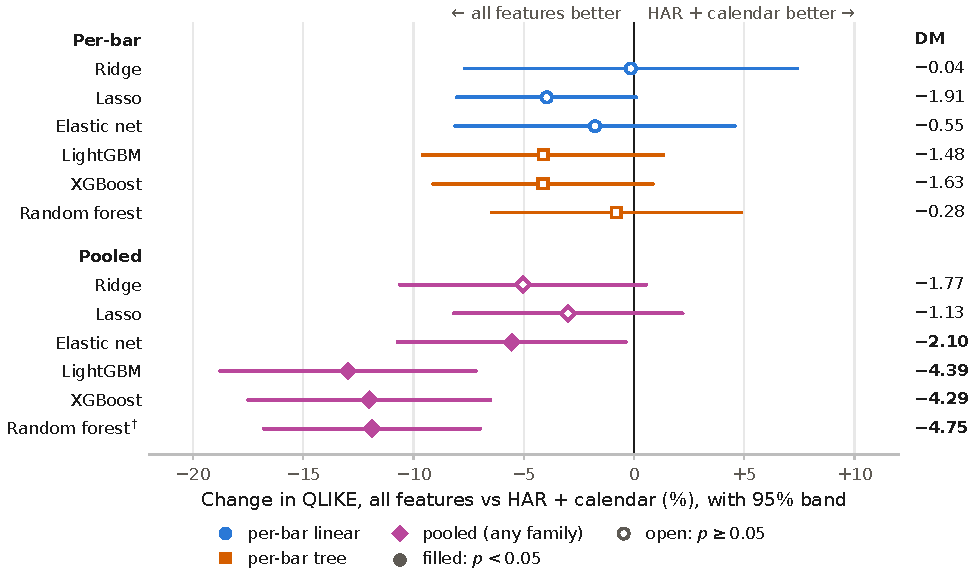
\includegraphics[width=\linewidth]{figures/rehaul_results_f1_forest.pdf}
% % 2026-10-15 (notation pass): parked -- code jargon (per-bar, family, HAR + calendar, all features, interim); standard terms and test wording
% % \caption{All features against HAR + calendar, within each family: the change in mean QLIKE (all features minus HAR +
% % calendar, in \% of the HAR + calendar value) with its 95\% band, $\Delta \pm 1.96\,|\Delta/\mathrm{DM}|$ (the interval
% % the Diebold--Mariano test inverts), and the DM statistic on the right (bold: $p < 0.05$). Left of zero, all features
% % forecast better. Colour and marker give the family for per-bar fits; every pooled fit is a diamond. Filled markers
% % have $p < 0.05$. $^\dagger$Interim (the pooled forest's 16:00 forecasts on all features). Numbers in
% % Table~\ref{tab:rh_axis1}.}
% \caption{Full predictor set versus HAR benchmark, by model class. For each model, the figure shows the change in
% mean QLIKE loss from the HAR benchmark to the full predictor set, in percent of the HAR-benchmark value, with its 95\%
% confidence interval $\Delta \pm 1.96\,|\Delta/\DM|$, obtained by inverting the Diebold--Mariano test; the $\DM$
% statistic is printed on the right. Negative values favor the full predictor set. Losses are computed against the
% actual realized variance of the closing half hour (15:30--16:00 ET) over the \rhrDays{} trading days of the
% out-of-sample period. Color and marker identify the model class of each closing-interval model; every pooled intraday
% model is drawn as a diamond. Filled markers and boldface: significant at the 5\% level (Diebold--Mariano test with
% the Harvey--Leybourne--Newbold correction, Newey--West lag $q = \fqsDMLag$). $^\dagger$Preliminary: the pooled
% random forest's closing-interval forecasts on the full predictor set. Table~\ref{tab:rh_axis1} reports the
% numbers.}
% \label{fig:rh_axis1_forest}
% \end{figure}

% ---------------------------------------------------------------- T2 + F2: pooled vs per-bar
% 2026-10-15 (user): parked -- "park all tables that I haven't mentioned in this chat"
% % AUTO-GENERATED by writeup/make_rehaul_results.py -- do not edit.
% tab:rh_axis2 (T2): intraday minus closing-interval, same model class and predictor set.
\begin{table}[htbp]
\centering
\small
\begin{threeparttable}
\caption{Forecast accuracy: closing-interval versus intraday models}
\label{tab:rh_axis2}
\begin{tabular}{@{}lrrrr@{}}
\toprule
 & \multicolumn{2}{c}{QLIKE} & \multicolumn{2}{c}{Sharpe ratio} \\
\cmidrule(lr){2-3}\cmidrule(l){4-5}
Model & $\Delta$ (\%) & $\DM$ & $\Delta\SR$ & $t$ \\
\midrule
\multicolumn{5}{@{}l}{\textit{Panel A: HAR benchmark}} \\
\addlinespace[2pt]
Ridge & $10.1^{***}$ & $(2.61)$ & $-0.49^{\phantom{***}}$ & $(-1.36)$ \\
Lasso & $10.1^{***}$ & $(2.61)$ & $-0.49^{\phantom{***}}$ & $(-1.36)$ \\
Elastic net & $10.1^{***}$ & $(2.61)$ & $-0.49^{\phantom{***}}$ & $(-1.36)$ \\
LightGBM & $0.7^{\phantom{***}}$ & $(0.23)$ & $0.29^{\phantom{***}}$ & $(0.26)$ \\
XGBoost & $2.4^{\phantom{***}}$ & $(0.84)$ & $0.15^{\phantom{***}}$ & $(0.67)$ \\
Random forest & $5.9^{*\phantom{**}}$ & $(1.86)$ & $-0.25^{\phantom{***}}$ & $(-0.46)$ \\
\addlinespace[4pt]
\multicolumn{5}{@{}l}{\textit{Panel B: Full predictor set}} \\
\addlinespace[2pt]
Ridge & $22.2^{***}$ & $(4.04)$ & $0.37^{\phantom{***}}$ & $(0.92)$ \\
Lasso & $31.2^{***}$ & $(4.64)$ & $0.28^{\phantom{***}}$ & $(0.12)$ \\
Elastic net & $21.6^{***}$ & $(4.16)$ & $0.26^{\phantom{***}}$ & $(0.07)$ \\
LightGBM & $3.9^{\phantom{***}}$ & $(1.18)$ & $0.56^{\phantom{***}}$ & $(0.60)$ \\
XGBoost & $4.6^{\phantom{***}}$ & $(1.34)$ & $0.58^{\phantom{***}}$ & $(0.68)$ \\
Random forest & $6.0^{*\phantom{**}}$ & $(1.84)$ & $1.11^{**\phantom{*}}$ & $(2.72)$ \\
\bottomrule
\end{tabular}
\begin{tablenotes}[flushleft]
\footnotesize
\item \textit{Notes:} Sample, loss and tests as in Table~\ref{tab:rh_axis1}. Each row compares the pooled intraday model with the closing-interval model of the same class on the predictor set of the panel: $\Delta = 100(\bar L^{\mathrm{pool}}/\bar L^{\mathrm{close}} - 1)$, positive when the closing-interval model is more accurate, and $\Delta\SR$ is the intraday minus the closing-interval Sharpe ratio. $^{*}$, $^{**}$ and $^{***}$ denote significance at the 10\%, 5\% and 1\% levels. Closing-interval trees use fixed hyperparameters and are re-estimated daily; the intraday trees are re-estimated at every interval, on a rolling window of past intervals (Section~\ref{sec:rh_exp_schemes}).
\end{tablenotes}
\end{threeparttable}
\end{table}


% 2026-10-15 (user): parked -- non-standard figure; focus on legible tables
% \begin{figure}[htbp]
% \centering
% 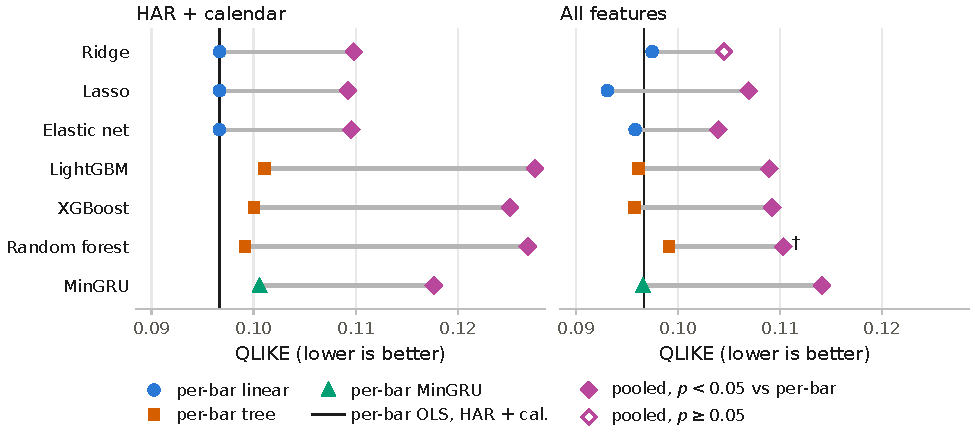
\includegraphics[width=\linewidth]{figures/rehaul_results_f2_dumbbell.pdf}
% % 2026-10-15 (notation pass): parked -- code jargon (per-bar, pooled fit, family, twin, session, interim); standard terms and test wording
% % \caption{Per-bar against pooled fits. Mean QLIKE of each family's per-bar fit (family colour and marker) and its
% % pooled fit (diamond), on HAR + calendar (left) and all features (right), on the same \rhrDays{} days; the vertical line
% % is the per-bar OLS on HAR + calendar (QLIKE \rhrOlsQ). A filled diamond is a pooled fit significantly worse than its
% % per-bar twin (Diebold--Mariano $p < 0.05$). Per-bar trees use fixed settings refit every session. $^\dagger$Interim.
% % Numbers in Table~\ref{tab:rh_axis2}.}
% \caption{Closing-interval versus pooled intraday models. The figure shows the mean QLIKE loss of each model class's
% closing-interval model (class color and marker) and of its pooled intraday counterpart (diamond), on the HAR benchmark
% (left) and on the full predictor set (right), over the same \rhrDays{} trading days of the out-of-sample period,
% against actual realized variance. The vertical line marks the closing-interval OLS on the HAR benchmark (mean QLIKE
% \rhrOlsQ). The closing-interval tree models use fixed hyperparameters and are re-estimated daily. Filled diamonds: the
% pooled intraday model is less accurate than its closing-interval counterpart, significant at the 5\% level
% (Diebold--Mariano test with the Harvey--Leybourne--Newbold correction, Newey--West lag $q = \fqsDMLag$).
% $^\dagger$Preliminary. Table~\ref{tab:rh_axis2} reports the numbers.}
% \label{fig:rh_pooled_dumbbell}
% \end{figure}

% ---------------------------------------------------------------- T3 + F3: the model set against the per-bar OLS
% 2026-10-15 (user): parked -- "park all tables that I haven't mentioned in this chat"
% % AUTO-GENERATED by writeup/make_rehaul_results.py -- do not edit.
\begin{table}[htbp]
\centering
\small
\setlength{\tabcolsep}{5pt}
\caption{The headline forecasts ranked by QLIKE, against the per-bar OLS on HAR + calendar. Rank is the position among all \rhrRankN{} forecasts of Table~\ref{tab:rh_rank_full}.}
\label{tab:rh_rank}
\begin{threeparttable}
\begin{tabular}{@{}r l l l r rrr@{}}
\toprule
 & & & & & \multicolumn{3}{c}{vs per-bar OLS} \\
\cmidrule(l){6-8}
Rank & Model & Fit & Inputs & QLIKE & $\Delta$ (\%) & DM & $p$ \\
\midrule
1 & Lasso & per-bar & All & 0.0914 & $-3.4$ & $-1.22$ & $0.222$ \\
2 & XGBoost, fixed, daily refit & per-bar & All & 0.0935 & $-1.2$ & $-0.39$ & $0.697$ \\
3 & LightGBM, fixed, daily refit & per-bar & All & 0.0939 & $-0.7$ & $-0.21$ & $0.831$ \\
4 & Elastic net & per-bar & All & 0.0942 & $-0.5$ & $-0.11$ & $0.915$ \\
8 & \textbf{OLS} (reference) & per-bar & HAR + cal. & \textbf{0.0946} & & & \\
9 & MinGRU (ridge-init, QLIKE-tuned) & per-bar & All & 0.0948 & $+0.2$ & $+0.05$ & $0.962$ \\
11 & Ridge & per-bar & All & 0.0958 & $+1.2$ & $+0.25$ & $0.799$ \\
14 & Random forest, fixed, daily refit & per-bar & All & 0.0966 & $+2.1$ & $+0.61$ & $0.543$ \\
16 & Random forest, fixed, daily refit & per-bar & HAR + cal. & 0.0968 & $+2.2$ & $+1.09$ & $0.276$ \\
21 & XGBoost, fixed, daily refit & per-bar & HAR + cal. & 0.0976 & $+3.1$ & $+1.43$ & $0.154$ \\
37 & MinGRU (ridge-init, QLIKE-tuned) & per-bar & HAR + cal. & 0.0985 & $+4.1$ & $+1.88$ & $0.060$ \\
38 & LightGBM, fixed, daily refit & per-bar & HAR + cal. & 0.0986 & $+4.2$ & $+1.92$ & $0.054$ \\
77 & Elastic net & pooled & All & 0.1016 & $+7.4$ & $+1.50$ & $0.134$ \\
81 & Ridge & pooled & All & 0.1021 & $+7.9$ & $+1.70$ & $0.090$ \\
93 & Lasso & pooled & All & 0.1044 & $+10.3$ & $\bm{+1.96}$ & $\bm{0.0497}$ \\
101 & LightGBM & pooled & All & 0.1060 & $+12.0$ & $\bm{+2.28}$ & $\bm{0.022}$ \\
102 & Lasso & pooled & HAR + cal. & 0.1062 & $+12.2$ & $\bm{+3.41}$ & $\bm{{<}0.001}$ \\
104 & XGBoost & pooled & All & 0.1063 & $+12.3$ & $\bm{+2.43}$ & $\bm{0.015}$ \\
105 & Elastic net & pooled & HAR + cal. & 0.1065 & $+12.6$ & $\bm{+3.49}$ & $\bm{{<}0.001}$ \\
107 & Ridge & pooled & HAR + cal. & 0.1067 & $+12.8$ & $\bm{+3.42}$ & $\bm{{<}0.001}$ \\
108 & Block-diagonal ridge, earlier panel & pooled & All & 0.1068 & $+12.8$ & $\bm{+2.38}$ & $\bm{0.017}$ \\
111 & Random forest$^\dagger$ & pooled & All & 0.1073 & $+13.4$ & $\bm{+2.53}$ & $\bm{0.011}$ \\
115 & MinGRU (ridge-init, QLIKE-tuned) & pooled & All & 0.1121 & $+18.4$ & $\bm{+4.53}$ & $\bm{{<}0.001}$ \\
116 & MinGRU (ridge-init, QLIKE-tuned) & pooled & HAR + cal. & 0.1151 & $+21.7$ & $\bm{+4.88}$ & $\bm{{<}0.001}$ \\
117 & XGBoost & pooled & HAR + cal. & 0.1213 & $+28.2$ & $\bm{+5.03}$ & $\bm{{<}0.001}$ \\
118 & Random forest & pooled & HAR + cal. & 0.1229 & $+29.9$ & $\bm{+5.04}$ & $\bm{{<}0.001}$ \\
119 & OLS, earlier panel & pooled & HAR + cal. & 0.1232 & $+30.2$ & $\bm{+4.80}$ & $\bm{{<}0.001}$ \\
120 & LightGBM & pooled & HAR + cal. & 0.1236 & $+30.7$ & $\bm{+5.02}$ & $\bm{{<}0.001}$ \\
\bottomrule
\end{tabular}
\begin{tablenotes}[flushleft]\footnotesize
\item \textit{Notes.} QLIKE is the mean over the \rhrDays{} trade days (2020-01-03 to 2024-04-30, early closes excluded) of the daily loss $L_t = RV_t/\hat\sigma^2_t - \log(RV_t/\hat\sigma^2_t) - 1$, with the plain forecast $\hat\sigma^2_t = \hat y_t^2 B_t$ (no recalibration) and $RV_t$ the winsorised 15:30--16:00 realised variance. $\Delta = 100(\overline{L}/\overline{L}^{\,\text{OLS}} - 1)$. DM is the Diebold--Mariano statistic of the daily QLIKE difference (model minus the per-bar OLS), with a Bartlett Newey--West variance at lag 6 and the Harvey--Leybourne--Newbold correction; $p$ is two-sided (normal). Negative $\Delta$ and DM favour the model. Bold: $p < 0.05$. Rows: the per-bar OLS, the canonical rung of each family on each input set (per-bar trees with fixed settings refit every session) and the earlier paper's pooled OLS and block-diagonal ridge. The per-bar ridge, lasso and elastic net on HAR + calendar are within \rhrLinBaseMaxPct\,\% of the OLS and are not shown. $^\dagger$Interim (see Table~\ref{tab:rh_axis1}). The pooled MinGRU is refit monthly, the pooled trees at every bar. Of the \rhrNSet{} model-set forecasts other than the OLS, \rhrNLower{} have lower QLIKE (\rhrNLowerSig{} with $p < 0.05$) and \rhrNWorseSig{} are significantly worse.
\end{tablenotes}
\end{threeparttable}
\end{table}


% 2026-10-15 (user): parked -- "I need all plots parked"
% \begin{figure}[htbp]
% \centering
% 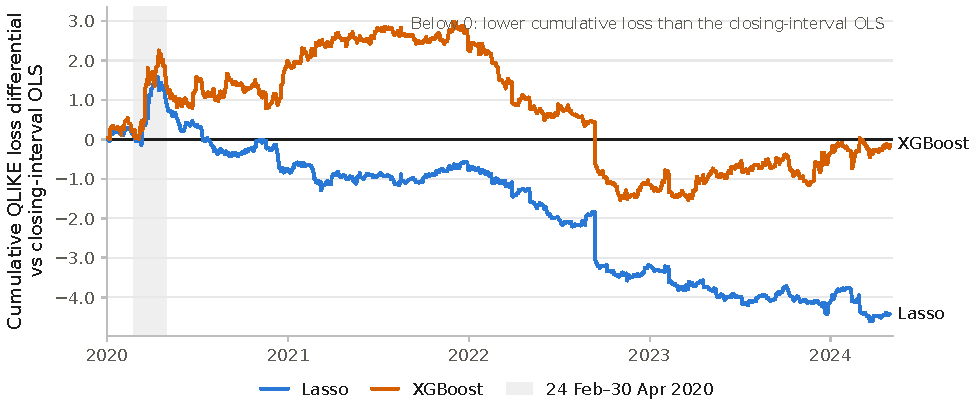
\includegraphics[width=\linewidth]{figures/rehaul_results_f3_cumulative.pdf}
% % 2026-10-15 (notation pass): parked -- code jargon (per-bar, family, fixed settings, session); dummy day index s -> u (s is the window row)
% % \caption{Cumulative daily QLIKE difference against the per-bar OLS on HAR + calendar, $\sum_{s \le t}
% % (L_s^{\text{model}} - L_s^{\text{OLS}})$, for the best per-bar forecast of each family, all on all features: the lasso,
% % XGBoost (fixed settings, refit every session) and the MinGRU (ridge-initialised, trained and selected on QLIKE). Below
% % zero, the model has accumulated less QLIKE than the OLS; the end value divided by \rhrDays{} is the difference in mean
% % QLIKE. Over the shaded window, 24 February to 30 April 2020, the sums change by \rhrCumLassoWindow{} (lasso),
% % \rhrCumXgbWindow{} (XGBoost) and \rhrCumNnWindow{} (MinGRU); over the full sample they end at \rhrCumLassoTotal,
% % \rhrCumXgbTotal{} and \rhrCumNnTotal.}
% % 2026-10-15 (consolidation): dummy day index u -> t' (u is an exogenous series); cumulative-loss plot in the style
% % of \citet{WelchGoyal2008}, now cited.
% % 2026-10-15 (user): parked -- NN content parked for now. The caption below drops the MinGRU line, its
% % \rhrCumNnWindow / \rhrCumNnTotal macros and "the network (ridge-initialized, trained and selected on QLIKE)"; the
% % generator agent drops the MinGRU line from the figure. Old caption: "... the lasso, XGBoost (fixed hyperparameters,
% % re-estimated daily) and the MinGRU network (ridge-initialized, trained and selected on QLIKE) ... change by
% % \rhrCumLassoWindow{} (lasso), \rhrCumXgbWindow{} (XGBoost) and \rhrCumNnWindow{} (MinGRU); over the full
% % out-of-sample period they end at \rhrCumLassoTotal, \rhrCumXgbTotal{} and \rhrCumNnTotal."
% \caption{Cumulative QLIKE loss differential relative to the closing-interval OLS on the HAR benchmark. The figure
% plots $\sum_{t' \le t} d_{t'}$, where $d_{t'} = L_{t'}^{\text{model}} - L_{t'}^{\text{OLS}}$ is the daily loss
% differential, as in \citet{WelchGoyal2008}, for the closing-interval model with the lowest mean QLIKE in each model
% class, each on the full predictor set: the lasso and XGBoost (fixed hyperparameters, re-estimated daily). Values below
% zero mean that the model has accumulated a smaller loss than the OLS; the final value divided by \rhrDays{} equals the
% difference in mean QLIKE. Losses are computed against actual realized variance. Over the shaded window, 24 February to
% 30 April 2020, the cumulative differentials change by \rhrCumLassoWindow{} (lasso) and \rhrCumXgbWindow{} (XGBoost);
% over the full out-of-sample period they end at \rhrCumLassoTotal{} and \rhrCumXgbTotal.}
% \label{fig:rh_cumulative}
% \end{figure}

% ---------------------------------------------------------------- F5: why QLIKE is the primary loss
% 2026-10-15 (user): parked -- non-standard figure; focus on legible tables
% \begin{figure}[htbp]
% \centering
% 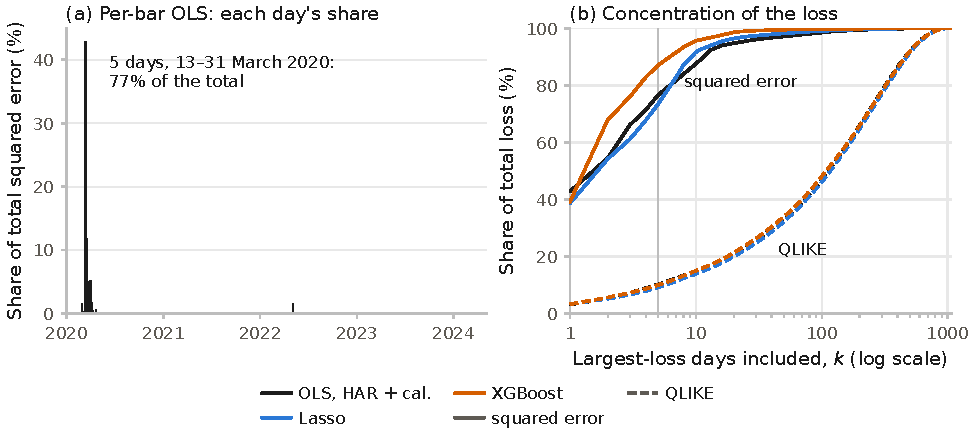
\includegraphics[width=\linewidth]{figures/rehaul_results_f5_se_share.pdf}
% % 2026-10-15 (notation pass): parked -- RV_t -> \RV_t; per-bar, input-set pairs, all features; significance wording
% % \caption{Concentration of the loss. (a) Each day's share of the per-bar OLS's total squared error,
% % $\sum_t (RV_t - \hat\sigma^2_t)^2$: its five largest days, all in March 2020, carry \rhrSETopFiveOls\% of it.
% % (b) Share of the total loss carried by the $k$ largest-loss days, for squared error (solid) and QLIKE (dashed), for the
% % OLS and the three forecasts of Figure~\ref{fig:rh_cumulative}. For each of the four, the five largest squared errors
% % fall in March 2020 and carry \rhrSETopFiveMin--\rhrSETopFiveMax\% of the total squared error; the five largest QLIKE
% % days carry \rhrQLTopFiveMin--\rhrQLTopFiveMax\% of the total QLIKE. Across the \rhrAfPairs{} input-set pairs, all
% % features raise the squared error in \rhrAfMseHigher{} (\rhrAfMseHigherSig{} significantly) while lowering QLIKE in
% % \rhrAfLower.}
% \caption{Concentration of squared-error and QLIKE losses. Panel (a): each trading day's share of the total
% squared-error loss of the closing-interval OLS on the HAR benchmark, $\sum_t (\RV_t - \hat\sigma^2_t)^2$; its five
% largest days, all in March 2020, account for \rhrSETopFiveOls\% of the total. Panel (b): share of the total loss
% accounted for by the $k$ largest-loss days, under squared-error loss (solid) and QLIKE (dashed), for the OLS and the
% three forecasts of Figure~\ref{fig:rh_cumulative}. For each of the four, the five largest squared errors fall in March
% 2020 and account for \rhrSETopFiveMin--\rhrSETopFiveMax\% of the total squared-error loss; the five largest QLIKE
% losses account for \rhrQLTopFiveMin--\rhrQLTopFiveMax\% of the total QLIKE. Across the \rhrAfPairs{} specifications
% estimated on both predictor sets, the full predictor set raises the squared-error loss in \rhrAfMseHigher{}
% (\rhrAfMseHigherSig{} significant at the 5\% level) and lowers QLIKE in \rhrAfLower. Losses are computed against actual
% realized variance over the \rhrDays{} trading days of the out-of-sample period; significance by the Diebold--Mariano
% test with the Harvey--Leybourne--Newbold correction (Newey--West lag $q = \fqsDMLag$).}
% \label{fig:rh_se_share}
% \end{figure}

% ---------------------------------------------------------------- existing figure: QLIKE vs Sharpe (economics bridge)
% figures/fig_qlike_sharpe.pdf and its \fqs... macros come from writeup/make_fig_qlike_sharpe.py (its own palette: one
% colour per estimator, not the family colours above).
% 2026-10-15 parked: the same figure is placed in 07_economics_floats.tex (fig:rh_econ_qlike_sharpe); one copy kept.
% \begin{figure}[htbp]
% \centering
% 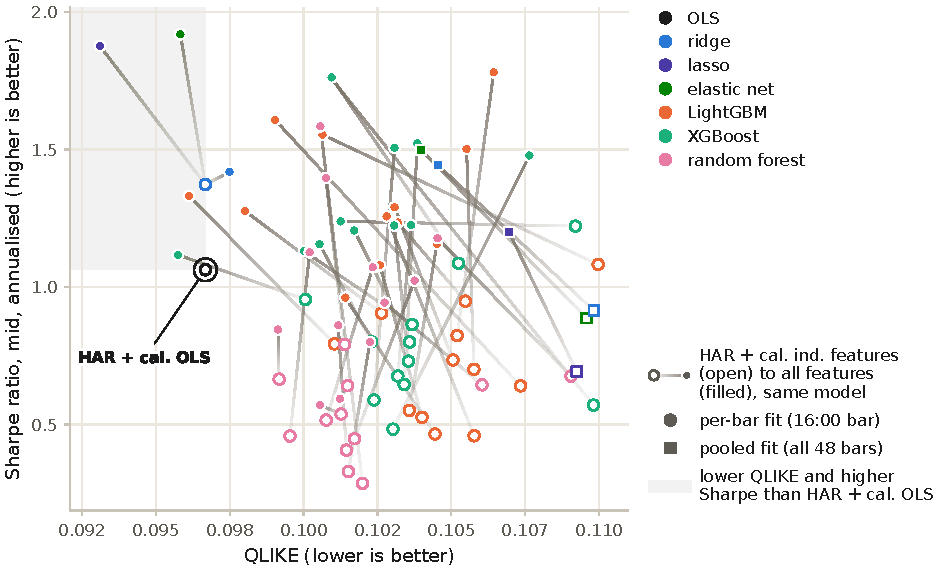
\includegraphics[width=\linewidth]{figures/fig_qlike_sharpe.pdf}
% \caption{Mean QLIKE against the Sharpe ratio of the midpoint straddle trade for every model of the set fitted on both
% input sets: \fqsPairs{} pairs (\fqsPairsPerBarLinear{} per-bar linear, \fqsPairsPooled{} pooled linear and
% \fqsPairsTree{} per-bar trees), on the same \fqsDays{} days. Each pair is joined from its HAR + calendar end (open
% marker) to its all-features end (filled marker); circles are per-bar fits, squares pooled fits, and the colour marks
% the estimator. The shaded quadrant holds lower QLIKE and a higher Sharpe ratio than the per-bar OLS on HAR + calendar
% (QLIKE \fqsOlsQ, Sharpe \fqsOlsSh). All features raise the Sharpe ratio in \fqsShHigher{} of the \fqsPairs{} pairs
% (\fqsShHigherSig{} significant by the Newey--West $t$ of the daily return difference, lag \fqsHACLag) and lower QLIKE
% in \fqsQLower{} (\fqsQLowerSig{} significant by Diebold--Mariano, lag \fqsDMLag); significance at \fqsSigPct\%.}
% \label{fig:rh_qlike_sharpe}
% \end{figure}

% ---------------------------------------------------------------- T3 (full): every forecast, a longtable
% Not a float: \clearpage first so T1--T3 and the figures above come out before it. A candidate for the appendix.
% 2026-10-15 (consolidation): parked -- moved to the appendix (10_appendix_floats.tex, after the MinGRU tables).
% \clearpage
% % AUTO-GENERATED by writeup/make_rehaul_results.py -- do not edit.
% tab:rh_rank_full (T3, every forecast): a longtable, for the appendix (10_appendix_floats.tex).
{\small
\setlength{\tabcolsep}{3.5pt}
\begin{longtable}{@{}rlllrrr@{}}
\caption{Ranking of all forecasts by mean QLIKE}
\label{tab:rh_rank_full}\\
\toprule
 & & & & & \multicolumn{2}{c}{vs.\ HAR benchmark} \\
\cmidrule(l){6-7}
Rank & Model & Specification & Predictors & QLIKE & $\Delta$ (\%) & $\DM$ \\
\midrule
\endfirsthead
\multicolumn{7}{@{}l}{\textit{Table~\ref{tab:rh_rank_full}, continued}} \\
\toprule
 & & & & & \multicolumn{2}{c}{vs.\ HAR benchmark} \\
\cmidrule(l){6-7}
Rank & Model & Specification & Predictors & QLIKE & $\Delta$ (\%) & $\DM$ \\
\midrule
\endhead
\midrule
\multicolumn{7}{r@{}}{\textit{Continued on next page}} \\
\endfoot
\bottomrule
\multicolumn{7}{@{}p{\linewidth}@{}}{\footnotesize\raggedright \textit{Notes:} Sample, loss, tests and significance markers as in Table~\ref{tab:rh_axis1}; $\Delta$ and $\DM$ compare each forecast with the HAR benchmark, as in Table~\ref{tab:rh_rank}. Specification of the closing-interval trees (Panel A): fixed hyperparameters, random search or Optuna, selecting on MSE or QLIKE, then the re-estimation frequency or, for Optuna, the re-tuning frequency and the number of trials searched; d: trading days (Section~\ref{sec:rh_methods_tuning}). Panel C holds the earlier draft's intraday linear models, with a block, fixed or re-tuned penalty; ``no FOMC'' marks the earlier draft's predictor set, which lacks the FOMC predictors. The intraday models of Panel B are re-estimated at every interval on the \rhePoolNBars{} regular-hours intervals with a rolling window of \rhePoolWindowDays{} trading days (Section~\ref{sec:rh_exp_schemes}), except the linear models marked ``All \rhdmNIntervals{} intervals'', the runs on every interval of the day in the model set. $^{\ddagger}$Not in the model set counted in the text.} \tabularnewline
\endlastfoot
\multicolumn{7}{@{}l}{\textit{Panel A: Closing-interval models}} \\
\addlinespace[2pt]
1 & Lasso & -- & Full & 0.0992 & $-4.0^{*\phantom{**}}$ & $(-1.91)$ \\
2 & Elastic net & -- & Full & 0.1014 & $-1.8^{\phantom{***}}$ & $(-0.55)$ \\
3 & Ridge & -- & Full & 0.1031 & $-0.1^{\phantom{***}}$ & $(-0.04)$ \\
4 & XGBoost & Fixed, daily & Full & 0.1031 & $-0.1^{\phantom{***}}$ & $(-0.04)$ \\
5 & Lasso & -- & HAR & 0.1033 & $0.0^{***}$ & $(-2.60)$ \\
6 & Elastic net & -- & HAR & 0.1033 & $0.0^{**\phantom{*}}$ & $(-2.46)$ \\
7 & Ridge & -- & HAR & 0.1033 & $0.0^{\phantom{***}}$ & $(-0.96)$ \\
8 & OLS (benchmark) & -- & HAR & 0.1033 & --$^{\phantom{***}}$ & -- \\
9 & LightGBM & Fixed, daily & Full & 0.1049 & $1.5^{\phantom{***}}$ & $(0.51)$ \\
10 & Random forest & Random search (QLIKE), every 10 d & HAR & 0.1058 & $2.4^{\phantom{***}}$ & $(1.18)$ \\
11 & Random forest & Fixed, daily & Full & 0.1060 & $2.6^{\phantom{***}}$ & $(0.86)$ \\
12 & LightGBM & Fixed, every 10 d & Full & 0.1061 & $2.7^{\phantom{***}}$ & $(0.86)$ \\
13 & Random forest & Optuna (QLIKE), 25 d, 50 trials & HAR & 0.1062 & $2.8^{\phantom{***}}$ & $(1.36)$ \\
14 & LightGBM & Random search (QLIKE), daily & Full & 0.1063 & $3.0^{\phantom{***}}$ & $(0.94)$ \\
15 & Random forest & Random search (QLIKE), daily & HAR & 0.1065 & $3.1^{\phantom{***}}$ & $(1.56)$ \\
16 & XGBoost & Fixed, every 10 d & Full & 0.1066 & $3.2^{\phantom{***}}$ & $(0.89)$ \\
17 & LightGBM & Random search (MSE), daily & Full & 0.1068 & $3.5^{\phantom{***}}$ & $(0.97)$ \\
18 & Random forest & Fixed, daily & HAR & 0.1068 & $3.5^{*\phantom{**}}$ & $(1.70)$ \\
19 & Random forest & Optuna (MSE), daily, 10 trials & Full & 0.1070 & $3.6^{\phantom{***}}$ & $(1.12)$ \\
20 & Random forest & Optuna (MSE), daily, 25 trials & Full & 0.1070 & $3.6^{\phantom{***}}$ & $(1.16)$ \\
21 & Random forest & Optuna (MSE), 5 d, 50 trials & Full & 0.1071 & $3.7^{\phantom{***}}$ & $(1.08)$ \\
22 & XGBoost & Fixed, every 10 d & HAR & 0.1072 & $3.8^{*\phantom{**}}$ & $(1.83)$ \\
23 & Random forest & Optuna (MSE), daily, 50 trials & Full & 0.1072 & $3.8^{\phantom{***}}$ & $(1.18)$ \\
24 & Random forest & Random search (QLIKE), daily & Full & 0.1073 & $3.9^{\phantom{***}}$ & $(1.29)$ \\
25 & XGBoost & Optuna (MSE), daily, 25 trials & Full & 0.1073 & $3.9^{\phantom{***}}$ & $(1.13)$ \\
26 & Random forest & Optuna (MSE), 25 d, 10 trials & Full & 0.1073 & $3.9^{\phantom{***}}$ & $(1.21)$ \\
27 & Random forest & Optuna (MSE), daily, 50 trials & HAR & 0.1074 & $4.0^{*\phantom{**}}$ & $(1.79)$ \\
28 & Random forest & Optuna (MSE), daily, 25 trials & HAR & 0.1075 & $4.1^{*\phantom{**}}$ & $(1.94)$ \\
29 & XGBoost & Fixed, daily & HAR & 0.1076 & $4.2^{**\phantom{*}}$ & $(2.09)$ \\
30 & Random forest & Fixed, every 10 d & Full & 0.1076 & $4.2^{\phantom{***}}$ & $(1.30)$ \\
31 & LightGBM & Random search (QLIKE), every 10 d & Full & 0.1076 & $4.2^{\phantom{***}}$ & $(1.16)$ \\
32 & Random forest & Optuna (MSE), 25 d, 25 trials & HAR & 0.1077 & $4.3^{*\phantom{**}}$ & $(1.82)$ \\
33 & Random forest & Optuna (MSE), 5 d, 50 trials & HAR & 0.1078 & $4.4^{*\phantom{**}}$ & $(1.89)$ \\
34 & XGBoost & Random search (MSE), daily & Full & 0.1078 & $4.4^{\phantom{***}}$ & $(1.17)$ \\
35 & XGBoost & Random search (QLIKE), daily & Full & 0.1078 & $4.4^{\phantom{***}}$ & $(1.18)$ \\
36 & Random forest & Optuna (MSE), daily, 10 trials & HAR & 0.1078 & $4.4^{**\phantom{*}}$ & $(2.09)$ \\
38 & LightGBM & Random search (MSE), every 10 d & Full & 0.1079 & $4.4^{\phantom{***}}$ & $(1.14)$ \\
40 & Random forest & Optuna (MSE), 25 d, 50 trials & HAR & 0.1080 & $4.6^{**\phantom{*}}$ & $(1.98)$ \\
41 & Random forest & Fixed, every 10 d & HAR & 0.1081 & $4.6^{**\phantom{*}}$ & $(2.15)$ \\
42 & Random forest & Optuna (MSE), 25 d, 25 trials & Full & 0.1082 & $4.7^{\phantom{***}}$ & $(1.49)$ \\
43 & XGBoost & Optuna (MSE), 5 d, 50 trials & HAR & 0.1082 & $4.8^{**\phantom{*}}$ & $(2.15)$ \\
44 & XGBoost & Optuna (MSE), daily, 10 trials & HAR & 0.1085 & $5.1^{**\phantom{*}}$ & $(2.14)$ \\
46 & LightGBM & Optuna (MSE), 250 d, 50 trials & Full & 0.1086 & $5.2^{\phantom{***}}$ & $(1.26)$ \\
47 & Random forest & Optuna (MSE), 25 d, 10 trials & HAR & 0.1088 & $5.3^{**\phantom{*}}$ & $(2.03)$ \\
48 & XGBoost & Optuna (MSE), daily, 50 trials & Full & 0.1089 & $5.5^{*\phantom{**}}$ & $(1.67)$ \\
50 & Random forest & Optuna (MSE), 250 d, 50 trials & Full & 0.1090 & $5.5^{*\phantom{**}}$ & $(1.66)$ \\
51 & Random forest & Optuna (QLIKE), 25 d, 50 trials & Full & 0.1091 & $5.7^{\phantom{***}}$ & $(1.63)$ \\
52 & XGBoost & Optuna (MSE), 25 d, 50 trials & HAR & 0.1091 & $5.7^{**\phantom{*}}$ & $(2.21)$ \\
53 & LightGBM & Fixed, daily & HAR & 0.1094 & $5.9^{***}$ & $(2.70)$ \\
54 & XGBoost & Optuna (MSE), 5 d, 50 trials & Full & 0.1094 & $6.0^{*\phantom{**}}$ & $(1.77)$ \\
55 & LightGBM & Optuna (MSE), daily, 10 trials & Full & 0.1095 & $6.0^{*\phantom{**}}$ & $(1.65)$ \\
56 & LightGBM & Random search (QLIKE), every 10 d & HAR & 0.1095 & $6.1^{***}$ & $(2.79)$ \\
57 & LightGBM & Optuna (MSE), daily, 25 trials & Full & 0.1096 & $6.1^{*\phantom{**}}$ & $(1.75)$ \\
58 & LightGBM & Random search (QLIKE), daily & HAR & 0.1097 & $6.2^{***}$ & $(2.85)$ \\
59 & XGBoost & Random search (QLIKE), every 10 d & Full & 0.1098 & $6.3^{\phantom{***}}$ & $(1.53)$ \\
60 & XGBoost & Random search (MSE), every 10 d & Full & 0.1098 & $6.3^{\phantom{***}}$ & $(1.55)$ \\
61 & LightGBM & Fixed, every 10 d & HAR & 0.1098 & $6.4^{***}$ & $(2.80)$ \\
62 & XGBoost & Optuna (MSE), daily, 50 trials & HAR & 0.1099 & $6.4^{**\phantom{*}}$ & $(2.57)$ \\
63 & Random forest & Random search (QLIKE), every 10 d & Full & 0.1099 & $6.4^{*\phantom{**}}$ & $(1.91)$ \\
64 & Random forest & Optuna (MSE), 25 d, 50 trials & Full & 0.1100 & $6.5^{*\phantom{**}}$ & $(1.89)$ \\
65 & LightGBM & Optuna (MSE), 25 d, 25 trials & HAR & 0.1100 & $6.5^{***}$ & $(2.81)$ \\
66 & XGBoost & Optuna (QLIKE), 25 d, 50 trials & HAR & 0.1101 & $6.6^{*\phantom{**}}$ & $(1.93)$ \\
70 & XGBoost & Optuna (MSE), daily, 25 trials & HAR & 0.1102 & $6.7^{**\phantom{*}}$ & $(2.56)$ \\
71 & XGBoost & Optuna (MSE), 25 d, 10 trials & HAR & 0.1102 & $6.7^{***}$ & $(2.93)$ \\
72 & LightGBM & Optuna (MSE), daily, 50 trials & Full & 0.1103 & $6.8^{**\phantom{*}}$ & $(1.97)$ \\
73 & XGBoost & Optuna (MSE), 25 d, 25 trials & HAR & 0.1103 & $6.8^{**\phantom{*}}$ & $(2.53)$ \\
74 & LightGBM & Optuna (QLIKE), 25 d, 50 trials & HAR & 0.1104 & $6.9^{***}$ & $(2.87)$ \\
75 & LightGBM & Optuna (MSE), 5 d, 50 trials & Full & 0.1104 & $6.9^{*\phantom{**}}$ & $(1.87)$ \\
76 & XGBoost & Optuna (MSE), daily, 10 trials & Full & 0.1106 & $7.1^{**\phantom{*}}$ & $(2.00)$ \\
77 & LightGBM & Optuna (MSE), daily, 10 trials & HAR & 0.1110 & $7.5^{***}$ & $(2.78)$ \\
78 & XGBoost & Optuna (MSE), 250 d, 50 trials & Full & 0.1111 & $7.6^{*\phantom{**}}$ & $(1.69)$ \\
79 & LightGBM & Optuna (MSE), 25 d, 25 trials & Full & 0.1112 & $7.6^{*\phantom{**}}$ & $(1.87)$ \\
80 & LightGBM & Optuna (MSE), 25 d, 50 trials & HAR & 0.1112 & $7.7^{***}$ & $(2.82)$ \\
81 & LightGBM & Optuna (MSE), 5 d, 50 trials & HAR & 0.1114 & $7.9^{***}$ & $(3.27)$ \\
83 & Random forest & Random search (MSE), daily & Full & 0.1117 & $8.1^{**\phantom{*}}$ & $(1.98)$ \\
84 & LightGBM & Optuna (MSE), daily, 50 trials & HAR & 0.1117 & $8.1^{***}$ & $(3.01)$ \\
85 & Random forest & Optuna (MSE), 250 d, 50 trials & HAR & 0.1121 & $8.6^{**\phantom{*}}$ & $(2.00)$ \\
86 & LightGBM & Optuna (MSE), 25 d, 10 trials & HAR & 0.1122 & $8.7^{***}$ & $(3.29)$ \\
89 & XGBoost & Optuna (MSE), 25 d, 25 trials & Full & 0.1126 & $9.0^{**\phantom{*}}$ & $(2.26)$ \\
91 & XGBoost & Random search (QLIKE), daily & HAR & 0.1127 & $9.1^{**\phantom{*}}$ & $(1.96)$ \\
92 & LightGBM & Optuna (MSE), daily, 25 trials & HAR & 0.1127 & $9.2^{***}$ & $(3.26)$ \\
93 & XGBoost & Random search (QLIKE), every 10 d & HAR & 0.1127 & $9.2^{*\phantom{**}}$ & $(1.93)$ \\
95 & LightGBM & Optuna (MSE), 25 d, 10 trials & Full & 0.1128 & $9.3^{**\phantom{*}}$ & $(2.03)$ \\
97 & XGBoost & Optuna (QLIKE), 25 d, 50 trials & Full & 0.1134 & $9.8^{**\phantom{*}}$ & $(2.25)$ \\
98 & LightGBM & Optuna (QLIKE), 25 d, 50 trials & Full & 0.1134 & $9.9^{**\phantom{*}}$ & $(2.10)$ \\
100 & XGBoost & Optuna (MSE), 25 d, 50 trials & Full & 0.1136 & $10.0^{**\phantom{*}}$ & $(2.42)$ \\
101 & LightGBM & Random search (MSE), every 10 d & HAR & 0.1136 & $10.0^{**\phantom{*}}$ & $(2.51)$ \\
105 & LightGBM & Random search (MSE), daily & HAR & 0.1139 & $10.3^{***}$ & $(2.59)$ \\
110 & Random forest & Random search (MSE), every 10 d & HAR & 0.1149 & $11.3^{**\phantom{*}}$ & $(2.33)$ \\
111 & Random forest & Random search (MSE), daily & HAR & 0.1151 & $11.5^{**\phantom{*}}$ & $(2.40)$ \\
112 & LightGBM & Optuna (MSE), 25 d, 50 trials & Full & 0.1152 & $11.6^{***}$ & $(2.61)$ \\
113 & Random forest & Random search (MSE), every 10 d & Full & 0.1157 & $12.1^{**\phantom{*}}$ & $(2.20)$ \\
115 & LightGBM & Optuna (MSE), 250 d, 50 trials & HAR & 0.1160 & $12.3^{***}$ & $(2.84)$ \\
116 & XGBoost & Optuna (MSE), 25 d, 10 trials & Full & 0.1161 & $12.4^{***}$ & $(2.72)$ \\
117 & XGBoost & Optuna (MSE), 250 d, 50 trials & HAR & 0.1165 & $12.8^{***}$ & $(3.24)$ \\
119 & XGBoost & Random search (MSE), every 10 d & HAR & 0.1174 & $13.7^{***}$ & $(2.77)$ \\
120 & XGBoost & Random search (MSE), daily & HAR & 0.1175 & $13.8^{***}$ & $(2.78)$ \\
\addlinespace[4pt]
\multicolumn{7}{@{}l}{\textit{Panel B: Intraday models}} \\
\addlinespace[2pt]
37 & Elastic net & All \rhdmNIntervals{} intervals & Full & 0.1078 & $4.4^{\phantom{***}}$ & $(1.17)$ \\
39 & XGBoost$^{\ddagger}$ & -- & Full & 0.1079 & $4.5^{\phantom{***}}$ & $(1.14)$ \\
45 & Ridge & All \rhdmNIntervals{} intervals & Full & 0.1086 & $5.1^{\phantom{***}}$ & $(1.36)$ \\
49 & LightGBM$^{\ddagger}$ & -- & Full & 0.1089 & $5.5^{\phantom{***}}$ & $(1.34)$ \\
67 & LightGBM$^{\ddagger}$ & -- & HAR & 0.1101 & $6.6^{**\phantom{*}}$ & $(2.16)$ \\
68 & Lasso & All \rhdmNIntervals{} intervals & Full & 0.1101 & $6.7^{\phantom{***}}$ & $(1.62)$ \\
69 & XGBoost$^{\ddagger}$ & -- & HAR & 0.1102 & $6.7^{**\phantom{*}}$ & $(2.23)$ \\
88 & Random forest$^{\ddagger}$ & -- & Full & 0.1123 & $8.8^{**\phantom{*}}$ & $(2.06)$ \\
90 & XGBoost & Earlier draft, no FOMC & Full & 0.1126 & $9.0^{**\phantom{*}}$ & $(2.18)$ \\
94 & LightGBM & Earlier draft, no FOMC & Full & 0.1128 & $9.2^{**\phantom{*}}$ & $(2.16)$ \\
96 & Random forest$^{\ddagger}$ & -- & HAR & 0.1131 & $9.6^{***}$ & $(2.78)$ \\
99 & Lasso & All \rhdmNIntervals{} intervals & HAR & 0.1135 & $10.0^{***}$ & $(3.09)$ \\
102 & Elastic net$^{\ddagger}$ & -- & HAR & 0.1137 & $10.1^{***}$ & $(2.61)$ \\
103 & Lasso$^{\ddagger}$ & -- & HAR & 0.1137 & $10.1^{***}$ & $(2.61)$ \\
104 & Ridge$^{\ddagger}$ & -- & HAR & 0.1137 & $10.1^{***}$ & $(2.61)$ \\
107 & Elastic net & All \rhdmNIntervals{} intervals & HAR & 0.1142 & $10.6^{***}$ & $(3.21)$ \\
109 & Ridge & All \rhdmNIntervals{} intervals & HAR & 0.1143 & $10.7^{***}$ & $(3.15)$ \\
121 & Elastic net$^{\ddagger}$ & -- & Full & 0.1234 & $19.5^{***}$ & $(3.34)$ \\
122 & Ridge$^{\ddagger}$ & -- & Full & 0.1260 & $22.0^{***}$ & $(3.61)$ \\
124 & Lasso$^{\ddagger}$ & -- & Full & 0.1301 & $26.0^{***}$ & $(3.66)$ \\
\addlinespace[4pt]
\multicolumn{7}{@{}l}{\textit{Panel C: Intraday models, earlier draft's specification}} \\
\addlinespace[2pt]
82 & Lasso & Fixed penalty, no FOMC & Full & 0.1116 & $8.1^{*\phantom{**}}$ & $(1.87)$ \\
87 & Ridge & Block penalty, no FOMC & Full & 0.1123 & $8.8^{**\phantom{*}}$ & $(1.96)$ \\
106 & Ridge & Block penalty & Full & 0.1140 & $10.4^{**\phantom{*}}$ & $(2.27)$ \\
108 & Lasso & Fixed penalty & Full & 0.1143 & $10.7^{**\phantom{*}}$ & $(2.37)$ \\
114 & Lasso & Re-tuned penalty, no FOMC & Full & 0.1158 & $12.1^{***}$ & $(2.64)$ \\
118 & Elastic net & Re-tuned penalty, no FOMC & Full & 0.1174 & $13.6^{***}$ & $(2.95)$ \\
123 & OLS & -- & HAR & 0.1291 & $25.0^{***}$ & $(4.56)$ \\
\end{longtable}
}


% 2026-10-15 (user): variable importance moved to the end of Experiments and results, as a subsection (was after
% Economic value, as its own section).
% 08_feature_importance.tex -- the rehauled paper's section, as bullets to expand into prose (2026-10-15).
% Sources and pointers behind every number: writeup/PAPER_REHAUL_OUTLINE_2026-10-15.md, section 8.
% House rules: every number in the final prose comes from a generated macro (writeup/generated/*.tex), never
% typed; park (comment out with a dated note) rather than delete.
% Macros to use here: rehaul_fi_numbers.tex (\rhfi..., writeup/make_rehaul_fi.py from results/rehaul_fi/, computed by
% experiments/rehaul_fi_compute.py); floats in 08b_fi_measures_floats.tex. The old study's measures (permutation,
% MDI, drop-column; appendix_campaign_16h_featimp.tex) stay in 08_feature_importance_floats.tex; their bullets are
% parked at the end of this file.
% 2026-10-15 measures pass: the user's plan (lasso counts, ridge sum |beta|, per-refit SHAP ranks aggregated,
% SHAP interactions global and per refit with the H-statistic cross-check) on the paper's models of record.
% 2026-10-15 (notation pass, writeup/NOTATION_GUIDE_2026-10-15.md): symbols and wording only; no number, macro or
% label changed. Old -> new: unit -> predictor group; column -> predictor; backbone -> HAR benchmark block;
% pf_j -> omega_j; alpha -> lambda; session -> trading day; fit space -> the scale of y_t; W_k -> \mathcal W_{t_k};
% T_k -> out-of-sample block \mathcal O_k; N (scored sessions) -> |\mathcal O|, \mathcal O the union of the blocks
% (not the guide's T_oos: this 2018-2024 period is not the paper's 2020-2024 test period); x_t -> \bm x_t;
% \beta^{(k)}_j -> \hat\beta_{k,j} (a parenthesized superscript is the guide's HAR horizon);
% b_{k,A} -> \lVert\hat{\bm\beta}_{k,A}\rVert_1 (b is the boosting round); s_{k,A} -> S_{k,A} (s is the periodicity
% factor); B_A (Borda) -> \mathrm{BC}_A; tie sizes \tau_{kg} -> |g|, g in \mathcal G_k (tau is the network step);
% H^2 points x_i and background b -> days t, t' in \mathcal H_k (i is the intraday interval).
% The generated floats (make_rehaul_fi.py) still print the old symbols ($T_k$, $\beta^{(k)}_j$, "unit", code names).
% 2026-10-15 (consolidation): the floats now print this section's symbols. Selection count N_A, N_j -> K_A, K_j (N is
% the one-minute count N_{t,i}, the symbol of the numobs series in the tables); group interaction Phi_{t,AB} ->
% phi_{t,AB} (Phi is the standard normal distribution function); tie sets \mathcal G_k -> \mathcal E_k (\mathcal G is
% the interval grid, Data); the ridge's standardized share S^{sd}_A (as in tab:rh_fi_summary, tab:rh_fi_linear);
% "buckets" -> categories. The refit index stays k, subscripted (guide 6b); HAR horizons are the superscript (k).
% 2026-10-15 (consolidation): parked -- the number files are loaded once in the preamble of paper_rehaul.tex.
% \ifdefined\rhfiNRefits\else% AUTO-GENERATED by writeup/make_rehaul_fi.py -- do not edit; re-run the script.
% \rhfi... macros for writeup/rehaul/08_feature_importance.tex (results/rehaul_fi/).
\providecommand{\rhfiNRefits}{}\renewcommand{\rhfiNRefits}{147}  % refits, one every 10 sessions
\providecommand{\rhfiNOos}{}\renewcommand{\rhfiNOos}{1{,}469}  % scored held-out sessions
\providecommand{\rhfiP}{}\renewcommand{\rhfiP}{628}  % columns, all features
\providecommand{\rhfiNUnits}{}\renewcommand{\rhfiNUnits}{49}  % units: 47 exogenous series + HAR ladder + calendar
\providecommand{\rhfiNExog}{}\renewcommand{\rhfiNExog}{47}  % exogenous series
\providecommand{\rhfiFirst}{}\renewcommand{\rhfiFirst}{25~June~2018}  % first scored session
\providecommand{\rhfiLast}{}\renewcommand{\rhfiLast}{30~April~2024}  % last scored session
\providecommand{\rhfiWindow}{}\renewcommand{\rhfiWindow}{2{,}000}  % sessions in a training window
\providecommand{\rhfiRefitEvery}{}\renewcommand{\rhfiRefitEvery}{10}  % sessions between refits
\providecommand{\rhfiBackbonePf}{}\renewcommand{\rhfiBackbonePf}{0.01}  % backbone penalty factor
\providecommand{\rhfiNBuckets}{}\renewcommand{\rhfiNBuckets}{8}  % exogenous buckets
\providecommand{\rhfiOldBlock}{}\renewcommand{\rhfiOldBlock}{250}  % sessions between the old arm's penalty re-choices
\providecommand{\rhfiNPairs}{}\renewcommand{\rhfiNPairs}{1{,}176}  % series pairs
\providecommand{\rhfiNProbeCols}{}\renewcommand{\rhfiNProbeCols}{631}  % columns of a probe fit
\providecommand{\rhfiTopWPairs}{}\renewcommand{\rhfiTopWPairs}{50}  % pairs in the interaction W
\providecommand{\rhfiProbeLevels}{}\renewcommand{\rhfiProbeLevels}{20}  % values of the few-valued noise column
\providecommand{\rhfiRidgeAlpha}{}\renewcommand{\rhfiRidgeAlpha}{\ensuremath{10^{3}}}
\providecommand{\rhfiLassoAlpha}{}\renewcommand{\rhfiLassoAlpha}{\ensuremath{10^{-2}}}
\providecommand{\rhfiLassoNzMed}{}\renewcommand{\rhfiLassoNzMed}{30}  % median nonzero coefficients per refit
\providecommand{\rhfiLassoNzMin}{}\renewcommand{\rhfiLassoNzMin}{27}
\providecommand{\rhfiLassoNzMax}{}\renewcommand{\rhfiLassoNzMax}{35}
\providecommand{\rhfiLassoExogNzMed}{}\renewcommand{\rhfiLassoExogNzMed}{14}  % ... exogenous columns
\providecommand{\rhfiLassoColsEver}{}\renewcommand{\rhfiLassoColsEver}{60}  % columns nonzero in >= 1 refit
\providecommand{\rhfiLassoColsMajority}{}\renewcommand{\rhfiLassoColsMajority}{29}  % columns nonzero in >= half the refits
\providecommand{\rhfiLassoExogEver}{}\renewcommand{\rhfiLassoExogEver}{27}  % exogenous series with a nonzero column in >= 1 refit
\providecommand{\rhfiLassoExogMajority}{}\renewcommand{\rhfiLassoExogMajority}{11}  % ... in >= half the refits
\providecommand{\rhfiLassoExogAlways}{}\renewcommand{\rhfiLassoExogAlways}{3}  % ... in every refit
\providecommand{\rhfiLassoAlwaysList}{}\renewcommand{\rhfiLassoAlwaysList}{\texttt{sumret}, \texttt{sumabsret\_vwstock}, \texttt{sumautocov}}  % exogenous series selected in every refit
\providecommand{\rhfiLassoProbeSel}{}\renewcommand{\rhfiLassoProbeSel}{1}  % continuous probe selected, of the probe fits
\providecommand{\rhfiLassoProbeSelLevels}{}\renewcommand{\rhfiLassoProbeSelLevels}{0}
\providecommand{\rhfiLassoProbeSelBinary}{}\renewcommand{\rhfiLassoProbeSelBinary}{0}
\providecommand{\rhfiNProbe}{}\renewcommand{\rhfiNProbe}{49}  % probe refits (every third)
\providecommand{\rhfiLassoW}{}\renewcommand{\rhfiLassoW}{0.74}  % Kendall W of the per-refit series ranks by sum |beta|
\providecommand{\rhfiLassoBackboneShare}{}\renewcommand{\rhfiLassoBackboneShare}{88}  % median share of sum |beta| on the backbone, %
\providecommand{\rhfiOldLassoSpearman}{}\renewcommand{\rhfiOldLassoSpearman}{0.70}  % Spearman, selection share: pre-tuned vs re-tuned one-penalty lasso
\providecommand{\rhfiOldLassoNzMed}{}\renewcommand{\rhfiOldLassoNzMed}{23}  % re-tuned lasso: median nonzero per refit
\providecommand{\rhfiOldLassoExogMajority}{}\renewcommand{\rhfiOldLassoExogMajority}{18}
\providecommand{\rhfiRidgeTopOne}{}\renewcommand{\rhfiRidgeTopOne}{Calendar}
\providecommand{\rhfiRidgeTopOneShare}{}\renewcommand{\rhfiRidgeTopOneShare}{31.0}  % % of sum |beta|
\providecommand{\rhfiRidgeTopTwo}{}\renewcommand{\rhfiRidgeTopTwo}{HAR ladder}
\providecommand{\rhfiRidgeTopTwoShare}{}\renewcommand{\rhfiRidgeTopTwoShare}{22.8}  % % of sum |beta|
\providecommand{\rhfiRidgeTopThree}{}\renewcommand{\rhfiRidgeTopThree}{\texttt{sumret}}
\providecommand{\rhfiRidgeTopThreeShare}{}\renewcommand{\rhfiRidgeTopThreeShare}{3.6}  % % of sum |beta|
\providecommand{\rhfiRidgeTopFour}{}\renewcommand{\rhfiRidgeTopFour}{\texttt{sumabsret\_vwstock}}
\providecommand{\rhfiRidgeTopFourShare}{}\renewcommand{\rhfiRidgeTopFourShare}{2.2}  % % of sum |beta|
\providecommand{\rhfiRidgeSdTopOne}{}\renewcommand{\rhfiRidgeSdTopOne}{HAR ladder}
\providecommand{\rhfiRidgeSdTopOneShare}{}\renewcommand{\rhfiRidgeSdTopOneShare}{30.6}  % % of sum |beta| sd
\providecommand{\rhfiRidgeSdTopTwo}{}\renewcommand{\rhfiRidgeSdTopTwo}{Calendar}
\providecommand{\rhfiRidgeSdTopTwoShare}{}\renewcommand{\rhfiRidgeSdTopTwoShare}{9.3}  % % of sum |beta| sd
\providecommand{\rhfiRidgeSdTopThree}{}\renewcommand{\rhfiRidgeSdTopThree}{\texttt{sumret}}
\providecommand{\rhfiRidgeSdTopThreeShare}{}\renewcommand{\rhfiRidgeSdTopThreeShare}{4.5}  % % of sum |beta| sd
\providecommand{\rhfiRidgeTopExog}{}\renewcommand{\rhfiRidgeTopExog}{\texttt{sumret}}
\providecommand{\rhfiRidgeTopExogShare}{}\renewcommand{\rhfiRidgeTopExogShare}{3.6}
\providecommand{\rhfiRidgeBackboneShare}{}\renewcommand{\rhfiRidgeBackboneShare}{54}  % median share of sum |beta| on the backbone, %
\providecommand{\rhfiRidgeW}{}\renewcommand{\rhfiRidgeW}{0.85}
\providecommand{\rhfiRidgeAllSelected}{}\renewcommand{\rhfiRidgeAllSelected}{49}  % units with N_A = K under the ridge
\providecommand{\rhfiLassoProbeRate}{}\renewcommand{\rhfiLassoProbeRate}{2.0}  % continuous probe's selection rate, %
\providecommand{\rhfiLassoColsAboveProbe}{}\renewcommand{\rhfiLassoColsAboveProbe}{54}  % columns selected more often than the continuous probe
\providecommand{\rhfiLassoSeriesAboveProbe}{}\renewcommand{\rhfiLassoSeriesAboveProbe}{23}  % exogenous series with such a column
\providecommand{\rhfiLassoTopCol}{}\renewcommand{\rhfiLassoTopCol}{\texttt{is\_month\_end}}
\providecommand{\rhfiRidgeSpearmanSd}{}\renewcommand{\rhfiRidgeSpearmanSd}{0.85}  % Spearman, series sum|beta| vs sum|beta| sd
\providecommand{\rhfiRidgeProbeBeat}{}\renewcommand{\rhfiRidgeProbeBeat}{107}  % columns with |beta| above the continuous probe's in most probe fits
\providecommand{\rhfiRidgeProbeBeatSeries}{}\renewcommand{\rhfiRidgeProbeBeatSeries}{38}
\providecommand{\rhfiScaleValueN}{}\renewcommand{\rhfiScaleValueN}{282}
\providecommand{\rhfiScaleValueSd}{}\renewcommand{\rhfiScaleValueSd}{0.84}  % median window sd, value ladders
\providecommand{\rhfiScaleValueSdLo}{}\renewcommand{\rhfiScaleValueSdLo}{0.03}
\providecommand{\rhfiScaleValueSdHi}{}\renewcommand{\rhfiScaleValueSdHi}{1.76}
\providecommand{\rhfiScaleValueIqr}{}\renewcommand{\rhfiScaleValueIqr}{0.94}  % median window IQR, value ladders
\providecommand{\rhfiScaleFlagN}{}\renewcommand{\rhfiScaleFlagN}{324}
\providecommand{\rhfiScaleFlagSd}{}\renewcommand{\rhfiScaleFlagSd}{0.022}  % median window sd, availability / activity ladders
\providecommand{\rhfiScaleFlagSdHi}{}\renewcommand{\rhfiScaleFlagSdHi}{0.17}
\providecommand{\rhfiScaleCalSd}{}\renewcommand{\rhfiScaleCalSd}{0.39}  % median window sd, calendar
\providecommand{\rhfiScaleHarSd}{}\renewcommand{\rhfiScaleHarSd}{1.07}  % median window sd, HAR ladder
\providecommand{\rhfiLgbmW}{}\renewcommand{\rhfiLgbmW}{0.57}  % lgbm: Kendall W, per-refit series ranks
\providecommand{\rhfiLgbmWCols}{}\renewcommand{\rhfiLgbmWCols}{0.91}  % lgbm: Kendall W, column ranks
\providecommand{\rhfiLgbmTopOne}{}\renewcommand{\rhfiLgbmTopOne}{HAR ladder}
\providecommand{\rhfiLgbmTopOneRank}{}\renewcommand{\rhfiLgbmTopOneRank}{1.0}  % mean rank
\providecommand{\rhfiLgbmTopTwo}{}\renewcommand{\rhfiLgbmTopTwo}{\texttt{sumret}}
\providecommand{\rhfiLgbmTopTwoRank}{}\renewcommand{\rhfiLgbmTopTwoRank}{2.9}  % mean rank
\providecommand{\rhfiLgbmTopThree}{}\renewcommand{\rhfiLgbmTopThree}{\texttt{sumabsret}}
\providecommand{\rhfiLgbmTopThreeRank}{}\renewcommand{\rhfiLgbmTopThreeRank}{4.8}  % mean rank
\providecommand{\rhfiLgbmSpBorda}{}\renewcommand{\rhfiLgbmSpBorda}{0.90}  % Spearman, mean rank vs top-10 Borda
\providecommand{\rhfiLgbmSpGlobal}{}\renewcommand{\rhfiLgbmSpGlobal}{0.96}  % Spearman, mean rank vs global mean |phi|
\providecommand{\rhfiLgbmSpLocal}{}\renewcommand{\rhfiLgbmSpLocal}{1.000}  % Spearman, mean ranks local refit vs stored
\providecommand{\rhfiLgbmProbeRank}{}\renewcommand{\rhfiLgbmProbeRank}{83}  % median rank of the continuous probe, 631 columns
\providecommand{\rhfiLgbmProbeCols}{}\renewcommand{\rhfiLgbmProbeCols}{60}  % columns above the continuous probe in most probe fits
\providecommand{\rhfiLgbmProbeSeries}{}\renewcommand{\rhfiLgbmProbeSeries}{27}  % exogenous series with such a column
\providecommand{\rhfiLgbmTopCol}{}\renewcommand{\rhfiLgbmTopCol}{\texttt{har\_ma\_1}}  % column with the lowest mean rank
\providecommand{\rhfiLgbmTopColRank}{}\renewcommand{\rhfiLgbmTopColRank}{1.3}
\providecommand{\rhfiLgbmTopColTwo}{}\renewcommand{\rhfiLgbmTopColTwo}{\texttt{har\_ma\_5}}
\providecommand{\rhfiLgbmTopColTwoRank}{}\renewcommand{\rhfiLgbmTopColTwoRank}{1.8}
\providecommand{\rhfiLgbmPredGap}{}\renewcommand{\rhfiLgbmPredGap}{0}  % max |local refit - stored refit| forecast
\providecommand{\rhfiLgbmInterW}{}\renewcommand{\rhfiLgbmInterW}{0.45}  % Kendall W of per-refit pair ranks, top-50 pairs
\providecommand{\rhfiLgbmInterRatio}{}\renewcommand{\rhfiLgbmInterRatio}{90}  % sum of series-pair interactions / sum main, %
\providecommand{\rhfiLgbmInterSpGlobal}{}\renewcommand{\rhfiLgbmInterSpGlobal}{0.99}
\providecommand{\rhfiLgbmInterFloor}{}\renewcommand{\rhfiLgbmInterFloor}{0.49}  % probe floor x 1e3
\providecommand{\rhfiLgbmInterAboveFloor}{}\renewcommand{\rhfiLgbmInterAboveFloor}{116}  % series pairs above the probe floor
\providecommand{\rhfiLgbmInterTopA}{}\renewcommand{\rhfiLgbmInterTopA}{HAR ladder}
\providecommand{\rhfiLgbmInterTopB}{}\renewcommand{\rhfiLgbmInterTopB}{\texttt{sumabsret}}
\providecommand{\rhfiLgbmInterTopVal}{}\renewcommand{\rhfiLgbmInterTopVal}{12.6}  % x 1e3
\providecommand{\rhfiLgbmHTop}{}\renewcommand{\rhfiLgbmHTop}{0.33}  % H^2 of the top series pair (pooled), %
\providecommand{\rhfiLgbmHMin}{}\renewcommand{\rhfiLgbmHMin}{0.02}  % min H^2 over the top-10 series pairs, %
\providecommand{\rhfiLgbmHMax}{}\renewcommand{\rhfiLgbmHMax}{0.33}  % max H^2 over the top-10 series pairs, %
\providecommand{\rhfiLgbmHMinTop}{}\renewcommand{\rhfiLgbmHMinTop}{0.19}  % top pair: interaction PD var / smaller main PD var
\providecommand{\rhfiLgbmHMinLo}{}\renewcommand{\rhfiLgbmHMinLo}{0.05}  % ... min over the top-10 series pairs
\providecommand{\rhfiLgbmHMinHi}{}\renewcommand{\rhfiLgbmHMinHi}{0.54}  % ... max
\providecommand{\rhfiLgbmHColTop}{}\renewcommand{\rhfiLgbmHColTop}{0.36}  % H^2 of the top column pair, %
\providecommand{\rhfiLgbmHMinColTop}{}\renewcommand{\rhfiLgbmHMinColTop}{0.02}  % ... min-normalised
\providecommand{\rhfiLgbmMainTopVal}{}\renewcommand{\rhfiLgbmMainTopVal}{195}  % largest global mean |phi_A| x 1e3
\providecommand{\rhfiLgbmWithinTop}{}\renewcommand{\rhfiLgbmWithinTop}{HAR ladder}
\providecommand{\rhfiLgbmWithinTopVal}{}\renewcommand{\rhfiLgbmWithinTopVal}{18.7}
\providecommand{\rhfiXgbW}{}\renewcommand{\rhfiXgbW}{0.60}  % xgb: Kendall W, per-refit series ranks
\providecommand{\rhfiXgbWCols}{}\renewcommand{\rhfiXgbWCols}{0.90}  % xgb: Kendall W, column ranks
\providecommand{\rhfiXgbTopOne}{}\renewcommand{\rhfiXgbTopOne}{HAR ladder}
\providecommand{\rhfiXgbTopOneRank}{}\renewcommand{\rhfiXgbTopOneRank}{1.0}  % mean rank
\providecommand{\rhfiXgbTopTwo}{}\renewcommand{\rhfiXgbTopTwo}{\texttt{sumret}}
\providecommand{\rhfiXgbTopTwoRank}{}\renewcommand{\rhfiXgbTopTwoRank}{3.0}  % mean rank
\providecommand{\rhfiXgbTopThree}{}\renewcommand{\rhfiXgbTopThree}{\texttt{sumabsret}}
\providecommand{\rhfiXgbTopThreeRank}{}\renewcommand{\rhfiXgbTopThreeRank}{3.9}  % mean rank
\providecommand{\rhfiXgbSpBorda}{}\renewcommand{\rhfiXgbSpBorda}{0.87}  % Spearman, mean rank vs top-10 Borda
\providecommand{\rhfiXgbSpGlobal}{}\renewcommand{\rhfiXgbSpGlobal}{0.97}  % Spearman, mean rank vs global mean |phi|
\providecommand{\rhfiXgbSpLocal}{}\renewcommand{\rhfiXgbSpLocal}{0.993}  % Spearman, mean ranks local refit vs stored
\providecommand{\rhfiXgbProbeRank}{}\renewcommand{\rhfiXgbProbeRank}{110}  % median rank of the continuous probe, 631 columns
\providecommand{\rhfiXgbProbeCols}{}\renewcommand{\rhfiXgbProbeCols}{78}  % columns above the continuous probe in most probe fits
\providecommand{\rhfiXgbProbeSeries}{}\renewcommand{\rhfiXgbProbeSeries}{35}  % exogenous series with such a column
\providecommand{\rhfiXgbTopCol}{}\renewcommand{\rhfiXgbTopCol}{\texttt{har\_ma\_1}}  % column with the lowest mean rank
\providecommand{\rhfiXgbTopColRank}{}\renewcommand{\rhfiXgbTopColRank}{1.3}
\providecommand{\rhfiXgbTopColTwo}{}\renewcommand{\rhfiXgbTopColTwo}{\texttt{har\_ma\_5}}
\providecommand{\rhfiXgbTopColTwoRank}{}\renewcommand{\rhfiXgbTopColTwoRank}{1.8}
\providecommand{\rhfiXgbPredGap}{}\renewcommand{\rhfiXgbPredGap}{0.17}  % max |local refit - stored refit| forecast
\providecommand{\rhfiXgbInterW}{}\renewcommand{\rhfiXgbInterW}{0.47}  % Kendall W of per-refit pair ranks, top-50 pairs
\providecommand{\rhfiXgbInterRatio}{}\renewcommand{\rhfiXgbInterRatio}{74}  % sum of series-pair interactions / sum main, %
\providecommand{\rhfiXgbInterSpGlobal}{}\renewcommand{\rhfiXgbInterSpGlobal}{0.99}
\providecommand{\rhfiXgbInterFloor}{}\renewcommand{\rhfiXgbInterFloor}{0.41}  % probe floor x 1e3
\providecommand{\rhfiXgbInterAboveFloor}{}\renewcommand{\rhfiXgbInterAboveFloor}{115}  % series pairs above the probe floor
\providecommand{\rhfiXgbInterTopA}{}\renewcommand{\rhfiXgbInterTopA}{HAR ladder}
\providecommand{\rhfiXgbInterTopB}{}\renewcommand{\rhfiXgbInterTopB}{\texttt{sumabsret}}
\providecommand{\rhfiXgbInterTopVal}{}\renewcommand{\rhfiXgbInterTopVal}{15.2}  % x 1e3
\providecommand{\rhfiXgbHTop}{}\renewcommand{\rhfiXgbHTop}{0.37}  % H^2 of the top series pair (pooled), %
\providecommand{\rhfiXgbHMin}{}\renewcommand{\rhfiXgbHMin}{0.02}  % min H^2 over the top-10 series pairs, %
\providecommand{\rhfiXgbHMax}{}\renewcommand{\rhfiXgbHMax}{0.68}  % max H^2 over the top-10 series pairs, %
\providecommand{\rhfiXgbHMinTop}{}\renewcommand{\rhfiXgbHMinTop}{0.39}  % top pair: interaction PD var / smaller main PD var
\providecommand{\rhfiXgbHMinLo}{}\renewcommand{\rhfiXgbHMinLo}{0.08}  % ... min over the top-10 series pairs
\providecommand{\rhfiXgbHMinHi}{}\renewcommand{\rhfiXgbHMinHi}{0.80}  % ... max
\providecommand{\rhfiXgbHColTop}{}\renewcommand{\rhfiXgbHColTop}{0.39}  % H^2 of the top column pair, %
\providecommand{\rhfiXgbHMinColTop}{}\renewcommand{\rhfiXgbHMinColTop}{0.02}  % ... min-normalised
\providecommand{\rhfiXgbMainTopVal}{}\renewcommand{\rhfiXgbMainTopVal}{192}  % largest global mean |phi_A| x 1e3
\providecommand{\rhfiXgbWithinTop}{}\renewcommand{\rhfiXgbWithinTop}{HAR ladder}
\providecommand{\rhfiXgbWithinTopVal}{}\renewcommand{\rhfiXgbWithinTopVal}{19.1}
\providecommand{\rhfiRfW}{}\renewcommand{\rhfiRfW}{0.62}  % rf: Kendall W, per-refit series ranks
\providecommand{\rhfiRfWCols}{}\renewcommand{\rhfiRfWCols}{0.93}  % rf: Kendall W, column ranks
\providecommand{\rhfiRfTopOne}{}\renewcommand{\rhfiRfTopOne}{HAR ladder}
\providecommand{\rhfiRfTopOneRank}{}\renewcommand{\rhfiRfTopOneRank}{1.0}  % mean rank
\providecommand{\rhfiRfTopTwo}{}\renewcommand{\rhfiRfTopTwo}{\texttt{sumabsret}}
\providecommand{\rhfiRfTopTwoRank}{}\renewcommand{\rhfiRfTopTwoRank}{2.6}  % mean rank
\providecommand{\rhfiRfTopThree}{}\renewcommand{\rhfiRfTopThree}{\texttt{sumret}}
\providecommand{\rhfiRfTopThreeRank}{}\renewcommand{\rhfiRfTopThreeRank}{4.0}  % mean rank
\providecommand{\rhfiRfSpBorda}{}\renewcommand{\rhfiRfSpBorda}{0.92}  % Spearman, mean rank vs top-10 Borda
\providecommand{\rhfiRfSpGlobal}{}\renewcommand{\rhfiRfSpGlobal}{0.98}  % Spearman, mean rank vs global mean |phi|
\providecommand{\rhfiRfSpLocal}{}\renewcommand{\rhfiRfSpLocal}{0.996}  % Spearman, mean ranks local refit vs stored
\providecommand{\rhfiRfProbeRank}{}\renewcommand{\rhfiRfProbeRank}{97}  % median rank of the continuous probe, 631 columns
\providecommand{\rhfiRfProbeCols}{}\renewcommand{\rhfiRfProbeCols}{71}  % columns above the continuous probe in most probe fits
\providecommand{\rhfiRfProbeSeries}{}\renewcommand{\rhfiRfProbeSeries}{29}  % exogenous series with such a column
\providecommand{\rhfiRfTopCol}{}\renewcommand{\rhfiRfTopCol}{\texttt{har\_ma\_1}}  % column with the lowest mean rank
\providecommand{\rhfiRfTopColRank}{}\renewcommand{\rhfiRfTopColRank}{1.3}
\providecommand{\rhfiRfTopColTwo}{}\renewcommand{\rhfiRfTopColTwo}{\texttt{har\_ma\_5}}
\providecommand{\rhfiRfTopColTwoRank}{}\renewcommand{\rhfiRfTopColTwoRank}{1.7}
\providecommand{\rhfiRfPredGap}{}\renewcommand{\rhfiRfPredGap}{0.11}  % max |local refit - stored refit| forecast
\providecommand{\rhfiRfInterW}{}\renewcommand{\rhfiRfInterW}{0.57}  % Kendall W of per-refit pair ranks, top-50 pairs
\providecommand{\rhfiRfInterRatio}{}\renewcommand{\rhfiRfInterRatio}{72}  % sum of series-pair interactions / sum main, %
\providecommand{\rhfiRfInterSpGlobal}{}\renewcommand{\rhfiRfInterSpGlobal}{1.00}
\providecommand{\rhfiRfInterFloor}{}\renewcommand{\rhfiRfInterFloor}{0.50}  % probe floor x 1e3
\providecommand{\rhfiRfInterAboveFloor}{}\renewcommand{\rhfiRfInterAboveFloor}{52}  % series pairs above the probe floor
\providecommand{\rhfiRfInterTopA}{}\renewcommand{\rhfiRfInterTopA}{HAR ladder}
\providecommand{\rhfiRfInterTopB}{}\renewcommand{\rhfiRfInterTopB}{\texttt{sumabsret}}
\providecommand{\rhfiRfInterTopVal}{}\renewcommand{\rhfiRfInterTopVal}{23.8}  % x 1e3
\providecommand{\rhfiRfHTop}{}\renewcommand{\rhfiRfHTop}{0.85}  % H^2 of the top series pair (pooled), %
\providecommand{\rhfiRfHMin}{}\renewcommand{\rhfiRfHMin}{0.02}  % min H^2 over the top-10 series pairs, %
\providecommand{\rhfiRfHMax}{}\renewcommand{\rhfiRfHMax}{0.85}  % max H^2 over the top-10 series pairs, %
\providecommand{\rhfiRfHMinTop}{}\renewcommand{\rhfiRfHMinTop}{1.50}  % top pair: interaction PD var / smaller main PD var
\providecommand{\rhfiRfHMinLo}{}\renewcommand{\rhfiRfHMinLo}{0.17}  % ... min over the top-10 series pairs
\providecommand{\rhfiRfHMinHi}{}\renewcommand{\rhfiRfHMinHi}{5.46}  % ... max
\providecommand{\rhfiRfHColTop}{}\renewcommand{\rhfiRfHColTop}{1.16}  % H^2 of the top column pair, %
\providecommand{\rhfiRfHMinColTop}{}\renewcommand{\rhfiRfHMinColTop}{0.06}  % ... min-normalised
\providecommand{\rhfiRfMainTopVal}{}\renewcommand{\rhfiRfMainTopVal}{224}  % largest global mean |phi_A| x 1e3
\providecommand{\rhfiRfWithinTop}{}\renewcommand{\rhfiRfWithinTop}{HAR ladder}
\providecommand{\rhfiRfWithinTopVal}{}\renewcommand{\rhfiRfWithinTopVal}{34.3}
\providecommand{\rhfiSpTreesMin}{}\renewcommand{\rhfiSpTreesMin}{0.83}  % Spearman of mean ranks, trees
\providecommand{\rhfiSpTreesMax}{}\renewcommand{\rhfiSpTreesMax}{0.96}
\providecommand{\rhfiSpTreeLinMin}{}\renewcommand{\rhfiSpTreeLinMin}{0.17}  % Spearman of mean ranks, tree vs linear
\providecommand{\rhfiSpTreeLinMax}{}\renewcommand{\rhfiSpTreeLinMax}{0.55}
\providecommand{\rhfiSpLassoRidge}{}\renewcommand{\rhfiSpLassoRidge}{0.47}
\providecommand{\rhfiHRefits}{}\renewcommand{\rhfiHRefits}{15}  % refits for H
\providecommand{\rhfiHRows}{}\renewcommand{\rhfiHRows}{100}  % evaluation points per refit
\providecommand{\rhfiHTopSeries}{}\renewcommand{\rhfiHTopSeries}{10}
\providecommand{\rhfiFitSecRf}{}\renewcommand{\rhfiFitSecRf}{212}  % mean seconds per forest refit (11 processes sharing the CPU)
\providecommand{\rhfiShapSecRf}{}\renewcommand{\rhfiShapSecRf}{182}  % mean seconds per forest refit, SHAP + interactions
\providecommand{\rhfiShapSecLgbm}{}\renewcommand{\rhfiShapSecLgbm}{0.9}  % ... LightGBM
\providecommand{\rhfiShapSecXgb}{}\renewcommand{\rhfiShapSecXgb}{0.4}  % ... XGBoost
\providecommand{\rhfiWallTreesMin}{}\renewcommand{\rhfiWallTreesMin}{133}  % wall minutes, tree stage on 11 processes
\providecommand{\rhfiWallHMin}{}\renewcommand{\rhfiWallHMin}{7}  % wall minutes, H stage
\providecommand{\rhfiWallLinMin}{}\renewcommand{\rhfiWallLinMin}{7}  % wall minutes, linear stage
\providecommand{\rhfiWorkers}{}\renewcommand{\rhfiWorkers}{11}
\fi
% 2026-10-15 (finish): "refit" -> "re-estimation" throughout the prose (guide terms); the index k and every \rhfi
% macro name (\rhfiNRefits, \rhfiRefitEvery, \rhfiHRefits) unchanged; the reproduction bullet of "Known issues" says
% "reproduce" instead of "re-estimate" to stay unambiguous; "periodicity-adjusted" -> "diurnally adjusted" (user).
% The generated tables' notes (make_rehaul_fi.py) still say "refits".
% 2026-10-23 (user, RR / E19 / new-notes 10b and 22): the live text below is on the FINAL pooled runs (W = 3,000 trading
% days, first evaluation day 2 January 2014). Macros \rhfip...: generated/rehaul_fip_numbers.tex, written by
% writeup/make_rehaul_fi_pooled.py from results/tree_shap_w3000_2014start_2026-10-23 (TreeSHAP, RULE_shap.txt) and
% results/fi_by_window_2014start_2026-10-22 (linear coefficients, RULE_fiw.txt); it also re-checks the origin refits
% against the merged every-bar walks of the three trees. Floats: tab:rh_fip_shares, tab:rh_fip_nonstd, fig:rh_fip_rank,
% fig:rh_fip_time, fig:rh_fip_cond (08_feature_importance_floats.tex); tab:rh_fip_window, tab:rh_fip_inter,
% fig:rh_fip_shapes (08b_fi_measures_floats.tex). The number file is loaded below (guarded) because the preamble of
% paper_rehaul.tex is not edited in this pass; \providecommand + \renewcommand make a second load harmless. The
% closing-interval body stays parked in \iffalse ... \fi (those models are not rerun; user).
% 2026-10-26 (integration and pruning pass, JFEc page budget; writeup/INTEGRATION_SPEC_2026-10-26.md, VI agent):
% Variable importance is promoted from the last subsection of the results to its own section (\section, label
% sec:rh_fi kept), about three pages: what the models use, the feature-count ladder with the ridge--lasso comparison,
% the late-starting series while live, use against accuracy. The rest moved to the online appendix, rehaul/A_fi.tex
% (labels app:rh_fi_compute, app:rh_fi_rank, app:rh_fi_cond, app:rh_fi_shapes, app:rh_fi_window,
% app:rh_fi_scaling). Audit fixes here: results-7 (elastic-net evidence, in A_fi), results-8 (holiday sessions in the
% explained bars), results-9 (FOMC statement days; generator change flagged to NUMBERS, note in A_fi), results-20
% (tuning samples). Replaced text is parked after the section's itemize below.

% 2026-10-15 (notation pass): parked -- old title; "variable importance" is the language of Gu, Kelly and Xiu (2020).
% \section{Feature importance}
% 2026-10-15 (user): parked -- "the feature importance needs to move to the end of the experiments section ... as a
% subsection"; included after 06_results in paper_rehaul.tex, so it is the last subsection of Experiments and results.
% \section{Variable importance}
% 2026-10-17 (user): parked -- closing-interval material: this subsection reports variable importance for the
% closing-interval models only, so its body is parked in \iffalse ... \fi below. Note E19 (the pooled intraday
% proposal, not about the parked text only) is kept visible here, moved verbatim out of the Notation bullet.
% 2026-10-26 (integration, JFEc): parked -- the subsection heading; Variable importance is now its own section,
% after the results and before the economic application (FRONT wires the order in paper_rehaul.tex). Was:
% "\subsection{Variable importance}"
% 2026-10-28 (author: Sections 6 and 7 are one section): the former Section 7 is Section 6.3, a subsection of Results (its
% subsections are \subsubsection's, labels unchanged); paper_rehaul.tex inputs Robustness (rehaul/06b_robustness.tex,
% Section 6.4) after this file. Was: \section{Which predictors carry the gain?}
% 2026-10-28 (author: conventional titles). Was: \subsection{Which predictors carry the gain?}
\subsection{Predictor-group ablations}
\label{sec:rh_fi}
\label{sec:rh_results_ablation}
% 2026-10-28 (author: v2 of Sections 6-7 approved preliminarily): the section is v2 (drafts/08_predictors_DRAFT.tex
% and drafts/MAP_06_07.md, 26 Oct), opened by the consolidated statement of 27 Oct (formerly Section 6.2, whose text
% is reused in the opening, Sections 7.2-7.4). Changes from the draft: Section 7.3 follows the follow-up tests of
% 27 Oct (a few series carry the trees' remainder, not a factor; the draft's "spread across groups, used nonlinearly"
% is retired); the redundancy bullet reports the counts of the RULE readings. The previous body is parked verbatim
% after the section; the every-bar attribution, ladder and ridge-against-lasso bullets moved to Appendix A_fi.tex.
% 2026-10-28 (author: v2 of Sections 6-7 approved preliminarily): section title (v2: attribution is one of three kinds of evidence). Was:
% \section{Variable importance}
% \label{sec:rh_fi}
\ifdefined\rhfipNOrigins\else% AUTO-GENERATED by writeup/make_rehaul_fi_pooled.py -- do not edit; re-run the script.
\providecommand{\ser}[2]{#2}\providecommand{\serx}[3]{#3}
% \rhfip... macros for writeup/rehaul/08_feature_importance.tex (results/tree_shap_w3000_2014start_fomcfix_2026-10-26, the
% FOMC-patched design, its linear reference inputs/fiw_gamma_fomcfix.npz; the window study's ...W... macros:
% results/fi_by_window_2014start_2026-10-22, pre-patch; the final pooled runs, W = 3,000 trading days).
\providecommand{\rhfipNOrigins}{}\renewcommand{\rhfipNOrigins}{126}  % monthly origins (re-estimations explained)
\providecommand{\rhfipNRows}{}\renewcommand{\rhfipNRows}{33{,}970}  % bars explained, every bar of the evaluation span
\providecommand{\rhfipOriginEvery}{}\renewcommand{\rhfipOriginEvery}{21}  % trading days between origins
\providecommand{\rhfipLastBlock}{}\renewcommand{\rhfipLastBlock}{18}  % trading days of the last origin's block
\providecommand{\rhfipFirstOrigin}{}\renewcommand{\rhfipFirstOrigin}{2~January~2014}  % first origin (10:00 bar)
\providecommand{\rhfipLastOrigin}{}\renewcommand{\rhfipLastOrigin}{5~April~2024}  % last origin
\providecommand{\rhfipLastDay}{}\renewcommand{\rhfipLastDay}{30~April~2024}  % day of the last bar explained
\providecommand{\rhfipWindowDays}{}\renewcommand{\rhfipWindowDays}{3{,}000}  % rolling window, trading days
\providecommand{\rhfipWindowBars}{}\renewcommand{\rhfipWindowBars}{39{,}000}  % rolling window, bars
\providecommand{\rhfipNCols}{}\renewcommand{\rhfipNCols}{564}  % predictors of the full set
\providecommand{\rhfipNGroups}{}\renewcommand{\rhfipNGroups}{48}  % predictor groups: 46 exogenous series + HAR components + calendar dummies
\providecommand{\rhfipNExog}{}\renewcommand{\rhfipNExog}{46}  % exogenous series
\providecommand{\rhfipNPerSeries}{}\renewcommand{\rhfipNPerSeries}{12}  % predictors per exogenous series: value and availability averages at six horizons
\providecommand{\rhfipNStd}{}\renewcommand{\rhfipNStd}{12}  % standard groups
\providecommand{\rhfipNNonStd}{}\renewcommand{\rhfipNNonStd}{36}  % non-standard series
\providecommand{\rhfipNStdExog}{}\renewcommand{\rhfipNStdExog}{10}  % standard exogenous series
\providecommand{\rhfipTuneLast}{}\renewcommand{\rhfipTuneLast}{31~December~2013}  % last day of the last tuning fold (fold 3)
\providecommand{\rhfipRidgePen}{}\renewcommand{\rhfipRidgePen}{\ensuremath{10^{3}}}
\providecommand{\rhfipLassoPen}{}\renewcommand{\rhfipLassoPen}{\ensuremath{10^{-4}}}
\providecommand{\rhfipEnetPen}{}\renewcommand{\rhfipEnetPen}{\ensuremath{10^{-3}}}
\providecommand{\rhfipHarPf}{}\renewcommand{\rhfipHarPf}{0.01}  % penalty factor, HAR block
\providecommand{\rhfipBootBlock}{}\renewcommand{\rhfipBootBlock}{12}  % bootstrap block, origins
\providecommand{\rhfipBootB}{}\renewcommand{\rhfipBootB}{2{,}000}
\providecommand{\rhfipCiLevel}{}\renewcommand{\rhfipCiLevel}{95}  % percentile intervals of both rules (RULE_shap.txt, RULE_fiw.txt)
\providecommand{\rhfipShapeMin}{}\renewcommand{\rhfipShapeMin}{0.5}  % M3 selection: share of at least this many percent
\providecommand{\rhfipTopN}{}\renewcommand{\rhfipTopN}{10}  % length of the top lists compared (m2_rank.csv top10_overlap)
\providecommand{\rhfipSlopeUnit}{}\renewcommand{\rhfipSlopeUnit}{1{,}000}  % trading days per unit of the window slope
\providecommand{\rhfipNMom}{}\renewcommand{\rhfipNMom}{seven}  % the futures' realized moments (standard)
\providecommand{\rhfipLgbmGateEq}{}\renewcommand{\rhfipLgbmGateEq}{126}  % origins bit-equal to the merged every-bar walk
\providecommand{\rhfipXgbGateEq}{}\renewcommand{\rhfipXgbGateEq}{126}  % origins bit-equal to the merged every-bar walk
\providecommand{\rhfipRfGateEq}{}\renewcommand{\rhfipRfGateEq}{126}  % origins bit-equal to the merged every-bar walk
\providecommand{\rhfipRfGateAtShap}{}\renewcommand{\rhfipRfGateAtShap}{126}  % forest origins the walk had written when the SHAP gate ran
\providecommand{\rhfipXgbAddMax}{}\renewcommand{\rhfipXgbAddMax}{\ensuremath{3.7\times 10^{-6}}}  % XGBoost additivity, float32
\providecommand{\rhfipXgbAddTol}{}\renewcommand{\rhfipXgbAddTol}{\ensuremath{10^{-5}}}
\providecommand{\rhfipAddMaxDouble}{}\renewcommand{\rhfipAddMaxDouble}{\ensuremath{5.1\times 10^{-14}}}
\providecommand{\rhfipLinGateMax}{}\renewcommand{\rhfipLinGateMax}{\ensuremath{4.4\times 10^{-16}}}  % linear replay vs walk forecasts, W = 3,000
\providecommand{\rhfipInterRows}{}\renewcommand{\rhfipInterRows}{1{,}008}  % M5 rows
\providecommand{\rhfipInterPerOrigin}{}\renewcommand{\rhfipInterPerOrigin}{8}  % M5 rows per origin
\providecommand{\rhfipFomcRows}{}\renewcommand{\rhfipFomcRows}{1{,}014}
\providecommand{\rhfipFomcDaysShap}{}\renewcommand{\rhfipFomcDaysShap}{78}  % FOMC statement days in the SHAP subset (M4; releases.parquet only)
\providecommand{\rhfipFomcDays}{}\renewcommand{\rhfipFomcDays}{81}  % scheduled FOMC statement days in the span (loader calendar)
\providecommand{\rhfipFomcDaysMissing}{}\renewcommand{\rhfipFomcDaysMissing}{3}  % statement days the SHAP subset leaves out (counted with the other days; the patched rerun's reducer keeps releases.parquet's days)
\providecommand{\rhfipNHolSessions}{}\renewcommand{\rhfipNHolSessions}{64}  % NYSE-holiday futures sessions among the explained bars (not scored in Table 1)
\providecommand{\rhfipNHolBars}{}\renewcommand{\rhfipNHolBars}{443}  % their regular-hours bars
\providecommand{\rhfipVixLo}{}\renewcommand{\rhfipVixLo}{13.96}
\providecommand{\rhfipVixHi}{}\renewcommand{\rhfipVixHi}{19.02}
\providecommand{\rhfipLgbmHar}{}\renewcommand{\rhfipLgbmHar}{51.7}
\providecommand{\rhfipLgbmHarLo}{}\renewcommand{\rhfipLgbmHarLo}{49.5}
\providecommand{\rhfipLgbmHarHi}{}\renewcommand{\rhfipLgbmHarHi}{53.7}
\providecommand{\rhfipLgbmMom}{}\renewcommand{\rhfipLgbmMom}{22.3}
\providecommand{\rhfipLgbmNs}{}\renewcommand{\rhfipLgbmNs}{21.8}
\providecommand{\rhfipLgbmNsLo}{}\renewcommand{\rhfipLgbmNsLo}{20.4}
\providecommand{\rhfipLgbmNsHi}{}\renewcommand{\rhfipLgbmNsHi}{23.4}
\providecommand{\rhfipLgbmNsEx}{}\renewcommand{\rhfipLgbmNsEx}{45.9}
\providecommand{\rhfipLgbmNsExLo}{}\renewcommand{\rhfipLgbmNsExLo}{44.2}
\providecommand{\rhfipLgbmNsExHi}{}\renewcommand{\rhfipLgbmNsExHi}{47.7}
\providecommand{\rhfipXgbHar}{}\renewcommand{\rhfipXgbHar}{52.0}
\providecommand{\rhfipXgbHarLo}{}\renewcommand{\rhfipXgbHarLo}{50.0}
\providecommand{\rhfipXgbHarHi}{}\renewcommand{\rhfipXgbHarHi}{53.8}
\providecommand{\rhfipXgbMom}{}\renewcommand{\rhfipXgbMom}{23.6}
\providecommand{\rhfipXgbNs}{}\renewcommand{\rhfipXgbNs}{20.6}
\providecommand{\rhfipXgbNsLo}{}\renewcommand{\rhfipXgbNsLo}{19.2}
\providecommand{\rhfipXgbNsHi}{}\renewcommand{\rhfipXgbNsHi}{22.2}
\providecommand{\rhfipXgbNsEx}{}\renewcommand{\rhfipXgbNsEx}{43.6}
\providecommand{\rhfipXgbNsExLo}{}\renewcommand{\rhfipXgbNsExLo}{41.8}
\providecommand{\rhfipXgbNsExHi}{}\renewcommand{\rhfipXgbNsExHi}{45.7}
\providecommand{\rhfipRfHar}{}\renewcommand{\rhfipRfHar}{57.6}
\providecommand{\rhfipRfHarLo}{}\renewcommand{\rhfipRfHarLo}{55.4}
\providecommand{\rhfipRfHarHi}{}\renewcommand{\rhfipRfHarHi}{59.6}
\providecommand{\rhfipRfMom}{}\renewcommand{\rhfipRfMom}{20.7}
\providecommand{\rhfipRfNs}{}\renewcommand{\rhfipRfNs}{18.6}
\providecommand{\rhfipRfNsLo}{}\renewcommand{\rhfipRfNsLo}{17.2}
\providecommand{\rhfipRfNsHi}{}\renewcommand{\rhfipRfNsHi}{20.3}
\providecommand{\rhfipRfNsEx}{}\renewcommand{\rhfipRfNsEx}{44.2}
\providecommand{\rhfipRfNsExLo}{}\renewcommand{\rhfipRfNsExLo}{42.1}
\providecommand{\rhfipRfNsExHi}{}\renewcommand{\rhfipRfNsExHi}{46.5}
\providecommand{\rhfipRidgeNsEx}{}\renewcommand{\rhfipRidgeNsEx}{68.8}
\providecommand{\rhfipRidgeNs}{}\renewcommand{\rhfipRidgeNs}{55.6}
\providecommand{\rhfipRidgeHar}{}\renewcommand{\rhfipRidgeHar}{17.5}
\providecommand{\rhfipLassoNsEx}{}\renewcommand{\rhfipLassoNsEx}{82.5}
\providecommand{\rhfipLassoNs}{}\renewcommand{\rhfipLassoNs}{76.5}
\providecommand{\rhfipLassoHar}{}\renewcommand{\rhfipLassoHar}{6.7}
\providecommand{\rhfipEnetNsEx}{}\renewcommand{\rhfipEnetNsEx}{60.0}
\providecommand{\rhfipEnetNs}{}\renewcommand{\rhfipEnetNs}{42.9}
\providecommand{\rhfipEnetHar}{}\renewcommand{\rhfipEnetHar}{26.4}
\providecommand{\rhfipHarMin}{}\renewcommand{\rhfipHarMin}{51.7}
\providecommand{\rhfipHarMax}{}\renewcommand{\rhfipHarMax}{57.6}
\providecommand{\rhfipMomMin}{}\renewcommand{\rhfipMomMin}{20.7}
\providecommand{\rhfipMomMax}{}\renewcommand{\rhfipMomMax}{23.6}
\providecommand{\rhfipNsExMin}{}\renewcommand{\rhfipNsExMin}{43.6}
\providecommand{\rhfipNsExMax}{}\renewcommand{\rhfipNsExMax}{45.9}
\providecommand{\rhfipSentMin}{}\renewcommand{\rhfipSentMin}{0.6}
\providecommand{\rhfipSentMax}{}\renewcommand{\rhfipSentMax}{0.8}
\providecommand{\rhfipVdMin}{}\renewcommand{\rhfipVdMin}{0.2}
\providecommand{\rhfipVdMax}{}\renewcommand{\rhfipVdMax}{0.3}
\providecommand{\rhfipFomcBucketMin}{}\renewcommand{\rhfipFomcBucketMin}{1.4}
\providecommand{\rhfipFomcBucketMax}{}\renewcommand{\rhfipFomcBucketMax}{2.3}
\providecommand{\rhfipVvixMin}{}\renewcommand{\rhfipVvixMin}{0.2}
\providecommand{\rhfipVvixMax}{}\renewcommand{\rhfipVvixMax}{0.3}
\providecommand{\rhfipVixThreeMMin}{}\renewcommand{\rhfipVixThreeMMin}{0.3}
\providecommand{\rhfipVixThreeMMax}{}\renewcommand{\rhfipVixThreeMMax}{0.7}
\providecommand{\rhfipFomcDayMin}{}\renewcommand{\rhfipFomcDayMin}{0.1}
\providecommand{\rhfipFomcDayMax}{}\renewcommand{\rhfipFomcDayMax}{0.1}
\providecommand{\rhfipNsOne}{}\renewcommand{\rhfipNsOne}{\ensuremath{\ser{sumabsret_vwstock}{\mathrm{RAV}^{\mathrm{VW}}}}}
\providecommand{\rhfipNsOneMin}{}\renewcommand{\rhfipNsOneMin}{2.4}
\providecommand{\rhfipNsOneMax}{}\renewcommand{\rhfipNsOneMax}{3.9}
\providecommand{\rhfipNsOneLgbm}{}\renewcommand{\rhfipNsOneLgbm}{3.5}
\providecommand{\rhfipNsOneXgb}{}\renewcommand{\rhfipNsOneXgb}{3.9}
\providecommand{\rhfipNsOneRf}{}\renewcommand{\rhfipNsOneRf}{2.4}
\providecommand{\rhfipNsTwo}{}\renewcommand{\rhfipNsTwo}{\ensuremath{\ser{sumabsret_ewstock}{\mathrm{RAV}^{\mathrm{EW}}}}}
\providecommand{\rhfipNsTwoMin}{}\renewcommand{\rhfipNsTwoMin}{1.9}
\providecommand{\rhfipNsTwoMax}{}\renewcommand{\rhfipNsTwoMax}{3.9}
\providecommand{\rhfipNsTwoLgbm}{}\renewcommand{\rhfipNsTwoLgbm}{3.9}
\providecommand{\rhfipNsTwoXgb}{}\renewcommand{\rhfipNsTwoXgb}{3.8}
\providecommand{\rhfipNsTwoRf}{}\renewcommand{\rhfipNsTwoRf}{1.9}
\providecommand{\rhfipNsThree}{}\renewcommand{\rhfipNsThree}{\ensuremath{\ser{fomc_until_inv}{\mathrm{FOMC}^{\mathrm{next}}}}}
\providecommand{\rhfipNsThreeMin}{}\renewcommand{\rhfipNsThreeMin}{1.1}
\providecommand{\rhfipNsThreeMax}{}\renewcommand{\rhfipNsThreeMax}{2.0}
\providecommand{\rhfipNsThreeLgbm}{}\renewcommand{\rhfipNsThreeLgbm}{2.0}
\providecommand{\rhfipNsThreeXgb}{}\renewcommand{\rhfipNsThreeXgb}{2.0}
\providecommand{\rhfipNsThreeRf}{}\renewcommand{\rhfipNsThreeRf}{1.1}
\providecommand{\rhfipNsFour}{}\renewcommand{\rhfipNsFour}{\ensuremath{\ser{ofi_vwstock}{\mathrm{OFI}^{\mathrm{VW}}}}}
\providecommand{\rhfipNsFourMin}{}\renewcommand{\rhfipNsFourMin}{1.4}
\providecommand{\rhfipNsFourMax}{}\renewcommand{\rhfipNsFourMax}{1.8}
\providecommand{\rhfipNsFourLgbm}{}\renewcommand{\rhfipNsFourLgbm}{1.8}
\providecommand{\rhfipNsFourXgb}{}\renewcommand{\rhfipNsFourXgb}{1.7}
\providecommand{\rhfipNsFourRf}{}\renewcommand{\rhfipNsFourRf}{1.4}
\providecommand{\rhfipNsFive}{}\renewcommand{\rhfipNsFive}{\ensuremath{\ser{effspread_vwstock}{\mathrm{EffSpread}^{\mathrm{VW}}}}}
\providecommand{\rhfipNsFiveMin}{}\renewcommand{\rhfipNsFiveMin}{1.2}
\providecommand{\rhfipNsFiveMax}{}\renewcommand{\rhfipNsFiveMax}{1.3}
\providecommand{\rhfipNsFiveLgbm}{}\renewcommand{\rhfipNsFiveLgbm}{1.2}
\providecommand{\rhfipNsFiveXgb}{}\renewcommand{\rhfipNsFiveXgb}{1.2}
\providecommand{\rhfipNsFiveRf}{}\renewcommand{\rhfipNsFiveRf}{1.3}
\providecommand{\rhfipTreeTopOne}{}\renewcommand{\rhfipTreeTopOne}{\ensuremath{\ser{sumabsret}{\mathrm{RAV}}}}
\providecommand{\rhfipTreeTopTwo}{}\renewcommand{\rhfipTreeTopTwo}{\ensuremath{\ser{sumret}{r}}}
\providecommand{\rhfipLgbmTopOneEx}{}\renewcommand{\rhfipLgbmTopOneEx}{20.3}
\providecommand{\rhfipXgbTopOneEx}{}\renewcommand{\rhfipXgbTopOneEx}{24.7}
\providecommand{\rhfipRfTopOneEx}{}\renewcommand{\rhfipRfTopOneEx}{29.2}
\providecommand{\rhfipRidgeTopOne}{}\renewcommand{\rhfipRidgeTopOne}{\ensuremath{\ser{fomc_until_inv}{\mathrm{FOMC}^{\mathrm{next}}}}}
\providecommand{\rhfipRidgeTopOneEx}{}\renewcommand{\rhfipRidgeTopOneEx}{9.0}
\providecommand{\rhfipLgbmNUsedAll}{}\renewcommand{\rhfipLgbmNUsedAll}{42}  % exogenous series split on at every origin
\providecommand{\rhfipLgbmUsedMin}{}\renewcommand{\rhfipLgbmUsedMin}{58}
\providecommand{\rhfipXgbNUsedAll}{}\renewcommand{\rhfipXgbNUsedAll}{43}  % exogenous series split on at every origin
\providecommand{\rhfipXgbUsedMin}{}\renewcommand{\rhfipXgbUsedMin}{72}
\providecommand{\rhfipRfNUsedAll}{}\renewcommand{\rhfipRfNUsedAll}{46}  % exogenous series split on at every origin
\providecommand{\rhfipRfUsedMin}{}\renewcommand{\rhfipRfUsedMin}{126}
\providecommand{\rhfipLgbmDRidge}{}\renewcommand{\rhfipLgbmDRidge}{\ensuremath{-}22.9}
\providecommand{\rhfipLgbmDRidgeLo}{}\renewcommand{\rhfipLgbmDRidgeLo}{\ensuremath{-}24.8}
\providecommand{\rhfipLgbmDRidgeHi}{}\renewcommand{\rhfipLgbmDRidgeHi}{\ensuremath{-}21.1}
\providecommand{\rhfipLgbmDLasso}{}\renewcommand{\rhfipLgbmDLasso}{\ensuremath{-}36.6}
\providecommand{\rhfipLgbmDLassoLo}{}\renewcommand{\rhfipLgbmDLassoLo}{\ensuremath{-}39.1}
\providecommand{\rhfipLgbmDLassoHi}{}\renewcommand{\rhfipLgbmDLassoHi}{\ensuremath{-}34.4}
\providecommand{\rhfipLgbmDEnet}{}\renewcommand{\rhfipLgbmDEnet}{\ensuremath{-}14.1}
\providecommand{\rhfipLgbmDEnetLo}{}\renewcommand{\rhfipLgbmDEnetLo}{\ensuremath{-}15.7}
\providecommand{\rhfipLgbmDEnetHi}{}\renewcommand{\rhfipLgbmDEnetHi}{\ensuremath{-}12.7}
\providecommand{\rhfipXgbDRidge}{}\renewcommand{\rhfipXgbDRidge}{\ensuremath{-}25.1}
\providecommand{\rhfipXgbDRidgeLo}{}\renewcommand{\rhfipXgbDRidgeLo}{\ensuremath{-}27.0}
\providecommand{\rhfipXgbDRidgeHi}{}\renewcommand{\rhfipXgbDRidgeHi}{\ensuremath{-}23.3}
\providecommand{\rhfipXgbDLasso}{}\renewcommand{\rhfipXgbDLasso}{\ensuremath{-}38.9}
\providecommand{\rhfipXgbDLassoLo}{}\renewcommand{\rhfipXgbDLassoLo}{\ensuremath{-}41.4}
\providecommand{\rhfipXgbDLassoHi}{}\renewcommand{\rhfipXgbDLassoHi}{\ensuremath{-}36.6}
\providecommand{\rhfipXgbDEnet}{}\renewcommand{\rhfipXgbDEnet}{\ensuremath{-}16.3}
\providecommand{\rhfipXgbDEnetLo}{}\renewcommand{\rhfipXgbDEnetLo}{\ensuremath{-}17.8}
\providecommand{\rhfipXgbDEnetHi}{}\renewcommand{\rhfipXgbDEnetHi}{\ensuremath{-}14.9}
\providecommand{\rhfipRfDRidge}{}\renewcommand{\rhfipRfDRidge}{\ensuremath{-}24.5}
\providecommand{\rhfipRfDRidgeLo}{}\renewcommand{\rhfipRfDRidgeLo}{\ensuremath{-}26.3}
\providecommand{\rhfipRfDRidgeHi}{}\renewcommand{\rhfipRfDRidgeHi}{\ensuremath{-}22.9}
\providecommand{\rhfipRfDLasso}{}\renewcommand{\rhfipRfDLasso}{\ensuremath{-}38.3}
\providecommand{\rhfipRfDLassoLo}{}\renewcommand{\rhfipRfDLassoLo}{\ensuremath{-}40.5}
\providecommand{\rhfipRfDLassoHi}{}\renewcommand{\rhfipRfDLassoHi}{\ensuremath{-}36.3}
\providecommand{\rhfipRfDEnet}{}\renewcommand{\rhfipRfDEnet}{\ensuremath{-}15.7}
\providecommand{\rhfipRfDEnetLo}{}\renewcommand{\rhfipRfDEnetLo}{\ensuremath{-}17.0}
\providecommand{\rhfipRfDEnetHi}{}\renewcommand{\rhfipRfDEnetHi}{\ensuremath{-}14.4}
\providecommand{\rhfipNDLess}{}\renewcommand{\rhfipNDLess}{27}  % tree-minus-linear D with the 95% interval below 0
\providecommand{\rhfipNDAll}{}\renewcommand{\rhfipNDAll}{27}  % D comparisons: 3 trees x 3 linear models x 3 denominators
\providecommand{\rhfipLgbmSpRidge}{}\renewcommand{\rhfipLgbmSpRidge}{0.57}
\providecommand{\rhfipLgbmTopRidge}{}\renewcommand{\rhfipLgbmTopRidge}{6}
\providecommand{\rhfipLgbmSpLasso}{}\renewcommand{\rhfipLgbmSpLasso}{0.49}
\providecommand{\rhfipLgbmTopLasso}{}\renewcommand{\rhfipLgbmTopLasso}{5}
\providecommand{\rhfipLgbmSpEnet}{}\renewcommand{\rhfipLgbmSpEnet}{0.66}
\providecommand{\rhfipLgbmTopEnet}{}\renewcommand{\rhfipLgbmTopEnet}{6}
\providecommand{\rhfipXgbSpRidge}{}\renewcommand{\rhfipXgbSpRidge}{0.55}
\providecommand{\rhfipXgbTopRidge}{}\renewcommand{\rhfipXgbTopRidge}{6}
\providecommand{\rhfipXgbSpLasso}{}\renewcommand{\rhfipXgbSpLasso}{0.47}
\providecommand{\rhfipXgbTopLasso}{}\renewcommand{\rhfipXgbTopLasso}{5}
\providecommand{\rhfipXgbSpEnet}{}\renewcommand{\rhfipXgbSpEnet}{0.63}
\providecommand{\rhfipXgbTopEnet}{}\renewcommand{\rhfipXgbTopEnet}{6}
\providecommand{\rhfipRfSpRidge}{}\renewcommand{\rhfipRfSpRidge}{0.53}
\providecommand{\rhfipRfTopRidge}{}\renewcommand{\rhfipRfTopRidge}{5}
\providecommand{\rhfipRfSpLasso}{}\renewcommand{\rhfipRfSpLasso}{0.43}
\providecommand{\rhfipRfTopLasso}{}\renewcommand{\rhfipRfTopLasso}{4}
\providecommand{\rhfipRfSpEnet}{}\renewcommand{\rhfipRfSpEnet}{0.60}
\providecommand{\rhfipRfTopEnet}{}\renewcommand{\rhfipRfTopEnet}{5}
\providecommand{\rhfipSpLgbmXgb}{}\renewcommand{\rhfipSpLgbmXgb}{0.99}
\providecommand{\rhfipSpLgbmRf}{}\renewcommand{\rhfipSpLgbmRf}{0.90}
\providecommand{\rhfipSpXgbRf}{}\renewcommand{\rhfipSpXgbRf}{0.89}
\providecommand{\rhfipRidgeRankFomcUntil}{}\renewcommand{\rhfipRidgeRankFomcUntil}{1}
\providecommand{\rhfipTreeRankFomcUntilMin}{}\renewcommand{\rhfipTreeRankFomcUntilMin}{6}
\providecommand{\rhfipTreeRankFomcUntilMax}{}\renewcommand{\rhfipTreeRankFomcUntilMax}{10}
\providecommand{\rhfipRidgeRankFomcDay}{}\renewcommand{\rhfipRidgeRankFomcDay}{9}
\providecommand{\rhfipTreeRankFomcDayMin}{}\renewcommand{\rhfipTreeRankFomcDayMin}{39}
\providecommand{\rhfipTreeRankFomcDayMax}{}\renewcommand{\rhfipTreeRankFomcDayMax}{43}
\providecommand{\rhfipFomcUntil}{}\renewcommand{\rhfipFomcUntil}{\ensuremath{\ser{fomc_until_inv}{\mathrm{FOMC}^{\mathrm{next}}}}}
\providecommand{\rhfipFomcDay}{}\renewcommand{\rhfipFomcDay}{\ensuremath{\ser{fomc_day}{\mathrm{FOMC}^{\mathrm{day}}}}}
\providecommand{\rhfipAbsVw}{}\renewcommand{\rhfipAbsVw}{\ensuremath{\ser{sumabsret_vwstock}{\mathrm{RAV}^{\mathrm{VW}}}}}
\providecommand{\rhfipOfi}{}\renewcommand{\rhfipOfi}{\ensuremath{\ser{ofi_vwstock}{\mathrm{OFI}^{\mathrm{VW}}}}}
\providecommand{\rhfipLgbmNeff}{}\renewcommand{\rhfipLgbmNeff}{11.0}
\providecommand{\rhfipLgbmNHalf}{}\renewcommand{\rhfipLgbmNHalf}{4}
\providecommand{\rhfipLgbmNEighty}{}\renewcommand{\rhfipLgbmNEighty}{13}
\providecommand{\rhfipXgbNeff}{}\renewcommand{\rhfipXgbNeff}{9.1}
\providecommand{\rhfipXgbNHalf}{}\renewcommand{\rhfipXgbNHalf}{4}
\providecommand{\rhfipXgbNEighty}{}\renewcommand{\rhfipXgbNEighty}{11}
\providecommand{\rhfipRfNeff}{}\renewcommand{\rhfipRfNeff}{8.9}
\providecommand{\rhfipRfNHalf}{}\renewcommand{\rhfipRfNHalf}{4}
\providecommand{\rhfipRfNEighty}{}\renewcommand{\rhfipRfNEighty}{16}
\providecommand{\rhfipRidgeNeff}{}\renewcommand{\rhfipRidgeNeff}{28.5}
\providecommand{\rhfipRidgeNHalf}{}\renewcommand{\rhfipRidgeNHalf}{11}
\providecommand{\rhfipRidgeNEighty}{}\renewcommand{\rhfipRidgeNEighty}{26}
\providecommand{\rhfipLassoNeff}{}\renewcommand{\rhfipLassoNeff}{5.1}
\providecommand{\rhfipLassoNHalf}{}\renewcommand{\rhfipLassoNHalf}{2}
\providecommand{\rhfipLassoNEighty}{}\renewcommand{\rhfipLassoNEighty}{11}
\providecommand{\rhfipEnetNeff}{}\renewcommand{\rhfipEnetNeff}{16.2}
\providecommand{\rhfipEnetNHalf}{}\renewcommand{\rhfipEnetNHalf}{6}
\providecommand{\rhfipEnetNEighty}{}\renewcommand{\rhfipEnetNEighty}{15}
\providecommand{\rhfipYearFirst}{}\renewcommand{\rhfipYearFirst}{2014}
\providecommand{\rhfipYearLast}{}\renewcommand{\rhfipYearLast}{2024}
\providecommand{\rhfipLgbmNsYearMin}{}\renewcommand{\rhfipLgbmNsYearMin}{18.1}
\providecommand{\rhfipLgbmNsYearMinYr}{}\renewcommand{\rhfipLgbmNsYearMinYr}{2021}
\providecommand{\rhfipLgbmNsYearMax}{}\renewcommand{\rhfipLgbmNsYearMax}{25.6}
\providecommand{\rhfipLgbmNsYearMaxYr}{}\renewcommand{\rhfipLgbmNsYearMaxYr}{2015}
\providecommand{\rhfipLgbmHarYearMax}{}\renewcommand{\rhfipLgbmHarYearMax}{57.4}
\providecommand{\rhfipLgbmHarYearMaxYr}{}\renewcommand{\rhfipLgbmHarYearMaxYr}{2021}
\providecommand{\rhfipLgbmHarYearMin}{}\renewcommand{\rhfipLgbmHarYearMin}{44.6}
\providecommand{\rhfipLgbmHarYearMinYr}{}\renewcommand{\rhfipLgbmHarYearMinYr}{2017}
\providecommand{\rhfipXgbNsYearMin}{}\renewcommand{\rhfipXgbNsYearMin}{17.2}
\providecommand{\rhfipXgbNsYearMinYr}{}\renewcommand{\rhfipXgbNsYearMinYr}{2021}
\providecommand{\rhfipXgbNsYearMax}{}\renewcommand{\rhfipXgbNsYearMax}{24.3}
\providecommand{\rhfipXgbNsYearMaxYr}{}\renewcommand{\rhfipXgbNsYearMaxYr}{2015}
\providecommand{\rhfipXgbHarYearMax}{}\renewcommand{\rhfipXgbHarYearMax}{57.0}
\providecommand{\rhfipXgbHarYearMaxYr}{}\renewcommand{\rhfipXgbHarYearMaxYr}{2021}
\providecommand{\rhfipXgbHarYearMin}{}\renewcommand{\rhfipXgbHarYearMin}{45.8}
\providecommand{\rhfipXgbHarYearMinYr}{}\renewcommand{\rhfipXgbHarYearMinYr}{2017}
\providecommand{\rhfipRfNsYearMin}{}\renewcommand{\rhfipRfNsYearMin}{15.2}
\providecommand{\rhfipRfNsYearMinYr}{}\renewcommand{\rhfipRfNsYearMinYr}{2021}
\providecommand{\rhfipRfNsYearMax}{}\renewcommand{\rhfipRfNsYearMax}{22.9}
\providecommand{\rhfipRfNsYearMaxYr}{}\renewcommand{\rhfipRfNsYearMaxYr}{2015}
\providecommand{\rhfipRfHarYearMax}{}\renewcommand{\rhfipRfHarYearMax}{62.3}
\providecommand{\rhfipRfHarYearMaxYr}{}\renewcommand{\rhfipRfHarYearMaxYr}{2019}
\providecommand{\rhfipRfHarYearMin}{}\renewcommand{\rhfipRfHarYearMin}{50.4}
\providecommand{\rhfipRfHarYearMinYr}{}\renewcommand{\rhfipRfHarYearMinYr}{2017}
\providecommand{\rhfipNsYearMinYr}{}\renewcommand{\rhfipNsYearMinYr}{2021}  % the year of every tree's lowest non-standard share
\providecommand{\rhfipDipFirst}{}\renewcommand{\rhfipDipFirst}{2018}  % first of the years in which every tree's non-standard share is below its pooled share
\providecommand{\rhfipDipLast}{}\renewcommand{\rhfipDipLast}{2022}
\providecommand{\rhfipRidgeNsExYearMin}{}\renewcommand{\rhfipRidgeNsExYearMin}{65.1}
\providecommand{\rhfipRidgeNsExYearMinYr}{}\renewcommand{\rhfipRidgeNsExYearMinYr}{2021}
\providecommand{\rhfipRidgeNsExYearMax}{}\renewcommand{\rhfipRidgeNsExYearMax}{72.4}
\providecommand{\rhfipRidgeNsExYearMaxYr}{}\renewcommand{\rhfipRidgeNsExYearMaxYr}{2017}
\providecommand{\rhfipLassoNsExYearMin}{}\renewcommand{\rhfipLassoNsExYearMin}{77.1}
\providecommand{\rhfipLassoNsExYearMinYr}{}\renewcommand{\rhfipLassoNsExYearMinYr}{2021}
\providecommand{\rhfipLassoNsExYearMax}{}\renewcommand{\rhfipLassoNsExYearMax}{87.1}
\providecommand{\rhfipLassoNsExYearMaxYr}{}\renewcommand{\rhfipLassoNsExYearMaxYr}{2017}
\providecommand{\rhfipEnetNsExYearMin}{}\renewcommand{\rhfipEnetNsExYearMin}{56.1}
\providecommand{\rhfipEnetNsExYearMinYr}{}\renewcommand{\rhfipEnetNsExYearMinYr}{2019}
\providecommand{\rhfipEnetNsExYearMax}{}\renewcommand{\rhfipEnetNsExYearMax}{65.2}
\providecommand{\rhfipEnetNsExYearMaxYr}{}\renewcommand{\rhfipEnetNsExYearMaxYr}{2014}
\providecommand{\rhfipLgbmNsExYearMin}{}\renewcommand{\rhfipLgbmNsExYearMin}{42.3}
\providecommand{\rhfipLgbmNsExYearMax}{}\renewcommand{\rhfipLgbmNsExYearMax}{50.1}
\providecommand{\rhfipXgbNsExYearMin}{}\renewcommand{\rhfipXgbNsExYearMin}{39.4}
\providecommand{\rhfipXgbNsExYearMax}{}\renewcommand{\rhfipXgbNsExYearMax}{48.9}
\providecommand{\rhfipRfNsExYearMin}{}\renewcommand{\rhfipRfNsExYearMin}{39.5}
\providecommand{\rhfipRfNsExYearMax}{}\renewcommand{\rhfipRfNsExYearMax}{50.9}
\providecommand{\rhfipLgbmNShape}{}\renewcommand{\rhfipLgbmNShape}{11}  % non-standard series at >= 0.5% (M3)
\providecommand{\rhfipLgbmNMono}{}\renewcommand{\rhfipLgbmNMono}{7}
\providecommand{\rhfipLgbmNIrr}{}\renewcommand{\rhfipLgbmNIrr}{3}
\providecommand{\rhfipLgbmNStep}{}\renewcommand{\rhfipLgbmNStep}{1}
\providecommand{\rhfipLgbmNFlat}{}\renewcommand{\rhfipLgbmNFlat}{0}
\providecommand{\rhfipLgbmNThresh}{}\renewcommand{\rhfipLgbmNThresh}{0}
\providecommand{\rhfipLgbmNU}{}\renewcommand{\rhfipLgbmNU}{0}
\providecommand{\rhfipLgbmNAsym}{}\renewcommand{\rhfipLgbmNAsym}{9}
\providecommand{\rhfipXgbNShape}{}\renewcommand{\rhfipXgbNShape}{10}  % non-standard series at >= 0.5% (M3)
\providecommand{\rhfipXgbNMono}{}\renewcommand{\rhfipXgbNMono}{5}
\providecommand{\rhfipXgbNIrr}{}\renewcommand{\rhfipXgbNIrr}{3}
\providecommand{\rhfipXgbNStep}{}\renewcommand{\rhfipXgbNStep}{0}
\providecommand{\rhfipXgbNFlat}{}\renewcommand{\rhfipXgbNFlat}{1}
\providecommand{\rhfipXgbNThresh}{}\renewcommand{\rhfipXgbNThresh}{1}
\providecommand{\rhfipXgbNU}{}\renewcommand{\rhfipXgbNU}{0}
\providecommand{\rhfipXgbNAsym}{}\renewcommand{\rhfipXgbNAsym}{8}
\providecommand{\rhfipRfNShape}{}\renewcommand{\rhfipRfNShape}{13}  % non-standard series at >= 0.5% (M3)
\providecommand{\rhfipRfNMono}{}\renewcommand{\rhfipRfNMono}{10}
\providecommand{\rhfipRfNIrr}{}\renewcommand{\rhfipRfNIrr}{3}
\providecommand{\rhfipRfNStep}{}\renewcommand{\rhfipRfNStep}{0}
\providecommand{\rhfipRfNFlat}{}\renewcommand{\rhfipRfNFlat}{0}
\providecommand{\rhfipRfNThresh}{}\renewcommand{\rhfipRfNThresh}{0}
\providecommand{\rhfipRfNU}{}\renewcommand{\rhfipRfNU}{0}
\providecommand{\rhfipRfNAsym}{}\renewcommand{\rhfipRfNAsym}{13}
\providecommand{\rhfipNUThreshAll}{}\renewcommand{\rhfipNUThreshAll}{1}  % U-shaped, inverted-U or threshold profiles in any tree
\providecommand{\rhfipAbsVwLgbmLo}{}\renewcommand{\rhfipAbsVwLgbmLo}{\ensuremath{-}1.4}
\providecommand{\rhfipAbsVwLgbmHi}{}\renewcommand{\rhfipAbsVwLgbmHi}{3.9}
\providecommand{\rhfipAbsVwXgbLo}{}\renewcommand{\rhfipAbsVwXgbLo}{\ensuremath{-}1.5}
\providecommand{\rhfipAbsVwXgbHi}{}\renewcommand{\rhfipAbsVwXgbHi}{4.3}
\providecommand{\rhfipAbsVwRfLo}{}\renewcommand{\rhfipAbsVwRfLo}{\ensuremath{-}0.9}
\providecommand{\rhfipAbsVwRfHi}{}\renewcommand{\rhfipAbsVwRfHi}{2.3}
\providecommand{\rhfipOfiLgbmLo}{}\renewcommand{\rhfipOfiLgbmLo}{0.8}
\providecommand{\rhfipOfiLgbmHi}{}\renewcommand{\rhfipOfiLgbmHi}{\ensuremath{-}1.1}
\providecommand{\rhfipOfiXgbLo}{}\renewcommand{\rhfipOfiXgbLo}{0.8}
\providecommand{\rhfipOfiXgbHi}{}\renewcommand{\rhfipOfiXgbHi}{\ensuremath{-}0.9}
\providecommand{\rhfipOfiRfLo}{}\renewcommand{\rhfipOfiRfLo}{0.8}
\providecommand{\rhfipOfiRfHi}{}\renewcommand{\rhfipOfiRfHi}{\ensuremath{-}0.7}
\providecommand{\rhfipUntilLgbmLo}{}\renewcommand{\rhfipUntilLgbmLo}{\ensuremath{-}0.3}
\providecommand{\rhfipUntilLgbmHi}{}\renewcommand{\rhfipUntilLgbmHi}{2.9}
\providecommand{\rhfipUntilXgbLo}{}\renewcommand{\rhfipUntilXgbLo}{0.2}
\providecommand{\rhfipUntilXgbHi}{}\renewcommand{\rhfipUntilXgbHi}{2.4}
\providecommand{\rhfipUntilRfLo}{}\renewcommand{\rhfipUntilRfLo}{\ensuremath{-}0.0}
\providecommand{\rhfipUntilRfHi}{}\renewcommand{\rhfipUntilRfHi}{1.5}
\providecommand{\rhfipUntilHorizon}{}\renewcommand{\rhfipUntilHorizon}{25}  % horizon of fomc_until_inv's dominant column
\providecommand{\rhfipUntilHorizonXgb}{}\renewcommand{\rhfipUntilHorizonXgb}{1}  % the same in XGBoost (differs from the other trees')
\providecommand{\rhfipBarFirst}{}\renewcommand{\rhfipBarFirst}{10:00}
\providecommand{\rhfipBarLast}{}\renewcommand{\rhfipBarLast}{16:00}
\providecommand{\rhfipBarPeakA}{}\renewcommand{\rhfipBarPeakA}{14:30}
\providecommand{\rhfipBarPeakB}{}\renewcommand{\rhfipBarPeakB}{15:00}
\providecommand{\rhfipNBars}{}\renewcommand{\rhfipNBars}{13}
\providecommand{\rhfipLgbmNsFomc}{}\renewcommand{\rhfipLgbmNsFomc}{42.6}
\providecommand{\rhfipLgbmNsOther}{}\renewcommand{\rhfipLgbmNsOther}{20.9}
\providecommand{\rhfipLgbmUntilFomc}{}\renewcommand{\rhfipLgbmUntilFomc}{25.4}
\providecommand{\rhfipLgbmUntilOther}{}\renewcommand{\rhfipLgbmUntilOther}{1.06}
\providecommand{\rhfipLgbmFomcBucketFomc}{}\renewcommand{\rhfipLgbmFomcBucketFomc}{27.3}
\providecommand{\rhfipLgbmFomcBucketOther}{}\renewcommand{\rhfipLgbmFomcBucketOther}{1.3}
\providecommand{\rhfipLgbmHarFomc}{}\renewcommand{\rhfipLgbmHarFomc}{39.2}
\providecommand{\rhfipLgbmHarOther}{}\renewcommand{\rhfipLgbmHarOther}{52.2}
\providecommand{\rhfipLgbmNsFirstBar}{}\renewcommand{\rhfipLgbmNsFirstBar}{23.9}
\providecommand{\rhfipLgbmNsLastBar}{}\renewcommand{\rhfipLgbmNsLastBar}{20.5}
\providecommand{\rhfipLgbmNsAftMin}{}\renewcommand{\rhfipLgbmNsAftMin}{24.3}
\providecommand{\rhfipLgbmNsAftMax}{}\renewcommand{\rhfipLgbmNsAftMax}{25.2}
\providecommand{\rhfipLgbmNsMidMin}{}\renewcommand{\rhfipLgbmNsMidMin}{20.1}
\providecommand{\rhfipLgbmNsMidMax}{}\renewcommand{\rhfipLgbmNsMidMax}{21.9}
\providecommand{\rhfipLgbmFomcBucketAft}{}\renewcommand{\rhfipLgbmFomcBucketAft}{5.5}
\providecommand{\rhfipLgbmFomcBucketOtherBars}{}\renewcommand{\rhfipLgbmFomcBucketOtherBars}{1.4}  % median FOMC-announcement share over the other 11 bars
\providecommand{\rhfipLgbmFomcDiff}{}\renewcommand{\rhfipLgbmFomcDiff}{\ensuremath{+}21.7}
\providecommand{\rhfipLgbmFomcDiffLo}{}\renewcommand{\rhfipLgbmFomcDiffLo}{\ensuremath{+}19.3}
\providecommand{\rhfipLgbmFomcDiffHi}{}\renewcommand{\rhfipLgbmFomcDiffHi}{\ensuremath{+}24.1}
\providecommand{\rhfipLgbmLateDiff}{}\renewcommand{\rhfipLgbmLateDiff}{\ensuremath{-}3.4}
\providecommand{\rhfipLgbmLateDiffLo}{}\renewcommand{\rhfipLgbmLateDiffLo}{\ensuremath{-}4.3}
\providecommand{\rhfipLgbmLateDiffHi}{}\renewcommand{\rhfipLgbmLateDiffHi}{\ensuremath{-}2.5}
\providecommand{\rhfipLgbmVixDiff}{}\renewcommand{\rhfipLgbmVixDiff}{\ensuremath{-}3.2}
\providecommand{\rhfipLgbmVixDiffLo}{}\renewcommand{\rhfipLgbmVixDiffLo}{\ensuremath{-}5.3}
\providecommand{\rhfipLgbmVixDiffHi}{}\renewcommand{\rhfipLgbmVixDiffHi}{\ensuremath{-}1.1}
\providecommand{\rhfipLgbmVixHar}{}\renewcommand{\rhfipLgbmVixHar}{\ensuremath{+}5.1}
\providecommand{\rhfipLgbmVixHarLo}{}\renewcommand{\rhfipLgbmVixHarLo}{\ensuremath{+}1.8}
\providecommand{\rhfipLgbmVixHarHi}{}\renewcommand{\rhfipLgbmVixHarHi}{\ensuremath{+}8.4}
\providecommand{\rhfipLgbmVixDiffEx}{}\renewcommand{\rhfipLgbmVixDiffEx}{\ensuremath{-}2.3}
\providecommand{\rhfipLgbmVixDiffExLo}{}\renewcommand{\rhfipLgbmVixDiffExLo}{\ensuremath{-}4.5}
\providecommand{\rhfipLgbmVixDiffExHi}{}\renewcommand{\rhfipLgbmVixDiffExHi}{\ensuremath{-}0.2}
\providecommand{\rhfipXgbNsFomc}{}\renewcommand{\rhfipXgbNsFomc}{41.1}
\providecommand{\rhfipXgbNsOther}{}\renewcommand{\rhfipXgbNsOther}{19.7}
\providecommand{\rhfipXgbUntilFomc}{}\renewcommand{\rhfipXgbUntilFomc}{23.9}
\providecommand{\rhfipXgbUntilOther}{}\renewcommand{\rhfipXgbUntilOther}{1.10}
\providecommand{\rhfipXgbFomcBucketFomc}{}\renewcommand{\rhfipXgbFomcBucketFomc}{25.6}
\providecommand{\rhfipXgbFomcBucketOther}{}\renewcommand{\rhfipXgbFomcBucketOther}{1.3}
\providecommand{\rhfipXgbHarFomc}{}\renewcommand{\rhfipXgbHarFomc}{39.1}
\providecommand{\rhfipXgbHarOther}{}\renewcommand{\rhfipXgbHarOther}{52.5}
\providecommand{\rhfipXgbNsFirstBar}{}\renewcommand{\rhfipXgbNsFirstBar}{22.5}
\providecommand{\rhfipXgbNsLastBar}{}\renewcommand{\rhfipXgbNsLastBar}{19.5}
\providecommand{\rhfipXgbNsAftMin}{}\renewcommand{\rhfipXgbNsAftMin}{23.5}
\providecommand{\rhfipXgbNsAftMax}{}\renewcommand{\rhfipXgbNsAftMax}{23.7}
\providecommand{\rhfipXgbNsMidMin}{}\renewcommand{\rhfipXgbNsMidMin}{19.1}
\providecommand{\rhfipXgbNsMidMax}{}\renewcommand{\rhfipXgbNsMidMax}{20.4}
\providecommand{\rhfipXgbFomcBucketAft}{}\renewcommand{\rhfipXgbFomcBucketAft}{5.8}
\providecommand{\rhfipXgbFomcBucketOtherBars}{}\renewcommand{\rhfipXgbFomcBucketOtherBars}{1.3}  % median FOMC-announcement share over the other 11 bars
\providecommand{\rhfipXgbFomcDiff}{}\renewcommand{\rhfipXgbFomcDiff}{\ensuremath{+}21.4}
\providecommand{\rhfipXgbFomcDiffLo}{}\renewcommand{\rhfipXgbFomcDiffLo}{\ensuremath{+}19.3}
\providecommand{\rhfipXgbFomcDiffHi}{}\renewcommand{\rhfipXgbFomcDiffHi}{\ensuremath{+}23.5}
\providecommand{\rhfipXgbLateDiff}{}\renewcommand{\rhfipXgbLateDiff}{\ensuremath{-}3.1}
\providecommand{\rhfipXgbLateDiffLo}{}\renewcommand{\rhfipXgbLateDiffLo}{\ensuremath{-}4.0}
\providecommand{\rhfipXgbLateDiffHi}{}\renewcommand{\rhfipXgbLateDiffHi}{\ensuremath{-}2.3}
\providecommand{\rhfipXgbVixDiff}{}\renewcommand{\rhfipXgbVixDiff}{\ensuremath{-}3.0}
\providecommand{\rhfipXgbVixDiffLo}{}\renewcommand{\rhfipXgbVixDiffLo}{\ensuremath{-}5.1}
\providecommand{\rhfipXgbVixDiffHi}{}\renewcommand{\rhfipXgbVixDiffHi}{\ensuremath{-}0.9}
\providecommand{\rhfipXgbVixHar}{}\renewcommand{\rhfipXgbVixHar}{\ensuremath{+}3.9}
\providecommand{\rhfipXgbVixHarLo}{}\renewcommand{\rhfipXgbVixHarLo}{\ensuremath{+}0.4}
\providecommand{\rhfipXgbVixHarHi}{}\renewcommand{\rhfipXgbVixHarHi}{\ensuremath{+}7.2}
\providecommand{\rhfipXgbVixDiffEx}{}\renewcommand{\rhfipXgbVixDiffEx}{\ensuremath{-}3.2}
\providecommand{\rhfipXgbVixDiffExLo}{}\renewcommand{\rhfipXgbVixDiffExLo}{\ensuremath{-}5.7}
\providecommand{\rhfipXgbVixDiffExHi}{}\renewcommand{\rhfipXgbVixDiffExHi}{\ensuremath{-}0.8}
\providecommand{\rhfipRfNsFomc}{}\renewcommand{\rhfipRfNsFomc}{28.9}
\providecommand{\rhfipRfNsOther}{}\renewcommand{\rhfipRfNsOther}{18.3}
\providecommand{\rhfipRfUntilFomc}{}\renewcommand{\rhfipRfUntilFomc}{12.4}
\providecommand{\rhfipRfFomcBucketFomc}{}\renewcommand{\rhfipRfFomcBucketFomc}{13.0}
\providecommand{\rhfipRfFomcBucketOther}{}\renewcommand{\rhfipRfFomcBucketOther}{1.0}
\providecommand{\rhfipRfHarFomc}{}\renewcommand{\rhfipRfHarFomc}{50.8}
\providecommand{\rhfipRfHarOther}{}\renewcommand{\rhfipRfHarOther}{57.9}
\providecommand{\rhfipRfNsFirstBar}{}\renewcommand{\rhfipRfNsFirstBar}{20.1}
\providecommand{\rhfipRfNsLastBar}{}\renewcommand{\rhfipRfNsLastBar}{17.8}
\providecommand{\rhfipRfNsAftMin}{}\renewcommand{\rhfipRfNsAftMin}{19.5}
\providecommand{\rhfipRfNsAftMax}{}\renewcommand{\rhfipRfNsAftMax}{19.9}
\providecommand{\rhfipRfNsMidMin}{}\renewcommand{\rhfipRfNsMidMin}{17.8}
\providecommand{\rhfipRfNsMidMax}{}\renewcommand{\rhfipRfNsMidMax}{18.6}
\providecommand{\rhfipRfFomcBucketAft}{}\renewcommand{\rhfipRfFomcBucketAft}{3.1}
\providecommand{\rhfipRfFomcBucketOtherBars}{}\renewcommand{\rhfipRfFomcBucketOtherBars}{1.0}  % median FOMC-announcement share over the other 11 bars
\providecommand{\rhfipRfFomcDiff}{}\renewcommand{\rhfipRfFomcDiff}{\ensuremath{+}10.6}
\providecommand{\rhfipRfFomcDiffLo}{}\renewcommand{\rhfipRfFomcDiffLo}{\ensuremath{+}8.3}
\providecommand{\rhfipRfFomcDiffHi}{}\renewcommand{\rhfipRfFomcDiffHi}{\ensuremath{+}13.1}
\providecommand{\rhfipRfLateDiff}{}\renewcommand{\rhfipRfLateDiff}{\ensuremath{-}2.3}
\providecommand{\rhfipRfLateDiffLo}{}\renewcommand{\rhfipRfLateDiffLo}{\ensuremath{-}3.1}
\providecommand{\rhfipRfLateDiffHi}{}\renewcommand{\rhfipRfLateDiffHi}{\ensuremath{-}1.6}
\providecommand{\rhfipRfVixDiff}{}\renewcommand{\rhfipRfVixDiff}{\ensuremath{-}3.3}
\providecommand{\rhfipRfVixDiffLo}{}\renewcommand{\rhfipRfVixDiffLo}{\ensuremath{-}5.1}
\providecommand{\rhfipRfVixDiffHi}{}\renewcommand{\rhfipRfVixDiffHi}{\ensuremath{-}1.4}
\providecommand{\rhfipRfVixHar}{}\renewcommand{\rhfipRfVixHar}{\ensuremath{+}4.2}
\providecommand{\rhfipRfVixHarLo}{}\renewcommand{\rhfipRfVixHarLo}{\ensuremath{+}1.0}
\providecommand{\rhfipRfVixHarHi}{}\renewcommand{\rhfipRfVixHarHi}{\ensuremath{+}7.3}
\providecommand{\rhfipRfVixDiffEx}{}\renewcommand{\rhfipRfVixDiffEx}{\ensuremath{-}3.7}
\providecommand{\rhfipRfVixDiffExLo}{}\renewcommand{\rhfipRfVixDiffExLo}{\ensuremath{-}6.3}
\providecommand{\rhfipRfVixDiffExHi}{}\renewcommand{\rhfipRfVixDiffExHi}{\ensuremath{-}1.2}
\providecommand{\rhfipLgbmInterVar}{}\renewcommand{\rhfipLgbmInterVar}{33.1}
\providecommand{\rhfipLgbmInterCol}{}\renewcommand{\rhfipLgbmInterCol}{45.3}
\providecommand{\rhfipLgbmInterNs}{}\renewcommand{\rhfipLgbmInterNs}{49.6}
\providecommand{\rhfipLgbmInterStd}{}\renewcommand{\rhfipLgbmInterStd}{26.8}
\providecommand{\rhfipLgbmInterStdEx}{}\renewcommand{\rhfipLgbmInterStdEx}{40.2}  % descriptive: standard exogenous series only (no HAR, no calendar)
\providecommand{\rhfipLgbmInterHar}{}\renewcommand{\rhfipLgbmInterHar}{17.1}
\providecommand{\rhfipLgbmInterWeakMin}{}\renewcommand{\rhfipLgbmInterWeakMin}{54}
\providecommand{\rhfipLgbmInterWeakMax}{}\renewcommand{\rhfipLgbmInterWeakMax}{66}
\providecommand{\rhfipLgbmPairOne}{}\renewcommand{\rhfipLgbmPairOne}{1.25}
\providecommand{\rhfipLgbmPairTwo}{}\renewcommand{\rhfipLgbmPairTwo}{0.86}
\providecommand{\rhfipLgbmCellHarHar}{}\renewcommand{\rhfipLgbmCellHarHar}{48.0}
\providecommand{\rhfipXgbInterVar}{}\renewcommand{\rhfipXgbInterVar}{30.9}
\providecommand{\rhfipXgbInterCol}{}\renewcommand{\rhfipXgbInterCol}{42.5}
\providecommand{\rhfipXgbInterNs}{}\renewcommand{\rhfipXgbInterNs}{45.7}
\providecommand{\rhfipXgbInterStd}{}\renewcommand{\rhfipXgbInterStd}{26.0}
\providecommand{\rhfipXgbInterStdEx}{}\renewcommand{\rhfipXgbInterStdEx}{37.8}  % descriptive: standard exogenous series only (no HAR, no calendar)
\providecommand{\rhfipXgbInterHar}{}\renewcommand{\rhfipXgbInterHar}{17.6}
\providecommand{\rhfipXgbInterWeakMin}{}\renewcommand{\rhfipXgbInterWeakMin}{54}
\providecommand{\rhfipXgbInterWeakMax}{}\renewcommand{\rhfipXgbInterWeakMax}{63}
\providecommand{\rhfipXgbPairOne}{}\renewcommand{\rhfipXgbPairOne}{1.23}
\providecommand{\rhfipXgbPairTwo}{}\renewcommand{\rhfipXgbPairTwo}{0.83}
\providecommand{\rhfipXgbCellHarHar}{}\renewcommand{\rhfipXgbCellHarHar}{47.4}
\providecommand{\rhfipPairOneA}{}\renewcommand{\rhfipPairOneA}{HAR components}
\providecommand{\rhfipPairOneB}{}\renewcommand{\rhfipPairOneB}{\ensuremath{\ser{sumabsret_vwstock}{\mathrm{RAV}^{\mathrm{VW}}}}}
\providecommand{\rhfipPairTwoA}{}\renewcommand{\rhfipPairTwoA}{HAR components}
\providecommand{\rhfipPairTwoB}{}\renewcommand{\rhfipPairTwoB}{\ensuremath{\ser{sumabsret_ewstock}{\mathrm{RAV}^{\mathrm{EW}}}}}
\providecommand{\rhfipLgbmPairsHar}{}\renewcommand{\rhfipLgbmPairsHar}{7}
\providecommand{\rhfipXgbPairsHar}{}\renewcommand{\rhfipXgbPairsHar}{7}
\providecommand{\rhfipWMin}{}\renewcommand{\rhfipWMin}{1{,}000}
\providecommand{\rhfipWMax}{}\renewcommand{\rhfipWMax}{3{,}500}
\providecommand{\rhfipNWindows}{}\renewcommand{\rhfipNWindows}{6}
\providecommand{\rhfipSOneMeasures}{}\renewcommand{\rhfipSOneMeasures}{105}  % measure x common-penalty fits of the window study (P1 and P2)
\providecommand{\rhfipSOneRises}{}\renewcommand{\rhfipSOneRises}{0}  % ... of which rise with W
\providecommand{\rhfipSOneFalls}{}\renewcommand{\rhfipSOneFalls}{102}
\providecommand{\rhfipSOneFlat}{}\renewcommand{\rhfipSOneFlat}{3}
\providecommand{\rhfipSOneNotSupported}{}\renewcommand{\rhfipSOneNotSupported}{14}  % common-penalty verdicts NOT SUPPORTED
\providecommand{\rhfipSOneVerdicts}{}\renewcommand{\rhfipSOneVerdicts}{14}
\providecommand{\rhfipRidgeNeffWMin}{}\renewcommand{\rhfipRidgeNeffWMin}{29.2}
\providecommand{\rhfipRidgeNeffWMain}{}\renewcommand{\rhfipRidgeNeffWMain}{29.2}
\providecommand{\rhfipRidgeNeffWMax}{}\renewcommand{\rhfipRidgeNeffWMax}{28.2}
\providecommand{\rhfipRidgeNeffSlope}{}\renewcommand{\rhfipRidgeNeffSlope}{\ensuremath{-}0.10}
\providecommand{\rhfipRidgeNeffSlopeLo}{}\renewcommand{\rhfipRidgeNeffSlopeLo}{\ensuremath{-}0.25}
\providecommand{\rhfipRidgeNeffSlopeHi}{}\renewcommand{\rhfipRidgeNeffSlopeHi}{0.12}
\providecommand{\rhfipRidgeSOneLoNeffWMin}{}\renewcommand{\rhfipRidgeSOneLoNeffWMin}{33.9}
\providecommand{\rhfipRidgeSOneLoNeffWMax}{}\renewcommand{\rhfipRidgeSOneLoNeffWMax}{28.2}
\providecommand{\rhfipRidgeSOneHiNeffWMin}{}\renewcommand{\rhfipRidgeSOneHiNeffWMin}{29.2}
\providecommand{\rhfipRidgeSOneHiNeffWMax}{}\renewcommand{\rhfipRidgeSOneHiNeffWMax}{23.5}
\providecommand{\rhfipLassoSOneVWMin}{}\renewcommand{\rhfipLassoSOneVWMin}{38.7}
\providecommand{\rhfipLassoSOneVWMax}{}\renewcommand{\rhfipLassoSOneVWMax}{31.9}
\providecommand{\rhfipLassoSOneCWMin}{}\renewcommand{\rhfipLassoSOneCWMin}{213.3}
\providecommand{\rhfipLassoSOneCWMax}{}\renewcommand{\rhfipLassoSOneCWMax}{177.5}
\providecommand{\rhfipLassoWalkVWMin}{}\renewcommand{\rhfipLassoWalkVWMin}{38.8}
\providecommand{\rhfipLassoWalkVWMax}{}\renewcommand{\rhfipLassoWalkVWMax}{41.9}
\providecommand{\rhfipLassoSOneLo}{}\renewcommand{\rhfipLassoSOneLo}{\ensuremath{10^{-3}}}
\providecommand{\rhfipRidgeSOneLo}{}\renewcommand{\rhfipRidgeSOneLo}{\ensuremath{10^{3}}}
\providecommand{\rhfipRidgeSOneHi}{}\renewcommand{\rhfipRidgeSOneHi}{\ensuremath{10^{4}}}
\providecommand{\rhfipEnetPenWMin}{}\renewcommand{\rhfipEnetPenWMin}{\ensuremath{10^{-2}}}
\providecommand{\rhfipEnetPenWNext}{}\renewcommand{\rhfipEnetPenWNext}{\ensuremath{10^{-3}}}
\providecommand{\rhfipWNext}{}\renewcommand{\rhfipWNext}{1{,}500}
\providecommand{\rhfipRidgePOneWalk}{}\renewcommand{\rhfipRidgePOneWalk}{not supported}
\providecommand{\rhfipRidgePTwoWalk}{}\renewcommand{\rhfipRidgePTwoWalk}{not supported}
\providecommand{\rhfipLassoPOneWalk}{}\renewcommand{\rhfipLassoPOneWalk}{partly}
\providecommand{\rhfipLassoPTwoWalk}{}\renewcommand{\rhfipLassoPTwoWalk}{not supported}
\providecommand{\rhfipEnetPOneWalk}{}\renewcommand{\rhfipEnetPOneWalk}{supported}
\providecommand{\rhfipEnetPTwoWalk}{}\renewcommand{\rhfipEnetPTwoWalk}{supported}
\fi
% 2026-10-26 (integration, JFEc): the ablation macros (\rhab..., generated/rehaul_ablation_numbers.tex) and the
% window x feature-count macros (\rhcx..., generated/rehaul_complexity_numbers.tex) are used below; FRONT loads both
% in the preamble of paper_rehaul.tex (the guards only serve a standalone build).
\ifdefined\rhabLgbmFullAllPct\else% AUTO-GENERATED by writeup/make_rehaul_ablations.py -- do not edit; re-run the script.
% results/ablations_2014start_w3000 (RULE.txt): column-subset arms of the final 13-bar design,
% frozen hyperparameters, every bar scored as Table 1; DM on daily (average) QLIKE.
\newcommand{\rhabEnetAddEwAllQlike}{0.1871}  % QLIKE enet add_ew all
\newcommand{\rhabEnetAddEwAllMse}{1.47}  % MSE x 1e10 enet add_ew all
\newcommand{\rhabEnetAddEwAllPct}{$-$1.1}  % QLIKE change % vs har
\newcommand{\rhabEnetAddEwAllDm}{$-$2.81}  % DM vs the reference arm
\newcommand{\rhabEnetAddEwAllP}{0.005}  % p-value
\newcommand{\rhabEnetAddEwCloseQlike}{0.1249}  % QLIKE enet add_ew c16
\newcommand{\rhabEnetAddEwCloseMse}{2.10}  % MSE x 1e10 enet add_ew c16
\newcommand{\rhabEnetAddEwClosePct}{$-$1.5}  % QLIKE change % vs har
\newcommand{\rhabEnetAddEwCloseDm}{$-$1.37}  % DM vs the reference arm
\newcommand{\rhabEnetAddEwCloseP}{0.170}  % p-value
\newcommand{\rhabEnetAddEwCloseLateQlike}{0.1120}  % QLIKE enet add_ew c16_2020
\newcommand{\rhabEnetAddEwCloseLateMse}{4.56}  % MSE x 1e10 enet add_ew c16_2020
\newcommand{\rhabEnetAddEwCloseLatePct}{$-$1.5}  % QLIKE change % vs har
\newcommand{\rhabEnetAddEwCloseLateDm}{$-$0.90}  % DM vs the reference arm
\newcommand{\rhabEnetAddEwCloseLateP}{0.369}  % p-value
\newcommand{\rhabEnetAddFomcAllQlike}{0.1847}  % QLIKE enet add_fomc all
\newcommand{\rhabEnetAddFomcAllMse}{1.13}  % MSE x 1e10 enet add_fomc all
\newcommand{\rhabEnetAddFomcAllPct}{$-$2.4}  % QLIKE change % vs har
\newcommand{\rhabEnetAddFomcAllDm}{$-$5.85}  % DM vs the reference arm
\newcommand{\rhabEnetAddFomcAllP}{\ensuremath{<}0.001}  % p-value
\newcommand{\rhabEnetAddFomcCloseQlike}{0.1274}  % QLIKE enet add_fomc c16
\newcommand{\rhabEnetAddFomcCloseMse}{1.85}  % MSE x 1e10 enet add_fomc c16
\newcommand{\rhabEnetAddFomcClosePct}{0.4}  % QLIKE change % vs har
\newcommand{\rhabEnetAddFomcCloseDm}{1.66}  % DM vs the reference arm
\newcommand{\rhabEnetAddFomcCloseP}{0.097}  % p-value
\newcommand{\rhabEnetAddFomcCloseLateQlike}{0.1136}  % QLIKE enet add_fomc c16_2020
\newcommand{\rhabEnetAddFomcCloseLateMse}{3.96}  % MSE x 1e10 enet add_fomc c16_2020
\newcommand{\rhabEnetAddFomcCloseLatePct}{0.0}  % QLIKE change % vs har
\newcommand{\rhabEnetAddFomcCloseLateDm}{$-$0.09}  % DM vs the reference arm
\newcommand{\rhabEnetAddFomcCloseLateP}{0.927}  % p-value
\newcommand{\rhabEnetAddIvAllQlike}{0.1894}  % QLIKE enet add_iv all
\newcommand{\rhabEnetAddIvAllMse}{1.32}  % MSE x 1e10 enet add_iv all
\newcommand{\rhabEnetAddIvAllPct}{0.1}  % QLIKE change % vs har
\newcommand{\rhabEnetAddIvAllDm}{0.23}  % DM vs the reference arm
\newcommand{\rhabEnetAddIvAllP}{0.817}  % p-value
\newcommand{\rhabEnetAddIvCloseQlike}{0.1272}  % QLIKE enet add_iv c16
\newcommand{\rhabEnetAddIvCloseMse}{1.76}  % MSE x 1e10 enet add_iv c16
\newcommand{\rhabEnetAddIvClosePct}{0.3}  % QLIKE change % vs har
\newcommand{\rhabEnetAddIvCloseDm}{0.28}  % DM vs the reference arm
\newcommand{\rhabEnetAddIvCloseP}{0.780}  % p-value
\newcommand{\rhabEnetAddIvCloseLateQlike}{0.1152}  % QLIKE enet add_iv c16_2020
\newcommand{\rhabEnetAddIvCloseLateMse}{3.75}  % MSE x 1e10 enet add_iv c16_2020
\newcommand{\rhabEnetAddIvCloseLatePct}{1.4}  % QLIKE change % vs har
\newcommand{\rhabEnetAddIvCloseLateDm}{0.70}  % DM vs the reference arm
\newcommand{\rhabEnetAddIvCloseLateP}{0.485}  % p-value
\newcommand{\rhabEnetAddLiqAllQlike}{0.1881}  % QLIKE enet add_liq all
\newcommand{\rhabEnetAddLiqAllMse}{1.16}  % MSE x 1e10 enet add_liq all
\newcommand{\rhabEnetAddLiqAllPct}{$-$0.6}  % QLIKE change % vs har
\newcommand{\rhabEnetAddLiqAllDm}{$-$1.54}  % DM vs the reference arm
\newcommand{\rhabEnetAddLiqAllP}{0.124}  % p-value
\newcommand{\rhabEnetAddLiqCloseQlike}{0.1299}  % QLIKE enet add_liq c16
\newcommand{\rhabEnetAddLiqCloseMse}{1.99}  % MSE x 1e10 enet add_liq c16
\newcommand{\rhabEnetAddLiqClosePct}{2.4}  % QLIKE change % vs har
\newcommand{\rhabEnetAddLiqCloseDm}{1.77}  % DM vs the reference arm
\newcommand{\rhabEnetAddLiqCloseP}{0.077}  % p-value
\newcommand{\rhabEnetAddLiqCloseLateQlike}{0.1192}  % QLIKE enet add_liq c16_2020
\newcommand{\rhabEnetAddLiqCloseLateMse}{4.29}  % MSE x 1e10 enet add_liq c16_2020
\newcommand{\rhabEnetAddLiqCloseLatePct}{4.9}  % QLIKE change % vs har
\newcommand{\rhabEnetAddLiqCloseLateDm}{1.90}  % DM vs the reference arm
\newcommand{\rhabEnetAddLiqCloseLateP}{0.058}  % p-value
\newcommand{\rhabEnetAddRmAllQlike}{0.1842}  % QLIKE enet add_rm all
\newcommand{\rhabEnetAddRmAllMse}{1.72}  % MSE x 1e10 enet add_rm all
\newcommand{\rhabEnetAddRmAllPct}{$-$2.7}  % QLIKE change % vs har
\newcommand{\rhabEnetAddRmAllDm}{$-$4.25}  % DM vs the reference arm
\newcommand{\rhabEnetAddRmAllP}{\ensuremath{<}0.001}  % p-value
\newcommand{\rhabEnetAddRmCloseQlike}{0.1223}  % QLIKE enet add_rm c16
\newcommand{\rhabEnetAddRmCloseMse}{2.92}  % MSE x 1e10 enet add_rm c16
\newcommand{\rhabEnetAddRmClosePct}{$-$3.6}  % QLIKE change % vs har
\newcommand{\rhabEnetAddRmCloseDm}{$-$2.25}  % DM vs the reference arm
\newcommand{\rhabEnetAddRmCloseP}{0.024}  % p-value
\newcommand{\rhabEnetAddRmCloseLateQlike}{0.1147}  % QLIKE enet add_rm c16_2020
\newcommand{\rhabEnetAddRmCloseLateMse}{6.56}  % MSE x 1e10 enet add_rm c16_2020
\newcommand{\rhabEnetAddRmCloseLatePct}{1.0}  % QLIKE change % vs har
\newcommand{\rhabEnetAddRmCloseLateDm}{0.33}  % DM vs the reference arm
\newcommand{\rhabEnetAddRmCloseLateP}{0.741}  % p-value
\newcommand{\rhabEnetAddSentAllQlike}{0.1893}  % QLIKE enet add_sent all
\newcommand{\rhabEnetAddSentAllMse}{1.11}  % MSE x 1e10 enet add_sent all
\newcommand{\rhabEnetAddSentAllPct}{0.0}  % QLIKE change % vs har
\newcommand{\rhabEnetAddSentAllDm}{0.04}  % DM vs the reference arm
\newcommand{\rhabEnetAddSentAllP}{0.971}  % p-value
\newcommand{\rhabEnetAddSentCloseQlike}{0.1300}  % QLIKE enet add_sent c16
\newcommand{\rhabEnetAddSentCloseMse}{1.98}  % MSE x 1e10 enet add_sent c16
\newcommand{\rhabEnetAddSentClosePct}{2.5}  % QLIKE change % vs har
\newcommand{\rhabEnetAddSentCloseDm}{3.62}  % DM vs the reference arm
\newcommand{\rhabEnetAddSentCloseP}{\ensuremath{<}0.001}  % p-value
\newcommand{\rhabEnetAddSentCloseLateQlike}{0.1194}  % QLIKE enet add_sent c16_2020
\newcommand{\rhabEnetAddSentCloseLateMse}{4.27}  % MSE x 1e10 enet add_sent c16_2020
\newcommand{\rhabEnetAddSentCloseLatePct}{5.0}  % QLIKE change % vs har
\newcommand{\rhabEnetAddSentCloseLateDm}{2.88}  % DM vs the reference arm
\newcommand{\rhabEnetAddSentCloseLateP}{0.004}  % p-value
\newcommand{\rhabEnetAddVdAllQlike}{0.1900}  % QLIKE enet add_vd all
\newcommand{\rhabEnetAddVdAllMse}{1.11}  % MSE x 1e10 enet add_vd all
\newcommand{\rhabEnetAddVdAllPct}{0.4}  % QLIKE change % vs har
\newcommand{\rhabEnetAddVdAllDm}{2.92}  % DM vs the reference arm
\newcommand{\rhabEnetAddVdAllP}{0.003}  % p-value
\newcommand{\rhabEnetAddVdCloseQlike}{0.1277}  % QLIKE enet add_vd c16
\newcommand{\rhabEnetAddVdCloseMse}{1.96}  % MSE x 1e10 enet add_vd c16
\newcommand{\rhabEnetAddVdClosePct}{0.6}  % QLIKE change % vs har
\newcommand{\rhabEnetAddVdCloseDm}{1.85}  % DM vs the reference arm
\newcommand{\rhabEnetAddVdCloseP}{0.065}  % p-value
\newcommand{\rhabEnetAddVdCloseLateQlike}{0.1160}  % QLIKE enet add_vd c16_2020
\newcommand{\rhabEnetAddVdCloseLateMse}{4.21}  % MSE x 1e10 enet add_vd c16_2020
\newcommand{\rhabEnetAddVdCloseLatePct}{2.1}  % QLIKE change % vs har
\newcommand{\rhabEnetAddVdCloseLateDm}{2.57}  % DM vs the reference arm
\newcommand{\rhabEnetAddVdCloseLateP}{0.010}  % p-value
\newcommand{\rhabEnetAddVwAllQlike}{0.1872}  % QLIKE enet add_vw all
\newcommand{\rhabEnetAddVwAllMse}{1.99}  % MSE x 1e10 enet add_vw all
\newcommand{\rhabEnetAddVwAllPct}{$-$1.1}  % QLIKE change % vs har
\newcommand{\rhabEnetAddVwAllDm}{$-$2.03}  % DM vs the reference arm
\newcommand{\rhabEnetAddVwAllP}{0.042}  % p-value
\newcommand{\rhabEnetAddVwCloseQlike}{0.1256}  % QLIKE enet add_vw c16
\newcommand{\rhabEnetAddVwCloseMse}{2.37}  % MSE x 1e10 enet add_vw c16
\newcommand{\rhabEnetAddVwClosePct}{$-$1.0}  % QLIKE change % vs har
\newcommand{\rhabEnetAddVwCloseDm}{$-$0.75}  % DM vs the reference arm
\newcommand{\rhabEnetAddVwCloseP}{0.454}  % p-value
\newcommand{\rhabEnetAddVwCloseLateQlike}{0.1134}  % QLIKE enet add_vw c16_2020
\newcommand{\rhabEnetAddVwCloseLateMse}{5.22}  % MSE x 1e10 enet add_vw c16_2020
\newcommand{\rhabEnetAddVwCloseLatePct}{$-$0.2}  % QLIKE change % vs har
\newcommand{\rhabEnetAddVwCloseLateDm}{$-$0.13}  % DM vs the reference arm
\newcommand{\rhabEnetAddVwCloseLateP}{0.897}  % p-value
\newcommand{\rhabEnetFullAllQlike}{0.1778}  % QLIKE enet full all
\newcommand{\rhabEnetFullAllMse}{2.43}  % MSE x 1e10 enet full all
\newcommand{\rhabEnetFullAllPct}{$-$6.0}  % QLIKE change % vs har
\newcommand{\rhabEnetFullAllDm}{$-$6.98}  % DM vs the reference arm
\newcommand{\rhabEnetFullAllP}{\ensuremath{<}0.001}  % p-value
\newcommand{\rhabEnetFullCloseQlike}{0.1262}  % QLIKE enet full c16
\newcommand{\rhabEnetFullCloseMse}{3.94}  % MSE x 1e10 enet full c16
\newcommand{\rhabEnetFullClosePct}{$-$0.5}  % QLIKE change % vs har
\newcommand{\rhabEnetFullCloseDm}{$-$0.21}  % DM vs the reference arm
\newcommand{\rhabEnetFullCloseP}{0.832}  % p-value
\newcommand{\rhabEnetFullCloseLateQlike}{0.1234}  % QLIKE enet full c16_2020
\newcommand{\rhabEnetFullCloseLateMse}{9.01}  % MSE x 1e10 enet full c16_2020
\newcommand{\rhabEnetFullCloseLatePct}{8.5}  % QLIKE change % vs har
\newcommand{\rhabEnetFullCloseLateDm}{1.91}  % DM vs the reference arm
\newcommand{\rhabEnetFullCloseLateP}{0.056}  % p-value
\newcommand{\rhabEnetHarAllQlike}{0.1893}  % QLIKE enet har all
\newcommand{\rhabEnetHarAllMse}{1.11}  % MSE x 1e10 enet har all
\newcommand{\rhabEnetHarCloseQlike}{0.1269}  % QLIKE enet har c16
\newcommand{\rhabEnetHarCloseMse}{1.97}  % MSE x 1e10 enet har c16
\newcommand{\rhabEnetHarCloseLateQlike}{0.1137}  % QLIKE enet har c16_2020
\newcommand{\rhabEnetHarCloseLateMse}{4.24}  % MSE x 1e10 enet har c16_2020
\newcommand{\rhabEnetHarqAllQlike}{0.1893}  % QLIKE enet harq all
\newcommand{\rhabEnetHarqAllMse}{1.16}  % MSE x 1e10 enet harq all
\newcommand{\rhabEnetHarqAllPct}{0.0}  % QLIKE change % vs har
\newcommand{\rhabEnetHarqAllDm}{0.63}  % DM vs the reference arm
\newcommand{\rhabEnetHarqAllP}{0.531}  % p-value
\newcommand{\rhabEnetHarqCloseQlike}{0.1267}  % QLIKE enet harq c16
\newcommand{\rhabEnetHarqCloseMse}{1.80}  % MSE x 1e10 enet harq c16
\newcommand{\rhabEnetHarqClosePct}{$-$0.1}  % QLIKE change % vs har
\newcommand{\rhabEnetHarqCloseDm}{$-$1.31}  % DM vs the reference arm
\newcommand{\rhabEnetHarqCloseP}{0.191}  % p-value
\newcommand{\rhabEnetHarqCloseLateQlike}{0.1134}  % QLIKE enet harq c16_2020
\newcommand{\rhabEnetHarqCloseLateMse}{3.84}  % MSE x 1e10 enet harq c16_2020
\newcommand{\rhabEnetHarqCloseLatePct}{$-$0.3}  % QLIKE change % vs har
\newcommand{\rhabEnetHarqCloseLateDm}{$-$1.15}  % DM vs the reference arm
\newcommand{\rhabEnetHarqCloseLateP}{0.251}  % p-value
\newcommand{\rhabEnetLharAllQlike}{0.1841}  % QLIKE enet lhar all
\newcommand{\rhabEnetLharAllMse}{1.71}  % MSE x 1e10 enet lhar all
\newcommand{\rhabEnetLharAllPct}{$-$2.7}  % QLIKE change % vs har
\newcommand{\rhabEnetLharAllDm}{$-$6.66}  % DM vs the reference arm
\newcommand{\rhabEnetLharAllP}{\ensuremath{<}0.001}  % p-value
\newcommand{\rhabEnetLharCloseQlike}{0.1217}  % QLIKE enet lhar c16
\newcommand{\rhabEnetLharCloseMse}{2.76}  % MSE x 1e10 enet lhar c16
\newcommand{\rhabEnetLharClosePct}{$-$4.1}  % QLIKE change % vs har
\newcommand{\rhabEnetLharCloseDm}{$-$3.16}  % DM vs the reference arm
\newcommand{\rhabEnetLharCloseP}{0.002}  % p-value
\newcommand{\rhabEnetLharCloseLateQlike}{0.1124}  % QLIKE enet lhar c16_2020
\newcommand{\rhabEnetLharCloseLateMse}{6.19}  % MSE x 1e10 enet lhar c16_2020
\newcommand{\rhabEnetLharCloseLatePct}{$-$1.1}  % QLIKE change % vs har
\newcommand{\rhabEnetLharCloseLateDm}{$-$0.45}  % DM vs the reference arm
\newcommand{\rhabEnetLharCloseLateP}{0.656}  % p-value
\newcommand{\rhabEnetLoEwAllQlike}{0.1776}  % QLIKE enet lo_ew all
\newcommand{\rhabEnetLoEwAllMse}{2.54}  % MSE x 1e10 enet lo_ew all
\newcommand{\rhabEnetLoEwAllPct}{$-$0.1}  % QLIKE change % vs full
\newcommand{\rhabEnetLoEwAllDm}{$-$1.41}  % DM vs the reference arm
\newcommand{\rhabEnetLoEwAllP}{0.157}  % p-value
\newcommand{\rhabEnetLoEwCloseQlike}{0.1267}  % QLIKE enet lo_ew c16
\newcommand{\rhabEnetLoEwCloseMse}{4.02}  % MSE x 1e10 enet lo_ew c16
\newcommand{\rhabEnetLoEwClosePct}{0.3}  % QLIKE change % vs full
\newcommand{\rhabEnetLoEwCloseDm}{1.18}  % DM vs the reference arm
\newcommand{\rhabEnetLoEwCloseP}{0.238}  % p-value
\newcommand{\rhabEnetLoEwCloseLateQlike}{0.1235}  % QLIKE enet lo_ew c16_2020
\newcommand{\rhabEnetLoEwCloseLateMse}{9.21}  % MSE x 1e10 enet lo_ew c16_2020
\newcommand{\rhabEnetLoEwCloseLatePct}{0.1}  % QLIKE change % vs full
\newcommand{\rhabEnetLoEwCloseLateDm}{0.23}  % DM vs the reference arm
\newcommand{\rhabEnetLoEwCloseLateP}{0.822}  % p-value
\newcommand{\rhabEnetLoFomcAllQlike}{0.1820}  % QLIKE enet lo_fomc all
\newcommand{\rhabEnetLoFomcAllMse}{2.42}  % MSE x 1e10 enet lo_fomc all
\newcommand{\rhabEnetLoFomcAllPct}{2.3}  % QLIKE change % vs full
\newcommand{\rhabEnetLoFomcAllDm}{5.74}  % DM vs the reference arm
\newcommand{\rhabEnetLoFomcAllP}{\ensuremath{<}0.001}  % p-value
\newcommand{\rhabEnetLoFomcCloseQlike}{0.1261}  % QLIKE enet lo_fomc c16
\newcommand{\rhabEnetLoFomcCloseMse}{3.99}  % MSE x 1e10 enet lo_fomc c16
\newcommand{\rhabEnetLoFomcClosePct}{$-$0.1}  % QLIKE change % vs full
\newcommand{\rhabEnetLoFomcCloseDm}{$-$0.51}  % DM vs the reference arm
\newcommand{\rhabEnetLoFomcCloseP}{0.607}  % p-value
\newcommand{\rhabEnetLoFomcCloseLateQlike}{0.1234}  % QLIKE enet lo_fomc c16_2020
\newcommand{\rhabEnetLoFomcCloseLateMse}{9.13}  % MSE x 1e10 enet lo_fomc c16_2020
\newcommand{\rhabEnetLoFomcCloseLatePct}{0.1}  % QLIKE change % vs full
\newcommand{\rhabEnetLoFomcCloseLateDm}{0.13}  % DM vs the reference arm
\newcommand{\rhabEnetLoFomcCloseLateP}{0.894}  % p-value
\newcommand{\rhabEnetLoIvAllQlike}{0.1778}  % QLIKE enet lo_iv all
\newcommand{\rhabEnetLoIvAllMse}{2.49}  % MSE x 1e10 enet lo_iv all
\newcommand{\rhabEnetLoIvAllPct}{0.0}  % QLIKE change % vs full
\newcommand{\rhabEnetLoIvAllDm}{$-$0.13}  % DM vs the reference arm
\newcommand{\rhabEnetLoIvAllP}{0.898}  % p-value
\newcommand{\rhabEnetLoIvCloseQlike}{0.1243}  % QLIKE enet lo_iv c16
\newcommand{\rhabEnetLoIvCloseMse}{4.03}  % MSE x 1e10 enet lo_iv c16
\newcommand{\rhabEnetLoIvClosePct}{$-$1.5}  % QLIKE change % vs full
\newcommand{\rhabEnetLoIvCloseDm}{$-$1.51}  % DM vs the reference arm
\newcommand{\rhabEnetLoIvCloseP}{0.132}  % p-value
\newcommand{\rhabEnetLoIvCloseLateQlike}{0.1193}  % QLIKE enet lo_iv c16_2020
\newcommand{\rhabEnetLoIvCloseLateMse}{9.21}  % MSE x 1e10 enet lo_iv c16_2020
\newcommand{\rhabEnetLoIvCloseLatePct}{$-$3.3}  % QLIKE change % vs full
\newcommand{\rhabEnetLoIvCloseLateDm}{$-$1.72}  % DM vs the reference arm
\newcommand{\rhabEnetLoIvCloseLateP}{0.086}  % p-value
\newcommand{\rhabEnetLoLiqAllQlike}{0.1779}  % QLIKE enet lo_liq all
\newcommand{\rhabEnetLoLiqAllMse}{2.43}  % MSE x 1e10 enet lo_liq all
\newcommand{\rhabEnetLoLiqAllPct}{0.1}  % QLIKE change % vs full
\newcommand{\rhabEnetLoLiqAllDm}{0.35}  % DM vs the reference arm
\newcommand{\rhabEnetLoLiqAllP}{0.724}  % p-value
\newcommand{\rhabEnetLoLiqCloseQlike}{0.1251}  % QLIKE enet lo_liq c16
\newcommand{\rhabEnetLoLiqCloseMse}{4.29}  % MSE x 1e10 enet lo_liq c16
\newcommand{\rhabEnetLoLiqClosePct}{$-$0.9}  % QLIKE change % vs full
\newcommand{\rhabEnetLoLiqCloseDm}{$-$1.54}  % DM vs the reference arm
\newcommand{\rhabEnetLoLiqCloseP}{0.123}  % p-value
\newcommand{\rhabEnetLoLiqCloseLateQlike}{0.1223}  % QLIKE enet lo_liq c16_2020
\newcommand{\rhabEnetLoLiqCloseLateMse}{9.84}  % MSE x 1e10 enet lo_liq c16_2020
\newcommand{\rhabEnetLoLiqCloseLatePct}{$-$0.9}  % QLIKE change % vs full
\newcommand{\rhabEnetLoLiqCloseLateDm}{$-$0.92}  % DM vs the reference arm
\newcommand{\rhabEnetLoLiqCloseLateP}{0.358}  % p-value
\newcommand{\rhabEnetLoRmAllQlike}{0.1813}  % QLIKE enet lo_rm all
\newcommand{\rhabEnetLoRmAllMse}{2.00}  % MSE x 1e10 enet lo_rm all
\newcommand{\rhabEnetLoRmAllPct}{1.9}  % QLIKE change % vs full
\newcommand{\rhabEnetLoRmAllDm}{4.38}  % DM vs the reference arm
\newcommand{\rhabEnetLoRmAllP}{\ensuremath{<}0.001}  % p-value
\newcommand{\rhabEnetLoRmCloseQlike}{0.1285}  % QLIKE enet lo_rm c16
\newcommand{\rhabEnetLoRmCloseMse}{2.35}  % MSE x 1e10 enet lo_rm c16
\newcommand{\rhabEnetLoRmClosePct}{1.8}  % QLIKE change % vs full
\newcommand{\rhabEnetLoRmCloseDm}{1.31}  % DM vs the reference arm
\newcommand{\rhabEnetLoRmCloseP}{0.190}  % p-value
\newcommand{\rhabEnetLoRmCloseLateQlike}{0.1217}  % QLIKE enet lo_rm c16_2020
\newcommand{\rhabEnetLoRmCloseLateMse}{5.18}  % MSE x 1e10 enet lo_rm c16_2020
\newcommand{\rhabEnetLoRmCloseLatePct}{$-$1.3}  % QLIKE change % vs full
\newcommand{\rhabEnetLoRmCloseLateDm}{$-$0.62}  % DM vs the reference arm
\newcommand{\rhabEnetLoRmCloseLateP}{0.538}  % p-value
\newcommand{\rhabEnetLoSentAllQlike}{0.1782}  % QLIKE enet lo_sent all
\newcommand{\rhabEnetLoSentAllMse}{2.43}  % MSE x 1e10 enet lo_sent all
\newcommand{\rhabEnetLoSentAllPct}{0.2}  % QLIKE change % vs full
\newcommand{\rhabEnetLoSentAllDm}{1.49}  % DM vs the reference arm
\newcommand{\rhabEnetLoSentAllP}{0.136}  % p-value
\newcommand{\rhabEnetLoSentCloseQlike}{0.1253}  % QLIKE enet lo_sent c16
\newcommand{\rhabEnetLoSentCloseMse}{3.94}  % MSE x 1e10 enet lo_sent c16
\newcommand{\rhabEnetLoSentClosePct}{$-$0.7}  % QLIKE change % vs full
\newcommand{\rhabEnetLoSentCloseDm}{$-$2.12}  % DM vs the reference arm
\newcommand{\rhabEnetLoSentCloseP}{0.034}  % p-value
\newcommand{\rhabEnetLoSentCloseLateQlike}{0.1212}  % QLIKE enet lo_sent c16_2020
\newcommand{\rhabEnetLoSentCloseLateMse}{9.01}  % MSE x 1e10 enet lo_sent c16_2020
\newcommand{\rhabEnetLoSentCloseLatePct}{$-$1.7}  % QLIKE change % vs full
\newcommand{\rhabEnetLoSentCloseLateDm}{$-$2.21}  % DM vs the reference arm
\newcommand{\rhabEnetLoSentCloseLateP}{0.027}  % p-value
\newcommand{\rhabEnetLoVdAllQlike}{0.1777}  % QLIKE enet lo_vd all
\newcommand{\rhabEnetLoVdAllMse}{2.43}  % MSE x 1e10 enet lo_vd all
\newcommand{\rhabEnetLoVdAllPct}{$-$0.1}  % QLIKE change % vs full
\newcommand{\rhabEnetLoVdAllDm}{$-$1.13}  % DM vs the reference arm
\newcommand{\rhabEnetLoVdAllP}{0.260}  % p-value
\newcommand{\rhabEnetLoVdCloseQlike}{0.1252}  % QLIKE enet lo_vd c16
\newcommand{\rhabEnetLoVdCloseMse}{3.94}  % MSE x 1e10 enet lo_vd c16
\newcommand{\rhabEnetLoVdClosePct}{$-$0.8}  % QLIKE change % vs full
\newcommand{\rhabEnetLoVdCloseDm}{$-$1.94}  % DM vs the reference arm
\newcommand{\rhabEnetLoVdCloseP}{0.053}  % p-value
\newcommand{\rhabEnetLoVdCloseLateQlike}{0.1207}  % QLIKE enet lo_vd c16_2020
\newcommand{\rhabEnetLoVdCloseLateMse}{9.01}  % MSE x 1e10 enet lo_vd c16_2020
\newcommand{\rhabEnetLoVdCloseLatePct}{$-$2.1}  % QLIKE change % vs full
\newcommand{\rhabEnetLoVdCloseLateDm}{$-$2.18}  % DM vs the reference arm
\newcommand{\rhabEnetLoVdCloseLateP}{0.029}  % p-value
\newcommand{\rhabEnetLoVwAllQlike}{0.1777}  % QLIKE enet lo_vw all
\newcommand{\rhabEnetLoVwAllMse}{2.08}  % MSE x 1e10 enet lo_vw all
\newcommand{\rhabEnetLoVwAllPct}{$-$0.1}  % QLIKE change % vs full
\newcommand{\rhabEnetLoVwAllDm}{$-$0.65}  % DM vs the reference arm
\newcommand{\rhabEnetLoVwAllP}{0.516}  % p-value
\newcommand{\rhabEnetLoVwCloseQlike}{0.1254}  % QLIKE enet lo_vw c16
\newcommand{\rhabEnetLoVwCloseMse}{3.77}  % MSE x 1e10 enet lo_vw c16
\newcommand{\rhabEnetLoVwClosePct}{$-$0.7}  % QLIKE change % vs full
\newcommand{\rhabEnetLoVwCloseDm}{$-$1.66}  % DM vs the reference arm
\newcommand{\rhabEnetLoVwCloseP}{0.097}  % p-value
\newcommand{\rhabEnetLoVwCloseLateQlike}{0.1218}  % QLIKE enet lo_vw c16_2020
\newcommand{\rhabEnetLoVwCloseLateMse}{8.59}  % MSE x 1e10 enet lo_vw c16_2020
\newcommand{\rhabEnetLoVwCloseLatePct}{$-$1.3}  % QLIKE change % vs full
\newcommand{\rhabEnetLoVwCloseLateDm}{$-$2.65}  % DM vs the reference arm
\newcommand{\rhabEnetLoVwCloseLateP}{0.008}  % p-value
\newcommand{\rhabEnetSharAllQlike}{0.1877}  % QLIKE enet shar all
\newcommand{\rhabEnetSharAllMse}{1.38}  % MSE x 1e10 enet shar all
\newcommand{\rhabEnetSharAllPct}{$-$0.9}  % QLIKE change % vs har
\newcommand{\rhabEnetSharAllDm}{$-$3.68}  % DM vs the reference arm
\newcommand{\rhabEnetSharAllP}{\ensuremath{<}0.001}  % p-value
\newcommand{\rhabEnetSharCloseQlike}{0.1265}  % QLIKE enet shar c16
\newcommand{\rhabEnetSharCloseMse}{1.83}  % MSE x 1e10 enet shar c16
\newcommand{\rhabEnetSharClosePct}{$-$0.3}  % QLIKE change % vs har
\newcommand{\rhabEnetSharCloseDm}{$-$0.54}  % DM vs the reference arm
\newcommand{\rhabEnetSharCloseP}{0.586}  % p-value
\newcommand{\rhabEnetSharCloseLateQlike}{0.1141}  % QLIKE enet shar c16_2020
\newcommand{\rhabEnetSharCloseLateMse}{3.92}  % MSE x 1e10 enet shar c16_2020
\newcommand{\rhabEnetSharCloseLatePct}{0.3}  % QLIKE change % vs har
\newcommand{\rhabEnetSharCloseLateDm}{0.34}  % DM vs the reference arm
\newcommand{\rhabEnetSharCloseLateP}{0.731}  % p-value
\newcommand{\rhabEnetSharqlAllQlike}{0.1840}  % QLIKE enet sharql all
\newcommand{\rhabEnetSharqlAllMse}{1.69}  % MSE x 1e10 enet sharql all
\newcommand{\rhabEnetSharqlAllPct}{$-$2.8}  % QLIKE change % vs har
\newcommand{\rhabEnetSharqlAllDm}{$-$6.95}  % DM vs the reference arm
\newcommand{\rhabEnetSharqlAllP}{\ensuremath{<}0.001}  % p-value
\newcommand{\rhabEnetSharqlCloseQlike}{0.1216}  % QLIKE enet sharql c16
\newcommand{\rhabEnetSharqlCloseMse}{2.64}  % MSE x 1e10 enet sharql c16
\newcommand{\rhabEnetSharqlClosePct}{$-$4.1}  % QLIKE change % vs har
\newcommand{\rhabEnetSharqlCloseDm}{$-$3.46}  % DM vs the reference arm
\newcommand{\rhabEnetSharqlCloseP}{\ensuremath{<}0.001}  % p-value
\newcommand{\rhabEnetSharqlCloseLateQlike}{0.1121}  % QLIKE enet sharql c16_2020
\newcommand{\rhabEnetSharqlCloseLateMse}{5.90}  % MSE x 1e10 enet sharql c16_2020
\newcommand{\rhabEnetSharqlCloseLatePct}{$-$1.4}  % QLIKE change % vs har
\newcommand{\rhabEnetSharqlCloseLateDm}{$-$0.64}  % DM vs the reference arm
\newcommand{\rhabEnetSharqlCloseLateP}{0.524}  % p-value
\newcommand{\rhabLassoAddEwAllQlike}{0.1877}  % QLIKE lasso add_ew all
\newcommand{\rhabLassoAddEwAllMse}{1.47}  % MSE x 1e10 lasso add_ew all
\newcommand{\rhabLassoAddEwAllPct}{$-$0.8}  % QLIKE change % vs har
\newcommand{\rhabLassoAddEwAllDm}{$-$2.01}  % DM vs the reference arm
\newcommand{\rhabLassoAddEwAllP}{0.045}  % p-value
\newcommand{\rhabLassoAddEwCloseQlike}{0.1257}  % QLIKE lasso add_ew c16
\newcommand{\rhabLassoAddEwCloseMse}{2.13}  % MSE x 1e10 lasso add_ew c16
\newcommand{\rhabLassoAddEwClosePct}{$-$1.0}  % QLIKE change % vs har
\newcommand{\rhabLassoAddEwCloseDm}{$-$0.81}  % DM vs the reference arm
\newcommand{\rhabLassoAddEwCloseP}{0.417}  % p-value
\newcommand{\rhabLassoAddEwCloseLateQlike}{0.1123}  % QLIKE lasso add_ew c16_2020
\newcommand{\rhabLassoAddEwCloseLateMse}{4.65}  % MSE x 1e10 lasso add_ew c16_2020
\newcommand{\rhabLassoAddEwCloseLatePct}{$-$1.2}  % QLIKE change % vs har
\newcommand{\rhabLassoAddEwCloseLateDm}{$-$0.70}  % DM vs the reference arm
\newcommand{\rhabLassoAddEwCloseLateP}{0.485}  % p-value
\newcommand{\rhabLassoAddFomcAllQlike}{0.1820}  % QLIKE lasso add_fomc all
\newcommand{\rhabLassoAddFomcAllMse}{1.13}  % MSE x 1e10 lasso add_fomc all
\newcommand{\rhabLassoAddFomcAllPct}{$-$3.8}  % QLIKE change % vs har
\newcommand{\rhabLassoAddFomcAllDm}{$-$5.76}  % DM vs the reference arm
\newcommand{\rhabLassoAddFomcAllP}{\ensuremath{<}0.001}  % p-value
\newcommand{\rhabLassoAddFomcCloseQlike}{0.1296}  % QLIKE lasso add_fomc c16
\newcommand{\rhabLassoAddFomcCloseMse}{1.83}  % MSE x 1e10 lasso add_fomc c16
\newcommand{\rhabLassoAddFomcClosePct}{2.2}  % QLIKE change % vs har
\newcommand{\rhabLassoAddFomcCloseDm}{4.33}  % DM vs the reference arm
\newcommand{\rhabLassoAddFomcCloseP}{\ensuremath{<}0.001}  % p-value
\newcommand{\rhabLassoAddFomcCloseLateQlike}{0.1135}  % QLIKE lasso add_fomc c16_2020
\newcommand{\rhabLassoAddFomcCloseLateMse}{3.92}  % MSE x 1e10 lasso add_fomc c16_2020
\newcommand{\rhabLassoAddFomcCloseLatePct}{$-$0.1}  % QLIKE change % vs har
\newcommand{\rhabLassoAddFomcCloseLateDm}{$-$0.16}  % DM vs the reference arm
\newcommand{\rhabLassoAddFomcCloseLateP}{0.875}  % p-value
\newcommand{\rhabLassoAddIvAllQlike}{0.1887}  % QLIKE lasso add_iv all
\newcommand{\rhabLassoAddIvAllMse}{1.91}  % MSE x 1e10 lasso add_iv all
\newcommand{\rhabLassoAddIvAllPct}{$-$0.3}  % QLIKE change % vs har
\newcommand{\rhabLassoAddIvAllDm}{$-$0.79}  % DM vs the reference arm
\newcommand{\rhabLassoAddIvAllP}{0.430}  % p-value
\newcommand{\rhabLassoAddIvCloseQlike}{0.1263}  % QLIKE lasso add_iv c16
\newcommand{\rhabLassoAddIvCloseMse}{1.82}  % MSE x 1e10 lasso add_iv c16
\newcommand{\rhabLassoAddIvClosePct}{$-$0.4}  % QLIKE change % vs har
\newcommand{\rhabLassoAddIvCloseDm}{$-$0.38}  % DM vs the reference arm
\newcommand{\rhabLassoAddIvCloseP}{0.705}  % p-value
\newcommand{\rhabLassoAddIvCloseLateQlike}{0.1144}  % QLIKE lasso add_iv c16_2020
\newcommand{\rhabLassoAddIvCloseLateMse}{3.92}  % MSE x 1e10 lasso add_iv c16_2020
\newcommand{\rhabLassoAddIvCloseLatePct}{0.6}  % QLIKE change % vs har
\newcommand{\rhabLassoAddIvCloseLateDm}{0.29}  % DM vs the reference arm
\newcommand{\rhabLassoAddIvCloseLateP}{0.768}  % p-value
\newcommand{\rhabLassoAddLiqAllQlike}{0.1888}  % QLIKE lasso add_liq all
\newcommand{\rhabLassoAddLiqAllMse}{1.17}  % MSE x 1e10 lasso add_liq all
\newcommand{\rhabLassoAddLiqAllPct}{$-$0.3}  % QLIKE change % vs har
\newcommand{\rhabLassoAddLiqAllDm}{$-$0.55}  % DM vs the reference arm
\newcommand{\rhabLassoAddLiqAllP}{0.583}  % p-value
\newcommand{\rhabLassoAddLiqCloseQlike}{0.1305}  % QLIKE lasso add_liq c16
\newcommand{\rhabLassoAddLiqCloseMse}{2.02}  % MSE x 1e10 lasso add_liq c16
\newcommand{\rhabLassoAddLiqClosePct}{2.9}  % QLIKE change % vs har
\newcommand{\rhabLassoAddLiqCloseDm}{1.86}  % DM vs the reference arm
\newcommand{\rhabLassoAddLiqCloseP}{0.063}  % p-value
\newcommand{\rhabLassoAddLiqCloseLateQlike}{0.1206}  % QLIKE lasso add_liq c16_2020
\newcommand{\rhabLassoAddLiqCloseLateMse}{4.37}  % MSE x 1e10 lasso add_liq c16_2020
\newcommand{\rhabLassoAddLiqCloseLatePct}{6.1}  % QLIKE change % vs har
\newcommand{\rhabLassoAddLiqCloseLateDm}{2.00}  % DM vs the reference arm
\newcommand{\rhabLassoAddLiqCloseLateP}{0.045}  % p-value
\newcommand{\rhabLassoAddRmAllQlike}{0.1852}  % QLIKE lasso add_rm all
\newcommand{\rhabLassoAddRmAllMse}{1.81}  % MSE x 1e10 lasso add_rm all
\newcommand{\rhabLassoAddRmAllPct}{$-$2.1}  % QLIKE change % vs har
\newcommand{\rhabLassoAddRmAllDm}{$-$2.64}  % DM vs the reference arm
\newcommand{\rhabLassoAddRmAllP}{0.008}  % p-value
\newcommand{\rhabLassoAddRmCloseQlike}{0.1234}  % QLIKE lasso add_rm c16
\newcommand{\rhabLassoAddRmCloseMse}{3.11}  % MSE x 1e10 lasso add_rm c16
\newcommand{\rhabLassoAddRmClosePct}{$-$2.8}  % QLIKE change % vs har
\newcommand{\rhabLassoAddRmCloseDm}{$-$1.41}  % DM vs the reference arm
\newcommand{\rhabLassoAddRmCloseP}{0.160}  % p-value
\newcommand{\rhabLassoAddRmCloseLateQlike}{0.1176}  % QLIKE lasso add_rm c16_2020
\newcommand{\rhabLassoAddRmCloseLateMse}{7.01}  % MSE x 1e10 lasso add_rm c16_2020
\newcommand{\rhabLassoAddRmCloseLatePct}{3.5}  % QLIKE change % vs har
\newcommand{\rhabLassoAddRmCloseLateDm}{0.90}  % DM vs the reference arm
\newcommand{\rhabLassoAddRmCloseLateP}{0.368}  % p-value
\newcommand{\rhabLassoAddSentAllQlike}{0.1895}  % QLIKE lasso add_sent all
\newcommand{\rhabLassoAddSentAllMse}{1.11}  % MSE x 1e10 lasso add_sent all
\newcommand{\rhabLassoAddSentAllPct}{0.1}  % QLIKE change % vs har
\newcommand{\rhabLassoAddSentAllDm}{0.60}  % DM vs the reference arm
\newcommand{\rhabLassoAddSentAllP}{0.550}  % p-value
\newcommand{\rhabLassoAddSentCloseQlike}{0.1310}  % QLIKE lasso add_sent c16
\newcommand{\rhabLassoAddSentCloseMse}{1.98}  % MSE x 1e10 lasso add_sent c16
\newcommand{\rhabLassoAddSentClosePct}{3.2}  % QLIKE change % vs har
\newcommand{\rhabLassoAddSentCloseDm}{4.34}  % DM vs the reference arm
\newcommand{\rhabLassoAddSentCloseP}{\ensuremath{<}0.001}  % p-value
\newcommand{\rhabLassoAddSentCloseLateQlike}{0.1214}  % QLIKE lasso add_sent c16_2020
\newcommand{\rhabLassoAddSentCloseLateMse}{4.27}  % MSE x 1e10 lasso add_sent c16_2020
\newcommand{\rhabLassoAddSentCloseLatePct}{6.8}  % QLIKE change % vs har
\newcommand{\rhabLassoAddSentCloseLateDm}{3.64}  % DM vs the reference arm
\newcommand{\rhabLassoAddSentCloseLateP}{\ensuremath{<}0.001}  % p-value
\newcommand{\rhabLassoAddVdAllQlike}{0.1903}  % QLIKE lasso add_vd all
\newcommand{\rhabLassoAddVdAllMse}{1.12}  % MSE x 1e10 lasso add_vd all
\newcommand{\rhabLassoAddVdAllPct}{0.6}  % QLIKE change % vs har
\newcommand{\rhabLassoAddVdAllDm}{3.05}  % DM vs the reference arm
\newcommand{\rhabLassoAddVdAllP}{0.002}  % p-value
\newcommand{\rhabLassoAddVdCloseQlike}{0.1272}  % QLIKE lasso add_vd c16
\newcommand{\rhabLassoAddVdCloseMse}{1.95}  % MSE x 1e10 lasso add_vd c16
\newcommand{\rhabLassoAddVdClosePct}{0.3}  % QLIKE change % vs har
\newcommand{\rhabLassoAddVdCloseDm}{0.65}  % DM vs the reference arm
\newcommand{\rhabLassoAddVdCloseP}{0.516}  % p-value
\newcommand{\rhabLassoAddVdCloseLateQlike}{0.1169}  % QLIKE lasso add_vd c16_2020
\newcommand{\rhabLassoAddVdCloseLateMse}{4.20}  % MSE x 1e10 lasso add_vd c16_2020
\newcommand{\rhabLassoAddVdCloseLatePct}{2.9}  % QLIKE change % vs har
\newcommand{\rhabLassoAddVdCloseLateDm}{3.03}  % DM vs the reference arm
\newcommand{\rhabLassoAddVdCloseLateP}{0.002}  % p-value
\newcommand{\rhabLassoAddVwAllQlike}{0.1881}  % QLIKE lasso add_vw all
\newcommand{\rhabLassoAddVwAllMse}{2.04}  % MSE x 1e10 lasso add_vw all
\newcommand{\rhabLassoAddVwAllPct}{$-$0.6}  % QLIKE change % vs har
\newcommand{\rhabLassoAddVwAllDm}{$-$1.02}  % DM vs the reference arm
\newcommand{\rhabLassoAddVwAllP}{0.309}  % p-value
\newcommand{\rhabLassoAddVwCloseQlike}{0.1262}  % QLIKE lasso add_vw c16
\newcommand{\rhabLassoAddVwCloseMse}{2.38}  % MSE x 1e10 lasso add_vw c16
\newcommand{\rhabLassoAddVwClosePct}{$-$0.5}  % QLIKE change % vs har
\newcommand{\rhabLassoAddVwCloseDm}{$-$0.35}  % DM vs the reference arm
\newcommand{\rhabLassoAddVwCloseP}{0.726}  % p-value
\newcommand{\rhabLassoAddVwCloseLateQlike}{0.1136}  % QLIKE lasso add_vw c16_2020
\newcommand{\rhabLassoAddVwCloseLateMse}{5.24}  % MSE x 1e10 lasso add_vw c16_2020
\newcommand{\rhabLassoAddVwCloseLatePct}{$-$0.1}  % QLIKE change % vs har
\newcommand{\rhabLassoAddVwCloseLateDm}{$-$0.04}  % DM vs the reference arm
\newcommand{\rhabLassoAddVwCloseLateP}{0.968}  % p-value
\newcommand{\rhabLassoFullAllQlike}{0.1775}  % QLIKE lasso full all
\newcommand{\rhabLassoFullAllMse}{2.37}  % MSE x 1e10 lasso full all
\newcommand{\rhabLassoFullAllPct}{$-$6.2}  % QLIKE change % vs har
\newcommand{\rhabLassoFullAllDm}{$-$4.72}  % DM vs the reference arm
\newcommand{\rhabLassoFullAllP}{\ensuremath{<}0.001}  % p-value
\newcommand{\rhabLassoFullCloseQlike}{0.1310}  % QLIKE lasso full c16
\newcommand{\rhabLassoFullCloseMse}{3.57}  % MSE x 1e10 lasso full c16
\newcommand{\rhabLassoFullClosePct}{3.3}  % QLIKE change % vs har
\newcommand{\rhabLassoFullCloseDm}{1.04}  % DM vs the reference arm
\newcommand{\rhabLassoFullCloseP}{0.300}  % p-value
\newcommand{\rhabLassoFullCloseLateQlike}{0.1301}  % QLIKE lasso full c16_2020
\newcommand{\rhabLassoFullCloseLateMse}{8.13}  % MSE x 1e10 lasso full c16_2020
\newcommand{\rhabLassoFullCloseLatePct}{14.4}  % QLIKE change % vs har
\newcommand{\rhabLassoFullCloseLateDm}{2.51}  % DM vs the reference arm
\newcommand{\rhabLassoFullCloseLateP}{0.012}  % p-value
\newcommand{\rhabLassoHarAllQlike}{0.1893}  % QLIKE lasso har all
\newcommand{\rhabLassoHarAllMse}{1.11}  % MSE x 1e10 lasso har all
\newcommand{\rhabLassoHarCloseQlike}{0.1269}  % QLIKE lasso har c16
\newcommand{\rhabLassoHarCloseMse}{1.97}  % MSE x 1e10 lasso har c16
\newcommand{\rhabLassoHarCloseLateQlike}{0.1137}  % QLIKE lasso har c16_2020
\newcommand{\rhabLassoHarCloseLateMse}{4.24}  % MSE x 1e10 lasso har c16_2020
\newcommand{\rhabLassoHarqAllQlike}{0.1893}  % QLIKE lasso harq all
\newcommand{\rhabLassoHarqAllMse}{1.17}  % MSE x 1e10 lasso harq all
\newcommand{\rhabLassoHarqAllPct}{0.0}  % QLIKE change % vs har
\newcommand{\rhabLassoHarqAllDm}{0.61}  % DM vs the reference arm
\newcommand{\rhabLassoHarqAllP}{0.544}  % p-value
\newcommand{\rhabLassoHarqCloseQlike}{0.1267}  % QLIKE lasso harq c16
\newcommand{\rhabLassoHarqCloseMse}{1.78}  % MSE x 1e10 lasso harq c16
\newcommand{\rhabLassoHarqClosePct}{$-$0.2}  % QLIKE change % vs har
\newcommand{\rhabLassoHarqCloseDm}{$-$1.37}  % DM vs the reference arm
\newcommand{\rhabLassoHarqCloseP}{0.171}  % p-value
\newcommand{\rhabLassoHarqCloseLateQlike}{0.1133}  % QLIKE lasso harq c16_2020
\newcommand{\rhabLassoHarqCloseLateMse}{3.80}  % MSE x 1e10 lasso harq c16_2020
\newcommand{\rhabLassoHarqCloseLatePct}{$-$0.3}  % QLIKE change % vs har
\newcommand{\rhabLassoHarqCloseLateDm}{$-$1.18}  % DM vs the reference arm
\newcommand{\rhabLassoHarqCloseLateP}{0.238}  % p-value
\newcommand{\rhabLassoLharAllQlike}{0.1842}  % QLIKE lasso lhar all
\newcommand{\rhabLassoLharAllMse}{1.71}  % MSE x 1e10 lasso lhar all
\newcommand{\rhabLassoLharAllPct}{$-$2.7}  % QLIKE change % vs har
\newcommand{\rhabLassoLharAllDm}{$-$6.30}  % DM vs the reference arm
\newcommand{\rhabLassoLharAllP}{\ensuremath{<}0.001}  % p-value
\newcommand{\rhabLassoLharCloseQlike}{0.1219}  % QLIKE lasso lhar c16
\newcommand{\rhabLassoLharCloseMse}{2.80}  % MSE x 1e10 lasso lhar c16
\newcommand{\rhabLassoLharClosePct}{$-$3.9}  % QLIKE change % vs har
\newcommand{\rhabLassoLharCloseDm}{$-$2.77}  % DM vs the reference arm
\newcommand{\rhabLassoLharCloseP}{0.006}  % p-value
\newcommand{\rhabLassoLharCloseLateQlike}{0.1130}  % QLIKE lasso lhar c16_2020
\newcommand{\rhabLassoLharCloseLateMse}{6.28}  % MSE x 1e10 lasso lhar c16_2020
\newcommand{\rhabLassoLharCloseLatePct}{$-$0.6}  % QLIKE change % vs har
\newcommand{\rhabLassoLharCloseLateDm}{$-$0.21}  % DM vs the reference arm
\newcommand{\rhabLassoLharCloseLateP}{0.836}  % p-value
\newcommand{\rhabLassoLoEwAllQlike}{0.1770}  % QLIKE lasso lo_ew all
\newcommand{\rhabLassoLoEwAllMse}{2.54}  % MSE x 1e10 lasso lo_ew all
\newcommand{\rhabLassoLoEwAllPct}{$-$0.3}  % QLIKE change % vs full
\newcommand{\rhabLassoLoEwAllDm}{$-$1.46}  % DM vs the reference arm
\newcommand{\rhabLassoLoEwAllP}{0.144}  % p-value
\newcommand{\rhabLassoLoEwCloseQlike}{0.1310}  % QLIKE lasso lo_ew c16
\newcommand{\rhabLassoLoEwCloseMse}{3.82}  % MSE x 1e10 lasso lo_ew c16
\newcommand{\rhabLassoLoEwClosePct}{0.0}  % QLIKE change % vs full
\newcommand{\rhabLassoLoEwCloseDm}{0.00}  % DM vs the reference arm
\newcommand{\rhabLassoLoEwCloseP}{0.999}  % p-value
\newcommand{\rhabLassoLoEwCloseLateQlike}{0.1289}  % QLIKE lasso lo_ew c16_2020
\newcommand{\rhabLassoLoEwCloseLateMse}{8.72}  % MSE x 1e10 lasso lo_ew c16_2020
\newcommand{\rhabLassoLoEwCloseLatePct}{$-$0.9}  % QLIKE change % vs full
\newcommand{\rhabLassoLoEwCloseLateDm}{$-$0.76}  % DM vs the reference arm
\newcommand{\rhabLassoLoEwCloseLateP}{0.446}  % p-value
\newcommand{\rhabLassoLoFomcAllQlike}{0.1839}  % QLIKE lasso lo_fomc all
\newcommand{\rhabLassoLoFomcAllMse}{2.39}  % MSE x 1e10 lasso lo_fomc all
\newcommand{\rhabLassoLoFomcAllPct}{3.6}  % QLIKE change % vs full
\newcommand{\rhabLassoLoFomcAllDm}{5.10}  % DM vs the reference arm
\newcommand{\rhabLassoLoFomcAllP}{\ensuremath{<}0.001}  % p-value
\newcommand{\rhabLassoLoFomcCloseQlike}{0.1293}  % QLIKE lasso lo_fomc c16
\newcommand{\rhabLassoLoFomcCloseMse}{3.62}  % MSE x 1e10 lasso lo_fomc c16
\newcommand{\rhabLassoLoFomcClosePct}{$-$1.4}  % QLIKE change % vs full
\newcommand{\rhabLassoLoFomcCloseDm}{$-$3.21}  % DM vs the reference arm
\newcommand{\rhabLassoLoFomcCloseP}{0.001}  % p-value
\newcommand{\rhabLassoLoFomcCloseLateQlike}{0.1293}  % QLIKE lasso lo_fomc c16_2020
\newcommand{\rhabLassoLoFomcCloseLateMse}{8.25}  % MSE x 1e10 lasso lo_fomc c16_2020
\newcommand{\rhabLassoLoFomcCloseLatePct}{$-$0.6}  % QLIKE change % vs full
\newcommand{\rhabLassoLoFomcCloseLateDm}{$-$0.92}  % DM vs the reference arm
\newcommand{\rhabLassoLoFomcCloseLateP}{0.358}  % p-value
\newcommand{\rhabLassoLoIvAllQlike}{0.1778}  % QLIKE lasso lo_iv all
\newcommand{\rhabLassoLoIvAllMse}{2.43}  % MSE x 1e10 lasso lo_iv all
\newcommand{\rhabLassoLoIvAllPct}{0.2}  % QLIKE change % vs full
\newcommand{\rhabLassoLoIvAllDm}{0.34}  % DM vs the reference arm
\newcommand{\rhabLassoLoIvAllP}{0.731}  % p-value
\newcommand{\rhabLassoLoIvCloseQlike}{0.1284}  % QLIKE lasso lo_iv c16
\newcommand{\rhabLassoLoIvCloseMse}{3.90}  % MSE x 1e10 lasso lo_iv c16
\newcommand{\rhabLassoLoIvClosePct}{$-$2.0}  % QLIKE change % vs full
\newcommand{\rhabLassoLoIvCloseDm}{$-$1.66}  % DM vs the reference arm
\newcommand{\rhabLassoLoIvCloseP}{0.096}  % p-value
\newcommand{\rhabLassoLoIvCloseLateQlike}{0.1251}  % QLIKE lasso lo_iv c16_2020
\newcommand{\rhabLassoLoIvCloseLateMse}{8.92}  % MSE x 1e10 lasso lo_iv c16_2020
\newcommand{\rhabLassoLoIvCloseLatePct}{$-$3.8}  % QLIKE change % vs full
\newcommand{\rhabLassoLoIvCloseLateDm}{$-$1.77}  % DM vs the reference arm
\newcommand{\rhabLassoLoIvCloseLateP}{0.076}  % p-value
\newcommand{\rhabLassoLoLiqAllQlike}{0.1774}  % QLIKE lasso lo_liq all
\newcommand{\rhabLassoLoLiqAllMse}{2.39}  % MSE x 1e10 lasso lo_liq all
\newcommand{\rhabLassoLoLiqAllPct}{$-$0.1}  % QLIKE change % vs full
\newcommand{\rhabLassoLoLiqAllDm}{$-$0.21}  % DM vs the reference arm
\newcommand{\rhabLassoLoLiqAllP}{0.831}  % p-value
\newcommand{\rhabLassoLoLiqCloseQlike}{0.1285}  % QLIKE lasso lo_liq c16
\newcommand{\rhabLassoLoLiqCloseMse}{4.03}  % MSE x 1e10 lasso lo_liq c16
\newcommand{\rhabLassoLoLiqClosePct}{$-$1.9}  % QLIKE change % vs full
\newcommand{\rhabLassoLoLiqCloseDm}{$-$2.17}  % DM vs the reference arm
\newcommand{\rhabLassoLoLiqCloseP}{0.030}  % p-value
\newcommand{\rhabLassoLoLiqCloseLateQlike}{0.1272}  % QLIKE lasso lo_liq c16_2020
\newcommand{\rhabLassoLoLiqCloseLateMse}{9.23}  % MSE x 1e10 lasso lo_liq c16_2020
\newcommand{\rhabLassoLoLiqCloseLatePct}{$-$2.2}  % QLIKE change % vs full
\newcommand{\rhabLassoLoLiqCloseLateDm}{$-$1.99}  % DM vs the reference arm
\newcommand{\rhabLassoLoLiqCloseLateP}{0.047}  % p-value
\newcommand{\rhabLassoLoRmAllQlike}{0.1798}  % QLIKE lasso lo_rm all
\newcommand{\rhabLassoLoRmAllMse}{2.07}  % MSE x 1e10 lasso lo_rm all
\newcommand{\rhabLassoLoRmAllPct}{1.3}  % QLIKE change % vs full
\newcommand{\rhabLassoLoRmAllDm}{2.07}  % DM vs the reference arm
\newcommand{\rhabLassoLoRmAllP}{0.039}  % p-value
\newcommand{\rhabLassoLoRmCloseQlike}{0.1311}  % QLIKE lasso lo_rm c16
\newcommand{\rhabLassoLoRmCloseMse}{2.27}  % MSE x 1e10 lasso lo_rm c16
\newcommand{\rhabLassoLoRmClosePct}{0.0}  % QLIKE change % vs full
\newcommand{\rhabLassoLoRmCloseDm}{0.01}  % DM vs the reference arm
\newcommand{\rhabLassoLoRmCloseP}{0.990}  % p-value
\newcommand{\rhabLassoLoRmCloseLateQlike}{0.1255}  % QLIKE lasso lo_rm c16_2020
\newcommand{\rhabLassoLoRmCloseLateMse}{4.99}  % MSE x 1e10 lasso lo_rm c16_2020
\newcommand{\rhabLassoLoRmCloseLatePct}{$-$3.5}  % QLIKE change % vs full
\newcommand{\rhabLassoLoRmCloseLateDm}{$-$1.28}  % DM vs the reference arm
\newcommand{\rhabLassoLoRmCloseLateP}{0.200}  % p-value
\newcommand{\rhabLassoLoSentAllQlike}{0.1776}  % QLIKE lasso lo_sent all
\newcommand{\rhabLassoLoSentAllMse}{2.37}  % MSE x 1e10 lasso lo_sent all
\newcommand{\rhabLassoLoSentAllPct}{0.1}  % QLIKE change % vs full
\newcommand{\rhabLassoLoSentAllDm}{0.41}  % DM vs the reference arm
\newcommand{\rhabLassoLoSentAllP}{0.679}  % p-value
\newcommand{\rhabLassoLoSentCloseQlike}{0.1294}  % QLIKE lasso lo_sent c16
\newcommand{\rhabLassoLoSentCloseMse}{3.60}  % MSE x 1e10 lasso lo_sent c16
\newcommand{\rhabLassoLoSentClosePct}{$-$1.3}  % QLIKE change % vs full
\newcommand{\rhabLassoLoSentCloseDm}{$-$2.54}  % DM vs the reference arm
\newcommand{\rhabLassoLoSentCloseP}{0.011}  % p-value
\newcommand{\rhabLassoLoSentCloseLateQlike}{0.1262}  % QLIKE lasso lo_sent c16_2020
\newcommand{\rhabLassoLoSentCloseLateMse}{8.21}  % MSE x 1e10 lasso lo_sent c16_2020
\newcommand{\rhabLassoLoSentCloseLatePct}{$-$3.0}  % QLIKE change % vs full
\newcommand{\rhabLassoLoSentCloseLateDm}{$-$2.62}  % DM vs the reference arm
\newcommand{\rhabLassoLoSentCloseLateP}{0.009}  % p-value
\newcommand{\rhabLassoLoVdAllQlike}{0.1773}  % QLIKE lasso lo_vd all
\newcommand{\rhabLassoLoVdAllMse}{2.35}  % MSE x 1e10 lasso lo_vd all
\newcommand{\rhabLassoLoVdAllPct}{$-$0.1}  % QLIKE change % vs full
\newcommand{\rhabLassoLoVdAllDm}{$-$0.63}  % DM vs the reference arm
\newcommand{\rhabLassoLoVdAllP}{0.531}  % p-value
\newcommand{\rhabLassoLoVdCloseQlike}{0.1299}  % QLIKE lasso lo_vd c16
\newcommand{\rhabLassoLoVdCloseMse}{3.56}  % MSE x 1e10 lasso lo_vd c16
\newcommand{\rhabLassoLoVdClosePct}{$-$0.9}  % QLIKE change % vs full
\newcommand{\rhabLassoLoVdCloseDm}{$-$2.10}  % DM vs the reference arm
\newcommand{\rhabLassoLoVdCloseP}{0.036}  % p-value
\newcommand{\rhabLassoLoVdCloseLateQlike}{0.1275}  % QLIKE lasso lo_vd c16_2020
\newcommand{\rhabLassoLoVdCloseLateMse}{8.12}  % MSE x 1e10 lasso lo_vd c16_2020
\newcommand{\rhabLassoLoVdCloseLatePct}{$-$2.0}  % QLIKE change % vs full
\newcommand{\rhabLassoLoVdCloseLateDm}{$-$2.12}  % DM vs the reference arm
\newcommand{\rhabLassoLoVdCloseLateP}{0.034}  % p-value
\newcommand{\rhabLassoLoVwAllQlike}{0.1769}  % QLIKE lasso lo_vw all
\newcommand{\rhabLassoLoVwAllMse}{2.07}  % MSE x 1e10 lasso lo_vw all
\newcommand{\rhabLassoLoVwAllPct}{$-$0.3}  % QLIKE change % vs full
\newcommand{\rhabLassoLoVwAllDm}{$-$1.09}  % DM vs the reference arm
\newcommand{\rhabLassoLoVwAllP}{0.274}  % p-value
\newcommand{\rhabLassoLoVwCloseQlike}{0.1302}  % QLIKE lasso lo_vw c16
\newcommand{\rhabLassoLoVwCloseMse}{3.61}  % MSE x 1e10 lasso lo_vw c16
\newcommand{\rhabLassoLoVwClosePct}{$-$0.6}  % QLIKE change % vs full
\newcommand{\rhabLassoLoVwCloseDm}{$-$1.06}  % DM vs the reference arm
\newcommand{\rhabLassoLoVwCloseP}{0.289}  % p-value
\newcommand{\rhabLassoLoVwCloseLateQlike}{0.1277}  % QLIKE lasso lo_vw c16_2020
\newcommand{\rhabLassoLoVwCloseLateMse}{8.22}  % MSE x 1e10 lasso lo_vw c16_2020
\newcommand{\rhabLassoLoVwCloseLatePct}{$-$1.8}  % QLIKE change % vs full
\newcommand{\rhabLassoLoVwCloseLateDm}{$-$1.96}  % DM vs the reference arm
\newcommand{\rhabLassoLoVwCloseLateP}{0.050}  % p-value
\newcommand{\rhabLassoSharAllQlike}{0.1877}  % QLIKE lasso shar all
\newcommand{\rhabLassoSharAllMse}{1.39}  % MSE x 1e10 lasso shar all
\newcommand{\rhabLassoSharAllPct}{$-$0.8}  % QLIKE change % vs har
\newcommand{\rhabLassoSharAllDm}{$-$3.52}  % DM vs the reference arm
\newcommand{\rhabLassoSharAllP}{\ensuremath{<}0.001}  % p-value
\newcommand{\rhabLassoSharCloseQlike}{0.1265}  % QLIKE lasso shar c16
\newcommand{\rhabLassoSharCloseMse}{1.84}  % MSE x 1e10 lasso shar c16
\newcommand{\rhabLassoSharClosePct}{$-$0.3}  % QLIKE change % vs har
\newcommand{\rhabLassoSharCloseDm}{$-$0.44}  % DM vs the reference arm
\newcommand{\rhabLassoSharCloseP}{0.657}  % p-value
\newcommand{\rhabLassoSharCloseLateQlike}{0.1142}  % QLIKE lasso shar c16_2020
\newcommand{\rhabLassoSharCloseLateMse}{3.95}  % MSE x 1e10 lasso shar c16_2020
\newcommand{\rhabLassoSharCloseLatePct}{0.4}  % QLIKE change % vs har
\newcommand{\rhabLassoSharCloseLateDm}{0.42}  % DM vs the reference arm
\newcommand{\rhabLassoSharCloseLateP}{0.673}  % p-value
\newcommand{\rhabLassoSharqlAllQlike}{0.1840}  % QLIKE lasso sharql all
\newcommand{\rhabLassoSharqlAllMse}{1.69}  % MSE x 1e10 lasso sharql all
\newcommand{\rhabLassoSharqlAllPct}{$-$2.8}  % QLIKE change % vs har
\newcommand{\rhabLassoSharqlAllDm}{$-$6.63}  % DM vs the reference arm
\newcommand{\rhabLassoSharqlAllP}{\ensuremath{<}0.001}  % p-value
\newcommand{\rhabLassoSharqlCloseQlike}{0.1218}  % QLIKE lasso sharql c16
\newcommand{\rhabLassoSharqlCloseMse}{2.68}  % MSE x 1e10 lasso sharql c16
\newcommand{\rhabLassoSharqlClosePct}{$-$4.0}  % QLIKE change % vs har
\newcommand{\rhabLassoSharqlCloseDm}{$-$3.14}  % DM vs the reference arm
\newcommand{\rhabLassoSharqlCloseP}{0.002}  % p-value
\newcommand{\rhabLassoSharqlCloseLateQlike}{0.1125}  % QLIKE lasso sharql c16_2020
\newcommand{\rhabLassoSharqlCloseLateMse}{5.98}  % MSE x 1e10 lasso sharql c16_2020
\newcommand{\rhabLassoSharqlCloseLatePct}{$-$1.0}  % QLIKE change % vs har
\newcommand{\rhabLassoSharqlCloseLateDm}{$-$0.44}  % DM vs the reference arm
\newcommand{\rhabLassoSharqlCloseLateP}{0.662}  % p-value
\newcommand{\rhabLgbmFullAllQlike}{0.1613}  % QLIKE lgbm full all
\newcommand{\rhabLgbmFullAllMse}{1.41}  % MSE x 1e10 lgbm full all
\newcommand{\rhabLgbmFullAllPct}{$-$14.0}  % QLIKE change % vs har
\newcommand{\rhabLgbmFullAllDm}{$-$10.32}  % DM vs the reference arm
\newcommand{\rhabLgbmFullAllP}{\ensuremath{<}0.001}  % p-value
\newcommand{\rhabLgbmFullCloseQlike}{0.1201}  % QLIKE lgbm full c16
\newcommand{\rhabLgbmFullCloseMse}{2.34}  % MSE x 1e10 lgbm full c16
\newcommand{\rhabLgbmFullClosePct}{$-$2.7}  % QLIKE change % vs har
\newcommand{\rhabLgbmFullCloseDm}{$-$1.81}  % DM vs the reference arm
\newcommand{\rhabLgbmFullCloseP}{0.071}  % p-value
\newcommand{\rhabLgbmFullCloseLateQlike}{0.1089}  % QLIKE lgbm full c16_2020
\newcommand{\rhabLgbmFullCloseLateMse}{5.09}  % MSE x 1e10 lgbm full c16_2020
\newcommand{\rhabLgbmFullCloseLatePct}{$-$1.1}  % QLIKE change % vs har
\newcommand{\rhabLgbmFullCloseLateDm}{$-$0.39}  % DM vs the reference arm
\newcommand{\rhabLgbmFullCloseLateP}{0.697}  % p-value
\newcommand{\rhabLgbmHarAllQlike}{0.1875}  % QLIKE lgbm har all
\newcommand{\rhabLgbmHarAllMse}{1.18}  % MSE x 1e10 lgbm har all
\newcommand{\rhabLgbmHarCloseQlike}{0.1235}  % QLIKE lgbm har c16
\newcommand{\rhabLgbmHarCloseMse}{1.77}  % MSE x 1e10 lgbm har c16
\newcommand{\rhabLgbmHarCloseLateQlike}{0.1101}  % QLIKE lgbm har c16_2020
\newcommand{\rhabLgbmHarCloseLateMse}{3.68}  % MSE x 1e10 lgbm har c16_2020
\newcommand{\rhabOlsAddRmAllQlike}{0.1858}  % QLIKE ols add_rm all
\newcommand{\rhabOlsAddRmAllMse}{1.79}  % MSE x 1e10 ols add_rm all
\newcommand{\rhabOlsAddRmAllPct}{$-$1.9}  % QLIKE change % vs har
\newcommand{\rhabOlsAddRmAllDm}{$-$2.00}  % DM vs the reference arm
\newcommand{\rhabOlsAddRmAllP}{0.045}  % p-value
\newcommand{\rhabOlsAddRmCloseQlike}{0.1252}  % QLIKE ols add_rm c16
\newcommand{\rhabOlsAddRmCloseMse}{3.02}  % MSE x 1e10 ols add_rm c16
\newcommand{\rhabOlsAddRmClosePct}{$-$1.3}  % QLIKE change % vs har
\newcommand{\rhabOlsAddRmCloseDm}{$-$0.56}  % DM vs the reference arm
\newcommand{\rhabOlsAddRmCloseP}{0.576}  % p-value
\newcommand{\rhabOlsAddRmCloseLateQlike}{0.1221}  % QLIKE ols add_rm c16_2020
\newcommand{\rhabOlsAddRmCloseLateMse}{6.80}  % MSE x 1e10 ols add_rm c16_2020
\newcommand{\rhabOlsAddRmCloseLatePct}{7.5}  % QLIKE change % vs har
\newcommand{\rhabOlsAddRmCloseLateDm}{1.43}  % DM vs the reference arm
\newcommand{\rhabOlsAddRmCloseLateP}{0.152}  % p-value
\newcommand{\rhabOlsHarAllQlike}{0.1893}  % QLIKE ols har all
\newcommand{\rhabOlsHarAllMse}{1.11}  % MSE x 1e10 ols har all
\newcommand{\rhabOlsHarCloseQlike}{0.1269}  % QLIKE ols har c16
\newcommand{\rhabOlsHarCloseMse}{1.97}  % MSE x 1e10 ols har c16
\newcommand{\rhabOlsHarCloseLateQlike}{0.1137}  % QLIKE ols har c16_2020
\newcommand{\rhabOlsHarCloseLateMse}{4.24}  % MSE x 1e10 ols har c16_2020
\newcommand{\rhabOlsHarqAllQlike}{0.1893}  % QLIKE ols harq all
\newcommand{\rhabOlsHarqAllMse}{1.17}  % MSE x 1e10 ols harq all
\newcommand{\rhabOlsHarqAllPct}{0.0}  % QLIKE change % vs har
\newcommand{\rhabOlsHarqAllDm}{0.61}  % DM vs the reference arm
\newcommand{\rhabOlsHarqAllP}{0.543}  % p-value
\newcommand{\rhabOlsHarqCloseQlike}{0.1267}  % QLIKE ols harq c16
\newcommand{\rhabOlsHarqCloseMse}{1.78}  % MSE x 1e10 ols harq c16
\newcommand{\rhabOlsHarqClosePct}{$-$0.2}  % QLIKE change % vs har
\newcommand{\rhabOlsHarqCloseDm}{$-$1.38}  % DM vs the reference arm
\newcommand{\rhabOlsHarqCloseP}{0.166}  % p-value
\newcommand{\rhabOlsHarqCloseLateQlike}{0.1133}  % QLIKE ols harq c16_2020
\newcommand{\rhabOlsHarqCloseLateMse}{3.80}  % MSE x 1e10 ols harq c16_2020
\newcommand{\rhabOlsHarqCloseLatePct}{$-$0.3}  % QLIKE change % vs har
\newcommand{\rhabOlsHarqCloseLateDm}{$-$1.19}  % DM vs the reference arm
\newcommand{\rhabOlsHarqCloseLateP}{0.235}  % p-value
\newcommand{\rhabOlsLharAllQlike}{0.1842}  % QLIKE ols lhar all
\newcommand{\rhabOlsLharAllMse}{1.71}  % MSE x 1e10 ols lhar all
\newcommand{\rhabOlsLharAllPct}{$-$2.7}  % QLIKE change % vs har
\newcommand{\rhabOlsLharAllDm}{$-$6.19}  % DM vs the reference arm
\newcommand{\rhabOlsLharAllP}{\ensuremath{<}0.001}  % p-value
\newcommand{\rhabOlsLharCloseQlike}{0.1220}  % QLIKE ols lhar c16
\newcommand{\rhabOlsLharCloseMse}{2.81}  % MSE x 1e10 ols lhar c16
\newcommand{\rhabOlsLharClosePct}{$-$3.9}  % QLIKE change % vs har
\newcommand{\rhabOlsLharCloseDm}{$-$2.66}  % DM vs the reference arm
\newcommand{\rhabOlsLharCloseP}{0.008}  % p-value
\newcommand{\rhabOlsLharCloseLateQlike}{0.1132}  % QLIKE ols lhar c16_2020
\newcommand{\rhabOlsLharCloseLateMse}{6.30}  % MSE x 1e10 ols lhar c16_2020
\newcommand{\rhabOlsLharCloseLatePct}{$-$0.4}  % QLIKE change % vs har
\newcommand{\rhabOlsLharCloseLateDm}{$-$0.15}  % DM vs the reference arm
\newcommand{\rhabOlsLharCloseLateP}{0.883}  % p-value
\newcommand{\rhabOlsSharAllQlike}{0.1877}  % QLIKE ols shar all
\newcommand{\rhabOlsSharAllMse}{1.40}  % MSE x 1e10 ols shar all
\newcommand{\rhabOlsSharAllPct}{$-$0.8}  % QLIKE change % vs har
\newcommand{\rhabOlsSharAllDm}{$-$3.48}  % DM vs the reference arm
\newcommand{\rhabOlsSharAllP}{\ensuremath{<}0.001}  % p-value
\newcommand{\rhabOlsSharCloseQlike}{0.1265}  % QLIKE ols shar c16
\newcommand{\rhabOlsSharCloseMse}{1.84}  % MSE x 1e10 ols shar c16
\newcommand{\rhabOlsSharClosePct}{$-$0.3}  % QLIKE change % vs har
\newcommand{\rhabOlsSharCloseDm}{$-$0.42}  % DM vs the reference arm
\newcommand{\rhabOlsSharCloseP}{0.674}  % p-value
\newcommand{\rhabOlsSharCloseLateQlike}{0.1142}  % QLIKE ols shar c16_2020
\newcommand{\rhabOlsSharCloseLateMse}{3.95}  % MSE x 1e10 ols shar c16_2020
\newcommand{\rhabOlsSharCloseLatePct}{0.5}  % QLIKE change % vs har
\newcommand{\rhabOlsSharCloseLateDm}{0.44}  % DM vs the reference arm
\newcommand{\rhabOlsSharCloseLateP}{0.659}  % p-value
\newcommand{\rhabOlsSharqlAllQlike}{0.1841}  % QLIKE ols sharql all
\newcommand{\rhabOlsSharqlAllMse}{1.69}  % MSE x 1e10 ols sharql all
\newcommand{\rhabOlsSharqlAllPct}{$-$2.7}  % QLIKE change % vs har
\newcommand{\rhabOlsSharqlAllDm}{$-$6.53}  % DM vs the reference arm
\newcommand{\rhabOlsSharqlAllP}{\ensuremath{<}0.001}  % p-value
\newcommand{\rhabOlsSharqlCloseQlike}{0.1218}  % QLIKE ols sharql c16
\newcommand{\rhabOlsSharqlCloseMse}{2.68}  % MSE x 1e10 ols sharql c16
\newcommand{\rhabOlsSharqlClosePct}{$-$4.0}  % QLIKE change % vs har
\newcommand{\rhabOlsSharqlCloseDm}{$-$3.05}  % DM vs the reference arm
\newcommand{\rhabOlsSharqlCloseP}{0.002}  % p-value
\newcommand{\rhabOlsSharqlCloseLateQlike}{0.1126}  % QLIKE ols sharql c16_2020
\newcommand{\rhabOlsSharqlCloseLateMse}{5.99}  % MSE x 1e10 ols sharql c16_2020
\newcommand{\rhabOlsSharqlCloseLatePct}{$-$0.9}  % QLIKE change % vs har
\newcommand{\rhabOlsSharqlCloseLateDm}{$-$0.38}  % DM vs the reference arm
\newcommand{\rhabOlsSharqlCloseLateP}{0.703}  % p-value
\newcommand{\rhabRfFullAllQlike}{0.1685}  % QLIKE rf full all
\newcommand{\rhabRfFullAllMse}{1.32}  % MSE x 1e10 rf full all
\newcommand{\rhabRfFullAllPct}{$-$11.1}  % QLIKE change % vs har
\newcommand{\rhabRfFullAllDm}{$-$9.85}  % DM vs the reference arm
\newcommand{\rhabRfFullAllP}{\ensuremath{<}0.001}  % p-value
\newcommand{\rhabRfFullCloseQlike}{0.1248}  % QLIKE rf full c16
\newcommand{\rhabRfFullCloseMse}{1.99}  % MSE x 1e10 rf full c16
\newcommand{\rhabRfFullClosePct}{$-$1.4}  % QLIKE change % vs har
\newcommand{\rhabRfFullCloseDm}{$-$0.92}  % DM vs the reference arm
\newcommand{\rhabRfFullCloseP}{0.357}  % p-value
\newcommand{\rhabRfFullCloseLateQlike}{0.1123}  % QLIKE rf full c16_2020
\newcommand{\rhabRfFullCloseLateMse}{4.26}  % MSE x 1e10 rf full c16_2020
\newcommand{\rhabRfFullCloseLatePct}{$-$0.7}  % QLIKE change % vs har
\newcommand{\rhabRfFullCloseLateDm}{$-$0.26}  % DM vs the reference arm
\newcommand{\rhabRfFullCloseLateP}{0.794}  % p-value
\newcommand{\rhabRfHarAllQlike}{0.1895}  % QLIKE rf har all
\newcommand{\rhabRfHarAllMse}{1.19}  % MSE x 1e10 rf har all
\newcommand{\rhabRfHarCloseQlike}{0.1266}  % QLIKE rf har c16
\newcommand{\rhabRfHarCloseMse}{1.63}  % MSE x 1e10 rf har c16
\newcommand{\rhabRfHarCloseLateQlike}{0.1131}  % QLIKE rf har c16_2020
\newcommand{\rhabRfHarCloseLateMse}{3.39}  % MSE x 1e10 rf har c16_2020
\newcommand{\rhabRidgeAddEwAllQlike}{0.1876}  % QLIKE ridge add_ew all
\newcommand{\rhabRidgeAddEwAllMse}{1.42}  % MSE x 1e10 ridge add_ew all
\newcommand{\rhabRidgeAddEwAllPct}{$-$0.9}  % QLIKE change % vs har
\newcommand{\rhabRidgeAddEwAllDm}{$-$2.26}  % DM vs the reference arm
\newcommand{\rhabRidgeAddEwAllP}{0.024}  % p-value
\newcommand{\rhabRidgeAddEwCloseQlike}{0.1256}  % QLIKE ridge add_ew c16
\newcommand{\rhabRidgeAddEwCloseMse}{2.08}  % MSE x 1e10 ridge add_ew c16
\newcommand{\rhabRidgeAddEwClosePct}{$-$1.0}  % QLIKE change % vs har
\newcommand{\rhabRidgeAddEwCloseDm}{$-$0.89}  % DM vs the reference arm
\newcommand{\rhabRidgeAddEwCloseP}{0.374}  % p-value
\newcommand{\rhabRidgeAddEwCloseLateQlike}{0.1125}  % QLIKE ridge add_ew c16_2020
\newcommand{\rhabRidgeAddEwCloseLateMse}{4.51}  % MSE x 1e10 ridge add_ew c16_2020
\newcommand{\rhabRidgeAddEwCloseLatePct}{$-$1.0}  % QLIKE change % vs har
\newcommand{\rhabRidgeAddEwCloseLateDm}{$-$0.62}  % DM vs the reference arm
\newcommand{\rhabRidgeAddEwCloseLateP}{0.537}  % p-value
\newcommand{\rhabRidgeAddFomcAllQlike}{0.1847}  % QLIKE ridge add_fomc all
\newcommand{\rhabRidgeAddFomcAllMse}{1.13}  % MSE x 1e10 ridge add_fomc all
\newcommand{\rhabRidgeAddFomcAllPct}{$-$2.4}  % QLIKE change % vs har
\newcommand{\rhabRidgeAddFomcAllDm}{$-$5.79}  % DM vs the reference arm
\newcommand{\rhabRidgeAddFomcAllP}{\ensuremath{<}0.001}  % p-value
\newcommand{\rhabRidgeAddFomcCloseQlike}{0.1276}  % QLIKE ridge add_fomc c16
\newcommand{\rhabRidgeAddFomcCloseMse}{1.84}  % MSE x 1e10 ridge add_fomc c16
\newcommand{\rhabRidgeAddFomcClosePct}{0.6}  % QLIKE change % vs har
\newcommand{\rhabRidgeAddFomcCloseDm}{2.17}  % DM vs the reference arm
\newcommand{\rhabRidgeAddFomcCloseP}{0.030}  % p-value
\newcommand{\rhabRidgeAddFomcCloseLateQlike}{0.1135}  % QLIKE ridge add_fomc c16_2020
\newcommand{\rhabRidgeAddFomcCloseLateMse}{3.94}  % MSE x 1e10 ridge add_fomc c16_2020
\newcommand{\rhabRidgeAddFomcCloseLatePct}{$-$0.2}  % QLIKE change % vs har
\newcommand{\rhabRidgeAddFomcCloseLateDm}{$-$0.35}  % DM vs the reference arm
\newcommand{\rhabRidgeAddFomcCloseLateP}{0.729}  % p-value
\newcommand{\rhabRidgeAddIvAllQlike}{0.1897}  % QLIKE ridge add_iv all
\newcommand{\rhabRidgeAddIvAllMse}{1.28}  % MSE x 1e10 ridge add_iv all
\newcommand{\rhabRidgeAddIvAllPct}{0.2}  % QLIKE change % vs har
\newcommand{\rhabRidgeAddIvAllDm}{0.67}  % DM vs the reference arm
\newcommand{\rhabRidgeAddIvAllP}{0.506}  % p-value
\newcommand{\rhabRidgeAddIvCloseQlike}{0.1266}  % QLIKE ridge add_iv c16
\newcommand{\rhabRidgeAddIvCloseMse}{1.79}  % MSE x 1e10 ridge add_iv c16
\newcommand{\rhabRidgeAddIvClosePct}{$-$0.2}  % QLIKE change % vs har
\newcommand{\rhabRidgeAddIvCloseDm}{$-$0.20}  % DM vs the reference arm
\newcommand{\rhabRidgeAddIvCloseP}{0.845}  % p-value
\newcommand{\rhabRidgeAddIvCloseLateQlike}{0.1153}  % QLIKE ridge add_iv c16_2020
\newcommand{\rhabRidgeAddIvCloseLateMse}{3.82}  % MSE x 1e10 ridge add_iv c16_2020
\newcommand{\rhabRidgeAddIvCloseLatePct}{1.4}  % QLIKE change % vs har
\newcommand{\rhabRidgeAddIvCloseLateDm}{0.70}  % DM vs the reference arm
\newcommand{\rhabRidgeAddIvCloseLateP}{0.482}  % p-value
\newcommand{\rhabRidgeAddLiqAllQlike}{0.1885}  % QLIKE ridge add_liq all
\newcommand{\rhabRidgeAddLiqAllMse}{1.18}  % MSE x 1e10 ridge add_liq all
\newcommand{\rhabRidgeAddLiqAllPct}{$-$0.4}  % QLIKE change % vs har
\newcommand{\rhabRidgeAddLiqAllDm}{$-$0.98}  % DM vs the reference arm
\newcommand{\rhabRidgeAddLiqAllP}{0.326}  % p-value
\newcommand{\rhabRidgeAddLiqCloseQlike}{0.1304}  % QLIKE ridge add_liq c16
\newcommand{\rhabRidgeAddLiqCloseMse}{2.01}  % MSE x 1e10 ridge add_liq c16
\newcommand{\rhabRidgeAddLiqClosePct}{2.8}  % QLIKE change % vs har
\newcommand{\rhabRidgeAddLiqCloseDm}{1.91}  % DM vs the reference arm
\newcommand{\rhabRidgeAddLiqCloseP}{0.056}  % p-value
\newcommand{\rhabRidgeAddLiqCloseLateQlike}{0.1204}  % QLIKE ridge add_liq c16_2020
\newcommand{\rhabRidgeAddLiqCloseLateMse}{4.35}  % MSE x 1e10 ridge add_liq c16_2020
\newcommand{\rhabRidgeAddLiqCloseLatePct}{6.0}  % QLIKE change % vs har
\newcommand{\rhabRidgeAddLiqCloseLateDm}{2.09}  % DM vs the reference arm
\newcommand{\rhabRidgeAddLiqCloseLateP}{0.036}  % p-value
\newcommand{\rhabRidgeAddRmAllQlike}{0.1843}  % QLIKE ridge add_rm all
\newcommand{\rhabRidgeAddRmAllMse}{1.69}  % MSE x 1e10 ridge add_rm all
\newcommand{\rhabRidgeAddRmAllPct}{$-$2.6}  % QLIKE change % vs har
\newcommand{\rhabRidgeAddRmAllDm}{$-$4.14}  % DM vs the reference arm
\newcommand{\rhabRidgeAddRmAllP}{\ensuremath{<}0.001}  % p-value
\newcommand{\rhabRidgeAddRmCloseQlike}{0.1230}  % QLIKE ridge add_rm c16
\newcommand{\rhabRidgeAddRmCloseMse}{2.81}  % MSE x 1e10 ridge add_rm c16
\newcommand{\rhabRidgeAddRmClosePct}{$-$3.1}  % QLIKE change % vs har
\newcommand{\rhabRidgeAddRmCloseDm}{$-$1.80}  % DM vs the reference arm
\newcommand{\rhabRidgeAddRmCloseP}{0.071}  % p-value
\newcommand{\rhabRidgeAddRmCloseLateQlike}{0.1156}  % QLIKE ridge add_rm c16_2020
\newcommand{\rhabRidgeAddRmCloseLateMse}{6.29}  % MSE x 1e10 ridge add_rm c16_2020
\newcommand{\rhabRidgeAddRmCloseLatePct}{1.7}  % QLIKE change % vs har
\newcommand{\rhabRidgeAddRmCloseLateDm}{0.56}  % DM vs the reference arm
\newcommand{\rhabRidgeAddRmCloseLateP}{0.577}  % p-value
\newcommand{\rhabRidgeAddSentAllQlike}{0.1897}  % QLIKE ridge add_sent all
\newcommand{\rhabRidgeAddSentAllMse}{1.11}  % MSE x 1e10 ridge add_sent all
\newcommand{\rhabRidgeAddSentAllPct}{0.2}  % QLIKE change % vs har
\newcommand{\rhabRidgeAddSentAllDm}{0.82}  % DM vs the reference arm
\newcommand{\rhabRidgeAddSentAllP}{0.411}  % p-value
\newcommand{\rhabRidgeAddSentCloseQlike}{0.1310}  % QLIKE ridge add_sent c16
\newcommand{\rhabRidgeAddSentCloseMse}{1.98}  % MSE x 1e10 ridge add_sent c16
\newcommand{\rhabRidgeAddSentClosePct}{3.2}  % QLIKE change % vs har
\newcommand{\rhabRidgeAddSentCloseDm}{4.41}  % DM vs the reference arm
\newcommand{\rhabRidgeAddSentCloseP}{\ensuremath{<}0.001}  % p-value
\newcommand{\rhabRidgeAddSentCloseLateQlike}{0.1214}  % QLIKE ridge add_sent c16_2020
\newcommand{\rhabRidgeAddSentCloseLateMse}{4.27}  % MSE x 1e10 ridge add_sent c16_2020
\newcommand{\rhabRidgeAddSentCloseLatePct}{6.8}  % QLIKE change % vs har
\newcommand{\rhabRidgeAddSentCloseLateDm}{3.65}  % DM vs the reference arm
\newcommand{\rhabRidgeAddSentCloseLateP}{\ensuremath{<}0.001}  % p-value
\newcommand{\rhabRidgeAddVdAllQlike}{0.1903}  % QLIKE ridge add_vd all
\newcommand{\rhabRidgeAddVdAllMse}{1.11}  % MSE x 1e10 ridge add_vd all
\newcommand{\rhabRidgeAddVdAllPct}{0.5}  % QLIKE change % vs har
\newcommand{\rhabRidgeAddVdAllDm}{3.10}  % DM vs the reference arm
\newcommand{\rhabRidgeAddVdAllP}{0.002}  % p-value
\newcommand{\rhabRidgeAddVdCloseQlike}{0.1276}  % QLIKE ridge add_vd c16
\newcommand{\rhabRidgeAddVdCloseMse}{1.95}  % MSE x 1e10 ridge add_vd c16
\newcommand{\rhabRidgeAddVdClosePct}{0.6}  % QLIKE change % vs har
\newcommand{\rhabRidgeAddVdCloseDm}{1.55}  % DM vs the reference arm
\newcommand{\rhabRidgeAddVdCloseP}{0.120}  % p-value
\newcommand{\rhabRidgeAddVdCloseLateQlike}{0.1169}  % QLIKE ridge add_vd c16_2020
\newcommand{\rhabRidgeAddVdCloseLateMse}{4.21}  % MSE x 1e10 ridge add_vd c16_2020
\newcommand{\rhabRidgeAddVdCloseLatePct}{2.8}  % QLIKE change % vs har
\newcommand{\rhabRidgeAddVdCloseLateDm}{3.10}  % DM vs the reference arm
\newcommand{\rhabRidgeAddVdCloseLateP}{0.002}  % p-value
\newcommand{\rhabRidgeAddVwAllQlike}{0.1876}  % QLIKE ridge add_vw all
\newcommand{\rhabRidgeAddVwAllMse}{1.87}  % MSE x 1e10 ridge add_vw all
\newcommand{\rhabRidgeAddVwAllPct}{$-$0.9}  % QLIKE change % vs har
\newcommand{\rhabRidgeAddVwAllDm}{$-$1.58}  % DM vs the reference arm
\newcommand{\rhabRidgeAddVwAllP}{0.114}  % p-value
\newcommand{\rhabRidgeAddVwCloseQlike}{0.1264}  % QLIKE ridge add_vw c16
\newcommand{\rhabRidgeAddVwCloseMse}{2.27}  % MSE x 1e10 ridge add_vw c16
\newcommand{\rhabRidgeAddVwClosePct}{$-$0.4}  % QLIKE change % vs har
\newcommand{\rhabRidgeAddVwCloseDm}{$-$0.28}  % DM vs the reference arm
\newcommand{\rhabRidgeAddVwCloseP}{0.781}  % p-value
\newcommand{\rhabRidgeAddVwCloseLateQlike}{0.1139}  % QLIKE ridge add_vw c16_2020
\newcommand{\rhabRidgeAddVwCloseLateMse}{5.00}  % MSE x 1e10 ridge add_vw c16_2020
\newcommand{\rhabRidgeAddVwCloseLatePct}{0.2}  % QLIKE change % vs har
\newcommand{\rhabRidgeAddVwCloseLateDm}{0.12}  % DM vs the reference arm
\newcommand{\rhabRidgeAddVwCloseLateP}{0.907}  % p-value
\newcommand{\rhabRidgeFullAllQlike}{0.1791}  % QLIKE ridge full all
\newcommand{\rhabRidgeFullAllMse}{2.24}  % MSE x 1e10 ridge full all
\newcommand{\rhabRidgeFullAllPct}{$-$5.4}  % QLIKE change % vs har
\newcommand{\rhabRidgeFullAllDm}{$-$5.63}  % DM vs the reference arm
\newcommand{\rhabRidgeFullAllP}{\ensuremath{<}0.001}  % p-value
\newcommand{\rhabRidgeFullCloseQlike}{0.1279}  % QLIKE ridge full c16
\newcommand{\rhabRidgeFullCloseMse}{3.52}  % MSE x 1e10 ridge full c16
\newcommand{\rhabRidgeFullClosePct}{0.8}  % QLIKE change % vs har
\newcommand{\rhabRidgeFullCloseDm}{0.31}  % DM vs the reference arm
\newcommand{\rhabRidgeFullCloseP}{0.759}  % p-value
\newcommand{\rhabRidgeFullCloseLateQlike}{0.1260}  % QLIKE ridge full c16_2020
\newcommand{\rhabRidgeFullCloseLateMse}{7.99}  % MSE x 1e10 ridge full c16_2020
\newcommand{\rhabRidgeFullCloseLatePct}{10.9}  % QLIKE change % vs har
\newcommand{\rhabRidgeFullCloseLateDm}{2.31}  % DM vs the reference arm
\newcommand{\rhabRidgeFullCloseLateP}{0.021}  % p-value
\newcommand{\rhabRidgeHarAllQlike}{0.1893}  % QLIKE ridge har all
\newcommand{\rhabRidgeHarAllMse}{1.11}  % MSE x 1e10 ridge har all
\newcommand{\rhabRidgeHarCloseQlike}{0.1269}  % QLIKE ridge har c16
\newcommand{\rhabRidgeHarCloseMse}{1.97}  % MSE x 1e10 ridge har c16
\newcommand{\rhabRidgeHarCloseLateQlike}{0.1137}  % QLIKE ridge har c16_2020
\newcommand{\rhabRidgeHarCloseLateMse}{4.24}  % MSE x 1e10 ridge har c16_2020
\newcommand{\rhabRidgeHarqAllQlike}{0.1893}  % QLIKE ridge harq all
\newcommand{\rhabRidgeHarqAllMse}{1.16}  % MSE x 1e10 ridge harq all
\newcommand{\rhabRidgeHarqAllPct}{0.0}  % QLIKE change % vs har
\newcommand{\rhabRidgeHarqAllDm}{0.76}  % DM vs the reference arm
\newcommand{\rhabRidgeHarqAllP}{0.446}  % p-value
\newcommand{\rhabRidgeHarqCloseQlike}{0.1267}  % QLIKE ridge harq c16
\newcommand{\rhabRidgeHarqCloseMse}{1.79}  % MSE x 1e10 ridge harq c16
\newcommand{\rhabRidgeHarqClosePct}{$-$0.2}  % QLIKE change % vs har
\newcommand{\rhabRidgeHarqCloseDm}{$-$1.42}  % DM vs the reference arm
\newcommand{\rhabRidgeHarqCloseP}{0.157}  % p-value
\newcommand{\rhabRidgeHarqCloseLateQlike}{0.1133}  % QLIKE ridge harq c16_2020
\newcommand{\rhabRidgeHarqCloseLateMse}{3.81}  % MSE x 1e10 ridge harq c16_2020
\newcommand{\rhabRidgeHarqCloseLatePct}{$-$0.3}  % QLIKE change % vs har
\newcommand{\rhabRidgeHarqCloseLateDm}{$-$1.20}  % DM vs the reference arm
\newcommand{\rhabRidgeHarqCloseLateP}{0.228}  % p-value
\newcommand{\rhabRidgeLharAllQlike}{0.1841}  % QLIKE ridge lhar all
\newcommand{\rhabRidgeLharAllMse}{1.72}  % MSE x 1e10 ridge lhar all
\newcommand{\rhabRidgeLharAllPct}{$-$2.7}  % QLIKE change % vs har
\newcommand{\rhabRidgeLharAllDm}{$-$6.56}  % DM vs the reference arm
\newcommand{\rhabRidgeLharAllP}{\ensuremath{<}0.001}  % p-value
\newcommand{\rhabRidgeLharCloseQlike}{0.1216}  % QLIKE ridge lhar c16
\newcommand{\rhabRidgeLharCloseMse}{2.78}  % MSE x 1e10 ridge lhar c16
\newcommand{\rhabRidgeLharClosePct}{$-$4.2}  % QLIKE change % vs har
\newcommand{\rhabRidgeLharCloseDm}{$-$3.28}  % DM vs the reference arm
\newcommand{\rhabRidgeLharCloseP}{0.001}  % p-value
\newcommand{\rhabRidgeLharCloseLateQlike}{0.1121}  % QLIKE ridge lhar c16_2020
\newcommand{\rhabRidgeLharCloseLateMse}{6.23}  % MSE x 1e10 ridge lhar c16_2020
\newcommand{\rhabRidgeLharCloseLatePct}{$-$1.4}  % QLIKE change % vs har
\newcommand{\rhabRidgeLharCloseLateDm}{$-$0.59}  % DM vs the reference arm
\newcommand{\rhabRidgeLharCloseLateP}{0.554}  % p-value
\newcommand{\rhabRidgeLoEwAllQlike}{0.1789}  % QLIKE ridge lo_ew all
\newcommand{\rhabRidgeLoEwAllMse}{2.38}  % MSE x 1e10 ridge lo_ew all
\newcommand{\rhabRidgeLoEwAllPct}{$-$0.1}  % QLIKE change % vs full
\newcommand{\rhabRidgeLoEwAllDm}{$-$1.20}  % DM vs the reference arm
\newcommand{\rhabRidgeLoEwAllP}{0.230}  % p-value
\newcommand{\rhabRidgeLoEwCloseQlike}{0.1285}  % QLIKE ridge lo_ew c16
\newcommand{\rhabRidgeLoEwCloseMse}{3.74}  % MSE x 1e10 ridge lo_ew c16
\newcommand{\rhabRidgeLoEwClosePct}{0.5}  % QLIKE change % vs full
\newcommand{\rhabRidgeLoEwCloseDm}{1.23}  % DM vs the reference arm
\newcommand{\rhabRidgeLoEwCloseP}{0.218}  % p-value
\newcommand{\rhabRidgeLoEwCloseLateQlike}{0.1262}  % QLIKE ridge lo_ew c16_2020
\newcommand{\rhabRidgeLoEwCloseLateMse}{8.53}  % MSE x 1e10 ridge lo_ew c16_2020
\newcommand{\rhabRidgeLoEwCloseLatePct}{0.2}  % QLIKE change % vs full
\newcommand{\rhabRidgeLoEwCloseLateDm}{0.22}  % DM vs the reference arm
\newcommand{\rhabRidgeLoEwCloseLateP}{0.828}  % p-value
\newcommand{\rhabRidgeLoFomcAllQlike}{0.1833}  % QLIKE ridge lo_fomc all
\newcommand{\rhabRidgeLoFomcAllMse}{2.25}  % MSE x 1e10 ridge lo_fomc all
\newcommand{\rhabRidgeLoFomcAllPct}{2.3}  % QLIKE change % vs full
\newcommand{\rhabRidgeLoFomcAllDm}{5.55}  % DM vs the reference arm
\newcommand{\rhabRidgeLoFomcAllP}{\ensuremath{<}0.001}  % p-value
\newcommand{\rhabRidgeLoFomcCloseQlike}{0.1275}  % QLIKE ridge lo_fomc c16
\newcommand{\rhabRidgeLoFomcCloseMse}{3.58}  % MSE x 1e10 ridge lo_fomc c16
\newcommand{\rhabRidgeLoFomcClosePct}{$-$0.3}  % QLIKE change % vs full
\newcommand{\rhabRidgeLoFomcCloseDm}{$-$1.23}  % DM vs the reference arm
\newcommand{\rhabRidgeLoFomcCloseP}{0.219}  % p-value
\newcommand{\rhabRidgeLoFomcCloseLateQlike}{0.1257}  % QLIKE ridge lo_fomc c16_2020
\newcommand{\rhabRidgeLoFomcCloseLateMse}{8.15}  % MSE x 1e10 ridge lo_fomc c16_2020
\newcommand{\rhabRidgeLoFomcCloseLatePct}{$-$0.2}  % QLIKE change % vs full
\newcommand{\rhabRidgeLoFomcCloseLateDm}{$-$0.49}  % DM vs the reference arm
\newcommand{\rhabRidgeLoFomcCloseLateP}{0.622}  % p-value
\newcommand{\rhabRidgeLoIvAllQlike}{0.1791}  % QLIKE ridge lo_iv all
\newcommand{\rhabRidgeLoIvAllMse}{2.30}  % MSE x 1e10 ridge lo_iv all
\newcommand{\rhabRidgeLoIvAllPct}{0.0}  % QLIKE change % vs full
\newcommand{\rhabRidgeLoIvAllDm}{0.03}  % DM vs the reference arm
\newcommand{\rhabRidgeLoIvAllP}{0.980}  % p-value
\newcommand{\rhabRidgeLoIvCloseQlike}{0.1267}  % QLIKE ridge lo_iv c16
\newcommand{\rhabRidgeLoIvCloseMse}{3.61}  % MSE x 1e10 ridge lo_iv c16
\newcommand{\rhabRidgeLoIvClosePct}{$-$1.0}  % QLIKE change % vs full
\newcommand{\rhabRidgeLoIvCloseDm}{$-$1.02}  % DM vs the reference arm
\newcommand{\rhabRidgeLoIvCloseP}{0.309}  % p-value
\newcommand{\rhabRidgeLoIvCloseLateQlike}{0.1228}  % QLIKE ridge lo_iv c16_2020
\newcommand{\rhabRidgeLoIvCloseLateMse}{8.20}  % MSE x 1e10 ridge lo_iv c16_2020
\newcommand{\rhabRidgeLoIvCloseLatePct}{$-$2.5}  % QLIKE change % vs full
\newcommand{\rhabRidgeLoIvCloseLateDm}{$-$1.41}  % DM vs the reference arm
\newcommand{\rhabRidgeLoIvCloseLateP}{0.159}  % p-value
\newcommand{\rhabRidgeLoLiqAllQlike}{0.1794}  % QLIKE ridge lo_liq all
\newcommand{\rhabRidgeLoLiqAllMse}{2.29}  % MSE x 1e10 ridge lo_liq all
\newcommand{\rhabRidgeLoLiqAllPct}{0.2}  % QLIKE change % vs full
\newcommand{\rhabRidgeLoLiqAllDm}{0.75}  % DM vs the reference arm
\newcommand{\rhabRidgeLoLiqAllP}{0.454}  % p-value
\newcommand{\rhabRidgeLoLiqCloseQlike}{0.1269}  % QLIKE ridge lo_liq c16
\newcommand{\rhabRidgeLoLiqCloseMse}{3.93}  % MSE x 1e10 ridge lo_liq c16
\newcommand{\rhabRidgeLoLiqClosePct}{$-$0.8}  % QLIKE change % vs full
\newcommand{\rhabRidgeLoLiqCloseDm}{$-$1.14}  % DM vs the reference arm
\newcommand{\rhabRidgeLoLiqCloseP}{0.256}  % p-value
\newcommand{\rhabRidgeLoLiqCloseLateQlike}{0.1251}  % QLIKE ridge lo_liq c16_2020
\newcommand{\rhabRidgeLoLiqCloseLateMse}{8.99}  % MSE x 1e10 ridge lo_liq c16_2020
\newcommand{\rhabRidgeLoLiqCloseLatePct}{$-$0.7}  % QLIKE change % vs full
\newcommand{\rhabRidgeLoLiqCloseLateDm}{$-$0.77}  % DM vs the reference arm
\newcommand{\rhabRidgeLoLiqCloseLateP}{0.442}  % p-value
\newcommand{\rhabRidgeLoRmAllQlike}{0.1822}  % QLIKE ridge lo_rm all
\newcommand{\rhabRidgeLoRmAllMse}{1.82}  % MSE x 1e10 ridge lo_rm all
\newcommand{\rhabRidgeLoRmAllPct}{1.7}  % QLIKE change % vs full
\newcommand{\rhabRidgeLoRmAllDm}{3.75}  % DM vs the reference arm
\newcommand{\rhabRidgeLoRmAllP}{\ensuremath{<}0.001}  % p-value
\newcommand{\rhabRidgeLoRmCloseQlike}{0.1292}  % QLIKE ridge lo_rm c16
\newcommand{\rhabRidgeLoRmCloseMse}{2.26}  % MSE x 1e10 ridge lo_rm c16
\newcommand{\rhabRidgeLoRmClosePct}{1.0}  % QLIKE change % vs full
\newcommand{\rhabRidgeLoRmCloseDm}{0.73}  % DM vs the reference arm
\newcommand{\rhabRidgeLoRmCloseP}{0.466}  % p-value
\newcommand{\rhabRidgeLoRmCloseLateQlike}{0.1245}  % QLIKE ridge lo_rm c16_2020
\newcommand{\rhabRidgeLoRmCloseLateMse}{4.97}  % MSE x 1e10 ridge lo_rm c16_2020
\newcommand{\rhabRidgeLoRmCloseLatePct}{$-$1.2}  % QLIKE change % vs full
\newcommand{\rhabRidgeLoRmCloseLateDm}{$-$0.55}  % DM vs the reference arm
\newcommand{\rhabRidgeLoRmCloseLateP}{0.579}  % p-value
\newcommand{\rhabRidgeLoSentAllQlike}{0.1793}  % QLIKE ridge lo_sent all
\newcommand{\rhabRidgeLoSentAllMse}{2.24}  % MSE x 1e10 ridge lo_sent all
\newcommand{\rhabRidgeLoSentAllPct}{0.1}  % QLIKE change % vs full
\newcommand{\rhabRidgeLoSentAllDm}{0.55}  % DM vs the reference arm
\newcommand{\rhabRidgeLoSentAllP}{0.584}  % p-value
\newcommand{\rhabRidgeLoSentCloseQlike}{0.1261}  % QLIKE ridge lo_sent c16
\newcommand{\rhabRidgeLoSentCloseMse}{3.51}  % MSE x 1e10 ridge lo_sent c16
\newcommand{\rhabRidgeLoSentClosePct}{$-$1.4}  % QLIKE change % vs full
\newcommand{\rhabRidgeLoSentCloseDm}{$-$3.16}  % DM vs the reference arm
\newcommand{\rhabRidgeLoSentCloseP}{0.002}  % p-value
\newcommand{\rhabRidgeLoSentCloseLateQlike}{0.1218}  % QLIKE ridge lo_sent c16_2020
\newcommand{\rhabRidgeLoSentCloseLateMse}{7.97}  % MSE x 1e10 ridge lo_sent c16_2020
\newcommand{\rhabRidgeLoSentCloseLatePct}{$-$3.3}  % QLIKE change % vs full
\newcommand{\rhabRidgeLoSentCloseLateDm}{$-$3.21}  % DM vs the reference arm
\newcommand{\rhabRidgeLoSentCloseLateP}{0.001}  % p-value
\newcommand{\rhabRidgeLoVdAllQlike}{0.1789}  % QLIKE ridge lo_vd all
\newcommand{\rhabRidgeLoVdAllMse}{2.24}  % MSE x 1e10 ridge lo_vd all
\newcommand{\rhabRidgeLoVdAllPct}{$-$0.1}  % QLIKE change % vs full
\newcommand{\rhabRidgeLoVdAllDm}{$-$0.98}  % DM vs the reference arm
\newcommand{\rhabRidgeLoVdAllP}{0.326}  % p-value
\newcommand{\rhabRidgeLoVdCloseQlike}{0.1266}  % QLIKE ridge lo_vd c16
\newcommand{\rhabRidgeLoVdCloseMse}{3.51}  % MSE x 1e10 ridge lo_vd c16
\newcommand{\rhabRidgeLoVdClosePct}{$-$1.0}  % QLIKE change % vs full
\newcommand{\rhabRidgeLoVdCloseDm}{$-$2.17}  % DM vs the reference arm
\newcommand{\rhabRidgeLoVdCloseP}{0.030}  % p-value
\newcommand{\rhabRidgeLoVdCloseLateQlike}{0.1232}  % QLIKE ridge lo_vd c16_2020
\newcommand{\rhabRidgeLoVdCloseLateMse}{7.98}  % MSE x 1e10 ridge lo_vd c16_2020
\newcommand{\rhabRidgeLoVdCloseLatePct}{$-$2.2}  % QLIKE change % vs full
\newcommand{\rhabRidgeLoVdCloseLateDm}{$-$2.26}  % DM vs the reference arm
\newcommand{\rhabRidgeLoVdCloseLateP}{0.024}  % p-value
\newcommand{\rhabRidgeLoVwAllQlike}{0.1789}  % QLIKE ridge lo_vw all
\newcommand{\rhabRidgeLoVwAllMse}{1.97}  % MSE x 1e10 ridge lo_vw all
\newcommand{\rhabRidgeLoVwAllPct}{$-$0.1}  % QLIKE change % vs full
\newcommand{\rhabRidgeLoVwAllDm}{$-$0.70}  % DM vs the reference arm
\newcommand{\rhabRidgeLoVwAllP}{0.484}  % p-value
\newcommand{\rhabRidgeLoVwCloseQlike}{0.1274}  % QLIKE ridge lo_vw c16
\newcommand{\rhabRidgeLoVwCloseMse}{3.50}  % MSE x 1e10 ridge lo_vw c16
\newcommand{\rhabRidgeLoVwClosePct}{$-$0.4}  % QLIKE change % vs full
\newcommand{\rhabRidgeLoVwCloseDm}{$-$0.90}  % DM vs the reference arm
\newcommand{\rhabRidgeLoVwCloseP}{0.366}  % p-value
\newcommand{\rhabRidgeLoVwCloseLateQlike}{0.1246}  % QLIKE ridge lo_vw c16_2020
\newcommand{\rhabRidgeLoVwCloseLateMse}{7.95}  % MSE x 1e10 ridge lo_vw c16_2020
\newcommand{\rhabRidgeLoVwCloseLatePct}{$-$1.1}  % QLIKE change % vs full
\newcommand{\rhabRidgeLoVwCloseLateDm}{$-$1.96}  % DM vs the reference arm
\newcommand{\rhabRidgeLoVwCloseLateP}{0.050}  % p-value
\newcommand{\rhabRidgeSharAllQlike}{0.1876}  % QLIKE ridge shar all
\newcommand{\rhabRidgeSharAllMse}{1.35}  % MSE x 1e10 ridge shar all
\newcommand{\rhabRidgeSharAllPct}{$-$0.9}  % QLIKE change % vs har
\newcommand{\rhabRidgeSharAllDm}{$-$3.95}  % DM vs the reference arm
\newcommand{\rhabRidgeSharAllP}{\ensuremath{<}0.001}  % p-value
\newcommand{\rhabRidgeSharCloseQlike}{0.1264}  % QLIKE ridge shar c16
\newcommand{\rhabRidgeSharCloseMse}{1.81}  % MSE x 1e10 ridge shar c16
\newcommand{\rhabRidgeSharClosePct}{$-$0.4}  % QLIKE change % vs har
\newcommand{\rhabRidgeSharCloseDm}{$-$0.69}  % DM vs the reference arm
\newcommand{\rhabRidgeSharCloseP}{0.488}  % p-value
\newcommand{\rhabRidgeSharCloseLateQlike}{0.1139}  % QLIKE ridge shar c16_2020
\newcommand{\rhabRidgeSharCloseLateMse}{3.87}  % MSE x 1e10 ridge shar c16_2020
\newcommand{\rhabRidgeSharCloseLatePct}{0.2}  % QLIKE change % vs har
\newcommand{\rhabRidgeSharCloseLateDm}{0.23}  % DM vs the reference arm
\newcommand{\rhabRidgeSharCloseLateP}{0.821}  % p-value
\newcommand{\rhabRidgeSharqlAllQlike}{0.1840}  % QLIKE ridge sharql all
\newcommand{\rhabRidgeSharqlAllMse}{1.68}  % MSE x 1e10 ridge sharql all
\newcommand{\rhabRidgeSharqlAllPct}{$-$2.8}  % QLIKE change % vs har
\newcommand{\rhabRidgeSharqlAllDm}{$-$6.82}  % DM vs the reference arm
\newcommand{\rhabRidgeSharqlAllP}{\ensuremath{<}0.001}  % p-value
\newcommand{\rhabRidgeSharqlCloseQlike}{0.1216}  % QLIKE ridge sharql c16
\newcommand{\rhabRidgeSharqlCloseMse}{2.65}  % MSE x 1e10 ridge sharql c16
\newcommand{\rhabRidgeSharqlClosePct}{$-$4.2}  % QLIKE change % vs har
\newcommand{\rhabRidgeSharqlCloseDm}{$-$3.49}  % DM vs the reference arm
\newcommand{\rhabRidgeSharqlCloseP}{\ensuremath{<}0.001}  % p-value
\newcommand{\rhabRidgeSharqlCloseLateQlike}{0.1119}  % QLIKE ridge sharql c16_2020
\newcommand{\rhabRidgeSharqlCloseLateMse}{5.92}  % MSE x 1e10 ridge sharql c16_2020
\newcommand{\rhabRidgeSharqlCloseLatePct}{$-$1.6}  % QLIKE change % vs har
\newcommand{\rhabRidgeSharqlCloseLateDm}{$-$0.73}  % DM vs the reference arm
\newcommand{\rhabRidgeSharqlCloseLateP}{0.468}  % p-value
\newcommand{\rhabXgbFullAllQlike}{0.1627}  % QLIKE xgb full all
\newcommand{\rhabXgbFullAllMse}{1.34}  % MSE x 1e10 xgb full all
\newcommand{\rhabXgbFullAllPct}{$-$13.8}  % QLIKE change % vs har
\newcommand{\rhabXgbFullAllDm}{$-$9.94}  % DM vs the reference arm
\newcommand{\rhabXgbFullAllP}{\ensuremath{<}0.001}  % p-value
\newcommand{\rhabXgbFullCloseQlike}{0.1192}  % QLIKE xgb full c16
\newcommand{\rhabXgbFullCloseMse}{2.20}  % MSE x 1e10 xgb full c16
\newcommand{\rhabXgbFullClosePct}{$-$3.4}  % QLIKE change % vs har
\newcommand{\rhabXgbFullCloseDm}{$-$2.18}  % DM vs the reference arm
\newcommand{\rhabXgbFullCloseP}{0.030}  % p-value
\newcommand{\rhabXgbFullCloseLateQlike}{0.1079}  % QLIKE xgb full c16_2020
\newcommand{\rhabXgbFullCloseLateMse}{4.79}  % MSE x 1e10 xgb full c16_2020
\newcommand{\rhabXgbFullCloseLatePct}{$-$2.1}  % QLIKE change % vs har
\newcommand{\rhabXgbFullCloseLateDm}{$-$0.76}  % DM vs the reference arm
\newcommand{\rhabXgbFullCloseLateP}{0.444}  % p-value
\newcommand{\rhabXgbHarAllQlike}{0.1888}  % QLIKE xgb har all
\newcommand{\rhabXgbHarAllMse}{1.16}  % MSE x 1e10 xgb har all
\newcommand{\rhabXgbHarCloseQlike}{0.1234}  % QLIKE xgb har c16
\newcommand{\rhabXgbHarCloseMse}{1.73}  % MSE x 1e10 xgb har c16
\newcommand{\rhabXgbHarCloseLateQlike}{0.1102}  % QLIKE xgb har c16_2020
\newcommand{\rhabXgbHarCloseLateMse}{3.62}  % MSE x 1e10 xgb har c16_2020
\newcommand{\rhabRidgeFullLiveSentQlike}{0.1833}  % QLIKE ridge full live_sent (subsample)
\newcommand{\rhabRidgeFullLiveSentPct}{$-$1.9}  % QLIKE change % vs the reference (subsample)
\newcommand{\rhabRidgeFullLiveSentDm}{$-$0.98}  % DM vs the reference arm (subsample)
\newcommand{\rhabRidgeFullLiveSentP}{0.327}  % p-value
\newcommand{\rhabRidgeLoSentLiveSentQlike}{0.1842}  % QLIKE ridge lo_sent live_sent (subsample)
\newcommand{\rhabRidgeLoSentLiveSentPct}{0.5}  % QLIKE change % vs the reference (subsample)
\newcommand{\rhabRidgeLoSentLiveSentDm}{0.71}  % DM vs the reference arm (subsample)
\newcommand{\rhabRidgeLoSentLiveSentP}{0.477}  % p-value
\newcommand{\rhabRidgeAddSentLiveSentQlike}{0.1846}  % QLIKE ridge add_sent live_sent (subsample)
\newcommand{\rhabRidgeAddSentLiveSentPct}{$-$1.2}  % QLIKE change % vs the reference (subsample)
\newcommand{\rhabRidgeAddSentLiveSentDm}{$-$1.18}  % DM vs the reference arm (subsample)
\newcommand{\rhabRidgeAddSentLiveSentP}{0.238}  % p-value
\newcommand{\rhabRidgeHarLiveSentQlike}{0.1868}  % QLIKE ridge har live_sent (subsample)
\newcommand{\rhabLassoFullLiveSentQlike}{0.1780}  % QLIKE lasso full live_sent (subsample)
\newcommand{\rhabLassoFullLiveSentPct}{$-$4.7}  % QLIKE change % vs the reference (subsample)
\newcommand{\rhabLassoFullLiveSentDm}{$-$1.83}  % DM vs the reference arm (subsample)
\newcommand{\rhabLassoFullLiveSentP}{0.068}  % p-value
\newcommand{\rhabLassoLoSentLiveSentQlike}{0.1786}  % QLIKE lasso lo_sent live_sent (subsample)
\newcommand{\rhabLassoLoSentLiveSentPct}{0.3}  % QLIKE change % vs the reference (subsample)
\newcommand{\rhabLassoLoSentLiveSentDm}{0.41}  % DM vs the reference arm (subsample)
\newcommand{\rhabLassoLoSentLiveSentP}{0.685}  % p-value
\newcommand{\rhabLassoAddSentLiveSentQlike}{0.1850}  % QLIKE lasso add_sent live_sent (subsample)
\newcommand{\rhabLassoAddSentLiveSentPct}{$-$1.0}  % QLIKE change % vs the reference (subsample)
\newcommand{\rhabLassoAddSentLiveSentDm}{$-$0.96}  % DM vs the reference arm (subsample)
\newcommand{\rhabLassoAddSentLiveSentP}{0.339}  % p-value
\newcommand{\rhabLassoHarLiveSentQlike}{0.1868}  % QLIKE lasso har live_sent (subsample)
\newcommand{\rhabEnetFullLiveSentQlike}{0.1818}  % QLIKE enet full live_sent (subsample)
\newcommand{\rhabEnetFullLiveSentPct}{$-$2.7}  % QLIKE change % vs the reference (subsample)
\newcommand{\rhabEnetFullLiveSentDm}{$-$1.55}  % DM vs the reference arm (subsample)
\newcommand{\rhabEnetFullLiveSentP}{0.121}  % p-value
\newcommand{\rhabEnetLoSentLiveSentQlike}{0.1833}  % QLIKE enet lo_sent live_sent (subsample)
\newcommand{\rhabEnetLoSentLiveSentPct}{0.8}  % QLIKE change % vs the reference (subsample)
\newcommand{\rhabEnetLoSentLiveSentDm}{1.43}  % DM vs the reference arm (subsample)
\newcommand{\rhabEnetLoSentLiveSentP}{0.154}  % p-value
\newcommand{\rhabEnetAddSentLiveSentQlike}{0.1845}  % QLIKE enet add_sent live_sent (subsample)
\newcommand{\rhabEnetAddSentLiveSentPct}{$-$1.3}  % QLIKE change % vs the reference (subsample)
\newcommand{\rhabEnetAddSentLiveSentDm}{$-$1.48}  % DM vs the reference arm (subsample)
\newcommand{\rhabEnetAddSentLiveSentP}{0.139}  % p-value
\newcommand{\rhabEnetHarLiveSentQlike}{0.1868}  % QLIKE enet har live_sent (subsample)
\newcommand{\rhabLgbmFullLiveSentQlike}{0.1564}  % QLIKE lgbm full live_sent (subsample)
\newcommand{\rhabLgbmFullLiveSentPct}{$-$13.8}  % QLIKE change % vs the reference (subsample)
\newcommand{\rhabLgbmFullLiveSentDm}{$-$3.76}  % DM vs the reference arm (subsample)
\newcommand{\rhabLgbmFullLiveSentP}{\ensuremath{<}0.001}  % p-value
\newcommand{\rhabLgbmHarLiveSentQlike}{0.1814}  % QLIKE lgbm har live_sent (subsample)
\newcommand{\rhabXgbFullLiveSentQlike}{0.1559}  % QLIKE xgb full live_sent (subsample)
\newcommand{\rhabXgbFullLiveSentPct}{$-$15.6}  % QLIKE change % vs the reference (subsample)
\newcommand{\rhabXgbFullLiveSentDm}{$-$3.69}  % DM vs the reference arm (subsample)
\newcommand{\rhabXgbFullLiveSentP}{\ensuremath{<}0.001}  % p-value
\newcommand{\rhabXgbHarLiveSentQlike}{0.1846}  % QLIKE xgb har live_sent (subsample)
\newcommand{\rhabRfFullLiveSentQlike}{0.1676}  % QLIKE rf full live_sent (subsample)
\newcommand{\rhabRfFullLiveSentPct}{$-$10.8}  % QLIKE change % vs the reference (subsample)
\newcommand{\rhabRfFullLiveSentDm}{$-$4.09}  % DM vs the reference arm (subsample)
\newcommand{\rhabRfFullLiveSentP}{\ensuremath{<}0.001}  % p-value
\newcommand{\rhabRfHarLiveSentQlike}{0.1878}  % QLIKE rf har live_sent (subsample)
\newcommand{\rhabRidgeFullLiveSentCloseQlike}{0.1222}  % QLIKE ridge full live16_sent (subsample)
\newcommand{\rhabRidgeFullLiveSentClosePct}{12.8}  % QLIKE change % vs the reference (subsample)
\newcommand{\rhabRidgeFullLiveSentCloseDm}{2.03}  % DM vs the reference arm (subsample)
\newcommand{\rhabRidgeFullLiveSentCloseP}{0.042}  % p-value
\newcommand{\rhabRidgeLoSentLiveSentCloseQlike}{0.1141}  % QLIKE ridge lo_sent live16_sent (subsample)
\newcommand{\rhabRidgeLoSentLiveSentClosePct}{$-$6.6}  % QLIKE change % vs the reference (subsample)
\newcommand{\rhabRidgeLoSentLiveSentCloseDm}{$-$3.48}  % DM vs the reference arm (subsample)
\newcommand{\rhabRidgeLoSentLiveSentCloseP}{\ensuremath{<}0.001}  % p-value
\newcommand{\rhabRidgeAddSentLiveSentCloseQlike}{0.1188}  % QLIKE ridge add_sent live16_sent (subsample)
\newcommand{\rhabRidgeAddSentLiveSentClosePct}{9.7}  % QLIKE change % vs the reference (subsample)
\newcommand{\rhabRidgeAddSentLiveSentCloseDm}{2.63}  % DM vs the reference arm (subsample)
\newcommand{\rhabRidgeAddSentLiveSentCloseP}{0.009}  % p-value
\newcommand{\rhabRidgeHarLiveSentCloseQlike}{0.1083}  % QLIKE ridge har live16_sent (subsample)
\newcommand{\rhabLassoFullLiveSentCloseQlike}{0.1234}  % QLIKE lasso full live16_sent (subsample)
\newcommand{\rhabLassoFullLiveSentClosePct}{13.9}  % QLIKE change % vs the reference (subsample)
\newcommand{\rhabLassoFullLiveSentCloseDm}{2.17}  % DM vs the reference arm (subsample)
\newcommand{\rhabLassoFullLiveSentCloseP}{0.030}  % p-value
\newcommand{\rhabLassoLoSentLiveSentCloseQlike}{0.1155}  % QLIKE lasso lo_sent live16_sent (subsample)
\newcommand{\rhabLassoLoSentLiveSentClosePct}{$-$6.3}  % QLIKE change % vs the reference (subsample)
\newcommand{\rhabLassoLoSentLiveSentCloseDm}{$-$2.92}  % DM vs the reference arm (subsample)
\newcommand{\rhabLassoLoSentLiveSentCloseP}{0.003}  % p-value
\newcommand{\rhabLassoAddSentLiveSentCloseQlike}{0.1195}  % QLIKE lasso add_sent live16_sent (subsample)
\newcommand{\rhabLassoAddSentLiveSentClosePct}{10.3}  % QLIKE change % vs the reference (subsample)
\newcommand{\rhabLassoAddSentLiveSentCloseDm}{2.76}  % DM vs the reference arm (subsample)
\newcommand{\rhabLassoAddSentLiveSentCloseP}{0.006}  % p-value
\newcommand{\rhabLassoHarLiveSentCloseQlike}{0.1083}  % QLIKE lasso har live16_sent (subsample)
\newcommand{\rhabEnetFullLiveSentCloseQlike}{0.1171}  % QLIKE enet full live16_sent (subsample)
\newcommand{\rhabEnetFullLiveSentClosePct}{8.1}  % QLIKE change % vs the reference (subsample)
\newcommand{\rhabEnetFullLiveSentCloseDm}{1.35}  % DM vs the reference arm (subsample)
\newcommand{\rhabEnetFullLiveSentCloseP}{0.176}  % p-value
\newcommand{\rhabEnetLoSentLiveSentCloseQlike}{0.1134}  % QLIKE enet lo_sent live16_sent (subsample)
\newcommand{\rhabEnetLoSentLiveSentClosePct}{$-$3.2}  % QLIKE change % vs the reference (subsample)
\newcommand{\rhabEnetLoSentLiveSentCloseDm}{$-$2.23}  % DM vs the reference arm (subsample)
\newcommand{\rhabEnetLoSentLiveSentCloseP}{0.026}  % p-value
\newcommand{\rhabEnetAddSentLiveSentCloseQlike}{0.1156}  % QLIKE enet add_sent live16_sent (subsample)
\newcommand{\rhabEnetAddSentLiveSentClosePct}{6.7}  % QLIKE change % vs the reference (subsample)
\newcommand{\rhabEnetAddSentLiveSentCloseDm}{1.91}  % DM vs the reference arm (subsample)
\newcommand{\rhabEnetAddSentLiveSentCloseP}{0.056}  % p-value
\newcommand{\rhabEnetHarLiveSentCloseQlike}{0.1083}  % QLIKE enet har live16_sent (subsample)
\newcommand{\rhabLgbmFullLiveSentCloseQlike}{0.0995}  % QLIKE lgbm full live16_sent (subsample)
\newcommand{\rhabLgbmFullLiveSentClosePct}{$-$2.5}  % QLIKE change % vs the reference (subsample)
\newcommand{\rhabLgbmFullLiveSentCloseDm}{$-$0.57}  % DM vs the reference arm (subsample)
\newcommand{\rhabLgbmFullLiveSentCloseP}{0.565}  % p-value
\newcommand{\rhabLgbmHarLiveSentCloseQlike}{0.1021}  % QLIKE lgbm har live16_sent (subsample)
\newcommand{\rhabXgbFullLiveSentCloseQlike}{0.0997}  % QLIKE xgb full live16_sent (subsample)
\newcommand{\rhabXgbFullLiveSentClosePct}{$-$2.8}  % QLIKE change % vs the reference (subsample)
\newcommand{\rhabXgbFullLiveSentCloseDm}{$-$0.61}  % DM vs the reference arm (subsample)
\newcommand{\rhabXgbFullLiveSentCloseP}{0.541}  % p-value
\newcommand{\rhabXgbHarLiveSentCloseQlike}{0.1025}  % QLIKE xgb har live16_sent (subsample)
\newcommand{\rhabRfFullLiveSentCloseQlike}{0.1026}  % QLIKE rf full live16_sent (subsample)
\newcommand{\rhabRfFullLiveSentClosePct}{$-$2.6}  % QLIKE change % vs the reference (subsample)
\newcommand{\rhabRfFullLiveSentCloseDm}{$-$0.65}  % DM vs the reference arm (subsample)
\newcommand{\rhabRfFullLiveSentCloseP}{0.513}  % p-value
\newcommand{\rhabRfHarLiveSentCloseQlike}{0.1053}  % QLIKE rf har live16_sent (subsample)
\newcommand{\rhabRidgeFullLiveIvQlike}{0.1940}  % QLIKE ridge full live_iv (subsample)
\newcommand{\rhabRidgeFullLiveIvPct}{$-$4.7}  % QLIKE change % vs the reference (subsample)
\newcommand{\rhabRidgeFullLiveIvDm}{$-$3.62}  % DM vs the reference arm (subsample)
\newcommand{\rhabRidgeFullLiveIvP}{\ensuremath{<}0.001}  % p-value
\newcommand{\rhabRidgeLoIvLiveIvQlike}{0.1942}  % QLIKE ridge lo_iv live_iv (subsample)
\newcommand{\rhabRidgeLoIvLiveIvPct}{0.1}  % QLIKE change % vs the reference (subsample)
\newcommand{\rhabRidgeLoIvLiveIvDm}{0.25}  % DM vs the reference arm (subsample)
\newcommand{\rhabRidgeLoIvLiveIvP}{0.806}  % p-value
\newcommand{\rhabRidgeAddIvLiveIvQlike}{0.2037}  % QLIKE ridge add_iv live_iv (subsample)
\newcommand{\rhabRidgeAddIvLiveIvPct}{0.0}  % QLIKE change % vs the reference (subsample)
\newcommand{\rhabRidgeAddIvLiveIvDm}{0.02}  % DM vs the reference arm (subsample)
\newcommand{\rhabRidgeAddIvLiveIvP}{0.986}  % p-value
\newcommand{\rhabRidgeHarLiveIvQlike}{0.2037}  % QLIKE ridge har live_iv (subsample)
\newcommand{\rhabLassoFullLiveIvQlike}{0.1924}  % QLIKE lasso full live_iv (subsample)
\newcommand{\rhabLassoFullLiveIvPct}{$-$5.5}  % QLIKE change % vs the reference (subsample)
\newcommand{\rhabLassoFullLiveIvDm}{$-$2.98}  % DM vs the reference arm (subsample)
\newcommand{\rhabLassoFullLiveIvP}{0.003}  % p-value
\newcommand{\rhabLassoLoIvLiveIvQlike}{0.1931}  % QLIKE lasso lo_iv live_iv (subsample)
\newcommand{\rhabLassoLoIvLiveIvPct}{0.4}  % QLIKE change % vs the reference (subsample)
\newcommand{\rhabLassoLoIvLiveIvDm}{0.47}  % DM vs the reference arm (subsample)
\newcommand{\rhabLassoLoIvLiveIvP}{0.641}  % p-value
\newcommand{\rhabLassoAddIvLiveIvQlike}{0.2019}  % QLIKE lasso add_iv live_iv (subsample)
\newcommand{\rhabLassoAddIvLiveIvPct}{$-$0.9}  % QLIKE change % vs the reference (subsample)
\newcommand{\rhabLassoAddIvLiveIvDm}{$-$1.39}  % DM vs the reference arm (subsample)
\newcommand{\rhabLassoAddIvLiveIvP}{0.165}  % p-value
\newcommand{\rhabLassoHarLiveIvQlike}{0.2037}  % QLIKE lasso har live_iv (subsample)
\newcommand{\rhabEnetFullLiveIvQlike}{0.1921}  % QLIKE enet full live_iv (subsample)
\newcommand{\rhabEnetFullLiveIvPct}{$-$5.7}  % QLIKE change % vs the reference (subsample)
\newcommand{\rhabEnetFullLiveIvDm}{$-$4.87}  % DM vs the reference arm (subsample)
\newcommand{\rhabEnetFullLiveIvP}{\ensuremath{<}0.001}  % p-value
\newcommand{\rhabEnetLoIvLiveIvQlike}{0.1924}  % QLIKE enet lo_iv live_iv (subsample)
\newcommand{\rhabEnetLoIvLiveIvPct}{0.1}  % QLIKE change % vs the reference (subsample)
\newcommand{\rhabEnetLoIvLiveIvDm}{0.23}  % DM vs the reference arm (subsample)
\newcommand{\rhabEnetLoIvLiveIvP}{0.816}  % p-value
\newcommand{\rhabEnetAddIvLiveIvQlike}{0.2033}  % QLIKE enet add_iv live_iv (subsample)
\newcommand{\rhabEnetAddIvLiveIvPct}{$-$0.2}  % QLIKE change % vs the reference (subsample)
\newcommand{\rhabEnetAddIvLiveIvDm}{$-$0.36}  % DM vs the reference arm (subsample)
\newcommand{\rhabEnetAddIvLiveIvP}{0.722}  % p-value
\newcommand{\rhabEnetHarLiveIvQlike}{0.2037}  % QLIKE enet har live_iv (subsample)
\newcommand{\rhabLgbmFullLiveIvQlike}{0.1739}  % QLIKE lgbm full live_iv (subsample)
\newcommand{\rhabLgbmFullLiveIvPct}{$-$13.3}  % QLIKE change % vs the reference (subsample)
\newcommand{\rhabLgbmFullLiveIvDm}{$-$7.31}  % DM vs the reference arm (subsample)
\newcommand{\rhabLgbmFullLiveIvP}{\ensuremath{<}0.001}  % p-value
\newcommand{\rhabLgbmHarLiveIvQlike}{0.2006}  % QLIKE lgbm har live_iv (subsample)
\newcommand{\rhabXgbFullLiveIvQlike}{0.1739}  % QLIKE xgb full live_iv (subsample)
\newcommand{\rhabXgbFullLiveIvPct}{$-$14.1}  % QLIKE change % vs the reference (subsample)
\newcommand{\rhabXgbFullLiveIvDm}{$-$7.16}  % DM vs the reference arm (subsample)
\newcommand{\rhabXgbFullLiveIvP}{\ensuremath{<}0.001}  % p-value
\newcommand{\rhabXgbHarLiveIvQlike}{0.2024}  % QLIKE xgb har live_iv (subsample)
\newcommand{\rhabRfFullLiveIvQlike}{0.1818}  % QLIKE rf full live_iv (subsample)
\newcommand{\rhabRfFullLiveIvPct}{$-$10.4}  % QLIKE change % vs the reference (subsample)
\newcommand{\rhabRfFullLiveIvDm}{$-$7.47}  % DM vs the reference arm (subsample)
\newcommand{\rhabRfFullLiveIvP}{\ensuremath{<}0.001}  % p-value
\newcommand{\rhabRfHarLiveIvQlike}{0.2029}  % QLIKE rf har live_iv (subsample)
\newcommand{\rhabRidgeFullLiveIvCloseQlike}{0.1380}  % QLIKE ridge full live16_iv (subsample)
\newcommand{\rhabRidgeFullLiveIvClosePct}{6.0}  % QLIKE change % vs the reference (subsample)
\newcommand{\rhabRidgeFullLiveIvCloseDm}{1.50}  % DM vs the reference arm (subsample)
\newcommand{\rhabRidgeFullLiveIvCloseP}{0.134}  % p-value
\newcommand{\rhabRidgeLoIvLiveIvCloseQlike}{0.1355}  % QLIKE ridge lo_iv live16_iv (subsample)
\newcommand{\rhabRidgeLoIvLiveIvClosePct}{$-$1.8}  % QLIKE change % vs the reference (subsample)
\newcommand{\rhabRidgeLoIvLiveIvCloseDm}{$-$1.22}  % DM vs the reference arm (subsample)
\newcommand{\rhabRidgeLoIvLiveIvCloseP}{0.222}  % p-value
\newcommand{\rhabRidgeAddIvLiveIvCloseQlike}{0.1306}  % QLIKE ridge add_iv live16_iv (subsample)
\newcommand{\rhabRidgeAddIvLiveIvClosePct}{0.3}  % QLIKE change % vs the reference (subsample)
\newcommand{\rhabRidgeAddIvLiveIvCloseDm}{0.19}  % DM vs the reference arm (subsample)
\newcommand{\rhabRidgeAddIvLiveIvCloseP}{0.853}  % p-value
\newcommand{\rhabRidgeHarLiveIvCloseQlike}{0.1302}  % QLIKE ridge har live16_iv (subsample)
\newcommand{\rhabLassoFullLiveIvCloseQlike}{0.1425}  % QLIKE lasso full live16_iv (subsample)
\newcommand{\rhabLassoFullLiveIvClosePct}{9.4}  % QLIKE change % vs the reference (subsample)
\newcommand{\rhabLassoFullLiveIvCloseDm}{1.93}  % DM vs the reference arm (subsample)
\newcommand{\rhabLassoFullLiveIvCloseP}{0.054}  % p-value
\newcommand{\rhabLassoLoIvLiveIvCloseQlike}{0.1378}  % QLIKE lasso lo_iv live16_iv (subsample)
\newcommand{\rhabLassoLoIvLiveIvClosePct}{$-$3.3}  % QLIKE change % vs the reference (subsample)
\newcommand{\rhabLassoLoIvLiveIvCloseDm}{$-$1.78}  % DM vs the reference arm (subsample)
\newcommand{\rhabLassoLoIvLiveIvCloseP}{0.075}  % p-value
\newcommand{\rhabLassoAddIvLiveIvCloseQlike}{0.1300}  % QLIKE lasso add_iv live16_iv (subsample)
\newcommand{\rhabLassoAddIvLiveIvClosePct}{$-$0.1}  % QLIKE change % vs the reference (subsample)
\newcommand{\rhabLassoAddIvLiveIvCloseDm}{$-$0.08}  % DM vs the reference arm (subsample)
\newcommand{\rhabLassoAddIvLiveIvCloseP}{0.940}  % p-value
\newcommand{\rhabLassoHarLiveIvCloseQlike}{0.1302}  % QLIKE lasso har live16_iv (subsample)
\newcommand{\rhabEnetFullLiveIvCloseQlike}{0.1355}  % QLIKE enet full live16_iv (subsample)
\newcommand{\rhabEnetFullLiveIvClosePct}{4.1}  % QLIKE change % vs the reference (subsample)
\newcommand{\rhabEnetFullLiveIvCloseDm}{1.12}  % DM vs the reference arm (subsample)
\newcommand{\rhabEnetFullLiveIvCloseP}{0.262}  % p-value
\newcommand{\rhabEnetLoIvLiveIvCloseQlike}{0.1321}  % QLIKE enet lo_iv live16_iv (subsample)
\newcommand{\rhabEnetLoIvLiveIvClosePct}{$-$2.5}  % QLIKE change % vs the reference (subsample)
\newcommand{\rhabEnetLoIvLiveIvCloseDm}{$-$1.58}  % DM vs the reference arm (subsample)
\newcommand{\rhabEnetLoIvLiveIvCloseP}{0.115}  % p-value
\newcommand{\rhabEnetAddIvLiveIvCloseQlike}{0.1308}  % QLIKE enet add_iv live16_iv (subsample)
\newcommand{\rhabEnetAddIvLiveIvClosePct}{0.5}  % QLIKE change % vs the reference (subsample)
\newcommand{\rhabEnetAddIvLiveIvCloseDm}{0.31}  % DM vs the reference arm (subsample)
\newcommand{\rhabEnetAddIvLiveIvCloseP}{0.756}  % p-value
\newcommand{\rhabEnetHarLiveIvCloseQlike}{0.1302}  % QLIKE enet har live16_iv (subsample)
\newcommand{\rhabLgbmFullLiveIvCloseQlike}{0.1242}  % QLIKE lgbm full live16_iv (subsample)
\newcommand{\rhabLgbmFullLiveIvClosePct}{$-$1.6}  % QLIKE change % vs the reference (subsample)
\newcommand{\rhabLgbmFullLiveIvCloseDm}{$-$0.74}  % DM vs the reference arm (subsample)
\newcommand{\rhabLgbmFullLiveIvCloseP}{0.461}  % p-value
\newcommand{\rhabLgbmHarLiveIvCloseQlike}{0.1263}  % QLIKE lgbm har live16_iv (subsample)
\newcommand{\rhabXgbFullLiveIvCloseQlike}{0.1234}  % QLIKE xgb full live16_iv (subsample)
\newcommand{\rhabXgbFullLiveIvClosePct}{$-$2.3}  % QLIKE change % vs the reference (subsample)
\newcommand{\rhabXgbFullLiveIvCloseDm}{$-$1.01}  % DM vs the reference arm (subsample)
\newcommand{\rhabXgbFullLiveIvCloseP}{0.312}  % p-value
\newcommand{\rhabXgbHarLiveIvCloseQlike}{0.1263}  % QLIKE xgb har live16_iv (subsample)
\newcommand{\rhabRfFullLiveIvCloseQlike}{0.1304}  % QLIKE rf full live16_iv (subsample)
\newcommand{\rhabRfFullLiveIvClosePct}{$-$0.4}  % QLIKE change % vs the reference (subsample)
\newcommand{\rhabRfFullLiveIvCloseDm}{$-$0.16}  % DM vs the reference arm (subsample)
\newcommand{\rhabRfFullLiveIvCloseP}{0.870}  % p-value
\newcommand{\rhabRfHarLiveIvCloseQlike}{0.1309}  % QLIKE rf har live16_iv (subsample)
\newcommand{\rhabRidgeFullLiveIvbQlike}{0.1757}  % QLIKE ridge full live_ivb (subsample)
\newcommand{\rhabRidgeFullLiveIvbPct}{$-$3.6}  % QLIKE change % vs the reference (subsample)
\newcommand{\rhabRidgeFullLiveIvbDm}{$-$2.12}  % DM vs the reference arm (subsample)
\newcommand{\rhabRidgeFullLiveIvbP}{0.034}  % p-value
\newcommand{\rhabRidgeLoIvLiveIvbQlike}{0.1746}  % QLIKE ridge lo_iv live_ivb (subsample)
\newcommand{\rhabRidgeLoIvLiveIvbPct}{$-$0.6}  % QLIKE change % vs the reference (subsample)
\newcommand{\rhabRidgeLoIvLiveIvbDm}{$-$0.79}  % DM vs the reference arm (subsample)
\newcommand{\rhabRidgeLoIvLiveIvbP}{0.431}  % p-value
\newcommand{\rhabRidgeAddIvLiveIvbQlike}{0.1850}  % QLIKE ridge add_iv live_ivb (subsample)
\newcommand{\rhabRidgeAddIvLiveIvbPct}{1.4}  % QLIKE change % vs the reference (subsample)
\newcommand{\rhabRidgeAddIvLiveIvbDm}{1.50}  % DM vs the reference arm (subsample)
\newcommand{\rhabRidgeAddIvLiveIvbP}{0.134}  % p-value
\newcommand{\rhabRidgeHarLiveIvbQlike}{0.1824}  % QLIKE ridge har live_ivb (subsample)
\newcommand{\rhabLassoFullLiveIvbQlike}{0.1718}  % QLIKE lasso full live_ivb (subsample)
\newcommand{\rhabLassoFullLiveIvbPct}{$-$5.8}  % QLIKE change % vs the reference (subsample)
\newcommand{\rhabLassoFullLiveIvbDm}{$-$2.58}  % DM vs the reference arm (subsample)
\newcommand{\rhabLassoFullLiveIvbP}{0.010}  % p-value
\newcommand{\rhabLassoLoIvLiveIvbQlike}{0.1700}  % QLIKE lasso lo_iv live_ivb (subsample)
\newcommand{\rhabLassoLoIvLiveIvbPct}{$-$1.0}  % QLIKE change % vs the reference (subsample)
\newcommand{\rhabLassoLoIvLiveIvbDm}{$-$0.96}  % DM vs the reference arm (subsample)
\newcommand{\rhabLassoLoIvLiveIvbP}{0.339}  % p-value
\newcommand{\rhabLassoAddIvLiveIvbQlike}{0.1844}  % QLIKE lasso add_iv live_ivb (subsample)
\newcommand{\rhabLassoAddIvLiveIvbPct}{1.1}  % QLIKE change % vs the reference (subsample)
\newcommand{\rhabLassoAddIvLiveIvbDm}{1.04}  % DM vs the reference arm (subsample)
\newcommand{\rhabLassoAddIvLiveIvbP}{0.300}  % p-value
\newcommand{\rhabLassoHarLiveIvbQlike}{0.1824}  % QLIKE lasso har live_ivb (subsample)
\newcommand{\rhabEnetFullLiveIvbQlike}{0.1745}  % QLIKE enet full live_ivb (subsample)
\newcommand{\rhabEnetFullLiveIvbPct}{$-$4.3}  % QLIKE change % vs the reference (subsample)
\newcommand{\rhabEnetFullLiveIvbDm}{$-$2.67}  % DM vs the reference arm (subsample)
\newcommand{\rhabEnetFullLiveIvbP}{0.008}  % p-value
\newcommand{\rhabEnetLoIvLiveIvbQlike}{0.1732}  % QLIKE enet lo_iv live_ivb (subsample)
\newcommand{\rhabEnetLoIvLiveIvbPct}{$-$0.7}  % QLIKE change % vs the reference (subsample)
\newcommand{\rhabEnetLoIvLiveIvbDm}{$-$0.88}  % DM vs the reference arm (subsample)
\newcommand{\rhabEnetLoIvLiveIvbP}{0.377}  % p-value
\newcommand{\rhabEnetAddIvLiveIvbQlike}{0.1844}  % QLIKE enet add_iv live_ivb (subsample)
\newcommand{\rhabEnetAddIvLiveIvbPct}{1.1}  % QLIKE change % vs the reference (subsample)
\newcommand{\rhabEnetAddIvLiveIvbDm}{1.30}  % DM vs the reference arm (subsample)
\newcommand{\rhabEnetAddIvLiveIvbP}{0.195}  % p-value
\newcommand{\rhabEnetHarLiveIvbQlike}{0.1824}  % QLIKE enet har live_ivb (subsample)
\newcommand{\rhabLgbmFullLiveIvbQlike}{0.1518}  % QLIKE lgbm full live_ivb (subsample)
\newcommand{\rhabLgbmFullLiveIvbPct}{$-$14.6}  % QLIKE change % vs the reference (subsample)
\newcommand{\rhabLgbmFullLiveIvbDm}{$-$5.14}  % DM vs the reference arm (subsample)
\newcommand{\rhabLgbmFullLiveIvbP}{\ensuremath{<}0.001}  % p-value
\newcommand{\rhabLgbmHarLiveIvbQlike}{0.1778}  % QLIKE lgbm har live_ivb (subsample)
\newcommand{\rhabXgbFullLiveIvbQlike}{0.1511}  % QLIKE xgb full live_ivb (subsample)
\newcommand{\rhabXgbFullLiveIvbPct}{$-$16.3}  % QLIKE change % vs the reference (subsample)
\newcommand{\rhabXgbFullLiveIvbDm}{$-$4.98}  % DM vs the reference arm (subsample)
\newcommand{\rhabXgbFullLiveIvbP}{\ensuremath{<}0.001}  % p-value
\newcommand{\rhabXgbHarLiveIvbQlike}{0.1805}  % QLIKE xgb har live_ivb (subsample)
\newcommand{\rhabRfFullLiveIvbQlike}{0.1621}  % QLIKE rf full live_ivb (subsample)
\newcommand{\rhabRfFullLiveIvbPct}{$-$11.3}  % QLIKE change % vs the reference (subsample)
\newcommand{\rhabRfFullLiveIvbDm}{$-$5.43}  % DM vs the reference arm (subsample)
\newcommand{\rhabRfFullLiveIvbP}{\ensuremath{<}0.001}  % p-value
\newcommand{\rhabRfHarLiveIvbQlike}{0.1829}  % QLIKE rf har live_ivb (subsample)
\newcommand{\rhabRidgeFullLiveIvbCloseQlike}{0.1180}  % QLIKE ridge full live16_ivb (subsample)
\newcommand{\rhabRidgeFullLiveIvbClosePct}{15.1}  % QLIKE change % vs the reference (subsample)
\newcommand{\rhabRidgeFullLiveIvbCloseDm}{2.54}  % DM vs the reference arm (subsample)
\newcommand{\rhabRidgeFullLiveIvbCloseP}{0.011}  % p-value
\newcommand{\rhabRidgeLoIvLiveIvbCloseQlike}{0.1123}  % QLIKE ridge lo_iv live16_ivb (subsample)
\newcommand{\rhabRidgeLoIvLiveIvbClosePct}{$-$4.9}  % QLIKE change % vs the reference (subsample)
\newcommand{\rhabRidgeLoIvLiveIvbCloseDm}{$-$1.73}  % DM vs the reference arm (subsample)
\newcommand{\rhabRidgeLoIvLiveIvbCloseP}{0.083}  % p-value
\newcommand{\rhabRidgeAddIvLiveIvbCloseQlike}{0.1073}  % QLIKE ridge add_iv live16_ivb (subsample)
\newcommand{\rhabRidgeAddIvLiveIvbClosePct}{4.6}  % QLIKE change % vs the reference (subsample)
\newcommand{\rhabRidgeAddIvLiveIvbCloseDm}{1.47}  % DM vs the reference arm (subsample)
\newcommand{\rhabRidgeAddIvLiveIvbCloseP}{0.142}  % p-value
\newcommand{\rhabRidgeHarLiveIvbCloseQlike}{0.1026}  % QLIKE ridge har live16_ivb (subsample)
\newcommand{\rhabLassoFullLiveIvbCloseQlike}{0.1202}  % QLIKE lasso full live16_ivb (subsample)
\newcommand{\rhabLassoFullLiveIvbClosePct}{17.2}  % QLIKE change % vs the reference (subsample)
\newcommand{\rhabLassoFullLiveIvbCloseDm}{2.74}  % DM vs the reference arm (subsample)
\newcommand{\rhabLassoFullLiveIvbCloseP}{0.006}  % p-value
\newcommand{\rhabLassoLoIvLiveIvbCloseQlike}{0.1120}  % QLIKE lasso lo_iv live16_ivb (subsample)
\newcommand{\rhabLassoLoIvLiveIvbClosePct}{$-$6.8}  % QLIKE change % vs the reference (subsample)
\newcommand{\rhabLassoLoIvLiveIvbCloseDm}{$-$2.01}  % DM vs the reference arm (subsample)
\newcommand{\rhabLassoLoIvLiveIvbCloseP}{0.044}  % p-value
\newcommand{\rhabLassoAddIvLiveIvbCloseQlike}{0.1066}  % QLIKE lasso add_iv live16_ivb (subsample)
\newcommand{\rhabLassoAddIvLiveIvbClosePct}{3.9}  % QLIKE change % vs the reference (subsample)
\newcommand{\rhabLassoAddIvLiveIvbCloseDm}{1.22}  % DM vs the reference arm (subsample)
\newcommand{\rhabLassoAddIvLiveIvbCloseP}{0.221}  % p-value
\newcommand{\rhabLassoHarLiveIvbCloseQlike}{0.1026}  % QLIKE lasso har live16_ivb (subsample)
\newcommand{\rhabEnetFullLiveIvbCloseQlike}{0.1147}  % QLIKE enet full live16_ivb (subsample)
\newcommand{\rhabEnetFullLiveIvbClosePct}{11.8}  % QLIKE change % vs the reference (subsample)
\newcommand{\rhabEnetFullLiveIvbCloseDm}{2.03}  % DM vs the reference arm (subsample)
\newcommand{\rhabEnetFullLiveIvbCloseP}{0.043}  % p-value
\newcommand{\rhabEnetLoIvLiveIvbCloseQlike}{0.1073}  % QLIKE enet lo_iv live16_ivb (subsample)
\newcommand{\rhabEnetLoIvLiveIvbClosePct}{$-$6.5}  % QLIKE change % vs the reference (subsample)
\newcommand{\rhabEnetLoIvLiveIvbCloseDm}{$-$2.14}  % DM vs the reference arm (subsample)
\newcommand{\rhabEnetLoIvLiveIvbCloseP}{0.033}  % p-value
\newcommand{\rhabEnetAddIvLiveIvbCloseQlike}{0.1076}  % QLIKE enet add_iv live16_ivb (subsample)
\newcommand{\rhabEnetAddIvLiveIvbClosePct}{4.9}  % QLIKE change % vs the reference (subsample)
\newcommand{\rhabEnetAddIvLiveIvbCloseDm}{1.60}  % DM vs the reference arm (subsample)
\newcommand{\rhabEnetAddIvLiveIvbCloseP}{0.110}  % p-value
\newcommand{\rhabEnetHarLiveIvbCloseQlike}{0.1026}  % QLIKE enet har live16_ivb (subsample)
\newcommand{\rhabLgbmFullLiveIvbCloseQlike}{0.0964}  % QLIKE lgbm full live16_ivb (subsample)
\newcommand{\rhabLgbmFullLiveIvbClosePct}{$-$1.0}  % QLIKE change % vs the reference (subsample)
\newcommand{\rhabLgbmFullLiveIvbCloseDm}{$-$0.29}  % DM vs the reference arm (subsample)
\newcommand{\rhabLgbmFullLiveIvbCloseP}{0.775}  % p-value
\newcommand{\rhabLgbmHarLiveIvbCloseQlike}{0.0974}  % QLIKE lgbm har live16_ivb (subsample)
\newcommand{\rhabXgbFullLiveIvbCloseQlike}{0.0962}  % QLIKE xgb full live16_ivb (subsample)
\newcommand{\rhabXgbFullLiveIvbClosePct}{$-$1.5}  % QLIKE change % vs the reference (subsample)
\newcommand{\rhabXgbFullLiveIvbCloseDm}{$-$0.40}  % DM vs the reference arm (subsample)
\newcommand{\rhabXgbFullLiveIvbCloseP}{0.689}  % p-value
\newcommand{\rhabXgbHarLiveIvbCloseQlike}{0.0976}  % QLIKE xgb har live16_ivb (subsample)
\newcommand{\rhabRfFullLiveIvbCloseQlike}{0.1005}  % QLIKE rf full live16_ivb (subsample)
\newcommand{\rhabRfFullLiveIvbClosePct}{0.2}  % QLIKE change % vs the reference (subsample)
\newcommand{\rhabRfFullLiveIvbCloseDm}{0.05}  % DM vs the reference arm (subsample)
\newcommand{\rhabRfFullLiveIvbCloseP}{0.958}  % p-value
\newcommand{\rhabRfHarLiveIvbCloseQlike}{0.1003}  % QLIKE rf har live16_ivb (subsample)
\newcommand{\rhabRidgeFullLiveVdQlike}{0.1942}  % QLIKE ridge full live_vd (subsample)
\newcommand{\rhabRidgeFullLiveVdPct}{4.2}  % QLIKE change % vs the reference (subsample)
\newcommand{\rhabRidgeFullLiveVdDm}{1.33}  % DM vs the reference arm (subsample)
\newcommand{\rhabRidgeFullLiveVdP}{0.183}  % p-value
\newcommand{\rhabRidgeLoVdLiveVdQlike}{0.1887}  % QLIKE ridge lo_vd live_vd (subsample)
\newcommand{\rhabRidgeLoVdLiveVdPct}{$-$2.8}  % QLIKE change % vs the reference (subsample)
\newcommand{\rhabRidgeLoVdLiveVdDm}{$-$3.17}  % DM vs the reference arm (subsample)
\newcommand{\rhabRidgeLoVdLiveVdP}{0.002}  % p-value
\newcommand{\rhabRidgeAddVdLiveVdQlike}{0.1944}  % QLIKE ridge add_vd live_vd (subsample)
\newcommand{\rhabRidgeAddVdLiveVdPct}{4.3}  % QLIKE change % vs the reference (subsample)
\newcommand{\rhabRidgeAddVdLiveVdDm}{2.52}  % DM vs the reference arm (subsample)
\newcommand{\rhabRidgeAddVdLiveVdP}{0.012}  % p-value
\newcommand{\rhabRidgeHarLiveVdQlike}{0.1864}  % QLIKE ridge har live_vd (subsample)
\newcommand{\rhabLassoFullLiveVdQlike}{0.1898}  % QLIKE lasso full live_vd (subsample)
\newcommand{\rhabLassoFullLiveVdPct}{1.9}  % QLIKE change % vs the reference (subsample)
\newcommand{\rhabLassoFullLiveVdDm}{0.45}  % DM vs the reference arm (subsample)
\newcommand{\rhabLassoFullLiveVdP}{0.651}  % p-value
\newcommand{\rhabLassoLoVdLiveVdQlike}{0.1846}  % QLIKE lasso lo_vd live_vd (subsample)
\newcommand{\rhabLassoLoVdLiveVdPct}{$-$2.7}  % QLIKE change % vs the reference (subsample)
\newcommand{\rhabLassoLoVdLiveVdDm}{$-$2.51}  % DM vs the reference arm (subsample)
\newcommand{\rhabLassoLoVdLiveVdP}{0.012}  % p-value
\newcommand{\rhabLassoAddVdLiveVdQlike}{0.1941}  % QLIKE lasso add_vd live_vd (subsample)
\newcommand{\rhabLassoAddVdLiveVdPct}{4.2}  % QLIKE change % vs the reference (subsample)
\newcommand{\rhabLassoAddVdLiveVdDm}{2.49}  % DM vs the reference arm (subsample)
\newcommand{\rhabLassoAddVdLiveVdP}{0.013}  % p-value
\newcommand{\rhabLassoHarLiveVdQlike}{0.1864}  % QLIKE lasso har live_vd (subsample)
\newcommand{\rhabEnetFullLiveVdQlike}{0.1908}  % QLIKE enet full live_vd (subsample)
\newcommand{\rhabEnetFullLiveVdPct}{2.4}  % QLIKE change % vs the reference (subsample)
\newcommand{\rhabEnetFullLiveVdDm}{0.85}  % DM vs the reference arm (subsample)
\newcommand{\rhabEnetFullLiveVdP}{0.397}  % p-value
\newcommand{\rhabEnetLoVdLiveVdQlike}{0.1869}  % QLIKE enet lo_vd live_vd (subsample)
\newcommand{\rhabEnetLoVdLiveVdPct}{$-$2.1}  % QLIKE change % vs the reference (subsample)
\newcommand{\rhabEnetLoVdLiveVdDm}{$-$3.47}  % DM vs the reference arm (subsample)
\newcommand{\rhabEnetLoVdLiveVdP}{\ensuremath{<}0.001}  % p-value
\newcommand{\rhabEnetAddVdLiveVdQlike}{0.1916}  % QLIKE enet add_vd live_vd (subsample)
\newcommand{\rhabEnetAddVdLiveVdPct}{2.8}  % QLIKE change % vs the reference (subsample)
\newcommand{\rhabEnetAddVdLiveVdDm}{2.20}  % DM vs the reference arm (subsample)
\newcommand{\rhabEnetAddVdLiveVdP}{0.028}  % p-value
\newcommand{\rhabEnetHarLiveVdQlike}{0.1864}  % QLIKE enet har live_vd (subsample)
\newcommand{\rhabLgbmFullLiveVdQlike}{0.1612}  % QLIKE lgbm full live_vd (subsample)
\newcommand{\rhabLgbmFullLiveVdPct}{$-$10.9}  % QLIKE change % vs the reference (subsample)
\newcommand{\rhabLgbmFullLiveVdDm}{$-$2.01}  % DM vs the reference arm (subsample)
\newcommand{\rhabLgbmFullLiveVdP}{0.044}  % p-value
\newcommand{\rhabLgbmHarLiveVdQlike}{0.1809}  % QLIKE lgbm har live_vd (subsample)
\newcommand{\rhabXgbFullLiveVdQlike}{0.1616}  % QLIKE xgb full live_vd (subsample)
\newcommand{\rhabXgbFullLiveVdPct}{$-$12.1}  % QLIKE change % vs the reference (subsample)
\newcommand{\rhabXgbFullLiveVdDm}{$-$2.10}  % DM vs the reference arm (subsample)
\newcommand{\rhabXgbFullLiveVdP}{0.036}  % p-value
\newcommand{\rhabXgbHarLiveVdQlike}{0.1839}  % QLIKE xgb har live_vd (subsample)
\newcommand{\rhabRfFullLiveVdQlike}{0.1704}  % QLIKE rf full live_vd (subsample)
\newcommand{\rhabRfFullLiveVdPct}{$-$9.1}  % QLIKE change % vs the reference (subsample)
\newcommand{\rhabRfFullLiveVdDm}{$-$2.40}  % DM vs the reference arm (subsample)
\newcommand{\rhabRfFullLiveVdP}{0.016}  % p-value
\newcommand{\rhabRfHarLiveVdQlike}{0.1874}  % QLIKE rf har live_vd (subsample)
\newcommand{\rhabRidgeFullLiveVdCloseQlike}{0.1269}  % QLIKE ridge full live16_vd (subsample)
\newcommand{\rhabRidgeFullLiveVdClosePct}{45.8}  % QLIKE change % vs the reference (subsample)
\newcommand{\rhabRidgeFullLiveVdCloseDm}{3.73}  % DM vs the reference arm (subsample)
\newcommand{\rhabRidgeFullLiveVdCloseP}{\ensuremath{<}0.001}  % p-value
\newcommand{\rhabRidgeLoVdLiveVdCloseQlike}{0.1048}  % QLIKE ridge lo_vd live16_vd (subsample)
\newcommand{\rhabRidgeLoVdLiveVdClosePct}{$-$17.4}  % QLIKE change % vs the reference (subsample)
\newcommand{\rhabRidgeLoVdLiveVdCloseDm}{$-$4.97}  % DM vs the reference arm (subsample)
\newcommand{\rhabRidgeLoVdLiveVdCloseP}{\ensuremath{<}0.001}  % p-value
\newcommand{\rhabRidgeAddVdLiveVdCloseQlike}{0.1018}  % QLIKE ridge add_vd live16_vd (subsample)
\newcommand{\rhabRidgeAddVdLiveVdClosePct}{17.0}  % QLIKE change % vs the reference (subsample)
\newcommand{\rhabRidgeAddVdLiveVdCloseDm}{3.66}  % DM vs the reference arm (subsample)
\newcommand{\rhabRidgeAddVdLiveVdCloseP}{\ensuremath{<}0.001}  % p-value
\newcommand{\rhabRidgeHarLiveVdCloseQlike}{0.0870}  % QLIKE ridge har live16_vd (subsample)
\newcommand{\rhabLassoFullLiveVdCloseQlike}{0.1271}  % QLIKE lasso full live16_vd (subsample)
\newcommand{\rhabLassoFullLiveVdClosePct}{46.0}  % QLIKE change % vs the reference (subsample)
\newcommand{\rhabLassoFullLiveVdCloseDm}{3.87}  % DM vs the reference arm (subsample)
\newcommand{\rhabLassoFullLiveVdCloseP}{\ensuremath{<}0.001}  % p-value
\newcommand{\rhabLassoLoVdLiveVdCloseQlike}{0.1097}  % QLIKE lasso lo_vd live16_vd (subsample)
\newcommand{\rhabLassoLoVdLiveVdClosePct}{$-$13.7}  % QLIKE change % vs the reference (subsample)
\newcommand{\rhabLassoLoVdLiveVdCloseDm}{$-$4.18}  % DM vs the reference arm (subsample)
\newcommand{\rhabLassoLoVdLiveVdCloseP}{\ensuremath{<}0.001}  % p-value
\newcommand{\rhabLassoAddVdLiveVdCloseQlike}{0.1018}  % QLIKE lasso add_vd live16_vd (subsample)
\newcommand{\rhabLassoAddVdLiveVdClosePct}{17.0}  % QLIKE change % vs the reference (subsample)
\newcommand{\rhabLassoAddVdLiveVdCloseDm}{3.75}  % DM vs the reference arm (subsample)
\newcommand{\rhabLassoAddVdLiveVdCloseP}{\ensuremath{<}0.001}  % p-value
\newcommand{\rhabLassoHarLiveVdCloseQlike}{0.0870}  % QLIKE lasso har live16_vd (subsample)
\newcommand{\rhabEnetFullLiveVdCloseQlike}{0.1227}  % QLIKE enet full live16_vd (subsample)
\newcommand{\rhabEnetFullLiveVdClosePct}{41.0}  % QLIKE change % vs the reference (subsample)
\newcommand{\rhabEnetFullLiveVdCloseDm}{3.59}  % DM vs the reference arm (subsample)
\newcommand{\rhabEnetFullLiveVdCloseP}{\ensuremath{<}0.001}  % p-value
\newcommand{\rhabEnetLoVdLiveVdCloseQlike}{0.1029}  % QLIKE enet lo_vd live16_vd (subsample)
\newcommand{\rhabEnetLoVdLiveVdClosePct}{$-$16.2}  % QLIKE change % vs the reference (subsample)
\newcommand{\rhabEnetLoVdLiveVdCloseDm}{$-$4.00}  % DM vs the reference arm (subsample)
\newcommand{\rhabEnetLoVdLiveVdCloseP}{\ensuremath{<}0.001}  % p-value
\newcommand{\rhabEnetAddVdLiveVdCloseQlike}{0.1005}  % QLIKE enet add_vd live16_vd (subsample)
\newcommand{\rhabEnetAddVdLiveVdClosePct}{15.5}  % QLIKE change % vs the reference (subsample)
\newcommand{\rhabEnetAddVdLiveVdCloseDm}{3.55}  % DM vs the reference arm (subsample)
\newcommand{\rhabEnetAddVdLiveVdCloseP}{\ensuremath{<}0.001}  % p-value
\newcommand{\rhabEnetHarLiveVdCloseQlike}{0.0870}  % QLIKE enet har live16_vd (subsample)
\newcommand{\rhabLgbmFullLiveVdCloseQlike}{0.0802}  % QLIKE lgbm full live16_vd (subsample)
\newcommand{\rhabLgbmFullLiveVdClosePct}{$-$1.5}  % QLIKE change % vs the reference (subsample)
\newcommand{\rhabLgbmFullLiveVdCloseDm}{$-$0.29}  % DM vs the reference arm (subsample)
\newcommand{\rhabLgbmFullLiveVdCloseP}{0.769}  % p-value
\newcommand{\rhabLgbmHarLiveVdCloseQlike}{0.0814}  % QLIKE lgbm har live16_vd (subsample)
\newcommand{\rhabXgbFullLiveVdCloseQlike}{0.0785}  % QLIKE xgb full live16_vd (subsample)
\newcommand{\rhabXgbFullLiveVdClosePct}{$-$4.3}  % QLIKE change % vs the reference (subsample)
\newcommand{\rhabXgbFullLiveVdCloseDm}{$-$0.89}  % DM vs the reference arm (subsample)
\newcommand{\rhabXgbFullLiveVdCloseP}{0.375}  % p-value
\newcommand{\rhabXgbHarLiveVdCloseQlike}{0.0820}  % QLIKE xgb har live16_vd (subsample)
\newcommand{\rhabRfFullLiveVdCloseQlike}{0.0822}  % QLIKE rf full live16_vd (subsample)
\newcommand{\rhabRfFullLiveVdClosePct}{$-$1.0}  % QLIKE change % vs the reference (subsample)
\newcommand{\rhabRfFullLiveVdCloseDm}{$-$0.21}  % DM vs the reference arm (subsample)
\newcommand{\rhabRfFullLiveVdCloseP}{0.833}  % p-value
\newcommand{\rhabRfHarLiveVdCloseQlike}{0.0831}  % QLIKE rf har live16_vd (subsample)
\newcommand{\rhabLiveSentStart}{19~April 2022}  % first bar of the live window sent
\newcommand{\rhabLiveSentEnd}{30~April 2024}  % last bar of the live window sent
\newcommand{\rhabLiveSentDays}{508}  % trading days of the live window sent
\newcommand{\rhabLiveIvStart}{19~April 2018}  % first bar of the live window iv
\newcommand{\rhabLiveIvEnd}{30~April 2024}  % last bar of the live window iv
\newcommand{\rhabLiveIvDays}{1{,}506}  % trading days of the live window iv
\newcommand{\rhabLiveIvbStart}{6~July 2021}  % first bar of the live window ivb
\newcommand{\rhabLiveIvbEnd}{30~April 2024}  % last bar of the live window ivb
\newcommand{\rhabLiveIvbDays}{706}  % trading days of the live window ivb
\newcommand{\rhabLiveVdStart}{16~November 2022}  % first bar of the live window vd
\newcommand{\rhabLiveVdEnd}{31~August 2023}  % last bar of the live window vd
\newcommand{\rhabLiveVdDays}{196}  % trading days of the live window vd
\newcommand{\rhabRidgeFullVsOlsAddRmAllDm}{$-$4.70}  % DM ridge full vs OLS add_rm
\newcommand{\rhabRidgeFullVsOlsAddRmAllP}{\ensuremath{<}0.001}  % p-value
\newcommand{\rhabRidgeFullVsOlsAddRmCloseDm}{1.16}  % DM ridge full vs OLS add_rm
\newcommand{\rhabRidgeFullVsOlsAddRmCloseP}{0.244}  % p-value
\newcommand{\rhabRidgeFullVsOlsAddRmCloseLateDm}{0.95}  % DM ridge full vs OLS add_rm
\newcommand{\rhabRidgeFullVsOlsAddRmCloseLateP}{0.341}  % p-value
\newcommand{\rhabRidgeFullVsOlsSharAllDm}{$-$4.77}  % DM ridge full vs OLS shar
\newcommand{\rhabRidgeFullVsOlsSharAllP}{\ensuremath{<}0.001}  % p-value
\newcommand{\rhabRidgeFullVsOlsSharCloseDm}{0.41}  % DM ridge full vs OLS shar
\newcommand{\rhabRidgeFullVsOlsSharCloseP}{0.682}  % p-value
\newcommand{\rhabRidgeFullVsOlsSharCloseLateDm}{2.34}  % DM ridge full vs OLS shar
\newcommand{\rhabRidgeFullVsOlsSharCloseLateP}{0.019}  % p-value
\newcommand{\rhabRidgeFullVsOlsHarqAllDm}{$-$5.66}  % DM ridge full vs OLS harq
\newcommand{\rhabRidgeFullVsOlsHarqAllP}{\ensuremath{<}0.001}  % p-value
\newcommand{\rhabRidgeFullVsOlsHarqCloseDm}{0.37}  % DM ridge full vs OLS harq
\newcommand{\rhabRidgeFullVsOlsHarqCloseP}{0.715}  % p-value
\newcommand{\rhabRidgeFullVsOlsHarqCloseLateDm}{2.35}  % DM ridge full vs OLS harq
\newcommand{\rhabRidgeFullVsOlsHarqCloseLateP}{0.019}  % p-value
\newcommand{\rhabRidgeFullVsOlsLharAllDm}{$-$3.23}  % DM ridge full vs OLS lhar
\newcommand{\rhabRidgeFullVsOlsLharAllP}{0.001}  % p-value
\newcommand{\rhabRidgeFullVsOlsLharCloseDm}{2.40}  % DM ridge full vs OLS lhar
\newcommand{\rhabRidgeFullVsOlsLharCloseP}{0.016}  % p-value
\newcommand{\rhabRidgeFullVsOlsLharCloseLateDm}{2.96}  % DM ridge full vs OLS lhar
\newcommand{\rhabRidgeFullVsOlsLharCloseLateP}{0.003}  % p-value
\newcommand{\rhabRidgeFullVsOlsSharqlAllDm}{$-$3.04}  % DM ridge full vs OLS sharql
\newcommand{\rhabRidgeFullVsOlsSharqlAllP}{0.002}  % p-value
\newcommand{\rhabRidgeFullVsOlsSharqlCloseDm}{2.44}  % DM ridge full vs OLS sharql
\newcommand{\rhabRidgeFullVsOlsSharqlCloseP}{0.015}  % p-value
\newcommand{\rhabRidgeFullVsOlsSharqlCloseLateDm}{3.13}  % DM ridge full vs OLS sharql
\newcommand{\rhabRidgeFullVsOlsSharqlCloseLateP}{0.002}  % p-value
\newcommand{\rhabRidgeFullVsOlsHarAllDm}{$-$5.63}  % DM ridge full vs OLS har
\newcommand{\rhabRidgeFullVsOlsHarAllP}{\ensuremath{<}0.001}  % p-value
\newcommand{\rhabRidgeFullVsOlsHarCloseDm}{0.31}  % DM ridge full vs OLS har
\newcommand{\rhabRidgeFullVsOlsHarCloseP}{0.759}  % p-value
\newcommand{\rhabRidgeFullVsOlsHarCloseLateDm}{2.31}  % DM ridge full vs OLS har
\newcommand{\rhabRidgeFullVsOlsHarCloseLateP}{0.021}  % p-value
\newcommand{\rhabLassoFullVsOlsAddRmAllDm}{$-$4.53}  % DM lasso full vs OLS add_rm
\newcommand{\rhabLassoFullVsOlsAddRmAllP}{\ensuremath{<}0.001}  % p-value
\newcommand{\rhabLassoFullVsOlsAddRmCloseDm}{2.40}  % DM lasso full vs OLS add_rm
\newcommand{\rhabLassoFullVsOlsAddRmCloseP}{0.016}  % p-value
\newcommand{\rhabLassoFullVsOlsAddRmCloseLateDm}{2.26}  % DM lasso full vs OLS add_rm
\newcommand{\rhabLassoFullVsOlsAddRmCloseLateP}{0.024}  % p-value
\newcommand{\rhabLassoFullVsOlsSharAllDm}{$-$4.07}  % DM lasso full vs OLS shar
\newcommand{\rhabLassoFullVsOlsSharAllP}{\ensuremath{<}0.001}  % p-value
\newcommand{\rhabLassoFullVsOlsSharCloseDm}{1.12}  % DM lasso full vs OLS shar
\newcommand{\rhabLassoFullVsOlsSharCloseP}{0.261}  % p-value
\newcommand{\rhabLassoFullVsOlsSharCloseLateDm}{2.54}  % DM lasso full vs OLS shar
\newcommand{\rhabLassoFullVsOlsSharCloseLateP}{0.011}  % p-value
\newcommand{\rhabLassoFullVsOlsHarqAllDm}{$-$4.75}  % DM lasso full vs OLS harq
\newcommand{\rhabLassoFullVsOlsHarqAllP}{\ensuremath{<}0.001}  % p-value
\newcommand{\rhabLassoFullVsOlsHarqCloseDm}{1.08}  % DM lasso full vs OLS harq
\newcommand{\rhabLassoFullVsOlsHarqCloseP}{0.279}  % p-value
\newcommand{\rhabLassoFullVsOlsHarqCloseLateDm}{2.55}  % DM lasso full vs OLS harq
\newcommand{\rhabLassoFullVsOlsHarqCloseLateP}{0.011}  % p-value
\newcommand{\rhabLassoFullVsOlsLharAllDm}{$-$2.95}  % DM lasso full vs OLS lhar
\newcommand{\rhabLassoFullVsOlsLharAllP}{0.003}  % p-value
\newcommand{\rhabLassoFullVsOlsLharCloseDm}{3.00}  % DM lasso full vs OLS lhar
\newcommand{\rhabLassoFullVsOlsLharCloseP}{0.003}  % p-value
\newcommand{\rhabLassoFullVsOlsLharCloseLateDm}{3.28}  % DM lasso full vs OLS lhar
\newcommand{\rhabLassoFullVsOlsLharCloseLateP}{0.001}  % p-value
\newcommand{\rhabLassoFullVsOlsSharqlAllDm}{$-$2.81}  % DM lasso full vs OLS sharql
\newcommand{\rhabLassoFullVsOlsSharqlAllP}{0.005}  % p-value
\newcommand{\rhabLassoFullVsOlsSharqlCloseDm}{2.96}  % DM lasso full vs OLS sharql
\newcommand{\rhabLassoFullVsOlsSharqlCloseP}{0.003}  % p-value
\newcommand{\rhabLassoFullVsOlsSharqlCloseLateDm}{3.33}  % DM lasso full vs OLS sharql
\newcommand{\rhabLassoFullVsOlsSharqlCloseLateP}{\ensuremath{<}0.001}  % p-value
\newcommand{\rhabLassoFullVsOlsHarAllDm}{$-$4.72}  % DM lasso full vs OLS har
\newcommand{\rhabLassoFullVsOlsHarAllP}{\ensuremath{<}0.001}  % p-value
\newcommand{\rhabLassoFullVsOlsHarCloseDm}{1.04}  % DM lasso full vs OLS har
\newcommand{\rhabLassoFullVsOlsHarCloseP}{0.300}  % p-value
\newcommand{\rhabLassoFullVsOlsHarCloseLateDm}{2.51}  % DM lasso full vs OLS har
\newcommand{\rhabLassoFullVsOlsHarCloseLateP}{0.012}  % p-value
\newcommand{\rhabEnetFullVsOlsAddRmAllDm}{$-$5.61}  % DM enet full vs OLS add_rm
\newcommand{\rhabEnetFullVsOlsAddRmAllP}{\ensuremath{<}0.001}  % p-value
\newcommand{\rhabEnetFullVsOlsAddRmCloseDm}{0.46}  % DM enet full vs OLS add_rm
\newcommand{\rhabEnetFullVsOlsAddRmCloseP}{0.649}  % p-value
\newcommand{\rhabEnetFullVsOlsAddRmCloseLateDm}{0.29}  % DM enet full vs OLS add_rm
\newcommand{\rhabEnetFullVsOlsAddRmCloseLateP}{0.770}  % p-value
\newcommand{\rhabEnetFullVsOlsSharAllDm}{$-$5.97}  % DM enet full vs OLS shar
\newcommand{\rhabEnetFullVsOlsSharAllP}{\ensuremath{<}0.001}  % p-value
\newcommand{\rhabEnetFullVsOlsSharCloseDm}{$-$0.11}  % DM enet full vs OLS shar
\newcommand{\rhabEnetFullVsOlsSharCloseP}{0.914}  % p-value
\newcommand{\rhabEnetFullVsOlsSharCloseLateDm}{1.92}  % DM enet full vs OLS shar
\newcommand{\rhabEnetFullVsOlsSharCloseLateP}{0.055}  % p-value
\newcommand{\rhabEnetFullVsOlsHarqAllDm}{$-$7.03}  % DM enet full vs OLS harq
\newcommand{\rhabEnetFullVsOlsHarqAllP}{\ensuremath{<}0.001}  % p-value
\newcommand{\rhabEnetFullVsOlsHarqCloseDm}{$-$0.15}  % DM enet full vs OLS harq
\newcommand{\rhabEnetFullVsOlsHarqCloseP}{0.883}  % p-value
\newcommand{\rhabEnetFullVsOlsHarqCloseLateDm}{1.96}  % DM enet full vs OLS harq
\newcommand{\rhabEnetFullVsOlsHarqCloseLateP}{0.050}  % p-value
\newcommand{\rhabEnetFullVsOlsLharAllDm}{$-$4.58}  % DM enet full vs OLS lhar
\newcommand{\rhabEnetFullVsOlsLharAllP}{\ensuremath{<}0.001}  % p-value
\newcommand{\rhabEnetFullVsOlsLharCloseDm}{1.86}  % DM enet full vs OLS lhar
\newcommand{\rhabEnetFullVsOlsLharCloseP}{0.063}  % p-value
\newcommand{\rhabEnetFullVsOlsLharCloseLateDm}{2.46}  % DM enet full vs OLS lhar
\newcommand{\rhabEnetFullVsOlsLharCloseLateP}{0.014}  % p-value
\newcommand{\rhabEnetFullVsOlsSharqlAllDm}{$-$4.34}  % DM enet full vs OLS sharql
\newcommand{\rhabEnetFullVsOlsSharqlAllP}{\ensuremath{<}0.001}  % p-value
\newcommand{\rhabEnetFullVsOlsSharqlCloseDm}{1.92}  % DM enet full vs OLS sharql
\newcommand{\rhabEnetFullVsOlsSharqlCloseP}{0.055}  % p-value
\newcommand{\rhabEnetFullVsOlsSharqlCloseLateDm}{2.65}  % DM enet full vs OLS sharql
\newcommand{\rhabEnetFullVsOlsSharqlCloseLateP}{0.008}  % p-value
\newcommand{\rhabEnetFullVsOlsHarAllDm}{$-$6.98}  % DM enet full vs OLS har
\newcommand{\rhabEnetFullVsOlsHarAllP}{\ensuremath{<}0.001}  % p-value
\newcommand{\rhabEnetFullVsOlsHarCloseDm}{$-$0.21}  % DM enet full vs OLS har
\newcommand{\rhabEnetFullVsOlsHarCloseP}{0.832}  % p-value
\newcommand{\rhabEnetFullVsOlsHarCloseLateDm}{1.91}  % DM enet full vs OLS har
\newcommand{\rhabEnetFullVsOlsHarCloseLateP}{0.056}  % p-value
\newcommand{\rhabLgbmFullVsOlsAddRmAllDm}{$-$7.94}  % DM lgbm full vs OLS add_rm
\newcommand{\rhabLgbmFullVsOlsAddRmAllP}{\ensuremath{<}0.001}  % p-value
\newcommand{\rhabLgbmFullVsOlsAddRmCloseDm}{$-$1.78}  % DM lgbm full vs OLS add_rm
\newcommand{\rhabLgbmFullVsOlsAddRmCloseP}{0.076}  % p-value
\newcommand{\rhabLgbmFullVsOlsAddRmCloseLateDm}{$-$2.44}  % DM lgbm full vs OLS add_rm
\newcommand{\rhabLgbmFullVsOlsAddRmCloseLateP}{0.015}  % p-value
\newcommand{\rhabLgbmFullVsOlsSharAllDm}{$-$9.26}  % DM lgbm full vs OLS shar
\newcommand{\rhabLgbmFullVsOlsSharAllP}{\ensuremath{<}0.001}  % p-value
\newcommand{\rhabLgbmFullVsOlsSharCloseDm}{$-$3.86}  % DM lgbm full vs OLS shar
\newcommand{\rhabLgbmFullVsOlsSharCloseP}{\ensuremath{<}0.001}  % p-value
\newcommand{\rhabLgbmFullVsOlsSharCloseLateDm}{$-$2.34}  % DM lgbm full vs OLS shar
\newcommand{\rhabLgbmFullVsOlsSharCloseLateP}{0.019}  % p-value
\newcommand{\rhabLgbmFullVsOlsHarqAllDm}{$-$10.44}  % DM lgbm full vs OLS harq
\newcommand{\rhabLgbmFullVsOlsHarqAllP}{\ensuremath{<}0.001}  % p-value
\newcommand{\rhabLgbmFullVsOlsHarqCloseDm}{$-$3.77}  % DM lgbm full vs OLS harq
\newcommand{\rhabLgbmFullVsOlsHarqCloseP}{\ensuremath{<}0.001}  % p-value
\newcommand{\rhabLgbmFullVsOlsHarqCloseLateDm}{$-$1.70}  % DM lgbm full vs OLS harq
\newcommand{\rhabLgbmFullVsOlsHarqCloseLateP}{0.088}  % p-value
\newcommand{\rhabLgbmFullVsOlsLharAllDm}{$-$8.32}  % DM lgbm full vs OLS lhar
\newcommand{\rhabLgbmFullVsOlsLharAllP}{\ensuremath{<}0.001}  % p-value
\newcommand{\rhabLgbmFullVsOlsLharCloseDm}{$-$1.02}  % DM lgbm full vs OLS lhar
\newcommand{\rhabLgbmFullVsOlsLharCloseP}{0.310}  % p-value
\newcommand{\rhabLgbmFullVsOlsLharCloseLateDm}{$-$1.42}  % DM lgbm full vs OLS lhar
\newcommand{\rhabLgbmFullVsOlsLharCloseLateP}{0.155}  % p-value
\newcommand{\rhabLgbmFullVsOlsSharqlAllDm}{$-$8.22}  % DM lgbm full vs OLS sharql
\newcommand{\rhabLgbmFullVsOlsSharqlAllP}{\ensuremath{<}0.001}  % p-value
\newcommand{\rhabLgbmFullVsOlsSharqlCloseDm}{$-$1.03}  % DM lgbm full vs OLS sharql
\newcommand{\rhabLgbmFullVsOlsSharqlCloseP}{0.302}  % p-value
\newcommand{\rhabLgbmFullVsOlsSharqlCloseLateDm}{$-$1.45}  % DM lgbm full vs OLS sharql
\newcommand{\rhabLgbmFullVsOlsSharqlCloseLateP}{0.148}  % p-value
\newcommand{\rhabLgbmFullVsOlsHarAllDm}{$-$10.41}  % DM lgbm full vs OLS har
\newcommand{\rhabLgbmFullVsOlsHarAllP}{\ensuremath{<}0.001}  % p-value
\newcommand{\rhabLgbmFullVsOlsHarCloseDm}{$-$3.89}  % DM lgbm full vs OLS har
\newcommand{\rhabLgbmFullVsOlsHarCloseP}{\ensuremath{<}0.001}  % p-value
\newcommand{\rhabLgbmFullVsOlsHarCloseLateDm}{$-$1.86}  % DM lgbm full vs OLS har
\newcommand{\rhabLgbmFullVsOlsHarCloseLateP}{0.063}  % p-value
\newcommand{\rhabXgbFullVsOlsAddRmAllDm}{$-$7.47}  % DM xgb full vs OLS add_rm
\newcommand{\rhabXgbFullVsOlsAddRmAllP}{\ensuremath{<}0.001}  % p-value
\newcommand{\rhabXgbFullVsOlsAddRmCloseDm}{$-$2.16}  % DM xgb full vs OLS add_rm
\newcommand{\rhabXgbFullVsOlsAddRmCloseP}{0.031}  % p-value
\newcommand{\rhabXgbFullVsOlsAddRmCloseLateDm}{$-$2.61}  % DM xgb full vs OLS add_rm
\newcommand{\rhabXgbFullVsOlsAddRmCloseLateP}{0.009}  % p-value
\newcommand{\rhabXgbFullVsOlsSharAllDm}{$-$8.81}  % DM xgb full vs OLS shar
\newcommand{\rhabXgbFullVsOlsSharAllP}{\ensuremath{<}0.001}  % p-value
\newcommand{\rhabXgbFullVsOlsSharCloseDm}{$-$4.87}  % DM xgb full vs OLS shar
\newcommand{\rhabXgbFullVsOlsSharCloseP}{\ensuremath{<}0.001}  % p-value
\newcommand{\rhabXgbFullVsOlsSharCloseLateDm}{$-$2.99}  % DM xgb full vs OLS shar
\newcommand{\rhabXgbFullVsOlsSharCloseLateP}{0.003}  % p-value
\newcommand{\rhabXgbFullVsOlsHarqAllDm}{$-$9.96}  % DM xgb full vs OLS harq
\newcommand{\rhabXgbFullVsOlsHarqAllP}{\ensuremath{<}0.001}  % p-value
\newcommand{\rhabXgbFullVsOlsHarqCloseDm}{$-$4.77}  % DM xgb full vs OLS harq
\newcommand{\rhabXgbFullVsOlsHarqCloseP}{\ensuremath{<}0.001}  % p-value
\newcommand{\rhabXgbFullVsOlsHarqCloseLateDm}{$-$2.27}  % DM xgb full vs OLS harq
\newcommand{\rhabXgbFullVsOlsHarqCloseLateP}{0.023}  % p-value
\newcommand{\rhabXgbFullVsOlsLharAllDm}{$-$7.85}  % DM xgb full vs OLS lhar
\newcommand{\rhabXgbFullVsOlsLharAllP}{\ensuremath{<}0.001}  % p-value
\newcommand{\rhabXgbFullVsOlsLharCloseDm}{$-$1.70}  % DM xgb full vs OLS lhar
\newcommand{\rhabXgbFullVsOlsLharCloseP}{0.090}  % p-value
\newcommand{\rhabXgbFullVsOlsLharCloseLateDm}{$-$1.85}  % DM xgb full vs OLS lhar
\newcommand{\rhabXgbFullVsOlsLharCloseLateP}{0.065}  % p-value
\newcommand{\rhabXgbFullVsOlsSharqlAllDm}{$-$7.76}  % DM xgb full vs OLS sharql
\newcommand{\rhabXgbFullVsOlsSharqlAllP}{\ensuremath{<}0.001}  % p-value
\newcommand{\rhabXgbFullVsOlsSharqlCloseDm}{$-$1.82}  % DM xgb full vs OLS sharql
\newcommand{\rhabXgbFullVsOlsSharqlCloseP}{0.069}  % p-value
\newcommand{\rhabXgbFullVsOlsSharqlCloseLateDm}{$-$1.95}  % DM xgb full vs OLS sharql
\newcommand{\rhabXgbFullVsOlsSharqlCloseLateP}{0.051}  % p-value
\newcommand{\rhabXgbFullVsOlsHarAllDm}{$-$9.93}  % DM xgb full vs OLS har
\newcommand{\rhabXgbFullVsOlsHarAllP}{\ensuremath{<}0.001}  % p-value
\newcommand{\rhabXgbFullVsOlsHarCloseDm}{$-$4.88}  % DM xgb full vs OLS har
\newcommand{\rhabXgbFullVsOlsHarCloseP}{\ensuremath{<}0.001}  % p-value
\newcommand{\rhabXgbFullVsOlsHarCloseLateDm}{$-$2.44}  % DM xgb full vs OLS har
\newcommand{\rhabXgbFullVsOlsHarCloseLateP}{0.015}  % p-value
\newcommand{\rhabRfFullVsOlsAddRmAllDm}{$-$6.68}  % DM rf full vs OLS add_rm
\newcommand{\rhabRfFullVsOlsAddRmAllP}{\ensuremath{<}0.001}  % p-value
\newcommand{\rhabRfFullVsOlsAddRmCloseDm}{$-$0.14}  % DM rf full vs OLS add_rm
\newcommand{\rhabRfFullVsOlsAddRmCloseP}{0.892}  % p-value
\newcommand{\rhabRfFullVsOlsAddRmCloseLateDm}{$-$1.75}  % DM rf full vs OLS add_rm
\newcommand{\rhabRfFullVsOlsAddRmCloseLateP}{0.080}  % p-value
\newcommand{\rhabRfFullVsOlsSharAllDm}{$-$8.45}  % DM rf full vs OLS shar
\newcommand{\rhabRfFullVsOlsSharAllP}{\ensuremath{<}0.001}  % p-value
\newcommand{\rhabRfFullVsOlsSharCloseDm}{$-$0.98}  % DM rf full vs OLS shar
\newcommand{\rhabRfFullVsOlsSharCloseP}{0.328}  % p-value
\newcommand{\rhabRfFullVsOlsSharCloseLateDm}{$-$0.76}  % DM rf full vs OLS shar
\newcommand{\rhabRfFullVsOlsSharCloseLateP}{0.444}  % p-value
\newcommand{\rhabRfFullVsOlsHarqAllDm}{$-$9.73}  % DM rf full vs OLS harq
\newcommand{\rhabRfFullVsOlsHarqAllP}{\ensuremath{<}0.001}  % p-value
\newcommand{\rhabRfFullVsOlsHarqCloseDm}{$-$1.05}  % DM rf full vs OLS harq
\newcommand{\rhabRfFullVsOlsHarqCloseP}{0.293}  % p-value
\newcommand{\rhabRfFullVsOlsHarqCloseLateDm}{$-$0.36}  % DM rf full vs OLS harq
\newcommand{\rhabRfFullVsOlsHarqCloseLateP}{0.715}  % p-value
\newcommand{\rhabRfFullVsOlsLharAllDm}{$-$7.08}  % DM rf full vs OLS lhar
\newcommand{\rhabRfFullVsOlsLharAllP}{\ensuremath{<}0.001}  % p-value
\newcommand{\rhabRfFullVsOlsLharCloseDm}{1.54}  % DM rf full vs OLS lhar
\newcommand{\rhabRfFullVsOlsLharCloseP}{0.124}  % p-value
\newcommand{\rhabRfFullVsOlsLharCloseLateDm}{$-$0.26}  % DM rf full vs OLS lhar
\newcommand{\rhabRfFullVsOlsLharCloseLateP}{0.794}  % p-value
\newcommand{\rhabRfFullVsOlsSharqlAllDm}{$-$6.99}  % DM rf full vs OLS sharql
\newcommand{\rhabRfFullVsOlsSharqlAllP}{\ensuremath{<}0.001}  % p-value
\newcommand{\rhabRfFullVsOlsSharqlCloseDm}{1.76}  % DM rf full vs OLS sharql
\newcommand{\rhabRfFullVsOlsSharqlCloseP}{0.078}  % p-value
\newcommand{\rhabRfFullVsOlsSharqlCloseLateDm}{$-$0.09}  % DM rf full vs OLS sharql
\newcommand{\rhabRfFullVsOlsSharqlCloseLateP}{0.926}  % p-value
\newcommand{\rhabRfFullVsOlsHarAllDm}{$-$9.69}  % DM rf full vs OLS har
\newcommand{\rhabRfFullVsOlsHarAllP}{\ensuremath{<}0.001}  % p-value
\newcommand{\rhabRfFullVsOlsHarCloseDm}{$-$1.16}  % DM rf full vs OLS har
\newcommand{\rhabRfFullVsOlsHarCloseP}{0.246}  % p-value
\newcommand{\rhabRfFullVsOlsHarCloseLateDm}{$-$0.49}  % DM rf full vs OLS har
\newcommand{\rhabRfFullVsOlsHarCloseLateP}{0.621}  % p-value
\newcommand{\rhabNClassesAddRm}{three}  % classes with an add_rm arm
\newcommand{\rhabNClassesBeatAddRm}{none}  % full set beats its own add_rm, DM p < 0.05
\newcommand{\rhabBestOlsBench}{SHAR + HARQ + LHAR}  % lowest QLIKE OLS augmented HAR
\newcommand{\rhabLiveAttnFirst}{23~March 2009}  % first print stocktwits_attention
\newcommand{\rhabLiveAttnLast}{30~April 2024}  % last print stocktwits_attention
\newcommand{\rhabLiveAttnFromKone}{11~February 2021}  % first non-zeroed value, k = 1
\newcommand{\rhabLiveAttnFromKlast}{13~May 2021}  % the same, k = 3125
\newcommand{\rhabLiveAttnSharePct}{31}  % % of evaluation bars live, k = 1
\newcommand{\rhabLiveNSentFirst}{1~June 2010}  % first print stocktwits_sentcount
\newcommand{\rhabLiveNSentLast}{30~April 2024}  % last print stocktwits_sentcount
\newcommand{\rhabLiveNSentFromKone}{19~April 2022}  % first non-zeroed value, k = 1
\newcommand{\rhabLiveNSentFromKlast}{19~July 2022}  % the same, k = 3125
\newcommand{\rhabLiveNSentSharePct}{20}  % % of evaluation bars live, k = 1
\newcommand{\rhabLiveSentFirst}{1~June 2010}  % first print stocktwits_sentiment
\newcommand{\rhabLiveSentLast}{30~April 2024}  % last print stocktwits_sentiment
\newcommand{\rhabLiveSentFromKone}{19~April 2022}  % first non-zeroed value, k = 1
\newcommand{\rhabLiveSentFromKlast}{19~July 2022}  % the same, k = 3125
\newcommand{\rhabLiveSentSharePct}{20}  % % of evaluation bars live, k = 1
\newcommand{\rhabLiveVixFirst}{22~May 2006}  % first print vix
\newcommand{\rhabLiveVixLast}{30~April 2024}  % last print vix
\newcommand{\rhabLiveVixFromKone}{19~April 2018}  % first non-zeroed value, k = 1
\newcommand{\rhabLiveVixFromKlast}{18~July 2018}  % the same, k = 3125
\newcommand{\rhabLiveVixSharePct}{58}  % % of evaluation bars live, k = 1
\newcommand{\rhabLiveVixthreemFirst}{12~August 2009}  % first print vix3m
\newcommand{\rhabLiveVixthreemLast}{30~April 2024}  % last print vix3m
\newcommand{\rhabLiveVixthreemFromKone}{6~July 2021}  % first non-zeroed value, k = 1
\newcommand{\rhabLiveVixthreemFromKlast}{1~October 2021}  % the same, k = 3125
\newcommand{\rhabLiveVixthreemSharePct}{27}  % % of evaluation bars live, k = 1
\newcommand{\rhabLiveVvixFirst}{26~March 2012}  % first print vvix
\newcommand{\rhabLiveVvixLast}{30~April 2024}  % last print vvix
\newcommand{\rhabLiveVvixFromKone}{12~February 2024}  % first non-zeroed value, k = 1
\newcommand{\rhabLiveVvixFromKlast}{never}  % the same, k = 3125
\newcommand{\rhabLiveVvixSharePct}{2}  % % of evaluation bars live, k = 1
\newcommand{\rhabLiveVdAllOcFirst}{3~January 2011}  % first print voldemand_all_open_and_close
\newcommand{\rhabLiveVdAllOcLast}{31~August 2023}  % last print voldemand_all_open_and_close
\newcommand{\rhabLiveVdAllOcFromKone}{16~November 2022}  % first non-zeroed value, k = 1
\newcommand{\rhabLiveVdAllOcFromKlast}{20~February 2023}  % the same, k = 3125
\newcommand{\rhabLiveVdAllOcSharePct}{8}  % % of evaluation bars live, k = 1
\newcommand{\rhabLiveVdAllOFirst}{3~January 2011}  % first print voldemand_all_open_only
\newcommand{\rhabLiveVdAllOLast}{31~August 2023}  % last print voldemand_all_open_only
\newcommand{\rhabLiveVdAllOFromKone}{16~November 2022}  % first non-zeroed value, k = 1
\newcommand{\rhabLiveVdAllOFromKlast}{20~February 2023}  % the same, k = 3125
\newcommand{\rhabLiveVdAllOSharePct}{8}  % % of evaluation bars live, k = 1
\newcommand{\rhabLiveVdSpxOcFirst}{3~January 2011}  % first print voldemand_spx_open_and_close
\newcommand{\rhabLiveVdSpxOcLast}{31~August 2023}  % last print voldemand_spx_open_and_close
\newcommand{\rhabLiveVdSpxOcFromKone}{16~November 2022}  % first non-zeroed value, k = 1
\newcommand{\rhabLiveVdSpxOcFromKlast}{20~February 2023}  % the same, k = 3125
\newcommand{\rhabLiveVdSpxOcSharePct}{8}  % % of evaluation bars live, k = 1
\newcommand{\rhabLiveVdSpxOFirst}{3~January 2011}  % first print voldemand_spx_open_only
\newcommand{\rhabLiveVdSpxOLast}{31~August 2023}  % last print voldemand_spx_open_only
\newcommand{\rhabLiveVdSpxOFromKone}{16~November 2022}  % first non-zeroed value, k = 1
\newcommand{\rhabLiveVdSpxOFromKlast}{20~February 2023}  % the same, k = 3125
\newcommand{\rhabLiveVdSpxOSharePct}{8}  % % of evaluation bars live, k = 1
\fi
\ifdefined\rhcxWMain\else% AUTO-GENERATED by writeup/make_rehaul_complexity.py -- do not edit; re-run the script.
% \rhcx... macros of the draft complexity / scaling subsection (writeup/drafts/2026-10-26_complexity.tex): the
% window x feature-count grid of results/ladder_2026-10-26/grid (RULE.txt ADDENDUM 1).  Names: Gain<Model><Span>
% <W><k> (QLIKE gain over the same window's k = 0 rung, x 10^3), Kstar / Kninety (best k, k at 90 % of the full
% set's gain), ...Read (the reading across windows), Model Lgbm Xgb Ridge Lasso Enet, Span Bar (every bar) / Close
% (16:00), W One Two Main Long, k One Three Five Ten Twenty Full.
% PRE-PATCH design: the FOMC calendar features before the pending FOMC fix (RULE.txt ADDENDUM 2).
\providecommand{\rhcxWOne}{}\renewcommand{\rhcxWOne}{1{,}000}  % rolling window, trading days (13,000 bars)
\providecommand{\rhcxTOne}{}\renewcommand{\rhcxTOne}{13{,}000}  % window length in bars, T = 13 W
\providecommand{\rhcxWTwo}{}\renewcommand{\rhcxWTwo}{2{,}000}  % rolling window, trading days (26,000 bars)
\providecommand{\rhcxTTwo}{}\renewcommand{\rhcxTTwo}{26{,}000}  % window length in bars, T = 13 W
\providecommand{\rhcxWMain}{}\renewcommand{\rhcxWMain}{3{,}000}  % rolling window, trading days (39,000 bars)
\providecommand{\rhcxTMain}{}\renewcommand{\rhcxTMain}{39{,}000}  % window length in bars, T = 13 W
\providecommand{\rhcxWLong}{}\renewcommand{\rhcxWLong}{3{,}500}  % rolling window, trading days (45,500 bars)
\providecommand{\rhcxTLong}{}\renewcommand{\rhcxTLong}{45{,}500}  % window length in bars, T = 13 W
\providecommand{\rhcxNBars}{}\renewcommand{\rhcxNBars}{33{,}527}  % scored bars (Table 1's), every window
\providecommand{\rhcxNDays}{}\renewcommand{\rhcxNDays}{2{,}579}  % evaluation days
\providecommand{\rhcxNOrigins}{}\renewcommand{\rhcxNOrigins}{126}  % monthly origins (refit, held 21 sessions)
\providecommand{\rhcxNSeries}{}\renewcommand{\rhcxNSeries}{46}  % exogenous series
\providecommand{\rhcxPFull}{}\renewcommand{\rhcxPFull}{564}  % predictors of the full set (12 + 12 x 46)
\providecommand{\rhcxPHar}{}\renewcommand{\rhcxPHar}{12}  % predictors of the k = 0 rung (HAR benchmark set)
\providecommand{\rhcxCMax}{}\renewcommand{\rhcxCMax}{0.043}  % largest complexity c = P / T (full set, W = 1,000)
\providecommand{\rhcxCMin}{}\renewcommand{\rhcxCMin}{\ensuremath{2.6\times 10^{-4}}}  % smallest c (k = 0, W = 3,500)
\providecommand{\rhcxCMaxMain}{}\renewcommand{\rhcxCMaxMain}{0.014}  % c of the full set at W = 3,000
\providecommand{\rhcxNGates}{}\renewcommand{\rhcxNGates}{20}  % gates (window x model)
\providecommand{\rhcxNGatesPass}{}\renewcommand{\rhcxNGatesPass}{20}  % gates passed
\providecommand{\rhcxHacLag}{}\renewcommand{\rhcxHacLag}{8}  % Newey-West lag of the DM tests
\providecommand{\rhcxPenRidgeOne}{}\renewcommand{\rhcxPenRidgeOne}{\ensuremath{10^{4}}}  % ridge frozen penalty at W 1000 (all_features)
\providecommand{\rhcxPenLassoOne}{}\renewcommand{\rhcxPenLassoOne}{\ensuremath{10^{-3}}}  % lasso frozen penalty at W 1000 (all_features)
\providecommand{\rhcxPenEnetOne}{}\renewcommand{\rhcxPenEnetOne}{\ensuremath{10^{-2}}}  % enet frozen penalty at W 1000 (all_features)
\providecommand{\rhcxPenRidgeTwo}{}\renewcommand{\rhcxPenRidgeTwo}{\ensuremath{10^{3}}}  % ridge frozen penalty at W 2000 (all_features)
\providecommand{\rhcxPenLassoTwo}{}\renewcommand{\rhcxPenLassoTwo}{\ensuremath{10^{-4}}}  % lasso frozen penalty at W 2000 (all_features)
\providecommand{\rhcxPenEnetTwo}{}\renewcommand{\rhcxPenEnetTwo}{\ensuremath{10^{-3}}}  % enet frozen penalty at W 2000 (all_features)
\providecommand{\rhcxPenRidgeMain}{}\renewcommand{\rhcxPenRidgeMain}{\ensuremath{10^{3}}}  % ridge frozen penalty at W 3000 (all_features)
\providecommand{\rhcxPenLassoMain}{}\renewcommand{\rhcxPenLassoMain}{\ensuremath{10^{-4}}}  % lasso frozen penalty at W 3000 (all_features)
\providecommand{\rhcxPenEnetMain}{}\renewcommand{\rhcxPenEnetMain}{\ensuremath{10^{-3}}}  % enet frozen penalty at W 3000 (all_features)
\providecommand{\rhcxPenRidgeLong}{}\renewcommand{\rhcxPenRidgeLong}{\ensuremath{10^{3}}}  % ridge frozen penalty at W 3500 (all_features)
\providecommand{\rhcxPenLassoLong}{}\renewcommand{\rhcxPenLassoLong}{\ensuremath{10^{-4}}}  % lasso frozen penalty at W 3500 (all_features)
\providecommand{\rhcxPenEnetLong}{}\renewcommand{\rhcxPenEnetLong}{\ensuremath{10^{-3}}}  % enet frozen penalty at W 3500 (all_features)
\providecommand{\rhcxKstarLgbmBarOne}{}\renewcommand{\rhcxKstarLgbmBarOne}{46}  % lgbm all W 1000: rung with the lowest QLIKE
\providecommand{\rhcxKninetyLgbmBarOne}{}\renewcommand{\rhcxKninetyLgbmBarOne}{20}  % lgbm all W 1000: smallest k with 90% of the full set's gain
\providecommand{\rhcxGainLgbmBarOneOne}{}\renewcommand{\rhcxGainLgbmBarOneOne}{\ensuremath{-}0.92}  % lgbm all W 1000 k 1: QLIKE gain over k = 0, x 10^3
\providecommand{\rhcxGainLgbmBarOneThree}{}\renewcommand{\rhcxGainLgbmBarOneThree}{3.45}  % lgbm all W 1000 k 3: QLIKE gain over k = 0, x 10^3
\providecommand{\rhcxGainLgbmBarOneFive}{}\renewcommand{\rhcxGainLgbmBarOneFive}{6.06}  % lgbm all W 1000 k 5: QLIKE gain over k = 0, x 10^3
\providecommand{\rhcxGainLgbmBarOneTen}{}\renewcommand{\rhcxGainLgbmBarOneTen}{6.00}  % lgbm all W 1000 k 10: QLIKE gain over k = 0, x 10^3
\providecommand{\rhcxGainLgbmBarOneTwenty}{}\renewcommand{\rhcxGainLgbmBarOneTwenty}{15.27}  % lgbm all W 1000 k 20: QLIKE gain over k = 0, x 10^3
\providecommand{\rhcxGainLgbmBarOneFull}{}\renewcommand{\rhcxGainLgbmBarOneFull}{15.85}  % lgbm all W 1000 k 46: QLIKE gain over k = 0, x 10^3
\providecommand{\rhcxGainFullPLgbmBarOne}{}\renewcommand{\rhcxGainFullPLgbmBarOne}{p < 0.001}  % lgbm all W 1000: DM p, full set vs k = 0
\providecommand{\rhcxGainBestPLgbmBarOne}{}\renewcommand{\rhcxGainBestPLgbmBarOne}{p < 0.001}  % lgbm all W 1000: DM p, best rung vs k = 0
\providecommand{\rhcxKstarLgbmBarTwo}{}\renewcommand{\rhcxKstarLgbmBarTwo}{46}  % lgbm all W 2000: rung with the lowest QLIKE
\providecommand{\rhcxKninetyLgbmBarTwo}{}\renewcommand{\rhcxKninetyLgbmBarTwo}{10}  % lgbm all W 2000: smallest k with 90% of the full set's gain
\providecommand{\rhcxGainLgbmBarTwoOne}{}\renewcommand{\rhcxGainLgbmBarTwoOne}{0.25}  % lgbm all W 2000 k 1: QLIKE gain over k = 0, x 10^3
\providecommand{\rhcxGainLgbmBarTwoThree}{}\renewcommand{\rhcxGainLgbmBarTwoThree}{5.22}  % lgbm all W 2000 k 3: QLIKE gain over k = 0, x 10^3
\providecommand{\rhcxGainLgbmBarTwoFive}{}\renewcommand{\rhcxGainLgbmBarTwoFive}{7.21}  % lgbm all W 2000 k 5: QLIKE gain over k = 0, x 10^3
\providecommand{\rhcxGainLgbmBarTwoTen}{}\renewcommand{\rhcxGainLgbmBarTwoTen}{22.21}  % lgbm all W 2000 k 10: QLIKE gain over k = 0, x 10^3
\providecommand{\rhcxGainLgbmBarTwoTwenty}{}\renewcommand{\rhcxGainLgbmBarTwoTwenty}{23.05}  % lgbm all W 2000 k 20: QLIKE gain over k = 0, x 10^3
\providecommand{\rhcxGainLgbmBarTwoFull}{}\renewcommand{\rhcxGainLgbmBarTwoFull}{23.08}  % lgbm all W 2000 k 46: QLIKE gain over k = 0, x 10^3
\providecommand{\rhcxGainFullPLgbmBarTwo}{}\renewcommand{\rhcxGainFullPLgbmBarTwo}{p < 0.001}  % lgbm all W 2000: DM p, full set vs k = 0
\providecommand{\rhcxGainBestPLgbmBarTwo}{}\renewcommand{\rhcxGainBestPLgbmBarTwo}{p < 0.001}  % lgbm all W 2000: DM p, best rung vs k = 0
\providecommand{\rhcxKstarLgbmBarMain}{}\renewcommand{\rhcxKstarLgbmBarMain}{46}  % lgbm all W 3000: rung with the lowest QLIKE
\providecommand{\rhcxKninetyLgbmBarMain}{}\renewcommand{\rhcxKninetyLgbmBarMain}{10}  % lgbm all W 3000: smallest k with 90% of the full set's gain
\providecommand{\rhcxGainLgbmBarMainOne}{}\renewcommand{\rhcxGainLgbmBarMainOne}{0.89}  % lgbm all W 3000 k 1: QLIKE gain over k = 0, x 10^3
\providecommand{\rhcxGainLgbmBarMainThree}{}\renewcommand{\rhcxGainLgbmBarMainThree}{8.58}  % lgbm all W 3000 k 3: QLIKE gain over k = 0, x 10^3
\providecommand{\rhcxGainLgbmBarMainFive}{}\renewcommand{\rhcxGainLgbmBarMainFive}{8.73}  % lgbm all W 3000 k 5: QLIKE gain over k = 0, x 10^3
\providecommand{\rhcxGainLgbmBarMainTen}{}\renewcommand{\rhcxGainLgbmBarMainTen}{24.08}  % lgbm all W 3000 k 10: QLIKE gain over k = 0, x 10^3
\providecommand{\rhcxGainLgbmBarMainTwenty}{}\renewcommand{\rhcxGainLgbmBarMainTwenty}{24.46}  % lgbm all W 3000 k 20: QLIKE gain over k = 0, x 10^3
\providecommand{\rhcxGainLgbmBarMainFull}{}\renewcommand{\rhcxGainLgbmBarMainFull}{25.47}  % lgbm all W 3000 k 46: QLIKE gain over k = 0, x 10^3
\providecommand{\rhcxGainFullPLgbmBarMain}{}\renewcommand{\rhcxGainFullPLgbmBarMain}{p < 0.001}  % lgbm all W 3000: DM p, full set vs k = 0
\providecommand{\rhcxGainBestPLgbmBarMain}{}\renewcommand{\rhcxGainBestPLgbmBarMain}{p < 0.001}  % lgbm all W 3000: DM p, best rung vs k = 0
\providecommand{\rhcxKstarLgbmBarLong}{}\renewcommand{\rhcxKstarLgbmBarLong}{46}  % lgbm all W 3500: rung with the lowest QLIKE
\providecommand{\rhcxKninetyLgbmBarLong}{}\renewcommand{\rhcxKninetyLgbmBarLong}{10}  % lgbm all W 3500: smallest k with 90% of the full set's gain
\providecommand{\rhcxGainLgbmBarLongOne}{}\renewcommand{\rhcxGainLgbmBarLongOne}{0.42}  % lgbm all W 3500 k 1: QLIKE gain over k = 0, x 10^3
\providecommand{\rhcxGainLgbmBarLongThree}{}\renewcommand{\rhcxGainLgbmBarLongThree}{8.22}  % lgbm all W 3500 k 3: QLIKE gain over k = 0, x 10^3
\providecommand{\rhcxGainLgbmBarLongFive}{}\renewcommand{\rhcxGainLgbmBarLongFive}{7.78}  % lgbm all W 3500 k 5: QLIKE gain over k = 0, x 10^3
\providecommand{\rhcxGainLgbmBarLongTen}{}\renewcommand{\rhcxGainLgbmBarLongTen}{24.67}  % lgbm all W 3500 k 10: QLIKE gain over k = 0, x 10^3
\providecommand{\rhcxGainLgbmBarLongTwenty}{}\renewcommand{\rhcxGainLgbmBarLongTwenty}{24.81}  % lgbm all W 3500 k 20: QLIKE gain over k = 0, x 10^3
\providecommand{\rhcxGainLgbmBarLongFull}{}\renewcommand{\rhcxGainLgbmBarLongFull}{25.21}  % lgbm all W 3500 k 46: QLIKE gain over k = 0, x 10^3
\providecommand{\rhcxGainFullPLgbmBarLong}{}\renewcommand{\rhcxGainFullPLgbmBarLong}{p < 0.001}  % lgbm all W 3500: DM p, full set vs k = 0
\providecommand{\rhcxGainBestPLgbmBarLong}{}\renewcommand{\rhcxGainBestPLgbmBarLong}{p < 0.001}  % lgbm all W 3500: DM p, best rung vs k = 0
\providecommand{\rhcxKstarReadLgbmBar}{}\renewcommand{\rhcxKstarReadLgbmBar}{is flat}  % lgbm all: best k across W (RULE add. 1 (7))
\providecommand{\rhcxKninetyReadLgbmBar}{}\renewcommand{\rhcxKninetyReadLgbmBar}{falls}  % lgbm all: k90 across W
\providecommand{\rhcxFullBestLgbmBar}{}\renewcommand{\rhcxFullBestLgbmBar}{4}  % lgbm all: windows (of 4) where k = 46 is best
\providecommand{\rhcxSlopePosLgbmBar}{}\renewcommand{\rhcxSlopePosLgbmBar}{4}  % lgbm all: windows with a positive gain-log(c) slope
\providecommand{\rhcxKstarLgbmCloseOne}{}\renewcommand{\rhcxKstarLgbmCloseOne}{5}  % lgbm c16 W 1000: rung with the lowest QLIKE
\providecommand{\rhcxKninetyLgbmCloseOne}{}\renewcommand{\rhcxKninetyLgbmCloseOne}{5}  % lgbm c16 W 1000: smallest k with 90% of the full set's gain
\providecommand{\rhcxGainLgbmCloseOneOne}{}\renewcommand{\rhcxGainLgbmCloseOneOne}{\ensuremath{-}1.95}  % lgbm c16 W 1000 k 1: QLIKE gain over k = 0, x 10^3
\providecommand{\rhcxGainLgbmCloseOneThree}{}\renewcommand{\rhcxGainLgbmCloseOneThree}{1.45}  % lgbm c16 W 1000 k 3: QLIKE gain over k = 0, x 10^3
\providecommand{\rhcxGainLgbmCloseOneFive}{}\renewcommand{\rhcxGainLgbmCloseOneFive}{3.77}  % lgbm c16 W 1000 k 5: QLIKE gain over k = 0, x 10^3
\providecommand{\rhcxGainLgbmCloseOneTen}{}\renewcommand{\rhcxGainLgbmCloseOneTen}{2.77}  % lgbm c16 W 1000 k 10: QLIKE gain over k = 0, x 10^3
\providecommand{\rhcxGainLgbmCloseOneTwenty}{}\renewcommand{\rhcxGainLgbmCloseOneTwenty}{1.22}  % lgbm c16 W 1000 k 20: QLIKE gain over k = 0, x 10^3
\providecommand{\rhcxGainLgbmCloseOneFull}{}\renewcommand{\rhcxGainLgbmCloseOneFull}{1.62}  % lgbm c16 W 1000 k 46: QLIKE gain over k = 0, x 10^3
\providecommand{\rhcxGainFullPLgbmCloseOne}{}\renewcommand{\rhcxGainFullPLgbmCloseOne}{p = 0.490}  % lgbm c16 W 1000: DM p, full set vs k = 0
\providecommand{\rhcxGainBestPLgbmCloseOne}{}\renewcommand{\rhcxGainBestPLgbmCloseOne}{p = 0.084}  % lgbm c16 W 1000: DM p, best rung vs k = 0
\providecommand{\rhcxKstarLgbmCloseTwo}{}\renewcommand{\rhcxKstarLgbmCloseTwo}{5}  % lgbm c16 W 2000: rung with the lowest QLIKE
\providecommand{\rhcxKninetyLgbmCloseTwo}{}\renewcommand{\rhcxKninetyLgbmCloseTwo}{3}  % lgbm c16 W 2000: smallest k with 90% of the full set's gain
\providecommand{\rhcxGainLgbmCloseTwoOne}{}\renewcommand{\rhcxGainLgbmCloseTwoOne}{\ensuremath{-}0.59}  % lgbm c16 W 2000 k 1: QLIKE gain over k = 0, x 10^3
\providecommand{\rhcxGainLgbmCloseTwoThree}{}\renewcommand{\rhcxGainLgbmCloseTwoThree}{1.95}  % lgbm c16 W 2000 k 3: QLIKE gain over k = 0, x 10^3
\providecommand{\rhcxGainLgbmCloseTwoFive}{}\renewcommand{\rhcxGainLgbmCloseTwoFive}{2.45}  % lgbm c16 W 2000 k 5: QLIKE gain over k = 0, x 10^3
\providecommand{\rhcxGainLgbmCloseTwoTen}{}\renewcommand{\rhcxGainLgbmCloseTwoTen}{0.62}  % lgbm c16 W 2000 k 10: QLIKE gain over k = 0, x 10^3
\providecommand{\rhcxGainLgbmCloseTwoTwenty}{}\renewcommand{\rhcxGainLgbmCloseTwoTwenty}{1.20}  % lgbm c16 W 2000 k 20: QLIKE gain over k = 0, x 10^3
\providecommand{\rhcxGainLgbmCloseTwoFull}{}\renewcommand{\rhcxGainLgbmCloseTwoFull}{0.45}  % lgbm c16 W 2000 k 46: QLIKE gain over k = 0, x 10^3
\providecommand{\rhcxGainFullPLgbmCloseTwo}{}\renewcommand{\rhcxGainFullPLgbmCloseTwo}{p = 0.828}  % lgbm c16 W 2000: DM p, full set vs k = 0
\providecommand{\rhcxGainBestPLgbmCloseTwo}{}\renewcommand{\rhcxGainBestPLgbmCloseTwo}{p = 0.224}  % lgbm c16 W 2000: DM p, best rung vs k = 0
\providecommand{\rhcxKstarLgbmCloseMain}{}\renewcommand{\rhcxKstarLgbmCloseMain}{3}  % lgbm c16 W 3000: rung with the lowest QLIKE
\providecommand{\rhcxKninetyLgbmCloseMain}{}\renewcommand{\rhcxKninetyLgbmCloseMain}{3}  % lgbm c16 W 3000: smallest k with 90% of the full set's gain
\providecommand{\rhcxGainLgbmCloseMainOne}{}\renewcommand{\rhcxGainLgbmCloseMainOne}{0.49}  % lgbm c16 W 3000 k 1: QLIKE gain over k = 0, x 10^3
\providecommand{\rhcxGainLgbmCloseMainThree}{}\renewcommand{\rhcxGainLgbmCloseMainThree}{4.35}  % lgbm c16 W 3000 k 3: QLIKE gain over k = 0, x 10^3
\providecommand{\rhcxGainLgbmCloseMainFive}{}\renewcommand{\rhcxGainLgbmCloseMainFive}{3.90}  % lgbm c16 W 3000 k 5: QLIKE gain over k = 0, x 10^3
\providecommand{\rhcxGainLgbmCloseMainTen}{}\renewcommand{\rhcxGainLgbmCloseMainTen}{2.57}  % lgbm c16 W 3000 k 10: QLIKE gain over k = 0, x 10^3
\providecommand{\rhcxGainLgbmCloseMainTwenty}{}\renewcommand{\rhcxGainLgbmCloseMainTwenty}{2.31}  % lgbm c16 W 3000 k 20: QLIKE gain over k = 0, x 10^3
\providecommand{\rhcxGainLgbmCloseMainFull}{}\renewcommand{\rhcxGainLgbmCloseMainFull}{3.01}  % lgbm c16 W 3000 k 46: QLIKE gain over k = 0, x 10^3
\providecommand{\rhcxGainFullPLgbmCloseMain}{}\renewcommand{\rhcxGainFullPLgbmCloseMain}{p = 0.105}  % lgbm c16 W 3000: DM p, full set vs k = 0
\providecommand{\rhcxGainBestPLgbmCloseMain}{}\renewcommand{\rhcxGainBestPLgbmCloseMain}{p = 0.005}  % lgbm c16 W 3000: DM p, best rung vs k = 0
\providecommand{\rhcxKstarLgbmCloseLong}{}\renewcommand{\rhcxKstarLgbmCloseLong}{3}  % lgbm c16 W 3500: rung with the lowest QLIKE
\providecommand{\rhcxKninetyLgbmCloseLong}{}\renewcommand{\rhcxKninetyLgbmCloseLong}{3}  % lgbm c16 W 3500: smallest k with 90% of the full set's gain
\providecommand{\rhcxGainLgbmCloseLongOne}{}\renewcommand{\rhcxGainLgbmCloseLongOne}{0.17}  % lgbm c16 W 3500 k 1: QLIKE gain over k = 0, x 10^3
\providecommand{\rhcxGainLgbmCloseLongThree}{}\renewcommand{\rhcxGainLgbmCloseLongThree}{3.63}  % lgbm c16 W 3500 k 3: QLIKE gain over k = 0, x 10^3
\providecommand{\rhcxGainLgbmCloseLongFive}{}\renewcommand{\rhcxGainLgbmCloseLongFive}{2.38}  % lgbm c16 W 3500 k 5: QLIKE gain over k = 0, x 10^3
\providecommand{\rhcxGainLgbmCloseLongTen}{}\renewcommand{\rhcxGainLgbmCloseLongTen}{2.32}  % lgbm c16 W 3500 k 10: QLIKE gain over k = 0, x 10^3
\providecommand{\rhcxGainLgbmCloseLongTwenty}{}\renewcommand{\rhcxGainLgbmCloseLongTwenty}{1.76}  % lgbm c16 W 3500 k 20: QLIKE gain over k = 0, x 10^3
\providecommand{\rhcxGainLgbmCloseLongFull}{}\renewcommand{\rhcxGainLgbmCloseLongFull}{2.14}  % lgbm c16 W 3500 k 46: QLIKE gain over k = 0, x 10^3
\providecommand{\rhcxGainFullPLgbmCloseLong}{}\renewcommand{\rhcxGainFullPLgbmCloseLong}{p = 0.241}  % lgbm c16 W 3500: DM p, full set vs k = 0
\providecommand{\rhcxGainBestPLgbmCloseLong}{}\renewcommand{\rhcxGainBestPLgbmCloseLong}{p = 0.019}  % lgbm c16 W 3500: DM p, best rung vs k = 0
\providecommand{\rhcxKstarReadLgbmClose}{}\renewcommand{\rhcxKstarReadLgbmClose}{falls}  % lgbm c16: best k across W (RULE add. 1 (7))
\providecommand{\rhcxKninetyReadLgbmClose}{}\renewcommand{\rhcxKninetyReadLgbmClose}{falls}  % lgbm c16: k90 across W
\providecommand{\rhcxFullBestLgbmClose}{}\renewcommand{\rhcxFullBestLgbmClose}{0}  % lgbm c16: windows (of 4) where k = 46 is best
\providecommand{\rhcxSlopePosLgbmClose}{}\renewcommand{\rhcxSlopePosLgbmClose}{4}  % lgbm c16: windows with a positive gain-log(c) slope
\providecommand{\rhcxKstarXgbBarOne}{}\renewcommand{\rhcxKstarXgbBarOne}{20}  % xgb all W 1000: rung with the lowest QLIKE
\providecommand{\rhcxKninetyXgbBarOne}{}\renewcommand{\rhcxKninetyXgbBarOne}{10}  % xgb all W 1000: smallest k with 90% of the full set's gain
\providecommand{\rhcxGainXgbBarOneOne}{}\renewcommand{\rhcxGainXgbBarOneOne}{\ensuremath{-}0.95}  % xgb all W 1000 k 1: QLIKE gain over k = 0, x 10^3
\providecommand{\rhcxGainXgbBarOneThree}{}\renewcommand{\rhcxGainXgbBarOneThree}{1.85}  % xgb all W 1000 k 3: QLIKE gain over k = 0, x 10^3
\providecommand{\rhcxGainXgbBarOneFive}{}\renewcommand{\rhcxGainXgbBarOneFive}{6.46}  % xgb all W 1000 k 5: QLIKE gain over k = 0, x 10^3
\providecommand{\rhcxGainXgbBarOneTen}{}\renewcommand{\rhcxGainXgbBarOneTen}{20.33}  % xgb all W 1000 k 10: QLIKE gain over k = 0, x 10^3
\providecommand{\rhcxGainXgbBarOneTwenty}{}\renewcommand{\rhcxGainXgbBarOneTwenty}{20.59}  % xgb all W 1000 k 20: QLIKE gain over k = 0, x 10^3
\providecommand{\rhcxGainXgbBarOneFull}{}\renewcommand{\rhcxGainXgbBarOneFull}{20.39}  % xgb all W 1000 k 46: QLIKE gain over k = 0, x 10^3
\providecommand{\rhcxGainFullPXgbBarOne}{}\renewcommand{\rhcxGainFullPXgbBarOne}{p < 0.001}  % xgb all W 1000: DM p, full set vs k = 0
\providecommand{\rhcxGainBestPXgbBarOne}{}\renewcommand{\rhcxGainBestPXgbBarOne}{p < 0.001}  % xgb all W 1000: DM p, best rung vs k = 0
\providecommand{\rhcxKstarXgbBarTwo}{}\renewcommand{\rhcxKstarXgbBarTwo}{20}  % xgb all W 2000: rung with the lowest QLIKE
\providecommand{\rhcxKninetyXgbBarTwo}{}\renewcommand{\rhcxKninetyXgbBarTwo}{10}  % xgb all W 2000: smallest k with 90% of the full set's gain
\providecommand{\rhcxGainXgbBarTwoOne}{}\renewcommand{\rhcxGainXgbBarTwoOne}{0.36}  % xgb all W 2000 k 1: QLIKE gain over k = 0, x 10^3
\providecommand{\rhcxGainXgbBarTwoThree}{}\renewcommand{\rhcxGainXgbBarTwoThree}{5.21}  % xgb all W 2000 k 3: QLIKE gain over k = 0, x 10^3
\providecommand{\rhcxGainXgbBarTwoFive}{}\renewcommand{\rhcxGainXgbBarTwoFive}{8.44}  % xgb all W 2000 k 5: QLIKE gain over k = 0, x 10^3
\providecommand{\rhcxGainXgbBarTwoTen}{}\renewcommand{\rhcxGainXgbBarTwoTen}{22.28}  % xgb all W 2000 k 10: QLIKE gain over k = 0, x 10^3
\providecommand{\rhcxGainXgbBarTwoTwenty}{}\renewcommand{\rhcxGainXgbBarTwoTwenty}{22.89}  % xgb all W 2000 k 20: QLIKE gain over k = 0, x 10^3
\providecommand{\rhcxGainXgbBarTwoFull}{}\renewcommand{\rhcxGainXgbBarTwoFull}{22.87}  % xgb all W 2000 k 46: QLIKE gain over k = 0, x 10^3
\providecommand{\rhcxGainFullPXgbBarTwo}{}\renewcommand{\rhcxGainFullPXgbBarTwo}{p < 0.001}  % xgb all W 2000: DM p, full set vs k = 0
\providecommand{\rhcxGainBestPXgbBarTwo}{}\renewcommand{\rhcxGainBestPXgbBarTwo}{p < 0.001}  % xgb all W 2000: DM p, best rung vs k = 0
\providecommand{\rhcxKstarXgbBarMain}{}\renewcommand{\rhcxKstarXgbBarMain}{46}  % xgb all W 3000: rung with the lowest QLIKE
\providecommand{\rhcxKninetyXgbBarMain}{}\renewcommand{\rhcxKninetyXgbBarMain}{10}  % xgb all W 3000: smallest k with 90% of the full set's gain
\providecommand{\rhcxGainXgbBarMainOne}{}\renewcommand{\rhcxGainXgbBarMainOne}{1.05}  % xgb all W 3000 k 1: QLIKE gain over k = 0, x 10^3
\providecommand{\rhcxGainXgbBarMainThree}{}\renewcommand{\rhcxGainXgbBarMainThree}{6.97}  % xgb all W 3000 k 3: QLIKE gain over k = 0, x 10^3
\providecommand{\rhcxGainXgbBarMainFive}{}\renewcommand{\rhcxGainXgbBarMainFive}{9.36}  % xgb all W 3000 k 5: QLIKE gain over k = 0, x 10^3
\providecommand{\rhcxGainXgbBarMainTen}{}\renewcommand{\rhcxGainXgbBarMainTen}{23.85}  % xgb all W 3000 k 10: QLIKE gain over k = 0, x 10^3
\providecommand{\rhcxGainXgbBarMainTwenty}{}\renewcommand{\rhcxGainXgbBarMainTwenty}{24.37}  % xgb all W 3000 k 20: QLIKE gain over k = 0, x 10^3
\providecommand{\rhcxGainXgbBarMainFull}{}\renewcommand{\rhcxGainXgbBarMainFull}{24.60}  % xgb all W 3000 k 46: QLIKE gain over k = 0, x 10^3
\providecommand{\rhcxGainFullPXgbBarMain}{}\renewcommand{\rhcxGainFullPXgbBarMain}{p < 0.001}  % xgb all W 3000: DM p, full set vs k = 0
\providecommand{\rhcxGainBestPXgbBarMain}{}\renewcommand{\rhcxGainBestPXgbBarMain}{p < 0.001}  % xgb all W 3000: DM p, best rung vs k = 0
\providecommand{\rhcxKstarXgbBarLong}{}\renewcommand{\rhcxKstarXgbBarLong}{46}  % xgb all W 3500: rung with the lowest QLIKE
\providecommand{\rhcxKninetyXgbBarLong}{}\renewcommand{\rhcxKninetyXgbBarLong}{10}  % xgb all W 3500: smallest k with 90% of the full set's gain
\providecommand{\rhcxGainXgbBarLongOne}{}\renewcommand{\rhcxGainXgbBarLongOne}{1.15}  % xgb all W 3500 k 1: QLIKE gain over k = 0, x 10^3
\providecommand{\rhcxGainXgbBarLongThree}{}\renewcommand{\rhcxGainXgbBarLongThree}{8.52}  % xgb all W 3500 k 3: QLIKE gain over k = 0, x 10^3
\providecommand{\rhcxGainXgbBarLongFive}{}\renewcommand{\rhcxGainXgbBarLongFive}{8.23}  % xgb all W 3500 k 5: QLIKE gain over k = 0, x 10^3
\providecommand{\rhcxGainXgbBarLongTen}{}\renewcommand{\rhcxGainXgbBarLongTen}{24.04}  % xgb all W 3500 k 10: QLIKE gain over k = 0, x 10^3
\providecommand{\rhcxGainXgbBarLongTwenty}{}\renewcommand{\rhcxGainXgbBarLongTwenty}{24.01}  % xgb all W 3500 k 20: QLIKE gain over k = 0, x 10^3
\providecommand{\rhcxGainXgbBarLongFull}{}\renewcommand{\rhcxGainXgbBarLongFull}{24.37}  % xgb all W 3500 k 46: QLIKE gain over k = 0, x 10^3
\providecommand{\rhcxGainFullPXgbBarLong}{}\renewcommand{\rhcxGainFullPXgbBarLong}{p < 0.001}  % xgb all W 3500: DM p, full set vs k = 0
\providecommand{\rhcxGainBestPXgbBarLong}{}\renewcommand{\rhcxGainBestPXgbBarLong}{p < 0.001}  % xgb all W 3500: DM p, best rung vs k = 0
\providecommand{\rhcxKstarReadXgbBar}{}\renewcommand{\rhcxKstarReadXgbBar}{rises}  % xgb all: best k across W (RULE add. 1 (7))
\providecommand{\rhcxKninetyReadXgbBar}{}\renewcommand{\rhcxKninetyReadXgbBar}{is flat}  % xgb all: k90 across W
\providecommand{\rhcxFullBestXgbBar}{}\renewcommand{\rhcxFullBestXgbBar}{2}  % xgb all: windows (of 4) where k = 46 is best
\providecommand{\rhcxSlopePosXgbBar}{}\renewcommand{\rhcxSlopePosXgbBar}{4}  % xgb all: windows with a positive gain-log(c) slope
\providecommand{\rhcxKstarXgbCloseOne}{}\renewcommand{\rhcxKstarXgbCloseOne}{5}  % xgb c16 W 1000: rung with the lowest QLIKE
\providecommand{\rhcxKninetyXgbCloseOne}{}\renewcommand{\rhcxKninetyXgbCloseOne}{5}  % xgb c16 W 1000: smallest k with 90% of the full set's gain
\providecommand{\rhcxGainXgbCloseOneOne}{}\renewcommand{\rhcxGainXgbCloseOneOne}{\ensuremath{-}1.91}  % xgb c16 W 1000 k 1: QLIKE gain over k = 0, x 10^3
\providecommand{\rhcxGainXgbCloseOneThree}{}\renewcommand{\rhcxGainXgbCloseOneThree}{\ensuremath{-}1.79}  % xgb c16 W 1000 k 3: QLIKE gain over k = 0, x 10^3
\providecommand{\rhcxGainXgbCloseOneFive}{}\renewcommand{\rhcxGainXgbCloseOneFive}{2.01}  % xgb c16 W 1000 k 5: QLIKE gain over k = 0, x 10^3
\providecommand{\rhcxGainXgbCloseOneTen}{}\renewcommand{\rhcxGainXgbCloseOneTen}{\ensuremath{-}0.19}  % xgb c16 W 1000 k 10: QLIKE gain over k = 0, x 10^3
\providecommand{\rhcxGainXgbCloseOneTwenty}{}\renewcommand{\rhcxGainXgbCloseOneTwenty}{0.19}  % xgb c16 W 1000 k 20: QLIKE gain over k = 0, x 10^3
\providecommand{\rhcxGainXgbCloseOneFull}{}\renewcommand{\rhcxGainXgbCloseOneFull}{0.25}  % xgb c16 W 1000 k 46: QLIKE gain over k = 0, x 10^3
\providecommand{\rhcxGainFullPXgbCloseOne}{}\renewcommand{\rhcxGainFullPXgbCloseOne}{p = 0.909}  % xgb c16 W 1000: DM p, full set vs k = 0
\providecommand{\rhcxGainBestPXgbCloseOne}{}\renewcommand{\rhcxGainBestPXgbCloseOne}{p = 0.325}  % xgb c16 W 1000: DM p, best rung vs k = 0
\providecommand{\rhcxKstarXgbCloseTwo}{}\renewcommand{\rhcxKstarXgbCloseTwo}{5}  % xgb c16 W 2000: rung with the lowest QLIKE
\providecommand{\rhcxKninetyXgbCloseTwo}{}\renewcommand{\rhcxKninetyXgbCloseTwo}{5}  % xgb c16 W 2000: smallest k with 90% of the full set's gain
\providecommand{\rhcxGainXgbCloseTwoOne}{}\renewcommand{\rhcxGainXgbCloseTwoOne}{\ensuremath{-}0.66}  % xgb c16 W 2000 k 1: QLIKE gain over k = 0, x 10^3
\providecommand{\rhcxGainXgbCloseTwoThree}{}\renewcommand{\rhcxGainXgbCloseTwoThree}{1.42}  % xgb c16 W 2000 k 3: QLIKE gain over k = 0, x 10^3
\providecommand{\rhcxGainXgbCloseTwoFive}{}\renewcommand{\rhcxGainXgbCloseTwoFive}{2.08}  % xgb c16 W 2000 k 5: QLIKE gain over k = 0, x 10^3
\providecommand{\rhcxGainXgbCloseTwoTen}{}\renewcommand{\rhcxGainXgbCloseTwoTen}{1.30}  % xgb c16 W 2000 k 10: QLIKE gain over k = 0, x 10^3
\providecommand{\rhcxGainXgbCloseTwoTwenty}{}\renewcommand{\rhcxGainXgbCloseTwoTwenty}{1.90}  % xgb c16 W 2000 k 20: QLIKE gain over k = 0, x 10^3
\providecommand{\rhcxGainXgbCloseTwoFull}{}\renewcommand{\rhcxGainXgbCloseTwoFull}{1.59}  % xgb c16 W 2000 k 46: QLIKE gain over k = 0, x 10^3
\providecommand{\rhcxGainFullPXgbCloseTwo}{}\renewcommand{\rhcxGainFullPXgbCloseTwo}{p = 0.423}  % xgb c16 W 2000: DM p, full set vs k = 0
\providecommand{\rhcxGainBestPXgbCloseTwo}{}\renewcommand{\rhcxGainBestPXgbCloseTwo}{p = 0.291}  % xgb c16 W 2000: DM p, best rung vs k = 0
\providecommand{\rhcxKstarXgbCloseMain}{}\renewcommand{\rhcxKstarXgbCloseMain}{5}  % xgb c16 W 3000: rung with the lowest QLIKE
\providecommand{\rhcxKninetyXgbCloseMain}{}\renewcommand{\rhcxKninetyXgbCloseMain}{5}  % xgb c16 W 3000: smallest k with 90% of the full set's gain
\providecommand{\rhcxGainXgbCloseMainOne}{}\renewcommand{\rhcxGainXgbCloseMainOne}{0.47}  % xgb c16 W 3000 k 1: QLIKE gain over k = 0, x 10^3
\providecommand{\rhcxGainXgbCloseMainThree}{}\renewcommand{\rhcxGainXgbCloseMainThree}{1.29}  % xgb c16 W 3000 k 3: QLIKE gain over k = 0, x 10^3
\providecommand{\rhcxGainXgbCloseMainFive}{}\renewcommand{\rhcxGainXgbCloseMainFive}{3.81}  % xgb c16 W 3000 k 5: QLIKE gain over k = 0, x 10^3
\providecommand{\rhcxGainXgbCloseMainTen}{}\renewcommand{\rhcxGainXgbCloseMainTen}{2.24}  % xgb c16 W 3000 k 10: QLIKE gain over k = 0, x 10^3
\providecommand{\rhcxGainXgbCloseMainTwenty}{}\renewcommand{\rhcxGainXgbCloseMainTwenty}{3.46}  % xgb c16 W 3000 k 20: QLIKE gain over k = 0, x 10^3
\providecommand{\rhcxGainXgbCloseMainFull}{}\renewcommand{\rhcxGainXgbCloseMainFull}{3.06}  % xgb c16 W 3000 k 46: QLIKE gain over k = 0, x 10^3
\providecommand{\rhcxGainFullPXgbCloseMain}{}\renewcommand{\rhcxGainFullPXgbCloseMain}{p = 0.120}  % xgb c16 W 3000: DM p, full set vs k = 0
\providecommand{\rhcxGainBestPXgbCloseMain}{}\renewcommand{\rhcxGainBestPXgbCloseMain}{p = 0.050}  % xgb c16 W 3000: DM p, best rung vs k = 0
\providecommand{\rhcxKstarXgbCloseLong}{}\renewcommand{\rhcxKstarXgbCloseLong}{3}  % xgb c16 W 3500: rung with the lowest QLIKE
\providecommand{\rhcxKninetyXgbCloseLong}{}\renewcommand{\rhcxKninetyXgbCloseLong}{3}  % xgb c16 W 3500: smallest k with 90% of the full set's gain
\providecommand{\rhcxGainXgbCloseLongOne}{}\renewcommand{\rhcxGainXgbCloseLongOne}{1.13}  % xgb c16 W 3500 k 1: QLIKE gain over k = 0, x 10^3
\providecommand{\rhcxGainXgbCloseLongThree}{}\renewcommand{\rhcxGainXgbCloseLongThree}{4.34}  % xgb c16 W 3500 k 3: QLIKE gain over k = 0, x 10^3
\providecommand{\rhcxGainXgbCloseLongFive}{}\renewcommand{\rhcxGainXgbCloseLongFive}{4.22}  % xgb c16 W 3500 k 5: QLIKE gain over k = 0, x 10^3
\providecommand{\rhcxGainXgbCloseLongTen}{}\renewcommand{\rhcxGainXgbCloseLongTen}{3.09}  % xgb c16 W 3500 k 10: QLIKE gain over k = 0, x 10^3
\providecommand{\rhcxGainXgbCloseLongTwenty}{}\renewcommand{\rhcxGainXgbCloseLongTwenty}{3.06}  % xgb c16 W 3500 k 20: QLIKE gain over k = 0, x 10^3
\providecommand{\rhcxGainXgbCloseLongFull}{}\renewcommand{\rhcxGainXgbCloseLongFull}{3.04}  % xgb c16 W 3500 k 46: QLIKE gain over k = 0, x 10^3
\providecommand{\rhcxGainFullPXgbCloseLong}{}\renewcommand{\rhcxGainFullPXgbCloseLong}{p = 0.100}  % xgb c16 W 3500: DM p, full set vs k = 0
\providecommand{\rhcxGainBestPXgbCloseLong}{}\renewcommand{\rhcxGainBestPXgbCloseLong}{p = 0.008}  % xgb c16 W 3500: DM p, best rung vs k = 0
\providecommand{\rhcxKstarReadXgbClose}{}\renewcommand{\rhcxKstarReadXgbClose}{falls}  % xgb c16: best k across W (RULE add. 1 (7))
\providecommand{\rhcxKninetyReadXgbClose}{}\renewcommand{\rhcxKninetyReadXgbClose}{falls}  % xgb c16: k90 across W
\providecommand{\rhcxFullBestXgbClose}{}\renewcommand{\rhcxFullBestXgbClose}{0}  % xgb c16: windows (of 4) where k = 46 is best
\providecommand{\rhcxSlopePosXgbClose}{}\renewcommand{\rhcxSlopePosXgbClose}{4}  % xgb c16: windows with a positive gain-log(c) slope
\providecommand{\rhcxKstarRidgeBarOne}{}\renewcommand{\rhcxKstarRidgeBarOne}{46}  % ridge all W 1000: rung with the lowest QLIKE
\providecommand{\rhcxKninetyRidgeBarOne}{}\renewcommand{\rhcxKninetyRidgeBarOne}{20}  % ridge all W 1000: smallest k with 90% of the full set's gain
\providecommand{\rhcxGainRidgeBarOneOne}{}\renewcommand{\rhcxGainRidgeBarOneOne}{4.23}  % ridge all W 1000 k 1: QLIKE gain over k = 0, x 10^3
\providecommand{\rhcxGainRidgeBarOneThree}{}\renewcommand{\rhcxGainRidgeBarOneThree}{6.12}  % ridge all W 1000 k 3: QLIKE gain over k = 0, x 10^3
\providecommand{\rhcxGainRidgeBarOneFive}{}\renewcommand{\rhcxGainRidgeBarOneFive}{5.78}  % ridge all W 1000 k 5: QLIKE gain over k = 0, x 10^3
\providecommand{\rhcxGainRidgeBarOneTen}{}\renewcommand{\rhcxGainRidgeBarOneTen}{6.26}  % ridge all W 1000 k 10: QLIKE gain over k = 0, x 10^3
\providecommand{\rhcxGainRidgeBarOneTwenty}{}\renewcommand{\rhcxGainRidgeBarOneTwenty}{9.24}  % ridge all W 1000 k 20: QLIKE gain over k = 0, x 10^3
\providecommand{\rhcxGainRidgeBarOneFull}{}\renewcommand{\rhcxGainRidgeBarOneFull}{9.82}  % ridge all W 1000 k 46: QLIKE gain over k = 0, x 10^3
\providecommand{\rhcxGainFullPRidgeBarOne}{}\renewcommand{\rhcxGainFullPRidgeBarOne}{p < 0.001}  % ridge all W 1000: DM p, full set vs k = 0
\providecommand{\rhcxGainBestPRidgeBarOne}{}\renewcommand{\rhcxGainBestPRidgeBarOne}{p < 0.001}  % ridge all W 1000: DM p, best rung vs k = 0
\providecommand{\rhcxKstarRidgeBarTwo}{}\renewcommand{\rhcxKstarRidgeBarTwo}{5}  % ridge all W 2000: rung with the lowest QLIKE
\providecommand{\rhcxKninetyRidgeBarTwo}{}\renewcommand{\rhcxKninetyRidgeBarTwo}{3}  % ridge all W 2000: smallest k with 90% of the full set's gain
\providecommand{\rhcxGainRidgeBarTwoOne}{}\renewcommand{\rhcxGainRidgeBarTwoOne}{2.40}  % ridge all W 2000 k 1: QLIKE gain over k = 0, x 10^3
\providecommand{\rhcxGainRidgeBarTwoThree}{}\renewcommand{\rhcxGainRidgeBarTwoThree}{9.09}  % ridge all W 2000 k 3: QLIKE gain over k = 0, x 10^3
\providecommand{\rhcxGainRidgeBarTwoFive}{}\renewcommand{\rhcxGainRidgeBarTwoFive}{10.30}  % ridge all W 2000 k 5: QLIKE gain over k = 0, x 10^3
\providecommand{\rhcxGainRidgeBarTwoTen}{}\renewcommand{\rhcxGainRidgeBarTwoTen}{8.58}  % ridge all W 2000 k 10: QLIKE gain over k = 0, x 10^3
\providecommand{\rhcxGainRidgeBarTwoTwenty}{}\renewcommand{\rhcxGainRidgeBarTwoTwenty}{9.79}  % ridge all W 2000 k 20: QLIKE gain over k = 0, x 10^3
\providecommand{\rhcxGainRidgeBarTwoFull}{}\renewcommand{\rhcxGainRidgeBarTwoFull}{6.84}  % ridge all W 2000 k 46: QLIKE gain over k = 0, x 10^3
\providecommand{\rhcxGainFullPRidgeBarTwo}{}\renewcommand{\rhcxGainFullPRidgeBarTwo}{p = 0.004}  % ridge all W 2000: DM p, full set vs k = 0
\providecommand{\rhcxGainBestPRidgeBarTwo}{}\renewcommand{\rhcxGainBestPRidgeBarTwo}{p < 0.001}  % ridge all W 2000: DM p, best rung vs k = 0
\providecommand{\rhcxKstarRidgeBarMain}{}\renewcommand{\rhcxKstarRidgeBarMain}{10}  % ridge all W 3000: rung with the lowest QLIKE
\providecommand{\rhcxKninetyRidgeBarMain}{}\renewcommand{\rhcxKninetyRidgeBarMain}{3}  % ridge all W 3000: smallest k with 90% of the full set's gain
\providecommand{\rhcxGainRidgeBarMainOne}{}\renewcommand{\rhcxGainRidgeBarMainOne}{3.80}  % ridge all W 3000 k 1: QLIKE gain over k = 0, x 10^3
\providecommand{\rhcxGainRidgeBarMainThree}{}\renewcommand{\rhcxGainRidgeBarMainThree}{5.07}  % ridge all W 3000 k 3: QLIKE gain over k = 0, x 10^3
\providecommand{\rhcxGainRidgeBarMainFive}{}\renewcommand{\rhcxGainRidgeBarMainFive}{11.42}  % ridge all W 3000 k 5: QLIKE gain over k = 0, x 10^3
\providecommand{\rhcxGainRidgeBarMainTen}{}\renewcommand{\rhcxGainRidgeBarMainTen}{11.71}  % ridge all W 3000 k 10: QLIKE gain over k = 0, x 10^3
\providecommand{\rhcxGainRidgeBarMainTwenty}{}\renewcommand{\rhcxGainRidgeBarMainTwenty}{10.81}  % ridge all W 3000 k 20: QLIKE gain over k = 0, x 10^3
\providecommand{\rhcxGainRidgeBarMainFull}{}\renewcommand{\rhcxGainRidgeBarMainFull}{5.41}  % ridge all W 3000 k 46: QLIKE gain over k = 0, x 10^3
\providecommand{\rhcxGainFullPRidgeBarMain}{}\renewcommand{\rhcxGainFullPRidgeBarMain}{p = 0.015}  % ridge all W 3000: DM p, full set vs k = 0
\providecommand{\rhcxGainBestPRidgeBarMain}{}\renewcommand{\rhcxGainBestPRidgeBarMain}{p < 0.001}  % ridge all W 3000: DM p, best rung vs k = 0
\providecommand{\rhcxKstarRidgeBarLong}{}\renewcommand{\rhcxKstarRidgeBarLong}{10}  % ridge all W 3500: rung with the lowest QLIKE
\providecommand{\rhcxKninetyRidgeBarLong}{}\renewcommand{\rhcxKninetyRidgeBarLong}{10}  % ridge all W 3500: smallest k with 90% of the full set's gain
\providecommand{\rhcxGainRidgeBarLongOne}{}\renewcommand{\rhcxGainRidgeBarLongOne}{2.51}  % ridge all W 3500 k 1: QLIKE gain over k = 0, x 10^3
\providecommand{\rhcxGainRidgeBarLongThree}{}\renewcommand{\rhcxGainRidgeBarLongThree}{5.39}  % ridge all W 3500 k 3: QLIKE gain over k = 0, x 10^3
\providecommand{\rhcxGainRidgeBarLongFive}{}\renewcommand{\rhcxGainRidgeBarLongFive}{8.87}  % ridge all W 3500 k 5: QLIKE gain over k = 0, x 10^3
\providecommand{\rhcxGainRidgeBarLongTen}{}\renewcommand{\rhcxGainRidgeBarLongTen}{12.53}  % ridge all W 3500 k 10: QLIKE gain over k = 0, x 10^3
\providecommand{\rhcxGainRidgeBarLongTwenty}{}\renewcommand{\rhcxGainRidgeBarLongTwenty}{11.90}  % ridge all W 3500 k 20: QLIKE gain over k = 0, x 10^3
\providecommand{\rhcxGainRidgeBarLongFull}{}\renewcommand{\rhcxGainRidgeBarLongFull}{11.15}  % ridge all W 3500 k 46: QLIKE gain over k = 0, x 10^3
\providecommand{\rhcxGainFullPRidgeBarLong}{}\renewcommand{\rhcxGainFullPRidgeBarLong}{p < 0.001}  % ridge all W 3500: DM p, full set vs k = 0
\providecommand{\rhcxGainBestPRidgeBarLong}{}\renewcommand{\rhcxGainBestPRidgeBarLong}{p < 0.001}  % ridge all W 3500: DM p, best rung vs k = 0
\providecommand{\rhcxKstarReadRidgeBar}{}\renewcommand{\rhcxKstarReadRidgeBar}{is not monotone}  % ridge all: best k across W (RULE add. 1 (7))
\providecommand{\rhcxKninetyReadRidgeBar}{}\renewcommand{\rhcxKninetyReadRidgeBar}{is not monotone}  % ridge all: k90 across W
\providecommand{\rhcxFullBestRidgeBar}{}\renewcommand{\rhcxFullBestRidgeBar}{1}  % ridge all: windows (of 4) where k = 46 is best
\providecommand{\rhcxSlopePosRidgeBar}{}\renewcommand{\rhcxSlopePosRidgeBar}{4}  % ridge all: windows with a positive gain-log(c) slope
\providecommand{\rhcxKstarRidgeCloseOne}{}\renewcommand{\rhcxKstarRidgeCloseOne}{10}  % ridge c16 W 1000: rung with the lowest QLIKE
\providecommand{\rhcxKninetyRidgeCloseOne}{}\renewcommand{\rhcxKninetyRidgeCloseOne}{3}  % ridge c16 W 1000: smallest k with 90% of the full set's gain
\providecommand{\rhcxGainRidgeCloseOneOne}{}\renewcommand{\rhcxGainRidgeCloseOneOne}{3.08}  % ridge c16 W 1000 k 1: QLIKE gain over k = 0, x 10^3
\providecommand{\rhcxGainRidgeCloseOneThree}{}\renewcommand{\rhcxGainRidgeCloseOneThree}{5.03}  % ridge c16 W 1000 k 3: QLIKE gain over k = 0, x 10^3
\providecommand{\rhcxGainRidgeCloseOneFive}{}\renewcommand{\rhcxGainRidgeCloseOneFive}{4.92}  % ridge c16 W 1000 k 5: QLIKE gain over k = 0, x 10^3
\providecommand{\rhcxGainRidgeCloseOneTen}{}\renewcommand{\rhcxGainRidgeCloseOneTen}{5.36}  % ridge c16 W 1000 k 10: QLIKE gain over k = 0, x 10^3
\providecommand{\rhcxGainRidgeCloseOneTwenty}{}\renewcommand{\rhcxGainRidgeCloseOneTwenty}{3.56}  % ridge c16 W 1000 k 20: QLIKE gain over k = 0, x 10^3
\providecommand{\rhcxGainRidgeCloseOneFull}{}\renewcommand{\rhcxGainRidgeCloseOneFull}{4.14}  % ridge c16 W 1000 k 46: QLIKE gain over k = 0, x 10^3
\providecommand{\rhcxGainFullPRidgeCloseOne}{}\renewcommand{\rhcxGainFullPRidgeCloseOne}{p = 0.074}  % ridge c16 W 1000: DM p, full set vs k = 0
\providecommand{\rhcxGainBestPRidgeCloseOne}{}\renewcommand{\rhcxGainBestPRidgeCloseOne}{p = 0.003}  % ridge c16 W 1000: DM p, best rung vs k = 0
\providecommand{\rhcxKstarRidgeCloseTwo}{}\renewcommand{\rhcxKstarRidgeCloseTwo}{5}  % ridge c16 W 2000: rung with the lowest QLIKE
\providecommand{\rhcxKninetyRidgeCloseTwo}{}\renewcommand{\rhcxKninetyRidgeCloseTwo}{46}  % ridge c16 W 2000: smallest k with 90% of the full set's gain
\providecommand{\rhcxGainRidgeCloseTwoOne}{}\renewcommand{\rhcxGainRidgeCloseTwoOne}{\ensuremath{-}1.34}  % ridge c16 W 2000 k 1: QLIKE gain over k = 0, x 10^3
\providecommand{\rhcxGainRidgeCloseTwoThree}{}\renewcommand{\rhcxGainRidgeCloseTwoThree}{1.50}  % ridge c16 W 2000 k 3: QLIKE gain over k = 0, x 10^3
\providecommand{\rhcxGainRidgeCloseTwoFive}{}\renewcommand{\rhcxGainRidgeCloseTwoFive}{4.62}  % ridge c16 W 2000 k 5: QLIKE gain over k = 0, x 10^3
\providecommand{\rhcxGainRidgeCloseTwoTen}{}\renewcommand{\rhcxGainRidgeCloseTwoTen}{3.83}  % ridge c16 W 2000 k 10: QLIKE gain over k = 0, x 10^3
\providecommand{\rhcxGainRidgeCloseTwoTwenty}{}\renewcommand{\rhcxGainRidgeCloseTwoTwenty}{2.91}  % ridge c16 W 2000 k 20: QLIKE gain over k = 0, x 10^3
\providecommand{\rhcxGainRidgeCloseTwoFull}{}\renewcommand{\rhcxGainRidgeCloseTwoFull}{\ensuremath{-}8.48}  % ridge c16 W 2000 k 46: QLIKE gain over k = 0, x 10^3
\providecommand{\rhcxGainFullPRidgeCloseTwo}{}\renewcommand{\rhcxGainFullPRidgeCloseTwo}{p = 0.166}  % ridge c16 W 2000: DM p, full set vs k = 0
\providecommand{\rhcxGainBestPRidgeCloseTwo}{}\renewcommand{\rhcxGainBestPRidgeCloseTwo}{p = 0.037}  % ridge c16 W 2000: DM p, best rung vs k = 0
\providecommand{\rhcxKstarRidgeCloseMain}{}\renewcommand{\rhcxKstarRidgeCloseMain}{5}  % ridge c16 W 3000: rung with the lowest QLIKE
\providecommand{\rhcxKninetyRidgeCloseMain}{}\renewcommand{\rhcxKninetyRidgeCloseMain}{46}  % ridge c16 W 3000: smallest k with 90% of the full set's gain
\providecommand{\rhcxGainRidgeCloseMainOne}{}\renewcommand{\rhcxGainRidgeCloseMainOne}{\ensuremath{-}0.81}  % ridge c16 W 3000 k 1: QLIKE gain over k = 0, x 10^3
\providecommand{\rhcxGainRidgeCloseMainThree}{}\renewcommand{\rhcxGainRidgeCloseMainThree}{\ensuremath{-}0.06}  % ridge c16 W 3000 k 3: QLIKE gain over k = 0, x 10^3
\providecommand{\rhcxGainRidgeCloseMainFive}{}\renewcommand{\rhcxGainRidgeCloseMainFive}{5.09}  % ridge c16 W 3000 k 5: QLIKE gain over k = 0, x 10^3
\providecommand{\rhcxGainRidgeCloseMainTen}{}\renewcommand{\rhcxGainRidgeCloseMainTen}{4.70}  % ridge c16 W 3000 k 10: QLIKE gain over k = 0, x 10^3
\providecommand{\rhcxGainRidgeCloseMainTwenty}{}\renewcommand{\rhcxGainRidgeCloseMainTwenty}{3.66}  % ridge c16 W 3000 k 20: QLIKE gain over k = 0, x 10^3
\providecommand{\rhcxGainRidgeCloseMainFull}{}\renewcommand{\rhcxGainRidgeCloseMainFull}{\ensuremath{-}4.75}  % ridge c16 W 3000 k 46: QLIKE gain over k = 0, x 10^3
\providecommand{\rhcxGainFullPRidgeCloseMain}{}\renewcommand{\rhcxGainFullPRidgeCloseMain}{p = 0.236}  % ridge c16 W 3000: DM p, full set vs k = 0
\providecommand{\rhcxGainBestPRidgeCloseMain}{}\renewcommand{\rhcxGainBestPRidgeCloseMain}{p = 0.010}  % ridge c16 W 3000: DM p, best rung vs k = 0
\providecommand{\rhcxKstarRidgeCloseLong}{}\renewcommand{\rhcxKstarRidgeCloseLong}{10}  % ridge c16 W 3500: rung with the lowest QLIKE
\providecommand{\rhcxKninetyRidgeCloseLong}{}\renewcommand{\rhcxKninetyRidgeCloseLong}{10}  % ridge c16 W 3500: smallest k with 90% of the full set's gain
\providecommand{\rhcxGainRidgeCloseLongOne}{}\renewcommand{\rhcxGainRidgeCloseLongOne}{\ensuremath{-}1.26}  % ridge c16 W 3500 k 1: QLIKE gain over k = 0, x 10^3
\providecommand{\rhcxGainRidgeCloseLongThree}{}\renewcommand{\rhcxGainRidgeCloseLongThree}{0.08}  % ridge c16 W 3500 k 3: QLIKE gain over k = 0, x 10^3
\providecommand{\rhcxGainRidgeCloseLongFive}{}\renewcommand{\rhcxGainRidgeCloseLongFive}{0.88}  % ridge c16 W 3500 k 5: QLIKE gain over k = 0, x 10^3
\providecommand{\rhcxGainRidgeCloseLongTen}{}\renewcommand{\rhcxGainRidgeCloseLongTen}{5.10}  % ridge c16 W 3500 k 10: QLIKE gain over k = 0, x 10^3
\providecommand{\rhcxGainRidgeCloseLongTwenty}{}\renewcommand{\rhcxGainRidgeCloseLongTwenty}{4.32}  % ridge c16 W 3500 k 20: QLIKE gain over k = 0, x 10^3
\providecommand{\rhcxGainRidgeCloseLongFull}{}\renewcommand{\rhcxGainRidgeCloseLongFull}{4.25}  % ridge c16 W 3500 k 46: QLIKE gain over k = 0, x 10^3
\providecommand{\rhcxGainFullPRidgeCloseLong}{}\renewcommand{\rhcxGainFullPRidgeCloseLong}{p = 0.079}  % ridge c16 W 3500: DM p, full set vs k = 0
\providecommand{\rhcxGainBestPRidgeCloseLong}{}\renewcommand{\rhcxGainBestPRidgeCloseLong}{p = 0.014}  % ridge c16 W 3500: DM p, best rung vs k = 0
\providecommand{\rhcxKstarReadRidgeClose}{}\renewcommand{\rhcxKstarReadRidgeClose}{is not monotone}  % ridge c16: best k across W (RULE add. 1 (7))
\providecommand{\rhcxKninetyReadRidgeClose}{}\renewcommand{\rhcxKninetyReadRidgeClose}{is not monotone}  % ridge c16: k90 across W
\providecommand{\rhcxFullBestRidgeClose}{}\renewcommand{\rhcxFullBestRidgeClose}{0}  % ridge c16: windows (of 4) where k = 46 is best
\providecommand{\rhcxSlopePosRidgeClose}{}\renewcommand{\rhcxSlopePosRidgeClose}{2}  % ridge c16: windows with a positive gain-log(c) slope
\providecommand{\rhcxKstarLassoBarOne}{}\renewcommand{\rhcxKstarLassoBarOne}{20}  % lasso all W 1000: rung with the lowest QLIKE
\providecommand{\rhcxKninetyLassoBarOne}{}\renewcommand{\rhcxKninetyLassoBarOne}{20}  % lasso all W 1000: smallest k with 90% of the full set's gain
\providecommand{\rhcxGainLassoBarOneOne}{}\renewcommand{\rhcxGainLassoBarOneOne}{3.36}  % lasso all W 1000 k 1: QLIKE gain over k = 0, x 10^3
\providecommand{\rhcxGainLassoBarOneThree}{}\renewcommand{\rhcxGainLassoBarOneThree}{6.43}  % lasso all W 1000 k 3: QLIKE gain over k = 0, x 10^3
\providecommand{\rhcxGainLassoBarOneFive}{}\renewcommand{\rhcxGainLassoBarOneFive}{5.55}  % lasso all W 1000 k 5: QLIKE gain over k = 0, x 10^3
\providecommand{\rhcxGainLassoBarOneTen}{}\renewcommand{\rhcxGainLassoBarOneTen}{4.21}  % lasso all W 1000 k 10: QLIKE gain over k = 0, x 10^3
\providecommand{\rhcxGainLassoBarOneTwenty}{}\renewcommand{\rhcxGainLassoBarOneTwenty}{9.97}  % lasso all W 1000 k 20: QLIKE gain over k = 0, x 10^3
\providecommand{\rhcxGainLassoBarOneFull}{}\renewcommand{\rhcxGainLassoBarOneFull}{8.26}  % lasso all W 1000 k 46: QLIKE gain over k = 0, x 10^3
\providecommand{\rhcxGainFullPLassoBarOne}{}\renewcommand{\rhcxGainFullPLassoBarOne}{p < 0.001}  % lasso all W 1000: DM p, full set vs k = 0
\providecommand{\rhcxGainBestPLassoBarOne}{}\renewcommand{\rhcxGainBestPLassoBarOne}{p < 0.001}  % lasso all W 1000: DM p, best rung vs k = 0
\providecommand{\rhcxKstarLassoBarTwo}{}\renewcommand{\rhcxKstarLassoBarTwo}{10}  % lasso all W 2000: rung with the lowest QLIKE
\providecommand{\rhcxKninetyLassoBarTwo}{}\renewcommand{\rhcxKninetyLassoBarTwo}{1}  % lasso all W 2000: smallest k with 90% of the full set's gain
\providecommand{\rhcxGainLassoBarTwoOne}{}\renewcommand{\rhcxGainLassoBarTwoOne}{6.47}  % lasso all W 2000 k 1: QLIKE gain over k = 0, x 10^3
\providecommand{\rhcxGainLassoBarTwoThree}{}\renewcommand{\rhcxGainLassoBarTwoThree}{7.49}  % lasso all W 2000 k 3: QLIKE gain over k = 0, x 10^3
\providecommand{\rhcxGainLassoBarTwoFive}{}\renewcommand{\rhcxGainLassoBarTwoFive}{8.78}  % lasso all W 2000 k 5: QLIKE gain over k = 0, x 10^3
\providecommand{\rhcxGainLassoBarTwoTen}{}\renewcommand{\rhcxGainLassoBarTwoTen}{11.50}  % lasso all W 2000 k 10: QLIKE gain over k = 0, x 10^3
\providecommand{\rhcxGainLassoBarTwoTwenty}{}\renewcommand{\rhcxGainLassoBarTwoTwenty}{9.80}  % lasso all W 2000 k 20: QLIKE gain over k = 0, x 10^3
\providecommand{\rhcxGainLassoBarTwoFull}{}\renewcommand{\rhcxGainLassoBarTwoFull}{4.37}  % lasso all W 2000 k 46: QLIKE gain over k = 0, x 10^3
\providecommand{\rhcxGainFullPLassoBarTwo}{}\renewcommand{\rhcxGainFullPLassoBarTwo}{p = 0.161}  % lasso all W 2000: DM p, full set vs k = 0
\providecommand{\rhcxGainBestPLassoBarTwo}{}\renewcommand{\rhcxGainBestPLassoBarTwo}{p < 0.001}  % lasso all W 2000: DM p, best rung vs k = 0
\providecommand{\rhcxKstarLassoBarMain}{}\renewcommand{\rhcxKstarLassoBarMain}{10}  % lasso all W 3000: rung with the lowest QLIKE
\providecommand{\rhcxKninetyLassoBarMain}{}\renewcommand{\rhcxKninetyLassoBarMain}{1}  % lasso all W 3000: smallest k with 90% of the full set's gain
\providecommand{\rhcxGainLassoBarMainOne}{}\renewcommand{\rhcxGainLassoBarMainOne}{6.08}  % lasso all W 3000 k 1: QLIKE gain over k = 0, x 10^3
\providecommand{\rhcxGainLassoBarMainThree}{}\renewcommand{\rhcxGainLassoBarMainThree}{7.07}  % lasso all W 3000 k 3: QLIKE gain over k = 0, x 10^3
\providecommand{\rhcxGainLassoBarMainFive}{}\renewcommand{\rhcxGainLassoBarMainFive}{11.05}  % lasso all W 3000 k 5: QLIKE gain over k = 0, x 10^3
\providecommand{\rhcxGainLassoBarMainTen}{}\renewcommand{\rhcxGainLassoBarMainTen}{13.42}  % lasso all W 3000 k 10: QLIKE gain over k = 0, x 10^3
\providecommand{\rhcxGainLassoBarMainTwenty}{}\renewcommand{\rhcxGainLassoBarMainTwenty}{12.74}  % lasso all W 3000 k 20: QLIKE gain over k = 0, x 10^3
\providecommand{\rhcxGainLassoBarMainFull}{}\renewcommand{\rhcxGainLassoBarMainFull}{5.81}  % lasso all W 3000 k 46: QLIKE gain over k = 0, x 10^3
\providecommand{\rhcxGainFullPLassoBarMain}{}\renewcommand{\rhcxGainFullPLassoBarMain}{p = 0.059}  % lasso all W 3000: DM p, full set vs k = 0
\providecommand{\rhcxGainBestPLassoBarMain}{}\renewcommand{\rhcxGainBestPLassoBarMain}{p < 0.001}  % lasso all W 3000: DM p, best rung vs k = 0
\providecommand{\rhcxKstarLassoBarLong}{}\renewcommand{\rhcxKstarLassoBarLong}{10}  % lasso all W 3500: rung with the lowest QLIKE
\providecommand{\rhcxKninetyLassoBarLong}{}\renewcommand{\rhcxKninetyLassoBarLong}{10}  % lasso all W 3500: smallest k with 90% of the full set's gain
\providecommand{\rhcxGainLassoBarLongOne}{}\renewcommand{\rhcxGainLassoBarLongOne}{6.18}  % lasso all W 3500 k 1: QLIKE gain over k = 0, x 10^3
\providecommand{\rhcxGainLassoBarLongThree}{}\renewcommand{\rhcxGainLassoBarLongThree}{6.94}  % lasso all W 3500 k 3: QLIKE gain over k = 0, x 10^3
\providecommand{\rhcxGainLassoBarLongFive}{}\renewcommand{\rhcxGainLassoBarLongFive}{6.66}  % lasso all W 3500 k 5: QLIKE gain over k = 0, x 10^3
\providecommand{\rhcxGainLassoBarLongTen}{}\renewcommand{\rhcxGainLassoBarLongTen}{14.76}  % lasso all W 3500 k 10: QLIKE gain over k = 0, x 10^3
\providecommand{\rhcxGainLassoBarLongTwenty}{}\renewcommand{\rhcxGainLassoBarLongTwenty}{14.27}  % lasso all W 3500 k 20: QLIKE gain over k = 0, x 10^3
\providecommand{\rhcxGainLassoBarLongFull}{}\renewcommand{\rhcxGainLassoBarLongFull}{13.34}  % lasso all W 3500 k 46: QLIKE gain over k = 0, x 10^3
\providecommand{\rhcxGainFullPLassoBarLong}{}\renewcommand{\rhcxGainFullPLassoBarLong}{p < 0.001}  % lasso all W 3500: DM p, full set vs k = 0
\providecommand{\rhcxGainBestPLassoBarLong}{}\renewcommand{\rhcxGainBestPLassoBarLong}{p < 0.001}  % lasso all W 3500: DM p, best rung vs k = 0
\providecommand{\rhcxKstarReadLassoBar}{}\renewcommand{\rhcxKstarReadLassoBar}{falls}  % lasso all: best k across W (RULE add. 1 (7))
\providecommand{\rhcxKninetyReadLassoBar}{}\renewcommand{\rhcxKninetyReadLassoBar}{is not monotone}  % lasso all: k90 across W
\providecommand{\rhcxFullBestLassoBar}{}\renewcommand{\rhcxFullBestLassoBar}{0}  % lasso all: windows (of 4) where k = 46 is best
\providecommand{\rhcxSlopePosLassoBar}{}\renewcommand{\rhcxSlopePosLassoBar}{4}  % lasso all: windows with a positive gain-log(c) slope
\providecommand{\rhcxKstarLassoCloseOne}{}\renewcommand{\rhcxKstarLassoCloseOne}{46}  % lasso c16 W 1000: rung with the lowest QLIKE
\providecommand{\rhcxKninetyLassoCloseOne}{}\renewcommand{\rhcxKninetyLassoCloseOne}{46}  % lasso c16 W 1000: smallest k with 90% of the full set's gain
\providecommand{\rhcxGainLassoCloseOneOne}{}\renewcommand{\rhcxGainLassoCloseOneOne}{1.53}  % lasso c16 W 1000 k 1: QLIKE gain over k = 0, x 10^3
\providecommand{\rhcxGainLassoCloseOneThree}{}\renewcommand{\rhcxGainLassoCloseOneThree}{3.17}  % lasso c16 W 1000 k 3: QLIKE gain over k = 0, x 10^3
\providecommand{\rhcxGainLassoCloseOneFive}{}\renewcommand{\rhcxGainLassoCloseOneFive}{\ensuremath{-}1.77}  % lasso c16 W 1000 k 5: QLIKE gain over k = 0, x 10^3
\providecommand{\rhcxGainLassoCloseOneTen}{}\renewcommand{\rhcxGainLassoCloseOneTen}{2.68}  % lasso c16 W 1000 k 10: QLIKE gain over k = 0, x 10^3
\providecommand{\rhcxGainLassoCloseOneTwenty}{}\renewcommand{\rhcxGainLassoCloseOneTwenty}{3.82}  % lasso c16 W 1000 k 20: QLIKE gain over k = 0, x 10^3
\providecommand{\rhcxGainLassoCloseOneFull}{}\renewcommand{\rhcxGainLassoCloseOneFull}{4.33}  % lasso c16 W 1000 k 46: QLIKE gain over k = 0, x 10^3
\providecommand{\rhcxGainFullPLassoCloseOne}{}\renewcommand{\rhcxGainFullPLassoCloseOne}{p = 0.160}  % lasso c16 W 1000: DM p, full set vs k = 0
\providecommand{\rhcxGainBestPLassoCloseOne}{}\renewcommand{\rhcxGainBestPLassoCloseOne}{p = 0.160}  % lasso c16 W 1000: DM p, best rung vs k = 0
\providecommand{\rhcxKstarLassoCloseTwo}{}\renewcommand{\rhcxKstarLassoCloseTwo}{10}  % lasso c16 W 2000: rung with the lowest QLIKE
\providecommand{\rhcxKninetyLassoCloseTwo}{}\renewcommand{\rhcxKninetyLassoCloseTwo}{46}  % lasso c16 W 2000: smallest k with 90% of the full set's gain
\providecommand{\rhcxGainLassoCloseTwoOne}{}\renewcommand{\rhcxGainLassoCloseTwoOne}{\ensuremath{-}1.20}  % lasso c16 W 2000 k 1: QLIKE gain over k = 0, x 10^3
\providecommand{\rhcxGainLassoCloseTwoThree}{}\renewcommand{\rhcxGainLassoCloseTwoThree}{\ensuremath{-}2.00}  % lasso c16 W 2000 k 3: QLIKE gain over k = 0, x 10^3
\providecommand{\rhcxGainLassoCloseTwoFive}{}\renewcommand{\rhcxGainLassoCloseTwoFive}{\ensuremath{-}1.11}  % lasso c16 W 2000 k 5: QLIKE gain over k = 0, x 10^3
\providecommand{\rhcxGainLassoCloseTwoTen}{}\renewcommand{\rhcxGainLassoCloseTwoTen}{1.69}  % lasso c16 W 2000 k 10: QLIKE gain over k = 0, x 10^3
\providecommand{\rhcxGainLassoCloseTwoTwenty}{}\renewcommand{\rhcxGainLassoCloseTwoTwenty}{1.08}  % lasso c16 W 2000 k 20: QLIKE gain over k = 0, x 10^3
\providecommand{\rhcxGainLassoCloseTwoFull}{}\renewcommand{\rhcxGainLassoCloseTwoFull}{\ensuremath{-}17.71}  % lasso c16 W 2000 k 46: QLIKE gain over k = 0, x 10^3
\providecommand{\rhcxGainFullPLassoCloseTwo}{}\renewcommand{\rhcxGainFullPLassoCloseTwo}{p = 0.040}  % lasso c16 W 2000: DM p, full set vs k = 0
\providecommand{\rhcxGainBestPLassoCloseTwo}{}\renewcommand{\rhcxGainBestPLassoCloseTwo}{p = 0.491}  % lasso c16 W 2000: DM p, best rung vs k = 0
\providecommand{\rhcxKstarLassoCloseMain}{}\renewcommand{\rhcxKstarLassoCloseMain}{20}  % lasso c16 W 3000: rung with the lowest QLIKE
\providecommand{\rhcxKninetyLassoCloseMain}{}\renewcommand{\rhcxKninetyLassoCloseMain}{46}  % lasso c16 W 3000: smallest k with 90% of the full set's gain
\providecommand{\rhcxGainLassoCloseMainOne}{}\renewcommand{\rhcxGainLassoCloseMainOne}{\ensuremath{-}1.77}  % lasso c16 W 3000 k 1: QLIKE gain over k = 0, x 10^3
\providecommand{\rhcxGainLassoCloseMainThree}{}\renewcommand{\rhcxGainLassoCloseMainThree}{\ensuremath{-}3.15}  % lasso c16 W 3000 k 3: QLIKE gain over k = 0, x 10^3
\providecommand{\rhcxGainLassoCloseMainFive}{}\renewcommand{\rhcxGainLassoCloseMainFive}{\ensuremath{-}0.81}  % lasso c16 W 3000 k 5: QLIKE gain over k = 0, x 10^3
\providecommand{\rhcxGainLassoCloseMainTen}{}\renewcommand{\rhcxGainLassoCloseMainTen}{2.73}  % lasso c16 W 3000 k 10: QLIKE gain over k = 0, x 10^3
\providecommand{\rhcxGainLassoCloseMainTwenty}{}\renewcommand{\rhcxGainLassoCloseMainTwenty}{2.86}  % lasso c16 W 3000 k 20: QLIKE gain over k = 0, x 10^3
\providecommand{\rhcxGainLassoCloseMainFull}{}\renewcommand{\rhcxGainLassoCloseMainFull}{\ensuremath{-}8.63}  % lasso c16 W 3000 k 46: QLIKE gain over k = 0, x 10^3
\providecommand{\rhcxGainFullPLassoCloseMain}{}\renewcommand{\rhcxGainFullPLassoCloseMain}{p = 0.086}  % lasso c16 W 3000: DM p, full set vs k = 0
\providecommand{\rhcxGainBestPLassoCloseMain}{}\renewcommand{\rhcxGainBestPLassoCloseMain}{p = 0.233}  % lasso c16 W 3000: DM p, best rung vs k = 0
\providecommand{\rhcxKstarLassoCloseLong}{}\renewcommand{\rhcxKstarLassoCloseLong}{10}  % lasso c16 W 3500: rung with the lowest QLIKE
\providecommand{\rhcxKninetyLassoCloseLong}{}\renewcommand{\rhcxKninetyLassoCloseLong}{10}  % lasso c16 W 3500: smallest k with 90% of the full set's gain
\providecommand{\rhcxGainLassoCloseLongOne}{}\renewcommand{\rhcxGainLassoCloseLongOne}{\ensuremath{-}1.33}  % lasso c16 W 3500 k 1: QLIKE gain over k = 0, x 10^3
\providecommand{\rhcxGainLassoCloseLongThree}{}\renewcommand{\rhcxGainLassoCloseLongThree}{\ensuremath{-}3.66}  % lasso c16 W 3500 k 3: QLIKE gain over k = 0, x 10^3
\providecommand{\rhcxGainLassoCloseLongFive}{}\renewcommand{\rhcxGainLassoCloseLongFive}{\ensuremath{-}3.07}  % lasso c16 W 3500 k 5: QLIKE gain over k = 0, x 10^3
\providecommand{\rhcxGainLassoCloseLongTen}{}\renewcommand{\rhcxGainLassoCloseLongTen}{4.13}  % lasso c16 W 3500 k 10: QLIKE gain over k = 0, x 10^3
\providecommand{\rhcxGainLassoCloseLongTwenty}{}\renewcommand{\rhcxGainLassoCloseLongTwenty}{3.73}  % lasso c16 W 3500 k 20: QLIKE gain over k = 0, x 10^3
\providecommand{\rhcxGainLassoCloseLongFull}{}\renewcommand{\rhcxGainLassoCloseLongFull}{2.78}  % lasso c16 W 3500 k 46: QLIKE gain over k = 0, x 10^3
\providecommand{\rhcxGainFullPLassoCloseLong}{}\renewcommand{\rhcxGainFullPLassoCloseLong}{p = 0.294}  % lasso c16 W 3500: DM p, full set vs k = 0
\providecommand{\rhcxGainBestPLassoCloseLong}{}\renewcommand{\rhcxGainBestPLassoCloseLong}{p = 0.054}  % lasso c16 W 3500: DM p, best rung vs k = 0
\providecommand{\rhcxKstarReadLassoClose}{}\renewcommand{\rhcxKstarReadLassoClose}{is not monotone}  % lasso c16: best k across W (RULE add. 1 (7))
\providecommand{\rhcxKninetyReadLassoClose}{}\renewcommand{\rhcxKninetyReadLassoClose}{falls}  % lasso c16: k90 across W
\providecommand{\rhcxFullBestLassoClose}{}\renewcommand{\rhcxFullBestLassoClose}{1}  % lasso c16: windows (of 4) where k = 46 is best
\providecommand{\rhcxSlopePosLassoClose}{}\renewcommand{\rhcxSlopePosLassoClose}{2}  % lasso c16: windows with a positive gain-log(c) slope
\providecommand{\rhcxKstarEnetBarOne}{}\renewcommand{\rhcxKstarEnetBarOne}{46}  % enet all W 1000: rung with the lowest QLIKE
\providecommand{\rhcxKninetyEnetBarOne}{}\renewcommand{\rhcxKninetyEnetBarOne}{10}  % enet all W 1000: smallest k with 90% of the full set's gain
\providecommand{\rhcxGainEnetBarOneOne}{}\renewcommand{\rhcxGainEnetBarOneOne}{3.92}  % enet all W 1000 k 1: QLIKE gain over k = 0, x 10^3
\providecommand{\rhcxGainEnetBarOneThree}{}\renewcommand{\rhcxGainEnetBarOneThree}{6.72}  % enet all W 1000 k 3: QLIKE gain over k = 0, x 10^3
\providecommand{\rhcxGainEnetBarOneFive}{}\renewcommand{\rhcxGainEnetBarOneFive}{6.98}  % enet all W 1000 k 5: QLIKE gain over k = 0, x 10^3
\providecommand{\rhcxGainEnetBarOneTen}{}\renewcommand{\rhcxGainEnetBarOneTen}{10.72}  % enet all W 1000 k 10: QLIKE gain over k = 0, x 10^3
\providecommand{\rhcxGainEnetBarOneTwenty}{}\renewcommand{\rhcxGainEnetBarOneTwenty}{11.01}  % enet all W 1000 k 20: QLIKE gain over k = 0, x 10^3
\providecommand{\rhcxGainEnetBarOneFull}{}\renewcommand{\rhcxGainEnetBarOneFull}{11.22}  % enet all W 1000 k 46: QLIKE gain over k = 0, x 10^3
\providecommand{\rhcxGainFullPEnetBarOne}{}\renewcommand{\rhcxGainFullPEnetBarOne}{p < 0.001}  % enet all W 1000: DM p, full set vs k = 0
\providecommand{\rhcxGainBestPEnetBarOne}{}\renewcommand{\rhcxGainBestPEnetBarOne}{p < 0.001}  % enet all W 1000: DM p, best rung vs k = 0
\providecommand{\rhcxKstarEnetBarTwo}{}\renewcommand{\rhcxKstarEnetBarTwo}{10}  % enet all W 2000: rung with the lowest QLIKE
\providecommand{\rhcxKninetyEnetBarTwo}{}\renewcommand{\rhcxKninetyEnetBarTwo}{5}  % enet all W 2000: smallest k with 90% of the full set's gain
\providecommand{\rhcxGainEnetBarTwoOne}{}\renewcommand{\rhcxGainEnetBarTwoOne}{4.04}  % enet all W 2000 k 1: QLIKE gain over k = 0, x 10^3
\providecommand{\rhcxGainEnetBarTwoThree}{}\renewcommand{\rhcxGainEnetBarTwoThree}{5.55}  % enet all W 2000 k 3: QLIKE gain over k = 0, x 10^3
\providecommand{\rhcxGainEnetBarTwoFive}{}\renewcommand{\rhcxGainEnetBarTwoFive}{10.57}  % enet all W 2000 k 5: QLIKE gain over k = 0, x 10^3
\providecommand{\rhcxGainEnetBarTwoTen}{}\renewcommand{\rhcxGainEnetBarTwoTen}{11.11}  % enet all W 2000 k 10: QLIKE gain over k = 0, x 10^3
\providecommand{\rhcxGainEnetBarTwoTwenty}{}\renewcommand{\rhcxGainEnetBarTwoTwenty}{10.51}  % enet all W 2000 k 20: QLIKE gain over k = 0, x 10^3
\providecommand{\rhcxGainEnetBarTwoFull}{}\renewcommand{\rhcxGainEnetBarTwoFull}{8.14}  % enet all W 2000 k 46: QLIKE gain over k = 0, x 10^3
\providecommand{\rhcxGainFullPEnetBarTwo}{}\renewcommand{\rhcxGainFullPEnetBarTwo}{p < 0.001}  % enet all W 2000: DM p, full set vs k = 0
\providecommand{\rhcxGainBestPEnetBarTwo}{}\renewcommand{\rhcxGainBestPEnetBarTwo}{p < 0.001}  % enet all W 2000: DM p, best rung vs k = 0
\providecommand{\rhcxKstarEnetBarMain}{}\renewcommand{\rhcxKstarEnetBarMain}{10}  % enet all W 3000: rung with the lowest QLIKE
\providecommand{\rhcxKninetyEnetBarMain}{}\renewcommand{\rhcxKninetyEnetBarMain}{3}  % enet all W 3000: smallest k with 90% of the full set's gain
\providecommand{\rhcxGainEnetBarMainOne}{}\renewcommand{\rhcxGainEnetBarMainOne}{\ensuremath{-}0.16}  % enet all W 3000 k 1: QLIKE gain over k = 0, x 10^3
\providecommand{\rhcxGainEnetBarMainThree}{}\renewcommand{\rhcxGainEnetBarMainThree}{7.98}  % enet all W 3000 k 3: QLIKE gain over k = 0, x 10^3
\providecommand{\rhcxGainEnetBarMainFive}{}\renewcommand{\rhcxGainEnetBarMainFive}{11.58}  % enet all W 3000 k 5: QLIKE gain over k = 0, x 10^3
\providecommand{\rhcxGainEnetBarMainTen}{}\renewcommand{\rhcxGainEnetBarMainTen}{11.78}  % enet all W 3000 k 10: QLIKE gain over k = 0, x 10^3
\providecommand{\rhcxGainEnetBarMainTwenty}{}\renewcommand{\rhcxGainEnetBarMainTwenty}{10.97}  % enet all W 3000 k 20: QLIKE gain over k = 0, x 10^3
\providecommand{\rhcxGainEnetBarMainFull}{}\renewcommand{\rhcxGainEnetBarMainFull}{8.80}  % enet all W 3000 k 46: QLIKE gain over k = 0, x 10^3
\providecommand{\rhcxGainFullPEnetBarMain}{}\renewcommand{\rhcxGainFullPEnetBarMain}{p < 0.001}  % enet all W 3000: DM p, full set vs k = 0
\providecommand{\rhcxGainBestPEnetBarMain}{}\renewcommand{\rhcxGainBestPEnetBarMain}{p < 0.001}  % enet all W 3000: DM p, best rung vs k = 0
\providecommand{\rhcxKstarEnetBarLong}{}\renewcommand{\rhcxKstarEnetBarLong}{10}  % enet all W 3500: rung with the lowest QLIKE
\providecommand{\rhcxKninetyEnetBarLong}{}\renewcommand{\rhcxKninetyEnetBarLong}{5}  % enet all W 3500: smallest k with 90% of the full set's gain
\providecommand{\rhcxGainEnetBarLongOne}{}\renewcommand{\rhcxGainEnetBarLongOne}{3.88}  % enet all W 3500 k 1: QLIKE gain over k = 0, x 10^3
\providecommand{\rhcxGainEnetBarLongThree}{}\renewcommand{\rhcxGainEnetBarLongThree}{8.42}  % enet all W 3500 k 3: QLIKE gain over k = 0, x 10^3
\providecommand{\rhcxGainEnetBarLongFive}{}\renewcommand{\rhcxGainEnetBarLongFive}{11.87}  % enet all W 3500 k 5: QLIKE gain over k = 0, x 10^3
\providecommand{\rhcxGainEnetBarLongTen}{}\renewcommand{\rhcxGainEnetBarLongTen}{12.25}  % enet all W 3500 k 10: QLIKE gain over k = 0, x 10^3
\providecommand{\rhcxGainEnetBarLongTwenty}{}\renewcommand{\rhcxGainEnetBarLongTwenty}{12.04}  % enet all W 3500 k 20: QLIKE gain over k = 0, x 10^3
\providecommand{\rhcxGainEnetBarLongFull}{}\renewcommand{\rhcxGainEnetBarLongFull}{12.08}  % enet all W 3500 k 46: QLIKE gain over k = 0, x 10^3
\providecommand{\rhcxGainFullPEnetBarLong}{}\renewcommand{\rhcxGainFullPEnetBarLong}{p < 0.001}  % enet all W 3500: DM p, full set vs k = 0
\providecommand{\rhcxGainBestPEnetBarLong}{}\renewcommand{\rhcxGainBestPEnetBarLong}{p < 0.001}  % enet all W 3500: DM p, best rung vs k = 0
\providecommand{\rhcxKstarReadEnetBar}{}\renewcommand{\rhcxKstarReadEnetBar}{falls}  % enet all: best k across W (RULE add. 1 (7))
\providecommand{\rhcxKninetyReadEnetBar}{}\renewcommand{\rhcxKninetyReadEnetBar}{is not monotone}  % enet all: k90 across W
\providecommand{\rhcxFullBestEnetBar}{}\renewcommand{\rhcxFullBestEnetBar}{1}  % enet all: windows (of 4) where k = 46 is best
\providecommand{\rhcxSlopePosEnetBar}{}\renewcommand{\rhcxSlopePosEnetBar}{4}  % enet all: windows with a positive gain-log(c) slope
\providecommand{\rhcxKstarEnetCloseOne}{}\renewcommand{\rhcxKstarEnetCloseOne}{46}  % enet c16 W 1000: rung with the lowest QLIKE
\providecommand{\rhcxKninetyEnetCloseOne}{}\renewcommand{\rhcxKninetyEnetCloseOne}{46}  % enet c16 W 1000: smallest k with 90% of the full set's gain
\providecommand{\rhcxGainEnetCloseOneOne}{}\renewcommand{\rhcxGainEnetCloseOneOne}{2.47}  % enet c16 W 1000 k 1: QLIKE gain over k = 0, x 10^3
\providecommand{\rhcxGainEnetCloseOneThree}{}\renewcommand{\rhcxGainEnetCloseOneThree}{4.19}  % enet c16 W 1000 k 3: QLIKE gain over k = 0, x 10^3
\providecommand{\rhcxGainEnetCloseOneFive}{}\renewcommand{\rhcxGainEnetCloseOneFive}{4.46}  % enet c16 W 1000 k 5: QLIKE gain over k = 0, x 10^3
\providecommand{\rhcxGainEnetCloseOneTen}{}\renewcommand{\rhcxGainEnetCloseOneTen}{4.97}  % enet c16 W 1000 k 10: QLIKE gain over k = 0, x 10^3
\providecommand{\rhcxGainEnetCloseOneTwenty}{}\renewcommand{\rhcxGainEnetCloseOneTwenty}{5.20}  % enet c16 W 1000 k 20: QLIKE gain over k = 0, x 10^3
\providecommand{\rhcxGainEnetCloseOneFull}{}\renewcommand{\rhcxGainEnetCloseOneFull}{5.87}  % enet c16 W 1000 k 46: QLIKE gain over k = 0, x 10^3
\providecommand{\rhcxGainFullPEnetCloseOne}{}\renewcommand{\rhcxGainFullPEnetCloseOne}{p = 0.004}  % enet c16 W 1000: DM p, full set vs k = 0
\providecommand{\rhcxGainBestPEnetCloseOne}{}\renewcommand{\rhcxGainBestPEnetCloseOne}{p = 0.004}  % enet c16 W 1000: DM p, best rung vs k = 0
\providecommand{\rhcxKstarEnetCloseTwo}{}\renewcommand{\rhcxKstarEnetCloseTwo}{10}  % enet c16 W 2000: rung with the lowest QLIKE
\providecommand{\rhcxKninetyEnetCloseTwo}{}\renewcommand{\rhcxKninetyEnetCloseTwo}{46}  % enet c16 W 2000: smallest k with 90% of the full set's gain
\providecommand{\rhcxGainEnetCloseTwoOne}{}\renewcommand{\rhcxGainEnetCloseTwoOne}{\ensuremath{-}0.77}  % enet c16 W 2000 k 1: QLIKE gain over k = 0, x 10^3
\providecommand{\rhcxGainEnetCloseTwoThree}{}\renewcommand{\rhcxGainEnetCloseTwoThree}{0.35}  % enet c16 W 2000 k 3: QLIKE gain over k = 0, x 10^3
\providecommand{\rhcxGainEnetCloseTwoFive}{}\renewcommand{\rhcxGainEnetCloseTwoFive}{4.82}  % enet c16 W 2000 k 5: QLIKE gain over k = 0, x 10^3
\providecommand{\rhcxGainEnetCloseTwoTen}{}\renewcommand{\rhcxGainEnetCloseTwoTen}{5.86}  % enet c16 W 2000 k 10: QLIKE gain over k = 0, x 10^3
\providecommand{\rhcxGainEnetCloseTwoTwenty}{}\renewcommand{\rhcxGainEnetCloseTwoTwenty}{2.34}  % enet c16 W 2000 k 20: QLIKE gain over k = 0, x 10^3
\providecommand{\rhcxGainEnetCloseTwoFull}{}\renewcommand{\rhcxGainEnetCloseTwoFull}{\ensuremath{-}4.89}  % enet c16 W 2000 k 46: QLIKE gain over k = 0, x 10^3
\providecommand{\rhcxGainFullPEnetCloseTwo}{}\renewcommand{\rhcxGainFullPEnetCloseTwo}{p = 0.325}  % enet c16 W 2000: DM p, full set vs k = 0
\providecommand{\rhcxGainBestPEnetCloseTwo}{}\renewcommand{\rhcxGainBestPEnetCloseTwo}{p = 0.009}  % enet c16 W 2000: DM p, best rung vs k = 0
\providecommand{\rhcxKstarEnetCloseMain}{}\renewcommand{\rhcxKstarEnetCloseMain}{10}  % enet c16 W 3000: rung with the lowest QLIKE
\providecommand{\rhcxKninetyEnetCloseMain}{}\renewcommand{\rhcxKninetyEnetCloseMain}{46}  % enet c16 W 3000: smallest k with 90% of the full set's gain
\providecommand{\rhcxGainEnetCloseMainOne}{}\renewcommand{\rhcxGainEnetCloseMainOne}{0.12}  % enet c16 W 3000 k 1: QLIKE gain over k = 0, x 10^3
\providecommand{\rhcxGainEnetCloseMainThree}{}\renewcommand{\rhcxGainEnetCloseMainThree}{1.80}  % enet c16 W 3000 k 3: QLIKE gain over k = 0, x 10^3
\providecommand{\rhcxGainEnetCloseMainFive}{}\renewcommand{\rhcxGainEnetCloseMainFive}{5.12}  % enet c16 W 3000 k 5: QLIKE gain over k = 0, x 10^3
\providecommand{\rhcxGainEnetCloseMainTen}{}\renewcommand{\rhcxGainEnetCloseMainTen}{5.55}  % enet c16 W 3000 k 10: QLIKE gain over k = 0, x 10^3
\providecommand{\rhcxGainEnetCloseMainTwenty}{}\renewcommand{\rhcxGainEnetCloseMainTwenty}{2.41}  % enet c16 W 3000 k 20: QLIKE gain over k = 0, x 10^3
\providecommand{\rhcxGainEnetCloseMainFull}{}\renewcommand{\rhcxGainEnetCloseMainFull}{\ensuremath{-}1.68}  % enet c16 W 3000 k 46: QLIKE gain over k = 0, x 10^3
\providecommand{\rhcxGainFullPEnetCloseMain}{}\renewcommand{\rhcxGainFullPEnetCloseMain}{p = 0.631}  % enet c16 W 3000: DM p, full set vs k = 0
\providecommand{\rhcxGainBestPEnetCloseMain}{}\renewcommand{\rhcxGainBestPEnetCloseMain}{p = 0.009}  % enet c16 W 3000: DM p, best rung vs k = 0
\providecommand{\rhcxKstarEnetCloseLong}{}\renewcommand{\rhcxKstarEnetCloseLong}{5}  % enet c16 W 3500: rung with the lowest QLIKE
\providecommand{\rhcxKninetyEnetCloseLong}{}\renewcommand{\rhcxKninetyEnetCloseLong}{5}  % enet c16 W 3500: smallest k with 90% of the full set's gain
\providecommand{\rhcxGainEnetCloseLongOne}{}\renewcommand{\rhcxGainEnetCloseLongOne}{\ensuremath{-}0.90}  % enet c16 W 3500 k 1: QLIKE gain over k = 0, x 10^3
\providecommand{\rhcxGainEnetCloseLongThree}{}\renewcommand{\rhcxGainEnetCloseLongThree}{2.24}  % enet c16 W 3500 k 3: QLIKE gain over k = 0, x 10^3
\providecommand{\rhcxGainEnetCloseLongFive}{}\renewcommand{\rhcxGainEnetCloseLongFive}{5.41}  % enet c16 W 3500 k 5: QLIKE gain over k = 0, x 10^3
\providecommand{\rhcxGainEnetCloseLongTen}{}\renewcommand{\rhcxGainEnetCloseLongTen}{5.04}  % enet c16 W 3500 k 10: QLIKE gain over k = 0, x 10^3
\providecommand{\rhcxGainEnetCloseLongTwenty}{}\renewcommand{\rhcxGainEnetCloseLongTwenty}{4.89}  % enet c16 W 3500 k 20: QLIKE gain over k = 0, x 10^3
\providecommand{\rhcxGainEnetCloseLongFull}{}\renewcommand{\rhcxGainEnetCloseLongFull}{4.83}  % enet c16 W 3500 k 46: QLIKE gain over k = 0, x 10^3
\providecommand{\rhcxGainFullPEnetCloseLong}{}\renewcommand{\rhcxGainFullPEnetCloseLong}{p = 0.037}  % enet c16 W 3500: DM p, full set vs k = 0
\providecommand{\rhcxGainBestPEnetCloseLong}{}\renewcommand{\rhcxGainBestPEnetCloseLong}{p = 0.004}  % enet c16 W 3500: DM p, best rung vs k = 0
\providecommand{\rhcxKstarReadEnetClose}{}\renewcommand{\rhcxKstarReadEnetClose}{falls}  % enet c16: best k across W (RULE add. 1 (7))
\providecommand{\rhcxKninetyReadEnetClose}{}\renewcommand{\rhcxKninetyReadEnetClose}{falls}  % enet c16: k90 across W
\providecommand{\rhcxFullBestEnetClose}{}\renewcommand{\rhcxFullBestEnetClose}{1}  % enet c16: windows (of 4) where k = 46 is best
\providecommand{\rhcxSlopePosEnetClose}{}\renewcommand{\rhcxSlopePosEnetClose}{3}  % enet c16: windows with a positive gain-log(c) slope
\providecommand{\rhcxNKstarRisesBar}{}\renewcommand{\rhcxNKstarRisesBar}{1}  % all: models whose best k RISES with W
\providecommand{\rhcxWhoKstarRisesBar}{}\renewcommand{\rhcxWhoKstarRisesBar}{XGBoost}  % all: those models
\providecommand{\rhcxNKstarFallsBar}{}\renewcommand{\rhcxNKstarFallsBar}{2}  % all: models whose best k FALLS with W
\providecommand{\rhcxWhoKstarFallsBar}{}\renewcommand{\rhcxWhoKstarFallsBar}{lasso and elastic net}  % all: those models
\providecommand{\rhcxNKstarFlatBar}{}\renewcommand{\rhcxNKstarFlatBar}{1}  % all: models whose best k FLAT with W
\providecommand{\rhcxWhoKstarFlatBar}{}\renewcommand{\rhcxWhoKstarFlatBar}{LightGBM}  % all: those models
\providecommand{\rhcxNKstarMixedBar}{}\renewcommand{\rhcxNKstarMixedBar}{1}  % all: models whose best k MIXED with W
\providecommand{\rhcxWhoKstarMixedBar}{}\renewcommand{\rhcxWhoKstarMixedBar}{ridge}  % all: those models
\providecommand{\rhcxNFullBestBar}{}\renewcommand{\rhcxNFullBestBar}{8}  % all: (model, window) cells where the full set is best, of 20
\providecommand{\rhcxNFullBestTreesBar}{}\renewcommand{\rhcxNFullBestTreesBar}{6}  % all: tree cells (of 8) where the full set is best
\providecommand{\rhcxNFullBestLinearBar}{}\renewcommand{\rhcxNFullBestLinearBar}{2}  % all: linear cells (of 12) where the full set is best
\providecommand{\rhcxNKstarRisesClose}{}\renewcommand{\rhcxNKstarRisesClose}{0}  % c16: models whose best k RISES with W
\providecommand{\rhcxWhoKstarRisesClose}{}\renewcommand{\rhcxWhoKstarRisesClose}{none}  % c16: those models
\providecommand{\rhcxNKstarFallsClose}{}\renewcommand{\rhcxNKstarFallsClose}{3}  % c16: models whose best k FALLS with W
\providecommand{\rhcxWhoKstarFallsClose}{}\renewcommand{\rhcxWhoKstarFallsClose}{LightGBM, XGBoost and elastic net}  % c16: those models
\providecommand{\rhcxNKstarFlatClose}{}\renewcommand{\rhcxNKstarFlatClose}{0}  % c16: models whose best k FLAT with W
\providecommand{\rhcxWhoKstarFlatClose}{}\renewcommand{\rhcxWhoKstarFlatClose}{none}  % c16: those models
\providecommand{\rhcxNKstarMixedClose}{}\renewcommand{\rhcxNKstarMixedClose}{2}  % c16: models whose best k MIXED with W
\providecommand{\rhcxWhoKstarMixedClose}{}\renewcommand{\rhcxWhoKstarMixedClose}{ridge and lasso}  % c16: those models
\providecommand{\rhcxNFullBestClose}{}\renewcommand{\rhcxNFullBestClose}{2}  % c16: (model, window) cells where the full set is best, of 20
\providecommand{\rhcxNFullBestTreesClose}{}\renewcommand{\rhcxNFullBestTreesClose}{0}  % c16: tree cells (of 8) where the full set is best
\providecommand{\rhcxNFullBestLinearClose}{}\renewcommand{\rhcxNFullBestLinearClose}{2}  % c16: linear cells (of 12) where the full set is best
\fi
% 2026-10-22 (user): rerun note.
% 2026-10-23 (user, RR): parked -- the pooled variable importance is now computed on the final runs (linear models and
% the three trees, W = 3,000); the preliminary run results/rehaul_fi_pooled13_2026-10-22 (151 re-estimations, earlier
% design) is superseded and not printed. Was:
% "\editc{orange}{RR}{Decision: the pooled linear variable importance is computed on the current design (151 monthly
% re-estimations, results/rehaul\_fi\_pooled13\_2026-10-22: dense across variables, sparse within each) and goes in after
% the rerun of the pooled models; the tree analysis is to be decided.\\Problem: this subsection is still a placeholder.
% See the notes to the authors, ``Rerun pending''.}"
% 2026-10-23 (coordinator, tree learning curve): parked -- the note's "trees at the robustness window" item, now scoped
% to the SHAP values (the trees' accuracy across windows is in, tab:rh_fip_lc). Was: "...; the trees at the
% \rhfipWMax-day robustness window (only the linear models are computed there). The forest's walk gate is complete
% (\rhfipRfGateEq{} of \rhfipNOrigins{} origins).}"
% 2026-10-26 (integration, JFEc): parked -- the RR note. Resolved: the ablations are run (Section
% sec:rh_results_ablation, Table tab:rh_ablation); the MinGRU stays parked (author); the trees' accuracy across windows is in Appendix
% app:rh_fi_window; the trees' SHAP values at the robustness window are not planned. Open, reported to FRONT for the
% notes to the authors: the tree SHAP values, the live-window shares, the feature-count ladder and the window x
% feature-count grid are on the design before the FOMC patch (D13) and are to be rerun on the patched design. Was:
% \editc{orange}{RR}{Decision (user, 2026-10-22/23): variable importance on the final pooled runs at the main window, the linear models' standardized coefficients and the tree ensembles' TreeSHAP values at \rhfipNOrigins{} monthly origins; the preliminary pooled run (results/rehaul\_fi\_pooled13\_2026-10-22) is superseded.\\Still to come: the ablations (leave one category out, then one series out within the categories that matter; not run); the MinGRU network (parked, not covered); the trees' SHAP values at the \rhfipWMax-day robustness window (only the linear models' coefficients are computed there). The trees' accuracy across windows is in: \rhlcNArmsDone{} of the \rhlcNArmsAll{} walks at \rhlcWOne--\rhlcWLong{} days (Table~\ref{tab:rh_fip_lc}). The forest's walk gate is complete (\rhfipRfGateEq{} of \rhfipNOrigins{} origins).}
% 2026-10-23 (user, RR): parked -- the placeholder; the results follow. Was: "Variable importance is not yet computed for
% the pooled intraday model; the closing-interval analysis is parked (note E19)."
% 2026-10-26 (integration, JFEc; VI agent): the section in four parts (INTEGRATION_PLAN_2026-10-26.md, budget 3 pp.:
% about 1.5 pp. of text and three floats): (a) what the models use (Table tab:rh_fip_shares), (b) how many series carry
% the gain: the feature-count ladder (Figure fig:rh_ladder; results/ladder_2026-10-26, RULE.txt) and the ridge--lasso
% comparison, which replace the window test (P1/P2) as the main-text answer to the dense-and-weak question, (c) the
% late-starting series while live (Figure fig:rh_fi_live), (d) use versus accuracy (the ablations, \rhab... of
% generated/rehaul_ablation_numbers.tex, Table tab:rh_ablation). Moved to the online appendix (rehaul/A_fi.tex): the
% construction and checks, the rankings and their time profile, the conditional shares, the response shapes and
% interactions, the window test and the trees across windows, and the window x feature-count grid (framing B of
% drafts/2026-10-26_complexity.tex only).
% \rhPending{<name>}: a ladder or ablation number not yet in a generated file; <name> is the macro proposed to NUMBERS
% (generated/rehaul_ladder_numbers.tex, \rhld...; generated/rehaul_ablation_numbers.tex, \rhab...). Replace
% "\rhPending{rhldX}" by "\rhldX" once the file exists. Rung labels (k = 0, 1, 3, 5, 10, 20, 46) are the ladder RULE's
% design, not results; every result is a macro or \rhPending.
% Design note: the SHAP values, the live-window shares, the ladder and the grid are on the design before the FOMC
% patch (D13); they are to be rerun on the patched design, and the FOMC-day subset of the SHAP reducer is to include
% the three statements the loader adds (audit results-9; Appendix app:rh_fi_cond).
% Audit results-8 and results-20 (fixed in the first bullet): the explained bars include the NYSE-holiday sessions
% that Table 1 does not score; the penalties come from the last pre-sample fold, the tree configurations from an
% earlier development sample.
\ifdefined\rhchNEventDays\else% AUTO-GENERATED by writeup/make_rehaul_channels.py -- do not edit; re-run the script.
% \rhch... macros: the two channels of the pooled gain (results/channels_2026-10-26/RULE.txt items 1-3):
% FOMC statement days (EVENT) and ordinary days, Table 1's scored bars, the FOMC-patched design of record;
% DM (HLN) on daily average loss, lag 8.  Names in the generator's docstring.
% \rhchX... = ADDITIONAL, NOT PRE-REGISTERED (coordinator, 2026-10-26, after the first scoring): the full set
% against HAR + the futures' realized moments (FullVsRm) and HAR + realized moments against HAR (RmVsHar).
\providecommand{\rhPending}{\textit{pending}}
\providecommand{\rhchNBars}{}\renewcommand{\rhchNBars}{33{,}527}  % scored bars (Table 1)
\providecommand{\rhchNDays}{}\renewcommand{\rhchNDays}{2{,}579}  % scored days
\providecommand{\rhchNEventDays}{}\renewcommand{\rhchNEventDays}{81}  % EVENT days: scheduled FOMC statement days of the span
\providecommand{\rhchNOrdDays}{}\renewcommand{\rhchNOrdDays}{2{,}498}  % ORDINARY days
\providecommand{\rhchNEventBars}{}\renewcommand{\rhchNEventBars}{1{,}053}  % bars on EVENT days
\providecommand{\rhchEventBarPct}{}\renewcommand{\rhchEventBarPct}{3.1}  % EVENT-day bars, % of the scored bars
\providecommand{\rhchHacLag}{}\renewcommand{\rhchHacLag}{8}  % Newey-West lag of every DM test
\providecommand{\rhchAgreePp}{}\renewcommand{\rhchAgreePp}{2}  % item 1: the corrections agree within this many percentage points
\providecommand{\rhchLadderDesign}{}\renewcommand{\rhchLadderDesign}{patched}  % design of the ladder
\providecommand{\rhchRidgeTabOnePct}{}\renewcommand{\rhchRidgeTabOnePct}{$-$6.0}  % ridge: full vs HAR, every bar (Table 1): % QLIKE change
\providecommand{\rhchRidgeTabOneDm}{}\renewcommand{\rhchRidgeTabOneDm}{$-$6.28}  % ridge: full vs HAR, every bar (Table 1): DM
\providecommand{\rhchRidgeTabOneP}{}\renewcommand{\rhchRidgeTabOneP}{\ensuremath{<}0.001}  % ridge: full vs HAR, every bar (Table 1): DM p
\providecommand{\rhchRidgeTabOneMsePct}{}\renewcommand{\rhchRidgeTabOneMsePct}{100.6}  % ridge: full vs HAR, every bar (Table 1): % MSE change
\providecommand{\rhchRidgeTabOneMseP}{}\renewcommand{\rhchRidgeTabOneMseP}{0.261}  % ridge: full vs HAR, every bar (Table 1): DM p on MSE
\providecommand{\rhchRidgeCorrAPct}{}\renewcommand{\rhchRidgeCorrAPct}{$-$3.0}  % ridge: full vs HAR+FOMC, every bar: % QLIKE change
\providecommand{\rhchRidgeCorrADm}{}\renewcommand{\rhchRidgeCorrADm}{$-$3.64}  % ridge: full vs HAR+FOMC, every bar: DM
\providecommand{\rhchRidgeCorrAP}{}\renewcommand{\rhchRidgeCorrAP}{\ensuremath{<}0.001}  % ridge: full vs HAR+FOMC, every bar: DM p
\providecommand{\rhchRidgeCorrAMsePct}{}\renewcommand{\rhchRidgeCorrAMsePct}{100.8}  % ridge: full vs HAR+FOMC, every bar: % MSE change
\providecommand{\rhchRidgeCorrAMseP}{}\renewcommand{\rhchRidgeCorrAMseP}{0.258}  % ridge: full vs HAR+FOMC, every bar: DM p on MSE
\providecommand{\rhchRidgeCorrBPct}{}\renewcommand{\rhchRidgeCorrBPct}{$-$3.2}  % ridge: full without FOMC vs HAR, every bar: % QLIKE change
\providecommand{\rhchRidgeCorrBDm}{}\renewcommand{\rhchRidgeCorrBDm}{$-$3.74}  % ridge: full without FOMC vs HAR, every bar: DM
\providecommand{\rhchRidgeCorrBP}{}\renewcommand{\rhchRidgeCorrBP}{\ensuremath{<}0.001}  % ridge: full without FOMC vs HAR, every bar: DM p
\providecommand{\rhchRidgeCorrBMsePct}{}\renewcommand{\rhchRidgeCorrBMsePct}{102.3}  % ridge: full without FOMC vs HAR, every bar: % MSE change
\providecommand{\rhchRidgeCorrBMseP}{}\renewcommand{\rhchRidgeCorrBMseP}{0.258}  % ridge: full without FOMC vs HAR, every bar: DM p on MSE
\providecommand{\rhchRidgeCorrCPct}{}\renewcommand{\rhchRidgeCorrCPct}{$-$3.2}  % ridge: full vs HAR, ORDINARY days: % QLIKE change
\providecommand{\rhchRidgeCorrCDm}{}\renewcommand{\rhchRidgeCorrCDm}{$-$3.51}  % ridge: full vs HAR, ORDINARY days: DM
\providecommand{\rhchRidgeCorrCP}{}\renewcommand{\rhchRidgeCorrCP}{\ensuremath{<}0.001}  % ridge: full vs HAR, ORDINARY days: DM p
\providecommand{\rhchRidgeCorrCMsePct}{}\renewcommand{\rhchRidgeCorrCMsePct}{110.2}  % ridge: full vs HAR, ORDINARY days: % MSE change
\providecommand{\rhchRidgeCorrCMseP}{}\renewcommand{\rhchRidgeCorrCMseP}{0.258}  % ridge: full vs HAR, ORDINARY days: DM p on MSE
\providecommand{\rhchRidgeCorrAgree}{}\renewcommand{\rhchRidgeCorrAgree}{agree}  % ridge: the three corrections within 2.0 pp?
\providecommand{\rhchRidgeCorrSpread}{}\renewcommand{\rhchRidgeCorrSpread}{0.2}  % ridge: max - min of the three (pp)
\providecommand{\rhchLassoTabOnePct}{}\renewcommand{\rhchLassoTabOnePct}{$-$9.0}  % lasso: full vs HAR, every bar (Table 1): % QLIKE change
\providecommand{\rhchLassoTabOneDm}{}\renewcommand{\rhchLassoTabOneDm}{$-$6.34}  % lasso: full vs HAR, every bar (Table 1): DM
\providecommand{\rhchLassoTabOneP}{}\renewcommand{\rhchLassoTabOneP}{\ensuremath{<}0.001}  % lasso: full vs HAR, every bar (Table 1): DM p
\providecommand{\rhchLassoTabOneMsePct}{}\renewcommand{\rhchLassoTabOneMsePct}{114.7}  % lasso: full vs HAR, every bar (Table 1): % MSE change
\providecommand{\rhchLassoTabOneMseP}{}\renewcommand{\rhchLassoTabOneMseP}{0.247}  % lasso: full vs HAR, every bar (Table 1): DM p on MSE
\providecommand{\rhchLassoCorrAPct}{}\renewcommand{\rhchLassoCorrAPct}{$-$3.4}  % lasso: full vs HAR+FOMC, every bar: % QLIKE change
\providecommand{\rhchLassoCorrADm}{}\renewcommand{\rhchLassoCorrADm}{$-$3.20}  % lasso: full vs HAR+FOMC, every bar: DM
\providecommand{\rhchLassoCorrAP}{}\renewcommand{\rhchLassoCorrAP}{0.001}  % lasso: full vs HAR+FOMC, every bar: DM p
\providecommand{\rhchLassoCorrAMsePct}{}\renewcommand{\rhchLassoCorrAMsePct}{114.4}  % lasso: full vs HAR+FOMC, every bar: % MSE change
\providecommand{\rhchLassoCorrAMseP}{}\renewcommand{\rhchLassoCorrAMseP}{0.243}  % lasso: full vs HAR+FOMC, every bar: DM p on MSE
\providecommand{\rhchLassoCorrBPct}{}\renewcommand{\rhchLassoCorrBPct}{$-$2.8}  % lasso: full without FOMC vs HAR, every bar: % QLIKE change
\providecommand{\rhchLassoCorrBDm}{}\renewcommand{\rhchLassoCorrBDm}{$-$2.75}  % lasso: full without FOMC vs HAR, every bar: DM
\providecommand{\rhchLassoCorrBP}{}\renewcommand{\rhchLassoCorrBP}{0.006}  % lasso: full without FOMC vs HAR, every bar: DM p
\providecommand{\rhchLassoCorrBMsePct}{}\renewcommand{\rhchLassoCorrBMsePct}{115.3}  % lasso: full without FOMC vs HAR, every bar: % MSE change
\providecommand{\rhchLassoCorrBMseP}{}\renewcommand{\rhchLassoCorrBMseP}{0.245}  % lasso: full without FOMC vs HAR, every bar: DM p on MSE
\providecommand{\rhchLassoCorrCPct}{}\renewcommand{\rhchLassoCorrCPct}{$-$2.4}  % lasso: full vs HAR, ORDINARY days: % QLIKE change
\providecommand{\rhchLassoCorrCDm}{}\renewcommand{\rhchLassoCorrCDm}{$-$2.08}  % lasso: full vs HAR, ORDINARY days: DM
\providecommand{\rhchLassoCorrCP}{}\renewcommand{\rhchLassoCorrCP}{0.037}  % lasso: full vs HAR, ORDINARY days: DM p
\providecommand{\rhchLassoCorrCMsePct}{}\renewcommand{\rhchLassoCorrCMsePct}{126.0}  % lasso: full vs HAR, ORDINARY days: % MSE change
\providecommand{\rhchLassoCorrCMseP}{}\renewcommand{\rhchLassoCorrCMseP}{0.243}  % lasso: full vs HAR, ORDINARY days: DM p on MSE
\providecommand{\rhchLassoCorrAgree}{}\renewcommand{\rhchLassoCorrAgree}{agree}  % lasso: the three corrections within 2.0 pp?
\providecommand{\rhchLassoCorrSpread}{}\renewcommand{\rhchLassoCorrSpread}{1.0}  % lasso: max - min of the three (pp)
\providecommand{\rhchEnetTabOnePct}{}\renewcommand{\rhchEnetTabOnePct}{$-$6.7}  % enet: full vs HAR, every bar (Table 1): % QLIKE change
\providecommand{\rhchEnetTabOneDm}{}\renewcommand{\rhchEnetTabOneDm}{$-$7.36}  % enet: full vs HAR, every bar (Table 1): DM
\providecommand{\rhchEnetTabOneP}{}\renewcommand{\rhchEnetTabOneP}{\ensuremath{<}0.001}  % enet: full vs HAR, every bar (Table 1): DM p
\providecommand{\rhchEnetTabOneMsePct}{}\renewcommand{\rhchEnetTabOneMsePct}{117.7}  % enet: full vs HAR, every bar (Table 1): % MSE change
\providecommand{\rhchEnetTabOneMseP}{}\renewcommand{\rhchEnetTabOneMseP}{0.263}  % enet: full vs HAR, every bar (Table 1): DM p on MSE
\providecommand{\rhchEnetCorrAPct}{}\renewcommand{\rhchEnetCorrAPct}{$-$3.7}  % enet: full vs HAR+FOMC, every bar: % QLIKE change
\providecommand{\rhchEnetCorrADm}{}\renewcommand{\rhchEnetCorrADm}{$-$4.89}  % enet: full vs HAR+FOMC, every bar: DM
\providecommand{\rhchEnetCorrAP}{}\renewcommand{\rhchEnetCorrAP}{\ensuremath{<}0.001}  % enet: full vs HAR+FOMC, every bar: DM p
\providecommand{\rhchEnetCorrAMsePct}{}\renewcommand{\rhchEnetCorrAMsePct}{117.8}  % enet: full vs HAR+FOMC, every bar: % MSE change
\providecommand{\rhchEnetCorrAMseP}{}\renewcommand{\rhchEnetCorrAMseP}{0.261}  % enet: full vs HAR+FOMC, every bar: DM p on MSE
\providecommand{\rhchEnetCorrBPct}{}\renewcommand{\rhchEnetCorrBPct}{$-$3.8}  % enet: full without FOMC vs HAR, every bar: % QLIKE change
\providecommand{\rhchEnetCorrBDm}{}\renewcommand{\rhchEnetCorrBDm}{$-$5.00}  % enet: full without FOMC vs HAR, every bar: DM
\providecommand{\rhchEnetCorrBP}{}\renewcommand{\rhchEnetCorrBP}{\ensuremath{<}0.001}  % enet: full without FOMC vs HAR, every bar: DM p
\providecommand{\rhchEnetCorrBMsePct}{}\renewcommand{\rhchEnetCorrBMsePct}{117.8}  % enet: full without FOMC vs HAR, every bar: % MSE change
\providecommand{\rhchEnetCorrBMseP}{}\renewcommand{\rhchEnetCorrBMseP}{0.259}  % enet: full without FOMC vs HAR, every bar: DM p on MSE
\providecommand{\rhchEnetCorrCPct}{}\renewcommand{\rhchEnetCorrCPct}{$-$4.0}  % enet: full vs HAR, ORDINARY days: % QLIKE change
\providecommand{\rhchEnetCorrCDm}{}\renewcommand{\rhchEnetCorrCDm}{$-$4.73}  % enet: full vs HAR, ORDINARY days: DM
\providecommand{\rhchEnetCorrCP}{}\renewcommand{\rhchEnetCorrCP}{\ensuremath{<}0.001}  % enet: full vs HAR, ORDINARY days: DM p
\providecommand{\rhchEnetCorrCMsePct}{}\renewcommand{\rhchEnetCorrCMsePct}{128.9}  % enet: full vs HAR, ORDINARY days: % MSE change
\providecommand{\rhchEnetCorrCMseP}{}\renewcommand{\rhchEnetCorrCMseP}{0.260}  % enet: full vs HAR, ORDINARY days: DM p on MSE
\providecommand{\rhchEnetCorrAgree}{}\renewcommand{\rhchEnetCorrAgree}{agree}  % enet: the three corrections within 2.0 pp?
\providecommand{\rhchEnetCorrSpread}{}\renewcommand{\rhchEnetCorrSpread}{0.2}  % enet: max - min of the three (pp)
\providecommand{\rhchLgbmTabOnePct}{}\renewcommand{\rhchLgbmTabOnePct}{$-$14.1}  % lgbm: full vs HAR, every bar (Table 1): % QLIKE change
\providecommand{\rhchLgbmTabOneDm}{}\renewcommand{\rhchLgbmTabOneDm}{$-$10.26}  % lgbm: full vs HAR, every bar (Table 1): DM
\providecommand{\rhchLgbmTabOneP}{}\renewcommand{\rhchLgbmTabOneP}{\ensuremath{<}0.001}  % lgbm: full vs HAR, every bar (Table 1): DM p
\providecommand{\rhchLgbmTabOneMsePct}{}\renewcommand{\rhchLgbmTabOneMsePct}{20.0}  % lgbm: full vs HAR, every bar (Table 1): % MSE change
\providecommand{\rhchLgbmTabOneMseP}{}\renewcommand{\rhchLgbmTabOneMseP}{0.301}  % lgbm: full vs HAR, every bar (Table 1): DM p on MSE
\providecommand{\rhchLgbmCorrAPct}{}\renewcommand{\rhchLgbmCorrAPct}{$-$5.4}  % lgbm: full vs HAR+FOMC, every bar: % QLIKE change
\providecommand{\rhchLgbmCorrADm}{}\renewcommand{\rhchLgbmCorrADm}{$-$11.63}  % lgbm: full vs HAR+FOMC, every bar: DM
\providecommand{\rhchLgbmCorrAP}{}\renewcommand{\rhchLgbmCorrAP}{\ensuremath{<}0.001}  % lgbm: full vs HAR+FOMC, every bar: DM p
\providecommand{\rhchLgbmCorrAMsePct}{}\renewcommand{\rhchLgbmCorrAMsePct}{19.4}  % lgbm: full vs HAR+FOMC, every bar: % MSE change
\providecommand{\rhchLgbmCorrAMseP}{}\renewcommand{\rhchLgbmCorrAMseP}{0.276}  % lgbm: full vs HAR+FOMC, every bar: DM p on MSE
\providecommand{\rhchLgbmCorrBPct}{}\renewcommand{\rhchLgbmCorrBPct}{$-$5.3}  % lgbm: full without FOMC vs HAR, every bar: % QLIKE change
\providecommand{\rhchLgbmCorrBDm}{}\renewcommand{\rhchLgbmCorrBDm}{$-$9.62}  % lgbm: full without FOMC vs HAR, every bar: DM
\providecommand{\rhchLgbmCorrBP}{}\renewcommand{\rhchLgbmCorrBP}{\ensuremath{<}0.001}  % lgbm: full without FOMC vs HAR, every bar: DM p
\providecommand{\rhchLgbmCorrBMsePct}{}\renewcommand{\rhchLgbmCorrBMsePct}{21.6}  % lgbm: full without FOMC vs HAR, every bar: % MSE change
\providecommand{\rhchLgbmCorrBMseP}{}\renewcommand{\rhchLgbmCorrBMseP}{0.269}  % lgbm: full without FOMC vs HAR, every bar: DM p on MSE
\providecommand{\rhchLgbmCorrCPct}{}\renewcommand{\rhchLgbmCorrCPct}{$-$6.0}  % lgbm: full vs HAR, ORDINARY days: % QLIKE change
\providecommand{\rhchLgbmCorrCDm}{}\renewcommand{\rhchLgbmCorrCDm}{$-$10.70}  % lgbm: full vs HAR, ORDINARY days: DM
\providecommand{\rhchLgbmCorrCP}{}\renewcommand{\rhchLgbmCorrCP}{\ensuremath{<}0.001}  % lgbm: full vs HAR, ORDINARY days: DM p
\providecommand{\rhchLgbmCorrCMsePct}{}\renewcommand{\rhchLgbmCorrCMsePct}{22.8}  % lgbm: full vs HAR, ORDINARY days: % MSE change
\providecommand{\rhchLgbmCorrCMseP}{}\renewcommand{\rhchLgbmCorrCMseP}{0.275}  % lgbm: full vs HAR, ORDINARY days: DM p on MSE
\providecommand{\rhchLgbmCorrAgree}{}\renewcommand{\rhchLgbmCorrAgree}{agree}  % lgbm: the three corrections within 2.0 pp?
\providecommand{\rhchLgbmCorrSpread}{}\renewcommand{\rhchLgbmCorrSpread}{0.8}  % lgbm: max - min of the three (pp)
\providecommand{\rhchXgbTabOnePct}{}\renewcommand{\rhchXgbTabOnePct}{$-$14.6}  % xgb: full vs HAR, every bar (Table 1): % QLIKE change
\providecommand{\rhchXgbTabOneDm}{}\renewcommand{\rhchXgbTabOneDm}{$-$9.94}  % xgb: full vs HAR, every bar (Table 1): DM
\providecommand{\rhchXgbTabOneP}{}\renewcommand{\rhchXgbTabOneP}{\ensuremath{<}0.001}  % xgb: full vs HAR, every bar (Table 1): DM p
\providecommand{\rhchXgbTabOneMsePct}{}\renewcommand{\rhchXgbTabOneMsePct}{16.3}  % xgb: full vs HAR, every bar (Table 1): % MSE change
\providecommand{\rhchXgbTabOneMseP}{}\renewcommand{\rhchXgbTabOneMseP}{0.301}  % xgb: full vs HAR, every bar (Table 1): DM p on MSE
\providecommand{\rhchXgbCorrAPct}{}\renewcommand{\rhchXgbCorrAPct}{$-$5.7}  % xgb: full vs HAR+FOMC, every bar: % QLIKE change
\providecommand{\rhchXgbCorrADm}{}\renewcommand{\rhchXgbCorrADm}{$-$12.60}  % xgb: full vs HAR+FOMC, every bar: DM
\providecommand{\rhchXgbCorrAP}{}\renewcommand{\rhchXgbCorrAP}{\ensuremath{<}0.001}  % xgb: full vs HAR+FOMC, every bar: DM p
\providecommand{\rhchXgbCorrAMsePct}{}\renewcommand{\rhchXgbCorrAMsePct}{15.4}  % xgb: full vs HAR+FOMC, every bar: % MSE change
\providecommand{\rhchXgbCorrAMseP}{}\renewcommand{\rhchXgbCorrAMseP}{0.282}  % xgb: full vs HAR+FOMC, every bar: DM p on MSE
\providecommand{\rhchXgbCorrBPct}{}\renewcommand{\rhchXgbCorrBPct}{$-$5.8}  % xgb: full without FOMC vs HAR, every bar: % QLIKE change
\providecommand{\rhchXgbCorrBDm}{}\renewcommand{\rhchXgbCorrBDm}{$-$10.81}  % xgb: full without FOMC vs HAR, every bar: DM
\providecommand{\rhchXgbCorrBP}{}\renewcommand{\rhchXgbCorrBP}{\ensuremath{<}0.001}  % xgb: full without FOMC vs HAR, every bar: DM p
\providecommand{\rhchXgbCorrBMsePct}{}\renewcommand{\rhchXgbCorrBMsePct}{17.9}  % xgb: full without FOMC vs HAR, every bar: % MSE change
\providecommand{\rhchXgbCorrBMseP}{}\renewcommand{\rhchXgbCorrBMseP}{0.268}  % xgb: full without FOMC vs HAR, every bar: DM p on MSE
\providecommand{\rhchXgbCorrCPct}{}\renewcommand{\rhchXgbCorrCPct}{$-$6.1}  % xgb: full vs HAR, ORDINARY days: % QLIKE change
\providecommand{\rhchXgbCorrCDm}{}\renewcommand{\rhchXgbCorrCDm}{$-$10.42}  % xgb: full vs HAR, ORDINARY days: DM
\providecommand{\rhchXgbCorrCP}{}\renewcommand{\rhchXgbCorrCP}{\ensuremath{<}0.001}  % xgb: full vs HAR, ORDINARY days: DM p
\providecommand{\rhchXgbCorrCMsePct}{}\renewcommand{\rhchXgbCorrCMsePct}{18.9}  % xgb: full vs HAR, ORDINARY days: % MSE change
\providecommand{\rhchXgbCorrCMseP}{}\renewcommand{\rhchXgbCorrCMseP}{0.268}  % xgb: full vs HAR, ORDINARY days: DM p on MSE
\providecommand{\rhchXgbCorrAgree}{}\renewcommand{\rhchXgbCorrAgree}{agree}  % xgb: the three corrections within 2.0 pp?
\providecommand{\rhchXgbCorrSpread}{}\renewcommand{\rhchXgbCorrSpread}{0.4}  % xgb: max - min of the three (pp)
\providecommand{\rhchRfTabOnePct}{}\renewcommand{\rhchRfTabOnePct}{$-$11.3}  % rf: full vs HAR, every bar (Table 1): % QLIKE change
\providecommand{\rhchRfTabOneDm}{}\renewcommand{\rhchRfTabOneDm}{$-$9.74}  % rf: full vs HAR, every bar (Table 1): DM
\providecommand{\rhchRfTabOneP}{}\renewcommand{\rhchRfTabOneP}{\ensuremath{<}0.001}  % rf: full vs HAR, every bar (Table 1): DM p
\providecommand{\rhchRfTabOneMsePct}{}\renewcommand{\rhchRfTabOneMsePct}{10.9}  % rf: full vs HAR, every bar (Table 1): % MSE change
\providecommand{\rhchRfTabOneMseP}{}\renewcommand{\rhchRfTabOneMseP}{0.271}  % rf: full vs HAR, every bar (Table 1): DM p on MSE
\providecommand{\rhchRfCorrAPct}{}\renewcommand{\rhchRfCorrAPct}{$-$4.0}  % rf: full vs HAR+FOMC, every bar: % QLIKE change
\providecommand{\rhchRfCorrADm}{}\renewcommand{\rhchRfCorrADm}{$-$9.06}  % rf: full vs HAR+FOMC, every bar: DM
\providecommand{\rhchRfCorrAP}{}\renewcommand{\rhchRfCorrAP}{\ensuremath{<}0.001}  % rf: full vs HAR+FOMC, every bar: DM p
\providecommand{\rhchRfCorrAMsePct}{}\renewcommand{\rhchRfCorrAMsePct}{11.3}  % rf: full vs HAR+FOMC, every bar: % MSE change
\providecommand{\rhchRfCorrAMseP}{}\renewcommand{\rhchRfCorrAMseP}{0.255}  % rf: full vs HAR+FOMC, every bar: DM p on MSE
\providecommand{\rhchRfCorrBPct}{}\renewcommand{\rhchRfCorrBPct}{--}  % rf: full without FOMC vs HAR, every bar: not run
\providecommand{\rhchRfCorrBDm}{}\renewcommand{\rhchRfCorrBDm}{--}  % rf: full without FOMC vs HAR, every bar: not run
\providecommand{\rhchRfCorrBP}{}\renewcommand{\rhchRfCorrBP}{--}  % rf: full without FOMC vs HAR, every bar: not run
\providecommand{\rhchRfCorrBMsePct}{}\renewcommand{\rhchRfCorrBMsePct}{--}  % rf: full without FOMC vs HAR, every bar: not run
\providecommand{\rhchRfCorrBMseP}{}\renewcommand{\rhchRfCorrBMseP}{--}  % rf: full without FOMC vs HAR, every bar: not run
\providecommand{\rhchRfCorrCPct}{}\renewcommand{\rhchRfCorrCPct}{$-$5.3}  % rf: full vs HAR, ORDINARY days: % QLIKE change
\providecommand{\rhchRfCorrCDm}{}\renewcommand{\rhchRfCorrCDm}{$-$11.16}  % rf: full vs HAR, ORDINARY days: DM
\providecommand{\rhchRfCorrCP}{}\renewcommand{\rhchRfCorrCP}{\ensuremath{<}0.001}  % rf: full vs HAR, ORDINARY days: DM p
\providecommand{\rhchRfCorrCMsePct}{}\renewcommand{\rhchRfCorrCMsePct}{12.4}  % rf: full vs HAR, ORDINARY days: % MSE change
\providecommand{\rhchRfCorrCMseP}{}\renewcommand{\rhchRfCorrCMseP}{0.247}  % rf: full vs HAR, ORDINARY days: DM p on MSE
\providecommand{\rhchRfCorrAgree}{}\renewcommand{\rhchRfCorrAgree}{--}  % rf: the three corrections within 2.0 pp?
\providecommand{\rhchRfCorrSpread}{}\renewcommand{\rhchRfCorrSpread}{1.3}  % rf: max - min of the three (pp)
\providecommand{\rhchNCorrAgree}{}\renewcommand{\rhchNCorrAgree}{5}  % classes whose corrections agree
\providecommand{\rhchNCorrDisagree}{}\renewcommand{\rhchNCorrDisagree}{0}  % classes whose corrections disagree
\providecommand{\rhchNCorrPending}{}\renewcommand{\rhchNCorrPending}{0}  % classes with a correction pending
\providecommand{\rhchRidgeShareEvent}{}\renewcommand{\rhchRidgeShareEvent}{54}  % ridge: % of the every-bar gain on EVENT days
\providecommand{\rhchRidgeShareEventPm}{}\renewcommand{\rhchRidgeShareEventPm}{56}  % ridge: % of the gain on EVENT days 14:30-16:00
\providecommand{\rhchRidgeEventPeakBar}{}\renewcommand{\rhchRidgeEventPeakBar}{14:30}  % ridge: event: bar end with the most negative mean diff
\providecommand{\rhchRidgeEventPeakDiff}{}\renewcommand{\rhchRidgeEventPeakDiff}{$-$1583.6}  % ridge: event: that mean diff (full - HAR) x 10^3
\providecommand{\rhchRidgeOrdPeakBar}{}\renewcommand{\rhchRidgeOrdPeakBar}{14:30}  % ridge: ord: bar end with the most negative mean diff
\providecommand{\rhchRidgeOrdPeakDiff}{}\renewcommand{\rhchRidgeOrdPeakDiff}{$-$15.9}  % ridge: ord: that mean diff (full - HAR) x 10^3
\providecommand{\rhchLassoShareEvent}{}\renewcommand{\rhchLassoShareEvent}{77}  % lasso: % of the every-bar gain on EVENT days
\providecommand{\rhchLassoShareEventPm}{}\renewcommand{\rhchLassoShareEventPm}{78}  % lasso: % of the gain on EVENT days 14:30-16:00
\providecommand{\rhchLassoEventPeakBar}{}\renewcommand{\rhchLassoEventPeakBar}{14:30}  % lasso: event: bar end with the most negative mean diff
\providecommand{\rhchLassoEventPeakDiff}{}\renewcommand{\rhchLassoEventPeakDiff}{$-$4302.3}  % lasso: event: that mean diff (full - HAR) x 10^3
\providecommand{\rhchLassoOrdPeakBar}{}\renewcommand{\rhchLassoOrdPeakBar}{14:30}  % lasso: ord: bar end with the most negative mean diff
\providecommand{\rhchLassoOrdPeakDiff}{}\renewcommand{\rhchLassoOrdPeakDiff}{$-$16.4}  % lasso: ord: that mean diff (full - HAR) x 10^3
\providecommand{\rhchEnetShareEvent}{}\renewcommand{\rhchEnetShareEvent}{49}  % enet: % of the every-bar gain on EVENT days
\providecommand{\rhchEnetShareEventPm}{}\renewcommand{\rhchEnetShareEventPm}{51}  % enet: % of the gain on EVENT days 14:30-16:00
\providecommand{\rhchEnetEventPeakBar}{}\renewcommand{\rhchEnetEventPeakBar}{14:30}  % enet: event: bar end with the most negative mean diff
\providecommand{\rhchEnetEventPeakDiff}{}\renewcommand{\rhchEnetEventPeakDiff}{$-$1610.3}  % enet: event: that mean diff (full - HAR) x 10^3
\providecommand{\rhchEnetOrdPeakBar}{}\renewcommand{\rhchEnetOrdPeakBar}{15:00}  % enet: ord: bar end with the most negative mean diff
\providecommand{\rhchEnetOrdPeakDiff}{}\renewcommand{\rhchEnetOrdPeakDiff}{$-$15.8}  % enet: ord: that mean diff (full - HAR) x 10^3
\providecommand{\rhchLgbmShareEvent}{}\renewcommand{\rhchLgbmShareEvent}{63}  % lgbm: % of the every-bar gain on EVENT days
\providecommand{\rhchLgbmShareEventPm}{}\renewcommand{\rhchLgbmShareEventPm}{63}  % lgbm: % of the gain on EVENT days 14:30-16:00
\providecommand{\rhchLgbmEventPeakBar}{}\renewcommand{\rhchLgbmEventPeakBar}{14:30}  % lgbm: event: bar end with the most negative mean diff
\providecommand{\rhchLgbmEventPeakDiff}{}\renewcommand{\rhchLgbmEventPeakDiff}{$-$6012.1}  % lgbm: event: that mean diff (full - HAR) x 10^3
\providecommand{\rhchLgbmOrdPeakBar}{}\renewcommand{\rhchLgbmOrdPeakBar}{12:30}  % lgbm: ord: bar end with the most negative mean diff
\providecommand{\rhchLgbmOrdPeakDiff}{}\renewcommand{\rhchLgbmOrdPeakDiff}{$-$15.9}  % lgbm: ord: that mean diff (full - HAR) x 10^3
\providecommand{\rhchXgbShareEvent}{}\renewcommand{\rhchXgbShareEvent}{64}  % xgb: % of the every-bar gain on EVENT days
\providecommand{\rhchXgbShareEventPm}{}\renewcommand{\rhchXgbShareEventPm}{63}  % xgb: % of the gain on EVENT days 14:30-16:00
\providecommand{\rhchXgbEventPeakBar}{}\renewcommand{\rhchXgbEventPeakBar}{14:30}  % xgb: event: bar end with the most negative mean diff
\providecommand{\rhchXgbEventPeakDiff}{}\renewcommand{\rhchXgbEventPeakDiff}{$-$6274.7}  % xgb: event: that mean diff (full - HAR) x 10^3
\providecommand{\rhchXgbOrdPeakBar}{}\renewcommand{\rhchXgbOrdPeakBar}{12:30}  % xgb: ord: bar end with the most negative mean diff
\providecommand{\rhchXgbOrdPeakDiff}{}\renewcommand{\rhchXgbOrdPeakDiff}{$-$16.3}  % xgb: ord: that mean diff (full - HAR) x 10^3
\providecommand{\rhchRfShareEvent}{}\renewcommand{\rhchRfShareEvent}{60}  % rf: % of the every-bar gain on EVENT days
\providecommand{\rhchRfShareEventPm}{}\renewcommand{\rhchRfShareEventPm}{59}  % rf: % of the gain on EVENT days 14:30-16:00
\providecommand{\rhchRfEventPeakBar}{}\renewcommand{\rhchRfEventPeakBar}{14:30}  % rf: event: bar end with the most negative mean diff
\providecommand{\rhchRfEventPeakDiff}{}\renewcommand{\rhchRfEventPeakDiff}{$-$4773.7}  % rf: event: that mean diff (full - HAR) x 10^3
\providecommand{\rhchRfOrdPeakBar}{}\renewcommand{\rhchRfOrdPeakBar}{12:30}  % rf: ord: bar end with the most negative mean diff
\providecommand{\rhchRfOrdPeakDiff}{}\renewcommand{\rhchRfOrdPeakDiff}{$-$15.2}  % rf: ord: that mean diff (full - HAR) x 10^3
\providecommand{\rhchEventPmBarPct}{}\renewcommand{\rhchEventPmBarPct}{1.0}  % EVENT 14:30-16:00 bars, % of all bars
\providecommand{\rhchLinShareEventMin}{}\renewcommand{\rhchLinShareEventMin}{49}  % Lin: lowest share_event_pct
\providecommand{\rhchLinShareEventMax}{}\renewcommand{\rhchLinShareEventMax}{77}  % Lin: highest share_event_pct
\providecommand{\rhchLinShareEventPmMin}{}\renewcommand{\rhchLinShareEventPmMin}{51}  % Lin: lowest share_event_pm_pct
\providecommand{\rhchLinShareEventPmMax}{}\renewcommand{\rhchLinShareEventPmMax}{78}  % Lin: highest share_event_pm_pct
\providecommand{\rhchTreeShareEventMin}{}\renewcommand{\rhchTreeShareEventMin}{60}  % Tree: lowest share_event_pct
\providecommand{\rhchTreeShareEventMax}{}\renewcommand{\rhchTreeShareEventMax}{64}  % Tree: highest share_event_pct
\providecommand{\rhchTreeShareEventPmMin}{}\renewcommand{\rhchTreeShareEventPmMin}{59}  % Tree: lowest share_event_pm_pct
\providecommand{\rhchTreeShareEventPmMax}{}\renewcommand{\rhchTreeShareEventPmMax}{63}  % Tree: highest share_event_pm_pct
\providecommand{\rhchLassoRidgeBarPct}{}\renewcommand{\rhchLassoRidgeBarPct}{$-$3.1}  % lasso vs ridge, full sets, all: % QLIKE change
\providecommand{\rhchLassoRidgeBarDm}{}\renewcommand{\rhchLassoRidgeBarDm}{$-$4.82}  % lasso vs ridge, all: DM
\providecommand{\rhchLassoRidgeBarP}{}\renewcommand{\rhchLassoRidgeBarP}{\ensuremath{<}0.001}  % lasso vs ridge, all: DM p
\providecommand{\rhchLassoRidgeEventPct}{}\renewcommand{\rhchLassoRidgeEventPct}{$-$31.9}  % lasso vs ridge, full sets, event: % QLIKE change
\providecommand{\rhchLassoRidgeEventDm}{}\renewcommand{\rhchLassoRidgeEventDm}{$-$8.42}  % lasso vs ridge, event: DM
\providecommand{\rhchLassoRidgeEventP}{}\renewcommand{\rhchLassoRidgeEventP}{\ensuremath{<}0.001}  % lasso vs ridge, event: DM p
\providecommand{\rhchLassoRidgeOrdPct}{}\renewcommand{\rhchLassoRidgeOrdPct}{0.8}  % lasso vs ridge, full sets, ord: % QLIKE change
\providecommand{\rhchLassoRidgeOrdDm}{}\renewcommand{\rhchLassoRidgeOrdDm}{2.28}  % lasso vs ridge, ord: DM
\providecommand{\rhchLassoRidgeOrdP}{}\renewcommand{\rhchLassoRidgeOrdP}{0.023}  % lasso vs ridge, ord: DM p
\providecommand{\rhchLassoEnetBarPct}{}\renewcommand{\rhchLassoEnetBarPct}{$-$2.4}  % lasso vs enet, full sets, all: % QLIKE change
\providecommand{\rhchLassoEnetBarDm}{}\renewcommand{\rhchLassoEnetBarDm}{$-$3.49}  % lasso vs enet, all: DM
\providecommand{\rhchLassoEnetBarP}{}\renewcommand{\rhchLassoEnetBarP}{\ensuremath{<}0.001}  % lasso vs enet, all: DM p
\providecommand{\rhchLassoEnetEventPct}{}\renewcommand{\rhchLassoEnetEventPct}{$-$31.8}  % lasso vs enet, full sets, event: % QLIKE change
\providecommand{\rhchLassoEnetEventDm}{}\renewcommand{\rhchLassoEnetEventDm}{$-$7.69}  % lasso vs enet, event: DM
\providecommand{\rhchLassoEnetEventP}{}\renewcommand{\rhchLassoEnetEventP}{\ensuremath{<}0.001}  % lasso vs enet, event: DM p
\providecommand{\rhchLassoEnetOrdPct}{}\renewcommand{\rhchLassoEnetOrdPct}{1.6}  % lasso vs enet, full sets, ord: % QLIKE change
\providecommand{\rhchLassoEnetOrdDm}{}\renewcommand{\rhchLassoEnetOrdDm}{3.35}  % lasso vs enet, ord: DM
\providecommand{\rhchLassoEnetOrdP}{}\renewcommand{\rhchLassoEnetOrdP}{\ensuremath{<}0.001}  % lasso vs enet, ord: DM p
\providecommand{\rhchRidgeBarJointPct}{}\renewcommand{\rhchRidgeBarJointPct}{$-$6.0}  % ridge all: full vs HAR, % QLIKE change
\providecommand{\rhchRidgeBarJointDm}{}\renewcommand{\rhchRidgeBarJointDm}{$-$6.28}  % ridge all: full vs HAR, DM
\providecommand{\rhchRidgeBarJointP}{}\renewcommand{\rhchRidgeBarJointP}{\ensuremath{<}0.001}  % ridge all: full vs HAR, DM p
\providecommand{\rhchRidgeBarAddRmPct}{}\renewcommand{\rhchRidgeBarAddRmPct}{$-$2.6}  % ridge all add_rm vs ols|har: %
\providecommand{\rhchRidgeBarAddRmP}{}\renewcommand{\rhchRidgeBarAddRmP}{\ensuremath{<}0.001}  % ridge all add_rm: DM p
\providecommand{\rhchRidgeBarLoRmPct}{}\renewcommand{\rhchRidgeBarLoRmPct}{1.8}  % ridge all lo_rm vs ridge|full: %
\providecommand{\rhchRidgeBarLoRmP}{}\renewcommand{\rhchRidgeBarLoRmP}{\ensuremath{<}0.001}  % ridge all lo_rm: DM p
\providecommand{\rhchRidgeBarAddLiqPct}{}\renewcommand{\rhchRidgeBarAddLiqPct}{$-$0.4}  % ridge all add_liq vs ols|har: %
\providecommand{\rhchRidgeBarAddLiqP}{}\renewcommand{\rhchRidgeBarAddLiqP}{0.326}  % ridge all add_liq: DM p
\providecommand{\rhchRidgeBarLoLiqPct}{}\renewcommand{\rhchRidgeBarLoLiqPct}{0.2}  % ridge all lo_liq vs ridge|full: %
\providecommand{\rhchRidgeBarLoLiqP}{}\renewcommand{\rhchRidgeBarLoLiqP}{0.467}  % ridge all lo_liq: DM p
\providecommand{\rhchRidgeBarAddEwPct}{}\renewcommand{\rhchRidgeBarAddEwPct}{$-$0.9}  % ridge all add_ew vs ols|har: %
\providecommand{\rhchRidgeBarAddEwP}{}\renewcommand{\rhchRidgeBarAddEwP}{0.024}  % ridge all add_ew: DM p
\providecommand{\rhchRidgeBarLoEwPct}{}\renewcommand{\rhchRidgeBarLoEwPct}{$-$0.1}  % ridge all lo_ew vs ridge|full: %
\providecommand{\rhchRidgeBarLoEwP}{}\renewcommand{\rhchRidgeBarLoEwP}{0.381}  % ridge all lo_ew: DM p
\providecommand{\rhchRidgeBarAddVwPct}{}\renewcommand{\rhchRidgeBarAddVwPct}{$-$0.9}  % ridge all add_vw vs ols|har: %
\providecommand{\rhchRidgeBarAddVwP}{}\renewcommand{\rhchRidgeBarAddVwP}{0.114}  % ridge all add_vw: DM p
\providecommand{\rhchRidgeBarLoVwPct}{}\renewcommand{\rhchRidgeBarLoVwPct}{$-$0.1}  % ridge all lo_vw vs ridge|full: %
\providecommand{\rhchRidgeBarLoVwP}{}\renewcommand{\rhchRidgeBarLoVwP}{0.487}  % ridge all lo_vw: DM p
\providecommand{\rhchRidgeBarAddSentPct}{}\renewcommand{\rhchRidgeBarAddSentPct}{0.2}  % ridge all add_sent vs ols|har: %
\providecommand{\rhchRidgeBarAddSentP}{}\renewcommand{\rhchRidgeBarAddSentP}{0.411}  % ridge all add_sent: DM p
\providecommand{\rhchRidgeBarLoSentPct}{}\renewcommand{\rhchRidgeBarLoSentPct}{0.1}  % ridge all lo_sent vs ridge|full: %
\providecommand{\rhchRidgeBarLoSentP}{}\renewcommand{\rhchRidgeBarLoSentP}{0.637}  % ridge all lo_sent: DM p
\providecommand{\rhchRidgeBarAddIvPct}{}\renewcommand{\rhchRidgeBarAddIvPct}{0.2}  % ridge all add_iv vs ols|har: %
\providecommand{\rhchRidgeBarAddIvP}{}\renewcommand{\rhchRidgeBarAddIvP}{0.506}  % ridge all add_iv: DM p
\providecommand{\rhchRidgeBarLoIvPct}{}\renewcommand{\rhchRidgeBarLoIvPct}{0.1}  % ridge all lo_iv vs ridge|full: %
\providecommand{\rhchRidgeBarLoIvP}{}\renewcommand{\rhchRidgeBarLoIvP}{0.675}  % ridge all lo_iv: DM p
\providecommand{\rhchRidgeBarAddVdPct}{}\renewcommand{\rhchRidgeBarAddVdPct}{0.5}  % ridge all add_vd vs ols|har: %
\providecommand{\rhchRidgeBarAddVdP}{}\renewcommand{\rhchRidgeBarAddVdP}{0.002}  % ridge all add_vd: DM p
\providecommand{\rhchRidgeBarLoVdPct}{}\renewcommand{\rhchRidgeBarLoVdPct}{$-$0.1}  % ridge all lo_vd vs ridge|full: %
\providecommand{\rhchRidgeBarLoVdP}{}\renewcommand{\rhchRidgeBarLoVdP}{0.472}  % ridge all lo_vd: DM p
\providecommand{\rhchRidgeBarAddFomcPct}{}\renewcommand{\rhchRidgeBarAddFomcPct}{$-$3.1}  % ridge all add_fomc vs ols|har: %
\providecommand{\rhchRidgeBarAddFomcP}{}\renewcommand{\rhchRidgeBarAddFomcP}{\ensuremath{<}0.001}  % ridge all add_fomc: DM p
\providecommand{\rhchRidgeBarLoFomcPct}{}\renewcommand{\rhchRidgeBarLoFomcPct}{3.1}  % ridge all lo_fomc vs ridge|full: %
\providecommand{\rhchRidgeBarLoFomcP}{}\renewcommand{\rhchRidgeBarLoFomcP}{\ensuremath{<}0.001}  % ridge all lo_fomc: DM p
\providecommand{\rhchRidgeEventJointPct}{}\renewcommand{\rhchRidgeEventJointPct}{$-$22.4}  % ridge event: full vs HAR, % QLIKE change
\providecommand{\rhchRidgeEventJointDm}{}\renewcommand{\rhchRidgeEventJointDm}{$-$6.45}  % ridge event: full vs HAR, DM
\providecommand{\rhchRidgeEventJointP}{}\renewcommand{\rhchRidgeEventJointP}{\ensuremath{<}0.001}  % ridge event: full vs HAR, DM p
\providecommand{\rhchRidgeEventAddRmPct}{}\renewcommand{\rhchRidgeEventAddRmPct}{4.4}  % ridge event add_rm vs ols|har: %
\providecommand{\rhchRidgeEventAddRmP}{}\renewcommand{\rhchRidgeEventAddRmP}{0.023}  % ridge event add_rm: DM p
\providecommand{\rhchRidgeEventLoRmPct}{}\renewcommand{\rhchRidgeEventLoRmPct}{$-$1.1}  % ridge event lo_rm vs ridge|full: %
\providecommand{\rhchRidgeEventLoRmP}{}\renewcommand{\rhchRidgeEventLoRmP}{0.133}  % ridge event lo_rm: DM p
\providecommand{\rhchRidgeEventAddLiqPct}{}\renewcommand{\rhchRidgeEventAddLiqPct}{5.4}  % ridge event add_liq vs ols|har: %
\providecommand{\rhchRidgeEventAddLiqP}{}\renewcommand{\rhchRidgeEventAddLiqP}{0.010}  % ridge event add_liq: DM p
\providecommand{\rhchRidgeEventLoLiqPct}{}\renewcommand{\rhchRidgeEventLoLiqPct}{$-$0.6}  % ridge event lo_liq vs ridge|full: %
\providecommand{\rhchRidgeEventLoLiqP}{}\renewcommand{\rhchRidgeEventLoLiqP}{0.230}  % ridge event lo_liq: DM p
\providecommand{\rhchRidgeEventAddEwPct}{}\renewcommand{\rhchRidgeEventAddEwPct}{$-$1.8}  % ridge event add_ew vs ols|har: %
\providecommand{\rhchRidgeEventAddEwP}{}\renewcommand{\rhchRidgeEventAddEwP}{0.176}  % ridge event add_ew: DM p
\providecommand{\rhchRidgeEventLoEwPct}{}\renewcommand{\rhchRidgeEventLoEwPct}{0.0}  % ridge event lo_ew vs ridge|full: %
\providecommand{\rhchRidgeEventLoEwP}{}\renewcommand{\rhchRidgeEventLoEwP}{0.968}  % ridge event lo_ew: DM p
\providecommand{\rhchRidgeEventAddVwPct}{}\renewcommand{\rhchRidgeEventAddVwPct}{$-$2.5}  % ridge event add_vw vs ols|har: %
\providecommand{\rhchRidgeEventAddVwP}{}\renewcommand{\rhchRidgeEventAddVwP}{0.143}  % ridge event add_vw: DM p
\providecommand{\rhchRidgeEventLoVwPct}{}\renewcommand{\rhchRidgeEventLoVwPct}{0.1}  % ridge event lo_vw vs ridge|full: %
\providecommand{\rhchRidgeEventLoVwP}{}\renewcommand{\rhchRidgeEventLoVwP}{0.704}  % ridge event lo_vw: DM p
\providecommand{\rhchRidgeEventAddSentPct}{}\renewcommand{\rhchRidgeEventAddSentPct}{$-$0.1}  % ridge event add_sent vs ols|har: %
\providecommand{\rhchRidgeEventAddSentP}{}\renewcommand{\rhchRidgeEventAddSentP}{0.970}  % ridge event add_sent: DM p
\providecommand{\rhchRidgeEventLoSentPct}{}\renewcommand{\rhchRidgeEventLoSentPct}{1.7}  % ridge event lo_sent vs ridge|full: %
\providecommand{\rhchRidgeEventLoSentP}{}\renewcommand{\rhchRidgeEventLoSentP}{0.322}  % ridge event lo_sent: DM p
\providecommand{\rhchRidgeEventAddIvPct}{}\renewcommand{\rhchRidgeEventAddIvPct}{2.8}  % ridge event add_iv vs ols|har: %
\providecommand{\rhchRidgeEventAddIvP}{}\renewcommand{\rhchRidgeEventAddIvP}{0.011}  % ridge event add_iv: DM p
\providecommand{\rhchRidgeEventLoIvPct}{}\renewcommand{\rhchRidgeEventLoIvPct}{$-$0.2}  % ridge event lo_iv vs ridge|full: %
\providecommand{\rhchRidgeEventLoIvP}{}\renewcommand{\rhchRidgeEventLoIvP}{0.823}  % ridge event lo_iv: DM p
\providecommand{\rhchRidgeEventAddVdPct}{}\renewcommand{\rhchRidgeEventAddVdPct}{1.9}  % ridge event add_vd vs ols|har: %
\providecommand{\rhchRidgeEventAddVdP}{}\renewcommand{\rhchRidgeEventAddVdP}{0.028}  % ridge event add_vd: DM p
\providecommand{\rhchRidgeEventLoVdPct}{}\renewcommand{\rhchRidgeEventLoVdPct}{0.0}  % ridge event lo_vd vs ridge|full: %
\providecommand{\rhchRidgeEventLoVdP}{}\renewcommand{\rhchRidgeEventLoVdP}{0.971}  % ridge event lo_vd: DM p
\providecommand{\rhchRidgeEventAddFomcPct}{}\renewcommand{\rhchRidgeEventAddFomcPct}{$-$23.4}  % ridge event add_fomc vs ols|har: %
\providecommand{\rhchRidgeEventAddFomcP}{}\renewcommand{\rhchRidgeEventAddFomcP}{\ensuremath{<}0.001}  % ridge event add_fomc: DM p
\providecommand{\rhchRidgeEventLoFomcPct}{}\renewcommand{\rhchRidgeEventLoFomcPct}{28.6}  % ridge event lo_fomc vs ridge|full: %
\providecommand{\rhchRidgeEventLoFomcP}{}\renewcommand{\rhchRidgeEventLoFomcP}{\ensuremath{<}0.001}  % ridge event lo_fomc: DM p
\providecommand{\rhchRidgeEventReading}{}\renewcommand{\rhchRidgeEventReading}{concentrated}  % ridge event: item 3 reading
\providecommand{\rhchRidgeEventTopAddShare}{}\renewcommand{\rhchRidgeEventTopAddShare}{104}  % ridge event: largest add-alone gain, % of the joint gain (fomc)
\providecommand{\rhchRidgeEventSumAddRatio}{}\renewcommand{\rhchRidgeEventSumAddRatio}{0.60}  % ridge event: add-alone gains summed over groups / joint gain
\providecommand{\rhchRidgeEventNLoSig}{}\renewcommand{\rhchRidgeEventNLoSig}{1}  % ridge event: significant leave-one-outs
\providecommand{\rhchRidgeEventNLoRun}{}\renewcommand{\rhchRidgeEventNLoRun}{8}  % ridge event: leave-one-outs available (of 8)
\providecommand{\rhchRidgeEventConcTest}{}\renewcommand{\rhchRidgeEventConcTest}{yes}  % ridge event: the CONC definition on its own (pending: undetermined)
\providecommand{\rhchRidgeEventRedTest}{}\renewcommand{\rhchRidgeEventRedTest}{no}  % ridge event: the RED definition on its own (pending: undetermined)
\providecommand{\rhchRidgeEventReadingRedFirst}{}\renewcommand{\rhchRidgeEventReadingRedFirst}{concentrated}  % ridge event: reading with REDUNDANT tested before CONCENTRATED (the RULE tests CONCENTRATED first)
\providecommand{\rhchRidgeOrdJointPct}{}\renewcommand{\rhchRidgeOrdJointPct}{$-$3.2}  % ridge ord: full vs HAR, % QLIKE change
\providecommand{\rhchRidgeOrdJointDm}{}\renewcommand{\rhchRidgeOrdJointDm}{$-$3.51}  % ridge ord: full vs HAR, DM
\providecommand{\rhchRidgeOrdJointP}{}\renewcommand{\rhchRidgeOrdJointP}{\ensuremath{<}0.001}  % ridge ord: full vs HAR, DM p
\providecommand{\rhchRidgeOrdAddRmPct}{}\renewcommand{\rhchRidgeOrdAddRmPct}{$-$3.8}  % ridge ord add_rm vs ols|har: %
\providecommand{\rhchRidgeOrdAddRmP}{}\renewcommand{\rhchRidgeOrdAddRmP}{\ensuremath{<}0.001}  % ridge ord add_rm: DM p
\providecommand{\rhchRidgeOrdLoRmPct}{}\renewcommand{\rhchRidgeOrdLoRmPct}{2.2}  % ridge ord lo_rm vs ridge|full: %
\providecommand{\rhchRidgeOrdLoRmP}{}\renewcommand{\rhchRidgeOrdLoRmP}{\ensuremath{<}0.001}  % ridge ord lo_rm: DM p
\providecommand{\rhchRidgeOrdAddLiqPct}{}\renewcommand{\rhchRidgeOrdAddLiqPct}{$-$1.4}  % ridge ord add_liq vs ols|har: %
\providecommand{\rhchRidgeOrdAddLiqP}{}\renewcommand{\rhchRidgeOrdAddLiqP}{\ensuremath{<}0.001}  % ridge ord add_liq: DM p
\providecommand{\rhchRidgeOrdLoLiqPct}{}\renewcommand{\rhchRidgeOrdLoLiqPct}{0.3}  % ridge ord lo_liq vs ridge|full: %
\providecommand{\rhchRidgeOrdLoLiqP}{}\renewcommand{\rhchRidgeOrdLoLiqP}{0.261}  % ridge ord lo_liq: DM p
\providecommand{\rhchRidgeOrdAddEwPct}{}\renewcommand{\rhchRidgeOrdAddEwPct}{$-$0.7}  % ridge ord add_ew vs ols|har: %
\providecommand{\rhchRidgeOrdAddEwP}{}\renewcommand{\rhchRidgeOrdAddEwP}{0.044}  % ridge ord add_ew: DM p
\providecommand{\rhchRidgeOrdLoEwPct}{}\renewcommand{\rhchRidgeOrdLoEwPct}{$-$0.1}  % ridge ord lo_ew vs ridge|full: %
\providecommand{\rhchRidgeOrdLoEwP}{}\renewcommand{\rhchRidgeOrdLoEwP}{0.316}  % ridge ord lo_ew: DM p
\providecommand{\rhchRidgeOrdAddVwPct}{}\renewcommand{\rhchRidgeOrdAddVwPct}{$-$0.6}  % ridge ord add_vw vs ols|har: %
\providecommand{\rhchRidgeOrdAddVwP}{}\renewcommand{\rhchRidgeOrdAddVwP}{0.309}  % ridge ord add_vw: DM p
\providecommand{\rhchRidgeOrdLoVwPct}{}\renewcommand{\rhchRidgeOrdLoVwPct}{$-$0.1}  % ridge ord lo_vw vs ridge|full: %
\providecommand{\rhchRidgeOrdLoVwP}{}\renewcommand{\rhchRidgeOrdLoVwP}{0.405}  % ridge ord lo_vw: DM p
\providecommand{\rhchRidgeOrdAddSentPct}{}\renewcommand{\rhchRidgeOrdAddSentPct}{0.3}  % ridge ord add_sent vs ols|har: %
\providecommand{\rhchRidgeOrdAddSentP}{}\renewcommand{\rhchRidgeOrdAddSentP}{0.246}  % ridge ord add_sent: DM p
\providecommand{\rhchRidgeOrdLoSentPct}{}\renewcommand{\rhchRidgeOrdLoSentPct}{$-$0.1}  % ridge ord lo_sent vs ridge|full: %
\providecommand{\rhchRidgeOrdLoSentP}{}\renewcommand{\rhchRidgeOrdLoSentP}{0.271}  % ridge ord lo_sent: DM p
\providecommand{\rhchRidgeOrdAddIvPct}{}\renewcommand{\rhchRidgeOrdAddIvPct}{$-$0.2}  % ridge ord add_iv vs ols|har: %
\providecommand{\rhchRidgeOrdAddIvP}{}\renewcommand{\rhchRidgeOrdAddIvP}{0.580}  % ridge ord add_iv: DM p
\providecommand{\rhchRidgeOrdLoIvPct}{}\renewcommand{\rhchRidgeOrdLoIvPct}{0.2}  % ridge ord lo_iv vs ridge|full: %
\providecommand{\rhchRidgeOrdLoIvP}{}\renewcommand{\rhchRidgeOrdLoIvP}{0.611}  % ridge ord lo_iv: DM p
\providecommand{\rhchRidgeOrdAddVdPct}{}\renewcommand{\rhchRidgeOrdAddVdPct}{0.3}  % ridge ord add_vd vs ols|har: %
\providecommand{\rhchRidgeOrdAddVdP}{}\renewcommand{\rhchRidgeOrdAddVdP}{0.069}  % ridge ord add_vd: DM p
\providecommand{\rhchRidgeOrdLoVdPct}{}\renewcommand{\rhchRidgeOrdLoVdPct}{$-$0.1}  % ridge ord lo_vd vs ridge|full: %
\providecommand{\rhchRidgeOrdLoVdP}{}\renewcommand{\rhchRidgeOrdLoVdP}{0.437}  % ridge ord lo_vd: DM p
\providecommand{\rhchRidgeOrdAddFomcPct}{}\renewcommand{\rhchRidgeOrdAddFomcPct}{0.4}  % ridge ord add_fomc vs ols|har: %
\providecommand{\rhchRidgeOrdAddFomcP}{}\renewcommand{\rhchRidgeOrdAddFomcP}{\ensuremath{<}0.001}  % ridge ord add_fomc: DM p
\providecommand{\rhchRidgeOrdLoFomcPct}{}\renewcommand{\rhchRidgeOrdLoFomcPct}{$-$0.4}  % ridge ord lo_fomc vs ridge|full: %
\providecommand{\rhchRidgeOrdLoFomcP}{}\renewcommand{\rhchRidgeOrdLoFomcP}{\ensuremath{<}0.001}  % ridge ord lo_fomc: DM p
\providecommand{\rhchRidgeOrdReading}{}\renewcommand{\rhchRidgeOrdReading}{concentrated}  % ridge ord: item 3 reading
\providecommand{\rhchRidgeOrdTopAddShare}{}\renewcommand{\rhchRidgeOrdTopAddShare}{118}  % ridge ord: largest add-alone gain, % of the joint gain (rm)
\providecommand{\rhchRidgeOrdSumAddRatio}{}\renewcommand{\rhchRidgeOrdSumAddRatio}{1.79}  % ridge ord: add-alone gains summed over groups / joint gain
\providecommand{\rhchRidgeOrdNLoSig}{}\renewcommand{\rhchRidgeOrdNLoSig}{1}  % ridge ord: significant leave-one-outs
\providecommand{\rhchRidgeOrdNLoRun}{}\renewcommand{\rhchRidgeOrdNLoRun}{8}  % ridge ord: leave-one-outs available (of 8)
\providecommand{\rhchRidgeOrdConcTest}{}\renewcommand{\rhchRidgeOrdConcTest}{yes}  % ridge ord: the CONC definition on its own (pending: undetermined)
\providecommand{\rhchRidgeOrdRedTest}{}\renewcommand{\rhchRidgeOrdRedTest}{yes}  % ridge ord: the RED definition on its own (pending: undetermined)
\providecommand{\rhchRidgeOrdReadingRedFirst}{}\renewcommand{\rhchRidgeOrdReadingRedFirst}{redundant}  % ridge ord: reading with REDUNDANT tested before CONCENTRATED (the RULE tests CONCENTRATED first)
\providecommand{\rhchLassoBarJointPct}{}\renewcommand{\rhchLassoBarJointPct}{$-$9.0}  % lasso all: full vs HAR, % QLIKE change
\providecommand{\rhchLassoBarJointDm}{}\renewcommand{\rhchLassoBarJointDm}{$-$6.34}  % lasso all: full vs HAR, DM
\providecommand{\rhchLassoBarJointP}{}\renewcommand{\rhchLassoBarJointP}{\ensuremath{<}0.001}  % lasso all: full vs HAR, DM p
\providecommand{\rhchLassoBarAddRmPct}{}\renewcommand{\rhchLassoBarAddRmPct}{$-$2.1}  % lasso all add_rm vs ols|har: %
\providecommand{\rhchLassoBarAddRmP}{}\renewcommand{\rhchLassoBarAddRmP}{0.008}  % lasso all add_rm: DM p
\providecommand{\rhchLassoBarLoRmPct}{}\renewcommand{\rhchLassoBarLoRmPct}{1.6}  % lasso all lo_rm vs lasso|full: %
\providecommand{\rhchLassoBarLoRmP}{}\renewcommand{\rhchLassoBarLoRmP}{0.010}  % lasso all lo_rm: DM p
\providecommand{\rhchLassoBarAddLiqPct}{}\renewcommand{\rhchLassoBarAddLiqPct}{$-$0.3}  % lasso all add_liq vs ols|har: %
\providecommand{\rhchLassoBarAddLiqP}{}\renewcommand{\rhchLassoBarAddLiqP}{0.583}  % lasso all add_liq: DM p
\providecommand{\rhchLassoBarLoLiqPct}{}\renewcommand{\rhchLassoBarLoLiqPct}{0.1}  % lasso all lo_liq vs lasso|full: %
\providecommand{\rhchLassoBarLoLiqP}{}\renewcommand{\rhchLassoBarLoLiqP}{0.783}  % lasso all lo_liq: DM p
\providecommand{\rhchLassoBarAddEwPct}{}\renewcommand{\rhchLassoBarAddEwPct}{$-$0.8}  % lasso all add_ew vs ols|har: %
\providecommand{\rhchLassoBarAddEwP}{}\renewcommand{\rhchLassoBarAddEwP}{0.045}  % lasso all add_ew: DM p
\providecommand{\rhchLassoBarLoEwPct}{}\renewcommand{\rhchLassoBarLoEwPct}{$-$0.1}  % lasso all lo_ew vs lasso|full: %
\providecommand{\rhchLassoBarLoEwP}{}\renewcommand{\rhchLassoBarLoEwP}{0.583}  % lasso all lo_ew: DM p
\providecommand{\rhchLassoBarAddVwPct}{}\renewcommand{\rhchLassoBarAddVwPct}{$-$0.6}  % lasso all add_vw vs ols|har: %
\providecommand{\rhchLassoBarAddVwP}{}\renewcommand{\rhchLassoBarAddVwP}{0.309}  % lasso all add_vw: DM p
\providecommand{\rhchLassoBarLoVwPct}{}\renewcommand{\rhchLassoBarLoVwPct}{$-$0.2}  % lasso all lo_vw vs lasso|full: %
\providecommand{\rhchLassoBarLoVwP}{}\renewcommand{\rhchLassoBarLoVwP}{0.428}  % lasso all lo_vw: DM p
\providecommand{\rhchLassoBarAddSentPct}{}\renewcommand{\rhchLassoBarAddSentPct}{0.1}  % lasso all add_sent vs ols|har: %
\providecommand{\rhchLassoBarAddSentP}{}\renewcommand{\rhchLassoBarAddSentP}{0.550}  % lasso all add_sent: DM p
\providecommand{\rhchLassoBarLoSentPct}{}\renewcommand{\rhchLassoBarLoSentPct}{0.1}  % lasso all lo_sent vs lasso|full: %
\providecommand{\rhchLassoBarLoSentP}{}\renewcommand{\rhchLassoBarLoSentP}{0.693}  % lasso all lo_sent: DM p
\providecommand{\rhchLassoBarAddIvPct}{}\renewcommand{\rhchLassoBarAddIvPct}{$-$0.3}  % lasso all add_iv vs ols|har: %
\providecommand{\rhchLassoBarAddIvP}{}\renewcommand{\rhchLassoBarAddIvP}{0.430}  % lasso all add_iv: DM p
\providecommand{\rhchLassoBarLoIvPct}{}\renewcommand{\rhchLassoBarLoIvPct}{0.5}  % lasso all lo_iv vs lasso|full: %
\providecommand{\rhchLassoBarLoIvP}{}\renewcommand{\rhchLassoBarLoIvP}{0.313}  % lasso all lo_iv: DM p
\providecommand{\rhchLassoBarAddVdPct}{}\renewcommand{\rhchLassoBarAddVdPct}{0.6}  % lasso all add_vd vs ols|har: %
\providecommand{\rhchLassoBarAddVdP}{}\renewcommand{\rhchLassoBarAddVdP}{0.002}  % lasso all add_vd: DM p
\providecommand{\rhchLassoBarLoVdPct}{}\renewcommand{\rhchLassoBarLoVdPct}{0.0}  % lasso all lo_vd vs lasso|full: %
\providecommand{\rhchLassoBarLoVdP}{}\renewcommand{\rhchLassoBarLoVdP}{0.807}  % lasso all lo_vd: DM p
\providecommand{\rhchLassoBarAddFomcPct}{}\renewcommand{\rhchLassoBarAddFomcPct}{$-$5.8}  % lasso all add_fomc vs ols|har: %
\providecommand{\rhchLassoBarAddFomcP}{}\renewcommand{\rhchLassoBarAddFomcP}{\ensuremath{<}0.001}  % lasso all add_fomc: DM p
\providecommand{\rhchLassoBarLoFomcPct}{}\renewcommand{\rhchLassoBarLoFomcPct}{6.8}  % lasso all lo_fomc vs lasso|full: %
\providecommand{\rhchLassoBarLoFomcP}{}\renewcommand{\rhchLassoBarLoFomcP}{\ensuremath{<}0.001}  % lasso all lo_fomc: DM p
\providecommand{\rhchLassoEventJointPct}{}\renewcommand{\rhchLassoEventJointPct}{$-$47.2}  % lasso event: full vs HAR, % QLIKE change
\providecommand{\rhchLassoEventJointDm}{}\renewcommand{\rhchLassoEventJointDm}{$-$7.56}  % lasso event: full vs HAR, DM
\providecommand{\rhchLassoEventJointP}{}\renewcommand{\rhchLassoEventJointP}{\ensuremath{<}0.001}  % lasso event: full vs HAR, DM p
\providecommand{\rhchLassoEventAddRmPct}{}\renewcommand{\rhchLassoEventAddRmPct}{4.7}  % lasso event add_rm vs ols|har: %
\providecommand{\rhchLassoEventAddRmP}{}\renewcommand{\rhchLassoEventAddRmP}{0.024}  % lasso event add_rm: DM p
\providecommand{\rhchLassoEventLoRmPct}{}\renewcommand{\rhchLassoEventLoRmPct}{$-$0.8}  % lasso event lo_rm vs lasso|full: %
\providecommand{\rhchLassoEventLoRmP}{}\renewcommand{\rhchLassoEventLoRmP}{0.265}  % lasso event lo_rm: DM p
\providecommand{\rhchLassoEventAddLiqPct}{}\renewcommand{\rhchLassoEventAddLiqPct}{6.1}  % lasso event add_liq vs ols|har: %
\providecommand{\rhchLassoEventAddLiqP}{}\renewcommand{\rhchLassoEventAddLiqP}{0.007}  % lasso event add_liq: DM p
\providecommand{\rhchLassoEventLoLiqPct}{}\renewcommand{\rhchLassoEventLoLiqPct}{0.1}  % lasso event lo_liq vs lasso|full: %
\providecommand{\rhchLassoEventLoLiqP}{}\renewcommand{\rhchLassoEventLoLiqP}{0.838}  % lasso event lo_liq: DM p
\providecommand{\rhchLassoEventAddEwPct}{}\renewcommand{\rhchLassoEventAddEwPct}{$-$1.7}  % lasso event add_ew vs ols|har: %
\providecommand{\rhchLassoEventAddEwP}{}\renewcommand{\rhchLassoEventAddEwP}{0.235}  % lasso event add_ew: DM p
\providecommand{\rhchLassoEventLoEwPct}{}\renewcommand{\rhchLassoEventLoEwPct}{0.1}  % lasso event lo_ew vs lasso|full: %
\providecommand{\rhchLassoEventLoEwP}{}\renewcommand{\rhchLassoEventLoEwP}{0.717}  % lasso event lo_ew: DM p
\providecommand{\rhchLassoEventAddVwPct}{}\renewcommand{\rhchLassoEventAddVwPct}{$-$2.4}  % lasso event add_vw vs ols|har: %
\providecommand{\rhchLassoEventAddVwP}{}\renewcommand{\rhchLassoEventAddVwP}{0.171}  % lasso event add_vw: DM p
\providecommand{\rhchLassoEventLoVwPct}{}\renewcommand{\rhchLassoEventLoVwPct}{$-$0.3}  % lasso event lo_vw vs lasso|full: %
\providecommand{\rhchLassoEventLoVwP}{}\renewcommand{\rhchLassoEventLoVwP}{0.438}  % lasso event lo_vw: DM p
\providecommand{\rhchLassoEventAddSentPct}{}\renewcommand{\rhchLassoEventAddSentPct}{$-$1.3}  % lasso event add_sent vs ols|har: %
\providecommand{\rhchLassoEventAddSentP}{}\renewcommand{\rhchLassoEventAddSentP}{0.464}  % lasso event add_sent: DM p
\providecommand{\rhchLassoEventLoSentPct}{}\renewcommand{\rhchLassoEventLoSentPct}{2.0}  % lasso event lo_sent vs lasso|full: %
\providecommand{\rhchLassoEventLoSentP}{}\renewcommand{\rhchLassoEventLoSentP}{0.209}  % lasso event lo_sent: DM p
\providecommand{\rhchLassoEventAddIvPct}{}\renewcommand{\rhchLassoEventAddIvPct}{2.9}  % lasso event add_iv vs ols|har: %
\providecommand{\rhchLassoEventAddIvP}{}\renewcommand{\rhchLassoEventAddIvP}{0.004}  % lasso event add_iv: DM p
\providecommand{\rhchLassoEventLoIvPct}{}\renewcommand{\rhchLassoEventLoIvPct}{$-$0.1}  % lasso event lo_iv vs lasso|full: %
\providecommand{\rhchLassoEventLoIvP}{}\renewcommand{\rhchLassoEventLoIvP}{0.868}  % lasso event lo_iv: DM p
\providecommand{\rhchLassoEventAddVdPct}{}\renewcommand{\rhchLassoEventAddVdPct}{1.9}  % lasso event add_vd vs ols|har: %
\providecommand{\rhchLassoEventAddVdP}{}\renewcommand{\rhchLassoEventAddVdP}{0.032}  % lasso event add_vd: DM p
\providecommand{\rhchLassoEventLoVdPct}{}\renewcommand{\rhchLassoEventLoVdPct}{0.3}  % lasso event lo_vd vs lasso|full: %
\providecommand{\rhchLassoEventLoVdP}{}\renewcommand{\rhchLassoEventLoVdP}{0.012}  % lasso event lo_vd: DM p
\providecommand{\rhchLassoEventAddFomcPct}{}\renewcommand{\rhchLassoEventAddFomcPct}{$-$43.9}  % lasso event add_fomc vs ols|har: %
\providecommand{\rhchLassoEventAddFomcP}{}\renewcommand{\rhchLassoEventAddFomcP}{\ensuremath{<}0.001}  % lasso event add_fomc: DM p
\providecommand{\rhchLassoEventLoFomcPct}{}\renewcommand{\rhchLassoEventLoFomcPct}{87.4}  % lasso event lo_fomc vs lasso|full: %
\providecommand{\rhchLassoEventLoFomcP}{}\renewcommand{\rhchLassoEventLoFomcP}{\ensuremath{<}0.001}  % lasso event lo_fomc: DM p
\providecommand{\rhchLassoEventReading}{}\renewcommand{\rhchLassoEventReading}{concentrated}  % lasso event: item 3 reading
\providecommand{\rhchLassoEventTopAddShare}{}\renewcommand{\rhchLassoEventTopAddShare}{93}  % lasso event: largest add-alone gain, % of the joint gain (fomc)
\providecommand{\rhchLassoEventSumAddRatio}{}\renewcommand{\rhchLassoEventSumAddRatio}{0.72}  % lasso event: add-alone gains summed over groups / joint gain
\providecommand{\rhchLassoEventNLoSig}{}\renewcommand{\rhchLassoEventNLoSig}{2}  % lasso event: significant leave-one-outs
\providecommand{\rhchLassoEventNLoRun}{}\renewcommand{\rhchLassoEventNLoRun}{8}  % lasso event: leave-one-outs available (of 8)
\providecommand{\rhchLassoEventConcTest}{}\renewcommand{\rhchLassoEventConcTest}{yes}  % lasso event: the CONC definition on its own (pending: undetermined)
\providecommand{\rhchLassoEventRedTest}{}\renewcommand{\rhchLassoEventRedTest}{no}  % lasso event: the RED definition on its own (pending: undetermined)
\providecommand{\rhchLassoEventReadingRedFirst}{}\renewcommand{\rhchLassoEventReadingRedFirst}{concentrated}  % lasso event: reading with REDUNDANT tested before CONCENTRATED (the RULE tests CONCENTRATED first)
\providecommand{\rhchLassoOrdJointPct}{}\renewcommand{\rhchLassoOrdJointPct}{$-$2.4}  % lasso ord: full vs HAR, % QLIKE change
\providecommand{\rhchLassoOrdJointDm}{}\renewcommand{\rhchLassoOrdJointDm}{$-$2.08}  % lasso ord: full vs HAR, DM
\providecommand{\rhchLassoOrdJointP}{}\renewcommand{\rhchLassoOrdJointP}{0.037}  % lasso ord: full vs HAR, DM p
\providecommand{\rhchLassoOrdAddRmPct}{}\renewcommand{\rhchLassoOrdAddRmPct}{$-$3.3}  % lasso ord add_rm vs ols|har: %
\providecommand{\rhchLassoOrdAddRmP}{}\renewcommand{\rhchLassoOrdAddRmP}{\ensuremath{<}0.001}  % lasso ord add_rm: DM p
\providecommand{\rhchLassoOrdLoRmPct}{}\renewcommand{\rhchLassoOrdLoRmPct}{1.8}  % lasso ord lo_rm vs lasso|full: %
\providecommand{\rhchLassoOrdLoRmP}{}\renewcommand{\rhchLassoOrdLoRmP}{0.007}  % lasso ord lo_rm: DM p
\providecommand{\rhchLassoOrdAddLiqPct}{}\renewcommand{\rhchLassoOrdAddLiqPct}{$-$1.3}  % lasso ord add_liq vs ols|har: %
\providecommand{\rhchLassoOrdAddLiqP}{}\renewcommand{\rhchLassoOrdAddLiqP}{0.003}  % lasso ord add_liq: DM p
\providecommand{\rhchLassoOrdLoLiqPct}{}\renewcommand{\rhchLassoOrdLoLiqPct}{0.1}  % lasso ord lo_liq vs lasso|full: %
\providecommand{\rhchLassoOrdLoLiqP}{}\renewcommand{\rhchLassoOrdLoLiqP}{0.799}  % lasso ord lo_liq: DM p
\providecommand{\rhchLassoOrdAddEwPct}{}\renewcommand{\rhchLassoOrdAddEwPct}{$-$0.7}  % lasso ord add_ew vs ols|har: %
\providecommand{\rhchLassoOrdAddEwP}{}\renewcommand{\rhchLassoOrdAddEwP}{0.077}  % lasso ord add_ew: DM p
\providecommand{\rhchLassoOrdLoEwPct}{}\renewcommand{\rhchLassoOrdLoEwPct}{$-$0.1}  % lasso ord lo_ew vs lasso|full: %
\providecommand{\rhchLassoOrdLoEwP}{}\renewcommand{\rhchLassoOrdLoEwP}{0.530}  % lasso ord lo_ew: DM p
\providecommand{\rhchLassoOrdAddVwPct}{}\renewcommand{\rhchLassoOrdAddVwPct}{$-$0.3}  % lasso ord add_vw vs ols|har: %
\providecommand{\rhchLassoOrdAddVwP}{}\renewcommand{\rhchLassoOrdAddVwP}{0.630}  % lasso ord add_vw: DM p
\providecommand{\rhchLassoOrdLoVwPct}{}\renewcommand{\rhchLassoOrdLoVwPct}{$-$0.2}  % lasso ord lo_vw vs lasso|full: %
\providecommand{\rhchLassoOrdLoVwP}{}\renewcommand{\rhchLassoOrdLoVwP}{0.501}  % lasso ord lo_vw: DM p
\providecommand{\rhchLassoOrdAddSentPct}{}\renewcommand{\rhchLassoOrdAddSentPct}{0.4}  % lasso ord add_sent vs ols|har: %
\providecommand{\rhchLassoOrdAddSentP}{}\renewcommand{\rhchLassoOrdAddSentP}{0.098}  % lasso ord add_sent: DM p
\providecommand{\rhchLassoOrdLoSentPct}{}\renewcommand{\rhchLassoOrdLoSentPct}{$-$0.1}  % lasso ord lo_sent vs lasso|full: %
\providecommand{\rhchLassoOrdLoSentP}{}\renewcommand{\rhchLassoOrdLoSentP}{0.502}  % lasso ord lo_sent: DM p
\providecommand{\rhchLassoOrdAddIvPct}{}\renewcommand{\rhchLassoOrdAddIvPct}{$-$0.9}  % lasso ord add_iv vs ols|har: %
\providecommand{\rhchLassoOrdAddIvP}{}\renewcommand{\rhchLassoOrdAddIvP}{0.042}  % lasso ord add_iv: DM p
\providecommand{\rhchLassoOrdLoIvPct}{}\renewcommand{\rhchLassoOrdLoIvPct}{0.5}  % lasso ord lo_iv vs lasso|full: %
\providecommand{\rhchLassoOrdLoIvP}{}\renewcommand{\rhchLassoOrdLoIvP}{0.292}  % lasso ord lo_iv: DM p
\providecommand{\rhchLassoOrdAddVdPct}{}\renewcommand{\rhchLassoOrdAddVdPct}{0.3}  % lasso ord add_vd vs ols|har: %
\providecommand{\rhchLassoOrdAddVdP}{}\renewcommand{\rhchLassoOrdAddVdP}{0.056}  % lasso ord add_vd: DM p
\providecommand{\rhchLassoOrdLoVdPct}{}\renewcommand{\rhchLassoOrdLoVdPct}{$-$0.1}  % lasso ord lo_vd vs lasso|full: %
\providecommand{\rhchLassoOrdLoVdP}{}\renewcommand{\rhchLassoOrdLoVdP}{0.644}  % lasso ord lo_vd: DM p
\providecommand{\rhchLassoOrdAddFomcPct}{}\renewcommand{\rhchLassoOrdAddFomcPct}{0.7}  % lasso ord add_fomc vs ols|har: %
\providecommand{\rhchLassoOrdAddFomcP}{}\renewcommand{\rhchLassoOrdAddFomcP}{\ensuremath{<}0.001}  % lasso ord add_fomc: DM p
\providecommand{\rhchLassoOrdLoFomcPct}{}\renewcommand{\rhchLassoOrdLoFomcPct}{$-$0.7}  % lasso ord lo_fomc vs lasso|full: %
\providecommand{\rhchLassoOrdLoFomcP}{}\renewcommand{\rhchLassoOrdLoFomcP}{\ensuremath{<}0.001}  % lasso ord lo_fomc: DM p
\providecommand{\rhchLassoOrdReading}{}\renewcommand{\rhchLassoOrdReading}{concentrated}  % lasso ord: item 3 reading
\providecommand{\rhchLassoOrdTopAddShare}{}\renewcommand{\rhchLassoOrdTopAddShare}{136}  % lasso ord: largest add-alone gain, % of the joint gain (rm)
\providecommand{\rhchLassoOrdSumAddRatio}{}\renewcommand{\rhchLassoOrdSumAddRatio}{2.07}  % lasso ord: add-alone gains summed over groups / joint gain
\providecommand{\rhchLassoOrdNLoSig}{}\renewcommand{\rhchLassoOrdNLoSig}{1}  % lasso ord: significant leave-one-outs
\providecommand{\rhchLassoOrdNLoRun}{}\renewcommand{\rhchLassoOrdNLoRun}{8}  % lasso ord: leave-one-outs available (of 8)
\providecommand{\rhchLassoOrdConcTest}{}\renewcommand{\rhchLassoOrdConcTest}{yes}  % lasso ord: the CONC definition on its own (pending: undetermined)
\providecommand{\rhchLassoOrdRedTest}{}\renewcommand{\rhchLassoOrdRedTest}{yes}  % lasso ord: the RED definition on its own (pending: undetermined)
\providecommand{\rhchLassoOrdReadingRedFirst}{}\renewcommand{\rhchLassoOrdReadingRedFirst}{redundant}  % lasso ord: reading with REDUNDANT tested before CONCENTRATED (the RULE tests CONCENTRATED first)
\providecommand{\rhchEnetBarJointPct}{}\renewcommand{\rhchEnetBarJointPct}{$-$6.7}  % enet all: full vs HAR, % QLIKE change
\providecommand{\rhchEnetBarJointDm}{}\renewcommand{\rhchEnetBarJointDm}{$-$7.36}  % enet all: full vs HAR, DM
\providecommand{\rhchEnetBarJointP}{}\renewcommand{\rhchEnetBarJointP}{\ensuremath{<}0.001}  % enet all: full vs HAR, DM p
\providecommand{\rhchEnetBarAddRmPct}{}\renewcommand{\rhchEnetBarAddRmPct}{$-$2.7}  % enet all add_rm vs ols|har: %
\providecommand{\rhchEnetBarAddRmP}{}\renewcommand{\rhchEnetBarAddRmP}{\ensuremath{<}0.001}  % enet all add_rm: DM p
\providecommand{\rhchEnetBarLoRmPct}{}\renewcommand{\rhchEnetBarLoRmPct}{2.0}  % enet all lo_rm vs enet|full: %
\providecommand{\rhchEnetBarLoRmP}{}\renewcommand{\rhchEnetBarLoRmP}{\ensuremath{<}0.001}  % enet all lo_rm: DM p
\providecommand{\rhchEnetBarAddLiqPct}{}\renewcommand{\rhchEnetBarAddLiqPct}{$-$0.6}  % enet all add_liq vs ols|har: %
\providecommand{\rhchEnetBarAddLiqP}{}\renewcommand{\rhchEnetBarAddLiqP}{0.124}  % enet all add_liq: DM p
\providecommand{\rhchEnetBarLoLiqPct}{}\renewcommand{\rhchEnetBarLoLiqPct}{0.1}  % enet all lo_liq vs enet|full: %
\providecommand{\rhchEnetBarLoLiqP}{}\renewcommand{\rhchEnetBarLoLiqP}{0.638}  % enet all lo_liq: DM p
\providecommand{\rhchEnetBarAddEwPct}{}\renewcommand{\rhchEnetBarAddEwPct}{$-$1.1}  % enet all add_ew vs ols|har: %
\providecommand{\rhchEnetBarAddEwP}{}\renewcommand{\rhchEnetBarAddEwP}{0.005}  % enet all add_ew: DM p
\providecommand{\rhchEnetBarLoEwPct}{}\renewcommand{\rhchEnetBarLoEwPct}{$-$0.1}  % enet all lo_ew vs enet|full: %
\providecommand{\rhchEnetBarLoEwP}{}\renewcommand{\rhchEnetBarLoEwP}{0.327}  % enet all lo_ew: DM p
\providecommand{\rhchEnetBarAddVwPct}{}\renewcommand{\rhchEnetBarAddVwPct}{$-$1.1}  % enet all add_vw vs ols|har: %
\providecommand{\rhchEnetBarAddVwP}{}\renewcommand{\rhchEnetBarAddVwP}{0.042}  % enet all add_vw: DM p
\providecommand{\rhchEnetBarLoVwPct}{}\renewcommand{\rhchEnetBarLoVwPct}{$-$0.1}  % enet all lo_vw vs enet|full: %
\providecommand{\rhchEnetBarLoVwP}{}\renewcommand{\rhchEnetBarLoVwP}{0.492}  % enet all lo_vw: DM p
\providecommand{\rhchEnetBarAddSentPct}{}\renewcommand{\rhchEnetBarAddSentPct}{0.0}  % enet all add_sent vs ols|har: %
\providecommand{\rhchEnetBarAddSentP}{}\renewcommand{\rhchEnetBarAddSentP}{0.971}  % enet all add_sent: DM p
\providecommand{\rhchEnetBarLoSentPct}{}\renewcommand{\rhchEnetBarLoSentPct}{0.2}  % enet all lo_sent vs enet|full: %
\providecommand{\rhchEnetBarLoSentP}{}\renewcommand{\rhchEnetBarLoSentP}{0.137}  % enet all lo_sent: DM p
\providecommand{\rhchEnetBarAddIvPct}{}\renewcommand{\rhchEnetBarAddIvPct}{0.1}  % enet all add_iv vs ols|har: %
\providecommand{\rhchEnetBarAddIvP}{}\renewcommand{\rhchEnetBarAddIvP}{0.817}  % enet all add_iv: DM p
\providecommand{\rhchEnetBarLoIvPct}{}\renewcommand{\rhchEnetBarLoIvPct}{0.0}  % enet all lo_iv vs enet|full: %
\providecommand{\rhchEnetBarLoIvP}{}\renewcommand{\rhchEnetBarLoIvP}{0.950}  % enet all lo_iv: DM p
\providecommand{\rhchEnetBarAddVdPct}{}\renewcommand{\rhchEnetBarAddVdPct}{0.4}  % enet all add_vd vs ols|har: %
\providecommand{\rhchEnetBarAddVdP}{}\renewcommand{\rhchEnetBarAddVdP}{0.003}  % enet all add_vd: DM p
\providecommand{\rhchEnetBarLoVdPct}{}\renewcommand{\rhchEnetBarLoVdPct}{$-$0.1}  % enet all lo_vd vs enet|full: %
\providecommand{\rhchEnetBarLoVdP}{}\renewcommand{\rhchEnetBarLoVdP}{0.264}  % enet all lo_vd: DM p
\providecommand{\rhchEnetBarAddFomcPct}{}\renewcommand{\rhchEnetBarAddFomcPct}{$-$3.1}  % enet all add_fomc vs ols|har: %
\providecommand{\rhchEnetBarAddFomcP}{}\renewcommand{\rhchEnetBarAddFomcP}{\ensuremath{<}0.001}  % enet all add_fomc: DM p
\providecommand{\rhchEnetBarLoFomcPct}{}\renewcommand{\rhchEnetBarLoFomcPct}{3.1}  % enet all lo_fomc vs enet|full: %
\providecommand{\rhchEnetBarLoFomcP}{}\renewcommand{\rhchEnetBarLoFomcP}{\ensuremath{<}0.001}  % enet all lo_fomc: DM p
\providecommand{\rhchEnetEventJointPct}{}\renewcommand{\rhchEnetEventJointPct}{$-$22.6}  % enet event: full vs HAR, % QLIKE change
\providecommand{\rhchEnetEventJointDm}{}\renewcommand{\rhchEnetEventJointDm}{$-$6.79}  % enet event: full vs HAR, DM
\providecommand{\rhchEnetEventJointP}{}\renewcommand{\rhchEnetEventJointP}{\ensuremath{<}0.001}  % enet event: full vs HAR, DM p
\providecommand{\rhchEnetEventAddRmPct}{}\renewcommand{\rhchEnetEventAddRmPct}{4.2}  % enet event add_rm vs ols|har: %
\providecommand{\rhchEnetEventAddRmP}{}\renewcommand{\rhchEnetEventAddRmP}{0.031}  % enet event add_rm: DM p
\providecommand{\rhchEnetEventLoRmPct}{}\renewcommand{\rhchEnetEventLoRmPct}{$-$1.2}  % enet event lo_rm vs enet|full: %
\providecommand{\rhchEnetEventLoRmP}{}\renewcommand{\rhchEnetEventLoRmP}{0.167}  % enet event lo_rm: DM p
\providecommand{\rhchEnetEventAddLiqPct}{}\renewcommand{\rhchEnetEventAddLiqPct}{5.3}  % enet event add_liq vs ols|har: %
\providecommand{\rhchEnetEventAddLiqP}{}\renewcommand{\rhchEnetEventAddLiqP}{0.008}  % enet event add_liq: DM p
\providecommand{\rhchEnetEventLoLiqPct}{}\renewcommand{\rhchEnetEventLoLiqPct}{$-$0.7}  % enet event lo_liq vs enet|full: %
\providecommand{\rhchEnetEventLoLiqP}{}\renewcommand{\rhchEnetEventLoLiqP}{0.104}  % enet event lo_liq: DM p
\providecommand{\rhchEnetEventAddEwPct}{}\renewcommand{\rhchEnetEventAddEwPct}{$-$2.7}  % enet event add_ew vs ols|har: %
\providecommand{\rhchEnetEventAddEwP}{}\renewcommand{\rhchEnetEventAddEwP}{0.060}  % enet event add_ew: DM p
\providecommand{\rhchEnetEventLoEwPct}{}\renewcommand{\rhchEnetEventLoEwPct}{0.0}  % enet event lo_ew vs enet|full: %
\providecommand{\rhchEnetEventLoEwP}{}\renewcommand{\rhchEnetEventLoEwP}{0.915}  % enet event lo_ew: DM p
\providecommand{\rhchEnetEventAddVwPct}{}\renewcommand{\rhchEnetEventAddVwPct}{$-$3.4}  % enet event add_vw vs ols|har: %
\providecommand{\rhchEnetEventAddVwP}{}\renewcommand{\rhchEnetEventAddVwP}{0.055}  % enet event add_vw: DM p
\providecommand{\rhchEnetEventLoVwPct}{}\renewcommand{\rhchEnetEventLoVwPct}{0.0}  % enet event lo_vw vs enet|full: %
\providecommand{\rhchEnetEventLoVwP}{}\renewcommand{\rhchEnetEventLoVwP}{0.947}  % enet event lo_vw: DM p
\providecommand{\rhchEnetEventAddSentPct}{}\renewcommand{\rhchEnetEventAddSentPct}{$-$0.9}  % enet event add_sent vs ols|har: %
\providecommand{\rhchEnetEventAddSentP}{}\renewcommand{\rhchEnetEventAddSentP}{0.519}  % enet event add_sent: DM p
\providecommand{\rhchEnetEventLoSentPct}{}\renewcommand{\rhchEnetEventLoSentPct}{1.6}  % enet event lo_sent vs enet|full: %
\providecommand{\rhchEnetEventLoSentP}{}\renewcommand{\rhchEnetEventLoSentP}{0.201}  % enet event lo_sent: DM p
\providecommand{\rhchEnetEventAddIvPct}{}\renewcommand{\rhchEnetEventAddIvPct}{2.5}  % enet event add_iv vs ols|har: %
\providecommand{\rhchEnetEventAddIvP}{}\renewcommand{\rhchEnetEventAddIvP}{0.010}  % enet event add_iv: DM p
\providecommand{\rhchEnetEventLoIvPct}{}\renewcommand{\rhchEnetEventLoIvPct}{$-$0.1}  % enet event lo_iv vs enet|full: %
\providecommand{\rhchEnetEventLoIvP}{}\renewcommand{\rhchEnetEventLoIvP}{0.865}  % enet event lo_iv: DM p
\providecommand{\rhchEnetEventAddVdPct}{}\renewcommand{\rhchEnetEventAddVdPct}{1.6}  % enet event add_vd vs ols|har: %
\providecommand{\rhchEnetEventAddVdP}{}\renewcommand{\rhchEnetEventAddVdP}{0.007}  % enet event add_vd: DM p
\providecommand{\rhchEnetEventLoVdPct}{}\renewcommand{\rhchEnetEventLoVdPct}{$-$0.1}  % enet event lo_vd vs enet|full: %
\providecommand{\rhchEnetEventLoVdP}{}\renewcommand{\rhchEnetEventLoVdP}{0.330}  % enet event lo_vd: DM p
\providecommand{\rhchEnetEventAddFomcPct}{}\renewcommand{\rhchEnetEventAddFomcPct}{$-$23.2}  % enet event add_fomc vs ols|har: %
\providecommand{\rhchEnetEventAddFomcP}{}\renewcommand{\rhchEnetEventAddFomcP}{\ensuremath{<}0.001}  % enet event add_fomc: DM p
\providecommand{\rhchEnetEventLoFomcPct}{}\renewcommand{\rhchEnetEventLoFomcPct}{28.2}  % enet event lo_fomc vs enet|full: %
\providecommand{\rhchEnetEventLoFomcP}{}\renewcommand{\rhchEnetEventLoFomcP}{\ensuremath{<}0.001}  % enet event lo_fomc: DM p
\providecommand{\rhchEnetEventReading}{}\renewcommand{\rhchEnetEventReading}{concentrated}  % enet event: item 3 reading
\providecommand{\rhchEnetEventTopAddShare}{}\renewcommand{\rhchEnetEventTopAddShare}{103}  % enet event: largest add-alone gain, % of the joint gain (fomc)
\providecommand{\rhchEnetEventSumAddRatio}{}\renewcommand{\rhchEnetEventSumAddRatio}{0.74}  % enet event: add-alone gains summed over groups / joint gain
\providecommand{\rhchEnetEventNLoSig}{}\renewcommand{\rhchEnetEventNLoSig}{1}  % enet event: significant leave-one-outs
\providecommand{\rhchEnetEventNLoRun}{}\renewcommand{\rhchEnetEventNLoRun}{8}  % enet event: leave-one-outs available (of 8)
\providecommand{\rhchEnetEventConcTest}{}\renewcommand{\rhchEnetEventConcTest}{yes}  % enet event: the CONC definition on its own (pending: undetermined)
\providecommand{\rhchEnetEventRedTest}{}\renewcommand{\rhchEnetEventRedTest}{no}  % enet event: the RED definition on its own (pending: undetermined)
\providecommand{\rhchEnetEventReadingRedFirst}{}\renewcommand{\rhchEnetEventReadingRedFirst}{concentrated}  % enet event: reading with REDUNDANT tested before CONCENTRATED (the RULE tests CONCENTRATED first)
\providecommand{\rhchEnetOrdJointPct}{}\renewcommand{\rhchEnetOrdJointPct}{$-$4.0}  % enet ord: full vs HAR, % QLIKE change
\providecommand{\rhchEnetOrdJointDm}{}\renewcommand{\rhchEnetOrdJointDm}{$-$4.73}  % enet ord: full vs HAR, DM
\providecommand{\rhchEnetOrdJointP}{}\renewcommand{\rhchEnetOrdJointP}{\ensuremath{<}0.001}  % enet ord: full vs HAR, DM p
\providecommand{\rhchEnetOrdAddRmPct}{}\renewcommand{\rhchEnetOrdAddRmPct}{$-$3.9}  % enet ord add_rm vs ols|har: %
\providecommand{\rhchEnetOrdAddRmP}{}\renewcommand{\rhchEnetOrdAddRmP}{\ensuremath{<}0.001}  % enet ord add_rm: DM p
\providecommand{\rhchEnetOrdLoRmPct}{}\renewcommand{\rhchEnetOrdLoRmPct}{2.5}  % enet ord lo_rm vs enet|full: %
\providecommand{\rhchEnetOrdLoRmP}{}\renewcommand{\rhchEnetOrdLoRmP}{\ensuremath{<}0.001}  % enet ord lo_rm: DM p
\providecommand{\rhchEnetOrdAddLiqPct}{}\renewcommand{\rhchEnetOrdAddLiqPct}{$-$1.6}  % enet ord add_liq vs ols|har: %
\providecommand{\rhchEnetOrdAddLiqP}{}\renewcommand{\rhchEnetOrdAddLiqP}{\ensuremath{<}0.001}  % enet ord add_liq: DM p
\providecommand{\rhchEnetOrdLoLiqPct}{}\renewcommand{\rhchEnetOrdLoLiqPct}{0.2}  % enet ord lo_liq vs enet|full: %
\providecommand{\rhchEnetOrdLoLiqP}{}\renewcommand{\rhchEnetOrdLoLiqP}{0.282}  % enet ord lo_liq: DM p
\providecommand{\rhchEnetOrdAddEwPct}{}\renewcommand{\rhchEnetOrdAddEwPct}{$-$0.9}  % enet ord add_ew vs ols|har: %
\providecommand{\rhchEnetOrdAddEwP}{}\renewcommand{\rhchEnetOrdAddEwP}{0.018}  % enet ord add_ew: DM p
\providecommand{\rhchEnetOrdLoEwPct}{}\renewcommand{\rhchEnetOrdLoEwPct}{$-$0.1}  % enet ord lo_ew vs enet|full: %
\providecommand{\rhchEnetOrdLoEwP}{}\renewcommand{\rhchEnetOrdLoEwP}{0.220}  % enet ord lo_ew: DM p
\providecommand{\rhchEnetOrdAddVwPct}{}\renewcommand{\rhchEnetOrdAddVwPct}{$-$0.7}  % enet ord add_vw vs ols|har: %
\providecommand{\rhchEnetOrdAddVwP}{}\renewcommand{\rhchEnetOrdAddVwP}{0.195}  % enet ord add_vw: DM p
\providecommand{\rhchEnetOrdLoVwPct}{}\renewcommand{\rhchEnetOrdLoVwPct}{$-$0.1}  % enet ord lo_vw vs enet|full: %
\providecommand{\rhchEnetOrdLoVwP}{}\renewcommand{\rhchEnetOrdLoVwP}{0.491}  % enet ord lo_vw: DM p
\providecommand{\rhchEnetOrdAddSentPct}{}\renewcommand{\rhchEnetOrdAddSentPct}{0.2}  % enet ord add_sent vs ols|har: %
\providecommand{\rhchEnetOrdAddSentP}{}\renewcommand{\rhchEnetOrdAddSentP}{0.407}  % enet ord add_sent: DM p
\providecommand{\rhchEnetOrdLoSentPct}{}\renewcommand{\rhchEnetOrdLoSentPct}{0.0}  % enet ord lo_sent vs enet|full: %
\providecommand{\rhchEnetOrdLoSentP}{}\renewcommand{\rhchEnetOrdLoSentP}{0.998}  % enet ord lo_sent: DM p
\providecommand{\rhchEnetOrdAddIvPct}{}\renewcommand{\rhchEnetOrdAddIvPct}{$-$0.3}  % enet ord add_iv vs ols|har: %
\providecommand{\rhchEnetOrdAddIvP}{}\renewcommand{\rhchEnetOrdAddIvP}{0.319}  % enet ord add_iv: DM p
\providecommand{\rhchEnetOrdLoIvPct}{}\renewcommand{\rhchEnetOrdLoIvPct}{0.0}  % enet ord lo_iv vs enet|full: %
\providecommand{\rhchEnetOrdLoIvP}{}\renewcommand{\rhchEnetOrdLoIvP}{0.912}  % enet ord lo_iv: DM p
\providecommand{\rhchEnetOrdAddVdPct}{}\renewcommand{\rhchEnetOrdAddVdPct}{0.2}  % enet ord add_vd vs ols|har: %
\providecommand{\rhchEnetOrdAddVdP}{}\renewcommand{\rhchEnetOrdAddVdP}{0.127}  % enet ord add_vd: DM p
\providecommand{\rhchEnetOrdLoVdPct}{}\renewcommand{\rhchEnetOrdLoVdPct}{$-$0.1}  % enet ord lo_vd vs enet|full: %
\providecommand{\rhchEnetOrdLoVdP}{}\renewcommand{\rhchEnetOrdLoVdP}{0.345}  % enet ord lo_vd: DM p
\providecommand{\rhchEnetOrdAddFomcPct}{}\renewcommand{\rhchEnetOrdAddFomcPct}{0.4}  % enet ord add_fomc vs ols|har: %
\providecommand{\rhchEnetOrdAddFomcP}{}\renewcommand{\rhchEnetOrdAddFomcP}{\ensuremath{<}0.001}  % enet ord add_fomc: DM p
\providecommand{\rhchEnetOrdLoFomcPct}{}\renewcommand{\rhchEnetOrdLoFomcPct}{$-$0.4}  % enet ord lo_fomc vs enet|full: %
\providecommand{\rhchEnetOrdLoFomcP}{}\renewcommand{\rhchEnetOrdLoFomcP}{\ensuremath{<}0.001}  % enet ord lo_fomc: DM p
\providecommand{\rhchEnetOrdReading}{}\renewcommand{\rhchEnetOrdReading}{concentrated}  % enet ord: item 3 reading
\providecommand{\rhchEnetOrdTopAddShare}{}\renewcommand{\rhchEnetOrdTopAddShare}{97}  % enet ord: largest add-alone gain, % of the joint gain (rm)
\providecommand{\rhchEnetOrdSumAddRatio}{}\renewcommand{\rhchEnetOrdSumAddRatio}{1.68}  % enet ord: add-alone gains summed over groups / joint gain
\providecommand{\rhchEnetOrdNLoSig}{}\renewcommand{\rhchEnetOrdNLoSig}{1}  % enet ord: significant leave-one-outs
\providecommand{\rhchEnetOrdNLoRun}{}\renewcommand{\rhchEnetOrdNLoRun}{8}  % enet ord: leave-one-outs available (of 8)
\providecommand{\rhchEnetOrdConcTest}{}\renewcommand{\rhchEnetOrdConcTest}{yes}  % enet ord: the CONC definition on its own (pending: undetermined)
\providecommand{\rhchEnetOrdRedTest}{}\renewcommand{\rhchEnetOrdRedTest}{yes}  % enet ord: the RED definition on its own (pending: undetermined)
\providecommand{\rhchEnetOrdReadingRedFirst}{}\renewcommand{\rhchEnetOrdReadingRedFirst}{redundant}  % enet ord: reading with REDUNDANT tested before CONCENTRATED (the RULE tests CONCENTRATED first)
\providecommand{\rhchLgbmBarJointPct}{}\renewcommand{\rhchLgbmBarJointPct}{$-$14.1}  % lgbm all: full vs HAR, % QLIKE change
\providecommand{\rhchLgbmBarJointDm}{}\renewcommand{\rhchLgbmBarJointDm}{$-$10.26}  % lgbm all: full vs HAR, DM
\providecommand{\rhchLgbmBarJointP}{}\renewcommand{\rhchLgbmBarJointP}{\ensuremath{<}0.001}  % lgbm all: full vs HAR, DM p
\providecommand{\rhchLgbmBarAddRmPct}{}\renewcommand{\rhchLgbmBarAddRmPct}{$-$3.0}  % lgbm all add_rm vs lgbm|har: %
\providecommand{\rhchLgbmBarAddRmP}{}\renewcommand{\rhchLgbmBarAddRmP}{\ensuremath{<}0.001}  % lgbm all add_rm: DM p
\providecommand{\rhchLgbmBarLoRmPct}{}\renewcommand{\rhchLgbmBarLoRmPct}{1.5}  % lgbm all lo_rm vs lgbm|full_pre: % [pre-patch]
\providecommand{\rhchLgbmBarLoRmP}{}\renewcommand{\rhchLgbmBarLoRmP}{\ensuremath{<}0.001}  % lgbm all lo_rm: DM p [pre-patch]
\providecommand{\rhchLgbmBarAddLiqPct}{}\renewcommand{\rhchLgbmBarAddLiqPct}{$-$2.9}  % lgbm all add_liq vs lgbm|har: %
\providecommand{\rhchLgbmBarAddLiqP}{}\renewcommand{\rhchLgbmBarAddLiqP}{\ensuremath{<}0.001}  % lgbm all add_liq: DM p
\providecommand{\rhchLgbmBarLoLiqPct}{}\renewcommand{\rhchLgbmBarLoLiqPct}{0.2}  % lgbm all lo_liq vs lgbm|full_pre: % [pre-patch]
\providecommand{\rhchLgbmBarLoLiqP}{}\renewcommand{\rhchLgbmBarLoLiqP}{0.365}  % lgbm all lo_liq: DM p [pre-patch]
\providecommand{\rhchLgbmBarAddEwPct}{}\renewcommand{\rhchLgbmBarAddEwPct}{$-$2.8}  % lgbm all add_ew vs lgbm|har: %
\providecommand{\rhchLgbmBarAddEwP}{}\renewcommand{\rhchLgbmBarAddEwP}{\ensuremath{<}0.001}  % lgbm all add_ew: DM p
\providecommand{\rhchLgbmBarLoEwPct}{}\renewcommand{\rhchLgbmBarLoEwPct}{0.0}  % lgbm all lo_ew vs lgbm|full_pre: % [pre-patch]
\providecommand{\rhchLgbmBarLoEwP}{}\renewcommand{\rhchLgbmBarLoEwP}{0.815}  % lgbm all lo_ew: DM p [pre-patch]
\providecommand{\rhchLgbmBarAddVwPct}{}\renewcommand{\rhchLgbmBarAddVwPct}{$-$3.1}  % lgbm all add_vw vs lgbm|har: %
\providecommand{\rhchLgbmBarAddVwP}{}\renewcommand{\rhchLgbmBarAddVwP}{\ensuremath{<}0.001}  % lgbm all add_vw: DM p
\providecommand{\rhchLgbmBarLoVwPct}{}\renewcommand{\rhchLgbmBarLoVwPct}{0.1}  % lgbm all lo_vw vs lgbm|full_pre: % [pre-patch]
\providecommand{\rhchLgbmBarLoVwP}{}\renewcommand{\rhchLgbmBarLoVwP}{0.489}  % lgbm all lo_vw: DM p [pre-patch]
\providecommand{\rhchLgbmBarAddSentPct}{}\renewcommand{\rhchLgbmBarAddSentPct}{$-$1.1}  % lgbm all add_sent vs lgbm|har: %
\providecommand{\rhchLgbmBarAddSentP}{}\renewcommand{\rhchLgbmBarAddSentP}{\ensuremath{<}0.001}  % lgbm all add_sent: DM p
\providecommand{\rhchLgbmBarLoSentPct}{}\renewcommand{\rhchLgbmBarLoSentPct}{0.2}  % lgbm all lo_sent vs lgbm|full_pre: % [pre-patch]
\providecommand{\rhchLgbmBarLoSentP}{}\renewcommand{\rhchLgbmBarLoSentP}{0.028}  % lgbm all lo_sent: DM p [pre-patch]
\providecommand{\rhchLgbmBarAddIvPct}{}\renewcommand{\rhchLgbmBarAddIvPct}{$-$1.3}  % lgbm all add_iv vs lgbm|har: %
\providecommand{\rhchLgbmBarAddIvP}{}\renewcommand{\rhchLgbmBarAddIvP}{\ensuremath{<}0.001}  % lgbm all add_iv: DM p
\providecommand{\rhchLgbmBarLoIvPct}{}\renewcommand{\rhchLgbmBarLoIvPct}{0.2}  % lgbm all lo_iv vs lgbm|full_pre: % [pre-patch]
\providecommand{\rhchLgbmBarLoIvP}{}\renewcommand{\rhchLgbmBarLoIvP}{0.084}  % lgbm all lo_iv: DM p [pre-patch]
\providecommand{\rhchLgbmBarAddVdPct}{}\renewcommand{\rhchLgbmBarAddVdPct}{$-$1.2}  % lgbm all add_vd vs lgbm|har: %
\providecommand{\rhchLgbmBarAddVdP}{}\renewcommand{\rhchLgbmBarAddVdP}{\ensuremath{<}0.001}  % lgbm all add_vd: DM p
\providecommand{\rhchLgbmBarLoVdPct}{}\renewcommand{\rhchLgbmBarLoVdPct}{0.0}  % lgbm all lo_vd vs lgbm|full_pre: % [pre-patch]
\providecommand{\rhchLgbmBarLoVdP}{}\renewcommand{\rhchLgbmBarLoVdP}{0.916}  % lgbm all lo_vd: DM p [pre-patch]
\providecommand{\rhchLgbmBarAddFomcPct}{}\renewcommand{\rhchLgbmBarAddFomcPct}{$-$9.2}  % lgbm all add_fomc vs lgbm|har: %
\providecommand{\rhchLgbmBarAddFomcP}{}\renewcommand{\rhchLgbmBarAddFomcP}{\ensuremath{<}0.001}  % lgbm all add_fomc: DM p
\providecommand{\rhchLgbmBarLoFomcPct}{}\renewcommand{\rhchLgbmBarLoFomcPct}{10.3}  % lgbm all lo_fomc vs lgbm|full: %
\providecommand{\rhchLgbmBarLoFomcP}{}\renewcommand{\rhchLgbmBarLoFomcP}{\ensuremath{<}0.001}  % lgbm all lo_fomc: DM p
\providecommand{\rhchLgbmEventJointPct}{}\renewcommand{\rhchLgbmEventJointPct}{$-$62.3}  % lgbm event: full vs HAR, % QLIKE change
\providecommand{\rhchLgbmEventJointDm}{}\renewcommand{\rhchLgbmEventJointDm}{$-$8.62}  % lgbm event: full vs HAR, DM
\providecommand{\rhchLgbmEventJointP}{}\renewcommand{\rhchLgbmEventJointP}{\ensuremath{<}0.001}  % lgbm event: full vs HAR, DM p
\providecommand{\rhchLgbmEventAddRmPct}{}\renewcommand{\rhchLgbmEventAddRmPct}{6.8}  % lgbm event add_rm vs lgbm|har: %
\providecommand{\rhchLgbmEventAddRmP}{}\renewcommand{\rhchLgbmEventAddRmP}{0.010}  % lgbm event add_rm: DM p
\providecommand{\rhchLgbmEventLoRmPct}{}\renewcommand{\rhchLgbmEventLoRmPct}{$-$0.3}  % lgbm event lo_rm vs lgbm|full_pre: % [pre-patch]
\providecommand{\rhchLgbmEventLoRmP}{}\renewcommand{\rhchLgbmEventLoRmP}{0.700}  % lgbm event lo_rm: DM p [pre-patch]
\providecommand{\rhchLgbmEventAddLiqPct}{}\renewcommand{\rhchLgbmEventAddLiqPct}{1.5}  % lgbm event add_liq vs lgbm|har: %
\providecommand{\rhchLgbmEventAddLiqP}{}\renewcommand{\rhchLgbmEventAddLiqP}{0.294}  % lgbm event add_liq: DM p
\providecommand{\rhchLgbmEventLoLiqPct}{}\renewcommand{\rhchLgbmEventLoLiqPct}{$-$0.5}  % lgbm event lo_liq vs lgbm|full_pre: % [pre-patch]
\providecommand{\rhchLgbmEventLoLiqP}{}\renewcommand{\rhchLgbmEventLoLiqP}{0.155}  % lgbm event lo_liq: DM p [pre-patch]
\providecommand{\rhchLgbmEventAddEwPct}{}\renewcommand{\rhchLgbmEventAddEwPct}{$-$3.5}  % lgbm event add_ew vs lgbm|har: %
\providecommand{\rhchLgbmEventAddEwP}{}\renewcommand{\rhchLgbmEventAddEwP}{0.045}  % lgbm event add_ew: DM p
\providecommand{\rhchLgbmEventLoEwPct}{}\renewcommand{\rhchLgbmEventLoEwPct}{0.1}  % lgbm event lo_ew vs lgbm|full_pre: % [pre-patch]
\providecommand{\rhchLgbmEventLoEwP}{}\renewcommand{\rhchLgbmEventLoEwP}{0.888}  % lgbm event lo_ew: DM p [pre-patch]
\providecommand{\rhchLgbmEventAddVwPct}{}\renewcommand{\rhchLgbmEventAddVwPct}{$-$3.5}  % lgbm event add_vw vs lgbm|har: %
\providecommand{\rhchLgbmEventAddVwP}{}\renewcommand{\rhchLgbmEventAddVwP}{0.044}  % lgbm event add_vw: DM p
\providecommand{\rhchLgbmEventLoVwPct}{}\renewcommand{\rhchLgbmEventLoVwPct}{$-$0.1}  % lgbm event lo_vw vs lgbm|full_pre: % [pre-patch]
\providecommand{\rhchLgbmEventLoVwP}{}\renewcommand{\rhchLgbmEventLoVwP}{0.804}  % lgbm event lo_vw: DM p [pre-patch]
\providecommand{\rhchLgbmEventAddSentPct}{}\renewcommand{\rhchLgbmEventAddSentPct}{0.5}  % lgbm event add_sent vs lgbm|har: %
\providecommand{\rhchLgbmEventAddSentP}{}\renewcommand{\rhchLgbmEventAddSentP}{0.574}  % lgbm event add_sent: DM p
\providecommand{\rhchLgbmEventLoSentPct}{}\renewcommand{\rhchLgbmEventLoSentPct}{0.2}  % lgbm event lo_sent vs lgbm|full_pre: % [pre-patch]
\providecommand{\rhchLgbmEventLoSentP}{}\renewcommand{\rhchLgbmEventLoSentP}{0.481}  % lgbm event lo_sent: DM p [pre-patch]
\providecommand{\rhchLgbmEventAddIvPct}{}\renewcommand{\rhchLgbmEventAddIvPct}{$-$1.4}  % lgbm event add_iv vs lgbm|har: %
\providecommand{\rhchLgbmEventAddIvP}{}\renewcommand{\rhchLgbmEventAddIvP}{0.036}  % lgbm event add_iv: DM p
\providecommand{\rhchLgbmEventLoIvPct}{}\renewcommand{\rhchLgbmEventLoIvPct}{0.7}  % lgbm event lo_iv vs lgbm|full_pre: % [pre-patch]
\providecommand{\rhchLgbmEventLoIvP}{}\renewcommand{\rhchLgbmEventLoIvP}{0.129}  % lgbm event lo_iv: DM p [pre-patch]
\providecommand{\rhchLgbmEventAddVdPct}{}\renewcommand{\rhchLgbmEventAddVdPct}{$-$3.5}  % lgbm event add_vd vs lgbm|har: %
\providecommand{\rhchLgbmEventAddVdP}{}\renewcommand{\rhchLgbmEventAddVdP}{0.072}  % lgbm event add_vd: DM p
\providecommand{\rhchLgbmEventLoVdPct}{}\renewcommand{\rhchLgbmEventLoVdPct}{0.7}  % lgbm event lo_vd vs lgbm|full_pre: % [pre-patch]
\providecommand{\rhchLgbmEventLoVdP}{}\renewcommand{\rhchLgbmEventLoVdP}{0.010}  % lgbm event lo_vd: DM p [pre-patch]
\providecommand{\rhchLgbmEventAddFomcPct}{}\renewcommand{\rhchLgbmEventAddFomcPct}{$-$62.6}  % lgbm event add_fomc vs lgbm|har: %
\providecommand{\rhchLgbmEventAddFomcP}{}\renewcommand{\rhchLgbmEventAddFomcP}{\ensuremath{<}0.001}  % lgbm event add_fomc: DM p
\providecommand{\rhchLgbmEventLoFomcPct}{}\renewcommand{\rhchLgbmEventLoFomcPct}{163.2}  % lgbm event lo_fomc vs lgbm|full: %
\providecommand{\rhchLgbmEventLoFomcP}{}\renewcommand{\rhchLgbmEventLoFomcP}{\ensuremath{<}0.001}  % lgbm event lo_fomc: DM p
\providecommand{\rhchLgbmEventReading}{}\renewcommand{\rhchLgbmEventReading}{concentrated}  % lgbm event: item 3 reading
\providecommand{\rhchLgbmEventTopAddShare}{}\renewcommand{\rhchLgbmEventTopAddShare}{101}  % lgbm event: largest add-alone gain, % of the joint gain (fomc)
\providecommand{\rhchLgbmEventSumAddRatio}{}\renewcommand{\rhchLgbmEventSumAddRatio}{1.05}  % lgbm event: add-alone gains summed over groups / joint gain
\providecommand{\rhchLgbmEventNLoSig}{}\renewcommand{\rhchLgbmEventNLoSig}{2}  % lgbm event: significant leave-one-outs
\providecommand{\rhchLgbmEventNLoRun}{}\renewcommand{\rhchLgbmEventNLoRun}{8}  % lgbm event: leave-one-outs available (of 8)
\providecommand{\rhchLgbmEventConcTest}{}\renewcommand{\rhchLgbmEventConcTest}{yes}  % lgbm event: the CONC definition on its own (pending: undetermined)
\providecommand{\rhchLgbmEventRedTest}{}\renewcommand{\rhchLgbmEventRedTest}{no}  % lgbm event: the RED definition on its own (pending: undetermined)
\providecommand{\rhchLgbmEventReadingRedFirst}{}\renewcommand{\rhchLgbmEventReadingRedFirst}{concentrated}  % lgbm event: reading with REDUNDANT tested before CONCENTRATED (the RULE tests CONCENTRATED first)
\providecommand{\rhchLgbmOrdJointPct}{}\renewcommand{\rhchLgbmOrdJointPct}{$-$6.0}  % lgbm ord: full vs HAR, % QLIKE change
\providecommand{\rhchLgbmOrdJointDm}{}\renewcommand{\rhchLgbmOrdJointDm}{$-$10.70}  % lgbm ord: full vs HAR, DM
\providecommand{\rhchLgbmOrdJointP}{}\renewcommand{\rhchLgbmOrdJointP}{\ensuremath{<}0.001}  % lgbm ord: full vs HAR, DM p
\providecommand{\rhchLgbmOrdAddRmPct}{}\renewcommand{\rhchLgbmOrdAddRmPct}{$-$4.6}  % lgbm ord add_rm vs lgbm|har: %
\providecommand{\rhchLgbmOrdAddRmP}{}\renewcommand{\rhchLgbmOrdAddRmP}{\ensuremath{<}0.001}  % lgbm ord add_rm: DM p
\providecommand{\rhchLgbmOrdLoRmPct}{}\renewcommand{\rhchLgbmOrdLoRmPct}{1.6}  % lgbm ord lo_rm vs lgbm|full_pre: % [pre-patch]
\providecommand{\rhchLgbmOrdLoRmP}{}\renewcommand{\rhchLgbmOrdLoRmP}{\ensuremath{<}0.001}  % lgbm ord lo_rm: DM p [pre-patch]
\providecommand{\rhchLgbmOrdAddLiqPct}{}\renewcommand{\rhchLgbmOrdAddLiqPct}{$-$3.7}  % lgbm ord add_liq vs lgbm|har: %
\providecommand{\rhchLgbmOrdAddLiqP}{}\renewcommand{\rhchLgbmOrdAddLiqP}{\ensuremath{<}0.001}  % lgbm ord add_liq: DM p
\providecommand{\rhchLgbmOrdLoLiqPct}{}\renewcommand{\rhchLgbmOrdLoLiqPct}{0.2}  % lgbm ord lo_liq vs lgbm|full_pre: % [pre-patch]
\providecommand{\rhchLgbmOrdLoLiqP}{}\renewcommand{\rhchLgbmOrdLoLiqP}{0.266}  % lgbm ord lo_liq: DM p [pre-patch]
\providecommand{\rhchLgbmOrdAddEwPct}{}\renewcommand{\rhchLgbmOrdAddEwPct}{$-$2.7}  % lgbm ord add_ew vs lgbm|har: %
\providecommand{\rhchLgbmOrdAddEwP}{}\renewcommand{\rhchLgbmOrdAddEwP}{\ensuremath{<}0.001}  % lgbm ord add_ew: DM p
\providecommand{\rhchLgbmOrdLoEwPct}{}\renewcommand{\rhchLgbmOrdLoEwPct}{0.0}  % lgbm ord lo_ew vs lgbm|full_pre: % [pre-patch]
\providecommand{\rhchLgbmOrdLoEwP}{}\renewcommand{\rhchLgbmOrdLoEwP}{0.779}  % lgbm ord lo_ew: DM p [pre-patch]
\providecommand{\rhchLgbmOrdAddVwPct}{}\renewcommand{\rhchLgbmOrdAddVwPct}{$-$3.1}  % lgbm ord add_vw vs lgbm|har: %
\providecommand{\rhchLgbmOrdAddVwP}{}\renewcommand{\rhchLgbmOrdAddVwP}{\ensuremath{<}0.001}  % lgbm ord add_vw: DM p
\providecommand{\rhchLgbmOrdLoVwPct}{}\renewcommand{\rhchLgbmOrdLoVwPct}{0.1}  % lgbm ord lo_vw vs lgbm|full_pre: % [pre-patch]
\providecommand{\rhchLgbmOrdLoVwP}{}\renewcommand{\rhchLgbmOrdLoVwP}{0.433}  % lgbm ord lo_vw: DM p [pre-patch]
\providecommand{\rhchLgbmOrdAddSentPct}{}\renewcommand{\rhchLgbmOrdAddSentPct}{$-$1.4}  % lgbm ord add_sent vs lgbm|har: %
\providecommand{\rhchLgbmOrdAddSentP}{}\renewcommand{\rhchLgbmOrdAddSentP}{\ensuremath{<}0.001}  % lgbm ord add_sent: DM p
\providecommand{\rhchLgbmOrdLoSentPct}{}\renewcommand{\rhchLgbmOrdLoSentPct}{0.2}  % lgbm ord lo_sent vs lgbm|full_pre: % [pre-patch]
\providecommand{\rhchLgbmOrdLoSentP}{}\renewcommand{\rhchLgbmOrdLoSentP}{0.035}  % lgbm ord lo_sent: DM p [pre-patch]
\providecommand{\rhchLgbmOrdAddIvPct}{}\renewcommand{\rhchLgbmOrdAddIvPct}{$-$1.3}  % lgbm ord add_iv vs lgbm|har: %
\providecommand{\rhchLgbmOrdAddIvP}{}\renewcommand{\rhchLgbmOrdAddIvP}{\ensuremath{<}0.001}  % lgbm ord add_iv: DM p
\providecommand{\rhchLgbmOrdLoIvPct}{}\renewcommand{\rhchLgbmOrdLoIvPct}{0.1}  % lgbm ord lo_iv vs lgbm|full_pre: % [pre-patch]
\providecommand{\rhchLgbmOrdLoIvP}{}\renewcommand{\rhchLgbmOrdLoIvP}{0.196}  % lgbm ord lo_iv: DM p [pre-patch]
\providecommand{\rhchLgbmOrdAddVdPct}{}\renewcommand{\rhchLgbmOrdAddVdPct}{$-$0.9}  % lgbm ord add_vd vs lgbm|har: %
\providecommand{\rhchLgbmOrdAddVdP}{}\renewcommand{\rhchLgbmOrdAddVdP}{\ensuremath{<}0.001}  % lgbm ord add_vd: DM p
\providecommand{\rhchLgbmOrdLoVdPct}{}\renewcommand{\rhchLgbmOrdLoVdPct}{$-$0.1}  % lgbm ord lo_vd vs lgbm|full_pre: % [pre-patch]
\providecommand{\rhchLgbmOrdLoVdP}{}\renewcommand{\rhchLgbmOrdLoVdP}{0.499}  % lgbm ord lo_vd: DM p [pre-patch]
\providecommand{\rhchLgbmOrdAddFomcPct}{}\renewcommand{\rhchLgbmOrdAddFomcPct}{$-$0.2}  % lgbm ord add_fomc vs lgbm|har: %
\providecommand{\rhchLgbmOrdAddFomcP}{}\renewcommand{\rhchLgbmOrdAddFomcP}{0.364}  % lgbm ord add_fomc: DM p
\providecommand{\rhchLgbmOrdLoFomcPct}{}\renewcommand{\rhchLgbmOrdLoFomcPct}{0.0}  % lgbm ord lo_fomc vs lgbm|full: %
\providecommand{\rhchLgbmOrdLoFomcP}{}\renewcommand{\rhchLgbmOrdLoFomcP}{0.912}  % lgbm ord lo_fomc: DM p
\providecommand{\rhchLgbmOrdReading}{}\renewcommand{\rhchLgbmOrdReading}{concentrated}  % lgbm ord: item 3 reading
\providecommand{\rhchLgbmOrdTopAddShare}{}\renewcommand{\rhchLgbmOrdTopAddShare}{77}  % lgbm ord: largest add-alone gain, % of the joint gain (rm)
\providecommand{\rhchLgbmOrdSumAddRatio}{}\renewcommand{\rhchLgbmOrdSumAddRatio}{2.95}  % lgbm ord: add-alone gains summed over groups / joint gain
\providecommand{\rhchLgbmOrdNLoSig}{}\renewcommand{\rhchLgbmOrdNLoSig}{2}  % lgbm ord: significant leave-one-outs
\providecommand{\rhchLgbmOrdNLoRun}{}\renewcommand{\rhchLgbmOrdNLoRun}{8}  % lgbm ord: leave-one-outs available (of 8)
\providecommand{\rhchLgbmOrdConcTest}{}\renewcommand{\rhchLgbmOrdConcTest}{yes}  % lgbm ord: the CONC definition on its own (pending: undetermined)
\providecommand{\rhchLgbmOrdRedTest}{}\renewcommand{\rhchLgbmOrdRedTest}{no}  % lgbm ord: the RED definition on its own (pending: undetermined)
\providecommand{\rhchLgbmOrdReadingRedFirst}{}\renewcommand{\rhchLgbmOrdReadingRedFirst}{concentrated}  % lgbm ord: reading with REDUNDANT tested before CONCENTRATED (the RULE tests CONCENTRATED first)
\providecommand{\rhchXgbBarJointPct}{}\renewcommand{\rhchXgbBarJointPct}{$-$14.6}  % xgb all: full vs HAR, % QLIKE change
\providecommand{\rhchXgbBarJointDm}{}\renewcommand{\rhchXgbBarJointDm}{$-$9.94}  % xgb all: full vs HAR, DM
\providecommand{\rhchXgbBarJointP}{}\renewcommand{\rhchXgbBarJointP}{\ensuremath{<}0.001}  % xgb all: full vs HAR, DM p
\providecommand{\rhchXgbBarAddRmPct}{}\renewcommand{\rhchXgbBarAddRmPct}{$-$3.4}  % xgb all add_rm vs xgb|har: %
\providecommand{\rhchXgbBarAddRmP}{}\renewcommand{\rhchXgbBarAddRmP}{\ensuremath{<}0.001}  % xgb all add_rm: DM p
\providecommand{\rhchXgbBarLoRmPct}{}\renewcommand{\rhchXgbBarLoRmPct}{1.6}  % xgb all lo_rm vs xgb|full_pre: % [pre-patch]
\providecommand{\rhchXgbBarLoRmP}{}\renewcommand{\rhchXgbBarLoRmP}{\ensuremath{<}0.001}  % xgb all lo_rm: DM p [pre-patch]
\providecommand{\rhchXgbBarAddLiqPct}{}\renewcommand{\rhchXgbBarAddLiqPct}{$-$3.5}  % xgb all add_liq vs xgb|har: %
\providecommand{\rhchXgbBarAddLiqP}{}\renewcommand{\rhchXgbBarAddLiqP}{\ensuremath{<}0.001}  % xgb all add_liq: DM p
\providecommand{\rhchXgbBarLoLiqPct}{}\renewcommand{\rhchXgbBarLoLiqPct}{0.2}  % xgb all lo_liq vs xgb|full_pre: % [pre-patch]
\providecommand{\rhchXgbBarLoLiqP}{}\renewcommand{\rhchXgbBarLoLiqP}{0.267}  % xgb all lo_liq: DM p [pre-patch]
\providecommand{\rhchXgbBarAddEwPct}{}\renewcommand{\rhchXgbBarAddEwPct}{$-$3.1}  % xgb all add_ew vs xgb|har: %
\providecommand{\rhchXgbBarAddEwP}{}\renewcommand{\rhchXgbBarAddEwP}{\ensuremath{<}0.001}  % xgb all add_ew: DM p
\providecommand{\rhchXgbBarLoEwPct}{}\renewcommand{\rhchXgbBarLoEwPct}{$-$0.1}  % xgb all lo_ew vs xgb|full_pre: % [pre-patch]
\providecommand{\rhchXgbBarLoEwP}{}\renewcommand{\rhchXgbBarLoEwP}{0.220}  % xgb all lo_ew: DM p [pre-patch]
\providecommand{\rhchXgbBarAddVwPct}{}\renewcommand{\rhchXgbBarAddVwPct}{$-$3.3}  % xgb all add_vw vs xgb|har: %
\providecommand{\rhchXgbBarAddVwP}{}\renewcommand{\rhchXgbBarAddVwP}{\ensuremath{<}0.001}  % xgb all add_vw: DM p
\providecommand{\rhchXgbBarLoVwPct}{}\renewcommand{\rhchXgbBarLoVwPct}{0.1}  % xgb all lo_vw vs xgb|full_pre: % [pre-patch]
\providecommand{\rhchXgbBarLoVwP}{}\renewcommand{\rhchXgbBarLoVwP}{0.349}  % xgb all lo_vw: DM p [pre-patch]
\providecommand{\rhchXgbBarAddSentPct}{}\renewcommand{\rhchXgbBarAddSentPct}{$-$1.7}  % xgb all add_sent vs xgb|har: %
\providecommand{\rhchXgbBarAddSentP}{}\renewcommand{\rhchXgbBarAddSentP}{\ensuremath{<}0.001}  % xgb all add_sent: DM p
\providecommand{\rhchXgbBarLoSentPct}{}\renewcommand{\rhchXgbBarLoSentPct}{0.2}  % xgb all lo_sent vs xgb|full_pre: % [pre-patch]
\providecommand{\rhchXgbBarLoSentP}{}\renewcommand{\rhchXgbBarLoSentP}{0.066}  % xgb all lo_sent: DM p [pre-patch]
\providecommand{\rhchXgbBarAddIvPct}{}\renewcommand{\rhchXgbBarAddIvPct}{$-$1.6}  % xgb all add_iv vs xgb|har: %
\providecommand{\rhchXgbBarAddIvP}{}\renewcommand{\rhchXgbBarAddIvP}{\ensuremath{<}0.001}  % xgb all add_iv: DM p
\providecommand{\rhchXgbBarLoIvPct}{}\renewcommand{\rhchXgbBarLoIvPct}{0.1}  % xgb all lo_iv vs xgb|full_pre: % [pre-patch]
\providecommand{\rhchXgbBarLoIvP}{}\renewcommand{\rhchXgbBarLoIvP}{0.414}  % xgb all lo_iv: DM p [pre-patch]
\providecommand{\rhchXgbBarAddVdPct}{}\renewcommand{\rhchXgbBarAddVdPct}{$-$1.2}  % xgb all add_vd vs xgb|har: %
\providecommand{\rhchXgbBarAddVdP}{}\renewcommand{\rhchXgbBarAddVdP}{\ensuremath{<}0.001}  % xgb all add_vd: DM p
\providecommand{\rhchXgbBarLoVdPct}{}\renewcommand{\rhchXgbBarLoVdPct}{0.1}  % xgb all lo_vd vs xgb|full_pre: % [pre-patch]
\providecommand{\rhchXgbBarLoVdP}{}\renewcommand{\rhchXgbBarLoVdP}{0.674}  % xgb all lo_vd: DM p [pre-patch]
\providecommand{\rhchXgbBarAddFomcPct}{}\renewcommand{\rhchXgbBarAddFomcPct}{$-$9.5}  % xgb all add_fomc vs xgb|har: %
\providecommand{\rhchXgbBarAddFomcP}{}\renewcommand{\rhchXgbBarAddFomcP}{\ensuremath{<}0.001}  % xgb all add_fomc: DM p
\providecommand{\rhchXgbBarLoFomcPct}{}\renewcommand{\rhchXgbBarLoFomcPct}{10.3}  % xgb all lo_fomc vs xgb|full: %
\providecommand{\rhchXgbBarLoFomcP}{}\renewcommand{\rhchXgbBarLoFomcP}{\ensuremath{<}0.001}  % xgb all lo_fomc: DM p
\providecommand{\rhchXgbEventJointPct}{}\renewcommand{\rhchXgbEventJointPct}{$-$63.9}  % xgb event: full vs HAR, % QLIKE change
\providecommand{\rhchXgbEventJointDm}{}\renewcommand{\rhchXgbEventJointDm}{$-$7.75}  % xgb event: full vs HAR, DM
\providecommand{\rhchXgbEventJointP}{}\renewcommand{\rhchXgbEventJointP}{\ensuremath{<}0.001}  % xgb event: full vs HAR, DM p
\providecommand{\rhchXgbEventAddRmPct}{}\renewcommand{\rhchXgbEventAddRmPct}{5.5}  % xgb event add_rm vs xgb|har: %
\providecommand{\rhchXgbEventAddRmP}{}\renewcommand{\rhchXgbEventAddRmP}{0.014}  % xgb event add_rm: DM p
\providecommand{\rhchXgbEventLoRmPct}{}\renewcommand{\rhchXgbEventLoRmPct}{$-$1.3}  % xgb event lo_rm vs xgb|full_pre: % [pre-patch]
\providecommand{\rhchXgbEventLoRmP}{}\renewcommand{\rhchXgbEventLoRmP}{0.170}  % xgb event lo_rm: DM p [pre-patch]
\providecommand{\rhchXgbEventAddLiqPct}{}\renewcommand{\rhchXgbEventAddLiqPct}{0.4}  % xgb event add_liq vs xgb|har: %
\providecommand{\rhchXgbEventAddLiqP}{}\renewcommand{\rhchXgbEventAddLiqP}{0.771}  % xgb event add_liq: DM p
\providecommand{\rhchXgbEventLoLiqPct}{}\renewcommand{\rhchXgbEventLoLiqPct}{$-$0.9}  % xgb event lo_liq vs xgb|full_pre: % [pre-patch]
\providecommand{\rhchXgbEventLoLiqP}{}\renewcommand{\rhchXgbEventLoLiqP}{0.069}  % xgb event lo_liq: DM p [pre-patch]
\providecommand{\rhchXgbEventAddEwPct}{}\renewcommand{\rhchXgbEventAddEwPct}{$-$3.6}  % xgb event add_ew vs xgb|har: %
\providecommand{\rhchXgbEventAddEwP}{}\renewcommand{\rhchXgbEventAddEwP}{0.044}  % xgb event add_ew: DM p
\providecommand{\rhchXgbEventLoEwPct}{}\renewcommand{\rhchXgbEventLoEwPct}{0.0}  % xgb event lo_ew vs xgb|full_pre: % [pre-patch]
\providecommand{\rhchXgbEventLoEwP}{}\renewcommand{\rhchXgbEventLoEwP}{0.990}  % xgb event lo_ew: DM p [pre-patch]
\providecommand{\rhchXgbEventAddVwPct}{}\renewcommand{\rhchXgbEventAddVwPct}{$-$3.3}  % xgb event add_vw vs xgb|har: %
\providecommand{\rhchXgbEventAddVwP}{}\renewcommand{\rhchXgbEventAddVwP}{0.063}  % xgb event add_vw: DM p
\providecommand{\rhchXgbEventLoVwPct}{}\renewcommand{\rhchXgbEventLoVwPct}{$-$0.7}  % xgb event lo_vw vs xgb|full_pre: % [pre-patch]
\providecommand{\rhchXgbEventLoVwP}{}\renewcommand{\rhchXgbEventLoVwP}{0.304}  % xgb event lo_vw: DM p [pre-patch]
\providecommand{\rhchXgbEventAddSentPct}{}\renewcommand{\rhchXgbEventAddSentPct}{0.3}  % xgb event add_sent vs xgb|har: %
\providecommand{\rhchXgbEventAddSentP}{}\renewcommand{\rhchXgbEventAddSentP}{0.765}  % xgb event add_sent: DM p
\providecommand{\rhchXgbEventLoSentPct}{}\renewcommand{\rhchXgbEventLoSentPct}{0.0}  % xgb event lo_sent vs xgb|full_pre: % [pre-patch]
\providecommand{\rhchXgbEventLoSentP}{}\renewcommand{\rhchXgbEventLoSentP}{0.994}  % xgb event lo_sent: DM p [pre-patch]
\providecommand{\rhchXgbEventAddIvPct}{}\renewcommand{\rhchXgbEventAddIvPct}{$-$0.7}  % xgb event add_iv vs xgb|har: %
\providecommand{\rhchXgbEventAddIvP}{}\renewcommand{\rhchXgbEventAddIvP}{0.371}  % xgb event add_iv: DM p
\providecommand{\rhchXgbEventLoIvPct}{}\renewcommand{\rhchXgbEventLoIvPct}{0.4}  % xgb event lo_iv vs xgb|full_pre: % [pre-patch]
\providecommand{\rhchXgbEventLoIvP}{}\renewcommand{\rhchXgbEventLoIvP}{0.482}  % xgb event lo_iv: DM p [pre-patch]
\providecommand{\rhchXgbEventAddVdPct}{}\renewcommand{\rhchXgbEventAddVdPct}{$-$1.9}  % xgb event add_vd vs xgb|har: %
\providecommand{\rhchXgbEventAddVdP}{}\renewcommand{\rhchXgbEventAddVdP}{0.076}  % xgb event add_vd: DM p
\providecommand{\rhchXgbEventLoVdPct}{}\renewcommand{\rhchXgbEventLoVdPct}{$-$0.7}  % xgb event lo_vd vs xgb|full_pre: % [pre-patch]
\providecommand{\rhchXgbEventLoVdP}{}\renewcommand{\rhchXgbEventLoVdP}{0.148}  % xgb event lo_vd: DM p [pre-patch]
\providecommand{\rhchXgbEventAddFomcPct}{}\renewcommand{\rhchXgbEventAddFomcPct}{$-$64.0}  % xgb event add_fomc vs xgb|har: %
\providecommand{\rhchXgbEventAddFomcP}{}\renewcommand{\rhchXgbEventAddFomcP}{\ensuremath{<}0.001}  % xgb event add_fomc: DM p
\providecommand{\rhchXgbEventLoFomcPct}{}\renewcommand{\rhchXgbEventLoFomcPct}{173.0}  % xgb event lo_fomc vs xgb|full: %
\providecommand{\rhchXgbEventLoFomcP}{}\renewcommand{\rhchXgbEventLoFomcP}{\ensuremath{<}0.001}  % xgb event lo_fomc: DM p
\providecommand{\rhchXgbEventReading}{}\renewcommand{\rhchXgbEventReading}{concentrated}  % xgb event: item 3 reading
\providecommand{\rhchXgbEventTopAddShare}{}\renewcommand{\rhchXgbEventTopAddShare}{100}  % xgb event: largest add-alone gain, % of the joint gain (fomc)
\providecommand{\rhchXgbEventSumAddRatio}{}\renewcommand{\rhchXgbEventSumAddRatio}{1.05}  % xgb event: add-alone gains summed over groups / joint gain
\providecommand{\rhchXgbEventNLoSig}{}\renewcommand{\rhchXgbEventNLoSig}{1}  % xgb event: significant leave-one-outs
\providecommand{\rhchXgbEventNLoRun}{}\renewcommand{\rhchXgbEventNLoRun}{8}  % xgb event: leave-one-outs available (of 8)
\providecommand{\rhchXgbEventConcTest}{}\renewcommand{\rhchXgbEventConcTest}{yes}  % xgb event: the CONC definition on its own (pending: undetermined)
\providecommand{\rhchXgbEventRedTest}{}\renewcommand{\rhchXgbEventRedTest}{no}  % xgb event: the RED definition on its own (pending: undetermined)
\providecommand{\rhchXgbEventReadingRedFirst}{}\renewcommand{\rhchXgbEventReadingRedFirst}{concentrated}  % xgb event: reading with REDUNDANT tested before CONCENTRATED (the RULE tests CONCENTRATED first)
\providecommand{\rhchXgbOrdJointPct}{}\renewcommand{\rhchXgbOrdJointPct}{$-$6.1}  % xgb ord: full vs HAR, % QLIKE change
\providecommand{\rhchXgbOrdJointDm}{}\renewcommand{\rhchXgbOrdJointDm}{$-$10.42}  % xgb ord: full vs HAR, DM
\providecommand{\rhchXgbOrdJointP}{}\renewcommand{\rhchXgbOrdJointP}{\ensuremath{<}0.001}  % xgb ord: full vs HAR, DM p
\providecommand{\rhchXgbOrdAddRmPct}{}\renewcommand{\rhchXgbOrdAddRmPct}{$-$4.9}  % xgb ord add_rm vs xgb|har: %
\providecommand{\rhchXgbOrdAddRmP}{}\renewcommand{\rhchXgbOrdAddRmP}{\ensuremath{<}0.001}  % xgb ord add_rm: DM p
\providecommand{\rhchXgbOrdLoRmPct}{}\renewcommand{\rhchXgbOrdLoRmPct}{1.8}  % xgb ord lo_rm vs xgb|full_pre: % [pre-patch]
\providecommand{\rhchXgbOrdLoRmP}{}\renewcommand{\rhchXgbOrdLoRmP}{\ensuremath{<}0.001}  % xgb ord lo_rm: DM p [pre-patch]
\providecommand{\rhchXgbOrdAddLiqPct}{}\renewcommand{\rhchXgbOrdAddLiqPct}{$-$4.1}  % xgb ord add_liq vs xgb|har: %
\providecommand{\rhchXgbOrdAddLiqP}{}\renewcommand{\rhchXgbOrdAddLiqP}{\ensuremath{<}0.001}  % xgb ord add_liq: DM p
\providecommand{\rhchXgbOrdLoLiqPct}{}\renewcommand{\rhchXgbOrdLoLiqPct}{0.2}  % xgb ord lo_liq vs xgb|full_pre: % [pre-patch]
\providecommand{\rhchXgbOrdLoLiqP}{}\renewcommand{\rhchXgbOrdLoLiqP}{0.095}  % xgb ord lo_liq: DM p [pre-patch]
\providecommand{\rhchXgbOrdAddEwPct}{}\renewcommand{\rhchXgbOrdAddEwPct}{$-$3.0}  % xgb ord add_ew vs xgb|har: %
\providecommand{\rhchXgbOrdAddEwP}{}\renewcommand{\rhchXgbOrdAddEwP}{\ensuremath{<}0.001}  % xgb ord add_ew: DM p
\providecommand{\rhchXgbOrdLoEwPct}{}\renewcommand{\rhchXgbOrdLoEwPct}{$-$0.1}  % xgb ord lo_ew vs xgb|full_pre: % [pre-patch]
\providecommand{\rhchXgbOrdLoEwP}{}\renewcommand{\rhchXgbOrdLoEwP}{0.172}  % xgb ord lo_ew: DM p [pre-patch]
\providecommand{\rhchXgbOrdAddVwPct}{}\renewcommand{\rhchXgbOrdAddVwPct}{$-$3.3}  % xgb ord add_vw vs xgb|har: %
\providecommand{\rhchXgbOrdAddVwP}{}\renewcommand{\rhchXgbOrdAddVwP}{\ensuremath{<}0.001}  % xgb ord add_vw: DM p
\providecommand{\rhchXgbOrdLoVwPct}{}\renewcommand{\rhchXgbOrdLoVwPct}{0.2}  % xgb ord lo_vw vs xgb|full_pre: % [pre-patch]
\providecommand{\rhchXgbOrdLoVwP}{}\renewcommand{\rhchXgbOrdLoVwP}{0.133}  % xgb ord lo_vw: DM p [pre-patch]
\providecommand{\rhchXgbOrdAddSentPct}{}\renewcommand{\rhchXgbOrdAddSentPct}{$-$2.0}  % xgb ord add_sent vs xgb|har: %
\providecommand{\rhchXgbOrdAddSentP}{}\renewcommand{\rhchXgbOrdAddSentP}{\ensuremath{<}0.001}  % xgb ord add_sent: DM p
\providecommand{\rhchXgbOrdLoSentPct}{}\renewcommand{\rhchXgbOrdLoSentPct}{0.2}  % xgb ord lo_sent vs xgb|full_pre: % [pre-patch]
\providecommand{\rhchXgbOrdLoSentP}{}\renewcommand{\rhchXgbOrdLoSentP}{0.051}  % xgb ord lo_sent: DM p [pre-patch]
\providecommand{\rhchXgbOrdAddIvPct}{}\renewcommand{\rhchXgbOrdAddIvPct}{$-$1.7}  % xgb ord add_iv vs xgb|har: %
\providecommand{\rhchXgbOrdAddIvP}{}\renewcommand{\rhchXgbOrdAddIvP}{\ensuremath{<}0.001}  % xgb ord add_iv: DM p
\providecommand{\rhchXgbOrdLoIvPct}{}\renewcommand{\rhchXgbOrdLoIvPct}{0.0}  % xgb ord lo_iv vs xgb|full_pre: % [pre-patch]
\providecommand{\rhchXgbOrdLoIvP}{}\renewcommand{\rhchXgbOrdLoIvP}{0.611}  % xgb ord lo_iv: DM p [pre-patch]
\providecommand{\rhchXgbOrdAddVdPct}{}\renewcommand{\rhchXgbOrdAddVdPct}{$-$1.1}  % xgb ord add_vd vs xgb|har: %
\providecommand{\rhchXgbOrdAddVdP}{}\renewcommand{\rhchXgbOrdAddVdP}{\ensuremath{<}0.001}  % xgb ord add_vd: DM p
\providecommand{\rhchXgbOrdLoVdPct}{}\renewcommand{\rhchXgbOrdLoVdPct}{0.1}  % xgb ord lo_vd vs xgb|full_pre: % [pre-patch]
\providecommand{\rhchXgbOrdLoVdP}{}\renewcommand{\rhchXgbOrdLoVdP}{0.393}  % xgb ord lo_vd: DM p [pre-patch]
\providecommand{\rhchXgbOrdAddFomcPct}{}\renewcommand{\rhchXgbOrdAddFomcPct}{$-$0.1}  % xgb ord add_fomc vs xgb|har: %
\providecommand{\rhchXgbOrdAddFomcP}{}\renewcommand{\rhchXgbOrdAddFomcP}{0.726}  % xgb ord add_fomc: DM p
\providecommand{\rhchXgbOrdLoFomcPct}{}\renewcommand{\rhchXgbOrdLoFomcPct}{$-$0.4}  % xgb ord lo_fomc vs xgb|full: %
\providecommand{\rhchXgbOrdLoFomcP}{}\renewcommand{\rhchXgbOrdLoFomcP}{0.013}  % xgb ord lo_fomc: DM p
\providecommand{\rhchXgbOrdReading}{}\renewcommand{\rhchXgbOrdReading}{concentrated}  % xgb ord: item 3 reading
\providecommand{\rhchXgbOrdTopAddShare}{}\renewcommand{\rhchXgbOrdTopAddShare}{81}  % xgb ord: largest add-alone gain, % of the joint gain (rm)
\providecommand{\rhchXgbOrdSumAddRatio}{}\renewcommand{\rhchXgbOrdSumAddRatio}{3.32}  % xgb ord: add-alone gains summed over groups / joint gain
\providecommand{\rhchXgbOrdNLoSig}{}\renewcommand{\rhchXgbOrdNLoSig}{1}  % xgb ord: significant leave-one-outs
\providecommand{\rhchXgbOrdNLoRun}{}\renewcommand{\rhchXgbOrdNLoRun}{8}  % xgb ord: leave-one-outs available (of 8)
\providecommand{\rhchXgbOrdConcTest}{}\renewcommand{\rhchXgbOrdConcTest}{yes}  % xgb ord: the CONC definition on its own (pending: undetermined)
\providecommand{\rhchXgbOrdRedTest}{}\renewcommand{\rhchXgbOrdRedTest}{yes}  % xgb ord: the RED definition on its own (pending: undetermined)
\providecommand{\rhchXgbOrdReadingRedFirst}{}\renewcommand{\rhchXgbOrdReadingRedFirst}{redundant}  % xgb ord: reading with REDUNDANT tested before CONCENTRATED (the RULE tests CONCENTRATED first)
\providecommand{\rhchRfBarJointPct}{}\renewcommand{\rhchRfBarJointPct}{$-$11.3}  % rf all: full vs HAR, % QLIKE change
\providecommand{\rhchRfBarJointDm}{}\renewcommand{\rhchRfBarJointDm}{$-$9.74}  % rf all: full vs HAR, DM
\providecommand{\rhchRfBarJointP}{}\renewcommand{\rhchRfBarJointP}{\ensuremath{<}0.001}  % rf all: full vs HAR, DM p
\providecommand{\rhchRfBarAddRmPct}{}\renewcommand{\rhchRfBarAddRmPct}{$-$3.2}  % rf all add_rm vs rf|har: %
\providecommand{\rhchRfBarAddRmP}{}\renewcommand{\rhchRfBarAddRmP}{\ensuremath{<}0.001}  % rf all add_rm: DM p
\providecommand{\rhchRfBarLoRmPct}{}\renewcommand{\rhchRfBarLoRmPct}{1.5}  % rf all lo_rm vs rf|full_pre: % [pre-patch]
\providecommand{\rhchRfBarLoRmP}{}\renewcommand{\rhchRfBarLoRmP}{\ensuremath{<}0.001}  % rf all lo_rm: DM p [pre-patch]
\providecommand{\rhchRfBarAddLiqPct}{}\renewcommand{\rhchRfBarAddLiqPct}{$-$2.4}  % rf all add_liq vs rf|har: %
\providecommand{\rhchRfBarAddLiqP}{}\renewcommand{\rhchRfBarAddLiqP}{\ensuremath{<}0.001}  % rf all add_liq: DM p
\providecommand{\rhchRfBarAddEwPct}{}\renewcommand{\rhchRfBarAddEwPct}{$-$2.3}  % rf all add_ew vs rf|har: %
\providecommand{\rhchRfBarAddEwP}{}\renewcommand{\rhchRfBarAddEwP}{\ensuremath{<}0.001}  % rf all add_ew: DM p
\providecommand{\rhchRfBarAddVwPct}{}\renewcommand{\rhchRfBarAddVwPct}{$-$2.5}  % rf all add_vw vs rf|har: %
\providecommand{\rhchRfBarAddVwP}{}\renewcommand{\rhchRfBarAddVwP}{\ensuremath{<}0.001}  % rf all add_vw: DM p
\providecommand{\rhchRfBarAddSentPct}{}\renewcommand{\rhchRfBarAddSentPct}{$-$0.9}  % rf all add_sent vs rf|har: %
\providecommand{\rhchRfBarAddSentP}{}\renewcommand{\rhchRfBarAddSentP}{\ensuremath{<}0.001}  % rf all add_sent: DM p
\providecommand{\rhchRfBarAddIvPct}{}\renewcommand{\rhchRfBarAddIvPct}{$-$0.2}  % rf all add_iv vs rf|har: %
\providecommand{\rhchRfBarAddIvP}{}\renewcommand{\rhchRfBarAddIvP}{0.601}  % rf all add_iv: DM p
\providecommand{\rhchRfBarAddVdPct}{}\renewcommand{\rhchRfBarAddVdPct}{$-$0.6}  % rf all add_vd vs rf|har: %
\providecommand{\rhchRfBarAddVdP}{}\renewcommand{\rhchRfBarAddVdP}{\ensuremath{<}0.001}  % rf all add_vd: DM p
\providecommand{\rhchRfBarAddFomcPct}{}\renewcommand{\rhchRfBarAddFomcPct}{$-$7.6}  % rf all add_fomc vs rf|har: %
\providecommand{\rhchRfBarAddFomcP}{}\renewcommand{\rhchRfBarAddFomcP}{\ensuremath{<}0.001}  % rf all add_fomc: DM p
\providecommand{\rhchRfEventJointPct}{}\renewcommand{\rhchRfEventJointPct}{$-$44.8}  % rf event: full vs HAR, % QLIKE change
\providecommand{\rhchRfEventJointDm}{}\renewcommand{\rhchRfEventJointDm}{$-$8.56}  % rf event: full vs HAR, DM
\providecommand{\rhchRfEventJointP}{}\renewcommand{\rhchRfEventJointP}{\ensuremath{<}0.001}  % rf event: full vs HAR, DM p
\providecommand{\rhchRfEventAddRmPct}{}\renewcommand{\rhchRfEventAddRmPct}{5.3}  % rf event add_rm vs rf|har: %
\providecommand{\rhchRfEventAddRmP}{}\renewcommand{\rhchRfEventAddRmP}{0.061}  % rf event add_rm: DM p
\providecommand{\rhchRfEventLoRmPct}{}\renewcommand{\rhchRfEventLoRmPct}{$-$2.1}  % rf event lo_rm vs rf|full_pre: % [pre-patch]
\providecommand{\rhchRfEventLoRmP}{}\renewcommand{\rhchRfEventLoRmP}{0.036}  % rf event lo_rm: DM p [pre-patch]
\providecommand{\rhchRfEventAddLiqPct}{}\renewcommand{\rhchRfEventAddLiqPct}{2.0}  % rf event add_liq vs rf|har: %
\providecommand{\rhchRfEventAddLiqP}{}\renewcommand{\rhchRfEventAddLiqP}{0.184}  % rf event add_liq: DM p
\providecommand{\rhchRfEventAddEwPct}{}\renewcommand{\rhchRfEventAddEwPct}{$-$2.4}  % rf event add_ew vs rf|har: %
\providecommand{\rhchRfEventAddEwP}{}\renewcommand{\rhchRfEventAddEwP}{0.073}  % rf event add_ew: DM p
\providecommand{\rhchRfEventAddVwPct}{}\renewcommand{\rhchRfEventAddVwPct}{$-$0.9}  % rf event add_vw vs rf|har: %
\providecommand{\rhchRfEventAddVwP}{}\renewcommand{\rhchRfEventAddVwP}{0.651}  % rf event add_vw: DM p
\providecommand{\rhchRfEventAddSentPct}{}\renewcommand{\rhchRfEventAddSentPct}{0.4}  % rf event add_sent vs rf|har: %
\providecommand{\rhchRfEventAddSentP}{}\renewcommand{\rhchRfEventAddSentP}{0.621}  % rf event add_sent: DM p
\providecommand{\rhchRfEventAddIvPct}{}\renewcommand{\rhchRfEventAddIvPct}{4.1}  % rf event add_iv vs rf|har: %
\providecommand{\rhchRfEventAddIvP}{}\renewcommand{\rhchRfEventAddIvP}{0.001}  % rf event add_iv: DM p
\providecommand{\rhchRfEventAddVdPct}{}\renewcommand{\rhchRfEventAddVdPct}{1.3}  % rf event add_vd vs rf|har: %
\providecommand{\rhchRfEventAddVdP}{}\renewcommand{\rhchRfEventAddVdP}{0.046}  % rf event add_vd: DM p
\providecommand{\rhchRfEventAddFomcPct}{}\renewcommand{\rhchRfEventAddFomcPct}{$-$48.5}  % rf event add_fomc vs rf|har: %
\providecommand{\rhchRfEventAddFomcP}{}\renewcommand{\rhchRfEventAddFomcP}{\ensuremath{<}0.001}  % rf event add_fomc: DM p
\providecommand{\rhchRfEventReading}{}\renewcommand{\rhchRfEventReading}{n/a}  % rf event: item 3 reading
\providecommand{\rhchRfEventTopAddShare}{}\renewcommand{\rhchRfEventTopAddShare}{108}  % rf event: largest add-alone gain, % of the joint gain (fomc)
\providecommand{\rhchRfEventSumAddRatio}{}\renewcommand{\rhchRfEventSumAddRatio}{0.86}  % rf event: add-alone gains summed over groups / joint gain
\providecommand{\rhchRfEventNLoSig}{}\renewcommand{\rhchRfEventNLoSig}{0}  % rf event: significant leave-one-outs
\providecommand{\rhchRfEventNLoRun}{}\renewcommand{\rhchRfEventNLoRun}{1}  % rf event: leave-one-outs available (of 8)
\providecommand{\rhchRfEventConcTest}{}\renewcommand{\rhchRfEventConcTest}{\rhPending{}}  % rf event: the CONC definition on its own (pending: undetermined)
\providecommand{\rhchRfEventRedTest}{}\renewcommand{\rhchRfEventRedTest}{no}  % rf event: the RED definition on its own (pending: undetermined)
\providecommand{\rhchRfEventReadingRedFirst}{}\renewcommand{\rhchRfEventReadingRedFirst}{n/a}  % rf event: reading with REDUNDANT tested before CONCENTRATED (the RULE tests CONCENTRATED first)
\providecommand{\rhchRfOrdJointPct}{}\renewcommand{\rhchRfOrdJointPct}{$-$5.3}  % rf ord: full vs HAR, % QLIKE change
\providecommand{\rhchRfOrdJointDm}{}\renewcommand{\rhchRfOrdJointDm}{$-$11.16}  % rf ord: full vs HAR, DM
\providecommand{\rhchRfOrdJointP}{}\renewcommand{\rhchRfOrdJointP}{\ensuremath{<}0.001}  % rf ord: full vs HAR, DM p
\providecommand{\rhchRfOrdAddRmPct}{}\renewcommand{\rhchRfOrdAddRmPct}{$-$4.7}  % rf ord add_rm vs rf|har: %
\providecommand{\rhchRfOrdAddRmP}{}\renewcommand{\rhchRfOrdAddRmP}{\ensuremath{<}0.001}  % rf ord add_rm: DM p
\providecommand{\rhchRfOrdLoRmPct}{}\renewcommand{\rhchRfOrdLoRmPct}{1.8}  % rf ord lo_rm vs rf|full_pre: % [pre-patch]
\providecommand{\rhchRfOrdLoRmP}{}\renewcommand{\rhchRfOrdLoRmP}{\ensuremath{<}0.001}  % rf ord lo_rm: DM p [pre-patch]
\providecommand{\rhchRfOrdAddLiqPct}{}\renewcommand{\rhchRfOrdAddLiqPct}{$-$3.2}  % rf ord add_liq vs rf|har: %
\providecommand{\rhchRfOrdAddLiqP}{}\renewcommand{\rhchRfOrdAddLiqP}{\ensuremath{<}0.001}  % rf ord add_liq: DM p
\providecommand{\rhchRfOrdAddEwPct}{}\renewcommand{\rhchRfOrdAddEwPct}{$-$2.3}  % rf ord add_ew vs rf|har: %
\providecommand{\rhchRfOrdAddEwP}{}\renewcommand{\rhchRfOrdAddEwP}{\ensuremath{<}0.001}  % rf ord add_ew: DM p
\providecommand{\rhchRfOrdAddVwPct}{}\renewcommand{\rhchRfOrdAddVwPct}{$-$2.8}  % rf ord add_vw vs rf|har: %
\providecommand{\rhchRfOrdAddVwP}{}\renewcommand{\rhchRfOrdAddVwP}{\ensuremath{<}0.001}  % rf ord add_vw: DM p
\providecommand{\rhchRfOrdAddSentPct}{}\renewcommand{\rhchRfOrdAddSentPct}{$-$1.1}  % rf ord add_sent vs rf|har: %
\providecommand{\rhchRfOrdAddSentP}{}\renewcommand{\rhchRfOrdAddSentP}{\ensuremath{<}0.001}  % rf ord add_sent: DM p
\providecommand{\rhchRfOrdAddIvPct}{}\renewcommand{\rhchRfOrdAddIvPct}{$-$1.0}  % rf ord add_iv vs rf|har: %
\providecommand{\rhchRfOrdAddIvP}{}\renewcommand{\rhchRfOrdAddIvP}{0.004}  % rf ord add_iv: DM p
\providecommand{\rhchRfOrdAddVdPct}{}\renewcommand{\rhchRfOrdAddVdPct}{$-$1.0}  % rf ord add_vd vs rf|har: %
\providecommand{\rhchRfOrdAddVdP}{}\renewcommand{\rhchRfOrdAddVdP}{\ensuremath{<}0.001}  % rf ord add_vd: DM p
\providecommand{\rhchRfOrdAddFomcPct}{}\renewcommand{\rhchRfOrdAddFomcPct}{$-$0.3}  % rf ord add_fomc vs rf|har: %
\providecommand{\rhchRfOrdAddFomcP}{}\renewcommand{\rhchRfOrdAddFomcP}{0.141}  % rf ord add_fomc: DM p
\providecommand{\rhchRfOrdReading}{}\renewcommand{\rhchRfOrdReading}{concentrated}  % rf ord: item 3 reading
\providecommand{\rhchRfOrdTopAddShare}{}\renewcommand{\rhchRfOrdTopAddShare}{88}  % rf ord: largest add-alone gain, % of the joint gain (rm)
\providecommand{\rhchRfOrdSumAddRatio}{}\renewcommand{\rhchRfOrdSumAddRatio}{3.07}  % rf ord: add-alone gains summed over groups / joint gain
\providecommand{\rhchRfOrdNLoSig}{}\renewcommand{\rhchRfOrdNLoSig}{1}  % rf ord: significant leave-one-outs
\providecommand{\rhchRfOrdNLoRun}{}\renewcommand{\rhchRfOrdNLoRun}{1}  % rf ord: leave-one-outs available (of 8)
\providecommand{\rhchRfOrdConcTest}{}\renewcommand{\rhchRfOrdConcTest}{yes}  % rf ord: the CONC definition on its own (pending: undetermined)
\providecommand{\rhchRfOrdRedTest}{}\renewcommand{\rhchRfOrdRedTest}{\rhPending{}}  % rf ord: the RED definition on its own (pending: undetermined)
\providecommand{\rhchRfOrdReadingRedFirst}{}\renewcommand{\rhchRfOrdReadingRedFirst}{n/a}  % rf ord: reading with REDUNDANT tested before CONCENTRATED (the RULE tests CONCENTRATED first)
\providecommand{\rhchLinEventReading}{}\renewcommand{\rhchLinEventReading}{concentrated}  % lin event: item 3 reading by model type
\providecommand{\rhchLinEventReadingRedFirst}{}\renewcommand{\rhchLinEventReadingRedFirst}{concentrated}  % lin event: by model type, REDUNDANT tested first
\providecommand{\rhchLinEventNConcTest}{}\renewcommand{\rhchLinEventNConcTest}{3}  % lin event: classes meeting the Conc definition (of 3)
\providecommand{\rhchLinEventNRedTest}{}\renewcommand{\rhchLinEventNRedTest}{0}  % lin event: classes meeting the Red definition (of 3)
\providecommand{\rhchTreeEventReading}{}\renewcommand{\rhchTreeEventReading}{concentrated}  % tree event: item 3 reading by model type
\providecommand{\rhchTreeEventReadingRedFirst}{}\renewcommand{\rhchTreeEventReadingRedFirst}{concentrated}  % tree event: by model type, REDUNDANT tested first
\providecommand{\rhchTreeEventNConcTest}{}\renewcommand{\rhchTreeEventNConcTest}{2}  % tree event: classes meeting the Conc definition (of 3)
\providecommand{\rhchTreeEventNRedTest}{}\renewcommand{\rhchTreeEventNRedTest}{0}  % tree event: classes meeting the Red definition (of 3)
\providecommand{\rhchLinOrdReading}{}\renewcommand{\rhchLinOrdReading}{concentrated}  % lin ord: item 3 reading by model type
\providecommand{\rhchLinOrdReadingRedFirst}{}\renewcommand{\rhchLinOrdReadingRedFirst}{redundant}  % lin ord: by model type, REDUNDANT tested first
\providecommand{\rhchLinOrdNConcTest}{}\renewcommand{\rhchLinOrdNConcTest}{3}  % lin ord: classes meeting the Conc definition (of 3)
\providecommand{\rhchLinOrdNRedTest}{}\renewcommand{\rhchLinOrdNRedTest}{3}  % lin ord: classes meeting the Red definition (of 3)
\providecommand{\rhchTreeOrdReading}{}\renewcommand{\rhchTreeOrdReading}{concentrated}  % tree ord: item 3 reading by model type
\providecommand{\rhchTreeOrdReadingRedFirst}{}\renewcommand{\rhchTreeOrdReadingRedFirst}{split}  % tree ord: by model type, REDUNDANT tested first
\providecommand{\rhchTreeOrdNConcTest}{}\renewcommand{\rhchTreeOrdNConcTest}{3}  % tree ord: classes meeting the Conc definition (of 3)
\providecommand{\rhchTreeOrdNRedTest}{}\renewcommand{\rhchTreeOrdNRedTest}{1}  % tree ord: classes meeting the Red definition (of 3)
\providecommand{\rhchXRidgeBarFullVsRmPct}{}\renewcommand{\rhchXRidgeBarFullVsRmPct}{$-$3.5}  % ADDITIONAL, NOT PRE-REGISTERED: ridge all: full vs HAR+RM: % QLIKE change
\providecommand{\rhchXRidgeBarFullVsRmDm}{}\renewcommand{\rhchXRidgeBarFullVsRmDm}{$-$4.52}  % ADDITIONAL, NOT PRE-REGISTERED: ridge all: full vs HAR+RM: DM
\providecommand{\rhchXRidgeBarFullVsRmP}{}\renewcommand{\rhchXRidgeBarFullVsRmP}{\ensuremath{<}0.001}  % ADDITIONAL, NOT PRE-REGISTERED: ridge all: full vs HAR+RM: DM p
\providecommand{\rhchXRidgeBarFullVsRmShare}{}\renewcommand{\rhchXRidgeBarFullVsRmShare}{56}  % ADDITIONAL, NOT PRE-REGISTERED: ridge all: full vs HAR+RM: % of the joint gain
\providecommand{\rhchXRidgeBarRmVsHarPct}{}\renewcommand{\rhchXRidgeBarRmVsHarPct}{$-$2.6}  % ADDITIONAL, NOT PRE-REGISTERED: ridge all: HAR+RM vs HAR: % QLIKE change
\providecommand{\rhchXRidgeBarRmVsHarDm}{}\renewcommand{\rhchXRidgeBarRmVsHarDm}{$-$4.14}  % ADDITIONAL, NOT PRE-REGISTERED: ridge all: HAR+RM vs HAR: DM
\providecommand{\rhchXRidgeBarRmVsHarP}{}\renewcommand{\rhchXRidgeBarRmVsHarP}{\ensuremath{<}0.001}  % ADDITIONAL, NOT PRE-REGISTERED: ridge all: HAR+RM vs HAR: DM p
\providecommand{\rhchXRidgeBarRmVsHarShare}{}\renewcommand{\rhchXRidgeBarRmVsHarShare}{44}  % ADDITIONAL, NOT PRE-REGISTERED: ridge all: HAR+RM vs HAR: % of the joint gain
\providecommand{\rhchXRidgeEventFullVsRmPct}{}\renewcommand{\rhchXRidgeEventFullVsRmPct}{$-$25.7}  % ADDITIONAL, NOT PRE-REGISTERED: ridge event: full vs HAR+RM: % QLIKE change
\providecommand{\rhchXRidgeEventFullVsRmDm}{}\renewcommand{\rhchXRidgeEventFullVsRmDm}{$-$5.37}  % ADDITIONAL, NOT PRE-REGISTERED: ridge event: full vs HAR+RM: DM
\providecommand{\rhchXRidgeEventFullVsRmP}{}\renewcommand{\rhchXRidgeEventFullVsRmP}{\ensuremath{<}0.001}  % ADDITIONAL, NOT PRE-REGISTERED: ridge event: full vs HAR+RM: DM p
\providecommand{\rhchXRidgeEventFullVsRmShare}{}\renewcommand{\rhchXRidgeEventFullVsRmShare}{120}  % ADDITIONAL, NOT PRE-REGISTERED: ridge event: full vs HAR+RM: % of the joint gain
\providecommand{\rhchXRidgeEventRmVsHarPct}{}\renewcommand{\rhchXRidgeEventRmVsHarPct}{4.4}  % ADDITIONAL, NOT PRE-REGISTERED: ridge event: HAR+RM vs HAR: % QLIKE change
\providecommand{\rhchXRidgeEventRmVsHarDm}{}\renewcommand{\rhchXRidgeEventRmVsHarDm}{2.28}  % ADDITIONAL, NOT PRE-REGISTERED: ridge event: HAR+RM vs HAR: DM
\providecommand{\rhchXRidgeEventRmVsHarP}{}\renewcommand{\rhchXRidgeEventRmVsHarP}{0.023}  % ADDITIONAL, NOT PRE-REGISTERED: ridge event: HAR+RM vs HAR: DM p
\providecommand{\rhchXRidgeEventRmVsHarShare}{}\renewcommand{\rhchXRidgeEventRmVsHarShare}{$-$20}  % ADDITIONAL, NOT PRE-REGISTERED: ridge event: HAR+RM vs HAR: % of the joint gain
\providecommand{\rhchXRidgeOrdFullVsRmPct}{}\renewcommand{\rhchXRidgeOrdFullVsRmPct}{0.6}  % ADDITIONAL, NOT PRE-REGISTERED: ridge ord: full vs HAR+RM: % QLIKE change
\providecommand{\rhchXRidgeOrdFullVsRmDm}{}\renewcommand{\rhchXRidgeOrdFullVsRmDm}{1.24}  % ADDITIONAL, NOT PRE-REGISTERED: ridge ord: full vs HAR+RM: DM
\providecommand{\rhchXRidgeOrdFullVsRmP}{}\renewcommand{\rhchXRidgeOrdFullVsRmP}{0.215}  % ADDITIONAL, NOT PRE-REGISTERED: ridge ord: full vs HAR+RM: DM p
\providecommand{\rhchXRidgeOrdFullVsRmShare}{}\renewcommand{\rhchXRidgeOrdFullVsRmShare}{$-$18}  % ADDITIONAL, NOT PRE-REGISTERED: ridge ord: full vs HAR+RM: % of the joint gain
\providecommand{\rhchXRidgeOrdRmVsHarPct}{}\renewcommand{\rhchXRidgeOrdRmVsHarPct}{$-$3.8}  % ADDITIONAL, NOT PRE-REGISTERED: ridge ord: HAR+RM vs HAR: % QLIKE change
\providecommand{\rhchXRidgeOrdRmVsHarDm}{}\renewcommand{\rhchXRidgeOrdRmVsHarDm}{$-$5.48}  % ADDITIONAL, NOT PRE-REGISTERED: ridge ord: HAR+RM vs HAR: DM
\providecommand{\rhchXRidgeOrdRmVsHarP}{}\renewcommand{\rhchXRidgeOrdRmVsHarP}{\ensuremath{<}0.001}  % ADDITIONAL, NOT PRE-REGISTERED: ridge ord: HAR+RM vs HAR: DM p
\providecommand{\rhchXRidgeOrdRmVsHarShare}{}\renewcommand{\rhchXRidgeOrdRmVsHarShare}{118}  % ADDITIONAL, NOT PRE-REGISTERED: ridge ord: HAR+RM vs HAR: % of the joint gain
\providecommand{\rhchXLassoBarFullVsRmPct}{}\renewcommand{\rhchXLassoBarFullVsRmPct}{$-$7.0}  % ADDITIONAL, NOT PRE-REGISTERED: lasso all: full vs HAR+RM: % QLIKE change
\providecommand{\rhchXLassoBarFullVsRmDm}{}\renewcommand{\rhchXLassoBarFullVsRmDm}{$-$5.66}  % ADDITIONAL, NOT PRE-REGISTERED: lasso all: full vs HAR+RM: DM
\providecommand{\rhchXLassoBarFullVsRmP}{}\renewcommand{\rhchXLassoBarFullVsRmP}{\ensuremath{<}0.001}  % ADDITIONAL, NOT PRE-REGISTERED: lasso all: full vs HAR+RM: DM p
\providecommand{\rhchXLassoBarFullVsRmShare}{}\renewcommand{\rhchXLassoBarFullVsRmShare}{76}  % ADDITIONAL, NOT PRE-REGISTERED: lasso all: full vs HAR+RM: % of the joint gain
\providecommand{\rhchXLassoBarRmVsHarPct}{}\renewcommand{\rhchXLassoBarRmVsHarPct}{$-$2.1}  % ADDITIONAL, NOT PRE-REGISTERED: lasso all: HAR+RM vs HAR: % QLIKE change
\providecommand{\rhchXLassoBarRmVsHarDm}{}\renewcommand{\rhchXLassoBarRmVsHarDm}{$-$2.64}  % ADDITIONAL, NOT PRE-REGISTERED: lasso all: HAR+RM vs HAR: DM
\providecommand{\rhchXLassoBarRmVsHarP}{}\renewcommand{\rhchXLassoBarRmVsHarP}{0.008}  % ADDITIONAL, NOT PRE-REGISTERED: lasso all: HAR+RM vs HAR: DM p
\providecommand{\rhchXLassoBarRmVsHarShare}{}\renewcommand{\rhchXLassoBarRmVsHarShare}{24}  % ADDITIONAL, NOT PRE-REGISTERED: lasso all: HAR+RM vs HAR: % of the joint gain
\providecommand{\rhchXLassoEventFullVsRmPct}{}\renewcommand{\rhchXLassoEventFullVsRmPct}{$-$49.5}  % ADDITIONAL, NOT PRE-REGISTERED: lasso event: full vs HAR+RM: % QLIKE change
\providecommand{\rhchXLassoEventFullVsRmDm}{}\renewcommand{\rhchXLassoEventFullVsRmDm}{$-$6.59}  % ADDITIONAL, NOT PRE-REGISTERED: lasso event: full vs HAR+RM: DM
\providecommand{\rhchXLassoEventFullVsRmP}{}\renewcommand{\rhchXLassoEventFullVsRmP}{\ensuremath{<}0.001}  % ADDITIONAL, NOT PRE-REGISTERED: lasso event: full vs HAR+RM: DM p
\providecommand{\rhchXLassoEventFullVsRmShare}{}\renewcommand{\rhchXLassoEventFullVsRmShare}{110}  % ADDITIONAL, NOT PRE-REGISTERED: lasso event: full vs HAR+RM: % of the joint gain
\providecommand{\rhchXLassoEventRmVsHarPct}{}\renewcommand{\rhchXLassoEventRmVsHarPct}{4.7}  % ADDITIONAL, NOT PRE-REGISTERED: lasso event: HAR+RM vs HAR: % QLIKE change
\providecommand{\rhchXLassoEventRmVsHarDm}{}\renewcommand{\rhchXLassoEventRmVsHarDm}{2.25}  % ADDITIONAL, NOT PRE-REGISTERED: lasso event: HAR+RM vs HAR: DM
\providecommand{\rhchXLassoEventRmVsHarP}{}\renewcommand{\rhchXLassoEventRmVsHarP}{0.024}  % ADDITIONAL, NOT PRE-REGISTERED: lasso event: HAR+RM vs HAR: DM p
\providecommand{\rhchXLassoEventRmVsHarShare}{}\renewcommand{\rhchXLassoEventRmVsHarShare}{$-$10}  % ADDITIONAL, NOT PRE-REGISTERED: lasso event: HAR+RM vs HAR: % of the joint gain
\providecommand{\rhchXLassoOrdFullVsRmPct}{}\renewcommand{\rhchXLassoOrdFullVsRmPct}{0.9}  % ADDITIONAL, NOT PRE-REGISTERED: lasso ord: full vs HAR+RM: % QLIKE change
\providecommand{\rhchXLassoOrdFullVsRmDm}{}\renewcommand{\rhchXLassoOrdFullVsRmDm}{1.44}  % ADDITIONAL, NOT PRE-REGISTERED: lasso ord: full vs HAR+RM: DM
\providecommand{\rhchXLassoOrdFullVsRmP}{}\renewcommand{\rhchXLassoOrdFullVsRmP}{0.151}  % ADDITIONAL, NOT PRE-REGISTERED: lasso ord: full vs HAR+RM: DM p
\providecommand{\rhchXLassoOrdFullVsRmShare}{}\renewcommand{\rhchXLassoOrdFullVsRmShare}{$-$36}  % ADDITIONAL, NOT PRE-REGISTERED: lasso ord: full vs HAR+RM: % of the joint gain
\providecommand{\rhchXLassoOrdRmVsHarPct}{}\renewcommand{\rhchXLassoOrdRmVsHarPct}{$-$3.3}  % ADDITIONAL, NOT PRE-REGISTERED: lasso ord: HAR+RM vs HAR: % QLIKE change
\providecommand{\rhchXLassoOrdRmVsHarDm}{}\renewcommand{\rhchXLassoOrdRmVsHarDm}{$-$3.61}  % ADDITIONAL, NOT PRE-REGISTERED: lasso ord: HAR+RM vs HAR: DM
\providecommand{\rhchXLassoOrdRmVsHarP}{}\renewcommand{\rhchXLassoOrdRmVsHarP}{\ensuremath{<}0.001}  % ADDITIONAL, NOT PRE-REGISTERED: lasso ord: HAR+RM vs HAR: DM p
\providecommand{\rhchXLassoOrdRmVsHarShare}{}\renewcommand{\rhchXLassoOrdRmVsHarShare}{136}  % ADDITIONAL, NOT PRE-REGISTERED: lasso ord: HAR+RM vs HAR: % of the joint gain
\providecommand{\rhchXEnetBarFullVsRmPct}{}\renewcommand{\rhchXEnetBarFullVsRmPct}{$-$4.1}  % ADDITIONAL, NOT PRE-REGISTERED: enet all: full vs HAR+RM: % QLIKE change
\providecommand{\rhchXEnetBarFullVsRmDm}{}\renewcommand{\rhchXEnetBarFullVsRmDm}{$-$5.48}  % ADDITIONAL, NOT PRE-REGISTERED: enet all: full vs HAR+RM: DM
\providecommand{\rhchXEnetBarFullVsRmP}{}\renewcommand{\rhchXEnetBarFullVsRmP}{\ensuremath{<}0.001}  % ADDITIONAL, NOT PRE-REGISTERED: enet all: full vs HAR+RM: DM p
\providecommand{\rhchXEnetBarFullVsRmShare}{}\renewcommand{\rhchXEnetBarFullVsRmShare}{60}  % ADDITIONAL, NOT PRE-REGISTERED: enet all: full vs HAR+RM: % of the joint gain
\providecommand{\rhchXEnetBarRmVsHarPct}{}\renewcommand{\rhchXEnetBarRmVsHarPct}{$-$2.7}  % ADDITIONAL, NOT PRE-REGISTERED: enet all: HAR+RM vs HAR: % QLIKE change
\providecommand{\rhchXEnetBarRmVsHarDm}{}\renewcommand{\rhchXEnetBarRmVsHarDm}{$-$4.25}  % ADDITIONAL, NOT PRE-REGISTERED: enet all: HAR+RM vs HAR: DM
\providecommand{\rhchXEnetBarRmVsHarP}{}\renewcommand{\rhchXEnetBarRmVsHarP}{\ensuremath{<}0.001}  % ADDITIONAL, NOT PRE-REGISTERED: enet all: HAR+RM vs HAR: DM p
\providecommand{\rhchXEnetBarRmVsHarShare}{}\renewcommand{\rhchXEnetBarRmVsHarShare}{40}  % ADDITIONAL, NOT PRE-REGISTERED: enet all: HAR+RM vs HAR: % of the joint gain
\providecommand{\rhchXEnetEventFullVsRmPct}{}\renewcommand{\rhchXEnetEventFullVsRmPct}{$-$25.7}  % ADDITIONAL, NOT PRE-REGISTERED: enet event: full vs HAR+RM: % QLIKE change
\providecommand{\rhchXEnetEventFullVsRmDm}{}\renewcommand{\rhchXEnetEventFullVsRmDm}{$-$5.65}  % ADDITIONAL, NOT PRE-REGISTERED: enet event: full vs HAR+RM: DM
\providecommand{\rhchXEnetEventFullVsRmP}{}\renewcommand{\rhchXEnetEventFullVsRmP}{\ensuremath{<}0.001}  % ADDITIONAL, NOT PRE-REGISTERED: enet event: full vs HAR+RM: DM p
\providecommand{\rhchXEnetEventFullVsRmShare}{}\renewcommand{\rhchXEnetEventFullVsRmShare}{118}  % ADDITIONAL, NOT PRE-REGISTERED: enet event: full vs HAR+RM: % of the joint gain
\providecommand{\rhchXEnetEventRmVsHarPct}{}\renewcommand{\rhchXEnetEventRmVsHarPct}{4.2}  % ADDITIONAL, NOT PRE-REGISTERED: enet event: HAR+RM vs HAR: % QLIKE change
\providecommand{\rhchXEnetEventRmVsHarDm}{}\renewcommand{\rhchXEnetEventRmVsHarDm}{2.16}  % ADDITIONAL, NOT PRE-REGISTERED: enet event: HAR+RM vs HAR: DM
\providecommand{\rhchXEnetEventRmVsHarP}{}\renewcommand{\rhchXEnetEventRmVsHarP}{0.031}  % ADDITIONAL, NOT PRE-REGISTERED: enet event: HAR+RM vs HAR: DM p
\providecommand{\rhchXEnetEventRmVsHarShare}{}\renewcommand{\rhchXEnetEventRmVsHarShare}{$-$18}  % ADDITIONAL, NOT PRE-REGISTERED: enet event: HAR+RM vs HAR: % of the joint gain
\providecommand{\rhchXEnetOrdFullVsRmPct}{}\renewcommand{\rhchXEnetOrdFullVsRmPct}{$-$0.1}  % ADDITIONAL, NOT PRE-REGISTERED: enet ord: full vs HAR+RM: % QLIKE change
\providecommand{\rhchXEnetOrdFullVsRmDm}{}\renewcommand{\rhchXEnetOrdFullVsRmDm}{$-$0.26}  % ADDITIONAL, NOT PRE-REGISTERED: enet ord: full vs HAR+RM: DM
\providecommand{\rhchXEnetOrdFullVsRmP}{}\renewcommand{\rhchXEnetOrdFullVsRmP}{0.793}  % ADDITIONAL, NOT PRE-REGISTERED: enet ord: full vs HAR+RM: DM p
\providecommand{\rhchXEnetOrdFullVsRmShare}{}\renewcommand{\rhchXEnetOrdFullVsRmShare}{3}  % ADDITIONAL, NOT PRE-REGISTERED: enet ord: full vs HAR+RM: % of the joint gain
\providecommand{\rhchXEnetOrdRmVsHarPct}{}\renewcommand{\rhchXEnetOrdRmVsHarPct}{$-$3.9}  % ADDITIONAL, NOT PRE-REGISTERED: enet ord: HAR+RM vs HAR: % QLIKE change
\providecommand{\rhchXEnetOrdRmVsHarDm}{}\renewcommand{\rhchXEnetOrdRmVsHarDm}{$-$5.53}  % ADDITIONAL, NOT PRE-REGISTERED: enet ord: HAR+RM vs HAR: DM
\providecommand{\rhchXEnetOrdRmVsHarP}{}\renewcommand{\rhchXEnetOrdRmVsHarP}{\ensuremath{<}0.001}  % ADDITIONAL, NOT PRE-REGISTERED: enet ord: HAR+RM vs HAR: DM p
\providecommand{\rhchXEnetOrdRmVsHarShare}{}\renewcommand{\rhchXEnetOrdRmVsHarShare}{97}  % ADDITIONAL, NOT PRE-REGISTERED: enet ord: HAR+RM vs HAR: % of the joint gain
\providecommand{\rhchXLgbmBarFullVsRmPct}{}\renewcommand{\rhchXLgbmBarFullVsRmPct}{$-$11.5}  % ADDITIONAL, NOT PRE-REGISTERED: lgbm all: full vs HAR+RM: % QLIKE change
\providecommand{\rhchXLgbmBarFullVsRmDm}{}\renewcommand{\rhchXLgbmBarFullVsRmDm}{$-$7.62}  % ADDITIONAL, NOT PRE-REGISTERED: lgbm all: full vs HAR+RM: DM
\providecommand{\rhchXLgbmBarFullVsRmP}{}\renewcommand{\rhchXLgbmBarFullVsRmP}{\ensuremath{<}0.001}  % ADDITIONAL, NOT PRE-REGISTERED: lgbm all: full vs HAR+RM: DM p
\providecommand{\rhchXLgbmBarFullVsRmShare}{}\renewcommand{\rhchXLgbmBarFullVsRmShare}{79}  % ADDITIONAL, NOT PRE-REGISTERED: lgbm all: full vs HAR+RM: % of the joint gain
\providecommand{\rhchXLgbmBarRmVsHarPct}{}\renewcommand{\rhchXLgbmBarRmVsHarPct}{$-$3.0}  % ADDITIONAL, NOT PRE-REGISTERED: lgbm all: HAR+RM vs HAR: % QLIKE change
\providecommand{\rhchXLgbmBarRmVsHarDm}{}\renewcommand{\rhchXLgbmBarRmVsHarDm}{$-$6.32}  % ADDITIONAL, NOT PRE-REGISTERED: lgbm all: HAR+RM vs HAR: DM
\providecommand{\rhchXLgbmBarRmVsHarP}{}\renewcommand{\rhchXLgbmBarRmVsHarP}{\ensuremath{<}0.001}  % ADDITIONAL, NOT PRE-REGISTERED: lgbm all: HAR+RM vs HAR: DM p
\providecommand{\rhchXLgbmBarRmVsHarShare}{}\renewcommand{\rhchXLgbmBarRmVsHarShare}{21}  % ADDITIONAL, NOT PRE-REGISTERED: lgbm all: HAR+RM vs HAR: % of the joint gain
\providecommand{\rhchXLgbmEventFullVsRmPct}{}\renewcommand{\rhchXLgbmEventFullVsRmPct}{$-$64.7}  % ADDITIONAL, NOT PRE-REGISTERED: lgbm event: full vs HAR+RM: % QLIKE change
\providecommand{\rhchXLgbmEventFullVsRmDm}{}\renewcommand{\rhchXLgbmEventFullVsRmDm}{$-$7.56}  % ADDITIONAL, NOT PRE-REGISTERED: lgbm event: full vs HAR+RM: DM
\providecommand{\rhchXLgbmEventFullVsRmP}{}\renewcommand{\rhchXLgbmEventFullVsRmP}{\ensuremath{<}0.001}  % ADDITIONAL, NOT PRE-REGISTERED: lgbm event: full vs HAR+RM: DM p
\providecommand{\rhchXLgbmEventFullVsRmShare}{}\renewcommand{\rhchXLgbmEventFullVsRmShare}{111}  % ADDITIONAL, NOT PRE-REGISTERED: lgbm event: full vs HAR+RM: % of the joint gain
\providecommand{\rhchXLgbmEventRmVsHarPct}{}\renewcommand{\rhchXLgbmEventRmVsHarPct}{6.8}  % ADDITIONAL, NOT PRE-REGISTERED: lgbm event: HAR+RM vs HAR: % QLIKE change
\providecommand{\rhchXLgbmEventRmVsHarDm}{}\renewcommand{\rhchXLgbmEventRmVsHarDm}{2.58}  % ADDITIONAL, NOT PRE-REGISTERED: lgbm event: HAR+RM vs HAR: DM
\providecommand{\rhchXLgbmEventRmVsHarP}{}\renewcommand{\rhchXLgbmEventRmVsHarP}{0.010}  % ADDITIONAL, NOT PRE-REGISTERED: lgbm event: HAR+RM vs HAR: DM p
\providecommand{\rhchXLgbmEventRmVsHarShare}{}\renewcommand{\rhchXLgbmEventRmVsHarShare}{$-$11}  % ADDITIONAL, NOT PRE-REGISTERED: lgbm event: HAR+RM vs HAR: % of the joint gain
\providecommand{\rhchXLgbmOrdFullVsRmPct}{}\renewcommand{\rhchXLgbmOrdFullVsRmPct}{$-$1.5}  % ADDITIONAL, NOT PRE-REGISTERED: lgbm ord: full vs HAR+RM: % QLIKE change
\providecommand{\rhchXLgbmOrdFullVsRmDm}{}\renewcommand{\rhchXLgbmOrdFullVsRmDm}{$-$4.30}  % ADDITIONAL, NOT PRE-REGISTERED: lgbm ord: full vs HAR+RM: DM
\providecommand{\rhchXLgbmOrdFullVsRmP}{}\renewcommand{\rhchXLgbmOrdFullVsRmP}{\ensuremath{<}0.001}  % ADDITIONAL, NOT PRE-REGISTERED: lgbm ord: full vs HAR+RM: DM p
\providecommand{\rhchXLgbmOrdFullVsRmShare}{}\renewcommand{\rhchXLgbmOrdFullVsRmShare}{23}  % ADDITIONAL, NOT PRE-REGISTERED: lgbm ord: full vs HAR+RM: % of the joint gain
\providecommand{\rhchXLgbmOrdRmVsHarPct}{}\renewcommand{\rhchXLgbmOrdRmVsHarPct}{$-$4.6}  % ADDITIONAL, NOT PRE-REGISTERED: lgbm ord: HAR+RM vs HAR: % QLIKE change
\providecommand{\rhchXLgbmOrdRmVsHarDm}{}\renewcommand{\rhchXLgbmOrdRmVsHarDm}{$-$9.55}  % ADDITIONAL, NOT PRE-REGISTERED: lgbm ord: HAR+RM vs HAR: DM
\providecommand{\rhchXLgbmOrdRmVsHarP}{}\renewcommand{\rhchXLgbmOrdRmVsHarP}{\ensuremath{<}0.001}  % ADDITIONAL, NOT PRE-REGISTERED: lgbm ord: HAR+RM vs HAR: DM p
\providecommand{\rhchXLgbmOrdRmVsHarShare}{}\renewcommand{\rhchXLgbmOrdRmVsHarShare}{77}  % ADDITIONAL, NOT PRE-REGISTERED: lgbm ord: HAR+RM vs HAR: % of the joint gain
\providecommand{\rhchXXgbBarFullVsRmPct}{}\renewcommand{\rhchXXgbBarFullVsRmPct}{$-$11.6}  % ADDITIONAL, NOT PRE-REGISTERED: xgb all: full vs HAR+RM: % QLIKE change
\providecommand{\rhchXXgbBarFullVsRmDm}{}\renewcommand{\rhchXXgbBarFullVsRmDm}{$-$7.19}  % ADDITIONAL, NOT PRE-REGISTERED: xgb all: full vs HAR+RM: DM
\providecommand{\rhchXXgbBarFullVsRmP}{}\renewcommand{\rhchXXgbBarFullVsRmP}{\ensuremath{<}0.001}  % ADDITIONAL, NOT PRE-REGISTERED: xgb all: full vs HAR+RM: DM p
\providecommand{\rhchXXgbBarFullVsRmShare}{}\renewcommand{\rhchXXgbBarFullVsRmShare}{77}  % ADDITIONAL, NOT PRE-REGISTERED: xgb all: full vs HAR+RM: % of the joint gain
\providecommand{\rhchXXgbBarRmVsHarPct}{}\renewcommand{\rhchXXgbBarRmVsHarPct}{$-$3.4}  % ADDITIONAL, NOT PRE-REGISTERED: xgb all: HAR+RM vs HAR: % QLIKE change
\providecommand{\rhchXXgbBarRmVsHarDm}{}\renewcommand{\rhchXXgbBarRmVsHarDm}{$-$7.51}  % ADDITIONAL, NOT PRE-REGISTERED: xgb all: HAR+RM vs HAR: DM
\providecommand{\rhchXXgbBarRmVsHarP}{}\renewcommand{\rhchXXgbBarRmVsHarP}{\ensuremath{<}0.001}  % ADDITIONAL, NOT PRE-REGISTERED: xgb all: HAR+RM vs HAR: DM p
\providecommand{\rhchXXgbBarRmVsHarShare}{}\renewcommand{\rhchXXgbBarRmVsHarShare}{23}  % ADDITIONAL, NOT PRE-REGISTERED: xgb all: HAR+RM vs HAR: % of the joint gain
\providecommand{\rhchXXgbEventFullVsRmPct}{}\renewcommand{\rhchXXgbEventFullVsRmPct}{$-$65.8}  % ADDITIONAL, NOT PRE-REGISTERED: xgb event: full vs HAR+RM: % QLIKE change
\providecommand{\rhchXXgbEventFullVsRmDm}{}\renewcommand{\rhchXXgbEventFullVsRmDm}{$-$6.93}  % ADDITIONAL, NOT PRE-REGISTERED: xgb event: full vs HAR+RM: DM
\providecommand{\rhchXXgbEventFullVsRmP}{}\renewcommand{\rhchXXgbEventFullVsRmP}{\ensuremath{<}0.001}  % ADDITIONAL, NOT PRE-REGISTERED: xgb event: full vs HAR+RM: DM p
\providecommand{\rhchXXgbEventFullVsRmShare}{}\renewcommand{\rhchXXgbEventFullVsRmShare}{109}  % ADDITIONAL, NOT PRE-REGISTERED: xgb event: full vs HAR+RM: % of the joint gain
\providecommand{\rhchXXgbEventRmVsHarPct}{}\renewcommand{\rhchXXgbEventRmVsHarPct}{5.5}  % ADDITIONAL, NOT PRE-REGISTERED: xgb event: HAR+RM vs HAR: % QLIKE change
\providecommand{\rhchXXgbEventRmVsHarDm}{}\renewcommand{\rhchXXgbEventRmVsHarDm}{2.46}  % ADDITIONAL, NOT PRE-REGISTERED: xgb event: HAR+RM vs HAR: DM
\providecommand{\rhchXXgbEventRmVsHarP}{}\renewcommand{\rhchXXgbEventRmVsHarP}{0.014}  % ADDITIONAL, NOT PRE-REGISTERED: xgb event: HAR+RM vs HAR: DM p
\providecommand{\rhchXXgbEventRmVsHarShare}{}\renewcommand{\rhchXXgbEventRmVsHarShare}{$-$9}  % ADDITIONAL, NOT PRE-REGISTERED: xgb event: HAR+RM vs HAR: % of the joint gain
\providecommand{\rhchXXgbOrdFullVsRmPct}{}\renewcommand{\rhchXXgbOrdFullVsRmPct}{$-$1.2}  % ADDITIONAL, NOT PRE-REGISTERED: xgb ord: full vs HAR+RM: % QLIKE change
\providecommand{\rhchXXgbOrdFullVsRmDm}{}\renewcommand{\rhchXXgbOrdFullVsRmDm}{$-$3.23}  % ADDITIONAL, NOT PRE-REGISTERED: xgb ord: full vs HAR+RM: DM
\providecommand{\rhchXXgbOrdFullVsRmP}{}\renewcommand{\rhchXXgbOrdFullVsRmP}{0.001}  % ADDITIONAL, NOT PRE-REGISTERED: xgb ord: full vs HAR+RM: DM p
\providecommand{\rhchXXgbOrdFullVsRmShare}{}\renewcommand{\rhchXXgbOrdFullVsRmShare}{19}  % ADDITIONAL, NOT PRE-REGISTERED: xgb ord: full vs HAR+RM: % of the joint gain
\providecommand{\rhchXXgbOrdRmVsHarPct}{}\renewcommand{\rhchXXgbOrdRmVsHarPct}{$-$4.9}  % ADDITIONAL, NOT PRE-REGISTERED: xgb ord: HAR+RM vs HAR: % QLIKE change
\providecommand{\rhchXXgbOrdRmVsHarDm}{}\renewcommand{\rhchXXgbOrdRmVsHarDm}{$-$10.37}  % ADDITIONAL, NOT PRE-REGISTERED: xgb ord: HAR+RM vs HAR: DM
\providecommand{\rhchXXgbOrdRmVsHarP}{}\renewcommand{\rhchXXgbOrdRmVsHarP}{\ensuremath{<}0.001}  % ADDITIONAL, NOT PRE-REGISTERED: xgb ord: HAR+RM vs HAR: DM p
\providecommand{\rhchXXgbOrdRmVsHarShare}{}\renewcommand{\rhchXXgbOrdRmVsHarShare}{81}  % ADDITIONAL, NOT PRE-REGISTERED: xgb ord: HAR+RM vs HAR: % of the joint gain
\providecommand{\rhchXRfBarFullVsRmPct}{}\renewcommand{\rhchXRfBarFullVsRmPct}{$-$8.4}  % ADDITIONAL, NOT PRE-REGISTERED: rf all: full vs HAR+RM: % QLIKE change
\providecommand{\rhchXRfBarFullVsRmDm}{}\renewcommand{\rhchXRfBarFullVsRmDm}{$-$6.48}  % ADDITIONAL, NOT PRE-REGISTERED: rf all: full vs HAR+RM: DM
\providecommand{\rhchXRfBarFullVsRmP}{}\renewcommand{\rhchXRfBarFullVsRmP}{\ensuremath{<}0.001}  % ADDITIONAL, NOT PRE-REGISTERED: rf all: full vs HAR+RM: DM p
\providecommand{\rhchXRfBarFullVsRmShare}{}\renewcommand{\rhchXRfBarFullVsRmShare}{72}  % ADDITIONAL, NOT PRE-REGISTERED: rf all: full vs HAR+RM: % of the joint gain
\providecommand{\rhchXRfBarRmVsHarPct}{}\renewcommand{\rhchXRfBarRmVsHarPct}{$-$3.2}  % ADDITIONAL, NOT PRE-REGISTERED: rf all: HAR+RM vs HAR: % QLIKE change
\providecommand{\rhchXRfBarRmVsHarDm}{}\renewcommand{\rhchXRfBarRmVsHarDm}{$-$6.79}  % ADDITIONAL, NOT PRE-REGISTERED: rf all: HAR+RM vs HAR: DM
\providecommand{\rhchXRfBarRmVsHarP}{}\renewcommand{\rhchXRfBarRmVsHarP}{\ensuremath{<}0.001}  % ADDITIONAL, NOT PRE-REGISTERED: rf all: HAR+RM vs HAR: DM p
\providecommand{\rhchXRfBarRmVsHarShare}{}\renewcommand{\rhchXRfBarRmVsHarShare}{28}  % ADDITIONAL, NOT PRE-REGISTERED: rf all: HAR+RM vs HAR: % of the joint gain
\providecommand{\rhchXRfEventFullVsRmPct}{}\renewcommand{\rhchXRfEventFullVsRmPct}{$-$47.6}  % ADDITIONAL, NOT PRE-REGISTERED: rf event: full vs HAR+RM: % QLIKE change
\providecommand{\rhchXRfEventFullVsRmDm}{}\renewcommand{\rhchXRfEventFullVsRmDm}{$-$7.12}  % ADDITIONAL, NOT PRE-REGISTERED: rf event: full vs HAR+RM: DM
\providecommand{\rhchXRfEventFullVsRmP}{}\renewcommand{\rhchXRfEventFullVsRmP}{\ensuremath{<}0.001}  % ADDITIONAL, NOT PRE-REGISTERED: rf event: full vs HAR+RM: DM p
\providecommand{\rhchXRfEventFullVsRmShare}{}\renewcommand{\rhchXRfEventFullVsRmShare}{112}  % ADDITIONAL, NOT PRE-REGISTERED: rf event: full vs HAR+RM: % of the joint gain
\providecommand{\rhchXRfEventRmVsHarPct}{}\renewcommand{\rhchXRfEventRmVsHarPct}{5.3}  % ADDITIONAL, NOT PRE-REGISTERED: rf event: HAR+RM vs HAR: % QLIKE change
\providecommand{\rhchXRfEventRmVsHarDm}{}\renewcommand{\rhchXRfEventRmVsHarDm}{1.88}  % ADDITIONAL, NOT PRE-REGISTERED: rf event: HAR+RM vs HAR: DM
\providecommand{\rhchXRfEventRmVsHarP}{}\renewcommand{\rhchXRfEventRmVsHarP}{0.061}  % ADDITIONAL, NOT PRE-REGISTERED: rf event: HAR+RM vs HAR: DM p
\providecommand{\rhchXRfEventRmVsHarShare}{}\renewcommand{\rhchXRfEventRmVsHarShare}{$-$12}  % ADDITIONAL, NOT PRE-REGISTERED: rf event: HAR+RM vs HAR: % of the joint gain
\providecommand{\rhchXRfOrdFullVsRmPct}{}\renewcommand{\rhchXRfOrdFullVsRmPct}{$-$0.7}  % ADDITIONAL, NOT PRE-REGISTERED: rf ord: full vs HAR+RM: % QLIKE change
\providecommand{\rhchXRfOrdFullVsRmDm}{}\renewcommand{\rhchXRfOrdFullVsRmDm}{$-$2.22}  % ADDITIONAL, NOT PRE-REGISTERED: rf ord: full vs HAR+RM: DM
\providecommand{\rhchXRfOrdFullVsRmP}{}\renewcommand{\rhchXRfOrdFullVsRmP}{0.026}  % ADDITIONAL, NOT PRE-REGISTERED: rf ord: full vs HAR+RM: DM p
\providecommand{\rhchXRfOrdFullVsRmShare}{}\renewcommand{\rhchXRfOrdFullVsRmShare}{12}  % ADDITIONAL, NOT PRE-REGISTERED: rf ord: full vs HAR+RM: % of the joint gain
\providecommand{\rhchXRfOrdRmVsHarPct}{}\renewcommand{\rhchXRfOrdRmVsHarPct}{$-$4.7}  % ADDITIONAL, NOT PRE-REGISTERED: rf ord: HAR+RM vs HAR: % QLIKE change
\providecommand{\rhchXRfOrdRmVsHarDm}{}\renewcommand{\rhchXRfOrdRmVsHarDm}{$-$10.68}  % ADDITIONAL, NOT PRE-REGISTERED: rf ord: HAR+RM vs HAR: DM
\providecommand{\rhchXRfOrdRmVsHarP}{}\renewcommand{\rhchXRfOrdRmVsHarP}{\ensuremath{<}0.001}  % ADDITIONAL, NOT PRE-REGISTERED: rf ord: HAR+RM vs HAR: DM p
\providecommand{\rhchXRfOrdRmVsHarShare}{}\renewcommand{\rhchXRfOrdRmVsHarShare}{88}  % ADDITIONAL, NOT PRE-REGISTERED: rf ord: HAR+RM vs HAR: % of the joint gain
\providecommand{\rhchXLinBarFullVsRmPctMin}{}\renewcommand{\rhchXLinBarFullVsRmPctMin}{$-$7.0}  % ADDITIONAL: Lin all: lowest %
\providecommand{\rhchXLinBarFullVsRmPctMax}{}\renewcommand{\rhchXLinBarFullVsRmPctMax}{$-$3.5}  % ADDITIONAL: Lin all: highest %
\providecommand{\rhchXLinBarFullVsRmNSig}{}\renewcommand{\rhchXLinBarFullVsRmNSig}{3}  % ADDITIONAL: Lin all: classes whose full set beats HAR+RM at 5%
\providecommand{\rhchXLinEventFullVsRmPctMin}{}\renewcommand{\rhchXLinEventFullVsRmPctMin}{$-$49.5}  % ADDITIONAL: Lin event: lowest %
\providecommand{\rhchXLinEventFullVsRmPctMax}{}\renewcommand{\rhchXLinEventFullVsRmPctMax}{$-$25.7}  % ADDITIONAL: Lin event: highest %
\providecommand{\rhchXLinEventFullVsRmNSig}{}\renewcommand{\rhchXLinEventFullVsRmNSig}{3}  % ADDITIONAL: Lin event: classes whose full set beats HAR+RM at 5%
\providecommand{\rhchXLinOrdFullVsRmPctMin}{}\renewcommand{\rhchXLinOrdFullVsRmPctMin}{$-$0.1}  % ADDITIONAL: Lin ord: lowest %
\providecommand{\rhchXLinOrdFullVsRmPctMax}{}\renewcommand{\rhchXLinOrdFullVsRmPctMax}{0.9}  % ADDITIONAL: Lin ord: highest %
\providecommand{\rhchXLinOrdFullVsRmNSig}{}\renewcommand{\rhchXLinOrdFullVsRmNSig}{0}  % ADDITIONAL: Lin ord: classes whose full set beats HAR+RM at 5%
\providecommand{\rhchXTreeBarFullVsRmPctMin}{}\renewcommand{\rhchXTreeBarFullVsRmPctMin}{$-$11.6}  % ADDITIONAL: Tree all: lowest %
\providecommand{\rhchXTreeBarFullVsRmPctMax}{}\renewcommand{\rhchXTreeBarFullVsRmPctMax}{$-$8.4}  % ADDITIONAL: Tree all: highest %
\providecommand{\rhchXTreeBarFullVsRmNSig}{}\renewcommand{\rhchXTreeBarFullVsRmNSig}{3}  % ADDITIONAL: Tree all: classes whose full set beats HAR+RM at 5%
\providecommand{\rhchXTreeEventFullVsRmPctMin}{}\renewcommand{\rhchXTreeEventFullVsRmPctMin}{$-$65.8}  % ADDITIONAL: Tree event: lowest %
\providecommand{\rhchXTreeEventFullVsRmPctMax}{}\renewcommand{\rhchXTreeEventFullVsRmPctMax}{$-$47.6}  % ADDITIONAL: Tree event: highest %
\providecommand{\rhchXTreeEventFullVsRmNSig}{}\renewcommand{\rhchXTreeEventFullVsRmNSig}{3}  % ADDITIONAL: Tree event: classes whose full set beats HAR+RM at 5%
\providecommand{\rhchXTreeOrdFullVsRmPctMin}{}\renewcommand{\rhchXTreeOrdFullVsRmPctMin}{$-$1.5}  % ADDITIONAL: Tree ord: lowest %
\providecommand{\rhchXTreeOrdFullVsRmPctMax}{}\renewcommand{\rhchXTreeOrdFullVsRmPctMax}{$-$0.7}  % ADDITIONAL: Tree ord: highest %
\providecommand{\rhchXTreeOrdFullVsRmNSig}{}\renewcommand{\rhchXTreeOrdFullVsRmNSig}{3}  % ADDITIONAL: Tree ord: classes whose full set beats HAR+RM at 5%
\providecommand{\rhchRidgeBarLadFullPct}{}\renewcommand{\rhchRidgeBarLadFullPct}{$-$3.6}  % ridge all: ladder k=46 vs 0 %
\providecommand{\rhchRidgeBarROne}{}\renewcommand{\rhchRidgeBarROne}{56}  % ridge all: ladder R_1 (%)
\providecommand{\rhchRidgeBarRThree}{}\renewcommand{\rhchRidgeBarRThree}{84}  % ridge all: ladder R_3 (%)
\providecommand{\rhchRidgeBarRFive}{}\renewcommand{\rhchRidgeBarRFive}{145}  % ridge all: ladder R_5 (%)
\providecommand{\rhchRidgeBarRTen}{}\renewcommand{\rhchRidgeBarRTen}{188}  % ridge all: ladder R_10 (%)
\providecommand{\rhchRidgeBarRTwenty}{}\renewcommand{\rhchRidgeBarRTwenty}{171}  % ridge all: ladder R_20 (%)
\providecommand{\rhchRidgeEventLadFullPct}{}\renewcommand{\rhchRidgeEventLadFullPct}{$-$23.2}  % ridge event: ladder k=46 vs 0 %
\providecommand{\rhchRidgeEventROne}{}\renewcommand{\rhchRidgeEventROne}{66}  % ridge event: ladder R_1 (%)
\providecommand{\rhchRidgeEventRThree}{}\renewcommand{\rhchRidgeEventRThree}{95}  % ridge event: ladder R_3 (%)
\providecommand{\rhchRidgeEventRFive}{}\renewcommand{\rhchRidgeEventRFive}{96}  % ridge event: ladder R_5 (%)
\providecommand{\rhchRidgeEventRTen}{}\renewcommand{\rhchRidgeEventRTen}{101}  % ridge event: ladder R_10 (%)
\providecommand{\rhchRidgeEventRTwenty}{}\renewcommand{\rhchRidgeEventRTwenty}{99}  % ridge event: ladder R_20 (%)
\providecommand{\rhchRidgeOrdLadFullPct}{}\renewcommand{\rhchRidgeOrdLadFullPct}{$-$0.3}  % ridge ord: ladder k=46 vs 0 %
\providecommand{\rhchRidgeOrdROne}{}\renewcommand{\rhchRidgeOrdROne}{$-$70}  % ridge ord: ladder R_1 (%)
\providecommand{\rhchRidgeOrdRThree}{}\renewcommand{\rhchRidgeOrdRThree}{$-$75}  % ridge ord: ladder R_3 (%)
\providecommand{\rhchRidgeOrdRFive}{}\renewcommand{\rhchRidgeOrdRFive}{824}  % ridge ord: ladder R_5 (%)
\providecommand{\rhchRidgeOrdRTen}{}\renewcommand{\rhchRidgeOrdRTen}{1391}  % ridge ord: ladder R_10 (%)
\providecommand{\rhchRidgeOrdRTwenty}{}\renewcommand{\rhchRidgeOrdRTwenty}{1168}  % ridge ord: ladder R_20 (%)
\providecommand{\rhchLassoBarLadFullPct}{}\renewcommand{\rhchLassoBarLadFullPct}{$-$6.0}  % lasso all: ladder k=46 vs 0 %
\providecommand{\rhchLassoBarROne}{}\renewcommand{\rhchLassoBarROne}{69}  % lasso all: ladder R_1 (%)
\providecommand{\rhchLassoBarRThree}{}\renewcommand{\rhchLassoBarRThree}{63}  % lasso all: ladder R_3 (%)
\providecommand{\rhchLassoBarRFive}{}\renewcommand{\rhchLassoBarRFive}{108}  % lasso all: ladder R_5 (%)
\providecommand{\rhchLassoBarRTen}{}\renewcommand{\rhchLassoBarRTen}{155}  % lasso all: ladder R_10 (%)
\providecommand{\rhchLassoBarRTwenty}{}\renewcommand{\rhchLassoBarRTwenty}{139}  % lasso all: ladder R_20 (%)
\providecommand{\rhchLassoEventLadFullPct}{}\renewcommand{\rhchLassoEventLadFullPct}{$-$46.9}  % lasso event: ladder k=46 vs 0 %
\providecommand{\rhchLassoEventROne}{}\renewcommand{\rhchLassoEventROne}{64}  % lasso event: ladder R_1 (%)
\providecommand{\rhchLassoEventRThree}{}\renewcommand{\rhchLassoEventRThree}{67}  % lasso event: ladder R_3 (%)
\providecommand{\rhchLassoEventRFive}{}\renewcommand{\rhchLassoEventRFive}{92}  % lasso event: ladder R_5 (%)
\providecommand{\rhchLassoEventRTen}{}\renewcommand{\rhchLassoEventRTen}{96}  % lasso event: ladder R_10 (%)
\providecommand{\rhchLassoEventRTwenty}{}\renewcommand{\rhchLassoEventRTwenty}{97}  % lasso event: ladder R_20 (%)
\providecommand{\rhchLassoOrdLadFullPct}{}\renewcommand{\rhchLassoOrdLadFullPct}{1.0}  % lasso ord: ladder k=46 vs 0 %
\providecommand{\rhchLassoOrdROne}{}\renewcommand{\rhchLassoOrdROne}{--}  % lasso ord: ladder R_1 (%)
\providecommand{\rhchLassoOrdRThree}{}\renewcommand{\rhchLassoOrdRThree}{--}  % lasso ord: ladder R_3 (%)
\providecommand{\rhchLassoOrdRFive}{}\renewcommand{\rhchLassoOrdRFive}{--}  % lasso ord: ladder R_5 (%)
\providecommand{\rhchLassoOrdRTen}{}\renewcommand{\rhchLassoOrdRTen}{--}  % lasso ord: ladder R_10 (%)
\providecommand{\rhchLassoOrdRTwenty}{}\renewcommand{\rhchLassoOrdRTwenty}{--}  % lasso ord: ladder R_20 (%)
\providecommand{\rhchEnetBarLadFullPct}{}\renewcommand{\rhchEnetBarLadFullPct}{$-$5.3}  % enet all: ladder k=46 vs 0 %
\providecommand{\rhchEnetBarROne}{}\renewcommand{\rhchEnetBarROne}{55}  % enet all: ladder R_1 (%)
\providecommand{\rhchEnetBarRThree}{}\renewcommand{\rhchEnetBarRThree}{58}  % enet all: ladder R_3 (%)
\providecommand{\rhchEnetBarRFive}{}\renewcommand{\rhchEnetBarRFive}{99}  % enet all: ladder R_5 (%)
\providecommand{\rhchEnetBarRTen}{}\renewcommand{\rhchEnetBarRTen}{130}  % enet all: ladder R_10 (%)
\providecommand{\rhchEnetBarRTwenty}{}\renewcommand{\rhchEnetBarRTwenty}{120}  % enet all: ladder R_20 (%)
\providecommand{\rhchEnetEventLadFullPct}{}\renewcommand{\rhchEnetEventLadFullPct}{$-$23.0}  % enet event: ladder k=46 vs 0 %
\providecommand{\rhchEnetEventROne}{}\renewcommand{\rhchEnetEventROne}{90}  % enet event: ladder R_1 (%)
\providecommand{\rhchEnetEventRThree}{}\renewcommand{\rhchEnetEventRThree}{99}  % enet event: ladder R_3 (%)
\providecommand{\rhchEnetEventRFive}{}\renewcommand{\rhchEnetEventRFive}{97}  % enet event: ladder R_5 (%)
\providecommand{\rhchEnetEventRTen}{}\renewcommand{\rhchEnetEventRTen}{102}  % enet event: ladder R_10 (%)
\providecommand{\rhchEnetEventRTwenty}{}\renewcommand{\rhchEnetEventRTwenty}{98}  % enet event: ladder R_20 (%)
\providecommand{\rhchEnetOrdLadFullPct}{}\renewcommand{\rhchEnetOrdLadFullPct}{$-$2.2}  % enet ord: ladder k=46 vs 0 %
\providecommand{\rhchEnetOrdROne}{}\renewcommand{\rhchEnetOrdROne}{$-$7}  % enet ord: ladder R_1 (%)
\providecommand{\rhchEnetOrdRThree}{}\renewcommand{\rhchEnetOrdRThree}{$-$16}  % enet ord: ladder R_3 (%)
\providecommand{\rhchEnetOrdRFive}{}\renewcommand{\rhchEnetOrdRFive}{102}  % enet ord: ladder R_5 (%)
\providecommand{\rhchEnetOrdRTen}{}\renewcommand{\rhchEnetOrdRTen}{180}  % enet ord: ladder R_10 (%)
\providecommand{\rhchEnetOrdRTwenty}{}\renewcommand{\rhchEnetOrdRTwenty}{159}  % enet ord: ladder R_20 (%)
\providecommand{\rhchLgbmBarLadFullPct}{}\renewcommand{\rhchLgbmBarLadFullPct}{$-$13.6}  % lgbm all: ladder k=46 vs 0 %
\providecommand{\rhchLgbmBarROne}{}\renewcommand{\rhchLgbmBarROne}{3}  % lgbm all: ladder R_1 (%)
\providecommand{\rhchLgbmBarRThree}{}\renewcommand{\rhchLgbmBarRThree}{34}  % lgbm all: ladder R_3 (%)
\providecommand{\rhchLgbmBarRFive}{}\renewcommand{\rhchLgbmBarRFive}{34}  % lgbm all: ladder R_5 (%)
\providecommand{\rhchLgbmBarRTen}{}\renewcommand{\rhchLgbmBarRTen}{95}  % lgbm all: ladder R_10 (%)
\providecommand{\rhchLgbmBarRTwenty}{}\renewcommand{\rhchLgbmBarRTwenty}{96}  % lgbm all: ladder R_20 (%)
\providecommand{\rhchLgbmEventLadFullPct}{}\renewcommand{\rhchLgbmEventLadFullPct}{$-$62.0}  % lgbm event: ladder k=46 vs 0 %
\providecommand{\rhchLgbmEventROne}{}\renewcommand{\rhchLgbmEventROne}{$-$1}  % lgbm event: ladder R_1 (%)
\providecommand{\rhchLgbmEventRThree}{}\renewcommand{\rhchLgbmEventRThree}{5}  % lgbm event: ladder R_3 (%)
\providecommand{\rhchLgbmEventRFive}{}\renewcommand{\rhchLgbmEventRFive}{3}  % lgbm event: ladder R_5 (%)
\providecommand{\rhchLgbmEventRTen}{}\renewcommand{\rhchLgbmEventRTen}{100}  % lgbm event: ladder R_10 (%)
\providecommand{\rhchLgbmEventRTwenty}{}\renewcommand{\rhchLgbmEventRTwenty}{100}  % lgbm event: ladder R_20 (%)
\providecommand{\rhchLgbmOrdLadFullPct}{}\renewcommand{\rhchLgbmOrdLadFullPct}{$-$5.5}  % lgbm ord: ladder k=46 vs 0 %
\providecommand{\rhchLgbmOrdROne}{}\renewcommand{\rhchLgbmOrdROne}{12}  % lgbm ord: ladder R_1 (%)
\providecommand{\rhchLgbmOrdRThree}{}\renewcommand{\rhchLgbmOrdRThree}{88}  % lgbm ord: ladder R_3 (%)
\providecommand{\rhchLgbmOrdRFive}{}\renewcommand{\rhchLgbmOrdRFive}{93}  % lgbm ord: ladder R_5 (%)
\providecommand{\rhchLgbmOrdRTen}{}\renewcommand{\rhchLgbmOrdRTen}{86}  % lgbm ord: ladder R_10 (%)
\providecommand{\rhchLgbmOrdRTwenty}{}\renewcommand{\rhchLgbmOrdRTwenty}{90}  % lgbm ord: ladder R_20 (%)
\providecommand{\rhchXgbBarLadFullPct}{}\renewcommand{\rhchXgbBarLadFullPct}{$-$13.6}  % xgb all: ladder k=46 vs 0 %
\providecommand{\rhchXgbBarROne}{}\renewcommand{\rhchXgbBarROne}{4}  % xgb all: ladder R_1 (%)
\providecommand{\rhchXgbBarRThree}{}\renewcommand{\rhchXgbBarRThree}{27}  % xgb all: ladder R_3 (%)
\providecommand{\rhchXgbBarRFive}{}\renewcommand{\rhchXgbBarRFive}{36}  % xgb all: ladder R_5 (%)
\providecommand{\rhchXgbBarRTen}{}\renewcommand{\rhchXgbBarRTen}{98}  % xgb all: ladder R_10 (%)
\providecommand{\rhchXgbBarRTwenty}{}\renewcommand{\rhchXgbBarRTwenty}{99}  % xgb all: ladder R_20 (%)
\providecommand{\rhchXgbEventLadFullPct}{}\renewcommand{\rhchXgbEventLadFullPct}{$-$63.5}  % xgb event: ladder k=46 vs 0 %
\providecommand{\rhchXgbEventROne}{}\renewcommand{\rhchXgbEventROne}{0}  % xgb event: ladder R_1 (%)
\providecommand{\rhchXgbEventRThree}{}\renewcommand{\rhchXgbEventRThree}{10}  % xgb event: ladder R_3 (%)
\providecommand{\rhchXgbEventRFive}{}\renewcommand{\rhchXgbEventRFive}{3}  % xgb event: ladder R_5 (%)
\providecommand{\rhchXgbEventRTen}{}\renewcommand{\rhchXgbEventRTen}{99}  % xgb event: ladder R_10 (%)
\providecommand{\rhchXgbEventRTwenty}{}\renewcommand{\rhchXgbEventRTwenty}{100}  % xgb event: ladder R_20 (%)
\providecommand{\rhchXgbOrdLadFullPct}{}\renewcommand{\rhchXgbOrdLadFullPct}{$-$5.1}  % xgb ord: ladder k=46 vs 0 %
\providecommand{\rhchXgbOrdROne}{}\renewcommand{\rhchXgbOrdROne}{13}  % xgb ord: ladder R_1 (%)
\providecommand{\rhchXgbOrdRThree}{}\renewcommand{\rhchXgbOrdRThree}{64}  % xgb ord: ladder R_3 (%)
\providecommand{\rhchXgbOrdRFive}{}\renewcommand{\rhchXgbOrdRFive}{108}  % xgb ord: ladder R_5 (%)
\providecommand{\rhchXgbOrdRTen}{}\renewcommand{\rhchXgbOrdRTen}{95}  % xgb ord: ladder R_10 (%)
\providecommand{\rhchXgbOrdRTwenty}{}\renewcommand{\rhchXgbOrdRTwenty}{99}  % xgb ord: ladder R_20 (%)
\providecommand{\rhchRfBarLadFullPct}{}\renewcommand{\rhchRfBarLadFullPct}{$-$10.6}  % rf all: ladder k=46 vs 0 %
\providecommand{\rhchRfBarROne}{}\renewcommand{\rhchRfBarROne}{6}  % rf all: ladder R_1 (%)
\providecommand{\rhchRfBarRThree}{}\renewcommand{\rhchRfBarRThree}{42}  % rf all: ladder R_3 (%)
\providecommand{\rhchRfBarRFive}{}\renewcommand{\rhchRfBarRFive}{40}  % rf all: ladder R_5 (%)
\providecommand{\rhchRfBarRTen}{}\renewcommand{\rhchRfBarRTen}{98}  % rf all: ladder R_10 (%)
\providecommand{\rhchRfBarRTwenty}{}\renewcommand{\rhchRfBarRTwenty}{101}  % rf all: ladder R_20 (%)
\providecommand{\rhchRfEventLadFullPct}{}\renewcommand{\rhchRfEventLadFullPct}{$-$44.4}  % rf event: ladder k=46 vs 0 %
\providecommand{\rhchRfEventROne}{}\renewcommand{\rhchRfEventROne}{$-$3}  % rf event: ladder R_1 (%)
\providecommand{\rhchRfEventRThree}{}\renewcommand{\rhchRfEventRThree}{3}  % rf event: ladder R_3 (%)
\providecommand{\rhchRfEventRFive}{}\renewcommand{\rhchRfEventRFive}{6}  % rf event: ladder R_5 (%)
\providecommand{\rhchRfEventRTen}{}\renewcommand{\rhchRfEventRTen}{100}  % rf event: ladder R_10 (%)
\providecommand{\rhchRfEventRTwenty}{}\renewcommand{\rhchRfEventRTwenty}{100}  % rf event: ladder R_20 (%)
\providecommand{\rhchRfOrdLadFullPct}{}\renewcommand{\rhchRfOrdLadFullPct}{$-$4.6}  % rf ord: ladder k=46 vs 0 %
\providecommand{\rhchRfOrdROne}{}\renewcommand{\rhchRfOrdROne}{20}  % rf ord: ladder R_1 (%)
\providecommand{\rhchRfOrdRThree}{}\renewcommand{\rhchRfOrdRThree}{109}  % rf ord: ladder R_3 (%)
\providecommand{\rhchRfOrdRFive}{}\renewcommand{\rhchRfOrdRFive}{97}  % rf ord: ladder R_5 (%)
\providecommand{\rhchRfOrdRTen}{}\renewcommand{\rhchRfOrdRTen}{95}  % rf ord: ladder R_10 (%)
\providecommand{\rhchRfOrdRTwenty}{}\renewcommand{\rhchRfOrdRTwenty}{102}  % rf ord: ladder R_20 (%)
\fi
\ifdefined\rhfaReading\else% AUTO-GENERATED by writeup/make_rehaul_factor.py -- do not edit; re-run the script.
% \rhfa... macros: factor-augmented HAR (diffusion index) on Table 1's design (results/channels_2026-10-26/
% RULE.txt section 4; results/channels_2026-10-26/factor).  Spans: Ord = ORDINARY days (primary), All = every
% bar, Ev = the 81 FOMC statement days.  Models: Pca<k>, Pls<k>, Full (the span's L_full model).
\providecommand{\rhfaPcaOneOrdPct}{}\renewcommand{\rhfaPcaOneOrdPct}{0.08}  % pca1 ordinary: QLIKE change vs OLS-HAR, %
\providecommand{\rhfaPcaOneOrdMsePct}{}\renewcommand{\rhfaPcaOneOrdMsePct}{3.28}  % pca1 ordinary: MSE change vs OLS-HAR, %
\providecommand{\rhfaPcaOneOrdDm}{}\renewcommand{\rhfaPcaOneOrdDm}{0.90}  % pca1 ordinary: DM vs OLS-HAR (QLIKE)
\providecommand{\rhfaPcaOneOrdP}{}\renewcommand{\rhfaPcaOneOrdP}{0.369}  % pca1 ordinary: p
\providecommand{\rhfaPcaOneOrdDmFull}{}\renewcommand{\rhfaPcaOneOrdDmFull}{4.89}  % pca1 ordinary: DM vs the full set (enet)
\providecommand{\rhfaPcaOneOrdPFull}{}\renewcommand{\rhfaPcaOneOrdPFull}{$<$0.001}  % pca1 ordinary: p
\providecommand{\rhfaPcaOneOrdR}{}\renewcommand{\rhfaPcaOneOrdR}{$-$0.02}  % pca1 ordinary: R_k
\providecommand{\rhfaPcaTwoOrdPct}{}\renewcommand{\rhfaPcaTwoOrdPct}{0.06}  % pca2 ordinary: QLIKE change vs OLS-HAR, %
\providecommand{\rhfaPcaTwoOrdMsePct}{}\renewcommand{\rhfaPcaTwoOrdMsePct}{1.85}  % pca2 ordinary: MSE change vs OLS-HAR, %
\providecommand{\rhfaPcaTwoOrdDm}{}\renewcommand{\rhfaPcaTwoOrdDm}{0.32}  % pca2 ordinary: DM vs OLS-HAR (QLIKE)
\providecommand{\rhfaPcaTwoOrdP}{}\renewcommand{\rhfaPcaTwoOrdP}{0.748}  % pca2 ordinary: p
\providecommand{\rhfaPcaTwoOrdDmFull}{}\renewcommand{\rhfaPcaTwoOrdDmFull}{4.86}  % pca2 ordinary: DM vs the full set (enet)
\providecommand{\rhfaPcaTwoOrdPFull}{}\renewcommand{\rhfaPcaTwoOrdPFull}{$<$0.001}  % pca2 ordinary: p
\providecommand{\rhfaPcaTwoOrdR}{}\renewcommand{\rhfaPcaTwoOrdR}{$-$0.02}  % pca2 ordinary: R_k
\providecommand{\rhfaPcaThreeOrdPct}{}\renewcommand{\rhfaPcaThreeOrdPct}{0.45}  % pca3 ordinary: QLIKE change vs OLS-HAR, %
\providecommand{\rhfaPcaThreeOrdMsePct}{}\renewcommand{\rhfaPcaThreeOrdMsePct}{5.76}  % pca3 ordinary: MSE change vs OLS-HAR, %
\providecommand{\rhfaPcaThreeOrdDm}{}\renewcommand{\rhfaPcaThreeOrdDm}{1.44}  % pca3 ordinary: DM vs OLS-HAR (QLIKE)
\providecommand{\rhfaPcaThreeOrdP}{}\renewcommand{\rhfaPcaThreeOrdP}{0.151}  % pca3 ordinary: p
\providecommand{\rhfaPcaThreeOrdDmFull}{}\renewcommand{\rhfaPcaThreeOrdDmFull}{5.33}  % pca3 ordinary: DM vs the full set (enet)
\providecommand{\rhfaPcaThreeOrdPFull}{}\renewcommand{\rhfaPcaThreeOrdPFull}{$<$0.001}  % pca3 ordinary: p
\providecommand{\rhfaPcaThreeOrdR}{}\renewcommand{\rhfaPcaThreeOrdR}{$-$0.11}  % pca3 ordinary: R_k
\providecommand{\rhfaPcaFiveOrdPct}{}\renewcommand{\rhfaPcaFiveOrdPct}{0.93}  % pca5 ordinary: QLIKE change vs OLS-HAR, %
\providecommand{\rhfaPcaFiveOrdMsePct}{}\renewcommand{\rhfaPcaFiveOrdMsePct}{3.77}  % pca5 ordinary: MSE change vs OLS-HAR, %
\providecommand{\rhfaPcaFiveOrdDm}{}\renewcommand{\rhfaPcaFiveOrdDm}{1.85}  % pca5 ordinary: DM vs OLS-HAR (QLIKE)
\providecommand{\rhfaPcaFiveOrdP}{}\renewcommand{\rhfaPcaFiveOrdP}{0.064}  % pca5 ordinary: p
\providecommand{\rhfaPcaFiveOrdDmFull}{}\renewcommand{\rhfaPcaFiveOrdDmFull}{5.94}  % pca5 ordinary: DM vs the full set (enet)
\providecommand{\rhfaPcaFiveOrdPFull}{}\renewcommand{\rhfaPcaFiveOrdPFull}{$<$0.001}  % pca5 ordinary: p
\providecommand{\rhfaPcaFiveOrdR}{}\renewcommand{\rhfaPcaFiveOrdR}{$-$0.23}  % pca5 ordinary: R_k
\providecommand{\rhfaPcaTenOrdPct}{}\renewcommand{\rhfaPcaTenOrdPct}{$-$1.06}  % pca10 ordinary: QLIKE change vs OLS-HAR, %
\providecommand{\rhfaPcaTenOrdMsePct}{}\renewcommand{\rhfaPcaTenOrdMsePct}{21.39}  % pca10 ordinary: MSE change vs OLS-HAR, %
\providecommand{\rhfaPcaTenOrdDm}{}\renewcommand{\rhfaPcaTenOrdDm}{$-$2.19}  % pca10 ordinary: DM vs OLS-HAR (QLIKE)
\providecommand{\rhfaPcaTenOrdP}{}\renewcommand{\rhfaPcaTenOrdP}{0.028}  % pca10 ordinary: p
\providecommand{\rhfaPcaTenOrdDmFull}{}\renewcommand{\rhfaPcaTenOrdDmFull}{4.45}  % pca10 ordinary: DM vs the full set (enet)
\providecommand{\rhfaPcaTenOrdPFull}{}\renewcommand{\rhfaPcaTenOrdPFull}{$<$0.001}  % pca10 ordinary: p
\providecommand{\rhfaPcaTenOrdR}{}\renewcommand{\rhfaPcaTenOrdR}{0.27}  % pca10 ordinary: R_k
\providecommand{\rhfaPcaTwentyOrdPct}{}\renewcommand{\rhfaPcaTwentyOrdPct}{$-$1.09}  % pca20 ordinary: QLIKE change vs OLS-HAR, %
\providecommand{\rhfaPcaTwentyOrdMsePct}{}\renewcommand{\rhfaPcaTwentyOrdMsePct}{45.47}  % pca20 ordinary: MSE change vs OLS-HAR, %
\providecommand{\rhfaPcaTwentyOrdDm}{}\renewcommand{\rhfaPcaTwentyOrdDm}{$-$1.53}  % pca20 ordinary: DM vs OLS-HAR (QLIKE)
\providecommand{\rhfaPcaTwentyOrdP}{}\renewcommand{\rhfaPcaTwentyOrdP}{0.126}  % pca20 ordinary: p
\providecommand{\rhfaPcaTwentyOrdDmFull}{}\renewcommand{\rhfaPcaTwentyOrdDmFull}{3.66}  % pca20 ordinary: DM vs the full set (enet)
\providecommand{\rhfaPcaTwentyOrdPFull}{}\renewcommand{\rhfaPcaTwentyOrdPFull}{$<$0.001}  % pca20 ordinary: p
\providecommand{\rhfaPcaTwentyOrdR}{}\renewcommand{\rhfaPcaTwentyOrdR}{0.27}  % pca20 ordinary: R_k
\providecommand{\rhfaPlsOneOrdPct}{}\renewcommand{\rhfaPlsOneOrdPct}{0.01}  % pls1 ordinary: QLIKE change vs OLS-HAR, %
\providecommand{\rhfaPlsOneOrdMsePct}{}\renewcommand{\rhfaPlsOneOrdMsePct}{14.31}  % pls1 ordinary: MSE change vs OLS-HAR, %
\providecommand{\rhfaPlsOneOrdDm}{}\renewcommand{\rhfaPlsOneOrdDm}{0.05}  % pls1 ordinary: DM vs OLS-HAR (QLIKE)
\providecommand{\rhfaPlsOneOrdP}{}\renewcommand{\rhfaPlsOneOrdP}{0.962}  % pls1 ordinary: p
\providecommand{\rhfaPlsOneOrdDmFull}{}\renewcommand{\rhfaPlsOneOrdDmFull}{4.95}  % pls1 ordinary: DM vs the full set (enet)
\providecommand{\rhfaPlsOneOrdPFull}{}\renewcommand{\rhfaPlsOneOrdPFull}{$<$0.001}  % pls1 ordinary: p
\providecommand{\rhfaPlsOneOrdR}{}\renewcommand{\rhfaPlsOneOrdR}{0.00}  % pls1 ordinary: R_k
\providecommand{\rhfaPlsTwoOrdPct}{}\renewcommand{\rhfaPlsTwoOrdPct}{1.57}  % pls2 ordinary: QLIKE change vs OLS-HAR, %
\providecommand{\rhfaPlsTwoOrdMsePct}{}\renewcommand{\rhfaPlsTwoOrdMsePct}{24.30}  % pls2 ordinary: MSE change vs OLS-HAR, %
\providecommand{\rhfaPlsTwoOrdDm}{}\renewcommand{\rhfaPlsTwoOrdDm}{1.29}  % pls2 ordinary: DM vs OLS-HAR (QLIKE)
\providecommand{\rhfaPlsTwoOrdP}{}\renewcommand{\rhfaPlsTwoOrdP}{0.196}  % pls2 ordinary: p
\providecommand{\rhfaPlsTwoOrdDmFull}{}\renewcommand{\rhfaPlsTwoOrdDmFull}{4.51}  % pls2 ordinary: DM vs the full set (enet)
\providecommand{\rhfaPlsTwoOrdPFull}{}\renewcommand{\rhfaPlsTwoOrdPFull}{$<$0.001}  % pls2 ordinary: p
\providecommand{\rhfaPlsTwoOrdR}{}\renewcommand{\rhfaPlsTwoOrdR}{$-$0.40}  % pls2 ordinary: R_k
\providecommand{\rhfaPlsThreeOrdPct}{}\renewcommand{\rhfaPlsThreeOrdPct}{0.04}  % pls3 ordinary: QLIKE change vs OLS-HAR, %
\providecommand{\rhfaPlsThreeOrdMsePct}{}\renewcommand{\rhfaPlsThreeOrdMsePct}{99.04}  % pls3 ordinary: MSE change vs OLS-HAR, %
\providecommand{\rhfaPlsThreeOrdDm}{}\renewcommand{\rhfaPlsThreeOrdDm}{0.03}  % pls3 ordinary: DM vs OLS-HAR (QLIKE)
\providecommand{\rhfaPlsThreeOrdP}{}\renewcommand{\rhfaPlsThreeOrdP}{0.974}  % pls3 ordinary: p
\providecommand{\rhfaPlsThreeOrdDmFull}{}\renewcommand{\rhfaPlsThreeOrdDmFull}{3.84}  % pls3 ordinary: DM vs the full set (enet)
\providecommand{\rhfaPlsThreeOrdPFull}{}\renewcommand{\rhfaPlsThreeOrdPFull}{$<$0.001}  % pls3 ordinary: p
\providecommand{\rhfaPlsThreeOrdR}{}\renewcommand{\rhfaPlsThreeOrdR}{$-$0.01}  % pls3 ordinary: R_k
\providecommand{\rhfaFullOrdModel}{}\renewcommand{\rhfaFullOrdModel}{elastic net}  % ordinary: L_full model (lower QLIKE of ridge, elastic net)
\providecommand{\rhfaFullOrdPct}{}\renewcommand{\rhfaFullOrdPct}{$-$3.97}  % ordinary: full set QLIKE change vs OLS-HAR, %
\providecommand{\rhfaFullOrdMsePct}{}\renewcommand{\rhfaFullOrdMsePct}{128.86}  % ordinary: full set MSE change vs OLS-HAR, %
\providecommand{\rhfaFullOrdDm}{}\renewcommand{\rhfaFullOrdDm}{$-$4.73}  % ordinary: full set DM vs OLS-HAR
\providecommand{\rhfaFullOrdP}{}\renewcommand{\rhfaFullOrdP}{$<$0.001}  % ordinary: p
\providecommand{\rhfaNOrdDays}{}\renewcommand{\rhfaNOrdDays}{2{,}498}  % ordinary: days
\providecommand{\rhfaNOrdBars}{}\renewcommand{\rhfaNOrdBars}{32{,}474}  % ordinary: bars
\providecommand{\rhfaPcaOneAllPct}{}\renewcommand{\rhfaPcaOneAllPct}{$-$0.05}  % pca1 all: QLIKE change vs OLS-HAR, %
\providecommand{\rhfaPcaOneAllMsePct}{}\renewcommand{\rhfaPcaOneAllMsePct}{3.00}  % pca1 all: MSE change vs OLS-HAR, %
\providecommand{\rhfaPcaOneAllDm}{}\renewcommand{\rhfaPcaOneAllDm}{$-$0.53}  % pca1 all: DM vs OLS-HAR (QLIKE)
\providecommand{\rhfaPcaOneAllP}{}\renewcommand{\rhfaPcaOneAllP}{0.595}  % pca1 all: p
\providecommand{\rhfaPcaOneAllDmFull}{}\renewcommand{\rhfaPcaOneAllDmFull}{7.44}  % pca1 all: DM vs the full set (enet)
\providecommand{\rhfaPcaOneAllPFull}{}\renewcommand{\rhfaPcaOneAllPFull}{$<$0.001}  % pca1 all: p
\providecommand{\rhfaPcaOneAllR}{}\renewcommand{\rhfaPcaOneAllR}{0.01}  % pca1 all: R_k
\providecommand{\rhfaPcaTwoAllPct}{}\renewcommand{\rhfaPcaTwoAllPct}{0.11}  % pca2 all: QLIKE change vs OLS-HAR, %
\providecommand{\rhfaPcaTwoAllMsePct}{}\renewcommand{\rhfaPcaTwoAllMsePct}{1.71}  % pca2 all: MSE change vs OLS-HAR, %
\providecommand{\rhfaPcaTwoAllDm}{}\renewcommand{\rhfaPcaTwoAllDm}{0.55}  % pca2 all: DM vs OLS-HAR (QLIKE)
\providecommand{\rhfaPcaTwoAllP}{}\renewcommand{\rhfaPcaTwoAllP}{0.579}  % pca2 all: p
\providecommand{\rhfaPcaTwoAllDmFull}{}\renewcommand{\rhfaPcaTwoAllDmFull}{7.48}  % pca2 all: DM vs the full set (enet)
\providecommand{\rhfaPcaTwoAllPFull}{}\renewcommand{\rhfaPcaTwoAllPFull}{$<$0.001}  % pca2 all: p
\providecommand{\rhfaPcaTwoAllR}{}\renewcommand{\rhfaPcaTwoAllR}{$-$0.02}  % pca2 all: R_k
\providecommand{\rhfaPcaThreeAllPct}{}\renewcommand{\rhfaPcaThreeAllPct}{0.69}  % pca3 all: QLIKE change vs OLS-HAR, %
\providecommand{\rhfaPcaThreeAllMsePct}{}\renewcommand{\rhfaPcaThreeAllMsePct}{5.30}  % pca3 all: MSE change vs OLS-HAR, %
\providecommand{\rhfaPcaThreeAllDm}{}\renewcommand{\rhfaPcaThreeAllDm}{2.24}  % pca3 all: DM vs OLS-HAR (QLIKE)
\providecommand{\rhfaPcaThreeAllP}{}\renewcommand{\rhfaPcaThreeAllP}{0.025}  % pca3 all: p
\providecommand{\rhfaPcaThreeAllDmFull}{}\renewcommand{\rhfaPcaThreeAllDmFull}{7.96}  % pca3 all: DM vs the full set (enet)
\providecommand{\rhfaPcaThreeAllPFull}{}\renewcommand{\rhfaPcaThreeAllPFull}{$<$0.001}  % pca3 all: p
\providecommand{\rhfaPcaThreeAllR}{}\renewcommand{\rhfaPcaThreeAllR}{$-$0.10}  % pca3 all: R_k
\providecommand{\rhfaPcaFiveAllPct}{}\renewcommand{\rhfaPcaFiveAllPct}{0.94}  % pca5 all: QLIKE change vs OLS-HAR, %
\providecommand{\rhfaPcaFiveAllMsePct}{}\renewcommand{\rhfaPcaFiveAllMsePct}{3.39}  % pca5 all: MSE change vs OLS-HAR, %
\providecommand{\rhfaPcaFiveAllDm}{}\renewcommand{\rhfaPcaFiveAllDm}{2.05}  % pca5 all: DM vs OLS-HAR (QLIKE)
\providecommand{\rhfaPcaFiveAllP}{}\renewcommand{\rhfaPcaFiveAllP}{0.041}  % pca5 all: p
\providecommand{\rhfaPcaFiveAllDmFull}{}\renewcommand{\rhfaPcaFiveAllDmFull}{8.48}  % pca5 all: DM vs the full set (enet)
\providecommand{\rhfaPcaFiveAllPFull}{}\renewcommand{\rhfaPcaFiveAllPFull}{$<$0.001}  % pca5 all: p
\providecommand{\rhfaPcaFiveAllR}{}\renewcommand{\rhfaPcaFiveAllR}{$-$0.14}  % pca5 all: R_k
\providecommand{\rhfaPcaTenAllPct}{}\renewcommand{\rhfaPcaTenAllPct}{$-$0.66}  % pca10 all: QLIKE change vs OLS-HAR, %
\providecommand{\rhfaPcaTenAllMsePct}{}\renewcommand{\rhfaPcaTenAllMsePct}{19.64}  % pca10 all: MSE change vs OLS-HAR, %
\providecommand{\rhfaPcaTenAllDm}{}\renewcommand{\rhfaPcaTenAllDm}{$-$1.43}  % pca10 all: DM vs OLS-HAR (QLIKE)
\providecommand{\rhfaPcaTenAllP}{}\renewcommand{\rhfaPcaTenAllP}{0.152}  % pca10 all: p
\providecommand{\rhfaPcaTenAllDmFull}{}\renewcommand{\rhfaPcaTenAllDmFull}{7.31}  % pca10 all: DM vs the full set (enet)
\providecommand{\rhfaPcaTenAllPFull}{}\renewcommand{\rhfaPcaTenAllPFull}{$<$0.001}  % pca10 all: p
\providecommand{\rhfaPcaTenAllR}{}\renewcommand{\rhfaPcaTenAllR}{0.10}  % pca10 all: R_k
\providecommand{\rhfaPcaTwentyAllPct}{}\renewcommand{\rhfaPcaTwentyAllPct}{$-$0.87}  % pca20 all: QLIKE change vs OLS-HAR, %
\providecommand{\rhfaPcaTwentyAllMsePct}{}\renewcommand{\rhfaPcaTwentyAllMsePct}{41.73}  % pca20 all: MSE change vs OLS-HAR, %
\providecommand{\rhfaPcaTwentyAllDm}{}\renewcommand{\rhfaPcaTwentyAllDm}{$-$1.28}  % pca20 all: DM vs OLS-HAR (QLIKE)
\providecommand{\rhfaPcaTwentyAllP}{}\renewcommand{\rhfaPcaTwentyAllP}{0.201}  % pca20 all: p
\providecommand{\rhfaPcaTwentyAllDmFull}{}\renewcommand{\rhfaPcaTwentyAllDmFull}{6.40}  % pca20 all: DM vs the full set (enet)
\providecommand{\rhfaPcaTwentyAllPFull}{}\renewcommand{\rhfaPcaTwentyAllPFull}{$<$0.001}  % pca20 all: p
\providecommand{\rhfaPcaTwentyAllR}{}\renewcommand{\rhfaPcaTwentyAllR}{0.13}  % pca20 all: R_k
\providecommand{\rhfaPlsOneAllPct}{}\renewcommand{\rhfaPlsOneAllPct}{$-$0.23}  % pls1 all: QLIKE change vs OLS-HAR, %
\providecommand{\rhfaPlsOneAllMsePct}{}\renewcommand{\rhfaPlsOneAllMsePct}{13.12}  % pls1 all: MSE change vs OLS-HAR, %
\providecommand{\rhfaPlsOneAllDm}{}\renewcommand{\rhfaPlsOneAllDm}{$-$1.07}  % pls1 all: DM vs OLS-HAR (QLIKE)
\providecommand{\rhfaPlsOneAllP}{}\renewcommand{\rhfaPlsOneAllP}{0.284}  % pls1 all: p
\providecommand{\rhfaPlsOneAllDmFull}{}\renewcommand{\rhfaPlsOneAllDmFull}{7.49}  % pls1 all: DM vs the full set (enet)
\providecommand{\rhfaPlsOneAllPFull}{}\renewcommand{\rhfaPlsOneAllPFull}{$<$0.001}  % pls1 all: p
\providecommand{\rhfaPlsOneAllR}{}\renewcommand{\rhfaPlsOneAllR}{0.03}  % pls1 all: R_k
\providecommand{\rhfaPlsTwoAllPct}{}\renewcommand{\rhfaPlsTwoAllPct}{1.66}  % pls2 all: QLIKE change vs OLS-HAR, %
\providecommand{\rhfaPlsTwoAllMsePct}{}\renewcommand{\rhfaPlsTwoAllMsePct}{22.30}  % pls2 all: MSE change vs OLS-HAR, %
\providecommand{\rhfaPlsTwoAllDm}{}\renewcommand{\rhfaPlsTwoAllDm}{1.55}  % pls2 all: DM vs OLS-HAR (QLIKE)
\providecommand{\rhfaPlsTwoAllP}{}\renewcommand{\rhfaPlsTwoAllP}{0.120}  % pls2 all: p
\providecommand{\rhfaPlsTwoAllDmFull}{}\renewcommand{\rhfaPlsTwoAllDmFull}{6.99}  % pls2 all: DM vs the full set (enet)
\providecommand{\rhfaPlsTwoAllPFull}{}\renewcommand{\rhfaPlsTwoAllPFull}{$<$0.001}  % pls2 all: p
\providecommand{\rhfaPlsTwoAllR}{}\renewcommand{\rhfaPlsTwoAllR}{$-$0.25}  % pls2 all: R_k
\providecommand{\rhfaPlsThreeAllPct}{}\renewcommand{\rhfaPlsThreeAllPct}{0.01}  % pls3 all: QLIKE change vs OLS-HAR, %
\providecommand{\rhfaPlsThreeAllMsePct}{}\renewcommand{\rhfaPlsThreeAllMsePct}{90.89}  % pls3 all: MSE change vs OLS-HAR, %
\providecommand{\rhfaPlsThreeAllDm}{}\renewcommand{\rhfaPlsThreeAllDm}{0.01}  % pls3 all: DM vs OLS-HAR (QLIKE)
\providecommand{\rhfaPlsThreeAllP}{}\renewcommand{\rhfaPlsThreeAllP}{0.989}  % pls3 all: p
\providecommand{\rhfaPlsThreeAllDmFull}{}\renewcommand{\rhfaPlsThreeAllDmFull}{6.39}  % pls3 all: DM vs the full set (enet)
\providecommand{\rhfaPlsThreeAllPFull}{}\renewcommand{\rhfaPlsThreeAllPFull}{$<$0.001}  % pls3 all: p
\providecommand{\rhfaPlsThreeAllR}{}\renewcommand{\rhfaPlsThreeAllR}{0.00}  % pls3 all: R_k
\providecommand{\rhfaFullAllModel}{}\renewcommand{\rhfaFullAllModel}{elastic net}  % all: L_full model (lower QLIKE of ridge, elastic net)
\providecommand{\rhfaFullAllPct}{}\renewcommand{\rhfaFullAllPct}{$-$6.69}  % all: full set QLIKE change vs OLS-HAR, %
\providecommand{\rhfaFullAllMsePct}{}\renewcommand{\rhfaFullAllMsePct}{117.67}  % all: full set MSE change vs OLS-HAR, %
\providecommand{\rhfaFullAllDm}{}\renewcommand{\rhfaFullAllDm}{$-$7.36}  % all: full set DM vs OLS-HAR
\providecommand{\rhfaFullAllP}{}\renewcommand{\rhfaFullAllP}{$<$0.001}  % all: p
\providecommand{\rhfaNAllDays}{}\renewcommand{\rhfaNAllDays}{2{,}579}  % all: days
\providecommand{\rhfaNAllBars}{}\renewcommand{\rhfaNAllBars}{33{,}527}  % all: bars
\providecommand{\rhfaPcaOneEvPct}{}\renewcommand{\rhfaPcaOneEvPct}{$-$0.82}  % pca1 event: QLIKE change vs OLS-HAR, %
\providecommand{\rhfaPcaOneEvMsePct}{}\renewcommand{\rhfaPcaOneEvMsePct}{$-$0.06}  % pca1 event: MSE change vs OLS-HAR, %
\providecommand{\rhfaPcaOneEvDm}{}\renewcommand{\rhfaPcaOneEvDm}{$-$1.95}  % pca1 event: DM vs OLS-HAR (QLIKE)
\providecommand{\rhfaPcaOneEvP}{}\renewcommand{\rhfaPcaOneEvP}{0.051}  % pca1 event: p
\providecommand{\rhfaPcaOneEvDmFull}{}\renewcommand{\rhfaPcaOneEvDmFull}{6.60}  % pca1 event: DM vs the full set (enet)
\providecommand{\rhfaPcaOneEvPFull}{}\renewcommand{\rhfaPcaOneEvPFull}{$<$0.001}  % pca1 event: p
\providecommand{\rhfaPcaOneEvR}{}\renewcommand{\rhfaPcaOneEvR}{0.04}  % pca1 event: R_k
\providecommand{\rhfaPcaTwoEvPct}{}\renewcommand{\rhfaPcaTwoEvPct}{0.39}  % pca2 event: QLIKE change vs OLS-HAR, %
\providecommand{\rhfaPcaTwoEvMsePct}{}\renewcommand{\rhfaPcaTwoEvMsePct}{0.12}  % pca2 event: MSE change vs OLS-HAR, %
\providecommand{\rhfaPcaTwoEvDm}{}\renewcommand{\rhfaPcaTwoEvDm}{0.36}  % pca2 event: DM vs OLS-HAR (QLIKE)
\providecommand{\rhfaPcaTwoEvP}{}\renewcommand{\rhfaPcaTwoEvP}{0.715}  % pca2 event: p
\providecommand{\rhfaPcaTwoEvDmFull}{}\renewcommand{\rhfaPcaTwoEvDmFull}{6.20}  % pca2 event: DM vs the full set (enet)
\providecommand{\rhfaPcaTwoEvPFull}{}\renewcommand{\rhfaPcaTwoEvPFull}{$<$0.001}  % pca2 event: p
\providecommand{\rhfaPcaTwoEvR}{}\renewcommand{\rhfaPcaTwoEvR}{$-$0.02}  % pca2 event: R_k
\providecommand{\rhfaPcaThreeEvPct}{}\renewcommand{\rhfaPcaThreeEvPct}{2.06}  % pca3 event: QLIKE change vs OLS-HAR, %
\providecommand{\rhfaPcaThreeEvMsePct}{}\renewcommand{\rhfaPcaThreeEvMsePct}{0.11}  % pca3 event: MSE change vs OLS-HAR, %
\providecommand{\rhfaPcaThreeEvDm}{}\renewcommand{\rhfaPcaThreeEvDm}{2.48}  % pca3 event: DM vs OLS-HAR (QLIKE)
\providecommand{\rhfaPcaThreeEvP}{}\renewcommand{\rhfaPcaThreeEvP}{0.013}  % pca3 event: p
\providecommand{\rhfaPcaThreeEvDmFull}{}\renewcommand{\rhfaPcaThreeEvDmFull}{6.74}  % pca3 event: DM vs the full set (enet)
\providecommand{\rhfaPcaThreeEvPFull}{}\renewcommand{\rhfaPcaThreeEvPFull}{$<$0.001}  % pca3 event: p
\providecommand{\rhfaPcaThreeEvR}{}\renewcommand{\rhfaPcaThreeEvR}{$-$0.09}  % pca3 event: R_k
\providecommand{\rhfaPcaFiveEvPct}{}\renewcommand{\rhfaPcaFiveEvPct}{1.05}  % pca5 event: QLIKE change vs OLS-HAR, %
\providecommand{\rhfaPcaFiveEvMsePct}{}\renewcommand{\rhfaPcaFiveEvMsePct}{$-$0.86}  % pca5 event: MSE change vs OLS-HAR, %
\providecommand{\rhfaPcaFiveEvDm}{}\renewcommand{\rhfaPcaFiveEvDm}{0.75}  % pca5 event: DM vs OLS-HAR (QLIKE)
\providecommand{\rhfaPcaFiveEvP}{}\renewcommand{\rhfaPcaFiveEvP}{0.453}  % pca5 event: p
\providecommand{\rhfaPcaFiveEvDmFull}{}\renewcommand{\rhfaPcaFiveEvDmFull}{6.70}  % pca5 event: DM vs the full set (enet)
\providecommand{\rhfaPcaFiveEvPFull}{}\renewcommand{\rhfaPcaFiveEvPFull}{$<$0.001}  % pca5 event: p
\providecommand{\rhfaPcaFiveEvR}{}\renewcommand{\rhfaPcaFiveEvR}{$-$0.05}  % pca5 event: R_k
\providecommand{\rhfaPcaTenEvPct}{}\renewcommand{\rhfaPcaTenEvPct}{1.72}  % pca10 event: QLIKE change vs OLS-HAR, %
\providecommand{\rhfaPcaTenEvMsePct}{}\renewcommand{\rhfaPcaTenEvMsePct}{$-$0.07}  % pca10 event: MSE change vs OLS-HAR, %
\providecommand{\rhfaPcaTenEvDm}{}\renewcommand{\rhfaPcaTenEvDm}{1.03}  % pca10 event: DM vs OLS-HAR (QLIKE)
\providecommand{\rhfaPcaTenEvP}{}\renewcommand{\rhfaPcaTenEvP}{0.302}  % pca10 event: p
\providecommand{\rhfaPcaTenEvDmFull}{}\renewcommand{\rhfaPcaTenEvDmFull}{5.52}  % pca10 event: DM vs the full set (enet)
\providecommand{\rhfaPcaTenEvPFull}{}\renewcommand{\rhfaPcaTenEvPFull}{$<$0.001}  % pca10 event: p
\providecommand{\rhfaPcaTenEvR}{}\renewcommand{\rhfaPcaTenEvR}{$-$0.08}  % pca10 event: R_k
\providecommand{\rhfaPcaTwentyEvPct}{}\renewcommand{\rhfaPcaTwentyEvPct}{0.39}  % pca20 event: QLIKE change vs OLS-HAR, %
\providecommand{\rhfaPcaTwentyEvMsePct}{}\renewcommand{\rhfaPcaTwentyEvMsePct}{$-$0.48}  % pca20 event: MSE change vs OLS-HAR, %
\providecommand{\rhfaPcaTwentyEvDm}{}\renewcommand{\rhfaPcaTwentyEvDm}{0.30}  % pca20 event: DM vs OLS-HAR (QLIKE)
\providecommand{\rhfaPcaTwentyEvP}{}\renewcommand{\rhfaPcaTwentyEvP}{0.762}  % pca20 event: p
\providecommand{\rhfaPcaTwentyEvDmFull}{}\renewcommand{\rhfaPcaTwentyEvDmFull}{5.91}  % pca20 event: DM vs the full set (enet)
\providecommand{\rhfaPcaTwentyEvPFull}{}\renewcommand{\rhfaPcaTwentyEvPFull}{$<$0.001}  % pca20 event: p
\providecommand{\rhfaPcaTwentyEvR}{}\renewcommand{\rhfaPcaTwentyEvR}{$-$0.02}  % pca20 event: R_k
\providecommand{\rhfaPlsOneEvPct}{}\renewcommand{\rhfaPlsOneEvPct}{$-$1.66}  % pls1 event: QLIKE change vs OLS-HAR, %
\providecommand{\rhfaPlsOneEvMsePct}{}\renewcommand{\rhfaPlsOneEvMsePct}{$-$0.32}  % pls1 event: MSE change vs OLS-HAR, %
\providecommand{\rhfaPlsOneEvDm}{}\renewcommand{\rhfaPlsOneEvDm}{$-$2.59}  % pls1 event: DM vs OLS-HAR (QLIKE)
\providecommand{\rhfaPlsOneEvP}{}\renewcommand{\rhfaPlsOneEvP}{0.010}  % pls1 event: p
\providecommand{\rhfaPlsOneEvDmFull}{}\renewcommand{\rhfaPlsOneEvDmFull}{6.61}  % pls1 event: DM vs the full set (enet)
\providecommand{\rhfaPlsOneEvPFull}{}\renewcommand{\rhfaPlsOneEvPFull}{$<$0.001}  % pls1 event: p
\providecommand{\rhfaPlsOneEvR}{}\renewcommand{\rhfaPlsOneEvR}{0.07}  % pls1 event: R_k
\providecommand{\rhfaPlsTwoEvPct}{}\renewcommand{\rhfaPlsTwoEvPct}{2.22}  % pls2 event: QLIKE change vs OLS-HAR, %
\providecommand{\rhfaPlsTwoEvMsePct}{}\renewcommand{\rhfaPlsTwoEvMsePct}{$-$0.33}  % pls2 event: MSE change vs OLS-HAR, %
\providecommand{\rhfaPlsTwoEvDm}{}\renewcommand{\rhfaPlsTwoEvDm}{1.79}  % pls2 event: DM vs OLS-HAR (QLIKE)
\providecommand{\rhfaPlsTwoEvP}{}\renewcommand{\rhfaPlsTwoEvP}{0.074}  % pls2 event: p
\providecommand{\rhfaPlsTwoEvDmFull}{}\renewcommand{\rhfaPlsTwoEvDmFull}{6.63}  % pls2 event: DM vs the full set (enet)
\providecommand{\rhfaPlsTwoEvPFull}{}\renewcommand{\rhfaPlsTwoEvPFull}{$<$0.001}  % pls2 event: p
\providecommand{\rhfaPlsTwoEvR}{}\renewcommand{\rhfaPlsTwoEvR}{$-$0.10}  % pls2 event: R_k
\providecommand{\rhfaPlsThreeEvPct}{}\renewcommand{\rhfaPlsThreeEvPct}{$-$0.12}  % pls3 event: QLIKE change vs OLS-HAR, %
\providecommand{\rhfaPlsThreeEvMsePct}{}\renewcommand{\rhfaPlsThreeEvMsePct}{$-$1.07}  % pls3 event: MSE change vs OLS-HAR, %
\providecommand{\rhfaPlsThreeEvDm}{}\renewcommand{\rhfaPlsThreeEvDm}{$-$0.06}  % pls3 event: DM vs OLS-HAR (QLIKE)
\providecommand{\rhfaPlsThreeEvP}{}\renewcommand{\rhfaPlsThreeEvP}{0.949}  % pls3 event: p
\providecommand{\rhfaPlsThreeEvDmFull}{}\renewcommand{\rhfaPlsThreeEvDmFull}{5.29}  % pls3 event: DM vs the full set (enet)
\providecommand{\rhfaPlsThreeEvPFull}{}\renewcommand{\rhfaPlsThreeEvPFull}{$<$0.001}  % pls3 event: p
\providecommand{\rhfaPlsThreeEvR}{}\renewcommand{\rhfaPlsThreeEvR}{0.01}  % pls3 event: R_k
\providecommand{\rhfaFullEvModel}{}\renewcommand{\rhfaFullEvModel}{elastic net}  % event: L_full model (lower QLIKE of ridge, elastic net)
\providecommand{\rhfaFullEvPct}{}\renewcommand{\rhfaFullEvPct}{$-$22.61}  % event: full set QLIKE change vs OLS-HAR, %
\providecommand{\rhfaFullEvMsePct}{}\renewcommand{\rhfaFullEvMsePct}{$-$8.54}  % event: full set MSE change vs OLS-HAR, %
\providecommand{\rhfaFullEvDm}{}\renewcommand{\rhfaFullEvDm}{$-$6.79}  % event: full set DM vs OLS-HAR
\providecommand{\rhfaFullEvP}{}\renewcommand{\rhfaFullEvP}{$<$0.001}  % event: p
\providecommand{\rhfaNEvDays}{}\renewcommand{\rhfaNEvDays}{81}  % event: days
\providecommand{\rhfaNEvBars}{}\renewcommand{\rhfaNEvBars}{1{,}053}  % event: bars
\providecommand{\rhfaReading}{}\renewcommand{\rhfaReading}{dense beyond a few factors}  % the RULE's reading, ORDINARY days
\providecommand{\rhfaBestSmall}{}\renewcommand{\rhfaBestSmall}{PLS, $k = 1$}  % the k <= 3 model with the highest R_k on ORDINARY days
\providecommand{\rhfaBestSmallR}{}\renewcommand{\rhfaBestSmallR}{0.00}  % its R_k
\providecommand{\rhfaBestSmallPFull}{}\renewcommand{\rhfaBestSmallPFull}{$<$0.001}  % its DM p against the full set
\providecommand{\rhfaNSharedModels}{}\renewcommand{\rhfaNSharedModels}{0}  % k <= 3 models meeting the SHARED FACTOR condition
\providecommand{\rhfaShareThreshold}{}\renewcommand{\rhfaShareThreshold}{0.75}  % SHARED FACTOR: R_k threshold
\providecommand{\rhfaDenseThreshold}{}\renewcommand{\rhfaDenseThreshold}{0.5}  % DENSE: R_10 threshold
\providecommand{\rhfaNBlock}{}\renewcommand{\rhfaNBlock}{258}  % block columns (value averages, 43 series x 6 horizons)
\providecommand{\rhfaNSeries}{}\renewcommand{\rhfaNSeries}{43}  % non-FOMC exogenous series
\providecommand{\rhfaNActiveMin}{}\renewcommand{\rhfaNActiveMin}{198}  % fewest active block columns on a scored day
\providecommand{\rhfaNActiveMax}{}\renewcommand{\rhfaNActiveMax}{257}  % most active block columns on a scored day
\providecommand{\rhfaSharePcOne}{}\renewcommand{\rhfaSharePcOne}{26.3}  % mean share of block variance, component 1, %
\providecommand{\rhfaSharePcTwo}{}\renewcommand{\rhfaSharePcTwo}{9.7}  % mean share of block variance, component 2, %
\providecommand{\rhfaSharePcThree}{}\renewcommand{\rhfaSharePcThree}{7.6}  % mean share of block variance, component 3, %
\providecommand{\rhfaShareCumOne}{}\renewcommand{\rhfaShareCumOne}{26.3}  % mean share in components 1-1, %
\providecommand{\rhfaShareCumTwo}{}\renewcommand{\rhfaShareCumTwo}{36.0}  % mean share in components 1-2, %
\providecommand{\rhfaShareCumThree}{}\renewcommand{\rhfaShareCumThree}{43.6}  % mean share in components 1-3, %
\providecommand{\rhfaShareCumFive}{}\renewcommand{\rhfaShareCumFive}{52.6}  % mean share in components 1-5, %
\providecommand{\rhfaShareCumTen}{}\renewcommand{\rhfaShareCumTen}{66.2}  % mean share in components 1-10, %
\providecommand{\rhfaShareCumTwenty}{}\renewcommand{\rhfaShareCumTwenty}{78.8}  % mean share in components 1-20, %
\providecommand{\rhfaShareCumThreeMin}{}\renewcommand{\rhfaShareCumThreeMin}{36.6}  % components 1-3: lowest day, %
\providecommand{\rhfaShareCumThreeMax}{}\renewcommand{\rhfaShareCumThreeMax}{47.1}  % components 1-3: highest day, %
\providecommand{\rhfaLoadRm}{}\renewcommand{\rhfaLoadRm}{2.61}  % PC1: sum of |loadings|, Realized moments
\providecommand{\rhfaLoadSqRm}{}\renewcommand{\rhfaLoadSqRm}{22.3}  % PC1: share of squared loadings, Realized moments, %
\providecommand{\rhfaPlsLoadRm}{}\renewcommand{\rhfaPlsLoadRm}{3.04}  % PLS1: sum of |weights|, Realized moments
\providecommand{\rhfaPlsLoadSqRm}{}\renewcommand{\rhfaPlsLoadSqRm}{34.0}  % PLS1: share of squared weights, Realized moments, %
\providecommand{\rhfaNColsRm}{}\renewcommand{\rhfaNColsRm}{42.0}  % active block columns of Realized moments (mean over days)
\providecommand{\rhfaLoadLiq}{}\renewcommand{\rhfaLoadLiq}{3.84}  % PC1: sum of |loadings|, Liquidity
\providecommand{\rhfaLoadSqLiq}{}\renewcommand{\rhfaLoadSqLiq}{21.2}  % PC1: share of squared loadings, Liquidity, %
\providecommand{\rhfaPlsLoadLiq}{}\renewcommand{\rhfaPlsLoadLiq}{3.95}  % PLS1: sum of |weights|, Liquidity
\providecommand{\rhfaPlsLoadSqLiq}{}\renewcommand{\rhfaPlsLoadSqLiq}{26.8}  % PLS1: share of squared weights, Liquidity, %
\providecommand{\rhfaNColsLiq}{}\renewcommand{\rhfaNColsLiq}{84.0}  % active block columns of Liquidity (mean over days)
\providecommand{\rhfaLoadEw}{}\renewcommand{\rhfaLoadEw}{2.97}  % PC1: sum of |loadings|, Equal-weighted market
\providecommand{\rhfaLoadSqEw}{}\renewcommand{\rhfaLoadSqEw}{28.2}  % PC1: share of squared loadings, Equal-weighted market, %
\providecommand{\rhfaPlsLoadEw}{}\renewcommand{\rhfaPlsLoadEw}{2.08}  % PLS1: sum of |weights|, Equal-weighted market
\providecommand{\rhfaPlsLoadSqEw}{}\renewcommand{\rhfaPlsLoadSqEw}{17.7}  % PLS1: share of squared weights, Equal-weighted market, %
\providecommand{\rhfaNColsEw}{}\renewcommand{\rhfaNColsEw}{36.0}  % active block columns of Equal-weighted market (mean over days)
\providecommand{\rhfaLoadVw}{}\renewcommand{\rhfaLoadVw}{2.91}  % PC1: sum of |loadings|, Value-weighted market
\providecommand{\rhfaLoadSqVw}{}\renewcommand{\rhfaLoadSqVw}{27.2}  % PC1: share of squared loadings, Value-weighted market, %
\providecommand{\rhfaPlsLoadVw}{}\renewcommand{\rhfaPlsLoadVw}{2.31}  % PLS1: sum of |weights|, Value-weighted market
\providecommand{\rhfaPlsLoadSqVw}{}\renewcommand{\rhfaPlsLoadSqVw}{21.2}  % PLS1: share of squared weights, Value-weighted market, %
\providecommand{\rhfaNColsVw}{}\renewcommand{\rhfaNColsVw}{36.0}  % active block columns of Value-weighted market (mean over days)
\providecommand{\rhfaLoadSent}{}\renewcommand{\rhfaLoadSent}{0.02}  % PC1: sum of |loadings|, Sentiment
\providecommand{\rhfaLoadSqSent}{}\renewcommand{\rhfaLoadSqSent}{0.0}  % PC1: share of squared loadings, Sentiment, %
\providecommand{\rhfaPlsLoadSent}{}\renewcommand{\rhfaPlsLoadSent}{0.04}  % PLS1: sum of |weights|, Sentiment
\providecommand{\rhfaPlsLoadSqSent}{}\renewcommand{\rhfaPlsLoadSqSent}{0.1}  % PLS1: share of squared weights, Sentiment, %
\providecommand{\rhfaNColsSent}{}\renewcommand{\rhfaNColsSent}{4.0}  % active block columns of Sentiment (mean over days)
\providecommand{\rhfaLoadIv}{}\renewcommand{\rhfaLoadIv}{0.18}  % PC1: sum of |loadings|, Implied volatility
\providecommand{\rhfaLoadSqIv}{}\renewcommand{\rhfaLoadSqIv}{1.1}  % PC1: share of squared loadings, Implied volatility, %
\providecommand{\rhfaPlsLoadIv}{}\renewcommand{\rhfaPlsLoadIv}{0.09}  % PLS1: sum of |weights|, Implied volatility
\providecommand{\rhfaPlsLoadSqIv}{}\renewcommand{\rhfaPlsLoadSqIv}{0.2}  % PLS1: share of squared weights, Implied volatility, %
\providecommand{\rhfaNColsIv}{}\renewcommand{\rhfaNColsIv}{5.1}  % active block columns of Implied volatility (mean over days)
\providecommand{\rhfaLoadVd}{}\renewcommand{\rhfaLoadVd}{0.01}  % PC1: sum of |loadings|, Volatility demand
\providecommand{\rhfaLoadSqVd}{}\renewcommand{\rhfaLoadSqVd}{0.0}  % PC1: share of squared loadings, Volatility demand, %
\providecommand{\rhfaPlsLoadVd}{}\renewcommand{\rhfaPlsLoadVd}{0.01}  % PLS1: sum of |weights|, Volatility demand
\providecommand{\rhfaPlsLoadSqVd}{}\renewcommand{\rhfaPlsLoadSqVd}{0.0}  % PLS1: share of squared weights, Volatility demand, %
\providecommand{\rhfaNColsVd}{}\renewcommand{\rhfaNColsVd}{3.1}  % active block columns of Volatility demand (mean over days)
\providecommand{\rhfaLoadTopGroup}{}\renewcommand{\rhfaLoadTopGroup}{equal-weighted market}  % group with the largest PC1 share of squared loadings
\providecommand{\rhfaGOneMaxRel}{}\renewcommand{\rhfaGOneMaxRel}{$4 \times 10^{-14}$}  % G1: k = 0 vs Table 1's OLS-HAR, max relative difference
\providecommand{\rhfaGTwoMaxRel}{}\renewcommand{\rhfaGTwoMaxRel}{$4 \times 10^{-14}$}  % G2: Gram route vs direct lstsq, max relative difference
\providecommand{\rhfaGTwoNDays}{}\renewcommand{\rhfaGTwoNDays}{7}  % G2 days
\providecommand{\rhfaSdReading}{}\renewcommand{\rhfaSdReading}{dense beyond a few factors}  % sensitivity (s.d.-only entry rule): reading
\providecommand{\rhfaSdPcaOneOrdR}{}\renewcommand{\rhfaSdPcaOneOrdR}{$-$0.02}  % sensitivity: pca1 R_k, ORDINARY days
\providecommand{\rhfaSdPcaTwoOrdR}{}\renewcommand{\rhfaSdPcaTwoOrdR}{$-$0.03}  % sensitivity: pca2 R_k, ORDINARY days
\providecommand{\rhfaSdPcaThreeOrdR}{}\renewcommand{\rhfaSdPcaThreeOrdR}{$-$0.14}  % sensitivity: pca3 R_k, ORDINARY days
\providecommand{\rhfaSdPlsOneOrdR}{}\renewcommand{\rhfaSdPlsOneOrdR}{0.00}  % sensitivity: pls1 R_k, ORDINARY days
\providecommand{\rhfaSdPlsTwoOrdR}{}\renewcommand{\rhfaSdPlsTwoOrdR}{$-$0.40}  % sensitivity: pls2 R_k, ORDINARY days
\providecommand{\rhfaSdPlsThreeOrdR}{}\renewcommand{\rhfaSdPlsThreeOrdR}{$-$0.04}  % sensitivity: pls3 R_k, ORDINARY days
\providecommand{\rhfaSdPcaTenOrdR}{}\renewcommand{\rhfaSdPcaTenOrdR}{0.21}  % sensitivity: pca10 R_k, ORDINARY days
\fi
\ifdefined\rhbyLXgbReading\else% AUTO-GENERATED by writeup/make_rehaul_beyond_ladder.py -- do not edit; re-run the script.
% results/ablations_2014start_w3000/scores_fomcfix; requested by the author after the beyond-base results; not pre-registered
\newcommand{\rhbyLLgbmFullAllPct}{$-$1.6}  % lgbm FULL vs BASE, all
\newcommand{\rhbyLLgbmKOneAllPct}{$-$1.2}  % lgbm k=1 vs BASE, all; requested by the author after the beyond-base results; not pre-registered
\newcommand{\rhbyLLgbmKOneAllDm}{$-$4.76}  % DM vs BASE
\newcommand{\rhbyLLgbmKOneAllP}{\ensuremath{<}0.001}  % p-value
\newcommand{\rhbyLLgbmKOneAllDmFull}{2.59}  % DM vs FULL (positive: FULL lower)
\newcommand{\rhbyLLgbmKOneAllPFull}{0.010}  % p-value
\newcommand{\rhbyLLgbmKOneAllR}{0.74}  % recovery (L_BASE - L_k) / (L_BASE - L_FULL)
\newcommand{\rhbyLLgbmKThreeAllPct}{$-$1.1}  % lgbm k=3 vs BASE, all; requested by the author after the beyond-base results; not pre-registered
\newcommand{\rhbyLLgbmKThreeAllDm}{$-$4.17}  % DM vs BASE
\newcommand{\rhbyLLgbmKThreeAllP}{\ensuremath{<}0.001}  % p-value
\newcommand{\rhbyLLgbmKThreeAllDmFull}{2.97}  % DM vs FULL (positive: FULL lower)
\newcommand{\rhbyLLgbmKThreeAllPFull}{0.003}  % p-value
\newcommand{\rhbyLLgbmKThreeAllR}{0.72}  % recovery (L_BASE - L_k) / (L_BASE - L_FULL)
\newcommand{\rhbyLLgbmKFiveAllPct}{$-$1.2}  % lgbm k=5 vs BASE, all; requested by the author after the beyond-base results; not pre-registered
\newcommand{\rhbyLLgbmKFiveAllDm}{$-$4.52}  % DM vs BASE
\newcommand{\rhbyLLgbmKFiveAllP}{\ensuremath{<}0.001}  % p-value
\newcommand{\rhbyLLgbmKFiveAllDmFull}{2.57}  % DM vs FULL (positive: FULL lower)
\newcommand{\rhbyLLgbmKFiveAllPFull}{0.010}  % p-value
\newcommand{\rhbyLLgbmKFiveAllR}{0.76}  % recovery (L_BASE - L_k) / (L_BASE - L_FULL)
\newcommand{\rhbyLLgbmKTenAllPct}{$-$1.1}  % lgbm k=10 vs BASE, all; requested by the author after the beyond-base results; not pre-registered
\newcommand{\rhbyLLgbmKTenAllDm}{$-$4.20}  % DM vs BASE
\newcommand{\rhbyLLgbmKTenAllP}{\ensuremath{<}0.001}  % p-value
\newcommand{\rhbyLLgbmKTenAllDmFull}{2.78}  % DM vs FULL (positive: FULL lower)
\newcommand{\rhbyLLgbmKTenAllPFull}{0.005}  % p-value
\newcommand{\rhbyLLgbmKTenAllR}{0.72}  % recovery (L_BASE - L_k) / (L_BASE - L_FULL)
\newcommand{\rhbyLLgbmKTwentyAllPct}{$-$1.4}  % lgbm k=20 vs BASE, all; requested by the author after the beyond-base results; not pre-registered
\newcommand{\rhbyLLgbmKTwentyAllDm}{$-$5.25}  % DM vs BASE
\newcommand{\rhbyLLgbmKTwentyAllP}{\ensuremath{<}0.001}  % p-value
\newcommand{\rhbyLLgbmKTwentyAllDmFull}{1.28}  % DM vs FULL (positive: FULL lower)
\newcommand{\rhbyLLgbmKTwentyAllPFull}{0.202}  % p-value
\newcommand{\rhbyLLgbmKTwentyAllR}{0.93}  % recovery (L_BASE - L_k) / (L_BASE - L_FULL)
\newcommand{\rhbyLLgbmFullOrdPct}{$-$1.6}  % lgbm FULL vs BASE, ord
\newcommand{\rhbyLLgbmKOneOrdPct}{$-$1.2}  % lgbm k=1 vs BASE, ord; requested by the author after the beyond-base results; not pre-registered
\newcommand{\rhbyLLgbmKOneOrdDm}{$-$5.13}  % DM vs BASE
\newcommand{\rhbyLLgbmKOneOrdP}{\ensuremath{<}0.001}  % p-value
\newcommand{\rhbyLLgbmKOneOrdDmFull}{2.61}  % DM vs FULL (positive: FULL lower)
\newcommand{\rhbyLLgbmKOneOrdPFull}{0.009}  % p-value
\newcommand{\rhbyLLgbmKOneOrdR}{0.75}  % recovery (L_BASE - L_k) / (L_BASE - L_FULL)
\newcommand{\rhbyLLgbmKThreeOrdPct}{$-$1.1}  % lgbm k=3 vs BASE, ord; requested by the author after the beyond-base results; not pre-registered
\newcommand{\rhbyLLgbmKThreeOrdDm}{$-$4.54}  % DM vs BASE
\newcommand{\rhbyLLgbmKThreeOrdP}{\ensuremath{<}0.001}  % p-value
\newcommand{\rhbyLLgbmKThreeOrdDmFull}{3.13}  % DM vs FULL (positive: FULL lower)
\newcommand{\rhbyLLgbmKThreeOrdPFull}{0.002}  % p-value
\newcommand{\rhbyLLgbmKThreeOrdR}{0.70}  % recovery (L_BASE - L_k) / (L_BASE - L_FULL)
\newcommand{\rhbyLLgbmKFiveOrdPct}{$-$1.2}  % lgbm k=5 vs BASE, ord; requested by the author after the beyond-base results; not pre-registered
\newcommand{\rhbyLLgbmKFiveOrdDm}{$-$4.99}  % DM vs BASE
\newcommand{\rhbyLLgbmKFiveOrdP}{\ensuremath{<}0.001}  % p-value
\newcommand{\rhbyLLgbmKFiveOrdDmFull}{3.03}  % DM vs FULL (positive: FULL lower)
\newcommand{\rhbyLLgbmKFiveOrdPFull}{0.002}  % p-value
\newcommand{\rhbyLLgbmKFiveOrdR}{0.72}  % recovery (L_BASE - L_k) / (L_BASE - L_FULL)
\newcommand{\rhbyLLgbmKTenOrdPct}{$-$1.1}  % lgbm k=10 vs BASE, ord; requested by the author after the beyond-base results; not pre-registered
\newcommand{\rhbyLLgbmKTenOrdDm}{$-$4.68}  % DM vs BASE
\newcommand{\rhbyLLgbmKTenOrdP}{\ensuremath{<}0.001}  % p-value
\newcommand{\rhbyLLgbmKTenOrdDmFull}{2.98}  % DM vs FULL (positive: FULL lower)
\newcommand{\rhbyLLgbmKTenOrdPFull}{0.003}  % p-value
\newcommand{\rhbyLLgbmKTenOrdR}{0.70}  % recovery (L_BASE - L_k) / (L_BASE - L_FULL)
\newcommand{\rhbyLLgbmKTwentyOrdPct}{$-$1.5}  % lgbm k=20 vs BASE, ord; requested by the author after the beyond-base results; not pre-registered
\newcommand{\rhbyLLgbmKTwentyOrdDm}{$-$5.82}  % DM vs BASE
\newcommand{\rhbyLLgbmKTwentyOrdP}{\ensuremath{<}0.001}  % p-value
\newcommand{\rhbyLLgbmKTwentyOrdDmFull}{1.03}  % DM vs FULL (positive: FULL lower)
\newcommand{\rhbyLLgbmKTwentyOrdPFull}{0.303}  % p-value
\newcommand{\rhbyLLgbmKTwentyOrdR}{0.94}  % recovery (L_BASE - L_k) / (L_BASE - L_FULL)
\newcommand{\rhbyLLgbmFullEvPct}{$-$0.6}  % lgbm FULL vs BASE, ev
\newcommand{\rhbyLLgbmKOneEvPct}{$-$0.3}  % lgbm k=1 vs BASE, ev; requested by the author after the beyond-base results; not pre-registered
\newcommand{\rhbyLLgbmKOneEvDm}{$-$0.26}  % DM vs BASE
\newcommand{\rhbyLLgbmKOneEvP}{0.795}  % p-value
\newcommand{\rhbyLLgbmKOneEvDmFull}{0.54}  % DM vs FULL (positive: FULL lower)
\newcommand{\rhbyLLgbmKOneEvPFull}{0.592}  % p-value
\newcommand{\rhbyLLgbmKOneEvR}{0.44}  % recovery (L_BASE - L_k) / (L_BASE - L_FULL)
\newcommand{\rhbyLLgbmKThreeEvPct}{$-$0.8}  % lgbm k=3 vs BASE, ev; requested by the author after the beyond-base results; not pre-registered
\newcommand{\rhbyLLgbmKThreeEvDm}{$-$0.63}  % DM vs BASE
\newcommand{\rhbyLLgbmKThreeEvP}{0.526}  % p-value
\newcommand{\rhbyLLgbmKThreeEvDmFull}{$-$0.38}  % DM vs FULL (positive: FULL lower)
\newcommand{\rhbyLLgbmKThreeEvPFull}{0.701}  % p-value
\newcommand{\rhbyLLgbmKThreeEvR}{1.36}  % recovery (L_BASE - L_k) / (L_BASE - L_FULL)
\newcommand{\rhbyLLgbmKFiveEvPct}{$-$1.6}  % lgbm k=5 vs BASE, ev; requested by the author after the beyond-base results; not pre-registered
\newcommand{\rhbyLLgbmKFiveEvDm}{$-$1.03}  % DM vs BASE
\newcommand{\rhbyLLgbmKFiveEvP}{0.305}  % p-value
\newcommand{\rhbyLLgbmKFiveEvDmFull}{$-$1.72}  % DM vs FULL (positive: FULL lower)
\newcommand{\rhbyLLgbmKFiveEvPFull}{0.086}  % p-value
\newcommand{\rhbyLLgbmKFiveEvR}{2.62}  % recovery (L_BASE - L_k) / (L_BASE - L_FULL)
\newcommand{\rhbyLLgbmKTenEvPct}{$-$1.0}  % lgbm k=10 vs BASE, ev; requested by the author after the beyond-base results; not pre-registered
\newcommand{\rhbyLLgbmKTenEvDm}{$-$0.71}  % DM vs BASE
\newcommand{\rhbyLLgbmKTenEvP}{0.477}  % p-value
\newcommand{\rhbyLLgbmKTenEvDmFull}{$-$1.05}  % DM vs FULL (positive: FULL lower)
\newcommand{\rhbyLLgbmKTenEvPFull}{0.294}  % p-value
\newcommand{\rhbyLLgbmKTenEvR}{1.66}  % recovery (L_BASE - L_k) / (L_BASE - L_FULL)
\newcommand{\rhbyLLgbmKTwentyEvPct}{$-$0.3}  % lgbm k=20 vs BASE, ev; requested by the author after the beyond-base results; not pre-registered
\newcommand{\rhbyLLgbmKTwentyEvDm}{$-$0.18}  % DM vs BASE
\newcommand{\rhbyLLgbmKTwentyEvP}{0.855}  % p-value
\newcommand{\rhbyLLgbmKTwentyEvDmFull}{1.20}  % DM vs FULL (positive: FULL lower)
\newcommand{\rhbyLLgbmKTwentyEvPFull}{0.230}  % p-value
\newcommand{\rhbyLLgbmKTwentyEvR}{0.40}  % recovery (L_BASE - L_k) / (L_BASE - L_FULL)
\newcommand{\rhbyLLgbmReading}{intermediate}  % section 2 reading, ORDINARY days
\newcommand{\rhbyLLgbmTop}{sumabsret\_vwstock, sumabsret\_ewstock, effspread\_vwstock, vix, sumret3\_vwstock}  % the model's top 5 block series
\newcommand{\rhbyLXgbFullAllPct}{$-$1.8}  % xgb FULL vs BASE, all
\newcommand{\rhbyLXgbKOneAllPct}{$-$0.6}  % xgb k=1 vs BASE, all; requested by the author after the beyond-base results; not pre-registered
\newcommand{\rhbyLXgbKOneAllDm}{$-$5.62}  % DM vs BASE
\newcommand{\rhbyLXgbKOneAllP}{\ensuremath{<}0.001}  % p-value
\newcommand{\rhbyLXgbKOneAllDmFull}{4.04}  % DM vs FULL (positive: FULL lower)
\newcommand{\rhbyLXgbKOneAllPFull}{\ensuremath{<}0.001}  % p-value
\newcommand{\rhbyLXgbKOneAllR}{0.33}  % recovery (L_BASE - L_k) / (L_BASE - L_FULL)
\newcommand{\rhbyLXgbKThreeAllPct}{$-$1.4}  % xgb k=3 vs BASE, all; requested by the author after the beyond-base results; not pre-registered
\newcommand{\rhbyLXgbKThreeAllDm}{$-$4.92}  % DM vs BASE
\newcommand{\rhbyLXgbKThreeAllP}{\ensuremath{<}0.001}  % p-value
\newcommand{\rhbyLXgbKThreeAllDmFull}{2.59}  % DM vs FULL (positive: FULL lower)
\newcommand{\rhbyLXgbKThreeAllPFull}{0.010}  % p-value
\newcommand{\rhbyLXgbKThreeAllR}{0.77}  % recovery (L_BASE - L_k) / (L_BASE - L_FULL)
\newcommand{\rhbyLXgbKFiveAllPct}{$-$1.6}  % xgb k=5 vs BASE, all; requested by the author after the beyond-base results; not pre-registered
\newcommand{\rhbyLXgbKFiveAllDm}{$-$5.41}  % DM vs BASE
\newcommand{\rhbyLXgbKFiveAllP}{\ensuremath{<}0.001}  % p-value
\newcommand{\rhbyLXgbKFiveAllDmFull}{1.53}  % DM vs FULL (positive: FULL lower)
\newcommand{\rhbyLXgbKFiveAllPFull}{0.127}  % p-value
\newcommand{\rhbyLXgbKFiveAllR}{0.90}  % recovery (L_BASE - L_k) / (L_BASE - L_FULL)
\newcommand{\rhbyLXgbKTenAllPct}{$-$1.4}  % xgb k=10 vs BASE, all; requested by the author after the beyond-base results; not pre-registered
\newcommand{\rhbyLXgbKTenAllDm}{$-$4.81}  % DM vs BASE
\newcommand{\rhbyLXgbKTenAllP}{\ensuremath{<}0.001}  % p-value
\newcommand{\rhbyLXgbKTenAllDmFull}{3.28}  % DM vs FULL (positive: FULL lower)
\newcommand{\rhbyLXgbKTenAllPFull}{0.001}  % p-value
\newcommand{\rhbyLXgbKTenAllR}{0.77}  % recovery (L_BASE - L_k) / (L_BASE - L_FULL)
\newcommand{\rhbyLXgbKTwentyAllPct}{$-$1.6}  % xgb k=20 vs BASE, all; requested by the author after the beyond-base results; not pre-registered
\newcommand{\rhbyLXgbKTwentyAllDm}{$-$4.87}  % DM vs BASE
\newcommand{\rhbyLXgbKTwentyAllP}{\ensuremath{<}0.001}  % p-value
\newcommand{\rhbyLXgbKTwentyAllDmFull}{1.97}  % DM vs FULL (positive: FULL lower)
\newcommand{\rhbyLXgbKTwentyAllPFull}{0.049}  % p-value
\newcommand{\rhbyLXgbKTwentyAllR}{0.90}  % recovery (L_BASE - L_k) / (L_BASE - L_FULL)
\newcommand{\rhbyLXgbFullOrdPct}{$-$1.8}  % xgb FULL vs BASE, ord
\newcommand{\rhbyLXgbKOneOrdPct}{$-$0.6}  % xgb k=1 vs BASE, ord; requested by the author after the beyond-base results; not pre-registered
\newcommand{\rhbyLXgbKOneOrdDm}{$-$5.89}  % DM vs BASE
\newcommand{\rhbyLXgbKOneOrdP}{\ensuremath{<}0.001}  % p-value
\newcommand{\rhbyLXgbKOneOrdDmFull}{4.42}  % DM vs FULL (positive: FULL lower)
\newcommand{\rhbyLXgbKOneOrdPFull}{\ensuremath{<}0.001}  % p-value
\newcommand{\rhbyLXgbKOneOrdR}{0.33}  % recovery (L_BASE - L_k) / (L_BASE - L_FULL)
\newcommand{\rhbyLXgbKThreeOrdPct}{$-$1.5}  % xgb k=3 vs BASE, ord; requested by the author after the beyond-base results; not pre-registered
\newcommand{\rhbyLXgbKThreeOrdDm}{$-$5.55}  % DM vs BASE
\newcommand{\rhbyLXgbKThreeOrdP}{\ensuremath{<}0.001}  % p-value
\newcommand{\rhbyLXgbKThreeOrdDmFull}{2.32}  % DM vs FULL (positive: FULL lower)
\newcommand{\rhbyLXgbKThreeOrdPFull}{0.020}  % p-value
\newcommand{\rhbyLXgbKThreeOrdR}{0.81}  % recovery (L_BASE - L_k) / (L_BASE - L_FULL)
\newcommand{\rhbyLXgbKFiveOrdPct}{$-$1.6}  % xgb k=5 vs BASE, ord; requested by the author after the beyond-base results; not pre-registered
\newcommand{\rhbyLXgbKFiveOrdDm}{$-$5.95}  % DM vs BASE
\newcommand{\rhbyLXgbKFiveOrdP}{\ensuremath{<}0.001}  % p-value
\newcommand{\rhbyLXgbKFiveOrdDmFull}{1.43}  % DM vs FULL (positive: FULL lower)
\newcommand{\rhbyLXgbKFiveOrdPFull}{0.152}  % p-value
\newcommand{\rhbyLXgbKFiveOrdR}{0.91}  % recovery (L_BASE - L_k) / (L_BASE - L_FULL)
\newcommand{\rhbyLXgbKTenOrdPct}{$-$1.4}  % xgb k=10 vs BASE, ord; requested by the author after the beyond-base results; not pre-registered
\newcommand{\rhbyLXgbKTenOrdDm}{$-$5.42}  % DM vs BASE
\newcommand{\rhbyLXgbKTenOrdP}{\ensuremath{<}0.001}  % p-value
\newcommand{\rhbyLXgbKTenOrdDmFull}{3.18}  % DM vs FULL (positive: FULL lower)
\newcommand{\rhbyLXgbKTenOrdPFull}{0.001}  % p-value
\newcommand{\rhbyLXgbKTenOrdR}{0.77}  % recovery (L_BASE - L_k) / (L_BASE - L_FULL)
\newcommand{\rhbyLXgbKTwentyOrdPct}{$-$1.7}  % xgb k=20 vs BASE, ord; requested by the author after the beyond-base results; not pre-registered
\newcommand{\rhbyLXgbKTwentyOrdDm}{$-$5.48}  % DM vs BASE
\newcommand{\rhbyLXgbKTwentyOrdP}{\ensuremath{<}0.001}  % p-value
\newcommand{\rhbyLXgbKTwentyOrdDmFull}{1.60}  % DM vs FULL (positive: FULL lower)
\newcommand{\rhbyLXgbKTwentyOrdPFull}{0.110}  % p-value
\newcommand{\rhbyLXgbKTwentyOrdR}{0.92}  % recovery (L_BASE - L_k) / (L_BASE - L_FULL)
\newcommand{\rhbyLXgbFullEvPct}{$-$1.3}  % xgb FULL vs BASE, ev
\newcommand{\rhbyLXgbKOneEvPct}{$-$0.5}  % xgb k=1 vs BASE, ev; requested by the author after the beyond-base results; not pre-registered
\newcommand{\rhbyLXgbKOneEvDm}{$-$0.63}  % DM vs BASE
\newcommand{\rhbyLXgbKOneEvP}{0.530}  % p-value
\newcommand{\rhbyLXgbKOneEvDmFull}{0.57}  % DM vs FULL (positive: FULL lower)
\newcommand{\rhbyLXgbKOneEvPFull}{0.568}  % p-value
\newcommand{\rhbyLXgbKOneEvR}{0.35}  % recovery (L_BASE - L_k) / (L_BASE - L_FULL)
\newcommand{\rhbyLXgbKThreeEvPct}{0.0}  % xgb k=3 vs BASE, ev; requested by the author after the beyond-base results; not pre-registered
\newcommand{\rhbyLXgbKThreeEvDm}{0.01}  % DM vs BASE
\newcommand{\rhbyLXgbKThreeEvP}{0.992}  % p-value
\newcommand{\rhbyLXgbKThreeEvDmFull}{1.34}  % DM vs FULL (positive: FULL lower)
\newcommand{\rhbyLXgbKThreeEvPFull}{0.180}  % p-value
\newcommand{\rhbyLXgbKThreeEvR}{$-$0.01}  % recovery (L_BASE - L_k) / (L_BASE - L_FULL)
\newcommand{\rhbyLXgbKFiveEvPct}{$-$0.9}  % xgb k=5 vs BASE, ev; requested by the author after the beyond-base results; not pre-registered
\newcommand{\rhbyLXgbKFiveEvDm}{$-$0.60}  % DM vs BASE
\newcommand{\rhbyLXgbKFiveEvP}{0.549}  % p-value
\newcommand{\rhbyLXgbKFiveEvDmFull}{0.48}  % DM vs FULL (positive: FULL lower)
\newcommand{\rhbyLXgbKFiveEvPFull}{0.632}  % p-value
\newcommand{\rhbyLXgbKFiveEvR}{0.71}  % recovery (L_BASE - L_k) / (L_BASE - L_FULL)
\newcommand{\rhbyLXgbKTenEvPct}{$-$1.0}  % xgb k=10 vs BASE, ev; requested by the author after the beyond-base results; not pre-registered
\newcommand{\rhbyLXgbKTenEvDm}{$-$0.63}  % DM vs BASE
\newcommand{\rhbyLXgbKTenEvP}{0.529}  % p-value
\newcommand{\rhbyLXgbKTenEvDmFull}{0.46}  % DM vs FULL (positive: FULL lower)
\newcommand{\rhbyLXgbKTenEvPFull}{0.648}  % p-value
\newcommand{\rhbyLXgbKTenEvR}{0.79}  % recovery (L_BASE - L_k) / (L_BASE - L_FULL)
\newcommand{\rhbyLXgbKTwentyEvPct}{$-$0.8}  % xgb k=20 vs BASE, ev; requested by the author after the beyond-base results; not pre-registered
\newcommand{\rhbyLXgbKTwentyEvDm}{$-$0.42}  % DM vs BASE
\newcommand{\rhbyLXgbKTwentyEvP}{0.674}  % p-value
\newcommand{\rhbyLXgbKTwentyEvDmFull}{0.79}  % DM vs FULL (positive: FULL lower)
\newcommand{\rhbyLXgbKTwentyEvPFull}{0.427}  % p-value
\newcommand{\rhbyLXgbKTwentyEvR}{0.59}  % recovery (L_BASE - L_k) / (L_BASE - L_FULL)
\newcommand{\rhbyLXgbReading}{concentrated}  % section 2 reading, ORDINARY days
\newcommand{\rhbyLXgbTop}{stocktwits\_sentiment, sumabsret\_vwstock, effspread\_vwstock, sumabsret\_ewstock, vix}  % the model's top 5 block series
\newcommand{\rhbyLAgree}{split}  % the two models' readings
\fi
\ifdefined\rhbyFXgbReading\else% AUTO-GENERATED by writeup/make_rehaul_beyond_factor.py -- do not edit; re-run the script.
% The trees' factor test beyond HAR + RM + FOMC (requested by the author after the beyond-base results; not pre-registered); results/beyond_trees_2026-10-27/factor.
\newcommand{\rhbyFLgbmBaseOrdQlike}{0.1584}  % QLIKE lgbm base ordinary
\newcommand{\rhbyFLgbmBaseOrdDmFull}{5.26}  % DM vs FULL
\newcommand{\rhbyFLgbmBaseOrdPFull}{\ensuremath{<}0.001}  % p vs FULL
\newcommand{\rhbyFLgbmPcaOneOrdQlike}{0.1583}  % QLIKE lgbm pca1 ordinary
\newcommand{\rhbyFLgbmPcaOneOrdPct}{$-$0.04}  % QLIKE change % vs BASE
\newcommand{\rhbyFLgbmPcaOneOrdDm}{$-$0.47}  % DM vs BASE (HLN, daily means, lag 8)
\newcommand{\rhbyFLgbmPcaOneOrdP}{0.641}  % p vs BASE
\newcommand{\rhbyFLgbmPcaOneOrdR}{0.02}  % recovery R
\newcommand{\rhbyFLgbmPcaOneOrdDmFull}{5.26}  % DM vs FULL
\newcommand{\rhbyFLgbmPcaOneOrdPFull}{\ensuremath{<}0.001}  % p vs FULL
\newcommand{\rhbyFLgbmPcaTwoOrdQlike}{0.1583}  % QLIKE lgbm pca2 ordinary
\newcommand{\rhbyFLgbmPcaTwoOrdPct}{$-$0.02}  % QLIKE change % vs BASE
\newcommand{\rhbyFLgbmPcaTwoOrdDm}{$-$0.24}  % DM vs BASE (HLN, daily means, lag 8)
\newcommand{\rhbyFLgbmPcaTwoOrdP}{0.807}  % p vs BASE
\newcommand{\rhbyFLgbmPcaTwoOrdR}{0.02}  % recovery R
\newcommand{\rhbyFLgbmPcaTwoOrdDmFull}{5.53}  % DM vs FULL
\newcommand{\rhbyFLgbmPcaTwoOrdPFull}{\ensuremath{<}0.001}  % p vs FULL
\newcommand{\rhbyFLgbmPcaThreeOrdQlike}{0.1582}  % QLIKE lgbm pca3 ordinary
\newcommand{\rhbyFLgbmPcaThreeOrdPct}{$-$0.13}  % QLIKE change % vs BASE
\newcommand{\rhbyFLgbmPcaThreeOrdDm}{$-$1.13}  % DM vs BASE (HLN, daily means, lag 8)
\newcommand{\rhbyFLgbmPcaThreeOrdP}{0.256}  % p vs BASE
\newcommand{\rhbyFLgbmPcaThreeOrdR}{0.08}  % recovery R
\newcommand{\rhbyFLgbmPcaThreeOrdDmFull}{5.51}  % DM vs FULL
\newcommand{\rhbyFLgbmPcaThreeOrdPFull}{\ensuremath{<}0.001}  % p vs FULL
\newcommand{\rhbyFLgbmPcaFiveOrdQlike}{0.1581}  % QLIKE lgbm pca5 ordinary
\newcommand{\rhbyFLgbmPcaFiveOrdPct}{$-$0.16}  % QLIKE change % vs BASE
\newcommand{\rhbyFLgbmPcaFiveOrdDm}{$-$1.13}  % DM vs BASE (HLN, daily means, lag 8)
\newcommand{\rhbyFLgbmPcaFiveOrdP}{0.257}  % p vs BASE
\newcommand{\rhbyFLgbmPcaFiveOrdR}{0.10}  % recovery R
\newcommand{\rhbyFLgbmPcaFiveOrdDmFull}{5.52}  % DM vs FULL
\newcommand{\rhbyFLgbmPcaFiveOrdPFull}{\ensuremath{<}0.001}  % p vs FULL
\newcommand{\rhbyFLgbmPcaTenOrdQlike}{0.1575}  % QLIKE lgbm pca10 ordinary
\newcommand{\rhbyFLgbmPcaTenOrdPct}{$-$0.57}  % QLIKE change % vs BASE
\newcommand{\rhbyFLgbmPcaTenOrdDm}{$-$2.94}  % DM vs BASE (HLN, daily means, lag 8)
\newcommand{\rhbyFLgbmPcaTenOrdP}{0.003}  % p vs BASE
\newcommand{\rhbyFLgbmPcaTenOrdR}{0.35}  % recovery R
\newcommand{\rhbyFLgbmPcaTenOrdDmFull}{4.66}  % DM vs FULL
\newcommand{\rhbyFLgbmPcaTenOrdPFull}{\ensuremath{<}0.001}  % p vs FULL
\newcommand{\rhbyFLgbmPlsOneOrdQlike}{0.1581}  % QLIKE lgbm pls1 ordinary
\newcommand{\rhbyFLgbmPlsOneOrdPct}{$-$0.19}  % QLIKE change % vs BASE
\newcommand{\rhbyFLgbmPlsOneOrdDm}{$-$1.67}  % DM vs BASE (HLN, daily means, lag 8)
\newcommand{\rhbyFLgbmPlsOneOrdP}{0.096}  % p vs BASE
\newcommand{\rhbyFLgbmPlsOneOrdR}{0.12}  % recovery R
\newcommand{\rhbyFLgbmPlsOneOrdDmFull}{5.31}  % DM vs FULL
\newcommand{\rhbyFLgbmPlsOneOrdPFull}{\ensuremath{<}0.001}  % p vs FULL
\newcommand{\rhbyFLgbmPlsThreeOrdQlike}{0.1575}  % QLIKE lgbm pls3 ordinary
\newcommand{\rhbyFLgbmPlsThreeOrdPct}{$-$0.52}  % QLIKE change % vs BASE
\newcommand{\rhbyFLgbmPlsThreeOrdDm}{$-$2.95}  % DM vs BASE (HLN, daily means, lag 8)
\newcommand{\rhbyFLgbmPlsThreeOrdP}{0.003}  % p vs BASE
\newcommand{\rhbyFLgbmPlsThreeOrdR}{0.32}  % recovery R
\newcommand{\rhbyFLgbmPlsThreeOrdDmFull}{4.30}  % DM vs FULL
\newcommand{\rhbyFLgbmPlsThreeOrdPFull}{\ensuremath{<}0.001}  % p vs FULL
\newcommand{\rhbyFLgbmFullOrdQlike}{0.1558}  % QLIKE lgbm full ordinary
\newcommand{\rhbyFLgbmFullOrdPct}{$-$1.62}  % QLIKE change % vs BASE
\newcommand{\rhbyFLgbmFullOrdDm}{$-$5.26}  % DM vs BASE (HLN, daily means, lag 8)
\newcommand{\rhbyFLgbmFullOrdP}{\ensuremath{<}0.001}  % p vs BASE
\newcommand{\rhbyFLgbmFullOrdR}{1.00}  % recovery R
\newcommand{\rhbyFLgbmBaseAllQlike}{0.1636}  % QLIKE lgbm base all
\newcommand{\rhbyFLgbmBaseAllDmFull}{4.92}  % DM vs FULL
\newcommand{\rhbyFLgbmBaseAllPFull}{\ensuremath{<}0.001}  % p vs FULL
\newcommand{\rhbyFLgbmPcaOneAllQlike}{0.1636}  % QLIKE lgbm pca1 all
\newcommand{\rhbyFLgbmPcaOneAllPct}{0.00}  % QLIKE change % vs BASE
\newcommand{\rhbyFLgbmPcaOneAllDm}{$-$0.01}  % DM vs BASE (HLN, daily means, lag 8)
\newcommand{\rhbyFLgbmPcaOneAllP}{0.992}  % p vs BASE
\newcommand{\rhbyFLgbmPcaOneAllR}{0.00}  % recovery R
\newcommand{\rhbyFLgbmPcaOneAllDmFull}{4.91}  % DM vs FULL
\newcommand{\rhbyFLgbmPcaOneAllPFull}{\ensuremath{<}0.001}  % p vs FULL
\newcommand{\rhbyFLgbmPcaTwoAllQlike}{0.1636}  % QLIKE lgbm pca2 all
\newcommand{\rhbyFLgbmPcaTwoAllPct}{0.00}  % QLIKE change % vs BASE
\newcommand{\rhbyFLgbmPcaTwoAllDm}{$-$0.03}  % DM vs BASE (HLN, daily means, lag 8)
\newcommand{\rhbyFLgbmPcaTwoAllP}{0.974}  % p vs BASE
\newcommand{\rhbyFLgbmPcaTwoAllR}{0.00}  % recovery R
\newcommand{\rhbyFLgbmPcaTwoAllDmFull}{5.17}  % DM vs FULL
\newcommand{\rhbyFLgbmPcaTwoAllPFull}{\ensuremath{<}0.001}  % p vs FULL
\newcommand{\rhbyFLgbmPcaThreeAllQlike}{0.1634}  % QLIKE lgbm pca3 all
\newcommand{\rhbyFLgbmPcaThreeAllPct}{$-$0.10}  % QLIKE change % vs BASE
\newcommand{\rhbyFLgbmPcaThreeAllDm}{$-$0.86}  % DM vs BASE (HLN, daily means, lag 8)
\newcommand{\rhbyFLgbmPcaThreeAllP}{0.391}  % p vs BASE
\newcommand{\rhbyFLgbmPcaThreeAllR}{0.06}  % recovery R
\newcommand{\rhbyFLgbmPcaThreeAllDmFull}{5.26}  % DM vs FULL
\newcommand{\rhbyFLgbmPcaThreeAllPFull}{\ensuremath{<}0.001}  % p vs FULL
\newcommand{\rhbyFLgbmPcaFiveAllQlike}{0.1635}  % QLIKE lgbm pca5 all
\newcommand{\rhbyFLgbmPcaFiveAllPct}{$-$0.09}  % QLIKE change % vs BASE
\newcommand{\rhbyFLgbmPcaFiveAllDm}{$-$0.65}  % DM vs BASE (HLN, daily means, lag 8)
\newcommand{\rhbyFLgbmPcaFiveAllP}{0.515}  % p vs BASE
\newcommand{\rhbyFLgbmPcaFiveAllR}{0.06}  % recovery R
\newcommand{\rhbyFLgbmPcaFiveAllDmFull}{5.14}  % DM vs FULL
\newcommand{\rhbyFLgbmPcaFiveAllPFull}{\ensuremath{<}0.001}  % p vs FULL
\newcommand{\rhbyFLgbmPcaTenAllQlike}{0.1628}  % QLIKE lgbm pca10 all
\newcommand{\rhbyFLgbmPcaTenAllPct}{$-$0.47}  % QLIKE change % vs BASE
\newcommand{\rhbyFLgbmPcaTenAllDm}{$-$2.58}  % DM vs BASE (HLN, daily means, lag 8)
\newcommand{\rhbyFLgbmPcaTenAllP}{0.010}  % p vs BASE
\newcommand{\rhbyFLgbmPcaTenAllR}{0.30}  % recovery R
\newcommand{\rhbyFLgbmPcaTenAllDmFull}{4.46}  % DM vs FULL
\newcommand{\rhbyFLgbmPcaTenAllPFull}{\ensuremath{<}0.001}  % p vs FULL
\newcommand{\rhbyFLgbmPlsOneAllQlike}{0.1634}  % QLIKE lgbm pls1 all
\newcommand{\rhbyFLgbmPlsOneAllPct}{$-$0.15}  % QLIKE change % vs BASE
\newcommand{\rhbyFLgbmPlsOneAllDm}{$-$1.35}  % DM vs BASE (HLN, daily means, lag 8)
\newcommand{\rhbyFLgbmPlsOneAllP}{0.178}  % p vs BASE
\newcommand{\rhbyFLgbmPlsOneAllR}{0.10}  % recovery R
\newcommand{\rhbyFLgbmPlsOneAllDmFull}{4.91}  % DM vs FULL
\newcommand{\rhbyFLgbmPlsOneAllPFull}{\ensuremath{<}0.001}  % p vs FULL
\newcommand{\rhbyFLgbmPlsThreeAllQlike}{0.1628}  % QLIKE lgbm pls3 all
\newcommand{\rhbyFLgbmPlsThreeAllPct}{$-$0.48}  % QLIKE change % vs BASE
\newcommand{\rhbyFLgbmPlsThreeAllDm}{$-$2.86}  % DM vs BASE (HLN, daily means, lag 8)
\newcommand{\rhbyFLgbmPlsThreeAllP}{0.004}  % p vs BASE
\newcommand{\rhbyFLgbmPlsThreeAllR}{0.31}  % recovery R
\newcommand{\rhbyFLgbmPlsThreeAllDmFull}{4.04}  % DM vs FULL
\newcommand{\rhbyFLgbmPlsThreeAllPFull}{\ensuremath{<}0.001}  % p vs FULL
\newcommand{\rhbyFLgbmFullAllQlike}{0.1611}  % QLIKE lgbm full all
\newcommand{\rhbyFLgbmFullAllPct}{$-$1.56}  % QLIKE change % vs BASE
\newcommand{\rhbyFLgbmFullAllDm}{$-$4.92}  % DM vs BASE (HLN, daily means, lag 8)
\newcommand{\rhbyFLgbmFullAllP}{\ensuremath{<}0.001}  % p vs BASE
\newcommand{\rhbyFLgbmFullAllR}{1.00}  % recovery R
\newcommand{\rhbyFLgbmBaseEvQlike}{0.3252}  % QLIKE lgbm base event
\newcommand{\rhbyFLgbmBaseEvDmFull}{0.47}  % DM vs FULL
\newcommand{\rhbyFLgbmBaseEvPFull}{0.642}  % p vs FULL
\newcommand{\rhbyFLgbmPcaOneEvQlike}{0.3271}  % QLIKE lgbm pca1 event
\newcommand{\rhbyFLgbmPcaOneEvPct}{0.58}  % QLIKE change % vs BASE
\newcommand{\rhbyFLgbmPcaOneEvDm}{0.91}  % DM vs BASE (HLN, daily means, lag 8)
\newcommand{\rhbyFLgbmPcaOneEvP}{0.365}  % p vs BASE
\newcommand{\rhbyFLgbmPcaOneEvR}{$-$0.94}  % recovery R
\newcommand{\rhbyFLgbmPcaOneEvDmFull}{0.69}  % DM vs FULL
\newcommand{\rhbyFLgbmPcaOneEvPFull}{0.489}  % p vs FULL
\newcommand{\rhbyFLgbmPcaTwoEvQlike}{0.3263}  % QLIKE lgbm pca2 event
\newcommand{\rhbyFLgbmPcaTwoEvPct}{0.32}  % QLIKE change % vs BASE
\newcommand{\rhbyFLgbmPcaTwoEvDm}{0.77}  % DM vs BASE (HLN, daily means, lag 8)
\newcommand{\rhbyFLgbmPcaTwoEvP}{0.443}  % p vs BASE
\newcommand{\rhbyFLgbmPcaTwoEvR}{$-$0.52}  % recovery R
\newcommand{\rhbyFLgbmPcaTwoEvDmFull}{0.67}  % DM vs FULL
\newcommand{\rhbyFLgbmPcaTwoEvPFull}{0.506}  % p vs FULL
\newcommand{\rhbyFLgbmPcaThreeEvQlike}{0.3267}  % QLIKE lgbm pca3 event
\newcommand{\rhbyFLgbmPcaThreeEvPct}{0.46}  % QLIKE change % vs BASE
\newcommand{\rhbyFLgbmPcaThreeEvDm}{1.00}  % DM vs BASE (HLN, daily means, lag 8)
\newcommand{\rhbyFLgbmPcaThreeEvP}{0.319}  % p vs BASE
\newcommand{\rhbyFLgbmPcaThreeEvR}{$-$0.74}  % recovery R
\newcommand{\rhbyFLgbmPcaThreeEvDmFull}{0.80}  % DM vs FULL
\newcommand{\rhbyFLgbmPcaThreeEvPFull}{0.425}  % p vs FULL
\newcommand{\rhbyFLgbmPcaFiveEvQlike}{0.3286}  % QLIKE lgbm pca5 event
\newcommand{\rhbyFLgbmPcaFiveEvPct}{1.05}  % QLIKE change % vs BASE
\newcommand{\rhbyFLgbmPcaFiveEvDm}{2.06}  % DM vs BASE (HLN, daily means, lag 8)
\newcommand{\rhbyFLgbmPcaFiveEvP}{0.040}  % p vs BASE
\newcommand{\rhbyFLgbmPcaFiveEvR}{$-$1.68}  % recovery R
\newcommand{\rhbyFLgbmPcaFiveEvDmFull}{1.04}  % DM vs FULL
\newcommand{\rhbyFLgbmPcaFiveEvPFull}{0.298}  % p vs FULL
\newcommand{\rhbyFLgbmPcaTenEvQlike}{0.3284}  % QLIKE lgbm pca10 event
\newcommand{\rhbyFLgbmPcaTenEvPct}{0.97}  % QLIKE change % vs BASE
\newcommand{\rhbyFLgbmPcaTenEvDm}{2.23}  % DM vs BASE (HLN, daily means, lag 8)
\newcommand{\rhbyFLgbmPcaTenEvP}{0.026}  % p vs BASE
\newcommand{\rhbyFLgbmPcaTenEvR}{$-$1.56}  % recovery R
\newcommand{\rhbyFLgbmPcaTenEvDmFull}{1.09}  % DM vs FULL
\newcommand{\rhbyFLgbmPcaTenEvPFull}{0.278}  % p vs FULL
\newcommand{\rhbyFLgbmPlsOneEvQlike}{0.3268}  % QLIKE lgbm pls1 event
\newcommand{\rhbyFLgbmPlsOneEvPct}{0.49}  % QLIKE change % vs BASE
\newcommand{\rhbyFLgbmPlsOneEvDm}{0.76}  % DM vs BASE (HLN, daily means, lag 8)
\newcommand{\rhbyFLgbmPlsOneEvP}{0.446}  % p vs BASE
\newcommand{\rhbyFLgbmPlsOneEvR}{$-$0.78}  % recovery R
\newcommand{\rhbyFLgbmPlsOneEvDmFull}{0.67}  % DM vs FULL
\newcommand{\rhbyFLgbmPlsOneEvPFull}{0.505}  % p vs FULL
\newcommand{\rhbyFLgbmPlsThreeEvQlike}{0.3256}  % QLIKE lgbm pls3 event
\newcommand{\rhbyFLgbmPlsThreeEvPct}{0.11}  % QLIKE change % vs BASE
\newcommand{\rhbyFLgbmPlsThreeEvDm}{0.32}  % DM vs BASE (HLN, daily means, lag 8)
\newcommand{\rhbyFLgbmPlsThreeEvP}{0.749}  % p vs BASE
\newcommand{\rhbyFLgbmPlsThreeEvR}{$-$0.18}  % recovery R
\newcommand{\rhbyFLgbmPlsThreeEvDmFull}{0.55}  % DM vs FULL
\newcommand{\rhbyFLgbmPlsThreeEvPFull}{0.583}  % p vs FULL
\newcommand{\rhbyFLgbmFullEvQlike}{0.3232}  % QLIKE lgbm full event
\newcommand{\rhbyFLgbmFullEvPct}{$-$0.62}  % QLIKE change % vs BASE
\newcommand{\rhbyFLgbmFullEvDm}{$-$0.47}  % DM vs BASE (HLN, daily means, lag 8)
\newcommand{\rhbyFLgbmFullEvP}{0.642}  % p vs BASE
\newcommand{\rhbyFLgbmFullEvR}{1.00}  % recovery R
\newcommand{\rhbyFLgbmReading}{dense beyond a few components}  % section 1 reading, ORDINARY days
\newcommand{\rhbyFLgbmRPcaTenOrd}{0.35}  % R of BASE + 10 PCs, ORDINARY
\newcommand{\rhbyFLgbmBestShortOrdR}{0.32}  % best k <= 3 arm (pls3), R
\newcommand{\rhbyFXgbBaseOrdQlike}{0.1590}  % QLIKE xgb base ordinary
\newcommand{\rhbyFXgbBaseOrdDmFull}{5.86}  % DM vs FULL
\newcommand{\rhbyFXgbBaseOrdPFull}{\ensuremath{<}0.001}  % p vs FULL
\newcommand{\rhbyFXgbPcaOneOrdQlike}{0.1587}  % QLIKE xgb pca1 ordinary
\newcommand{\rhbyFXgbPcaOneOrdPct}{$-$0.15}  % QLIKE change % vs BASE
\newcommand{\rhbyFXgbPcaOneOrdDm}{$-$1.96}  % DM vs BASE (HLN, daily means, lag 8)
\newcommand{\rhbyFXgbPcaOneOrdP}{0.049}  % p vs BASE
\newcommand{\rhbyFXgbPcaOneOrdR}{0.08}  % recovery R
\newcommand{\rhbyFXgbPcaOneOrdDmFull}{5.77}  % DM vs FULL
\newcommand{\rhbyFXgbPcaOneOrdPFull}{\ensuremath{<}0.001}  % p vs FULL
\newcommand{\rhbyFXgbPcaTwoOrdQlike}{0.1586}  % QLIKE xgb pca2 ordinary
\newcommand{\rhbyFXgbPcaTwoOrdPct}{$-$0.22}  % QLIKE change % vs BASE
\newcommand{\rhbyFXgbPcaTwoOrdDm}{$-$2.16}  % DM vs BASE (HLN, daily means, lag 8)
\newcommand{\rhbyFXgbPcaTwoOrdP}{0.030}  % p vs BASE
\newcommand{\rhbyFXgbPcaTwoOrdR}{0.12}  % recovery R
\newcommand{\rhbyFXgbPcaTwoOrdDmFull}{5.95}  % DM vs FULL
\newcommand{\rhbyFXgbPcaTwoOrdPFull}{\ensuremath{<}0.001}  % p vs FULL
\newcommand{\rhbyFXgbPcaThreeOrdQlike}{0.1586}  % QLIKE xgb pca3 ordinary
\newcommand{\rhbyFXgbPcaThreeOrdPct}{$-$0.22}  % QLIKE change % vs BASE
\newcommand{\rhbyFXgbPcaThreeOrdDm}{$-$2.17}  % DM vs BASE (HLN, daily means, lag 8)
\newcommand{\rhbyFXgbPcaThreeOrdP}{0.030}  % p vs BASE
\newcommand{\rhbyFXgbPcaThreeOrdR}{0.12}  % recovery R
\newcommand{\rhbyFXgbPcaThreeOrdDmFull}{5.60}  % DM vs FULL
\newcommand{\rhbyFXgbPcaThreeOrdPFull}{\ensuremath{<}0.001}  % p vs FULL
\newcommand{\rhbyFXgbPcaFiveOrdQlike}{0.1585}  % QLIKE xgb pca5 ordinary
\newcommand{\rhbyFXgbPcaFiveOrdPct}{$-$0.33}  % QLIKE change % vs BASE
\newcommand{\rhbyFXgbPcaFiveOrdDm}{$-$2.67}  % DM vs BASE (HLN, daily means, lag 8)
\newcommand{\rhbyFXgbPcaFiveOrdP}{0.007}  % p vs BASE
\newcommand{\rhbyFXgbPcaFiveOrdR}{0.18}  % recovery R
\newcommand{\rhbyFXgbPcaFiveOrdDmFull}{5.81}  % DM vs FULL
\newcommand{\rhbyFXgbPcaFiveOrdPFull}{\ensuremath{<}0.001}  % p vs FULL
\newcommand{\rhbyFXgbPcaTenOrdQlike}{0.1579}  % QLIKE xgb pca10 ordinary
\newcommand{\rhbyFXgbPcaTenOrdPct}{$-$0.67}  % QLIKE change % vs BASE
\newcommand{\rhbyFXgbPcaTenOrdDm}{$-$3.42}  % DM vs BASE (HLN, daily means, lag 8)
\newcommand{\rhbyFXgbPcaTenOrdP}{\ensuremath{<}0.001}  % p vs BASE
\newcommand{\rhbyFXgbPcaTenOrdR}{0.37}  % recovery R
\newcommand{\rhbyFXgbPcaTenOrdDmFull}{4.96}  % DM vs FULL
\newcommand{\rhbyFXgbPcaTenOrdPFull}{\ensuremath{<}0.001}  % p vs FULL
\newcommand{\rhbyFXgbPlsOneOrdQlike}{0.1585}  % QLIKE xgb pls1 ordinary
\newcommand{\rhbyFXgbPlsOneOrdPct}{$-$0.29}  % QLIKE change % vs BASE
\newcommand{\rhbyFXgbPlsOneOrdDm}{$-$2.78}  % DM vs BASE (HLN, daily means, lag 8)
\newcommand{\rhbyFXgbPlsOneOrdP}{0.005}  % p vs BASE
\newcommand{\rhbyFXgbPlsOneOrdR}{0.16}  % recovery R
\newcommand{\rhbyFXgbPlsOneOrdDmFull}{5.71}  % DM vs FULL
\newcommand{\rhbyFXgbPlsOneOrdPFull}{\ensuremath{<}0.001}  % p vs FULL
\newcommand{\rhbyFXgbPlsThreeOrdQlike}{0.1580}  % QLIKE xgb pls3 ordinary
\newcommand{\rhbyFXgbPlsThreeOrdPct}{$-$0.64}  % QLIKE change % vs BASE
\newcommand{\rhbyFXgbPlsThreeOrdDm}{$-$3.56}  % DM vs BASE (HLN, daily means, lag 8)
\newcommand{\rhbyFXgbPlsThreeOrdP}{\ensuremath{<}0.001}  % p vs BASE
\newcommand{\rhbyFXgbPlsThreeOrdR}{0.36}  % recovery R
\newcommand{\rhbyFXgbPlsThreeOrdDmFull}{4.41}  % DM vs FULL
\newcommand{\rhbyFXgbPlsThreeOrdPFull}{\ensuremath{<}0.001}  % p vs FULL
\newcommand{\rhbyFXgbFullOrdQlike}{0.1561}  % QLIKE xgb full ordinary
\newcommand{\rhbyFXgbFullOrdPct}{$-$1.80}  % QLIKE change % vs BASE
\newcommand{\rhbyFXgbFullOrdDm}{$-$5.86}  % DM vs BASE (HLN, daily means, lag 8)
\newcommand{\rhbyFXgbFullOrdP}{\ensuremath{<}0.001}  % p vs BASE
\newcommand{\rhbyFXgbFullOrdR}{1.00}  % recovery R
\newcommand{\rhbyFXgbBaseAllQlike}{0.1641}  % QLIKE xgb base all
\newcommand{\rhbyFXgbBaseAllDmFull}{5.26}  % DM vs FULL
\newcommand{\rhbyFXgbBaseAllPFull}{\ensuremath{<}0.001}  % p vs FULL
\newcommand{\rhbyFXgbPcaOneAllQlike}{0.1638}  % QLIKE xgb pca1 all
\newcommand{\rhbyFXgbPcaOneAllPct}{$-$0.19}  % QLIKE change % vs BASE
\newcommand{\rhbyFXgbPcaOneAllDm}{$-$2.54}  % DM vs BASE (HLN, daily means, lag 8)
\newcommand{\rhbyFXgbPcaOneAllP}{0.011}  % p vs BASE
\newcommand{\rhbyFXgbPcaOneAllR}{0.11}  % recovery R
\newcommand{\rhbyFXgbPcaOneAllDmFull}{4.97}  % DM vs FULL
\newcommand{\rhbyFXgbPcaOneAllPFull}{\ensuremath{<}0.001}  % p vs FULL
\newcommand{\rhbyFXgbPcaTwoAllQlike}{0.1639}  % QLIKE xgb pca2 all
\newcommand{\rhbyFXgbPcaTwoAllPct}{$-$0.15}  % QLIKE change % vs BASE
\newcommand{\rhbyFXgbPcaTwoAllDm}{$-$1.55}  % DM vs BASE (HLN, daily means, lag 8)
\newcommand{\rhbyFXgbPcaTwoAllP}{0.121}  % p vs BASE
\newcommand{\rhbyFXgbPcaTwoAllR}{0.09}  % recovery R
\newcommand{\rhbyFXgbPcaTwoAllDmFull}{5.53}  % DM vs FULL
\newcommand{\rhbyFXgbPcaTwoAllPFull}{\ensuremath{<}0.001}  % p vs FULL
\newcommand{\rhbyFXgbPcaThreeAllQlike}{0.1638}  % QLIKE xgb pca3 all
\newcommand{\rhbyFXgbPcaThreeAllPct}{$-$0.19}  % QLIKE change % vs BASE
\newcommand{\rhbyFXgbPcaThreeAllDm}{$-$1.95}  % DM vs BASE (HLN, daily means, lag 8)
\newcommand{\rhbyFXgbPcaThreeAllP}{0.051}  % p vs BASE
\newcommand{\rhbyFXgbPcaThreeAllR}{0.11}  % recovery R
\newcommand{\rhbyFXgbPcaThreeAllDmFull}{5.19}  % DM vs FULL
\newcommand{\rhbyFXgbPcaThreeAllPFull}{\ensuremath{<}0.001}  % p vs FULL
\newcommand{\rhbyFXgbPcaFiveAllQlike}{0.1636}  % QLIKE xgb pca5 all
\newcommand{\rhbyFXgbPcaFiveAllPct}{$-$0.29}  % QLIKE change % vs BASE
\newcommand{\rhbyFXgbPcaFiveAllDm}{$-$2.40}  % DM vs BASE (HLN, daily means, lag 8)
\newcommand{\rhbyFXgbPcaFiveAllP}{0.016}  % p vs BASE
\newcommand{\rhbyFXgbPcaFiveAllR}{0.17}  % recovery R
\newcommand{\rhbyFXgbPcaFiveAllDmFull}{5.27}  % DM vs FULL
\newcommand{\rhbyFXgbPcaFiveAllPFull}{\ensuremath{<}0.001}  % p vs FULL
\newcommand{\rhbyFXgbPcaTenAllQlike}{0.1631}  % QLIKE xgb pca10 all
\newcommand{\rhbyFXgbPcaTenAllPct}{$-$0.63}  % QLIKE change % vs BASE
\newcommand{\rhbyFXgbPcaTenAllDm}{$-$3.29}  % DM vs BASE (HLN, daily means, lag 8)
\newcommand{\rhbyFXgbPcaTenAllP}{0.001}  % p vs BASE
\newcommand{\rhbyFXgbPcaTenAllR}{0.36}  % recovery R
\newcommand{\rhbyFXgbPcaTenAllDmFull}{4.51}  % DM vs FULL
\newcommand{\rhbyFXgbPcaTenAllPFull}{\ensuremath{<}0.001}  % p vs FULL
\newcommand{\rhbyFXgbPlsOneAllQlike}{0.1637}  % QLIKE xgb pls1 all
\newcommand{\rhbyFXgbPlsOneAllPct}{$-$0.28}  % QLIKE change % vs BASE
\newcommand{\rhbyFXgbPlsOneAllDm}{$-$2.65}  % DM vs BASE (HLN, daily means, lag 8)
\newcommand{\rhbyFXgbPlsOneAllP}{0.008}  % p vs BASE
\newcommand{\rhbyFXgbPlsOneAllR}{0.16}  % recovery R
\newcommand{\rhbyFXgbPlsOneAllDmFull}{5.13}  % DM vs FULL
\newcommand{\rhbyFXgbPlsOneAllPFull}{\ensuremath{<}0.001}  % p vs FULL
\newcommand{\rhbyFXgbPlsThreeAllQlike}{0.1632}  % QLIKE xgb pls3 all
\newcommand{\rhbyFXgbPlsThreeAllPct}{$-$0.59}  % QLIKE change % vs BASE
\newcommand{\rhbyFXgbPlsThreeAllDm}{$-$3.21}  % DM vs BASE (HLN, daily means, lag 8)
\newcommand{\rhbyFXgbPlsThreeAllP}{0.001}  % p vs BASE
\newcommand{\rhbyFXgbPlsThreeAllR}{0.33}  % recovery R
\newcommand{\rhbyFXgbPlsThreeAllDmFull}{4.27}  % DM vs FULL
\newcommand{\rhbyFXgbPlsThreeAllPFull}{\ensuremath{<}0.001}  % p vs FULL
\newcommand{\rhbyFXgbFullAllQlike}{0.1612}  % QLIKE xgb full all
\newcommand{\rhbyFXgbFullAllPct}{$-$1.77}  % QLIKE change % vs BASE
\newcommand{\rhbyFXgbFullAllDm}{$-$5.26}  % DM vs BASE (HLN, daily means, lag 8)
\newcommand{\rhbyFXgbFullAllP}{\ensuremath{<}0.001}  % p vs BASE
\newcommand{\rhbyFXgbFullAllR}{1.00}  % recovery R
\newcommand{\rhbyFXgbBaseEvQlike}{0.3229}  % QLIKE xgb base event
\newcommand{\rhbyFXgbBaseEvDmFull}{0.72}  % DM vs FULL
\newcommand{\rhbyFXgbBaseEvPFull}{0.470}  % p vs FULL
\newcommand{\rhbyFXgbPcaOneEvQlike}{0.3204}  % QLIKE xgb pca1 event
\newcommand{\rhbyFXgbPcaOneEvPct}{$-$0.77}  % QLIKE change % vs BASE
\newcommand{\rhbyFXgbPcaOneEvDm}{$-$2.02}  % DM vs BASE (HLN, daily means, lag 8)
\newcommand{\rhbyFXgbPcaOneEvP}{0.044}  % p vs BASE
\newcommand{\rhbyFXgbPcaOneEvR}{0.59}  % recovery R
\newcommand{\rhbyFXgbPcaOneEvDmFull}{0.26}  % DM vs FULL
\newcommand{\rhbyFXgbPcaOneEvPFull}{0.793}  % p vs FULL
\newcommand{\rhbyFXgbPcaTwoEvQlike}{0.3255}  % QLIKE xgb pca2 event
\newcommand{\rhbyFXgbPcaTwoEvPct}{0.80}  % QLIKE change % vs BASE
\newcommand{\rhbyFXgbPcaTwoEvDm}{1.73}  % DM vs BASE (HLN, daily means, lag 8)
\newcommand{\rhbyFXgbPcaTwoEvP}{0.083}  % p vs BASE
\newcommand{\rhbyFXgbPcaTwoEvR}{$-$0.61}  % recovery R
\newcommand{\rhbyFXgbPcaTwoEvDmFull}{1.36}  % DM vs FULL
\newcommand{\rhbyFXgbPcaTwoEvPFull}{0.173}  % p vs FULL
\newcommand{\rhbyFXgbPcaThreeEvQlike}{0.3234}  % QLIKE xgb pca3 event
\newcommand{\rhbyFXgbPcaThreeEvPct}{0.17}  % QLIKE change % vs BASE
\newcommand{\rhbyFXgbPcaThreeEvDm}{0.23}  % DM vs BASE (HLN, daily means, lag 8)
\newcommand{\rhbyFXgbPcaThreeEvP}{0.817}  % p vs BASE
\newcommand{\rhbyFXgbPcaThreeEvR}{$-$0.13}  % recovery R
\newcommand{\rhbyFXgbPcaThreeEvDmFull}{0.98}  % DM vs FULL
\newcommand{\rhbyFXgbPcaThreeEvPFull}{0.326}  % p vs FULL
\newcommand{\rhbyFXgbPcaFiveEvQlike}{0.3236}  % QLIKE xgb pca5 event
\newcommand{\rhbyFXgbPcaFiveEvPct}{0.24}  % QLIKE change % vs BASE
\newcommand{\rhbyFXgbPcaFiveEvDm}{0.27}  % DM vs BASE (HLN, daily means, lag 8)
\newcommand{\rhbyFXgbPcaFiveEvP}{0.785}  % p vs BASE
\newcommand{\rhbyFXgbPcaFiveEvR}{$-$0.18}  % recovery R
\newcommand{\rhbyFXgbPcaFiveEvDmFull}{0.95}  % DM vs FULL
\newcommand{\rhbyFXgbPcaFiveEvPFull}{0.344}  % p vs FULL
\newcommand{\rhbyFXgbPcaTenEvQlike}{0.3230}  % QLIKE xgb pca10 event
\newcommand{\rhbyFXgbPcaTenEvPct}{0.04}  % QLIKE change % vs BASE
\newcommand{\rhbyFXgbPcaTenEvDm}{0.04}  % DM vs BASE (HLN, daily means, lag 8)
\newcommand{\rhbyFXgbPcaTenEvP}{0.965}  % p vs BASE
\newcommand{\rhbyFXgbPcaTenEvR}{$-$0.03}  % recovery R
\newcommand{\rhbyFXgbPcaTenEvDmFull}{0.98}  % DM vs FULL
\newcommand{\rhbyFXgbPcaTenEvPFull}{0.325}  % p vs FULL
\newcommand{\rhbyFXgbPlsOneEvQlike}{0.3223}  % QLIKE xgb pls1 event
\newcommand{\rhbyFXgbPlsOneEvPct}{$-$0.16}  % QLIKE change % vs BASE
\newcommand{\rhbyFXgbPlsOneEvDm}{$-$0.37}  % DM vs BASE (HLN, daily means, lag 8)
\newcommand{\rhbyFXgbPlsOneEvP}{0.711}  % p vs BASE
\newcommand{\rhbyFXgbPlsOneEvR}{0.12}  % recovery R
\newcommand{\rhbyFXgbPlsOneEvDmFull}{0.65}  % DM vs FULL
\newcommand{\rhbyFXgbPlsOneEvPFull}{0.517}  % p vs FULL
\newcommand{\rhbyFXgbPlsThreeEvQlike}{0.3238}  % QLIKE xgb pls3 event
\newcommand{\rhbyFXgbPlsThreeEvPct}{0.28}  % QLIKE change % vs BASE
\newcommand{\rhbyFXgbPlsThreeEvDm}{0.24}  % DM vs BASE (HLN, daily means, lag 8)
\newcommand{\rhbyFXgbPlsThreeEvP}{0.808}  % p vs BASE
\newcommand{\rhbyFXgbPlsThreeEvR}{$-$0.21}  % recovery R
\newcommand{\rhbyFXgbPlsThreeEvDmFull}{1.06}  % DM vs FULL
\newcommand{\rhbyFXgbPlsThreeEvPFull}{0.289}  % p vs FULL
\newcommand{\rhbyFXgbFullEvQlike}{0.3186}  % QLIKE xgb full event
\newcommand{\rhbyFXgbFullEvPct}{$-$1.31}  % QLIKE change % vs BASE
\newcommand{\rhbyFXgbFullEvDm}{$-$0.72}  % DM vs BASE (HLN, daily means, lag 8)
\newcommand{\rhbyFXgbFullEvP}{0.470}  % p vs BASE
\newcommand{\rhbyFXgbFullEvR}{1.00}  % recovery R
\newcommand{\rhbyFXgbReading}{dense beyond a few components}  % section 1 reading, ORDINARY days
\newcommand{\rhbyFXgbRPcaTenOrd}{0.37}  % R of BASE + 10 PCs, ORDINARY
\newcommand{\rhbyFXgbBestShortOrdR}{0.36}  % best k <= 3 arm (pls3), R
\newcommand{\rhbyFAgreement}{agree}  % the two models' readings
\newcommand{\rhbyFLabel}{requested by the author after the beyond-base results; not pre-registered}
\fi
\begin{itemize}
\item \textbf{Two groups carry the gain.} The FOMC calendar and the futures' realized moments, added to the HAR
  benchmark set, deliver at least \rhabBaseShareMin\% of every class's every-bar gain from the full set:
  \rhabBaseShareTreeMin--\rhabBaseShareTreeMax\% in the tree ensembles and at least \rhabBaseShareLinMin\% in the
  penalized linear models (Table~\ref{tab:rh_ablation}, Panel~D). The calendar carries the statement days
  (Section~\ref{sec:rh_fi_event}), the realized moments the ordinary days (Section~\ref{sec:rh_fi_ordinary}). What
  remains is small, only the boosted trees capture it, and a few series carry it (Section~\ref{sec:rh_fi_rest}). How
% 2026-10-28 (author, alternative-data edit: the claim is about the 36 series beyond HAR + RM + FOMC). Was:
%   remains is small, only the tree ensembles capture it, and a few series carry it
  much a model uses a series is a poor guide to these gains (Section~\ref{sec:rh_fi_use}).
\item \textbf{Evidence.} Three kinds, each reported for every class and predictor group.
  \begin{itemize}
  \item Accuracy: the predictor-group ablations of Table~\ref{tab:rh_ablation}, with the design of
    Table~\ref{tab:rh_oos}, including the full set's frozen hyperparameters, and only the columns changed
    (Appendix~\ref{app:rh_results_ablation}). Panel~A removes one of the \rhfiNBuckets{} predictor groups from the full
    set and Panel~B adds one to the HAR benchmark set; Panel~C fits by OLS the semivariance HAR of
    \citet{PattonSheppard2015}, the HARQ model of \citet{BollerslevPattonQuaedvlieg2016} and the leverage HAR of
    \citet{CorsiReno2012}, built from the same one-minute E-mini returns as the target; Panel~D sets the full set
    against the HAR benchmark set, alone and with the realized moments, the FOMC calendar or both added
    (HAR\,+\,RM\,+\,FOMC); Panel~E scores the late-starting groups on the bars on which their values are live.
    Table~\ref{tab:rh_channels_abl} scores the additions and removals on each day type.
  \item Concentration: the lasso, which selects, against the ridge and the elastic net, which keep and shrink every
    series \citep[see][]{GiannoneLenzaPrimiceri2021}; the feature-count ladder of
    \citet{MaischZhangUlrichZimmer2026} (Table~\ref{tab:rh_channels_sparse}; Appendix~\ref{app:rh_fi_ladder}); and a
    factor-augmented HAR \citep{StockWatson2002,KellyPruitt2015} on ordinary days (Table~\ref{tab:rh_factor}).
  \item Use: each model's attribution, its TreeSHAP shares \citep{lundberg2020local} or standardized coefficient
    shares (Appendices~\ref{app:rh_fi_compute} and~\ref{app:rh_fi_rank}). A share measures how much a series moves
    the forecast, not how much it improves it.
  \end{itemize}
\item \textbf{Reading.} Fixed before the day types were scored (Appendix~\ref{app:rh_channels}). A part of the gain is
  concentrated when one group added alone recovers at least three-quarters of it and its removal raises the loss
  significantly; it is spread across correlated proxies when the groups' separate gains sum to more than one and a
  half times the joint gain and the removal of at most one group raises the loss significantly. The two can hold at
  once, when one group carries the gain and the others repeat its information; we report both.
  % 2026-10-28 (coordinator): "at least one and a half times" -> "more than", as RULE.txt and the table notes.
\end{itemize}
% 2026-10-28 (coordinator, v2): Section 7's tables, input here (not in 08_feature_importance_floats.tex) so that they
% print within the section. 2026-10-28 (one Results section): moved to just before 6.3.2, so that they follow 6.3.1
% instead of three float pages in a row. Was: the three \input lines here.

% 2026-10-28 (author: Sections 6 and 7 are one section). Was: \subsection{The FOMC calendar: one group, few bars}
% 2026-10-28 (author: conventional titles). Was: \subsubsection{The FOMC calendar: one group, few bars}
\subsubsection{FOMC calendar}
\label{sec:rh_fi_event}
\begin{itemize}
\item \textbf{It carries the statement days} (Tables~\ref{tab:rh_ablation} and~\ref{tab:rh_channels_abl}). On every
  bar the FOMC series, added alone to the HAR benchmark set, deliver
  \rhabTreeFomcGainShareMin--\rhabTreeFomcGainShareMax\% of the trees' gain, and removing them from the full set
  raises the loss by \rhabLoFomcAllPctMin--\rhabLoFomcAllPctMax\%. On statement days they recover
  \rhchEvFomcShareLinRng\% of the full set's gain in the linear models and \rhchEvFomcShareTreeRng\% in the trees, and
  removing them raises the loss by \rhchEvLoFomcRng\%. The reading is concentrated for both model types; no other
  group recovers more than \rhchEvOtherMaxShare\% of it.
\item \textbf{The lasso wins.} On statement days the lasso's full-set loss differs from the ridge's by
  \rhchLassoRidgeEventPct\% ($\DM={}$\rhchLassoRidgeEventDm) and from the elastic net's by \rhchLassoEnetEventPct\%
  ($\DM={}$\rhchLassoEnetEventDm), as a signal in one series predicts; the lasso's top-ranked series, \rhldLassoTopOne,
  is the proximity to the next statement.
\item \textbf{The models use it on few bars.} Over the span the FOMC calendar holds only
  \rhfipFomcBucketMin--\rhfipFomcBucketMax\% of the trees' attribution; on statement days \rhfipFomcUntil{} holds
  \rhfipLgbmUntilFomc\% of LightGBM's, on other days \rhfipLgbmUntilOther\% (Appendix~\ref{app:rh_fi_cond}).
\item \textbf{A cost on ordinary days for the linear models.} A linear term in the FOMC series also moves the forecasts
  of ordinary days: added alone, the series raise the ordinary-day loss of the penalized linear models by
  \rhchOrdAddFomcLinRng\%, while the trees, which can confine the series' effect to the statement bars, pay no such
  cost (\rhchOrdAddFomcTreeRng\%).
\end{itemize}

% AUTO-GENERATED by writeup/make_rehaul_channels.py -- do not edit; re-run the script.
\ifdefined\rhchNBars\else% AUTO-GENERATED by writeup/make_rehaul_channels.py -- do not edit; re-run the script.
% \rhch... macros: the two channels of the pooled gain (results/channels_2026-10-26/RULE.txt items 1-3):
% FOMC statement days (EVENT) and ordinary days, Table 1's scored bars, the FOMC-patched design of record;
% DM (HLN) on daily average loss, lag 8.  Names in the generator's docstring.
% \rhchX... = ADDITIONAL, NOT PRE-REGISTERED (coordinator, 2026-10-26, after the first scoring): the full set
% against HAR + the futures' realized moments (FullVsRm) and HAR + realized moments against HAR (RmVsHar).
\providecommand{\rhPending}{\textit{pending}}
\providecommand{\rhchNBars}{}\renewcommand{\rhchNBars}{33{,}527}  % scored bars (Table 1)
\providecommand{\rhchNDays}{}\renewcommand{\rhchNDays}{2{,}579}  % scored days
\providecommand{\rhchNEventDays}{}\renewcommand{\rhchNEventDays}{81}  % EVENT days: scheduled FOMC statement days of the span
\providecommand{\rhchNOrdDays}{}\renewcommand{\rhchNOrdDays}{2{,}498}  % ORDINARY days
\providecommand{\rhchNEventBars}{}\renewcommand{\rhchNEventBars}{1{,}053}  % bars on EVENT days
\providecommand{\rhchEventBarPct}{}\renewcommand{\rhchEventBarPct}{3.1}  % EVENT-day bars, % of the scored bars
\providecommand{\rhchHacLag}{}\renewcommand{\rhchHacLag}{8}  % Newey-West lag of every DM test
\providecommand{\rhchAgreePp}{}\renewcommand{\rhchAgreePp}{2}  % item 1: the corrections agree within this many percentage points
\providecommand{\rhchLadderDesign}{}\renewcommand{\rhchLadderDesign}{patched}  % design of the ladder
\providecommand{\rhchRidgeTabOnePct}{}\renewcommand{\rhchRidgeTabOnePct}{$-$6.0}  % ridge: full vs HAR, every bar (Table 1): % QLIKE change
\providecommand{\rhchRidgeTabOneDm}{}\renewcommand{\rhchRidgeTabOneDm}{$-$6.28}  % ridge: full vs HAR, every bar (Table 1): DM
\providecommand{\rhchRidgeTabOneP}{}\renewcommand{\rhchRidgeTabOneP}{\ensuremath{<}0.001}  % ridge: full vs HAR, every bar (Table 1): DM p
\providecommand{\rhchRidgeTabOneMsePct}{}\renewcommand{\rhchRidgeTabOneMsePct}{100.6}  % ridge: full vs HAR, every bar (Table 1): % MSE change
\providecommand{\rhchRidgeTabOneMseP}{}\renewcommand{\rhchRidgeTabOneMseP}{0.261}  % ridge: full vs HAR, every bar (Table 1): DM p on MSE
\providecommand{\rhchRidgeCorrAPct}{}\renewcommand{\rhchRidgeCorrAPct}{$-$3.0}  % ridge: full vs HAR+FOMC, every bar: % QLIKE change
\providecommand{\rhchRidgeCorrADm}{}\renewcommand{\rhchRidgeCorrADm}{$-$3.64}  % ridge: full vs HAR+FOMC, every bar: DM
\providecommand{\rhchRidgeCorrAP}{}\renewcommand{\rhchRidgeCorrAP}{\ensuremath{<}0.001}  % ridge: full vs HAR+FOMC, every bar: DM p
\providecommand{\rhchRidgeCorrAMsePct}{}\renewcommand{\rhchRidgeCorrAMsePct}{100.8}  % ridge: full vs HAR+FOMC, every bar: % MSE change
\providecommand{\rhchRidgeCorrAMseP}{}\renewcommand{\rhchRidgeCorrAMseP}{0.258}  % ridge: full vs HAR+FOMC, every bar: DM p on MSE
\providecommand{\rhchRidgeCorrBPct}{}\renewcommand{\rhchRidgeCorrBPct}{$-$3.2}  % ridge: full without FOMC vs HAR, every bar: % QLIKE change
\providecommand{\rhchRidgeCorrBDm}{}\renewcommand{\rhchRidgeCorrBDm}{$-$3.74}  % ridge: full without FOMC vs HAR, every bar: DM
\providecommand{\rhchRidgeCorrBP}{}\renewcommand{\rhchRidgeCorrBP}{\ensuremath{<}0.001}  % ridge: full without FOMC vs HAR, every bar: DM p
\providecommand{\rhchRidgeCorrBMsePct}{}\renewcommand{\rhchRidgeCorrBMsePct}{102.3}  % ridge: full without FOMC vs HAR, every bar: % MSE change
\providecommand{\rhchRidgeCorrBMseP}{}\renewcommand{\rhchRidgeCorrBMseP}{0.258}  % ridge: full without FOMC vs HAR, every bar: DM p on MSE
\providecommand{\rhchRidgeCorrCPct}{}\renewcommand{\rhchRidgeCorrCPct}{$-$3.2}  % ridge: full vs HAR, ORDINARY days: % QLIKE change
\providecommand{\rhchRidgeCorrCDm}{}\renewcommand{\rhchRidgeCorrCDm}{$-$3.51}  % ridge: full vs HAR, ORDINARY days: DM
\providecommand{\rhchRidgeCorrCP}{}\renewcommand{\rhchRidgeCorrCP}{\ensuremath{<}0.001}  % ridge: full vs HAR, ORDINARY days: DM p
\providecommand{\rhchRidgeCorrCMsePct}{}\renewcommand{\rhchRidgeCorrCMsePct}{110.2}  % ridge: full vs HAR, ORDINARY days: % MSE change
\providecommand{\rhchRidgeCorrCMseP}{}\renewcommand{\rhchRidgeCorrCMseP}{0.258}  % ridge: full vs HAR, ORDINARY days: DM p on MSE
\providecommand{\rhchRidgeCorrAgree}{}\renewcommand{\rhchRidgeCorrAgree}{agree}  % ridge: the three corrections within 2.0 pp?
\providecommand{\rhchRidgeCorrSpread}{}\renewcommand{\rhchRidgeCorrSpread}{0.2}  % ridge: max - min of the three (pp)
\providecommand{\rhchLassoTabOnePct}{}\renewcommand{\rhchLassoTabOnePct}{$-$9.0}  % lasso: full vs HAR, every bar (Table 1): % QLIKE change
\providecommand{\rhchLassoTabOneDm}{}\renewcommand{\rhchLassoTabOneDm}{$-$6.34}  % lasso: full vs HAR, every bar (Table 1): DM
\providecommand{\rhchLassoTabOneP}{}\renewcommand{\rhchLassoTabOneP}{\ensuremath{<}0.001}  % lasso: full vs HAR, every bar (Table 1): DM p
\providecommand{\rhchLassoTabOneMsePct}{}\renewcommand{\rhchLassoTabOneMsePct}{114.7}  % lasso: full vs HAR, every bar (Table 1): % MSE change
\providecommand{\rhchLassoTabOneMseP}{}\renewcommand{\rhchLassoTabOneMseP}{0.247}  % lasso: full vs HAR, every bar (Table 1): DM p on MSE
\providecommand{\rhchLassoCorrAPct}{}\renewcommand{\rhchLassoCorrAPct}{$-$3.4}  % lasso: full vs HAR+FOMC, every bar: % QLIKE change
\providecommand{\rhchLassoCorrADm}{}\renewcommand{\rhchLassoCorrADm}{$-$3.20}  % lasso: full vs HAR+FOMC, every bar: DM
\providecommand{\rhchLassoCorrAP}{}\renewcommand{\rhchLassoCorrAP}{0.001}  % lasso: full vs HAR+FOMC, every bar: DM p
\providecommand{\rhchLassoCorrAMsePct}{}\renewcommand{\rhchLassoCorrAMsePct}{114.4}  % lasso: full vs HAR+FOMC, every bar: % MSE change
\providecommand{\rhchLassoCorrAMseP}{}\renewcommand{\rhchLassoCorrAMseP}{0.243}  % lasso: full vs HAR+FOMC, every bar: DM p on MSE
\providecommand{\rhchLassoCorrBPct}{}\renewcommand{\rhchLassoCorrBPct}{$-$2.8}  % lasso: full without FOMC vs HAR, every bar: % QLIKE change
\providecommand{\rhchLassoCorrBDm}{}\renewcommand{\rhchLassoCorrBDm}{$-$2.75}  % lasso: full without FOMC vs HAR, every bar: DM
\providecommand{\rhchLassoCorrBP}{}\renewcommand{\rhchLassoCorrBP}{0.006}  % lasso: full without FOMC vs HAR, every bar: DM p
\providecommand{\rhchLassoCorrBMsePct}{}\renewcommand{\rhchLassoCorrBMsePct}{115.3}  % lasso: full without FOMC vs HAR, every bar: % MSE change
\providecommand{\rhchLassoCorrBMseP}{}\renewcommand{\rhchLassoCorrBMseP}{0.245}  % lasso: full without FOMC vs HAR, every bar: DM p on MSE
\providecommand{\rhchLassoCorrCPct}{}\renewcommand{\rhchLassoCorrCPct}{$-$2.4}  % lasso: full vs HAR, ORDINARY days: % QLIKE change
\providecommand{\rhchLassoCorrCDm}{}\renewcommand{\rhchLassoCorrCDm}{$-$2.08}  % lasso: full vs HAR, ORDINARY days: DM
\providecommand{\rhchLassoCorrCP}{}\renewcommand{\rhchLassoCorrCP}{0.037}  % lasso: full vs HAR, ORDINARY days: DM p
\providecommand{\rhchLassoCorrCMsePct}{}\renewcommand{\rhchLassoCorrCMsePct}{126.0}  % lasso: full vs HAR, ORDINARY days: % MSE change
\providecommand{\rhchLassoCorrCMseP}{}\renewcommand{\rhchLassoCorrCMseP}{0.243}  % lasso: full vs HAR, ORDINARY days: DM p on MSE
\providecommand{\rhchLassoCorrAgree}{}\renewcommand{\rhchLassoCorrAgree}{agree}  % lasso: the three corrections within 2.0 pp?
\providecommand{\rhchLassoCorrSpread}{}\renewcommand{\rhchLassoCorrSpread}{1.0}  % lasso: max - min of the three (pp)
\providecommand{\rhchEnetTabOnePct}{}\renewcommand{\rhchEnetTabOnePct}{$-$6.7}  % enet: full vs HAR, every bar (Table 1): % QLIKE change
\providecommand{\rhchEnetTabOneDm}{}\renewcommand{\rhchEnetTabOneDm}{$-$7.36}  % enet: full vs HAR, every bar (Table 1): DM
\providecommand{\rhchEnetTabOneP}{}\renewcommand{\rhchEnetTabOneP}{\ensuremath{<}0.001}  % enet: full vs HAR, every bar (Table 1): DM p
\providecommand{\rhchEnetTabOneMsePct}{}\renewcommand{\rhchEnetTabOneMsePct}{117.7}  % enet: full vs HAR, every bar (Table 1): % MSE change
\providecommand{\rhchEnetTabOneMseP}{}\renewcommand{\rhchEnetTabOneMseP}{0.263}  % enet: full vs HAR, every bar (Table 1): DM p on MSE
\providecommand{\rhchEnetCorrAPct}{}\renewcommand{\rhchEnetCorrAPct}{$-$3.7}  % enet: full vs HAR+FOMC, every bar: % QLIKE change
\providecommand{\rhchEnetCorrADm}{}\renewcommand{\rhchEnetCorrADm}{$-$4.89}  % enet: full vs HAR+FOMC, every bar: DM
\providecommand{\rhchEnetCorrAP}{}\renewcommand{\rhchEnetCorrAP}{\ensuremath{<}0.001}  % enet: full vs HAR+FOMC, every bar: DM p
\providecommand{\rhchEnetCorrAMsePct}{}\renewcommand{\rhchEnetCorrAMsePct}{117.8}  % enet: full vs HAR+FOMC, every bar: % MSE change
\providecommand{\rhchEnetCorrAMseP}{}\renewcommand{\rhchEnetCorrAMseP}{0.261}  % enet: full vs HAR+FOMC, every bar: DM p on MSE
\providecommand{\rhchEnetCorrBPct}{}\renewcommand{\rhchEnetCorrBPct}{$-$3.8}  % enet: full without FOMC vs HAR, every bar: % QLIKE change
\providecommand{\rhchEnetCorrBDm}{}\renewcommand{\rhchEnetCorrBDm}{$-$5.00}  % enet: full without FOMC vs HAR, every bar: DM
\providecommand{\rhchEnetCorrBP}{}\renewcommand{\rhchEnetCorrBP}{\ensuremath{<}0.001}  % enet: full without FOMC vs HAR, every bar: DM p
\providecommand{\rhchEnetCorrBMsePct}{}\renewcommand{\rhchEnetCorrBMsePct}{117.8}  % enet: full without FOMC vs HAR, every bar: % MSE change
\providecommand{\rhchEnetCorrBMseP}{}\renewcommand{\rhchEnetCorrBMseP}{0.259}  % enet: full without FOMC vs HAR, every bar: DM p on MSE
\providecommand{\rhchEnetCorrCPct}{}\renewcommand{\rhchEnetCorrCPct}{$-$4.0}  % enet: full vs HAR, ORDINARY days: % QLIKE change
\providecommand{\rhchEnetCorrCDm}{}\renewcommand{\rhchEnetCorrCDm}{$-$4.73}  % enet: full vs HAR, ORDINARY days: DM
\providecommand{\rhchEnetCorrCP}{}\renewcommand{\rhchEnetCorrCP}{\ensuremath{<}0.001}  % enet: full vs HAR, ORDINARY days: DM p
\providecommand{\rhchEnetCorrCMsePct}{}\renewcommand{\rhchEnetCorrCMsePct}{128.9}  % enet: full vs HAR, ORDINARY days: % MSE change
\providecommand{\rhchEnetCorrCMseP}{}\renewcommand{\rhchEnetCorrCMseP}{0.260}  % enet: full vs HAR, ORDINARY days: DM p on MSE
\providecommand{\rhchEnetCorrAgree}{}\renewcommand{\rhchEnetCorrAgree}{agree}  % enet: the three corrections within 2.0 pp?
\providecommand{\rhchEnetCorrSpread}{}\renewcommand{\rhchEnetCorrSpread}{0.2}  % enet: max - min of the three (pp)
\providecommand{\rhchLgbmTabOnePct}{}\renewcommand{\rhchLgbmTabOnePct}{$-$14.1}  % lgbm: full vs HAR, every bar (Table 1): % QLIKE change
\providecommand{\rhchLgbmTabOneDm}{}\renewcommand{\rhchLgbmTabOneDm}{$-$10.26}  % lgbm: full vs HAR, every bar (Table 1): DM
\providecommand{\rhchLgbmTabOneP}{}\renewcommand{\rhchLgbmTabOneP}{\ensuremath{<}0.001}  % lgbm: full vs HAR, every bar (Table 1): DM p
\providecommand{\rhchLgbmTabOneMsePct}{}\renewcommand{\rhchLgbmTabOneMsePct}{20.0}  % lgbm: full vs HAR, every bar (Table 1): % MSE change
\providecommand{\rhchLgbmTabOneMseP}{}\renewcommand{\rhchLgbmTabOneMseP}{0.301}  % lgbm: full vs HAR, every bar (Table 1): DM p on MSE
\providecommand{\rhchLgbmCorrAPct}{}\renewcommand{\rhchLgbmCorrAPct}{$-$5.4}  % lgbm: full vs HAR+FOMC, every bar: % QLIKE change
\providecommand{\rhchLgbmCorrADm}{}\renewcommand{\rhchLgbmCorrADm}{$-$11.63}  % lgbm: full vs HAR+FOMC, every bar: DM
\providecommand{\rhchLgbmCorrAP}{}\renewcommand{\rhchLgbmCorrAP}{\ensuremath{<}0.001}  % lgbm: full vs HAR+FOMC, every bar: DM p
\providecommand{\rhchLgbmCorrAMsePct}{}\renewcommand{\rhchLgbmCorrAMsePct}{19.4}  % lgbm: full vs HAR+FOMC, every bar: % MSE change
\providecommand{\rhchLgbmCorrAMseP}{}\renewcommand{\rhchLgbmCorrAMseP}{0.276}  % lgbm: full vs HAR+FOMC, every bar: DM p on MSE
\providecommand{\rhchLgbmCorrBPct}{}\renewcommand{\rhchLgbmCorrBPct}{$-$5.3}  % lgbm: full without FOMC vs HAR, every bar: % QLIKE change
\providecommand{\rhchLgbmCorrBDm}{}\renewcommand{\rhchLgbmCorrBDm}{$-$9.62}  % lgbm: full without FOMC vs HAR, every bar: DM
\providecommand{\rhchLgbmCorrBP}{}\renewcommand{\rhchLgbmCorrBP}{\ensuremath{<}0.001}  % lgbm: full without FOMC vs HAR, every bar: DM p
\providecommand{\rhchLgbmCorrBMsePct}{}\renewcommand{\rhchLgbmCorrBMsePct}{21.6}  % lgbm: full without FOMC vs HAR, every bar: % MSE change
\providecommand{\rhchLgbmCorrBMseP}{}\renewcommand{\rhchLgbmCorrBMseP}{0.269}  % lgbm: full without FOMC vs HAR, every bar: DM p on MSE
\providecommand{\rhchLgbmCorrCPct}{}\renewcommand{\rhchLgbmCorrCPct}{$-$6.0}  % lgbm: full vs HAR, ORDINARY days: % QLIKE change
\providecommand{\rhchLgbmCorrCDm}{}\renewcommand{\rhchLgbmCorrCDm}{$-$10.70}  % lgbm: full vs HAR, ORDINARY days: DM
\providecommand{\rhchLgbmCorrCP}{}\renewcommand{\rhchLgbmCorrCP}{\ensuremath{<}0.001}  % lgbm: full vs HAR, ORDINARY days: DM p
\providecommand{\rhchLgbmCorrCMsePct}{}\renewcommand{\rhchLgbmCorrCMsePct}{22.8}  % lgbm: full vs HAR, ORDINARY days: % MSE change
\providecommand{\rhchLgbmCorrCMseP}{}\renewcommand{\rhchLgbmCorrCMseP}{0.275}  % lgbm: full vs HAR, ORDINARY days: DM p on MSE
\providecommand{\rhchLgbmCorrAgree}{}\renewcommand{\rhchLgbmCorrAgree}{agree}  % lgbm: the three corrections within 2.0 pp?
\providecommand{\rhchLgbmCorrSpread}{}\renewcommand{\rhchLgbmCorrSpread}{0.8}  % lgbm: max - min of the three (pp)
\providecommand{\rhchXgbTabOnePct}{}\renewcommand{\rhchXgbTabOnePct}{$-$14.6}  % xgb: full vs HAR, every bar (Table 1): % QLIKE change
\providecommand{\rhchXgbTabOneDm}{}\renewcommand{\rhchXgbTabOneDm}{$-$9.94}  % xgb: full vs HAR, every bar (Table 1): DM
\providecommand{\rhchXgbTabOneP}{}\renewcommand{\rhchXgbTabOneP}{\ensuremath{<}0.001}  % xgb: full vs HAR, every bar (Table 1): DM p
\providecommand{\rhchXgbTabOneMsePct}{}\renewcommand{\rhchXgbTabOneMsePct}{16.3}  % xgb: full vs HAR, every bar (Table 1): % MSE change
\providecommand{\rhchXgbTabOneMseP}{}\renewcommand{\rhchXgbTabOneMseP}{0.301}  % xgb: full vs HAR, every bar (Table 1): DM p on MSE
\providecommand{\rhchXgbCorrAPct}{}\renewcommand{\rhchXgbCorrAPct}{$-$5.7}  % xgb: full vs HAR+FOMC, every bar: % QLIKE change
\providecommand{\rhchXgbCorrADm}{}\renewcommand{\rhchXgbCorrADm}{$-$12.60}  % xgb: full vs HAR+FOMC, every bar: DM
\providecommand{\rhchXgbCorrAP}{}\renewcommand{\rhchXgbCorrAP}{\ensuremath{<}0.001}  % xgb: full vs HAR+FOMC, every bar: DM p
\providecommand{\rhchXgbCorrAMsePct}{}\renewcommand{\rhchXgbCorrAMsePct}{15.4}  % xgb: full vs HAR+FOMC, every bar: % MSE change
\providecommand{\rhchXgbCorrAMseP}{}\renewcommand{\rhchXgbCorrAMseP}{0.282}  % xgb: full vs HAR+FOMC, every bar: DM p on MSE
\providecommand{\rhchXgbCorrBPct}{}\renewcommand{\rhchXgbCorrBPct}{$-$5.8}  % xgb: full without FOMC vs HAR, every bar: % QLIKE change
\providecommand{\rhchXgbCorrBDm}{}\renewcommand{\rhchXgbCorrBDm}{$-$10.81}  % xgb: full without FOMC vs HAR, every bar: DM
\providecommand{\rhchXgbCorrBP}{}\renewcommand{\rhchXgbCorrBP}{\ensuremath{<}0.001}  % xgb: full without FOMC vs HAR, every bar: DM p
\providecommand{\rhchXgbCorrBMsePct}{}\renewcommand{\rhchXgbCorrBMsePct}{17.9}  % xgb: full without FOMC vs HAR, every bar: % MSE change
\providecommand{\rhchXgbCorrBMseP}{}\renewcommand{\rhchXgbCorrBMseP}{0.268}  % xgb: full without FOMC vs HAR, every bar: DM p on MSE
\providecommand{\rhchXgbCorrCPct}{}\renewcommand{\rhchXgbCorrCPct}{$-$6.1}  % xgb: full vs HAR, ORDINARY days: % QLIKE change
\providecommand{\rhchXgbCorrCDm}{}\renewcommand{\rhchXgbCorrCDm}{$-$10.42}  % xgb: full vs HAR, ORDINARY days: DM
\providecommand{\rhchXgbCorrCP}{}\renewcommand{\rhchXgbCorrCP}{\ensuremath{<}0.001}  % xgb: full vs HAR, ORDINARY days: DM p
\providecommand{\rhchXgbCorrCMsePct}{}\renewcommand{\rhchXgbCorrCMsePct}{18.9}  % xgb: full vs HAR, ORDINARY days: % MSE change
\providecommand{\rhchXgbCorrCMseP}{}\renewcommand{\rhchXgbCorrCMseP}{0.268}  % xgb: full vs HAR, ORDINARY days: DM p on MSE
\providecommand{\rhchXgbCorrAgree}{}\renewcommand{\rhchXgbCorrAgree}{agree}  % xgb: the three corrections within 2.0 pp?
\providecommand{\rhchXgbCorrSpread}{}\renewcommand{\rhchXgbCorrSpread}{0.4}  % xgb: max - min of the three (pp)
\providecommand{\rhchRfTabOnePct}{}\renewcommand{\rhchRfTabOnePct}{$-$11.3}  % rf: full vs HAR, every bar (Table 1): % QLIKE change
\providecommand{\rhchRfTabOneDm}{}\renewcommand{\rhchRfTabOneDm}{$-$9.74}  % rf: full vs HAR, every bar (Table 1): DM
\providecommand{\rhchRfTabOneP}{}\renewcommand{\rhchRfTabOneP}{\ensuremath{<}0.001}  % rf: full vs HAR, every bar (Table 1): DM p
\providecommand{\rhchRfTabOneMsePct}{}\renewcommand{\rhchRfTabOneMsePct}{10.9}  % rf: full vs HAR, every bar (Table 1): % MSE change
\providecommand{\rhchRfTabOneMseP}{}\renewcommand{\rhchRfTabOneMseP}{0.271}  % rf: full vs HAR, every bar (Table 1): DM p on MSE
\providecommand{\rhchRfCorrAPct}{}\renewcommand{\rhchRfCorrAPct}{$-$4.0}  % rf: full vs HAR+FOMC, every bar: % QLIKE change
\providecommand{\rhchRfCorrADm}{}\renewcommand{\rhchRfCorrADm}{$-$9.06}  % rf: full vs HAR+FOMC, every bar: DM
\providecommand{\rhchRfCorrAP}{}\renewcommand{\rhchRfCorrAP}{\ensuremath{<}0.001}  % rf: full vs HAR+FOMC, every bar: DM p
\providecommand{\rhchRfCorrAMsePct}{}\renewcommand{\rhchRfCorrAMsePct}{11.3}  % rf: full vs HAR+FOMC, every bar: % MSE change
\providecommand{\rhchRfCorrAMseP}{}\renewcommand{\rhchRfCorrAMseP}{0.255}  % rf: full vs HAR+FOMC, every bar: DM p on MSE
\providecommand{\rhchRfCorrBPct}{}\renewcommand{\rhchRfCorrBPct}{--}  % rf: full without FOMC vs HAR, every bar: not run
\providecommand{\rhchRfCorrBDm}{}\renewcommand{\rhchRfCorrBDm}{--}  % rf: full without FOMC vs HAR, every bar: not run
\providecommand{\rhchRfCorrBP}{}\renewcommand{\rhchRfCorrBP}{--}  % rf: full without FOMC vs HAR, every bar: not run
\providecommand{\rhchRfCorrBMsePct}{}\renewcommand{\rhchRfCorrBMsePct}{--}  % rf: full without FOMC vs HAR, every bar: not run
\providecommand{\rhchRfCorrBMseP}{}\renewcommand{\rhchRfCorrBMseP}{--}  % rf: full without FOMC vs HAR, every bar: not run
\providecommand{\rhchRfCorrCPct}{}\renewcommand{\rhchRfCorrCPct}{$-$5.3}  % rf: full vs HAR, ORDINARY days: % QLIKE change
\providecommand{\rhchRfCorrCDm}{}\renewcommand{\rhchRfCorrCDm}{$-$11.16}  % rf: full vs HAR, ORDINARY days: DM
\providecommand{\rhchRfCorrCP}{}\renewcommand{\rhchRfCorrCP}{\ensuremath{<}0.001}  % rf: full vs HAR, ORDINARY days: DM p
\providecommand{\rhchRfCorrCMsePct}{}\renewcommand{\rhchRfCorrCMsePct}{12.4}  % rf: full vs HAR, ORDINARY days: % MSE change
\providecommand{\rhchRfCorrCMseP}{}\renewcommand{\rhchRfCorrCMseP}{0.247}  % rf: full vs HAR, ORDINARY days: DM p on MSE
\providecommand{\rhchRfCorrAgree}{}\renewcommand{\rhchRfCorrAgree}{--}  % rf: the three corrections within 2.0 pp?
\providecommand{\rhchRfCorrSpread}{}\renewcommand{\rhchRfCorrSpread}{1.3}  % rf: max - min of the three (pp)
\providecommand{\rhchNCorrAgree}{}\renewcommand{\rhchNCorrAgree}{5}  % classes whose corrections agree
\providecommand{\rhchNCorrDisagree}{}\renewcommand{\rhchNCorrDisagree}{0}  % classes whose corrections disagree
\providecommand{\rhchNCorrPending}{}\renewcommand{\rhchNCorrPending}{0}  % classes with a correction pending
\providecommand{\rhchRidgeShareEvent}{}\renewcommand{\rhchRidgeShareEvent}{54}  % ridge: % of the every-bar gain on EVENT days
\providecommand{\rhchRidgeShareEventPm}{}\renewcommand{\rhchRidgeShareEventPm}{56}  % ridge: % of the gain on EVENT days 14:30-16:00
\providecommand{\rhchRidgeEventPeakBar}{}\renewcommand{\rhchRidgeEventPeakBar}{14:30}  % ridge: event: bar end with the most negative mean diff
\providecommand{\rhchRidgeEventPeakDiff}{}\renewcommand{\rhchRidgeEventPeakDiff}{$-$1583.6}  % ridge: event: that mean diff (full - HAR) x 10^3
\providecommand{\rhchRidgeOrdPeakBar}{}\renewcommand{\rhchRidgeOrdPeakBar}{14:30}  % ridge: ord: bar end with the most negative mean diff
\providecommand{\rhchRidgeOrdPeakDiff}{}\renewcommand{\rhchRidgeOrdPeakDiff}{$-$15.9}  % ridge: ord: that mean diff (full - HAR) x 10^3
\providecommand{\rhchLassoShareEvent}{}\renewcommand{\rhchLassoShareEvent}{77}  % lasso: % of the every-bar gain on EVENT days
\providecommand{\rhchLassoShareEventPm}{}\renewcommand{\rhchLassoShareEventPm}{78}  % lasso: % of the gain on EVENT days 14:30-16:00
\providecommand{\rhchLassoEventPeakBar}{}\renewcommand{\rhchLassoEventPeakBar}{14:30}  % lasso: event: bar end with the most negative mean diff
\providecommand{\rhchLassoEventPeakDiff}{}\renewcommand{\rhchLassoEventPeakDiff}{$-$4302.3}  % lasso: event: that mean diff (full - HAR) x 10^3
\providecommand{\rhchLassoOrdPeakBar}{}\renewcommand{\rhchLassoOrdPeakBar}{14:30}  % lasso: ord: bar end with the most negative mean diff
\providecommand{\rhchLassoOrdPeakDiff}{}\renewcommand{\rhchLassoOrdPeakDiff}{$-$16.4}  % lasso: ord: that mean diff (full - HAR) x 10^3
\providecommand{\rhchEnetShareEvent}{}\renewcommand{\rhchEnetShareEvent}{49}  % enet: % of the every-bar gain on EVENT days
\providecommand{\rhchEnetShareEventPm}{}\renewcommand{\rhchEnetShareEventPm}{51}  % enet: % of the gain on EVENT days 14:30-16:00
\providecommand{\rhchEnetEventPeakBar}{}\renewcommand{\rhchEnetEventPeakBar}{14:30}  % enet: event: bar end with the most negative mean diff
\providecommand{\rhchEnetEventPeakDiff}{}\renewcommand{\rhchEnetEventPeakDiff}{$-$1610.3}  % enet: event: that mean diff (full - HAR) x 10^3
\providecommand{\rhchEnetOrdPeakBar}{}\renewcommand{\rhchEnetOrdPeakBar}{15:00}  % enet: ord: bar end with the most negative mean diff
\providecommand{\rhchEnetOrdPeakDiff}{}\renewcommand{\rhchEnetOrdPeakDiff}{$-$15.8}  % enet: ord: that mean diff (full - HAR) x 10^3
\providecommand{\rhchLgbmShareEvent}{}\renewcommand{\rhchLgbmShareEvent}{63}  % lgbm: % of the every-bar gain on EVENT days
\providecommand{\rhchLgbmShareEventPm}{}\renewcommand{\rhchLgbmShareEventPm}{63}  % lgbm: % of the gain on EVENT days 14:30-16:00
\providecommand{\rhchLgbmEventPeakBar}{}\renewcommand{\rhchLgbmEventPeakBar}{14:30}  % lgbm: event: bar end with the most negative mean diff
\providecommand{\rhchLgbmEventPeakDiff}{}\renewcommand{\rhchLgbmEventPeakDiff}{$-$6012.1}  % lgbm: event: that mean diff (full - HAR) x 10^3
\providecommand{\rhchLgbmOrdPeakBar}{}\renewcommand{\rhchLgbmOrdPeakBar}{12:30}  % lgbm: ord: bar end with the most negative mean diff
\providecommand{\rhchLgbmOrdPeakDiff}{}\renewcommand{\rhchLgbmOrdPeakDiff}{$-$15.9}  % lgbm: ord: that mean diff (full - HAR) x 10^3
\providecommand{\rhchXgbShareEvent}{}\renewcommand{\rhchXgbShareEvent}{64}  % xgb: % of the every-bar gain on EVENT days
\providecommand{\rhchXgbShareEventPm}{}\renewcommand{\rhchXgbShareEventPm}{63}  % xgb: % of the gain on EVENT days 14:30-16:00
\providecommand{\rhchXgbEventPeakBar}{}\renewcommand{\rhchXgbEventPeakBar}{14:30}  % xgb: event: bar end with the most negative mean diff
\providecommand{\rhchXgbEventPeakDiff}{}\renewcommand{\rhchXgbEventPeakDiff}{$-$6274.7}  % xgb: event: that mean diff (full - HAR) x 10^3
\providecommand{\rhchXgbOrdPeakBar}{}\renewcommand{\rhchXgbOrdPeakBar}{12:30}  % xgb: ord: bar end with the most negative mean diff
\providecommand{\rhchXgbOrdPeakDiff}{}\renewcommand{\rhchXgbOrdPeakDiff}{$-$16.3}  % xgb: ord: that mean diff (full - HAR) x 10^3
\providecommand{\rhchRfShareEvent}{}\renewcommand{\rhchRfShareEvent}{60}  % rf: % of the every-bar gain on EVENT days
\providecommand{\rhchRfShareEventPm}{}\renewcommand{\rhchRfShareEventPm}{59}  % rf: % of the gain on EVENT days 14:30-16:00
\providecommand{\rhchRfEventPeakBar}{}\renewcommand{\rhchRfEventPeakBar}{14:30}  % rf: event: bar end with the most negative mean diff
\providecommand{\rhchRfEventPeakDiff}{}\renewcommand{\rhchRfEventPeakDiff}{$-$4773.7}  % rf: event: that mean diff (full - HAR) x 10^3
\providecommand{\rhchRfOrdPeakBar}{}\renewcommand{\rhchRfOrdPeakBar}{12:30}  % rf: ord: bar end with the most negative mean diff
\providecommand{\rhchRfOrdPeakDiff}{}\renewcommand{\rhchRfOrdPeakDiff}{$-$15.2}  % rf: ord: that mean diff (full - HAR) x 10^3
\providecommand{\rhchEventPmBarPct}{}\renewcommand{\rhchEventPmBarPct}{1.0}  % EVENT 14:30-16:00 bars, % of all bars
\providecommand{\rhchLinShareEventMin}{}\renewcommand{\rhchLinShareEventMin}{49}  % Lin: lowest share_event_pct
\providecommand{\rhchLinShareEventMax}{}\renewcommand{\rhchLinShareEventMax}{77}  % Lin: highest share_event_pct
\providecommand{\rhchLinShareEventPmMin}{}\renewcommand{\rhchLinShareEventPmMin}{51}  % Lin: lowest share_event_pm_pct
\providecommand{\rhchLinShareEventPmMax}{}\renewcommand{\rhchLinShareEventPmMax}{78}  % Lin: highest share_event_pm_pct
\providecommand{\rhchTreeShareEventMin}{}\renewcommand{\rhchTreeShareEventMin}{60}  % Tree: lowest share_event_pct
\providecommand{\rhchTreeShareEventMax}{}\renewcommand{\rhchTreeShareEventMax}{64}  % Tree: highest share_event_pct
\providecommand{\rhchTreeShareEventPmMin}{}\renewcommand{\rhchTreeShareEventPmMin}{59}  % Tree: lowest share_event_pm_pct
\providecommand{\rhchTreeShareEventPmMax}{}\renewcommand{\rhchTreeShareEventPmMax}{63}  % Tree: highest share_event_pm_pct
\providecommand{\rhchLassoRidgeBarPct}{}\renewcommand{\rhchLassoRidgeBarPct}{$-$3.1}  % lasso vs ridge, full sets, all: % QLIKE change
\providecommand{\rhchLassoRidgeBarDm}{}\renewcommand{\rhchLassoRidgeBarDm}{$-$4.82}  % lasso vs ridge, all: DM
\providecommand{\rhchLassoRidgeBarP}{}\renewcommand{\rhchLassoRidgeBarP}{\ensuremath{<}0.001}  % lasso vs ridge, all: DM p
\providecommand{\rhchLassoRidgeEventPct}{}\renewcommand{\rhchLassoRidgeEventPct}{$-$31.9}  % lasso vs ridge, full sets, event: % QLIKE change
\providecommand{\rhchLassoRidgeEventDm}{}\renewcommand{\rhchLassoRidgeEventDm}{$-$8.42}  % lasso vs ridge, event: DM
\providecommand{\rhchLassoRidgeEventP}{}\renewcommand{\rhchLassoRidgeEventP}{\ensuremath{<}0.001}  % lasso vs ridge, event: DM p
\providecommand{\rhchLassoRidgeOrdPct}{}\renewcommand{\rhchLassoRidgeOrdPct}{0.8}  % lasso vs ridge, full sets, ord: % QLIKE change
\providecommand{\rhchLassoRidgeOrdDm}{}\renewcommand{\rhchLassoRidgeOrdDm}{2.28}  % lasso vs ridge, ord: DM
\providecommand{\rhchLassoRidgeOrdP}{}\renewcommand{\rhchLassoRidgeOrdP}{0.023}  % lasso vs ridge, ord: DM p
\providecommand{\rhchLassoEnetBarPct}{}\renewcommand{\rhchLassoEnetBarPct}{$-$2.4}  % lasso vs enet, full sets, all: % QLIKE change
\providecommand{\rhchLassoEnetBarDm}{}\renewcommand{\rhchLassoEnetBarDm}{$-$3.49}  % lasso vs enet, all: DM
\providecommand{\rhchLassoEnetBarP}{}\renewcommand{\rhchLassoEnetBarP}{\ensuremath{<}0.001}  % lasso vs enet, all: DM p
\providecommand{\rhchLassoEnetEventPct}{}\renewcommand{\rhchLassoEnetEventPct}{$-$31.8}  % lasso vs enet, full sets, event: % QLIKE change
\providecommand{\rhchLassoEnetEventDm}{}\renewcommand{\rhchLassoEnetEventDm}{$-$7.69}  % lasso vs enet, event: DM
\providecommand{\rhchLassoEnetEventP}{}\renewcommand{\rhchLassoEnetEventP}{\ensuremath{<}0.001}  % lasso vs enet, event: DM p
\providecommand{\rhchLassoEnetOrdPct}{}\renewcommand{\rhchLassoEnetOrdPct}{1.6}  % lasso vs enet, full sets, ord: % QLIKE change
\providecommand{\rhchLassoEnetOrdDm}{}\renewcommand{\rhchLassoEnetOrdDm}{3.35}  % lasso vs enet, ord: DM
\providecommand{\rhchLassoEnetOrdP}{}\renewcommand{\rhchLassoEnetOrdP}{\ensuremath{<}0.001}  % lasso vs enet, ord: DM p
\providecommand{\rhchRidgeBarJointPct}{}\renewcommand{\rhchRidgeBarJointPct}{$-$6.0}  % ridge all: full vs HAR, % QLIKE change
\providecommand{\rhchRidgeBarJointDm}{}\renewcommand{\rhchRidgeBarJointDm}{$-$6.28}  % ridge all: full vs HAR, DM
\providecommand{\rhchRidgeBarJointP}{}\renewcommand{\rhchRidgeBarJointP}{\ensuremath{<}0.001}  % ridge all: full vs HAR, DM p
\providecommand{\rhchRidgeBarAddRmPct}{}\renewcommand{\rhchRidgeBarAddRmPct}{$-$2.6}  % ridge all add_rm vs ols|har: %
\providecommand{\rhchRidgeBarAddRmP}{}\renewcommand{\rhchRidgeBarAddRmP}{\ensuremath{<}0.001}  % ridge all add_rm: DM p
\providecommand{\rhchRidgeBarLoRmPct}{}\renewcommand{\rhchRidgeBarLoRmPct}{1.8}  % ridge all lo_rm vs ridge|full: %
\providecommand{\rhchRidgeBarLoRmP}{}\renewcommand{\rhchRidgeBarLoRmP}{\ensuremath{<}0.001}  % ridge all lo_rm: DM p
\providecommand{\rhchRidgeBarAddLiqPct}{}\renewcommand{\rhchRidgeBarAddLiqPct}{$-$0.4}  % ridge all add_liq vs ols|har: %
\providecommand{\rhchRidgeBarAddLiqP}{}\renewcommand{\rhchRidgeBarAddLiqP}{0.326}  % ridge all add_liq: DM p
\providecommand{\rhchRidgeBarLoLiqPct}{}\renewcommand{\rhchRidgeBarLoLiqPct}{0.2}  % ridge all lo_liq vs ridge|full: %
\providecommand{\rhchRidgeBarLoLiqP}{}\renewcommand{\rhchRidgeBarLoLiqP}{0.467}  % ridge all lo_liq: DM p
\providecommand{\rhchRidgeBarAddEwPct}{}\renewcommand{\rhchRidgeBarAddEwPct}{$-$0.9}  % ridge all add_ew vs ols|har: %
\providecommand{\rhchRidgeBarAddEwP}{}\renewcommand{\rhchRidgeBarAddEwP}{0.024}  % ridge all add_ew: DM p
\providecommand{\rhchRidgeBarLoEwPct}{}\renewcommand{\rhchRidgeBarLoEwPct}{$-$0.1}  % ridge all lo_ew vs ridge|full: %
\providecommand{\rhchRidgeBarLoEwP}{}\renewcommand{\rhchRidgeBarLoEwP}{0.381}  % ridge all lo_ew: DM p
\providecommand{\rhchRidgeBarAddVwPct}{}\renewcommand{\rhchRidgeBarAddVwPct}{$-$0.9}  % ridge all add_vw vs ols|har: %
\providecommand{\rhchRidgeBarAddVwP}{}\renewcommand{\rhchRidgeBarAddVwP}{0.114}  % ridge all add_vw: DM p
\providecommand{\rhchRidgeBarLoVwPct}{}\renewcommand{\rhchRidgeBarLoVwPct}{$-$0.1}  % ridge all lo_vw vs ridge|full: %
\providecommand{\rhchRidgeBarLoVwP}{}\renewcommand{\rhchRidgeBarLoVwP}{0.487}  % ridge all lo_vw: DM p
\providecommand{\rhchRidgeBarAddSentPct}{}\renewcommand{\rhchRidgeBarAddSentPct}{0.2}  % ridge all add_sent vs ols|har: %
\providecommand{\rhchRidgeBarAddSentP}{}\renewcommand{\rhchRidgeBarAddSentP}{0.411}  % ridge all add_sent: DM p
\providecommand{\rhchRidgeBarLoSentPct}{}\renewcommand{\rhchRidgeBarLoSentPct}{0.1}  % ridge all lo_sent vs ridge|full: %
\providecommand{\rhchRidgeBarLoSentP}{}\renewcommand{\rhchRidgeBarLoSentP}{0.637}  % ridge all lo_sent: DM p
\providecommand{\rhchRidgeBarAddIvPct}{}\renewcommand{\rhchRidgeBarAddIvPct}{0.2}  % ridge all add_iv vs ols|har: %
\providecommand{\rhchRidgeBarAddIvP}{}\renewcommand{\rhchRidgeBarAddIvP}{0.506}  % ridge all add_iv: DM p
\providecommand{\rhchRidgeBarLoIvPct}{}\renewcommand{\rhchRidgeBarLoIvPct}{0.1}  % ridge all lo_iv vs ridge|full: %
\providecommand{\rhchRidgeBarLoIvP}{}\renewcommand{\rhchRidgeBarLoIvP}{0.675}  % ridge all lo_iv: DM p
\providecommand{\rhchRidgeBarAddVdPct}{}\renewcommand{\rhchRidgeBarAddVdPct}{0.5}  % ridge all add_vd vs ols|har: %
\providecommand{\rhchRidgeBarAddVdP}{}\renewcommand{\rhchRidgeBarAddVdP}{0.002}  % ridge all add_vd: DM p
\providecommand{\rhchRidgeBarLoVdPct}{}\renewcommand{\rhchRidgeBarLoVdPct}{$-$0.1}  % ridge all lo_vd vs ridge|full: %
\providecommand{\rhchRidgeBarLoVdP}{}\renewcommand{\rhchRidgeBarLoVdP}{0.472}  % ridge all lo_vd: DM p
\providecommand{\rhchRidgeBarAddFomcPct}{}\renewcommand{\rhchRidgeBarAddFomcPct}{$-$3.1}  % ridge all add_fomc vs ols|har: %
\providecommand{\rhchRidgeBarAddFomcP}{}\renewcommand{\rhchRidgeBarAddFomcP}{\ensuremath{<}0.001}  % ridge all add_fomc: DM p
\providecommand{\rhchRidgeBarLoFomcPct}{}\renewcommand{\rhchRidgeBarLoFomcPct}{3.1}  % ridge all lo_fomc vs ridge|full: %
\providecommand{\rhchRidgeBarLoFomcP}{}\renewcommand{\rhchRidgeBarLoFomcP}{\ensuremath{<}0.001}  % ridge all lo_fomc: DM p
\providecommand{\rhchRidgeEventJointPct}{}\renewcommand{\rhchRidgeEventJointPct}{$-$22.4}  % ridge event: full vs HAR, % QLIKE change
\providecommand{\rhchRidgeEventJointDm}{}\renewcommand{\rhchRidgeEventJointDm}{$-$6.45}  % ridge event: full vs HAR, DM
\providecommand{\rhchRidgeEventJointP}{}\renewcommand{\rhchRidgeEventJointP}{\ensuremath{<}0.001}  % ridge event: full vs HAR, DM p
\providecommand{\rhchRidgeEventAddRmPct}{}\renewcommand{\rhchRidgeEventAddRmPct}{4.4}  % ridge event add_rm vs ols|har: %
\providecommand{\rhchRidgeEventAddRmP}{}\renewcommand{\rhchRidgeEventAddRmP}{0.023}  % ridge event add_rm: DM p
\providecommand{\rhchRidgeEventLoRmPct}{}\renewcommand{\rhchRidgeEventLoRmPct}{$-$1.1}  % ridge event lo_rm vs ridge|full: %
\providecommand{\rhchRidgeEventLoRmP}{}\renewcommand{\rhchRidgeEventLoRmP}{0.133}  % ridge event lo_rm: DM p
\providecommand{\rhchRidgeEventAddLiqPct}{}\renewcommand{\rhchRidgeEventAddLiqPct}{5.4}  % ridge event add_liq vs ols|har: %
\providecommand{\rhchRidgeEventAddLiqP}{}\renewcommand{\rhchRidgeEventAddLiqP}{0.010}  % ridge event add_liq: DM p
\providecommand{\rhchRidgeEventLoLiqPct}{}\renewcommand{\rhchRidgeEventLoLiqPct}{$-$0.6}  % ridge event lo_liq vs ridge|full: %
\providecommand{\rhchRidgeEventLoLiqP}{}\renewcommand{\rhchRidgeEventLoLiqP}{0.230}  % ridge event lo_liq: DM p
\providecommand{\rhchRidgeEventAddEwPct}{}\renewcommand{\rhchRidgeEventAddEwPct}{$-$1.8}  % ridge event add_ew vs ols|har: %
\providecommand{\rhchRidgeEventAddEwP}{}\renewcommand{\rhchRidgeEventAddEwP}{0.176}  % ridge event add_ew: DM p
\providecommand{\rhchRidgeEventLoEwPct}{}\renewcommand{\rhchRidgeEventLoEwPct}{0.0}  % ridge event lo_ew vs ridge|full: %
\providecommand{\rhchRidgeEventLoEwP}{}\renewcommand{\rhchRidgeEventLoEwP}{0.968}  % ridge event lo_ew: DM p
\providecommand{\rhchRidgeEventAddVwPct}{}\renewcommand{\rhchRidgeEventAddVwPct}{$-$2.5}  % ridge event add_vw vs ols|har: %
\providecommand{\rhchRidgeEventAddVwP}{}\renewcommand{\rhchRidgeEventAddVwP}{0.143}  % ridge event add_vw: DM p
\providecommand{\rhchRidgeEventLoVwPct}{}\renewcommand{\rhchRidgeEventLoVwPct}{0.1}  % ridge event lo_vw vs ridge|full: %
\providecommand{\rhchRidgeEventLoVwP}{}\renewcommand{\rhchRidgeEventLoVwP}{0.704}  % ridge event lo_vw: DM p
\providecommand{\rhchRidgeEventAddSentPct}{}\renewcommand{\rhchRidgeEventAddSentPct}{$-$0.1}  % ridge event add_sent vs ols|har: %
\providecommand{\rhchRidgeEventAddSentP}{}\renewcommand{\rhchRidgeEventAddSentP}{0.970}  % ridge event add_sent: DM p
\providecommand{\rhchRidgeEventLoSentPct}{}\renewcommand{\rhchRidgeEventLoSentPct}{1.7}  % ridge event lo_sent vs ridge|full: %
\providecommand{\rhchRidgeEventLoSentP}{}\renewcommand{\rhchRidgeEventLoSentP}{0.322}  % ridge event lo_sent: DM p
\providecommand{\rhchRidgeEventAddIvPct}{}\renewcommand{\rhchRidgeEventAddIvPct}{2.8}  % ridge event add_iv vs ols|har: %
\providecommand{\rhchRidgeEventAddIvP}{}\renewcommand{\rhchRidgeEventAddIvP}{0.011}  % ridge event add_iv: DM p
\providecommand{\rhchRidgeEventLoIvPct}{}\renewcommand{\rhchRidgeEventLoIvPct}{$-$0.2}  % ridge event lo_iv vs ridge|full: %
\providecommand{\rhchRidgeEventLoIvP}{}\renewcommand{\rhchRidgeEventLoIvP}{0.823}  % ridge event lo_iv: DM p
\providecommand{\rhchRidgeEventAddVdPct}{}\renewcommand{\rhchRidgeEventAddVdPct}{1.9}  % ridge event add_vd vs ols|har: %
\providecommand{\rhchRidgeEventAddVdP}{}\renewcommand{\rhchRidgeEventAddVdP}{0.028}  % ridge event add_vd: DM p
\providecommand{\rhchRidgeEventLoVdPct}{}\renewcommand{\rhchRidgeEventLoVdPct}{0.0}  % ridge event lo_vd vs ridge|full: %
\providecommand{\rhchRidgeEventLoVdP}{}\renewcommand{\rhchRidgeEventLoVdP}{0.971}  % ridge event lo_vd: DM p
\providecommand{\rhchRidgeEventAddFomcPct}{}\renewcommand{\rhchRidgeEventAddFomcPct}{$-$23.4}  % ridge event add_fomc vs ols|har: %
\providecommand{\rhchRidgeEventAddFomcP}{}\renewcommand{\rhchRidgeEventAddFomcP}{\ensuremath{<}0.001}  % ridge event add_fomc: DM p
\providecommand{\rhchRidgeEventLoFomcPct}{}\renewcommand{\rhchRidgeEventLoFomcPct}{28.6}  % ridge event lo_fomc vs ridge|full: %
\providecommand{\rhchRidgeEventLoFomcP}{}\renewcommand{\rhchRidgeEventLoFomcP}{\ensuremath{<}0.001}  % ridge event lo_fomc: DM p
\providecommand{\rhchRidgeEventReading}{}\renewcommand{\rhchRidgeEventReading}{concentrated}  % ridge event: item 3 reading
\providecommand{\rhchRidgeEventTopAddShare}{}\renewcommand{\rhchRidgeEventTopAddShare}{104}  % ridge event: largest add-alone gain, % of the joint gain (fomc)
\providecommand{\rhchRidgeEventSumAddRatio}{}\renewcommand{\rhchRidgeEventSumAddRatio}{0.60}  % ridge event: add-alone gains summed over groups / joint gain
\providecommand{\rhchRidgeEventNLoSig}{}\renewcommand{\rhchRidgeEventNLoSig}{1}  % ridge event: significant leave-one-outs
\providecommand{\rhchRidgeEventNLoRun}{}\renewcommand{\rhchRidgeEventNLoRun}{8}  % ridge event: leave-one-outs available (of 8)
\providecommand{\rhchRidgeEventConcTest}{}\renewcommand{\rhchRidgeEventConcTest}{yes}  % ridge event: the CONC definition on its own (pending: undetermined)
\providecommand{\rhchRidgeEventRedTest}{}\renewcommand{\rhchRidgeEventRedTest}{no}  % ridge event: the RED definition on its own (pending: undetermined)
\providecommand{\rhchRidgeEventReadingRedFirst}{}\renewcommand{\rhchRidgeEventReadingRedFirst}{concentrated}  % ridge event: reading with REDUNDANT tested before CONCENTRATED (the RULE tests CONCENTRATED first)
\providecommand{\rhchRidgeOrdJointPct}{}\renewcommand{\rhchRidgeOrdJointPct}{$-$3.2}  % ridge ord: full vs HAR, % QLIKE change
\providecommand{\rhchRidgeOrdJointDm}{}\renewcommand{\rhchRidgeOrdJointDm}{$-$3.51}  % ridge ord: full vs HAR, DM
\providecommand{\rhchRidgeOrdJointP}{}\renewcommand{\rhchRidgeOrdJointP}{\ensuremath{<}0.001}  % ridge ord: full vs HAR, DM p
\providecommand{\rhchRidgeOrdAddRmPct}{}\renewcommand{\rhchRidgeOrdAddRmPct}{$-$3.8}  % ridge ord add_rm vs ols|har: %
\providecommand{\rhchRidgeOrdAddRmP}{}\renewcommand{\rhchRidgeOrdAddRmP}{\ensuremath{<}0.001}  % ridge ord add_rm: DM p
\providecommand{\rhchRidgeOrdLoRmPct}{}\renewcommand{\rhchRidgeOrdLoRmPct}{2.2}  % ridge ord lo_rm vs ridge|full: %
\providecommand{\rhchRidgeOrdLoRmP}{}\renewcommand{\rhchRidgeOrdLoRmP}{\ensuremath{<}0.001}  % ridge ord lo_rm: DM p
\providecommand{\rhchRidgeOrdAddLiqPct}{}\renewcommand{\rhchRidgeOrdAddLiqPct}{$-$1.4}  % ridge ord add_liq vs ols|har: %
\providecommand{\rhchRidgeOrdAddLiqP}{}\renewcommand{\rhchRidgeOrdAddLiqP}{\ensuremath{<}0.001}  % ridge ord add_liq: DM p
\providecommand{\rhchRidgeOrdLoLiqPct}{}\renewcommand{\rhchRidgeOrdLoLiqPct}{0.3}  % ridge ord lo_liq vs ridge|full: %
\providecommand{\rhchRidgeOrdLoLiqP}{}\renewcommand{\rhchRidgeOrdLoLiqP}{0.261}  % ridge ord lo_liq: DM p
\providecommand{\rhchRidgeOrdAddEwPct}{}\renewcommand{\rhchRidgeOrdAddEwPct}{$-$0.7}  % ridge ord add_ew vs ols|har: %
\providecommand{\rhchRidgeOrdAddEwP}{}\renewcommand{\rhchRidgeOrdAddEwP}{0.044}  % ridge ord add_ew: DM p
\providecommand{\rhchRidgeOrdLoEwPct}{}\renewcommand{\rhchRidgeOrdLoEwPct}{$-$0.1}  % ridge ord lo_ew vs ridge|full: %
\providecommand{\rhchRidgeOrdLoEwP}{}\renewcommand{\rhchRidgeOrdLoEwP}{0.316}  % ridge ord lo_ew: DM p
\providecommand{\rhchRidgeOrdAddVwPct}{}\renewcommand{\rhchRidgeOrdAddVwPct}{$-$0.6}  % ridge ord add_vw vs ols|har: %
\providecommand{\rhchRidgeOrdAddVwP}{}\renewcommand{\rhchRidgeOrdAddVwP}{0.309}  % ridge ord add_vw: DM p
\providecommand{\rhchRidgeOrdLoVwPct}{}\renewcommand{\rhchRidgeOrdLoVwPct}{$-$0.1}  % ridge ord lo_vw vs ridge|full: %
\providecommand{\rhchRidgeOrdLoVwP}{}\renewcommand{\rhchRidgeOrdLoVwP}{0.405}  % ridge ord lo_vw: DM p
\providecommand{\rhchRidgeOrdAddSentPct}{}\renewcommand{\rhchRidgeOrdAddSentPct}{0.3}  % ridge ord add_sent vs ols|har: %
\providecommand{\rhchRidgeOrdAddSentP}{}\renewcommand{\rhchRidgeOrdAddSentP}{0.246}  % ridge ord add_sent: DM p
\providecommand{\rhchRidgeOrdLoSentPct}{}\renewcommand{\rhchRidgeOrdLoSentPct}{$-$0.1}  % ridge ord lo_sent vs ridge|full: %
\providecommand{\rhchRidgeOrdLoSentP}{}\renewcommand{\rhchRidgeOrdLoSentP}{0.271}  % ridge ord lo_sent: DM p
\providecommand{\rhchRidgeOrdAddIvPct}{}\renewcommand{\rhchRidgeOrdAddIvPct}{$-$0.2}  % ridge ord add_iv vs ols|har: %
\providecommand{\rhchRidgeOrdAddIvP}{}\renewcommand{\rhchRidgeOrdAddIvP}{0.580}  % ridge ord add_iv: DM p
\providecommand{\rhchRidgeOrdLoIvPct}{}\renewcommand{\rhchRidgeOrdLoIvPct}{0.2}  % ridge ord lo_iv vs ridge|full: %
\providecommand{\rhchRidgeOrdLoIvP}{}\renewcommand{\rhchRidgeOrdLoIvP}{0.611}  % ridge ord lo_iv: DM p
\providecommand{\rhchRidgeOrdAddVdPct}{}\renewcommand{\rhchRidgeOrdAddVdPct}{0.3}  % ridge ord add_vd vs ols|har: %
\providecommand{\rhchRidgeOrdAddVdP}{}\renewcommand{\rhchRidgeOrdAddVdP}{0.069}  % ridge ord add_vd: DM p
\providecommand{\rhchRidgeOrdLoVdPct}{}\renewcommand{\rhchRidgeOrdLoVdPct}{$-$0.1}  % ridge ord lo_vd vs ridge|full: %
\providecommand{\rhchRidgeOrdLoVdP}{}\renewcommand{\rhchRidgeOrdLoVdP}{0.437}  % ridge ord lo_vd: DM p
\providecommand{\rhchRidgeOrdAddFomcPct}{}\renewcommand{\rhchRidgeOrdAddFomcPct}{0.4}  % ridge ord add_fomc vs ols|har: %
\providecommand{\rhchRidgeOrdAddFomcP}{}\renewcommand{\rhchRidgeOrdAddFomcP}{\ensuremath{<}0.001}  % ridge ord add_fomc: DM p
\providecommand{\rhchRidgeOrdLoFomcPct}{}\renewcommand{\rhchRidgeOrdLoFomcPct}{$-$0.4}  % ridge ord lo_fomc vs ridge|full: %
\providecommand{\rhchRidgeOrdLoFomcP}{}\renewcommand{\rhchRidgeOrdLoFomcP}{\ensuremath{<}0.001}  % ridge ord lo_fomc: DM p
\providecommand{\rhchRidgeOrdReading}{}\renewcommand{\rhchRidgeOrdReading}{concentrated}  % ridge ord: item 3 reading
\providecommand{\rhchRidgeOrdTopAddShare}{}\renewcommand{\rhchRidgeOrdTopAddShare}{118}  % ridge ord: largest add-alone gain, % of the joint gain (rm)
\providecommand{\rhchRidgeOrdSumAddRatio}{}\renewcommand{\rhchRidgeOrdSumAddRatio}{1.79}  % ridge ord: add-alone gains summed over groups / joint gain
\providecommand{\rhchRidgeOrdNLoSig}{}\renewcommand{\rhchRidgeOrdNLoSig}{1}  % ridge ord: significant leave-one-outs
\providecommand{\rhchRidgeOrdNLoRun}{}\renewcommand{\rhchRidgeOrdNLoRun}{8}  % ridge ord: leave-one-outs available (of 8)
\providecommand{\rhchRidgeOrdConcTest}{}\renewcommand{\rhchRidgeOrdConcTest}{yes}  % ridge ord: the CONC definition on its own (pending: undetermined)
\providecommand{\rhchRidgeOrdRedTest}{}\renewcommand{\rhchRidgeOrdRedTest}{yes}  % ridge ord: the RED definition on its own (pending: undetermined)
\providecommand{\rhchRidgeOrdReadingRedFirst}{}\renewcommand{\rhchRidgeOrdReadingRedFirst}{redundant}  % ridge ord: reading with REDUNDANT tested before CONCENTRATED (the RULE tests CONCENTRATED first)
\providecommand{\rhchLassoBarJointPct}{}\renewcommand{\rhchLassoBarJointPct}{$-$9.0}  % lasso all: full vs HAR, % QLIKE change
\providecommand{\rhchLassoBarJointDm}{}\renewcommand{\rhchLassoBarJointDm}{$-$6.34}  % lasso all: full vs HAR, DM
\providecommand{\rhchLassoBarJointP}{}\renewcommand{\rhchLassoBarJointP}{\ensuremath{<}0.001}  % lasso all: full vs HAR, DM p
\providecommand{\rhchLassoBarAddRmPct}{}\renewcommand{\rhchLassoBarAddRmPct}{$-$2.1}  % lasso all add_rm vs ols|har: %
\providecommand{\rhchLassoBarAddRmP}{}\renewcommand{\rhchLassoBarAddRmP}{0.008}  % lasso all add_rm: DM p
\providecommand{\rhchLassoBarLoRmPct}{}\renewcommand{\rhchLassoBarLoRmPct}{1.6}  % lasso all lo_rm vs lasso|full: %
\providecommand{\rhchLassoBarLoRmP}{}\renewcommand{\rhchLassoBarLoRmP}{0.010}  % lasso all lo_rm: DM p
\providecommand{\rhchLassoBarAddLiqPct}{}\renewcommand{\rhchLassoBarAddLiqPct}{$-$0.3}  % lasso all add_liq vs ols|har: %
\providecommand{\rhchLassoBarAddLiqP}{}\renewcommand{\rhchLassoBarAddLiqP}{0.583}  % lasso all add_liq: DM p
\providecommand{\rhchLassoBarLoLiqPct}{}\renewcommand{\rhchLassoBarLoLiqPct}{0.1}  % lasso all lo_liq vs lasso|full: %
\providecommand{\rhchLassoBarLoLiqP}{}\renewcommand{\rhchLassoBarLoLiqP}{0.783}  % lasso all lo_liq: DM p
\providecommand{\rhchLassoBarAddEwPct}{}\renewcommand{\rhchLassoBarAddEwPct}{$-$0.8}  % lasso all add_ew vs ols|har: %
\providecommand{\rhchLassoBarAddEwP}{}\renewcommand{\rhchLassoBarAddEwP}{0.045}  % lasso all add_ew: DM p
\providecommand{\rhchLassoBarLoEwPct}{}\renewcommand{\rhchLassoBarLoEwPct}{$-$0.1}  % lasso all lo_ew vs lasso|full: %
\providecommand{\rhchLassoBarLoEwP}{}\renewcommand{\rhchLassoBarLoEwP}{0.583}  % lasso all lo_ew: DM p
\providecommand{\rhchLassoBarAddVwPct}{}\renewcommand{\rhchLassoBarAddVwPct}{$-$0.6}  % lasso all add_vw vs ols|har: %
\providecommand{\rhchLassoBarAddVwP}{}\renewcommand{\rhchLassoBarAddVwP}{0.309}  % lasso all add_vw: DM p
\providecommand{\rhchLassoBarLoVwPct}{}\renewcommand{\rhchLassoBarLoVwPct}{$-$0.2}  % lasso all lo_vw vs lasso|full: %
\providecommand{\rhchLassoBarLoVwP}{}\renewcommand{\rhchLassoBarLoVwP}{0.428}  % lasso all lo_vw: DM p
\providecommand{\rhchLassoBarAddSentPct}{}\renewcommand{\rhchLassoBarAddSentPct}{0.1}  % lasso all add_sent vs ols|har: %
\providecommand{\rhchLassoBarAddSentP}{}\renewcommand{\rhchLassoBarAddSentP}{0.550}  % lasso all add_sent: DM p
\providecommand{\rhchLassoBarLoSentPct}{}\renewcommand{\rhchLassoBarLoSentPct}{0.1}  % lasso all lo_sent vs lasso|full: %
\providecommand{\rhchLassoBarLoSentP}{}\renewcommand{\rhchLassoBarLoSentP}{0.693}  % lasso all lo_sent: DM p
\providecommand{\rhchLassoBarAddIvPct}{}\renewcommand{\rhchLassoBarAddIvPct}{$-$0.3}  % lasso all add_iv vs ols|har: %
\providecommand{\rhchLassoBarAddIvP}{}\renewcommand{\rhchLassoBarAddIvP}{0.430}  % lasso all add_iv: DM p
\providecommand{\rhchLassoBarLoIvPct}{}\renewcommand{\rhchLassoBarLoIvPct}{0.5}  % lasso all lo_iv vs lasso|full: %
\providecommand{\rhchLassoBarLoIvP}{}\renewcommand{\rhchLassoBarLoIvP}{0.313}  % lasso all lo_iv: DM p
\providecommand{\rhchLassoBarAddVdPct}{}\renewcommand{\rhchLassoBarAddVdPct}{0.6}  % lasso all add_vd vs ols|har: %
\providecommand{\rhchLassoBarAddVdP}{}\renewcommand{\rhchLassoBarAddVdP}{0.002}  % lasso all add_vd: DM p
\providecommand{\rhchLassoBarLoVdPct}{}\renewcommand{\rhchLassoBarLoVdPct}{0.0}  % lasso all lo_vd vs lasso|full: %
\providecommand{\rhchLassoBarLoVdP}{}\renewcommand{\rhchLassoBarLoVdP}{0.807}  % lasso all lo_vd: DM p
\providecommand{\rhchLassoBarAddFomcPct}{}\renewcommand{\rhchLassoBarAddFomcPct}{$-$5.8}  % lasso all add_fomc vs ols|har: %
\providecommand{\rhchLassoBarAddFomcP}{}\renewcommand{\rhchLassoBarAddFomcP}{\ensuremath{<}0.001}  % lasso all add_fomc: DM p
\providecommand{\rhchLassoBarLoFomcPct}{}\renewcommand{\rhchLassoBarLoFomcPct}{6.8}  % lasso all lo_fomc vs lasso|full: %
\providecommand{\rhchLassoBarLoFomcP}{}\renewcommand{\rhchLassoBarLoFomcP}{\ensuremath{<}0.001}  % lasso all lo_fomc: DM p
\providecommand{\rhchLassoEventJointPct}{}\renewcommand{\rhchLassoEventJointPct}{$-$47.2}  % lasso event: full vs HAR, % QLIKE change
\providecommand{\rhchLassoEventJointDm}{}\renewcommand{\rhchLassoEventJointDm}{$-$7.56}  % lasso event: full vs HAR, DM
\providecommand{\rhchLassoEventJointP}{}\renewcommand{\rhchLassoEventJointP}{\ensuremath{<}0.001}  % lasso event: full vs HAR, DM p
\providecommand{\rhchLassoEventAddRmPct}{}\renewcommand{\rhchLassoEventAddRmPct}{4.7}  % lasso event add_rm vs ols|har: %
\providecommand{\rhchLassoEventAddRmP}{}\renewcommand{\rhchLassoEventAddRmP}{0.024}  % lasso event add_rm: DM p
\providecommand{\rhchLassoEventLoRmPct}{}\renewcommand{\rhchLassoEventLoRmPct}{$-$0.8}  % lasso event lo_rm vs lasso|full: %
\providecommand{\rhchLassoEventLoRmP}{}\renewcommand{\rhchLassoEventLoRmP}{0.265}  % lasso event lo_rm: DM p
\providecommand{\rhchLassoEventAddLiqPct}{}\renewcommand{\rhchLassoEventAddLiqPct}{6.1}  % lasso event add_liq vs ols|har: %
\providecommand{\rhchLassoEventAddLiqP}{}\renewcommand{\rhchLassoEventAddLiqP}{0.007}  % lasso event add_liq: DM p
\providecommand{\rhchLassoEventLoLiqPct}{}\renewcommand{\rhchLassoEventLoLiqPct}{0.1}  % lasso event lo_liq vs lasso|full: %
\providecommand{\rhchLassoEventLoLiqP}{}\renewcommand{\rhchLassoEventLoLiqP}{0.838}  % lasso event lo_liq: DM p
\providecommand{\rhchLassoEventAddEwPct}{}\renewcommand{\rhchLassoEventAddEwPct}{$-$1.7}  % lasso event add_ew vs ols|har: %
\providecommand{\rhchLassoEventAddEwP}{}\renewcommand{\rhchLassoEventAddEwP}{0.235}  % lasso event add_ew: DM p
\providecommand{\rhchLassoEventLoEwPct}{}\renewcommand{\rhchLassoEventLoEwPct}{0.1}  % lasso event lo_ew vs lasso|full: %
\providecommand{\rhchLassoEventLoEwP}{}\renewcommand{\rhchLassoEventLoEwP}{0.717}  % lasso event lo_ew: DM p
\providecommand{\rhchLassoEventAddVwPct}{}\renewcommand{\rhchLassoEventAddVwPct}{$-$2.4}  % lasso event add_vw vs ols|har: %
\providecommand{\rhchLassoEventAddVwP}{}\renewcommand{\rhchLassoEventAddVwP}{0.171}  % lasso event add_vw: DM p
\providecommand{\rhchLassoEventLoVwPct}{}\renewcommand{\rhchLassoEventLoVwPct}{$-$0.3}  % lasso event lo_vw vs lasso|full: %
\providecommand{\rhchLassoEventLoVwP}{}\renewcommand{\rhchLassoEventLoVwP}{0.438}  % lasso event lo_vw: DM p
\providecommand{\rhchLassoEventAddSentPct}{}\renewcommand{\rhchLassoEventAddSentPct}{$-$1.3}  % lasso event add_sent vs ols|har: %
\providecommand{\rhchLassoEventAddSentP}{}\renewcommand{\rhchLassoEventAddSentP}{0.464}  % lasso event add_sent: DM p
\providecommand{\rhchLassoEventLoSentPct}{}\renewcommand{\rhchLassoEventLoSentPct}{2.0}  % lasso event lo_sent vs lasso|full: %
\providecommand{\rhchLassoEventLoSentP}{}\renewcommand{\rhchLassoEventLoSentP}{0.209}  % lasso event lo_sent: DM p
\providecommand{\rhchLassoEventAddIvPct}{}\renewcommand{\rhchLassoEventAddIvPct}{2.9}  % lasso event add_iv vs ols|har: %
\providecommand{\rhchLassoEventAddIvP}{}\renewcommand{\rhchLassoEventAddIvP}{0.004}  % lasso event add_iv: DM p
\providecommand{\rhchLassoEventLoIvPct}{}\renewcommand{\rhchLassoEventLoIvPct}{$-$0.1}  % lasso event lo_iv vs lasso|full: %
\providecommand{\rhchLassoEventLoIvP}{}\renewcommand{\rhchLassoEventLoIvP}{0.868}  % lasso event lo_iv: DM p
\providecommand{\rhchLassoEventAddVdPct}{}\renewcommand{\rhchLassoEventAddVdPct}{1.9}  % lasso event add_vd vs ols|har: %
\providecommand{\rhchLassoEventAddVdP}{}\renewcommand{\rhchLassoEventAddVdP}{0.032}  % lasso event add_vd: DM p
\providecommand{\rhchLassoEventLoVdPct}{}\renewcommand{\rhchLassoEventLoVdPct}{0.3}  % lasso event lo_vd vs lasso|full: %
\providecommand{\rhchLassoEventLoVdP}{}\renewcommand{\rhchLassoEventLoVdP}{0.012}  % lasso event lo_vd: DM p
\providecommand{\rhchLassoEventAddFomcPct}{}\renewcommand{\rhchLassoEventAddFomcPct}{$-$43.9}  % lasso event add_fomc vs ols|har: %
\providecommand{\rhchLassoEventAddFomcP}{}\renewcommand{\rhchLassoEventAddFomcP}{\ensuremath{<}0.001}  % lasso event add_fomc: DM p
\providecommand{\rhchLassoEventLoFomcPct}{}\renewcommand{\rhchLassoEventLoFomcPct}{87.4}  % lasso event lo_fomc vs lasso|full: %
\providecommand{\rhchLassoEventLoFomcP}{}\renewcommand{\rhchLassoEventLoFomcP}{\ensuremath{<}0.001}  % lasso event lo_fomc: DM p
\providecommand{\rhchLassoEventReading}{}\renewcommand{\rhchLassoEventReading}{concentrated}  % lasso event: item 3 reading
\providecommand{\rhchLassoEventTopAddShare}{}\renewcommand{\rhchLassoEventTopAddShare}{93}  % lasso event: largest add-alone gain, % of the joint gain (fomc)
\providecommand{\rhchLassoEventSumAddRatio}{}\renewcommand{\rhchLassoEventSumAddRatio}{0.72}  % lasso event: add-alone gains summed over groups / joint gain
\providecommand{\rhchLassoEventNLoSig}{}\renewcommand{\rhchLassoEventNLoSig}{2}  % lasso event: significant leave-one-outs
\providecommand{\rhchLassoEventNLoRun}{}\renewcommand{\rhchLassoEventNLoRun}{8}  % lasso event: leave-one-outs available (of 8)
\providecommand{\rhchLassoEventConcTest}{}\renewcommand{\rhchLassoEventConcTest}{yes}  % lasso event: the CONC definition on its own (pending: undetermined)
\providecommand{\rhchLassoEventRedTest}{}\renewcommand{\rhchLassoEventRedTest}{no}  % lasso event: the RED definition on its own (pending: undetermined)
\providecommand{\rhchLassoEventReadingRedFirst}{}\renewcommand{\rhchLassoEventReadingRedFirst}{concentrated}  % lasso event: reading with REDUNDANT tested before CONCENTRATED (the RULE tests CONCENTRATED first)
\providecommand{\rhchLassoOrdJointPct}{}\renewcommand{\rhchLassoOrdJointPct}{$-$2.4}  % lasso ord: full vs HAR, % QLIKE change
\providecommand{\rhchLassoOrdJointDm}{}\renewcommand{\rhchLassoOrdJointDm}{$-$2.08}  % lasso ord: full vs HAR, DM
\providecommand{\rhchLassoOrdJointP}{}\renewcommand{\rhchLassoOrdJointP}{0.037}  % lasso ord: full vs HAR, DM p
\providecommand{\rhchLassoOrdAddRmPct}{}\renewcommand{\rhchLassoOrdAddRmPct}{$-$3.3}  % lasso ord add_rm vs ols|har: %
\providecommand{\rhchLassoOrdAddRmP}{}\renewcommand{\rhchLassoOrdAddRmP}{\ensuremath{<}0.001}  % lasso ord add_rm: DM p
\providecommand{\rhchLassoOrdLoRmPct}{}\renewcommand{\rhchLassoOrdLoRmPct}{1.8}  % lasso ord lo_rm vs lasso|full: %
\providecommand{\rhchLassoOrdLoRmP}{}\renewcommand{\rhchLassoOrdLoRmP}{0.007}  % lasso ord lo_rm: DM p
\providecommand{\rhchLassoOrdAddLiqPct}{}\renewcommand{\rhchLassoOrdAddLiqPct}{$-$1.3}  % lasso ord add_liq vs ols|har: %
\providecommand{\rhchLassoOrdAddLiqP}{}\renewcommand{\rhchLassoOrdAddLiqP}{0.003}  % lasso ord add_liq: DM p
\providecommand{\rhchLassoOrdLoLiqPct}{}\renewcommand{\rhchLassoOrdLoLiqPct}{0.1}  % lasso ord lo_liq vs lasso|full: %
\providecommand{\rhchLassoOrdLoLiqP}{}\renewcommand{\rhchLassoOrdLoLiqP}{0.799}  % lasso ord lo_liq: DM p
\providecommand{\rhchLassoOrdAddEwPct}{}\renewcommand{\rhchLassoOrdAddEwPct}{$-$0.7}  % lasso ord add_ew vs ols|har: %
\providecommand{\rhchLassoOrdAddEwP}{}\renewcommand{\rhchLassoOrdAddEwP}{0.077}  % lasso ord add_ew: DM p
\providecommand{\rhchLassoOrdLoEwPct}{}\renewcommand{\rhchLassoOrdLoEwPct}{$-$0.1}  % lasso ord lo_ew vs lasso|full: %
\providecommand{\rhchLassoOrdLoEwP}{}\renewcommand{\rhchLassoOrdLoEwP}{0.530}  % lasso ord lo_ew: DM p
\providecommand{\rhchLassoOrdAddVwPct}{}\renewcommand{\rhchLassoOrdAddVwPct}{$-$0.3}  % lasso ord add_vw vs ols|har: %
\providecommand{\rhchLassoOrdAddVwP}{}\renewcommand{\rhchLassoOrdAddVwP}{0.630}  % lasso ord add_vw: DM p
\providecommand{\rhchLassoOrdLoVwPct}{}\renewcommand{\rhchLassoOrdLoVwPct}{$-$0.2}  % lasso ord lo_vw vs lasso|full: %
\providecommand{\rhchLassoOrdLoVwP}{}\renewcommand{\rhchLassoOrdLoVwP}{0.501}  % lasso ord lo_vw: DM p
\providecommand{\rhchLassoOrdAddSentPct}{}\renewcommand{\rhchLassoOrdAddSentPct}{0.4}  % lasso ord add_sent vs ols|har: %
\providecommand{\rhchLassoOrdAddSentP}{}\renewcommand{\rhchLassoOrdAddSentP}{0.098}  % lasso ord add_sent: DM p
\providecommand{\rhchLassoOrdLoSentPct}{}\renewcommand{\rhchLassoOrdLoSentPct}{$-$0.1}  % lasso ord lo_sent vs lasso|full: %
\providecommand{\rhchLassoOrdLoSentP}{}\renewcommand{\rhchLassoOrdLoSentP}{0.502}  % lasso ord lo_sent: DM p
\providecommand{\rhchLassoOrdAddIvPct}{}\renewcommand{\rhchLassoOrdAddIvPct}{$-$0.9}  % lasso ord add_iv vs ols|har: %
\providecommand{\rhchLassoOrdAddIvP}{}\renewcommand{\rhchLassoOrdAddIvP}{0.042}  % lasso ord add_iv: DM p
\providecommand{\rhchLassoOrdLoIvPct}{}\renewcommand{\rhchLassoOrdLoIvPct}{0.5}  % lasso ord lo_iv vs lasso|full: %
\providecommand{\rhchLassoOrdLoIvP}{}\renewcommand{\rhchLassoOrdLoIvP}{0.292}  % lasso ord lo_iv: DM p
\providecommand{\rhchLassoOrdAddVdPct}{}\renewcommand{\rhchLassoOrdAddVdPct}{0.3}  % lasso ord add_vd vs ols|har: %
\providecommand{\rhchLassoOrdAddVdP}{}\renewcommand{\rhchLassoOrdAddVdP}{0.056}  % lasso ord add_vd: DM p
\providecommand{\rhchLassoOrdLoVdPct}{}\renewcommand{\rhchLassoOrdLoVdPct}{$-$0.1}  % lasso ord lo_vd vs lasso|full: %
\providecommand{\rhchLassoOrdLoVdP}{}\renewcommand{\rhchLassoOrdLoVdP}{0.644}  % lasso ord lo_vd: DM p
\providecommand{\rhchLassoOrdAddFomcPct}{}\renewcommand{\rhchLassoOrdAddFomcPct}{0.7}  % lasso ord add_fomc vs ols|har: %
\providecommand{\rhchLassoOrdAddFomcP}{}\renewcommand{\rhchLassoOrdAddFomcP}{\ensuremath{<}0.001}  % lasso ord add_fomc: DM p
\providecommand{\rhchLassoOrdLoFomcPct}{}\renewcommand{\rhchLassoOrdLoFomcPct}{$-$0.7}  % lasso ord lo_fomc vs lasso|full: %
\providecommand{\rhchLassoOrdLoFomcP}{}\renewcommand{\rhchLassoOrdLoFomcP}{\ensuremath{<}0.001}  % lasso ord lo_fomc: DM p
\providecommand{\rhchLassoOrdReading}{}\renewcommand{\rhchLassoOrdReading}{concentrated}  % lasso ord: item 3 reading
\providecommand{\rhchLassoOrdTopAddShare}{}\renewcommand{\rhchLassoOrdTopAddShare}{136}  % lasso ord: largest add-alone gain, % of the joint gain (rm)
\providecommand{\rhchLassoOrdSumAddRatio}{}\renewcommand{\rhchLassoOrdSumAddRatio}{2.07}  % lasso ord: add-alone gains summed over groups / joint gain
\providecommand{\rhchLassoOrdNLoSig}{}\renewcommand{\rhchLassoOrdNLoSig}{1}  % lasso ord: significant leave-one-outs
\providecommand{\rhchLassoOrdNLoRun}{}\renewcommand{\rhchLassoOrdNLoRun}{8}  % lasso ord: leave-one-outs available (of 8)
\providecommand{\rhchLassoOrdConcTest}{}\renewcommand{\rhchLassoOrdConcTest}{yes}  % lasso ord: the CONC definition on its own (pending: undetermined)
\providecommand{\rhchLassoOrdRedTest}{}\renewcommand{\rhchLassoOrdRedTest}{yes}  % lasso ord: the RED definition on its own (pending: undetermined)
\providecommand{\rhchLassoOrdReadingRedFirst}{}\renewcommand{\rhchLassoOrdReadingRedFirst}{redundant}  % lasso ord: reading with REDUNDANT tested before CONCENTRATED (the RULE tests CONCENTRATED first)
\providecommand{\rhchEnetBarJointPct}{}\renewcommand{\rhchEnetBarJointPct}{$-$6.7}  % enet all: full vs HAR, % QLIKE change
\providecommand{\rhchEnetBarJointDm}{}\renewcommand{\rhchEnetBarJointDm}{$-$7.36}  % enet all: full vs HAR, DM
\providecommand{\rhchEnetBarJointP}{}\renewcommand{\rhchEnetBarJointP}{\ensuremath{<}0.001}  % enet all: full vs HAR, DM p
\providecommand{\rhchEnetBarAddRmPct}{}\renewcommand{\rhchEnetBarAddRmPct}{$-$2.7}  % enet all add_rm vs ols|har: %
\providecommand{\rhchEnetBarAddRmP}{}\renewcommand{\rhchEnetBarAddRmP}{\ensuremath{<}0.001}  % enet all add_rm: DM p
\providecommand{\rhchEnetBarLoRmPct}{}\renewcommand{\rhchEnetBarLoRmPct}{2.0}  % enet all lo_rm vs enet|full: %
\providecommand{\rhchEnetBarLoRmP}{}\renewcommand{\rhchEnetBarLoRmP}{\ensuremath{<}0.001}  % enet all lo_rm: DM p
\providecommand{\rhchEnetBarAddLiqPct}{}\renewcommand{\rhchEnetBarAddLiqPct}{$-$0.6}  % enet all add_liq vs ols|har: %
\providecommand{\rhchEnetBarAddLiqP}{}\renewcommand{\rhchEnetBarAddLiqP}{0.124}  % enet all add_liq: DM p
\providecommand{\rhchEnetBarLoLiqPct}{}\renewcommand{\rhchEnetBarLoLiqPct}{0.1}  % enet all lo_liq vs enet|full: %
\providecommand{\rhchEnetBarLoLiqP}{}\renewcommand{\rhchEnetBarLoLiqP}{0.638}  % enet all lo_liq: DM p
\providecommand{\rhchEnetBarAddEwPct}{}\renewcommand{\rhchEnetBarAddEwPct}{$-$1.1}  % enet all add_ew vs ols|har: %
\providecommand{\rhchEnetBarAddEwP}{}\renewcommand{\rhchEnetBarAddEwP}{0.005}  % enet all add_ew: DM p
\providecommand{\rhchEnetBarLoEwPct}{}\renewcommand{\rhchEnetBarLoEwPct}{$-$0.1}  % enet all lo_ew vs enet|full: %
\providecommand{\rhchEnetBarLoEwP}{}\renewcommand{\rhchEnetBarLoEwP}{0.327}  % enet all lo_ew: DM p
\providecommand{\rhchEnetBarAddVwPct}{}\renewcommand{\rhchEnetBarAddVwPct}{$-$1.1}  % enet all add_vw vs ols|har: %
\providecommand{\rhchEnetBarAddVwP}{}\renewcommand{\rhchEnetBarAddVwP}{0.042}  % enet all add_vw: DM p
\providecommand{\rhchEnetBarLoVwPct}{}\renewcommand{\rhchEnetBarLoVwPct}{$-$0.1}  % enet all lo_vw vs enet|full: %
\providecommand{\rhchEnetBarLoVwP}{}\renewcommand{\rhchEnetBarLoVwP}{0.492}  % enet all lo_vw: DM p
\providecommand{\rhchEnetBarAddSentPct}{}\renewcommand{\rhchEnetBarAddSentPct}{0.0}  % enet all add_sent vs ols|har: %
\providecommand{\rhchEnetBarAddSentP}{}\renewcommand{\rhchEnetBarAddSentP}{0.971}  % enet all add_sent: DM p
\providecommand{\rhchEnetBarLoSentPct}{}\renewcommand{\rhchEnetBarLoSentPct}{0.2}  % enet all lo_sent vs enet|full: %
\providecommand{\rhchEnetBarLoSentP}{}\renewcommand{\rhchEnetBarLoSentP}{0.137}  % enet all lo_sent: DM p
\providecommand{\rhchEnetBarAddIvPct}{}\renewcommand{\rhchEnetBarAddIvPct}{0.1}  % enet all add_iv vs ols|har: %
\providecommand{\rhchEnetBarAddIvP}{}\renewcommand{\rhchEnetBarAddIvP}{0.817}  % enet all add_iv: DM p
\providecommand{\rhchEnetBarLoIvPct}{}\renewcommand{\rhchEnetBarLoIvPct}{0.0}  % enet all lo_iv vs enet|full: %
\providecommand{\rhchEnetBarLoIvP}{}\renewcommand{\rhchEnetBarLoIvP}{0.950}  % enet all lo_iv: DM p
\providecommand{\rhchEnetBarAddVdPct}{}\renewcommand{\rhchEnetBarAddVdPct}{0.4}  % enet all add_vd vs ols|har: %
\providecommand{\rhchEnetBarAddVdP}{}\renewcommand{\rhchEnetBarAddVdP}{0.003}  % enet all add_vd: DM p
\providecommand{\rhchEnetBarLoVdPct}{}\renewcommand{\rhchEnetBarLoVdPct}{$-$0.1}  % enet all lo_vd vs enet|full: %
\providecommand{\rhchEnetBarLoVdP}{}\renewcommand{\rhchEnetBarLoVdP}{0.264}  % enet all lo_vd: DM p
\providecommand{\rhchEnetBarAddFomcPct}{}\renewcommand{\rhchEnetBarAddFomcPct}{$-$3.1}  % enet all add_fomc vs ols|har: %
\providecommand{\rhchEnetBarAddFomcP}{}\renewcommand{\rhchEnetBarAddFomcP}{\ensuremath{<}0.001}  % enet all add_fomc: DM p
\providecommand{\rhchEnetBarLoFomcPct}{}\renewcommand{\rhchEnetBarLoFomcPct}{3.1}  % enet all lo_fomc vs enet|full: %
\providecommand{\rhchEnetBarLoFomcP}{}\renewcommand{\rhchEnetBarLoFomcP}{\ensuremath{<}0.001}  % enet all lo_fomc: DM p
\providecommand{\rhchEnetEventJointPct}{}\renewcommand{\rhchEnetEventJointPct}{$-$22.6}  % enet event: full vs HAR, % QLIKE change
\providecommand{\rhchEnetEventJointDm}{}\renewcommand{\rhchEnetEventJointDm}{$-$6.79}  % enet event: full vs HAR, DM
\providecommand{\rhchEnetEventJointP}{}\renewcommand{\rhchEnetEventJointP}{\ensuremath{<}0.001}  % enet event: full vs HAR, DM p
\providecommand{\rhchEnetEventAddRmPct}{}\renewcommand{\rhchEnetEventAddRmPct}{4.2}  % enet event add_rm vs ols|har: %
\providecommand{\rhchEnetEventAddRmP}{}\renewcommand{\rhchEnetEventAddRmP}{0.031}  % enet event add_rm: DM p
\providecommand{\rhchEnetEventLoRmPct}{}\renewcommand{\rhchEnetEventLoRmPct}{$-$1.2}  % enet event lo_rm vs enet|full: %
\providecommand{\rhchEnetEventLoRmP}{}\renewcommand{\rhchEnetEventLoRmP}{0.167}  % enet event lo_rm: DM p
\providecommand{\rhchEnetEventAddLiqPct}{}\renewcommand{\rhchEnetEventAddLiqPct}{5.3}  % enet event add_liq vs ols|har: %
\providecommand{\rhchEnetEventAddLiqP}{}\renewcommand{\rhchEnetEventAddLiqP}{0.008}  % enet event add_liq: DM p
\providecommand{\rhchEnetEventLoLiqPct}{}\renewcommand{\rhchEnetEventLoLiqPct}{$-$0.7}  % enet event lo_liq vs enet|full: %
\providecommand{\rhchEnetEventLoLiqP}{}\renewcommand{\rhchEnetEventLoLiqP}{0.104}  % enet event lo_liq: DM p
\providecommand{\rhchEnetEventAddEwPct}{}\renewcommand{\rhchEnetEventAddEwPct}{$-$2.7}  % enet event add_ew vs ols|har: %
\providecommand{\rhchEnetEventAddEwP}{}\renewcommand{\rhchEnetEventAddEwP}{0.060}  % enet event add_ew: DM p
\providecommand{\rhchEnetEventLoEwPct}{}\renewcommand{\rhchEnetEventLoEwPct}{0.0}  % enet event lo_ew vs enet|full: %
\providecommand{\rhchEnetEventLoEwP}{}\renewcommand{\rhchEnetEventLoEwP}{0.915}  % enet event lo_ew: DM p
\providecommand{\rhchEnetEventAddVwPct}{}\renewcommand{\rhchEnetEventAddVwPct}{$-$3.4}  % enet event add_vw vs ols|har: %
\providecommand{\rhchEnetEventAddVwP}{}\renewcommand{\rhchEnetEventAddVwP}{0.055}  % enet event add_vw: DM p
\providecommand{\rhchEnetEventLoVwPct}{}\renewcommand{\rhchEnetEventLoVwPct}{0.0}  % enet event lo_vw vs enet|full: %
\providecommand{\rhchEnetEventLoVwP}{}\renewcommand{\rhchEnetEventLoVwP}{0.947}  % enet event lo_vw: DM p
\providecommand{\rhchEnetEventAddSentPct}{}\renewcommand{\rhchEnetEventAddSentPct}{$-$0.9}  % enet event add_sent vs ols|har: %
\providecommand{\rhchEnetEventAddSentP}{}\renewcommand{\rhchEnetEventAddSentP}{0.519}  % enet event add_sent: DM p
\providecommand{\rhchEnetEventLoSentPct}{}\renewcommand{\rhchEnetEventLoSentPct}{1.6}  % enet event lo_sent vs enet|full: %
\providecommand{\rhchEnetEventLoSentP}{}\renewcommand{\rhchEnetEventLoSentP}{0.201}  % enet event lo_sent: DM p
\providecommand{\rhchEnetEventAddIvPct}{}\renewcommand{\rhchEnetEventAddIvPct}{2.5}  % enet event add_iv vs ols|har: %
\providecommand{\rhchEnetEventAddIvP}{}\renewcommand{\rhchEnetEventAddIvP}{0.010}  % enet event add_iv: DM p
\providecommand{\rhchEnetEventLoIvPct}{}\renewcommand{\rhchEnetEventLoIvPct}{$-$0.1}  % enet event lo_iv vs enet|full: %
\providecommand{\rhchEnetEventLoIvP}{}\renewcommand{\rhchEnetEventLoIvP}{0.865}  % enet event lo_iv: DM p
\providecommand{\rhchEnetEventAddVdPct}{}\renewcommand{\rhchEnetEventAddVdPct}{1.6}  % enet event add_vd vs ols|har: %
\providecommand{\rhchEnetEventAddVdP}{}\renewcommand{\rhchEnetEventAddVdP}{0.007}  % enet event add_vd: DM p
\providecommand{\rhchEnetEventLoVdPct}{}\renewcommand{\rhchEnetEventLoVdPct}{$-$0.1}  % enet event lo_vd vs enet|full: %
\providecommand{\rhchEnetEventLoVdP}{}\renewcommand{\rhchEnetEventLoVdP}{0.330}  % enet event lo_vd: DM p
\providecommand{\rhchEnetEventAddFomcPct}{}\renewcommand{\rhchEnetEventAddFomcPct}{$-$23.2}  % enet event add_fomc vs ols|har: %
\providecommand{\rhchEnetEventAddFomcP}{}\renewcommand{\rhchEnetEventAddFomcP}{\ensuremath{<}0.001}  % enet event add_fomc: DM p
\providecommand{\rhchEnetEventLoFomcPct}{}\renewcommand{\rhchEnetEventLoFomcPct}{28.2}  % enet event lo_fomc vs enet|full: %
\providecommand{\rhchEnetEventLoFomcP}{}\renewcommand{\rhchEnetEventLoFomcP}{\ensuremath{<}0.001}  % enet event lo_fomc: DM p
\providecommand{\rhchEnetEventReading}{}\renewcommand{\rhchEnetEventReading}{concentrated}  % enet event: item 3 reading
\providecommand{\rhchEnetEventTopAddShare}{}\renewcommand{\rhchEnetEventTopAddShare}{103}  % enet event: largest add-alone gain, % of the joint gain (fomc)
\providecommand{\rhchEnetEventSumAddRatio}{}\renewcommand{\rhchEnetEventSumAddRatio}{0.74}  % enet event: add-alone gains summed over groups / joint gain
\providecommand{\rhchEnetEventNLoSig}{}\renewcommand{\rhchEnetEventNLoSig}{1}  % enet event: significant leave-one-outs
\providecommand{\rhchEnetEventNLoRun}{}\renewcommand{\rhchEnetEventNLoRun}{8}  % enet event: leave-one-outs available (of 8)
\providecommand{\rhchEnetEventConcTest}{}\renewcommand{\rhchEnetEventConcTest}{yes}  % enet event: the CONC definition on its own (pending: undetermined)
\providecommand{\rhchEnetEventRedTest}{}\renewcommand{\rhchEnetEventRedTest}{no}  % enet event: the RED definition on its own (pending: undetermined)
\providecommand{\rhchEnetEventReadingRedFirst}{}\renewcommand{\rhchEnetEventReadingRedFirst}{concentrated}  % enet event: reading with REDUNDANT tested before CONCENTRATED (the RULE tests CONCENTRATED first)
\providecommand{\rhchEnetOrdJointPct}{}\renewcommand{\rhchEnetOrdJointPct}{$-$4.0}  % enet ord: full vs HAR, % QLIKE change
\providecommand{\rhchEnetOrdJointDm}{}\renewcommand{\rhchEnetOrdJointDm}{$-$4.73}  % enet ord: full vs HAR, DM
\providecommand{\rhchEnetOrdJointP}{}\renewcommand{\rhchEnetOrdJointP}{\ensuremath{<}0.001}  % enet ord: full vs HAR, DM p
\providecommand{\rhchEnetOrdAddRmPct}{}\renewcommand{\rhchEnetOrdAddRmPct}{$-$3.9}  % enet ord add_rm vs ols|har: %
\providecommand{\rhchEnetOrdAddRmP}{}\renewcommand{\rhchEnetOrdAddRmP}{\ensuremath{<}0.001}  % enet ord add_rm: DM p
\providecommand{\rhchEnetOrdLoRmPct}{}\renewcommand{\rhchEnetOrdLoRmPct}{2.5}  % enet ord lo_rm vs enet|full: %
\providecommand{\rhchEnetOrdLoRmP}{}\renewcommand{\rhchEnetOrdLoRmP}{\ensuremath{<}0.001}  % enet ord lo_rm: DM p
\providecommand{\rhchEnetOrdAddLiqPct}{}\renewcommand{\rhchEnetOrdAddLiqPct}{$-$1.6}  % enet ord add_liq vs ols|har: %
\providecommand{\rhchEnetOrdAddLiqP}{}\renewcommand{\rhchEnetOrdAddLiqP}{\ensuremath{<}0.001}  % enet ord add_liq: DM p
\providecommand{\rhchEnetOrdLoLiqPct}{}\renewcommand{\rhchEnetOrdLoLiqPct}{0.2}  % enet ord lo_liq vs enet|full: %
\providecommand{\rhchEnetOrdLoLiqP}{}\renewcommand{\rhchEnetOrdLoLiqP}{0.282}  % enet ord lo_liq: DM p
\providecommand{\rhchEnetOrdAddEwPct}{}\renewcommand{\rhchEnetOrdAddEwPct}{$-$0.9}  % enet ord add_ew vs ols|har: %
\providecommand{\rhchEnetOrdAddEwP}{}\renewcommand{\rhchEnetOrdAddEwP}{0.018}  % enet ord add_ew: DM p
\providecommand{\rhchEnetOrdLoEwPct}{}\renewcommand{\rhchEnetOrdLoEwPct}{$-$0.1}  % enet ord lo_ew vs enet|full: %
\providecommand{\rhchEnetOrdLoEwP}{}\renewcommand{\rhchEnetOrdLoEwP}{0.220}  % enet ord lo_ew: DM p
\providecommand{\rhchEnetOrdAddVwPct}{}\renewcommand{\rhchEnetOrdAddVwPct}{$-$0.7}  % enet ord add_vw vs ols|har: %
\providecommand{\rhchEnetOrdAddVwP}{}\renewcommand{\rhchEnetOrdAddVwP}{0.195}  % enet ord add_vw: DM p
\providecommand{\rhchEnetOrdLoVwPct}{}\renewcommand{\rhchEnetOrdLoVwPct}{$-$0.1}  % enet ord lo_vw vs enet|full: %
\providecommand{\rhchEnetOrdLoVwP}{}\renewcommand{\rhchEnetOrdLoVwP}{0.491}  % enet ord lo_vw: DM p
\providecommand{\rhchEnetOrdAddSentPct}{}\renewcommand{\rhchEnetOrdAddSentPct}{0.2}  % enet ord add_sent vs ols|har: %
\providecommand{\rhchEnetOrdAddSentP}{}\renewcommand{\rhchEnetOrdAddSentP}{0.407}  % enet ord add_sent: DM p
\providecommand{\rhchEnetOrdLoSentPct}{}\renewcommand{\rhchEnetOrdLoSentPct}{0.0}  % enet ord lo_sent vs enet|full: %
\providecommand{\rhchEnetOrdLoSentP}{}\renewcommand{\rhchEnetOrdLoSentP}{0.998}  % enet ord lo_sent: DM p
\providecommand{\rhchEnetOrdAddIvPct}{}\renewcommand{\rhchEnetOrdAddIvPct}{$-$0.3}  % enet ord add_iv vs ols|har: %
\providecommand{\rhchEnetOrdAddIvP}{}\renewcommand{\rhchEnetOrdAddIvP}{0.319}  % enet ord add_iv: DM p
\providecommand{\rhchEnetOrdLoIvPct}{}\renewcommand{\rhchEnetOrdLoIvPct}{0.0}  % enet ord lo_iv vs enet|full: %
\providecommand{\rhchEnetOrdLoIvP}{}\renewcommand{\rhchEnetOrdLoIvP}{0.912}  % enet ord lo_iv: DM p
\providecommand{\rhchEnetOrdAddVdPct}{}\renewcommand{\rhchEnetOrdAddVdPct}{0.2}  % enet ord add_vd vs ols|har: %
\providecommand{\rhchEnetOrdAddVdP}{}\renewcommand{\rhchEnetOrdAddVdP}{0.127}  % enet ord add_vd: DM p
\providecommand{\rhchEnetOrdLoVdPct}{}\renewcommand{\rhchEnetOrdLoVdPct}{$-$0.1}  % enet ord lo_vd vs enet|full: %
\providecommand{\rhchEnetOrdLoVdP}{}\renewcommand{\rhchEnetOrdLoVdP}{0.345}  % enet ord lo_vd: DM p
\providecommand{\rhchEnetOrdAddFomcPct}{}\renewcommand{\rhchEnetOrdAddFomcPct}{0.4}  % enet ord add_fomc vs ols|har: %
\providecommand{\rhchEnetOrdAddFomcP}{}\renewcommand{\rhchEnetOrdAddFomcP}{\ensuremath{<}0.001}  % enet ord add_fomc: DM p
\providecommand{\rhchEnetOrdLoFomcPct}{}\renewcommand{\rhchEnetOrdLoFomcPct}{$-$0.4}  % enet ord lo_fomc vs enet|full: %
\providecommand{\rhchEnetOrdLoFomcP}{}\renewcommand{\rhchEnetOrdLoFomcP}{\ensuremath{<}0.001}  % enet ord lo_fomc: DM p
\providecommand{\rhchEnetOrdReading}{}\renewcommand{\rhchEnetOrdReading}{concentrated}  % enet ord: item 3 reading
\providecommand{\rhchEnetOrdTopAddShare}{}\renewcommand{\rhchEnetOrdTopAddShare}{97}  % enet ord: largest add-alone gain, % of the joint gain (rm)
\providecommand{\rhchEnetOrdSumAddRatio}{}\renewcommand{\rhchEnetOrdSumAddRatio}{1.68}  % enet ord: add-alone gains summed over groups / joint gain
\providecommand{\rhchEnetOrdNLoSig}{}\renewcommand{\rhchEnetOrdNLoSig}{1}  % enet ord: significant leave-one-outs
\providecommand{\rhchEnetOrdNLoRun}{}\renewcommand{\rhchEnetOrdNLoRun}{8}  % enet ord: leave-one-outs available (of 8)
\providecommand{\rhchEnetOrdConcTest}{}\renewcommand{\rhchEnetOrdConcTest}{yes}  % enet ord: the CONC definition on its own (pending: undetermined)
\providecommand{\rhchEnetOrdRedTest}{}\renewcommand{\rhchEnetOrdRedTest}{yes}  % enet ord: the RED definition on its own (pending: undetermined)
\providecommand{\rhchEnetOrdReadingRedFirst}{}\renewcommand{\rhchEnetOrdReadingRedFirst}{redundant}  % enet ord: reading with REDUNDANT tested before CONCENTRATED (the RULE tests CONCENTRATED first)
\providecommand{\rhchLgbmBarJointPct}{}\renewcommand{\rhchLgbmBarJointPct}{$-$14.1}  % lgbm all: full vs HAR, % QLIKE change
\providecommand{\rhchLgbmBarJointDm}{}\renewcommand{\rhchLgbmBarJointDm}{$-$10.26}  % lgbm all: full vs HAR, DM
\providecommand{\rhchLgbmBarJointP}{}\renewcommand{\rhchLgbmBarJointP}{\ensuremath{<}0.001}  % lgbm all: full vs HAR, DM p
\providecommand{\rhchLgbmBarAddRmPct}{}\renewcommand{\rhchLgbmBarAddRmPct}{$-$3.0}  % lgbm all add_rm vs lgbm|har: %
\providecommand{\rhchLgbmBarAddRmP}{}\renewcommand{\rhchLgbmBarAddRmP}{\ensuremath{<}0.001}  % lgbm all add_rm: DM p
\providecommand{\rhchLgbmBarLoRmPct}{}\renewcommand{\rhchLgbmBarLoRmPct}{1.5}  % lgbm all lo_rm vs lgbm|full_pre: % [pre-patch]
\providecommand{\rhchLgbmBarLoRmP}{}\renewcommand{\rhchLgbmBarLoRmP}{\ensuremath{<}0.001}  % lgbm all lo_rm: DM p [pre-patch]
\providecommand{\rhchLgbmBarAddLiqPct}{}\renewcommand{\rhchLgbmBarAddLiqPct}{$-$2.9}  % lgbm all add_liq vs lgbm|har: %
\providecommand{\rhchLgbmBarAddLiqP}{}\renewcommand{\rhchLgbmBarAddLiqP}{\ensuremath{<}0.001}  % lgbm all add_liq: DM p
\providecommand{\rhchLgbmBarLoLiqPct}{}\renewcommand{\rhchLgbmBarLoLiqPct}{0.2}  % lgbm all lo_liq vs lgbm|full_pre: % [pre-patch]
\providecommand{\rhchLgbmBarLoLiqP}{}\renewcommand{\rhchLgbmBarLoLiqP}{0.365}  % lgbm all lo_liq: DM p [pre-patch]
\providecommand{\rhchLgbmBarAddEwPct}{}\renewcommand{\rhchLgbmBarAddEwPct}{$-$2.8}  % lgbm all add_ew vs lgbm|har: %
\providecommand{\rhchLgbmBarAddEwP}{}\renewcommand{\rhchLgbmBarAddEwP}{\ensuremath{<}0.001}  % lgbm all add_ew: DM p
\providecommand{\rhchLgbmBarLoEwPct}{}\renewcommand{\rhchLgbmBarLoEwPct}{0.0}  % lgbm all lo_ew vs lgbm|full_pre: % [pre-patch]
\providecommand{\rhchLgbmBarLoEwP}{}\renewcommand{\rhchLgbmBarLoEwP}{0.815}  % lgbm all lo_ew: DM p [pre-patch]
\providecommand{\rhchLgbmBarAddVwPct}{}\renewcommand{\rhchLgbmBarAddVwPct}{$-$3.1}  % lgbm all add_vw vs lgbm|har: %
\providecommand{\rhchLgbmBarAddVwP}{}\renewcommand{\rhchLgbmBarAddVwP}{\ensuremath{<}0.001}  % lgbm all add_vw: DM p
\providecommand{\rhchLgbmBarLoVwPct}{}\renewcommand{\rhchLgbmBarLoVwPct}{0.1}  % lgbm all lo_vw vs lgbm|full_pre: % [pre-patch]
\providecommand{\rhchLgbmBarLoVwP}{}\renewcommand{\rhchLgbmBarLoVwP}{0.489}  % lgbm all lo_vw: DM p [pre-patch]
\providecommand{\rhchLgbmBarAddSentPct}{}\renewcommand{\rhchLgbmBarAddSentPct}{$-$1.1}  % lgbm all add_sent vs lgbm|har: %
\providecommand{\rhchLgbmBarAddSentP}{}\renewcommand{\rhchLgbmBarAddSentP}{\ensuremath{<}0.001}  % lgbm all add_sent: DM p
\providecommand{\rhchLgbmBarLoSentPct}{}\renewcommand{\rhchLgbmBarLoSentPct}{0.2}  % lgbm all lo_sent vs lgbm|full_pre: % [pre-patch]
\providecommand{\rhchLgbmBarLoSentP}{}\renewcommand{\rhchLgbmBarLoSentP}{0.028}  % lgbm all lo_sent: DM p [pre-patch]
\providecommand{\rhchLgbmBarAddIvPct}{}\renewcommand{\rhchLgbmBarAddIvPct}{$-$1.3}  % lgbm all add_iv vs lgbm|har: %
\providecommand{\rhchLgbmBarAddIvP}{}\renewcommand{\rhchLgbmBarAddIvP}{\ensuremath{<}0.001}  % lgbm all add_iv: DM p
\providecommand{\rhchLgbmBarLoIvPct}{}\renewcommand{\rhchLgbmBarLoIvPct}{0.2}  % lgbm all lo_iv vs lgbm|full_pre: % [pre-patch]
\providecommand{\rhchLgbmBarLoIvP}{}\renewcommand{\rhchLgbmBarLoIvP}{0.084}  % lgbm all lo_iv: DM p [pre-patch]
\providecommand{\rhchLgbmBarAddVdPct}{}\renewcommand{\rhchLgbmBarAddVdPct}{$-$1.2}  % lgbm all add_vd vs lgbm|har: %
\providecommand{\rhchLgbmBarAddVdP}{}\renewcommand{\rhchLgbmBarAddVdP}{\ensuremath{<}0.001}  % lgbm all add_vd: DM p
\providecommand{\rhchLgbmBarLoVdPct}{}\renewcommand{\rhchLgbmBarLoVdPct}{0.0}  % lgbm all lo_vd vs lgbm|full_pre: % [pre-patch]
\providecommand{\rhchLgbmBarLoVdP}{}\renewcommand{\rhchLgbmBarLoVdP}{0.916}  % lgbm all lo_vd: DM p [pre-patch]
\providecommand{\rhchLgbmBarAddFomcPct}{}\renewcommand{\rhchLgbmBarAddFomcPct}{$-$9.2}  % lgbm all add_fomc vs lgbm|har: %
\providecommand{\rhchLgbmBarAddFomcP}{}\renewcommand{\rhchLgbmBarAddFomcP}{\ensuremath{<}0.001}  % lgbm all add_fomc: DM p
\providecommand{\rhchLgbmBarLoFomcPct}{}\renewcommand{\rhchLgbmBarLoFomcPct}{10.3}  % lgbm all lo_fomc vs lgbm|full: %
\providecommand{\rhchLgbmBarLoFomcP}{}\renewcommand{\rhchLgbmBarLoFomcP}{\ensuremath{<}0.001}  % lgbm all lo_fomc: DM p
\providecommand{\rhchLgbmEventJointPct}{}\renewcommand{\rhchLgbmEventJointPct}{$-$62.3}  % lgbm event: full vs HAR, % QLIKE change
\providecommand{\rhchLgbmEventJointDm}{}\renewcommand{\rhchLgbmEventJointDm}{$-$8.62}  % lgbm event: full vs HAR, DM
\providecommand{\rhchLgbmEventJointP}{}\renewcommand{\rhchLgbmEventJointP}{\ensuremath{<}0.001}  % lgbm event: full vs HAR, DM p
\providecommand{\rhchLgbmEventAddRmPct}{}\renewcommand{\rhchLgbmEventAddRmPct}{6.8}  % lgbm event add_rm vs lgbm|har: %
\providecommand{\rhchLgbmEventAddRmP}{}\renewcommand{\rhchLgbmEventAddRmP}{0.010}  % lgbm event add_rm: DM p
\providecommand{\rhchLgbmEventLoRmPct}{}\renewcommand{\rhchLgbmEventLoRmPct}{$-$0.3}  % lgbm event lo_rm vs lgbm|full_pre: % [pre-patch]
\providecommand{\rhchLgbmEventLoRmP}{}\renewcommand{\rhchLgbmEventLoRmP}{0.700}  % lgbm event lo_rm: DM p [pre-patch]
\providecommand{\rhchLgbmEventAddLiqPct}{}\renewcommand{\rhchLgbmEventAddLiqPct}{1.5}  % lgbm event add_liq vs lgbm|har: %
\providecommand{\rhchLgbmEventAddLiqP}{}\renewcommand{\rhchLgbmEventAddLiqP}{0.294}  % lgbm event add_liq: DM p
\providecommand{\rhchLgbmEventLoLiqPct}{}\renewcommand{\rhchLgbmEventLoLiqPct}{$-$0.5}  % lgbm event lo_liq vs lgbm|full_pre: % [pre-patch]
\providecommand{\rhchLgbmEventLoLiqP}{}\renewcommand{\rhchLgbmEventLoLiqP}{0.155}  % lgbm event lo_liq: DM p [pre-patch]
\providecommand{\rhchLgbmEventAddEwPct}{}\renewcommand{\rhchLgbmEventAddEwPct}{$-$3.5}  % lgbm event add_ew vs lgbm|har: %
\providecommand{\rhchLgbmEventAddEwP}{}\renewcommand{\rhchLgbmEventAddEwP}{0.045}  % lgbm event add_ew: DM p
\providecommand{\rhchLgbmEventLoEwPct}{}\renewcommand{\rhchLgbmEventLoEwPct}{0.1}  % lgbm event lo_ew vs lgbm|full_pre: % [pre-patch]
\providecommand{\rhchLgbmEventLoEwP}{}\renewcommand{\rhchLgbmEventLoEwP}{0.888}  % lgbm event lo_ew: DM p [pre-patch]
\providecommand{\rhchLgbmEventAddVwPct}{}\renewcommand{\rhchLgbmEventAddVwPct}{$-$3.5}  % lgbm event add_vw vs lgbm|har: %
\providecommand{\rhchLgbmEventAddVwP}{}\renewcommand{\rhchLgbmEventAddVwP}{0.044}  % lgbm event add_vw: DM p
\providecommand{\rhchLgbmEventLoVwPct}{}\renewcommand{\rhchLgbmEventLoVwPct}{$-$0.1}  % lgbm event lo_vw vs lgbm|full_pre: % [pre-patch]
\providecommand{\rhchLgbmEventLoVwP}{}\renewcommand{\rhchLgbmEventLoVwP}{0.804}  % lgbm event lo_vw: DM p [pre-patch]
\providecommand{\rhchLgbmEventAddSentPct}{}\renewcommand{\rhchLgbmEventAddSentPct}{0.5}  % lgbm event add_sent vs lgbm|har: %
\providecommand{\rhchLgbmEventAddSentP}{}\renewcommand{\rhchLgbmEventAddSentP}{0.574}  % lgbm event add_sent: DM p
\providecommand{\rhchLgbmEventLoSentPct}{}\renewcommand{\rhchLgbmEventLoSentPct}{0.2}  % lgbm event lo_sent vs lgbm|full_pre: % [pre-patch]
\providecommand{\rhchLgbmEventLoSentP}{}\renewcommand{\rhchLgbmEventLoSentP}{0.481}  % lgbm event lo_sent: DM p [pre-patch]
\providecommand{\rhchLgbmEventAddIvPct}{}\renewcommand{\rhchLgbmEventAddIvPct}{$-$1.4}  % lgbm event add_iv vs lgbm|har: %
\providecommand{\rhchLgbmEventAddIvP}{}\renewcommand{\rhchLgbmEventAddIvP}{0.036}  % lgbm event add_iv: DM p
\providecommand{\rhchLgbmEventLoIvPct}{}\renewcommand{\rhchLgbmEventLoIvPct}{0.7}  % lgbm event lo_iv vs lgbm|full_pre: % [pre-patch]
\providecommand{\rhchLgbmEventLoIvP}{}\renewcommand{\rhchLgbmEventLoIvP}{0.129}  % lgbm event lo_iv: DM p [pre-patch]
\providecommand{\rhchLgbmEventAddVdPct}{}\renewcommand{\rhchLgbmEventAddVdPct}{$-$3.5}  % lgbm event add_vd vs lgbm|har: %
\providecommand{\rhchLgbmEventAddVdP}{}\renewcommand{\rhchLgbmEventAddVdP}{0.072}  % lgbm event add_vd: DM p
\providecommand{\rhchLgbmEventLoVdPct}{}\renewcommand{\rhchLgbmEventLoVdPct}{0.7}  % lgbm event lo_vd vs lgbm|full_pre: % [pre-patch]
\providecommand{\rhchLgbmEventLoVdP}{}\renewcommand{\rhchLgbmEventLoVdP}{0.010}  % lgbm event lo_vd: DM p [pre-patch]
\providecommand{\rhchLgbmEventAddFomcPct}{}\renewcommand{\rhchLgbmEventAddFomcPct}{$-$62.6}  % lgbm event add_fomc vs lgbm|har: %
\providecommand{\rhchLgbmEventAddFomcP}{}\renewcommand{\rhchLgbmEventAddFomcP}{\ensuremath{<}0.001}  % lgbm event add_fomc: DM p
\providecommand{\rhchLgbmEventLoFomcPct}{}\renewcommand{\rhchLgbmEventLoFomcPct}{163.2}  % lgbm event lo_fomc vs lgbm|full: %
\providecommand{\rhchLgbmEventLoFomcP}{}\renewcommand{\rhchLgbmEventLoFomcP}{\ensuremath{<}0.001}  % lgbm event lo_fomc: DM p
\providecommand{\rhchLgbmEventReading}{}\renewcommand{\rhchLgbmEventReading}{concentrated}  % lgbm event: item 3 reading
\providecommand{\rhchLgbmEventTopAddShare}{}\renewcommand{\rhchLgbmEventTopAddShare}{101}  % lgbm event: largest add-alone gain, % of the joint gain (fomc)
\providecommand{\rhchLgbmEventSumAddRatio}{}\renewcommand{\rhchLgbmEventSumAddRatio}{1.05}  % lgbm event: add-alone gains summed over groups / joint gain
\providecommand{\rhchLgbmEventNLoSig}{}\renewcommand{\rhchLgbmEventNLoSig}{2}  % lgbm event: significant leave-one-outs
\providecommand{\rhchLgbmEventNLoRun}{}\renewcommand{\rhchLgbmEventNLoRun}{8}  % lgbm event: leave-one-outs available (of 8)
\providecommand{\rhchLgbmEventConcTest}{}\renewcommand{\rhchLgbmEventConcTest}{yes}  % lgbm event: the CONC definition on its own (pending: undetermined)
\providecommand{\rhchLgbmEventRedTest}{}\renewcommand{\rhchLgbmEventRedTest}{no}  % lgbm event: the RED definition on its own (pending: undetermined)
\providecommand{\rhchLgbmEventReadingRedFirst}{}\renewcommand{\rhchLgbmEventReadingRedFirst}{concentrated}  % lgbm event: reading with REDUNDANT tested before CONCENTRATED (the RULE tests CONCENTRATED first)
\providecommand{\rhchLgbmOrdJointPct}{}\renewcommand{\rhchLgbmOrdJointPct}{$-$6.0}  % lgbm ord: full vs HAR, % QLIKE change
\providecommand{\rhchLgbmOrdJointDm}{}\renewcommand{\rhchLgbmOrdJointDm}{$-$10.70}  % lgbm ord: full vs HAR, DM
\providecommand{\rhchLgbmOrdJointP}{}\renewcommand{\rhchLgbmOrdJointP}{\ensuremath{<}0.001}  % lgbm ord: full vs HAR, DM p
\providecommand{\rhchLgbmOrdAddRmPct}{}\renewcommand{\rhchLgbmOrdAddRmPct}{$-$4.6}  % lgbm ord add_rm vs lgbm|har: %
\providecommand{\rhchLgbmOrdAddRmP}{}\renewcommand{\rhchLgbmOrdAddRmP}{\ensuremath{<}0.001}  % lgbm ord add_rm: DM p
\providecommand{\rhchLgbmOrdLoRmPct}{}\renewcommand{\rhchLgbmOrdLoRmPct}{1.6}  % lgbm ord lo_rm vs lgbm|full_pre: % [pre-patch]
\providecommand{\rhchLgbmOrdLoRmP}{}\renewcommand{\rhchLgbmOrdLoRmP}{\ensuremath{<}0.001}  % lgbm ord lo_rm: DM p [pre-patch]
\providecommand{\rhchLgbmOrdAddLiqPct}{}\renewcommand{\rhchLgbmOrdAddLiqPct}{$-$3.7}  % lgbm ord add_liq vs lgbm|har: %
\providecommand{\rhchLgbmOrdAddLiqP}{}\renewcommand{\rhchLgbmOrdAddLiqP}{\ensuremath{<}0.001}  % lgbm ord add_liq: DM p
\providecommand{\rhchLgbmOrdLoLiqPct}{}\renewcommand{\rhchLgbmOrdLoLiqPct}{0.2}  % lgbm ord lo_liq vs lgbm|full_pre: % [pre-patch]
\providecommand{\rhchLgbmOrdLoLiqP}{}\renewcommand{\rhchLgbmOrdLoLiqP}{0.266}  % lgbm ord lo_liq: DM p [pre-patch]
\providecommand{\rhchLgbmOrdAddEwPct}{}\renewcommand{\rhchLgbmOrdAddEwPct}{$-$2.7}  % lgbm ord add_ew vs lgbm|har: %
\providecommand{\rhchLgbmOrdAddEwP}{}\renewcommand{\rhchLgbmOrdAddEwP}{\ensuremath{<}0.001}  % lgbm ord add_ew: DM p
\providecommand{\rhchLgbmOrdLoEwPct}{}\renewcommand{\rhchLgbmOrdLoEwPct}{0.0}  % lgbm ord lo_ew vs lgbm|full_pre: % [pre-patch]
\providecommand{\rhchLgbmOrdLoEwP}{}\renewcommand{\rhchLgbmOrdLoEwP}{0.779}  % lgbm ord lo_ew: DM p [pre-patch]
\providecommand{\rhchLgbmOrdAddVwPct}{}\renewcommand{\rhchLgbmOrdAddVwPct}{$-$3.1}  % lgbm ord add_vw vs lgbm|har: %
\providecommand{\rhchLgbmOrdAddVwP}{}\renewcommand{\rhchLgbmOrdAddVwP}{\ensuremath{<}0.001}  % lgbm ord add_vw: DM p
\providecommand{\rhchLgbmOrdLoVwPct}{}\renewcommand{\rhchLgbmOrdLoVwPct}{0.1}  % lgbm ord lo_vw vs lgbm|full_pre: % [pre-patch]
\providecommand{\rhchLgbmOrdLoVwP}{}\renewcommand{\rhchLgbmOrdLoVwP}{0.433}  % lgbm ord lo_vw: DM p [pre-patch]
\providecommand{\rhchLgbmOrdAddSentPct}{}\renewcommand{\rhchLgbmOrdAddSentPct}{$-$1.4}  % lgbm ord add_sent vs lgbm|har: %
\providecommand{\rhchLgbmOrdAddSentP}{}\renewcommand{\rhchLgbmOrdAddSentP}{\ensuremath{<}0.001}  % lgbm ord add_sent: DM p
\providecommand{\rhchLgbmOrdLoSentPct}{}\renewcommand{\rhchLgbmOrdLoSentPct}{0.2}  % lgbm ord lo_sent vs lgbm|full_pre: % [pre-patch]
\providecommand{\rhchLgbmOrdLoSentP}{}\renewcommand{\rhchLgbmOrdLoSentP}{0.035}  % lgbm ord lo_sent: DM p [pre-patch]
\providecommand{\rhchLgbmOrdAddIvPct}{}\renewcommand{\rhchLgbmOrdAddIvPct}{$-$1.3}  % lgbm ord add_iv vs lgbm|har: %
\providecommand{\rhchLgbmOrdAddIvP}{}\renewcommand{\rhchLgbmOrdAddIvP}{\ensuremath{<}0.001}  % lgbm ord add_iv: DM p
\providecommand{\rhchLgbmOrdLoIvPct}{}\renewcommand{\rhchLgbmOrdLoIvPct}{0.1}  % lgbm ord lo_iv vs lgbm|full_pre: % [pre-patch]
\providecommand{\rhchLgbmOrdLoIvP}{}\renewcommand{\rhchLgbmOrdLoIvP}{0.196}  % lgbm ord lo_iv: DM p [pre-patch]
\providecommand{\rhchLgbmOrdAddVdPct}{}\renewcommand{\rhchLgbmOrdAddVdPct}{$-$0.9}  % lgbm ord add_vd vs lgbm|har: %
\providecommand{\rhchLgbmOrdAddVdP}{}\renewcommand{\rhchLgbmOrdAddVdP}{\ensuremath{<}0.001}  % lgbm ord add_vd: DM p
\providecommand{\rhchLgbmOrdLoVdPct}{}\renewcommand{\rhchLgbmOrdLoVdPct}{$-$0.1}  % lgbm ord lo_vd vs lgbm|full_pre: % [pre-patch]
\providecommand{\rhchLgbmOrdLoVdP}{}\renewcommand{\rhchLgbmOrdLoVdP}{0.499}  % lgbm ord lo_vd: DM p [pre-patch]
\providecommand{\rhchLgbmOrdAddFomcPct}{}\renewcommand{\rhchLgbmOrdAddFomcPct}{$-$0.2}  % lgbm ord add_fomc vs lgbm|har: %
\providecommand{\rhchLgbmOrdAddFomcP}{}\renewcommand{\rhchLgbmOrdAddFomcP}{0.364}  % lgbm ord add_fomc: DM p
\providecommand{\rhchLgbmOrdLoFomcPct}{}\renewcommand{\rhchLgbmOrdLoFomcPct}{0.0}  % lgbm ord lo_fomc vs lgbm|full: %
\providecommand{\rhchLgbmOrdLoFomcP}{}\renewcommand{\rhchLgbmOrdLoFomcP}{0.912}  % lgbm ord lo_fomc: DM p
\providecommand{\rhchLgbmOrdReading}{}\renewcommand{\rhchLgbmOrdReading}{concentrated}  % lgbm ord: item 3 reading
\providecommand{\rhchLgbmOrdTopAddShare}{}\renewcommand{\rhchLgbmOrdTopAddShare}{77}  % lgbm ord: largest add-alone gain, % of the joint gain (rm)
\providecommand{\rhchLgbmOrdSumAddRatio}{}\renewcommand{\rhchLgbmOrdSumAddRatio}{2.95}  % lgbm ord: add-alone gains summed over groups / joint gain
\providecommand{\rhchLgbmOrdNLoSig}{}\renewcommand{\rhchLgbmOrdNLoSig}{2}  % lgbm ord: significant leave-one-outs
\providecommand{\rhchLgbmOrdNLoRun}{}\renewcommand{\rhchLgbmOrdNLoRun}{8}  % lgbm ord: leave-one-outs available (of 8)
\providecommand{\rhchLgbmOrdConcTest}{}\renewcommand{\rhchLgbmOrdConcTest}{yes}  % lgbm ord: the CONC definition on its own (pending: undetermined)
\providecommand{\rhchLgbmOrdRedTest}{}\renewcommand{\rhchLgbmOrdRedTest}{no}  % lgbm ord: the RED definition on its own (pending: undetermined)
\providecommand{\rhchLgbmOrdReadingRedFirst}{}\renewcommand{\rhchLgbmOrdReadingRedFirst}{concentrated}  % lgbm ord: reading with REDUNDANT tested before CONCENTRATED (the RULE tests CONCENTRATED first)
\providecommand{\rhchXgbBarJointPct}{}\renewcommand{\rhchXgbBarJointPct}{$-$14.6}  % xgb all: full vs HAR, % QLIKE change
\providecommand{\rhchXgbBarJointDm}{}\renewcommand{\rhchXgbBarJointDm}{$-$9.94}  % xgb all: full vs HAR, DM
\providecommand{\rhchXgbBarJointP}{}\renewcommand{\rhchXgbBarJointP}{\ensuremath{<}0.001}  % xgb all: full vs HAR, DM p
\providecommand{\rhchXgbBarAddRmPct}{}\renewcommand{\rhchXgbBarAddRmPct}{$-$3.4}  % xgb all add_rm vs xgb|har: %
\providecommand{\rhchXgbBarAddRmP}{}\renewcommand{\rhchXgbBarAddRmP}{\ensuremath{<}0.001}  % xgb all add_rm: DM p
\providecommand{\rhchXgbBarLoRmPct}{}\renewcommand{\rhchXgbBarLoRmPct}{1.6}  % xgb all lo_rm vs xgb|full_pre: % [pre-patch]
\providecommand{\rhchXgbBarLoRmP}{}\renewcommand{\rhchXgbBarLoRmP}{\ensuremath{<}0.001}  % xgb all lo_rm: DM p [pre-patch]
\providecommand{\rhchXgbBarAddLiqPct}{}\renewcommand{\rhchXgbBarAddLiqPct}{$-$3.5}  % xgb all add_liq vs xgb|har: %
\providecommand{\rhchXgbBarAddLiqP}{}\renewcommand{\rhchXgbBarAddLiqP}{\ensuremath{<}0.001}  % xgb all add_liq: DM p
\providecommand{\rhchXgbBarLoLiqPct}{}\renewcommand{\rhchXgbBarLoLiqPct}{0.2}  % xgb all lo_liq vs xgb|full_pre: % [pre-patch]
\providecommand{\rhchXgbBarLoLiqP}{}\renewcommand{\rhchXgbBarLoLiqP}{0.267}  % xgb all lo_liq: DM p [pre-patch]
\providecommand{\rhchXgbBarAddEwPct}{}\renewcommand{\rhchXgbBarAddEwPct}{$-$3.1}  % xgb all add_ew vs xgb|har: %
\providecommand{\rhchXgbBarAddEwP}{}\renewcommand{\rhchXgbBarAddEwP}{\ensuremath{<}0.001}  % xgb all add_ew: DM p
\providecommand{\rhchXgbBarLoEwPct}{}\renewcommand{\rhchXgbBarLoEwPct}{$-$0.1}  % xgb all lo_ew vs xgb|full_pre: % [pre-patch]
\providecommand{\rhchXgbBarLoEwP}{}\renewcommand{\rhchXgbBarLoEwP}{0.220}  % xgb all lo_ew: DM p [pre-patch]
\providecommand{\rhchXgbBarAddVwPct}{}\renewcommand{\rhchXgbBarAddVwPct}{$-$3.3}  % xgb all add_vw vs xgb|har: %
\providecommand{\rhchXgbBarAddVwP}{}\renewcommand{\rhchXgbBarAddVwP}{\ensuremath{<}0.001}  % xgb all add_vw: DM p
\providecommand{\rhchXgbBarLoVwPct}{}\renewcommand{\rhchXgbBarLoVwPct}{0.1}  % xgb all lo_vw vs xgb|full_pre: % [pre-patch]
\providecommand{\rhchXgbBarLoVwP}{}\renewcommand{\rhchXgbBarLoVwP}{0.349}  % xgb all lo_vw: DM p [pre-patch]
\providecommand{\rhchXgbBarAddSentPct}{}\renewcommand{\rhchXgbBarAddSentPct}{$-$1.7}  % xgb all add_sent vs xgb|har: %
\providecommand{\rhchXgbBarAddSentP}{}\renewcommand{\rhchXgbBarAddSentP}{\ensuremath{<}0.001}  % xgb all add_sent: DM p
\providecommand{\rhchXgbBarLoSentPct}{}\renewcommand{\rhchXgbBarLoSentPct}{0.2}  % xgb all lo_sent vs xgb|full_pre: % [pre-patch]
\providecommand{\rhchXgbBarLoSentP}{}\renewcommand{\rhchXgbBarLoSentP}{0.066}  % xgb all lo_sent: DM p [pre-patch]
\providecommand{\rhchXgbBarAddIvPct}{}\renewcommand{\rhchXgbBarAddIvPct}{$-$1.6}  % xgb all add_iv vs xgb|har: %
\providecommand{\rhchXgbBarAddIvP}{}\renewcommand{\rhchXgbBarAddIvP}{\ensuremath{<}0.001}  % xgb all add_iv: DM p
\providecommand{\rhchXgbBarLoIvPct}{}\renewcommand{\rhchXgbBarLoIvPct}{0.1}  % xgb all lo_iv vs xgb|full_pre: % [pre-patch]
\providecommand{\rhchXgbBarLoIvP}{}\renewcommand{\rhchXgbBarLoIvP}{0.414}  % xgb all lo_iv: DM p [pre-patch]
\providecommand{\rhchXgbBarAddVdPct}{}\renewcommand{\rhchXgbBarAddVdPct}{$-$1.2}  % xgb all add_vd vs xgb|har: %
\providecommand{\rhchXgbBarAddVdP}{}\renewcommand{\rhchXgbBarAddVdP}{\ensuremath{<}0.001}  % xgb all add_vd: DM p
\providecommand{\rhchXgbBarLoVdPct}{}\renewcommand{\rhchXgbBarLoVdPct}{0.1}  % xgb all lo_vd vs xgb|full_pre: % [pre-patch]
\providecommand{\rhchXgbBarLoVdP}{}\renewcommand{\rhchXgbBarLoVdP}{0.674}  % xgb all lo_vd: DM p [pre-patch]
\providecommand{\rhchXgbBarAddFomcPct}{}\renewcommand{\rhchXgbBarAddFomcPct}{$-$9.5}  % xgb all add_fomc vs xgb|har: %
\providecommand{\rhchXgbBarAddFomcP}{}\renewcommand{\rhchXgbBarAddFomcP}{\ensuremath{<}0.001}  % xgb all add_fomc: DM p
\providecommand{\rhchXgbBarLoFomcPct}{}\renewcommand{\rhchXgbBarLoFomcPct}{10.3}  % xgb all lo_fomc vs xgb|full: %
\providecommand{\rhchXgbBarLoFomcP}{}\renewcommand{\rhchXgbBarLoFomcP}{\ensuremath{<}0.001}  % xgb all lo_fomc: DM p
\providecommand{\rhchXgbEventJointPct}{}\renewcommand{\rhchXgbEventJointPct}{$-$63.9}  % xgb event: full vs HAR, % QLIKE change
\providecommand{\rhchXgbEventJointDm}{}\renewcommand{\rhchXgbEventJointDm}{$-$7.75}  % xgb event: full vs HAR, DM
\providecommand{\rhchXgbEventJointP}{}\renewcommand{\rhchXgbEventJointP}{\ensuremath{<}0.001}  % xgb event: full vs HAR, DM p
\providecommand{\rhchXgbEventAddRmPct}{}\renewcommand{\rhchXgbEventAddRmPct}{5.5}  % xgb event add_rm vs xgb|har: %
\providecommand{\rhchXgbEventAddRmP}{}\renewcommand{\rhchXgbEventAddRmP}{0.014}  % xgb event add_rm: DM p
\providecommand{\rhchXgbEventLoRmPct}{}\renewcommand{\rhchXgbEventLoRmPct}{$-$1.3}  % xgb event lo_rm vs xgb|full_pre: % [pre-patch]
\providecommand{\rhchXgbEventLoRmP}{}\renewcommand{\rhchXgbEventLoRmP}{0.170}  % xgb event lo_rm: DM p [pre-patch]
\providecommand{\rhchXgbEventAddLiqPct}{}\renewcommand{\rhchXgbEventAddLiqPct}{0.4}  % xgb event add_liq vs xgb|har: %
\providecommand{\rhchXgbEventAddLiqP}{}\renewcommand{\rhchXgbEventAddLiqP}{0.771}  % xgb event add_liq: DM p
\providecommand{\rhchXgbEventLoLiqPct}{}\renewcommand{\rhchXgbEventLoLiqPct}{$-$0.9}  % xgb event lo_liq vs xgb|full_pre: % [pre-patch]
\providecommand{\rhchXgbEventLoLiqP}{}\renewcommand{\rhchXgbEventLoLiqP}{0.069}  % xgb event lo_liq: DM p [pre-patch]
\providecommand{\rhchXgbEventAddEwPct}{}\renewcommand{\rhchXgbEventAddEwPct}{$-$3.6}  % xgb event add_ew vs xgb|har: %
\providecommand{\rhchXgbEventAddEwP}{}\renewcommand{\rhchXgbEventAddEwP}{0.044}  % xgb event add_ew: DM p
\providecommand{\rhchXgbEventLoEwPct}{}\renewcommand{\rhchXgbEventLoEwPct}{0.0}  % xgb event lo_ew vs xgb|full_pre: % [pre-patch]
\providecommand{\rhchXgbEventLoEwP}{}\renewcommand{\rhchXgbEventLoEwP}{0.990}  % xgb event lo_ew: DM p [pre-patch]
\providecommand{\rhchXgbEventAddVwPct}{}\renewcommand{\rhchXgbEventAddVwPct}{$-$3.3}  % xgb event add_vw vs xgb|har: %
\providecommand{\rhchXgbEventAddVwP}{}\renewcommand{\rhchXgbEventAddVwP}{0.063}  % xgb event add_vw: DM p
\providecommand{\rhchXgbEventLoVwPct}{}\renewcommand{\rhchXgbEventLoVwPct}{$-$0.7}  % xgb event lo_vw vs xgb|full_pre: % [pre-patch]
\providecommand{\rhchXgbEventLoVwP}{}\renewcommand{\rhchXgbEventLoVwP}{0.304}  % xgb event lo_vw: DM p [pre-patch]
\providecommand{\rhchXgbEventAddSentPct}{}\renewcommand{\rhchXgbEventAddSentPct}{0.3}  % xgb event add_sent vs xgb|har: %
\providecommand{\rhchXgbEventAddSentP}{}\renewcommand{\rhchXgbEventAddSentP}{0.765}  % xgb event add_sent: DM p
\providecommand{\rhchXgbEventLoSentPct}{}\renewcommand{\rhchXgbEventLoSentPct}{0.0}  % xgb event lo_sent vs xgb|full_pre: % [pre-patch]
\providecommand{\rhchXgbEventLoSentP}{}\renewcommand{\rhchXgbEventLoSentP}{0.994}  % xgb event lo_sent: DM p [pre-patch]
\providecommand{\rhchXgbEventAddIvPct}{}\renewcommand{\rhchXgbEventAddIvPct}{$-$0.7}  % xgb event add_iv vs xgb|har: %
\providecommand{\rhchXgbEventAddIvP}{}\renewcommand{\rhchXgbEventAddIvP}{0.371}  % xgb event add_iv: DM p
\providecommand{\rhchXgbEventLoIvPct}{}\renewcommand{\rhchXgbEventLoIvPct}{0.4}  % xgb event lo_iv vs xgb|full_pre: % [pre-patch]
\providecommand{\rhchXgbEventLoIvP}{}\renewcommand{\rhchXgbEventLoIvP}{0.482}  % xgb event lo_iv: DM p [pre-patch]
\providecommand{\rhchXgbEventAddVdPct}{}\renewcommand{\rhchXgbEventAddVdPct}{$-$1.9}  % xgb event add_vd vs xgb|har: %
\providecommand{\rhchXgbEventAddVdP}{}\renewcommand{\rhchXgbEventAddVdP}{0.076}  % xgb event add_vd: DM p
\providecommand{\rhchXgbEventLoVdPct}{}\renewcommand{\rhchXgbEventLoVdPct}{$-$0.7}  % xgb event lo_vd vs xgb|full_pre: % [pre-patch]
\providecommand{\rhchXgbEventLoVdP}{}\renewcommand{\rhchXgbEventLoVdP}{0.148}  % xgb event lo_vd: DM p [pre-patch]
\providecommand{\rhchXgbEventAddFomcPct}{}\renewcommand{\rhchXgbEventAddFomcPct}{$-$64.0}  % xgb event add_fomc vs xgb|har: %
\providecommand{\rhchXgbEventAddFomcP}{}\renewcommand{\rhchXgbEventAddFomcP}{\ensuremath{<}0.001}  % xgb event add_fomc: DM p
\providecommand{\rhchXgbEventLoFomcPct}{}\renewcommand{\rhchXgbEventLoFomcPct}{173.0}  % xgb event lo_fomc vs xgb|full: %
\providecommand{\rhchXgbEventLoFomcP}{}\renewcommand{\rhchXgbEventLoFomcP}{\ensuremath{<}0.001}  % xgb event lo_fomc: DM p
\providecommand{\rhchXgbEventReading}{}\renewcommand{\rhchXgbEventReading}{concentrated}  % xgb event: item 3 reading
\providecommand{\rhchXgbEventTopAddShare}{}\renewcommand{\rhchXgbEventTopAddShare}{100}  % xgb event: largest add-alone gain, % of the joint gain (fomc)
\providecommand{\rhchXgbEventSumAddRatio}{}\renewcommand{\rhchXgbEventSumAddRatio}{1.05}  % xgb event: add-alone gains summed over groups / joint gain
\providecommand{\rhchXgbEventNLoSig}{}\renewcommand{\rhchXgbEventNLoSig}{1}  % xgb event: significant leave-one-outs
\providecommand{\rhchXgbEventNLoRun}{}\renewcommand{\rhchXgbEventNLoRun}{8}  % xgb event: leave-one-outs available (of 8)
\providecommand{\rhchXgbEventConcTest}{}\renewcommand{\rhchXgbEventConcTest}{yes}  % xgb event: the CONC definition on its own (pending: undetermined)
\providecommand{\rhchXgbEventRedTest}{}\renewcommand{\rhchXgbEventRedTest}{no}  % xgb event: the RED definition on its own (pending: undetermined)
\providecommand{\rhchXgbEventReadingRedFirst}{}\renewcommand{\rhchXgbEventReadingRedFirst}{concentrated}  % xgb event: reading with REDUNDANT tested before CONCENTRATED (the RULE tests CONCENTRATED first)
\providecommand{\rhchXgbOrdJointPct}{}\renewcommand{\rhchXgbOrdJointPct}{$-$6.1}  % xgb ord: full vs HAR, % QLIKE change
\providecommand{\rhchXgbOrdJointDm}{}\renewcommand{\rhchXgbOrdJointDm}{$-$10.42}  % xgb ord: full vs HAR, DM
\providecommand{\rhchXgbOrdJointP}{}\renewcommand{\rhchXgbOrdJointP}{\ensuremath{<}0.001}  % xgb ord: full vs HAR, DM p
\providecommand{\rhchXgbOrdAddRmPct}{}\renewcommand{\rhchXgbOrdAddRmPct}{$-$4.9}  % xgb ord add_rm vs xgb|har: %
\providecommand{\rhchXgbOrdAddRmP}{}\renewcommand{\rhchXgbOrdAddRmP}{\ensuremath{<}0.001}  % xgb ord add_rm: DM p
\providecommand{\rhchXgbOrdLoRmPct}{}\renewcommand{\rhchXgbOrdLoRmPct}{1.8}  % xgb ord lo_rm vs xgb|full_pre: % [pre-patch]
\providecommand{\rhchXgbOrdLoRmP}{}\renewcommand{\rhchXgbOrdLoRmP}{\ensuremath{<}0.001}  % xgb ord lo_rm: DM p [pre-patch]
\providecommand{\rhchXgbOrdAddLiqPct}{}\renewcommand{\rhchXgbOrdAddLiqPct}{$-$4.1}  % xgb ord add_liq vs xgb|har: %
\providecommand{\rhchXgbOrdAddLiqP}{}\renewcommand{\rhchXgbOrdAddLiqP}{\ensuremath{<}0.001}  % xgb ord add_liq: DM p
\providecommand{\rhchXgbOrdLoLiqPct}{}\renewcommand{\rhchXgbOrdLoLiqPct}{0.2}  % xgb ord lo_liq vs xgb|full_pre: % [pre-patch]
\providecommand{\rhchXgbOrdLoLiqP}{}\renewcommand{\rhchXgbOrdLoLiqP}{0.095}  % xgb ord lo_liq: DM p [pre-patch]
\providecommand{\rhchXgbOrdAddEwPct}{}\renewcommand{\rhchXgbOrdAddEwPct}{$-$3.0}  % xgb ord add_ew vs xgb|har: %
\providecommand{\rhchXgbOrdAddEwP}{}\renewcommand{\rhchXgbOrdAddEwP}{\ensuremath{<}0.001}  % xgb ord add_ew: DM p
\providecommand{\rhchXgbOrdLoEwPct}{}\renewcommand{\rhchXgbOrdLoEwPct}{$-$0.1}  % xgb ord lo_ew vs xgb|full_pre: % [pre-patch]
\providecommand{\rhchXgbOrdLoEwP}{}\renewcommand{\rhchXgbOrdLoEwP}{0.172}  % xgb ord lo_ew: DM p [pre-patch]
\providecommand{\rhchXgbOrdAddVwPct}{}\renewcommand{\rhchXgbOrdAddVwPct}{$-$3.3}  % xgb ord add_vw vs xgb|har: %
\providecommand{\rhchXgbOrdAddVwP}{}\renewcommand{\rhchXgbOrdAddVwP}{\ensuremath{<}0.001}  % xgb ord add_vw: DM p
\providecommand{\rhchXgbOrdLoVwPct}{}\renewcommand{\rhchXgbOrdLoVwPct}{0.2}  % xgb ord lo_vw vs xgb|full_pre: % [pre-patch]
\providecommand{\rhchXgbOrdLoVwP}{}\renewcommand{\rhchXgbOrdLoVwP}{0.133}  % xgb ord lo_vw: DM p [pre-patch]
\providecommand{\rhchXgbOrdAddSentPct}{}\renewcommand{\rhchXgbOrdAddSentPct}{$-$2.0}  % xgb ord add_sent vs xgb|har: %
\providecommand{\rhchXgbOrdAddSentP}{}\renewcommand{\rhchXgbOrdAddSentP}{\ensuremath{<}0.001}  % xgb ord add_sent: DM p
\providecommand{\rhchXgbOrdLoSentPct}{}\renewcommand{\rhchXgbOrdLoSentPct}{0.2}  % xgb ord lo_sent vs xgb|full_pre: % [pre-patch]
\providecommand{\rhchXgbOrdLoSentP}{}\renewcommand{\rhchXgbOrdLoSentP}{0.051}  % xgb ord lo_sent: DM p [pre-patch]
\providecommand{\rhchXgbOrdAddIvPct}{}\renewcommand{\rhchXgbOrdAddIvPct}{$-$1.7}  % xgb ord add_iv vs xgb|har: %
\providecommand{\rhchXgbOrdAddIvP}{}\renewcommand{\rhchXgbOrdAddIvP}{\ensuremath{<}0.001}  % xgb ord add_iv: DM p
\providecommand{\rhchXgbOrdLoIvPct}{}\renewcommand{\rhchXgbOrdLoIvPct}{0.0}  % xgb ord lo_iv vs xgb|full_pre: % [pre-patch]
\providecommand{\rhchXgbOrdLoIvP}{}\renewcommand{\rhchXgbOrdLoIvP}{0.611}  % xgb ord lo_iv: DM p [pre-patch]
\providecommand{\rhchXgbOrdAddVdPct}{}\renewcommand{\rhchXgbOrdAddVdPct}{$-$1.1}  % xgb ord add_vd vs xgb|har: %
\providecommand{\rhchXgbOrdAddVdP}{}\renewcommand{\rhchXgbOrdAddVdP}{\ensuremath{<}0.001}  % xgb ord add_vd: DM p
\providecommand{\rhchXgbOrdLoVdPct}{}\renewcommand{\rhchXgbOrdLoVdPct}{0.1}  % xgb ord lo_vd vs xgb|full_pre: % [pre-patch]
\providecommand{\rhchXgbOrdLoVdP}{}\renewcommand{\rhchXgbOrdLoVdP}{0.393}  % xgb ord lo_vd: DM p [pre-patch]
\providecommand{\rhchXgbOrdAddFomcPct}{}\renewcommand{\rhchXgbOrdAddFomcPct}{$-$0.1}  % xgb ord add_fomc vs xgb|har: %
\providecommand{\rhchXgbOrdAddFomcP}{}\renewcommand{\rhchXgbOrdAddFomcP}{0.726}  % xgb ord add_fomc: DM p
\providecommand{\rhchXgbOrdLoFomcPct}{}\renewcommand{\rhchXgbOrdLoFomcPct}{$-$0.4}  % xgb ord lo_fomc vs xgb|full: %
\providecommand{\rhchXgbOrdLoFomcP}{}\renewcommand{\rhchXgbOrdLoFomcP}{0.013}  % xgb ord lo_fomc: DM p
\providecommand{\rhchXgbOrdReading}{}\renewcommand{\rhchXgbOrdReading}{concentrated}  % xgb ord: item 3 reading
\providecommand{\rhchXgbOrdTopAddShare}{}\renewcommand{\rhchXgbOrdTopAddShare}{81}  % xgb ord: largest add-alone gain, % of the joint gain (rm)
\providecommand{\rhchXgbOrdSumAddRatio}{}\renewcommand{\rhchXgbOrdSumAddRatio}{3.32}  % xgb ord: add-alone gains summed over groups / joint gain
\providecommand{\rhchXgbOrdNLoSig}{}\renewcommand{\rhchXgbOrdNLoSig}{1}  % xgb ord: significant leave-one-outs
\providecommand{\rhchXgbOrdNLoRun}{}\renewcommand{\rhchXgbOrdNLoRun}{8}  % xgb ord: leave-one-outs available (of 8)
\providecommand{\rhchXgbOrdConcTest}{}\renewcommand{\rhchXgbOrdConcTest}{yes}  % xgb ord: the CONC definition on its own (pending: undetermined)
\providecommand{\rhchXgbOrdRedTest}{}\renewcommand{\rhchXgbOrdRedTest}{yes}  % xgb ord: the RED definition on its own (pending: undetermined)
\providecommand{\rhchXgbOrdReadingRedFirst}{}\renewcommand{\rhchXgbOrdReadingRedFirst}{redundant}  % xgb ord: reading with REDUNDANT tested before CONCENTRATED (the RULE tests CONCENTRATED first)
\providecommand{\rhchRfBarJointPct}{}\renewcommand{\rhchRfBarJointPct}{$-$11.3}  % rf all: full vs HAR, % QLIKE change
\providecommand{\rhchRfBarJointDm}{}\renewcommand{\rhchRfBarJointDm}{$-$9.74}  % rf all: full vs HAR, DM
\providecommand{\rhchRfBarJointP}{}\renewcommand{\rhchRfBarJointP}{\ensuremath{<}0.001}  % rf all: full vs HAR, DM p
\providecommand{\rhchRfBarAddRmPct}{}\renewcommand{\rhchRfBarAddRmPct}{$-$3.2}  % rf all add_rm vs rf|har: %
\providecommand{\rhchRfBarAddRmP}{}\renewcommand{\rhchRfBarAddRmP}{\ensuremath{<}0.001}  % rf all add_rm: DM p
\providecommand{\rhchRfBarLoRmPct}{}\renewcommand{\rhchRfBarLoRmPct}{1.5}  % rf all lo_rm vs rf|full_pre: % [pre-patch]
\providecommand{\rhchRfBarLoRmP}{}\renewcommand{\rhchRfBarLoRmP}{\ensuremath{<}0.001}  % rf all lo_rm: DM p [pre-patch]
\providecommand{\rhchRfBarAddLiqPct}{}\renewcommand{\rhchRfBarAddLiqPct}{$-$2.4}  % rf all add_liq vs rf|har: %
\providecommand{\rhchRfBarAddLiqP}{}\renewcommand{\rhchRfBarAddLiqP}{\ensuremath{<}0.001}  % rf all add_liq: DM p
\providecommand{\rhchRfBarAddEwPct}{}\renewcommand{\rhchRfBarAddEwPct}{$-$2.3}  % rf all add_ew vs rf|har: %
\providecommand{\rhchRfBarAddEwP}{}\renewcommand{\rhchRfBarAddEwP}{\ensuremath{<}0.001}  % rf all add_ew: DM p
\providecommand{\rhchRfBarAddVwPct}{}\renewcommand{\rhchRfBarAddVwPct}{$-$2.5}  % rf all add_vw vs rf|har: %
\providecommand{\rhchRfBarAddVwP}{}\renewcommand{\rhchRfBarAddVwP}{\ensuremath{<}0.001}  % rf all add_vw: DM p
\providecommand{\rhchRfBarAddSentPct}{}\renewcommand{\rhchRfBarAddSentPct}{$-$0.9}  % rf all add_sent vs rf|har: %
\providecommand{\rhchRfBarAddSentP}{}\renewcommand{\rhchRfBarAddSentP}{\ensuremath{<}0.001}  % rf all add_sent: DM p
\providecommand{\rhchRfBarAddIvPct}{}\renewcommand{\rhchRfBarAddIvPct}{$-$0.2}  % rf all add_iv vs rf|har: %
\providecommand{\rhchRfBarAddIvP}{}\renewcommand{\rhchRfBarAddIvP}{0.601}  % rf all add_iv: DM p
\providecommand{\rhchRfBarAddVdPct}{}\renewcommand{\rhchRfBarAddVdPct}{$-$0.6}  % rf all add_vd vs rf|har: %
\providecommand{\rhchRfBarAddVdP}{}\renewcommand{\rhchRfBarAddVdP}{\ensuremath{<}0.001}  % rf all add_vd: DM p
\providecommand{\rhchRfBarAddFomcPct}{}\renewcommand{\rhchRfBarAddFomcPct}{$-$7.6}  % rf all add_fomc vs rf|har: %
\providecommand{\rhchRfBarAddFomcP}{}\renewcommand{\rhchRfBarAddFomcP}{\ensuremath{<}0.001}  % rf all add_fomc: DM p
\providecommand{\rhchRfEventJointPct}{}\renewcommand{\rhchRfEventJointPct}{$-$44.8}  % rf event: full vs HAR, % QLIKE change
\providecommand{\rhchRfEventJointDm}{}\renewcommand{\rhchRfEventJointDm}{$-$8.56}  % rf event: full vs HAR, DM
\providecommand{\rhchRfEventJointP}{}\renewcommand{\rhchRfEventJointP}{\ensuremath{<}0.001}  % rf event: full vs HAR, DM p
\providecommand{\rhchRfEventAddRmPct}{}\renewcommand{\rhchRfEventAddRmPct}{5.3}  % rf event add_rm vs rf|har: %
\providecommand{\rhchRfEventAddRmP}{}\renewcommand{\rhchRfEventAddRmP}{0.061}  % rf event add_rm: DM p
\providecommand{\rhchRfEventLoRmPct}{}\renewcommand{\rhchRfEventLoRmPct}{$-$2.1}  % rf event lo_rm vs rf|full_pre: % [pre-patch]
\providecommand{\rhchRfEventLoRmP}{}\renewcommand{\rhchRfEventLoRmP}{0.036}  % rf event lo_rm: DM p [pre-patch]
\providecommand{\rhchRfEventAddLiqPct}{}\renewcommand{\rhchRfEventAddLiqPct}{2.0}  % rf event add_liq vs rf|har: %
\providecommand{\rhchRfEventAddLiqP}{}\renewcommand{\rhchRfEventAddLiqP}{0.184}  % rf event add_liq: DM p
\providecommand{\rhchRfEventAddEwPct}{}\renewcommand{\rhchRfEventAddEwPct}{$-$2.4}  % rf event add_ew vs rf|har: %
\providecommand{\rhchRfEventAddEwP}{}\renewcommand{\rhchRfEventAddEwP}{0.073}  % rf event add_ew: DM p
\providecommand{\rhchRfEventAddVwPct}{}\renewcommand{\rhchRfEventAddVwPct}{$-$0.9}  % rf event add_vw vs rf|har: %
\providecommand{\rhchRfEventAddVwP}{}\renewcommand{\rhchRfEventAddVwP}{0.651}  % rf event add_vw: DM p
\providecommand{\rhchRfEventAddSentPct}{}\renewcommand{\rhchRfEventAddSentPct}{0.4}  % rf event add_sent vs rf|har: %
\providecommand{\rhchRfEventAddSentP}{}\renewcommand{\rhchRfEventAddSentP}{0.621}  % rf event add_sent: DM p
\providecommand{\rhchRfEventAddIvPct}{}\renewcommand{\rhchRfEventAddIvPct}{4.1}  % rf event add_iv vs rf|har: %
\providecommand{\rhchRfEventAddIvP}{}\renewcommand{\rhchRfEventAddIvP}{0.001}  % rf event add_iv: DM p
\providecommand{\rhchRfEventAddVdPct}{}\renewcommand{\rhchRfEventAddVdPct}{1.3}  % rf event add_vd vs rf|har: %
\providecommand{\rhchRfEventAddVdP}{}\renewcommand{\rhchRfEventAddVdP}{0.046}  % rf event add_vd: DM p
\providecommand{\rhchRfEventAddFomcPct}{}\renewcommand{\rhchRfEventAddFomcPct}{$-$48.5}  % rf event add_fomc vs rf|har: %
\providecommand{\rhchRfEventAddFomcP}{}\renewcommand{\rhchRfEventAddFomcP}{\ensuremath{<}0.001}  % rf event add_fomc: DM p
\providecommand{\rhchRfEventReading}{}\renewcommand{\rhchRfEventReading}{n/a}  % rf event: item 3 reading
\providecommand{\rhchRfEventTopAddShare}{}\renewcommand{\rhchRfEventTopAddShare}{108}  % rf event: largest add-alone gain, % of the joint gain (fomc)
\providecommand{\rhchRfEventSumAddRatio}{}\renewcommand{\rhchRfEventSumAddRatio}{0.86}  % rf event: add-alone gains summed over groups / joint gain
\providecommand{\rhchRfEventNLoSig}{}\renewcommand{\rhchRfEventNLoSig}{0}  % rf event: significant leave-one-outs
\providecommand{\rhchRfEventNLoRun}{}\renewcommand{\rhchRfEventNLoRun}{1}  % rf event: leave-one-outs available (of 8)
\providecommand{\rhchRfEventConcTest}{}\renewcommand{\rhchRfEventConcTest}{\rhPending{}}  % rf event: the CONC definition on its own (pending: undetermined)
\providecommand{\rhchRfEventRedTest}{}\renewcommand{\rhchRfEventRedTest}{no}  % rf event: the RED definition on its own (pending: undetermined)
\providecommand{\rhchRfEventReadingRedFirst}{}\renewcommand{\rhchRfEventReadingRedFirst}{n/a}  % rf event: reading with REDUNDANT tested before CONCENTRATED (the RULE tests CONCENTRATED first)
\providecommand{\rhchRfOrdJointPct}{}\renewcommand{\rhchRfOrdJointPct}{$-$5.3}  % rf ord: full vs HAR, % QLIKE change
\providecommand{\rhchRfOrdJointDm}{}\renewcommand{\rhchRfOrdJointDm}{$-$11.16}  % rf ord: full vs HAR, DM
\providecommand{\rhchRfOrdJointP}{}\renewcommand{\rhchRfOrdJointP}{\ensuremath{<}0.001}  % rf ord: full vs HAR, DM p
\providecommand{\rhchRfOrdAddRmPct}{}\renewcommand{\rhchRfOrdAddRmPct}{$-$4.7}  % rf ord add_rm vs rf|har: %
\providecommand{\rhchRfOrdAddRmP}{}\renewcommand{\rhchRfOrdAddRmP}{\ensuremath{<}0.001}  % rf ord add_rm: DM p
\providecommand{\rhchRfOrdLoRmPct}{}\renewcommand{\rhchRfOrdLoRmPct}{1.8}  % rf ord lo_rm vs rf|full_pre: % [pre-patch]
\providecommand{\rhchRfOrdLoRmP}{}\renewcommand{\rhchRfOrdLoRmP}{\ensuremath{<}0.001}  % rf ord lo_rm: DM p [pre-patch]
\providecommand{\rhchRfOrdAddLiqPct}{}\renewcommand{\rhchRfOrdAddLiqPct}{$-$3.2}  % rf ord add_liq vs rf|har: %
\providecommand{\rhchRfOrdAddLiqP}{}\renewcommand{\rhchRfOrdAddLiqP}{\ensuremath{<}0.001}  % rf ord add_liq: DM p
\providecommand{\rhchRfOrdAddEwPct}{}\renewcommand{\rhchRfOrdAddEwPct}{$-$2.3}  % rf ord add_ew vs rf|har: %
\providecommand{\rhchRfOrdAddEwP}{}\renewcommand{\rhchRfOrdAddEwP}{\ensuremath{<}0.001}  % rf ord add_ew: DM p
\providecommand{\rhchRfOrdAddVwPct}{}\renewcommand{\rhchRfOrdAddVwPct}{$-$2.8}  % rf ord add_vw vs rf|har: %
\providecommand{\rhchRfOrdAddVwP}{}\renewcommand{\rhchRfOrdAddVwP}{\ensuremath{<}0.001}  % rf ord add_vw: DM p
\providecommand{\rhchRfOrdAddSentPct}{}\renewcommand{\rhchRfOrdAddSentPct}{$-$1.1}  % rf ord add_sent vs rf|har: %
\providecommand{\rhchRfOrdAddSentP}{}\renewcommand{\rhchRfOrdAddSentP}{\ensuremath{<}0.001}  % rf ord add_sent: DM p
\providecommand{\rhchRfOrdAddIvPct}{}\renewcommand{\rhchRfOrdAddIvPct}{$-$1.0}  % rf ord add_iv vs rf|har: %
\providecommand{\rhchRfOrdAddIvP}{}\renewcommand{\rhchRfOrdAddIvP}{0.004}  % rf ord add_iv: DM p
\providecommand{\rhchRfOrdAddVdPct}{}\renewcommand{\rhchRfOrdAddVdPct}{$-$1.0}  % rf ord add_vd vs rf|har: %
\providecommand{\rhchRfOrdAddVdP}{}\renewcommand{\rhchRfOrdAddVdP}{\ensuremath{<}0.001}  % rf ord add_vd: DM p
\providecommand{\rhchRfOrdAddFomcPct}{}\renewcommand{\rhchRfOrdAddFomcPct}{$-$0.3}  % rf ord add_fomc vs rf|har: %
\providecommand{\rhchRfOrdAddFomcP}{}\renewcommand{\rhchRfOrdAddFomcP}{0.141}  % rf ord add_fomc: DM p
\providecommand{\rhchRfOrdReading}{}\renewcommand{\rhchRfOrdReading}{concentrated}  % rf ord: item 3 reading
\providecommand{\rhchRfOrdTopAddShare}{}\renewcommand{\rhchRfOrdTopAddShare}{88}  % rf ord: largest add-alone gain, % of the joint gain (rm)
\providecommand{\rhchRfOrdSumAddRatio}{}\renewcommand{\rhchRfOrdSumAddRatio}{3.07}  % rf ord: add-alone gains summed over groups / joint gain
\providecommand{\rhchRfOrdNLoSig}{}\renewcommand{\rhchRfOrdNLoSig}{1}  % rf ord: significant leave-one-outs
\providecommand{\rhchRfOrdNLoRun}{}\renewcommand{\rhchRfOrdNLoRun}{1}  % rf ord: leave-one-outs available (of 8)
\providecommand{\rhchRfOrdConcTest}{}\renewcommand{\rhchRfOrdConcTest}{yes}  % rf ord: the CONC definition on its own (pending: undetermined)
\providecommand{\rhchRfOrdRedTest}{}\renewcommand{\rhchRfOrdRedTest}{\rhPending{}}  % rf ord: the RED definition on its own (pending: undetermined)
\providecommand{\rhchRfOrdReadingRedFirst}{}\renewcommand{\rhchRfOrdReadingRedFirst}{n/a}  % rf ord: reading with REDUNDANT tested before CONCENTRATED (the RULE tests CONCENTRATED first)
\providecommand{\rhchLinEventReading}{}\renewcommand{\rhchLinEventReading}{concentrated}  % lin event: item 3 reading by model type
\providecommand{\rhchLinEventReadingRedFirst}{}\renewcommand{\rhchLinEventReadingRedFirst}{concentrated}  % lin event: by model type, REDUNDANT tested first
\providecommand{\rhchLinEventNConcTest}{}\renewcommand{\rhchLinEventNConcTest}{3}  % lin event: classes meeting the Conc definition (of 3)
\providecommand{\rhchLinEventNRedTest}{}\renewcommand{\rhchLinEventNRedTest}{0}  % lin event: classes meeting the Red definition (of 3)
\providecommand{\rhchTreeEventReading}{}\renewcommand{\rhchTreeEventReading}{concentrated}  % tree event: item 3 reading by model type
\providecommand{\rhchTreeEventReadingRedFirst}{}\renewcommand{\rhchTreeEventReadingRedFirst}{concentrated}  % tree event: by model type, REDUNDANT tested first
\providecommand{\rhchTreeEventNConcTest}{}\renewcommand{\rhchTreeEventNConcTest}{2}  % tree event: classes meeting the Conc definition (of 3)
\providecommand{\rhchTreeEventNRedTest}{}\renewcommand{\rhchTreeEventNRedTest}{0}  % tree event: classes meeting the Red definition (of 3)
\providecommand{\rhchLinOrdReading}{}\renewcommand{\rhchLinOrdReading}{concentrated}  % lin ord: item 3 reading by model type
\providecommand{\rhchLinOrdReadingRedFirst}{}\renewcommand{\rhchLinOrdReadingRedFirst}{redundant}  % lin ord: by model type, REDUNDANT tested first
\providecommand{\rhchLinOrdNConcTest}{}\renewcommand{\rhchLinOrdNConcTest}{3}  % lin ord: classes meeting the Conc definition (of 3)
\providecommand{\rhchLinOrdNRedTest}{}\renewcommand{\rhchLinOrdNRedTest}{3}  % lin ord: classes meeting the Red definition (of 3)
\providecommand{\rhchTreeOrdReading}{}\renewcommand{\rhchTreeOrdReading}{concentrated}  % tree ord: item 3 reading by model type
\providecommand{\rhchTreeOrdReadingRedFirst}{}\renewcommand{\rhchTreeOrdReadingRedFirst}{split}  % tree ord: by model type, REDUNDANT tested first
\providecommand{\rhchTreeOrdNConcTest}{}\renewcommand{\rhchTreeOrdNConcTest}{3}  % tree ord: classes meeting the Conc definition (of 3)
\providecommand{\rhchTreeOrdNRedTest}{}\renewcommand{\rhchTreeOrdNRedTest}{1}  % tree ord: classes meeting the Red definition (of 3)
\providecommand{\rhchXRidgeBarFullVsRmPct}{}\renewcommand{\rhchXRidgeBarFullVsRmPct}{$-$3.5}  % ADDITIONAL, NOT PRE-REGISTERED: ridge all: full vs HAR+RM: % QLIKE change
\providecommand{\rhchXRidgeBarFullVsRmDm}{}\renewcommand{\rhchXRidgeBarFullVsRmDm}{$-$4.52}  % ADDITIONAL, NOT PRE-REGISTERED: ridge all: full vs HAR+RM: DM
\providecommand{\rhchXRidgeBarFullVsRmP}{}\renewcommand{\rhchXRidgeBarFullVsRmP}{\ensuremath{<}0.001}  % ADDITIONAL, NOT PRE-REGISTERED: ridge all: full vs HAR+RM: DM p
\providecommand{\rhchXRidgeBarFullVsRmShare}{}\renewcommand{\rhchXRidgeBarFullVsRmShare}{56}  % ADDITIONAL, NOT PRE-REGISTERED: ridge all: full vs HAR+RM: % of the joint gain
\providecommand{\rhchXRidgeBarRmVsHarPct}{}\renewcommand{\rhchXRidgeBarRmVsHarPct}{$-$2.6}  % ADDITIONAL, NOT PRE-REGISTERED: ridge all: HAR+RM vs HAR: % QLIKE change
\providecommand{\rhchXRidgeBarRmVsHarDm}{}\renewcommand{\rhchXRidgeBarRmVsHarDm}{$-$4.14}  % ADDITIONAL, NOT PRE-REGISTERED: ridge all: HAR+RM vs HAR: DM
\providecommand{\rhchXRidgeBarRmVsHarP}{}\renewcommand{\rhchXRidgeBarRmVsHarP}{\ensuremath{<}0.001}  % ADDITIONAL, NOT PRE-REGISTERED: ridge all: HAR+RM vs HAR: DM p
\providecommand{\rhchXRidgeBarRmVsHarShare}{}\renewcommand{\rhchXRidgeBarRmVsHarShare}{44}  % ADDITIONAL, NOT PRE-REGISTERED: ridge all: HAR+RM vs HAR: % of the joint gain
\providecommand{\rhchXRidgeEventFullVsRmPct}{}\renewcommand{\rhchXRidgeEventFullVsRmPct}{$-$25.7}  % ADDITIONAL, NOT PRE-REGISTERED: ridge event: full vs HAR+RM: % QLIKE change
\providecommand{\rhchXRidgeEventFullVsRmDm}{}\renewcommand{\rhchXRidgeEventFullVsRmDm}{$-$5.37}  % ADDITIONAL, NOT PRE-REGISTERED: ridge event: full vs HAR+RM: DM
\providecommand{\rhchXRidgeEventFullVsRmP}{}\renewcommand{\rhchXRidgeEventFullVsRmP}{\ensuremath{<}0.001}  % ADDITIONAL, NOT PRE-REGISTERED: ridge event: full vs HAR+RM: DM p
\providecommand{\rhchXRidgeEventFullVsRmShare}{}\renewcommand{\rhchXRidgeEventFullVsRmShare}{120}  % ADDITIONAL, NOT PRE-REGISTERED: ridge event: full vs HAR+RM: % of the joint gain
\providecommand{\rhchXRidgeEventRmVsHarPct}{}\renewcommand{\rhchXRidgeEventRmVsHarPct}{4.4}  % ADDITIONAL, NOT PRE-REGISTERED: ridge event: HAR+RM vs HAR: % QLIKE change
\providecommand{\rhchXRidgeEventRmVsHarDm}{}\renewcommand{\rhchXRidgeEventRmVsHarDm}{2.28}  % ADDITIONAL, NOT PRE-REGISTERED: ridge event: HAR+RM vs HAR: DM
\providecommand{\rhchXRidgeEventRmVsHarP}{}\renewcommand{\rhchXRidgeEventRmVsHarP}{0.023}  % ADDITIONAL, NOT PRE-REGISTERED: ridge event: HAR+RM vs HAR: DM p
\providecommand{\rhchXRidgeEventRmVsHarShare}{}\renewcommand{\rhchXRidgeEventRmVsHarShare}{$-$20}  % ADDITIONAL, NOT PRE-REGISTERED: ridge event: HAR+RM vs HAR: % of the joint gain
\providecommand{\rhchXRidgeOrdFullVsRmPct}{}\renewcommand{\rhchXRidgeOrdFullVsRmPct}{0.6}  % ADDITIONAL, NOT PRE-REGISTERED: ridge ord: full vs HAR+RM: % QLIKE change
\providecommand{\rhchXRidgeOrdFullVsRmDm}{}\renewcommand{\rhchXRidgeOrdFullVsRmDm}{1.24}  % ADDITIONAL, NOT PRE-REGISTERED: ridge ord: full vs HAR+RM: DM
\providecommand{\rhchXRidgeOrdFullVsRmP}{}\renewcommand{\rhchXRidgeOrdFullVsRmP}{0.215}  % ADDITIONAL, NOT PRE-REGISTERED: ridge ord: full vs HAR+RM: DM p
\providecommand{\rhchXRidgeOrdFullVsRmShare}{}\renewcommand{\rhchXRidgeOrdFullVsRmShare}{$-$18}  % ADDITIONAL, NOT PRE-REGISTERED: ridge ord: full vs HAR+RM: % of the joint gain
\providecommand{\rhchXRidgeOrdRmVsHarPct}{}\renewcommand{\rhchXRidgeOrdRmVsHarPct}{$-$3.8}  % ADDITIONAL, NOT PRE-REGISTERED: ridge ord: HAR+RM vs HAR: % QLIKE change
\providecommand{\rhchXRidgeOrdRmVsHarDm}{}\renewcommand{\rhchXRidgeOrdRmVsHarDm}{$-$5.48}  % ADDITIONAL, NOT PRE-REGISTERED: ridge ord: HAR+RM vs HAR: DM
\providecommand{\rhchXRidgeOrdRmVsHarP}{}\renewcommand{\rhchXRidgeOrdRmVsHarP}{\ensuremath{<}0.001}  % ADDITIONAL, NOT PRE-REGISTERED: ridge ord: HAR+RM vs HAR: DM p
\providecommand{\rhchXRidgeOrdRmVsHarShare}{}\renewcommand{\rhchXRidgeOrdRmVsHarShare}{118}  % ADDITIONAL, NOT PRE-REGISTERED: ridge ord: HAR+RM vs HAR: % of the joint gain
\providecommand{\rhchXLassoBarFullVsRmPct}{}\renewcommand{\rhchXLassoBarFullVsRmPct}{$-$7.0}  % ADDITIONAL, NOT PRE-REGISTERED: lasso all: full vs HAR+RM: % QLIKE change
\providecommand{\rhchXLassoBarFullVsRmDm}{}\renewcommand{\rhchXLassoBarFullVsRmDm}{$-$5.66}  % ADDITIONAL, NOT PRE-REGISTERED: lasso all: full vs HAR+RM: DM
\providecommand{\rhchXLassoBarFullVsRmP}{}\renewcommand{\rhchXLassoBarFullVsRmP}{\ensuremath{<}0.001}  % ADDITIONAL, NOT PRE-REGISTERED: lasso all: full vs HAR+RM: DM p
\providecommand{\rhchXLassoBarFullVsRmShare}{}\renewcommand{\rhchXLassoBarFullVsRmShare}{76}  % ADDITIONAL, NOT PRE-REGISTERED: lasso all: full vs HAR+RM: % of the joint gain
\providecommand{\rhchXLassoBarRmVsHarPct}{}\renewcommand{\rhchXLassoBarRmVsHarPct}{$-$2.1}  % ADDITIONAL, NOT PRE-REGISTERED: lasso all: HAR+RM vs HAR: % QLIKE change
\providecommand{\rhchXLassoBarRmVsHarDm}{}\renewcommand{\rhchXLassoBarRmVsHarDm}{$-$2.64}  % ADDITIONAL, NOT PRE-REGISTERED: lasso all: HAR+RM vs HAR: DM
\providecommand{\rhchXLassoBarRmVsHarP}{}\renewcommand{\rhchXLassoBarRmVsHarP}{0.008}  % ADDITIONAL, NOT PRE-REGISTERED: lasso all: HAR+RM vs HAR: DM p
\providecommand{\rhchXLassoBarRmVsHarShare}{}\renewcommand{\rhchXLassoBarRmVsHarShare}{24}  % ADDITIONAL, NOT PRE-REGISTERED: lasso all: HAR+RM vs HAR: % of the joint gain
\providecommand{\rhchXLassoEventFullVsRmPct}{}\renewcommand{\rhchXLassoEventFullVsRmPct}{$-$49.5}  % ADDITIONAL, NOT PRE-REGISTERED: lasso event: full vs HAR+RM: % QLIKE change
\providecommand{\rhchXLassoEventFullVsRmDm}{}\renewcommand{\rhchXLassoEventFullVsRmDm}{$-$6.59}  % ADDITIONAL, NOT PRE-REGISTERED: lasso event: full vs HAR+RM: DM
\providecommand{\rhchXLassoEventFullVsRmP}{}\renewcommand{\rhchXLassoEventFullVsRmP}{\ensuremath{<}0.001}  % ADDITIONAL, NOT PRE-REGISTERED: lasso event: full vs HAR+RM: DM p
\providecommand{\rhchXLassoEventFullVsRmShare}{}\renewcommand{\rhchXLassoEventFullVsRmShare}{110}  % ADDITIONAL, NOT PRE-REGISTERED: lasso event: full vs HAR+RM: % of the joint gain
\providecommand{\rhchXLassoEventRmVsHarPct}{}\renewcommand{\rhchXLassoEventRmVsHarPct}{4.7}  % ADDITIONAL, NOT PRE-REGISTERED: lasso event: HAR+RM vs HAR: % QLIKE change
\providecommand{\rhchXLassoEventRmVsHarDm}{}\renewcommand{\rhchXLassoEventRmVsHarDm}{2.25}  % ADDITIONAL, NOT PRE-REGISTERED: lasso event: HAR+RM vs HAR: DM
\providecommand{\rhchXLassoEventRmVsHarP}{}\renewcommand{\rhchXLassoEventRmVsHarP}{0.024}  % ADDITIONAL, NOT PRE-REGISTERED: lasso event: HAR+RM vs HAR: DM p
\providecommand{\rhchXLassoEventRmVsHarShare}{}\renewcommand{\rhchXLassoEventRmVsHarShare}{$-$10}  % ADDITIONAL, NOT PRE-REGISTERED: lasso event: HAR+RM vs HAR: % of the joint gain
\providecommand{\rhchXLassoOrdFullVsRmPct}{}\renewcommand{\rhchXLassoOrdFullVsRmPct}{0.9}  % ADDITIONAL, NOT PRE-REGISTERED: lasso ord: full vs HAR+RM: % QLIKE change
\providecommand{\rhchXLassoOrdFullVsRmDm}{}\renewcommand{\rhchXLassoOrdFullVsRmDm}{1.44}  % ADDITIONAL, NOT PRE-REGISTERED: lasso ord: full vs HAR+RM: DM
\providecommand{\rhchXLassoOrdFullVsRmP}{}\renewcommand{\rhchXLassoOrdFullVsRmP}{0.151}  % ADDITIONAL, NOT PRE-REGISTERED: lasso ord: full vs HAR+RM: DM p
\providecommand{\rhchXLassoOrdFullVsRmShare}{}\renewcommand{\rhchXLassoOrdFullVsRmShare}{$-$36}  % ADDITIONAL, NOT PRE-REGISTERED: lasso ord: full vs HAR+RM: % of the joint gain
\providecommand{\rhchXLassoOrdRmVsHarPct}{}\renewcommand{\rhchXLassoOrdRmVsHarPct}{$-$3.3}  % ADDITIONAL, NOT PRE-REGISTERED: lasso ord: HAR+RM vs HAR: % QLIKE change
\providecommand{\rhchXLassoOrdRmVsHarDm}{}\renewcommand{\rhchXLassoOrdRmVsHarDm}{$-$3.61}  % ADDITIONAL, NOT PRE-REGISTERED: lasso ord: HAR+RM vs HAR: DM
\providecommand{\rhchXLassoOrdRmVsHarP}{}\renewcommand{\rhchXLassoOrdRmVsHarP}{\ensuremath{<}0.001}  % ADDITIONAL, NOT PRE-REGISTERED: lasso ord: HAR+RM vs HAR: DM p
\providecommand{\rhchXLassoOrdRmVsHarShare}{}\renewcommand{\rhchXLassoOrdRmVsHarShare}{136}  % ADDITIONAL, NOT PRE-REGISTERED: lasso ord: HAR+RM vs HAR: % of the joint gain
\providecommand{\rhchXEnetBarFullVsRmPct}{}\renewcommand{\rhchXEnetBarFullVsRmPct}{$-$4.1}  % ADDITIONAL, NOT PRE-REGISTERED: enet all: full vs HAR+RM: % QLIKE change
\providecommand{\rhchXEnetBarFullVsRmDm}{}\renewcommand{\rhchXEnetBarFullVsRmDm}{$-$5.48}  % ADDITIONAL, NOT PRE-REGISTERED: enet all: full vs HAR+RM: DM
\providecommand{\rhchXEnetBarFullVsRmP}{}\renewcommand{\rhchXEnetBarFullVsRmP}{\ensuremath{<}0.001}  % ADDITIONAL, NOT PRE-REGISTERED: enet all: full vs HAR+RM: DM p
\providecommand{\rhchXEnetBarFullVsRmShare}{}\renewcommand{\rhchXEnetBarFullVsRmShare}{60}  % ADDITIONAL, NOT PRE-REGISTERED: enet all: full vs HAR+RM: % of the joint gain
\providecommand{\rhchXEnetBarRmVsHarPct}{}\renewcommand{\rhchXEnetBarRmVsHarPct}{$-$2.7}  % ADDITIONAL, NOT PRE-REGISTERED: enet all: HAR+RM vs HAR: % QLIKE change
\providecommand{\rhchXEnetBarRmVsHarDm}{}\renewcommand{\rhchXEnetBarRmVsHarDm}{$-$4.25}  % ADDITIONAL, NOT PRE-REGISTERED: enet all: HAR+RM vs HAR: DM
\providecommand{\rhchXEnetBarRmVsHarP}{}\renewcommand{\rhchXEnetBarRmVsHarP}{\ensuremath{<}0.001}  % ADDITIONAL, NOT PRE-REGISTERED: enet all: HAR+RM vs HAR: DM p
\providecommand{\rhchXEnetBarRmVsHarShare}{}\renewcommand{\rhchXEnetBarRmVsHarShare}{40}  % ADDITIONAL, NOT PRE-REGISTERED: enet all: HAR+RM vs HAR: % of the joint gain
\providecommand{\rhchXEnetEventFullVsRmPct}{}\renewcommand{\rhchXEnetEventFullVsRmPct}{$-$25.7}  % ADDITIONAL, NOT PRE-REGISTERED: enet event: full vs HAR+RM: % QLIKE change
\providecommand{\rhchXEnetEventFullVsRmDm}{}\renewcommand{\rhchXEnetEventFullVsRmDm}{$-$5.65}  % ADDITIONAL, NOT PRE-REGISTERED: enet event: full vs HAR+RM: DM
\providecommand{\rhchXEnetEventFullVsRmP}{}\renewcommand{\rhchXEnetEventFullVsRmP}{\ensuremath{<}0.001}  % ADDITIONAL, NOT PRE-REGISTERED: enet event: full vs HAR+RM: DM p
\providecommand{\rhchXEnetEventFullVsRmShare}{}\renewcommand{\rhchXEnetEventFullVsRmShare}{118}  % ADDITIONAL, NOT PRE-REGISTERED: enet event: full vs HAR+RM: % of the joint gain
\providecommand{\rhchXEnetEventRmVsHarPct}{}\renewcommand{\rhchXEnetEventRmVsHarPct}{4.2}  % ADDITIONAL, NOT PRE-REGISTERED: enet event: HAR+RM vs HAR: % QLIKE change
\providecommand{\rhchXEnetEventRmVsHarDm}{}\renewcommand{\rhchXEnetEventRmVsHarDm}{2.16}  % ADDITIONAL, NOT PRE-REGISTERED: enet event: HAR+RM vs HAR: DM
\providecommand{\rhchXEnetEventRmVsHarP}{}\renewcommand{\rhchXEnetEventRmVsHarP}{0.031}  % ADDITIONAL, NOT PRE-REGISTERED: enet event: HAR+RM vs HAR: DM p
\providecommand{\rhchXEnetEventRmVsHarShare}{}\renewcommand{\rhchXEnetEventRmVsHarShare}{$-$18}  % ADDITIONAL, NOT PRE-REGISTERED: enet event: HAR+RM vs HAR: % of the joint gain
\providecommand{\rhchXEnetOrdFullVsRmPct}{}\renewcommand{\rhchXEnetOrdFullVsRmPct}{$-$0.1}  % ADDITIONAL, NOT PRE-REGISTERED: enet ord: full vs HAR+RM: % QLIKE change
\providecommand{\rhchXEnetOrdFullVsRmDm}{}\renewcommand{\rhchXEnetOrdFullVsRmDm}{$-$0.26}  % ADDITIONAL, NOT PRE-REGISTERED: enet ord: full vs HAR+RM: DM
\providecommand{\rhchXEnetOrdFullVsRmP}{}\renewcommand{\rhchXEnetOrdFullVsRmP}{0.793}  % ADDITIONAL, NOT PRE-REGISTERED: enet ord: full vs HAR+RM: DM p
\providecommand{\rhchXEnetOrdFullVsRmShare}{}\renewcommand{\rhchXEnetOrdFullVsRmShare}{3}  % ADDITIONAL, NOT PRE-REGISTERED: enet ord: full vs HAR+RM: % of the joint gain
\providecommand{\rhchXEnetOrdRmVsHarPct}{}\renewcommand{\rhchXEnetOrdRmVsHarPct}{$-$3.9}  % ADDITIONAL, NOT PRE-REGISTERED: enet ord: HAR+RM vs HAR: % QLIKE change
\providecommand{\rhchXEnetOrdRmVsHarDm}{}\renewcommand{\rhchXEnetOrdRmVsHarDm}{$-$5.53}  % ADDITIONAL, NOT PRE-REGISTERED: enet ord: HAR+RM vs HAR: DM
\providecommand{\rhchXEnetOrdRmVsHarP}{}\renewcommand{\rhchXEnetOrdRmVsHarP}{\ensuremath{<}0.001}  % ADDITIONAL, NOT PRE-REGISTERED: enet ord: HAR+RM vs HAR: DM p
\providecommand{\rhchXEnetOrdRmVsHarShare}{}\renewcommand{\rhchXEnetOrdRmVsHarShare}{97}  % ADDITIONAL, NOT PRE-REGISTERED: enet ord: HAR+RM vs HAR: % of the joint gain
\providecommand{\rhchXLgbmBarFullVsRmPct}{}\renewcommand{\rhchXLgbmBarFullVsRmPct}{$-$11.5}  % ADDITIONAL, NOT PRE-REGISTERED: lgbm all: full vs HAR+RM: % QLIKE change
\providecommand{\rhchXLgbmBarFullVsRmDm}{}\renewcommand{\rhchXLgbmBarFullVsRmDm}{$-$7.62}  % ADDITIONAL, NOT PRE-REGISTERED: lgbm all: full vs HAR+RM: DM
\providecommand{\rhchXLgbmBarFullVsRmP}{}\renewcommand{\rhchXLgbmBarFullVsRmP}{\ensuremath{<}0.001}  % ADDITIONAL, NOT PRE-REGISTERED: lgbm all: full vs HAR+RM: DM p
\providecommand{\rhchXLgbmBarFullVsRmShare}{}\renewcommand{\rhchXLgbmBarFullVsRmShare}{79}  % ADDITIONAL, NOT PRE-REGISTERED: lgbm all: full vs HAR+RM: % of the joint gain
\providecommand{\rhchXLgbmBarRmVsHarPct}{}\renewcommand{\rhchXLgbmBarRmVsHarPct}{$-$3.0}  % ADDITIONAL, NOT PRE-REGISTERED: lgbm all: HAR+RM vs HAR: % QLIKE change
\providecommand{\rhchXLgbmBarRmVsHarDm}{}\renewcommand{\rhchXLgbmBarRmVsHarDm}{$-$6.32}  % ADDITIONAL, NOT PRE-REGISTERED: lgbm all: HAR+RM vs HAR: DM
\providecommand{\rhchXLgbmBarRmVsHarP}{}\renewcommand{\rhchXLgbmBarRmVsHarP}{\ensuremath{<}0.001}  % ADDITIONAL, NOT PRE-REGISTERED: lgbm all: HAR+RM vs HAR: DM p
\providecommand{\rhchXLgbmBarRmVsHarShare}{}\renewcommand{\rhchXLgbmBarRmVsHarShare}{21}  % ADDITIONAL, NOT PRE-REGISTERED: lgbm all: HAR+RM vs HAR: % of the joint gain
\providecommand{\rhchXLgbmEventFullVsRmPct}{}\renewcommand{\rhchXLgbmEventFullVsRmPct}{$-$64.7}  % ADDITIONAL, NOT PRE-REGISTERED: lgbm event: full vs HAR+RM: % QLIKE change
\providecommand{\rhchXLgbmEventFullVsRmDm}{}\renewcommand{\rhchXLgbmEventFullVsRmDm}{$-$7.56}  % ADDITIONAL, NOT PRE-REGISTERED: lgbm event: full vs HAR+RM: DM
\providecommand{\rhchXLgbmEventFullVsRmP}{}\renewcommand{\rhchXLgbmEventFullVsRmP}{\ensuremath{<}0.001}  % ADDITIONAL, NOT PRE-REGISTERED: lgbm event: full vs HAR+RM: DM p
\providecommand{\rhchXLgbmEventFullVsRmShare}{}\renewcommand{\rhchXLgbmEventFullVsRmShare}{111}  % ADDITIONAL, NOT PRE-REGISTERED: lgbm event: full vs HAR+RM: % of the joint gain
\providecommand{\rhchXLgbmEventRmVsHarPct}{}\renewcommand{\rhchXLgbmEventRmVsHarPct}{6.8}  % ADDITIONAL, NOT PRE-REGISTERED: lgbm event: HAR+RM vs HAR: % QLIKE change
\providecommand{\rhchXLgbmEventRmVsHarDm}{}\renewcommand{\rhchXLgbmEventRmVsHarDm}{2.58}  % ADDITIONAL, NOT PRE-REGISTERED: lgbm event: HAR+RM vs HAR: DM
\providecommand{\rhchXLgbmEventRmVsHarP}{}\renewcommand{\rhchXLgbmEventRmVsHarP}{0.010}  % ADDITIONAL, NOT PRE-REGISTERED: lgbm event: HAR+RM vs HAR: DM p
\providecommand{\rhchXLgbmEventRmVsHarShare}{}\renewcommand{\rhchXLgbmEventRmVsHarShare}{$-$11}  % ADDITIONAL, NOT PRE-REGISTERED: lgbm event: HAR+RM vs HAR: % of the joint gain
\providecommand{\rhchXLgbmOrdFullVsRmPct}{}\renewcommand{\rhchXLgbmOrdFullVsRmPct}{$-$1.5}  % ADDITIONAL, NOT PRE-REGISTERED: lgbm ord: full vs HAR+RM: % QLIKE change
\providecommand{\rhchXLgbmOrdFullVsRmDm}{}\renewcommand{\rhchXLgbmOrdFullVsRmDm}{$-$4.30}  % ADDITIONAL, NOT PRE-REGISTERED: lgbm ord: full vs HAR+RM: DM
\providecommand{\rhchXLgbmOrdFullVsRmP}{}\renewcommand{\rhchXLgbmOrdFullVsRmP}{\ensuremath{<}0.001}  % ADDITIONAL, NOT PRE-REGISTERED: lgbm ord: full vs HAR+RM: DM p
\providecommand{\rhchXLgbmOrdFullVsRmShare}{}\renewcommand{\rhchXLgbmOrdFullVsRmShare}{23}  % ADDITIONAL, NOT PRE-REGISTERED: lgbm ord: full vs HAR+RM: % of the joint gain
\providecommand{\rhchXLgbmOrdRmVsHarPct}{}\renewcommand{\rhchXLgbmOrdRmVsHarPct}{$-$4.6}  % ADDITIONAL, NOT PRE-REGISTERED: lgbm ord: HAR+RM vs HAR: % QLIKE change
\providecommand{\rhchXLgbmOrdRmVsHarDm}{}\renewcommand{\rhchXLgbmOrdRmVsHarDm}{$-$9.55}  % ADDITIONAL, NOT PRE-REGISTERED: lgbm ord: HAR+RM vs HAR: DM
\providecommand{\rhchXLgbmOrdRmVsHarP}{}\renewcommand{\rhchXLgbmOrdRmVsHarP}{\ensuremath{<}0.001}  % ADDITIONAL, NOT PRE-REGISTERED: lgbm ord: HAR+RM vs HAR: DM p
\providecommand{\rhchXLgbmOrdRmVsHarShare}{}\renewcommand{\rhchXLgbmOrdRmVsHarShare}{77}  % ADDITIONAL, NOT PRE-REGISTERED: lgbm ord: HAR+RM vs HAR: % of the joint gain
\providecommand{\rhchXXgbBarFullVsRmPct}{}\renewcommand{\rhchXXgbBarFullVsRmPct}{$-$11.6}  % ADDITIONAL, NOT PRE-REGISTERED: xgb all: full vs HAR+RM: % QLIKE change
\providecommand{\rhchXXgbBarFullVsRmDm}{}\renewcommand{\rhchXXgbBarFullVsRmDm}{$-$7.19}  % ADDITIONAL, NOT PRE-REGISTERED: xgb all: full vs HAR+RM: DM
\providecommand{\rhchXXgbBarFullVsRmP}{}\renewcommand{\rhchXXgbBarFullVsRmP}{\ensuremath{<}0.001}  % ADDITIONAL, NOT PRE-REGISTERED: xgb all: full vs HAR+RM: DM p
\providecommand{\rhchXXgbBarFullVsRmShare}{}\renewcommand{\rhchXXgbBarFullVsRmShare}{77}  % ADDITIONAL, NOT PRE-REGISTERED: xgb all: full vs HAR+RM: % of the joint gain
\providecommand{\rhchXXgbBarRmVsHarPct}{}\renewcommand{\rhchXXgbBarRmVsHarPct}{$-$3.4}  % ADDITIONAL, NOT PRE-REGISTERED: xgb all: HAR+RM vs HAR: % QLIKE change
\providecommand{\rhchXXgbBarRmVsHarDm}{}\renewcommand{\rhchXXgbBarRmVsHarDm}{$-$7.51}  % ADDITIONAL, NOT PRE-REGISTERED: xgb all: HAR+RM vs HAR: DM
\providecommand{\rhchXXgbBarRmVsHarP}{}\renewcommand{\rhchXXgbBarRmVsHarP}{\ensuremath{<}0.001}  % ADDITIONAL, NOT PRE-REGISTERED: xgb all: HAR+RM vs HAR: DM p
\providecommand{\rhchXXgbBarRmVsHarShare}{}\renewcommand{\rhchXXgbBarRmVsHarShare}{23}  % ADDITIONAL, NOT PRE-REGISTERED: xgb all: HAR+RM vs HAR: % of the joint gain
\providecommand{\rhchXXgbEventFullVsRmPct}{}\renewcommand{\rhchXXgbEventFullVsRmPct}{$-$65.8}  % ADDITIONAL, NOT PRE-REGISTERED: xgb event: full vs HAR+RM: % QLIKE change
\providecommand{\rhchXXgbEventFullVsRmDm}{}\renewcommand{\rhchXXgbEventFullVsRmDm}{$-$6.93}  % ADDITIONAL, NOT PRE-REGISTERED: xgb event: full vs HAR+RM: DM
\providecommand{\rhchXXgbEventFullVsRmP}{}\renewcommand{\rhchXXgbEventFullVsRmP}{\ensuremath{<}0.001}  % ADDITIONAL, NOT PRE-REGISTERED: xgb event: full vs HAR+RM: DM p
\providecommand{\rhchXXgbEventFullVsRmShare}{}\renewcommand{\rhchXXgbEventFullVsRmShare}{109}  % ADDITIONAL, NOT PRE-REGISTERED: xgb event: full vs HAR+RM: % of the joint gain
\providecommand{\rhchXXgbEventRmVsHarPct}{}\renewcommand{\rhchXXgbEventRmVsHarPct}{5.5}  % ADDITIONAL, NOT PRE-REGISTERED: xgb event: HAR+RM vs HAR: % QLIKE change
\providecommand{\rhchXXgbEventRmVsHarDm}{}\renewcommand{\rhchXXgbEventRmVsHarDm}{2.46}  % ADDITIONAL, NOT PRE-REGISTERED: xgb event: HAR+RM vs HAR: DM
\providecommand{\rhchXXgbEventRmVsHarP}{}\renewcommand{\rhchXXgbEventRmVsHarP}{0.014}  % ADDITIONAL, NOT PRE-REGISTERED: xgb event: HAR+RM vs HAR: DM p
\providecommand{\rhchXXgbEventRmVsHarShare}{}\renewcommand{\rhchXXgbEventRmVsHarShare}{$-$9}  % ADDITIONAL, NOT PRE-REGISTERED: xgb event: HAR+RM vs HAR: % of the joint gain
\providecommand{\rhchXXgbOrdFullVsRmPct}{}\renewcommand{\rhchXXgbOrdFullVsRmPct}{$-$1.2}  % ADDITIONAL, NOT PRE-REGISTERED: xgb ord: full vs HAR+RM: % QLIKE change
\providecommand{\rhchXXgbOrdFullVsRmDm}{}\renewcommand{\rhchXXgbOrdFullVsRmDm}{$-$3.23}  % ADDITIONAL, NOT PRE-REGISTERED: xgb ord: full vs HAR+RM: DM
\providecommand{\rhchXXgbOrdFullVsRmP}{}\renewcommand{\rhchXXgbOrdFullVsRmP}{0.001}  % ADDITIONAL, NOT PRE-REGISTERED: xgb ord: full vs HAR+RM: DM p
\providecommand{\rhchXXgbOrdFullVsRmShare}{}\renewcommand{\rhchXXgbOrdFullVsRmShare}{19}  % ADDITIONAL, NOT PRE-REGISTERED: xgb ord: full vs HAR+RM: % of the joint gain
\providecommand{\rhchXXgbOrdRmVsHarPct}{}\renewcommand{\rhchXXgbOrdRmVsHarPct}{$-$4.9}  % ADDITIONAL, NOT PRE-REGISTERED: xgb ord: HAR+RM vs HAR: % QLIKE change
\providecommand{\rhchXXgbOrdRmVsHarDm}{}\renewcommand{\rhchXXgbOrdRmVsHarDm}{$-$10.37}  % ADDITIONAL, NOT PRE-REGISTERED: xgb ord: HAR+RM vs HAR: DM
\providecommand{\rhchXXgbOrdRmVsHarP}{}\renewcommand{\rhchXXgbOrdRmVsHarP}{\ensuremath{<}0.001}  % ADDITIONAL, NOT PRE-REGISTERED: xgb ord: HAR+RM vs HAR: DM p
\providecommand{\rhchXXgbOrdRmVsHarShare}{}\renewcommand{\rhchXXgbOrdRmVsHarShare}{81}  % ADDITIONAL, NOT PRE-REGISTERED: xgb ord: HAR+RM vs HAR: % of the joint gain
\providecommand{\rhchXRfBarFullVsRmPct}{}\renewcommand{\rhchXRfBarFullVsRmPct}{$-$8.4}  % ADDITIONAL, NOT PRE-REGISTERED: rf all: full vs HAR+RM: % QLIKE change
\providecommand{\rhchXRfBarFullVsRmDm}{}\renewcommand{\rhchXRfBarFullVsRmDm}{$-$6.48}  % ADDITIONAL, NOT PRE-REGISTERED: rf all: full vs HAR+RM: DM
\providecommand{\rhchXRfBarFullVsRmP}{}\renewcommand{\rhchXRfBarFullVsRmP}{\ensuremath{<}0.001}  % ADDITIONAL, NOT PRE-REGISTERED: rf all: full vs HAR+RM: DM p
\providecommand{\rhchXRfBarFullVsRmShare}{}\renewcommand{\rhchXRfBarFullVsRmShare}{72}  % ADDITIONAL, NOT PRE-REGISTERED: rf all: full vs HAR+RM: % of the joint gain
\providecommand{\rhchXRfBarRmVsHarPct}{}\renewcommand{\rhchXRfBarRmVsHarPct}{$-$3.2}  % ADDITIONAL, NOT PRE-REGISTERED: rf all: HAR+RM vs HAR: % QLIKE change
\providecommand{\rhchXRfBarRmVsHarDm}{}\renewcommand{\rhchXRfBarRmVsHarDm}{$-$6.79}  % ADDITIONAL, NOT PRE-REGISTERED: rf all: HAR+RM vs HAR: DM
\providecommand{\rhchXRfBarRmVsHarP}{}\renewcommand{\rhchXRfBarRmVsHarP}{\ensuremath{<}0.001}  % ADDITIONAL, NOT PRE-REGISTERED: rf all: HAR+RM vs HAR: DM p
\providecommand{\rhchXRfBarRmVsHarShare}{}\renewcommand{\rhchXRfBarRmVsHarShare}{28}  % ADDITIONAL, NOT PRE-REGISTERED: rf all: HAR+RM vs HAR: % of the joint gain
\providecommand{\rhchXRfEventFullVsRmPct}{}\renewcommand{\rhchXRfEventFullVsRmPct}{$-$47.6}  % ADDITIONAL, NOT PRE-REGISTERED: rf event: full vs HAR+RM: % QLIKE change
\providecommand{\rhchXRfEventFullVsRmDm}{}\renewcommand{\rhchXRfEventFullVsRmDm}{$-$7.12}  % ADDITIONAL, NOT PRE-REGISTERED: rf event: full vs HAR+RM: DM
\providecommand{\rhchXRfEventFullVsRmP}{}\renewcommand{\rhchXRfEventFullVsRmP}{\ensuremath{<}0.001}  % ADDITIONAL, NOT PRE-REGISTERED: rf event: full vs HAR+RM: DM p
\providecommand{\rhchXRfEventFullVsRmShare}{}\renewcommand{\rhchXRfEventFullVsRmShare}{112}  % ADDITIONAL, NOT PRE-REGISTERED: rf event: full vs HAR+RM: % of the joint gain
\providecommand{\rhchXRfEventRmVsHarPct}{}\renewcommand{\rhchXRfEventRmVsHarPct}{5.3}  % ADDITIONAL, NOT PRE-REGISTERED: rf event: HAR+RM vs HAR: % QLIKE change
\providecommand{\rhchXRfEventRmVsHarDm}{}\renewcommand{\rhchXRfEventRmVsHarDm}{1.88}  % ADDITIONAL, NOT PRE-REGISTERED: rf event: HAR+RM vs HAR: DM
\providecommand{\rhchXRfEventRmVsHarP}{}\renewcommand{\rhchXRfEventRmVsHarP}{0.061}  % ADDITIONAL, NOT PRE-REGISTERED: rf event: HAR+RM vs HAR: DM p
\providecommand{\rhchXRfEventRmVsHarShare}{}\renewcommand{\rhchXRfEventRmVsHarShare}{$-$12}  % ADDITIONAL, NOT PRE-REGISTERED: rf event: HAR+RM vs HAR: % of the joint gain
\providecommand{\rhchXRfOrdFullVsRmPct}{}\renewcommand{\rhchXRfOrdFullVsRmPct}{$-$0.7}  % ADDITIONAL, NOT PRE-REGISTERED: rf ord: full vs HAR+RM: % QLIKE change
\providecommand{\rhchXRfOrdFullVsRmDm}{}\renewcommand{\rhchXRfOrdFullVsRmDm}{$-$2.22}  % ADDITIONAL, NOT PRE-REGISTERED: rf ord: full vs HAR+RM: DM
\providecommand{\rhchXRfOrdFullVsRmP}{}\renewcommand{\rhchXRfOrdFullVsRmP}{0.026}  % ADDITIONAL, NOT PRE-REGISTERED: rf ord: full vs HAR+RM: DM p
\providecommand{\rhchXRfOrdFullVsRmShare}{}\renewcommand{\rhchXRfOrdFullVsRmShare}{12}  % ADDITIONAL, NOT PRE-REGISTERED: rf ord: full vs HAR+RM: % of the joint gain
\providecommand{\rhchXRfOrdRmVsHarPct}{}\renewcommand{\rhchXRfOrdRmVsHarPct}{$-$4.7}  % ADDITIONAL, NOT PRE-REGISTERED: rf ord: HAR+RM vs HAR: % QLIKE change
\providecommand{\rhchXRfOrdRmVsHarDm}{}\renewcommand{\rhchXRfOrdRmVsHarDm}{$-$10.68}  % ADDITIONAL, NOT PRE-REGISTERED: rf ord: HAR+RM vs HAR: DM
\providecommand{\rhchXRfOrdRmVsHarP}{}\renewcommand{\rhchXRfOrdRmVsHarP}{\ensuremath{<}0.001}  % ADDITIONAL, NOT PRE-REGISTERED: rf ord: HAR+RM vs HAR: DM p
\providecommand{\rhchXRfOrdRmVsHarShare}{}\renewcommand{\rhchXRfOrdRmVsHarShare}{88}  % ADDITIONAL, NOT PRE-REGISTERED: rf ord: HAR+RM vs HAR: % of the joint gain
\providecommand{\rhchXLinBarFullVsRmPctMin}{}\renewcommand{\rhchXLinBarFullVsRmPctMin}{$-$7.0}  % ADDITIONAL: Lin all: lowest %
\providecommand{\rhchXLinBarFullVsRmPctMax}{}\renewcommand{\rhchXLinBarFullVsRmPctMax}{$-$3.5}  % ADDITIONAL: Lin all: highest %
\providecommand{\rhchXLinBarFullVsRmNSig}{}\renewcommand{\rhchXLinBarFullVsRmNSig}{3}  % ADDITIONAL: Lin all: classes whose full set beats HAR+RM at 5%
\providecommand{\rhchXLinEventFullVsRmPctMin}{}\renewcommand{\rhchXLinEventFullVsRmPctMin}{$-$49.5}  % ADDITIONAL: Lin event: lowest %
\providecommand{\rhchXLinEventFullVsRmPctMax}{}\renewcommand{\rhchXLinEventFullVsRmPctMax}{$-$25.7}  % ADDITIONAL: Lin event: highest %
\providecommand{\rhchXLinEventFullVsRmNSig}{}\renewcommand{\rhchXLinEventFullVsRmNSig}{3}  % ADDITIONAL: Lin event: classes whose full set beats HAR+RM at 5%
\providecommand{\rhchXLinOrdFullVsRmPctMin}{}\renewcommand{\rhchXLinOrdFullVsRmPctMin}{$-$0.1}  % ADDITIONAL: Lin ord: lowest %
\providecommand{\rhchXLinOrdFullVsRmPctMax}{}\renewcommand{\rhchXLinOrdFullVsRmPctMax}{0.9}  % ADDITIONAL: Lin ord: highest %
\providecommand{\rhchXLinOrdFullVsRmNSig}{}\renewcommand{\rhchXLinOrdFullVsRmNSig}{0}  % ADDITIONAL: Lin ord: classes whose full set beats HAR+RM at 5%
\providecommand{\rhchXTreeBarFullVsRmPctMin}{}\renewcommand{\rhchXTreeBarFullVsRmPctMin}{$-$11.6}  % ADDITIONAL: Tree all: lowest %
\providecommand{\rhchXTreeBarFullVsRmPctMax}{}\renewcommand{\rhchXTreeBarFullVsRmPctMax}{$-$8.4}  % ADDITIONAL: Tree all: highest %
\providecommand{\rhchXTreeBarFullVsRmNSig}{}\renewcommand{\rhchXTreeBarFullVsRmNSig}{3}  % ADDITIONAL: Tree all: classes whose full set beats HAR+RM at 5%
\providecommand{\rhchXTreeEventFullVsRmPctMin}{}\renewcommand{\rhchXTreeEventFullVsRmPctMin}{$-$65.8}  % ADDITIONAL: Tree event: lowest %
\providecommand{\rhchXTreeEventFullVsRmPctMax}{}\renewcommand{\rhchXTreeEventFullVsRmPctMax}{$-$47.6}  % ADDITIONAL: Tree event: highest %
\providecommand{\rhchXTreeEventFullVsRmNSig}{}\renewcommand{\rhchXTreeEventFullVsRmNSig}{3}  % ADDITIONAL: Tree event: classes whose full set beats HAR+RM at 5%
\providecommand{\rhchXTreeOrdFullVsRmPctMin}{}\renewcommand{\rhchXTreeOrdFullVsRmPctMin}{$-$1.5}  % ADDITIONAL: Tree ord: lowest %
\providecommand{\rhchXTreeOrdFullVsRmPctMax}{}\renewcommand{\rhchXTreeOrdFullVsRmPctMax}{$-$0.7}  % ADDITIONAL: Tree ord: highest %
\providecommand{\rhchXTreeOrdFullVsRmNSig}{}\renewcommand{\rhchXTreeOrdFullVsRmNSig}{3}  % ADDITIONAL: Tree ord: classes whose full set beats HAR+RM at 5%
\providecommand{\rhchRidgeBarLadFullPct}{}\renewcommand{\rhchRidgeBarLadFullPct}{$-$3.6}  % ridge all: ladder k=46 vs 0 %
\providecommand{\rhchRidgeBarROne}{}\renewcommand{\rhchRidgeBarROne}{56}  % ridge all: ladder R_1 (%)
\providecommand{\rhchRidgeBarRThree}{}\renewcommand{\rhchRidgeBarRThree}{84}  % ridge all: ladder R_3 (%)
\providecommand{\rhchRidgeBarRFive}{}\renewcommand{\rhchRidgeBarRFive}{145}  % ridge all: ladder R_5 (%)
\providecommand{\rhchRidgeBarRTen}{}\renewcommand{\rhchRidgeBarRTen}{188}  % ridge all: ladder R_10 (%)
\providecommand{\rhchRidgeBarRTwenty}{}\renewcommand{\rhchRidgeBarRTwenty}{171}  % ridge all: ladder R_20 (%)
\providecommand{\rhchRidgeEventLadFullPct}{}\renewcommand{\rhchRidgeEventLadFullPct}{$-$23.2}  % ridge event: ladder k=46 vs 0 %
\providecommand{\rhchRidgeEventROne}{}\renewcommand{\rhchRidgeEventROne}{66}  % ridge event: ladder R_1 (%)
\providecommand{\rhchRidgeEventRThree}{}\renewcommand{\rhchRidgeEventRThree}{95}  % ridge event: ladder R_3 (%)
\providecommand{\rhchRidgeEventRFive}{}\renewcommand{\rhchRidgeEventRFive}{96}  % ridge event: ladder R_5 (%)
\providecommand{\rhchRidgeEventRTen}{}\renewcommand{\rhchRidgeEventRTen}{101}  % ridge event: ladder R_10 (%)
\providecommand{\rhchRidgeEventRTwenty}{}\renewcommand{\rhchRidgeEventRTwenty}{99}  % ridge event: ladder R_20 (%)
\providecommand{\rhchRidgeOrdLadFullPct}{}\renewcommand{\rhchRidgeOrdLadFullPct}{$-$0.3}  % ridge ord: ladder k=46 vs 0 %
\providecommand{\rhchRidgeOrdROne}{}\renewcommand{\rhchRidgeOrdROne}{$-$70}  % ridge ord: ladder R_1 (%)
\providecommand{\rhchRidgeOrdRThree}{}\renewcommand{\rhchRidgeOrdRThree}{$-$75}  % ridge ord: ladder R_3 (%)
\providecommand{\rhchRidgeOrdRFive}{}\renewcommand{\rhchRidgeOrdRFive}{824}  % ridge ord: ladder R_5 (%)
\providecommand{\rhchRidgeOrdRTen}{}\renewcommand{\rhchRidgeOrdRTen}{1391}  % ridge ord: ladder R_10 (%)
\providecommand{\rhchRidgeOrdRTwenty}{}\renewcommand{\rhchRidgeOrdRTwenty}{1168}  % ridge ord: ladder R_20 (%)
\providecommand{\rhchLassoBarLadFullPct}{}\renewcommand{\rhchLassoBarLadFullPct}{$-$6.0}  % lasso all: ladder k=46 vs 0 %
\providecommand{\rhchLassoBarROne}{}\renewcommand{\rhchLassoBarROne}{69}  % lasso all: ladder R_1 (%)
\providecommand{\rhchLassoBarRThree}{}\renewcommand{\rhchLassoBarRThree}{63}  % lasso all: ladder R_3 (%)
\providecommand{\rhchLassoBarRFive}{}\renewcommand{\rhchLassoBarRFive}{108}  % lasso all: ladder R_5 (%)
\providecommand{\rhchLassoBarRTen}{}\renewcommand{\rhchLassoBarRTen}{155}  % lasso all: ladder R_10 (%)
\providecommand{\rhchLassoBarRTwenty}{}\renewcommand{\rhchLassoBarRTwenty}{139}  % lasso all: ladder R_20 (%)
\providecommand{\rhchLassoEventLadFullPct}{}\renewcommand{\rhchLassoEventLadFullPct}{$-$46.9}  % lasso event: ladder k=46 vs 0 %
\providecommand{\rhchLassoEventROne}{}\renewcommand{\rhchLassoEventROne}{64}  % lasso event: ladder R_1 (%)
\providecommand{\rhchLassoEventRThree}{}\renewcommand{\rhchLassoEventRThree}{67}  % lasso event: ladder R_3 (%)
\providecommand{\rhchLassoEventRFive}{}\renewcommand{\rhchLassoEventRFive}{92}  % lasso event: ladder R_5 (%)
\providecommand{\rhchLassoEventRTen}{}\renewcommand{\rhchLassoEventRTen}{96}  % lasso event: ladder R_10 (%)
\providecommand{\rhchLassoEventRTwenty}{}\renewcommand{\rhchLassoEventRTwenty}{97}  % lasso event: ladder R_20 (%)
\providecommand{\rhchLassoOrdLadFullPct}{}\renewcommand{\rhchLassoOrdLadFullPct}{1.0}  % lasso ord: ladder k=46 vs 0 %
\providecommand{\rhchLassoOrdROne}{}\renewcommand{\rhchLassoOrdROne}{--}  % lasso ord: ladder R_1 (%)
\providecommand{\rhchLassoOrdRThree}{}\renewcommand{\rhchLassoOrdRThree}{--}  % lasso ord: ladder R_3 (%)
\providecommand{\rhchLassoOrdRFive}{}\renewcommand{\rhchLassoOrdRFive}{--}  % lasso ord: ladder R_5 (%)
\providecommand{\rhchLassoOrdRTen}{}\renewcommand{\rhchLassoOrdRTen}{--}  % lasso ord: ladder R_10 (%)
\providecommand{\rhchLassoOrdRTwenty}{}\renewcommand{\rhchLassoOrdRTwenty}{--}  % lasso ord: ladder R_20 (%)
\providecommand{\rhchEnetBarLadFullPct}{}\renewcommand{\rhchEnetBarLadFullPct}{$-$5.3}  % enet all: ladder k=46 vs 0 %
\providecommand{\rhchEnetBarROne}{}\renewcommand{\rhchEnetBarROne}{55}  % enet all: ladder R_1 (%)
\providecommand{\rhchEnetBarRThree}{}\renewcommand{\rhchEnetBarRThree}{58}  % enet all: ladder R_3 (%)
\providecommand{\rhchEnetBarRFive}{}\renewcommand{\rhchEnetBarRFive}{99}  % enet all: ladder R_5 (%)
\providecommand{\rhchEnetBarRTen}{}\renewcommand{\rhchEnetBarRTen}{130}  % enet all: ladder R_10 (%)
\providecommand{\rhchEnetBarRTwenty}{}\renewcommand{\rhchEnetBarRTwenty}{120}  % enet all: ladder R_20 (%)
\providecommand{\rhchEnetEventLadFullPct}{}\renewcommand{\rhchEnetEventLadFullPct}{$-$23.0}  % enet event: ladder k=46 vs 0 %
\providecommand{\rhchEnetEventROne}{}\renewcommand{\rhchEnetEventROne}{90}  % enet event: ladder R_1 (%)
\providecommand{\rhchEnetEventRThree}{}\renewcommand{\rhchEnetEventRThree}{99}  % enet event: ladder R_3 (%)
\providecommand{\rhchEnetEventRFive}{}\renewcommand{\rhchEnetEventRFive}{97}  % enet event: ladder R_5 (%)
\providecommand{\rhchEnetEventRTen}{}\renewcommand{\rhchEnetEventRTen}{102}  % enet event: ladder R_10 (%)
\providecommand{\rhchEnetEventRTwenty}{}\renewcommand{\rhchEnetEventRTwenty}{98}  % enet event: ladder R_20 (%)
\providecommand{\rhchEnetOrdLadFullPct}{}\renewcommand{\rhchEnetOrdLadFullPct}{$-$2.2}  % enet ord: ladder k=46 vs 0 %
\providecommand{\rhchEnetOrdROne}{}\renewcommand{\rhchEnetOrdROne}{$-$7}  % enet ord: ladder R_1 (%)
\providecommand{\rhchEnetOrdRThree}{}\renewcommand{\rhchEnetOrdRThree}{$-$16}  % enet ord: ladder R_3 (%)
\providecommand{\rhchEnetOrdRFive}{}\renewcommand{\rhchEnetOrdRFive}{102}  % enet ord: ladder R_5 (%)
\providecommand{\rhchEnetOrdRTen}{}\renewcommand{\rhchEnetOrdRTen}{180}  % enet ord: ladder R_10 (%)
\providecommand{\rhchEnetOrdRTwenty}{}\renewcommand{\rhchEnetOrdRTwenty}{159}  % enet ord: ladder R_20 (%)
\providecommand{\rhchLgbmBarLadFullPct}{}\renewcommand{\rhchLgbmBarLadFullPct}{$-$13.6}  % lgbm all: ladder k=46 vs 0 %
\providecommand{\rhchLgbmBarROne}{}\renewcommand{\rhchLgbmBarROne}{3}  % lgbm all: ladder R_1 (%)
\providecommand{\rhchLgbmBarRThree}{}\renewcommand{\rhchLgbmBarRThree}{34}  % lgbm all: ladder R_3 (%)
\providecommand{\rhchLgbmBarRFive}{}\renewcommand{\rhchLgbmBarRFive}{34}  % lgbm all: ladder R_5 (%)
\providecommand{\rhchLgbmBarRTen}{}\renewcommand{\rhchLgbmBarRTen}{95}  % lgbm all: ladder R_10 (%)
\providecommand{\rhchLgbmBarRTwenty}{}\renewcommand{\rhchLgbmBarRTwenty}{96}  % lgbm all: ladder R_20 (%)
\providecommand{\rhchLgbmEventLadFullPct}{}\renewcommand{\rhchLgbmEventLadFullPct}{$-$62.0}  % lgbm event: ladder k=46 vs 0 %
\providecommand{\rhchLgbmEventROne}{}\renewcommand{\rhchLgbmEventROne}{$-$1}  % lgbm event: ladder R_1 (%)
\providecommand{\rhchLgbmEventRThree}{}\renewcommand{\rhchLgbmEventRThree}{5}  % lgbm event: ladder R_3 (%)
\providecommand{\rhchLgbmEventRFive}{}\renewcommand{\rhchLgbmEventRFive}{3}  % lgbm event: ladder R_5 (%)
\providecommand{\rhchLgbmEventRTen}{}\renewcommand{\rhchLgbmEventRTen}{100}  % lgbm event: ladder R_10 (%)
\providecommand{\rhchLgbmEventRTwenty}{}\renewcommand{\rhchLgbmEventRTwenty}{100}  % lgbm event: ladder R_20 (%)
\providecommand{\rhchLgbmOrdLadFullPct}{}\renewcommand{\rhchLgbmOrdLadFullPct}{$-$5.5}  % lgbm ord: ladder k=46 vs 0 %
\providecommand{\rhchLgbmOrdROne}{}\renewcommand{\rhchLgbmOrdROne}{12}  % lgbm ord: ladder R_1 (%)
\providecommand{\rhchLgbmOrdRThree}{}\renewcommand{\rhchLgbmOrdRThree}{88}  % lgbm ord: ladder R_3 (%)
\providecommand{\rhchLgbmOrdRFive}{}\renewcommand{\rhchLgbmOrdRFive}{93}  % lgbm ord: ladder R_5 (%)
\providecommand{\rhchLgbmOrdRTen}{}\renewcommand{\rhchLgbmOrdRTen}{86}  % lgbm ord: ladder R_10 (%)
\providecommand{\rhchLgbmOrdRTwenty}{}\renewcommand{\rhchLgbmOrdRTwenty}{90}  % lgbm ord: ladder R_20 (%)
\providecommand{\rhchXgbBarLadFullPct}{}\renewcommand{\rhchXgbBarLadFullPct}{$-$13.6}  % xgb all: ladder k=46 vs 0 %
\providecommand{\rhchXgbBarROne}{}\renewcommand{\rhchXgbBarROne}{4}  % xgb all: ladder R_1 (%)
\providecommand{\rhchXgbBarRThree}{}\renewcommand{\rhchXgbBarRThree}{27}  % xgb all: ladder R_3 (%)
\providecommand{\rhchXgbBarRFive}{}\renewcommand{\rhchXgbBarRFive}{36}  % xgb all: ladder R_5 (%)
\providecommand{\rhchXgbBarRTen}{}\renewcommand{\rhchXgbBarRTen}{98}  % xgb all: ladder R_10 (%)
\providecommand{\rhchXgbBarRTwenty}{}\renewcommand{\rhchXgbBarRTwenty}{99}  % xgb all: ladder R_20 (%)
\providecommand{\rhchXgbEventLadFullPct}{}\renewcommand{\rhchXgbEventLadFullPct}{$-$63.5}  % xgb event: ladder k=46 vs 0 %
\providecommand{\rhchXgbEventROne}{}\renewcommand{\rhchXgbEventROne}{0}  % xgb event: ladder R_1 (%)
\providecommand{\rhchXgbEventRThree}{}\renewcommand{\rhchXgbEventRThree}{10}  % xgb event: ladder R_3 (%)
\providecommand{\rhchXgbEventRFive}{}\renewcommand{\rhchXgbEventRFive}{3}  % xgb event: ladder R_5 (%)
\providecommand{\rhchXgbEventRTen}{}\renewcommand{\rhchXgbEventRTen}{99}  % xgb event: ladder R_10 (%)
\providecommand{\rhchXgbEventRTwenty}{}\renewcommand{\rhchXgbEventRTwenty}{100}  % xgb event: ladder R_20 (%)
\providecommand{\rhchXgbOrdLadFullPct}{}\renewcommand{\rhchXgbOrdLadFullPct}{$-$5.1}  % xgb ord: ladder k=46 vs 0 %
\providecommand{\rhchXgbOrdROne}{}\renewcommand{\rhchXgbOrdROne}{13}  % xgb ord: ladder R_1 (%)
\providecommand{\rhchXgbOrdRThree}{}\renewcommand{\rhchXgbOrdRThree}{64}  % xgb ord: ladder R_3 (%)
\providecommand{\rhchXgbOrdRFive}{}\renewcommand{\rhchXgbOrdRFive}{108}  % xgb ord: ladder R_5 (%)
\providecommand{\rhchXgbOrdRTen}{}\renewcommand{\rhchXgbOrdRTen}{95}  % xgb ord: ladder R_10 (%)
\providecommand{\rhchXgbOrdRTwenty}{}\renewcommand{\rhchXgbOrdRTwenty}{99}  % xgb ord: ladder R_20 (%)
\providecommand{\rhchRfBarLadFullPct}{}\renewcommand{\rhchRfBarLadFullPct}{$-$10.6}  % rf all: ladder k=46 vs 0 %
\providecommand{\rhchRfBarROne}{}\renewcommand{\rhchRfBarROne}{6}  % rf all: ladder R_1 (%)
\providecommand{\rhchRfBarRThree}{}\renewcommand{\rhchRfBarRThree}{42}  % rf all: ladder R_3 (%)
\providecommand{\rhchRfBarRFive}{}\renewcommand{\rhchRfBarRFive}{40}  % rf all: ladder R_5 (%)
\providecommand{\rhchRfBarRTen}{}\renewcommand{\rhchRfBarRTen}{98}  % rf all: ladder R_10 (%)
\providecommand{\rhchRfBarRTwenty}{}\renewcommand{\rhchRfBarRTwenty}{101}  % rf all: ladder R_20 (%)
\providecommand{\rhchRfEventLadFullPct}{}\renewcommand{\rhchRfEventLadFullPct}{$-$44.4}  % rf event: ladder k=46 vs 0 %
\providecommand{\rhchRfEventROne}{}\renewcommand{\rhchRfEventROne}{$-$3}  % rf event: ladder R_1 (%)
\providecommand{\rhchRfEventRThree}{}\renewcommand{\rhchRfEventRThree}{3}  % rf event: ladder R_3 (%)
\providecommand{\rhchRfEventRFive}{}\renewcommand{\rhchRfEventRFive}{6}  % rf event: ladder R_5 (%)
\providecommand{\rhchRfEventRTen}{}\renewcommand{\rhchRfEventRTen}{100}  % rf event: ladder R_10 (%)
\providecommand{\rhchRfEventRTwenty}{}\renewcommand{\rhchRfEventRTwenty}{100}  % rf event: ladder R_20 (%)
\providecommand{\rhchRfOrdLadFullPct}{}\renewcommand{\rhchRfOrdLadFullPct}{$-$4.6}  % rf ord: ladder k=46 vs 0 %
\providecommand{\rhchRfOrdROne}{}\renewcommand{\rhchRfOrdROne}{20}  % rf ord: ladder R_1 (%)
\providecommand{\rhchRfOrdRThree}{}\renewcommand{\rhchRfOrdRThree}{109}  % rf ord: ladder R_3 (%)
\providecommand{\rhchRfOrdRFive}{}\renewcommand{\rhchRfOrdRFive}{97}  % rf ord: ladder R_5 (%)
\providecommand{\rhchRfOrdRTen}{}\renewcommand{\rhchRfOrdRTen}{95}  % rf ord: ladder R_10 (%)
\providecommand{\rhchRfOrdRTwenty}{}\renewcommand{\rhchRfOrdRTwenty}{102}  % rf ord: ladder R_20 (%)
\fi
\begin{table}[htbp]
\centering
\scriptsize
\setlength{\tabcolsep}{1.5pt}
\begin{threeparttable}
\caption{Predictor groups by day type: each group added alone to the HAR benchmark and left out of the full set, on
  FOMC statement days and on ordinary days (\% change in QLIKE)}
\label{tab:rh_channels_abl}
\begin{tabular*}{\linewidth}{@{\extracolsep{\fill}}lrrrrrrrrrrrr@{}}
\toprule
 & \multicolumn{6}{c}{HAR benchmark plus the group, vs HAR} & \multicolumn{6}{c}{Full set without the group, vs full set} \\
 & \multicolumn{6}{c}{\textit{$-$: the group adds accuracy; $+$: it hurts}}
 & \multicolumn{6}{c}{\textit{$+$: the group adds accuracy; $-$: it hurts}} \\
\cmidrule(lr){2-7}\cmidrule(l){8-13}
 & Ridge & Lasso & E.\ net & LGBM & XGB & Forest & Ridge & Lasso & E.\ net & LGBM$^{\dagger}$ & XGB$^{\dagger}$ & Forest$^{\dagger}$ \\
\midrule
\multicolumn{13}{@{}l}{\textit{A. FOMC statement days (\rhchNEventDays{} days, 1{,}053 bars)}} \\
Realized moments & \textbf{\boldmath 4.4} & \textbf{\boldmath 4.7} & \textbf{\boldmath 4.2} & \textbf{\boldmath 6.8} & \textbf{\boldmath 5.5} & 5.3 & $-$1.1 & $-$0.8 & $-$1.2 & $-$0.3 & $-$1.3 & \textbf{\boldmath $-$2.1} \\
Liquidity & \textbf{\boldmath 5.4} & \textbf{\boldmath 6.1} & \textbf{\boldmath 5.3} & 1.5 & 0.4 & 2.0 & $-$0.6 & 0.1 & $-$0.7 & $-$0.5 & $-$0.9 & -- \\
Equal-weighted market & $-$1.8 & $-$1.7 & $-$2.7 & \textbf{\boldmath $-$3.5} & \textbf{\boldmath $-$3.6} & $-$2.4 & 0.0 & 0.1 & 0.0 & 0.1 & 0.0 & -- \\
Value-weighted market & $-$2.5 & $-$2.4 & $-$3.4 & \textbf{\boldmath $-$3.5} & $-$3.3 & $-$0.9 & 0.1 & $-$0.3 & 0.0 & $-$0.1 & $-$0.7 & -- \\
Sentiment & $-$0.1 & $-$1.3 & $-$0.9 & 0.5 & 0.3 & 0.4 & 1.7 & 2.0 & 1.6 & 0.2 & 0.0 & -- \\
Implied volatility & \textbf{\boldmath 2.8} & \textbf{\boldmath 2.9} & \textbf{\boldmath 2.5} & \textbf{\boldmath $-$1.4} & $-$0.7 & \textbf{\boldmath 4.1} & $-$0.2 & $-$0.1 & $-$0.1 & 0.7 & 0.4 & -- \\
Volatility demand & \textbf{\boldmath 1.9} & \textbf{\boldmath 1.9} & \textbf{\boldmath 1.6} & $-$3.5 & $-$1.9 & \textbf{\boldmath 1.3} & 0.0 & \textbf{\boldmath 0.3} & $-$0.1 & \textbf{\boldmath 0.7} & $-$0.7 & -- \\
FOMC & \cellcolor{black!8}\textbf{\boldmath $-$23.4} & \cellcolor{black!8}\textbf{\boldmath $-$43.9} & \cellcolor{black!8}\textbf{\boldmath $-$23.2} & \cellcolor{black!8}\textbf{\boldmath $-$62.6} & \cellcolor{black!8}\textbf{\boldmath $-$64.0} & \cellcolor{black!8}\textbf{\boldmath $-$48.5} & \cellcolor{black!8}\textbf{\boldmath 28.6} & \cellcolor{black!8}\textbf{\boldmath 87.4} & \cellcolor{black!8}\textbf{\boldmath 28.2} & \cellcolor{black!8}\textbf{\boldmath 163.2} & \cellcolor{black!8}\textbf{\boldmath 173.0} & \cellcolor{black!8}-- \\
\addlinespace[2pt]
Full set vs HAR (joint) & \textbf{\boldmath $-$22.4} & \textbf{\boldmath $-$47.2} & \textbf{\boldmath $-$22.6} & \textbf{\boldmath $-$62.3} & \textbf{\boldmath $-$63.9} & \textbf{\boldmath $-$44.8} &  &  &  &  &  &  \\
Reading, by model type & \multicolumn{3}{c}{concentrated} & \multicolumn{3}{c}{concentrated} & & & & & & \\
\addlinespace[4pt]
\multicolumn{13}{@{}l}{\textit{B. Ordinary days (\rhchNOrdDays{} days)}} \\
Realized moments & \cellcolor{black!8}\textbf{\boldmath $-$3.8} & \cellcolor{black!8}\textbf{\boldmath $-$3.3} & \cellcolor{black!8}\textbf{\boldmath $-$3.9} & \cellcolor{black!8}\textbf{\boldmath $-$4.6} & \cellcolor{black!8}\textbf{\boldmath $-$4.9} & \cellcolor{black!8}\textbf{\boldmath $-$4.7} & \cellcolor{black!8}\textbf{\boldmath 2.2} & \cellcolor{black!8}\textbf{\boldmath 1.8} & \cellcolor{black!8}\textbf{\boldmath 2.5} & \cellcolor{black!8}\textbf{\boldmath 1.6} & \cellcolor{black!8}\textbf{\boldmath 1.8} & \cellcolor{black!8}\textbf{\boldmath 1.8} \\
Liquidity & \textbf{\boldmath $-$1.4} & \textbf{\boldmath $-$1.3} & \textbf{\boldmath $-$1.6} & \textbf{\boldmath $-$3.7} & \textbf{\boldmath $-$4.1} & \textbf{\boldmath $-$3.2} & 0.3 & 0.1 & 0.2 & 0.2 & 0.2 & -- \\
Equal-weighted market & \textbf{\boldmath $-$0.7} & $-$0.7 & \textbf{\boldmath $-$0.9} & \textbf{\boldmath $-$2.7} & \textbf{\boldmath $-$3.0} & \textbf{\boldmath $-$2.3} & $-$0.1 & $-$0.1 & $-$0.1 & 0.0 & $-$0.1 & -- \\
Value-weighted market & $-$0.6 & $-$0.3 & $-$0.7 & \textbf{\boldmath $-$3.1} & \textbf{\boldmath $-$3.3} & \textbf{\boldmath $-$2.8} & $-$0.1 & $-$0.2 & $-$0.1 & 0.1 & 0.2 & -- \\
Sentiment & 0.3 & 0.4 & 0.2 & \textbf{\boldmath $-$1.4} & \textbf{\boldmath $-$2.0} & \textbf{\boldmath $-$1.1} & $-$0.1 & $-$0.1 & 0.0 & \textbf{\boldmath 0.2} & 0.2 & -- \\
Implied volatility & $-$0.2 & \textbf{\boldmath $-$0.9} & $-$0.3 & \textbf{\boldmath $-$1.3} & \textbf{\boldmath $-$1.7} & \textbf{\boldmath $-$1.0} & 0.2 & 0.5 & 0.0 & 0.1 & 0.0 & -- \\
Volatility demand & 0.3 & 0.3 & 0.2 & \textbf{\boldmath $-$0.9} & \textbf{\boldmath $-$1.1} & \textbf{\boldmath $-$1.0} & $-$0.1 & $-$0.1 & $-$0.1 & $-$0.1 & 0.1 & -- \\
FOMC & \textbf{\boldmath 0.4} & \textbf{\boldmath 0.7} & \textbf{\boldmath 0.4} & $-$0.2 & $-$0.1 & $-$0.3 & \textbf{\boldmath $-$0.4} & \textbf{\boldmath $-$0.7} & \textbf{\boldmath $-$0.4} & 0.0 & \textbf{\boldmath $-$0.4} & -- \\
\addlinespace[2pt]
Full set vs HAR (joint) & \textbf{\boldmath $-$3.2} & \textbf{\boldmath $-$2.4} & \textbf{\boldmath $-$4.0} & \textbf{\boldmath $-$6.0} & \textbf{\boldmath $-$6.1} & \textbf{\boldmath $-$5.3} &  &  &  &  &  &  \\
Reading, by model type & \multicolumn{3}{c}{concentrated} & \multicolumn{3}{c}{concentrated} & & & & & & \\
\bottomrule
\end{tabular*}
\begin{tablenotes}[flushleft]
\footnotesize
\item \textit{Notes:} \textit{Sign:} every cell is $100\,(L_{\mathrm{row}}/L_{\mathrm{ref}} - 1)$, the
percentage change in mean QLIKE of the row's forecast against its reference on the bars of the day type; the
Diebold--Mariano statistic has the same sign. Left block, the group added to the HAR benchmark set (reference: the HAR
benchmark): negative = the loss falls when the group is added, i.e.\ the group adds accuracy; positive = the group
hurts. Right block, the group removed from the full set (reference: the full set): positive = the loss rises when the
group is dropped, i.e.\ the group adds accuracy; negative = the group hurts. Joint: the full set against the HAR
benchmark on the same days; negative = the full set is more accurate. Bold: the Diebold--Mariano test rejects equal accuracy
at 5\% (two-sided; daily average loss, Newey--West lag \rhchHacLag). HAR benchmark: the OLS on the HAR set for
the linear models, each tree's own HAR-set fit. Shaded: in each class's column, the group with the largest add-alone gain on the day type, in
both blocks. Readings by model type (fixed before scoring, tested in this order): concentrated if one group's add-alone
gain is at least 75\% of the joint gain and its removal raises the loss significantly; redundant if the add-alone gains
sum to more than 1.5 times the joint gain and at most one removal raises the loss significantly; otherwise mixed; the
majority of ridge, lasso and elastic net, and of LightGBM and XGBoost with the forest where its arms exist.
Table~\ref{tab:rh_channels_abl_full} (Appendix~\ref{app:rh_channels}) adds the per-class readings, the add-alone gains
summed over the groups against the joint gain and the counts of significant leave-outs. $^{\dagger}$ On a class: its removals other than the FOMC group are on the unpatched design (the FOMC proximity series before the fix), compared with the unpatched full set; they were not rerun on the patched design. Arms without a FOMC column are the same forecasts on both designs. The forest is run for the
added groups and for leaving out the realized moments only (--: not run).
\end{tablenotes}
\end{threeparttable}
\end{table}

% AUTO-GENERATED by writeup/make_rehaul_channels.py -- do not edit; re-run the script.
\ifdefined\rhchNBars\else% AUTO-GENERATED by writeup/make_rehaul_channels.py -- do not edit; re-run the script.
% \rhch... macros: the two channels of the pooled gain (results/channels_2026-10-26/RULE.txt items 1-3):
% FOMC statement days (EVENT) and ordinary days, Table 1's scored bars, the FOMC-patched design of record;
% DM (HLN) on daily average loss, lag 8.  Names in the generator's docstring.
% \rhchX... = ADDITIONAL, NOT PRE-REGISTERED (coordinator, 2026-10-26, after the first scoring): the full set
% against HAR + the futures' realized moments (FullVsRm) and HAR + realized moments against HAR (RmVsHar).
\providecommand{\rhPending}{\textit{pending}}
\providecommand{\rhchNBars}{}\renewcommand{\rhchNBars}{33{,}527}  % scored bars (Table 1)
\providecommand{\rhchNDays}{}\renewcommand{\rhchNDays}{2{,}579}  % scored days
\providecommand{\rhchNEventDays}{}\renewcommand{\rhchNEventDays}{81}  % EVENT days: scheduled FOMC statement days of the span
\providecommand{\rhchNOrdDays}{}\renewcommand{\rhchNOrdDays}{2{,}498}  % ORDINARY days
\providecommand{\rhchNEventBars}{}\renewcommand{\rhchNEventBars}{1{,}053}  % bars on EVENT days
\providecommand{\rhchEventBarPct}{}\renewcommand{\rhchEventBarPct}{3.1}  % EVENT-day bars, % of the scored bars
\providecommand{\rhchHacLag}{}\renewcommand{\rhchHacLag}{8}  % Newey-West lag of every DM test
\providecommand{\rhchAgreePp}{}\renewcommand{\rhchAgreePp}{2}  % item 1: the corrections agree within this many percentage points
\providecommand{\rhchLadderDesign}{}\renewcommand{\rhchLadderDesign}{patched}  % design of the ladder
\providecommand{\rhchRidgeTabOnePct}{}\renewcommand{\rhchRidgeTabOnePct}{$-$6.0}  % ridge: full vs HAR, every bar (Table 1): % QLIKE change
\providecommand{\rhchRidgeTabOneDm}{}\renewcommand{\rhchRidgeTabOneDm}{$-$6.28}  % ridge: full vs HAR, every bar (Table 1): DM
\providecommand{\rhchRidgeTabOneP}{}\renewcommand{\rhchRidgeTabOneP}{\ensuremath{<}0.001}  % ridge: full vs HAR, every bar (Table 1): DM p
\providecommand{\rhchRidgeTabOneMsePct}{}\renewcommand{\rhchRidgeTabOneMsePct}{100.6}  % ridge: full vs HAR, every bar (Table 1): % MSE change
\providecommand{\rhchRidgeTabOneMseP}{}\renewcommand{\rhchRidgeTabOneMseP}{0.261}  % ridge: full vs HAR, every bar (Table 1): DM p on MSE
\providecommand{\rhchRidgeCorrAPct}{}\renewcommand{\rhchRidgeCorrAPct}{$-$3.0}  % ridge: full vs HAR+FOMC, every bar: % QLIKE change
\providecommand{\rhchRidgeCorrADm}{}\renewcommand{\rhchRidgeCorrADm}{$-$3.64}  % ridge: full vs HAR+FOMC, every bar: DM
\providecommand{\rhchRidgeCorrAP}{}\renewcommand{\rhchRidgeCorrAP}{\ensuremath{<}0.001}  % ridge: full vs HAR+FOMC, every bar: DM p
\providecommand{\rhchRidgeCorrAMsePct}{}\renewcommand{\rhchRidgeCorrAMsePct}{100.8}  % ridge: full vs HAR+FOMC, every bar: % MSE change
\providecommand{\rhchRidgeCorrAMseP}{}\renewcommand{\rhchRidgeCorrAMseP}{0.258}  % ridge: full vs HAR+FOMC, every bar: DM p on MSE
\providecommand{\rhchRidgeCorrBPct}{}\renewcommand{\rhchRidgeCorrBPct}{$-$3.2}  % ridge: full without FOMC vs HAR, every bar: % QLIKE change
\providecommand{\rhchRidgeCorrBDm}{}\renewcommand{\rhchRidgeCorrBDm}{$-$3.74}  % ridge: full without FOMC vs HAR, every bar: DM
\providecommand{\rhchRidgeCorrBP}{}\renewcommand{\rhchRidgeCorrBP}{\ensuremath{<}0.001}  % ridge: full without FOMC vs HAR, every bar: DM p
\providecommand{\rhchRidgeCorrBMsePct}{}\renewcommand{\rhchRidgeCorrBMsePct}{102.3}  % ridge: full without FOMC vs HAR, every bar: % MSE change
\providecommand{\rhchRidgeCorrBMseP}{}\renewcommand{\rhchRidgeCorrBMseP}{0.258}  % ridge: full without FOMC vs HAR, every bar: DM p on MSE
\providecommand{\rhchRidgeCorrCPct}{}\renewcommand{\rhchRidgeCorrCPct}{$-$3.2}  % ridge: full vs HAR, ORDINARY days: % QLIKE change
\providecommand{\rhchRidgeCorrCDm}{}\renewcommand{\rhchRidgeCorrCDm}{$-$3.51}  % ridge: full vs HAR, ORDINARY days: DM
\providecommand{\rhchRidgeCorrCP}{}\renewcommand{\rhchRidgeCorrCP}{\ensuremath{<}0.001}  % ridge: full vs HAR, ORDINARY days: DM p
\providecommand{\rhchRidgeCorrCMsePct}{}\renewcommand{\rhchRidgeCorrCMsePct}{110.2}  % ridge: full vs HAR, ORDINARY days: % MSE change
\providecommand{\rhchRidgeCorrCMseP}{}\renewcommand{\rhchRidgeCorrCMseP}{0.258}  % ridge: full vs HAR, ORDINARY days: DM p on MSE
\providecommand{\rhchRidgeCorrAgree}{}\renewcommand{\rhchRidgeCorrAgree}{agree}  % ridge: the three corrections within 2.0 pp?
\providecommand{\rhchRidgeCorrSpread}{}\renewcommand{\rhchRidgeCorrSpread}{0.2}  % ridge: max - min of the three (pp)
\providecommand{\rhchLassoTabOnePct}{}\renewcommand{\rhchLassoTabOnePct}{$-$9.0}  % lasso: full vs HAR, every bar (Table 1): % QLIKE change
\providecommand{\rhchLassoTabOneDm}{}\renewcommand{\rhchLassoTabOneDm}{$-$6.34}  % lasso: full vs HAR, every bar (Table 1): DM
\providecommand{\rhchLassoTabOneP}{}\renewcommand{\rhchLassoTabOneP}{\ensuremath{<}0.001}  % lasso: full vs HAR, every bar (Table 1): DM p
\providecommand{\rhchLassoTabOneMsePct}{}\renewcommand{\rhchLassoTabOneMsePct}{114.7}  % lasso: full vs HAR, every bar (Table 1): % MSE change
\providecommand{\rhchLassoTabOneMseP}{}\renewcommand{\rhchLassoTabOneMseP}{0.247}  % lasso: full vs HAR, every bar (Table 1): DM p on MSE
\providecommand{\rhchLassoCorrAPct}{}\renewcommand{\rhchLassoCorrAPct}{$-$3.4}  % lasso: full vs HAR+FOMC, every bar: % QLIKE change
\providecommand{\rhchLassoCorrADm}{}\renewcommand{\rhchLassoCorrADm}{$-$3.20}  % lasso: full vs HAR+FOMC, every bar: DM
\providecommand{\rhchLassoCorrAP}{}\renewcommand{\rhchLassoCorrAP}{0.001}  % lasso: full vs HAR+FOMC, every bar: DM p
\providecommand{\rhchLassoCorrAMsePct}{}\renewcommand{\rhchLassoCorrAMsePct}{114.4}  % lasso: full vs HAR+FOMC, every bar: % MSE change
\providecommand{\rhchLassoCorrAMseP}{}\renewcommand{\rhchLassoCorrAMseP}{0.243}  % lasso: full vs HAR+FOMC, every bar: DM p on MSE
\providecommand{\rhchLassoCorrBPct}{}\renewcommand{\rhchLassoCorrBPct}{$-$2.8}  % lasso: full without FOMC vs HAR, every bar: % QLIKE change
\providecommand{\rhchLassoCorrBDm}{}\renewcommand{\rhchLassoCorrBDm}{$-$2.75}  % lasso: full without FOMC vs HAR, every bar: DM
\providecommand{\rhchLassoCorrBP}{}\renewcommand{\rhchLassoCorrBP}{0.006}  % lasso: full without FOMC vs HAR, every bar: DM p
\providecommand{\rhchLassoCorrBMsePct}{}\renewcommand{\rhchLassoCorrBMsePct}{115.3}  % lasso: full without FOMC vs HAR, every bar: % MSE change
\providecommand{\rhchLassoCorrBMseP}{}\renewcommand{\rhchLassoCorrBMseP}{0.245}  % lasso: full without FOMC vs HAR, every bar: DM p on MSE
\providecommand{\rhchLassoCorrCPct}{}\renewcommand{\rhchLassoCorrCPct}{$-$2.4}  % lasso: full vs HAR, ORDINARY days: % QLIKE change
\providecommand{\rhchLassoCorrCDm}{}\renewcommand{\rhchLassoCorrCDm}{$-$2.08}  % lasso: full vs HAR, ORDINARY days: DM
\providecommand{\rhchLassoCorrCP}{}\renewcommand{\rhchLassoCorrCP}{0.037}  % lasso: full vs HAR, ORDINARY days: DM p
\providecommand{\rhchLassoCorrCMsePct}{}\renewcommand{\rhchLassoCorrCMsePct}{126.0}  % lasso: full vs HAR, ORDINARY days: % MSE change
\providecommand{\rhchLassoCorrCMseP}{}\renewcommand{\rhchLassoCorrCMseP}{0.243}  % lasso: full vs HAR, ORDINARY days: DM p on MSE
\providecommand{\rhchLassoCorrAgree}{}\renewcommand{\rhchLassoCorrAgree}{agree}  % lasso: the three corrections within 2.0 pp?
\providecommand{\rhchLassoCorrSpread}{}\renewcommand{\rhchLassoCorrSpread}{1.0}  % lasso: max - min of the three (pp)
\providecommand{\rhchEnetTabOnePct}{}\renewcommand{\rhchEnetTabOnePct}{$-$6.7}  % enet: full vs HAR, every bar (Table 1): % QLIKE change
\providecommand{\rhchEnetTabOneDm}{}\renewcommand{\rhchEnetTabOneDm}{$-$7.36}  % enet: full vs HAR, every bar (Table 1): DM
\providecommand{\rhchEnetTabOneP}{}\renewcommand{\rhchEnetTabOneP}{\ensuremath{<}0.001}  % enet: full vs HAR, every bar (Table 1): DM p
\providecommand{\rhchEnetTabOneMsePct}{}\renewcommand{\rhchEnetTabOneMsePct}{117.7}  % enet: full vs HAR, every bar (Table 1): % MSE change
\providecommand{\rhchEnetTabOneMseP}{}\renewcommand{\rhchEnetTabOneMseP}{0.263}  % enet: full vs HAR, every bar (Table 1): DM p on MSE
\providecommand{\rhchEnetCorrAPct}{}\renewcommand{\rhchEnetCorrAPct}{$-$3.7}  % enet: full vs HAR+FOMC, every bar: % QLIKE change
\providecommand{\rhchEnetCorrADm}{}\renewcommand{\rhchEnetCorrADm}{$-$4.89}  % enet: full vs HAR+FOMC, every bar: DM
\providecommand{\rhchEnetCorrAP}{}\renewcommand{\rhchEnetCorrAP}{\ensuremath{<}0.001}  % enet: full vs HAR+FOMC, every bar: DM p
\providecommand{\rhchEnetCorrAMsePct}{}\renewcommand{\rhchEnetCorrAMsePct}{117.8}  % enet: full vs HAR+FOMC, every bar: % MSE change
\providecommand{\rhchEnetCorrAMseP}{}\renewcommand{\rhchEnetCorrAMseP}{0.261}  % enet: full vs HAR+FOMC, every bar: DM p on MSE
\providecommand{\rhchEnetCorrBPct}{}\renewcommand{\rhchEnetCorrBPct}{$-$3.8}  % enet: full without FOMC vs HAR, every bar: % QLIKE change
\providecommand{\rhchEnetCorrBDm}{}\renewcommand{\rhchEnetCorrBDm}{$-$5.00}  % enet: full without FOMC vs HAR, every bar: DM
\providecommand{\rhchEnetCorrBP}{}\renewcommand{\rhchEnetCorrBP}{\ensuremath{<}0.001}  % enet: full without FOMC vs HAR, every bar: DM p
\providecommand{\rhchEnetCorrBMsePct}{}\renewcommand{\rhchEnetCorrBMsePct}{117.8}  % enet: full without FOMC vs HAR, every bar: % MSE change
\providecommand{\rhchEnetCorrBMseP}{}\renewcommand{\rhchEnetCorrBMseP}{0.259}  % enet: full without FOMC vs HAR, every bar: DM p on MSE
\providecommand{\rhchEnetCorrCPct}{}\renewcommand{\rhchEnetCorrCPct}{$-$4.0}  % enet: full vs HAR, ORDINARY days: % QLIKE change
\providecommand{\rhchEnetCorrCDm}{}\renewcommand{\rhchEnetCorrCDm}{$-$4.73}  % enet: full vs HAR, ORDINARY days: DM
\providecommand{\rhchEnetCorrCP}{}\renewcommand{\rhchEnetCorrCP}{\ensuremath{<}0.001}  % enet: full vs HAR, ORDINARY days: DM p
\providecommand{\rhchEnetCorrCMsePct}{}\renewcommand{\rhchEnetCorrCMsePct}{128.9}  % enet: full vs HAR, ORDINARY days: % MSE change
\providecommand{\rhchEnetCorrCMseP}{}\renewcommand{\rhchEnetCorrCMseP}{0.260}  % enet: full vs HAR, ORDINARY days: DM p on MSE
\providecommand{\rhchEnetCorrAgree}{}\renewcommand{\rhchEnetCorrAgree}{agree}  % enet: the three corrections within 2.0 pp?
\providecommand{\rhchEnetCorrSpread}{}\renewcommand{\rhchEnetCorrSpread}{0.2}  % enet: max - min of the three (pp)
\providecommand{\rhchLgbmTabOnePct}{}\renewcommand{\rhchLgbmTabOnePct}{$-$14.1}  % lgbm: full vs HAR, every bar (Table 1): % QLIKE change
\providecommand{\rhchLgbmTabOneDm}{}\renewcommand{\rhchLgbmTabOneDm}{$-$10.26}  % lgbm: full vs HAR, every bar (Table 1): DM
\providecommand{\rhchLgbmTabOneP}{}\renewcommand{\rhchLgbmTabOneP}{\ensuremath{<}0.001}  % lgbm: full vs HAR, every bar (Table 1): DM p
\providecommand{\rhchLgbmTabOneMsePct}{}\renewcommand{\rhchLgbmTabOneMsePct}{20.0}  % lgbm: full vs HAR, every bar (Table 1): % MSE change
\providecommand{\rhchLgbmTabOneMseP}{}\renewcommand{\rhchLgbmTabOneMseP}{0.301}  % lgbm: full vs HAR, every bar (Table 1): DM p on MSE
\providecommand{\rhchLgbmCorrAPct}{}\renewcommand{\rhchLgbmCorrAPct}{$-$5.4}  % lgbm: full vs HAR+FOMC, every bar: % QLIKE change
\providecommand{\rhchLgbmCorrADm}{}\renewcommand{\rhchLgbmCorrADm}{$-$11.63}  % lgbm: full vs HAR+FOMC, every bar: DM
\providecommand{\rhchLgbmCorrAP}{}\renewcommand{\rhchLgbmCorrAP}{\ensuremath{<}0.001}  % lgbm: full vs HAR+FOMC, every bar: DM p
\providecommand{\rhchLgbmCorrAMsePct}{}\renewcommand{\rhchLgbmCorrAMsePct}{19.4}  % lgbm: full vs HAR+FOMC, every bar: % MSE change
\providecommand{\rhchLgbmCorrAMseP}{}\renewcommand{\rhchLgbmCorrAMseP}{0.276}  % lgbm: full vs HAR+FOMC, every bar: DM p on MSE
\providecommand{\rhchLgbmCorrBPct}{}\renewcommand{\rhchLgbmCorrBPct}{$-$5.3}  % lgbm: full without FOMC vs HAR, every bar: % QLIKE change
\providecommand{\rhchLgbmCorrBDm}{}\renewcommand{\rhchLgbmCorrBDm}{$-$9.62}  % lgbm: full without FOMC vs HAR, every bar: DM
\providecommand{\rhchLgbmCorrBP}{}\renewcommand{\rhchLgbmCorrBP}{\ensuremath{<}0.001}  % lgbm: full without FOMC vs HAR, every bar: DM p
\providecommand{\rhchLgbmCorrBMsePct}{}\renewcommand{\rhchLgbmCorrBMsePct}{21.6}  % lgbm: full without FOMC vs HAR, every bar: % MSE change
\providecommand{\rhchLgbmCorrBMseP}{}\renewcommand{\rhchLgbmCorrBMseP}{0.269}  % lgbm: full without FOMC vs HAR, every bar: DM p on MSE
\providecommand{\rhchLgbmCorrCPct}{}\renewcommand{\rhchLgbmCorrCPct}{$-$6.0}  % lgbm: full vs HAR, ORDINARY days: % QLIKE change
\providecommand{\rhchLgbmCorrCDm}{}\renewcommand{\rhchLgbmCorrCDm}{$-$10.70}  % lgbm: full vs HAR, ORDINARY days: DM
\providecommand{\rhchLgbmCorrCP}{}\renewcommand{\rhchLgbmCorrCP}{\ensuremath{<}0.001}  % lgbm: full vs HAR, ORDINARY days: DM p
\providecommand{\rhchLgbmCorrCMsePct}{}\renewcommand{\rhchLgbmCorrCMsePct}{22.8}  % lgbm: full vs HAR, ORDINARY days: % MSE change
\providecommand{\rhchLgbmCorrCMseP}{}\renewcommand{\rhchLgbmCorrCMseP}{0.275}  % lgbm: full vs HAR, ORDINARY days: DM p on MSE
\providecommand{\rhchLgbmCorrAgree}{}\renewcommand{\rhchLgbmCorrAgree}{agree}  % lgbm: the three corrections within 2.0 pp?
\providecommand{\rhchLgbmCorrSpread}{}\renewcommand{\rhchLgbmCorrSpread}{0.8}  % lgbm: max - min of the three (pp)
\providecommand{\rhchXgbTabOnePct}{}\renewcommand{\rhchXgbTabOnePct}{$-$14.6}  % xgb: full vs HAR, every bar (Table 1): % QLIKE change
\providecommand{\rhchXgbTabOneDm}{}\renewcommand{\rhchXgbTabOneDm}{$-$9.94}  % xgb: full vs HAR, every bar (Table 1): DM
\providecommand{\rhchXgbTabOneP}{}\renewcommand{\rhchXgbTabOneP}{\ensuremath{<}0.001}  % xgb: full vs HAR, every bar (Table 1): DM p
\providecommand{\rhchXgbTabOneMsePct}{}\renewcommand{\rhchXgbTabOneMsePct}{16.3}  % xgb: full vs HAR, every bar (Table 1): % MSE change
\providecommand{\rhchXgbTabOneMseP}{}\renewcommand{\rhchXgbTabOneMseP}{0.301}  % xgb: full vs HAR, every bar (Table 1): DM p on MSE
\providecommand{\rhchXgbCorrAPct}{}\renewcommand{\rhchXgbCorrAPct}{$-$5.7}  % xgb: full vs HAR+FOMC, every bar: % QLIKE change
\providecommand{\rhchXgbCorrADm}{}\renewcommand{\rhchXgbCorrADm}{$-$12.60}  % xgb: full vs HAR+FOMC, every bar: DM
\providecommand{\rhchXgbCorrAP}{}\renewcommand{\rhchXgbCorrAP}{\ensuremath{<}0.001}  % xgb: full vs HAR+FOMC, every bar: DM p
\providecommand{\rhchXgbCorrAMsePct}{}\renewcommand{\rhchXgbCorrAMsePct}{15.4}  % xgb: full vs HAR+FOMC, every bar: % MSE change
\providecommand{\rhchXgbCorrAMseP}{}\renewcommand{\rhchXgbCorrAMseP}{0.282}  % xgb: full vs HAR+FOMC, every bar: DM p on MSE
\providecommand{\rhchXgbCorrBPct}{}\renewcommand{\rhchXgbCorrBPct}{$-$5.8}  % xgb: full without FOMC vs HAR, every bar: % QLIKE change
\providecommand{\rhchXgbCorrBDm}{}\renewcommand{\rhchXgbCorrBDm}{$-$10.81}  % xgb: full without FOMC vs HAR, every bar: DM
\providecommand{\rhchXgbCorrBP}{}\renewcommand{\rhchXgbCorrBP}{\ensuremath{<}0.001}  % xgb: full without FOMC vs HAR, every bar: DM p
\providecommand{\rhchXgbCorrBMsePct}{}\renewcommand{\rhchXgbCorrBMsePct}{17.9}  % xgb: full without FOMC vs HAR, every bar: % MSE change
\providecommand{\rhchXgbCorrBMseP}{}\renewcommand{\rhchXgbCorrBMseP}{0.268}  % xgb: full without FOMC vs HAR, every bar: DM p on MSE
\providecommand{\rhchXgbCorrCPct}{}\renewcommand{\rhchXgbCorrCPct}{$-$6.1}  % xgb: full vs HAR, ORDINARY days: % QLIKE change
\providecommand{\rhchXgbCorrCDm}{}\renewcommand{\rhchXgbCorrCDm}{$-$10.42}  % xgb: full vs HAR, ORDINARY days: DM
\providecommand{\rhchXgbCorrCP}{}\renewcommand{\rhchXgbCorrCP}{\ensuremath{<}0.001}  % xgb: full vs HAR, ORDINARY days: DM p
\providecommand{\rhchXgbCorrCMsePct}{}\renewcommand{\rhchXgbCorrCMsePct}{18.9}  % xgb: full vs HAR, ORDINARY days: % MSE change
\providecommand{\rhchXgbCorrCMseP}{}\renewcommand{\rhchXgbCorrCMseP}{0.268}  % xgb: full vs HAR, ORDINARY days: DM p on MSE
\providecommand{\rhchXgbCorrAgree}{}\renewcommand{\rhchXgbCorrAgree}{agree}  % xgb: the three corrections within 2.0 pp?
\providecommand{\rhchXgbCorrSpread}{}\renewcommand{\rhchXgbCorrSpread}{0.4}  % xgb: max - min of the three (pp)
\providecommand{\rhchRfTabOnePct}{}\renewcommand{\rhchRfTabOnePct}{$-$11.3}  % rf: full vs HAR, every bar (Table 1): % QLIKE change
\providecommand{\rhchRfTabOneDm}{}\renewcommand{\rhchRfTabOneDm}{$-$9.74}  % rf: full vs HAR, every bar (Table 1): DM
\providecommand{\rhchRfTabOneP}{}\renewcommand{\rhchRfTabOneP}{\ensuremath{<}0.001}  % rf: full vs HAR, every bar (Table 1): DM p
\providecommand{\rhchRfTabOneMsePct}{}\renewcommand{\rhchRfTabOneMsePct}{10.9}  % rf: full vs HAR, every bar (Table 1): % MSE change
\providecommand{\rhchRfTabOneMseP}{}\renewcommand{\rhchRfTabOneMseP}{0.271}  % rf: full vs HAR, every bar (Table 1): DM p on MSE
\providecommand{\rhchRfCorrAPct}{}\renewcommand{\rhchRfCorrAPct}{$-$4.0}  % rf: full vs HAR+FOMC, every bar: % QLIKE change
\providecommand{\rhchRfCorrADm}{}\renewcommand{\rhchRfCorrADm}{$-$9.06}  % rf: full vs HAR+FOMC, every bar: DM
\providecommand{\rhchRfCorrAP}{}\renewcommand{\rhchRfCorrAP}{\ensuremath{<}0.001}  % rf: full vs HAR+FOMC, every bar: DM p
\providecommand{\rhchRfCorrAMsePct}{}\renewcommand{\rhchRfCorrAMsePct}{11.3}  % rf: full vs HAR+FOMC, every bar: % MSE change
\providecommand{\rhchRfCorrAMseP}{}\renewcommand{\rhchRfCorrAMseP}{0.255}  % rf: full vs HAR+FOMC, every bar: DM p on MSE
\providecommand{\rhchRfCorrBPct}{}\renewcommand{\rhchRfCorrBPct}{--}  % rf: full without FOMC vs HAR, every bar: not run
\providecommand{\rhchRfCorrBDm}{}\renewcommand{\rhchRfCorrBDm}{--}  % rf: full without FOMC vs HAR, every bar: not run
\providecommand{\rhchRfCorrBP}{}\renewcommand{\rhchRfCorrBP}{--}  % rf: full without FOMC vs HAR, every bar: not run
\providecommand{\rhchRfCorrBMsePct}{}\renewcommand{\rhchRfCorrBMsePct}{--}  % rf: full without FOMC vs HAR, every bar: not run
\providecommand{\rhchRfCorrBMseP}{}\renewcommand{\rhchRfCorrBMseP}{--}  % rf: full without FOMC vs HAR, every bar: not run
\providecommand{\rhchRfCorrCPct}{}\renewcommand{\rhchRfCorrCPct}{$-$5.3}  % rf: full vs HAR, ORDINARY days: % QLIKE change
\providecommand{\rhchRfCorrCDm}{}\renewcommand{\rhchRfCorrCDm}{$-$11.16}  % rf: full vs HAR, ORDINARY days: DM
\providecommand{\rhchRfCorrCP}{}\renewcommand{\rhchRfCorrCP}{\ensuremath{<}0.001}  % rf: full vs HAR, ORDINARY days: DM p
\providecommand{\rhchRfCorrCMsePct}{}\renewcommand{\rhchRfCorrCMsePct}{12.4}  % rf: full vs HAR, ORDINARY days: % MSE change
\providecommand{\rhchRfCorrCMseP}{}\renewcommand{\rhchRfCorrCMseP}{0.247}  % rf: full vs HAR, ORDINARY days: DM p on MSE
\providecommand{\rhchRfCorrAgree}{}\renewcommand{\rhchRfCorrAgree}{--}  % rf: the three corrections within 2.0 pp?
\providecommand{\rhchRfCorrSpread}{}\renewcommand{\rhchRfCorrSpread}{1.3}  % rf: max - min of the three (pp)
\providecommand{\rhchNCorrAgree}{}\renewcommand{\rhchNCorrAgree}{5}  % classes whose corrections agree
\providecommand{\rhchNCorrDisagree}{}\renewcommand{\rhchNCorrDisagree}{0}  % classes whose corrections disagree
\providecommand{\rhchNCorrPending}{}\renewcommand{\rhchNCorrPending}{0}  % classes with a correction pending
\providecommand{\rhchRidgeShareEvent}{}\renewcommand{\rhchRidgeShareEvent}{54}  % ridge: % of the every-bar gain on EVENT days
\providecommand{\rhchRidgeShareEventPm}{}\renewcommand{\rhchRidgeShareEventPm}{56}  % ridge: % of the gain on EVENT days 14:30-16:00
\providecommand{\rhchRidgeEventPeakBar}{}\renewcommand{\rhchRidgeEventPeakBar}{14:30}  % ridge: event: bar end with the most negative mean diff
\providecommand{\rhchRidgeEventPeakDiff}{}\renewcommand{\rhchRidgeEventPeakDiff}{$-$1583.6}  % ridge: event: that mean diff (full - HAR) x 10^3
\providecommand{\rhchRidgeOrdPeakBar}{}\renewcommand{\rhchRidgeOrdPeakBar}{14:30}  % ridge: ord: bar end with the most negative mean diff
\providecommand{\rhchRidgeOrdPeakDiff}{}\renewcommand{\rhchRidgeOrdPeakDiff}{$-$15.9}  % ridge: ord: that mean diff (full - HAR) x 10^3
\providecommand{\rhchLassoShareEvent}{}\renewcommand{\rhchLassoShareEvent}{77}  % lasso: % of the every-bar gain on EVENT days
\providecommand{\rhchLassoShareEventPm}{}\renewcommand{\rhchLassoShareEventPm}{78}  % lasso: % of the gain on EVENT days 14:30-16:00
\providecommand{\rhchLassoEventPeakBar}{}\renewcommand{\rhchLassoEventPeakBar}{14:30}  % lasso: event: bar end with the most negative mean diff
\providecommand{\rhchLassoEventPeakDiff}{}\renewcommand{\rhchLassoEventPeakDiff}{$-$4302.3}  % lasso: event: that mean diff (full - HAR) x 10^3
\providecommand{\rhchLassoOrdPeakBar}{}\renewcommand{\rhchLassoOrdPeakBar}{14:30}  % lasso: ord: bar end with the most negative mean diff
\providecommand{\rhchLassoOrdPeakDiff}{}\renewcommand{\rhchLassoOrdPeakDiff}{$-$16.4}  % lasso: ord: that mean diff (full - HAR) x 10^3
\providecommand{\rhchEnetShareEvent}{}\renewcommand{\rhchEnetShareEvent}{49}  % enet: % of the every-bar gain on EVENT days
\providecommand{\rhchEnetShareEventPm}{}\renewcommand{\rhchEnetShareEventPm}{51}  % enet: % of the gain on EVENT days 14:30-16:00
\providecommand{\rhchEnetEventPeakBar}{}\renewcommand{\rhchEnetEventPeakBar}{14:30}  % enet: event: bar end with the most negative mean diff
\providecommand{\rhchEnetEventPeakDiff}{}\renewcommand{\rhchEnetEventPeakDiff}{$-$1610.3}  % enet: event: that mean diff (full - HAR) x 10^3
\providecommand{\rhchEnetOrdPeakBar}{}\renewcommand{\rhchEnetOrdPeakBar}{15:00}  % enet: ord: bar end with the most negative mean diff
\providecommand{\rhchEnetOrdPeakDiff}{}\renewcommand{\rhchEnetOrdPeakDiff}{$-$15.8}  % enet: ord: that mean diff (full - HAR) x 10^3
\providecommand{\rhchLgbmShareEvent}{}\renewcommand{\rhchLgbmShareEvent}{63}  % lgbm: % of the every-bar gain on EVENT days
\providecommand{\rhchLgbmShareEventPm}{}\renewcommand{\rhchLgbmShareEventPm}{63}  % lgbm: % of the gain on EVENT days 14:30-16:00
\providecommand{\rhchLgbmEventPeakBar}{}\renewcommand{\rhchLgbmEventPeakBar}{14:30}  % lgbm: event: bar end with the most negative mean diff
\providecommand{\rhchLgbmEventPeakDiff}{}\renewcommand{\rhchLgbmEventPeakDiff}{$-$6012.1}  % lgbm: event: that mean diff (full - HAR) x 10^3
\providecommand{\rhchLgbmOrdPeakBar}{}\renewcommand{\rhchLgbmOrdPeakBar}{12:30}  % lgbm: ord: bar end with the most negative mean diff
\providecommand{\rhchLgbmOrdPeakDiff}{}\renewcommand{\rhchLgbmOrdPeakDiff}{$-$15.9}  % lgbm: ord: that mean diff (full - HAR) x 10^3
\providecommand{\rhchXgbShareEvent}{}\renewcommand{\rhchXgbShareEvent}{64}  % xgb: % of the every-bar gain on EVENT days
\providecommand{\rhchXgbShareEventPm}{}\renewcommand{\rhchXgbShareEventPm}{63}  % xgb: % of the gain on EVENT days 14:30-16:00
\providecommand{\rhchXgbEventPeakBar}{}\renewcommand{\rhchXgbEventPeakBar}{14:30}  % xgb: event: bar end with the most negative mean diff
\providecommand{\rhchXgbEventPeakDiff}{}\renewcommand{\rhchXgbEventPeakDiff}{$-$6274.7}  % xgb: event: that mean diff (full - HAR) x 10^3
\providecommand{\rhchXgbOrdPeakBar}{}\renewcommand{\rhchXgbOrdPeakBar}{12:30}  % xgb: ord: bar end with the most negative mean diff
\providecommand{\rhchXgbOrdPeakDiff}{}\renewcommand{\rhchXgbOrdPeakDiff}{$-$16.3}  % xgb: ord: that mean diff (full - HAR) x 10^3
\providecommand{\rhchRfShareEvent}{}\renewcommand{\rhchRfShareEvent}{60}  % rf: % of the every-bar gain on EVENT days
\providecommand{\rhchRfShareEventPm}{}\renewcommand{\rhchRfShareEventPm}{59}  % rf: % of the gain on EVENT days 14:30-16:00
\providecommand{\rhchRfEventPeakBar}{}\renewcommand{\rhchRfEventPeakBar}{14:30}  % rf: event: bar end with the most negative mean diff
\providecommand{\rhchRfEventPeakDiff}{}\renewcommand{\rhchRfEventPeakDiff}{$-$4773.7}  % rf: event: that mean diff (full - HAR) x 10^3
\providecommand{\rhchRfOrdPeakBar}{}\renewcommand{\rhchRfOrdPeakBar}{12:30}  % rf: ord: bar end with the most negative mean diff
\providecommand{\rhchRfOrdPeakDiff}{}\renewcommand{\rhchRfOrdPeakDiff}{$-$15.2}  % rf: ord: that mean diff (full - HAR) x 10^3
\providecommand{\rhchEventPmBarPct}{}\renewcommand{\rhchEventPmBarPct}{1.0}  % EVENT 14:30-16:00 bars, % of all bars
\providecommand{\rhchLinShareEventMin}{}\renewcommand{\rhchLinShareEventMin}{49}  % Lin: lowest share_event_pct
\providecommand{\rhchLinShareEventMax}{}\renewcommand{\rhchLinShareEventMax}{77}  % Lin: highest share_event_pct
\providecommand{\rhchLinShareEventPmMin}{}\renewcommand{\rhchLinShareEventPmMin}{51}  % Lin: lowest share_event_pm_pct
\providecommand{\rhchLinShareEventPmMax}{}\renewcommand{\rhchLinShareEventPmMax}{78}  % Lin: highest share_event_pm_pct
\providecommand{\rhchTreeShareEventMin}{}\renewcommand{\rhchTreeShareEventMin}{60}  % Tree: lowest share_event_pct
\providecommand{\rhchTreeShareEventMax}{}\renewcommand{\rhchTreeShareEventMax}{64}  % Tree: highest share_event_pct
\providecommand{\rhchTreeShareEventPmMin}{}\renewcommand{\rhchTreeShareEventPmMin}{59}  % Tree: lowest share_event_pm_pct
\providecommand{\rhchTreeShareEventPmMax}{}\renewcommand{\rhchTreeShareEventPmMax}{63}  % Tree: highest share_event_pm_pct
\providecommand{\rhchLassoRidgeBarPct}{}\renewcommand{\rhchLassoRidgeBarPct}{$-$3.1}  % lasso vs ridge, full sets, all: % QLIKE change
\providecommand{\rhchLassoRidgeBarDm}{}\renewcommand{\rhchLassoRidgeBarDm}{$-$4.82}  % lasso vs ridge, all: DM
\providecommand{\rhchLassoRidgeBarP}{}\renewcommand{\rhchLassoRidgeBarP}{\ensuremath{<}0.001}  % lasso vs ridge, all: DM p
\providecommand{\rhchLassoRidgeEventPct}{}\renewcommand{\rhchLassoRidgeEventPct}{$-$31.9}  % lasso vs ridge, full sets, event: % QLIKE change
\providecommand{\rhchLassoRidgeEventDm}{}\renewcommand{\rhchLassoRidgeEventDm}{$-$8.42}  % lasso vs ridge, event: DM
\providecommand{\rhchLassoRidgeEventP}{}\renewcommand{\rhchLassoRidgeEventP}{\ensuremath{<}0.001}  % lasso vs ridge, event: DM p
\providecommand{\rhchLassoRidgeOrdPct}{}\renewcommand{\rhchLassoRidgeOrdPct}{0.8}  % lasso vs ridge, full sets, ord: % QLIKE change
\providecommand{\rhchLassoRidgeOrdDm}{}\renewcommand{\rhchLassoRidgeOrdDm}{2.28}  % lasso vs ridge, ord: DM
\providecommand{\rhchLassoRidgeOrdP}{}\renewcommand{\rhchLassoRidgeOrdP}{0.023}  % lasso vs ridge, ord: DM p
\providecommand{\rhchLassoEnetBarPct}{}\renewcommand{\rhchLassoEnetBarPct}{$-$2.4}  % lasso vs enet, full sets, all: % QLIKE change
\providecommand{\rhchLassoEnetBarDm}{}\renewcommand{\rhchLassoEnetBarDm}{$-$3.49}  % lasso vs enet, all: DM
\providecommand{\rhchLassoEnetBarP}{}\renewcommand{\rhchLassoEnetBarP}{\ensuremath{<}0.001}  % lasso vs enet, all: DM p
\providecommand{\rhchLassoEnetEventPct}{}\renewcommand{\rhchLassoEnetEventPct}{$-$31.8}  % lasso vs enet, full sets, event: % QLIKE change
\providecommand{\rhchLassoEnetEventDm}{}\renewcommand{\rhchLassoEnetEventDm}{$-$7.69}  % lasso vs enet, event: DM
\providecommand{\rhchLassoEnetEventP}{}\renewcommand{\rhchLassoEnetEventP}{\ensuremath{<}0.001}  % lasso vs enet, event: DM p
\providecommand{\rhchLassoEnetOrdPct}{}\renewcommand{\rhchLassoEnetOrdPct}{1.6}  % lasso vs enet, full sets, ord: % QLIKE change
\providecommand{\rhchLassoEnetOrdDm}{}\renewcommand{\rhchLassoEnetOrdDm}{3.35}  % lasso vs enet, ord: DM
\providecommand{\rhchLassoEnetOrdP}{}\renewcommand{\rhchLassoEnetOrdP}{\ensuremath{<}0.001}  % lasso vs enet, ord: DM p
\providecommand{\rhchRidgeBarJointPct}{}\renewcommand{\rhchRidgeBarJointPct}{$-$6.0}  % ridge all: full vs HAR, % QLIKE change
\providecommand{\rhchRidgeBarJointDm}{}\renewcommand{\rhchRidgeBarJointDm}{$-$6.28}  % ridge all: full vs HAR, DM
\providecommand{\rhchRidgeBarJointP}{}\renewcommand{\rhchRidgeBarJointP}{\ensuremath{<}0.001}  % ridge all: full vs HAR, DM p
\providecommand{\rhchRidgeBarAddRmPct}{}\renewcommand{\rhchRidgeBarAddRmPct}{$-$2.6}  % ridge all add_rm vs ols|har: %
\providecommand{\rhchRidgeBarAddRmP}{}\renewcommand{\rhchRidgeBarAddRmP}{\ensuremath{<}0.001}  % ridge all add_rm: DM p
\providecommand{\rhchRidgeBarLoRmPct}{}\renewcommand{\rhchRidgeBarLoRmPct}{1.8}  % ridge all lo_rm vs ridge|full: %
\providecommand{\rhchRidgeBarLoRmP}{}\renewcommand{\rhchRidgeBarLoRmP}{\ensuremath{<}0.001}  % ridge all lo_rm: DM p
\providecommand{\rhchRidgeBarAddLiqPct}{}\renewcommand{\rhchRidgeBarAddLiqPct}{$-$0.4}  % ridge all add_liq vs ols|har: %
\providecommand{\rhchRidgeBarAddLiqP}{}\renewcommand{\rhchRidgeBarAddLiqP}{0.326}  % ridge all add_liq: DM p
\providecommand{\rhchRidgeBarLoLiqPct}{}\renewcommand{\rhchRidgeBarLoLiqPct}{0.2}  % ridge all lo_liq vs ridge|full: %
\providecommand{\rhchRidgeBarLoLiqP}{}\renewcommand{\rhchRidgeBarLoLiqP}{0.467}  % ridge all lo_liq: DM p
\providecommand{\rhchRidgeBarAddEwPct}{}\renewcommand{\rhchRidgeBarAddEwPct}{$-$0.9}  % ridge all add_ew vs ols|har: %
\providecommand{\rhchRidgeBarAddEwP}{}\renewcommand{\rhchRidgeBarAddEwP}{0.024}  % ridge all add_ew: DM p
\providecommand{\rhchRidgeBarLoEwPct}{}\renewcommand{\rhchRidgeBarLoEwPct}{$-$0.1}  % ridge all lo_ew vs ridge|full: %
\providecommand{\rhchRidgeBarLoEwP}{}\renewcommand{\rhchRidgeBarLoEwP}{0.381}  % ridge all lo_ew: DM p
\providecommand{\rhchRidgeBarAddVwPct}{}\renewcommand{\rhchRidgeBarAddVwPct}{$-$0.9}  % ridge all add_vw vs ols|har: %
\providecommand{\rhchRidgeBarAddVwP}{}\renewcommand{\rhchRidgeBarAddVwP}{0.114}  % ridge all add_vw: DM p
\providecommand{\rhchRidgeBarLoVwPct}{}\renewcommand{\rhchRidgeBarLoVwPct}{$-$0.1}  % ridge all lo_vw vs ridge|full: %
\providecommand{\rhchRidgeBarLoVwP}{}\renewcommand{\rhchRidgeBarLoVwP}{0.487}  % ridge all lo_vw: DM p
\providecommand{\rhchRidgeBarAddSentPct}{}\renewcommand{\rhchRidgeBarAddSentPct}{0.2}  % ridge all add_sent vs ols|har: %
\providecommand{\rhchRidgeBarAddSentP}{}\renewcommand{\rhchRidgeBarAddSentP}{0.411}  % ridge all add_sent: DM p
\providecommand{\rhchRidgeBarLoSentPct}{}\renewcommand{\rhchRidgeBarLoSentPct}{0.1}  % ridge all lo_sent vs ridge|full: %
\providecommand{\rhchRidgeBarLoSentP}{}\renewcommand{\rhchRidgeBarLoSentP}{0.637}  % ridge all lo_sent: DM p
\providecommand{\rhchRidgeBarAddIvPct}{}\renewcommand{\rhchRidgeBarAddIvPct}{0.2}  % ridge all add_iv vs ols|har: %
\providecommand{\rhchRidgeBarAddIvP}{}\renewcommand{\rhchRidgeBarAddIvP}{0.506}  % ridge all add_iv: DM p
\providecommand{\rhchRidgeBarLoIvPct}{}\renewcommand{\rhchRidgeBarLoIvPct}{0.1}  % ridge all lo_iv vs ridge|full: %
\providecommand{\rhchRidgeBarLoIvP}{}\renewcommand{\rhchRidgeBarLoIvP}{0.675}  % ridge all lo_iv: DM p
\providecommand{\rhchRidgeBarAddVdPct}{}\renewcommand{\rhchRidgeBarAddVdPct}{0.5}  % ridge all add_vd vs ols|har: %
\providecommand{\rhchRidgeBarAddVdP}{}\renewcommand{\rhchRidgeBarAddVdP}{0.002}  % ridge all add_vd: DM p
\providecommand{\rhchRidgeBarLoVdPct}{}\renewcommand{\rhchRidgeBarLoVdPct}{$-$0.1}  % ridge all lo_vd vs ridge|full: %
\providecommand{\rhchRidgeBarLoVdP}{}\renewcommand{\rhchRidgeBarLoVdP}{0.472}  % ridge all lo_vd: DM p
\providecommand{\rhchRidgeBarAddFomcPct}{}\renewcommand{\rhchRidgeBarAddFomcPct}{$-$3.1}  % ridge all add_fomc vs ols|har: %
\providecommand{\rhchRidgeBarAddFomcP}{}\renewcommand{\rhchRidgeBarAddFomcP}{\ensuremath{<}0.001}  % ridge all add_fomc: DM p
\providecommand{\rhchRidgeBarLoFomcPct}{}\renewcommand{\rhchRidgeBarLoFomcPct}{3.1}  % ridge all lo_fomc vs ridge|full: %
\providecommand{\rhchRidgeBarLoFomcP}{}\renewcommand{\rhchRidgeBarLoFomcP}{\ensuremath{<}0.001}  % ridge all lo_fomc: DM p
\providecommand{\rhchRidgeEventJointPct}{}\renewcommand{\rhchRidgeEventJointPct}{$-$22.4}  % ridge event: full vs HAR, % QLIKE change
\providecommand{\rhchRidgeEventJointDm}{}\renewcommand{\rhchRidgeEventJointDm}{$-$6.45}  % ridge event: full vs HAR, DM
\providecommand{\rhchRidgeEventJointP}{}\renewcommand{\rhchRidgeEventJointP}{\ensuremath{<}0.001}  % ridge event: full vs HAR, DM p
\providecommand{\rhchRidgeEventAddRmPct}{}\renewcommand{\rhchRidgeEventAddRmPct}{4.4}  % ridge event add_rm vs ols|har: %
\providecommand{\rhchRidgeEventAddRmP}{}\renewcommand{\rhchRidgeEventAddRmP}{0.023}  % ridge event add_rm: DM p
\providecommand{\rhchRidgeEventLoRmPct}{}\renewcommand{\rhchRidgeEventLoRmPct}{$-$1.1}  % ridge event lo_rm vs ridge|full: %
\providecommand{\rhchRidgeEventLoRmP}{}\renewcommand{\rhchRidgeEventLoRmP}{0.133}  % ridge event lo_rm: DM p
\providecommand{\rhchRidgeEventAddLiqPct}{}\renewcommand{\rhchRidgeEventAddLiqPct}{5.4}  % ridge event add_liq vs ols|har: %
\providecommand{\rhchRidgeEventAddLiqP}{}\renewcommand{\rhchRidgeEventAddLiqP}{0.010}  % ridge event add_liq: DM p
\providecommand{\rhchRidgeEventLoLiqPct}{}\renewcommand{\rhchRidgeEventLoLiqPct}{$-$0.6}  % ridge event lo_liq vs ridge|full: %
\providecommand{\rhchRidgeEventLoLiqP}{}\renewcommand{\rhchRidgeEventLoLiqP}{0.230}  % ridge event lo_liq: DM p
\providecommand{\rhchRidgeEventAddEwPct}{}\renewcommand{\rhchRidgeEventAddEwPct}{$-$1.8}  % ridge event add_ew vs ols|har: %
\providecommand{\rhchRidgeEventAddEwP}{}\renewcommand{\rhchRidgeEventAddEwP}{0.176}  % ridge event add_ew: DM p
\providecommand{\rhchRidgeEventLoEwPct}{}\renewcommand{\rhchRidgeEventLoEwPct}{0.0}  % ridge event lo_ew vs ridge|full: %
\providecommand{\rhchRidgeEventLoEwP}{}\renewcommand{\rhchRidgeEventLoEwP}{0.968}  % ridge event lo_ew: DM p
\providecommand{\rhchRidgeEventAddVwPct}{}\renewcommand{\rhchRidgeEventAddVwPct}{$-$2.5}  % ridge event add_vw vs ols|har: %
\providecommand{\rhchRidgeEventAddVwP}{}\renewcommand{\rhchRidgeEventAddVwP}{0.143}  % ridge event add_vw: DM p
\providecommand{\rhchRidgeEventLoVwPct}{}\renewcommand{\rhchRidgeEventLoVwPct}{0.1}  % ridge event lo_vw vs ridge|full: %
\providecommand{\rhchRidgeEventLoVwP}{}\renewcommand{\rhchRidgeEventLoVwP}{0.704}  % ridge event lo_vw: DM p
\providecommand{\rhchRidgeEventAddSentPct}{}\renewcommand{\rhchRidgeEventAddSentPct}{$-$0.1}  % ridge event add_sent vs ols|har: %
\providecommand{\rhchRidgeEventAddSentP}{}\renewcommand{\rhchRidgeEventAddSentP}{0.970}  % ridge event add_sent: DM p
\providecommand{\rhchRidgeEventLoSentPct}{}\renewcommand{\rhchRidgeEventLoSentPct}{1.7}  % ridge event lo_sent vs ridge|full: %
\providecommand{\rhchRidgeEventLoSentP}{}\renewcommand{\rhchRidgeEventLoSentP}{0.322}  % ridge event lo_sent: DM p
\providecommand{\rhchRidgeEventAddIvPct}{}\renewcommand{\rhchRidgeEventAddIvPct}{2.8}  % ridge event add_iv vs ols|har: %
\providecommand{\rhchRidgeEventAddIvP}{}\renewcommand{\rhchRidgeEventAddIvP}{0.011}  % ridge event add_iv: DM p
\providecommand{\rhchRidgeEventLoIvPct}{}\renewcommand{\rhchRidgeEventLoIvPct}{$-$0.2}  % ridge event lo_iv vs ridge|full: %
\providecommand{\rhchRidgeEventLoIvP}{}\renewcommand{\rhchRidgeEventLoIvP}{0.823}  % ridge event lo_iv: DM p
\providecommand{\rhchRidgeEventAddVdPct}{}\renewcommand{\rhchRidgeEventAddVdPct}{1.9}  % ridge event add_vd vs ols|har: %
\providecommand{\rhchRidgeEventAddVdP}{}\renewcommand{\rhchRidgeEventAddVdP}{0.028}  % ridge event add_vd: DM p
\providecommand{\rhchRidgeEventLoVdPct}{}\renewcommand{\rhchRidgeEventLoVdPct}{0.0}  % ridge event lo_vd vs ridge|full: %
\providecommand{\rhchRidgeEventLoVdP}{}\renewcommand{\rhchRidgeEventLoVdP}{0.971}  % ridge event lo_vd: DM p
\providecommand{\rhchRidgeEventAddFomcPct}{}\renewcommand{\rhchRidgeEventAddFomcPct}{$-$23.4}  % ridge event add_fomc vs ols|har: %
\providecommand{\rhchRidgeEventAddFomcP}{}\renewcommand{\rhchRidgeEventAddFomcP}{\ensuremath{<}0.001}  % ridge event add_fomc: DM p
\providecommand{\rhchRidgeEventLoFomcPct}{}\renewcommand{\rhchRidgeEventLoFomcPct}{28.6}  % ridge event lo_fomc vs ridge|full: %
\providecommand{\rhchRidgeEventLoFomcP}{}\renewcommand{\rhchRidgeEventLoFomcP}{\ensuremath{<}0.001}  % ridge event lo_fomc: DM p
\providecommand{\rhchRidgeEventReading}{}\renewcommand{\rhchRidgeEventReading}{concentrated}  % ridge event: item 3 reading
\providecommand{\rhchRidgeEventTopAddShare}{}\renewcommand{\rhchRidgeEventTopAddShare}{104}  % ridge event: largest add-alone gain, % of the joint gain (fomc)
\providecommand{\rhchRidgeEventSumAddRatio}{}\renewcommand{\rhchRidgeEventSumAddRatio}{0.60}  % ridge event: add-alone gains summed over groups / joint gain
\providecommand{\rhchRidgeEventNLoSig}{}\renewcommand{\rhchRidgeEventNLoSig}{1}  % ridge event: significant leave-one-outs
\providecommand{\rhchRidgeEventNLoRun}{}\renewcommand{\rhchRidgeEventNLoRun}{8}  % ridge event: leave-one-outs available (of 8)
\providecommand{\rhchRidgeEventConcTest}{}\renewcommand{\rhchRidgeEventConcTest}{yes}  % ridge event: the CONC definition on its own (pending: undetermined)
\providecommand{\rhchRidgeEventRedTest}{}\renewcommand{\rhchRidgeEventRedTest}{no}  % ridge event: the RED definition on its own (pending: undetermined)
\providecommand{\rhchRidgeEventReadingRedFirst}{}\renewcommand{\rhchRidgeEventReadingRedFirst}{concentrated}  % ridge event: reading with REDUNDANT tested before CONCENTRATED (the RULE tests CONCENTRATED first)
\providecommand{\rhchRidgeOrdJointPct}{}\renewcommand{\rhchRidgeOrdJointPct}{$-$3.2}  % ridge ord: full vs HAR, % QLIKE change
\providecommand{\rhchRidgeOrdJointDm}{}\renewcommand{\rhchRidgeOrdJointDm}{$-$3.51}  % ridge ord: full vs HAR, DM
\providecommand{\rhchRidgeOrdJointP}{}\renewcommand{\rhchRidgeOrdJointP}{\ensuremath{<}0.001}  % ridge ord: full vs HAR, DM p
\providecommand{\rhchRidgeOrdAddRmPct}{}\renewcommand{\rhchRidgeOrdAddRmPct}{$-$3.8}  % ridge ord add_rm vs ols|har: %
\providecommand{\rhchRidgeOrdAddRmP}{}\renewcommand{\rhchRidgeOrdAddRmP}{\ensuremath{<}0.001}  % ridge ord add_rm: DM p
\providecommand{\rhchRidgeOrdLoRmPct}{}\renewcommand{\rhchRidgeOrdLoRmPct}{2.2}  % ridge ord lo_rm vs ridge|full: %
\providecommand{\rhchRidgeOrdLoRmP}{}\renewcommand{\rhchRidgeOrdLoRmP}{\ensuremath{<}0.001}  % ridge ord lo_rm: DM p
\providecommand{\rhchRidgeOrdAddLiqPct}{}\renewcommand{\rhchRidgeOrdAddLiqPct}{$-$1.4}  % ridge ord add_liq vs ols|har: %
\providecommand{\rhchRidgeOrdAddLiqP}{}\renewcommand{\rhchRidgeOrdAddLiqP}{\ensuremath{<}0.001}  % ridge ord add_liq: DM p
\providecommand{\rhchRidgeOrdLoLiqPct}{}\renewcommand{\rhchRidgeOrdLoLiqPct}{0.3}  % ridge ord lo_liq vs ridge|full: %
\providecommand{\rhchRidgeOrdLoLiqP}{}\renewcommand{\rhchRidgeOrdLoLiqP}{0.261}  % ridge ord lo_liq: DM p
\providecommand{\rhchRidgeOrdAddEwPct}{}\renewcommand{\rhchRidgeOrdAddEwPct}{$-$0.7}  % ridge ord add_ew vs ols|har: %
\providecommand{\rhchRidgeOrdAddEwP}{}\renewcommand{\rhchRidgeOrdAddEwP}{0.044}  % ridge ord add_ew: DM p
\providecommand{\rhchRidgeOrdLoEwPct}{}\renewcommand{\rhchRidgeOrdLoEwPct}{$-$0.1}  % ridge ord lo_ew vs ridge|full: %
\providecommand{\rhchRidgeOrdLoEwP}{}\renewcommand{\rhchRidgeOrdLoEwP}{0.316}  % ridge ord lo_ew: DM p
\providecommand{\rhchRidgeOrdAddVwPct}{}\renewcommand{\rhchRidgeOrdAddVwPct}{$-$0.6}  % ridge ord add_vw vs ols|har: %
\providecommand{\rhchRidgeOrdAddVwP}{}\renewcommand{\rhchRidgeOrdAddVwP}{0.309}  % ridge ord add_vw: DM p
\providecommand{\rhchRidgeOrdLoVwPct}{}\renewcommand{\rhchRidgeOrdLoVwPct}{$-$0.1}  % ridge ord lo_vw vs ridge|full: %
\providecommand{\rhchRidgeOrdLoVwP}{}\renewcommand{\rhchRidgeOrdLoVwP}{0.405}  % ridge ord lo_vw: DM p
\providecommand{\rhchRidgeOrdAddSentPct}{}\renewcommand{\rhchRidgeOrdAddSentPct}{0.3}  % ridge ord add_sent vs ols|har: %
\providecommand{\rhchRidgeOrdAddSentP}{}\renewcommand{\rhchRidgeOrdAddSentP}{0.246}  % ridge ord add_sent: DM p
\providecommand{\rhchRidgeOrdLoSentPct}{}\renewcommand{\rhchRidgeOrdLoSentPct}{$-$0.1}  % ridge ord lo_sent vs ridge|full: %
\providecommand{\rhchRidgeOrdLoSentP}{}\renewcommand{\rhchRidgeOrdLoSentP}{0.271}  % ridge ord lo_sent: DM p
\providecommand{\rhchRidgeOrdAddIvPct}{}\renewcommand{\rhchRidgeOrdAddIvPct}{$-$0.2}  % ridge ord add_iv vs ols|har: %
\providecommand{\rhchRidgeOrdAddIvP}{}\renewcommand{\rhchRidgeOrdAddIvP}{0.580}  % ridge ord add_iv: DM p
\providecommand{\rhchRidgeOrdLoIvPct}{}\renewcommand{\rhchRidgeOrdLoIvPct}{0.2}  % ridge ord lo_iv vs ridge|full: %
\providecommand{\rhchRidgeOrdLoIvP}{}\renewcommand{\rhchRidgeOrdLoIvP}{0.611}  % ridge ord lo_iv: DM p
\providecommand{\rhchRidgeOrdAddVdPct}{}\renewcommand{\rhchRidgeOrdAddVdPct}{0.3}  % ridge ord add_vd vs ols|har: %
\providecommand{\rhchRidgeOrdAddVdP}{}\renewcommand{\rhchRidgeOrdAddVdP}{0.069}  % ridge ord add_vd: DM p
\providecommand{\rhchRidgeOrdLoVdPct}{}\renewcommand{\rhchRidgeOrdLoVdPct}{$-$0.1}  % ridge ord lo_vd vs ridge|full: %
\providecommand{\rhchRidgeOrdLoVdP}{}\renewcommand{\rhchRidgeOrdLoVdP}{0.437}  % ridge ord lo_vd: DM p
\providecommand{\rhchRidgeOrdAddFomcPct}{}\renewcommand{\rhchRidgeOrdAddFomcPct}{0.4}  % ridge ord add_fomc vs ols|har: %
\providecommand{\rhchRidgeOrdAddFomcP}{}\renewcommand{\rhchRidgeOrdAddFomcP}{\ensuremath{<}0.001}  % ridge ord add_fomc: DM p
\providecommand{\rhchRidgeOrdLoFomcPct}{}\renewcommand{\rhchRidgeOrdLoFomcPct}{$-$0.4}  % ridge ord lo_fomc vs ridge|full: %
\providecommand{\rhchRidgeOrdLoFomcP}{}\renewcommand{\rhchRidgeOrdLoFomcP}{\ensuremath{<}0.001}  % ridge ord lo_fomc: DM p
\providecommand{\rhchRidgeOrdReading}{}\renewcommand{\rhchRidgeOrdReading}{concentrated}  % ridge ord: item 3 reading
\providecommand{\rhchRidgeOrdTopAddShare}{}\renewcommand{\rhchRidgeOrdTopAddShare}{118}  % ridge ord: largest add-alone gain, % of the joint gain (rm)
\providecommand{\rhchRidgeOrdSumAddRatio}{}\renewcommand{\rhchRidgeOrdSumAddRatio}{1.79}  % ridge ord: add-alone gains summed over groups / joint gain
\providecommand{\rhchRidgeOrdNLoSig}{}\renewcommand{\rhchRidgeOrdNLoSig}{1}  % ridge ord: significant leave-one-outs
\providecommand{\rhchRidgeOrdNLoRun}{}\renewcommand{\rhchRidgeOrdNLoRun}{8}  % ridge ord: leave-one-outs available (of 8)
\providecommand{\rhchRidgeOrdConcTest}{}\renewcommand{\rhchRidgeOrdConcTest}{yes}  % ridge ord: the CONC definition on its own (pending: undetermined)
\providecommand{\rhchRidgeOrdRedTest}{}\renewcommand{\rhchRidgeOrdRedTest}{yes}  % ridge ord: the RED definition on its own (pending: undetermined)
\providecommand{\rhchRidgeOrdReadingRedFirst}{}\renewcommand{\rhchRidgeOrdReadingRedFirst}{redundant}  % ridge ord: reading with REDUNDANT tested before CONCENTRATED (the RULE tests CONCENTRATED first)
\providecommand{\rhchLassoBarJointPct}{}\renewcommand{\rhchLassoBarJointPct}{$-$9.0}  % lasso all: full vs HAR, % QLIKE change
\providecommand{\rhchLassoBarJointDm}{}\renewcommand{\rhchLassoBarJointDm}{$-$6.34}  % lasso all: full vs HAR, DM
\providecommand{\rhchLassoBarJointP}{}\renewcommand{\rhchLassoBarJointP}{\ensuremath{<}0.001}  % lasso all: full vs HAR, DM p
\providecommand{\rhchLassoBarAddRmPct}{}\renewcommand{\rhchLassoBarAddRmPct}{$-$2.1}  % lasso all add_rm vs ols|har: %
\providecommand{\rhchLassoBarAddRmP}{}\renewcommand{\rhchLassoBarAddRmP}{0.008}  % lasso all add_rm: DM p
\providecommand{\rhchLassoBarLoRmPct}{}\renewcommand{\rhchLassoBarLoRmPct}{1.6}  % lasso all lo_rm vs lasso|full: %
\providecommand{\rhchLassoBarLoRmP}{}\renewcommand{\rhchLassoBarLoRmP}{0.010}  % lasso all lo_rm: DM p
\providecommand{\rhchLassoBarAddLiqPct}{}\renewcommand{\rhchLassoBarAddLiqPct}{$-$0.3}  % lasso all add_liq vs ols|har: %
\providecommand{\rhchLassoBarAddLiqP}{}\renewcommand{\rhchLassoBarAddLiqP}{0.583}  % lasso all add_liq: DM p
\providecommand{\rhchLassoBarLoLiqPct}{}\renewcommand{\rhchLassoBarLoLiqPct}{0.1}  % lasso all lo_liq vs lasso|full: %
\providecommand{\rhchLassoBarLoLiqP}{}\renewcommand{\rhchLassoBarLoLiqP}{0.783}  % lasso all lo_liq: DM p
\providecommand{\rhchLassoBarAddEwPct}{}\renewcommand{\rhchLassoBarAddEwPct}{$-$0.8}  % lasso all add_ew vs ols|har: %
\providecommand{\rhchLassoBarAddEwP}{}\renewcommand{\rhchLassoBarAddEwP}{0.045}  % lasso all add_ew: DM p
\providecommand{\rhchLassoBarLoEwPct}{}\renewcommand{\rhchLassoBarLoEwPct}{$-$0.1}  % lasso all lo_ew vs lasso|full: %
\providecommand{\rhchLassoBarLoEwP}{}\renewcommand{\rhchLassoBarLoEwP}{0.583}  % lasso all lo_ew: DM p
\providecommand{\rhchLassoBarAddVwPct}{}\renewcommand{\rhchLassoBarAddVwPct}{$-$0.6}  % lasso all add_vw vs ols|har: %
\providecommand{\rhchLassoBarAddVwP}{}\renewcommand{\rhchLassoBarAddVwP}{0.309}  % lasso all add_vw: DM p
\providecommand{\rhchLassoBarLoVwPct}{}\renewcommand{\rhchLassoBarLoVwPct}{$-$0.2}  % lasso all lo_vw vs lasso|full: %
\providecommand{\rhchLassoBarLoVwP}{}\renewcommand{\rhchLassoBarLoVwP}{0.428}  % lasso all lo_vw: DM p
\providecommand{\rhchLassoBarAddSentPct}{}\renewcommand{\rhchLassoBarAddSentPct}{0.1}  % lasso all add_sent vs ols|har: %
\providecommand{\rhchLassoBarAddSentP}{}\renewcommand{\rhchLassoBarAddSentP}{0.550}  % lasso all add_sent: DM p
\providecommand{\rhchLassoBarLoSentPct}{}\renewcommand{\rhchLassoBarLoSentPct}{0.1}  % lasso all lo_sent vs lasso|full: %
\providecommand{\rhchLassoBarLoSentP}{}\renewcommand{\rhchLassoBarLoSentP}{0.693}  % lasso all lo_sent: DM p
\providecommand{\rhchLassoBarAddIvPct}{}\renewcommand{\rhchLassoBarAddIvPct}{$-$0.3}  % lasso all add_iv vs ols|har: %
\providecommand{\rhchLassoBarAddIvP}{}\renewcommand{\rhchLassoBarAddIvP}{0.430}  % lasso all add_iv: DM p
\providecommand{\rhchLassoBarLoIvPct}{}\renewcommand{\rhchLassoBarLoIvPct}{0.5}  % lasso all lo_iv vs lasso|full: %
\providecommand{\rhchLassoBarLoIvP}{}\renewcommand{\rhchLassoBarLoIvP}{0.313}  % lasso all lo_iv: DM p
\providecommand{\rhchLassoBarAddVdPct}{}\renewcommand{\rhchLassoBarAddVdPct}{0.6}  % lasso all add_vd vs ols|har: %
\providecommand{\rhchLassoBarAddVdP}{}\renewcommand{\rhchLassoBarAddVdP}{0.002}  % lasso all add_vd: DM p
\providecommand{\rhchLassoBarLoVdPct}{}\renewcommand{\rhchLassoBarLoVdPct}{0.0}  % lasso all lo_vd vs lasso|full: %
\providecommand{\rhchLassoBarLoVdP}{}\renewcommand{\rhchLassoBarLoVdP}{0.807}  % lasso all lo_vd: DM p
\providecommand{\rhchLassoBarAddFomcPct}{}\renewcommand{\rhchLassoBarAddFomcPct}{$-$5.8}  % lasso all add_fomc vs ols|har: %
\providecommand{\rhchLassoBarAddFomcP}{}\renewcommand{\rhchLassoBarAddFomcP}{\ensuremath{<}0.001}  % lasso all add_fomc: DM p
\providecommand{\rhchLassoBarLoFomcPct}{}\renewcommand{\rhchLassoBarLoFomcPct}{6.8}  % lasso all lo_fomc vs lasso|full: %
\providecommand{\rhchLassoBarLoFomcP}{}\renewcommand{\rhchLassoBarLoFomcP}{\ensuremath{<}0.001}  % lasso all lo_fomc: DM p
\providecommand{\rhchLassoEventJointPct}{}\renewcommand{\rhchLassoEventJointPct}{$-$47.2}  % lasso event: full vs HAR, % QLIKE change
\providecommand{\rhchLassoEventJointDm}{}\renewcommand{\rhchLassoEventJointDm}{$-$7.56}  % lasso event: full vs HAR, DM
\providecommand{\rhchLassoEventJointP}{}\renewcommand{\rhchLassoEventJointP}{\ensuremath{<}0.001}  % lasso event: full vs HAR, DM p
\providecommand{\rhchLassoEventAddRmPct}{}\renewcommand{\rhchLassoEventAddRmPct}{4.7}  % lasso event add_rm vs ols|har: %
\providecommand{\rhchLassoEventAddRmP}{}\renewcommand{\rhchLassoEventAddRmP}{0.024}  % lasso event add_rm: DM p
\providecommand{\rhchLassoEventLoRmPct}{}\renewcommand{\rhchLassoEventLoRmPct}{$-$0.8}  % lasso event lo_rm vs lasso|full: %
\providecommand{\rhchLassoEventLoRmP}{}\renewcommand{\rhchLassoEventLoRmP}{0.265}  % lasso event lo_rm: DM p
\providecommand{\rhchLassoEventAddLiqPct}{}\renewcommand{\rhchLassoEventAddLiqPct}{6.1}  % lasso event add_liq vs ols|har: %
\providecommand{\rhchLassoEventAddLiqP}{}\renewcommand{\rhchLassoEventAddLiqP}{0.007}  % lasso event add_liq: DM p
\providecommand{\rhchLassoEventLoLiqPct}{}\renewcommand{\rhchLassoEventLoLiqPct}{0.1}  % lasso event lo_liq vs lasso|full: %
\providecommand{\rhchLassoEventLoLiqP}{}\renewcommand{\rhchLassoEventLoLiqP}{0.838}  % lasso event lo_liq: DM p
\providecommand{\rhchLassoEventAddEwPct}{}\renewcommand{\rhchLassoEventAddEwPct}{$-$1.7}  % lasso event add_ew vs ols|har: %
\providecommand{\rhchLassoEventAddEwP}{}\renewcommand{\rhchLassoEventAddEwP}{0.235}  % lasso event add_ew: DM p
\providecommand{\rhchLassoEventLoEwPct}{}\renewcommand{\rhchLassoEventLoEwPct}{0.1}  % lasso event lo_ew vs lasso|full: %
\providecommand{\rhchLassoEventLoEwP}{}\renewcommand{\rhchLassoEventLoEwP}{0.717}  % lasso event lo_ew: DM p
\providecommand{\rhchLassoEventAddVwPct}{}\renewcommand{\rhchLassoEventAddVwPct}{$-$2.4}  % lasso event add_vw vs ols|har: %
\providecommand{\rhchLassoEventAddVwP}{}\renewcommand{\rhchLassoEventAddVwP}{0.171}  % lasso event add_vw: DM p
\providecommand{\rhchLassoEventLoVwPct}{}\renewcommand{\rhchLassoEventLoVwPct}{$-$0.3}  % lasso event lo_vw vs lasso|full: %
\providecommand{\rhchLassoEventLoVwP}{}\renewcommand{\rhchLassoEventLoVwP}{0.438}  % lasso event lo_vw: DM p
\providecommand{\rhchLassoEventAddSentPct}{}\renewcommand{\rhchLassoEventAddSentPct}{$-$1.3}  % lasso event add_sent vs ols|har: %
\providecommand{\rhchLassoEventAddSentP}{}\renewcommand{\rhchLassoEventAddSentP}{0.464}  % lasso event add_sent: DM p
\providecommand{\rhchLassoEventLoSentPct}{}\renewcommand{\rhchLassoEventLoSentPct}{2.0}  % lasso event lo_sent vs lasso|full: %
\providecommand{\rhchLassoEventLoSentP}{}\renewcommand{\rhchLassoEventLoSentP}{0.209}  % lasso event lo_sent: DM p
\providecommand{\rhchLassoEventAddIvPct}{}\renewcommand{\rhchLassoEventAddIvPct}{2.9}  % lasso event add_iv vs ols|har: %
\providecommand{\rhchLassoEventAddIvP}{}\renewcommand{\rhchLassoEventAddIvP}{0.004}  % lasso event add_iv: DM p
\providecommand{\rhchLassoEventLoIvPct}{}\renewcommand{\rhchLassoEventLoIvPct}{$-$0.1}  % lasso event lo_iv vs lasso|full: %
\providecommand{\rhchLassoEventLoIvP}{}\renewcommand{\rhchLassoEventLoIvP}{0.868}  % lasso event lo_iv: DM p
\providecommand{\rhchLassoEventAddVdPct}{}\renewcommand{\rhchLassoEventAddVdPct}{1.9}  % lasso event add_vd vs ols|har: %
\providecommand{\rhchLassoEventAddVdP}{}\renewcommand{\rhchLassoEventAddVdP}{0.032}  % lasso event add_vd: DM p
\providecommand{\rhchLassoEventLoVdPct}{}\renewcommand{\rhchLassoEventLoVdPct}{0.3}  % lasso event lo_vd vs lasso|full: %
\providecommand{\rhchLassoEventLoVdP}{}\renewcommand{\rhchLassoEventLoVdP}{0.012}  % lasso event lo_vd: DM p
\providecommand{\rhchLassoEventAddFomcPct}{}\renewcommand{\rhchLassoEventAddFomcPct}{$-$43.9}  % lasso event add_fomc vs ols|har: %
\providecommand{\rhchLassoEventAddFomcP}{}\renewcommand{\rhchLassoEventAddFomcP}{\ensuremath{<}0.001}  % lasso event add_fomc: DM p
\providecommand{\rhchLassoEventLoFomcPct}{}\renewcommand{\rhchLassoEventLoFomcPct}{87.4}  % lasso event lo_fomc vs lasso|full: %
\providecommand{\rhchLassoEventLoFomcP}{}\renewcommand{\rhchLassoEventLoFomcP}{\ensuremath{<}0.001}  % lasso event lo_fomc: DM p
\providecommand{\rhchLassoEventReading}{}\renewcommand{\rhchLassoEventReading}{concentrated}  % lasso event: item 3 reading
\providecommand{\rhchLassoEventTopAddShare}{}\renewcommand{\rhchLassoEventTopAddShare}{93}  % lasso event: largest add-alone gain, % of the joint gain (fomc)
\providecommand{\rhchLassoEventSumAddRatio}{}\renewcommand{\rhchLassoEventSumAddRatio}{0.72}  % lasso event: add-alone gains summed over groups / joint gain
\providecommand{\rhchLassoEventNLoSig}{}\renewcommand{\rhchLassoEventNLoSig}{2}  % lasso event: significant leave-one-outs
\providecommand{\rhchLassoEventNLoRun}{}\renewcommand{\rhchLassoEventNLoRun}{8}  % lasso event: leave-one-outs available (of 8)
\providecommand{\rhchLassoEventConcTest}{}\renewcommand{\rhchLassoEventConcTest}{yes}  % lasso event: the CONC definition on its own (pending: undetermined)
\providecommand{\rhchLassoEventRedTest}{}\renewcommand{\rhchLassoEventRedTest}{no}  % lasso event: the RED definition on its own (pending: undetermined)
\providecommand{\rhchLassoEventReadingRedFirst}{}\renewcommand{\rhchLassoEventReadingRedFirst}{concentrated}  % lasso event: reading with REDUNDANT tested before CONCENTRATED (the RULE tests CONCENTRATED first)
\providecommand{\rhchLassoOrdJointPct}{}\renewcommand{\rhchLassoOrdJointPct}{$-$2.4}  % lasso ord: full vs HAR, % QLIKE change
\providecommand{\rhchLassoOrdJointDm}{}\renewcommand{\rhchLassoOrdJointDm}{$-$2.08}  % lasso ord: full vs HAR, DM
\providecommand{\rhchLassoOrdJointP}{}\renewcommand{\rhchLassoOrdJointP}{0.037}  % lasso ord: full vs HAR, DM p
\providecommand{\rhchLassoOrdAddRmPct}{}\renewcommand{\rhchLassoOrdAddRmPct}{$-$3.3}  % lasso ord add_rm vs ols|har: %
\providecommand{\rhchLassoOrdAddRmP}{}\renewcommand{\rhchLassoOrdAddRmP}{\ensuremath{<}0.001}  % lasso ord add_rm: DM p
\providecommand{\rhchLassoOrdLoRmPct}{}\renewcommand{\rhchLassoOrdLoRmPct}{1.8}  % lasso ord lo_rm vs lasso|full: %
\providecommand{\rhchLassoOrdLoRmP}{}\renewcommand{\rhchLassoOrdLoRmP}{0.007}  % lasso ord lo_rm: DM p
\providecommand{\rhchLassoOrdAddLiqPct}{}\renewcommand{\rhchLassoOrdAddLiqPct}{$-$1.3}  % lasso ord add_liq vs ols|har: %
\providecommand{\rhchLassoOrdAddLiqP}{}\renewcommand{\rhchLassoOrdAddLiqP}{0.003}  % lasso ord add_liq: DM p
\providecommand{\rhchLassoOrdLoLiqPct}{}\renewcommand{\rhchLassoOrdLoLiqPct}{0.1}  % lasso ord lo_liq vs lasso|full: %
\providecommand{\rhchLassoOrdLoLiqP}{}\renewcommand{\rhchLassoOrdLoLiqP}{0.799}  % lasso ord lo_liq: DM p
\providecommand{\rhchLassoOrdAddEwPct}{}\renewcommand{\rhchLassoOrdAddEwPct}{$-$0.7}  % lasso ord add_ew vs ols|har: %
\providecommand{\rhchLassoOrdAddEwP}{}\renewcommand{\rhchLassoOrdAddEwP}{0.077}  % lasso ord add_ew: DM p
\providecommand{\rhchLassoOrdLoEwPct}{}\renewcommand{\rhchLassoOrdLoEwPct}{$-$0.1}  % lasso ord lo_ew vs lasso|full: %
\providecommand{\rhchLassoOrdLoEwP}{}\renewcommand{\rhchLassoOrdLoEwP}{0.530}  % lasso ord lo_ew: DM p
\providecommand{\rhchLassoOrdAddVwPct}{}\renewcommand{\rhchLassoOrdAddVwPct}{$-$0.3}  % lasso ord add_vw vs ols|har: %
\providecommand{\rhchLassoOrdAddVwP}{}\renewcommand{\rhchLassoOrdAddVwP}{0.630}  % lasso ord add_vw: DM p
\providecommand{\rhchLassoOrdLoVwPct}{}\renewcommand{\rhchLassoOrdLoVwPct}{$-$0.2}  % lasso ord lo_vw vs lasso|full: %
\providecommand{\rhchLassoOrdLoVwP}{}\renewcommand{\rhchLassoOrdLoVwP}{0.501}  % lasso ord lo_vw: DM p
\providecommand{\rhchLassoOrdAddSentPct}{}\renewcommand{\rhchLassoOrdAddSentPct}{0.4}  % lasso ord add_sent vs ols|har: %
\providecommand{\rhchLassoOrdAddSentP}{}\renewcommand{\rhchLassoOrdAddSentP}{0.098}  % lasso ord add_sent: DM p
\providecommand{\rhchLassoOrdLoSentPct}{}\renewcommand{\rhchLassoOrdLoSentPct}{$-$0.1}  % lasso ord lo_sent vs lasso|full: %
\providecommand{\rhchLassoOrdLoSentP}{}\renewcommand{\rhchLassoOrdLoSentP}{0.502}  % lasso ord lo_sent: DM p
\providecommand{\rhchLassoOrdAddIvPct}{}\renewcommand{\rhchLassoOrdAddIvPct}{$-$0.9}  % lasso ord add_iv vs ols|har: %
\providecommand{\rhchLassoOrdAddIvP}{}\renewcommand{\rhchLassoOrdAddIvP}{0.042}  % lasso ord add_iv: DM p
\providecommand{\rhchLassoOrdLoIvPct}{}\renewcommand{\rhchLassoOrdLoIvPct}{0.5}  % lasso ord lo_iv vs lasso|full: %
\providecommand{\rhchLassoOrdLoIvP}{}\renewcommand{\rhchLassoOrdLoIvP}{0.292}  % lasso ord lo_iv: DM p
\providecommand{\rhchLassoOrdAddVdPct}{}\renewcommand{\rhchLassoOrdAddVdPct}{0.3}  % lasso ord add_vd vs ols|har: %
\providecommand{\rhchLassoOrdAddVdP}{}\renewcommand{\rhchLassoOrdAddVdP}{0.056}  % lasso ord add_vd: DM p
\providecommand{\rhchLassoOrdLoVdPct}{}\renewcommand{\rhchLassoOrdLoVdPct}{$-$0.1}  % lasso ord lo_vd vs lasso|full: %
\providecommand{\rhchLassoOrdLoVdP}{}\renewcommand{\rhchLassoOrdLoVdP}{0.644}  % lasso ord lo_vd: DM p
\providecommand{\rhchLassoOrdAddFomcPct}{}\renewcommand{\rhchLassoOrdAddFomcPct}{0.7}  % lasso ord add_fomc vs ols|har: %
\providecommand{\rhchLassoOrdAddFomcP}{}\renewcommand{\rhchLassoOrdAddFomcP}{\ensuremath{<}0.001}  % lasso ord add_fomc: DM p
\providecommand{\rhchLassoOrdLoFomcPct}{}\renewcommand{\rhchLassoOrdLoFomcPct}{$-$0.7}  % lasso ord lo_fomc vs lasso|full: %
\providecommand{\rhchLassoOrdLoFomcP}{}\renewcommand{\rhchLassoOrdLoFomcP}{\ensuremath{<}0.001}  % lasso ord lo_fomc: DM p
\providecommand{\rhchLassoOrdReading}{}\renewcommand{\rhchLassoOrdReading}{concentrated}  % lasso ord: item 3 reading
\providecommand{\rhchLassoOrdTopAddShare}{}\renewcommand{\rhchLassoOrdTopAddShare}{136}  % lasso ord: largest add-alone gain, % of the joint gain (rm)
\providecommand{\rhchLassoOrdSumAddRatio}{}\renewcommand{\rhchLassoOrdSumAddRatio}{2.07}  % lasso ord: add-alone gains summed over groups / joint gain
\providecommand{\rhchLassoOrdNLoSig}{}\renewcommand{\rhchLassoOrdNLoSig}{1}  % lasso ord: significant leave-one-outs
\providecommand{\rhchLassoOrdNLoRun}{}\renewcommand{\rhchLassoOrdNLoRun}{8}  % lasso ord: leave-one-outs available (of 8)
\providecommand{\rhchLassoOrdConcTest}{}\renewcommand{\rhchLassoOrdConcTest}{yes}  % lasso ord: the CONC definition on its own (pending: undetermined)
\providecommand{\rhchLassoOrdRedTest}{}\renewcommand{\rhchLassoOrdRedTest}{yes}  % lasso ord: the RED definition on its own (pending: undetermined)
\providecommand{\rhchLassoOrdReadingRedFirst}{}\renewcommand{\rhchLassoOrdReadingRedFirst}{redundant}  % lasso ord: reading with REDUNDANT tested before CONCENTRATED (the RULE tests CONCENTRATED first)
\providecommand{\rhchEnetBarJointPct}{}\renewcommand{\rhchEnetBarJointPct}{$-$6.7}  % enet all: full vs HAR, % QLIKE change
\providecommand{\rhchEnetBarJointDm}{}\renewcommand{\rhchEnetBarJointDm}{$-$7.36}  % enet all: full vs HAR, DM
\providecommand{\rhchEnetBarJointP}{}\renewcommand{\rhchEnetBarJointP}{\ensuremath{<}0.001}  % enet all: full vs HAR, DM p
\providecommand{\rhchEnetBarAddRmPct}{}\renewcommand{\rhchEnetBarAddRmPct}{$-$2.7}  % enet all add_rm vs ols|har: %
\providecommand{\rhchEnetBarAddRmP}{}\renewcommand{\rhchEnetBarAddRmP}{\ensuremath{<}0.001}  % enet all add_rm: DM p
\providecommand{\rhchEnetBarLoRmPct}{}\renewcommand{\rhchEnetBarLoRmPct}{2.0}  % enet all lo_rm vs enet|full: %
\providecommand{\rhchEnetBarLoRmP}{}\renewcommand{\rhchEnetBarLoRmP}{\ensuremath{<}0.001}  % enet all lo_rm: DM p
\providecommand{\rhchEnetBarAddLiqPct}{}\renewcommand{\rhchEnetBarAddLiqPct}{$-$0.6}  % enet all add_liq vs ols|har: %
\providecommand{\rhchEnetBarAddLiqP}{}\renewcommand{\rhchEnetBarAddLiqP}{0.124}  % enet all add_liq: DM p
\providecommand{\rhchEnetBarLoLiqPct}{}\renewcommand{\rhchEnetBarLoLiqPct}{0.1}  % enet all lo_liq vs enet|full: %
\providecommand{\rhchEnetBarLoLiqP}{}\renewcommand{\rhchEnetBarLoLiqP}{0.638}  % enet all lo_liq: DM p
\providecommand{\rhchEnetBarAddEwPct}{}\renewcommand{\rhchEnetBarAddEwPct}{$-$1.1}  % enet all add_ew vs ols|har: %
\providecommand{\rhchEnetBarAddEwP}{}\renewcommand{\rhchEnetBarAddEwP}{0.005}  % enet all add_ew: DM p
\providecommand{\rhchEnetBarLoEwPct}{}\renewcommand{\rhchEnetBarLoEwPct}{$-$0.1}  % enet all lo_ew vs enet|full: %
\providecommand{\rhchEnetBarLoEwP}{}\renewcommand{\rhchEnetBarLoEwP}{0.327}  % enet all lo_ew: DM p
\providecommand{\rhchEnetBarAddVwPct}{}\renewcommand{\rhchEnetBarAddVwPct}{$-$1.1}  % enet all add_vw vs ols|har: %
\providecommand{\rhchEnetBarAddVwP}{}\renewcommand{\rhchEnetBarAddVwP}{0.042}  % enet all add_vw: DM p
\providecommand{\rhchEnetBarLoVwPct}{}\renewcommand{\rhchEnetBarLoVwPct}{$-$0.1}  % enet all lo_vw vs enet|full: %
\providecommand{\rhchEnetBarLoVwP}{}\renewcommand{\rhchEnetBarLoVwP}{0.492}  % enet all lo_vw: DM p
\providecommand{\rhchEnetBarAddSentPct}{}\renewcommand{\rhchEnetBarAddSentPct}{0.0}  % enet all add_sent vs ols|har: %
\providecommand{\rhchEnetBarAddSentP}{}\renewcommand{\rhchEnetBarAddSentP}{0.971}  % enet all add_sent: DM p
\providecommand{\rhchEnetBarLoSentPct}{}\renewcommand{\rhchEnetBarLoSentPct}{0.2}  % enet all lo_sent vs enet|full: %
\providecommand{\rhchEnetBarLoSentP}{}\renewcommand{\rhchEnetBarLoSentP}{0.137}  % enet all lo_sent: DM p
\providecommand{\rhchEnetBarAddIvPct}{}\renewcommand{\rhchEnetBarAddIvPct}{0.1}  % enet all add_iv vs ols|har: %
\providecommand{\rhchEnetBarAddIvP}{}\renewcommand{\rhchEnetBarAddIvP}{0.817}  % enet all add_iv: DM p
\providecommand{\rhchEnetBarLoIvPct}{}\renewcommand{\rhchEnetBarLoIvPct}{0.0}  % enet all lo_iv vs enet|full: %
\providecommand{\rhchEnetBarLoIvP}{}\renewcommand{\rhchEnetBarLoIvP}{0.950}  % enet all lo_iv: DM p
\providecommand{\rhchEnetBarAddVdPct}{}\renewcommand{\rhchEnetBarAddVdPct}{0.4}  % enet all add_vd vs ols|har: %
\providecommand{\rhchEnetBarAddVdP}{}\renewcommand{\rhchEnetBarAddVdP}{0.003}  % enet all add_vd: DM p
\providecommand{\rhchEnetBarLoVdPct}{}\renewcommand{\rhchEnetBarLoVdPct}{$-$0.1}  % enet all lo_vd vs enet|full: %
\providecommand{\rhchEnetBarLoVdP}{}\renewcommand{\rhchEnetBarLoVdP}{0.264}  % enet all lo_vd: DM p
\providecommand{\rhchEnetBarAddFomcPct}{}\renewcommand{\rhchEnetBarAddFomcPct}{$-$3.1}  % enet all add_fomc vs ols|har: %
\providecommand{\rhchEnetBarAddFomcP}{}\renewcommand{\rhchEnetBarAddFomcP}{\ensuremath{<}0.001}  % enet all add_fomc: DM p
\providecommand{\rhchEnetBarLoFomcPct}{}\renewcommand{\rhchEnetBarLoFomcPct}{3.1}  % enet all lo_fomc vs enet|full: %
\providecommand{\rhchEnetBarLoFomcP}{}\renewcommand{\rhchEnetBarLoFomcP}{\ensuremath{<}0.001}  % enet all lo_fomc: DM p
\providecommand{\rhchEnetEventJointPct}{}\renewcommand{\rhchEnetEventJointPct}{$-$22.6}  % enet event: full vs HAR, % QLIKE change
\providecommand{\rhchEnetEventJointDm}{}\renewcommand{\rhchEnetEventJointDm}{$-$6.79}  % enet event: full vs HAR, DM
\providecommand{\rhchEnetEventJointP}{}\renewcommand{\rhchEnetEventJointP}{\ensuremath{<}0.001}  % enet event: full vs HAR, DM p
\providecommand{\rhchEnetEventAddRmPct}{}\renewcommand{\rhchEnetEventAddRmPct}{4.2}  % enet event add_rm vs ols|har: %
\providecommand{\rhchEnetEventAddRmP}{}\renewcommand{\rhchEnetEventAddRmP}{0.031}  % enet event add_rm: DM p
\providecommand{\rhchEnetEventLoRmPct}{}\renewcommand{\rhchEnetEventLoRmPct}{$-$1.2}  % enet event lo_rm vs enet|full: %
\providecommand{\rhchEnetEventLoRmP}{}\renewcommand{\rhchEnetEventLoRmP}{0.167}  % enet event lo_rm: DM p
\providecommand{\rhchEnetEventAddLiqPct}{}\renewcommand{\rhchEnetEventAddLiqPct}{5.3}  % enet event add_liq vs ols|har: %
\providecommand{\rhchEnetEventAddLiqP}{}\renewcommand{\rhchEnetEventAddLiqP}{0.008}  % enet event add_liq: DM p
\providecommand{\rhchEnetEventLoLiqPct}{}\renewcommand{\rhchEnetEventLoLiqPct}{$-$0.7}  % enet event lo_liq vs enet|full: %
\providecommand{\rhchEnetEventLoLiqP}{}\renewcommand{\rhchEnetEventLoLiqP}{0.104}  % enet event lo_liq: DM p
\providecommand{\rhchEnetEventAddEwPct}{}\renewcommand{\rhchEnetEventAddEwPct}{$-$2.7}  % enet event add_ew vs ols|har: %
\providecommand{\rhchEnetEventAddEwP}{}\renewcommand{\rhchEnetEventAddEwP}{0.060}  % enet event add_ew: DM p
\providecommand{\rhchEnetEventLoEwPct}{}\renewcommand{\rhchEnetEventLoEwPct}{0.0}  % enet event lo_ew vs enet|full: %
\providecommand{\rhchEnetEventLoEwP}{}\renewcommand{\rhchEnetEventLoEwP}{0.915}  % enet event lo_ew: DM p
\providecommand{\rhchEnetEventAddVwPct}{}\renewcommand{\rhchEnetEventAddVwPct}{$-$3.4}  % enet event add_vw vs ols|har: %
\providecommand{\rhchEnetEventAddVwP}{}\renewcommand{\rhchEnetEventAddVwP}{0.055}  % enet event add_vw: DM p
\providecommand{\rhchEnetEventLoVwPct}{}\renewcommand{\rhchEnetEventLoVwPct}{0.0}  % enet event lo_vw vs enet|full: %
\providecommand{\rhchEnetEventLoVwP}{}\renewcommand{\rhchEnetEventLoVwP}{0.947}  % enet event lo_vw: DM p
\providecommand{\rhchEnetEventAddSentPct}{}\renewcommand{\rhchEnetEventAddSentPct}{$-$0.9}  % enet event add_sent vs ols|har: %
\providecommand{\rhchEnetEventAddSentP}{}\renewcommand{\rhchEnetEventAddSentP}{0.519}  % enet event add_sent: DM p
\providecommand{\rhchEnetEventLoSentPct}{}\renewcommand{\rhchEnetEventLoSentPct}{1.6}  % enet event lo_sent vs enet|full: %
\providecommand{\rhchEnetEventLoSentP}{}\renewcommand{\rhchEnetEventLoSentP}{0.201}  % enet event lo_sent: DM p
\providecommand{\rhchEnetEventAddIvPct}{}\renewcommand{\rhchEnetEventAddIvPct}{2.5}  % enet event add_iv vs ols|har: %
\providecommand{\rhchEnetEventAddIvP}{}\renewcommand{\rhchEnetEventAddIvP}{0.010}  % enet event add_iv: DM p
\providecommand{\rhchEnetEventLoIvPct}{}\renewcommand{\rhchEnetEventLoIvPct}{$-$0.1}  % enet event lo_iv vs enet|full: %
\providecommand{\rhchEnetEventLoIvP}{}\renewcommand{\rhchEnetEventLoIvP}{0.865}  % enet event lo_iv: DM p
\providecommand{\rhchEnetEventAddVdPct}{}\renewcommand{\rhchEnetEventAddVdPct}{1.6}  % enet event add_vd vs ols|har: %
\providecommand{\rhchEnetEventAddVdP}{}\renewcommand{\rhchEnetEventAddVdP}{0.007}  % enet event add_vd: DM p
\providecommand{\rhchEnetEventLoVdPct}{}\renewcommand{\rhchEnetEventLoVdPct}{$-$0.1}  % enet event lo_vd vs enet|full: %
\providecommand{\rhchEnetEventLoVdP}{}\renewcommand{\rhchEnetEventLoVdP}{0.330}  % enet event lo_vd: DM p
\providecommand{\rhchEnetEventAddFomcPct}{}\renewcommand{\rhchEnetEventAddFomcPct}{$-$23.2}  % enet event add_fomc vs ols|har: %
\providecommand{\rhchEnetEventAddFomcP}{}\renewcommand{\rhchEnetEventAddFomcP}{\ensuremath{<}0.001}  % enet event add_fomc: DM p
\providecommand{\rhchEnetEventLoFomcPct}{}\renewcommand{\rhchEnetEventLoFomcPct}{28.2}  % enet event lo_fomc vs enet|full: %
\providecommand{\rhchEnetEventLoFomcP}{}\renewcommand{\rhchEnetEventLoFomcP}{\ensuremath{<}0.001}  % enet event lo_fomc: DM p
\providecommand{\rhchEnetEventReading}{}\renewcommand{\rhchEnetEventReading}{concentrated}  % enet event: item 3 reading
\providecommand{\rhchEnetEventTopAddShare}{}\renewcommand{\rhchEnetEventTopAddShare}{103}  % enet event: largest add-alone gain, % of the joint gain (fomc)
\providecommand{\rhchEnetEventSumAddRatio}{}\renewcommand{\rhchEnetEventSumAddRatio}{0.74}  % enet event: add-alone gains summed over groups / joint gain
\providecommand{\rhchEnetEventNLoSig}{}\renewcommand{\rhchEnetEventNLoSig}{1}  % enet event: significant leave-one-outs
\providecommand{\rhchEnetEventNLoRun}{}\renewcommand{\rhchEnetEventNLoRun}{8}  % enet event: leave-one-outs available (of 8)
\providecommand{\rhchEnetEventConcTest}{}\renewcommand{\rhchEnetEventConcTest}{yes}  % enet event: the CONC definition on its own (pending: undetermined)
\providecommand{\rhchEnetEventRedTest}{}\renewcommand{\rhchEnetEventRedTest}{no}  % enet event: the RED definition on its own (pending: undetermined)
\providecommand{\rhchEnetEventReadingRedFirst}{}\renewcommand{\rhchEnetEventReadingRedFirst}{concentrated}  % enet event: reading with REDUNDANT tested before CONCENTRATED (the RULE tests CONCENTRATED first)
\providecommand{\rhchEnetOrdJointPct}{}\renewcommand{\rhchEnetOrdJointPct}{$-$4.0}  % enet ord: full vs HAR, % QLIKE change
\providecommand{\rhchEnetOrdJointDm}{}\renewcommand{\rhchEnetOrdJointDm}{$-$4.73}  % enet ord: full vs HAR, DM
\providecommand{\rhchEnetOrdJointP}{}\renewcommand{\rhchEnetOrdJointP}{\ensuremath{<}0.001}  % enet ord: full vs HAR, DM p
\providecommand{\rhchEnetOrdAddRmPct}{}\renewcommand{\rhchEnetOrdAddRmPct}{$-$3.9}  % enet ord add_rm vs ols|har: %
\providecommand{\rhchEnetOrdAddRmP}{}\renewcommand{\rhchEnetOrdAddRmP}{\ensuremath{<}0.001}  % enet ord add_rm: DM p
\providecommand{\rhchEnetOrdLoRmPct}{}\renewcommand{\rhchEnetOrdLoRmPct}{2.5}  % enet ord lo_rm vs enet|full: %
\providecommand{\rhchEnetOrdLoRmP}{}\renewcommand{\rhchEnetOrdLoRmP}{\ensuremath{<}0.001}  % enet ord lo_rm: DM p
\providecommand{\rhchEnetOrdAddLiqPct}{}\renewcommand{\rhchEnetOrdAddLiqPct}{$-$1.6}  % enet ord add_liq vs ols|har: %
\providecommand{\rhchEnetOrdAddLiqP}{}\renewcommand{\rhchEnetOrdAddLiqP}{\ensuremath{<}0.001}  % enet ord add_liq: DM p
\providecommand{\rhchEnetOrdLoLiqPct}{}\renewcommand{\rhchEnetOrdLoLiqPct}{0.2}  % enet ord lo_liq vs enet|full: %
\providecommand{\rhchEnetOrdLoLiqP}{}\renewcommand{\rhchEnetOrdLoLiqP}{0.282}  % enet ord lo_liq: DM p
\providecommand{\rhchEnetOrdAddEwPct}{}\renewcommand{\rhchEnetOrdAddEwPct}{$-$0.9}  % enet ord add_ew vs ols|har: %
\providecommand{\rhchEnetOrdAddEwP}{}\renewcommand{\rhchEnetOrdAddEwP}{0.018}  % enet ord add_ew: DM p
\providecommand{\rhchEnetOrdLoEwPct}{}\renewcommand{\rhchEnetOrdLoEwPct}{$-$0.1}  % enet ord lo_ew vs enet|full: %
\providecommand{\rhchEnetOrdLoEwP}{}\renewcommand{\rhchEnetOrdLoEwP}{0.220}  % enet ord lo_ew: DM p
\providecommand{\rhchEnetOrdAddVwPct}{}\renewcommand{\rhchEnetOrdAddVwPct}{$-$0.7}  % enet ord add_vw vs ols|har: %
\providecommand{\rhchEnetOrdAddVwP}{}\renewcommand{\rhchEnetOrdAddVwP}{0.195}  % enet ord add_vw: DM p
\providecommand{\rhchEnetOrdLoVwPct}{}\renewcommand{\rhchEnetOrdLoVwPct}{$-$0.1}  % enet ord lo_vw vs enet|full: %
\providecommand{\rhchEnetOrdLoVwP}{}\renewcommand{\rhchEnetOrdLoVwP}{0.491}  % enet ord lo_vw: DM p
\providecommand{\rhchEnetOrdAddSentPct}{}\renewcommand{\rhchEnetOrdAddSentPct}{0.2}  % enet ord add_sent vs ols|har: %
\providecommand{\rhchEnetOrdAddSentP}{}\renewcommand{\rhchEnetOrdAddSentP}{0.407}  % enet ord add_sent: DM p
\providecommand{\rhchEnetOrdLoSentPct}{}\renewcommand{\rhchEnetOrdLoSentPct}{0.0}  % enet ord lo_sent vs enet|full: %
\providecommand{\rhchEnetOrdLoSentP}{}\renewcommand{\rhchEnetOrdLoSentP}{0.998}  % enet ord lo_sent: DM p
\providecommand{\rhchEnetOrdAddIvPct}{}\renewcommand{\rhchEnetOrdAddIvPct}{$-$0.3}  % enet ord add_iv vs ols|har: %
\providecommand{\rhchEnetOrdAddIvP}{}\renewcommand{\rhchEnetOrdAddIvP}{0.319}  % enet ord add_iv: DM p
\providecommand{\rhchEnetOrdLoIvPct}{}\renewcommand{\rhchEnetOrdLoIvPct}{0.0}  % enet ord lo_iv vs enet|full: %
\providecommand{\rhchEnetOrdLoIvP}{}\renewcommand{\rhchEnetOrdLoIvP}{0.912}  % enet ord lo_iv: DM p
\providecommand{\rhchEnetOrdAddVdPct}{}\renewcommand{\rhchEnetOrdAddVdPct}{0.2}  % enet ord add_vd vs ols|har: %
\providecommand{\rhchEnetOrdAddVdP}{}\renewcommand{\rhchEnetOrdAddVdP}{0.127}  % enet ord add_vd: DM p
\providecommand{\rhchEnetOrdLoVdPct}{}\renewcommand{\rhchEnetOrdLoVdPct}{$-$0.1}  % enet ord lo_vd vs enet|full: %
\providecommand{\rhchEnetOrdLoVdP}{}\renewcommand{\rhchEnetOrdLoVdP}{0.345}  % enet ord lo_vd: DM p
\providecommand{\rhchEnetOrdAddFomcPct}{}\renewcommand{\rhchEnetOrdAddFomcPct}{0.4}  % enet ord add_fomc vs ols|har: %
\providecommand{\rhchEnetOrdAddFomcP}{}\renewcommand{\rhchEnetOrdAddFomcP}{\ensuremath{<}0.001}  % enet ord add_fomc: DM p
\providecommand{\rhchEnetOrdLoFomcPct}{}\renewcommand{\rhchEnetOrdLoFomcPct}{$-$0.4}  % enet ord lo_fomc vs enet|full: %
\providecommand{\rhchEnetOrdLoFomcP}{}\renewcommand{\rhchEnetOrdLoFomcP}{\ensuremath{<}0.001}  % enet ord lo_fomc: DM p
\providecommand{\rhchEnetOrdReading}{}\renewcommand{\rhchEnetOrdReading}{concentrated}  % enet ord: item 3 reading
\providecommand{\rhchEnetOrdTopAddShare}{}\renewcommand{\rhchEnetOrdTopAddShare}{97}  % enet ord: largest add-alone gain, % of the joint gain (rm)
\providecommand{\rhchEnetOrdSumAddRatio}{}\renewcommand{\rhchEnetOrdSumAddRatio}{1.68}  % enet ord: add-alone gains summed over groups / joint gain
\providecommand{\rhchEnetOrdNLoSig}{}\renewcommand{\rhchEnetOrdNLoSig}{1}  % enet ord: significant leave-one-outs
\providecommand{\rhchEnetOrdNLoRun}{}\renewcommand{\rhchEnetOrdNLoRun}{8}  % enet ord: leave-one-outs available (of 8)
\providecommand{\rhchEnetOrdConcTest}{}\renewcommand{\rhchEnetOrdConcTest}{yes}  % enet ord: the CONC definition on its own (pending: undetermined)
\providecommand{\rhchEnetOrdRedTest}{}\renewcommand{\rhchEnetOrdRedTest}{yes}  % enet ord: the RED definition on its own (pending: undetermined)
\providecommand{\rhchEnetOrdReadingRedFirst}{}\renewcommand{\rhchEnetOrdReadingRedFirst}{redundant}  % enet ord: reading with REDUNDANT tested before CONCENTRATED (the RULE tests CONCENTRATED first)
\providecommand{\rhchLgbmBarJointPct}{}\renewcommand{\rhchLgbmBarJointPct}{$-$14.1}  % lgbm all: full vs HAR, % QLIKE change
\providecommand{\rhchLgbmBarJointDm}{}\renewcommand{\rhchLgbmBarJointDm}{$-$10.26}  % lgbm all: full vs HAR, DM
\providecommand{\rhchLgbmBarJointP}{}\renewcommand{\rhchLgbmBarJointP}{\ensuremath{<}0.001}  % lgbm all: full vs HAR, DM p
\providecommand{\rhchLgbmBarAddRmPct}{}\renewcommand{\rhchLgbmBarAddRmPct}{$-$3.0}  % lgbm all add_rm vs lgbm|har: %
\providecommand{\rhchLgbmBarAddRmP}{}\renewcommand{\rhchLgbmBarAddRmP}{\ensuremath{<}0.001}  % lgbm all add_rm: DM p
\providecommand{\rhchLgbmBarLoRmPct}{}\renewcommand{\rhchLgbmBarLoRmPct}{1.5}  % lgbm all lo_rm vs lgbm|full_pre: % [pre-patch]
\providecommand{\rhchLgbmBarLoRmP}{}\renewcommand{\rhchLgbmBarLoRmP}{\ensuremath{<}0.001}  % lgbm all lo_rm: DM p [pre-patch]
\providecommand{\rhchLgbmBarAddLiqPct}{}\renewcommand{\rhchLgbmBarAddLiqPct}{$-$2.9}  % lgbm all add_liq vs lgbm|har: %
\providecommand{\rhchLgbmBarAddLiqP}{}\renewcommand{\rhchLgbmBarAddLiqP}{\ensuremath{<}0.001}  % lgbm all add_liq: DM p
\providecommand{\rhchLgbmBarLoLiqPct}{}\renewcommand{\rhchLgbmBarLoLiqPct}{0.2}  % lgbm all lo_liq vs lgbm|full_pre: % [pre-patch]
\providecommand{\rhchLgbmBarLoLiqP}{}\renewcommand{\rhchLgbmBarLoLiqP}{0.365}  % lgbm all lo_liq: DM p [pre-patch]
\providecommand{\rhchLgbmBarAddEwPct}{}\renewcommand{\rhchLgbmBarAddEwPct}{$-$2.8}  % lgbm all add_ew vs lgbm|har: %
\providecommand{\rhchLgbmBarAddEwP}{}\renewcommand{\rhchLgbmBarAddEwP}{\ensuremath{<}0.001}  % lgbm all add_ew: DM p
\providecommand{\rhchLgbmBarLoEwPct}{}\renewcommand{\rhchLgbmBarLoEwPct}{0.0}  % lgbm all lo_ew vs lgbm|full_pre: % [pre-patch]
\providecommand{\rhchLgbmBarLoEwP}{}\renewcommand{\rhchLgbmBarLoEwP}{0.815}  % lgbm all lo_ew: DM p [pre-patch]
\providecommand{\rhchLgbmBarAddVwPct}{}\renewcommand{\rhchLgbmBarAddVwPct}{$-$3.1}  % lgbm all add_vw vs lgbm|har: %
\providecommand{\rhchLgbmBarAddVwP}{}\renewcommand{\rhchLgbmBarAddVwP}{\ensuremath{<}0.001}  % lgbm all add_vw: DM p
\providecommand{\rhchLgbmBarLoVwPct}{}\renewcommand{\rhchLgbmBarLoVwPct}{0.1}  % lgbm all lo_vw vs lgbm|full_pre: % [pre-patch]
\providecommand{\rhchLgbmBarLoVwP}{}\renewcommand{\rhchLgbmBarLoVwP}{0.489}  % lgbm all lo_vw: DM p [pre-patch]
\providecommand{\rhchLgbmBarAddSentPct}{}\renewcommand{\rhchLgbmBarAddSentPct}{$-$1.1}  % lgbm all add_sent vs lgbm|har: %
\providecommand{\rhchLgbmBarAddSentP}{}\renewcommand{\rhchLgbmBarAddSentP}{\ensuremath{<}0.001}  % lgbm all add_sent: DM p
\providecommand{\rhchLgbmBarLoSentPct}{}\renewcommand{\rhchLgbmBarLoSentPct}{0.2}  % lgbm all lo_sent vs lgbm|full_pre: % [pre-patch]
\providecommand{\rhchLgbmBarLoSentP}{}\renewcommand{\rhchLgbmBarLoSentP}{0.028}  % lgbm all lo_sent: DM p [pre-patch]
\providecommand{\rhchLgbmBarAddIvPct}{}\renewcommand{\rhchLgbmBarAddIvPct}{$-$1.3}  % lgbm all add_iv vs lgbm|har: %
\providecommand{\rhchLgbmBarAddIvP}{}\renewcommand{\rhchLgbmBarAddIvP}{\ensuremath{<}0.001}  % lgbm all add_iv: DM p
\providecommand{\rhchLgbmBarLoIvPct}{}\renewcommand{\rhchLgbmBarLoIvPct}{0.2}  % lgbm all lo_iv vs lgbm|full_pre: % [pre-patch]
\providecommand{\rhchLgbmBarLoIvP}{}\renewcommand{\rhchLgbmBarLoIvP}{0.084}  % lgbm all lo_iv: DM p [pre-patch]
\providecommand{\rhchLgbmBarAddVdPct}{}\renewcommand{\rhchLgbmBarAddVdPct}{$-$1.2}  % lgbm all add_vd vs lgbm|har: %
\providecommand{\rhchLgbmBarAddVdP}{}\renewcommand{\rhchLgbmBarAddVdP}{\ensuremath{<}0.001}  % lgbm all add_vd: DM p
\providecommand{\rhchLgbmBarLoVdPct}{}\renewcommand{\rhchLgbmBarLoVdPct}{0.0}  % lgbm all lo_vd vs lgbm|full_pre: % [pre-patch]
\providecommand{\rhchLgbmBarLoVdP}{}\renewcommand{\rhchLgbmBarLoVdP}{0.916}  % lgbm all lo_vd: DM p [pre-patch]
\providecommand{\rhchLgbmBarAddFomcPct}{}\renewcommand{\rhchLgbmBarAddFomcPct}{$-$9.2}  % lgbm all add_fomc vs lgbm|har: %
\providecommand{\rhchLgbmBarAddFomcP}{}\renewcommand{\rhchLgbmBarAddFomcP}{\ensuremath{<}0.001}  % lgbm all add_fomc: DM p
\providecommand{\rhchLgbmBarLoFomcPct}{}\renewcommand{\rhchLgbmBarLoFomcPct}{10.3}  % lgbm all lo_fomc vs lgbm|full: %
\providecommand{\rhchLgbmBarLoFomcP}{}\renewcommand{\rhchLgbmBarLoFomcP}{\ensuremath{<}0.001}  % lgbm all lo_fomc: DM p
\providecommand{\rhchLgbmEventJointPct}{}\renewcommand{\rhchLgbmEventJointPct}{$-$62.3}  % lgbm event: full vs HAR, % QLIKE change
\providecommand{\rhchLgbmEventJointDm}{}\renewcommand{\rhchLgbmEventJointDm}{$-$8.62}  % lgbm event: full vs HAR, DM
\providecommand{\rhchLgbmEventJointP}{}\renewcommand{\rhchLgbmEventJointP}{\ensuremath{<}0.001}  % lgbm event: full vs HAR, DM p
\providecommand{\rhchLgbmEventAddRmPct}{}\renewcommand{\rhchLgbmEventAddRmPct}{6.8}  % lgbm event add_rm vs lgbm|har: %
\providecommand{\rhchLgbmEventAddRmP}{}\renewcommand{\rhchLgbmEventAddRmP}{0.010}  % lgbm event add_rm: DM p
\providecommand{\rhchLgbmEventLoRmPct}{}\renewcommand{\rhchLgbmEventLoRmPct}{$-$0.3}  % lgbm event lo_rm vs lgbm|full_pre: % [pre-patch]
\providecommand{\rhchLgbmEventLoRmP}{}\renewcommand{\rhchLgbmEventLoRmP}{0.700}  % lgbm event lo_rm: DM p [pre-patch]
\providecommand{\rhchLgbmEventAddLiqPct}{}\renewcommand{\rhchLgbmEventAddLiqPct}{1.5}  % lgbm event add_liq vs lgbm|har: %
\providecommand{\rhchLgbmEventAddLiqP}{}\renewcommand{\rhchLgbmEventAddLiqP}{0.294}  % lgbm event add_liq: DM p
\providecommand{\rhchLgbmEventLoLiqPct}{}\renewcommand{\rhchLgbmEventLoLiqPct}{$-$0.5}  % lgbm event lo_liq vs lgbm|full_pre: % [pre-patch]
\providecommand{\rhchLgbmEventLoLiqP}{}\renewcommand{\rhchLgbmEventLoLiqP}{0.155}  % lgbm event lo_liq: DM p [pre-patch]
\providecommand{\rhchLgbmEventAddEwPct}{}\renewcommand{\rhchLgbmEventAddEwPct}{$-$3.5}  % lgbm event add_ew vs lgbm|har: %
\providecommand{\rhchLgbmEventAddEwP}{}\renewcommand{\rhchLgbmEventAddEwP}{0.045}  % lgbm event add_ew: DM p
\providecommand{\rhchLgbmEventLoEwPct}{}\renewcommand{\rhchLgbmEventLoEwPct}{0.1}  % lgbm event lo_ew vs lgbm|full_pre: % [pre-patch]
\providecommand{\rhchLgbmEventLoEwP}{}\renewcommand{\rhchLgbmEventLoEwP}{0.888}  % lgbm event lo_ew: DM p [pre-patch]
\providecommand{\rhchLgbmEventAddVwPct}{}\renewcommand{\rhchLgbmEventAddVwPct}{$-$3.5}  % lgbm event add_vw vs lgbm|har: %
\providecommand{\rhchLgbmEventAddVwP}{}\renewcommand{\rhchLgbmEventAddVwP}{0.044}  % lgbm event add_vw: DM p
\providecommand{\rhchLgbmEventLoVwPct}{}\renewcommand{\rhchLgbmEventLoVwPct}{$-$0.1}  % lgbm event lo_vw vs lgbm|full_pre: % [pre-patch]
\providecommand{\rhchLgbmEventLoVwP}{}\renewcommand{\rhchLgbmEventLoVwP}{0.804}  % lgbm event lo_vw: DM p [pre-patch]
\providecommand{\rhchLgbmEventAddSentPct}{}\renewcommand{\rhchLgbmEventAddSentPct}{0.5}  % lgbm event add_sent vs lgbm|har: %
\providecommand{\rhchLgbmEventAddSentP}{}\renewcommand{\rhchLgbmEventAddSentP}{0.574}  % lgbm event add_sent: DM p
\providecommand{\rhchLgbmEventLoSentPct}{}\renewcommand{\rhchLgbmEventLoSentPct}{0.2}  % lgbm event lo_sent vs lgbm|full_pre: % [pre-patch]
\providecommand{\rhchLgbmEventLoSentP}{}\renewcommand{\rhchLgbmEventLoSentP}{0.481}  % lgbm event lo_sent: DM p [pre-patch]
\providecommand{\rhchLgbmEventAddIvPct}{}\renewcommand{\rhchLgbmEventAddIvPct}{$-$1.4}  % lgbm event add_iv vs lgbm|har: %
\providecommand{\rhchLgbmEventAddIvP}{}\renewcommand{\rhchLgbmEventAddIvP}{0.036}  % lgbm event add_iv: DM p
\providecommand{\rhchLgbmEventLoIvPct}{}\renewcommand{\rhchLgbmEventLoIvPct}{0.7}  % lgbm event lo_iv vs lgbm|full_pre: % [pre-patch]
\providecommand{\rhchLgbmEventLoIvP}{}\renewcommand{\rhchLgbmEventLoIvP}{0.129}  % lgbm event lo_iv: DM p [pre-patch]
\providecommand{\rhchLgbmEventAddVdPct}{}\renewcommand{\rhchLgbmEventAddVdPct}{$-$3.5}  % lgbm event add_vd vs lgbm|har: %
\providecommand{\rhchLgbmEventAddVdP}{}\renewcommand{\rhchLgbmEventAddVdP}{0.072}  % lgbm event add_vd: DM p
\providecommand{\rhchLgbmEventLoVdPct}{}\renewcommand{\rhchLgbmEventLoVdPct}{0.7}  % lgbm event lo_vd vs lgbm|full_pre: % [pre-patch]
\providecommand{\rhchLgbmEventLoVdP}{}\renewcommand{\rhchLgbmEventLoVdP}{0.010}  % lgbm event lo_vd: DM p [pre-patch]
\providecommand{\rhchLgbmEventAddFomcPct}{}\renewcommand{\rhchLgbmEventAddFomcPct}{$-$62.6}  % lgbm event add_fomc vs lgbm|har: %
\providecommand{\rhchLgbmEventAddFomcP}{}\renewcommand{\rhchLgbmEventAddFomcP}{\ensuremath{<}0.001}  % lgbm event add_fomc: DM p
\providecommand{\rhchLgbmEventLoFomcPct}{}\renewcommand{\rhchLgbmEventLoFomcPct}{163.2}  % lgbm event lo_fomc vs lgbm|full: %
\providecommand{\rhchLgbmEventLoFomcP}{}\renewcommand{\rhchLgbmEventLoFomcP}{\ensuremath{<}0.001}  % lgbm event lo_fomc: DM p
\providecommand{\rhchLgbmEventReading}{}\renewcommand{\rhchLgbmEventReading}{concentrated}  % lgbm event: item 3 reading
\providecommand{\rhchLgbmEventTopAddShare}{}\renewcommand{\rhchLgbmEventTopAddShare}{101}  % lgbm event: largest add-alone gain, % of the joint gain (fomc)
\providecommand{\rhchLgbmEventSumAddRatio}{}\renewcommand{\rhchLgbmEventSumAddRatio}{1.05}  % lgbm event: add-alone gains summed over groups / joint gain
\providecommand{\rhchLgbmEventNLoSig}{}\renewcommand{\rhchLgbmEventNLoSig}{2}  % lgbm event: significant leave-one-outs
\providecommand{\rhchLgbmEventNLoRun}{}\renewcommand{\rhchLgbmEventNLoRun}{8}  % lgbm event: leave-one-outs available (of 8)
\providecommand{\rhchLgbmEventConcTest}{}\renewcommand{\rhchLgbmEventConcTest}{yes}  % lgbm event: the CONC definition on its own (pending: undetermined)
\providecommand{\rhchLgbmEventRedTest}{}\renewcommand{\rhchLgbmEventRedTest}{no}  % lgbm event: the RED definition on its own (pending: undetermined)
\providecommand{\rhchLgbmEventReadingRedFirst}{}\renewcommand{\rhchLgbmEventReadingRedFirst}{concentrated}  % lgbm event: reading with REDUNDANT tested before CONCENTRATED (the RULE tests CONCENTRATED first)
\providecommand{\rhchLgbmOrdJointPct}{}\renewcommand{\rhchLgbmOrdJointPct}{$-$6.0}  % lgbm ord: full vs HAR, % QLIKE change
\providecommand{\rhchLgbmOrdJointDm}{}\renewcommand{\rhchLgbmOrdJointDm}{$-$10.70}  % lgbm ord: full vs HAR, DM
\providecommand{\rhchLgbmOrdJointP}{}\renewcommand{\rhchLgbmOrdJointP}{\ensuremath{<}0.001}  % lgbm ord: full vs HAR, DM p
\providecommand{\rhchLgbmOrdAddRmPct}{}\renewcommand{\rhchLgbmOrdAddRmPct}{$-$4.6}  % lgbm ord add_rm vs lgbm|har: %
\providecommand{\rhchLgbmOrdAddRmP}{}\renewcommand{\rhchLgbmOrdAddRmP}{\ensuremath{<}0.001}  % lgbm ord add_rm: DM p
\providecommand{\rhchLgbmOrdLoRmPct}{}\renewcommand{\rhchLgbmOrdLoRmPct}{1.6}  % lgbm ord lo_rm vs lgbm|full_pre: % [pre-patch]
\providecommand{\rhchLgbmOrdLoRmP}{}\renewcommand{\rhchLgbmOrdLoRmP}{\ensuremath{<}0.001}  % lgbm ord lo_rm: DM p [pre-patch]
\providecommand{\rhchLgbmOrdAddLiqPct}{}\renewcommand{\rhchLgbmOrdAddLiqPct}{$-$3.7}  % lgbm ord add_liq vs lgbm|har: %
\providecommand{\rhchLgbmOrdAddLiqP}{}\renewcommand{\rhchLgbmOrdAddLiqP}{\ensuremath{<}0.001}  % lgbm ord add_liq: DM p
\providecommand{\rhchLgbmOrdLoLiqPct}{}\renewcommand{\rhchLgbmOrdLoLiqPct}{0.2}  % lgbm ord lo_liq vs lgbm|full_pre: % [pre-patch]
\providecommand{\rhchLgbmOrdLoLiqP}{}\renewcommand{\rhchLgbmOrdLoLiqP}{0.266}  % lgbm ord lo_liq: DM p [pre-patch]
\providecommand{\rhchLgbmOrdAddEwPct}{}\renewcommand{\rhchLgbmOrdAddEwPct}{$-$2.7}  % lgbm ord add_ew vs lgbm|har: %
\providecommand{\rhchLgbmOrdAddEwP}{}\renewcommand{\rhchLgbmOrdAddEwP}{\ensuremath{<}0.001}  % lgbm ord add_ew: DM p
\providecommand{\rhchLgbmOrdLoEwPct}{}\renewcommand{\rhchLgbmOrdLoEwPct}{0.0}  % lgbm ord lo_ew vs lgbm|full_pre: % [pre-patch]
\providecommand{\rhchLgbmOrdLoEwP}{}\renewcommand{\rhchLgbmOrdLoEwP}{0.779}  % lgbm ord lo_ew: DM p [pre-patch]
\providecommand{\rhchLgbmOrdAddVwPct}{}\renewcommand{\rhchLgbmOrdAddVwPct}{$-$3.1}  % lgbm ord add_vw vs lgbm|har: %
\providecommand{\rhchLgbmOrdAddVwP}{}\renewcommand{\rhchLgbmOrdAddVwP}{\ensuremath{<}0.001}  % lgbm ord add_vw: DM p
\providecommand{\rhchLgbmOrdLoVwPct}{}\renewcommand{\rhchLgbmOrdLoVwPct}{0.1}  % lgbm ord lo_vw vs lgbm|full_pre: % [pre-patch]
\providecommand{\rhchLgbmOrdLoVwP}{}\renewcommand{\rhchLgbmOrdLoVwP}{0.433}  % lgbm ord lo_vw: DM p [pre-patch]
\providecommand{\rhchLgbmOrdAddSentPct}{}\renewcommand{\rhchLgbmOrdAddSentPct}{$-$1.4}  % lgbm ord add_sent vs lgbm|har: %
\providecommand{\rhchLgbmOrdAddSentP}{}\renewcommand{\rhchLgbmOrdAddSentP}{\ensuremath{<}0.001}  % lgbm ord add_sent: DM p
\providecommand{\rhchLgbmOrdLoSentPct}{}\renewcommand{\rhchLgbmOrdLoSentPct}{0.2}  % lgbm ord lo_sent vs lgbm|full_pre: % [pre-patch]
\providecommand{\rhchLgbmOrdLoSentP}{}\renewcommand{\rhchLgbmOrdLoSentP}{0.035}  % lgbm ord lo_sent: DM p [pre-patch]
\providecommand{\rhchLgbmOrdAddIvPct}{}\renewcommand{\rhchLgbmOrdAddIvPct}{$-$1.3}  % lgbm ord add_iv vs lgbm|har: %
\providecommand{\rhchLgbmOrdAddIvP}{}\renewcommand{\rhchLgbmOrdAddIvP}{\ensuremath{<}0.001}  % lgbm ord add_iv: DM p
\providecommand{\rhchLgbmOrdLoIvPct}{}\renewcommand{\rhchLgbmOrdLoIvPct}{0.1}  % lgbm ord lo_iv vs lgbm|full_pre: % [pre-patch]
\providecommand{\rhchLgbmOrdLoIvP}{}\renewcommand{\rhchLgbmOrdLoIvP}{0.196}  % lgbm ord lo_iv: DM p [pre-patch]
\providecommand{\rhchLgbmOrdAddVdPct}{}\renewcommand{\rhchLgbmOrdAddVdPct}{$-$0.9}  % lgbm ord add_vd vs lgbm|har: %
\providecommand{\rhchLgbmOrdAddVdP}{}\renewcommand{\rhchLgbmOrdAddVdP}{\ensuremath{<}0.001}  % lgbm ord add_vd: DM p
\providecommand{\rhchLgbmOrdLoVdPct}{}\renewcommand{\rhchLgbmOrdLoVdPct}{$-$0.1}  % lgbm ord lo_vd vs lgbm|full_pre: % [pre-patch]
\providecommand{\rhchLgbmOrdLoVdP}{}\renewcommand{\rhchLgbmOrdLoVdP}{0.499}  % lgbm ord lo_vd: DM p [pre-patch]
\providecommand{\rhchLgbmOrdAddFomcPct}{}\renewcommand{\rhchLgbmOrdAddFomcPct}{$-$0.2}  % lgbm ord add_fomc vs lgbm|har: %
\providecommand{\rhchLgbmOrdAddFomcP}{}\renewcommand{\rhchLgbmOrdAddFomcP}{0.364}  % lgbm ord add_fomc: DM p
\providecommand{\rhchLgbmOrdLoFomcPct}{}\renewcommand{\rhchLgbmOrdLoFomcPct}{0.0}  % lgbm ord lo_fomc vs lgbm|full: %
\providecommand{\rhchLgbmOrdLoFomcP}{}\renewcommand{\rhchLgbmOrdLoFomcP}{0.912}  % lgbm ord lo_fomc: DM p
\providecommand{\rhchLgbmOrdReading}{}\renewcommand{\rhchLgbmOrdReading}{concentrated}  % lgbm ord: item 3 reading
\providecommand{\rhchLgbmOrdTopAddShare}{}\renewcommand{\rhchLgbmOrdTopAddShare}{77}  % lgbm ord: largest add-alone gain, % of the joint gain (rm)
\providecommand{\rhchLgbmOrdSumAddRatio}{}\renewcommand{\rhchLgbmOrdSumAddRatio}{2.95}  % lgbm ord: add-alone gains summed over groups / joint gain
\providecommand{\rhchLgbmOrdNLoSig}{}\renewcommand{\rhchLgbmOrdNLoSig}{2}  % lgbm ord: significant leave-one-outs
\providecommand{\rhchLgbmOrdNLoRun}{}\renewcommand{\rhchLgbmOrdNLoRun}{8}  % lgbm ord: leave-one-outs available (of 8)
\providecommand{\rhchLgbmOrdConcTest}{}\renewcommand{\rhchLgbmOrdConcTest}{yes}  % lgbm ord: the CONC definition on its own (pending: undetermined)
\providecommand{\rhchLgbmOrdRedTest}{}\renewcommand{\rhchLgbmOrdRedTest}{no}  % lgbm ord: the RED definition on its own (pending: undetermined)
\providecommand{\rhchLgbmOrdReadingRedFirst}{}\renewcommand{\rhchLgbmOrdReadingRedFirst}{concentrated}  % lgbm ord: reading with REDUNDANT tested before CONCENTRATED (the RULE tests CONCENTRATED first)
\providecommand{\rhchXgbBarJointPct}{}\renewcommand{\rhchXgbBarJointPct}{$-$14.6}  % xgb all: full vs HAR, % QLIKE change
\providecommand{\rhchXgbBarJointDm}{}\renewcommand{\rhchXgbBarJointDm}{$-$9.94}  % xgb all: full vs HAR, DM
\providecommand{\rhchXgbBarJointP}{}\renewcommand{\rhchXgbBarJointP}{\ensuremath{<}0.001}  % xgb all: full vs HAR, DM p
\providecommand{\rhchXgbBarAddRmPct}{}\renewcommand{\rhchXgbBarAddRmPct}{$-$3.4}  % xgb all add_rm vs xgb|har: %
\providecommand{\rhchXgbBarAddRmP}{}\renewcommand{\rhchXgbBarAddRmP}{\ensuremath{<}0.001}  % xgb all add_rm: DM p
\providecommand{\rhchXgbBarLoRmPct}{}\renewcommand{\rhchXgbBarLoRmPct}{1.6}  % xgb all lo_rm vs xgb|full_pre: % [pre-patch]
\providecommand{\rhchXgbBarLoRmP}{}\renewcommand{\rhchXgbBarLoRmP}{\ensuremath{<}0.001}  % xgb all lo_rm: DM p [pre-patch]
\providecommand{\rhchXgbBarAddLiqPct}{}\renewcommand{\rhchXgbBarAddLiqPct}{$-$3.5}  % xgb all add_liq vs xgb|har: %
\providecommand{\rhchXgbBarAddLiqP}{}\renewcommand{\rhchXgbBarAddLiqP}{\ensuremath{<}0.001}  % xgb all add_liq: DM p
\providecommand{\rhchXgbBarLoLiqPct}{}\renewcommand{\rhchXgbBarLoLiqPct}{0.2}  % xgb all lo_liq vs xgb|full_pre: % [pre-patch]
\providecommand{\rhchXgbBarLoLiqP}{}\renewcommand{\rhchXgbBarLoLiqP}{0.267}  % xgb all lo_liq: DM p [pre-patch]
\providecommand{\rhchXgbBarAddEwPct}{}\renewcommand{\rhchXgbBarAddEwPct}{$-$3.1}  % xgb all add_ew vs xgb|har: %
\providecommand{\rhchXgbBarAddEwP}{}\renewcommand{\rhchXgbBarAddEwP}{\ensuremath{<}0.001}  % xgb all add_ew: DM p
\providecommand{\rhchXgbBarLoEwPct}{}\renewcommand{\rhchXgbBarLoEwPct}{$-$0.1}  % xgb all lo_ew vs xgb|full_pre: % [pre-patch]
\providecommand{\rhchXgbBarLoEwP}{}\renewcommand{\rhchXgbBarLoEwP}{0.220}  % xgb all lo_ew: DM p [pre-patch]
\providecommand{\rhchXgbBarAddVwPct}{}\renewcommand{\rhchXgbBarAddVwPct}{$-$3.3}  % xgb all add_vw vs xgb|har: %
\providecommand{\rhchXgbBarAddVwP}{}\renewcommand{\rhchXgbBarAddVwP}{\ensuremath{<}0.001}  % xgb all add_vw: DM p
\providecommand{\rhchXgbBarLoVwPct}{}\renewcommand{\rhchXgbBarLoVwPct}{0.1}  % xgb all lo_vw vs xgb|full_pre: % [pre-patch]
\providecommand{\rhchXgbBarLoVwP}{}\renewcommand{\rhchXgbBarLoVwP}{0.349}  % xgb all lo_vw: DM p [pre-patch]
\providecommand{\rhchXgbBarAddSentPct}{}\renewcommand{\rhchXgbBarAddSentPct}{$-$1.7}  % xgb all add_sent vs xgb|har: %
\providecommand{\rhchXgbBarAddSentP}{}\renewcommand{\rhchXgbBarAddSentP}{\ensuremath{<}0.001}  % xgb all add_sent: DM p
\providecommand{\rhchXgbBarLoSentPct}{}\renewcommand{\rhchXgbBarLoSentPct}{0.2}  % xgb all lo_sent vs xgb|full_pre: % [pre-patch]
\providecommand{\rhchXgbBarLoSentP}{}\renewcommand{\rhchXgbBarLoSentP}{0.066}  % xgb all lo_sent: DM p [pre-patch]
\providecommand{\rhchXgbBarAddIvPct}{}\renewcommand{\rhchXgbBarAddIvPct}{$-$1.6}  % xgb all add_iv vs xgb|har: %
\providecommand{\rhchXgbBarAddIvP}{}\renewcommand{\rhchXgbBarAddIvP}{\ensuremath{<}0.001}  % xgb all add_iv: DM p
\providecommand{\rhchXgbBarLoIvPct}{}\renewcommand{\rhchXgbBarLoIvPct}{0.1}  % xgb all lo_iv vs xgb|full_pre: % [pre-patch]
\providecommand{\rhchXgbBarLoIvP}{}\renewcommand{\rhchXgbBarLoIvP}{0.414}  % xgb all lo_iv: DM p [pre-patch]
\providecommand{\rhchXgbBarAddVdPct}{}\renewcommand{\rhchXgbBarAddVdPct}{$-$1.2}  % xgb all add_vd vs xgb|har: %
\providecommand{\rhchXgbBarAddVdP}{}\renewcommand{\rhchXgbBarAddVdP}{\ensuremath{<}0.001}  % xgb all add_vd: DM p
\providecommand{\rhchXgbBarLoVdPct}{}\renewcommand{\rhchXgbBarLoVdPct}{0.1}  % xgb all lo_vd vs xgb|full_pre: % [pre-patch]
\providecommand{\rhchXgbBarLoVdP}{}\renewcommand{\rhchXgbBarLoVdP}{0.674}  % xgb all lo_vd: DM p [pre-patch]
\providecommand{\rhchXgbBarAddFomcPct}{}\renewcommand{\rhchXgbBarAddFomcPct}{$-$9.5}  % xgb all add_fomc vs xgb|har: %
\providecommand{\rhchXgbBarAddFomcP}{}\renewcommand{\rhchXgbBarAddFomcP}{\ensuremath{<}0.001}  % xgb all add_fomc: DM p
\providecommand{\rhchXgbBarLoFomcPct}{}\renewcommand{\rhchXgbBarLoFomcPct}{10.3}  % xgb all lo_fomc vs xgb|full: %
\providecommand{\rhchXgbBarLoFomcP}{}\renewcommand{\rhchXgbBarLoFomcP}{\ensuremath{<}0.001}  % xgb all lo_fomc: DM p
\providecommand{\rhchXgbEventJointPct}{}\renewcommand{\rhchXgbEventJointPct}{$-$63.9}  % xgb event: full vs HAR, % QLIKE change
\providecommand{\rhchXgbEventJointDm}{}\renewcommand{\rhchXgbEventJointDm}{$-$7.75}  % xgb event: full vs HAR, DM
\providecommand{\rhchXgbEventJointP}{}\renewcommand{\rhchXgbEventJointP}{\ensuremath{<}0.001}  % xgb event: full vs HAR, DM p
\providecommand{\rhchXgbEventAddRmPct}{}\renewcommand{\rhchXgbEventAddRmPct}{5.5}  % xgb event add_rm vs xgb|har: %
\providecommand{\rhchXgbEventAddRmP}{}\renewcommand{\rhchXgbEventAddRmP}{0.014}  % xgb event add_rm: DM p
\providecommand{\rhchXgbEventLoRmPct}{}\renewcommand{\rhchXgbEventLoRmPct}{$-$1.3}  % xgb event lo_rm vs xgb|full_pre: % [pre-patch]
\providecommand{\rhchXgbEventLoRmP}{}\renewcommand{\rhchXgbEventLoRmP}{0.170}  % xgb event lo_rm: DM p [pre-patch]
\providecommand{\rhchXgbEventAddLiqPct}{}\renewcommand{\rhchXgbEventAddLiqPct}{0.4}  % xgb event add_liq vs xgb|har: %
\providecommand{\rhchXgbEventAddLiqP}{}\renewcommand{\rhchXgbEventAddLiqP}{0.771}  % xgb event add_liq: DM p
\providecommand{\rhchXgbEventLoLiqPct}{}\renewcommand{\rhchXgbEventLoLiqPct}{$-$0.9}  % xgb event lo_liq vs xgb|full_pre: % [pre-patch]
\providecommand{\rhchXgbEventLoLiqP}{}\renewcommand{\rhchXgbEventLoLiqP}{0.069}  % xgb event lo_liq: DM p [pre-patch]
\providecommand{\rhchXgbEventAddEwPct}{}\renewcommand{\rhchXgbEventAddEwPct}{$-$3.6}  % xgb event add_ew vs xgb|har: %
\providecommand{\rhchXgbEventAddEwP}{}\renewcommand{\rhchXgbEventAddEwP}{0.044}  % xgb event add_ew: DM p
\providecommand{\rhchXgbEventLoEwPct}{}\renewcommand{\rhchXgbEventLoEwPct}{0.0}  % xgb event lo_ew vs xgb|full_pre: % [pre-patch]
\providecommand{\rhchXgbEventLoEwP}{}\renewcommand{\rhchXgbEventLoEwP}{0.990}  % xgb event lo_ew: DM p [pre-patch]
\providecommand{\rhchXgbEventAddVwPct}{}\renewcommand{\rhchXgbEventAddVwPct}{$-$3.3}  % xgb event add_vw vs xgb|har: %
\providecommand{\rhchXgbEventAddVwP}{}\renewcommand{\rhchXgbEventAddVwP}{0.063}  % xgb event add_vw: DM p
\providecommand{\rhchXgbEventLoVwPct}{}\renewcommand{\rhchXgbEventLoVwPct}{$-$0.7}  % xgb event lo_vw vs xgb|full_pre: % [pre-patch]
\providecommand{\rhchXgbEventLoVwP}{}\renewcommand{\rhchXgbEventLoVwP}{0.304}  % xgb event lo_vw: DM p [pre-patch]
\providecommand{\rhchXgbEventAddSentPct}{}\renewcommand{\rhchXgbEventAddSentPct}{0.3}  % xgb event add_sent vs xgb|har: %
\providecommand{\rhchXgbEventAddSentP}{}\renewcommand{\rhchXgbEventAddSentP}{0.765}  % xgb event add_sent: DM p
\providecommand{\rhchXgbEventLoSentPct}{}\renewcommand{\rhchXgbEventLoSentPct}{0.0}  % xgb event lo_sent vs xgb|full_pre: % [pre-patch]
\providecommand{\rhchXgbEventLoSentP}{}\renewcommand{\rhchXgbEventLoSentP}{0.994}  % xgb event lo_sent: DM p [pre-patch]
\providecommand{\rhchXgbEventAddIvPct}{}\renewcommand{\rhchXgbEventAddIvPct}{$-$0.7}  % xgb event add_iv vs xgb|har: %
\providecommand{\rhchXgbEventAddIvP}{}\renewcommand{\rhchXgbEventAddIvP}{0.371}  % xgb event add_iv: DM p
\providecommand{\rhchXgbEventLoIvPct}{}\renewcommand{\rhchXgbEventLoIvPct}{0.4}  % xgb event lo_iv vs xgb|full_pre: % [pre-patch]
\providecommand{\rhchXgbEventLoIvP}{}\renewcommand{\rhchXgbEventLoIvP}{0.482}  % xgb event lo_iv: DM p [pre-patch]
\providecommand{\rhchXgbEventAddVdPct}{}\renewcommand{\rhchXgbEventAddVdPct}{$-$1.9}  % xgb event add_vd vs xgb|har: %
\providecommand{\rhchXgbEventAddVdP}{}\renewcommand{\rhchXgbEventAddVdP}{0.076}  % xgb event add_vd: DM p
\providecommand{\rhchXgbEventLoVdPct}{}\renewcommand{\rhchXgbEventLoVdPct}{$-$0.7}  % xgb event lo_vd vs xgb|full_pre: % [pre-patch]
\providecommand{\rhchXgbEventLoVdP}{}\renewcommand{\rhchXgbEventLoVdP}{0.148}  % xgb event lo_vd: DM p [pre-patch]
\providecommand{\rhchXgbEventAddFomcPct}{}\renewcommand{\rhchXgbEventAddFomcPct}{$-$64.0}  % xgb event add_fomc vs xgb|har: %
\providecommand{\rhchXgbEventAddFomcP}{}\renewcommand{\rhchXgbEventAddFomcP}{\ensuremath{<}0.001}  % xgb event add_fomc: DM p
\providecommand{\rhchXgbEventLoFomcPct}{}\renewcommand{\rhchXgbEventLoFomcPct}{173.0}  % xgb event lo_fomc vs xgb|full: %
\providecommand{\rhchXgbEventLoFomcP}{}\renewcommand{\rhchXgbEventLoFomcP}{\ensuremath{<}0.001}  % xgb event lo_fomc: DM p
\providecommand{\rhchXgbEventReading}{}\renewcommand{\rhchXgbEventReading}{concentrated}  % xgb event: item 3 reading
\providecommand{\rhchXgbEventTopAddShare}{}\renewcommand{\rhchXgbEventTopAddShare}{100}  % xgb event: largest add-alone gain, % of the joint gain (fomc)
\providecommand{\rhchXgbEventSumAddRatio}{}\renewcommand{\rhchXgbEventSumAddRatio}{1.05}  % xgb event: add-alone gains summed over groups / joint gain
\providecommand{\rhchXgbEventNLoSig}{}\renewcommand{\rhchXgbEventNLoSig}{1}  % xgb event: significant leave-one-outs
\providecommand{\rhchXgbEventNLoRun}{}\renewcommand{\rhchXgbEventNLoRun}{8}  % xgb event: leave-one-outs available (of 8)
\providecommand{\rhchXgbEventConcTest}{}\renewcommand{\rhchXgbEventConcTest}{yes}  % xgb event: the CONC definition on its own (pending: undetermined)
\providecommand{\rhchXgbEventRedTest}{}\renewcommand{\rhchXgbEventRedTest}{no}  % xgb event: the RED definition on its own (pending: undetermined)
\providecommand{\rhchXgbEventReadingRedFirst}{}\renewcommand{\rhchXgbEventReadingRedFirst}{concentrated}  % xgb event: reading with REDUNDANT tested before CONCENTRATED (the RULE tests CONCENTRATED first)
\providecommand{\rhchXgbOrdJointPct}{}\renewcommand{\rhchXgbOrdJointPct}{$-$6.1}  % xgb ord: full vs HAR, % QLIKE change
\providecommand{\rhchXgbOrdJointDm}{}\renewcommand{\rhchXgbOrdJointDm}{$-$10.42}  % xgb ord: full vs HAR, DM
\providecommand{\rhchXgbOrdJointP}{}\renewcommand{\rhchXgbOrdJointP}{\ensuremath{<}0.001}  % xgb ord: full vs HAR, DM p
\providecommand{\rhchXgbOrdAddRmPct}{}\renewcommand{\rhchXgbOrdAddRmPct}{$-$4.9}  % xgb ord add_rm vs xgb|har: %
\providecommand{\rhchXgbOrdAddRmP}{}\renewcommand{\rhchXgbOrdAddRmP}{\ensuremath{<}0.001}  % xgb ord add_rm: DM p
\providecommand{\rhchXgbOrdLoRmPct}{}\renewcommand{\rhchXgbOrdLoRmPct}{1.8}  % xgb ord lo_rm vs xgb|full_pre: % [pre-patch]
\providecommand{\rhchXgbOrdLoRmP}{}\renewcommand{\rhchXgbOrdLoRmP}{\ensuremath{<}0.001}  % xgb ord lo_rm: DM p [pre-patch]
\providecommand{\rhchXgbOrdAddLiqPct}{}\renewcommand{\rhchXgbOrdAddLiqPct}{$-$4.1}  % xgb ord add_liq vs xgb|har: %
\providecommand{\rhchXgbOrdAddLiqP}{}\renewcommand{\rhchXgbOrdAddLiqP}{\ensuremath{<}0.001}  % xgb ord add_liq: DM p
\providecommand{\rhchXgbOrdLoLiqPct}{}\renewcommand{\rhchXgbOrdLoLiqPct}{0.2}  % xgb ord lo_liq vs xgb|full_pre: % [pre-patch]
\providecommand{\rhchXgbOrdLoLiqP}{}\renewcommand{\rhchXgbOrdLoLiqP}{0.095}  % xgb ord lo_liq: DM p [pre-patch]
\providecommand{\rhchXgbOrdAddEwPct}{}\renewcommand{\rhchXgbOrdAddEwPct}{$-$3.0}  % xgb ord add_ew vs xgb|har: %
\providecommand{\rhchXgbOrdAddEwP}{}\renewcommand{\rhchXgbOrdAddEwP}{\ensuremath{<}0.001}  % xgb ord add_ew: DM p
\providecommand{\rhchXgbOrdLoEwPct}{}\renewcommand{\rhchXgbOrdLoEwPct}{$-$0.1}  % xgb ord lo_ew vs xgb|full_pre: % [pre-patch]
\providecommand{\rhchXgbOrdLoEwP}{}\renewcommand{\rhchXgbOrdLoEwP}{0.172}  % xgb ord lo_ew: DM p [pre-patch]
\providecommand{\rhchXgbOrdAddVwPct}{}\renewcommand{\rhchXgbOrdAddVwPct}{$-$3.3}  % xgb ord add_vw vs xgb|har: %
\providecommand{\rhchXgbOrdAddVwP}{}\renewcommand{\rhchXgbOrdAddVwP}{\ensuremath{<}0.001}  % xgb ord add_vw: DM p
\providecommand{\rhchXgbOrdLoVwPct}{}\renewcommand{\rhchXgbOrdLoVwPct}{0.2}  % xgb ord lo_vw vs xgb|full_pre: % [pre-patch]
\providecommand{\rhchXgbOrdLoVwP}{}\renewcommand{\rhchXgbOrdLoVwP}{0.133}  % xgb ord lo_vw: DM p [pre-patch]
\providecommand{\rhchXgbOrdAddSentPct}{}\renewcommand{\rhchXgbOrdAddSentPct}{$-$2.0}  % xgb ord add_sent vs xgb|har: %
\providecommand{\rhchXgbOrdAddSentP}{}\renewcommand{\rhchXgbOrdAddSentP}{\ensuremath{<}0.001}  % xgb ord add_sent: DM p
\providecommand{\rhchXgbOrdLoSentPct}{}\renewcommand{\rhchXgbOrdLoSentPct}{0.2}  % xgb ord lo_sent vs xgb|full_pre: % [pre-patch]
\providecommand{\rhchXgbOrdLoSentP}{}\renewcommand{\rhchXgbOrdLoSentP}{0.051}  % xgb ord lo_sent: DM p [pre-patch]
\providecommand{\rhchXgbOrdAddIvPct}{}\renewcommand{\rhchXgbOrdAddIvPct}{$-$1.7}  % xgb ord add_iv vs xgb|har: %
\providecommand{\rhchXgbOrdAddIvP}{}\renewcommand{\rhchXgbOrdAddIvP}{\ensuremath{<}0.001}  % xgb ord add_iv: DM p
\providecommand{\rhchXgbOrdLoIvPct}{}\renewcommand{\rhchXgbOrdLoIvPct}{0.0}  % xgb ord lo_iv vs xgb|full_pre: % [pre-patch]
\providecommand{\rhchXgbOrdLoIvP}{}\renewcommand{\rhchXgbOrdLoIvP}{0.611}  % xgb ord lo_iv: DM p [pre-patch]
\providecommand{\rhchXgbOrdAddVdPct}{}\renewcommand{\rhchXgbOrdAddVdPct}{$-$1.1}  % xgb ord add_vd vs xgb|har: %
\providecommand{\rhchXgbOrdAddVdP}{}\renewcommand{\rhchXgbOrdAddVdP}{\ensuremath{<}0.001}  % xgb ord add_vd: DM p
\providecommand{\rhchXgbOrdLoVdPct}{}\renewcommand{\rhchXgbOrdLoVdPct}{0.1}  % xgb ord lo_vd vs xgb|full_pre: % [pre-patch]
\providecommand{\rhchXgbOrdLoVdP}{}\renewcommand{\rhchXgbOrdLoVdP}{0.393}  % xgb ord lo_vd: DM p [pre-patch]
\providecommand{\rhchXgbOrdAddFomcPct}{}\renewcommand{\rhchXgbOrdAddFomcPct}{$-$0.1}  % xgb ord add_fomc vs xgb|har: %
\providecommand{\rhchXgbOrdAddFomcP}{}\renewcommand{\rhchXgbOrdAddFomcP}{0.726}  % xgb ord add_fomc: DM p
\providecommand{\rhchXgbOrdLoFomcPct}{}\renewcommand{\rhchXgbOrdLoFomcPct}{$-$0.4}  % xgb ord lo_fomc vs xgb|full: %
\providecommand{\rhchXgbOrdLoFomcP}{}\renewcommand{\rhchXgbOrdLoFomcP}{0.013}  % xgb ord lo_fomc: DM p
\providecommand{\rhchXgbOrdReading}{}\renewcommand{\rhchXgbOrdReading}{concentrated}  % xgb ord: item 3 reading
\providecommand{\rhchXgbOrdTopAddShare}{}\renewcommand{\rhchXgbOrdTopAddShare}{81}  % xgb ord: largest add-alone gain, % of the joint gain (rm)
\providecommand{\rhchXgbOrdSumAddRatio}{}\renewcommand{\rhchXgbOrdSumAddRatio}{3.32}  % xgb ord: add-alone gains summed over groups / joint gain
\providecommand{\rhchXgbOrdNLoSig}{}\renewcommand{\rhchXgbOrdNLoSig}{1}  % xgb ord: significant leave-one-outs
\providecommand{\rhchXgbOrdNLoRun}{}\renewcommand{\rhchXgbOrdNLoRun}{8}  % xgb ord: leave-one-outs available (of 8)
\providecommand{\rhchXgbOrdConcTest}{}\renewcommand{\rhchXgbOrdConcTest}{yes}  % xgb ord: the CONC definition on its own (pending: undetermined)
\providecommand{\rhchXgbOrdRedTest}{}\renewcommand{\rhchXgbOrdRedTest}{yes}  % xgb ord: the RED definition on its own (pending: undetermined)
\providecommand{\rhchXgbOrdReadingRedFirst}{}\renewcommand{\rhchXgbOrdReadingRedFirst}{redundant}  % xgb ord: reading with REDUNDANT tested before CONCENTRATED (the RULE tests CONCENTRATED first)
\providecommand{\rhchRfBarJointPct}{}\renewcommand{\rhchRfBarJointPct}{$-$11.3}  % rf all: full vs HAR, % QLIKE change
\providecommand{\rhchRfBarJointDm}{}\renewcommand{\rhchRfBarJointDm}{$-$9.74}  % rf all: full vs HAR, DM
\providecommand{\rhchRfBarJointP}{}\renewcommand{\rhchRfBarJointP}{\ensuremath{<}0.001}  % rf all: full vs HAR, DM p
\providecommand{\rhchRfBarAddRmPct}{}\renewcommand{\rhchRfBarAddRmPct}{$-$3.2}  % rf all add_rm vs rf|har: %
\providecommand{\rhchRfBarAddRmP}{}\renewcommand{\rhchRfBarAddRmP}{\ensuremath{<}0.001}  % rf all add_rm: DM p
\providecommand{\rhchRfBarLoRmPct}{}\renewcommand{\rhchRfBarLoRmPct}{1.5}  % rf all lo_rm vs rf|full_pre: % [pre-patch]
\providecommand{\rhchRfBarLoRmP}{}\renewcommand{\rhchRfBarLoRmP}{\ensuremath{<}0.001}  % rf all lo_rm: DM p [pre-patch]
\providecommand{\rhchRfBarAddLiqPct}{}\renewcommand{\rhchRfBarAddLiqPct}{$-$2.4}  % rf all add_liq vs rf|har: %
\providecommand{\rhchRfBarAddLiqP}{}\renewcommand{\rhchRfBarAddLiqP}{\ensuremath{<}0.001}  % rf all add_liq: DM p
\providecommand{\rhchRfBarAddEwPct}{}\renewcommand{\rhchRfBarAddEwPct}{$-$2.3}  % rf all add_ew vs rf|har: %
\providecommand{\rhchRfBarAddEwP}{}\renewcommand{\rhchRfBarAddEwP}{\ensuremath{<}0.001}  % rf all add_ew: DM p
\providecommand{\rhchRfBarAddVwPct}{}\renewcommand{\rhchRfBarAddVwPct}{$-$2.5}  % rf all add_vw vs rf|har: %
\providecommand{\rhchRfBarAddVwP}{}\renewcommand{\rhchRfBarAddVwP}{\ensuremath{<}0.001}  % rf all add_vw: DM p
\providecommand{\rhchRfBarAddSentPct}{}\renewcommand{\rhchRfBarAddSentPct}{$-$0.9}  % rf all add_sent vs rf|har: %
\providecommand{\rhchRfBarAddSentP}{}\renewcommand{\rhchRfBarAddSentP}{\ensuremath{<}0.001}  % rf all add_sent: DM p
\providecommand{\rhchRfBarAddIvPct}{}\renewcommand{\rhchRfBarAddIvPct}{$-$0.2}  % rf all add_iv vs rf|har: %
\providecommand{\rhchRfBarAddIvP}{}\renewcommand{\rhchRfBarAddIvP}{0.601}  % rf all add_iv: DM p
\providecommand{\rhchRfBarAddVdPct}{}\renewcommand{\rhchRfBarAddVdPct}{$-$0.6}  % rf all add_vd vs rf|har: %
\providecommand{\rhchRfBarAddVdP}{}\renewcommand{\rhchRfBarAddVdP}{\ensuremath{<}0.001}  % rf all add_vd: DM p
\providecommand{\rhchRfBarAddFomcPct}{}\renewcommand{\rhchRfBarAddFomcPct}{$-$7.6}  % rf all add_fomc vs rf|har: %
\providecommand{\rhchRfBarAddFomcP}{}\renewcommand{\rhchRfBarAddFomcP}{\ensuremath{<}0.001}  % rf all add_fomc: DM p
\providecommand{\rhchRfEventJointPct}{}\renewcommand{\rhchRfEventJointPct}{$-$44.8}  % rf event: full vs HAR, % QLIKE change
\providecommand{\rhchRfEventJointDm}{}\renewcommand{\rhchRfEventJointDm}{$-$8.56}  % rf event: full vs HAR, DM
\providecommand{\rhchRfEventJointP}{}\renewcommand{\rhchRfEventJointP}{\ensuremath{<}0.001}  % rf event: full vs HAR, DM p
\providecommand{\rhchRfEventAddRmPct}{}\renewcommand{\rhchRfEventAddRmPct}{5.3}  % rf event add_rm vs rf|har: %
\providecommand{\rhchRfEventAddRmP}{}\renewcommand{\rhchRfEventAddRmP}{0.061}  % rf event add_rm: DM p
\providecommand{\rhchRfEventLoRmPct}{}\renewcommand{\rhchRfEventLoRmPct}{$-$2.1}  % rf event lo_rm vs rf|full_pre: % [pre-patch]
\providecommand{\rhchRfEventLoRmP}{}\renewcommand{\rhchRfEventLoRmP}{0.036}  % rf event lo_rm: DM p [pre-patch]
\providecommand{\rhchRfEventAddLiqPct}{}\renewcommand{\rhchRfEventAddLiqPct}{2.0}  % rf event add_liq vs rf|har: %
\providecommand{\rhchRfEventAddLiqP}{}\renewcommand{\rhchRfEventAddLiqP}{0.184}  % rf event add_liq: DM p
\providecommand{\rhchRfEventAddEwPct}{}\renewcommand{\rhchRfEventAddEwPct}{$-$2.4}  % rf event add_ew vs rf|har: %
\providecommand{\rhchRfEventAddEwP}{}\renewcommand{\rhchRfEventAddEwP}{0.073}  % rf event add_ew: DM p
\providecommand{\rhchRfEventAddVwPct}{}\renewcommand{\rhchRfEventAddVwPct}{$-$0.9}  % rf event add_vw vs rf|har: %
\providecommand{\rhchRfEventAddVwP}{}\renewcommand{\rhchRfEventAddVwP}{0.651}  % rf event add_vw: DM p
\providecommand{\rhchRfEventAddSentPct}{}\renewcommand{\rhchRfEventAddSentPct}{0.4}  % rf event add_sent vs rf|har: %
\providecommand{\rhchRfEventAddSentP}{}\renewcommand{\rhchRfEventAddSentP}{0.621}  % rf event add_sent: DM p
\providecommand{\rhchRfEventAddIvPct}{}\renewcommand{\rhchRfEventAddIvPct}{4.1}  % rf event add_iv vs rf|har: %
\providecommand{\rhchRfEventAddIvP}{}\renewcommand{\rhchRfEventAddIvP}{0.001}  % rf event add_iv: DM p
\providecommand{\rhchRfEventAddVdPct}{}\renewcommand{\rhchRfEventAddVdPct}{1.3}  % rf event add_vd vs rf|har: %
\providecommand{\rhchRfEventAddVdP}{}\renewcommand{\rhchRfEventAddVdP}{0.046}  % rf event add_vd: DM p
\providecommand{\rhchRfEventAddFomcPct}{}\renewcommand{\rhchRfEventAddFomcPct}{$-$48.5}  % rf event add_fomc vs rf|har: %
\providecommand{\rhchRfEventAddFomcP}{}\renewcommand{\rhchRfEventAddFomcP}{\ensuremath{<}0.001}  % rf event add_fomc: DM p
\providecommand{\rhchRfEventReading}{}\renewcommand{\rhchRfEventReading}{n/a}  % rf event: item 3 reading
\providecommand{\rhchRfEventTopAddShare}{}\renewcommand{\rhchRfEventTopAddShare}{108}  % rf event: largest add-alone gain, % of the joint gain (fomc)
\providecommand{\rhchRfEventSumAddRatio}{}\renewcommand{\rhchRfEventSumAddRatio}{0.86}  % rf event: add-alone gains summed over groups / joint gain
\providecommand{\rhchRfEventNLoSig}{}\renewcommand{\rhchRfEventNLoSig}{0}  % rf event: significant leave-one-outs
\providecommand{\rhchRfEventNLoRun}{}\renewcommand{\rhchRfEventNLoRun}{1}  % rf event: leave-one-outs available (of 8)
\providecommand{\rhchRfEventConcTest}{}\renewcommand{\rhchRfEventConcTest}{\rhPending{}}  % rf event: the CONC definition on its own (pending: undetermined)
\providecommand{\rhchRfEventRedTest}{}\renewcommand{\rhchRfEventRedTest}{no}  % rf event: the RED definition on its own (pending: undetermined)
\providecommand{\rhchRfEventReadingRedFirst}{}\renewcommand{\rhchRfEventReadingRedFirst}{n/a}  % rf event: reading with REDUNDANT tested before CONCENTRATED (the RULE tests CONCENTRATED first)
\providecommand{\rhchRfOrdJointPct}{}\renewcommand{\rhchRfOrdJointPct}{$-$5.3}  % rf ord: full vs HAR, % QLIKE change
\providecommand{\rhchRfOrdJointDm}{}\renewcommand{\rhchRfOrdJointDm}{$-$11.16}  % rf ord: full vs HAR, DM
\providecommand{\rhchRfOrdJointP}{}\renewcommand{\rhchRfOrdJointP}{\ensuremath{<}0.001}  % rf ord: full vs HAR, DM p
\providecommand{\rhchRfOrdAddRmPct}{}\renewcommand{\rhchRfOrdAddRmPct}{$-$4.7}  % rf ord add_rm vs rf|har: %
\providecommand{\rhchRfOrdAddRmP}{}\renewcommand{\rhchRfOrdAddRmP}{\ensuremath{<}0.001}  % rf ord add_rm: DM p
\providecommand{\rhchRfOrdLoRmPct}{}\renewcommand{\rhchRfOrdLoRmPct}{1.8}  % rf ord lo_rm vs rf|full_pre: % [pre-patch]
\providecommand{\rhchRfOrdLoRmP}{}\renewcommand{\rhchRfOrdLoRmP}{\ensuremath{<}0.001}  % rf ord lo_rm: DM p [pre-patch]
\providecommand{\rhchRfOrdAddLiqPct}{}\renewcommand{\rhchRfOrdAddLiqPct}{$-$3.2}  % rf ord add_liq vs rf|har: %
\providecommand{\rhchRfOrdAddLiqP}{}\renewcommand{\rhchRfOrdAddLiqP}{\ensuremath{<}0.001}  % rf ord add_liq: DM p
\providecommand{\rhchRfOrdAddEwPct}{}\renewcommand{\rhchRfOrdAddEwPct}{$-$2.3}  % rf ord add_ew vs rf|har: %
\providecommand{\rhchRfOrdAddEwP}{}\renewcommand{\rhchRfOrdAddEwP}{\ensuremath{<}0.001}  % rf ord add_ew: DM p
\providecommand{\rhchRfOrdAddVwPct}{}\renewcommand{\rhchRfOrdAddVwPct}{$-$2.8}  % rf ord add_vw vs rf|har: %
\providecommand{\rhchRfOrdAddVwP}{}\renewcommand{\rhchRfOrdAddVwP}{\ensuremath{<}0.001}  % rf ord add_vw: DM p
\providecommand{\rhchRfOrdAddSentPct}{}\renewcommand{\rhchRfOrdAddSentPct}{$-$1.1}  % rf ord add_sent vs rf|har: %
\providecommand{\rhchRfOrdAddSentP}{}\renewcommand{\rhchRfOrdAddSentP}{\ensuremath{<}0.001}  % rf ord add_sent: DM p
\providecommand{\rhchRfOrdAddIvPct}{}\renewcommand{\rhchRfOrdAddIvPct}{$-$1.0}  % rf ord add_iv vs rf|har: %
\providecommand{\rhchRfOrdAddIvP}{}\renewcommand{\rhchRfOrdAddIvP}{0.004}  % rf ord add_iv: DM p
\providecommand{\rhchRfOrdAddVdPct}{}\renewcommand{\rhchRfOrdAddVdPct}{$-$1.0}  % rf ord add_vd vs rf|har: %
\providecommand{\rhchRfOrdAddVdP}{}\renewcommand{\rhchRfOrdAddVdP}{\ensuremath{<}0.001}  % rf ord add_vd: DM p
\providecommand{\rhchRfOrdAddFomcPct}{}\renewcommand{\rhchRfOrdAddFomcPct}{$-$0.3}  % rf ord add_fomc vs rf|har: %
\providecommand{\rhchRfOrdAddFomcP}{}\renewcommand{\rhchRfOrdAddFomcP}{0.141}  % rf ord add_fomc: DM p
\providecommand{\rhchRfOrdReading}{}\renewcommand{\rhchRfOrdReading}{concentrated}  % rf ord: item 3 reading
\providecommand{\rhchRfOrdTopAddShare}{}\renewcommand{\rhchRfOrdTopAddShare}{88}  % rf ord: largest add-alone gain, % of the joint gain (rm)
\providecommand{\rhchRfOrdSumAddRatio}{}\renewcommand{\rhchRfOrdSumAddRatio}{3.07}  % rf ord: add-alone gains summed over groups / joint gain
\providecommand{\rhchRfOrdNLoSig}{}\renewcommand{\rhchRfOrdNLoSig}{1}  % rf ord: significant leave-one-outs
\providecommand{\rhchRfOrdNLoRun}{}\renewcommand{\rhchRfOrdNLoRun}{1}  % rf ord: leave-one-outs available (of 8)
\providecommand{\rhchRfOrdConcTest}{}\renewcommand{\rhchRfOrdConcTest}{yes}  % rf ord: the CONC definition on its own (pending: undetermined)
\providecommand{\rhchRfOrdRedTest}{}\renewcommand{\rhchRfOrdRedTest}{\rhPending{}}  % rf ord: the RED definition on its own (pending: undetermined)
\providecommand{\rhchRfOrdReadingRedFirst}{}\renewcommand{\rhchRfOrdReadingRedFirst}{n/a}  % rf ord: reading with REDUNDANT tested before CONCENTRATED (the RULE tests CONCENTRATED first)
\providecommand{\rhchLinEventReading}{}\renewcommand{\rhchLinEventReading}{concentrated}  % lin event: item 3 reading by model type
\providecommand{\rhchLinEventReadingRedFirst}{}\renewcommand{\rhchLinEventReadingRedFirst}{concentrated}  % lin event: by model type, REDUNDANT tested first
\providecommand{\rhchLinEventNConcTest}{}\renewcommand{\rhchLinEventNConcTest}{3}  % lin event: classes meeting the Conc definition (of 3)
\providecommand{\rhchLinEventNRedTest}{}\renewcommand{\rhchLinEventNRedTest}{0}  % lin event: classes meeting the Red definition (of 3)
\providecommand{\rhchTreeEventReading}{}\renewcommand{\rhchTreeEventReading}{concentrated}  % tree event: item 3 reading by model type
\providecommand{\rhchTreeEventReadingRedFirst}{}\renewcommand{\rhchTreeEventReadingRedFirst}{concentrated}  % tree event: by model type, REDUNDANT tested first
\providecommand{\rhchTreeEventNConcTest}{}\renewcommand{\rhchTreeEventNConcTest}{2}  % tree event: classes meeting the Conc definition (of 3)
\providecommand{\rhchTreeEventNRedTest}{}\renewcommand{\rhchTreeEventNRedTest}{0}  % tree event: classes meeting the Red definition (of 3)
\providecommand{\rhchLinOrdReading}{}\renewcommand{\rhchLinOrdReading}{concentrated}  % lin ord: item 3 reading by model type
\providecommand{\rhchLinOrdReadingRedFirst}{}\renewcommand{\rhchLinOrdReadingRedFirst}{redundant}  % lin ord: by model type, REDUNDANT tested first
\providecommand{\rhchLinOrdNConcTest}{}\renewcommand{\rhchLinOrdNConcTest}{3}  % lin ord: classes meeting the Conc definition (of 3)
\providecommand{\rhchLinOrdNRedTest}{}\renewcommand{\rhchLinOrdNRedTest}{3}  % lin ord: classes meeting the Red definition (of 3)
\providecommand{\rhchTreeOrdReading}{}\renewcommand{\rhchTreeOrdReading}{concentrated}  % tree ord: item 3 reading by model type
\providecommand{\rhchTreeOrdReadingRedFirst}{}\renewcommand{\rhchTreeOrdReadingRedFirst}{split}  % tree ord: by model type, REDUNDANT tested first
\providecommand{\rhchTreeOrdNConcTest}{}\renewcommand{\rhchTreeOrdNConcTest}{3}  % tree ord: classes meeting the Conc definition (of 3)
\providecommand{\rhchTreeOrdNRedTest}{}\renewcommand{\rhchTreeOrdNRedTest}{1}  % tree ord: classes meeting the Red definition (of 3)
\providecommand{\rhchXRidgeBarFullVsRmPct}{}\renewcommand{\rhchXRidgeBarFullVsRmPct}{$-$3.5}  % ADDITIONAL, NOT PRE-REGISTERED: ridge all: full vs HAR+RM: % QLIKE change
\providecommand{\rhchXRidgeBarFullVsRmDm}{}\renewcommand{\rhchXRidgeBarFullVsRmDm}{$-$4.52}  % ADDITIONAL, NOT PRE-REGISTERED: ridge all: full vs HAR+RM: DM
\providecommand{\rhchXRidgeBarFullVsRmP}{}\renewcommand{\rhchXRidgeBarFullVsRmP}{\ensuremath{<}0.001}  % ADDITIONAL, NOT PRE-REGISTERED: ridge all: full vs HAR+RM: DM p
\providecommand{\rhchXRidgeBarFullVsRmShare}{}\renewcommand{\rhchXRidgeBarFullVsRmShare}{56}  % ADDITIONAL, NOT PRE-REGISTERED: ridge all: full vs HAR+RM: % of the joint gain
\providecommand{\rhchXRidgeBarRmVsHarPct}{}\renewcommand{\rhchXRidgeBarRmVsHarPct}{$-$2.6}  % ADDITIONAL, NOT PRE-REGISTERED: ridge all: HAR+RM vs HAR: % QLIKE change
\providecommand{\rhchXRidgeBarRmVsHarDm}{}\renewcommand{\rhchXRidgeBarRmVsHarDm}{$-$4.14}  % ADDITIONAL, NOT PRE-REGISTERED: ridge all: HAR+RM vs HAR: DM
\providecommand{\rhchXRidgeBarRmVsHarP}{}\renewcommand{\rhchXRidgeBarRmVsHarP}{\ensuremath{<}0.001}  % ADDITIONAL, NOT PRE-REGISTERED: ridge all: HAR+RM vs HAR: DM p
\providecommand{\rhchXRidgeBarRmVsHarShare}{}\renewcommand{\rhchXRidgeBarRmVsHarShare}{44}  % ADDITIONAL, NOT PRE-REGISTERED: ridge all: HAR+RM vs HAR: % of the joint gain
\providecommand{\rhchXRidgeEventFullVsRmPct}{}\renewcommand{\rhchXRidgeEventFullVsRmPct}{$-$25.7}  % ADDITIONAL, NOT PRE-REGISTERED: ridge event: full vs HAR+RM: % QLIKE change
\providecommand{\rhchXRidgeEventFullVsRmDm}{}\renewcommand{\rhchXRidgeEventFullVsRmDm}{$-$5.37}  % ADDITIONAL, NOT PRE-REGISTERED: ridge event: full vs HAR+RM: DM
\providecommand{\rhchXRidgeEventFullVsRmP}{}\renewcommand{\rhchXRidgeEventFullVsRmP}{\ensuremath{<}0.001}  % ADDITIONAL, NOT PRE-REGISTERED: ridge event: full vs HAR+RM: DM p
\providecommand{\rhchXRidgeEventFullVsRmShare}{}\renewcommand{\rhchXRidgeEventFullVsRmShare}{120}  % ADDITIONAL, NOT PRE-REGISTERED: ridge event: full vs HAR+RM: % of the joint gain
\providecommand{\rhchXRidgeEventRmVsHarPct}{}\renewcommand{\rhchXRidgeEventRmVsHarPct}{4.4}  % ADDITIONAL, NOT PRE-REGISTERED: ridge event: HAR+RM vs HAR: % QLIKE change
\providecommand{\rhchXRidgeEventRmVsHarDm}{}\renewcommand{\rhchXRidgeEventRmVsHarDm}{2.28}  % ADDITIONAL, NOT PRE-REGISTERED: ridge event: HAR+RM vs HAR: DM
\providecommand{\rhchXRidgeEventRmVsHarP}{}\renewcommand{\rhchXRidgeEventRmVsHarP}{0.023}  % ADDITIONAL, NOT PRE-REGISTERED: ridge event: HAR+RM vs HAR: DM p
\providecommand{\rhchXRidgeEventRmVsHarShare}{}\renewcommand{\rhchXRidgeEventRmVsHarShare}{$-$20}  % ADDITIONAL, NOT PRE-REGISTERED: ridge event: HAR+RM vs HAR: % of the joint gain
\providecommand{\rhchXRidgeOrdFullVsRmPct}{}\renewcommand{\rhchXRidgeOrdFullVsRmPct}{0.6}  % ADDITIONAL, NOT PRE-REGISTERED: ridge ord: full vs HAR+RM: % QLIKE change
\providecommand{\rhchXRidgeOrdFullVsRmDm}{}\renewcommand{\rhchXRidgeOrdFullVsRmDm}{1.24}  % ADDITIONAL, NOT PRE-REGISTERED: ridge ord: full vs HAR+RM: DM
\providecommand{\rhchXRidgeOrdFullVsRmP}{}\renewcommand{\rhchXRidgeOrdFullVsRmP}{0.215}  % ADDITIONAL, NOT PRE-REGISTERED: ridge ord: full vs HAR+RM: DM p
\providecommand{\rhchXRidgeOrdFullVsRmShare}{}\renewcommand{\rhchXRidgeOrdFullVsRmShare}{$-$18}  % ADDITIONAL, NOT PRE-REGISTERED: ridge ord: full vs HAR+RM: % of the joint gain
\providecommand{\rhchXRidgeOrdRmVsHarPct}{}\renewcommand{\rhchXRidgeOrdRmVsHarPct}{$-$3.8}  % ADDITIONAL, NOT PRE-REGISTERED: ridge ord: HAR+RM vs HAR: % QLIKE change
\providecommand{\rhchXRidgeOrdRmVsHarDm}{}\renewcommand{\rhchXRidgeOrdRmVsHarDm}{$-$5.48}  % ADDITIONAL, NOT PRE-REGISTERED: ridge ord: HAR+RM vs HAR: DM
\providecommand{\rhchXRidgeOrdRmVsHarP}{}\renewcommand{\rhchXRidgeOrdRmVsHarP}{\ensuremath{<}0.001}  % ADDITIONAL, NOT PRE-REGISTERED: ridge ord: HAR+RM vs HAR: DM p
\providecommand{\rhchXRidgeOrdRmVsHarShare}{}\renewcommand{\rhchXRidgeOrdRmVsHarShare}{118}  % ADDITIONAL, NOT PRE-REGISTERED: ridge ord: HAR+RM vs HAR: % of the joint gain
\providecommand{\rhchXLassoBarFullVsRmPct}{}\renewcommand{\rhchXLassoBarFullVsRmPct}{$-$7.0}  % ADDITIONAL, NOT PRE-REGISTERED: lasso all: full vs HAR+RM: % QLIKE change
\providecommand{\rhchXLassoBarFullVsRmDm}{}\renewcommand{\rhchXLassoBarFullVsRmDm}{$-$5.66}  % ADDITIONAL, NOT PRE-REGISTERED: lasso all: full vs HAR+RM: DM
\providecommand{\rhchXLassoBarFullVsRmP}{}\renewcommand{\rhchXLassoBarFullVsRmP}{\ensuremath{<}0.001}  % ADDITIONAL, NOT PRE-REGISTERED: lasso all: full vs HAR+RM: DM p
\providecommand{\rhchXLassoBarFullVsRmShare}{}\renewcommand{\rhchXLassoBarFullVsRmShare}{76}  % ADDITIONAL, NOT PRE-REGISTERED: lasso all: full vs HAR+RM: % of the joint gain
\providecommand{\rhchXLassoBarRmVsHarPct}{}\renewcommand{\rhchXLassoBarRmVsHarPct}{$-$2.1}  % ADDITIONAL, NOT PRE-REGISTERED: lasso all: HAR+RM vs HAR: % QLIKE change
\providecommand{\rhchXLassoBarRmVsHarDm}{}\renewcommand{\rhchXLassoBarRmVsHarDm}{$-$2.64}  % ADDITIONAL, NOT PRE-REGISTERED: lasso all: HAR+RM vs HAR: DM
\providecommand{\rhchXLassoBarRmVsHarP}{}\renewcommand{\rhchXLassoBarRmVsHarP}{0.008}  % ADDITIONAL, NOT PRE-REGISTERED: lasso all: HAR+RM vs HAR: DM p
\providecommand{\rhchXLassoBarRmVsHarShare}{}\renewcommand{\rhchXLassoBarRmVsHarShare}{24}  % ADDITIONAL, NOT PRE-REGISTERED: lasso all: HAR+RM vs HAR: % of the joint gain
\providecommand{\rhchXLassoEventFullVsRmPct}{}\renewcommand{\rhchXLassoEventFullVsRmPct}{$-$49.5}  % ADDITIONAL, NOT PRE-REGISTERED: lasso event: full vs HAR+RM: % QLIKE change
\providecommand{\rhchXLassoEventFullVsRmDm}{}\renewcommand{\rhchXLassoEventFullVsRmDm}{$-$6.59}  % ADDITIONAL, NOT PRE-REGISTERED: lasso event: full vs HAR+RM: DM
\providecommand{\rhchXLassoEventFullVsRmP}{}\renewcommand{\rhchXLassoEventFullVsRmP}{\ensuremath{<}0.001}  % ADDITIONAL, NOT PRE-REGISTERED: lasso event: full vs HAR+RM: DM p
\providecommand{\rhchXLassoEventFullVsRmShare}{}\renewcommand{\rhchXLassoEventFullVsRmShare}{110}  % ADDITIONAL, NOT PRE-REGISTERED: lasso event: full vs HAR+RM: % of the joint gain
\providecommand{\rhchXLassoEventRmVsHarPct}{}\renewcommand{\rhchXLassoEventRmVsHarPct}{4.7}  % ADDITIONAL, NOT PRE-REGISTERED: lasso event: HAR+RM vs HAR: % QLIKE change
\providecommand{\rhchXLassoEventRmVsHarDm}{}\renewcommand{\rhchXLassoEventRmVsHarDm}{2.25}  % ADDITIONAL, NOT PRE-REGISTERED: lasso event: HAR+RM vs HAR: DM
\providecommand{\rhchXLassoEventRmVsHarP}{}\renewcommand{\rhchXLassoEventRmVsHarP}{0.024}  % ADDITIONAL, NOT PRE-REGISTERED: lasso event: HAR+RM vs HAR: DM p
\providecommand{\rhchXLassoEventRmVsHarShare}{}\renewcommand{\rhchXLassoEventRmVsHarShare}{$-$10}  % ADDITIONAL, NOT PRE-REGISTERED: lasso event: HAR+RM vs HAR: % of the joint gain
\providecommand{\rhchXLassoOrdFullVsRmPct}{}\renewcommand{\rhchXLassoOrdFullVsRmPct}{0.9}  % ADDITIONAL, NOT PRE-REGISTERED: lasso ord: full vs HAR+RM: % QLIKE change
\providecommand{\rhchXLassoOrdFullVsRmDm}{}\renewcommand{\rhchXLassoOrdFullVsRmDm}{1.44}  % ADDITIONAL, NOT PRE-REGISTERED: lasso ord: full vs HAR+RM: DM
\providecommand{\rhchXLassoOrdFullVsRmP}{}\renewcommand{\rhchXLassoOrdFullVsRmP}{0.151}  % ADDITIONAL, NOT PRE-REGISTERED: lasso ord: full vs HAR+RM: DM p
\providecommand{\rhchXLassoOrdFullVsRmShare}{}\renewcommand{\rhchXLassoOrdFullVsRmShare}{$-$36}  % ADDITIONAL, NOT PRE-REGISTERED: lasso ord: full vs HAR+RM: % of the joint gain
\providecommand{\rhchXLassoOrdRmVsHarPct}{}\renewcommand{\rhchXLassoOrdRmVsHarPct}{$-$3.3}  % ADDITIONAL, NOT PRE-REGISTERED: lasso ord: HAR+RM vs HAR: % QLIKE change
\providecommand{\rhchXLassoOrdRmVsHarDm}{}\renewcommand{\rhchXLassoOrdRmVsHarDm}{$-$3.61}  % ADDITIONAL, NOT PRE-REGISTERED: lasso ord: HAR+RM vs HAR: DM
\providecommand{\rhchXLassoOrdRmVsHarP}{}\renewcommand{\rhchXLassoOrdRmVsHarP}{\ensuremath{<}0.001}  % ADDITIONAL, NOT PRE-REGISTERED: lasso ord: HAR+RM vs HAR: DM p
\providecommand{\rhchXLassoOrdRmVsHarShare}{}\renewcommand{\rhchXLassoOrdRmVsHarShare}{136}  % ADDITIONAL, NOT PRE-REGISTERED: lasso ord: HAR+RM vs HAR: % of the joint gain
\providecommand{\rhchXEnetBarFullVsRmPct}{}\renewcommand{\rhchXEnetBarFullVsRmPct}{$-$4.1}  % ADDITIONAL, NOT PRE-REGISTERED: enet all: full vs HAR+RM: % QLIKE change
\providecommand{\rhchXEnetBarFullVsRmDm}{}\renewcommand{\rhchXEnetBarFullVsRmDm}{$-$5.48}  % ADDITIONAL, NOT PRE-REGISTERED: enet all: full vs HAR+RM: DM
\providecommand{\rhchXEnetBarFullVsRmP}{}\renewcommand{\rhchXEnetBarFullVsRmP}{\ensuremath{<}0.001}  % ADDITIONAL, NOT PRE-REGISTERED: enet all: full vs HAR+RM: DM p
\providecommand{\rhchXEnetBarFullVsRmShare}{}\renewcommand{\rhchXEnetBarFullVsRmShare}{60}  % ADDITIONAL, NOT PRE-REGISTERED: enet all: full vs HAR+RM: % of the joint gain
\providecommand{\rhchXEnetBarRmVsHarPct}{}\renewcommand{\rhchXEnetBarRmVsHarPct}{$-$2.7}  % ADDITIONAL, NOT PRE-REGISTERED: enet all: HAR+RM vs HAR: % QLIKE change
\providecommand{\rhchXEnetBarRmVsHarDm}{}\renewcommand{\rhchXEnetBarRmVsHarDm}{$-$4.25}  % ADDITIONAL, NOT PRE-REGISTERED: enet all: HAR+RM vs HAR: DM
\providecommand{\rhchXEnetBarRmVsHarP}{}\renewcommand{\rhchXEnetBarRmVsHarP}{\ensuremath{<}0.001}  % ADDITIONAL, NOT PRE-REGISTERED: enet all: HAR+RM vs HAR: DM p
\providecommand{\rhchXEnetBarRmVsHarShare}{}\renewcommand{\rhchXEnetBarRmVsHarShare}{40}  % ADDITIONAL, NOT PRE-REGISTERED: enet all: HAR+RM vs HAR: % of the joint gain
\providecommand{\rhchXEnetEventFullVsRmPct}{}\renewcommand{\rhchXEnetEventFullVsRmPct}{$-$25.7}  % ADDITIONAL, NOT PRE-REGISTERED: enet event: full vs HAR+RM: % QLIKE change
\providecommand{\rhchXEnetEventFullVsRmDm}{}\renewcommand{\rhchXEnetEventFullVsRmDm}{$-$5.65}  % ADDITIONAL, NOT PRE-REGISTERED: enet event: full vs HAR+RM: DM
\providecommand{\rhchXEnetEventFullVsRmP}{}\renewcommand{\rhchXEnetEventFullVsRmP}{\ensuremath{<}0.001}  % ADDITIONAL, NOT PRE-REGISTERED: enet event: full vs HAR+RM: DM p
\providecommand{\rhchXEnetEventFullVsRmShare}{}\renewcommand{\rhchXEnetEventFullVsRmShare}{118}  % ADDITIONAL, NOT PRE-REGISTERED: enet event: full vs HAR+RM: % of the joint gain
\providecommand{\rhchXEnetEventRmVsHarPct}{}\renewcommand{\rhchXEnetEventRmVsHarPct}{4.2}  % ADDITIONAL, NOT PRE-REGISTERED: enet event: HAR+RM vs HAR: % QLIKE change
\providecommand{\rhchXEnetEventRmVsHarDm}{}\renewcommand{\rhchXEnetEventRmVsHarDm}{2.16}  % ADDITIONAL, NOT PRE-REGISTERED: enet event: HAR+RM vs HAR: DM
\providecommand{\rhchXEnetEventRmVsHarP}{}\renewcommand{\rhchXEnetEventRmVsHarP}{0.031}  % ADDITIONAL, NOT PRE-REGISTERED: enet event: HAR+RM vs HAR: DM p
\providecommand{\rhchXEnetEventRmVsHarShare}{}\renewcommand{\rhchXEnetEventRmVsHarShare}{$-$18}  % ADDITIONAL, NOT PRE-REGISTERED: enet event: HAR+RM vs HAR: % of the joint gain
\providecommand{\rhchXEnetOrdFullVsRmPct}{}\renewcommand{\rhchXEnetOrdFullVsRmPct}{$-$0.1}  % ADDITIONAL, NOT PRE-REGISTERED: enet ord: full vs HAR+RM: % QLIKE change
\providecommand{\rhchXEnetOrdFullVsRmDm}{}\renewcommand{\rhchXEnetOrdFullVsRmDm}{$-$0.26}  % ADDITIONAL, NOT PRE-REGISTERED: enet ord: full vs HAR+RM: DM
\providecommand{\rhchXEnetOrdFullVsRmP}{}\renewcommand{\rhchXEnetOrdFullVsRmP}{0.793}  % ADDITIONAL, NOT PRE-REGISTERED: enet ord: full vs HAR+RM: DM p
\providecommand{\rhchXEnetOrdFullVsRmShare}{}\renewcommand{\rhchXEnetOrdFullVsRmShare}{3}  % ADDITIONAL, NOT PRE-REGISTERED: enet ord: full vs HAR+RM: % of the joint gain
\providecommand{\rhchXEnetOrdRmVsHarPct}{}\renewcommand{\rhchXEnetOrdRmVsHarPct}{$-$3.9}  % ADDITIONAL, NOT PRE-REGISTERED: enet ord: HAR+RM vs HAR: % QLIKE change
\providecommand{\rhchXEnetOrdRmVsHarDm}{}\renewcommand{\rhchXEnetOrdRmVsHarDm}{$-$5.53}  % ADDITIONAL, NOT PRE-REGISTERED: enet ord: HAR+RM vs HAR: DM
\providecommand{\rhchXEnetOrdRmVsHarP}{}\renewcommand{\rhchXEnetOrdRmVsHarP}{\ensuremath{<}0.001}  % ADDITIONAL, NOT PRE-REGISTERED: enet ord: HAR+RM vs HAR: DM p
\providecommand{\rhchXEnetOrdRmVsHarShare}{}\renewcommand{\rhchXEnetOrdRmVsHarShare}{97}  % ADDITIONAL, NOT PRE-REGISTERED: enet ord: HAR+RM vs HAR: % of the joint gain
\providecommand{\rhchXLgbmBarFullVsRmPct}{}\renewcommand{\rhchXLgbmBarFullVsRmPct}{$-$11.5}  % ADDITIONAL, NOT PRE-REGISTERED: lgbm all: full vs HAR+RM: % QLIKE change
\providecommand{\rhchXLgbmBarFullVsRmDm}{}\renewcommand{\rhchXLgbmBarFullVsRmDm}{$-$7.62}  % ADDITIONAL, NOT PRE-REGISTERED: lgbm all: full vs HAR+RM: DM
\providecommand{\rhchXLgbmBarFullVsRmP}{}\renewcommand{\rhchXLgbmBarFullVsRmP}{\ensuremath{<}0.001}  % ADDITIONAL, NOT PRE-REGISTERED: lgbm all: full vs HAR+RM: DM p
\providecommand{\rhchXLgbmBarFullVsRmShare}{}\renewcommand{\rhchXLgbmBarFullVsRmShare}{79}  % ADDITIONAL, NOT PRE-REGISTERED: lgbm all: full vs HAR+RM: % of the joint gain
\providecommand{\rhchXLgbmBarRmVsHarPct}{}\renewcommand{\rhchXLgbmBarRmVsHarPct}{$-$3.0}  % ADDITIONAL, NOT PRE-REGISTERED: lgbm all: HAR+RM vs HAR: % QLIKE change
\providecommand{\rhchXLgbmBarRmVsHarDm}{}\renewcommand{\rhchXLgbmBarRmVsHarDm}{$-$6.32}  % ADDITIONAL, NOT PRE-REGISTERED: lgbm all: HAR+RM vs HAR: DM
\providecommand{\rhchXLgbmBarRmVsHarP}{}\renewcommand{\rhchXLgbmBarRmVsHarP}{\ensuremath{<}0.001}  % ADDITIONAL, NOT PRE-REGISTERED: lgbm all: HAR+RM vs HAR: DM p
\providecommand{\rhchXLgbmBarRmVsHarShare}{}\renewcommand{\rhchXLgbmBarRmVsHarShare}{21}  % ADDITIONAL, NOT PRE-REGISTERED: lgbm all: HAR+RM vs HAR: % of the joint gain
\providecommand{\rhchXLgbmEventFullVsRmPct}{}\renewcommand{\rhchXLgbmEventFullVsRmPct}{$-$64.7}  % ADDITIONAL, NOT PRE-REGISTERED: lgbm event: full vs HAR+RM: % QLIKE change
\providecommand{\rhchXLgbmEventFullVsRmDm}{}\renewcommand{\rhchXLgbmEventFullVsRmDm}{$-$7.56}  % ADDITIONAL, NOT PRE-REGISTERED: lgbm event: full vs HAR+RM: DM
\providecommand{\rhchXLgbmEventFullVsRmP}{}\renewcommand{\rhchXLgbmEventFullVsRmP}{\ensuremath{<}0.001}  % ADDITIONAL, NOT PRE-REGISTERED: lgbm event: full vs HAR+RM: DM p
\providecommand{\rhchXLgbmEventFullVsRmShare}{}\renewcommand{\rhchXLgbmEventFullVsRmShare}{111}  % ADDITIONAL, NOT PRE-REGISTERED: lgbm event: full vs HAR+RM: % of the joint gain
\providecommand{\rhchXLgbmEventRmVsHarPct}{}\renewcommand{\rhchXLgbmEventRmVsHarPct}{6.8}  % ADDITIONAL, NOT PRE-REGISTERED: lgbm event: HAR+RM vs HAR: % QLIKE change
\providecommand{\rhchXLgbmEventRmVsHarDm}{}\renewcommand{\rhchXLgbmEventRmVsHarDm}{2.58}  % ADDITIONAL, NOT PRE-REGISTERED: lgbm event: HAR+RM vs HAR: DM
\providecommand{\rhchXLgbmEventRmVsHarP}{}\renewcommand{\rhchXLgbmEventRmVsHarP}{0.010}  % ADDITIONAL, NOT PRE-REGISTERED: lgbm event: HAR+RM vs HAR: DM p
\providecommand{\rhchXLgbmEventRmVsHarShare}{}\renewcommand{\rhchXLgbmEventRmVsHarShare}{$-$11}  % ADDITIONAL, NOT PRE-REGISTERED: lgbm event: HAR+RM vs HAR: % of the joint gain
\providecommand{\rhchXLgbmOrdFullVsRmPct}{}\renewcommand{\rhchXLgbmOrdFullVsRmPct}{$-$1.5}  % ADDITIONAL, NOT PRE-REGISTERED: lgbm ord: full vs HAR+RM: % QLIKE change
\providecommand{\rhchXLgbmOrdFullVsRmDm}{}\renewcommand{\rhchXLgbmOrdFullVsRmDm}{$-$4.30}  % ADDITIONAL, NOT PRE-REGISTERED: lgbm ord: full vs HAR+RM: DM
\providecommand{\rhchXLgbmOrdFullVsRmP}{}\renewcommand{\rhchXLgbmOrdFullVsRmP}{\ensuremath{<}0.001}  % ADDITIONAL, NOT PRE-REGISTERED: lgbm ord: full vs HAR+RM: DM p
\providecommand{\rhchXLgbmOrdFullVsRmShare}{}\renewcommand{\rhchXLgbmOrdFullVsRmShare}{23}  % ADDITIONAL, NOT PRE-REGISTERED: lgbm ord: full vs HAR+RM: % of the joint gain
\providecommand{\rhchXLgbmOrdRmVsHarPct}{}\renewcommand{\rhchXLgbmOrdRmVsHarPct}{$-$4.6}  % ADDITIONAL, NOT PRE-REGISTERED: lgbm ord: HAR+RM vs HAR: % QLIKE change
\providecommand{\rhchXLgbmOrdRmVsHarDm}{}\renewcommand{\rhchXLgbmOrdRmVsHarDm}{$-$9.55}  % ADDITIONAL, NOT PRE-REGISTERED: lgbm ord: HAR+RM vs HAR: DM
\providecommand{\rhchXLgbmOrdRmVsHarP}{}\renewcommand{\rhchXLgbmOrdRmVsHarP}{\ensuremath{<}0.001}  % ADDITIONAL, NOT PRE-REGISTERED: lgbm ord: HAR+RM vs HAR: DM p
\providecommand{\rhchXLgbmOrdRmVsHarShare}{}\renewcommand{\rhchXLgbmOrdRmVsHarShare}{77}  % ADDITIONAL, NOT PRE-REGISTERED: lgbm ord: HAR+RM vs HAR: % of the joint gain
\providecommand{\rhchXXgbBarFullVsRmPct}{}\renewcommand{\rhchXXgbBarFullVsRmPct}{$-$11.6}  % ADDITIONAL, NOT PRE-REGISTERED: xgb all: full vs HAR+RM: % QLIKE change
\providecommand{\rhchXXgbBarFullVsRmDm}{}\renewcommand{\rhchXXgbBarFullVsRmDm}{$-$7.19}  % ADDITIONAL, NOT PRE-REGISTERED: xgb all: full vs HAR+RM: DM
\providecommand{\rhchXXgbBarFullVsRmP}{}\renewcommand{\rhchXXgbBarFullVsRmP}{\ensuremath{<}0.001}  % ADDITIONAL, NOT PRE-REGISTERED: xgb all: full vs HAR+RM: DM p
\providecommand{\rhchXXgbBarFullVsRmShare}{}\renewcommand{\rhchXXgbBarFullVsRmShare}{77}  % ADDITIONAL, NOT PRE-REGISTERED: xgb all: full vs HAR+RM: % of the joint gain
\providecommand{\rhchXXgbBarRmVsHarPct}{}\renewcommand{\rhchXXgbBarRmVsHarPct}{$-$3.4}  % ADDITIONAL, NOT PRE-REGISTERED: xgb all: HAR+RM vs HAR: % QLIKE change
\providecommand{\rhchXXgbBarRmVsHarDm}{}\renewcommand{\rhchXXgbBarRmVsHarDm}{$-$7.51}  % ADDITIONAL, NOT PRE-REGISTERED: xgb all: HAR+RM vs HAR: DM
\providecommand{\rhchXXgbBarRmVsHarP}{}\renewcommand{\rhchXXgbBarRmVsHarP}{\ensuremath{<}0.001}  % ADDITIONAL, NOT PRE-REGISTERED: xgb all: HAR+RM vs HAR: DM p
\providecommand{\rhchXXgbBarRmVsHarShare}{}\renewcommand{\rhchXXgbBarRmVsHarShare}{23}  % ADDITIONAL, NOT PRE-REGISTERED: xgb all: HAR+RM vs HAR: % of the joint gain
\providecommand{\rhchXXgbEventFullVsRmPct}{}\renewcommand{\rhchXXgbEventFullVsRmPct}{$-$65.8}  % ADDITIONAL, NOT PRE-REGISTERED: xgb event: full vs HAR+RM: % QLIKE change
\providecommand{\rhchXXgbEventFullVsRmDm}{}\renewcommand{\rhchXXgbEventFullVsRmDm}{$-$6.93}  % ADDITIONAL, NOT PRE-REGISTERED: xgb event: full vs HAR+RM: DM
\providecommand{\rhchXXgbEventFullVsRmP}{}\renewcommand{\rhchXXgbEventFullVsRmP}{\ensuremath{<}0.001}  % ADDITIONAL, NOT PRE-REGISTERED: xgb event: full vs HAR+RM: DM p
\providecommand{\rhchXXgbEventFullVsRmShare}{}\renewcommand{\rhchXXgbEventFullVsRmShare}{109}  % ADDITIONAL, NOT PRE-REGISTERED: xgb event: full vs HAR+RM: % of the joint gain
\providecommand{\rhchXXgbEventRmVsHarPct}{}\renewcommand{\rhchXXgbEventRmVsHarPct}{5.5}  % ADDITIONAL, NOT PRE-REGISTERED: xgb event: HAR+RM vs HAR: % QLIKE change
\providecommand{\rhchXXgbEventRmVsHarDm}{}\renewcommand{\rhchXXgbEventRmVsHarDm}{2.46}  % ADDITIONAL, NOT PRE-REGISTERED: xgb event: HAR+RM vs HAR: DM
\providecommand{\rhchXXgbEventRmVsHarP}{}\renewcommand{\rhchXXgbEventRmVsHarP}{0.014}  % ADDITIONAL, NOT PRE-REGISTERED: xgb event: HAR+RM vs HAR: DM p
\providecommand{\rhchXXgbEventRmVsHarShare}{}\renewcommand{\rhchXXgbEventRmVsHarShare}{$-$9}  % ADDITIONAL, NOT PRE-REGISTERED: xgb event: HAR+RM vs HAR: % of the joint gain
\providecommand{\rhchXXgbOrdFullVsRmPct}{}\renewcommand{\rhchXXgbOrdFullVsRmPct}{$-$1.2}  % ADDITIONAL, NOT PRE-REGISTERED: xgb ord: full vs HAR+RM: % QLIKE change
\providecommand{\rhchXXgbOrdFullVsRmDm}{}\renewcommand{\rhchXXgbOrdFullVsRmDm}{$-$3.23}  % ADDITIONAL, NOT PRE-REGISTERED: xgb ord: full vs HAR+RM: DM
\providecommand{\rhchXXgbOrdFullVsRmP}{}\renewcommand{\rhchXXgbOrdFullVsRmP}{0.001}  % ADDITIONAL, NOT PRE-REGISTERED: xgb ord: full vs HAR+RM: DM p
\providecommand{\rhchXXgbOrdFullVsRmShare}{}\renewcommand{\rhchXXgbOrdFullVsRmShare}{19}  % ADDITIONAL, NOT PRE-REGISTERED: xgb ord: full vs HAR+RM: % of the joint gain
\providecommand{\rhchXXgbOrdRmVsHarPct}{}\renewcommand{\rhchXXgbOrdRmVsHarPct}{$-$4.9}  % ADDITIONAL, NOT PRE-REGISTERED: xgb ord: HAR+RM vs HAR: % QLIKE change
\providecommand{\rhchXXgbOrdRmVsHarDm}{}\renewcommand{\rhchXXgbOrdRmVsHarDm}{$-$10.37}  % ADDITIONAL, NOT PRE-REGISTERED: xgb ord: HAR+RM vs HAR: DM
\providecommand{\rhchXXgbOrdRmVsHarP}{}\renewcommand{\rhchXXgbOrdRmVsHarP}{\ensuremath{<}0.001}  % ADDITIONAL, NOT PRE-REGISTERED: xgb ord: HAR+RM vs HAR: DM p
\providecommand{\rhchXXgbOrdRmVsHarShare}{}\renewcommand{\rhchXXgbOrdRmVsHarShare}{81}  % ADDITIONAL, NOT PRE-REGISTERED: xgb ord: HAR+RM vs HAR: % of the joint gain
\providecommand{\rhchXRfBarFullVsRmPct}{}\renewcommand{\rhchXRfBarFullVsRmPct}{$-$8.4}  % ADDITIONAL, NOT PRE-REGISTERED: rf all: full vs HAR+RM: % QLIKE change
\providecommand{\rhchXRfBarFullVsRmDm}{}\renewcommand{\rhchXRfBarFullVsRmDm}{$-$6.48}  % ADDITIONAL, NOT PRE-REGISTERED: rf all: full vs HAR+RM: DM
\providecommand{\rhchXRfBarFullVsRmP}{}\renewcommand{\rhchXRfBarFullVsRmP}{\ensuremath{<}0.001}  % ADDITIONAL, NOT PRE-REGISTERED: rf all: full vs HAR+RM: DM p
\providecommand{\rhchXRfBarFullVsRmShare}{}\renewcommand{\rhchXRfBarFullVsRmShare}{72}  % ADDITIONAL, NOT PRE-REGISTERED: rf all: full vs HAR+RM: % of the joint gain
\providecommand{\rhchXRfBarRmVsHarPct}{}\renewcommand{\rhchXRfBarRmVsHarPct}{$-$3.2}  % ADDITIONAL, NOT PRE-REGISTERED: rf all: HAR+RM vs HAR: % QLIKE change
\providecommand{\rhchXRfBarRmVsHarDm}{}\renewcommand{\rhchXRfBarRmVsHarDm}{$-$6.79}  % ADDITIONAL, NOT PRE-REGISTERED: rf all: HAR+RM vs HAR: DM
\providecommand{\rhchXRfBarRmVsHarP}{}\renewcommand{\rhchXRfBarRmVsHarP}{\ensuremath{<}0.001}  % ADDITIONAL, NOT PRE-REGISTERED: rf all: HAR+RM vs HAR: DM p
\providecommand{\rhchXRfBarRmVsHarShare}{}\renewcommand{\rhchXRfBarRmVsHarShare}{28}  % ADDITIONAL, NOT PRE-REGISTERED: rf all: HAR+RM vs HAR: % of the joint gain
\providecommand{\rhchXRfEventFullVsRmPct}{}\renewcommand{\rhchXRfEventFullVsRmPct}{$-$47.6}  % ADDITIONAL, NOT PRE-REGISTERED: rf event: full vs HAR+RM: % QLIKE change
\providecommand{\rhchXRfEventFullVsRmDm}{}\renewcommand{\rhchXRfEventFullVsRmDm}{$-$7.12}  % ADDITIONAL, NOT PRE-REGISTERED: rf event: full vs HAR+RM: DM
\providecommand{\rhchXRfEventFullVsRmP}{}\renewcommand{\rhchXRfEventFullVsRmP}{\ensuremath{<}0.001}  % ADDITIONAL, NOT PRE-REGISTERED: rf event: full vs HAR+RM: DM p
\providecommand{\rhchXRfEventFullVsRmShare}{}\renewcommand{\rhchXRfEventFullVsRmShare}{112}  % ADDITIONAL, NOT PRE-REGISTERED: rf event: full vs HAR+RM: % of the joint gain
\providecommand{\rhchXRfEventRmVsHarPct}{}\renewcommand{\rhchXRfEventRmVsHarPct}{5.3}  % ADDITIONAL, NOT PRE-REGISTERED: rf event: HAR+RM vs HAR: % QLIKE change
\providecommand{\rhchXRfEventRmVsHarDm}{}\renewcommand{\rhchXRfEventRmVsHarDm}{1.88}  % ADDITIONAL, NOT PRE-REGISTERED: rf event: HAR+RM vs HAR: DM
\providecommand{\rhchXRfEventRmVsHarP}{}\renewcommand{\rhchXRfEventRmVsHarP}{0.061}  % ADDITIONAL, NOT PRE-REGISTERED: rf event: HAR+RM vs HAR: DM p
\providecommand{\rhchXRfEventRmVsHarShare}{}\renewcommand{\rhchXRfEventRmVsHarShare}{$-$12}  % ADDITIONAL, NOT PRE-REGISTERED: rf event: HAR+RM vs HAR: % of the joint gain
\providecommand{\rhchXRfOrdFullVsRmPct}{}\renewcommand{\rhchXRfOrdFullVsRmPct}{$-$0.7}  % ADDITIONAL, NOT PRE-REGISTERED: rf ord: full vs HAR+RM: % QLIKE change
\providecommand{\rhchXRfOrdFullVsRmDm}{}\renewcommand{\rhchXRfOrdFullVsRmDm}{$-$2.22}  % ADDITIONAL, NOT PRE-REGISTERED: rf ord: full vs HAR+RM: DM
\providecommand{\rhchXRfOrdFullVsRmP}{}\renewcommand{\rhchXRfOrdFullVsRmP}{0.026}  % ADDITIONAL, NOT PRE-REGISTERED: rf ord: full vs HAR+RM: DM p
\providecommand{\rhchXRfOrdFullVsRmShare}{}\renewcommand{\rhchXRfOrdFullVsRmShare}{12}  % ADDITIONAL, NOT PRE-REGISTERED: rf ord: full vs HAR+RM: % of the joint gain
\providecommand{\rhchXRfOrdRmVsHarPct}{}\renewcommand{\rhchXRfOrdRmVsHarPct}{$-$4.7}  % ADDITIONAL, NOT PRE-REGISTERED: rf ord: HAR+RM vs HAR: % QLIKE change
\providecommand{\rhchXRfOrdRmVsHarDm}{}\renewcommand{\rhchXRfOrdRmVsHarDm}{$-$10.68}  % ADDITIONAL, NOT PRE-REGISTERED: rf ord: HAR+RM vs HAR: DM
\providecommand{\rhchXRfOrdRmVsHarP}{}\renewcommand{\rhchXRfOrdRmVsHarP}{\ensuremath{<}0.001}  % ADDITIONAL, NOT PRE-REGISTERED: rf ord: HAR+RM vs HAR: DM p
\providecommand{\rhchXRfOrdRmVsHarShare}{}\renewcommand{\rhchXRfOrdRmVsHarShare}{88}  % ADDITIONAL, NOT PRE-REGISTERED: rf ord: HAR+RM vs HAR: % of the joint gain
\providecommand{\rhchXLinBarFullVsRmPctMin}{}\renewcommand{\rhchXLinBarFullVsRmPctMin}{$-$7.0}  % ADDITIONAL: Lin all: lowest %
\providecommand{\rhchXLinBarFullVsRmPctMax}{}\renewcommand{\rhchXLinBarFullVsRmPctMax}{$-$3.5}  % ADDITIONAL: Lin all: highest %
\providecommand{\rhchXLinBarFullVsRmNSig}{}\renewcommand{\rhchXLinBarFullVsRmNSig}{3}  % ADDITIONAL: Lin all: classes whose full set beats HAR+RM at 5%
\providecommand{\rhchXLinEventFullVsRmPctMin}{}\renewcommand{\rhchXLinEventFullVsRmPctMin}{$-$49.5}  % ADDITIONAL: Lin event: lowest %
\providecommand{\rhchXLinEventFullVsRmPctMax}{}\renewcommand{\rhchXLinEventFullVsRmPctMax}{$-$25.7}  % ADDITIONAL: Lin event: highest %
\providecommand{\rhchXLinEventFullVsRmNSig}{}\renewcommand{\rhchXLinEventFullVsRmNSig}{3}  % ADDITIONAL: Lin event: classes whose full set beats HAR+RM at 5%
\providecommand{\rhchXLinOrdFullVsRmPctMin}{}\renewcommand{\rhchXLinOrdFullVsRmPctMin}{$-$0.1}  % ADDITIONAL: Lin ord: lowest %
\providecommand{\rhchXLinOrdFullVsRmPctMax}{}\renewcommand{\rhchXLinOrdFullVsRmPctMax}{0.9}  % ADDITIONAL: Lin ord: highest %
\providecommand{\rhchXLinOrdFullVsRmNSig}{}\renewcommand{\rhchXLinOrdFullVsRmNSig}{0}  % ADDITIONAL: Lin ord: classes whose full set beats HAR+RM at 5%
\providecommand{\rhchXTreeBarFullVsRmPctMin}{}\renewcommand{\rhchXTreeBarFullVsRmPctMin}{$-$11.6}  % ADDITIONAL: Tree all: lowest %
\providecommand{\rhchXTreeBarFullVsRmPctMax}{}\renewcommand{\rhchXTreeBarFullVsRmPctMax}{$-$8.4}  % ADDITIONAL: Tree all: highest %
\providecommand{\rhchXTreeBarFullVsRmNSig}{}\renewcommand{\rhchXTreeBarFullVsRmNSig}{3}  % ADDITIONAL: Tree all: classes whose full set beats HAR+RM at 5%
\providecommand{\rhchXTreeEventFullVsRmPctMin}{}\renewcommand{\rhchXTreeEventFullVsRmPctMin}{$-$65.8}  % ADDITIONAL: Tree event: lowest %
\providecommand{\rhchXTreeEventFullVsRmPctMax}{}\renewcommand{\rhchXTreeEventFullVsRmPctMax}{$-$47.6}  % ADDITIONAL: Tree event: highest %
\providecommand{\rhchXTreeEventFullVsRmNSig}{}\renewcommand{\rhchXTreeEventFullVsRmNSig}{3}  % ADDITIONAL: Tree event: classes whose full set beats HAR+RM at 5%
\providecommand{\rhchXTreeOrdFullVsRmPctMin}{}\renewcommand{\rhchXTreeOrdFullVsRmPctMin}{$-$1.5}  % ADDITIONAL: Tree ord: lowest %
\providecommand{\rhchXTreeOrdFullVsRmPctMax}{}\renewcommand{\rhchXTreeOrdFullVsRmPctMax}{$-$0.7}  % ADDITIONAL: Tree ord: highest %
\providecommand{\rhchXTreeOrdFullVsRmNSig}{}\renewcommand{\rhchXTreeOrdFullVsRmNSig}{3}  % ADDITIONAL: Tree ord: classes whose full set beats HAR+RM at 5%
\providecommand{\rhchRidgeBarLadFullPct}{}\renewcommand{\rhchRidgeBarLadFullPct}{$-$3.6}  % ridge all: ladder k=46 vs 0 %
\providecommand{\rhchRidgeBarROne}{}\renewcommand{\rhchRidgeBarROne}{56}  % ridge all: ladder R_1 (%)
\providecommand{\rhchRidgeBarRThree}{}\renewcommand{\rhchRidgeBarRThree}{84}  % ridge all: ladder R_3 (%)
\providecommand{\rhchRidgeBarRFive}{}\renewcommand{\rhchRidgeBarRFive}{145}  % ridge all: ladder R_5 (%)
\providecommand{\rhchRidgeBarRTen}{}\renewcommand{\rhchRidgeBarRTen}{188}  % ridge all: ladder R_10 (%)
\providecommand{\rhchRidgeBarRTwenty}{}\renewcommand{\rhchRidgeBarRTwenty}{171}  % ridge all: ladder R_20 (%)
\providecommand{\rhchRidgeEventLadFullPct}{}\renewcommand{\rhchRidgeEventLadFullPct}{$-$23.2}  % ridge event: ladder k=46 vs 0 %
\providecommand{\rhchRidgeEventROne}{}\renewcommand{\rhchRidgeEventROne}{66}  % ridge event: ladder R_1 (%)
\providecommand{\rhchRidgeEventRThree}{}\renewcommand{\rhchRidgeEventRThree}{95}  % ridge event: ladder R_3 (%)
\providecommand{\rhchRidgeEventRFive}{}\renewcommand{\rhchRidgeEventRFive}{96}  % ridge event: ladder R_5 (%)
\providecommand{\rhchRidgeEventRTen}{}\renewcommand{\rhchRidgeEventRTen}{101}  % ridge event: ladder R_10 (%)
\providecommand{\rhchRidgeEventRTwenty}{}\renewcommand{\rhchRidgeEventRTwenty}{99}  % ridge event: ladder R_20 (%)
\providecommand{\rhchRidgeOrdLadFullPct}{}\renewcommand{\rhchRidgeOrdLadFullPct}{$-$0.3}  % ridge ord: ladder k=46 vs 0 %
\providecommand{\rhchRidgeOrdROne}{}\renewcommand{\rhchRidgeOrdROne}{$-$70}  % ridge ord: ladder R_1 (%)
\providecommand{\rhchRidgeOrdRThree}{}\renewcommand{\rhchRidgeOrdRThree}{$-$75}  % ridge ord: ladder R_3 (%)
\providecommand{\rhchRidgeOrdRFive}{}\renewcommand{\rhchRidgeOrdRFive}{824}  % ridge ord: ladder R_5 (%)
\providecommand{\rhchRidgeOrdRTen}{}\renewcommand{\rhchRidgeOrdRTen}{1391}  % ridge ord: ladder R_10 (%)
\providecommand{\rhchRidgeOrdRTwenty}{}\renewcommand{\rhchRidgeOrdRTwenty}{1168}  % ridge ord: ladder R_20 (%)
\providecommand{\rhchLassoBarLadFullPct}{}\renewcommand{\rhchLassoBarLadFullPct}{$-$6.0}  % lasso all: ladder k=46 vs 0 %
\providecommand{\rhchLassoBarROne}{}\renewcommand{\rhchLassoBarROne}{69}  % lasso all: ladder R_1 (%)
\providecommand{\rhchLassoBarRThree}{}\renewcommand{\rhchLassoBarRThree}{63}  % lasso all: ladder R_3 (%)
\providecommand{\rhchLassoBarRFive}{}\renewcommand{\rhchLassoBarRFive}{108}  % lasso all: ladder R_5 (%)
\providecommand{\rhchLassoBarRTen}{}\renewcommand{\rhchLassoBarRTen}{155}  % lasso all: ladder R_10 (%)
\providecommand{\rhchLassoBarRTwenty}{}\renewcommand{\rhchLassoBarRTwenty}{139}  % lasso all: ladder R_20 (%)
\providecommand{\rhchLassoEventLadFullPct}{}\renewcommand{\rhchLassoEventLadFullPct}{$-$46.9}  % lasso event: ladder k=46 vs 0 %
\providecommand{\rhchLassoEventROne}{}\renewcommand{\rhchLassoEventROne}{64}  % lasso event: ladder R_1 (%)
\providecommand{\rhchLassoEventRThree}{}\renewcommand{\rhchLassoEventRThree}{67}  % lasso event: ladder R_3 (%)
\providecommand{\rhchLassoEventRFive}{}\renewcommand{\rhchLassoEventRFive}{92}  % lasso event: ladder R_5 (%)
\providecommand{\rhchLassoEventRTen}{}\renewcommand{\rhchLassoEventRTen}{96}  % lasso event: ladder R_10 (%)
\providecommand{\rhchLassoEventRTwenty}{}\renewcommand{\rhchLassoEventRTwenty}{97}  % lasso event: ladder R_20 (%)
\providecommand{\rhchLassoOrdLadFullPct}{}\renewcommand{\rhchLassoOrdLadFullPct}{1.0}  % lasso ord: ladder k=46 vs 0 %
\providecommand{\rhchLassoOrdROne}{}\renewcommand{\rhchLassoOrdROne}{--}  % lasso ord: ladder R_1 (%)
\providecommand{\rhchLassoOrdRThree}{}\renewcommand{\rhchLassoOrdRThree}{--}  % lasso ord: ladder R_3 (%)
\providecommand{\rhchLassoOrdRFive}{}\renewcommand{\rhchLassoOrdRFive}{--}  % lasso ord: ladder R_5 (%)
\providecommand{\rhchLassoOrdRTen}{}\renewcommand{\rhchLassoOrdRTen}{--}  % lasso ord: ladder R_10 (%)
\providecommand{\rhchLassoOrdRTwenty}{}\renewcommand{\rhchLassoOrdRTwenty}{--}  % lasso ord: ladder R_20 (%)
\providecommand{\rhchEnetBarLadFullPct}{}\renewcommand{\rhchEnetBarLadFullPct}{$-$5.3}  % enet all: ladder k=46 vs 0 %
\providecommand{\rhchEnetBarROne}{}\renewcommand{\rhchEnetBarROne}{55}  % enet all: ladder R_1 (%)
\providecommand{\rhchEnetBarRThree}{}\renewcommand{\rhchEnetBarRThree}{58}  % enet all: ladder R_3 (%)
\providecommand{\rhchEnetBarRFive}{}\renewcommand{\rhchEnetBarRFive}{99}  % enet all: ladder R_5 (%)
\providecommand{\rhchEnetBarRTen}{}\renewcommand{\rhchEnetBarRTen}{130}  % enet all: ladder R_10 (%)
\providecommand{\rhchEnetBarRTwenty}{}\renewcommand{\rhchEnetBarRTwenty}{120}  % enet all: ladder R_20 (%)
\providecommand{\rhchEnetEventLadFullPct}{}\renewcommand{\rhchEnetEventLadFullPct}{$-$23.0}  % enet event: ladder k=46 vs 0 %
\providecommand{\rhchEnetEventROne}{}\renewcommand{\rhchEnetEventROne}{90}  % enet event: ladder R_1 (%)
\providecommand{\rhchEnetEventRThree}{}\renewcommand{\rhchEnetEventRThree}{99}  % enet event: ladder R_3 (%)
\providecommand{\rhchEnetEventRFive}{}\renewcommand{\rhchEnetEventRFive}{97}  % enet event: ladder R_5 (%)
\providecommand{\rhchEnetEventRTen}{}\renewcommand{\rhchEnetEventRTen}{102}  % enet event: ladder R_10 (%)
\providecommand{\rhchEnetEventRTwenty}{}\renewcommand{\rhchEnetEventRTwenty}{98}  % enet event: ladder R_20 (%)
\providecommand{\rhchEnetOrdLadFullPct}{}\renewcommand{\rhchEnetOrdLadFullPct}{$-$2.2}  % enet ord: ladder k=46 vs 0 %
\providecommand{\rhchEnetOrdROne}{}\renewcommand{\rhchEnetOrdROne}{$-$7}  % enet ord: ladder R_1 (%)
\providecommand{\rhchEnetOrdRThree}{}\renewcommand{\rhchEnetOrdRThree}{$-$16}  % enet ord: ladder R_3 (%)
\providecommand{\rhchEnetOrdRFive}{}\renewcommand{\rhchEnetOrdRFive}{102}  % enet ord: ladder R_5 (%)
\providecommand{\rhchEnetOrdRTen}{}\renewcommand{\rhchEnetOrdRTen}{180}  % enet ord: ladder R_10 (%)
\providecommand{\rhchEnetOrdRTwenty}{}\renewcommand{\rhchEnetOrdRTwenty}{159}  % enet ord: ladder R_20 (%)
\providecommand{\rhchLgbmBarLadFullPct}{}\renewcommand{\rhchLgbmBarLadFullPct}{$-$13.6}  % lgbm all: ladder k=46 vs 0 %
\providecommand{\rhchLgbmBarROne}{}\renewcommand{\rhchLgbmBarROne}{3}  % lgbm all: ladder R_1 (%)
\providecommand{\rhchLgbmBarRThree}{}\renewcommand{\rhchLgbmBarRThree}{34}  % lgbm all: ladder R_3 (%)
\providecommand{\rhchLgbmBarRFive}{}\renewcommand{\rhchLgbmBarRFive}{34}  % lgbm all: ladder R_5 (%)
\providecommand{\rhchLgbmBarRTen}{}\renewcommand{\rhchLgbmBarRTen}{95}  % lgbm all: ladder R_10 (%)
\providecommand{\rhchLgbmBarRTwenty}{}\renewcommand{\rhchLgbmBarRTwenty}{96}  % lgbm all: ladder R_20 (%)
\providecommand{\rhchLgbmEventLadFullPct}{}\renewcommand{\rhchLgbmEventLadFullPct}{$-$62.0}  % lgbm event: ladder k=46 vs 0 %
\providecommand{\rhchLgbmEventROne}{}\renewcommand{\rhchLgbmEventROne}{$-$1}  % lgbm event: ladder R_1 (%)
\providecommand{\rhchLgbmEventRThree}{}\renewcommand{\rhchLgbmEventRThree}{5}  % lgbm event: ladder R_3 (%)
\providecommand{\rhchLgbmEventRFive}{}\renewcommand{\rhchLgbmEventRFive}{3}  % lgbm event: ladder R_5 (%)
\providecommand{\rhchLgbmEventRTen}{}\renewcommand{\rhchLgbmEventRTen}{100}  % lgbm event: ladder R_10 (%)
\providecommand{\rhchLgbmEventRTwenty}{}\renewcommand{\rhchLgbmEventRTwenty}{100}  % lgbm event: ladder R_20 (%)
\providecommand{\rhchLgbmOrdLadFullPct}{}\renewcommand{\rhchLgbmOrdLadFullPct}{$-$5.5}  % lgbm ord: ladder k=46 vs 0 %
\providecommand{\rhchLgbmOrdROne}{}\renewcommand{\rhchLgbmOrdROne}{12}  % lgbm ord: ladder R_1 (%)
\providecommand{\rhchLgbmOrdRThree}{}\renewcommand{\rhchLgbmOrdRThree}{88}  % lgbm ord: ladder R_3 (%)
\providecommand{\rhchLgbmOrdRFive}{}\renewcommand{\rhchLgbmOrdRFive}{93}  % lgbm ord: ladder R_5 (%)
\providecommand{\rhchLgbmOrdRTen}{}\renewcommand{\rhchLgbmOrdRTen}{86}  % lgbm ord: ladder R_10 (%)
\providecommand{\rhchLgbmOrdRTwenty}{}\renewcommand{\rhchLgbmOrdRTwenty}{90}  % lgbm ord: ladder R_20 (%)
\providecommand{\rhchXgbBarLadFullPct}{}\renewcommand{\rhchXgbBarLadFullPct}{$-$13.6}  % xgb all: ladder k=46 vs 0 %
\providecommand{\rhchXgbBarROne}{}\renewcommand{\rhchXgbBarROne}{4}  % xgb all: ladder R_1 (%)
\providecommand{\rhchXgbBarRThree}{}\renewcommand{\rhchXgbBarRThree}{27}  % xgb all: ladder R_3 (%)
\providecommand{\rhchXgbBarRFive}{}\renewcommand{\rhchXgbBarRFive}{36}  % xgb all: ladder R_5 (%)
\providecommand{\rhchXgbBarRTen}{}\renewcommand{\rhchXgbBarRTen}{98}  % xgb all: ladder R_10 (%)
\providecommand{\rhchXgbBarRTwenty}{}\renewcommand{\rhchXgbBarRTwenty}{99}  % xgb all: ladder R_20 (%)
\providecommand{\rhchXgbEventLadFullPct}{}\renewcommand{\rhchXgbEventLadFullPct}{$-$63.5}  % xgb event: ladder k=46 vs 0 %
\providecommand{\rhchXgbEventROne}{}\renewcommand{\rhchXgbEventROne}{0}  % xgb event: ladder R_1 (%)
\providecommand{\rhchXgbEventRThree}{}\renewcommand{\rhchXgbEventRThree}{10}  % xgb event: ladder R_3 (%)
\providecommand{\rhchXgbEventRFive}{}\renewcommand{\rhchXgbEventRFive}{3}  % xgb event: ladder R_5 (%)
\providecommand{\rhchXgbEventRTen}{}\renewcommand{\rhchXgbEventRTen}{99}  % xgb event: ladder R_10 (%)
\providecommand{\rhchXgbEventRTwenty}{}\renewcommand{\rhchXgbEventRTwenty}{100}  % xgb event: ladder R_20 (%)
\providecommand{\rhchXgbOrdLadFullPct}{}\renewcommand{\rhchXgbOrdLadFullPct}{$-$5.1}  % xgb ord: ladder k=46 vs 0 %
\providecommand{\rhchXgbOrdROne}{}\renewcommand{\rhchXgbOrdROne}{13}  % xgb ord: ladder R_1 (%)
\providecommand{\rhchXgbOrdRThree}{}\renewcommand{\rhchXgbOrdRThree}{64}  % xgb ord: ladder R_3 (%)
\providecommand{\rhchXgbOrdRFive}{}\renewcommand{\rhchXgbOrdRFive}{108}  % xgb ord: ladder R_5 (%)
\providecommand{\rhchXgbOrdRTen}{}\renewcommand{\rhchXgbOrdRTen}{95}  % xgb ord: ladder R_10 (%)
\providecommand{\rhchXgbOrdRTwenty}{}\renewcommand{\rhchXgbOrdRTwenty}{99}  % xgb ord: ladder R_20 (%)
\providecommand{\rhchRfBarLadFullPct}{}\renewcommand{\rhchRfBarLadFullPct}{$-$10.6}  % rf all: ladder k=46 vs 0 %
\providecommand{\rhchRfBarROne}{}\renewcommand{\rhchRfBarROne}{6}  % rf all: ladder R_1 (%)
\providecommand{\rhchRfBarRThree}{}\renewcommand{\rhchRfBarRThree}{42}  % rf all: ladder R_3 (%)
\providecommand{\rhchRfBarRFive}{}\renewcommand{\rhchRfBarRFive}{40}  % rf all: ladder R_5 (%)
\providecommand{\rhchRfBarRTen}{}\renewcommand{\rhchRfBarRTen}{98}  % rf all: ladder R_10 (%)
\providecommand{\rhchRfBarRTwenty}{}\renewcommand{\rhchRfBarRTwenty}{101}  % rf all: ladder R_20 (%)
\providecommand{\rhchRfEventLadFullPct}{}\renewcommand{\rhchRfEventLadFullPct}{$-$44.4}  % rf event: ladder k=46 vs 0 %
\providecommand{\rhchRfEventROne}{}\renewcommand{\rhchRfEventROne}{$-$3}  % rf event: ladder R_1 (%)
\providecommand{\rhchRfEventRThree}{}\renewcommand{\rhchRfEventRThree}{3}  % rf event: ladder R_3 (%)
\providecommand{\rhchRfEventRFive}{}\renewcommand{\rhchRfEventRFive}{6}  % rf event: ladder R_5 (%)
\providecommand{\rhchRfEventRTen}{}\renewcommand{\rhchRfEventRTen}{100}  % rf event: ladder R_10 (%)
\providecommand{\rhchRfEventRTwenty}{}\renewcommand{\rhchRfEventRTwenty}{100}  % rf event: ladder R_20 (%)
\providecommand{\rhchRfOrdLadFullPct}{}\renewcommand{\rhchRfOrdLadFullPct}{$-$4.6}  % rf ord: ladder k=46 vs 0 %
\providecommand{\rhchRfOrdROne}{}\renewcommand{\rhchRfOrdROne}{20}  % rf ord: ladder R_1 (%)
\providecommand{\rhchRfOrdRThree}{}\renewcommand{\rhchRfOrdRThree}{109}  % rf ord: ladder R_3 (%)
\providecommand{\rhchRfOrdRFive}{}\renewcommand{\rhchRfOrdRFive}{97}  % rf ord: ladder R_5 (%)
\providecommand{\rhchRfOrdRTen}{}\renewcommand{\rhchRfOrdRTen}{95}  % rf ord: ladder R_10 (%)
\providecommand{\rhchRfOrdRTwenty}{}\renewcommand{\rhchRfOrdRTwenty}{102}  % rf ord: ladder R_20 (%)
\fi
\begin{table}[htbp]
\centering
\footnotesize
\setlength{\tabcolsep}{2pt}
\caption{Concentrated or spread, by day type: the lasso against the dense penalties, and the share of the full set's
  gain kept by the top $k$ series}
\label{tab:rh_channels_sparse}
\begin{tabular*}{\linewidth}{@{\extracolsep{\fill}}lrrr@{}}
\toprule
\multicolumn{4}{@{}l}{\textit{A. Full sets: \% change in QLIKE (DM statistic); $-$: the lasso is more accurate, $+$: less accurate}} \\
 & Every bar & FOMC statement days & Ordinary days \\
\midrule
Lasso vs ridge & $-$3.1 ($-$4.82) & $-$31.9 ($-$8.42) & 0.8 (2.28) \\
Lasso vs elastic net & $-$2.4 ($-$3.49) & $-$31.8 ($-$7.69) & 1.6 (3.35) \\
\bottomrule
\end{tabular*}

\medskip
\begin{tabular*}{\linewidth}{@{\extracolsep{\fill}}lrrrrrrrrrrrr@{}}
\toprule
\multicolumn{13}{@{}l}{\textit{B. Feature-count ladder: retained gain $R_k$ (\%) by day type}} \\
\multicolumn{13}{@{}l}{\textit{Full: $-$ = the full set beats HAR. $R_k$: 100 = all of that gain kept, 0 = none, below 0 = worse than HAR}} \\
 & \multicolumn{6}{c}{FOMC statement days} & \multicolumn{6}{c}{Ordinary days} \\
\cmidrule(lr){2-7}\cmidrule(l){8-13}
 & Full (\%) & $k{=}1$ & $k{=}3$ & $k{=}5$ & $k{=}10$ & $k{=}20$ & Full (\%) & $k{=}1$ & $k{=}3$ & $k{=}5$ & $k{=}10$ & $k{=}20$ \\
\midrule
Ridge & $-$23.2 & 66 & 95 & 96 & 101 & 99 & $-$0.3 & $-$70 & $-$75 & 824 & 1391 & 1168 \\
Lasso & $-$46.9 & 64 & 67 & 92 & 96 & 97 & 1.0 & -- & -- & -- & -- & -- \\
Elastic net & $-$23.0 & 90 & 99 & 97 & 102 & 98 & $-$2.2 & $-$7 & $-$16 & 102 & 180 & 159 \\
\addlinespace[2pt]
LightGBM & $-$62.0 & $-$1 & 5 & 3 & 100 & 100 & $-$5.5 & 12 & 88 & 93 & 86 & 90 \\
XGBoost & $-$63.5 & 0 & 10 & 3 & 99 & 100 & $-$5.1 & 13 & 64 & 108 & 95 & 99 \\
Random forest & $-$44.4 & $-$3 & 3 & 6 & 100 & 100 & $-$4.6 & 20 & 109 & 97 & 95 & 102 \\
\bottomrule
\end{tabular*}

\smallskip
\begin{minipage}{\linewidth}
\footnotesize
\textit{Notes:} \textit{Sign:} a \% change is $100\,(L_{\mathrm{row}}/L_{\mathrm{ref}} - 1)$, the percentage
change in mean QLIKE of the row's forecast against its reference, and Panel A's Diebold--Mariano statistic has the same
sign. Panel A (reference: the ridge's or the elastic net's full set): negative = the lasso is more accurate. Panel B,
Full (the full set against the HAR benchmark set): negative = the full set is more accurate; $R_k$: 100 = the top $k$
series keep all of the full set's gain over the HAR benchmark set, 0 = none of it, below 0 = worse than the HAR
benchmark set, above 100 = better than the full set; --: no gain to keep. Panel A: the lasso's full-set forecast against
the ridge's and the elastic net's, percentage change in QLIKE with the Diebold--Mariano statistic in parentheses (HLN
correction, daily average loss, Newey--West lag \rhchHacLag). Panel B: each model refitted monthly on its $k$
highest-ranked exogenous series (ranking from a pre-sample fit; the feature-count ladder of
Section~\ref{sec:rh_fi}), the FOMC-patched design. Full: the $k = 46$ rung (the full set) against the $k = 0$ rung (the HAR benchmark
set), \% change in QLIKE on the day type; $R_k = (L_0 - L_k) / (L_0 - L_{46})$, the share of that gain the top $k$
series keep.
\end{minipage}
\end{table}

% AUTO-GENERATED by writeup/make_rehaul_factor.py -- do not edit; re-run the script.
% tab:rh_factor: factor-augmented HAR, ORDINARY days and every bar (results/channels_2026-10-26/factor).
\ifdefined\rhfaReading\else% AUTO-GENERATED by writeup/make_rehaul_factor.py -- do not edit; re-run the script.
% \rhfa... macros: factor-augmented HAR (diffusion index) on Table 1's design (results/channels_2026-10-26/
% RULE.txt section 4; results/channels_2026-10-26/factor).  Spans: Ord = ORDINARY days (primary), All = every
% bar, Ev = the 81 FOMC statement days.  Models: Pca<k>, Pls<k>, Full (the span's L_full model).
\providecommand{\rhfaPcaOneOrdPct}{}\renewcommand{\rhfaPcaOneOrdPct}{0.08}  % pca1 ordinary: QLIKE change vs OLS-HAR, %
\providecommand{\rhfaPcaOneOrdMsePct}{}\renewcommand{\rhfaPcaOneOrdMsePct}{3.28}  % pca1 ordinary: MSE change vs OLS-HAR, %
\providecommand{\rhfaPcaOneOrdDm}{}\renewcommand{\rhfaPcaOneOrdDm}{0.90}  % pca1 ordinary: DM vs OLS-HAR (QLIKE)
\providecommand{\rhfaPcaOneOrdP}{}\renewcommand{\rhfaPcaOneOrdP}{0.369}  % pca1 ordinary: p
\providecommand{\rhfaPcaOneOrdDmFull}{}\renewcommand{\rhfaPcaOneOrdDmFull}{4.89}  % pca1 ordinary: DM vs the full set (enet)
\providecommand{\rhfaPcaOneOrdPFull}{}\renewcommand{\rhfaPcaOneOrdPFull}{$<$0.001}  % pca1 ordinary: p
\providecommand{\rhfaPcaOneOrdR}{}\renewcommand{\rhfaPcaOneOrdR}{$-$0.02}  % pca1 ordinary: R_k
\providecommand{\rhfaPcaTwoOrdPct}{}\renewcommand{\rhfaPcaTwoOrdPct}{0.06}  % pca2 ordinary: QLIKE change vs OLS-HAR, %
\providecommand{\rhfaPcaTwoOrdMsePct}{}\renewcommand{\rhfaPcaTwoOrdMsePct}{1.85}  % pca2 ordinary: MSE change vs OLS-HAR, %
\providecommand{\rhfaPcaTwoOrdDm}{}\renewcommand{\rhfaPcaTwoOrdDm}{0.32}  % pca2 ordinary: DM vs OLS-HAR (QLIKE)
\providecommand{\rhfaPcaTwoOrdP}{}\renewcommand{\rhfaPcaTwoOrdP}{0.748}  % pca2 ordinary: p
\providecommand{\rhfaPcaTwoOrdDmFull}{}\renewcommand{\rhfaPcaTwoOrdDmFull}{4.86}  % pca2 ordinary: DM vs the full set (enet)
\providecommand{\rhfaPcaTwoOrdPFull}{}\renewcommand{\rhfaPcaTwoOrdPFull}{$<$0.001}  % pca2 ordinary: p
\providecommand{\rhfaPcaTwoOrdR}{}\renewcommand{\rhfaPcaTwoOrdR}{$-$0.02}  % pca2 ordinary: R_k
\providecommand{\rhfaPcaThreeOrdPct}{}\renewcommand{\rhfaPcaThreeOrdPct}{0.45}  % pca3 ordinary: QLIKE change vs OLS-HAR, %
\providecommand{\rhfaPcaThreeOrdMsePct}{}\renewcommand{\rhfaPcaThreeOrdMsePct}{5.76}  % pca3 ordinary: MSE change vs OLS-HAR, %
\providecommand{\rhfaPcaThreeOrdDm}{}\renewcommand{\rhfaPcaThreeOrdDm}{1.44}  % pca3 ordinary: DM vs OLS-HAR (QLIKE)
\providecommand{\rhfaPcaThreeOrdP}{}\renewcommand{\rhfaPcaThreeOrdP}{0.151}  % pca3 ordinary: p
\providecommand{\rhfaPcaThreeOrdDmFull}{}\renewcommand{\rhfaPcaThreeOrdDmFull}{5.33}  % pca3 ordinary: DM vs the full set (enet)
\providecommand{\rhfaPcaThreeOrdPFull}{}\renewcommand{\rhfaPcaThreeOrdPFull}{$<$0.001}  % pca3 ordinary: p
\providecommand{\rhfaPcaThreeOrdR}{}\renewcommand{\rhfaPcaThreeOrdR}{$-$0.11}  % pca3 ordinary: R_k
\providecommand{\rhfaPcaFiveOrdPct}{}\renewcommand{\rhfaPcaFiveOrdPct}{0.93}  % pca5 ordinary: QLIKE change vs OLS-HAR, %
\providecommand{\rhfaPcaFiveOrdMsePct}{}\renewcommand{\rhfaPcaFiveOrdMsePct}{3.77}  % pca5 ordinary: MSE change vs OLS-HAR, %
\providecommand{\rhfaPcaFiveOrdDm}{}\renewcommand{\rhfaPcaFiveOrdDm}{1.85}  % pca5 ordinary: DM vs OLS-HAR (QLIKE)
\providecommand{\rhfaPcaFiveOrdP}{}\renewcommand{\rhfaPcaFiveOrdP}{0.064}  % pca5 ordinary: p
\providecommand{\rhfaPcaFiveOrdDmFull}{}\renewcommand{\rhfaPcaFiveOrdDmFull}{5.94}  % pca5 ordinary: DM vs the full set (enet)
\providecommand{\rhfaPcaFiveOrdPFull}{}\renewcommand{\rhfaPcaFiveOrdPFull}{$<$0.001}  % pca5 ordinary: p
\providecommand{\rhfaPcaFiveOrdR}{}\renewcommand{\rhfaPcaFiveOrdR}{$-$0.23}  % pca5 ordinary: R_k
\providecommand{\rhfaPcaTenOrdPct}{}\renewcommand{\rhfaPcaTenOrdPct}{$-$1.06}  % pca10 ordinary: QLIKE change vs OLS-HAR, %
\providecommand{\rhfaPcaTenOrdMsePct}{}\renewcommand{\rhfaPcaTenOrdMsePct}{21.39}  % pca10 ordinary: MSE change vs OLS-HAR, %
\providecommand{\rhfaPcaTenOrdDm}{}\renewcommand{\rhfaPcaTenOrdDm}{$-$2.19}  % pca10 ordinary: DM vs OLS-HAR (QLIKE)
\providecommand{\rhfaPcaTenOrdP}{}\renewcommand{\rhfaPcaTenOrdP}{0.028}  % pca10 ordinary: p
\providecommand{\rhfaPcaTenOrdDmFull}{}\renewcommand{\rhfaPcaTenOrdDmFull}{4.45}  % pca10 ordinary: DM vs the full set (enet)
\providecommand{\rhfaPcaTenOrdPFull}{}\renewcommand{\rhfaPcaTenOrdPFull}{$<$0.001}  % pca10 ordinary: p
\providecommand{\rhfaPcaTenOrdR}{}\renewcommand{\rhfaPcaTenOrdR}{0.27}  % pca10 ordinary: R_k
\providecommand{\rhfaPcaTwentyOrdPct}{}\renewcommand{\rhfaPcaTwentyOrdPct}{$-$1.09}  % pca20 ordinary: QLIKE change vs OLS-HAR, %
\providecommand{\rhfaPcaTwentyOrdMsePct}{}\renewcommand{\rhfaPcaTwentyOrdMsePct}{45.47}  % pca20 ordinary: MSE change vs OLS-HAR, %
\providecommand{\rhfaPcaTwentyOrdDm}{}\renewcommand{\rhfaPcaTwentyOrdDm}{$-$1.53}  % pca20 ordinary: DM vs OLS-HAR (QLIKE)
\providecommand{\rhfaPcaTwentyOrdP}{}\renewcommand{\rhfaPcaTwentyOrdP}{0.126}  % pca20 ordinary: p
\providecommand{\rhfaPcaTwentyOrdDmFull}{}\renewcommand{\rhfaPcaTwentyOrdDmFull}{3.66}  % pca20 ordinary: DM vs the full set (enet)
\providecommand{\rhfaPcaTwentyOrdPFull}{}\renewcommand{\rhfaPcaTwentyOrdPFull}{$<$0.001}  % pca20 ordinary: p
\providecommand{\rhfaPcaTwentyOrdR}{}\renewcommand{\rhfaPcaTwentyOrdR}{0.27}  % pca20 ordinary: R_k
\providecommand{\rhfaPlsOneOrdPct}{}\renewcommand{\rhfaPlsOneOrdPct}{0.01}  % pls1 ordinary: QLIKE change vs OLS-HAR, %
\providecommand{\rhfaPlsOneOrdMsePct}{}\renewcommand{\rhfaPlsOneOrdMsePct}{14.31}  % pls1 ordinary: MSE change vs OLS-HAR, %
\providecommand{\rhfaPlsOneOrdDm}{}\renewcommand{\rhfaPlsOneOrdDm}{0.05}  % pls1 ordinary: DM vs OLS-HAR (QLIKE)
\providecommand{\rhfaPlsOneOrdP}{}\renewcommand{\rhfaPlsOneOrdP}{0.962}  % pls1 ordinary: p
\providecommand{\rhfaPlsOneOrdDmFull}{}\renewcommand{\rhfaPlsOneOrdDmFull}{4.95}  % pls1 ordinary: DM vs the full set (enet)
\providecommand{\rhfaPlsOneOrdPFull}{}\renewcommand{\rhfaPlsOneOrdPFull}{$<$0.001}  % pls1 ordinary: p
\providecommand{\rhfaPlsOneOrdR}{}\renewcommand{\rhfaPlsOneOrdR}{0.00}  % pls1 ordinary: R_k
\providecommand{\rhfaPlsTwoOrdPct}{}\renewcommand{\rhfaPlsTwoOrdPct}{1.57}  % pls2 ordinary: QLIKE change vs OLS-HAR, %
\providecommand{\rhfaPlsTwoOrdMsePct}{}\renewcommand{\rhfaPlsTwoOrdMsePct}{24.30}  % pls2 ordinary: MSE change vs OLS-HAR, %
\providecommand{\rhfaPlsTwoOrdDm}{}\renewcommand{\rhfaPlsTwoOrdDm}{1.29}  % pls2 ordinary: DM vs OLS-HAR (QLIKE)
\providecommand{\rhfaPlsTwoOrdP}{}\renewcommand{\rhfaPlsTwoOrdP}{0.196}  % pls2 ordinary: p
\providecommand{\rhfaPlsTwoOrdDmFull}{}\renewcommand{\rhfaPlsTwoOrdDmFull}{4.51}  % pls2 ordinary: DM vs the full set (enet)
\providecommand{\rhfaPlsTwoOrdPFull}{}\renewcommand{\rhfaPlsTwoOrdPFull}{$<$0.001}  % pls2 ordinary: p
\providecommand{\rhfaPlsTwoOrdR}{}\renewcommand{\rhfaPlsTwoOrdR}{$-$0.40}  % pls2 ordinary: R_k
\providecommand{\rhfaPlsThreeOrdPct}{}\renewcommand{\rhfaPlsThreeOrdPct}{0.04}  % pls3 ordinary: QLIKE change vs OLS-HAR, %
\providecommand{\rhfaPlsThreeOrdMsePct}{}\renewcommand{\rhfaPlsThreeOrdMsePct}{99.04}  % pls3 ordinary: MSE change vs OLS-HAR, %
\providecommand{\rhfaPlsThreeOrdDm}{}\renewcommand{\rhfaPlsThreeOrdDm}{0.03}  % pls3 ordinary: DM vs OLS-HAR (QLIKE)
\providecommand{\rhfaPlsThreeOrdP}{}\renewcommand{\rhfaPlsThreeOrdP}{0.974}  % pls3 ordinary: p
\providecommand{\rhfaPlsThreeOrdDmFull}{}\renewcommand{\rhfaPlsThreeOrdDmFull}{3.84}  % pls3 ordinary: DM vs the full set (enet)
\providecommand{\rhfaPlsThreeOrdPFull}{}\renewcommand{\rhfaPlsThreeOrdPFull}{$<$0.001}  % pls3 ordinary: p
\providecommand{\rhfaPlsThreeOrdR}{}\renewcommand{\rhfaPlsThreeOrdR}{$-$0.01}  % pls3 ordinary: R_k
\providecommand{\rhfaFullOrdModel}{}\renewcommand{\rhfaFullOrdModel}{elastic net}  % ordinary: L_full model (lower QLIKE of ridge, elastic net)
\providecommand{\rhfaFullOrdPct}{}\renewcommand{\rhfaFullOrdPct}{$-$3.97}  % ordinary: full set QLIKE change vs OLS-HAR, %
\providecommand{\rhfaFullOrdMsePct}{}\renewcommand{\rhfaFullOrdMsePct}{128.86}  % ordinary: full set MSE change vs OLS-HAR, %
\providecommand{\rhfaFullOrdDm}{}\renewcommand{\rhfaFullOrdDm}{$-$4.73}  % ordinary: full set DM vs OLS-HAR
\providecommand{\rhfaFullOrdP}{}\renewcommand{\rhfaFullOrdP}{$<$0.001}  % ordinary: p
\providecommand{\rhfaNOrdDays}{}\renewcommand{\rhfaNOrdDays}{2{,}498}  % ordinary: days
\providecommand{\rhfaNOrdBars}{}\renewcommand{\rhfaNOrdBars}{32{,}474}  % ordinary: bars
\providecommand{\rhfaPcaOneAllPct}{}\renewcommand{\rhfaPcaOneAllPct}{$-$0.05}  % pca1 all: QLIKE change vs OLS-HAR, %
\providecommand{\rhfaPcaOneAllMsePct}{}\renewcommand{\rhfaPcaOneAllMsePct}{3.00}  % pca1 all: MSE change vs OLS-HAR, %
\providecommand{\rhfaPcaOneAllDm}{}\renewcommand{\rhfaPcaOneAllDm}{$-$0.53}  % pca1 all: DM vs OLS-HAR (QLIKE)
\providecommand{\rhfaPcaOneAllP}{}\renewcommand{\rhfaPcaOneAllP}{0.595}  % pca1 all: p
\providecommand{\rhfaPcaOneAllDmFull}{}\renewcommand{\rhfaPcaOneAllDmFull}{7.44}  % pca1 all: DM vs the full set (enet)
\providecommand{\rhfaPcaOneAllPFull}{}\renewcommand{\rhfaPcaOneAllPFull}{$<$0.001}  % pca1 all: p
\providecommand{\rhfaPcaOneAllR}{}\renewcommand{\rhfaPcaOneAllR}{0.01}  % pca1 all: R_k
\providecommand{\rhfaPcaTwoAllPct}{}\renewcommand{\rhfaPcaTwoAllPct}{0.11}  % pca2 all: QLIKE change vs OLS-HAR, %
\providecommand{\rhfaPcaTwoAllMsePct}{}\renewcommand{\rhfaPcaTwoAllMsePct}{1.71}  % pca2 all: MSE change vs OLS-HAR, %
\providecommand{\rhfaPcaTwoAllDm}{}\renewcommand{\rhfaPcaTwoAllDm}{0.55}  % pca2 all: DM vs OLS-HAR (QLIKE)
\providecommand{\rhfaPcaTwoAllP}{}\renewcommand{\rhfaPcaTwoAllP}{0.579}  % pca2 all: p
\providecommand{\rhfaPcaTwoAllDmFull}{}\renewcommand{\rhfaPcaTwoAllDmFull}{7.48}  % pca2 all: DM vs the full set (enet)
\providecommand{\rhfaPcaTwoAllPFull}{}\renewcommand{\rhfaPcaTwoAllPFull}{$<$0.001}  % pca2 all: p
\providecommand{\rhfaPcaTwoAllR}{}\renewcommand{\rhfaPcaTwoAllR}{$-$0.02}  % pca2 all: R_k
\providecommand{\rhfaPcaThreeAllPct}{}\renewcommand{\rhfaPcaThreeAllPct}{0.69}  % pca3 all: QLIKE change vs OLS-HAR, %
\providecommand{\rhfaPcaThreeAllMsePct}{}\renewcommand{\rhfaPcaThreeAllMsePct}{5.30}  % pca3 all: MSE change vs OLS-HAR, %
\providecommand{\rhfaPcaThreeAllDm}{}\renewcommand{\rhfaPcaThreeAllDm}{2.24}  % pca3 all: DM vs OLS-HAR (QLIKE)
\providecommand{\rhfaPcaThreeAllP}{}\renewcommand{\rhfaPcaThreeAllP}{0.025}  % pca3 all: p
\providecommand{\rhfaPcaThreeAllDmFull}{}\renewcommand{\rhfaPcaThreeAllDmFull}{7.96}  % pca3 all: DM vs the full set (enet)
\providecommand{\rhfaPcaThreeAllPFull}{}\renewcommand{\rhfaPcaThreeAllPFull}{$<$0.001}  % pca3 all: p
\providecommand{\rhfaPcaThreeAllR}{}\renewcommand{\rhfaPcaThreeAllR}{$-$0.10}  % pca3 all: R_k
\providecommand{\rhfaPcaFiveAllPct}{}\renewcommand{\rhfaPcaFiveAllPct}{0.94}  % pca5 all: QLIKE change vs OLS-HAR, %
\providecommand{\rhfaPcaFiveAllMsePct}{}\renewcommand{\rhfaPcaFiveAllMsePct}{3.39}  % pca5 all: MSE change vs OLS-HAR, %
\providecommand{\rhfaPcaFiveAllDm}{}\renewcommand{\rhfaPcaFiveAllDm}{2.05}  % pca5 all: DM vs OLS-HAR (QLIKE)
\providecommand{\rhfaPcaFiveAllP}{}\renewcommand{\rhfaPcaFiveAllP}{0.041}  % pca5 all: p
\providecommand{\rhfaPcaFiveAllDmFull}{}\renewcommand{\rhfaPcaFiveAllDmFull}{8.48}  % pca5 all: DM vs the full set (enet)
\providecommand{\rhfaPcaFiveAllPFull}{}\renewcommand{\rhfaPcaFiveAllPFull}{$<$0.001}  % pca5 all: p
\providecommand{\rhfaPcaFiveAllR}{}\renewcommand{\rhfaPcaFiveAllR}{$-$0.14}  % pca5 all: R_k
\providecommand{\rhfaPcaTenAllPct}{}\renewcommand{\rhfaPcaTenAllPct}{$-$0.66}  % pca10 all: QLIKE change vs OLS-HAR, %
\providecommand{\rhfaPcaTenAllMsePct}{}\renewcommand{\rhfaPcaTenAllMsePct}{19.64}  % pca10 all: MSE change vs OLS-HAR, %
\providecommand{\rhfaPcaTenAllDm}{}\renewcommand{\rhfaPcaTenAllDm}{$-$1.43}  % pca10 all: DM vs OLS-HAR (QLIKE)
\providecommand{\rhfaPcaTenAllP}{}\renewcommand{\rhfaPcaTenAllP}{0.152}  % pca10 all: p
\providecommand{\rhfaPcaTenAllDmFull}{}\renewcommand{\rhfaPcaTenAllDmFull}{7.31}  % pca10 all: DM vs the full set (enet)
\providecommand{\rhfaPcaTenAllPFull}{}\renewcommand{\rhfaPcaTenAllPFull}{$<$0.001}  % pca10 all: p
\providecommand{\rhfaPcaTenAllR}{}\renewcommand{\rhfaPcaTenAllR}{0.10}  % pca10 all: R_k
\providecommand{\rhfaPcaTwentyAllPct}{}\renewcommand{\rhfaPcaTwentyAllPct}{$-$0.87}  % pca20 all: QLIKE change vs OLS-HAR, %
\providecommand{\rhfaPcaTwentyAllMsePct}{}\renewcommand{\rhfaPcaTwentyAllMsePct}{41.73}  % pca20 all: MSE change vs OLS-HAR, %
\providecommand{\rhfaPcaTwentyAllDm}{}\renewcommand{\rhfaPcaTwentyAllDm}{$-$1.28}  % pca20 all: DM vs OLS-HAR (QLIKE)
\providecommand{\rhfaPcaTwentyAllP}{}\renewcommand{\rhfaPcaTwentyAllP}{0.201}  % pca20 all: p
\providecommand{\rhfaPcaTwentyAllDmFull}{}\renewcommand{\rhfaPcaTwentyAllDmFull}{6.40}  % pca20 all: DM vs the full set (enet)
\providecommand{\rhfaPcaTwentyAllPFull}{}\renewcommand{\rhfaPcaTwentyAllPFull}{$<$0.001}  % pca20 all: p
\providecommand{\rhfaPcaTwentyAllR}{}\renewcommand{\rhfaPcaTwentyAllR}{0.13}  % pca20 all: R_k
\providecommand{\rhfaPlsOneAllPct}{}\renewcommand{\rhfaPlsOneAllPct}{$-$0.23}  % pls1 all: QLIKE change vs OLS-HAR, %
\providecommand{\rhfaPlsOneAllMsePct}{}\renewcommand{\rhfaPlsOneAllMsePct}{13.12}  % pls1 all: MSE change vs OLS-HAR, %
\providecommand{\rhfaPlsOneAllDm}{}\renewcommand{\rhfaPlsOneAllDm}{$-$1.07}  % pls1 all: DM vs OLS-HAR (QLIKE)
\providecommand{\rhfaPlsOneAllP}{}\renewcommand{\rhfaPlsOneAllP}{0.284}  % pls1 all: p
\providecommand{\rhfaPlsOneAllDmFull}{}\renewcommand{\rhfaPlsOneAllDmFull}{7.49}  % pls1 all: DM vs the full set (enet)
\providecommand{\rhfaPlsOneAllPFull}{}\renewcommand{\rhfaPlsOneAllPFull}{$<$0.001}  % pls1 all: p
\providecommand{\rhfaPlsOneAllR}{}\renewcommand{\rhfaPlsOneAllR}{0.03}  % pls1 all: R_k
\providecommand{\rhfaPlsTwoAllPct}{}\renewcommand{\rhfaPlsTwoAllPct}{1.66}  % pls2 all: QLIKE change vs OLS-HAR, %
\providecommand{\rhfaPlsTwoAllMsePct}{}\renewcommand{\rhfaPlsTwoAllMsePct}{22.30}  % pls2 all: MSE change vs OLS-HAR, %
\providecommand{\rhfaPlsTwoAllDm}{}\renewcommand{\rhfaPlsTwoAllDm}{1.55}  % pls2 all: DM vs OLS-HAR (QLIKE)
\providecommand{\rhfaPlsTwoAllP}{}\renewcommand{\rhfaPlsTwoAllP}{0.120}  % pls2 all: p
\providecommand{\rhfaPlsTwoAllDmFull}{}\renewcommand{\rhfaPlsTwoAllDmFull}{6.99}  % pls2 all: DM vs the full set (enet)
\providecommand{\rhfaPlsTwoAllPFull}{}\renewcommand{\rhfaPlsTwoAllPFull}{$<$0.001}  % pls2 all: p
\providecommand{\rhfaPlsTwoAllR}{}\renewcommand{\rhfaPlsTwoAllR}{$-$0.25}  % pls2 all: R_k
\providecommand{\rhfaPlsThreeAllPct}{}\renewcommand{\rhfaPlsThreeAllPct}{0.01}  % pls3 all: QLIKE change vs OLS-HAR, %
\providecommand{\rhfaPlsThreeAllMsePct}{}\renewcommand{\rhfaPlsThreeAllMsePct}{90.89}  % pls3 all: MSE change vs OLS-HAR, %
\providecommand{\rhfaPlsThreeAllDm}{}\renewcommand{\rhfaPlsThreeAllDm}{0.01}  % pls3 all: DM vs OLS-HAR (QLIKE)
\providecommand{\rhfaPlsThreeAllP}{}\renewcommand{\rhfaPlsThreeAllP}{0.989}  % pls3 all: p
\providecommand{\rhfaPlsThreeAllDmFull}{}\renewcommand{\rhfaPlsThreeAllDmFull}{6.39}  % pls3 all: DM vs the full set (enet)
\providecommand{\rhfaPlsThreeAllPFull}{}\renewcommand{\rhfaPlsThreeAllPFull}{$<$0.001}  % pls3 all: p
\providecommand{\rhfaPlsThreeAllR}{}\renewcommand{\rhfaPlsThreeAllR}{0.00}  % pls3 all: R_k
\providecommand{\rhfaFullAllModel}{}\renewcommand{\rhfaFullAllModel}{elastic net}  % all: L_full model (lower QLIKE of ridge, elastic net)
\providecommand{\rhfaFullAllPct}{}\renewcommand{\rhfaFullAllPct}{$-$6.69}  % all: full set QLIKE change vs OLS-HAR, %
\providecommand{\rhfaFullAllMsePct}{}\renewcommand{\rhfaFullAllMsePct}{117.67}  % all: full set MSE change vs OLS-HAR, %
\providecommand{\rhfaFullAllDm}{}\renewcommand{\rhfaFullAllDm}{$-$7.36}  % all: full set DM vs OLS-HAR
\providecommand{\rhfaFullAllP}{}\renewcommand{\rhfaFullAllP}{$<$0.001}  % all: p
\providecommand{\rhfaNAllDays}{}\renewcommand{\rhfaNAllDays}{2{,}579}  % all: days
\providecommand{\rhfaNAllBars}{}\renewcommand{\rhfaNAllBars}{33{,}527}  % all: bars
\providecommand{\rhfaPcaOneEvPct}{}\renewcommand{\rhfaPcaOneEvPct}{$-$0.82}  % pca1 event: QLIKE change vs OLS-HAR, %
\providecommand{\rhfaPcaOneEvMsePct}{}\renewcommand{\rhfaPcaOneEvMsePct}{$-$0.06}  % pca1 event: MSE change vs OLS-HAR, %
\providecommand{\rhfaPcaOneEvDm}{}\renewcommand{\rhfaPcaOneEvDm}{$-$1.95}  % pca1 event: DM vs OLS-HAR (QLIKE)
\providecommand{\rhfaPcaOneEvP}{}\renewcommand{\rhfaPcaOneEvP}{0.051}  % pca1 event: p
\providecommand{\rhfaPcaOneEvDmFull}{}\renewcommand{\rhfaPcaOneEvDmFull}{6.60}  % pca1 event: DM vs the full set (enet)
\providecommand{\rhfaPcaOneEvPFull}{}\renewcommand{\rhfaPcaOneEvPFull}{$<$0.001}  % pca1 event: p
\providecommand{\rhfaPcaOneEvR}{}\renewcommand{\rhfaPcaOneEvR}{0.04}  % pca1 event: R_k
\providecommand{\rhfaPcaTwoEvPct}{}\renewcommand{\rhfaPcaTwoEvPct}{0.39}  % pca2 event: QLIKE change vs OLS-HAR, %
\providecommand{\rhfaPcaTwoEvMsePct}{}\renewcommand{\rhfaPcaTwoEvMsePct}{0.12}  % pca2 event: MSE change vs OLS-HAR, %
\providecommand{\rhfaPcaTwoEvDm}{}\renewcommand{\rhfaPcaTwoEvDm}{0.36}  % pca2 event: DM vs OLS-HAR (QLIKE)
\providecommand{\rhfaPcaTwoEvP}{}\renewcommand{\rhfaPcaTwoEvP}{0.715}  % pca2 event: p
\providecommand{\rhfaPcaTwoEvDmFull}{}\renewcommand{\rhfaPcaTwoEvDmFull}{6.20}  % pca2 event: DM vs the full set (enet)
\providecommand{\rhfaPcaTwoEvPFull}{}\renewcommand{\rhfaPcaTwoEvPFull}{$<$0.001}  % pca2 event: p
\providecommand{\rhfaPcaTwoEvR}{}\renewcommand{\rhfaPcaTwoEvR}{$-$0.02}  % pca2 event: R_k
\providecommand{\rhfaPcaThreeEvPct}{}\renewcommand{\rhfaPcaThreeEvPct}{2.06}  % pca3 event: QLIKE change vs OLS-HAR, %
\providecommand{\rhfaPcaThreeEvMsePct}{}\renewcommand{\rhfaPcaThreeEvMsePct}{0.11}  % pca3 event: MSE change vs OLS-HAR, %
\providecommand{\rhfaPcaThreeEvDm}{}\renewcommand{\rhfaPcaThreeEvDm}{2.48}  % pca3 event: DM vs OLS-HAR (QLIKE)
\providecommand{\rhfaPcaThreeEvP}{}\renewcommand{\rhfaPcaThreeEvP}{0.013}  % pca3 event: p
\providecommand{\rhfaPcaThreeEvDmFull}{}\renewcommand{\rhfaPcaThreeEvDmFull}{6.74}  % pca3 event: DM vs the full set (enet)
\providecommand{\rhfaPcaThreeEvPFull}{}\renewcommand{\rhfaPcaThreeEvPFull}{$<$0.001}  % pca3 event: p
\providecommand{\rhfaPcaThreeEvR}{}\renewcommand{\rhfaPcaThreeEvR}{$-$0.09}  % pca3 event: R_k
\providecommand{\rhfaPcaFiveEvPct}{}\renewcommand{\rhfaPcaFiveEvPct}{1.05}  % pca5 event: QLIKE change vs OLS-HAR, %
\providecommand{\rhfaPcaFiveEvMsePct}{}\renewcommand{\rhfaPcaFiveEvMsePct}{$-$0.86}  % pca5 event: MSE change vs OLS-HAR, %
\providecommand{\rhfaPcaFiveEvDm}{}\renewcommand{\rhfaPcaFiveEvDm}{0.75}  % pca5 event: DM vs OLS-HAR (QLIKE)
\providecommand{\rhfaPcaFiveEvP}{}\renewcommand{\rhfaPcaFiveEvP}{0.453}  % pca5 event: p
\providecommand{\rhfaPcaFiveEvDmFull}{}\renewcommand{\rhfaPcaFiveEvDmFull}{6.70}  % pca5 event: DM vs the full set (enet)
\providecommand{\rhfaPcaFiveEvPFull}{}\renewcommand{\rhfaPcaFiveEvPFull}{$<$0.001}  % pca5 event: p
\providecommand{\rhfaPcaFiveEvR}{}\renewcommand{\rhfaPcaFiveEvR}{$-$0.05}  % pca5 event: R_k
\providecommand{\rhfaPcaTenEvPct}{}\renewcommand{\rhfaPcaTenEvPct}{1.72}  % pca10 event: QLIKE change vs OLS-HAR, %
\providecommand{\rhfaPcaTenEvMsePct}{}\renewcommand{\rhfaPcaTenEvMsePct}{$-$0.07}  % pca10 event: MSE change vs OLS-HAR, %
\providecommand{\rhfaPcaTenEvDm}{}\renewcommand{\rhfaPcaTenEvDm}{1.03}  % pca10 event: DM vs OLS-HAR (QLIKE)
\providecommand{\rhfaPcaTenEvP}{}\renewcommand{\rhfaPcaTenEvP}{0.302}  % pca10 event: p
\providecommand{\rhfaPcaTenEvDmFull}{}\renewcommand{\rhfaPcaTenEvDmFull}{5.52}  % pca10 event: DM vs the full set (enet)
\providecommand{\rhfaPcaTenEvPFull}{}\renewcommand{\rhfaPcaTenEvPFull}{$<$0.001}  % pca10 event: p
\providecommand{\rhfaPcaTenEvR}{}\renewcommand{\rhfaPcaTenEvR}{$-$0.08}  % pca10 event: R_k
\providecommand{\rhfaPcaTwentyEvPct}{}\renewcommand{\rhfaPcaTwentyEvPct}{0.39}  % pca20 event: QLIKE change vs OLS-HAR, %
\providecommand{\rhfaPcaTwentyEvMsePct}{}\renewcommand{\rhfaPcaTwentyEvMsePct}{$-$0.48}  % pca20 event: MSE change vs OLS-HAR, %
\providecommand{\rhfaPcaTwentyEvDm}{}\renewcommand{\rhfaPcaTwentyEvDm}{0.30}  % pca20 event: DM vs OLS-HAR (QLIKE)
\providecommand{\rhfaPcaTwentyEvP}{}\renewcommand{\rhfaPcaTwentyEvP}{0.762}  % pca20 event: p
\providecommand{\rhfaPcaTwentyEvDmFull}{}\renewcommand{\rhfaPcaTwentyEvDmFull}{5.91}  % pca20 event: DM vs the full set (enet)
\providecommand{\rhfaPcaTwentyEvPFull}{}\renewcommand{\rhfaPcaTwentyEvPFull}{$<$0.001}  % pca20 event: p
\providecommand{\rhfaPcaTwentyEvR}{}\renewcommand{\rhfaPcaTwentyEvR}{$-$0.02}  % pca20 event: R_k
\providecommand{\rhfaPlsOneEvPct}{}\renewcommand{\rhfaPlsOneEvPct}{$-$1.66}  % pls1 event: QLIKE change vs OLS-HAR, %
\providecommand{\rhfaPlsOneEvMsePct}{}\renewcommand{\rhfaPlsOneEvMsePct}{$-$0.32}  % pls1 event: MSE change vs OLS-HAR, %
\providecommand{\rhfaPlsOneEvDm}{}\renewcommand{\rhfaPlsOneEvDm}{$-$2.59}  % pls1 event: DM vs OLS-HAR (QLIKE)
\providecommand{\rhfaPlsOneEvP}{}\renewcommand{\rhfaPlsOneEvP}{0.010}  % pls1 event: p
\providecommand{\rhfaPlsOneEvDmFull}{}\renewcommand{\rhfaPlsOneEvDmFull}{6.61}  % pls1 event: DM vs the full set (enet)
\providecommand{\rhfaPlsOneEvPFull}{}\renewcommand{\rhfaPlsOneEvPFull}{$<$0.001}  % pls1 event: p
\providecommand{\rhfaPlsOneEvR}{}\renewcommand{\rhfaPlsOneEvR}{0.07}  % pls1 event: R_k
\providecommand{\rhfaPlsTwoEvPct}{}\renewcommand{\rhfaPlsTwoEvPct}{2.22}  % pls2 event: QLIKE change vs OLS-HAR, %
\providecommand{\rhfaPlsTwoEvMsePct}{}\renewcommand{\rhfaPlsTwoEvMsePct}{$-$0.33}  % pls2 event: MSE change vs OLS-HAR, %
\providecommand{\rhfaPlsTwoEvDm}{}\renewcommand{\rhfaPlsTwoEvDm}{1.79}  % pls2 event: DM vs OLS-HAR (QLIKE)
\providecommand{\rhfaPlsTwoEvP}{}\renewcommand{\rhfaPlsTwoEvP}{0.074}  % pls2 event: p
\providecommand{\rhfaPlsTwoEvDmFull}{}\renewcommand{\rhfaPlsTwoEvDmFull}{6.63}  % pls2 event: DM vs the full set (enet)
\providecommand{\rhfaPlsTwoEvPFull}{}\renewcommand{\rhfaPlsTwoEvPFull}{$<$0.001}  % pls2 event: p
\providecommand{\rhfaPlsTwoEvR}{}\renewcommand{\rhfaPlsTwoEvR}{$-$0.10}  % pls2 event: R_k
\providecommand{\rhfaPlsThreeEvPct}{}\renewcommand{\rhfaPlsThreeEvPct}{$-$0.12}  % pls3 event: QLIKE change vs OLS-HAR, %
\providecommand{\rhfaPlsThreeEvMsePct}{}\renewcommand{\rhfaPlsThreeEvMsePct}{$-$1.07}  % pls3 event: MSE change vs OLS-HAR, %
\providecommand{\rhfaPlsThreeEvDm}{}\renewcommand{\rhfaPlsThreeEvDm}{$-$0.06}  % pls3 event: DM vs OLS-HAR (QLIKE)
\providecommand{\rhfaPlsThreeEvP}{}\renewcommand{\rhfaPlsThreeEvP}{0.949}  % pls3 event: p
\providecommand{\rhfaPlsThreeEvDmFull}{}\renewcommand{\rhfaPlsThreeEvDmFull}{5.29}  % pls3 event: DM vs the full set (enet)
\providecommand{\rhfaPlsThreeEvPFull}{}\renewcommand{\rhfaPlsThreeEvPFull}{$<$0.001}  % pls3 event: p
\providecommand{\rhfaPlsThreeEvR}{}\renewcommand{\rhfaPlsThreeEvR}{0.01}  % pls3 event: R_k
\providecommand{\rhfaFullEvModel}{}\renewcommand{\rhfaFullEvModel}{elastic net}  % event: L_full model (lower QLIKE of ridge, elastic net)
\providecommand{\rhfaFullEvPct}{}\renewcommand{\rhfaFullEvPct}{$-$22.61}  % event: full set QLIKE change vs OLS-HAR, %
\providecommand{\rhfaFullEvMsePct}{}\renewcommand{\rhfaFullEvMsePct}{$-$8.54}  % event: full set MSE change vs OLS-HAR, %
\providecommand{\rhfaFullEvDm}{}\renewcommand{\rhfaFullEvDm}{$-$6.79}  % event: full set DM vs OLS-HAR
\providecommand{\rhfaFullEvP}{}\renewcommand{\rhfaFullEvP}{$<$0.001}  % event: p
\providecommand{\rhfaNEvDays}{}\renewcommand{\rhfaNEvDays}{81}  % event: days
\providecommand{\rhfaNEvBars}{}\renewcommand{\rhfaNEvBars}{1{,}053}  % event: bars
\providecommand{\rhfaReading}{}\renewcommand{\rhfaReading}{dense beyond a few factors}  % the RULE's reading, ORDINARY days
\providecommand{\rhfaBestSmall}{}\renewcommand{\rhfaBestSmall}{PLS, $k = 1$}  % the k <= 3 model with the highest R_k on ORDINARY days
\providecommand{\rhfaBestSmallR}{}\renewcommand{\rhfaBestSmallR}{0.00}  % its R_k
\providecommand{\rhfaBestSmallPFull}{}\renewcommand{\rhfaBestSmallPFull}{$<$0.001}  % its DM p against the full set
\providecommand{\rhfaNSharedModels}{}\renewcommand{\rhfaNSharedModels}{0}  % k <= 3 models meeting the SHARED FACTOR condition
\providecommand{\rhfaShareThreshold}{}\renewcommand{\rhfaShareThreshold}{0.75}  % SHARED FACTOR: R_k threshold
\providecommand{\rhfaDenseThreshold}{}\renewcommand{\rhfaDenseThreshold}{0.5}  % DENSE: R_10 threshold
\providecommand{\rhfaNBlock}{}\renewcommand{\rhfaNBlock}{258}  % block columns (value averages, 43 series x 6 horizons)
\providecommand{\rhfaNSeries}{}\renewcommand{\rhfaNSeries}{43}  % non-FOMC exogenous series
\providecommand{\rhfaNActiveMin}{}\renewcommand{\rhfaNActiveMin}{198}  % fewest active block columns on a scored day
\providecommand{\rhfaNActiveMax}{}\renewcommand{\rhfaNActiveMax}{257}  % most active block columns on a scored day
\providecommand{\rhfaSharePcOne}{}\renewcommand{\rhfaSharePcOne}{26.3}  % mean share of block variance, component 1, %
\providecommand{\rhfaSharePcTwo}{}\renewcommand{\rhfaSharePcTwo}{9.7}  % mean share of block variance, component 2, %
\providecommand{\rhfaSharePcThree}{}\renewcommand{\rhfaSharePcThree}{7.6}  % mean share of block variance, component 3, %
\providecommand{\rhfaShareCumOne}{}\renewcommand{\rhfaShareCumOne}{26.3}  % mean share in components 1-1, %
\providecommand{\rhfaShareCumTwo}{}\renewcommand{\rhfaShareCumTwo}{36.0}  % mean share in components 1-2, %
\providecommand{\rhfaShareCumThree}{}\renewcommand{\rhfaShareCumThree}{43.6}  % mean share in components 1-3, %
\providecommand{\rhfaShareCumFive}{}\renewcommand{\rhfaShareCumFive}{52.6}  % mean share in components 1-5, %
\providecommand{\rhfaShareCumTen}{}\renewcommand{\rhfaShareCumTen}{66.2}  % mean share in components 1-10, %
\providecommand{\rhfaShareCumTwenty}{}\renewcommand{\rhfaShareCumTwenty}{78.8}  % mean share in components 1-20, %
\providecommand{\rhfaShareCumThreeMin}{}\renewcommand{\rhfaShareCumThreeMin}{36.6}  % components 1-3: lowest day, %
\providecommand{\rhfaShareCumThreeMax}{}\renewcommand{\rhfaShareCumThreeMax}{47.1}  % components 1-3: highest day, %
\providecommand{\rhfaLoadRm}{}\renewcommand{\rhfaLoadRm}{2.61}  % PC1: sum of |loadings|, Realized moments
\providecommand{\rhfaLoadSqRm}{}\renewcommand{\rhfaLoadSqRm}{22.3}  % PC1: share of squared loadings, Realized moments, %
\providecommand{\rhfaPlsLoadRm}{}\renewcommand{\rhfaPlsLoadRm}{3.04}  % PLS1: sum of |weights|, Realized moments
\providecommand{\rhfaPlsLoadSqRm}{}\renewcommand{\rhfaPlsLoadSqRm}{34.0}  % PLS1: share of squared weights, Realized moments, %
\providecommand{\rhfaNColsRm}{}\renewcommand{\rhfaNColsRm}{42.0}  % active block columns of Realized moments (mean over days)
\providecommand{\rhfaLoadLiq}{}\renewcommand{\rhfaLoadLiq}{3.84}  % PC1: sum of |loadings|, Liquidity
\providecommand{\rhfaLoadSqLiq}{}\renewcommand{\rhfaLoadSqLiq}{21.2}  % PC1: share of squared loadings, Liquidity, %
\providecommand{\rhfaPlsLoadLiq}{}\renewcommand{\rhfaPlsLoadLiq}{3.95}  % PLS1: sum of |weights|, Liquidity
\providecommand{\rhfaPlsLoadSqLiq}{}\renewcommand{\rhfaPlsLoadSqLiq}{26.8}  % PLS1: share of squared weights, Liquidity, %
\providecommand{\rhfaNColsLiq}{}\renewcommand{\rhfaNColsLiq}{84.0}  % active block columns of Liquidity (mean over days)
\providecommand{\rhfaLoadEw}{}\renewcommand{\rhfaLoadEw}{2.97}  % PC1: sum of |loadings|, Equal-weighted market
\providecommand{\rhfaLoadSqEw}{}\renewcommand{\rhfaLoadSqEw}{28.2}  % PC1: share of squared loadings, Equal-weighted market, %
\providecommand{\rhfaPlsLoadEw}{}\renewcommand{\rhfaPlsLoadEw}{2.08}  % PLS1: sum of |weights|, Equal-weighted market
\providecommand{\rhfaPlsLoadSqEw}{}\renewcommand{\rhfaPlsLoadSqEw}{17.7}  % PLS1: share of squared weights, Equal-weighted market, %
\providecommand{\rhfaNColsEw}{}\renewcommand{\rhfaNColsEw}{36.0}  % active block columns of Equal-weighted market (mean over days)
\providecommand{\rhfaLoadVw}{}\renewcommand{\rhfaLoadVw}{2.91}  % PC1: sum of |loadings|, Value-weighted market
\providecommand{\rhfaLoadSqVw}{}\renewcommand{\rhfaLoadSqVw}{27.2}  % PC1: share of squared loadings, Value-weighted market, %
\providecommand{\rhfaPlsLoadVw}{}\renewcommand{\rhfaPlsLoadVw}{2.31}  % PLS1: sum of |weights|, Value-weighted market
\providecommand{\rhfaPlsLoadSqVw}{}\renewcommand{\rhfaPlsLoadSqVw}{21.2}  % PLS1: share of squared weights, Value-weighted market, %
\providecommand{\rhfaNColsVw}{}\renewcommand{\rhfaNColsVw}{36.0}  % active block columns of Value-weighted market (mean over days)
\providecommand{\rhfaLoadSent}{}\renewcommand{\rhfaLoadSent}{0.02}  % PC1: sum of |loadings|, Sentiment
\providecommand{\rhfaLoadSqSent}{}\renewcommand{\rhfaLoadSqSent}{0.0}  % PC1: share of squared loadings, Sentiment, %
\providecommand{\rhfaPlsLoadSent}{}\renewcommand{\rhfaPlsLoadSent}{0.04}  % PLS1: sum of |weights|, Sentiment
\providecommand{\rhfaPlsLoadSqSent}{}\renewcommand{\rhfaPlsLoadSqSent}{0.1}  % PLS1: share of squared weights, Sentiment, %
\providecommand{\rhfaNColsSent}{}\renewcommand{\rhfaNColsSent}{4.0}  % active block columns of Sentiment (mean over days)
\providecommand{\rhfaLoadIv}{}\renewcommand{\rhfaLoadIv}{0.18}  % PC1: sum of |loadings|, Implied volatility
\providecommand{\rhfaLoadSqIv}{}\renewcommand{\rhfaLoadSqIv}{1.1}  % PC1: share of squared loadings, Implied volatility, %
\providecommand{\rhfaPlsLoadIv}{}\renewcommand{\rhfaPlsLoadIv}{0.09}  % PLS1: sum of |weights|, Implied volatility
\providecommand{\rhfaPlsLoadSqIv}{}\renewcommand{\rhfaPlsLoadSqIv}{0.2}  % PLS1: share of squared weights, Implied volatility, %
\providecommand{\rhfaNColsIv}{}\renewcommand{\rhfaNColsIv}{5.1}  % active block columns of Implied volatility (mean over days)
\providecommand{\rhfaLoadVd}{}\renewcommand{\rhfaLoadVd}{0.01}  % PC1: sum of |loadings|, Volatility demand
\providecommand{\rhfaLoadSqVd}{}\renewcommand{\rhfaLoadSqVd}{0.0}  % PC1: share of squared loadings, Volatility demand, %
\providecommand{\rhfaPlsLoadVd}{}\renewcommand{\rhfaPlsLoadVd}{0.01}  % PLS1: sum of |weights|, Volatility demand
\providecommand{\rhfaPlsLoadSqVd}{}\renewcommand{\rhfaPlsLoadSqVd}{0.0}  % PLS1: share of squared weights, Volatility demand, %
\providecommand{\rhfaNColsVd}{}\renewcommand{\rhfaNColsVd}{3.1}  % active block columns of Volatility demand (mean over days)
\providecommand{\rhfaLoadTopGroup}{}\renewcommand{\rhfaLoadTopGroup}{equal-weighted market}  % group with the largest PC1 share of squared loadings
\providecommand{\rhfaGOneMaxRel}{}\renewcommand{\rhfaGOneMaxRel}{$4 \times 10^{-14}$}  % G1: k = 0 vs Table 1's OLS-HAR, max relative difference
\providecommand{\rhfaGTwoMaxRel}{}\renewcommand{\rhfaGTwoMaxRel}{$4 \times 10^{-14}$}  % G2: Gram route vs direct lstsq, max relative difference
\providecommand{\rhfaGTwoNDays}{}\renewcommand{\rhfaGTwoNDays}{7}  % G2 days
\providecommand{\rhfaSdReading}{}\renewcommand{\rhfaSdReading}{dense beyond a few factors}  % sensitivity (s.d.-only entry rule): reading
\providecommand{\rhfaSdPcaOneOrdR}{}\renewcommand{\rhfaSdPcaOneOrdR}{$-$0.02}  % sensitivity: pca1 R_k, ORDINARY days
\providecommand{\rhfaSdPcaTwoOrdR}{}\renewcommand{\rhfaSdPcaTwoOrdR}{$-$0.03}  % sensitivity: pca2 R_k, ORDINARY days
\providecommand{\rhfaSdPcaThreeOrdR}{}\renewcommand{\rhfaSdPcaThreeOrdR}{$-$0.14}  % sensitivity: pca3 R_k, ORDINARY days
\providecommand{\rhfaSdPlsOneOrdR}{}\renewcommand{\rhfaSdPlsOneOrdR}{0.00}  % sensitivity: pls1 R_k, ORDINARY days
\providecommand{\rhfaSdPlsTwoOrdR}{}\renewcommand{\rhfaSdPlsTwoOrdR}{$-$0.40}  % sensitivity: pls2 R_k, ORDINARY days
\providecommand{\rhfaSdPlsThreeOrdR}{}\renewcommand{\rhfaSdPlsThreeOrdR}{$-$0.04}  % sensitivity: pls3 R_k, ORDINARY days
\providecommand{\rhfaSdPcaTenOrdR}{}\renewcommand{\rhfaSdPcaTenOrdR}{0.21}  % sensitivity: pca10 R_k, ORDINARY days
\fi
\begin{table}[htbp]
\centering
\footnotesize
\setlength{\tabcolsep}{3pt}
\begin{threeparttable}
\caption{Factor-augmented HAR: how much of the full set's gain a few components recover}
\label{tab:rh_factor}
\begin{tabular*}{\linewidth}{@{\extracolsep{\fill}}lrrrrrr@{}}
\toprule
 & \multicolumn{3}{c}{Ordinary days (\rhfaNOrdDays{} days)} & \multicolumn{3}{c}{Every bar (\rhfaNAllDays{} days)} \\
\cmidrule(lr){2-4}\cmidrule(l){5-7}
 & QLIKE \% (DM) & $R_k$ & DM vs full & QLIKE \% (DM) & $R_k$ & DM vs full \\
\midrule
\multicolumn{7}{@{}l}{\textit{Principal components (\%: $-$, they add accuracy; DM vs full: $+$, the full set is better)}} \\
$k = 1$ & 0.08 (0.90) & $-$0.02 & 4.89 & $-$0.05 ($-$0.53) & 0.01 & 7.44 \\
$k = 2$ & 0.06 (0.32) & $-$0.02 & 4.86 & 0.11 (0.55) & $-$0.02 & 7.48 \\
$k = 3$ & 0.45 (1.44) & $-$0.11 & 5.33 & 0.69 (2.24) & $-$0.10 & 7.96 \\
$k = 5$ & 0.93 (1.85) & $-$0.23 & 5.94 & 0.94 (2.05) & $-$0.14 & 8.48 \\
$k = 10$ & $-$1.06 ($-$2.19) & 0.27 & 4.45 & $-$0.66 ($-$1.43) & 0.10 & 7.31 \\
$k = 20$ & $-$1.09 ($-$1.53) & 0.27 & 3.66 & $-$0.87 ($-$1.28) & 0.13 & 6.40 \\
\addlinespace[3pt]
\multicolumn{7}{@{}l}{\textit{Partial least squares (\%: $-$, they add accuracy; DM vs full: $+$, the full set is better)}} \\
$k = 1$ & 0.01 (0.05) & 0.00 & 4.95 & $-$0.23 ($-$1.07) & 0.03 & 7.49 \\
$k = 2$ & 1.57 (1.29) & $-$0.40 & 4.51 & 1.66 (1.55) & $-$0.25 & 6.99 \\
$k = 3$ & 0.04 (0.03) & $-$0.01 & 3.84 & 0.01 (0.01) & 0.00 & 6.39 \\
\addlinespace[3pt]
Full set (elastic net) & $-$3.97 ($-$4.73) & 1.00 & -- & $-$6.69 ($-$7.36) & 1.00 & -- \\
\bottomrule
\end{tabular*}
\begin{tablenotes}[flushleft]
\footnotesize
\item \textit{Sign:} QLIKE \%: $100\,(L_k/L_{\mathrm{HAR}} - 1)$, the percentage change in mean QLIKE of the row's forecast against Table~\ref{tab:rh_oos}'s OLS on the HAR set, with the Diebold--Mariano statistic (HLN, daily mean losses, lag 8) in parentheses (same sign): negative, the loss falls when the components are added to the HAR set, i.e.\ they add accuracy; positive, they hurt; in the full-set row, negative: the full set is more accurate. $R_k = (L_{\mathrm{HAR}} - L_k)/(L_{\mathrm{HAR}} - L_{\mathrm{full}})$, $L_{\mathrm{full}}$ the lower QLIKE of Table~\ref{tab:rh_oos}'s full-set ridge and elastic net on the same days: 1, all of the full set's gain over the HAR set; 0, none; below 0, worse than the HAR set. DM vs full: the row against that full set; positive, the full set is more accurate.
\item OLS on the HAR benchmark set plus the first $k$ components of the \rhfaNBlock{} value averages of the \rhfaNSeries{} exogenous series outside the FOMC group, standardized in each estimation window; principal components of the window's correlation matrix or partial least squares components against the target, both recomputed once a trading day from the window ending at the previous bar and held for the day; the regression re-estimated at every bar on Table~\ref{tab:rh_oos}'s 39{,}000-row window. Ordinary days: the scored sessions that are not one of the \rhfaNEvDays{} scheduled FOMC statement days. The full sets are penalized and include availability averages; the component regressions are OLS on value averages only, so the comparison is of forecast accuracy, not a nesting.
\end{tablenotes}
\end{threeparttable}
\end{table}


% 2026-10-28 (author: Sections 6 and 7 are one section). Was: \subsection{The futures' realized moments: the ordinary days}
% 2026-10-28 (author: conventional titles). Was: \subsubsection{The futures' realized moments: the ordinary days}
\subsubsection{Realized moments}
\label{sec:rh_fi_ordinary}
\label{sec:rh_results_bench}
\begin{itemize}
\item \textbf{Not an augmented HAR} (Table~\ref{tab:rh_ablation}, Panels~B--D). The futures' realized moments,
  computed from the same one-minute returns that define the target, are the natural augmented HAR. Added to the HAR
  benchmark set they lower the every-bar loss in every class (\rhabOlsAddRmAllPct\% for the OLS), by about as much as
  the three classical extensions estimated together (\rhabOlsSharqlAllPct\%; Panel~C). Yet the full set is
  significantly more accurate than the HAR benchmark set plus the realized moments in \rhabNClassesBeatAddRm{} of the
  \rhabNClassesAddRm{} classes (Panel~D).
\item \textbf{They carry most of the ordinary-day gain} (Table~\ref{tab:rh_channels_abl}). Added alone to the HAR
  benchmark set, the futures' realized moments lower the ordinary-day loss by \rhchRidgeOrdAddRmPct,
  \rhchLassoOrdAddRmPct{} and \rhchEnetOrdAddRmPct\% in the ridge, lasso and elastic net, nearly all or more of the
  full set's ordinary-day gain, and by \rhchOrdAddRmTreeRng\% in the trees, \rhchOrdRmShareTreeRng\% of theirs. Removing
  them from the full set is the only removal that raises the ordinary-day loss significantly in every class; on every
  bar it raises the loss by \rhabLoRmAllPctMin--\rhabLoRmAllPctMax\% ($\DM={}$\rhabLoRmAllDmMin{} or larger). The
  reading is concentrated in all \rhchLinOrdNConcTest{} linear classes and all \rhchTreeOrdNConcTest{} trees.
\item \textbf{The other groups repeat their information.} The constituents' realized moments and the liquidity
  measures each lower the trees' ordinary-day loss on their own, by \rhchOrdAddOtherTreeRng\% (on every bar,
  \rhabXgbAddVwAllPct\% for the value-weighted market and XGBoost), and the groups' separate gains sum to
  \rhchOrdSumRatioTreeRng{} times the trees' joint gain, but removing any one of them from the full set changes the
  gradient-boosted trees' ordinary-day loss by at most \rhchOrdLoOtherTreeMaxAbs\%, none significantly. The
  redundancy reading holds in all \rhchLinOrdNRedTest{} linear classes and in XGBoost; it fails for LightGBM, which
  has a second significant removal, and cannot be applied to the random forest, whose other removals were not run
  (the trees' removals other than the FOMC calendar's are on the design before the FOMC fix;
  Appendix~\ref{app:rh_channels}). The groups are largely correlated proxies of the volatility information that the
  futures' own moments measure most directly.
  % 2026-10-28 (coordinator; claim check on the patched numbers): was "... sum to \rhchOrdSumRatioRng{} times the joint
  % gain, but removing any one of them from the full set costs little. The redundancy reading holds in
  % \rhchLinOrdNRedTest{} of the three linear classes and \rhchTreeOrdNRedTest{} of the three trees: the groups are
  % largely correlated proxies ..." (the tree count 1 of 3 read as a rejection for the forest, which was not tested).
\item \textbf{Averaging beats selection on ordinary days.} On ordinary days the lasso's full-set loss lies
  \rhchLassoRidgeOrdPct\% above the ridge's and \rhchLassoEnetOrdPct\% above the elastic net's
  ($\DM={}$\rhchLassoRidgeOrdDm{} and \rhchLassoEnetOrdDm), the reverse of the statement days: the realized moments
  enter as several correlated columns, which averaging uses better than selection.
\item \textbf{Not a common factor of all the series} (Table~\ref{tab:rh_factor}). We add to the HAR benchmark set the
  first $k$ principal components, or partial-least-squares components, of the value averages of the \rhfaNSeries{}
  non-FOMC exogenous series, standardized and re-estimated each day in the rolling window, and fit by OLS at every bar.
  With $k \le 3$ the factor-augmented HAR recovers none of the full set's ordinary-day gain (at best
  $R_k = \rhfaBestSmallR$, \rhfaBestSmall), although the first three components hold \rhfaShareCumThree\% of the
  series' variance, and ten components recover $R_{10} = \rhfaPcaTenOrdR$. The leading components largely repeat the
  HAR terms; the gain sits in particular series, the realized moments, rather than in the series' common variation.
  % The RULE's mechanical reading is "\rhfaReading" (R_10 < 0.5); the text gives the reason rather than the label.
\end{itemize}

% 2026-10-28 (author: Sections 6 and 7 are one section). Was: \subsection{What remains}
% 2026-10-28 (author: conventional titles). Was: \subsubsection{What remains}
\subsubsection{Other predictor groups}
\label{sec:rh_fi_rest}
\label{sec:rh_results_beyond}
\begin{itemize}
\item \textbf{Small, and only in the boosted trees} (Table~\ref{tab:rh_ablation}, Panel~D, last row;
  Appendix~\ref{app:rh_results_beyond}). Against HAR\,+\,RM\,+\,FOMC the full set changes the every-bar loss of the
  ridge, lasso and elastic net by \rhabRidgeFullVsAddRmFomcAllPct, \rhabLassoFullVsAddRmFomcAllPct{} and
  \rhabEnetFullVsAddRmFomcAllPct\%, none significantly ($p \geq{}$\rhabLinFullVsAddRmFomcAllPMin), and that of
  LightGBM and XGBoost by \rhabLgbmFullVsAddRmFomcAllPct{} and \rhabXgbFullVsAddRmFomcAllPct\%
  ($\DM={}$\rhabLgbmFullVsAddRmFomcAllDm{} and \rhabXgbFullVsAddRmFomcAllDm); the random forest's
  \rhabRfFullVsAddRmFomcAllPct\% is not significant ($p$-value \rhabRfFullVsAddRmFomcAllP). On ordinary days the trees'
  remainder is \rhabLgbmFullVsAddRmFomcOrdPct, \rhabXgbFullVsAddRmFomcOrdPct{} and \rhabRfFullVsAddRmFomcOrdPct\%.
\item \textbf{A few series, from several groups} (Table~\ref{tab:rh_beyond_ladder}). No single remaining group is
  indispensable: removing any group other than the FOMC calendar and the realized moments changes the every-bar loss
  by at most \rhabLoOtherAllMaxAbs\%. Yet a few series carry the boosted trees' remainder, and they come from several
  groups. LightGBM's top five are the value- and equal-weighted constituents' absolute returns, the value-weighted
  effective spread, the VIX and the value-weighted constituents' third moment; XGBoost ranks StockTwits sentiment
  first, then the same constituent series and the VIX. In follow-up tests outside the pre-specified design, scored
  on ordinary days, LightGBM and XGBoost refitted on HAR\,+\,RM\,+\,FOMC plus their own top five series recover
  shares of \rhbyLLgbmKFiveOrdR{} and \rhbyLXgbKFiveOrdR{} of the remaining gain (LightGBM's top series alone
  \rhbyLLgbmKOneOrdR), and ten principal components of the six remaining groups \rhbyFLgbmPcaTenOrdR{} and
  \rhbyFXgbPcaTenOrdR.
\item \textbf{Sparse, not dense.} In the terms of \citet{GiannoneLenzaPrimiceri2021}, the remainder is sparse in
  series and scattered across groups.
  \begin{itemize}
  \item A dense linear signal would show in the ridge, which keeps and shrinks every series; yet the ridge's full set
    changes its ordinary-day loss against HAR\,+\,RM\,+\,FOMC by \rhabRidgeFullVsAddRmFomcOrdPct\%
    ($p = \rhabRidgeFullVsAddRmFomcOrdP$). In the boosted trees five series recover more of the remainder than ten
    principal components of all of them, and under the reading fixed before the ladder was scored XGBoost's
    remainder is \rhbyLXgbReading{} and LightGBM's \rhbyLLgbmReading{} ($R = \rhbyLLgbmKTwentyOrdR$ with twenty
    series): neither is dense.
  \item No group is indispensable, yet the top series come from four or five groups: series in different groups
    appear to measure much the same thing (both models rank the equal- and the value-weighted constituents'
    absolute returns among their top five). Where averaging beats selection, it does so among the correlated
    columns of the futures' realized moments (Section~\ref{sec:rh_fi_ordinary}).
  \end{itemize}
% 2026-10-28 (author, alternative-data edit: the claim is about the 36 series beyond HAR + RM + FOMC). Was:
% \item \textbf{In a few series, not a common factor.} No single remaining group is indispensable: removing any group
%   other than the FOMC calendar and the realized moments changes the every-bar loss by at most
%   \rhabLoOtherAllMaxAbs\%. Yet a few series carry the trees' remainder. In follow-up tests outside the pre-specified
%   design, scored on ordinary days, LightGBM and XGBoost refitted on HAR\,+\,RM\,+\,FOMC plus their own top five series
%   recover shares of \rhbyLLgbmKFiveOrdR{} and \rhbyLXgbKFiveOrdR{} of the remaining gain; ten principal components of
%   the six remaining groups recover \rhbyFLgbmPcaTenOrdR{} and \rhbyFXgbPcaTenOrdR. The gain sits in specific series,
%   not in a factor common to them, and the linear models do not capture it.
\end{itemize}

% 2026-10-28 (author: Sections 6 and 7 are one section). Was: \subsection{StockTwits, net vega demand and the VIX}
% 2026-10-28 (author: conventional titles). Was: \subsubsection{StockTwits, net vega demand and the VIX}
\subsubsection{Sentiment, volatility demand and implied volatility}
\label{sec:rh_fi_alt}
\begin{itemize}
\item \textbf{Little incremental gain} (Table~\ref{tab:rh_channels_abl}). Removing the StockTwits, volatility-demand
  or implied-volatility groups from the full set changes the loss by at most \rhchAltLoMaxAbs\% on either day type,
  significantly in only a few cells, and added alone to the HAR benchmark set the volatility-demand series raise the
  linear models' loss on both day types.
  % 2026-10-28 (coordinator; claim check on the patched numbers): was "\textbf{No incremental gain.} Removing ... changes
  % the loss by at most \rhchAltLoMaxAbs\% on either day type, and added alone to the HAR benchmark set they raise the
  % linear models' loss" -- three removals are significant (volatility demand on statement days for the lasso and
  % LightGBM, StockTwits on ordinary days for LightGBM), and added alone the implied volatility lowers the linear
  % models' ordinary-day loss.
\item \textbf{StockTwits sentiment in XGBoost} (Table~\ref{tab:rh_beyond_ladder}). XGBoost ranks StockTwits
  sentiment first among the remaining series: added alone to HAR\,+\,RM\,+\,FOMC it changes XGBoost's ordinary-day
  loss by \rhbyLXgbKOneOrdPct\% ($\DM={}$\rhbyLXgbKOneOrdDm), a share of \rhbyLXgbKOneOrdR{} of the remainder. Its
  values are live only from \rhabLiveSentStart, so over most of the span the model sees its availability averages,
  when messages print, not what they say.
\item \textbf{On their live windows} (Table~\ref{tab:rh_ablation}, Panel~E). These series start after the data and
% 2026-10-28 (author, alternative-data edit: the claim is about the 36 series beyond HAR + RM + FOMC). Was:
% \item \textbf{On their live windows} (Table~\ref{tab:rh_ablation}, Panel~E).
  enter as zero until the rolling window holds \rhorWindowDays{} trading days of their history
  (Section~\ref{sec:rh_predictors}), so over most of the span Panels~A and~B measure them through their availability
  shares. On the bars on which their values are live the gains remain small:
  \begin{itemize}
  \item Adding the VIX changes the loss of XGBoost by \rhabXgbAddIvLiveIvPct\% from \rhabLiveIvStart{}
    ($\DM={}$\rhabXgbAddIvLiveIvDm).
  \item The StockTwits series change no class's loss significantly from \rhabLiveSentStart{} (the largest change is
    the elastic net's, \rhabEnetAddSentLiveSentPct\%).
  \item The volatility-demand series raise the loss of the penalized linear models between \rhabLiveVdStart{} and
    \rhabLiveVdEnd{} (\rhabRidgeAddVdLiveVdPct\% for ridge regression, $\DM={}$\rhabRidgeAddVdLiveVdDm).
  \end{itemize}
\item \textbf{A weak test of volatility demand.} The net vega bought by non-market-makers is live only from
  \rhabLiveVdStart{} to \rhabLiveVdEnd, when its feed ends: \rhabLiveVdDays{} trading days,
  \rhlvVdEvLo--\rhlvVdEvHi\% of the scored bars. The sample shows that it does not help there, not that it cannot
  help.
\item \textbf{Used more while live, without a gain} (Figure~\ref{fig:rh_fi_live}). Before their values are live the
  trees see mostly the availability averages, which record when a series prints, not what it prints. In the full
  years in which their values are live, the trees' yearly attribution shares rise: StockTwits from
  \rhfilStwPreMin--\rhfilStwPreMax\% (\rhfilStwPreYears) to \rhfilStwLiveMin--\rhfilStwLiveMax\%
  (\rhfilStwLiveYears), VIX3M from \rhfilVixThreePreMin--\rhfilVixThreePreMax\% to
  \rhfilVixThreeLiveMin--\rhfilVixThreeLiveMax\%, volatility demand from \rhfilVdPreMin--\rhfilVdPreMax\% to
  \rhfilVdLiveMin--\rhfilVdLiveMax\% (\rhfilVdLiveYears). The use buys little accuracy (Panel~E).
\end{itemize}

% 2026-10-28 (author: Sections 6 and 7 are one section). Was: \subsection{Use is not accuracy}
% 2026-10-28 (author: conventional titles). Was: \subsubsection{Use is not accuracy}
\subsubsection{Variable importance}
\label{sec:rh_fi_use}
\begin{itemize}
\item \textbf{Attribution ranks the parts the wrong way round.} The trees attribute \rhfipHarMin--\rhfipHarMax\% of
  their forecasts to the HAR terms and \rhfipMomMin--\rhfipMomMax\% to the futures' realized moments, and only
  \rhfipFomcBucketMin--\rhfipFomcBucketMax\% to the FOMC calendar (Appendix~\ref{app:rh_fi_rank}). Yet the calendar
  carries most of their accuracy gain: added alone to the HAR benchmark set it changes QLIKE by
  \rhabLgbmAddFomcAllPct, \rhabXgbAddFomcAllPct{} and \rhabRfAddFomcAllPct\%, against \rhabLgbmFullAllPct,
  \rhabXgbFullAllPct{} and \rhabRfFullAllPct\% for the full set, by moving the forecast strongly on few bars
  (Section~\ref{sec:rh_fi_event}). The realized moments are the converse: second in attribution, yet removing them
  raises the trees' QLIKE by only \rhabLgbmLoRmAllPct, \rhabXgbLoRmAllPct{} and \rhabRfLoRmAllPct\%, as other
  predictors carry much of the same information. What a series adds to accuracy is measured by the ablations, not by
  its share.
\item \textbf{In short.} Two groups carry the pooled gain: the FOMC calendar on the statement days, in one group and on
  few bars, and the futures' realized moments on ordinary days, whose information the constituents' moments and the
  liquidity measures largely repeat and a few common factors of all the series do not recover. Beyond them and the HAR
  terms, the other \rhbyFLNSeries{} series add nothing to the linear models and a small gain to the boosted trees,
  carried by a few series scattered across groups: sparse, not dense. Attribution is a poor guide to all of this: the series a model uses most are not the ones that
% 2026-10-28 (author, alternative-data edit: the claim is about the 36 series beyond HAR + RM + FOMC). Was:
% What remains beyond
%   them and the HAR terms is small, only the trees capture it, and a few series carry it; the alternative data add
%   little.
  make it more accurate.
\end{itemize}
% 2026-10-28 (author: v2 of Sections 6-7 approved preliminarily): the previous body of Section 7 (Variable importance). Questions and measures, What the models use, and How many series carry the gain (with Ridge against lasso and the window scaling) moved to Appendix rehaul/A_fi.tex; the late-starting series, Use is not accuracy and In short are rewritten in Sections 7.4 and 7.5. Was:
% \begin{itemize}
% \item \textbf{Questions and measures.} Which predictors do the pooled models use, is the exogenous signal dense and
%   weak or concentrated, and does a series that moves the forecasts also make them more accurate? We explain the
%   full-set models of Table~\ref{tab:rh_oos} at \rhfipNOrigins{} monthly origins, \rhfipFirstOrigin{} to
%   \rhfipLastOrigin: each origin's refit is held for its block of \rhfipOriginEvery{} trading days, and the blocks
%   cover the \rhfipNRows{} bars of the span, including the shortened futures sessions on NYSE holidays, which
%   Table~\ref{tab:rh_oos} does not score (it scores \rhorNIntB). A group's share is $s_A$, its share of a tree
%   ensemble's mean absolute TreeSHAP value \citep{lundberg2020local}, or $S_A$, its share of a linear model's absolute
%   coefficients on the window-standardized predictors, $|\hat\beta_{k,j}|\,\mathrm{sd}_{k,j}$. Standard groups: the
%   HAR components, the calendar dummies, the futures' \rhfipNMom{} realized moments, the VIX and the futures' volume
%   and trade count; non-standard: the other \rhfipNNonStd{} series. Models are compared by their own shares, across
%   model types on the exogenous total; a share measures how much a series moves the forecast, not how much it
%   improves its accuracy. No explained bar lies in a tuning sample: the penalties were chosen on the last pre-sample
%   fold, ending \rhfipTuneLast, the tree configurations on an earlier development sample
%   (Appendix~\ref{app:rh_hyper}). Construction, intervals and checks: Appendix~\ref{app:rh_fi_compute}.
% \item \textbf{What the models use} (Table~\ref{tab:rh_fip_shares}). In the trees the HAR components carry
%   \rhfipHarMin--\rhfipHarMax\% of the attribution and the futures' realized moments \rhfipMomMin--\rhfipMomMax\%; the
%   leading exogenous series are the futures' own \rhfipTreeTopOne{} and \rhfipTreeTopTwo. The non-standard series hold
%   \rhfipLgbmNs, \rhfipXgbNs{} and \rhfipRfNs\% (LightGBM, XGBoost, random forest), most of it in five series:
%   \rhfipNsOne{} (\rhfipNsOneMin--\rhfipNsOneMax\%), \rhfipNsTwo{} (\rhfipNsTwoMin--\rhfipNsTwoMax\%), \rhfipNsThree{}
%   (\rhfipNsThreeMin--\rhfipNsThreeMax\%), \rhfipNsFour{} (\rhfipNsFourMin--\rhfipNsFourMax\%) and \rhfipNsFive{}
%   (\rhfipNsFiveMin--\rhfipNsFiveMax\%). The trees lean on them less than the linear models do: of the exogenous total
%   they hold \rhfipLgbmNsEx, \rhfipXgbNsEx{} and \rhfipRfNsEx\% in the trees against \rhfipRidgeNsEx, \rhfipLassoNsEx{}
%   and \rhfipEnetNsEx\% in the ridge, lasso and elastic net, the bootstrap interval of the difference lying below zero
%   in \rhfipNDLess{} of \rhfipNDAll{} comparisons, and the linear models rank the FOMC calendar near the top (the ridge
%   puts \rhfipFomcUntil{} at rank \rhfipRidgeRankFomcUntil{} of \rhfipNExog, the trees at
%   \rhfipTreeRankFomcUntilMin--\rhfipTreeRankFomcUntilMax). The trees' exogenous attribution is concentrated: its
%   effective number of series, $N_{\mathrm{eff}} = 1/\sum_A s_A^2$, is \rhfipLgbmNeff, \rhfipXgbNeff{} and
%   \rhfipRfNeff, against \rhfipRidgeNeff{} for the ridge, and \rhfipLgbmNHalf, \rhfipXgbNHalf{} and \rhfipRfNHalf{}
%   series hold half of it. Rankings over time, conditional shares, response shapes and interactions:
%   Appendices~\ref{app:rh_fi_rank}--\ref{app:rh_fi_shapes}.
% % 2026-10-26 (integration, JFEc): added -- the feature-count ladder (results/ladder_2026-10-26: RULE.txt sections 3, 5
% % and 6; tables.txt, readings.csv, posthoc_vs_walk.csv) and the ridge--lasso comparison replace the window test (P1/P2,
% % now Appendix app:rh_fi_window) as the main-text evidence on the dense-and-weak question.
% \item \textbf{How many series carry the gain} (Figure~\ref{fig:rh_ladder}). Following
%   \citet{MaischZhangUlrichZimmer2026}, we refit each model on its top $k$ exogenous series only, $k = 0$ (the HAR
%   benchmark set), 1, 3, 5, 10, 20 and \rhfipNExog{} (the full set), at the same origins and hyperparameters, and score
%   every rung on the \rhorNIntB{} bars of Table~\ref{tab:rh_oos}. Each model ranks the series once, by its own measure
%   on a fit explained on \rhorPenYears, before the span, so the ranking has no look-ahead. Rung $k$ retains
%   $R_k = (L_0 - L_k)/(L_0 - L_{\rhfipNExog})$ of the full set's QLIKE gain; the reading rule was fixed before scoring.
%   \begin{itemize}
%   \item Trees: the top 10 series keep \rhldTreeRTenMin{}--\rhldTreeRTenMax{}\% of the gain, the top
%     5 only \rhldTreeRFiveMin{}--\rhldTreeRFiveMax{}\%; \rhfipFomcUntil{}, ranked
%     \rhldTreeRankFomcUntilMin{}--\rhldTreeRankFomcUntilMax{} by the trees, enters between the two
%     rungs. The other series add little (top 10 against the full set: DM $p = \rhldLgbmPTenFull{}$,
%     \rhldXgbPTenFull{} and \rhldRfPTenFull{}).
%   \item Linear models: with 5 or 10 series they keep \rhldLinRFiveMin{}--\rhldLinRFiveMax{}\% and
%     \rhldLinRTenMin{}--\rhldLinRTenMax{}\% of the gain, more than the full set (top 10 against the
%     full set: DM $p \le \rhldLinPTenFullMax{}$), and the lasso's single top series,
%     \rhldLassoTopOne{}, matches the full set. Part of the shortfall is the cost of holding a fit on
%     \rhfipNCols{} predictors for a month: re-estimated at every bar (Table~\ref{tab:rh_oos}), the full sets are as
%     accurate as the monthly top-10 rungs (post hoc; DM $p$ from \rhldLinPTenVsWalkMin{} to
%     \rhldLinPTenVsWalkMax{}).
%   \item Ridge against lasso: a dense and weak signal favors the ridge, which keeps and shrinks every series, over the
%     lasso, which selects \citep[see][]{GiannoneLenzaPrimiceri2021}. In Table~\ref{tab:rh_oos} the full set changes
%     QLIKE relative to the HAR benchmark by \rhorVsOlsPctLassoFull\% in the lasso and \rhorVsOlsPctRidgeFull\% in the
%     ridge (lasso against ridge: DM $= \rhldDmLassoRidge{}$, $p = \rhldPLassoRidge{}$).
%     % 2026-10-26 (coordinator, D13): percentages from the patched Table 1; were \rhabLassoFullAllPct, \rhabRidgeFullAllPct.
%     % PENDING the author's framing decision (event vs ordinary days): on non-FOMC days ridge and elastic net beat the
%     % lasso (exploratory rescoring, 26 Oct), so this bullet may be split by day type.
%   \end{itemize}
%   The exogenous signal is concentrated, not dense and weak, in both model classes. Across windows of \rhcxWOne{} to
%   \rhcxWLong{} trading days the best number of series rises with the window, as a dense and weak signal predicts,
%   only for \rhcxWhoKstarRisesBar{} (Appendix~\ref{app:rh_fi_scaling}); the window test of the earlier draft is in
%   Appendix~\ref{app:rh_fi_window}.
% % 2026-10-26 (integration, JFEc): the late-starting series, shortened from the bullet of 2026-10-26 (parked below);
% % the live-window ablation (Table tab:rh_ablation, Panel E) added in one sentence.
% \item \textbf{The late-starting series while live} (Figure~\ref{fig:rh_fi_live}). Under the late-start rule
%   (Section~\ref{sec:rh_predictors}) the trees see mostly the availability averages of StockTwits, VIX3M and
%   volatility demand, which record when a series prints, not what it prints. In the full years in which their values
%   are live, the yearly shares rise: StockTwits from \rhfilStwPreMin--\rhfilStwPreMax\% (\rhfilStwPreYears) to
%   \rhfilStwLiveMin--\rhfilStwLiveMax\% (\rhfilStwLiveYears), VIX3M from \rhfilVixThreePreMin--\rhfilVixThreePreMax\%
%   to \rhfilVixThreeLiveMin--\rhfilVixThreeLiveMax\%, volatility demand from \rhfilVdPreMin--\rhfilVdPreMax\% to
%   \rhfilVdLiveMin--\rhfilVdLiveMax\% (\rhfilVdLiveYears). The pooled shares thus understate their use, but the use
%   buys little accuracy: on its live window, adding StockTwits to the HAR benchmark changes the trees' QLIKE by
%   \rhabLgbmAddSentLiveSentPct, \rhabXgbAddSentLiveSentPct{} and \rhabRfAddSentLiveSentPct\%, none significantly
%   (Table~\ref{tab:rh_ablation}, Panel~E).
% % 2026-10-26 (integration, JFEc): added -- use against accuracy: the SHAP share of the FOMC calendar (Table
% % tab:rh_fip_shares, Panel A) against its ablations (Table tab:rh_ablation, Panels A and B; the forest's leave-out arm
% % for the FOMC calendar was not run). The gain-share ratio (add-FOMC change over full-set change, trees) is not in a
% % generated file yet: \rhPending{rhabTreeFomcGainShareMin/Max}.
% \item \textbf{Use is not accuracy.} The FOMC calendar holds \rhfipFomcBucketMin--\rhfipFomcBucketMax\% of the trees'
%   attribution (Table~\ref{tab:rh_fip_shares}) yet carries most of their accuracy gain (Table~\ref{tab:rh_ablation}):
%   added alone to the HAR benchmark it changes QLIKE by \rhabLgbmAddFomcAllPct, \rhabXgbAddFomcAllPct{} and
%   \rhabRfAddFomcAllPct\%, against \rhabLgbmFullAllPct, \rhabXgbFullAllPct{} and \rhabRfFullAllPct\% for the full set
%   (\rhabTreeFomcGainShareMin{}--\rhabTreeFomcGainShareMax{}\% of the gain), and removing it raises
%   LightGBM's and XGBoost's QLIKE by \rhabLgbmLoFomcAllPct{} and \rhabXgbLoFomcAllPct\%. It moves the forecast strongly
%   on few bars: on FOMC statement days \rhfipFomcUntil{} holds \rhfipLgbmUntilFomc\% of LightGBM's attribution, on
%   other days \rhfipLgbmUntilOther\% (Appendix~\ref{app:rh_fi_cond}). The futures' realized moments are the converse:
%   second in attribution, yet removing them raises the trees' QLIKE by only \rhabLgbmLoRmAllPct, \rhabXgbLoRmAllPct{}
%   and \rhabRfLoRmAllPct\%, as other predictors carry much of the same information. What a series adds to accuracy is
%   measured by the ablations (Section~\ref{sec:rh_results_ablation}), not by its share.
% \item \textbf{In short.} The trees rely on the HAR components and the futures' realized moments, and their exogenous
%   attribution is concentrated. The signal is not dense and weak: about 10 series carry the trees' gain and 5 to 10
%   the linear models', and the lasso is at least as accurate as the ridge. The alternative data are used more while
%   live, without a measurable gain, and the FOMC calendar carries most of the trees' gain on a small share of their
%   attribution.
% \end{itemize}
% ---------------------------------------------------------------------------------------------------------------------
% 2026-10-26 (integration, JFEc): parked -- the body of the Section 6.5 version (2026-10-23/26), replaced by the four-part section above.
% Bullets moved to the online appendix are not repeated here; a pointer line names where each went. Was:
% \begin{itemize}
% \item \textbf{Questions.} Which predictors carry the pooled intraday forecasts, and does that change over time? Is the
%   exogenous signal dense and weak, spread thinly over many series, or concentrated in a few? Do the series that matter
%   do so only on some days, at some bars of the day, or through interactions with other predictors? And how do the
%   nonlinear models, the tree ensembles, respond to the non-standard series, the ones outside the HAR benchmark, the
%   futures' own realized moments and trading activity, and the VIX?
% 2026-10-26 (integration, JFEc): moved -- "What is computed" (origins, TreeSHAP, linear coefficients, classes, intervals; condensed in the "Measures" bullet above) -> rehaul/A_fi.tex, app:rh_fi_compute.
% \item \textbf{Scope.}
%   \begin{itemize}
%   \item The trees and the linear models are measured differently (mean absolute SHAP value against $|\gamma|$), so
%     the comparison is of rankings and of shares of each model's own measure, not of magnitudes. With the penalty
%     factor on the HAR block, the linear models' HAR shares are not comparable with the trees'; comparisons across
%     model types use the exogenous total.
%   \item A SHAP share measures how much a series moves the forecast, not how much it improves its accuracy.
%   \item Between correlated predictors (the equal- and value-weighted versions of a series, a series' value and
%     availability averages) the credit follows the trees' split choices; summing over a group removes the split
%     within the group, not the split between groups.
% 2026-10-26 (integration, JFEc): moved -- the Scope sub-bullets on the origin refits against the walks (bit-for-bit gates) and on XGBoost's single-precision additivity -> rehaul/A_fi.tex, app:rh_fi_compute.
%   \item Not covered yet: the MinGRU network (parked), and the ablations (leave one category out, then one series out
%     within the categories that matter), which are not run.
%   \end{itemize}
% \item \textbf{Which series matter} (Table~\ref{tab:rh_fip_shares}, Figure~\ref{fig:rh_fip_rank}).
%   \begin{itemize}
%   \item In the trees the HAR components carry \rhfipHarMin--\rhfipHarMax\% of the total attribution and the
%     futures' realized moments \rhfipMomMin--\rhfipMomMax\%. The two leading exogenous series are the same in all
%     three, \rhfipTreeTopOne{} and \rhfipTreeTopTwo; \rhfipTreeTopOne{} alone holds \rhfipLgbmTopOneEx,
%     \rhfipXgbTopOneEx{} and \rhfipRfTopOneEx\% of the exogenous total.
%   \item The non-standard series hold \rhfipLgbmNs\% [\rhfipLgbmNsLo, \rhfipLgbmNsHi], \rhfipXgbNs\%
%     [\rhfipXgbNsLo, \rhfipXgbNsHi] and \rhfipRfNs\% [\rhfipRfNsLo, \rhfipRfNsHi] of the total (LightGBM, XGBoost,
%     random forest), \rhfipNsExMin--\rhfipNsExMax\% of the exogenous total. Their weight sits in a few series; the five
%     largest by the mean over the three trees are \rhfipNsOne{} (\rhfipNsOneMin--\rhfipNsOneMax\% of the total), \rhfipNsTwo{}
%     (\rhfipNsTwoMin--\rhfipNsTwoMax\%), \rhfipNsThree{} (\rhfipNsThreeMin--\rhfipNsThreeMax\%), \rhfipNsFour{}
%     (\rhfipNsFourMin--\rhfipNsFourMax\%) and \rhfipNsFive{} (\rhfipNsFiveMin--\rhfipNsFiveMax\%). The rest carry
%     little: the StockTwits series together \rhfipSentMin--\rhfipSentMax\%, the volatility-demand series together
%     \rhfipVdMin--\rhfipVdMax\%, VVIX \rhfipVvixMin--\rhfipVvixMax\%, VIX3M \rhfipVixThreeMMin--\rhfipVixThreeMMax\%.
%   % 2026-10-26 (user: "make this explicit"): added -- the late-starting series in the years their value averages
%   % are live (writeup/make_rehaul_fi_live.py: \rhfil..., Figure fig:rh_fi_live; yearly shares of the TreeSHAP study).
%   \item The pooled shares understate the late-starting series (Figure~\ref{fig:rh_fi_live}). Under the late-start
%     rule (Section~\ref{sec:rh_predictors}) their value averages stay at the neutral zero until a full window
%     postdates their first print, so for most of the span the trees can use only their availability averages, which
%     record when a series prints, not what it prints. Over the full calendar years in which the value averages are
%     live, the yearly shares rise: StockTwits from \rhfilStwPreMin--\rhfilStwPreMax\% of the total
%     (\rhfilStwPreYears) to \rhfilStwLiveMin--\rhfilStwLiveMax\% (\rhfilStwLiveYears), VIX3M from
%     \rhfilVixThreePreMin--\rhfilVixThreePreMax\% to \rhfilVixThreeLiveMin--\rhfilVixThreeLiveMax\%, and volatility
%     demand from \rhfilVdPreMin--\rhfilVdPreMax\% to \rhfilVdLiveMin--\rhfilVdLiveMax\% in \rhfilVdLiveYears, its only
%     full live year before its feed stops. The VIX's share does not rise (\rhfilVixPreMin--\rhfilVixPreMax\% in
%     \rhfilVixPreYears, \rhfilVixLiveMin--\rhfilVixLiveMax\% in \rhfilVixLiveYears), and VVIX is live only from
%     \rhfilVvixLiveFrom. Even in the live years the models have seen these values on a small part of their training
%     window: at the last origin, \rhfilLastOrigin, the \rhfilWinDays-day window holds live values on
%     \rhfilStwWinPct\% of its days for StockTwits, \rhfilVixThreeWinPct\% for VIX3M and \rhfilVdWinPct\% for
%     volatility demand (\rhfilVixWinPct\% for the VIX). The live-year shares are the fairer measure of how much the
%     trees use the alternative data; like every SHAP share here, they measure use, not a gain in accuracy.
%   \item The ridge ranks the series differently. Its largest exogenous series is \rhfipRidgeTopOne{}
%     (\rhfipRidgeTopOneEx\% of its exogenous total), and it puts the FOMC calendar near the top: \rhfipFomcUntil{} at
%     rank \rhfipRidgeRankFomcUntil{} and \rhfipFomcDay{} at rank \rhfipRidgeRankFomcDay{} of \rhfipNExog, where the
%     trees rank them \rhfipTreeRankFomcUntilMin--\rhfipTreeRankFomcUntilMax{} and
%     \rhfipTreeRankFomcDayMin--\rhfipTreeRankFomcDayMax. Spearman rank correlation of the \rhfipNExog{} shares with the
%     ridge's: \rhfipLgbmSpRidge, \rhfipXgbSpRidge, \rhfipRfSpRidge{} (the two top-\rhfipTopN{} lists share
%     \rhfipLgbmTopRidge, \rhfipXgbTopRidge{} and \rhfipRfTopRidge{} series); among the trees: \rhfipSpLgbmXgb{} (LightGBM, XGBoost),
%     \rhfipSpLgbmRf{} and \rhfipSpXgbRf{} (each against the forest).
%   \end{itemize}
% \item \textbf{Dense and weak, or concentrated?}
%   \begin{itemize}
% 2026-10-26 (integration, JFEc): moved -- the linear models across windows (the P1/P2 window test, Table tab:rh_fip_window), with the audit fix results-7 -> rehaul/A_fi.tex, app:rh_fi_window.
% 2026-10-26 (integration, JFEc): moved -- the tree ensembles across windows (Table tab:rh_fip_lc) and its source comment -> rehaul/A_fi.tex, app:rh_fi_window.
%   \item Concentration at the main window (Table~\ref{tab:rh_fip_shares}, Panel D; descriptive, computed from the
%     pooled shares). The effective number of exogenous series, $N_{\mathrm{eff}} = 1/\sum_A s_A^2$ over the exogenous
%     shares, is \rhfipLgbmNeff, \rhfipXgbNeff{} and \rhfipRfNeff{} for the trees against \rhfipRidgeNeff{} for the
%     ridge (lasso \rhfipLassoNeff, elastic net \rhfipEnetNeff); half of the trees' exogenous attribution sits in
%     \rhfipLgbmNHalf, \rhfipXgbNHalf{} and \rhfipRfNHalf{} series, half of the ridge's in \rhfipRidgeNHalf. The trees
%     lean on a handful of series; the ridge spreads its weight more widely, as an $L_2$ penalty tends to across
%     correlated predictors.
%   \end{itemize}
% \item \textbf{Trees against linear models on the non-standard series} (Table~\ref{tab:rh_fip_shares}, Panels B
%   and C). Of the exogenous total, the non-standard series hold \rhfipLgbmNsEx, \rhfipXgbNsEx{} and \rhfipRfNsEx\% in
%   the trees, against \rhfipRidgeNsEx\% in the ridge, \rhfipLassoNsEx\% in the lasso and \rhfipEnetNsEx\% in the
%   elastic net. The difference, tree minus ridge, is $D = \rhfipLgbmDRidge$ [\rhfipLgbmDRidgeLo, \rhfipLgbmDRidgeHi],
%   \rhfipXgbDRidge{} [\rhfipXgbDRidgeLo, \rhfipXgbDRidgeHi] and \rhfipRfDRidge{} [\rhfipRfDRidgeLo, \rhfipRfDRidgeHi]
%   percentage points, and the interval lies below zero in all \rhfipNDLess{} of \rhfipNDAll{} comparisons (three trees,
%   three linear models, three denominators: the exogenous total, the total, and the exogenous total with the futures'
%   volume and trade count counted as non-standard). The trees lean on the non-standard series less than the linear
%   models do, not more.
% 2026-10-26 (integration, JFEc): moved -- "Over time" (Figure fig:rh_fip_time) -> rehaul/A_fi.tex, app:rh_fi_rank.
% 2026-10-26 (integration, JFEc): moved -- "Only sometimes, or conditionally?" (Figure fig:rh_fip_cond), with the FOMC-day note of audit results-9 -> rehaul/A_fi.tex, app:rh_fi_cond.
% 2026-10-26 (integration, JFEc): moved -- "Shape of the response" (Table tab:rh_fip_nonstd, Figure fig:rh_fip_shapes) -> rehaul/A_fi.tex, app:rh_fi_shapes.
% 2026-10-26 (integration, JFEc): moved -- "Interactions" (Table tab:rh_fip_inter) -> rehaul/A_fi.tex, app:rh_fi_shapes.
% \item \textbf{In short.} In the trees, the HAR components and the futures' realized moments carry most of the
%   attribution.
%   % 2026-10-23 (coordinator, tree learning curve): parked -- the dense-and-weak sentence now separates the linear
%   % models from the trees (the trees' accuracy across windows, tab:rh_fip_lc). Was: "The exogenous signal is not dense
%   % and weak in the sense tested: a longer window does not bring more series into the linear models, and the trees
%   % concentrate their exogenous attribution on a few series."
%   For the linear models the exogenous signal is not dense and weak in the sense tested: a longer window does not
%   bring more series in. The trees concentrate their exogenous attribution on a few series, yet on every bar their
%   full predictor set's lead over the HAR benchmark widens with the window until \rhlcWMain{} trading days and then
%   stops (at the 16:00 bar the change has no consistent sign), as a dense and weak signal would predict. The
%   non-standard series
%   matter conditionally, on FOMC statement days, at the first bar and at the bars where the FOMC calendar peaks, and
%   in calm markets, and about half of their attribution runs through interactions, the largest of them with the HAR
%   components. The tree ensembles use them less than the linear models do, through monotone, one-sided responses.
% \end{itemize}
% ---------------------------------------------------------------------------------------------------------------------
    % 2026-10-17 (user, E19): parked -- replaced by the pooled intraday feature-importance proposal (weekly vs monthly refit). Was:
    % \editc{red}{E19}{Decision: one cadence, and label the sample on every rank.\\Problem: the model bullet refits every trading day, the notation refits every \rhfiRefitEvery{} trading days, and a rank on \rhfiFirst{}--\rhfiLast{} comes from the closing-interval fits rather than from Table~\ref{tab:rh_oos}.\\
    % The model bullet says lasso and ridge are re-estimated every trading day, and that $\lambda$ stays at the pre-sample values $\rhfiLassoAlpha$ and $\rhfiRidgeAlpha$. The notation bullet then counts $K=\rhfiNRefits$ re-estimations, spaced \rhfiRefitEvery{} trading days apart, each one fit on the \rhfiWindow{} days before its first forecast day $t_k$ and then held for the block of days up to the next re-estimation. A fit every day and a fit every \rhfiRefitEvery{} days produce different coefficients on the days in between. The days those fits are asked to forecast run from \rhfiFirst{} to \rhfiLast, $|\mathcal O|=\rhfiNOos$ days in total. Table~\ref{tab:rh_oos} is another sample: the intraday scheme on $T_{\mathrm{oos}}=\rhoosDays$ days, from \rhoosSpanStart{} to \rhoosSpanEnd. A rank in this section is a summary of the closing-interval fits on \rhfiFirst{}--\rhfiLast. It is not a row of that table.}
    % 2026-10-17 (user, new-notes 10): parked -- E19 resolved: monthly feature-importance cadence by default (the user did not pick between weekly and monthly). Was:
    % \editc{red}{E19}{Decision to consider (not final): compute feature importance for the pooled intraday model, comparing a weekly and a monthly refit cadence, with monthly as the default if the check passes.\\Problem: the pooled intraday model has no feature-importance analysis; every rank in this section comes from the closing-interval models.\\ Feature importance should also be computed for the pooled intraday model, which currently has none. Two refit cadences are candidates to compare: weekly and monthly. At each cadence, re-estimate the pooled model and rank the predictor groups on each refit's held-out block. The comparison checks whether the ranking needs a finer granularity than monthly. If the weekly and monthly rankings are stable against each other, monthly is enough and becomes the default, because it costs less compute; if they differ, keep weekly. Both cadences are proposals to consider, not yet a decision.}
    % 2026-10-23 (user, E19, new-notes 10b): parked -- resolved: the pooled intraday model's variable importance is
    % computed at the monthly cadence (\rhfipNOrigins{} origins, one every \rhfipOriginEvery{} trading days) for the
    % linear models and the three trees, above; new-notes 22 (no explained day in a tuning fold) holds too: the origins
    % start on the first evaluation day, after the last tuning fold. Was:
    % \editc{red}{E19}{Decision (user, 2026-10-17): compute feature importance for the pooled intraday model with a monthly refit cadence, the default; the user has not chosen between weekly and monthly.\\Problem: the pooled intraday model has no feature-importance analysis, and the parked closing-interval analysis refit every \rhfiRefitEvery{} trading days (writeup/make\_rehaul\_fi.py:446).\\ User decision 2026-10-17: switch to a monthly feature-importance refit; requires a run of feature importance for the pooled intraday model. No monthly cadence has been run, so this section reports none.}
\iffalse
\begin{itemize}
% 2026-10-15 (user): parked -- last-30-min scheme moved to the end of the economics section; one clause says which
% scheme these models use. Was: "\item \textbf{Models:} the closing-interval models of record on the full predictor
% set ($p = \rhfiP$)."
\item \textbf{Models:} the closing-interval models of record on the full predictor set ($p = \rhfiP$), trained on
  the last 30 minutes of each trading day (Section~\ref{sec:rh_econ_last30}), not on the intraday scheme.
  \begin{itemize}
  \item Lasso and ridge with the penalty strength $\lambda$ selected on a pre-sample: $\lambda = \rhfiLassoAlpha$ and
    $\rhfiRidgeAlpha$ (scikit-learn parametrization). Penalty weight $\omega_j$, the factor on predictor $j$'s penalty
    term: $\underline{\omega} = \rhfiBackbonePf$ on the HAR benchmark block, $1$ on the exogenous predictors.
    Re-estimated every trading day; the scheduled re-selection of $\lambda$ never replaced the pre-sample choice.
  \item Not the earlier study's single-penalty specification (one $\lambda$ for every predictor, re-selected every
    \rhfiOldBlock{} trading days): the paper does not use it.
  \item Tree ensembles at fixed hyperparameters, the best entries of the development-sample search (LightGBM and
    XGBoost: the top Optuna trial; random forest: trial \rhdmRfTrial); constant and duplicate predictors dropped in
    each estimation window.
    % 2026-10-15 (finish, phase 2): typed 255 -> \rhdmRfTrial (same value).
    % Code names: LightGBM lgbm_opt_00, XGBoost xgb_opt_00, random forest trial 255, window-masked
    % (FEATIMP_WINDOW_MASK=1 in experiments/rehaul_fi_compute.py).
  \end{itemize}
\item \textbf{Notation.}
  \begin{itemize}
  % 2026-10-15 (finish): parked -- "refit" -> "re-estimation" (guide terms: re-estimated daily, re-estimation
  % frequency); the index k is unchanged. Was: "Refit $k = 1, \dots, K$, ... Refit $k$ is estimated on ... to the
  % next refit ($\le \rhfiRefitEvery$)."
  \item Re-estimation $k = 1, \dots, K$, $K = \rhfiNRefits$, one every \rhfiRefitEvery{} trading days. Re-estimation
    $k$ uses the window $\mathcal W_{t_k}$, the \rhfiWindow{} trading days before its first forecast day $t_k$, and
    forecasts its out-of-sample block $\mathcal O_k$, the trading days from $t_k$ to the next re-estimation
    ($\le \rhfiRefitEvery$).
    % 2026-10-15 (user): parked -- "out-of-sample period" (every forecast is out of sample). Was: "The blocks make up
    % this subsection's out-of-sample period $\mathcal O = \bigcup_k \mathcal O_k$:"
    The blocks make up this section's forecast days $\mathcal O = \bigcup_k \mathcal O_k$:
    % 2026-10-18 (user, new-notes 22): parked -- FI out-of-sample start moved to 3 Jan 2020 so it doesn't overlap the lambda folds; numbers in this block are from the 2018-start run until the FI rerun. Was: "$|\mathcal O| = \rhfiNOos$ trading days, \rhfiFirst{} to \rhfiLast." (the line below is unchanged: the dates and the day count are the \rhfi macros, rewritten by make_rehaul_fi.py from summary.json; after the rerun it reads 3 January 2020 to 30 April 2024, 1,087 days)
    $|\mathcal O| = \rhfiNOos$ trading days, \rhfiFirst{} to \rhfiLast.
  \item Predictors $\bm x_t \in \mathbb{R}^p$; forecast $\hat y_t = \hat f_k(\bm x_t)$, $t \in \mathcal O_k$, on the
    scale of the target $y_t$, the diurnally adjusted realized volatility of the closing half hour.
  \item Predictor group $A \subseteq \{1, \dots, p\}$: all predictors built from one series (its averages at every
    horizon, its missing-data and activity indicators). \rhfiNUnits{} groups: \rhfiNExog{} exogenous series in
    \rhfiNBuckets{} categories (Section~\ref{sec:rh_predictors}), the HAR components, the calendar dummies.
  \item Linear models: $\hat{\bm\beta}_k \in \mathbb{R}^p$, the coefficient estimates behind the forecast for $t_k$;
    $\hat{\bm\beta}_{k,A}$, its subvector on group $A$.
  \item Trees: SHAP values $\phi_{t,j}$ \citep{lundberg2017unified} and SHAP interaction values $\phi_{t,jl}$
    \citep{lundberg2020local}; they add up to the forecast,
    \[
      \hat y_t = \phi_0 + \sum_{j=1}^{p} \phi_{t,j}, \qquad
      \phi_{t,j} = \sum_{l=1}^{p} \phi_{t,jl}, \qquad
      \phi_{t,A} = \sum_{j \in A} \phi_{t,j}.
    \]
    For $j \ne l$, $\phi_{t,jl} = \tfrac12\bigl(\phi_{t,l} \mid j \text{ present} - \phi_{t,l} \mid j \text{ absent}\bigr)$,
    and $\phi_{t,jj} = \phi_{t,j} - \sum_{l \ne j} \phi_{t,jl}$.
  \item Path-dependent TreeSHAP \citep{lundberg2020local}: the training observations per node (node covers) stand in
    for the background sample.
  \item Number triples below: LightGBM, XGBoost, random forest.
  \end{itemize}
% 2026-10-19 (user): "a table in the feature importance section that is standard in the literature and showcases the
% quantities from the notes" -- the generator's overview table (writeup/make_rehaul_fi.py, parked from
% 08b_fi_measures_floats.tex on 2026-10-15), placed inside this parked block: the standalone
% (writeup/make_fi_bullets_standalone.py) prints it, the paper does not (note E19).
\item \textbf{Summary table:} Table~\ref{tab:rh_fi_summary} ranks the predictor groups model by model, as in the
  variable-importance rankings of \citet{gu2020empirical}, each model by its own aggregate measure below: the lasso's
  selection count $K_A$, the ridge's coefficient shares $S_A$ and $S^{\mathrm{sd}}_A$, and the trees' mean SHAP rank
  $\bar r_A$. Under each column: Kendall's $W$ of the rankings across re-estimations, and the number of exogenous
  series with a predictor that beats the random probe.
% AUTO-GENERATED by writeup/make_rehaul_fi.py -- do not edit; re-run the script.

\begin{table}[tbp]
\centering
\small
\setlength{\tabcolsep}{4pt}
\begin{threeparttable}
\caption{Feature importance by the coefficient and SHAP measures: the leading units per model, all features.}
\label{tab:rh_fi_summary}
\begin{tabular}{@{}llp{8.4cm}rr@{}}
\toprule
Model & Measure & Leading units & $W$ & Above noise \\
\midrule
Lasso & $N_A$ & Calendar 147; HAR ladder 147; \texttt{sumret} 147 & 0.74 & 23 \\
Ridge & $S_A$ (\%) & Calendar 31.0; HAR ladder 22.8; \texttt{sumret} 3.6 & 0.85 & 38 \\
LightGBM & $\bar r_A$ & HAR ladder 1.0; \texttt{sumret} 2.9; \texttt{sumabsret} 4.8 & 0.57 & 27 \\
XGBoost & $\bar r_A$ & HAR ladder 1.0; \texttt{sumret} 3.0; \texttt{sumabsret} 3.9 & 0.60 & 35 \\
Random forest & $\bar r_A$ & HAR ladder 1.0; \texttt{sumabsret} 2.6; \texttt{sumret} 4.0 & 0.62 & 29 \\
\bottomrule
\end{tabular}
\begin{tablenotes}[flushleft]
\footnotesize
\item \textit{Notes:} Per-bar 16:00 models of record, all features ($p = 628$ columns in 49 units: 47 exogenous series, the HAR ladder and the calendar block), 147 refits, one every 10 sessions. Lasso and ridge: pre-tuned penalties $\alpha = {10^{-2}}$ and ${10^{3}}$, backbone penalised at 1/100. $N_A$: refits in which a column of unit $A$ has $\beta_j \ne 0$; $S_A$: share of $\sum_k \sum_{j} |\beta^{(k)}_j|$ on $A$; $\bar r_A$: mean over refits of $A$'s rank by mean $|\phi_{t,A}|$ on the refit's held-out rows (1 = largest). $W$: Kendall's coefficient of concordance of the per-refit rankings (by $\sum_{j \in A} |\beta_j|$ for the linear models). Noise bar, exogenous series clearing it: lasso, a column selected in a larger share of the refits than the continuous probe in its 49 probe fits (1); ridge, a column with $|\beta_j|$ above the continuous probe's in at least half of the probe fits; trees, a column with mean $|\phi_j|$ above the continuous probe's in at least half of the probe fits.
\end{tablenotes}
\end{threeparttable}
\end{table}

\item \textbf{Lasso, aggregate:} the selection count of a group and of a predictor, the number of the $K$
  % 2026-10-15 (user): parked -- "park all tables that I haven't mentioned in this chat". Was: re-estimations with a nonzero coefficient (Tables~\ref{tab:rh_fi_summary} and~\ref{tab:rh_fi_linear}),
  re-estimations with a nonzero coefficient,
  \[
    K_A = \sum_{k=1}^{K} \mathbf{1}\bigl\{\exists j \in A:\ \hat\beta_{k,j} \ne 0\bigr\}, \qquad
    K_j = \sum_{k=1}^{K} \mathbf{1}\bigl\{\hat\beta_{k,j} \ne 0\bigr\};
  \]
  $K_A / K$ is the selection frequency, the share of estimation windows with a nonzero coefficient.
  % 2026-10-15 (consolidation): parked -- N_A, N_j (N is the one-minute count and the numobs series' symbol).
  % N_A = \sum_{k=1}^{K} \mathbf{1}\{\exists j \in A: \hat\beta_{k,j} \ne 0\}, N_j = \sum_k \mathbf{1}\{\hat\beta_{k,j} \ne 0\}.
  \begin{itemize}
  \item Per re-estimation: \rhfiLassoNzMed{} nonzero coefficients (median; range \rhfiLassoNzMin--\rhfiLassoNzMax), of
    which \rhfiLassoExogNzMed{} on exogenous predictors.
  \item Predictors: \rhfiLassoColsEver{} of \rhfiP{} selected at least once, \rhfiLassoColsMajority{} in at least half
    of the re-estimations.
  \item Exogenous series: \rhfiLassoExogEver{} of \rhfiNExog{} selected at least once; \rhfiLassoExogMajority{} in at
    least half of the re-estimations; \rhfiLassoExogAlways{} in every re-estimation (\rhfiLassoAlwaysList).
  \item HAR benchmark block: selected in every re-estimation ($\omega_j = \rhfiBackbonePf$);
    \rhfiLassoBackboneShare\,\% of $\sum_j |\hat\beta_{k,j}|$ (median re-estimation).
  \item Random-probe benchmark: the continuous probe, an i.i.d.\ uniform noise predictor (defined under Known issues),
    is selected in \rhfiLassoProbeRate\,\% of its fits; \rhfiLassoColsAboveProbe{} predictors, in
    \rhfiLassoSeriesAboveProbe{} exogenous series, are selected more often.
  \end{itemize}
\item \textbf{Lasso, time-varying:} the magnitude and the selection indicator of each group at each re-estimation,
  \[
    \lVert\hat{\bm\beta}_{k,A}\rVert_1 = \sum_{j \in A} \bigl|\hat\beta_{k,j}\bigr|, \qquad
    \mathbf{1}\bigl\{\lVert\hat{\bm\beta}_{k,A}\rVert_1 > 0\bigr\}
  \]
  % 2026-10-15 (notation pass): fig:rh_fi_linear parked by the user (guide section 7); pointer moved to the table
  % with the same numbers. Was: (Figure~\ref{fig:rh_fi_linear}, left).
  % 2026-10-15 (user): parked -- "park all tables that I haven't mentioned in this chat". Was: (Table~\ref{tab:rh_fi_linear}, lasso columns). Rank stability across re-estimations: Kendall's coefficient of
  Rank stability across re-estimations: Kendall's coefficient of
  concordance $W$ of the rankings by $\lVert\hat{\bm\beta}_{k,A}\rVert_1$ at each re-estimation ($W = 1$: the same
  ranking at every re-estimation; formula below), $W = \rhfiLassoW$.
\item \textbf{Ridge, aggregate:} the group's share of the absolute coefficient mass,
  \[
    S_A = \frac{\sum_{k} \sum_{j \in A} |\hat\beta_{k,j}|}{\sum_{k} \sum_{j=1}^{p} |\hat\beta_{k,j}|} .
  \]
  \begin{itemize}
  \item Scale check: only the averages of series values are robust-scaled.
    \begin{itemize}
    \item Averages of series values (\rhfiScaleValueN{} predictors): standard deviation over the estimation window
      \rhfiScaleValueSd{} (median; 5th--95th percentiles: \rhfiScaleValueSdLo--\rhfiScaleValueSdHi), interquartile
      range \rhfiScaleValueIqr.
    \item Averaged missing-data and activity indicators (\rhfiScaleFlagN): standard deviation \rhfiScaleFlagSd;
      calendar dummies \rhfiScaleCalSd; HAR components \rhfiScaleHarSd.
    \item So the raw $|\hat\beta_{k,j}|$ are in different units. Check with the group's share of the absolute
      standardized coefficients,
      \[
        S^{\mathrm{sd}}_A = \frac{\sum_{k} \sum_{j \in A} |\hat\beta_{k,j}|\, \mathrm{sd}_{k,j}}
          {\sum_{k} \sum_{j=1}^{p} |\hat\beta_{k,j}|\, \mathrm{sd}_{k,j}},
      \]
      % 2026-10-15 (user): parked -- "park all tables that I haven't mentioned in this chat". Was: with $\mathrm{sd}_{k,j}$ the standard deviation of predictor $j$ over $\mathcal W_{t_k}$
      with $\mathrm{sd}_{k,j}$ the standard deviation of predictor $j$ over $\mathcal W_{t_k}$;
      % 2026-10-15 (user): parked -- "park all tables that I haven't mentioned in this chat". Was: (Tables~\ref{tab:rh_fi_summary} and~\ref{tab:rh_fi_linear}); Spearman rank correlation of $S^{\mathrm{sd}}_A$
      Spearman rank correlation of $S^{\mathrm{sd}}_A$
      with $S_A$ across groups \rhfiRidgeSpearmanSd.
      % 2026-10-15 (consolidation): parked -- the unnamed sum; S^{sd}_A is the generator's symbol (make_rehaul_fi.py).
      % Check with absolute standardized coefficients: $\sum_k \sum_{j\in A} |\hat\beta_{k,j}|\, \mathrm{sd}_{k,j}$, ...
    \item Leading groups on that scale: \rhfiRidgeSdTopOne{} \rhfiRidgeSdTopOneShare\,\%, \rhfiRidgeSdTopTwo{}
      \rhfiRidgeSdTopTwoShare\,\%, \rhfiRidgeSdTopThree{} \rhfiRidgeSdTopThreeShare\,\%.
    \end{itemize}
  \item Leading groups: \rhfiRidgeTopOne{} \rhfiRidgeTopOneShare\,\%, \rhfiRidgeTopTwo{} \rhfiRidgeTopTwoShare\,\%,
    \rhfiRidgeTopThree{} \rhfiRidgeTopThreeShare\,\%; HAR benchmark block \rhfiRidgeBackboneShare\,\% (median
    re-estimation).
  \item Ridge sets no coefficient to zero: all \rhfiRidgeAllSelected{} groups have $K_A = K$, so the selection frequency
    does not discriminate.
  \item Random-probe benchmark: \rhfiRidgeProbeBeat{} predictors, in \rhfiRidgeProbeBeatSeries{} exogenous series, have
    $|\hat\beta_{k,j}|$ above the continuous probe's (robust-scaled) in most probe fits.
  \end{itemize}
\item \textbf{Ridge, time-varying:} the share at re-estimation $k$,
  $S_{k,A} = \lVert\hat{\bm\beta}_{k,A}\rVert_1 / \sum_{A'} \lVert\hat{\bm\beta}_{k,A'}\rVert_1$, $A'$ over all groups
  % 2026-10-15 (notation pass): fig:rh_fi_linear parked (guide section 7). Was: (Figure~\ref{fig:rh_fi_linear}, right).
  % 2026-10-15 (user): parked -- "park all tables that I haven't mentioned in this chat". Was: (Table~\ref{tab:rh_fi_linear}, ridge columns, mean rank by $\lVert\hat{\bm\beta}_{k,A}\rVert_1$); Kendall's
  (mean rank by $\lVert\hat{\bm\beta}_{k,A}\rVert_1$); Kendall's
  $W = \rhfiRidgeW$.
\item \textbf{Trees, ranking at each re-estimation:} the group's mean absolute SHAP value on the out-of-sample block
  % 2026-10-15 (user): parked -- "park all tables that I haven't mentioned in this chat". Was: of re-estimation $k$, then its rank (Table~\ref{tab:rh_fi_trees}),
  of re-estimation $k$, then its rank,
  \[
    I_{k,A} = \frac{1}{|\mathcal O_k|} \sum_{t \in \mathcal O_k} |\phi_{t,A}|, \qquad
    r_{k,A} = 1 + \#\{A' : I_{k,A'} > I_{k,A}\} \quad \text{(ties averaged)}.
  \]
\item \textbf{Trees, global ranking:} aggregate the $K$ rankings over time,
  \[
    \bar r_A = \frac{1}{K} \sum_{k=1}^{K} r_{k,A}, \qquad
    \mathrm{BC}_A = \sum_{k=1}^{K} \max\bigl(0,\ 11 - r_{k,A}\bigr).
  \]
  \begin{itemize}
  \item $\mathrm{BC}_A$: truncated Borda count (a full Borda count is affine in $\bar r_A$).
  \item Kendall's coefficient of concordance \citep{KendallBabingtonSmith1939} over the $K$ rankings of the $n$
    groups, with rank sums
    $R_A = \sum_k r_{k,A}$ and their mean $\bar R$:
    \[
      W = \frac{12 \sum_{A} \bigl(R_A - \bar R\bigr)^2}
        {K^2 (n^3 - n) - K \sum_{k} \sum_{g \in \mathcal E_k} \bigl(|g|^3 - |g|\bigr)},
    \]
    $\mathcal E_k$ the sets of tied (equally ranked) groups at re-estimation $k$; $W = 1$: the same ranking at every
    re-estimation.
    % 2026-10-15 (consolidation): \mathcal G_k -> \mathcal E_k (\mathcal G is the interval grid of the Data section).
  \item LightGBM: \rhfiLgbmTopOne{} ($\bar r_A = \rhfiLgbmTopOneRank$), \rhfiLgbmTopTwo{} (\rhfiLgbmTopTwoRank),
    \rhfiLgbmTopThree{} (\rhfiLgbmTopThreeRank); Kendall's $W = \rhfiLgbmW$.
  \item XGBoost: \rhfiXgbTopOne{} (\rhfiXgbTopOneRank), \rhfiXgbTopTwo{} (\rhfiXgbTopTwoRank), \rhfiXgbTopThree{}
    (\rhfiXgbTopThreeRank); Kendall's $W = \rhfiXgbW$.
  \item Random forest: \rhfiRfTopOne{} (\rhfiRfTopOneRank), \rhfiRfTopTwo{} (\rhfiRfTopTwoRank), \rhfiRfTopThree{}
    (\rhfiRfTopThreeRank); Kendall's $W = \rhfiRfW$.
  \item Mean rank vs truncated Borda count, Spearman rank correlation over groups: \rhfiLgbmSpBorda, \rhfiXgbSpBorda,
    \rhfiRfSpBorda.
  % 2026-10-15 (user): parked -- "over the out-of-sample period" -> "over $\mathcal O$"
  \item Aggregate of the ranks vs rank of the aggregate, the mean absolute SHAP value over $\mathcal O$,
    $\bar I_A = |\mathcal O|^{-1} \sum_{t \in \mathcal O} |\phi_{t,A}|$: \rhfiLgbmSpGlobal, \rhfiXgbSpGlobal, \rhfiRfSpGlobal.
  \item Predictor level ($n = \rhfiP$): Kendall's $W = \rhfiLgbmWCols$, \rhfiXgbWCols, \rhfiRfWCols.
  \item Agreement of $\bar r_A$ across models (Spearman rank correlation): trees \rhfiSpTreesMin--\rhfiSpTreesMax;
    tree vs linear \rhfiSpTreeLinMin--\rhfiSpTreeLinMax; lasso vs ridge \rhfiSpLassoRidge.
  \end{itemize}
\item \textbf{Interaction effects, global:} the mean absolute SHAP interaction value of two groups over
  % 2026-10-15 (user): parked -- "park all tables that I haven't mentioned in this chat". Was: out-of-sample period (Table~\ref{tab:rh_fi_inter}),
  % 2026-10-15 (user): parked -- "the out-of-sample period" -> $\mathcal O$. Was: "over the out-of-sample period,"
  $\mathcal O$,
  \[
    \phi_{t,AB} = \sum_{j \in A} \sum_{l \in B} \bigl(\phi_{t,jl} + \phi_{t,lj}\bigr), \qquad
    \bar I_{AB} = \frac{1}{|\mathcal O|} \sum_{t \in \mathcal O} |\phi_{t,AB}|, \quad A \ne B;
  \]
  % 2026-10-15 (consolidation): parked -- \Phi_{t,AB} (Phi is the standard normal distribution function, Methods).
  % \Phi_{t,AB} = \sum_{j \in A} \sum_{l \in B} (\phi_{t,jl} + \phi_{t,lj}), \bar I_{AB} = |O|^{-1} \sum_t |\Phi_{t,AB}|.
  for two predictors, $|\phi_{t,jl} + \phi_{t,lj}|$, $j \ne l$.
  \begin{itemize}
  % 2026-10-16 (formula pass): parked -- phi_{t,jl} and phi_{t,jj} are defined with the SHAP decomposition above.
  % Was: phi_{t,jl} = 1/2 (phi_{t,l} | j present - phi_{t,l} | j absent), j != l;
  % phi_{t,jj} = phi_{t,j} - sum_{l != j} phi_{t,jl}.
  \item Top pair: LightGBM \rhfiLgbmInterTopA{} $\times$ \rhfiLgbmInterTopB{} (\rhfiLgbmInterTopVal);
    XGBoost \rhfiXgbInterTopA{} $\times$ \rhfiXgbInterTopB{} (\rhfiXgbInterTopVal); random forest
    \rhfiRfInterTopA{} $\times$ \rhfiRfInterTopB{} (\rhfiRfInterTopVal); $\times 10^{-3}$, in units of $y_t$.
  \item Scale: largest $\bar I_A$ \rhfiLgbmMainTopVal, \rhfiXgbMainTopVal, \rhfiRfMainTopVal{} ($\times 10^{-3}$); all
    series-pair $\bar I_{AB}$ summed, as \% of $\sum_A \bar I_A$: \rhfiLgbmInterRatio, \rhfiXgbInterRatio,
    \rhfiRfInterRatio.
  \item Within a group ($\sum_{j \ne l \in A} \phi_{t,jl}$): largest \rhfiLgbmWithinTop{} (\rhfiLgbmWithinTopVal),
    \rhfiXgbWithinTop{} (\rhfiXgbWithinTopVal), \rhfiRfWithinTop{} (\rhfiRfWithinTopVal); $\times 10^{-3}$.
  \item Noise floor: the continuous probe's largest $\bar I$ with any group, median over probe fits:
    \rhfiLgbmInterFloor, \rhfiXgbInterFloor, \rhfiRfInterFloor{} ($\times 10^{-3}$); series pairs above it:
    \rhfiLgbmInterAboveFloor, \rhfiXgbInterAboveFloor, \rhfiRfInterAboveFloor{} of \rhfiNPairs.
  \end{itemize}
\item \textbf{Interaction effects, cross-check:} the $H$-statistic of \citet{FriedmanPopescu2008} on each model's top
  \rhfiHTopSeries{} series pairs, from the partial dependence functions $\mathrm{PD}_S$, $S \in \{A, B, AB\}$,
  $AB \equiv A \cup B$:
  \[
    H^2_{AB} = \frac{\sum_{t} \bigl[\mathrm{PD}_{AB}(\bm x_t) - \mathrm{PD}_A(\bm x_t) - \mathrm{PD}_B(\bm x_t)\bigr]^2}
                    {\sum_{t} \mathrm{PD}_{AB}(\bm x_t)^2}, \qquad
    \mathrm{PD}_S(\bm x) = \frac{1}{|\mathcal H_k|} \sum_{t' \in \mathcal H_k} \hat f_k\bigl(\bm x_S, \bm x_{t',-S}\bigr),
  \]
  $t \in \mathcal H_k$; each $\mathrm{PD}_S$ centered over $\mathcal H_k$.
  \begin{itemize}
  \item Points: $\mathcal H_k$, the \rhfiHRows{} trading days from $t_k$ on, both evaluation points and background
    sample, at \rhfiHRefits{} re-estimations (every tenth); sums pooled over re-estimations.
  \item The denominator contains the HAR components' own partial dependence whenever they are in the pair. A second
    normalization, by the smaller single-group partial dependence:
    \[
      H^2_{\min,AB} = \frac{\sum_{t} \bigl[\mathrm{PD}_{AB}(\bm x_t) - \mathrm{PD}_A(\bm x_t) - \mathrm{PD}_B(\bm x_t)\bigr]^2}
                           {\min\bigl\{\sum_{t} \mathrm{PD}_A(\bm x_t)^2,\ \sum_{t} \mathrm{PD}_B(\bm x_t)^2\bigr\}} .
    \]
  \item Top pair, $H^2$ (\%): \rhfiLgbmHTop, \rhfiXgbHTop, \rhfiRfHTop; over the top \rhfiHTopSeries:
    \rhfiLgbmHMin--\rhfiLgbmHMax, \rhfiXgbHMin--\rhfiXgbHMax, \rhfiRfHMin--\rhfiRfHMax.
  \item Top pair, $H^2_{\min}$: \rhfiLgbmHMinTop, \rhfiXgbHMinTop, \rhfiRfHMinTop; over the top
    \rhfiHTopSeries: \rhfiLgbmHMinLo--\rhfiLgbmHMinHi, \rhfiXgbHMinLo--\rhfiXgbHMinHi, \rhfiRfHMinLo--\rhfiRfHMinHi.
  \item Top predictor pair, $H^2$ (\%) and $H^2_{\min}$: LightGBM \rhfiLgbmHColTop, \rhfiLgbmHMinColTop; XGBoost
    \rhfiXgbHColTop, \rhfiXgbHMinColTop; random forest \rhfiRfHColTop, \rhfiRfHMinColTop.
  \end{itemize}
\item \textbf{Interaction effects, time-varying:} $\phi_{t,AB}$ on the out-of-sample block of each re-estimation,
  ranked at each re-estimation and aggregated as the SHAP values are,
  \[
    I_{k,AB} = \frac{1}{|\mathcal O_k|} \sum_{t \in \mathcal O_k} |\phi_{t,AB}| \ \to\ r_{k,AB} \ \to\ \bar r_{AB},\ W .
  \]
  \begin{itemize}
  \item Kendall's $W$ over each model's top \rhfiTopWPairs{} pairs: \rhfiLgbmInterW, \rhfiXgbInterW, \rhfiRfInterW.
  \item Mean rank vs $\bar I_{AB}$ (Spearman rank correlation, all pairs): \rhfiLgbmInterSpGlobal,
    \rhfiXgbInterSpGlobal, \rhfiRfInterSpGlobal.
  \end{itemize}
\item \textbf{Known issues, reconciled:}
  \begin{itemize}
  \item Mean decrease in impurity (MDI) favors predictors with many distinct values
    \citep{StroblBoulesteixZeileisHothorn2007}: MDI is not used; SHAP values and coefficients only.
  \item Random probes, at every third re-estimation (\rhfiNProbe{} fits): three i.i.d.\ noise predictors, continuous
    ($\mathrm{U}(0,1)$), discrete uniform on \rhfiProbeLevels{} levels, and binary (Bernoulli, probability one half).
    % experiments/rehaul_fi_compute.py:219-228, 381-389 (rng.random; floor(rng.random * PROBE_LEVELS); rng.random < 0.5).
    \begin{itemize}
    \item Lasso: the probes are selected in \rhfiLassoProbeSel, \rhfiLassoProbeSelLevels, \rhfiLassoProbeSelBinary{}
      of \rhfiNProbe{} fits (robust-scaled, $\omega_j = 1$).
    \item Ridge: \rhfiRidgeProbeBeat{} predictors have $|\hat\beta_{k,j}|$ above the continuous probe's in most probe
      fits.
    \item Trees: the continuous probe's median rank among \rhfiNProbeCols{} predictors by mean $|\phi_{t,j}|$:
      \rhfiLgbmProbeRank,
      \rhfiXgbProbeRank, \rhfiRfProbeRank; exogenous series with a predictor above it in most probe fits:
      \rhfiLgbmProbeSeries, \rhfiXgbProbeSeries, \rhfiRfProbeSeries.
    \end{itemize}
  \item Dilution across correlated predictors: $\phi_{t,A}$ and $\lVert\hat{\bm\beta}_{k,A}\rVert_1$ sum over the
    group's predictors, so credit split among a series' averages at different horizons stays inside the group.
  \item The earlier study's single-penalty lasso ($\lambda$ re-selected): median \rhfiOldLassoNzMed{} nonzero
    coefficients per re-estimation; \rhfiOldLassoExogMajority{} exogenous series selected in at least half of the
    re-estimations;
    Spearman rank correlation of its $K_A$ with that of the lasso of record \rhfiOldLassoSpearman.
  % 2026-10-15 (finish): parked -- "refit" -> "re-estimation" makes "Re-estimation: ... the archived refits ... the
  % re-estimated ones" ambiguous; the bullet is about reproducing the archived models, so it says so. Was:
  % \item Re-estimation: LightGBM reproduces the archived refits exactly; XGBoost and the random forest differ across
  %   library versions (maximum absolute forecast difference \rhfiXgbPredGap{} and \rhfiRfPredGap, in units of $y_t$).
  %   SHAP values: the archived refits'; interaction values: the re-estimated ones' (Spearman rank correlation of
  %   $\bar r_A$, re-estimated vs archived: \rhfiLgbmSpLocal, \rhfiXgbSpLocal, \rhfiRfSpLocal).
  \item Reproduction: re-running the estimation reproduces the archived LightGBM models exactly; XGBoost and the
    random forest differ across library versions (maximum absolute forecast difference \rhfiXgbPredGap{} and
    \rhfiRfPredGap, in units of $y_t$). SHAP values: from the archived models; interaction values: from the reproduced
    ones (Spearman rank correlation of $\bar r_A$, reproduced vs archived: \rhfiLgbmSpLocal, \rhfiXgbSpLocal,
    \rhfiRfSpLocal).
  \end{itemize}
\item \textbf{Compute} (one laptop, \rhfiWorkers{} processes):
  \begin{itemize}
  \item Reproducing the tree models and computing the SHAP interaction values: \rhfiWallTreesMin{} minutes. Per
    re-estimation: random forest
    estimation \rhfiFitSecRf\,s, its SHAP and interaction values \rhfiShapSecRf\,s; LightGBM \rhfiShapSecLgbm\,s,
    XGBoost \rhfiShapSecXgb\,s.
  \item Linear coefficient paths and probes: \rhfiWallLinMin{} minutes; $H^2$: \rhfiWallHMin{} minutes.
  \end{itemize}
\end{itemize}
\fi

% ---------------------------------------------------------------------------------------------------------------------
% 2026-10-15 parked (the measures pass above replaces them; the old study's floats remain in
% 08_feature_importance_floats.tex): the first skeleton's bullets on permutation, MDI, SHAP, drop-column and the probe.
% \section{Feature importance}
% \begin{itemize}
% \item \textbf{Scope:} per-bar 16:00 models, $d = \text{all}$ ($p = 628$); 147 refits.
%   \begin{itemize}
%   \item Refit $k$: fit on window $W_k$ (2,000 sessions); score on its causal tail $T_k$ ($\le 10$ sessions).
%   \item Unit $j$: a column, a series (all its columns) or a cluster ($|\mathrm{corr}| \ge 0.8$, complete linkage).
%   \item Tail loss $L(\hat f; X) = |T_k|^{-1}\sum_{t \in T_k} \ell_t$, with
%     $\ell_t \in \{\QLIKE(RV_t, \hat\sigma^2_t),\ (y_t - \hat y_t)^2\}$.
%   \end{itemize}
% \item \textbf{Permutation} (trees and linear):
%   \[
%     PI_j = L(\hat f; X^{\pi_j}) - L(\hat f; X),
%   \]
%   averaged over 10 draws, the same draws for every model.
%   \begin{itemize}
%   \item P1: $x^{\pi_j}_{t,j} = x_{\pi(t),j}$, $\pi$ a random permutation of $T_k$.
%   \item P2: $x^{\pi_j}_{t,j} = x_{u_t,j}$, $u_t \sim \mathrm{Unif}(W_k)$ i.i.d.\ (past rows only).
%   \item P1 is near-blind to slow inputs: they barely move within $T_k$.
%   \item Group units: all columns take the same permuted rows.
%   \end{itemize}
% \item \textbf{MDI / gain} (trees):
%   \[
%     \mathrm{MDI}_j = \sum_{b}\ \sum_{v \in b:\ j(v) = j} \Delta I_v ,
%   \]
%   the impurity (gain) decrease $\Delta I_v$ summed over every split $v$ on $j$ in every tree $b$.
%   \begin{itemize}
%   \item Reported as a share, $\mathrm{MDI}_j / \sum_i \mathrm{MDI}_i$, per refit.
%   \item Split count: $S_j = \#\{v : j(v) = j\}$.
%   \end{itemize}
% \item \textbf{SHAP:}
%   \[
%     \hat y_t = \phi_0 + \sum_{j=1}^{p} \phi_{t,j}, \qquad
%     \phi_{t,j}^{\text{lin}} = \beta_j (x_{t,j} - \bar x_j),
%   \]
%   importance: mean of $|\phi_{t,j}|$ over $t \in T_k$.
%   \begin{itemize}
%   \item Trees: path-dependent TreeSHAP.
%   \item Linear: $\bar x_j$ the window mean, so $\phi_0 = \beta_0 + \sum_j \beta_j \bar x_j$.
%   \end{itemize}
% \item \textbf{Standardised weight} (linear): $|\beta_j|\,\mathrm{sd}_j$, with $\mathrm{sd}_j$ over $W_k$.
% \item \textbf{Drop-column} (linear):
%   \[
%     D_j = L(\hat f_{-j}; X_{-j}) - L(\hat f; X),
%   \]
%   $\hat f_{-j}$ re-solved on $W_k$ without unit $j$, penalty $\lambda$ held.
% \item \textbf{Noise probe:} every 3rd refit, a second fit with three noise columns:
%   $z^{c}_t \sim U(0,1)$, $z^{20}_t \in \{0, \dots, 19\}$, $z^{b}_t \sim \mathrm{Bernoulli}(1/2)$.
%   \begin{itemize}
%   \item Criterion: unit $j$ counts only if $I_j > I_{z^{c}}$ under the same measure $I$.
%   \end{itemize}
% \item \textbf{Known issues to resolve:}
%   \begin{itemize}
%   \item Cardinality bias: $\mathrm{MDI}_j$ grows with the number of distinct values of $x_j$.
%   \item Noise probes also receive credit, under TreeSHAP too.
%   \item Dilution: for a correlated cluster $C$, $PI_C \ne \sum_{j \in C} PI_j$.
%   \item Linear permutation is heavy-tailed: unbounded $\hat y^{\pi}_t \to 0$ sends $\QLIKE \to \infty$.
%   \end{itemize}
% \item \todo{Results to come: primary measure, inclusion bar, pooled models.}
% \end{itemize}


% 08_feature_importance_floats.tex -- tables and figures for this section (2026-10-15), each \input from a generated/ file or an
% \includegraphics of a generated figure; generators: writeup/make_rehaul_*.py. Placed after the section in paper_rehaul.tex
% so section text and floats can be edited in parallel; move them inline when the prose settles.
%
% DRAFT floats (the section is still a skeleton): every caption opens "Draft, measures under review". Caption numbers
% are \rhapp... macros from generated/rehaul_app_numbers.tex (writeup/make_rehaul_appendix.py). Figures:
%   results/feature_importance_1530_dedup/fig_ranked_all_features.png, fig_rank_heatmap_all_features_{series,cluster}.png
%     -- RASTER: regenerate as PDF (drawn by experiments/feature_importance_1530.py's aggregate stage);
%   figures/feature_importance_1530_over_time{,_linear}.pdf -- vector (writeup/feature_importance_1530_dedup_sections.py).
% Table: generated/rehaul_app_featimp_harma.tex, a re-layout of generated/appendix_campaign_16h_featimp.tex (which
% overflows the text width at \small).
\ifdefined\rhappNdays\else% AUTO-GENERATED by writeup/make_rehaul_appendix.py -- do not edit.
% Source: every number quoted in rehaul/10_appendix_floats.tex and rehaul/08_feature_importance_floats.tex captions
\newcommand{\rhappNdays}{866}
\newcommand{\rhappNblocks}{5}
\newcommand{\rhappAllbarsRinitAll}{0.2298}
\newcommand{\rhappAllbarsRinitBase}{0.2358}
\newcommand{\rhappAllbarsWdBAll}{0.2630}
\newcommand{\rhappAllbarsWdBBase}{0.2480}
\newcommand{\rhappNvariants}{35}
\newcommand{\rhappNmonthEnd}{43}
\newcommand{\rhappNextreme}{60}
\newcommand{\rhappNother}{763}
\newcommand{\rhappNmonthEndExtreme}{5}
\newcommand{\rhappExtremeCols}{10}
\newcommand{\rhappGapShareExtreme}{71}
\newcommand{\rhappGapShareMonthEnd}{60}
\newcommand{\rhappGapShareOther}{\ensuremath{-}31}
\newcommand{\rhappNcolsBase}{22}
\newcommand{\rhappNcolsAll}{628}
\newcommand{\rhappNsessionEdge}{12}
\newcommand{\rhappNsessionEdgeHalf}{6}
\newcommand{\rhappOptExch}{20}
\newcommand{\rhappOptTrials}{50}
\newcommand{\rhappOptPoints}{1{,}469}
\newcommand{\rhappShiftNfc}{9}
\newcommand{\rhappShiftNdays}{865}
\newcommand{\rhappShiftKmin}{\ensuremath{-}12}
\newcommand{\rhappShiftKmax}{6}
\newcommand{\rhappShiftNnot}{85}
\newcommand{\rhappMurphyNc}{33}
\newcommand{\rhappModelSetN}{94}
\newcommand{\rhappModelSetPaper}{9}
\newcommand{\rhappModelSetPooledLin}{6}
\newcommand{\rhappModelSetPerBarLin}{7}
\newcommand{\rhappModelSetPerBarTrees}{72}
\newcommand{\rhappCompF}{3}
\newcommand{\rhappCompDays}{614}
\newcommand{\rhappFiRefits}{147}
\newcommand{\rhappFiSeries}{49}
\newcommand{\rhappFiClusters}{166}
\newcommand{\rhappFiColsEligible}{564}
\newcommand{\rhappFiBootBlock}{6}
\newcommand{\rhappFiDraws}{10}
\newcommand{\rhappFiClusterCorr}{0.8}
\newcommand{\rhappFiRefitEvery}{10}
\newcommand{\rhappFiTimeTop}{5}
\newcommand{\rhappFiTimeSmooth}{5}
\newcommand{\rhappFiTimeCap}{20}
\newcommand{\rhappFiConstCols}{137}
\fi

% Source: results/feature_importance_1530_dedup/fig_ranked_all_features.png (raster)
% 2026-10-15 (user): parked -- non-standard figure; focus on legible tables
% \begin{figure}[htbp]
% \centering
% 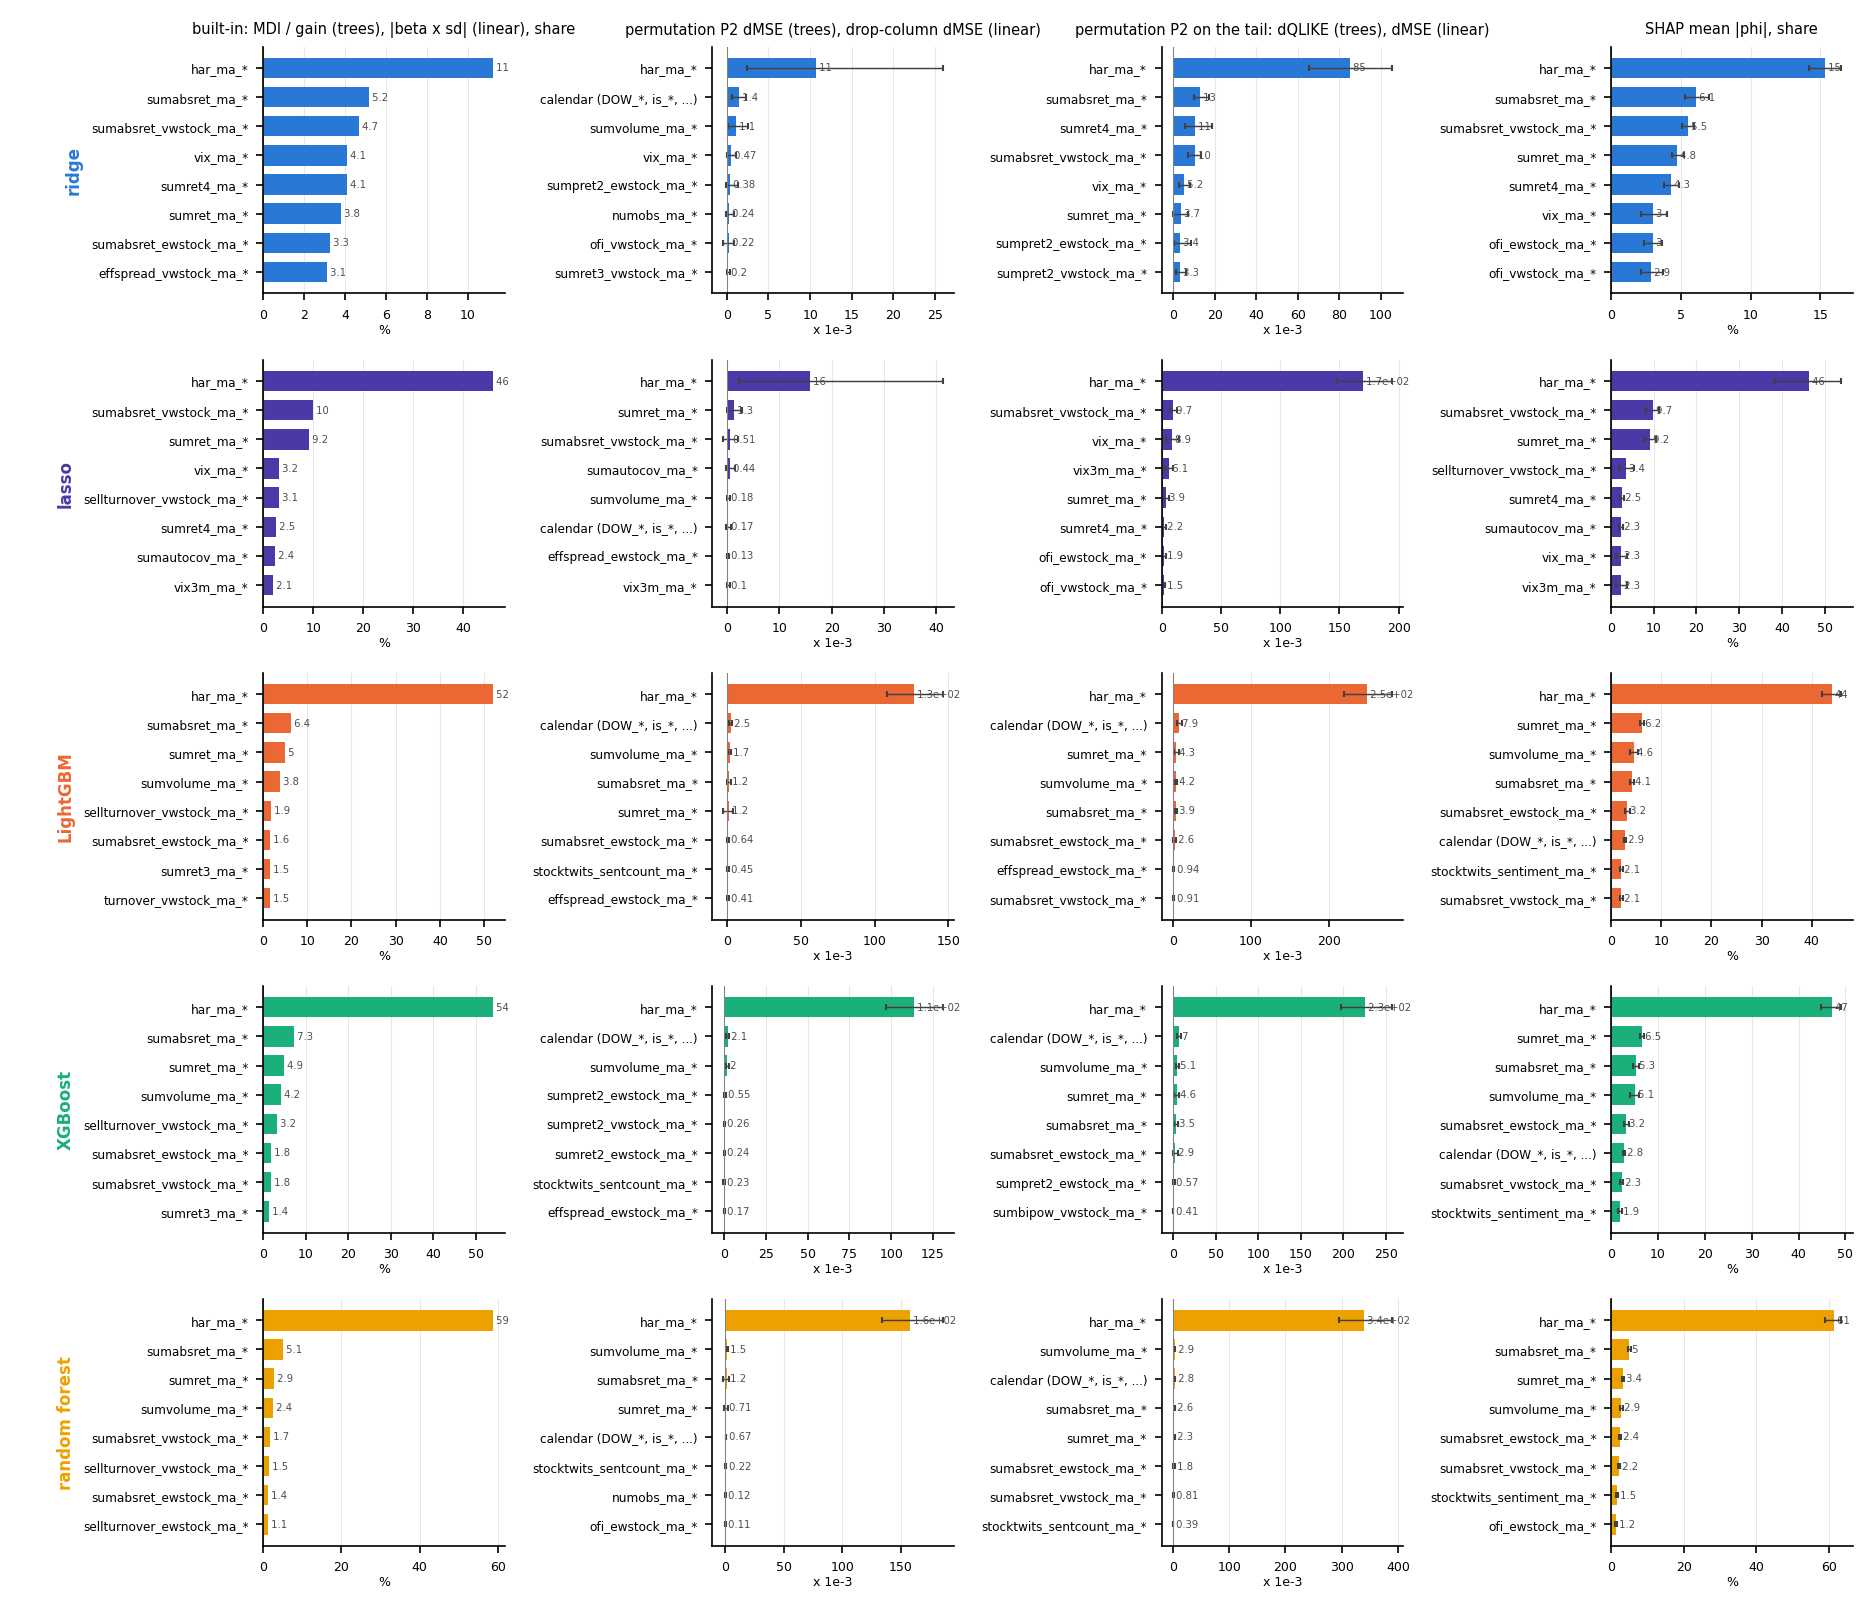
\includegraphics[width=\linewidth]{../results/feature_importance_1530_dedup/fig_ranked_all_features.png}
% % 2026-10-15 (notation pass): parked -- code jargon (refits, P2, fit space, held-out tail, |beta . sd|); standard measure names
% % \caption{Draft, measures under review. The leading series by each measure, per model (rows), all features
% % (\rhappNcolsAll{} columns in \rhappFiSeries{} series), averaged over the \rhappFiRefits{} refits. Columns: the
% % built-in measure (MDI\,/\,gain share for the trees, $|\beta\cdot\mathrm{sd}|$ share for the linear models);
% % permutation P2, $\Delta$MSE in the fit space (trees), or drop-column $\Delta$MSE (linear); permutation P2 on the
% % held-out tail, $\Delta$QLIKE (trees) or $\Delta$MSE (linear); SHAP mean $|\phi|$ share. Whiskers: 95\,\%
% % circular-block bootstrap intervals over refits (block \rhappFiBootBlock), which the paper's point-estimate convention
% % would drop.}
% \caption{Draft, measures under review. Leading predictor series by importance measure, for each closing-interval
% model (rows), on the full predictor set (\rhappNcolsAll{} columns in \rhappFiSeries{} series), averaged over the
% \rhappFiRefits{} re-estimations. Columns: the model's built-in measure (share of mean decrease in impurity, MDI, or of
% gain for the trees; share of $|\beta_j|\,\mathrm{sd}(x_j)$ for the linear models); permutation importance, the
% increase in squared-error loss on the scale of the target $y_t$ (trees), or the drop-column increase in squared-error
% loss (linear models); permutation importance on the out-of-sample block, the increase in QLIKE (trees) or in
% squared-error loss (linear models); and the share of the mean absolute SHAP value $|\phi|$. Permutation importance
% replaces a predictor's values with rows drawn from the estimation window. Whiskers: 95\% circular block-bootstrap
% confidence intervals across re-estimations (block length \rhappFiBootBlock); elsewhere the paper reports point
% estimates.}
% \label{fig:rh_app_fi_ranked}
% \end{figure}

% Source: results/feature_importance_1530_dedup/fig_rank_heatmap_all_features_series.png (raster)
% 2026-10-15 (user): parked -- non-standard figure; focus on legible tables
% \begin{figure}[htbp]
% \centering
% 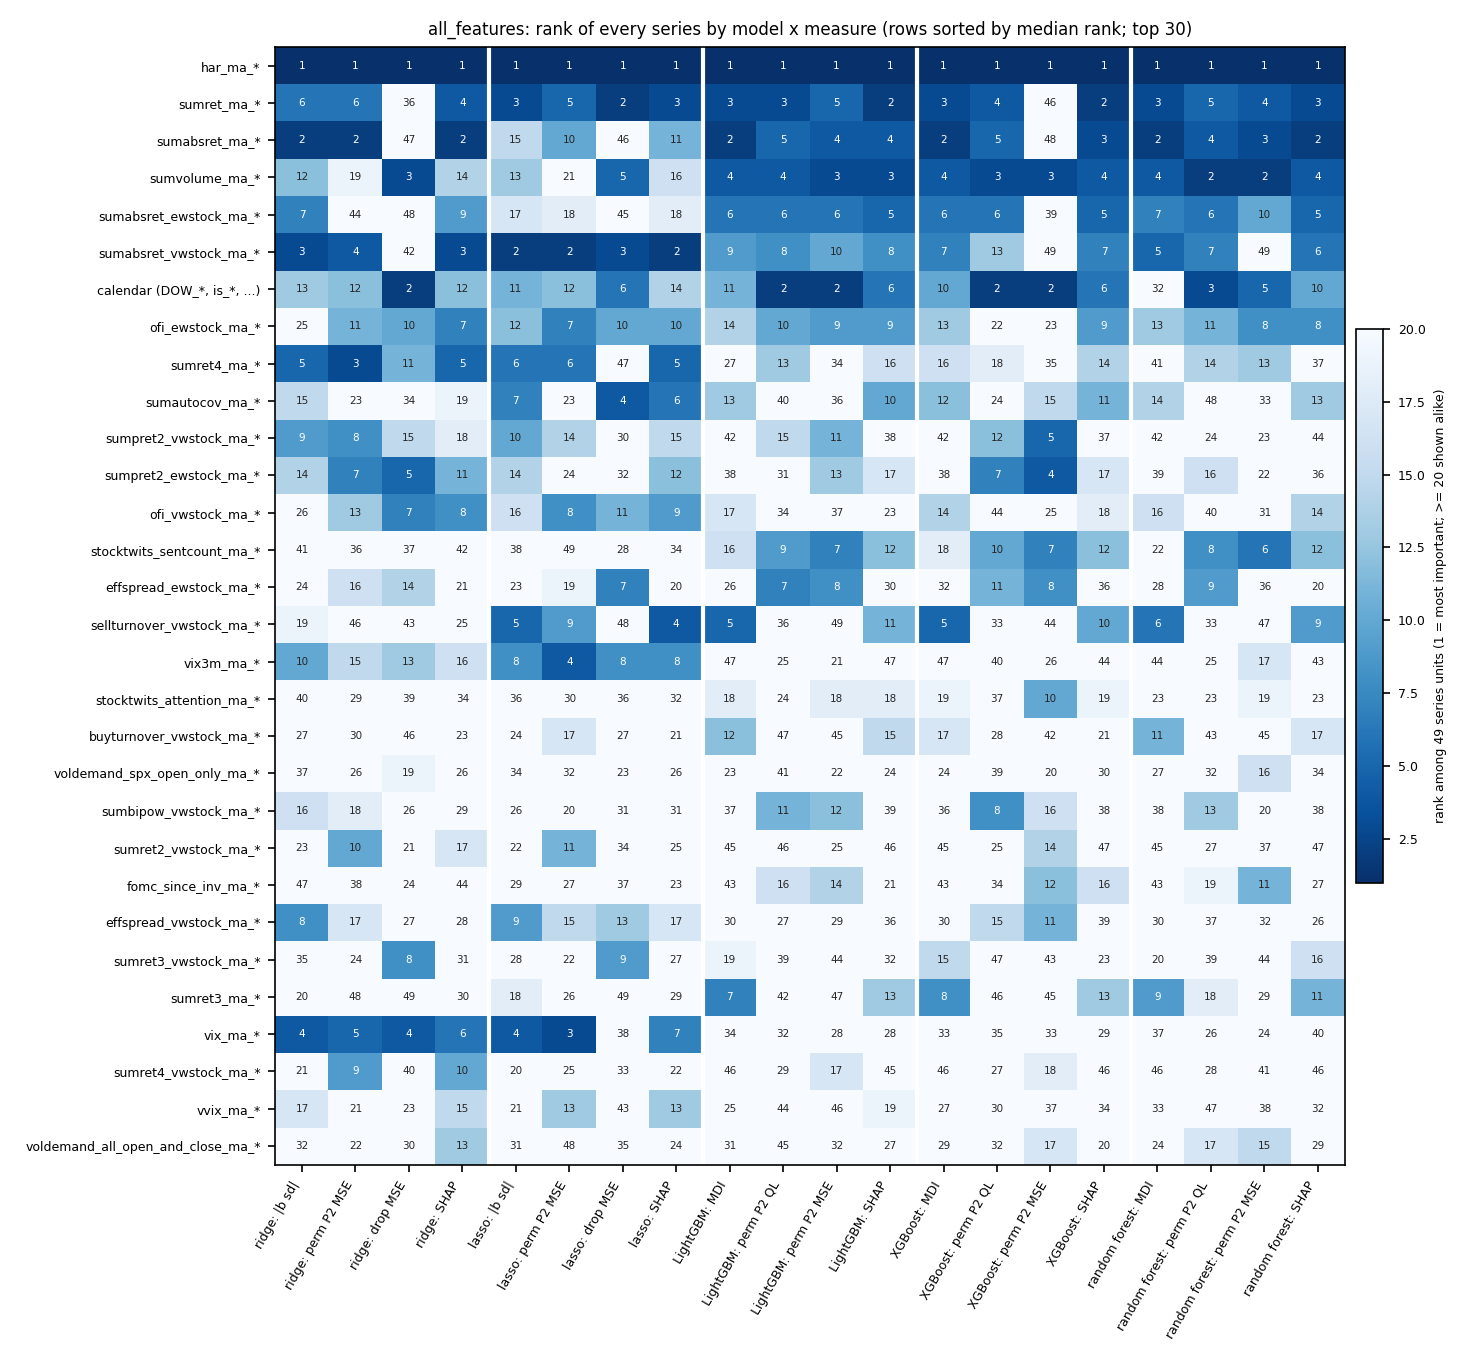
\includegraphics[width=\linewidth]{../results/feature_importance_1530_dedup/fig_rank_heatmap_all_features_series.png}
% % 2026-10-15 (notation pass): parked -- code jargon (all features, |beta . sd|, P2); American spelling
% % \caption{Draft, measures under review. The rank of each series among the \rhappFiSeries{} by model $\times$ measure,
% % all features (1 = most important; the colour scale saturates, so the low ranks share a shade); rows sorted by median rank,
% % the leading rows shown. Measures: $|\beta\cdot\mathrm{sd}|$ and drop-column $\Delta$MSE (linear), MDI\,/\,gain
% % (trees), permutation P2 on QLIKE (QL) or MSE, and SHAP.}
% \caption{Draft, measures under review. Rank of each predictor series among the \rhappFiSeries{}, by model and
% importance measure, closing-interval models on the full predictor set (1 = most important; the color scale saturates,
% so low ranks share a shade). Rows are sorted by median rank; the leading rows are shown. Measures:
% $|\beta_j|\,\mathrm{sd}(x_j)$ and the drop-column increase in squared-error loss (linear models), MDI or gain (trees),
% permutation importance on QLIKE (QL) or on squared-error loss (MSE), and SHAP.}
% \label{fig:rh_app_fi_heat_series}
% \end{figure}

% Source: results/feature_importance_1530_dedup/fig_rank_heatmap_all_features_cluster.png (raster)
% 2026-10-15 (user): parked -- non-standard figure; focus on legible tables
% \begin{figure}[htbp]
% \centering
% 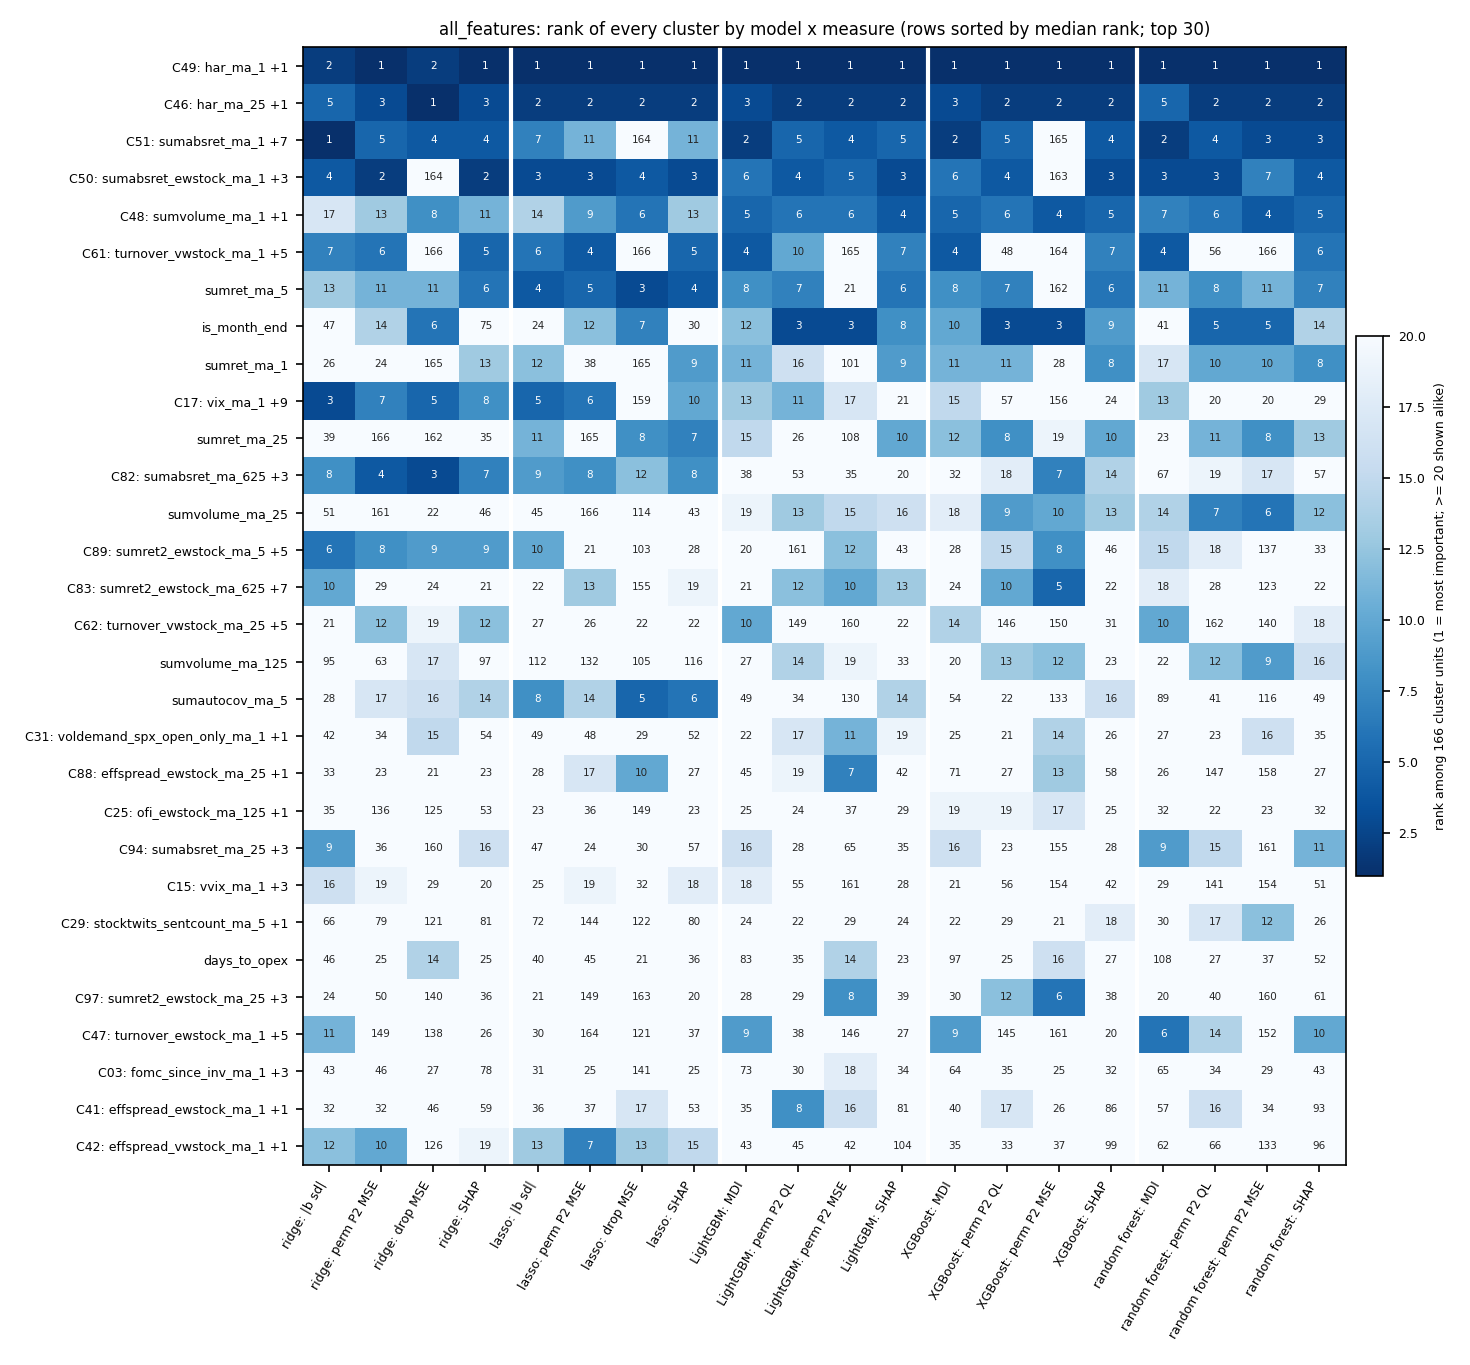
\includegraphics[width=\linewidth]{../results/feature_importance_1530_dedup/fig_rank_heatmap_all_features_cluster.png}
% % 2026-10-15 (notation pass): parked -- wording; explicit cross-reference
% % \caption{Draft, measures under review. The same at the cluster level: \rhappFiClusters{} clusters of columns, every
% % pair in a cluster correlated at $|\rho| \ge \rhappFiClusterCorr$ (complete linkage). A cluster is named by its first
% % member and the number of further members ($+k$); single columns keep their name.}
% \caption{Draft, measures under review. As Figure~\ref{fig:rh_app_fi_heat_series}, at the cluster level:
% \rhappFiClusters{} clusters of columns, formed by complete-linkage clustering so that every pair of columns within a
% cluster has absolute correlation $|\rho| \ge \rhappFiClusterCorr$. A cluster is labeled by its first member and the
% number of further members ($+k$); singleton columns keep their own label.}
% \label{fig:rh_app_fi_heat_cluster}
% \end{figure}

% Source: figures/feature_importance_1530_over_time.pdf (vector)
% 2026-10-15 (user): parked -- non-standard figure; focus on legible tables
% \begin{figure}[htbp]
% \centering
% 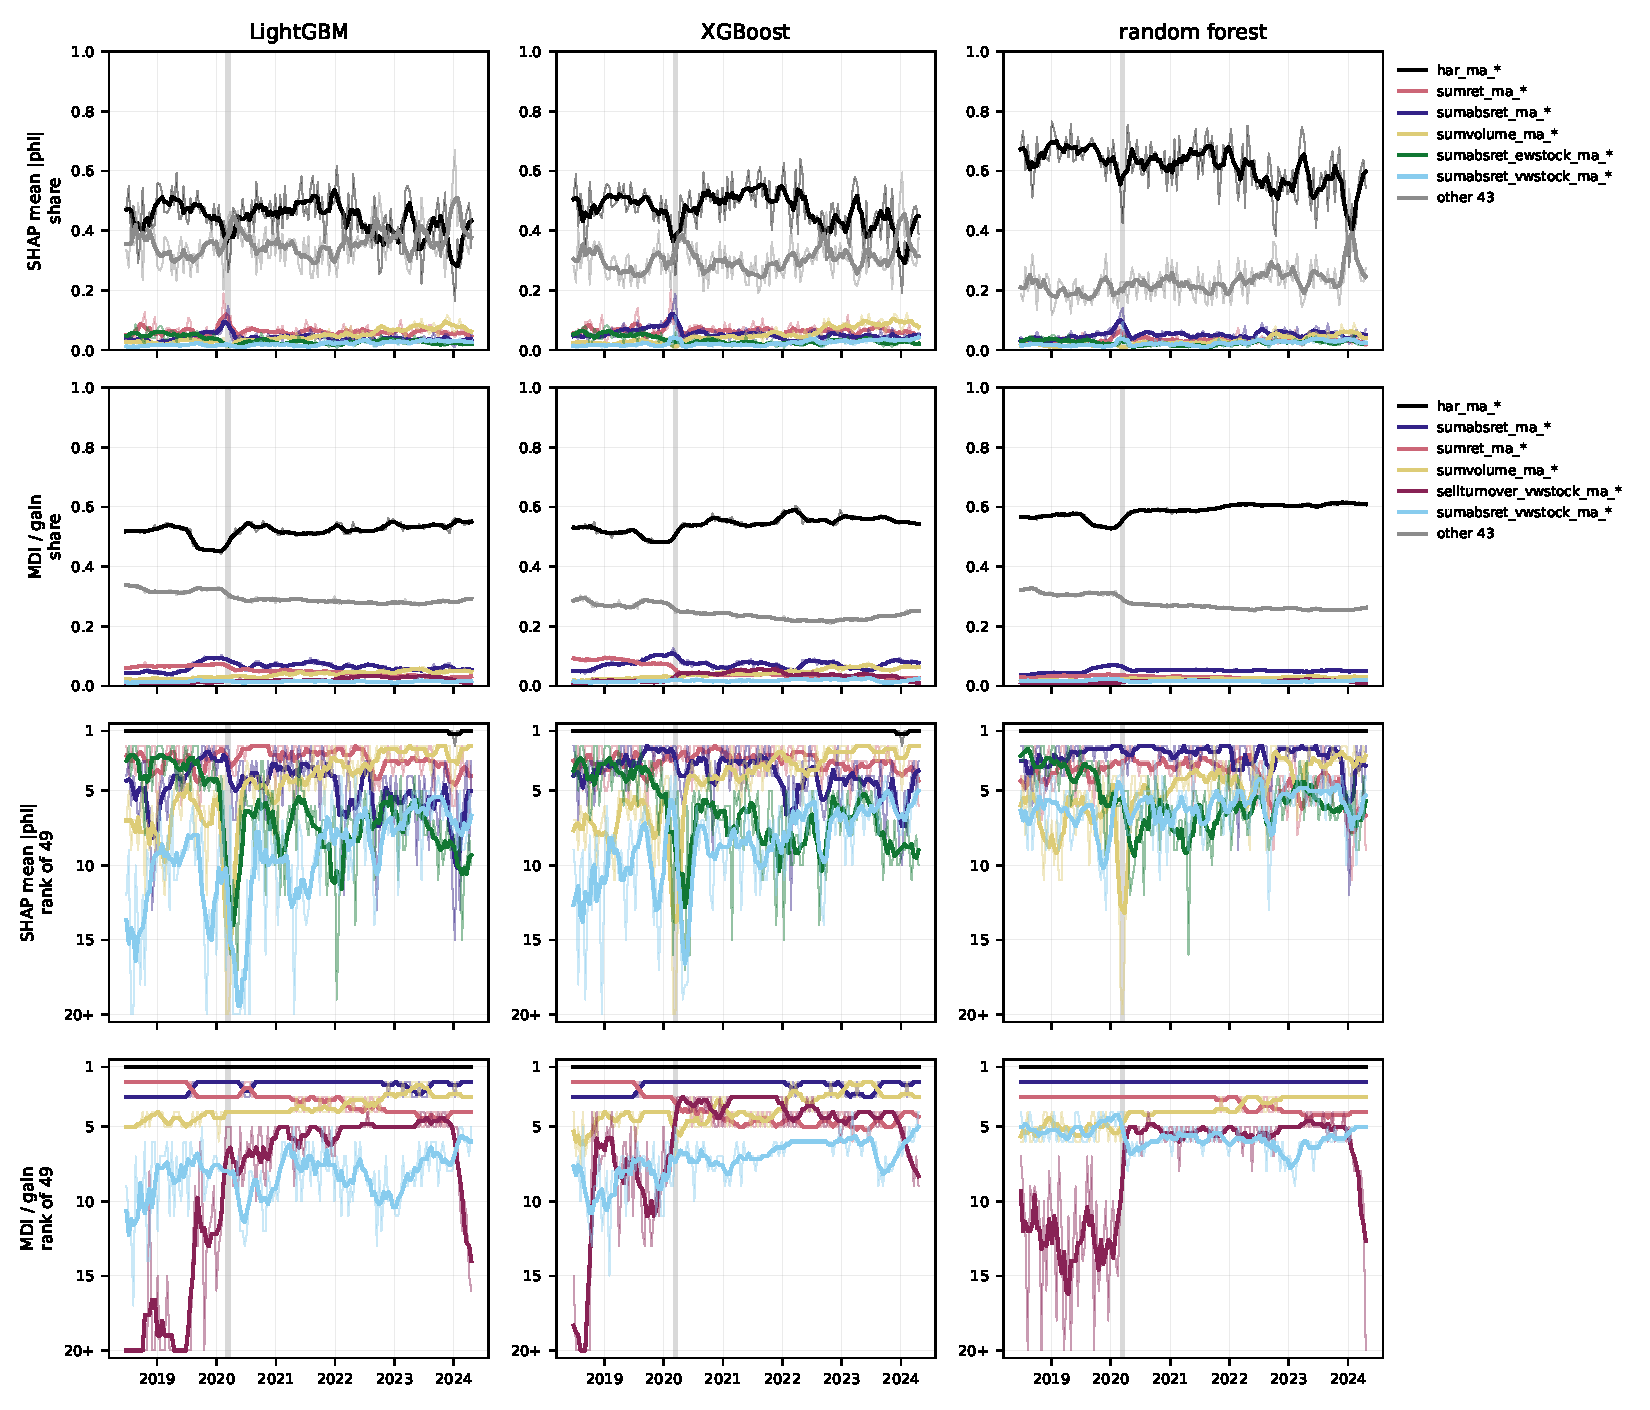
\includegraphics[width=\linewidth]{figures/feature_importance_1530_over_time.pdf}
% % 2026-10-15 (notation pass): parked -- code jargon (refit, held-out tail, har_ma_*, sessions); American spelling
% % \caption{Draft, measures under review. Importance over time, the three trees, all features, series level. Rows 1--2:
% % each series' share of the refit's total SHAP mean $|\phi|$ (on the held-out tail) and MDI\,/\,gain; rows 3--4: the
% % same series' rank among the \rhappFiSeries{} (ranks beyond \rhappFiTimeCap{} drawn at \rhappFiTimeCap). Lines:
% % \texttt{har\_ma\_*} and the next \rhappFiTimeTop{} series by overall share, the rest summed as `other'. Thin: one
% % point per refit (every \rhappFiRefitEvery{} sessions, \rhappFiRefits{} refits), at its tail's start date; thick: a
% % \rhappFiTimeSmooth-refit centred rolling mean. Grey band: the 2020 crash tails. Shares are split credit: correlated
% % inputs share it, and MDI and SHAP favour many-valued columns.}
% \caption{Draft, measures under review. Predictor importance over time for the three closing-interval tree models on
% the full predictor set, at the series level. Rows 1--2: each series' share of the re-estimation's total mean absolute
% SHAP value (on its out-of-sample block) and of its total MDI or gain; rows 3--4: the same series' rank among the
% \rhappFiSeries{} (ranks beyond \rhappFiTimeCap{} drawn at \rhappFiTimeCap). Lines: the HAR components
% $\bar y^{(k)}_t$ and the next \rhappFiTimeTop{} series by overall share, with the remainder summed as `other'. Thin
% lines: one point per re-estimation (every \rhappFiRefitEvery{} trading days, \rhappFiRefits{} re-estimations), dated
% at the start of its out-of-sample block, i.e., the trading days it forecasts before the next re-estimation; thick
% lines: a centered rolling mean over \rhappFiTimeSmooth{} re-estimations. Gray band: out-of-sample blocks in the 2020
% crash. Shares split credit: correlated predictors share it, and MDI and SHAP favor columns with many distinct
% values.}
% \label{fig:rh_app_fi_time_trees}
% \end{figure}

% Source: figures/feature_importance_1530_over_time_linear.pdf (vector)
% 2026-10-15 (user): parked -- non-standard figure; focus on legible tables
% \begin{figure}[htbp]
% \centering
% 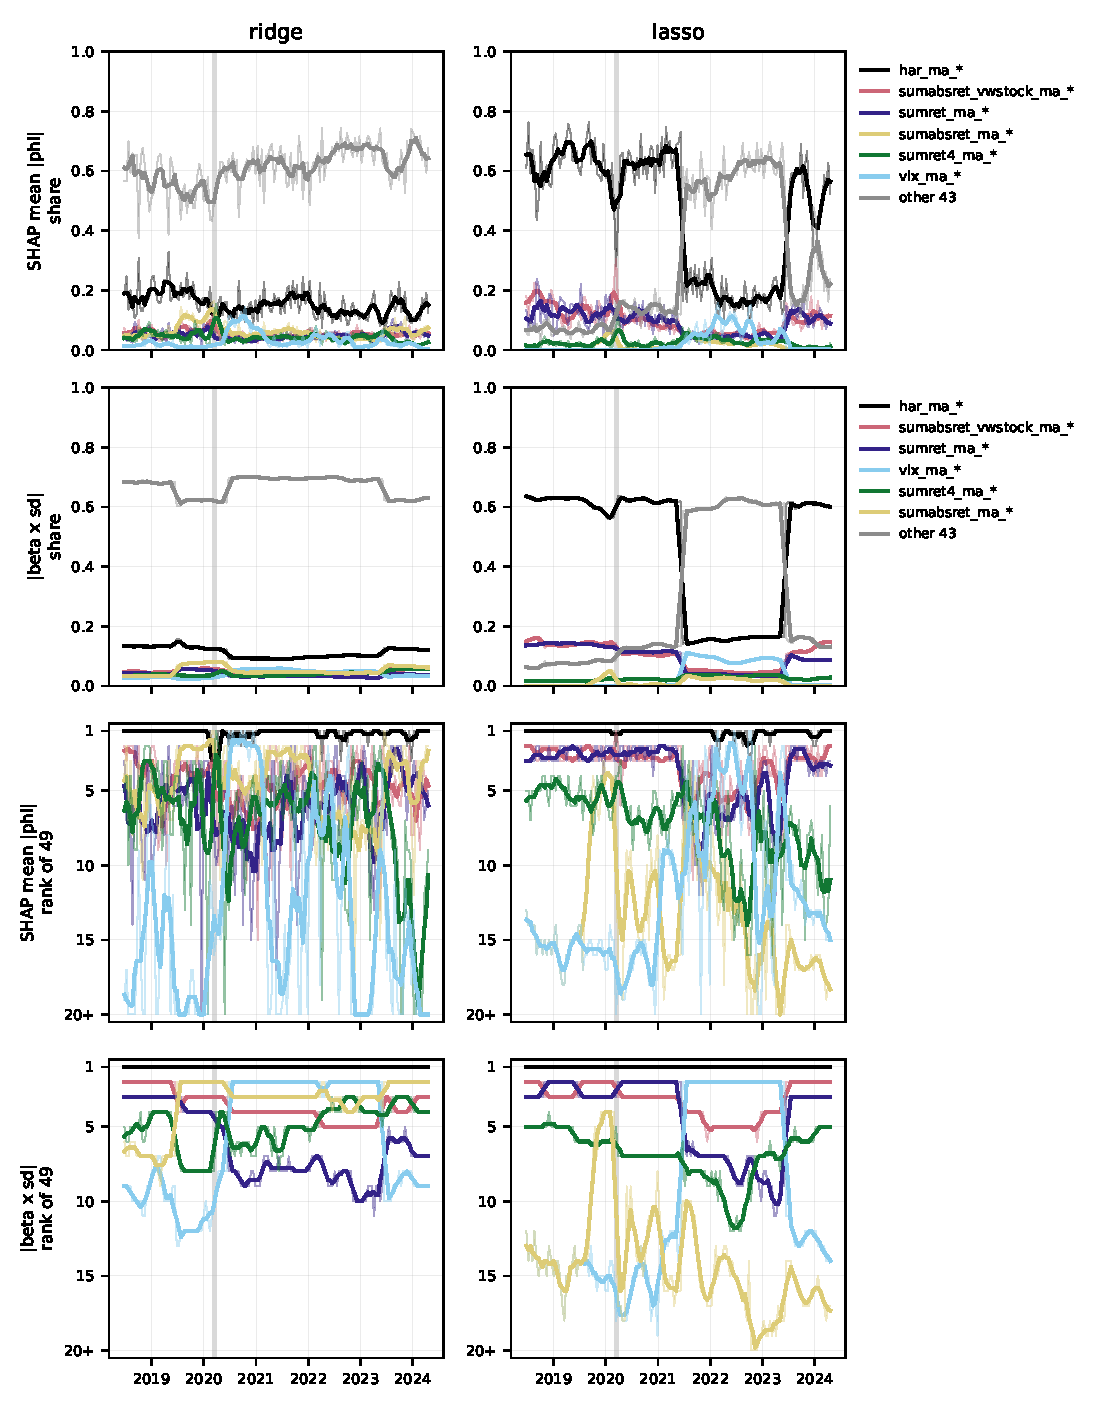
\includegraphics[width=\linewidth,height=0.78\textheight,keepaspectratio]{figures/feature_importance_1530_over_time_linear.pdf}
% % 2026-10-15 (notation pass): parked -- code jargon (per-bar, refit's window, |beta . sd|); explicit cross-reference
% % \caption{Draft, measures under review. The same for the per-bar ridge and lasso: SHAP mean $|\phi|$, with
% % $\phi_{t,j} = \beta_j(x_{t,j} - \bar x_j)$ and the window mean as background, and $|\beta\cdot\mathrm{sd}|$ (the
% % coefficient times the column's standard deviation in the refit's window, summed over a series' columns), as shares
% % and as ranks. A linear model spreads or concentrates credit across correlated columns differently from a tree, so
% % the shares compare over time within a model, not across the two figures.}
% \caption{Draft, measures under review. As Figure~\ref{fig:rh_app_fi_time_trees}, for the closing-interval ridge and
% lasso: the mean absolute SHAP value, with $\phi_{t,j} = \beta_j(x_{t,j} - \bar x_j)$ and the estimation-window mean
% $\bar x_j$ as background, and $|\beta_j|\,\mathrm{sd}(x_j)$, the absolute coefficient times the column's standard
% deviation in the estimation window, summed over a series' columns; both as shares and as ranks. A linear model
% spreads or concentrates credit across correlated columns differently from a tree, so the shares are comparable over
% time within a model, not across the two figures.}
% \label{fig:rh_app_fi_time_linear}
% \end{figure}

% Source: generated/appendix_campaign_16h_featimp.tex (re-laid out: generated/rehaul_app_featimp_harma.tex)
\begin{table}[htbp]
\centering
\small
\begin{threeparttable}
% 2026-10-15 (notation pass): parked -- code identifier har_ma_* and 'ladder' replaced by 'HAR components'
% \caption{Draft, measures under review. The \texttt{har\_ma\_*} ladder's importance in the trees, first pass to
% the current design (all features), old $\to$ new.}
% 2026-10-15 (table legibility): short caption, details in the notes; notes cut to about five sentences, method
% details referred to Methods. The pre-notation-pass caption and notes are parked in the comments here.
\caption{Importance of the HAR components in the tree models}
\label{tab:rh_app_fi_harma}
% AUTO-GENERATED by writeup/make_rehaul_appendix.py -- do not edit.
% Source: writeup/generated/appendix_campaign_16h_featimp.tex (numbers verbatim; its sources are listed there)
\begin{tabular}{@{}l*{5}{c}@{}}
\toprule
 & MDI & SHAP & Permutation & Close-interaction & MDI \\
Model & share (\%) & share (\%) & $\Delta$QLIKE (\%) & share (\%) & rank \\
\midrule
LightGBM & $57 \to 52$ & $47 \to 44$ & $237 \to 200$ & $22$ & $1 \to 1$ \\
XGBoost & $69 \to 54$ & $55 \to 47$ & $224 \to 181$ & $22$ & $1 \to 1$ \\
Random forest & $62 \to 59$ & $58 \to 61$ & $290 \to 271$ & $54$ & $1 \to 1$ \\
\bottomrule
\end{tabular}

\begin{tablenotes}[flushleft]
\footnotesize
% 2026-10-15 (notation pass): parked -- code jargon (ladder, unmasked, window-masked, P2, tail loss, _x_close)
% \item[] \emph{Notes:} first pass: the old design (with the \rhappNsessionEdge{} session-edge interactions), trees
% unmasked; new: those columns dropped and every tree fit window-masked. MDI and TreeSHAP: the ladder's share of the
% model's total. Perm.\ P2 $\Delta$QLIKE: the loss increase when the ladder's rows are replaced by rows drawn from the
% training window, in \% of the model's tail loss. \texttt{\_x\_close} share: the part of the old ladder's MDI that sat
% on its \rhappNsessionEdgeHalf{} \texttt{\_x\_close} copies. MDI rank among the series. XGBoost and the random forest
% also changed settings between the passes, so their before/after mixes that change with the design and the mask.
\item[] \textit{Notes:} Draft, measures under review. Closing-interval tree models on the full predictor set, first
pass (old) $\to$ current design (new); the first pass includes the \rhappNsessionEdge{} interactions of the HAR
components with the opening- and closing-session dummies and no column screening, the current design drops those
interactions and screens out constant and duplicate columns in every estimation window. MDI and TreeSHAP: the HAR
components' share of the model's total; permutation $\Delta$QLIKE: the increase in QLIKE when their values are
replaced by rows drawn from the estimation window, in percent of the model's out-of-sample loss. Close-interaction
share: the part of the old MDI carried by the \rhappNsessionEdgeHalf{} closing-session interactions, which at the
closing interval are copies of the HAR components; MDI rank: rank among the series. XGBoost and the random forest
also changed hyperparameters between the passes, so their changes mix design, screening and hyperparameters.
\end{tablenotes}
\end{threeparttable}
\end{table}

% 08b_fi_measures_floats.tex -- the floats of the feature-importance measures in 08_feature_importance.tex (2026-10-15):
% lasso selection counts, ridge coefficient mass, the trees' per-refit SHAP rankings and their SHAP interactions.
% Generator: writeup/make_rehaul_fi.py, from results/rehaul_fi/ (experiments/rehaul_fi_compute.py). Labels:
% tab:rh_fi_summary, tab:rh_fi_linear, tab:rh_fi_trees, tab:rh_fi_inter, fig:rh_fi_linear, fig:rh_fi_ranks,
% fig:rh_fi_inter. Prose macros \rhfi...: generated/rehaul_fi_numbers.tex (loaded here too, for a standalone build).
\ifdefined\rhfiNRefits\else% AUTO-GENERATED by writeup/make_rehaul_fi.py -- do not edit; re-run the script.
% \rhfi... macros for writeup/rehaul/08_feature_importance.tex (results/rehaul_fi/).
\providecommand{\rhfiNRefits}{}\renewcommand{\rhfiNRefits}{147}  % refits, one every 10 sessions
\providecommand{\rhfiNOos}{}\renewcommand{\rhfiNOos}{1{,}469}  % scored held-out sessions
\providecommand{\rhfiP}{}\renewcommand{\rhfiP}{628}  % columns, all features
\providecommand{\rhfiNUnits}{}\renewcommand{\rhfiNUnits}{49}  % units: 47 exogenous series + HAR ladder + calendar
\providecommand{\rhfiNExog}{}\renewcommand{\rhfiNExog}{47}  % exogenous series
\providecommand{\rhfiFirst}{}\renewcommand{\rhfiFirst}{25~June~2018}  % first scored session
\providecommand{\rhfiLast}{}\renewcommand{\rhfiLast}{30~April~2024}  % last scored session
\providecommand{\rhfiWindow}{}\renewcommand{\rhfiWindow}{2{,}000}  % sessions in a training window
\providecommand{\rhfiRefitEvery}{}\renewcommand{\rhfiRefitEvery}{10}  % sessions between refits
\providecommand{\rhfiBackbonePf}{}\renewcommand{\rhfiBackbonePf}{0.01}  % backbone penalty factor
\providecommand{\rhfiNBuckets}{}\renewcommand{\rhfiNBuckets}{8}  % exogenous buckets
\providecommand{\rhfiOldBlock}{}\renewcommand{\rhfiOldBlock}{250}  % sessions between the old arm's penalty re-choices
\providecommand{\rhfiNPairs}{}\renewcommand{\rhfiNPairs}{1{,}176}  % series pairs
\providecommand{\rhfiNProbeCols}{}\renewcommand{\rhfiNProbeCols}{631}  % columns of a probe fit
\providecommand{\rhfiTopWPairs}{}\renewcommand{\rhfiTopWPairs}{50}  % pairs in the interaction W
\providecommand{\rhfiProbeLevels}{}\renewcommand{\rhfiProbeLevels}{20}  % values of the few-valued noise column
\providecommand{\rhfiRidgeAlpha}{}\renewcommand{\rhfiRidgeAlpha}{\ensuremath{10^{3}}}
\providecommand{\rhfiLassoAlpha}{}\renewcommand{\rhfiLassoAlpha}{\ensuremath{10^{-2}}}
\providecommand{\rhfiLassoNzMed}{}\renewcommand{\rhfiLassoNzMed}{30}  % median nonzero coefficients per refit
\providecommand{\rhfiLassoNzMin}{}\renewcommand{\rhfiLassoNzMin}{27}
\providecommand{\rhfiLassoNzMax}{}\renewcommand{\rhfiLassoNzMax}{35}
\providecommand{\rhfiLassoExogNzMed}{}\renewcommand{\rhfiLassoExogNzMed}{14}  % ... exogenous columns
\providecommand{\rhfiLassoColsEver}{}\renewcommand{\rhfiLassoColsEver}{60}  % columns nonzero in >= 1 refit
\providecommand{\rhfiLassoColsMajority}{}\renewcommand{\rhfiLassoColsMajority}{29}  % columns nonzero in >= half the refits
\providecommand{\rhfiLassoExogEver}{}\renewcommand{\rhfiLassoExogEver}{27}  % exogenous series with a nonzero column in >= 1 refit
\providecommand{\rhfiLassoExogMajority}{}\renewcommand{\rhfiLassoExogMajority}{11}  % ... in >= half the refits
\providecommand{\rhfiLassoExogAlways}{}\renewcommand{\rhfiLassoExogAlways}{3}  % ... in every refit
\providecommand{\rhfiLassoAlwaysList}{}\renewcommand{\rhfiLassoAlwaysList}{\texttt{sumret}, \texttt{sumabsret\_vwstock}, \texttt{sumautocov}}  % exogenous series selected in every refit
\providecommand{\rhfiLassoProbeSel}{}\renewcommand{\rhfiLassoProbeSel}{1}  % continuous probe selected, of the probe fits
\providecommand{\rhfiLassoProbeSelLevels}{}\renewcommand{\rhfiLassoProbeSelLevels}{0}
\providecommand{\rhfiLassoProbeSelBinary}{}\renewcommand{\rhfiLassoProbeSelBinary}{0}
\providecommand{\rhfiNProbe}{}\renewcommand{\rhfiNProbe}{49}  % probe refits (every third)
\providecommand{\rhfiLassoW}{}\renewcommand{\rhfiLassoW}{0.74}  % Kendall W of the per-refit series ranks by sum |beta|
\providecommand{\rhfiLassoBackboneShare}{}\renewcommand{\rhfiLassoBackboneShare}{88}  % median share of sum |beta| on the backbone, %
\providecommand{\rhfiOldLassoSpearman}{}\renewcommand{\rhfiOldLassoSpearman}{0.70}  % Spearman, selection share: pre-tuned vs re-tuned one-penalty lasso
\providecommand{\rhfiOldLassoNzMed}{}\renewcommand{\rhfiOldLassoNzMed}{23}  % re-tuned lasso: median nonzero per refit
\providecommand{\rhfiOldLassoExogMajority}{}\renewcommand{\rhfiOldLassoExogMajority}{18}
\providecommand{\rhfiRidgeTopOne}{}\renewcommand{\rhfiRidgeTopOne}{Calendar}
\providecommand{\rhfiRidgeTopOneShare}{}\renewcommand{\rhfiRidgeTopOneShare}{31.0}  % % of sum |beta|
\providecommand{\rhfiRidgeTopTwo}{}\renewcommand{\rhfiRidgeTopTwo}{HAR ladder}
\providecommand{\rhfiRidgeTopTwoShare}{}\renewcommand{\rhfiRidgeTopTwoShare}{22.8}  % % of sum |beta|
\providecommand{\rhfiRidgeTopThree}{}\renewcommand{\rhfiRidgeTopThree}{\texttt{sumret}}
\providecommand{\rhfiRidgeTopThreeShare}{}\renewcommand{\rhfiRidgeTopThreeShare}{3.6}  % % of sum |beta|
\providecommand{\rhfiRidgeTopFour}{}\renewcommand{\rhfiRidgeTopFour}{\texttt{sumabsret\_vwstock}}
\providecommand{\rhfiRidgeTopFourShare}{}\renewcommand{\rhfiRidgeTopFourShare}{2.2}  % % of sum |beta|
\providecommand{\rhfiRidgeSdTopOne}{}\renewcommand{\rhfiRidgeSdTopOne}{HAR ladder}
\providecommand{\rhfiRidgeSdTopOneShare}{}\renewcommand{\rhfiRidgeSdTopOneShare}{30.6}  % % of sum |beta| sd
\providecommand{\rhfiRidgeSdTopTwo}{}\renewcommand{\rhfiRidgeSdTopTwo}{Calendar}
\providecommand{\rhfiRidgeSdTopTwoShare}{}\renewcommand{\rhfiRidgeSdTopTwoShare}{9.3}  % % of sum |beta| sd
\providecommand{\rhfiRidgeSdTopThree}{}\renewcommand{\rhfiRidgeSdTopThree}{\texttt{sumret}}
\providecommand{\rhfiRidgeSdTopThreeShare}{}\renewcommand{\rhfiRidgeSdTopThreeShare}{4.5}  % % of sum |beta| sd
\providecommand{\rhfiRidgeTopExog}{}\renewcommand{\rhfiRidgeTopExog}{\texttt{sumret}}
\providecommand{\rhfiRidgeTopExogShare}{}\renewcommand{\rhfiRidgeTopExogShare}{3.6}
\providecommand{\rhfiRidgeBackboneShare}{}\renewcommand{\rhfiRidgeBackboneShare}{54}  % median share of sum |beta| on the backbone, %
\providecommand{\rhfiRidgeW}{}\renewcommand{\rhfiRidgeW}{0.85}
\providecommand{\rhfiRidgeAllSelected}{}\renewcommand{\rhfiRidgeAllSelected}{49}  % units with N_A = K under the ridge
\providecommand{\rhfiLassoProbeRate}{}\renewcommand{\rhfiLassoProbeRate}{2.0}  % continuous probe's selection rate, %
\providecommand{\rhfiLassoColsAboveProbe}{}\renewcommand{\rhfiLassoColsAboveProbe}{54}  % columns selected more often than the continuous probe
\providecommand{\rhfiLassoSeriesAboveProbe}{}\renewcommand{\rhfiLassoSeriesAboveProbe}{23}  % exogenous series with such a column
\providecommand{\rhfiLassoTopCol}{}\renewcommand{\rhfiLassoTopCol}{\texttt{is\_month\_end}}
\providecommand{\rhfiRidgeSpearmanSd}{}\renewcommand{\rhfiRidgeSpearmanSd}{0.85}  % Spearman, series sum|beta| vs sum|beta| sd
\providecommand{\rhfiRidgeProbeBeat}{}\renewcommand{\rhfiRidgeProbeBeat}{107}  % columns with |beta| above the continuous probe's in most probe fits
\providecommand{\rhfiRidgeProbeBeatSeries}{}\renewcommand{\rhfiRidgeProbeBeatSeries}{38}
\providecommand{\rhfiScaleValueN}{}\renewcommand{\rhfiScaleValueN}{282}
\providecommand{\rhfiScaleValueSd}{}\renewcommand{\rhfiScaleValueSd}{0.84}  % median window sd, value ladders
\providecommand{\rhfiScaleValueSdLo}{}\renewcommand{\rhfiScaleValueSdLo}{0.03}
\providecommand{\rhfiScaleValueSdHi}{}\renewcommand{\rhfiScaleValueSdHi}{1.76}
\providecommand{\rhfiScaleValueIqr}{}\renewcommand{\rhfiScaleValueIqr}{0.94}  % median window IQR, value ladders
\providecommand{\rhfiScaleFlagN}{}\renewcommand{\rhfiScaleFlagN}{324}
\providecommand{\rhfiScaleFlagSd}{}\renewcommand{\rhfiScaleFlagSd}{0.022}  % median window sd, availability / activity ladders
\providecommand{\rhfiScaleFlagSdHi}{}\renewcommand{\rhfiScaleFlagSdHi}{0.17}
\providecommand{\rhfiScaleCalSd}{}\renewcommand{\rhfiScaleCalSd}{0.39}  % median window sd, calendar
\providecommand{\rhfiScaleHarSd}{}\renewcommand{\rhfiScaleHarSd}{1.07}  % median window sd, HAR ladder
\providecommand{\rhfiLgbmW}{}\renewcommand{\rhfiLgbmW}{0.57}  % lgbm: Kendall W, per-refit series ranks
\providecommand{\rhfiLgbmWCols}{}\renewcommand{\rhfiLgbmWCols}{0.91}  % lgbm: Kendall W, column ranks
\providecommand{\rhfiLgbmTopOne}{}\renewcommand{\rhfiLgbmTopOne}{HAR ladder}
\providecommand{\rhfiLgbmTopOneRank}{}\renewcommand{\rhfiLgbmTopOneRank}{1.0}  % mean rank
\providecommand{\rhfiLgbmTopTwo}{}\renewcommand{\rhfiLgbmTopTwo}{\texttt{sumret}}
\providecommand{\rhfiLgbmTopTwoRank}{}\renewcommand{\rhfiLgbmTopTwoRank}{2.9}  % mean rank
\providecommand{\rhfiLgbmTopThree}{}\renewcommand{\rhfiLgbmTopThree}{\texttt{sumabsret}}
\providecommand{\rhfiLgbmTopThreeRank}{}\renewcommand{\rhfiLgbmTopThreeRank}{4.8}  % mean rank
\providecommand{\rhfiLgbmSpBorda}{}\renewcommand{\rhfiLgbmSpBorda}{0.90}  % Spearman, mean rank vs top-10 Borda
\providecommand{\rhfiLgbmSpGlobal}{}\renewcommand{\rhfiLgbmSpGlobal}{0.96}  % Spearman, mean rank vs global mean |phi|
\providecommand{\rhfiLgbmSpLocal}{}\renewcommand{\rhfiLgbmSpLocal}{1.000}  % Spearman, mean ranks local refit vs stored
\providecommand{\rhfiLgbmProbeRank}{}\renewcommand{\rhfiLgbmProbeRank}{83}  % median rank of the continuous probe, 631 columns
\providecommand{\rhfiLgbmProbeCols}{}\renewcommand{\rhfiLgbmProbeCols}{60}  % columns above the continuous probe in most probe fits
\providecommand{\rhfiLgbmProbeSeries}{}\renewcommand{\rhfiLgbmProbeSeries}{27}  % exogenous series with such a column
\providecommand{\rhfiLgbmTopCol}{}\renewcommand{\rhfiLgbmTopCol}{\texttt{har\_ma\_1}}  % column with the lowest mean rank
\providecommand{\rhfiLgbmTopColRank}{}\renewcommand{\rhfiLgbmTopColRank}{1.3}
\providecommand{\rhfiLgbmTopColTwo}{}\renewcommand{\rhfiLgbmTopColTwo}{\texttt{har\_ma\_5}}
\providecommand{\rhfiLgbmTopColTwoRank}{}\renewcommand{\rhfiLgbmTopColTwoRank}{1.8}
\providecommand{\rhfiLgbmPredGap}{}\renewcommand{\rhfiLgbmPredGap}{0}  % max |local refit - stored refit| forecast
\providecommand{\rhfiLgbmInterW}{}\renewcommand{\rhfiLgbmInterW}{0.45}  % Kendall W of per-refit pair ranks, top-50 pairs
\providecommand{\rhfiLgbmInterRatio}{}\renewcommand{\rhfiLgbmInterRatio}{90}  % sum of series-pair interactions / sum main, %
\providecommand{\rhfiLgbmInterSpGlobal}{}\renewcommand{\rhfiLgbmInterSpGlobal}{0.99}
\providecommand{\rhfiLgbmInterFloor}{}\renewcommand{\rhfiLgbmInterFloor}{0.49}  % probe floor x 1e3
\providecommand{\rhfiLgbmInterAboveFloor}{}\renewcommand{\rhfiLgbmInterAboveFloor}{116}  % series pairs above the probe floor
\providecommand{\rhfiLgbmInterTopA}{}\renewcommand{\rhfiLgbmInterTopA}{HAR ladder}
\providecommand{\rhfiLgbmInterTopB}{}\renewcommand{\rhfiLgbmInterTopB}{\texttt{sumabsret}}
\providecommand{\rhfiLgbmInterTopVal}{}\renewcommand{\rhfiLgbmInterTopVal}{12.6}  % x 1e3
\providecommand{\rhfiLgbmHTop}{}\renewcommand{\rhfiLgbmHTop}{0.33}  % H^2 of the top series pair (pooled), %
\providecommand{\rhfiLgbmHMin}{}\renewcommand{\rhfiLgbmHMin}{0.02}  % min H^2 over the top-10 series pairs, %
\providecommand{\rhfiLgbmHMax}{}\renewcommand{\rhfiLgbmHMax}{0.33}  % max H^2 over the top-10 series pairs, %
\providecommand{\rhfiLgbmHMinTop}{}\renewcommand{\rhfiLgbmHMinTop}{0.19}  % top pair: interaction PD var / smaller main PD var
\providecommand{\rhfiLgbmHMinLo}{}\renewcommand{\rhfiLgbmHMinLo}{0.05}  % ... min over the top-10 series pairs
\providecommand{\rhfiLgbmHMinHi}{}\renewcommand{\rhfiLgbmHMinHi}{0.54}  % ... max
\providecommand{\rhfiLgbmHColTop}{}\renewcommand{\rhfiLgbmHColTop}{0.36}  % H^2 of the top column pair, %
\providecommand{\rhfiLgbmHMinColTop}{}\renewcommand{\rhfiLgbmHMinColTop}{0.02}  % ... min-normalised
\providecommand{\rhfiLgbmMainTopVal}{}\renewcommand{\rhfiLgbmMainTopVal}{195}  % largest global mean |phi_A| x 1e3
\providecommand{\rhfiLgbmWithinTop}{}\renewcommand{\rhfiLgbmWithinTop}{HAR ladder}
\providecommand{\rhfiLgbmWithinTopVal}{}\renewcommand{\rhfiLgbmWithinTopVal}{18.7}
\providecommand{\rhfiXgbW}{}\renewcommand{\rhfiXgbW}{0.60}  % xgb: Kendall W, per-refit series ranks
\providecommand{\rhfiXgbWCols}{}\renewcommand{\rhfiXgbWCols}{0.90}  % xgb: Kendall W, column ranks
\providecommand{\rhfiXgbTopOne}{}\renewcommand{\rhfiXgbTopOne}{HAR ladder}
\providecommand{\rhfiXgbTopOneRank}{}\renewcommand{\rhfiXgbTopOneRank}{1.0}  % mean rank
\providecommand{\rhfiXgbTopTwo}{}\renewcommand{\rhfiXgbTopTwo}{\texttt{sumret}}
\providecommand{\rhfiXgbTopTwoRank}{}\renewcommand{\rhfiXgbTopTwoRank}{3.0}  % mean rank
\providecommand{\rhfiXgbTopThree}{}\renewcommand{\rhfiXgbTopThree}{\texttt{sumabsret}}
\providecommand{\rhfiXgbTopThreeRank}{}\renewcommand{\rhfiXgbTopThreeRank}{3.9}  % mean rank
\providecommand{\rhfiXgbSpBorda}{}\renewcommand{\rhfiXgbSpBorda}{0.87}  % Spearman, mean rank vs top-10 Borda
\providecommand{\rhfiXgbSpGlobal}{}\renewcommand{\rhfiXgbSpGlobal}{0.97}  % Spearman, mean rank vs global mean |phi|
\providecommand{\rhfiXgbSpLocal}{}\renewcommand{\rhfiXgbSpLocal}{0.993}  % Spearman, mean ranks local refit vs stored
\providecommand{\rhfiXgbProbeRank}{}\renewcommand{\rhfiXgbProbeRank}{110}  % median rank of the continuous probe, 631 columns
\providecommand{\rhfiXgbProbeCols}{}\renewcommand{\rhfiXgbProbeCols}{78}  % columns above the continuous probe in most probe fits
\providecommand{\rhfiXgbProbeSeries}{}\renewcommand{\rhfiXgbProbeSeries}{35}  % exogenous series with such a column
\providecommand{\rhfiXgbTopCol}{}\renewcommand{\rhfiXgbTopCol}{\texttt{har\_ma\_1}}  % column with the lowest mean rank
\providecommand{\rhfiXgbTopColRank}{}\renewcommand{\rhfiXgbTopColRank}{1.3}
\providecommand{\rhfiXgbTopColTwo}{}\renewcommand{\rhfiXgbTopColTwo}{\texttt{har\_ma\_5}}
\providecommand{\rhfiXgbTopColTwoRank}{}\renewcommand{\rhfiXgbTopColTwoRank}{1.8}
\providecommand{\rhfiXgbPredGap}{}\renewcommand{\rhfiXgbPredGap}{0.17}  % max |local refit - stored refit| forecast
\providecommand{\rhfiXgbInterW}{}\renewcommand{\rhfiXgbInterW}{0.47}  % Kendall W of per-refit pair ranks, top-50 pairs
\providecommand{\rhfiXgbInterRatio}{}\renewcommand{\rhfiXgbInterRatio}{74}  % sum of series-pair interactions / sum main, %
\providecommand{\rhfiXgbInterSpGlobal}{}\renewcommand{\rhfiXgbInterSpGlobal}{0.99}
\providecommand{\rhfiXgbInterFloor}{}\renewcommand{\rhfiXgbInterFloor}{0.41}  % probe floor x 1e3
\providecommand{\rhfiXgbInterAboveFloor}{}\renewcommand{\rhfiXgbInterAboveFloor}{115}  % series pairs above the probe floor
\providecommand{\rhfiXgbInterTopA}{}\renewcommand{\rhfiXgbInterTopA}{HAR ladder}
\providecommand{\rhfiXgbInterTopB}{}\renewcommand{\rhfiXgbInterTopB}{\texttt{sumabsret}}
\providecommand{\rhfiXgbInterTopVal}{}\renewcommand{\rhfiXgbInterTopVal}{15.2}  % x 1e3
\providecommand{\rhfiXgbHTop}{}\renewcommand{\rhfiXgbHTop}{0.37}  % H^2 of the top series pair (pooled), %
\providecommand{\rhfiXgbHMin}{}\renewcommand{\rhfiXgbHMin}{0.02}  % min H^2 over the top-10 series pairs, %
\providecommand{\rhfiXgbHMax}{}\renewcommand{\rhfiXgbHMax}{0.68}  % max H^2 over the top-10 series pairs, %
\providecommand{\rhfiXgbHMinTop}{}\renewcommand{\rhfiXgbHMinTop}{0.39}  % top pair: interaction PD var / smaller main PD var
\providecommand{\rhfiXgbHMinLo}{}\renewcommand{\rhfiXgbHMinLo}{0.08}  % ... min over the top-10 series pairs
\providecommand{\rhfiXgbHMinHi}{}\renewcommand{\rhfiXgbHMinHi}{0.80}  % ... max
\providecommand{\rhfiXgbHColTop}{}\renewcommand{\rhfiXgbHColTop}{0.39}  % H^2 of the top column pair, %
\providecommand{\rhfiXgbHMinColTop}{}\renewcommand{\rhfiXgbHMinColTop}{0.02}  % ... min-normalised
\providecommand{\rhfiXgbMainTopVal}{}\renewcommand{\rhfiXgbMainTopVal}{192}  % largest global mean |phi_A| x 1e3
\providecommand{\rhfiXgbWithinTop}{}\renewcommand{\rhfiXgbWithinTop}{HAR ladder}
\providecommand{\rhfiXgbWithinTopVal}{}\renewcommand{\rhfiXgbWithinTopVal}{19.1}
\providecommand{\rhfiRfW}{}\renewcommand{\rhfiRfW}{0.62}  % rf: Kendall W, per-refit series ranks
\providecommand{\rhfiRfWCols}{}\renewcommand{\rhfiRfWCols}{0.93}  % rf: Kendall W, column ranks
\providecommand{\rhfiRfTopOne}{}\renewcommand{\rhfiRfTopOne}{HAR ladder}
\providecommand{\rhfiRfTopOneRank}{}\renewcommand{\rhfiRfTopOneRank}{1.0}  % mean rank
\providecommand{\rhfiRfTopTwo}{}\renewcommand{\rhfiRfTopTwo}{\texttt{sumabsret}}
\providecommand{\rhfiRfTopTwoRank}{}\renewcommand{\rhfiRfTopTwoRank}{2.6}  % mean rank
\providecommand{\rhfiRfTopThree}{}\renewcommand{\rhfiRfTopThree}{\texttt{sumret}}
\providecommand{\rhfiRfTopThreeRank}{}\renewcommand{\rhfiRfTopThreeRank}{4.0}  % mean rank
\providecommand{\rhfiRfSpBorda}{}\renewcommand{\rhfiRfSpBorda}{0.92}  % Spearman, mean rank vs top-10 Borda
\providecommand{\rhfiRfSpGlobal}{}\renewcommand{\rhfiRfSpGlobal}{0.98}  % Spearman, mean rank vs global mean |phi|
\providecommand{\rhfiRfSpLocal}{}\renewcommand{\rhfiRfSpLocal}{0.996}  % Spearman, mean ranks local refit vs stored
\providecommand{\rhfiRfProbeRank}{}\renewcommand{\rhfiRfProbeRank}{97}  % median rank of the continuous probe, 631 columns
\providecommand{\rhfiRfProbeCols}{}\renewcommand{\rhfiRfProbeCols}{71}  % columns above the continuous probe in most probe fits
\providecommand{\rhfiRfProbeSeries}{}\renewcommand{\rhfiRfProbeSeries}{29}  % exogenous series with such a column
\providecommand{\rhfiRfTopCol}{}\renewcommand{\rhfiRfTopCol}{\texttt{har\_ma\_1}}  % column with the lowest mean rank
\providecommand{\rhfiRfTopColRank}{}\renewcommand{\rhfiRfTopColRank}{1.3}
\providecommand{\rhfiRfTopColTwo}{}\renewcommand{\rhfiRfTopColTwo}{\texttt{har\_ma\_5}}
\providecommand{\rhfiRfTopColTwoRank}{}\renewcommand{\rhfiRfTopColTwoRank}{1.7}
\providecommand{\rhfiRfPredGap}{}\renewcommand{\rhfiRfPredGap}{0.11}  % max |local refit - stored refit| forecast
\providecommand{\rhfiRfInterW}{}\renewcommand{\rhfiRfInterW}{0.57}  % Kendall W of per-refit pair ranks, top-50 pairs
\providecommand{\rhfiRfInterRatio}{}\renewcommand{\rhfiRfInterRatio}{72}  % sum of series-pair interactions / sum main, %
\providecommand{\rhfiRfInterSpGlobal}{}\renewcommand{\rhfiRfInterSpGlobal}{1.00}
\providecommand{\rhfiRfInterFloor}{}\renewcommand{\rhfiRfInterFloor}{0.50}  % probe floor x 1e3
\providecommand{\rhfiRfInterAboveFloor}{}\renewcommand{\rhfiRfInterAboveFloor}{52}  % series pairs above the probe floor
\providecommand{\rhfiRfInterTopA}{}\renewcommand{\rhfiRfInterTopA}{HAR ladder}
\providecommand{\rhfiRfInterTopB}{}\renewcommand{\rhfiRfInterTopB}{\texttt{sumabsret}}
\providecommand{\rhfiRfInterTopVal}{}\renewcommand{\rhfiRfInterTopVal}{23.8}  % x 1e3
\providecommand{\rhfiRfHTop}{}\renewcommand{\rhfiRfHTop}{0.85}  % H^2 of the top series pair (pooled), %
\providecommand{\rhfiRfHMin}{}\renewcommand{\rhfiRfHMin}{0.02}  % min H^2 over the top-10 series pairs, %
\providecommand{\rhfiRfHMax}{}\renewcommand{\rhfiRfHMax}{0.85}  % max H^2 over the top-10 series pairs, %
\providecommand{\rhfiRfHMinTop}{}\renewcommand{\rhfiRfHMinTop}{1.50}  % top pair: interaction PD var / smaller main PD var
\providecommand{\rhfiRfHMinLo}{}\renewcommand{\rhfiRfHMinLo}{0.17}  % ... min over the top-10 series pairs
\providecommand{\rhfiRfHMinHi}{}\renewcommand{\rhfiRfHMinHi}{5.46}  % ... max
\providecommand{\rhfiRfHColTop}{}\renewcommand{\rhfiRfHColTop}{1.16}  % H^2 of the top column pair, %
\providecommand{\rhfiRfHMinColTop}{}\renewcommand{\rhfiRfHMinColTop}{0.06}  % ... min-normalised
\providecommand{\rhfiRfMainTopVal}{}\renewcommand{\rhfiRfMainTopVal}{224}  % largest global mean |phi_A| x 1e3
\providecommand{\rhfiRfWithinTop}{}\renewcommand{\rhfiRfWithinTop}{HAR ladder}
\providecommand{\rhfiRfWithinTopVal}{}\renewcommand{\rhfiRfWithinTopVal}{34.3}
\providecommand{\rhfiSpTreesMin}{}\renewcommand{\rhfiSpTreesMin}{0.83}  % Spearman of mean ranks, trees
\providecommand{\rhfiSpTreesMax}{}\renewcommand{\rhfiSpTreesMax}{0.96}
\providecommand{\rhfiSpTreeLinMin}{}\renewcommand{\rhfiSpTreeLinMin}{0.17}  % Spearman of mean ranks, tree vs linear
\providecommand{\rhfiSpTreeLinMax}{}\renewcommand{\rhfiSpTreeLinMax}{0.55}
\providecommand{\rhfiSpLassoRidge}{}\renewcommand{\rhfiSpLassoRidge}{0.47}
\providecommand{\rhfiHRefits}{}\renewcommand{\rhfiHRefits}{15}  % refits for H
\providecommand{\rhfiHRows}{}\renewcommand{\rhfiHRows}{100}  % evaluation points per refit
\providecommand{\rhfiHTopSeries}{}\renewcommand{\rhfiHTopSeries}{10}
\providecommand{\rhfiFitSecRf}{}\renewcommand{\rhfiFitSecRf}{212}  % mean seconds per forest refit (11 processes sharing the CPU)
\providecommand{\rhfiShapSecRf}{}\renewcommand{\rhfiShapSecRf}{182}  % mean seconds per forest refit, SHAP + interactions
\providecommand{\rhfiShapSecLgbm}{}\renewcommand{\rhfiShapSecLgbm}{0.9}  % ... LightGBM
\providecommand{\rhfiShapSecXgb}{}\renewcommand{\rhfiShapSecXgb}{0.4}  % ... XGBoost
\providecommand{\rhfiWallTreesMin}{}\renewcommand{\rhfiWallTreesMin}{133}  % wall minutes, tree stage on 11 processes
\providecommand{\rhfiWallHMin}{}\renewcommand{\rhfiWallHMin}{7}  % wall minutes, H stage
\providecommand{\rhfiWallLinMin}{}\renewcommand{\rhfiWallLinMin}{7}  % wall minutes, linear stage
\providecommand{\rhfiWorkers}{}\renewcommand{\rhfiWorkers}{11}
\fi

% One row per model: aggregate measure, leading units, Kendall's W, units above the noise bar
% AUTO-GENERATED by writeup/make_rehaul_fi.py -- do not edit; re-run the script.

\begin{table}[tbp]
\centering
\small
\setlength{\tabcolsep}{4pt}
\begin{threeparttable}
\caption{Feature importance by the coefficient and SHAP measures: the leading units per model, all features.}
\label{tab:rh_fi_summary}
\begin{tabular}{@{}llp{8.4cm}rr@{}}
\toprule
Model & Measure & Leading units & $W$ & Above noise \\
\midrule
Lasso & $N_A$ & Calendar 147; HAR ladder 147; \texttt{sumret} 147 & 0.74 & 23 \\
Ridge & $S_A$ (\%) & Calendar 31.0; HAR ladder 22.8; \texttt{sumret} 3.6 & 0.85 & 38 \\
LightGBM & $\bar r_A$ & HAR ladder 1.0; \texttt{sumret} 2.9; \texttt{sumabsret} 4.8 & 0.57 & 27 \\
XGBoost & $\bar r_A$ & HAR ladder 1.0; \texttt{sumret} 3.0; \texttt{sumabsret} 3.9 & 0.60 & 35 \\
Random forest & $\bar r_A$ & HAR ladder 1.0; \texttt{sumabsret} 2.6; \texttt{sumret} 4.0 & 0.62 & 29 \\
\bottomrule
\end{tabular}
\begin{tablenotes}[flushleft]
\footnotesize
\item \textit{Notes:} Per-bar 16:00 models of record, all features ($p = 628$ columns in 49 units: 47 exogenous series, the HAR ladder and the calendar block), 147 refits, one every 10 sessions. Lasso and ridge: pre-tuned penalties $\alpha = {10^{-2}}$ and ${10^{3}}$, backbone penalised at 1/100. $N_A$: refits in which a column of unit $A$ has $\beta_j \ne 0$; $S_A$: share of $\sum_k \sum_{j} |\beta^{(k)}_j|$ on $A$; $\bar r_A$: mean over refits of $A$'s rank by mean $|\phi_{t,A}|$ on the refit's held-out rows (1 = largest). $W$: Kendall's coefficient of concordance of the per-refit rankings (by $\sum_{j \in A} |\beta_j|$ for the linear models). Noise bar, exogenous series clearing it: lasso, a column selected in a larger share of the refits than the continuous probe in its 49 probe fits (1); ridge, a column with $|\beta_j|$ above the continuous probe's in at least half of the probe fits; trees, a column with mean $|\phi_j|$ above the continuous probe's in at least half of the probe fits.
\end{tablenotes}
\end{threeparttable}
\end{table}


% Lasso N_A and ridge S_A per unit
% AUTO-GENERATED by writeup/make_rehaul_fi.py -- do not edit; re-run the script.

\begin{table}[tbp]
\centering
\small
\setlength{\tabcolsep}{4pt}
\begin{threeparttable}
\caption{Lasso and ridge: how often each unit is selected and its share of the coefficient mass, 147 refits.}
\label{tab:rh_fi_linear}
\begin{tabular}{@{}llrrrrrrr@{}}
\toprule
 & & & \multicolumn{3}{c}{Lasso} & \multicolumn{3}{c}{Ridge} \\
\cmidrule(lr){4-6}\cmidrule(l){7-9}
Unit & Bucket & Cols & $N_A$ & Active & $\sum|\beta|$ (\%) & $\sum|\beta|$ (\%) & $\sum|\beta|\,\mathrm{sd}$ (\%) & Mean rank \\
\midrule
Calendar & BB & 16 & 147 & 10.0 & 53.2 & 31.0 & 9.3 & 1.0 \\
HAR ladder & BB & 6 & 147 & 5.9 & 34.6 & 22.8 & 30.6 & 2.0 \\
\texttt{sumret} & Mom & 12 & 147 & 3.0 & 5.4 & 3.6 & 4.5 & 3.0 \\
\texttt{sumabsret\_vwstock} & VW & 12 & 147 & 1.0 & 2.6 & 2.2 & 3.7 & 4.6 \\
\texttt{sumautocov} & Mom & 12 & 147 & 1.3 & 1.2 & 2.1 & 2.2 & 5.0 \\
\texttt{sumpret2\_ewstock} & EW & 12 & 126 & 1.2 & 0.6 & 1.1 & 1.9 & 17.8 \\
\texttt{effspread\_vwstock} & Liq & 12 & 119 & 0.8 & 0.2 & 1.3 & 2.5 & 13.1 \\
\texttt{sellturnover\_vwstock} & Liq & 12 & 109 & 0.7 & 1.0 & 1.2 & 1.4 & 16.5 \\
\texttt{sumret4} & Mom & 12 & 107 & 0.8 & 0.2 & 1.2 & 2.2 & 15.8 \\
\texttt{sumret4\_vwstock} & VW & 12 & 106 & 0.7 & 0.1 & 0.7 & 1.2 & 34.2 \\
\texttt{sumpret2\_vwstock} & VW & 12 & 105 & 0.8 & 0.2 & 1.0 & 1.7 & 21.2 \\
\texttt{ofi\_ewstock} & Liq & 12 & 83 & 0.8 & 0.1 & 1.5 & 1.5 & 10.4 \\
\texttt{vix} & IV & 12 & 83 & 0.6 & 0.1 & 1.7 & 2.2 & 8.1 \\
\texttt{sumret4\_ewstock} & EW & 12 & 65 & 0.5 & 0.1 & 0.7 & 1.1 & 33.6 \\
\texttt{effspread\_ewstock} & Liq & 12 & 56 & 0.5 & 0.0 & 1.0 & 1.6 & 23.6 \\
\texttt{numobs} & Liq & 18 & 45 & 0.3 & 0.0 & 0.4 & 0.4 & 44.7 \\
\texttt{fomc\_day} & FOMC & 18 & 42 & 0.3 & 0.0 & 0.4 & 0.6 & 44.4 \\
\texttt{spread\_vwstock} & Liq & 12 & 35 & 0.2 & 0.1 & 0.8 & 0.7 & 29.7 \\
\texttt{sumbipow\_ewstock} & EW & 12 & 26 & 0.2 & 0.1 & 0.6 & 1.1 & 37.2 \\
\texttt{sumbipow} & Mom & 12 & 25 & 0.2 & 0.0 & 0.5 & 1.0 & 41.2 \\
\bottomrule
\end{tabular}
\begin{tablenotes}[flushleft]
\footnotesize
\item \textit{Notes:} Units ordered by the lasso's $N_A$ (ties by its $\sum|\beta|$); the first 20 of 49 shown, 20 units are never selected. Cols: columns of the unit. Lasso: $N_A$ = refits (of 147) with a nonzero coefficient on the unit; active = mean number of its nonzero columns; $\sum|\beta|$ = its share of $\sum_k\sum_j|\beta^{(k)}_j|$. Ridge: the same share; $\sum|\beta|\,\mathrm{sd}$ = the share with each $|\beta_j|$ scaled by the column's standard deviation on the refit's 2,000-session window; mean rank = mean over refits of the unit's rank by $\sum_{j\in A}|\beta^{(k)}_j|$. Value ladders are robust-scaled (median window standard deviation 0.84), but the 324 availability and activity ladders are not (0.022), nor the calendar dummies (0.39). Backbone (BB) columns carry 1/100 of the penalty. Buckets: Mom return moments, Liq liquidity, EW / VW equal- / value-weighted market, Sent sentiment, IV implied volatility, VD volatility demand.
\end{tablenotes}
\end{threeparttable}
\end{table}


% The linear coefficients over time (lasso on/off and magnitude; ridge shares)
% 2026-10-15 (user): parked -- non-standard figure; focus on legible tables
% % AUTO-GENERATED by writeup/make_rehaul_fi.py -- do not edit; re-run the script.
\begin{figure}[tbp]
\centering
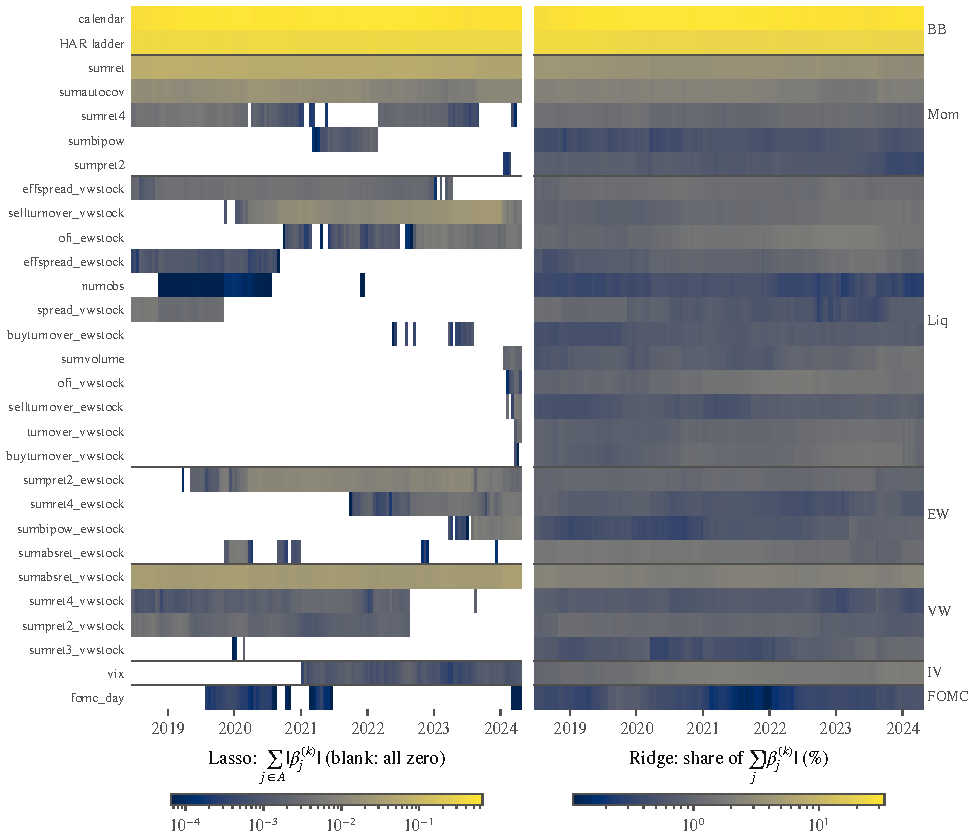
\includegraphics[width=\linewidth]{figures/rehaul_fi_linear_time.pdf}
\caption{The linear coefficients over time, by unit, at the 147 refits (every 10 sessions, 25 June 2018 to 30 April 2024). Left: the pre-tuned lasso's $\sum_{j\in A}|\beta^{(k)}_j|$, log colour scale, blank where every coefficient of the unit is zero (the on/off pattern). Right: the pre-tuned ridge's share of the refit's $\sum_j|\beta^{(k)}_j|$ on the unit, \%. Rows: the 29 units the lasso selects at least once, grouped by bucket (backbone first) and ordered by $N_A$; the other 20 are never selected. Coefficients are per unit of the robust-scaled input (see Table~\ref{tab:rh_fi_linear}).}
\label{fig:rh_fi_linear}
\end{figure}


% Trees: per-refit SHAP ranks aggregated (mean rank, top-5 share, truncated Borda, Kendall's W)
% AUTO-GENERATED by writeup/make_rehaul_fi.py -- do not edit; re-run the script.

\begin{table}[tbp]
\centering
\small
\setlength{\tabcolsep}{3.5pt}
\begin{threeparttable}
\caption{Trees: the per-refit SHAP rankings of the units, aggregated over 147 refits.}
\label{tab:rh_fi_trees}
\begin{tabular}{@{}llrrrrrrrrr@{}}
\toprule
 & & \multicolumn{3}{c}{LightGBM} & \multicolumn{3}{c}{XGBoost} & \multicolumn{3}{c}{Random forest} \\
\cmidrule(lr){3-5}\cmidrule(lr){6-8}\cmidrule(l){9-11}
Unit & Bucket & $\bar r$ & Top 5 & Borda & $\bar r$ & Top 5 & Borda & $\bar r$ & Top 5 & Borda \\
\midrule
HAR ladder & BB & 1.0 & 100 & 1 & 1.0 & 100 & 1 & 1.0 & 100 & 1 \\
\texttt{sumret} & Mom & 2.9 & 97 & 2 & 3.0 & 97 & 2 & 4.0 & 82 & 3 \\
\texttt{sumabsret} & Mom & 4.8 & 71 & 4 & 3.9 & 87 & 3 & 2.6 & 97 & 2 \\
\texttt{sumvolume} & Liq & 4.9 & 71 & 3 & 4.6 & 75 & 4 & 5.1 & 69 & 4 \\
\texttt{sumabsret\_ewstock} & EW & 6.7 & 39 & 5 & 6.7 & 38 & 5 & 5.7 & 46 & 5 \\
\texttt{sumabsret\_vwstock} & VW & 10.0 & 15 & 7 & 8.6 & 13 & 7 & 6.1 & 46 & 6 \\
Calendar & BB & 7.9 & 37 & 6 & 8.1 & 31 & 6 & 15.1 & 7 & 9 \\
\texttt{stocktwits\_sentiment} & Sent & 11.9 & 16 & 8 & 11.6 & 17 & 8 & 11.3 & 19 & 7 \\
\texttt{sumautocov} & Mom & 11.9 & 3 & 10 & 11.6 & 5 & 11 & 16.1 & 2 & 13 \\
\texttt{ofi\_ewstock} & Liq & 14.6 & 14 & 9 & 14.8 & 11 & 9 & 12.9 & 9 & 8 \\
\texttt{sumret3} & Mom & 17.9 & 3 & 13 & 16.5 & 1 & 13 & 15.4 & 2 & 12 \\
\texttt{stocktwits\_sentcount} & Sent & 17.1 & 7 & 11 & 16.2 & 4 & 12 & 17.6 & 3 & 11 \\
\texttt{sellturnover\_vwstock} & Liq & 20.0 & 7 & 12 & 16.4 & 8 & 10 & 18.3 & 7 & 10 \\
\texttt{ofi\_vwstock} & Liq & 25.8 & 1 & 24 & 26.0 & 2 & 19 & 18.4 & 1 & 15 \\
\texttt{stocktwits\_attention} & Sent & 22.7 & 1 & 20 & 24.4 & 1 & 18 & 23.7 & 0 & 19 \\
\addlinespace[3pt]
Kendall's $W$ & & \multicolumn{3}{c}{0.57} & \multicolumn{3}{c}{0.60} & \multicolumn{3}{c}{0.62} \\
Exog.\ series above the probe & & \multicolumn{3}{c}{27} & \multicolumn{3}{c}{35} & \multicolumn{3}{c}{29} \\
\bottomrule
\end{tabular}
\begin{tablenotes}[flushleft]
\footnotesize
\item \textit{Notes:} Per refit $k$, unit $A$'s importance is $I_{k,A} = |T_k|^{-1}\sum_{t\in T_k}|\phi_{t,A}|$, $\phi_{t,A} = \sum_{j\in A}\phi_{t,j}$ (path-dependent TreeSHAP of the refit's model on its held-out rows); $r_{k,A}$ is its rank among the 49 units (1 = largest, ties averaged). $\bar r$: mean of $r_{k,A}$ over the 147 refits; top 5: share of refits with $r_{k,A} \le 5$, \%; Borda: rank of $\sum_k \max(0, 11 - r_{k,A})$ (a full Borda count is affine in $\bar r$). Units: the 15 with the lowest $\bar r$ averaged over the three models. Kendall's $W$ of the per-refit rankings ($W = 1$: identical rankings at every refit). Probe: an exogenous series counts if one of its columns has mean $|\phi_j|$ above the continuous noise column's in at least half of the 49 probe fits (every third refit). SHAP values are the de-dup study's stored values of the cluster refits (LightGBM lgbm\_opt\_00, XGBoost xgb\_opt\_00, random forest trial 255, window-masked).
\end{tablenotes}
\end{threeparttable}
\end{table}


% Trees: rank over time, top six units
% AUTO-GENERATED by writeup/make_rehaul_fi.py -- do not edit; re-run the script.
\begin{figure}[tbp]
\centering
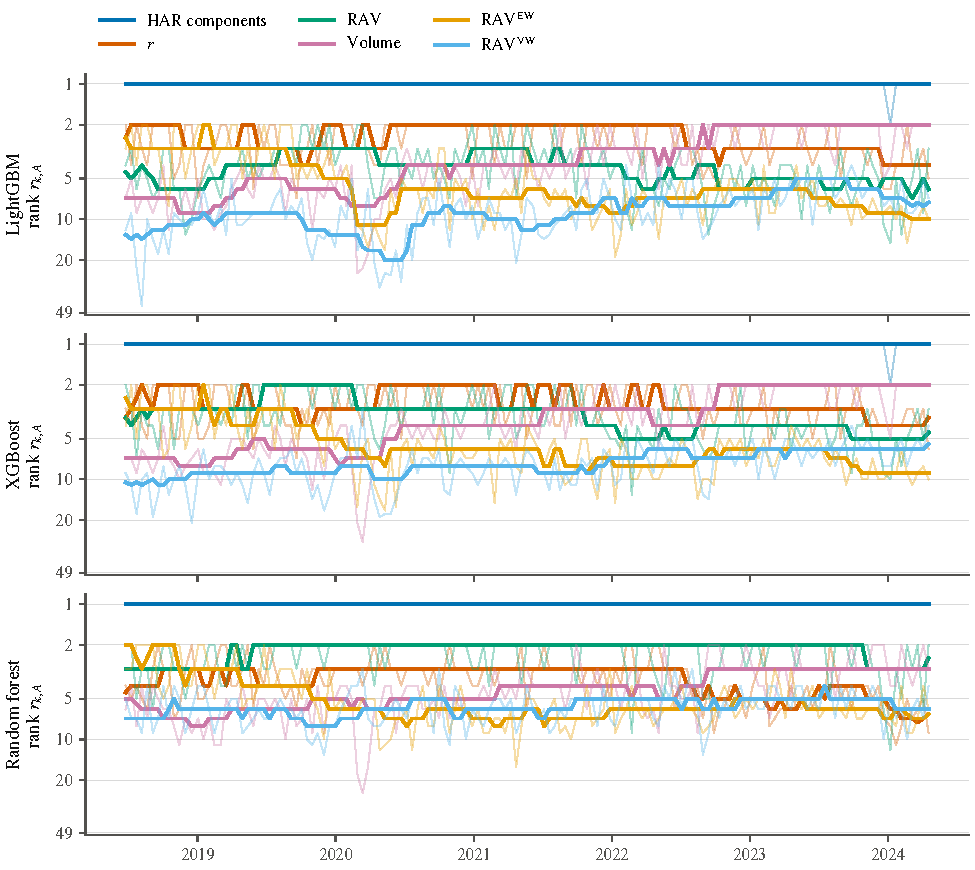
\includegraphics[width=\linewidth]{figures/rehaul_fi_tree_ranks.pdf}
\caption{The trees' per-refit SHAP ranks over time, the six units with the lowest mean rank averaged over the three models. Rank $r_{k,A}$ of unit $A$ among the 49 by mean $|\phi_{t,A}|$ on refit $k$'s held-out rows (1 = largest; log scale), at the start of each refit's tail. Thin: one point per refit; thick: centred rolling median over 11 refits (about 110 sessions). Kendall's $W$ over the 147 refits: LightGBM 0.57, XGBoost 0.60, random forest 0.62.}
\label{fig:rh_fi_ranks}
\end{figure}


% Trees: SHAP interactions (global, per refit) and the H-statistic cross-check
% AUTO-GENERATED by writeup/make_rehaul_fi.py -- do not edit; re-run the script.

\begin{table}[tbp]
\centering
\small
\setlength{\tabcolsep}{4pt}
\begin{threeparttable}
\caption{Trees: the strongest SHAP interactions, global and per refit, with the $H$-statistic cross-check.}
\label{tab:rh_fi_inter}
\begin{tabular}{@{}lrrrrr@{}}
\toprule
Pair & $\bar I$ ($\times 10^{3}$) & $\bar r$ & Top 10 (\%) & $H^2$ (\%) & $H^2_{\min}$ \\
\midrule
\multicolumn{6}{@{}l}{\textit{LightGBM}: series pairs} \\
HAR ladder $\times$ \texttt{sumabsret} & 12.64 & 1.7 & 100 & 0.33 & 0.19 \\
HAR ladder $\times$ \texttt{sumret} & 10.95 & 2.4 & 99 & 0.29 & 0.09 \\
HAR ladder $\times$ \texttt{sumvolume} & 6.62 & 6.3 & 88 & 0.05 & 0.05 \\
HAR ladder $\times$ \texttt{sumabsret\_ewstock} & 5.46 & 6.3 & 88 & 0.05 & 0.12 \\
HAR ladder $\times$ \texttt{stocktwits\_sentiment} & 4.70 & 14.4 & 67 & 0.06 & 0.17 \\
\multicolumn{6}{@{}l}{\textit{LightGBM}: column pairs} \\
\texttt{har\_ma\_1} $\times$ \texttt{har\_ma\_5} & 10.25 & -- & -- & 0.36 & 0.02 \\
\texttt{har\_ma\_1} $\times$ \texttt{har\_ma\_25} & 4.63 & -- & -- & 0.10 & 0.02 \\
\texttt{har\_ma\_5} $\times$ \texttt{adj\_sumabsret\_ma\_1} & 4.53 & -- & -- & 0.67 & 0.42 \\
\quad Probe floor & 0.49 & \multicolumn{2}{c}{$W = 0.45$} & & \\
\addlinespace[3pt]
\multicolumn{6}{@{}l}{\textit{XGBoost}: series pairs} \\
HAR ladder $\times$ \texttt{sumabsret} & 15.23 & 1.6 & 100 & 0.37 & 0.39 \\
HAR ladder $\times$ \texttt{sumret} & 11.03 & 2.5 & 100 & 0.68 & 0.21 \\
HAR ladder $\times$ \texttt{sumvolume} & 7.40 & 6.0 & 90 & 0.08 & 0.08 \\
HAR ladder $\times$ \texttt{sumabsret\_ewstock} & 5.92 & 5.3 & 93 & 0.06 & 0.17 \\
HAR ladder $\times$ \texttt{stocktwits\_sentiment} & 4.87 & 11.8 & 69 & 0.09 & 0.25 \\
\multicolumn{6}{@{}l}{\textit{XGBoost}: column pairs} \\
\texttt{har\_ma\_1} $\times$ \texttt{har\_ma\_5} & 9.95 & -- & -- & 0.39 & 0.02 \\
\texttt{har\_ma\_1} $\times$ \texttt{har\_ma\_25} & 4.99 & -- & -- & 0.14 & 0.02 \\
\texttt{har\_ma\_1} $\times$ \texttt{adj\_sumabsret\_ma\_5} & 4.94 & -- & -- & 0.28 & 0.43 \\
\quad Probe floor & 0.41 & \multicolumn{2}{c}{$W = 0.47$} & & \\
\addlinespace[3pt]
\multicolumn{6}{@{}l}{\textit{Random forest}: series pairs} \\
HAR ladder $\times$ \texttt{sumabsret} & 23.85 & 1.1 & 100 & 0.85 & 1.50 \\
HAR ladder $\times$ \texttt{sumret} & 9.13 & 3.5 & 99 & 0.20 & 0.48 \\
HAR ladder $\times$ \texttt{sumvolume} & 8.52 & 3.6 & 99 & 0.05 & 0.17 \\
HAR ladder $\times$ \texttt{sumabsret\_ewstock} & 6.87 & 4.6 & 99 & 0.06 & 0.33 \\
HAR ladder $\times$ \texttt{sumabsret\_vwstock} & 6.59 & 4.7 & 98 & 0.05 & 0.26 \\
\multicolumn{6}{@{}l}{\textit{Random forest}: column pairs} \\
\texttt{har\_ma\_1} $\times$ \texttt{har\_ma\_5} & 25.31 & -- & -- & 1.16 & 0.06 \\
\texttt{har\_ma\_1} $\times$ \texttt{adj\_sumabsret\_ma\_1} & 8.67 & -- & -- & 0.89 & 1.48 \\
\texttt{har\_ma\_1} $\times$ \texttt{adj\_sumabsret\_ma\_5} & 6.74 & -- & -- & 0.32 & 1.04 \\
\quad Probe floor & 0.50 & \multicolumn{2}{c}{$W = 0.57$} & & \\
\bottomrule
\end{tabular}
\begin{tablenotes}[flushleft]
\footnotesize
\item \textit{Notes:} SHAP interaction values $\phi_{t,jl}$ (path-dependent TreeSHAP, Lundberg et al.\ 2020; $\sum_l \phi_{t,jl} = \phi_{t,j}$) of the local refits on each refit's held-out rows, all 1{,}469 scored sessions. Series pair $(A, B)$: $\Phi_{t,AB} = \sum_{j\in A}\sum_{l\in B}(\phi_{t,jl} + \phi_{t,lj})$; $\bar I_{AB}$ = mean of $|\Phi_{t,AB}|$ over the scored sessions, $\times 10^{3}$, in the fit space of $\hat y$. Column pairs: $|\phi_{t,jl} + \phi_{t,lj}|$. $\bar r$ and top 10: the pair's mean rank and share of refits in the top 10 when the 1176 series pairs are ranked per refit by their mean $|\Phi_{t,AB}|$ on the refit's rows. $H^2$ (Friedman--Popescu): the variance of $\mathrm{PD}_{AB} - \mathrm{PD}_A - \mathrm{PD}_B$ as a share of the variance of $\mathrm{PD}_{AB}$, \%; $H^2_{\min}$: the same numerator over $\min(\mathrm{var}\,\mathrm{PD}_A, \mathrm{var}\,\mathrm{PD}_B)$, a ratio. Both pooled over 15 refits (every 10th), each on the 100 held-out sessions from its anchor as evaluation and background points; computed for each model's top 10 series and top 5 column pairs. Probe floor: median over the 49 probe fits of the largest $\bar I$ between the continuous noise column and a unit. $W$: Kendall's $W$ of the per-refit rankings of each model's top 50 pairs. XGBoost and the forest are refitted locally with other library versions than the stored refits (forecast gaps up to 0.17).
\end{tablenotes}
\end{threeparttable}
\end{table}


% Trees: series-level interaction heatmap
% 2026-10-15 (user): parked -- non-standard figure; focus on legible tables
% % AUTO-GENERATED by writeup/make_rehaul_fi.py -- do not edit; re-run the script.
\begin{figure}[tbp]
\centering
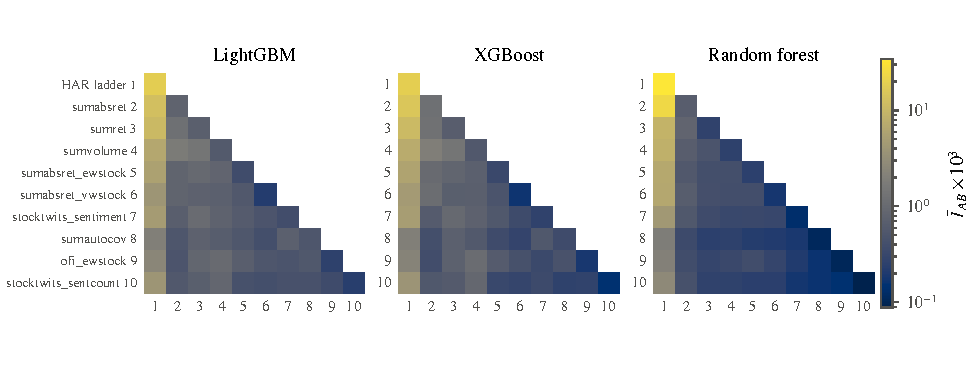
\includegraphics[width=\linewidth]{figures/rehaul_fi_inter_heatmap.pdf}
\caption{The trees' series-level SHAP interactions: $\bar I_{AB}$, the mean over the 1{,}469 scored sessions of $|\phi_{t,AB}|$, $\phi_{t,AB} = \sum_{j\in A}\sum_{l\in B}(\phi_{t,jl} + \phi_{t,lj})$, $\times 10^{3}$, log colour scale shared by the panels; lower triangle, the diagonal is the interaction among a unit's own columns, $\sum_{j \ne l \in A}\phi_{t,jl}$. Units: the 10 with the largest share of their model's off-diagonal interaction mass, summed over the three models; numbered as in the left panel. Local refits on the held-out rows of each of the 147 refits.}
\label{fig:rh_fi_inter}
\end{figure}


% 07_economics.tex -- the rehauled paper's section, as bullets to expand into prose (2026-10-15).
% Sources and pointers behind every number: writeup/PAPER_REHAUL_OUTLINE_2026-10-15.md, section 7.
% House rules: every number in the final prose comes from a generated macro (writeup/generated/*.tex), never
% typed; park (comment out with a dated note) rather than delete.
% Macros to use here: close_main_numbers.tex (\cmShort*, \cmMasterVsShort*, \cmMasterTopTwentyShareMed), appendix_running_numbers.tex (sizing), murphy / compounding macros

% 2026-10-15 formula pass: each formula checked against the code; disagreements are noted in comments.
% 2026-10-15 (notation pass, writeup/NOTATION_GUIDE_2026-10-15.md, incl. section 6b): old -> new:
% IV^{30}_t -> \mathrm{IV}_t (IV_t^2 the implied variance); s_t (signal) -> written out as \hat\sigma^2_t - IV_t^2
% (s is the periodicity factor); S_T -> S^close_t (T is a sample size); r^x_t -> r^ba_t (crossed -> at quoted bid/ask
% prices); RV_t -> \RV_t, the actual RV; Sharpe -> \SR; lag l -> q; n, N -> T_oos, sums over \mathcal T_oos;
% kappa -> \varrho (kappa is the asinh scale and the MinGRU link); growth g -> G (g is the variance-stabilizing map);
% ES threshold c = 1 -> \theta = 1 (c is the closing interval); always short -> unconditional short-straddle
% benchmark (q_t \equiv -1); 1{.} -> \mathbf{1}{.}.
% Typed numbers that have an exact generated macro now use it (\rhe... from rehaul_econ_numbers.tex, \cm... from
% close_main_numbers.tex, \fqs...). Still typed, no loadable macro: lasso 1.88, elastic net +0.55 / lasso +0.50,
% 3 of 5 years, 252 / 614 days, f = 0.03, the compounding numbers (\cmpWMedMid etc. live in
% appendix_close_compounding.tex, which also holds tables) and the ES rank correlation (\hmurRhoESX, in
% appendix_close_murphy_splits.tex, likewise).
% 2026-10-15 (consolidation): NW lag q -> q_NW (q_t is the position); dummy day index u -> t' (u is an exogenous
% series); shift-test offset k -> j (k is the HAR horizon); daily elementary score ES_t -> ES_{\theta,t} at theta = 1
% and its mean \overline{ES}_1 (the appendix's Murphy diagram plots \overline{ES}_\theta); typed 1.88, +0.55, +0.50,
% 252, 614, 3 of 5 years, f = 0.03 -> \rheLassoSh, \rheAfEnetDSh, \rheAfLassoDSh, \rheSzWarmup, \rheSzDays,
% \rheShortLossYears / \rheNYears, \rhappCompF. Still typed: rho_S(ES, SR) = -0.55, the compounding numbers and the
% shift test's +-1 (their macros live in files that also hold tables; see the consolidation reply).
% 2026-10-15 (consolidation): parked -- the number files are loaded once in the preamble of paper_rehaul.tex.
% \ifdefined\rheShortSh\else% AUTO-GENERATED by writeup/make_rehaul_economics.py -- do not edit; re-run the script.
% \rhe... macros for writeup/rehaul/07_economics.tex; values as in the rehaul_econ_* floats.
\providecommand{\rheShortSh}{}\renewcommand{\rheShortSh}{0.20}  % always short, Sharpe mid, 866 days
\providecommand{\rheShortShX}{}\renewcommand{\rheShortShX}{\ensuremath{-}0.27}  % always short, Sharpe crossed
\providecommand{\rheShortT}{}\renewcommand{\rheShortT}{0.43}  % always short, Newey-West t of the mean mid return
\providecommand{\rheShortHit}{}\renewcommand{\rheShortHit}{61.8}  % always short, hit rate %
\providecommand{\rheEnetSh}{}\renewcommand{\rheEnetSh}{1.92}  % per-bar enet all features, Sharpe mid
\providecommand{\rheEnetShX}{}\renewcommand{\rheEnetShX}{1.43}  % ... crossed
\providecommand{\rheEnetT}{}\renewcommand{\rheEnetT}{2.56}  % ... HAC t vs always short
\providecommand{\rheNNSh}{}\renewcommand{\rheNNSh}{1.53}  % MinGRU all features, Sharpe mid
\providecommand{\rheNNShX}{}\renewcommand{\rheNNShX}{1.05}  % ... crossed
\providecommand{\rheNNBaseSh}{}\renewcommand{\rheNNBaseSh}{1.04}  % MinGRU HAR + calendar, Sharpe mid
\providecommand{\rheNNBaseShX}{}\renewcommand{\rheNNBaseShX}{0.57}  % ... crossed
\providecommand{\rheSigVsShort}{}\renewcommand{\rheSigVsShort}{20}  % model-set forecasts with HAC t > 1.96 vs always short
\providecommand{\rhePairs}{}\renewcommand{\rhePairs}{51}  % HAR + cal. -> all features pairs in the model set
\providecommand{\rhePairsUp}{}\renewcommand{\rhePairsUp}{50}  % ... Sharpe mid higher with all features
\providecommand{\rhePairsSig}{}\renewcommand{\rhePairsSig}{4}  % ... HAC t > 1.96
\providecommand{\rhePairsMed}{}\renewcommand{\rhePairsMed}{\ensuremath{+}0.54}  % ... median dSharpe mid
\providecommand{\rheSzSignMed}{}\renewcommand{\rheSzSignMed}{0.92}  % sizing sign: model-set median Sharpe mid, 614 days
\providecommand{\rheSzClipMed}{}\renewcommand{\rheSzClipMed}{1.34}  % sizing clip: model-set median Sharpe mid, 614 days
\providecommand{\rheSzLfssMed}{}\renewcommand{\rheSzLfssMed}{1.12}  % sizing lfss: model-set median Sharpe mid, 614 days
\providecommand{\rheSzRankMed}{}\renewcommand{\rheSzRankMed}{1.34}  % sizing rank: model-set median Sharpe mid, 614 days
\providecommand{\rheSzShort}{}\renewcommand{\rheSzShort}{0.34}  % always short, Sharpe mid on the 614 sizing days
\providecommand{\rheSzClipBeats}{}\renewcommand{\rheSzClipBeats}{98}  % clip above sign(s), of 112 (mid)
\providecommand{\rheSzClipGain}{}\renewcommand{\rheSzClipGain}{\ensuremath{+}0.45}  % median clip - sign(s) Sharpe mid
\providecommand{\rheTailNeg}{}\renewcommand{\rheTailNeg}{102}  % model-set forecasts whose gain over short is < 0 without 10 best days
\fi
% \ifdefined\fqsPairs\else% AUTO-GENERATED by writeup/make_fig_qlike_sharpe.py -- do not edit.
% Figure writeup/figures/fig_qlike_sharpe.pdf: QLIKE against Sharpe (mid), HAR + calendar vs all
% features, every model of results/close_master_table/paper_model_set.csv on both input sets
% (per-bar linear = the pre-tuned subpt_* rows; LSTMs excluded); numbers from master_table.csv
% and master_table_daily.parquet.  Changes are all features minus HAR + calendar, on the same days.
% DM: dm_test on the daily QLIKE difference; t: hac_inference.llsw_test on the daily mid-return
% difference (614 post-warmup days, bandwidth 33, fixed-b p); Sharpe changes: Ledoit-Wolf p;
% ES(c = 1): close_murphy_splits_headline.elementary on f / iv, y / iv.  Point estimates.
% pooled pairs: family pooled twin
\newcommand{\fqsPairs}{42}  % models on both input sets (pairs drawn)
\newcommand{\fqsPairsPerBarLinear}{3}  % of which per-bar linear (pre-tuned)
\newcommand{\fqsPairsPooled}{3}  % of which pooled 48-bar linear
\newcommand{\fqsPairsTree}{36}  % of which per-bar trees
\newcommand{\fqsPoints}{85}  % points drawn: both ends of every pair + the HAR + cal. OLS
\newcommand{\fqsDays}{866}  % trade days
\newcommand{\fqsQLower}{31}  % QLIKE lower with all features
\newcommand{\fqsQLowerSig}{3}  % ... and DM significant at 5 %
\newcommand{\fqsQHigher}{11}  % QLIKE higher with all features
\newcommand{\fqsQHigherSig}{0}  % ... and DM significant at 5 %
\newcommand{\fqsQLowerSigLagFourteen}{2}  % sensitivity: QLIKE lower, DM at lag 14 significant
\newcommand{\fqsQHigherSigLagFourteen}{0}  % sensitivity: QLIKE higher, DM at lag 14 significant
\newcommand{\fqsShHigher}{41}  % Sharpe (mid) higher with all features
\newcommand{\fqsShHigherSig}{6}  % ... and Ledoit-Wolf p < 0.05 (614 post-warmup days)
\newcommand{\fqsShLower}{1}  % Sharpe (mid) lower with all features
\newcommand{\fqsShLowerSig}{0}  % ... and Ledoit-Wolf p < 0.05 (614 post-warmup days)
\newcommand{\fqsQLowerShHigher}{30}  % both: QLIKE lower and Sharpe higher
\newcommand{\fqsMedDQ}{\ensuremath{-}0.0016}  % median QLIKE change (all features minus HAR + cal.)
\newcommand{\fqsMedDQPct}{\ensuremath{-}1.6}  % median QLIKE change, % of the HAR + cal. QLIKE
\newcommand{\fqsMedDSh}{\ensuremath{+}0.53}  % median Sharpe (mid) change
\newcommand{\fqsESLower}{29}  % elementary score at the threshold (c = 1) lower with all features
\newcommand{\fqsCorrES}{0.07}  % Pearson corr. across pairs: ES(c = 1) change vs HAC t of the P&L change
\newcommand{\fqsCorrQ}{0.12}  % Pearson corr. across pairs: QLIKE change vs HAC t of the P&L change
\newcommand{\fqsInShade}{4}  % all-features points in the shaded quadrant
\newcommand{\fqsInShadeBase}{3}  % HAR + cal. points in the shaded quadrant
\newcommand{\fqsOlsQ}{0.0967}  % QLIKE of the HAR + cal. OLS
\newcommand{\fqsOlsSh}{1.06}  % Sharpe (mid) of the HAR + cal. OLS
\newcommand{\fqsDMLag}{6}  % Newey-West lag of the DM statistic (the master table's)
\newcommand{\fqsHACS}{33}  % bandwidth S of the t of the mean P&L change (LLSW 2018, 614 post-warmup days)
\newcommand{\fqsSigPct}{5}  % two-sided level of the counts, %
\newcommand{\fqsQuadBetterBoth}{30}  % change figure: lower QLIKE, higher Sharpe
\newcommand{\fqsQuadShOnly}{11}  % change figure: higher QLIKE, higher Sharpe
\newcommand{\fqsQuadQOnly}{1}  % change figure: lower QLIKE, lower Sharpe
\newcommand{\fqsQuadWorseBoth}{0}  % change figure: higher QLIKE, lower Sharpe
\fi
% \ifdefined\cmNdays\else% AUTO-GENERATED by writeup/make_table_close_main.py -- do not edit.
% Numbers quoted in the prose of writeup/sections/results_close_option.tex; each is read
% from results/close_master_table/master_table.csv and the sources in the script.
% 2026-10-06: recalibration removed / intervals removed, user decision -- the plain forecast
% f^2 B, point estimates; ...T = HAC t of the daily mid-return difference, ...DM = Diebold-
% Mariano statistic; a ...Above / ...Below count counts point estimates, its ...Sig twin those
% significant at 5 % (DM for QLIKE, HAC t for Sharpe).
\newcommand{\cmNdays}{866}
\newcommand{\cmNrows}{22}
\newcommand{\cmShortMean}{0.014}
\newcommand{\cmShortShMid}{0.20}
\newcommand{\cmShortShX}{\ensuremath{-}0.27}
\newcommand{\cmShortT}{\ensuremath{-}1.71}
\newcommand{\cmPaperShMin}{0.43}
\newcommand{\cmPaperShMax}{1.50}
\newcommand{\cmPaperXMin}{\ensuremath{-}0.05}
\newcommand{\cmPaperXMax}{1.01}
\newcommand{\cmPaperVsShortMin}{+0.22}
\newcommand{\cmPaperVsShortMax}{+1.30}
\newcommand{\cmPaperVsShortAboveN}{8}
\newcommand{\cmPaperVsShortAboveSigN}{three}
\newcommand{\cmPaperVsShortAboveSigWho}{LightGBM, XGBoost, lasso (causally tuned)}
\newcommand{\cmPaperSameMin}{82}
\newcommand{\cmSellPaperMin}{72}
\newcommand{\cmSellPaperMax}{83}
\newcommand{\cmPaperSameMax}{96}
\newcommand{\cmRefQ}{0.1092}
\newcommand{\cmRefShMid}{1.28}
\newcommand{\cmRefShX}{0.80}
\newcommand{\cmRefBuy}{27}
\newcommand{\cmRefVsShort}{+1.08}
\newcommand{\cmRefVsShortT}{+1.71}
\newcommand{\cmFomcSh}{1.36}
\newcommand{\cmFomcD}{+0.08}
\newcommand{\cmFomcDT}{+0.44}
\newcommand{\cmLassoFShMid}{1.06}
\newcommand{\cmLassoFVsRef}{\ensuremath{-}0.22}
\newcommand{\cmLassoFVsRefT}{\ensuremath{-}0.75}
\newcommand{\cmLassoFSame}{96}
\newcommand{\cmPaperFarLabel}{baseline (HAR + calendar OLS)}
\newcommand{\cmPaperFarVsRef}{\ensuremath{-}0.85}
\newcommand{\cmPaperFarVsRefT}{\ensuremath{-}1.49}
\newcommand{\cmPaperBestLabel}{lasso (causally tuned)}
\newcommand{\cmPaperBestSh}{1.50}
\newcommand{\cmNlFamN}{five}
\newcommand{\cmNlMasterN}{90}
\newcommand{\cmPoolShMin}{0.91}
\newcommand{\cmPoolShMax}{1.44}
\newcommand{\cmSubShMin}{1.37}
\newcommand{\cmSubShMax}{1.92}
\newcommand{\cmNlShMin}{1.23}
\newcommand{\cmNlShMax}{1.81}
\newcommand{\cmTabVsRefN}{21}
\newcommand{\cmTabVsRefAbove}{15}
\newcommand{\cmTabVsRefBelow}{6}
\newcommand{\cmTabVsRefAboveSig}{0}
\newcommand{\cmTabVsRefBelowSig}{0}
\newcommand{\cmMasterN}{112}
\newcommand{\cmMasterNPaper}{9}
\newcommand{\cmMasterNBase}{52}
\newcommand{\cmMasterMedQBase}{0.1033}
\newcommand{\cmMasterMedShBase}{0.73}
\newcommand{\cmMasterMedShXBase}{0.25}
\newcommand{\cmMasterNAll}{51}
\newcommand{\cmMasterMedQAll}{0.1014}
\newcommand{\cmMasterMedShAll}{1.27}
\newcommand{\cmMasterMedShXAll}{0.79}
\newcommand{\cmMasterSetsN}{two}
\newcommand{\cmMasterVsRefN}{111}
\newcommand{\cmMasterVsRefAbove}{32}
\newcommand{\cmMasterVsRefBelow}{79}
\newcommand{\cmMasterVsRefAboveSig}{0}
\newcommand{\cmMasterVsRefBelowSig}{0}
\newcommand{\cmMasterVsShortAbove}{112}
\newcommand{\cmMasterVsShortBelow}{0}
\newcommand{\cmMasterVsShortAboveSig}{20}
\newcommand{\cmMasterVsShortBelowSig}{0}
\newcommand{\cmMasterVsShortN}{112}
\newcommand{\cmMasterQVsRefBelow}{99}
\newcommand{\cmMasterQVsRefAbove}{12}
\newcommand{\cmMasterQVsRefBelowSig}{23}
\newcommand{\cmMasterQVsRefAboveSig}{1}
\newcommand{\cmMasterMedQ}{0.1028}
\newcommand{\cmMasterMedSh}{1.08}
\newcommand{\cmMasterMedShX}{0.59}
\newcommand{\cmMasterShMin}{0.29}
\newcommand{\cmMasterShMax}{1.92}
\newcommand{\cmMasterXMin}{\ensuremath{-}0.19}
\newcommand{\cmMasterXMax}{1.43}
\newcommand{\cmMasterVsShortMed}{+0.87}
\newcommand{\cmMasterRankCorr}{\ensuremath{-}0.20}
\newcommand{\cmMasterRankCorrX}{\ensuremath{-}0.20}
\newcommand{\cmSellMasterMin}{66}
\newcommand{\cmSellMasterMax}{83}
\newcommand{\cmSellMasterMed}{70}
\newcommand{\cmTopShLabel}{per-bar elastic net}
\newcommand{\cmTopShInputs}{\texttt{all\_features}}
\newcommand{\cmTopShMid}{1.92}
\newcommand{\cmXLossMin}{0.48}
\newcommand{\cmXLossMax}{0.50}
\newcommand{\cmLdSpec}{+0.16}
\newcommand{\cmLdSpecQ}{\ensuremath{-}4.3}
\newcommand{\cmLdSpecT}{+0.34}
\newcommand{\cmLdSpecDM}{\ensuremath{-}1.73}
\newcommand{\cmLdPerBarBase}{+0.46}
\newcommand{\cmLdPerBarBaseQ}{\ensuremath{-}12.0}
\newcommand{\cmLdPerBarBaseT}{+1.05}
\newcommand{\cmLdPerBarBaseDM}{\ensuremath{-}3.37}
\newcommand{\cmLdPerBarAll}{\ensuremath{-}0.03}
\newcommand{\cmLdPerBarAllQ}{\ensuremath{-}6.7}
\newcommand{\cmLdPerBarAllT}{\ensuremath{-}0.07}
\newcommand{\cmLdPerBarAllDM}{\ensuremath{-}1.61}
\newcommand{\cmLdIn}{+0.05}
\newcommand{\cmLdInQ}{+0.8}
\newcommand{\cmLdInT}{+0.09}
\newcommand{\cmLdInDM}{+0.18}
\newcommand{\cmLdEstMin}{\ensuremath{-}0.15}
\newcommand{\cmLdEstMax}{+0.50}
\newcommand{\cmLdEstMinLabel}{\texttt{subtree\_rf\_all\_features}}
\newcommand{\cmLdEstMaxLabel}{\texttt{subpt\_enet\_all\_features}}
\newcommand{\cmLdEstMinWho}{random forest}
\newcommand{\cmLdEstMaxWho}{elastic net}
\newcommand{\cmLdN}{21}
\newcommand{\cmLdNPath}{12}
\newcommand{\cmLdNCampaign}{9}
\newcommand{\cmLdResolved}{none}
\newcommand{\cmLdQResolved}{three}
\newcommand{\cmLdCDedup}{+0.00}
\newcommand{\cmLdCDedupQ}{+0.0}
\newcommand{\cmLdCMaskTten}{\ensuremath{-}0.21}
\newcommand{\cmLdCMaskTtenQ}{\ensuremath{-}1.0}
\newcommand{\cmLdCMaskTtenT}{\ensuremath{-}0.69}
\newcommand{\cmLdCMaskTtenDM}{\ensuremath{-}1.04}
\newcommand{\cmLdCMaskTone}{\ensuremath{-}0.23}
\newcommand{\cmLdCMaskToneQ}{+1.4}
\newcommand{\cmLdCMaskToneT}{\ensuremath{-}0.55}
\newcommand{\cmLdCMaskToneDM}{+1.36}
\newcommand{\cmLdCMaskRsten}{\ensuremath{-}0.08}
\newcommand{\cmLdCMaskRstenQ}{+2.8}
\newcommand{\cmLdCMaskRstenT}{\ensuremath{-}0.32}
\newcommand{\cmLdCMaskRstenDM}{+1.42}
\newcommand{\cmLdCMaskRsone}{\ensuremath{-}0.05}
\newcommand{\cmLdCMaskRsoneQ}{+0.2}
\newcommand{\cmLdCMaskRsoneT}{\ensuremath{-}0.17}
\newcommand{\cmLdCMaskRsoneDM}{+0.12}
\newcommand{\cmLdCCadLgbm}{\ensuremath{-}0.04}
\newcommand{\cmLdCCadLgbmQ}{\ensuremath{-}2.2}
\newcommand{\cmLdCCadLgbmT}{\ensuremath{-}0.08}
\newcommand{\cmLdCCadLgbmDM}{\ensuremath{-}1.12}
\newcommand{\cmLdCTuneRs}{+0.28}
\newcommand{\cmLdCTuneRsQ}{+3.0}
\newcommand{\cmLdCTuneRsT}{+0.58}
\newcommand{\cmLdCTuneRsDM}{+1.12}
\newcommand{\cmLdCTuneOp}{\ensuremath{-}0.10}
\newcommand{\cmLdCTuneOpQ}{+7.3}
\newcommand{\cmLdCTuneOpT}{\ensuremath{-}0.31}
\newcommand{\cmLdCTuneOpDM}{+2.83}
\newcommand{\cmLdCTuneOpPer}{\ensuremath{-}0.32}
\newcommand{\cmLdCTuneOpPerQ}{+2.5}
\newcommand{\cmLdCTuneOpPerT}{\ensuremath{-}0.65}
\newcommand{\cmLdCTuneOpPerDM}{+0.75}
\newcommand{\cmPNewBase}{22}
\newcommand{\cmPOldBase}{34}
\newcommand{\cmPNewAll}{628}
\newcommand{\cmPOldAll}{640}
\newcommand{\cmNDup}{12}
\newcommand{\cmDedupN}{37}
\newcommand{\cmDedupQMax}{0.05}
\newcommand{\cmDedupPosMax}{one}
\newcommand{\cmKeptBase}{17}
\newcommand{\cmKeptBaseMin}{17}
\newcommand{\cmKeptBaseMax}{17}
\newcommand{\cmKeptAll}{369}
\newcommand{\cmKeptAllMin}{360}
\newcommand{\cmKeptAllMax}{378}
\newcommand{\cmMaskN}{16}
\newcommand{\cmMaskQMed}{0.4}
\newcommand{\cmMaskQAbove}{10}
\newcommand{\cmMaskShBelow}{14}
\newcommand{\cmMaskQAboveSig}{none}
\newcommand{\cmMaskShBelowSig}{one}
\newcommand{\cmTrVsRidgeN}{48}
\newcommand{\cmTrSetsN}{two}
\newcommand{\cmMaskSetsN}{two}
\newcommand{\cmTrVsRidgeQAbove}{46}
\newcommand{\cmTrVsRidgeShBelow}{41}
\newcommand{\cmTrVsRidgeQAboveSig}{21}
\newcommand{\cmTrVsRidgeShBelowSig}{one}
\newcommand{\cmCadN}{six}
\newcommand{\cmCadQBelow}{five}
\newcommand{\cmCadQBelowSig}{none}
\newcommand{\cmCadShUp}{\ensuremath{-}0.43}
\newcommand{\cmCadShUpT}{\ensuremath{-}1.03}
\newcommand{\cmRsQAbove}{6}
\newcommand{\cmRsQAboveSig}{two}
\newcommand{\cmRsN}{6}
\newcommand{\cmOpN}{24}
\newcommand{\cmOpQAbove}{24}
\newcommand{\cmOpQAboveSig}{13}
\newcommand{\cmTpN}{18}
\newcommand{\cmTpQBelow}{12}
\newcommand{\cmTpQBelowSig}{one}
\newcommand{\cmBudN}{24}
\newcommand{\cmBudQAbove}{17}
\newcommand{\cmBudQAboveSig}{two}
\newcommand{\cmBudQBelow}{7}
\newcommand{\cmBudLastMin}{27}
\newcommand{\cmBudLastMax}{37}
\newcommand{\cmBudLastExch}{20}
\newcommand{\cmNlBestSh}{1.81}
\newcommand{\cmNlBestLabel}{tuned per-bar LightGBM}
\newcommand{\cmNlBestInputs}{\texttt{all\_features}}
\newcommand{\cmNlBestVsRef}{+0.53}
\newcommand{\cmNlBestVsRefT}{+1.04}
\newcommand{\cmNlVsRefAbove}{19}
\newcommand{\cmNlVsRefBelow}{71}
\newcommand{\cmNlVsRefAboveSig}{0}
\newcommand{\cmNlVsRefBelowSig}{0}
\newcommand{\cmClassChunks}{505}
\newcommand{\cmClassPts}{20}
\newcommand{\cmClassLgbmPick}{18}
\newcommand{\cmClassMaxRelMin}{4.5}
\newcommand{\cmClassMaxRelMax}{5.5}
\newcommand{\cmSvN}{31}
\newcommand{\cmSvSetN}{112}
\newcommand{\cmSvSetPairsN}{3472}
\newcommand{\cmSvSetAboveMid}{755}
\newcommand{\cmSvSetAboveMidSig}{29}
\newcommand{\cmSvSetStraddleFirstMid}{4}
\newcommand{\cmSvSetWingN}{672}
\newcommand{\cmSvSetWingMidBelow}{668}
\newcommand{\cmSvSetAboveX}{410}
\newcommand{\cmSvSetAboveXSig}{0}
\newcommand{\cmSvSetStraddleFirstX}{3}
\newcommand{\cmSvSetWingXBelow}{672}
\newcommand{\cmSvSetBestMidLabel}{call vertical, w50}
\newcommand{\cmSvSetBestMidMed}{+0.37}
\newcommand{\cmSvSetBestMidAboveN}{94}
\newcommand{\cmSvSetBestMidAboveSig}{0}
\newcommand{\cmSvCostStraddle}{2.9}
\newcommand{\cmSvCostIbfMin}{4.0}
\newcommand{\cmSvCostIbfMax}{6.1}
\newcommand{\cmMasterPosTotalN}{112}
\newcommand{\cmMasterTopTwentyShareMed}{99}
\newcommand{\cmMasterTopTwentyShareMin}{59}
\newcommand{\cmMasterTopTwentyShareMax}{338}
\newcommand{\cmMasterTopTwentyBuysN}{112}
\newcommand{\cmMasterBottomTwentySellsN}{112}
\newcommand{\cmMasterDiffMed}{+53.5}
\newcommand{\cmMasterDiffPosN}{112}
\newcommand{\cmMasterDiffExTenMed}{\ensuremath{-}30.0}
\newcommand{\cmMasterDiffExTenHalfN}{112}
\newcommand{\cmMasterDiffExTenNegN}{102}
\newcommand{\cmBContamMaxDSh}{0.38}
\newcommand{\cmBContamMaxDShX}{0.38}
\newcommand{\cmBContamMedDSh}{0.08}
\newcommand{\cmBContamPaperMaxDSh}{0.21}
\newcommand{\cmBContamPaperMaxDShX}{0.22}
\newcommand{\cmBContamPaperMedDSh}{0.08}
\newcommand{\cmBContamDays}{94}
\newcommand{\cmCensIvMaxDSh}{0.06}
\newcommand{\cmCensIvMaxDShX}{0.08}
\newcommand{\cmCensIvMedDSh}{0.04}
\newcommand{\cmCensIvPaperMaxDSh}{0.05}
\newcommand{\cmCensIvPaperMaxDShX}{0.07}
\newcommand{\cmCensIvPaperMedDSh}{0.04}
\newcommand{\cmCensIvDays}{5}
\newcommand{\cmBContamMaxFlips}{16}
\newcommand{\cmBContamMedFlips}{8}
\newcommand{\cmBContamPaperMaxFlips}{10}
\newcommand{\cmBContamMaxRel}{21}
\newcommand{\cmPtPreSessions}{3947}
\newcommand{\cmPtPreStart}{13~April~2004}
\newcommand{\cmPtValFirst}{6~January~2016}
\newcommand{\cmPtValLast}{2~January~2020}
\newcommand{\cmPtFolds}{four}
\newcommand{\cmPtFoldLen}{250}
\newcommand{\cmPtFitWin}{2{,}000}
\newcommand{\cmPtEmbargo}{25}
\newcommand{\cmPtRatio}{1/100}
\newcommand{\cmPtBlock}{250}
\newcommand{\cmPtRetuneN}{four}
\newcommand{\cmPtRetuneFirst}{23~June~2020}
\newcommand{\cmPtRetuneLast}{16~June~2023}
\newcommand{\cmPtFiredRidgeBase}{one}
\newcommand{\cmPtPenRidgeBase}{\ensuremath{10^{-2}}}
\newcommand{\cmPtFiredRidgeAll}{none}
\newcommand{\cmPtPenRidgeAll}{\ensuremath{10^{3}}}
\newcommand{\cmPtFiredLassoBase}{one}
\newcommand{\cmPtPenLassoBase}{\ensuremath{10^{-6}}}
\newcommand{\cmPtFiredLassoAll}{none}
\newcommand{\cmPtPenLassoAll}{\ensuremath{10^{-2}}}
\newcommand{\cmPtFiredEnetBase}{two}
\newcommand{\cmPtPenEnetBase}{\ensuremath{10^{-6}}}
\newcommand{\cmPtFiredEnetAll}{none}
\newcommand{\cmPtPenEnetAll}{\ensuremath{10^{-2}}}
\newcommand{\cmPtFiredTotal}{4}
\newcommand{\cmPtFiredOf}{24}
\newcommand{\cmPtCausalSwitches}{75}
\newcommand{\cmPtCausalChoices}{165}
\newcommand{\cmPtCausalMarginPass}{3}
\newcommand{\cmPtCausalEdgePicks}{132}
\newcommand{\cmPtCausalPicks}{198}
\newcommand{\cmPtSwitchFlipPct}{8}
\newcommand{\cmPtCausalSwitchesPaper}{24}
\newcommand{\cmPtCausalChoicesPaper}{45}
\newcommand{\cmPtCausalMarginPassPaper}{3}
\newcommand{\cmPtCausalEdgePicksPaper}{34}
\newcommand{\cmPtCausalPicksPaper}{54}
\newcommand{\cmPtSwitchFlipPctPaper}{9}
\newcommand{\cmPoolPtN}{6}
\newcommand{\cmPoolPtQPctMean}{+0.9}
\newcommand{\cmPoolPtQWorse}{5}
\newcommand{\cmPoolPtDMMax}{1.22}
\newcommand{\cmPoolPtTMax}{1.29}
\newcommand{\cmPoolPtSigN}{0}
\newcommand{\cmPoolPtShAllMin}{+0.17}
\newcommand{\cmPoolPtShAllMax}{+0.35}
\newcommand{\cmPoolPtShOtherMin}{\ensuremath{-}0.06}
\newcommand{\cmPoolPtShOtherMax}{\ensuremath{-}0.19}
\newcommand{\cmPoolPtBlocks}{218}
\newcommand{\cmPoolPtCausalSwMin}{137}
\newcommand{\cmPoolPtCausalSwMax}{170}
\newcommand{\cmPoolPtCausalMarginMin}{3}
\newcommand{\cmPoolPtCausalMarginMax}{22}
\newcommand{\cmPoolPtRetunes}{217}
\newcommand{\cmPoolPtRetuneSwMin}{11}
\newcommand{\cmPoolPtRetuneSwMax}{40}
\newcommand{\cmTreeProvRfName}{\texttt{rf\_opt\_00}}
\newcommand{\cmTreeProvRfTrials}{400}
\newcommand{\cmTreeProvRfBudget}{400}
\newcommand{\cmTreeProvRfDevMse}{0.108456}
\newcommand{\cmTreeProvLgbmDevMse}{0.107449}
\newcommand{\cmTreeProvXgbDevMse}{0.108076}
\newcommand{\cmTreeProvXgbTopDevMse}{0.107894}
\newcommand{\cmTreeProvRfTrees}{485}
\newcommand{\cmTreeProvRfDepth}{20}
\newcommand{\cmTreeProvRfFeatures}{0.90}
\newcommand{\cmTreeProvRfSamples}{0.41}
\newcommand{\cmTreeProvRfLeafDev}{12}
\newcommand{\cmTreeProvRfLeaf}{1}
\newcommand{\cmTreeProvLgbmLeafDev}{98}
\newcommand{\cmTreeProvLgbmLeaf}{8}
\newcommand{\cmTreeProvXgbTopName}{\texttt{xgb\_opt\_00}}
\newcommand{\cmTreeProvXgbName}{\texttt{xgb\_opt\_06}}
\newcommand{\cmTreeProvXgbDevRank}{7}
\newcommand{\cmTreeProvXgbArms}{8}
\newcommand{\cmTreeProvXgbPostRank}{8}
\newcommand{\cmTreeProvXgbRecentRank}{8}
\newcommand{\cmTreeProvXgbQRank}{8}
\newcommand{\cmTreeProvXgbPickDate}{14~August~2026}
\newcommand{\cmMasterNLean}{51}
\newcommand{\cmMasterMedQLean}{0.0991}
\newcommand{\cmMasterMedShLean}{1.37}
\newcommand{\cmMasterMedShXLean}{0.88}
\newcommand{\cmLdPerBarLean}{+0.65}
\newcommand{\cmLdPerBarLeanQ}{\ensuremath{-}12.3}
\newcommand{\cmLdPerBarLeanT}{+1.49}
\newcommand{\cmLdPerBarLeanDM}{\ensuremath{-}3.39}
\newcommand{\cmLdInBaseLean}{+0.51}
\newcommand{\cmLdInBaseLeanQ}{\ensuremath{-}3.3}
\newcommand{\cmLdInBaseLeanT}{+1.66}
\newcommand{\cmLdInBaseLeanDM}{\ensuremath{-}1.17}
\newcommand{\cmLdInLeanAll}{\ensuremath{-}0.46}
\newcommand{\cmLdInLeanAllQ}{+4.3}
\newcommand{\cmLdInLeanAllT}{\ensuremath{-}1.15}
\newcommand{\cmLdInLeanAllDM}{+1.50}
%
% 2026-10-06 parked (recalibration removed / intervals removed, user decision):
%   \cmShortShCiMid: interval of always short's Sharpe
%   \cmShortShCiX: interval of always short's Sharpe
%   \cmPaperVsShortAboveWho: the paper's forecasts whose interval vs always short lay above zero
%   \cmPaperVsShortAboveCi: that forecast's interval
%   \cmSellHead: the former headline's sell share (no headline model)
%   \cmHQ: the former headline (no headline model)
%   \cmHQPct: the former headline (no headline model)
%   \cmHQCi: the former headline (no headline model)
%   \cmHDM: the former headline (no headline model)
%   \cmHDMp: the former headline (no headline model)
%   \cmHShMid: the former headline (no headline model)
%   \cmHShX: the former headline (no headline model)
%   \cmHMean: the former headline (no headline model)
%   \cmHHit: the former headline (no headline model)
%   \cmHBuy: the former headline (no headline model)
%   \cmHVsRefMid: the former headline (no headline model)
%   \cmHVsRefX: the former headline (no headline model)
%   \cmHVsShortMid: the former headline (no headline model)
%   \cmHVsShortX: the former headline (no headline model)
%   \cmHVsRefT: the former headline (no headline model)
%   \cmHVsRefP: the former headline (no headline model)
%   \cmHVsShortT: the former headline (no headline model)
%   \cmHVsShortP: the former headline (no headline model)
%   \cmHRankSh: the former headline (no headline model)
%   \cmHRankQ: the former headline (no headline model)
%   \cmVsHN: the former headline (no headline model)
%   \cmVsHAbove: the former headline (no headline model)
%   \cmVsHBelow: the former headline (no headline model)
%   \cmVsHAboveSig: the former headline (no headline model)
%   \cmVsHBelowSig: the former headline (no headline model)
%   \cmVsHLassoSh: the former headline (no headline model)
%   \cmVsHLasso: paired against the former headline (no headline model)
%   \cmVsHLassoT: paired against the former headline (no headline model)
%   \cmVsHLassoSame: paired against the former headline (no headline model)
%   \cmVsHLassoQPct: paired against the former headline (no headline model)
%   \cmVsHLassoDM: paired against the former headline (no headline model)
%   \cmVsHEnet: paired against the former headline (no headline model)
%   \cmVsHEnetT: paired against the former headline (no headline model)
%   \cmVsHEnetSame: paired against the former headline (no headline model)
%   \cmVsHEnetQPct: paired against the former headline (no headline model)
%   \cmVsHEnetDM: paired against the former headline (no headline model)
%   \cmVsHRidgeAll: paired against the former headline (no headline model)
%   \cmVsHRidgeAllT: paired against the former headline (no headline model)
%   \cmVsHRidgeAllSame: paired against the former headline (no headline model)
%   \cmVsHRidgeAllQPct: paired against the former headline (no headline model)
%   \cmVsHRidgeAllDM: paired against the former headline (no headline model)
%   \cmVsHTop: paired against the former headline (no headline model)
%   \cmVsHTopT: paired against the former headline (no headline model)
%   \cmVsHTopSame: paired against the former headline (no headline model)
%   \cmVsHTopQPct: paired against the former headline (no headline model)
%   \cmVsHTopDM: paired against the former headline (no headline model)
%   \cmLdPerBarLive: a step to the former headline (no headline, no live-feasible)
%   \cmLdPerBarLiveQ: a step to the former headline (no headline, no live-feasible)
%   \cmLdPerBarLiveT: a step to the former headline (no headline, no live-feasible)
%   \cmLdPerBarLiveDM: a step to the former headline (no headline, no live-feasible)
%   \cmLdInAll: a step to the former headline (no headline, no live-feasible)
%   \cmLdInAllQ: a step to the former headline (no headline, no live-feasible)
%   \cmLdInAllT: a step to the former headline (no headline, no live-feasible)
%   \cmLdInAllDM: a step to the former headline (no headline, no live-feasible)
%   \cmLdInBase: a step to the former headline (no headline, no live-feasible)
%   \cmLdInBaseQ: a step to the former headline (no headline, no live-feasible)
%   \cmLdInBaseT: a step to the former headline (no headline, no live-feasible)
%   \cmLdInBaseDM: a step to the former headline (no headline, no live-feasible)
%   \cmLdCMaskLstm: an LSTM step of the campaign (LSTMs parked)
%   \cmLdCMaskLstmQ: an LSTM step of the campaign (LSTMs parked)
%   \cmLdCMaskLstmT: an LSTM step of the campaign (LSTMs parked)
%   \cmLdCMaskLstmDM: an LSTM step of the campaign (LSTMs parked)
%   \cmLdCCadLstm: an LSTM step of the campaign (LSTMs parked)
%   \cmLdCCadLstmQ: an LSTM step of the campaign (LSTMs parked)
%   \cmLdCCadLstmT: an LSTM step of the campaign (LSTMs parked)
%   \cmLdCCadLstmDM: an LSTM step of the campaign (LSTMs parked)
%   \cmLdCSeq: an LSTM step of the campaign (LSTMs parked)
%   \cmLdCSeqQ: an LSTM step of the campaign (LSTMs parked)
%   \cmLdCSeqT: an LSTM step of the campaign (LSTMs parked)
%   \cmLdCSeqDM: an LSTM step of the campaign (LSTMs parked)
%   \cmPNewLive: live_feasible input set (live-feasible removed from the paper)
%   \cmPOldLive: live_feasible input set (live-feasible removed from the paper)
%   \cmKeptLive: live_feasible input set (live-feasible removed from the paper)
%   \cmKeptLiveMin: live_feasible input set (live-feasible removed from the paper)
%   \cmKeptLiveMax: live_feasible input set (live-feasible removed from the paper)
%   \cmLstmCadLive: live_feasible input set (live-feasible removed from the paper)
%   \cmLstmCadBase: LSTM (LSTMs parked)
%   \cmLstmCadAll: LSTM (LSTMs parked)
%   \cmLstmCadBelow: LSTM (LSTMs parked)
%   \cmLstmCadBelowSig: LSTM (LSTMs parked)
%   \cmLstmVsRidgeMin: LSTM (LSTMs parked)
%   \cmLstmVsRidgeMax: LSTM (LSTMs parked)
%   \cmIntraVsRidgeMin: LSTM (LSTMs parked)
%   \cmIntraVsRidgeMax: LSTM (LSTMs parked)
%   \cmIntraAllQ: LSTM (LSTMs parked)
%   \cmIntraAllDM: LSTM (LSTMs parked)
%   \cmNlBestVsH: against the former headline (no headline model)
%   \cmNlBestVsHT: against the former headline (no headline model)
%   \cmNlVsHAbove: against the former headline (no headline model)
%   \cmNlVsHAboveSig: against the former headline (no headline model)
%   \cmPnlTotal: D.14, the former headline's P&L decomposition (parked, user decision)
%   \cmPnlTotalX: D.14, the former headline's P&L decomposition (parked, user decision)
%   \cmPnlTopTenShare: D.14, the former headline's P&L decomposition (parked, user decision)
%   \cmPnlTopTwentyShare: D.14, the former headline's P&L decomposition (parked, user decision)
%   \cmPnlTopTwentyShareX: D.14, the former headline's P&L decomposition (parked, user decision)
%   \cmPnlExTwenty: D.14, the former headline's P&L decomposition (parked, user decision)
%   \cmPnlExTwentySh: D.14, the former headline's P&L decomposition (parked, user decision)
%   \cmPnlMktTwenty: D.14, the former headline's P&L decomposition (parked, user decision)
%   \cmPnlMktTwentyExp: D.14, the former headline's P&L decomposition (parked, user decision)
%   \cmPnlMktTwentyP: D.14, the former headline's P&L decomposition (parked, user decision)
%   \cmPnlDaysAll: D.14, the former headline's P&L decomposition (parked, user decision)
%   \cmPnlDaysAllPct: D.14, the former headline's P&L decomposition (parked, user decision)
%   \cmPnlMEn: D.14, the former headline's P&L decomposition (parked, user decision)
%   \cmPnlMEbuys: D.14, the former headline's P&L decomposition (parked, user decision)
%   \cmPnlME: D.14, the former headline's P&L decomposition (parked, user decision)
%   \cmPnlMEShort: D.14, the former headline's P&L decomposition (parked, user decision)
%   \cmPnlNotMEn: D.14, the former headline's P&L decomposition (parked, user decision)
%   \cmPnlNotME: D.14, the former headline's P&L decomposition (parked, user decision)
%   \cmPnlDiffBuyShare: D.14, the former headline's P&L decomposition (parked, user decision)
%   \cmPnlDiff: D.14, the former headline's P&L decomposition (parked, user decision)
%   \cmPnlDiffX: D.14, the former headline's P&L decomposition (parked, user decision)
%   \cmPnlDiffExTen: D.14, the former headline's P&L decomposition (parked, user decision)
%   \cmPnlDiffHighVix: D.14, the former headline's P&L decomposition (parked, user decision)
%   \cmPnlHighVixN: D.14, the former headline's P&L decomposition (parked, user decision)
%   \cmSvAbove: strategy variations under the former headline (no headline model)
%   \cmSvAboveSig: strategy variations under the former headline (no headline model)
%   \cmSvBestMid: strategy variations under the former headline (no headline model)
%   \cmSvBestMidSh: strategy variations under the former headline (no headline model)
%   \cmSvBestMidT: strategy variations under the former headline (no headline model)
%   \cmSvWingN: strategy variations under the former headline (no headline model)
%   \cmSvWingMid: strategy variations under the former headline (no headline model)
%   \cmSvWingX: strategy variations under the former headline (no headline model)
%   \cmSvWingMidSig: strategy variations under the former headline (no headline model)
%   \cmSvWingXSig: strategy variations under the former headline (no headline model)
%   \cmPtFiredRidgeLean: 2026-10-08 parked (lean set; replaced by an MCS)
%   \cmPtPenRidgeLean: 2026-10-08 parked (lean set; replaced by an MCS)
%   \cmPtFiredLassoLean: 2026-10-08 parked (lean set; replaced by an MCS)
%   \cmPtPenLassoLean: 2026-10-08 parked (lean set; replaced by an MCS)
%   \cmPtFiredEnetLean: 2026-10-08 parked (lean set; replaced by an MCS)
%   \cmPtPenEnetLean: 2026-10-08 parked (lean set; replaced by an MCS)
%
% statements of the text checked on these numbers (2026-10-06; not asserted):
%   holds   5.4: sign(s) lifts every one of the paper's eight forecasts above always short (mid)
%   holds   5.4: R trades above always short (cmRefVsShort > 0)
%   holds   5.4: the FOMC columns' Sharpe gap is not significant (HAC t)
%   holds   4.5: every forecast of the model set leans short (sells on > half the days)
%   holds   5.4: the model set's top Sharpe (subpt_enet_all_features) is not significantly above R (HAC t)
%   holds   5.4: no step of Table 8 moves the Sharpe ratio significantly (HAC t; 0 do)
%   holds   5.4: daily refits make LightGBM more accurate (cmLdCCadLgbmQ < 0)
%   holds   5.4: ... without moving its trade significantly (HAC t)
%   holds   5.4: tuning does not help (TuneRs: QLIKE % > 0)
%   holds   5.4: tuning does not help (TuneOp: QLIKE % > 0)
%   holds   5.4: the de-dup moves the per-bar ridge's QLIKE only at rounding
%   holds   5.4: the de-dup leaves the trade
%   holds   5.4: no position of the per-bar ridge changed
%   FLIPPED 5.4: the specification step moves little on the trade (cmLdSpec)
%   holds   5.4: per-bar beats pooled on QLIKE on HAR + calendar (cmLdPerBarBaseQ < 0)
%   holds   5.4: ... significantly (DM)
%   holds   5.4: ... but not on the trade (HAC t not significant)
%   holds   5.4: no linear forecast's trade moved significantly with the de-dup (HAC t)
%   holds   5.4: the mask made no tree significantly better (DM / HAC t)
%   FLIPPED 5.4: no tree more accurate than the ridge (2 QLIKE differences below 0)
%   FLIPPED 5.4: no tree trades above the ridge (7 Sharpe differences above 0)
%   FLIPPED 5.4: daily refits lower every tree's QLIKE
%   holds   5.4: daily refits move XGBoost on all_features' trade the most
%   FLIPPED 5.4 (was): that move is resolved (HAC t significant)
%   holds   5.4: random search is never more accurate than the shipped settings (0 below)
%   holds   5.4: Optuna is never more accurate than the shipped settings (0 below)
%   holds   5.4: no tuned tree's trade differs significantly from the shipped one (0)
%   FLIPPED 5.4: tuning more often is never less accurate (6 above)
%   holds   5.4: ... and never significantly different on the trade (HAC t)
%   FLIPPED 5.4: the best of 50 trials is never more accurate than of 10 / 25 (7 below)
%   FLIPPED 5.4: at crossed fills the straddle ranks first for every forecast of the model set
%   holds   5.4: wings cost at every width at crossed fills, for every forecast
%   holds   5.4: for every forecast the 20 best days are buys (the tail-trade reading)
%   FLIPPED 4.2: the B contamination moves no Sharpe ratio by 0.1 (model set)
%   FLIPPED 4.5: dropping the censored days moves no Sharpe ratio by more than 0.06
%   holds   4.x: the margin rule lets few retunes fire
%   FLIPPED methods: pre-tuning improves the pooled models' QLIKE (mean change < 0)
\fi

\section{Economic value of the forecasts}
\label{sec:rh_econ}
\subsection{The straddle strategy}
\label{sec:rh_econ_strategy}
\begin{itemize}
\item \textbf{Position:} SPXW options that expire the same day (0DTE). With the index at $S_t$ at the 15:30 ET forecast
  origin, the call and the put at the nearest strikes on either side,
  \[
  K_C = \min\{K \ge S_t\}, \qquad K_P = \max\{K \le S_t\},
  \]
  over strikes with live quotes. If $K_C = K_P = S_t$ the package is an at-the-money straddle; otherwise it is a
  strangle on the two strikes adjacent to $S_t$. We call both the straddle: a position that is approximately
  delta-neutral at entry, entered at 15:30 ET and held, not hedged, to expiration.
% Code: notebooks/atm_straddle_lib.py:1591-1661. A day is dropped if max(K_C - S, S - K_P) > 10 or fewer than 10
% contracts are live at the stamp.
\item \textbf{Entry prices:} at the mid-quote, $P_t$, and at the quoted bid and ask of the package, $P^{b}_t$ and
  $P^{a}_t$, from the legs' bid quotes $b$ and ask quotes $a$ at 15:30 ET:
  \[
  P_t = \tfrac12\bigl(b^C_t + a^C_t\bigr) + \tfrac12\bigl(b^P_t + a^P_t\bigr),
  \qquad
  P^{b}_t = b^C_t + b^P_t, \qquad P^{a}_t = a^C_t + a^P_t .
  \]
\item \textbf{Settlement} in cash at the official close $S^{\mathrm{close}}_t$, with no delta hedging; $R_t$ is the
  straddle's simple return on the premium paid at the mid-quote:
  \[
  X_t = \bigl(S^{\mathrm{close}}_t - K_C\bigr)^+ + \bigl(K_P - S^{\mathrm{close}}_t\bigr)^+,
  \qquad
  R_t = \frac{X_t}{P_t} - 1 \;\ge\; -1 .
  \]
% Code: atm_straddle_lib.py:1725-1741 (settle_package); R = exit / entry - 1 (notebooks/_write_0dte_nb.py:452).
\item \textbf{Implied variance:} $\mathrm{IV}^C_t$ and $\mathrm{IV}^P_t$ are the legs' implied volatilities at
  15:30 ET, quoted per hour; the implied volatility of the closing half hour is
  \[
  \mathrm{IV}_t = \frac{\mathrm{IV}^C_t + \mathrm{IV}^P_t}{2\sqrt2},
  \]
  and $\mathrm{IV}_t^2$ is the implied variance to expiration.
% Code: atm_straddle_lib.py:1450-1464 (mean of the two legs, / sqrt 2; NaN if either leg is a censored solver node);
% methods_close_option.tex:540-546.
\item \textbf{Forecast variance risk premium:} the variance risk premium of the closing half hour is
  $\mathrm{IV}_t^2 - \E_t[\RV_t]$ \citep{CarrWu2009, BollerslevTauchenZhou2009}, and its forecast is
  $\mathrm{IV}_t^2 - \hat\sigma^2_t$, with $\hat\sigma^2_t$ the variance forecast of
  Section~\ref{sec:rh_methods_setup}. Every strategy below
  conditions on the forecast only through the gap $\hat\sigma^2_t - \mathrm{IV}_t^2$: it buys when the forecast exceeds
  implied variance.
% 2026-10-15 (notation pass): parked -- the signal symbol s_t is dropped (guide 6b: s is the periodicity factor); the
% rules below are written on its argument, as in the Introduction.
% \item \textbf{Signal:}
%   \[
%   s_t = \hat\sigma^2_t - \bigl(IV^{30}_t\bigr)^2 = \hat y_t^2 B_t - \bigl(IV^{30}_t\bigr)^2 .
%   \]
\item \textbf{Strategies:} position $q_t$ in straddles ($q_t > 0$ long, $q_t < 0$ short) and daily return
  $r_t = q_t R_t$. The forecast enters only through $q_t$, so the comparison across strategies measures the economic
  value of the forecast \citep{FlemingKirbyOstdiek2001}:
  \begin{itemize}
  \item the unconditional short-straddle benchmark, a static short-variance position: $q_t \equiv -1$;
  \item sign strategy: $q_t = \sign\bigl(\hat\sigma^2_t - \mathrm{IV}_t^2\bigr)$, with $q_t = -1$ on ties;
  % 2026-10-15 (consolidation): dummy day index u -> t' in the three rules below (u is an exogenous series).
  \item robust clip: $q_t = \clip\bigl((\hat\sigma^2_t - \mathrm{IV}_t^2)/m_t, -1, 1\bigr)$,
    $m_t = \operatorname{median}_{t'<t}\bigl|\hat\sigma^2_{t'} - \mathrm{IV}_{t'}^2\bigr|$;
  \item full long, scaled short: $q_t = 1$ if $\hat\sigma^2_t > \mathrm{IV}_t^2$, else
    $q_t = \max\bigl((\hat\sigma^2_t - \mathrm{IV}_t^2)/m_t, -1\bigr)$;
  \item rank of the absolute gap, over the $t - 1$ earlier out-of-sample days $t' < t$:
    \[
    q_t = \sign\bigl(\hat\sigma^2_t - \mathrm{IV}_t^2\bigr)\cdot\frac{1}{t-1}\sum_{t'<t}
      \mathbf{1}\bigl\{|\hat\sigma^2_{t'} - \mathrm{IV}_{t'}^2| \le |\hat\sigma^2_t - \mathrm{IV}_t^2|\bigr\}.
    \]
  \end{itemize}
% Code: sign is np.where(s > 0, 1, -1), so ties go short (master_table_close.py:1176; master_table_gui/rows.py:1053).
% Code: the rank uses <= (rows.py:1044); the earlier text says "smaller" (strict <). Rules at rows.py:88-134,
% 1028-1062. Full long, scaled short is clip(s/m, -1, 0) for s <= 0, the same as max(s/m, -1).
\item \textbf{Sizing sample:} $q_t$ uses days $t' < t$ only. The first \rheSzWarmup{} out-of-sample days build the
  scale $m_t$, so every sizing rule, the sign strategy included, is evaluated on the remaining \rheSzDays{} trading
  days, $t > \rheSzWarmup$ (Table~\ref{tab:rh_econ_sizing}).
\item \textbf{Execution:} at the mid-quote, $r_t = q_t R_t$. At quoted bid/ask prices a purchase pays the ask and a
  sale receives the bid; the spread is paid at entry only, since settlement is in cash:
  \[
  r^{\mathrm{ba}}_t =
  \begin{cases}
  |q_t|\,\bigl(X_t/P^{a}_t - 1\bigr), & q_t > 0,\\
  |q_t|\,\bigl(1 - X_t/P^{b}_t\bigr), & q_t < 0.
  \end{cases}
  \]
% Code: master_table_close.py:1168-1183 (q = +-1); rows.py:1020-1025 (sized q); atm_straddle_lib.py:1325-1344.
\item \textbf{Transaction costs:} trading at the quoted bid or ask instead of the mid-quote costs a median
  \cmSvCostStraddle\% of the premium. No other transaction costs are deducted.
\end{itemize}

\subsection{Performance measures}
\label{sec:rh_econ_measures}
\begin{itemize}
\item \textbf{Annualized Sharpe ratio,} from daily returns, at mid-quotes and at quoted bid/ask prices, over the
  out-of-sample days $t \in \mathcal T_{\mathrm{oos}}$, $|\mathcal T_{\mathrm{oos}}| = T_{\mathrm{oos}}$ (the
  \rheSzDays{} days with $t > \rheSzWarmup$ for the sizing rules):
  \[
  \SR = \sqrt{252}\;\frac{\bar r}{\mathrm{sd}(r)},
  \qquad
  \mathrm{sd}(r)^2 = \frac{1}{T_{\mathrm{oos}}-1}\sum_{t \in \mathcal T_{\mathrm{oos}}}\bigl(r_t - \bar r\bigr)^2 .
  \]
  The risk-free return over the half-hour holding period is negligible and is not subtracted.
% Code: master_table_close.py:1186-1187; sqrt(252) = ANN (atm_straddle_lib.py:109). The trade runs about 200 days
% a year, so a calendar-time Sharpe would be about 0.89 times this.
\item \textbf{Mean return and its HAC $t$-statistic:} $t = \bar r \big/ \sqrt{\hat\Omega_r/T_{\mathrm{oos}}}$, with
  $\hat\Omega_r$ the Newey--West long-run variance of Section~\ref{sec:rh_methods_tests} applied to $r_t$ and lag
  truncation $q_{\mathrm{NW}} = \lfloor 1.5\,T_{\mathrm{oos}}^{1/3}\rfloor = \fqsHACLag$.
% Code: newey_west_t (atm_straddle_lib.py:1234-1261) divides gamma_j by n, not n - j as dm_test does; no HLN factor.
\item \textbf{Hit rate} $\frac{1}{T_{\mathrm{oos}}}\sum_{t \in \mathcal T_{\mathrm{oos}}} \mathbf{1}\{r_t > 0\}$;
  number of long positions $\#\{t : q_t > 0\}$.
\item \textbf{Gain over the short-straddle benchmark} (or over any benchmark strategy $B$), with the daily return
  differential $\Delta_t = r^{A}_t - r^{B}_t$:
  \[
  \Delta\SR = \SR\bigl(r^{A}\bigr) - \SR\bigl(r^{B}\bigr),
  \qquad
  t_{\mathrm{HAC}} = \frac{\bar\Delta}{\sqrt{\hat\Omega_\Delta/T_{\mathrm{oos}}}} ,
  \]
  the HAC $t$-statistic on the daily return differential (Newey--West, $q_{\mathrm{NW}} = \fqsHACLag$). It tests the mean return
  differential, not the equality of the two Sharpe ratios \citep{LedoitWolf2008}.
% Code: master_table_close.py:1306-1312. The HAC t is on mid returns only, and it tests the mean difference, not
% the Sharpe difference.
% 2026-10-15 (consolidation): parked -- ES_t -> ES_{\theta,t}, so that the daily score, its mean \overline{ES}_\theta
% and the appendix's Murphy diagram share one notation. Old display:
% \mathrm{ES}_t = |\varrho_t - 1| \mathbf{1}\{\min(\hat\varrho_t, \varrho_t) \le 1 < \max(\hat\varrho_t, \varrho_t)\}.
\item \textbf{Elementary score} of the Murphy diagram \citep{Ehm2016} at threshold $\theta$ on the scaled values,
  evaluated at the implied variance $\mathrm{IV}_t^2$, that is, at $\theta = 1$:
  \[
  \mathrm{ES}_{\theta,t} = \bigl|\varrho_t - \theta\bigr|\;\mathbf{1}\bigl\{\min(\hat\varrho_t, \varrho_t) \le \theta < \max(\hat\varrho_t, \varrho_t)\bigr\},
  \qquad
  \hat\varrho_t = \frac{\hat\sigma^2_t}{\mathrm{IV}_t^2},\quad \varrho_t = \frac{\RV_t}{\mathrm{IV}_t^2},
  \]
  with mean $\overline{\mathrm{ES}}_\theta$ over the out-of-sample days.
% Code: experiments/close_murphy_splits_headline.py:227-230, called as elementary(plain / iv_var, target / iv_var, 1.0).
% 2026-10-15 (notation pass): "target" in that call is the winsorized RV; under user decision #10 the realization
% varrho_t uses the actual RV_t. The scaled values are varrho (was kappa): kappa_{t,i} is the asinh scale
% (Predictors) and kappa_0, kappa_1 the MinGRU output link (Methods).
\item \textbf{The score $\mathrm{ES}_{1,t}$ is positive} only when $\hat\sigma^2_t$ and $\RV_t$ lie on opposite sides
  of the implied variance $\mathrm{IV}_t^2$.
\item \textbf{Compounding:} the premium bought or sold each day is a fixed fraction $f = \rhappCompF\%$ of current
  wealth, so terminal wealth and the annualized log growth rate are
  \[
  W_{\mathrm{oos}} = \prod_{t \in \mathcal T_{\mathrm{oos}}}\bigl(1 + f\,r_t\bigr),
  \qquad
  G = \frac{252}{T_{\mathrm{oos}}}\sum_{t \in \mathcal T_{\mathrm{oos}}}\log\bigl(1 + f\,r_t\bigr).
  \]
\item At quoted bid/ask prices, $r^{\mathrm{ba}}_t$ replaces $r_t = q_t R_t$. Maximum drawdown
  $\max_t\bigl(1 - W_t/\max_{t'\le t}W_{t'}\bigr)$, with $W_t$ the wealth after day $t$.
% Code: experiments/close_compounding_headline.py:140-153 (wealth_stats); methods_close_option.tex:657-680.
% Ruin bound f < 1/|min_t r_t|.
\end{itemize}

\subsection{Results}
\label{sec:rh_econ_results}
\begin{itemize}
\item \textbf{The unconditional short-straddle benchmark} ($q_t \equiv -1$; ``Short straddle'' in the tables):
  $\SR = \rheShortSh$ at mid-quotes and $\rheShortShX$ at quoted bid/ask prices (Table~\ref{tab:rh_econ_control}).
  Its mean return is not significantly different from zero (HAC $t = \rheShortT$), and it loses money in
  \rheShortLossYears{} of the \rheNYears{} calendar years: selling the closing straddle earns no statistically
  detectable variance risk premium in the out-of-sample period.
\item \textbf{Sign strategies versus the short-straddle benchmark} (point estimates): $\Delta\SR > 0$ for
  \cmMasterVsShortAbove{} of the \cmMasterVsShortN{} forecasts of the model set.
  \begin{itemize}
  \item \rheSigVsShort{} of the \cmMasterVsShortN{} gains are significant at the 5\% level (HAC $t$-statistic on the
    daily return differential);
  \item all \rheSigVsShort{} use the full predictor set.
  \end{itemize}
\item \textbf{Highest Sharpe ratios} (point estimates):
  \begin{itemize}
  \item closing-interval elastic net on the full predictor set: $\SR = \rheEnetSh$ at mid-quotes and \rheEnetShX{} at
    quoted bid/ask prices; its gain over the short-straddle benchmark is significant at the 5\% level (HAC
    $t = \rheEnetT$);
  \item closing-interval lasso: \rheLassoSh{} at mid-quotes, \rheLassoShX{} at quoted bid/ask prices;
  \item closing-interval LightGBM, the best of its specifications by out-of-sample $\SR$ (an ex post selection):
    \cmNlBestSh;
  \item MinGRU network on the full predictor set: \rheNNSh{} at mid-quotes, \rheNNShX{} at quoted bid/ask prices.
  \end{itemize}
\item \textbf{Full predictor set versus HAR-benchmark predictors:} the median $\Delta\SR$ across the \rhePairs{}
  estimator pairs is \rhePairsMed{} (elastic net \rheAfEnetDSh, lasso \rheAfLassoDSh; Table~\ref{tab:rh_econ_allfeat}). The gain
  is economically large but statistically significant in only \rhePairsSig{} of the \rhePairs{} pairs.
\item \textbf{Position sizing,} median $\SR$ across the model set (Table~\ref{tab:rh_econ_sizing}): sign strategy
  \rheSzSignMed, robust clip \rheSzClipMed, rank \rheSzRankMed.
  \begin{itemize}
  \item $\SR^{\mathrm{clip}} > \SR^{\mathrm{sign}}$ for \rheSzClipBeats{} of the \cmMasterN{} forecasts (point
    estimates; no test).
  \end{itemize}
% Outline 7.4 (E4): the 98 of 112 is clip vs sign(s). The old bullet credited it to clip and rank jointly.
\item \textbf{The value is concentrated in a few days} (Figure~\ref{fig:rh_econ_cumpnl}):
  \begin{itemize}
  \item without its 10 best days, the mean return differential over the short-straddle benchmark, $\bar\Delta$, is
    negative for \rheTailNeg{} of the \cmMasterN{} forecasts;
  \item days on which the package expires worthless ($R_t = -1$, settlement pins) supply most of the return.
  \end{itemize}
\item \textbf{Statistical accuracy is a weak guide to economic value.} Spearman rank correlations across forecasts
  between average loss and the Sharpe ratio (negative: the more accurate forecasts earn the higher $\SR$):
  \[
  \rho_S\bigl(\overline{\QLIKE}, \SR\bigr) = \cmMasterRankCorr,
  \qquad
  \rho_S\bigl(\overline{\mathrm{ES}}_1, \SR\bigr) = -0.55 .
  \]
  % 2026-10-15 (consolidation): FLAG -- -0.55 typed (actual RV; was -0.50 on the winsorized target). Its macro is
  % -\hmurRhoESMid (+0.55, the correlation of -ES with Sharpe), in generated/appendix_close_murphy_splits.tex, which
  % also holds tables and so is not loaded. Wanted: a macro-only file with \hmurRhoESLossMid = -0.55.
% 2026-10-15 (notation pass): parked -- one sign convention (loss against Sharpe) for both correlations; the ES value
% is -\hmurRhoESX (that macro correlates -ES with Sharpe and is not loaded in this paper); \cmMasterRankCorr is the
% QLIKE one (close_main_numbers.tex, Spearman of qlike_raw with Sharpe_mid).
%   \[
%   \rho_S\bigl(\overline{\QLIKE}, \mathrm{Sharpe}\bigr) = -0.18,
%   \qquad
%   \rho_S\bigl(-\overline{\mathrm{ES}}, \mathrm{Sharpe}\bigr) = +0.50 .
%   \]
% Code: close_murphy_splits_headline.py:263 correlates -loss with Sharpe (\hmurRhoQX = +0.18, \hmurRhoESX = +0.50).
% The old text gave QLIKE as -0.18 (loss) and ES as +0.50 (-loss): mixed sign conventions. The minus on ES is
% inferred from the macros.
\item \textbf{Robustness} (appendix):
  \begin{itemize}
  % 2026-10-15 (consolidation): shift offset k -> j (k is the HAR horizon); the numbers below stay typed: their macros
  % (\cmpWMedMid, \cmpWMedX, \cmpDDMaxMid, \cmpDDMaxX; the shift test's) live in generated/appendix_close_compounding.tex
  % and appendix_close_shift_test.tex, which also hold tables.
  \item shift test, $q_t = \sign\bigl(\hat y_{t,c+j}^{\,2}\, s^2_{t,c} - \mathrm{IV}_t^2\bigr)$, with the forecast of
    the interval $j$ half hours away from the closing interval ($j < 0$: earlier on day $t$; $j > 0$: on day $t+1$):
    $\SR$ swings by about $\pm 1$ across $j$, so differences of this size are sampling noise;
  \item subsample splits around May 2022;
  \item compounding: median terminal wealth $W_{\mathrm{oos}}$ of 4.4 at mid-quotes and 1.8 at quoted bid/ask
    prices; maximum drawdowns of up to 64\% and 78\%, respectively.
  \end{itemize}
% Code: experiments/close_shift_test_headline.py:1-60; the shifted row is placed as yhat_k^2 B_16:00.
\end{itemize}

% 07_economics_floats.tex -- tables and figures for this section (2026-10-15), each \input from a generated/ file or an
% \includegraphics of a generated figure; generators: writeup/make_rehaul_*.py. Placed after the section in paper_rehaul.tex
% so section text and floats can be edited in parallel; move them inline when the prose settles.
%
% Generator: writeup/make_rehaul_economics.py (outline 7.4: tables E1-E4 and three figures; it asserts the outline's
% headline numbers and gates every E1 statistic against results/close_master_table/master_table.csv). Prose macros
% \rhe... for 07_economics.tex: generated/rehaul_econ_numbers.tex (not \input here).
% Labels: tab:rh_econ_control (E1), tab:rh_econ_allfeat (E2), tab:rh_econ_pooled (E3), tab:rh_econ_sizing (E4),
% fig:rh_econ_cumpnl, fig:rh_econ_qlike_sharpe, fig:rh_econ_sizing, fig:rh_econ_byyear.
% Figure palette (one hue per family, also in the tables' panel order): per-bar linear blue, per-bar trees vermillion,
% per-bar MinGRU green, pooled magenta, always short black dashed. fig_qlike_sharpe keeps its own per-estimator colours.

% E1: always short and the key forecasts
% AUTO-GENERATED by writeup/make_rehaul_economics.py -- do not edit; re-run the script.
% Table E1 (outline 7.4): always short and the key forecasts under sign(s), 866 trade days.
\begin{table}[tbp]
\centering
\small
\setlength{\tabcolsep}{4.5pt}
\begin{threeparttable}
\caption{The closing trade under $q_t = \sign(s_t)$: always short and the key forecasts, 866 trade days.}
\label{tab:rh_econ_control}
\begin{tabular}{@{}lrrrrrrrr@{}}
\toprule
 & \multicolumn{2}{c}{Mid return} & \multicolumn{2}{c}{Sharpe ratio} & & & \multicolumn{2}{c}{vs always short} \\
\cmidrule(lr){2-3}\cmidrule(lr){4-5}\cmidrule(l){8-9}
Forecast & Mean (\%) & $t$ & Mid & Crossed & Hit (\%) & Buys (\%) & $\Delta$Sharpe & $t$ \\
\midrule
Always short ($q_t = -1$) & $1.4$ & $0.43$ & $0.20$ & $-0.27$ & $61.8$ & $0.0$ & -- & -- \\
\addlinespace[3pt]
\multicolumn{9}{@{}l}{\textit{Per-bar linear (16:00 bar)}} \\
OLS, HAR + calendar & {\bfseries\boldmath $9.7$} & {\bfseries\boldmath $2.83$} & $1.37$ & $0.89$ & $56.7$ & $27.9$ & $+1.17$ & $1.85$ \\
Elastic net, all features & {\bfseries\boldmath $13.5$} & {\bfseries\boldmath $3.66$} & $1.92$ & $1.43$ & $57.7$ & $28.3$ & {\bfseries\boldmath $+1.72$} & {\bfseries\boldmath $2.56$} \\
Lasso, all features & {\bfseries\boldmath $13.2$} & {\bfseries\boldmath $3.81$} & $1.88$ & $1.40$ & $57.6$ & $29.6$ & {\bfseries\boldmath $+1.67$} & {\bfseries\boldmath $2.54$} \\
Ridge, all features & {\bfseries\boldmath $10.0$} & {\bfseries\boldmath $2.86$} & $1.42$ & $0.93$ & $57.5$ & $27.1$ & {\bfseries\boldmath $+1.21$} & {\bfseries\boldmath $1.98$} \\
\addlinespace[3pt]
\multicolumn{9}{@{}l}{\textit{Per-bar trees, all features}} \\
LightGBM\tnote{a} & {\bfseries\boldmath $12.8$} & {\bfseries\boldmath $3.73$} & $1.81$ & $1.33$ & $56.9$ & $30.5$ & {\bfseries\boldmath $+1.61$} & {\bfseries\boldmath $2.33$} \\
XGBoost\tnote{a} & {\bfseries\boldmath $12.5$} & {\bfseries\boldmath $3.82$} & $1.77$ & $1.27$ & $58.7$ & $27.8$ & {\bfseries\boldmath $+1.56$} & {\bfseries\boldmath $2.56$} \\
Random forest\tnote{a} & {\bfseries\boldmath $11.2$} & {\bfseries\boldmath $3.38$} & $1.58$ & $1.11$ & $56.8$ & $30.4$ & {\bfseries\boldmath $+1.38$} & {\bfseries\boldmath $2.07$} \\
\addlinespace[3pt]
\multicolumn{9}{@{}l}{\textit{Per-bar neural net}} \\
MinGRU, all features\tnote{b} & {\bfseries\boldmath $10.8$} & {\bfseries\boldmath $3.09$} & $1.53$ & $1.05$ & $56.2$ & $32.8$ & {\bfseries\boldmath $+1.33$} & {\bfseries\boldmath $2.02$} \\
\addlinespace[3pt]
\multicolumn{9}{@{}l}{\textit{Pooled linear (all 48 bars)}} \\
Elastic net, all features & {\bfseries\boldmath $10.6$} & {\bfseries\boldmath $2.81$} & $1.50$ & $1.01$ & $57.3$ & $27.4$ & $+1.29$ & $1.90$ \\
Lasso, all features & {\bfseries\boldmath $8.5$} & {\bfseries\boldmath $2.45$} & $1.20$ & $0.71$ & $58.0$ & $23.7$ & $+1.00$ & $1.66$ \\
Ridge, all features & {\bfseries\boldmath $10.2$} & {\bfseries\boldmath $2.78$} & $1.44$ & $0.96$ & $57.5$ & $27.1$ & $+1.24$ & $1.93$ \\
\bottomrule
\end{tabular}
\begin{tablenotes}[flushleft]
\footnotesize
\item \textit{Notes:} One 0DTE SPXW straddle (a one-strike strangle when spot is between strikes) is bought
($q_t = +1$) or sold ($q_t = -1$) at 15:30 ET and held to the close; $r_t = q_t R_t$, with $R_t$ the return on the
premium; 3 January 2020 to 30 April 2024. Mid: the straddle is bought or sold at the 15:30 midpoint; crossed: a buy pays the ask and a sale receives the bid, the spread paid at entry only (settlement is cash at intrinsic). Mean: the mean mid return, in \% of the premium. Sharpe ratio $=\sqrt{252}\,\bar r/\mathrm{sd}(r)$, annualised per trade day (the trade runs about 200 days a year).
Hit: share of days with $r_t > 0$ at mid; Buys: share of days with $q_t = +1$. $\Delta$Sharpe: mid Sharpe ratio minus
always short's ($0.20$). Every $t$ is Newey--West (Bartlett kernel, lag $\lfloor 1.5\,n^{1/3}\rfloor = 14$ at $n = 866$); the $t$ of a $\Delta$Sharpe is that of the mean daily return difference, so it tests the mean difference, not the Sharpe difference. Bold: $|t| > 1.96$ (5\,\%, two-sided), on the estimate and its $t$.
\item[a] Of each estimator's 15 configurations on all features in the model set, the one with the
highest mid Sharpe ratio, so selected on the evaluation sample. LightGBM: random search, refit every 10 sessions, MSE-selected; XGBoost: random search, refit daily, MSE-selected; random forest: Optuna, retuned every 25 sessions, best of 10 trials, MSE-selected.
\item[b] Ridge-initialised linear shortcut plus a MinGRU branch, trained and selected on QLIKE; the mean of 5 seeds.
\end{tablenotes}
\end{threeparttable}
\end{table}


% The tail: cumulative P&L and the gain over always short
% AUTO-GENERATED by writeup/make_rehaul_economics.py -- do not edit; re-run the script.
\begin{figure}[tbp]
\centering
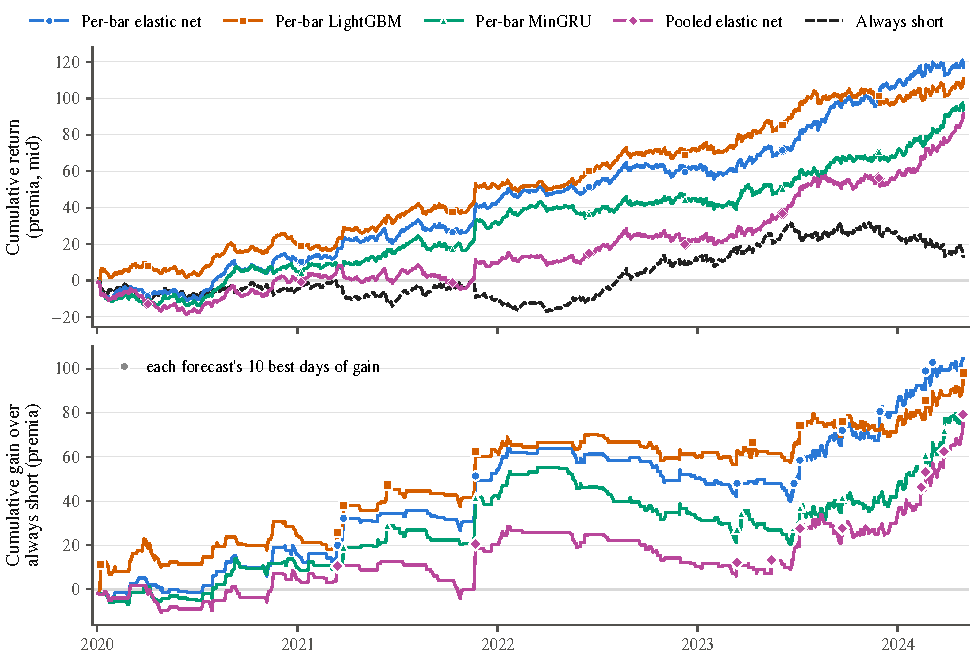
\includegraphics[width=\linewidth]{figures/rehaul_econ_cumpnl.pdf}
\caption{The closing trade over time, $q_t = \sign(s_t)$ at mid, for one forecast per family (all features) and
always short. Top: cumulative return $\sum_{u \le t} r_u$, in units of the straddle premium. Bottom: cumulative gain
over always short, $\sum_{u \le t} \bigl(r_u - r^{\mathrm{short}}_u\bigr)$; the markers are each forecast's 10
days of largest gain, each a day on which it bought and $R_t \ge 2.99$. The gain over the 866 days is
per-bar elastic net $+104.7$, per-bar LightGBM $+98.1$, per-bar MinGRU $+81.1$, pooled elastic net $+79.3$; without each forecast's 10 best days it is $+15.6$, $+2.4$, $-6.2$, $-6.3$. For 102 of the 112 forecasts of the model set the
gain is negative without their 10 best days.}
\label{fig:rh_econ_cumpnl}
\end{figure}


% E2: HAR + calendar -> all features within each family
% AUTO-GENERATED by writeup/make_rehaul_economics.py -- do not edit; re-run the script.
% Table E2 (outline 7.4): the full predictor set against the HAR benchmark
\ifdefined\rheNdays\else% AUTO-GENERATED by writeup/make_rehaul_economics.py -- do not edit; re-run the script.
% \rhe... macros for writeup/rehaul/07_economics.tex; values as in the rehaul_econ_* floats.
\providecommand{\rheShortSh}{}\renewcommand{\rheShortSh}{0.20}  % always short, Sharpe mid, 866 days
\providecommand{\rheShortShX}{}\renewcommand{\rheShortShX}{\ensuremath{-}0.27}  % always short, Sharpe crossed
\providecommand{\rheShortT}{}\renewcommand{\rheShortT}{0.43}  % always short, Newey-West t of the mean mid return
\providecommand{\rheShortHit}{}\renewcommand{\rheShortHit}{61.8}  % always short, hit rate %
\providecommand{\rheEnetSh}{}\renewcommand{\rheEnetSh}{1.92}  % per-bar enet all features, Sharpe mid
\providecommand{\rheEnetShX}{}\renewcommand{\rheEnetShX}{1.43}  % ... crossed
\providecommand{\rheEnetT}{}\renewcommand{\rheEnetT}{2.56}  % ... HAC t vs always short
\providecommand{\rheNNSh}{}\renewcommand{\rheNNSh}{1.53}  % MinGRU all features, Sharpe mid
\providecommand{\rheNNShX}{}\renewcommand{\rheNNShX}{1.05}  % ... crossed
\providecommand{\rheNNBaseSh}{}\renewcommand{\rheNNBaseSh}{1.04}  % MinGRU HAR + calendar, Sharpe mid
\providecommand{\rheNNBaseShX}{}\renewcommand{\rheNNBaseShX}{0.57}  % ... crossed
\providecommand{\rheSigVsShort}{}\renewcommand{\rheSigVsShort}{20}  % model-set forecasts with HAC t > 1.96 vs always short
\providecommand{\rhePairs}{}\renewcommand{\rhePairs}{51}  % HAR + cal. -> all features pairs in the model set
\providecommand{\rhePairsUp}{}\renewcommand{\rhePairsUp}{50}  % ... Sharpe mid higher with all features
\providecommand{\rhePairsSig}{}\renewcommand{\rhePairsSig}{4}  % ... HAC t > 1.96
\providecommand{\rhePairsMed}{}\renewcommand{\rhePairsMed}{\ensuremath{+}0.54}  % ... median dSharpe mid
\providecommand{\rheSzSignMed}{}\renewcommand{\rheSzSignMed}{0.92}  % sizing sign: model-set median Sharpe mid, 614 days
\providecommand{\rheSzClipMed}{}\renewcommand{\rheSzClipMed}{1.34}  % sizing clip: model-set median Sharpe mid, 614 days
\providecommand{\rheSzLfssMed}{}\renewcommand{\rheSzLfssMed}{1.12}  % sizing lfss: model-set median Sharpe mid, 614 days
\providecommand{\rheSzRankMed}{}\renewcommand{\rheSzRankMed}{1.34}  % sizing rank: model-set median Sharpe mid, 614 days
\providecommand{\rheSzShort}{}\renewcommand{\rheSzShort}{0.34}  % always short, Sharpe mid on the 614 sizing days
\providecommand{\rheSzClipBeats}{}\renewcommand{\rheSzClipBeats}{98}  % clip above sign(s), of 112 (mid)
\providecommand{\rheSzClipGain}{}\renewcommand{\rheSzClipGain}{\ensuremath{+}0.45}  % median clip - sign(s) Sharpe mid
\providecommand{\rheTailNeg}{}\renewcommand{\rheTailNeg}{102}  % model-set forecasts whose gain over short is < 0 without 10 best days
\fi
\begin{table}[tbp]
\centering
\small
\begin{threeparttable}
\caption{Sharpe ratios: HAR benchmark versus full predictor set}
\label{tab:rh_econ_allfeat}
\begin{tabular}{@{}lrrrr@{}}
\toprule
 & \multicolumn{2}{c}{$\SR$ at mid-quotes} & \multicolumn{2}{c}{$\Delta\SR$} \\
\cmidrule(lr){2-3}\cmidrule(l){4-5}
 & HAR benchmark & Full set & Mid-quotes & Bid--ask \\
\midrule
\multicolumn{5}{@{}l}{\textit{Panel A: Closing-interval models}} \\
\addlinespace[2pt]
Elastic net & $1.64$ & $1.93$ & $0.29^{\phantom{***}}$ & $0.29^{\phantom{***}}$ \\
 &  &  & $(1.34)^{\phantom{***}}$ & $(1.35)^{\phantom{***}}$ \\[2pt]
Lasso & $1.64$ & $1.76$ & $0.13^{\phantom{***}}$ & $0.13^{\phantom{***}}$ \\
 &  &  & $(1.47)^{\phantom{***}}$ & $(1.48)^{\phantom{***}}$ \\[2pt]
Ridge & $1.64$ & $1.51$ & $-0.13^{\phantom{***}}$ & $-0.13^{\phantom{***}}$ \\
 &  &  & $(0.09)^{\phantom{***}}$ & $(0.10)^{\phantom{***}}$ \\[2pt]
\addlinespace[4pt]
\multicolumn{5}{@{}l}{\textit{Panel B: Intraday models}} \\
\addlinespace[2pt]
Elastic net & $0.79$ & $1.91$ & $1.12^{\phantom{***}}$ & $1.13^{\phantom{***}}$ \\
 &  &  & $(1.21)^{\phantom{***}}$ & $(1.20)^{\phantom{***}}$ \\[2pt]
Lasso & $0.76$ & $1.56$ & $0.80^{\phantom{***}}$ & $0.80^{\phantom{***}}$ \\
 &  &  & $(1.19)^{\phantom{***}}$ & $(1.19)^{\phantom{***}}$ \\[2pt]
Ridge & $0.80$ & $1.73$ & $0.94^{\phantom{***}}$ & $0.94^{\phantom{***}}$ \\
 &  &  & $(1.12)^{\phantom{***}}$ & $(1.12)^{\phantom{***}}$ \\[2pt]
\addlinespace[4pt]
\multicolumn{5}{@{}l}{\textit{Panel C: Medians across pairs}} \\
\addlinespace[2pt]
LightGBM (\rheTreePairsEach) & $0.54$ & $1.40$ & $0.78^{\phantom{***}}$ & $0.77^{\phantom{***}}$ \\
 &  &  & $[0/15]^{\phantom{***}}$ & $[0/15]^{\phantom{***}}$ \\[2pt]
XGBoost (\rheTreePairsEach) & $0.57$ & $1.13$ & $0.51^{\phantom{***}}$ & $0.50^{\phantom{***}}$ \\
 &  &  & $[3/15]^{\phantom{***}}$ & $[3/15]^{\phantom{***}}$ \\[2pt]
Random forest (\rheTreePairsEach) & $0.26$ & $0.84$ & $0.50^{\phantom{***}}$ & $0.50^{\phantom{***}}$ \\
 &  &  & $[1/15]^{\phantom{***}}$ & $[1/15]^{\phantom{***}}$ \\[2pt]
All trees (\rheTreePairs) & $0.48$ & $1.15$ & $0.62^{\phantom{***}}$ & $0.61^{\phantom{***}}$ \\
 &  &  & $[4/45]^{\phantom{***}}$ & $[4/45]^{\phantom{***}}$ \\[2pt]
Model set (\rhePairs) & $0.50$ & $1.19$ & $0.62^{\phantom{***}}$ & $0.61^{\phantom{***}}$ \\
 &  &  & $[4/51]^{\phantom{***}}$ & $[4/51]^{\phantom{***}}$ \\[2pt]
\bottomrule
\end{tabular}
\begin{tablenotes}[flushleft]
\footnotesize
\item \textit{Notes:} Each pair is one model estimated on the HAR benchmark and on the full predictor set, with
everything else unchanged, over the out-of-sample period ($T_{\mathrm{oos}} = \rheNdays$ trading days). $\SR$ is the
annualized Sharpe ratio of the sign strategy; $\Delta\SR$ is the full-set minus the HAR-benchmark $\SR$, at
mid-quotes and at quoted bid/ask prices, with the HAC $t$-statistic on the daily return differential (Newey--West, $q_{\mathrm{NW}} = \rheHACLag$; Section~\ref{sec:rh_methods_tests}) in parentheses. On the HAR benchmark the three
closing-interval linear models hold the same position as the closing-interval OLS on every day, so they share its
$\SR$. Panel C gives medians across the closing-interval tree pairs (every hyperparameter specification in the model
set) and across all pairs of the \rheModelSetN{} forecasts of the model set, with the number of pairs whose
differential is significantly positive at the 5\% level in brackets (none is significantly negative at
that level). $^{*}$, $^{**}$ and $^{***}$ denote significance at the 10\%, 5\% and 1\% levels.
\end{tablenotes}
\end{threeparttable}
\end{table}


% E3: pooled vs per-bar (linear)
% AUTO-GENERATED by writeup/make_rehaul_economics.py -- do not edit; re-run the script.
% Table E3 (outline 7.4): closing-interval against intraday linear models
\ifdefined\rheNdays\else% AUTO-GENERATED by writeup/make_rehaul_economics.py -- do not edit; re-run the script.
% \rhe... macros for writeup/rehaul/07_economics.tex; values as in the rehaul_econ_* floats.
\providecommand{\rheShortSh}{}\renewcommand{\rheShortSh}{0.20}  % always short, Sharpe mid, 866 days
\providecommand{\rheShortShX}{}\renewcommand{\rheShortShX}{\ensuremath{-}0.27}  % always short, Sharpe crossed
\providecommand{\rheShortT}{}\renewcommand{\rheShortT}{0.43}  % always short, Newey-West t of the mean mid return
\providecommand{\rheShortHit}{}\renewcommand{\rheShortHit}{61.8}  % always short, hit rate %
\providecommand{\rheEnetSh}{}\renewcommand{\rheEnetSh}{1.92}  % per-bar enet all features, Sharpe mid
\providecommand{\rheEnetShX}{}\renewcommand{\rheEnetShX}{1.43}  % ... crossed
\providecommand{\rheEnetT}{}\renewcommand{\rheEnetT}{2.56}  % ... HAC t vs always short
\providecommand{\rheNNSh}{}\renewcommand{\rheNNSh}{1.53}  % MinGRU all features, Sharpe mid
\providecommand{\rheNNShX}{}\renewcommand{\rheNNShX}{1.05}  % ... crossed
\providecommand{\rheNNBaseSh}{}\renewcommand{\rheNNBaseSh}{1.04}  % MinGRU HAR + calendar, Sharpe mid
\providecommand{\rheNNBaseShX}{}\renewcommand{\rheNNBaseShX}{0.57}  % ... crossed
\providecommand{\rheSigVsShort}{}\renewcommand{\rheSigVsShort}{20}  % model-set forecasts with HAC t > 1.96 vs always short
\providecommand{\rhePairs}{}\renewcommand{\rhePairs}{51}  % HAR + cal. -> all features pairs in the model set
\providecommand{\rhePairsUp}{}\renewcommand{\rhePairsUp}{50}  % ... Sharpe mid higher with all features
\providecommand{\rhePairsSig}{}\renewcommand{\rhePairsSig}{4}  % ... HAC t > 1.96
\providecommand{\rhePairsMed}{}\renewcommand{\rhePairsMed}{\ensuremath{+}0.54}  % ... median dSharpe mid
\providecommand{\rheSzSignMed}{}\renewcommand{\rheSzSignMed}{0.92}  % sizing sign: model-set median Sharpe mid, 614 days
\providecommand{\rheSzClipMed}{}\renewcommand{\rheSzClipMed}{1.34}  % sizing clip: model-set median Sharpe mid, 614 days
\providecommand{\rheSzLfssMed}{}\renewcommand{\rheSzLfssMed}{1.12}  % sizing lfss: model-set median Sharpe mid, 614 days
\providecommand{\rheSzRankMed}{}\renewcommand{\rheSzRankMed}{1.34}  % sizing rank: model-set median Sharpe mid, 614 days
\providecommand{\rheSzShort}{}\renewcommand{\rheSzShort}{0.34}  % always short, Sharpe mid on the 614 sizing days
\providecommand{\rheSzClipBeats}{}\renewcommand{\rheSzClipBeats}{98}  % clip above sign(s), of 112 (mid)
\providecommand{\rheSzClipGain}{}\renewcommand{\rheSzClipGain}{\ensuremath{+}0.45}  % median clip - sign(s) Sharpe mid
\providecommand{\rheTailNeg}{}\renewcommand{\rheTailNeg}{102}  % model-set forecasts whose gain over short is < 0 without 10 best days
\fi
\begin{table}[tbp]
\centering
\small
\begin{threeparttable}
\caption{Closing-interval versus intraday models}
\label{tab:rh_econ_pooled}
\begin{tabular}{@{}lrrrrr@{}}
\toprule
 & \multicolumn{2}{c}{$\SR$ at mid-quotes} & \multicolumn{3}{c}{Intraday minus closing-interval} \\
\cmidrule(lr){2-3}\cmidrule(l){4-6}
 & Pooled & Closing & $\Delta\SR$, & $\Delta\SR$, & \\
 & intraday & interval & mid-quotes & bid--ask & $\Delta\QLIKE$ (\%) \\
\midrule
\multicolumn{6}{@{}l}{\textit{Panel A: Full predictor set}} \\
\addlinespace[2pt]
Elastic net & $1.85$ & $1.82$ & $0.03^{\phantom{***}}$ & $0.02^{\phantom{***}}$ & $27.1^{***}$ \\
 &  &  & $[0.947]^{\phantom{***}}$ & $[0.965]^{\phantom{***}}$ & $(4.14)^{\phantom{***}}$ \\[2pt]
Lasso & $1.73$ & $1.67$ & $0.06^{\phantom{***}}$ & $0.05^{\phantom{***}}$ & $37.9^{***}$ \\
 &  &  & $[0.891]^{\phantom{***}}$ & $[0.909]^{\phantom{***}}$ & $(4.84)^{\phantom{***}}$ \\[2pt]
Ridge & $1.64$ & $1.42$ & $0.22^{\phantom{***}}$ & $0.21^{\phantom{***}}$ & $27.5^{***}$ \\
 &  &  & $[0.584]^{\phantom{***}}$ & $[0.593]^{\phantom{***}}$ & $(4.18)^{\phantom{***}}$ \\[2pt]
\addlinespace[4pt]
\multicolumn{6}{@{}l}{\textit{Panel B: HAR benchmark}} \\
\addlinespace[2pt]
Elastic net & $0.95$ & $1.55$ & $-0.59^{\phantom{***}}$ & $-0.60^{\phantom{***}}$ & $14.1^{***}$ \\
 &  &  & $[0.134]^{\phantom{***}}$ & $[0.133]^{\phantom{***}}$ & $(2.86)^{\phantom{***}}$ \\[2pt]
Lasso & $0.95$ & $1.55$ & $-0.59^{\phantom{***}}$ & $-0.60^{\phantom{***}}$ & $14.1^{***}$ \\
 &  &  & $[0.134]^{\phantom{***}}$ & $[0.133]^{\phantom{***}}$ & $(2.86)^{\phantom{***}}$ \\[2pt]
Ridge & $0.95$ & $1.55$ & $-0.59^{\phantom{***}}$ & $-0.60^{\phantom{***}}$ & $14.1^{***}$ \\
 &  &  & $[0.134]^{\phantom{***}}$ & $[0.133]^{\phantom{***}}$ & $(2.86)^{\phantom{***}}$ \\[2pt]
\bottomrule
\end{tabular}
\begin{tablenotes}[flushleft]
\footnotesize
\item \textit{Notes:} Each row compares the closing-interval model with the intraday model of the same
estimator and predictor set, both with hyperparameters selected on a pre-sample, over the out-of-sample period
($T_{\mathrm{oos}} = \rheNdays$ trading days); the intraday model is evaluated on the closing interval. $\SR$
is the annualized Sharpe ratio of the sign strategy; $\Delta\SR$ is the intraday minus the closing-interval
$\SR$, at mid-quotes and at quoted bid/ask prices, with the $p$-value of the \citet{LedoitWolf2008} test of equal Sharpe ratios on the \rheSzDays{} post-warmup days, in brackets (Section~\ref{sec:rh_methods_tests}). $\Delta\QLIKE$ is the
intraday model's mean QLIKE relative to the closing-interval model's, in percent, with the Diebold--Mariano
statistic (Harvey--Leybourne--Newbold correction, Newey--West $q_{\mathrm{NW}} = \rheDMLag$) in parentheses; positive values favor
the closing-interval model, as in Table~\ref{tab:rh_axis2}. $^{*}$, $^{**}$ and $^{***}$ denote significance at the 10\%, 5\% and 1\% levels.
\end{tablenotes}
\end{threeparttable}
\end{table}


% Accuracy vs trade: the existing figure (writeup/make_fig_qlike_sharpe.py, \fqs... macros). The old paper places it
% in sections/results_close_option.tex:298-327; if the rehaul's results section also places it, keep one.
\ifdefined\fqsPairs\else% AUTO-GENERATED by writeup/make_fig_qlike_sharpe.py -- do not edit.
% Figure writeup/figures/fig_qlike_sharpe.pdf: QLIKE against Sharpe (mid), HAR + calendar vs all
% features, every model of results/close_master_table/paper_model_set.csv on both input sets
% (per-bar linear = the pre-tuned subpt_* rows; LSTMs excluded); numbers from master_table.csv
% and master_table_daily.parquet.  Changes are all features minus HAR + calendar, on the same days.
% DM: dm_test on the daily QLIKE difference; t: hac_inference.llsw_test on the daily mid-return
% difference (614 post-warmup days, bandwidth 33, fixed-b p); Sharpe changes: Ledoit-Wolf p;
% ES(c = 1): close_murphy_splits_headline.elementary on f / iv, y / iv.  Point estimates.
% pooled pairs: family pooled twin
\newcommand{\fqsPairs}{42}  % models on both input sets (pairs drawn)
\newcommand{\fqsPairsPerBarLinear}{3}  % of which per-bar linear (pre-tuned)
\newcommand{\fqsPairsPooled}{3}  % of which pooled 48-bar linear
\newcommand{\fqsPairsTree}{36}  % of which per-bar trees
\newcommand{\fqsPoints}{85}  % points drawn: both ends of every pair + the HAR + cal. OLS
\newcommand{\fqsDays}{866}  % trade days
\newcommand{\fqsQLower}{31}  % QLIKE lower with all features
\newcommand{\fqsQLowerSig}{3}  % ... and DM significant at 5 %
\newcommand{\fqsQHigher}{11}  % QLIKE higher with all features
\newcommand{\fqsQHigherSig}{0}  % ... and DM significant at 5 %
\newcommand{\fqsQLowerSigLagFourteen}{2}  % sensitivity: QLIKE lower, DM at lag 14 significant
\newcommand{\fqsQHigherSigLagFourteen}{0}  % sensitivity: QLIKE higher, DM at lag 14 significant
\newcommand{\fqsShHigher}{41}  % Sharpe (mid) higher with all features
\newcommand{\fqsShHigherSig}{6}  % ... and Ledoit-Wolf p < 0.05 (614 post-warmup days)
\newcommand{\fqsShLower}{1}  % Sharpe (mid) lower with all features
\newcommand{\fqsShLowerSig}{0}  % ... and Ledoit-Wolf p < 0.05 (614 post-warmup days)
\newcommand{\fqsQLowerShHigher}{30}  % both: QLIKE lower and Sharpe higher
\newcommand{\fqsMedDQ}{\ensuremath{-}0.0016}  % median QLIKE change (all features minus HAR + cal.)
\newcommand{\fqsMedDQPct}{\ensuremath{-}1.6}  % median QLIKE change, % of the HAR + cal. QLIKE
\newcommand{\fqsMedDSh}{\ensuremath{+}0.53}  % median Sharpe (mid) change
\newcommand{\fqsESLower}{29}  % elementary score at the threshold (c = 1) lower with all features
\newcommand{\fqsCorrES}{0.07}  % Pearson corr. across pairs: ES(c = 1) change vs HAC t of the P&L change
\newcommand{\fqsCorrQ}{0.12}  % Pearson corr. across pairs: QLIKE change vs HAC t of the P&L change
\newcommand{\fqsInShade}{4}  % all-features points in the shaded quadrant
\newcommand{\fqsInShadeBase}{3}  % HAR + cal. points in the shaded quadrant
\newcommand{\fqsOlsQ}{0.0967}  % QLIKE of the HAR + cal. OLS
\newcommand{\fqsOlsSh}{1.06}  % Sharpe (mid) of the HAR + cal. OLS
\newcommand{\fqsDMLag}{6}  % Newey-West lag of the DM statistic (the master table's)
\newcommand{\fqsHACS}{33}  % bandwidth S of the t of the mean P&L change (LLSW 2018, 614 post-warmup days)
\newcommand{\fqsSigPct}{5}  % two-sided level of the counts, %
\newcommand{\fqsQuadBetterBoth}{30}  % change figure: lower QLIKE, higher Sharpe
\newcommand{\fqsQuadShOnly}{11}  % change figure: higher QLIKE, higher Sharpe
\newcommand{\fqsQuadQOnly}{1}  % change figure: lower QLIKE, lower Sharpe
\newcommand{\fqsQuadWorseBoth}{0}  % change figure: higher QLIKE, lower Sharpe
\fi
% 2026-10-15 (user): parked -- non-standard figure; focus on legible tables
% \begin{figure}[tbp]
% \centering
% 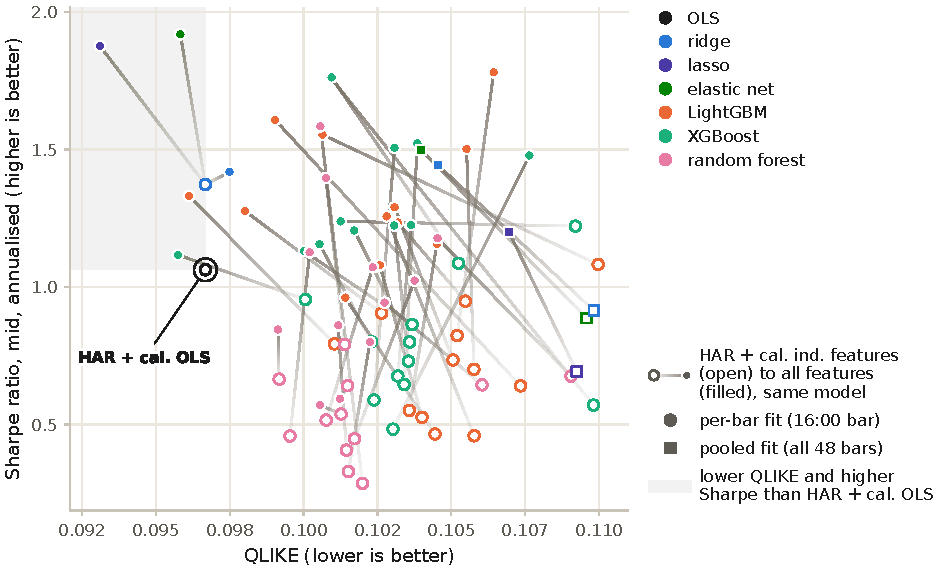
\includegraphics[width=\linewidth]{figures/fig_qlike_sharpe.pdf}
% % 2026-10-15 (notation pass): parked -- code jargon (trade, sign(s) Sharpe, per-bar, fits, HAR + calendar, all features, trade days); test wording
% % \caption{Accuracy against the trade: QLIKE and the $\sign(s)$ Sharpe ratio (mid) of the \fqsPairs{} models of the
% % model set fitted on both HAR + calendar (open markers) and all features (filled), \fqsDays{} trade days; each pair is
% % joined from its HAR + calendar end. Circles are per-bar fits and squares pooled fits; the colour marks the estimator.
% % Shaded: lower QLIKE and higher Sharpe ratio than the HAR + calendar OLS (QLIKE \fqsOlsQ, Sharpe \fqsOlsSh). All
% % features raise the Sharpe ratio for \fqsShHigher{} of the \fqsPairs{} models (\fqsShHigherSig{} significantly, by the
% % HAC $t$ of the daily return difference) and lower QLIKE for \fqsQLower{} (\fqsQLowerSig{} significantly, by
% % Diebold--Mariano), at \fqsSigPct\,\%.}
% \caption{Forecast accuracy and economic value. The figure plots the mean QLIKE loss against the annualized Sharpe
% ratio at mid-quotes, $\SR$, of the sign strategy for the \fqsPairs{} models of the model set that are estimated on both
% the HAR benchmark (open markers) and the full predictor set (filled markers), over the \fqsDays{} trading days of the
% out-of-sample period; a line joins the two ends of each pair. The sign strategy takes a delta-neutral at-the-money
% straddle position, entered at 15:30 ET and held to expiration: long ($q_t = +1$) or short ($q_t = -1$) as
% $q_t = \sign(s_t)$, where $s_t$ is the variance forecast minus the 15:30 implied variance. Circles denote
% closing-interval models and squares pooled intraday models; color identifies the estimator. The shaded quadrant
% contains lower QLIKE and higher $\SR$ than the closing-interval OLS on the HAR benchmark (QLIKE \fqsOlsQ, $\SR$
% \fqsOlsSh). The full predictor set raises $\SR$ for \fqsShHigher{} of the \fqsPairs{} models, \fqsShHigherSig{} of
% them significant at the \fqsSigPct\% level (HAC $t$-statistic on the daily return differential, Newey--West lag
% $q = \fqsHACLag$), and lowers QLIKE for \fqsQLower{}, \fqsQLowerSig{} of them significant at the \fqsSigPct\% level
% (Diebold--Mariano test with the Harvey--Leybourne--Newbold correction, Newey--West lag $q = \fqsDMLag$).}
% \label{fig:rh_econ_qlike_sharpe}
% \end{figure}

% E4: sizing rules
% AUTO-GENERATED by writeup/make_rehaul_economics.py -- do not edit; re-run the script.
% Table E4 (outline 7.4): position-sizing rules, scored exactly as the GUI (rows._score_sizes)
\ifdefined\rheNdays\else% AUTO-GENERATED by writeup/make_rehaul_economics.py -- do not edit; re-run the script.
% \rhe... macros for writeup/rehaul/07_economics.tex; values as in the rehaul_econ_* floats.
\providecommand{\rheShortSh}{}\renewcommand{\rheShortSh}{0.20}  % always short, Sharpe mid, 866 days
\providecommand{\rheShortShX}{}\renewcommand{\rheShortShX}{\ensuremath{-}0.27}  % always short, Sharpe crossed
\providecommand{\rheShortT}{}\renewcommand{\rheShortT}{0.43}  % always short, Newey-West t of the mean mid return
\providecommand{\rheShortHit}{}\renewcommand{\rheShortHit}{61.8}  % always short, hit rate %
\providecommand{\rheEnetSh}{}\renewcommand{\rheEnetSh}{1.92}  % per-bar enet all features, Sharpe mid
\providecommand{\rheEnetShX}{}\renewcommand{\rheEnetShX}{1.43}  % ... crossed
\providecommand{\rheEnetT}{}\renewcommand{\rheEnetT}{2.56}  % ... HAC t vs always short
\providecommand{\rheNNSh}{}\renewcommand{\rheNNSh}{1.53}  % MinGRU all features, Sharpe mid
\providecommand{\rheNNShX}{}\renewcommand{\rheNNShX}{1.05}  % ... crossed
\providecommand{\rheNNBaseSh}{}\renewcommand{\rheNNBaseSh}{1.04}  % MinGRU HAR + calendar, Sharpe mid
\providecommand{\rheNNBaseShX}{}\renewcommand{\rheNNBaseShX}{0.57}  % ... crossed
\providecommand{\rheSigVsShort}{}\renewcommand{\rheSigVsShort}{20}  % model-set forecasts with HAC t > 1.96 vs always short
\providecommand{\rhePairs}{}\renewcommand{\rhePairs}{51}  % HAR + cal. -> all features pairs in the model set
\providecommand{\rhePairsUp}{}\renewcommand{\rhePairsUp}{50}  % ... Sharpe mid higher with all features
\providecommand{\rhePairsSig}{}\renewcommand{\rhePairsSig}{4}  % ... HAC t > 1.96
\providecommand{\rhePairsMed}{}\renewcommand{\rhePairsMed}{\ensuremath{+}0.54}  % ... median dSharpe mid
\providecommand{\rheSzSignMed}{}\renewcommand{\rheSzSignMed}{0.92}  % sizing sign: model-set median Sharpe mid, 614 days
\providecommand{\rheSzClipMed}{}\renewcommand{\rheSzClipMed}{1.34}  % sizing clip: model-set median Sharpe mid, 614 days
\providecommand{\rheSzLfssMed}{}\renewcommand{\rheSzLfssMed}{1.12}  % sizing lfss: model-set median Sharpe mid, 614 days
\providecommand{\rheSzRankMed}{}\renewcommand{\rheSzRankMed}{1.34}  % sizing rank: model-set median Sharpe mid, 614 days
\providecommand{\rheSzShort}{}\renewcommand{\rheSzShort}{0.34}  % always short, Sharpe mid on the 614 sizing days
\providecommand{\rheSzClipBeats}{}\renewcommand{\rheSzClipBeats}{98}  % clip above sign(s), of 112 (mid)
\providecommand{\rheSzClipGain}{}\renewcommand{\rheSzClipGain}{\ensuremath{+}0.45}  % median clip - sign(s) Sharpe mid
\providecommand{\rheTailNeg}{}\renewcommand{\rheTailNeg}{102}  % model-set forecasts whose gain over short is < 0 without 10 best days
\fi
\begin{table}[tbp]
\centering
\small
\begin{threeparttable}
\caption{Sharpe ratios by position-sizing rule}
\label{tab:rh_econ_sizing}
\begin{tabular}{@{}lrrrr@{}}
\toprule
 & & Robust & Full long, & \\
 & Sign & clip & scaled short & Rank \\
\midrule
\multicolumn{5}{@{}l}{\textit{Panel A: $\SR$ at mid-quotes}} \\
\addlinespace[2pt]
Short straddle & \multicolumn{4}{c}{$0.32$ under every rule} \\
\multicolumn{5}{@{}l}{Pooled intraday models (\rhePoolNBars{} regular-hours intervals)} \\
\quad Ridge & $1.64$ & $1.79$ & $1.71$ & $1.78$ \\
\quad Lasso & $1.73$ & $1.89$ & $1.83$ & $1.79$ \\
\quad Elastic net & $1.85$ & $1.82$ & $1.86$ & $1.79$ \\
\quad LightGBM & $1.54$ & $1.50$ & $1.54$ & $1.56$ \\
\quad XGBoost & $1.54$ & $1.48$ & $1.56$ & $1.57$ \\
\quad Random forest & $1.88$ & $1.68$ & $1.87$ & $1.69$ \\
\multicolumn{5}{@{}l}{Closing-interval models (15:30--16:00 ET half hour)} \\
\quad OLS, HAR benchmark & $1.11$ & $1.49$ & $1.36$ & $1.58$ \\
\quad Ridge & $1.42$ & $1.61$ & $1.48$ & $1.66$ \\
\quad Lasso & $1.67$ & $1.66$ & $1.65$ & $1.75$ \\
\quad Elastic net & $1.82$ & $1.72$ & $1.74$ & $1.80$ \\
\addlinespace[2pt]
Model set, median & $0.84$ & $1.26$ & $1.06$ & $1.23$ \\
Model set, number above sign & -- & 82 & 83 & 80 \\
\addlinespace[4pt]
\multicolumn{5}{@{}l}{\textit{Panel B: $\SR$ at quoted bid/ask prices}} \\
\addlinespace[2pt]
Short straddle & \multicolumn{4}{c}{$-0.03$ under every rule} \\
\multicolumn{5}{@{}l}{Pooled intraday models (\rhePoolNBars{} regular-hours intervals)} \\
\quad Ridge & $1.29$ & $1.43$ & $1.40$ & $1.42$ \\
\quad Lasso & $1.37$ & $1.53$ & $1.53$ & $1.43$ \\
\quad Elastic net & $1.50$ & $1.46$ & $1.55$ & $1.43$ \\
\quad LightGBM & $1.18$ & $1.16$ & $1.24$ & $1.21$ \\
\quad XGBoost & $1.19$ & $1.14$ & $1.26$ & $1.22$ \\
\quad Random forest & $1.52$ & $1.33$ & $1.56$ & $1.34$ \\
\multicolumn{5}{@{}l}{Closing-interval models (15:30--16:00 ET half hour)} \\
\quad OLS, HAR benchmark & $0.76$ & $1.16$ & $1.06$ & $1.24$ \\
\quad Ridge & $1.08$ & $1.28$ & $1.17$ & $1.31$ \\
\quad Lasso & $1.32$ & $1.32$ & $1.35$ & $1.41$ \\
\quad Elastic net & $1.48$ & $1.39$ & $1.44$ & $1.45$ \\
\addlinespace[2pt]
Model set, median & $0.48$ & $0.93$ & $0.75$ & $0.89$ \\
Model set, number above sign & -- & 82 & 88 & 82 \\
\bottomrule
\end{tabular}
\begin{tablenotes}[flushleft]
\footnotesize
\item \textit{Notes:} Annualized Sharpe ratios of the straddle position $q_t$ under four sizing rules
(Section~\ref{sec:rh_econ_strategy}), each a function of $\hat\sigma^2_t - \mathrm{IV}^2_t$ and of its values on
earlier days $t' < t$ only; the sign rule is the sign strategy, and the short-straddle benchmark (Short straddle)
holds $q_t \equiv -1$ under every rule. The first \rheSzWarmup{} trading days of the out-of-sample period only estimate the
scale of $|\hat\sigma^2_{t'} - \mathrm{IV}^2_{t'}|$, so every rule is evaluated on the remaining \rheSzDays{} of
the \rheNdays{} trading days; at quoted bid/ask prices the bid--ask spread is paid on $|q_t|$ straddles. Every model except the OLS uses the full predictor set; the pooled
intraday models are those of Table~\ref{tab:rh_econ_control} (note a there). The last two rows of each panel give the median across the
\rheModelSetN{} forecasts of the model set and the number of them whose $\SR$ is above that of
their own sign strategy. Point estimates; no test is reported.
\end{tablenotes}
\end{threeparttable}
\end{table}

% 2026-10-15 (user): parked -- non-standard figure; focus on legible tables
% % AUTO-GENERATED by writeup/make_rehaul_economics.py -- do not edit; re-run the script.
\begin{figure}[tbp]
\centering
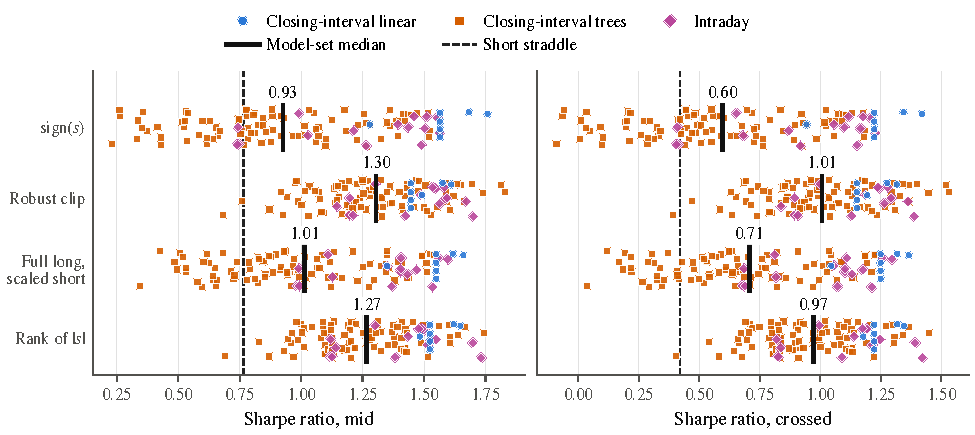
\includegraphics[width=\linewidth]{figures/rehaul_econ_sizing.pdf}
\caption{Sharpe ratio by sizing rule over the 94 forecasts of the model set, mid (left) and crossed (right),
on days 253--866. One marker per forecast, coloured by family and jittered vertically;
the bar and its label mark the model-set median (mid: 0.84, 1.26, 1.06, 1.23 for
the sign strategy, robust clip, full long / scaled short and rank of the absolute gap).
Dashed: the short-straddle benchmark ($0.32$ mid, $-0.03$ crossed). The
robust clip is above the sign strategy for 82 of the 94 forecasts at mid (median gain
$+0.45$). Rules and scoring as in Table~\ref{tab:rh_econ_sizing}.}
\label{fig:rh_econ_sizing}
\end{figure}


% Sharpe by year
% 2026-10-15 (user): parked -- non-standard figure; focus on legible tables
% % AUTO-GENERATED by writeup/make_rehaul_economics.py -- do not edit; re-run the script.
\begin{figure}[tbp]
\centering
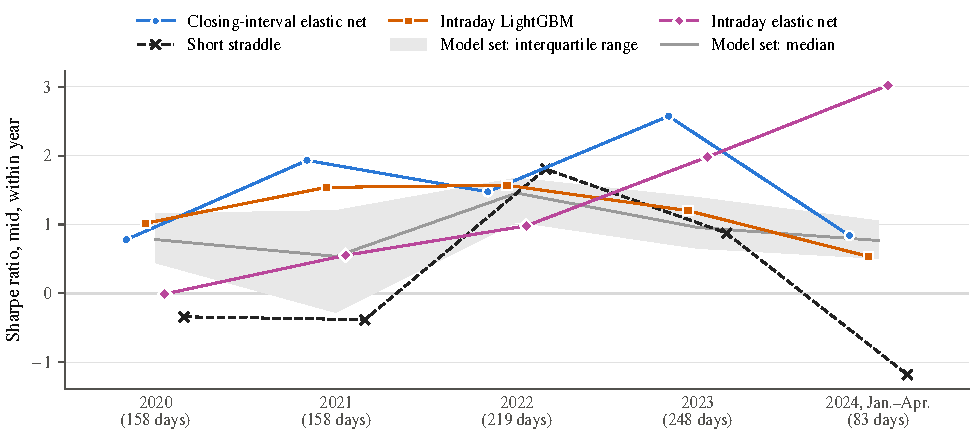
\includegraphics[width=\linewidth]{figures/rehaul_econ_byyear.pdf}
\caption{Sharpe ratio by calendar year at mid, $q_t = \sign(\hat\sigma^2_t - \mathrm{IV}^2_t)$, for the forecasts of
Figure~\ref{fig:rh_econ_cumpnl} and the short-straddle benchmark (2020 to 2024: $-0.34$, $-0.38$, $1.81$, $0.88$, $-1.18$); 2024 runs from
January to April. Each year's ratio is $\SR_y$ of Section~\ref{sec:rh_econ_measures}, scaled by the square root of that year's number of option days. Grey: the interquartile range
and median of the 112 forecasts of the model set (median $0.78$, $0.54$, $1.46$, $0.96$, $0.77$).}
\label{fig:rh_econ_byyear}
\end{figure}


% % 08_feature_importance.tex -- the rehauled paper's section, as bullets to expand into prose (2026-10-15).
% Sources and pointers behind every number: writeup/PAPER_REHAUL_OUTLINE_2026-10-15.md, section 8.
% House rules: every number in the final prose comes from a generated macro (writeup/generated/*.tex), never
% typed; park (comment out with a dated note) rather than delete.
% Macros to use here: rehaul_fi_numbers.tex (\rhfi..., writeup/make_rehaul_fi.py from results/rehaul_fi/, computed by
% experiments/rehaul_fi_compute.py); floats in 08b_fi_measures_floats.tex. The old study's measures (permutation,
% MDI, drop-column; appendix_campaign_16h_featimp.tex) stay in 08_feature_importance_floats.tex; their bullets are
% parked at the end of this file.
% 2026-10-15 measures pass: the user's plan (lasso counts, ridge sum |beta|, per-refit SHAP ranks aggregated,
% SHAP interactions global and per refit with the H-statistic cross-check) on the paper's models of record.
% 2026-10-15 (notation pass, writeup/NOTATION_GUIDE_2026-10-15.md): symbols and wording only; no number, macro or
% label changed. Old -> new: unit -> predictor group; column -> predictor; backbone -> HAR benchmark block;
% pf_j -> omega_j; alpha -> lambda; session -> trading day; fit space -> the scale of y_t; W_k -> \mathcal W_{t_k};
% T_k -> out-of-sample block \mathcal O_k; N (scored sessions) -> |\mathcal O|, \mathcal O the union of the blocks
% (not the guide's T_oos: this 2018-2024 period is not the paper's 2020-2024 test period); x_t -> \bm x_t;
% \beta^{(k)}_j -> \hat\beta_{k,j} (a parenthesized superscript is the guide's HAR horizon);
% b_{k,A} -> \lVert\hat{\bm\beta}_{k,A}\rVert_1 (b is the boosting round); s_{k,A} -> S_{k,A} (s is the periodicity
% factor); B_A (Borda) -> \mathrm{BC}_A; tie sizes \tau_{kg} -> |g|, g in \mathcal G_k (tau is the network step);
% H^2 points x_i and background b -> days t, t' in \mathcal H_k (i is the intraday interval).
% The generated floats (make_rehaul_fi.py) still print the old symbols ($T_k$, $\beta^{(k)}_j$, "unit", code names).
% 2026-10-15 (consolidation): the floats now print this section's symbols. Selection count N_A, N_j -> K_A, K_j (N is
% the one-minute count N_{t,i}, the symbol of the numobs series in the tables); group interaction Phi_{t,AB} ->
% phi_{t,AB} (Phi is the standard normal distribution function); tie sets \mathcal G_k -> \mathcal E_k (\mathcal G is
% the interval grid, Data); the ridge's standardized share S^{sd}_A (as in tab:rh_fi_summary, tab:rh_fi_linear);
% "buckets" -> categories. The refit index stays k, subscripted (guide 6b); HAR horizons are the superscript (k).
% 2026-10-15 (consolidation): parked -- the number files are loaded once in the preamble of paper_rehaul.tex.
% \ifdefined\rhfiNRefits\else% AUTO-GENERATED by writeup/make_rehaul_fi.py -- do not edit; re-run the script.
% \rhfi... macros for writeup/rehaul/08_feature_importance.tex (results/rehaul_fi/).
\providecommand{\rhfiNRefits}{}\renewcommand{\rhfiNRefits}{147}  % refits, one every 10 sessions
\providecommand{\rhfiNOos}{}\renewcommand{\rhfiNOos}{1{,}469}  % scored held-out sessions
\providecommand{\rhfiP}{}\renewcommand{\rhfiP}{628}  % columns, all features
\providecommand{\rhfiNUnits}{}\renewcommand{\rhfiNUnits}{49}  % units: 47 exogenous series + HAR ladder + calendar
\providecommand{\rhfiNExog}{}\renewcommand{\rhfiNExog}{47}  % exogenous series
\providecommand{\rhfiFirst}{}\renewcommand{\rhfiFirst}{25~June~2018}  % first scored session
\providecommand{\rhfiLast}{}\renewcommand{\rhfiLast}{30~April~2024}  % last scored session
\providecommand{\rhfiWindow}{}\renewcommand{\rhfiWindow}{2{,}000}  % sessions in a training window
\providecommand{\rhfiRefitEvery}{}\renewcommand{\rhfiRefitEvery}{10}  % sessions between refits
\providecommand{\rhfiBackbonePf}{}\renewcommand{\rhfiBackbonePf}{0.01}  % backbone penalty factor
\providecommand{\rhfiNBuckets}{}\renewcommand{\rhfiNBuckets}{8}  % exogenous buckets
\providecommand{\rhfiOldBlock}{}\renewcommand{\rhfiOldBlock}{250}  % sessions between the old arm's penalty re-choices
\providecommand{\rhfiNPairs}{}\renewcommand{\rhfiNPairs}{1{,}176}  % series pairs
\providecommand{\rhfiNProbeCols}{}\renewcommand{\rhfiNProbeCols}{631}  % columns of a probe fit
\providecommand{\rhfiTopWPairs}{}\renewcommand{\rhfiTopWPairs}{50}  % pairs in the interaction W
\providecommand{\rhfiProbeLevels}{}\renewcommand{\rhfiProbeLevels}{20}  % values of the few-valued noise column
\providecommand{\rhfiRidgeAlpha}{}\renewcommand{\rhfiRidgeAlpha}{\ensuremath{10^{3}}}
\providecommand{\rhfiLassoAlpha}{}\renewcommand{\rhfiLassoAlpha}{\ensuremath{10^{-2}}}
\providecommand{\rhfiLassoNzMed}{}\renewcommand{\rhfiLassoNzMed}{30}  % median nonzero coefficients per refit
\providecommand{\rhfiLassoNzMin}{}\renewcommand{\rhfiLassoNzMin}{27}
\providecommand{\rhfiLassoNzMax}{}\renewcommand{\rhfiLassoNzMax}{35}
\providecommand{\rhfiLassoExogNzMed}{}\renewcommand{\rhfiLassoExogNzMed}{14}  % ... exogenous columns
\providecommand{\rhfiLassoColsEver}{}\renewcommand{\rhfiLassoColsEver}{60}  % columns nonzero in >= 1 refit
\providecommand{\rhfiLassoColsMajority}{}\renewcommand{\rhfiLassoColsMajority}{29}  % columns nonzero in >= half the refits
\providecommand{\rhfiLassoExogEver}{}\renewcommand{\rhfiLassoExogEver}{27}  % exogenous series with a nonzero column in >= 1 refit
\providecommand{\rhfiLassoExogMajority}{}\renewcommand{\rhfiLassoExogMajority}{11}  % ... in >= half the refits
\providecommand{\rhfiLassoExogAlways}{}\renewcommand{\rhfiLassoExogAlways}{3}  % ... in every refit
\providecommand{\rhfiLassoAlwaysList}{}\renewcommand{\rhfiLassoAlwaysList}{\texttt{sumret}, \texttt{sumabsret\_vwstock}, \texttt{sumautocov}}  % exogenous series selected in every refit
\providecommand{\rhfiLassoProbeSel}{}\renewcommand{\rhfiLassoProbeSel}{1}  % continuous probe selected, of the probe fits
\providecommand{\rhfiLassoProbeSelLevels}{}\renewcommand{\rhfiLassoProbeSelLevels}{0}
\providecommand{\rhfiLassoProbeSelBinary}{}\renewcommand{\rhfiLassoProbeSelBinary}{0}
\providecommand{\rhfiNProbe}{}\renewcommand{\rhfiNProbe}{49}  % probe refits (every third)
\providecommand{\rhfiLassoW}{}\renewcommand{\rhfiLassoW}{0.74}  % Kendall W of the per-refit series ranks by sum |beta|
\providecommand{\rhfiLassoBackboneShare}{}\renewcommand{\rhfiLassoBackboneShare}{88}  % median share of sum |beta| on the backbone, %
\providecommand{\rhfiOldLassoSpearman}{}\renewcommand{\rhfiOldLassoSpearman}{0.70}  % Spearman, selection share: pre-tuned vs re-tuned one-penalty lasso
\providecommand{\rhfiOldLassoNzMed}{}\renewcommand{\rhfiOldLassoNzMed}{23}  % re-tuned lasso: median nonzero per refit
\providecommand{\rhfiOldLassoExogMajority}{}\renewcommand{\rhfiOldLassoExogMajority}{18}
\providecommand{\rhfiRidgeTopOne}{}\renewcommand{\rhfiRidgeTopOne}{Calendar}
\providecommand{\rhfiRidgeTopOneShare}{}\renewcommand{\rhfiRidgeTopOneShare}{31.0}  % % of sum |beta|
\providecommand{\rhfiRidgeTopTwo}{}\renewcommand{\rhfiRidgeTopTwo}{HAR ladder}
\providecommand{\rhfiRidgeTopTwoShare}{}\renewcommand{\rhfiRidgeTopTwoShare}{22.8}  % % of sum |beta|
\providecommand{\rhfiRidgeTopThree}{}\renewcommand{\rhfiRidgeTopThree}{\texttt{sumret}}
\providecommand{\rhfiRidgeTopThreeShare}{}\renewcommand{\rhfiRidgeTopThreeShare}{3.6}  % % of sum |beta|
\providecommand{\rhfiRidgeTopFour}{}\renewcommand{\rhfiRidgeTopFour}{\texttt{sumabsret\_vwstock}}
\providecommand{\rhfiRidgeTopFourShare}{}\renewcommand{\rhfiRidgeTopFourShare}{2.2}  % % of sum |beta|
\providecommand{\rhfiRidgeSdTopOne}{}\renewcommand{\rhfiRidgeSdTopOne}{HAR ladder}
\providecommand{\rhfiRidgeSdTopOneShare}{}\renewcommand{\rhfiRidgeSdTopOneShare}{30.6}  % % of sum |beta| sd
\providecommand{\rhfiRidgeSdTopTwo}{}\renewcommand{\rhfiRidgeSdTopTwo}{Calendar}
\providecommand{\rhfiRidgeSdTopTwoShare}{}\renewcommand{\rhfiRidgeSdTopTwoShare}{9.3}  % % of sum |beta| sd
\providecommand{\rhfiRidgeSdTopThree}{}\renewcommand{\rhfiRidgeSdTopThree}{\texttt{sumret}}
\providecommand{\rhfiRidgeSdTopThreeShare}{}\renewcommand{\rhfiRidgeSdTopThreeShare}{4.5}  % % of sum |beta| sd
\providecommand{\rhfiRidgeTopExog}{}\renewcommand{\rhfiRidgeTopExog}{\texttt{sumret}}
\providecommand{\rhfiRidgeTopExogShare}{}\renewcommand{\rhfiRidgeTopExogShare}{3.6}
\providecommand{\rhfiRidgeBackboneShare}{}\renewcommand{\rhfiRidgeBackboneShare}{54}  % median share of sum |beta| on the backbone, %
\providecommand{\rhfiRidgeW}{}\renewcommand{\rhfiRidgeW}{0.85}
\providecommand{\rhfiRidgeAllSelected}{}\renewcommand{\rhfiRidgeAllSelected}{49}  % units with N_A = K under the ridge
\providecommand{\rhfiLassoProbeRate}{}\renewcommand{\rhfiLassoProbeRate}{2.0}  % continuous probe's selection rate, %
\providecommand{\rhfiLassoColsAboveProbe}{}\renewcommand{\rhfiLassoColsAboveProbe}{54}  % columns selected more often than the continuous probe
\providecommand{\rhfiLassoSeriesAboveProbe}{}\renewcommand{\rhfiLassoSeriesAboveProbe}{23}  % exogenous series with such a column
\providecommand{\rhfiLassoTopCol}{}\renewcommand{\rhfiLassoTopCol}{\texttt{is\_month\_end}}
\providecommand{\rhfiRidgeSpearmanSd}{}\renewcommand{\rhfiRidgeSpearmanSd}{0.85}  % Spearman, series sum|beta| vs sum|beta| sd
\providecommand{\rhfiRidgeProbeBeat}{}\renewcommand{\rhfiRidgeProbeBeat}{107}  % columns with |beta| above the continuous probe's in most probe fits
\providecommand{\rhfiRidgeProbeBeatSeries}{}\renewcommand{\rhfiRidgeProbeBeatSeries}{38}
\providecommand{\rhfiScaleValueN}{}\renewcommand{\rhfiScaleValueN}{282}
\providecommand{\rhfiScaleValueSd}{}\renewcommand{\rhfiScaleValueSd}{0.84}  % median window sd, value ladders
\providecommand{\rhfiScaleValueSdLo}{}\renewcommand{\rhfiScaleValueSdLo}{0.03}
\providecommand{\rhfiScaleValueSdHi}{}\renewcommand{\rhfiScaleValueSdHi}{1.76}
\providecommand{\rhfiScaleValueIqr}{}\renewcommand{\rhfiScaleValueIqr}{0.94}  % median window IQR, value ladders
\providecommand{\rhfiScaleFlagN}{}\renewcommand{\rhfiScaleFlagN}{324}
\providecommand{\rhfiScaleFlagSd}{}\renewcommand{\rhfiScaleFlagSd}{0.022}  % median window sd, availability / activity ladders
\providecommand{\rhfiScaleFlagSdHi}{}\renewcommand{\rhfiScaleFlagSdHi}{0.17}
\providecommand{\rhfiScaleCalSd}{}\renewcommand{\rhfiScaleCalSd}{0.39}  % median window sd, calendar
\providecommand{\rhfiScaleHarSd}{}\renewcommand{\rhfiScaleHarSd}{1.07}  % median window sd, HAR ladder
\providecommand{\rhfiLgbmW}{}\renewcommand{\rhfiLgbmW}{0.57}  % lgbm: Kendall W, per-refit series ranks
\providecommand{\rhfiLgbmWCols}{}\renewcommand{\rhfiLgbmWCols}{0.91}  % lgbm: Kendall W, column ranks
\providecommand{\rhfiLgbmTopOne}{}\renewcommand{\rhfiLgbmTopOne}{HAR ladder}
\providecommand{\rhfiLgbmTopOneRank}{}\renewcommand{\rhfiLgbmTopOneRank}{1.0}  % mean rank
\providecommand{\rhfiLgbmTopTwo}{}\renewcommand{\rhfiLgbmTopTwo}{\texttt{sumret}}
\providecommand{\rhfiLgbmTopTwoRank}{}\renewcommand{\rhfiLgbmTopTwoRank}{2.9}  % mean rank
\providecommand{\rhfiLgbmTopThree}{}\renewcommand{\rhfiLgbmTopThree}{\texttt{sumabsret}}
\providecommand{\rhfiLgbmTopThreeRank}{}\renewcommand{\rhfiLgbmTopThreeRank}{4.8}  % mean rank
\providecommand{\rhfiLgbmSpBorda}{}\renewcommand{\rhfiLgbmSpBorda}{0.90}  % Spearman, mean rank vs top-10 Borda
\providecommand{\rhfiLgbmSpGlobal}{}\renewcommand{\rhfiLgbmSpGlobal}{0.96}  % Spearman, mean rank vs global mean |phi|
\providecommand{\rhfiLgbmSpLocal}{}\renewcommand{\rhfiLgbmSpLocal}{1.000}  % Spearman, mean ranks local refit vs stored
\providecommand{\rhfiLgbmProbeRank}{}\renewcommand{\rhfiLgbmProbeRank}{83}  % median rank of the continuous probe, 631 columns
\providecommand{\rhfiLgbmProbeCols}{}\renewcommand{\rhfiLgbmProbeCols}{60}  % columns above the continuous probe in most probe fits
\providecommand{\rhfiLgbmProbeSeries}{}\renewcommand{\rhfiLgbmProbeSeries}{27}  % exogenous series with such a column
\providecommand{\rhfiLgbmTopCol}{}\renewcommand{\rhfiLgbmTopCol}{\texttt{har\_ma\_1}}  % column with the lowest mean rank
\providecommand{\rhfiLgbmTopColRank}{}\renewcommand{\rhfiLgbmTopColRank}{1.3}
\providecommand{\rhfiLgbmTopColTwo}{}\renewcommand{\rhfiLgbmTopColTwo}{\texttt{har\_ma\_5}}
\providecommand{\rhfiLgbmTopColTwoRank}{}\renewcommand{\rhfiLgbmTopColTwoRank}{1.8}
\providecommand{\rhfiLgbmPredGap}{}\renewcommand{\rhfiLgbmPredGap}{0}  % max |local refit - stored refit| forecast
\providecommand{\rhfiLgbmInterW}{}\renewcommand{\rhfiLgbmInterW}{0.45}  % Kendall W of per-refit pair ranks, top-50 pairs
\providecommand{\rhfiLgbmInterRatio}{}\renewcommand{\rhfiLgbmInterRatio}{90}  % sum of series-pair interactions / sum main, %
\providecommand{\rhfiLgbmInterSpGlobal}{}\renewcommand{\rhfiLgbmInterSpGlobal}{0.99}
\providecommand{\rhfiLgbmInterFloor}{}\renewcommand{\rhfiLgbmInterFloor}{0.49}  % probe floor x 1e3
\providecommand{\rhfiLgbmInterAboveFloor}{}\renewcommand{\rhfiLgbmInterAboveFloor}{116}  % series pairs above the probe floor
\providecommand{\rhfiLgbmInterTopA}{}\renewcommand{\rhfiLgbmInterTopA}{HAR ladder}
\providecommand{\rhfiLgbmInterTopB}{}\renewcommand{\rhfiLgbmInterTopB}{\texttt{sumabsret}}
\providecommand{\rhfiLgbmInterTopVal}{}\renewcommand{\rhfiLgbmInterTopVal}{12.6}  % x 1e3
\providecommand{\rhfiLgbmHTop}{}\renewcommand{\rhfiLgbmHTop}{0.33}  % H^2 of the top series pair (pooled), %
\providecommand{\rhfiLgbmHMin}{}\renewcommand{\rhfiLgbmHMin}{0.02}  % min H^2 over the top-10 series pairs, %
\providecommand{\rhfiLgbmHMax}{}\renewcommand{\rhfiLgbmHMax}{0.33}  % max H^2 over the top-10 series pairs, %
\providecommand{\rhfiLgbmHMinTop}{}\renewcommand{\rhfiLgbmHMinTop}{0.19}  % top pair: interaction PD var / smaller main PD var
\providecommand{\rhfiLgbmHMinLo}{}\renewcommand{\rhfiLgbmHMinLo}{0.05}  % ... min over the top-10 series pairs
\providecommand{\rhfiLgbmHMinHi}{}\renewcommand{\rhfiLgbmHMinHi}{0.54}  % ... max
\providecommand{\rhfiLgbmHColTop}{}\renewcommand{\rhfiLgbmHColTop}{0.36}  % H^2 of the top column pair, %
\providecommand{\rhfiLgbmHMinColTop}{}\renewcommand{\rhfiLgbmHMinColTop}{0.02}  % ... min-normalised
\providecommand{\rhfiLgbmMainTopVal}{}\renewcommand{\rhfiLgbmMainTopVal}{195}  % largest global mean |phi_A| x 1e3
\providecommand{\rhfiLgbmWithinTop}{}\renewcommand{\rhfiLgbmWithinTop}{HAR ladder}
\providecommand{\rhfiLgbmWithinTopVal}{}\renewcommand{\rhfiLgbmWithinTopVal}{18.7}
\providecommand{\rhfiXgbW}{}\renewcommand{\rhfiXgbW}{0.60}  % xgb: Kendall W, per-refit series ranks
\providecommand{\rhfiXgbWCols}{}\renewcommand{\rhfiXgbWCols}{0.90}  % xgb: Kendall W, column ranks
\providecommand{\rhfiXgbTopOne}{}\renewcommand{\rhfiXgbTopOne}{HAR ladder}
\providecommand{\rhfiXgbTopOneRank}{}\renewcommand{\rhfiXgbTopOneRank}{1.0}  % mean rank
\providecommand{\rhfiXgbTopTwo}{}\renewcommand{\rhfiXgbTopTwo}{\texttt{sumret}}
\providecommand{\rhfiXgbTopTwoRank}{}\renewcommand{\rhfiXgbTopTwoRank}{3.0}  % mean rank
\providecommand{\rhfiXgbTopThree}{}\renewcommand{\rhfiXgbTopThree}{\texttt{sumabsret}}
\providecommand{\rhfiXgbTopThreeRank}{}\renewcommand{\rhfiXgbTopThreeRank}{3.9}  % mean rank
\providecommand{\rhfiXgbSpBorda}{}\renewcommand{\rhfiXgbSpBorda}{0.87}  % Spearman, mean rank vs top-10 Borda
\providecommand{\rhfiXgbSpGlobal}{}\renewcommand{\rhfiXgbSpGlobal}{0.97}  % Spearman, mean rank vs global mean |phi|
\providecommand{\rhfiXgbSpLocal}{}\renewcommand{\rhfiXgbSpLocal}{0.993}  % Spearman, mean ranks local refit vs stored
\providecommand{\rhfiXgbProbeRank}{}\renewcommand{\rhfiXgbProbeRank}{110}  % median rank of the continuous probe, 631 columns
\providecommand{\rhfiXgbProbeCols}{}\renewcommand{\rhfiXgbProbeCols}{78}  % columns above the continuous probe in most probe fits
\providecommand{\rhfiXgbProbeSeries}{}\renewcommand{\rhfiXgbProbeSeries}{35}  % exogenous series with such a column
\providecommand{\rhfiXgbTopCol}{}\renewcommand{\rhfiXgbTopCol}{\texttt{har\_ma\_1}}  % column with the lowest mean rank
\providecommand{\rhfiXgbTopColRank}{}\renewcommand{\rhfiXgbTopColRank}{1.3}
\providecommand{\rhfiXgbTopColTwo}{}\renewcommand{\rhfiXgbTopColTwo}{\texttt{har\_ma\_5}}
\providecommand{\rhfiXgbTopColTwoRank}{}\renewcommand{\rhfiXgbTopColTwoRank}{1.8}
\providecommand{\rhfiXgbPredGap}{}\renewcommand{\rhfiXgbPredGap}{0.17}  % max |local refit - stored refit| forecast
\providecommand{\rhfiXgbInterW}{}\renewcommand{\rhfiXgbInterW}{0.47}  % Kendall W of per-refit pair ranks, top-50 pairs
\providecommand{\rhfiXgbInterRatio}{}\renewcommand{\rhfiXgbInterRatio}{74}  % sum of series-pair interactions / sum main, %
\providecommand{\rhfiXgbInterSpGlobal}{}\renewcommand{\rhfiXgbInterSpGlobal}{0.99}
\providecommand{\rhfiXgbInterFloor}{}\renewcommand{\rhfiXgbInterFloor}{0.41}  % probe floor x 1e3
\providecommand{\rhfiXgbInterAboveFloor}{}\renewcommand{\rhfiXgbInterAboveFloor}{115}  % series pairs above the probe floor
\providecommand{\rhfiXgbInterTopA}{}\renewcommand{\rhfiXgbInterTopA}{HAR ladder}
\providecommand{\rhfiXgbInterTopB}{}\renewcommand{\rhfiXgbInterTopB}{\texttt{sumabsret}}
\providecommand{\rhfiXgbInterTopVal}{}\renewcommand{\rhfiXgbInterTopVal}{15.2}  % x 1e3
\providecommand{\rhfiXgbHTop}{}\renewcommand{\rhfiXgbHTop}{0.37}  % H^2 of the top series pair (pooled), %
\providecommand{\rhfiXgbHMin}{}\renewcommand{\rhfiXgbHMin}{0.02}  % min H^2 over the top-10 series pairs, %
\providecommand{\rhfiXgbHMax}{}\renewcommand{\rhfiXgbHMax}{0.68}  % max H^2 over the top-10 series pairs, %
\providecommand{\rhfiXgbHMinTop}{}\renewcommand{\rhfiXgbHMinTop}{0.39}  % top pair: interaction PD var / smaller main PD var
\providecommand{\rhfiXgbHMinLo}{}\renewcommand{\rhfiXgbHMinLo}{0.08}  % ... min over the top-10 series pairs
\providecommand{\rhfiXgbHMinHi}{}\renewcommand{\rhfiXgbHMinHi}{0.80}  % ... max
\providecommand{\rhfiXgbHColTop}{}\renewcommand{\rhfiXgbHColTop}{0.39}  % H^2 of the top column pair, %
\providecommand{\rhfiXgbHMinColTop}{}\renewcommand{\rhfiXgbHMinColTop}{0.02}  % ... min-normalised
\providecommand{\rhfiXgbMainTopVal}{}\renewcommand{\rhfiXgbMainTopVal}{192}  % largest global mean |phi_A| x 1e3
\providecommand{\rhfiXgbWithinTop}{}\renewcommand{\rhfiXgbWithinTop}{HAR ladder}
\providecommand{\rhfiXgbWithinTopVal}{}\renewcommand{\rhfiXgbWithinTopVal}{19.1}
\providecommand{\rhfiRfW}{}\renewcommand{\rhfiRfW}{0.62}  % rf: Kendall W, per-refit series ranks
\providecommand{\rhfiRfWCols}{}\renewcommand{\rhfiRfWCols}{0.93}  % rf: Kendall W, column ranks
\providecommand{\rhfiRfTopOne}{}\renewcommand{\rhfiRfTopOne}{HAR ladder}
\providecommand{\rhfiRfTopOneRank}{}\renewcommand{\rhfiRfTopOneRank}{1.0}  % mean rank
\providecommand{\rhfiRfTopTwo}{}\renewcommand{\rhfiRfTopTwo}{\texttt{sumabsret}}
\providecommand{\rhfiRfTopTwoRank}{}\renewcommand{\rhfiRfTopTwoRank}{2.6}  % mean rank
\providecommand{\rhfiRfTopThree}{}\renewcommand{\rhfiRfTopThree}{\texttt{sumret}}
\providecommand{\rhfiRfTopThreeRank}{}\renewcommand{\rhfiRfTopThreeRank}{4.0}  % mean rank
\providecommand{\rhfiRfSpBorda}{}\renewcommand{\rhfiRfSpBorda}{0.92}  % Spearman, mean rank vs top-10 Borda
\providecommand{\rhfiRfSpGlobal}{}\renewcommand{\rhfiRfSpGlobal}{0.98}  % Spearman, mean rank vs global mean |phi|
\providecommand{\rhfiRfSpLocal}{}\renewcommand{\rhfiRfSpLocal}{0.996}  % Spearman, mean ranks local refit vs stored
\providecommand{\rhfiRfProbeRank}{}\renewcommand{\rhfiRfProbeRank}{97}  % median rank of the continuous probe, 631 columns
\providecommand{\rhfiRfProbeCols}{}\renewcommand{\rhfiRfProbeCols}{71}  % columns above the continuous probe in most probe fits
\providecommand{\rhfiRfProbeSeries}{}\renewcommand{\rhfiRfProbeSeries}{29}  % exogenous series with such a column
\providecommand{\rhfiRfTopCol}{}\renewcommand{\rhfiRfTopCol}{\texttt{har\_ma\_1}}  % column with the lowest mean rank
\providecommand{\rhfiRfTopColRank}{}\renewcommand{\rhfiRfTopColRank}{1.3}
\providecommand{\rhfiRfTopColTwo}{}\renewcommand{\rhfiRfTopColTwo}{\texttt{har\_ma\_5}}
\providecommand{\rhfiRfTopColTwoRank}{}\renewcommand{\rhfiRfTopColTwoRank}{1.7}
\providecommand{\rhfiRfPredGap}{}\renewcommand{\rhfiRfPredGap}{0.11}  % max |local refit - stored refit| forecast
\providecommand{\rhfiRfInterW}{}\renewcommand{\rhfiRfInterW}{0.57}  % Kendall W of per-refit pair ranks, top-50 pairs
\providecommand{\rhfiRfInterRatio}{}\renewcommand{\rhfiRfInterRatio}{72}  % sum of series-pair interactions / sum main, %
\providecommand{\rhfiRfInterSpGlobal}{}\renewcommand{\rhfiRfInterSpGlobal}{1.00}
\providecommand{\rhfiRfInterFloor}{}\renewcommand{\rhfiRfInterFloor}{0.50}  % probe floor x 1e3
\providecommand{\rhfiRfInterAboveFloor}{}\renewcommand{\rhfiRfInterAboveFloor}{52}  % series pairs above the probe floor
\providecommand{\rhfiRfInterTopA}{}\renewcommand{\rhfiRfInterTopA}{HAR ladder}
\providecommand{\rhfiRfInterTopB}{}\renewcommand{\rhfiRfInterTopB}{\texttt{sumabsret}}
\providecommand{\rhfiRfInterTopVal}{}\renewcommand{\rhfiRfInterTopVal}{23.8}  % x 1e3
\providecommand{\rhfiRfHTop}{}\renewcommand{\rhfiRfHTop}{0.85}  % H^2 of the top series pair (pooled), %
\providecommand{\rhfiRfHMin}{}\renewcommand{\rhfiRfHMin}{0.02}  % min H^2 over the top-10 series pairs, %
\providecommand{\rhfiRfHMax}{}\renewcommand{\rhfiRfHMax}{0.85}  % max H^2 over the top-10 series pairs, %
\providecommand{\rhfiRfHMinTop}{}\renewcommand{\rhfiRfHMinTop}{1.50}  % top pair: interaction PD var / smaller main PD var
\providecommand{\rhfiRfHMinLo}{}\renewcommand{\rhfiRfHMinLo}{0.17}  % ... min over the top-10 series pairs
\providecommand{\rhfiRfHMinHi}{}\renewcommand{\rhfiRfHMinHi}{5.46}  % ... max
\providecommand{\rhfiRfHColTop}{}\renewcommand{\rhfiRfHColTop}{1.16}  % H^2 of the top column pair, %
\providecommand{\rhfiRfHMinColTop}{}\renewcommand{\rhfiRfHMinColTop}{0.06}  % ... min-normalised
\providecommand{\rhfiRfMainTopVal}{}\renewcommand{\rhfiRfMainTopVal}{224}  % largest global mean |phi_A| x 1e3
\providecommand{\rhfiRfWithinTop}{}\renewcommand{\rhfiRfWithinTop}{HAR ladder}
\providecommand{\rhfiRfWithinTopVal}{}\renewcommand{\rhfiRfWithinTopVal}{34.3}
\providecommand{\rhfiSpTreesMin}{}\renewcommand{\rhfiSpTreesMin}{0.83}  % Spearman of mean ranks, trees
\providecommand{\rhfiSpTreesMax}{}\renewcommand{\rhfiSpTreesMax}{0.96}
\providecommand{\rhfiSpTreeLinMin}{}\renewcommand{\rhfiSpTreeLinMin}{0.17}  % Spearman of mean ranks, tree vs linear
\providecommand{\rhfiSpTreeLinMax}{}\renewcommand{\rhfiSpTreeLinMax}{0.55}
\providecommand{\rhfiSpLassoRidge}{}\renewcommand{\rhfiSpLassoRidge}{0.47}
\providecommand{\rhfiHRefits}{}\renewcommand{\rhfiHRefits}{15}  % refits for H
\providecommand{\rhfiHRows}{}\renewcommand{\rhfiHRows}{100}  % evaluation points per refit
\providecommand{\rhfiHTopSeries}{}\renewcommand{\rhfiHTopSeries}{10}
\providecommand{\rhfiFitSecRf}{}\renewcommand{\rhfiFitSecRf}{212}  % mean seconds per forest refit (11 processes sharing the CPU)
\providecommand{\rhfiShapSecRf}{}\renewcommand{\rhfiShapSecRf}{182}  % mean seconds per forest refit, SHAP + interactions
\providecommand{\rhfiShapSecLgbm}{}\renewcommand{\rhfiShapSecLgbm}{0.9}  % ... LightGBM
\providecommand{\rhfiShapSecXgb}{}\renewcommand{\rhfiShapSecXgb}{0.4}  % ... XGBoost
\providecommand{\rhfiWallTreesMin}{}\renewcommand{\rhfiWallTreesMin}{133}  % wall minutes, tree stage on 11 processes
\providecommand{\rhfiWallHMin}{}\renewcommand{\rhfiWallHMin}{7}  % wall minutes, H stage
\providecommand{\rhfiWallLinMin}{}\renewcommand{\rhfiWallLinMin}{7}  % wall minutes, linear stage
\providecommand{\rhfiWorkers}{}\renewcommand{\rhfiWorkers}{11}
\fi
% 2026-10-15 (finish): "refit" -> "re-estimation" throughout the prose (guide terms); the index k and every \rhfi
% macro name (\rhfiNRefits, \rhfiRefitEvery, \rhfiHRefits) unchanged; the reproduction bullet of "Known issues" says
% "reproduce" instead of "re-estimate" to stay unambiguous; "periodicity-adjusted" -> "diurnally adjusted" (user).
% The generated tables' notes (make_rehaul_fi.py) still say "refits".
% 2026-10-23 (user, RR / E19 / new-notes 10b and 22): the live text below is on the FINAL pooled runs (W = 3,000 trading
% days, first evaluation day 2 January 2014). Macros \rhfip...: generated/rehaul_fip_numbers.tex, written by
% writeup/make_rehaul_fi_pooled.py from results/tree_shap_w3000_2014start_2026-10-23 (TreeSHAP, RULE_shap.txt) and
% results/fi_by_window_2014start_2026-10-22 (linear coefficients, RULE_fiw.txt); it also re-checks the origin refits
% against the merged every-bar walks of the three trees. Floats: tab:rh_fip_shares, tab:rh_fip_nonstd, fig:rh_fip_rank,
% fig:rh_fip_time, fig:rh_fip_cond (08_feature_importance_floats.tex); tab:rh_fip_window, tab:rh_fip_inter,
% fig:rh_fip_shapes (08b_fi_measures_floats.tex). The number file is loaded below (guarded) because the preamble of
% paper_rehaul.tex is not edited in this pass; \providecommand + \renewcommand make a second load harmless. The
% closing-interval body stays parked in \iffalse ... \fi (those models are not rerun; user).
% 2026-10-26 (integration and pruning pass, JFEc page budget; writeup/INTEGRATION_SPEC_2026-10-26.md, VI agent):
% Variable importance is promoted from the last subsection of the results to its own section (\section, label
% sec:rh_fi kept), about three pages: what the models use, the feature-count ladder with the ridge--lasso comparison,
% the late-starting series while live, use against accuracy. The rest moved to the online appendix, rehaul/A_fi.tex
% (labels app:rh_fi_compute, app:rh_fi_rank, app:rh_fi_cond, app:rh_fi_shapes, app:rh_fi_window,
% app:rh_fi_scaling). Audit fixes here: results-7 (elastic-net evidence, in A_fi), results-8 (holiday sessions in the
% explained bars), results-9 (FOMC statement days; generator change flagged to NUMBERS, note in A_fi), results-20
% (tuning samples). Replaced text is parked after the section's itemize below.

% 2026-10-15 (notation pass): parked -- old title; "variable importance" is the language of Gu, Kelly and Xiu (2020).
% \section{Feature importance}
% 2026-10-15 (user): parked -- "the feature importance needs to move to the end of the experiments section ... as a
% subsection"; included after 06_results in paper_rehaul.tex, so it is the last subsection of Experiments and results.
% \section{Variable importance}
% 2026-10-17 (user): parked -- closing-interval material: this subsection reports variable importance for the
% closing-interval models only, so its body is parked in \iffalse ... \fi below. Note E19 (the pooled intraday
% proposal, not about the parked text only) is kept visible here, moved verbatim out of the Notation bullet.
% 2026-10-26 (integration, JFEc): parked -- the subsection heading; Variable importance is now its own section,
% after the results and before the economic application (FRONT wires the order in paper_rehaul.tex). Was:
% "\subsection{Variable importance}"
% 2026-10-28 (author: Sections 6 and 7 are one section): the former Section 7 is Section 6.3, a subsection of Results (its
% subsections are \subsubsection's, labels unchanged); paper_rehaul.tex inputs Robustness (rehaul/06b_robustness.tex,
% Section 6.4) after this file. Was: \section{Which predictors carry the gain?}
% 2026-10-28 (author: conventional titles). Was: \subsection{Which predictors carry the gain?}
\subsection{Predictor-group ablations}
\label{sec:rh_fi}
\label{sec:rh_results_ablation}
% 2026-10-28 (author: v2 of Sections 6-7 approved preliminarily): the section is v2 (drafts/08_predictors_DRAFT.tex
% and drafts/MAP_06_07.md, 26 Oct), opened by the consolidated statement of 27 Oct (formerly Section 6.2, whose text
% is reused in the opening, Sections 7.2-7.4). Changes from the draft: Section 7.3 follows the follow-up tests of
% 27 Oct (a few series carry the trees' remainder, not a factor; the draft's "spread across groups, used nonlinearly"
% is retired); the redundancy bullet reports the counts of the RULE readings. The previous body is parked verbatim
% after the section; the every-bar attribution, ladder and ridge-against-lasso bullets moved to Appendix A_fi.tex.
% 2026-10-28 (author: v2 of Sections 6-7 approved preliminarily): section title (v2: attribution is one of three kinds of evidence). Was:
% \section{Variable importance}
% \label{sec:rh_fi}
\ifdefined\rhfipNOrigins\else% AUTO-GENERATED by writeup/make_rehaul_fi_pooled.py -- do not edit; re-run the script.
\providecommand{\ser}[2]{#2}\providecommand{\serx}[3]{#3}
% \rhfip... macros for writeup/rehaul/08_feature_importance.tex (results/tree_shap_w3000_2014start_fomcfix_2026-10-26, the
% FOMC-patched design, its linear reference inputs/fiw_gamma_fomcfix.npz; the window study's ...W... macros:
% results/fi_by_window_2014start_2026-10-22, pre-patch; the final pooled runs, W = 3,000 trading days).
\providecommand{\rhfipNOrigins}{}\renewcommand{\rhfipNOrigins}{126}  % monthly origins (re-estimations explained)
\providecommand{\rhfipNRows}{}\renewcommand{\rhfipNRows}{33{,}970}  % bars explained, every bar of the evaluation span
\providecommand{\rhfipOriginEvery}{}\renewcommand{\rhfipOriginEvery}{21}  % trading days between origins
\providecommand{\rhfipLastBlock}{}\renewcommand{\rhfipLastBlock}{18}  % trading days of the last origin's block
\providecommand{\rhfipFirstOrigin}{}\renewcommand{\rhfipFirstOrigin}{2~January~2014}  % first origin (10:00 bar)
\providecommand{\rhfipLastOrigin}{}\renewcommand{\rhfipLastOrigin}{5~April~2024}  % last origin
\providecommand{\rhfipLastDay}{}\renewcommand{\rhfipLastDay}{30~April~2024}  % day of the last bar explained
\providecommand{\rhfipWindowDays}{}\renewcommand{\rhfipWindowDays}{3{,}000}  % rolling window, trading days
\providecommand{\rhfipWindowBars}{}\renewcommand{\rhfipWindowBars}{39{,}000}  % rolling window, bars
\providecommand{\rhfipNCols}{}\renewcommand{\rhfipNCols}{564}  % predictors of the full set
\providecommand{\rhfipNGroups}{}\renewcommand{\rhfipNGroups}{48}  % predictor groups: 46 exogenous series + HAR components + calendar dummies
\providecommand{\rhfipNExog}{}\renewcommand{\rhfipNExog}{46}  % exogenous series
\providecommand{\rhfipNPerSeries}{}\renewcommand{\rhfipNPerSeries}{12}  % predictors per exogenous series: value and availability averages at six horizons
\providecommand{\rhfipNStd}{}\renewcommand{\rhfipNStd}{12}  % standard groups
\providecommand{\rhfipNNonStd}{}\renewcommand{\rhfipNNonStd}{36}  % non-standard series
\providecommand{\rhfipNStdExog}{}\renewcommand{\rhfipNStdExog}{10}  % standard exogenous series
\providecommand{\rhfipTuneLast}{}\renewcommand{\rhfipTuneLast}{31~December~2013}  % last day of the last tuning fold (fold 3)
\providecommand{\rhfipRidgePen}{}\renewcommand{\rhfipRidgePen}{\ensuremath{10^{3}}}
\providecommand{\rhfipLassoPen}{}\renewcommand{\rhfipLassoPen}{\ensuremath{10^{-4}}}
\providecommand{\rhfipEnetPen}{}\renewcommand{\rhfipEnetPen}{\ensuremath{10^{-3}}}
\providecommand{\rhfipHarPf}{}\renewcommand{\rhfipHarPf}{0.01}  % penalty factor, HAR block
\providecommand{\rhfipBootBlock}{}\renewcommand{\rhfipBootBlock}{12}  % bootstrap block, origins
\providecommand{\rhfipBootB}{}\renewcommand{\rhfipBootB}{2{,}000}
\providecommand{\rhfipCiLevel}{}\renewcommand{\rhfipCiLevel}{95}  % percentile intervals of both rules (RULE_shap.txt, RULE_fiw.txt)
\providecommand{\rhfipShapeMin}{}\renewcommand{\rhfipShapeMin}{0.5}  % M3 selection: share of at least this many percent
\providecommand{\rhfipTopN}{}\renewcommand{\rhfipTopN}{10}  % length of the top lists compared (m2_rank.csv top10_overlap)
\providecommand{\rhfipSlopeUnit}{}\renewcommand{\rhfipSlopeUnit}{1{,}000}  % trading days per unit of the window slope
\providecommand{\rhfipNMom}{}\renewcommand{\rhfipNMom}{seven}  % the futures' realized moments (standard)
\providecommand{\rhfipLgbmGateEq}{}\renewcommand{\rhfipLgbmGateEq}{126}  % origins bit-equal to the merged every-bar walk
\providecommand{\rhfipXgbGateEq}{}\renewcommand{\rhfipXgbGateEq}{126}  % origins bit-equal to the merged every-bar walk
\providecommand{\rhfipRfGateEq}{}\renewcommand{\rhfipRfGateEq}{126}  % origins bit-equal to the merged every-bar walk
\providecommand{\rhfipRfGateAtShap}{}\renewcommand{\rhfipRfGateAtShap}{126}  % forest origins the walk had written when the SHAP gate ran
\providecommand{\rhfipXgbAddMax}{}\renewcommand{\rhfipXgbAddMax}{\ensuremath{3.7\times 10^{-6}}}  % XGBoost additivity, float32
\providecommand{\rhfipXgbAddTol}{}\renewcommand{\rhfipXgbAddTol}{\ensuremath{10^{-5}}}
\providecommand{\rhfipAddMaxDouble}{}\renewcommand{\rhfipAddMaxDouble}{\ensuremath{5.1\times 10^{-14}}}
\providecommand{\rhfipLinGateMax}{}\renewcommand{\rhfipLinGateMax}{\ensuremath{4.4\times 10^{-16}}}  % linear replay vs walk forecasts, W = 3,000
\providecommand{\rhfipInterRows}{}\renewcommand{\rhfipInterRows}{1{,}008}  % M5 rows
\providecommand{\rhfipInterPerOrigin}{}\renewcommand{\rhfipInterPerOrigin}{8}  % M5 rows per origin
\providecommand{\rhfipFomcRows}{}\renewcommand{\rhfipFomcRows}{1{,}014}
\providecommand{\rhfipFomcDaysShap}{}\renewcommand{\rhfipFomcDaysShap}{78}  % FOMC statement days in the SHAP subset (M4; releases.parquet only)
\providecommand{\rhfipFomcDays}{}\renewcommand{\rhfipFomcDays}{81}  % scheduled FOMC statement days in the span (loader calendar)
\providecommand{\rhfipFomcDaysMissing}{}\renewcommand{\rhfipFomcDaysMissing}{3}  % statement days the SHAP subset leaves out (counted with the other days; the patched rerun's reducer keeps releases.parquet's days)
\providecommand{\rhfipNHolSessions}{}\renewcommand{\rhfipNHolSessions}{64}  % NYSE-holiday futures sessions among the explained bars (not scored in Table 1)
\providecommand{\rhfipNHolBars}{}\renewcommand{\rhfipNHolBars}{443}  % their regular-hours bars
\providecommand{\rhfipVixLo}{}\renewcommand{\rhfipVixLo}{13.96}
\providecommand{\rhfipVixHi}{}\renewcommand{\rhfipVixHi}{19.02}
\providecommand{\rhfipLgbmHar}{}\renewcommand{\rhfipLgbmHar}{51.7}
\providecommand{\rhfipLgbmHarLo}{}\renewcommand{\rhfipLgbmHarLo}{49.5}
\providecommand{\rhfipLgbmHarHi}{}\renewcommand{\rhfipLgbmHarHi}{53.7}
\providecommand{\rhfipLgbmMom}{}\renewcommand{\rhfipLgbmMom}{22.3}
\providecommand{\rhfipLgbmNs}{}\renewcommand{\rhfipLgbmNs}{21.8}
\providecommand{\rhfipLgbmNsLo}{}\renewcommand{\rhfipLgbmNsLo}{20.4}
\providecommand{\rhfipLgbmNsHi}{}\renewcommand{\rhfipLgbmNsHi}{23.4}
\providecommand{\rhfipLgbmNsEx}{}\renewcommand{\rhfipLgbmNsEx}{45.9}
\providecommand{\rhfipLgbmNsExLo}{}\renewcommand{\rhfipLgbmNsExLo}{44.2}
\providecommand{\rhfipLgbmNsExHi}{}\renewcommand{\rhfipLgbmNsExHi}{47.7}
\providecommand{\rhfipXgbHar}{}\renewcommand{\rhfipXgbHar}{52.0}
\providecommand{\rhfipXgbHarLo}{}\renewcommand{\rhfipXgbHarLo}{50.0}
\providecommand{\rhfipXgbHarHi}{}\renewcommand{\rhfipXgbHarHi}{53.8}
\providecommand{\rhfipXgbMom}{}\renewcommand{\rhfipXgbMom}{23.6}
\providecommand{\rhfipXgbNs}{}\renewcommand{\rhfipXgbNs}{20.6}
\providecommand{\rhfipXgbNsLo}{}\renewcommand{\rhfipXgbNsLo}{19.2}
\providecommand{\rhfipXgbNsHi}{}\renewcommand{\rhfipXgbNsHi}{22.2}
\providecommand{\rhfipXgbNsEx}{}\renewcommand{\rhfipXgbNsEx}{43.6}
\providecommand{\rhfipXgbNsExLo}{}\renewcommand{\rhfipXgbNsExLo}{41.8}
\providecommand{\rhfipXgbNsExHi}{}\renewcommand{\rhfipXgbNsExHi}{45.7}
\providecommand{\rhfipRfHar}{}\renewcommand{\rhfipRfHar}{57.6}
\providecommand{\rhfipRfHarLo}{}\renewcommand{\rhfipRfHarLo}{55.4}
\providecommand{\rhfipRfHarHi}{}\renewcommand{\rhfipRfHarHi}{59.6}
\providecommand{\rhfipRfMom}{}\renewcommand{\rhfipRfMom}{20.7}
\providecommand{\rhfipRfNs}{}\renewcommand{\rhfipRfNs}{18.6}
\providecommand{\rhfipRfNsLo}{}\renewcommand{\rhfipRfNsLo}{17.2}
\providecommand{\rhfipRfNsHi}{}\renewcommand{\rhfipRfNsHi}{20.3}
\providecommand{\rhfipRfNsEx}{}\renewcommand{\rhfipRfNsEx}{44.2}
\providecommand{\rhfipRfNsExLo}{}\renewcommand{\rhfipRfNsExLo}{42.1}
\providecommand{\rhfipRfNsExHi}{}\renewcommand{\rhfipRfNsExHi}{46.5}
\providecommand{\rhfipRidgeNsEx}{}\renewcommand{\rhfipRidgeNsEx}{68.8}
\providecommand{\rhfipRidgeNs}{}\renewcommand{\rhfipRidgeNs}{55.6}
\providecommand{\rhfipRidgeHar}{}\renewcommand{\rhfipRidgeHar}{17.5}
\providecommand{\rhfipLassoNsEx}{}\renewcommand{\rhfipLassoNsEx}{82.5}
\providecommand{\rhfipLassoNs}{}\renewcommand{\rhfipLassoNs}{76.5}
\providecommand{\rhfipLassoHar}{}\renewcommand{\rhfipLassoHar}{6.7}
\providecommand{\rhfipEnetNsEx}{}\renewcommand{\rhfipEnetNsEx}{60.0}
\providecommand{\rhfipEnetNs}{}\renewcommand{\rhfipEnetNs}{42.9}
\providecommand{\rhfipEnetHar}{}\renewcommand{\rhfipEnetHar}{26.4}
\providecommand{\rhfipHarMin}{}\renewcommand{\rhfipHarMin}{51.7}
\providecommand{\rhfipHarMax}{}\renewcommand{\rhfipHarMax}{57.6}
\providecommand{\rhfipMomMin}{}\renewcommand{\rhfipMomMin}{20.7}
\providecommand{\rhfipMomMax}{}\renewcommand{\rhfipMomMax}{23.6}
\providecommand{\rhfipNsExMin}{}\renewcommand{\rhfipNsExMin}{43.6}
\providecommand{\rhfipNsExMax}{}\renewcommand{\rhfipNsExMax}{45.9}
\providecommand{\rhfipSentMin}{}\renewcommand{\rhfipSentMin}{0.6}
\providecommand{\rhfipSentMax}{}\renewcommand{\rhfipSentMax}{0.8}
\providecommand{\rhfipVdMin}{}\renewcommand{\rhfipVdMin}{0.2}
\providecommand{\rhfipVdMax}{}\renewcommand{\rhfipVdMax}{0.3}
\providecommand{\rhfipFomcBucketMin}{}\renewcommand{\rhfipFomcBucketMin}{1.4}
\providecommand{\rhfipFomcBucketMax}{}\renewcommand{\rhfipFomcBucketMax}{2.3}
\providecommand{\rhfipVvixMin}{}\renewcommand{\rhfipVvixMin}{0.2}
\providecommand{\rhfipVvixMax}{}\renewcommand{\rhfipVvixMax}{0.3}
\providecommand{\rhfipVixThreeMMin}{}\renewcommand{\rhfipVixThreeMMin}{0.3}
\providecommand{\rhfipVixThreeMMax}{}\renewcommand{\rhfipVixThreeMMax}{0.7}
\providecommand{\rhfipFomcDayMin}{}\renewcommand{\rhfipFomcDayMin}{0.1}
\providecommand{\rhfipFomcDayMax}{}\renewcommand{\rhfipFomcDayMax}{0.1}
\providecommand{\rhfipNsOne}{}\renewcommand{\rhfipNsOne}{\ensuremath{\ser{sumabsret_vwstock}{\mathrm{RAV}^{\mathrm{VW}}}}}
\providecommand{\rhfipNsOneMin}{}\renewcommand{\rhfipNsOneMin}{2.4}
\providecommand{\rhfipNsOneMax}{}\renewcommand{\rhfipNsOneMax}{3.9}
\providecommand{\rhfipNsOneLgbm}{}\renewcommand{\rhfipNsOneLgbm}{3.5}
\providecommand{\rhfipNsOneXgb}{}\renewcommand{\rhfipNsOneXgb}{3.9}
\providecommand{\rhfipNsOneRf}{}\renewcommand{\rhfipNsOneRf}{2.4}
\providecommand{\rhfipNsTwo}{}\renewcommand{\rhfipNsTwo}{\ensuremath{\ser{sumabsret_ewstock}{\mathrm{RAV}^{\mathrm{EW}}}}}
\providecommand{\rhfipNsTwoMin}{}\renewcommand{\rhfipNsTwoMin}{1.9}
\providecommand{\rhfipNsTwoMax}{}\renewcommand{\rhfipNsTwoMax}{3.9}
\providecommand{\rhfipNsTwoLgbm}{}\renewcommand{\rhfipNsTwoLgbm}{3.9}
\providecommand{\rhfipNsTwoXgb}{}\renewcommand{\rhfipNsTwoXgb}{3.8}
\providecommand{\rhfipNsTwoRf}{}\renewcommand{\rhfipNsTwoRf}{1.9}
\providecommand{\rhfipNsThree}{}\renewcommand{\rhfipNsThree}{\ensuremath{\ser{fomc_until_inv}{\mathrm{FOMC}^{\mathrm{next}}}}}
\providecommand{\rhfipNsThreeMin}{}\renewcommand{\rhfipNsThreeMin}{1.1}
\providecommand{\rhfipNsThreeMax}{}\renewcommand{\rhfipNsThreeMax}{2.0}
\providecommand{\rhfipNsThreeLgbm}{}\renewcommand{\rhfipNsThreeLgbm}{2.0}
\providecommand{\rhfipNsThreeXgb}{}\renewcommand{\rhfipNsThreeXgb}{2.0}
\providecommand{\rhfipNsThreeRf}{}\renewcommand{\rhfipNsThreeRf}{1.1}
\providecommand{\rhfipNsFour}{}\renewcommand{\rhfipNsFour}{\ensuremath{\ser{ofi_vwstock}{\mathrm{OFI}^{\mathrm{VW}}}}}
\providecommand{\rhfipNsFourMin}{}\renewcommand{\rhfipNsFourMin}{1.4}
\providecommand{\rhfipNsFourMax}{}\renewcommand{\rhfipNsFourMax}{1.8}
\providecommand{\rhfipNsFourLgbm}{}\renewcommand{\rhfipNsFourLgbm}{1.8}
\providecommand{\rhfipNsFourXgb}{}\renewcommand{\rhfipNsFourXgb}{1.7}
\providecommand{\rhfipNsFourRf}{}\renewcommand{\rhfipNsFourRf}{1.4}
\providecommand{\rhfipNsFive}{}\renewcommand{\rhfipNsFive}{\ensuremath{\ser{effspread_vwstock}{\mathrm{EffSpread}^{\mathrm{VW}}}}}
\providecommand{\rhfipNsFiveMin}{}\renewcommand{\rhfipNsFiveMin}{1.2}
\providecommand{\rhfipNsFiveMax}{}\renewcommand{\rhfipNsFiveMax}{1.3}
\providecommand{\rhfipNsFiveLgbm}{}\renewcommand{\rhfipNsFiveLgbm}{1.2}
\providecommand{\rhfipNsFiveXgb}{}\renewcommand{\rhfipNsFiveXgb}{1.2}
\providecommand{\rhfipNsFiveRf}{}\renewcommand{\rhfipNsFiveRf}{1.3}
\providecommand{\rhfipTreeTopOne}{}\renewcommand{\rhfipTreeTopOne}{\ensuremath{\ser{sumabsret}{\mathrm{RAV}}}}
\providecommand{\rhfipTreeTopTwo}{}\renewcommand{\rhfipTreeTopTwo}{\ensuremath{\ser{sumret}{r}}}
\providecommand{\rhfipLgbmTopOneEx}{}\renewcommand{\rhfipLgbmTopOneEx}{20.3}
\providecommand{\rhfipXgbTopOneEx}{}\renewcommand{\rhfipXgbTopOneEx}{24.7}
\providecommand{\rhfipRfTopOneEx}{}\renewcommand{\rhfipRfTopOneEx}{29.2}
\providecommand{\rhfipRidgeTopOne}{}\renewcommand{\rhfipRidgeTopOne}{\ensuremath{\ser{fomc_until_inv}{\mathrm{FOMC}^{\mathrm{next}}}}}
\providecommand{\rhfipRidgeTopOneEx}{}\renewcommand{\rhfipRidgeTopOneEx}{9.0}
\providecommand{\rhfipLgbmNUsedAll}{}\renewcommand{\rhfipLgbmNUsedAll}{42}  % exogenous series split on at every origin
\providecommand{\rhfipLgbmUsedMin}{}\renewcommand{\rhfipLgbmUsedMin}{58}
\providecommand{\rhfipXgbNUsedAll}{}\renewcommand{\rhfipXgbNUsedAll}{43}  % exogenous series split on at every origin
\providecommand{\rhfipXgbUsedMin}{}\renewcommand{\rhfipXgbUsedMin}{72}
\providecommand{\rhfipRfNUsedAll}{}\renewcommand{\rhfipRfNUsedAll}{46}  % exogenous series split on at every origin
\providecommand{\rhfipRfUsedMin}{}\renewcommand{\rhfipRfUsedMin}{126}
\providecommand{\rhfipLgbmDRidge}{}\renewcommand{\rhfipLgbmDRidge}{\ensuremath{-}22.9}
\providecommand{\rhfipLgbmDRidgeLo}{}\renewcommand{\rhfipLgbmDRidgeLo}{\ensuremath{-}24.8}
\providecommand{\rhfipLgbmDRidgeHi}{}\renewcommand{\rhfipLgbmDRidgeHi}{\ensuremath{-}21.1}
\providecommand{\rhfipLgbmDLasso}{}\renewcommand{\rhfipLgbmDLasso}{\ensuremath{-}36.6}
\providecommand{\rhfipLgbmDLassoLo}{}\renewcommand{\rhfipLgbmDLassoLo}{\ensuremath{-}39.1}
\providecommand{\rhfipLgbmDLassoHi}{}\renewcommand{\rhfipLgbmDLassoHi}{\ensuremath{-}34.4}
\providecommand{\rhfipLgbmDEnet}{}\renewcommand{\rhfipLgbmDEnet}{\ensuremath{-}14.1}
\providecommand{\rhfipLgbmDEnetLo}{}\renewcommand{\rhfipLgbmDEnetLo}{\ensuremath{-}15.7}
\providecommand{\rhfipLgbmDEnetHi}{}\renewcommand{\rhfipLgbmDEnetHi}{\ensuremath{-}12.7}
\providecommand{\rhfipXgbDRidge}{}\renewcommand{\rhfipXgbDRidge}{\ensuremath{-}25.1}
\providecommand{\rhfipXgbDRidgeLo}{}\renewcommand{\rhfipXgbDRidgeLo}{\ensuremath{-}27.0}
\providecommand{\rhfipXgbDRidgeHi}{}\renewcommand{\rhfipXgbDRidgeHi}{\ensuremath{-}23.3}
\providecommand{\rhfipXgbDLasso}{}\renewcommand{\rhfipXgbDLasso}{\ensuremath{-}38.9}
\providecommand{\rhfipXgbDLassoLo}{}\renewcommand{\rhfipXgbDLassoLo}{\ensuremath{-}41.4}
\providecommand{\rhfipXgbDLassoHi}{}\renewcommand{\rhfipXgbDLassoHi}{\ensuremath{-}36.6}
\providecommand{\rhfipXgbDEnet}{}\renewcommand{\rhfipXgbDEnet}{\ensuremath{-}16.3}
\providecommand{\rhfipXgbDEnetLo}{}\renewcommand{\rhfipXgbDEnetLo}{\ensuremath{-}17.8}
\providecommand{\rhfipXgbDEnetHi}{}\renewcommand{\rhfipXgbDEnetHi}{\ensuremath{-}14.9}
\providecommand{\rhfipRfDRidge}{}\renewcommand{\rhfipRfDRidge}{\ensuremath{-}24.5}
\providecommand{\rhfipRfDRidgeLo}{}\renewcommand{\rhfipRfDRidgeLo}{\ensuremath{-}26.3}
\providecommand{\rhfipRfDRidgeHi}{}\renewcommand{\rhfipRfDRidgeHi}{\ensuremath{-}22.9}
\providecommand{\rhfipRfDLasso}{}\renewcommand{\rhfipRfDLasso}{\ensuremath{-}38.3}
\providecommand{\rhfipRfDLassoLo}{}\renewcommand{\rhfipRfDLassoLo}{\ensuremath{-}40.5}
\providecommand{\rhfipRfDLassoHi}{}\renewcommand{\rhfipRfDLassoHi}{\ensuremath{-}36.3}
\providecommand{\rhfipRfDEnet}{}\renewcommand{\rhfipRfDEnet}{\ensuremath{-}15.7}
\providecommand{\rhfipRfDEnetLo}{}\renewcommand{\rhfipRfDEnetLo}{\ensuremath{-}17.0}
\providecommand{\rhfipRfDEnetHi}{}\renewcommand{\rhfipRfDEnetHi}{\ensuremath{-}14.4}
\providecommand{\rhfipNDLess}{}\renewcommand{\rhfipNDLess}{27}  % tree-minus-linear D with the 95% interval below 0
\providecommand{\rhfipNDAll}{}\renewcommand{\rhfipNDAll}{27}  % D comparisons: 3 trees x 3 linear models x 3 denominators
\providecommand{\rhfipLgbmSpRidge}{}\renewcommand{\rhfipLgbmSpRidge}{0.57}
\providecommand{\rhfipLgbmTopRidge}{}\renewcommand{\rhfipLgbmTopRidge}{6}
\providecommand{\rhfipLgbmSpLasso}{}\renewcommand{\rhfipLgbmSpLasso}{0.49}
\providecommand{\rhfipLgbmTopLasso}{}\renewcommand{\rhfipLgbmTopLasso}{5}
\providecommand{\rhfipLgbmSpEnet}{}\renewcommand{\rhfipLgbmSpEnet}{0.66}
\providecommand{\rhfipLgbmTopEnet}{}\renewcommand{\rhfipLgbmTopEnet}{6}
\providecommand{\rhfipXgbSpRidge}{}\renewcommand{\rhfipXgbSpRidge}{0.55}
\providecommand{\rhfipXgbTopRidge}{}\renewcommand{\rhfipXgbTopRidge}{6}
\providecommand{\rhfipXgbSpLasso}{}\renewcommand{\rhfipXgbSpLasso}{0.47}
\providecommand{\rhfipXgbTopLasso}{}\renewcommand{\rhfipXgbTopLasso}{5}
\providecommand{\rhfipXgbSpEnet}{}\renewcommand{\rhfipXgbSpEnet}{0.63}
\providecommand{\rhfipXgbTopEnet}{}\renewcommand{\rhfipXgbTopEnet}{6}
\providecommand{\rhfipRfSpRidge}{}\renewcommand{\rhfipRfSpRidge}{0.53}
\providecommand{\rhfipRfTopRidge}{}\renewcommand{\rhfipRfTopRidge}{5}
\providecommand{\rhfipRfSpLasso}{}\renewcommand{\rhfipRfSpLasso}{0.43}
\providecommand{\rhfipRfTopLasso}{}\renewcommand{\rhfipRfTopLasso}{4}
\providecommand{\rhfipRfSpEnet}{}\renewcommand{\rhfipRfSpEnet}{0.60}
\providecommand{\rhfipRfTopEnet}{}\renewcommand{\rhfipRfTopEnet}{5}
\providecommand{\rhfipSpLgbmXgb}{}\renewcommand{\rhfipSpLgbmXgb}{0.99}
\providecommand{\rhfipSpLgbmRf}{}\renewcommand{\rhfipSpLgbmRf}{0.90}
\providecommand{\rhfipSpXgbRf}{}\renewcommand{\rhfipSpXgbRf}{0.89}
\providecommand{\rhfipRidgeRankFomcUntil}{}\renewcommand{\rhfipRidgeRankFomcUntil}{1}
\providecommand{\rhfipTreeRankFomcUntilMin}{}\renewcommand{\rhfipTreeRankFomcUntilMin}{6}
\providecommand{\rhfipTreeRankFomcUntilMax}{}\renewcommand{\rhfipTreeRankFomcUntilMax}{10}
\providecommand{\rhfipRidgeRankFomcDay}{}\renewcommand{\rhfipRidgeRankFomcDay}{9}
\providecommand{\rhfipTreeRankFomcDayMin}{}\renewcommand{\rhfipTreeRankFomcDayMin}{39}
\providecommand{\rhfipTreeRankFomcDayMax}{}\renewcommand{\rhfipTreeRankFomcDayMax}{43}
\providecommand{\rhfipFomcUntil}{}\renewcommand{\rhfipFomcUntil}{\ensuremath{\ser{fomc_until_inv}{\mathrm{FOMC}^{\mathrm{next}}}}}
\providecommand{\rhfipFomcDay}{}\renewcommand{\rhfipFomcDay}{\ensuremath{\ser{fomc_day}{\mathrm{FOMC}^{\mathrm{day}}}}}
\providecommand{\rhfipAbsVw}{}\renewcommand{\rhfipAbsVw}{\ensuremath{\ser{sumabsret_vwstock}{\mathrm{RAV}^{\mathrm{VW}}}}}
\providecommand{\rhfipOfi}{}\renewcommand{\rhfipOfi}{\ensuremath{\ser{ofi_vwstock}{\mathrm{OFI}^{\mathrm{VW}}}}}
\providecommand{\rhfipLgbmNeff}{}\renewcommand{\rhfipLgbmNeff}{11.0}
\providecommand{\rhfipLgbmNHalf}{}\renewcommand{\rhfipLgbmNHalf}{4}
\providecommand{\rhfipLgbmNEighty}{}\renewcommand{\rhfipLgbmNEighty}{13}
\providecommand{\rhfipXgbNeff}{}\renewcommand{\rhfipXgbNeff}{9.1}
\providecommand{\rhfipXgbNHalf}{}\renewcommand{\rhfipXgbNHalf}{4}
\providecommand{\rhfipXgbNEighty}{}\renewcommand{\rhfipXgbNEighty}{11}
\providecommand{\rhfipRfNeff}{}\renewcommand{\rhfipRfNeff}{8.9}
\providecommand{\rhfipRfNHalf}{}\renewcommand{\rhfipRfNHalf}{4}
\providecommand{\rhfipRfNEighty}{}\renewcommand{\rhfipRfNEighty}{16}
\providecommand{\rhfipRidgeNeff}{}\renewcommand{\rhfipRidgeNeff}{28.5}
\providecommand{\rhfipRidgeNHalf}{}\renewcommand{\rhfipRidgeNHalf}{11}
\providecommand{\rhfipRidgeNEighty}{}\renewcommand{\rhfipRidgeNEighty}{26}
\providecommand{\rhfipLassoNeff}{}\renewcommand{\rhfipLassoNeff}{5.1}
\providecommand{\rhfipLassoNHalf}{}\renewcommand{\rhfipLassoNHalf}{2}
\providecommand{\rhfipLassoNEighty}{}\renewcommand{\rhfipLassoNEighty}{11}
\providecommand{\rhfipEnetNeff}{}\renewcommand{\rhfipEnetNeff}{16.2}
\providecommand{\rhfipEnetNHalf}{}\renewcommand{\rhfipEnetNHalf}{6}
\providecommand{\rhfipEnetNEighty}{}\renewcommand{\rhfipEnetNEighty}{15}
\providecommand{\rhfipYearFirst}{}\renewcommand{\rhfipYearFirst}{2014}
\providecommand{\rhfipYearLast}{}\renewcommand{\rhfipYearLast}{2024}
\providecommand{\rhfipLgbmNsYearMin}{}\renewcommand{\rhfipLgbmNsYearMin}{18.1}
\providecommand{\rhfipLgbmNsYearMinYr}{}\renewcommand{\rhfipLgbmNsYearMinYr}{2021}
\providecommand{\rhfipLgbmNsYearMax}{}\renewcommand{\rhfipLgbmNsYearMax}{25.6}
\providecommand{\rhfipLgbmNsYearMaxYr}{}\renewcommand{\rhfipLgbmNsYearMaxYr}{2015}
\providecommand{\rhfipLgbmHarYearMax}{}\renewcommand{\rhfipLgbmHarYearMax}{57.4}
\providecommand{\rhfipLgbmHarYearMaxYr}{}\renewcommand{\rhfipLgbmHarYearMaxYr}{2021}
\providecommand{\rhfipLgbmHarYearMin}{}\renewcommand{\rhfipLgbmHarYearMin}{44.6}
\providecommand{\rhfipLgbmHarYearMinYr}{}\renewcommand{\rhfipLgbmHarYearMinYr}{2017}
\providecommand{\rhfipXgbNsYearMin}{}\renewcommand{\rhfipXgbNsYearMin}{17.2}
\providecommand{\rhfipXgbNsYearMinYr}{}\renewcommand{\rhfipXgbNsYearMinYr}{2021}
\providecommand{\rhfipXgbNsYearMax}{}\renewcommand{\rhfipXgbNsYearMax}{24.3}
\providecommand{\rhfipXgbNsYearMaxYr}{}\renewcommand{\rhfipXgbNsYearMaxYr}{2015}
\providecommand{\rhfipXgbHarYearMax}{}\renewcommand{\rhfipXgbHarYearMax}{57.0}
\providecommand{\rhfipXgbHarYearMaxYr}{}\renewcommand{\rhfipXgbHarYearMaxYr}{2021}
\providecommand{\rhfipXgbHarYearMin}{}\renewcommand{\rhfipXgbHarYearMin}{45.8}
\providecommand{\rhfipXgbHarYearMinYr}{}\renewcommand{\rhfipXgbHarYearMinYr}{2017}
\providecommand{\rhfipRfNsYearMin}{}\renewcommand{\rhfipRfNsYearMin}{15.2}
\providecommand{\rhfipRfNsYearMinYr}{}\renewcommand{\rhfipRfNsYearMinYr}{2021}
\providecommand{\rhfipRfNsYearMax}{}\renewcommand{\rhfipRfNsYearMax}{22.9}
\providecommand{\rhfipRfNsYearMaxYr}{}\renewcommand{\rhfipRfNsYearMaxYr}{2015}
\providecommand{\rhfipRfHarYearMax}{}\renewcommand{\rhfipRfHarYearMax}{62.3}
\providecommand{\rhfipRfHarYearMaxYr}{}\renewcommand{\rhfipRfHarYearMaxYr}{2019}
\providecommand{\rhfipRfHarYearMin}{}\renewcommand{\rhfipRfHarYearMin}{50.4}
\providecommand{\rhfipRfHarYearMinYr}{}\renewcommand{\rhfipRfHarYearMinYr}{2017}
\providecommand{\rhfipNsYearMinYr}{}\renewcommand{\rhfipNsYearMinYr}{2021}  % the year of every tree's lowest non-standard share
\providecommand{\rhfipDipFirst}{}\renewcommand{\rhfipDipFirst}{2018}  % first of the years in which every tree's non-standard share is below its pooled share
\providecommand{\rhfipDipLast}{}\renewcommand{\rhfipDipLast}{2022}
\providecommand{\rhfipRidgeNsExYearMin}{}\renewcommand{\rhfipRidgeNsExYearMin}{65.1}
\providecommand{\rhfipRidgeNsExYearMinYr}{}\renewcommand{\rhfipRidgeNsExYearMinYr}{2021}
\providecommand{\rhfipRidgeNsExYearMax}{}\renewcommand{\rhfipRidgeNsExYearMax}{72.4}
\providecommand{\rhfipRidgeNsExYearMaxYr}{}\renewcommand{\rhfipRidgeNsExYearMaxYr}{2017}
\providecommand{\rhfipLassoNsExYearMin}{}\renewcommand{\rhfipLassoNsExYearMin}{77.1}
\providecommand{\rhfipLassoNsExYearMinYr}{}\renewcommand{\rhfipLassoNsExYearMinYr}{2021}
\providecommand{\rhfipLassoNsExYearMax}{}\renewcommand{\rhfipLassoNsExYearMax}{87.1}
\providecommand{\rhfipLassoNsExYearMaxYr}{}\renewcommand{\rhfipLassoNsExYearMaxYr}{2017}
\providecommand{\rhfipEnetNsExYearMin}{}\renewcommand{\rhfipEnetNsExYearMin}{56.1}
\providecommand{\rhfipEnetNsExYearMinYr}{}\renewcommand{\rhfipEnetNsExYearMinYr}{2019}
\providecommand{\rhfipEnetNsExYearMax}{}\renewcommand{\rhfipEnetNsExYearMax}{65.2}
\providecommand{\rhfipEnetNsExYearMaxYr}{}\renewcommand{\rhfipEnetNsExYearMaxYr}{2014}
\providecommand{\rhfipLgbmNsExYearMin}{}\renewcommand{\rhfipLgbmNsExYearMin}{42.3}
\providecommand{\rhfipLgbmNsExYearMax}{}\renewcommand{\rhfipLgbmNsExYearMax}{50.1}
\providecommand{\rhfipXgbNsExYearMin}{}\renewcommand{\rhfipXgbNsExYearMin}{39.4}
\providecommand{\rhfipXgbNsExYearMax}{}\renewcommand{\rhfipXgbNsExYearMax}{48.9}
\providecommand{\rhfipRfNsExYearMin}{}\renewcommand{\rhfipRfNsExYearMin}{39.5}
\providecommand{\rhfipRfNsExYearMax}{}\renewcommand{\rhfipRfNsExYearMax}{50.9}
\providecommand{\rhfipLgbmNShape}{}\renewcommand{\rhfipLgbmNShape}{11}  % non-standard series at >= 0.5% (M3)
\providecommand{\rhfipLgbmNMono}{}\renewcommand{\rhfipLgbmNMono}{7}
\providecommand{\rhfipLgbmNIrr}{}\renewcommand{\rhfipLgbmNIrr}{3}
\providecommand{\rhfipLgbmNStep}{}\renewcommand{\rhfipLgbmNStep}{1}
\providecommand{\rhfipLgbmNFlat}{}\renewcommand{\rhfipLgbmNFlat}{0}
\providecommand{\rhfipLgbmNThresh}{}\renewcommand{\rhfipLgbmNThresh}{0}
\providecommand{\rhfipLgbmNU}{}\renewcommand{\rhfipLgbmNU}{0}
\providecommand{\rhfipLgbmNAsym}{}\renewcommand{\rhfipLgbmNAsym}{9}
\providecommand{\rhfipXgbNShape}{}\renewcommand{\rhfipXgbNShape}{10}  % non-standard series at >= 0.5% (M3)
\providecommand{\rhfipXgbNMono}{}\renewcommand{\rhfipXgbNMono}{5}
\providecommand{\rhfipXgbNIrr}{}\renewcommand{\rhfipXgbNIrr}{3}
\providecommand{\rhfipXgbNStep}{}\renewcommand{\rhfipXgbNStep}{0}
\providecommand{\rhfipXgbNFlat}{}\renewcommand{\rhfipXgbNFlat}{1}
\providecommand{\rhfipXgbNThresh}{}\renewcommand{\rhfipXgbNThresh}{1}
\providecommand{\rhfipXgbNU}{}\renewcommand{\rhfipXgbNU}{0}
\providecommand{\rhfipXgbNAsym}{}\renewcommand{\rhfipXgbNAsym}{8}
\providecommand{\rhfipRfNShape}{}\renewcommand{\rhfipRfNShape}{13}  % non-standard series at >= 0.5% (M3)
\providecommand{\rhfipRfNMono}{}\renewcommand{\rhfipRfNMono}{10}
\providecommand{\rhfipRfNIrr}{}\renewcommand{\rhfipRfNIrr}{3}
\providecommand{\rhfipRfNStep}{}\renewcommand{\rhfipRfNStep}{0}
\providecommand{\rhfipRfNFlat}{}\renewcommand{\rhfipRfNFlat}{0}
\providecommand{\rhfipRfNThresh}{}\renewcommand{\rhfipRfNThresh}{0}
\providecommand{\rhfipRfNU}{}\renewcommand{\rhfipRfNU}{0}
\providecommand{\rhfipRfNAsym}{}\renewcommand{\rhfipRfNAsym}{13}
\providecommand{\rhfipNUThreshAll}{}\renewcommand{\rhfipNUThreshAll}{1}  % U-shaped, inverted-U or threshold profiles in any tree
\providecommand{\rhfipAbsVwLgbmLo}{}\renewcommand{\rhfipAbsVwLgbmLo}{\ensuremath{-}1.4}
\providecommand{\rhfipAbsVwLgbmHi}{}\renewcommand{\rhfipAbsVwLgbmHi}{3.9}
\providecommand{\rhfipAbsVwXgbLo}{}\renewcommand{\rhfipAbsVwXgbLo}{\ensuremath{-}1.5}
\providecommand{\rhfipAbsVwXgbHi}{}\renewcommand{\rhfipAbsVwXgbHi}{4.3}
\providecommand{\rhfipAbsVwRfLo}{}\renewcommand{\rhfipAbsVwRfLo}{\ensuremath{-}0.9}
\providecommand{\rhfipAbsVwRfHi}{}\renewcommand{\rhfipAbsVwRfHi}{2.3}
\providecommand{\rhfipOfiLgbmLo}{}\renewcommand{\rhfipOfiLgbmLo}{0.8}
\providecommand{\rhfipOfiLgbmHi}{}\renewcommand{\rhfipOfiLgbmHi}{\ensuremath{-}1.1}
\providecommand{\rhfipOfiXgbLo}{}\renewcommand{\rhfipOfiXgbLo}{0.8}
\providecommand{\rhfipOfiXgbHi}{}\renewcommand{\rhfipOfiXgbHi}{\ensuremath{-}0.9}
\providecommand{\rhfipOfiRfLo}{}\renewcommand{\rhfipOfiRfLo}{0.8}
\providecommand{\rhfipOfiRfHi}{}\renewcommand{\rhfipOfiRfHi}{\ensuremath{-}0.7}
\providecommand{\rhfipUntilLgbmLo}{}\renewcommand{\rhfipUntilLgbmLo}{\ensuremath{-}0.3}
\providecommand{\rhfipUntilLgbmHi}{}\renewcommand{\rhfipUntilLgbmHi}{2.9}
\providecommand{\rhfipUntilXgbLo}{}\renewcommand{\rhfipUntilXgbLo}{0.2}
\providecommand{\rhfipUntilXgbHi}{}\renewcommand{\rhfipUntilXgbHi}{2.4}
\providecommand{\rhfipUntilRfLo}{}\renewcommand{\rhfipUntilRfLo}{\ensuremath{-}0.0}
\providecommand{\rhfipUntilRfHi}{}\renewcommand{\rhfipUntilRfHi}{1.5}
\providecommand{\rhfipUntilHorizon}{}\renewcommand{\rhfipUntilHorizon}{25}  % horizon of fomc_until_inv's dominant column
\providecommand{\rhfipUntilHorizonXgb}{}\renewcommand{\rhfipUntilHorizonXgb}{1}  % the same in XGBoost (differs from the other trees')
\providecommand{\rhfipBarFirst}{}\renewcommand{\rhfipBarFirst}{10:00}
\providecommand{\rhfipBarLast}{}\renewcommand{\rhfipBarLast}{16:00}
\providecommand{\rhfipBarPeakA}{}\renewcommand{\rhfipBarPeakA}{14:30}
\providecommand{\rhfipBarPeakB}{}\renewcommand{\rhfipBarPeakB}{15:00}
\providecommand{\rhfipNBars}{}\renewcommand{\rhfipNBars}{13}
\providecommand{\rhfipLgbmNsFomc}{}\renewcommand{\rhfipLgbmNsFomc}{42.6}
\providecommand{\rhfipLgbmNsOther}{}\renewcommand{\rhfipLgbmNsOther}{20.9}
\providecommand{\rhfipLgbmUntilFomc}{}\renewcommand{\rhfipLgbmUntilFomc}{25.4}
\providecommand{\rhfipLgbmUntilOther}{}\renewcommand{\rhfipLgbmUntilOther}{1.06}
\providecommand{\rhfipLgbmFomcBucketFomc}{}\renewcommand{\rhfipLgbmFomcBucketFomc}{27.3}
\providecommand{\rhfipLgbmFomcBucketOther}{}\renewcommand{\rhfipLgbmFomcBucketOther}{1.3}
\providecommand{\rhfipLgbmHarFomc}{}\renewcommand{\rhfipLgbmHarFomc}{39.2}
\providecommand{\rhfipLgbmHarOther}{}\renewcommand{\rhfipLgbmHarOther}{52.2}
\providecommand{\rhfipLgbmNsFirstBar}{}\renewcommand{\rhfipLgbmNsFirstBar}{23.9}
\providecommand{\rhfipLgbmNsLastBar}{}\renewcommand{\rhfipLgbmNsLastBar}{20.5}
\providecommand{\rhfipLgbmNsAftMin}{}\renewcommand{\rhfipLgbmNsAftMin}{24.3}
\providecommand{\rhfipLgbmNsAftMax}{}\renewcommand{\rhfipLgbmNsAftMax}{25.2}
\providecommand{\rhfipLgbmNsMidMin}{}\renewcommand{\rhfipLgbmNsMidMin}{20.1}
\providecommand{\rhfipLgbmNsMidMax}{}\renewcommand{\rhfipLgbmNsMidMax}{21.9}
\providecommand{\rhfipLgbmFomcBucketAft}{}\renewcommand{\rhfipLgbmFomcBucketAft}{5.5}
\providecommand{\rhfipLgbmFomcBucketOtherBars}{}\renewcommand{\rhfipLgbmFomcBucketOtherBars}{1.4}  % median FOMC-announcement share over the other 11 bars
\providecommand{\rhfipLgbmFomcDiff}{}\renewcommand{\rhfipLgbmFomcDiff}{\ensuremath{+}21.7}
\providecommand{\rhfipLgbmFomcDiffLo}{}\renewcommand{\rhfipLgbmFomcDiffLo}{\ensuremath{+}19.3}
\providecommand{\rhfipLgbmFomcDiffHi}{}\renewcommand{\rhfipLgbmFomcDiffHi}{\ensuremath{+}24.1}
\providecommand{\rhfipLgbmLateDiff}{}\renewcommand{\rhfipLgbmLateDiff}{\ensuremath{-}3.4}
\providecommand{\rhfipLgbmLateDiffLo}{}\renewcommand{\rhfipLgbmLateDiffLo}{\ensuremath{-}4.3}
\providecommand{\rhfipLgbmLateDiffHi}{}\renewcommand{\rhfipLgbmLateDiffHi}{\ensuremath{-}2.5}
\providecommand{\rhfipLgbmVixDiff}{}\renewcommand{\rhfipLgbmVixDiff}{\ensuremath{-}3.2}
\providecommand{\rhfipLgbmVixDiffLo}{}\renewcommand{\rhfipLgbmVixDiffLo}{\ensuremath{-}5.3}
\providecommand{\rhfipLgbmVixDiffHi}{}\renewcommand{\rhfipLgbmVixDiffHi}{\ensuremath{-}1.1}
\providecommand{\rhfipLgbmVixHar}{}\renewcommand{\rhfipLgbmVixHar}{\ensuremath{+}5.1}
\providecommand{\rhfipLgbmVixHarLo}{}\renewcommand{\rhfipLgbmVixHarLo}{\ensuremath{+}1.8}
\providecommand{\rhfipLgbmVixHarHi}{}\renewcommand{\rhfipLgbmVixHarHi}{\ensuremath{+}8.4}
\providecommand{\rhfipLgbmVixDiffEx}{}\renewcommand{\rhfipLgbmVixDiffEx}{\ensuremath{-}2.3}
\providecommand{\rhfipLgbmVixDiffExLo}{}\renewcommand{\rhfipLgbmVixDiffExLo}{\ensuremath{-}4.5}
\providecommand{\rhfipLgbmVixDiffExHi}{}\renewcommand{\rhfipLgbmVixDiffExHi}{\ensuremath{-}0.2}
\providecommand{\rhfipXgbNsFomc}{}\renewcommand{\rhfipXgbNsFomc}{41.1}
\providecommand{\rhfipXgbNsOther}{}\renewcommand{\rhfipXgbNsOther}{19.7}
\providecommand{\rhfipXgbUntilFomc}{}\renewcommand{\rhfipXgbUntilFomc}{23.9}
\providecommand{\rhfipXgbUntilOther}{}\renewcommand{\rhfipXgbUntilOther}{1.10}
\providecommand{\rhfipXgbFomcBucketFomc}{}\renewcommand{\rhfipXgbFomcBucketFomc}{25.6}
\providecommand{\rhfipXgbFomcBucketOther}{}\renewcommand{\rhfipXgbFomcBucketOther}{1.3}
\providecommand{\rhfipXgbHarFomc}{}\renewcommand{\rhfipXgbHarFomc}{39.1}
\providecommand{\rhfipXgbHarOther}{}\renewcommand{\rhfipXgbHarOther}{52.5}
\providecommand{\rhfipXgbNsFirstBar}{}\renewcommand{\rhfipXgbNsFirstBar}{22.5}
\providecommand{\rhfipXgbNsLastBar}{}\renewcommand{\rhfipXgbNsLastBar}{19.5}
\providecommand{\rhfipXgbNsAftMin}{}\renewcommand{\rhfipXgbNsAftMin}{23.5}
\providecommand{\rhfipXgbNsAftMax}{}\renewcommand{\rhfipXgbNsAftMax}{23.7}
\providecommand{\rhfipXgbNsMidMin}{}\renewcommand{\rhfipXgbNsMidMin}{19.1}
\providecommand{\rhfipXgbNsMidMax}{}\renewcommand{\rhfipXgbNsMidMax}{20.4}
\providecommand{\rhfipXgbFomcBucketAft}{}\renewcommand{\rhfipXgbFomcBucketAft}{5.8}
\providecommand{\rhfipXgbFomcBucketOtherBars}{}\renewcommand{\rhfipXgbFomcBucketOtherBars}{1.3}  % median FOMC-announcement share over the other 11 bars
\providecommand{\rhfipXgbFomcDiff}{}\renewcommand{\rhfipXgbFomcDiff}{\ensuremath{+}21.4}
\providecommand{\rhfipXgbFomcDiffLo}{}\renewcommand{\rhfipXgbFomcDiffLo}{\ensuremath{+}19.3}
\providecommand{\rhfipXgbFomcDiffHi}{}\renewcommand{\rhfipXgbFomcDiffHi}{\ensuremath{+}23.5}
\providecommand{\rhfipXgbLateDiff}{}\renewcommand{\rhfipXgbLateDiff}{\ensuremath{-}3.1}
\providecommand{\rhfipXgbLateDiffLo}{}\renewcommand{\rhfipXgbLateDiffLo}{\ensuremath{-}4.0}
\providecommand{\rhfipXgbLateDiffHi}{}\renewcommand{\rhfipXgbLateDiffHi}{\ensuremath{-}2.3}
\providecommand{\rhfipXgbVixDiff}{}\renewcommand{\rhfipXgbVixDiff}{\ensuremath{-}3.0}
\providecommand{\rhfipXgbVixDiffLo}{}\renewcommand{\rhfipXgbVixDiffLo}{\ensuremath{-}5.1}
\providecommand{\rhfipXgbVixDiffHi}{}\renewcommand{\rhfipXgbVixDiffHi}{\ensuremath{-}0.9}
\providecommand{\rhfipXgbVixHar}{}\renewcommand{\rhfipXgbVixHar}{\ensuremath{+}3.9}
\providecommand{\rhfipXgbVixHarLo}{}\renewcommand{\rhfipXgbVixHarLo}{\ensuremath{+}0.4}
\providecommand{\rhfipXgbVixHarHi}{}\renewcommand{\rhfipXgbVixHarHi}{\ensuremath{+}7.2}
\providecommand{\rhfipXgbVixDiffEx}{}\renewcommand{\rhfipXgbVixDiffEx}{\ensuremath{-}3.2}
\providecommand{\rhfipXgbVixDiffExLo}{}\renewcommand{\rhfipXgbVixDiffExLo}{\ensuremath{-}5.7}
\providecommand{\rhfipXgbVixDiffExHi}{}\renewcommand{\rhfipXgbVixDiffExHi}{\ensuremath{-}0.8}
\providecommand{\rhfipRfNsFomc}{}\renewcommand{\rhfipRfNsFomc}{28.9}
\providecommand{\rhfipRfNsOther}{}\renewcommand{\rhfipRfNsOther}{18.3}
\providecommand{\rhfipRfUntilFomc}{}\renewcommand{\rhfipRfUntilFomc}{12.4}
\providecommand{\rhfipRfFomcBucketFomc}{}\renewcommand{\rhfipRfFomcBucketFomc}{13.0}
\providecommand{\rhfipRfFomcBucketOther}{}\renewcommand{\rhfipRfFomcBucketOther}{1.0}
\providecommand{\rhfipRfHarFomc}{}\renewcommand{\rhfipRfHarFomc}{50.8}
\providecommand{\rhfipRfHarOther}{}\renewcommand{\rhfipRfHarOther}{57.9}
\providecommand{\rhfipRfNsFirstBar}{}\renewcommand{\rhfipRfNsFirstBar}{20.1}
\providecommand{\rhfipRfNsLastBar}{}\renewcommand{\rhfipRfNsLastBar}{17.8}
\providecommand{\rhfipRfNsAftMin}{}\renewcommand{\rhfipRfNsAftMin}{19.5}
\providecommand{\rhfipRfNsAftMax}{}\renewcommand{\rhfipRfNsAftMax}{19.9}
\providecommand{\rhfipRfNsMidMin}{}\renewcommand{\rhfipRfNsMidMin}{17.8}
\providecommand{\rhfipRfNsMidMax}{}\renewcommand{\rhfipRfNsMidMax}{18.6}
\providecommand{\rhfipRfFomcBucketAft}{}\renewcommand{\rhfipRfFomcBucketAft}{3.1}
\providecommand{\rhfipRfFomcBucketOtherBars}{}\renewcommand{\rhfipRfFomcBucketOtherBars}{1.0}  % median FOMC-announcement share over the other 11 bars
\providecommand{\rhfipRfFomcDiff}{}\renewcommand{\rhfipRfFomcDiff}{\ensuremath{+}10.6}
\providecommand{\rhfipRfFomcDiffLo}{}\renewcommand{\rhfipRfFomcDiffLo}{\ensuremath{+}8.3}
\providecommand{\rhfipRfFomcDiffHi}{}\renewcommand{\rhfipRfFomcDiffHi}{\ensuremath{+}13.1}
\providecommand{\rhfipRfLateDiff}{}\renewcommand{\rhfipRfLateDiff}{\ensuremath{-}2.3}
\providecommand{\rhfipRfLateDiffLo}{}\renewcommand{\rhfipRfLateDiffLo}{\ensuremath{-}3.1}
\providecommand{\rhfipRfLateDiffHi}{}\renewcommand{\rhfipRfLateDiffHi}{\ensuremath{-}1.6}
\providecommand{\rhfipRfVixDiff}{}\renewcommand{\rhfipRfVixDiff}{\ensuremath{-}3.3}
\providecommand{\rhfipRfVixDiffLo}{}\renewcommand{\rhfipRfVixDiffLo}{\ensuremath{-}5.1}
\providecommand{\rhfipRfVixDiffHi}{}\renewcommand{\rhfipRfVixDiffHi}{\ensuremath{-}1.4}
\providecommand{\rhfipRfVixHar}{}\renewcommand{\rhfipRfVixHar}{\ensuremath{+}4.2}
\providecommand{\rhfipRfVixHarLo}{}\renewcommand{\rhfipRfVixHarLo}{\ensuremath{+}1.0}
\providecommand{\rhfipRfVixHarHi}{}\renewcommand{\rhfipRfVixHarHi}{\ensuremath{+}7.3}
\providecommand{\rhfipRfVixDiffEx}{}\renewcommand{\rhfipRfVixDiffEx}{\ensuremath{-}3.7}
\providecommand{\rhfipRfVixDiffExLo}{}\renewcommand{\rhfipRfVixDiffExLo}{\ensuremath{-}6.3}
\providecommand{\rhfipRfVixDiffExHi}{}\renewcommand{\rhfipRfVixDiffExHi}{\ensuremath{-}1.2}
\providecommand{\rhfipLgbmInterVar}{}\renewcommand{\rhfipLgbmInterVar}{33.1}
\providecommand{\rhfipLgbmInterCol}{}\renewcommand{\rhfipLgbmInterCol}{45.3}
\providecommand{\rhfipLgbmInterNs}{}\renewcommand{\rhfipLgbmInterNs}{49.6}
\providecommand{\rhfipLgbmInterStd}{}\renewcommand{\rhfipLgbmInterStd}{26.8}
\providecommand{\rhfipLgbmInterStdEx}{}\renewcommand{\rhfipLgbmInterStdEx}{40.2}  % descriptive: standard exogenous series only (no HAR, no calendar)
\providecommand{\rhfipLgbmInterHar}{}\renewcommand{\rhfipLgbmInterHar}{17.1}
\providecommand{\rhfipLgbmInterWeakMin}{}\renewcommand{\rhfipLgbmInterWeakMin}{54}
\providecommand{\rhfipLgbmInterWeakMax}{}\renewcommand{\rhfipLgbmInterWeakMax}{66}
\providecommand{\rhfipLgbmPairOne}{}\renewcommand{\rhfipLgbmPairOne}{1.25}
\providecommand{\rhfipLgbmPairTwo}{}\renewcommand{\rhfipLgbmPairTwo}{0.86}
\providecommand{\rhfipLgbmCellHarHar}{}\renewcommand{\rhfipLgbmCellHarHar}{48.0}
\providecommand{\rhfipXgbInterVar}{}\renewcommand{\rhfipXgbInterVar}{30.9}
\providecommand{\rhfipXgbInterCol}{}\renewcommand{\rhfipXgbInterCol}{42.5}
\providecommand{\rhfipXgbInterNs}{}\renewcommand{\rhfipXgbInterNs}{45.7}
\providecommand{\rhfipXgbInterStd}{}\renewcommand{\rhfipXgbInterStd}{26.0}
\providecommand{\rhfipXgbInterStdEx}{}\renewcommand{\rhfipXgbInterStdEx}{37.8}  % descriptive: standard exogenous series only (no HAR, no calendar)
\providecommand{\rhfipXgbInterHar}{}\renewcommand{\rhfipXgbInterHar}{17.6}
\providecommand{\rhfipXgbInterWeakMin}{}\renewcommand{\rhfipXgbInterWeakMin}{54}
\providecommand{\rhfipXgbInterWeakMax}{}\renewcommand{\rhfipXgbInterWeakMax}{63}
\providecommand{\rhfipXgbPairOne}{}\renewcommand{\rhfipXgbPairOne}{1.23}
\providecommand{\rhfipXgbPairTwo}{}\renewcommand{\rhfipXgbPairTwo}{0.83}
\providecommand{\rhfipXgbCellHarHar}{}\renewcommand{\rhfipXgbCellHarHar}{47.4}
\providecommand{\rhfipPairOneA}{}\renewcommand{\rhfipPairOneA}{HAR components}
\providecommand{\rhfipPairOneB}{}\renewcommand{\rhfipPairOneB}{\ensuremath{\ser{sumabsret_vwstock}{\mathrm{RAV}^{\mathrm{VW}}}}}
\providecommand{\rhfipPairTwoA}{}\renewcommand{\rhfipPairTwoA}{HAR components}
\providecommand{\rhfipPairTwoB}{}\renewcommand{\rhfipPairTwoB}{\ensuremath{\ser{sumabsret_ewstock}{\mathrm{RAV}^{\mathrm{EW}}}}}
\providecommand{\rhfipLgbmPairsHar}{}\renewcommand{\rhfipLgbmPairsHar}{7}
\providecommand{\rhfipXgbPairsHar}{}\renewcommand{\rhfipXgbPairsHar}{7}
\providecommand{\rhfipWMin}{}\renewcommand{\rhfipWMin}{1{,}000}
\providecommand{\rhfipWMax}{}\renewcommand{\rhfipWMax}{3{,}500}
\providecommand{\rhfipNWindows}{}\renewcommand{\rhfipNWindows}{6}
\providecommand{\rhfipSOneMeasures}{}\renewcommand{\rhfipSOneMeasures}{105}  % measure x common-penalty fits of the window study (P1 and P2)
\providecommand{\rhfipSOneRises}{}\renewcommand{\rhfipSOneRises}{0}  % ... of which rise with W
\providecommand{\rhfipSOneFalls}{}\renewcommand{\rhfipSOneFalls}{102}
\providecommand{\rhfipSOneFlat}{}\renewcommand{\rhfipSOneFlat}{3}
\providecommand{\rhfipSOneNotSupported}{}\renewcommand{\rhfipSOneNotSupported}{14}  % common-penalty verdicts NOT SUPPORTED
\providecommand{\rhfipSOneVerdicts}{}\renewcommand{\rhfipSOneVerdicts}{14}
\providecommand{\rhfipRidgeNeffWMin}{}\renewcommand{\rhfipRidgeNeffWMin}{29.2}
\providecommand{\rhfipRidgeNeffWMain}{}\renewcommand{\rhfipRidgeNeffWMain}{29.2}
\providecommand{\rhfipRidgeNeffWMax}{}\renewcommand{\rhfipRidgeNeffWMax}{28.2}
\providecommand{\rhfipRidgeNeffSlope}{}\renewcommand{\rhfipRidgeNeffSlope}{\ensuremath{-}0.10}
\providecommand{\rhfipRidgeNeffSlopeLo}{}\renewcommand{\rhfipRidgeNeffSlopeLo}{\ensuremath{-}0.25}
\providecommand{\rhfipRidgeNeffSlopeHi}{}\renewcommand{\rhfipRidgeNeffSlopeHi}{0.12}
\providecommand{\rhfipRidgeSOneLoNeffWMin}{}\renewcommand{\rhfipRidgeSOneLoNeffWMin}{33.9}
\providecommand{\rhfipRidgeSOneLoNeffWMax}{}\renewcommand{\rhfipRidgeSOneLoNeffWMax}{28.2}
\providecommand{\rhfipRidgeSOneHiNeffWMin}{}\renewcommand{\rhfipRidgeSOneHiNeffWMin}{29.2}
\providecommand{\rhfipRidgeSOneHiNeffWMax}{}\renewcommand{\rhfipRidgeSOneHiNeffWMax}{23.5}
\providecommand{\rhfipLassoSOneVWMin}{}\renewcommand{\rhfipLassoSOneVWMin}{38.7}
\providecommand{\rhfipLassoSOneVWMax}{}\renewcommand{\rhfipLassoSOneVWMax}{31.9}
\providecommand{\rhfipLassoSOneCWMin}{}\renewcommand{\rhfipLassoSOneCWMin}{213.3}
\providecommand{\rhfipLassoSOneCWMax}{}\renewcommand{\rhfipLassoSOneCWMax}{177.5}
\providecommand{\rhfipLassoWalkVWMin}{}\renewcommand{\rhfipLassoWalkVWMin}{38.8}
\providecommand{\rhfipLassoWalkVWMax}{}\renewcommand{\rhfipLassoWalkVWMax}{41.9}
\providecommand{\rhfipLassoSOneLo}{}\renewcommand{\rhfipLassoSOneLo}{\ensuremath{10^{-3}}}
\providecommand{\rhfipRidgeSOneLo}{}\renewcommand{\rhfipRidgeSOneLo}{\ensuremath{10^{3}}}
\providecommand{\rhfipRidgeSOneHi}{}\renewcommand{\rhfipRidgeSOneHi}{\ensuremath{10^{4}}}
\providecommand{\rhfipEnetPenWMin}{}\renewcommand{\rhfipEnetPenWMin}{\ensuremath{10^{-2}}}
\providecommand{\rhfipEnetPenWNext}{}\renewcommand{\rhfipEnetPenWNext}{\ensuremath{10^{-3}}}
\providecommand{\rhfipWNext}{}\renewcommand{\rhfipWNext}{1{,}500}
\providecommand{\rhfipRidgePOneWalk}{}\renewcommand{\rhfipRidgePOneWalk}{not supported}
\providecommand{\rhfipRidgePTwoWalk}{}\renewcommand{\rhfipRidgePTwoWalk}{not supported}
\providecommand{\rhfipLassoPOneWalk}{}\renewcommand{\rhfipLassoPOneWalk}{partly}
\providecommand{\rhfipLassoPTwoWalk}{}\renewcommand{\rhfipLassoPTwoWalk}{not supported}
\providecommand{\rhfipEnetPOneWalk}{}\renewcommand{\rhfipEnetPOneWalk}{supported}
\providecommand{\rhfipEnetPTwoWalk}{}\renewcommand{\rhfipEnetPTwoWalk}{supported}
\fi
% 2026-10-26 (integration, JFEc): the ablation macros (\rhab..., generated/rehaul_ablation_numbers.tex) and the
% window x feature-count macros (\rhcx..., generated/rehaul_complexity_numbers.tex) are used below; FRONT loads both
% in the preamble of paper_rehaul.tex (the guards only serve a standalone build).
\ifdefined\rhabLgbmFullAllPct\else% AUTO-GENERATED by writeup/make_rehaul_ablations.py -- do not edit; re-run the script.
% results/ablations_2014start_w3000 (RULE.txt): column-subset arms of the final 13-bar design,
% frozen hyperparameters, every bar scored as Table 1; DM on daily (average) QLIKE.
\newcommand{\rhabEnetAddEwAllQlike}{0.1871}  % QLIKE enet add_ew all
\newcommand{\rhabEnetAddEwAllMse}{1.47}  % MSE x 1e10 enet add_ew all
\newcommand{\rhabEnetAddEwAllPct}{$-$1.1}  % QLIKE change % vs har
\newcommand{\rhabEnetAddEwAllDm}{$-$2.81}  % DM vs the reference arm
\newcommand{\rhabEnetAddEwAllP}{0.005}  % p-value
\newcommand{\rhabEnetAddEwCloseQlike}{0.1249}  % QLIKE enet add_ew c16
\newcommand{\rhabEnetAddEwCloseMse}{2.10}  % MSE x 1e10 enet add_ew c16
\newcommand{\rhabEnetAddEwClosePct}{$-$1.5}  % QLIKE change % vs har
\newcommand{\rhabEnetAddEwCloseDm}{$-$1.37}  % DM vs the reference arm
\newcommand{\rhabEnetAddEwCloseP}{0.170}  % p-value
\newcommand{\rhabEnetAddEwCloseLateQlike}{0.1120}  % QLIKE enet add_ew c16_2020
\newcommand{\rhabEnetAddEwCloseLateMse}{4.56}  % MSE x 1e10 enet add_ew c16_2020
\newcommand{\rhabEnetAddEwCloseLatePct}{$-$1.5}  % QLIKE change % vs har
\newcommand{\rhabEnetAddEwCloseLateDm}{$-$0.90}  % DM vs the reference arm
\newcommand{\rhabEnetAddEwCloseLateP}{0.369}  % p-value
\newcommand{\rhabEnetAddFomcAllQlike}{0.1847}  % QLIKE enet add_fomc all
\newcommand{\rhabEnetAddFomcAllMse}{1.13}  % MSE x 1e10 enet add_fomc all
\newcommand{\rhabEnetAddFomcAllPct}{$-$2.4}  % QLIKE change % vs har
\newcommand{\rhabEnetAddFomcAllDm}{$-$5.85}  % DM vs the reference arm
\newcommand{\rhabEnetAddFomcAllP}{\ensuremath{<}0.001}  % p-value
\newcommand{\rhabEnetAddFomcCloseQlike}{0.1274}  % QLIKE enet add_fomc c16
\newcommand{\rhabEnetAddFomcCloseMse}{1.85}  % MSE x 1e10 enet add_fomc c16
\newcommand{\rhabEnetAddFomcClosePct}{0.4}  % QLIKE change % vs har
\newcommand{\rhabEnetAddFomcCloseDm}{1.66}  % DM vs the reference arm
\newcommand{\rhabEnetAddFomcCloseP}{0.097}  % p-value
\newcommand{\rhabEnetAddFomcCloseLateQlike}{0.1136}  % QLIKE enet add_fomc c16_2020
\newcommand{\rhabEnetAddFomcCloseLateMse}{3.96}  % MSE x 1e10 enet add_fomc c16_2020
\newcommand{\rhabEnetAddFomcCloseLatePct}{0.0}  % QLIKE change % vs har
\newcommand{\rhabEnetAddFomcCloseLateDm}{$-$0.09}  % DM vs the reference arm
\newcommand{\rhabEnetAddFomcCloseLateP}{0.927}  % p-value
\newcommand{\rhabEnetAddIvAllQlike}{0.1894}  % QLIKE enet add_iv all
\newcommand{\rhabEnetAddIvAllMse}{1.32}  % MSE x 1e10 enet add_iv all
\newcommand{\rhabEnetAddIvAllPct}{0.1}  % QLIKE change % vs har
\newcommand{\rhabEnetAddIvAllDm}{0.23}  % DM vs the reference arm
\newcommand{\rhabEnetAddIvAllP}{0.817}  % p-value
\newcommand{\rhabEnetAddIvCloseQlike}{0.1272}  % QLIKE enet add_iv c16
\newcommand{\rhabEnetAddIvCloseMse}{1.76}  % MSE x 1e10 enet add_iv c16
\newcommand{\rhabEnetAddIvClosePct}{0.3}  % QLIKE change % vs har
\newcommand{\rhabEnetAddIvCloseDm}{0.28}  % DM vs the reference arm
\newcommand{\rhabEnetAddIvCloseP}{0.780}  % p-value
\newcommand{\rhabEnetAddIvCloseLateQlike}{0.1152}  % QLIKE enet add_iv c16_2020
\newcommand{\rhabEnetAddIvCloseLateMse}{3.75}  % MSE x 1e10 enet add_iv c16_2020
\newcommand{\rhabEnetAddIvCloseLatePct}{1.4}  % QLIKE change % vs har
\newcommand{\rhabEnetAddIvCloseLateDm}{0.70}  % DM vs the reference arm
\newcommand{\rhabEnetAddIvCloseLateP}{0.485}  % p-value
\newcommand{\rhabEnetAddLiqAllQlike}{0.1881}  % QLIKE enet add_liq all
\newcommand{\rhabEnetAddLiqAllMse}{1.16}  % MSE x 1e10 enet add_liq all
\newcommand{\rhabEnetAddLiqAllPct}{$-$0.6}  % QLIKE change % vs har
\newcommand{\rhabEnetAddLiqAllDm}{$-$1.54}  % DM vs the reference arm
\newcommand{\rhabEnetAddLiqAllP}{0.124}  % p-value
\newcommand{\rhabEnetAddLiqCloseQlike}{0.1299}  % QLIKE enet add_liq c16
\newcommand{\rhabEnetAddLiqCloseMse}{1.99}  % MSE x 1e10 enet add_liq c16
\newcommand{\rhabEnetAddLiqClosePct}{2.4}  % QLIKE change % vs har
\newcommand{\rhabEnetAddLiqCloseDm}{1.77}  % DM vs the reference arm
\newcommand{\rhabEnetAddLiqCloseP}{0.077}  % p-value
\newcommand{\rhabEnetAddLiqCloseLateQlike}{0.1192}  % QLIKE enet add_liq c16_2020
\newcommand{\rhabEnetAddLiqCloseLateMse}{4.29}  % MSE x 1e10 enet add_liq c16_2020
\newcommand{\rhabEnetAddLiqCloseLatePct}{4.9}  % QLIKE change % vs har
\newcommand{\rhabEnetAddLiqCloseLateDm}{1.90}  % DM vs the reference arm
\newcommand{\rhabEnetAddLiqCloseLateP}{0.058}  % p-value
\newcommand{\rhabEnetAddRmAllQlike}{0.1842}  % QLIKE enet add_rm all
\newcommand{\rhabEnetAddRmAllMse}{1.72}  % MSE x 1e10 enet add_rm all
\newcommand{\rhabEnetAddRmAllPct}{$-$2.7}  % QLIKE change % vs har
\newcommand{\rhabEnetAddRmAllDm}{$-$4.25}  % DM vs the reference arm
\newcommand{\rhabEnetAddRmAllP}{\ensuremath{<}0.001}  % p-value
\newcommand{\rhabEnetAddRmCloseQlike}{0.1223}  % QLIKE enet add_rm c16
\newcommand{\rhabEnetAddRmCloseMse}{2.92}  % MSE x 1e10 enet add_rm c16
\newcommand{\rhabEnetAddRmClosePct}{$-$3.6}  % QLIKE change % vs har
\newcommand{\rhabEnetAddRmCloseDm}{$-$2.25}  % DM vs the reference arm
\newcommand{\rhabEnetAddRmCloseP}{0.024}  % p-value
\newcommand{\rhabEnetAddRmCloseLateQlike}{0.1147}  % QLIKE enet add_rm c16_2020
\newcommand{\rhabEnetAddRmCloseLateMse}{6.56}  % MSE x 1e10 enet add_rm c16_2020
\newcommand{\rhabEnetAddRmCloseLatePct}{1.0}  % QLIKE change % vs har
\newcommand{\rhabEnetAddRmCloseLateDm}{0.33}  % DM vs the reference arm
\newcommand{\rhabEnetAddRmCloseLateP}{0.741}  % p-value
\newcommand{\rhabEnetAddSentAllQlike}{0.1893}  % QLIKE enet add_sent all
\newcommand{\rhabEnetAddSentAllMse}{1.11}  % MSE x 1e10 enet add_sent all
\newcommand{\rhabEnetAddSentAllPct}{0.0}  % QLIKE change % vs har
\newcommand{\rhabEnetAddSentAllDm}{0.04}  % DM vs the reference arm
\newcommand{\rhabEnetAddSentAllP}{0.971}  % p-value
\newcommand{\rhabEnetAddSentCloseQlike}{0.1300}  % QLIKE enet add_sent c16
\newcommand{\rhabEnetAddSentCloseMse}{1.98}  % MSE x 1e10 enet add_sent c16
\newcommand{\rhabEnetAddSentClosePct}{2.5}  % QLIKE change % vs har
\newcommand{\rhabEnetAddSentCloseDm}{3.62}  % DM vs the reference arm
\newcommand{\rhabEnetAddSentCloseP}{\ensuremath{<}0.001}  % p-value
\newcommand{\rhabEnetAddSentCloseLateQlike}{0.1194}  % QLIKE enet add_sent c16_2020
\newcommand{\rhabEnetAddSentCloseLateMse}{4.27}  % MSE x 1e10 enet add_sent c16_2020
\newcommand{\rhabEnetAddSentCloseLatePct}{5.0}  % QLIKE change % vs har
\newcommand{\rhabEnetAddSentCloseLateDm}{2.88}  % DM vs the reference arm
\newcommand{\rhabEnetAddSentCloseLateP}{0.004}  % p-value
\newcommand{\rhabEnetAddVdAllQlike}{0.1900}  % QLIKE enet add_vd all
\newcommand{\rhabEnetAddVdAllMse}{1.11}  % MSE x 1e10 enet add_vd all
\newcommand{\rhabEnetAddVdAllPct}{0.4}  % QLIKE change % vs har
\newcommand{\rhabEnetAddVdAllDm}{2.92}  % DM vs the reference arm
\newcommand{\rhabEnetAddVdAllP}{0.003}  % p-value
\newcommand{\rhabEnetAddVdCloseQlike}{0.1277}  % QLIKE enet add_vd c16
\newcommand{\rhabEnetAddVdCloseMse}{1.96}  % MSE x 1e10 enet add_vd c16
\newcommand{\rhabEnetAddVdClosePct}{0.6}  % QLIKE change % vs har
\newcommand{\rhabEnetAddVdCloseDm}{1.85}  % DM vs the reference arm
\newcommand{\rhabEnetAddVdCloseP}{0.065}  % p-value
\newcommand{\rhabEnetAddVdCloseLateQlike}{0.1160}  % QLIKE enet add_vd c16_2020
\newcommand{\rhabEnetAddVdCloseLateMse}{4.21}  % MSE x 1e10 enet add_vd c16_2020
\newcommand{\rhabEnetAddVdCloseLatePct}{2.1}  % QLIKE change % vs har
\newcommand{\rhabEnetAddVdCloseLateDm}{2.57}  % DM vs the reference arm
\newcommand{\rhabEnetAddVdCloseLateP}{0.010}  % p-value
\newcommand{\rhabEnetAddVwAllQlike}{0.1872}  % QLIKE enet add_vw all
\newcommand{\rhabEnetAddVwAllMse}{1.99}  % MSE x 1e10 enet add_vw all
\newcommand{\rhabEnetAddVwAllPct}{$-$1.1}  % QLIKE change % vs har
\newcommand{\rhabEnetAddVwAllDm}{$-$2.03}  % DM vs the reference arm
\newcommand{\rhabEnetAddVwAllP}{0.042}  % p-value
\newcommand{\rhabEnetAddVwCloseQlike}{0.1256}  % QLIKE enet add_vw c16
\newcommand{\rhabEnetAddVwCloseMse}{2.37}  % MSE x 1e10 enet add_vw c16
\newcommand{\rhabEnetAddVwClosePct}{$-$1.0}  % QLIKE change % vs har
\newcommand{\rhabEnetAddVwCloseDm}{$-$0.75}  % DM vs the reference arm
\newcommand{\rhabEnetAddVwCloseP}{0.454}  % p-value
\newcommand{\rhabEnetAddVwCloseLateQlike}{0.1134}  % QLIKE enet add_vw c16_2020
\newcommand{\rhabEnetAddVwCloseLateMse}{5.22}  % MSE x 1e10 enet add_vw c16_2020
\newcommand{\rhabEnetAddVwCloseLatePct}{$-$0.2}  % QLIKE change % vs har
\newcommand{\rhabEnetAddVwCloseLateDm}{$-$0.13}  % DM vs the reference arm
\newcommand{\rhabEnetAddVwCloseLateP}{0.897}  % p-value
\newcommand{\rhabEnetFullAllQlike}{0.1778}  % QLIKE enet full all
\newcommand{\rhabEnetFullAllMse}{2.43}  % MSE x 1e10 enet full all
\newcommand{\rhabEnetFullAllPct}{$-$6.0}  % QLIKE change % vs har
\newcommand{\rhabEnetFullAllDm}{$-$6.98}  % DM vs the reference arm
\newcommand{\rhabEnetFullAllP}{\ensuremath{<}0.001}  % p-value
\newcommand{\rhabEnetFullCloseQlike}{0.1262}  % QLIKE enet full c16
\newcommand{\rhabEnetFullCloseMse}{3.94}  % MSE x 1e10 enet full c16
\newcommand{\rhabEnetFullClosePct}{$-$0.5}  % QLIKE change % vs har
\newcommand{\rhabEnetFullCloseDm}{$-$0.21}  % DM vs the reference arm
\newcommand{\rhabEnetFullCloseP}{0.832}  % p-value
\newcommand{\rhabEnetFullCloseLateQlike}{0.1234}  % QLIKE enet full c16_2020
\newcommand{\rhabEnetFullCloseLateMse}{9.01}  % MSE x 1e10 enet full c16_2020
\newcommand{\rhabEnetFullCloseLatePct}{8.5}  % QLIKE change % vs har
\newcommand{\rhabEnetFullCloseLateDm}{1.91}  % DM vs the reference arm
\newcommand{\rhabEnetFullCloseLateP}{0.056}  % p-value
\newcommand{\rhabEnetHarAllQlike}{0.1893}  % QLIKE enet har all
\newcommand{\rhabEnetHarAllMse}{1.11}  % MSE x 1e10 enet har all
\newcommand{\rhabEnetHarCloseQlike}{0.1269}  % QLIKE enet har c16
\newcommand{\rhabEnetHarCloseMse}{1.97}  % MSE x 1e10 enet har c16
\newcommand{\rhabEnetHarCloseLateQlike}{0.1137}  % QLIKE enet har c16_2020
\newcommand{\rhabEnetHarCloseLateMse}{4.24}  % MSE x 1e10 enet har c16_2020
\newcommand{\rhabEnetHarqAllQlike}{0.1893}  % QLIKE enet harq all
\newcommand{\rhabEnetHarqAllMse}{1.16}  % MSE x 1e10 enet harq all
\newcommand{\rhabEnetHarqAllPct}{0.0}  % QLIKE change % vs har
\newcommand{\rhabEnetHarqAllDm}{0.63}  % DM vs the reference arm
\newcommand{\rhabEnetHarqAllP}{0.531}  % p-value
\newcommand{\rhabEnetHarqCloseQlike}{0.1267}  % QLIKE enet harq c16
\newcommand{\rhabEnetHarqCloseMse}{1.80}  % MSE x 1e10 enet harq c16
\newcommand{\rhabEnetHarqClosePct}{$-$0.1}  % QLIKE change % vs har
\newcommand{\rhabEnetHarqCloseDm}{$-$1.31}  % DM vs the reference arm
\newcommand{\rhabEnetHarqCloseP}{0.191}  % p-value
\newcommand{\rhabEnetHarqCloseLateQlike}{0.1134}  % QLIKE enet harq c16_2020
\newcommand{\rhabEnetHarqCloseLateMse}{3.84}  % MSE x 1e10 enet harq c16_2020
\newcommand{\rhabEnetHarqCloseLatePct}{$-$0.3}  % QLIKE change % vs har
\newcommand{\rhabEnetHarqCloseLateDm}{$-$1.15}  % DM vs the reference arm
\newcommand{\rhabEnetHarqCloseLateP}{0.251}  % p-value
\newcommand{\rhabEnetLharAllQlike}{0.1841}  % QLIKE enet lhar all
\newcommand{\rhabEnetLharAllMse}{1.71}  % MSE x 1e10 enet lhar all
\newcommand{\rhabEnetLharAllPct}{$-$2.7}  % QLIKE change % vs har
\newcommand{\rhabEnetLharAllDm}{$-$6.66}  % DM vs the reference arm
\newcommand{\rhabEnetLharAllP}{\ensuremath{<}0.001}  % p-value
\newcommand{\rhabEnetLharCloseQlike}{0.1217}  % QLIKE enet lhar c16
\newcommand{\rhabEnetLharCloseMse}{2.76}  % MSE x 1e10 enet lhar c16
\newcommand{\rhabEnetLharClosePct}{$-$4.1}  % QLIKE change % vs har
\newcommand{\rhabEnetLharCloseDm}{$-$3.16}  % DM vs the reference arm
\newcommand{\rhabEnetLharCloseP}{0.002}  % p-value
\newcommand{\rhabEnetLharCloseLateQlike}{0.1124}  % QLIKE enet lhar c16_2020
\newcommand{\rhabEnetLharCloseLateMse}{6.19}  % MSE x 1e10 enet lhar c16_2020
\newcommand{\rhabEnetLharCloseLatePct}{$-$1.1}  % QLIKE change % vs har
\newcommand{\rhabEnetLharCloseLateDm}{$-$0.45}  % DM vs the reference arm
\newcommand{\rhabEnetLharCloseLateP}{0.656}  % p-value
\newcommand{\rhabEnetLoEwAllQlike}{0.1776}  % QLIKE enet lo_ew all
\newcommand{\rhabEnetLoEwAllMse}{2.54}  % MSE x 1e10 enet lo_ew all
\newcommand{\rhabEnetLoEwAllPct}{$-$0.1}  % QLIKE change % vs full
\newcommand{\rhabEnetLoEwAllDm}{$-$1.41}  % DM vs the reference arm
\newcommand{\rhabEnetLoEwAllP}{0.157}  % p-value
\newcommand{\rhabEnetLoEwCloseQlike}{0.1267}  % QLIKE enet lo_ew c16
\newcommand{\rhabEnetLoEwCloseMse}{4.02}  % MSE x 1e10 enet lo_ew c16
\newcommand{\rhabEnetLoEwClosePct}{0.3}  % QLIKE change % vs full
\newcommand{\rhabEnetLoEwCloseDm}{1.18}  % DM vs the reference arm
\newcommand{\rhabEnetLoEwCloseP}{0.238}  % p-value
\newcommand{\rhabEnetLoEwCloseLateQlike}{0.1235}  % QLIKE enet lo_ew c16_2020
\newcommand{\rhabEnetLoEwCloseLateMse}{9.21}  % MSE x 1e10 enet lo_ew c16_2020
\newcommand{\rhabEnetLoEwCloseLatePct}{0.1}  % QLIKE change % vs full
\newcommand{\rhabEnetLoEwCloseLateDm}{0.23}  % DM vs the reference arm
\newcommand{\rhabEnetLoEwCloseLateP}{0.822}  % p-value
\newcommand{\rhabEnetLoFomcAllQlike}{0.1820}  % QLIKE enet lo_fomc all
\newcommand{\rhabEnetLoFomcAllMse}{2.42}  % MSE x 1e10 enet lo_fomc all
\newcommand{\rhabEnetLoFomcAllPct}{2.3}  % QLIKE change % vs full
\newcommand{\rhabEnetLoFomcAllDm}{5.74}  % DM vs the reference arm
\newcommand{\rhabEnetLoFomcAllP}{\ensuremath{<}0.001}  % p-value
\newcommand{\rhabEnetLoFomcCloseQlike}{0.1261}  % QLIKE enet lo_fomc c16
\newcommand{\rhabEnetLoFomcCloseMse}{3.99}  % MSE x 1e10 enet lo_fomc c16
\newcommand{\rhabEnetLoFomcClosePct}{$-$0.1}  % QLIKE change % vs full
\newcommand{\rhabEnetLoFomcCloseDm}{$-$0.51}  % DM vs the reference arm
\newcommand{\rhabEnetLoFomcCloseP}{0.607}  % p-value
\newcommand{\rhabEnetLoFomcCloseLateQlike}{0.1234}  % QLIKE enet lo_fomc c16_2020
\newcommand{\rhabEnetLoFomcCloseLateMse}{9.13}  % MSE x 1e10 enet lo_fomc c16_2020
\newcommand{\rhabEnetLoFomcCloseLatePct}{0.1}  % QLIKE change % vs full
\newcommand{\rhabEnetLoFomcCloseLateDm}{0.13}  % DM vs the reference arm
\newcommand{\rhabEnetLoFomcCloseLateP}{0.894}  % p-value
\newcommand{\rhabEnetLoIvAllQlike}{0.1778}  % QLIKE enet lo_iv all
\newcommand{\rhabEnetLoIvAllMse}{2.49}  % MSE x 1e10 enet lo_iv all
\newcommand{\rhabEnetLoIvAllPct}{0.0}  % QLIKE change % vs full
\newcommand{\rhabEnetLoIvAllDm}{$-$0.13}  % DM vs the reference arm
\newcommand{\rhabEnetLoIvAllP}{0.898}  % p-value
\newcommand{\rhabEnetLoIvCloseQlike}{0.1243}  % QLIKE enet lo_iv c16
\newcommand{\rhabEnetLoIvCloseMse}{4.03}  % MSE x 1e10 enet lo_iv c16
\newcommand{\rhabEnetLoIvClosePct}{$-$1.5}  % QLIKE change % vs full
\newcommand{\rhabEnetLoIvCloseDm}{$-$1.51}  % DM vs the reference arm
\newcommand{\rhabEnetLoIvCloseP}{0.132}  % p-value
\newcommand{\rhabEnetLoIvCloseLateQlike}{0.1193}  % QLIKE enet lo_iv c16_2020
\newcommand{\rhabEnetLoIvCloseLateMse}{9.21}  % MSE x 1e10 enet lo_iv c16_2020
\newcommand{\rhabEnetLoIvCloseLatePct}{$-$3.3}  % QLIKE change % vs full
\newcommand{\rhabEnetLoIvCloseLateDm}{$-$1.72}  % DM vs the reference arm
\newcommand{\rhabEnetLoIvCloseLateP}{0.086}  % p-value
\newcommand{\rhabEnetLoLiqAllQlike}{0.1779}  % QLIKE enet lo_liq all
\newcommand{\rhabEnetLoLiqAllMse}{2.43}  % MSE x 1e10 enet lo_liq all
\newcommand{\rhabEnetLoLiqAllPct}{0.1}  % QLIKE change % vs full
\newcommand{\rhabEnetLoLiqAllDm}{0.35}  % DM vs the reference arm
\newcommand{\rhabEnetLoLiqAllP}{0.724}  % p-value
\newcommand{\rhabEnetLoLiqCloseQlike}{0.1251}  % QLIKE enet lo_liq c16
\newcommand{\rhabEnetLoLiqCloseMse}{4.29}  % MSE x 1e10 enet lo_liq c16
\newcommand{\rhabEnetLoLiqClosePct}{$-$0.9}  % QLIKE change % vs full
\newcommand{\rhabEnetLoLiqCloseDm}{$-$1.54}  % DM vs the reference arm
\newcommand{\rhabEnetLoLiqCloseP}{0.123}  % p-value
\newcommand{\rhabEnetLoLiqCloseLateQlike}{0.1223}  % QLIKE enet lo_liq c16_2020
\newcommand{\rhabEnetLoLiqCloseLateMse}{9.84}  % MSE x 1e10 enet lo_liq c16_2020
\newcommand{\rhabEnetLoLiqCloseLatePct}{$-$0.9}  % QLIKE change % vs full
\newcommand{\rhabEnetLoLiqCloseLateDm}{$-$0.92}  % DM vs the reference arm
\newcommand{\rhabEnetLoLiqCloseLateP}{0.358}  % p-value
\newcommand{\rhabEnetLoRmAllQlike}{0.1813}  % QLIKE enet lo_rm all
\newcommand{\rhabEnetLoRmAllMse}{2.00}  % MSE x 1e10 enet lo_rm all
\newcommand{\rhabEnetLoRmAllPct}{1.9}  % QLIKE change % vs full
\newcommand{\rhabEnetLoRmAllDm}{4.38}  % DM vs the reference arm
\newcommand{\rhabEnetLoRmAllP}{\ensuremath{<}0.001}  % p-value
\newcommand{\rhabEnetLoRmCloseQlike}{0.1285}  % QLIKE enet lo_rm c16
\newcommand{\rhabEnetLoRmCloseMse}{2.35}  % MSE x 1e10 enet lo_rm c16
\newcommand{\rhabEnetLoRmClosePct}{1.8}  % QLIKE change % vs full
\newcommand{\rhabEnetLoRmCloseDm}{1.31}  % DM vs the reference arm
\newcommand{\rhabEnetLoRmCloseP}{0.190}  % p-value
\newcommand{\rhabEnetLoRmCloseLateQlike}{0.1217}  % QLIKE enet lo_rm c16_2020
\newcommand{\rhabEnetLoRmCloseLateMse}{5.18}  % MSE x 1e10 enet lo_rm c16_2020
\newcommand{\rhabEnetLoRmCloseLatePct}{$-$1.3}  % QLIKE change % vs full
\newcommand{\rhabEnetLoRmCloseLateDm}{$-$0.62}  % DM vs the reference arm
\newcommand{\rhabEnetLoRmCloseLateP}{0.538}  % p-value
\newcommand{\rhabEnetLoSentAllQlike}{0.1782}  % QLIKE enet lo_sent all
\newcommand{\rhabEnetLoSentAllMse}{2.43}  % MSE x 1e10 enet lo_sent all
\newcommand{\rhabEnetLoSentAllPct}{0.2}  % QLIKE change % vs full
\newcommand{\rhabEnetLoSentAllDm}{1.49}  % DM vs the reference arm
\newcommand{\rhabEnetLoSentAllP}{0.136}  % p-value
\newcommand{\rhabEnetLoSentCloseQlike}{0.1253}  % QLIKE enet lo_sent c16
\newcommand{\rhabEnetLoSentCloseMse}{3.94}  % MSE x 1e10 enet lo_sent c16
\newcommand{\rhabEnetLoSentClosePct}{$-$0.7}  % QLIKE change % vs full
\newcommand{\rhabEnetLoSentCloseDm}{$-$2.12}  % DM vs the reference arm
\newcommand{\rhabEnetLoSentCloseP}{0.034}  % p-value
\newcommand{\rhabEnetLoSentCloseLateQlike}{0.1212}  % QLIKE enet lo_sent c16_2020
\newcommand{\rhabEnetLoSentCloseLateMse}{9.01}  % MSE x 1e10 enet lo_sent c16_2020
\newcommand{\rhabEnetLoSentCloseLatePct}{$-$1.7}  % QLIKE change % vs full
\newcommand{\rhabEnetLoSentCloseLateDm}{$-$2.21}  % DM vs the reference arm
\newcommand{\rhabEnetLoSentCloseLateP}{0.027}  % p-value
\newcommand{\rhabEnetLoVdAllQlike}{0.1777}  % QLIKE enet lo_vd all
\newcommand{\rhabEnetLoVdAllMse}{2.43}  % MSE x 1e10 enet lo_vd all
\newcommand{\rhabEnetLoVdAllPct}{$-$0.1}  % QLIKE change % vs full
\newcommand{\rhabEnetLoVdAllDm}{$-$1.13}  % DM vs the reference arm
\newcommand{\rhabEnetLoVdAllP}{0.260}  % p-value
\newcommand{\rhabEnetLoVdCloseQlike}{0.1252}  % QLIKE enet lo_vd c16
\newcommand{\rhabEnetLoVdCloseMse}{3.94}  % MSE x 1e10 enet lo_vd c16
\newcommand{\rhabEnetLoVdClosePct}{$-$0.8}  % QLIKE change % vs full
\newcommand{\rhabEnetLoVdCloseDm}{$-$1.94}  % DM vs the reference arm
\newcommand{\rhabEnetLoVdCloseP}{0.053}  % p-value
\newcommand{\rhabEnetLoVdCloseLateQlike}{0.1207}  % QLIKE enet lo_vd c16_2020
\newcommand{\rhabEnetLoVdCloseLateMse}{9.01}  % MSE x 1e10 enet lo_vd c16_2020
\newcommand{\rhabEnetLoVdCloseLatePct}{$-$2.1}  % QLIKE change % vs full
\newcommand{\rhabEnetLoVdCloseLateDm}{$-$2.18}  % DM vs the reference arm
\newcommand{\rhabEnetLoVdCloseLateP}{0.029}  % p-value
\newcommand{\rhabEnetLoVwAllQlike}{0.1777}  % QLIKE enet lo_vw all
\newcommand{\rhabEnetLoVwAllMse}{2.08}  % MSE x 1e10 enet lo_vw all
\newcommand{\rhabEnetLoVwAllPct}{$-$0.1}  % QLIKE change % vs full
\newcommand{\rhabEnetLoVwAllDm}{$-$0.65}  % DM vs the reference arm
\newcommand{\rhabEnetLoVwAllP}{0.516}  % p-value
\newcommand{\rhabEnetLoVwCloseQlike}{0.1254}  % QLIKE enet lo_vw c16
\newcommand{\rhabEnetLoVwCloseMse}{3.77}  % MSE x 1e10 enet lo_vw c16
\newcommand{\rhabEnetLoVwClosePct}{$-$0.7}  % QLIKE change % vs full
\newcommand{\rhabEnetLoVwCloseDm}{$-$1.66}  % DM vs the reference arm
\newcommand{\rhabEnetLoVwCloseP}{0.097}  % p-value
\newcommand{\rhabEnetLoVwCloseLateQlike}{0.1218}  % QLIKE enet lo_vw c16_2020
\newcommand{\rhabEnetLoVwCloseLateMse}{8.59}  % MSE x 1e10 enet lo_vw c16_2020
\newcommand{\rhabEnetLoVwCloseLatePct}{$-$1.3}  % QLIKE change % vs full
\newcommand{\rhabEnetLoVwCloseLateDm}{$-$2.65}  % DM vs the reference arm
\newcommand{\rhabEnetLoVwCloseLateP}{0.008}  % p-value
\newcommand{\rhabEnetSharAllQlike}{0.1877}  % QLIKE enet shar all
\newcommand{\rhabEnetSharAllMse}{1.38}  % MSE x 1e10 enet shar all
\newcommand{\rhabEnetSharAllPct}{$-$0.9}  % QLIKE change % vs har
\newcommand{\rhabEnetSharAllDm}{$-$3.68}  % DM vs the reference arm
\newcommand{\rhabEnetSharAllP}{\ensuremath{<}0.001}  % p-value
\newcommand{\rhabEnetSharCloseQlike}{0.1265}  % QLIKE enet shar c16
\newcommand{\rhabEnetSharCloseMse}{1.83}  % MSE x 1e10 enet shar c16
\newcommand{\rhabEnetSharClosePct}{$-$0.3}  % QLIKE change % vs har
\newcommand{\rhabEnetSharCloseDm}{$-$0.54}  % DM vs the reference arm
\newcommand{\rhabEnetSharCloseP}{0.586}  % p-value
\newcommand{\rhabEnetSharCloseLateQlike}{0.1141}  % QLIKE enet shar c16_2020
\newcommand{\rhabEnetSharCloseLateMse}{3.92}  % MSE x 1e10 enet shar c16_2020
\newcommand{\rhabEnetSharCloseLatePct}{0.3}  % QLIKE change % vs har
\newcommand{\rhabEnetSharCloseLateDm}{0.34}  % DM vs the reference arm
\newcommand{\rhabEnetSharCloseLateP}{0.731}  % p-value
\newcommand{\rhabEnetSharqlAllQlike}{0.1840}  % QLIKE enet sharql all
\newcommand{\rhabEnetSharqlAllMse}{1.69}  % MSE x 1e10 enet sharql all
\newcommand{\rhabEnetSharqlAllPct}{$-$2.8}  % QLIKE change % vs har
\newcommand{\rhabEnetSharqlAllDm}{$-$6.95}  % DM vs the reference arm
\newcommand{\rhabEnetSharqlAllP}{\ensuremath{<}0.001}  % p-value
\newcommand{\rhabEnetSharqlCloseQlike}{0.1216}  % QLIKE enet sharql c16
\newcommand{\rhabEnetSharqlCloseMse}{2.64}  % MSE x 1e10 enet sharql c16
\newcommand{\rhabEnetSharqlClosePct}{$-$4.1}  % QLIKE change % vs har
\newcommand{\rhabEnetSharqlCloseDm}{$-$3.46}  % DM vs the reference arm
\newcommand{\rhabEnetSharqlCloseP}{\ensuremath{<}0.001}  % p-value
\newcommand{\rhabEnetSharqlCloseLateQlike}{0.1121}  % QLIKE enet sharql c16_2020
\newcommand{\rhabEnetSharqlCloseLateMse}{5.90}  % MSE x 1e10 enet sharql c16_2020
\newcommand{\rhabEnetSharqlCloseLatePct}{$-$1.4}  % QLIKE change % vs har
\newcommand{\rhabEnetSharqlCloseLateDm}{$-$0.64}  % DM vs the reference arm
\newcommand{\rhabEnetSharqlCloseLateP}{0.524}  % p-value
\newcommand{\rhabLassoAddEwAllQlike}{0.1877}  % QLIKE lasso add_ew all
\newcommand{\rhabLassoAddEwAllMse}{1.47}  % MSE x 1e10 lasso add_ew all
\newcommand{\rhabLassoAddEwAllPct}{$-$0.8}  % QLIKE change % vs har
\newcommand{\rhabLassoAddEwAllDm}{$-$2.01}  % DM vs the reference arm
\newcommand{\rhabLassoAddEwAllP}{0.045}  % p-value
\newcommand{\rhabLassoAddEwCloseQlike}{0.1257}  % QLIKE lasso add_ew c16
\newcommand{\rhabLassoAddEwCloseMse}{2.13}  % MSE x 1e10 lasso add_ew c16
\newcommand{\rhabLassoAddEwClosePct}{$-$1.0}  % QLIKE change % vs har
\newcommand{\rhabLassoAddEwCloseDm}{$-$0.81}  % DM vs the reference arm
\newcommand{\rhabLassoAddEwCloseP}{0.417}  % p-value
\newcommand{\rhabLassoAddEwCloseLateQlike}{0.1123}  % QLIKE lasso add_ew c16_2020
\newcommand{\rhabLassoAddEwCloseLateMse}{4.65}  % MSE x 1e10 lasso add_ew c16_2020
\newcommand{\rhabLassoAddEwCloseLatePct}{$-$1.2}  % QLIKE change % vs har
\newcommand{\rhabLassoAddEwCloseLateDm}{$-$0.70}  % DM vs the reference arm
\newcommand{\rhabLassoAddEwCloseLateP}{0.485}  % p-value
\newcommand{\rhabLassoAddFomcAllQlike}{0.1820}  % QLIKE lasso add_fomc all
\newcommand{\rhabLassoAddFomcAllMse}{1.13}  % MSE x 1e10 lasso add_fomc all
\newcommand{\rhabLassoAddFomcAllPct}{$-$3.8}  % QLIKE change % vs har
\newcommand{\rhabLassoAddFomcAllDm}{$-$5.76}  % DM vs the reference arm
\newcommand{\rhabLassoAddFomcAllP}{\ensuremath{<}0.001}  % p-value
\newcommand{\rhabLassoAddFomcCloseQlike}{0.1296}  % QLIKE lasso add_fomc c16
\newcommand{\rhabLassoAddFomcCloseMse}{1.83}  % MSE x 1e10 lasso add_fomc c16
\newcommand{\rhabLassoAddFomcClosePct}{2.2}  % QLIKE change % vs har
\newcommand{\rhabLassoAddFomcCloseDm}{4.33}  % DM vs the reference arm
\newcommand{\rhabLassoAddFomcCloseP}{\ensuremath{<}0.001}  % p-value
\newcommand{\rhabLassoAddFomcCloseLateQlike}{0.1135}  % QLIKE lasso add_fomc c16_2020
\newcommand{\rhabLassoAddFomcCloseLateMse}{3.92}  % MSE x 1e10 lasso add_fomc c16_2020
\newcommand{\rhabLassoAddFomcCloseLatePct}{$-$0.1}  % QLIKE change % vs har
\newcommand{\rhabLassoAddFomcCloseLateDm}{$-$0.16}  % DM vs the reference arm
\newcommand{\rhabLassoAddFomcCloseLateP}{0.875}  % p-value
\newcommand{\rhabLassoAddIvAllQlike}{0.1887}  % QLIKE lasso add_iv all
\newcommand{\rhabLassoAddIvAllMse}{1.91}  % MSE x 1e10 lasso add_iv all
\newcommand{\rhabLassoAddIvAllPct}{$-$0.3}  % QLIKE change % vs har
\newcommand{\rhabLassoAddIvAllDm}{$-$0.79}  % DM vs the reference arm
\newcommand{\rhabLassoAddIvAllP}{0.430}  % p-value
\newcommand{\rhabLassoAddIvCloseQlike}{0.1263}  % QLIKE lasso add_iv c16
\newcommand{\rhabLassoAddIvCloseMse}{1.82}  % MSE x 1e10 lasso add_iv c16
\newcommand{\rhabLassoAddIvClosePct}{$-$0.4}  % QLIKE change % vs har
\newcommand{\rhabLassoAddIvCloseDm}{$-$0.38}  % DM vs the reference arm
\newcommand{\rhabLassoAddIvCloseP}{0.705}  % p-value
\newcommand{\rhabLassoAddIvCloseLateQlike}{0.1144}  % QLIKE lasso add_iv c16_2020
\newcommand{\rhabLassoAddIvCloseLateMse}{3.92}  % MSE x 1e10 lasso add_iv c16_2020
\newcommand{\rhabLassoAddIvCloseLatePct}{0.6}  % QLIKE change % vs har
\newcommand{\rhabLassoAddIvCloseLateDm}{0.29}  % DM vs the reference arm
\newcommand{\rhabLassoAddIvCloseLateP}{0.768}  % p-value
\newcommand{\rhabLassoAddLiqAllQlike}{0.1888}  % QLIKE lasso add_liq all
\newcommand{\rhabLassoAddLiqAllMse}{1.17}  % MSE x 1e10 lasso add_liq all
\newcommand{\rhabLassoAddLiqAllPct}{$-$0.3}  % QLIKE change % vs har
\newcommand{\rhabLassoAddLiqAllDm}{$-$0.55}  % DM vs the reference arm
\newcommand{\rhabLassoAddLiqAllP}{0.583}  % p-value
\newcommand{\rhabLassoAddLiqCloseQlike}{0.1305}  % QLIKE lasso add_liq c16
\newcommand{\rhabLassoAddLiqCloseMse}{2.02}  % MSE x 1e10 lasso add_liq c16
\newcommand{\rhabLassoAddLiqClosePct}{2.9}  % QLIKE change % vs har
\newcommand{\rhabLassoAddLiqCloseDm}{1.86}  % DM vs the reference arm
\newcommand{\rhabLassoAddLiqCloseP}{0.063}  % p-value
\newcommand{\rhabLassoAddLiqCloseLateQlike}{0.1206}  % QLIKE lasso add_liq c16_2020
\newcommand{\rhabLassoAddLiqCloseLateMse}{4.37}  % MSE x 1e10 lasso add_liq c16_2020
\newcommand{\rhabLassoAddLiqCloseLatePct}{6.1}  % QLIKE change % vs har
\newcommand{\rhabLassoAddLiqCloseLateDm}{2.00}  % DM vs the reference arm
\newcommand{\rhabLassoAddLiqCloseLateP}{0.045}  % p-value
\newcommand{\rhabLassoAddRmAllQlike}{0.1852}  % QLIKE lasso add_rm all
\newcommand{\rhabLassoAddRmAllMse}{1.81}  % MSE x 1e10 lasso add_rm all
\newcommand{\rhabLassoAddRmAllPct}{$-$2.1}  % QLIKE change % vs har
\newcommand{\rhabLassoAddRmAllDm}{$-$2.64}  % DM vs the reference arm
\newcommand{\rhabLassoAddRmAllP}{0.008}  % p-value
\newcommand{\rhabLassoAddRmCloseQlike}{0.1234}  % QLIKE lasso add_rm c16
\newcommand{\rhabLassoAddRmCloseMse}{3.11}  % MSE x 1e10 lasso add_rm c16
\newcommand{\rhabLassoAddRmClosePct}{$-$2.8}  % QLIKE change % vs har
\newcommand{\rhabLassoAddRmCloseDm}{$-$1.41}  % DM vs the reference arm
\newcommand{\rhabLassoAddRmCloseP}{0.160}  % p-value
\newcommand{\rhabLassoAddRmCloseLateQlike}{0.1176}  % QLIKE lasso add_rm c16_2020
\newcommand{\rhabLassoAddRmCloseLateMse}{7.01}  % MSE x 1e10 lasso add_rm c16_2020
\newcommand{\rhabLassoAddRmCloseLatePct}{3.5}  % QLIKE change % vs har
\newcommand{\rhabLassoAddRmCloseLateDm}{0.90}  % DM vs the reference arm
\newcommand{\rhabLassoAddRmCloseLateP}{0.368}  % p-value
\newcommand{\rhabLassoAddSentAllQlike}{0.1895}  % QLIKE lasso add_sent all
\newcommand{\rhabLassoAddSentAllMse}{1.11}  % MSE x 1e10 lasso add_sent all
\newcommand{\rhabLassoAddSentAllPct}{0.1}  % QLIKE change % vs har
\newcommand{\rhabLassoAddSentAllDm}{0.60}  % DM vs the reference arm
\newcommand{\rhabLassoAddSentAllP}{0.550}  % p-value
\newcommand{\rhabLassoAddSentCloseQlike}{0.1310}  % QLIKE lasso add_sent c16
\newcommand{\rhabLassoAddSentCloseMse}{1.98}  % MSE x 1e10 lasso add_sent c16
\newcommand{\rhabLassoAddSentClosePct}{3.2}  % QLIKE change % vs har
\newcommand{\rhabLassoAddSentCloseDm}{4.34}  % DM vs the reference arm
\newcommand{\rhabLassoAddSentCloseP}{\ensuremath{<}0.001}  % p-value
\newcommand{\rhabLassoAddSentCloseLateQlike}{0.1214}  % QLIKE lasso add_sent c16_2020
\newcommand{\rhabLassoAddSentCloseLateMse}{4.27}  % MSE x 1e10 lasso add_sent c16_2020
\newcommand{\rhabLassoAddSentCloseLatePct}{6.8}  % QLIKE change % vs har
\newcommand{\rhabLassoAddSentCloseLateDm}{3.64}  % DM vs the reference arm
\newcommand{\rhabLassoAddSentCloseLateP}{\ensuremath{<}0.001}  % p-value
\newcommand{\rhabLassoAddVdAllQlike}{0.1903}  % QLIKE lasso add_vd all
\newcommand{\rhabLassoAddVdAllMse}{1.12}  % MSE x 1e10 lasso add_vd all
\newcommand{\rhabLassoAddVdAllPct}{0.6}  % QLIKE change % vs har
\newcommand{\rhabLassoAddVdAllDm}{3.05}  % DM vs the reference arm
\newcommand{\rhabLassoAddVdAllP}{0.002}  % p-value
\newcommand{\rhabLassoAddVdCloseQlike}{0.1272}  % QLIKE lasso add_vd c16
\newcommand{\rhabLassoAddVdCloseMse}{1.95}  % MSE x 1e10 lasso add_vd c16
\newcommand{\rhabLassoAddVdClosePct}{0.3}  % QLIKE change % vs har
\newcommand{\rhabLassoAddVdCloseDm}{0.65}  % DM vs the reference arm
\newcommand{\rhabLassoAddVdCloseP}{0.516}  % p-value
\newcommand{\rhabLassoAddVdCloseLateQlike}{0.1169}  % QLIKE lasso add_vd c16_2020
\newcommand{\rhabLassoAddVdCloseLateMse}{4.20}  % MSE x 1e10 lasso add_vd c16_2020
\newcommand{\rhabLassoAddVdCloseLatePct}{2.9}  % QLIKE change % vs har
\newcommand{\rhabLassoAddVdCloseLateDm}{3.03}  % DM vs the reference arm
\newcommand{\rhabLassoAddVdCloseLateP}{0.002}  % p-value
\newcommand{\rhabLassoAddVwAllQlike}{0.1881}  % QLIKE lasso add_vw all
\newcommand{\rhabLassoAddVwAllMse}{2.04}  % MSE x 1e10 lasso add_vw all
\newcommand{\rhabLassoAddVwAllPct}{$-$0.6}  % QLIKE change % vs har
\newcommand{\rhabLassoAddVwAllDm}{$-$1.02}  % DM vs the reference arm
\newcommand{\rhabLassoAddVwAllP}{0.309}  % p-value
\newcommand{\rhabLassoAddVwCloseQlike}{0.1262}  % QLIKE lasso add_vw c16
\newcommand{\rhabLassoAddVwCloseMse}{2.38}  % MSE x 1e10 lasso add_vw c16
\newcommand{\rhabLassoAddVwClosePct}{$-$0.5}  % QLIKE change % vs har
\newcommand{\rhabLassoAddVwCloseDm}{$-$0.35}  % DM vs the reference arm
\newcommand{\rhabLassoAddVwCloseP}{0.726}  % p-value
\newcommand{\rhabLassoAddVwCloseLateQlike}{0.1136}  % QLIKE lasso add_vw c16_2020
\newcommand{\rhabLassoAddVwCloseLateMse}{5.24}  % MSE x 1e10 lasso add_vw c16_2020
\newcommand{\rhabLassoAddVwCloseLatePct}{$-$0.1}  % QLIKE change % vs har
\newcommand{\rhabLassoAddVwCloseLateDm}{$-$0.04}  % DM vs the reference arm
\newcommand{\rhabLassoAddVwCloseLateP}{0.968}  % p-value
\newcommand{\rhabLassoFullAllQlike}{0.1775}  % QLIKE lasso full all
\newcommand{\rhabLassoFullAllMse}{2.37}  % MSE x 1e10 lasso full all
\newcommand{\rhabLassoFullAllPct}{$-$6.2}  % QLIKE change % vs har
\newcommand{\rhabLassoFullAllDm}{$-$4.72}  % DM vs the reference arm
\newcommand{\rhabLassoFullAllP}{\ensuremath{<}0.001}  % p-value
\newcommand{\rhabLassoFullCloseQlike}{0.1310}  % QLIKE lasso full c16
\newcommand{\rhabLassoFullCloseMse}{3.57}  % MSE x 1e10 lasso full c16
\newcommand{\rhabLassoFullClosePct}{3.3}  % QLIKE change % vs har
\newcommand{\rhabLassoFullCloseDm}{1.04}  % DM vs the reference arm
\newcommand{\rhabLassoFullCloseP}{0.300}  % p-value
\newcommand{\rhabLassoFullCloseLateQlike}{0.1301}  % QLIKE lasso full c16_2020
\newcommand{\rhabLassoFullCloseLateMse}{8.13}  % MSE x 1e10 lasso full c16_2020
\newcommand{\rhabLassoFullCloseLatePct}{14.4}  % QLIKE change % vs har
\newcommand{\rhabLassoFullCloseLateDm}{2.51}  % DM vs the reference arm
\newcommand{\rhabLassoFullCloseLateP}{0.012}  % p-value
\newcommand{\rhabLassoHarAllQlike}{0.1893}  % QLIKE lasso har all
\newcommand{\rhabLassoHarAllMse}{1.11}  % MSE x 1e10 lasso har all
\newcommand{\rhabLassoHarCloseQlike}{0.1269}  % QLIKE lasso har c16
\newcommand{\rhabLassoHarCloseMse}{1.97}  % MSE x 1e10 lasso har c16
\newcommand{\rhabLassoHarCloseLateQlike}{0.1137}  % QLIKE lasso har c16_2020
\newcommand{\rhabLassoHarCloseLateMse}{4.24}  % MSE x 1e10 lasso har c16_2020
\newcommand{\rhabLassoHarqAllQlike}{0.1893}  % QLIKE lasso harq all
\newcommand{\rhabLassoHarqAllMse}{1.17}  % MSE x 1e10 lasso harq all
\newcommand{\rhabLassoHarqAllPct}{0.0}  % QLIKE change % vs har
\newcommand{\rhabLassoHarqAllDm}{0.61}  % DM vs the reference arm
\newcommand{\rhabLassoHarqAllP}{0.544}  % p-value
\newcommand{\rhabLassoHarqCloseQlike}{0.1267}  % QLIKE lasso harq c16
\newcommand{\rhabLassoHarqCloseMse}{1.78}  % MSE x 1e10 lasso harq c16
\newcommand{\rhabLassoHarqClosePct}{$-$0.2}  % QLIKE change % vs har
\newcommand{\rhabLassoHarqCloseDm}{$-$1.37}  % DM vs the reference arm
\newcommand{\rhabLassoHarqCloseP}{0.171}  % p-value
\newcommand{\rhabLassoHarqCloseLateQlike}{0.1133}  % QLIKE lasso harq c16_2020
\newcommand{\rhabLassoHarqCloseLateMse}{3.80}  % MSE x 1e10 lasso harq c16_2020
\newcommand{\rhabLassoHarqCloseLatePct}{$-$0.3}  % QLIKE change % vs har
\newcommand{\rhabLassoHarqCloseLateDm}{$-$1.18}  % DM vs the reference arm
\newcommand{\rhabLassoHarqCloseLateP}{0.238}  % p-value
\newcommand{\rhabLassoLharAllQlike}{0.1842}  % QLIKE lasso lhar all
\newcommand{\rhabLassoLharAllMse}{1.71}  % MSE x 1e10 lasso lhar all
\newcommand{\rhabLassoLharAllPct}{$-$2.7}  % QLIKE change % vs har
\newcommand{\rhabLassoLharAllDm}{$-$6.30}  % DM vs the reference arm
\newcommand{\rhabLassoLharAllP}{\ensuremath{<}0.001}  % p-value
\newcommand{\rhabLassoLharCloseQlike}{0.1219}  % QLIKE lasso lhar c16
\newcommand{\rhabLassoLharCloseMse}{2.80}  % MSE x 1e10 lasso lhar c16
\newcommand{\rhabLassoLharClosePct}{$-$3.9}  % QLIKE change % vs har
\newcommand{\rhabLassoLharCloseDm}{$-$2.77}  % DM vs the reference arm
\newcommand{\rhabLassoLharCloseP}{0.006}  % p-value
\newcommand{\rhabLassoLharCloseLateQlike}{0.1130}  % QLIKE lasso lhar c16_2020
\newcommand{\rhabLassoLharCloseLateMse}{6.28}  % MSE x 1e10 lasso lhar c16_2020
\newcommand{\rhabLassoLharCloseLatePct}{$-$0.6}  % QLIKE change % vs har
\newcommand{\rhabLassoLharCloseLateDm}{$-$0.21}  % DM vs the reference arm
\newcommand{\rhabLassoLharCloseLateP}{0.836}  % p-value
\newcommand{\rhabLassoLoEwAllQlike}{0.1770}  % QLIKE lasso lo_ew all
\newcommand{\rhabLassoLoEwAllMse}{2.54}  % MSE x 1e10 lasso lo_ew all
\newcommand{\rhabLassoLoEwAllPct}{$-$0.3}  % QLIKE change % vs full
\newcommand{\rhabLassoLoEwAllDm}{$-$1.46}  % DM vs the reference arm
\newcommand{\rhabLassoLoEwAllP}{0.144}  % p-value
\newcommand{\rhabLassoLoEwCloseQlike}{0.1310}  % QLIKE lasso lo_ew c16
\newcommand{\rhabLassoLoEwCloseMse}{3.82}  % MSE x 1e10 lasso lo_ew c16
\newcommand{\rhabLassoLoEwClosePct}{0.0}  % QLIKE change % vs full
\newcommand{\rhabLassoLoEwCloseDm}{0.00}  % DM vs the reference arm
\newcommand{\rhabLassoLoEwCloseP}{0.999}  % p-value
\newcommand{\rhabLassoLoEwCloseLateQlike}{0.1289}  % QLIKE lasso lo_ew c16_2020
\newcommand{\rhabLassoLoEwCloseLateMse}{8.72}  % MSE x 1e10 lasso lo_ew c16_2020
\newcommand{\rhabLassoLoEwCloseLatePct}{$-$0.9}  % QLIKE change % vs full
\newcommand{\rhabLassoLoEwCloseLateDm}{$-$0.76}  % DM vs the reference arm
\newcommand{\rhabLassoLoEwCloseLateP}{0.446}  % p-value
\newcommand{\rhabLassoLoFomcAllQlike}{0.1839}  % QLIKE lasso lo_fomc all
\newcommand{\rhabLassoLoFomcAllMse}{2.39}  % MSE x 1e10 lasso lo_fomc all
\newcommand{\rhabLassoLoFomcAllPct}{3.6}  % QLIKE change % vs full
\newcommand{\rhabLassoLoFomcAllDm}{5.10}  % DM vs the reference arm
\newcommand{\rhabLassoLoFomcAllP}{\ensuremath{<}0.001}  % p-value
\newcommand{\rhabLassoLoFomcCloseQlike}{0.1293}  % QLIKE lasso lo_fomc c16
\newcommand{\rhabLassoLoFomcCloseMse}{3.62}  % MSE x 1e10 lasso lo_fomc c16
\newcommand{\rhabLassoLoFomcClosePct}{$-$1.4}  % QLIKE change % vs full
\newcommand{\rhabLassoLoFomcCloseDm}{$-$3.21}  % DM vs the reference arm
\newcommand{\rhabLassoLoFomcCloseP}{0.001}  % p-value
\newcommand{\rhabLassoLoFomcCloseLateQlike}{0.1293}  % QLIKE lasso lo_fomc c16_2020
\newcommand{\rhabLassoLoFomcCloseLateMse}{8.25}  % MSE x 1e10 lasso lo_fomc c16_2020
\newcommand{\rhabLassoLoFomcCloseLatePct}{$-$0.6}  % QLIKE change % vs full
\newcommand{\rhabLassoLoFomcCloseLateDm}{$-$0.92}  % DM vs the reference arm
\newcommand{\rhabLassoLoFomcCloseLateP}{0.358}  % p-value
\newcommand{\rhabLassoLoIvAllQlike}{0.1778}  % QLIKE lasso lo_iv all
\newcommand{\rhabLassoLoIvAllMse}{2.43}  % MSE x 1e10 lasso lo_iv all
\newcommand{\rhabLassoLoIvAllPct}{0.2}  % QLIKE change % vs full
\newcommand{\rhabLassoLoIvAllDm}{0.34}  % DM vs the reference arm
\newcommand{\rhabLassoLoIvAllP}{0.731}  % p-value
\newcommand{\rhabLassoLoIvCloseQlike}{0.1284}  % QLIKE lasso lo_iv c16
\newcommand{\rhabLassoLoIvCloseMse}{3.90}  % MSE x 1e10 lasso lo_iv c16
\newcommand{\rhabLassoLoIvClosePct}{$-$2.0}  % QLIKE change % vs full
\newcommand{\rhabLassoLoIvCloseDm}{$-$1.66}  % DM vs the reference arm
\newcommand{\rhabLassoLoIvCloseP}{0.096}  % p-value
\newcommand{\rhabLassoLoIvCloseLateQlike}{0.1251}  % QLIKE lasso lo_iv c16_2020
\newcommand{\rhabLassoLoIvCloseLateMse}{8.92}  % MSE x 1e10 lasso lo_iv c16_2020
\newcommand{\rhabLassoLoIvCloseLatePct}{$-$3.8}  % QLIKE change % vs full
\newcommand{\rhabLassoLoIvCloseLateDm}{$-$1.77}  % DM vs the reference arm
\newcommand{\rhabLassoLoIvCloseLateP}{0.076}  % p-value
\newcommand{\rhabLassoLoLiqAllQlike}{0.1774}  % QLIKE lasso lo_liq all
\newcommand{\rhabLassoLoLiqAllMse}{2.39}  % MSE x 1e10 lasso lo_liq all
\newcommand{\rhabLassoLoLiqAllPct}{$-$0.1}  % QLIKE change % vs full
\newcommand{\rhabLassoLoLiqAllDm}{$-$0.21}  % DM vs the reference arm
\newcommand{\rhabLassoLoLiqAllP}{0.831}  % p-value
\newcommand{\rhabLassoLoLiqCloseQlike}{0.1285}  % QLIKE lasso lo_liq c16
\newcommand{\rhabLassoLoLiqCloseMse}{4.03}  % MSE x 1e10 lasso lo_liq c16
\newcommand{\rhabLassoLoLiqClosePct}{$-$1.9}  % QLIKE change % vs full
\newcommand{\rhabLassoLoLiqCloseDm}{$-$2.17}  % DM vs the reference arm
\newcommand{\rhabLassoLoLiqCloseP}{0.030}  % p-value
\newcommand{\rhabLassoLoLiqCloseLateQlike}{0.1272}  % QLIKE lasso lo_liq c16_2020
\newcommand{\rhabLassoLoLiqCloseLateMse}{9.23}  % MSE x 1e10 lasso lo_liq c16_2020
\newcommand{\rhabLassoLoLiqCloseLatePct}{$-$2.2}  % QLIKE change % vs full
\newcommand{\rhabLassoLoLiqCloseLateDm}{$-$1.99}  % DM vs the reference arm
\newcommand{\rhabLassoLoLiqCloseLateP}{0.047}  % p-value
\newcommand{\rhabLassoLoRmAllQlike}{0.1798}  % QLIKE lasso lo_rm all
\newcommand{\rhabLassoLoRmAllMse}{2.07}  % MSE x 1e10 lasso lo_rm all
\newcommand{\rhabLassoLoRmAllPct}{1.3}  % QLIKE change % vs full
\newcommand{\rhabLassoLoRmAllDm}{2.07}  % DM vs the reference arm
\newcommand{\rhabLassoLoRmAllP}{0.039}  % p-value
\newcommand{\rhabLassoLoRmCloseQlike}{0.1311}  % QLIKE lasso lo_rm c16
\newcommand{\rhabLassoLoRmCloseMse}{2.27}  % MSE x 1e10 lasso lo_rm c16
\newcommand{\rhabLassoLoRmClosePct}{0.0}  % QLIKE change % vs full
\newcommand{\rhabLassoLoRmCloseDm}{0.01}  % DM vs the reference arm
\newcommand{\rhabLassoLoRmCloseP}{0.990}  % p-value
\newcommand{\rhabLassoLoRmCloseLateQlike}{0.1255}  % QLIKE lasso lo_rm c16_2020
\newcommand{\rhabLassoLoRmCloseLateMse}{4.99}  % MSE x 1e10 lasso lo_rm c16_2020
\newcommand{\rhabLassoLoRmCloseLatePct}{$-$3.5}  % QLIKE change % vs full
\newcommand{\rhabLassoLoRmCloseLateDm}{$-$1.28}  % DM vs the reference arm
\newcommand{\rhabLassoLoRmCloseLateP}{0.200}  % p-value
\newcommand{\rhabLassoLoSentAllQlike}{0.1776}  % QLIKE lasso lo_sent all
\newcommand{\rhabLassoLoSentAllMse}{2.37}  % MSE x 1e10 lasso lo_sent all
\newcommand{\rhabLassoLoSentAllPct}{0.1}  % QLIKE change % vs full
\newcommand{\rhabLassoLoSentAllDm}{0.41}  % DM vs the reference arm
\newcommand{\rhabLassoLoSentAllP}{0.679}  % p-value
\newcommand{\rhabLassoLoSentCloseQlike}{0.1294}  % QLIKE lasso lo_sent c16
\newcommand{\rhabLassoLoSentCloseMse}{3.60}  % MSE x 1e10 lasso lo_sent c16
\newcommand{\rhabLassoLoSentClosePct}{$-$1.3}  % QLIKE change % vs full
\newcommand{\rhabLassoLoSentCloseDm}{$-$2.54}  % DM vs the reference arm
\newcommand{\rhabLassoLoSentCloseP}{0.011}  % p-value
\newcommand{\rhabLassoLoSentCloseLateQlike}{0.1262}  % QLIKE lasso lo_sent c16_2020
\newcommand{\rhabLassoLoSentCloseLateMse}{8.21}  % MSE x 1e10 lasso lo_sent c16_2020
\newcommand{\rhabLassoLoSentCloseLatePct}{$-$3.0}  % QLIKE change % vs full
\newcommand{\rhabLassoLoSentCloseLateDm}{$-$2.62}  % DM vs the reference arm
\newcommand{\rhabLassoLoSentCloseLateP}{0.009}  % p-value
\newcommand{\rhabLassoLoVdAllQlike}{0.1773}  % QLIKE lasso lo_vd all
\newcommand{\rhabLassoLoVdAllMse}{2.35}  % MSE x 1e10 lasso lo_vd all
\newcommand{\rhabLassoLoVdAllPct}{$-$0.1}  % QLIKE change % vs full
\newcommand{\rhabLassoLoVdAllDm}{$-$0.63}  % DM vs the reference arm
\newcommand{\rhabLassoLoVdAllP}{0.531}  % p-value
\newcommand{\rhabLassoLoVdCloseQlike}{0.1299}  % QLIKE lasso lo_vd c16
\newcommand{\rhabLassoLoVdCloseMse}{3.56}  % MSE x 1e10 lasso lo_vd c16
\newcommand{\rhabLassoLoVdClosePct}{$-$0.9}  % QLIKE change % vs full
\newcommand{\rhabLassoLoVdCloseDm}{$-$2.10}  % DM vs the reference arm
\newcommand{\rhabLassoLoVdCloseP}{0.036}  % p-value
\newcommand{\rhabLassoLoVdCloseLateQlike}{0.1275}  % QLIKE lasso lo_vd c16_2020
\newcommand{\rhabLassoLoVdCloseLateMse}{8.12}  % MSE x 1e10 lasso lo_vd c16_2020
\newcommand{\rhabLassoLoVdCloseLatePct}{$-$2.0}  % QLIKE change % vs full
\newcommand{\rhabLassoLoVdCloseLateDm}{$-$2.12}  % DM vs the reference arm
\newcommand{\rhabLassoLoVdCloseLateP}{0.034}  % p-value
\newcommand{\rhabLassoLoVwAllQlike}{0.1769}  % QLIKE lasso lo_vw all
\newcommand{\rhabLassoLoVwAllMse}{2.07}  % MSE x 1e10 lasso lo_vw all
\newcommand{\rhabLassoLoVwAllPct}{$-$0.3}  % QLIKE change % vs full
\newcommand{\rhabLassoLoVwAllDm}{$-$1.09}  % DM vs the reference arm
\newcommand{\rhabLassoLoVwAllP}{0.274}  % p-value
\newcommand{\rhabLassoLoVwCloseQlike}{0.1302}  % QLIKE lasso lo_vw c16
\newcommand{\rhabLassoLoVwCloseMse}{3.61}  % MSE x 1e10 lasso lo_vw c16
\newcommand{\rhabLassoLoVwClosePct}{$-$0.6}  % QLIKE change % vs full
\newcommand{\rhabLassoLoVwCloseDm}{$-$1.06}  % DM vs the reference arm
\newcommand{\rhabLassoLoVwCloseP}{0.289}  % p-value
\newcommand{\rhabLassoLoVwCloseLateQlike}{0.1277}  % QLIKE lasso lo_vw c16_2020
\newcommand{\rhabLassoLoVwCloseLateMse}{8.22}  % MSE x 1e10 lasso lo_vw c16_2020
\newcommand{\rhabLassoLoVwCloseLatePct}{$-$1.8}  % QLIKE change % vs full
\newcommand{\rhabLassoLoVwCloseLateDm}{$-$1.96}  % DM vs the reference arm
\newcommand{\rhabLassoLoVwCloseLateP}{0.050}  % p-value
\newcommand{\rhabLassoSharAllQlike}{0.1877}  % QLIKE lasso shar all
\newcommand{\rhabLassoSharAllMse}{1.39}  % MSE x 1e10 lasso shar all
\newcommand{\rhabLassoSharAllPct}{$-$0.8}  % QLIKE change % vs har
\newcommand{\rhabLassoSharAllDm}{$-$3.52}  % DM vs the reference arm
\newcommand{\rhabLassoSharAllP}{\ensuremath{<}0.001}  % p-value
\newcommand{\rhabLassoSharCloseQlike}{0.1265}  % QLIKE lasso shar c16
\newcommand{\rhabLassoSharCloseMse}{1.84}  % MSE x 1e10 lasso shar c16
\newcommand{\rhabLassoSharClosePct}{$-$0.3}  % QLIKE change % vs har
\newcommand{\rhabLassoSharCloseDm}{$-$0.44}  % DM vs the reference arm
\newcommand{\rhabLassoSharCloseP}{0.657}  % p-value
\newcommand{\rhabLassoSharCloseLateQlike}{0.1142}  % QLIKE lasso shar c16_2020
\newcommand{\rhabLassoSharCloseLateMse}{3.95}  % MSE x 1e10 lasso shar c16_2020
\newcommand{\rhabLassoSharCloseLatePct}{0.4}  % QLIKE change % vs har
\newcommand{\rhabLassoSharCloseLateDm}{0.42}  % DM vs the reference arm
\newcommand{\rhabLassoSharCloseLateP}{0.673}  % p-value
\newcommand{\rhabLassoSharqlAllQlike}{0.1840}  % QLIKE lasso sharql all
\newcommand{\rhabLassoSharqlAllMse}{1.69}  % MSE x 1e10 lasso sharql all
\newcommand{\rhabLassoSharqlAllPct}{$-$2.8}  % QLIKE change % vs har
\newcommand{\rhabLassoSharqlAllDm}{$-$6.63}  % DM vs the reference arm
\newcommand{\rhabLassoSharqlAllP}{\ensuremath{<}0.001}  % p-value
\newcommand{\rhabLassoSharqlCloseQlike}{0.1218}  % QLIKE lasso sharql c16
\newcommand{\rhabLassoSharqlCloseMse}{2.68}  % MSE x 1e10 lasso sharql c16
\newcommand{\rhabLassoSharqlClosePct}{$-$4.0}  % QLIKE change % vs har
\newcommand{\rhabLassoSharqlCloseDm}{$-$3.14}  % DM vs the reference arm
\newcommand{\rhabLassoSharqlCloseP}{0.002}  % p-value
\newcommand{\rhabLassoSharqlCloseLateQlike}{0.1125}  % QLIKE lasso sharql c16_2020
\newcommand{\rhabLassoSharqlCloseLateMse}{5.98}  % MSE x 1e10 lasso sharql c16_2020
\newcommand{\rhabLassoSharqlCloseLatePct}{$-$1.0}  % QLIKE change % vs har
\newcommand{\rhabLassoSharqlCloseLateDm}{$-$0.44}  % DM vs the reference arm
\newcommand{\rhabLassoSharqlCloseLateP}{0.662}  % p-value
\newcommand{\rhabLgbmFullAllQlike}{0.1613}  % QLIKE lgbm full all
\newcommand{\rhabLgbmFullAllMse}{1.41}  % MSE x 1e10 lgbm full all
\newcommand{\rhabLgbmFullAllPct}{$-$14.0}  % QLIKE change % vs har
\newcommand{\rhabLgbmFullAllDm}{$-$10.32}  % DM vs the reference arm
\newcommand{\rhabLgbmFullAllP}{\ensuremath{<}0.001}  % p-value
\newcommand{\rhabLgbmFullCloseQlike}{0.1201}  % QLIKE lgbm full c16
\newcommand{\rhabLgbmFullCloseMse}{2.34}  % MSE x 1e10 lgbm full c16
\newcommand{\rhabLgbmFullClosePct}{$-$2.7}  % QLIKE change % vs har
\newcommand{\rhabLgbmFullCloseDm}{$-$1.81}  % DM vs the reference arm
\newcommand{\rhabLgbmFullCloseP}{0.071}  % p-value
\newcommand{\rhabLgbmFullCloseLateQlike}{0.1089}  % QLIKE lgbm full c16_2020
\newcommand{\rhabLgbmFullCloseLateMse}{5.09}  % MSE x 1e10 lgbm full c16_2020
\newcommand{\rhabLgbmFullCloseLatePct}{$-$1.1}  % QLIKE change % vs har
\newcommand{\rhabLgbmFullCloseLateDm}{$-$0.39}  % DM vs the reference arm
\newcommand{\rhabLgbmFullCloseLateP}{0.697}  % p-value
\newcommand{\rhabLgbmHarAllQlike}{0.1875}  % QLIKE lgbm har all
\newcommand{\rhabLgbmHarAllMse}{1.18}  % MSE x 1e10 lgbm har all
\newcommand{\rhabLgbmHarCloseQlike}{0.1235}  % QLIKE lgbm har c16
\newcommand{\rhabLgbmHarCloseMse}{1.77}  % MSE x 1e10 lgbm har c16
\newcommand{\rhabLgbmHarCloseLateQlike}{0.1101}  % QLIKE lgbm har c16_2020
\newcommand{\rhabLgbmHarCloseLateMse}{3.68}  % MSE x 1e10 lgbm har c16_2020
\newcommand{\rhabOlsAddRmAllQlike}{0.1858}  % QLIKE ols add_rm all
\newcommand{\rhabOlsAddRmAllMse}{1.79}  % MSE x 1e10 ols add_rm all
\newcommand{\rhabOlsAddRmAllPct}{$-$1.9}  % QLIKE change % vs har
\newcommand{\rhabOlsAddRmAllDm}{$-$2.00}  % DM vs the reference arm
\newcommand{\rhabOlsAddRmAllP}{0.045}  % p-value
\newcommand{\rhabOlsAddRmCloseQlike}{0.1252}  % QLIKE ols add_rm c16
\newcommand{\rhabOlsAddRmCloseMse}{3.02}  % MSE x 1e10 ols add_rm c16
\newcommand{\rhabOlsAddRmClosePct}{$-$1.3}  % QLIKE change % vs har
\newcommand{\rhabOlsAddRmCloseDm}{$-$0.56}  % DM vs the reference arm
\newcommand{\rhabOlsAddRmCloseP}{0.576}  % p-value
\newcommand{\rhabOlsAddRmCloseLateQlike}{0.1221}  % QLIKE ols add_rm c16_2020
\newcommand{\rhabOlsAddRmCloseLateMse}{6.80}  % MSE x 1e10 ols add_rm c16_2020
\newcommand{\rhabOlsAddRmCloseLatePct}{7.5}  % QLIKE change % vs har
\newcommand{\rhabOlsAddRmCloseLateDm}{1.43}  % DM vs the reference arm
\newcommand{\rhabOlsAddRmCloseLateP}{0.152}  % p-value
\newcommand{\rhabOlsHarAllQlike}{0.1893}  % QLIKE ols har all
\newcommand{\rhabOlsHarAllMse}{1.11}  % MSE x 1e10 ols har all
\newcommand{\rhabOlsHarCloseQlike}{0.1269}  % QLIKE ols har c16
\newcommand{\rhabOlsHarCloseMse}{1.97}  % MSE x 1e10 ols har c16
\newcommand{\rhabOlsHarCloseLateQlike}{0.1137}  % QLIKE ols har c16_2020
\newcommand{\rhabOlsHarCloseLateMse}{4.24}  % MSE x 1e10 ols har c16_2020
\newcommand{\rhabOlsHarqAllQlike}{0.1893}  % QLIKE ols harq all
\newcommand{\rhabOlsHarqAllMse}{1.17}  % MSE x 1e10 ols harq all
\newcommand{\rhabOlsHarqAllPct}{0.0}  % QLIKE change % vs har
\newcommand{\rhabOlsHarqAllDm}{0.61}  % DM vs the reference arm
\newcommand{\rhabOlsHarqAllP}{0.543}  % p-value
\newcommand{\rhabOlsHarqCloseQlike}{0.1267}  % QLIKE ols harq c16
\newcommand{\rhabOlsHarqCloseMse}{1.78}  % MSE x 1e10 ols harq c16
\newcommand{\rhabOlsHarqClosePct}{$-$0.2}  % QLIKE change % vs har
\newcommand{\rhabOlsHarqCloseDm}{$-$1.38}  % DM vs the reference arm
\newcommand{\rhabOlsHarqCloseP}{0.166}  % p-value
\newcommand{\rhabOlsHarqCloseLateQlike}{0.1133}  % QLIKE ols harq c16_2020
\newcommand{\rhabOlsHarqCloseLateMse}{3.80}  % MSE x 1e10 ols harq c16_2020
\newcommand{\rhabOlsHarqCloseLatePct}{$-$0.3}  % QLIKE change % vs har
\newcommand{\rhabOlsHarqCloseLateDm}{$-$1.19}  % DM vs the reference arm
\newcommand{\rhabOlsHarqCloseLateP}{0.235}  % p-value
\newcommand{\rhabOlsLharAllQlike}{0.1842}  % QLIKE ols lhar all
\newcommand{\rhabOlsLharAllMse}{1.71}  % MSE x 1e10 ols lhar all
\newcommand{\rhabOlsLharAllPct}{$-$2.7}  % QLIKE change % vs har
\newcommand{\rhabOlsLharAllDm}{$-$6.19}  % DM vs the reference arm
\newcommand{\rhabOlsLharAllP}{\ensuremath{<}0.001}  % p-value
\newcommand{\rhabOlsLharCloseQlike}{0.1220}  % QLIKE ols lhar c16
\newcommand{\rhabOlsLharCloseMse}{2.81}  % MSE x 1e10 ols lhar c16
\newcommand{\rhabOlsLharClosePct}{$-$3.9}  % QLIKE change % vs har
\newcommand{\rhabOlsLharCloseDm}{$-$2.66}  % DM vs the reference arm
\newcommand{\rhabOlsLharCloseP}{0.008}  % p-value
\newcommand{\rhabOlsLharCloseLateQlike}{0.1132}  % QLIKE ols lhar c16_2020
\newcommand{\rhabOlsLharCloseLateMse}{6.30}  % MSE x 1e10 ols lhar c16_2020
\newcommand{\rhabOlsLharCloseLatePct}{$-$0.4}  % QLIKE change % vs har
\newcommand{\rhabOlsLharCloseLateDm}{$-$0.15}  % DM vs the reference arm
\newcommand{\rhabOlsLharCloseLateP}{0.883}  % p-value
\newcommand{\rhabOlsSharAllQlike}{0.1877}  % QLIKE ols shar all
\newcommand{\rhabOlsSharAllMse}{1.40}  % MSE x 1e10 ols shar all
\newcommand{\rhabOlsSharAllPct}{$-$0.8}  % QLIKE change % vs har
\newcommand{\rhabOlsSharAllDm}{$-$3.48}  % DM vs the reference arm
\newcommand{\rhabOlsSharAllP}{\ensuremath{<}0.001}  % p-value
\newcommand{\rhabOlsSharCloseQlike}{0.1265}  % QLIKE ols shar c16
\newcommand{\rhabOlsSharCloseMse}{1.84}  % MSE x 1e10 ols shar c16
\newcommand{\rhabOlsSharClosePct}{$-$0.3}  % QLIKE change % vs har
\newcommand{\rhabOlsSharCloseDm}{$-$0.42}  % DM vs the reference arm
\newcommand{\rhabOlsSharCloseP}{0.674}  % p-value
\newcommand{\rhabOlsSharCloseLateQlike}{0.1142}  % QLIKE ols shar c16_2020
\newcommand{\rhabOlsSharCloseLateMse}{3.95}  % MSE x 1e10 ols shar c16_2020
\newcommand{\rhabOlsSharCloseLatePct}{0.5}  % QLIKE change % vs har
\newcommand{\rhabOlsSharCloseLateDm}{0.44}  % DM vs the reference arm
\newcommand{\rhabOlsSharCloseLateP}{0.659}  % p-value
\newcommand{\rhabOlsSharqlAllQlike}{0.1841}  % QLIKE ols sharql all
\newcommand{\rhabOlsSharqlAllMse}{1.69}  % MSE x 1e10 ols sharql all
\newcommand{\rhabOlsSharqlAllPct}{$-$2.7}  % QLIKE change % vs har
\newcommand{\rhabOlsSharqlAllDm}{$-$6.53}  % DM vs the reference arm
\newcommand{\rhabOlsSharqlAllP}{\ensuremath{<}0.001}  % p-value
\newcommand{\rhabOlsSharqlCloseQlike}{0.1218}  % QLIKE ols sharql c16
\newcommand{\rhabOlsSharqlCloseMse}{2.68}  % MSE x 1e10 ols sharql c16
\newcommand{\rhabOlsSharqlClosePct}{$-$4.0}  % QLIKE change % vs har
\newcommand{\rhabOlsSharqlCloseDm}{$-$3.05}  % DM vs the reference arm
\newcommand{\rhabOlsSharqlCloseP}{0.002}  % p-value
\newcommand{\rhabOlsSharqlCloseLateQlike}{0.1126}  % QLIKE ols sharql c16_2020
\newcommand{\rhabOlsSharqlCloseLateMse}{5.99}  % MSE x 1e10 ols sharql c16_2020
\newcommand{\rhabOlsSharqlCloseLatePct}{$-$0.9}  % QLIKE change % vs har
\newcommand{\rhabOlsSharqlCloseLateDm}{$-$0.38}  % DM vs the reference arm
\newcommand{\rhabOlsSharqlCloseLateP}{0.703}  % p-value
\newcommand{\rhabRfFullAllQlike}{0.1685}  % QLIKE rf full all
\newcommand{\rhabRfFullAllMse}{1.32}  % MSE x 1e10 rf full all
\newcommand{\rhabRfFullAllPct}{$-$11.1}  % QLIKE change % vs har
\newcommand{\rhabRfFullAllDm}{$-$9.85}  % DM vs the reference arm
\newcommand{\rhabRfFullAllP}{\ensuremath{<}0.001}  % p-value
\newcommand{\rhabRfFullCloseQlike}{0.1248}  % QLIKE rf full c16
\newcommand{\rhabRfFullCloseMse}{1.99}  % MSE x 1e10 rf full c16
\newcommand{\rhabRfFullClosePct}{$-$1.4}  % QLIKE change % vs har
\newcommand{\rhabRfFullCloseDm}{$-$0.92}  % DM vs the reference arm
\newcommand{\rhabRfFullCloseP}{0.357}  % p-value
\newcommand{\rhabRfFullCloseLateQlike}{0.1123}  % QLIKE rf full c16_2020
\newcommand{\rhabRfFullCloseLateMse}{4.26}  % MSE x 1e10 rf full c16_2020
\newcommand{\rhabRfFullCloseLatePct}{$-$0.7}  % QLIKE change % vs har
\newcommand{\rhabRfFullCloseLateDm}{$-$0.26}  % DM vs the reference arm
\newcommand{\rhabRfFullCloseLateP}{0.794}  % p-value
\newcommand{\rhabRfHarAllQlike}{0.1895}  % QLIKE rf har all
\newcommand{\rhabRfHarAllMse}{1.19}  % MSE x 1e10 rf har all
\newcommand{\rhabRfHarCloseQlike}{0.1266}  % QLIKE rf har c16
\newcommand{\rhabRfHarCloseMse}{1.63}  % MSE x 1e10 rf har c16
\newcommand{\rhabRfHarCloseLateQlike}{0.1131}  % QLIKE rf har c16_2020
\newcommand{\rhabRfHarCloseLateMse}{3.39}  % MSE x 1e10 rf har c16_2020
\newcommand{\rhabRidgeAddEwAllQlike}{0.1876}  % QLIKE ridge add_ew all
\newcommand{\rhabRidgeAddEwAllMse}{1.42}  % MSE x 1e10 ridge add_ew all
\newcommand{\rhabRidgeAddEwAllPct}{$-$0.9}  % QLIKE change % vs har
\newcommand{\rhabRidgeAddEwAllDm}{$-$2.26}  % DM vs the reference arm
\newcommand{\rhabRidgeAddEwAllP}{0.024}  % p-value
\newcommand{\rhabRidgeAddEwCloseQlike}{0.1256}  % QLIKE ridge add_ew c16
\newcommand{\rhabRidgeAddEwCloseMse}{2.08}  % MSE x 1e10 ridge add_ew c16
\newcommand{\rhabRidgeAddEwClosePct}{$-$1.0}  % QLIKE change % vs har
\newcommand{\rhabRidgeAddEwCloseDm}{$-$0.89}  % DM vs the reference arm
\newcommand{\rhabRidgeAddEwCloseP}{0.374}  % p-value
\newcommand{\rhabRidgeAddEwCloseLateQlike}{0.1125}  % QLIKE ridge add_ew c16_2020
\newcommand{\rhabRidgeAddEwCloseLateMse}{4.51}  % MSE x 1e10 ridge add_ew c16_2020
\newcommand{\rhabRidgeAddEwCloseLatePct}{$-$1.0}  % QLIKE change % vs har
\newcommand{\rhabRidgeAddEwCloseLateDm}{$-$0.62}  % DM vs the reference arm
\newcommand{\rhabRidgeAddEwCloseLateP}{0.537}  % p-value
\newcommand{\rhabRidgeAddFomcAllQlike}{0.1847}  % QLIKE ridge add_fomc all
\newcommand{\rhabRidgeAddFomcAllMse}{1.13}  % MSE x 1e10 ridge add_fomc all
\newcommand{\rhabRidgeAddFomcAllPct}{$-$2.4}  % QLIKE change % vs har
\newcommand{\rhabRidgeAddFomcAllDm}{$-$5.79}  % DM vs the reference arm
\newcommand{\rhabRidgeAddFomcAllP}{\ensuremath{<}0.001}  % p-value
\newcommand{\rhabRidgeAddFomcCloseQlike}{0.1276}  % QLIKE ridge add_fomc c16
\newcommand{\rhabRidgeAddFomcCloseMse}{1.84}  % MSE x 1e10 ridge add_fomc c16
\newcommand{\rhabRidgeAddFomcClosePct}{0.6}  % QLIKE change % vs har
\newcommand{\rhabRidgeAddFomcCloseDm}{2.17}  % DM vs the reference arm
\newcommand{\rhabRidgeAddFomcCloseP}{0.030}  % p-value
\newcommand{\rhabRidgeAddFomcCloseLateQlike}{0.1135}  % QLIKE ridge add_fomc c16_2020
\newcommand{\rhabRidgeAddFomcCloseLateMse}{3.94}  % MSE x 1e10 ridge add_fomc c16_2020
\newcommand{\rhabRidgeAddFomcCloseLatePct}{$-$0.2}  % QLIKE change % vs har
\newcommand{\rhabRidgeAddFomcCloseLateDm}{$-$0.35}  % DM vs the reference arm
\newcommand{\rhabRidgeAddFomcCloseLateP}{0.729}  % p-value
\newcommand{\rhabRidgeAddIvAllQlike}{0.1897}  % QLIKE ridge add_iv all
\newcommand{\rhabRidgeAddIvAllMse}{1.28}  % MSE x 1e10 ridge add_iv all
\newcommand{\rhabRidgeAddIvAllPct}{0.2}  % QLIKE change % vs har
\newcommand{\rhabRidgeAddIvAllDm}{0.67}  % DM vs the reference arm
\newcommand{\rhabRidgeAddIvAllP}{0.506}  % p-value
\newcommand{\rhabRidgeAddIvCloseQlike}{0.1266}  % QLIKE ridge add_iv c16
\newcommand{\rhabRidgeAddIvCloseMse}{1.79}  % MSE x 1e10 ridge add_iv c16
\newcommand{\rhabRidgeAddIvClosePct}{$-$0.2}  % QLIKE change % vs har
\newcommand{\rhabRidgeAddIvCloseDm}{$-$0.20}  % DM vs the reference arm
\newcommand{\rhabRidgeAddIvCloseP}{0.845}  % p-value
\newcommand{\rhabRidgeAddIvCloseLateQlike}{0.1153}  % QLIKE ridge add_iv c16_2020
\newcommand{\rhabRidgeAddIvCloseLateMse}{3.82}  % MSE x 1e10 ridge add_iv c16_2020
\newcommand{\rhabRidgeAddIvCloseLatePct}{1.4}  % QLIKE change % vs har
\newcommand{\rhabRidgeAddIvCloseLateDm}{0.70}  % DM vs the reference arm
\newcommand{\rhabRidgeAddIvCloseLateP}{0.482}  % p-value
\newcommand{\rhabRidgeAddLiqAllQlike}{0.1885}  % QLIKE ridge add_liq all
\newcommand{\rhabRidgeAddLiqAllMse}{1.18}  % MSE x 1e10 ridge add_liq all
\newcommand{\rhabRidgeAddLiqAllPct}{$-$0.4}  % QLIKE change % vs har
\newcommand{\rhabRidgeAddLiqAllDm}{$-$0.98}  % DM vs the reference arm
\newcommand{\rhabRidgeAddLiqAllP}{0.326}  % p-value
\newcommand{\rhabRidgeAddLiqCloseQlike}{0.1304}  % QLIKE ridge add_liq c16
\newcommand{\rhabRidgeAddLiqCloseMse}{2.01}  % MSE x 1e10 ridge add_liq c16
\newcommand{\rhabRidgeAddLiqClosePct}{2.8}  % QLIKE change % vs har
\newcommand{\rhabRidgeAddLiqCloseDm}{1.91}  % DM vs the reference arm
\newcommand{\rhabRidgeAddLiqCloseP}{0.056}  % p-value
\newcommand{\rhabRidgeAddLiqCloseLateQlike}{0.1204}  % QLIKE ridge add_liq c16_2020
\newcommand{\rhabRidgeAddLiqCloseLateMse}{4.35}  % MSE x 1e10 ridge add_liq c16_2020
\newcommand{\rhabRidgeAddLiqCloseLatePct}{6.0}  % QLIKE change % vs har
\newcommand{\rhabRidgeAddLiqCloseLateDm}{2.09}  % DM vs the reference arm
\newcommand{\rhabRidgeAddLiqCloseLateP}{0.036}  % p-value
\newcommand{\rhabRidgeAddRmAllQlike}{0.1843}  % QLIKE ridge add_rm all
\newcommand{\rhabRidgeAddRmAllMse}{1.69}  % MSE x 1e10 ridge add_rm all
\newcommand{\rhabRidgeAddRmAllPct}{$-$2.6}  % QLIKE change % vs har
\newcommand{\rhabRidgeAddRmAllDm}{$-$4.14}  % DM vs the reference arm
\newcommand{\rhabRidgeAddRmAllP}{\ensuremath{<}0.001}  % p-value
\newcommand{\rhabRidgeAddRmCloseQlike}{0.1230}  % QLIKE ridge add_rm c16
\newcommand{\rhabRidgeAddRmCloseMse}{2.81}  % MSE x 1e10 ridge add_rm c16
\newcommand{\rhabRidgeAddRmClosePct}{$-$3.1}  % QLIKE change % vs har
\newcommand{\rhabRidgeAddRmCloseDm}{$-$1.80}  % DM vs the reference arm
\newcommand{\rhabRidgeAddRmCloseP}{0.071}  % p-value
\newcommand{\rhabRidgeAddRmCloseLateQlike}{0.1156}  % QLIKE ridge add_rm c16_2020
\newcommand{\rhabRidgeAddRmCloseLateMse}{6.29}  % MSE x 1e10 ridge add_rm c16_2020
\newcommand{\rhabRidgeAddRmCloseLatePct}{1.7}  % QLIKE change % vs har
\newcommand{\rhabRidgeAddRmCloseLateDm}{0.56}  % DM vs the reference arm
\newcommand{\rhabRidgeAddRmCloseLateP}{0.577}  % p-value
\newcommand{\rhabRidgeAddSentAllQlike}{0.1897}  % QLIKE ridge add_sent all
\newcommand{\rhabRidgeAddSentAllMse}{1.11}  % MSE x 1e10 ridge add_sent all
\newcommand{\rhabRidgeAddSentAllPct}{0.2}  % QLIKE change % vs har
\newcommand{\rhabRidgeAddSentAllDm}{0.82}  % DM vs the reference arm
\newcommand{\rhabRidgeAddSentAllP}{0.411}  % p-value
\newcommand{\rhabRidgeAddSentCloseQlike}{0.1310}  % QLIKE ridge add_sent c16
\newcommand{\rhabRidgeAddSentCloseMse}{1.98}  % MSE x 1e10 ridge add_sent c16
\newcommand{\rhabRidgeAddSentClosePct}{3.2}  % QLIKE change % vs har
\newcommand{\rhabRidgeAddSentCloseDm}{4.41}  % DM vs the reference arm
\newcommand{\rhabRidgeAddSentCloseP}{\ensuremath{<}0.001}  % p-value
\newcommand{\rhabRidgeAddSentCloseLateQlike}{0.1214}  % QLIKE ridge add_sent c16_2020
\newcommand{\rhabRidgeAddSentCloseLateMse}{4.27}  % MSE x 1e10 ridge add_sent c16_2020
\newcommand{\rhabRidgeAddSentCloseLatePct}{6.8}  % QLIKE change % vs har
\newcommand{\rhabRidgeAddSentCloseLateDm}{3.65}  % DM vs the reference arm
\newcommand{\rhabRidgeAddSentCloseLateP}{\ensuremath{<}0.001}  % p-value
\newcommand{\rhabRidgeAddVdAllQlike}{0.1903}  % QLIKE ridge add_vd all
\newcommand{\rhabRidgeAddVdAllMse}{1.11}  % MSE x 1e10 ridge add_vd all
\newcommand{\rhabRidgeAddVdAllPct}{0.5}  % QLIKE change % vs har
\newcommand{\rhabRidgeAddVdAllDm}{3.10}  % DM vs the reference arm
\newcommand{\rhabRidgeAddVdAllP}{0.002}  % p-value
\newcommand{\rhabRidgeAddVdCloseQlike}{0.1276}  % QLIKE ridge add_vd c16
\newcommand{\rhabRidgeAddVdCloseMse}{1.95}  % MSE x 1e10 ridge add_vd c16
\newcommand{\rhabRidgeAddVdClosePct}{0.6}  % QLIKE change % vs har
\newcommand{\rhabRidgeAddVdCloseDm}{1.55}  % DM vs the reference arm
\newcommand{\rhabRidgeAddVdCloseP}{0.120}  % p-value
\newcommand{\rhabRidgeAddVdCloseLateQlike}{0.1169}  % QLIKE ridge add_vd c16_2020
\newcommand{\rhabRidgeAddVdCloseLateMse}{4.21}  % MSE x 1e10 ridge add_vd c16_2020
\newcommand{\rhabRidgeAddVdCloseLatePct}{2.8}  % QLIKE change % vs har
\newcommand{\rhabRidgeAddVdCloseLateDm}{3.10}  % DM vs the reference arm
\newcommand{\rhabRidgeAddVdCloseLateP}{0.002}  % p-value
\newcommand{\rhabRidgeAddVwAllQlike}{0.1876}  % QLIKE ridge add_vw all
\newcommand{\rhabRidgeAddVwAllMse}{1.87}  % MSE x 1e10 ridge add_vw all
\newcommand{\rhabRidgeAddVwAllPct}{$-$0.9}  % QLIKE change % vs har
\newcommand{\rhabRidgeAddVwAllDm}{$-$1.58}  % DM vs the reference arm
\newcommand{\rhabRidgeAddVwAllP}{0.114}  % p-value
\newcommand{\rhabRidgeAddVwCloseQlike}{0.1264}  % QLIKE ridge add_vw c16
\newcommand{\rhabRidgeAddVwCloseMse}{2.27}  % MSE x 1e10 ridge add_vw c16
\newcommand{\rhabRidgeAddVwClosePct}{$-$0.4}  % QLIKE change % vs har
\newcommand{\rhabRidgeAddVwCloseDm}{$-$0.28}  % DM vs the reference arm
\newcommand{\rhabRidgeAddVwCloseP}{0.781}  % p-value
\newcommand{\rhabRidgeAddVwCloseLateQlike}{0.1139}  % QLIKE ridge add_vw c16_2020
\newcommand{\rhabRidgeAddVwCloseLateMse}{5.00}  % MSE x 1e10 ridge add_vw c16_2020
\newcommand{\rhabRidgeAddVwCloseLatePct}{0.2}  % QLIKE change % vs har
\newcommand{\rhabRidgeAddVwCloseLateDm}{0.12}  % DM vs the reference arm
\newcommand{\rhabRidgeAddVwCloseLateP}{0.907}  % p-value
\newcommand{\rhabRidgeFullAllQlike}{0.1791}  % QLIKE ridge full all
\newcommand{\rhabRidgeFullAllMse}{2.24}  % MSE x 1e10 ridge full all
\newcommand{\rhabRidgeFullAllPct}{$-$5.4}  % QLIKE change % vs har
\newcommand{\rhabRidgeFullAllDm}{$-$5.63}  % DM vs the reference arm
\newcommand{\rhabRidgeFullAllP}{\ensuremath{<}0.001}  % p-value
\newcommand{\rhabRidgeFullCloseQlike}{0.1279}  % QLIKE ridge full c16
\newcommand{\rhabRidgeFullCloseMse}{3.52}  % MSE x 1e10 ridge full c16
\newcommand{\rhabRidgeFullClosePct}{0.8}  % QLIKE change % vs har
\newcommand{\rhabRidgeFullCloseDm}{0.31}  % DM vs the reference arm
\newcommand{\rhabRidgeFullCloseP}{0.759}  % p-value
\newcommand{\rhabRidgeFullCloseLateQlike}{0.1260}  % QLIKE ridge full c16_2020
\newcommand{\rhabRidgeFullCloseLateMse}{7.99}  % MSE x 1e10 ridge full c16_2020
\newcommand{\rhabRidgeFullCloseLatePct}{10.9}  % QLIKE change % vs har
\newcommand{\rhabRidgeFullCloseLateDm}{2.31}  % DM vs the reference arm
\newcommand{\rhabRidgeFullCloseLateP}{0.021}  % p-value
\newcommand{\rhabRidgeHarAllQlike}{0.1893}  % QLIKE ridge har all
\newcommand{\rhabRidgeHarAllMse}{1.11}  % MSE x 1e10 ridge har all
\newcommand{\rhabRidgeHarCloseQlike}{0.1269}  % QLIKE ridge har c16
\newcommand{\rhabRidgeHarCloseMse}{1.97}  % MSE x 1e10 ridge har c16
\newcommand{\rhabRidgeHarCloseLateQlike}{0.1137}  % QLIKE ridge har c16_2020
\newcommand{\rhabRidgeHarCloseLateMse}{4.24}  % MSE x 1e10 ridge har c16_2020
\newcommand{\rhabRidgeHarqAllQlike}{0.1893}  % QLIKE ridge harq all
\newcommand{\rhabRidgeHarqAllMse}{1.16}  % MSE x 1e10 ridge harq all
\newcommand{\rhabRidgeHarqAllPct}{0.0}  % QLIKE change % vs har
\newcommand{\rhabRidgeHarqAllDm}{0.76}  % DM vs the reference arm
\newcommand{\rhabRidgeHarqAllP}{0.446}  % p-value
\newcommand{\rhabRidgeHarqCloseQlike}{0.1267}  % QLIKE ridge harq c16
\newcommand{\rhabRidgeHarqCloseMse}{1.79}  % MSE x 1e10 ridge harq c16
\newcommand{\rhabRidgeHarqClosePct}{$-$0.2}  % QLIKE change % vs har
\newcommand{\rhabRidgeHarqCloseDm}{$-$1.42}  % DM vs the reference arm
\newcommand{\rhabRidgeHarqCloseP}{0.157}  % p-value
\newcommand{\rhabRidgeHarqCloseLateQlike}{0.1133}  % QLIKE ridge harq c16_2020
\newcommand{\rhabRidgeHarqCloseLateMse}{3.81}  % MSE x 1e10 ridge harq c16_2020
\newcommand{\rhabRidgeHarqCloseLatePct}{$-$0.3}  % QLIKE change % vs har
\newcommand{\rhabRidgeHarqCloseLateDm}{$-$1.20}  % DM vs the reference arm
\newcommand{\rhabRidgeHarqCloseLateP}{0.228}  % p-value
\newcommand{\rhabRidgeLharAllQlike}{0.1841}  % QLIKE ridge lhar all
\newcommand{\rhabRidgeLharAllMse}{1.72}  % MSE x 1e10 ridge lhar all
\newcommand{\rhabRidgeLharAllPct}{$-$2.7}  % QLIKE change % vs har
\newcommand{\rhabRidgeLharAllDm}{$-$6.56}  % DM vs the reference arm
\newcommand{\rhabRidgeLharAllP}{\ensuremath{<}0.001}  % p-value
\newcommand{\rhabRidgeLharCloseQlike}{0.1216}  % QLIKE ridge lhar c16
\newcommand{\rhabRidgeLharCloseMse}{2.78}  % MSE x 1e10 ridge lhar c16
\newcommand{\rhabRidgeLharClosePct}{$-$4.2}  % QLIKE change % vs har
\newcommand{\rhabRidgeLharCloseDm}{$-$3.28}  % DM vs the reference arm
\newcommand{\rhabRidgeLharCloseP}{0.001}  % p-value
\newcommand{\rhabRidgeLharCloseLateQlike}{0.1121}  % QLIKE ridge lhar c16_2020
\newcommand{\rhabRidgeLharCloseLateMse}{6.23}  % MSE x 1e10 ridge lhar c16_2020
\newcommand{\rhabRidgeLharCloseLatePct}{$-$1.4}  % QLIKE change % vs har
\newcommand{\rhabRidgeLharCloseLateDm}{$-$0.59}  % DM vs the reference arm
\newcommand{\rhabRidgeLharCloseLateP}{0.554}  % p-value
\newcommand{\rhabRidgeLoEwAllQlike}{0.1789}  % QLIKE ridge lo_ew all
\newcommand{\rhabRidgeLoEwAllMse}{2.38}  % MSE x 1e10 ridge lo_ew all
\newcommand{\rhabRidgeLoEwAllPct}{$-$0.1}  % QLIKE change % vs full
\newcommand{\rhabRidgeLoEwAllDm}{$-$1.20}  % DM vs the reference arm
\newcommand{\rhabRidgeLoEwAllP}{0.230}  % p-value
\newcommand{\rhabRidgeLoEwCloseQlike}{0.1285}  % QLIKE ridge lo_ew c16
\newcommand{\rhabRidgeLoEwCloseMse}{3.74}  % MSE x 1e10 ridge lo_ew c16
\newcommand{\rhabRidgeLoEwClosePct}{0.5}  % QLIKE change % vs full
\newcommand{\rhabRidgeLoEwCloseDm}{1.23}  % DM vs the reference arm
\newcommand{\rhabRidgeLoEwCloseP}{0.218}  % p-value
\newcommand{\rhabRidgeLoEwCloseLateQlike}{0.1262}  % QLIKE ridge lo_ew c16_2020
\newcommand{\rhabRidgeLoEwCloseLateMse}{8.53}  % MSE x 1e10 ridge lo_ew c16_2020
\newcommand{\rhabRidgeLoEwCloseLatePct}{0.2}  % QLIKE change % vs full
\newcommand{\rhabRidgeLoEwCloseLateDm}{0.22}  % DM vs the reference arm
\newcommand{\rhabRidgeLoEwCloseLateP}{0.828}  % p-value
\newcommand{\rhabRidgeLoFomcAllQlike}{0.1833}  % QLIKE ridge lo_fomc all
\newcommand{\rhabRidgeLoFomcAllMse}{2.25}  % MSE x 1e10 ridge lo_fomc all
\newcommand{\rhabRidgeLoFomcAllPct}{2.3}  % QLIKE change % vs full
\newcommand{\rhabRidgeLoFomcAllDm}{5.55}  % DM vs the reference arm
\newcommand{\rhabRidgeLoFomcAllP}{\ensuremath{<}0.001}  % p-value
\newcommand{\rhabRidgeLoFomcCloseQlike}{0.1275}  % QLIKE ridge lo_fomc c16
\newcommand{\rhabRidgeLoFomcCloseMse}{3.58}  % MSE x 1e10 ridge lo_fomc c16
\newcommand{\rhabRidgeLoFomcClosePct}{$-$0.3}  % QLIKE change % vs full
\newcommand{\rhabRidgeLoFomcCloseDm}{$-$1.23}  % DM vs the reference arm
\newcommand{\rhabRidgeLoFomcCloseP}{0.219}  % p-value
\newcommand{\rhabRidgeLoFomcCloseLateQlike}{0.1257}  % QLIKE ridge lo_fomc c16_2020
\newcommand{\rhabRidgeLoFomcCloseLateMse}{8.15}  % MSE x 1e10 ridge lo_fomc c16_2020
\newcommand{\rhabRidgeLoFomcCloseLatePct}{$-$0.2}  % QLIKE change % vs full
\newcommand{\rhabRidgeLoFomcCloseLateDm}{$-$0.49}  % DM vs the reference arm
\newcommand{\rhabRidgeLoFomcCloseLateP}{0.622}  % p-value
\newcommand{\rhabRidgeLoIvAllQlike}{0.1791}  % QLIKE ridge lo_iv all
\newcommand{\rhabRidgeLoIvAllMse}{2.30}  % MSE x 1e10 ridge lo_iv all
\newcommand{\rhabRidgeLoIvAllPct}{0.0}  % QLIKE change % vs full
\newcommand{\rhabRidgeLoIvAllDm}{0.03}  % DM vs the reference arm
\newcommand{\rhabRidgeLoIvAllP}{0.980}  % p-value
\newcommand{\rhabRidgeLoIvCloseQlike}{0.1267}  % QLIKE ridge lo_iv c16
\newcommand{\rhabRidgeLoIvCloseMse}{3.61}  % MSE x 1e10 ridge lo_iv c16
\newcommand{\rhabRidgeLoIvClosePct}{$-$1.0}  % QLIKE change % vs full
\newcommand{\rhabRidgeLoIvCloseDm}{$-$1.02}  % DM vs the reference arm
\newcommand{\rhabRidgeLoIvCloseP}{0.309}  % p-value
\newcommand{\rhabRidgeLoIvCloseLateQlike}{0.1228}  % QLIKE ridge lo_iv c16_2020
\newcommand{\rhabRidgeLoIvCloseLateMse}{8.20}  % MSE x 1e10 ridge lo_iv c16_2020
\newcommand{\rhabRidgeLoIvCloseLatePct}{$-$2.5}  % QLIKE change % vs full
\newcommand{\rhabRidgeLoIvCloseLateDm}{$-$1.41}  % DM vs the reference arm
\newcommand{\rhabRidgeLoIvCloseLateP}{0.159}  % p-value
\newcommand{\rhabRidgeLoLiqAllQlike}{0.1794}  % QLIKE ridge lo_liq all
\newcommand{\rhabRidgeLoLiqAllMse}{2.29}  % MSE x 1e10 ridge lo_liq all
\newcommand{\rhabRidgeLoLiqAllPct}{0.2}  % QLIKE change % vs full
\newcommand{\rhabRidgeLoLiqAllDm}{0.75}  % DM vs the reference arm
\newcommand{\rhabRidgeLoLiqAllP}{0.454}  % p-value
\newcommand{\rhabRidgeLoLiqCloseQlike}{0.1269}  % QLIKE ridge lo_liq c16
\newcommand{\rhabRidgeLoLiqCloseMse}{3.93}  % MSE x 1e10 ridge lo_liq c16
\newcommand{\rhabRidgeLoLiqClosePct}{$-$0.8}  % QLIKE change % vs full
\newcommand{\rhabRidgeLoLiqCloseDm}{$-$1.14}  % DM vs the reference arm
\newcommand{\rhabRidgeLoLiqCloseP}{0.256}  % p-value
\newcommand{\rhabRidgeLoLiqCloseLateQlike}{0.1251}  % QLIKE ridge lo_liq c16_2020
\newcommand{\rhabRidgeLoLiqCloseLateMse}{8.99}  % MSE x 1e10 ridge lo_liq c16_2020
\newcommand{\rhabRidgeLoLiqCloseLatePct}{$-$0.7}  % QLIKE change % vs full
\newcommand{\rhabRidgeLoLiqCloseLateDm}{$-$0.77}  % DM vs the reference arm
\newcommand{\rhabRidgeLoLiqCloseLateP}{0.442}  % p-value
\newcommand{\rhabRidgeLoRmAllQlike}{0.1822}  % QLIKE ridge lo_rm all
\newcommand{\rhabRidgeLoRmAllMse}{1.82}  % MSE x 1e10 ridge lo_rm all
\newcommand{\rhabRidgeLoRmAllPct}{1.7}  % QLIKE change % vs full
\newcommand{\rhabRidgeLoRmAllDm}{3.75}  % DM vs the reference arm
\newcommand{\rhabRidgeLoRmAllP}{\ensuremath{<}0.001}  % p-value
\newcommand{\rhabRidgeLoRmCloseQlike}{0.1292}  % QLIKE ridge lo_rm c16
\newcommand{\rhabRidgeLoRmCloseMse}{2.26}  % MSE x 1e10 ridge lo_rm c16
\newcommand{\rhabRidgeLoRmClosePct}{1.0}  % QLIKE change % vs full
\newcommand{\rhabRidgeLoRmCloseDm}{0.73}  % DM vs the reference arm
\newcommand{\rhabRidgeLoRmCloseP}{0.466}  % p-value
\newcommand{\rhabRidgeLoRmCloseLateQlike}{0.1245}  % QLIKE ridge lo_rm c16_2020
\newcommand{\rhabRidgeLoRmCloseLateMse}{4.97}  % MSE x 1e10 ridge lo_rm c16_2020
\newcommand{\rhabRidgeLoRmCloseLatePct}{$-$1.2}  % QLIKE change % vs full
\newcommand{\rhabRidgeLoRmCloseLateDm}{$-$0.55}  % DM vs the reference arm
\newcommand{\rhabRidgeLoRmCloseLateP}{0.579}  % p-value
\newcommand{\rhabRidgeLoSentAllQlike}{0.1793}  % QLIKE ridge lo_sent all
\newcommand{\rhabRidgeLoSentAllMse}{2.24}  % MSE x 1e10 ridge lo_sent all
\newcommand{\rhabRidgeLoSentAllPct}{0.1}  % QLIKE change % vs full
\newcommand{\rhabRidgeLoSentAllDm}{0.55}  % DM vs the reference arm
\newcommand{\rhabRidgeLoSentAllP}{0.584}  % p-value
\newcommand{\rhabRidgeLoSentCloseQlike}{0.1261}  % QLIKE ridge lo_sent c16
\newcommand{\rhabRidgeLoSentCloseMse}{3.51}  % MSE x 1e10 ridge lo_sent c16
\newcommand{\rhabRidgeLoSentClosePct}{$-$1.4}  % QLIKE change % vs full
\newcommand{\rhabRidgeLoSentCloseDm}{$-$3.16}  % DM vs the reference arm
\newcommand{\rhabRidgeLoSentCloseP}{0.002}  % p-value
\newcommand{\rhabRidgeLoSentCloseLateQlike}{0.1218}  % QLIKE ridge lo_sent c16_2020
\newcommand{\rhabRidgeLoSentCloseLateMse}{7.97}  % MSE x 1e10 ridge lo_sent c16_2020
\newcommand{\rhabRidgeLoSentCloseLatePct}{$-$3.3}  % QLIKE change % vs full
\newcommand{\rhabRidgeLoSentCloseLateDm}{$-$3.21}  % DM vs the reference arm
\newcommand{\rhabRidgeLoSentCloseLateP}{0.001}  % p-value
\newcommand{\rhabRidgeLoVdAllQlike}{0.1789}  % QLIKE ridge lo_vd all
\newcommand{\rhabRidgeLoVdAllMse}{2.24}  % MSE x 1e10 ridge lo_vd all
\newcommand{\rhabRidgeLoVdAllPct}{$-$0.1}  % QLIKE change % vs full
\newcommand{\rhabRidgeLoVdAllDm}{$-$0.98}  % DM vs the reference arm
\newcommand{\rhabRidgeLoVdAllP}{0.326}  % p-value
\newcommand{\rhabRidgeLoVdCloseQlike}{0.1266}  % QLIKE ridge lo_vd c16
\newcommand{\rhabRidgeLoVdCloseMse}{3.51}  % MSE x 1e10 ridge lo_vd c16
\newcommand{\rhabRidgeLoVdClosePct}{$-$1.0}  % QLIKE change % vs full
\newcommand{\rhabRidgeLoVdCloseDm}{$-$2.17}  % DM vs the reference arm
\newcommand{\rhabRidgeLoVdCloseP}{0.030}  % p-value
\newcommand{\rhabRidgeLoVdCloseLateQlike}{0.1232}  % QLIKE ridge lo_vd c16_2020
\newcommand{\rhabRidgeLoVdCloseLateMse}{7.98}  % MSE x 1e10 ridge lo_vd c16_2020
\newcommand{\rhabRidgeLoVdCloseLatePct}{$-$2.2}  % QLIKE change % vs full
\newcommand{\rhabRidgeLoVdCloseLateDm}{$-$2.26}  % DM vs the reference arm
\newcommand{\rhabRidgeLoVdCloseLateP}{0.024}  % p-value
\newcommand{\rhabRidgeLoVwAllQlike}{0.1789}  % QLIKE ridge lo_vw all
\newcommand{\rhabRidgeLoVwAllMse}{1.97}  % MSE x 1e10 ridge lo_vw all
\newcommand{\rhabRidgeLoVwAllPct}{$-$0.1}  % QLIKE change % vs full
\newcommand{\rhabRidgeLoVwAllDm}{$-$0.70}  % DM vs the reference arm
\newcommand{\rhabRidgeLoVwAllP}{0.484}  % p-value
\newcommand{\rhabRidgeLoVwCloseQlike}{0.1274}  % QLIKE ridge lo_vw c16
\newcommand{\rhabRidgeLoVwCloseMse}{3.50}  % MSE x 1e10 ridge lo_vw c16
\newcommand{\rhabRidgeLoVwClosePct}{$-$0.4}  % QLIKE change % vs full
\newcommand{\rhabRidgeLoVwCloseDm}{$-$0.90}  % DM vs the reference arm
\newcommand{\rhabRidgeLoVwCloseP}{0.366}  % p-value
\newcommand{\rhabRidgeLoVwCloseLateQlike}{0.1246}  % QLIKE ridge lo_vw c16_2020
\newcommand{\rhabRidgeLoVwCloseLateMse}{7.95}  % MSE x 1e10 ridge lo_vw c16_2020
\newcommand{\rhabRidgeLoVwCloseLatePct}{$-$1.1}  % QLIKE change % vs full
\newcommand{\rhabRidgeLoVwCloseLateDm}{$-$1.96}  % DM vs the reference arm
\newcommand{\rhabRidgeLoVwCloseLateP}{0.050}  % p-value
\newcommand{\rhabRidgeSharAllQlike}{0.1876}  % QLIKE ridge shar all
\newcommand{\rhabRidgeSharAllMse}{1.35}  % MSE x 1e10 ridge shar all
\newcommand{\rhabRidgeSharAllPct}{$-$0.9}  % QLIKE change % vs har
\newcommand{\rhabRidgeSharAllDm}{$-$3.95}  % DM vs the reference arm
\newcommand{\rhabRidgeSharAllP}{\ensuremath{<}0.001}  % p-value
\newcommand{\rhabRidgeSharCloseQlike}{0.1264}  % QLIKE ridge shar c16
\newcommand{\rhabRidgeSharCloseMse}{1.81}  % MSE x 1e10 ridge shar c16
\newcommand{\rhabRidgeSharClosePct}{$-$0.4}  % QLIKE change % vs har
\newcommand{\rhabRidgeSharCloseDm}{$-$0.69}  % DM vs the reference arm
\newcommand{\rhabRidgeSharCloseP}{0.488}  % p-value
\newcommand{\rhabRidgeSharCloseLateQlike}{0.1139}  % QLIKE ridge shar c16_2020
\newcommand{\rhabRidgeSharCloseLateMse}{3.87}  % MSE x 1e10 ridge shar c16_2020
\newcommand{\rhabRidgeSharCloseLatePct}{0.2}  % QLIKE change % vs har
\newcommand{\rhabRidgeSharCloseLateDm}{0.23}  % DM vs the reference arm
\newcommand{\rhabRidgeSharCloseLateP}{0.821}  % p-value
\newcommand{\rhabRidgeSharqlAllQlike}{0.1840}  % QLIKE ridge sharql all
\newcommand{\rhabRidgeSharqlAllMse}{1.68}  % MSE x 1e10 ridge sharql all
\newcommand{\rhabRidgeSharqlAllPct}{$-$2.8}  % QLIKE change % vs har
\newcommand{\rhabRidgeSharqlAllDm}{$-$6.82}  % DM vs the reference arm
\newcommand{\rhabRidgeSharqlAllP}{\ensuremath{<}0.001}  % p-value
\newcommand{\rhabRidgeSharqlCloseQlike}{0.1216}  % QLIKE ridge sharql c16
\newcommand{\rhabRidgeSharqlCloseMse}{2.65}  % MSE x 1e10 ridge sharql c16
\newcommand{\rhabRidgeSharqlClosePct}{$-$4.2}  % QLIKE change % vs har
\newcommand{\rhabRidgeSharqlCloseDm}{$-$3.49}  % DM vs the reference arm
\newcommand{\rhabRidgeSharqlCloseP}{\ensuremath{<}0.001}  % p-value
\newcommand{\rhabRidgeSharqlCloseLateQlike}{0.1119}  % QLIKE ridge sharql c16_2020
\newcommand{\rhabRidgeSharqlCloseLateMse}{5.92}  % MSE x 1e10 ridge sharql c16_2020
\newcommand{\rhabRidgeSharqlCloseLatePct}{$-$1.6}  % QLIKE change % vs har
\newcommand{\rhabRidgeSharqlCloseLateDm}{$-$0.73}  % DM vs the reference arm
\newcommand{\rhabRidgeSharqlCloseLateP}{0.468}  % p-value
\newcommand{\rhabXgbFullAllQlike}{0.1627}  % QLIKE xgb full all
\newcommand{\rhabXgbFullAllMse}{1.34}  % MSE x 1e10 xgb full all
\newcommand{\rhabXgbFullAllPct}{$-$13.8}  % QLIKE change % vs har
\newcommand{\rhabXgbFullAllDm}{$-$9.94}  % DM vs the reference arm
\newcommand{\rhabXgbFullAllP}{\ensuremath{<}0.001}  % p-value
\newcommand{\rhabXgbFullCloseQlike}{0.1192}  % QLIKE xgb full c16
\newcommand{\rhabXgbFullCloseMse}{2.20}  % MSE x 1e10 xgb full c16
\newcommand{\rhabXgbFullClosePct}{$-$3.4}  % QLIKE change % vs har
\newcommand{\rhabXgbFullCloseDm}{$-$2.18}  % DM vs the reference arm
\newcommand{\rhabXgbFullCloseP}{0.030}  % p-value
\newcommand{\rhabXgbFullCloseLateQlike}{0.1079}  % QLIKE xgb full c16_2020
\newcommand{\rhabXgbFullCloseLateMse}{4.79}  % MSE x 1e10 xgb full c16_2020
\newcommand{\rhabXgbFullCloseLatePct}{$-$2.1}  % QLIKE change % vs har
\newcommand{\rhabXgbFullCloseLateDm}{$-$0.76}  % DM vs the reference arm
\newcommand{\rhabXgbFullCloseLateP}{0.444}  % p-value
\newcommand{\rhabXgbHarAllQlike}{0.1888}  % QLIKE xgb har all
\newcommand{\rhabXgbHarAllMse}{1.16}  % MSE x 1e10 xgb har all
\newcommand{\rhabXgbHarCloseQlike}{0.1234}  % QLIKE xgb har c16
\newcommand{\rhabXgbHarCloseMse}{1.73}  % MSE x 1e10 xgb har c16
\newcommand{\rhabXgbHarCloseLateQlike}{0.1102}  % QLIKE xgb har c16_2020
\newcommand{\rhabXgbHarCloseLateMse}{3.62}  % MSE x 1e10 xgb har c16_2020
\newcommand{\rhabRidgeFullLiveSentQlike}{0.1833}  % QLIKE ridge full live_sent (subsample)
\newcommand{\rhabRidgeFullLiveSentPct}{$-$1.9}  % QLIKE change % vs the reference (subsample)
\newcommand{\rhabRidgeFullLiveSentDm}{$-$0.98}  % DM vs the reference arm (subsample)
\newcommand{\rhabRidgeFullLiveSentP}{0.327}  % p-value
\newcommand{\rhabRidgeLoSentLiveSentQlike}{0.1842}  % QLIKE ridge lo_sent live_sent (subsample)
\newcommand{\rhabRidgeLoSentLiveSentPct}{0.5}  % QLIKE change % vs the reference (subsample)
\newcommand{\rhabRidgeLoSentLiveSentDm}{0.71}  % DM vs the reference arm (subsample)
\newcommand{\rhabRidgeLoSentLiveSentP}{0.477}  % p-value
\newcommand{\rhabRidgeAddSentLiveSentQlike}{0.1846}  % QLIKE ridge add_sent live_sent (subsample)
\newcommand{\rhabRidgeAddSentLiveSentPct}{$-$1.2}  % QLIKE change % vs the reference (subsample)
\newcommand{\rhabRidgeAddSentLiveSentDm}{$-$1.18}  % DM vs the reference arm (subsample)
\newcommand{\rhabRidgeAddSentLiveSentP}{0.238}  % p-value
\newcommand{\rhabRidgeHarLiveSentQlike}{0.1868}  % QLIKE ridge har live_sent (subsample)
\newcommand{\rhabLassoFullLiveSentQlike}{0.1780}  % QLIKE lasso full live_sent (subsample)
\newcommand{\rhabLassoFullLiveSentPct}{$-$4.7}  % QLIKE change % vs the reference (subsample)
\newcommand{\rhabLassoFullLiveSentDm}{$-$1.83}  % DM vs the reference arm (subsample)
\newcommand{\rhabLassoFullLiveSentP}{0.068}  % p-value
\newcommand{\rhabLassoLoSentLiveSentQlike}{0.1786}  % QLIKE lasso lo_sent live_sent (subsample)
\newcommand{\rhabLassoLoSentLiveSentPct}{0.3}  % QLIKE change % vs the reference (subsample)
\newcommand{\rhabLassoLoSentLiveSentDm}{0.41}  % DM vs the reference arm (subsample)
\newcommand{\rhabLassoLoSentLiveSentP}{0.685}  % p-value
\newcommand{\rhabLassoAddSentLiveSentQlike}{0.1850}  % QLIKE lasso add_sent live_sent (subsample)
\newcommand{\rhabLassoAddSentLiveSentPct}{$-$1.0}  % QLIKE change % vs the reference (subsample)
\newcommand{\rhabLassoAddSentLiveSentDm}{$-$0.96}  % DM vs the reference arm (subsample)
\newcommand{\rhabLassoAddSentLiveSentP}{0.339}  % p-value
\newcommand{\rhabLassoHarLiveSentQlike}{0.1868}  % QLIKE lasso har live_sent (subsample)
\newcommand{\rhabEnetFullLiveSentQlike}{0.1818}  % QLIKE enet full live_sent (subsample)
\newcommand{\rhabEnetFullLiveSentPct}{$-$2.7}  % QLIKE change % vs the reference (subsample)
\newcommand{\rhabEnetFullLiveSentDm}{$-$1.55}  % DM vs the reference arm (subsample)
\newcommand{\rhabEnetFullLiveSentP}{0.121}  % p-value
\newcommand{\rhabEnetLoSentLiveSentQlike}{0.1833}  % QLIKE enet lo_sent live_sent (subsample)
\newcommand{\rhabEnetLoSentLiveSentPct}{0.8}  % QLIKE change % vs the reference (subsample)
\newcommand{\rhabEnetLoSentLiveSentDm}{1.43}  % DM vs the reference arm (subsample)
\newcommand{\rhabEnetLoSentLiveSentP}{0.154}  % p-value
\newcommand{\rhabEnetAddSentLiveSentQlike}{0.1845}  % QLIKE enet add_sent live_sent (subsample)
\newcommand{\rhabEnetAddSentLiveSentPct}{$-$1.3}  % QLIKE change % vs the reference (subsample)
\newcommand{\rhabEnetAddSentLiveSentDm}{$-$1.48}  % DM vs the reference arm (subsample)
\newcommand{\rhabEnetAddSentLiveSentP}{0.139}  % p-value
\newcommand{\rhabEnetHarLiveSentQlike}{0.1868}  % QLIKE enet har live_sent (subsample)
\newcommand{\rhabLgbmFullLiveSentQlike}{0.1564}  % QLIKE lgbm full live_sent (subsample)
\newcommand{\rhabLgbmFullLiveSentPct}{$-$13.8}  % QLIKE change % vs the reference (subsample)
\newcommand{\rhabLgbmFullLiveSentDm}{$-$3.76}  % DM vs the reference arm (subsample)
\newcommand{\rhabLgbmFullLiveSentP}{\ensuremath{<}0.001}  % p-value
\newcommand{\rhabLgbmHarLiveSentQlike}{0.1814}  % QLIKE lgbm har live_sent (subsample)
\newcommand{\rhabXgbFullLiveSentQlike}{0.1559}  % QLIKE xgb full live_sent (subsample)
\newcommand{\rhabXgbFullLiveSentPct}{$-$15.6}  % QLIKE change % vs the reference (subsample)
\newcommand{\rhabXgbFullLiveSentDm}{$-$3.69}  % DM vs the reference arm (subsample)
\newcommand{\rhabXgbFullLiveSentP}{\ensuremath{<}0.001}  % p-value
\newcommand{\rhabXgbHarLiveSentQlike}{0.1846}  % QLIKE xgb har live_sent (subsample)
\newcommand{\rhabRfFullLiveSentQlike}{0.1676}  % QLIKE rf full live_sent (subsample)
\newcommand{\rhabRfFullLiveSentPct}{$-$10.8}  % QLIKE change % vs the reference (subsample)
\newcommand{\rhabRfFullLiveSentDm}{$-$4.09}  % DM vs the reference arm (subsample)
\newcommand{\rhabRfFullLiveSentP}{\ensuremath{<}0.001}  % p-value
\newcommand{\rhabRfHarLiveSentQlike}{0.1878}  % QLIKE rf har live_sent (subsample)
\newcommand{\rhabRidgeFullLiveSentCloseQlike}{0.1222}  % QLIKE ridge full live16_sent (subsample)
\newcommand{\rhabRidgeFullLiveSentClosePct}{12.8}  % QLIKE change % vs the reference (subsample)
\newcommand{\rhabRidgeFullLiveSentCloseDm}{2.03}  % DM vs the reference arm (subsample)
\newcommand{\rhabRidgeFullLiveSentCloseP}{0.042}  % p-value
\newcommand{\rhabRidgeLoSentLiveSentCloseQlike}{0.1141}  % QLIKE ridge lo_sent live16_sent (subsample)
\newcommand{\rhabRidgeLoSentLiveSentClosePct}{$-$6.6}  % QLIKE change % vs the reference (subsample)
\newcommand{\rhabRidgeLoSentLiveSentCloseDm}{$-$3.48}  % DM vs the reference arm (subsample)
\newcommand{\rhabRidgeLoSentLiveSentCloseP}{\ensuremath{<}0.001}  % p-value
\newcommand{\rhabRidgeAddSentLiveSentCloseQlike}{0.1188}  % QLIKE ridge add_sent live16_sent (subsample)
\newcommand{\rhabRidgeAddSentLiveSentClosePct}{9.7}  % QLIKE change % vs the reference (subsample)
\newcommand{\rhabRidgeAddSentLiveSentCloseDm}{2.63}  % DM vs the reference arm (subsample)
\newcommand{\rhabRidgeAddSentLiveSentCloseP}{0.009}  % p-value
\newcommand{\rhabRidgeHarLiveSentCloseQlike}{0.1083}  % QLIKE ridge har live16_sent (subsample)
\newcommand{\rhabLassoFullLiveSentCloseQlike}{0.1234}  % QLIKE lasso full live16_sent (subsample)
\newcommand{\rhabLassoFullLiveSentClosePct}{13.9}  % QLIKE change % vs the reference (subsample)
\newcommand{\rhabLassoFullLiveSentCloseDm}{2.17}  % DM vs the reference arm (subsample)
\newcommand{\rhabLassoFullLiveSentCloseP}{0.030}  % p-value
\newcommand{\rhabLassoLoSentLiveSentCloseQlike}{0.1155}  % QLIKE lasso lo_sent live16_sent (subsample)
\newcommand{\rhabLassoLoSentLiveSentClosePct}{$-$6.3}  % QLIKE change % vs the reference (subsample)
\newcommand{\rhabLassoLoSentLiveSentCloseDm}{$-$2.92}  % DM vs the reference arm (subsample)
\newcommand{\rhabLassoLoSentLiveSentCloseP}{0.003}  % p-value
\newcommand{\rhabLassoAddSentLiveSentCloseQlike}{0.1195}  % QLIKE lasso add_sent live16_sent (subsample)
\newcommand{\rhabLassoAddSentLiveSentClosePct}{10.3}  % QLIKE change % vs the reference (subsample)
\newcommand{\rhabLassoAddSentLiveSentCloseDm}{2.76}  % DM vs the reference arm (subsample)
\newcommand{\rhabLassoAddSentLiveSentCloseP}{0.006}  % p-value
\newcommand{\rhabLassoHarLiveSentCloseQlike}{0.1083}  % QLIKE lasso har live16_sent (subsample)
\newcommand{\rhabEnetFullLiveSentCloseQlike}{0.1171}  % QLIKE enet full live16_sent (subsample)
\newcommand{\rhabEnetFullLiveSentClosePct}{8.1}  % QLIKE change % vs the reference (subsample)
\newcommand{\rhabEnetFullLiveSentCloseDm}{1.35}  % DM vs the reference arm (subsample)
\newcommand{\rhabEnetFullLiveSentCloseP}{0.176}  % p-value
\newcommand{\rhabEnetLoSentLiveSentCloseQlike}{0.1134}  % QLIKE enet lo_sent live16_sent (subsample)
\newcommand{\rhabEnetLoSentLiveSentClosePct}{$-$3.2}  % QLIKE change % vs the reference (subsample)
\newcommand{\rhabEnetLoSentLiveSentCloseDm}{$-$2.23}  % DM vs the reference arm (subsample)
\newcommand{\rhabEnetLoSentLiveSentCloseP}{0.026}  % p-value
\newcommand{\rhabEnetAddSentLiveSentCloseQlike}{0.1156}  % QLIKE enet add_sent live16_sent (subsample)
\newcommand{\rhabEnetAddSentLiveSentClosePct}{6.7}  % QLIKE change % vs the reference (subsample)
\newcommand{\rhabEnetAddSentLiveSentCloseDm}{1.91}  % DM vs the reference arm (subsample)
\newcommand{\rhabEnetAddSentLiveSentCloseP}{0.056}  % p-value
\newcommand{\rhabEnetHarLiveSentCloseQlike}{0.1083}  % QLIKE enet har live16_sent (subsample)
\newcommand{\rhabLgbmFullLiveSentCloseQlike}{0.0995}  % QLIKE lgbm full live16_sent (subsample)
\newcommand{\rhabLgbmFullLiveSentClosePct}{$-$2.5}  % QLIKE change % vs the reference (subsample)
\newcommand{\rhabLgbmFullLiveSentCloseDm}{$-$0.57}  % DM vs the reference arm (subsample)
\newcommand{\rhabLgbmFullLiveSentCloseP}{0.565}  % p-value
\newcommand{\rhabLgbmHarLiveSentCloseQlike}{0.1021}  % QLIKE lgbm har live16_sent (subsample)
\newcommand{\rhabXgbFullLiveSentCloseQlike}{0.0997}  % QLIKE xgb full live16_sent (subsample)
\newcommand{\rhabXgbFullLiveSentClosePct}{$-$2.8}  % QLIKE change % vs the reference (subsample)
\newcommand{\rhabXgbFullLiveSentCloseDm}{$-$0.61}  % DM vs the reference arm (subsample)
\newcommand{\rhabXgbFullLiveSentCloseP}{0.541}  % p-value
\newcommand{\rhabXgbHarLiveSentCloseQlike}{0.1025}  % QLIKE xgb har live16_sent (subsample)
\newcommand{\rhabRfFullLiveSentCloseQlike}{0.1026}  % QLIKE rf full live16_sent (subsample)
\newcommand{\rhabRfFullLiveSentClosePct}{$-$2.6}  % QLIKE change % vs the reference (subsample)
\newcommand{\rhabRfFullLiveSentCloseDm}{$-$0.65}  % DM vs the reference arm (subsample)
\newcommand{\rhabRfFullLiveSentCloseP}{0.513}  % p-value
\newcommand{\rhabRfHarLiveSentCloseQlike}{0.1053}  % QLIKE rf har live16_sent (subsample)
\newcommand{\rhabRidgeFullLiveIvQlike}{0.1940}  % QLIKE ridge full live_iv (subsample)
\newcommand{\rhabRidgeFullLiveIvPct}{$-$4.7}  % QLIKE change % vs the reference (subsample)
\newcommand{\rhabRidgeFullLiveIvDm}{$-$3.62}  % DM vs the reference arm (subsample)
\newcommand{\rhabRidgeFullLiveIvP}{\ensuremath{<}0.001}  % p-value
\newcommand{\rhabRidgeLoIvLiveIvQlike}{0.1942}  % QLIKE ridge lo_iv live_iv (subsample)
\newcommand{\rhabRidgeLoIvLiveIvPct}{0.1}  % QLIKE change % vs the reference (subsample)
\newcommand{\rhabRidgeLoIvLiveIvDm}{0.25}  % DM vs the reference arm (subsample)
\newcommand{\rhabRidgeLoIvLiveIvP}{0.806}  % p-value
\newcommand{\rhabRidgeAddIvLiveIvQlike}{0.2037}  % QLIKE ridge add_iv live_iv (subsample)
\newcommand{\rhabRidgeAddIvLiveIvPct}{0.0}  % QLIKE change % vs the reference (subsample)
\newcommand{\rhabRidgeAddIvLiveIvDm}{0.02}  % DM vs the reference arm (subsample)
\newcommand{\rhabRidgeAddIvLiveIvP}{0.986}  % p-value
\newcommand{\rhabRidgeHarLiveIvQlike}{0.2037}  % QLIKE ridge har live_iv (subsample)
\newcommand{\rhabLassoFullLiveIvQlike}{0.1924}  % QLIKE lasso full live_iv (subsample)
\newcommand{\rhabLassoFullLiveIvPct}{$-$5.5}  % QLIKE change % vs the reference (subsample)
\newcommand{\rhabLassoFullLiveIvDm}{$-$2.98}  % DM vs the reference arm (subsample)
\newcommand{\rhabLassoFullLiveIvP}{0.003}  % p-value
\newcommand{\rhabLassoLoIvLiveIvQlike}{0.1931}  % QLIKE lasso lo_iv live_iv (subsample)
\newcommand{\rhabLassoLoIvLiveIvPct}{0.4}  % QLIKE change % vs the reference (subsample)
\newcommand{\rhabLassoLoIvLiveIvDm}{0.47}  % DM vs the reference arm (subsample)
\newcommand{\rhabLassoLoIvLiveIvP}{0.641}  % p-value
\newcommand{\rhabLassoAddIvLiveIvQlike}{0.2019}  % QLIKE lasso add_iv live_iv (subsample)
\newcommand{\rhabLassoAddIvLiveIvPct}{$-$0.9}  % QLIKE change % vs the reference (subsample)
\newcommand{\rhabLassoAddIvLiveIvDm}{$-$1.39}  % DM vs the reference arm (subsample)
\newcommand{\rhabLassoAddIvLiveIvP}{0.165}  % p-value
\newcommand{\rhabLassoHarLiveIvQlike}{0.2037}  % QLIKE lasso har live_iv (subsample)
\newcommand{\rhabEnetFullLiveIvQlike}{0.1921}  % QLIKE enet full live_iv (subsample)
\newcommand{\rhabEnetFullLiveIvPct}{$-$5.7}  % QLIKE change % vs the reference (subsample)
\newcommand{\rhabEnetFullLiveIvDm}{$-$4.87}  % DM vs the reference arm (subsample)
\newcommand{\rhabEnetFullLiveIvP}{\ensuremath{<}0.001}  % p-value
\newcommand{\rhabEnetLoIvLiveIvQlike}{0.1924}  % QLIKE enet lo_iv live_iv (subsample)
\newcommand{\rhabEnetLoIvLiveIvPct}{0.1}  % QLIKE change % vs the reference (subsample)
\newcommand{\rhabEnetLoIvLiveIvDm}{0.23}  % DM vs the reference arm (subsample)
\newcommand{\rhabEnetLoIvLiveIvP}{0.816}  % p-value
\newcommand{\rhabEnetAddIvLiveIvQlike}{0.2033}  % QLIKE enet add_iv live_iv (subsample)
\newcommand{\rhabEnetAddIvLiveIvPct}{$-$0.2}  % QLIKE change % vs the reference (subsample)
\newcommand{\rhabEnetAddIvLiveIvDm}{$-$0.36}  % DM vs the reference arm (subsample)
\newcommand{\rhabEnetAddIvLiveIvP}{0.722}  % p-value
\newcommand{\rhabEnetHarLiveIvQlike}{0.2037}  % QLIKE enet har live_iv (subsample)
\newcommand{\rhabLgbmFullLiveIvQlike}{0.1739}  % QLIKE lgbm full live_iv (subsample)
\newcommand{\rhabLgbmFullLiveIvPct}{$-$13.3}  % QLIKE change % vs the reference (subsample)
\newcommand{\rhabLgbmFullLiveIvDm}{$-$7.31}  % DM vs the reference arm (subsample)
\newcommand{\rhabLgbmFullLiveIvP}{\ensuremath{<}0.001}  % p-value
\newcommand{\rhabLgbmHarLiveIvQlike}{0.2006}  % QLIKE lgbm har live_iv (subsample)
\newcommand{\rhabXgbFullLiveIvQlike}{0.1739}  % QLIKE xgb full live_iv (subsample)
\newcommand{\rhabXgbFullLiveIvPct}{$-$14.1}  % QLIKE change % vs the reference (subsample)
\newcommand{\rhabXgbFullLiveIvDm}{$-$7.16}  % DM vs the reference arm (subsample)
\newcommand{\rhabXgbFullLiveIvP}{\ensuremath{<}0.001}  % p-value
\newcommand{\rhabXgbHarLiveIvQlike}{0.2024}  % QLIKE xgb har live_iv (subsample)
\newcommand{\rhabRfFullLiveIvQlike}{0.1818}  % QLIKE rf full live_iv (subsample)
\newcommand{\rhabRfFullLiveIvPct}{$-$10.4}  % QLIKE change % vs the reference (subsample)
\newcommand{\rhabRfFullLiveIvDm}{$-$7.47}  % DM vs the reference arm (subsample)
\newcommand{\rhabRfFullLiveIvP}{\ensuremath{<}0.001}  % p-value
\newcommand{\rhabRfHarLiveIvQlike}{0.2029}  % QLIKE rf har live_iv (subsample)
\newcommand{\rhabRidgeFullLiveIvCloseQlike}{0.1380}  % QLIKE ridge full live16_iv (subsample)
\newcommand{\rhabRidgeFullLiveIvClosePct}{6.0}  % QLIKE change % vs the reference (subsample)
\newcommand{\rhabRidgeFullLiveIvCloseDm}{1.50}  % DM vs the reference arm (subsample)
\newcommand{\rhabRidgeFullLiveIvCloseP}{0.134}  % p-value
\newcommand{\rhabRidgeLoIvLiveIvCloseQlike}{0.1355}  % QLIKE ridge lo_iv live16_iv (subsample)
\newcommand{\rhabRidgeLoIvLiveIvClosePct}{$-$1.8}  % QLIKE change % vs the reference (subsample)
\newcommand{\rhabRidgeLoIvLiveIvCloseDm}{$-$1.22}  % DM vs the reference arm (subsample)
\newcommand{\rhabRidgeLoIvLiveIvCloseP}{0.222}  % p-value
\newcommand{\rhabRidgeAddIvLiveIvCloseQlike}{0.1306}  % QLIKE ridge add_iv live16_iv (subsample)
\newcommand{\rhabRidgeAddIvLiveIvClosePct}{0.3}  % QLIKE change % vs the reference (subsample)
\newcommand{\rhabRidgeAddIvLiveIvCloseDm}{0.19}  % DM vs the reference arm (subsample)
\newcommand{\rhabRidgeAddIvLiveIvCloseP}{0.853}  % p-value
\newcommand{\rhabRidgeHarLiveIvCloseQlike}{0.1302}  % QLIKE ridge har live16_iv (subsample)
\newcommand{\rhabLassoFullLiveIvCloseQlike}{0.1425}  % QLIKE lasso full live16_iv (subsample)
\newcommand{\rhabLassoFullLiveIvClosePct}{9.4}  % QLIKE change % vs the reference (subsample)
\newcommand{\rhabLassoFullLiveIvCloseDm}{1.93}  % DM vs the reference arm (subsample)
\newcommand{\rhabLassoFullLiveIvCloseP}{0.054}  % p-value
\newcommand{\rhabLassoLoIvLiveIvCloseQlike}{0.1378}  % QLIKE lasso lo_iv live16_iv (subsample)
\newcommand{\rhabLassoLoIvLiveIvClosePct}{$-$3.3}  % QLIKE change % vs the reference (subsample)
\newcommand{\rhabLassoLoIvLiveIvCloseDm}{$-$1.78}  % DM vs the reference arm (subsample)
\newcommand{\rhabLassoLoIvLiveIvCloseP}{0.075}  % p-value
\newcommand{\rhabLassoAddIvLiveIvCloseQlike}{0.1300}  % QLIKE lasso add_iv live16_iv (subsample)
\newcommand{\rhabLassoAddIvLiveIvClosePct}{$-$0.1}  % QLIKE change % vs the reference (subsample)
\newcommand{\rhabLassoAddIvLiveIvCloseDm}{$-$0.08}  % DM vs the reference arm (subsample)
\newcommand{\rhabLassoAddIvLiveIvCloseP}{0.940}  % p-value
\newcommand{\rhabLassoHarLiveIvCloseQlike}{0.1302}  % QLIKE lasso har live16_iv (subsample)
\newcommand{\rhabEnetFullLiveIvCloseQlike}{0.1355}  % QLIKE enet full live16_iv (subsample)
\newcommand{\rhabEnetFullLiveIvClosePct}{4.1}  % QLIKE change % vs the reference (subsample)
\newcommand{\rhabEnetFullLiveIvCloseDm}{1.12}  % DM vs the reference arm (subsample)
\newcommand{\rhabEnetFullLiveIvCloseP}{0.262}  % p-value
\newcommand{\rhabEnetLoIvLiveIvCloseQlike}{0.1321}  % QLIKE enet lo_iv live16_iv (subsample)
\newcommand{\rhabEnetLoIvLiveIvClosePct}{$-$2.5}  % QLIKE change % vs the reference (subsample)
\newcommand{\rhabEnetLoIvLiveIvCloseDm}{$-$1.58}  % DM vs the reference arm (subsample)
\newcommand{\rhabEnetLoIvLiveIvCloseP}{0.115}  % p-value
\newcommand{\rhabEnetAddIvLiveIvCloseQlike}{0.1308}  % QLIKE enet add_iv live16_iv (subsample)
\newcommand{\rhabEnetAddIvLiveIvClosePct}{0.5}  % QLIKE change % vs the reference (subsample)
\newcommand{\rhabEnetAddIvLiveIvCloseDm}{0.31}  % DM vs the reference arm (subsample)
\newcommand{\rhabEnetAddIvLiveIvCloseP}{0.756}  % p-value
\newcommand{\rhabEnetHarLiveIvCloseQlike}{0.1302}  % QLIKE enet har live16_iv (subsample)
\newcommand{\rhabLgbmFullLiveIvCloseQlike}{0.1242}  % QLIKE lgbm full live16_iv (subsample)
\newcommand{\rhabLgbmFullLiveIvClosePct}{$-$1.6}  % QLIKE change % vs the reference (subsample)
\newcommand{\rhabLgbmFullLiveIvCloseDm}{$-$0.74}  % DM vs the reference arm (subsample)
\newcommand{\rhabLgbmFullLiveIvCloseP}{0.461}  % p-value
\newcommand{\rhabLgbmHarLiveIvCloseQlike}{0.1263}  % QLIKE lgbm har live16_iv (subsample)
\newcommand{\rhabXgbFullLiveIvCloseQlike}{0.1234}  % QLIKE xgb full live16_iv (subsample)
\newcommand{\rhabXgbFullLiveIvClosePct}{$-$2.3}  % QLIKE change % vs the reference (subsample)
\newcommand{\rhabXgbFullLiveIvCloseDm}{$-$1.01}  % DM vs the reference arm (subsample)
\newcommand{\rhabXgbFullLiveIvCloseP}{0.312}  % p-value
\newcommand{\rhabXgbHarLiveIvCloseQlike}{0.1263}  % QLIKE xgb har live16_iv (subsample)
\newcommand{\rhabRfFullLiveIvCloseQlike}{0.1304}  % QLIKE rf full live16_iv (subsample)
\newcommand{\rhabRfFullLiveIvClosePct}{$-$0.4}  % QLIKE change % vs the reference (subsample)
\newcommand{\rhabRfFullLiveIvCloseDm}{$-$0.16}  % DM vs the reference arm (subsample)
\newcommand{\rhabRfFullLiveIvCloseP}{0.870}  % p-value
\newcommand{\rhabRfHarLiveIvCloseQlike}{0.1309}  % QLIKE rf har live16_iv (subsample)
\newcommand{\rhabRidgeFullLiveIvbQlike}{0.1757}  % QLIKE ridge full live_ivb (subsample)
\newcommand{\rhabRidgeFullLiveIvbPct}{$-$3.6}  % QLIKE change % vs the reference (subsample)
\newcommand{\rhabRidgeFullLiveIvbDm}{$-$2.12}  % DM vs the reference arm (subsample)
\newcommand{\rhabRidgeFullLiveIvbP}{0.034}  % p-value
\newcommand{\rhabRidgeLoIvLiveIvbQlike}{0.1746}  % QLIKE ridge lo_iv live_ivb (subsample)
\newcommand{\rhabRidgeLoIvLiveIvbPct}{$-$0.6}  % QLIKE change % vs the reference (subsample)
\newcommand{\rhabRidgeLoIvLiveIvbDm}{$-$0.79}  % DM vs the reference arm (subsample)
\newcommand{\rhabRidgeLoIvLiveIvbP}{0.431}  % p-value
\newcommand{\rhabRidgeAddIvLiveIvbQlike}{0.1850}  % QLIKE ridge add_iv live_ivb (subsample)
\newcommand{\rhabRidgeAddIvLiveIvbPct}{1.4}  % QLIKE change % vs the reference (subsample)
\newcommand{\rhabRidgeAddIvLiveIvbDm}{1.50}  % DM vs the reference arm (subsample)
\newcommand{\rhabRidgeAddIvLiveIvbP}{0.134}  % p-value
\newcommand{\rhabRidgeHarLiveIvbQlike}{0.1824}  % QLIKE ridge har live_ivb (subsample)
\newcommand{\rhabLassoFullLiveIvbQlike}{0.1718}  % QLIKE lasso full live_ivb (subsample)
\newcommand{\rhabLassoFullLiveIvbPct}{$-$5.8}  % QLIKE change % vs the reference (subsample)
\newcommand{\rhabLassoFullLiveIvbDm}{$-$2.58}  % DM vs the reference arm (subsample)
\newcommand{\rhabLassoFullLiveIvbP}{0.010}  % p-value
\newcommand{\rhabLassoLoIvLiveIvbQlike}{0.1700}  % QLIKE lasso lo_iv live_ivb (subsample)
\newcommand{\rhabLassoLoIvLiveIvbPct}{$-$1.0}  % QLIKE change % vs the reference (subsample)
\newcommand{\rhabLassoLoIvLiveIvbDm}{$-$0.96}  % DM vs the reference arm (subsample)
\newcommand{\rhabLassoLoIvLiveIvbP}{0.339}  % p-value
\newcommand{\rhabLassoAddIvLiveIvbQlike}{0.1844}  % QLIKE lasso add_iv live_ivb (subsample)
\newcommand{\rhabLassoAddIvLiveIvbPct}{1.1}  % QLIKE change % vs the reference (subsample)
\newcommand{\rhabLassoAddIvLiveIvbDm}{1.04}  % DM vs the reference arm (subsample)
\newcommand{\rhabLassoAddIvLiveIvbP}{0.300}  % p-value
\newcommand{\rhabLassoHarLiveIvbQlike}{0.1824}  % QLIKE lasso har live_ivb (subsample)
\newcommand{\rhabEnetFullLiveIvbQlike}{0.1745}  % QLIKE enet full live_ivb (subsample)
\newcommand{\rhabEnetFullLiveIvbPct}{$-$4.3}  % QLIKE change % vs the reference (subsample)
\newcommand{\rhabEnetFullLiveIvbDm}{$-$2.67}  % DM vs the reference arm (subsample)
\newcommand{\rhabEnetFullLiveIvbP}{0.008}  % p-value
\newcommand{\rhabEnetLoIvLiveIvbQlike}{0.1732}  % QLIKE enet lo_iv live_ivb (subsample)
\newcommand{\rhabEnetLoIvLiveIvbPct}{$-$0.7}  % QLIKE change % vs the reference (subsample)
\newcommand{\rhabEnetLoIvLiveIvbDm}{$-$0.88}  % DM vs the reference arm (subsample)
\newcommand{\rhabEnetLoIvLiveIvbP}{0.377}  % p-value
\newcommand{\rhabEnetAddIvLiveIvbQlike}{0.1844}  % QLIKE enet add_iv live_ivb (subsample)
\newcommand{\rhabEnetAddIvLiveIvbPct}{1.1}  % QLIKE change % vs the reference (subsample)
\newcommand{\rhabEnetAddIvLiveIvbDm}{1.30}  % DM vs the reference arm (subsample)
\newcommand{\rhabEnetAddIvLiveIvbP}{0.195}  % p-value
\newcommand{\rhabEnetHarLiveIvbQlike}{0.1824}  % QLIKE enet har live_ivb (subsample)
\newcommand{\rhabLgbmFullLiveIvbQlike}{0.1518}  % QLIKE lgbm full live_ivb (subsample)
\newcommand{\rhabLgbmFullLiveIvbPct}{$-$14.6}  % QLIKE change % vs the reference (subsample)
\newcommand{\rhabLgbmFullLiveIvbDm}{$-$5.14}  % DM vs the reference arm (subsample)
\newcommand{\rhabLgbmFullLiveIvbP}{\ensuremath{<}0.001}  % p-value
\newcommand{\rhabLgbmHarLiveIvbQlike}{0.1778}  % QLIKE lgbm har live_ivb (subsample)
\newcommand{\rhabXgbFullLiveIvbQlike}{0.1511}  % QLIKE xgb full live_ivb (subsample)
\newcommand{\rhabXgbFullLiveIvbPct}{$-$16.3}  % QLIKE change % vs the reference (subsample)
\newcommand{\rhabXgbFullLiveIvbDm}{$-$4.98}  % DM vs the reference arm (subsample)
\newcommand{\rhabXgbFullLiveIvbP}{\ensuremath{<}0.001}  % p-value
\newcommand{\rhabXgbHarLiveIvbQlike}{0.1805}  % QLIKE xgb har live_ivb (subsample)
\newcommand{\rhabRfFullLiveIvbQlike}{0.1621}  % QLIKE rf full live_ivb (subsample)
\newcommand{\rhabRfFullLiveIvbPct}{$-$11.3}  % QLIKE change % vs the reference (subsample)
\newcommand{\rhabRfFullLiveIvbDm}{$-$5.43}  % DM vs the reference arm (subsample)
\newcommand{\rhabRfFullLiveIvbP}{\ensuremath{<}0.001}  % p-value
\newcommand{\rhabRfHarLiveIvbQlike}{0.1829}  % QLIKE rf har live_ivb (subsample)
\newcommand{\rhabRidgeFullLiveIvbCloseQlike}{0.1180}  % QLIKE ridge full live16_ivb (subsample)
\newcommand{\rhabRidgeFullLiveIvbClosePct}{15.1}  % QLIKE change % vs the reference (subsample)
\newcommand{\rhabRidgeFullLiveIvbCloseDm}{2.54}  % DM vs the reference arm (subsample)
\newcommand{\rhabRidgeFullLiveIvbCloseP}{0.011}  % p-value
\newcommand{\rhabRidgeLoIvLiveIvbCloseQlike}{0.1123}  % QLIKE ridge lo_iv live16_ivb (subsample)
\newcommand{\rhabRidgeLoIvLiveIvbClosePct}{$-$4.9}  % QLIKE change % vs the reference (subsample)
\newcommand{\rhabRidgeLoIvLiveIvbCloseDm}{$-$1.73}  % DM vs the reference arm (subsample)
\newcommand{\rhabRidgeLoIvLiveIvbCloseP}{0.083}  % p-value
\newcommand{\rhabRidgeAddIvLiveIvbCloseQlike}{0.1073}  % QLIKE ridge add_iv live16_ivb (subsample)
\newcommand{\rhabRidgeAddIvLiveIvbClosePct}{4.6}  % QLIKE change % vs the reference (subsample)
\newcommand{\rhabRidgeAddIvLiveIvbCloseDm}{1.47}  % DM vs the reference arm (subsample)
\newcommand{\rhabRidgeAddIvLiveIvbCloseP}{0.142}  % p-value
\newcommand{\rhabRidgeHarLiveIvbCloseQlike}{0.1026}  % QLIKE ridge har live16_ivb (subsample)
\newcommand{\rhabLassoFullLiveIvbCloseQlike}{0.1202}  % QLIKE lasso full live16_ivb (subsample)
\newcommand{\rhabLassoFullLiveIvbClosePct}{17.2}  % QLIKE change % vs the reference (subsample)
\newcommand{\rhabLassoFullLiveIvbCloseDm}{2.74}  % DM vs the reference arm (subsample)
\newcommand{\rhabLassoFullLiveIvbCloseP}{0.006}  % p-value
\newcommand{\rhabLassoLoIvLiveIvbCloseQlike}{0.1120}  % QLIKE lasso lo_iv live16_ivb (subsample)
\newcommand{\rhabLassoLoIvLiveIvbClosePct}{$-$6.8}  % QLIKE change % vs the reference (subsample)
\newcommand{\rhabLassoLoIvLiveIvbCloseDm}{$-$2.01}  % DM vs the reference arm (subsample)
\newcommand{\rhabLassoLoIvLiveIvbCloseP}{0.044}  % p-value
\newcommand{\rhabLassoAddIvLiveIvbCloseQlike}{0.1066}  % QLIKE lasso add_iv live16_ivb (subsample)
\newcommand{\rhabLassoAddIvLiveIvbClosePct}{3.9}  % QLIKE change % vs the reference (subsample)
\newcommand{\rhabLassoAddIvLiveIvbCloseDm}{1.22}  % DM vs the reference arm (subsample)
\newcommand{\rhabLassoAddIvLiveIvbCloseP}{0.221}  % p-value
\newcommand{\rhabLassoHarLiveIvbCloseQlike}{0.1026}  % QLIKE lasso har live16_ivb (subsample)
\newcommand{\rhabEnetFullLiveIvbCloseQlike}{0.1147}  % QLIKE enet full live16_ivb (subsample)
\newcommand{\rhabEnetFullLiveIvbClosePct}{11.8}  % QLIKE change % vs the reference (subsample)
\newcommand{\rhabEnetFullLiveIvbCloseDm}{2.03}  % DM vs the reference arm (subsample)
\newcommand{\rhabEnetFullLiveIvbCloseP}{0.043}  % p-value
\newcommand{\rhabEnetLoIvLiveIvbCloseQlike}{0.1073}  % QLIKE enet lo_iv live16_ivb (subsample)
\newcommand{\rhabEnetLoIvLiveIvbClosePct}{$-$6.5}  % QLIKE change % vs the reference (subsample)
\newcommand{\rhabEnetLoIvLiveIvbCloseDm}{$-$2.14}  % DM vs the reference arm (subsample)
\newcommand{\rhabEnetLoIvLiveIvbCloseP}{0.033}  % p-value
\newcommand{\rhabEnetAddIvLiveIvbCloseQlike}{0.1076}  % QLIKE enet add_iv live16_ivb (subsample)
\newcommand{\rhabEnetAddIvLiveIvbClosePct}{4.9}  % QLIKE change % vs the reference (subsample)
\newcommand{\rhabEnetAddIvLiveIvbCloseDm}{1.60}  % DM vs the reference arm (subsample)
\newcommand{\rhabEnetAddIvLiveIvbCloseP}{0.110}  % p-value
\newcommand{\rhabEnetHarLiveIvbCloseQlike}{0.1026}  % QLIKE enet har live16_ivb (subsample)
\newcommand{\rhabLgbmFullLiveIvbCloseQlike}{0.0964}  % QLIKE lgbm full live16_ivb (subsample)
\newcommand{\rhabLgbmFullLiveIvbClosePct}{$-$1.0}  % QLIKE change % vs the reference (subsample)
\newcommand{\rhabLgbmFullLiveIvbCloseDm}{$-$0.29}  % DM vs the reference arm (subsample)
\newcommand{\rhabLgbmFullLiveIvbCloseP}{0.775}  % p-value
\newcommand{\rhabLgbmHarLiveIvbCloseQlike}{0.0974}  % QLIKE lgbm har live16_ivb (subsample)
\newcommand{\rhabXgbFullLiveIvbCloseQlike}{0.0962}  % QLIKE xgb full live16_ivb (subsample)
\newcommand{\rhabXgbFullLiveIvbClosePct}{$-$1.5}  % QLIKE change % vs the reference (subsample)
\newcommand{\rhabXgbFullLiveIvbCloseDm}{$-$0.40}  % DM vs the reference arm (subsample)
\newcommand{\rhabXgbFullLiveIvbCloseP}{0.689}  % p-value
\newcommand{\rhabXgbHarLiveIvbCloseQlike}{0.0976}  % QLIKE xgb har live16_ivb (subsample)
\newcommand{\rhabRfFullLiveIvbCloseQlike}{0.1005}  % QLIKE rf full live16_ivb (subsample)
\newcommand{\rhabRfFullLiveIvbClosePct}{0.2}  % QLIKE change % vs the reference (subsample)
\newcommand{\rhabRfFullLiveIvbCloseDm}{0.05}  % DM vs the reference arm (subsample)
\newcommand{\rhabRfFullLiveIvbCloseP}{0.958}  % p-value
\newcommand{\rhabRfHarLiveIvbCloseQlike}{0.1003}  % QLIKE rf har live16_ivb (subsample)
\newcommand{\rhabRidgeFullLiveVdQlike}{0.1942}  % QLIKE ridge full live_vd (subsample)
\newcommand{\rhabRidgeFullLiveVdPct}{4.2}  % QLIKE change % vs the reference (subsample)
\newcommand{\rhabRidgeFullLiveVdDm}{1.33}  % DM vs the reference arm (subsample)
\newcommand{\rhabRidgeFullLiveVdP}{0.183}  % p-value
\newcommand{\rhabRidgeLoVdLiveVdQlike}{0.1887}  % QLIKE ridge lo_vd live_vd (subsample)
\newcommand{\rhabRidgeLoVdLiveVdPct}{$-$2.8}  % QLIKE change % vs the reference (subsample)
\newcommand{\rhabRidgeLoVdLiveVdDm}{$-$3.17}  % DM vs the reference arm (subsample)
\newcommand{\rhabRidgeLoVdLiveVdP}{0.002}  % p-value
\newcommand{\rhabRidgeAddVdLiveVdQlike}{0.1944}  % QLIKE ridge add_vd live_vd (subsample)
\newcommand{\rhabRidgeAddVdLiveVdPct}{4.3}  % QLIKE change % vs the reference (subsample)
\newcommand{\rhabRidgeAddVdLiveVdDm}{2.52}  % DM vs the reference arm (subsample)
\newcommand{\rhabRidgeAddVdLiveVdP}{0.012}  % p-value
\newcommand{\rhabRidgeHarLiveVdQlike}{0.1864}  % QLIKE ridge har live_vd (subsample)
\newcommand{\rhabLassoFullLiveVdQlike}{0.1898}  % QLIKE lasso full live_vd (subsample)
\newcommand{\rhabLassoFullLiveVdPct}{1.9}  % QLIKE change % vs the reference (subsample)
\newcommand{\rhabLassoFullLiveVdDm}{0.45}  % DM vs the reference arm (subsample)
\newcommand{\rhabLassoFullLiveVdP}{0.651}  % p-value
\newcommand{\rhabLassoLoVdLiveVdQlike}{0.1846}  % QLIKE lasso lo_vd live_vd (subsample)
\newcommand{\rhabLassoLoVdLiveVdPct}{$-$2.7}  % QLIKE change % vs the reference (subsample)
\newcommand{\rhabLassoLoVdLiveVdDm}{$-$2.51}  % DM vs the reference arm (subsample)
\newcommand{\rhabLassoLoVdLiveVdP}{0.012}  % p-value
\newcommand{\rhabLassoAddVdLiveVdQlike}{0.1941}  % QLIKE lasso add_vd live_vd (subsample)
\newcommand{\rhabLassoAddVdLiveVdPct}{4.2}  % QLIKE change % vs the reference (subsample)
\newcommand{\rhabLassoAddVdLiveVdDm}{2.49}  % DM vs the reference arm (subsample)
\newcommand{\rhabLassoAddVdLiveVdP}{0.013}  % p-value
\newcommand{\rhabLassoHarLiveVdQlike}{0.1864}  % QLIKE lasso har live_vd (subsample)
\newcommand{\rhabEnetFullLiveVdQlike}{0.1908}  % QLIKE enet full live_vd (subsample)
\newcommand{\rhabEnetFullLiveVdPct}{2.4}  % QLIKE change % vs the reference (subsample)
\newcommand{\rhabEnetFullLiveVdDm}{0.85}  % DM vs the reference arm (subsample)
\newcommand{\rhabEnetFullLiveVdP}{0.397}  % p-value
\newcommand{\rhabEnetLoVdLiveVdQlike}{0.1869}  % QLIKE enet lo_vd live_vd (subsample)
\newcommand{\rhabEnetLoVdLiveVdPct}{$-$2.1}  % QLIKE change % vs the reference (subsample)
\newcommand{\rhabEnetLoVdLiveVdDm}{$-$3.47}  % DM vs the reference arm (subsample)
\newcommand{\rhabEnetLoVdLiveVdP}{\ensuremath{<}0.001}  % p-value
\newcommand{\rhabEnetAddVdLiveVdQlike}{0.1916}  % QLIKE enet add_vd live_vd (subsample)
\newcommand{\rhabEnetAddVdLiveVdPct}{2.8}  % QLIKE change % vs the reference (subsample)
\newcommand{\rhabEnetAddVdLiveVdDm}{2.20}  % DM vs the reference arm (subsample)
\newcommand{\rhabEnetAddVdLiveVdP}{0.028}  % p-value
\newcommand{\rhabEnetHarLiveVdQlike}{0.1864}  % QLIKE enet har live_vd (subsample)
\newcommand{\rhabLgbmFullLiveVdQlike}{0.1612}  % QLIKE lgbm full live_vd (subsample)
\newcommand{\rhabLgbmFullLiveVdPct}{$-$10.9}  % QLIKE change % vs the reference (subsample)
\newcommand{\rhabLgbmFullLiveVdDm}{$-$2.01}  % DM vs the reference arm (subsample)
\newcommand{\rhabLgbmFullLiveVdP}{0.044}  % p-value
\newcommand{\rhabLgbmHarLiveVdQlike}{0.1809}  % QLIKE lgbm har live_vd (subsample)
\newcommand{\rhabXgbFullLiveVdQlike}{0.1616}  % QLIKE xgb full live_vd (subsample)
\newcommand{\rhabXgbFullLiveVdPct}{$-$12.1}  % QLIKE change % vs the reference (subsample)
\newcommand{\rhabXgbFullLiveVdDm}{$-$2.10}  % DM vs the reference arm (subsample)
\newcommand{\rhabXgbFullLiveVdP}{0.036}  % p-value
\newcommand{\rhabXgbHarLiveVdQlike}{0.1839}  % QLIKE xgb har live_vd (subsample)
\newcommand{\rhabRfFullLiveVdQlike}{0.1704}  % QLIKE rf full live_vd (subsample)
\newcommand{\rhabRfFullLiveVdPct}{$-$9.1}  % QLIKE change % vs the reference (subsample)
\newcommand{\rhabRfFullLiveVdDm}{$-$2.40}  % DM vs the reference arm (subsample)
\newcommand{\rhabRfFullLiveVdP}{0.016}  % p-value
\newcommand{\rhabRfHarLiveVdQlike}{0.1874}  % QLIKE rf har live_vd (subsample)
\newcommand{\rhabRidgeFullLiveVdCloseQlike}{0.1269}  % QLIKE ridge full live16_vd (subsample)
\newcommand{\rhabRidgeFullLiveVdClosePct}{45.8}  % QLIKE change % vs the reference (subsample)
\newcommand{\rhabRidgeFullLiveVdCloseDm}{3.73}  % DM vs the reference arm (subsample)
\newcommand{\rhabRidgeFullLiveVdCloseP}{\ensuremath{<}0.001}  % p-value
\newcommand{\rhabRidgeLoVdLiveVdCloseQlike}{0.1048}  % QLIKE ridge lo_vd live16_vd (subsample)
\newcommand{\rhabRidgeLoVdLiveVdClosePct}{$-$17.4}  % QLIKE change % vs the reference (subsample)
\newcommand{\rhabRidgeLoVdLiveVdCloseDm}{$-$4.97}  % DM vs the reference arm (subsample)
\newcommand{\rhabRidgeLoVdLiveVdCloseP}{\ensuremath{<}0.001}  % p-value
\newcommand{\rhabRidgeAddVdLiveVdCloseQlike}{0.1018}  % QLIKE ridge add_vd live16_vd (subsample)
\newcommand{\rhabRidgeAddVdLiveVdClosePct}{17.0}  % QLIKE change % vs the reference (subsample)
\newcommand{\rhabRidgeAddVdLiveVdCloseDm}{3.66}  % DM vs the reference arm (subsample)
\newcommand{\rhabRidgeAddVdLiveVdCloseP}{\ensuremath{<}0.001}  % p-value
\newcommand{\rhabRidgeHarLiveVdCloseQlike}{0.0870}  % QLIKE ridge har live16_vd (subsample)
\newcommand{\rhabLassoFullLiveVdCloseQlike}{0.1271}  % QLIKE lasso full live16_vd (subsample)
\newcommand{\rhabLassoFullLiveVdClosePct}{46.0}  % QLIKE change % vs the reference (subsample)
\newcommand{\rhabLassoFullLiveVdCloseDm}{3.87}  % DM vs the reference arm (subsample)
\newcommand{\rhabLassoFullLiveVdCloseP}{\ensuremath{<}0.001}  % p-value
\newcommand{\rhabLassoLoVdLiveVdCloseQlike}{0.1097}  % QLIKE lasso lo_vd live16_vd (subsample)
\newcommand{\rhabLassoLoVdLiveVdClosePct}{$-$13.7}  % QLIKE change % vs the reference (subsample)
\newcommand{\rhabLassoLoVdLiveVdCloseDm}{$-$4.18}  % DM vs the reference arm (subsample)
\newcommand{\rhabLassoLoVdLiveVdCloseP}{\ensuremath{<}0.001}  % p-value
\newcommand{\rhabLassoAddVdLiveVdCloseQlike}{0.1018}  % QLIKE lasso add_vd live16_vd (subsample)
\newcommand{\rhabLassoAddVdLiveVdClosePct}{17.0}  % QLIKE change % vs the reference (subsample)
\newcommand{\rhabLassoAddVdLiveVdCloseDm}{3.75}  % DM vs the reference arm (subsample)
\newcommand{\rhabLassoAddVdLiveVdCloseP}{\ensuremath{<}0.001}  % p-value
\newcommand{\rhabLassoHarLiveVdCloseQlike}{0.0870}  % QLIKE lasso har live16_vd (subsample)
\newcommand{\rhabEnetFullLiveVdCloseQlike}{0.1227}  % QLIKE enet full live16_vd (subsample)
\newcommand{\rhabEnetFullLiveVdClosePct}{41.0}  % QLIKE change % vs the reference (subsample)
\newcommand{\rhabEnetFullLiveVdCloseDm}{3.59}  % DM vs the reference arm (subsample)
\newcommand{\rhabEnetFullLiveVdCloseP}{\ensuremath{<}0.001}  % p-value
\newcommand{\rhabEnetLoVdLiveVdCloseQlike}{0.1029}  % QLIKE enet lo_vd live16_vd (subsample)
\newcommand{\rhabEnetLoVdLiveVdClosePct}{$-$16.2}  % QLIKE change % vs the reference (subsample)
\newcommand{\rhabEnetLoVdLiveVdCloseDm}{$-$4.00}  % DM vs the reference arm (subsample)
\newcommand{\rhabEnetLoVdLiveVdCloseP}{\ensuremath{<}0.001}  % p-value
\newcommand{\rhabEnetAddVdLiveVdCloseQlike}{0.1005}  % QLIKE enet add_vd live16_vd (subsample)
\newcommand{\rhabEnetAddVdLiveVdClosePct}{15.5}  % QLIKE change % vs the reference (subsample)
\newcommand{\rhabEnetAddVdLiveVdCloseDm}{3.55}  % DM vs the reference arm (subsample)
\newcommand{\rhabEnetAddVdLiveVdCloseP}{\ensuremath{<}0.001}  % p-value
\newcommand{\rhabEnetHarLiveVdCloseQlike}{0.0870}  % QLIKE enet har live16_vd (subsample)
\newcommand{\rhabLgbmFullLiveVdCloseQlike}{0.0802}  % QLIKE lgbm full live16_vd (subsample)
\newcommand{\rhabLgbmFullLiveVdClosePct}{$-$1.5}  % QLIKE change % vs the reference (subsample)
\newcommand{\rhabLgbmFullLiveVdCloseDm}{$-$0.29}  % DM vs the reference arm (subsample)
\newcommand{\rhabLgbmFullLiveVdCloseP}{0.769}  % p-value
\newcommand{\rhabLgbmHarLiveVdCloseQlike}{0.0814}  % QLIKE lgbm har live16_vd (subsample)
\newcommand{\rhabXgbFullLiveVdCloseQlike}{0.0785}  % QLIKE xgb full live16_vd (subsample)
\newcommand{\rhabXgbFullLiveVdClosePct}{$-$4.3}  % QLIKE change % vs the reference (subsample)
\newcommand{\rhabXgbFullLiveVdCloseDm}{$-$0.89}  % DM vs the reference arm (subsample)
\newcommand{\rhabXgbFullLiveVdCloseP}{0.375}  % p-value
\newcommand{\rhabXgbHarLiveVdCloseQlike}{0.0820}  % QLIKE xgb har live16_vd (subsample)
\newcommand{\rhabRfFullLiveVdCloseQlike}{0.0822}  % QLIKE rf full live16_vd (subsample)
\newcommand{\rhabRfFullLiveVdClosePct}{$-$1.0}  % QLIKE change % vs the reference (subsample)
\newcommand{\rhabRfFullLiveVdCloseDm}{$-$0.21}  % DM vs the reference arm (subsample)
\newcommand{\rhabRfFullLiveVdCloseP}{0.833}  % p-value
\newcommand{\rhabRfHarLiveVdCloseQlike}{0.0831}  % QLIKE rf har live16_vd (subsample)
\newcommand{\rhabLiveSentStart}{19~April 2022}  % first bar of the live window sent
\newcommand{\rhabLiveSentEnd}{30~April 2024}  % last bar of the live window sent
\newcommand{\rhabLiveSentDays}{508}  % trading days of the live window sent
\newcommand{\rhabLiveIvStart}{19~April 2018}  % first bar of the live window iv
\newcommand{\rhabLiveIvEnd}{30~April 2024}  % last bar of the live window iv
\newcommand{\rhabLiveIvDays}{1{,}506}  % trading days of the live window iv
\newcommand{\rhabLiveIvbStart}{6~July 2021}  % first bar of the live window ivb
\newcommand{\rhabLiveIvbEnd}{30~April 2024}  % last bar of the live window ivb
\newcommand{\rhabLiveIvbDays}{706}  % trading days of the live window ivb
\newcommand{\rhabLiveVdStart}{16~November 2022}  % first bar of the live window vd
\newcommand{\rhabLiveVdEnd}{31~August 2023}  % last bar of the live window vd
\newcommand{\rhabLiveVdDays}{196}  % trading days of the live window vd
\newcommand{\rhabRidgeFullVsOlsAddRmAllDm}{$-$4.70}  % DM ridge full vs OLS add_rm
\newcommand{\rhabRidgeFullVsOlsAddRmAllP}{\ensuremath{<}0.001}  % p-value
\newcommand{\rhabRidgeFullVsOlsAddRmCloseDm}{1.16}  % DM ridge full vs OLS add_rm
\newcommand{\rhabRidgeFullVsOlsAddRmCloseP}{0.244}  % p-value
\newcommand{\rhabRidgeFullVsOlsAddRmCloseLateDm}{0.95}  % DM ridge full vs OLS add_rm
\newcommand{\rhabRidgeFullVsOlsAddRmCloseLateP}{0.341}  % p-value
\newcommand{\rhabRidgeFullVsOlsSharAllDm}{$-$4.77}  % DM ridge full vs OLS shar
\newcommand{\rhabRidgeFullVsOlsSharAllP}{\ensuremath{<}0.001}  % p-value
\newcommand{\rhabRidgeFullVsOlsSharCloseDm}{0.41}  % DM ridge full vs OLS shar
\newcommand{\rhabRidgeFullVsOlsSharCloseP}{0.682}  % p-value
\newcommand{\rhabRidgeFullVsOlsSharCloseLateDm}{2.34}  % DM ridge full vs OLS shar
\newcommand{\rhabRidgeFullVsOlsSharCloseLateP}{0.019}  % p-value
\newcommand{\rhabRidgeFullVsOlsHarqAllDm}{$-$5.66}  % DM ridge full vs OLS harq
\newcommand{\rhabRidgeFullVsOlsHarqAllP}{\ensuremath{<}0.001}  % p-value
\newcommand{\rhabRidgeFullVsOlsHarqCloseDm}{0.37}  % DM ridge full vs OLS harq
\newcommand{\rhabRidgeFullVsOlsHarqCloseP}{0.715}  % p-value
\newcommand{\rhabRidgeFullVsOlsHarqCloseLateDm}{2.35}  % DM ridge full vs OLS harq
\newcommand{\rhabRidgeFullVsOlsHarqCloseLateP}{0.019}  % p-value
\newcommand{\rhabRidgeFullVsOlsLharAllDm}{$-$3.23}  % DM ridge full vs OLS lhar
\newcommand{\rhabRidgeFullVsOlsLharAllP}{0.001}  % p-value
\newcommand{\rhabRidgeFullVsOlsLharCloseDm}{2.40}  % DM ridge full vs OLS lhar
\newcommand{\rhabRidgeFullVsOlsLharCloseP}{0.016}  % p-value
\newcommand{\rhabRidgeFullVsOlsLharCloseLateDm}{2.96}  % DM ridge full vs OLS lhar
\newcommand{\rhabRidgeFullVsOlsLharCloseLateP}{0.003}  % p-value
\newcommand{\rhabRidgeFullVsOlsSharqlAllDm}{$-$3.04}  % DM ridge full vs OLS sharql
\newcommand{\rhabRidgeFullVsOlsSharqlAllP}{0.002}  % p-value
\newcommand{\rhabRidgeFullVsOlsSharqlCloseDm}{2.44}  % DM ridge full vs OLS sharql
\newcommand{\rhabRidgeFullVsOlsSharqlCloseP}{0.015}  % p-value
\newcommand{\rhabRidgeFullVsOlsSharqlCloseLateDm}{3.13}  % DM ridge full vs OLS sharql
\newcommand{\rhabRidgeFullVsOlsSharqlCloseLateP}{0.002}  % p-value
\newcommand{\rhabRidgeFullVsOlsHarAllDm}{$-$5.63}  % DM ridge full vs OLS har
\newcommand{\rhabRidgeFullVsOlsHarAllP}{\ensuremath{<}0.001}  % p-value
\newcommand{\rhabRidgeFullVsOlsHarCloseDm}{0.31}  % DM ridge full vs OLS har
\newcommand{\rhabRidgeFullVsOlsHarCloseP}{0.759}  % p-value
\newcommand{\rhabRidgeFullVsOlsHarCloseLateDm}{2.31}  % DM ridge full vs OLS har
\newcommand{\rhabRidgeFullVsOlsHarCloseLateP}{0.021}  % p-value
\newcommand{\rhabLassoFullVsOlsAddRmAllDm}{$-$4.53}  % DM lasso full vs OLS add_rm
\newcommand{\rhabLassoFullVsOlsAddRmAllP}{\ensuremath{<}0.001}  % p-value
\newcommand{\rhabLassoFullVsOlsAddRmCloseDm}{2.40}  % DM lasso full vs OLS add_rm
\newcommand{\rhabLassoFullVsOlsAddRmCloseP}{0.016}  % p-value
\newcommand{\rhabLassoFullVsOlsAddRmCloseLateDm}{2.26}  % DM lasso full vs OLS add_rm
\newcommand{\rhabLassoFullVsOlsAddRmCloseLateP}{0.024}  % p-value
\newcommand{\rhabLassoFullVsOlsSharAllDm}{$-$4.07}  % DM lasso full vs OLS shar
\newcommand{\rhabLassoFullVsOlsSharAllP}{\ensuremath{<}0.001}  % p-value
\newcommand{\rhabLassoFullVsOlsSharCloseDm}{1.12}  % DM lasso full vs OLS shar
\newcommand{\rhabLassoFullVsOlsSharCloseP}{0.261}  % p-value
\newcommand{\rhabLassoFullVsOlsSharCloseLateDm}{2.54}  % DM lasso full vs OLS shar
\newcommand{\rhabLassoFullVsOlsSharCloseLateP}{0.011}  % p-value
\newcommand{\rhabLassoFullVsOlsHarqAllDm}{$-$4.75}  % DM lasso full vs OLS harq
\newcommand{\rhabLassoFullVsOlsHarqAllP}{\ensuremath{<}0.001}  % p-value
\newcommand{\rhabLassoFullVsOlsHarqCloseDm}{1.08}  % DM lasso full vs OLS harq
\newcommand{\rhabLassoFullVsOlsHarqCloseP}{0.279}  % p-value
\newcommand{\rhabLassoFullVsOlsHarqCloseLateDm}{2.55}  % DM lasso full vs OLS harq
\newcommand{\rhabLassoFullVsOlsHarqCloseLateP}{0.011}  % p-value
\newcommand{\rhabLassoFullVsOlsLharAllDm}{$-$2.95}  % DM lasso full vs OLS lhar
\newcommand{\rhabLassoFullVsOlsLharAllP}{0.003}  % p-value
\newcommand{\rhabLassoFullVsOlsLharCloseDm}{3.00}  % DM lasso full vs OLS lhar
\newcommand{\rhabLassoFullVsOlsLharCloseP}{0.003}  % p-value
\newcommand{\rhabLassoFullVsOlsLharCloseLateDm}{3.28}  % DM lasso full vs OLS lhar
\newcommand{\rhabLassoFullVsOlsLharCloseLateP}{0.001}  % p-value
\newcommand{\rhabLassoFullVsOlsSharqlAllDm}{$-$2.81}  % DM lasso full vs OLS sharql
\newcommand{\rhabLassoFullVsOlsSharqlAllP}{0.005}  % p-value
\newcommand{\rhabLassoFullVsOlsSharqlCloseDm}{2.96}  % DM lasso full vs OLS sharql
\newcommand{\rhabLassoFullVsOlsSharqlCloseP}{0.003}  % p-value
\newcommand{\rhabLassoFullVsOlsSharqlCloseLateDm}{3.33}  % DM lasso full vs OLS sharql
\newcommand{\rhabLassoFullVsOlsSharqlCloseLateP}{\ensuremath{<}0.001}  % p-value
\newcommand{\rhabLassoFullVsOlsHarAllDm}{$-$4.72}  % DM lasso full vs OLS har
\newcommand{\rhabLassoFullVsOlsHarAllP}{\ensuremath{<}0.001}  % p-value
\newcommand{\rhabLassoFullVsOlsHarCloseDm}{1.04}  % DM lasso full vs OLS har
\newcommand{\rhabLassoFullVsOlsHarCloseP}{0.300}  % p-value
\newcommand{\rhabLassoFullVsOlsHarCloseLateDm}{2.51}  % DM lasso full vs OLS har
\newcommand{\rhabLassoFullVsOlsHarCloseLateP}{0.012}  % p-value
\newcommand{\rhabEnetFullVsOlsAddRmAllDm}{$-$5.61}  % DM enet full vs OLS add_rm
\newcommand{\rhabEnetFullVsOlsAddRmAllP}{\ensuremath{<}0.001}  % p-value
\newcommand{\rhabEnetFullVsOlsAddRmCloseDm}{0.46}  % DM enet full vs OLS add_rm
\newcommand{\rhabEnetFullVsOlsAddRmCloseP}{0.649}  % p-value
\newcommand{\rhabEnetFullVsOlsAddRmCloseLateDm}{0.29}  % DM enet full vs OLS add_rm
\newcommand{\rhabEnetFullVsOlsAddRmCloseLateP}{0.770}  % p-value
\newcommand{\rhabEnetFullVsOlsSharAllDm}{$-$5.97}  % DM enet full vs OLS shar
\newcommand{\rhabEnetFullVsOlsSharAllP}{\ensuremath{<}0.001}  % p-value
\newcommand{\rhabEnetFullVsOlsSharCloseDm}{$-$0.11}  % DM enet full vs OLS shar
\newcommand{\rhabEnetFullVsOlsSharCloseP}{0.914}  % p-value
\newcommand{\rhabEnetFullVsOlsSharCloseLateDm}{1.92}  % DM enet full vs OLS shar
\newcommand{\rhabEnetFullVsOlsSharCloseLateP}{0.055}  % p-value
\newcommand{\rhabEnetFullVsOlsHarqAllDm}{$-$7.03}  % DM enet full vs OLS harq
\newcommand{\rhabEnetFullVsOlsHarqAllP}{\ensuremath{<}0.001}  % p-value
\newcommand{\rhabEnetFullVsOlsHarqCloseDm}{$-$0.15}  % DM enet full vs OLS harq
\newcommand{\rhabEnetFullVsOlsHarqCloseP}{0.883}  % p-value
\newcommand{\rhabEnetFullVsOlsHarqCloseLateDm}{1.96}  % DM enet full vs OLS harq
\newcommand{\rhabEnetFullVsOlsHarqCloseLateP}{0.050}  % p-value
\newcommand{\rhabEnetFullVsOlsLharAllDm}{$-$4.58}  % DM enet full vs OLS lhar
\newcommand{\rhabEnetFullVsOlsLharAllP}{\ensuremath{<}0.001}  % p-value
\newcommand{\rhabEnetFullVsOlsLharCloseDm}{1.86}  % DM enet full vs OLS lhar
\newcommand{\rhabEnetFullVsOlsLharCloseP}{0.063}  % p-value
\newcommand{\rhabEnetFullVsOlsLharCloseLateDm}{2.46}  % DM enet full vs OLS lhar
\newcommand{\rhabEnetFullVsOlsLharCloseLateP}{0.014}  % p-value
\newcommand{\rhabEnetFullVsOlsSharqlAllDm}{$-$4.34}  % DM enet full vs OLS sharql
\newcommand{\rhabEnetFullVsOlsSharqlAllP}{\ensuremath{<}0.001}  % p-value
\newcommand{\rhabEnetFullVsOlsSharqlCloseDm}{1.92}  % DM enet full vs OLS sharql
\newcommand{\rhabEnetFullVsOlsSharqlCloseP}{0.055}  % p-value
\newcommand{\rhabEnetFullVsOlsSharqlCloseLateDm}{2.65}  % DM enet full vs OLS sharql
\newcommand{\rhabEnetFullVsOlsSharqlCloseLateP}{0.008}  % p-value
\newcommand{\rhabEnetFullVsOlsHarAllDm}{$-$6.98}  % DM enet full vs OLS har
\newcommand{\rhabEnetFullVsOlsHarAllP}{\ensuremath{<}0.001}  % p-value
\newcommand{\rhabEnetFullVsOlsHarCloseDm}{$-$0.21}  % DM enet full vs OLS har
\newcommand{\rhabEnetFullVsOlsHarCloseP}{0.832}  % p-value
\newcommand{\rhabEnetFullVsOlsHarCloseLateDm}{1.91}  % DM enet full vs OLS har
\newcommand{\rhabEnetFullVsOlsHarCloseLateP}{0.056}  % p-value
\newcommand{\rhabLgbmFullVsOlsAddRmAllDm}{$-$7.94}  % DM lgbm full vs OLS add_rm
\newcommand{\rhabLgbmFullVsOlsAddRmAllP}{\ensuremath{<}0.001}  % p-value
\newcommand{\rhabLgbmFullVsOlsAddRmCloseDm}{$-$1.78}  % DM lgbm full vs OLS add_rm
\newcommand{\rhabLgbmFullVsOlsAddRmCloseP}{0.076}  % p-value
\newcommand{\rhabLgbmFullVsOlsAddRmCloseLateDm}{$-$2.44}  % DM lgbm full vs OLS add_rm
\newcommand{\rhabLgbmFullVsOlsAddRmCloseLateP}{0.015}  % p-value
\newcommand{\rhabLgbmFullVsOlsSharAllDm}{$-$9.26}  % DM lgbm full vs OLS shar
\newcommand{\rhabLgbmFullVsOlsSharAllP}{\ensuremath{<}0.001}  % p-value
\newcommand{\rhabLgbmFullVsOlsSharCloseDm}{$-$3.86}  % DM lgbm full vs OLS shar
\newcommand{\rhabLgbmFullVsOlsSharCloseP}{\ensuremath{<}0.001}  % p-value
\newcommand{\rhabLgbmFullVsOlsSharCloseLateDm}{$-$2.34}  % DM lgbm full vs OLS shar
\newcommand{\rhabLgbmFullVsOlsSharCloseLateP}{0.019}  % p-value
\newcommand{\rhabLgbmFullVsOlsHarqAllDm}{$-$10.44}  % DM lgbm full vs OLS harq
\newcommand{\rhabLgbmFullVsOlsHarqAllP}{\ensuremath{<}0.001}  % p-value
\newcommand{\rhabLgbmFullVsOlsHarqCloseDm}{$-$3.77}  % DM lgbm full vs OLS harq
\newcommand{\rhabLgbmFullVsOlsHarqCloseP}{\ensuremath{<}0.001}  % p-value
\newcommand{\rhabLgbmFullVsOlsHarqCloseLateDm}{$-$1.70}  % DM lgbm full vs OLS harq
\newcommand{\rhabLgbmFullVsOlsHarqCloseLateP}{0.088}  % p-value
\newcommand{\rhabLgbmFullVsOlsLharAllDm}{$-$8.32}  % DM lgbm full vs OLS lhar
\newcommand{\rhabLgbmFullVsOlsLharAllP}{\ensuremath{<}0.001}  % p-value
\newcommand{\rhabLgbmFullVsOlsLharCloseDm}{$-$1.02}  % DM lgbm full vs OLS lhar
\newcommand{\rhabLgbmFullVsOlsLharCloseP}{0.310}  % p-value
\newcommand{\rhabLgbmFullVsOlsLharCloseLateDm}{$-$1.42}  % DM lgbm full vs OLS lhar
\newcommand{\rhabLgbmFullVsOlsLharCloseLateP}{0.155}  % p-value
\newcommand{\rhabLgbmFullVsOlsSharqlAllDm}{$-$8.22}  % DM lgbm full vs OLS sharql
\newcommand{\rhabLgbmFullVsOlsSharqlAllP}{\ensuremath{<}0.001}  % p-value
\newcommand{\rhabLgbmFullVsOlsSharqlCloseDm}{$-$1.03}  % DM lgbm full vs OLS sharql
\newcommand{\rhabLgbmFullVsOlsSharqlCloseP}{0.302}  % p-value
\newcommand{\rhabLgbmFullVsOlsSharqlCloseLateDm}{$-$1.45}  % DM lgbm full vs OLS sharql
\newcommand{\rhabLgbmFullVsOlsSharqlCloseLateP}{0.148}  % p-value
\newcommand{\rhabLgbmFullVsOlsHarAllDm}{$-$10.41}  % DM lgbm full vs OLS har
\newcommand{\rhabLgbmFullVsOlsHarAllP}{\ensuremath{<}0.001}  % p-value
\newcommand{\rhabLgbmFullVsOlsHarCloseDm}{$-$3.89}  % DM lgbm full vs OLS har
\newcommand{\rhabLgbmFullVsOlsHarCloseP}{\ensuremath{<}0.001}  % p-value
\newcommand{\rhabLgbmFullVsOlsHarCloseLateDm}{$-$1.86}  % DM lgbm full vs OLS har
\newcommand{\rhabLgbmFullVsOlsHarCloseLateP}{0.063}  % p-value
\newcommand{\rhabXgbFullVsOlsAddRmAllDm}{$-$7.47}  % DM xgb full vs OLS add_rm
\newcommand{\rhabXgbFullVsOlsAddRmAllP}{\ensuremath{<}0.001}  % p-value
\newcommand{\rhabXgbFullVsOlsAddRmCloseDm}{$-$2.16}  % DM xgb full vs OLS add_rm
\newcommand{\rhabXgbFullVsOlsAddRmCloseP}{0.031}  % p-value
\newcommand{\rhabXgbFullVsOlsAddRmCloseLateDm}{$-$2.61}  % DM xgb full vs OLS add_rm
\newcommand{\rhabXgbFullVsOlsAddRmCloseLateP}{0.009}  % p-value
\newcommand{\rhabXgbFullVsOlsSharAllDm}{$-$8.81}  % DM xgb full vs OLS shar
\newcommand{\rhabXgbFullVsOlsSharAllP}{\ensuremath{<}0.001}  % p-value
\newcommand{\rhabXgbFullVsOlsSharCloseDm}{$-$4.87}  % DM xgb full vs OLS shar
\newcommand{\rhabXgbFullVsOlsSharCloseP}{\ensuremath{<}0.001}  % p-value
\newcommand{\rhabXgbFullVsOlsSharCloseLateDm}{$-$2.99}  % DM xgb full vs OLS shar
\newcommand{\rhabXgbFullVsOlsSharCloseLateP}{0.003}  % p-value
\newcommand{\rhabXgbFullVsOlsHarqAllDm}{$-$9.96}  % DM xgb full vs OLS harq
\newcommand{\rhabXgbFullVsOlsHarqAllP}{\ensuremath{<}0.001}  % p-value
\newcommand{\rhabXgbFullVsOlsHarqCloseDm}{$-$4.77}  % DM xgb full vs OLS harq
\newcommand{\rhabXgbFullVsOlsHarqCloseP}{\ensuremath{<}0.001}  % p-value
\newcommand{\rhabXgbFullVsOlsHarqCloseLateDm}{$-$2.27}  % DM xgb full vs OLS harq
\newcommand{\rhabXgbFullVsOlsHarqCloseLateP}{0.023}  % p-value
\newcommand{\rhabXgbFullVsOlsLharAllDm}{$-$7.85}  % DM xgb full vs OLS lhar
\newcommand{\rhabXgbFullVsOlsLharAllP}{\ensuremath{<}0.001}  % p-value
\newcommand{\rhabXgbFullVsOlsLharCloseDm}{$-$1.70}  % DM xgb full vs OLS lhar
\newcommand{\rhabXgbFullVsOlsLharCloseP}{0.090}  % p-value
\newcommand{\rhabXgbFullVsOlsLharCloseLateDm}{$-$1.85}  % DM xgb full vs OLS lhar
\newcommand{\rhabXgbFullVsOlsLharCloseLateP}{0.065}  % p-value
\newcommand{\rhabXgbFullVsOlsSharqlAllDm}{$-$7.76}  % DM xgb full vs OLS sharql
\newcommand{\rhabXgbFullVsOlsSharqlAllP}{\ensuremath{<}0.001}  % p-value
\newcommand{\rhabXgbFullVsOlsSharqlCloseDm}{$-$1.82}  % DM xgb full vs OLS sharql
\newcommand{\rhabXgbFullVsOlsSharqlCloseP}{0.069}  % p-value
\newcommand{\rhabXgbFullVsOlsSharqlCloseLateDm}{$-$1.95}  % DM xgb full vs OLS sharql
\newcommand{\rhabXgbFullVsOlsSharqlCloseLateP}{0.051}  % p-value
\newcommand{\rhabXgbFullVsOlsHarAllDm}{$-$9.93}  % DM xgb full vs OLS har
\newcommand{\rhabXgbFullVsOlsHarAllP}{\ensuremath{<}0.001}  % p-value
\newcommand{\rhabXgbFullVsOlsHarCloseDm}{$-$4.88}  % DM xgb full vs OLS har
\newcommand{\rhabXgbFullVsOlsHarCloseP}{\ensuremath{<}0.001}  % p-value
\newcommand{\rhabXgbFullVsOlsHarCloseLateDm}{$-$2.44}  % DM xgb full vs OLS har
\newcommand{\rhabXgbFullVsOlsHarCloseLateP}{0.015}  % p-value
\newcommand{\rhabRfFullVsOlsAddRmAllDm}{$-$6.68}  % DM rf full vs OLS add_rm
\newcommand{\rhabRfFullVsOlsAddRmAllP}{\ensuremath{<}0.001}  % p-value
\newcommand{\rhabRfFullVsOlsAddRmCloseDm}{$-$0.14}  % DM rf full vs OLS add_rm
\newcommand{\rhabRfFullVsOlsAddRmCloseP}{0.892}  % p-value
\newcommand{\rhabRfFullVsOlsAddRmCloseLateDm}{$-$1.75}  % DM rf full vs OLS add_rm
\newcommand{\rhabRfFullVsOlsAddRmCloseLateP}{0.080}  % p-value
\newcommand{\rhabRfFullVsOlsSharAllDm}{$-$8.45}  % DM rf full vs OLS shar
\newcommand{\rhabRfFullVsOlsSharAllP}{\ensuremath{<}0.001}  % p-value
\newcommand{\rhabRfFullVsOlsSharCloseDm}{$-$0.98}  % DM rf full vs OLS shar
\newcommand{\rhabRfFullVsOlsSharCloseP}{0.328}  % p-value
\newcommand{\rhabRfFullVsOlsSharCloseLateDm}{$-$0.76}  % DM rf full vs OLS shar
\newcommand{\rhabRfFullVsOlsSharCloseLateP}{0.444}  % p-value
\newcommand{\rhabRfFullVsOlsHarqAllDm}{$-$9.73}  % DM rf full vs OLS harq
\newcommand{\rhabRfFullVsOlsHarqAllP}{\ensuremath{<}0.001}  % p-value
\newcommand{\rhabRfFullVsOlsHarqCloseDm}{$-$1.05}  % DM rf full vs OLS harq
\newcommand{\rhabRfFullVsOlsHarqCloseP}{0.293}  % p-value
\newcommand{\rhabRfFullVsOlsHarqCloseLateDm}{$-$0.36}  % DM rf full vs OLS harq
\newcommand{\rhabRfFullVsOlsHarqCloseLateP}{0.715}  % p-value
\newcommand{\rhabRfFullVsOlsLharAllDm}{$-$7.08}  % DM rf full vs OLS lhar
\newcommand{\rhabRfFullVsOlsLharAllP}{\ensuremath{<}0.001}  % p-value
\newcommand{\rhabRfFullVsOlsLharCloseDm}{1.54}  % DM rf full vs OLS lhar
\newcommand{\rhabRfFullVsOlsLharCloseP}{0.124}  % p-value
\newcommand{\rhabRfFullVsOlsLharCloseLateDm}{$-$0.26}  % DM rf full vs OLS lhar
\newcommand{\rhabRfFullVsOlsLharCloseLateP}{0.794}  % p-value
\newcommand{\rhabRfFullVsOlsSharqlAllDm}{$-$6.99}  % DM rf full vs OLS sharql
\newcommand{\rhabRfFullVsOlsSharqlAllP}{\ensuremath{<}0.001}  % p-value
\newcommand{\rhabRfFullVsOlsSharqlCloseDm}{1.76}  % DM rf full vs OLS sharql
\newcommand{\rhabRfFullVsOlsSharqlCloseP}{0.078}  % p-value
\newcommand{\rhabRfFullVsOlsSharqlCloseLateDm}{$-$0.09}  % DM rf full vs OLS sharql
\newcommand{\rhabRfFullVsOlsSharqlCloseLateP}{0.926}  % p-value
\newcommand{\rhabRfFullVsOlsHarAllDm}{$-$9.69}  % DM rf full vs OLS har
\newcommand{\rhabRfFullVsOlsHarAllP}{\ensuremath{<}0.001}  % p-value
\newcommand{\rhabRfFullVsOlsHarCloseDm}{$-$1.16}  % DM rf full vs OLS har
\newcommand{\rhabRfFullVsOlsHarCloseP}{0.246}  % p-value
\newcommand{\rhabRfFullVsOlsHarCloseLateDm}{$-$0.49}  % DM rf full vs OLS har
\newcommand{\rhabRfFullVsOlsHarCloseLateP}{0.621}  % p-value
\newcommand{\rhabNClassesAddRm}{three}  % classes with an add_rm arm
\newcommand{\rhabNClassesBeatAddRm}{none}  % full set beats its own add_rm, DM p < 0.05
\newcommand{\rhabBestOlsBench}{SHAR + HARQ + LHAR}  % lowest QLIKE OLS augmented HAR
\newcommand{\rhabLiveAttnFirst}{23~March 2009}  % first print stocktwits_attention
\newcommand{\rhabLiveAttnLast}{30~April 2024}  % last print stocktwits_attention
\newcommand{\rhabLiveAttnFromKone}{11~February 2021}  % first non-zeroed value, k = 1
\newcommand{\rhabLiveAttnFromKlast}{13~May 2021}  % the same, k = 3125
\newcommand{\rhabLiveAttnSharePct}{31}  % % of evaluation bars live, k = 1
\newcommand{\rhabLiveNSentFirst}{1~June 2010}  % first print stocktwits_sentcount
\newcommand{\rhabLiveNSentLast}{30~April 2024}  % last print stocktwits_sentcount
\newcommand{\rhabLiveNSentFromKone}{19~April 2022}  % first non-zeroed value, k = 1
\newcommand{\rhabLiveNSentFromKlast}{19~July 2022}  % the same, k = 3125
\newcommand{\rhabLiveNSentSharePct}{20}  % % of evaluation bars live, k = 1
\newcommand{\rhabLiveSentFirst}{1~June 2010}  % first print stocktwits_sentiment
\newcommand{\rhabLiveSentLast}{30~April 2024}  % last print stocktwits_sentiment
\newcommand{\rhabLiveSentFromKone}{19~April 2022}  % first non-zeroed value, k = 1
\newcommand{\rhabLiveSentFromKlast}{19~July 2022}  % the same, k = 3125
\newcommand{\rhabLiveSentSharePct}{20}  % % of evaluation bars live, k = 1
\newcommand{\rhabLiveVixFirst}{22~May 2006}  % first print vix
\newcommand{\rhabLiveVixLast}{30~April 2024}  % last print vix
\newcommand{\rhabLiveVixFromKone}{19~April 2018}  % first non-zeroed value, k = 1
\newcommand{\rhabLiveVixFromKlast}{18~July 2018}  % the same, k = 3125
\newcommand{\rhabLiveVixSharePct}{58}  % % of evaluation bars live, k = 1
\newcommand{\rhabLiveVixthreemFirst}{12~August 2009}  % first print vix3m
\newcommand{\rhabLiveVixthreemLast}{30~April 2024}  % last print vix3m
\newcommand{\rhabLiveVixthreemFromKone}{6~July 2021}  % first non-zeroed value, k = 1
\newcommand{\rhabLiveVixthreemFromKlast}{1~October 2021}  % the same, k = 3125
\newcommand{\rhabLiveVixthreemSharePct}{27}  % % of evaluation bars live, k = 1
\newcommand{\rhabLiveVvixFirst}{26~March 2012}  % first print vvix
\newcommand{\rhabLiveVvixLast}{30~April 2024}  % last print vvix
\newcommand{\rhabLiveVvixFromKone}{12~February 2024}  % first non-zeroed value, k = 1
\newcommand{\rhabLiveVvixFromKlast}{never}  % the same, k = 3125
\newcommand{\rhabLiveVvixSharePct}{2}  % % of evaluation bars live, k = 1
\newcommand{\rhabLiveVdAllOcFirst}{3~January 2011}  % first print voldemand_all_open_and_close
\newcommand{\rhabLiveVdAllOcLast}{31~August 2023}  % last print voldemand_all_open_and_close
\newcommand{\rhabLiveVdAllOcFromKone}{16~November 2022}  % first non-zeroed value, k = 1
\newcommand{\rhabLiveVdAllOcFromKlast}{20~February 2023}  % the same, k = 3125
\newcommand{\rhabLiveVdAllOcSharePct}{8}  % % of evaluation bars live, k = 1
\newcommand{\rhabLiveVdAllOFirst}{3~January 2011}  % first print voldemand_all_open_only
\newcommand{\rhabLiveVdAllOLast}{31~August 2023}  % last print voldemand_all_open_only
\newcommand{\rhabLiveVdAllOFromKone}{16~November 2022}  % first non-zeroed value, k = 1
\newcommand{\rhabLiveVdAllOFromKlast}{20~February 2023}  % the same, k = 3125
\newcommand{\rhabLiveVdAllOSharePct}{8}  % % of evaluation bars live, k = 1
\newcommand{\rhabLiveVdSpxOcFirst}{3~January 2011}  % first print voldemand_spx_open_and_close
\newcommand{\rhabLiveVdSpxOcLast}{31~August 2023}  % last print voldemand_spx_open_and_close
\newcommand{\rhabLiveVdSpxOcFromKone}{16~November 2022}  % first non-zeroed value, k = 1
\newcommand{\rhabLiveVdSpxOcFromKlast}{20~February 2023}  % the same, k = 3125
\newcommand{\rhabLiveVdSpxOcSharePct}{8}  % % of evaluation bars live, k = 1
\newcommand{\rhabLiveVdSpxOFirst}{3~January 2011}  % first print voldemand_spx_open_only
\newcommand{\rhabLiveVdSpxOLast}{31~August 2023}  % last print voldemand_spx_open_only
\newcommand{\rhabLiveVdSpxOFromKone}{16~November 2022}  % first non-zeroed value, k = 1
\newcommand{\rhabLiveVdSpxOFromKlast}{20~February 2023}  % the same, k = 3125
\newcommand{\rhabLiveVdSpxOSharePct}{8}  % % of evaluation bars live, k = 1
\fi
\ifdefined\rhcxWMain\else% AUTO-GENERATED by writeup/make_rehaul_complexity.py -- do not edit; re-run the script.
% \rhcx... macros of the draft complexity / scaling subsection (writeup/drafts/2026-10-26_complexity.tex): the
% window x feature-count grid of results/ladder_2026-10-26/grid (RULE.txt ADDENDUM 1).  Names: Gain<Model><Span>
% <W><k> (QLIKE gain over the same window's k = 0 rung, x 10^3), Kstar / Kninety (best k, k at 90 % of the full
% set's gain), ...Read (the reading across windows), Model Lgbm Xgb Ridge Lasso Enet, Span Bar (every bar) / Close
% (16:00), W One Two Main Long, k One Three Five Ten Twenty Full.
% PRE-PATCH design: the FOMC calendar features before the pending FOMC fix (RULE.txt ADDENDUM 2).
\providecommand{\rhcxWOne}{}\renewcommand{\rhcxWOne}{1{,}000}  % rolling window, trading days (13,000 bars)
\providecommand{\rhcxTOne}{}\renewcommand{\rhcxTOne}{13{,}000}  % window length in bars, T = 13 W
\providecommand{\rhcxWTwo}{}\renewcommand{\rhcxWTwo}{2{,}000}  % rolling window, trading days (26,000 bars)
\providecommand{\rhcxTTwo}{}\renewcommand{\rhcxTTwo}{26{,}000}  % window length in bars, T = 13 W
\providecommand{\rhcxWMain}{}\renewcommand{\rhcxWMain}{3{,}000}  % rolling window, trading days (39,000 bars)
\providecommand{\rhcxTMain}{}\renewcommand{\rhcxTMain}{39{,}000}  % window length in bars, T = 13 W
\providecommand{\rhcxWLong}{}\renewcommand{\rhcxWLong}{3{,}500}  % rolling window, trading days (45,500 bars)
\providecommand{\rhcxTLong}{}\renewcommand{\rhcxTLong}{45{,}500}  % window length in bars, T = 13 W
\providecommand{\rhcxNBars}{}\renewcommand{\rhcxNBars}{33{,}527}  % scored bars (Table 1's), every window
\providecommand{\rhcxNDays}{}\renewcommand{\rhcxNDays}{2{,}579}  % evaluation days
\providecommand{\rhcxNOrigins}{}\renewcommand{\rhcxNOrigins}{126}  % monthly origins (refit, held 21 sessions)
\providecommand{\rhcxNSeries}{}\renewcommand{\rhcxNSeries}{46}  % exogenous series
\providecommand{\rhcxPFull}{}\renewcommand{\rhcxPFull}{564}  % predictors of the full set (12 + 12 x 46)
\providecommand{\rhcxPHar}{}\renewcommand{\rhcxPHar}{12}  % predictors of the k = 0 rung (HAR benchmark set)
\providecommand{\rhcxCMax}{}\renewcommand{\rhcxCMax}{0.043}  % largest complexity c = P / T (full set, W = 1,000)
\providecommand{\rhcxCMin}{}\renewcommand{\rhcxCMin}{\ensuremath{2.6\times 10^{-4}}}  % smallest c (k = 0, W = 3,500)
\providecommand{\rhcxCMaxMain}{}\renewcommand{\rhcxCMaxMain}{0.014}  % c of the full set at W = 3,000
\providecommand{\rhcxNGates}{}\renewcommand{\rhcxNGates}{20}  % gates (window x model)
\providecommand{\rhcxNGatesPass}{}\renewcommand{\rhcxNGatesPass}{20}  % gates passed
\providecommand{\rhcxHacLag}{}\renewcommand{\rhcxHacLag}{8}  % Newey-West lag of the DM tests
\providecommand{\rhcxPenRidgeOne}{}\renewcommand{\rhcxPenRidgeOne}{\ensuremath{10^{4}}}  % ridge frozen penalty at W 1000 (all_features)
\providecommand{\rhcxPenLassoOne}{}\renewcommand{\rhcxPenLassoOne}{\ensuremath{10^{-3}}}  % lasso frozen penalty at W 1000 (all_features)
\providecommand{\rhcxPenEnetOne}{}\renewcommand{\rhcxPenEnetOne}{\ensuremath{10^{-2}}}  % enet frozen penalty at W 1000 (all_features)
\providecommand{\rhcxPenRidgeTwo}{}\renewcommand{\rhcxPenRidgeTwo}{\ensuremath{10^{3}}}  % ridge frozen penalty at W 2000 (all_features)
\providecommand{\rhcxPenLassoTwo}{}\renewcommand{\rhcxPenLassoTwo}{\ensuremath{10^{-4}}}  % lasso frozen penalty at W 2000 (all_features)
\providecommand{\rhcxPenEnetTwo}{}\renewcommand{\rhcxPenEnetTwo}{\ensuremath{10^{-3}}}  % enet frozen penalty at W 2000 (all_features)
\providecommand{\rhcxPenRidgeMain}{}\renewcommand{\rhcxPenRidgeMain}{\ensuremath{10^{3}}}  % ridge frozen penalty at W 3000 (all_features)
\providecommand{\rhcxPenLassoMain}{}\renewcommand{\rhcxPenLassoMain}{\ensuremath{10^{-4}}}  % lasso frozen penalty at W 3000 (all_features)
\providecommand{\rhcxPenEnetMain}{}\renewcommand{\rhcxPenEnetMain}{\ensuremath{10^{-3}}}  % enet frozen penalty at W 3000 (all_features)
\providecommand{\rhcxPenRidgeLong}{}\renewcommand{\rhcxPenRidgeLong}{\ensuremath{10^{3}}}  % ridge frozen penalty at W 3500 (all_features)
\providecommand{\rhcxPenLassoLong}{}\renewcommand{\rhcxPenLassoLong}{\ensuremath{10^{-4}}}  % lasso frozen penalty at W 3500 (all_features)
\providecommand{\rhcxPenEnetLong}{}\renewcommand{\rhcxPenEnetLong}{\ensuremath{10^{-3}}}  % enet frozen penalty at W 3500 (all_features)
\providecommand{\rhcxKstarLgbmBarOne}{}\renewcommand{\rhcxKstarLgbmBarOne}{46}  % lgbm all W 1000: rung with the lowest QLIKE
\providecommand{\rhcxKninetyLgbmBarOne}{}\renewcommand{\rhcxKninetyLgbmBarOne}{20}  % lgbm all W 1000: smallest k with 90% of the full set's gain
\providecommand{\rhcxGainLgbmBarOneOne}{}\renewcommand{\rhcxGainLgbmBarOneOne}{\ensuremath{-}0.92}  % lgbm all W 1000 k 1: QLIKE gain over k = 0, x 10^3
\providecommand{\rhcxGainLgbmBarOneThree}{}\renewcommand{\rhcxGainLgbmBarOneThree}{3.45}  % lgbm all W 1000 k 3: QLIKE gain over k = 0, x 10^3
\providecommand{\rhcxGainLgbmBarOneFive}{}\renewcommand{\rhcxGainLgbmBarOneFive}{6.06}  % lgbm all W 1000 k 5: QLIKE gain over k = 0, x 10^3
\providecommand{\rhcxGainLgbmBarOneTen}{}\renewcommand{\rhcxGainLgbmBarOneTen}{6.00}  % lgbm all W 1000 k 10: QLIKE gain over k = 0, x 10^3
\providecommand{\rhcxGainLgbmBarOneTwenty}{}\renewcommand{\rhcxGainLgbmBarOneTwenty}{15.27}  % lgbm all W 1000 k 20: QLIKE gain over k = 0, x 10^3
\providecommand{\rhcxGainLgbmBarOneFull}{}\renewcommand{\rhcxGainLgbmBarOneFull}{15.85}  % lgbm all W 1000 k 46: QLIKE gain over k = 0, x 10^3
\providecommand{\rhcxGainFullPLgbmBarOne}{}\renewcommand{\rhcxGainFullPLgbmBarOne}{p < 0.001}  % lgbm all W 1000: DM p, full set vs k = 0
\providecommand{\rhcxGainBestPLgbmBarOne}{}\renewcommand{\rhcxGainBestPLgbmBarOne}{p < 0.001}  % lgbm all W 1000: DM p, best rung vs k = 0
\providecommand{\rhcxKstarLgbmBarTwo}{}\renewcommand{\rhcxKstarLgbmBarTwo}{46}  % lgbm all W 2000: rung with the lowest QLIKE
\providecommand{\rhcxKninetyLgbmBarTwo}{}\renewcommand{\rhcxKninetyLgbmBarTwo}{10}  % lgbm all W 2000: smallest k with 90% of the full set's gain
\providecommand{\rhcxGainLgbmBarTwoOne}{}\renewcommand{\rhcxGainLgbmBarTwoOne}{0.25}  % lgbm all W 2000 k 1: QLIKE gain over k = 0, x 10^3
\providecommand{\rhcxGainLgbmBarTwoThree}{}\renewcommand{\rhcxGainLgbmBarTwoThree}{5.22}  % lgbm all W 2000 k 3: QLIKE gain over k = 0, x 10^3
\providecommand{\rhcxGainLgbmBarTwoFive}{}\renewcommand{\rhcxGainLgbmBarTwoFive}{7.21}  % lgbm all W 2000 k 5: QLIKE gain over k = 0, x 10^3
\providecommand{\rhcxGainLgbmBarTwoTen}{}\renewcommand{\rhcxGainLgbmBarTwoTen}{22.21}  % lgbm all W 2000 k 10: QLIKE gain over k = 0, x 10^3
\providecommand{\rhcxGainLgbmBarTwoTwenty}{}\renewcommand{\rhcxGainLgbmBarTwoTwenty}{23.05}  % lgbm all W 2000 k 20: QLIKE gain over k = 0, x 10^3
\providecommand{\rhcxGainLgbmBarTwoFull}{}\renewcommand{\rhcxGainLgbmBarTwoFull}{23.08}  % lgbm all W 2000 k 46: QLIKE gain over k = 0, x 10^3
\providecommand{\rhcxGainFullPLgbmBarTwo}{}\renewcommand{\rhcxGainFullPLgbmBarTwo}{p < 0.001}  % lgbm all W 2000: DM p, full set vs k = 0
\providecommand{\rhcxGainBestPLgbmBarTwo}{}\renewcommand{\rhcxGainBestPLgbmBarTwo}{p < 0.001}  % lgbm all W 2000: DM p, best rung vs k = 0
\providecommand{\rhcxKstarLgbmBarMain}{}\renewcommand{\rhcxKstarLgbmBarMain}{46}  % lgbm all W 3000: rung with the lowest QLIKE
\providecommand{\rhcxKninetyLgbmBarMain}{}\renewcommand{\rhcxKninetyLgbmBarMain}{10}  % lgbm all W 3000: smallest k with 90% of the full set's gain
\providecommand{\rhcxGainLgbmBarMainOne}{}\renewcommand{\rhcxGainLgbmBarMainOne}{0.89}  % lgbm all W 3000 k 1: QLIKE gain over k = 0, x 10^3
\providecommand{\rhcxGainLgbmBarMainThree}{}\renewcommand{\rhcxGainLgbmBarMainThree}{8.58}  % lgbm all W 3000 k 3: QLIKE gain over k = 0, x 10^3
\providecommand{\rhcxGainLgbmBarMainFive}{}\renewcommand{\rhcxGainLgbmBarMainFive}{8.73}  % lgbm all W 3000 k 5: QLIKE gain over k = 0, x 10^3
\providecommand{\rhcxGainLgbmBarMainTen}{}\renewcommand{\rhcxGainLgbmBarMainTen}{24.08}  % lgbm all W 3000 k 10: QLIKE gain over k = 0, x 10^3
\providecommand{\rhcxGainLgbmBarMainTwenty}{}\renewcommand{\rhcxGainLgbmBarMainTwenty}{24.46}  % lgbm all W 3000 k 20: QLIKE gain over k = 0, x 10^3
\providecommand{\rhcxGainLgbmBarMainFull}{}\renewcommand{\rhcxGainLgbmBarMainFull}{25.47}  % lgbm all W 3000 k 46: QLIKE gain over k = 0, x 10^3
\providecommand{\rhcxGainFullPLgbmBarMain}{}\renewcommand{\rhcxGainFullPLgbmBarMain}{p < 0.001}  % lgbm all W 3000: DM p, full set vs k = 0
\providecommand{\rhcxGainBestPLgbmBarMain}{}\renewcommand{\rhcxGainBestPLgbmBarMain}{p < 0.001}  % lgbm all W 3000: DM p, best rung vs k = 0
\providecommand{\rhcxKstarLgbmBarLong}{}\renewcommand{\rhcxKstarLgbmBarLong}{46}  % lgbm all W 3500: rung with the lowest QLIKE
\providecommand{\rhcxKninetyLgbmBarLong}{}\renewcommand{\rhcxKninetyLgbmBarLong}{10}  % lgbm all W 3500: smallest k with 90% of the full set's gain
\providecommand{\rhcxGainLgbmBarLongOne}{}\renewcommand{\rhcxGainLgbmBarLongOne}{0.42}  % lgbm all W 3500 k 1: QLIKE gain over k = 0, x 10^3
\providecommand{\rhcxGainLgbmBarLongThree}{}\renewcommand{\rhcxGainLgbmBarLongThree}{8.22}  % lgbm all W 3500 k 3: QLIKE gain over k = 0, x 10^3
\providecommand{\rhcxGainLgbmBarLongFive}{}\renewcommand{\rhcxGainLgbmBarLongFive}{7.78}  % lgbm all W 3500 k 5: QLIKE gain over k = 0, x 10^3
\providecommand{\rhcxGainLgbmBarLongTen}{}\renewcommand{\rhcxGainLgbmBarLongTen}{24.67}  % lgbm all W 3500 k 10: QLIKE gain over k = 0, x 10^3
\providecommand{\rhcxGainLgbmBarLongTwenty}{}\renewcommand{\rhcxGainLgbmBarLongTwenty}{24.81}  % lgbm all W 3500 k 20: QLIKE gain over k = 0, x 10^3
\providecommand{\rhcxGainLgbmBarLongFull}{}\renewcommand{\rhcxGainLgbmBarLongFull}{25.21}  % lgbm all W 3500 k 46: QLIKE gain over k = 0, x 10^3
\providecommand{\rhcxGainFullPLgbmBarLong}{}\renewcommand{\rhcxGainFullPLgbmBarLong}{p < 0.001}  % lgbm all W 3500: DM p, full set vs k = 0
\providecommand{\rhcxGainBestPLgbmBarLong}{}\renewcommand{\rhcxGainBestPLgbmBarLong}{p < 0.001}  % lgbm all W 3500: DM p, best rung vs k = 0
\providecommand{\rhcxKstarReadLgbmBar}{}\renewcommand{\rhcxKstarReadLgbmBar}{is flat}  % lgbm all: best k across W (RULE add. 1 (7))
\providecommand{\rhcxKninetyReadLgbmBar}{}\renewcommand{\rhcxKninetyReadLgbmBar}{falls}  % lgbm all: k90 across W
\providecommand{\rhcxFullBestLgbmBar}{}\renewcommand{\rhcxFullBestLgbmBar}{4}  % lgbm all: windows (of 4) where k = 46 is best
\providecommand{\rhcxSlopePosLgbmBar}{}\renewcommand{\rhcxSlopePosLgbmBar}{4}  % lgbm all: windows with a positive gain-log(c) slope
\providecommand{\rhcxKstarLgbmCloseOne}{}\renewcommand{\rhcxKstarLgbmCloseOne}{5}  % lgbm c16 W 1000: rung with the lowest QLIKE
\providecommand{\rhcxKninetyLgbmCloseOne}{}\renewcommand{\rhcxKninetyLgbmCloseOne}{5}  % lgbm c16 W 1000: smallest k with 90% of the full set's gain
\providecommand{\rhcxGainLgbmCloseOneOne}{}\renewcommand{\rhcxGainLgbmCloseOneOne}{\ensuremath{-}1.95}  % lgbm c16 W 1000 k 1: QLIKE gain over k = 0, x 10^3
\providecommand{\rhcxGainLgbmCloseOneThree}{}\renewcommand{\rhcxGainLgbmCloseOneThree}{1.45}  % lgbm c16 W 1000 k 3: QLIKE gain over k = 0, x 10^3
\providecommand{\rhcxGainLgbmCloseOneFive}{}\renewcommand{\rhcxGainLgbmCloseOneFive}{3.77}  % lgbm c16 W 1000 k 5: QLIKE gain over k = 0, x 10^3
\providecommand{\rhcxGainLgbmCloseOneTen}{}\renewcommand{\rhcxGainLgbmCloseOneTen}{2.77}  % lgbm c16 W 1000 k 10: QLIKE gain over k = 0, x 10^3
\providecommand{\rhcxGainLgbmCloseOneTwenty}{}\renewcommand{\rhcxGainLgbmCloseOneTwenty}{1.22}  % lgbm c16 W 1000 k 20: QLIKE gain over k = 0, x 10^3
\providecommand{\rhcxGainLgbmCloseOneFull}{}\renewcommand{\rhcxGainLgbmCloseOneFull}{1.62}  % lgbm c16 W 1000 k 46: QLIKE gain over k = 0, x 10^3
\providecommand{\rhcxGainFullPLgbmCloseOne}{}\renewcommand{\rhcxGainFullPLgbmCloseOne}{p = 0.490}  % lgbm c16 W 1000: DM p, full set vs k = 0
\providecommand{\rhcxGainBestPLgbmCloseOne}{}\renewcommand{\rhcxGainBestPLgbmCloseOne}{p = 0.084}  % lgbm c16 W 1000: DM p, best rung vs k = 0
\providecommand{\rhcxKstarLgbmCloseTwo}{}\renewcommand{\rhcxKstarLgbmCloseTwo}{5}  % lgbm c16 W 2000: rung with the lowest QLIKE
\providecommand{\rhcxKninetyLgbmCloseTwo}{}\renewcommand{\rhcxKninetyLgbmCloseTwo}{3}  % lgbm c16 W 2000: smallest k with 90% of the full set's gain
\providecommand{\rhcxGainLgbmCloseTwoOne}{}\renewcommand{\rhcxGainLgbmCloseTwoOne}{\ensuremath{-}0.59}  % lgbm c16 W 2000 k 1: QLIKE gain over k = 0, x 10^3
\providecommand{\rhcxGainLgbmCloseTwoThree}{}\renewcommand{\rhcxGainLgbmCloseTwoThree}{1.95}  % lgbm c16 W 2000 k 3: QLIKE gain over k = 0, x 10^3
\providecommand{\rhcxGainLgbmCloseTwoFive}{}\renewcommand{\rhcxGainLgbmCloseTwoFive}{2.45}  % lgbm c16 W 2000 k 5: QLIKE gain over k = 0, x 10^3
\providecommand{\rhcxGainLgbmCloseTwoTen}{}\renewcommand{\rhcxGainLgbmCloseTwoTen}{0.62}  % lgbm c16 W 2000 k 10: QLIKE gain over k = 0, x 10^3
\providecommand{\rhcxGainLgbmCloseTwoTwenty}{}\renewcommand{\rhcxGainLgbmCloseTwoTwenty}{1.20}  % lgbm c16 W 2000 k 20: QLIKE gain over k = 0, x 10^3
\providecommand{\rhcxGainLgbmCloseTwoFull}{}\renewcommand{\rhcxGainLgbmCloseTwoFull}{0.45}  % lgbm c16 W 2000 k 46: QLIKE gain over k = 0, x 10^3
\providecommand{\rhcxGainFullPLgbmCloseTwo}{}\renewcommand{\rhcxGainFullPLgbmCloseTwo}{p = 0.828}  % lgbm c16 W 2000: DM p, full set vs k = 0
\providecommand{\rhcxGainBestPLgbmCloseTwo}{}\renewcommand{\rhcxGainBestPLgbmCloseTwo}{p = 0.224}  % lgbm c16 W 2000: DM p, best rung vs k = 0
\providecommand{\rhcxKstarLgbmCloseMain}{}\renewcommand{\rhcxKstarLgbmCloseMain}{3}  % lgbm c16 W 3000: rung with the lowest QLIKE
\providecommand{\rhcxKninetyLgbmCloseMain}{}\renewcommand{\rhcxKninetyLgbmCloseMain}{3}  % lgbm c16 W 3000: smallest k with 90% of the full set's gain
\providecommand{\rhcxGainLgbmCloseMainOne}{}\renewcommand{\rhcxGainLgbmCloseMainOne}{0.49}  % lgbm c16 W 3000 k 1: QLIKE gain over k = 0, x 10^3
\providecommand{\rhcxGainLgbmCloseMainThree}{}\renewcommand{\rhcxGainLgbmCloseMainThree}{4.35}  % lgbm c16 W 3000 k 3: QLIKE gain over k = 0, x 10^3
\providecommand{\rhcxGainLgbmCloseMainFive}{}\renewcommand{\rhcxGainLgbmCloseMainFive}{3.90}  % lgbm c16 W 3000 k 5: QLIKE gain over k = 0, x 10^3
\providecommand{\rhcxGainLgbmCloseMainTen}{}\renewcommand{\rhcxGainLgbmCloseMainTen}{2.57}  % lgbm c16 W 3000 k 10: QLIKE gain over k = 0, x 10^3
\providecommand{\rhcxGainLgbmCloseMainTwenty}{}\renewcommand{\rhcxGainLgbmCloseMainTwenty}{2.31}  % lgbm c16 W 3000 k 20: QLIKE gain over k = 0, x 10^3
\providecommand{\rhcxGainLgbmCloseMainFull}{}\renewcommand{\rhcxGainLgbmCloseMainFull}{3.01}  % lgbm c16 W 3000 k 46: QLIKE gain over k = 0, x 10^3
\providecommand{\rhcxGainFullPLgbmCloseMain}{}\renewcommand{\rhcxGainFullPLgbmCloseMain}{p = 0.105}  % lgbm c16 W 3000: DM p, full set vs k = 0
\providecommand{\rhcxGainBestPLgbmCloseMain}{}\renewcommand{\rhcxGainBestPLgbmCloseMain}{p = 0.005}  % lgbm c16 W 3000: DM p, best rung vs k = 0
\providecommand{\rhcxKstarLgbmCloseLong}{}\renewcommand{\rhcxKstarLgbmCloseLong}{3}  % lgbm c16 W 3500: rung with the lowest QLIKE
\providecommand{\rhcxKninetyLgbmCloseLong}{}\renewcommand{\rhcxKninetyLgbmCloseLong}{3}  % lgbm c16 W 3500: smallest k with 90% of the full set's gain
\providecommand{\rhcxGainLgbmCloseLongOne}{}\renewcommand{\rhcxGainLgbmCloseLongOne}{0.17}  % lgbm c16 W 3500 k 1: QLIKE gain over k = 0, x 10^3
\providecommand{\rhcxGainLgbmCloseLongThree}{}\renewcommand{\rhcxGainLgbmCloseLongThree}{3.63}  % lgbm c16 W 3500 k 3: QLIKE gain over k = 0, x 10^3
\providecommand{\rhcxGainLgbmCloseLongFive}{}\renewcommand{\rhcxGainLgbmCloseLongFive}{2.38}  % lgbm c16 W 3500 k 5: QLIKE gain over k = 0, x 10^3
\providecommand{\rhcxGainLgbmCloseLongTen}{}\renewcommand{\rhcxGainLgbmCloseLongTen}{2.32}  % lgbm c16 W 3500 k 10: QLIKE gain over k = 0, x 10^3
\providecommand{\rhcxGainLgbmCloseLongTwenty}{}\renewcommand{\rhcxGainLgbmCloseLongTwenty}{1.76}  % lgbm c16 W 3500 k 20: QLIKE gain over k = 0, x 10^3
\providecommand{\rhcxGainLgbmCloseLongFull}{}\renewcommand{\rhcxGainLgbmCloseLongFull}{2.14}  % lgbm c16 W 3500 k 46: QLIKE gain over k = 0, x 10^3
\providecommand{\rhcxGainFullPLgbmCloseLong}{}\renewcommand{\rhcxGainFullPLgbmCloseLong}{p = 0.241}  % lgbm c16 W 3500: DM p, full set vs k = 0
\providecommand{\rhcxGainBestPLgbmCloseLong}{}\renewcommand{\rhcxGainBestPLgbmCloseLong}{p = 0.019}  % lgbm c16 W 3500: DM p, best rung vs k = 0
\providecommand{\rhcxKstarReadLgbmClose}{}\renewcommand{\rhcxKstarReadLgbmClose}{falls}  % lgbm c16: best k across W (RULE add. 1 (7))
\providecommand{\rhcxKninetyReadLgbmClose}{}\renewcommand{\rhcxKninetyReadLgbmClose}{falls}  % lgbm c16: k90 across W
\providecommand{\rhcxFullBestLgbmClose}{}\renewcommand{\rhcxFullBestLgbmClose}{0}  % lgbm c16: windows (of 4) where k = 46 is best
\providecommand{\rhcxSlopePosLgbmClose}{}\renewcommand{\rhcxSlopePosLgbmClose}{4}  % lgbm c16: windows with a positive gain-log(c) slope
\providecommand{\rhcxKstarXgbBarOne}{}\renewcommand{\rhcxKstarXgbBarOne}{20}  % xgb all W 1000: rung with the lowest QLIKE
\providecommand{\rhcxKninetyXgbBarOne}{}\renewcommand{\rhcxKninetyXgbBarOne}{10}  % xgb all W 1000: smallest k with 90% of the full set's gain
\providecommand{\rhcxGainXgbBarOneOne}{}\renewcommand{\rhcxGainXgbBarOneOne}{\ensuremath{-}0.95}  % xgb all W 1000 k 1: QLIKE gain over k = 0, x 10^3
\providecommand{\rhcxGainXgbBarOneThree}{}\renewcommand{\rhcxGainXgbBarOneThree}{1.85}  % xgb all W 1000 k 3: QLIKE gain over k = 0, x 10^3
\providecommand{\rhcxGainXgbBarOneFive}{}\renewcommand{\rhcxGainXgbBarOneFive}{6.46}  % xgb all W 1000 k 5: QLIKE gain over k = 0, x 10^3
\providecommand{\rhcxGainXgbBarOneTen}{}\renewcommand{\rhcxGainXgbBarOneTen}{20.33}  % xgb all W 1000 k 10: QLIKE gain over k = 0, x 10^3
\providecommand{\rhcxGainXgbBarOneTwenty}{}\renewcommand{\rhcxGainXgbBarOneTwenty}{20.59}  % xgb all W 1000 k 20: QLIKE gain over k = 0, x 10^3
\providecommand{\rhcxGainXgbBarOneFull}{}\renewcommand{\rhcxGainXgbBarOneFull}{20.39}  % xgb all W 1000 k 46: QLIKE gain over k = 0, x 10^3
\providecommand{\rhcxGainFullPXgbBarOne}{}\renewcommand{\rhcxGainFullPXgbBarOne}{p < 0.001}  % xgb all W 1000: DM p, full set vs k = 0
\providecommand{\rhcxGainBestPXgbBarOne}{}\renewcommand{\rhcxGainBestPXgbBarOne}{p < 0.001}  % xgb all W 1000: DM p, best rung vs k = 0
\providecommand{\rhcxKstarXgbBarTwo}{}\renewcommand{\rhcxKstarXgbBarTwo}{20}  % xgb all W 2000: rung with the lowest QLIKE
\providecommand{\rhcxKninetyXgbBarTwo}{}\renewcommand{\rhcxKninetyXgbBarTwo}{10}  % xgb all W 2000: smallest k with 90% of the full set's gain
\providecommand{\rhcxGainXgbBarTwoOne}{}\renewcommand{\rhcxGainXgbBarTwoOne}{0.36}  % xgb all W 2000 k 1: QLIKE gain over k = 0, x 10^3
\providecommand{\rhcxGainXgbBarTwoThree}{}\renewcommand{\rhcxGainXgbBarTwoThree}{5.21}  % xgb all W 2000 k 3: QLIKE gain over k = 0, x 10^3
\providecommand{\rhcxGainXgbBarTwoFive}{}\renewcommand{\rhcxGainXgbBarTwoFive}{8.44}  % xgb all W 2000 k 5: QLIKE gain over k = 0, x 10^3
\providecommand{\rhcxGainXgbBarTwoTen}{}\renewcommand{\rhcxGainXgbBarTwoTen}{22.28}  % xgb all W 2000 k 10: QLIKE gain over k = 0, x 10^3
\providecommand{\rhcxGainXgbBarTwoTwenty}{}\renewcommand{\rhcxGainXgbBarTwoTwenty}{22.89}  % xgb all W 2000 k 20: QLIKE gain over k = 0, x 10^3
\providecommand{\rhcxGainXgbBarTwoFull}{}\renewcommand{\rhcxGainXgbBarTwoFull}{22.87}  % xgb all W 2000 k 46: QLIKE gain over k = 0, x 10^3
\providecommand{\rhcxGainFullPXgbBarTwo}{}\renewcommand{\rhcxGainFullPXgbBarTwo}{p < 0.001}  % xgb all W 2000: DM p, full set vs k = 0
\providecommand{\rhcxGainBestPXgbBarTwo}{}\renewcommand{\rhcxGainBestPXgbBarTwo}{p < 0.001}  % xgb all W 2000: DM p, best rung vs k = 0
\providecommand{\rhcxKstarXgbBarMain}{}\renewcommand{\rhcxKstarXgbBarMain}{46}  % xgb all W 3000: rung with the lowest QLIKE
\providecommand{\rhcxKninetyXgbBarMain}{}\renewcommand{\rhcxKninetyXgbBarMain}{10}  % xgb all W 3000: smallest k with 90% of the full set's gain
\providecommand{\rhcxGainXgbBarMainOne}{}\renewcommand{\rhcxGainXgbBarMainOne}{1.05}  % xgb all W 3000 k 1: QLIKE gain over k = 0, x 10^3
\providecommand{\rhcxGainXgbBarMainThree}{}\renewcommand{\rhcxGainXgbBarMainThree}{6.97}  % xgb all W 3000 k 3: QLIKE gain over k = 0, x 10^3
\providecommand{\rhcxGainXgbBarMainFive}{}\renewcommand{\rhcxGainXgbBarMainFive}{9.36}  % xgb all W 3000 k 5: QLIKE gain over k = 0, x 10^3
\providecommand{\rhcxGainXgbBarMainTen}{}\renewcommand{\rhcxGainXgbBarMainTen}{23.85}  % xgb all W 3000 k 10: QLIKE gain over k = 0, x 10^3
\providecommand{\rhcxGainXgbBarMainTwenty}{}\renewcommand{\rhcxGainXgbBarMainTwenty}{24.37}  % xgb all W 3000 k 20: QLIKE gain over k = 0, x 10^3
\providecommand{\rhcxGainXgbBarMainFull}{}\renewcommand{\rhcxGainXgbBarMainFull}{24.60}  % xgb all W 3000 k 46: QLIKE gain over k = 0, x 10^3
\providecommand{\rhcxGainFullPXgbBarMain}{}\renewcommand{\rhcxGainFullPXgbBarMain}{p < 0.001}  % xgb all W 3000: DM p, full set vs k = 0
\providecommand{\rhcxGainBestPXgbBarMain}{}\renewcommand{\rhcxGainBestPXgbBarMain}{p < 0.001}  % xgb all W 3000: DM p, best rung vs k = 0
\providecommand{\rhcxKstarXgbBarLong}{}\renewcommand{\rhcxKstarXgbBarLong}{46}  % xgb all W 3500: rung with the lowest QLIKE
\providecommand{\rhcxKninetyXgbBarLong}{}\renewcommand{\rhcxKninetyXgbBarLong}{10}  % xgb all W 3500: smallest k with 90% of the full set's gain
\providecommand{\rhcxGainXgbBarLongOne}{}\renewcommand{\rhcxGainXgbBarLongOne}{1.15}  % xgb all W 3500 k 1: QLIKE gain over k = 0, x 10^3
\providecommand{\rhcxGainXgbBarLongThree}{}\renewcommand{\rhcxGainXgbBarLongThree}{8.52}  % xgb all W 3500 k 3: QLIKE gain over k = 0, x 10^3
\providecommand{\rhcxGainXgbBarLongFive}{}\renewcommand{\rhcxGainXgbBarLongFive}{8.23}  % xgb all W 3500 k 5: QLIKE gain over k = 0, x 10^3
\providecommand{\rhcxGainXgbBarLongTen}{}\renewcommand{\rhcxGainXgbBarLongTen}{24.04}  % xgb all W 3500 k 10: QLIKE gain over k = 0, x 10^3
\providecommand{\rhcxGainXgbBarLongTwenty}{}\renewcommand{\rhcxGainXgbBarLongTwenty}{24.01}  % xgb all W 3500 k 20: QLIKE gain over k = 0, x 10^3
\providecommand{\rhcxGainXgbBarLongFull}{}\renewcommand{\rhcxGainXgbBarLongFull}{24.37}  % xgb all W 3500 k 46: QLIKE gain over k = 0, x 10^3
\providecommand{\rhcxGainFullPXgbBarLong}{}\renewcommand{\rhcxGainFullPXgbBarLong}{p < 0.001}  % xgb all W 3500: DM p, full set vs k = 0
\providecommand{\rhcxGainBestPXgbBarLong}{}\renewcommand{\rhcxGainBestPXgbBarLong}{p < 0.001}  % xgb all W 3500: DM p, best rung vs k = 0
\providecommand{\rhcxKstarReadXgbBar}{}\renewcommand{\rhcxKstarReadXgbBar}{rises}  % xgb all: best k across W (RULE add. 1 (7))
\providecommand{\rhcxKninetyReadXgbBar}{}\renewcommand{\rhcxKninetyReadXgbBar}{is flat}  % xgb all: k90 across W
\providecommand{\rhcxFullBestXgbBar}{}\renewcommand{\rhcxFullBestXgbBar}{2}  % xgb all: windows (of 4) where k = 46 is best
\providecommand{\rhcxSlopePosXgbBar}{}\renewcommand{\rhcxSlopePosXgbBar}{4}  % xgb all: windows with a positive gain-log(c) slope
\providecommand{\rhcxKstarXgbCloseOne}{}\renewcommand{\rhcxKstarXgbCloseOne}{5}  % xgb c16 W 1000: rung with the lowest QLIKE
\providecommand{\rhcxKninetyXgbCloseOne}{}\renewcommand{\rhcxKninetyXgbCloseOne}{5}  % xgb c16 W 1000: smallest k with 90% of the full set's gain
\providecommand{\rhcxGainXgbCloseOneOne}{}\renewcommand{\rhcxGainXgbCloseOneOne}{\ensuremath{-}1.91}  % xgb c16 W 1000 k 1: QLIKE gain over k = 0, x 10^3
\providecommand{\rhcxGainXgbCloseOneThree}{}\renewcommand{\rhcxGainXgbCloseOneThree}{\ensuremath{-}1.79}  % xgb c16 W 1000 k 3: QLIKE gain over k = 0, x 10^3
\providecommand{\rhcxGainXgbCloseOneFive}{}\renewcommand{\rhcxGainXgbCloseOneFive}{2.01}  % xgb c16 W 1000 k 5: QLIKE gain over k = 0, x 10^3
\providecommand{\rhcxGainXgbCloseOneTen}{}\renewcommand{\rhcxGainXgbCloseOneTen}{\ensuremath{-}0.19}  % xgb c16 W 1000 k 10: QLIKE gain over k = 0, x 10^3
\providecommand{\rhcxGainXgbCloseOneTwenty}{}\renewcommand{\rhcxGainXgbCloseOneTwenty}{0.19}  % xgb c16 W 1000 k 20: QLIKE gain over k = 0, x 10^3
\providecommand{\rhcxGainXgbCloseOneFull}{}\renewcommand{\rhcxGainXgbCloseOneFull}{0.25}  % xgb c16 W 1000 k 46: QLIKE gain over k = 0, x 10^3
\providecommand{\rhcxGainFullPXgbCloseOne}{}\renewcommand{\rhcxGainFullPXgbCloseOne}{p = 0.909}  % xgb c16 W 1000: DM p, full set vs k = 0
\providecommand{\rhcxGainBestPXgbCloseOne}{}\renewcommand{\rhcxGainBestPXgbCloseOne}{p = 0.325}  % xgb c16 W 1000: DM p, best rung vs k = 0
\providecommand{\rhcxKstarXgbCloseTwo}{}\renewcommand{\rhcxKstarXgbCloseTwo}{5}  % xgb c16 W 2000: rung with the lowest QLIKE
\providecommand{\rhcxKninetyXgbCloseTwo}{}\renewcommand{\rhcxKninetyXgbCloseTwo}{5}  % xgb c16 W 2000: smallest k with 90% of the full set's gain
\providecommand{\rhcxGainXgbCloseTwoOne}{}\renewcommand{\rhcxGainXgbCloseTwoOne}{\ensuremath{-}0.66}  % xgb c16 W 2000 k 1: QLIKE gain over k = 0, x 10^3
\providecommand{\rhcxGainXgbCloseTwoThree}{}\renewcommand{\rhcxGainXgbCloseTwoThree}{1.42}  % xgb c16 W 2000 k 3: QLIKE gain over k = 0, x 10^3
\providecommand{\rhcxGainXgbCloseTwoFive}{}\renewcommand{\rhcxGainXgbCloseTwoFive}{2.08}  % xgb c16 W 2000 k 5: QLIKE gain over k = 0, x 10^3
\providecommand{\rhcxGainXgbCloseTwoTen}{}\renewcommand{\rhcxGainXgbCloseTwoTen}{1.30}  % xgb c16 W 2000 k 10: QLIKE gain over k = 0, x 10^3
\providecommand{\rhcxGainXgbCloseTwoTwenty}{}\renewcommand{\rhcxGainXgbCloseTwoTwenty}{1.90}  % xgb c16 W 2000 k 20: QLIKE gain over k = 0, x 10^3
\providecommand{\rhcxGainXgbCloseTwoFull}{}\renewcommand{\rhcxGainXgbCloseTwoFull}{1.59}  % xgb c16 W 2000 k 46: QLIKE gain over k = 0, x 10^3
\providecommand{\rhcxGainFullPXgbCloseTwo}{}\renewcommand{\rhcxGainFullPXgbCloseTwo}{p = 0.423}  % xgb c16 W 2000: DM p, full set vs k = 0
\providecommand{\rhcxGainBestPXgbCloseTwo}{}\renewcommand{\rhcxGainBestPXgbCloseTwo}{p = 0.291}  % xgb c16 W 2000: DM p, best rung vs k = 0
\providecommand{\rhcxKstarXgbCloseMain}{}\renewcommand{\rhcxKstarXgbCloseMain}{5}  % xgb c16 W 3000: rung with the lowest QLIKE
\providecommand{\rhcxKninetyXgbCloseMain}{}\renewcommand{\rhcxKninetyXgbCloseMain}{5}  % xgb c16 W 3000: smallest k with 90% of the full set's gain
\providecommand{\rhcxGainXgbCloseMainOne}{}\renewcommand{\rhcxGainXgbCloseMainOne}{0.47}  % xgb c16 W 3000 k 1: QLIKE gain over k = 0, x 10^3
\providecommand{\rhcxGainXgbCloseMainThree}{}\renewcommand{\rhcxGainXgbCloseMainThree}{1.29}  % xgb c16 W 3000 k 3: QLIKE gain over k = 0, x 10^3
\providecommand{\rhcxGainXgbCloseMainFive}{}\renewcommand{\rhcxGainXgbCloseMainFive}{3.81}  % xgb c16 W 3000 k 5: QLIKE gain over k = 0, x 10^3
\providecommand{\rhcxGainXgbCloseMainTen}{}\renewcommand{\rhcxGainXgbCloseMainTen}{2.24}  % xgb c16 W 3000 k 10: QLIKE gain over k = 0, x 10^3
\providecommand{\rhcxGainXgbCloseMainTwenty}{}\renewcommand{\rhcxGainXgbCloseMainTwenty}{3.46}  % xgb c16 W 3000 k 20: QLIKE gain over k = 0, x 10^3
\providecommand{\rhcxGainXgbCloseMainFull}{}\renewcommand{\rhcxGainXgbCloseMainFull}{3.06}  % xgb c16 W 3000 k 46: QLIKE gain over k = 0, x 10^3
\providecommand{\rhcxGainFullPXgbCloseMain}{}\renewcommand{\rhcxGainFullPXgbCloseMain}{p = 0.120}  % xgb c16 W 3000: DM p, full set vs k = 0
\providecommand{\rhcxGainBestPXgbCloseMain}{}\renewcommand{\rhcxGainBestPXgbCloseMain}{p = 0.050}  % xgb c16 W 3000: DM p, best rung vs k = 0
\providecommand{\rhcxKstarXgbCloseLong}{}\renewcommand{\rhcxKstarXgbCloseLong}{3}  % xgb c16 W 3500: rung with the lowest QLIKE
\providecommand{\rhcxKninetyXgbCloseLong}{}\renewcommand{\rhcxKninetyXgbCloseLong}{3}  % xgb c16 W 3500: smallest k with 90% of the full set's gain
\providecommand{\rhcxGainXgbCloseLongOne}{}\renewcommand{\rhcxGainXgbCloseLongOne}{1.13}  % xgb c16 W 3500 k 1: QLIKE gain over k = 0, x 10^3
\providecommand{\rhcxGainXgbCloseLongThree}{}\renewcommand{\rhcxGainXgbCloseLongThree}{4.34}  % xgb c16 W 3500 k 3: QLIKE gain over k = 0, x 10^3
\providecommand{\rhcxGainXgbCloseLongFive}{}\renewcommand{\rhcxGainXgbCloseLongFive}{4.22}  % xgb c16 W 3500 k 5: QLIKE gain over k = 0, x 10^3
\providecommand{\rhcxGainXgbCloseLongTen}{}\renewcommand{\rhcxGainXgbCloseLongTen}{3.09}  % xgb c16 W 3500 k 10: QLIKE gain over k = 0, x 10^3
\providecommand{\rhcxGainXgbCloseLongTwenty}{}\renewcommand{\rhcxGainXgbCloseLongTwenty}{3.06}  % xgb c16 W 3500 k 20: QLIKE gain over k = 0, x 10^3
\providecommand{\rhcxGainXgbCloseLongFull}{}\renewcommand{\rhcxGainXgbCloseLongFull}{3.04}  % xgb c16 W 3500 k 46: QLIKE gain over k = 0, x 10^3
\providecommand{\rhcxGainFullPXgbCloseLong}{}\renewcommand{\rhcxGainFullPXgbCloseLong}{p = 0.100}  % xgb c16 W 3500: DM p, full set vs k = 0
\providecommand{\rhcxGainBestPXgbCloseLong}{}\renewcommand{\rhcxGainBestPXgbCloseLong}{p = 0.008}  % xgb c16 W 3500: DM p, best rung vs k = 0
\providecommand{\rhcxKstarReadXgbClose}{}\renewcommand{\rhcxKstarReadXgbClose}{falls}  % xgb c16: best k across W (RULE add. 1 (7))
\providecommand{\rhcxKninetyReadXgbClose}{}\renewcommand{\rhcxKninetyReadXgbClose}{falls}  % xgb c16: k90 across W
\providecommand{\rhcxFullBestXgbClose}{}\renewcommand{\rhcxFullBestXgbClose}{0}  % xgb c16: windows (of 4) where k = 46 is best
\providecommand{\rhcxSlopePosXgbClose}{}\renewcommand{\rhcxSlopePosXgbClose}{4}  % xgb c16: windows with a positive gain-log(c) slope
\providecommand{\rhcxKstarRidgeBarOne}{}\renewcommand{\rhcxKstarRidgeBarOne}{46}  % ridge all W 1000: rung with the lowest QLIKE
\providecommand{\rhcxKninetyRidgeBarOne}{}\renewcommand{\rhcxKninetyRidgeBarOne}{20}  % ridge all W 1000: smallest k with 90% of the full set's gain
\providecommand{\rhcxGainRidgeBarOneOne}{}\renewcommand{\rhcxGainRidgeBarOneOne}{4.23}  % ridge all W 1000 k 1: QLIKE gain over k = 0, x 10^3
\providecommand{\rhcxGainRidgeBarOneThree}{}\renewcommand{\rhcxGainRidgeBarOneThree}{6.12}  % ridge all W 1000 k 3: QLIKE gain over k = 0, x 10^3
\providecommand{\rhcxGainRidgeBarOneFive}{}\renewcommand{\rhcxGainRidgeBarOneFive}{5.78}  % ridge all W 1000 k 5: QLIKE gain over k = 0, x 10^3
\providecommand{\rhcxGainRidgeBarOneTen}{}\renewcommand{\rhcxGainRidgeBarOneTen}{6.26}  % ridge all W 1000 k 10: QLIKE gain over k = 0, x 10^3
\providecommand{\rhcxGainRidgeBarOneTwenty}{}\renewcommand{\rhcxGainRidgeBarOneTwenty}{9.24}  % ridge all W 1000 k 20: QLIKE gain over k = 0, x 10^3
\providecommand{\rhcxGainRidgeBarOneFull}{}\renewcommand{\rhcxGainRidgeBarOneFull}{9.82}  % ridge all W 1000 k 46: QLIKE gain over k = 0, x 10^3
\providecommand{\rhcxGainFullPRidgeBarOne}{}\renewcommand{\rhcxGainFullPRidgeBarOne}{p < 0.001}  % ridge all W 1000: DM p, full set vs k = 0
\providecommand{\rhcxGainBestPRidgeBarOne}{}\renewcommand{\rhcxGainBestPRidgeBarOne}{p < 0.001}  % ridge all W 1000: DM p, best rung vs k = 0
\providecommand{\rhcxKstarRidgeBarTwo}{}\renewcommand{\rhcxKstarRidgeBarTwo}{5}  % ridge all W 2000: rung with the lowest QLIKE
\providecommand{\rhcxKninetyRidgeBarTwo}{}\renewcommand{\rhcxKninetyRidgeBarTwo}{3}  % ridge all W 2000: smallest k with 90% of the full set's gain
\providecommand{\rhcxGainRidgeBarTwoOne}{}\renewcommand{\rhcxGainRidgeBarTwoOne}{2.40}  % ridge all W 2000 k 1: QLIKE gain over k = 0, x 10^3
\providecommand{\rhcxGainRidgeBarTwoThree}{}\renewcommand{\rhcxGainRidgeBarTwoThree}{9.09}  % ridge all W 2000 k 3: QLIKE gain over k = 0, x 10^3
\providecommand{\rhcxGainRidgeBarTwoFive}{}\renewcommand{\rhcxGainRidgeBarTwoFive}{10.30}  % ridge all W 2000 k 5: QLIKE gain over k = 0, x 10^3
\providecommand{\rhcxGainRidgeBarTwoTen}{}\renewcommand{\rhcxGainRidgeBarTwoTen}{8.58}  % ridge all W 2000 k 10: QLIKE gain over k = 0, x 10^3
\providecommand{\rhcxGainRidgeBarTwoTwenty}{}\renewcommand{\rhcxGainRidgeBarTwoTwenty}{9.79}  % ridge all W 2000 k 20: QLIKE gain over k = 0, x 10^3
\providecommand{\rhcxGainRidgeBarTwoFull}{}\renewcommand{\rhcxGainRidgeBarTwoFull}{6.84}  % ridge all W 2000 k 46: QLIKE gain over k = 0, x 10^3
\providecommand{\rhcxGainFullPRidgeBarTwo}{}\renewcommand{\rhcxGainFullPRidgeBarTwo}{p = 0.004}  % ridge all W 2000: DM p, full set vs k = 0
\providecommand{\rhcxGainBestPRidgeBarTwo}{}\renewcommand{\rhcxGainBestPRidgeBarTwo}{p < 0.001}  % ridge all W 2000: DM p, best rung vs k = 0
\providecommand{\rhcxKstarRidgeBarMain}{}\renewcommand{\rhcxKstarRidgeBarMain}{10}  % ridge all W 3000: rung with the lowest QLIKE
\providecommand{\rhcxKninetyRidgeBarMain}{}\renewcommand{\rhcxKninetyRidgeBarMain}{3}  % ridge all W 3000: smallest k with 90% of the full set's gain
\providecommand{\rhcxGainRidgeBarMainOne}{}\renewcommand{\rhcxGainRidgeBarMainOne}{3.80}  % ridge all W 3000 k 1: QLIKE gain over k = 0, x 10^3
\providecommand{\rhcxGainRidgeBarMainThree}{}\renewcommand{\rhcxGainRidgeBarMainThree}{5.07}  % ridge all W 3000 k 3: QLIKE gain over k = 0, x 10^3
\providecommand{\rhcxGainRidgeBarMainFive}{}\renewcommand{\rhcxGainRidgeBarMainFive}{11.42}  % ridge all W 3000 k 5: QLIKE gain over k = 0, x 10^3
\providecommand{\rhcxGainRidgeBarMainTen}{}\renewcommand{\rhcxGainRidgeBarMainTen}{11.71}  % ridge all W 3000 k 10: QLIKE gain over k = 0, x 10^3
\providecommand{\rhcxGainRidgeBarMainTwenty}{}\renewcommand{\rhcxGainRidgeBarMainTwenty}{10.81}  % ridge all W 3000 k 20: QLIKE gain over k = 0, x 10^3
\providecommand{\rhcxGainRidgeBarMainFull}{}\renewcommand{\rhcxGainRidgeBarMainFull}{5.41}  % ridge all W 3000 k 46: QLIKE gain over k = 0, x 10^3
\providecommand{\rhcxGainFullPRidgeBarMain}{}\renewcommand{\rhcxGainFullPRidgeBarMain}{p = 0.015}  % ridge all W 3000: DM p, full set vs k = 0
\providecommand{\rhcxGainBestPRidgeBarMain}{}\renewcommand{\rhcxGainBestPRidgeBarMain}{p < 0.001}  % ridge all W 3000: DM p, best rung vs k = 0
\providecommand{\rhcxKstarRidgeBarLong}{}\renewcommand{\rhcxKstarRidgeBarLong}{10}  % ridge all W 3500: rung with the lowest QLIKE
\providecommand{\rhcxKninetyRidgeBarLong}{}\renewcommand{\rhcxKninetyRidgeBarLong}{10}  % ridge all W 3500: smallest k with 90% of the full set's gain
\providecommand{\rhcxGainRidgeBarLongOne}{}\renewcommand{\rhcxGainRidgeBarLongOne}{2.51}  % ridge all W 3500 k 1: QLIKE gain over k = 0, x 10^3
\providecommand{\rhcxGainRidgeBarLongThree}{}\renewcommand{\rhcxGainRidgeBarLongThree}{5.39}  % ridge all W 3500 k 3: QLIKE gain over k = 0, x 10^3
\providecommand{\rhcxGainRidgeBarLongFive}{}\renewcommand{\rhcxGainRidgeBarLongFive}{8.87}  % ridge all W 3500 k 5: QLIKE gain over k = 0, x 10^3
\providecommand{\rhcxGainRidgeBarLongTen}{}\renewcommand{\rhcxGainRidgeBarLongTen}{12.53}  % ridge all W 3500 k 10: QLIKE gain over k = 0, x 10^3
\providecommand{\rhcxGainRidgeBarLongTwenty}{}\renewcommand{\rhcxGainRidgeBarLongTwenty}{11.90}  % ridge all W 3500 k 20: QLIKE gain over k = 0, x 10^3
\providecommand{\rhcxGainRidgeBarLongFull}{}\renewcommand{\rhcxGainRidgeBarLongFull}{11.15}  % ridge all W 3500 k 46: QLIKE gain over k = 0, x 10^3
\providecommand{\rhcxGainFullPRidgeBarLong}{}\renewcommand{\rhcxGainFullPRidgeBarLong}{p < 0.001}  % ridge all W 3500: DM p, full set vs k = 0
\providecommand{\rhcxGainBestPRidgeBarLong}{}\renewcommand{\rhcxGainBestPRidgeBarLong}{p < 0.001}  % ridge all W 3500: DM p, best rung vs k = 0
\providecommand{\rhcxKstarReadRidgeBar}{}\renewcommand{\rhcxKstarReadRidgeBar}{is not monotone}  % ridge all: best k across W (RULE add. 1 (7))
\providecommand{\rhcxKninetyReadRidgeBar}{}\renewcommand{\rhcxKninetyReadRidgeBar}{is not monotone}  % ridge all: k90 across W
\providecommand{\rhcxFullBestRidgeBar}{}\renewcommand{\rhcxFullBestRidgeBar}{1}  % ridge all: windows (of 4) where k = 46 is best
\providecommand{\rhcxSlopePosRidgeBar}{}\renewcommand{\rhcxSlopePosRidgeBar}{4}  % ridge all: windows with a positive gain-log(c) slope
\providecommand{\rhcxKstarRidgeCloseOne}{}\renewcommand{\rhcxKstarRidgeCloseOne}{10}  % ridge c16 W 1000: rung with the lowest QLIKE
\providecommand{\rhcxKninetyRidgeCloseOne}{}\renewcommand{\rhcxKninetyRidgeCloseOne}{3}  % ridge c16 W 1000: smallest k with 90% of the full set's gain
\providecommand{\rhcxGainRidgeCloseOneOne}{}\renewcommand{\rhcxGainRidgeCloseOneOne}{3.08}  % ridge c16 W 1000 k 1: QLIKE gain over k = 0, x 10^3
\providecommand{\rhcxGainRidgeCloseOneThree}{}\renewcommand{\rhcxGainRidgeCloseOneThree}{5.03}  % ridge c16 W 1000 k 3: QLIKE gain over k = 0, x 10^3
\providecommand{\rhcxGainRidgeCloseOneFive}{}\renewcommand{\rhcxGainRidgeCloseOneFive}{4.92}  % ridge c16 W 1000 k 5: QLIKE gain over k = 0, x 10^3
\providecommand{\rhcxGainRidgeCloseOneTen}{}\renewcommand{\rhcxGainRidgeCloseOneTen}{5.36}  % ridge c16 W 1000 k 10: QLIKE gain over k = 0, x 10^3
\providecommand{\rhcxGainRidgeCloseOneTwenty}{}\renewcommand{\rhcxGainRidgeCloseOneTwenty}{3.56}  % ridge c16 W 1000 k 20: QLIKE gain over k = 0, x 10^3
\providecommand{\rhcxGainRidgeCloseOneFull}{}\renewcommand{\rhcxGainRidgeCloseOneFull}{4.14}  % ridge c16 W 1000 k 46: QLIKE gain over k = 0, x 10^3
\providecommand{\rhcxGainFullPRidgeCloseOne}{}\renewcommand{\rhcxGainFullPRidgeCloseOne}{p = 0.074}  % ridge c16 W 1000: DM p, full set vs k = 0
\providecommand{\rhcxGainBestPRidgeCloseOne}{}\renewcommand{\rhcxGainBestPRidgeCloseOne}{p = 0.003}  % ridge c16 W 1000: DM p, best rung vs k = 0
\providecommand{\rhcxKstarRidgeCloseTwo}{}\renewcommand{\rhcxKstarRidgeCloseTwo}{5}  % ridge c16 W 2000: rung with the lowest QLIKE
\providecommand{\rhcxKninetyRidgeCloseTwo}{}\renewcommand{\rhcxKninetyRidgeCloseTwo}{46}  % ridge c16 W 2000: smallest k with 90% of the full set's gain
\providecommand{\rhcxGainRidgeCloseTwoOne}{}\renewcommand{\rhcxGainRidgeCloseTwoOne}{\ensuremath{-}1.34}  % ridge c16 W 2000 k 1: QLIKE gain over k = 0, x 10^3
\providecommand{\rhcxGainRidgeCloseTwoThree}{}\renewcommand{\rhcxGainRidgeCloseTwoThree}{1.50}  % ridge c16 W 2000 k 3: QLIKE gain over k = 0, x 10^3
\providecommand{\rhcxGainRidgeCloseTwoFive}{}\renewcommand{\rhcxGainRidgeCloseTwoFive}{4.62}  % ridge c16 W 2000 k 5: QLIKE gain over k = 0, x 10^3
\providecommand{\rhcxGainRidgeCloseTwoTen}{}\renewcommand{\rhcxGainRidgeCloseTwoTen}{3.83}  % ridge c16 W 2000 k 10: QLIKE gain over k = 0, x 10^3
\providecommand{\rhcxGainRidgeCloseTwoTwenty}{}\renewcommand{\rhcxGainRidgeCloseTwoTwenty}{2.91}  % ridge c16 W 2000 k 20: QLIKE gain over k = 0, x 10^3
\providecommand{\rhcxGainRidgeCloseTwoFull}{}\renewcommand{\rhcxGainRidgeCloseTwoFull}{\ensuremath{-}8.48}  % ridge c16 W 2000 k 46: QLIKE gain over k = 0, x 10^3
\providecommand{\rhcxGainFullPRidgeCloseTwo}{}\renewcommand{\rhcxGainFullPRidgeCloseTwo}{p = 0.166}  % ridge c16 W 2000: DM p, full set vs k = 0
\providecommand{\rhcxGainBestPRidgeCloseTwo}{}\renewcommand{\rhcxGainBestPRidgeCloseTwo}{p = 0.037}  % ridge c16 W 2000: DM p, best rung vs k = 0
\providecommand{\rhcxKstarRidgeCloseMain}{}\renewcommand{\rhcxKstarRidgeCloseMain}{5}  % ridge c16 W 3000: rung with the lowest QLIKE
\providecommand{\rhcxKninetyRidgeCloseMain}{}\renewcommand{\rhcxKninetyRidgeCloseMain}{46}  % ridge c16 W 3000: smallest k with 90% of the full set's gain
\providecommand{\rhcxGainRidgeCloseMainOne}{}\renewcommand{\rhcxGainRidgeCloseMainOne}{\ensuremath{-}0.81}  % ridge c16 W 3000 k 1: QLIKE gain over k = 0, x 10^3
\providecommand{\rhcxGainRidgeCloseMainThree}{}\renewcommand{\rhcxGainRidgeCloseMainThree}{\ensuremath{-}0.06}  % ridge c16 W 3000 k 3: QLIKE gain over k = 0, x 10^3
\providecommand{\rhcxGainRidgeCloseMainFive}{}\renewcommand{\rhcxGainRidgeCloseMainFive}{5.09}  % ridge c16 W 3000 k 5: QLIKE gain over k = 0, x 10^3
\providecommand{\rhcxGainRidgeCloseMainTen}{}\renewcommand{\rhcxGainRidgeCloseMainTen}{4.70}  % ridge c16 W 3000 k 10: QLIKE gain over k = 0, x 10^3
\providecommand{\rhcxGainRidgeCloseMainTwenty}{}\renewcommand{\rhcxGainRidgeCloseMainTwenty}{3.66}  % ridge c16 W 3000 k 20: QLIKE gain over k = 0, x 10^3
\providecommand{\rhcxGainRidgeCloseMainFull}{}\renewcommand{\rhcxGainRidgeCloseMainFull}{\ensuremath{-}4.75}  % ridge c16 W 3000 k 46: QLIKE gain over k = 0, x 10^3
\providecommand{\rhcxGainFullPRidgeCloseMain}{}\renewcommand{\rhcxGainFullPRidgeCloseMain}{p = 0.236}  % ridge c16 W 3000: DM p, full set vs k = 0
\providecommand{\rhcxGainBestPRidgeCloseMain}{}\renewcommand{\rhcxGainBestPRidgeCloseMain}{p = 0.010}  % ridge c16 W 3000: DM p, best rung vs k = 0
\providecommand{\rhcxKstarRidgeCloseLong}{}\renewcommand{\rhcxKstarRidgeCloseLong}{10}  % ridge c16 W 3500: rung with the lowest QLIKE
\providecommand{\rhcxKninetyRidgeCloseLong}{}\renewcommand{\rhcxKninetyRidgeCloseLong}{10}  % ridge c16 W 3500: smallest k with 90% of the full set's gain
\providecommand{\rhcxGainRidgeCloseLongOne}{}\renewcommand{\rhcxGainRidgeCloseLongOne}{\ensuremath{-}1.26}  % ridge c16 W 3500 k 1: QLIKE gain over k = 0, x 10^3
\providecommand{\rhcxGainRidgeCloseLongThree}{}\renewcommand{\rhcxGainRidgeCloseLongThree}{0.08}  % ridge c16 W 3500 k 3: QLIKE gain over k = 0, x 10^3
\providecommand{\rhcxGainRidgeCloseLongFive}{}\renewcommand{\rhcxGainRidgeCloseLongFive}{0.88}  % ridge c16 W 3500 k 5: QLIKE gain over k = 0, x 10^3
\providecommand{\rhcxGainRidgeCloseLongTen}{}\renewcommand{\rhcxGainRidgeCloseLongTen}{5.10}  % ridge c16 W 3500 k 10: QLIKE gain over k = 0, x 10^3
\providecommand{\rhcxGainRidgeCloseLongTwenty}{}\renewcommand{\rhcxGainRidgeCloseLongTwenty}{4.32}  % ridge c16 W 3500 k 20: QLIKE gain over k = 0, x 10^3
\providecommand{\rhcxGainRidgeCloseLongFull}{}\renewcommand{\rhcxGainRidgeCloseLongFull}{4.25}  % ridge c16 W 3500 k 46: QLIKE gain over k = 0, x 10^3
\providecommand{\rhcxGainFullPRidgeCloseLong}{}\renewcommand{\rhcxGainFullPRidgeCloseLong}{p = 0.079}  % ridge c16 W 3500: DM p, full set vs k = 0
\providecommand{\rhcxGainBestPRidgeCloseLong}{}\renewcommand{\rhcxGainBestPRidgeCloseLong}{p = 0.014}  % ridge c16 W 3500: DM p, best rung vs k = 0
\providecommand{\rhcxKstarReadRidgeClose}{}\renewcommand{\rhcxKstarReadRidgeClose}{is not monotone}  % ridge c16: best k across W (RULE add. 1 (7))
\providecommand{\rhcxKninetyReadRidgeClose}{}\renewcommand{\rhcxKninetyReadRidgeClose}{is not monotone}  % ridge c16: k90 across W
\providecommand{\rhcxFullBestRidgeClose}{}\renewcommand{\rhcxFullBestRidgeClose}{0}  % ridge c16: windows (of 4) where k = 46 is best
\providecommand{\rhcxSlopePosRidgeClose}{}\renewcommand{\rhcxSlopePosRidgeClose}{2}  % ridge c16: windows with a positive gain-log(c) slope
\providecommand{\rhcxKstarLassoBarOne}{}\renewcommand{\rhcxKstarLassoBarOne}{20}  % lasso all W 1000: rung with the lowest QLIKE
\providecommand{\rhcxKninetyLassoBarOne}{}\renewcommand{\rhcxKninetyLassoBarOne}{20}  % lasso all W 1000: smallest k with 90% of the full set's gain
\providecommand{\rhcxGainLassoBarOneOne}{}\renewcommand{\rhcxGainLassoBarOneOne}{3.36}  % lasso all W 1000 k 1: QLIKE gain over k = 0, x 10^3
\providecommand{\rhcxGainLassoBarOneThree}{}\renewcommand{\rhcxGainLassoBarOneThree}{6.43}  % lasso all W 1000 k 3: QLIKE gain over k = 0, x 10^3
\providecommand{\rhcxGainLassoBarOneFive}{}\renewcommand{\rhcxGainLassoBarOneFive}{5.55}  % lasso all W 1000 k 5: QLIKE gain over k = 0, x 10^3
\providecommand{\rhcxGainLassoBarOneTen}{}\renewcommand{\rhcxGainLassoBarOneTen}{4.21}  % lasso all W 1000 k 10: QLIKE gain over k = 0, x 10^3
\providecommand{\rhcxGainLassoBarOneTwenty}{}\renewcommand{\rhcxGainLassoBarOneTwenty}{9.97}  % lasso all W 1000 k 20: QLIKE gain over k = 0, x 10^3
\providecommand{\rhcxGainLassoBarOneFull}{}\renewcommand{\rhcxGainLassoBarOneFull}{8.26}  % lasso all W 1000 k 46: QLIKE gain over k = 0, x 10^3
\providecommand{\rhcxGainFullPLassoBarOne}{}\renewcommand{\rhcxGainFullPLassoBarOne}{p < 0.001}  % lasso all W 1000: DM p, full set vs k = 0
\providecommand{\rhcxGainBestPLassoBarOne}{}\renewcommand{\rhcxGainBestPLassoBarOne}{p < 0.001}  % lasso all W 1000: DM p, best rung vs k = 0
\providecommand{\rhcxKstarLassoBarTwo}{}\renewcommand{\rhcxKstarLassoBarTwo}{10}  % lasso all W 2000: rung with the lowest QLIKE
\providecommand{\rhcxKninetyLassoBarTwo}{}\renewcommand{\rhcxKninetyLassoBarTwo}{1}  % lasso all W 2000: smallest k with 90% of the full set's gain
\providecommand{\rhcxGainLassoBarTwoOne}{}\renewcommand{\rhcxGainLassoBarTwoOne}{6.47}  % lasso all W 2000 k 1: QLIKE gain over k = 0, x 10^3
\providecommand{\rhcxGainLassoBarTwoThree}{}\renewcommand{\rhcxGainLassoBarTwoThree}{7.49}  % lasso all W 2000 k 3: QLIKE gain over k = 0, x 10^3
\providecommand{\rhcxGainLassoBarTwoFive}{}\renewcommand{\rhcxGainLassoBarTwoFive}{8.78}  % lasso all W 2000 k 5: QLIKE gain over k = 0, x 10^3
\providecommand{\rhcxGainLassoBarTwoTen}{}\renewcommand{\rhcxGainLassoBarTwoTen}{11.50}  % lasso all W 2000 k 10: QLIKE gain over k = 0, x 10^3
\providecommand{\rhcxGainLassoBarTwoTwenty}{}\renewcommand{\rhcxGainLassoBarTwoTwenty}{9.80}  % lasso all W 2000 k 20: QLIKE gain over k = 0, x 10^3
\providecommand{\rhcxGainLassoBarTwoFull}{}\renewcommand{\rhcxGainLassoBarTwoFull}{4.37}  % lasso all W 2000 k 46: QLIKE gain over k = 0, x 10^3
\providecommand{\rhcxGainFullPLassoBarTwo}{}\renewcommand{\rhcxGainFullPLassoBarTwo}{p = 0.161}  % lasso all W 2000: DM p, full set vs k = 0
\providecommand{\rhcxGainBestPLassoBarTwo}{}\renewcommand{\rhcxGainBestPLassoBarTwo}{p < 0.001}  % lasso all W 2000: DM p, best rung vs k = 0
\providecommand{\rhcxKstarLassoBarMain}{}\renewcommand{\rhcxKstarLassoBarMain}{10}  % lasso all W 3000: rung with the lowest QLIKE
\providecommand{\rhcxKninetyLassoBarMain}{}\renewcommand{\rhcxKninetyLassoBarMain}{1}  % lasso all W 3000: smallest k with 90% of the full set's gain
\providecommand{\rhcxGainLassoBarMainOne}{}\renewcommand{\rhcxGainLassoBarMainOne}{6.08}  % lasso all W 3000 k 1: QLIKE gain over k = 0, x 10^3
\providecommand{\rhcxGainLassoBarMainThree}{}\renewcommand{\rhcxGainLassoBarMainThree}{7.07}  % lasso all W 3000 k 3: QLIKE gain over k = 0, x 10^3
\providecommand{\rhcxGainLassoBarMainFive}{}\renewcommand{\rhcxGainLassoBarMainFive}{11.05}  % lasso all W 3000 k 5: QLIKE gain over k = 0, x 10^3
\providecommand{\rhcxGainLassoBarMainTen}{}\renewcommand{\rhcxGainLassoBarMainTen}{13.42}  % lasso all W 3000 k 10: QLIKE gain over k = 0, x 10^3
\providecommand{\rhcxGainLassoBarMainTwenty}{}\renewcommand{\rhcxGainLassoBarMainTwenty}{12.74}  % lasso all W 3000 k 20: QLIKE gain over k = 0, x 10^3
\providecommand{\rhcxGainLassoBarMainFull}{}\renewcommand{\rhcxGainLassoBarMainFull}{5.81}  % lasso all W 3000 k 46: QLIKE gain over k = 0, x 10^3
\providecommand{\rhcxGainFullPLassoBarMain}{}\renewcommand{\rhcxGainFullPLassoBarMain}{p = 0.059}  % lasso all W 3000: DM p, full set vs k = 0
\providecommand{\rhcxGainBestPLassoBarMain}{}\renewcommand{\rhcxGainBestPLassoBarMain}{p < 0.001}  % lasso all W 3000: DM p, best rung vs k = 0
\providecommand{\rhcxKstarLassoBarLong}{}\renewcommand{\rhcxKstarLassoBarLong}{10}  % lasso all W 3500: rung with the lowest QLIKE
\providecommand{\rhcxKninetyLassoBarLong}{}\renewcommand{\rhcxKninetyLassoBarLong}{10}  % lasso all W 3500: smallest k with 90% of the full set's gain
\providecommand{\rhcxGainLassoBarLongOne}{}\renewcommand{\rhcxGainLassoBarLongOne}{6.18}  % lasso all W 3500 k 1: QLIKE gain over k = 0, x 10^3
\providecommand{\rhcxGainLassoBarLongThree}{}\renewcommand{\rhcxGainLassoBarLongThree}{6.94}  % lasso all W 3500 k 3: QLIKE gain over k = 0, x 10^3
\providecommand{\rhcxGainLassoBarLongFive}{}\renewcommand{\rhcxGainLassoBarLongFive}{6.66}  % lasso all W 3500 k 5: QLIKE gain over k = 0, x 10^3
\providecommand{\rhcxGainLassoBarLongTen}{}\renewcommand{\rhcxGainLassoBarLongTen}{14.76}  % lasso all W 3500 k 10: QLIKE gain over k = 0, x 10^3
\providecommand{\rhcxGainLassoBarLongTwenty}{}\renewcommand{\rhcxGainLassoBarLongTwenty}{14.27}  % lasso all W 3500 k 20: QLIKE gain over k = 0, x 10^3
\providecommand{\rhcxGainLassoBarLongFull}{}\renewcommand{\rhcxGainLassoBarLongFull}{13.34}  % lasso all W 3500 k 46: QLIKE gain over k = 0, x 10^3
\providecommand{\rhcxGainFullPLassoBarLong}{}\renewcommand{\rhcxGainFullPLassoBarLong}{p < 0.001}  % lasso all W 3500: DM p, full set vs k = 0
\providecommand{\rhcxGainBestPLassoBarLong}{}\renewcommand{\rhcxGainBestPLassoBarLong}{p < 0.001}  % lasso all W 3500: DM p, best rung vs k = 0
\providecommand{\rhcxKstarReadLassoBar}{}\renewcommand{\rhcxKstarReadLassoBar}{falls}  % lasso all: best k across W (RULE add. 1 (7))
\providecommand{\rhcxKninetyReadLassoBar}{}\renewcommand{\rhcxKninetyReadLassoBar}{is not monotone}  % lasso all: k90 across W
\providecommand{\rhcxFullBestLassoBar}{}\renewcommand{\rhcxFullBestLassoBar}{0}  % lasso all: windows (of 4) where k = 46 is best
\providecommand{\rhcxSlopePosLassoBar}{}\renewcommand{\rhcxSlopePosLassoBar}{4}  % lasso all: windows with a positive gain-log(c) slope
\providecommand{\rhcxKstarLassoCloseOne}{}\renewcommand{\rhcxKstarLassoCloseOne}{46}  % lasso c16 W 1000: rung with the lowest QLIKE
\providecommand{\rhcxKninetyLassoCloseOne}{}\renewcommand{\rhcxKninetyLassoCloseOne}{46}  % lasso c16 W 1000: smallest k with 90% of the full set's gain
\providecommand{\rhcxGainLassoCloseOneOne}{}\renewcommand{\rhcxGainLassoCloseOneOne}{1.53}  % lasso c16 W 1000 k 1: QLIKE gain over k = 0, x 10^3
\providecommand{\rhcxGainLassoCloseOneThree}{}\renewcommand{\rhcxGainLassoCloseOneThree}{3.17}  % lasso c16 W 1000 k 3: QLIKE gain over k = 0, x 10^3
\providecommand{\rhcxGainLassoCloseOneFive}{}\renewcommand{\rhcxGainLassoCloseOneFive}{\ensuremath{-}1.77}  % lasso c16 W 1000 k 5: QLIKE gain over k = 0, x 10^3
\providecommand{\rhcxGainLassoCloseOneTen}{}\renewcommand{\rhcxGainLassoCloseOneTen}{2.68}  % lasso c16 W 1000 k 10: QLIKE gain over k = 0, x 10^3
\providecommand{\rhcxGainLassoCloseOneTwenty}{}\renewcommand{\rhcxGainLassoCloseOneTwenty}{3.82}  % lasso c16 W 1000 k 20: QLIKE gain over k = 0, x 10^3
\providecommand{\rhcxGainLassoCloseOneFull}{}\renewcommand{\rhcxGainLassoCloseOneFull}{4.33}  % lasso c16 W 1000 k 46: QLIKE gain over k = 0, x 10^3
\providecommand{\rhcxGainFullPLassoCloseOne}{}\renewcommand{\rhcxGainFullPLassoCloseOne}{p = 0.160}  % lasso c16 W 1000: DM p, full set vs k = 0
\providecommand{\rhcxGainBestPLassoCloseOne}{}\renewcommand{\rhcxGainBestPLassoCloseOne}{p = 0.160}  % lasso c16 W 1000: DM p, best rung vs k = 0
\providecommand{\rhcxKstarLassoCloseTwo}{}\renewcommand{\rhcxKstarLassoCloseTwo}{10}  % lasso c16 W 2000: rung with the lowest QLIKE
\providecommand{\rhcxKninetyLassoCloseTwo}{}\renewcommand{\rhcxKninetyLassoCloseTwo}{46}  % lasso c16 W 2000: smallest k with 90% of the full set's gain
\providecommand{\rhcxGainLassoCloseTwoOne}{}\renewcommand{\rhcxGainLassoCloseTwoOne}{\ensuremath{-}1.20}  % lasso c16 W 2000 k 1: QLIKE gain over k = 0, x 10^3
\providecommand{\rhcxGainLassoCloseTwoThree}{}\renewcommand{\rhcxGainLassoCloseTwoThree}{\ensuremath{-}2.00}  % lasso c16 W 2000 k 3: QLIKE gain over k = 0, x 10^3
\providecommand{\rhcxGainLassoCloseTwoFive}{}\renewcommand{\rhcxGainLassoCloseTwoFive}{\ensuremath{-}1.11}  % lasso c16 W 2000 k 5: QLIKE gain over k = 0, x 10^3
\providecommand{\rhcxGainLassoCloseTwoTen}{}\renewcommand{\rhcxGainLassoCloseTwoTen}{1.69}  % lasso c16 W 2000 k 10: QLIKE gain over k = 0, x 10^3
\providecommand{\rhcxGainLassoCloseTwoTwenty}{}\renewcommand{\rhcxGainLassoCloseTwoTwenty}{1.08}  % lasso c16 W 2000 k 20: QLIKE gain over k = 0, x 10^3
\providecommand{\rhcxGainLassoCloseTwoFull}{}\renewcommand{\rhcxGainLassoCloseTwoFull}{\ensuremath{-}17.71}  % lasso c16 W 2000 k 46: QLIKE gain over k = 0, x 10^3
\providecommand{\rhcxGainFullPLassoCloseTwo}{}\renewcommand{\rhcxGainFullPLassoCloseTwo}{p = 0.040}  % lasso c16 W 2000: DM p, full set vs k = 0
\providecommand{\rhcxGainBestPLassoCloseTwo}{}\renewcommand{\rhcxGainBestPLassoCloseTwo}{p = 0.491}  % lasso c16 W 2000: DM p, best rung vs k = 0
\providecommand{\rhcxKstarLassoCloseMain}{}\renewcommand{\rhcxKstarLassoCloseMain}{20}  % lasso c16 W 3000: rung with the lowest QLIKE
\providecommand{\rhcxKninetyLassoCloseMain}{}\renewcommand{\rhcxKninetyLassoCloseMain}{46}  % lasso c16 W 3000: smallest k with 90% of the full set's gain
\providecommand{\rhcxGainLassoCloseMainOne}{}\renewcommand{\rhcxGainLassoCloseMainOne}{\ensuremath{-}1.77}  % lasso c16 W 3000 k 1: QLIKE gain over k = 0, x 10^3
\providecommand{\rhcxGainLassoCloseMainThree}{}\renewcommand{\rhcxGainLassoCloseMainThree}{\ensuremath{-}3.15}  % lasso c16 W 3000 k 3: QLIKE gain over k = 0, x 10^3
\providecommand{\rhcxGainLassoCloseMainFive}{}\renewcommand{\rhcxGainLassoCloseMainFive}{\ensuremath{-}0.81}  % lasso c16 W 3000 k 5: QLIKE gain over k = 0, x 10^3
\providecommand{\rhcxGainLassoCloseMainTen}{}\renewcommand{\rhcxGainLassoCloseMainTen}{2.73}  % lasso c16 W 3000 k 10: QLIKE gain over k = 0, x 10^3
\providecommand{\rhcxGainLassoCloseMainTwenty}{}\renewcommand{\rhcxGainLassoCloseMainTwenty}{2.86}  % lasso c16 W 3000 k 20: QLIKE gain over k = 0, x 10^3
\providecommand{\rhcxGainLassoCloseMainFull}{}\renewcommand{\rhcxGainLassoCloseMainFull}{\ensuremath{-}8.63}  % lasso c16 W 3000 k 46: QLIKE gain over k = 0, x 10^3
\providecommand{\rhcxGainFullPLassoCloseMain}{}\renewcommand{\rhcxGainFullPLassoCloseMain}{p = 0.086}  % lasso c16 W 3000: DM p, full set vs k = 0
\providecommand{\rhcxGainBestPLassoCloseMain}{}\renewcommand{\rhcxGainBestPLassoCloseMain}{p = 0.233}  % lasso c16 W 3000: DM p, best rung vs k = 0
\providecommand{\rhcxKstarLassoCloseLong}{}\renewcommand{\rhcxKstarLassoCloseLong}{10}  % lasso c16 W 3500: rung with the lowest QLIKE
\providecommand{\rhcxKninetyLassoCloseLong}{}\renewcommand{\rhcxKninetyLassoCloseLong}{10}  % lasso c16 W 3500: smallest k with 90% of the full set's gain
\providecommand{\rhcxGainLassoCloseLongOne}{}\renewcommand{\rhcxGainLassoCloseLongOne}{\ensuremath{-}1.33}  % lasso c16 W 3500 k 1: QLIKE gain over k = 0, x 10^3
\providecommand{\rhcxGainLassoCloseLongThree}{}\renewcommand{\rhcxGainLassoCloseLongThree}{\ensuremath{-}3.66}  % lasso c16 W 3500 k 3: QLIKE gain over k = 0, x 10^3
\providecommand{\rhcxGainLassoCloseLongFive}{}\renewcommand{\rhcxGainLassoCloseLongFive}{\ensuremath{-}3.07}  % lasso c16 W 3500 k 5: QLIKE gain over k = 0, x 10^3
\providecommand{\rhcxGainLassoCloseLongTen}{}\renewcommand{\rhcxGainLassoCloseLongTen}{4.13}  % lasso c16 W 3500 k 10: QLIKE gain over k = 0, x 10^3
\providecommand{\rhcxGainLassoCloseLongTwenty}{}\renewcommand{\rhcxGainLassoCloseLongTwenty}{3.73}  % lasso c16 W 3500 k 20: QLIKE gain over k = 0, x 10^3
\providecommand{\rhcxGainLassoCloseLongFull}{}\renewcommand{\rhcxGainLassoCloseLongFull}{2.78}  % lasso c16 W 3500 k 46: QLIKE gain over k = 0, x 10^3
\providecommand{\rhcxGainFullPLassoCloseLong}{}\renewcommand{\rhcxGainFullPLassoCloseLong}{p = 0.294}  % lasso c16 W 3500: DM p, full set vs k = 0
\providecommand{\rhcxGainBestPLassoCloseLong}{}\renewcommand{\rhcxGainBestPLassoCloseLong}{p = 0.054}  % lasso c16 W 3500: DM p, best rung vs k = 0
\providecommand{\rhcxKstarReadLassoClose}{}\renewcommand{\rhcxKstarReadLassoClose}{is not monotone}  % lasso c16: best k across W (RULE add. 1 (7))
\providecommand{\rhcxKninetyReadLassoClose}{}\renewcommand{\rhcxKninetyReadLassoClose}{falls}  % lasso c16: k90 across W
\providecommand{\rhcxFullBestLassoClose}{}\renewcommand{\rhcxFullBestLassoClose}{1}  % lasso c16: windows (of 4) where k = 46 is best
\providecommand{\rhcxSlopePosLassoClose}{}\renewcommand{\rhcxSlopePosLassoClose}{2}  % lasso c16: windows with a positive gain-log(c) slope
\providecommand{\rhcxKstarEnetBarOne}{}\renewcommand{\rhcxKstarEnetBarOne}{46}  % enet all W 1000: rung with the lowest QLIKE
\providecommand{\rhcxKninetyEnetBarOne}{}\renewcommand{\rhcxKninetyEnetBarOne}{10}  % enet all W 1000: smallest k with 90% of the full set's gain
\providecommand{\rhcxGainEnetBarOneOne}{}\renewcommand{\rhcxGainEnetBarOneOne}{3.92}  % enet all W 1000 k 1: QLIKE gain over k = 0, x 10^3
\providecommand{\rhcxGainEnetBarOneThree}{}\renewcommand{\rhcxGainEnetBarOneThree}{6.72}  % enet all W 1000 k 3: QLIKE gain over k = 0, x 10^3
\providecommand{\rhcxGainEnetBarOneFive}{}\renewcommand{\rhcxGainEnetBarOneFive}{6.98}  % enet all W 1000 k 5: QLIKE gain over k = 0, x 10^3
\providecommand{\rhcxGainEnetBarOneTen}{}\renewcommand{\rhcxGainEnetBarOneTen}{10.72}  % enet all W 1000 k 10: QLIKE gain over k = 0, x 10^3
\providecommand{\rhcxGainEnetBarOneTwenty}{}\renewcommand{\rhcxGainEnetBarOneTwenty}{11.01}  % enet all W 1000 k 20: QLIKE gain over k = 0, x 10^3
\providecommand{\rhcxGainEnetBarOneFull}{}\renewcommand{\rhcxGainEnetBarOneFull}{11.22}  % enet all W 1000 k 46: QLIKE gain over k = 0, x 10^3
\providecommand{\rhcxGainFullPEnetBarOne}{}\renewcommand{\rhcxGainFullPEnetBarOne}{p < 0.001}  % enet all W 1000: DM p, full set vs k = 0
\providecommand{\rhcxGainBestPEnetBarOne}{}\renewcommand{\rhcxGainBestPEnetBarOne}{p < 0.001}  % enet all W 1000: DM p, best rung vs k = 0
\providecommand{\rhcxKstarEnetBarTwo}{}\renewcommand{\rhcxKstarEnetBarTwo}{10}  % enet all W 2000: rung with the lowest QLIKE
\providecommand{\rhcxKninetyEnetBarTwo}{}\renewcommand{\rhcxKninetyEnetBarTwo}{5}  % enet all W 2000: smallest k with 90% of the full set's gain
\providecommand{\rhcxGainEnetBarTwoOne}{}\renewcommand{\rhcxGainEnetBarTwoOne}{4.04}  % enet all W 2000 k 1: QLIKE gain over k = 0, x 10^3
\providecommand{\rhcxGainEnetBarTwoThree}{}\renewcommand{\rhcxGainEnetBarTwoThree}{5.55}  % enet all W 2000 k 3: QLIKE gain over k = 0, x 10^3
\providecommand{\rhcxGainEnetBarTwoFive}{}\renewcommand{\rhcxGainEnetBarTwoFive}{10.57}  % enet all W 2000 k 5: QLIKE gain over k = 0, x 10^3
\providecommand{\rhcxGainEnetBarTwoTen}{}\renewcommand{\rhcxGainEnetBarTwoTen}{11.11}  % enet all W 2000 k 10: QLIKE gain over k = 0, x 10^3
\providecommand{\rhcxGainEnetBarTwoTwenty}{}\renewcommand{\rhcxGainEnetBarTwoTwenty}{10.51}  % enet all W 2000 k 20: QLIKE gain over k = 0, x 10^3
\providecommand{\rhcxGainEnetBarTwoFull}{}\renewcommand{\rhcxGainEnetBarTwoFull}{8.14}  % enet all W 2000 k 46: QLIKE gain over k = 0, x 10^3
\providecommand{\rhcxGainFullPEnetBarTwo}{}\renewcommand{\rhcxGainFullPEnetBarTwo}{p < 0.001}  % enet all W 2000: DM p, full set vs k = 0
\providecommand{\rhcxGainBestPEnetBarTwo}{}\renewcommand{\rhcxGainBestPEnetBarTwo}{p < 0.001}  % enet all W 2000: DM p, best rung vs k = 0
\providecommand{\rhcxKstarEnetBarMain}{}\renewcommand{\rhcxKstarEnetBarMain}{10}  % enet all W 3000: rung with the lowest QLIKE
\providecommand{\rhcxKninetyEnetBarMain}{}\renewcommand{\rhcxKninetyEnetBarMain}{3}  % enet all W 3000: smallest k with 90% of the full set's gain
\providecommand{\rhcxGainEnetBarMainOne}{}\renewcommand{\rhcxGainEnetBarMainOne}{\ensuremath{-}0.16}  % enet all W 3000 k 1: QLIKE gain over k = 0, x 10^3
\providecommand{\rhcxGainEnetBarMainThree}{}\renewcommand{\rhcxGainEnetBarMainThree}{7.98}  % enet all W 3000 k 3: QLIKE gain over k = 0, x 10^3
\providecommand{\rhcxGainEnetBarMainFive}{}\renewcommand{\rhcxGainEnetBarMainFive}{11.58}  % enet all W 3000 k 5: QLIKE gain over k = 0, x 10^3
\providecommand{\rhcxGainEnetBarMainTen}{}\renewcommand{\rhcxGainEnetBarMainTen}{11.78}  % enet all W 3000 k 10: QLIKE gain over k = 0, x 10^3
\providecommand{\rhcxGainEnetBarMainTwenty}{}\renewcommand{\rhcxGainEnetBarMainTwenty}{10.97}  % enet all W 3000 k 20: QLIKE gain over k = 0, x 10^3
\providecommand{\rhcxGainEnetBarMainFull}{}\renewcommand{\rhcxGainEnetBarMainFull}{8.80}  % enet all W 3000 k 46: QLIKE gain over k = 0, x 10^3
\providecommand{\rhcxGainFullPEnetBarMain}{}\renewcommand{\rhcxGainFullPEnetBarMain}{p < 0.001}  % enet all W 3000: DM p, full set vs k = 0
\providecommand{\rhcxGainBestPEnetBarMain}{}\renewcommand{\rhcxGainBestPEnetBarMain}{p < 0.001}  % enet all W 3000: DM p, best rung vs k = 0
\providecommand{\rhcxKstarEnetBarLong}{}\renewcommand{\rhcxKstarEnetBarLong}{10}  % enet all W 3500: rung with the lowest QLIKE
\providecommand{\rhcxKninetyEnetBarLong}{}\renewcommand{\rhcxKninetyEnetBarLong}{5}  % enet all W 3500: smallest k with 90% of the full set's gain
\providecommand{\rhcxGainEnetBarLongOne}{}\renewcommand{\rhcxGainEnetBarLongOne}{3.88}  % enet all W 3500 k 1: QLIKE gain over k = 0, x 10^3
\providecommand{\rhcxGainEnetBarLongThree}{}\renewcommand{\rhcxGainEnetBarLongThree}{8.42}  % enet all W 3500 k 3: QLIKE gain over k = 0, x 10^3
\providecommand{\rhcxGainEnetBarLongFive}{}\renewcommand{\rhcxGainEnetBarLongFive}{11.87}  % enet all W 3500 k 5: QLIKE gain over k = 0, x 10^3
\providecommand{\rhcxGainEnetBarLongTen}{}\renewcommand{\rhcxGainEnetBarLongTen}{12.25}  % enet all W 3500 k 10: QLIKE gain over k = 0, x 10^3
\providecommand{\rhcxGainEnetBarLongTwenty}{}\renewcommand{\rhcxGainEnetBarLongTwenty}{12.04}  % enet all W 3500 k 20: QLIKE gain over k = 0, x 10^3
\providecommand{\rhcxGainEnetBarLongFull}{}\renewcommand{\rhcxGainEnetBarLongFull}{12.08}  % enet all W 3500 k 46: QLIKE gain over k = 0, x 10^3
\providecommand{\rhcxGainFullPEnetBarLong}{}\renewcommand{\rhcxGainFullPEnetBarLong}{p < 0.001}  % enet all W 3500: DM p, full set vs k = 0
\providecommand{\rhcxGainBestPEnetBarLong}{}\renewcommand{\rhcxGainBestPEnetBarLong}{p < 0.001}  % enet all W 3500: DM p, best rung vs k = 0
\providecommand{\rhcxKstarReadEnetBar}{}\renewcommand{\rhcxKstarReadEnetBar}{falls}  % enet all: best k across W (RULE add. 1 (7))
\providecommand{\rhcxKninetyReadEnetBar}{}\renewcommand{\rhcxKninetyReadEnetBar}{is not monotone}  % enet all: k90 across W
\providecommand{\rhcxFullBestEnetBar}{}\renewcommand{\rhcxFullBestEnetBar}{1}  % enet all: windows (of 4) where k = 46 is best
\providecommand{\rhcxSlopePosEnetBar}{}\renewcommand{\rhcxSlopePosEnetBar}{4}  % enet all: windows with a positive gain-log(c) slope
\providecommand{\rhcxKstarEnetCloseOne}{}\renewcommand{\rhcxKstarEnetCloseOne}{46}  % enet c16 W 1000: rung with the lowest QLIKE
\providecommand{\rhcxKninetyEnetCloseOne}{}\renewcommand{\rhcxKninetyEnetCloseOne}{46}  % enet c16 W 1000: smallest k with 90% of the full set's gain
\providecommand{\rhcxGainEnetCloseOneOne}{}\renewcommand{\rhcxGainEnetCloseOneOne}{2.47}  % enet c16 W 1000 k 1: QLIKE gain over k = 0, x 10^3
\providecommand{\rhcxGainEnetCloseOneThree}{}\renewcommand{\rhcxGainEnetCloseOneThree}{4.19}  % enet c16 W 1000 k 3: QLIKE gain over k = 0, x 10^3
\providecommand{\rhcxGainEnetCloseOneFive}{}\renewcommand{\rhcxGainEnetCloseOneFive}{4.46}  % enet c16 W 1000 k 5: QLIKE gain over k = 0, x 10^3
\providecommand{\rhcxGainEnetCloseOneTen}{}\renewcommand{\rhcxGainEnetCloseOneTen}{4.97}  % enet c16 W 1000 k 10: QLIKE gain over k = 0, x 10^3
\providecommand{\rhcxGainEnetCloseOneTwenty}{}\renewcommand{\rhcxGainEnetCloseOneTwenty}{5.20}  % enet c16 W 1000 k 20: QLIKE gain over k = 0, x 10^3
\providecommand{\rhcxGainEnetCloseOneFull}{}\renewcommand{\rhcxGainEnetCloseOneFull}{5.87}  % enet c16 W 1000 k 46: QLIKE gain over k = 0, x 10^3
\providecommand{\rhcxGainFullPEnetCloseOne}{}\renewcommand{\rhcxGainFullPEnetCloseOne}{p = 0.004}  % enet c16 W 1000: DM p, full set vs k = 0
\providecommand{\rhcxGainBestPEnetCloseOne}{}\renewcommand{\rhcxGainBestPEnetCloseOne}{p = 0.004}  % enet c16 W 1000: DM p, best rung vs k = 0
\providecommand{\rhcxKstarEnetCloseTwo}{}\renewcommand{\rhcxKstarEnetCloseTwo}{10}  % enet c16 W 2000: rung with the lowest QLIKE
\providecommand{\rhcxKninetyEnetCloseTwo}{}\renewcommand{\rhcxKninetyEnetCloseTwo}{46}  % enet c16 W 2000: smallest k with 90% of the full set's gain
\providecommand{\rhcxGainEnetCloseTwoOne}{}\renewcommand{\rhcxGainEnetCloseTwoOne}{\ensuremath{-}0.77}  % enet c16 W 2000 k 1: QLIKE gain over k = 0, x 10^3
\providecommand{\rhcxGainEnetCloseTwoThree}{}\renewcommand{\rhcxGainEnetCloseTwoThree}{0.35}  % enet c16 W 2000 k 3: QLIKE gain over k = 0, x 10^3
\providecommand{\rhcxGainEnetCloseTwoFive}{}\renewcommand{\rhcxGainEnetCloseTwoFive}{4.82}  % enet c16 W 2000 k 5: QLIKE gain over k = 0, x 10^3
\providecommand{\rhcxGainEnetCloseTwoTen}{}\renewcommand{\rhcxGainEnetCloseTwoTen}{5.86}  % enet c16 W 2000 k 10: QLIKE gain over k = 0, x 10^3
\providecommand{\rhcxGainEnetCloseTwoTwenty}{}\renewcommand{\rhcxGainEnetCloseTwoTwenty}{2.34}  % enet c16 W 2000 k 20: QLIKE gain over k = 0, x 10^3
\providecommand{\rhcxGainEnetCloseTwoFull}{}\renewcommand{\rhcxGainEnetCloseTwoFull}{\ensuremath{-}4.89}  % enet c16 W 2000 k 46: QLIKE gain over k = 0, x 10^3
\providecommand{\rhcxGainFullPEnetCloseTwo}{}\renewcommand{\rhcxGainFullPEnetCloseTwo}{p = 0.325}  % enet c16 W 2000: DM p, full set vs k = 0
\providecommand{\rhcxGainBestPEnetCloseTwo}{}\renewcommand{\rhcxGainBestPEnetCloseTwo}{p = 0.009}  % enet c16 W 2000: DM p, best rung vs k = 0
\providecommand{\rhcxKstarEnetCloseMain}{}\renewcommand{\rhcxKstarEnetCloseMain}{10}  % enet c16 W 3000: rung with the lowest QLIKE
\providecommand{\rhcxKninetyEnetCloseMain}{}\renewcommand{\rhcxKninetyEnetCloseMain}{46}  % enet c16 W 3000: smallest k with 90% of the full set's gain
\providecommand{\rhcxGainEnetCloseMainOne}{}\renewcommand{\rhcxGainEnetCloseMainOne}{0.12}  % enet c16 W 3000 k 1: QLIKE gain over k = 0, x 10^3
\providecommand{\rhcxGainEnetCloseMainThree}{}\renewcommand{\rhcxGainEnetCloseMainThree}{1.80}  % enet c16 W 3000 k 3: QLIKE gain over k = 0, x 10^3
\providecommand{\rhcxGainEnetCloseMainFive}{}\renewcommand{\rhcxGainEnetCloseMainFive}{5.12}  % enet c16 W 3000 k 5: QLIKE gain over k = 0, x 10^3
\providecommand{\rhcxGainEnetCloseMainTen}{}\renewcommand{\rhcxGainEnetCloseMainTen}{5.55}  % enet c16 W 3000 k 10: QLIKE gain over k = 0, x 10^3
\providecommand{\rhcxGainEnetCloseMainTwenty}{}\renewcommand{\rhcxGainEnetCloseMainTwenty}{2.41}  % enet c16 W 3000 k 20: QLIKE gain over k = 0, x 10^3
\providecommand{\rhcxGainEnetCloseMainFull}{}\renewcommand{\rhcxGainEnetCloseMainFull}{\ensuremath{-}1.68}  % enet c16 W 3000 k 46: QLIKE gain over k = 0, x 10^3
\providecommand{\rhcxGainFullPEnetCloseMain}{}\renewcommand{\rhcxGainFullPEnetCloseMain}{p = 0.631}  % enet c16 W 3000: DM p, full set vs k = 0
\providecommand{\rhcxGainBestPEnetCloseMain}{}\renewcommand{\rhcxGainBestPEnetCloseMain}{p = 0.009}  % enet c16 W 3000: DM p, best rung vs k = 0
\providecommand{\rhcxKstarEnetCloseLong}{}\renewcommand{\rhcxKstarEnetCloseLong}{5}  % enet c16 W 3500: rung with the lowest QLIKE
\providecommand{\rhcxKninetyEnetCloseLong}{}\renewcommand{\rhcxKninetyEnetCloseLong}{5}  % enet c16 W 3500: smallest k with 90% of the full set's gain
\providecommand{\rhcxGainEnetCloseLongOne}{}\renewcommand{\rhcxGainEnetCloseLongOne}{\ensuremath{-}0.90}  % enet c16 W 3500 k 1: QLIKE gain over k = 0, x 10^3
\providecommand{\rhcxGainEnetCloseLongThree}{}\renewcommand{\rhcxGainEnetCloseLongThree}{2.24}  % enet c16 W 3500 k 3: QLIKE gain over k = 0, x 10^3
\providecommand{\rhcxGainEnetCloseLongFive}{}\renewcommand{\rhcxGainEnetCloseLongFive}{5.41}  % enet c16 W 3500 k 5: QLIKE gain over k = 0, x 10^3
\providecommand{\rhcxGainEnetCloseLongTen}{}\renewcommand{\rhcxGainEnetCloseLongTen}{5.04}  % enet c16 W 3500 k 10: QLIKE gain over k = 0, x 10^3
\providecommand{\rhcxGainEnetCloseLongTwenty}{}\renewcommand{\rhcxGainEnetCloseLongTwenty}{4.89}  % enet c16 W 3500 k 20: QLIKE gain over k = 0, x 10^3
\providecommand{\rhcxGainEnetCloseLongFull}{}\renewcommand{\rhcxGainEnetCloseLongFull}{4.83}  % enet c16 W 3500 k 46: QLIKE gain over k = 0, x 10^3
\providecommand{\rhcxGainFullPEnetCloseLong}{}\renewcommand{\rhcxGainFullPEnetCloseLong}{p = 0.037}  % enet c16 W 3500: DM p, full set vs k = 0
\providecommand{\rhcxGainBestPEnetCloseLong}{}\renewcommand{\rhcxGainBestPEnetCloseLong}{p = 0.004}  % enet c16 W 3500: DM p, best rung vs k = 0
\providecommand{\rhcxKstarReadEnetClose}{}\renewcommand{\rhcxKstarReadEnetClose}{falls}  % enet c16: best k across W (RULE add. 1 (7))
\providecommand{\rhcxKninetyReadEnetClose}{}\renewcommand{\rhcxKninetyReadEnetClose}{falls}  % enet c16: k90 across W
\providecommand{\rhcxFullBestEnetClose}{}\renewcommand{\rhcxFullBestEnetClose}{1}  % enet c16: windows (of 4) where k = 46 is best
\providecommand{\rhcxSlopePosEnetClose}{}\renewcommand{\rhcxSlopePosEnetClose}{3}  % enet c16: windows with a positive gain-log(c) slope
\providecommand{\rhcxNKstarRisesBar}{}\renewcommand{\rhcxNKstarRisesBar}{1}  % all: models whose best k RISES with W
\providecommand{\rhcxWhoKstarRisesBar}{}\renewcommand{\rhcxWhoKstarRisesBar}{XGBoost}  % all: those models
\providecommand{\rhcxNKstarFallsBar}{}\renewcommand{\rhcxNKstarFallsBar}{2}  % all: models whose best k FALLS with W
\providecommand{\rhcxWhoKstarFallsBar}{}\renewcommand{\rhcxWhoKstarFallsBar}{lasso and elastic net}  % all: those models
\providecommand{\rhcxNKstarFlatBar}{}\renewcommand{\rhcxNKstarFlatBar}{1}  % all: models whose best k FLAT with W
\providecommand{\rhcxWhoKstarFlatBar}{}\renewcommand{\rhcxWhoKstarFlatBar}{LightGBM}  % all: those models
\providecommand{\rhcxNKstarMixedBar}{}\renewcommand{\rhcxNKstarMixedBar}{1}  % all: models whose best k MIXED with W
\providecommand{\rhcxWhoKstarMixedBar}{}\renewcommand{\rhcxWhoKstarMixedBar}{ridge}  % all: those models
\providecommand{\rhcxNFullBestBar}{}\renewcommand{\rhcxNFullBestBar}{8}  % all: (model, window) cells where the full set is best, of 20
\providecommand{\rhcxNFullBestTreesBar}{}\renewcommand{\rhcxNFullBestTreesBar}{6}  % all: tree cells (of 8) where the full set is best
\providecommand{\rhcxNFullBestLinearBar}{}\renewcommand{\rhcxNFullBestLinearBar}{2}  % all: linear cells (of 12) where the full set is best
\providecommand{\rhcxNKstarRisesClose}{}\renewcommand{\rhcxNKstarRisesClose}{0}  % c16: models whose best k RISES with W
\providecommand{\rhcxWhoKstarRisesClose}{}\renewcommand{\rhcxWhoKstarRisesClose}{none}  % c16: those models
\providecommand{\rhcxNKstarFallsClose}{}\renewcommand{\rhcxNKstarFallsClose}{3}  % c16: models whose best k FALLS with W
\providecommand{\rhcxWhoKstarFallsClose}{}\renewcommand{\rhcxWhoKstarFallsClose}{LightGBM, XGBoost and elastic net}  % c16: those models
\providecommand{\rhcxNKstarFlatClose}{}\renewcommand{\rhcxNKstarFlatClose}{0}  % c16: models whose best k FLAT with W
\providecommand{\rhcxWhoKstarFlatClose}{}\renewcommand{\rhcxWhoKstarFlatClose}{none}  % c16: those models
\providecommand{\rhcxNKstarMixedClose}{}\renewcommand{\rhcxNKstarMixedClose}{2}  % c16: models whose best k MIXED with W
\providecommand{\rhcxWhoKstarMixedClose}{}\renewcommand{\rhcxWhoKstarMixedClose}{ridge and lasso}  % c16: those models
\providecommand{\rhcxNFullBestClose}{}\renewcommand{\rhcxNFullBestClose}{2}  % c16: (model, window) cells where the full set is best, of 20
\providecommand{\rhcxNFullBestTreesClose}{}\renewcommand{\rhcxNFullBestTreesClose}{0}  % c16: tree cells (of 8) where the full set is best
\providecommand{\rhcxNFullBestLinearClose}{}\renewcommand{\rhcxNFullBestLinearClose}{2}  % c16: linear cells (of 12) where the full set is best
\fi
% 2026-10-22 (user): rerun note.
% 2026-10-23 (user, RR): parked -- the pooled variable importance is now computed on the final runs (linear models and
% the three trees, W = 3,000); the preliminary run results/rehaul_fi_pooled13_2026-10-22 (151 re-estimations, earlier
% design) is superseded and not printed. Was:
% "\editc{orange}{RR}{Decision: the pooled linear variable importance is computed on the current design (151 monthly
% re-estimations, results/rehaul\_fi\_pooled13\_2026-10-22: dense across variables, sparse within each) and goes in after
% the rerun of the pooled models; the tree analysis is to be decided.\\Problem: this subsection is still a placeholder.
% See the notes to the authors, ``Rerun pending''.}"
% 2026-10-23 (coordinator, tree learning curve): parked -- the note's "trees at the robustness window" item, now scoped
% to the SHAP values (the trees' accuracy across windows is in, tab:rh_fip_lc). Was: "...; the trees at the
% \rhfipWMax-day robustness window (only the linear models are computed there). The forest's walk gate is complete
% (\rhfipRfGateEq{} of \rhfipNOrigins{} origins).}"
% 2026-10-26 (integration, JFEc): parked -- the RR note. Resolved: the ablations are run (Section
% sec:rh_results_ablation, Table tab:rh_ablation); the MinGRU stays parked (author); the trees' accuracy across windows is in Appendix
% app:rh_fi_window; the trees' SHAP values at the robustness window are not planned. Open, reported to FRONT for the
% notes to the authors: the tree SHAP values, the live-window shares, the feature-count ladder and the window x
% feature-count grid are on the design before the FOMC patch (D13) and are to be rerun on the patched design. Was:
% \editc{orange}{RR}{Decision (user, 2026-10-22/23): variable importance on the final pooled runs at the main window, the linear models' standardized coefficients and the tree ensembles' TreeSHAP values at \rhfipNOrigins{} monthly origins; the preliminary pooled run (results/rehaul\_fi\_pooled13\_2026-10-22) is superseded.\\Still to come: the ablations (leave one category out, then one series out within the categories that matter; not run); the MinGRU network (parked, not covered); the trees' SHAP values at the \rhfipWMax-day robustness window (only the linear models' coefficients are computed there). The trees' accuracy across windows is in: \rhlcNArmsDone{} of the \rhlcNArmsAll{} walks at \rhlcWOne--\rhlcWLong{} days (Table~\ref{tab:rh_fip_lc}). The forest's walk gate is complete (\rhfipRfGateEq{} of \rhfipNOrigins{} origins).}
% 2026-10-23 (user, RR): parked -- the placeholder; the results follow. Was: "Variable importance is not yet computed for
% the pooled intraday model; the closing-interval analysis is parked (note E19)."
% 2026-10-26 (integration, JFEc; VI agent): the section in four parts (INTEGRATION_PLAN_2026-10-26.md, budget 3 pp.:
% about 1.5 pp. of text and three floats): (a) what the models use (Table tab:rh_fip_shares), (b) how many series carry
% the gain: the feature-count ladder (Figure fig:rh_ladder; results/ladder_2026-10-26, RULE.txt) and the ridge--lasso
% comparison, which replace the window test (P1/P2) as the main-text answer to the dense-and-weak question, (c) the
% late-starting series while live (Figure fig:rh_fi_live), (d) use versus accuracy (the ablations, \rhab... of
% generated/rehaul_ablation_numbers.tex, Table tab:rh_ablation). Moved to the online appendix (rehaul/A_fi.tex): the
% construction and checks, the rankings and their time profile, the conditional shares, the response shapes and
% interactions, the window test and the trees across windows, and the window x feature-count grid (framing B of
% drafts/2026-10-26_complexity.tex only).
% \rhPending{<name>}: a ladder or ablation number not yet in a generated file; <name> is the macro proposed to NUMBERS
% (generated/rehaul_ladder_numbers.tex, \rhld...; generated/rehaul_ablation_numbers.tex, \rhab...). Replace
% "\rhPending{rhldX}" by "\rhldX" once the file exists. Rung labels (k = 0, 1, 3, 5, 10, 20, 46) are the ladder RULE's
% design, not results; every result is a macro or \rhPending.
% Design note: the SHAP values, the live-window shares, the ladder and the grid are on the design before the FOMC
% patch (D13); they are to be rerun on the patched design, and the FOMC-day subset of the SHAP reducer is to include
% the three statements the loader adds (audit results-9; Appendix app:rh_fi_cond).
% Audit results-8 and results-20 (fixed in the first bullet): the explained bars include the NYSE-holiday sessions
% that Table 1 does not score; the penalties come from the last pre-sample fold, the tree configurations from an
% earlier development sample.
\ifdefined\rhchNEventDays\else% AUTO-GENERATED by writeup/make_rehaul_channels.py -- do not edit; re-run the script.
% \rhch... macros: the two channels of the pooled gain (results/channels_2026-10-26/RULE.txt items 1-3):
% FOMC statement days (EVENT) and ordinary days, Table 1's scored bars, the FOMC-patched design of record;
% DM (HLN) on daily average loss, lag 8.  Names in the generator's docstring.
% \rhchX... = ADDITIONAL, NOT PRE-REGISTERED (coordinator, 2026-10-26, after the first scoring): the full set
% against HAR + the futures' realized moments (FullVsRm) and HAR + realized moments against HAR (RmVsHar).
\providecommand{\rhPending}{\textit{pending}}
\providecommand{\rhchNBars}{}\renewcommand{\rhchNBars}{33{,}527}  % scored bars (Table 1)
\providecommand{\rhchNDays}{}\renewcommand{\rhchNDays}{2{,}579}  % scored days
\providecommand{\rhchNEventDays}{}\renewcommand{\rhchNEventDays}{81}  % EVENT days: scheduled FOMC statement days of the span
\providecommand{\rhchNOrdDays}{}\renewcommand{\rhchNOrdDays}{2{,}498}  % ORDINARY days
\providecommand{\rhchNEventBars}{}\renewcommand{\rhchNEventBars}{1{,}053}  % bars on EVENT days
\providecommand{\rhchEventBarPct}{}\renewcommand{\rhchEventBarPct}{3.1}  % EVENT-day bars, % of the scored bars
\providecommand{\rhchHacLag}{}\renewcommand{\rhchHacLag}{8}  % Newey-West lag of every DM test
\providecommand{\rhchAgreePp}{}\renewcommand{\rhchAgreePp}{2}  % item 1: the corrections agree within this many percentage points
\providecommand{\rhchLadderDesign}{}\renewcommand{\rhchLadderDesign}{patched}  % design of the ladder
\providecommand{\rhchRidgeTabOnePct}{}\renewcommand{\rhchRidgeTabOnePct}{$-$6.0}  % ridge: full vs HAR, every bar (Table 1): % QLIKE change
\providecommand{\rhchRidgeTabOneDm}{}\renewcommand{\rhchRidgeTabOneDm}{$-$6.28}  % ridge: full vs HAR, every bar (Table 1): DM
\providecommand{\rhchRidgeTabOneP}{}\renewcommand{\rhchRidgeTabOneP}{\ensuremath{<}0.001}  % ridge: full vs HAR, every bar (Table 1): DM p
\providecommand{\rhchRidgeTabOneMsePct}{}\renewcommand{\rhchRidgeTabOneMsePct}{100.6}  % ridge: full vs HAR, every bar (Table 1): % MSE change
\providecommand{\rhchRidgeTabOneMseP}{}\renewcommand{\rhchRidgeTabOneMseP}{0.261}  % ridge: full vs HAR, every bar (Table 1): DM p on MSE
\providecommand{\rhchRidgeCorrAPct}{}\renewcommand{\rhchRidgeCorrAPct}{$-$3.0}  % ridge: full vs HAR+FOMC, every bar: % QLIKE change
\providecommand{\rhchRidgeCorrADm}{}\renewcommand{\rhchRidgeCorrADm}{$-$3.64}  % ridge: full vs HAR+FOMC, every bar: DM
\providecommand{\rhchRidgeCorrAP}{}\renewcommand{\rhchRidgeCorrAP}{\ensuremath{<}0.001}  % ridge: full vs HAR+FOMC, every bar: DM p
\providecommand{\rhchRidgeCorrAMsePct}{}\renewcommand{\rhchRidgeCorrAMsePct}{100.8}  % ridge: full vs HAR+FOMC, every bar: % MSE change
\providecommand{\rhchRidgeCorrAMseP}{}\renewcommand{\rhchRidgeCorrAMseP}{0.258}  % ridge: full vs HAR+FOMC, every bar: DM p on MSE
\providecommand{\rhchRidgeCorrBPct}{}\renewcommand{\rhchRidgeCorrBPct}{$-$3.2}  % ridge: full without FOMC vs HAR, every bar: % QLIKE change
\providecommand{\rhchRidgeCorrBDm}{}\renewcommand{\rhchRidgeCorrBDm}{$-$3.74}  % ridge: full without FOMC vs HAR, every bar: DM
\providecommand{\rhchRidgeCorrBP}{}\renewcommand{\rhchRidgeCorrBP}{\ensuremath{<}0.001}  % ridge: full without FOMC vs HAR, every bar: DM p
\providecommand{\rhchRidgeCorrBMsePct}{}\renewcommand{\rhchRidgeCorrBMsePct}{102.3}  % ridge: full without FOMC vs HAR, every bar: % MSE change
\providecommand{\rhchRidgeCorrBMseP}{}\renewcommand{\rhchRidgeCorrBMseP}{0.258}  % ridge: full without FOMC vs HAR, every bar: DM p on MSE
\providecommand{\rhchRidgeCorrCPct}{}\renewcommand{\rhchRidgeCorrCPct}{$-$3.2}  % ridge: full vs HAR, ORDINARY days: % QLIKE change
\providecommand{\rhchRidgeCorrCDm}{}\renewcommand{\rhchRidgeCorrCDm}{$-$3.51}  % ridge: full vs HAR, ORDINARY days: DM
\providecommand{\rhchRidgeCorrCP}{}\renewcommand{\rhchRidgeCorrCP}{\ensuremath{<}0.001}  % ridge: full vs HAR, ORDINARY days: DM p
\providecommand{\rhchRidgeCorrCMsePct}{}\renewcommand{\rhchRidgeCorrCMsePct}{110.2}  % ridge: full vs HAR, ORDINARY days: % MSE change
\providecommand{\rhchRidgeCorrCMseP}{}\renewcommand{\rhchRidgeCorrCMseP}{0.258}  % ridge: full vs HAR, ORDINARY days: DM p on MSE
\providecommand{\rhchRidgeCorrAgree}{}\renewcommand{\rhchRidgeCorrAgree}{agree}  % ridge: the three corrections within 2.0 pp?
\providecommand{\rhchRidgeCorrSpread}{}\renewcommand{\rhchRidgeCorrSpread}{0.2}  % ridge: max - min of the three (pp)
\providecommand{\rhchLassoTabOnePct}{}\renewcommand{\rhchLassoTabOnePct}{$-$9.0}  % lasso: full vs HAR, every bar (Table 1): % QLIKE change
\providecommand{\rhchLassoTabOneDm}{}\renewcommand{\rhchLassoTabOneDm}{$-$6.34}  % lasso: full vs HAR, every bar (Table 1): DM
\providecommand{\rhchLassoTabOneP}{}\renewcommand{\rhchLassoTabOneP}{\ensuremath{<}0.001}  % lasso: full vs HAR, every bar (Table 1): DM p
\providecommand{\rhchLassoTabOneMsePct}{}\renewcommand{\rhchLassoTabOneMsePct}{114.7}  % lasso: full vs HAR, every bar (Table 1): % MSE change
\providecommand{\rhchLassoTabOneMseP}{}\renewcommand{\rhchLassoTabOneMseP}{0.247}  % lasso: full vs HAR, every bar (Table 1): DM p on MSE
\providecommand{\rhchLassoCorrAPct}{}\renewcommand{\rhchLassoCorrAPct}{$-$3.4}  % lasso: full vs HAR+FOMC, every bar: % QLIKE change
\providecommand{\rhchLassoCorrADm}{}\renewcommand{\rhchLassoCorrADm}{$-$3.20}  % lasso: full vs HAR+FOMC, every bar: DM
\providecommand{\rhchLassoCorrAP}{}\renewcommand{\rhchLassoCorrAP}{0.001}  % lasso: full vs HAR+FOMC, every bar: DM p
\providecommand{\rhchLassoCorrAMsePct}{}\renewcommand{\rhchLassoCorrAMsePct}{114.4}  % lasso: full vs HAR+FOMC, every bar: % MSE change
\providecommand{\rhchLassoCorrAMseP}{}\renewcommand{\rhchLassoCorrAMseP}{0.243}  % lasso: full vs HAR+FOMC, every bar: DM p on MSE
\providecommand{\rhchLassoCorrBPct}{}\renewcommand{\rhchLassoCorrBPct}{$-$2.8}  % lasso: full without FOMC vs HAR, every bar: % QLIKE change
\providecommand{\rhchLassoCorrBDm}{}\renewcommand{\rhchLassoCorrBDm}{$-$2.75}  % lasso: full without FOMC vs HAR, every bar: DM
\providecommand{\rhchLassoCorrBP}{}\renewcommand{\rhchLassoCorrBP}{0.006}  % lasso: full without FOMC vs HAR, every bar: DM p
\providecommand{\rhchLassoCorrBMsePct}{}\renewcommand{\rhchLassoCorrBMsePct}{115.3}  % lasso: full without FOMC vs HAR, every bar: % MSE change
\providecommand{\rhchLassoCorrBMseP}{}\renewcommand{\rhchLassoCorrBMseP}{0.245}  % lasso: full without FOMC vs HAR, every bar: DM p on MSE
\providecommand{\rhchLassoCorrCPct}{}\renewcommand{\rhchLassoCorrCPct}{$-$2.4}  % lasso: full vs HAR, ORDINARY days: % QLIKE change
\providecommand{\rhchLassoCorrCDm}{}\renewcommand{\rhchLassoCorrCDm}{$-$2.08}  % lasso: full vs HAR, ORDINARY days: DM
\providecommand{\rhchLassoCorrCP}{}\renewcommand{\rhchLassoCorrCP}{0.037}  % lasso: full vs HAR, ORDINARY days: DM p
\providecommand{\rhchLassoCorrCMsePct}{}\renewcommand{\rhchLassoCorrCMsePct}{126.0}  % lasso: full vs HAR, ORDINARY days: % MSE change
\providecommand{\rhchLassoCorrCMseP}{}\renewcommand{\rhchLassoCorrCMseP}{0.243}  % lasso: full vs HAR, ORDINARY days: DM p on MSE
\providecommand{\rhchLassoCorrAgree}{}\renewcommand{\rhchLassoCorrAgree}{agree}  % lasso: the three corrections within 2.0 pp?
\providecommand{\rhchLassoCorrSpread}{}\renewcommand{\rhchLassoCorrSpread}{1.0}  % lasso: max - min of the three (pp)
\providecommand{\rhchEnetTabOnePct}{}\renewcommand{\rhchEnetTabOnePct}{$-$6.7}  % enet: full vs HAR, every bar (Table 1): % QLIKE change
\providecommand{\rhchEnetTabOneDm}{}\renewcommand{\rhchEnetTabOneDm}{$-$7.36}  % enet: full vs HAR, every bar (Table 1): DM
\providecommand{\rhchEnetTabOneP}{}\renewcommand{\rhchEnetTabOneP}{\ensuremath{<}0.001}  % enet: full vs HAR, every bar (Table 1): DM p
\providecommand{\rhchEnetTabOneMsePct}{}\renewcommand{\rhchEnetTabOneMsePct}{117.7}  % enet: full vs HAR, every bar (Table 1): % MSE change
\providecommand{\rhchEnetTabOneMseP}{}\renewcommand{\rhchEnetTabOneMseP}{0.263}  % enet: full vs HAR, every bar (Table 1): DM p on MSE
\providecommand{\rhchEnetCorrAPct}{}\renewcommand{\rhchEnetCorrAPct}{$-$3.7}  % enet: full vs HAR+FOMC, every bar: % QLIKE change
\providecommand{\rhchEnetCorrADm}{}\renewcommand{\rhchEnetCorrADm}{$-$4.89}  % enet: full vs HAR+FOMC, every bar: DM
\providecommand{\rhchEnetCorrAP}{}\renewcommand{\rhchEnetCorrAP}{\ensuremath{<}0.001}  % enet: full vs HAR+FOMC, every bar: DM p
\providecommand{\rhchEnetCorrAMsePct}{}\renewcommand{\rhchEnetCorrAMsePct}{117.8}  % enet: full vs HAR+FOMC, every bar: % MSE change
\providecommand{\rhchEnetCorrAMseP}{}\renewcommand{\rhchEnetCorrAMseP}{0.261}  % enet: full vs HAR+FOMC, every bar: DM p on MSE
\providecommand{\rhchEnetCorrBPct}{}\renewcommand{\rhchEnetCorrBPct}{$-$3.8}  % enet: full without FOMC vs HAR, every bar: % QLIKE change
\providecommand{\rhchEnetCorrBDm}{}\renewcommand{\rhchEnetCorrBDm}{$-$5.00}  % enet: full without FOMC vs HAR, every bar: DM
\providecommand{\rhchEnetCorrBP}{}\renewcommand{\rhchEnetCorrBP}{\ensuremath{<}0.001}  % enet: full without FOMC vs HAR, every bar: DM p
\providecommand{\rhchEnetCorrBMsePct}{}\renewcommand{\rhchEnetCorrBMsePct}{117.8}  % enet: full without FOMC vs HAR, every bar: % MSE change
\providecommand{\rhchEnetCorrBMseP}{}\renewcommand{\rhchEnetCorrBMseP}{0.259}  % enet: full without FOMC vs HAR, every bar: DM p on MSE
\providecommand{\rhchEnetCorrCPct}{}\renewcommand{\rhchEnetCorrCPct}{$-$4.0}  % enet: full vs HAR, ORDINARY days: % QLIKE change
\providecommand{\rhchEnetCorrCDm}{}\renewcommand{\rhchEnetCorrCDm}{$-$4.73}  % enet: full vs HAR, ORDINARY days: DM
\providecommand{\rhchEnetCorrCP}{}\renewcommand{\rhchEnetCorrCP}{\ensuremath{<}0.001}  % enet: full vs HAR, ORDINARY days: DM p
\providecommand{\rhchEnetCorrCMsePct}{}\renewcommand{\rhchEnetCorrCMsePct}{128.9}  % enet: full vs HAR, ORDINARY days: % MSE change
\providecommand{\rhchEnetCorrCMseP}{}\renewcommand{\rhchEnetCorrCMseP}{0.260}  % enet: full vs HAR, ORDINARY days: DM p on MSE
\providecommand{\rhchEnetCorrAgree}{}\renewcommand{\rhchEnetCorrAgree}{agree}  % enet: the three corrections within 2.0 pp?
\providecommand{\rhchEnetCorrSpread}{}\renewcommand{\rhchEnetCorrSpread}{0.2}  % enet: max - min of the three (pp)
\providecommand{\rhchLgbmTabOnePct}{}\renewcommand{\rhchLgbmTabOnePct}{$-$14.1}  % lgbm: full vs HAR, every bar (Table 1): % QLIKE change
\providecommand{\rhchLgbmTabOneDm}{}\renewcommand{\rhchLgbmTabOneDm}{$-$10.26}  % lgbm: full vs HAR, every bar (Table 1): DM
\providecommand{\rhchLgbmTabOneP}{}\renewcommand{\rhchLgbmTabOneP}{\ensuremath{<}0.001}  % lgbm: full vs HAR, every bar (Table 1): DM p
\providecommand{\rhchLgbmTabOneMsePct}{}\renewcommand{\rhchLgbmTabOneMsePct}{20.0}  % lgbm: full vs HAR, every bar (Table 1): % MSE change
\providecommand{\rhchLgbmTabOneMseP}{}\renewcommand{\rhchLgbmTabOneMseP}{0.301}  % lgbm: full vs HAR, every bar (Table 1): DM p on MSE
\providecommand{\rhchLgbmCorrAPct}{}\renewcommand{\rhchLgbmCorrAPct}{$-$5.4}  % lgbm: full vs HAR+FOMC, every bar: % QLIKE change
\providecommand{\rhchLgbmCorrADm}{}\renewcommand{\rhchLgbmCorrADm}{$-$11.63}  % lgbm: full vs HAR+FOMC, every bar: DM
\providecommand{\rhchLgbmCorrAP}{}\renewcommand{\rhchLgbmCorrAP}{\ensuremath{<}0.001}  % lgbm: full vs HAR+FOMC, every bar: DM p
\providecommand{\rhchLgbmCorrAMsePct}{}\renewcommand{\rhchLgbmCorrAMsePct}{19.4}  % lgbm: full vs HAR+FOMC, every bar: % MSE change
\providecommand{\rhchLgbmCorrAMseP}{}\renewcommand{\rhchLgbmCorrAMseP}{0.276}  % lgbm: full vs HAR+FOMC, every bar: DM p on MSE
\providecommand{\rhchLgbmCorrBPct}{}\renewcommand{\rhchLgbmCorrBPct}{$-$5.3}  % lgbm: full without FOMC vs HAR, every bar: % QLIKE change
\providecommand{\rhchLgbmCorrBDm}{}\renewcommand{\rhchLgbmCorrBDm}{$-$9.62}  % lgbm: full without FOMC vs HAR, every bar: DM
\providecommand{\rhchLgbmCorrBP}{}\renewcommand{\rhchLgbmCorrBP}{\ensuremath{<}0.001}  % lgbm: full without FOMC vs HAR, every bar: DM p
\providecommand{\rhchLgbmCorrBMsePct}{}\renewcommand{\rhchLgbmCorrBMsePct}{21.6}  % lgbm: full without FOMC vs HAR, every bar: % MSE change
\providecommand{\rhchLgbmCorrBMseP}{}\renewcommand{\rhchLgbmCorrBMseP}{0.269}  % lgbm: full without FOMC vs HAR, every bar: DM p on MSE
\providecommand{\rhchLgbmCorrCPct}{}\renewcommand{\rhchLgbmCorrCPct}{$-$6.0}  % lgbm: full vs HAR, ORDINARY days: % QLIKE change
\providecommand{\rhchLgbmCorrCDm}{}\renewcommand{\rhchLgbmCorrCDm}{$-$10.70}  % lgbm: full vs HAR, ORDINARY days: DM
\providecommand{\rhchLgbmCorrCP}{}\renewcommand{\rhchLgbmCorrCP}{\ensuremath{<}0.001}  % lgbm: full vs HAR, ORDINARY days: DM p
\providecommand{\rhchLgbmCorrCMsePct}{}\renewcommand{\rhchLgbmCorrCMsePct}{22.8}  % lgbm: full vs HAR, ORDINARY days: % MSE change
\providecommand{\rhchLgbmCorrCMseP}{}\renewcommand{\rhchLgbmCorrCMseP}{0.275}  % lgbm: full vs HAR, ORDINARY days: DM p on MSE
\providecommand{\rhchLgbmCorrAgree}{}\renewcommand{\rhchLgbmCorrAgree}{agree}  % lgbm: the three corrections within 2.0 pp?
\providecommand{\rhchLgbmCorrSpread}{}\renewcommand{\rhchLgbmCorrSpread}{0.8}  % lgbm: max - min of the three (pp)
\providecommand{\rhchXgbTabOnePct}{}\renewcommand{\rhchXgbTabOnePct}{$-$14.6}  % xgb: full vs HAR, every bar (Table 1): % QLIKE change
\providecommand{\rhchXgbTabOneDm}{}\renewcommand{\rhchXgbTabOneDm}{$-$9.94}  % xgb: full vs HAR, every bar (Table 1): DM
\providecommand{\rhchXgbTabOneP}{}\renewcommand{\rhchXgbTabOneP}{\ensuremath{<}0.001}  % xgb: full vs HAR, every bar (Table 1): DM p
\providecommand{\rhchXgbTabOneMsePct}{}\renewcommand{\rhchXgbTabOneMsePct}{16.3}  % xgb: full vs HAR, every bar (Table 1): % MSE change
\providecommand{\rhchXgbTabOneMseP}{}\renewcommand{\rhchXgbTabOneMseP}{0.301}  % xgb: full vs HAR, every bar (Table 1): DM p on MSE
\providecommand{\rhchXgbCorrAPct}{}\renewcommand{\rhchXgbCorrAPct}{$-$5.7}  % xgb: full vs HAR+FOMC, every bar: % QLIKE change
\providecommand{\rhchXgbCorrADm}{}\renewcommand{\rhchXgbCorrADm}{$-$12.60}  % xgb: full vs HAR+FOMC, every bar: DM
\providecommand{\rhchXgbCorrAP}{}\renewcommand{\rhchXgbCorrAP}{\ensuremath{<}0.001}  % xgb: full vs HAR+FOMC, every bar: DM p
\providecommand{\rhchXgbCorrAMsePct}{}\renewcommand{\rhchXgbCorrAMsePct}{15.4}  % xgb: full vs HAR+FOMC, every bar: % MSE change
\providecommand{\rhchXgbCorrAMseP}{}\renewcommand{\rhchXgbCorrAMseP}{0.282}  % xgb: full vs HAR+FOMC, every bar: DM p on MSE
\providecommand{\rhchXgbCorrBPct}{}\renewcommand{\rhchXgbCorrBPct}{$-$5.8}  % xgb: full without FOMC vs HAR, every bar: % QLIKE change
\providecommand{\rhchXgbCorrBDm}{}\renewcommand{\rhchXgbCorrBDm}{$-$10.81}  % xgb: full without FOMC vs HAR, every bar: DM
\providecommand{\rhchXgbCorrBP}{}\renewcommand{\rhchXgbCorrBP}{\ensuremath{<}0.001}  % xgb: full without FOMC vs HAR, every bar: DM p
\providecommand{\rhchXgbCorrBMsePct}{}\renewcommand{\rhchXgbCorrBMsePct}{17.9}  % xgb: full without FOMC vs HAR, every bar: % MSE change
\providecommand{\rhchXgbCorrBMseP}{}\renewcommand{\rhchXgbCorrBMseP}{0.268}  % xgb: full without FOMC vs HAR, every bar: DM p on MSE
\providecommand{\rhchXgbCorrCPct}{}\renewcommand{\rhchXgbCorrCPct}{$-$6.1}  % xgb: full vs HAR, ORDINARY days: % QLIKE change
\providecommand{\rhchXgbCorrCDm}{}\renewcommand{\rhchXgbCorrCDm}{$-$10.42}  % xgb: full vs HAR, ORDINARY days: DM
\providecommand{\rhchXgbCorrCP}{}\renewcommand{\rhchXgbCorrCP}{\ensuremath{<}0.001}  % xgb: full vs HAR, ORDINARY days: DM p
\providecommand{\rhchXgbCorrCMsePct}{}\renewcommand{\rhchXgbCorrCMsePct}{18.9}  % xgb: full vs HAR, ORDINARY days: % MSE change
\providecommand{\rhchXgbCorrCMseP}{}\renewcommand{\rhchXgbCorrCMseP}{0.268}  % xgb: full vs HAR, ORDINARY days: DM p on MSE
\providecommand{\rhchXgbCorrAgree}{}\renewcommand{\rhchXgbCorrAgree}{agree}  % xgb: the three corrections within 2.0 pp?
\providecommand{\rhchXgbCorrSpread}{}\renewcommand{\rhchXgbCorrSpread}{0.4}  % xgb: max - min of the three (pp)
\providecommand{\rhchRfTabOnePct}{}\renewcommand{\rhchRfTabOnePct}{$-$11.3}  % rf: full vs HAR, every bar (Table 1): % QLIKE change
\providecommand{\rhchRfTabOneDm}{}\renewcommand{\rhchRfTabOneDm}{$-$9.74}  % rf: full vs HAR, every bar (Table 1): DM
\providecommand{\rhchRfTabOneP}{}\renewcommand{\rhchRfTabOneP}{\ensuremath{<}0.001}  % rf: full vs HAR, every bar (Table 1): DM p
\providecommand{\rhchRfTabOneMsePct}{}\renewcommand{\rhchRfTabOneMsePct}{10.9}  % rf: full vs HAR, every bar (Table 1): % MSE change
\providecommand{\rhchRfTabOneMseP}{}\renewcommand{\rhchRfTabOneMseP}{0.271}  % rf: full vs HAR, every bar (Table 1): DM p on MSE
\providecommand{\rhchRfCorrAPct}{}\renewcommand{\rhchRfCorrAPct}{$-$4.0}  % rf: full vs HAR+FOMC, every bar: % QLIKE change
\providecommand{\rhchRfCorrADm}{}\renewcommand{\rhchRfCorrADm}{$-$9.06}  % rf: full vs HAR+FOMC, every bar: DM
\providecommand{\rhchRfCorrAP}{}\renewcommand{\rhchRfCorrAP}{\ensuremath{<}0.001}  % rf: full vs HAR+FOMC, every bar: DM p
\providecommand{\rhchRfCorrAMsePct}{}\renewcommand{\rhchRfCorrAMsePct}{11.3}  % rf: full vs HAR+FOMC, every bar: % MSE change
\providecommand{\rhchRfCorrAMseP}{}\renewcommand{\rhchRfCorrAMseP}{0.255}  % rf: full vs HAR+FOMC, every bar: DM p on MSE
\providecommand{\rhchRfCorrBPct}{}\renewcommand{\rhchRfCorrBPct}{--}  % rf: full without FOMC vs HAR, every bar: not run
\providecommand{\rhchRfCorrBDm}{}\renewcommand{\rhchRfCorrBDm}{--}  % rf: full without FOMC vs HAR, every bar: not run
\providecommand{\rhchRfCorrBP}{}\renewcommand{\rhchRfCorrBP}{--}  % rf: full without FOMC vs HAR, every bar: not run
\providecommand{\rhchRfCorrBMsePct}{}\renewcommand{\rhchRfCorrBMsePct}{--}  % rf: full without FOMC vs HAR, every bar: not run
\providecommand{\rhchRfCorrBMseP}{}\renewcommand{\rhchRfCorrBMseP}{--}  % rf: full without FOMC vs HAR, every bar: not run
\providecommand{\rhchRfCorrCPct}{}\renewcommand{\rhchRfCorrCPct}{$-$5.3}  % rf: full vs HAR, ORDINARY days: % QLIKE change
\providecommand{\rhchRfCorrCDm}{}\renewcommand{\rhchRfCorrCDm}{$-$11.16}  % rf: full vs HAR, ORDINARY days: DM
\providecommand{\rhchRfCorrCP}{}\renewcommand{\rhchRfCorrCP}{\ensuremath{<}0.001}  % rf: full vs HAR, ORDINARY days: DM p
\providecommand{\rhchRfCorrCMsePct}{}\renewcommand{\rhchRfCorrCMsePct}{12.4}  % rf: full vs HAR, ORDINARY days: % MSE change
\providecommand{\rhchRfCorrCMseP}{}\renewcommand{\rhchRfCorrCMseP}{0.247}  % rf: full vs HAR, ORDINARY days: DM p on MSE
\providecommand{\rhchRfCorrAgree}{}\renewcommand{\rhchRfCorrAgree}{--}  % rf: the three corrections within 2.0 pp?
\providecommand{\rhchRfCorrSpread}{}\renewcommand{\rhchRfCorrSpread}{1.3}  % rf: max - min of the three (pp)
\providecommand{\rhchNCorrAgree}{}\renewcommand{\rhchNCorrAgree}{5}  % classes whose corrections agree
\providecommand{\rhchNCorrDisagree}{}\renewcommand{\rhchNCorrDisagree}{0}  % classes whose corrections disagree
\providecommand{\rhchNCorrPending}{}\renewcommand{\rhchNCorrPending}{0}  % classes with a correction pending
\providecommand{\rhchRidgeShareEvent}{}\renewcommand{\rhchRidgeShareEvent}{54}  % ridge: % of the every-bar gain on EVENT days
\providecommand{\rhchRidgeShareEventPm}{}\renewcommand{\rhchRidgeShareEventPm}{56}  % ridge: % of the gain on EVENT days 14:30-16:00
\providecommand{\rhchRidgeEventPeakBar}{}\renewcommand{\rhchRidgeEventPeakBar}{14:30}  % ridge: event: bar end with the most negative mean diff
\providecommand{\rhchRidgeEventPeakDiff}{}\renewcommand{\rhchRidgeEventPeakDiff}{$-$1583.6}  % ridge: event: that mean diff (full - HAR) x 10^3
\providecommand{\rhchRidgeOrdPeakBar}{}\renewcommand{\rhchRidgeOrdPeakBar}{14:30}  % ridge: ord: bar end with the most negative mean diff
\providecommand{\rhchRidgeOrdPeakDiff}{}\renewcommand{\rhchRidgeOrdPeakDiff}{$-$15.9}  % ridge: ord: that mean diff (full - HAR) x 10^3
\providecommand{\rhchLassoShareEvent}{}\renewcommand{\rhchLassoShareEvent}{77}  % lasso: % of the every-bar gain on EVENT days
\providecommand{\rhchLassoShareEventPm}{}\renewcommand{\rhchLassoShareEventPm}{78}  % lasso: % of the gain on EVENT days 14:30-16:00
\providecommand{\rhchLassoEventPeakBar}{}\renewcommand{\rhchLassoEventPeakBar}{14:30}  % lasso: event: bar end with the most negative mean diff
\providecommand{\rhchLassoEventPeakDiff}{}\renewcommand{\rhchLassoEventPeakDiff}{$-$4302.3}  % lasso: event: that mean diff (full - HAR) x 10^3
\providecommand{\rhchLassoOrdPeakBar}{}\renewcommand{\rhchLassoOrdPeakBar}{14:30}  % lasso: ord: bar end with the most negative mean diff
\providecommand{\rhchLassoOrdPeakDiff}{}\renewcommand{\rhchLassoOrdPeakDiff}{$-$16.4}  % lasso: ord: that mean diff (full - HAR) x 10^3
\providecommand{\rhchEnetShareEvent}{}\renewcommand{\rhchEnetShareEvent}{49}  % enet: % of the every-bar gain on EVENT days
\providecommand{\rhchEnetShareEventPm}{}\renewcommand{\rhchEnetShareEventPm}{51}  % enet: % of the gain on EVENT days 14:30-16:00
\providecommand{\rhchEnetEventPeakBar}{}\renewcommand{\rhchEnetEventPeakBar}{14:30}  % enet: event: bar end with the most negative mean diff
\providecommand{\rhchEnetEventPeakDiff}{}\renewcommand{\rhchEnetEventPeakDiff}{$-$1610.3}  % enet: event: that mean diff (full - HAR) x 10^3
\providecommand{\rhchEnetOrdPeakBar}{}\renewcommand{\rhchEnetOrdPeakBar}{15:00}  % enet: ord: bar end with the most negative mean diff
\providecommand{\rhchEnetOrdPeakDiff}{}\renewcommand{\rhchEnetOrdPeakDiff}{$-$15.8}  % enet: ord: that mean diff (full - HAR) x 10^3
\providecommand{\rhchLgbmShareEvent}{}\renewcommand{\rhchLgbmShareEvent}{63}  % lgbm: % of the every-bar gain on EVENT days
\providecommand{\rhchLgbmShareEventPm}{}\renewcommand{\rhchLgbmShareEventPm}{63}  % lgbm: % of the gain on EVENT days 14:30-16:00
\providecommand{\rhchLgbmEventPeakBar}{}\renewcommand{\rhchLgbmEventPeakBar}{14:30}  % lgbm: event: bar end with the most negative mean diff
\providecommand{\rhchLgbmEventPeakDiff}{}\renewcommand{\rhchLgbmEventPeakDiff}{$-$6012.1}  % lgbm: event: that mean diff (full - HAR) x 10^3
\providecommand{\rhchLgbmOrdPeakBar}{}\renewcommand{\rhchLgbmOrdPeakBar}{12:30}  % lgbm: ord: bar end with the most negative mean diff
\providecommand{\rhchLgbmOrdPeakDiff}{}\renewcommand{\rhchLgbmOrdPeakDiff}{$-$15.9}  % lgbm: ord: that mean diff (full - HAR) x 10^3
\providecommand{\rhchXgbShareEvent}{}\renewcommand{\rhchXgbShareEvent}{64}  % xgb: % of the every-bar gain on EVENT days
\providecommand{\rhchXgbShareEventPm}{}\renewcommand{\rhchXgbShareEventPm}{63}  % xgb: % of the gain on EVENT days 14:30-16:00
\providecommand{\rhchXgbEventPeakBar}{}\renewcommand{\rhchXgbEventPeakBar}{14:30}  % xgb: event: bar end with the most negative mean diff
\providecommand{\rhchXgbEventPeakDiff}{}\renewcommand{\rhchXgbEventPeakDiff}{$-$6274.7}  % xgb: event: that mean diff (full - HAR) x 10^3
\providecommand{\rhchXgbOrdPeakBar}{}\renewcommand{\rhchXgbOrdPeakBar}{12:30}  % xgb: ord: bar end with the most negative mean diff
\providecommand{\rhchXgbOrdPeakDiff}{}\renewcommand{\rhchXgbOrdPeakDiff}{$-$16.3}  % xgb: ord: that mean diff (full - HAR) x 10^3
\providecommand{\rhchRfShareEvent}{}\renewcommand{\rhchRfShareEvent}{60}  % rf: % of the every-bar gain on EVENT days
\providecommand{\rhchRfShareEventPm}{}\renewcommand{\rhchRfShareEventPm}{59}  % rf: % of the gain on EVENT days 14:30-16:00
\providecommand{\rhchRfEventPeakBar}{}\renewcommand{\rhchRfEventPeakBar}{14:30}  % rf: event: bar end with the most negative mean diff
\providecommand{\rhchRfEventPeakDiff}{}\renewcommand{\rhchRfEventPeakDiff}{$-$4773.7}  % rf: event: that mean diff (full - HAR) x 10^3
\providecommand{\rhchRfOrdPeakBar}{}\renewcommand{\rhchRfOrdPeakBar}{12:30}  % rf: ord: bar end with the most negative mean diff
\providecommand{\rhchRfOrdPeakDiff}{}\renewcommand{\rhchRfOrdPeakDiff}{$-$15.2}  % rf: ord: that mean diff (full - HAR) x 10^3
\providecommand{\rhchEventPmBarPct}{}\renewcommand{\rhchEventPmBarPct}{1.0}  % EVENT 14:30-16:00 bars, % of all bars
\providecommand{\rhchLinShareEventMin}{}\renewcommand{\rhchLinShareEventMin}{49}  % Lin: lowest share_event_pct
\providecommand{\rhchLinShareEventMax}{}\renewcommand{\rhchLinShareEventMax}{77}  % Lin: highest share_event_pct
\providecommand{\rhchLinShareEventPmMin}{}\renewcommand{\rhchLinShareEventPmMin}{51}  % Lin: lowest share_event_pm_pct
\providecommand{\rhchLinShareEventPmMax}{}\renewcommand{\rhchLinShareEventPmMax}{78}  % Lin: highest share_event_pm_pct
\providecommand{\rhchTreeShareEventMin}{}\renewcommand{\rhchTreeShareEventMin}{60}  % Tree: lowest share_event_pct
\providecommand{\rhchTreeShareEventMax}{}\renewcommand{\rhchTreeShareEventMax}{64}  % Tree: highest share_event_pct
\providecommand{\rhchTreeShareEventPmMin}{}\renewcommand{\rhchTreeShareEventPmMin}{59}  % Tree: lowest share_event_pm_pct
\providecommand{\rhchTreeShareEventPmMax}{}\renewcommand{\rhchTreeShareEventPmMax}{63}  % Tree: highest share_event_pm_pct
\providecommand{\rhchLassoRidgeBarPct}{}\renewcommand{\rhchLassoRidgeBarPct}{$-$3.1}  % lasso vs ridge, full sets, all: % QLIKE change
\providecommand{\rhchLassoRidgeBarDm}{}\renewcommand{\rhchLassoRidgeBarDm}{$-$4.82}  % lasso vs ridge, all: DM
\providecommand{\rhchLassoRidgeBarP}{}\renewcommand{\rhchLassoRidgeBarP}{\ensuremath{<}0.001}  % lasso vs ridge, all: DM p
\providecommand{\rhchLassoRidgeEventPct}{}\renewcommand{\rhchLassoRidgeEventPct}{$-$31.9}  % lasso vs ridge, full sets, event: % QLIKE change
\providecommand{\rhchLassoRidgeEventDm}{}\renewcommand{\rhchLassoRidgeEventDm}{$-$8.42}  % lasso vs ridge, event: DM
\providecommand{\rhchLassoRidgeEventP}{}\renewcommand{\rhchLassoRidgeEventP}{\ensuremath{<}0.001}  % lasso vs ridge, event: DM p
\providecommand{\rhchLassoRidgeOrdPct}{}\renewcommand{\rhchLassoRidgeOrdPct}{0.8}  % lasso vs ridge, full sets, ord: % QLIKE change
\providecommand{\rhchLassoRidgeOrdDm}{}\renewcommand{\rhchLassoRidgeOrdDm}{2.28}  % lasso vs ridge, ord: DM
\providecommand{\rhchLassoRidgeOrdP}{}\renewcommand{\rhchLassoRidgeOrdP}{0.023}  % lasso vs ridge, ord: DM p
\providecommand{\rhchLassoEnetBarPct}{}\renewcommand{\rhchLassoEnetBarPct}{$-$2.4}  % lasso vs enet, full sets, all: % QLIKE change
\providecommand{\rhchLassoEnetBarDm}{}\renewcommand{\rhchLassoEnetBarDm}{$-$3.49}  % lasso vs enet, all: DM
\providecommand{\rhchLassoEnetBarP}{}\renewcommand{\rhchLassoEnetBarP}{\ensuremath{<}0.001}  % lasso vs enet, all: DM p
\providecommand{\rhchLassoEnetEventPct}{}\renewcommand{\rhchLassoEnetEventPct}{$-$31.8}  % lasso vs enet, full sets, event: % QLIKE change
\providecommand{\rhchLassoEnetEventDm}{}\renewcommand{\rhchLassoEnetEventDm}{$-$7.69}  % lasso vs enet, event: DM
\providecommand{\rhchLassoEnetEventP}{}\renewcommand{\rhchLassoEnetEventP}{\ensuremath{<}0.001}  % lasso vs enet, event: DM p
\providecommand{\rhchLassoEnetOrdPct}{}\renewcommand{\rhchLassoEnetOrdPct}{1.6}  % lasso vs enet, full sets, ord: % QLIKE change
\providecommand{\rhchLassoEnetOrdDm}{}\renewcommand{\rhchLassoEnetOrdDm}{3.35}  % lasso vs enet, ord: DM
\providecommand{\rhchLassoEnetOrdP}{}\renewcommand{\rhchLassoEnetOrdP}{\ensuremath{<}0.001}  % lasso vs enet, ord: DM p
\providecommand{\rhchRidgeBarJointPct}{}\renewcommand{\rhchRidgeBarJointPct}{$-$6.0}  % ridge all: full vs HAR, % QLIKE change
\providecommand{\rhchRidgeBarJointDm}{}\renewcommand{\rhchRidgeBarJointDm}{$-$6.28}  % ridge all: full vs HAR, DM
\providecommand{\rhchRidgeBarJointP}{}\renewcommand{\rhchRidgeBarJointP}{\ensuremath{<}0.001}  % ridge all: full vs HAR, DM p
\providecommand{\rhchRidgeBarAddRmPct}{}\renewcommand{\rhchRidgeBarAddRmPct}{$-$2.6}  % ridge all add_rm vs ols|har: %
\providecommand{\rhchRidgeBarAddRmP}{}\renewcommand{\rhchRidgeBarAddRmP}{\ensuremath{<}0.001}  % ridge all add_rm: DM p
\providecommand{\rhchRidgeBarLoRmPct}{}\renewcommand{\rhchRidgeBarLoRmPct}{1.8}  % ridge all lo_rm vs ridge|full: %
\providecommand{\rhchRidgeBarLoRmP}{}\renewcommand{\rhchRidgeBarLoRmP}{\ensuremath{<}0.001}  % ridge all lo_rm: DM p
\providecommand{\rhchRidgeBarAddLiqPct}{}\renewcommand{\rhchRidgeBarAddLiqPct}{$-$0.4}  % ridge all add_liq vs ols|har: %
\providecommand{\rhchRidgeBarAddLiqP}{}\renewcommand{\rhchRidgeBarAddLiqP}{0.326}  % ridge all add_liq: DM p
\providecommand{\rhchRidgeBarLoLiqPct}{}\renewcommand{\rhchRidgeBarLoLiqPct}{0.2}  % ridge all lo_liq vs ridge|full: %
\providecommand{\rhchRidgeBarLoLiqP}{}\renewcommand{\rhchRidgeBarLoLiqP}{0.467}  % ridge all lo_liq: DM p
\providecommand{\rhchRidgeBarAddEwPct}{}\renewcommand{\rhchRidgeBarAddEwPct}{$-$0.9}  % ridge all add_ew vs ols|har: %
\providecommand{\rhchRidgeBarAddEwP}{}\renewcommand{\rhchRidgeBarAddEwP}{0.024}  % ridge all add_ew: DM p
\providecommand{\rhchRidgeBarLoEwPct}{}\renewcommand{\rhchRidgeBarLoEwPct}{$-$0.1}  % ridge all lo_ew vs ridge|full: %
\providecommand{\rhchRidgeBarLoEwP}{}\renewcommand{\rhchRidgeBarLoEwP}{0.381}  % ridge all lo_ew: DM p
\providecommand{\rhchRidgeBarAddVwPct}{}\renewcommand{\rhchRidgeBarAddVwPct}{$-$0.9}  % ridge all add_vw vs ols|har: %
\providecommand{\rhchRidgeBarAddVwP}{}\renewcommand{\rhchRidgeBarAddVwP}{0.114}  % ridge all add_vw: DM p
\providecommand{\rhchRidgeBarLoVwPct}{}\renewcommand{\rhchRidgeBarLoVwPct}{$-$0.1}  % ridge all lo_vw vs ridge|full: %
\providecommand{\rhchRidgeBarLoVwP}{}\renewcommand{\rhchRidgeBarLoVwP}{0.487}  % ridge all lo_vw: DM p
\providecommand{\rhchRidgeBarAddSentPct}{}\renewcommand{\rhchRidgeBarAddSentPct}{0.2}  % ridge all add_sent vs ols|har: %
\providecommand{\rhchRidgeBarAddSentP}{}\renewcommand{\rhchRidgeBarAddSentP}{0.411}  % ridge all add_sent: DM p
\providecommand{\rhchRidgeBarLoSentPct}{}\renewcommand{\rhchRidgeBarLoSentPct}{0.1}  % ridge all lo_sent vs ridge|full: %
\providecommand{\rhchRidgeBarLoSentP}{}\renewcommand{\rhchRidgeBarLoSentP}{0.637}  % ridge all lo_sent: DM p
\providecommand{\rhchRidgeBarAddIvPct}{}\renewcommand{\rhchRidgeBarAddIvPct}{0.2}  % ridge all add_iv vs ols|har: %
\providecommand{\rhchRidgeBarAddIvP}{}\renewcommand{\rhchRidgeBarAddIvP}{0.506}  % ridge all add_iv: DM p
\providecommand{\rhchRidgeBarLoIvPct}{}\renewcommand{\rhchRidgeBarLoIvPct}{0.1}  % ridge all lo_iv vs ridge|full: %
\providecommand{\rhchRidgeBarLoIvP}{}\renewcommand{\rhchRidgeBarLoIvP}{0.675}  % ridge all lo_iv: DM p
\providecommand{\rhchRidgeBarAddVdPct}{}\renewcommand{\rhchRidgeBarAddVdPct}{0.5}  % ridge all add_vd vs ols|har: %
\providecommand{\rhchRidgeBarAddVdP}{}\renewcommand{\rhchRidgeBarAddVdP}{0.002}  % ridge all add_vd: DM p
\providecommand{\rhchRidgeBarLoVdPct}{}\renewcommand{\rhchRidgeBarLoVdPct}{$-$0.1}  % ridge all lo_vd vs ridge|full: %
\providecommand{\rhchRidgeBarLoVdP}{}\renewcommand{\rhchRidgeBarLoVdP}{0.472}  % ridge all lo_vd: DM p
\providecommand{\rhchRidgeBarAddFomcPct}{}\renewcommand{\rhchRidgeBarAddFomcPct}{$-$3.1}  % ridge all add_fomc vs ols|har: %
\providecommand{\rhchRidgeBarAddFomcP}{}\renewcommand{\rhchRidgeBarAddFomcP}{\ensuremath{<}0.001}  % ridge all add_fomc: DM p
\providecommand{\rhchRidgeBarLoFomcPct}{}\renewcommand{\rhchRidgeBarLoFomcPct}{3.1}  % ridge all lo_fomc vs ridge|full: %
\providecommand{\rhchRidgeBarLoFomcP}{}\renewcommand{\rhchRidgeBarLoFomcP}{\ensuremath{<}0.001}  % ridge all lo_fomc: DM p
\providecommand{\rhchRidgeEventJointPct}{}\renewcommand{\rhchRidgeEventJointPct}{$-$22.4}  % ridge event: full vs HAR, % QLIKE change
\providecommand{\rhchRidgeEventJointDm}{}\renewcommand{\rhchRidgeEventJointDm}{$-$6.45}  % ridge event: full vs HAR, DM
\providecommand{\rhchRidgeEventJointP}{}\renewcommand{\rhchRidgeEventJointP}{\ensuremath{<}0.001}  % ridge event: full vs HAR, DM p
\providecommand{\rhchRidgeEventAddRmPct}{}\renewcommand{\rhchRidgeEventAddRmPct}{4.4}  % ridge event add_rm vs ols|har: %
\providecommand{\rhchRidgeEventAddRmP}{}\renewcommand{\rhchRidgeEventAddRmP}{0.023}  % ridge event add_rm: DM p
\providecommand{\rhchRidgeEventLoRmPct}{}\renewcommand{\rhchRidgeEventLoRmPct}{$-$1.1}  % ridge event lo_rm vs ridge|full: %
\providecommand{\rhchRidgeEventLoRmP}{}\renewcommand{\rhchRidgeEventLoRmP}{0.133}  % ridge event lo_rm: DM p
\providecommand{\rhchRidgeEventAddLiqPct}{}\renewcommand{\rhchRidgeEventAddLiqPct}{5.4}  % ridge event add_liq vs ols|har: %
\providecommand{\rhchRidgeEventAddLiqP}{}\renewcommand{\rhchRidgeEventAddLiqP}{0.010}  % ridge event add_liq: DM p
\providecommand{\rhchRidgeEventLoLiqPct}{}\renewcommand{\rhchRidgeEventLoLiqPct}{$-$0.6}  % ridge event lo_liq vs ridge|full: %
\providecommand{\rhchRidgeEventLoLiqP}{}\renewcommand{\rhchRidgeEventLoLiqP}{0.230}  % ridge event lo_liq: DM p
\providecommand{\rhchRidgeEventAddEwPct}{}\renewcommand{\rhchRidgeEventAddEwPct}{$-$1.8}  % ridge event add_ew vs ols|har: %
\providecommand{\rhchRidgeEventAddEwP}{}\renewcommand{\rhchRidgeEventAddEwP}{0.176}  % ridge event add_ew: DM p
\providecommand{\rhchRidgeEventLoEwPct}{}\renewcommand{\rhchRidgeEventLoEwPct}{0.0}  % ridge event lo_ew vs ridge|full: %
\providecommand{\rhchRidgeEventLoEwP}{}\renewcommand{\rhchRidgeEventLoEwP}{0.968}  % ridge event lo_ew: DM p
\providecommand{\rhchRidgeEventAddVwPct}{}\renewcommand{\rhchRidgeEventAddVwPct}{$-$2.5}  % ridge event add_vw vs ols|har: %
\providecommand{\rhchRidgeEventAddVwP}{}\renewcommand{\rhchRidgeEventAddVwP}{0.143}  % ridge event add_vw: DM p
\providecommand{\rhchRidgeEventLoVwPct}{}\renewcommand{\rhchRidgeEventLoVwPct}{0.1}  % ridge event lo_vw vs ridge|full: %
\providecommand{\rhchRidgeEventLoVwP}{}\renewcommand{\rhchRidgeEventLoVwP}{0.704}  % ridge event lo_vw: DM p
\providecommand{\rhchRidgeEventAddSentPct}{}\renewcommand{\rhchRidgeEventAddSentPct}{$-$0.1}  % ridge event add_sent vs ols|har: %
\providecommand{\rhchRidgeEventAddSentP}{}\renewcommand{\rhchRidgeEventAddSentP}{0.970}  % ridge event add_sent: DM p
\providecommand{\rhchRidgeEventLoSentPct}{}\renewcommand{\rhchRidgeEventLoSentPct}{1.7}  % ridge event lo_sent vs ridge|full: %
\providecommand{\rhchRidgeEventLoSentP}{}\renewcommand{\rhchRidgeEventLoSentP}{0.322}  % ridge event lo_sent: DM p
\providecommand{\rhchRidgeEventAddIvPct}{}\renewcommand{\rhchRidgeEventAddIvPct}{2.8}  % ridge event add_iv vs ols|har: %
\providecommand{\rhchRidgeEventAddIvP}{}\renewcommand{\rhchRidgeEventAddIvP}{0.011}  % ridge event add_iv: DM p
\providecommand{\rhchRidgeEventLoIvPct}{}\renewcommand{\rhchRidgeEventLoIvPct}{$-$0.2}  % ridge event lo_iv vs ridge|full: %
\providecommand{\rhchRidgeEventLoIvP}{}\renewcommand{\rhchRidgeEventLoIvP}{0.823}  % ridge event lo_iv: DM p
\providecommand{\rhchRidgeEventAddVdPct}{}\renewcommand{\rhchRidgeEventAddVdPct}{1.9}  % ridge event add_vd vs ols|har: %
\providecommand{\rhchRidgeEventAddVdP}{}\renewcommand{\rhchRidgeEventAddVdP}{0.028}  % ridge event add_vd: DM p
\providecommand{\rhchRidgeEventLoVdPct}{}\renewcommand{\rhchRidgeEventLoVdPct}{0.0}  % ridge event lo_vd vs ridge|full: %
\providecommand{\rhchRidgeEventLoVdP}{}\renewcommand{\rhchRidgeEventLoVdP}{0.971}  % ridge event lo_vd: DM p
\providecommand{\rhchRidgeEventAddFomcPct}{}\renewcommand{\rhchRidgeEventAddFomcPct}{$-$23.4}  % ridge event add_fomc vs ols|har: %
\providecommand{\rhchRidgeEventAddFomcP}{}\renewcommand{\rhchRidgeEventAddFomcP}{\ensuremath{<}0.001}  % ridge event add_fomc: DM p
\providecommand{\rhchRidgeEventLoFomcPct}{}\renewcommand{\rhchRidgeEventLoFomcPct}{28.6}  % ridge event lo_fomc vs ridge|full: %
\providecommand{\rhchRidgeEventLoFomcP}{}\renewcommand{\rhchRidgeEventLoFomcP}{\ensuremath{<}0.001}  % ridge event lo_fomc: DM p
\providecommand{\rhchRidgeEventReading}{}\renewcommand{\rhchRidgeEventReading}{concentrated}  % ridge event: item 3 reading
\providecommand{\rhchRidgeEventTopAddShare}{}\renewcommand{\rhchRidgeEventTopAddShare}{104}  % ridge event: largest add-alone gain, % of the joint gain (fomc)
\providecommand{\rhchRidgeEventSumAddRatio}{}\renewcommand{\rhchRidgeEventSumAddRatio}{0.60}  % ridge event: add-alone gains summed over groups / joint gain
\providecommand{\rhchRidgeEventNLoSig}{}\renewcommand{\rhchRidgeEventNLoSig}{1}  % ridge event: significant leave-one-outs
\providecommand{\rhchRidgeEventNLoRun}{}\renewcommand{\rhchRidgeEventNLoRun}{8}  % ridge event: leave-one-outs available (of 8)
\providecommand{\rhchRidgeEventConcTest}{}\renewcommand{\rhchRidgeEventConcTest}{yes}  % ridge event: the CONC definition on its own (pending: undetermined)
\providecommand{\rhchRidgeEventRedTest}{}\renewcommand{\rhchRidgeEventRedTest}{no}  % ridge event: the RED definition on its own (pending: undetermined)
\providecommand{\rhchRidgeEventReadingRedFirst}{}\renewcommand{\rhchRidgeEventReadingRedFirst}{concentrated}  % ridge event: reading with REDUNDANT tested before CONCENTRATED (the RULE tests CONCENTRATED first)
\providecommand{\rhchRidgeOrdJointPct}{}\renewcommand{\rhchRidgeOrdJointPct}{$-$3.2}  % ridge ord: full vs HAR, % QLIKE change
\providecommand{\rhchRidgeOrdJointDm}{}\renewcommand{\rhchRidgeOrdJointDm}{$-$3.51}  % ridge ord: full vs HAR, DM
\providecommand{\rhchRidgeOrdJointP}{}\renewcommand{\rhchRidgeOrdJointP}{\ensuremath{<}0.001}  % ridge ord: full vs HAR, DM p
\providecommand{\rhchRidgeOrdAddRmPct}{}\renewcommand{\rhchRidgeOrdAddRmPct}{$-$3.8}  % ridge ord add_rm vs ols|har: %
\providecommand{\rhchRidgeOrdAddRmP}{}\renewcommand{\rhchRidgeOrdAddRmP}{\ensuremath{<}0.001}  % ridge ord add_rm: DM p
\providecommand{\rhchRidgeOrdLoRmPct}{}\renewcommand{\rhchRidgeOrdLoRmPct}{2.2}  % ridge ord lo_rm vs ridge|full: %
\providecommand{\rhchRidgeOrdLoRmP}{}\renewcommand{\rhchRidgeOrdLoRmP}{\ensuremath{<}0.001}  % ridge ord lo_rm: DM p
\providecommand{\rhchRidgeOrdAddLiqPct}{}\renewcommand{\rhchRidgeOrdAddLiqPct}{$-$1.4}  % ridge ord add_liq vs ols|har: %
\providecommand{\rhchRidgeOrdAddLiqP}{}\renewcommand{\rhchRidgeOrdAddLiqP}{\ensuremath{<}0.001}  % ridge ord add_liq: DM p
\providecommand{\rhchRidgeOrdLoLiqPct}{}\renewcommand{\rhchRidgeOrdLoLiqPct}{0.3}  % ridge ord lo_liq vs ridge|full: %
\providecommand{\rhchRidgeOrdLoLiqP}{}\renewcommand{\rhchRidgeOrdLoLiqP}{0.261}  % ridge ord lo_liq: DM p
\providecommand{\rhchRidgeOrdAddEwPct}{}\renewcommand{\rhchRidgeOrdAddEwPct}{$-$0.7}  % ridge ord add_ew vs ols|har: %
\providecommand{\rhchRidgeOrdAddEwP}{}\renewcommand{\rhchRidgeOrdAddEwP}{0.044}  % ridge ord add_ew: DM p
\providecommand{\rhchRidgeOrdLoEwPct}{}\renewcommand{\rhchRidgeOrdLoEwPct}{$-$0.1}  % ridge ord lo_ew vs ridge|full: %
\providecommand{\rhchRidgeOrdLoEwP}{}\renewcommand{\rhchRidgeOrdLoEwP}{0.316}  % ridge ord lo_ew: DM p
\providecommand{\rhchRidgeOrdAddVwPct}{}\renewcommand{\rhchRidgeOrdAddVwPct}{$-$0.6}  % ridge ord add_vw vs ols|har: %
\providecommand{\rhchRidgeOrdAddVwP}{}\renewcommand{\rhchRidgeOrdAddVwP}{0.309}  % ridge ord add_vw: DM p
\providecommand{\rhchRidgeOrdLoVwPct}{}\renewcommand{\rhchRidgeOrdLoVwPct}{$-$0.1}  % ridge ord lo_vw vs ridge|full: %
\providecommand{\rhchRidgeOrdLoVwP}{}\renewcommand{\rhchRidgeOrdLoVwP}{0.405}  % ridge ord lo_vw: DM p
\providecommand{\rhchRidgeOrdAddSentPct}{}\renewcommand{\rhchRidgeOrdAddSentPct}{0.3}  % ridge ord add_sent vs ols|har: %
\providecommand{\rhchRidgeOrdAddSentP}{}\renewcommand{\rhchRidgeOrdAddSentP}{0.246}  % ridge ord add_sent: DM p
\providecommand{\rhchRidgeOrdLoSentPct}{}\renewcommand{\rhchRidgeOrdLoSentPct}{$-$0.1}  % ridge ord lo_sent vs ridge|full: %
\providecommand{\rhchRidgeOrdLoSentP}{}\renewcommand{\rhchRidgeOrdLoSentP}{0.271}  % ridge ord lo_sent: DM p
\providecommand{\rhchRidgeOrdAddIvPct}{}\renewcommand{\rhchRidgeOrdAddIvPct}{$-$0.2}  % ridge ord add_iv vs ols|har: %
\providecommand{\rhchRidgeOrdAddIvP}{}\renewcommand{\rhchRidgeOrdAddIvP}{0.580}  % ridge ord add_iv: DM p
\providecommand{\rhchRidgeOrdLoIvPct}{}\renewcommand{\rhchRidgeOrdLoIvPct}{0.2}  % ridge ord lo_iv vs ridge|full: %
\providecommand{\rhchRidgeOrdLoIvP}{}\renewcommand{\rhchRidgeOrdLoIvP}{0.611}  % ridge ord lo_iv: DM p
\providecommand{\rhchRidgeOrdAddVdPct}{}\renewcommand{\rhchRidgeOrdAddVdPct}{0.3}  % ridge ord add_vd vs ols|har: %
\providecommand{\rhchRidgeOrdAddVdP}{}\renewcommand{\rhchRidgeOrdAddVdP}{0.069}  % ridge ord add_vd: DM p
\providecommand{\rhchRidgeOrdLoVdPct}{}\renewcommand{\rhchRidgeOrdLoVdPct}{$-$0.1}  % ridge ord lo_vd vs ridge|full: %
\providecommand{\rhchRidgeOrdLoVdP}{}\renewcommand{\rhchRidgeOrdLoVdP}{0.437}  % ridge ord lo_vd: DM p
\providecommand{\rhchRidgeOrdAddFomcPct}{}\renewcommand{\rhchRidgeOrdAddFomcPct}{0.4}  % ridge ord add_fomc vs ols|har: %
\providecommand{\rhchRidgeOrdAddFomcP}{}\renewcommand{\rhchRidgeOrdAddFomcP}{\ensuremath{<}0.001}  % ridge ord add_fomc: DM p
\providecommand{\rhchRidgeOrdLoFomcPct}{}\renewcommand{\rhchRidgeOrdLoFomcPct}{$-$0.4}  % ridge ord lo_fomc vs ridge|full: %
\providecommand{\rhchRidgeOrdLoFomcP}{}\renewcommand{\rhchRidgeOrdLoFomcP}{\ensuremath{<}0.001}  % ridge ord lo_fomc: DM p
\providecommand{\rhchRidgeOrdReading}{}\renewcommand{\rhchRidgeOrdReading}{concentrated}  % ridge ord: item 3 reading
\providecommand{\rhchRidgeOrdTopAddShare}{}\renewcommand{\rhchRidgeOrdTopAddShare}{118}  % ridge ord: largest add-alone gain, % of the joint gain (rm)
\providecommand{\rhchRidgeOrdSumAddRatio}{}\renewcommand{\rhchRidgeOrdSumAddRatio}{1.79}  % ridge ord: add-alone gains summed over groups / joint gain
\providecommand{\rhchRidgeOrdNLoSig}{}\renewcommand{\rhchRidgeOrdNLoSig}{1}  % ridge ord: significant leave-one-outs
\providecommand{\rhchRidgeOrdNLoRun}{}\renewcommand{\rhchRidgeOrdNLoRun}{8}  % ridge ord: leave-one-outs available (of 8)
\providecommand{\rhchRidgeOrdConcTest}{}\renewcommand{\rhchRidgeOrdConcTest}{yes}  % ridge ord: the CONC definition on its own (pending: undetermined)
\providecommand{\rhchRidgeOrdRedTest}{}\renewcommand{\rhchRidgeOrdRedTest}{yes}  % ridge ord: the RED definition on its own (pending: undetermined)
\providecommand{\rhchRidgeOrdReadingRedFirst}{}\renewcommand{\rhchRidgeOrdReadingRedFirst}{redundant}  % ridge ord: reading with REDUNDANT tested before CONCENTRATED (the RULE tests CONCENTRATED first)
\providecommand{\rhchLassoBarJointPct}{}\renewcommand{\rhchLassoBarJointPct}{$-$9.0}  % lasso all: full vs HAR, % QLIKE change
\providecommand{\rhchLassoBarJointDm}{}\renewcommand{\rhchLassoBarJointDm}{$-$6.34}  % lasso all: full vs HAR, DM
\providecommand{\rhchLassoBarJointP}{}\renewcommand{\rhchLassoBarJointP}{\ensuremath{<}0.001}  % lasso all: full vs HAR, DM p
\providecommand{\rhchLassoBarAddRmPct}{}\renewcommand{\rhchLassoBarAddRmPct}{$-$2.1}  % lasso all add_rm vs ols|har: %
\providecommand{\rhchLassoBarAddRmP}{}\renewcommand{\rhchLassoBarAddRmP}{0.008}  % lasso all add_rm: DM p
\providecommand{\rhchLassoBarLoRmPct}{}\renewcommand{\rhchLassoBarLoRmPct}{1.6}  % lasso all lo_rm vs lasso|full: %
\providecommand{\rhchLassoBarLoRmP}{}\renewcommand{\rhchLassoBarLoRmP}{0.010}  % lasso all lo_rm: DM p
\providecommand{\rhchLassoBarAddLiqPct}{}\renewcommand{\rhchLassoBarAddLiqPct}{$-$0.3}  % lasso all add_liq vs ols|har: %
\providecommand{\rhchLassoBarAddLiqP}{}\renewcommand{\rhchLassoBarAddLiqP}{0.583}  % lasso all add_liq: DM p
\providecommand{\rhchLassoBarLoLiqPct}{}\renewcommand{\rhchLassoBarLoLiqPct}{0.1}  % lasso all lo_liq vs lasso|full: %
\providecommand{\rhchLassoBarLoLiqP}{}\renewcommand{\rhchLassoBarLoLiqP}{0.783}  % lasso all lo_liq: DM p
\providecommand{\rhchLassoBarAddEwPct}{}\renewcommand{\rhchLassoBarAddEwPct}{$-$0.8}  % lasso all add_ew vs ols|har: %
\providecommand{\rhchLassoBarAddEwP}{}\renewcommand{\rhchLassoBarAddEwP}{0.045}  % lasso all add_ew: DM p
\providecommand{\rhchLassoBarLoEwPct}{}\renewcommand{\rhchLassoBarLoEwPct}{$-$0.1}  % lasso all lo_ew vs lasso|full: %
\providecommand{\rhchLassoBarLoEwP}{}\renewcommand{\rhchLassoBarLoEwP}{0.583}  % lasso all lo_ew: DM p
\providecommand{\rhchLassoBarAddVwPct}{}\renewcommand{\rhchLassoBarAddVwPct}{$-$0.6}  % lasso all add_vw vs ols|har: %
\providecommand{\rhchLassoBarAddVwP}{}\renewcommand{\rhchLassoBarAddVwP}{0.309}  % lasso all add_vw: DM p
\providecommand{\rhchLassoBarLoVwPct}{}\renewcommand{\rhchLassoBarLoVwPct}{$-$0.2}  % lasso all lo_vw vs lasso|full: %
\providecommand{\rhchLassoBarLoVwP}{}\renewcommand{\rhchLassoBarLoVwP}{0.428}  % lasso all lo_vw: DM p
\providecommand{\rhchLassoBarAddSentPct}{}\renewcommand{\rhchLassoBarAddSentPct}{0.1}  % lasso all add_sent vs ols|har: %
\providecommand{\rhchLassoBarAddSentP}{}\renewcommand{\rhchLassoBarAddSentP}{0.550}  % lasso all add_sent: DM p
\providecommand{\rhchLassoBarLoSentPct}{}\renewcommand{\rhchLassoBarLoSentPct}{0.1}  % lasso all lo_sent vs lasso|full: %
\providecommand{\rhchLassoBarLoSentP}{}\renewcommand{\rhchLassoBarLoSentP}{0.693}  % lasso all lo_sent: DM p
\providecommand{\rhchLassoBarAddIvPct}{}\renewcommand{\rhchLassoBarAddIvPct}{$-$0.3}  % lasso all add_iv vs ols|har: %
\providecommand{\rhchLassoBarAddIvP}{}\renewcommand{\rhchLassoBarAddIvP}{0.430}  % lasso all add_iv: DM p
\providecommand{\rhchLassoBarLoIvPct}{}\renewcommand{\rhchLassoBarLoIvPct}{0.5}  % lasso all lo_iv vs lasso|full: %
\providecommand{\rhchLassoBarLoIvP}{}\renewcommand{\rhchLassoBarLoIvP}{0.313}  % lasso all lo_iv: DM p
\providecommand{\rhchLassoBarAddVdPct}{}\renewcommand{\rhchLassoBarAddVdPct}{0.6}  % lasso all add_vd vs ols|har: %
\providecommand{\rhchLassoBarAddVdP}{}\renewcommand{\rhchLassoBarAddVdP}{0.002}  % lasso all add_vd: DM p
\providecommand{\rhchLassoBarLoVdPct}{}\renewcommand{\rhchLassoBarLoVdPct}{0.0}  % lasso all lo_vd vs lasso|full: %
\providecommand{\rhchLassoBarLoVdP}{}\renewcommand{\rhchLassoBarLoVdP}{0.807}  % lasso all lo_vd: DM p
\providecommand{\rhchLassoBarAddFomcPct}{}\renewcommand{\rhchLassoBarAddFomcPct}{$-$5.8}  % lasso all add_fomc vs ols|har: %
\providecommand{\rhchLassoBarAddFomcP}{}\renewcommand{\rhchLassoBarAddFomcP}{\ensuremath{<}0.001}  % lasso all add_fomc: DM p
\providecommand{\rhchLassoBarLoFomcPct}{}\renewcommand{\rhchLassoBarLoFomcPct}{6.8}  % lasso all lo_fomc vs lasso|full: %
\providecommand{\rhchLassoBarLoFomcP}{}\renewcommand{\rhchLassoBarLoFomcP}{\ensuremath{<}0.001}  % lasso all lo_fomc: DM p
\providecommand{\rhchLassoEventJointPct}{}\renewcommand{\rhchLassoEventJointPct}{$-$47.2}  % lasso event: full vs HAR, % QLIKE change
\providecommand{\rhchLassoEventJointDm}{}\renewcommand{\rhchLassoEventJointDm}{$-$7.56}  % lasso event: full vs HAR, DM
\providecommand{\rhchLassoEventJointP}{}\renewcommand{\rhchLassoEventJointP}{\ensuremath{<}0.001}  % lasso event: full vs HAR, DM p
\providecommand{\rhchLassoEventAddRmPct}{}\renewcommand{\rhchLassoEventAddRmPct}{4.7}  % lasso event add_rm vs ols|har: %
\providecommand{\rhchLassoEventAddRmP}{}\renewcommand{\rhchLassoEventAddRmP}{0.024}  % lasso event add_rm: DM p
\providecommand{\rhchLassoEventLoRmPct}{}\renewcommand{\rhchLassoEventLoRmPct}{$-$0.8}  % lasso event lo_rm vs lasso|full: %
\providecommand{\rhchLassoEventLoRmP}{}\renewcommand{\rhchLassoEventLoRmP}{0.265}  % lasso event lo_rm: DM p
\providecommand{\rhchLassoEventAddLiqPct}{}\renewcommand{\rhchLassoEventAddLiqPct}{6.1}  % lasso event add_liq vs ols|har: %
\providecommand{\rhchLassoEventAddLiqP}{}\renewcommand{\rhchLassoEventAddLiqP}{0.007}  % lasso event add_liq: DM p
\providecommand{\rhchLassoEventLoLiqPct}{}\renewcommand{\rhchLassoEventLoLiqPct}{0.1}  % lasso event lo_liq vs lasso|full: %
\providecommand{\rhchLassoEventLoLiqP}{}\renewcommand{\rhchLassoEventLoLiqP}{0.838}  % lasso event lo_liq: DM p
\providecommand{\rhchLassoEventAddEwPct}{}\renewcommand{\rhchLassoEventAddEwPct}{$-$1.7}  % lasso event add_ew vs ols|har: %
\providecommand{\rhchLassoEventAddEwP}{}\renewcommand{\rhchLassoEventAddEwP}{0.235}  % lasso event add_ew: DM p
\providecommand{\rhchLassoEventLoEwPct}{}\renewcommand{\rhchLassoEventLoEwPct}{0.1}  % lasso event lo_ew vs lasso|full: %
\providecommand{\rhchLassoEventLoEwP}{}\renewcommand{\rhchLassoEventLoEwP}{0.717}  % lasso event lo_ew: DM p
\providecommand{\rhchLassoEventAddVwPct}{}\renewcommand{\rhchLassoEventAddVwPct}{$-$2.4}  % lasso event add_vw vs ols|har: %
\providecommand{\rhchLassoEventAddVwP}{}\renewcommand{\rhchLassoEventAddVwP}{0.171}  % lasso event add_vw: DM p
\providecommand{\rhchLassoEventLoVwPct}{}\renewcommand{\rhchLassoEventLoVwPct}{$-$0.3}  % lasso event lo_vw vs lasso|full: %
\providecommand{\rhchLassoEventLoVwP}{}\renewcommand{\rhchLassoEventLoVwP}{0.438}  % lasso event lo_vw: DM p
\providecommand{\rhchLassoEventAddSentPct}{}\renewcommand{\rhchLassoEventAddSentPct}{$-$1.3}  % lasso event add_sent vs ols|har: %
\providecommand{\rhchLassoEventAddSentP}{}\renewcommand{\rhchLassoEventAddSentP}{0.464}  % lasso event add_sent: DM p
\providecommand{\rhchLassoEventLoSentPct}{}\renewcommand{\rhchLassoEventLoSentPct}{2.0}  % lasso event lo_sent vs lasso|full: %
\providecommand{\rhchLassoEventLoSentP}{}\renewcommand{\rhchLassoEventLoSentP}{0.209}  % lasso event lo_sent: DM p
\providecommand{\rhchLassoEventAddIvPct}{}\renewcommand{\rhchLassoEventAddIvPct}{2.9}  % lasso event add_iv vs ols|har: %
\providecommand{\rhchLassoEventAddIvP}{}\renewcommand{\rhchLassoEventAddIvP}{0.004}  % lasso event add_iv: DM p
\providecommand{\rhchLassoEventLoIvPct}{}\renewcommand{\rhchLassoEventLoIvPct}{$-$0.1}  % lasso event lo_iv vs lasso|full: %
\providecommand{\rhchLassoEventLoIvP}{}\renewcommand{\rhchLassoEventLoIvP}{0.868}  % lasso event lo_iv: DM p
\providecommand{\rhchLassoEventAddVdPct}{}\renewcommand{\rhchLassoEventAddVdPct}{1.9}  % lasso event add_vd vs ols|har: %
\providecommand{\rhchLassoEventAddVdP}{}\renewcommand{\rhchLassoEventAddVdP}{0.032}  % lasso event add_vd: DM p
\providecommand{\rhchLassoEventLoVdPct}{}\renewcommand{\rhchLassoEventLoVdPct}{0.3}  % lasso event lo_vd vs lasso|full: %
\providecommand{\rhchLassoEventLoVdP}{}\renewcommand{\rhchLassoEventLoVdP}{0.012}  % lasso event lo_vd: DM p
\providecommand{\rhchLassoEventAddFomcPct}{}\renewcommand{\rhchLassoEventAddFomcPct}{$-$43.9}  % lasso event add_fomc vs ols|har: %
\providecommand{\rhchLassoEventAddFomcP}{}\renewcommand{\rhchLassoEventAddFomcP}{\ensuremath{<}0.001}  % lasso event add_fomc: DM p
\providecommand{\rhchLassoEventLoFomcPct}{}\renewcommand{\rhchLassoEventLoFomcPct}{87.4}  % lasso event lo_fomc vs lasso|full: %
\providecommand{\rhchLassoEventLoFomcP}{}\renewcommand{\rhchLassoEventLoFomcP}{\ensuremath{<}0.001}  % lasso event lo_fomc: DM p
\providecommand{\rhchLassoEventReading}{}\renewcommand{\rhchLassoEventReading}{concentrated}  % lasso event: item 3 reading
\providecommand{\rhchLassoEventTopAddShare}{}\renewcommand{\rhchLassoEventTopAddShare}{93}  % lasso event: largest add-alone gain, % of the joint gain (fomc)
\providecommand{\rhchLassoEventSumAddRatio}{}\renewcommand{\rhchLassoEventSumAddRatio}{0.72}  % lasso event: add-alone gains summed over groups / joint gain
\providecommand{\rhchLassoEventNLoSig}{}\renewcommand{\rhchLassoEventNLoSig}{2}  % lasso event: significant leave-one-outs
\providecommand{\rhchLassoEventNLoRun}{}\renewcommand{\rhchLassoEventNLoRun}{8}  % lasso event: leave-one-outs available (of 8)
\providecommand{\rhchLassoEventConcTest}{}\renewcommand{\rhchLassoEventConcTest}{yes}  % lasso event: the CONC definition on its own (pending: undetermined)
\providecommand{\rhchLassoEventRedTest}{}\renewcommand{\rhchLassoEventRedTest}{no}  % lasso event: the RED definition on its own (pending: undetermined)
\providecommand{\rhchLassoEventReadingRedFirst}{}\renewcommand{\rhchLassoEventReadingRedFirst}{concentrated}  % lasso event: reading with REDUNDANT tested before CONCENTRATED (the RULE tests CONCENTRATED first)
\providecommand{\rhchLassoOrdJointPct}{}\renewcommand{\rhchLassoOrdJointPct}{$-$2.4}  % lasso ord: full vs HAR, % QLIKE change
\providecommand{\rhchLassoOrdJointDm}{}\renewcommand{\rhchLassoOrdJointDm}{$-$2.08}  % lasso ord: full vs HAR, DM
\providecommand{\rhchLassoOrdJointP}{}\renewcommand{\rhchLassoOrdJointP}{0.037}  % lasso ord: full vs HAR, DM p
\providecommand{\rhchLassoOrdAddRmPct}{}\renewcommand{\rhchLassoOrdAddRmPct}{$-$3.3}  % lasso ord add_rm vs ols|har: %
\providecommand{\rhchLassoOrdAddRmP}{}\renewcommand{\rhchLassoOrdAddRmP}{\ensuremath{<}0.001}  % lasso ord add_rm: DM p
\providecommand{\rhchLassoOrdLoRmPct}{}\renewcommand{\rhchLassoOrdLoRmPct}{1.8}  % lasso ord lo_rm vs lasso|full: %
\providecommand{\rhchLassoOrdLoRmP}{}\renewcommand{\rhchLassoOrdLoRmP}{0.007}  % lasso ord lo_rm: DM p
\providecommand{\rhchLassoOrdAddLiqPct}{}\renewcommand{\rhchLassoOrdAddLiqPct}{$-$1.3}  % lasso ord add_liq vs ols|har: %
\providecommand{\rhchLassoOrdAddLiqP}{}\renewcommand{\rhchLassoOrdAddLiqP}{0.003}  % lasso ord add_liq: DM p
\providecommand{\rhchLassoOrdLoLiqPct}{}\renewcommand{\rhchLassoOrdLoLiqPct}{0.1}  % lasso ord lo_liq vs lasso|full: %
\providecommand{\rhchLassoOrdLoLiqP}{}\renewcommand{\rhchLassoOrdLoLiqP}{0.799}  % lasso ord lo_liq: DM p
\providecommand{\rhchLassoOrdAddEwPct}{}\renewcommand{\rhchLassoOrdAddEwPct}{$-$0.7}  % lasso ord add_ew vs ols|har: %
\providecommand{\rhchLassoOrdAddEwP}{}\renewcommand{\rhchLassoOrdAddEwP}{0.077}  % lasso ord add_ew: DM p
\providecommand{\rhchLassoOrdLoEwPct}{}\renewcommand{\rhchLassoOrdLoEwPct}{$-$0.1}  % lasso ord lo_ew vs lasso|full: %
\providecommand{\rhchLassoOrdLoEwP}{}\renewcommand{\rhchLassoOrdLoEwP}{0.530}  % lasso ord lo_ew: DM p
\providecommand{\rhchLassoOrdAddVwPct}{}\renewcommand{\rhchLassoOrdAddVwPct}{$-$0.3}  % lasso ord add_vw vs ols|har: %
\providecommand{\rhchLassoOrdAddVwP}{}\renewcommand{\rhchLassoOrdAddVwP}{0.630}  % lasso ord add_vw: DM p
\providecommand{\rhchLassoOrdLoVwPct}{}\renewcommand{\rhchLassoOrdLoVwPct}{$-$0.2}  % lasso ord lo_vw vs lasso|full: %
\providecommand{\rhchLassoOrdLoVwP}{}\renewcommand{\rhchLassoOrdLoVwP}{0.501}  % lasso ord lo_vw: DM p
\providecommand{\rhchLassoOrdAddSentPct}{}\renewcommand{\rhchLassoOrdAddSentPct}{0.4}  % lasso ord add_sent vs ols|har: %
\providecommand{\rhchLassoOrdAddSentP}{}\renewcommand{\rhchLassoOrdAddSentP}{0.098}  % lasso ord add_sent: DM p
\providecommand{\rhchLassoOrdLoSentPct}{}\renewcommand{\rhchLassoOrdLoSentPct}{$-$0.1}  % lasso ord lo_sent vs lasso|full: %
\providecommand{\rhchLassoOrdLoSentP}{}\renewcommand{\rhchLassoOrdLoSentP}{0.502}  % lasso ord lo_sent: DM p
\providecommand{\rhchLassoOrdAddIvPct}{}\renewcommand{\rhchLassoOrdAddIvPct}{$-$0.9}  % lasso ord add_iv vs ols|har: %
\providecommand{\rhchLassoOrdAddIvP}{}\renewcommand{\rhchLassoOrdAddIvP}{0.042}  % lasso ord add_iv: DM p
\providecommand{\rhchLassoOrdLoIvPct}{}\renewcommand{\rhchLassoOrdLoIvPct}{0.5}  % lasso ord lo_iv vs lasso|full: %
\providecommand{\rhchLassoOrdLoIvP}{}\renewcommand{\rhchLassoOrdLoIvP}{0.292}  % lasso ord lo_iv: DM p
\providecommand{\rhchLassoOrdAddVdPct}{}\renewcommand{\rhchLassoOrdAddVdPct}{0.3}  % lasso ord add_vd vs ols|har: %
\providecommand{\rhchLassoOrdAddVdP}{}\renewcommand{\rhchLassoOrdAddVdP}{0.056}  % lasso ord add_vd: DM p
\providecommand{\rhchLassoOrdLoVdPct}{}\renewcommand{\rhchLassoOrdLoVdPct}{$-$0.1}  % lasso ord lo_vd vs lasso|full: %
\providecommand{\rhchLassoOrdLoVdP}{}\renewcommand{\rhchLassoOrdLoVdP}{0.644}  % lasso ord lo_vd: DM p
\providecommand{\rhchLassoOrdAddFomcPct}{}\renewcommand{\rhchLassoOrdAddFomcPct}{0.7}  % lasso ord add_fomc vs ols|har: %
\providecommand{\rhchLassoOrdAddFomcP}{}\renewcommand{\rhchLassoOrdAddFomcP}{\ensuremath{<}0.001}  % lasso ord add_fomc: DM p
\providecommand{\rhchLassoOrdLoFomcPct}{}\renewcommand{\rhchLassoOrdLoFomcPct}{$-$0.7}  % lasso ord lo_fomc vs lasso|full: %
\providecommand{\rhchLassoOrdLoFomcP}{}\renewcommand{\rhchLassoOrdLoFomcP}{\ensuremath{<}0.001}  % lasso ord lo_fomc: DM p
\providecommand{\rhchLassoOrdReading}{}\renewcommand{\rhchLassoOrdReading}{concentrated}  % lasso ord: item 3 reading
\providecommand{\rhchLassoOrdTopAddShare}{}\renewcommand{\rhchLassoOrdTopAddShare}{136}  % lasso ord: largest add-alone gain, % of the joint gain (rm)
\providecommand{\rhchLassoOrdSumAddRatio}{}\renewcommand{\rhchLassoOrdSumAddRatio}{2.07}  % lasso ord: add-alone gains summed over groups / joint gain
\providecommand{\rhchLassoOrdNLoSig}{}\renewcommand{\rhchLassoOrdNLoSig}{1}  % lasso ord: significant leave-one-outs
\providecommand{\rhchLassoOrdNLoRun}{}\renewcommand{\rhchLassoOrdNLoRun}{8}  % lasso ord: leave-one-outs available (of 8)
\providecommand{\rhchLassoOrdConcTest}{}\renewcommand{\rhchLassoOrdConcTest}{yes}  % lasso ord: the CONC definition on its own (pending: undetermined)
\providecommand{\rhchLassoOrdRedTest}{}\renewcommand{\rhchLassoOrdRedTest}{yes}  % lasso ord: the RED definition on its own (pending: undetermined)
\providecommand{\rhchLassoOrdReadingRedFirst}{}\renewcommand{\rhchLassoOrdReadingRedFirst}{redundant}  % lasso ord: reading with REDUNDANT tested before CONCENTRATED (the RULE tests CONCENTRATED first)
\providecommand{\rhchEnetBarJointPct}{}\renewcommand{\rhchEnetBarJointPct}{$-$6.7}  % enet all: full vs HAR, % QLIKE change
\providecommand{\rhchEnetBarJointDm}{}\renewcommand{\rhchEnetBarJointDm}{$-$7.36}  % enet all: full vs HAR, DM
\providecommand{\rhchEnetBarJointP}{}\renewcommand{\rhchEnetBarJointP}{\ensuremath{<}0.001}  % enet all: full vs HAR, DM p
\providecommand{\rhchEnetBarAddRmPct}{}\renewcommand{\rhchEnetBarAddRmPct}{$-$2.7}  % enet all add_rm vs ols|har: %
\providecommand{\rhchEnetBarAddRmP}{}\renewcommand{\rhchEnetBarAddRmP}{\ensuremath{<}0.001}  % enet all add_rm: DM p
\providecommand{\rhchEnetBarLoRmPct}{}\renewcommand{\rhchEnetBarLoRmPct}{2.0}  % enet all lo_rm vs enet|full: %
\providecommand{\rhchEnetBarLoRmP}{}\renewcommand{\rhchEnetBarLoRmP}{\ensuremath{<}0.001}  % enet all lo_rm: DM p
\providecommand{\rhchEnetBarAddLiqPct}{}\renewcommand{\rhchEnetBarAddLiqPct}{$-$0.6}  % enet all add_liq vs ols|har: %
\providecommand{\rhchEnetBarAddLiqP}{}\renewcommand{\rhchEnetBarAddLiqP}{0.124}  % enet all add_liq: DM p
\providecommand{\rhchEnetBarLoLiqPct}{}\renewcommand{\rhchEnetBarLoLiqPct}{0.1}  % enet all lo_liq vs enet|full: %
\providecommand{\rhchEnetBarLoLiqP}{}\renewcommand{\rhchEnetBarLoLiqP}{0.638}  % enet all lo_liq: DM p
\providecommand{\rhchEnetBarAddEwPct}{}\renewcommand{\rhchEnetBarAddEwPct}{$-$1.1}  % enet all add_ew vs ols|har: %
\providecommand{\rhchEnetBarAddEwP}{}\renewcommand{\rhchEnetBarAddEwP}{0.005}  % enet all add_ew: DM p
\providecommand{\rhchEnetBarLoEwPct}{}\renewcommand{\rhchEnetBarLoEwPct}{$-$0.1}  % enet all lo_ew vs enet|full: %
\providecommand{\rhchEnetBarLoEwP}{}\renewcommand{\rhchEnetBarLoEwP}{0.327}  % enet all lo_ew: DM p
\providecommand{\rhchEnetBarAddVwPct}{}\renewcommand{\rhchEnetBarAddVwPct}{$-$1.1}  % enet all add_vw vs ols|har: %
\providecommand{\rhchEnetBarAddVwP}{}\renewcommand{\rhchEnetBarAddVwP}{0.042}  % enet all add_vw: DM p
\providecommand{\rhchEnetBarLoVwPct}{}\renewcommand{\rhchEnetBarLoVwPct}{$-$0.1}  % enet all lo_vw vs enet|full: %
\providecommand{\rhchEnetBarLoVwP}{}\renewcommand{\rhchEnetBarLoVwP}{0.492}  % enet all lo_vw: DM p
\providecommand{\rhchEnetBarAddSentPct}{}\renewcommand{\rhchEnetBarAddSentPct}{0.0}  % enet all add_sent vs ols|har: %
\providecommand{\rhchEnetBarAddSentP}{}\renewcommand{\rhchEnetBarAddSentP}{0.971}  % enet all add_sent: DM p
\providecommand{\rhchEnetBarLoSentPct}{}\renewcommand{\rhchEnetBarLoSentPct}{0.2}  % enet all lo_sent vs enet|full: %
\providecommand{\rhchEnetBarLoSentP}{}\renewcommand{\rhchEnetBarLoSentP}{0.137}  % enet all lo_sent: DM p
\providecommand{\rhchEnetBarAddIvPct}{}\renewcommand{\rhchEnetBarAddIvPct}{0.1}  % enet all add_iv vs ols|har: %
\providecommand{\rhchEnetBarAddIvP}{}\renewcommand{\rhchEnetBarAddIvP}{0.817}  % enet all add_iv: DM p
\providecommand{\rhchEnetBarLoIvPct}{}\renewcommand{\rhchEnetBarLoIvPct}{0.0}  % enet all lo_iv vs enet|full: %
\providecommand{\rhchEnetBarLoIvP}{}\renewcommand{\rhchEnetBarLoIvP}{0.950}  % enet all lo_iv: DM p
\providecommand{\rhchEnetBarAddVdPct}{}\renewcommand{\rhchEnetBarAddVdPct}{0.4}  % enet all add_vd vs ols|har: %
\providecommand{\rhchEnetBarAddVdP}{}\renewcommand{\rhchEnetBarAddVdP}{0.003}  % enet all add_vd: DM p
\providecommand{\rhchEnetBarLoVdPct}{}\renewcommand{\rhchEnetBarLoVdPct}{$-$0.1}  % enet all lo_vd vs enet|full: %
\providecommand{\rhchEnetBarLoVdP}{}\renewcommand{\rhchEnetBarLoVdP}{0.264}  % enet all lo_vd: DM p
\providecommand{\rhchEnetBarAddFomcPct}{}\renewcommand{\rhchEnetBarAddFomcPct}{$-$3.1}  % enet all add_fomc vs ols|har: %
\providecommand{\rhchEnetBarAddFomcP}{}\renewcommand{\rhchEnetBarAddFomcP}{\ensuremath{<}0.001}  % enet all add_fomc: DM p
\providecommand{\rhchEnetBarLoFomcPct}{}\renewcommand{\rhchEnetBarLoFomcPct}{3.1}  % enet all lo_fomc vs enet|full: %
\providecommand{\rhchEnetBarLoFomcP}{}\renewcommand{\rhchEnetBarLoFomcP}{\ensuremath{<}0.001}  % enet all lo_fomc: DM p
\providecommand{\rhchEnetEventJointPct}{}\renewcommand{\rhchEnetEventJointPct}{$-$22.6}  % enet event: full vs HAR, % QLIKE change
\providecommand{\rhchEnetEventJointDm}{}\renewcommand{\rhchEnetEventJointDm}{$-$6.79}  % enet event: full vs HAR, DM
\providecommand{\rhchEnetEventJointP}{}\renewcommand{\rhchEnetEventJointP}{\ensuremath{<}0.001}  % enet event: full vs HAR, DM p
\providecommand{\rhchEnetEventAddRmPct}{}\renewcommand{\rhchEnetEventAddRmPct}{4.2}  % enet event add_rm vs ols|har: %
\providecommand{\rhchEnetEventAddRmP}{}\renewcommand{\rhchEnetEventAddRmP}{0.031}  % enet event add_rm: DM p
\providecommand{\rhchEnetEventLoRmPct}{}\renewcommand{\rhchEnetEventLoRmPct}{$-$1.2}  % enet event lo_rm vs enet|full: %
\providecommand{\rhchEnetEventLoRmP}{}\renewcommand{\rhchEnetEventLoRmP}{0.167}  % enet event lo_rm: DM p
\providecommand{\rhchEnetEventAddLiqPct}{}\renewcommand{\rhchEnetEventAddLiqPct}{5.3}  % enet event add_liq vs ols|har: %
\providecommand{\rhchEnetEventAddLiqP}{}\renewcommand{\rhchEnetEventAddLiqP}{0.008}  % enet event add_liq: DM p
\providecommand{\rhchEnetEventLoLiqPct}{}\renewcommand{\rhchEnetEventLoLiqPct}{$-$0.7}  % enet event lo_liq vs enet|full: %
\providecommand{\rhchEnetEventLoLiqP}{}\renewcommand{\rhchEnetEventLoLiqP}{0.104}  % enet event lo_liq: DM p
\providecommand{\rhchEnetEventAddEwPct}{}\renewcommand{\rhchEnetEventAddEwPct}{$-$2.7}  % enet event add_ew vs ols|har: %
\providecommand{\rhchEnetEventAddEwP}{}\renewcommand{\rhchEnetEventAddEwP}{0.060}  % enet event add_ew: DM p
\providecommand{\rhchEnetEventLoEwPct}{}\renewcommand{\rhchEnetEventLoEwPct}{0.0}  % enet event lo_ew vs enet|full: %
\providecommand{\rhchEnetEventLoEwP}{}\renewcommand{\rhchEnetEventLoEwP}{0.915}  % enet event lo_ew: DM p
\providecommand{\rhchEnetEventAddVwPct}{}\renewcommand{\rhchEnetEventAddVwPct}{$-$3.4}  % enet event add_vw vs ols|har: %
\providecommand{\rhchEnetEventAddVwP}{}\renewcommand{\rhchEnetEventAddVwP}{0.055}  % enet event add_vw: DM p
\providecommand{\rhchEnetEventLoVwPct}{}\renewcommand{\rhchEnetEventLoVwPct}{0.0}  % enet event lo_vw vs enet|full: %
\providecommand{\rhchEnetEventLoVwP}{}\renewcommand{\rhchEnetEventLoVwP}{0.947}  % enet event lo_vw: DM p
\providecommand{\rhchEnetEventAddSentPct}{}\renewcommand{\rhchEnetEventAddSentPct}{$-$0.9}  % enet event add_sent vs ols|har: %
\providecommand{\rhchEnetEventAddSentP}{}\renewcommand{\rhchEnetEventAddSentP}{0.519}  % enet event add_sent: DM p
\providecommand{\rhchEnetEventLoSentPct}{}\renewcommand{\rhchEnetEventLoSentPct}{1.6}  % enet event lo_sent vs enet|full: %
\providecommand{\rhchEnetEventLoSentP}{}\renewcommand{\rhchEnetEventLoSentP}{0.201}  % enet event lo_sent: DM p
\providecommand{\rhchEnetEventAddIvPct}{}\renewcommand{\rhchEnetEventAddIvPct}{2.5}  % enet event add_iv vs ols|har: %
\providecommand{\rhchEnetEventAddIvP}{}\renewcommand{\rhchEnetEventAddIvP}{0.010}  % enet event add_iv: DM p
\providecommand{\rhchEnetEventLoIvPct}{}\renewcommand{\rhchEnetEventLoIvPct}{$-$0.1}  % enet event lo_iv vs enet|full: %
\providecommand{\rhchEnetEventLoIvP}{}\renewcommand{\rhchEnetEventLoIvP}{0.865}  % enet event lo_iv: DM p
\providecommand{\rhchEnetEventAddVdPct}{}\renewcommand{\rhchEnetEventAddVdPct}{1.6}  % enet event add_vd vs ols|har: %
\providecommand{\rhchEnetEventAddVdP}{}\renewcommand{\rhchEnetEventAddVdP}{0.007}  % enet event add_vd: DM p
\providecommand{\rhchEnetEventLoVdPct}{}\renewcommand{\rhchEnetEventLoVdPct}{$-$0.1}  % enet event lo_vd vs enet|full: %
\providecommand{\rhchEnetEventLoVdP}{}\renewcommand{\rhchEnetEventLoVdP}{0.330}  % enet event lo_vd: DM p
\providecommand{\rhchEnetEventAddFomcPct}{}\renewcommand{\rhchEnetEventAddFomcPct}{$-$23.2}  % enet event add_fomc vs ols|har: %
\providecommand{\rhchEnetEventAddFomcP}{}\renewcommand{\rhchEnetEventAddFomcP}{\ensuremath{<}0.001}  % enet event add_fomc: DM p
\providecommand{\rhchEnetEventLoFomcPct}{}\renewcommand{\rhchEnetEventLoFomcPct}{28.2}  % enet event lo_fomc vs enet|full: %
\providecommand{\rhchEnetEventLoFomcP}{}\renewcommand{\rhchEnetEventLoFomcP}{\ensuremath{<}0.001}  % enet event lo_fomc: DM p
\providecommand{\rhchEnetEventReading}{}\renewcommand{\rhchEnetEventReading}{concentrated}  % enet event: item 3 reading
\providecommand{\rhchEnetEventTopAddShare}{}\renewcommand{\rhchEnetEventTopAddShare}{103}  % enet event: largest add-alone gain, % of the joint gain (fomc)
\providecommand{\rhchEnetEventSumAddRatio}{}\renewcommand{\rhchEnetEventSumAddRatio}{0.74}  % enet event: add-alone gains summed over groups / joint gain
\providecommand{\rhchEnetEventNLoSig}{}\renewcommand{\rhchEnetEventNLoSig}{1}  % enet event: significant leave-one-outs
\providecommand{\rhchEnetEventNLoRun}{}\renewcommand{\rhchEnetEventNLoRun}{8}  % enet event: leave-one-outs available (of 8)
\providecommand{\rhchEnetEventConcTest}{}\renewcommand{\rhchEnetEventConcTest}{yes}  % enet event: the CONC definition on its own (pending: undetermined)
\providecommand{\rhchEnetEventRedTest}{}\renewcommand{\rhchEnetEventRedTest}{no}  % enet event: the RED definition on its own (pending: undetermined)
\providecommand{\rhchEnetEventReadingRedFirst}{}\renewcommand{\rhchEnetEventReadingRedFirst}{concentrated}  % enet event: reading with REDUNDANT tested before CONCENTRATED (the RULE tests CONCENTRATED first)
\providecommand{\rhchEnetOrdJointPct}{}\renewcommand{\rhchEnetOrdJointPct}{$-$4.0}  % enet ord: full vs HAR, % QLIKE change
\providecommand{\rhchEnetOrdJointDm}{}\renewcommand{\rhchEnetOrdJointDm}{$-$4.73}  % enet ord: full vs HAR, DM
\providecommand{\rhchEnetOrdJointP}{}\renewcommand{\rhchEnetOrdJointP}{\ensuremath{<}0.001}  % enet ord: full vs HAR, DM p
\providecommand{\rhchEnetOrdAddRmPct}{}\renewcommand{\rhchEnetOrdAddRmPct}{$-$3.9}  % enet ord add_rm vs ols|har: %
\providecommand{\rhchEnetOrdAddRmP}{}\renewcommand{\rhchEnetOrdAddRmP}{\ensuremath{<}0.001}  % enet ord add_rm: DM p
\providecommand{\rhchEnetOrdLoRmPct}{}\renewcommand{\rhchEnetOrdLoRmPct}{2.5}  % enet ord lo_rm vs enet|full: %
\providecommand{\rhchEnetOrdLoRmP}{}\renewcommand{\rhchEnetOrdLoRmP}{\ensuremath{<}0.001}  % enet ord lo_rm: DM p
\providecommand{\rhchEnetOrdAddLiqPct}{}\renewcommand{\rhchEnetOrdAddLiqPct}{$-$1.6}  % enet ord add_liq vs ols|har: %
\providecommand{\rhchEnetOrdAddLiqP}{}\renewcommand{\rhchEnetOrdAddLiqP}{\ensuremath{<}0.001}  % enet ord add_liq: DM p
\providecommand{\rhchEnetOrdLoLiqPct}{}\renewcommand{\rhchEnetOrdLoLiqPct}{0.2}  % enet ord lo_liq vs enet|full: %
\providecommand{\rhchEnetOrdLoLiqP}{}\renewcommand{\rhchEnetOrdLoLiqP}{0.282}  % enet ord lo_liq: DM p
\providecommand{\rhchEnetOrdAddEwPct}{}\renewcommand{\rhchEnetOrdAddEwPct}{$-$0.9}  % enet ord add_ew vs ols|har: %
\providecommand{\rhchEnetOrdAddEwP}{}\renewcommand{\rhchEnetOrdAddEwP}{0.018}  % enet ord add_ew: DM p
\providecommand{\rhchEnetOrdLoEwPct}{}\renewcommand{\rhchEnetOrdLoEwPct}{$-$0.1}  % enet ord lo_ew vs enet|full: %
\providecommand{\rhchEnetOrdLoEwP}{}\renewcommand{\rhchEnetOrdLoEwP}{0.220}  % enet ord lo_ew: DM p
\providecommand{\rhchEnetOrdAddVwPct}{}\renewcommand{\rhchEnetOrdAddVwPct}{$-$0.7}  % enet ord add_vw vs ols|har: %
\providecommand{\rhchEnetOrdAddVwP}{}\renewcommand{\rhchEnetOrdAddVwP}{0.195}  % enet ord add_vw: DM p
\providecommand{\rhchEnetOrdLoVwPct}{}\renewcommand{\rhchEnetOrdLoVwPct}{$-$0.1}  % enet ord lo_vw vs enet|full: %
\providecommand{\rhchEnetOrdLoVwP}{}\renewcommand{\rhchEnetOrdLoVwP}{0.491}  % enet ord lo_vw: DM p
\providecommand{\rhchEnetOrdAddSentPct}{}\renewcommand{\rhchEnetOrdAddSentPct}{0.2}  % enet ord add_sent vs ols|har: %
\providecommand{\rhchEnetOrdAddSentP}{}\renewcommand{\rhchEnetOrdAddSentP}{0.407}  % enet ord add_sent: DM p
\providecommand{\rhchEnetOrdLoSentPct}{}\renewcommand{\rhchEnetOrdLoSentPct}{0.0}  % enet ord lo_sent vs enet|full: %
\providecommand{\rhchEnetOrdLoSentP}{}\renewcommand{\rhchEnetOrdLoSentP}{0.998}  % enet ord lo_sent: DM p
\providecommand{\rhchEnetOrdAddIvPct}{}\renewcommand{\rhchEnetOrdAddIvPct}{$-$0.3}  % enet ord add_iv vs ols|har: %
\providecommand{\rhchEnetOrdAddIvP}{}\renewcommand{\rhchEnetOrdAddIvP}{0.319}  % enet ord add_iv: DM p
\providecommand{\rhchEnetOrdLoIvPct}{}\renewcommand{\rhchEnetOrdLoIvPct}{0.0}  % enet ord lo_iv vs enet|full: %
\providecommand{\rhchEnetOrdLoIvP}{}\renewcommand{\rhchEnetOrdLoIvP}{0.912}  % enet ord lo_iv: DM p
\providecommand{\rhchEnetOrdAddVdPct}{}\renewcommand{\rhchEnetOrdAddVdPct}{0.2}  % enet ord add_vd vs ols|har: %
\providecommand{\rhchEnetOrdAddVdP}{}\renewcommand{\rhchEnetOrdAddVdP}{0.127}  % enet ord add_vd: DM p
\providecommand{\rhchEnetOrdLoVdPct}{}\renewcommand{\rhchEnetOrdLoVdPct}{$-$0.1}  % enet ord lo_vd vs enet|full: %
\providecommand{\rhchEnetOrdLoVdP}{}\renewcommand{\rhchEnetOrdLoVdP}{0.345}  % enet ord lo_vd: DM p
\providecommand{\rhchEnetOrdAddFomcPct}{}\renewcommand{\rhchEnetOrdAddFomcPct}{0.4}  % enet ord add_fomc vs ols|har: %
\providecommand{\rhchEnetOrdAddFomcP}{}\renewcommand{\rhchEnetOrdAddFomcP}{\ensuremath{<}0.001}  % enet ord add_fomc: DM p
\providecommand{\rhchEnetOrdLoFomcPct}{}\renewcommand{\rhchEnetOrdLoFomcPct}{$-$0.4}  % enet ord lo_fomc vs enet|full: %
\providecommand{\rhchEnetOrdLoFomcP}{}\renewcommand{\rhchEnetOrdLoFomcP}{\ensuremath{<}0.001}  % enet ord lo_fomc: DM p
\providecommand{\rhchEnetOrdReading}{}\renewcommand{\rhchEnetOrdReading}{concentrated}  % enet ord: item 3 reading
\providecommand{\rhchEnetOrdTopAddShare}{}\renewcommand{\rhchEnetOrdTopAddShare}{97}  % enet ord: largest add-alone gain, % of the joint gain (rm)
\providecommand{\rhchEnetOrdSumAddRatio}{}\renewcommand{\rhchEnetOrdSumAddRatio}{1.68}  % enet ord: add-alone gains summed over groups / joint gain
\providecommand{\rhchEnetOrdNLoSig}{}\renewcommand{\rhchEnetOrdNLoSig}{1}  % enet ord: significant leave-one-outs
\providecommand{\rhchEnetOrdNLoRun}{}\renewcommand{\rhchEnetOrdNLoRun}{8}  % enet ord: leave-one-outs available (of 8)
\providecommand{\rhchEnetOrdConcTest}{}\renewcommand{\rhchEnetOrdConcTest}{yes}  % enet ord: the CONC definition on its own (pending: undetermined)
\providecommand{\rhchEnetOrdRedTest}{}\renewcommand{\rhchEnetOrdRedTest}{yes}  % enet ord: the RED definition on its own (pending: undetermined)
\providecommand{\rhchEnetOrdReadingRedFirst}{}\renewcommand{\rhchEnetOrdReadingRedFirst}{redundant}  % enet ord: reading with REDUNDANT tested before CONCENTRATED (the RULE tests CONCENTRATED first)
\providecommand{\rhchLgbmBarJointPct}{}\renewcommand{\rhchLgbmBarJointPct}{$-$14.1}  % lgbm all: full vs HAR, % QLIKE change
\providecommand{\rhchLgbmBarJointDm}{}\renewcommand{\rhchLgbmBarJointDm}{$-$10.26}  % lgbm all: full vs HAR, DM
\providecommand{\rhchLgbmBarJointP}{}\renewcommand{\rhchLgbmBarJointP}{\ensuremath{<}0.001}  % lgbm all: full vs HAR, DM p
\providecommand{\rhchLgbmBarAddRmPct}{}\renewcommand{\rhchLgbmBarAddRmPct}{$-$3.0}  % lgbm all add_rm vs lgbm|har: %
\providecommand{\rhchLgbmBarAddRmP}{}\renewcommand{\rhchLgbmBarAddRmP}{\ensuremath{<}0.001}  % lgbm all add_rm: DM p
\providecommand{\rhchLgbmBarLoRmPct}{}\renewcommand{\rhchLgbmBarLoRmPct}{1.5}  % lgbm all lo_rm vs lgbm|full_pre: % [pre-patch]
\providecommand{\rhchLgbmBarLoRmP}{}\renewcommand{\rhchLgbmBarLoRmP}{\ensuremath{<}0.001}  % lgbm all lo_rm: DM p [pre-patch]
\providecommand{\rhchLgbmBarAddLiqPct}{}\renewcommand{\rhchLgbmBarAddLiqPct}{$-$2.9}  % lgbm all add_liq vs lgbm|har: %
\providecommand{\rhchLgbmBarAddLiqP}{}\renewcommand{\rhchLgbmBarAddLiqP}{\ensuremath{<}0.001}  % lgbm all add_liq: DM p
\providecommand{\rhchLgbmBarLoLiqPct}{}\renewcommand{\rhchLgbmBarLoLiqPct}{0.2}  % lgbm all lo_liq vs lgbm|full_pre: % [pre-patch]
\providecommand{\rhchLgbmBarLoLiqP}{}\renewcommand{\rhchLgbmBarLoLiqP}{0.365}  % lgbm all lo_liq: DM p [pre-patch]
\providecommand{\rhchLgbmBarAddEwPct}{}\renewcommand{\rhchLgbmBarAddEwPct}{$-$2.8}  % lgbm all add_ew vs lgbm|har: %
\providecommand{\rhchLgbmBarAddEwP}{}\renewcommand{\rhchLgbmBarAddEwP}{\ensuremath{<}0.001}  % lgbm all add_ew: DM p
\providecommand{\rhchLgbmBarLoEwPct}{}\renewcommand{\rhchLgbmBarLoEwPct}{0.0}  % lgbm all lo_ew vs lgbm|full_pre: % [pre-patch]
\providecommand{\rhchLgbmBarLoEwP}{}\renewcommand{\rhchLgbmBarLoEwP}{0.815}  % lgbm all lo_ew: DM p [pre-patch]
\providecommand{\rhchLgbmBarAddVwPct}{}\renewcommand{\rhchLgbmBarAddVwPct}{$-$3.1}  % lgbm all add_vw vs lgbm|har: %
\providecommand{\rhchLgbmBarAddVwP}{}\renewcommand{\rhchLgbmBarAddVwP}{\ensuremath{<}0.001}  % lgbm all add_vw: DM p
\providecommand{\rhchLgbmBarLoVwPct}{}\renewcommand{\rhchLgbmBarLoVwPct}{0.1}  % lgbm all lo_vw vs lgbm|full_pre: % [pre-patch]
\providecommand{\rhchLgbmBarLoVwP}{}\renewcommand{\rhchLgbmBarLoVwP}{0.489}  % lgbm all lo_vw: DM p [pre-patch]
\providecommand{\rhchLgbmBarAddSentPct}{}\renewcommand{\rhchLgbmBarAddSentPct}{$-$1.1}  % lgbm all add_sent vs lgbm|har: %
\providecommand{\rhchLgbmBarAddSentP}{}\renewcommand{\rhchLgbmBarAddSentP}{\ensuremath{<}0.001}  % lgbm all add_sent: DM p
\providecommand{\rhchLgbmBarLoSentPct}{}\renewcommand{\rhchLgbmBarLoSentPct}{0.2}  % lgbm all lo_sent vs lgbm|full_pre: % [pre-patch]
\providecommand{\rhchLgbmBarLoSentP}{}\renewcommand{\rhchLgbmBarLoSentP}{0.028}  % lgbm all lo_sent: DM p [pre-patch]
\providecommand{\rhchLgbmBarAddIvPct}{}\renewcommand{\rhchLgbmBarAddIvPct}{$-$1.3}  % lgbm all add_iv vs lgbm|har: %
\providecommand{\rhchLgbmBarAddIvP}{}\renewcommand{\rhchLgbmBarAddIvP}{\ensuremath{<}0.001}  % lgbm all add_iv: DM p
\providecommand{\rhchLgbmBarLoIvPct}{}\renewcommand{\rhchLgbmBarLoIvPct}{0.2}  % lgbm all lo_iv vs lgbm|full_pre: % [pre-patch]
\providecommand{\rhchLgbmBarLoIvP}{}\renewcommand{\rhchLgbmBarLoIvP}{0.084}  % lgbm all lo_iv: DM p [pre-patch]
\providecommand{\rhchLgbmBarAddVdPct}{}\renewcommand{\rhchLgbmBarAddVdPct}{$-$1.2}  % lgbm all add_vd vs lgbm|har: %
\providecommand{\rhchLgbmBarAddVdP}{}\renewcommand{\rhchLgbmBarAddVdP}{\ensuremath{<}0.001}  % lgbm all add_vd: DM p
\providecommand{\rhchLgbmBarLoVdPct}{}\renewcommand{\rhchLgbmBarLoVdPct}{0.0}  % lgbm all lo_vd vs lgbm|full_pre: % [pre-patch]
\providecommand{\rhchLgbmBarLoVdP}{}\renewcommand{\rhchLgbmBarLoVdP}{0.916}  % lgbm all lo_vd: DM p [pre-patch]
\providecommand{\rhchLgbmBarAddFomcPct}{}\renewcommand{\rhchLgbmBarAddFomcPct}{$-$9.2}  % lgbm all add_fomc vs lgbm|har: %
\providecommand{\rhchLgbmBarAddFomcP}{}\renewcommand{\rhchLgbmBarAddFomcP}{\ensuremath{<}0.001}  % lgbm all add_fomc: DM p
\providecommand{\rhchLgbmBarLoFomcPct}{}\renewcommand{\rhchLgbmBarLoFomcPct}{10.3}  % lgbm all lo_fomc vs lgbm|full: %
\providecommand{\rhchLgbmBarLoFomcP}{}\renewcommand{\rhchLgbmBarLoFomcP}{\ensuremath{<}0.001}  % lgbm all lo_fomc: DM p
\providecommand{\rhchLgbmEventJointPct}{}\renewcommand{\rhchLgbmEventJointPct}{$-$62.3}  % lgbm event: full vs HAR, % QLIKE change
\providecommand{\rhchLgbmEventJointDm}{}\renewcommand{\rhchLgbmEventJointDm}{$-$8.62}  % lgbm event: full vs HAR, DM
\providecommand{\rhchLgbmEventJointP}{}\renewcommand{\rhchLgbmEventJointP}{\ensuremath{<}0.001}  % lgbm event: full vs HAR, DM p
\providecommand{\rhchLgbmEventAddRmPct}{}\renewcommand{\rhchLgbmEventAddRmPct}{6.8}  % lgbm event add_rm vs lgbm|har: %
\providecommand{\rhchLgbmEventAddRmP}{}\renewcommand{\rhchLgbmEventAddRmP}{0.010}  % lgbm event add_rm: DM p
\providecommand{\rhchLgbmEventLoRmPct}{}\renewcommand{\rhchLgbmEventLoRmPct}{$-$0.3}  % lgbm event lo_rm vs lgbm|full_pre: % [pre-patch]
\providecommand{\rhchLgbmEventLoRmP}{}\renewcommand{\rhchLgbmEventLoRmP}{0.700}  % lgbm event lo_rm: DM p [pre-patch]
\providecommand{\rhchLgbmEventAddLiqPct}{}\renewcommand{\rhchLgbmEventAddLiqPct}{1.5}  % lgbm event add_liq vs lgbm|har: %
\providecommand{\rhchLgbmEventAddLiqP}{}\renewcommand{\rhchLgbmEventAddLiqP}{0.294}  % lgbm event add_liq: DM p
\providecommand{\rhchLgbmEventLoLiqPct}{}\renewcommand{\rhchLgbmEventLoLiqPct}{$-$0.5}  % lgbm event lo_liq vs lgbm|full_pre: % [pre-patch]
\providecommand{\rhchLgbmEventLoLiqP}{}\renewcommand{\rhchLgbmEventLoLiqP}{0.155}  % lgbm event lo_liq: DM p [pre-patch]
\providecommand{\rhchLgbmEventAddEwPct}{}\renewcommand{\rhchLgbmEventAddEwPct}{$-$3.5}  % lgbm event add_ew vs lgbm|har: %
\providecommand{\rhchLgbmEventAddEwP}{}\renewcommand{\rhchLgbmEventAddEwP}{0.045}  % lgbm event add_ew: DM p
\providecommand{\rhchLgbmEventLoEwPct}{}\renewcommand{\rhchLgbmEventLoEwPct}{0.1}  % lgbm event lo_ew vs lgbm|full_pre: % [pre-patch]
\providecommand{\rhchLgbmEventLoEwP}{}\renewcommand{\rhchLgbmEventLoEwP}{0.888}  % lgbm event lo_ew: DM p [pre-patch]
\providecommand{\rhchLgbmEventAddVwPct}{}\renewcommand{\rhchLgbmEventAddVwPct}{$-$3.5}  % lgbm event add_vw vs lgbm|har: %
\providecommand{\rhchLgbmEventAddVwP}{}\renewcommand{\rhchLgbmEventAddVwP}{0.044}  % lgbm event add_vw: DM p
\providecommand{\rhchLgbmEventLoVwPct}{}\renewcommand{\rhchLgbmEventLoVwPct}{$-$0.1}  % lgbm event lo_vw vs lgbm|full_pre: % [pre-patch]
\providecommand{\rhchLgbmEventLoVwP}{}\renewcommand{\rhchLgbmEventLoVwP}{0.804}  % lgbm event lo_vw: DM p [pre-patch]
\providecommand{\rhchLgbmEventAddSentPct}{}\renewcommand{\rhchLgbmEventAddSentPct}{0.5}  % lgbm event add_sent vs lgbm|har: %
\providecommand{\rhchLgbmEventAddSentP}{}\renewcommand{\rhchLgbmEventAddSentP}{0.574}  % lgbm event add_sent: DM p
\providecommand{\rhchLgbmEventLoSentPct}{}\renewcommand{\rhchLgbmEventLoSentPct}{0.2}  % lgbm event lo_sent vs lgbm|full_pre: % [pre-patch]
\providecommand{\rhchLgbmEventLoSentP}{}\renewcommand{\rhchLgbmEventLoSentP}{0.481}  % lgbm event lo_sent: DM p [pre-patch]
\providecommand{\rhchLgbmEventAddIvPct}{}\renewcommand{\rhchLgbmEventAddIvPct}{$-$1.4}  % lgbm event add_iv vs lgbm|har: %
\providecommand{\rhchLgbmEventAddIvP}{}\renewcommand{\rhchLgbmEventAddIvP}{0.036}  % lgbm event add_iv: DM p
\providecommand{\rhchLgbmEventLoIvPct}{}\renewcommand{\rhchLgbmEventLoIvPct}{0.7}  % lgbm event lo_iv vs lgbm|full_pre: % [pre-patch]
\providecommand{\rhchLgbmEventLoIvP}{}\renewcommand{\rhchLgbmEventLoIvP}{0.129}  % lgbm event lo_iv: DM p [pre-patch]
\providecommand{\rhchLgbmEventAddVdPct}{}\renewcommand{\rhchLgbmEventAddVdPct}{$-$3.5}  % lgbm event add_vd vs lgbm|har: %
\providecommand{\rhchLgbmEventAddVdP}{}\renewcommand{\rhchLgbmEventAddVdP}{0.072}  % lgbm event add_vd: DM p
\providecommand{\rhchLgbmEventLoVdPct}{}\renewcommand{\rhchLgbmEventLoVdPct}{0.7}  % lgbm event lo_vd vs lgbm|full_pre: % [pre-patch]
\providecommand{\rhchLgbmEventLoVdP}{}\renewcommand{\rhchLgbmEventLoVdP}{0.010}  % lgbm event lo_vd: DM p [pre-patch]
\providecommand{\rhchLgbmEventAddFomcPct}{}\renewcommand{\rhchLgbmEventAddFomcPct}{$-$62.6}  % lgbm event add_fomc vs lgbm|har: %
\providecommand{\rhchLgbmEventAddFomcP}{}\renewcommand{\rhchLgbmEventAddFomcP}{\ensuremath{<}0.001}  % lgbm event add_fomc: DM p
\providecommand{\rhchLgbmEventLoFomcPct}{}\renewcommand{\rhchLgbmEventLoFomcPct}{163.2}  % lgbm event lo_fomc vs lgbm|full: %
\providecommand{\rhchLgbmEventLoFomcP}{}\renewcommand{\rhchLgbmEventLoFomcP}{\ensuremath{<}0.001}  % lgbm event lo_fomc: DM p
\providecommand{\rhchLgbmEventReading}{}\renewcommand{\rhchLgbmEventReading}{concentrated}  % lgbm event: item 3 reading
\providecommand{\rhchLgbmEventTopAddShare}{}\renewcommand{\rhchLgbmEventTopAddShare}{101}  % lgbm event: largest add-alone gain, % of the joint gain (fomc)
\providecommand{\rhchLgbmEventSumAddRatio}{}\renewcommand{\rhchLgbmEventSumAddRatio}{1.05}  % lgbm event: add-alone gains summed over groups / joint gain
\providecommand{\rhchLgbmEventNLoSig}{}\renewcommand{\rhchLgbmEventNLoSig}{2}  % lgbm event: significant leave-one-outs
\providecommand{\rhchLgbmEventNLoRun}{}\renewcommand{\rhchLgbmEventNLoRun}{8}  % lgbm event: leave-one-outs available (of 8)
\providecommand{\rhchLgbmEventConcTest}{}\renewcommand{\rhchLgbmEventConcTest}{yes}  % lgbm event: the CONC definition on its own (pending: undetermined)
\providecommand{\rhchLgbmEventRedTest}{}\renewcommand{\rhchLgbmEventRedTest}{no}  % lgbm event: the RED definition on its own (pending: undetermined)
\providecommand{\rhchLgbmEventReadingRedFirst}{}\renewcommand{\rhchLgbmEventReadingRedFirst}{concentrated}  % lgbm event: reading with REDUNDANT tested before CONCENTRATED (the RULE tests CONCENTRATED first)
\providecommand{\rhchLgbmOrdJointPct}{}\renewcommand{\rhchLgbmOrdJointPct}{$-$6.0}  % lgbm ord: full vs HAR, % QLIKE change
\providecommand{\rhchLgbmOrdJointDm}{}\renewcommand{\rhchLgbmOrdJointDm}{$-$10.70}  % lgbm ord: full vs HAR, DM
\providecommand{\rhchLgbmOrdJointP}{}\renewcommand{\rhchLgbmOrdJointP}{\ensuremath{<}0.001}  % lgbm ord: full vs HAR, DM p
\providecommand{\rhchLgbmOrdAddRmPct}{}\renewcommand{\rhchLgbmOrdAddRmPct}{$-$4.6}  % lgbm ord add_rm vs lgbm|har: %
\providecommand{\rhchLgbmOrdAddRmP}{}\renewcommand{\rhchLgbmOrdAddRmP}{\ensuremath{<}0.001}  % lgbm ord add_rm: DM p
\providecommand{\rhchLgbmOrdLoRmPct}{}\renewcommand{\rhchLgbmOrdLoRmPct}{1.6}  % lgbm ord lo_rm vs lgbm|full_pre: % [pre-patch]
\providecommand{\rhchLgbmOrdLoRmP}{}\renewcommand{\rhchLgbmOrdLoRmP}{\ensuremath{<}0.001}  % lgbm ord lo_rm: DM p [pre-patch]
\providecommand{\rhchLgbmOrdAddLiqPct}{}\renewcommand{\rhchLgbmOrdAddLiqPct}{$-$3.7}  % lgbm ord add_liq vs lgbm|har: %
\providecommand{\rhchLgbmOrdAddLiqP}{}\renewcommand{\rhchLgbmOrdAddLiqP}{\ensuremath{<}0.001}  % lgbm ord add_liq: DM p
\providecommand{\rhchLgbmOrdLoLiqPct}{}\renewcommand{\rhchLgbmOrdLoLiqPct}{0.2}  % lgbm ord lo_liq vs lgbm|full_pre: % [pre-patch]
\providecommand{\rhchLgbmOrdLoLiqP}{}\renewcommand{\rhchLgbmOrdLoLiqP}{0.266}  % lgbm ord lo_liq: DM p [pre-patch]
\providecommand{\rhchLgbmOrdAddEwPct}{}\renewcommand{\rhchLgbmOrdAddEwPct}{$-$2.7}  % lgbm ord add_ew vs lgbm|har: %
\providecommand{\rhchLgbmOrdAddEwP}{}\renewcommand{\rhchLgbmOrdAddEwP}{\ensuremath{<}0.001}  % lgbm ord add_ew: DM p
\providecommand{\rhchLgbmOrdLoEwPct}{}\renewcommand{\rhchLgbmOrdLoEwPct}{0.0}  % lgbm ord lo_ew vs lgbm|full_pre: % [pre-patch]
\providecommand{\rhchLgbmOrdLoEwP}{}\renewcommand{\rhchLgbmOrdLoEwP}{0.779}  % lgbm ord lo_ew: DM p [pre-patch]
\providecommand{\rhchLgbmOrdAddVwPct}{}\renewcommand{\rhchLgbmOrdAddVwPct}{$-$3.1}  % lgbm ord add_vw vs lgbm|har: %
\providecommand{\rhchLgbmOrdAddVwP}{}\renewcommand{\rhchLgbmOrdAddVwP}{\ensuremath{<}0.001}  % lgbm ord add_vw: DM p
\providecommand{\rhchLgbmOrdLoVwPct}{}\renewcommand{\rhchLgbmOrdLoVwPct}{0.1}  % lgbm ord lo_vw vs lgbm|full_pre: % [pre-patch]
\providecommand{\rhchLgbmOrdLoVwP}{}\renewcommand{\rhchLgbmOrdLoVwP}{0.433}  % lgbm ord lo_vw: DM p [pre-patch]
\providecommand{\rhchLgbmOrdAddSentPct}{}\renewcommand{\rhchLgbmOrdAddSentPct}{$-$1.4}  % lgbm ord add_sent vs lgbm|har: %
\providecommand{\rhchLgbmOrdAddSentP}{}\renewcommand{\rhchLgbmOrdAddSentP}{\ensuremath{<}0.001}  % lgbm ord add_sent: DM p
\providecommand{\rhchLgbmOrdLoSentPct}{}\renewcommand{\rhchLgbmOrdLoSentPct}{0.2}  % lgbm ord lo_sent vs lgbm|full_pre: % [pre-patch]
\providecommand{\rhchLgbmOrdLoSentP}{}\renewcommand{\rhchLgbmOrdLoSentP}{0.035}  % lgbm ord lo_sent: DM p [pre-patch]
\providecommand{\rhchLgbmOrdAddIvPct}{}\renewcommand{\rhchLgbmOrdAddIvPct}{$-$1.3}  % lgbm ord add_iv vs lgbm|har: %
\providecommand{\rhchLgbmOrdAddIvP}{}\renewcommand{\rhchLgbmOrdAddIvP}{\ensuremath{<}0.001}  % lgbm ord add_iv: DM p
\providecommand{\rhchLgbmOrdLoIvPct}{}\renewcommand{\rhchLgbmOrdLoIvPct}{0.1}  % lgbm ord lo_iv vs lgbm|full_pre: % [pre-patch]
\providecommand{\rhchLgbmOrdLoIvP}{}\renewcommand{\rhchLgbmOrdLoIvP}{0.196}  % lgbm ord lo_iv: DM p [pre-patch]
\providecommand{\rhchLgbmOrdAddVdPct}{}\renewcommand{\rhchLgbmOrdAddVdPct}{$-$0.9}  % lgbm ord add_vd vs lgbm|har: %
\providecommand{\rhchLgbmOrdAddVdP}{}\renewcommand{\rhchLgbmOrdAddVdP}{\ensuremath{<}0.001}  % lgbm ord add_vd: DM p
\providecommand{\rhchLgbmOrdLoVdPct}{}\renewcommand{\rhchLgbmOrdLoVdPct}{$-$0.1}  % lgbm ord lo_vd vs lgbm|full_pre: % [pre-patch]
\providecommand{\rhchLgbmOrdLoVdP}{}\renewcommand{\rhchLgbmOrdLoVdP}{0.499}  % lgbm ord lo_vd: DM p [pre-patch]
\providecommand{\rhchLgbmOrdAddFomcPct}{}\renewcommand{\rhchLgbmOrdAddFomcPct}{$-$0.2}  % lgbm ord add_fomc vs lgbm|har: %
\providecommand{\rhchLgbmOrdAddFomcP}{}\renewcommand{\rhchLgbmOrdAddFomcP}{0.364}  % lgbm ord add_fomc: DM p
\providecommand{\rhchLgbmOrdLoFomcPct}{}\renewcommand{\rhchLgbmOrdLoFomcPct}{0.0}  % lgbm ord lo_fomc vs lgbm|full: %
\providecommand{\rhchLgbmOrdLoFomcP}{}\renewcommand{\rhchLgbmOrdLoFomcP}{0.912}  % lgbm ord lo_fomc: DM p
\providecommand{\rhchLgbmOrdReading}{}\renewcommand{\rhchLgbmOrdReading}{concentrated}  % lgbm ord: item 3 reading
\providecommand{\rhchLgbmOrdTopAddShare}{}\renewcommand{\rhchLgbmOrdTopAddShare}{77}  % lgbm ord: largest add-alone gain, % of the joint gain (rm)
\providecommand{\rhchLgbmOrdSumAddRatio}{}\renewcommand{\rhchLgbmOrdSumAddRatio}{2.95}  % lgbm ord: add-alone gains summed over groups / joint gain
\providecommand{\rhchLgbmOrdNLoSig}{}\renewcommand{\rhchLgbmOrdNLoSig}{2}  % lgbm ord: significant leave-one-outs
\providecommand{\rhchLgbmOrdNLoRun}{}\renewcommand{\rhchLgbmOrdNLoRun}{8}  % lgbm ord: leave-one-outs available (of 8)
\providecommand{\rhchLgbmOrdConcTest}{}\renewcommand{\rhchLgbmOrdConcTest}{yes}  % lgbm ord: the CONC definition on its own (pending: undetermined)
\providecommand{\rhchLgbmOrdRedTest}{}\renewcommand{\rhchLgbmOrdRedTest}{no}  % lgbm ord: the RED definition on its own (pending: undetermined)
\providecommand{\rhchLgbmOrdReadingRedFirst}{}\renewcommand{\rhchLgbmOrdReadingRedFirst}{concentrated}  % lgbm ord: reading with REDUNDANT tested before CONCENTRATED (the RULE tests CONCENTRATED first)
\providecommand{\rhchXgbBarJointPct}{}\renewcommand{\rhchXgbBarJointPct}{$-$14.6}  % xgb all: full vs HAR, % QLIKE change
\providecommand{\rhchXgbBarJointDm}{}\renewcommand{\rhchXgbBarJointDm}{$-$9.94}  % xgb all: full vs HAR, DM
\providecommand{\rhchXgbBarJointP}{}\renewcommand{\rhchXgbBarJointP}{\ensuremath{<}0.001}  % xgb all: full vs HAR, DM p
\providecommand{\rhchXgbBarAddRmPct}{}\renewcommand{\rhchXgbBarAddRmPct}{$-$3.4}  % xgb all add_rm vs xgb|har: %
\providecommand{\rhchXgbBarAddRmP}{}\renewcommand{\rhchXgbBarAddRmP}{\ensuremath{<}0.001}  % xgb all add_rm: DM p
\providecommand{\rhchXgbBarLoRmPct}{}\renewcommand{\rhchXgbBarLoRmPct}{1.6}  % xgb all lo_rm vs xgb|full_pre: % [pre-patch]
\providecommand{\rhchXgbBarLoRmP}{}\renewcommand{\rhchXgbBarLoRmP}{\ensuremath{<}0.001}  % xgb all lo_rm: DM p [pre-patch]
\providecommand{\rhchXgbBarAddLiqPct}{}\renewcommand{\rhchXgbBarAddLiqPct}{$-$3.5}  % xgb all add_liq vs xgb|har: %
\providecommand{\rhchXgbBarAddLiqP}{}\renewcommand{\rhchXgbBarAddLiqP}{\ensuremath{<}0.001}  % xgb all add_liq: DM p
\providecommand{\rhchXgbBarLoLiqPct}{}\renewcommand{\rhchXgbBarLoLiqPct}{0.2}  % xgb all lo_liq vs xgb|full_pre: % [pre-patch]
\providecommand{\rhchXgbBarLoLiqP}{}\renewcommand{\rhchXgbBarLoLiqP}{0.267}  % xgb all lo_liq: DM p [pre-patch]
\providecommand{\rhchXgbBarAddEwPct}{}\renewcommand{\rhchXgbBarAddEwPct}{$-$3.1}  % xgb all add_ew vs xgb|har: %
\providecommand{\rhchXgbBarAddEwP}{}\renewcommand{\rhchXgbBarAddEwP}{\ensuremath{<}0.001}  % xgb all add_ew: DM p
\providecommand{\rhchXgbBarLoEwPct}{}\renewcommand{\rhchXgbBarLoEwPct}{$-$0.1}  % xgb all lo_ew vs xgb|full_pre: % [pre-patch]
\providecommand{\rhchXgbBarLoEwP}{}\renewcommand{\rhchXgbBarLoEwP}{0.220}  % xgb all lo_ew: DM p [pre-patch]
\providecommand{\rhchXgbBarAddVwPct}{}\renewcommand{\rhchXgbBarAddVwPct}{$-$3.3}  % xgb all add_vw vs xgb|har: %
\providecommand{\rhchXgbBarAddVwP}{}\renewcommand{\rhchXgbBarAddVwP}{\ensuremath{<}0.001}  % xgb all add_vw: DM p
\providecommand{\rhchXgbBarLoVwPct}{}\renewcommand{\rhchXgbBarLoVwPct}{0.1}  % xgb all lo_vw vs xgb|full_pre: % [pre-patch]
\providecommand{\rhchXgbBarLoVwP}{}\renewcommand{\rhchXgbBarLoVwP}{0.349}  % xgb all lo_vw: DM p [pre-patch]
\providecommand{\rhchXgbBarAddSentPct}{}\renewcommand{\rhchXgbBarAddSentPct}{$-$1.7}  % xgb all add_sent vs xgb|har: %
\providecommand{\rhchXgbBarAddSentP}{}\renewcommand{\rhchXgbBarAddSentP}{\ensuremath{<}0.001}  % xgb all add_sent: DM p
\providecommand{\rhchXgbBarLoSentPct}{}\renewcommand{\rhchXgbBarLoSentPct}{0.2}  % xgb all lo_sent vs xgb|full_pre: % [pre-patch]
\providecommand{\rhchXgbBarLoSentP}{}\renewcommand{\rhchXgbBarLoSentP}{0.066}  % xgb all lo_sent: DM p [pre-patch]
\providecommand{\rhchXgbBarAddIvPct}{}\renewcommand{\rhchXgbBarAddIvPct}{$-$1.6}  % xgb all add_iv vs xgb|har: %
\providecommand{\rhchXgbBarAddIvP}{}\renewcommand{\rhchXgbBarAddIvP}{\ensuremath{<}0.001}  % xgb all add_iv: DM p
\providecommand{\rhchXgbBarLoIvPct}{}\renewcommand{\rhchXgbBarLoIvPct}{0.1}  % xgb all lo_iv vs xgb|full_pre: % [pre-patch]
\providecommand{\rhchXgbBarLoIvP}{}\renewcommand{\rhchXgbBarLoIvP}{0.414}  % xgb all lo_iv: DM p [pre-patch]
\providecommand{\rhchXgbBarAddVdPct}{}\renewcommand{\rhchXgbBarAddVdPct}{$-$1.2}  % xgb all add_vd vs xgb|har: %
\providecommand{\rhchXgbBarAddVdP}{}\renewcommand{\rhchXgbBarAddVdP}{\ensuremath{<}0.001}  % xgb all add_vd: DM p
\providecommand{\rhchXgbBarLoVdPct}{}\renewcommand{\rhchXgbBarLoVdPct}{0.1}  % xgb all lo_vd vs xgb|full_pre: % [pre-patch]
\providecommand{\rhchXgbBarLoVdP}{}\renewcommand{\rhchXgbBarLoVdP}{0.674}  % xgb all lo_vd: DM p [pre-patch]
\providecommand{\rhchXgbBarAddFomcPct}{}\renewcommand{\rhchXgbBarAddFomcPct}{$-$9.5}  % xgb all add_fomc vs xgb|har: %
\providecommand{\rhchXgbBarAddFomcP}{}\renewcommand{\rhchXgbBarAddFomcP}{\ensuremath{<}0.001}  % xgb all add_fomc: DM p
\providecommand{\rhchXgbBarLoFomcPct}{}\renewcommand{\rhchXgbBarLoFomcPct}{10.3}  % xgb all lo_fomc vs xgb|full: %
\providecommand{\rhchXgbBarLoFomcP}{}\renewcommand{\rhchXgbBarLoFomcP}{\ensuremath{<}0.001}  % xgb all lo_fomc: DM p
\providecommand{\rhchXgbEventJointPct}{}\renewcommand{\rhchXgbEventJointPct}{$-$63.9}  % xgb event: full vs HAR, % QLIKE change
\providecommand{\rhchXgbEventJointDm}{}\renewcommand{\rhchXgbEventJointDm}{$-$7.75}  % xgb event: full vs HAR, DM
\providecommand{\rhchXgbEventJointP}{}\renewcommand{\rhchXgbEventJointP}{\ensuremath{<}0.001}  % xgb event: full vs HAR, DM p
\providecommand{\rhchXgbEventAddRmPct}{}\renewcommand{\rhchXgbEventAddRmPct}{5.5}  % xgb event add_rm vs xgb|har: %
\providecommand{\rhchXgbEventAddRmP}{}\renewcommand{\rhchXgbEventAddRmP}{0.014}  % xgb event add_rm: DM p
\providecommand{\rhchXgbEventLoRmPct}{}\renewcommand{\rhchXgbEventLoRmPct}{$-$1.3}  % xgb event lo_rm vs xgb|full_pre: % [pre-patch]
\providecommand{\rhchXgbEventLoRmP}{}\renewcommand{\rhchXgbEventLoRmP}{0.170}  % xgb event lo_rm: DM p [pre-patch]
\providecommand{\rhchXgbEventAddLiqPct}{}\renewcommand{\rhchXgbEventAddLiqPct}{0.4}  % xgb event add_liq vs xgb|har: %
\providecommand{\rhchXgbEventAddLiqP}{}\renewcommand{\rhchXgbEventAddLiqP}{0.771}  % xgb event add_liq: DM p
\providecommand{\rhchXgbEventLoLiqPct}{}\renewcommand{\rhchXgbEventLoLiqPct}{$-$0.9}  % xgb event lo_liq vs xgb|full_pre: % [pre-patch]
\providecommand{\rhchXgbEventLoLiqP}{}\renewcommand{\rhchXgbEventLoLiqP}{0.069}  % xgb event lo_liq: DM p [pre-patch]
\providecommand{\rhchXgbEventAddEwPct}{}\renewcommand{\rhchXgbEventAddEwPct}{$-$3.6}  % xgb event add_ew vs xgb|har: %
\providecommand{\rhchXgbEventAddEwP}{}\renewcommand{\rhchXgbEventAddEwP}{0.044}  % xgb event add_ew: DM p
\providecommand{\rhchXgbEventLoEwPct}{}\renewcommand{\rhchXgbEventLoEwPct}{0.0}  % xgb event lo_ew vs xgb|full_pre: % [pre-patch]
\providecommand{\rhchXgbEventLoEwP}{}\renewcommand{\rhchXgbEventLoEwP}{0.990}  % xgb event lo_ew: DM p [pre-patch]
\providecommand{\rhchXgbEventAddVwPct}{}\renewcommand{\rhchXgbEventAddVwPct}{$-$3.3}  % xgb event add_vw vs xgb|har: %
\providecommand{\rhchXgbEventAddVwP}{}\renewcommand{\rhchXgbEventAddVwP}{0.063}  % xgb event add_vw: DM p
\providecommand{\rhchXgbEventLoVwPct}{}\renewcommand{\rhchXgbEventLoVwPct}{$-$0.7}  % xgb event lo_vw vs xgb|full_pre: % [pre-patch]
\providecommand{\rhchXgbEventLoVwP}{}\renewcommand{\rhchXgbEventLoVwP}{0.304}  % xgb event lo_vw: DM p [pre-patch]
\providecommand{\rhchXgbEventAddSentPct}{}\renewcommand{\rhchXgbEventAddSentPct}{0.3}  % xgb event add_sent vs xgb|har: %
\providecommand{\rhchXgbEventAddSentP}{}\renewcommand{\rhchXgbEventAddSentP}{0.765}  % xgb event add_sent: DM p
\providecommand{\rhchXgbEventLoSentPct}{}\renewcommand{\rhchXgbEventLoSentPct}{0.0}  % xgb event lo_sent vs xgb|full_pre: % [pre-patch]
\providecommand{\rhchXgbEventLoSentP}{}\renewcommand{\rhchXgbEventLoSentP}{0.994}  % xgb event lo_sent: DM p [pre-patch]
\providecommand{\rhchXgbEventAddIvPct}{}\renewcommand{\rhchXgbEventAddIvPct}{$-$0.7}  % xgb event add_iv vs xgb|har: %
\providecommand{\rhchXgbEventAddIvP}{}\renewcommand{\rhchXgbEventAddIvP}{0.371}  % xgb event add_iv: DM p
\providecommand{\rhchXgbEventLoIvPct}{}\renewcommand{\rhchXgbEventLoIvPct}{0.4}  % xgb event lo_iv vs xgb|full_pre: % [pre-patch]
\providecommand{\rhchXgbEventLoIvP}{}\renewcommand{\rhchXgbEventLoIvP}{0.482}  % xgb event lo_iv: DM p [pre-patch]
\providecommand{\rhchXgbEventAddVdPct}{}\renewcommand{\rhchXgbEventAddVdPct}{$-$1.9}  % xgb event add_vd vs xgb|har: %
\providecommand{\rhchXgbEventAddVdP}{}\renewcommand{\rhchXgbEventAddVdP}{0.076}  % xgb event add_vd: DM p
\providecommand{\rhchXgbEventLoVdPct}{}\renewcommand{\rhchXgbEventLoVdPct}{$-$0.7}  % xgb event lo_vd vs xgb|full_pre: % [pre-patch]
\providecommand{\rhchXgbEventLoVdP}{}\renewcommand{\rhchXgbEventLoVdP}{0.148}  % xgb event lo_vd: DM p [pre-patch]
\providecommand{\rhchXgbEventAddFomcPct}{}\renewcommand{\rhchXgbEventAddFomcPct}{$-$64.0}  % xgb event add_fomc vs xgb|har: %
\providecommand{\rhchXgbEventAddFomcP}{}\renewcommand{\rhchXgbEventAddFomcP}{\ensuremath{<}0.001}  % xgb event add_fomc: DM p
\providecommand{\rhchXgbEventLoFomcPct}{}\renewcommand{\rhchXgbEventLoFomcPct}{173.0}  % xgb event lo_fomc vs xgb|full: %
\providecommand{\rhchXgbEventLoFomcP}{}\renewcommand{\rhchXgbEventLoFomcP}{\ensuremath{<}0.001}  % xgb event lo_fomc: DM p
\providecommand{\rhchXgbEventReading}{}\renewcommand{\rhchXgbEventReading}{concentrated}  % xgb event: item 3 reading
\providecommand{\rhchXgbEventTopAddShare}{}\renewcommand{\rhchXgbEventTopAddShare}{100}  % xgb event: largest add-alone gain, % of the joint gain (fomc)
\providecommand{\rhchXgbEventSumAddRatio}{}\renewcommand{\rhchXgbEventSumAddRatio}{1.05}  % xgb event: add-alone gains summed over groups / joint gain
\providecommand{\rhchXgbEventNLoSig}{}\renewcommand{\rhchXgbEventNLoSig}{1}  % xgb event: significant leave-one-outs
\providecommand{\rhchXgbEventNLoRun}{}\renewcommand{\rhchXgbEventNLoRun}{8}  % xgb event: leave-one-outs available (of 8)
\providecommand{\rhchXgbEventConcTest}{}\renewcommand{\rhchXgbEventConcTest}{yes}  % xgb event: the CONC definition on its own (pending: undetermined)
\providecommand{\rhchXgbEventRedTest}{}\renewcommand{\rhchXgbEventRedTest}{no}  % xgb event: the RED definition on its own (pending: undetermined)
\providecommand{\rhchXgbEventReadingRedFirst}{}\renewcommand{\rhchXgbEventReadingRedFirst}{concentrated}  % xgb event: reading with REDUNDANT tested before CONCENTRATED (the RULE tests CONCENTRATED first)
\providecommand{\rhchXgbOrdJointPct}{}\renewcommand{\rhchXgbOrdJointPct}{$-$6.1}  % xgb ord: full vs HAR, % QLIKE change
\providecommand{\rhchXgbOrdJointDm}{}\renewcommand{\rhchXgbOrdJointDm}{$-$10.42}  % xgb ord: full vs HAR, DM
\providecommand{\rhchXgbOrdJointP}{}\renewcommand{\rhchXgbOrdJointP}{\ensuremath{<}0.001}  % xgb ord: full vs HAR, DM p
\providecommand{\rhchXgbOrdAddRmPct}{}\renewcommand{\rhchXgbOrdAddRmPct}{$-$4.9}  % xgb ord add_rm vs xgb|har: %
\providecommand{\rhchXgbOrdAddRmP}{}\renewcommand{\rhchXgbOrdAddRmP}{\ensuremath{<}0.001}  % xgb ord add_rm: DM p
\providecommand{\rhchXgbOrdLoRmPct}{}\renewcommand{\rhchXgbOrdLoRmPct}{1.8}  % xgb ord lo_rm vs xgb|full_pre: % [pre-patch]
\providecommand{\rhchXgbOrdLoRmP}{}\renewcommand{\rhchXgbOrdLoRmP}{\ensuremath{<}0.001}  % xgb ord lo_rm: DM p [pre-patch]
\providecommand{\rhchXgbOrdAddLiqPct}{}\renewcommand{\rhchXgbOrdAddLiqPct}{$-$4.1}  % xgb ord add_liq vs xgb|har: %
\providecommand{\rhchXgbOrdAddLiqP}{}\renewcommand{\rhchXgbOrdAddLiqP}{\ensuremath{<}0.001}  % xgb ord add_liq: DM p
\providecommand{\rhchXgbOrdLoLiqPct}{}\renewcommand{\rhchXgbOrdLoLiqPct}{0.2}  % xgb ord lo_liq vs xgb|full_pre: % [pre-patch]
\providecommand{\rhchXgbOrdLoLiqP}{}\renewcommand{\rhchXgbOrdLoLiqP}{0.095}  % xgb ord lo_liq: DM p [pre-patch]
\providecommand{\rhchXgbOrdAddEwPct}{}\renewcommand{\rhchXgbOrdAddEwPct}{$-$3.0}  % xgb ord add_ew vs xgb|har: %
\providecommand{\rhchXgbOrdAddEwP}{}\renewcommand{\rhchXgbOrdAddEwP}{\ensuremath{<}0.001}  % xgb ord add_ew: DM p
\providecommand{\rhchXgbOrdLoEwPct}{}\renewcommand{\rhchXgbOrdLoEwPct}{$-$0.1}  % xgb ord lo_ew vs xgb|full_pre: % [pre-patch]
\providecommand{\rhchXgbOrdLoEwP}{}\renewcommand{\rhchXgbOrdLoEwP}{0.172}  % xgb ord lo_ew: DM p [pre-patch]
\providecommand{\rhchXgbOrdAddVwPct}{}\renewcommand{\rhchXgbOrdAddVwPct}{$-$3.3}  % xgb ord add_vw vs xgb|har: %
\providecommand{\rhchXgbOrdAddVwP}{}\renewcommand{\rhchXgbOrdAddVwP}{\ensuremath{<}0.001}  % xgb ord add_vw: DM p
\providecommand{\rhchXgbOrdLoVwPct}{}\renewcommand{\rhchXgbOrdLoVwPct}{0.2}  % xgb ord lo_vw vs xgb|full_pre: % [pre-patch]
\providecommand{\rhchXgbOrdLoVwP}{}\renewcommand{\rhchXgbOrdLoVwP}{0.133}  % xgb ord lo_vw: DM p [pre-patch]
\providecommand{\rhchXgbOrdAddSentPct}{}\renewcommand{\rhchXgbOrdAddSentPct}{$-$2.0}  % xgb ord add_sent vs xgb|har: %
\providecommand{\rhchXgbOrdAddSentP}{}\renewcommand{\rhchXgbOrdAddSentP}{\ensuremath{<}0.001}  % xgb ord add_sent: DM p
\providecommand{\rhchXgbOrdLoSentPct}{}\renewcommand{\rhchXgbOrdLoSentPct}{0.2}  % xgb ord lo_sent vs xgb|full_pre: % [pre-patch]
\providecommand{\rhchXgbOrdLoSentP}{}\renewcommand{\rhchXgbOrdLoSentP}{0.051}  % xgb ord lo_sent: DM p [pre-patch]
\providecommand{\rhchXgbOrdAddIvPct}{}\renewcommand{\rhchXgbOrdAddIvPct}{$-$1.7}  % xgb ord add_iv vs xgb|har: %
\providecommand{\rhchXgbOrdAddIvP}{}\renewcommand{\rhchXgbOrdAddIvP}{\ensuremath{<}0.001}  % xgb ord add_iv: DM p
\providecommand{\rhchXgbOrdLoIvPct}{}\renewcommand{\rhchXgbOrdLoIvPct}{0.0}  % xgb ord lo_iv vs xgb|full_pre: % [pre-patch]
\providecommand{\rhchXgbOrdLoIvP}{}\renewcommand{\rhchXgbOrdLoIvP}{0.611}  % xgb ord lo_iv: DM p [pre-patch]
\providecommand{\rhchXgbOrdAddVdPct}{}\renewcommand{\rhchXgbOrdAddVdPct}{$-$1.1}  % xgb ord add_vd vs xgb|har: %
\providecommand{\rhchXgbOrdAddVdP}{}\renewcommand{\rhchXgbOrdAddVdP}{\ensuremath{<}0.001}  % xgb ord add_vd: DM p
\providecommand{\rhchXgbOrdLoVdPct}{}\renewcommand{\rhchXgbOrdLoVdPct}{0.1}  % xgb ord lo_vd vs xgb|full_pre: % [pre-patch]
\providecommand{\rhchXgbOrdLoVdP}{}\renewcommand{\rhchXgbOrdLoVdP}{0.393}  % xgb ord lo_vd: DM p [pre-patch]
\providecommand{\rhchXgbOrdAddFomcPct}{}\renewcommand{\rhchXgbOrdAddFomcPct}{$-$0.1}  % xgb ord add_fomc vs xgb|har: %
\providecommand{\rhchXgbOrdAddFomcP}{}\renewcommand{\rhchXgbOrdAddFomcP}{0.726}  % xgb ord add_fomc: DM p
\providecommand{\rhchXgbOrdLoFomcPct}{}\renewcommand{\rhchXgbOrdLoFomcPct}{$-$0.4}  % xgb ord lo_fomc vs xgb|full: %
\providecommand{\rhchXgbOrdLoFomcP}{}\renewcommand{\rhchXgbOrdLoFomcP}{0.013}  % xgb ord lo_fomc: DM p
\providecommand{\rhchXgbOrdReading}{}\renewcommand{\rhchXgbOrdReading}{concentrated}  % xgb ord: item 3 reading
\providecommand{\rhchXgbOrdTopAddShare}{}\renewcommand{\rhchXgbOrdTopAddShare}{81}  % xgb ord: largest add-alone gain, % of the joint gain (rm)
\providecommand{\rhchXgbOrdSumAddRatio}{}\renewcommand{\rhchXgbOrdSumAddRatio}{3.32}  % xgb ord: add-alone gains summed over groups / joint gain
\providecommand{\rhchXgbOrdNLoSig}{}\renewcommand{\rhchXgbOrdNLoSig}{1}  % xgb ord: significant leave-one-outs
\providecommand{\rhchXgbOrdNLoRun}{}\renewcommand{\rhchXgbOrdNLoRun}{8}  % xgb ord: leave-one-outs available (of 8)
\providecommand{\rhchXgbOrdConcTest}{}\renewcommand{\rhchXgbOrdConcTest}{yes}  % xgb ord: the CONC definition on its own (pending: undetermined)
\providecommand{\rhchXgbOrdRedTest}{}\renewcommand{\rhchXgbOrdRedTest}{yes}  % xgb ord: the RED definition on its own (pending: undetermined)
\providecommand{\rhchXgbOrdReadingRedFirst}{}\renewcommand{\rhchXgbOrdReadingRedFirst}{redundant}  % xgb ord: reading with REDUNDANT tested before CONCENTRATED (the RULE tests CONCENTRATED first)
\providecommand{\rhchRfBarJointPct}{}\renewcommand{\rhchRfBarJointPct}{$-$11.3}  % rf all: full vs HAR, % QLIKE change
\providecommand{\rhchRfBarJointDm}{}\renewcommand{\rhchRfBarJointDm}{$-$9.74}  % rf all: full vs HAR, DM
\providecommand{\rhchRfBarJointP}{}\renewcommand{\rhchRfBarJointP}{\ensuremath{<}0.001}  % rf all: full vs HAR, DM p
\providecommand{\rhchRfBarAddRmPct}{}\renewcommand{\rhchRfBarAddRmPct}{$-$3.2}  % rf all add_rm vs rf|har: %
\providecommand{\rhchRfBarAddRmP}{}\renewcommand{\rhchRfBarAddRmP}{\ensuremath{<}0.001}  % rf all add_rm: DM p
\providecommand{\rhchRfBarLoRmPct}{}\renewcommand{\rhchRfBarLoRmPct}{1.5}  % rf all lo_rm vs rf|full_pre: % [pre-patch]
\providecommand{\rhchRfBarLoRmP}{}\renewcommand{\rhchRfBarLoRmP}{\ensuremath{<}0.001}  % rf all lo_rm: DM p [pre-patch]
\providecommand{\rhchRfBarAddLiqPct}{}\renewcommand{\rhchRfBarAddLiqPct}{$-$2.4}  % rf all add_liq vs rf|har: %
\providecommand{\rhchRfBarAddLiqP}{}\renewcommand{\rhchRfBarAddLiqP}{\ensuremath{<}0.001}  % rf all add_liq: DM p
\providecommand{\rhchRfBarAddEwPct}{}\renewcommand{\rhchRfBarAddEwPct}{$-$2.3}  % rf all add_ew vs rf|har: %
\providecommand{\rhchRfBarAddEwP}{}\renewcommand{\rhchRfBarAddEwP}{\ensuremath{<}0.001}  % rf all add_ew: DM p
\providecommand{\rhchRfBarAddVwPct}{}\renewcommand{\rhchRfBarAddVwPct}{$-$2.5}  % rf all add_vw vs rf|har: %
\providecommand{\rhchRfBarAddVwP}{}\renewcommand{\rhchRfBarAddVwP}{\ensuremath{<}0.001}  % rf all add_vw: DM p
\providecommand{\rhchRfBarAddSentPct}{}\renewcommand{\rhchRfBarAddSentPct}{$-$0.9}  % rf all add_sent vs rf|har: %
\providecommand{\rhchRfBarAddSentP}{}\renewcommand{\rhchRfBarAddSentP}{\ensuremath{<}0.001}  % rf all add_sent: DM p
\providecommand{\rhchRfBarAddIvPct}{}\renewcommand{\rhchRfBarAddIvPct}{$-$0.2}  % rf all add_iv vs rf|har: %
\providecommand{\rhchRfBarAddIvP}{}\renewcommand{\rhchRfBarAddIvP}{0.601}  % rf all add_iv: DM p
\providecommand{\rhchRfBarAddVdPct}{}\renewcommand{\rhchRfBarAddVdPct}{$-$0.6}  % rf all add_vd vs rf|har: %
\providecommand{\rhchRfBarAddVdP}{}\renewcommand{\rhchRfBarAddVdP}{\ensuremath{<}0.001}  % rf all add_vd: DM p
\providecommand{\rhchRfBarAddFomcPct}{}\renewcommand{\rhchRfBarAddFomcPct}{$-$7.6}  % rf all add_fomc vs rf|har: %
\providecommand{\rhchRfBarAddFomcP}{}\renewcommand{\rhchRfBarAddFomcP}{\ensuremath{<}0.001}  % rf all add_fomc: DM p
\providecommand{\rhchRfEventJointPct}{}\renewcommand{\rhchRfEventJointPct}{$-$44.8}  % rf event: full vs HAR, % QLIKE change
\providecommand{\rhchRfEventJointDm}{}\renewcommand{\rhchRfEventJointDm}{$-$8.56}  % rf event: full vs HAR, DM
\providecommand{\rhchRfEventJointP}{}\renewcommand{\rhchRfEventJointP}{\ensuremath{<}0.001}  % rf event: full vs HAR, DM p
\providecommand{\rhchRfEventAddRmPct}{}\renewcommand{\rhchRfEventAddRmPct}{5.3}  % rf event add_rm vs rf|har: %
\providecommand{\rhchRfEventAddRmP}{}\renewcommand{\rhchRfEventAddRmP}{0.061}  % rf event add_rm: DM p
\providecommand{\rhchRfEventLoRmPct}{}\renewcommand{\rhchRfEventLoRmPct}{$-$2.1}  % rf event lo_rm vs rf|full_pre: % [pre-patch]
\providecommand{\rhchRfEventLoRmP}{}\renewcommand{\rhchRfEventLoRmP}{0.036}  % rf event lo_rm: DM p [pre-patch]
\providecommand{\rhchRfEventAddLiqPct}{}\renewcommand{\rhchRfEventAddLiqPct}{2.0}  % rf event add_liq vs rf|har: %
\providecommand{\rhchRfEventAddLiqP}{}\renewcommand{\rhchRfEventAddLiqP}{0.184}  % rf event add_liq: DM p
\providecommand{\rhchRfEventAddEwPct}{}\renewcommand{\rhchRfEventAddEwPct}{$-$2.4}  % rf event add_ew vs rf|har: %
\providecommand{\rhchRfEventAddEwP}{}\renewcommand{\rhchRfEventAddEwP}{0.073}  % rf event add_ew: DM p
\providecommand{\rhchRfEventAddVwPct}{}\renewcommand{\rhchRfEventAddVwPct}{$-$0.9}  % rf event add_vw vs rf|har: %
\providecommand{\rhchRfEventAddVwP}{}\renewcommand{\rhchRfEventAddVwP}{0.651}  % rf event add_vw: DM p
\providecommand{\rhchRfEventAddSentPct}{}\renewcommand{\rhchRfEventAddSentPct}{0.4}  % rf event add_sent vs rf|har: %
\providecommand{\rhchRfEventAddSentP}{}\renewcommand{\rhchRfEventAddSentP}{0.621}  % rf event add_sent: DM p
\providecommand{\rhchRfEventAddIvPct}{}\renewcommand{\rhchRfEventAddIvPct}{4.1}  % rf event add_iv vs rf|har: %
\providecommand{\rhchRfEventAddIvP}{}\renewcommand{\rhchRfEventAddIvP}{0.001}  % rf event add_iv: DM p
\providecommand{\rhchRfEventAddVdPct}{}\renewcommand{\rhchRfEventAddVdPct}{1.3}  % rf event add_vd vs rf|har: %
\providecommand{\rhchRfEventAddVdP}{}\renewcommand{\rhchRfEventAddVdP}{0.046}  % rf event add_vd: DM p
\providecommand{\rhchRfEventAddFomcPct}{}\renewcommand{\rhchRfEventAddFomcPct}{$-$48.5}  % rf event add_fomc vs rf|har: %
\providecommand{\rhchRfEventAddFomcP}{}\renewcommand{\rhchRfEventAddFomcP}{\ensuremath{<}0.001}  % rf event add_fomc: DM p
\providecommand{\rhchRfEventReading}{}\renewcommand{\rhchRfEventReading}{n/a}  % rf event: item 3 reading
\providecommand{\rhchRfEventTopAddShare}{}\renewcommand{\rhchRfEventTopAddShare}{108}  % rf event: largest add-alone gain, % of the joint gain (fomc)
\providecommand{\rhchRfEventSumAddRatio}{}\renewcommand{\rhchRfEventSumAddRatio}{0.86}  % rf event: add-alone gains summed over groups / joint gain
\providecommand{\rhchRfEventNLoSig}{}\renewcommand{\rhchRfEventNLoSig}{0}  % rf event: significant leave-one-outs
\providecommand{\rhchRfEventNLoRun}{}\renewcommand{\rhchRfEventNLoRun}{1}  % rf event: leave-one-outs available (of 8)
\providecommand{\rhchRfEventConcTest}{}\renewcommand{\rhchRfEventConcTest}{\rhPending{}}  % rf event: the CONC definition on its own (pending: undetermined)
\providecommand{\rhchRfEventRedTest}{}\renewcommand{\rhchRfEventRedTest}{no}  % rf event: the RED definition on its own (pending: undetermined)
\providecommand{\rhchRfEventReadingRedFirst}{}\renewcommand{\rhchRfEventReadingRedFirst}{n/a}  % rf event: reading with REDUNDANT tested before CONCENTRATED (the RULE tests CONCENTRATED first)
\providecommand{\rhchRfOrdJointPct}{}\renewcommand{\rhchRfOrdJointPct}{$-$5.3}  % rf ord: full vs HAR, % QLIKE change
\providecommand{\rhchRfOrdJointDm}{}\renewcommand{\rhchRfOrdJointDm}{$-$11.16}  % rf ord: full vs HAR, DM
\providecommand{\rhchRfOrdJointP}{}\renewcommand{\rhchRfOrdJointP}{\ensuremath{<}0.001}  % rf ord: full vs HAR, DM p
\providecommand{\rhchRfOrdAddRmPct}{}\renewcommand{\rhchRfOrdAddRmPct}{$-$4.7}  % rf ord add_rm vs rf|har: %
\providecommand{\rhchRfOrdAddRmP}{}\renewcommand{\rhchRfOrdAddRmP}{\ensuremath{<}0.001}  % rf ord add_rm: DM p
\providecommand{\rhchRfOrdLoRmPct}{}\renewcommand{\rhchRfOrdLoRmPct}{1.8}  % rf ord lo_rm vs rf|full_pre: % [pre-patch]
\providecommand{\rhchRfOrdLoRmP}{}\renewcommand{\rhchRfOrdLoRmP}{\ensuremath{<}0.001}  % rf ord lo_rm: DM p [pre-patch]
\providecommand{\rhchRfOrdAddLiqPct}{}\renewcommand{\rhchRfOrdAddLiqPct}{$-$3.2}  % rf ord add_liq vs rf|har: %
\providecommand{\rhchRfOrdAddLiqP}{}\renewcommand{\rhchRfOrdAddLiqP}{\ensuremath{<}0.001}  % rf ord add_liq: DM p
\providecommand{\rhchRfOrdAddEwPct}{}\renewcommand{\rhchRfOrdAddEwPct}{$-$2.3}  % rf ord add_ew vs rf|har: %
\providecommand{\rhchRfOrdAddEwP}{}\renewcommand{\rhchRfOrdAddEwP}{\ensuremath{<}0.001}  % rf ord add_ew: DM p
\providecommand{\rhchRfOrdAddVwPct}{}\renewcommand{\rhchRfOrdAddVwPct}{$-$2.8}  % rf ord add_vw vs rf|har: %
\providecommand{\rhchRfOrdAddVwP}{}\renewcommand{\rhchRfOrdAddVwP}{\ensuremath{<}0.001}  % rf ord add_vw: DM p
\providecommand{\rhchRfOrdAddSentPct}{}\renewcommand{\rhchRfOrdAddSentPct}{$-$1.1}  % rf ord add_sent vs rf|har: %
\providecommand{\rhchRfOrdAddSentP}{}\renewcommand{\rhchRfOrdAddSentP}{\ensuremath{<}0.001}  % rf ord add_sent: DM p
\providecommand{\rhchRfOrdAddIvPct}{}\renewcommand{\rhchRfOrdAddIvPct}{$-$1.0}  % rf ord add_iv vs rf|har: %
\providecommand{\rhchRfOrdAddIvP}{}\renewcommand{\rhchRfOrdAddIvP}{0.004}  % rf ord add_iv: DM p
\providecommand{\rhchRfOrdAddVdPct}{}\renewcommand{\rhchRfOrdAddVdPct}{$-$1.0}  % rf ord add_vd vs rf|har: %
\providecommand{\rhchRfOrdAddVdP}{}\renewcommand{\rhchRfOrdAddVdP}{\ensuremath{<}0.001}  % rf ord add_vd: DM p
\providecommand{\rhchRfOrdAddFomcPct}{}\renewcommand{\rhchRfOrdAddFomcPct}{$-$0.3}  % rf ord add_fomc vs rf|har: %
\providecommand{\rhchRfOrdAddFomcP}{}\renewcommand{\rhchRfOrdAddFomcP}{0.141}  % rf ord add_fomc: DM p
\providecommand{\rhchRfOrdReading}{}\renewcommand{\rhchRfOrdReading}{concentrated}  % rf ord: item 3 reading
\providecommand{\rhchRfOrdTopAddShare}{}\renewcommand{\rhchRfOrdTopAddShare}{88}  % rf ord: largest add-alone gain, % of the joint gain (rm)
\providecommand{\rhchRfOrdSumAddRatio}{}\renewcommand{\rhchRfOrdSumAddRatio}{3.07}  % rf ord: add-alone gains summed over groups / joint gain
\providecommand{\rhchRfOrdNLoSig}{}\renewcommand{\rhchRfOrdNLoSig}{1}  % rf ord: significant leave-one-outs
\providecommand{\rhchRfOrdNLoRun}{}\renewcommand{\rhchRfOrdNLoRun}{1}  % rf ord: leave-one-outs available (of 8)
\providecommand{\rhchRfOrdConcTest}{}\renewcommand{\rhchRfOrdConcTest}{yes}  % rf ord: the CONC definition on its own (pending: undetermined)
\providecommand{\rhchRfOrdRedTest}{}\renewcommand{\rhchRfOrdRedTest}{\rhPending{}}  % rf ord: the RED definition on its own (pending: undetermined)
\providecommand{\rhchRfOrdReadingRedFirst}{}\renewcommand{\rhchRfOrdReadingRedFirst}{n/a}  % rf ord: reading with REDUNDANT tested before CONCENTRATED (the RULE tests CONCENTRATED first)
\providecommand{\rhchLinEventReading}{}\renewcommand{\rhchLinEventReading}{concentrated}  % lin event: item 3 reading by model type
\providecommand{\rhchLinEventReadingRedFirst}{}\renewcommand{\rhchLinEventReadingRedFirst}{concentrated}  % lin event: by model type, REDUNDANT tested first
\providecommand{\rhchLinEventNConcTest}{}\renewcommand{\rhchLinEventNConcTest}{3}  % lin event: classes meeting the Conc definition (of 3)
\providecommand{\rhchLinEventNRedTest}{}\renewcommand{\rhchLinEventNRedTest}{0}  % lin event: classes meeting the Red definition (of 3)
\providecommand{\rhchTreeEventReading}{}\renewcommand{\rhchTreeEventReading}{concentrated}  % tree event: item 3 reading by model type
\providecommand{\rhchTreeEventReadingRedFirst}{}\renewcommand{\rhchTreeEventReadingRedFirst}{concentrated}  % tree event: by model type, REDUNDANT tested first
\providecommand{\rhchTreeEventNConcTest}{}\renewcommand{\rhchTreeEventNConcTest}{2}  % tree event: classes meeting the Conc definition (of 3)
\providecommand{\rhchTreeEventNRedTest}{}\renewcommand{\rhchTreeEventNRedTest}{0}  % tree event: classes meeting the Red definition (of 3)
\providecommand{\rhchLinOrdReading}{}\renewcommand{\rhchLinOrdReading}{concentrated}  % lin ord: item 3 reading by model type
\providecommand{\rhchLinOrdReadingRedFirst}{}\renewcommand{\rhchLinOrdReadingRedFirst}{redundant}  % lin ord: by model type, REDUNDANT tested first
\providecommand{\rhchLinOrdNConcTest}{}\renewcommand{\rhchLinOrdNConcTest}{3}  % lin ord: classes meeting the Conc definition (of 3)
\providecommand{\rhchLinOrdNRedTest}{}\renewcommand{\rhchLinOrdNRedTest}{3}  % lin ord: classes meeting the Red definition (of 3)
\providecommand{\rhchTreeOrdReading}{}\renewcommand{\rhchTreeOrdReading}{concentrated}  % tree ord: item 3 reading by model type
\providecommand{\rhchTreeOrdReadingRedFirst}{}\renewcommand{\rhchTreeOrdReadingRedFirst}{split}  % tree ord: by model type, REDUNDANT tested first
\providecommand{\rhchTreeOrdNConcTest}{}\renewcommand{\rhchTreeOrdNConcTest}{3}  % tree ord: classes meeting the Conc definition (of 3)
\providecommand{\rhchTreeOrdNRedTest}{}\renewcommand{\rhchTreeOrdNRedTest}{1}  % tree ord: classes meeting the Red definition (of 3)
\providecommand{\rhchXRidgeBarFullVsRmPct}{}\renewcommand{\rhchXRidgeBarFullVsRmPct}{$-$3.5}  % ADDITIONAL, NOT PRE-REGISTERED: ridge all: full vs HAR+RM: % QLIKE change
\providecommand{\rhchXRidgeBarFullVsRmDm}{}\renewcommand{\rhchXRidgeBarFullVsRmDm}{$-$4.52}  % ADDITIONAL, NOT PRE-REGISTERED: ridge all: full vs HAR+RM: DM
\providecommand{\rhchXRidgeBarFullVsRmP}{}\renewcommand{\rhchXRidgeBarFullVsRmP}{\ensuremath{<}0.001}  % ADDITIONAL, NOT PRE-REGISTERED: ridge all: full vs HAR+RM: DM p
\providecommand{\rhchXRidgeBarFullVsRmShare}{}\renewcommand{\rhchXRidgeBarFullVsRmShare}{56}  % ADDITIONAL, NOT PRE-REGISTERED: ridge all: full vs HAR+RM: % of the joint gain
\providecommand{\rhchXRidgeBarRmVsHarPct}{}\renewcommand{\rhchXRidgeBarRmVsHarPct}{$-$2.6}  % ADDITIONAL, NOT PRE-REGISTERED: ridge all: HAR+RM vs HAR: % QLIKE change
\providecommand{\rhchXRidgeBarRmVsHarDm}{}\renewcommand{\rhchXRidgeBarRmVsHarDm}{$-$4.14}  % ADDITIONAL, NOT PRE-REGISTERED: ridge all: HAR+RM vs HAR: DM
\providecommand{\rhchXRidgeBarRmVsHarP}{}\renewcommand{\rhchXRidgeBarRmVsHarP}{\ensuremath{<}0.001}  % ADDITIONAL, NOT PRE-REGISTERED: ridge all: HAR+RM vs HAR: DM p
\providecommand{\rhchXRidgeBarRmVsHarShare}{}\renewcommand{\rhchXRidgeBarRmVsHarShare}{44}  % ADDITIONAL, NOT PRE-REGISTERED: ridge all: HAR+RM vs HAR: % of the joint gain
\providecommand{\rhchXRidgeEventFullVsRmPct}{}\renewcommand{\rhchXRidgeEventFullVsRmPct}{$-$25.7}  % ADDITIONAL, NOT PRE-REGISTERED: ridge event: full vs HAR+RM: % QLIKE change
\providecommand{\rhchXRidgeEventFullVsRmDm}{}\renewcommand{\rhchXRidgeEventFullVsRmDm}{$-$5.37}  % ADDITIONAL, NOT PRE-REGISTERED: ridge event: full vs HAR+RM: DM
\providecommand{\rhchXRidgeEventFullVsRmP}{}\renewcommand{\rhchXRidgeEventFullVsRmP}{\ensuremath{<}0.001}  % ADDITIONAL, NOT PRE-REGISTERED: ridge event: full vs HAR+RM: DM p
\providecommand{\rhchXRidgeEventFullVsRmShare}{}\renewcommand{\rhchXRidgeEventFullVsRmShare}{120}  % ADDITIONAL, NOT PRE-REGISTERED: ridge event: full vs HAR+RM: % of the joint gain
\providecommand{\rhchXRidgeEventRmVsHarPct}{}\renewcommand{\rhchXRidgeEventRmVsHarPct}{4.4}  % ADDITIONAL, NOT PRE-REGISTERED: ridge event: HAR+RM vs HAR: % QLIKE change
\providecommand{\rhchXRidgeEventRmVsHarDm}{}\renewcommand{\rhchXRidgeEventRmVsHarDm}{2.28}  % ADDITIONAL, NOT PRE-REGISTERED: ridge event: HAR+RM vs HAR: DM
\providecommand{\rhchXRidgeEventRmVsHarP}{}\renewcommand{\rhchXRidgeEventRmVsHarP}{0.023}  % ADDITIONAL, NOT PRE-REGISTERED: ridge event: HAR+RM vs HAR: DM p
\providecommand{\rhchXRidgeEventRmVsHarShare}{}\renewcommand{\rhchXRidgeEventRmVsHarShare}{$-$20}  % ADDITIONAL, NOT PRE-REGISTERED: ridge event: HAR+RM vs HAR: % of the joint gain
\providecommand{\rhchXRidgeOrdFullVsRmPct}{}\renewcommand{\rhchXRidgeOrdFullVsRmPct}{0.6}  % ADDITIONAL, NOT PRE-REGISTERED: ridge ord: full vs HAR+RM: % QLIKE change
\providecommand{\rhchXRidgeOrdFullVsRmDm}{}\renewcommand{\rhchXRidgeOrdFullVsRmDm}{1.24}  % ADDITIONAL, NOT PRE-REGISTERED: ridge ord: full vs HAR+RM: DM
\providecommand{\rhchXRidgeOrdFullVsRmP}{}\renewcommand{\rhchXRidgeOrdFullVsRmP}{0.215}  % ADDITIONAL, NOT PRE-REGISTERED: ridge ord: full vs HAR+RM: DM p
\providecommand{\rhchXRidgeOrdFullVsRmShare}{}\renewcommand{\rhchXRidgeOrdFullVsRmShare}{$-$18}  % ADDITIONAL, NOT PRE-REGISTERED: ridge ord: full vs HAR+RM: % of the joint gain
\providecommand{\rhchXRidgeOrdRmVsHarPct}{}\renewcommand{\rhchXRidgeOrdRmVsHarPct}{$-$3.8}  % ADDITIONAL, NOT PRE-REGISTERED: ridge ord: HAR+RM vs HAR: % QLIKE change
\providecommand{\rhchXRidgeOrdRmVsHarDm}{}\renewcommand{\rhchXRidgeOrdRmVsHarDm}{$-$5.48}  % ADDITIONAL, NOT PRE-REGISTERED: ridge ord: HAR+RM vs HAR: DM
\providecommand{\rhchXRidgeOrdRmVsHarP}{}\renewcommand{\rhchXRidgeOrdRmVsHarP}{\ensuremath{<}0.001}  % ADDITIONAL, NOT PRE-REGISTERED: ridge ord: HAR+RM vs HAR: DM p
\providecommand{\rhchXRidgeOrdRmVsHarShare}{}\renewcommand{\rhchXRidgeOrdRmVsHarShare}{118}  % ADDITIONAL, NOT PRE-REGISTERED: ridge ord: HAR+RM vs HAR: % of the joint gain
\providecommand{\rhchXLassoBarFullVsRmPct}{}\renewcommand{\rhchXLassoBarFullVsRmPct}{$-$7.0}  % ADDITIONAL, NOT PRE-REGISTERED: lasso all: full vs HAR+RM: % QLIKE change
\providecommand{\rhchXLassoBarFullVsRmDm}{}\renewcommand{\rhchXLassoBarFullVsRmDm}{$-$5.66}  % ADDITIONAL, NOT PRE-REGISTERED: lasso all: full vs HAR+RM: DM
\providecommand{\rhchXLassoBarFullVsRmP}{}\renewcommand{\rhchXLassoBarFullVsRmP}{\ensuremath{<}0.001}  % ADDITIONAL, NOT PRE-REGISTERED: lasso all: full vs HAR+RM: DM p
\providecommand{\rhchXLassoBarFullVsRmShare}{}\renewcommand{\rhchXLassoBarFullVsRmShare}{76}  % ADDITIONAL, NOT PRE-REGISTERED: lasso all: full vs HAR+RM: % of the joint gain
\providecommand{\rhchXLassoBarRmVsHarPct}{}\renewcommand{\rhchXLassoBarRmVsHarPct}{$-$2.1}  % ADDITIONAL, NOT PRE-REGISTERED: lasso all: HAR+RM vs HAR: % QLIKE change
\providecommand{\rhchXLassoBarRmVsHarDm}{}\renewcommand{\rhchXLassoBarRmVsHarDm}{$-$2.64}  % ADDITIONAL, NOT PRE-REGISTERED: lasso all: HAR+RM vs HAR: DM
\providecommand{\rhchXLassoBarRmVsHarP}{}\renewcommand{\rhchXLassoBarRmVsHarP}{0.008}  % ADDITIONAL, NOT PRE-REGISTERED: lasso all: HAR+RM vs HAR: DM p
\providecommand{\rhchXLassoBarRmVsHarShare}{}\renewcommand{\rhchXLassoBarRmVsHarShare}{24}  % ADDITIONAL, NOT PRE-REGISTERED: lasso all: HAR+RM vs HAR: % of the joint gain
\providecommand{\rhchXLassoEventFullVsRmPct}{}\renewcommand{\rhchXLassoEventFullVsRmPct}{$-$49.5}  % ADDITIONAL, NOT PRE-REGISTERED: lasso event: full vs HAR+RM: % QLIKE change
\providecommand{\rhchXLassoEventFullVsRmDm}{}\renewcommand{\rhchXLassoEventFullVsRmDm}{$-$6.59}  % ADDITIONAL, NOT PRE-REGISTERED: lasso event: full vs HAR+RM: DM
\providecommand{\rhchXLassoEventFullVsRmP}{}\renewcommand{\rhchXLassoEventFullVsRmP}{\ensuremath{<}0.001}  % ADDITIONAL, NOT PRE-REGISTERED: lasso event: full vs HAR+RM: DM p
\providecommand{\rhchXLassoEventFullVsRmShare}{}\renewcommand{\rhchXLassoEventFullVsRmShare}{110}  % ADDITIONAL, NOT PRE-REGISTERED: lasso event: full vs HAR+RM: % of the joint gain
\providecommand{\rhchXLassoEventRmVsHarPct}{}\renewcommand{\rhchXLassoEventRmVsHarPct}{4.7}  % ADDITIONAL, NOT PRE-REGISTERED: lasso event: HAR+RM vs HAR: % QLIKE change
\providecommand{\rhchXLassoEventRmVsHarDm}{}\renewcommand{\rhchXLassoEventRmVsHarDm}{2.25}  % ADDITIONAL, NOT PRE-REGISTERED: lasso event: HAR+RM vs HAR: DM
\providecommand{\rhchXLassoEventRmVsHarP}{}\renewcommand{\rhchXLassoEventRmVsHarP}{0.024}  % ADDITIONAL, NOT PRE-REGISTERED: lasso event: HAR+RM vs HAR: DM p
\providecommand{\rhchXLassoEventRmVsHarShare}{}\renewcommand{\rhchXLassoEventRmVsHarShare}{$-$10}  % ADDITIONAL, NOT PRE-REGISTERED: lasso event: HAR+RM vs HAR: % of the joint gain
\providecommand{\rhchXLassoOrdFullVsRmPct}{}\renewcommand{\rhchXLassoOrdFullVsRmPct}{0.9}  % ADDITIONAL, NOT PRE-REGISTERED: lasso ord: full vs HAR+RM: % QLIKE change
\providecommand{\rhchXLassoOrdFullVsRmDm}{}\renewcommand{\rhchXLassoOrdFullVsRmDm}{1.44}  % ADDITIONAL, NOT PRE-REGISTERED: lasso ord: full vs HAR+RM: DM
\providecommand{\rhchXLassoOrdFullVsRmP}{}\renewcommand{\rhchXLassoOrdFullVsRmP}{0.151}  % ADDITIONAL, NOT PRE-REGISTERED: lasso ord: full vs HAR+RM: DM p
\providecommand{\rhchXLassoOrdFullVsRmShare}{}\renewcommand{\rhchXLassoOrdFullVsRmShare}{$-$36}  % ADDITIONAL, NOT PRE-REGISTERED: lasso ord: full vs HAR+RM: % of the joint gain
\providecommand{\rhchXLassoOrdRmVsHarPct}{}\renewcommand{\rhchXLassoOrdRmVsHarPct}{$-$3.3}  % ADDITIONAL, NOT PRE-REGISTERED: lasso ord: HAR+RM vs HAR: % QLIKE change
\providecommand{\rhchXLassoOrdRmVsHarDm}{}\renewcommand{\rhchXLassoOrdRmVsHarDm}{$-$3.61}  % ADDITIONAL, NOT PRE-REGISTERED: lasso ord: HAR+RM vs HAR: DM
\providecommand{\rhchXLassoOrdRmVsHarP}{}\renewcommand{\rhchXLassoOrdRmVsHarP}{\ensuremath{<}0.001}  % ADDITIONAL, NOT PRE-REGISTERED: lasso ord: HAR+RM vs HAR: DM p
\providecommand{\rhchXLassoOrdRmVsHarShare}{}\renewcommand{\rhchXLassoOrdRmVsHarShare}{136}  % ADDITIONAL, NOT PRE-REGISTERED: lasso ord: HAR+RM vs HAR: % of the joint gain
\providecommand{\rhchXEnetBarFullVsRmPct}{}\renewcommand{\rhchXEnetBarFullVsRmPct}{$-$4.1}  % ADDITIONAL, NOT PRE-REGISTERED: enet all: full vs HAR+RM: % QLIKE change
\providecommand{\rhchXEnetBarFullVsRmDm}{}\renewcommand{\rhchXEnetBarFullVsRmDm}{$-$5.48}  % ADDITIONAL, NOT PRE-REGISTERED: enet all: full vs HAR+RM: DM
\providecommand{\rhchXEnetBarFullVsRmP}{}\renewcommand{\rhchXEnetBarFullVsRmP}{\ensuremath{<}0.001}  % ADDITIONAL, NOT PRE-REGISTERED: enet all: full vs HAR+RM: DM p
\providecommand{\rhchXEnetBarFullVsRmShare}{}\renewcommand{\rhchXEnetBarFullVsRmShare}{60}  % ADDITIONAL, NOT PRE-REGISTERED: enet all: full vs HAR+RM: % of the joint gain
\providecommand{\rhchXEnetBarRmVsHarPct}{}\renewcommand{\rhchXEnetBarRmVsHarPct}{$-$2.7}  % ADDITIONAL, NOT PRE-REGISTERED: enet all: HAR+RM vs HAR: % QLIKE change
\providecommand{\rhchXEnetBarRmVsHarDm}{}\renewcommand{\rhchXEnetBarRmVsHarDm}{$-$4.25}  % ADDITIONAL, NOT PRE-REGISTERED: enet all: HAR+RM vs HAR: DM
\providecommand{\rhchXEnetBarRmVsHarP}{}\renewcommand{\rhchXEnetBarRmVsHarP}{\ensuremath{<}0.001}  % ADDITIONAL, NOT PRE-REGISTERED: enet all: HAR+RM vs HAR: DM p
\providecommand{\rhchXEnetBarRmVsHarShare}{}\renewcommand{\rhchXEnetBarRmVsHarShare}{40}  % ADDITIONAL, NOT PRE-REGISTERED: enet all: HAR+RM vs HAR: % of the joint gain
\providecommand{\rhchXEnetEventFullVsRmPct}{}\renewcommand{\rhchXEnetEventFullVsRmPct}{$-$25.7}  % ADDITIONAL, NOT PRE-REGISTERED: enet event: full vs HAR+RM: % QLIKE change
\providecommand{\rhchXEnetEventFullVsRmDm}{}\renewcommand{\rhchXEnetEventFullVsRmDm}{$-$5.65}  % ADDITIONAL, NOT PRE-REGISTERED: enet event: full vs HAR+RM: DM
\providecommand{\rhchXEnetEventFullVsRmP}{}\renewcommand{\rhchXEnetEventFullVsRmP}{\ensuremath{<}0.001}  % ADDITIONAL, NOT PRE-REGISTERED: enet event: full vs HAR+RM: DM p
\providecommand{\rhchXEnetEventFullVsRmShare}{}\renewcommand{\rhchXEnetEventFullVsRmShare}{118}  % ADDITIONAL, NOT PRE-REGISTERED: enet event: full vs HAR+RM: % of the joint gain
\providecommand{\rhchXEnetEventRmVsHarPct}{}\renewcommand{\rhchXEnetEventRmVsHarPct}{4.2}  % ADDITIONAL, NOT PRE-REGISTERED: enet event: HAR+RM vs HAR: % QLIKE change
\providecommand{\rhchXEnetEventRmVsHarDm}{}\renewcommand{\rhchXEnetEventRmVsHarDm}{2.16}  % ADDITIONAL, NOT PRE-REGISTERED: enet event: HAR+RM vs HAR: DM
\providecommand{\rhchXEnetEventRmVsHarP}{}\renewcommand{\rhchXEnetEventRmVsHarP}{0.031}  % ADDITIONAL, NOT PRE-REGISTERED: enet event: HAR+RM vs HAR: DM p
\providecommand{\rhchXEnetEventRmVsHarShare}{}\renewcommand{\rhchXEnetEventRmVsHarShare}{$-$18}  % ADDITIONAL, NOT PRE-REGISTERED: enet event: HAR+RM vs HAR: % of the joint gain
\providecommand{\rhchXEnetOrdFullVsRmPct}{}\renewcommand{\rhchXEnetOrdFullVsRmPct}{$-$0.1}  % ADDITIONAL, NOT PRE-REGISTERED: enet ord: full vs HAR+RM: % QLIKE change
\providecommand{\rhchXEnetOrdFullVsRmDm}{}\renewcommand{\rhchXEnetOrdFullVsRmDm}{$-$0.26}  % ADDITIONAL, NOT PRE-REGISTERED: enet ord: full vs HAR+RM: DM
\providecommand{\rhchXEnetOrdFullVsRmP}{}\renewcommand{\rhchXEnetOrdFullVsRmP}{0.793}  % ADDITIONAL, NOT PRE-REGISTERED: enet ord: full vs HAR+RM: DM p
\providecommand{\rhchXEnetOrdFullVsRmShare}{}\renewcommand{\rhchXEnetOrdFullVsRmShare}{3}  % ADDITIONAL, NOT PRE-REGISTERED: enet ord: full vs HAR+RM: % of the joint gain
\providecommand{\rhchXEnetOrdRmVsHarPct}{}\renewcommand{\rhchXEnetOrdRmVsHarPct}{$-$3.9}  % ADDITIONAL, NOT PRE-REGISTERED: enet ord: HAR+RM vs HAR: % QLIKE change
\providecommand{\rhchXEnetOrdRmVsHarDm}{}\renewcommand{\rhchXEnetOrdRmVsHarDm}{$-$5.53}  % ADDITIONAL, NOT PRE-REGISTERED: enet ord: HAR+RM vs HAR: DM
\providecommand{\rhchXEnetOrdRmVsHarP}{}\renewcommand{\rhchXEnetOrdRmVsHarP}{\ensuremath{<}0.001}  % ADDITIONAL, NOT PRE-REGISTERED: enet ord: HAR+RM vs HAR: DM p
\providecommand{\rhchXEnetOrdRmVsHarShare}{}\renewcommand{\rhchXEnetOrdRmVsHarShare}{97}  % ADDITIONAL, NOT PRE-REGISTERED: enet ord: HAR+RM vs HAR: % of the joint gain
\providecommand{\rhchXLgbmBarFullVsRmPct}{}\renewcommand{\rhchXLgbmBarFullVsRmPct}{$-$11.5}  % ADDITIONAL, NOT PRE-REGISTERED: lgbm all: full vs HAR+RM: % QLIKE change
\providecommand{\rhchXLgbmBarFullVsRmDm}{}\renewcommand{\rhchXLgbmBarFullVsRmDm}{$-$7.62}  % ADDITIONAL, NOT PRE-REGISTERED: lgbm all: full vs HAR+RM: DM
\providecommand{\rhchXLgbmBarFullVsRmP}{}\renewcommand{\rhchXLgbmBarFullVsRmP}{\ensuremath{<}0.001}  % ADDITIONAL, NOT PRE-REGISTERED: lgbm all: full vs HAR+RM: DM p
\providecommand{\rhchXLgbmBarFullVsRmShare}{}\renewcommand{\rhchXLgbmBarFullVsRmShare}{79}  % ADDITIONAL, NOT PRE-REGISTERED: lgbm all: full vs HAR+RM: % of the joint gain
\providecommand{\rhchXLgbmBarRmVsHarPct}{}\renewcommand{\rhchXLgbmBarRmVsHarPct}{$-$3.0}  % ADDITIONAL, NOT PRE-REGISTERED: lgbm all: HAR+RM vs HAR: % QLIKE change
\providecommand{\rhchXLgbmBarRmVsHarDm}{}\renewcommand{\rhchXLgbmBarRmVsHarDm}{$-$6.32}  % ADDITIONAL, NOT PRE-REGISTERED: lgbm all: HAR+RM vs HAR: DM
\providecommand{\rhchXLgbmBarRmVsHarP}{}\renewcommand{\rhchXLgbmBarRmVsHarP}{\ensuremath{<}0.001}  % ADDITIONAL, NOT PRE-REGISTERED: lgbm all: HAR+RM vs HAR: DM p
\providecommand{\rhchXLgbmBarRmVsHarShare}{}\renewcommand{\rhchXLgbmBarRmVsHarShare}{21}  % ADDITIONAL, NOT PRE-REGISTERED: lgbm all: HAR+RM vs HAR: % of the joint gain
\providecommand{\rhchXLgbmEventFullVsRmPct}{}\renewcommand{\rhchXLgbmEventFullVsRmPct}{$-$64.7}  % ADDITIONAL, NOT PRE-REGISTERED: lgbm event: full vs HAR+RM: % QLIKE change
\providecommand{\rhchXLgbmEventFullVsRmDm}{}\renewcommand{\rhchXLgbmEventFullVsRmDm}{$-$7.56}  % ADDITIONAL, NOT PRE-REGISTERED: lgbm event: full vs HAR+RM: DM
\providecommand{\rhchXLgbmEventFullVsRmP}{}\renewcommand{\rhchXLgbmEventFullVsRmP}{\ensuremath{<}0.001}  % ADDITIONAL, NOT PRE-REGISTERED: lgbm event: full vs HAR+RM: DM p
\providecommand{\rhchXLgbmEventFullVsRmShare}{}\renewcommand{\rhchXLgbmEventFullVsRmShare}{111}  % ADDITIONAL, NOT PRE-REGISTERED: lgbm event: full vs HAR+RM: % of the joint gain
\providecommand{\rhchXLgbmEventRmVsHarPct}{}\renewcommand{\rhchXLgbmEventRmVsHarPct}{6.8}  % ADDITIONAL, NOT PRE-REGISTERED: lgbm event: HAR+RM vs HAR: % QLIKE change
\providecommand{\rhchXLgbmEventRmVsHarDm}{}\renewcommand{\rhchXLgbmEventRmVsHarDm}{2.58}  % ADDITIONAL, NOT PRE-REGISTERED: lgbm event: HAR+RM vs HAR: DM
\providecommand{\rhchXLgbmEventRmVsHarP}{}\renewcommand{\rhchXLgbmEventRmVsHarP}{0.010}  % ADDITIONAL, NOT PRE-REGISTERED: lgbm event: HAR+RM vs HAR: DM p
\providecommand{\rhchXLgbmEventRmVsHarShare}{}\renewcommand{\rhchXLgbmEventRmVsHarShare}{$-$11}  % ADDITIONAL, NOT PRE-REGISTERED: lgbm event: HAR+RM vs HAR: % of the joint gain
\providecommand{\rhchXLgbmOrdFullVsRmPct}{}\renewcommand{\rhchXLgbmOrdFullVsRmPct}{$-$1.5}  % ADDITIONAL, NOT PRE-REGISTERED: lgbm ord: full vs HAR+RM: % QLIKE change
\providecommand{\rhchXLgbmOrdFullVsRmDm}{}\renewcommand{\rhchXLgbmOrdFullVsRmDm}{$-$4.30}  % ADDITIONAL, NOT PRE-REGISTERED: lgbm ord: full vs HAR+RM: DM
\providecommand{\rhchXLgbmOrdFullVsRmP}{}\renewcommand{\rhchXLgbmOrdFullVsRmP}{\ensuremath{<}0.001}  % ADDITIONAL, NOT PRE-REGISTERED: lgbm ord: full vs HAR+RM: DM p
\providecommand{\rhchXLgbmOrdFullVsRmShare}{}\renewcommand{\rhchXLgbmOrdFullVsRmShare}{23}  % ADDITIONAL, NOT PRE-REGISTERED: lgbm ord: full vs HAR+RM: % of the joint gain
\providecommand{\rhchXLgbmOrdRmVsHarPct}{}\renewcommand{\rhchXLgbmOrdRmVsHarPct}{$-$4.6}  % ADDITIONAL, NOT PRE-REGISTERED: lgbm ord: HAR+RM vs HAR: % QLIKE change
\providecommand{\rhchXLgbmOrdRmVsHarDm}{}\renewcommand{\rhchXLgbmOrdRmVsHarDm}{$-$9.55}  % ADDITIONAL, NOT PRE-REGISTERED: lgbm ord: HAR+RM vs HAR: DM
\providecommand{\rhchXLgbmOrdRmVsHarP}{}\renewcommand{\rhchXLgbmOrdRmVsHarP}{\ensuremath{<}0.001}  % ADDITIONAL, NOT PRE-REGISTERED: lgbm ord: HAR+RM vs HAR: DM p
\providecommand{\rhchXLgbmOrdRmVsHarShare}{}\renewcommand{\rhchXLgbmOrdRmVsHarShare}{77}  % ADDITIONAL, NOT PRE-REGISTERED: lgbm ord: HAR+RM vs HAR: % of the joint gain
\providecommand{\rhchXXgbBarFullVsRmPct}{}\renewcommand{\rhchXXgbBarFullVsRmPct}{$-$11.6}  % ADDITIONAL, NOT PRE-REGISTERED: xgb all: full vs HAR+RM: % QLIKE change
\providecommand{\rhchXXgbBarFullVsRmDm}{}\renewcommand{\rhchXXgbBarFullVsRmDm}{$-$7.19}  % ADDITIONAL, NOT PRE-REGISTERED: xgb all: full vs HAR+RM: DM
\providecommand{\rhchXXgbBarFullVsRmP}{}\renewcommand{\rhchXXgbBarFullVsRmP}{\ensuremath{<}0.001}  % ADDITIONAL, NOT PRE-REGISTERED: xgb all: full vs HAR+RM: DM p
\providecommand{\rhchXXgbBarFullVsRmShare}{}\renewcommand{\rhchXXgbBarFullVsRmShare}{77}  % ADDITIONAL, NOT PRE-REGISTERED: xgb all: full vs HAR+RM: % of the joint gain
\providecommand{\rhchXXgbBarRmVsHarPct}{}\renewcommand{\rhchXXgbBarRmVsHarPct}{$-$3.4}  % ADDITIONAL, NOT PRE-REGISTERED: xgb all: HAR+RM vs HAR: % QLIKE change
\providecommand{\rhchXXgbBarRmVsHarDm}{}\renewcommand{\rhchXXgbBarRmVsHarDm}{$-$7.51}  % ADDITIONAL, NOT PRE-REGISTERED: xgb all: HAR+RM vs HAR: DM
\providecommand{\rhchXXgbBarRmVsHarP}{}\renewcommand{\rhchXXgbBarRmVsHarP}{\ensuremath{<}0.001}  % ADDITIONAL, NOT PRE-REGISTERED: xgb all: HAR+RM vs HAR: DM p
\providecommand{\rhchXXgbBarRmVsHarShare}{}\renewcommand{\rhchXXgbBarRmVsHarShare}{23}  % ADDITIONAL, NOT PRE-REGISTERED: xgb all: HAR+RM vs HAR: % of the joint gain
\providecommand{\rhchXXgbEventFullVsRmPct}{}\renewcommand{\rhchXXgbEventFullVsRmPct}{$-$65.8}  % ADDITIONAL, NOT PRE-REGISTERED: xgb event: full vs HAR+RM: % QLIKE change
\providecommand{\rhchXXgbEventFullVsRmDm}{}\renewcommand{\rhchXXgbEventFullVsRmDm}{$-$6.93}  % ADDITIONAL, NOT PRE-REGISTERED: xgb event: full vs HAR+RM: DM
\providecommand{\rhchXXgbEventFullVsRmP}{}\renewcommand{\rhchXXgbEventFullVsRmP}{\ensuremath{<}0.001}  % ADDITIONAL, NOT PRE-REGISTERED: xgb event: full vs HAR+RM: DM p
\providecommand{\rhchXXgbEventFullVsRmShare}{}\renewcommand{\rhchXXgbEventFullVsRmShare}{109}  % ADDITIONAL, NOT PRE-REGISTERED: xgb event: full vs HAR+RM: % of the joint gain
\providecommand{\rhchXXgbEventRmVsHarPct}{}\renewcommand{\rhchXXgbEventRmVsHarPct}{5.5}  % ADDITIONAL, NOT PRE-REGISTERED: xgb event: HAR+RM vs HAR: % QLIKE change
\providecommand{\rhchXXgbEventRmVsHarDm}{}\renewcommand{\rhchXXgbEventRmVsHarDm}{2.46}  % ADDITIONAL, NOT PRE-REGISTERED: xgb event: HAR+RM vs HAR: DM
\providecommand{\rhchXXgbEventRmVsHarP}{}\renewcommand{\rhchXXgbEventRmVsHarP}{0.014}  % ADDITIONAL, NOT PRE-REGISTERED: xgb event: HAR+RM vs HAR: DM p
\providecommand{\rhchXXgbEventRmVsHarShare}{}\renewcommand{\rhchXXgbEventRmVsHarShare}{$-$9}  % ADDITIONAL, NOT PRE-REGISTERED: xgb event: HAR+RM vs HAR: % of the joint gain
\providecommand{\rhchXXgbOrdFullVsRmPct}{}\renewcommand{\rhchXXgbOrdFullVsRmPct}{$-$1.2}  % ADDITIONAL, NOT PRE-REGISTERED: xgb ord: full vs HAR+RM: % QLIKE change
\providecommand{\rhchXXgbOrdFullVsRmDm}{}\renewcommand{\rhchXXgbOrdFullVsRmDm}{$-$3.23}  % ADDITIONAL, NOT PRE-REGISTERED: xgb ord: full vs HAR+RM: DM
\providecommand{\rhchXXgbOrdFullVsRmP}{}\renewcommand{\rhchXXgbOrdFullVsRmP}{0.001}  % ADDITIONAL, NOT PRE-REGISTERED: xgb ord: full vs HAR+RM: DM p
\providecommand{\rhchXXgbOrdFullVsRmShare}{}\renewcommand{\rhchXXgbOrdFullVsRmShare}{19}  % ADDITIONAL, NOT PRE-REGISTERED: xgb ord: full vs HAR+RM: % of the joint gain
\providecommand{\rhchXXgbOrdRmVsHarPct}{}\renewcommand{\rhchXXgbOrdRmVsHarPct}{$-$4.9}  % ADDITIONAL, NOT PRE-REGISTERED: xgb ord: HAR+RM vs HAR: % QLIKE change
\providecommand{\rhchXXgbOrdRmVsHarDm}{}\renewcommand{\rhchXXgbOrdRmVsHarDm}{$-$10.37}  % ADDITIONAL, NOT PRE-REGISTERED: xgb ord: HAR+RM vs HAR: DM
\providecommand{\rhchXXgbOrdRmVsHarP}{}\renewcommand{\rhchXXgbOrdRmVsHarP}{\ensuremath{<}0.001}  % ADDITIONAL, NOT PRE-REGISTERED: xgb ord: HAR+RM vs HAR: DM p
\providecommand{\rhchXXgbOrdRmVsHarShare}{}\renewcommand{\rhchXXgbOrdRmVsHarShare}{81}  % ADDITIONAL, NOT PRE-REGISTERED: xgb ord: HAR+RM vs HAR: % of the joint gain
\providecommand{\rhchXRfBarFullVsRmPct}{}\renewcommand{\rhchXRfBarFullVsRmPct}{$-$8.4}  % ADDITIONAL, NOT PRE-REGISTERED: rf all: full vs HAR+RM: % QLIKE change
\providecommand{\rhchXRfBarFullVsRmDm}{}\renewcommand{\rhchXRfBarFullVsRmDm}{$-$6.48}  % ADDITIONAL, NOT PRE-REGISTERED: rf all: full vs HAR+RM: DM
\providecommand{\rhchXRfBarFullVsRmP}{}\renewcommand{\rhchXRfBarFullVsRmP}{\ensuremath{<}0.001}  % ADDITIONAL, NOT PRE-REGISTERED: rf all: full vs HAR+RM: DM p
\providecommand{\rhchXRfBarFullVsRmShare}{}\renewcommand{\rhchXRfBarFullVsRmShare}{72}  % ADDITIONAL, NOT PRE-REGISTERED: rf all: full vs HAR+RM: % of the joint gain
\providecommand{\rhchXRfBarRmVsHarPct}{}\renewcommand{\rhchXRfBarRmVsHarPct}{$-$3.2}  % ADDITIONAL, NOT PRE-REGISTERED: rf all: HAR+RM vs HAR: % QLIKE change
\providecommand{\rhchXRfBarRmVsHarDm}{}\renewcommand{\rhchXRfBarRmVsHarDm}{$-$6.79}  % ADDITIONAL, NOT PRE-REGISTERED: rf all: HAR+RM vs HAR: DM
\providecommand{\rhchXRfBarRmVsHarP}{}\renewcommand{\rhchXRfBarRmVsHarP}{\ensuremath{<}0.001}  % ADDITIONAL, NOT PRE-REGISTERED: rf all: HAR+RM vs HAR: DM p
\providecommand{\rhchXRfBarRmVsHarShare}{}\renewcommand{\rhchXRfBarRmVsHarShare}{28}  % ADDITIONAL, NOT PRE-REGISTERED: rf all: HAR+RM vs HAR: % of the joint gain
\providecommand{\rhchXRfEventFullVsRmPct}{}\renewcommand{\rhchXRfEventFullVsRmPct}{$-$47.6}  % ADDITIONAL, NOT PRE-REGISTERED: rf event: full vs HAR+RM: % QLIKE change
\providecommand{\rhchXRfEventFullVsRmDm}{}\renewcommand{\rhchXRfEventFullVsRmDm}{$-$7.12}  % ADDITIONAL, NOT PRE-REGISTERED: rf event: full vs HAR+RM: DM
\providecommand{\rhchXRfEventFullVsRmP}{}\renewcommand{\rhchXRfEventFullVsRmP}{\ensuremath{<}0.001}  % ADDITIONAL, NOT PRE-REGISTERED: rf event: full vs HAR+RM: DM p
\providecommand{\rhchXRfEventFullVsRmShare}{}\renewcommand{\rhchXRfEventFullVsRmShare}{112}  % ADDITIONAL, NOT PRE-REGISTERED: rf event: full vs HAR+RM: % of the joint gain
\providecommand{\rhchXRfEventRmVsHarPct}{}\renewcommand{\rhchXRfEventRmVsHarPct}{5.3}  % ADDITIONAL, NOT PRE-REGISTERED: rf event: HAR+RM vs HAR: % QLIKE change
\providecommand{\rhchXRfEventRmVsHarDm}{}\renewcommand{\rhchXRfEventRmVsHarDm}{1.88}  % ADDITIONAL, NOT PRE-REGISTERED: rf event: HAR+RM vs HAR: DM
\providecommand{\rhchXRfEventRmVsHarP}{}\renewcommand{\rhchXRfEventRmVsHarP}{0.061}  % ADDITIONAL, NOT PRE-REGISTERED: rf event: HAR+RM vs HAR: DM p
\providecommand{\rhchXRfEventRmVsHarShare}{}\renewcommand{\rhchXRfEventRmVsHarShare}{$-$12}  % ADDITIONAL, NOT PRE-REGISTERED: rf event: HAR+RM vs HAR: % of the joint gain
\providecommand{\rhchXRfOrdFullVsRmPct}{}\renewcommand{\rhchXRfOrdFullVsRmPct}{$-$0.7}  % ADDITIONAL, NOT PRE-REGISTERED: rf ord: full vs HAR+RM: % QLIKE change
\providecommand{\rhchXRfOrdFullVsRmDm}{}\renewcommand{\rhchXRfOrdFullVsRmDm}{$-$2.22}  % ADDITIONAL, NOT PRE-REGISTERED: rf ord: full vs HAR+RM: DM
\providecommand{\rhchXRfOrdFullVsRmP}{}\renewcommand{\rhchXRfOrdFullVsRmP}{0.026}  % ADDITIONAL, NOT PRE-REGISTERED: rf ord: full vs HAR+RM: DM p
\providecommand{\rhchXRfOrdFullVsRmShare}{}\renewcommand{\rhchXRfOrdFullVsRmShare}{12}  % ADDITIONAL, NOT PRE-REGISTERED: rf ord: full vs HAR+RM: % of the joint gain
\providecommand{\rhchXRfOrdRmVsHarPct}{}\renewcommand{\rhchXRfOrdRmVsHarPct}{$-$4.7}  % ADDITIONAL, NOT PRE-REGISTERED: rf ord: HAR+RM vs HAR: % QLIKE change
\providecommand{\rhchXRfOrdRmVsHarDm}{}\renewcommand{\rhchXRfOrdRmVsHarDm}{$-$10.68}  % ADDITIONAL, NOT PRE-REGISTERED: rf ord: HAR+RM vs HAR: DM
\providecommand{\rhchXRfOrdRmVsHarP}{}\renewcommand{\rhchXRfOrdRmVsHarP}{\ensuremath{<}0.001}  % ADDITIONAL, NOT PRE-REGISTERED: rf ord: HAR+RM vs HAR: DM p
\providecommand{\rhchXRfOrdRmVsHarShare}{}\renewcommand{\rhchXRfOrdRmVsHarShare}{88}  % ADDITIONAL, NOT PRE-REGISTERED: rf ord: HAR+RM vs HAR: % of the joint gain
\providecommand{\rhchXLinBarFullVsRmPctMin}{}\renewcommand{\rhchXLinBarFullVsRmPctMin}{$-$7.0}  % ADDITIONAL: Lin all: lowest %
\providecommand{\rhchXLinBarFullVsRmPctMax}{}\renewcommand{\rhchXLinBarFullVsRmPctMax}{$-$3.5}  % ADDITIONAL: Lin all: highest %
\providecommand{\rhchXLinBarFullVsRmNSig}{}\renewcommand{\rhchXLinBarFullVsRmNSig}{3}  % ADDITIONAL: Lin all: classes whose full set beats HAR+RM at 5%
\providecommand{\rhchXLinEventFullVsRmPctMin}{}\renewcommand{\rhchXLinEventFullVsRmPctMin}{$-$49.5}  % ADDITIONAL: Lin event: lowest %
\providecommand{\rhchXLinEventFullVsRmPctMax}{}\renewcommand{\rhchXLinEventFullVsRmPctMax}{$-$25.7}  % ADDITIONAL: Lin event: highest %
\providecommand{\rhchXLinEventFullVsRmNSig}{}\renewcommand{\rhchXLinEventFullVsRmNSig}{3}  % ADDITIONAL: Lin event: classes whose full set beats HAR+RM at 5%
\providecommand{\rhchXLinOrdFullVsRmPctMin}{}\renewcommand{\rhchXLinOrdFullVsRmPctMin}{$-$0.1}  % ADDITIONAL: Lin ord: lowest %
\providecommand{\rhchXLinOrdFullVsRmPctMax}{}\renewcommand{\rhchXLinOrdFullVsRmPctMax}{0.9}  % ADDITIONAL: Lin ord: highest %
\providecommand{\rhchXLinOrdFullVsRmNSig}{}\renewcommand{\rhchXLinOrdFullVsRmNSig}{0}  % ADDITIONAL: Lin ord: classes whose full set beats HAR+RM at 5%
\providecommand{\rhchXTreeBarFullVsRmPctMin}{}\renewcommand{\rhchXTreeBarFullVsRmPctMin}{$-$11.6}  % ADDITIONAL: Tree all: lowest %
\providecommand{\rhchXTreeBarFullVsRmPctMax}{}\renewcommand{\rhchXTreeBarFullVsRmPctMax}{$-$8.4}  % ADDITIONAL: Tree all: highest %
\providecommand{\rhchXTreeBarFullVsRmNSig}{}\renewcommand{\rhchXTreeBarFullVsRmNSig}{3}  % ADDITIONAL: Tree all: classes whose full set beats HAR+RM at 5%
\providecommand{\rhchXTreeEventFullVsRmPctMin}{}\renewcommand{\rhchXTreeEventFullVsRmPctMin}{$-$65.8}  % ADDITIONAL: Tree event: lowest %
\providecommand{\rhchXTreeEventFullVsRmPctMax}{}\renewcommand{\rhchXTreeEventFullVsRmPctMax}{$-$47.6}  % ADDITIONAL: Tree event: highest %
\providecommand{\rhchXTreeEventFullVsRmNSig}{}\renewcommand{\rhchXTreeEventFullVsRmNSig}{3}  % ADDITIONAL: Tree event: classes whose full set beats HAR+RM at 5%
\providecommand{\rhchXTreeOrdFullVsRmPctMin}{}\renewcommand{\rhchXTreeOrdFullVsRmPctMin}{$-$1.5}  % ADDITIONAL: Tree ord: lowest %
\providecommand{\rhchXTreeOrdFullVsRmPctMax}{}\renewcommand{\rhchXTreeOrdFullVsRmPctMax}{$-$0.7}  % ADDITIONAL: Tree ord: highest %
\providecommand{\rhchXTreeOrdFullVsRmNSig}{}\renewcommand{\rhchXTreeOrdFullVsRmNSig}{3}  % ADDITIONAL: Tree ord: classes whose full set beats HAR+RM at 5%
\providecommand{\rhchRidgeBarLadFullPct}{}\renewcommand{\rhchRidgeBarLadFullPct}{$-$3.6}  % ridge all: ladder k=46 vs 0 %
\providecommand{\rhchRidgeBarROne}{}\renewcommand{\rhchRidgeBarROne}{56}  % ridge all: ladder R_1 (%)
\providecommand{\rhchRidgeBarRThree}{}\renewcommand{\rhchRidgeBarRThree}{84}  % ridge all: ladder R_3 (%)
\providecommand{\rhchRidgeBarRFive}{}\renewcommand{\rhchRidgeBarRFive}{145}  % ridge all: ladder R_5 (%)
\providecommand{\rhchRidgeBarRTen}{}\renewcommand{\rhchRidgeBarRTen}{188}  % ridge all: ladder R_10 (%)
\providecommand{\rhchRidgeBarRTwenty}{}\renewcommand{\rhchRidgeBarRTwenty}{171}  % ridge all: ladder R_20 (%)
\providecommand{\rhchRidgeEventLadFullPct}{}\renewcommand{\rhchRidgeEventLadFullPct}{$-$23.2}  % ridge event: ladder k=46 vs 0 %
\providecommand{\rhchRidgeEventROne}{}\renewcommand{\rhchRidgeEventROne}{66}  % ridge event: ladder R_1 (%)
\providecommand{\rhchRidgeEventRThree}{}\renewcommand{\rhchRidgeEventRThree}{95}  % ridge event: ladder R_3 (%)
\providecommand{\rhchRidgeEventRFive}{}\renewcommand{\rhchRidgeEventRFive}{96}  % ridge event: ladder R_5 (%)
\providecommand{\rhchRidgeEventRTen}{}\renewcommand{\rhchRidgeEventRTen}{101}  % ridge event: ladder R_10 (%)
\providecommand{\rhchRidgeEventRTwenty}{}\renewcommand{\rhchRidgeEventRTwenty}{99}  % ridge event: ladder R_20 (%)
\providecommand{\rhchRidgeOrdLadFullPct}{}\renewcommand{\rhchRidgeOrdLadFullPct}{$-$0.3}  % ridge ord: ladder k=46 vs 0 %
\providecommand{\rhchRidgeOrdROne}{}\renewcommand{\rhchRidgeOrdROne}{$-$70}  % ridge ord: ladder R_1 (%)
\providecommand{\rhchRidgeOrdRThree}{}\renewcommand{\rhchRidgeOrdRThree}{$-$75}  % ridge ord: ladder R_3 (%)
\providecommand{\rhchRidgeOrdRFive}{}\renewcommand{\rhchRidgeOrdRFive}{824}  % ridge ord: ladder R_5 (%)
\providecommand{\rhchRidgeOrdRTen}{}\renewcommand{\rhchRidgeOrdRTen}{1391}  % ridge ord: ladder R_10 (%)
\providecommand{\rhchRidgeOrdRTwenty}{}\renewcommand{\rhchRidgeOrdRTwenty}{1168}  % ridge ord: ladder R_20 (%)
\providecommand{\rhchLassoBarLadFullPct}{}\renewcommand{\rhchLassoBarLadFullPct}{$-$6.0}  % lasso all: ladder k=46 vs 0 %
\providecommand{\rhchLassoBarROne}{}\renewcommand{\rhchLassoBarROne}{69}  % lasso all: ladder R_1 (%)
\providecommand{\rhchLassoBarRThree}{}\renewcommand{\rhchLassoBarRThree}{63}  % lasso all: ladder R_3 (%)
\providecommand{\rhchLassoBarRFive}{}\renewcommand{\rhchLassoBarRFive}{108}  % lasso all: ladder R_5 (%)
\providecommand{\rhchLassoBarRTen}{}\renewcommand{\rhchLassoBarRTen}{155}  % lasso all: ladder R_10 (%)
\providecommand{\rhchLassoBarRTwenty}{}\renewcommand{\rhchLassoBarRTwenty}{139}  % lasso all: ladder R_20 (%)
\providecommand{\rhchLassoEventLadFullPct}{}\renewcommand{\rhchLassoEventLadFullPct}{$-$46.9}  % lasso event: ladder k=46 vs 0 %
\providecommand{\rhchLassoEventROne}{}\renewcommand{\rhchLassoEventROne}{64}  % lasso event: ladder R_1 (%)
\providecommand{\rhchLassoEventRThree}{}\renewcommand{\rhchLassoEventRThree}{67}  % lasso event: ladder R_3 (%)
\providecommand{\rhchLassoEventRFive}{}\renewcommand{\rhchLassoEventRFive}{92}  % lasso event: ladder R_5 (%)
\providecommand{\rhchLassoEventRTen}{}\renewcommand{\rhchLassoEventRTen}{96}  % lasso event: ladder R_10 (%)
\providecommand{\rhchLassoEventRTwenty}{}\renewcommand{\rhchLassoEventRTwenty}{97}  % lasso event: ladder R_20 (%)
\providecommand{\rhchLassoOrdLadFullPct}{}\renewcommand{\rhchLassoOrdLadFullPct}{1.0}  % lasso ord: ladder k=46 vs 0 %
\providecommand{\rhchLassoOrdROne}{}\renewcommand{\rhchLassoOrdROne}{--}  % lasso ord: ladder R_1 (%)
\providecommand{\rhchLassoOrdRThree}{}\renewcommand{\rhchLassoOrdRThree}{--}  % lasso ord: ladder R_3 (%)
\providecommand{\rhchLassoOrdRFive}{}\renewcommand{\rhchLassoOrdRFive}{--}  % lasso ord: ladder R_5 (%)
\providecommand{\rhchLassoOrdRTen}{}\renewcommand{\rhchLassoOrdRTen}{--}  % lasso ord: ladder R_10 (%)
\providecommand{\rhchLassoOrdRTwenty}{}\renewcommand{\rhchLassoOrdRTwenty}{--}  % lasso ord: ladder R_20 (%)
\providecommand{\rhchEnetBarLadFullPct}{}\renewcommand{\rhchEnetBarLadFullPct}{$-$5.3}  % enet all: ladder k=46 vs 0 %
\providecommand{\rhchEnetBarROne}{}\renewcommand{\rhchEnetBarROne}{55}  % enet all: ladder R_1 (%)
\providecommand{\rhchEnetBarRThree}{}\renewcommand{\rhchEnetBarRThree}{58}  % enet all: ladder R_3 (%)
\providecommand{\rhchEnetBarRFive}{}\renewcommand{\rhchEnetBarRFive}{99}  % enet all: ladder R_5 (%)
\providecommand{\rhchEnetBarRTen}{}\renewcommand{\rhchEnetBarRTen}{130}  % enet all: ladder R_10 (%)
\providecommand{\rhchEnetBarRTwenty}{}\renewcommand{\rhchEnetBarRTwenty}{120}  % enet all: ladder R_20 (%)
\providecommand{\rhchEnetEventLadFullPct}{}\renewcommand{\rhchEnetEventLadFullPct}{$-$23.0}  % enet event: ladder k=46 vs 0 %
\providecommand{\rhchEnetEventROne}{}\renewcommand{\rhchEnetEventROne}{90}  % enet event: ladder R_1 (%)
\providecommand{\rhchEnetEventRThree}{}\renewcommand{\rhchEnetEventRThree}{99}  % enet event: ladder R_3 (%)
\providecommand{\rhchEnetEventRFive}{}\renewcommand{\rhchEnetEventRFive}{97}  % enet event: ladder R_5 (%)
\providecommand{\rhchEnetEventRTen}{}\renewcommand{\rhchEnetEventRTen}{102}  % enet event: ladder R_10 (%)
\providecommand{\rhchEnetEventRTwenty}{}\renewcommand{\rhchEnetEventRTwenty}{98}  % enet event: ladder R_20 (%)
\providecommand{\rhchEnetOrdLadFullPct}{}\renewcommand{\rhchEnetOrdLadFullPct}{$-$2.2}  % enet ord: ladder k=46 vs 0 %
\providecommand{\rhchEnetOrdROne}{}\renewcommand{\rhchEnetOrdROne}{$-$7}  % enet ord: ladder R_1 (%)
\providecommand{\rhchEnetOrdRThree}{}\renewcommand{\rhchEnetOrdRThree}{$-$16}  % enet ord: ladder R_3 (%)
\providecommand{\rhchEnetOrdRFive}{}\renewcommand{\rhchEnetOrdRFive}{102}  % enet ord: ladder R_5 (%)
\providecommand{\rhchEnetOrdRTen}{}\renewcommand{\rhchEnetOrdRTen}{180}  % enet ord: ladder R_10 (%)
\providecommand{\rhchEnetOrdRTwenty}{}\renewcommand{\rhchEnetOrdRTwenty}{159}  % enet ord: ladder R_20 (%)
\providecommand{\rhchLgbmBarLadFullPct}{}\renewcommand{\rhchLgbmBarLadFullPct}{$-$13.6}  % lgbm all: ladder k=46 vs 0 %
\providecommand{\rhchLgbmBarROne}{}\renewcommand{\rhchLgbmBarROne}{3}  % lgbm all: ladder R_1 (%)
\providecommand{\rhchLgbmBarRThree}{}\renewcommand{\rhchLgbmBarRThree}{34}  % lgbm all: ladder R_3 (%)
\providecommand{\rhchLgbmBarRFive}{}\renewcommand{\rhchLgbmBarRFive}{34}  % lgbm all: ladder R_5 (%)
\providecommand{\rhchLgbmBarRTen}{}\renewcommand{\rhchLgbmBarRTen}{95}  % lgbm all: ladder R_10 (%)
\providecommand{\rhchLgbmBarRTwenty}{}\renewcommand{\rhchLgbmBarRTwenty}{96}  % lgbm all: ladder R_20 (%)
\providecommand{\rhchLgbmEventLadFullPct}{}\renewcommand{\rhchLgbmEventLadFullPct}{$-$62.0}  % lgbm event: ladder k=46 vs 0 %
\providecommand{\rhchLgbmEventROne}{}\renewcommand{\rhchLgbmEventROne}{$-$1}  % lgbm event: ladder R_1 (%)
\providecommand{\rhchLgbmEventRThree}{}\renewcommand{\rhchLgbmEventRThree}{5}  % lgbm event: ladder R_3 (%)
\providecommand{\rhchLgbmEventRFive}{}\renewcommand{\rhchLgbmEventRFive}{3}  % lgbm event: ladder R_5 (%)
\providecommand{\rhchLgbmEventRTen}{}\renewcommand{\rhchLgbmEventRTen}{100}  % lgbm event: ladder R_10 (%)
\providecommand{\rhchLgbmEventRTwenty}{}\renewcommand{\rhchLgbmEventRTwenty}{100}  % lgbm event: ladder R_20 (%)
\providecommand{\rhchLgbmOrdLadFullPct}{}\renewcommand{\rhchLgbmOrdLadFullPct}{$-$5.5}  % lgbm ord: ladder k=46 vs 0 %
\providecommand{\rhchLgbmOrdROne}{}\renewcommand{\rhchLgbmOrdROne}{12}  % lgbm ord: ladder R_1 (%)
\providecommand{\rhchLgbmOrdRThree}{}\renewcommand{\rhchLgbmOrdRThree}{88}  % lgbm ord: ladder R_3 (%)
\providecommand{\rhchLgbmOrdRFive}{}\renewcommand{\rhchLgbmOrdRFive}{93}  % lgbm ord: ladder R_5 (%)
\providecommand{\rhchLgbmOrdRTen}{}\renewcommand{\rhchLgbmOrdRTen}{86}  % lgbm ord: ladder R_10 (%)
\providecommand{\rhchLgbmOrdRTwenty}{}\renewcommand{\rhchLgbmOrdRTwenty}{90}  % lgbm ord: ladder R_20 (%)
\providecommand{\rhchXgbBarLadFullPct}{}\renewcommand{\rhchXgbBarLadFullPct}{$-$13.6}  % xgb all: ladder k=46 vs 0 %
\providecommand{\rhchXgbBarROne}{}\renewcommand{\rhchXgbBarROne}{4}  % xgb all: ladder R_1 (%)
\providecommand{\rhchXgbBarRThree}{}\renewcommand{\rhchXgbBarRThree}{27}  % xgb all: ladder R_3 (%)
\providecommand{\rhchXgbBarRFive}{}\renewcommand{\rhchXgbBarRFive}{36}  % xgb all: ladder R_5 (%)
\providecommand{\rhchXgbBarRTen}{}\renewcommand{\rhchXgbBarRTen}{98}  % xgb all: ladder R_10 (%)
\providecommand{\rhchXgbBarRTwenty}{}\renewcommand{\rhchXgbBarRTwenty}{99}  % xgb all: ladder R_20 (%)
\providecommand{\rhchXgbEventLadFullPct}{}\renewcommand{\rhchXgbEventLadFullPct}{$-$63.5}  % xgb event: ladder k=46 vs 0 %
\providecommand{\rhchXgbEventROne}{}\renewcommand{\rhchXgbEventROne}{0}  % xgb event: ladder R_1 (%)
\providecommand{\rhchXgbEventRThree}{}\renewcommand{\rhchXgbEventRThree}{10}  % xgb event: ladder R_3 (%)
\providecommand{\rhchXgbEventRFive}{}\renewcommand{\rhchXgbEventRFive}{3}  % xgb event: ladder R_5 (%)
\providecommand{\rhchXgbEventRTen}{}\renewcommand{\rhchXgbEventRTen}{99}  % xgb event: ladder R_10 (%)
\providecommand{\rhchXgbEventRTwenty}{}\renewcommand{\rhchXgbEventRTwenty}{100}  % xgb event: ladder R_20 (%)
\providecommand{\rhchXgbOrdLadFullPct}{}\renewcommand{\rhchXgbOrdLadFullPct}{$-$5.1}  % xgb ord: ladder k=46 vs 0 %
\providecommand{\rhchXgbOrdROne}{}\renewcommand{\rhchXgbOrdROne}{13}  % xgb ord: ladder R_1 (%)
\providecommand{\rhchXgbOrdRThree}{}\renewcommand{\rhchXgbOrdRThree}{64}  % xgb ord: ladder R_3 (%)
\providecommand{\rhchXgbOrdRFive}{}\renewcommand{\rhchXgbOrdRFive}{108}  % xgb ord: ladder R_5 (%)
\providecommand{\rhchXgbOrdRTen}{}\renewcommand{\rhchXgbOrdRTen}{95}  % xgb ord: ladder R_10 (%)
\providecommand{\rhchXgbOrdRTwenty}{}\renewcommand{\rhchXgbOrdRTwenty}{99}  % xgb ord: ladder R_20 (%)
\providecommand{\rhchRfBarLadFullPct}{}\renewcommand{\rhchRfBarLadFullPct}{$-$10.6}  % rf all: ladder k=46 vs 0 %
\providecommand{\rhchRfBarROne}{}\renewcommand{\rhchRfBarROne}{6}  % rf all: ladder R_1 (%)
\providecommand{\rhchRfBarRThree}{}\renewcommand{\rhchRfBarRThree}{42}  % rf all: ladder R_3 (%)
\providecommand{\rhchRfBarRFive}{}\renewcommand{\rhchRfBarRFive}{40}  % rf all: ladder R_5 (%)
\providecommand{\rhchRfBarRTen}{}\renewcommand{\rhchRfBarRTen}{98}  % rf all: ladder R_10 (%)
\providecommand{\rhchRfBarRTwenty}{}\renewcommand{\rhchRfBarRTwenty}{101}  % rf all: ladder R_20 (%)
\providecommand{\rhchRfEventLadFullPct}{}\renewcommand{\rhchRfEventLadFullPct}{$-$44.4}  % rf event: ladder k=46 vs 0 %
\providecommand{\rhchRfEventROne}{}\renewcommand{\rhchRfEventROne}{$-$3}  % rf event: ladder R_1 (%)
\providecommand{\rhchRfEventRThree}{}\renewcommand{\rhchRfEventRThree}{3}  % rf event: ladder R_3 (%)
\providecommand{\rhchRfEventRFive}{}\renewcommand{\rhchRfEventRFive}{6}  % rf event: ladder R_5 (%)
\providecommand{\rhchRfEventRTen}{}\renewcommand{\rhchRfEventRTen}{100}  % rf event: ladder R_10 (%)
\providecommand{\rhchRfEventRTwenty}{}\renewcommand{\rhchRfEventRTwenty}{100}  % rf event: ladder R_20 (%)
\providecommand{\rhchRfOrdLadFullPct}{}\renewcommand{\rhchRfOrdLadFullPct}{$-$4.6}  % rf ord: ladder k=46 vs 0 %
\providecommand{\rhchRfOrdROne}{}\renewcommand{\rhchRfOrdROne}{20}  % rf ord: ladder R_1 (%)
\providecommand{\rhchRfOrdRThree}{}\renewcommand{\rhchRfOrdRThree}{109}  % rf ord: ladder R_3 (%)
\providecommand{\rhchRfOrdRFive}{}\renewcommand{\rhchRfOrdRFive}{97}  % rf ord: ladder R_5 (%)
\providecommand{\rhchRfOrdRTen}{}\renewcommand{\rhchRfOrdRTen}{95}  % rf ord: ladder R_10 (%)
\providecommand{\rhchRfOrdRTwenty}{}\renewcommand{\rhchRfOrdRTwenty}{102}  % rf ord: ladder R_20 (%)
\fi
\ifdefined\rhfaReading\else% AUTO-GENERATED by writeup/make_rehaul_factor.py -- do not edit; re-run the script.
% \rhfa... macros: factor-augmented HAR (diffusion index) on Table 1's design (results/channels_2026-10-26/
% RULE.txt section 4; results/channels_2026-10-26/factor).  Spans: Ord = ORDINARY days (primary), All = every
% bar, Ev = the 81 FOMC statement days.  Models: Pca<k>, Pls<k>, Full (the span's L_full model).
\providecommand{\rhfaPcaOneOrdPct}{}\renewcommand{\rhfaPcaOneOrdPct}{0.08}  % pca1 ordinary: QLIKE change vs OLS-HAR, %
\providecommand{\rhfaPcaOneOrdMsePct}{}\renewcommand{\rhfaPcaOneOrdMsePct}{3.28}  % pca1 ordinary: MSE change vs OLS-HAR, %
\providecommand{\rhfaPcaOneOrdDm}{}\renewcommand{\rhfaPcaOneOrdDm}{0.90}  % pca1 ordinary: DM vs OLS-HAR (QLIKE)
\providecommand{\rhfaPcaOneOrdP}{}\renewcommand{\rhfaPcaOneOrdP}{0.369}  % pca1 ordinary: p
\providecommand{\rhfaPcaOneOrdDmFull}{}\renewcommand{\rhfaPcaOneOrdDmFull}{4.89}  % pca1 ordinary: DM vs the full set (enet)
\providecommand{\rhfaPcaOneOrdPFull}{}\renewcommand{\rhfaPcaOneOrdPFull}{$<$0.001}  % pca1 ordinary: p
\providecommand{\rhfaPcaOneOrdR}{}\renewcommand{\rhfaPcaOneOrdR}{$-$0.02}  % pca1 ordinary: R_k
\providecommand{\rhfaPcaTwoOrdPct}{}\renewcommand{\rhfaPcaTwoOrdPct}{0.06}  % pca2 ordinary: QLIKE change vs OLS-HAR, %
\providecommand{\rhfaPcaTwoOrdMsePct}{}\renewcommand{\rhfaPcaTwoOrdMsePct}{1.85}  % pca2 ordinary: MSE change vs OLS-HAR, %
\providecommand{\rhfaPcaTwoOrdDm}{}\renewcommand{\rhfaPcaTwoOrdDm}{0.32}  % pca2 ordinary: DM vs OLS-HAR (QLIKE)
\providecommand{\rhfaPcaTwoOrdP}{}\renewcommand{\rhfaPcaTwoOrdP}{0.748}  % pca2 ordinary: p
\providecommand{\rhfaPcaTwoOrdDmFull}{}\renewcommand{\rhfaPcaTwoOrdDmFull}{4.86}  % pca2 ordinary: DM vs the full set (enet)
\providecommand{\rhfaPcaTwoOrdPFull}{}\renewcommand{\rhfaPcaTwoOrdPFull}{$<$0.001}  % pca2 ordinary: p
\providecommand{\rhfaPcaTwoOrdR}{}\renewcommand{\rhfaPcaTwoOrdR}{$-$0.02}  % pca2 ordinary: R_k
\providecommand{\rhfaPcaThreeOrdPct}{}\renewcommand{\rhfaPcaThreeOrdPct}{0.45}  % pca3 ordinary: QLIKE change vs OLS-HAR, %
\providecommand{\rhfaPcaThreeOrdMsePct}{}\renewcommand{\rhfaPcaThreeOrdMsePct}{5.76}  % pca3 ordinary: MSE change vs OLS-HAR, %
\providecommand{\rhfaPcaThreeOrdDm}{}\renewcommand{\rhfaPcaThreeOrdDm}{1.44}  % pca3 ordinary: DM vs OLS-HAR (QLIKE)
\providecommand{\rhfaPcaThreeOrdP}{}\renewcommand{\rhfaPcaThreeOrdP}{0.151}  % pca3 ordinary: p
\providecommand{\rhfaPcaThreeOrdDmFull}{}\renewcommand{\rhfaPcaThreeOrdDmFull}{5.33}  % pca3 ordinary: DM vs the full set (enet)
\providecommand{\rhfaPcaThreeOrdPFull}{}\renewcommand{\rhfaPcaThreeOrdPFull}{$<$0.001}  % pca3 ordinary: p
\providecommand{\rhfaPcaThreeOrdR}{}\renewcommand{\rhfaPcaThreeOrdR}{$-$0.11}  % pca3 ordinary: R_k
\providecommand{\rhfaPcaFiveOrdPct}{}\renewcommand{\rhfaPcaFiveOrdPct}{0.93}  % pca5 ordinary: QLIKE change vs OLS-HAR, %
\providecommand{\rhfaPcaFiveOrdMsePct}{}\renewcommand{\rhfaPcaFiveOrdMsePct}{3.77}  % pca5 ordinary: MSE change vs OLS-HAR, %
\providecommand{\rhfaPcaFiveOrdDm}{}\renewcommand{\rhfaPcaFiveOrdDm}{1.85}  % pca5 ordinary: DM vs OLS-HAR (QLIKE)
\providecommand{\rhfaPcaFiveOrdP}{}\renewcommand{\rhfaPcaFiveOrdP}{0.064}  % pca5 ordinary: p
\providecommand{\rhfaPcaFiveOrdDmFull}{}\renewcommand{\rhfaPcaFiveOrdDmFull}{5.94}  % pca5 ordinary: DM vs the full set (enet)
\providecommand{\rhfaPcaFiveOrdPFull}{}\renewcommand{\rhfaPcaFiveOrdPFull}{$<$0.001}  % pca5 ordinary: p
\providecommand{\rhfaPcaFiveOrdR}{}\renewcommand{\rhfaPcaFiveOrdR}{$-$0.23}  % pca5 ordinary: R_k
\providecommand{\rhfaPcaTenOrdPct}{}\renewcommand{\rhfaPcaTenOrdPct}{$-$1.06}  % pca10 ordinary: QLIKE change vs OLS-HAR, %
\providecommand{\rhfaPcaTenOrdMsePct}{}\renewcommand{\rhfaPcaTenOrdMsePct}{21.39}  % pca10 ordinary: MSE change vs OLS-HAR, %
\providecommand{\rhfaPcaTenOrdDm}{}\renewcommand{\rhfaPcaTenOrdDm}{$-$2.19}  % pca10 ordinary: DM vs OLS-HAR (QLIKE)
\providecommand{\rhfaPcaTenOrdP}{}\renewcommand{\rhfaPcaTenOrdP}{0.028}  % pca10 ordinary: p
\providecommand{\rhfaPcaTenOrdDmFull}{}\renewcommand{\rhfaPcaTenOrdDmFull}{4.45}  % pca10 ordinary: DM vs the full set (enet)
\providecommand{\rhfaPcaTenOrdPFull}{}\renewcommand{\rhfaPcaTenOrdPFull}{$<$0.001}  % pca10 ordinary: p
\providecommand{\rhfaPcaTenOrdR}{}\renewcommand{\rhfaPcaTenOrdR}{0.27}  % pca10 ordinary: R_k
\providecommand{\rhfaPcaTwentyOrdPct}{}\renewcommand{\rhfaPcaTwentyOrdPct}{$-$1.09}  % pca20 ordinary: QLIKE change vs OLS-HAR, %
\providecommand{\rhfaPcaTwentyOrdMsePct}{}\renewcommand{\rhfaPcaTwentyOrdMsePct}{45.47}  % pca20 ordinary: MSE change vs OLS-HAR, %
\providecommand{\rhfaPcaTwentyOrdDm}{}\renewcommand{\rhfaPcaTwentyOrdDm}{$-$1.53}  % pca20 ordinary: DM vs OLS-HAR (QLIKE)
\providecommand{\rhfaPcaTwentyOrdP}{}\renewcommand{\rhfaPcaTwentyOrdP}{0.126}  % pca20 ordinary: p
\providecommand{\rhfaPcaTwentyOrdDmFull}{}\renewcommand{\rhfaPcaTwentyOrdDmFull}{3.66}  % pca20 ordinary: DM vs the full set (enet)
\providecommand{\rhfaPcaTwentyOrdPFull}{}\renewcommand{\rhfaPcaTwentyOrdPFull}{$<$0.001}  % pca20 ordinary: p
\providecommand{\rhfaPcaTwentyOrdR}{}\renewcommand{\rhfaPcaTwentyOrdR}{0.27}  % pca20 ordinary: R_k
\providecommand{\rhfaPlsOneOrdPct}{}\renewcommand{\rhfaPlsOneOrdPct}{0.01}  % pls1 ordinary: QLIKE change vs OLS-HAR, %
\providecommand{\rhfaPlsOneOrdMsePct}{}\renewcommand{\rhfaPlsOneOrdMsePct}{14.31}  % pls1 ordinary: MSE change vs OLS-HAR, %
\providecommand{\rhfaPlsOneOrdDm}{}\renewcommand{\rhfaPlsOneOrdDm}{0.05}  % pls1 ordinary: DM vs OLS-HAR (QLIKE)
\providecommand{\rhfaPlsOneOrdP}{}\renewcommand{\rhfaPlsOneOrdP}{0.962}  % pls1 ordinary: p
\providecommand{\rhfaPlsOneOrdDmFull}{}\renewcommand{\rhfaPlsOneOrdDmFull}{4.95}  % pls1 ordinary: DM vs the full set (enet)
\providecommand{\rhfaPlsOneOrdPFull}{}\renewcommand{\rhfaPlsOneOrdPFull}{$<$0.001}  % pls1 ordinary: p
\providecommand{\rhfaPlsOneOrdR}{}\renewcommand{\rhfaPlsOneOrdR}{0.00}  % pls1 ordinary: R_k
\providecommand{\rhfaPlsTwoOrdPct}{}\renewcommand{\rhfaPlsTwoOrdPct}{1.57}  % pls2 ordinary: QLIKE change vs OLS-HAR, %
\providecommand{\rhfaPlsTwoOrdMsePct}{}\renewcommand{\rhfaPlsTwoOrdMsePct}{24.30}  % pls2 ordinary: MSE change vs OLS-HAR, %
\providecommand{\rhfaPlsTwoOrdDm}{}\renewcommand{\rhfaPlsTwoOrdDm}{1.29}  % pls2 ordinary: DM vs OLS-HAR (QLIKE)
\providecommand{\rhfaPlsTwoOrdP}{}\renewcommand{\rhfaPlsTwoOrdP}{0.196}  % pls2 ordinary: p
\providecommand{\rhfaPlsTwoOrdDmFull}{}\renewcommand{\rhfaPlsTwoOrdDmFull}{4.51}  % pls2 ordinary: DM vs the full set (enet)
\providecommand{\rhfaPlsTwoOrdPFull}{}\renewcommand{\rhfaPlsTwoOrdPFull}{$<$0.001}  % pls2 ordinary: p
\providecommand{\rhfaPlsTwoOrdR}{}\renewcommand{\rhfaPlsTwoOrdR}{$-$0.40}  % pls2 ordinary: R_k
\providecommand{\rhfaPlsThreeOrdPct}{}\renewcommand{\rhfaPlsThreeOrdPct}{0.04}  % pls3 ordinary: QLIKE change vs OLS-HAR, %
\providecommand{\rhfaPlsThreeOrdMsePct}{}\renewcommand{\rhfaPlsThreeOrdMsePct}{99.04}  % pls3 ordinary: MSE change vs OLS-HAR, %
\providecommand{\rhfaPlsThreeOrdDm}{}\renewcommand{\rhfaPlsThreeOrdDm}{0.03}  % pls3 ordinary: DM vs OLS-HAR (QLIKE)
\providecommand{\rhfaPlsThreeOrdP}{}\renewcommand{\rhfaPlsThreeOrdP}{0.974}  % pls3 ordinary: p
\providecommand{\rhfaPlsThreeOrdDmFull}{}\renewcommand{\rhfaPlsThreeOrdDmFull}{3.84}  % pls3 ordinary: DM vs the full set (enet)
\providecommand{\rhfaPlsThreeOrdPFull}{}\renewcommand{\rhfaPlsThreeOrdPFull}{$<$0.001}  % pls3 ordinary: p
\providecommand{\rhfaPlsThreeOrdR}{}\renewcommand{\rhfaPlsThreeOrdR}{$-$0.01}  % pls3 ordinary: R_k
\providecommand{\rhfaFullOrdModel}{}\renewcommand{\rhfaFullOrdModel}{elastic net}  % ordinary: L_full model (lower QLIKE of ridge, elastic net)
\providecommand{\rhfaFullOrdPct}{}\renewcommand{\rhfaFullOrdPct}{$-$3.97}  % ordinary: full set QLIKE change vs OLS-HAR, %
\providecommand{\rhfaFullOrdMsePct}{}\renewcommand{\rhfaFullOrdMsePct}{128.86}  % ordinary: full set MSE change vs OLS-HAR, %
\providecommand{\rhfaFullOrdDm}{}\renewcommand{\rhfaFullOrdDm}{$-$4.73}  % ordinary: full set DM vs OLS-HAR
\providecommand{\rhfaFullOrdP}{}\renewcommand{\rhfaFullOrdP}{$<$0.001}  % ordinary: p
\providecommand{\rhfaNOrdDays}{}\renewcommand{\rhfaNOrdDays}{2{,}498}  % ordinary: days
\providecommand{\rhfaNOrdBars}{}\renewcommand{\rhfaNOrdBars}{32{,}474}  % ordinary: bars
\providecommand{\rhfaPcaOneAllPct}{}\renewcommand{\rhfaPcaOneAllPct}{$-$0.05}  % pca1 all: QLIKE change vs OLS-HAR, %
\providecommand{\rhfaPcaOneAllMsePct}{}\renewcommand{\rhfaPcaOneAllMsePct}{3.00}  % pca1 all: MSE change vs OLS-HAR, %
\providecommand{\rhfaPcaOneAllDm}{}\renewcommand{\rhfaPcaOneAllDm}{$-$0.53}  % pca1 all: DM vs OLS-HAR (QLIKE)
\providecommand{\rhfaPcaOneAllP}{}\renewcommand{\rhfaPcaOneAllP}{0.595}  % pca1 all: p
\providecommand{\rhfaPcaOneAllDmFull}{}\renewcommand{\rhfaPcaOneAllDmFull}{7.44}  % pca1 all: DM vs the full set (enet)
\providecommand{\rhfaPcaOneAllPFull}{}\renewcommand{\rhfaPcaOneAllPFull}{$<$0.001}  % pca1 all: p
\providecommand{\rhfaPcaOneAllR}{}\renewcommand{\rhfaPcaOneAllR}{0.01}  % pca1 all: R_k
\providecommand{\rhfaPcaTwoAllPct}{}\renewcommand{\rhfaPcaTwoAllPct}{0.11}  % pca2 all: QLIKE change vs OLS-HAR, %
\providecommand{\rhfaPcaTwoAllMsePct}{}\renewcommand{\rhfaPcaTwoAllMsePct}{1.71}  % pca2 all: MSE change vs OLS-HAR, %
\providecommand{\rhfaPcaTwoAllDm}{}\renewcommand{\rhfaPcaTwoAllDm}{0.55}  % pca2 all: DM vs OLS-HAR (QLIKE)
\providecommand{\rhfaPcaTwoAllP}{}\renewcommand{\rhfaPcaTwoAllP}{0.579}  % pca2 all: p
\providecommand{\rhfaPcaTwoAllDmFull}{}\renewcommand{\rhfaPcaTwoAllDmFull}{7.48}  % pca2 all: DM vs the full set (enet)
\providecommand{\rhfaPcaTwoAllPFull}{}\renewcommand{\rhfaPcaTwoAllPFull}{$<$0.001}  % pca2 all: p
\providecommand{\rhfaPcaTwoAllR}{}\renewcommand{\rhfaPcaTwoAllR}{$-$0.02}  % pca2 all: R_k
\providecommand{\rhfaPcaThreeAllPct}{}\renewcommand{\rhfaPcaThreeAllPct}{0.69}  % pca3 all: QLIKE change vs OLS-HAR, %
\providecommand{\rhfaPcaThreeAllMsePct}{}\renewcommand{\rhfaPcaThreeAllMsePct}{5.30}  % pca3 all: MSE change vs OLS-HAR, %
\providecommand{\rhfaPcaThreeAllDm}{}\renewcommand{\rhfaPcaThreeAllDm}{2.24}  % pca3 all: DM vs OLS-HAR (QLIKE)
\providecommand{\rhfaPcaThreeAllP}{}\renewcommand{\rhfaPcaThreeAllP}{0.025}  % pca3 all: p
\providecommand{\rhfaPcaThreeAllDmFull}{}\renewcommand{\rhfaPcaThreeAllDmFull}{7.96}  % pca3 all: DM vs the full set (enet)
\providecommand{\rhfaPcaThreeAllPFull}{}\renewcommand{\rhfaPcaThreeAllPFull}{$<$0.001}  % pca3 all: p
\providecommand{\rhfaPcaThreeAllR}{}\renewcommand{\rhfaPcaThreeAllR}{$-$0.10}  % pca3 all: R_k
\providecommand{\rhfaPcaFiveAllPct}{}\renewcommand{\rhfaPcaFiveAllPct}{0.94}  % pca5 all: QLIKE change vs OLS-HAR, %
\providecommand{\rhfaPcaFiveAllMsePct}{}\renewcommand{\rhfaPcaFiveAllMsePct}{3.39}  % pca5 all: MSE change vs OLS-HAR, %
\providecommand{\rhfaPcaFiveAllDm}{}\renewcommand{\rhfaPcaFiveAllDm}{2.05}  % pca5 all: DM vs OLS-HAR (QLIKE)
\providecommand{\rhfaPcaFiveAllP}{}\renewcommand{\rhfaPcaFiveAllP}{0.041}  % pca5 all: p
\providecommand{\rhfaPcaFiveAllDmFull}{}\renewcommand{\rhfaPcaFiveAllDmFull}{8.48}  % pca5 all: DM vs the full set (enet)
\providecommand{\rhfaPcaFiveAllPFull}{}\renewcommand{\rhfaPcaFiveAllPFull}{$<$0.001}  % pca5 all: p
\providecommand{\rhfaPcaFiveAllR}{}\renewcommand{\rhfaPcaFiveAllR}{$-$0.14}  % pca5 all: R_k
\providecommand{\rhfaPcaTenAllPct}{}\renewcommand{\rhfaPcaTenAllPct}{$-$0.66}  % pca10 all: QLIKE change vs OLS-HAR, %
\providecommand{\rhfaPcaTenAllMsePct}{}\renewcommand{\rhfaPcaTenAllMsePct}{19.64}  % pca10 all: MSE change vs OLS-HAR, %
\providecommand{\rhfaPcaTenAllDm}{}\renewcommand{\rhfaPcaTenAllDm}{$-$1.43}  % pca10 all: DM vs OLS-HAR (QLIKE)
\providecommand{\rhfaPcaTenAllP}{}\renewcommand{\rhfaPcaTenAllP}{0.152}  % pca10 all: p
\providecommand{\rhfaPcaTenAllDmFull}{}\renewcommand{\rhfaPcaTenAllDmFull}{7.31}  % pca10 all: DM vs the full set (enet)
\providecommand{\rhfaPcaTenAllPFull}{}\renewcommand{\rhfaPcaTenAllPFull}{$<$0.001}  % pca10 all: p
\providecommand{\rhfaPcaTenAllR}{}\renewcommand{\rhfaPcaTenAllR}{0.10}  % pca10 all: R_k
\providecommand{\rhfaPcaTwentyAllPct}{}\renewcommand{\rhfaPcaTwentyAllPct}{$-$0.87}  % pca20 all: QLIKE change vs OLS-HAR, %
\providecommand{\rhfaPcaTwentyAllMsePct}{}\renewcommand{\rhfaPcaTwentyAllMsePct}{41.73}  % pca20 all: MSE change vs OLS-HAR, %
\providecommand{\rhfaPcaTwentyAllDm}{}\renewcommand{\rhfaPcaTwentyAllDm}{$-$1.28}  % pca20 all: DM vs OLS-HAR (QLIKE)
\providecommand{\rhfaPcaTwentyAllP}{}\renewcommand{\rhfaPcaTwentyAllP}{0.201}  % pca20 all: p
\providecommand{\rhfaPcaTwentyAllDmFull}{}\renewcommand{\rhfaPcaTwentyAllDmFull}{6.40}  % pca20 all: DM vs the full set (enet)
\providecommand{\rhfaPcaTwentyAllPFull}{}\renewcommand{\rhfaPcaTwentyAllPFull}{$<$0.001}  % pca20 all: p
\providecommand{\rhfaPcaTwentyAllR}{}\renewcommand{\rhfaPcaTwentyAllR}{0.13}  % pca20 all: R_k
\providecommand{\rhfaPlsOneAllPct}{}\renewcommand{\rhfaPlsOneAllPct}{$-$0.23}  % pls1 all: QLIKE change vs OLS-HAR, %
\providecommand{\rhfaPlsOneAllMsePct}{}\renewcommand{\rhfaPlsOneAllMsePct}{13.12}  % pls1 all: MSE change vs OLS-HAR, %
\providecommand{\rhfaPlsOneAllDm}{}\renewcommand{\rhfaPlsOneAllDm}{$-$1.07}  % pls1 all: DM vs OLS-HAR (QLIKE)
\providecommand{\rhfaPlsOneAllP}{}\renewcommand{\rhfaPlsOneAllP}{0.284}  % pls1 all: p
\providecommand{\rhfaPlsOneAllDmFull}{}\renewcommand{\rhfaPlsOneAllDmFull}{7.49}  % pls1 all: DM vs the full set (enet)
\providecommand{\rhfaPlsOneAllPFull}{}\renewcommand{\rhfaPlsOneAllPFull}{$<$0.001}  % pls1 all: p
\providecommand{\rhfaPlsOneAllR}{}\renewcommand{\rhfaPlsOneAllR}{0.03}  % pls1 all: R_k
\providecommand{\rhfaPlsTwoAllPct}{}\renewcommand{\rhfaPlsTwoAllPct}{1.66}  % pls2 all: QLIKE change vs OLS-HAR, %
\providecommand{\rhfaPlsTwoAllMsePct}{}\renewcommand{\rhfaPlsTwoAllMsePct}{22.30}  % pls2 all: MSE change vs OLS-HAR, %
\providecommand{\rhfaPlsTwoAllDm}{}\renewcommand{\rhfaPlsTwoAllDm}{1.55}  % pls2 all: DM vs OLS-HAR (QLIKE)
\providecommand{\rhfaPlsTwoAllP}{}\renewcommand{\rhfaPlsTwoAllP}{0.120}  % pls2 all: p
\providecommand{\rhfaPlsTwoAllDmFull}{}\renewcommand{\rhfaPlsTwoAllDmFull}{6.99}  % pls2 all: DM vs the full set (enet)
\providecommand{\rhfaPlsTwoAllPFull}{}\renewcommand{\rhfaPlsTwoAllPFull}{$<$0.001}  % pls2 all: p
\providecommand{\rhfaPlsTwoAllR}{}\renewcommand{\rhfaPlsTwoAllR}{$-$0.25}  % pls2 all: R_k
\providecommand{\rhfaPlsThreeAllPct}{}\renewcommand{\rhfaPlsThreeAllPct}{0.01}  % pls3 all: QLIKE change vs OLS-HAR, %
\providecommand{\rhfaPlsThreeAllMsePct}{}\renewcommand{\rhfaPlsThreeAllMsePct}{90.89}  % pls3 all: MSE change vs OLS-HAR, %
\providecommand{\rhfaPlsThreeAllDm}{}\renewcommand{\rhfaPlsThreeAllDm}{0.01}  % pls3 all: DM vs OLS-HAR (QLIKE)
\providecommand{\rhfaPlsThreeAllP}{}\renewcommand{\rhfaPlsThreeAllP}{0.989}  % pls3 all: p
\providecommand{\rhfaPlsThreeAllDmFull}{}\renewcommand{\rhfaPlsThreeAllDmFull}{6.39}  % pls3 all: DM vs the full set (enet)
\providecommand{\rhfaPlsThreeAllPFull}{}\renewcommand{\rhfaPlsThreeAllPFull}{$<$0.001}  % pls3 all: p
\providecommand{\rhfaPlsThreeAllR}{}\renewcommand{\rhfaPlsThreeAllR}{0.00}  % pls3 all: R_k
\providecommand{\rhfaFullAllModel}{}\renewcommand{\rhfaFullAllModel}{elastic net}  % all: L_full model (lower QLIKE of ridge, elastic net)
\providecommand{\rhfaFullAllPct}{}\renewcommand{\rhfaFullAllPct}{$-$6.69}  % all: full set QLIKE change vs OLS-HAR, %
\providecommand{\rhfaFullAllMsePct}{}\renewcommand{\rhfaFullAllMsePct}{117.67}  % all: full set MSE change vs OLS-HAR, %
\providecommand{\rhfaFullAllDm}{}\renewcommand{\rhfaFullAllDm}{$-$7.36}  % all: full set DM vs OLS-HAR
\providecommand{\rhfaFullAllP}{}\renewcommand{\rhfaFullAllP}{$<$0.001}  % all: p
\providecommand{\rhfaNAllDays}{}\renewcommand{\rhfaNAllDays}{2{,}579}  % all: days
\providecommand{\rhfaNAllBars}{}\renewcommand{\rhfaNAllBars}{33{,}527}  % all: bars
\providecommand{\rhfaPcaOneEvPct}{}\renewcommand{\rhfaPcaOneEvPct}{$-$0.82}  % pca1 event: QLIKE change vs OLS-HAR, %
\providecommand{\rhfaPcaOneEvMsePct}{}\renewcommand{\rhfaPcaOneEvMsePct}{$-$0.06}  % pca1 event: MSE change vs OLS-HAR, %
\providecommand{\rhfaPcaOneEvDm}{}\renewcommand{\rhfaPcaOneEvDm}{$-$1.95}  % pca1 event: DM vs OLS-HAR (QLIKE)
\providecommand{\rhfaPcaOneEvP}{}\renewcommand{\rhfaPcaOneEvP}{0.051}  % pca1 event: p
\providecommand{\rhfaPcaOneEvDmFull}{}\renewcommand{\rhfaPcaOneEvDmFull}{6.60}  % pca1 event: DM vs the full set (enet)
\providecommand{\rhfaPcaOneEvPFull}{}\renewcommand{\rhfaPcaOneEvPFull}{$<$0.001}  % pca1 event: p
\providecommand{\rhfaPcaOneEvR}{}\renewcommand{\rhfaPcaOneEvR}{0.04}  % pca1 event: R_k
\providecommand{\rhfaPcaTwoEvPct}{}\renewcommand{\rhfaPcaTwoEvPct}{0.39}  % pca2 event: QLIKE change vs OLS-HAR, %
\providecommand{\rhfaPcaTwoEvMsePct}{}\renewcommand{\rhfaPcaTwoEvMsePct}{0.12}  % pca2 event: MSE change vs OLS-HAR, %
\providecommand{\rhfaPcaTwoEvDm}{}\renewcommand{\rhfaPcaTwoEvDm}{0.36}  % pca2 event: DM vs OLS-HAR (QLIKE)
\providecommand{\rhfaPcaTwoEvP}{}\renewcommand{\rhfaPcaTwoEvP}{0.715}  % pca2 event: p
\providecommand{\rhfaPcaTwoEvDmFull}{}\renewcommand{\rhfaPcaTwoEvDmFull}{6.20}  % pca2 event: DM vs the full set (enet)
\providecommand{\rhfaPcaTwoEvPFull}{}\renewcommand{\rhfaPcaTwoEvPFull}{$<$0.001}  % pca2 event: p
\providecommand{\rhfaPcaTwoEvR}{}\renewcommand{\rhfaPcaTwoEvR}{$-$0.02}  % pca2 event: R_k
\providecommand{\rhfaPcaThreeEvPct}{}\renewcommand{\rhfaPcaThreeEvPct}{2.06}  % pca3 event: QLIKE change vs OLS-HAR, %
\providecommand{\rhfaPcaThreeEvMsePct}{}\renewcommand{\rhfaPcaThreeEvMsePct}{0.11}  % pca3 event: MSE change vs OLS-HAR, %
\providecommand{\rhfaPcaThreeEvDm}{}\renewcommand{\rhfaPcaThreeEvDm}{2.48}  % pca3 event: DM vs OLS-HAR (QLIKE)
\providecommand{\rhfaPcaThreeEvP}{}\renewcommand{\rhfaPcaThreeEvP}{0.013}  % pca3 event: p
\providecommand{\rhfaPcaThreeEvDmFull}{}\renewcommand{\rhfaPcaThreeEvDmFull}{6.74}  % pca3 event: DM vs the full set (enet)
\providecommand{\rhfaPcaThreeEvPFull}{}\renewcommand{\rhfaPcaThreeEvPFull}{$<$0.001}  % pca3 event: p
\providecommand{\rhfaPcaThreeEvR}{}\renewcommand{\rhfaPcaThreeEvR}{$-$0.09}  % pca3 event: R_k
\providecommand{\rhfaPcaFiveEvPct}{}\renewcommand{\rhfaPcaFiveEvPct}{1.05}  % pca5 event: QLIKE change vs OLS-HAR, %
\providecommand{\rhfaPcaFiveEvMsePct}{}\renewcommand{\rhfaPcaFiveEvMsePct}{$-$0.86}  % pca5 event: MSE change vs OLS-HAR, %
\providecommand{\rhfaPcaFiveEvDm}{}\renewcommand{\rhfaPcaFiveEvDm}{0.75}  % pca5 event: DM vs OLS-HAR (QLIKE)
\providecommand{\rhfaPcaFiveEvP}{}\renewcommand{\rhfaPcaFiveEvP}{0.453}  % pca5 event: p
\providecommand{\rhfaPcaFiveEvDmFull}{}\renewcommand{\rhfaPcaFiveEvDmFull}{6.70}  % pca5 event: DM vs the full set (enet)
\providecommand{\rhfaPcaFiveEvPFull}{}\renewcommand{\rhfaPcaFiveEvPFull}{$<$0.001}  % pca5 event: p
\providecommand{\rhfaPcaFiveEvR}{}\renewcommand{\rhfaPcaFiveEvR}{$-$0.05}  % pca5 event: R_k
\providecommand{\rhfaPcaTenEvPct}{}\renewcommand{\rhfaPcaTenEvPct}{1.72}  % pca10 event: QLIKE change vs OLS-HAR, %
\providecommand{\rhfaPcaTenEvMsePct}{}\renewcommand{\rhfaPcaTenEvMsePct}{$-$0.07}  % pca10 event: MSE change vs OLS-HAR, %
\providecommand{\rhfaPcaTenEvDm}{}\renewcommand{\rhfaPcaTenEvDm}{1.03}  % pca10 event: DM vs OLS-HAR (QLIKE)
\providecommand{\rhfaPcaTenEvP}{}\renewcommand{\rhfaPcaTenEvP}{0.302}  % pca10 event: p
\providecommand{\rhfaPcaTenEvDmFull}{}\renewcommand{\rhfaPcaTenEvDmFull}{5.52}  % pca10 event: DM vs the full set (enet)
\providecommand{\rhfaPcaTenEvPFull}{}\renewcommand{\rhfaPcaTenEvPFull}{$<$0.001}  % pca10 event: p
\providecommand{\rhfaPcaTenEvR}{}\renewcommand{\rhfaPcaTenEvR}{$-$0.08}  % pca10 event: R_k
\providecommand{\rhfaPcaTwentyEvPct}{}\renewcommand{\rhfaPcaTwentyEvPct}{0.39}  % pca20 event: QLIKE change vs OLS-HAR, %
\providecommand{\rhfaPcaTwentyEvMsePct}{}\renewcommand{\rhfaPcaTwentyEvMsePct}{$-$0.48}  % pca20 event: MSE change vs OLS-HAR, %
\providecommand{\rhfaPcaTwentyEvDm}{}\renewcommand{\rhfaPcaTwentyEvDm}{0.30}  % pca20 event: DM vs OLS-HAR (QLIKE)
\providecommand{\rhfaPcaTwentyEvP}{}\renewcommand{\rhfaPcaTwentyEvP}{0.762}  % pca20 event: p
\providecommand{\rhfaPcaTwentyEvDmFull}{}\renewcommand{\rhfaPcaTwentyEvDmFull}{5.91}  % pca20 event: DM vs the full set (enet)
\providecommand{\rhfaPcaTwentyEvPFull}{}\renewcommand{\rhfaPcaTwentyEvPFull}{$<$0.001}  % pca20 event: p
\providecommand{\rhfaPcaTwentyEvR}{}\renewcommand{\rhfaPcaTwentyEvR}{$-$0.02}  % pca20 event: R_k
\providecommand{\rhfaPlsOneEvPct}{}\renewcommand{\rhfaPlsOneEvPct}{$-$1.66}  % pls1 event: QLIKE change vs OLS-HAR, %
\providecommand{\rhfaPlsOneEvMsePct}{}\renewcommand{\rhfaPlsOneEvMsePct}{$-$0.32}  % pls1 event: MSE change vs OLS-HAR, %
\providecommand{\rhfaPlsOneEvDm}{}\renewcommand{\rhfaPlsOneEvDm}{$-$2.59}  % pls1 event: DM vs OLS-HAR (QLIKE)
\providecommand{\rhfaPlsOneEvP}{}\renewcommand{\rhfaPlsOneEvP}{0.010}  % pls1 event: p
\providecommand{\rhfaPlsOneEvDmFull}{}\renewcommand{\rhfaPlsOneEvDmFull}{6.61}  % pls1 event: DM vs the full set (enet)
\providecommand{\rhfaPlsOneEvPFull}{}\renewcommand{\rhfaPlsOneEvPFull}{$<$0.001}  % pls1 event: p
\providecommand{\rhfaPlsOneEvR}{}\renewcommand{\rhfaPlsOneEvR}{0.07}  % pls1 event: R_k
\providecommand{\rhfaPlsTwoEvPct}{}\renewcommand{\rhfaPlsTwoEvPct}{2.22}  % pls2 event: QLIKE change vs OLS-HAR, %
\providecommand{\rhfaPlsTwoEvMsePct}{}\renewcommand{\rhfaPlsTwoEvMsePct}{$-$0.33}  % pls2 event: MSE change vs OLS-HAR, %
\providecommand{\rhfaPlsTwoEvDm}{}\renewcommand{\rhfaPlsTwoEvDm}{1.79}  % pls2 event: DM vs OLS-HAR (QLIKE)
\providecommand{\rhfaPlsTwoEvP}{}\renewcommand{\rhfaPlsTwoEvP}{0.074}  % pls2 event: p
\providecommand{\rhfaPlsTwoEvDmFull}{}\renewcommand{\rhfaPlsTwoEvDmFull}{6.63}  % pls2 event: DM vs the full set (enet)
\providecommand{\rhfaPlsTwoEvPFull}{}\renewcommand{\rhfaPlsTwoEvPFull}{$<$0.001}  % pls2 event: p
\providecommand{\rhfaPlsTwoEvR}{}\renewcommand{\rhfaPlsTwoEvR}{$-$0.10}  % pls2 event: R_k
\providecommand{\rhfaPlsThreeEvPct}{}\renewcommand{\rhfaPlsThreeEvPct}{$-$0.12}  % pls3 event: QLIKE change vs OLS-HAR, %
\providecommand{\rhfaPlsThreeEvMsePct}{}\renewcommand{\rhfaPlsThreeEvMsePct}{$-$1.07}  % pls3 event: MSE change vs OLS-HAR, %
\providecommand{\rhfaPlsThreeEvDm}{}\renewcommand{\rhfaPlsThreeEvDm}{$-$0.06}  % pls3 event: DM vs OLS-HAR (QLIKE)
\providecommand{\rhfaPlsThreeEvP}{}\renewcommand{\rhfaPlsThreeEvP}{0.949}  % pls3 event: p
\providecommand{\rhfaPlsThreeEvDmFull}{}\renewcommand{\rhfaPlsThreeEvDmFull}{5.29}  % pls3 event: DM vs the full set (enet)
\providecommand{\rhfaPlsThreeEvPFull}{}\renewcommand{\rhfaPlsThreeEvPFull}{$<$0.001}  % pls3 event: p
\providecommand{\rhfaPlsThreeEvR}{}\renewcommand{\rhfaPlsThreeEvR}{0.01}  % pls3 event: R_k
\providecommand{\rhfaFullEvModel}{}\renewcommand{\rhfaFullEvModel}{elastic net}  % event: L_full model (lower QLIKE of ridge, elastic net)
\providecommand{\rhfaFullEvPct}{}\renewcommand{\rhfaFullEvPct}{$-$22.61}  % event: full set QLIKE change vs OLS-HAR, %
\providecommand{\rhfaFullEvMsePct}{}\renewcommand{\rhfaFullEvMsePct}{$-$8.54}  % event: full set MSE change vs OLS-HAR, %
\providecommand{\rhfaFullEvDm}{}\renewcommand{\rhfaFullEvDm}{$-$6.79}  % event: full set DM vs OLS-HAR
\providecommand{\rhfaFullEvP}{}\renewcommand{\rhfaFullEvP}{$<$0.001}  % event: p
\providecommand{\rhfaNEvDays}{}\renewcommand{\rhfaNEvDays}{81}  % event: days
\providecommand{\rhfaNEvBars}{}\renewcommand{\rhfaNEvBars}{1{,}053}  % event: bars
\providecommand{\rhfaReading}{}\renewcommand{\rhfaReading}{dense beyond a few factors}  % the RULE's reading, ORDINARY days
\providecommand{\rhfaBestSmall}{}\renewcommand{\rhfaBestSmall}{PLS, $k = 1$}  % the k <= 3 model with the highest R_k on ORDINARY days
\providecommand{\rhfaBestSmallR}{}\renewcommand{\rhfaBestSmallR}{0.00}  % its R_k
\providecommand{\rhfaBestSmallPFull}{}\renewcommand{\rhfaBestSmallPFull}{$<$0.001}  % its DM p against the full set
\providecommand{\rhfaNSharedModels}{}\renewcommand{\rhfaNSharedModels}{0}  % k <= 3 models meeting the SHARED FACTOR condition
\providecommand{\rhfaShareThreshold}{}\renewcommand{\rhfaShareThreshold}{0.75}  % SHARED FACTOR: R_k threshold
\providecommand{\rhfaDenseThreshold}{}\renewcommand{\rhfaDenseThreshold}{0.5}  % DENSE: R_10 threshold
\providecommand{\rhfaNBlock}{}\renewcommand{\rhfaNBlock}{258}  % block columns (value averages, 43 series x 6 horizons)
\providecommand{\rhfaNSeries}{}\renewcommand{\rhfaNSeries}{43}  % non-FOMC exogenous series
\providecommand{\rhfaNActiveMin}{}\renewcommand{\rhfaNActiveMin}{198}  % fewest active block columns on a scored day
\providecommand{\rhfaNActiveMax}{}\renewcommand{\rhfaNActiveMax}{257}  % most active block columns on a scored day
\providecommand{\rhfaSharePcOne}{}\renewcommand{\rhfaSharePcOne}{26.3}  % mean share of block variance, component 1, %
\providecommand{\rhfaSharePcTwo}{}\renewcommand{\rhfaSharePcTwo}{9.7}  % mean share of block variance, component 2, %
\providecommand{\rhfaSharePcThree}{}\renewcommand{\rhfaSharePcThree}{7.6}  % mean share of block variance, component 3, %
\providecommand{\rhfaShareCumOne}{}\renewcommand{\rhfaShareCumOne}{26.3}  % mean share in components 1-1, %
\providecommand{\rhfaShareCumTwo}{}\renewcommand{\rhfaShareCumTwo}{36.0}  % mean share in components 1-2, %
\providecommand{\rhfaShareCumThree}{}\renewcommand{\rhfaShareCumThree}{43.6}  % mean share in components 1-3, %
\providecommand{\rhfaShareCumFive}{}\renewcommand{\rhfaShareCumFive}{52.6}  % mean share in components 1-5, %
\providecommand{\rhfaShareCumTen}{}\renewcommand{\rhfaShareCumTen}{66.2}  % mean share in components 1-10, %
\providecommand{\rhfaShareCumTwenty}{}\renewcommand{\rhfaShareCumTwenty}{78.8}  % mean share in components 1-20, %
\providecommand{\rhfaShareCumThreeMin}{}\renewcommand{\rhfaShareCumThreeMin}{36.6}  % components 1-3: lowest day, %
\providecommand{\rhfaShareCumThreeMax}{}\renewcommand{\rhfaShareCumThreeMax}{47.1}  % components 1-3: highest day, %
\providecommand{\rhfaLoadRm}{}\renewcommand{\rhfaLoadRm}{2.61}  % PC1: sum of |loadings|, Realized moments
\providecommand{\rhfaLoadSqRm}{}\renewcommand{\rhfaLoadSqRm}{22.3}  % PC1: share of squared loadings, Realized moments, %
\providecommand{\rhfaPlsLoadRm}{}\renewcommand{\rhfaPlsLoadRm}{3.04}  % PLS1: sum of |weights|, Realized moments
\providecommand{\rhfaPlsLoadSqRm}{}\renewcommand{\rhfaPlsLoadSqRm}{34.0}  % PLS1: share of squared weights, Realized moments, %
\providecommand{\rhfaNColsRm}{}\renewcommand{\rhfaNColsRm}{42.0}  % active block columns of Realized moments (mean over days)
\providecommand{\rhfaLoadLiq}{}\renewcommand{\rhfaLoadLiq}{3.84}  % PC1: sum of |loadings|, Liquidity
\providecommand{\rhfaLoadSqLiq}{}\renewcommand{\rhfaLoadSqLiq}{21.2}  % PC1: share of squared loadings, Liquidity, %
\providecommand{\rhfaPlsLoadLiq}{}\renewcommand{\rhfaPlsLoadLiq}{3.95}  % PLS1: sum of |weights|, Liquidity
\providecommand{\rhfaPlsLoadSqLiq}{}\renewcommand{\rhfaPlsLoadSqLiq}{26.8}  % PLS1: share of squared weights, Liquidity, %
\providecommand{\rhfaNColsLiq}{}\renewcommand{\rhfaNColsLiq}{84.0}  % active block columns of Liquidity (mean over days)
\providecommand{\rhfaLoadEw}{}\renewcommand{\rhfaLoadEw}{2.97}  % PC1: sum of |loadings|, Equal-weighted market
\providecommand{\rhfaLoadSqEw}{}\renewcommand{\rhfaLoadSqEw}{28.2}  % PC1: share of squared loadings, Equal-weighted market, %
\providecommand{\rhfaPlsLoadEw}{}\renewcommand{\rhfaPlsLoadEw}{2.08}  % PLS1: sum of |weights|, Equal-weighted market
\providecommand{\rhfaPlsLoadSqEw}{}\renewcommand{\rhfaPlsLoadSqEw}{17.7}  % PLS1: share of squared weights, Equal-weighted market, %
\providecommand{\rhfaNColsEw}{}\renewcommand{\rhfaNColsEw}{36.0}  % active block columns of Equal-weighted market (mean over days)
\providecommand{\rhfaLoadVw}{}\renewcommand{\rhfaLoadVw}{2.91}  % PC1: sum of |loadings|, Value-weighted market
\providecommand{\rhfaLoadSqVw}{}\renewcommand{\rhfaLoadSqVw}{27.2}  % PC1: share of squared loadings, Value-weighted market, %
\providecommand{\rhfaPlsLoadVw}{}\renewcommand{\rhfaPlsLoadVw}{2.31}  % PLS1: sum of |weights|, Value-weighted market
\providecommand{\rhfaPlsLoadSqVw}{}\renewcommand{\rhfaPlsLoadSqVw}{21.2}  % PLS1: share of squared weights, Value-weighted market, %
\providecommand{\rhfaNColsVw}{}\renewcommand{\rhfaNColsVw}{36.0}  % active block columns of Value-weighted market (mean over days)
\providecommand{\rhfaLoadSent}{}\renewcommand{\rhfaLoadSent}{0.02}  % PC1: sum of |loadings|, Sentiment
\providecommand{\rhfaLoadSqSent}{}\renewcommand{\rhfaLoadSqSent}{0.0}  % PC1: share of squared loadings, Sentiment, %
\providecommand{\rhfaPlsLoadSent}{}\renewcommand{\rhfaPlsLoadSent}{0.04}  % PLS1: sum of |weights|, Sentiment
\providecommand{\rhfaPlsLoadSqSent}{}\renewcommand{\rhfaPlsLoadSqSent}{0.1}  % PLS1: share of squared weights, Sentiment, %
\providecommand{\rhfaNColsSent}{}\renewcommand{\rhfaNColsSent}{4.0}  % active block columns of Sentiment (mean over days)
\providecommand{\rhfaLoadIv}{}\renewcommand{\rhfaLoadIv}{0.18}  % PC1: sum of |loadings|, Implied volatility
\providecommand{\rhfaLoadSqIv}{}\renewcommand{\rhfaLoadSqIv}{1.1}  % PC1: share of squared loadings, Implied volatility, %
\providecommand{\rhfaPlsLoadIv}{}\renewcommand{\rhfaPlsLoadIv}{0.09}  % PLS1: sum of |weights|, Implied volatility
\providecommand{\rhfaPlsLoadSqIv}{}\renewcommand{\rhfaPlsLoadSqIv}{0.2}  % PLS1: share of squared weights, Implied volatility, %
\providecommand{\rhfaNColsIv}{}\renewcommand{\rhfaNColsIv}{5.1}  % active block columns of Implied volatility (mean over days)
\providecommand{\rhfaLoadVd}{}\renewcommand{\rhfaLoadVd}{0.01}  % PC1: sum of |loadings|, Volatility demand
\providecommand{\rhfaLoadSqVd}{}\renewcommand{\rhfaLoadSqVd}{0.0}  % PC1: share of squared loadings, Volatility demand, %
\providecommand{\rhfaPlsLoadVd}{}\renewcommand{\rhfaPlsLoadVd}{0.01}  % PLS1: sum of |weights|, Volatility demand
\providecommand{\rhfaPlsLoadSqVd}{}\renewcommand{\rhfaPlsLoadSqVd}{0.0}  % PLS1: share of squared weights, Volatility demand, %
\providecommand{\rhfaNColsVd}{}\renewcommand{\rhfaNColsVd}{3.1}  % active block columns of Volatility demand (mean over days)
\providecommand{\rhfaLoadTopGroup}{}\renewcommand{\rhfaLoadTopGroup}{equal-weighted market}  % group with the largest PC1 share of squared loadings
\providecommand{\rhfaGOneMaxRel}{}\renewcommand{\rhfaGOneMaxRel}{$4 \times 10^{-14}$}  % G1: k = 0 vs Table 1's OLS-HAR, max relative difference
\providecommand{\rhfaGTwoMaxRel}{}\renewcommand{\rhfaGTwoMaxRel}{$4 \times 10^{-14}$}  % G2: Gram route vs direct lstsq, max relative difference
\providecommand{\rhfaGTwoNDays}{}\renewcommand{\rhfaGTwoNDays}{7}  % G2 days
\providecommand{\rhfaSdReading}{}\renewcommand{\rhfaSdReading}{dense beyond a few factors}  % sensitivity (s.d.-only entry rule): reading
\providecommand{\rhfaSdPcaOneOrdR}{}\renewcommand{\rhfaSdPcaOneOrdR}{$-$0.02}  % sensitivity: pca1 R_k, ORDINARY days
\providecommand{\rhfaSdPcaTwoOrdR}{}\renewcommand{\rhfaSdPcaTwoOrdR}{$-$0.03}  % sensitivity: pca2 R_k, ORDINARY days
\providecommand{\rhfaSdPcaThreeOrdR}{}\renewcommand{\rhfaSdPcaThreeOrdR}{$-$0.14}  % sensitivity: pca3 R_k, ORDINARY days
\providecommand{\rhfaSdPlsOneOrdR}{}\renewcommand{\rhfaSdPlsOneOrdR}{0.00}  % sensitivity: pls1 R_k, ORDINARY days
\providecommand{\rhfaSdPlsTwoOrdR}{}\renewcommand{\rhfaSdPlsTwoOrdR}{$-$0.40}  % sensitivity: pls2 R_k, ORDINARY days
\providecommand{\rhfaSdPlsThreeOrdR}{}\renewcommand{\rhfaSdPlsThreeOrdR}{$-$0.04}  % sensitivity: pls3 R_k, ORDINARY days
\providecommand{\rhfaSdPcaTenOrdR}{}\renewcommand{\rhfaSdPcaTenOrdR}{0.21}  % sensitivity: pca10 R_k, ORDINARY days
\fi
\ifdefined\rhbyLXgbReading\else% AUTO-GENERATED by writeup/make_rehaul_beyond_ladder.py -- do not edit; re-run the script.
% results/ablations_2014start_w3000/scores_fomcfix; requested by the author after the beyond-base results; not pre-registered
\newcommand{\rhbyLLgbmFullAllPct}{$-$1.6}  % lgbm FULL vs BASE, all
\newcommand{\rhbyLLgbmKOneAllPct}{$-$1.2}  % lgbm k=1 vs BASE, all; requested by the author after the beyond-base results; not pre-registered
\newcommand{\rhbyLLgbmKOneAllDm}{$-$4.76}  % DM vs BASE
\newcommand{\rhbyLLgbmKOneAllP}{\ensuremath{<}0.001}  % p-value
\newcommand{\rhbyLLgbmKOneAllDmFull}{2.59}  % DM vs FULL (positive: FULL lower)
\newcommand{\rhbyLLgbmKOneAllPFull}{0.010}  % p-value
\newcommand{\rhbyLLgbmKOneAllR}{0.74}  % recovery (L_BASE - L_k) / (L_BASE - L_FULL)
\newcommand{\rhbyLLgbmKThreeAllPct}{$-$1.1}  % lgbm k=3 vs BASE, all; requested by the author after the beyond-base results; not pre-registered
\newcommand{\rhbyLLgbmKThreeAllDm}{$-$4.17}  % DM vs BASE
\newcommand{\rhbyLLgbmKThreeAllP}{\ensuremath{<}0.001}  % p-value
\newcommand{\rhbyLLgbmKThreeAllDmFull}{2.97}  % DM vs FULL (positive: FULL lower)
\newcommand{\rhbyLLgbmKThreeAllPFull}{0.003}  % p-value
\newcommand{\rhbyLLgbmKThreeAllR}{0.72}  % recovery (L_BASE - L_k) / (L_BASE - L_FULL)
\newcommand{\rhbyLLgbmKFiveAllPct}{$-$1.2}  % lgbm k=5 vs BASE, all; requested by the author after the beyond-base results; not pre-registered
\newcommand{\rhbyLLgbmKFiveAllDm}{$-$4.52}  % DM vs BASE
\newcommand{\rhbyLLgbmKFiveAllP}{\ensuremath{<}0.001}  % p-value
\newcommand{\rhbyLLgbmKFiveAllDmFull}{2.57}  % DM vs FULL (positive: FULL lower)
\newcommand{\rhbyLLgbmKFiveAllPFull}{0.010}  % p-value
\newcommand{\rhbyLLgbmKFiveAllR}{0.76}  % recovery (L_BASE - L_k) / (L_BASE - L_FULL)
\newcommand{\rhbyLLgbmKTenAllPct}{$-$1.1}  % lgbm k=10 vs BASE, all; requested by the author after the beyond-base results; not pre-registered
\newcommand{\rhbyLLgbmKTenAllDm}{$-$4.20}  % DM vs BASE
\newcommand{\rhbyLLgbmKTenAllP}{\ensuremath{<}0.001}  % p-value
\newcommand{\rhbyLLgbmKTenAllDmFull}{2.78}  % DM vs FULL (positive: FULL lower)
\newcommand{\rhbyLLgbmKTenAllPFull}{0.005}  % p-value
\newcommand{\rhbyLLgbmKTenAllR}{0.72}  % recovery (L_BASE - L_k) / (L_BASE - L_FULL)
\newcommand{\rhbyLLgbmKTwentyAllPct}{$-$1.4}  % lgbm k=20 vs BASE, all; requested by the author after the beyond-base results; not pre-registered
\newcommand{\rhbyLLgbmKTwentyAllDm}{$-$5.25}  % DM vs BASE
\newcommand{\rhbyLLgbmKTwentyAllP}{\ensuremath{<}0.001}  % p-value
\newcommand{\rhbyLLgbmKTwentyAllDmFull}{1.28}  % DM vs FULL (positive: FULL lower)
\newcommand{\rhbyLLgbmKTwentyAllPFull}{0.202}  % p-value
\newcommand{\rhbyLLgbmKTwentyAllR}{0.93}  % recovery (L_BASE - L_k) / (L_BASE - L_FULL)
\newcommand{\rhbyLLgbmFullOrdPct}{$-$1.6}  % lgbm FULL vs BASE, ord
\newcommand{\rhbyLLgbmKOneOrdPct}{$-$1.2}  % lgbm k=1 vs BASE, ord; requested by the author after the beyond-base results; not pre-registered
\newcommand{\rhbyLLgbmKOneOrdDm}{$-$5.13}  % DM vs BASE
\newcommand{\rhbyLLgbmKOneOrdP}{\ensuremath{<}0.001}  % p-value
\newcommand{\rhbyLLgbmKOneOrdDmFull}{2.61}  % DM vs FULL (positive: FULL lower)
\newcommand{\rhbyLLgbmKOneOrdPFull}{0.009}  % p-value
\newcommand{\rhbyLLgbmKOneOrdR}{0.75}  % recovery (L_BASE - L_k) / (L_BASE - L_FULL)
\newcommand{\rhbyLLgbmKThreeOrdPct}{$-$1.1}  % lgbm k=3 vs BASE, ord; requested by the author after the beyond-base results; not pre-registered
\newcommand{\rhbyLLgbmKThreeOrdDm}{$-$4.54}  % DM vs BASE
\newcommand{\rhbyLLgbmKThreeOrdP}{\ensuremath{<}0.001}  % p-value
\newcommand{\rhbyLLgbmKThreeOrdDmFull}{3.13}  % DM vs FULL (positive: FULL lower)
\newcommand{\rhbyLLgbmKThreeOrdPFull}{0.002}  % p-value
\newcommand{\rhbyLLgbmKThreeOrdR}{0.70}  % recovery (L_BASE - L_k) / (L_BASE - L_FULL)
\newcommand{\rhbyLLgbmKFiveOrdPct}{$-$1.2}  % lgbm k=5 vs BASE, ord; requested by the author after the beyond-base results; not pre-registered
\newcommand{\rhbyLLgbmKFiveOrdDm}{$-$4.99}  % DM vs BASE
\newcommand{\rhbyLLgbmKFiveOrdP}{\ensuremath{<}0.001}  % p-value
\newcommand{\rhbyLLgbmKFiveOrdDmFull}{3.03}  % DM vs FULL (positive: FULL lower)
\newcommand{\rhbyLLgbmKFiveOrdPFull}{0.002}  % p-value
\newcommand{\rhbyLLgbmKFiveOrdR}{0.72}  % recovery (L_BASE - L_k) / (L_BASE - L_FULL)
\newcommand{\rhbyLLgbmKTenOrdPct}{$-$1.1}  % lgbm k=10 vs BASE, ord; requested by the author after the beyond-base results; not pre-registered
\newcommand{\rhbyLLgbmKTenOrdDm}{$-$4.68}  % DM vs BASE
\newcommand{\rhbyLLgbmKTenOrdP}{\ensuremath{<}0.001}  % p-value
\newcommand{\rhbyLLgbmKTenOrdDmFull}{2.98}  % DM vs FULL (positive: FULL lower)
\newcommand{\rhbyLLgbmKTenOrdPFull}{0.003}  % p-value
\newcommand{\rhbyLLgbmKTenOrdR}{0.70}  % recovery (L_BASE - L_k) / (L_BASE - L_FULL)
\newcommand{\rhbyLLgbmKTwentyOrdPct}{$-$1.5}  % lgbm k=20 vs BASE, ord; requested by the author after the beyond-base results; not pre-registered
\newcommand{\rhbyLLgbmKTwentyOrdDm}{$-$5.82}  % DM vs BASE
\newcommand{\rhbyLLgbmKTwentyOrdP}{\ensuremath{<}0.001}  % p-value
\newcommand{\rhbyLLgbmKTwentyOrdDmFull}{1.03}  % DM vs FULL (positive: FULL lower)
\newcommand{\rhbyLLgbmKTwentyOrdPFull}{0.303}  % p-value
\newcommand{\rhbyLLgbmKTwentyOrdR}{0.94}  % recovery (L_BASE - L_k) / (L_BASE - L_FULL)
\newcommand{\rhbyLLgbmFullEvPct}{$-$0.6}  % lgbm FULL vs BASE, ev
\newcommand{\rhbyLLgbmKOneEvPct}{$-$0.3}  % lgbm k=1 vs BASE, ev; requested by the author after the beyond-base results; not pre-registered
\newcommand{\rhbyLLgbmKOneEvDm}{$-$0.26}  % DM vs BASE
\newcommand{\rhbyLLgbmKOneEvP}{0.795}  % p-value
\newcommand{\rhbyLLgbmKOneEvDmFull}{0.54}  % DM vs FULL (positive: FULL lower)
\newcommand{\rhbyLLgbmKOneEvPFull}{0.592}  % p-value
\newcommand{\rhbyLLgbmKOneEvR}{0.44}  % recovery (L_BASE - L_k) / (L_BASE - L_FULL)
\newcommand{\rhbyLLgbmKThreeEvPct}{$-$0.8}  % lgbm k=3 vs BASE, ev; requested by the author after the beyond-base results; not pre-registered
\newcommand{\rhbyLLgbmKThreeEvDm}{$-$0.63}  % DM vs BASE
\newcommand{\rhbyLLgbmKThreeEvP}{0.526}  % p-value
\newcommand{\rhbyLLgbmKThreeEvDmFull}{$-$0.38}  % DM vs FULL (positive: FULL lower)
\newcommand{\rhbyLLgbmKThreeEvPFull}{0.701}  % p-value
\newcommand{\rhbyLLgbmKThreeEvR}{1.36}  % recovery (L_BASE - L_k) / (L_BASE - L_FULL)
\newcommand{\rhbyLLgbmKFiveEvPct}{$-$1.6}  % lgbm k=5 vs BASE, ev; requested by the author after the beyond-base results; not pre-registered
\newcommand{\rhbyLLgbmKFiveEvDm}{$-$1.03}  % DM vs BASE
\newcommand{\rhbyLLgbmKFiveEvP}{0.305}  % p-value
\newcommand{\rhbyLLgbmKFiveEvDmFull}{$-$1.72}  % DM vs FULL (positive: FULL lower)
\newcommand{\rhbyLLgbmKFiveEvPFull}{0.086}  % p-value
\newcommand{\rhbyLLgbmKFiveEvR}{2.62}  % recovery (L_BASE - L_k) / (L_BASE - L_FULL)
\newcommand{\rhbyLLgbmKTenEvPct}{$-$1.0}  % lgbm k=10 vs BASE, ev; requested by the author after the beyond-base results; not pre-registered
\newcommand{\rhbyLLgbmKTenEvDm}{$-$0.71}  % DM vs BASE
\newcommand{\rhbyLLgbmKTenEvP}{0.477}  % p-value
\newcommand{\rhbyLLgbmKTenEvDmFull}{$-$1.05}  % DM vs FULL (positive: FULL lower)
\newcommand{\rhbyLLgbmKTenEvPFull}{0.294}  % p-value
\newcommand{\rhbyLLgbmKTenEvR}{1.66}  % recovery (L_BASE - L_k) / (L_BASE - L_FULL)
\newcommand{\rhbyLLgbmKTwentyEvPct}{$-$0.3}  % lgbm k=20 vs BASE, ev; requested by the author after the beyond-base results; not pre-registered
\newcommand{\rhbyLLgbmKTwentyEvDm}{$-$0.18}  % DM vs BASE
\newcommand{\rhbyLLgbmKTwentyEvP}{0.855}  % p-value
\newcommand{\rhbyLLgbmKTwentyEvDmFull}{1.20}  % DM vs FULL (positive: FULL lower)
\newcommand{\rhbyLLgbmKTwentyEvPFull}{0.230}  % p-value
\newcommand{\rhbyLLgbmKTwentyEvR}{0.40}  % recovery (L_BASE - L_k) / (L_BASE - L_FULL)
\newcommand{\rhbyLLgbmReading}{intermediate}  % section 2 reading, ORDINARY days
\newcommand{\rhbyLLgbmTop}{sumabsret\_vwstock, sumabsret\_ewstock, effspread\_vwstock, vix, sumret3\_vwstock}  % the model's top 5 block series
\newcommand{\rhbyLXgbFullAllPct}{$-$1.8}  % xgb FULL vs BASE, all
\newcommand{\rhbyLXgbKOneAllPct}{$-$0.6}  % xgb k=1 vs BASE, all; requested by the author after the beyond-base results; not pre-registered
\newcommand{\rhbyLXgbKOneAllDm}{$-$5.62}  % DM vs BASE
\newcommand{\rhbyLXgbKOneAllP}{\ensuremath{<}0.001}  % p-value
\newcommand{\rhbyLXgbKOneAllDmFull}{4.04}  % DM vs FULL (positive: FULL lower)
\newcommand{\rhbyLXgbKOneAllPFull}{\ensuremath{<}0.001}  % p-value
\newcommand{\rhbyLXgbKOneAllR}{0.33}  % recovery (L_BASE - L_k) / (L_BASE - L_FULL)
\newcommand{\rhbyLXgbKThreeAllPct}{$-$1.4}  % xgb k=3 vs BASE, all; requested by the author after the beyond-base results; not pre-registered
\newcommand{\rhbyLXgbKThreeAllDm}{$-$4.92}  % DM vs BASE
\newcommand{\rhbyLXgbKThreeAllP}{\ensuremath{<}0.001}  % p-value
\newcommand{\rhbyLXgbKThreeAllDmFull}{2.59}  % DM vs FULL (positive: FULL lower)
\newcommand{\rhbyLXgbKThreeAllPFull}{0.010}  % p-value
\newcommand{\rhbyLXgbKThreeAllR}{0.77}  % recovery (L_BASE - L_k) / (L_BASE - L_FULL)
\newcommand{\rhbyLXgbKFiveAllPct}{$-$1.6}  % xgb k=5 vs BASE, all; requested by the author after the beyond-base results; not pre-registered
\newcommand{\rhbyLXgbKFiveAllDm}{$-$5.41}  % DM vs BASE
\newcommand{\rhbyLXgbKFiveAllP}{\ensuremath{<}0.001}  % p-value
\newcommand{\rhbyLXgbKFiveAllDmFull}{1.53}  % DM vs FULL (positive: FULL lower)
\newcommand{\rhbyLXgbKFiveAllPFull}{0.127}  % p-value
\newcommand{\rhbyLXgbKFiveAllR}{0.90}  % recovery (L_BASE - L_k) / (L_BASE - L_FULL)
\newcommand{\rhbyLXgbKTenAllPct}{$-$1.4}  % xgb k=10 vs BASE, all; requested by the author after the beyond-base results; not pre-registered
\newcommand{\rhbyLXgbKTenAllDm}{$-$4.81}  % DM vs BASE
\newcommand{\rhbyLXgbKTenAllP}{\ensuremath{<}0.001}  % p-value
\newcommand{\rhbyLXgbKTenAllDmFull}{3.28}  % DM vs FULL (positive: FULL lower)
\newcommand{\rhbyLXgbKTenAllPFull}{0.001}  % p-value
\newcommand{\rhbyLXgbKTenAllR}{0.77}  % recovery (L_BASE - L_k) / (L_BASE - L_FULL)
\newcommand{\rhbyLXgbKTwentyAllPct}{$-$1.6}  % xgb k=20 vs BASE, all; requested by the author after the beyond-base results; not pre-registered
\newcommand{\rhbyLXgbKTwentyAllDm}{$-$4.87}  % DM vs BASE
\newcommand{\rhbyLXgbKTwentyAllP}{\ensuremath{<}0.001}  % p-value
\newcommand{\rhbyLXgbKTwentyAllDmFull}{1.97}  % DM vs FULL (positive: FULL lower)
\newcommand{\rhbyLXgbKTwentyAllPFull}{0.049}  % p-value
\newcommand{\rhbyLXgbKTwentyAllR}{0.90}  % recovery (L_BASE - L_k) / (L_BASE - L_FULL)
\newcommand{\rhbyLXgbFullOrdPct}{$-$1.8}  % xgb FULL vs BASE, ord
\newcommand{\rhbyLXgbKOneOrdPct}{$-$0.6}  % xgb k=1 vs BASE, ord; requested by the author after the beyond-base results; not pre-registered
\newcommand{\rhbyLXgbKOneOrdDm}{$-$5.89}  % DM vs BASE
\newcommand{\rhbyLXgbKOneOrdP}{\ensuremath{<}0.001}  % p-value
\newcommand{\rhbyLXgbKOneOrdDmFull}{4.42}  % DM vs FULL (positive: FULL lower)
\newcommand{\rhbyLXgbKOneOrdPFull}{\ensuremath{<}0.001}  % p-value
\newcommand{\rhbyLXgbKOneOrdR}{0.33}  % recovery (L_BASE - L_k) / (L_BASE - L_FULL)
\newcommand{\rhbyLXgbKThreeOrdPct}{$-$1.5}  % xgb k=3 vs BASE, ord; requested by the author after the beyond-base results; not pre-registered
\newcommand{\rhbyLXgbKThreeOrdDm}{$-$5.55}  % DM vs BASE
\newcommand{\rhbyLXgbKThreeOrdP}{\ensuremath{<}0.001}  % p-value
\newcommand{\rhbyLXgbKThreeOrdDmFull}{2.32}  % DM vs FULL (positive: FULL lower)
\newcommand{\rhbyLXgbKThreeOrdPFull}{0.020}  % p-value
\newcommand{\rhbyLXgbKThreeOrdR}{0.81}  % recovery (L_BASE - L_k) / (L_BASE - L_FULL)
\newcommand{\rhbyLXgbKFiveOrdPct}{$-$1.6}  % xgb k=5 vs BASE, ord; requested by the author after the beyond-base results; not pre-registered
\newcommand{\rhbyLXgbKFiveOrdDm}{$-$5.95}  % DM vs BASE
\newcommand{\rhbyLXgbKFiveOrdP}{\ensuremath{<}0.001}  % p-value
\newcommand{\rhbyLXgbKFiveOrdDmFull}{1.43}  % DM vs FULL (positive: FULL lower)
\newcommand{\rhbyLXgbKFiveOrdPFull}{0.152}  % p-value
\newcommand{\rhbyLXgbKFiveOrdR}{0.91}  % recovery (L_BASE - L_k) / (L_BASE - L_FULL)
\newcommand{\rhbyLXgbKTenOrdPct}{$-$1.4}  % xgb k=10 vs BASE, ord; requested by the author after the beyond-base results; not pre-registered
\newcommand{\rhbyLXgbKTenOrdDm}{$-$5.42}  % DM vs BASE
\newcommand{\rhbyLXgbKTenOrdP}{\ensuremath{<}0.001}  % p-value
\newcommand{\rhbyLXgbKTenOrdDmFull}{3.18}  % DM vs FULL (positive: FULL lower)
\newcommand{\rhbyLXgbKTenOrdPFull}{0.001}  % p-value
\newcommand{\rhbyLXgbKTenOrdR}{0.77}  % recovery (L_BASE - L_k) / (L_BASE - L_FULL)
\newcommand{\rhbyLXgbKTwentyOrdPct}{$-$1.7}  % xgb k=20 vs BASE, ord; requested by the author after the beyond-base results; not pre-registered
\newcommand{\rhbyLXgbKTwentyOrdDm}{$-$5.48}  % DM vs BASE
\newcommand{\rhbyLXgbKTwentyOrdP}{\ensuremath{<}0.001}  % p-value
\newcommand{\rhbyLXgbKTwentyOrdDmFull}{1.60}  % DM vs FULL (positive: FULL lower)
\newcommand{\rhbyLXgbKTwentyOrdPFull}{0.110}  % p-value
\newcommand{\rhbyLXgbKTwentyOrdR}{0.92}  % recovery (L_BASE - L_k) / (L_BASE - L_FULL)
\newcommand{\rhbyLXgbFullEvPct}{$-$1.3}  % xgb FULL vs BASE, ev
\newcommand{\rhbyLXgbKOneEvPct}{$-$0.5}  % xgb k=1 vs BASE, ev; requested by the author after the beyond-base results; not pre-registered
\newcommand{\rhbyLXgbKOneEvDm}{$-$0.63}  % DM vs BASE
\newcommand{\rhbyLXgbKOneEvP}{0.530}  % p-value
\newcommand{\rhbyLXgbKOneEvDmFull}{0.57}  % DM vs FULL (positive: FULL lower)
\newcommand{\rhbyLXgbKOneEvPFull}{0.568}  % p-value
\newcommand{\rhbyLXgbKOneEvR}{0.35}  % recovery (L_BASE - L_k) / (L_BASE - L_FULL)
\newcommand{\rhbyLXgbKThreeEvPct}{0.0}  % xgb k=3 vs BASE, ev; requested by the author after the beyond-base results; not pre-registered
\newcommand{\rhbyLXgbKThreeEvDm}{0.01}  % DM vs BASE
\newcommand{\rhbyLXgbKThreeEvP}{0.992}  % p-value
\newcommand{\rhbyLXgbKThreeEvDmFull}{1.34}  % DM vs FULL (positive: FULL lower)
\newcommand{\rhbyLXgbKThreeEvPFull}{0.180}  % p-value
\newcommand{\rhbyLXgbKThreeEvR}{$-$0.01}  % recovery (L_BASE - L_k) / (L_BASE - L_FULL)
\newcommand{\rhbyLXgbKFiveEvPct}{$-$0.9}  % xgb k=5 vs BASE, ev; requested by the author after the beyond-base results; not pre-registered
\newcommand{\rhbyLXgbKFiveEvDm}{$-$0.60}  % DM vs BASE
\newcommand{\rhbyLXgbKFiveEvP}{0.549}  % p-value
\newcommand{\rhbyLXgbKFiveEvDmFull}{0.48}  % DM vs FULL (positive: FULL lower)
\newcommand{\rhbyLXgbKFiveEvPFull}{0.632}  % p-value
\newcommand{\rhbyLXgbKFiveEvR}{0.71}  % recovery (L_BASE - L_k) / (L_BASE - L_FULL)
\newcommand{\rhbyLXgbKTenEvPct}{$-$1.0}  % xgb k=10 vs BASE, ev; requested by the author after the beyond-base results; not pre-registered
\newcommand{\rhbyLXgbKTenEvDm}{$-$0.63}  % DM vs BASE
\newcommand{\rhbyLXgbKTenEvP}{0.529}  % p-value
\newcommand{\rhbyLXgbKTenEvDmFull}{0.46}  % DM vs FULL (positive: FULL lower)
\newcommand{\rhbyLXgbKTenEvPFull}{0.648}  % p-value
\newcommand{\rhbyLXgbKTenEvR}{0.79}  % recovery (L_BASE - L_k) / (L_BASE - L_FULL)
\newcommand{\rhbyLXgbKTwentyEvPct}{$-$0.8}  % xgb k=20 vs BASE, ev; requested by the author after the beyond-base results; not pre-registered
\newcommand{\rhbyLXgbKTwentyEvDm}{$-$0.42}  % DM vs BASE
\newcommand{\rhbyLXgbKTwentyEvP}{0.674}  % p-value
\newcommand{\rhbyLXgbKTwentyEvDmFull}{0.79}  % DM vs FULL (positive: FULL lower)
\newcommand{\rhbyLXgbKTwentyEvPFull}{0.427}  % p-value
\newcommand{\rhbyLXgbKTwentyEvR}{0.59}  % recovery (L_BASE - L_k) / (L_BASE - L_FULL)
\newcommand{\rhbyLXgbReading}{concentrated}  % section 2 reading, ORDINARY days
\newcommand{\rhbyLXgbTop}{stocktwits\_sentiment, sumabsret\_vwstock, effspread\_vwstock, sumabsret\_ewstock, vix}  % the model's top 5 block series
\newcommand{\rhbyLAgree}{split}  % the two models' readings
\fi
\ifdefined\rhbyFXgbReading\else% AUTO-GENERATED by writeup/make_rehaul_beyond_factor.py -- do not edit; re-run the script.
% The trees' factor test beyond HAR + RM + FOMC (requested by the author after the beyond-base results; not pre-registered); results/beyond_trees_2026-10-27/factor.
\newcommand{\rhbyFLgbmBaseOrdQlike}{0.1584}  % QLIKE lgbm base ordinary
\newcommand{\rhbyFLgbmBaseOrdDmFull}{5.26}  % DM vs FULL
\newcommand{\rhbyFLgbmBaseOrdPFull}{\ensuremath{<}0.001}  % p vs FULL
\newcommand{\rhbyFLgbmPcaOneOrdQlike}{0.1583}  % QLIKE lgbm pca1 ordinary
\newcommand{\rhbyFLgbmPcaOneOrdPct}{$-$0.04}  % QLIKE change % vs BASE
\newcommand{\rhbyFLgbmPcaOneOrdDm}{$-$0.47}  % DM vs BASE (HLN, daily means, lag 8)
\newcommand{\rhbyFLgbmPcaOneOrdP}{0.641}  % p vs BASE
\newcommand{\rhbyFLgbmPcaOneOrdR}{0.02}  % recovery R
\newcommand{\rhbyFLgbmPcaOneOrdDmFull}{5.26}  % DM vs FULL
\newcommand{\rhbyFLgbmPcaOneOrdPFull}{\ensuremath{<}0.001}  % p vs FULL
\newcommand{\rhbyFLgbmPcaTwoOrdQlike}{0.1583}  % QLIKE lgbm pca2 ordinary
\newcommand{\rhbyFLgbmPcaTwoOrdPct}{$-$0.02}  % QLIKE change % vs BASE
\newcommand{\rhbyFLgbmPcaTwoOrdDm}{$-$0.24}  % DM vs BASE (HLN, daily means, lag 8)
\newcommand{\rhbyFLgbmPcaTwoOrdP}{0.807}  % p vs BASE
\newcommand{\rhbyFLgbmPcaTwoOrdR}{0.02}  % recovery R
\newcommand{\rhbyFLgbmPcaTwoOrdDmFull}{5.53}  % DM vs FULL
\newcommand{\rhbyFLgbmPcaTwoOrdPFull}{\ensuremath{<}0.001}  % p vs FULL
\newcommand{\rhbyFLgbmPcaThreeOrdQlike}{0.1582}  % QLIKE lgbm pca3 ordinary
\newcommand{\rhbyFLgbmPcaThreeOrdPct}{$-$0.13}  % QLIKE change % vs BASE
\newcommand{\rhbyFLgbmPcaThreeOrdDm}{$-$1.13}  % DM vs BASE (HLN, daily means, lag 8)
\newcommand{\rhbyFLgbmPcaThreeOrdP}{0.256}  % p vs BASE
\newcommand{\rhbyFLgbmPcaThreeOrdR}{0.08}  % recovery R
\newcommand{\rhbyFLgbmPcaThreeOrdDmFull}{5.51}  % DM vs FULL
\newcommand{\rhbyFLgbmPcaThreeOrdPFull}{\ensuremath{<}0.001}  % p vs FULL
\newcommand{\rhbyFLgbmPcaFiveOrdQlike}{0.1581}  % QLIKE lgbm pca5 ordinary
\newcommand{\rhbyFLgbmPcaFiveOrdPct}{$-$0.16}  % QLIKE change % vs BASE
\newcommand{\rhbyFLgbmPcaFiveOrdDm}{$-$1.13}  % DM vs BASE (HLN, daily means, lag 8)
\newcommand{\rhbyFLgbmPcaFiveOrdP}{0.257}  % p vs BASE
\newcommand{\rhbyFLgbmPcaFiveOrdR}{0.10}  % recovery R
\newcommand{\rhbyFLgbmPcaFiveOrdDmFull}{5.52}  % DM vs FULL
\newcommand{\rhbyFLgbmPcaFiveOrdPFull}{\ensuremath{<}0.001}  % p vs FULL
\newcommand{\rhbyFLgbmPcaTenOrdQlike}{0.1575}  % QLIKE lgbm pca10 ordinary
\newcommand{\rhbyFLgbmPcaTenOrdPct}{$-$0.57}  % QLIKE change % vs BASE
\newcommand{\rhbyFLgbmPcaTenOrdDm}{$-$2.94}  % DM vs BASE (HLN, daily means, lag 8)
\newcommand{\rhbyFLgbmPcaTenOrdP}{0.003}  % p vs BASE
\newcommand{\rhbyFLgbmPcaTenOrdR}{0.35}  % recovery R
\newcommand{\rhbyFLgbmPcaTenOrdDmFull}{4.66}  % DM vs FULL
\newcommand{\rhbyFLgbmPcaTenOrdPFull}{\ensuremath{<}0.001}  % p vs FULL
\newcommand{\rhbyFLgbmPlsOneOrdQlike}{0.1581}  % QLIKE lgbm pls1 ordinary
\newcommand{\rhbyFLgbmPlsOneOrdPct}{$-$0.19}  % QLIKE change % vs BASE
\newcommand{\rhbyFLgbmPlsOneOrdDm}{$-$1.67}  % DM vs BASE (HLN, daily means, lag 8)
\newcommand{\rhbyFLgbmPlsOneOrdP}{0.096}  % p vs BASE
\newcommand{\rhbyFLgbmPlsOneOrdR}{0.12}  % recovery R
\newcommand{\rhbyFLgbmPlsOneOrdDmFull}{5.31}  % DM vs FULL
\newcommand{\rhbyFLgbmPlsOneOrdPFull}{\ensuremath{<}0.001}  % p vs FULL
\newcommand{\rhbyFLgbmPlsThreeOrdQlike}{0.1575}  % QLIKE lgbm pls3 ordinary
\newcommand{\rhbyFLgbmPlsThreeOrdPct}{$-$0.52}  % QLIKE change % vs BASE
\newcommand{\rhbyFLgbmPlsThreeOrdDm}{$-$2.95}  % DM vs BASE (HLN, daily means, lag 8)
\newcommand{\rhbyFLgbmPlsThreeOrdP}{0.003}  % p vs BASE
\newcommand{\rhbyFLgbmPlsThreeOrdR}{0.32}  % recovery R
\newcommand{\rhbyFLgbmPlsThreeOrdDmFull}{4.30}  % DM vs FULL
\newcommand{\rhbyFLgbmPlsThreeOrdPFull}{\ensuremath{<}0.001}  % p vs FULL
\newcommand{\rhbyFLgbmFullOrdQlike}{0.1558}  % QLIKE lgbm full ordinary
\newcommand{\rhbyFLgbmFullOrdPct}{$-$1.62}  % QLIKE change % vs BASE
\newcommand{\rhbyFLgbmFullOrdDm}{$-$5.26}  % DM vs BASE (HLN, daily means, lag 8)
\newcommand{\rhbyFLgbmFullOrdP}{\ensuremath{<}0.001}  % p vs BASE
\newcommand{\rhbyFLgbmFullOrdR}{1.00}  % recovery R
\newcommand{\rhbyFLgbmBaseAllQlike}{0.1636}  % QLIKE lgbm base all
\newcommand{\rhbyFLgbmBaseAllDmFull}{4.92}  % DM vs FULL
\newcommand{\rhbyFLgbmBaseAllPFull}{\ensuremath{<}0.001}  % p vs FULL
\newcommand{\rhbyFLgbmPcaOneAllQlike}{0.1636}  % QLIKE lgbm pca1 all
\newcommand{\rhbyFLgbmPcaOneAllPct}{0.00}  % QLIKE change % vs BASE
\newcommand{\rhbyFLgbmPcaOneAllDm}{$-$0.01}  % DM vs BASE (HLN, daily means, lag 8)
\newcommand{\rhbyFLgbmPcaOneAllP}{0.992}  % p vs BASE
\newcommand{\rhbyFLgbmPcaOneAllR}{0.00}  % recovery R
\newcommand{\rhbyFLgbmPcaOneAllDmFull}{4.91}  % DM vs FULL
\newcommand{\rhbyFLgbmPcaOneAllPFull}{\ensuremath{<}0.001}  % p vs FULL
\newcommand{\rhbyFLgbmPcaTwoAllQlike}{0.1636}  % QLIKE lgbm pca2 all
\newcommand{\rhbyFLgbmPcaTwoAllPct}{0.00}  % QLIKE change % vs BASE
\newcommand{\rhbyFLgbmPcaTwoAllDm}{$-$0.03}  % DM vs BASE (HLN, daily means, lag 8)
\newcommand{\rhbyFLgbmPcaTwoAllP}{0.974}  % p vs BASE
\newcommand{\rhbyFLgbmPcaTwoAllR}{0.00}  % recovery R
\newcommand{\rhbyFLgbmPcaTwoAllDmFull}{5.17}  % DM vs FULL
\newcommand{\rhbyFLgbmPcaTwoAllPFull}{\ensuremath{<}0.001}  % p vs FULL
\newcommand{\rhbyFLgbmPcaThreeAllQlike}{0.1634}  % QLIKE lgbm pca3 all
\newcommand{\rhbyFLgbmPcaThreeAllPct}{$-$0.10}  % QLIKE change % vs BASE
\newcommand{\rhbyFLgbmPcaThreeAllDm}{$-$0.86}  % DM vs BASE (HLN, daily means, lag 8)
\newcommand{\rhbyFLgbmPcaThreeAllP}{0.391}  % p vs BASE
\newcommand{\rhbyFLgbmPcaThreeAllR}{0.06}  % recovery R
\newcommand{\rhbyFLgbmPcaThreeAllDmFull}{5.26}  % DM vs FULL
\newcommand{\rhbyFLgbmPcaThreeAllPFull}{\ensuremath{<}0.001}  % p vs FULL
\newcommand{\rhbyFLgbmPcaFiveAllQlike}{0.1635}  % QLIKE lgbm pca5 all
\newcommand{\rhbyFLgbmPcaFiveAllPct}{$-$0.09}  % QLIKE change % vs BASE
\newcommand{\rhbyFLgbmPcaFiveAllDm}{$-$0.65}  % DM vs BASE (HLN, daily means, lag 8)
\newcommand{\rhbyFLgbmPcaFiveAllP}{0.515}  % p vs BASE
\newcommand{\rhbyFLgbmPcaFiveAllR}{0.06}  % recovery R
\newcommand{\rhbyFLgbmPcaFiveAllDmFull}{5.14}  % DM vs FULL
\newcommand{\rhbyFLgbmPcaFiveAllPFull}{\ensuremath{<}0.001}  % p vs FULL
\newcommand{\rhbyFLgbmPcaTenAllQlike}{0.1628}  % QLIKE lgbm pca10 all
\newcommand{\rhbyFLgbmPcaTenAllPct}{$-$0.47}  % QLIKE change % vs BASE
\newcommand{\rhbyFLgbmPcaTenAllDm}{$-$2.58}  % DM vs BASE (HLN, daily means, lag 8)
\newcommand{\rhbyFLgbmPcaTenAllP}{0.010}  % p vs BASE
\newcommand{\rhbyFLgbmPcaTenAllR}{0.30}  % recovery R
\newcommand{\rhbyFLgbmPcaTenAllDmFull}{4.46}  % DM vs FULL
\newcommand{\rhbyFLgbmPcaTenAllPFull}{\ensuremath{<}0.001}  % p vs FULL
\newcommand{\rhbyFLgbmPlsOneAllQlike}{0.1634}  % QLIKE lgbm pls1 all
\newcommand{\rhbyFLgbmPlsOneAllPct}{$-$0.15}  % QLIKE change % vs BASE
\newcommand{\rhbyFLgbmPlsOneAllDm}{$-$1.35}  % DM vs BASE (HLN, daily means, lag 8)
\newcommand{\rhbyFLgbmPlsOneAllP}{0.178}  % p vs BASE
\newcommand{\rhbyFLgbmPlsOneAllR}{0.10}  % recovery R
\newcommand{\rhbyFLgbmPlsOneAllDmFull}{4.91}  % DM vs FULL
\newcommand{\rhbyFLgbmPlsOneAllPFull}{\ensuremath{<}0.001}  % p vs FULL
\newcommand{\rhbyFLgbmPlsThreeAllQlike}{0.1628}  % QLIKE lgbm pls3 all
\newcommand{\rhbyFLgbmPlsThreeAllPct}{$-$0.48}  % QLIKE change % vs BASE
\newcommand{\rhbyFLgbmPlsThreeAllDm}{$-$2.86}  % DM vs BASE (HLN, daily means, lag 8)
\newcommand{\rhbyFLgbmPlsThreeAllP}{0.004}  % p vs BASE
\newcommand{\rhbyFLgbmPlsThreeAllR}{0.31}  % recovery R
\newcommand{\rhbyFLgbmPlsThreeAllDmFull}{4.04}  % DM vs FULL
\newcommand{\rhbyFLgbmPlsThreeAllPFull}{\ensuremath{<}0.001}  % p vs FULL
\newcommand{\rhbyFLgbmFullAllQlike}{0.1611}  % QLIKE lgbm full all
\newcommand{\rhbyFLgbmFullAllPct}{$-$1.56}  % QLIKE change % vs BASE
\newcommand{\rhbyFLgbmFullAllDm}{$-$4.92}  % DM vs BASE (HLN, daily means, lag 8)
\newcommand{\rhbyFLgbmFullAllP}{\ensuremath{<}0.001}  % p vs BASE
\newcommand{\rhbyFLgbmFullAllR}{1.00}  % recovery R
\newcommand{\rhbyFLgbmBaseEvQlike}{0.3252}  % QLIKE lgbm base event
\newcommand{\rhbyFLgbmBaseEvDmFull}{0.47}  % DM vs FULL
\newcommand{\rhbyFLgbmBaseEvPFull}{0.642}  % p vs FULL
\newcommand{\rhbyFLgbmPcaOneEvQlike}{0.3271}  % QLIKE lgbm pca1 event
\newcommand{\rhbyFLgbmPcaOneEvPct}{0.58}  % QLIKE change % vs BASE
\newcommand{\rhbyFLgbmPcaOneEvDm}{0.91}  % DM vs BASE (HLN, daily means, lag 8)
\newcommand{\rhbyFLgbmPcaOneEvP}{0.365}  % p vs BASE
\newcommand{\rhbyFLgbmPcaOneEvR}{$-$0.94}  % recovery R
\newcommand{\rhbyFLgbmPcaOneEvDmFull}{0.69}  % DM vs FULL
\newcommand{\rhbyFLgbmPcaOneEvPFull}{0.489}  % p vs FULL
\newcommand{\rhbyFLgbmPcaTwoEvQlike}{0.3263}  % QLIKE lgbm pca2 event
\newcommand{\rhbyFLgbmPcaTwoEvPct}{0.32}  % QLIKE change % vs BASE
\newcommand{\rhbyFLgbmPcaTwoEvDm}{0.77}  % DM vs BASE (HLN, daily means, lag 8)
\newcommand{\rhbyFLgbmPcaTwoEvP}{0.443}  % p vs BASE
\newcommand{\rhbyFLgbmPcaTwoEvR}{$-$0.52}  % recovery R
\newcommand{\rhbyFLgbmPcaTwoEvDmFull}{0.67}  % DM vs FULL
\newcommand{\rhbyFLgbmPcaTwoEvPFull}{0.506}  % p vs FULL
\newcommand{\rhbyFLgbmPcaThreeEvQlike}{0.3267}  % QLIKE lgbm pca3 event
\newcommand{\rhbyFLgbmPcaThreeEvPct}{0.46}  % QLIKE change % vs BASE
\newcommand{\rhbyFLgbmPcaThreeEvDm}{1.00}  % DM vs BASE (HLN, daily means, lag 8)
\newcommand{\rhbyFLgbmPcaThreeEvP}{0.319}  % p vs BASE
\newcommand{\rhbyFLgbmPcaThreeEvR}{$-$0.74}  % recovery R
\newcommand{\rhbyFLgbmPcaThreeEvDmFull}{0.80}  % DM vs FULL
\newcommand{\rhbyFLgbmPcaThreeEvPFull}{0.425}  % p vs FULL
\newcommand{\rhbyFLgbmPcaFiveEvQlike}{0.3286}  % QLIKE lgbm pca5 event
\newcommand{\rhbyFLgbmPcaFiveEvPct}{1.05}  % QLIKE change % vs BASE
\newcommand{\rhbyFLgbmPcaFiveEvDm}{2.06}  % DM vs BASE (HLN, daily means, lag 8)
\newcommand{\rhbyFLgbmPcaFiveEvP}{0.040}  % p vs BASE
\newcommand{\rhbyFLgbmPcaFiveEvR}{$-$1.68}  % recovery R
\newcommand{\rhbyFLgbmPcaFiveEvDmFull}{1.04}  % DM vs FULL
\newcommand{\rhbyFLgbmPcaFiveEvPFull}{0.298}  % p vs FULL
\newcommand{\rhbyFLgbmPcaTenEvQlike}{0.3284}  % QLIKE lgbm pca10 event
\newcommand{\rhbyFLgbmPcaTenEvPct}{0.97}  % QLIKE change % vs BASE
\newcommand{\rhbyFLgbmPcaTenEvDm}{2.23}  % DM vs BASE (HLN, daily means, lag 8)
\newcommand{\rhbyFLgbmPcaTenEvP}{0.026}  % p vs BASE
\newcommand{\rhbyFLgbmPcaTenEvR}{$-$1.56}  % recovery R
\newcommand{\rhbyFLgbmPcaTenEvDmFull}{1.09}  % DM vs FULL
\newcommand{\rhbyFLgbmPcaTenEvPFull}{0.278}  % p vs FULL
\newcommand{\rhbyFLgbmPlsOneEvQlike}{0.3268}  % QLIKE lgbm pls1 event
\newcommand{\rhbyFLgbmPlsOneEvPct}{0.49}  % QLIKE change % vs BASE
\newcommand{\rhbyFLgbmPlsOneEvDm}{0.76}  % DM vs BASE (HLN, daily means, lag 8)
\newcommand{\rhbyFLgbmPlsOneEvP}{0.446}  % p vs BASE
\newcommand{\rhbyFLgbmPlsOneEvR}{$-$0.78}  % recovery R
\newcommand{\rhbyFLgbmPlsOneEvDmFull}{0.67}  % DM vs FULL
\newcommand{\rhbyFLgbmPlsOneEvPFull}{0.505}  % p vs FULL
\newcommand{\rhbyFLgbmPlsThreeEvQlike}{0.3256}  % QLIKE lgbm pls3 event
\newcommand{\rhbyFLgbmPlsThreeEvPct}{0.11}  % QLIKE change % vs BASE
\newcommand{\rhbyFLgbmPlsThreeEvDm}{0.32}  % DM vs BASE (HLN, daily means, lag 8)
\newcommand{\rhbyFLgbmPlsThreeEvP}{0.749}  % p vs BASE
\newcommand{\rhbyFLgbmPlsThreeEvR}{$-$0.18}  % recovery R
\newcommand{\rhbyFLgbmPlsThreeEvDmFull}{0.55}  % DM vs FULL
\newcommand{\rhbyFLgbmPlsThreeEvPFull}{0.583}  % p vs FULL
\newcommand{\rhbyFLgbmFullEvQlike}{0.3232}  % QLIKE lgbm full event
\newcommand{\rhbyFLgbmFullEvPct}{$-$0.62}  % QLIKE change % vs BASE
\newcommand{\rhbyFLgbmFullEvDm}{$-$0.47}  % DM vs BASE (HLN, daily means, lag 8)
\newcommand{\rhbyFLgbmFullEvP}{0.642}  % p vs BASE
\newcommand{\rhbyFLgbmFullEvR}{1.00}  % recovery R
\newcommand{\rhbyFLgbmReading}{dense beyond a few components}  % section 1 reading, ORDINARY days
\newcommand{\rhbyFLgbmRPcaTenOrd}{0.35}  % R of BASE + 10 PCs, ORDINARY
\newcommand{\rhbyFLgbmBestShortOrdR}{0.32}  % best k <= 3 arm (pls3), R
\newcommand{\rhbyFXgbBaseOrdQlike}{0.1590}  % QLIKE xgb base ordinary
\newcommand{\rhbyFXgbBaseOrdDmFull}{5.86}  % DM vs FULL
\newcommand{\rhbyFXgbBaseOrdPFull}{\ensuremath{<}0.001}  % p vs FULL
\newcommand{\rhbyFXgbPcaOneOrdQlike}{0.1587}  % QLIKE xgb pca1 ordinary
\newcommand{\rhbyFXgbPcaOneOrdPct}{$-$0.15}  % QLIKE change % vs BASE
\newcommand{\rhbyFXgbPcaOneOrdDm}{$-$1.96}  % DM vs BASE (HLN, daily means, lag 8)
\newcommand{\rhbyFXgbPcaOneOrdP}{0.049}  % p vs BASE
\newcommand{\rhbyFXgbPcaOneOrdR}{0.08}  % recovery R
\newcommand{\rhbyFXgbPcaOneOrdDmFull}{5.77}  % DM vs FULL
\newcommand{\rhbyFXgbPcaOneOrdPFull}{\ensuremath{<}0.001}  % p vs FULL
\newcommand{\rhbyFXgbPcaTwoOrdQlike}{0.1586}  % QLIKE xgb pca2 ordinary
\newcommand{\rhbyFXgbPcaTwoOrdPct}{$-$0.22}  % QLIKE change % vs BASE
\newcommand{\rhbyFXgbPcaTwoOrdDm}{$-$2.16}  % DM vs BASE (HLN, daily means, lag 8)
\newcommand{\rhbyFXgbPcaTwoOrdP}{0.030}  % p vs BASE
\newcommand{\rhbyFXgbPcaTwoOrdR}{0.12}  % recovery R
\newcommand{\rhbyFXgbPcaTwoOrdDmFull}{5.95}  % DM vs FULL
\newcommand{\rhbyFXgbPcaTwoOrdPFull}{\ensuremath{<}0.001}  % p vs FULL
\newcommand{\rhbyFXgbPcaThreeOrdQlike}{0.1586}  % QLIKE xgb pca3 ordinary
\newcommand{\rhbyFXgbPcaThreeOrdPct}{$-$0.22}  % QLIKE change % vs BASE
\newcommand{\rhbyFXgbPcaThreeOrdDm}{$-$2.17}  % DM vs BASE (HLN, daily means, lag 8)
\newcommand{\rhbyFXgbPcaThreeOrdP}{0.030}  % p vs BASE
\newcommand{\rhbyFXgbPcaThreeOrdR}{0.12}  % recovery R
\newcommand{\rhbyFXgbPcaThreeOrdDmFull}{5.60}  % DM vs FULL
\newcommand{\rhbyFXgbPcaThreeOrdPFull}{\ensuremath{<}0.001}  % p vs FULL
\newcommand{\rhbyFXgbPcaFiveOrdQlike}{0.1585}  % QLIKE xgb pca5 ordinary
\newcommand{\rhbyFXgbPcaFiveOrdPct}{$-$0.33}  % QLIKE change % vs BASE
\newcommand{\rhbyFXgbPcaFiveOrdDm}{$-$2.67}  % DM vs BASE (HLN, daily means, lag 8)
\newcommand{\rhbyFXgbPcaFiveOrdP}{0.007}  % p vs BASE
\newcommand{\rhbyFXgbPcaFiveOrdR}{0.18}  % recovery R
\newcommand{\rhbyFXgbPcaFiveOrdDmFull}{5.81}  % DM vs FULL
\newcommand{\rhbyFXgbPcaFiveOrdPFull}{\ensuremath{<}0.001}  % p vs FULL
\newcommand{\rhbyFXgbPcaTenOrdQlike}{0.1579}  % QLIKE xgb pca10 ordinary
\newcommand{\rhbyFXgbPcaTenOrdPct}{$-$0.67}  % QLIKE change % vs BASE
\newcommand{\rhbyFXgbPcaTenOrdDm}{$-$3.42}  % DM vs BASE (HLN, daily means, lag 8)
\newcommand{\rhbyFXgbPcaTenOrdP}{\ensuremath{<}0.001}  % p vs BASE
\newcommand{\rhbyFXgbPcaTenOrdR}{0.37}  % recovery R
\newcommand{\rhbyFXgbPcaTenOrdDmFull}{4.96}  % DM vs FULL
\newcommand{\rhbyFXgbPcaTenOrdPFull}{\ensuremath{<}0.001}  % p vs FULL
\newcommand{\rhbyFXgbPlsOneOrdQlike}{0.1585}  % QLIKE xgb pls1 ordinary
\newcommand{\rhbyFXgbPlsOneOrdPct}{$-$0.29}  % QLIKE change % vs BASE
\newcommand{\rhbyFXgbPlsOneOrdDm}{$-$2.78}  % DM vs BASE (HLN, daily means, lag 8)
\newcommand{\rhbyFXgbPlsOneOrdP}{0.005}  % p vs BASE
\newcommand{\rhbyFXgbPlsOneOrdR}{0.16}  % recovery R
\newcommand{\rhbyFXgbPlsOneOrdDmFull}{5.71}  % DM vs FULL
\newcommand{\rhbyFXgbPlsOneOrdPFull}{\ensuremath{<}0.001}  % p vs FULL
\newcommand{\rhbyFXgbPlsThreeOrdQlike}{0.1580}  % QLIKE xgb pls3 ordinary
\newcommand{\rhbyFXgbPlsThreeOrdPct}{$-$0.64}  % QLIKE change % vs BASE
\newcommand{\rhbyFXgbPlsThreeOrdDm}{$-$3.56}  % DM vs BASE (HLN, daily means, lag 8)
\newcommand{\rhbyFXgbPlsThreeOrdP}{\ensuremath{<}0.001}  % p vs BASE
\newcommand{\rhbyFXgbPlsThreeOrdR}{0.36}  % recovery R
\newcommand{\rhbyFXgbPlsThreeOrdDmFull}{4.41}  % DM vs FULL
\newcommand{\rhbyFXgbPlsThreeOrdPFull}{\ensuremath{<}0.001}  % p vs FULL
\newcommand{\rhbyFXgbFullOrdQlike}{0.1561}  % QLIKE xgb full ordinary
\newcommand{\rhbyFXgbFullOrdPct}{$-$1.80}  % QLIKE change % vs BASE
\newcommand{\rhbyFXgbFullOrdDm}{$-$5.86}  % DM vs BASE (HLN, daily means, lag 8)
\newcommand{\rhbyFXgbFullOrdP}{\ensuremath{<}0.001}  % p vs BASE
\newcommand{\rhbyFXgbFullOrdR}{1.00}  % recovery R
\newcommand{\rhbyFXgbBaseAllQlike}{0.1641}  % QLIKE xgb base all
\newcommand{\rhbyFXgbBaseAllDmFull}{5.26}  % DM vs FULL
\newcommand{\rhbyFXgbBaseAllPFull}{\ensuremath{<}0.001}  % p vs FULL
\newcommand{\rhbyFXgbPcaOneAllQlike}{0.1638}  % QLIKE xgb pca1 all
\newcommand{\rhbyFXgbPcaOneAllPct}{$-$0.19}  % QLIKE change % vs BASE
\newcommand{\rhbyFXgbPcaOneAllDm}{$-$2.54}  % DM vs BASE (HLN, daily means, lag 8)
\newcommand{\rhbyFXgbPcaOneAllP}{0.011}  % p vs BASE
\newcommand{\rhbyFXgbPcaOneAllR}{0.11}  % recovery R
\newcommand{\rhbyFXgbPcaOneAllDmFull}{4.97}  % DM vs FULL
\newcommand{\rhbyFXgbPcaOneAllPFull}{\ensuremath{<}0.001}  % p vs FULL
\newcommand{\rhbyFXgbPcaTwoAllQlike}{0.1639}  % QLIKE xgb pca2 all
\newcommand{\rhbyFXgbPcaTwoAllPct}{$-$0.15}  % QLIKE change % vs BASE
\newcommand{\rhbyFXgbPcaTwoAllDm}{$-$1.55}  % DM vs BASE (HLN, daily means, lag 8)
\newcommand{\rhbyFXgbPcaTwoAllP}{0.121}  % p vs BASE
\newcommand{\rhbyFXgbPcaTwoAllR}{0.09}  % recovery R
\newcommand{\rhbyFXgbPcaTwoAllDmFull}{5.53}  % DM vs FULL
\newcommand{\rhbyFXgbPcaTwoAllPFull}{\ensuremath{<}0.001}  % p vs FULL
\newcommand{\rhbyFXgbPcaThreeAllQlike}{0.1638}  % QLIKE xgb pca3 all
\newcommand{\rhbyFXgbPcaThreeAllPct}{$-$0.19}  % QLIKE change % vs BASE
\newcommand{\rhbyFXgbPcaThreeAllDm}{$-$1.95}  % DM vs BASE (HLN, daily means, lag 8)
\newcommand{\rhbyFXgbPcaThreeAllP}{0.051}  % p vs BASE
\newcommand{\rhbyFXgbPcaThreeAllR}{0.11}  % recovery R
\newcommand{\rhbyFXgbPcaThreeAllDmFull}{5.19}  % DM vs FULL
\newcommand{\rhbyFXgbPcaThreeAllPFull}{\ensuremath{<}0.001}  % p vs FULL
\newcommand{\rhbyFXgbPcaFiveAllQlike}{0.1636}  % QLIKE xgb pca5 all
\newcommand{\rhbyFXgbPcaFiveAllPct}{$-$0.29}  % QLIKE change % vs BASE
\newcommand{\rhbyFXgbPcaFiveAllDm}{$-$2.40}  % DM vs BASE (HLN, daily means, lag 8)
\newcommand{\rhbyFXgbPcaFiveAllP}{0.016}  % p vs BASE
\newcommand{\rhbyFXgbPcaFiveAllR}{0.17}  % recovery R
\newcommand{\rhbyFXgbPcaFiveAllDmFull}{5.27}  % DM vs FULL
\newcommand{\rhbyFXgbPcaFiveAllPFull}{\ensuremath{<}0.001}  % p vs FULL
\newcommand{\rhbyFXgbPcaTenAllQlike}{0.1631}  % QLIKE xgb pca10 all
\newcommand{\rhbyFXgbPcaTenAllPct}{$-$0.63}  % QLIKE change % vs BASE
\newcommand{\rhbyFXgbPcaTenAllDm}{$-$3.29}  % DM vs BASE (HLN, daily means, lag 8)
\newcommand{\rhbyFXgbPcaTenAllP}{0.001}  % p vs BASE
\newcommand{\rhbyFXgbPcaTenAllR}{0.36}  % recovery R
\newcommand{\rhbyFXgbPcaTenAllDmFull}{4.51}  % DM vs FULL
\newcommand{\rhbyFXgbPcaTenAllPFull}{\ensuremath{<}0.001}  % p vs FULL
\newcommand{\rhbyFXgbPlsOneAllQlike}{0.1637}  % QLIKE xgb pls1 all
\newcommand{\rhbyFXgbPlsOneAllPct}{$-$0.28}  % QLIKE change % vs BASE
\newcommand{\rhbyFXgbPlsOneAllDm}{$-$2.65}  % DM vs BASE (HLN, daily means, lag 8)
\newcommand{\rhbyFXgbPlsOneAllP}{0.008}  % p vs BASE
\newcommand{\rhbyFXgbPlsOneAllR}{0.16}  % recovery R
\newcommand{\rhbyFXgbPlsOneAllDmFull}{5.13}  % DM vs FULL
\newcommand{\rhbyFXgbPlsOneAllPFull}{\ensuremath{<}0.001}  % p vs FULL
\newcommand{\rhbyFXgbPlsThreeAllQlike}{0.1632}  % QLIKE xgb pls3 all
\newcommand{\rhbyFXgbPlsThreeAllPct}{$-$0.59}  % QLIKE change % vs BASE
\newcommand{\rhbyFXgbPlsThreeAllDm}{$-$3.21}  % DM vs BASE (HLN, daily means, lag 8)
\newcommand{\rhbyFXgbPlsThreeAllP}{0.001}  % p vs BASE
\newcommand{\rhbyFXgbPlsThreeAllR}{0.33}  % recovery R
\newcommand{\rhbyFXgbPlsThreeAllDmFull}{4.27}  % DM vs FULL
\newcommand{\rhbyFXgbPlsThreeAllPFull}{\ensuremath{<}0.001}  % p vs FULL
\newcommand{\rhbyFXgbFullAllQlike}{0.1612}  % QLIKE xgb full all
\newcommand{\rhbyFXgbFullAllPct}{$-$1.77}  % QLIKE change % vs BASE
\newcommand{\rhbyFXgbFullAllDm}{$-$5.26}  % DM vs BASE (HLN, daily means, lag 8)
\newcommand{\rhbyFXgbFullAllP}{\ensuremath{<}0.001}  % p vs BASE
\newcommand{\rhbyFXgbFullAllR}{1.00}  % recovery R
\newcommand{\rhbyFXgbBaseEvQlike}{0.3229}  % QLIKE xgb base event
\newcommand{\rhbyFXgbBaseEvDmFull}{0.72}  % DM vs FULL
\newcommand{\rhbyFXgbBaseEvPFull}{0.470}  % p vs FULL
\newcommand{\rhbyFXgbPcaOneEvQlike}{0.3204}  % QLIKE xgb pca1 event
\newcommand{\rhbyFXgbPcaOneEvPct}{$-$0.77}  % QLIKE change % vs BASE
\newcommand{\rhbyFXgbPcaOneEvDm}{$-$2.02}  % DM vs BASE (HLN, daily means, lag 8)
\newcommand{\rhbyFXgbPcaOneEvP}{0.044}  % p vs BASE
\newcommand{\rhbyFXgbPcaOneEvR}{0.59}  % recovery R
\newcommand{\rhbyFXgbPcaOneEvDmFull}{0.26}  % DM vs FULL
\newcommand{\rhbyFXgbPcaOneEvPFull}{0.793}  % p vs FULL
\newcommand{\rhbyFXgbPcaTwoEvQlike}{0.3255}  % QLIKE xgb pca2 event
\newcommand{\rhbyFXgbPcaTwoEvPct}{0.80}  % QLIKE change % vs BASE
\newcommand{\rhbyFXgbPcaTwoEvDm}{1.73}  % DM vs BASE (HLN, daily means, lag 8)
\newcommand{\rhbyFXgbPcaTwoEvP}{0.083}  % p vs BASE
\newcommand{\rhbyFXgbPcaTwoEvR}{$-$0.61}  % recovery R
\newcommand{\rhbyFXgbPcaTwoEvDmFull}{1.36}  % DM vs FULL
\newcommand{\rhbyFXgbPcaTwoEvPFull}{0.173}  % p vs FULL
\newcommand{\rhbyFXgbPcaThreeEvQlike}{0.3234}  % QLIKE xgb pca3 event
\newcommand{\rhbyFXgbPcaThreeEvPct}{0.17}  % QLIKE change % vs BASE
\newcommand{\rhbyFXgbPcaThreeEvDm}{0.23}  % DM vs BASE (HLN, daily means, lag 8)
\newcommand{\rhbyFXgbPcaThreeEvP}{0.817}  % p vs BASE
\newcommand{\rhbyFXgbPcaThreeEvR}{$-$0.13}  % recovery R
\newcommand{\rhbyFXgbPcaThreeEvDmFull}{0.98}  % DM vs FULL
\newcommand{\rhbyFXgbPcaThreeEvPFull}{0.326}  % p vs FULL
\newcommand{\rhbyFXgbPcaFiveEvQlike}{0.3236}  % QLIKE xgb pca5 event
\newcommand{\rhbyFXgbPcaFiveEvPct}{0.24}  % QLIKE change % vs BASE
\newcommand{\rhbyFXgbPcaFiveEvDm}{0.27}  % DM vs BASE (HLN, daily means, lag 8)
\newcommand{\rhbyFXgbPcaFiveEvP}{0.785}  % p vs BASE
\newcommand{\rhbyFXgbPcaFiveEvR}{$-$0.18}  % recovery R
\newcommand{\rhbyFXgbPcaFiveEvDmFull}{0.95}  % DM vs FULL
\newcommand{\rhbyFXgbPcaFiveEvPFull}{0.344}  % p vs FULL
\newcommand{\rhbyFXgbPcaTenEvQlike}{0.3230}  % QLIKE xgb pca10 event
\newcommand{\rhbyFXgbPcaTenEvPct}{0.04}  % QLIKE change % vs BASE
\newcommand{\rhbyFXgbPcaTenEvDm}{0.04}  % DM vs BASE (HLN, daily means, lag 8)
\newcommand{\rhbyFXgbPcaTenEvP}{0.965}  % p vs BASE
\newcommand{\rhbyFXgbPcaTenEvR}{$-$0.03}  % recovery R
\newcommand{\rhbyFXgbPcaTenEvDmFull}{0.98}  % DM vs FULL
\newcommand{\rhbyFXgbPcaTenEvPFull}{0.325}  % p vs FULL
\newcommand{\rhbyFXgbPlsOneEvQlike}{0.3223}  % QLIKE xgb pls1 event
\newcommand{\rhbyFXgbPlsOneEvPct}{$-$0.16}  % QLIKE change % vs BASE
\newcommand{\rhbyFXgbPlsOneEvDm}{$-$0.37}  % DM vs BASE (HLN, daily means, lag 8)
\newcommand{\rhbyFXgbPlsOneEvP}{0.711}  % p vs BASE
\newcommand{\rhbyFXgbPlsOneEvR}{0.12}  % recovery R
\newcommand{\rhbyFXgbPlsOneEvDmFull}{0.65}  % DM vs FULL
\newcommand{\rhbyFXgbPlsOneEvPFull}{0.517}  % p vs FULL
\newcommand{\rhbyFXgbPlsThreeEvQlike}{0.3238}  % QLIKE xgb pls3 event
\newcommand{\rhbyFXgbPlsThreeEvPct}{0.28}  % QLIKE change % vs BASE
\newcommand{\rhbyFXgbPlsThreeEvDm}{0.24}  % DM vs BASE (HLN, daily means, lag 8)
\newcommand{\rhbyFXgbPlsThreeEvP}{0.808}  % p vs BASE
\newcommand{\rhbyFXgbPlsThreeEvR}{$-$0.21}  % recovery R
\newcommand{\rhbyFXgbPlsThreeEvDmFull}{1.06}  % DM vs FULL
\newcommand{\rhbyFXgbPlsThreeEvPFull}{0.289}  % p vs FULL
\newcommand{\rhbyFXgbFullEvQlike}{0.3186}  % QLIKE xgb full event
\newcommand{\rhbyFXgbFullEvPct}{$-$1.31}  % QLIKE change % vs BASE
\newcommand{\rhbyFXgbFullEvDm}{$-$0.72}  % DM vs BASE (HLN, daily means, lag 8)
\newcommand{\rhbyFXgbFullEvP}{0.470}  % p vs BASE
\newcommand{\rhbyFXgbFullEvR}{1.00}  % recovery R
\newcommand{\rhbyFXgbReading}{dense beyond a few components}  % section 1 reading, ORDINARY days
\newcommand{\rhbyFXgbRPcaTenOrd}{0.37}  % R of BASE + 10 PCs, ORDINARY
\newcommand{\rhbyFXgbBestShortOrdR}{0.36}  % best k <= 3 arm (pls3), R
\newcommand{\rhbyFAgreement}{agree}  % the two models' readings
\newcommand{\rhbyFLabel}{requested by the author after the beyond-base results; not pre-registered}
\fi
\begin{itemize}
\item \textbf{Two groups carry the gain.} The FOMC calendar and the futures' realized moments, added to the HAR
  benchmark set, deliver at least \rhabBaseShareMin\% of every class's every-bar gain from the full set:
  \rhabBaseShareTreeMin--\rhabBaseShareTreeMax\% in the tree ensembles and at least \rhabBaseShareLinMin\% in the
  penalized linear models (Table~\ref{tab:rh_ablation}, Panel~D). The calendar carries the statement days
  (Section~\ref{sec:rh_fi_event}), the realized moments the ordinary days (Section~\ref{sec:rh_fi_ordinary}). What
  remains is small, only the boosted trees capture it, and a few series carry it (Section~\ref{sec:rh_fi_rest}). How
% 2026-10-28 (author, alternative-data edit: the claim is about the 36 series beyond HAR + RM + FOMC). Was:
%   remains is small, only the tree ensembles capture it, and a few series carry it
  much a model uses a series is a poor guide to these gains (Section~\ref{sec:rh_fi_use}).
\item \textbf{Evidence.} Three kinds, each reported for every class and predictor group.
  \begin{itemize}
  \item Accuracy: the predictor-group ablations of Table~\ref{tab:rh_ablation}, with the design of
    Table~\ref{tab:rh_oos}, including the full set's frozen hyperparameters, and only the columns changed
    (Appendix~\ref{app:rh_results_ablation}). Panel~A removes one of the \rhfiNBuckets{} predictor groups from the full
    set and Panel~B adds one to the HAR benchmark set; Panel~C fits by OLS the semivariance HAR of
    \citet{PattonSheppard2015}, the HARQ model of \citet{BollerslevPattonQuaedvlieg2016} and the leverage HAR of
    \citet{CorsiReno2012}, built from the same one-minute E-mini returns as the target; Panel~D sets the full set
    against the HAR benchmark set, alone and with the realized moments, the FOMC calendar or both added
    (HAR\,+\,RM\,+\,FOMC); Panel~E scores the late-starting groups on the bars on which their values are live.
    Table~\ref{tab:rh_channels_abl} scores the additions and removals on each day type.
  \item Concentration: the lasso, which selects, against the ridge and the elastic net, which keep and shrink every
    series \citep[see][]{GiannoneLenzaPrimiceri2021}; the feature-count ladder of
    \citet{MaischZhangUlrichZimmer2026} (Table~\ref{tab:rh_channels_sparse}; Appendix~\ref{app:rh_fi_ladder}); and a
    factor-augmented HAR \citep{StockWatson2002,KellyPruitt2015} on ordinary days (Table~\ref{tab:rh_factor}).
  \item Use: each model's attribution, its TreeSHAP shares \citep{lundberg2020local} or standardized coefficient
    shares (Appendices~\ref{app:rh_fi_compute} and~\ref{app:rh_fi_rank}). A share measures how much a series moves
    the forecast, not how much it improves it.
  \end{itemize}
\item \textbf{Reading.} Fixed before the day types were scored (Appendix~\ref{app:rh_channels}). A part of the gain is
  concentrated when one group added alone recovers at least three-quarters of it and its removal raises the loss
  significantly; it is spread across correlated proxies when the groups' separate gains sum to more than one and a
  half times the joint gain and the removal of at most one group raises the loss significantly. The two can hold at
  once, when one group carries the gain and the others repeat its information; we report both.
  % 2026-10-28 (coordinator): "at least one and a half times" -> "more than", as RULE.txt and the table notes.
\end{itemize}
% 2026-10-28 (coordinator, v2): Section 7's tables, input here (not in 08_feature_importance_floats.tex) so that they
% print within the section. 2026-10-28 (one Results section): moved to just before 6.3.2, so that they follow 6.3.1
% instead of three float pages in a row. Was: the three \input lines here.

% 2026-10-28 (author: Sections 6 and 7 are one section). Was: \subsection{The FOMC calendar: one group, few bars}
% 2026-10-28 (author: conventional titles). Was: \subsubsection{The FOMC calendar: one group, few bars}
\subsubsection{FOMC calendar}
\label{sec:rh_fi_event}
\begin{itemize}
\item \textbf{It carries the statement days} (Tables~\ref{tab:rh_ablation} and~\ref{tab:rh_channels_abl}). On every
  bar the FOMC series, added alone to the HAR benchmark set, deliver
  \rhabTreeFomcGainShareMin--\rhabTreeFomcGainShareMax\% of the trees' gain, and removing them from the full set
  raises the loss by \rhabLoFomcAllPctMin--\rhabLoFomcAllPctMax\%. On statement days they recover
  \rhchEvFomcShareLinRng\% of the full set's gain in the linear models and \rhchEvFomcShareTreeRng\% in the trees, and
  removing them raises the loss by \rhchEvLoFomcRng\%. The reading is concentrated for both model types; no other
  group recovers more than \rhchEvOtherMaxShare\% of it.
\item \textbf{The lasso wins.} On statement days the lasso's full-set loss differs from the ridge's by
  \rhchLassoRidgeEventPct\% ($\DM={}$\rhchLassoRidgeEventDm) and from the elastic net's by \rhchLassoEnetEventPct\%
  ($\DM={}$\rhchLassoEnetEventDm), as a signal in one series predicts; the lasso's top-ranked series, \rhldLassoTopOne,
  is the proximity to the next statement.
\item \textbf{The models use it on few bars.} Over the span the FOMC calendar holds only
  \rhfipFomcBucketMin--\rhfipFomcBucketMax\% of the trees' attribution; on statement days \rhfipFomcUntil{} holds
  \rhfipLgbmUntilFomc\% of LightGBM's, on other days \rhfipLgbmUntilOther\% (Appendix~\ref{app:rh_fi_cond}).
\item \textbf{A cost on ordinary days for the linear models.} A linear term in the FOMC series also moves the forecasts
  of ordinary days: added alone, the series raise the ordinary-day loss of the penalized linear models by
  \rhchOrdAddFomcLinRng\%, while the trees, which can confine the series' effect to the statement bars, pay no such
  cost (\rhchOrdAddFomcTreeRng\%).
\end{itemize}

% AUTO-GENERATED by writeup/make_rehaul_channels.py -- do not edit; re-run the script.
\ifdefined\rhchNBars\else% AUTO-GENERATED by writeup/make_rehaul_channels.py -- do not edit; re-run the script.
% \rhch... macros: the two channels of the pooled gain (results/channels_2026-10-26/RULE.txt items 1-3):
% FOMC statement days (EVENT) and ordinary days, Table 1's scored bars, the FOMC-patched design of record;
% DM (HLN) on daily average loss, lag 8.  Names in the generator's docstring.
% \rhchX... = ADDITIONAL, NOT PRE-REGISTERED (coordinator, 2026-10-26, after the first scoring): the full set
% against HAR + the futures' realized moments (FullVsRm) and HAR + realized moments against HAR (RmVsHar).
\providecommand{\rhPending}{\textit{pending}}
\providecommand{\rhchNBars}{}\renewcommand{\rhchNBars}{33{,}527}  % scored bars (Table 1)
\providecommand{\rhchNDays}{}\renewcommand{\rhchNDays}{2{,}579}  % scored days
\providecommand{\rhchNEventDays}{}\renewcommand{\rhchNEventDays}{81}  % EVENT days: scheduled FOMC statement days of the span
\providecommand{\rhchNOrdDays}{}\renewcommand{\rhchNOrdDays}{2{,}498}  % ORDINARY days
\providecommand{\rhchNEventBars}{}\renewcommand{\rhchNEventBars}{1{,}053}  % bars on EVENT days
\providecommand{\rhchEventBarPct}{}\renewcommand{\rhchEventBarPct}{3.1}  % EVENT-day bars, % of the scored bars
\providecommand{\rhchHacLag}{}\renewcommand{\rhchHacLag}{8}  % Newey-West lag of every DM test
\providecommand{\rhchAgreePp}{}\renewcommand{\rhchAgreePp}{2}  % item 1: the corrections agree within this many percentage points
\providecommand{\rhchLadderDesign}{}\renewcommand{\rhchLadderDesign}{patched}  % design of the ladder
\providecommand{\rhchRidgeTabOnePct}{}\renewcommand{\rhchRidgeTabOnePct}{$-$6.0}  % ridge: full vs HAR, every bar (Table 1): % QLIKE change
\providecommand{\rhchRidgeTabOneDm}{}\renewcommand{\rhchRidgeTabOneDm}{$-$6.28}  % ridge: full vs HAR, every bar (Table 1): DM
\providecommand{\rhchRidgeTabOneP}{}\renewcommand{\rhchRidgeTabOneP}{\ensuremath{<}0.001}  % ridge: full vs HAR, every bar (Table 1): DM p
\providecommand{\rhchRidgeTabOneMsePct}{}\renewcommand{\rhchRidgeTabOneMsePct}{100.6}  % ridge: full vs HAR, every bar (Table 1): % MSE change
\providecommand{\rhchRidgeTabOneMseP}{}\renewcommand{\rhchRidgeTabOneMseP}{0.261}  % ridge: full vs HAR, every bar (Table 1): DM p on MSE
\providecommand{\rhchRidgeCorrAPct}{}\renewcommand{\rhchRidgeCorrAPct}{$-$3.0}  % ridge: full vs HAR+FOMC, every bar: % QLIKE change
\providecommand{\rhchRidgeCorrADm}{}\renewcommand{\rhchRidgeCorrADm}{$-$3.64}  % ridge: full vs HAR+FOMC, every bar: DM
\providecommand{\rhchRidgeCorrAP}{}\renewcommand{\rhchRidgeCorrAP}{\ensuremath{<}0.001}  % ridge: full vs HAR+FOMC, every bar: DM p
\providecommand{\rhchRidgeCorrAMsePct}{}\renewcommand{\rhchRidgeCorrAMsePct}{100.8}  % ridge: full vs HAR+FOMC, every bar: % MSE change
\providecommand{\rhchRidgeCorrAMseP}{}\renewcommand{\rhchRidgeCorrAMseP}{0.258}  % ridge: full vs HAR+FOMC, every bar: DM p on MSE
\providecommand{\rhchRidgeCorrBPct}{}\renewcommand{\rhchRidgeCorrBPct}{$-$3.2}  % ridge: full without FOMC vs HAR, every bar: % QLIKE change
\providecommand{\rhchRidgeCorrBDm}{}\renewcommand{\rhchRidgeCorrBDm}{$-$3.74}  % ridge: full without FOMC vs HAR, every bar: DM
\providecommand{\rhchRidgeCorrBP}{}\renewcommand{\rhchRidgeCorrBP}{\ensuremath{<}0.001}  % ridge: full without FOMC vs HAR, every bar: DM p
\providecommand{\rhchRidgeCorrBMsePct}{}\renewcommand{\rhchRidgeCorrBMsePct}{102.3}  % ridge: full without FOMC vs HAR, every bar: % MSE change
\providecommand{\rhchRidgeCorrBMseP}{}\renewcommand{\rhchRidgeCorrBMseP}{0.258}  % ridge: full without FOMC vs HAR, every bar: DM p on MSE
\providecommand{\rhchRidgeCorrCPct}{}\renewcommand{\rhchRidgeCorrCPct}{$-$3.2}  % ridge: full vs HAR, ORDINARY days: % QLIKE change
\providecommand{\rhchRidgeCorrCDm}{}\renewcommand{\rhchRidgeCorrCDm}{$-$3.51}  % ridge: full vs HAR, ORDINARY days: DM
\providecommand{\rhchRidgeCorrCP}{}\renewcommand{\rhchRidgeCorrCP}{\ensuremath{<}0.001}  % ridge: full vs HAR, ORDINARY days: DM p
\providecommand{\rhchRidgeCorrCMsePct}{}\renewcommand{\rhchRidgeCorrCMsePct}{110.2}  % ridge: full vs HAR, ORDINARY days: % MSE change
\providecommand{\rhchRidgeCorrCMseP}{}\renewcommand{\rhchRidgeCorrCMseP}{0.258}  % ridge: full vs HAR, ORDINARY days: DM p on MSE
\providecommand{\rhchRidgeCorrAgree}{}\renewcommand{\rhchRidgeCorrAgree}{agree}  % ridge: the three corrections within 2.0 pp?
\providecommand{\rhchRidgeCorrSpread}{}\renewcommand{\rhchRidgeCorrSpread}{0.2}  % ridge: max - min of the three (pp)
\providecommand{\rhchLassoTabOnePct}{}\renewcommand{\rhchLassoTabOnePct}{$-$9.0}  % lasso: full vs HAR, every bar (Table 1): % QLIKE change
\providecommand{\rhchLassoTabOneDm}{}\renewcommand{\rhchLassoTabOneDm}{$-$6.34}  % lasso: full vs HAR, every bar (Table 1): DM
\providecommand{\rhchLassoTabOneP}{}\renewcommand{\rhchLassoTabOneP}{\ensuremath{<}0.001}  % lasso: full vs HAR, every bar (Table 1): DM p
\providecommand{\rhchLassoTabOneMsePct}{}\renewcommand{\rhchLassoTabOneMsePct}{114.7}  % lasso: full vs HAR, every bar (Table 1): % MSE change
\providecommand{\rhchLassoTabOneMseP}{}\renewcommand{\rhchLassoTabOneMseP}{0.247}  % lasso: full vs HAR, every bar (Table 1): DM p on MSE
\providecommand{\rhchLassoCorrAPct}{}\renewcommand{\rhchLassoCorrAPct}{$-$3.4}  % lasso: full vs HAR+FOMC, every bar: % QLIKE change
\providecommand{\rhchLassoCorrADm}{}\renewcommand{\rhchLassoCorrADm}{$-$3.20}  % lasso: full vs HAR+FOMC, every bar: DM
\providecommand{\rhchLassoCorrAP}{}\renewcommand{\rhchLassoCorrAP}{0.001}  % lasso: full vs HAR+FOMC, every bar: DM p
\providecommand{\rhchLassoCorrAMsePct}{}\renewcommand{\rhchLassoCorrAMsePct}{114.4}  % lasso: full vs HAR+FOMC, every bar: % MSE change
\providecommand{\rhchLassoCorrAMseP}{}\renewcommand{\rhchLassoCorrAMseP}{0.243}  % lasso: full vs HAR+FOMC, every bar: DM p on MSE
\providecommand{\rhchLassoCorrBPct}{}\renewcommand{\rhchLassoCorrBPct}{$-$2.8}  % lasso: full without FOMC vs HAR, every bar: % QLIKE change
\providecommand{\rhchLassoCorrBDm}{}\renewcommand{\rhchLassoCorrBDm}{$-$2.75}  % lasso: full without FOMC vs HAR, every bar: DM
\providecommand{\rhchLassoCorrBP}{}\renewcommand{\rhchLassoCorrBP}{0.006}  % lasso: full without FOMC vs HAR, every bar: DM p
\providecommand{\rhchLassoCorrBMsePct}{}\renewcommand{\rhchLassoCorrBMsePct}{115.3}  % lasso: full without FOMC vs HAR, every bar: % MSE change
\providecommand{\rhchLassoCorrBMseP}{}\renewcommand{\rhchLassoCorrBMseP}{0.245}  % lasso: full without FOMC vs HAR, every bar: DM p on MSE
\providecommand{\rhchLassoCorrCPct}{}\renewcommand{\rhchLassoCorrCPct}{$-$2.4}  % lasso: full vs HAR, ORDINARY days: % QLIKE change
\providecommand{\rhchLassoCorrCDm}{}\renewcommand{\rhchLassoCorrCDm}{$-$2.08}  % lasso: full vs HAR, ORDINARY days: DM
\providecommand{\rhchLassoCorrCP}{}\renewcommand{\rhchLassoCorrCP}{0.037}  % lasso: full vs HAR, ORDINARY days: DM p
\providecommand{\rhchLassoCorrCMsePct}{}\renewcommand{\rhchLassoCorrCMsePct}{126.0}  % lasso: full vs HAR, ORDINARY days: % MSE change
\providecommand{\rhchLassoCorrCMseP}{}\renewcommand{\rhchLassoCorrCMseP}{0.243}  % lasso: full vs HAR, ORDINARY days: DM p on MSE
\providecommand{\rhchLassoCorrAgree}{}\renewcommand{\rhchLassoCorrAgree}{agree}  % lasso: the three corrections within 2.0 pp?
\providecommand{\rhchLassoCorrSpread}{}\renewcommand{\rhchLassoCorrSpread}{1.0}  % lasso: max - min of the three (pp)
\providecommand{\rhchEnetTabOnePct}{}\renewcommand{\rhchEnetTabOnePct}{$-$6.7}  % enet: full vs HAR, every bar (Table 1): % QLIKE change
\providecommand{\rhchEnetTabOneDm}{}\renewcommand{\rhchEnetTabOneDm}{$-$7.36}  % enet: full vs HAR, every bar (Table 1): DM
\providecommand{\rhchEnetTabOneP}{}\renewcommand{\rhchEnetTabOneP}{\ensuremath{<}0.001}  % enet: full vs HAR, every bar (Table 1): DM p
\providecommand{\rhchEnetTabOneMsePct}{}\renewcommand{\rhchEnetTabOneMsePct}{117.7}  % enet: full vs HAR, every bar (Table 1): % MSE change
\providecommand{\rhchEnetTabOneMseP}{}\renewcommand{\rhchEnetTabOneMseP}{0.263}  % enet: full vs HAR, every bar (Table 1): DM p on MSE
\providecommand{\rhchEnetCorrAPct}{}\renewcommand{\rhchEnetCorrAPct}{$-$3.7}  % enet: full vs HAR+FOMC, every bar: % QLIKE change
\providecommand{\rhchEnetCorrADm}{}\renewcommand{\rhchEnetCorrADm}{$-$4.89}  % enet: full vs HAR+FOMC, every bar: DM
\providecommand{\rhchEnetCorrAP}{}\renewcommand{\rhchEnetCorrAP}{\ensuremath{<}0.001}  % enet: full vs HAR+FOMC, every bar: DM p
\providecommand{\rhchEnetCorrAMsePct}{}\renewcommand{\rhchEnetCorrAMsePct}{117.8}  % enet: full vs HAR+FOMC, every bar: % MSE change
\providecommand{\rhchEnetCorrAMseP}{}\renewcommand{\rhchEnetCorrAMseP}{0.261}  % enet: full vs HAR+FOMC, every bar: DM p on MSE
\providecommand{\rhchEnetCorrBPct}{}\renewcommand{\rhchEnetCorrBPct}{$-$3.8}  % enet: full without FOMC vs HAR, every bar: % QLIKE change
\providecommand{\rhchEnetCorrBDm}{}\renewcommand{\rhchEnetCorrBDm}{$-$5.00}  % enet: full without FOMC vs HAR, every bar: DM
\providecommand{\rhchEnetCorrBP}{}\renewcommand{\rhchEnetCorrBP}{\ensuremath{<}0.001}  % enet: full without FOMC vs HAR, every bar: DM p
\providecommand{\rhchEnetCorrBMsePct}{}\renewcommand{\rhchEnetCorrBMsePct}{117.8}  % enet: full without FOMC vs HAR, every bar: % MSE change
\providecommand{\rhchEnetCorrBMseP}{}\renewcommand{\rhchEnetCorrBMseP}{0.259}  % enet: full without FOMC vs HAR, every bar: DM p on MSE
\providecommand{\rhchEnetCorrCPct}{}\renewcommand{\rhchEnetCorrCPct}{$-$4.0}  % enet: full vs HAR, ORDINARY days: % QLIKE change
\providecommand{\rhchEnetCorrCDm}{}\renewcommand{\rhchEnetCorrCDm}{$-$4.73}  % enet: full vs HAR, ORDINARY days: DM
\providecommand{\rhchEnetCorrCP}{}\renewcommand{\rhchEnetCorrCP}{\ensuremath{<}0.001}  % enet: full vs HAR, ORDINARY days: DM p
\providecommand{\rhchEnetCorrCMsePct}{}\renewcommand{\rhchEnetCorrCMsePct}{128.9}  % enet: full vs HAR, ORDINARY days: % MSE change
\providecommand{\rhchEnetCorrCMseP}{}\renewcommand{\rhchEnetCorrCMseP}{0.260}  % enet: full vs HAR, ORDINARY days: DM p on MSE
\providecommand{\rhchEnetCorrAgree}{}\renewcommand{\rhchEnetCorrAgree}{agree}  % enet: the three corrections within 2.0 pp?
\providecommand{\rhchEnetCorrSpread}{}\renewcommand{\rhchEnetCorrSpread}{0.2}  % enet: max - min of the three (pp)
\providecommand{\rhchLgbmTabOnePct}{}\renewcommand{\rhchLgbmTabOnePct}{$-$14.1}  % lgbm: full vs HAR, every bar (Table 1): % QLIKE change
\providecommand{\rhchLgbmTabOneDm}{}\renewcommand{\rhchLgbmTabOneDm}{$-$10.26}  % lgbm: full vs HAR, every bar (Table 1): DM
\providecommand{\rhchLgbmTabOneP}{}\renewcommand{\rhchLgbmTabOneP}{\ensuremath{<}0.001}  % lgbm: full vs HAR, every bar (Table 1): DM p
\providecommand{\rhchLgbmTabOneMsePct}{}\renewcommand{\rhchLgbmTabOneMsePct}{20.0}  % lgbm: full vs HAR, every bar (Table 1): % MSE change
\providecommand{\rhchLgbmTabOneMseP}{}\renewcommand{\rhchLgbmTabOneMseP}{0.301}  % lgbm: full vs HAR, every bar (Table 1): DM p on MSE
\providecommand{\rhchLgbmCorrAPct}{}\renewcommand{\rhchLgbmCorrAPct}{$-$5.4}  % lgbm: full vs HAR+FOMC, every bar: % QLIKE change
\providecommand{\rhchLgbmCorrADm}{}\renewcommand{\rhchLgbmCorrADm}{$-$11.63}  % lgbm: full vs HAR+FOMC, every bar: DM
\providecommand{\rhchLgbmCorrAP}{}\renewcommand{\rhchLgbmCorrAP}{\ensuremath{<}0.001}  % lgbm: full vs HAR+FOMC, every bar: DM p
\providecommand{\rhchLgbmCorrAMsePct}{}\renewcommand{\rhchLgbmCorrAMsePct}{19.4}  % lgbm: full vs HAR+FOMC, every bar: % MSE change
\providecommand{\rhchLgbmCorrAMseP}{}\renewcommand{\rhchLgbmCorrAMseP}{0.276}  % lgbm: full vs HAR+FOMC, every bar: DM p on MSE
\providecommand{\rhchLgbmCorrBPct}{}\renewcommand{\rhchLgbmCorrBPct}{$-$5.3}  % lgbm: full without FOMC vs HAR, every bar: % QLIKE change
\providecommand{\rhchLgbmCorrBDm}{}\renewcommand{\rhchLgbmCorrBDm}{$-$9.62}  % lgbm: full without FOMC vs HAR, every bar: DM
\providecommand{\rhchLgbmCorrBP}{}\renewcommand{\rhchLgbmCorrBP}{\ensuremath{<}0.001}  % lgbm: full without FOMC vs HAR, every bar: DM p
\providecommand{\rhchLgbmCorrBMsePct}{}\renewcommand{\rhchLgbmCorrBMsePct}{21.6}  % lgbm: full without FOMC vs HAR, every bar: % MSE change
\providecommand{\rhchLgbmCorrBMseP}{}\renewcommand{\rhchLgbmCorrBMseP}{0.269}  % lgbm: full without FOMC vs HAR, every bar: DM p on MSE
\providecommand{\rhchLgbmCorrCPct}{}\renewcommand{\rhchLgbmCorrCPct}{$-$6.0}  % lgbm: full vs HAR, ORDINARY days: % QLIKE change
\providecommand{\rhchLgbmCorrCDm}{}\renewcommand{\rhchLgbmCorrCDm}{$-$10.70}  % lgbm: full vs HAR, ORDINARY days: DM
\providecommand{\rhchLgbmCorrCP}{}\renewcommand{\rhchLgbmCorrCP}{\ensuremath{<}0.001}  % lgbm: full vs HAR, ORDINARY days: DM p
\providecommand{\rhchLgbmCorrCMsePct}{}\renewcommand{\rhchLgbmCorrCMsePct}{22.8}  % lgbm: full vs HAR, ORDINARY days: % MSE change
\providecommand{\rhchLgbmCorrCMseP}{}\renewcommand{\rhchLgbmCorrCMseP}{0.275}  % lgbm: full vs HAR, ORDINARY days: DM p on MSE
\providecommand{\rhchLgbmCorrAgree}{}\renewcommand{\rhchLgbmCorrAgree}{agree}  % lgbm: the three corrections within 2.0 pp?
\providecommand{\rhchLgbmCorrSpread}{}\renewcommand{\rhchLgbmCorrSpread}{0.8}  % lgbm: max - min of the three (pp)
\providecommand{\rhchXgbTabOnePct}{}\renewcommand{\rhchXgbTabOnePct}{$-$14.6}  % xgb: full vs HAR, every bar (Table 1): % QLIKE change
\providecommand{\rhchXgbTabOneDm}{}\renewcommand{\rhchXgbTabOneDm}{$-$9.94}  % xgb: full vs HAR, every bar (Table 1): DM
\providecommand{\rhchXgbTabOneP}{}\renewcommand{\rhchXgbTabOneP}{\ensuremath{<}0.001}  % xgb: full vs HAR, every bar (Table 1): DM p
\providecommand{\rhchXgbTabOneMsePct}{}\renewcommand{\rhchXgbTabOneMsePct}{16.3}  % xgb: full vs HAR, every bar (Table 1): % MSE change
\providecommand{\rhchXgbTabOneMseP}{}\renewcommand{\rhchXgbTabOneMseP}{0.301}  % xgb: full vs HAR, every bar (Table 1): DM p on MSE
\providecommand{\rhchXgbCorrAPct}{}\renewcommand{\rhchXgbCorrAPct}{$-$5.7}  % xgb: full vs HAR+FOMC, every bar: % QLIKE change
\providecommand{\rhchXgbCorrADm}{}\renewcommand{\rhchXgbCorrADm}{$-$12.60}  % xgb: full vs HAR+FOMC, every bar: DM
\providecommand{\rhchXgbCorrAP}{}\renewcommand{\rhchXgbCorrAP}{\ensuremath{<}0.001}  % xgb: full vs HAR+FOMC, every bar: DM p
\providecommand{\rhchXgbCorrAMsePct}{}\renewcommand{\rhchXgbCorrAMsePct}{15.4}  % xgb: full vs HAR+FOMC, every bar: % MSE change
\providecommand{\rhchXgbCorrAMseP}{}\renewcommand{\rhchXgbCorrAMseP}{0.282}  % xgb: full vs HAR+FOMC, every bar: DM p on MSE
\providecommand{\rhchXgbCorrBPct}{}\renewcommand{\rhchXgbCorrBPct}{$-$5.8}  % xgb: full without FOMC vs HAR, every bar: % QLIKE change
\providecommand{\rhchXgbCorrBDm}{}\renewcommand{\rhchXgbCorrBDm}{$-$10.81}  % xgb: full without FOMC vs HAR, every bar: DM
\providecommand{\rhchXgbCorrBP}{}\renewcommand{\rhchXgbCorrBP}{\ensuremath{<}0.001}  % xgb: full without FOMC vs HAR, every bar: DM p
\providecommand{\rhchXgbCorrBMsePct}{}\renewcommand{\rhchXgbCorrBMsePct}{17.9}  % xgb: full without FOMC vs HAR, every bar: % MSE change
\providecommand{\rhchXgbCorrBMseP}{}\renewcommand{\rhchXgbCorrBMseP}{0.268}  % xgb: full without FOMC vs HAR, every bar: DM p on MSE
\providecommand{\rhchXgbCorrCPct}{}\renewcommand{\rhchXgbCorrCPct}{$-$6.1}  % xgb: full vs HAR, ORDINARY days: % QLIKE change
\providecommand{\rhchXgbCorrCDm}{}\renewcommand{\rhchXgbCorrCDm}{$-$10.42}  % xgb: full vs HAR, ORDINARY days: DM
\providecommand{\rhchXgbCorrCP}{}\renewcommand{\rhchXgbCorrCP}{\ensuremath{<}0.001}  % xgb: full vs HAR, ORDINARY days: DM p
\providecommand{\rhchXgbCorrCMsePct}{}\renewcommand{\rhchXgbCorrCMsePct}{18.9}  % xgb: full vs HAR, ORDINARY days: % MSE change
\providecommand{\rhchXgbCorrCMseP}{}\renewcommand{\rhchXgbCorrCMseP}{0.268}  % xgb: full vs HAR, ORDINARY days: DM p on MSE
\providecommand{\rhchXgbCorrAgree}{}\renewcommand{\rhchXgbCorrAgree}{agree}  % xgb: the three corrections within 2.0 pp?
\providecommand{\rhchXgbCorrSpread}{}\renewcommand{\rhchXgbCorrSpread}{0.4}  % xgb: max - min of the three (pp)
\providecommand{\rhchRfTabOnePct}{}\renewcommand{\rhchRfTabOnePct}{$-$11.3}  % rf: full vs HAR, every bar (Table 1): % QLIKE change
\providecommand{\rhchRfTabOneDm}{}\renewcommand{\rhchRfTabOneDm}{$-$9.74}  % rf: full vs HAR, every bar (Table 1): DM
\providecommand{\rhchRfTabOneP}{}\renewcommand{\rhchRfTabOneP}{\ensuremath{<}0.001}  % rf: full vs HAR, every bar (Table 1): DM p
\providecommand{\rhchRfTabOneMsePct}{}\renewcommand{\rhchRfTabOneMsePct}{10.9}  % rf: full vs HAR, every bar (Table 1): % MSE change
\providecommand{\rhchRfTabOneMseP}{}\renewcommand{\rhchRfTabOneMseP}{0.271}  % rf: full vs HAR, every bar (Table 1): DM p on MSE
\providecommand{\rhchRfCorrAPct}{}\renewcommand{\rhchRfCorrAPct}{$-$4.0}  % rf: full vs HAR+FOMC, every bar: % QLIKE change
\providecommand{\rhchRfCorrADm}{}\renewcommand{\rhchRfCorrADm}{$-$9.06}  % rf: full vs HAR+FOMC, every bar: DM
\providecommand{\rhchRfCorrAP}{}\renewcommand{\rhchRfCorrAP}{\ensuremath{<}0.001}  % rf: full vs HAR+FOMC, every bar: DM p
\providecommand{\rhchRfCorrAMsePct}{}\renewcommand{\rhchRfCorrAMsePct}{11.3}  % rf: full vs HAR+FOMC, every bar: % MSE change
\providecommand{\rhchRfCorrAMseP}{}\renewcommand{\rhchRfCorrAMseP}{0.255}  % rf: full vs HAR+FOMC, every bar: DM p on MSE
\providecommand{\rhchRfCorrBPct}{}\renewcommand{\rhchRfCorrBPct}{--}  % rf: full without FOMC vs HAR, every bar: not run
\providecommand{\rhchRfCorrBDm}{}\renewcommand{\rhchRfCorrBDm}{--}  % rf: full without FOMC vs HAR, every bar: not run
\providecommand{\rhchRfCorrBP}{}\renewcommand{\rhchRfCorrBP}{--}  % rf: full without FOMC vs HAR, every bar: not run
\providecommand{\rhchRfCorrBMsePct}{}\renewcommand{\rhchRfCorrBMsePct}{--}  % rf: full without FOMC vs HAR, every bar: not run
\providecommand{\rhchRfCorrBMseP}{}\renewcommand{\rhchRfCorrBMseP}{--}  % rf: full without FOMC vs HAR, every bar: not run
\providecommand{\rhchRfCorrCPct}{}\renewcommand{\rhchRfCorrCPct}{$-$5.3}  % rf: full vs HAR, ORDINARY days: % QLIKE change
\providecommand{\rhchRfCorrCDm}{}\renewcommand{\rhchRfCorrCDm}{$-$11.16}  % rf: full vs HAR, ORDINARY days: DM
\providecommand{\rhchRfCorrCP}{}\renewcommand{\rhchRfCorrCP}{\ensuremath{<}0.001}  % rf: full vs HAR, ORDINARY days: DM p
\providecommand{\rhchRfCorrCMsePct}{}\renewcommand{\rhchRfCorrCMsePct}{12.4}  % rf: full vs HAR, ORDINARY days: % MSE change
\providecommand{\rhchRfCorrCMseP}{}\renewcommand{\rhchRfCorrCMseP}{0.247}  % rf: full vs HAR, ORDINARY days: DM p on MSE
\providecommand{\rhchRfCorrAgree}{}\renewcommand{\rhchRfCorrAgree}{--}  % rf: the three corrections within 2.0 pp?
\providecommand{\rhchRfCorrSpread}{}\renewcommand{\rhchRfCorrSpread}{1.3}  % rf: max - min of the three (pp)
\providecommand{\rhchNCorrAgree}{}\renewcommand{\rhchNCorrAgree}{5}  % classes whose corrections agree
\providecommand{\rhchNCorrDisagree}{}\renewcommand{\rhchNCorrDisagree}{0}  % classes whose corrections disagree
\providecommand{\rhchNCorrPending}{}\renewcommand{\rhchNCorrPending}{0}  % classes with a correction pending
\providecommand{\rhchRidgeShareEvent}{}\renewcommand{\rhchRidgeShareEvent}{54}  % ridge: % of the every-bar gain on EVENT days
\providecommand{\rhchRidgeShareEventPm}{}\renewcommand{\rhchRidgeShareEventPm}{56}  % ridge: % of the gain on EVENT days 14:30-16:00
\providecommand{\rhchRidgeEventPeakBar}{}\renewcommand{\rhchRidgeEventPeakBar}{14:30}  % ridge: event: bar end with the most negative mean diff
\providecommand{\rhchRidgeEventPeakDiff}{}\renewcommand{\rhchRidgeEventPeakDiff}{$-$1583.6}  % ridge: event: that mean diff (full - HAR) x 10^3
\providecommand{\rhchRidgeOrdPeakBar}{}\renewcommand{\rhchRidgeOrdPeakBar}{14:30}  % ridge: ord: bar end with the most negative mean diff
\providecommand{\rhchRidgeOrdPeakDiff}{}\renewcommand{\rhchRidgeOrdPeakDiff}{$-$15.9}  % ridge: ord: that mean diff (full - HAR) x 10^3
\providecommand{\rhchLassoShareEvent}{}\renewcommand{\rhchLassoShareEvent}{77}  % lasso: % of the every-bar gain on EVENT days
\providecommand{\rhchLassoShareEventPm}{}\renewcommand{\rhchLassoShareEventPm}{78}  % lasso: % of the gain on EVENT days 14:30-16:00
\providecommand{\rhchLassoEventPeakBar}{}\renewcommand{\rhchLassoEventPeakBar}{14:30}  % lasso: event: bar end with the most negative mean diff
\providecommand{\rhchLassoEventPeakDiff}{}\renewcommand{\rhchLassoEventPeakDiff}{$-$4302.3}  % lasso: event: that mean diff (full - HAR) x 10^3
\providecommand{\rhchLassoOrdPeakBar}{}\renewcommand{\rhchLassoOrdPeakBar}{14:30}  % lasso: ord: bar end with the most negative mean diff
\providecommand{\rhchLassoOrdPeakDiff}{}\renewcommand{\rhchLassoOrdPeakDiff}{$-$16.4}  % lasso: ord: that mean diff (full - HAR) x 10^3
\providecommand{\rhchEnetShareEvent}{}\renewcommand{\rhchEnetShareEvent}{49}  % enet: % of the every-bar gain on EVENT days
\providecommand{\rhchEnetShareEventPm}{}\renewcommand{\rhchEnetShareEventPm}{51}  % enet: % of the gain on EVENT days 14:30-16:00
\providecommand{\rhchEnetEventPeakBar}{}\renewcommand{\rhchEnetEventPeakBar}{14:30}  % enet: event: bar end with the most negative mean diff
\providecommand{\rhchEnetEventPeakDiff}{}\renewcommand{\rhchEnetEventPeakDiff}{$-$1610.3}  % enet: event: that mean diff (full - HAR) x 10^3
\providecommand{\rhchEnetOrdPeakBar}{}\renewcommand{\rhchEnetOrdPeakBar}{15:00}  % enet: ord: bar end with the most negative mean diff
\providecommand{\rhchEnetOrdPeakDiff}{}\renewcommand{\rhchEnetOrdPeakDiff}{$-$15.8}  % enet: ord: that mean diff (full - HAR) x 10^3
\providecommand{\rhchLgbmShareEvent}{}\renewcommand{\rhchLgbmShareEvent}{63}  % lgbm: % of the every-bar gain on EVENT days
\providecommand{\rhchLgbmShareEventPm}{}\renewcommand{\rhchLgbmShareEventPm}{63}  % lgbm: % of the gain on EVENT days 14:30-16:00
\providecommand{\rhchLgbmEventPeakBar}{}\renewcommand{\rhchLgbmEventPeakBar}{14:30}  % lgbm: event: bar end with the most negative mean diff
\providecommand{\rhchLgbmEventPeakDiff}{}\renewcommand{\rhchLgbmEventPeakDiff}{$-$6012.1}  % lgbm: event: that mean diff (full - HAR) x 10^3
\providecommand{\rhchLgbmOrdPeakBar}{}\renewcommand{\rhchLgbmOrdPeakBar}{12:30}  % lgbm: ord: bar end with the most negative mean diff
\providecommand{\rhchLgbmOrdPeakDiff}{}\renewcommand{\rhchLgbmOrdPeakDiff}{$-$15.9}  % lgbm: ord: that mean diff (full - HAR) x 10^3
\providecommand{\rhchXgbShareEvent}{}\renewcommand{\rhchXgbShareEvent}{64}  % xgb: % of the every-bar gain on EVENT days
\providecommand{\rhchXgbShareEventPm}{}\renewcommand{\rhchXgbShareEventPm}{63}  % xgb: % of the gain on EVENT days 14:30-16:00
\providecommand{\rhchXgbEventPeakBar}{}\renewcommand{\rhchXgbEventPeakBar}{14:30}  % xgb: event: bar end with the most negative mean diff
\providecommand{\rhchXgbEventPeakDiff}{}\renewcommand{\rhchXgbEventPeakDiff}{$-$6274.7}  % xgb: event: that mean diff (full - HAR) x 10^3
\providecommand{\rhchXgbOrdPeakBar}{}\renewcommand{\rhchXgbOrdPeakBar}{12:30}  % xgb: ord: bar end with the most negative mean diff
\providecommand{\rhchXgbOrdPeakDiff}{}\renewcommand{\rhchXgbOrdPeakDiff}{$-$16.3}  % xgb: ord: that mean diff (full - HAR) x 10^3
\providecommand{\rhchRfShareEvent}{}\renewcommand{\rhchRfShareEvent}{60}  % rf: % of the every-bar gain on EVENT days
\providecommand{\rhchRfShareEventPm}{}\renewcommand{\rhchRfShareEventPm}{59}  % rf: % of the gain on EVENT days 14:30-16:00
\providecommand{\rhchRfEventPeakBar}{}\renewcommand{\rhchRfEventPeakBar}{14:30}  % rf: event: bar end with the most negative mean diff
\providecommand{\rhchRfEventPeakDiff}{}\renewcommand{\rhchRfEventPeakDiff}{$-$4773.7}  % rf: event: that mean diff (full - HAR) x 10^3
\providecommand{\rhchRfOrdPeakBar}{}\renewcommand{\rhchRfOrdPeakBar}{12:30}  % rf: ord: bar end with the most negative mean diff
\providecommand{\rhchRfOrdPeakDiff}{}\renewcommand{\rhchRfOrdPeakDiff}{$-$15.2}  % rf: ord: that mean diff (full - HAR) x 10^3
\providecommand{\rhchEventPmBarPct}{}\renewcommand{\rhchEventPmBarPct}{1.0}  % EVENT 14:30-16:00 bars, % of all bars
\providecommand{\rhchLinShareEventMin}{}\renewcommand{\rhchLinShareEventMin}{49}  % Lin: lowest share_event_pct
\providecommand{\rhchLinShareEventMax}{}\renewcommand{\rhchLinShareEventMax}{77}  % Lin: highest share_event_pct
\providecommand{\rhchLinShareEventPmMin}{}\renewcommand{\rhchLinShareEventPmMin}{51}  % Lin: lowest share_event_pm_pct
\providecommand{\rhchLinShareEventPmMax}{}\renewcommand{\rhchLinShareEventPmMax}{78}  % Lin: highest share_event_pm_pct
\providecommand{\rhchTreeShareEventMin}{}\renewcommand{\rhchTreeShareEventMin}{60}  % Tree: lowest share_event_pct
\providecommand{\rhchTreeShareEventMax}{}\renewcommand{\rhchTreeShareEventMax}{64}  % Tree: highest share_event_pct
\providecommand{\rhchTreeShareEventPmMin}{}\renewcommand{\rhchTreeShareEventPmMin}{59}  % Tree: lowest share_event_pm_pct
\providecommand{\rhchTreeShareEventPmMax}{}\renewcommand{\rhchTreeShareEventPmMax}{63}  % Tree: highest share_event_pm_pct
\providecommand{\rhchLassoRidgeBarPct}{}\renewcommand{\rhchLassoRidgeBarPct}{$-$3.1}  % lasso vs ridge, full sets, all: % QLIKE change
\providecommand{\rhchLassoRidgeBarDm}{}\renewcommand{\rhchLassoRidgeBarDm}{$-$4.82}  % lasso vs ridge, all: DM
\providecommand{\rhchLassoRidgeBarP}{}\renewcommand{\rhchLassoRidgeBarP}{\ensuremath{<}0.001}  % lasso vs ridge, all: DM p
\providecommand{\rhchLassoRidgeEventPct}{}\renewcommand{\rhchLassoRidgeEventPct}{$-$31.9}  % lasso vs ridge, full sets, event: % QLIKE change
\providecommand{\rhchLassoRidgeEventDm}{}\renewcommand{\rhchLassoRidgeEventDm}{$-$8.42}  % lasso vs ridge, event: DM
\providecommand{\rhchLassoRidgeEventP}{}\renewcommand{\rhchLassoRidgeEventP}{\ensuremath{<}0.001}  % lasso vs ridge, event: DM p
\providecommand{\rhchLassoRidgeOrdPct}{}\renewcommand{\rhchLassoRidgeOrdPct}{0.8}  % lasso vs ridge, full sets, ord: % QLIKE change
\providecommand{\rhchLassoRidgeOrdDm}{}\renewcommand{\rhchLassoRidgeOrdDm}{2.28}  % lasso vs ridge, ord: DM
\providecommand{\rhchLassoRidgeOrdP}{}\renewcommand{\rhchLassoRidgeOrdP}{0.023}  % lasso vs ridge, ord: DM p
\providecommand{\rhchLassoEnetBarPct}{}\renewcommand{\rhchLassoEnetBarPct}{$-$2.4}  % lasso vs enet, full sets, all: % QLIKE change
\providecommand{\rhchLassoEnetBarDm}{}\renewcommand{\rhchLassoEnetBarDm}{$-$3.49}  % lasso vs enet, all: DM
\providecommand{\rhchLassoEnetBarP}{}\renewcommand{\rhchLassoEnetBarP}{\ensuremath{<}0.001}  % lasso vs enet, all: DM p
\providecommand{\rhchLassoEnetEventPct}{}\renewcommand{\rhchLassoEnetEventPct}{$-$31.8}  % lasso vs enet, full sets, event: % QLIKE change
\providecommand{\rhchLassoEnetEventDm}{}\renewcommand{\rhchLassoEnetEventDm}{$-$7.69}  % lasso vs enet, event: DM
\providecommand{\rhchLassoEnetEventP}{}\renewcommand{\rhchLassoEnetEventP}{\ensuremath{<}0.001}  % lasso vs enet, event: DM p
\providecommand{\rhchLassoEnetOrdPct}{}\renewcommand{\rhchLassoEnetOrdPct}{1.6}  % lasso vs enet, full sets, ord: % QLIKE change
\providecommand{\rhchLassoEnetOrdDm}{}\renewcommand{\rhchLassoEnetOrdDm}{3.35}  % lasso vs enet, ord: DM
\providecommand{\rhchLassoEnetOrdP}{}\renewcommand{\rhchLassoEnetOrdP}{\ensuremath{<}0.001}  % lasso vs enet, ord: DM p
\providecommand{\rhchRidgeBarJointPct}{}\renewcommand{\rhchRidgeBarJointPct}{$-$6.0}  % ridge all: full vs HAR, % QLIKE change
\providecommand{\rhchRidgeBarJointDm}{}\renewcommand{\rhchRidgeBarJointDm}{$-$6.28}  % ridge all: full vs HAR, DM
\providecommand{\rhchRidgeBarJointP}{}\renewcommand{\rhchRidgeBarJointP}{\ensuremath{<}0.001}  % ridge all: full vs HAR, DM p
\providecommand{\rhchRidgeBarAddRmPct}{}\renewcommand{\rhchRidgeBarAddRmPct}{$-$2.6}  % ridge all add_rm vs ols|har: %
\providecommand{\rhchRidgeBarAddRmP}{}\renewcommand{\rhchRidgeBarAddRmP}{\ensuremath{<}0.001}  % ridge all add_rm: DM p
\providecommand{\rhchRidgeBarLoRmPct}{}\renewcommand{\rhchRidgeBarLoRmPct}{1.8}  % ridge all lo_rm vs ridge|full: %
\providecommand{\rhchRidgeBarLoRmP}{}\renewcommand{\rhchRidgeBarLoRmP}{\ensuremath{<}0.001}  % ridge all lo_rm: DM p
\providecommand{\rhchRidgeBarAddLiqPct}{}\renewcommand{\rhchRidgeBarAddLiqPct}{$-$0.4}  % ridge all add_liq vs ols|har: %
\providecommand{\rhchRidgeBarAddLiqP}{}\renewcommand{\rhchRidgeBarAddLiqP}{0.326}  % ridge all add_liq: DM p
\providecommand{\rhchRidgeBarLoLiqPct}{}\renewcommand{\rhchRidgeBarLoLiqPct}{0.2}  % ridge all lo_liq vs ridge|full: %
\providecommand{\rhchRidgeBarLoLiqP}{}\renewcommand{\rhchRidgeBarLoLiqP}{0.467}  % ridge all lo_liq: DM p
\providecommand{\rhchRidgeBarAddEwPct}{}\renewcommand{\rhchRidgeBarAddEwPct}{$-$0.9}  % ridge all add_ew vs ols|har: %
\providecommand{\rhchRidgeBarAddEwP}{}\renewcommand{\rhchRidgeBarAddEwP}{0.024}  % ridge all add_ew: DM p
\providecommand{\rhchRidgeBarLoEwPct}{}\renewcommand{\rhchRidgeBarLoEwPct}{$-$0.1}  % ridge all lo_ew vs ridge|full: %
\providecommand{\rhchRidgeBarLoEwP}{}\renewcommand{\rhchRidgeBarLoEwP}{0.381}  % ridge all lo_ew: DM p
\providecommand{\rhchRidgeBarAddVwPct}{}\renewcommand{\rhchRidgeBarAddVwPct}{$-$0.9}  % ridge all add_vw vs ols|har: %
\providecommand{\rhchRidgeBarAddVwP}{}\renewcommand{\rhchRidgeBarAddVwP}{0.114}  % ridge all add_vw: DM p
\providecommand{\rhchRidgeBarLoVwPct}{}\renewcommand{\rhchRidgeBarLoVwPct}{$-$0.1}  % ridge all lo_vw vs ridge|full: %
\providecommand{\rhchRidgeBarLoVwP}{}\renewcommand{\rhchRidgeBarLoVwP}{0.487}  % ridge all lo_vw: DM p
\providecommand{\rhchRidgeBarAddSentPct}{}\renewcommand{\rhchRidgeBarAddSentPct}{0.2}  % ridge all add_sent vs ols|har: %
\providecommand{\rhchRidgeBarAddSentP}{}\renewcommand{\rhchRidgeBarAddSentP}{0.411}  % ridge all add_sent: DM p
\providecommand{\rhchRidgeBarLoSentPct}{}\renewcommand{\rhchRidgeBarLoSentPct}{0.1}  % ridge all lo_sent vs ridge|full: %
\providecommand{\rhchRidgeBarLoSentP}{}\renewcommand{\rhchRidgeBarLoSentP}{0.637}  % ridge all lo_sent: DM p
\providecommand{\rhchRidgeBarAddIvPct}{}\renewcommand{\rhchRidgeBarAddIvPct}{0.2}  % ridge all add_iv vs ols|har: %
\providecommand{\rhchRidgeBarAddIvP}{}\renewcommand{\rhchRidgeBarAddIvP}{0.506}  % ridge all add_iv: DM p
\providecommand{\rhchRidgeBarLoIvPct}{}\renewcommand{\rhchRidgeBarLoIvPct}{0.1}  % ridge all lo_iv vs ridge|full: %
\providecommand{\rhchRidgeBarLoIvP}{}\renewcommand{\rhchRidgeBarLoIvP}{0.675}  % ridge all lo_iv: DM p
\providecommand{\rhchRidgeBarAddVdPct}{}\renewcommand{\rhchRidgeBarAddVdPct}{0.5}  % ridge all add_vd vs ols|har: %
\providecommand{\rhchRidgeBarAddVdP}{}\renewcommand{\rhchRidgeBarAddVdP}{0.002}  % ridge all add_vd: DM p
\providecommand{\rhchRidgeBarLoVdPct}{}\renewcommand{\rhchRidgeBarLoVdPct}{$-$0.1}  % ridge all lo_vd vs ridge|full: %
\providecommand{\rhchRidgeBarLoVdP}{}\renewcommand{\rhchRidgeBarLoVdP}{0.472}  % ridge all lo_vd: DM p
\providecommand{\rhchRidgeBarAddFomcPct}{}\renewcommand{\rhchRidgeBarAddFomcPct}{$-$3.1}  % ridge all add_fomc vs ols|har: %
\providecommand{\rhchRidgeBarAddFomcP}{}\renewcommand{\rhchRidgeBarAddFomcP}{\ensuremath{<}0.001}  % ridge all add_fomc: DM p
\providecommand{\rhchRidgeBarLoFomcPct}{}\renewcommand{\rhchRidgeBarLoFomcPct}{3.1}  % ridge all lo_fomc vs ridge|full: %
\providecommand{\rhchRidgeBarLoFomcP}{}\renewcommand{\rhchRidgeBarLoFomcP}{\ensuremath{<}0.001}  % ridge all lo_fomc: DM p
\providecommand{\rhchRidgeEventJointPct}{}\renewcommand{\rhchRidgeEventJointPct}{$-$22.4}  % ridge event: full vs HAR, % QLIKE change
\providecommand{\rhchRidgeEventJointDm}{}\renewcommand{\rhchRidgeEventJointDm}{$-$6.45}  % ridge event: full vs HAR, DM
\providecommand{\rhchRidgeEventJointP}{}\renewcommand{\rhchRidgeEventJointP}{\ensuremath{<}0.001}  % ridge event: full vs HAR, DM p
\providecommand{\rhchRidgeEventAddRmPct}{}\renewcommand{\rhchRidgeEventAddRmPct}{4.4}  % ridge event add_rm vs ols|har: %
\providecommand{\rhchRidgeEventAddRmP}{}\renewcommand{\rhchRidgeEventAddRmP}{0.023}  % ridge event add_rm: DM p
\providecommand{\rhchRidgeEventLoRmPct}{}\renewcommand{\rhchRidgeEventLoRmPct}{$-$1.1}  % ridge event lo_rm vs ridge|full: %
\providecommand{\rhchRidgeEventLoRmP}{}\renewcommand{\rhchRidgeEventLoRmP}{0.133}  % ridge event lo_rm: DM p
\providecommand{\rhchRidgeEventAddLiqPct}{}\renewcommand{\rhchRidgeEventAddLiqPct}{5.4}  % ridge event add_liq vs ols|har: %
\providecommand{\rhchRidgeEventAddLiqP}{}\renewcommand{\rhchRidgeEventAddLiqP}{0.010}  % ridge event add_liq: DM p
\providecommand{\rhchRidgeEventLoLiqPct}{}\renewcommand{\rhchRidgeEventLoLiqPct}{$-$0.6}  % ridge event lo_liq vs ridge|full: %
\providecommand{\rhchRidgeEventLoLiqP}{}\renewcommand{\rhchRidgeEventLoLiqP}{0.230}  % ridge event lo_liq: DM p
\providecommand{\rhchRidgeEventAddEwPct}{}\renewcommand{\rhchRidgeEventAddEwPct}{$-$1.8}  % ridge event add_ew vs ols|har: %
\providecommand{\rhchRidgeEventAddEwP}{}\renewcommand{\rhchRidgeEventAddEwP}{0.176}  % ridge event add_ew: DM p
\providecommand{\rhchRidgeEventLoEwPct}{}\renewcommand{\rhchRidgeEventLoEwPct}{0.0}  % ridge event lo_ew vs ridge|full: %
\providecommand{\rhchRidgeEventLoEwP}{}\renewcommand{\rhchRidgeEventLoEwP}{0.968}  % ridge event lo_ew: DM p
\providecommand{\rhchRidgeEventAddVwPct}{}\renewcommand{\rhchRidgeEventAddVwPct}{$-$2.5}  % ridge event add_vw vs ols|har: %
\providecommand{\rhchRidgeEventAddVwP}{}\renewcommand{\rhchRidgeEventAddVwP}{0.143}  % ridge event add_vw: DM p
\providecommand{\rhchRidgeEventLoVwPct}{}\renewcommand{\rhchRidgeEventLoVwPct}{0.1}  % ridge event lo_vw vs ridge|full: %
\providecommand{\rhchRidgeEventLoVwP}{}\renewcommand{\rhchRidgeEventLoVwP}{0.704}  % ridge event lo_vw: DM p
\providecommand{\rhchRidgeEventAddSentPct}{}\renewcommand{\rhchRidgeEventAddSentPct}{$-$0.1}  % ridge event add_sent vs ols|har: %
\providecommand{\rhchRidgeEventAddSentP}{}\renewcommand{\rhchRidgeEventAddSentP}{0.970}  % ridge event add_sent: DM p
\providecommand{\rhchRidgeEventLoSentPct}{}\renewcommand{\rhchRidgeEventLoSentPct}{1.7}  % ridge event lo_sent vs ridge|full: %
\providecommand{\rhchRidgeEventLoSentP}{}\renewcommand{\rhchRidgeEventLoSentP}{0.322}  % ridge event lo_sent: DM p
\providecommand{\rhchRidgeEventAddIvPct}{}\renewcommand{\rhchRidgeEventAddIvPct}{2.8}  % ridge event add_iv vs ols|har: %
\providecommand{\rhchRidgeEventAddIvP}{}\renewcommand{\rhchRidgeEventAddIvP}{0.011}  % ridge event add_iv: DM p
\providecommand{\rhchRidgeEventLoIvPct}{}\renewcommand{\rhchRidgeEventLoIvPct}{$-$0.2}  % ridge event lo_iv vs ridge|full: %
\providecommand{\rhchRidgeEventLoIvP}{}\renewcommand{\rhchRidgeEventLoIvP}{0.823}  % ridge event lo_iv: DM p
\providecommand{\rhchRidgeEventAddVdPct}{}\renewcommand{\rhchRidgeEventAddVdPct}{1.9}  % ridge event add_vd vs ols|har: %
\providecommand{\rhchRidgeEventAddVdP}{}\renewcommand{\rhchRidgeEventAddVdP}{0.028}  % ridge event add_vd: DM p
\providecommand{\rhchRidgeEventLoVdPct}{}\renewcommand{\rhchRidgeEventLoVdPct}{0.0}  % ridge event lo_vd vs ridge|full: %
\providecommand{\rhchRidgeEventLoVdP}{}\renewcommand{\rhchRidgeEventLoVdP}{0.971}  % ridge event lo_vd: DM p
\providecommand{\rhchRidgeEventAddFomcPct}{}\renewcommand{\rhchRidgeEventAddFomcPct}{$-$23.4}  % ridge event add_fomc vs ols|har: %
\providecommand{\rhchRidgeEventAddFomcP}{}\renewcommand{\rhchRidgeEventAddFomcP}{\ensuremath{<}0.001}  % ridge event add_fomc: DM p
\providecommand{\rhchRidgeEventLoFomcPct}{}\renewcommand{\rhchRidgeEventLoFomcPct}{28.6}  % ridge event lo_fomc vs ridge|full: %
\providecommand{\rhchRidgeEventLoFomcP}{}\renewcommand{\rhchRidgeEventLoFomcP}{\ensuremath{<}0.001}  % ridge event lo_fomc: DM p
\providecommand{\rhchRidgeEventReading}{}\renewcommand{\rhchRidgeEventReading}{concentrated}  % ridge event: item 3 reading
\providecommand{\rhchRidgeEventTopAddShare}{}\renewcommand{\rhchRidgeEventTopAddShare}{104}  % ridge event: largest add-alone gain, % of the joint gain (fomc)
\providecommand{\rhchRidgeEventSumAddRatio}{}\renewcommand{\rhchRidgeEventSumAddRatio}{0.60}  % ridge event: add-alone gains summed over groups / joint gain
\providecommand{\rhchRidgeEventNLoSig}{}\renewcommand{\rhchRidgeEventNLoSig}{1}  % ridge event: significant leave-one-outs
\providecommand{\rhchRidgeEventNLoRun}{}\renewcommand{\rhchRidgeEventNLoRun}{8}  % ridge event: leave-one-outs available (of 8)
\providecommand{\rhchRidgeEventConcTest}{}\renewcommand{\rhchRidgeEventConcTest}{yes}  % ridge event: the CONC definition on its own (pending: undetermined)
\providecommand{\rhchRidgeEventRedTest}{}\renewcommand{\rhchRidgeEventRedTest}{no}  % ridge event: the RED definition on its own (pending: undetermined)
\providecommand{\rhchRidgeEventReadingRedFirst}{}\renewcommand{\rhchRidgeEventReadingRedFirst}{concentrated}  % ridge event: reading with REDUNDANT tested before CONCENTRATED (the RULE tests CONCENTRATED first)
\providecommand{\rhchRidgeOrdJointPct}{}\renewcommand{\rhchRidgeOrdJointPct}{$-$3.2}  % ridge ord: full vs HAR, % QLIKE change
\providecommand{\rhchRidgeOrdJointDm}{}\renewcommand{\rhchRidgeOrdJointDm}{$-$3.51}  % ridge ord: full vs HAR, DM
\providecommand{\rhchRidgeOrdJointP}{}\renewcommand{\rhchRidgeOrdJointP}{\ensuremath{<}0.001}  % ridge ord: full vs HAR, DM p
\providecommand{\rhchRidgeOrdAddRmPct}{}\renewcommand{\rhchRidgeOrdAddRmPct}{$-$3.8}  % ridge ord add_rm vs ols|har: %
\providecommand{\rhchRidgeOrdAddRmP}{}\renewcommand{\rhchRidgeOrdAddRmP}{\ensuremath{<}0.001}  % ridge ord add_rm: DM p
\providecommand{\rhchRidgeOrdLoRmPct}{}\renewcommand{\rhchRidgeOrdLoRmPct}{2.2}  % ridge ord lo_rm vs ridge|full: %
\providecommand{\rhchRidgeOrdLoRmP}{}\renewcommand{\rhchRidgeOrdLoRmP}{\ensuremath{<}0.001}  % ridge ord lo_rm: DM p
\providecommand{\rhchRidgeOrdAddLiqPct}{}\renewcommand{\rhchRidgeOrdAddLiqPct}{$-$1.4}  % ridge ord add_liq vs ols|har: %
\providecommand{\rhchRidgeOrdAddLiqP}{}\renewcommand{\rhchRidgeOrdAddLiqP}{\ensuremath{<}0.001}  % ridge ord add_liq: DM p
\providecommand{\rhchRidgeOrdLoLiqPct}{}\renewcommand{\rhchRidgeOrdLoLiqPct}{0.3}  % ridge ord lo_liq vs ridge|full: %
\providecommand{\rhchRidgeOrdLoLiqP}{}\renewcommand{\rhchRidgeOrdLoLiqP}{0.261}  % ridge ord lo_liq: DM p
\providecommand{\rhchRidgeOrdAddEwPct}{}\renewcommand{\rhchRidgeOrdAddEwPct}{$-$0.7}  % ridge ord add_ew vs ols|har: %
\providecommand{\rhchRidgeOrdAddEwP}{}\renewcommand{\rhchRidgeOrdAddEwP}{0.044}  % ridge ord add_ew: DM p
\providecommand{\rhchRidgeOrdLoEwPct}{}\renewcommand{\rhchRidgeOrdLoEwPct}{$-$0.1}  % ridge ord lo_ew vs ridge|full: %
\providecommand{\rhchRidgeOrdLoEwP}{}\renewcommand{\rhchRidgeOrdLoEwP}{0.316}  % ridge ord lo_ew: DM p
\providecommand{\rhchRidgeOrdAddVwPct}{}\renewcommand{\rhchRidgeOrdAddVwPct}{$-$0.6}  % ridge ord add_vw vs ols|har: %
\providecommand{\rhchRidgeOrdAddVwP}{}\renewcommand{\rhchRidgeOrdAddVwP}{0.309}  % ridge ord add_vw: DM p
\providecommand{\rhchRidgeOrdLoVwPct}{}\renewcommand{\rhchRidgeOrdLoVwPct}{$-$0.1}  % ridge ord lo_vw vs ridge|full: %
\providecommand{\rhchRidgeOrdLoVwP}{}\renewcommand{\rhchRidgeOrdLoVwP}{0.405}  % ridge ord lo_vw: DM p
\providecommand{\rhchRidgeOrdAddSentPct}{}\renewcommand{\rhchRidgeOrdAddSentPct}{0.3}  % ridge ord add_sent vs ols|har: %
\providecommand{\rhchRidgeOrdAddSentP}{}\renewcommand{\rhchRidgeOrdAddSentP}{0.246}  % ridge ord add_sent: DM p
\providecommand{\rhchRidgeOrdLoSentPct}{}\renewcommand{\rhchRidgeOrdLoSentPct}{$-$0.1}  % ridge ord lo_sent vs ridge|full: %
\providecommand{\rhchRidgeOrdLoSentP}{}\renewcommand{\rhchRidgeOrdLoSentP}{0.271}  % ridge ord lo_sent: DM p
\providecommand{\rhchRidgeOrdAddIvPct}{}\renewcommand{\rhchRidgeOrdAddIvPct}{$-$0.2}  % ridge ord add_iv vs ols|har: %
\providecommand{\rhchRidgeOrdAddIvP}{}\renewcommand{\rhchRidgeOrdAddIvP}{0.580}  % ridge ord add_iv: DM p
\providecommand{\rhchRidgeOrdLoIvPct}{}\renewcommand{\rhchRidgeOrdLoIvPct}{0.2}  % ridge ord lo_iv vs ridge|full: %
\providecommand{\rhchRidgeOrdLoIvP}{}\renewcommand{\rhchRidgeOrdLoIvP}{0.611}  % ridge ord lo_iv: DM p
\providecommand{\rhchRidgeOrdAddVdPct}{}\renewcommand{\rhchRidgeOrdAddVdPct}{0.3}  % ridge ord add_vd vs ols|har: %
\providecommand{\rhchRidgeOrdAddVdP}{}\renewcommand{\rhchRidgeOrdAddVdP}{0.069}  % ridge ord add_vd: DM p
\providecommand{\rhchRidgeOrdLoVdPct}{}\renewcommand{\rhchRidgeOrdLoVdPct}{$-$0.1}  % ridge ord lo_vd vs ridge|full: %
\providecommand{\rhchRidgeOrdLoVdP}{}\renewcommand{\rhchRidgeOrdLoVdP}{0.437}  % ridge ord lo_vd: DM p
\providecommand{\rhchRidgeOrdAddFomcPct}{}\renewcommand{\rhchRidgeOrdAddFomcPct}{0.4}  % ridge ord add_fomc vs ols|har: %
\providecommand{\rhchRidgeOrdAddFomcP}{}\renewcommand{\rhchRidgeOrdAddFomcP}{\ensuremath{<}0.001}  % ridge ord add_fomc: DM p
\providecommand{\rhchRidgeOrdLoFomcPct}{}\renewcommand{\rhchRidgeOrdLoFomcPct}{$-$0.4}  % ridge ord lo_fomc vs ridge|full: %
\providecommand{\rhchRidgeOrdLoFomcP}{}\renewcommand{\rhchRidgeOrdLoFomcP}{\ensuremath{<}0.001}  % ridge ord lo_fomc: DM p
\providecommand{\rhchRidgeOrdReading}{}\renewcommand{\rhchRidgeOrdReading}{concentrated}  % ridge ord: item 3 reading
\providecommand{\rhchRidgeOrdTopAddShare}{}\renewcommand{\rhchRidgeOrdTopAddShare}{118}  % ridge ord: largest add-alone gain, % of the joint gain (rm)
\providecommand{\rhchRidgeOrdSumAddRatio}{}\renewcommand{\rhchRidgeOrdSumAddRatio}{1.79}  % ridge ord: add-alone gains summed over groups / joint gain
\providecommand{\rhchRidgeOrdNLoSig}{}\renewcommand{\rhchRidgeOrdNLoSig}{1}  % ridge ord: significant leave-one-outs
\providecommand{\rhchRidgeOrdNLoRun}{}\renewcommand{\rhchRidgeOrdNLoRun}{8}  % ridge ord: leave-one-outs available (of 8)
\providecommand{\rhchRidgeOrdConcTest}{}\renewcommand{\rhchRidgeOrdConcTest}{yes}  % ridge ord: the CONC definition on its own (pending: undetermined)
\providecommand{\rhchRidgeOrdRedTest}{}\renewcommand{\rhchRidgeOrdRedTest}{yes}  % ridge ord: the RED definition on its own (pending: undetermined)
\providecommand{\rhchRidgeOrdReadingRedFirst}{}\renewcommand{\rhchRidgeOrdReadingRedFirst}{redundant}  % ridge ord: reading with REDUNDANT tested before CONCENTRATED (the RULE tests CONCENTRATED first)
\providecommand{\rhchLassoBarJointPct}{}\renewcommand{\rhchLassoBarJointPct}{$-$9.0}  % lasso all: full vs HAR, % QLIKE change
\providecommand{\rhchLassoBarJointDm}{}\renewcommand{\rhchLassoBarJointDm}{$-$6.34}  % lasso all: full vs HAR, DM
\providecommand{\rhchLassoBarJointP}{}\renewcommand{\rhchLassoBarJointP}{\ensuremath{<}0.001}  % lasso all: full vs HAR, DM p
\providecommand{\rhchLassoBarAddRmPct}{}\renewcommand{\rhchLassoBarAddRmPct}{$-$2.1}  % lasso all add_rm vs ols|har: %
\providecommand{\rhchLassoBarAddRmP}{}\renewcommand{\rhchLassoBarAddRmP}{0.008}  % lasso all add_rm: DM p
\providecommand{\rhchLassoBarLoRmPct}{}\renewcommand{\rhchLassoBarLoRmPct}{1.6}  % lasso all lo_rm vs lasso|full: %
\providecommand{\rhchLassoBarLoRmP}{}\renewcommand{\rhchLassoBarLoRmP}{0.010}  % lasso all lo_rm: DM p
\providecommand{\rhchLassoBarAddLiqPct}{}\renewcommand{\rhchLassoBarAddLiqPct}{$-$0.3}  % lasso all add_liq vs ols|har: %
\providecommand{\rhchLassoBarAddLiqP}{}\renewcommand{\rhchLassoBarAddLiqP}{0.583}  % lasso all add_liq: DM p
\providecommand{\rhchLassoBarLoLiqPct}{}\renewcommand{\rhchLassoBarLoLiqPct}{0.1}  % lasso all lo_liq vs lasso|full: %
\providecommand{\rhchLassoBarLoLiqP}{}\renewcommand{\rhchLassoBarLoLiqP}{0.783}  % lasso all lo_liq: DM p
\providecommand{\rhchLassoBarAddEwPct}{}\renewcommand{\rhchLassoBarAddEwPct}{$-$0.8}  % lasso all add_ew vs ols|har: %
\providecommand{\rhchLassoBarAddEwP}{}\renewcommand{\rhchLassoBarAddEwP}{0.045}  % lasso all add_ew: DM p
\providecommand{\rhchLassoBarLoEwPct}{}\renewcommand{\rhchLassoBarLoEwPct}{$-$0.1}  % lasso all lo_ew vs lasso|full: %
\providecommand{\rhchLassoBarLoEwP}{}\renewcommand{\rhchLassoBarLoEwP}{0.583}  % lasso all lo_ew: DM p
\providecommand{\rhchLassoBarAddVwPct}{}\renewcommand{\rhchLassoBarAddVwPct}{$-$0.6}  % lasso all add_vw vs ols|har: %
\providecommand{\rhchLassoBarAddVwP}{}\renewcommand{\rhchLassoBarAddVwP}{0.309}  % lasso all add_vw: DM p
\providecommand{\rhchLassoBarLoVwPct}{}\renewcommand{\rhchLassoBarLoVwPct}{$-$0.2}  % lasso all lo_vw vs lasso|full: %
\providecommand{\rhchLassoBarLoVwP}{}\renewcommand{\rhchLassoBarLoVwP}{0.428}  % lasso all lo_vw: DM p
\providecommand{\rhchLassoBarAddSentPct}{}\renewcommand{\rhchLassoBarAddSentPct}{0.1}  % lasso all add_sent vs ols|har: %
\providecommand{\rhchLassoBarAddSentP}{}\renewcommand{\rhchLassoBarAddSentP}{0.550}  % lasso all add_sent: DM p
\providecommand{\rhchLassoBarLoSentPct}{}\renewcommand{\rhchLassoBarLoSentPct}{0.1}  % lasso all lo_sent vs lasso|full: %
\providecommand{\rhchLassoBarLoSentP}{}\renewcommand{\rhchLassoBarLoSentP}{0.693}  % lasso all lo_sent: DM p
\providecommand{\rhchLassoBarAddIvPct}{}\renewcommand{\rhchLassoBarAddIvPct}{$-$0.3}  % lasso all add_iv vs ols|har: %
\providecommand{\rhchLassoBarAddIvP}{}\renewcommand{\rhchLassoBarAddIvP}{0.430}  % lasso all add_iv: DM p
\providecommand{\rhchLassoBarLoIvPct}{}\renewcommand{\rhchLassoBarLoIvPct}{0.5}  % lasso all lo_iv vs lasso|full: %
\providecommand{\rhchLassoBarLoIvP}{}\renewcommand{\rhchLassoBarLoIvP}{0.313}  % lasso all lo_iv: DM p
\providecommand{\rhchLassoBarAddVdPct}{}\renewcommand{\rhchLassoBarAddVdPct}{0.6}  % lasso all add_vd vs ols|har: %
\providecommand{\rhchLassoBarAddVdP}{}\renewcommand{\rhchLassoBarAddVdP}{0.002}  % lasso all add_vd: DM p
\providecommand{\rhchLassoBarLoVdPct}{}\renewcommand{\rhchLassoBarLoVdPct}{0.0}  % lasso all lo_vd vs lasso|full: %
\providecommand{\rhchLassoBarLoVdP}{}\renewcommand{\rhchLassoBarLoVdP}{0.807}  % lasso all lo_vd: DM p
\providecommand{\rhchLassoBarAddFomcPct}{}\renewcommand{\rhchLassoBarAddFomcPct}{$-$5.8}  % lasso all add_fomc vs ols|har: %
\providecommand{\rhchLassoBarAddFomcP}{}\renewcommand{\rhchLassoBarAddFomcP}{\ensuremath{<}0.001}  % lasso all add_fomc: DM p
\providecommand{\rhchLassoBarLoFomcPct}{}\renewcommand{\rhchLassoBarLoFomcPct}{6.8}  % lasso all lo_fomc vs lasso|full: %
\providecommand{\rhchLassoBarLoFomcP}{}\renewcommand{\rhchLassoBarLoFomcP}{\ensuremath{<}0.001}  % lasso all lo_fomc: DM p
\providecommand{\rhchLassoEventJointPct}{}\renewcommand{\rhchLassoEventJointPct}{$-$47.2}  % lasso event: full vs HAR, % QLIKE change
\providecommand{\rhchLassoEventJointDm}{}\renewcommand{\rhchLassoEventJointDm}{$-$7.56}  % lasso event: full vs HAR, DM
\providecommand{\rhchLassoEventJointP}{}\renewcommand{\rhchLassoEventJointP}{\ensuremath{<}0.001}  % lasso event: full vs HAR, DM p
\providecommand{\rhchLassoEventAddRmPct}{}\renewcommand{\rhchLassoEventAddRmPct}{4.7}  % lasso event add_rm vs ols|har: %
\providecommand{\rhchLassoEventAddRmP}{}\renewcommand{\rhchLassoEventAddRmP}{0.024}  % lasso event add_rm: DM p
\providecommand{\rhchLassoEventLoRmPct}{}\renewcommand{\rhchLassoEventLoRmPct}{$-$0.8}  % lasso event lo_rm vs lasso|full: %
\providecommand{\rhchLassoEventLoRmP}{}\renewcommand{\rhchLassoEventLoRmP}{0.265}  % lasso event lo_rm: DM p
\providecommand{\rhchLassoEventAddLiqPct}{}\renewcommand{\rhchLassoEventAddLiqPct}{6.1}  % lasso event add_liq vs ols|har: %
\providecommand{\rhchLassoEventAddLiqP}{}\renewcommand{\rhchLassoEventAddLiqP}{0.007}  % lasso event add_liq: DM p
\providecommand{\rhchLassoEventLoLiqPct}{}\renewcommand{\rhchLassoEventLoLiqPct}{0.1}  % lasso event lo_liq vs lasso|full: %
\providecommand{\rhchLassoEventLoLiqP}{}\renewcommand{\rhchLassoEventLoLiqP}{0.838}  % lasso event lo_liq: DM p
\providecommand{\rhchLassoEventAddEwPct}{}\renewcommand{\rhchLassoEventAddEwPct}{$-$1.7}  % lasso event add_ew vs ols|har: %
\providecommand{\rhchLassoEventAddEwP}{}\renewcommand{\rhchLassoEventAddEwP}{0.235}  % lasso event add_ew: DM p
\providecommand{\rhchLassoEventLoEwPct}{}\renewcommand{\rhchLassoEventLoEwPct}{0.1}  % lasso event lo_ew vs lasso|full: %
\providecommand{\rhchLassoEventLoEwP}{}\renewcommand{\rhchLassoEventLoEwP}{0.717}  % lasso event lo_ew: DM p
\providecommand{\rhchLassoEventAddVwPct}{}\renewcommand{\rhchLassoEventAddVwPct}{$-$2.4}  % lasso event add_vw vs ols|har: %
\providecommand{\rhchLassoEventAddVwP}{}\renewcommand{\rhchLassoEventAddVwP}{0.171}  % lasso event add_vw: DM p
\providecommand{\rhchLassoEventLoVwPct}{}\renewcommand{\rhchLassoEventLoVwPct}{$-$0.3}  % lasso event lo_vw vs lasso|full: %
\providecommand{\rhchLassoEventLoVwP}{}\renewcommand{\rhchLassoEventLoVwP}{0.438}  % lasso event lo_vw: DM p
\providecommand{\rhchLassoEventAddSentPct}{}\renewcommand{\rhchLassoEventAddSentPct}{$-$1.3}  % lasso event add_sent vs ols|har: %
\providecommand{\rhchLassoEventAddSentP}{}\renewcommand{\rhchLassoEventAddSentP}{0.464}  % lasso event add_sent: DM p
\providecommand{\rhchLassoEventLoSentPct}{}\renewcommand{\rhchLassoEventLoSentPct}{2.0}  % lasso event lo_sent vs lasso|full: %
\providecommand{\rhchLassoEventLoSentP}{}\renewcommand{\rhchLassoEventLoSentP}{0.209}  % lasso event lo_sent: DM p
\providecommand{\rhchLassoEventAddIvPct}{}\renewcommand{\rhchLassoEventAddIvPct}{2.9}  % lasso event add_iv vs ols|har: %
\providecommand{\rhchLassoEventAddIvP}{}\renewcommand{\rhchLassoEventAddIvP}{0.004}  % lasso event add_iv: DM p
\providecommand{\rhchLassoEventLoIvPct}{}\renewcommand{\rhchLassoEventLoIvPct}{$-$0.1}  % lasso event lo_iv vs lasso|full: %
\providecommand{\rhchLassoEventLoIvP}{}\renewcommand{\rhchLassoEventLoIvP}{0.868}  % lasso event lo_iv: DM p
\providecommand{\rhchLassoEventAddVdPct}{}\renewcommand{\rhchLassoEventAddVdPct}{1.9}  % lasso event add_vd vs ols|har: %
\providecommand{\rhchLassoEventAddVdP}{}\renewcommand{\rhchLassoEventAddVdP}{0.032}  % lasso event add_vd: DM p
\providecommand{\rhchLassoEventLoVdPct}{}\renewcommand{\rhchLassoEventLoVdPct}{0.3}  % lasso event lo_vd vs lasso|full: %
\providecommand{\rhchLassoEventLoVdP}{}\renewcommand{\rhchLassoEventLoVdP}{0.012}  % lasso event lo_vd: DM p
\providecommand{\rhchLassoEventAddFomcPct}{}\renewcommand{\rhchLassoEventAddFomcPct}{$-$43.9}  % lasso event add_fomc vs ols|har: %
\providecommand{\rhchLassoEventAddFomcP}{}\renewcommand{\rhchLassoEventAddFomcP}{\ensuremath{<}0.001}  % lasso event add_fomc: DM p
\providecommand{\rhchLassoEventLoFomcPct}{}\renewcommand{\rhchLassoEventLoFomcPct}{87.4}  % lasso event lo_fomc vs lasso|full: %
\providecommand{\rhchLassoEventLoFomcP}{}\renewcommand{\rhchLassoEventLoFomcP}{\ensuremath{<}0.001}  % lasso event lo_fomc: DM p
\providecommand{\rhchLassoEventReading}{}\renewcommand{\rhchLassoEventReading}{concentrated}  % lasso event: item 3 reading
\providecommand{\rhchLassoEventTopAddShare}{}\renewcommand{\rhchLassoEventTopAddShare}{93}  % lasso event: largest add-alone gain, % of the joint gain (fomc)
\providecommand{\rhchLassoEventSumAddRatio}{}\renewcommand{\rhchLassoEventSumAddRatio}{0.72}  % lasso event: add-alone gains summed over groups / joint gain
\providecommand{\rhchLassoEventNLoSig}{}\renewcommand{\rhchLassoEventNLoSig}{2}  % lasso event: significant leave-one-outs
\providecommand{\rhchLassoEventNLoRun}{}\renewcommand{\rhchLassoEventNLoRun}{8}  % lasso event: leave-one-outs available (of 8)
\providecommand{\rhchLassoEventConcTest}{}\renewcommand{\rhchLassoEventConcTest}{yes}  % lasso event: the CONC definition on its own (pending: undetermined)
\providecommand{\rhchLassoEventRedTest}{}\renewcommand{\rhchLassoEventRedTest}{no}  % lasso event: the RED definition on its own (pending: undetermined)
\providecommand{\rhchLassoEventReadingRedFirst}{}\renewcommand{\rhchLassoEventReadingRedFirst}{concentrated}  % lasso event: reading with REDUNDANT tested before CONCENTRATED (the RULE tests CONCENTRATED first)
\providecommand{\rhchLassoOrdJointPct}{}\renewcommand{\rhchLassoOrdJointPct}{$-$2.4}  % lasso ord: full vs HAR, % QLIKE change
\providecommand{\rhchLassoOrdJointDm}{}\renewcommand{\rhchLassoOrdJointDm}{$-$2.08}  % lasso ord: full vs HAR, DM
\providecommand{\rhchLassoOrdJointP}{}\renewcommand{\rhchLassoOrdJointP}{0.037}  % lasso ord: full vs HAR, DM p
\providecommand{\rhchLassoOrdAddRmPct}{}\renewcommand{\rhchLassoOrdAddRmPct}{$-$3.3}  % lasso ord add_rm vs ols|har: %
\providecommand{\rhchLassoOrdAddRmP}{}\renewcommand{\rhchLassoOrdAddRmP}{\ensuremath{<}0.001}  % lasso ord add_rm: DM p
\providecommand{\rhchLassoOrdLoRmPct}{}\renewcommand{\rhchLassoOrdLoRmPct}{1.8}  % lasso ord lo_rm vs lasso|full: %
\providecommand{\rhchLassoOrdLoRmP}{}\renewcommand{\rhchLassoOrdLoRmP}{0.007}  % lasso ord lo_rm: DM p
\providecommand{\rhchLassoOrdAddLiqPct}{}\renewcommand{\rhchLassoOrdAddLiqPct}{$-$1.3}  % lasso ord add_liq vs ols|har: %
\providecommand{\rhchLassoOrdAddLiqP}{}\renewcommand{\rhchLassoOrdAddLiqP}{0.003}  % lasso ord add_liq: DM p
\providecommand{\rhchLassoOrdLoLiqPct}{}\renewcommand{\rhchLassoOrdLoLiqPct}{0.1}  % lasso ord lo_liq vs lasso|full: %
\providecommand{\rhchLassoOrdLoLiqP}{}\renewcommand{\rhchLassoOrdLoLiqP}{0.799}  % lasso ord lo_liq: DM p
\providecommand{\rhchLassoOrdAddEwPct}{}\renewcommand{\rhchLassoOrdAddEwPct}{$-$0.7}  % lasso ord add_ew vs ols|har: %
\providecommand{\rhchLassoOrdAddEwP}{}\renewcommand{\rhchLassoOrdAddEwP}{0.077}  % lasso ord add_ew: DM p
\providecommand{\rhchLassoOrdLoEwPct}{}\renewcommand{\rhchLassoOrdLoEwPct}{$-$0.1}  % lasso ord lo_ew vs lasso|full: %
\providecommand{\rhchLassoOrdLoEwP}{}\renewcommand{\rhchLassoOrdLoEwP}{0.530}  % lasso ord lo_ew: DM p
\providecommand{\rhchLassoOrdAddVwPct}{}\renewcommand{\rhchLassoOrdAddVwPct}{$-$0.3}  % lasso ord add_vw vs ols|har: %
\providecommand{\rhchLassoOrdAddVwP}{}\renewcommand{\rhchLassoOrdAddVwP}{0.630}  % lasso ord add_vw: DM p
\providecommand{\rhchLassoOrdLoVwPct}{}\renewcommand{\rhchLassoOrdLoVwPct}{$-$0.2}  % lasso ord lo_vw vs lasso|full: %
\providecommand{\rhchLassoOrdLoVwP}{}\renewcommand{\rhchLassoOrdLoVwP}{0.501}  % lasso ord lo_vw: DM p
\providecommand{\rhchLassoOrdAddSentPct}{}\renewcommand{\rhchLassoOrdAddSentPct}{0.4}  % lasso ord add_sent vs ols|har: %
\providecommand{\rhchLassoOrdAddSentP}{}\renewcommand{\rhchLassoOrdAddSentP}{0.098}  % lasso ord add_sent: DM p
\providecommand{\rhchLassoOrdLoSentPct}{}\renewcommand{\rhchLassoOrdLoSentPct}{$-$0.1}  % lasso ord lo_sent vs lasso|full: %
\providecommand{\rhchLassoOrdLoSentP}{}\renewcommand{\rhchLassoOrdLoSentP}{0.502}  % lasso ord lo_sent: DM p
\providecommand{\rhchLassoOrdAddIvPct}{}\renewcommand{\rhchLassoOrdAddIvPct}{$-$0.9}  % lasso ord add_iv vs ols|har: %
\providecommand{\rhchLassoOrdAddIvP}{}\renewcommand{\rhchLassoOrdAddIvP}{0.042}  % lasso ord add_iv: DM p
\providecommand{\rhchLassoOrdLoIvPct}{}\renewcommand{\rhchLassoOrdLoIvPct}{0.5}  % lasso ord lo_iv vs lasso|full: %
\providecommand{\rhchLassoOrdLoIvP}{}\renewcommand{\rhchLassoOrdLoIvP}{0.292}  % lasso ord lo_iv: DM p
\providecommand{\rhchLassoOrdAddVdPct}{}\renewcommand{\rhchLassoOrdAddVdPct}{0.3}  % lasso ord add_vd vs ols|har: %
\providecommand{\rhchLassoOrdAddVdP}{}\renewcommand{\rhchLassoOrdAddVdP}{0.056}  % lasso ord add_vd: DM p
\providecommand{\rhchLassoOrdLoVdPct}{}\renewcommand{\rhchLassoOrdLoVdPct}{$-$0.1}  % lasso ord lo_vd vs lasso|full: %
\providecommand{\rhchLassoOrdLoVdP}{}\renewcommand{\rhchLassoOrdLoVdP}{0.644}  % lasso ord lo_vd: DM p
\providecommand{\rhchLassoOrdAddFomcPct}{}\renewcommand{\rhchLassoOrdAddFomcPct}{0.7}  % lasso ord add_fomc vs ols|har: %
\providecommand{\rhchLassoOrdAddFomcP}{}\renewcommand{\rhchLassoOrdAddFomcP}{\ensuremath{<}0.001}  % lasso ord add_fomc: DM p
\providecommand{\rhchLassoOrdLoFomcPct}{}\renewcommand{\rhchLassoOrdLoFomcPct}{$-$0.7}  % lasso ord lo_fomc vs lasso|full: %
\providecommand{\rhchLassoOrdLoFomcP}{}\renewcommand{\rhchLassoOrdLoFomcP}{\ensuremath{<}0.001}  % lasso ord lo_fomc: DM p
\providecommand{\rhchLassoOrdReading}{}\renewcommand{\rhchLassoOrdReading}{concentrated}  % lasso ord: item 3 reading
\providecommand{\rhchLassoOrdTopAddShare}{}\renewcommand{\rhchLassoOrdTopAddShare}{136}  % lasso ord: largest add-alone gain, % of the joint gain (rm)
\providecommand{\rhchLassoOrdSumAddRatio}{}\renewcommand{\rhchLassoOrdSumAddRatio}{2.07}  % lasso ord: add-alone gains summed over groups / joint gain
\providecommand{\rhchLassoOrdNLoSig}{}\renewcommand{\rhchLassoOrdNLoSig}{1}  % lasso ord: significant leave-one-outs
\providecommand{\rhchLassoOrdNLoRun}{}\renewcommand{\rhchLassoOrdNLoRun}{8}  % lasso ord: leave-one-outs available (of 8)
\providecommand{\rhchLassoOrdConcTest}{}\renewcommand{\rhchLassoOrdConcTest}{yes}  % lasso ord: the CONC definition on its own (pending: undetermined)
\providecommand{\rhchLassoOrdRedTest}{}\renewcommand{\rhchLassoOrdRedTest}{yes}  % lasso ord: the RED definition on its own (pending: undetermined)
\providecommand{\rhchLassoOrdReadingRedFirst}{}\renewcommand{\rhchLassoOrdReadingRedFirst}{redundant}  % lasso ord: reading with REDUNDANT tested before CONCENTRATED (the RULE tests CONCENTRATED first)
\providecommand{\rhchEnetBarJointPct}{}\renewcommand{\rhchEnetBarJointPct}{$-$6.7}  % enet all: full vs HAR, % QLIKE change
\providecommand{\rhchEnetBarJointDm}{}\renewcommand{\rhchEnetBarJointDm}{$-$7.36}  % enet all: full vs HAR, DM
\providecommand{\rhchEnetBarJointP}{}\renewcommand{\rhchEnetBarJointP}{\ensuremath{<}0.001}  % enet all: full vs HAR, DM p
\providecommand{\rhchEnetBarAddRmPct}{}\renewcommand{\rhchEnetBarAddRmPct}{$-$2.7}  % enet all add_rm vs ols|har: %
\providecommand{\rhchEnetBarAddRmP}{}\renewcommand{\rhchEnetBarAddRmP}{\ensuremath{<}0.001}  % enet all add_rm: DM p
\providecommand{\rhchEnetBarLoRmPct}{}\renewcommand{\rhchEnetBarLoRmPct}{2.0}  % enet all lo_rm vs enet|full: %
\providecommand{\rhchEnetBarLoRmP}{}\renewcommand{\rhchEnetBarLoRmP}{\ensuremath{<}0.001}  % enet all lo_rm: DM p
\providecommand{\rhchEnetBarAddLiqPct}{}\renewcommand{\rhchEnetBarAddLiqPct}{$-$0.6}  % enet all add_liq vs ols|har: %
\providecommand{\rhchEnetBarAddLiqP}{}\renewcommand{\rhchEnetBarAddLiqP}{0.124}  % enet all add_liq: DM p
\providecommand{\rhchEnetBarLoLiqPct}{}\renewcommand{\rhchEnetBarLoLiqPct}{0.1}  % enet all lo_liq vs enet|full: %
\providecommand{\rhchEnetBarLoLiqP}{}\renewcommand{\rhchEnetBarLoLiqP}{0.638}  % enet all lo_liq: DM p
\providecommand{\rhchEnetBarAddEwPct}{}\renewcommand{\rhchEnetBarAddEwPct}{$-$1.1}  % enet all add_ew vs ols|har: %
\providecommand{\rhchEnetBarAddEwP}{}\renewcommand{\rhchEnetBarAddEwP}{0.005}  % enet all add_ew: DM p
\providecommand{\rhchEnetBarLoEwPct}{}\renewcommand{\rhchEnetBarLoEwPct}{$-$0.1}  % enet all lo_ew vs enet|full: %
\providecommand{\rhchEnetBarLoEwP}{}\renewcommand{\rhchEnetBarLoEwP}{0.327}  % enet all lo_ew: DM p
\providecommand{\rhchEnetBarAddVwPct}{}\renewcommand{\rhchEnetBarAddVwPct}{$-$1.1}  % enet all add_vw vs ols|har: %
\providecommand{\rhchEnetBarAddVwP}{}\renewcommand{\rhchEnetBarAddVwP}{0.042}  % enet all add_vw: DM p
\providecommand{\rhchEnetBarLoVwPct}{}\renewcommand{\rhchEnetBarLoVwPct}{$-$0.1}  % enet all lo_vw vs enet|full: %
\providecommand{\rhchEnetBarLoVwP}{}\renewcommand{\rhchEnetBarLoVwP}{0.492}  % enet all lo_vw: DM p
\providecommand{\rhchEnetBarAddSentPct}{}\renewcommand{\rhchEnetBarAddSentPct}{0.0}  % enet all add_sent vs ols|har: %
\providecommand{\rhchEnetBarAddSentP}{}\renewcommand{\rhchEnetBarAddSentP}{0.971}  % enet all add_sent: DM p
\providecommand{\rhchEnetBarLoSentPct}{}\renewcommand{\rhchEnetBarLoSentPct}{0.2}  % enet all lo_sent vs enet|full: %
\providecommand{\rhchEnetBarLoSentP}{}\renewcommand{\rhchEnetBarLoSentP}{0.137}  % enet all lo_sent: DM p
\providecommand{\rhchEnetBarAddIvPct}{}\renewcommand{\rhchEnetBarAddIvPct}{0.1}  % enet all add_iv vs ols|har: %
\providecommand{\rhchEnetBarAddIvP}{}\renewcommand{\rhchEnetBarAddIvP}{0.817}  % enet all add_iv: DM p
\providecommand{\rhchEnetBarLoIvPct}{}\renewcommand{\rhchEnetBarLoIvPct}{0.0}  % enet all lo_iv vs enet|full: %
\providecommand{\rhchEnetBarLoIvP}{}\renewcommand{\rhchEnetBarLoIvP}{0.950}  % enet all lo_iv: DM p
\providecommand{\rhchEnetBarAddVdPct}{}\renewcommand{\rhchEnetBarAddVdPct}{0.4}  % enet all add_vd vs ols|har: %
\providecommand{\rhchEnetBarAddVdP}{}\renewcommand{\rhchEnetBarAddVdP}{0.003}  % enet all add_vd: DM p
\providecommand{\rhchEnetBarLoVdPct}{}\renewcommand{\rhchEnetBarLoVdPct}{$-$0.1}  % enet all lo_vd vs enet|full: %
\providecommand{\rhchEnetBarLoVdP}{}\renewcommand{\rhchEnetBarLoVdP}{0.264}  % enet all lo_vd: DM p
\providecommand{\rhchEnetBarAddFomcPct}{}\renewcommand{\rhchEnetBarAddFomcPct}{$-$3.1}  % enet all add_fomc vs ols|har: %
\providecommand{\rhchEnetBarAddFomcP}{}\renewcommand{\rhchEnetBarAddFomcP}{\ensuremath{<}0.001}  % enet all add_fomc: DM p
\providecommand{\rhchEnetBarLoFomcPct}{}\renewcommand{\rhchEnetBarLoFomcPct}{3.1}  % enet all lo_fomc vs enet|full: %
\providecommand{\rhchEnetBarLoFomcP}{}\renewcommand{\rhchEnetBarLoFomcP}{\ensuremath{<}0.001}  % enet all lo_fomc: DM p
\providecommand{\rhchEnetEventJointPct}{}\renewcommand{\rhchEnetEventJointPct}{$-$22.6}  % enet event: full vs HAR, % QLIKE change
\providecommand{\rhchEnetEventJointDm}{}\renewcommand{\rhchEnetEventJointDm}{$-$6.79}  % enet event: full vs HAR, DM
\providecommand{\rhchEnetEventJointP}{}\renewcommand{\rhchEnetEventJointP}{\ensuremath{<}0.001}  % enet event: full vs HAR, DM p
\providecommand{\rhchEnetEventAddRmPct}{}\renewcommand{\rhchEnetEventAddRmPct}{4.2}  % enet event add_rm vs ols|har: %
\providecommand{\rhchEnetEventAddRmP}{}\renewcommand{\rhchEnetEventAddRmP}{0.031}  % enet event add_rm: DM p
\providecommand{\rhchEnetEventLoRmPct}{}\renewcommand{\rhchEnetEventLoRmPct}{$-$1.2}  % enet event lo_rm vs enet|full: %
\providecommand{\rhchEnetEventLoRmP}{}\renewcommand{\rhchEnetEventLoRmP}{0.167}  % enet event lo_rm: DM p
\providecommand{\rhchEnetEventAddLiqPct}{}\renewcommand{\rhchEnetEventAddLiqPct}{5.3}  % enet event add_liq vs ols|har: %
\providecommand{\rhchEnetEventAddLiqP}{}\renewcommand{\rhchEnetEventAddLiqP}{0.008}  % enet event add_liq: DM p
\providecommand{\rhchEnetEventLoLiqPct}{}\renewcommand{\rhchEnetEventLoLiqPct}{$-$0.7}  % enet event lo_liq vs enet|full: %
\providecommand{\rhchEnetEventLoLiqP}{}\renewcommand{\rhchEnetEventLoLiqP}{0.104}  % enet event lo_liq: DM p
\providecommand{\rhchEnetEventAddEwPct}{}\renewcommand{\rhchEnetEventAddEwPct}{$-$2.7}  % enet event add_ew vs ols|har: %
\providecommand{\rhchEnetEventAddEwP}{}\renewcommand{\rhchEnetEventAddEwP}{0.060}  % enet event add_ew: DM p
\providecommand{\rhchEnetEventLoEwPct}{}\renewcommand{\rhchEnetEventLoEwPct}{0.0}  % enet event lo_ew vs enet|full: %
\providecommand{\rhchEnetEventLoEwP}{}\renewcommand{\rhchEnetEventLoEwP}{0.915}  % enet event lo_ew: DM p
\providecommand{\rhchEnetEventAddVwPct}{}\renewcommand{\rhchEnetEventAddVwPct}{$-$3.4}  % enet event add_vw vs ols|har: %
\providecommand{\rhchEnetEventAddVwP}{}\renewcommand{\rhchEnetEventAddVwP}{0.055}  % enet event add_vw: DM p
\providecommand{\rhchEnetEventLoVwPct}{}\renewcommand{\rhchEnetEventLoVwPct}{0.0}  % enet event lo_vw vs enet|full: %
\providecommand{\rhchEnetEventLoVwP}{}\renewcommand{\rhchEnetEventLoVwP}{0.947}  % enet event lo_vw: DM p
\providecommand{\rhchEnetEventAddSentPct}{}\renewcommand{\rhchEnetEventAddSentPct}{$-$0.9}  % enet event add_sent vs ols|har: %
\providecommand{\rhchEnetEventAddSentP}{}\renewcommand{\rhchEnetEventAddSentP}{0.519}  % enet event add_sent: DM p
\providecommand{\rhchEnetEventLoSentPct}{}\renewcommand{\rhchEnetEventLoSentPct}{1.6}  % enet event lo_sent vs enet|full: %
\providecommand{\rhchEnetEventLoSentP}{}\renewcommand{\rhchEnetEventLoSentP}{0.201}  % enet event lo_sent: DM p
\providecommand{\rhchEnetEventAddIvPct}{}\renewcommand{\rhchEnetEventAddIvPct}{2.5}  % enet event add_iv vs ols|har: %
\providecommand{\rhchEnetEventAddIvP}{}\renewcommand{\rhchEnetEventAddIvP}{0.010}  % enet event add_iv: DM p
\providecommand{\rhchEnetEventLoIvPct}{}\renewcommand{\rhchEnetEventLoIvPct}{$-$0.1}  % enet event lo_iv vs enet|full: %
\providecommand{\rhchEnetEventLoIvP}{}\renewcommand{\rhchEnetEventLoIvP}{0.865}  % enet event lo_iv: DM p
\providecommand{\rhchEnetEventAddVdPct}{}\renewcommand{\rhchEnetEventAddVdPct}{1.6}  % enet event add_vd vs ols|har: %
\providecommand{\rhchEnetEventAddVdP}{}\renewcommand{\rhchEnetEventAddVdP}{0.007}  % enet event add_vd: DM p
\providecommand{\rhchEnetEventLoVdPct}{}\renewcommand{\rhchEnetEventLoVdPct}{$-$0.1}  % enet event lo_vd vs enet|full: %
\providecommand{\rhchEnetEventLoVdP}{}\renewcommand{\rhchEnetEventLoVdP}{0.330}  % enet event lo_vd: DM p
\providecommand{\rhchEnetEventAddFomcPct}{}\renewcommand{\rhchEnetEventAddFomcPct}{$-$23.2}  % enet event add_fomc vs ols|har: %
\providecommand{\rhchEnetEventAddFomcP}{}\renewcommand{\rhchEnetEventAddFomcP}{\ensuremath{<}0.001}  % enet event add_fomc: DM p
\providecommand{\rhchEnetEventLoFomcPct}{}\renewcommand{\rhchEnetEventLoFomcPct}{28.2}  % enet event lo_fomc vs enet|full: %
\providecommand{\rhchEnetEventLoFomcP}{}\renewcommand{\rhchEnetEventLoFomcP}{\ensuremath{<}0.001}  % enet event lo_fomc: DM p
\providecommand{\rhchEnetEventReading}{}\renewcommand{\rhchEnetEventReading}{concentrated}  % enet event: item 3 reading
\providecommand{\rhchEnetEventTopAddShare}{}\renewcommand{\rhchEnetEventTopAddShare}{103}  % enet event: largest add-alone gain, % of the joint gain (fomc)
\providecommand{\rhchEnetEventSumAddRatio}{}\renewcommand{\rhchEnetEventSumAddRatio}{0.74}  % enet event: add-alone gains summed over groups / joint gain
\providecommand{\rhchEnetEventNLoSig}{}\renewcommand{\rhchEnetEventNLoSig}{1}  % enet event: significant leave-one-outs
\providecommand{\rhchEnetEventNLoRun}{}\renewcommand{\rhchEnetEventNLoRun}{8}  % enet event: leave-one-outs available (of 8)
\providecommand{\rhchEnetEventConcTest}{}\renewcommand{\rhchEnetEventConcTest}{yes}  % enet event: the CONC definition on its own (pending: undetermined)
\providecommand{\rhchEnetEventRedTest}{}\renewcommand{\rhchEnetEventRedTest}{no}  % enet event: the RED definition on its own (pending: undetermined)
\providecommand{\rhchEnetEventReadingRedFirst}{}\renewcommand{\rhchEnetEventReadingRedFirst}{concentrated}  % enet event: reading with REDUNDANT tested before CONCENTRATED (the RULE tests CONCENTRATED first)
\providecommand{\rhchEnetOrdJointPct}{}\renewcommand{\rhchEnetOrdJointPct}{$-$4.0}  % enet ord: full vs HAR, % QLIKE change
\providecommand{\rhchEnetOrdJointDm}{}\renewcommand{\rhchEnetOrdJointDm}{$-$4.73}  % enet ord: full vs HAR, DM
\providecommand{\rhchEnetOrdJointP}{}\renewcommand{\rhchEnetOrdJointP}{\ensuremath{<}0.001}  % enet ord: full vs HAR, DM p
\providecommand{\rhchEnetOrdAddRmPct}{}\renewcommand{\rhchEnetOrdAddRmPct}{$-$3.9}  % enet ord add_rm vs ols|har: %
\providecommand{\rhchEnetOrdAddRmP}{}\renewcommand{\rhchEnetOrdAddRmP}{\ensuremath{<}0.001}  % enet ord add_rm: DM p
\providecommand{\rhchEnetOrdLoRmPct}{}\renewcommand{\rhchEnetOrdLoRmPct}{2.5}  % enet ord lo_rm vs enet|full: %
\providecommand{\rhchEnetOrdLoRmP}{}\renewcommand{\rhchEnetOrdLoRmP}{\ensuremath{<}0.001}  % enet ord lo_rm: DM p
\providecommand{\rhchEnetOrdAddLiqPct}{}\renewcommand{\rhchEnetOrdAddLiqPct}{$-$1.6}  % enet ord add_liq vs ols|har: %
\providecommand{\rhchEnetOrdAddLiqP}{}\renewcommand{\rhchEnetOrdAddLiqP}{\ensuremath{<}0.001}  % enet ord add_liq: DM p
\providecommand{\rhchEnetOrdLoLiqPct}{}\renewcommand{\rhchEnetOrdLoLiqPct}{0.2}  % enet ord lo_liq vs enet|full: %
\providecommand{\rhchEnetOrdLoLiqP}{}\renewcommand{\rhchEnetOrdLoLiqP}{0.282}  % enet ord lo_liq: DM p
\providecommand{\rhchEnetOrdAddEwPct}{}\renewcommand{\rhchEnetOrdAddEwPct}{$-$0.9}  % enet ord add_ew vs ols|har: %
\providecommand{\rhchEnetOrdAddEwP}{}\renewcommand{\rhchEnetOrdAddEwP}{0.018}  % enet ord add_ew: DM p
\providecommand{\rhchEnetOrdLoEwPct}{}\renewcommand{\rhchEnetOrdLoEwPct}{$-$0.1}  % enet ord lo_ew vs enet|full: %
\providecommand{\rhchEnetOrdLoEwP}{}\renewcommand{\rhchEnetOrdLoEwP}{0.220}  % enet ord lo_ew: DM p
\providecommand{\rhchEnetOrdAddVwPct}{}\renewcommand{\rhchEnetOrdAddVwPct}{$-$0.7}  % enet ord add_vw vs ols|har: %
\providecommand{\rhchEnetOrdAddVwP}{}\renewcommand{\rhchEnetOrdAddVwP}{0.195}  % enet ord add_vw: DM p
\providecommand{\rhchEnetOrdLoVwPct}{}\renewcommand{\rhchEnetOrdLoVwPct}{$-$0.1}  % enet ord lo_vw vs enet|full: %
\providecommand{\rhchEnetOrdLoVwP}{}\renewcommand{\rhchEnetOrdLoVwP}{0.491}  % enet ord lo_vw: DM p
\providecommand{\rhchEnetOrdAddSentPct}{}\renewcommand{\rhchEnetOrdAddSentPct}{0.2}  % enet ord add_sent vs ols|har: %
\providecommand{\rhchEnetOrdAddSentP}{}\renewcommand{\rhchEnetOrdAddSentP}{0.407}  % enet ord add_sent: DM p
\providecommand{\rhchEnetOrdLoSentPct}{}\renewcommand{\rhchEnetOrdLoSentPct}{0.0}  % enet ord lo_sent vs enet|full: %
\providecommand{\rhchEnetOrdLoSentP}{}\renewcommand{\rhchEnetOrdLoSentP}{0.998}  % enet ord lo_sent: DM p
\providecommand{\rhchEnetOrdAddIvPct}{}\renewcommand{\rhchEnetOrdAddIvPct}{$-$0.3}  % enet ord add_iv vs ols|har: %
\providecommand{\rhchEnetOrdAddIvP}{}\renewcommand{\rhchEnetOrdAddIvP}{0.319}  % enet ord add_iv: DM p
\providecommand{\rhchEnetOrdLoIvPct}{}\renewcommand{\rhchEnetOrdLoIvPct}{0.0}  % enet ord lo_iv vs enet|full: %
\providecommand{\rhchEnetOrdLoIvP}{}\renewcommand{\rhchEnetOrdLoIvP}{0.912}  % enet ord lo_iv: DM p
\providecommand{\rhchEnetOrdAddVdPct}{}\renewcommand{\rhchEnetOrdAddVdPct}{0.2}  % enet ord add_vd vs ols|har: %
\providecommand{\rhchEnetOrdAddVdP}{}\renewcommand{\rhchEnetOrdAddVdP}{0.127}  % enet ord add_vd: DM p
\providecommand{\rhchEnetOrdLoVdPct}{}\renewcommand{\rhchEnetOrdLoVdPct}{$-$0.1}  % enet ord lo_vd vs enet|full: %
\providecommand{\rhchEnetOrdLoVdP}{}\renewcommand{\rhchEnetOrdLoVdP}{0.345}  % enet ord lo_vd: DM p
\providecommand{\rhchEnetOrdAddFomcPct}{}\renewcommand{\rhchEnetOrdAddFomcPct}{0.4}  % enet ord add_fomc vs ols|har: %
\providecommand{\rhchEnetOrdAddFomcP}{}\renewcommand{\rhchEnetOrdAddFomcP}{\ensuremath{<}0.001}  % enet ord add_fomc: DM p
\providecommand{\rhchEnetOrdLoFomcPct}{}\renewcommand{\rhchEnetOrdLoFomcPct}{$-$0.4}  % enet ord lo_fomc vs enet|full: %
\providecommand{\rhchEnetOrdLoFomcP}{}\renewcommand{\rhchEnetOrdLoFomcP}{\ensuremath{<}0.001}  % enet ord lo_fomc: DM p
\providecommand{\rhchEnetOrdReading}{}\renewcommand{\rhchEnetOrdReading}{concentrated}  % enet ord: item 3 reading
\providecommand{\rhchEnetOrdTopAddShare}{}\renewcommand{\rhchEnetOrdTopAddShare}{97}  % enet ord: largest add-alone gain, % of the joint gain (rm)
\providecommand{\rhchEnetOrdSumAddRatio}{}\renewcommand{\rhchEnetOrdSumAddRatio}{1.68}  % enet ord: add-alone gains summed over groups / joint gain
\providecommand{\rhchEnetOrdNLoSig}{}\renewcommand{\rhchEnetOrdNLoSig}{1}  % enet ord: significant leave-one-outs
\providecommand{\rhchEnetOrdNLoRun}{}\renewcommand{\rhchEnetOrdNLoRun}{8}  % enet ord: leave-one-outs available (of 8)
\providecommand{\rhchEnetOrdConcTest}{}\renewcommand{\rhchEnetOrdConcTest}{yes}  % enet ord: the CONC definition on its own (pending: undetermined)
\providecommand{\rhchEnetOrdRedTest}{}\renewcommand{\rhchEnetOrdRedTest}{yes}  % enet ord: the RED definition on its own (pending: undetermined)
\providecommand{\rhchEnetOrdReadingRedFirst}{}\renewcommand{\rhchEnetOrdReadingRedFirst}{redundant}  % enet ord: reading with REDUNDANT tested before CONCENTRATED (the RULE tests CONCENTRATED first)
\providecommand{\rhchLgbmBarJointPct}{}\renewcommand{\rhchLgbmBarJointPct}{$-$14.1}  % lgbm all: full vs HAR, % QLIKE change
\providecommand{\rhchLgbmBarJointDm}{}\renewcommand{\rhchLgbmBarJointDm}{$-$10.26}  % lgbm all: full vs HAR, DM
\providecommand{\rhchLgbmBarJointP}{}\renewcommand{\rhchLgbmBarJointP}{\ensuremath{<}0.001}  % lgbm all: full vs HAR, DM p
\providecommand{\rhchLgbmBarAddRmPct}{}\renewcommand{\rhchLgbmBarAddRmPct}{$-$3.0}  % lgbm all add_rm vs lgbm|har: %
\providecommand{\rhchLgbmBarAddRmP}{}\renewcommand{\rhchLgbmBarAddRmP}{\ensuremath{<}0.001}  % lgbm all add_rm: DM p
\providecommand{\rhchLgbmBarLoRmPct}{}\renewcommand{\rhchLgbmBarLoRmPct}{1.5}  % lgbm all lo_rm vs lgbm|full_pre: % [pre-patch]
\providecommand{\rhchLgbmBarLoRmP}{}\renewcommand{\rhchLgbmBarLoRmP}{\ensuremath{<}0.001}  % lgbm all lo_rm: DM p [pre-patch]
\providecommand{\rhchLgbmBarAddLiqPct}{}\renewcommand{\rhchLgbmBarAddLiqPct}{$-$2.9}  % lgbm all add_liq vs lgbm|har: %
\providecommand{\rhchLgbmBarAddLiqP}{}\renewcommand{\rhchLgbmBarAddLiqP}{\ensuremath{<}0.001}  % lgbm all add_liq: DM p
\providecommand{\rhchLgbmBarLoLiqPct}{}\renewcommand{\rhchLgbmBarLoLiqPct}{0.2}  % lgbm all lo_liq vs lgbm|full_pre: % [pre-patch]
\providecommand{\rhchLgbmBarLoLiqP}{}\renewcommand{\rhchLgbmBarLoLiqP}{0.365}  % lgbm all lo_liq: DM p [pre-patch]
\providecommand{\rhchLgbmBarAddEwPct}{}\renewcommand{\rhchLgbmBarAddEwPct}{$-$2.8}  % lgbm all add_ew vs lgbm|har: %
\providecommand{\rhchLgbmBarAddEwP}{}\renewcommand{\rhchLgbmBarAddEwP}{\ensuremath{<}0.001}  % lgbm all add_ew: DM p
\providecommand{\rhchLgbmBarLoEwPct}{}\renewcommand{\rhchLgbmBarLoEwPct}{0.0}  % lgbm all lo_ew vs lgbm|full_pre: % [pre-patch]
\providecommand{\rhchLgbmBarLoEwP}{}\renewcommand{\rhchLgbmBarLoEwP}{0.815}  % lgbm all lo_ew: DM p [pre-patch]
\providecommand{\rhchLgbmBarAddVwPct}{}\renewcommand{\rhchLgbmBarAddVwPct}{$-$3.1}  % lgbm all add_vw vs lgbm|har: %
\providecommand{\rhchLgbmBarAddVwP}{}\renewcommand{\rhchLgbmBarAddVwP}{\ensuremath{<}0.001}  % lgbm all add_vw: DM p
\providecommand{\rhchLgbmBarLoVwPct}{}\renewcommand{\rhchLgbmBarLoVwPct}{0.1}  % lgbm all lo_vw vs lgbm|full_pre: % [pre-patch]
\providecommand{\rhchLgbmBarLoVwP}{}\renewcommand{\rhchLgbmBarLoVwP}{0.489}  % lgbm all lo_vw: DM p [pre-patch]
\providecommand{\rhchLgbmBarAddSentPct}{}\renewcommand{\rhchLgbmBarAddSentPct}{$-$1.1}  % lgbm all add_sent vs lgbm|har: %
\providecommand{\rhchLgbmBarAddSentP}{}\renewcommand{\rhchLgbmBarAddSentP}{\ensuremath{<}0.001}  % lgbm all add_sent: DM p
\providecommand{\rhchLgbmBarLoSentPct}{}\renewcommand{\rhchLgbmBarLoSentPct}{0.2}  % lgbm all lo_sent vs lgbm|full_pre: % [pre-patch]
\providecommand{\rhchLgbmBarLoSentP}{}\renewcommand{\rhchLgbmBarLoSentP}{0.028}  % lgbm all lo_sent: DM p [pre-patch]
\providecommand{\rhchLgbmBarAddIvPct}{}\renewcommand{\rhchLgbmBarAddIvPct}{$-$1.3}  % lgbm all add_iv vs lgbm|har: %
\providecommand{\rhchLgbmBarAddIvP}{}\renewcommand{\rhchLgbmBarAddIvP}{\ensuremath{<}0.001}  % lgbm all add_iv: DM p
\providecommand{\rhchLgbmBarLoIvPct}{}\renewcommand{\rhchLgbmBarLoIvPct}{0.2}  % lgbm all lo_iv vs lgbm|full_pre: % [pre-patch]
\providecommand{\rhchLgbmBarLoIvP}{}\renewcommand{\rhchLgbmBarLoIvP}{0.084}  % lgbm all lo_iv: DM p [pre-patch]
\providecommand{\rhchLgbmBarAddVdPct}{}\renewcommand{\rhchLgbmBarAddVdPct}{$-$1.2}  % lgbm all add_vd vs lgbm|har: %
\providecommand{\rhchLgbmBarAddVdP}{}\renewcommand{\rhchLgbmBarAddVdP}{\ensuremath{<}0.001}  % lgbm all add_vd: DM p
\providecommand{\rhchLgbmBarLoVdPct}{}\renewcommand{\rhchLgbmBarLoVdPct}{0.0}  % lgbm all lo_vd vs lgbm|full_pre: % [pre-patch]
\providecommand{\rhchLgbmBarLoVdP}{}\renewcommand{\rhchLgbmBarLoVdP}{0.916}  % lgbm all lo_vd: DM p [pre-patch]
\providecommand{\rhchLgbmBarAddFomcPct}{}\renewcommand{\rhchLgbmBarAddFomcPct}{$-$9.2}  % lgbm all add_fomc vs lgbm|har: %
\providecommand{\rhchLgbmBarAddFomcP}{}\renewcommand{\rhchLgbmBarAddFomcP}{\ensuremath{<}0.001}  % lgbm all add_fomc: DM p
\providecommand{\rhchLgbmBarLoFomcPct}{}\renewcommand{\rhchLgbmBarLoFomcPct}{10.3}  % lgbm all lo_fomc vs lgbm|full: %
\providecommand{\rhchLgbmBarLoFomcP}{}\renewcommand{\rhchLgbmBarLoFomcP}{\ensuremath{<}0.001}  % lgbm all lo_fomc: DM p
\providecommand{\rhchLgbmEventJointPct}{}\renewcommand{\rhchLgbmEventJointPct}{$-$62.3}  % lgbm event: full vs HAR, % QLIKE change
\providecommand{\rhchLgbmEventJointDm}{}\renewcommand{\rhchLgbmEventJointDm}{$-$8.62}  % lgbm event: full vs HAR, DM
\providecommand{\rhchLgbmEventJointP}{}\renewcommand{\rhchLgbmEventJointP}{\ensuremath{<}0.001}  % lgbm event: full vs HAR, DM p
\providecommand{\rhchLgbmEventAddRmPct}{}\renewcommand{\rhchLgbmEventAddRmPct}{6.8}  % lgbm event add_rm vs lgbm|har: %
\providecommand{\rhchLgbmEventAddRmP}{}\renewcommand{\rhchLgbmEventAddRmP}{0.010}  % lgbm event add_rm: DM p
\providecommand{\rhchLgbmEventLoRmPct}{}\renewcommand{\rhchLgbmEventLoRmPct}{$-$0.3}  % lgbm event lo_rm vs lgbm|full_pre: % [pre-patch]
\providecommand{\rhchLgbmEventLoRmP}{}\renewcommand{\rhchLgbmEventLoRmP}{0.700}  % lgbm event lo_rm: DM p [pre-patch]
\providecommand{\rhchLgbmEventAddLiqPct}{}\renewcommand{\rhchLgbmEventAddLiqPct}{1.5}  % lgbm event add_liq vs lgbm|har: %
\providecommand{\rhchLgbmEventAddLiqP}{}\renewcommand{\rhchLgbmEventAddLiqP}{0.294}  % lgbm event add_liq: DM p
\providecommand{\rhchLgbmEventLoLiqPct}{}\renewcommand{\rhchLgbmEventLoLiqPct}{$-$0.5}  % lgbm event lo_liq vs lgbm|full_pre: % [pre-patch]
\providecommand{\rhchLgbmEventLoLiqP}{}\renewcommand{\rhchLgbmEventLoLiqP}{0.155}  % lgbm event lo_liq: DM p [pre-patch]
\providecommand{\rhchLgbmEventAddEwPct}{}\renewcommand{\rhchLgbmEventAddEwPct}{$-$3.5}  % lgbm event add_ew vs lgbm|har: %
\providecommand{\rhchLgbmEventAddEwP}{}\renewcommand{\rhchLgbmEventAddEwP}{0.045}  % lgbm event add_ew: DM p
\providecommand{\rhchLgbmEventLoEwPct}{}\renewcommand{\rhchLgbmEventLoEwPct}{0.1}  % lgbm event lo_ew vs lgbm|full_pre: % [pre-patch]
\providecommand{\rhchLgbmEventLoEwP}{}\renewcommand{\rhchLgbmEventLoEwP}{0.888}  % lgbm event lo_ew: DM p [pre-patch]
\providecommand{\rhchLgbmEventAddVwPct}{}\renewcommand{\rhchLgbmEventAddVwPct}{$-$3.5}  % lgbm event add_vw vs lgbm|har: %
\providecommand{\rhchLgbmEventAddVwP}{}\renewcommand{\rhchLgbmEventAddVwP}{0.044}  % lgbm event add_vw: DM p
\providecommand{\rhchLgbmEventLoVwPct}{}\renewcommand{\rhchLgbmEventLoVwPct}{$-$0.1}  % lgbm event lo_vw vs lgbm|full_pre: % [pre-patch]
\providecommand{\rhchLgbmEventLoVwP}{}\renewcommand{\rhchLgbmEventLoVwP}{0.804}  % lgbm event lo_vw: DM p [pre-patch]
\providecommand{\rhchLgbmEventAddSentPct}{}\renewcommand{\rhchLgbmEventAddSentPct}{0.5}  % lgbm event add_sent vs lgbm|har: %
\providecommand{\rhchLgbmEventAddSentP}{}\renewcommand{\rhchLgbmEventAddSentP}{0.574}  % lgbm event add_sent: DM p
\providecommand{\rhchLgbmEventLoSentPct}{}\renewcommand{\rhchLgbmEventLoSentPct}{0.2}  % lgbm event lo_sent vs lgbm|full_pre: % [pre-patch]
\providecommand{\rhchLgbmEventLoSentP}{}\renewcommand{\rhchLgbmEventLoSentP}{0.481}  % lgbm event lo_sent: DM p [pre-patch]
\providecommand{\rhchLgbmEventAddIvPct}{}\renewcommand{\rhchLgbmEventAddIvPct}{$-$1.4}  % lgbm event add_iv vs lgbm|har: %
\providecommand{\rhchLgbmEventAddIvP}{}\renewcommand{\rhchLgbmEventAddIvP}{0.036}  % lgbm event add_iv: DM p
\providecommand{\rhchLgbmEventLoIvPct}{}\renewcommand{\rhchLgbmEventLoIvPct}{0.7}  % lgbm event lo_iv vs lgbm|full_pre: % [pre-patch]
\providecommand{\rhchLgbmEventLoIvP}{}\renewcommand{\rhchLgbmEventLoIvP}{0.129}  % lgbm event lo_iv: DM p [pre-patch]
\providecommand{\rhchLgbmEventAddVdPct}{}\renewcommand{\rhchLgbmEventAddVdPct}{$-$3.5}  % lgbm event add_vd vs lgbm|har: %
\providecommand{\rhchLgbmEventAddVdP}{}\renewcommand{\rhchLgbmEventAddVdP}{0.072}  % lgbm event add_vd: DM p
\providecommand{\rhchLgbmEventLoVdPct}{}\renewcommand{\rhchLgbmEventLoVdPct}{0.7}  % lgbm event lo_vd vs lgbm|full_pre: % [pre-patch]
\providecommand{\rhchLgbmEventLoVdP}{}\renewcommand{\rhchLgbmEventLoVdP}{0.010}  % lgbm event lo_vd: DM p [pre-patch]
\providecommand{\rhchLgbmEventAddFomcPct}{}\renewcommand{\rhchLgbmEventAddFomcPct}{$-$62.6}  % lgbm event add_fomc vs lgbm|har: %
\providecommand{\rhchLgbmEventAddFomcP}{}\renewcommand{\rhchLgbmEventAddFomcP}{\ensuremath{<}0.001}  % lgbm event add_fomc: DM p
\providecommand{\rhchLgbmEventLoFomcPct}{}\renewcommand{\rhchLgbmEventLoFomcPct}{163.2}  % lgbm event lo_fomc vs lgbm|full: %
\providecommand{\rhchLgbmEventLoFomcP}{}\renewcommand{\rhchLgbmEventLoFomcP}{\ensuremath{<}0.001}  % lgbm event lo_fomc: DM p
\providecommand{\rhchLgbmEventReading}{}\renewcommand{\rhchLgbmEventReading}{concentrated}  % lgbm event: item 3 reading
\providecommand{\rhchLgbmEventTopAddShare}{}\renewcommand{\rhchLgbmEventTopAddShare}{101}  % lgbm event: largest add-alone gain, % of the joint gain (fomc)
\providecommand{\rhchLgbmEventSumAddRatio}{}\renewcommand{\rhchLgbmEventSumAddRatio}{1.05}  % lgbm event: add-alone gains summed over groups / joint gain
\providecommand{\rhchLgbmEventNLoSig}{}\renewcommand{\rhchLgbmEventNLoSig}{2}  % lgbm event: significant leave-one-outs
\providecommand{\rhchLgbmEventNLoRun}{}\renewcommand{\rhchLgbmEventNLoRun}{8}  % lgbm event: leave-one-outs available (of 8)
\providecommand{\rhchLgbmEventConcTest}{}\renewcommand{\rhchLgbmEventConcTest}{yes}  % lgbm event: the CONC definition on its own (pending: undetermined)
\providecommand{\rhchLgbmEventRedTest}{}\renewcommand{\rhchLgbmEventRedTest}{no}  % lgbm event: the RED definition on its own (pending: undetermined)
\providecommand{\rhchLgbmEventReadingRedFirst}{}\renewcommand{\rhchLgbmEventReadingRedFirst}{concentrated}  % lgbm event: reading with REDUNDANT tested before CONCENTRATED (the RULE tests CONCENTRATED first)
\providecommand{\rhchLgbmOrdJointPct}{}\renewcommand{\rhchLgbmOrdJointPct}{$-$6.0}  % lgbm ord: full vs HAR, % QLIKE change
\providecommand{\rhchLgbmOrdJointDm}{}\renewcommand{\rhchLgbmOrdJointDm}{$-$10.70}  % lgbm ord: full vs HAR, DM
\providecommand{\rhchLgbmOrdJointP}{}\renewcommand{\rhchLgbmOrdJointP}{\ensuremath{<}0.001}  % lgbm ord: full vs HAR, DM p
\providecommand{\rhchLgbmOrdAddRmPct}{}\renewcommand{\rhchLgbmOrdAddRmPct}{$-$4.6}  % lgbm ord add_rm vs lgbm|har: %
\providecommand{\rhchLgbmOrdAddRmP}{}\renewcommand{\rhchLgbmOrdAddRmP}{\ensuremath{<}0.001}  % lgbm ord add_rm: DM p
\providecommand{\rhchLgbmOrdLoRmPct}{}\renewcommand{\rhchLgbmOrdLoRmPct}{1.6}  % lgbm ord lo_rm vs lgbm|full_pre: % [pre-patch]
\providecommand{\rhchLgbmOrdLoRmP}{}\renewcommand{\rhchLgbmOrdLoRmP}{\ensuremath{<}0.001}  % lgbm ord lo_rm: DM p [pre-patch]
\providecommand{\rhchLgbmOrdAddLiqPct}{}\renewcommand{\rhchLgbmOrdAddLiqPct}{$-$3.7}  % lgbm ord add_liq vs lgbm|har: %
\providecommand{\rhchLgbmOrdAddLiqP}{}\renewcommand{\rhchLgbmOrdAddLiqP}{\ensuremath{<}0.001}  % lgbm ord add_liq: DM p
\providecommand{\rhchLgbmOrdLoLiqPct}{}\renewcommand{\rhchLgbmOrdLoLiqPct}{0.2}  % lgbm ord lo_liq vs lgbm|full_pre: % [pre-patch]
\providecommand{\rhchLgbmOrdLoLiqP}{}\renewcommand{\rhchLgbmOrdLoLiqP}{0.266}  % lgbm ord lo_liq: DM p [pre-patch]
\providecommand{\rhchLgbmOrdAddEwPct}{}\renewcommand{\rhchLgbmOrdAddEwPct}{$-$2.7}  % lgbm ord add_ew vs lgbm|har: %
\providecommand{\rhchLgbmOrdAddEwP}{}\renewcommand{\rhchLgbmOrdAddEwP}{\ensuremath{<}0.001}  % lgbm ord add_ew: DM p
\providecommand{\rhchLgbmOrdLoEwPct}{}\renewcommand{\rhchLgbmOrdLoEwPct}{0.0}  % lgbm ord lo_ew vs lgbm|full_pre: % [pre-patch]
\providecommand{\rhchLgbmOrdLoEwP}{}\renewcommand{\rhchLgbmOrdLoEwP}{0.779}  % lgbm ord lo_ew: DM p [pre-patch]
\providecommand{\rhchLgbmOrdAddVwPct}{}\renewcommand{\rhchLgbmOrdAddVwPct}{$-$3.1}  % lgbm ord add_vw vs lgbm|har: %
\providecommand{\rhchLgbmOrdAddVwP}{}\renewcommand{\rhchLgbmOrdAddVwP}{\ensuremath{<}0.001}  % lgbm ord add_vw: DM p
\providecommand{\rhchLgbmOrdLoVwPct}{}\renewcommand{\rhchLgbmOrdLoVwPct}{0.1}  % lgbm ord lo_vw vs lgbm|full_pre: % [pre-patch]
\providecommand{\rhchLgbmOrdLoVwP}{}\renewcommand{\rhchLgbmOrdLoVwP}{0.433}  % lgbm ord lo_vw: DM p [pre-patch]
\providecommand{\rhchLgbmOrdAddSentPct}{}\renewcommand{\rhchLgbmOrdAddSentPct}{$-$1.4}  % lgbm ord add_sent vs lgbm|har: %
\providecommand{\rhchLgbmOrdAddSentP}{}\renewcommand{\rhchLgbmOrdAddSentP}{\ensuremath{<}0.001}  % lgbm ord add_sent: DM p
\providecommand{\rhchLgbmOrdLoSentPct}{}\renewcommand{\rhchLgbmOrdLoSentPct}{0.2}  % lgbm ord lo_sent vs lgbm|full_pre: % [pre-patch]
\providecommand{\rhchLgbmOrdLoSentP}{}\renewcommand{\rhchLgbmOrdLoSentP}{0.035}  % lgbm ord lo_sent: DM p [pre-patch]
\providecommand{\rhchLgbmOrdAddIvPct}{}\renewcommand{\rhchLgbmOrdAddIvPct}{$-$1.3}  % lgbm ord add_iv vs lgbm|har: %
\providecommand{\rhchLgbmOrdAddIvP}{}\renewcommand{\rhchLgbmOrdAddIvP}{\ensuremath{<}0.001}  % lgbm ord add_iv: DM p
\providecommand{\rhchLgbmOrdLoIvPct}{}\renewcommand{\rhchLgbmOrdLoIvPct}{0.1}  % lgbm ord lo_iv vs lgbm|full_pre: % [pre-patch]
\providecommand{\rhchLgbmOrdLoIvP}{}\renewcommand{\rhchLgbmOrdLoIvP}{0.196}  % lgbm ord lo_iv: DM p [pre-patch]
\providecommand{\rhchLgbmOrdAddVdPct}{}\renewcommand{\rhchLgbmOrdAddVdPct}{$-$0.9}  % lgbm ord add_vd vs lgbm|har: %
\providecommand{\rhchLgbmOrdAddVdP}{}\renewcommand{\rhchLgbmOrdAddVdP}{\ensuremath{<}0.001}  % lgbm ord add_vd: DM p
\providecommand{\rhchLgbmOrdLoVdPct}{}\renewcommand{\rhchLgbmOrdLoVdPct}{$-$0.1}  % lgbm ord lo_vd vs lgbm|full_pre: % [pre-patch]
\providecommand{\rhchLgbmOrdLoVdP}{}\renewcommand{\rhchLgbmOrdLoVdP}{0.499}  % lgbm ord lo_vd: DM p [pre-patch]
\providecommand{\rhchLgbmOrdAddFomcPct}{}\renewcommand{\rhchLgbmOrdAddFomcPct}{$-$0.2}  % lgbm ord add_fomc vs lgbm|har: %
\providecommand{\rhchLgbmOrdAddFomcP}{}\renewcommand{\rhchLgbmOrdAddFomcP}{0.364}  % lgbm ord add_fomc: DM p
\providecommand{\rhchLgbmOrdLoFomcPct}{}\renewcommand{\rhchLgbmOrdLoFomcPct}{0.0}  % lgbm ord lo_fomc vs lgbm|full: %
\providecommand{\rhchLgbmOrdLoFomcP}{}\renewcommand{\rhchLgbmOrdLoFomcP}{0.912}  % lgbm ord lo_fomc: DM p
\providecommand{\rhchLgbmOrdReading}{}\renewcommand{\rhchLgbmOrdReading}{concentrated}  % lgbm ord: item 3 reading
\providecommand{\rhchLgbmOrdTopAddShare}{}\renewcommand{\rhchLgbmOrdTopAddShare}{77}  % lgbm ord: largest add-alone gain, % of the joint gain (rm)
\providecommand{\rhchLgbmOrdSumAddRatio}{}\renewcommand{\rhchLgbmOrdSumAddRatio}{2.95}  % lgbm ord: add-alone gains summed over groups / joint gain
\providecommand{\rhchLgbmOrdNLoSig}{}\renewcommand{\rhchLgbmOrdNLoSig}{2}  % lgbm ord: significant leave-one-outs
\providecommand{\rhchLgbmOrdNLoRun}{}\renewcommand{\rhchLgbmOrdNLoRun}{8}  % lgbm ord: leave-one-outs available (of 8)
\providecommand{\rhchLgbmOrdConcTest}{}\renewcommand{\rhchLgbmOrdConcTest}{yes}  % lgbm ord: the CONC definition on its own (pending: undetermined)
\providecommand{\rhchLgbmOrdRedTest}{}\renewcommand{\rhchLgbmOrdRedTest}{no}  % lgbm ord: the RED definition on its own (pending: undetermined)
\providecommand{\rhchLgbmOrdReadingRedFirst}{}\renewcommand{\rhchLgbmOrdReadingRedFirst}{concentrated}  % lgbm ord: reading with REDUNDANT tested before CONCENTRATED (the RULE tests CONCENTRATED first)
\providecommand{\rhchXgbBarJointPct}{}\renewcommand{\rhchXgbBarJointPct}{$-$14.6}  % xgb all: full vs HAR, % QLIKE change
\providecommand{\rhchXgbBarJointDm}{}\renewcommand{\rhchXgbBarJointDm}{$-$9.94}  % xgb all: full vs HAR, DM
\providecommand{\rhchXgbBarJointP}{}\renewcommand{\rhchXgbBarJointP}{\ensuremath{<}0.001}  % xgb all: full vs HAR, DM p
\providecommand{\rhchXgbBarAddRmPct}{}\renewcommand{\rhchXgbBarAddRmPct}{$-$3.4}  % xgb all add_rm vs xgb|har: %
\providecommand{\rhchXgbBarAddRmP}{}\renewcommand{\rhchXgbBarAddRmP}{\ensuremath{<}0.001}  % xgb all add_rm: DM p
\providecommand{\rhchXgbBarLoRmPct}{}\renewcommand{\rhchXgbBarLoRmPct}{1.6}  % xgb all lo_rm vs xgb|full_pre: % [pre-patch]
\providecommand{\rhchXgbBarLoRmP}{}\renewcommand{\rhchXgbBarLoRmP}{\ensuremath{<}0.001}  % xgb all lo_rm: DM p [pre-patch]
\providecommand{\rhchXgbBarAddLiqPct}{}\renewcommand{\rhchXgbBarAddLiqPct}{$-$3.5}  % xgb all add_liq vs xgb|har: %
\providecommand{\rhchXgbBarAddLiqP}{}\renewcommand{\rhchXgbBarAddLiqP}{\ensuremath{<}0.001}  % xgb all add_liq: DM p
\providecommand{\rhchXgbBarLoLiqPct}{}\renewcommand{\rhchXgbBarLoLiqPct}{0.2}  % xgb all lo_liq vs xgb|full_pre: % [pre-patch]
\providecommand{\rhchXgbBarLoLiqP}{}\renewcommand{\rhchXgbBarLoLiqP}{0.267}  % xgb all lo_liq: DM p [pre-patch]
\providecommand{\rhchXgbBarAddEwPct}{}\renewcommand{\rhchXgbBarAddEwPct}{$-$3.1}  % xgb all add_ew vs xgb|har: %
\providecommand{\rhchXgbBarAddEwP}{}\renewcommand{\rhchXgbBarAddEwP}{\ensuremath{<}0.001}  % xgb all add_ew: DM p
\providecommand{\rhchXgbBarLoEwPct}{}\renewcommand{\rhchXgbBarLoEwPct}{$-$0.1}  % xgb all lo_ew vs xgb|full_pre: % [pre-patch]
\providecommand{\rhchXgbBarLoEwP}{}\renewcommand{\rhchXgbBarLoEwP}{0.220}  % xgb all lo_ew: DM p [pre-patch]
\providecommand{\rhchXgbBarAddVwPct}{}\renewcommand{\rhchXgbBarAddVwPct}{$-$3.3}  % xgb all add_vw vs xgb|har: %
\providecommand{\rhchXgbBarAddVwP}{}\renewcommand{\rhchXgbBarAddVwP}{\ensuremath{<}0.001}  % xgb all add_vw: DM p
\providecommand{\rhchXgbBarLoVwPct}{}\renewcommand{\rhchXgbBarLoVwPct}{0.1}  % xgb all lo_vw vs xgb|full_pre: % [pre-patch]
\providecommand{\rhchXgbBarLoVwP}{}\renewcommand{\rhchXgbBarLoVwP}{0.349}  % xgb all lo_vw: DM p [pre-patch]
\providecommand{\rhchXgbBarAddSentPct}{}\renewcommand{\rhchXgbBarAddSentPct}{$-$1.7}  % xgb all add_sent vs xgb|har: %
\providecommand{\rhchXgbBarAddSentP}{}\renewcommand{\rhchXgbBarAddSentP}{\ensuremath{<}0.001}  % xgb all add_sent: DM p
\providecommand{\rhchXgbBarLoSentPct}{}\renewcommand{\rhchXgbBarLoSentPct}{0.2}  % xgb all lo_sent vs xgb|full_pre: % [pre-patch]
\providecommand{\rhchXgbBarLoSentP}{}\renewcommand{\rhchXgbBarLoSentP}{0.066}  % xgb all lo_sent: DM p [pre-patch]
\providecommand{\rhchXgbBarAddIvPct}{}\renewcommand{\rhchXgbBarAddIvPct}{$-$1.6}  % xgb all add_iv vs xgb|har: %
\providecommand{\rhchXgbBarAddIvP}{}\renewcommand{\rhchXgbBarAddIvP}{\ensuremath{<}0.001}  % xgb all add_iv: DM p
\providecommand{\rhchXgbBarLoIvPct}{}\renewcommand{\rhchXgbBarLoIvPct}{0.1}  % xgb all lo_iv vs xgb|full_pre: % [pre-patch]
\providecommand{\rhchXgbBarLoIvP}{}\renewcommand{\rhchXgbBarLoIvP}{0.414}  % xgb all lo_iv: DM p [pre-patch]
\providecommand{\rhchXgbBarAddVdPct}{}\renewcommand{\rhchXgbBarAddVdPct}{$-$1.2}  % xgb all add_vd vs xgb|har: %
\providecommand{\rhchXgbBarAddVdP}{}\renewcommand{\rhchXgbBarAddVdP}{\ensuremath{<}0.001}  % xgb all add_vd: DM p
\providecommand{\rhchXgbBarLoVdPct}{}\renewcommand{\rhchXgbBarLoVdPct}{0.1}  % xgb all lo_vd vs xgb|full_pre: % [pre-patch]
\providecommand{\rhchXgbBarLoVdP}{}\renewcommand{\rhchXgbBarLoVdP}{0.674}  % xgb all lo_vd: DM p [pre-patch]
\providecommand{\rhchXgbBarAddFomcPct}{}\renewcommand{\rhchXgbBarAddFomcPct}{$-$9.5}  % xgb all add_fomc vs xgb|har: %
\providecommand{\rhchXgbBarAddFomcP}{}\renewcommand{\rhchXgbBarAddFomcP}{\ensuremath{<}0.001}  % xgb all add_fomc: DM p
\providecommand{\rhchXgbBarLoFomcPct}{}\renewcommand{\rhchXgbBarLoFomcPct}{10.3}  % xgb all lo_fomc vs xgb|full: %
\providecommand{\rhchXgbBarLoFomcP}{}\renewcommand{\rhchXgbBarLoFomcP}{\ensuremath{<}0.001}  % xgb all lo_fomc: DM p
\providecommand{\rhchXgbEventJointPct}{}\renewcommand{\rhchXgbEventJointPct}{$-$63.9}  % xgb event: full vs HAR, % QLIKE change
\providecommand{\rhchXgbEventJointDm}{}\renewcommand{\rhchXgbEventJointDm}{$-$7.75}  % xgb event: full vs HAR, DM
\providecommand{\rhchXgbEventJointP}{}\renewcommand{\rhchXgbEventJointP}{\ensuremath{<}0.001}  % xgb event: full vs HAR, DM p
\providecommand{\rhchXgbEventAddRmPct}{}\renewcommand{\rhchXgbEventAddRmPct}{5.5}  % xgb event add_rm vs xgb|har: %
\providecommand{\rhchXgbEventAddRmP}{}\renewcommand{\rhchXgbEventAddRmP}{0.014}  % xgb event add_rm: DM p
\providecommand{\rhchXgbEventLoRmPct}{}\renewcommand{\rhchXgbEventLoRmPct}{$-$1.3}  % xgb event lo_rm vs xgb|full_pre: % [pre-patch]
\providecommand{\rhchXgbEventLoRmP}{}\renewcommand{\rhchXgbEventLoRmP}{0.170}  % xgb event lo_rm: DM p [pre-patch]
\providecommand{\rhchXgbEventAddLiqPct}{}\renewcommand{\rhchXgbEventAddLiqPct}{0.4}  % xgb event add_liq vs xgb|har: %
\providecommand{\rhchXgbEventAddLiqP}{}\renewcommand{\rhchXgbEventAddLiqP}{0.771}  % xgb event add_liq: DM p
\providecommand{\rhchXgbEventLoLiqPct}{}\renewcommand{\rhchXgbEventLoLiqPct}{$-$0.9}  % xgb event lo_liq vs xgb|full_pre: % [pre-patch]
\providecommand{\rhchXgbEventLoLiqP}{}\renewcommand{\rhchXgbEventLoLiqP}{0.069}  % xgb event lo_liq: DM p [pre-patch]
\providecommand{\rhchXgbEventAddEwPct}{}\renewcommand{\rhchXgbEventAddEwPct}{$-$3.6}  % xgb event add_ew vs xgb|har: %
\providecommand{\rhchXgbEventAddEwP}{}\renewcommand{\rhchXgbEventAddEwP}{0.044}  % xgb event add_ew: DM p
\providecommand{\rhchXgbEventLoEwPct}{}\renewcommand{\rhchXgbEventLoEwPct}{0.0}  % xgb event lo_ew vs xgb|full_pre: % [pre-patch]
\providecommand{\rhchXgbEventLoEwP}{}\renewcommand{\rhchXgbEventLoEwP}{0.990}  % xgb event lo_ew: DM p [pre-patch]
\providecommand{\rhchXgbEventAddVwPct}{}\renewcommand{\rhchXgbEventAddVwPct}{$-$3.3}  % xgb event add_vw vs xgb|har: %
\providecommand{\rhchXgbEventAddVwP}{}\renewcommand{\rhchXgbEventAddVwP}{0.063}  % xgb event add_vw: DM p
\providecommand{\rhchXgbEventLoVwPct}{}\renewcommand{\rhchXgbEventLoVwPct}{$-$0.7}  % xgb event lo_vw vs xgb|full_pre: % [pre-patch]
\providecommand{\rhchXgbEventLoVwP}{}\renewcommand{\rhchXgbEventLoVwP}{0.304}  % xgb event lo_vw: DM p [pre-patch]
\providecommand{\rhchXgbEventAddSentPct}{}\renewcommand{\rhchXgbEventAddSentPct}{0.3}  % xgb event add_sent vs xgb|har: %
\providecommand{\rhchXgbEventAddSentP}{}\renewcommand{\rhchXgbEventAddSentP}{0.765}  % xgb event add_sent: DM p
\providecommand{\rhchXgbEventLoSentPct}{}\renewcommand{\rhchXgbEventLoSentPct}{0.0}  % xgb event lo_sent vs xgb|full_pre: % [pre-patch]
\providecommand{\rhchXgbEventLoSentP}{}\renewcommand{\rhchXgbEventLoSentP}{0.994}  % xgb event lo_sent: DM p [pre-patch]
\providecommand{\rhchXgbEventAddIvPct}{}\renewcommand{\rhchXgbEventAddIvPct}{$-$0.7}  % xgb event add_iv vs xgb|har: %
\providecommand{\rhchXgbEventAddIvP}{}\renewcommand{\rhchXgbEventAddIvP}{0.371}  % xgb event add_iv: DM p
\providecommand{\rhchXgbEventLoIvPct}{}\renewcommand{\rhchXgbEventLoIvPct}{0.4}  % xgb event lo_iv vs xgb|full_pre: % [pre-patch]
\providecommand{\rhchXgbEventLoIvP}{}\renewcommand{\rhchXgbEventLoIvP}{0.482}  % xgb event lo_iv: DM p [pre-patch]
\providecommand{\rhchXgbEventAddVdPct}{}\renewcommand{\rhchXgbEventAddVdPct}{$-$1.9}  % xgb event add_vd vs xgb|har: %
\providecommand{\rhchXgbEventAddVdP}{}\renewcommand{\rhchXgbEventAddVdP}{0.076}  % xgb event add_vd: DM p
\providecommand{\rhchXgbEventLoVdPct}{}\renewcommand{\rhchXgbEventLoVdPct}{$-$0.7}  % xgb event lo_vd vs xgb|full_pre: % [pre-patch]
\providecommand{\rhchXgbEventLoVdP}{}\renewcommand{\rhchXgbEventLoVdP}{0.148}  % xgb event lo_vd: DM p [pre-patch]
\providecommand{\rhchXgbEventAddFomcPct}{}\renewcommand{\rhchXgbEventAddFomcPct}{$-$64.0}  % xgb event add_fomc vs xgb|har: %
\providecommand{\rhchXgbEventAddFomcP}{}\renewcommand{\rhchXgbEventAddFomcP}{\ensuremath{<}0.001}  % xgb event add_fomc: DM p
\providecommand{\rhchXgbEventLoFomcPct}{}\renewcommand{\rhchXgbEventLoFomcPct}{173.0}  % xgb event lo_fomc vs xgb|full: %
\providecommand{\rhchXgbEventLoFomcP}{}\renewcommand{\rhchXgbEventLoFomcP}{\ensuremath{<}0.001}  % xgb event lo_fomc: DM p
\providecommand{\rhchXgbEventReading}{}\renewcommand{\rhchXgbEventReading}{concentrated}  % xgb event: item 3 reading
\providecommand{\rhchXgbEventTopAddShare}{}\renewcommand{\rhchXgbEventTopAddShare}{100}  % xgb event: largest add-alone gain, % of the joint gain (fomc)
\providecommand{\rhchXgbEventSumAddRatio}{}\renewcommand{\rhchXgbEventSumAddRatio}{1.05}  % xgb event: add-alone gains summed over groups / joint gain
\providecommand{\rhchXgbEventNLoSig}{}\renewcommand{\rhchXgbEventNLoSig}{1}  % xgb event: significant leave-one-outs
\providecommand{\rhchXgbEventNLoRun}{}\renewcommand{\rhchXgbEventNLoRun}{8}  % xgb event: leave-one-outs available (of 8)
\providecommand{\rhchXgbEventConcTest}{}\renewcommand{\rhchXgbEventConcTest}{yes}  % xgb event: the CONC definition on its own (pending: undetermined)
\providecommand{\rhchXgbEventRedTest}{}\renewcommand{\rhchXgbEventRedTest}{no}  % xgb event: the RED definition on its own (pending: undetermined)
\providecommand{\rhchXgbEventReadingRedFirst}{}\renewcommand{\rhchXgbEventReadingRedFirst}{concentrated}  % xgb event: reading with REDUNDANT tested before CONCENTRATED (the RULE tests CONCENTRATED first)
\providecommand{\rhchXgbOrdJointPct}{}\renewcommand{\rhchXgbOrdJointPct}{$-$6.1}  % xgb ord: full vs HAR, % QLIKE change
\providecommand{\rhchXgbOrdJointDm}{}\renewcommand{\rhchXgbOrdJointDm}{$-$10.42}  % xgb ord: full vs HAR, DM
\providecommand{\rhchXgbOrdJointP}{}\renewcommand{\rhchXgbOrdJointP}{\ensuremath{<}0.001}  % xgb ord: full vs HAR, DM p
\providecommand{\rhchXgbOrdAddRmPct}{}\renewcommand{\rhchXgbOrdAddRmPct}{$-$4.9}  % xgb ord add_rm vs xgb|har: %
\providecommand{\rhchXgbOrdAddRmP}{}\renewcommand{\rhchXgbOrdAddRmP}{\ensuremath{<}0.001}  % xgb ord add_rm: DM p
\providecommand{\rhchXgbOrdLoRmPct}{}\renewcommand{\rhchXgbOrdLoRmPct}{1.8}  % xgb ord lo_rm vs xgb|full_pre: % [pre-patch]
\providecommand{\rhchXgbOrdLoRmP}{}\renewcommand{\rhchXgbOrdLoRmP}{\ensuremath{<}0.001}  % xgb ord lo_rm: DM p [pre-patch]
\providecommand{\rhchXgbOrdAddLiqPct}{}\renewcommand{\rhchXgbOrdAddLiqPct}{$-$4.1}  % xgb ord add_liq vs xgb|har: %
\providecommand{\rhchXgbOrdAddLiqP}{}\renewcommand{\rhchXgbOrdAddLiqP}{\ensuremath{<}0.001}  % xgb ord add_liq: DM p
\providecommand{\rhchXgbOrdLoLiqPct}{}\renewcommand{\rhchXgbOrdLoLiqPct}{0.2}  % xgb ord lo_liq vs xgb|full_pre: % [pre-patch]
\providecommand{\rhchXgbOrdLoLiqP}{}\renewcommand{\rhchXgbOrdLoLiqP}{0.095}  % xgb ord lo_liq: DM p [pre-patch]
\providecommand{\rhchXgbOrdAddEwPct}{}\renewcommand{\rhchXgbOrdAddEwPct}{$-$3.0}  % xgb ord add_ew vs xgb|har: %
\providecommand{\rhchXgbOrdAddEwP}{}\renewcommand{\rhchXgbOrdAddEwP}{\ensuremath{<}0.001}  % xgb ord add_ew: DM p
\providecommand{\rhchXgbOrdLoEwPct}{}\renewcommand{\rhchXgbOrdLoEwPct}{$-$0.1}  % xgb ord lo_ew vs xgb|full_pre: % [pre-patch]
\providecommand{\rhchXgbOrdLoEwP}{}\renewcommand{\rhchXgbOrdLoEwP}{0.172}  % xgb ord lo_ew: DM p [pre-patch]
\providecommand{\rhchXgbOrdAddVwPct}{}\renewcommand{\rhchXgbOrdAddVwPct}{$-$3.3}  % xgb ord add_vw vs xgb|har: %
\providecommand{\rhchXgbOrdAddVwP}{}\renewcommand{\rhchXgbOrdAddVwP}{\ensuremath{<}0.001}  % xgb ord add_vw: DM p
\providecommand{\rhchXgbOrdLoVwPct}{}\renewcommand{\rhchXgbOrdLoVwPct}{0.2}  % xgb ord lo_vw vs xgb|full_pre: % [pre-patch]
\providecommand{\rhchXgbOrdLoVwP}{}\renewcommand{\rhchXgbOrdLoVwP}{0.133}  % xgb ord lo_vw: DM p [pre-patch]
\providecommand{\rhchXgbOrdAddSentPct}{}\renewcommand{\rhchXgbOrdAddSentPct}{$-$2.0}  % xgb ord add_sent vs xgb|har: %
\providecommand{\rhchXgbOrdAddSentP}{}\renewcommand{\rhchXgbOrdAddSentP}{\ensuremath{<}0.001}  % xgb ord add_sent: DM p
\providecommand{\rhchXgbOrdLoSentPct}{}\renewcommand{\rhchXgbOrdLoSentPct}{0.2}  % xgb ord lo_sent vs xgb|full_pre: % [pre-patch]
\providecommand{\rhchXgbOrdLoSentP}{}\renewcommand{\rhchXgbOrdLoSentP}{0.051}  % xgb ord lo_sent: DM p [pre-patch]
\providecommand{\rhchXgbOrdAddIvPct}{}\renewcommand{\rhchXgbOrdAddIvPct}{$-$1.7}  % xgb ord add_iv vs xgb|har: %
\providecommand{\rhchXgbOrdAddIvP}{}\renewcommand{\rhchXgbOrdAddIvP}{\ensuremath{<}0.001}  % xgb ord add_iv: DM p
\providecommand{\rhchXgbOrdLoIvPct}{}\renewcommand{\rhchXgbOrdLoIvPct}{0.0}  % xgb ord lo_iv vs xgb|full_pre: % [pre-patch]
\providecommand{\rhchXgbOrdLoIvP}{}\renewcommand{\rhchXgbOrdLoIvP}{0.611}  % xgb ord lo_iv: DM p [pre-patch]
\providecommand{\rhchXgbOrdAddVdPct}{}\renewcommand{\rhchXgbOrdAddVdPct}{$-$1.1}  % xgb ord add_vd vs xgb|har: %
\providecommand{\rhchXgbOrdAddVdP}{}\renewcommand{\rhchXgbOrdAddVdP}{\ensuremath{<}0.001}  % xgb ord add_vd: DM p
\providecommand{\rhchXgbOrdLoVdPct}{}\renewcommand{\rhchXgbOrdLoVdPct}{0.1}  % xgb ord lo_vd vs xgb|full_pre: % [pre-patch]
\providecommand{\rhchXgbOrdLoVdP}{}\renewcommand{\rhchXgbOrdLoVdP}{0.393}  % xgb ord lo_vd: DM p [pre-patch]
\providecommand{\rhchXgbOrdAddFomcPct}{}\renewcommand{\rhchXgbOrdAddFomcPct}{$-$0.1}  % xgb ord add_fomc vs xgb|har: %
\providecommand{\rhchXgbOrdAddFomcP}{}\renewcommand{\rhchXgbOrdAddFomcP}{0.726}  % xgb ord add_fomc: DM p
\providecommand{\rhchXgbOrdLoFomcPct}{}\renewcommand{\rhchXgbOrdLoFomcPct}{$-$0.4}  % xgb ord lo_fomc vs xgb|full: %
\providecommand{\rhchXgbOrdLoFomcP}{}\renewcommand{\rhchXgbOrdLoFomcP}{0.013}  % xgb ord lo_fomc: DM p
\providecommand{\rhchXgbOrdReading}{}\renewcommand{\rhchXgbOrdReading}{concentrated}  % xgb ord: item 3 reading
\providecommand{\rhchXgbOrdTopAddShare}{}\renewcommand{\rhchXgbOrdTopAddShare}{81}  % xgb ord: largest add-alone gain, % of the joint gain (rm)
\providecommand{\rhchXgbOrdSumAddRatio}{}\renewcommand{\rhchXgbOrdSumAddRatio}{3.32}  % xgb ord: add-alone gains summed over groups / joint gain
\providecommand{\rhchXgbOrdNLoSig}{}\renewcommand{\rhchXgbOrdNLoSig}{1}  % xgb ord: significant leave-one-outs
\providecommand{\rhchXgbOrdNLoRun}{}\renewcommand{\rhchXgbOrdNLoRun}{8}  % xgb ord: leave-one-outs available (of 8)
\providecommand{\rhchXgbOrdConcTest}{}\renewcommand{\rhchXgbOrdConcTest}{yes}  % xgb ord: the CONC definition on its own (pending: undetermined)
\providecommand{\rhchXgbOrdRedTest}{}\renewcommand{\rhchXgbOrdRedTest}{yes}  % xgb ord: the RED definition on its own (pending: undetermined)
\providecommand{\rhchXgbOrdReadingRedFirst}{}\renewcommand{\rhchXgbOrdReadingRedFirst}{redundant}  % xgb ord: reading with REDUNDANT tested before CONCENTRATED (the RULE tests CONCENTRATED first)
\providecommand{\rhchRfBarJointPct}{}\renewcommand{\rhchRfBarJointPct}{$-$11.3}  % rf all: full vs HAR, % QLIKE change
\providecommand{\rhchRfBarJointDm}{}\renewcommand{\rhchRfBarJointDm}{$-$9.74}  % rf all: full vs HAR, DM
\providecommand{\rhchRfBarJointP}{}\renewcommand{\rhchRfBarJointP}{\ensuremath{<}0.001}  % rf all: full vs HAR, DM p
\providecommand{\rhchRfBarAddRmPct}{}\renewcommand{\rhchRfBarAddRmPct}{$-$3.2}  % rf all add_rm vs rf|har: %
\providecommand{\rhchRfBarAddRmP}{}\renewcommand{\rhchRfBarAddRmP}{\ensuremath{<}0.001}  % rf all add_rm: DM p
\providecommand{\rhchRfBarLoRmPct}{}\renewcommand{\rhchRfBarLoRmPct}{1.5}  % rf all lo_rm vs rf|full_pre: % [pre-patch]
\providecommand{\rhchRfBarLoRmP}{}\renewcommand{\rhchRfBarLoRmP}{\ensuremath{<}0.001}  % rf all lo_rm: DM p [pre-patch]
\providecommand{\rhchRfBarAddLiqPct}{}\renewcommand{\rhchRfBarAddLiqPct}{$-$2.4}  % rf all add_liq vs rf|har: %
\providecommand{\rhchRfBarAddLiqP}{}\renewcommand{\rhchRfBarAddLiqP}{\ensuremath{<}0.001}  % rf all add_liq: DM p
\providecommand{\rhchRfBarAddEwPct}{}\renewcommand{\rhchRfBarAddEwPct}{$-$2.3}  % rf all add_ew vs rf|har: %
\providecommand{\rhchRfBarAddEwP}{}\renewcommand{\rhchRfBarAddEwP}{\ensuremath{<}0.001}  % rf all add_ew: DM p
\providecommand{\rhchRfBarAddVwPct}{}\renewcommand{\rhchRfBarAddVwPct}{$-$2.5}  % rf all add_vw vs rf|har: %
\providecommand{\rhchRfBarAddVwP}{}\renewcommand{\rhchRfBarAddVwP}{\ensuremath{<}0.001}  % rf all add_vw: DM p
\providecommand{\rhchRfBarAddSentPct}{}\renewcommand{\rhchRfBarAddSentPct}{$-$0.9}  % rf all add_sent vs rf|har: %
\providecommand{\rhchRfBarAddSentP}{}\renewcommand{\rhchRfBarAddSentP}{\ensuremath{<}0.001}  % rf all add_sent: DM p
\providecommand{\rhchRfBarAddIvPct}{}\renewcommand{\rhchRfBarAddIvPct}{$-$0.2}  % rf all add_iv vs rf|har: %
\providecommand{\rhchRfBarAddIvP}{}\renewcommand{\rhchRfBarAddIvP}{0.601}  % rf all add_iv: DM p
\providecommand{\rhchRfBarAddVdPct}{}\renewcommand{\rhchRfBarAddVdPct}{$-$0.6}  % rf all add_vd vs rf|har: %
\providecommand{\rhchRfBarAddVdP}{}\renewcommand{\rhchRfBarAddVdP}{\ensuremath{<}0.001}  % rf all add_vd: DM p
\providecommand{\rhchRfBarAddFomcPct}{}\renewcommand{\rhchRfBarAddFomcPct}{$-$7.6}  % rf all add_fomc vs rf|har: %
\providecommand{\rhchRfBarAddFomcP}{}\renewcommand{\rhchRfBarAddFomcP}{\ensuremath{<}0.001}  % rf all add_fomc: DM p
\providecommand{\rhchRfEventJointPct}{}\renewcommand{\rhchRfEventJointPct}{$-$44.8}  % rf event: full vs HAR, % QLIKE change
\providecommand{\rhchRfEventJointDm}{}\renewcommand{\rhchRfEventJointDm}{$-$8.56}  % rf event: full vs HAR, DM
\providecommand{\rhchRfEventJointP}{}\renewcommand{\rhchRfEventJointP}{\ensuremath{<}0.001}  % rf event: full vs HAR, DM p
\providecommand{\rhchRfEventAddRmPct}{}\renewcommand{\rhchRfEventAddRmPct}{5.3}  % rf event add_rm vs rf|har: %
\providecommand{\rhchRfEventAddRmP}{}\renewcommand{\rhchRfEventAddRmP}{0.061}  % rf event add_rm: DM p
\providecommand{\rhchRfEventLoRmPct}{}\renewcommand{\rhchRfEventLoRmPct}{$-$2.1}  % rf event lo_rm vs rf|full_pre: % [pre-patch]
\providecommand{\rhchRfEventLoRmP}{}\renewcommand{\rhchRfEventLoRmP}{0.036}  % rf event lo_rm: DM p [pre-patch]
\providecommand{\rhchRfEventAddLiqPct}{}\renewcommand{\rhchRfEventAddLiqPct}{2.0}  % rf event add_liq vs rf|har: %
\providecommand{\rhchRfEventAddLiqP}{}\renewcommand{\rhchRfEventAddLiqP}{0.184}  % rf event add_liq: DM p
\providecommand{\rhchRfEventAddEwPct}{}\renewcommand{\rhchRfEventAddEwPct}{$-$2.4}  % rf event add_ew vs rf|har: %
\providecommand{\rhchRfEventAddEwP}{}\renewcommand{\rhchRfEventAddEwP}{0.073}  % rf event add_ew: DM p
\providecommand{\rhchRfEventAddVwPct}{}\renewcommand{\rhchRfEventAddVwPct}{$-$0.9}  % rf event add_vw vs rf|har: %
\providecommand{\rhchRfEventAddVwP}{}\renewcommand{\rhchRfEventAddVwP}{0.651}  % rf event add_vw: DM p
\providecommand{\rhchRfEventAddSentPct}{}\renewcommand{\rhchRfEventAddSentPct}{0.4}  % rf event add_sent vs rf|har: %
\providecommand{\rhchRfEventAddSentP}{}\renewcommand{\rhchRfEventAddSentP}{0.621}  % rf event add_sent: DM p
\providecommand{\rhchRfEventAddIvPct}{}\renewcommand{\rhchRfEventAddIvPct}{4.1}  % rf event add_iv vs rf|har: %
\providecommand{\rhchRfEventAddIvP}{}\renewcommand{\rhchRfEventAddIvP}{0.001}  % rf event add_iv: DM p
\providecommand{\rhchRfEventAddVdPct}{}\renewcommand{\rhchRfEventAddVdPct}{1.3}  % rf event add_vd vs rf|har: %
\providecommand{\rhchRfEventAddVdP}{}\renewcommand{\rhchRfEventAddVdP}{0.046}  % rf event add_vd: DM p
\providecommand{\rhchRfEventAddFomcPct}{}\renewcommand{\rhchRfEventAddFomcPct}{$-$48.5}  % rf event add_fomc vs rf|har: %
\providecommand{\rhchRfEventAddFomcP}{}\renewcommand{\rhchRfEventAddFomcP}{\ensuremath{<}0.001}  % rf event add_fomc: DM p
\providecommand{\rhchRfEventReading}{}\renewcommand{\rhchRfEventReading}{n/a}  % rf event: item 3 reading
\providecommand{\rhchRfEventTopAddShare}{}\renewcommand{\rhchRfEventTopAddShare}{108}  % rf event: largest add-alone gain, % of the joint gain (fomc)
\providecommand{\rhchRfEventSumAddRatio}{}\renewcommand{\rhchRfEventSumAddRatio}{0.86}  % rf event: add-alone gains summed over groups / joint gain
\providecommand{\rhchRfEventNLoSig}{}\renewcommand{\rhchRfEventNLoSig}{0}  % rf event: significant leave-one-outs
\providecommand{\rhchRfEventNLoRun}{}\renewcommand{\rhchRfEventNLoRun}{1}  % rf event: leave-one-outs available (of 8)
\providecommand{\rhchRfEventConcTest}{}\renewcommand{\rhchRfEventConcTest}{\rhPending{}}  % rf event: the CONC definition on its own (pending: undetermined)
\providecommand{\rhchRfEventRedTest}{}\renewcommand{\rhchRfEventRedTest}{no}  % rf event: the RED definition on its own (pending: undetermined)
\providecommand{\rhchRfEventReadingRedFirst}{}\renewcommand{\rhchRfEventReadingRedFirst}{n/a}  % rf event: reading with REDUNDANT tested before CONCENTRATED (the RULE tests CONCENTRATED first)
\providecommand{\rhchRfOrdJointPct}{}\renewcommand{\rhchRfOrdJointPct}{$-$5.3}  % rf ord: full vs HAR, % QLIKE change
\providecommand{\rhchRfOrdJointDm}{}\renewcommand{\rhchRfOrdJointDm}{$-$11.16}  % rf ord: full vs HAR, DM
\providecommand{\rhchRfOrdJointP}{}\renewcommand{\rhchRfOrdJointP}{\ensuremath{<}0.001}  % rf ord: full vs HAR, DM p
\providecommand{\rhchRfOrdAddRmPct}{}\renewcommand{\rhchRfOrdAddRmPct}{$-$4.7}  % rf ord add_rm vs rf|har: %
\providecommand{\rhchRfOrdAddRmP}{}\renewcommand{\rhchRfOrdAddRmP}{\ensuremath{<}0.001}  % rf ord add_rm: DM p
\providecommand{\rhchRfOrdLoRmPct}{}\renewcommand{\rhchRfOrdLoRmPct}{1.8}  % rf ord lo_rm vs rf|full_pre: % [pre-patch]
\providecommand{\rhchRfOrdLoRmP}{}\renewcommand{\rhchRfOrdLoRmP}{\ensuremath{<}0.001}  % rf ord lo_rm: DM p [pre-patch]
\providecommand{\rhchRfOrdAddLiqPct}{}\renewcommand{\rhchRfOrdAddLiqPct}{$-$3.2}  % rf ord add_liq vs rf|har: %
\providecommand{\rhchRfOrdAddLiqP}{}\renewcommand{\rhchRfOrdAddLiqP}{\ensuremath{<}0.001}  % rf ord add_liq: DM p
\providecommand{\rhchRfOrdAddEwPct}{}\renewcommand{\rhchRfOrdAddEwPct}{$-$2.3}  % rf ord add_ew vs rf|har: %
\providecommand{\rhchRfOrdAddEwP}{}\renewcommand{\rhchRfOrdAddEwP}{\ensuremath{<}0.001}  % rf ord add_ew: DM p
\providecommand{\rhchRfOrdAddVwPct}{}\renewcommand{\rhchRfOrdAddVwPct}{$-$2.8}  % rf ord add_vw vs rf|har: %
\providecommand{\rhchRfOrdAddVwP}{}\renewcommand{\rhchRfOrdAddVwP}{\ensuremath{<}0.001}  % rf ord add_vw: DM p
\providecommand{\rhchRfOrdAddSentPct}{}\renewcommand{\rhchRfOrdAddSentPct}{$-$1.1}  % rf ord add_sent vs rf|har: %
\providecommand{\rhchRfOrdAddSentP}{}\renewcommand{\rhchRfOrdAddSentP}{\ensuremath{<}0.001}  % rf ord add_sent: DM p
\providecommand{\rhchRfOrdAddIvPct}{}\renewcommand{\rhchRfOrdAddIvPct}{$-$1.0}  % rf ord add_iv vs rf|har: %
\providecommand{\rhchRfOrdAddIvP}{}\renewcommand{\rhchRfOrdAddIvP}{0.004}  % rf ord add_iv: DM p
\providecommand{\rhchRfOrdAddVdPct}{}\renewcommand{\rhchRfOrdAddVdPct}{$-$1.0}  % rf ord add_vd vs rf|har: %
\providecommand{\rhchRfOrdAddVdP}{}\renewcommand{\rhchRfOrdAddVdP}{\ensuremath{<}0.001}  % rf ord add_vd: DM p
\providecommand{\rhchRfOrdAddFomcPct}{}\renewcommand{\rhchRfOrdAddFomcPct}{$-$0.3}  % rf ord add_fomc vs rf|har: %
\providecommand{\rhchRfOrdAddFomcP}{}\renewcommand{\rhchRfOrdAddFomcP}{0.141}  % rf ord add_fomc: DM p
\providecommand{\rhchRfOrdReading}{}\renewcommand{\rhchRfOrdReading}{concentrated}  % rf ord: item 3 reading
\providecommand{\rhchRfOrdTopAddShare}{}\renewcommand{\rhchRfOrdTopAddShare}{88}  % rf ord: largest add-alone gain, % of the joint gain (rm)
\providecommand{\rhchRfOrdSumAddRatio}{}\renewcommand{\rhchRfOrdSumAddRatio}{3.07}  % rf ord: add-alone gains summed over groups / joint gain
\providecommand{\rhchRfOrdNLoSig}{}\renewcommand{\rhchRfOrdNLoSig}{1}  % rf ord: significant leave-one-outs
\providecommand{\rhchRfOrdNLoRun}{}\renewcommand{\rhchRfOrdNLoRun}{1}  % rf ord: leave-one-outs available (of 8)
\providecommand{\rhchRfOrdConcTest}{}\renewcommand{\rhchRfOrdConcTest}{yes}  % rf ord: the CONC definition on its own (pending: undetermined)
\providecommand{\rhchRfOrdRedTest}{}\renewcommand{\rhchRfOrdRedTest}{\rhPending{}}  % rf ord: the RED definition on its own (pending: undetermined)
\providecommand{\rhchRfOrdReadingRedFirst}{}\renewcommand{\rhchRfOrdReadingRedFirst}{n/a}  % rf ord: reading with REDUNDANT tested before CONCENTRATED (the RULE tests CONCENTRATED first)
\providecommand{\rhchLinEventReading}{}\renewcommand{\rhchLinEventReading}{concentrated}  % lin event: item 3 reading by model type
\providecommand{\rhchLinEventReadingRedFirst}{}\renewcommand{\rhchLinEventReadingRedFirst}{concentrated}  % lin event: by model type, REDUNDANT tested first
\providecommand{\rhchLinEventNConcTest}{}\renewcommand{\rhchLinEventNConcTest}{3}  % lin event: classes meeting the Conc definition (of 3)
\providecommand{\rhchLinEventNRedTest}{}\renewcommand{\rhchLinEventNRedTest}{0}  % lin event: classes meeting the Red definition (of 3)
\providecommand{\rhchTreeEventReading}{}\renewcommand{\rhchTreeEventReading}{concentrated}  % tree event: item 3 reading by model type
\providecommand{\rhchTreeEventReadingRedFirst}{}\renewcommand{\rhchTreeEventReadingRedFirst}{concentrated}  % tree event: by model type, REDUNDANT tested first
\providecommand{\rhchTreeEventNConcTest}{}\renewcommand{\rhchTreeEventNConcTest}{2}  % tree event: classes meeting the Conc definition (of 3)
\providecommand{\rhchTreeEventNRedTest}{}\renewcommand{\rhchTreeEventNRedTest}{0}  % tree event: classes meeting the Red definition (of 3)
\providecommand{\rhchLinOrdReading}{}\renewcommand{\rhchLinOrdReading}{concentrated}  % lin ord: item 3 reading by model type
\providecommand{\rhchLinOrdReadingRedFirst}{}\renewcommand{\rhchLinOrdReadingRedFirst}{redundant}  % lin ord: by model type, REDUNDANT tested first
\providecommand{\rhchLinOrdNConcTest}{}\renewcommand{\rhchLinOrdNConcTest}{3}  % lin ord: classes meeting the Conc definition (of 3)
\providecommand{\rhchLinOrdNRedTest}{}\renewcommand{\rhchLinOrdNRedTest}{3}  % lin ord: classes meeting the Red definition (of 3)
\providecommand{\rhchTreeOrdReading}{}\renewcommand{\rhchTreeOrdReading}{concentrated}  % tree ord: item 3 reading by model type
\providecommand{\rhchTreeOrdReadingRedFirst}{}\renewcommand{\rhchTreeOrdReadingRedFirst}{split}  % tree ord: by model type, REDUNDANT tested first
\providecommand{\rhchTreeOrdNConcTest}{}\renewcommand{\rhchTreeOrdNConcTest}{3}  % tree ord: classes meeting the Conc definition (of 3)
\providecommand{\rhchTreeOrdNRedTest}{}\renewcommand{\rhchTreeOrdNRedTest}{1}  % tree ord: classes meeting the Red definition (of 3)
\providecommand{\rhchXRidgeBarFullVsRmPct}{}\renewcommand{\rhchXRidgeBarFullVsRmPct}{$-$3.5}  % ADDITIONAL, NOT PRE-REGISTERED: ridge all: full vs HAR+RM: % QLIKE change
\providecommand{\rhchXRidgeBarFullVsRmDm}{}\renewcommand{\rhchXRidgeBarFullVsRmDm}{$-$4.52}  % ADDITIONAL, NOT PRE-REGISTERED: ridge all: full vs HAR+RM: DM
\providecommand{\rhchXRidgeBarFullVsRmP}{}\renewcommand{\rhchXRidgeBarFullVsRmP}{\ensuremath{<}0.001}  % ADDITIONAL, NOT PRE-REGISTERED: ridge all: full vs HAR+RM: DM p
\providecommand{\rhchXRidgeBarFullVsRmShare}{}\renewcommand{\rhchXRidgeBarFullVsRmShare}{56}  % ADDITIONAL, NOT PRE-REGISTERED: ridge all: full vs HAR+RM: % of the joint gain
\providecommand{\rhchXRidgeBarRmVsHarPct}{}\renewcommand{\rhchXRidgeBarRmVsHarPct}{$-$2.6}  % ADDITIONAL, NOT PRE-REGISTERED: ridge all: HAR+RM vs HAR: % QLIKE change
\providecommand{\rhchXRidgeBarRmVsHarDm}{}\renewcommand{\rhchXRidgeBarRmVsHarDm}{$-$4.14}  % ADDITIONAL, NOT PRE-REGISTERED: ridge all: HAR+RM vs HAR: DM
\providecommand{\rhchXRidgeBarRmVsHarP}{}\renewcommand{\rhchXRidgeBarRmVsHarP}{\ensuremath{<}0.001}  % ADDITIONAL, NOT PRE-REGISTERED: ridge all: HAR+RM vs HAR: DM p
\providecommand{\rhchXRidgeBarRmVsHarShare}{}\renewcommand{\rhchXRidgeBarRmVsHarShare}{44}  % ADDITIONAL, NOT PRE-REGISTERED: ridge all: HAR+RM vs HAR: % of the joint gain
\providecommand{\rhchXRidgeEventFullVsRmPct}{}\renewcommand{\rhchXRidgeEventFullVsRmPct}{$-$25.7}  % ADDITIONAL, NOT PRE-REGISTERED: ridge event: full vs HAR+RM: % QLIKE change
\providecommand{\rhchXRidgeEventFullVsRmDm}{}\renewcommand{\rhchXRidgeEventFullVsRmDm}{$-$5.37}  % ADDITIONAL, NOT PRE-REGISTERED: ridge event: full vs HAR+RM: DM
\providecommand{\rhchXRidgeEventFullVsRmP}{}\renewcommand{\rhchXRidgeEventFullVsRmP}{\ensuremath{<}0.001}  % ADDITIONAL, NOT PRE-REGISTERED: ridge event: full vs HAR+RM: DM p
\providecommand{\rhchXRidgeEventFullVsRmShare}{}\renewcommand{\rhchXRidgeEventFullVsRmShare}{120}  % ADDITIONAL, NOT PRE-REGISTERED: ridge event: full vs HAR+RM: % of the joint gain
\providecommand{\rhchXRidgeEventRmVsHarPct}{}\renewcommand{\rhchXRidgeEventRmVsHarPct}{4.4}  % ADDITIONAL, NOT PRE-REGISTERED: ridge event: HAR+RM vs HAR: % QLIKE change
\providecommand{\rhchXRidgeEventRmVsHarDm}{}\renewcommand{\rhchXRidgeEventRmVsHarDm}{2.28}  % ADDITIONAL, NOT PRE-REGISTERED: ridge event: HAR+RM vs HAR: DM
\providecommand{\rhchXRidgeEventRmVsHarP}{}\renewcommand{\rhchXRidgeEventRmVsHarP}{0.023}  % ADDITIONAL, NOT PRE-REGISTERED: ridge event: HAR+RM vs HAR: DM p
\providecommand{\rhchXRidgeEventRmVsHarShare}{}\renewcommand{\rhchXRidgeEventRmVsHarShare}{$-$20}  % ADDITIONAL, NOT PRE-REGISTERED: ridge event: HAR+RM vs HAR: % of the joint gain
\providecommand{\rhchXRidgeOrdFullVsRmPct}{}\renewcommand{\rhchXRidgeOrdFullVsRmPct}{0.6}  % ADDITIONAL, NOT PRE-REGISTERED: ridge ord: full vs HAR+RM: % QLIKE change
\providecommand{\rhchXRidgeOrdFullVsRmDm}{}\renewcommand{\rhchXRidgeOrdFullVsRmDm}{1.24}  % ADDITIONAL, NOT PRE-REGISTERED: ridge ord: full vs HAR+RM: DM
\providecommand{\rhchXRidgeOrdFullVsRmP}{}\renewcommand{\rhchXRidgeOrdFullVsRmP}{0.215}  % ADDITIONAL, NOT PRE-REGISTERED: ridge ord: full vs HAR+RM: DM p
\providecommand{\rhchXRidgeOrdFullVsRmShare}{}\renewcommand{\rhchXRidgeOrdFullVsRmShare}{$-$18}  % ADDITIONAL, NOT PRE-REGISTERED: ridge ord: full vs HAR+RM: % of the joint gain
\providecommand{\rhchXRidgeOrdRmVsHarPct}{}\renewcommand{\rhchXRidgeOrdRmVsHarPct}{$-$3.8}  % ADDITIONAL, NOT PRE-REGISTERED: ridge ord: HAR+RM vs HAR: % QLIKE change
\providecommand{\rhchXRidgeOrdRmVsHarDm}{}\renewcommand{\rhchXRidgeOrdRmVsHarDm}{$-$5.48}  % ADDITIONAL, NOT PRE-REGISTERED: ridge ord: HAR+RM vs HAR: DM
\providecommand{\rhchXRidgeOrdRmVsHarP}{}\renewcommand{\rhchXRidgeOrdRmVsHarP}{\ensuremath{<}0.001}  % ADDITIONAL, NOT PRE-REGISTERED: ridge ord: HAR+RM vs HAR: DM p
\providecommand{\rhchXRidgeOrdRmVsHarShare}{}\renewcommand{\rhchXRidgeOrdRmVsHarShare}{118}  % ADDITIONAL, NOT PRE-REGISTERED: ridge ord: HAR+RM vs HAR: % of the joint gain
\providecommand{\rhchXLassoBarFullVsRmPct}{}\renewcommand{\rhchXLassoBarFullVsRmPct}{$-$7.0}  % ADDITIONAL, NOT PRE-REGISTERED: lasso all: full vs HAR+RM: % QLIKE change
\providecommand{\rhchXLassoBarFullVsRmDm}{}\renewcommand{\rhchXLassoBarFullVsRmDm}{$-$5.66}  % ADDITIONAL, NOT PRE-REGISTERED: lasso all: full vs HAR+RM: DM
\providecommand{\rhchXLassoBarFullVsRmP}{}\renewcommand{\rhchXLassoBarFullVsRmP}{\ensuremath{<}0.001}  % ADDITIONAL, NOT PRE-REGISTERED: lasso all: full vs HAR+RM: DM p
\providecommand{\rhchXLassoBarFullVsRmShare}{}\renewcommand{\rhchXLassoBarFullVsRmShare}{76}  % ADDITIONAL, NOT PRE-REGISTERED: lasso all: full vs HAR+RM: % of the joint gain
\providecommand{\rhchXLassoBarRmVsHarPct}{}\renewcommand{\rhchXLassoBarRmVsHarPct}{$-$2.1}  % ADDITIONAL, NOT PRE-REGISTERED: lasso all: HAR+RM vs HAR: % QLIKE change
\providecommand{\rhchXLassoBarRmVsHarDm}{}\renewcommand{\rhchXLassoBarRmVsHarDm}{$-$2.64}  % ADDITIONAL, NOT PRE-REGISTERED: lasso all: HAR+RM vs HAR: DM
\providecommand{\rhchXLassoBarRmVsHarP}{}\renewcommand{\rhchXLassoBarRmVsHarP}{0.008}  % ADDITIONAL, NOT PRE-REGISTERED: lasso all: HAR+RM vs HAR: DM p
\providecommand{\rhchXLassoBarRmVsHarShare}{}\renewcommand{\rhchXLassoBarRmVsHarShare}{24}  % ADDITIONAL, NOT PRE-REGISTERED: lasso all: HAR+RM vs HAR: % of the joint gain
\providecommand{\rhchXLassoEventFullVsRmPct}{}\renewcommand{\rhchXLassoEventFullVsRmPct}{$-$49.5}  % ADDITIONAL, NOT PRE-REGISTERED: lasso event: full vs HAR+RM: % QLIKE change
\providecommand{\rhchXLassoEventFullVsRmDm}{}\renewcommand{\rhchXLassoEventFullVsRmDm}{$-$6.59}  % ADDITIONAL, NOT PRE-REGISTERED: lasso event: full vs HAR+RM: DM
\providecommand{\rhchXLassoEventFullVsRmP}{}\renewcommand{\rhchXLassoEventFullVsRmP}{\ensuremath{<}0.001}  % ADDITIONAL, NOT PRE-REGISTERED: lasso event: full vs HAR+RM: DM p
\providecommand{\rhchXLassoEventFullVsRmShare}{}\renewcommand{\rhchXLassoEventFullVsRmShare}{110}  % ADDITIONAL, NOT PRE-REGISTERED: lasso event: full vs HAR+RM: % of the joint gain
\providecommand{\rhchXLassoEventRmVsHarPct}{}\renewcommand{\rhchXLassoEventRmVsHarPct}{4.7}  % ADDITIONAL, NOT PRE-REGISTERED: lasso event: HAR+RM vs HAR: % QLIKE change
\providecommand{\rhchXLassoEventRmVsHarDm}{}\renewcommand{\rhchXLassoEventRmVsHarDm}{2.25}  % ADDITIONAL, NOT PRE-REGISTERED: lasso event: HAR+RM vs HAR: DM
\providecommand{\rhchXLassoEventRmVsHarP}{}\renewcommand{\rhchXLassoEventRmVsHarP}{0.024}  % ADDITIONAL, NOT PRE-REGISTERED: lasso event: HAR+RM vs HAR: DM p
\providecommand{\rhchXLassoEventRmVsHarShare}{}\renewcommand{\rhchXLassoEventRmVsHarShare}{$-$10}  % ADDITIONAL, NOT PRE-REGISTERED: lasso event: HAR+RM vs HAR: % of the joint gain
\providecommand{\rhchXLassoOrdFullVsRmPct}{}\renewcommand{\rhchXLassoOrdFullVsRmPct}{0.9}  % ADDITIONAL, NOT PRE-REGISTERED: lasso ord: full vs HAR+RM: % QLIKE change
\providecommand{\rhchXLassoOrdFullVsRmDm}{}\renewcommand{\rhchXLassoOrdFullVsRmDm}{1.44}  % ADDITIONAL, NOT PRE-REGISTERED: lasso ord: full vs HAR+RM: DM
\providecommand{\rhchXLassoOrdFullVsRmP}{}\renewcommand{\rhchXLassoOrdFullVsRmP}{0.151}  % ADDITIONAL, NOT PRE-REGISTERED: lasso ord: full vs HAR+RM: DM p
\providecommand{\rhchXLassoOrdFullVsRmShare}{}\renewcommand{\rhchXLassoOrdFullVsRmShare}{$-$36}  % ADDITIONAL, NOT PRE-REGISTERED: lasso ord: full vs HAR+RM: % of the joint gain
\providecommand{\rhchXLassoOrdRmVsHarPct}{}\renewcommand{\rhchXLassoOrdRmVsHarPct}{$-$3.3}  % ADDITIONAL, NOT PRE-REGISTERED: lasso ord: HAR+RM vs HAR: % QLIKE change
\providecommand{\rhchXLassoOrdRmVsHarDm}{}\renewcommand{\rhchXLassoOrdRmVsHarDm}{$-$3.61}  % ADDITIONAL, NOT PRE-REGISTERED: lasso ord: HAR+RM vs HAR: DM
\providecommand{\rhchXLassoOrdRmVsHarP}{}\renewcommand{\rhchXLassoOrdRmVsHarP}{\ensuremath{<}0.001}  % ADDITIONAL, NOT PRE-REGISTERED: lasso ord: HAR+RM vs HAR: DM p
\providecommand{\rhchXLassoOrdRmVsHarShare}{}\renewcommand{\rhchXLassoOrdRmVsHarShare}{136}  % ADDITIONAL, NOT PRE-REGISTERED: lasso ord: HAR+RM vs HAR: % of the joint gain
\providecommand{\rhchXEnetBarFullVsRmPct}{}\renewcommand{\rhchXEnetBarFullVsRmPct}{$-$4.1}  % ADDITIONAL, NOT PRE-REGISTERED: enet all: full vs HAR+RM: % QLIKE change
\providecommand{\rhchXEnetBarFullVsRmDm}{}\renewcommand{\rhchXEnetBarFullVsRmDm}{$-$5.48}  % ADDITIONAL, NOT PRE-REGISTERED: enet all: full vs HAR+RM: DM
\providecommand{\rhchXEnetBarFullVsRmP}{}\renewcommand{\rhchXEnetBarFullVsRmP}{\ensuremath{<}0.001}  % ADDITIONAL, NOT PRE-REGISTERED: enet all: full vs HAR+RM: DM p
\providecommand{\rhchXEnetBarFullVsRmShare}{}\renewcommand{\rhchXEnetBarFullVsRmShare}{60}  % ADDITIONAL, NOT PRE-REGISTERED: enet all: full vs HAR+RM: % of the joint gain
\providecommand{\rhchXEnetBarRmVsHarPct}{}\renewcommand{\rhchXEnetBarRmVsHarPct}{$-$2.7}  % ADDITIONAL, NOT PRE-REGISTERED: enet all: HAR+RM vs HAR: % QLIKE change
\providecommand{\rhchXEnetBarRmVsHarDm}{}\renewcommand{\rhchXEnetBarRmVsHarDm}{$-$4.25}  % ADDITIONAL, NOT PRE-REGISTERED: enet all: HAR+RM vs HAR: DM
\providecommand{\rhchXEnetBarRmVsHarP}{}\renewcommand{\rhchXEnetBarRmVsHarP}{\ensuremath{<}0.001}  % ADDITIONAL, NOT PRE-REGISTERED: enet all: HAR+RM vs HAR: DM p
\providecommand{\rhchXEnetBarRmVsHarShare}{}\renewcommand{\rhchXEnetBarRmVsHarShare}{40}  % ADDITIONAL, NOT PRE-REGISTERED: enet all: HAR+RM vs HAR: % of the joint gain
\providecommand{\rhchXEnetEventFullVsRmPct}{}\renewcommand{\rhchXEnetEventFullVsRmPct}{$-$25.7}  % ADDITIONAL, NOT PRE-REGISTERED: enet event: full vs HAR+RM: % QLIKE change
\providecommand{\rhchXEnetEventFullVsRmDm}{}\renewcommand{\rhchXEnetEventFullVsRmDm}{$-$5.65}  % ADDITIONAL, NOT PRE-REGISTERED: enet event: full vs HAR+RM: DM
\providecommand{\rhchXEnetEventFullVsRmP}{}\renewcommand{\rhchXEnetEventFullVsRmP}{\ensuremath{<}0.001}  % ADDITIONAL, NOT PRE-REGISTERED: enet event: full vs HAR+RM: DM p
\providecommand{\rhchXEnetEventFullVsRmShare}{}\renewcommand{\rhchXEnetEventFullVsRmShare}{118}  % ADDITIONAL, NOT PRE-REGISTERED: enet event: full vs HAR+RM: % of the joint gain
\providecommand{\rhchXEnetEventRmVsHarPct}{}\renewcommand{\rhchXEnetEventRmVsHarPct}{4.2}  % ADDITIONAL, NOT PRE-REGISTERED: enet event: HAR+RM vs HAR: % QLIKE change
\providecommand{\rhchXEnetEventRmVsHarDm}{}\renewcommand{\rhchXEnetEventRmVsHarDm}{2.16}  % ADDITIONAL, NOT PRE-REGISTERED: enet event: HAR+RM vs HAR: DM
\providecommand{\rhchXEnetEventRmVsHarP}{}\renewcommand{\rhchXEnetEventRmVsHarP}{0.031}  % ADDITIONAL, NOT PRE-REGISTERED: enet event: HAR+RM vs HAR: DM p
\providecommand{\rhchXEnetEventRmVsHarShare}{}\renewcommand{\rhchXEnetEventRmVsHarShare}{$-$18}  % ADDITIONAL, NOT PRE-REGISTERED: enet event: HAR+RM vs HAR: % of the joint gain
\providecommand{\rhchXEnetOrdFullVsRmPct}{}\renewcommand{\rhchXEnetOrdFullVsRmPct}{$-$0.1}  % ADDITIONAL, NOT PRE-REGISTERED: enet ord: full vs HAR+RM: % QLIKE change
\providecommand{\rhchXEnetOrdFullVsRmDm}{}\renewcommand{\rhchXEnetOrdFullVsRmDm}{$-$0.26}  % ADDITIONAL, NOT PRE-REGISTERED: enet ord: full vs HAR+RM: DM
\providecommand{\rhchXEnetOrdFullVsRmP}{}\renewcommand{\rhchXEnetOrdFullVsRmP}{0.793}  % ADDITIONAL, NOT PRE-REGISTERED: enet ord: full vs HAR+RM: DM p
\providecommand{\rhchXEnetOrdFullVsRmShare}{}\renewcommand{\rhchXEnetOrdFullVsRmShare}{3}  % ADDITIONAL, NOT PRE-REGISTERED: enet ord: full vs HAR+RM: % of the joint gain
\providecommand{\rhchXEnetOrdRmVsHarPct}{}\renewcommand{\rhchXEnetOrdRmVsHarPct}{$-$3.9}  % ADDITIONAL, NOT PRE-REGISTERED: enet ord: HAR+RM vs HAR: % QLIKE change
\providecommand{\rhchXEnetOrdRmVsHarDm}{}\renewcommand{\rhchXEnetOrdRmVsHarDm}{$-$5.53}  % ADDITIONAL, NOT PRE-REGISTERED: enet ord: HAR+RM vs HAR: DM
\providecommand{\rhchXEnetOrdRmVsHarP}{}\renewcommand{\rhchXEnetOrdRmVsHarP}{\ensuremath{<}0.001}  % ADDITIONAL, NOT PRE-REGISTERED: enet ord: HAR+RM vs HAR: DM p
\providecommand{\rhchXEnetOrdRmVsHarShare}{}\renewcommand{\rhchXEnetOrdRmVsHarShare}{97}  % ADDITIONAL, NOT PRE-REGISTERED: enet ord: HAR+RM vs HAR: % of the joint gain
\providecommand{\rhchXLgbmBarFullVsRmPct}{}\renewcommand{\rhchXLgbmBarFullVsRmPct}{$-$11.5}  % ADDITIONAL, NOT PRE-REGISTERED: lgbm all: full vs HAR+RM: % QLIKE change
\providecommand{\rhchXLgbmBarFullVsRmDm}{}\renewcommand{\rhchXLgbmBarFullVsRmDm}{$-$7.62}  % ADDITIONAL, NOT PRE-REGISTERED: lgbm all: full vs HAR+RM: DM
\providecommand{\rhchXLgbmBarFullVsRmP}{}\renewcommand{\rhchXLgbmBarFullVsRmP}{\ensuremath{<}0.001}  % ADDITIONAL, NOT PRE-REGISTERED: lgbm all: full vs HAR+RM: DM p
\providecommand{\rhchXLgbmBarFullVsRmShare}{}\renewcommand{\rhchXLgbmBarFullVsRmShare}{79}  % ADDITIONAL, NOT PRE-REGISTERED: lgbm all: full vs HAR+RM: % of the joint gain
\providecommand{\rhchXLgbmBarRmVsHarPct}{}\renewcommand{\rhchXLgbmBarRmVsHarPct}{$-$3.0}  % ADDITIONAL, NOT PRE-REGISTERED: lgbm all: HAR+RM vs HAR: % QLIKE change
\providecommand{\rhchXLgbmBarRmVsHarDm}{}\renewcommand{\rhchXLgbmBarRmVsHarDm}{$-$6.32}  % ADDITIONAL, NOT PRE-REGISTERED: lgbm all: HAR+RM vs HAR: DM
\providecommand{\rhchXLgbmBarRmVsHarP}{}\renewcommand{\rhchXLgbmBarRmVsHarP}{\ensuremath{<}0.001}  % ADDITIONAL, NOT PRE-REGISTERED: lgbm all: HAR+RM vs HAR: DM p
\providecommand{\rhchXLgbmBarRmVsHarShare}{}\renewcommand{\rhchXLgbmBarRmVsHarShare}{21}  % ADDITIONAL, NOT PRE-REGISTERED: lgbm all: HAR+RM vs HAR: % of the joint gain
\providecommand{\rhchXLgbmEventFullVsRmPct}{}\renewcommand{\rhchXLgbmEventFullVsRmPct}{$-$64.7}  % ADDITIONAL, NOT PRE-REGISTERED: lgbm event: full vs HAR+RM: % QLIKE change
\providecommand{\rhchXLgbmEventFullVsRmDm}{}\renewcommand{\rhchXLgbmEventFullVsRmDm}{$-$7.56}  % ADDITIONAL, NOT PRE-REGISTERED: lgbm event: full vs HAR+RM: DM
\providecommand{\rhchXLgbmEventFullVsRmP}{}\renewcommand{\rhchXLgbmEventFullVsRmP}{\ensuremath{<}0.001}  % ADDITIONAL, NOT PRE-REGISTERED: lgbm event: full vs HAR+RM: DM p
\providecommand{\rhchXLgbmEventFullVsRmShare}{}\renewcommand{\rhchXLgbmEventFullVsRmShare}{111}  % ADDITIONAL, NOT PRE-REGISTERED: lgbm event: full vs HAR+RM: % of the joint gain
\providecommand{\rhchXLgbmEventRmVsHarPct}{}\renewcommand{\rhchXLgbmEventRmVsHarPct}{6.8}  % ADDITIONAL, NOT PRE-REGISTERED: lgbm event: HAR+RM vs HAR: % QLIKE change
\providecommand{\rhchXLgbmEventRmVsHarDm}{}\renewcommand{\rhchXLgbmEventRmVsHarDm}{2.58}  % ADDITIONAL, NOT PRE-REGISTERED: lgbm event: HAR+RM vs HAR: DM
\providecommand{\rhchXLgbmEventRmVsHarP}{}\renewcommand{\rhchXLgbmEventRmVsHarP}{0.010}  % ADDITIONAL, NOT PRE-REGISTERED: lgbm event: HAR+RM vs HAR: DM p
\providecommand{\rhchXLgbmEventRmVsHarShare}{}\renewcommand{\rhchXLgbmEventRmVsHarShare}{$-$11}  % ADDITIONAL, NOT PRE-REGISTERED: lgbm event: HAR+RM vs HAR: % of the joint gain
\providecommand{\rhchXLgbmOrdFullVsRmPct}{}\renewcommand{\rhchXLgbmOrdFullVsRmPct}{$-$1.5}  % ADDITIONAL, NOT PRE-REGISTERED: lgbm ord: full vs HAR+RM: % QLIKE change
\providecommand{\rhchXLgbmOrdFullVsRmDm}{}\renewcommand{\rhchXLgbmOrdFullVsRmDm}{$-$4.30}  % ADDITIONAL, NOT PRE-REGISTERED: lgbm ord: full vs HAR+RM: DM
\providecommand{\rhchXLgbmOrdFullVsRmP}{}\renewcommand{\rhchXLgbmOrdFullVsRmP}{\ensuremath{<}0.001}  % ADDITIONAL, NOT PRE-REGISTERED: lgbm ord: full vs HAR+RM: DM p
\providecommand{\rhchXLgbmOrdFullVsRmShare}{}\renewcommand{\rhchXLgbmOrdFullVsRmShare}{23}  % ADDITIONAL, NOT PRE-REGISTERED: lgbm ord: full vs HAR+RM: % of the joint gain
\providecommand{\rhchXLgbmOrdRmVsHarPct}{}\renewcommand{\rhchXLgbmOrdRmVsHarPct}{$-$4.6}  % ADDITIONAL, NOT PRE-REGISTERED: lgbm ord: HAR+RM vs HAR: % QLIKE change
\providecommand{\rhchXLgbmOrdRmVsHarDm}{}\renewcommand{\rhchXLgbmOrdRmVsHarDm}{$-$9.55}  % ADDITIONAL, NOT PRE-REGISTERED: lgbm ord: HAR+RM vs HAR: DM
\providecommand{\rhchXLgbmOrdRmVsHarP}{}\renewcommand{\rhchXLgbmOrdRmVsHarP}{\ensuremath{<}0.001}  % ADDITIONAL, NOT PRE-REGISTERED: lgbm ord: HAR+RM vs HAR: DM p
\providecommand{\rhchXLgbmOrdRmVsHarShare}{}\renewcommand{\rhchXLgbmOrdRmVsHarShare}{77}  % ADDITIONAL, NOT PRE-REGISTERED: lgbm ord: HAR+RM vs HAR: % of the joint gain
\providecommand{\rhchXXgbBarFullVsRmPct}{}\renewcommand{\rhchXXgbBarFullVsRmPct}{$-$11.6}  % ADDITIONAL, NOT PRE-REGISTERED: xgb all: full vs HAR+RM: % QLIKE change
\providecommand{\rhchXXgbBarFullVsRmDm}{}\renewcommand{\rhchXXgbBarFullVsRmDm}{$-$7.19}  % ADDITIONAL, NOT PRE-REGISTERED: xgb all: full vs HAR+RM: DM
\providecommand{\rhchXXgbBarFullVsRmP}{}\renewcommand{\rhchXXgbBarFullVsRmP}{\ensuremath{<}0.001}  % ADDITIONAL, NOT PRE-REGISTERED: xgb all: full vs HAR+RM: DM p
\providecommand{\rhchXXgbBarFullVsRmShare}{}\renewcommand{\rhchXXgbBarFullVsRmShare}{77}  % ADDITIONAL, NOT PRE-REGISTERED: xgb all: full vs HAR+RM: % of the joint gain
\providecommand{\rhchXXgbBarRmVsHarPct}{}\renewcommand{\rhchXXgbBarRmVsHarPct}{$-$3.4}  % ADDITIONAL, NOT PRE-REGISTERED: xgb all: HAR+RM vs HAR: % QLIKE change
\providecommand{\rhchXXgbBarRmVsHarDm}{}\renewcommand{\rhchXXgbBarRmVsHarDm}{$-$7.51}  % ADDITIONAL, NOT PRE-REGISTERED: xgb all: HAR+RM vs HAR: DM
\providecommand{\rhchXXgbBarRmVsHarP}{}\renewcommand{\rhchXXgbBarRmVsHarP}{\ensuremath{<}0.001}  % ADDITIONAL, NOT PRE-REGISTERED: xgb all: HAR+RM vs HAR: DM p
\providecommand{\rhchXXgbBarRmVsHarShare}{}\renewcommand{\rhchXXgbBarRmVsHarShare}{23}  % ADDITIONAL, NOT PRE-REGISTERED: xgb all: HAR+RM vs HAR: % of the joint gain
\providecommand{\rhchXXgbEventFullVsRmPct}{}\renewcommand{\rhchXXgbEventFullVsRmPct}{$-$65.8}  % ADDITIONAL, NOT PRE-REGISTERED: xgb event: full vs HAR+RM: % QLIKE change
\providecommand{\rhchXXgbEventFullVsRmDm}{}\renewcommand{\rhchXXgbEventFullVsRmDm}{$-$6.93}  % ADDITIONAL, NOT PRE-REGISTERED: xgb event: full vs HAR+RM: DM
\providecommand{\rhchXXgbEventFullVsRmP}{}\renewcommand{\rhchXXgbEventFullVsRmP}{\ensuremath{<}0.001}  % ADDITIONAL, NOT PRE-REGISTERED: xgb event: full vs HAR+RM: DM p
\providecommand{\rhchXXgbEventFullVsRmShare}{}\renewcommand{\rhchXXgbEventFullVsRmShare}{109}  % ADDITIONAL, NOT PRE-REGISTERED: xgb event: full vs HAR+RM: % of the joint gain
\providecommand{\rhchXXgbEventRmVsHarPct}{}\renewcommand{\rhchXXgbEventRmVsHarPct}{5.5}  % ADDITIONAL, NOT PRE-REGISTERED: xgb event: HAR+RM vs HAR: % QLIKE change
\providecommand{\rhchXXgbEventRmVsHarDm}{}\renewcommand{\rhchXXgbEventRmVsHarDm}{2.46}  % ADDITIONAL, NOT PRE-REGISTERED: xgb event: HAR+RM vs HAR: DM
\providecommand{\rhchXXgbEventRmVsHarP}{}\renewcommand{\rhchXXgbEventRmVsHarP}{0.014}  % ADDITIONAL, NOT PRE-REGISTERED: xgb event: HAR+RM vs HAR: DM p
\providecommand{\rhchXXgbEventRmVsHarShare}{}\renewcommand{\rhchXXgbEventRmVsHarShare}{$-$9}  % ADDITIONAL, NOT PRE-REGISTERED: xgb event: HAR+RM vs HAR: % of the joint gain
\providecommand{\rhchXXgbOrdFullVsRmPct}{}\renewcommand{\rhchXXgbOrdFullVsRmPct}{$-$1.2}  % ADDITIONAL, NOT PRE-REGISTERED: xgb ord: full vs HAR+RM: % QLIKE change
\providecommand{\rhchXXgbOrdFullVsRmDm}{}\renewcommand{\rhchXXgbOrdFullVsRmDm}{$-$3.23}  % ADDITIONAL, NOT PRE-REGISTERED: xgb ord: full vs HAR+RM: DM
\providecommand{\rhchXXgbOrdFullVsRmP}{}\renewcommand{\rhchXXgbOrdFullVsRmP}{0.001}  % ADDITIONAL, NOT PRE-REGISTERED: xgb ord: full vs HAR+RM: DM p
\providecommand{\rhchXXgbOrdFullVsRmShare}{}\renewcommand{\rhchXXgbOrdFullVsRmShare}{19}  % ADDITIONAL, NOT PRE-REGISTERED: xgb ord: full vs HAR+RM: % of the joint gain
\providecommand{\rhchXXgbOrdRmVsHarPct}{}\renewcommand{\rhchXXgbOrdRmVsHarPct}{$-$4.9}  % ADDITIONAL, NOT PRE-REGISTERED: xgb ord: HAR+RM vs HAR: % QLIKE change
\providecommand{\rhchXXgbOrdRmVsHarDm}{}\renewcommand{\rhchXXgbOrdRmVsHarDm}{$-$10.37}  % ADDITIONAL, NOT PRE-REGISTERED: xgb ord: HAR+RM vs HAR: DM
\providecommand{\rhchXXgbOrdRmVsHarP}{}\renewcommand{\rhchXXgbOrdRmVsHarP}{\ensuremath{<}0.001}  % ADDITIONAL, NOT PRE-REGISTERED: xgb ord: HAR+RM vs HAR: DM p
\providecommand{\rhchXXgbOrdRmVsHarShare}{}\renewcommand{\rhchXXgbOrdRmVsHarShare}{81}  % ADDITIONAL, NOT PRE-REGISTERED: xgb ord: HAR+RM vs HAR: % of the joint gain
\providecommand{\rhchXRfBarFullVsRmPct}{}\renewcommand{\rhchXRfBarFullVsRmPct}{$-$8.4}  % ADDITIONAL, NOT PRE-REGISTERED: rf all: full vs HAR+RM: % QLIKE change
\providecommand{\rhchXRfBarFullVsRmDm}{}\renewcommand{\rhchXRfBarFullVsRmDm}{$-$6.48}  % ADDITIONAL, NOT PRE-REGISTERED: rf all: full vs HAR+RM: DM
\providecommand{\rhchXRfBarFullVsRmP}{}\renewcommand{\rhchXRfBarFullVsRmP}{\ensuremath{<}0.001}  % ADDITIONAL, NOT PRE-REGISTERED: rf all: full vs HAR+RM: DM p
\providecommand{\rhchXRfBarFullVsRmShare}{}\renewcommand{\rhchXRfBarFullVsRmShare}{72}  % ADDITIONAL, NOT PRE-REGISTERED: rf all: full vs HAR+RM: % of the joint gain
\providecommand{\rhchXRfBarRmVsHarPct}{}\renewcommand{\rhchXRfBarRmVsHarPct}{$-$3.2}  % ADDITIONAL, NOT PRE-REGISTERED: rf all: HAR+RM vs HAR: % QLIKE change
\providecommand{\rhchXRfBarRmVsHarDm}{}\renewcommand{\rhchXRfBarRmVsHarDm}{$-$6.79}  % ADDITIONAL, NOT PRE-REGISTERED: rf all: HAR+RM vs HAR: DM
\providecommand{\rhchXRfBarRmVsHarP}{}\renewcommand{\rhchXRfBarRmVsHarP}{\ensuremath{<}0.001}  % ADDITIONAL, NOT PRE-REGISTERED: rf all: HAR+RM vs HAR: DM p
\providecommand{\rhchXRfBarRmVsHarShare}{}\renewcommand{\rhchXRfBarRmVsHarShare}{28}  % ADDITIONAL, NOT PRE-REGISTERED: rf all: HAR+RM vs HAR: % of the joint gain
\providecommand{\rhchXRfEventFullVsRmPct}{}\renewcommand{\rhchXRfEventFullVsRmPct}{$-$47.6}  % ADDITIONAL, NOT PRE-REGISTERED: rf event: full vs HAR+RM: % QLIKE change
\providecommand{\rhchXRfEventFullVsRmDm}{}\renewcommand{\rhchXRfEventFullVsRmDm}{$-$7.12}  % ADDITIONAL, NOT PRE-REGISTERED: rf event: full vs HAR+RM: DM
\providecommand{\rhchXRfEventFullVsRmP}{}\renewcommand{\rhchXRfEventFullVsRmP}{\ensuremath{<}0.001}  % ADDITIONAL, NOT PRE-REGISTERED: rf event: full vs HAR+RM: DM p
\providecommand{\rhchXRfEventFullVsRmShare}{}\renewcommand{\rhchXRfEventFullVsRmShare}{112}  % ADDITIONAL, NOT PRE-REGISTERED: rf event: full vs HAR+RM: % of the joint gain
\providecommand{\rhchXRfEventRmVsHarPct}{}\renewcommand{\rhchXRfEventRmVsHarPct}{5.3}  % ADDITIONAL, NOT PRE-REGISTERED: rf event: HAR+RM vs HAR: % QLIKE change
\providecommand{\rhchXRfEventRmVsHarDm}{}\renewcommand{\rhchXRfEventRmVsHarDm}{1.88}  % ADDITIONAL, NOT PRE-REGISTERED: rf event: HAR+RM vs HAR: DM
\providecommand{\rhchXRfEventRmVsHarP}{}\renewcommand{\rhchXRfEventRmVsHarP}{0.061}  % ADDITIONAL, NOT PRE-REGISTERED: rf event: HAR+RM vs HAR: DM p
\providecommand{\rhchXRfEventRmVsHarShare}{}\renewcommand{\rhchXRfEventRmVsHarShare}{$-$12}  % ADDITIONAL, NOT PRE-REGISTERED: rf event: HAR+RM vs HAR: % of the joint gain
\providecommand{\rhchXRfOrdFullVsRmPct}{}\renewcommand{\rhchXRfOrdFullVsRmPct}{$-$0.7}  % ADDITIONAL, NOT PRE-REGISTERED: rf ord: full vs HAR+RM: % QLIKE change
\providecommand{\rhchXRfOrdFullVsRmDm}{}\renewcommand{\rhchXRfOrdFullVsRmDm}{$-$2.22}  % ADDITIONAL, NOT PRE-REGISTERED: rf ord: full vs HAR+RM: DM
\providecommand{\rhchXRfOrdFullVsRmP}{}\renewcommand{\rhchXRfOrdFullVsRmP}{0.026}  % ADDITIONAL, NOT PRE-REGISTERED: rf ord: full vs HAR+RM: DM p
\providecommand{\rhchXRfOrdFullVsRmShare}{}\renewcommand{\rhchXRfOrdFullVsRmShare}{12}  % ADDITIONAL, NOT PRE-REGISTERED: rf ord: full vs HAR+RM: % of the joint gain
\providecommand{\rhchXRfOrdRmVsHarPct}{}\renewcommand{\rhchXRfOrdRmVsHarPct}{$-$4.7}  % ADDITIONAL, NOT PRE-REGISTERED: rf ord: HAR+RM vs HAR: % QLIKE change
\providecommand{\rhchXRfOrdRmVsHarDm}{}\renewcommand{\rhchXRfOrdRmVsHarDm}{$-$10.68}  % ADDITIONAL, NOT PRE-REGISTERED: rf ord: HAR+RM vs HAR: DM
\providecommand{\rhchXRfOrdRmVsHarP}{}\renewcommand{\rhchXRfOrdRmVsHarP}{\ensuremath{<}0.001}  % ADDITIONAL, NOT PRE-REGISTERED: rf ord: HAR+RM vs HAR: DM p
\providecommand{\rhchXRfOrdRmVsHarShare}{}\renewcommand{\rhchXRfOrdRmVsHarShare}{88}  % ADDITIONAL, NOT PRE-REGISTERED: rf ord: HAR+RM vs HAR: % of the joint gain
\providecommand{\rhchXLinBarFullVsRmPctMin}{}\renewcommand{\rhchXLinBarFullVsRmPctMin}{$-$7.0}  % ADDITIONAL: Lin all: lowest %
\providecommand{\rhchXLinBarFullVsRmPctMax}{}\renewcommand{\rhchXLinBarFullVsRmPctMax}{$-$3.5}  % ADDITIONAL: Lin all: highest %
\providecommand{\rhchXLinBarFullVsRmNSig}{}\renewcommand{\rhchXLinBarFullVsRmNSig}{3}  % ADDITIONAL: Lin all: classes whose full set beats HAR+RM at 5%
\providecommand{\rhchXLinEventFullVsRmPctMin}{}\renewcommand{\rhchXLinEventFullVsRmPctMin}{$-$49.5}  % ADDITIONAL: Lin event: lowest %
\providecommand{\rhchXLinEventFullVsRmPctMax}{}\renewcommand{\rhchXLinEventFullVsRmPctMax}{$-$25.7}  % ADDITIONAL: Lin event: highest %
\providecommand{\rhchXLinEventFullVsRmNSig}{}\renewcommand{\rhchXLinEventFullVsRmNSig}{3}  % ADDITIONAL: Lin event: classes whose full set beats HAR+RM at 5%
\providecommand{\rhchXLinOrdFullVsRmPctMin}{}\renewcommand{\rhchXLinOrdFullVsRmPctMin}{$-$0.1}  % ADDITIONAL: Lin ord: lowest %
\providecommand{\rhchXLinOrdFullVsRmPctMax}{}\renewcommand{\rhchXLinOrdFullVsRmPctMax}{0.9}  % ADDITIONAL: Lin ord: highest %
\providecommand{\rhchXLinOrdFullVsRmNSig}{}\renewcommand{\rhchXLinOrdFullVsRmNSig}{0}  % ADDITIONAL: Lin ord: classes whose full set beats HAR+RM at 5%
\providecommand{\rhchXTreeBarFullVsRmPctMin}{}\renewcommand{\rhchXTreeBarFullVsRmPctMin}{$-$11.6}  % ADDITIONAL: Tree all: lowest %
\providecommand{\rhchXTreeBarFullVsRmPctMax}{}\renewcommand{\rhchXTreeBarFullVsRmPctMax}{$-$8.4}  % ADDITIONAL: Tree all: highest %
\providecommand{\rhchXTreeBarFullVsRmNSig}{}\renewcommand{\rhchXTreeBarFullVsRmNSig}{3}  % ADDITIONAL: Tree all: classes whose full set beats HAR+RM at 5%
\providecommand{\rhchXTreeEventFullVsRmPctMin}{}\renewcommand{\rhchXTreeEventFullVsRmPctMin}{$-$65.8}  % ADDITIONAL: Tree event: lowest %
\providecommand{\rhchXTreeEventFullVsRmPctMax}{}\renewcommand{\rhchXTreeEventFullVsRmPctMax}{$-$47.6}  % ADDITIONAL: Tree event: highest %
\providecommand{\rhchXTreeEventFullVsRmNSig}{}\renewcommand{\rhchXTreeEventFullVsRmNSig}{3}  % ADDITIONAL: Tree event: classes whose full set beats HAR+RM at 5%
\providecommand{\rhchXTreeOrdFullVsRmPctMin}{}\renewcommand{\rhchXTreeOrdFullVsRmPctMin}{$-$1.5}  % ADDITIONAL: Tree ord: lowest %
\providecommand{\rhchXTreeOrdFullVsRmPctMax}{}\renewcommand{\rhchXTreeOrdFullVsRmPctMax}{$-$0.7}  % ADDITIONAL: Tree ord: highest %
\providecommand{\rhchXTreeOrdFullVsRmNSig}{}\renewcommand{\rhchXTreeOrdFullVsRmNSig}{3}  % ADDITIONAL: Tree ord: classes whose full set beats HAR+RM at 5%
\providecommand{\rhchRidgeBarLadFullPct}{}\renewcommand{\rhchRidgeBarLadFullPct}{$-$3.6}  % ridge all: ladder k=46 vs 0 %
\providecommand{\rhchRidgeBarROne}{}\renewcommand{\rhchRidgeBarROne}{56}  % ridge all: ladder R_1 (%)
\providecommand{\rhchRidgeBarRThree}{}\renewcommand{\rhchRidgeBarRThree}{84}  % ridge all: ladder R_3 (%)
\providecommand{\rhchRidgeBarRFive}{}\renewcommand{\rhchRidgeBarRFive}{145}  % ridge all: ladder R_5 (%)
\providecommand{\rhchRidgeBarRTen}{}\renewcommand{\rhchRidgeBarRTen}{188}  % ridge all: ladder R_10 (%)
\providecommand{\rhchRidgeBarRTwenty}{}\renewcommand{\rhchRidgeBarRTwenty}{171}  % ridge all: ladder R_20 (%)
\providecommand{\rhchRidgeEventLadFullPct}{}\renewcommand{\rhchRidgeEventLadFullPct}{$-$23.2}  % ridge event: ladder k=46 vs 0 %
\providecommand{\rhchRidgeEventROne}{}\renewcommand{\rhchRidgeEventROne}{66}  % ridge event: ladder R_1 (%)
\providecommand{\rhchRidgeEventRThree}{}\renewcommand{\rhchRidgeEventRThree}{95}  % ridge event: ladder R_3 (%)
\providecommand{\rhchRidgeEventRFive}{}\renewcommand{\rhchRidgeEventRFive}{96}  % ridge event: ladder R_5 (%)
\providecommand{\rhchRidgeEventRTen}{}\renewcommand{\rhchRidgeEventRTen}{101}  % ridge event: ladder R_10 (%)
\providecommand{\rhchRidgeEventRTwenty}{}\renewcommand{\rhchRidgeEventRTwenty}{99}  % ridge event: ladder R_20 (%)
\providecommand{\rhchRidgeOrdLadFullPct}{}\renewcommand{\rhchRidgeOrdLadFullPct}{$-$0.3}  % ridge ord: ladder k=46 vs 0 %
\providecommand{\rhchRidgeOrdROne}{}\renewcommand{\rhchRidgeOrdROne}{$-$70}  % ridge ord: ladder R_1 (%)
\providecommand{\rhchRidgeOrdRThree}{}\renewcommand{\rhchRidgeOrdRThree}{$-$75}  % ridge ord: ladder R_3 (%)
\providecommand{\rhchRidgeOrdRFive}{}\renewcommand{\rhchRidgeOrdRFive}{824}  % ridge ord: ladder R_5 (%)
\providecommand{\rhchRidgeOrdRTen}{}\renewcommand{\rhchRidgeOrdRTen}{1391}  % ridge ord: ladder R_10 (%)
\providecommand{\rhchRidgeOrdRTwenty}{}\renewcommand{\rhchRidgeOrdRTwenty}{1168}  % ridge ord: ladder R_20 (%)
\providecommand{\rhchLassoBarLadFullPct}{}\renewcommand{\rhchLassoBarLadFullPct}{$-$6.0}  % lasso all: ladder k=46 vs 0 %
\providecommand{\rhchLassoBarROne}{}\renewcommand{\rhchLassoBarROne}{69}  % lasso all: ladder R_1 (%)
\providecommand{\rhchLassoBarRThree}{}\renewcommand{\rhchLassoBarRThree}{63}  % lasso all: ladder R_3 (%)
\providecommand{\rhchLassoBarRFive}{}\renewcommand{\rhchLassoBarRFive}{108}  % lasso all: ladder R_5 (%)
\providecommand{\rhchLassoBarRTen}{}\renewcommand{\rhchLassoBarRTen}{155}  % lasso all: ladder R_10 (%)
\providecommand{\rhchLassoBarRTwenty}{}\renewcommand{\rhchLassoBarRTwenty}{139}  % lasso all: ladder R_20 (%)
\providecommand{\rhchLassoEventLadFullPct}{}\renewcommand{\rhchLassoEventLadFullPct}{$-$46.9}  % lasso event: ladder k=46 vs 0 %
\providecommand{\rhchLassoEventROne}{}\renewcommand{\rhchLassoEventROne}{64}  % lasso event: ladder R_1 (%)
\providecommand{\rhchLassoEventRThree}{}\renewcommand{\rhchLassoEventRThree}{67}  % lasso event: ladder R_3 (%)
\providecommand{\rhchLassoEventRFive}{}\renewcommand{\rhchLassoEventRFive}{92}  % lasso event: ladder R_5 (%)
\providecommand{\rhchLassoEventRTen}{}\renewcommand{\rhchLassoEventRTen}{96}  % lasso event: ladder R_10 (%)
\providecommand{\rhchLassoEventRTwenty}{}\renewcommand{\rhchLassoEventRTwenty}{97}  % lasso event: ladder R_20 (%)
\providecommand{\rhchLassoOrdLadFullPct}{}\renewcommand{\rhchLassoOrdLadFullPct}{1.0}  % lasso ord: ladder k=46 vs 0 %
\providecommand{\rhchLassoOrdROne}{}\renewcommand{\rhchLassoOrdROne}{--}  % lasso ord: ladder R_1 (%)
\providecommand{\rhchLassoOrdRThree}{}\renewcommand{\rhchLassoOrdRThree}{--}  % lasso ord: ladder R_3 (%)
\providecommand{\rhchLassoOrdRFive}{}\renewcommand{\rhchLassoOrdRFive}{--}  % lasso ord: ladder R_5 (%)
\providecommand{\rhchLassoOrdRTen}{}\renewcommand{\rhchLassoOrdRTen}{--}  % lasso ord: ladder R_10 (%)
\providecommand{\rhchLassoOrdRTwenty}{}\renewcommand{\rhchLassoOrdRTwenty}{--}  % lasso ord: ladder R_20 (%)
\providecommand{\rhchEnetBarLadFullPct}{}\renewcommand{\rhchEnetBarLadFullPct}{$-$5.3}  % enet all: ladder k=46 vs 0 %
\providecommand{\rhchEnetBarROne}{}\renewcommand{\rhchEnetBarROne}{55}  % enet all: ladder R_1 (%)
\providecommand{\rhchEnetBarRThree}{}\renewcommand{\rhchEnetBarRThree}{58}  % enet all: ladder R_3 (%)
\providecommand{\rhchEnetBarRFive}{}\renewcommand{\rhchEnetBarRFive}{99}  % enet all: ladder R_5 (%)
\providecommand{\rhchEnetBarRTen}{}\renewcommand{\rhchEnetBarRTen}{130}  % enet all: ladder R_10 (%)
\providecommand{\rhchEnetBarRTwenty}{}\renewcommand{\rhchEnetBarRTwenty}{120}  % enet all: ladder R_20 (%)
\providecommand{\rhchEnetEventLadFullPct}{}\renewcommand{\rhchEnetEventLadFullPct}{$-$23.0}  % enet event: ladder k=46 vs 0 %
\providecommand{\rhchEnetEventROne}{}\renewcommand{\rhchEnetEventROne}{90}  % enet event: ladder R_1 (%)
\providecommand{\rhchEnetEventRThree}{}\renewcommand{\rhchEnetEventRThree}{99}  % enet event: ladder R_3 (%)
\providecommand{\rhchEnetEventRFive}{}\renewcommand{\rhchEnetEventRFive}{97}  % enet event: ladder R_5 (%)
\providecommand{\rhchEnetEventRTen}{}\renewcommand{\rhchEnetEventRTen}{102}  % enet event: ladder R_10 (%)
\providecommand{\rhchEnetEventRTwenty}{}\renewcommand{\rhchEnetEventRTwenty}{98}  % enet event: ladder R_20 (%)
\providecommand{\rhchEnetOrdLadFullPct}{}\renewcommand{\rhchEnetOrdLadFullPct}{$-$2.2}  % enet ord: ladder k=46 vs 0 %
\providecommand{\rhchEnetOrdROne}{}\renewcommand{\rhchEnetOrdROne}{$-$7}  % enet ord: ladder R_1 (%)
\providecommand{\rhchEnetOrdRThree}{}\renewcommand{\rhchEnetOrdRThree}{$-$16}  % enet ord: ladder R_3 (%)
\providecommand{\rhchEnetOrdRFive}{}\renewcommand{\rhchEnetOrdRFive}{102}  % enet ord: ladder R_5 (%)
\providecommand{\rhchEnetOrdRTen}{}\renewcommand{\rhchEnetOrdRTen}{180}  % enet ord: ladder R_10 (%)
\providecommand{\rhchEnetOrdRTwenty}{}\renewcommand{\rhchEnetOrdRTwenty}{159}  % enet ord: ladder R_20 (%)
\providecommand{\rhchLgbmBarLadFullPct}{}\renewcommand{\rhchLgbmBarLadFullPct}{$-$13.6}  % lgbm all: ladder k=46 vs 0 %
\providecommand{\rhchLgbmBarROne}{}\renewcommand{\rhchLgbmBarROne}{3}  % lgbm all: ladder R_1 (%)
\providecommand{\rhchLgbmBarRThree}{}\renewcommand{\rhchLgbmBarRThree}{34}  % lgbm all: ladder R_3 (%)
\providecommand{\rhchLgbmBarRFive}{}\renewcommand{\rhchLgbmBarRFive}{34}  % lgbm all: ladder R_5 (%)
\providecommand{\rhchLgbmBarRTen}{}\renewcommand{\rhchLgbmBarRTen}{95}  % lgbm all: ladder R_10 (%)
\providecommand{\rhchLgbmBarRTwenty}{}\renewcommand{\rhchLgbmBarRTwenty}{96}  % lgbm all: ladder R_20 (%)
\providecommand{\rhchLgbmEventLadFullPct}{}\renewcommand{\rhchLgbmEventLadFullPct}{$-$62.0}  % lgbm event: ladder k=46 vs 0 %
\providecommand{\rhchLgbmEventROne}{}\renewcommand{\rhchLgbmEventROne}{$-$1}  % lgbm event: ladder R_1 (%)
\providecommand{\rhchLgbmEventRThree}{}\renewcommand{\rhchLgbmEventRThree}{5}  % lgbm event: ladder R_3 (%)
\providecommand{\rhchLgbmEventRFive}{}\renewcommand{\rhchLgbmEventRFive}{3}  % lgbm event: ladder R_5 (%)
\providecommand{\rhchLgbmEventRTen}{}\renewcommand{\rhchLgbmEventRTen}{100}  % lgbm event: ladder R_10 (%)
\providecommand{\rhchLgbmEventRTwenty}{}\renewcommand{\rhchLgbmEventRTwenty}{100}  % lgbm event: ladder R_20 (%)
\providecommand{\rhchLgbmOrdLadFullPct}{}\renewcommand{\rhchLgbmOrdLadFullPct}{$-$5.5}  % lgbm ord: ladder k=46 vs 0 %
\providecommand{\rhchLgbmOrdROne}{}\renewcommand{\rhchLgbmOrdROne}{12}  % lgbm ord: ladder R_1 (%)
\providecommand{\rhchLgbmOrdRThree}{}\renewcommand{\rhchLgbmOrdRThree}{88}  % lgbm ord: ladder R_3 (%)
\providecommand{\rhchLgbmOrdRFive}{}\renewcommand{\rhchLgbmOrdRFive}{93}  % lgbm ord: ladder R_5 (%)
\providecommand{\rhchLgbmOrdRTen}{}\renewcommand{\rhchLgbmOrdRTen}{86}  % lgbm ord: ladder R_10 (%)
\providecommand{\rhchLgbmOrdRTwenty}{}\renewcommand{\rhchLgbmOrdRTwenty}{90}  % lgbm ord: ladder R_20 (%)
\providecommand{\rhchXgbBarLadFullPct}{}\renewcommand{\rhchXgbBarLadFullPct}{$-$13.6}  % xgb all: ladder k=46 vs 0 %
\providecommand{\rhchXgbBarROne}{}\renewcommand{\rhchXgbBarROne}{4}  % xgb all: ladder R_1 (%)
\providecommand{\rhchXgbBarRThree}{}\renewcommand{\rhchXgbBarRThree}{27}  % xgb all: ladder R_3 (%)
\providecommand{\rhchXgbBarRFive}{}\renewcommand{\rhchXgbBarRFive}{36}  % xgb all: ladder R_5 (%)
\providecommand{\rhchXgbBarRTen}{}\renewcommand{\rhchXgbBarRTen}{98}  % xgb all: ladder R_10 (%)
\providecommand{\rhchXgbBarRTwenty}{}\renewcommand{\rhchXgbBarRTwenty}{99}  % xgb all: ladder R_20 (%)
\providecommand{\rhchXgbEventLadFullPct}{}\renewcommand{\rhchXgbEventLadFullPct}{$-$63.5}  % xgb event: ladder k=46 vs 0 %
\providecommand{\rhchXgbEventROne}{}\renewcommand{\rhchXgbEventROne}{0}  % xgb event: ladder R_1 (%)
\providecommand{\rhchXgbEventRThree}{}\renewcommand{\rhchXgbEventRThree}{10}  % xgb event: ladder R_3 (%)
\providecommand{\rhchXgbEventRFive}{}\renewcommand{\rhchXgbEventRFive}{3}  % xgb event: ladder R_5 (%)
\providecommand{\rhchXgbEventRTen}{}\renewcommand{\rhchXgbEventRTen}{99}  % xgb event: ladder R_10 (%)
\providecommand{\rhchXgbEventRTwenty}{}\renewcommand{\rhchXgbEventRTwenty}{100}  % xgb event: ladder R_20 (%)
\providecommand{\rhchXgbOrdLadFullPct}{}\renewcommand{\rhchXgbOrdLadFullPct}{$-$5.1}  % xgb ord: ladder k=46 vs 0 %
\providecommand{\rhchXgbOrdROne}{}\renewcommand{\rhchXgbOrdROne}{13}  % xgb ord: ladder R_1 (%)
\providecommand{\rhchXgbOrdRThree}{}\renewcommand{\rhchXgbOrdRThree}{64}  % xgb ord: ladder R_3 (%)
\providecommand{\rhchXgbOrdRFive}{}\renewcommand{\rhchXgbOrdRFive}{108}  % xgb ord: ladder R_5 (%)
\providecommand{\rhchXgbOrdRTen}{}\renewcommand{\rhchXgbOrdRTen}{95}  % xgb ord: ladder R_10 (%)
\providecommand{\rhchXgbOrdRTwenty}{}\renewcommand{\rhchXgbOrdRTwenty}{99}  % xgb ord: ladder R_20 (%)
\providecommand{\rhchRfBarLadFullPct}{}\renewcommand{\rhchRfBarLadFullPct}{$-$10.6}  % rf all: ladder k=46 vs 0 %
\providecommand{\rhchRfBarROne}{}\renewcommand{\rhchRfBarROne}{6}  % rf all: ladder R_1 (%)
\providecommand{\rhchRfBarRThree}{}\renewcommand{\rhchRfBarRThree}{42}  % rf all: ladder R_3 (%)
\providecommand{\rhchRfBarRFive}{}\renewcommand{\rhchRfBarRFive}{40}  % rf all: ladder R_5 (%)
\providecommand{\rhchRfBarRTen}{}\renewcommand{\rhchRfBarRTen}{98}  % rf all: ladder R_10 (%)
\providecommand{\rhchRfBarRTwenty}{}\renewcommand{\rhchRfBarRTwenty}{101}  % rf all: ladder R_20 (%)
\providecommand{\rhchRfEventLadFullPct}{}\renewcommand{\rhchRfEventLadFullPct}{$-$44.4}  % rf event: ladder k=46 vs 0 %
\providecommand{\rhchRfEventROne}{}\renewcommand{\rhchRfEventROne}{$-$3}  % rf event: ladder R_1 (%)
\providecommand{\rhchRfEventRThree}{}\renewcommand{\rhchRfEventRThree}{3}  % rf event: ladder R_3 (%)
\providecommand{\rhchRfEventRFive}{}\renewcommand{\rhchRfEventRFive}{6}  % rf event: ladder R_5 (%)
\providecommand{\rhchRfEventRTen}{}\renewcommand{\rhchRfEventRTen}{100}  % rf event: ladder R_10 (%)
\providecommand{\rhchRfEventRTwenty}{}\renewcommand{\rhchRfEventRTwenty}{100}  % rf event: ladder R_20 (%)
\providecommand{\rhchRfOrdLadFullPct}{}\renewcommand{\rhchRfOrdLadFullPct}{$-$4.6}  % rf ord: ladder k=46 vs 0 %
\providecommand{\rhchRfOrdROne}{}\renewcommand{\rhchRfOrdROne}{20}  % rf ord: ladder R_1 (%)
\providecommand{\rhchRfOrdRThree}{}\renewcommand{\rhchRfOrdRThree}{109}  % rf ord: ladder R_3 (%)
\providecommand{\rhchRfOrdRFive}{}\renewcommand{\rhchRfOrdRFive}{97}  % rf ord: ladder R_5 (%)
\providecommand{\rhchRfOrdRTen}{}\renewcommand{\rhchRfOrdRTen}{95}  % rf ord: ladder R_10 (%)
\providecommand{\rhchRfOrdRTwenty}{}\renewcommand{\rhchRfOrdRTwenty}{102}  % rf ord: ladder R_20 (%)
\fi
\begin{table}[htbp]
\centering
\scriptsize
\setlength{\tabcolsep}{1.5pt}
\begin{threeparttable}
\caption{Predictor groups by day type: each group added alone to the HAR benchmark and left out of the full set, on
  FOMC statement days and on ordinary days (\% change in QLIKE)}
\label{tab:rh_channels_abl}
\begin{tabular*}{\linewidth}{@{\extracolsep{\fill}}lrrrrrrrrrrrr@{}}
\toprule
 & \multicolumn{6}{c}{HAR benchmark plus the group, vs HAR} & \multicolumn{6}{c}{Full set without the group, vs full set} \\
 & \multicolumn{6}{c}{\textit{$-$: the group adds accuracy; $+$: it hurts}}
 & \multicolumn{6}{c}{\textit{$+$: the group adds accuracy; $-$: it hurts}} \\
\cmidrule(lr){2-7}\cmidrule(l){8-13}
 & Ridge & Lasso & E.\ net & LGBM & XGB & Forest & Ridge & Lasso & E.\ net & LGBM$^{\dagger}$ & XGB$^{\dagger}$ & Forest$^{\dagger}$ \\
\midrule
\multicolumn{13}{@{}l}{\textit{A. FOMC statement days (\rhchNEventDays{} days, 1{,}053 bars)}} \\
Realized moments & \textbf{\boldmath 4.4} & \textbf{\boldmath 4.7} & \textbf{\boldmath 4.2} & \textbf{\boldmath 6.8} & \textbf{\boldmath 5.5} & 5.3 & $-$1.1 & $-$0.8 & $-$1.2 & $-$0.3 & $-$1.3 & \textbf{\boldmath $-$2.1} \\
Liquidity & \textbf{\boldmath 5.4} & \textbf{\boldmath 6.1} & \textbf{\boldmath 5.3} & 1.5 & 0.4 & 2.0 & $-$0.6 & 0.1 & $-$0.7 & $-$0.5 & $-$0.9 & -- \\
Equal-weighted market & $-$1.8 & $-$1.7 & $-$2.7 & \textbf{\boldmath $-$3.5} & \textbf{\boldmath $-$3.6} & $-$2.4 & 0.0 & 0.1 & 0.0 & 0.1 & 0.0 & -- \\
Value-weighted market & $-$2.5 & $-$2.4 & $-$3.4 & \textbf{\boldmath $-$3.5} & $-$3.3 & $-$0.9 & 0.1 & $-$0.3 & 0.0 & $-$0.1 & $-$0.7 & -- \\
Sentiment & $-$0.1 & $-$1.3 & $-$0.9 & 0.5 & 0.3 & 0.4 & 1.7 & 2.0 & 1.6 & 0.2 & 0.0 & -- \\
Implied volatility & \textbf{\boldmath 2.8} & \textbf{\boldmath 2.9} & \textbf{\boldmath 2.5} & \textbf{\boldmath $-$1.4} & $-$0.7 & \textbf{\boldmath 4.1} & $-$0.2 & $-$0.1 & $-$0.1 & 0.7 & 0.4 & -- \\
Volatility demand & \textbf{\boldmath 1.9} & \textbf{\boldmath 1.9} & \textbf{\boldmath 1.6} & $-$3.5 & $-$1.9 & \textbf{\boldmath 1.3} & 0.0 & \textbf{\boldmath 0.3} & $-$0.1 & \textbf{\boldmath 0.7} & $-$0.7 & -- \\
FOMC & \cellcolor{black!8}\textbf{\boldmath $-$23.4} & \cellcolor{black!8}\textbf{\boldmath $-$43.9} & \cellcolor{black!8}\textbf{\boldmath $-$23.2} & \cellcolor{black!8}\textbf{\boldmath $-$62.6} & \cellcolor{black!8}\textbf{\boldmath $-$64.0} & \cellcolor{black!8}\textbf{\boldmath $-$48.5} & \cellcolor{black!8}\textbf{\boldmath 28.6} & \cellcolor{black!8}\textbf{\boldmath 87.4} & \cellcolor{black!8}\textbf{\boldmath 28.2} & \cellcolor{black!8}\textbf{\boldmath 163.2} & \cellcolor{black!8}\textbf{\boldmath 173.0} & \cellcolor{black!8}-- \\
\addlinespace[2pt]
Full set vs HAR (joint) & \textbf{\boldmath $-$22.4} & \textbf{\boldmath $-$47.2} & \textbf{\boldmath $-$22.6} & \textbf{\boldmath $-$62.3} & \textbf{\boldmath $-$63.9} & \textbf{\boldmath $-$44.8} &  &  &  &  &  &  \\
Reading, by model type & \multicolumn{3}{c}{concentrated} & \multicolumn{3}{c}{concentrated} & & & & & & \\
\addlinespace[4pt]
\multicolumn{13}{@{}l}{\textit{B. Ordinary days (\rhchNOrdDays{} days)}} \\
Realized moments & \cellcolor{black!8}\textbf{\boldmath $-$3.8} & \cellcolor{black!8}\textbf{\boldmath $-$3.3} & \cellcolor{black!8}\textbf{\boldmath $-$3.9} & \cellcolor{black!8}\textbf{\boldmath $-$4.6} & \cellcolor{black!8}\textbf{\boldmath $-$4.9} & \cellcolor{black!8}\textbf{\boldmath $-$4.7} & \cellcolor{black!8}\textbf{\boldmath 2.2} & \cellcolor{black!8}\textbf{\boldmath 1.8} & \cellcolor{black!8}\textbf{\boldmath 2.5} & \cellcolor{black!8}\textbf{\boldmath 1.6} & \cellcolor{black!8}\textbf{\boldmath 1.8} & \cellcolor{black!8}\textbf{\boldmath 1.8} \\
Liquidity & \textbf{\boldmath $-$1.4} & \textbf{\boldmath $-$1.3} & \textbf{\boldmath $-$1.6} & \textbf{\boldmath $-$3.7} & \textbf{\boldmath $-$4.1} & \textbf{\boldmath $-$3.2} & 0.3 & 0.1 & 0.2 & 0.2 & 0.2 & -- \\
Equal-weighted market & \textbf{\boldmath $-$0.7} & $-$0.7 & \textbf{\boldmath $-$0.9} & \textbf{\boldmath $-$2.7} & \textbf{\boldmath $-$3.0} & \textbf{\boldmath $-$2.3} & $-$0.1 & $-$0.1 & $-$0.1 & 0.0 & $-$0.1 & -- \\
Value-weighted market & $-$0.6 & $-$0.3 & $-$0.7 & \textbf{\boldmath $-$3.1} & \textbf{\boldmath $-$3.3} & \textbf{\boldmath $-$2.8} & $-$0.1 & $-$0.2 & $-$0.1 & 0.1 & 0.2 & -- \\
Sentiment & 0.3 & 0.4 & 0.2 & \textbf{\boldmath $-$1.4} & \textbf{\boldmath $-$2.0} & \textbf{\boldmath $-$1.1} & $-$0.1 & $-$0.1 & 0.0 & \textbf{\boldmath 0.2} & 0.2 & -- \\
Implied volatility & $-$0.2 & \textbf{\boldmath $-$0.9} & $-$0.3 & \textbf{\boldmath $-$1.3} & \textbf{\boldmath $-$1.7} & \textbf{\boldmath $-$1.0} & 0.2 & 0.5 & 0.0 & 0.1 & 0.0 & -- \\
Volatility demand & 0.3 & 0.3 & 0.2 & \textbf{\boldmath $-$0.9} & \textbf{\boldmath $-$1.1} & \textbf{\boldmath $-$1.0} & $-$0.1 & $-$0.1 & $-$0.1 & $-$0.1 & 0.1 & -- \\
FOMC & \textbf{\boldmath 0.4} & \textbf{\boldmath 0.7} & \textbf{\boldmath 0.4} & $-$0.2 & $-$0.1 & $-$0.3 & \textbf{\boldmath $-$0.4} & \textbf{\boldmath $-$0.7} & \textbf{\boldmath $-$0.4} & 0.0 & \textbf{\boldmath $-$0.4} & -- \\
\addlinespace[2pt]
Full set vs HAR (joint) & \textbf{\boldmath $-$3.2} & \textbf{\boldmath $-$2.4} & \textbf{\boldmath $-$4.0} & \textbf{\boldmath $-$6.0} & \textbf{\boldmath $-$6.1} & \textbf{\boldmath $-$5.3} &  &  &  &  &  &  \\
Reading, by model type & \multicolumn{3}{c}{concentrated} & \multicolumn{3}{c}{concentrated} & & & & & & \\
\bottomrule
\end{tabular*}
\begin{tablenotes}[flushleft]
\footnotesize
\item \textit{Notes:} \textit{Sign:} every cell is $100\,(L_{\mathrm{row}}/L_{\mathrm{ref}} - 1)$, the
percentage change in mean QLIKE of the row's forecast against its reference on the bars of the day type; the
Diebold--Mariano statistic has the same sign. Left block, the group added to the HAR benchmark set (reference: the HAR
benchmark): negative = the loss falls when the group is added, i.e.\ the group adds accuracy; positive = the group
hurts. Right block, the group removed from the full set (reference: the full set): positive = the loss rises when the
group is dropped, i.e.\ the group adds accuracy; negative = the group hurts. Joint: the full set against the HAR
benchmark on the same days; negative = the full set is more accurate. Bold: the Diebold--Mariano test rejects equal accuracy
at 5\% (two-sided; daily average loss, Newey--West lag \rhchHacLag). HAR benchmark: the OLS on the HAR set for
the linear models, each tree's own HAR-set fit. Shaded: in each class's column, the group with the largest add-alone gain on the day type, in
both blocks. Readings by model type (fixed before scoring, tested in this order): concentrated if one group's add-alone
gain is at least 75\% of the joint gain and its removal raises the loss significantly; redundant if the add-alone gains
sum to more than 1.5 times the joint gain and at most one removal raises the loss significantly; otherwise mixed; the
majority of ridge, lasso and elastic net, and of LightGBM and XGBoost with the forest where its arms exist.
Table~\ref{tab:rh_channels_abl_full} (Appendix~\ref{app:rh_channels}) adds the per-class readings, the add-alone gains
summed over the groups against the joint gain and the counts of significant leave-outs. $^{\dagger}$ On a class: its removals other than the FOMC group are on the unpatched design (the FOMC proximity series before the fix), compared with the unpatched full set; they were not rerun on the patched design. Arms without a FOMC column are the same forecasts on both designs. The forest is run for the
added groups and for leaving out the realized moments only (--: not run).
\end{tablenotes}
\end{threeparttable}
\end{table}

% AUTO-GENERATED by writeup/make_rehaul_channels.py -- do not edit; re-run the script.
\ifdefined\rhchNBars\else% AUTO-GENERATED by writeup/make_rehaul_channels.py -- do not edit; re-run the script.
% \rhch... macros: the two channels of the pooled gain (results/channels_2026-10-26/RULE.txt items 1-3):
% FOMC statement days (EVENT) and ordinary days, Table 1's scored bars, the FOMC-patched design of record;
% DM (HLN) on daily average loss, lag 8.  Names in the generator's docstring.
% \rhchX... = ADDITIONAL, NOT PRE-REGISTERED (coordinator, 2026-10-26, after the first scoring): the full set
% against HAR + the futures' realized moments (FullVsRm) and HAR + realized moments against HAR (RmVsHar).
\providecommand{\rhPending}{\textit{pending}}
\providecommand{\rhchNBars}{}\renewcommand{\rhchNBars}{33{,}527}  % scored bars (Table 1)
\providecommand{\rhchNDays}{}\renewcommand{\rhchNDays}{2{,}579}  % scored days
\providecommand{\rhchNEventDays}{}\renewcommand{\rhchNEventDays}{81}  % EVENT days: scheduled FOMC statement days of the span
\providecommand{\rhchNOrdDays}{}\renewcommand{\rhchNOrdDays}{2{,}498}  % ORDINARY days
\providecommand{\rhchNEventBars}{}\renewcommand{\rhchNEventBars}{1{,}053}  % bars on EVENT days
\providecommand{\rhchEventBarPct}{}\renewcommand{\rhchEventBarPct}{3.1}  % EVENT-day bars, % of the scored bars
\providecommand{\rhchHacLag}{}\renewcommand{\rhchHacLag}{8}  % Newey-West lag of every DM test
\providecommand{\rhchAgreePp}{}\renewcommand{\rhchAgreePp}{2}  % item 1: the corrections agree within this many percentage points
\providecommand{\rhchLadderDesign}{}\renewcommand{\rhchLadderDesign}{patched}  % design of the ladder
\providecommand{\rhchRidgeTabOnePct}{}\renewcommand{\rhchRidgeTabOnePct}{$-$6.0}  % ridge: full vs HAR, every bar (Table 1): % QLIKE change
\providecommand{\rhchRidgeTabOneDm}{}\renewcommand{\rhchRidgeTabOneDm}{$-$6.28}  % ridge: full vs HAR, every bar (Table 1): DM
\providecommand{\rhchRidgeTabOneP}{}\renewcommand{\rhchRidgeTabOneP}{\ensuremath{<}0.001}  % ridge: full vs HAR, every bar (Table 1): DM p
\providecommand{\rhchRidgeTabOneMsePct}{}\renewcommand{\rhchRidgeTabOneMsePct}{100.6}  % ridge: full vs HAR, every bar (Table 1): % MSE change
\providecommand{\rhchRidgeTabOneMseP}{}\renewcommand{\rhchRidgeTabOneMseP}{0.261}  % ridge: full vs HAR, every bar (Table 1): DM p on MSE
\providecommand{\rhchRidgeCorrAPct}{}\renewcommand{\rhchRidgeCorrAPct}{$-$3.0}  % ridge: full vs HAR+FOMC, every bar: % QLIKE change
\providecommand{\rhchRidgeCorrADm}{}\renewcommand{\rhchRidgeCorrADm}{$-$3.64}  % ridge: full vs HAR+FOMC, every bar: DM
\providecommand{\rhchRidgeCorrAP}{}\renewcommand{\rhchRidgeCorrAP}{\ensuremath{<}0.001}  % ridge: full vs HAR+FOMC, every bar: DM p
\providecommand{\rhchRidgeCorrAMsePct}{}\renewcommand{\rhchRidgeCorrAMsePct}{100.8}  % ridge: full vs HAR+FOMC, every bar: % MSE change
\providecommand{\rhchRidgeCorrAMseP}{}\renewcommand{\rhchRidgeCorrAMseP}{0.258}  % ridge: full vs HAR+FOMC, every bar: DM p on MSE
\providecommand{\rhchRidgeCorrBPct}{}\renewcommand{\rhchRidgeCorrBPct}{$-$3.2}  % ridge: full without FOMC vs HAR, every bar: % QLIKE change
\providecommand{\rhchRidgeCorrBDm}{}\renewcommand{\rhchRidgeCorrBDm}{$-$3.74}  % ridge: full without FOMC vs HAR, every bar: DM
\providecommand{\rhchRidgeCorrBP}{}\renewcommand{\rhchRidgeCorrBP}{\ensuremath{<}0.001}  % ridge: full without FOMC vs HAR, every bar: DM p
\providecommand{\rhchRidgeCorrBMsePct}{}\renewcommand{\rhchRidgeCorrBMsePct}{102.3}  % ridge: full without FOMC vs HAR, every bar: % MSE change
\providecommand{\rhchRidgeCorrBMseP}{}\renewcommand{\rhchRidgeCorrBMseP}{0.258}  % ridge: full without FOMC vs HAR, every bar: DM p on MSE
\providecommand{\rhchRidgeCorrCPct}{}\renewcommand{\rhchRidgeCorrCPct}{$-$3.2}  % ridge: full vs HAR, ORDINARY days: % QLIKE change
\providecommand{\rhchRidgeCorrCDm}{}\renewcommand{\rhchRidgeCorrCDm}{$-$3.51}  % ridge: full vs HAR, ORDINARY days: DM
\providecommand{\rhchRidgeCorrCP}{}\renewcommand{\rhchRidgeCorrCP}{\ensuremath{<}0.001}  % ridge: full vs HAR, ORDINARY days: DM p
\providecommand{\rhchRidgeCorrCMsePct}{}\renewcommand{\rhchRidgeCorrCMsePct}{110.2}  % ridge: full vs HAR, ORDINARY days: % MSE change
\providecommand{\rhchRidgeCorrCMseP}{}\renewcommand{\rhchRidgeCorrCMseP}{0.258}  % ridge: full vs HAR, ORDINARY days: DM p on MSE
\providecommand{\rhchRidgeCorrAgree}{}\renewcommand{\rhchRidgeCorrAgree}{agree}  % ridge: the three corrections within 2.0 pp?
\providecommand{\rhchRidgeCorrSpread}{}\renewcommand{\rhchRidgeCorrSpread}{0.2}  % ridge: max - min of the three (pp)
\providecommand{\rhchLassoTabOnePct}{}\renewcommand{\rhchLassoTabOnePct}{$-$9.0}  % lasso: full vs HAR, every bar (Table 1): % QLIKE change
\providecommand{\rhchLassoTabOneDm}{}\renewcommand{\rhchLassoTabOneDm}{$-$6.34}  % lasso: full vs HAR, every bar (Table 1): DM
\providecommand{\rhchLassoTabOneP}{}\renewcommand{\rhchLassoTabOneP}{\ensuremath{<}0.001}  % lasso: full vs HAR, every bar (Table 1): DM p
\providecommand{\rhchLassoTabOneMsePct}{}\renewcommand{\rhchLassoTabOneMsePct}{114.7}  % lasso: full vs HAR, every bar (Table 1): % MSE change
\providecommand{\rhchLassoTabOneMseP}{}\renewcommand{\rhchLassoTabOneMseP}{0.247}  % lasso: full vs HAR, every bar (Table 1): DM p on MSE
\providecommand{\rhchLassoCorrAPct}{}\renewcommand{\rhchLassoCorrAPct}{$-$3.4}  % lasso: full vs HAR+FOMC, every bar: % QLIKE change
\providecommand{\rhchLassoCorrADm}{}\renewcommand{\rhchLassoCorrADm}{$-$3.20}  % lasso: full vs HAR+FOMC, every bar: DM
\providecommand{\rhchLassoCorrAP}{}\renewcommand{\rhchLassoCorrAP}{0.001}  % lasso: full vs HAR+FOMC, every bar: DM p
\providecommand{\rhchLassoCorrAMsePct}{}\renewcommand{\rhchLassoCorrAMsePct}{114.4}  % lasso: full vs HAR+FOMC, every bar: % MSE change
\providecommand{\rhchLassoCorrAMseP}{}\renewcommand{\rhchLassoCorrAMseP}{0.243}  % lasso: full vs HAR+FOMC, every bar: DM p on MSE
\providecommand{\rhchLassoCorrBPct}{}\renewcommand{\rhchLassoCorrBPct}{$-$2.8}  % lasso: full without FOMC vs HAR, every bar: % QLIKE change
\providecommand{\rhchLassoCorrBDm}{}\renewcommand{\rhchLassoCorrBDm}{$-$2.75}  % lasso: full without FOMC vs HAR, every bar: DM
\providecommand{\rhchLassoCorrBP}{}\renewcommand{\rhchLassoCorrBP}{0.006}  % lasso: full without FOMC vs HAR, every bar: DM p
\providecommand{\rhchLassoCorrBMsePct}{}\renewcommand{\rhchLassoCorrBMsePct}{115.3}  % lasso: full without FOMC vs HAR, every bar: % MSE change
\providecommand{\rhchLassoCorrBMseP}{}\renewcommand{\rhchLassoCorrBMseP}{0.245}  % lasso: full without FOMC vs HAR, every bar: DM p on MSE
\providecommand{\rhchLassoCorrCPct}{}\renewcommand{\rhchLassoCorrCPct}{$-$2.4}  % lasso: full vs HAR, ORDINARY days: % QLIKE change
\providecommand{\rhchLassoCorrCDm}{}\renewcommand{\rhchLassoCorrCDm}{$-$2.08}  % lasso: full vs HAR, ORDINARY days: DM
\providecommand{\rhchLassoCorrCP}{}\renewcommand{\rhchLassoCorrCP}{0.037}  % lasso: full vs HAR, ORDINARY days: DM p
\providecommand{\rhchLassoCorrCMsePct}{}\renewcommand{\rhchLassoCorrCMsePct}{126.0}  % lasso: full vs HAR, ORDINARY days: % MSE change
\providecommand{\rhchLassoCorrCMseP}{}\renewcommand{\rhchLassoCorrCMseP}{0.243}  % lasso: full vs HAR, ORDINARY days: DM p on MSE
\providecommand{\rhchLassoCorrAgree}{}\renewcommand{\rhchLassoCorrAgree}{agree}  % lasso: the three corrections within 2.0 pp?
\providecommand{\rhchLassoCorrSpread}{}\renewcommand{\rhchLassoCorrSpread}{1.0}  % lasso: max - min of the three (pp)
\providecommand{\rhchEnetTabOnePct}{}\renewcommand{\rhchEnetTabOnePct}{$-$6.7}  % enet: full vs HAR, every bar (Table 1): % QLIKE change
\providecommand{\rhchEnetTabOneDm}{}\renewcommand{\rhchEnetTabOneDm}{$-$7.36}  % enet: full vs HAR, every bar (Table 1): DM
\providecommand{\rhchEnetTabOneP}{}\renewcommand{\rhchEnetTabOneP}{\ensuremath{<}0.001}  % enet: full vs HAR, every bar (Table 1): DM p
\providecommand{\rhchEnetTabOneMsePct}{}\renewcommand{\rhchEnetTabOneMsePct}{117.7}  % enet: full vs HAR, every bar (Table 1): % MSE change
\providecommand{\rhchEnetTabOneMseP}{}\renewcommand{\rhchEnetTabOneMseP}{0.263}  % enet: full vs HAR, every bar (Table 1): DM p on MSE
\providecommand{\rhchEnetCorrAPct}{}\renewcommand{\rhchEnetCorrAPct}{$-$3.7}  % enet: full vs HAR+FOMC, every bar: % QLIKE change
\providecommand{\rhchEnetCorrADm}{}\renewcommand{\rhchEnetCorrADm}{$-$4.89}  % enet: full vs HAR+FOMC, every bar: DM
\providecommand{\rhchEnetCorrAP}{}\renewcommand{\rhchEnetCorrAP}{\ensuremath{<}0.001}  % enet: full vs HAR+FOMC, every bar: DM p
\providecommand{\rhchEnetCorrAMsePct}{}\renewcommand{\rhchEnetCorrAMsePct}{117.8}  % enet: full vs HAR+FOMC, every bar: % MSE change
\providecommand{\rhchEnetCorrAMseP}{}\renewcommand{\rhchEnetCorrAMseP}{0.261}  % enet: full vs HAR+FOMC, every bar: DM p on MSE
\providecommand{\rhchEnetCorrBPct}{}\renewcommand{\rhchEnetCorrBPct}{$-$3.8}  % enet: full without FOMC vs HAR, every bar: % QLIKE change
\providecommand{\rhchEnetCorrBDm}{}\renewcommand{\rhchEnetCorrBDm}{$-$5.00}  % enet: full without FOMC vs HAR, every bar: DM
\providecommand{\rhchEnetCorrBP}{}\renewcommand{\rhchEnetCorrBP}{\ensuremath{<}0.001}  % enet: full without FOMC vs HAR, every bar: DM p
\providecommand{\rhchEnetCorrBMsePct}{}\renewcommand{\rhchEnetCorrBMsePct}{117.8}  % enet: full without FOMC vs HAR, every bar: % MSE change
\providecommand{\rhchEnetCorrBMseP}{}\renewcommand{\rhchEnetCorrBMseP}{0.259}  % enet: full without FOMC vs HAR, every bar: DM p on MSE
\providecommand{\rhchEnetCorrCPct}{}\renewcommand{\rhchEnetCorrCPct}{$-$4.0}  % enet: full vs HAR, ORDINARY days: % QLIKE change
\providecommand{\rhchEnetCorrCDm}{}\renewcommand{\rhchEnetCorrCDm}{$-$4.73}  % enet: full vs HAR, ORDINARY days: DM
\providecommand{\rhchEnetCorrCP}{}\renewcommand{\rhchEnetCorrCP}{\ensuremath{<}0.001}  % enet: full vs HAR, ORDINARY days: DM p
\providecommand{\rhchEnetCorrCMsePct}{}\renewcommand{\rhchEnetCorrCMsePct}{128.9}  % enet: full vs HAR, ORDINARY days: % MSE change
\providecommand{\rhchEnetCorrCMseP}{}\renewcommand{\rhchEnetCorrCMseP}{0.260}  % enet: full vs HAR, ORDINARY days: DM p on MSE
\providecommand{\rhchEnetCorrAgree}{}\renewcommand{\rhchEnetCorrAgree}{agree}  % enet: the three corrections within 2.0 pp?
\providecommand{\rhchEnetCorrSpread}{}\renewcommand{\rhchEnetCorrSpread}{0.2}  % enet: max - min of the three (pp)
\providecommand{\rhchLgbmTabOnePct}{}\renewcommand{\rhchLgbmTabOnePct}{$-$14.1}  % lgbm: full vs HAR, every bar (Table 1): % QLIKE change
\providecommand{\rhchLgbmTabOneDm}{}\renewcommand{\rhchLgbmTabOneDm}{$-$10.26}  % lgbm: full vs HAR, every bar (Table 1): DM
\providecommand{\rhchLgbmTabOneP}{}\renewcommand{\rhchLgbmTabOneP}{\ensuremath{<}0.001}  % lgbm: full vs HAR, every bar (Table 1): DM p
\providecommand{\rhchLgbmTabOneMsePct}{}\renewcommand{\rhchLgbmTabOneMsePct}{20.0}  % lgbm: full vs HAR, every bar (Table 1): % MSE change
\providecommand{\rhchLgbmTabOneMseP}{}\renewcommand{\rhchLgbmTabOneMseP}{0.301}  % lgbm: full vs HAR, every bar (Table 1): DM p on MSE
\providecommand{\rhchLgbmCorrAPct}{}\renewcommand{\rhchLgbmCorrAPct}{$-$5.4}  % lgbm: full vs HAR+FOMC, every bar: % QLIKE change
\providecommand{\rhchLgbmCorrADm}{}\renewcommand{\rhchLgbmCorrADm}{$-$11.63}  % lgbm: full vs HAR+FOMC, every bar: DM
\providecommand{\rhchLgbmCorrAP}{}\renewcommand{\rhchLgbmCorrAP}{\ensuremath{<}0.001}  % lgbm: full vs HAR+FOMC, every bar: DM p
\providecommand{\rhchLgbmCorrAMsePct}{}\renewcommand{\rhchLgbmCorrAMsePct}{19.4}  % lgbm: full vs HAR+FOMC, every bar: % MSE change
\providecommand{\rhchLgbmCorrAMseP}{}\renewcommand{\rhchLgbmCorrAMseP}{0.276}  % lgbm: full vs HAR+FOMC, every bar: DM p on MSE
\providecommand{\rhchLgbmCorrBPct}{}\renewcommand{\rhchLgbmCorrBPct}{$-$5.3}  % lgbm: full without FOMC vs HAR, every bar: % QLIKE change
\providecommand{\rhchLgbmCorrBDm}{}\renewcommand{\rhchLgbmCorrBDm}{$-$9.62}  % lgbm: full without FOMC vs HAR, every bar: DM
\providecommand{\rhchLgbmCorrBP}{}\renewcommand{\rhchLgbmCorrBP}{\ensuremath{<}0.001}  % lgbm: full without FOMC vs HAR, every bar: DM p
\providecommand{\rhchLgbmCorrBMsePct}{}\renewcommand{\rhchLgbmCorrBMsePct}{21.6}  % lgbm: full without FOMC vs HAR, every bar: % MSE change
\providecommand{\rhchLgbmCorrBMseP}{}\renewcommand{\rhchLgbmCorrBMseP}{0.269}  % lgbm: full without FOMC vs HAR, every bar: DM p on MSE
\providecommand{\rhchLgbmCorrCPct}{}\renewcommand{\rhchLgbmCorrCPct}{$-$6.0}  % lgbm: full vs HAR, ORDINARY days: % QLIKE change
\providecommand{\rhchLgbmCorrCDm}{}\renewcommand{\rhchLgbmCorrCDm}{$-$10.70}  % lgbm: full vs HAR, ORDINARY days: DM
\providecommand{\rhchLgbmCorrCP}{}\renewcommand{\rhchLgbmCorrCP}{\ensuremath{<}0.001}  % lgbm: full vs HAR, ORDINARY days: DM p
\providecommand{\rhchLgbmCorrCMsePct}{}\renewcommand{\rhchLgbmCorrCMsePct}{22.8}  % lgbm: full vs HAR, ORDINARY days: % MSE change
\providecommand{\rhchLgbmCorrCMseP}{}\renewcommand{\rhchLgbmCorrCMseP}{0.275}  % lgbm: full vs HAR, ORDINARY days: DM p on MSE
\providecommand{\rhchLgbmCorrAgree}{}\renewcommand{\rhchLgbmCorrAgree}{agree}  % lgbm: the three corrections within 2.0 pp?
\providecommand{\rhchLgbmCorrSpread}{}\renewcommand{\rhchLgbmCorrSpread}{0.8}  % lgbm: max - min of the three (pp)
\providecommand{\rhchXgbTabOnePct}{}\renewcommand{\rhchXgbTabOnePct}{$-$14.6}  % xgb: full vs HAR, every bar (Table 1): % QLIKE change
\providecommand{\rhchXgbTabOneDm}{}\renewcommand{\rhchXgbTabOneDm}{$-$9.94}  % xgb: full vs HAR, every bar (Table 1): DM
\providecommand{\rhchXgbTabOneP}{}\renewcommand{\rhchXgbTabOneP}{\ensuremath{<}0.001}  % xgb: full vs HAR, every bar (Table 1): DM p
\providecommand{\rhchXgbTabOneMsePct}{}\renewcommand{\rhchXgbTabOneMsePct}{16.3}  % xgb: full vs HAR, every bar (Table 1): % MSE change
\providecommand{\rhchXgbTabOneMseP}{}\renewcommand{\rhchXgbTabOneMseP}{0.301}  % xgb: full vs HAR, every bar (Table 1): DM p on MSE
\providecommand{\rhchXgbCorrAPct}{}\renewcommand{\rhchXgbCorrAPct}{$-$5.7}  % xgb: full vs HAR+FOMC, every bar: % QLIKE change
\providecommand{\rhchXgbCorrADm}{}\renewcommand{\rhchXgbCorrADm}{$-$12.60}  % xgb: full vs HAR+FOMC, every bar: DM
\providecommand{\rhchXgbCorrAP}{}\renewcommand{\rhchXgbCorrAP}{\ensuremath{<}0.001}  % xgb: full vs HAR+FOMC, every bar: DM p
\providecommand{\rhchXgbCorrAMsePct}{}\renewcommand{\rhchXgbCorrAMsePct}{15.4}  % xgb: full vs HAR+FOMC, every bar: % MSE change
\providecommand{\rhchXgbCorrAMseP}{}\renewcommand{\rhchXgbCorrAMseP}{0.282}  % xgb: full vs HAR+FOMC, every bar: DM p on MSE
\providecommand{\rhchXgbCorrBPct}{}\renewcommand{\rhchXgbCorrBPct}{$-$5.8}  % xgb: full without FOMC vs HAR, every bar: % QLIKE change
\providecommand{\rhchXgbCorrBDm}{}\renewcommand{\rhchXgbCorrBDm}{$-$10.81}  % xgb: full without FOMC vs HAR, every bar: DM
\providecommand{\rhchXgbCorrBP}{}\renewcommand{\rhchXgbCorrBP}{\ensuremath{<}0.001}  % xgb: full without FOMC vs HAR, every bar: DM p
\providecommand{\rhchXgbCorrBMsePct}{}\renewcommand{\rhchXgbCorrBMsePct}{17.9}  % xgb: full without FOMC vs HAR, every bar: % MSE change
\providecommand{\rhchXgbCorrBMseP}{}\renewcommand{\rhchXgbCorrBMseP}{0.268}  % xgb: full without FOMC vs HAR, every bar: DM p on MSE
\providecommand{\rhchXgbCorrCPct}{}\renewcommand{\rhchXgbCorrCPct}{$-$6.1}  % xgb: full vs HAR, ORDINARY days: % QLIKE change
\providecommand{\rhchXgbCorrCDm}{}\renewcommand{\rhchXgbCorrCDm}{$-$10.42}  % xgb: full vs HAR, ORDINARY days: DM
\providecommand{\rhchXgbCorrCP}{}\renewcommand{\rhchXgbCorrCP}{\ensuremath{<}0.001}  % xgb: full vs HAR, ORDINARY days: DM p
\providecommand{\rhchXgbCorrCMsePct}{}\renewcommand{\rhchXgbCorrCMsePct}{18.9}  % xgb: full vs HAR, ORDINARY days: % MSE change
\providecommand{\rhchXgbCorrCMseP}{}\renewcommand{\rhchXgbCorrCMseP}{0.268}  % xgb: full vs HAR, ORDINARY days: DM p on MSE
\providecommand{\rhchXgbCorrAgree}{}\renewcommand{\rhchXgbCorrAgree}{agree}  % xgb: the three corrections within 2.0 pp?
\providecommand{\rhchXgbCorrSpread}{}\renewcommand{\rhchXgbCorrSpread}{0.4}  % xgb: max - min of the three (pp)
\providecommand{\rhchRfTabOnePct}{}\renewcommand{\rhchRfTabOnePct}{$-$11.3}  % rf: full vs HAR, every bar (Table 1): % QLIKE change
\providecommand{\rhchRfTabOneDm}{}\renewcommand{\rhchRfTabOneDm}{$-$9.74}  % rf: full vs HAR, every bar (Table 1): DM
\providecommand{\rhchRfTabOneP}{}\renewcommand{\rhchRfTabOneP}{\ensuremath{<}0.001}  % rf: full vs HAR, every bar (Table 1): DM p
\providecommand{\rhchRfTabOneMsePct}{}\renewcommand{\rhchRfTabOneMsePct}{10.9}  % rf: full vs HAR, every bar (Table 1): % MSE change
\providecommand{\rhchRfTabOneMseP}{}\renewcommand{\rhchRfTabOneMseP}{0.271}  % rf: full vs HAR, every bar (Table 1): DM p on MSE
\providecommand{\rhchRfCorrAPct}{}\renewcommand{\rhchRfCorrAPct}{$-$4.0}  % rf: full vs HAR+FOMC, every bar: % QLIKE change
\providecommand{\rhchRfCorrADm}{}\renewcommand{\rhchRfCorrADm}{$-$9.06}  % rf: full vs HAR+FOMC, every bar: DM
\providecommand{\rhchRfCorrAP}{}\renewcommand{\rhchRfCorrAP}{\ensuremath{<}0.001}  % rf: full vs HAR+FOMC, every bar: DM p
\providecommand{\rhchRfCorrAMsePct}{}\renewcommand{\rhchRfCorrAMsePct}{11.3}  % rf: full vs HAR+FOMC, every bar: % MSE change
\providecommand{\rhchRfCorrAMseP}{}\renewcommand{\rhchRfCorrAMseP}{0.255}  % rf: full vs HAR+FOMC, every bar: DM p on MSE
\providecommand{\rhchRfCorrBPct}{}\renewcommand{\rhchRfCorrBPct}{--}  % rf: full without FOMC vs HAR, every bar: not run
\providecommand{\rhchRfCorrBDm}{}\renewcommand{\rhchRfCorrBDm}{--}  % rf: full without FOMC vs HAR, every bar: not run
\providecommand{\rhchRfCorrBP}{}\renewcommand{\rhchRfCorrBP}{--}  % rf: full without FOMC vs HAR, every bar: not run
\providecommand{\rhchRfCorrBMsePct}{}\renewcommand{\rhchRfCorrBMsePct}{--}  % rf: full without FOMC vs HAR, every bar: not run
\providecommand{\rhchRfCorrBMseP}{}\renewcommand{\rhchRfCorrBMseP}{--}  % rf: full without FOMC vs HAR, every bar: not run
\providecommand{\rhchRfCorrCPct}{}\renewcommand{\rhchRfCorrCPct}{$-$5.3}  % rf: full vs HAR, ORDINARY days: % QLIKE change
\providecommand{\rhchRfCorrCDm}{}\renewcommand{\rhchRfCorrCDm}{$-$11.16}  % rf: full vs HAR, ORDINARY days: DM
\providecommand{\rhchRfCorrCP}{}\renewcommand{\rhchRfCorrCP}{\ensuremath{<}0.001}  % rf: full vs HAR, ORDINARY days: DM p
\providecommand{\rhchRfCorrCMsePct}{}\renewcommand{\rhchRfCorrCMsePct}{12.4}  % rf: full vs HAR, ORDINARY days: % MSE change
\providecommand{\rhchRfCorrCMseP}{}\renewcommand{\rhchRfCorrCMseP}{0.247}  % rf: full vs HAR, ORDINARY days: DM p on MSE
\providecommand{\rhchRfCorrAgree}{}\renewcommand{\rhchRfCorrAgree}{--}  % rf: the three corrections within 2.0 pp?
\providecommand{\rhchRfCorrSpread}{}\renewcommand{\rhchRfCorrSpread}{1.3}  % rf: max - min of the three (pp)
\providecommand{\rhchNCorrAgree}{}\renewcommand{\rhchNCorrAgree}{5}  % classes whose corrections agree
\providecommand{\rhchNCorrDisagree}{}\renewcommand{\rhchNCorrDisagree}{0}  % classes whose corrections disagree
\providecommand{\rhchNCorrPending}{}\renewcommand{\rhchNCorrPending}{0}  % classes with a correction pending
\providecommand{\rhchRidgeShareEvent}{}\renewcommand{\rhchRidgeShareEvent}{54}  % ridge: % of the every-bar gain on EVENT days
\providecommand{\rhchRidgeShareEventPm}{}\renewcommand{\rhchRidgeShareEventPm}{56}  % ridge: % of the gain on EVENT days 14:30-16:00
\providecommand{\rhchRidgeEventPeakBar}{}\renewcommand{\rhchRidgeEventPeakBar}{14:30}  % ridge: event: bar end with the most negative mean diff
\providecommand{\rhchRidgeEventPeakDiff}{}\renewcommand{\rhchRidgeEventPeakDiff}{$-$1583.6}  % ridge: event: that mean diff (full - HAR) x 10^3
\providecommand{\rhchRidgeOrdPeakBar}{}\renewcommand{\rhchRidgeOrdPeakBar}{14:30}  % ridge: ord: bar end with the most negative mean diff
\providecommand{\rhchRidgeOrdPeakDiff}{}\renewcommand{\rhchRidgeOrdPeakDiff}{$-$15.9}  % ridge: ord: that mean diff (full - HAR) x 10^3
\providecommand{\rhchLassoShareEvent}{}\renewcommand{\rhchLassoShareEvent}{77}  % lasso: % of the every-bar gain on EVENT days
\providecommand{\rhchLassoShareEventPm}{}\renewcommand{\rhchLassoShareEventPm}{78}  % lasso: % of the gain on EVENT days 14:30-16:00
\providecommand{\rhchLassoEventPeakBar}{}\renewcommand{\rhchLassoEventPeakBar}{14:30}  % lasso: event: bar end with the most negative mean diff
\providecommand{\rhchLassoEventPeakDiff}{}\renewcommand{\rhchLassoEventPeakDiff}{$-$4302.3}  % lasso: event: that mean diff (full - HAR) x 10^3
\providecommand{\rhchLassoOrdPeakBar}{}\renewcommand{\rhchLassoOrdPeakBar}{14:30}  % lasso: ord: bar end with the most negative mean diff
\providecommand{\rhchLassoOrdPeakDiff}{}\renewcommand{\rhchLassoOrdPeakDiff}{$-$16.4}  % lasso: ord: that mean diff (full - HAR) x 10^3
\providecommand{\rhchEnetShareEvent}{}\renewcommand{\rhchEnetShareEvent}{49}  % enet: % of the every-bar gain on EVENT days
\providecommand{\rhchEnetShareEventPm}{}\renewcommand{\rhchEnetShareEventPm}{51}  % enet: % of the gain on EVENT days 14:30-16:00
\providecommand{\rhchEnetEventPeakBar}{}\renewcommand{\rhchEnetEventPeakBar}{14:30}  % enet: event: bar end with the most negative mean diff
\providecommand{\rhchEnetEventPeakDiff}{}\renewcommand{\rhchEnetEventPeakDiff}{$-$1610.3}  % enet: event: that mean diff (full - HAR) x 10^3
\providecommand{\rhchEnetOrdPeakBar}{}\renewcommand{\rhchEnetOrdPeakBar}{15:00}  % enet: ord: bar end with the most negative mean diff
\providecommand{\rhchEnetOrdPeakDiff}{}\renewcommand{\rhchEnetOrdPeakDiff}{$-$15.8}  % enet: ord: that mean diff (full - HAR) x 10^3
\providecommand{\rhchLgbmShareEvent}{}\renewcommand{\rhchLgbmShareEvent}{63}  % lgbm: % of the every-bar gain on EVENT days
\providecommand{\rhchLgbmShareEventPm}{}\renewcommand{\rhchLgbmShareEventPm}{63}  % lgbm: % of the gain on EVENT days 14:30-16:00
\providecommand{\rhchLgbmEventPeakBar}{}\renewcommand{\rhchLgbmEventPeakBar}{14:30}  % lgbm: event: bar end with the most negative mean diff
\providecommand{\rhchLgbmEventPeakDiff}{}\renewcommand{\rhchLgbmEventPeakDiff}{$-$6012.1}  % lgbm: event: that mean diff (full - HAR) x 10^3
\providecommand{\rhchLgbmOrdPeakBar}{}\renewcommand{\rhchLgbmOrdPeakBar}{12:30}  % lgbm: ord: bar end with the most negative mean diff
\providecommand{\rhchLgbmOrdPeakDiff}{}\renewcommand{\rhchLgbmOrdPeakDiff}{$-$15.9}  % lgbm: ord: that mean diff (full - HAR) x 10^3
\providecommand{\rhchXgbShareEvent}{}\renewcommand{\rhchXgbShareEvent}{64}  % xgb: % of the every-bar gain on EVENT days
\providecommand{\rhchXgbShareEventPm}{}\renewcommand{\rhchXgbShareEventPm}{63}  % xgb: % of the gain on EVENT days 14:30-16:00
\providecommand{\rhchXgbEventPeakBar}{}\renewcommand{\rhchXgbEventPeakBar}{14:30}  % xgb: event: bar end with the most negative mean diff
\providecommand{\rhchXgbEventPeakDiff}{}\renewcommand{\rhchXgbEventPeakDiff}{$-$6274.7}  % xgb: event: that mean diff (full - HAR) x 10^3
\providecommand{\rhchXgbOrdPeakBar}{}\renewcommand{\rhchXgbOrdPeakBar}{12:30}  % xgb: ord: bar end with the most negative mean diff
\providecommand{\rhchXgbOrdPeakDiff}{}\renewcommand{\rhchXgbOrdPeakDiff}{$-$16.3}  % xgb: ord: that mean diff (full - HAR) x 10^3
\providecommand{\rhchRfShareEvent}{}\renewcommand{\rhchRfShareEvent}{60}  % rf: % of the every-bar gain on EVENT days
\providecommand{\rhchRfShareEventPm}{}\renewcommand{\rhchRfShareEventPm}{59}  % rf: % of the gain on EVENT days 14:30-16:00
\providecommand{\rhchRfEventPeakBar}{}\renewcommand{\rhchRfEventPeakBar}{14:30}  % rf: event: bar end with the most negative mean diff
\providecommand{\rhchRfEventPeakDiff}{}\renewcommand{\rhchRfEventPeakDiff}{$-$4773.7}  % rf: event: that mean diff (full - HAR) x 10^3
\providecommand{\rhchRfOrdPeakBar}{}\renewcommand{\rhchRfOrdPeakBar}{12:30}  % rf: ord: bar end with the most negative mean diff
\providecommand{\rhchRfOrdPeakDiff}{}\renewcommand{\rhchRfOrdPeakDiff}{$-$15.2}  % rf: ord: that mean diff (full - HAR) x 10^3
\providecommand{\rhchEventPmBarPct}{}\renewcommand{\rhchEventPmBarPct}{1.0}  % EVENT 14:30-16:00 bars, % of all bars
\providecommand{\rhchLinShareEventMin}{}\renewcommand{\rhchLinShareEventMin}{49}  % Lin: lowest share_event_pct
\providecommand{\rhchLinShareEventMax}{}\renewcommand{\rhchLinShareEventMax}{77}  % Lin: highest share_event_pct
\providecommand{\rhchLinShareEventPmMin}{}\renewcommand{\rhchLinShareEventPmMin}{51}  % Lin: lowest share_event_pm_pct
\providecommand{\rhchLinShareEventPmMax}{}\renewcommand{\rhchLinShareEventPmMax}{78}  % Lin: highest share_event_pm_pct
\providecommand{\rhchTreeShareEventMin}{}\renewcommand{\rhchTreeShareEventMin}{60}  % Tree: lowest share_event_pct
\providecommand{\rhchTreeShareEventMax}{}\renewcommand{\rhchTreeShareEventMax}{64}  % Tree: highest share_event_pct
\providecommand{\rhchTreeShareEventPmMin}{}\renewcommand{\rhchTreeShareEventPmMin}{59}  % Tree: lowest share_event_pm_pct
\providecommand{\rhchTreeShareEventPmMax}{}\renewcommand{\rhchTreeShareEventPmMax}{63}  % Tree: highest share_event_pm_pct
\providecommand{\rhchLassoRidgeBarPct}{}\renewcommand{\rhchLassoRidgeBarPct}{$-$3.1}  % lasso vs ridge, full sets, all: % QLIKE change
\providecommand{\rhchLassoRidgeBarDm}{}\renewcommand{\rhchLassoRidgeBarDm}{$-$4.82}  % lasso vs ridge, all: DM
\providecommand{\rhchLassoRidgeBarP}{}\renewcommand{\rhchLassoRidgeBarP}{\ensuremath{<}0.001}  % lasso vs ridge, all: DM p
\providecommand{\rhchLassoRidgeEventPct}{}\renewcommand{\rhchLassoRidgeEventPct}{$-$31.9}  % lasso vs ridge, full sets, event: % QLIKE change
\providecommand{\rhchLassoRidgeEventDm}{}\renewcommand{\rhchLassoRidgeEventDm}{$-$8.42}  % lasso vs ridge, event: DM
\providecommand{\rhchLassoRidgeEventP}{}\renewcommand{\rhchLassoRidgeEventP}{\ensuremath{<}0.001}  % lasso vs ridge, event: DM p
\providecommand{\rhchLassoRidgeOrdPct}{}\renewcommand{\rhchLassoRidgeOrdPct}{0.8}  % lasso vs ridge, full sets, ord: % QLIKE change
\providecommand{\rhchLassoRidgeOrdDm}{}\renewcommand{\rhchLassoRidgeOrdDm}{2.28}  % lasso vs ridge, ord: DM
\providecommand{\rhchLassoRidgeOrdP}{}\renewcommand{\rhchLassoRidgeOrdP}{0.023}  % lasso vs ridge, ord: DM p
\providecommand{\rhchLassoEnetBarPct}{}\renewcommand{\rhchLassoEnetBarPct}{$-$2.4}  % lasso vs enet, full sets, all: % QLIKE change
\providecommand{\rhchLassoEnetBarDm}{}\renewcommand{\rhchLassoEnetBarDm}{$-$3.49}  % lasso vs enet, all: DM
\providecommand{\rhchLassoEnetBarP}{}\renewcommand{\rhchLassoEnetBarP}{\ensuremath{<}0.001}  % lasso vs enet, all: DM p
\providecommand{\rhchLassoEnetEventPct}{}\renewcommand{\rhchLassoEnetEventPct}{$-$31.8}  % lasso vs enet, full sets, event: % QLIKE change
\providecommand{\rhchLassoEnetEventDm}{}\renewcommand{\rhchLassoEnetEventDm}{$-$7.69}  % lasso vs enet, event: DM
\providecommand{\rhchLassoEnetEventP}{}\renewcommand{\rhchLassoEnetEventP}{\ensuremath{<}0.001}  % lasso vs enet, event: DM p
\providecommand{\rhchLassoEnetOrdPct}{}\renewcommand{\rhchLassoEnetOrdPct}{1.6}  % lasso vs enet, full sets, ord: % QLIKE change
\providecommand{\rhchLassoEnetOrdDm}{}\renewcommand{\rhchLassoEnetOrdDm}{3.35}  % lasso vs enet, ord: DM
\providecommand{\rhchLassoEnetOrdP}{}\renewcommand{\rhchLassoEnetOrdP}{\ensuremath{<}0.001}  % lasso vs enet, ord: DM p
\providecommand{\rhchRidgeBarJointPct}{}\renewcommand{\rhchRidgeBarJointPct}{$-$6.0}  % ridge all: full vs HAR, % QLIKE change
\providecommand{\rhchRidgeBarJointDm}{}\renewcommand{\rhchRidgeBarJointDm}{$-$6.28}  % ridge all: full vs HAR, DM
\providecommand{\rhchRidgeBarJointP}{}\renewcommand{\rhchRidgeBarJointP}{\ensuremath{<}0.001}  % ridge all: full vs HAR, DM p
\providecommand{\rhchRidgeBarAddRmPct}{}\renewcommand{\rhchRidgeBarAddRmPct}{$-$2.6}  % ridge all add_rm vs ols|har: %
\providecommand{\rhchRidgeBarAddRmP}{}\renewcommand{\rhchRidgeBarAddRmP}{\ensuremath{<}0.001}  % ridge all add_rm: DM p
\providecommand{\rhchRidgeBarLoRmPct}{}\renewcommand{\rhchRidgeBarLoRmPct}{1.8}  % ridge all lo_rm vs ridge|full: %
\providecommand{\rhchRidgeBarLoRmP}{}\renewcommand{\rhchRidgeBarLoRmP}{\ensuremath{<}0.001}  % ridge all lo_rm: DM p
\providecommand{\rhchRidgeBarAddLiqPct}{}\renewcommand{\rhchRidgeBarAddLiqPct}{$-$0.4}  % ridge all add_liq vs ols|har: %
\providecommand{\rhchRidgeBarAddLiqP}{}\renewcommand{\rhchRidgeBarAddLiqP}{0.326}  % ridge all add_liq: DM p
\providecommand{\rhchRidgeBarLoLiqPct}{}\renewcommand{\rhchRidgeBarLoLiqPct}{0.2}  % ridge all lo_liq vs ridge|full: %
\providecommand{\rhchRidgeBarLoLiqP}{}\renewcommand{\rhchRidgeBarLoLiqP}{0.467}  % ridge all lo_liq: DM p
\providecommand{\rhchRidgeBarAddEwPct}{}\renewcommand{\rhchRidgeBarAddEwPct}{$-$0.9}  % ridge all add_ew vs ols|har: %
\providecommand{\rhchRidgeBarAddEwP}{}\renewcommand{\rhchRidgeBarAddEwP}{0.024}  % ridge all add_ew: DM p
\providecommand{\rhchRidgeBarLoEwPct}{}\renewcommand{\rhchRidgeBarLoEwPct}{$-$0.1}  % ridge all lo_ew vs ridge|full: %
\providecommand{\rhchRidgeBarLoEwP}{}\renewcommand{\rhchRidgeBarLoEwP}{0.381}  % ridge all lo_ew: DM p
\providecommand{\rhchRidgeBarAddVwPct}{}\renewcommand{\rhchRidgeBarAddVwPct}{$-$0.9}  % ridge all add_vw vs ols|har: %
\providecommand{\rhchRidgeBarAddVwP}{}\renewcommand{\rhchRidgeBarAddVwP}{0.114}  % ridge all add_vw: DM p
\providecommand{\rhchRidgeBarLoVwPct}{}\renewcommand{\rhchRidgeBarLoVwPct}{$-$0.1}  % ridge all lo_vw vs ridge|full: %
\providecommand{\rhchRidgeBarLoVwP}{}\renewcommand{\rhchRidgeBarLoVwP}{0.487}  % ridge all lo_vw: DM p
\providecommand{\rhchRidgeBarAddSentPct}{}\renewcommand{\rhchRidgeBarAddSentPct}{0.2}  % ridge all add_sent vs ols|har: %
\providecommand{\rhchRidgeBarAddSentP}{}\renewcommand{\rhchRidgeBarAddSentP}{0.411}  % ridge all add_sent: DM p
\providecommand{\rhchRidgeBarLoSentPct}{}\renewcommand{\rhchRidgeBarLoSentPct}{0.1}  % ridge all lo_sent vs ridge|full: %
\providecommand{\rhchRidgeBarLoSentP}{}\renewcommand{\rhchRidgeBarLoSentP}{0.637}  % ridge all lo_sent: DM p
\providecommand{\rhchRidgeBarAddIvPct}{}\renewcommand{\rhchRidgeBarAddIvPct}{0.2}  % ridge all add_iv vs ols|har: %
\providecommand{\rhchRidgeBarAddIvP}{}\renewcommand{\rhchRidgeBarAddIvP}{0.506}  % ridge all add_iv: DM p
\providecommand{\rhchRidgeBarLoIvPct}{}\renewcommand{\rhchRidgeBarLoIvPct}{0.1}  % ridge all lo_iv vs ridge|full: %
\providecommand{\rhchRidgeBarLoIvP}{}\renewcommand{\rhchRidgeBarLoIvP}{0.675}  % ridge all lo_iv: DM p
\providecommand{\rhchRidgeBarAddVdPct}{}\renewcommand{\rhchRidgeBarAddVdPct}{0.5}  % ridge all add_vd vs ols|har: %
\providecommand{\rhchRidgeBarAddVdP}{}\renewcommand{\rhchRidgeBarAddVdP}{0.002}  % ridge all add_vd: DM p
\providecommand{\rhchRidgeBarLoVdPct}{}\renewcommand{\rhchRidgeBarLoVdPct}{$-$0.1}  % ridge all lo_vd vs ridge|full: %
\providecommand{\rhchRidgeBarLoVdP}{}\renewcommand{\rhchRidgeBarLoVdP}{0.472}  % ridge all lo_vd: DM p
\providecommand{\rhchRidgeBarAddFomcPct}{}\renewcommand{\rhchRidgeBarAddFomcPct}{$-$3.1}  % ridge all add_fomc vs ols|har: %
\providecommand{\rhchRidgeBarAddFomcP}{}\renewcommand{\rhchRidgeBarAddFomcP}{\ensuremath{<}0.001}  % ridge all add_fomc: DM p
\providecommand{\rhchRidgeBarLoFomcPct}{}\renewcommand{\rhchRidgeBarLoFomcPct}{3.1}  % ridge all lo_fomc vs ridge|full: %
\providecommand{\rhchRidgeBarLoFomcP}{}\renewcommand{\rhchRidgeBarLoFomcP}{\ensuremath{<}0.001}  % ridge all lo_fomc: DM p
\providecommand{\rhchRidgeEventJointPct}{}\renewcommand{\rhchRidgeEventJointPct}{$-$22.4}  % ridge event: full vs HAR, % QLIKE change
\providecommand{\rhchRidgeEventJointDm}{}\renewcommand{\rhchRidgeEventJointDm}{$-$6.45}  % ridge event: full vs HAR, DM
\providecommand{\rhchRidgeEventJointP}{}\renewcommand{\rhchRidgeEventJointP}{\ensuremath{<}0.001}  % ridge event: full vs HAR, DM p
\providecommand{\rhchRidgeEventAddRmPct}{}\renewcommand{\rhchRidgeEventAddRmPct}{4.4}  % ridge event add_rm vs ols|har: %
\providecommand{\rhchRidgeEventAddRmP}{}\renewcommand{\rhchRidgeEventAddRmP}{0.023}  % ridge event add_rm: DM p
\providecommand{\rhchRidgeEventLoRmPct}{}\renewcommand{\rhchRidgeEventLoRmPct}{$-$1.1}  % ridge event lo_rm vs ridge|full: %
\providecommand{\rhchRidgeEventLoRmP}{}\renewcommand{\rhchRidgeEventLoRmP}{0.133}  % ridge event lo_rm: DM p
\providecommand{\rhchRidgeEventAddLiqPct}{}\renewcommand{\rhchRidgeEventAddLiqPct}{5.4}  % ridge event add_liq vs ols|har: %
\providecommand{\rhchRidgeEventAddLiqP}{}\renewcommand{\rhchRidgeEventAddLiqP}{0.010}  % ridge event add_liq: DM p
\providecommand{\rhchRidgeEventLoLiqPct}{}\renewcommand{\rhchRidgeEventLoLiqPct}{$-$0.6}  % ridge event lo_liq vs ridge|full: %
\providecommand{\rhchRidgeEventLoLiqP}{}\renewcommand{\rhchRidgeEventLoLiqP}{0.230}  % ridge event lo_liq: DM p
\providecommand{\rhchRidgeEventAddEwPct}{}\renewcommand{\rhchRidgeEventAddEwPct}{$-$1.8}  % ridge event add_ew vs ols|har: %
\providecommand{\rhchRidgeEventAddEwP}{}\renewcommand{\rhchRidgeEventAddEwP}{0.176}  % ridge event add_ew: DM p
\providecommand{\rhchRidgeEventLoEwPct}{}\renewcommand{\rhchRidgeEventLoEwPct}{0.0}  % ridge event lo_ew vs ridge|full: %
\providecommand{\rhchRidgeEventLoEwP}{}\renewcommand{\rhchRidgeEventLoEwP}{0.968}  % ridge event lo_ew: DM p
\providecommand{\rhchRidgeEventAddVwPct}{}\renewcommand{\rhchRidgeEventAddVwPct}{$-$2.5}  % ridge event add_vw vs ols|har: %
\providecommand{\rhchRidgeEventAddVwP}{}\renewcommand{\rhchRidgeEventAddVwP}{0.143}  % ridge event add_vw: DM p
\providecommand{\rhchRidgeEventLoVwPct}{}\renewcommand{\rhchRidgeEventLoVwPct}{0.1}  % ridge event lo_vw vs ridge|full: %
\providecommand{\rhchRidgeEventLoVwP}{}\renewcommand{\rhchRidgeEventLoVwP}{0.704}  % ridge event lo_vw: DM p
\providecommand{\rhchRidgeEventAddSentPct}{}\renewcommand{\rhchRidgeEventAddSentPct}{$-$0.1}  % ridge event add_sent vs ols|har: %
\providecommand{\rhchRidgeEventAddSentP}{}\renewcommand{\rhchRidgeEventAddSentP}{0.970}  % ridge event add_sent: DM p
\providecommand{\rhchRidgeEventLoSentPct}{}\renewcommand{\rhchRidgeEventLoSentPct}{1.7}  % ridge event lo_sent vs ridge|full: %
\providecommand{\rhchRidgeEventLoSentP}{}\renewcommand{\rhchRidgeEventLoSentP}{0.322}  % ridge event lo_sent: DM p
\providecommand{\rhchRidgeEventAddIvPct}{}\renewcommand{\rhchRidgeEventAddIvPct}{2.8}  % ridge event add_iv vs ols|har: %
\providecommand{\rhchRidgeEventAddIvP}{}\renewcommand{\rhchRidgeEventAddIvP}{0.011}  % ridge event add_iv: DM p
\providecommand{\rhchRidgeEventLoIvPct}{}\renewcommand{\rhchRidgeEventLoIvPct}{$-$0.2}  % ridge event lo_iv vs ridge|full: %
\providecommand{\rhchRidgeEventLoIvP}{}\renewcommand{\rhchRidgeEventLoIvP}{0.823}  % ridge event lo_iv: DM p
\providecommand{\rhchRidgeEventAddVdPct}{}\renewcommand{\rhchRidgeEventAddVdPct}{1.9}  % ridge event add_vd vs ols|har: %
\providecommand{\rhchRidgeEventAddVdP}{}\renewcommand{\rhchRidgeEventAddVdP}{0.028}  % ridge event add_vd: DM p
\providecommand{\rhchRidgeEventLoVdPct}{}\renewcommand{\rhchRidgeEventLoVdPct}{0.0}  % ridge event lo_vd vs ridge|full: %
\providecommand{\rhchRidgeEventLoVdP}{}\renewcommand{\rhchRidgeEventLoVdP}{0.971}  % ridge event lo_vd: DM p
\providecommand{\rhchRidgeEventAddFomcPct}{}\renewcommand{\rhchRidgeEventAddFomcPct}{$-$23.4}  % ridge event add_fomc vs ols|har: %
\providecommand{\rhchRidgeEventAddFomcP}{}\renewcommand{\rhchRidgeEventAddFomcP}{\ensuremath{<}0.001}  % ridge event add_fomc: DM p
\providecommand{\rhchRidgeEventLoFomcPct}{}\renewcommand{\rhchRidgeEventLoFomcPct}{28.6}  % ridge event lo_fomc vs ridge|full: %
\providecommand{\rhchRidgeEventLoFomcP}{}\renewcommand{\rhchRidgeEventLoFomcP}{\ensuremath{<}0.001}  % ridge event lo_fomc: DM p
\providecommand{\rhchRidgeEventReading}{}\renewcommand{\rhchRidgeEventReading}{concentrated}  % ridge event: item 3 reading
\providecommand{\rhchRidgeEventTopAddShare}{}\renewcommand{\rhchRidgeEventTopAddShare}{104}  % ridge event: largest add-alone gain, % of the joint gain (fomc)
\providecommand{\rhchRidgeEventSumAddRatio}{}\renewcommand{\rhchRidgeEventSumAddRatio}{0.60}  % ridge event: add-alone gains summed over groups / joint gain
\providecommand{\rhchRidgeEventNLoSig}{}\renewcommand{\rhchRidgeEventNLoSig}{1}  % ridge event: significant leave-one-outs
\providecommand{\rhchRidgeEventNLoRun}{}\renewcommand{\rhchRidgeEventNLoRun}{8}  % ridge event: leave-one-outs available (of 8)
\providecommand{\rhchRidgeEventConcTest}{}\renewcommand{\rhchRidgeEventConcTest}{yes}  % ridge event: the CONC definition on its own (pending: undetermined)
\providecommand{\rhchRidgeEventRedTest}{}\renewcommand{\rhchRidgeEventRedTest}{no}  % ridge event: the RED definition on its own (pending: undetermined)
\providecommand{\rhchRidgeEventReadingRedFirst}{}\renewcommand{\rhchRidgeEventReadingRedFirst}{concentrated}  % ridge event: reading with REDUNDANT tested before CONCENTRATED (the RULE tests CONCENTRATED first)
\providecommand{\rhchRidgeOrdJointPct}{}\renewcommand{\rhchRidgeOrdJointPct}{$-$3.2}  % ridge ord: full vs HAR, % QLIKE change
\providecommand{\rhchRidgeOrdJointDm}{}\renewcommand{\rhchRidgeOrdJointDm}{$-$3.51}  % ridge ord: full vs HAR, DM
\providecommand{\rhchRidgeOrdJointP}{}\renewcommand{\rhchRidgeOrdJointP}{\ensuremath{<}0.001}  % ridge ord: full vs HAR, DM p
\providecommand{\rhchRidgeOrdAddRmPct}{}\renewcommand{\rhchRidgeOrdAddRmPct}{$-$3.8}  % ridge ord add_rm vs ols|har: %
\providecommand{\rhchRidgeOrdAddRmP}{}\renewcommand{\rhchRidgeOrdAddRmP}{\ensuremath{<}0.001}  % ridge ord add_rm: DM p
\providecommand{\rhchRidgeOrdLoRmPct}{}\renewcommand{\rhchRidgeOrdLoRmPct}{2.2}  % ridge ord lo_rm vs ridge|full: %
\providecommand{\rhchRidgeOrdLoRmP}{}\renewcommand{\rhchRidgeOrdLoRmP}{\ensuremath{<}0.001}  % ridge ord lo_rm: DM p
\providecommand{\rhchRidgeOrdAddLiqPct}{}\renewcommand{\rhchRidgeOrdAddLiqPct}{$-$1.4}  % ridge ord add_liq vs ols|har: %
\providecommand{\rhchRidgeOrdAddLiqP}{}\renewcommand{\rhchRidgeOrdAddLiqP}{\ensuremath{<}0.001}  % ridge ord add_liq: DM p
\providecommand{\rhchRidgeOrdLoLiqPct}{}\renewcommand{\rhchRidgeOrdLoLiqPct}{0.3}  % ridge ord lo_liq vs ridge|full: %
\providecommand{\rhchRidgeOrdLoLiqP}{}\renewcommand{\rhchRidgeOrdLoLiqP}{0.261}  % ridge ord lo_liq: DM p
\providecommand{\rhchRidgeOrdAddEwPct}{}\renewcommand{\rhchRidgeOrdAddEwPct}{$-$0.7}  % ridge ord add_ew vs ols|har: %
\providecommand{\rhchRidgeOrdAddEwP}{}\renewcommand{\rhchRidgeOrdAddEwP}{0.044}  % ridge ord add_ew: DM p
\providecommand{\rhchRidgeOrdLoEwPct}{}\renewcommand{\rhchRidgeOrdLoEwPct}{$-$0.1}  % ridge ord lo_ew vs ridge|full: %
\providecommand{\rhchRidgeOrdLoEwP}{}\renewcommand{\rhchRidgeOrdLoEwP}{0.316}  % ridge ord lo_ew: DM p
\providecommand{\rhchRidgeOrdAddVwPct}{}\renewcommand{\rhchRidgeOrdAddVwPct}{$-$0.6}  % ridge ord add_vw vs ols|har: %
\providecommand{\rhchRidgeOrdAddVwP}{}\renewcommand{\rhchRidgeOrdAddVwP}{0.309}  % ridge ord add_vw: DM p
\providecommand{\rhchRidgeOrdLoVwPct}{}\renewcommand{\rhchRidgeOrdLoVwPct}{$-$0.1}  % ridge ord lo_vw vs ridge|full: %
\providecommand{\rhchRidgeOrdLoVwP}{}\renewcommand{\rhchRidgeOrdLoVwP}{0.405}  % ridge ord lo_vw: DM p
\providecommand{\rhchRidgeOrdAddSentPct}{}\renewcommand{\rhchRidgeOrdAddSentPct}{0.3}  % ridge ord add_sent vs ols|har: %
\providecommand{\rhchRidgeOrdAddSentP}{}\renewcommand{\rhchRidgeOrdAddSentP}{0.246}  % ridge ord add_sent: DM p
\providecommand{\rhchRidgeOrdLoSentPct}{}\renewcommand{\rhchRidgeOrdLoSentPct}{$-$0.1}  % ridge ord lo_sent vs ridge|full: %
\providecommand{\rhchRidgeOrdLoSentP}{}\renewcommand{\rhchRidgeOrdLoSentP}{0.271}  % ridge ord lo_sent: DM p
\providecommand{\rhchRidgeOrdAddIvPct}{}\renewcommand{\rhchRidgeOrdAddIvPct}{$-$0.2}  % ridge ord add_iv vs ols|har: %
\providecommand{\rhchRidgeOrdAddIvP}{}\renewcommand{\rhchRidgeOrdAddIvP}{0.580}  % ridge ord add_iv: DM p
\providecommand{\rhchRidgeOrdLoIvPct}{}\renewcommand{\rhchRidgeOrdLoIvPct}{0.2}  % ridge ord lo_iv vs ridge|full: %
\providecommand{\rhchRidgeOrdLoIvP}{}\renewcommand{\rhchRidgeOrdLoIvP}{0.611}  % ridge ord lo_iv: DM p
\providecommand{\rhchRidgeOrdAddVdPct}{}\renewcommand{\rhchRidgeOrdAddVdPct}{0.3}  % ridge ord add_vd vs ols|har: %
\providecommand{\rhchRidgeOrdAddVdP}{}\renewcommand{\rhchRidgeOrdAddVdP}{0.069}  % ridge ord add_vd: DM p
\providecommand{\rhchRidgeOrdLoVdPct}{}\renewcommand{\rhchRidgeOrdLoVdPct}{$-$0.1}  % ridge ord lo_vd vs ridge|full: %
\providecommand{\rhchRidgeOrdLoVdP}{}\renewcommand{\rhchRidgeOrdLoVdP}{0.437}  % ridge ord lo_vd: DM p
\providecommand{\rhchRidgeOrdAddFomcPct}{}\renewcommand{\rhchRidgeOrdAddFomcPct}{0.4}  % ridge ord add_fomc vs ols|har: %
\providecommand{\rhchRidgeOrdAddFomcP}{}\renewcommand{\rhchRidgeOrdAddFomcP}{\ensuremath{<}0.001}  % ridge ord add_fomc: DM p
\providecommand{\rhchRidgeOrdLoFomcPct}{}\renewcommand{\rhchRidgeOrdLoFomcPct}{$-$0.4}  % ridge ord lo_fomc vs ridge|full: %
\providecommand{\rhchRidgeOrdLoFomcP}{}\renewcommand{\rhchRidgeOrdLoFomcP}{\ensuremath{<}0.001}  % ridge ord lo_fomc: DM p
\providecommand{\rhchRidgeOrdReading}{}\renewcommand{\rhchRidgeOrdReading}{concentrated}  % ridge ord: item 3 reading
\providecommand{\rhchRidgeOrdTopAddShare}{}\renewcommand{\rhchRidgeOrdTopAddShare}{118}  % ridge ord: largest add-alone gain, % of the joint gain (rm)
\providecommand{\rhchRidgeOrdSumAddRatio}{}\renewcommand{\rhchRidgeOrdSumAddRatio}{1.79}  % ridge ord: add-alone gains summed over groups / joint gain
\providecommand{\rhchRidgeOrdNLoSig}{}\renewcommand{\rhchRidgeOrdNLoSig}{1}  % ridge ord: significant leave-one-outs
\providecommand{\rhchRidgeOrdNLoRun}{}\renewcommand{\rhchRidgeOrdNLoRun}{8}  % ridge ord: leave-one-outs available (of 8)
\providecommand{\rhchRidgeOrdConcTest}{}\renewcommand{\rhchRidgeOrdConcTest}{yes}  % ridge ord: the CONC definition on its own (pending: undetermined)
\providecommand{\rhchRidgeOrdRedTest}{}\renewcommand{\rhchRidgeOrdRedTest}{yes}  % ridge ord: the RED definition on its own (pending: undetermined)
\providecommand{\rhchRidgeOrdReadingRedFirst}{}\renewcommand{\rhchRidgeOrdReadingRedFirst}{redundant}  % ridge ord: reading with REDUNDANT tested before CONCENTRATED (the RULE tests CONCENTRATED first)
\providecommand{\rhchLassoBarJointPct}{}\renewcommand{\rhchLassoBarJointPct}{$-$9.0}  % lasso all: full vs HAR, % QLIKE change
\providecommand{\rhchLassoBarJointDm}{}\renewcommand{\rhchLassoBarJointDm}{$-$6.34}  % lasso all: full vs HAR, DM
\providecommand{\rhchLassoBarJointP}{}\renewcommand{\rhchLassoBarJointP}{\ensuremath{<}0.001}  % lasso all: full vs HAR, DM p
\providecommand{\rhchLassoBarAddRmPct}{}\renewcommand{\rhchLassoBarAddRmPct}{$-$2.1}  % lasso all add_rm vs ols|har: %
\providecommand{\rhchLassoBarAddRmP}{}\renewcommand{\rhchLassoBarAddRmP}{0.008}  % lasso all add_rm: DM p
\providecommand{\rhchLassoBarLoRmPct}{}\renewcommand{\rhchLassoBarLoRmPct}{1.6}  % lasso all lo_rm vs lasso|full: %
\providecommand{\rhchLassoBarLoRmP}{}\renewcommand{\rhchLassoBarLoRmP}{0.010}  % lasso all lo_rm: DM p
\providecommand{\rhchLassoBarAddLiqPct}{}\renewcommand{\rhchLassoBarAddLiqPct}{$-$0.3}  % lasso all add_liq vs ols|har: %
\providecommand{\rhchLassoBarAddLiqP}{}\renewcommand{\rhchLassoBarAddLiqP}{0.583}  % lasso all add_liq: DM p
\providecommand{\rhchLassoBarLoLiqPct}{}\renewcommand{\rhchLassoBarLoLiqPct}{0.1}  % lasso all lo_liq vs lasso|full: %
\providecommand{\rhchLassoBarLoLiqP}{}\renewcommand{\rhchLassoBarLoLiqP}{0.783}  % lasso all lo_liq: DM p
\providecommand{\rhchLassoBarAddEwPct}{}\renewcommand{\rhchLassoBarAddEwPct}{$-$0.8}  % lasso all add_ew vs ols|har: %
\providecommand{\rhchLassoBarAddEwP}{}\renewcommand{\rhchLassoBarAddEwP}{0.045}  % lasso all add_ew: DM p
\providecommand{\rhchLassoBarLoEwPct}{}\renewcommand{\rhchLassoBarLoEwPct}{$-$0.1}  % lasso all lo_ew vs lasso|full: %
\providecommand{\rhchLassoBarLoEwP}{}\renewcommand{\rhchLassoBarLoEwP}{0.583}  % lasso all lo_ew: DM p
\providecommand{\rhchLassoBarAddVwPct}{}\renewcommand{\rhchLassoBarAddVwPct}{$-$0.6}  % lasso all add_vw vs ols|har: %
\providecommand{\rhchLassoBarAddVwP}{}\renewcommand{\rhchLassoBarAddVwP}{0.309}  % lasso all add_vw: DM p
\providecommand{\rhchLassoBarLoVwPct}{}\renewcommand{\rhchLassoBarLoVwPct}{$-$0.2}  % lasso all lo_vw vs lasso|full: %
\providecommand{\rhchLassoBarLoVwP}{}\renewcommand{\rhchLassoBarLoVwP}{0.428}  % lasso all lo_vw: DM p
\providecommand{\rhchLassoBarAddSentPct}{}\renewcommand{\rhchLassoBarAddSentPct}{0.1}  % lasso all add_sent vs ols|har: %
\providecommand{\rhchLassoBarAddSentP}{}\renewcommand{\rhchLassoBarAddSentP}{0.550}  % lasso all add_sent: DM p
\providecommand{\rhchLassoBarLoSentPct}{}\renewcommand{\rhchLassoBarLoSentPct}{0.1}  % lasso all lo_sent vs lasso|full: %
\providecommand{\rhchLassoBarLoSentP}{}\renewcommand{\rhchLassoBarLoSentP}{0.693}  % lasso all lo_sent: DM p
\providecommand{\rhchLassoBarAddIvPct}{}\renewcommand{\rhchLassoBarAddIvPct}{$-$0.3}  % lasso all add_iv vs ols|har: %
\providecommand{\rhchLassoBarAddIvP}{}\renewcommand{\rhchLassoBarAddIvP}{0.430}  % lasso all add_iv: DM p
\providecommand{\rhchLassoBarLoIvPct}{}\renewcommand{\rhchLassoBarLoIvPct}{0.5}  % lasso all lo_iv vs lasso|full: %
\providecommand{\rhchLassoBarLoIvP}{}\renewcommand{\rhchLassoBarLoIvP}{0.313}  % lasso all lo_iv: DM p
\providecommand{\rhchLassoBarAddVdPct}{}\renewcommand{\rhchLassoBarAddVdPct}{0.6}  % lasso all add_vd vs ols|har: %
\providecommand{\rhchLassoBarAddVdP}{}\renewcommand{\rhchLassoBarAddVdP}{0.002}  % lasso all add_vd: DM p
\providecommand{\rhchLassoBarLoVdPct}{}\renewcommand{\rhchLassoBarLoVdPct}{0.0}  % lasso all lo_vd vs lasso|full: %
\providecommand{\rhchLassoBarLoVdP}{}\renewcommand{\rhchLassoBarLoVdP}{0.807}  % lasso all lo_vd: DM p
\providecommand{\rhchLassoBarAddFomcPct}{}\renewcommand{\rhchLassoBarAddFomcPct}{$-$5.8}  % lasso all add_fomc vs ols|har: %
\providecommand{\rhchLassoBarAddFomcP}{}\renewcommand{\rhchLassoBarAddFomcP}{\ensuremath{<}0.001}  % lasso all add_fomc: DM p
\providecommand{\rhchLassoBarLoFomcPct}{}\renewcommand{\rhchLassoBarLoFomcPct}{6.8}  % lasso all lo_fomc vs lasso|full: %
\providecommand{\rhchLassoBarLoFomcP}{}\renewcommand{\rhchLassoBarLoFomcP}{\ensuremath{<}0.001}  % lasso all lo_fomc: DM p
\providecommand{\rhchLassoEventJointPct}{}\renewcommand{\rhchLassoEventJointPct}{$-$47.2}  % lasso event: full vs HAR, % QLIKE change
\providecommand{\rhchLassoEventJointDm}{}\renewcommand{\rhchLassoEventJointDm}{$-$7.56}  % lasso event: full vs HAR, DM
\providecommand{\rhchLassoEventJointP}{}\renewcommand{\rhchLassoEventJointP}{\ensuremath{<}0.001}  % lasso event: full vs HAR, DM p
\providecommand{\rhchLassoEventAddRmPct}{}\renewcommand{\rhchLassoEventAddRmPct}{4.7}  % lasso event add_rm vs ols|har: %
\providecommand{\rhchLassoEventAddRmP}{}\renewcommand{\rhchLassoEventAddRmP}{0.024}  % lasso event add_rm: DM p
\providecommand{\rhchLassoEventLoRmPct}{}\renewcommand{\rhchLassoEventLoRmPct}{$-$0.8}  % lasso event lo_rm vs lasso|full: %
\providecommand{\rhchLassoEventLoRmP}{}\renewcommand{\rhchLassoEventLoRmP}{0.265}  % lasso event lo_rm: DM p
\providecommand{\rhchLassoEventAddLiqPct}{}\renewcommand{\rhchLassoEventAddLiqPct}{6.1}  % lasso event add_liq vs ols|har: %
\providecommand{\rhchLassoEventAddLiqP}{}\renewcommand{\rhchLassoEventAddLiqP}{0.007}  % lasso event add_liq: DM p
\providecommand{\rhchLassoEventLoLiqPct}{}\renewcommand{\rhchLassoEventLoLiqPct}{0.1}  % lasso event lo_liq vs lasso|full: %
\providecommand{\rhchLassoEventLoLiqP}{}\renewcommand{\rhchLassoEventLoLiqP}{0.838}  % lasso event lo_liq: DM p
\providecommand{\rhchLassoEventAddEwPct}{}\renewcommand{\rhchLassoEventAddEwPct}{$-$1.7}  % lasso event add_ew vs ols|har: %
\providecommand{\rhchLassoEventAddEwP}{}\renewcommand{\rhchLassoEventAddEwP}{0.235}  % lasso event add_ew: DM p
\providecommand{\rhchLassoEventLoEwPct}{}\renewcommand{\rhchLassoEventLoEwPct}{0.1}  % lasso event lo_ew vs lasso|full: %
\providecommand{\rhchLassoEventLoEwP}{}\renewcommand{\rhchLassoEventLoEwP}{0.717}  % lasso event lo_ew: DM p
\providecommand{\rhchLassoEventAddVwPct}{}\renewcommand{\rhchLassoEventAddVwPct}{$-$2.4}  % lasso event add_vw vs ols|har: %
\providecommand{\rhchLassoEventAddVwP}{}\renewcommand{\rhchLassoEventAddVwP}{0.171}  % lasso event add_vw: DM p
\providecommand{\rhchLassoEventLoVwPct}{}\renewcommand{\rhchLassoEventLoVwPct}{$-$0.3}  % lasso event lo_vw vs lasso|full: %
\providecommand{\rhchLassoEventLoVwP}{}\renewcommand{\rhchLassoEventLoVwP}{0.438}  % lasso event lo_vw: DM p
\providecommand{\rhchLassoEventAddSentPct}{}\renewcommand{\rhchLassoEventAddSentPct}{$-$1.3}  % lasso event add_sent vs ols|har: %
\providecommand{\rhchLassoEventAddSentP}{}\renewcommand{\rhchLassoEventAddSentP}{0.464}  % lasso event add_sent: DM p
\providecommand{\rhchLassoEventLoSentPct}{}\renewcommand{\rhchLassoEventLoSentPct}{2.0}  % lasso event lo_sent vs lasso|full: %
\providecommand{\rhchLassoEventLoSentP}{}\renewcommand{\rhchLassoEventLoSentP}{0.209}  % lasso event lo_sent: DM p
\providecommand{\rhchLassoEventAddIvPct}{}\renewcommand{\rhchLassoEventAddIvPct}{2.9}  % lasso event add_iv vs ols|har: %
\providecommand{\rhchLassoEventAddIvP}{}\renewcommand{\rhchLassoEventAddIvP}{0.004}  % lasso event add_iv: DM p
\providecommand{\rhchLassoEventLoIvPct}{}\renewcommand{\rhchLassoEventLoIvPct}{$-$0.1}  % lasso event lo_iv vs lasso|full: %
\providecommand{\rhchLassoEventLoIvP}{}\renewcommand{\rhchLassoEventLoIvP}{0.868}  % lasso event lo_iv: DM p
\providecommand{\rhchLassoEventAddVdPct}{}\renewcommand{\rhchLassoEventAddVdPct}{1.9}  % lasso event add_vd vs ols|har: %
\providecommand{\rhchLassoEventAddVdP}{}\renewcommand{\rhchLassoEventAddVdP}{0.032}  % lasso event add_vd: DM p
\providecommand{\rhchLassoEventLoVdPct}{}\renewcommand{\rhchLassoEventLoVdPct}{0.3}  % lasso event lo_vd vs lasso|full: %
\providecommand{\rhchLassoEventLoVdP}{}\renewcommand{\rhchLassoEventLoVdP}{0.012}  % lasso event lo_vd: DM p
\providecommand{\rhchLassoEventAddFomcPct}{}\renewcommand{\rhchLassoEventAddFomcPct}{$-$43.9}  % lasso event add_fomc vs ols|har: %
\providecommand{\rhchLassoEventAddFomcP}{}\renewcommand{\rhchLassoEventAddFomcP}{\ensuremath{<}0.001}  % lasso event add_fomc: DM p
\providecommand{\rhchLassoEventLoFomcPct}{}\renewcommand{\rhchLassoEventLoFomcPct}{87.4}  % lasso event lo_fomc vs lasso|full: %
\providecommand{\rhchLassoEventLoFomcP}{}\renewcommand{\rhchLassoEventLoFomcP}{\ensuremath{<}0.001}  % lasso event lo_fomc: DM p
\providecommand{\rhchLassoEventReading}{}\renewcommand{\rhchLassoEventReading}{concentrated}  % lasso event: item 3 reading
\providecommand{\rhchLassoEventTopAddShare}{}\renewcommand{\rhchLassoEventTopAddShare}{93}  % lasso event: largest add-alone gain, % of the joint gain (fomc)
\providecommand{\rhchLassoEventSumAddRatio}{}\renewcommand{\rhchLassoEventSumAddRatio}{0.72}  % lasso event: add-alone gains summed over groups / joint gain
\providecommand{\rhchLassoEventNLoSig}{}\renewcommand{\rhchLassoEventNLoSig}{2}  % lasso event: significant leave-one-outs
\providecommand{\rhchLassoEventNLoRun}{}\renewcommand{\rhchLassoEventNLoRun}{8}  % lasso event: leave-one-outs available (of 8)
\providecommand{\rhchLassoEventConcTest}{}\renewcommand{\rhchLassoEventConcTest}{yes}  % lasso event: the CONC definition on its own (pending: undetermined)
\providecommand{\rhchLassoEventRedTest}{}\renewcommand{\rhchLassoEventRedTest}{no}  % lasso event: the RED definition on its own (pending: undetermined)
\providecommand{\rhchLassoEventReadingRedFirst}{}\renewcommand{\rhchLassoEventReadingRedFirst}{concentrated}  % lasso event: reading with REDUNDANT tested before CONCENTRATED (the RULE tests CONCENTRATED first)
\providecommand{\rhchLassoOrdJointPct}{}\renewcommand{\rhchLassoOrdJointPct}{$-$2.4}  % lasso ord: full vs HAR, % QLIKE change
\providecommand{\rhchLassoOrdJointDm}{}\renewcommand{\rhchLassoOrdJointDm}{$-$2.08}  % lasso ord: full vs HAR, DM
\providecommand{\rhchLassoOrdJointP}{}\renewcommand{\rhchLassoOrdJointP}{0.037}  % lasso ord: full vs HAR, DM p
\providecommand{\rhchLassoOrdAddRmPct}{}\renewcommand{\rhchLassoOrdAddRmPct}{$-$3.3}  % lasso ord add_rm vs ols|har: %
\providecommand{\rhchLassoOrdAddRmP}{}\renewcommand{\rhchLassoOrdAddRmP}{\ensuremath{<}0.001}  % lasso ord add_rm: DM p
\providecommand{\rhchLassoOrdLoRmPct}{}\renewcommand{\rhchLassoOrdLoRmPct}{1.8}  % lasso ord lo_rm vs lasso|full: %
\providecommand{\rhchLassoOrdLoRmP}{}\renewcommand{\rhchLassoOrdLoRmP}{0.007}  % lasso ord lo_rm: DM p
\providecommand{\rhchLassoOrdAddLiqPct}{}\renewcommand{\rhchLassoOrdAddLiqPct}{$-$1.3}  % lasso ord add_liq vs ols|har: %
\providecommand{\rhchLassoOrdAddLiqP}{}\renewcommand{\rhchLassoOrdAddLiqP}{0.003}  % lasso ord add_liq: DM p
\providecommand{\rhchLassoOrdLoLiqPct}{}\renewcommand{\rhchLassoOrdLoLiqPct}{0.1}  % lasso ord lo_liq vs lasso|full: %
\providecommand{\rhchLassoOrdLoLiqP}{}\renewcommand{\rhchLassoOrdLoLiqP}{0.799}  % lasso ord lo_liq: DM p
\providecommand{\rhchLassoOrdAddEwPct}{}\renewcommand{\rhchLassoOrdAddEwPct}{$-$0.7}  % lasso ord add_ew vs ols|har: %
\providecommand{\rhchLassoOrdAddEwP}{}\renewcommand{\rhchLassoOrdAddEwP}{0.077}  % lasso ord add_ew: DM p
\providecommand{\rhchLassoOrdLoEwPct}{}\renewcommand{\rhchLassoOrdLoEwPct}{$-$0.1}  % lasso ord lo_ew vs lasso|full: %
\providecommand{\rhchLassoOrdLoEwP}{}\renewcommand{\rhchLassoOrdLoEwP}{0.530}  % lasso ord lo_ew: DM p
\providecommand{\rhchLassoOrdAddVwPct}{}\renewcommand{\rhchLassoOrdAddVwPct}{$-$0.3}  % lasso ord add_vw vs ols|har: %
\providecommand{\rhchLassoOrdAddVwP}{}\renewcommand{\rhchLassoOrdAddVwP}{0.630}  % lasso ord add_vw: DM p
\providecommand{\rhchLassoOrdLoVwPct}{}\renewcommand{\rhchLassoOrdLoVwPct}{$-$0.2}  % lasso ord lo_vw vs lasso|full: %
\providecommand{\rhchLassoOrdLoVwP}{}\renewcommand{\rhchLassoOrdLoVwP}{0.501}  % lasso ord lo_vw: DM p
\providecommand{\rhchLassoOrdAddSentPct}{}\renewcommand{\rhchLassoOrdAddSentPct}{0.4}  % lasso ord add_sent vs ols|har: %
\providecommand{\rhchLassoOrdAddSentP}{}\renewcommand{\rhchLassoOrdAddSentP}{0.098}  % lasso ord add_sent: DM p
\providecommand{\rhchLassoOrdLoSentPct}{}\renewcommand{\rhchLassoOrdLoSentPct}{$-$0.1}  % lasso ord lo_sent vs lasso|full: %
\providecommand{\rhchLassoOrdLoSentP}{}\renewcommand{\rhchLassoOrdLoSentP}{0.502}  % lasso ord lo_sent: DM p
\providecommand{\rhchLassoOrdAddIvPct}{}\renewcommand{\rhchLassoOrdAddIvPct}{$-$0.9}  % lasso ord add_iv vs ols|har: %
\providecommand{\rhchLassoOrdAddIvP}{}\renewcommand{\rhchLassoOrdAddIvP}{0.042}  % lasso ord add_iv: DM p
\providecommand{\rhchLassoOrdLoIvPct}{}\renewcommand{\rhchLassoOrdLoIvPct}{0.5}  % lasso ord lo_iv vs lasso|full: %
\providecommand{\rhchLassoOrdLoIvP}{}\renewcommand{\rhchLassoOrdLoIvP}{0.292}  % lasso ord lo_iv: DM p
\providecommand{\rhchLassoOrdAddVdPct}{}\renewcommand{\rhchLassoOrdAddVdPct}{0.3}  % lasso ord add_vd vs ols|har: %
\providecommand{\rhchLassoOrdAddVdP}{}\renewcommand{\rhchLassoOrdAddVdP}{0.056}  % lasso ord add_vd: DM p
\providecommand{\rhchLassoOrdLoVdPct}{}\renewcommand{\rhchLassoOrdLoVdPct}{$-$0.1}  % lasso ord lo_vd vs lasso|full: %
\providecommand{\rhchLassoOrdLoVdP}{}\renewcommand{\rhchLassoOrdLoVdP}{0.644}  % lasso ord lo_vd: DM p
\providecommand{\rhchLassoOrdAddFomcPct}{}\renewcommand{\rhchLassoOrdAddFomcPct}{0.7}  % lasso ord add_fomc vs ols|har: %
\providecommand{\rhchLassoOrdAddFomcP}{}\renewcommand{\rhchLassoOrdAddFomcP}{\ensuremath{<}0.001}  % lasso ord add_fomc: DM p
\providecommand{\rhchLassoOrdLoFomcPct}{}\renewcommand{\rhchLassoOrdLoFomcPct}{$-$0.7}  % lasso ord lo_fomc vs lasso|full: %
\providecommand{\rhchLassoOrdLoFomcP}{}\renewcommand{\rhchLassoOrdLoFomcP}{\ensuremath{<}0.001}  % lasso ord lo_fomc: DM p
\providecommand{\rhchLassoOrdReading}{}\renewcommand{\rhchLassoOrdReading}{concentrated}  % lasso ord: item 3 reading
\providecommand{\rhchLassoOrdTopAddShare}{}\renewcommand{\rhchLassoOrdTopAddShare}{136}  % lasso ord: largest add-alone gain, % of the joint gain (rm)
\providecommand{\rhchLassoOrdSumAddRatio}{}\renewcommand{\rhchLassoOrdSumAddRatio}{2.07}  % lasso ord: add-alone gains summed over groups / joint gain
\providecommand{\rhchLassoOrdNLoSig}{}\renewcommand{\rhchLassoOrdNLoSig}{1}  % lasso ord: significant leave-one-outs
\providecommand{\rhchLassoOrdNLoRun}{}\renewcommand{\rhchLassoOrdNLoRun}{8}  % lasso ord: leave-one-outs available (of 8)
\providecommand{\rhchLassoOrdConcTest}{}\renewcommand{\rhchLassoOrdConcTest}{yes}  % lasso ord: the CONC definition on its own (pending: undetermined)
\providecommand{\rhchLassoOrdRedTest}{}\renewcommand{\rhchLassoOrdRedTest}{yes}  % lasso ord: the RED definition on its own (pending: undetermined)
\providecommand{\rhchLassoOrdReadingRedFirst}{}\renewcommand{\rhchLassoOrdReadingRedFirst}{redundant}  % lasso ord: reading with REDUNDANT tested before CONCENTRATED (the RULE tests CONCENTRATED first)
\providecommand{\rhchEnetBarJointPct}{}\renewcommand{\rhchEnetBarJointPct}{$-$6.7}  % enet all: full vs HAR, % QLIKE change
\providecommand{\rhchEnetBarJointDm}{}\renewcommand{\rhchEnetBarJointDm}{$-$7.36}  % enet all: full vs HAR, DM
\providecommand{\rhchEnetBarJointP}{}\renewcommand{\rhchEnetBarJointP}{\ensuremath{<}0.001}  % enet all: full vs HAR, DM p
\providecommand{\rhchEnetBarAddRmPct}{}\renewcommand{\rhchEnetBarAddRmPct}{$-$2.7}  % enet all add_rm vs ols|har: %
\providecommand{\rhchEnetBarAddRmP}{}\renewcommand{\rhchEnetBarAddRmP}{\ensuremath{<}0.001}  % enet all add_rm: DM p
\providecommand{\rhchEnetBarLoRmPct}{}\renewcommand{\rhchEnetBarLoRmPct}{2.0}  % enet all lo_rm vs enet|full: %
\providecommand{\rhchEnetBarLoRmP}{}\renewcommand{\rhchEnetBarLoRmP}{\ensuremath{<}0.001}  % enet all lo_rm: DM p
\providecommand{\rhchEnetBarAddLiqPct}{}\renewcommand{\rhchEnetBarAddLiqPct}{$-$0.6}  % enet all add_liq vs ols|har: %
\providecommand{\rhchEnetBarAddLiqP}{}\renewcommand{\rhchEnetBarAddLiqP}{0.124}  % enet all add_liq: DM p
\providecommand{\rhchEnetBarLoLiqPct}{}\renewcommand{\rhchEnetBarLoLiqPct}{0.1}  % enet all lo_liq vs enet|full: %
\providecommand{\rhchEnetBarLoLiqP}{}\renewcommand{\rhchEnetBarLoLiqP}{0.638}  % enet all lo_liq: DM p
\providecommand{\rhchEnetBarAddEwPct}{}\renewcommand{\rhchEnetBarAddEwPct}{$-$1.1}  % enet all add_ew vs ols|har: %
\providecommand{\rhchEnetBarAddEwP}{}\renewcommand{\rhchEnetBarAddEwP}{0.005}  % enet all add_ew: DM p
\providecommand{\rhchEnetBarLoEwPct}{}\renewcommand{\rhchEnetBarLoEwPct}{$-$0.1}  % enet all lo_ew vs enet|full: %
\providecommand{\rhchEnetBarLoEwP}{}\renewcommand{\rhchEnetBarLoEwP}{0.327}  % enet all lo_ew: DM p
\providecommand{\rhchEnetBarAddVwPct}{}\renewcommand{\rhchEnetBarAddVwPct}{$-$1.1}  % enet all add_vw vs ols|har: %
\providecommand{\rhchEnetBarAddVwP}{}\renewcommand{\rhchEnetBarAddVwP}{0.042}  % enet all add_vw: DM p
\providecommand{\rhchEnetBarLoVwPct}{}\renewcommand{\rhchEnetBarLoVwPct}{$-$0.1}  % enet all lo_vw vs enet|full: %
\providecommand{\rhchEnetBarLoVwP}{}\renewcommand{\rhchEnetBarLoVwP}{0.492}  % enet all lo_vw: DM p
\providecommand{\rhchEnetBarAddSentPct}{}\renewcommand{\rhchEnetBarAddSentPct}{0.0}  % enet all add_sent vs ols|har: %
\providecommand{\rhchEnetBarAddSentP}{}\renewcommand{\rhchEnetBarAddSentP}{0.971}  % enet all add_sent: DM p
\providecommand{\rhchEnetBarLoSentPct}{}\renewcommand{\rhchEnetBarLoSentPct}{0.2}  % enet all lo_sent vs enet|full: %
\providecommand{\rhchEnetBarLoSentP}{}\renewcommand{\rhchEnetBarLoSentP}{0.137}  % enet all lo_sent: DM p
\providecommand{\rhchEnetBarAddIvPct}{}\renewcommand{\rhchEnetBarAddIvPct}{0.1}  % enet all add_iv vs ols|har: %
\providecommand{\rhchEnetBarAddIvP}{}\renewcommand{\rhchEnetBarAddIvP}{0.817}  % enet all add_iv: DM p
\providecommand{\rhchEnetBarLoIvPct}{}\renewcommand{\rhchEnetBarLoIvPct}{0.0}  % enet all lo_iv vs enet|full: %
\providecommand{\rhchEnetBarLoIvP}{}\renewcommand{\rhchEnetBarLoIvP}{0.950}  % enet all lo_iv: DM p
\providecommand{\rhchEnetBarAddVdPct}{}\renewcommand{\rhchEnetBarAddVdPct}{0.4}  % enet all add_vd vs ols|har: %
\providecommand{\rhchEnetBarAddVdP}{}\renewcommand{\rhchEnetBarAddVdP}{0.003}  % enet all add_vd: DM p
\providecommand{\rhchEnetBarLoVdPct}{}\renewcommand{\rhchEnetBarLoVdPct}{$-$0.1}  % enet all lo_vd vs enet|full: %
\providecommand{\rhchEnetBarLoVdP}{}\renewcommand{\rhchEnetBarLoVdP}{0.264}  % enet all lo_vd: DM p
\providecommand{\rhchEnetBarAddFomcPct}{}\renewcommand{\rhchEnetBarAddFomcPct}{$-$3.1}  % enet all add_fomc vs ols|har: %
\providecommand{\rhchEnetBarAddFomcP}{}\renewcommand{\rhchEnetBarAddFomcP}{\ensuremath{<}0.001}  % enet all add_fomc: DM p
\providecommand{\rhchEnetBarLoFomcPct}{}\renewcommand{\rhchEnetBarLoFomcPct}{3.1}  % enet all lo_fomc vs enet|full: %
\providecommand{\rhchEnetBarLoFomcP}{}\renewcommand{\rhchEnetBarLoFomcP}{\ensuremath{<}0.001}  % enet all lo_fomc: DM p
\providecommand{\rhchEnetEventJointPct}{}\renewcommand{\rhchEnetEventJointPct}{$-$22.6}  % enet event: full vs HAR, % QLIKE change
\providecommand{\rhchEnetEventJointDm}{}\renewcommand{\rhchEnetEventJointDm}{$-$6.79}  % enet event: full vs HAR, DM
\providecommand{\rhchEnetEventJointP}{}\renewcommand{\rhchEnetEventJointP}{\ensuremath{<}0.001}  % enet event: full vs HAR, DM p
\providecommand{\rhchEnetEventAddRmPct}{}\renewcommand{\rhchEnetEventAddRmPct}{4.2}  % enet event add_rm vs ols|har: %
\providecommand{\rhchEnetEventAddRmP}{}\renewcommand{\rhchEnetEventAddRmP}{0.031}  % enet event add_rm: DM p
\providecommand{\rhchEnetEventLoRmPct}{}\renewcommand{\rhchEnetEventLoRmPct}{$-$1.2}  % enet event lo_rm vs enet|full: %
\providecommand{\rhchEnetEventLoRmP}{}\renewcommand{\rhchEnetEventLoRmP}{0.167}  % enet event lo_rm: DM p
\providecommand{\rhchEnetEventAddLiqPct}{}\renewcommand{\rhchEnetEventAddLiqPct}{5.3}  % enet event add_liq vs ols|har: %
\providecommand{\rhchEnetEventAddLiqP}{}\renewcommand{\rhchEnetEventAddLiqP}{0.008}  % enet event add_liq: DM p
\providecommand{\rhchEnetEventLoLiqPct}{}\renewcommand{\rhchEnetEventLoLiqPct}{$-$0.7}  % enet event lo_liq vs enet|full: %
\providecommand{\rhchEnetEventLoLiqP}{}\renewcommand{\rhchEnetEventLoLiqP}{0.104}  % enet event lo_liq: DM p
\providecommand{\rhchEnetEventAddEwPct}{}\renewcommand{\rhchEnetEventAddEwPct}{$-$2.7}  % enet event add_ew vs ols|har: %
\providecommand{\rhchEnetEventAddEwP}{}\renewcommand{\rhchEnetEventAddEwP}{0.060}  % enet event add_ew: DM p
\providecommand{\rhchEnetEventLoEwPct}{}\renewcommand{\rhchEnetEventLoEwPct}{0.0}  % enet event lo_ew vs enet|full: %
\providecommand{\rhchEnetEventLoEwP}{}\renewcommand{\rhchEnetEventLoEwP}{0.915}  % enet event lo_ew: DM p
\providecommand{\rhchEnetEventAddVwPct}{}\renewcommand{\rhchEnetEventAddVwPct}{$-$3.4}  % enet event add_vw vs ols|har: %
\providecommand{\rhchEnetEventAddVwP}{}\renewcommand{\rhchEnetEventAddVwP}{0.055}  % enet event add_vw: DM p
\providecommand{\rhchEnetEventLoVwPct}{}\renewcommand{\rhchEnetEventLoVwPct}{0.0}  % enet event lo_vw vs enet|full: %
\providecommand{\rhchEnetEventLoVwP}{}\renewcommand{\rhchEnetEventLoVwP}{0.947}  % enet event lo_vw: DM p
\providecommand{\rhchEnetEventAddSentPct}{}\renewcommand{\rhchEnetEventAddSentPct}{$-$0.9}  % enet event add_sent vs ols|har: %
\providecommand{\rhchEnetEventAddSentP}{}\renewcommand{\rhchEnetEventAddSentP}{0.519}  % enet event add_sent: DM p
\providecommand{\rhchEnetEventLoSentPct}{}\renewcommand{\rhchEnetEventLoSentPct}{1.6}  % enet event lo_sent vs enet|full: %
\providecommand{\rhchEnetEventLoSentP}{}\renewcommand{\rhchEnetEventLoSentP}{0.201}  % enet event lo_sent: DM p
\providecommand{\rhchEnetEventAddIvPct}{}\renewcommand{\rhchEnetEventAddIvPct}{2.5}  % enet event add_iv vs ols|har: %
\providecommand{\rhchEnetEventAddIvP}{}\renewcommand{\rhchEnetEventAddIvP}{0.010}  % enet event add_iv: DM p
\providecommand{\rhchEnetEventLoIvPct}{}\renewcommand{\rhchEnetEventLoIvPct}{$-$0.1}  % enet event lo_iv vs enet|full: %
\providecommand{\rhchEnetEventLoIvP}{}\renewcommand{\rhchEnetEventLoIvP}{0.865}  % enet event lo_iv: DM p
\providecommand{\rhchEnetEventAddVdPct}{}\renewcommand{\rhchEnetEventAddVdPct}{1.6}  % enet event add_vd vs ols|har: %
\providecommand{\rhchEnetEventAddVdP}{}\renewcommand{\rhchEnetEventAddVdP}{0.007}  % enet event add_vd: DM p
\providecommand{\rhchEnetEventLoVdPct}{}\renewcommand{\rhchEnetEventLoVdPct}{$-$0.1}  % enet event lo_vd vs enet|full: %
\providecommand{\rhchEnetEventLoVdP}{}\renewcommand{\rhchEnetEventLoVdP}{0.330}  % enet event lo_vd: DM p
\providecommand{\rhchEnetEventAddFomcPct}{}\renewcommand{\rhchEnetEventAddFomcPct}{$-$23.2}  % enet event add_fomc vs ols|har: %
\providecommand{\rhchEnetEventAddFomcP}{}\renewcommand{\rhchEnetEventAddFomcP}{\ensuremath{<}0.001}  % enet event add_fomc: DM p
\providecommand{\rhchEnetEventLoFomcPct}{}\renewcommand{\rhchEnetEventLoFomcPct}{28.2}  % enet event lo_fomc vs enet|full: %
\providecommand{\rhchEnetEventLoFomcP}{}\renewcommand{\rhchEnetEventLoFomcP}{\ensuremath{<}0.001}  % enet event lo_fomc: DM p
\providecommand{\rhchEnetEventReading}{}\renewcommand{\rhchEnetEventReading}{concentrated}  % enet event: item 3 reading
\providecommand{\rhchEnetEventTopAddShare}{}\renewcommand{\rhchEnetEventTopAddShare}{103}  % enet event: largest add-alone gain, % of the joint gain (fomc)
\providecommand{\rhchEnetEventSumAddRatio}{}\renewcommand{\rhchEnetEventSumAddRatio}{0.74}  % enet event: add-alone gains summed over groups / joint gain
\providecommand{\rhchEnetEventNLoSig}{}\renewcommand{\rhchEnetEventNLoSig}{1}  % enet event: significant leave-one-outs
\providecommand{\rhchEnetEventNLoRun}{}\renewcommand{\rhchEnetEventNLoRun}{8}  % enet event: leave-one-outs available (of 8)
\providecommand{\rhchEnetEventConcTest}{}\renewcommand{\rhchEnetEventConcTest}{yes}  % enet event: the CONC definition on its own (pending: undetermined)
\providecommand{\rhchEnetEventRedTest}{}\renewcommand{\rhchEnetEventRedTest}{no}  % enet event: the RED definition on its own (pending: undetermined)
\providecommand{\rhchEnetEventReadingRedFirst}{}\renewcommand{\rhchEnetEventReadingRedFirst}{concentrated}  % enet event: reading with REDUNDANT tested before CONCENTRATED (the RULE tests CONCENTRATED first)
\providecommand{\rhchEnetOrdJointPct}{}\renewcommand{\rhchEnetOrdJointPct}{$-$4.0}  % enet ord: full vs HAR, % QLIKE change
\providecommand{\rhchEnetOrdJointDm}{}\renewcommand{\rhchEnetOrdJointDm}{$-$4.73}  % enet ord: full vs HAR, DM
\providecommand{\rhchEnetOrdJointP}{}\renewcommand{\rhchEnetOrdJointP}{\ensuremath{<}0.001}  % enet ord: full vs HAR, DM p
\providecommand{\rhchEnetOrdAddRmPct}{}\renewcommand{\rhchEnetOrdAddRmPct}{$-$3.9}  % enet ord add_rm vs ols|har: %
\providecommand{\rhchEnetOrdAddRmP}{}\renewcommand{\rhchEnetOrdAddRmP}{\ensuremath{<}0.001}  % enet ord add_rm: DM p
\providecommand{\rhchEnetOrdLoRmPct}{}\renewcommand{\rhchEnetOrdLoRmPct}{2.5}  % enet ord lo_rm vs enet|full: %
\providecommand{\rhchEnetOrdLoRmP}{}\renewcommand{\rhchEnetOrdLoRmP}{\ensuremath{<}0.001}  % enet ord lo_rm: DM p
\providecommand{\rhchEnetOrdAddLiqPct}{}\renewcommand{\rhchEnetOrdAddLiqPct}{$-$1.6}  % enet ord add_liq vs ols|har: %
\providecommand{\rhchEnetOrdAddLiqP}{}\renewcommand{\rhchEnetOrdAddLiqP}{\ensuremath{<}0.001}  % enet ord add_liq: DM p
\providecommand{\rhchEnetOrdLoLiqPct}{}\renewcommand{\rhchEnetOrdLoLiqPct}{0.2}  % enet ord lo_liq vs enet|full: %
\providecommand{\rhchEnetOrdLoLiqP}{}\renewcommand{\rhchEnetOrdLoLiqP}{0.282}  % enet ord lo_liq: DM p
\providecommand{\rhchEnetOrdAddEwPct}{}\renewcommand{\rhchEnetOrdAddEwPct}{$-$0.9}  % enet ord add_ew vs ols|har: %
\providecommand{\rhchEnetOrdAddEwP}{}\renewcommand{\rhchEnetOrdAddEwP}{0.018}  % enet ord add_ew: DM p
\providecommand{\rhchEnetOrdLoEwPct}{}\renewcommand{\rhchEnetOrdLoEwPct}{$-$0.1}  % enet ord lo_ew vs enet|full: %
\providecommand{\rhchEnetOrdLoEwP}{}\renewcommand{\rhchEnetOrdLoEwP}{0.220}  % enet ord lo_ew: DM p
\providecommand{\rhchEnetOrdAddVwPct}{}\renewcommand{\rhchEnetOrdAddVwPct}{$-$0.7}  % enet ord add_vw vs ols|har: %
\providecommand{\rhchEnetOrdAddVwP}{}\renewcommand{\rhchEnetOrdAddVwP}{0.195}  % enet ord add_vw: DM p
\providecommand{\rhchEnetOrdLoVwPct}{}\renewcommand{\rhchEnetOrdLoVwPct}{$-$0.1}  % enet ord lo_vw vs enet|full: %
\providecommand{\rhchEnetOrdLoVwP}{}\renewcommand{\rhchEnetOrdLoVwP}{0.491}  % enet ord lo_vw: DM p
\providecommand{\rhchEnetOrdAddSentPct}{}\renewcommand{\rhchEnetOrdAddSentPct}{0.2}  % enet ord add_sent vs ols|har: %
\providecommand{\rhchEnetOrdAddSentP}{}\renewcommand{\rhchEnetOrdAddSentP}{0.407}  % enet ord add_sent: DM p
\providecommand{\rhchEnetOrdLoSentPct}{}\renewcommand{\rhchEnetOrdLoSentPct}{0.0}  % enet ord lo_sent vs enet|full: %
\providecommand{\rhchEnetOrdLoSentP}{}\renewcommand{\rhchEnetOrdLoSentP}{0.998}  % enet ord lo_sent: DM p
\providecommand{\rhchEnetOrdAddIvPct}{}\renewcommand{\rhchEnetOrdAddIvPct}{$-$0.3}  % enet ord add_iv vs ols|har: %
\providecommand{\rhchEnetOrdAddIvP}{}\renewcommand{\rhchEnetOrdAddIvP}{0.319}  % enet ord add_iv: DM p
\providecommand{\rhchEnetOrdLoIvPct}{}\renewcommand{\rhchEnetOrdLoIvPct}{0.0}  % enet ord lo_iv vs enet|full: %
\providecommand{\rhchEnetOrdLoIvP}{}\renewcommand{\rhchEnetOrdLoIvP}{0.912}  % enet ord lo_iv: DM p
\providecommand{\rhchEnetOrdAddVdPct}{}\renewcommand{\rhchEnetOrdAddVdPct}{0.2}  % enet ord add_vd vs ols|har: %
\providecommand{\rhchEnetOrdAddVdP}{}\renewcommand{\rhchEnetOrdAddVdP}{0.127}  % enet ord add_vd: DM p
\providecommand{\rhchEnetOrdLoVdPct}{}\renewcommand{\rhchEnetOrdLoVdPct}{$-$0.1}  % enet ord lo_vd vs enet|full: %
\providecommand{\rhchEnetOrdLoVdP}{}\renewcommand{\rhchEnetOrdLoVdP}{0.345}  % enet ord lo_vd: DM p
\providecommand{\rhchEnetOrdAddFomcPct}{}\renewcommand{\rhchEnetOrdAddFomcPct}{0.4}  % enet ord add_fomc vs ols|har: %
\providecommand{\rhchEnetOrdAddFomcP}{}\renewcommand{\rhchEnetOrdAddFomcP}{\ensuremath{<}0.001}  % enet ord add_fomc: DM p
\providecommand{\rhchEnetOrdLoFomcPct}{}\renewcommand{\rhchEnetOrdLoFomcPct}{$-$0.4}  % enet ord lo_fomc vs enet|full: %
\providecommand{\rhchEnetOrdLoFomcP}{}\renewcommand{\rhchEnetOrdLoFomcP}{\ensuremath{<}0.001}  % enet ord lo_fomc: DM p
\providecommand{\rhchEnetOrdReading}{}\renewcommand{\rhchEnetOrdReading}{concentrated}  % enet ord: item 3 reading
\providecommand{\rhchEnetOrdTopAddShare}{}\renewcommand{\rhchEnetOrdTopAddShare}{97}  % enet ord: largest add-alone gain, % of the joint gain (rm)
\providecommand{\rhchEnetOrdSumAddRatio}{}\renewcommand{\rhchEnetOrdSumAddRatio}{1.68}  % enet ord: add-alone gains summed over groups / joint gain
\providecommand{\rhchEnetOrdNLoSig}{}\renewcommand{\rhchEnetOrdNLoSig}{1}  % enet ord: significant leave-one-outs
\providecommand{\rhchEnetOrdNLoRun}{}\renewcommand{\rhchEnetOrdNLoRun}{8}  % enet ord: leave-one-outs available (of 8)
\providecommand{\rhchEnetOrdConcTest}{}\renewcommand{\rhchEnetOrdConcTest}{yes}  % enet ord: the CONC definition on its own (pending: undetermined)
\providecommand{\rhchEnetOrdRedTest}{}\renewcommand{\rhchEnetOrdRedTest}{yes}  % enet ord: the RED definition on its own (pending: undetermined)
\providecommand{\rhchEnetOrdReadingRedFirst}{}\renewcommand{\rhchEnetOrdReadingRedFirst}{redundant}  % enet ord: reading with REDUNDANT tested before CONCENTRATED (the RULE tests CONCENTRATED first)
\providecommand{\rhchLgbmBarJointPct}{}\renewcommand{\rhchLgbmBarJointPct}{$-$14.1}  % lgbm all: full vs HAR, % QLIKE change
\providecommand{\rhchLgbmBarJointDm}{}\renewcommand{\rhchLgbmBarJointDm}{$-$10.26}  % lgbm all: full vs HAR, DM
\providecommand{\rhchLgbmBarJointP}{}\renewcommand{\rhchLgbmBarJointP}{\ensuremath{<}0.001}  % lgbm all: full vs HAR, DM p
\providecommand{\rhchLgbmBarAddRmPct}{}\renewcommand{\rhchLgbmBarAddRmPct}{$-$3.0}  % lgbm all add_rm vs lgbm|har: %
\providecommand{\rhchLgbmBarAddRmP}{}\renewcommand{\rhchLgbmBarAddRmP}{\ensuremath{<}0.001}  % lgbm all add_rm: DM p
\providecommand{\rhchLgbmBarLoRmPct}{}\renewcommand{\rhchLgbmBarLoRmPct}{1.5}  % lgbm all lo_rm vs lgbm|full_pre: % [pre-patch]
\providecommand{\rhchLgbmBarLoRmP}{}\renewcommand{\rhchLgbmBarLoRmP}{\ensuremath{<}0.001}  % lgbm all lo_rm: DM p [pre-patch]
\providecommand{\rhchLgbmBarAddLiqPct}{}\renewcommand{\rhchLgbmBarAddLiqPct}{$-$2.9}  % lgbm all add_liq vs lgbm|har: %
\providecommand{\rhchLgbmBarAddLiqP}{}\renewcommand{\rhchLgbmBarAddLiqP}{\ensuremath{<}0.001}  % lgbm all add_liq: DM p
\providecommand{\rhchLgbmBarLoLiqPct}{}\renewcommand{\rhchLgbmBarLoLiqPct}{0.2}  % lgbm all lo_liq vs lgbm|full_pre: % [pre-patch]
\providecommand{\rhchLgbmBarLoLiqP}{}\renewcommand{\rhchLgbmBarLoLiqP}{0.365}  % lgbm all lo_liq: DM p [pre-patch]
\providecommand{\rhchLgbmBarAddEwPct}{}\renewcommand{\rhchLgbmBarAddEwPct}{$-$2.8}  % lgbm all add_ew vs lgbm|har: %
\providecommand{\rhchLgbmBarAddEwP}{}\renewcommand{\rhchLgbmBarAddEwP}{\ensuremath{<}0.001}  % lgbm all add_ew: DM p
\providecommand{\rhchLgbmBarLoEwPct}{}\renewcommand{\rhchLgbmBarLoEwPct}{0.0}  % lgbm all lo_ew vs lgbm|full_pre: % [pre-patch]
\providecommand{\rhchLgbmBarLoEwP}{}\renewcommand{\rhchLgbmBarLoEwP}{0.815}  % lgbm all lo_ew: DM p [pre-patch]
\providecommand{\rhchLgbmBarAddVwPct}{}\renewcommand{\rhchLgbmBarAddVwPct}{$-$3.1}  % lgbm all add_vw vs lgbm|har: %
\providecommand{\rhchLgbmBarAddVwP}{}\renewcommand{\rhchLgbmBarAddVwP}{\ensuremath{<}0.001}  % lgbm all add_vw: DM p
\providecommand{\rhchLgbmBarLoVwPct}{}\renewcommand{\rhchLgbmBarLoVwPct}{0.1}  % lgbm all lo_vw vs lgbm|full_pre: % [pre-patch]
\providecommand{\rhchLgbmBarLoVwP}{}\renewcommand{\rhchLgbmBarLoVwP}{0.489}  % lgbm all lo_vw: DM p [pre-patch]
\providecommand{\rhchLgbmBarAddSentPct}{}\renewcommand{\rhchLgbmBarAddSentPct}{$-$1.1}  % lgbm all add_sent vs lgbm|har: %
\providecommand{\rhchLgbmBarAddSentP}{}\renewcommand{\rhchLgbmBarAddSentP}{\ensuremath{<}0.001}  % lgbm all add_sent: DM p
\providecommand{\rhchLgbmBarLoSentPct}{}\renewcommand{\rhchLgbmBarLoSentPct}{0.2}  % lgbm all lo_sent vs lgbm|full_pre: % [pre-patch]
\providecommand{\rhchLgbmBarLoSentP}{}\renewcommand{\rhchLgbmBarLoSentP}{0.028}  % lgbm all lo_sent: DM p [pre-patch]
\providecommand{\rhchLgbmBarAddIvPct}{}\renewcommand{\rhchLgbmBarAddIvPct}{$-$1.3}  % lgbm all add_iv vs lgbm|har: %
\providecommand{\rhchLgbmBarAddIvP}{}\renewcommand{\rhchLgbmBarAddIvP}{\ensuremath{<}0.001}  % lgbm all add_iv: DM p
\providecommand{\rhchLgbmBarLoIvPct}{}\renewcommand{\rhchLgbmBarLoIvPct}{0.2}  % lgbm all lo_iv vs lgbm|full_pre: % [pre-patch]
\providecommand{\rhchLgbmBarLoIvP}{}\renewcommand{\rhchLgbmBarLoIvP}{0.084}  % lgbm all lo_iv: DM p [pre-patch]
\providecommand{\rhchLgbmBarAddVdPct}{}\renewcommand{\rhchLgbmBarAddVdPct}{$-$1.2}  % lgbm all add_vd vs lgbm|har: %
\providecommand{\rhchLgbmBarAddVdP}{}\renewcommand{\rhchLgbmBarAddVdP}{\ensuremath{<}0.001}  % lgbm all add_vd: DM p
\providecommand{\rhchLgbmBarLoVdPct}{}\renewcommand{\rhchLgbmBarLoVdPct}{0.0}  % lgbm all lo_vd vs lgbm|full_pre: % [pre-patch]
\providecommand{\rhchLgbmBarLoVdP}{}\renewcommand{\rhchLgbmBarLoVdP}{0.916}  % lgbm all lo_vd: DM p [pre-patch]
\providecommand{\rhchLgbmBarAddFomcPct}{}\renewcommand{\rhchLgbmBarAddFomcPct}{$-$9.2}  % lgbm all add_fomc vs lgbm|har: %
\providecommand{\rhchLgbmBarAddFomcP}{}\renewcommand{\rhchLgbmBarAddFomcP}{\ensuremath{<}0.001}  % lgbm all add_fomc: DM p
\providecommand{\rhchLgbmBarLoFomcPct}{}\renewcommand{\rhchLgbmBarLoFomcPct}{10.3}  % lgbm all lo_fomc vs lgbm|full: %
\providecommand{\rhchLgbmBarLoFomcP}{}\renewcommand{\rhchLgbmBarLoFomcP}{\ensuremath{<}0.001}  % lgbm all lo_fomc: DM p
\providecommand{\rhchLgbmEventJointPct}{}\renewcommand{\rhchLgbmEventJointPct}{$-$62.3}  % lgbm event: full vs HAR, % QLIKE change
\providecommand{\rhchLgbmEventJointDm}{}\renewcommand{\rhchLgbmEventJointDm}{$-$8.62}  % lgbm event: full vs HAR, DM
\providecommand{\rhchLgbmEventJointP}{}\renewcommand{\rhchLgbmEventJointP}{\ensuremath{<}0.001}  % lgbm event: full vs HAR, DM p
\providecommand{\rhchLgbmEventAddRmPct}{}\renewcommand{\rhchLgbmEventAddRmPct}{6.8}  % lgbm event add_rm vs lgbm|har: %
\providecommand{\rhchLgbmEventAddRmP}{}\renewcommand{\rhchLgbmEventAddRmP}{0.010}  % lgbm event add_rm: DM p
\providecommand{\rhchLgbmEventLoRmPct}{}\renewcommand{\rhchLgbmEventLoRmPct}{$-$0.3}  % lgbm event lo_rm vs lgbm|full_pre: % [pre-patch]
\providecommand{\rhchLgbmEventLoRmP}{}\renewcommand{\rhchLgbmEventLoRmP}{0.700}  % lgbm event lo_rm: DM p [pre-patch]
\providecommand{\rhchLgbmEventAddLiqPct}{}\renewcommand{\rhchLgbmEventAddLiqPct}{1.5}  % lgbm event add_liq vs lgbm|har: %
\providecommand{\rhchLgbmEventAddLiqP}{}\renewcommand{\rhchLgbmEventAddLiqP}{0.294}  % lgbm event add_liq: DM p
\providecommand{\rhchLgbmEventLoLiqPct}{}\renewcommand{\rhchLgbmEventLoLiqPct}{$-$0.5}  % lgbm event lo_liq vs lgbm|full_pre: % [pre-patch]
\providecommand{\rhchLgbmEventLoLiqP}{}\renewcommand{\rhchLgbmEventLoLiqP}{0.155}  % lgbm event lo_liq: DM p [pre-patch]
\providecommand{\rhchLgbmEventAddEwPct}{}\renewcommand{\rhchLgbmEventAddEwPct}{$-$3.5}  % lgbm event add_ew vs lgbm|har: %
\providecommand{\rhchLgbmEventAddEwP}{}\renewcommand{\rhchLgbmEventAddEwP}{0.045}  % lgbm event add_ew: DM p
\providecommand{\rhchLgbmEventLoEwPct}{}\renewcommand{\rhchLgbmEventLoEwPct}{0.1}  % lgbm event lo_ew vs lgbm|full_pre: % [pre-patch]
\providecommand{\rhchLgbmEventLoEwP}{}\renewcommand{\rhchLgbmEventLoEwP}{0.888}  % lgbm event lo_ew: DM p [pre-patch]
\providecommand{\rhchLgbmEventAddVwPct}{}\renewcommand{\rhchLgbmEventAddVwPct}{$-$3.5}  % lgbm event add_vw vs lgbm|har: %
\providecommand{\rhchLgbmEventAddVwP}{}\renewcommand{\rhchLgbmEventAddVwP}{0.044}  % lgbm event add_vw: DM p
\providecommand{\rhchLgbmEventLoVwPct}{}\renewcommand{\rhchLgbmEventLoVwPct}{$-$0.1}  % lgbm event lo_vw vs lgbm|full_pre: % [pre-patch]
\providecommand{\rhchLgbmEventLoVwP}{}\renewcommand{\rhchLgbmEventLoVwP}{0.804}  % lgbm event lo_vw: DM p [pre-patch]
\providecommand{\rhchLgbmEventAddSentPct}{}\renewcommand{\rhchLgbmEventAddSentPct}{0.5}  % lgbm event add_sent vs lgbm|har: %
\providecommand{\rhchLgbmEventAddSentP}{}\renewcommand{\rhchLgbmEventAddSentP}{0.574}  % lgbm event add_sent: DM p
\providecommand{\rhchLgbmEventLoSentPct}{}\renewcommand{\rhchLgbmEventLoSentPct}{0.2}  % lgbm event lo_sent vs lgbm|full_pre: % [pre-patch]
\providecommand{\rhchLgbmEventLoSentP}{}\renewcommand{\rhchLgbmEventLoSentP}{0.481}  % lgbm event lo_sent: DM p [pre-patch]
\providecommand{\rhchLgbmEventAddIvPct}{}\renewcommand{\rhchLgbmEventAddIvPct}{$-$1.4}  % lgbm event add_iv vs lgbm|har: %
\providecommand{\rhchLgbmEventAddIvP}{}\renewcommand{\rhchLgbmEventAddIvP}{0.036}  % lgbm event add_iv: DM p
\providecommand{\rhchLgbmEventLoIvPct}{}\renewcommand{\rhchLgbmEventLoIvPct}{0.7}  % lgbm event lo_iv vs lgbm|full_pre: % [pre-patch]
\providecommand{\rhchLgbmEventLoIvP}{}\renewcommand{\rhchLgbmEventLoIvP}{0.129}  % lgbm event lo_iv: DM p [pre-patch]
\providecommand{\rhchLgbmEventAddVdPct}{}\renewcommand{\rhchLgbmEventAddVdPct}{$-$3.5}  % lgbm event add_vd vs lgbm|har: %
\providecommand{\rhchLgbmEventAddVdP}{}\renewcommand{\rhchLgbmEventAddVdP}{0.072}  % lgbm event add_vd: DM p
\providecommand{\rhchLgbmEventLoVdPct}{}\renewcommand{\rhchLgbmEventLoVdPct}{0.7}  % lgbm event lo_vd vs lgbm|full_pre: % [pre-patch]
\providecommand{\rhchLgbmEventLoVdP}{}\renewcommand{\rhchLgbmEventLoVdP}{0.010}  % lgbm event lo_vd: DM p [pre-patch]
\providecommand{\rhchLgbmEventAddFomcPct}{}\renewcommand{\rhchLgbmEventAddFomcPct}{$-$62.6}  % lgbm event add_fomc vs lgbm|har: %
\providecommand{\rhchLgbmEventAddFomcP}{}\renewcommand{\rhchLgbmEventAddFomcP}{\ensuremath{<}0.001}  % lgbm event add_fomc: DM p
\providecommand{\rhchLgbmEventLoFomcPct}{}\renewcommand{\rhchLgbmEventLoFomcPct}{163.2}  % lgbm event lo_fomc vs lgbm|full: %
\providecommand{\rhchLgbmEventLoFomcP}{}\renewcommand{\rhchLgbmEventLoFomcP}{\ensuremath{<}0.001}  % lgbm event lo_fomc: DM p
\providecommand{\rhchLgbmEventReading}{}\renewcommand{\rhchLgbmEventReading}{concentrated}  % lgbm event: item 3 reading
\providecommand{\rhchLgbmEventTopAddShare}{}\renewcommand{\rhchLgbmEventTopAddShare}{101}  % lgbm event: largest add-alone gain, % of the joint gain (fomc)
\providecommand{\rhchLgbmEventSumAddRatio}{}\renewcommand{\rhchLgbmEventSumAddRatio}{1.05}  % lgbm event: add-alone gains summed over groups / joint gain
\providecommand{\rhchLgbmEventNLoSig}{}\renewcommand{\rhchLgbmEventNLoSig}{2}  % lgbm event: significant leave-one-outs
\providecommand{\rhchLgbmEventNLoRun}{}\renewcommand{\rhchLgbmEventNLoRun}{8}  % lgbm event: leave-one-outs available (of 8)
\providecommand{\rhchLgbmEventConcTest}{}\renewcommand{\rhchLgbmEventConcTest}{yes}  % lgbm event: the CONC definition on its own (pending: undetermined)
\providecommand{\rhchLgbmEventRedTest}{}\renewcommand{\rhchLgbmEventRedTest}{no}  % lgbm event: the RED definition on its own (pending: undetermined)
\providecommand{\rhchLgbmEventReadingRedFirst}{}\renewcommand{\rhchLgbmEventReadingRedFirst}{concentrated}  % lgbm event: reading with REDUNDANT tested before CONCENTRATED (the RULE tests CONCENTRATED first)
\providecommand{\rhchLgbmOrdJointPct}{}\renewcommand{\rhchLgbmOrdJointPct}{$-$6.0}  % lgbm ord: full vs HAR, % QLIKE change
\providecommand{\rhchLgbmOrdJointDm}{}\renewcommand{\rhchLgbmOrdJointDm}{$-$10.70}  % lgbm ord: full vs HAR, DM
\providecommand{\rhchLgbmOrdJointP}{}\renewcommand{\rhchLgbmOrdJointP}{\ensuremath{<}0.001}  % lgbm ord: full vs HAR, DM p
\providecommand{\rhchLgbmOrdAddRmPct}{}\renewcommand{\rhchLgbmOrdAddRmPct}{$-$4.6}  % lgbm ord add_rm vs lgbm|har: %
\providecommand{\rhchLgbmOrdAddRmP}{}\renewcommand{\rhchLgbmOrdAddRmP}{\ensuremath{<}0.001}  % lgbm ord add_rm: DM p
\providecommand{\rhchLgbmOrdLoRmPct}{}\renewcommand{\rhchLgbmOrdLoRmPct}{1.6}  % lgbm ord lo_rm vs lgbm|full_pre: % [pre-patch]
\providecommand{\rhchLgbmOrdLoRmP}{}\renewcommand{\rhchLgbmOrdLoRmP}{\ensuremath{<}0.001}  % lgbm ord lo_rm: DM p [pre-patch]
\providecommand{\rhchLgbmOrdAddLiqPct}{}\renewcommand{\rhchLgbmOrdAddLiqPct}{$-$3.7}  % lgbm ord add_liq vs lgbm|har: %
\providecommand{\rhchLgbmOrdAddLiqP}{}\renewcommand{\rhchLgbmOrdAddLiqP}{\ensuremath{<}0.001}  % lgbm ord add_liq: DM p
\providecommand{\rhchLgbmOrdLoLiqPct}{}\renewcommand{\rhchLgbmOrdLoLiqPct}{0.2}  % lgbm ord lo_liq vs lgbm|full_pre: % [pre-patch]
\providecommand{\rhchLgbmOrdLoLiqP}{}\renewcommand{\rhchLgbmOrdLoLiqP}{0.266}  % lgbm ord lo_liq: DM p [pre-patch]
\providecommand{\rhchLgbmOrdAddEwPct}{}\renewcommand{\rhchLgbmOrdAddEwPct}{$-$2.7}  % lgbm ord add_ew vs lgbm|har: %
\providecommand{\rhchLgbmOrdAddEwP}{}\renewcommand{\rhchLgbmOrdAddEwP}{\ensuremath{<}0.001}  % lgbm ord add_ew: DM p
\providecommand{\rhchLgbmOrdLoEwPct}{}\renewcommand{\rhchLgbmOrdLoEwPct}{0.0}  % lgbm ord lo_ew vs lgbm|full_pre: % [pre-patch]
\providecommand{\rhchLgbmOrdLoEwP}{}\renewcommand{\rhchLgbmOrdLoEwP}{0.779}  % lgbm ord lo_ew: DM p [pre-patch]
\providecommand{\rhchLgbmOrdAddVwPct}{}\renewcommand{\rhchLgbmOrdAddVwPct}{$-$3.1}  % lgbm ord add_vw vs lgbm|har: %
\providecommand{\rhchLgbmOrdAddVwP}{}\renewcommand{\rhchLgbmOrdAddVwP}{\ensuremath{<}0.001}  % lgbm ord add_vw: DM p
\providecommand{\rhchLgbmOrdLoVwPct}{}\renewcommand{\rhchLgbmOrdLoVwPct}{0.1}  % lgbm ord lo_vw vs lgbm|full_pre: % [pre-patch]
\providecommand{\rhchLgbmOrdLoVwP}{}\renewcommand{\rhchLgbmOrdLoVwP}{0.433}  % lgbm ord lo_vw: DM p [pre-patch]
\providecommand{\rhchLgbmOrdAddSentPct}{}\renewcommand{\rhchLgbmOrdAddSentPct}{$-$1.4}  % lgbm ord add_sent vs lgbm|har: %
\providecommand{\rhchLgbmOrdAddSentP}{}\renewcommand{\rhchLgbmOrdAddSentP}{\ensuremath{<}0.001}  % lgbm ord add_sent: DM p
\providecommand{\rhchLgbmOrdLoSentPct}{}\renewcommand{\rhchLgbmOrdLoSentPct}{0.2}  % lgbm ord lo_sent vs lgbm|full_pre: % [pre-patch]
\providecommand{\rhchLgbmOrdLoSentP}{}\renewcommand{\rhchLgbmOrdLoSentP}{0.035}  % lgbm ord lo_sent: DM p [pre-patch]
\providecommand{\rhchLgbmOrdAddIvPct}{}\renewcommand{\rhchLgbmOrdAddIvPct}{$-$1.3}  % lgbm ord add_iv vs lgbm|har: %
\providecommand{\rhchLgbmOrdAddIvP}{}\renewcommand{\rhchLgbmOrdAddIvP}{\ensuremath{<}0.001}  % lgbm ord add_iv: DM p
\providecommand{\rhchLgbmOrdLoIvPct}{}\renewcommand{\rhchLgbmOrdLoIvPct}{0.1}  % lgbm ord lo_iv vs lgbm|full_pre: % [pre-patch]
\providecommand{\rhchLgbmOrdLoIvP}{}\renewcommand{\rhchLgbmOrdLoIvP}{0.196}  % lgbm ord lo_iv: DM p [pre-patch]
\providecommand{\rhchLgbmOrdAddVdPct}{}\renewcommand{\rhchLgbmOrdAddVdPct}{$-$0.9}  % lgbm ord add_vd vs lgbm|har: %
\providecommand{\rhchLgbmOrdAddVdP}{}\renewcommand{\rhchLgbmOrdAddVdP}{\ensuremath{<}0.001}  % lgbm ord add_vd: DM p
\providecommand{\rhchLgbmOrdLoVdPct}{}\renewcommand{\rhchLgbmOrdLoVdPct}{$-$0.1}  % lgbm ord lo_vd vs lgbm|full_pre: % [pre-patch]
\providecommand{\rhchLgbmOrdLoVdP}{}\renewcommand{\rhchLgbmOrdLoVdP}{0.499}  % lgbm ord lo_vd: DM p [pre-patch]
\providecommand{\rhchLgbmOrdAddFomcPct}{}\renewcommand{\rhchLgbmOrdAddFomcPct}{$-$0.2}  % lgbm ord add_fomc vs lgbm|har: %
\providecommand{\rhchLgbmOrdAddFomcP}{}\renewcommand{\rhchLgbmOrdAddFomcP}{0.364}  % lgbm ord add_fomc: DM p
\providecommand{\rhchLgbmOrdLoFomcPct}{}\renewcommand{\rhchLgbmOrdLoFomcPct}{0.0}  % lgbm ord lo_fomc vs lgbm|full: %
\providecommand{\rhchLgbmOrdLoFomcP}{}\renewcommand{\rhchLgbmOrdLoFomcP}{0.912}  % lgbm ord lo_fomc: DM p
\providecommand{\rhchLgbmOrdReading}{}\renewcommand{\rhchLgbmOrdReading}{concentrated}  % lgbm ord: item 3 reading
\providecommand{\rhchLgbmOrdTopAddShare}{}\renewcommand{\rhchLgbmOrdTopAddShare}{77}  % lgbm ord: largest add-alone gain, % of the joint gain (rm)
\providecommand{\rhchLgbmOrdSumAddRatio}{}\renewcommand{\rhchLgbmOrdSumAddRatio}{2.95}  % lgbm ord: add-alone gains summed over groups / joint gain
\providecommand{\rhchLgbmOrdNLoSig}{}\renewcommand{\rhchLgbmOrdNLoSig}{2}  % lgbm ord: significant leave-one-outs
\providecommand{\rhchLgbmOrdNLoRun}{}\renewcommand{\rhchLgbmOrdNLoRun}{8}  % lgbm ord: leave-one-outs available (of 8)
\providecommand{\rhchLgbmOrdConcTest}{}\renewcommand{\rhchLgbmOrdConcTest}{yes}  % lgbm ord: the CONC definition on its own (pending: undetermined)
\providecommand{\rhchLgbmOrdRedTest}{}\renewcommand{\rhchLgbmOrdRedTest}{no}  % lgbm ord: the RED definition on its own (pending: undetermined)
\providecommand{\rhchLgbmOrdReadingRedFirst}{}\renewcommand{\rhchLgbmOrdReadingRedFirst}{concentrated}  % lgbm ord: reading with REDUNDANT tested before CONCENTRATED (the RULE tests CONCENTRATED first)
\providecommand{\rhchXgbBarJointPct}{}\renewcommand{\rhchXgbBarJointPct}{$-$14.6}  % xgb all: full vs HAR, % QLIKE change
\providecommand{\rhchXgbBarJointDm}{}\renewcommand{\rhchXgbBarJointDm}{$-$9.94}  % xgb all: full vs HAR, DM
\providecommand{\rhchXgbBarJointP}{}\renewcommand{\rhchXgbBarJointP}{\ensuremath{<}0.001}  % xgb all: full vs HAR, DM p
\providecommand{\rhchXgbBarAddRmPct}{}\renewcommand{\rhchXgbBarAddRmPct}{$-$3.4}  % xgb all add_rm vs xgb|har: %
\providecommand{\rhchXgbBarAddRmP}{}\renewcommand{\rhchXgbBarAddRmP}{\ensuremath{<}0.001}  % xgb all add_rm: DM p
\providecommand{\rhchXgbBarLoRmPct}{}\renewcommand{\rhchXgbBarLoRmPct}{1.6}  % xgb all lo_rm vs xgb|full_pre: % [pre-patch]
\providecommand{\rhchXgbBarLoRmP}{}\renewcommand{\rhchXgbBarLoRmP}{\ensuremath{<}0.001}  % xgb all lo_rm: DM p [pre-patch]
\providecommand{\rhchXgbBarAddLiqPct}{}\renewcommand{\rhchXgbBarAddLiqPct}{$-$3.5}  % xgb all add_liq vs xgb|har: %
\providecommand{\rhchXgbBarAddLiqP}{}\renewcommand{\rhchXgbBarAddLiqP}{\ensuremath{<}0.001}  % xgb all add_liq: DM p
\providecommand{\rhchXgbBarLoLiqPct}{}\renewcommand{\rhchXgbBarLoLiqPct}{0.2}  % xgb all lo_liq vs xgb|full_pre: % [pre-patch]
\providecommand{\rhchXgbBarLoLiqP}{}\renewcommand{\rhchXgbBarLoLiqP}{0.267}  % xgb all lo_liq: DM p [pre-patch]
\providecommand{\rhchXgbBarAddEwPct}{}\renewcommand{\rhchXgbBarAddEwPct}{$-$3.1}  % xgb all add_ew vs xgb|har: %
\providecommand{\rhchXgbBarAddEwP}{}\renewcommand{\rhchXgbBarAddEwP}{\ensuremath{<}0.001}  % xgb all add_ew: DM p
\providecommand{\rhchXgbBarLoEwPct}{}\renewcommand{\rhchXgbBarLoEwPct}{$-$0.1}  % xgb all lo_ew vs xgb|full_pre: % [pre-patch]
\providecommand{\rhchXgbBarLoEwP}{}\renewcommand{\rhchXgbBarLoEwP}{0.220}  % xgb all lo_ew: DM p [pre-patch]
\providecommand{\rhchXgbBarAddVwPct}{}\renewcommand{\rhchXgbBarAddVwPct}{$-$3.3}  % xgb all add_vw vs xgb|har: %
\providecommand{\rhchXgbBarAddVwP}{}\renewcommand{\rhchXgbBarAddVwP}{\ensuremath{<}0.001}  % xgb all add_vw: DM p
\providecommand{\rhchXgbBarLoVwPct}{}\renewcommand{\rhchXgbBarLoVwPct}{0.1}  % xgb all lo_vw vs xgb|full_pre: % [pre-patch]
\providecommand{\rhchXgbBarLoVwP}{}\renewcommand{\rhchXgbBarLoVwP}{0.349}  % xgb all lo_vw: DM p [pre-patch]
\providecommand{\rhchXgbBarAddSentPct}{}\renewcommand{\rhchXgbBarAddSentPct}{$-$1.7}  % xgb all add_sent vs xgb|har: %
\providecommand{\rhchXgbBarAddSentP}{}\renewcommand{\rhchXgbBarAddSentP}{\ensuremath{<}0.001}  % xgb all add_sent: DM p
\providecommand{\rhchXgbBarLoSentPct}{}\renewcommand{\rhchXgbBarLoSentPct}{0.2}  % xgb all lo_sent vs xgb|full_pre: % [pre-patch]
\providecommand{\rhchXgbBarLoSentP}{}\renewcommand{\rhchXgbBarLoSentP}{0.066}  % xgb all lo_sent: DM p [pre-patch]
\providecommand{\rhchXgbBarAddIvPct}{}\renewcommand{\rhchXgbBarAddIvPct}{$-$1.6}  % xgb all add_iv vs xgb|har: %
\providecommand{\rhchXgbBarAddIvP}{}\renewcommand{\rhchXgbBarAddIvP}{\ensuremath{<}0.001}  % xgb all add_iv: DM p
\providecommand{\rhchXgbBarLoIvPct}{}\renewcommand{\rhchXgbBarLoIvPct}{0.1}  % xgb all lo_iv vs xgb|full_pre: % [pre-patch]
\providecommand{\rhchXgbBarLoIvP}{}\renewcommand{\rhchXgbBarLoIvP}{0.414}  % xgb all lo_iv: DM p [pre-patch]
\providecommand{\rhchXgbBarAddVdPct}{}\renewcommand{\rhchXgbBarAddVdPct}{$-$1.2}  % xgb all add_vd vs xgb|har: %
\providecommand{\rhchXgbBarAddVdP}{}\renewcommand{\rhchXgbBarAddVdP}{\ensuremath{<}0.001}  % xgb all add_vd: DM p
\providecommand{\rhchXgbBarLoVdPct}{}\renewcommand{\rhchXgbBarLoVdPct}{0.1}  % xgb all lo_vd vs xgb|full_pre: % [pre-patch]
\providecommand{\rhchXgbBarLoVdP}{}\renewcommand{\rhchXgbBarLoVdP}{0.674}  % xgb all lo_vd: DM p [pre-patch]
\providecommand{\rhchXgbBarAddFomcPct}{}\renewcommand{\rhchXgbBarAddFomcPct}{$-$9.5}  % xgb all add_fomc vs xgb|har: %
\providecommand{\rhchXgbBarAddFomcP}{}\renewcommand{\rhchXgbBarAddFomcP}{\ensuremath{<}0.001}  % xgb all add_fomc: DM p
\providecommand{\rhchXgbBarLoFomcPct}{}\renewcommand{\rhchXgbBarLoFomcPct}{10.3}  % xgb all lo_fomc vs xgb|full: %
\providecommand{\rhchXgbBarLoFomcP}{}\renewcommand{\rhchXgbBarLoFomcP}{\ensuremath{<}0.001}  % xgb all lo_fomc: DM p
\providecommand{\rhchXgbEventJointPct}{}\renewcommand{\rhchXgbEventJointPct}{$-$63.9}  % xgb event: full vs HAR, % QLIKE change
\providecommand{\rhchXgbEventJointDm}{}\renewcommand{\rhchXgbEventJointDm}{$-$7.75}  % xgb event: full vs HAR, DM
\providecommand{\rhchXgbEventJointP}{}\renewcommand{\rhchXgbEventJointP}{\ensuremath{<}0.001}  % xgb event: full vs HAR, DM p
\providecommand{\rhchXgbEventAddRmPct}{}\renewcommand{\rhchXgbEventAddRmPct}{5.5}  % xgb event add_rm vs xgb|har: %
\providecommand{\rhchXgbEventAddRmP}{}\renewcommand{\rhchXgbEventAddRmP}{0.014}  % xgb event add_rm: DM p
\providecommand{\rhchXgbEventLoRmPct}{}\renewcommand{\rhchXgbEventLoRmPct}{$-$1.3}  % xgb event lo_rm vs xgb|full_pre: % [pre-patch]
\providecommand{\rhchXgbEventLoRmP}{}\renewcommand{\rhchXgbEventLoRmP}{0.170}  % xgb event lo_rm: DM p [pre-patch]
\providecommand{\rhchXgbEventAddLiqPct}{}\renewcommand{\rhchXgbEventAddLiqPct}{0.4}  % xgb event add_liq vs xgb|har: %
\providecommand{\rhchXgbEventAddLiqP}{}\renewcommand{\rhchXgbEventAddLiqP}{0.771}  % xgb event add_liq: DM p
\providecommand{\rhchXgbEventLoLiqPct}{}\renewcommand{\rhchXgbEventLoLiqPct}{$-$0.9}  % xgb event lo_liq vs xgb|full_pre: % [pre-patch]
\providecommand{\rhchXgbEventLoLiqP}{}\renewcommand{\rhchXgbEventLoLiqP}{0.069}  % xgb event lo_liq: DM p [pre-patch]
\providecommand{\rhchXgbEventAddEwPct}{}\renewcommand{\rhchXgbEventAddEwPct}{$-$3.6}  % xgb event add_ew vs xgb|har: %
\providecommand{\rhchXgbEventAddEwP}{}\renewcommand{\rhchXgbEventAddEwP}{0.044}  % xgb event add_ew: DM p
\providecommand{\rhchXgbEventLoEwPct}{}\renewcommand{\rhchXgbEventLoEwPct}{0.0}  % xgb event lo_ew vs xgb|full_pre: % [pre-patch]
\providecommand{\rhchXgbEventLoEwP}{}\renewcommand{\rhchXgbEventLoEwP}{0.990}  % xgb event lo_ew: DM p [pre-patch]
\providecommand{\rhchXgbEventAddVwPct}{}\renewcommand{\rhchXgbEventAddVwPct}{$-$3.3}  % xgb event add_vw vs xgb|har: %
\providecommand{\rhchXgbEventAddVwP}{}\renewcommand{\rhchXgbEventAddVwP}{0.063}  % xgb event add_vw: DM p
\providecommand{\rhchXgbEventLoVwPct}{}\renewcommand{\rhchXgbEventLoVwPct}{$-$0.7}  % xgb event lo_vw vs xgb|full_pre: % [pre-patch]
\providecommand{\rhchXgbEventLoVwP}{}\renewcommand{\rhchXgbEventLoVwP}{0.304}  % xgb event lo_vw: DM p [pre-patch]
\providecommand{\rhchXgbEventAddSentPct}{}\renewcommand{\rhchXgbEventAddSentPct}{0.3}  % xgb event add_sent vs xgb|har: %
\providecommand{\rhchXgbEventAddSentP}{}\renewcommand{\rhchXgbEventAddSentP}{0.765}  % xgb event add_sent: DM p
\providecommand{\rhchXgbEventLoSentPct}{}\renewcommand{\rhchXgbEventLoSentPct}{0.0}  % xgb event lo_sent vs xgb|full_pre: % [pre-patch]
\providecommand{\rhchXgbEventLoSentP}{}\renewcommand{\rhchXgbEventLoSentP}{0.994}  % xgb event lo_sent: DM p [pre-patch]
\providecommand{\rhchXgbEventAddIvPct}{}\renewcommand{\rhchXgbEventAddIvPct}{$-$0.7}  % xgb event add_iv vs xgb|har: %
\providecommand{\rhchXgbEventAddIvP}{}\renewcommand{\rhchXgbEventAddIvP}{0.371}  % xgb event add_iv: DM p
\providecommand{\rhchXgbEventLoIvPct}{}\renewcommand{\rhchXgbEventLoIvPct}{0.4}  % xgb event lo_iv vs xgb|full_pre: % [pre-patch]
\providecommand{\rhchXgbEventLoIvP}{}\renewcommand{\rhchXgbEventLoIvP}{0.482}  % xgb event lo_iv: DM p [pre-patch]
\providecommand{\rhchXgbEventAddVdPct}{}\renewcommand{\rhchXgbEventAddVdPct}{$-$1.9}  % xgb event add_vd vs xgb|har: %
\providecommand{\rhchXgbEventAddVdP}{}\renewcommand{\rhchXgbEventAddVdP}{0.076}  % xgb event add_vd: DM p
\providecommand{\rhchXgbEventLoVdPct}{}\renewcommand{\rhchXgbEventLoVdPct}{$-$0.7}  % xgb event lo_vd vs xgb|full_pre: % [pre-patch]
\providecommand{\rhchXgbEventLoVdP}{}\renewcommand{\rhchXgbEventLoVdP}{0.148}  % xgb event lo_vd: DM p [pre-patch]
\providecommand{\rhchXgbEventAddFomcPct}{}\renewcommand{\rhchXgbEventAddFomcPct}{$-$64.0}  % xgb event add_fomc vs xgb|har: %
\providecommand{\rhchXgbEventAddFomcP}{}\renewcommand{\rhchXgbEventAddFomcP}{\ensuremath{<}0.001}  % xgb event add_fomc: DM p
\providecommand{\rhchXgbEventLoFomcPct}{}\renewcommand{\rhchXgbEventLoFomcPct}{173.0}  % xgb event lo_fomc vs xgb|full: %
\providecommand{\rhchXgbEventLoFomcP}{}\renewcommand{\rhchXgbEventLoFomcP}{\ensuremath{<}0.001}  % xgb event lo_fomc: DM p
\providecommand{\rhchXgbEventReading}{}\renewcommand{\rhchXgbEventReading}{concentrated}  % xgb event: item 3 reading
\providecommand{\rhchXgbEventTopAddShare}{}\renewcommand{\rhchXgbEventTopAddShare}{100}  % xgb event: largest add-alone gain, % of the joint gain (fomc)
\providecommand{\rhchXgbEventSumAddRatio}{}\renewcommand{\rhchXgbEventSumAddRatio}{1.05}  % xgb event: add-alone gains summed over groups / joint gain
\providecommand{\rhchXgbEventNLoSig}{}\renewcommand{\rhchXgbEventNLoSig}{1}  % xgb event: significant leave-one-outs
\providecommand{\rhchXgbEventNLoRun}{}\renewcommand{\rhchXgbEventNLoRun}{8}  % xgb event: leave-one-outs available (of 8)
\providecommand{\rhchXgbEventConcTest}{}\renewcommand{\rhchXgbEventConcTest}{yes}  % xgb event: the CONC definition on its own (pending: undetermined)
\providecommand{\rhchXgbEventRedTest}{}\renewcommand{\rhchXgbEventRedTest}{no}  % xgb event: the RED definition on its own (pending: undetermined)
\providecommand{\rhchXgbEventReadingRedFirst}{}\renewcommand{\rhchXgbEventReadingRedFirst}{concentrated}  % xgb event: reading with REDUNDANT tested before CONCENTRATED (the RULE tests CONCENTRATED first)
\providecommand{\rhchXgbOrdJointPct}{}\renewcommand{\rhchXgbOrdJointPct}{$-$6.1}  % xgb ord: full vs HAR, % QLIKE change
\providecommand{\rhchXgbOrdJointDm}{}\renewcommand{\rhchXgbOrdJointDm}{$-$10.42}  % xgb ord: full vs HAR, DM
\providecommand{\rhchXgbOrdJointP}{}\renewcommand{\rhchXgbOrdJointP}{\ensuremath{<}0.001}  % xgb ord: full vs HAR, DM p
\providecommand{\rhchXgbOrdAddRmPct}{}\renewcommand{\rhchXgbOrdAddRmPct}{$-$4.9}  % xgb ord add_rm vs xgb|har: %
\providecommand{\rhchXgbOrdAddRmP}{}\renewcommand{\rhchXgbOrdAddRmP}{\ensuremath{<}0.001}  % xgb ord add_rm: DM p
\providecommand{\rhchXgbOrdLoRmPct}{}\renewcommand{\rhchXgbOrdLoRmPct}{1.8}  % xgb ord lo_rm vs xgb|full_pre: % [pre-patch]
\providecommand{\rhchXgbOrdLoRmP}{}\renewcommand{\rhchXgbOrdLoRmP}{\ensuremath{<}0.001}  % xgb ord lo_rm: DM p [pre-patch]
\providecommand{\rhchXgbOrdAddLiqPct}{}\renewcommand{\rhchXgbOrdAddLiqPct}{$-$4.1}  % xgb ord add_liq vs xgb|har: %
\providecommand{\rhchXgbOrdAddLiqP}{}\renewcommand{\rhchXgbOrdAddLiqP}{\ensuremath{<}0.001}  % xgb ord add_liq: DM p
\providecommand{\rhchXgbOrdLoLiqPct}{}\renewcommand{\rhchXgbOrdLoLiqPct}{0.2}  % xgb ord lo_liq vs xgb|full_pre: % [pre-patch]
\providecommand{\rhchXgbOrdLoLiqP}{}\renewcommand{\rhchXgbOrdLoLiqP}{0.095}  % xgb ord lo_liq: DM p [pre-patch]
\providecommand{\rhchXgbOrdAddEwPct}{}\renewcommand{\rhchXgbOrdAddEwPct}{$-$3.0}  % xgb ord add_ew vs xgb|har: %
\providecommand{\rhchXgbOrdAddEwP}{}\renewcommand{\rhchXgbOrdAddEwP}{\ensuremath{<}0.001}  % xgb ord add_ew: DM p
\providecommand{\rhchXgbOrdLoEwPct}{}\renewcommand{\rhchXgbOrdLoEwPct}{$-$0.1}  % xgb ord lo_ew vs xgb|full_pre: % [pre-patch]
\providecommand{\rhchXgbOrdLoEwP}{}\renewcommand{\rhchXgbOrdLoEwP}{0.172}  % xgb ord lo_ew: DM p [pre-patch]
\providecommand{\rhchXgbOrdAddVwPct}{}\renewcommand{\rhchXgbOrdAddVwPct}{$-$3.3}  % xgb ord add_vw vs xgb|har: %
\providecommand{\rhchXgbOrdAddVwP}{}\renewcommand{\rhchXgbOrdAddVwP}{\ensuremath{<}0.001}  % xgb ord add_vw: DM p
\providecommand{\rhchXgbOrdLoVwPct}{}\renewcommand{\rhchXgbOrdLoVwPct}{0.2}  % xgb ord lo_vw vs xgb|full_pre: % [pre-patch]
\providecommand{\rhchXgbOrdLoVwP}{}\renewcommand{\rhchXgbOrdLoVwP}{0.133}  % xgb ord lo_vw: DM p [pre-patch]
\providecommand{\rhchXgbOrdAddSentPct}{}\renewcommand{\rhchXgbOrdAddSentPct}{$-$2.0}  % xgb ord add_sent vs xgb|har: %
\providecommand{\rhchXgbOrdAddSentP}{}\renewcommand{\rhchXgbOrdAddSentP}{\ensuremath{<}0.001}  % xgb ord add_sent: DM p
\providecommand{\rhchXgbOrdLoSentPct}{}\renewcommand{\rhchXgbOrdLoSentPct}{0.2}  % xgb ord lo_sent vs xgb|full_pre: % [pre-patch]
\providecommand{\rhchXgbOrdLoSentP}{}\renewcommand{\rhchXgbOrdLoSentP}{0.051}  % xgb ord lo_sent: DM p [pre-patch]
\providecommand{\rhchXgbOrdAddIvPct}{}\renewcommand{\rhchXgbOrdAddIvPct}{$-$1.7}  % xgb ord add_iv vs xgb|har: %
\providecommand{\rhchXgbOrdAddIvP}{}\renewcommand{\rhchXgbOrdAddIvP}{\ensuremath{<}0.001}  % xgb ord add_iv: DM p
\providecommand{\rhchXgbOrdLoIvPct}{}\renewcommand{\rhchXgbOrdLoIvPct}{0.0}  % xgb ord lo_iv vs xgb|full_pre: % [pre-patch]
\providecommand{\rhchXgbOrdLoIvP}{}\renewcommand{\rhchXgbOrdLoIvP}{0.611}  % xgb ord lo_iv: DM p [pre-patch]
\providecommand{\rhchXgbOrdAddVdPct}{}\renewcommand{\rhchXgbOrdAddVdPct}{$-$1.1}  % xgb ord add_vd vs xgb|har: %
\providecommand{\rhchXgbOrdAddVdP}{}\renewcommand{\rhchXgbOrdAddVdP}{\ensuremath{<}0.001}  % xgb ord add_vd: DM p
\providecommand{\rhchXgbOrdLoVdPct}{}\renewcommand{\rhchXgbOrdLoVdPct}{0.1}  % xgb ord lo_vd vs xgb|full_pre: % [pre-patch]
\providecommand{\rhchXgbOrdLoVdP}{}\renewcommand{\rhchXgbOrdLoVdP}{0.393}  % xgb ord lo_vd: DM p [pre-patch]
\providecommand{\rhchXgbOrdAddFomcPct}{}\renewcommand{\rhchXgbOrdAddFomcPct}{$-$0.1}  % xgb ord add_fomc vs xgb|har: %
\providecommand{\rhchXgbOrdAddFomcP}{}\renewcommand{\rhchXgbOrdAddFomcP}{0.726}  % xgb ord add_fomc: DM p
\providecommand{\rhchXgbOrdLoFomcPct}{}\renewcommand{\rhchXgbOrdLoFomcPct}{$-$0.4}  % xgb ord lo_fomc vs xgb|full: %
\providecommand{\rhchXgbOrdLoFomcP}{}\renewcommand{\rhchXgbOrdLoFomcP}{0.013}  % xgb ord lo_fomc: DM p
\providecommand{\rhchXgbOrdReading}{}\renewcommand{\rhchXgbOrdReading}{concentrated}  % xgb ord: item 3 reading
\providecommand{\rhchXgbOrdTopAddShare}{}\renewcommand{\rhchXgbOrdTopAddShare}{81}  % xgb ord: largest add-alone gain, % of the joint gain (rm)
\providecommand{\rhchXgbOrdSumAddRatio}{}\renewcommand{\rhchXgbOrdSumAddRatio}{3.32}  % xgb ord: add-alone gains summed over groups / joint gain
\providecommand{\rhchXgbOrdNLoSig}{}\renewcommand{\rhchXgbOrdNLoSig}{1}  % xgb ord: significant leave-one-outs
\providecommand{\rhchXgbOrdNLoRun}{}\renewcommand{\rhchXgbOrdNLoRun}{8}  % xgb ord: leave-one-outs available (of 8)
\providecommand{\rhchXgbOrdConcTest}{}\renewcommand{\rhchXgbOrdConcTest}{yes}  % xgb ord: the CONC definition on its own (pending: undetermined)
\providecommand{\rhchXgbOrdRedTest}{}\renewcommand{\rhchXgbOrdRedTest}{yes}  % xgb ord: the RED definition on its own (pending: undetermined)
\providecommand{\rhchXgbOrdReadingRedFirst}{}\renewcommand{\rhchXgbOrdReadingRedFirst}{redundant}  % xgb ord: reading with REDUNDANT tested before CONCENTRATED (the RULE tests CONCENTRATED first)
\providecommand{\rhchRfBarJointPct}{}\renewcommand{\rhchRfBarJointPct}{$-$11.3}  % rf all: full vs HAR, % QLIKE change
\providecommand{\rhchRfBarJointDm}{}\renewcommand{\rhchRfBarJointDm}{$-$9.74}  % rf all: full vs HAR, DM
\providecommand{\rhchRfBarJointP}{}\renewcommand{\rhchRfBarJointP}{\ensuremath{<}0.001}  % rf all: full vs HAR, DM p
\providecommand{\rhchRfBarAddRmPct}{}\renewcommand{\rhchRfBarAddRmPct}{$-$3.2}  % rf all add_rm vs rf|har: %
\providecommand{\rhchRfBarAddRmP}{}\renewcommand{\rhchRfBarAddRmP}{\ensuremath{<}0.001}  % rf all add_rm: DM p
\providecommand{\rhchRfBarLoRmPct}{}\renewcommand{\rhchRfBarLoRmPct}{1.5}  % rf all lo_rm vs rf|full_pre: % [pre-patch]
\providecommand{\rhchRfBarLoRmP}{}\renewcommand{\rhchRfBarLoRmP}{\ensuremath{<}0.001}  % rf all lo_rm: DM p [pre-patch]
\providecommand{\rhchRfBarAddLiqPct}{}\renewcommand{\rhchRfBarAddLiqPct}{$-$2.4}  % rf all add_liq vs rf|har: %
\providecommand{\rhchRfBarAddLiqP}{}\renewcommand{\rhchRfBarAddLiqP}{\ensuremath{<}0.001}  % rf all add_liq: DM p
\providecommand{\rhchRfBarAddEwPct}{}\renewcommand{\rhchRfBarAddEwPct}{$-$2.3}  % rf all add_ew vs rf|har: %
\providecommand{\rhchRfBarAddEwP}{}\renewcommand{\rhchRfBarAddEwP}{\ensuremath{<}0.001}  % rf all add_ew: DM p
\providecommand{\rhchRfBarAddVwPct}{}\renewcommand{\rhchRfBarAddVwPct}{$-$2.5}  % rf all add_vw vs rf|har: %
\providecommand{\rhchRfBarAddVwP}{}\renewcommand{\rhchRfBarAddVwP}{\ensuremath{<}0.001}  % rf all add_vw: DM p
\providecommand{\rhchRfBarAddSentPct}{}\renewcommand{\rhchRfBarAddSentPct}{$-$0.9}  % rf all add_sent vs rf|har: %
\providecommand{\rhchRfBarAddSentP}{}\renewcommand{\rhchRfBarAddSentP}{\ensuremath{<}0.001}  % rf all add_sent: DM p
\providecommand{\rhchRfBarAddIvPct}{}\renewcommand{\rhchRfBarAddIvPct}{$-$0.2}  % rf all add_iv vs rf|har: %
\providecommand{\rhchRfBarAddIvP}{}\renewcommand{\rhchRfBarAddIvP}{0.601}  % rf all add_iv: DM p
\providecommand{\rhchRfBarAddVdPct}{}\renewcommand{\rhchRfBarAddVdPct}{$-$0.6}  % rf all add_vd vs rf|har: %
\providecommand{\rhchRfBarAddVdP}{}\renewcommand{\rhchRfBarAddVdP}{\ensuremath{<}0.001}  % rf all add_vd: DM p
\providecommand{\rhchRfBarAddFomcPct}{}\renewcommand{\rhchRfBarAddFomcPct}{$-$7.6}  % rf all add_fomc vs rf|har: %
\providecommand{\rhchRfBarAddFomcP}{}\renewcommand{\rhchRfBarAddFomcP}{\ensuremath{<}0.001}  % rf all add_fomc: DM p
\providecommand{\rhchRfEventJointPct}{}\renewcommand{\rhchRfEventJointPct}{$-$44.8}  % rf event: full vs HAR, % QLIKE change
\providecommand{\rhchRfEventJointDm}{}\renewcommand{\rhchRfEventJointDm}{$-$8.56}  % rf event: full vs HAR, DM
\providecommand{\rhchRfEventJointP}{}\renewcommand{\rhchRfEventJointP}{\ensuremath{<}0.001}  % rf event: full vs HAR, DM p
\providecommand{\rhchRfEventAddRmPct}{}\renewcommand{\rhchRfEventAddRmPct}{5.3}  % rf event add_rm vs rf|har: %
\providecommand{\rhchRfEventAddRmP}{}\renewcommand{\rhchRfEventAddRmP}{0.061}  % rf event add_rm: DM p
\providecommand{\rhchRfEventLoRmPct}{}\renewcommand{\rhchRfEventLoRmPct}{$-$2.1}  % rf event lo_rm vs rf|full_pre: % [pre-patch]
\providecommand{\rhchRfEventLoRmP}{}\renewcommand{\rhchRfEventLoRmP}{0.036}  % rf event lo_rm: DM p [pre-patch]
\providecommand{\rhchRfEventAddLiqPct}{}\renewcommand{\rhchRfEventAddLiqPct}{2.0}  % rf event add_liq vs rf|har: %
\providecommand{\rhchRfEventAddLiqP}{}\renewcommand{\rhchRfEventAddLiqP}{0.184}  % rf event add_liq: DM p
\providecommand{\rhchRfEventAddEwPct}{}\renewcommand{\rhchRfEventAddEwPct}{$-$2.4}  % rf event add_ew vs rf|har: %
\providecommand{\rhchRfEventAddEwP}{}\renewcommand{\rhchRfEventAddEwP}{0.073}  % rf event add_ew: DM p
\providecommand{\rhchRfEventAddVwPct}{}\renewcommand{\rhchRfEventAddVwPct}{$-$0.9}  % rf event add_vw vs rf|har: %
\providecommand{\rhchRfEventAddVwP}{}\renewcommand{\rhchRfEventAddVwP}{0.651}  % rf event add_vw: DM p
\providecommand{\rhchRfEventAddSentPct}{}\renewcommand{\rhchRfEventAddSentPct}{0.4}  % rf event add_sent vs rf|har: %
\providecommand{\rhchRfEventAddSentP}{}\renewcommand{\rhchRfEventAddSentP}{0.621}  % rf event add_sent: DM p
\providecommand{\rhchRfEventAddIvPct}{}\renewcommand{\rhchRfEventAddIvPct}{4.1}  % rf event add_iv vs rf|har: %
\providecommand{\rhchRfEventAddIvP}{}\renewcommand{\rhchRfEventAddIvP}{0.001}  % rf event add_iv: DM p
\providecommand{\rhchRfEventAddVdPct}{}\renewcommand{\rhchRfEventAddVdPct}{1.3}  % rf event add_vd vs rf|har: %
\providecommand{\rhchRfEventAddVdP}{}\renewcommand{\rhchRfEventAddVdP}{0.046}  % rf event add_vd: DM p
\providecommand{\rhchRfEventAddFomcPct}{}\renewcommand{\rhchRfEventAddFomcPct}{$-$48.5}  % rf event add_fomc vs rf|har: %
\providecommand{\rhchRfEventAddFomcP}{}\renewcommand{\rhchRfEventAddFomcP}{\ensuremath{<}0.001}  % rf event add_fomc: DM p
\providecommand{\rhchRfEventReading}{}\renewcommand{\rhchRfEventReading}{n/a}  % rf event: item 3 reading
\providecommand{\rhchRfEventTopAddShare}{}\renewcommand{\rhchRfEventTopAddShare}{108}  % rf event: largest add-alone gain, % of the joint gain (fomc)
\providecommand{\rhchRfEventSumAddRatio}{}\renewcommand{\rhchRfEventSumAddRatio}{0.86}  % rf event: add-alone gains summed over groups / joint gain
\providecommand{\rhchRfEventNLoSig}{}\renewcommand{\rhchRfEventNLoSig}{0}  % rf event: significant leave-one-outs
\providecommand{\rhchRfEventNLoRun}{}\renewcommand{\rhchRfEventNLoRun}{1}  % rf event: leave-one-outs available (of 8)
\providecommand{\rhchRfEventConcTest}{}\renewcommand{\rhchRfEventConcTest}{\rhPending{}}  % rf event: the CONC definition on its own (pending: undetermined)
\providecommand{\rhchRfEventRedTest}{}\renewcommand{\rhchRfEventRedTest}{no}  % rf event: the RED definition on its own (pending: undetermined)
\providecommand{\rhchRfEventReadingRedFirst}{}\renewcommand{\rhchRfEventReadingRedFirst}{n/a}  % rf event: reading with REDUNDANT tested before CONCENTRATED (the RULE tests CONCENTRATED first)
\providecommand{\rhchRfOrdJointPct}{}\renewcommand{\rhchRfOrdJointPct}{$-$5.3}  % rf ord: full vs HAR, % QLIKE change
\providecommand{\rhchRfOrdJointDm}{}\renewcommand{\rhchRfOrdJointDm}{$-$11.16}  % rf ord: full vs HAR, DM
\providecommand{\rhchRfOrdJointP}{}\renewcommand{\rhchRfOrdJointP}{\ensuremath{<}0.001}  % rf ord: full vs HAR, DM p
\providecommand{\rhchRfOrdAddRmPct}{}\renewcommand{\rhchRfOrdAddRmPct}{$-$4.7}  % rf ord add_rm vs rf|har: %
\providecommand{\rhchRfOrdAddRmP}{}\renewcommand{\rhchRfOrdAddRmP}{\ensuremath{<}0.001}  % rf ord add_rm: DM p
\providecommand{\rhchRfOrdLoRmPct}{}\renewcommand{\rhchRfOrdLoRmPct}{1.8}  % rf ord lo_rm vs rf|full_pre: % [pre-patch]
\providecommand{\rhchRfOrdLoRmP}{}\renewcommand{\rhchRfOrdLoRmP}{\ensuremath{<}0.001}  % rf ord lo_rm: DM p [pre-patch]
\providecommand{\rhchRfOrdAddLiqPct}{}\renewcommand{\rhchRfOrdAddLiqPct}{$-$3.2}  % rf ord add_liq vs rf|har: %
\providecommand{\rhchRfOrdAddLiqP}{}\renewcommand{\rhchRfOrdAddLiqP}{\ensuremath{<}0.001}  % rf ord add_liq: DM p
\providecommand{\rhchRfOrdAddEwPct}{}\renewcommand{\rhchRfOrdAddEwPct}{$-$2.3}  % rf ord add_ew vs rf|har: %
\providecommand{\rhchRfOrdAddEwP}{}\renewcommand{\rhchRfOrdAddEwP}{\ensuremath{<}0.001}  % rf ord add_ew: DM p
\providecommand{\rhchRfOrdAddVwPct}{}\renewcommand{\rhchRfOrdAddVwPct}{$-$2.8}  % rf ord add_vw vs rf|har: %
\providecommand{\rhchRfOrdAddVwP}{}\renewcommand{\rhchRfOrdAddVwP}{\ensuremath{<}0.001}  % rf ord add_vw: DM p
\providecommand{\rhchRfOrdAddSentPct}{}\renewcommand{\rhchRfOrdAddSentPct}{$-$1.1}  % rf ord add_sent vs rf|har: %
\providecommand{\rhchRfOrdAddSentP}{}\renewcommand{\rhchRfOrdAddSentP}{\ensuremath{<}0.001}  % rf ord add_sent: DM p
\providecommand{\rhchRfOrdAddIvPct}{}\renewcommand{\rhchRfOrdAddIvPct}{$-$1.0}  % rf ord add_iv vs rf|har: %
\providecommand{\rhchRfOrdAddIvP}{}\renewcommand{\rhchRfOrdAddIvP}{0.004}  % rf ord add_iv: DM p
\providecommand{\rhchRfOrdAddVdPct}{}\renewcommand{\rhchRfOrdAddVdPct}{$-$1.0}  % rf ord add_vd vs rf|har: %
\providecommand{\rhchRfOrdAddVdP}{}\renewcommand{\rhchRfOrdAddVdP}{\ensuremath{<}0.001}  % rf ord add_vd: DM p
\providecommand{\rhchRfOrdAddFomcPct}{}\renewcommand{\rhchRfOrdAddFomcPct}{$-$0.3}  % rf ord add_fomc vs rf|har: %
\providecommand{\rhchRfOrdAddFomcP}{}\renewcommand{\rhchRfOrdAddFomcP}{0.141}  % rf ord add_fomc: DM p
\providecommand{\rhchRfOrdReading}{}\renewcommand{\rhchRfOrdReading}{concentrated}  % rf ord: item 3 reading
\providecommand{\rhchRfOrdTopAddShare}{}\renewcommand{\rhchRfOrdTopAddShare}{88}  % rf ord: largest add-alone gain, % of the joint gain (rm)
\providecommand{\rhchRfOrdSumAddRatio}{}\renewcommand{\rhchRfOrdSumAddRatio}{3.07}  % rf ord: add-alone gains summed over groups / joint gain
\providecommand{\rhchRfOrdNLoSig}{}\renewcommand{\rhchRfOrdNLoSig}{1}  % rf ord: significant leave-one-outs
\providecommand{\rhchRfOrdNLoRun}{}\renewcommand{\rhchRfOrdNLoRun}{1}  % rf ord: leave-one-outs available (of 8)
\providecommand{\rhchRfOrdConcTest}{}\renewcommand{\rhchRfOrdConcTest}{yes}  % rf ord: the CONC definition on its own (pending: undetermined)
\providecommand{\rhchRfOrdRedTest}{}\renewcommand{\rhchRfOrdRedTest}{\rhPending{}}  % rf ord: the RED definition on its own (pending: undetermined)
\providecommand{\rhchRfOrdReadingRedFirst}{}\renewcommand{\rhchRfOrdReadingRedFirst}{n/a}  % rf ord: reading with REDUNDANT tested before CONCENTRATED (the RULE tests CONCENTRATED first)
\providecommand{\rhchLinEventReading}{}\renewcommand{\rhchLinEventReading}{concentrated}  % lin event: item 3 reading by model type
\providecommand{\rhchLinEventReadingRedFirst}{}\renewcommand{\rhchLinEventReadingRedFirst}{concentrated}  % lin event: by model type, REDUNDANT tested first
\providecommand{\rhchLinEventNConcTest}{}\renewcommand{\rhchLinEventNConcTest}{3}  % lin event: classes meeting the Conc definition (of 3)
\providecommand{\rhchLinEventNRedTest}{}\renewcommand{\rhchLinEventNRedTest}{0}  % lin event: classes meeting the Red definition (of 3)
\providecommand{\rhchTreeEventReading}{}\renewcommand{\rhchTreeEventReading}{concentrated}  % tree event: item 3 reading by model type
\providecommand{\rhchTreeEventReadingRedFirst}{}\renewcommand{\rhchTreeEventReadingRedFirst}{concentrated}  % tree event: by model type, REDUNDANT tested first
\providecommand{\rhchTreeEventNConcTest}{}\renewcommand{\rhchTreeEventNConcTest}{2}  % tree event: classes meeting the Conc definition (of 3)
\providecommand{\rhchTreeEventNRedTest}{}\renewcommand{\rhchTreeEventNRedTest}{0}  % tree event: classes meeting the Red definition (of 3)
\providecommand{\rhchLinOrdReading}{}\renewcommand{\rhchLinOrdReading}{concentrated}  % lin ord: item 3 reading by model type
\providecommand{\rhchLinOrdReadingRedFirst}{}\renewcommand{\rhchLinOrdReadingRedFirst}{redundant}  % lin ord: by model type, REDUNDANT tested first
\providecommand{\rhchLinOrdNConcTest}{}\renewcommand{\rhchLinOrdNConcTest}{3}  % lin ord: classes meeting the Conc definition (of 3)
\providecommand{\rhchLinOrdNRedTest}{}\renewcommand{\rhchLinOrdNRedTest}{3}  % lin ord: classes meeting the Red definition (of 3)
\providecommand{\rhchTreeOrdReading}{}\renewcommand{\rhchTreeOrdReading}{concentrated}  % tree ord: item 3 reading by model type
\providecommand{\rhchTreeOrdReadingRedFirst}{}\renewcommand{\rhchTreeOrdReadingRedFirst}{split}  % tree ord: by model type, REDUNDANT tested first
\providecommand{\rhchTreeOrdNConcTest}{}\renewcommand{\rhchTreeOrdNConcTest}{3}  % tree ord: classes meeting the Conc definition (of 3)
\providecommand{\rhchTreeOrdNRedTest}{}\renewcommand{\rhchTreeOrdNRedTest}{1}  % tree ord: classes meeting the Red definition (of 3)
\providecommand{\rhchXRidgeBarFullVsRmPct}{}\renewcommand{\rhchXRidgeBarFullVsRmPct}{$-$3.5}  % ADDITIONAL, NOT PRE-REGISTERED: ridge all: full vs HAR+RM: % QLIKE change
\providecommand{\rhchXRidgeBarFullVsRmDm}{}\renewcommand{\rhchXRidgeBarFullVsRmDm}{$-$4.52}  % ADDITIONAL, NOT PRE-REGISTERED: ridge all: full vs HAR+RM: DM
\providecommand{\rhchXRidgeBarFullVsRmP}{}\renewcommand{\rhchXRidgeBarFullVsRmP}{\ensuremath{<}0.001}  % ADDITIONAL, NOT PRE-REGISTERED: ridge all: full vs HAR+RM: DM p
\providecommand{\rhchXRidgeBarFullVsRmShare}{}\renewcommand{\rhchXRidgeBarFullVsRmShare}{56}  % ADDITIONAL, NOT PRE-REGISTERED: ridge all: full vs HAR+RM: % of the joint gain
\providecommand{\rhchXRidgeBarRmVsHarPct}{}\renewcommand{\rhchXRidgeBarRmVsHarPct}{$-$2.6}  % ADDITIONAL, NOT PRE-REGISTERED: ridge all: HAR+RM vs HAR: % QLIKE change
\providecommand{\rhchXRidgeBarRmVsHarDm}{}\renewcommand{\rhchXRidgeBarRmVsHarDm}{$-$4.14}  % ADDITIONAL, NOT PRE-REGISTERED: ridge all: HAR+RM vs HAR: DM
\providecommand{\rhchXRidgeBarRmVsHarP}{}\renewcommand{\rhchXRidgeBarRmVsHarP}{\ensuremath{<}0.001}  % ADDITIONAL, NOT PRE-REGISTERED: ridge all: HAR+RM vs HAR: DM p
\providecommand{\rhchXRidgeBarRmVsHarShare}{}\renewcommand{\rhchXRidgeBarRmVsHarShare}{44}  % ADDITIONAL, NOT PRE-REGISTERED: ridge all: HAR+RM vs HAR: % of the joint gain
\providecommand{\rhchXRidgeEventFullVsRmPct}{}\renewcommand{\rhchXRidgeEventFullVsRmPct}{$-$25.7}  % ADDITIONAL, NOT PRE-REGISTERED: ridge event: full vs HAR+RM: % QLIKE change
\providecommand{\rhchXRidgeEventFullVsRmDm}{}\renewcommand{\rhchXRidgeEventFullVsRmDm}{$-$5.37}  % ADDITIONAL, NOT PRE-REGISTERED: ridge event: full vs HAR+RM: DM
\providecommand{\rhchXRidgeEventFullVsRmP}{}\renewcommand{\rhchXRidgeEventFullVsRmP}{\ensuremath{<}0.001}  % ADDITIONAL, NOT PRE-REGISTERED: ridge event: full vs HAR+RM: DM p
\providecommand{\rhchXRidgeEventFullVsRmShare}{}\renewcommand{\rhchXRidgeEventFullVsRmShare}{120}  % ADDITIONAL, NOT PRE-REGISTERED: ridge event: full vs HAR+RM: % of the joint gain
\providecommand{\rhchXRidgeEventRmVsHarPct}{}\renewcommand{\rhchXRidgeEventRmVsHarPct}{4.4}  % ADDITIONAL, NOT PRE-REGISTERED: ridge event: HAR+RM vs HAR: % QLIKE change
\providecommand{\rhchXRidgeEventRmVsHarDm}{}\renewcommand{\rhchXRidgeEventRmVsHarDm}{2.28}  % ADDITIONAL, NOT PRE-REGISTERED: ridge event: HAR+RM vs HAR: DM
\providecommand{\rhchXRidgeEventRmVsHarP}{}\renewcommand{\rhchXRidgeEventRmVsHarP}{0.023}  % ADDITIONAL, NOT PRE-REGISTERED: ridge event: HAR+RM vs HAR: DM p
\providecommand{\rhchXRidgeEventRmVsHarShare}{}\renewcommand{\rhchXRidgeEventRmVsHarShare}{$-$20}  % ADDITIONAL, NOT PRE-REGISTERED: ridge event: HAR+RM vs HAR: % of the joint gain
\providecommand{\rhchXRidgeOrdFullVsRmPct}{}\renewcommand{\rhchXRidgeOrdFullVsRmPct}{0.6}  % ADDITIONAL, NOT PRE-REGISTERED: ridge ord: full vs HAR+RM: % QLIKE change
\providecommand{\rhchXRidgeOrdFullVsRmDm}{}\renewcommand{\rhchXRidgeOrdFullVsRmDm}{1.24}  % ADDITIONAL, NOT PRE-REGISTERED: ridge ord: full vs HAR+RM: DM
\providecommand{\rhchXRidgeOrdFullVsRmP}{}\renewcommand{\rhchXRidgeOrdFullVsRmP}{0.215}  % ADDITIONAL, NOT PRE-REGISTERED: ridge ord: full vs HAR+RM: DM p
\providecommand{\rhchXRidgeOrdFullVsRmShare}{}\renewcommand{\rhchXRidgeOrdFullVsRmShare}{$-$18}  % ADDITIONAL, NOT PRE-REGISTERED: ridge ord: full vs HAR+RM: % of the joint gain
\providecommand{\rhchXRidgeOrdRmVsHarPct}{}\renewcommand{\rhchXRidgeOrdRmVsHarPct}{$-$3.8}  % ADDITIONAL, NOT PRE-REGISTERED: ridge ord: HAR+RM vs HAR: % QLIKE change
\providecommand{\rhchXRidgeOrdRmVsHarDm}{}\renewcommand{\rhchXRidgeOrdRmVsHarDm}{$-$5.48}  % ADDITIONAL, NOT PRE-REGISTERED: ridge ord: HAR+RM vs HAR: DM
\providecommand{\rhchXRidgeOrdRmVsHarP}{}\renewcommand{\rhchXRidgeOrdRmVsHarP}{\ensuremath{<}0.001}  % ADDITIONAL, NOT PRE-REGISTERED: ridge ord: HAR+RM vs HAR: DM p
\providecommand{\rhchXRidgeOrdRmVsHarShare}{}\renewcommand{\rhchXRidgeOrdRmVsHarShare}{118}  % ADDITIONAL, NOT PRE-REGISTERED: ridge ord: HAR+RM vs HAR: % of the joint gain
\providecommand{\rhchXLassoBarFullVsRmPct}{}\renewcommand{\rhchXLassoBarFullVsRmPct}{$-$7.0}  % ADDITIONAL, NOT PRE-REGISTERED: lasso all: full vs HAR+RM: % QLIKE change
\providecommand{\rhchXLassoBarFullVsRmDm}{}\renewcommand{\rhchXLassoBarFullVsRmDm}{$-$5.66}  % ADDITIONAL, NOT PRE-REGISTERED: lasso all: full vs HAR+RM: DM
\providecommand{\rhchXLassoBarFullVsRmP}{}\renewcommand{\rhchXLassoBarFullVsRmP}{\ensuremath{<}0.001}  % ADDITIONAL, NOT PRE-REGISTERED: lasso all: full vs HAR+RM: DM p
\providecommand{\rhchXLassoBarFullVsRmShare}{}\renewcommand{\rhchXLassoBarFullVsRmShare}{76}  % ADDITIONAL, NOT PRE-REGISTERED: lasso all: full vs HAR+RM: % of the joint gain
\providecommand{\rhchXLassoBarRmVsHarPct}{}\renewcommand{\rhchXLassoBarRmVsHarPct}{$-$2.1}  % ADDITIONAL, NOT PRE-REGISTERED: lasso all: HAR+RM vs HAR: % QLIKE change
\providecommand{\rhchXLassoBarRmVsHarDm}{}\renewcommand{\rhchXLassoBarRmVsHarDm}{$-$2.64}  % ADDITIONAL, NOT PRE-REGISTERED: lasso all: HAR+RM vs HAR: DM
\providecommand{\rhchXLassoBarRmVsHarP}{}\renewcommand{\rhchXLassoBarRmVsHarP}{0.008}  % ADDITIONAL, NOT PRE-REGISTERED: lasso all: HAR+RM vs HAR: DM p
\providecommand{\rhchXLassoBarRmVsHarShare}{}\renewcommand{\rhchXLassoBarRmVsHarShare}{24}  % ADDITIONAL, NOT PRE-REGISTERED: lasso all: HAR+RM vs HAR: % of the joint gain
\providecommand{\rhchXLassoEventFullVsRmPct}{}\renewcommand{\rhchXLassoEventFullVsRmPct}{$-$49.5}  % ADDITIONAL, NOT PRE-REGISTERED: lasso event: full vs HAR+RM: % QLIKE change
\providecommand{\rhchXLassoEventFullVsRmDm}{}\renewcommand{\rhchXLassoEventFullVsRmDm}{$-$6.59}  % ADDITIONAL, NOT PRE-REGISTERED: lasso event: full vs HAR+RM: DM
\providecommand{\rhchXLassoEventFullVsRmP}{}\renewcommand{\rhchXLassoEventFullVsRmP}{\ensuremath{<}0.001}  % ADDITIONAL, NOT PRE-REGISTERED: lasso event: full vs HAR+RM: DM p
\providecommand{\rhchXLassoEventFullVsRmShare}{}\renewcommand{\rhchXLassoEventFullVsRmShare}{110}  % ADDITIONAL, NOT PRE-REGISTERED: lasso event: full vs HAR+RM: % of the joint gain
\providecommand{\rhchXLassoEventRmVsHarPct}{}\renewcommand{\rhchXLassoEventRmVsHarPct}{4.7}  % ADDITIONAL, NOT PRE-REGISTERED: lasso event: HAR+RM vs HAR: % QLIKE change
\providecommand{\rhchXLassoEventRmVsHarDm}{}\renewcommand{\rhchXLassoEventRmVsHarDm}{2.25}  % ADDITIONAL, NOT PRE-REGISTERED: lasso event: HAR+RM vs HAR: DM
\providecommand{\rhchXLassoEventRmVsHarP}{}\renewcommand{\rhchXLassoEventRmVsHarP}{0.024}  % ADDITIONAL, NOT PRE-REGISTERED: lasso event: HAR+RM vs HAR: DM p
\providecommand{\rhchXLassoEventRmVsHarShare}{}\renewcommand{\rhchXLassoEventRmVsHarShare}{$-$10}  % ADDITIONAL, NOT PRE-REGISTERED: lasso event: HAR+RM vs HAR: % of the joint gain
\providecommand{\rhchXLassoOrdFullVsRmPct}{}\renewcommand{\rhchXLassoOrdFullVsRmPct}{0.9}  % ADDITIONAL, NOT PRE-REGISTERED: lasso ord: full vs HAR+RM: % QLIKE change
\providecommand{\rhchXLassoOrdFullVsRmDm}{}\renewcommand{\rhchXLassoOrdFullVsRmDm}{1.44}  % ADDITIONAL, NOT PRE-REGISTERED: lasso ord: full vs HAR+RM: DM
\providecommand{\rhchXLassoOrdFullVsRmP}{}\renewcommand{\rhchXLassoOrdFullVsRmP}{0.151}  % ADDITIONAL, NOT PRE-REGISTERED: lasso ord: full vs HAR+RM: DM p
\providecommand{\rhchXLassoOrdFullVsRmShare}{}\renewcommand{\rhchXLassoOrdFullVsRmShare}{$-$36}  % ADDITIONAL, NOT PRE-REGISTERED: lasso ord: full vs HAR+RM: % of the joint gain
\providecommand{\rhchXLassoOrdRmVsHarPct}{}\renewcommand{\rhchXLassoOrdRmVsHarPct}{$-$3.3}  % ADDITIONAL, NOT PRE-REGISTERED: lasso ord: HAR+RM vs HAR: % QLIKE change
\providecommand{\rhchXLassoOrdRmVsHarDm}{}\renewcommand{\rhchXLassoOrdRmVsHarDm}{$-$3.61}  % ADDITIONAL, NOT PRE-REGISTERED: lasso ord: HAR+RM vs HAR: DM
\providecommand{\rhchXLassoOrdRmVsHarP}{}\renewcommand{\rhchXLassoOrdRmVsHarP}{\ensuremath{<}0.001}  % ADDITIONAL, NOT PRE-REGISTERED: lasso ord: HAR+RM vs HAR: DM p
\providecommand{\rhchXLassoOrdRmVsHarShare}{}\renewcommand{\rhchXLassoOrdRmVsHarShare}{136}  % ADDITIONAL, NOT PRE-REGISTERED: lasso ord: HAR+RM vs HAR: % of the joint gain
\providecommand{\rhchXEnetBarFullVsRmPct}{}\renewcommand{\rhchXEnetBarFullVsRmPct}{$-$4.1}  % ADDITIONAL, NOT PRE-REGISTERED: enet all: full vs HAR+RM: % QLIKE change
\providecommand{\rhchXEnetBarFullVsRmDm}{}\renewcommand{\rhchXEnetBarFullVsRmDm}{$-$5.48}  % ADDITIONAL, NOT PRE-REGISTERED: enet all: full vs HAR+RM: DM
\providecommand{\rhchXEnetBarFullVsRmP}{}\renewcommand{\rhchXEnetBarFullVsRmP}{\ensuremath{<}0.001}  % ADDITIONAL, NOT PRE-REGISTERED: enet all: full vs HAR+RM: DM p
\providecommand{\rhchXEnetBarFullVsRmShare}{}\renewcommand{\rhchXEnetBarFullVsRmShare}{60}  % ADDITIONAL, NOT PRE-REGISTERED: enet all: full vs HAR+RM: % of the joint gain
\providecommand{\rhchXEnetBarRmVsHarPct}{}\renewcommand{\rhchXEnetBarRmVsHarPct}{$-$2.7}  % ADDITIONAL, NOT PRE-REGISTERED: enet all: HAR+RM vs HAR: % QLIKE change
\providecommand{\rhchXEnetBarRmVsHarDm}{}\renewcommand{\rhchXEnetBarRmVsHarDm}{$-$4.25}  % ADDITIONAL, NOT PRE-REGISTERED: enet all: HAR+RM vs HAR: DM
\providecommand{\rhchXEnetBarRmVsHarP}{}\renewcommand{\rhchXEnetBarRmVsHarP}{\ensuremath{<}0.001}  % ADDITIONAL, NOT PRE-REGISTERED: enet all: HAR+RM vs HAR: DM p
\providecommand{\rhchXEnetBarRmVsHarShare}{}\renewcommand{\rhchXEnetBarRmVsHarShare}{40}  % ADDITIONAL, NOT PRE-REGISTERED: enet all: HAR+RM vs HAR: % of the joint gain
\providecommand{\rhchXEnetEventFullVsRmPct}{}\renewcommand{\rhchXEnetEventFullVsRmPct}{$-$25.7}  % ADDITIONAL, NOT PRE-REGISTERED: enet event: full vs HAR+RM: % QLIKE change
\providecommand{\rhchXEnetEventFullVsRmDm}{}\renewcommand{\rhchXEnetEventFullVsRmDm}{$-$5.65}  % ADDITIONAL, NOT PRE-REGISTERED: enet event: full vs HAR+RM: DM
\providecommand{\rhchXEnetEventFullVsRmP}{}\renewcommand{\rhchXEnetEventFullVsRmP}{\ensuremath{<}0.001}  % ADDITIONAL, NOT PRE-REGISTERED: enet event: full vs HAR+RM: DM p
\providecommand{\rhchXEnetEventFullVsRmShare}{}\renewcommand{\rhchXEnetEventFullVsRmShare}{118}  % ADDITIONAL, NOT PRE-REGISTERED: enet event: full vs HAR+RM: % of the joint gain
\providecommand{\rhchXEnetEventRmVsHarPct}{}\renewcommand{\rhchXEnetEventRmVsHarPct}{4.2}  % ADDITIONAL, NOT PRE-REGISTERED: enet event: HAR+RM vs HAR: % QLIKE change
\providecommand{\rhchXEnetEventRmVsHarDm}{}\renewcommand{\rhchXEnetEventRmVsHarDm}{2.16}  % ADDITIONAL, NOT PRE-REGISTERED: enet event: HAR+RM vs HAR: DM
\providecommand{\rhchXEnetEventRmVsHarP}{}\renewcommand{\rhchXEnetEventRmVsHarP}{0.031}  % ADDITIONAL, NOT PRE-REGISTERED: enet event: HAR+RM vs HAR: DM p
\providecommand{\rhchXEnetEventRmVsHarShare}{}\renewcommand{\rhchXEnetEventRmVsHarShare}{$-$18}  % ADDITIONAL, NOT PRE-REGISTERED: enet event: HAR+RM vs HAR: % of the joint gain
\providecommand{\rhchXEnetOrdFullVsRmPct}{}\renewcommand{\rhchXEnetOrdFullVsRmPct}{$-$0.1}  % ADDITIONAL, NOT PRE-REGISTERED: enet ord: full vs HAR+RM: % QLIKE change
\providecommand{\rhchXEnetOrdFullVsRmDm}{}\renewcommand{\rhchXEnetOrdFullVsRmDm}{$-$0.26}  % ADDITIONAL, NOT PRE-REGISTERED: enet ord: full vs HAR+RM: DM
\providecommand{\rhchXEnetOrdFullVsRmP}{}\renewcommand{\rhchXEnetOrdFullVsRmP}{0.793}  % ADDITIONAL, NOT PRE-REGISTERED: enet ord: full vs HAR+RM: DM p
\providecommand{\rhchXEnetOrdFullVsRmShare}{}\renewcommand{\rhchXEnetOrdFullVsRmShare}{3}  % ADDITIONAL, NOT PRE-REGISTERED: enet ord: full vs HAR+RM: % of the joint gain
\providecommand{\rhchXEnetOrdRmVsHarPct}{}\renewcommand{\rhchXEnetOrdRmVsHarPct}{$-$3.9}  % ADDITIONAL, NOT PRE-REGISTERED: enet ord: HAR+RM vs HAR: % QLIKE change
\providecommand{\rhchXEnetOrdRmVsHarDm}{}\renewcommand{\rhchXEnetOrdRmVsHarDm}{$-$5.53}  % ADDITIONAL, NOT PRE-REGISTERED: enet ord: HAR+RM vs HAR: DM
\providecommand{\rhchXEnetOrdRmVsHarP}{}\renewcommand{\rhchXEnetOrdRmVsHarP}{\ensuremath{<}0.001}  % ADDITIONAL, NOT PRE-REGISTERED: enet ord: HAR+RM vs HAR: DM p
\providecommand{\rhchXEnetOrdRmVsHarShare}{}\renewcommand{\rhchXEnetOrdRmVsHarShare}{97}  % ADDITIONAL, NOT PRE-REGISTERED: enet ord: HAR+RM vs HAR: % of the joint gain
\providecommand{\rhchXLgbmBarFullVsRmPct}{}\renewcommand{\rhchXLgbmBarFullVsRmPct}{$-$11.5}  % ADDITIONAL, NOT PRE-REGISTERED: lgbm all: full vs HAR+RM: % QLIKE change
\providecommand{\rhchXLgbmBarFullVsRmDm}{}\renewcommand{\rhchXLgbmBarFullVsRmDm}{$-$7.62}  % ADDITIONAL, NOT PRE-REGISTERED: lgbm all: full vs HAR+RM: DM
\providecommand{\rhchXLgbmBarFullVsRmP}{}\renewcommand{\rhchXLgbmBarFullVsRmP}{\ensuremath{<}0.001}  % ADDITIONAL, NOT PRE-REGISTERED: lgbm all: full vs HAR+RM: DM p
\providecommand{\rhchXLgbmBarFullVsRmShare}{}\renewcommand{\rhchXLgbmBarFullVsRmShare}{79}  % ADDITIONAL, NOT PRE-REGISTERED: lgbm all: full vs HAR+RM: % of the joint gain
\providecommand{\rhchXLgbmBarRmVsHarPct}{}\renewcommand{\rhchXLgbmBarRmVsHarPct}{$-$3.0}  % ADDITIONAL, NOT PRE-REGISTERED: lgbm all: HAR+RM vs HAR: % QLIKE change
\providecommand{\rhchXLgbmBarRmVsHarDm}{}\renewcommand{\rhchXLgbmBarRmVsHarDm}{$-$6.32}  % ADDITIONAL, NOT PRE-REGISTERED: lgbm all: HAR+RM vs HAR: DM
\providecommand{\rhchXLgbmBarRmVsHarP}{}\renewcommand{\rhchXLgbmBarRmVsHarP}{\ensuremath{<}0.001}  % ADDITIONAL, NOT PRE-REGISTERED: lgbm all: HAR+RM vs HAR: DM p
\providecommand{\rhchXLgbmBarRmVsHarShare}{}\renewcommand{\rhchXLgbmBarRmVsHarShare}{21}  % ADDITIONAL, NOT PRE-REGISTERED: lgbm all: HAR+RM vs HAR: % of the joint gain
\providecommand{\rhchXLgbmEventFullVsRmPct}{}\renewcommand{\rhchXLgbmEventFullVsRmPct}{$-$64.7}  % ADDITIONAL, NOT PRE-REGISTERED: lgbm event: full vs HAR+RM: % QLIKE change
\providecommand{\rhchXLgbmEventFullVsRmDm}{}\renewcommand{\rhchXLgbmEventFullVsRmDm}{$-$7.56}  % ADDITIONAL, NOT PRE-REGISTERED: lgbm event: full vs HAR+RM: DM
\providecommand{\rhchXLgbmEventFullVsRmP}{}\renewcommand{\rhchXLgbmEventFullVsRmP}{\ensuremath{<}0.001}  % ADDITIONAL, NOT PRE-REGISTERED: lgbm event: full vs HAR+RM: DM p
\providecommand{\rhchXLgbmEventFullVsRmShare}{}\renewcommand{\rhchXLgbmEventFullVsRmShare}{111}  % ADDITIONAL, NOT PRE-REGISTERED: lgbm event: full vs HAR+RM: % of the joint gain
\providecommand{\rhchXLgbmEventRmVsHarPct}{}\renewcommand{\rhchXLgbmEventRmVsHarPct}{6.8}  % ADDITIONAL, NOT PRE-REGISTERED: lgbm event: HAR+RM vs HAR: % QLIKE change
\providecommand{\rhchXLgbmEventRmVsHarDm}{}\renewcommand{\rhchXLgbmEventRmVsHarDm}{2.58}  % ADDITIONAL, NOT PRE-REGISTERED: lgbm event: HAR+RM vs HAR: DM
\providecommand{\rhchXLgbmEventRmVsHarP}{}\renewcommand{\rhchXLgbmEventRmVsHarP}{0.010}  % ADDITIONAL, NOT PRE-REGISTERED: lgbm event: HAR+RM vs HAR: DM p
\providecommand{\rhchXLgbmEventRmVsHarShare}{}\renewcommand{\rhchXLgbmEventRmVsHarShare}{$-$11}  % ADDITIONAL, NOT PRE-REGISTERED: lgbm event: HAR+RM vs HAR: % of the joint gain
\providecommand{\rhchXLgbmOrdFullVsRmPct}{}\renewcommand{\rhchXLgbmOrdFullVsRmPct}{$-$1.5}  % ADDITIONAL, NOT PRE-REGISTERED: lgbm ord: full vs HAR+RM: % QLIKE change
\providecommand{\rhchXLgbmOrdFullVsRmDm}{}\renewcommand{\rhchXLgbmOrdFullVsRmDm}{$-$4.30}  % ADDITIONAL, NOT PRE-REGISTERED: lgbm ord: full vs HAR+RM: DM
\providecommand{\rhchXLgbmOrdFullVsRmP}{}\renewcommand{\rhchXLgbmOrdFullVsRmP}{\ensuremath{<}0.001}  % ADDITIONAL, NOT PRE-REGISTERED: lgbm ord: full vs HAR+RM: DM p
\providecommand{\rhchXLgbmOrdFullVsRmShare}{}\renewcommand{\rhchXLgbmOrdFullVsRmShare}{23}  % ADDITIONAL, NOT PRE-REGISTERED: lgbm ord: full vs HAR+RM: % of the joint gain
\providecommand{\rhchXLgbmOrdRmVsHarPct}{}\renewcommand{\rhchXLgbmOrdRmVsHarPct}{$-$4.6}  % ADDITIONAL, NOT PRE-REGISTERED: lgbm ord: HAR+RM vs HAR: % QLIKE change
\providecommand{\rhchXLgbmOrdRmVsHarDm}{}\renewcommand{\rhchXLgbmOrdRmVsHarDm}{$-$9.55}  % ADDITIONAL, NOT PRE-REGISTERED: lgbm ord: HAR+RM vs HAR: DM
\providecommand{\rhchXLgbmOrdRmVsHarP}{}\renewcommand{\rhchXLgbmOrdRmVsHarP}{\ensuremath{<}0.001}  % ADDITIONAL, NOT PRE-REGISTERED: lgbm ord: HAR+RM vs HAR: DM p
\providecommand{\rhchXLgbmOrdRmVsHarShare}{}\renewcommand{\rhchXLgbmOrdRmVsHarShare}{77}  % ADDITIONAL, NOT PRE-REGISTERED: lgbm ord: HAR+RM vs HAR: % of the joint gain
\providecommand{\rhchXXgbBarFullVsRmPct}{}\renewcommand{\rhchXXgbBarFullVsRmPct}{$-$11.6}  % ADDITIONAL, NOT PRE-REGISTERED: xgb all: full vs HAR+RM: % QLIKE change
\providecommand{\rhchXXgbBarFullVsRmDm}{}\renewcommand{\rhchXXgbBarFullVsRmDm}{$-$7.19}  % ADDITIONAL, NOT PRE-REGISTERED: xgb all: full vs HAR+RM: DM
\providecommand{\rhchXXgbBarFullVsRmP}{}\renewcommand{\rhchXXgbBarFullVsRmP}{\ensuremath{<}0.001}  % ADDITIONAL, NOT PRE-REGISTERED: xgb all: full vs HAR+RM: DM p
\providecommand{\rhchXXgbBarFullVsRmShare}{}\renewcommand{\rhchXXgbBarFullVsRmShare}{77}  % ADDITIONAL, NOT PRE-REGISTERED: xgb all: full vs HAR+RM: % of the joint gain
\providecommand{\rhchXXgbBarRmVsHarPct}{}\renewcommand{\rhchXXgbBarRmVsHarPct}{$-$3.4}  % ADDITIONAL, NOT PRE-REGISTERED: xgb all: HAR+RM vs HAR: % QLIKE change
\providecommand{\rhchXXgbBarRmVsHarDm}{}\renewcommand{\rhchXXgbBarRmVsHarDm}{$-$7.51}  % ADDITIONAL, NOT PRE-REGISTERED: xgb all: HAR+RM vs HAR: DM
\providecommand{\rhchXXgbBarRmVsHarP}{}\renewcommand{\rhchXXgbBarRmVsHarP}{\ensuremath{<}0.001}  % ADDITIONAL, NOT PRE-REGISTERED: xgb all: HAR+RM vs HAR: DM p
\providecommand{\rhchXXgbBarRmVsHarShare}{}\renewcommand{\rhchXXgbBarRmVsHarShare}{23}  % ADDITIONAL, NOT PRE-REGISTERED: xgb all: HAR+RM vs HAR: % of the joint gain
\providecommand{\rhchXXgbEventFullVsRmPct}{}\renewcommand{\rhchXXgbEventFullVsRmPct}{$-$65.8}  % ADDITIONAL, NOT PRE-REGISTERED: xgb event: full vs HAR+RM: % QLIKE change
\providecommand{\rhchXXgbEventFullVsRmDm}{}\renewcommand{\rhchXXgbEventFullVsRmDm}{$-$6.93}  % ADDITIONAL, NOT PRE-REGISTERED: xgb event: full vs HAR+RM: DM
\providecommand{\rhchXXgbEventFullVsRmP}{}\renewcommand{\rhchXXgbEventFullVsRmP}{\ensuremath{<}0.001}  % ADDITIONAL, NOT PRE-REGISTERED: xgb event: full vs HAR+RM: DM p
\providecommand{\rhchXXgbEventFullVsRmShare}{}\renewcommand{\rhchXXgbEventFullVsRmShare}{109}  % ADDITIONAL, NOT PRE-REGISTERED: xgb event: full vs HAR+RM: % of the joint gain
\providecommand{\rhchXXgbEventRmVsHarPct}{}\renewcommand{\rhchXXgbEventRmVsHarPct}{5.5}  % ADDITIONAL, NOT PRE-REGISTERED: xgb event: HAR+RM vs HAR: % QLIKE change
\providecommand{\rhchXXgbEventRmVsHarDm}{}\renewcommand{\rhchXXgbEventRmVsHarDm}{2.46}  % ADDITIONAL, NOT PRE-REGISTERED: xgb event: HAR+RM vs HAR: DM
\providecommand{\rhchXXgbEventRmVsHarP}{}\renewcommand{\rhchXXgbEventRmVsHarP}{0.014}  % ADDITIONAL, NOT PRE-REGISTERED: xgb event: HAR+RM vs HAR: DM p
\providecommand{\rhchXXgbEventRmVsHarShare}{}\renewcommand{\rhchXXgbEventRmVsHarShare}{$-$9}  % ADDITIONAL, NOT PRE-REGISTERED: xgb event: HAR+RM vs HAR: % of the joint gain
\providecommand{\rhchXXgbOrdFullVsRmPct}{}\renewcommand{\rhchXXgbOrdFullVsRmPct}{$-$1.2}  % ADDITIONAL, NOT PRE-REGISTERED: xgb ord: full vs HAR+RM: % QLIKE change
\providecommand{\rhchXXgbOrdFullVsRmDm}{}\renewcommand{\rhchXXgbOrdFullVsRmDm}{$-$3.23}  % ADDITIONAL, NOT PRE-REGISTERED: xgb ord: full vs HAR+RM: DM
\providecommand{\rhchXXgbOrdFullVsRmP}{}\renewcommand{\rhchXXgbOrdFullVsRmP}{0.001}  % ADDITIONAL, NOT PRE-REGISTERED: xgb ord: full vs HAR+RM: DM p
\providecommand{\rhchXXgbOrdFullVsRmShare}{}\renewcommand{\rhchXXgbOrdFullVsRmShare}{19}  % ADDITIONAL, NOT PRE-REGISTERED: xgb ord: full vs HAR+RM: % of the joint gain
\providecommand{\rhchXXgbOrdRmVsHarPct}{}\renewcommand{\rhchXXgbOrdRmVsHarPct}{$-$4.9}  % ADDITIONAL, NOT PRE-REGISTERED: xgb ord: HAR+RM vs HAR: % QLIKE change
\providecommand{\rhchXXgbOrdRmVsHarDm}{}\renewcommand{\rhchXXgbOrdRmVsHarDm}{$-$10.37}  % ADDITIONAL, NOT PRE-REGISTERED: xgb ord: HAR+RM vs HAR: DM
\providecommand{\rhchXXgbOrdRmVsHarP}{}\renewcommand{\rhchXXgbOrdRmVsHarP}{\ensuremath{<}0.001}  % ADDITIONAL, NOT PRE-REGISTERED: xgb ord: HAR+RM vs HAR: DM p
\providecommand{\rhchXXgbOrdRmVsHarShare}{}\renewcommand{\rhchXXgbOrdRmVsHarShare}{81}  % ADDITIONAL, NOT PRE-REGISTERED: xgb ord: HAR+RM vs HAR: % of the joint gain
\providecommand{\rhchXRfBarFullVsRmPct}{}\renewcommand{\rhchXRfBarFullVsRmPct}{$-$8.4}  % ADDITIONAL, NOT PRE-REGISTERED: rf all: full vs HAR+RM: % QLIKE change
\providecommand{\rhchXRfBarFullVsRmDm}{}\renewcommand{\rhchXRfBarFullVsRmDm}{$-$6.48}  % ADDITIONAL, NOT PRE-REGISTERED: rf all: full vs HAR+RM: DM
\providecommand{\rhchXRfBarFullVsRmP}{}\renewcommand{\rhchXRfBarFullVsRmP}{\ensuremath{<}0.001}  % ADDITIONAL, NOT PRE-REGISTERED: rf all: full vs HAR+RM: DM p
\providecommand{\rhchXRfBarFullVsRmShare}{}\renewcommand{\rhchXRfBarFullVsRmShare}{72}  % ADDITIONAL, NOT PRE-REGISTERED: rf all: full vs HAR+RM: % of the joint gain
\providecommand{\rhchXRfBarRmVsHarPct}{}\renewcommand{\rhchXRfBarRmVsHarPct}{$-$3.2}  % ADDITIONAL, NOT PRE-REGISTERED: rf all: HAR+RM vs HAR: % QLIKE change
\providecommand{\rhchXRfBarRmVsHarDm}{}\renewcommand{\rhchXRfBarRmVsHarDm}{$-$6.79}  % ADDITIONAL, NOT PRE-REGISTERED: rf all: HAR+RM vs HAR: DM
\providecommand{\rhchXRfBarRmVsHarP}{}\renewcommand{\rhchXRfBarRmVsHarP}{\ensuremath{<}0.001}  % ADDITIONAL, NOT PRE-REGISTERED: rf all: HAR+RM vs HAR: DM p
\providecommand{\rhchXRfBarRmVsHarShare}{}\renewcommand{\rhchXRfBarRmVsHarShare}{28}  % ADDITIONAL, NOT PRE-REGISTERED: rf all: HAR+RM vs HAR: % of the joint gain
\providecommand{\rhchXRfEventFullVsRmPct}{}\renewcommand{\rhchXRfEventFullVsRmPct}{$-$47.6}  % ADDITIONAL, NOT PRE-REGISTERED: rf event: full vs HAR+RM: % QLIKE change
\providecommand{\rhchXRfEventFullVsRmDm}{}\renewcommand{\rhchXRfEventFullVsRmDm}{$-$7.12}  % ADDITIONAL, NOT PRE-REGISTERED: rf event: full vs HAR+RM: DM
\providecommand{\rhchXRfEventFullVsRmP}{}\renewcommand{\rhchXRfEventFullVsRmP}{\ensuremath{<}0.001}  % ADDITIONAL, NOT PRE-REGISTERED: rf event: full vs HAR+RM: DM p
\providecommand{\rhchXRfEventFullVsRmShare}{}\renewcommand{\rhchXRfEventFullVsRmShare}{112}  % ADDITIONAL, NOT PRE-REGISTERED: rf event: full vs HAR+RM: % of the joint gain
\providecommand{\rhchXRfEventRmVsHarPct}{}\renewcommand{\rhchXRfEventRmVsHarPct}{5.3}  % ADDITIONAL, NOT PRE-REGISTERED: rf event: HAR+RM vs HAR: % QLIKE change
\providecommand{\rhchXRfEventRmVsHarDm}{}\renewcommand{\rhchXRfEventRmVsHarDm}{1.88}  % ADDITIONAL, NOT PRE-REGISTERED: rf event: HAR+RM vs HAR: DM
\providecommand{\rhchXRfEventRmVsHarP}{}\renewcommand{\rhchXRfEventRmVsHarP}{0.061}  % ADDITIONAL, NOT PRE-REGISTERED: rf event: HAR+RM vs HAR: DM p
\providecommand{\rhchXRfEventRmVsHarShare}{}\renewcommand{\rhchXRfEventRmVsHarShare}{$-$12}  % ADDITIONAL, NOT PRE-REGISTERED: rf event: HAR+RM vs HAR: % of the joint gain
\providecommand{\rhchXRfOrdFullVsRmPct}{}\renewcommand{\rhchXRfOrdFullVsRmPct}{$-$0.7}  % ADDITIONAL, NOT PRE-REGISTERED: rf ord: full vs HAR+RM: % QLIKE change
\providecommand{\rhchXRfOrdFullVsRmDm}{}\renewcommand{\rhchXRfOrdFullVsRmDm}{$-$2.22}  % ADDITIONAL, NOT PRE-REGISTERED: rf ord: full vs HAR+RM: DM
\providecommand{\rhchXRfOrdFullVsRmP}{}\renewcommand{\rhchXRfOrdFullVsRmP}{0.026}  % ADDITIONAL, NOT PRE-REGISTERED: rf ord: full vs HAR+RM: DM p
\providecommand{\rhchXRfOrdFullVsRmShare}{}\renewcommand{\rhchXRfOrdFullVsRmShare}{12}  % ADDITIONAL, NOT PRE-REGISTERED: rf ord: full vs HAR+RM: % of the joint gain
\providecommand{\rhchXRfOrdRmVsHarPct}{}\renewcommand{\rhchXRfOrdRmVsHarPct}{$-$4.7}  % ADDITIONAL, NOT PRE-REGISTERED: rf ord: HAR+RM vs HAR: % QLIKE change
\providecommand{\rhchXRfOrdRmVsHarDm}{}\renewcommand{\rhchXRfOrdRmVsHarDm}{$-$10.68}  % ADDITIONAL, NOT PRE-REGISTERED: rf ord: HAR+RM vs HAR: DM
\providecommand{\rhchXRfOrdRmVsHarP}{}\renewcommand{\rhchXRfOrdRmVsHarP}{\ensuremath{<}0.001}  % ADDITIONAL, NOT PRE-REGISTERED: rf ord: HAR+RM vs HAR: DM p
\providecommand{\rhchXRfOrdRmVsHarShare}{}\renewcommand{\rhchXRfOrdRmVsHarShare}{88}  % ADDITIONAL, NOT PRE-REGISTERED: rf ord: HAR+RM vs HAR: % of the joint gain
\providecommand{\rhchXLinBarFullVsRmPctMin}{}\renewcommand{\rhchXLinBarFullVsRmPctMin}{$-$7.0}  % ADDITIONAL: Lin all: lowest %
\providecommand{\rhchXLinBarFullVsRmPctMax}{}\renewcommand{\rhchXLinBarFullVsRmPctMax}{$-$3.5}  % ADDITIONAL: Lin all: highest %
\providecommand{\rhchXLinBarFullVsRmNSig}{}\renewcommand{\rhchXLinBarFullVsRmNSig}{3}  % ADDITIONAL: Lin all: classes whose full set beats HAR+RM at 5%
\providecommand{\rhchXLinEventFullVsRmPctMin}{}\renewcommand{\rhchXLinEventFullVsRmPctMin}{$-$49.5}  % ADDITIONAL: Lin event: lowest %
\providecommand{\rhchXLinEventFullVsRmPctMax}{}\renewcommand{\rhchXLinEventFullVsRmPctMax}{$-$25.7}  % ADDITIONAL: Lin event: highest %
\providecommand{\rhchXLinEventFullVsRmNSig}{}\renewcommand{\rhchXLinEventFullVsRmNSig}{3}  % ADDITIONAL: Lin event: classes whose full set beats HAR+RM at 5%
\providecommand{\rhchXLinOrdFullVsRmPctMin}{}\renewcommand{\rhchXLinOrdFullVsRmPctMin}{$-$0.1}  % ADDITIONAL: Lin ord: lowest %
\providecommand{\rhchXLinOrdFullVsRmPctMax}{}\renewcommand{\rhchXLinOrdFullVsRmPctMax}{0.9}  % ADDITIONAL: Lin ord: highest %
\providecommand{\rhchXLinOrdFullVsRmNSig}{}\renewcommand{\rhchXLinOrdFullVsRmNSig}{0}  % ADDITIONAL: Lin ord: classes whose full set beats HAR+RM at 5%
\providecommand{\rhchXTreeBarFullVsRmPctMin}{}\renewcommand{\rhchXTreeBarFullVsRmPctMin}{$-$11.6}  % ADDITIONAL: Tree all: lowest %
\providecommand{\rhchXTreeBarFullVsRmPctMax}{}\renewcommand{\rhchXTreeBarFullVsRmPctMax}{$-$8.4}  % ADDITIONAL: Tree all: highest %
\providecommand{\rhchXTreeBarFullVsRmNSig}{}\renewcommand{\rhchXTreeBarFullVsRmNSig}{3}  % ADDITIONAL: Tree all: classes whose full set beats HAR+RM at 5%
\providecommand{\rhchXTreeEventFullVsRmPctMin}{}\renewcommand{\rhchXTreeEventFullVsRmPctMin}{$-$65.8}  % ADDITIONAL: Tree event: lowest %
\providecommand{\rhchXTreeEventFullVsRmPctMax}{}\renewcommand{\rhchXTreeEventFullVsRmPctMax}{$-$47.6}  % ADDITIONAL: Tree event: highest %
\providecommand{\rhchXTreeEventFullVsRmNSig}{}\renewcommand{\rhchXTreeEventFullVsRmNSig}{3}  % ADDITIONAL: Tree event: classes whose full set beats HAR+RM at 5%
\providecommand{\rhchXTreeOrdFullVsRmPctMin}{}\renewcommand{\rhchXTreeOrdFullVsRmPctMin}{$-$1.5}  % ADDITIONAL: Tree ord: lowest %
\providecommand{\rhchXTreeOrdFullVsRmPctMax}{}\renewcommand{\rhchXTreeOrdFullVsRmPctMax}{$-$0.7}  % ADDITIONAL: Tree ord: highest %
\providecommand{\rhchXTreeOrdFullVsRmNSig}{}\renewcommand{\rhchXTreeOrdFullVsRmNSig}{3}  % ADDITIONAL: Tree ord: classes whose full set beats HAR+RM at 5%
\providecommand{\rhchRidgeBarLadFullPct}{}\renewcommand{\rhchRidgeBarLadFullPct}{$-$3.6}  % ridge all: ladder k=46 vs 0 %
\providecommand{\rhchRidgeBarROne}{}\renewcommand{\rhchRidgeBarROne}{56}  % ridge all: ladder R_1 (%)
\providecommand{\rhchRidgeBarRThree}{}\renewcommand{\rhchRidgeBarRThree}{84}  % ridge all: ladder R_3 (%)
\providecommand{\rhchRidgeBarRFive}{}\renewcommand{\rhchRidgeBarRFive}{145}  % ridge all: ladder R_5 (%)
\providecommand{\rhchRidgeBarRTen}{}\renewcommand{\rhchRidgeBarRTen}{188}  % ridge all: ladder R_10 (%)
\providecommand{\rhchRidgeBarRTwenty}{}\renewcommand{\rhchRidgeBarRTwenty}{171}  % ridge all: ladder R_20 (%)
\providecommand{\rhchRidgeEventLadFullPct}{}\renewcommand{\rhchRidgeEventLadFullPct}{$-$23.2}  % ridge event: ladder k=46 vs 0 %
\providecommand{\rhchRidgeEventROne}{}\renewcommand{\rhchRidgeEventROne}{66}  % ridge event: ladder R_1 (%)
\providecommand{\rhchRidgeEventRThree}{}\renewcommand{\rhchRidgeEventRThree}{95}  % ridge event: ladder R_3 (%)
\providecommand{\rhchRidgeEventRFive}{}\renewcommand{\rhchRidgeEventRFive}{96}  % ridge event: ladder R_5 (%)
\providecommand{\rhchRidgeEventRTen}{}\renewcommand{\rhchRidgeEventRTen}{101}  % ridge event: ladder R_10 (%)
\providecommand{\rhchRidgeEventRTwenty}{}\renewcommand{\rhchRidgeEventRTwenty}{99}  % ridge event: ladder R_20 (%)
\providecommand{\rhchRidgeOrdLadFullPct}{}\renewcommand{\rhchRidgeOrdLadFullPct}{$-$0.3}  % ridge ord: ladder k=46 vs 0 %
\providecommand{\rhchRidgeOrdROne}{}\renewcommand{\rhchRidgeOrdROne}{$-$70}  % ridge ord: ladder R_1 (%)
\providecommand{\rhchRidgeOrdRThree}{}\renewcommand{\rhchRidgeOrdRThree}{$-$75}  % ridge ord: ladder R_3 (%)
\providecommand{\rhchRidgeOrdRFive}{}\renewcommand{\rhchRidgeOrdRFive}{824}  % ridge ord: ladder R_5 (%)
\providecommand{\rhchRidgeOrdRTen}{}\renewcommand{\rhchRidgeOrdRTen}{1391}  % ridge ord: ladder R_10 (%)
\providecommand{\rhchRidgeOrdRTwenty}{}\renewcommand{\rhchRidgeOrdRTwenty}{1168}  % ridge ord: ladder R_20 (%)
\providecommand{\rhchLassoBarLadFullPct}{}\renewcommand{\rhchLassoBarLadFullPct}{$-$6.0}  % lasso all: ladder k=46 vs 0 %
\providecommand{\rhchLassoBarROne}{}\renewcommand{\rhchLassoBarROne}{69}  % lasso all: ladder R_1 (%)
\providecommand{\rhchLassoBarRThree}{}\renewcommand{\rhchLassoBarRThree}{63}  % lasso all: ladder R_3 (%)
\providecommand{\rhchLassoBarRFive}{}\renewcommand{\rhchLassoBarRFive}{108}  % lasso all: ladder R_5 (%)
\providecommand{\rhchLassoBarRTen}{}\renewcommand{\rhchLassoBarRTen}{155}  % lasso all: ladder R_10 (%)
\providecommand{\rhchLassoBarRTwenty}{}\renewcommand{\rhchLassoBarRTwenty}{139}  % lasso all: ladder R_20 (%)
\providecommand{\rhchLassoEventLadFullPct}{}\renewcommand{\rhchLassoEventLadFullPct}{$-$46.9}  % lasso event: ladder k=46 vs 0 %
\providecommand{\rhchLassoEventROne}{}\renewcommand{\rhchLassoEventROne}{64}  % lasso event: ladder R_1 (%)
\providecommand{\rhchLassoEventRThree}{}\renewcommand{\rhchLassoEventRThree}{67}  % lasso event: ladder R_3 (%)
\providecommand{\rhchLassoEventRFive}{}\renewcommand{\rhchLassoEventRFive}{92}  % lasso event: ladder R_5 (%)
\providecommand{\rhchLassoEventRTen}{}\renewcommand{\rhchLassoEventRTen}{96}  % lasso event: ladder R_10 (%)
\providecommand{\rhchLassoEventRTwenty}{}\renewcommand{\rhchLassoEventRTwenty}{97}  % lasso event: ladder R_20 (%)
\providecommand{\rhchLassoOrdLadFullPct}{}\renewcommand{\rhchLassoOrdLadFullPct}{1.0}  % lasso ord: ladder k=46 vs 0 %
\providecommand{\rhchLassoOrdROne}{}\renewcommand{\rhchLassoOrdROne}{--}  % lasso ord: ladder R_1 (%)
\providecommand{\rhchLassoOrdRThree}{}\renewcommand{\rhchLassoOrdRThree}{--}  % lasso ord: ladder R_3 (%)
\providecommand{\rhchLassoOrdRFive}{}\renewcommand{\rhchLassoOrdRFive}{--}  % lasso ord: ladder R_5 (%)
\providecommand{\rhchLassoOrdRTen}{}\renewcommand{\rhchLassoOrdRTen}{--}  % lasso ord: ladder R_10 (%)
\providecommand{\rhchLassoOrdRTwenty}{}\renewcommand{\rhchLassoOrdRTwenty}{--}  % lasso ord: ladder R_20 (%)
\providecommand{\rhchEnetBarLadFullPct}{}\renewcommand{\rhchEnetBarLadFullPct}{$-$5.3}  % enet all: ladder k=46 vs 0 %
\providecommand{\rhchEnetBarROne}{}\renewcommand{\rhchEnetBarROne}{55}  % enet all: ladder R_1 (%)
\providecommand{\rhchEnetBarRThree}{}\renewcommand{\rhchEnetBarRThree}{58}  % enet all: ladder R_3 (%)
\providecommand{\rhchEnetBarRFive}{}\renewcommand{\rhchEnetBarRFive}{99}  % enet all: ladder R_5 (%)
\providecommand{\rhchEnetBarRTen}{}\renewcommand{\rhchEnetBarRTen}{130}  % enet all: ladder R_10 (%)
\providecommand{\rhchEnetBarRTwenty}{}\renewcommand{\rhchEnetBarRTwenty}{120}  % enet all: ladder R_20 (%)
\providecommand{\rhchEnetEventLadFullPct}{}\renewcommand{\rhchEnetEventLadFullPct}{$-$23.0}  % enet event: ladder k=46 vs 0 %
\providecommand{\rhchEnetEventROne}{}\renewcommand{\rhchEnetEventROne}{90}  % enet event: ladder R_1 (%)
\providecommand{\rhchEnetEventRThree}{}\renewcommand{\rhchEnetEventRThree}{99}  % enet event: ladder R_3 (%)
\providecommand{\rhchEnetEventRFive}{}\renewcommand{\rhchEnetEventRFive}{97}  % enet event: ladder R_5 (%)
\providecommand{\rhchEnetEventRTen}{}\renewcommand{\rhchEnetEventRTen}{102}  % enet event: ladder R_10 (%)
\providecommand{\rhchEnetEventRTwenty}{}\renewcommand{\rhchEnetEventRTwenty}{98}  % enet event: ladder R_20 (%)
\providecommand{\rhchEnetOrdLadFullPct}{}\renewcommand{\rhchEnetOrdLadFullPct}{$-$2.2}  % enet ord: ladder k=46 vs 0 %
\providecommand{\rhchEnetOrdROne}{}\renewcommand{\rhchEnetOrdROne}{$-$7}  % enet ord: ladder R_1 (%)
\providecommand{\rhchEnetOrdRThree}{}\renewcommand{\rhchEnetOrdRThree}{$-$16}  % enet ord: ladder R_3 (%)
\providecommand{\rhchEnetOrdRFive}{}\renewcommand{\rhchEnetOrdRFive}{102}  % enet ord: ladder R_5 (%)
\providecommand{\rhchEnetOrdRTen}{}\renewcommand{\rhchEnetOrdRTen}{180}  % enet ord: ladder R_10 (%)
\providecommand{\rhchEnetOrdRTwenty}{}\renewcommand{\rhchEnetOrdRTwenty}{159}  % enet ord: ladder R_20 (%)
\providecommand{\rhchLgbmBarLadFullPct}{}\renewcommand{\rhchLgbmBarLadFullPct}{$-$13.6}  % lgbm all: ladder k=46 vs 0 %
\providecommand{\rhchLgbmBarROne}{}\renewcommand{\rhchLgbmBarROne}{3}  % lgbm all: ladder R_1 (%)
\providecommand{\rhchLgbmBarRThree}{}\renewcommand{\rhchLgbmBarRThree}{34}  % lgbm all: ladder R_3 (%)
\providecommand{\rhchLgbmBarRFive}{}\renewcommand{\rhchLgbmBarRFive}{34}  % lgbm all: ladder R_5 (%)
\providecommand{\rhchLgbmBarRTen}{}\renewcommand{\rhchLgbmBarRTen}{95}  % lgbm all: ladder R_10 (%)
\providecommand{\rhchLgbmBarRTwenty}{}\renewcommand{\rhchLgbmBarRTwenty}{96}  % lgbm all: ladder R_20 (%)
\providecommand{\rhchLgbmEventLadFullPct}{}\renewcommand{\rhchLgbmEventLadFullPct}{$-$62.0}  % lgbm event: ladder k=46 vs 0 %
\providecommand{\rhchLgbmEventROne}{}\renewcommand{\rhchLgbmEventROne}{$-$1}  % lgbm event: ladder R_1 (%)
\providecommand{\rhchLgbmEventRThree}{}\renewcommand{\rhchLgbmEventRThree}{5}  % lgbm event: ladder R_3 (%)
\providecommand{\rhchLgbmEventRFive}{}\renewcommand{\rhchLgbmEventRFive}{3}  % lgbm event: ladder R_5 (%)
\providecommand{\rhchLgbmEventRTen}{}\renewcommand{\rhchLgbmEventRTen}{100}  % lgbm event: ladder R_10 (%)
\providecommand{\rhchLgbmEventRTwenty}{}\renewcommand{\rhchLgbmEventRTwenty}{100}  % lgbm event: ladder R_20 (%)
\providecommand{\rhchLgbmOrdLadFullPct}{}\renewcommand{\rhchLgbmOrdLadFullPct}{$-$5.5}  % lgbm ord: ladder k=46 vs 0 %
\providecommand{\rhchLgbmOrdROne}{}\renewcommand{\rhchLgbmOrdROne}{12}  % lgbm ord: ladder R_1 (%)
\providecommand{\rhchLgbmOrdRThree}{}\renewcommand{\rhchLgbmOrdRThree}{88}  % lgbm ord: ladder R_3 (%)
\providecommand{\rhchLgbmOrdRFive}{}\renewcommand{\rhchLgbmOrdRFive}{93}  % lgbm ord: ladder R_5 (%)
\providecommand{\rhchLgbmOrdRTen}{}\renewcommand{\rhchLgbmOrdRTen}{86}  % lgbm ord: ladder R_10 (%)
\providecommand{\rhchLgbmOrdRTwenty}{}\renewcommand{\rhchLgbmOrdRTwenty}{90}  % lgbm ord: ladder R_20 (%)
\providecommand{\rhchXgbBarLadFullPct}{}\renewcommand{\rhchXgbBarLadFullPct}{$-$13.6}  % xgb all: ladder k=46 vs 0 %
\providecommand{\rhchXgbBarROne}{}\renewcommand{\rhchXgbBarROne}{4}  % xgb all: ladder R_1 (%)
\providecommand{\rhchXgbBarRThree}{}\renewcommand{\rhchXgbBarRThree}{27}  % xgb all: ladder R_3 (%)
\providecommand{\rhchXgbBarRFive}{}\renewcommand{\rhchXgbBarRFive}{36}  % xgb all: ladder R_5 (%)
\providecommand{\rhchXgbBarRTen}{}\renewcommand{\rhchXgbBarRTen}{98}  % xgb all: ladder R_10 (%)
\providecommand{\rhchXgbBarRTwenty}{}\renewcommand{\rhchXgbBarRTwenty}{99}  % xgb all: ladder R_20 (%)
\providecommand{\rhchXgbEventLadFullPct}{}\renewcommand{\rhchXgbEventLadFullPct}{$-$63.5}  % xgb event: ladder k=46 vs 0 %
\providecommand{\rhchXgbEventROne}{}\renewcommand{\rhchXgbEventROne}{0}  % xgb event: ladder R_1 (%)
\providecommand{\rhchXgbEventRThree}{}\renewcommand{\rhchXgbEventRThree}{10}  % xgb event: ladder R_3 (%)
\providecommand{\rhchXgbEventRFive}{}\renewcommand{\rhchXgbEventRFive}{3}  % xgb event: ladder R_5 (%)
\providecommand{\rhchXgbEventRTen}{}\renewcommand{\rhchXgbEventRTen}{99}  % xgb event: ladder R_10 (%)
\providecommand{\rhchXgbEventRTwenty}{}\renewcommand{\rhchXgbEventRTwenty}{100}  % xgb event: ladder R_20 (%)
\providecommand{\rhchXgbOrdLadFullPct}{}\renewcommand{\rhchXgbOrdLadFullPct}{$-$5.1}  % xgb ord: ladder k=46 vs 0 %
\providecommand{\rhchXgbOrdROne}{}\renewcommand{\rhchXgbOrdROne}{13}  % xgb ord: ladder R_1 (%)
\providecommand{\rhchXgbOrdRThree}{}\renewcommand{\rhchXgbOrdRThree}{64}  % xgb ord: ladder R_3 (%)
\providecommand{\rhchXgbOrdRFive}{}\renewcommand{\rhchXgbOrdRFive}{108}  % xgb ord: ladder R_5 (%)
\providecommand{\rhchXgbOrdRTen}{}\renewcommand{\rhchXgbOrdRTen}{95}  % xgb ord: ladder R_10 (%)
\providecommand{\rhchXgbOrdRTwenty}{}\renewcommand{\rhchXgbOrdRTwenty}{99}  % xgb ord: ladder R_20 (%)
\providecommand{\rhchRfBarLadFullPct}{}\renewcommand{\rhchRfBarLadFullPct}{$-$10.6}  % rf all: ladder k=46 vs 0 %
\providecommand{\rhchRfBarROne}{}\renewcommand{\rhchRfBarROne}{6}  % rf all: ladder R_1 (%)
\providecommand{\rhchRfBarRThree}{}\renewcommand{\rhchRfBarRThree}{42}  % rf all: ladder R_3 (%)
\providecommand{\rhchRfBarRFive}{}\renewcommand{\rhchRfBarRFive}{40}  % rf all: ladder R_5 (%)
\providecommand{\rhchRfBarRTen}{}\renewcommand{\rhchRfBarRTen}{98}  % rf all: ladder R_10 (%)
\providecommand{\rhchRfBarRTwenty}{}\renewcommand{\rhchRfBarRTwenty}{101}  % rf all: ladder R_20 (%)
\providecommand{\rhchRfEventLadFullPct}{}\renewcommand{\rhchRfEventLadFullPct}{$-$44.4}  % rf event: ladder k=46 vs 0 %
\providecommand{\rhchRfEventROne}{}\renewcommand{\rhchRfEventROne}{$-$3}  % rf event: ladder R_1 (%)
\providecommand{\rhchRfEventRThree}{}\renewcommand{\rhchRfEventRThree}{3}  % rf event: ladder R_3 (%)
\providecommand{\rhchRfEventRFive}{}\renewcommand{\rhchRfEventRFive}{6}  % rf event: ladder R_5 (%)
\providecommand{\rhchRfEventRTen}{}\renewcommand{\rhchRfEventRTen}{100}  % rf event: ladder R_10 (%)
\providecommand{\rhchRfEventRTwenty}{}\renewcommand{\rhchRfEventRTwenty}{100}  % rf event: ladder R_20 (%)
\providecommand{\rhchRfOrdLadFullPct}{}\renewcommand{\rhchRfOrdLadFullPct}{$-$4.6}  % rf ord: ladder k=46 vs 0 %
\providecommand{\rhchRfOrdROne}{}\renewcommand{\rhchRfOrdROne}{20}  % rf ord: ladder R_1 (%)
\providecommand{\rhchRfOrdRThree}{}\renewcommand{\rhchRfOrdRThree}{109}  % rf ord: ladder R_3 (%)
\providecommand{\rhchRfOrdRFive}{}\renewcommand{\rhchRfOrdRFive}{97}  % rf ord: ladder R_5 (%)
\providecommand{\rhchRfOrdRTen}{}\renewcommand{\rhchRfOrdRTen}{95}  % rf ord: ladder R_10 (%)
\providecommand{\rhchRfOrdRTwenty}{}\renewcommand{\rhchRfOrdRTwenty}{102}  % rf ord: ladder R_20 (%)
\fi
\begin{table}[htbp]
\centering
\footnotesize
\setlength{\tabcolsep}{2pt}
\caption{Concentrated or spread, by day type: the lasso against the dense penalties, and the share of the full set's
  gain kept by the top $k$ series}
\label{tab:rh_channels_sparse}
\begin{tabular*}{\linewidth}{@{\extracolsep{\fill}}lrrr@{}}
\toprule
\multicolumn{4}{@{}l}{\textit{A. Full sets: \% change in QLIKE (DM statistic); $-$: the lasso is more accurate, $+$: less accurate}} \\
 & Every bar & FOMC statement days & Ordinary days \\
\midrule
Lasso vs ridge & $-$3.1 ($-$4.82) & $-$31.9 ($-$8.42) & 0.8 (2.28) \\
Lasso vs elastic net & $-$2.4 ($-$3.49) & $-$31.8 ($-$7.69) & 1.6 (3.35) \\
\bottomrule
\end{tabular*}

\medskip
\begin{tabular*}{\linewidth}{@{\extracolsep{\fill}}lrrrrrrrrrrrr@{}}
\toprule
\multicolumn{13}{@{}l}{\textit{B. Feature-count ladder: retained gain $R_k$ (\%) by day type}} \\
\multicolumn{13}{@{}l}{\textit{Full: $-$ = the full set beats HAR. $R_k$: 100 = all of that gain kept, 0 = none, below 0 = worse than HAR}} \\
 & \multicolumn{6}{c}{FOMC statement days} & \multicolumn{6}{c}{Ordinary days} \\
\cmidrule(lr){2-7}\cmidrule(l){8-13}
 & Full (\%) & $k{=}1$ & $k{=}3$ & $k{=}5$ & $k{=}10$ & $k{=}20$ & Full (\%) & $k{=}1$ & $k{=}3$ & $k{=}5$ & $k{=}10$ & $k{=}20$ \\
\midrule
Ridge & $-$23.2 & 66 & 95 & 96 & 101 & 99 & $-$0.3 & $-$70 & $-$75 & 824 & 1391 & 1168 \\
Lasso & $-$46.9 & 64 & 67 & 92 & 96 & 97 & 1.0 & -- & -- & -- & -- & -- \\
Elastic net & $-$23.0 & 90 & 99 & 97 & 102 & 98 & $-$2.2 & $-$7 & $-$16 & 102 & 180 & 159 \\
\addlinespace[2pt]
LightGBM & $-$62.0 & $-$1 & 5 & 3 & 100 & 100 & $-$5.5 & 12 & 88 & 93 & 86 & 90 \\
XGBoost & $-$63.5 & 0 & 10 & 3 & 99 & 100 & $-$5.1 & 13 & 64 & 108 & 95 & 99 \\
Random forest & $-$44.4 & $-$3 & 3 & 6 & 100 & 100 & $-$4.6 & 20 & 109 & 97 & 95 & 102 \\
\bottomrule
\end{tabular*}

\smallskip
\begin{minipage}{\linewidth}
\footnotesize
\textit{Notes:} \textit{Sign:} a \% change is $100\,(L_{\mathrm{row}}/L_{\mathrm{ref}} - 1)$, the percentage
change in mean QLIKE of the row's forecast against its reference, and Panel A's Diebold--Mariano statistic has the same
sign. Panel A (reference: the ridge's or the elastic net's full set): negative = the lasso is more accurate. Panel B,
Full (the full set against the HAR benchmark set): negative = the full set is more accurate; $R_k$: 100 = the top $k$
series keep all of the full set's gain over the HAR benchmark set, 0 = none of it, below 0 = worse than the HAR
benchmark set, above 100 = better than the full set; --: no gain to keep. Panel A: the lasso's full-set forecast against
the ridge's and the elastic net's, percentage change in QLIKE with the Diebold--Mariano statistic in parentheses (HLN
correction, daily average loss, Newey--West lag \rhchHacLag). Panel B: each model refitted monthly on its $k$
highest-ranked exogenous series (ranking from a pre-sample fit; the feature-count ladder of
Section~\ref{sec:rh_fi}), the FOMC-patched design. Full: the $k = 46$ rung (the full set) against the $k = 0$ rung (the HAR benchmark
set), \% change in QLIKE on the day type; $R_k = (L_0 - L_k) / (L_0 - L_{46})$, the share of that gain the top $k$
series keep.
\end{minipage}
\end{table}

% AUTO-GENERATED by writeup/make_rehaul_factor.py -- do not edit; re-run the script.
% tab:rh_factor: factor-augmented HAR, ORDINARY days and every bar (results/channels_2026-10-26/factor).
\ifdefined\rhfaReading\else% AUTO-GENERATED by writeup/make_rehaul_factor.py -- do not edit; re-run the script.
% \rhfa... macros: factor-augmented HAR (diffusion index) on Table 1's design (results/channels_2026-10-26/
% RULE.txt section 4; results/channels_2026-10-26/factor).  Spans: Ord = ORDINARY days (primary), All = every
% bar, Ev = the 81 FOMC statement days.  Models: Pca<k>, Pls<k>, Full (the span's L_full model).
\providecommand{\rhfaPcaOneOrdPct}{}\renewcommand{\rhfaPcaOneOrdPct}{0.08}  % pca1 ordinary: QLIKE change vs OLS-HAR, %
\providecommand{\rhfaPcaOneOrdMsePct}{}\renewcommand{\rhfaPcaOneOrdMsePct}{3.28}  % pca1 ordinary: MSE change vs OLS-HAR, %
\providecommand{\rhfaPcaOneOrdDm}{}\renewcommand{\rhfaPcaOneOrdDm}{0.90}  % pca1 ordinary: DM vs OLS-HAR (QLIKE)
\providecommand{\rhfaPcaOneOrdP}{}\renewcommand{\rhfaPcaOneOrdP}{0.369}  % pca1 ordinary: p
\providecommand{\rhfaPcaOneOrdDmFull}{}\renewcommand{\rhfaPcaOneOrdDmFull}{4.89}  % pca1 ordinary: DM vs the full set (enet)
\providecommand{\rhfaPcaOneOrdPFull}{}\renewcommand{\rhfaPcaOneOrdPFull}{$<$0.001}  % pca1 ordinary: p
\providecommand{\rhfaPcaOneOrdR}{}\renewcommand{\rhfaPcaOneOrdR}{$-$0.02}  % pca1 ordinary: R_k
\providecommand{\rhfaPcaTwoOrdPct}{}\renewcommand{\rhfaPcaTwoOrdPct}{0.06}  % pca2 ordinary: QLIKE change vs OLS-HAR, %
\providecommand{\rhfaPcaTwoOrdMsePct}{}\renewcommand{\rhfaPcaTwoOrdMsePct}{1.85}  % pca2 ordinary: MSE change vs OLS-HAR, %
\providecommand{\rhfaPcaTwoOrdDm}{}\renewcommand{\rhfaPcaTwoOrdDm}{0.32}  % pca2 ordinary: DM vs OLS-HAR (QLIKE)
\providecommand{\rhfaPcaTwoOrdP}{}\renewcommand{\rhfaPcaTwoOrdP}{0.748}  % pca2 ordinary: p
\providecommand{\rhfaPcaTwoOrdDmFull}{}\renewcommand{\rhfaPcaTwoOrdDmFull}{4.86}  % pca2 ordinary: DM vs the full set (enet)
\providecommand{\rhfaPcaTwoOrdPFull}{}\renewcommand{\rhfaPcaTwoOrdPFull}{$<$0.001}  % pca2 ordinary: p
\providecommand{\rhfaPcaTwoOrdR}{}\renewcommand{\rhfaPcaTwoOrdR}{$-$0.02}  % pca2 ordinary: R_k
\providecommand{\rhfaPcaThreeOrdPct}{}\renewcommand{\rhfaPcaThreeOrdPct}{0.45}  % pca3 ordinary: QLIKE change vs OLS-HAR, %
\providecommand{\rhfaPcaThreeOrdMsePct}{}\renewcommand{\rhfaPcaThreeOrdMsePct}{5.76}  % pca3 ordinary: MSE change vs OLS-HAR, %
\providecommand{\rhfaPcaThreeOrdDm}{}\renewcommand{\rhfaPcaThreeOrdDm}{1.44}  % pca3 ordinary: DM vs OLS-HAR (QLIKE)
\providecommand{\rhfaPcaThreeOrdP}{}\renewcommand{\rhfaPcaThreeOrdP}{0.151}  % pca3 ordinary: p
\providecommand{\rhfaPcaThreeOrdDmFull}{}\renewcommand{\rhfaPcaThreeOrdDmFull}{5.33}  % pca3 ordinary: DM vs the full set (enet)
\providecommand{\rhfaPcaThreeOrdPFull}{}\renewcommand{\rhfaPcaThreeOrdPFull}{$<$0.001}  % pca3 ordinary: p
\providecommand{\rhfaPcaThreeOrdR}{}\renewcommand{\rhfaPcaThreeOrdR}{$-$0.11}  % pca3 ordinary: R_k
\providecommand{\rhfaPcaFiveOrdPct}{}\renewcommand{\rhfaPcaFiveOrdPct}{0.93}  % pca5 ordinary: QLIKE change vs OLS-HAR, %
\providecommand{\rhfaPcaFiveOrdMsePct}{}\renewcommand{\rhfaPcaFiveOrdMsePct}{3.77}  % pca5 ordinary: MSE change vs OLS-HAR, %
\providecommand{\rhfaPcaFiveOrdDm}{}\renewcommand{\rhfaPcaFiveOrdDm}{1.85}  % pca5 ordinary: DM vs OLS-HAR (QLIKE)
\providecommand{\rhfaPcaFiveOrdP}{}\renewcommand{\rhfaPcaFiveOrdP}{0.064}  % pca5 ordinary: p
\providecommand{\rhfaPcaFiveOrdDmFull}{}\renewcommand{\rhfaPcaFiveOrdDmFull}{5.94}  % pca5 ordinary: DM vs the full set (enet)
\providecommand{\rhfaPcaFiveOrdPFull}{}\renewcommand{\rhfaPcaFiveOrdPFull}{$<$0.001}  % pca5 ordinary: p
\providecommand{\rhfaPcaFiveOrdR}{}\renewcommand{\rhfaPcaFiveOrdR}{$-$0.23}  % pca5 ordinary: R_k
\providecommand{\rhfaPcaTenOrdPct}{}\renewcommand{\rhfaPcaTenOrdPct}{$-$1.06}  % pca10 ordinary: QLIKE change vs OLS-HAR, %
\providecommand{\rhfaPcaTenOrdMsePct}{}\renewcommand{\rhfaPcaTenOrdMsePct}{21.39}  % pca10 ordinary: MSE change vs OLS-HAR, %
\providecommand{\rhfaPcaTenOrdDm}{}\renewcommand{\rhfaPcaTenOrdDm}{$-$2.19}  % pca10 ordinary: DM vs OLS-HAR (QLIKE)
\providecommand{\rhfaPcaTenOrdP}{}\renewcommand{\rhfaPcaTenOrdP}{0.028}  % pca10 ordinary: p
\providecommand{\rhfaPcaTenOrdDmFull}{}\renewcommand{\rhfaPcaTenOrdDmFull}{4.45}  % pca10 ordinary: DM vs the full set (enet)
\providecommand{\rhfaPcaTenOrdPFull}{}\renewcommand{\rhfaPcaTenOrdPFull}{$<$0.001}  % pca10 ordinary: p
\providecommand{\rhfaPcaTenOrdR}{}\renewcommand{\rhfaPcaTenOrdR}{0.27}  % pca10 ordinary: R_k
\providecommand{\rhfaPcaTwentyOrdPct}{}\renewcommand{\rhfaPcaTwentyOrdPct}{$-$1.09}  % pca20 ordinary: QLIKE change vs OLS-HAR, %
\providecommand{\rhfaPcaTwentyOrdMsePct}{}\renewcommand{\rhfaPcaTwentyOrdMsePct}{45.47}  % pca20 ordinary: MSE change vs OLS-HAR, %
\providecommand{\rhfaPcaTwentyOrdDm}{}\renewcommand{\rhfaPcaTwentyOrdDm}{$-$1.53}  % pca20 ordinary: DM vs OLS-HAR (QLIKE)
\providecommand{\rhfaPcaTwentyOrdP}{}\renewcommand{\rhfaPcaTwentyOrdP}{0.126}  % pca20 ordinary: p
\providecommand{\rhfaPcaTwentyOrdDmFull}{}\renewcommand{\rhfaPcaTwentyOrdDmFull}{3.66}  % pca20 ordinary: DM vs the full set (enet)
\providecommand{\rhfaPcaTwentyOrdPFull}{}\renewcommand{\rhfaPcaTwentyOrdPFull}{$<$0.001}  % pca20 ordinary: p
\providecommand{\rhfaPcaTwentyOrdR}{}\renewcommand{\rhfaPcaTwentyOrdR}{0.27}  % pca20 ordinary: R_k
\providecommand{\rhfaPlsOneOrdPct}{}\renewcommand{\rhfaPlsOneOrdPct}{0.01}  % pls1 ordinary: QLIKE change vs OLS-HAR, %
\providecommand{\rhfaPlsOneOrdMsePct}{}\renewcommand{\rhfaPlsOneOrdMsePct}{14.31}  % pls1 ordinary: MSE change vs OLS-HAR, %
\providecommand{\rhfaPlsOneOrdDm}{}\renewcommand{\rhfaPlsOneOrdDm}{0.05}  % pls1 ordinary: DM vs OLS-HAR (QLIKE)
\providecommand{\rhfaPlsOneOrdP}{}\renewcommand{\rhfaPlsOneOrdP}{0.962}  % pls1 ordinary: p
\providecommand{\rhfaPlsOneOrdDmFull}{}\renewcommand{\rhfaPlsOneOrdDmFull}{4.95}  % pls1 ordinary: DM vs the full set (enet)
\providecommand{\rhfaPlsOneOrdPFull}{}\renewcommand{\rhfaPlsOneOrdPFull}{$<$0.001}  % pls1 ordinary: p
\providecommand{\rhfaPlsOneOrdR}{}\renewcommand{\rhfaPlsOneOrdR}{0.00}  % pls1 ordinary: R_k
\providecommand{\rhfaPlsTwoOrdPct}{}\renewcommand{\rhfaPlsTwoOrdPct}{1.57}  % pls2 ordinary: QLIKE change vs OLS-HAR, %
\providecommand{\rhfaPlsTwoOrdMsePct}{}\renewcommand{\rhfaPlsTwoOrdMsePct}{24.30}  % pls2 ordinary: MSE change vs OLS-HAR, %
\providecommand{\rhfaPlsTwoOrdDm}{}\renewcommand{\rhfaPlsTwoOrdDm}{1.29}  % pls2 ordinary: DM vs OLS-HAR (QLIKE)
\providecommand{\rhfaPlsTwoOrdP}{}\renewcommand{\rhfaPlsTwoOrdP}{0.196}  % pls2 ordinary: p
\providecommand{\rhfaPlsTwoOrdDmFull}{}\renewcommand{\rhfaPlsTwoOrdDmFull}{4.51}  % pls2 ordinary: DM vs the full set (enet)
\providecommand{\rhfaPlsTwoOrdPFull}{}\renewcommand{\rhfaPlsTwoOrdPFull}{$<$0.001}  % pls2 ordinary: p
\providecommand{\rhfaPlsTwoOrdR}{}\renewcommand{\rhfaPlsTwoOrdR}{$-$0.40}  % pls2 ordinary: R_k
\providecommand{\rhfaPlsThreeOrdPct}{}\renewcommand{\rhfaPlsThreeOrdPct}{0.04}  % pls3 ordinary: QLIKE change vs OLS-HAR, %
\providecommand{\rhfaPlsThreeOrdMsePct}{}\renewcommand{\rhfaPlsThreeOrdMsePct}{99.04}  % pls3 ordinary: MSE change vs OLS-HAR, %
\providecommand{\rhfaPlsThreeOrdDm}{}\renewcommand{\rhfaPlsThreeOrdDm}{0.03}  % pls3 ordinary: DM vs OLS-HAR (QLIKE)
\providecommand{\rhfaPlsThreeOrdP}{}\renewcommand{\rhfaPlsThreeOrdP}{0.974}  % pls3 ordinary: p
\providecommand{\rhfaPlsThreeOrdDmFull}{}\renewcommand{\rhfaPlsThreeOrdDmFull}{3.84}  % pls3 ordinary: DM vs the full set (enet)
\providecommand{\rhfaPlsThreeOrdPFull}{}\renewcommand{\rhfaPlsThreeOrdPFull}{$<$0.001}  % pls3 ordinary: p
\providecommand{\rhfaPlsThreeOrdR}{}\renewcommand{\rhfaPlsThreeOrdR}{$-$0.01}  % pls3 ordinary: R_k
\providecommand{\rhfaFullOrdModel}{}\renewcommand{\rhfaFullOrdModel}{elastic net}  % ordinary: L_full model (lower QLIKE of ridge, elastic net)
\providecommand{\rhfaFullOrdPct}{}\renewcommand{\rhfaFullOrdPct}{$-$3.97}  % ordinary: full set QLIKE change vs OLS-HAR, %
\providecommand{\rhfaFullOrdMsePct}{}\renewcommand{\rhfaFullOrdMsePct}{128.86}  % ordinary: full set MSE change vs OLS-HAR, %
\providecommand{\rhfaFullOrdDm}{}\renewcommand{\rhfaFullOrdDm}{$-$4.73}  % ordinary: full set DM vs OLS-HAR
\providecommand{\rhfaFullOrdP}{}\renewcommand{\rhfaFullOrdP}{$<$0.001}  % ordinary: p
\providecommand{\rhfaNOrdDays}{}\renewcommand{\rhfaNOrdDays}{2{,}498}  % ordinary: days
\providecommand{\rhfaNOrdBars}{}\renewcommand{\rhfaNOrdBars}{32{,}474}  % ordinary: bars
\providecommand{\rhfaPcaOneAllPct}{}\renewcommand{\rhfaPcaOneAllPct}{$-$0.05}  % pca1 all: QLIKE change vs OLS-HAR, %
\providecommand{\rhfaPcaOneAllMsePct}{}\renewcommand{\rhfaPcaOneAllMsePct}{3.00}  % pca1 all: MSE change vs OLS-HAR, %
\providecommand{\rhfaPcaOneAllDm}{}\renewcommand{\rhfaPcaOneAllDm}{$-$0.53}  % pca1 all: DM vs OLS-HAR (QLIKE)
\providecommand{\rhfaPcaOneAllP}{}\renewcommand{\rhfaPcaOneAllP}{0.595}  % pca1 all: p
\providecommand{\rhfaPcaOneAllDmFull}{}\renewcommand{\rhfaPcaOneAllDmFull}{7.44}  % pca1 all: DM vs the full set (enet)
\providecommand{\rhfaPcaOneAllPFull}{}\renewcommand{\rhfaPcaOneAllPFull}{$<$0.001}  % pca1 all: p
\providecommand{\rhfaPcaOneAllR}{}\renewcommand{\rhfaPcaOneAllR}{0.01}  % pca1 all: R_k
\providecommand{\rhfaPcaTwoAllPct}{}\renewcommand{\rhfaPcaTwoAllPct}{0.11}  % pca2 all: QLIKE change vs OLS-HAR, %
\providecommand{\rhfaPcaTwoAllMsePct}{}\renewcommand{\rhfaPcaTwoAllMsePct}{1.71}  % pca2 all: MSE change vs OLS-HAR, %
\providecommand{\rhfaPcaTwoAllDm}{}\renewcommand{\rhfaPcaTwoAllDm}{0.55}  % pca2 all: DM vs OLS-HAR (QLIKE)
\providecommand{\rhfaPcaTwoAllP}{}\renewcommand{\rhfaPcaTwoAllP}{0.579}  % pca2 all: p
\providecommand{\rhfaPcaTwoAllDmFull}{}\renewcommand{\rhfaPcaTwoAllDmFull}{7.48}  % pca2 all: DM vs the full set (enet)
\providecommand{\rhfaPcaTwoAllPFull}{}\renewcommand{\rhfaPcaTwoAllPFull}{$<$0.001}  % pca2 all: p
\providecommand{\rhfaPcaTwoAllR}{}\renewcommand{\rhfaPcaTwoAllR}{$-$0.02}  % pca2 all: R_k
\providecommand{\rhfaPcaThreeAllPct}{}\renewcommand{\rhfaPcaThreeAllPct}{0.69}  % pca3 all: QLIKE change vs OLS-HAR, %
\providecommand{\rhfaPcaThreeAllMsePct}{}\renewcommand{\rhfaPcaThreeAllMsePct}{5.30}  % pca3 all: MSE change vs OLS-HAR, %
\providecommand{\rhfaPcaThreeAllDm}{}\renewcommand{\rhfaPcaThreeAllDm}{2.24}  % pca3 all: DM vs OLS-HAR (QLIKE)
\providecommand{\rhfaPcaThreeAllP}{}\renewcommand{\rhfaPcaThreeAllP}{0.025}  % pca3 all: p
\providecommand{\rhfaPcaThreeAllDmFull}{}\renewcommand{\rhfaPcaThreeAllDmFull}{7.96}  % pca3 all: DM vs the full set (enet)
\providecommand{\rhfaPcaThreeAllPFull}{}\renewcommand{\rhfaPcaThreeAllPFull}{$<$0.001}  % pca3 all: p
\providecommand{\rhfaPcaThreeAllR}{}\renewcommand{\rhfaPcaThreeAllR}{$-$0.10}  % pca3 all: R_k
\providecommand{\rhfaPcaFiveAllPct}{}\renewcommand{\rhfaPcaFiveAllPct}{0.94}  % pca5 all: QLIKE change vs OLS-HAR, %
\providecommand{\rhfaPcaFiveAllMsePct}{}\renewcommand{\rhfaPcaFiveAllMsePct}{3.39}  % pca5 all: MSE change vs OLS-HAR, %
\providecommand{\rhfaPcaFiveAllDm}{}\renewcommand{\rhfaPcaFiveAllDm}{2.05}  % pca5 all: DM vs OLS-HAR (QLIKE)
\providecommand{\rhfaPcaFiveAllP}{}\renewcommand{\rhfaPcaFiveAllP}{0.041}  % pca5 all: p
\providecommand{\rhfaPcaFiveAllDmFull}{}\renewcommand{\rhfaPcaFiveAllDmFull}{8.48}  % pca5 all: DM vs the full set (enet)
\providecommand{\rhfaPcaFiveAllPFull}{}\renewcommand{\rhfaPcaFiveAllPFull}{$<$0.001}  % pca5 all: p
\providecommand{\rhfaPcaFiveAllR}{}\renewcommand{\rhfaPcaFiveAllR}{$-$0.14}  % pca5 all: R_k
\providecommand{\rhfaPcaTenAllPct}{}\renewcommand{\rhfaPcaTenAllPct}{$-$0.66}  % pca10 all: QLIKE change vs OLS-HAR, %
\providecommand{\rhfaPcaTenAllMsePct}{}\renewcommand{\rhfaPcaTenAllMsePct}{19.64}  % pca10 all: MSE change vs OLS-HAR, %
\providecommand{\rhfaPcaTenAllDm}{}\renewcommand{\rhfaPcaTenAllDm}{$-$1.43}  % pca10 all: DM vs OLS-HAR (QLIKE)
\providecommand{\rhfaPcaTenAllP}{}\renewcommand{\rhfaPcaTenAllP}{0.152}  % pca10 all: p
\providecommand{\rhfaPcaTenAllDmFull}{}\renewcommand{\rhfaPcaTenAllDmFull}{7.31}  % pca10 all: DM vs the full set (enet)
\providecommand{\rhfaPcaTenAllPFull}{}\renewcommand{\rhfaPcaTenAllPFull}{$<$0.001}  % pca10 all: p
\providecommand{\rhfaPcaTenAllR}{}\renewcommand{\rhfaPcaTenAllR}{0.10}  % pca10 all: R_k
\providecommand{\rhfaPcaTwentyAllPct}{}\renewcommand{\rhfaPcaTwentyAllPct}{$-$0.87}  % pca20 all: QLIKE change vs OLS-HAR, %
\providecommand{\rhfaPcaTwentyAllMsePct}{}\renewcommand{\rhfaPcaTwentyAllMsePct}{41.73}  % pca20 all: MSE change vs OLS-HAR, %
\providecommand{\rhfaPcaTwentyAllDm}{}\renewcommand{\rhfaPcaTwentyAllDm}{$-$1.28}  % pca20 all: DM vs OLS-HAR (QLIKE)
\providecommand{\rhfaPcaTwentyAllP}{}\renewcommand{\rhfaPcaTwentyAllP}{0.201}  % pca20 all: p
\providecommand{\rhfaPcaTwentyAllDmFull}{}\renewcommand{\rhfaPcaTwentyAllDmFull}{6.40}  % pca20 all: DM vs the full set (enet)
\providecommand{\rhfaPcaTwentyAllPFull}{}\renewcommand{\rhfaPcaTwentyAllPFull}{$<$0.001}  % pca20 all: p
\providecommand{\rhfaPcaTwentyAllR}{}\renewcommand{\rhfaPcaTwentyAllR}{0.13}  % pca20 all: R_k
\providecommand{\rhfaPlsOneAllPct}{}\renewcommand{\rhfaPlsOneAllPct}{$-$0.23}  % pls1 all: QLIKE change vs OLS-HAR, %
\providecommand{\rhfaPlsOneAllMsePct}{}\renewcommand{\rhfaPlsOneAllMsePct}{13.12}  % pls1 all: MSE change vs OLS-HAR, %
\providecommand{\rhfaPlsOneAllDm}{}\renewcommand{\rhfaPlsOneAllDm}{$-$1.07}  % pls1 all: DM vs OLS-HAR (QLIKE)
\providecommand{\rhfaPlsOneAllP}{}\renewcommand{\rhfaPlsOneAllP}{0.284}  % pls1 all: p
\providecommand{\rhfaPlsOneAllDmFull}{}\renewcommand{\rhfaPlsOneAllDmFull}{7.49}  % pls1 all: DM vs the full set (enet)
\providecommand{\rhfaPlsOneAllPFull}{}\renewcommand{\rhfaPlsOneAllPFull}{$<$0.001}  % pls1 all: p
\providecommand{\rhfaPlsOneAllR}{}\renewcommand{\rhfaPlsOneAllR}{0.03}  % pls1 all: R_k
\providecommand{\rhfaPlsTwoAllPct}{}\renewcommand{\rhfaPlsTwoAllPct}{1.66}  % pls2 all: QLIKE change vs OLS-HAR, %
\providecommand{\rhfaPlsTwoAllMsePct}{}\renewcommand{\rhfaPlsTwoAllMsePct}{22.30}  % pls2 all: MSE change vs OLS-HAR, %
\providecommand{\rhfaPlsTwoAllDm}{}\renewcommand{\rhfaPlsTwoAllDm}{1.55}  % pls2 all: DM vs OLS-HAR (QLIKE)
\providecommand{\rhfaPlsTwoAllP}{}\renewcommand{\rhfaPlsTwoAllP}{0.120}  % pls2 all: p
\providecommand{\rhfaPlsTwoAllDmFull}{}\renewcommand{\rhfaPlsTwoAllDmFull}{6.99}  % pls2 all: DM vs the full set (enet)
\providecommand{\rhfaPlsTwoAllPFull}{}\renewcommand{\rhfaPlsTwoAllPFull}{$<$0.001}  % pls2 all: p
\providecommand{\rhfaPlsTwoAllR}{}\renewcommand{\rhfaPlsTwoAllR}{$-$0.25}  % pls2 all: R_k
\providecommand{\rhfaPlsThreeAllPct}{}\renewcommand{\rhfaPlsThreeAllPct}{0.01}  % pls3 all: QLIKE change vs OLS-HAR, %
\providecommand{\rhfaPlsThreeAllMsePct}{}\renewcommand{\rhfaPlsThreeAllMsePct}{90.89}  % pls3 all: MSE change vs OLS-HAR, %
\providecommand{\rhfaPlsThreeAllDm}{}\renewcommand{\rhfaPlsThreeAllDm}{0.01}  % pls3 all: DM vs OLS-HAR (QLIKE)
\providecommand{\rhfaPlsThreeAllP}{}\renewcommand{\rhfaPlsThreeAllP}{0.989}  % pls3 all: p
\providecommand{\rhfaPlsThreeAllDmFull}{}\renewcommand{\rhfaPlsThreeAllDmFull}{6.39}  % pls3 all: DM vs the full set (enet)
\providecommand{\rhfaPlsThreeAllPFull}{}\renewcommand{\rhfaPlsThreeAllPFull}{$<$0.001}  % pls3 all: p
\providecommand{\rhfaPlsThreeAllR}{}\renewcommand{\rhfaPlsThreeAllR}{0.00}  % pls3 all: R_k
\providecommand{\rhfaFullAllModel}{}\renewcommand{\rhfaFullAllModel}{elastic net}  % all: L_full model (lower QLIKE of ridge, elastic net)
\providecommand{\rhfaFullAllPct}{}\renewcommand{\rhfaFullAllPct}{$-$6.69}  % all: full set QLIKE change vs OLS-HAR, %
\providecommand{\rhfaFullAllMsePct}{}\renewcommand{\rhfaFullAllMsePct}{117.67}  % all: full set MSE change vs OLS-HAR, %
\providecommand{\rhfaFullAllDm}{}\renewcommand{\rhfaFullAllDm}{$-$7.36}  % all: full set DM vs OLS-HAR
\providecommand{\rhfaFullAllP}{}\renewcommand{\rhfaFullAllP}{$<$0.001}  % all: p
\providecommand{\rhfaNAllDays}{}\renewcommand{\rhfaNAllDays}{2{,}579}  % all: days
\providecommand{\rhfaNAllBars}{}\renewcommand{\rhfaNAllBars}{33{,}527}  % all: bars
\providecommand{\rhfaPcaOneEvPct}{}\renewcommand{\rhfaPcaOneEvPct}{$-$0.82}  % pca1 event: QLIKE change vs OLS-HAR, %
\providecommand{\rhfaPcaOneEvMsePct}{}\renewcommand{\rhfaPcaOneEvMsePct}{$-$0.06}  % pca1 event: MSE change vs OLS-HAR, %
\providecommand{\rhfaPcaOneEvDm}{}\renewcommand{\rhfaPcaOneEvDm}{$-$1.95}  % pca1 event: DM vs OLS-HAR (QLIKE)
\providecommand{\rhfaPcaOneEvP}{}\renewcommand{\rhfaPcaOneEvP}{0.051}  % pca1 event: p
\providecommand{\rhfaPcaOneEvDmFull}{}\renewcommand{\rhfaPcaOneEvDmFull}{6.60}  % pca1 event: DM vs the full set (enet)
\providecommand{\rhfaPcaOneEvPFull}{}\renewcommand{\rhfaPcaOneEvPFull}{$<$0.001}  % pca1 event: p
\providecommand{\rhfaPcaOneEvR}{}\renewcommand{\rhfaPcaOneEvR}{0.04}  % pca1 event: R_k
\providecommand{\rhfaPcaTwoEvPct}{}\renewcommand{\rhfaPcaTwoEvPct}{0.39}  % pca2 event: QLIKE change vs OLS-HAR, %
\providecommand{\rhfaPcaTwoEvMsePct}{}\renewcommand{\rhfaPcaTwoEvMsePct}{0.12}  % pca2 event: MSE change vs OLS-HAR, %
\providecommand{\rhfaPcaTwoEvDm}{}\renewcommand{\rhfaPcaTwoEvDm}{0.36}  % pca2 event: DM vs OLS-HAR (QLIKE)
\providecommand{\rhfaPcaTwoEvP}{}\renewcommand{\rhfaPcaTwoEvP}{0.715}  % pca2 event: p
\providecommand{\rhfaPcaTwoEvDmFull}{}\renewcommand{\rhfaPcaTwoEvDmFull}{6.20}  % pca2 event: DM vs the full set (enet)
\providecommand{\rhfaPcaTwoEvPFull}{}\renewcommand{\rhfaPcaTwoEvPFull}{$<$0.001}  % pca2 event: p
\providecommand{\rhfaPcaTwoEvR}{}\renewcommand{\rhfaPcaTwoEvR}{$-$0.02}  % pca2 event: R_k
\providecommand{\rhfaPcaThreeEvPct}{}\renewcommand{\rhfaPcaThreeEvPct}{2.06}  % pca3 event: QLIKE change vs OLS-HAR, %
\providecommand{\rhfaPcaThreeEvMsePct}{}\renewcommand{\rhfaPcaThreeEvMsePct}{0.11}  % pca3 event: MSE change vs OLS-HAR, %
\providecommand{\rhfaPcaThreeEvDm}{}\renewcommand{\rhfaPcaThreeEvDm}{2.48}  % pca3 event: DM vs OLS-HAR (QLIKE)
\providecommand{\rhfaPcaThreeEvP}{}\renewcommand{\rhfaPcaThreeEvP}{0.013}  % pca3 event: p
\providecommand{\rhfaPcaThreeEvDmFull}{}\renewcommand{\rhfaPcaThreeEvDmFull}{6.74}  % pca3 event: DM vs the full set (enet)
\providecommand{\rhfaPcaThreeEvPFull}{}\renewcommand{\rhfaPcaThreeEvPFull}{$<$0.001}  % pca3 event: p
\providecommand{\rhfaPcaThreeEvR}{}\renewcommand{\rhfaPcaThreeEvR}{$-$0.09}  % pca3 event: R_k
\providecommand{\rhfaPcaFiveEvPct}{}\renewcommand{\rhfaPcaFiveEvPct}{1.05}  % pca5 event: QLIKE change vs OLS-HAR, %
\providecommand{\rhfaPcaFiveEvMsePct}{}\renewcommand{\rhfaPcaFiveEvMsePct}{$-$0.86}  % pca5 event: MSE change vs OLS-HAR, %
\providecommand{\rhfaPcaFiveEvDm}{}\renewcommand{\rhfaPcaFiveEvDm}{0.75}  % pca5 event: DM vs OLS-HAR (QLIKE)
\providecommand{\rhfaPcaFiveEvP}{}\renewcommand{\rhfaPcaFiveEvP}{0.453}  % pca5 event: p
\providecommand{\rhfaPcaFiveEvDmFull}{}\renewcommand{\rhfaPcaFiveEvDmFull}{6.70}  % pca5 event: DM vs the full set (enet)
\providecommand{\rhfaPcaFiveEvPFull}{}\renewcommand{\rhfaPcaFiveEvPFull}{$<$0.001}  % pca5 event: p
\providecommand{\rhfaPcaFiveEvR}{}\renewcommand{\rhfaPcaFiveEvR}{$-$0.05}  % pca5 event: R_k
\providecommand{\rhfaPcaTenEvPct}{}\renewcommand{\rhfaPcaTenEvPct}{1.72}  % pca10 event: QLIKE change vs OLS-HAR, %
\providecommand{\rhfaPcaTenEvMsePct}{}\renewcommand{\rhfaPcaTenEvMsePct}{$-$0.07}  % pca10 event: MSE change vs OLS-HAR, %
\providecommand{\rhfaPcaTenEvDm}{}\renewcommand{\rhfaPcaTenEvDm}{1.03}  % pca10 event: DM vs OLS-HAR (QLIKE)
\providecommand{\rhfaPcaTenEvP}{}\renewcommand{\rhfaPcaTenEvP}{0.302}  % pca10 event: p
\providecommand{\rhfaPcaTenEvDmFull}{}\renewcommand{\rhfaPcaTenEvDmFull}{5.52}  % pca10 event: DM vs the full set (enet)
\providecommand{\rhfaPcaTenEvPFull}{}\renewcommand{\rhfaPcaTenEvPFull}{$<$0.001}  % pca10 event: p
\providecommand{\rhfaPcaTenEvR}{}\renewcommand{\rhfaPcaTenEvR}{$-$0.08}  % pca10 event: R_k
\providecommand{\rhfaPcaTwentyEvPct}{}\renewcommand{\rhfaPcaTwentyEvPct}{0.39}  % pca20 event: QLIKE change vs OLS-HAR, %
\providecommand{\rhfaPcaTwentyEvMsePct}{}\renewcommand{\rhfaPcaTwentyEvMsePct}{$-$0.48}  % pca20 event: MSE change vs OLS-HAR, %
\providecommand{\rhfaPcaTwentyEvDm}{}\renewcommand{\rhfaPcaTwentyEvDm}{0.30}  % pca20 event: DM vs OLS-HAR (QLIKE)
\providecommand{\rhfaPcaTwentyEvP}{}\renewcommand{\rhfaPcaTwentyEvP}{0.762}  % pca20 event: p
\providecommand{\rhfaPcaTwentyEvDmFull}{}\renewcommand{\rhfaPcaTwentyEvDmFull}{5.91}  % pca20 event: DM vs the full set (enet)
\providecommand{\rhfaPcaTwentyEvPFull}{}\renewcommand{\rhfaPcaTwentyEvPFull}{$<$0.001}  % pca20 event: p
\providecommand{\rhfaPcaTwentyEvR}{}\renewcommand{\rhfaPcaTwentyEvR}{$-$0.02}  % pca20 event: R_k
\providecommand{\rhfaPlsOneEvPct}{}\renewcommand{\rhfaPlsOneEvPct}{$-$1.66}  % pls1 event: QLIKE change vs OLS-HAR, %
\providecommand{\rhfaPlsOneEvMsePct}{}\renewcommand{\rhfaPlsOneEvMsePct}{$-$0.32}  % pls1 event: MSE change vs OLS-HAR, %
\providecommand{\rhfaPlsOneEvDm}{}\renewcommand{\rhfaPlsOneEvDm}{$-$2.59}  % pls1 event: DM vs OLS-HAR (QLIKE)
\providecommand{\rhfaPlsOneEvP}{}\renewcommand{\rhfaPlsOneEvP}{0.010}  % pls1 event: p
\providecommand{\rhfaPlsOneEvDmFull}{}\renewcommand{\rhfaPlsOneEvDmFull}{6.61}  % pls1 event: DM vs the full set (enet)
\providecommand{\rhfaPlsOneEvPFull}{}\renewcommand{\rhfaPlsOneEvPFull}{$<$0.001}  % pls1 event: p
\providecommand{\rhfaPlsOneEvR}{}\renewcommand{\rhfaPlsOneEvR}{0.07}  % pls1 event: R_k
\providecommand{\rhfaPlsTwoEvPct}{}\renewcommand{\rhfaPlsTwoEvPct}{2.22}  % pls2 event: QLIKE change vs OLS-HAR, %
\providecommand{\rhfaPlsTwoEvMsePct}{}\renewcommand{\rhfaPlsTwoEvMsePct}{$-$0.33}  % pls2 event: MSE change vs OLS-HAR, %
\providecommand{\rhfaPlsTwoEvDm}{}\renewcommand{\rhfaPlsTwoEvDm}{1.79}  % pls2 event: DM vs OLS-HAR (QLIKE)
\providecommand{\rhfaPlsTwoEvP}{}\renewcommand{\rhfaPlsTwoEvP}{0.074}  % pls2 event: p
\providecommand{\rhfaPlsTwoEvDmFull}{}\renewcommand{\rhfaPlsTwoEvDmFull}{6.63}  % pls2 event: DM vs the full set (enet)
\providecommand{\rhfaPlsTwoEvPFull}{}\renewcommand{\rhfaPlsTwoEvPFull}{$<$0.001}  % pls2 event: p
\providecommand{\rhfaPlsTwoEvR}{}\renewcommand{\rhfaPlsTwoEvR}{$-$0.10}  % pls2 event: R_k
\providecommand{\rhfaPlsThreeEvPct}{}\renewcommand{\rhfaPlsThreeEvPct}{$-$0.12}  % pls3 event: QLIKE change vs OLS-HAR, %
\providecommand{\rhfaPlsThreeEvMsePct}{}\renewcommand{\rhfaPlsThreeEvMsePct}{$-$1.07}  % pls3 event: MSE change vs OLS-HAR, %
\providecommand{\rhfaPlsThreeEvDm}{}\renewcommand{\rhfaPlsThreeEvDm}{$-$0.06}  % pls3 event: DM vs OLS-HAR (QLIKE)
\providecommand{\rhfaPlsThreeEvP}{}\renewcommand{\rhfaPlsThreeEvP}{0.949}  % pls3 event: p
\providecommand{\rhfaPlsThreeEvDmFull}{}\renewcommand{\rhfaPlsThreeEvDmFull}{5.29}  % pls3 event: DM vs the full set (enet)
\providecommand{\rhfaPlsThreeEvPFull}{}\renewcommand{\rhfaPlsThreeEvPFull}{$<$0.001}  % pls3 event: p
\providecommand{\rhfaPlsThreeEvR}{}\renewcommand{\rhfaPlsThreeEvR}{0.01}  % pls3 event: R_k
\providecommand{\rhfaFullEvModel}{}\renewcommand{\rhfaFullEvModel}{elastic net}  % event: L_full model (lower QLIKE of ridge, elastic net)
\providecommand{\rhfaFullEvPct}{}\renewcommand{\rhfaFullEvPct}{$-$22.61}  % event: full set QLIKE change vs OLS-HAR, %
\providecommand{\rhfaFullEvMsePct}{}\renewcommand{\rhfaFullEvMsePct}{$-$8.54}  % event: full set MSE change vs OLS-HAR, %
\providecommand{\rhfaFullEvDm}{}\renewcommand{\rhfaFullEvDm}{$-$6.79}  % event: full set DM vs OLS-HAR
\providecommand{\rhfaFullEvP}{}\renewcommand{\rhfaFullEvP}{$<$0.001}  % event: p
\providecommand{\rhfaNEvDays}{}\renewcommand{\rhfaNEvDays}{81}  % event: days
\providecommand{\rhfaNEvBars}{}\renewcommand{\rhfaNEvBars}{1{,}053}  % event: bars
\providecommand{\rhfaReading}{}\renewcommand{\rhfaReading}{dense beyond a few factors}  % the RULE's reading, ORDINARY days
\providecommand{\rhfaBestSmall}{}\renewcommand{\rhfaBestSmall}{PLS, $k = 1$}  % the k <= 3 model with the highest R_k on ORDINARY days
\providecommand{\rhfaBestSmallR}{}\renewcommand{\rhfaBestSmallR}{0.00}  % its R_k
\providecommand{\rhfaBestSmallPFull}{}\renewcommand{\rhfaBestSmallPFull}{$<$0.001}  % its DM p against the full set
\providecommand{\rhfaNSharedModels}{}\renewcommand{\rhfaNSharedModels}{0}  % k <= 3 models meeting the SHARED FACTOR condition
\providecommand{\rhfaShareThreshold}{}\renewcommand{\rhfaShareThreshold}{0.75}  % SHARED FACTOR: R_k threshold
\providecommand{\rhfaDenseThreshold}{}\renewcommand{\rhfaDenseThreshold}{0.5}  % DENSE: R_10 threshold
\providecommand{\rhfaNBlock}{}\renewcommand{\rhfaNBlock}{258}  % block columns (value averages, 43 series x 6 horizons)
\providecommand{\rhfaNSeries}{}\renewcommand{\rhfaNSeries}{43}  % non-FOMC exogenous series
\providecommand{\rhfaNActiveMin}{}\renewcommand{\rhfaNActiveMin}{198}  % fewest active block columns on a scored day
\providecommand{\rhfaNActiveMax}{}\renewcommand{\rhfaNActiveMax}{257}  % most active block columns on a scored day
\providecommand{\rhfaSharePcOne}{}\renewcommand{\rhfaSharePcOne}{26.3}  % mean share of block variance, component 1, %
\providecommand{\rhfaSharePcTwo}{}\renewcommand{\rhfaSharePcTwo}{9.7}  % mean share of block variance, component 2, %
\providecommand{\rhfaSharePcThree}{}\renewcommand{\rhfaSharePcThree}{7.6}  % mean share of block variance, component 3, %
\providecommand{\rhfaShareCumOne}{}\renewcommand{\rhfaShareCumOne}{26.3}  % mean share in components 1-1, %
\providecommand{\rhfaShareCumTwo}{}\renewcommand{\rhfaShareCumTwo}{36.0}  % mean share in components 1-2, %
\providecommand{\rhfaShareCumThree}{}\renewcommand{\rhfaShareCumThree}{43.6}  % mean share in components 1-3, %
\providecommand{\rhfaShareCumFive}{}\renewcommand{\rhfaShareCumFive}{52.6}  % mean share in components 1-5, %
\providecommand{\rhfaShareCumTen}{}\renewcommand{\rhfaShareCumTen}{66.2}  % mean share in components 1-10, %
\providecommand{\rhfaShareCumTwenty}{}\renewcommand{\rhfaShareCumTwenty}{78.8}  % mean share in components 1-20, %
\providecommand{\rhfaShareCumThreeMin}{}\renewcommand{\rhfaShareCumThreeMin}{36.6}  % components 1-3: lowest day, %
\providecommand{\rhfaShareCumThreeMax}{}\renewcommand{\rhfaShareCumThreeMax}{47.1}  % components 1-3: highest day, %
\providecommand{\rhfaLoadRm}{}\renewcommand{\rhfaLoadRm}{2.61}  % PC1: sum of |loadings|, Realized moments
\providecommand{\rhfaLoadSqRm}{}\renewcommand{\rhfaLoadSqRm}{22.3}  % PC1: share of squared loadings, Realized moments, %
\providecommand{\rhfaPlsLoadRm}{}\renewcommand{\rhfaPlsLoadRm}{3.04}  % PLS1: sum of |weights|, Realized moments
\providecommand{\rhfaPlsLoadSqRm}{}\renewcommand{\rhfaPlsLoadSqRm}{34.0}  % PLS1: share of squared weights, Realized moments, %
\providecommand{\rhfaNColsRm}{}\renewcommand{\rhfaNColsRm}{42.0}  % active block columns of Realized moments (mean over days)
\providecommand{\rhfaLoadLiq}{}\renewcommand{\rhfaLoadLiq}{3.84}  % PC1: sum of |loadings|, Liquidity
\providecommand{\rhfaLoadSqLiq}{}\renewcommand{\rhfaLoadSqLiq}{21.2}  % PC1: share of squared loadings, Liquidity, %
\providecommand{\rhfaPlsLoadLiq}{}\renewcommand{\rhfaPlsLoadLiq}{3.95}  % PLS1: sum of |weights|, Liquidity
\providecommand{\rhfaPlsLoadSqLiq}{}\renewcommand{\rhfaPlsLoadSqLiq}{26.8}  % PLS1: share of squared weights, Liquidity, %
\providecommand{\rhfaNColsLiq}{}\renewcommand{\rhfaNColsLiq}{84.0}  % active block columns of Liquidity (mean over days)
\providecommand{\rhfaLoadEw}{}\renewcommand{\rhfaLoadEw}{2.97}  % PC1: sum of |loadings|, Equal-weighted market
\providecommand{\rhfaLoadSqEw}{}\renewcommand{\rhfaLoadSqEw}{28.2}  % PC1: share of squared loadings, Equal-weighted market, %
\providecommand{\rhfaPlsLoadEw}{}\renewcommand{\rhfaPlsLoadEw}{2.08}  % PLS1: sum of |weights|, Equal-weighted market
\providecommand{\rhfaPlsLoadSqEw}{}\renewcommand{\rhfaPlsLoadSqEw}{17.7}  % PLS1: share of squared weights, Equal-weighted market, %
\providecommand{\rhfaNColsEw}{}\renewcommand{\rhfaNColsEw}{36.0}  % active block columns of Equal-weighted market (mean over days)
\providecommand{\rhfaLoadVw}{}\renewcommand{\rhfaLoadVw}{2.91}  % PC1: sum of |loadings|, Value-weighted market
\providecommand{\rhfaLoadSqVw}{}\renewcommand{\rhfaLoadSqVw}{27.2}  % PC1: share of squared loadings, Value-weighted market, %
\providecommand{\rhfaPlsLoadVw}{}\renewcommand{\rhfaPlsLoadVw}{2.31}  % PLS1: sum of |weights|, Value-weighted market
\providecommand{\rhfaPlsLoadSqVw}{}\renewcommand{\rhfaPlsLoadSqVw}{21.2}  % PLS1: share of squared weights, Value-weighted market, %
\providecommand{\rhfaNColsVw}{}\renewcommand{\rhfaNColsVw}{36.0}  % active block columns of Value-weighted market (mean over days)
\providecommand{\rhfaLoadSent}{}\renewcommand{\rhfaLoadSent}{0.02}  % PC1: sum of |loadings|, Sentiment
\providecommand{\rhfaLoadSqSent}{}\renewcommand{\rhfaLoadSqSent}{0.0}  % PC1: share of squared loadings, Sentiment, %
\providecommand{\rhfaPlsLoadSent}{}\renewcommand{\rhfaPlsLoadSent}{0.04}  % PLS1: sum of |weights|, Sentiment
\providecommand{\rhfaPlsLoadSqSent}{}\renewcommand{\rhfaPlsLoadSqSent}{0.1}  % PLS1: share of squared weights, Sentiment, %
\providecommand{\rhfaNColsSent}{}\renewcommand{\rhfaNColsSent}{4.0}  % active block columns of Sentiment (mean over days)
\providecommand{\rhfaLoadIv}{}\renewcommand{\rhfaLoadIv}{0.18}  % PC1: sum of |loadings|, Implied volatility
\providecommand{\rhfaLoadSqIv}{}\renewcommand{\rhfaLoadSqIv}{1.1}  % PC1: share of squared loadings, Implied volatility, %
\providecommand{\rhfaPlsLoadIv}{}\renewcommand{\rhfaPlsLoadIv}{0.09}  % PLS1: sum of |weights|, Implied volatility
\providecommand{\rhfaPlsLoadSqIv}{}\renewcommand{\rhfaPlsLoadSqIv}{0.2}  % PLS1: share of squared weights, Implied volatility, %
\providecommand{\rhfaNColsIv}{}\renewcommand{\rhfaNColsIv}{5.1}  % active block columns of Implied volatility (mean over days)
\providecommand{\rhfaLoadVd}{}\renewcommand{\rhfaLoadVd}{0.01}  % PC1: sum of |loadings|, Volatility demand
\providecommand{\rhfaLoadSqVd}{}\renewcommand{\rhfaLoadSqVd}{0.0}  % PC1: share of squared loadings, Volatility demand, %
\providecommand{\rhfaPlsLoadVd}{}\renewcommand{\rhfaPlsLoadVd}{0.01}  % PLS1: sum of |weights|, Volatility demand
\providecommand{\rhfaPlsLoadSqVd}{}\renewcommand{\rhfaPlsLoadSqVd}{0.0}  % PLS1: share of squared weights, Volatility demand, %
\providecommand{\rhfaNColsVd}{}\renewcommand{\rhfaNColsVd}{3.1}  % active block columns of Volatility demand (mean over days)
\providecommand{\rhfaLoadTopGroup}{}\renewcommand{\rhfaLoadTopGroup}{equal-weighted market}  % group with the largest PC1 share of squared loadings
\providecommand{\rhfaGOneMaxRel}{}\renewcommand{\rhfaGOneMaxRel}{$4 \times 10^{-14}$}  % G1: k = 0 vs Table 1's OLS-HAR, max relative difference
\providecommand{\rhfaGTwoMaxRel}{}\renewcommand{\rhfaGTwoMaxRel}{$4 \times 10^{-14}$}  % G2: Gram route vs direct lstsq, max relative difference
\providecommand{\rhfaGTwoNDays}{}\renewcommand{\rhfaGTwoNDays}{7}  % G2 days
\providecommand{\rhfaSdReading}{}\renewcommand{\rhfaSdReading}{dense beyond a few factors}  % sensitivity (s.d.-only entry rule): reading
\providecommand{\rhfaSdPcaOneOrdR}{}\renewcommand{\rhfaSdPcaOneOrdR}{$-$0.02}  % sensitivity: pca1 R_k, ORDINARY days
\providecommand{\rhfaSdPcaTwoOrdR}{}\renewcommand{\rhfaSdPcaTwoOrdR}{$-$0.03}  % sensitivity: pca2 R_k, ORDINARY days
\providecommand{\rhfaSdPcaThreeOrdR}{}\renewcommand{\rhfaSdPcaThreeOrdR}{$-$0.14}  % sensitivity: pca3 R_k, ORDINARY days
\providecommand{\rhfaSdPlsOneOrdR}{}\renewcommand{\rhfaSdPlsOneOrdR}{0.00}  % sensitivity: pls1 R_k, ORDINARY days
\providecommand{\rhfaSdPlsTwoOrdR}{}\renewcommand{\rhfaSdPlsTwoOrdR}{$-$0.40}  % sensitivity: pls2 R_k, ORDINARY days
\providecommand{\rhfaSdPlsThreeOrdR}{}\renewcommand{\rhfaSdPlsThreeOrdR}{$-$0.04}  % sensitivity: pls3 R_k, ORDINARY days
\providecommand{\rhfaSdPcaTenOrdR}{}\renewcommand{\rhfaSdPcaTenOrdR}{0.21}  % sensitivity: pca10 R_k, ORDINARY days
\fi
\begin{table}[htbp]
\centering
\footnotesize
\setlength{\tabcolsep}{3pt}
\begin{threeparttable}
\caption{Factor-augmented HAR: how much of the full set's gain a few components recover}
\label{tab:rh_factor}
\begin{tabular*}{\linewidth}{@{\extracolsep{\fill}}lrrrrrr@{}}
\toprule
 & \multicolumn{3}{c}{Ordinary days (\rhfaNOrdDays{} days)} & \multicolumn{3}{c}{Every bar (\rhfaNAllDays{} days)} \\
\cmidrule(lr){2-4}\cmidrule(l){5-7}
 & QLIKE \% (DM) & $R_k$ & DM vs full & QLIKE \% (DM) & $R_k$ & DM vs full \\
\midrule
\multicolumn{7}{@{}l}{\textit{Principal components (\%: $-$, they add accuracy; DM vs full: $+$, the full set is better)}} \\
$k = 1$ & 0.08 (0.90) & $-$0.02 & 4.89 & $-$0.05 ($-$0.53) & 0.01 & 7.44 \\
$k = 2$ & 0.06 (0.32) & $-$0.02 & 4.86 & 0.11 (0.55) & $-$0.02 & 7.48 \\
$k = 3$ & 0.45 (1.44) & $-$0.11 & 5.33 & 0.69 (2.24) & $-$0.10 & 7.96 \\
$k = 5$ & 0.93 (1.85) & $-$0.23 & 5.94 & 0.94 (2.05) & $-$0.14 & 8.48 \\
$k = 10$ & $-$1.06 ($-$2.19) & 0.27 & 4.45 & $-$0.66 ($-$1.43) & 0.10 & 7.31 \\
$k = 20$ & $-$1.09 ($-$1.53) & 0.27 & 3.66 & $-$0.87 ($-$1.28) & 0.13 & 6.40 \\
\addlinespace[3pt]
\multicolumn{7}{@{}l}{\textit{Partial least squares (\%: $-$, they add accuracy; DM vs full: $+$, the full set is better)}} \\
$k = 1$ & 0.01 (0.05) & 0.00 & 4.95 & $-$0.23 ($-$1.07) & 0.03 & 7.49 \\
$k = 2$ & 1.57 (1.29) & $-$0.40 & 4.51 & 1.66 (1.55) & $-$0.25 & 6.99 \\
$k = 3$ & 0.04 (0.03) & $-$0.01 & 3.84 & 0.01 (0.01) & 0.00 & 6.39 \\
\addlinespace[3pt]
Full set (elastic net) & $-$3.97 ($-$4.73) & 1.00 & -- & $-$6.69 ($-$7.36) & 1.00 & -- \\
\bottomrule
\end{tabular*}
\begin{tablenotes}[flushleft]
\footnotesize
\item \textit{Sign:} QLIKE \%: $100\,(L_k/L_{\mathrm{HAR}} - 1)$, the percentage change in mean QLIKE of the row's forecast against Table~\ref{tab:rh_oos}'s OLS on the HAR set, with the Diebold--Mariano statistic (HLN, daily mean losses, lag 8) in parentheses (same sign): negative, the loss falls when the components are added to the HAR set, i.e.\ they add accuracy; positive, they hurt; in the full-set row, negative: the full set is more accurate. $R_k = (L_{\mathrm{HAR}} - L_k)/(L_{\mathrm{HAR}} - L_{\mathrm{full}})$, $L_{\mathrm{full}}$ the lower QLIKE of Table~\ref{tab:rh_oos}'s full-set ridge and elastic net on the same days: 1, all of the full set's gain over the HAR set; 0, none; below 0, worse than the HAR set. DM vs full: the row against that full set; positive, the full set is more accurate.
\item OLS on the HAR benchmark set plus the first $k$ components of the \rhfaNBlock{} value averages of the \rhfaNSeries{} exogenous series outside the FOMC group, standardized in each estimation window; principal components of the window's correlation matrix or partial least squares components against the target, both recomputed once a trading day from the window ending at the previous bar and held for the day; the regression re-estimated at every bar on Table~\ref{tab:rh_oos}'s 39{,}000-row window. Ordinary days: the scored sessions that are not one of the \rhfaNEvDays{} scheduled FOMC statement days. The full sets are penalized and include availability averages; the component regressions are OLS on value averages only, so the comparison is of forecast accuracy, not a nesting.
\end{tablenotes}
\end{threeparttable}
\end{table}


% 2026-10-28 (author: Sections 6 and 7 are one section). Was: \subsection{The futures' realized moments: the ordinary days}
% 2026-10-28 (author: conventional titles). Was: \subsubsection{The futures' realized moments: the ordinary days}
\subsubsection{Realized moments}
\label{sec:rh_fi_ordinary}
\label{sec:rh_results_bench}
\begin{itemize}
\item \textbf{Not an augmented HAR} (Table~\ref{tab:rh_ablation}, Panels~B--D). The futures' realized moments,
  computed from the same one-minute returns that define the target, are the natural augmented HAR. Added to the HAR
  benchmark set they lower the every-bar loss in every class (\rhabOlsAddRmAllPct\% for the OLS), by about as much as
  the three classical extensions estimated together (\rhabOlsSharqlAllPct\%; Panel~C). Yet the full set is
  significantly more accurate than the HAR benchmark set plus the realized moments in \rhabNClassesBeatAddRm{} of the
  \rhabNClassesAddRm{} classes (Panel~D).
\item \textbf{They carry most of the ordinary-day gain} (Table~\ref{tab:rh_channels_abl}). Added alone to the HAR
  benchmark set, the futures' realized moments lower the ordinary-day loss by \rhchRidgeOrdAddRmPct,
  \rhchLassoOrdAddRmPct{} and \rhchEnetOrdAddRmPct\% in the ridge, lasso and elastic net, nearly all or more of the
  full set's ordinary-day gain, and by \rhchOrdAddRmTreeRng\% in the trees, \rhchOrdRmShareTreeRng\% of theirs. Removing
  them from the full set is the only removal that raises the ordinary-day loss significantly in every class; on every
  bar it raises the loss by \rhabLoRmAllPctMin--\rhabLoRmAllPctMax\% ($\DM={}$\rhabLoRmAllDmMin{} or larger). The
  reading is concentrated in all \rhchLinOrdNConcTest{} linear classes and all \rhchTreeOrdNConcTest{} trees.
\item \textbf{The other groups repeat their information.} The constituents' realized moments and the liquidity
  measures each lower the trees' ordinary-day loss on their own, by \rhchOrdAddOtherTreeRng\% (on every bar,
  \rhabXgbAddVwAllPct\% for the value-weighted market and XGBoost), and the groups' separate gains sum to
  \rhchOrdSumRatioTreeRng{} times the trees' joint gain, but removing any one of them from the full set changes the
  gradient-boosted trees' ordinary-day loss by at most \rhchOrdLoOtherTreeMaxAbs\%, none significantly. The
  redundancy reading holds in all \rhchLinOrdNRedTest{} linear classes and in XGBoost; it fails for LightGBM, which
  has a second significant removal, and cannot be applied to the random forest, whose other removals were not run
  (the trees' removals other than the FOMC calendar's are on the design before the FOMC fix;
  Appendix~\ref{app:rh_channels}). The groups are largely correlated proxies of the volatility information that the
  futures' own moments measure most directly.
  % 2026-10-28 (coordinator; claim check on the patched numbers): was "... sum to \rhchOrdSumRatioRng{} times the joint
  % gain, but removing any one of them from the full set costs little. The redundancy reading holds in
  % \rhchLinOrdNRedTest{} of the three linear classes and \rhchTreeOrdNRedTest{} of the three trees: the groups are
  % largely correlated proxies ..." (the tree count 1 of 3 read as a rejection for the forest, which was not tested).
\item \textbf{Averaging beats selection on ordinary days.} On ordinary days the lasso's full-set loss lies
  \rhchLassoRidgeOrdPct\% above the ridge's and \rhchLassoEnetOrdPct\% above the elastic net's
  ($\DM={}$\rhchLassoRidgeOrdDm{} and \rhchLassoEnetOrdDm), the reverse of the statement days: the realized moments
  enter as several correlated columns, which averaging uses better than selection.
\item \textbf{Not a common factor of all the series} (Table~\ref{tab:rh_factor}). We add to the HAR benchmark set the
  first $k$ principal components, or partial-least-squares components, of the value averages of the \rhfaNSeries{}
  non-FOMC exogenous series, standardized and re-estimated each day in the rolling window, and fit by OLS at every bar.
  With $k \le 3$ the factor-augmented HAR recovers none of the full set's ordinary-day gain (at best
  $R_k = \rhfaBestSmallR$, \rhfaBestSmall), although the first three components hold \rhfaShareCumThree\% of the
  series' variance, and ten components recover $R_{10} = \rhfaPcaTenOrdR$. The leading components largely repeat the
  HAR terms; the gain sits in particular series, the realized moments, rather than in the series' common variation.
  % The RULE's mechanical reading is "\rhfaReading" (R_10 < 0.5); the text gives the reason rather than the label.
\end{itemize}

% 2026-10-28 (author: Sections 6 and 7 are one section). Was: \subsection{What remains}
% 2026-10-28 (author: conventional titles). Was: \subsubsection{What remains}
\subsubsection{Other predictor groups}
\label{sec:rh_fi_rest}
\label{sec:rh_results_beyond}
\begin{itemize}
\item \textbf{Small, and only in the boosted trees} (Table~\ref{tab:rh_ablation}, Panel~D, last row;
  Appendix~\ref{app:rh_results_beyond}). Against HAR\,+\,RM\,+\,FOMC the full set changes the every-bar loss of the
  ridge, lasso and elastic net by \rhabRidgeFullVsAddRmFomcAllPct, \rhabLassoFullVsAddRmFomcAllPct{} and
  \rhabEnetFullVsAddRmFomcAllPct\%, none significantly ($p \geq{}$\rhabLinFullVsAddRmFomcAllPMin), and that of
  LightGBM and XGBoost by \rhabLgbmFullVsAddRmFomcAllPct{} and \rhabXgbFullVsAddRmFomcAllPct\%
  ($\DM={}$\rhabLgbmFullVsAddRmFomcAllDm{} and \rhabXgbFullVsAddRmFomcAllDm); the random forest's
  \rhabRfFullVsAddRmFomcAllPct\% is not significant ($p$-value \rhabRfFullVsAddRmFomcAllP). On ordinary days the trees'
  remainder is \rhabLgbmFullVsAddRmFomcOrdPct, \rhabXgbFullVsAddRmFomcOrdPct{} and \rhabRfFullVsAddRmFomcOrdPct\%.
\item \textbf{A few series, from several groups} (Table~\ref{tab:rh_beyond_ladder}). No single remaining group is
  indispensable: removing any group other than the FOMC calendar and the realized moments changes the every-bar loss
  by at most \rhabLoOtherAllMaxAbs\%. Yet a few series carry the boosted trees' remainder, and they come from several
  groups. LightGBM's top five are the value- and equal-weighted constituents' absolute returns, the value-weighted
  effective spread, the VIX and the value-weighted constituents' third moment; XGBoost ranks StockTwits sentiment
  first, then the same constituent series and the VIX. In follow-up tests outside the pre-specified design, scored
  on ordinary days, LightGBM and XGBoost refitted on HAR\,+\,RM\,+\,FOMC plus their own top five series recover
  shares of \rhbyLLgbmKFiveOrdR{} and \rhbyLXgbKFiveOrdR{} of the remaining gain (LightGBM's top series alone
  \rhbyLLgbmKOneOrdR), and ten principal components of the six remaining groups \rhbyFLgbmPcaTenOrdR{} and
  \rhbyFXgbPcaTenOrdR.
\item \textbf{Sparse, not dense.} In the terms of \citet{GiannoneLenzaPrimiceri2021}, the remainder is sparse in
  series and scattered across groups.
  \begin{itemize}
  \item A dense linear signal would show in the ridge, which keeps and shrinks every series; yet the ridge's full set
    changes its ordinary-day loss against HAR\,+\,RM\,+\,FOMC by \rhabRidgeFullVsAddRmFomcOrdPct\%
    ($p = \rhabRidgeFullVsAddRmFomcOrdP$). In the boosted trees five series recover more of the remainder than ten
    principal components of all of them, and under the reading fixed before the ladder was scored XGBoost's
    remainder is \rhbyLXgbReading{} and LightGBM's \rhbyLLgbmReading{} ($R = \rhbyLLgbmKTwentyOrdR$ with twenty
    series): neither is dense.
  \item No group is indispensable, yet the top series come from four or five groups: series in different groups
    appear to measure much the same thing (both models rank the equal- and the value-weighted constituents'
    absolute returns among their top five). Where averaging beats selection, it does so among the correlated
    columns of the futures' realized moments (Section~\ref{sec:rh_fi_ordinary}).
  \end{itemize}
% 2026-10-28 (author, alternative-data edit: the claim is about the 36 series beyond HAR + RM + FOMC). Was:
% \item \textbf{In a few series, not a common factor.} No single remaining group is indispensable: removing any group
%   other than the FOMC calendar and the realized moments changes the every-bar loss by at most
%   \rhabLoOtherAllMaxAbs\%. Yet a few series carry the trees' remainder. In follow-up tests outside the pre-specified
%   design, scored on ordinary days, LightGBM and XGBoost refitted on HAR\,+\,RM\,+\,FOMC plus their own top five series
%   recover shares of \rhbyLLgbmKFiveOrdR{} and \rhbyLXgbKFiveOrdR{} of the remaining gain; ten principal components of
%   the six remaining groups recover \rhbyFLgbmPcaTenOrdR{} and \rhbyFXgbPcaTenOrdR. The gain sits in specific series,
%   not in a factor common to them, and the linear models do not capture it.
\end{itemize}

% 2026-10-28 (author: Sections 6 and 7 are one section). Was: \subsection{StockTwits, net vega demand and the VIX}
% 2026-10-28 (author: conventional titles). Was: \subsubsection{StockTwits, net vega demand and the VIX}
\subsubsection{Sentiment, volatility demand and implied volatility}
\label{sec:rh_fi_alt}
\begin{itemize}
\item \textbf{Little incremental gain} (Table~\ref{tab:rh_channels_abl}). Removing the StockTwits, volatility-demand
  or implied-volatility groups from the full set changes the loss by at most \rhchAltLoMaxAbs\% on either day type,
  significantly in only a few cells, and added alone to the HAR benchmark set the volatility-demand series raise the
  linear models' loss on both day types.
  % 2026-10-28 (coordinator; claim check on the patched numbers): was "\textbf{No incremental gain.} Removing ... changes
  % the loss by at most \rhchAltLoMaxAbs\% on either day type, and added alone to the HAR benchmark set they raise the
  % linear models' loss" -- three removals are significant (volatility demand on statement days for the lasso and
  % LightGBM, StockTwits on ordinary days for LightGBM), and added alone the implied volatility lowers the linear
  % models' ordinary-day loss.
\item \textbf{StockTwits sentiment in XGBoost} (Table~\ref{tab:rh_beyond_ladder}). XGBoost ranks StockTwits
  sentiment first among the remaining series: added alone to HAR\,+\,RM\,+\,FOMC it changes XGBoost's ordinary-day
  loss by \rhbyLXgbKOneOrdPct\% ($\DM={}$\rhbyLXgbKOneOrdDm), a share of \rhbyLXgbKOneOrdR{} of the remainder. Its
  values are live only from \rhabLiveSentStart, so over most of the span the model sees its availability averages,
  when messages print, not what they say.
\item \textbf{On their live windows} (Table~\ref{tab:rh_ablation}, Panel~E). These series start after the data and
% 2026-10-28 (author, alternative-data edit: the claim is about the 36 series beyond HAR + RM + FOMC). Was:
% \item \textbf{On their live windows} (Table~\ref{tab:rh_ablation}, Panel~E).
  enter as zero until the rolling window holds \rhorWindowDays{} trading days of their history
  (Section~\ref{sec:rh_predictors}), so over most of the span Panels~A and~B measure them through their availability
  shares. On the bars on which their values are live the gains remain small:
  \begin{itemize}
  \item Adding the VIX changes the loss of XGBoost by \rhabXgbAddIvLiveIvPct\% from \rhabLiveIvStart{}
    ($\DM={}$\rhabXgbAddIvLiveIvDm).
  \item The StockTwits series change no class's loss significantly from \rhabLiveSentStart{} (the largest change is
    the elastic net's, \rhabEnetAddSentLiveSentPct\%).
  \item The volatility-demand series raise the loss of the penalized linear models between \rhabLiveVdStart{} and
    \rhabLiveVdEnd{} (\rhabRidgeAddVdLiveVdPct\% for ridge regression, $\DM={}$\rhabRidgeAddVdLiveVdDm).
  \end{itemize}
\item \textbf{A weak test of volatility demand.} The net vega bought by non-market-makers is live only from
  \rhabLiveVdStart{} to \rhabLiveVdEnd, when its feed ends: \rhabLiveVdDays{} trading days,
  \rhlvVdEvLo--\rhlvVdEvHi\% of the scored bars. The sample shows that it does not help there, not that it cannot
  help.
\item \textbf{Used more while live, without a gain} (Figure~\ref{fig:rh_fi_live}). Before their values are live the
  trees see mostly the availability averages, which record when a series prints, not what it prints. In the full
  years in which their values are live, the trees' yearly attribution shares rise: StockTwits from
  \rhfilStwPreMin--\rhfilStwPreMax\% (\rhfilStwPreYears) to \rhfilStwLiveMin--\rhfilStwLiveMax\%
  (\rhfilStwLiveYears), VIX3M from \rhfilVixThreePreMin--\rhfilVixThreePreMax\% to
  \rhfilVixThreeLiveMin--\rhfilVixThreeLiveMax\%, volatility demand from \rhfilVdPreMin--\rhfilVdPreMax\% to
  \rhfilVdLiveMin--\rhfilVdLiveMax\% (\rhfilVdLiveYears). The use buys little accuracy (Panel~E).
\end{itemize}

% 2026-10-28 (author: Sections 6 and 7 are one section). Was: \subsection{Use is not accuracy}
% 2026-10-28 (author: conventional titles). Was: \subsubsection{Use is not accuracy}
\subsubsection{Variable importance}
\label{sec:rh_fi_use}
\begin{itemize}
\item \textbf{Attribution ranks the parts the wrong way round.} The trees attribute \rhfipHarMin--\rhfipHarMax\% of
  their forecasts to the HAR terms and \rhfipMomMin--\rhfipMomMax\% to the futures' realized moments, and only
  \rhfipFomcBucketMin--\rhfipFomcBucketMax\% to the FOMC calendar (Appendix~\ref{app:rh_fi_rank}). Yet the calendar
  carries most of their accuracy gain: added alone to the HAR benchmark set it changes QLIKE by
  \rhabLgbmAddFomcAllPct, \rhabXgbAddFomcAllPct{} and \rhabRfAddFomcAllPct\%, against \rhabLgbmFullAllPct,
  \rhabXgbFullAllPct{} and \rhabRfFullAllPct\% for the full set, by moving the forecast strongly on few bars
  (Section~\ref{sec:rh_fi_event}). The realized moments are the converse: second in attribution, yet removing them
  raises the trees' QLIKE by only \rhabLgbmLoRmAllPct, \rhabXgbLoRmAllPct{} and \rhabRfLoRmAllPct\%, as other
  predictors carry much of the same information. What a series adds to accuracy is measured by the ablations, not by
  its share.
\item \textbf{In short.} Two groups carry the pooled gain: the FOMC calendar on the statement days, in one group and on
  few bars, and the futures' realized moments on ordinary days, whose information the constituents' moments and the
  liquidity measures largely repeat and a few common factors of all the series do not recover. Beyond them and the HAR
  terms, the other \rhbyFLNSeries{} series add nothing to the linear models and a small gain to the boosted trees,
  carried by a few series scattered across groups: sparse, not dense. Attribution is a poor guide to all of this: the series a model uses most are not the ones that
% 2026-10-28 (author, alternative-data edit: the claim is about the 36 series beyond HAR + RM + FOMC). Was:
% What remains beyond
%   them and the HAR terms is small, only the trees capture it, and a few series carry it; the alternative data add
%   little.
  make it more accurate.
\end{itemize}
% 2026-10-28 (author: v2 of Sections 6-7 approved preliminarily): the previous body of Section 7 (Variable importance). Questions and measures, What the models use, and How many series carry the gain (with Ridge against lasso and the window scaling) moved to Appendix rehaul/A_fi.tex; the late-starting series, Use is not accuracy and In short are rewritten in Sections 7.4 and 7.5. Was:
% \begin{itemize}
% \item \textbf{Questions and measures.} Which predictors do the pooled models use, is the exogenous signal dense and
%   weak or concentrated, and does a series that moves the forecasts also make them more accurate? We explain the
%   full-set models of Table~\ref{tab:rh_oos} at \rhfipNOrigins{} monthly origins, \rhfipFirstOrigin{} to
%   \rhfipLastOrigin: each origin's refit is held for its block of \rhfipOriginEvery{} trading days, and the blocks
%   cover the \rhfipNRows{} bars of the span, including the shortened futures sessions on NYSE holidays, which
%   Table~\ref{tab:rh_oos} does not score (it scores \rhorNIntB). A group's share is $s_A$, its share of a tree
%   ensemble's mean absolute TreeSHAP value \citep{lundberg2020local}, or $S_A$, its share of a linear model's absolute
%   coefficients on the window-standardized predictors, $|\hat\beta_{k,j}|\,\mathrm{sd}_{k,j}$. Standard groups: the
%   HAR components, the calendar dummies, the futures' \rhfipNMom{} realized moments, the VIX and the futures' volume
%   and trade count; non-standard: the other \rhfipNNonStd{} series. Models are compared by their own shares, across
%   model types on the exogenous total; a share measures how much a series moves the forecast, not how much it
%   improves its accuracy. No explained bar lies in a tuning sample: the penalties were chosen on the last pre-sample
%   fold, ending \rhfipTuneLast, the tree configurations on an earlier development sample
%   (Appendix~\ref{app:rh_hyper}). Construction, intervals and checks: Appendix~\ref{app:rh_fi_compute}.
% \item \textbf{What the models use} (Table~\ref{tab:rh_fip_shares}). In the trees the HAR components carry
%   \rhfipHarMin--\rhfipHarMax\% of the attribution and the futures' realized moments \rhfipMomMin--\rhfipMomMax\%; the
%   leading exogenous series are the futures' own \rhfipTreeTopOne{} and \rhfipTreeTopTwo. The non-standard series hold
%   \rhfipLgbmNs, \rhfipXgbNs{} and \rhfipRfNs\% (LightGBM, XGBoost, random forest), most of it in five series:
%   \rhfipNsOne{} (\rhfipNsOneMin--\rhfipNsOneMax\%), \rhfipNsTwo{} (\rhfipNsTwoMin--\rhfipNsTwoMax\%), \rhfipNsThree{}
%   (\rhfipNsThreeMin--\rhfipNsThreeMax\%), \rhfipNsFour{} (\rhfipNsFourMin--\rhfipNsFourMax\%) and \rhfipNsFive{}
%   (\rhfipNsFiveMin--\rhfipNsFiveMax\%). The trees lean on them less than the linear models do: of the exogenous total
%   they hold \rhfipLgbmNsEx, \rhfipXgbNsEx{} and \rhfipRfNsEx\% in the trees against \rhfipRidgeNsEx, \rhfipLassoNsEx{}
%   and \rhfipEnetNsEx\% in the ridge, lasso and elastic net, the bootstrap interval of the difference lying below zero
%   in \rhfipNDLess{} of \rhfipNDAll{} comparisons, and the linear models rank the FOMC calendar near the top (the ridge
%   puts \rhfipFomcUntil{} at rank \rhfipRidgeRankFomcUntil{} of \rhfipNExog, the trees at
%   \rhfipTreeRankFomcUntilMin--\rhfipTreeRankFomcUntilMax). The trees' exogenous attribution is concentrated: its
%   effective number of series, $N_{\mathrm{eff}} = 1/\sum_A s_A^2$, is \rhfipLgbmNeff, \rhfipXgbNeff{} and
%   \rhfipRfNeff, against \rhfipRidgeNeff{} for the ridge, and \rhfipLgbmNHalf, \rhfipXgbNHalf{} and \rhfipRfNHalf{}
%   series hold half of it. Rankings over time, conditional shares, response shapes and interactions:
%   Appendices~\ref{app:rh_fi_rank}--\ref{app:rh_fi_shapes}.
% % 2026-10-26 (integration, JFEc): added -- the feature-count ladder (results/ladder_2026-10-26: RULE.txt sections 3, 5
% % and 6; tables.txt, readings.csv, posthoc_vs_walk.csv) and the ridge--lasso comparison replace the window test (P1/P2,
% % now Appendix app:rh_fi_window) as the main-text evidence on the dense-and-weak question.
% \item \textbf{How many series carry the gain} (Figure~\ref{fig:rh_ladder}). Following
%   \citet{MaischZhangUlrichZimmer2026}, we refit each model on its top $k$ exogenous series only, $k = 0$ (the HAR
%   benchmark set), 1, 3, 5, 10, 20 and \rhfipNExog{} (the full set), at the same origins and hyperparameters, and score
%   every rung on the \rhorNIntB{} bars of Table~\ref{tab:rh_oos}. Each model ranks the series once, by its own measure
%   on a fit explained on \rhorPenYears, before the span, so the ranking has no look-ahead. Rung $k$ retains
%   $R_k = (L_0 - L_k)/(L_0 - L_{\rhfipNExog})$ of the full set's QLIKE gain; the reading rule was fixed before scoring.
%   \begin{itemize}
%   \item Trees: the top 10 series keep \rhldTreeRTenMin{}--\rhldTreeRTenMax{}\% of the gain, the top
%     5 only \rhldTreeRFiveMin{}--\rhldTreeRFiveMax{}\%; \rhfipFomcUntil{}, ranked
%     \rhldTreeRankFomcUntilMin{}--\rhldTreeRankFomcUntilMax{} by the trees, enters between the two
%     rungs. The other series add little (top 10 against the full set: DM $p = \rhldLgbmPTenFull{}$,
%     \rhldXgbPTenFull{} and \rhldRfPTenFull{}).
%   \item Linear models: with 5 or 10 series they keep \rhldLinRFiveMin{}--\rhldLinRFiveMax{}\% and
%     \rhldLinRTenMin{}--\rhldLinRTenMax{}\% of the gain, more than the full set (top 10 against the
%     full set: DM $p \le \rhldLinPTenFullMax{}$), and the lasso's single top series,
%     \rhldLassoTopOne{}, matches the full set. Part of the shortfall is the cost of holding a fit on
%     \rhfipNCols{} predictors for a month: re-estimated at every bar (Table~\ref{tab:rh_oos}), the full sets are as
%     accurate as the monthly top-10 rungs (post hoc; DM $p$ from \rhldLinPTenVsWalkMin{} to
%     \rhldLinPTenVsWalkMax{}).
%   \item Ridge against lasso: a dense and weak signal favors the ridge, which keeps and shrinks every series, over the
%     lasso, which selects \citep[see][]{GiannoneLenzaPrimiceri2021}. In Table~\ref{tab:rh_oos} the full set changes
%     QLIKE relative to the HAR benchmark by \rhorVsOlsPctLassoFull\% in the lasso and \rhorVsOlsPctRidgeFull\% in the
%     ridge (lasso against ridge: DM $= \rhldDmLassoRidge{}$, $p = \rhldPLassoRidge{}$).
%     % 2026-10-26 (coordinator, D13): percentages from the patched Table 1; were \rhabLassoFullAllPct, \rhabRidgeFullAllPct.
%     % PENDING the author's framing decision (event vs ordinary days): on non-FOMC days ridge and elastic net beat the
%     % lasso (exploratory rescoring, 26 Oct), so this bullet may be split by day type.
%   \end{itemize}
%   The exogenous signal is concentrated, not dense and weak, in both model classes. Across windows of \rhcxWOne{} to
%   \rhcxWLong{} trading days the best number of series rises with the window, as a dense and weak signal predicts,
%   only for \rhcxWhoKstarRisesBar{} (Appendix~\ref{app:rh_fi_scaling}); the window test of the earlier draft is in
%   Appendix~\ref{app:rh_fi_window}.
% % 2026-10-26 (integration, JFEc): the late-starting series, shortened from the bullet of 2026-10-26 (parked below);
% % the live-window ablation (Table tab:rh_ablation, Panel E) added in one sentence.
% \item \textbf{The late-starting series while live} (Figure~\ref{fig:rh_fi_live}). Under the late-start rule
%   (Section~\ref{sec:rh_predictors}) the trees see mostly the availability averages of StockTwits, VIX3M and
%   volatility demand, which record when a series prints, not what it prints. In the full years in which their values
%   are live, the yearly shares rise: StockTwits from \rhfilStwPreMin--\rhfilStwPreMax\% (\rhfilStwPreYears) to
%   \rhfilStwLiveMin--\rhfilStwLiveMax\% (\rhfilStwLiveYears), VIX3M from \rhfilVixThreePreMin--\rhfilVixThreePreMax\%
%   to \rhfilVixThreeLiveMin--\rhfilVixThreeLiveMax\%, volatility demand from \rhfilVdPreMin--\rhfilVdPreMax\% to
%   \rhfilVdLiveMin--\rhfilVdLiveMax\% (\rhfilVdLiveYears). The pooled shares thus understate their use, but the use
%   buys little accuracy: on its live window, adding StockTwits to the HAR benchmark changes the trees' QLIKE by
%   \rhabLgbmAddSentLiveSentPct, \rhabXgbAddSentLiveSentPct{} and \rhabRfAddSentLiveSentPct\%, none significantly
%   (Table~\ref{tab:rh_ablation}, Panel~E).
% % 2026-10-26 (integration, JFEc): added -- use against accuracy: the SHAP share of the FOMC calendar (Table
% % tab:rh_fip_shares, Panel A) against its ablations (Table tab:rh_ablation, Panels A and B; the forest's leave-out arm
% % for the FOMC calendar was not run). The gain-share ratio (add-FOMC change over full-set change, trees) is not in a
% % generated file yet: \rhPending{rhabTreeFomcGainShareMin/Max}.
% \item \textbf{Use is not accuracy.} The FOMC calendar holds \rhfipFomcBucketMin--\rhfipFomcBucketMax\% of the trees'
%   attribution (Table~\ref{tab:rh_fip_shares}) yet carries most of their accuracy gain (Table~\ref{tab:rh_ablation}):
%   added alone to the HAR benchmark it changes QLIKE by \rhabLgbmAddFomcAllPct, \rhabXgbAddFomcAllPct{} and
%   \rhabRfAddFomcAllPct\%, against \rhabLgbmFullAllPct, \rhabXgbFullAllPct{} and \rhabRfFullAllPct\% for the full set
%   (\rhabTreeFomcGainShareMin{}--\rhabTreeFomcGainShareMax{}\% of the gain), and removing it raises
%   LightGBM's and XGBoost's QLIKE by \rhabLgbmLoFomcAllPct{} and \rhabXgbLoFomcAllPct\%. It moves the forecast strongly
%   on few bars: on FOMC statement days \rhfipFomcUntil{} holds \rhfipLgbmUntilFomc\% of LightGBM's attribution, on
%   other days \rhfipLgbmUntilOther\% (Appendix~\ref{app:rh_fi_cond}). The futures' realized moments are the converse:
%   second in attribution, yet removing them raises the trees' QLIKE by only \rhabLgbmLoRmAllPct, \rhabXgbLoRmAllPct{}
%   and \rhabRfLoRmAllPct\%, as other predictors carry much of the same information. What a series adds to accuracy is
%   measured by the ablations (Section~\ref{sec:rh_results_ablation}), not by its share.
% \item \textbf{In short.} The trees rely on the HAR components and the futures' realized moments, and their exogenous
%   attribution is concentrated. The signal is not dense and weak: about 10 series carry the trees' gain and 5 to 10
%   the linear models', and the lasso is at least as accurate as the ridge. The alternative data are used more while
%   live, without a measurable gain, and the FOMC calendar carries most of the trees' gain on a small share of their
%   attribution.
% \end{itemize}
% ---------------------------------------------------------------------------------------------------------------------
% 2026-10-26 (integration, JFEc): parked -- the body of the Section 6.5 version (2026-10-23/26), replaced by the four-part section above.
% Bullets moved to the online appendix are not repeated here; a pointer line names where each went. Was:
% \begin{itemize}
% \item \textbf{Questions.} Which predictors carry the pooled intraday forecasts, and does that change over time? Is the
%   exogenous signal dense and weak, spread thinly over many series, or concentrated in a few? Do the series that matter
%   do so only on some days, at some bars of the day, or through interactions with other predictors? And how do the
%   nonlinear models, the tree ensembles, respond to the non-standard series, the ones outside the HAR benchmark, the
%   futures' own realized moments and trading activity, and the VIX?
% 2026-10-26 (integration, JFEc): moved -- "What is computed" (origins, TreeSHAP, linear coefficients, classes, intervals; condensed in the "Measures" bullet above) -> rehaul/A_fi.tex, app:rh_fi_compute.
% \item \textbf{Scope.}
%   \begin{itemize}
%   \item The trees and the linear models are measured differently (mean absolute SHAP value against $|\gamma|$), so
%     the comparison is of rankings and of shares of each model's own measure, not of magnitudes. With the penalty
%     factor on the HAR block, the linear models' HAR shares are not comparable with the trees'; comparisons across
%     model types use the exogenous total.
%   \item A SHAP share measures how much a series moves the forecast, not how much it improves its accuracy.
%   \item Between correlated predictors (the equal- and value-weighted versions of a series, a series' value and
%     availability averages) the credit follows the trees' split choices; summing over a group removes the split
%     within the group, not the split between groups.
% 2026-10-26 (integration, JFEc): moved -- the Scope sub-bullets on the origin refits against the walks (bit-for-bit gates) and on XGBoost's single-precision additivity -> rehaul/A_fi.tex, app:rh_fi_compute.
%   \item Not covered yet: the MinGRU network (parked), and the ablations (leave one category out, then one series out
%     within the categories that matter), which are not run.
%   \end{itemize}
% \item \textbf{Which series matter} (Table~\ref{tab:rh_fip_shares}, Figure~\ref{fig:rh_fip_rank}).
%   \begin{itemize}
%   \item In the trees the HAR components carry \rhfipHarMin--\rhfipHarMax\% of the total attribution and the
%     futures' realized moments \rhfipMomMin--\rhfipMomMax\%. The two leading exogenous series are the same in all
%     three, \rhfipTreeTopOne{} and \rhfipTreeTopTwo; \rhfipTreeTopOne{} alone holds \rhfipLgbmTopOneEx,
%     \rhfipXgbTopOneEx{} and \rhfipRfTopOneEx\% of the exogenous total.
%   \item The non-standard series hold \rhfipLgbmNs\% [\rhfipLgbmNsLo, \rhfipLgbmNsHi], \rhfipXgbNs\%
%     [\rhfipXgbNsLo, \rhfipXgbNsHi] and \rhfipRfNs\% [\rhfipRfNsLo, \rhfipRfNsHi] of the total (LightGBM, XGBoost,
%     random forest), \rhfipNsExMin--\rhfipNsExMax\% of the exogenous total. Their weight sits in a few series; the five
%     largest by the mean over the three trees are \rhfipNsOne{} (\rhfipNsOneMin--\rhfipNsOneMax\% of the total), \rhfipNsTwo{}
%     (\rhfipNsTwoMin--\rhfipNsTwoMax\%), \rhfipNsThree{} (\rhfipNsThreeMin--\rhfipNsThreeMax\%), \rhfipNsFour{}
%     (\rhfipNsFourMin--\rhfipNsFourMax\%) and \rhfipNsFive{} (\rhfipNsFiveMin--\rhfipNsFiveMax\%). The rest carry
%     little: the StockTwits series together \rhfipSentMin--\rhfipSentMax\%, the volatility-demand series together
%     \rhfipVdMin--\rhfipVdMax\%, VVIX \rhfipVvixMin--\rhfipVvixMax\%, VIX3M \rhfipVixThreeMMin--\rhfipVixThreeMMax\%.
%   % 2026-10-26 (user: "make this explicit"): added -- the late-starting series in the years their value averages
%   % are live (writeup/make_rehaul_fi_live.py: \rhfil..., Figure fig:rh_fi_live; yearly shares of the TreeSHAP study).
%   \item The pooled shares understate the late-starting series (Figure~\ref{fig:rh_fi_live}). Under the late-start
%     rule (Section~\ref{sec:rh_predictors}) their value averages stay at the neutral zero until a full window
%     postdates their first print, so for most of the span the trees can use only their availability averages, which
%     record when a series prints, not what it prints. Over the full calendar years in which the value averages are
%     live, the yearly shares rise: StockTwits from \rhfilStwPreMin--\rhfilStwPreMax\% of the total
%     (\rhfilStwPreYears) to \rhfilStwLiveMin--\rhfilStwLiveMax\% (\rhfilStwLiveYears), VIX3M from
%     \rhfilVixThreePreMin--\rhfilVixThreePreMax\% to \rhfilVixThreeLiveMin--\rhfilVixThreeLiveMax\%, and volatility
%     demand from \rhfilVdPreMin--\rhfilVdPreMax\% to \rhfilVdLiveMin--\rhfilVdLiveMax\% in \rhfilVdLiveYears, its only
%     full live year before its feed stops. The VIX's share does not rise (\rhfilVixPreMin--\rhfilVixPreMax\% in
%     \rhfilVixPreYears, \rhfilVixLiveMin--\rhfilVixLiveMax\% in \rhfilVixLiveYears), and VVIX is live only from
%     \rhfilVvixLiveFrom. Even in the live years the models have seen these values on a small part of their training
%     window: at the last origin, \rhfilLastOrigin, the \rhfilWinDays-day window holds live values on
%     \rhfilStwWinPct\% of its days for StockTwits, \rhfilVixThreeWinPct\% for VIX3M and \rhfilVdWinPct\% for
%     volatility demand (\rhfilVixWinPct\% for the VIX). The live-year shares are the fairer measure of how much the
%     trees use the alternative data; like every SHAP share here, they measure use, not a gain in accuracy.
%   \item The ridge ranks the series differently. Its largest exogenous series is \rhfipRidgeTopOne{}
%     (\rhfipRidgeTopOneEx\% of its exogenous total), and it puts the FOMC calendar near the top: \rhfipFomcUntil{} at
%     rank \rhfipRidgeRankFomcUntil{} and \rhfipFomcDay{} at rank \rhfipRidgeRankFomcDay{} of \rhfipNExog, where the
%     trees rank them \rhfipTreeRankFomcUntilMin--\rhfipTreeRankFomcUntilMax{} and
%     \rhfipTreeRankFomcDayMin--\rhfipTreeRankFomcDayMax. Spearman rank correlation of the \rhfipNExog{} shares with the
%     ridge's: \rhfipLgbmSpRidge, \rhfipXgbSpRidge, \rhfipRfSpRidge{} (the two top-\rhfipTopN{} lists share
%     \rhfipLgbmTopRidge, \rhfipXgbTopRidge{} and \rhfipRfTopRidge{} series); among the trees: \rhfipSpLgbmXgb{} (LightGBM, XGBoost),
%     \rhfipSpLgbmRf{} and \rhfipSpXgbRf{} (each against the forest).
%   \end{itemize}
% \item \textbf{Dense and weak, or concentrated?}
%   \begin{itemize}
% 2026-10-26 (integration, JFEc): moved -- the linear models across windows (the P1/P2 window test, Table tab:rh_fip_window), with the audit fix results-7 -> rehaul/A_fi.tex, app:rh_fi_window.
% 2026-10-26 (integration, JFEc): moved -- the tree ensembles across windows (Table tab:rh_fip_lc) and its source comment -> rehaul/A_fi.tex, app:rh_fi_window.
%   \item Concentration at the main window (Table~\ref{tab:rh_fip_shares}, Panel D; descriptive, computed from the
%     pooled shares). The effective number of exogenous series, $N_{\mathrm{eff}} = 1/\sum_A s_A^2$ over the exogenous
%     shares, is \rhfipLgbmNeff, \rhfipXgbNeff{} and \rhfipRfNeff{} for the trees against \rhfipRidgeNeff{} for the
%     ridge (lasso \rhfipLassoNeff, elastic net \rhfipEnetNeff); half of the trees' exogenous attribution sits in
%     \rhfipLgbmNHalf, \rhfipXgbNHalf{} and \rhfipRfNHalf{} series, half of the ridge's in \rhfipRidgeNHalf. The trees
%     lean on a handful of series; the ridge spreads its weight more widely, as an $L_2$ penalty tends to across
%     correlated predictors.
%   \end{itemize}
% \item \textbf{Trees against linear models on the non-standard series} (Table~\ref{tab:rh_fip_shares}, Panels B
%   and C). Of the exogenous total, the non-standard series hold \rhfipLgbmNsEx, \rhfipXgbNsEx{} and \rhfipRfNsEx\% in
%   the trees, against \rhfipRidgeNsEx\% in the ridge, \rhfipLassoNsEx\% in the lasso and \rhfipEnetNsEx\% in the
%   elastic net. The difference, tree minus ridge, is $D = \rhfipLgbmDRidge$ [\rhfipLgbmDRidgeLo, \rhfipLgbmDRidgeHi],
%   \rhfipXgbDRidge{} [\rhfipXgbDRidgeLo, \rhfipXgbDRidgeHi] and \rhfipRfDRidge{} [\rhfipRfDRidgeLo, \rhfipRfDRidgeHi]
%   percentage points, and the interval lies below zero in all \rhfipNDLess{} of \rhfipNDAll{} comparisons (three trees,
%   three linear models, three denominators: the exogenous total, the total, and the exogenous total with the futures'
%   volume and trade count counted as non-standard). The trees lean on the non-standard series less than the linear
%   models do, not more.
% 2026-10-26 (integration, JFEc): moved -- "Over time" (Figure fig:rh_fip_time) -> rehaul/A_fi.tex, app:rh_fi_rank.
% 2026-10-26 (integration, JFEc): moved -- "Only sometimes, or conditionally?" (Figure fig:rh_fip_cond), with the FOMC-day note of audit results-9 -> rehaul/A_fi.tex, app:rh_fi_cond.
% 2026-10-26 (integration, JFEc): moved -- "Shape of the response" (Table tab:rh_fip_nonstd, Figure fig:rh_fip_shapes) -> rehaul/A_fi.tex, app:rh_fi_shapes.
% 2026-10-26 (integration, JFEc): moved -- "Interactions" (Table tab:rh_fip_inter) -> rehaul/A_fi.tex, app:rh_fi_shapes.
% \item \textbf{In short.} In the trees, the HAR components and the futures' realized moments carry most of the
%   attribution.
%   % 2026-10-23 (coordinator, tree learning curve): parked -- the dense-and-weak sentence now separates the linear
%   % models from the trees (the trees' accuracy across windows, tab:rh_fip_lc). Was: "The exogenous signal is not dense
%   % and weak in the sense tested: a longer window does not bring more series into the linear models, and the trees
%   % concentrate their exogenous attribution on a few series."
%   For the linear models the exogenous signal is not dense and weak in the sense tested: a longer window does not
%   bring more series in. The trees concentrate their exogenous attribution on a few series, yet on every bar their
%   full predictor set's lead over the HAR benchmark widens with the window until \rhlcWMain{} trading days and then
%   stops (at the 16:00 bar the change has no consistent sign), as a dense and weak signal would predict. The
%   non-standard series
%   matter conditionally, on FOMC statement days, at the first bar and at the bars where the FOMC calendar peaks, and
%   in calm markets, and about half of their attribution runs through interactions, the largest of them with the HAR
%   components. The tree ensembles use them less than the linear models do, through monotone, one-sided responses.
% \end{itemize}
% ---------------------------------------------------------------------------------------------------------------------
    % 2026-10-17 (user, E19): parked -- replaced by the pooled intraday feature-importance proposal (weekly vs monthly refit). Was:
    % \editc{red}{E19}{Decision: one cadence, and label the sample on every rank.\\Problem: the model bullet refits every trading day, the notation refits every \rhfiRefitEvery{} trading days, and a rank on \rhfiFirst{}--\rhfiLast{} comes from the closing-interval fits rather than from Table~\ref{tab:rh_oos}.\\
    % The model bullet says lasso and ridge are re-estimated every trading day, and that $\lambda$ stays at the pre-sample values $\rhfiLassoAlpha$ and $\rhfiRidgeAlpha$. The notation bullet then counts $K=\rhfiNRefits$ re-estimations, spaced \rhfiRefitEvery{} trading days apart, each one fit on the \rhfiWindow{} days before its first forecast day $t_k$ and then held for the block of days up to the next re-estimation. A fit every day and a fit every \rhfiRefitEvery{} days produce different coefficients on the days in between. The days those fits are asked to forecast run from \rhfiFirst{} to \rhfiLast, $|\mathcal O|=\rhfiNOos$ days in total. Table~\ref{tab:rh_oos} is another sample: the intraday scheme on $T_{\mathrm{oos}}=\rhoosDays$ days, from \rhoosSpanStart{} to \rhoosSpanEnd. A rank in this section is a summary of the closing-interval fits on \rhfiFirst{}--\rhfiLast. It is not a row of that table.}
    % 2026-10-17 (user, new-notes 10): parked -- E19 resolved: monthly feature-importance cadence by default (the user did not pick between weekly and monthly). Was:
    % \editc{red}{E19}{Decision to consider (not final): compute feature importance for the pooled intraday model, comparing a weekly and a monthly refit cadence, with monthly as the default if the check passes.\\Problem: the pooled intraday model has no feature-importance analysis; every rank in this section comes from the closing-interval models.\\ Feature importance should also be computed for the pooled intraday model, which currently has none. Two refit cadences are candidates to compare: weekly and monthly. At each cadence, re-estimate the pooled model and rank the predictor groups on each refit's held-out block. The comparison checks whether the ranking needs a finer granularity than monthly. If the weekly and monthly rankings are stable against each other, monthly is enough and becomes the default, because it costs less compute; if they differ, keep weekly. Both cadences are proposals to consider, not yet a decision.}
    % 2026-10-23 (user, E19, new-notes 10b): parked -- resolved: the pooled intraday model's variable importance is
    % computed at the monthly cadence (\rhfipNOrigins{} origins, one every \rhfipOriginEvery{} trading days) for the
    % linear models and the three trees, above; new-notes 22 (no explained day in a tuning fold) holds too: the origins
    % start on the first evaluation day, after the last tuning fold. Was:
    % \editc{red}{E19}{Decision (user, 2026-10-17): compute feature importance for the pooled intraday model with a monthly refit cadence, the default; the user has not chosen between weekly and monthly.\\Problem: the pooled intraday model has no feature-importance analysis, and the parked closing-interval analysis refit every \rhfiRefitEvery{} trading days (writeup/make\_rehaul\_fi.py:446).\\ User decision 2026-10-17: switch to a monthly feature-importance refit; requires a run of feature importance for the pooled intraday model. No monthly cadence has been run, so this section reports none.}
\iffalse
\begin{itemize}
% 2026-10-15 (user): parked -- last-30-min scheme moved to the end of the economics section; one clause says which
% scheme these models use. Was: "\item \textbf{Models:} the closing-interval models of record on the full predictor
% set ($p = \rhfiP$)."
\item \textbf{Models:} the closing-interval models of record on the full predictor set ($p = \rhfiP$), trained on
  the last 30 minutes of each trading day (Section~\ref{sec:rh_econ_last30}), not on the intraday scheme.
  \begin{itemize}
  \item Lasso and ridge with the penalty strength $\lambda$ selected on a pre-sample: $\lambda = \rhfiLassoAlpha$ and
    $\rhfiRidgeAlpha$ (scikit-learn parametrization). Penalty weight $\omega_j$, the factor on predictor $j$'s penalty
    term: $\underline{\omega} = \rhfiBackbonePf$ on the HAR benchmark block, $1$ on the exogenous predictors.
    Re-estimated every trading day; the scheduled re-selection of $\lambda$ never replaced the pre-sample choice.
  \item Not the earlier study's single-penalty specification (one $\lambda$ for every predictor, re-selected every
    \rhfiOldBlock{} trading days): the paper does not use it.
  \item Tree ensembles at fixed hyperparameters, the best entries of the development-sample search (LightGBM and
    XGBoost: the top Optuna trial; random forest: trial \rhdmRfTrial); constant and duplicate predictors dropped in
    each estimation window.
    % 2026-10-15 (finish, phase 2): typed 255 -> \rhdmRfTrial (same value).
    % Code names: LightGBM lgbm_opt_00, XGBoost xgb_opt_00, random forest trial 255, window-masked
    % (FEATIMP_WINDOW_MASK=1 in experiments/rehaul_fi_compute.py).
  \end{itemize}
\item \textbf{Notation.}
  \begin{itemize}
  % 2026-10-15 (finish): parked -- "refit" -> "re-estimation" (guide terms: re-estimated daily, re-estimation
  % frequency); the index k is unchanged. Was: "Refit $k = 1, \dots, K$, ... Refit $k$ is estimated on ... to the
  % next refit ($\le \rhfiRefitEvery$)."
  \item Re-estimation $k = 1, \dots, K$, $K = \rhfiNRefits$, one every \rhfiRefitEvery{} trading days. Re-estimation
    $k$ uses the window $\mathcal W_{t_k}$, the \rhfiWindow{} trading days before its first forecast day $t_k$, and
    forecasts its out-of-sample block $\mathcal O_k$, the trading days from $t_k$ to the next re-estimation
    ($\le \rhfiRefitEvery$).
    % 2026-10-15 (user): parked -- "out-of-sample period" (every forecast is out of sample). Was: "The blocks make up
    % this subsection's out-of-sample period $\mathcal O = \bigcup_k \mathcal O_k$:"
    The blocks make up this section's forecast days $\mathcal O = \bigcup_k \mathcal O_k$:
    % 2026-10-18 (user, new-notes 22): parked -- FI out-of-sample start moved to 3 Jan 2020 so it doesn't overlap the lambda folds; numbers in this block are from the 2018-start run until the FI rerun. Was: "$|\mathcal O| = \rhfiNOos$ trading days, \rhfiFirst{} to \rhfiLast." (the line below is unchanged: the dates and the day count are the \rhfi macros, rewritten by make_rehaul_fi.py from summary.json; after the rerun it reads 3 January 2020 to 30 April 2024, 1,087 days)
    $|\mathcal O| = \rhfiNOos$ trading days, \rhfiFirst{} to \rhfiLast.
  \item Predictors $\bm x_t \in \mathbb{R}^p$; forecast $\hat y_t = \hat f_k(\bm x_t)$, $t \in \mathcal O_k$, on the
    scale of the target $y_t$, the diurnally adjusted realized volatility of the closing half hour.
  \item Predictor group $A \subseteq \{1, \dots, p\}$: all predictors built from one series (its averages at every
    horizon, its missing-data and activity indicators). \rhfiNUnits{} groups: \rhfiNExog{} exogenous series in
    \rhfiNBuckets{} categories (Section~\ref{sec:rh_predictors}), the HAR components, the calendar dummies.
  \item Linear models: $\hat{\bm\beta}_k \in \mathbb{R}^p$, the coefficient estimates behind the forecast for $t_k$;
    $\hat{\bm\beta}_{k,A}$, its subvector on group $A$.
  \item Trees: SHAP values $\phi_{t,j}$ \citep{lundberg2017unified} and SHAP interaction values $\phi_{t,jl}$
    \citep{lundberg2020local}; they add up to the forecast,
    \[
      \hat y_t = \phi_0 + \sum_{j=1}^{p} \phi_{t,j}, \qquad
      \phi_{t,j} = \sum_{l=1}^{p} \phi_{t,jl}, \qquad
      \phi_{t,A} = \sum_{j \in A} \phi_{t,j}.
    \]
    For $j \ne l$, $\phi_{t,jl} = \tfrac12\bigl(\phi_{t,l} \mid j \text{ present} - \phi_{t,l} \mid j \text{ absent}\bigr)$,
    and $\phi_{t,jj} = \phi_{t,j} - \sum_{l \ne j} \phi_{t,jl}$.
  \item Path-dependent TreeSHAP \citep{lundberg2020local}: the training observations per node (node covers) stand in
    for the background sample.
  \item Number triples below: LightGBM, XGBoost, random forest.
  \end{itemize}
% 2026-10-19 (user): "a table in the feature importance section that is standard in the literature and showcases the
% quantities from the notes" -- the generator's overview table (writeup/make_rehaul_fi.py, parked from
% 08b_fi_measures_floats.tex on 2026-10-15), placed inside this parked block: the standalone
% (writeup/make_fi_bullets_standalone.py) prints it, the paper does not (note E19).
\item \textbf{Summary table:} Table~\ref{tab:rh_fi_summary} ranks the predictor groups model by model, as in the
  variable-importance rankings of \citet{gu2020empirical}, each model by its own aggregate measure below: the lasso's
  selection count $K_A$, the ridge's coefficient shares $S_A$ and $S^{\mathrm{sd}}_A$, and the trees' mean SHAP rank
  $\bar r_A$. Under each column: Kendall's $W$ of the rankings across re-estimations, and the number of exogenous
  series with a predictor that beats the random probe.
% AUTO-GENERATED by writeup/make_rehaul_fi.py -- do not edit; re-run the script.

\begin{table}[tbp]
\centering
\small
\setlength{\tabcolsep}{4pt}
\begin{threeparttable}
\caption{Feature importance by the coefficient and SHAP measures: the leading units per model, all features.}
\label{tab:rh_fi_summary}
\begin{tabular}{@{}llp{8.4cm}rr@{}}
\toprule
Model & Measure & Leading units & $W$ & Above noise \\
\midrule
Lasso & $N_A$ & Calendar 147; HAR ladder 147; \texttt{sumret} 147 & 0.74 & 23 \\
Ridge & $S_A$ (\%) & Calendar 31.0; HAR ladder 22.8; \texttt{sumret} 3.6 & 0.85 & 38 \\
LightGBM & $\bar r_A$ & HAR ladder 1.0; \texttt{sumret} 2.9; \texttt{sumabsret} 4.8 & 0.57 & 27 \\
XGBoost & $\bar r_A$ & HAR ladder 1.0; \texttt{sumret} 3.0; \texttt{sumabsret} 3.9 & 0.60 & 35 \\
Random forest & $\bar r_A$ & HAR ladder 1.0; \texttt{sumabsret} 2.6; \texttt{sumret} 4.0 & 0.62 & 29 \\
\bottomrule
\end{tabular}
\begin{tablenotes}[flushleft]
\footnotesize
\item \textit{Notes:} Per-bar 16:00 models of record, all features ($p = 628$ columns in 49 units: 47 exogenous series, the HAR ladder and the calendar block), 147 refits, one every 10 sessions. Lasso and ridge: pre-tuned penalties $\alpha = {10^{-2}}$ and ${10^{3}}$, backbone penalised at 1/100. $N_A$: refits in which a column of unit $A$ has $\beta_j \ne 0$; $S_A$: share of $\sum_k \sum_{j} |\beta^{(k)}_j|$ on $A$; $\bar r_A$: mean over refits of $A$'s rank by mean $|\phi_{t,A}|$ on the refit's held-out rows (1 = largest). $W$: Kendall's coefficient of concordance of the per-refit rankings (by $\sum_{j \in A} |\beta_j|$ for the linear models). Noise bar, exogenous series clearing it: lasso, a column selected in a larger share of the refits than the continuous probe in its 49 probe fits (1); ridge, a column with $|\beta_j|$ above the continuous probe's in at least half of the probe fits; trees, a column with mean $|\phi_j|$ above the continuous probe's in at least half of the probe fits.
\end{tablenotes}
\end{threeparttable}
\end{table}

\item \textbf{Lasso, aggregate:} the selection count of a group and of a predictor, the number of the $K$
  % 2026-10-15 (user): parked -- "park all tables that I haven't mentioned in this chat". Was: re-estimations with a nonzero coefficient (Tables~\ref{tab:rh_fi_summary} and~\ref{tab:rh_fi_linear}),
  re-estimations with a nonzero coefficient,
  \[
    K_A = \sum_{k=1}^{K} \mathbf{1}\bigl\{\exists j \in A:\ \hat\beta_{k,j} \ne 0\bigr\}, \qquad
    K_j = \sum_{k=1}^{K} \mathbf{1}\bigl\{\hat\beta_{k,j} \ne 0\bigr\};
  \]
  $K_A / K$ is the selection frequency, the share of estimation windows with a nonzero coefficient.
  % 2026-10-15 (consolidation): parked -- N_A, N_j (N is the one-minute count and the numobs series' symbol).
  % N_A = \sum_{k=1}^{K} \mathbf{1}\{\exists j \in A: \hat\beta_{k,j} \ne 0\}, N_j = \sum_k \mathbf{1}\{\hat\beta_{k,j} \ne 0\}.
  \begin{itemize}
  \item Per re-estimation: \rhfiLassoNzMed{} nonzero coefficients (median; range \rhfiLassoNzMin--\rhfiLassoNzMax), of
    which \rhfiLassoExogNzMed{} on exogenous predictors.
  \item Predictors: \rhfiLassoColsEver{} of \rhfiP{} selected at least once, \rhfiLassoColsMajority{} in at least half
    of the re-estimations.
  \item Exogenous series: \rhfiLassoExogEver{} of \rhfiNExog{} selected at least once; \rhfiLassoExogMajority{} in at
    least half of the re-estimations; \rhfiLassoExogAlways{} in every re-estimation (\rhfiLassoAlwaysList).
  \item HAR benchmark block: selected in every re-estimation ($\omega_j = \rhfiBackbonePf$);
    \rhfiLassoBackboneShare\,\% of $\sum_j |\hat\beta_{k,j}|$ (median re-estimation).
  \item Random-probe benchmark: the continuous probe, an i.i.d.\ uniform noise predictor (defined under Known issues),
    is selected in \rhfiLassoProbeRate\,\% of its fits; \rhfiLassoColsAboveProbe{} predictors, in
    \rhfiLassoSeriesAboveProbe{} exogenous series, are selected more often.
  \end{itemize}
\item \textbf{Lasso, time-varying:} the magnitude and the selection indicator of each group at each re-estimation,
  \[
    \lVert\hat{\bm\beta}_{k,A}\rVert_1 = \sum_{j \in A} \bigl|\hat\beta_{k,j}\bigr|, \qquad
    \mathbf{1}\bigl\{\lVert\hat{\bm\beta}_{k,A}\rVert_1 > 0\bigr\}
  \]
  % 2026-10-15 (notation pass): fig:rh_fi_linear parked by the user (guide section 7); pointer moved to the table
  % with the same numbers. Was: (Figure~\ref{fig:rh_fi_linear}, left).
  % 2026-10-15 (user): parked -- "park all tables that I haven't mentioned in this chat". Was: (Table~\ref{tab:rh_fi_linear}, lasso columns). Rank stability across re-estimations: Kendall's coefficient of
  Rank stability across re-estimations: Kendall's coefficient of
  concordance $W$ of the rankings by $\lVert\hat{\bm\beta}_{k,A}\rVert_1$ at each re-estimation ($W = 1$: the same
  ranking at every re-estimation; formula below), $W = \rhfiLassoW$.
\item \textbf{Ridge, aggregate:} the group's share of the absolute coefficient mass,
  \[
    S_A = \frac{\sum_{k} \sum_{j \in A} |\hat\beta_{k,j}|}{\sum_{k} \sum_{j=1}^{p} |\hat\beta_{k,j}|} .
  \]
  \begin{itemize}
  \item Scale check: only the averages of series values are robust-scaled.
    \begin{itemize}
    \item Averages of series values (\rhfiScaleValueN{} predictors): standard deviation over the estimation window
      \rhfiScaleValueSd{} (median; 5th--95th percentiles: \rhfiScaleValueSdLo--\rhfiScaleValueSdHi), interquartile
      range \rhfiScaleValueIqr.
    \item Averaged missing-data and activity indicators (\rhfiScaleFlagN): standard deviation \rhfiScaleFlagSd;
      calendar dummies \rhfiScaleCalSd; HAR components \rhfiScaleHarSd.
    \item So the raw $|\hat\beta_{k,j}|$ are in different units. Check with the group's share of the absolute
      standardized coefficients,
      \[
        S^{\mathrm{sd}}_A = \frac{\sum_{k} \sum_{j \in A} |\hat\beta_{k,j}|\, \mathrm{sd}_{k,j}}
          {\sum_{k} \sum_{j=1}^{p} |\hat\beta_{k,j}|\, \mathrm{sd}_{k,j}},
      \]
      % 2026-10-15 (user): parked -- "park all tables that I haven't mentioned in this chat". Was: with $\mathrm{sd}_{k,j}$ the standard deviation of predictor $j$ over $\mathcal W_{t_k}$
      with $\mathrm{sd}_{k,j}$ the standard deviation of predictor $j$ over $\mathcal W_{t_k}$;
      % 2026-10-15 (user): parked -- "park all tables that I haven't mentioned in this chat". Was: (Tables~\ref{tab:rh_fi_summary} and~\ref{tab:rh_fi_linear}); Spearman rank correlation of $S^{\mathrm{sd}}_A$
      Spearman rank correlation of $S^{\mathrm{sd}}_A$
      with $S_A$ across groups \rhfiRidgeSpearmanSd.
      % 2026-10-15 (consolidation): parked -- the unnamed sum; S^{sd}_A is the generator's symbol (make_rehaul_fi.py).
      % Check with absolute standardized coefficients: $\sum_k \sum_{j\in A} |\hat\beta_{k,j}|\, \mathrm{sd}_{k,j}$, ...
    \item Leading groups on that scale: \rhfiRidgeSdTopOne{} \rhfiRidgeSdTopOneShare\,\%, \rhfiRidgeSdTopTwo{}
      \rhfiRidgeSdTopTwoShare\,\%, \rhfiRidgeSdTopThree{} \rhfiRidgeSdTopThreeShare\,\%.
    \end{itemize}
  \item Leading groups: \rhfiRidgeTopOne{} \rhfiRidgeTopOneShare\,\%, \rhfiRidgeTopTwo{} \rhfiRidgeTopTwoShare\,\%,
    \rhfiRidgeTopThree{} \rhfiRidgeTopThreeShare\,\%; HAR benchmark block \rhfiRidgeBackboneShare\,\% (median
    re-estimation).
  \item Ridge sets no coefficient to zero: all \rhfiRidgeAllSelected{} groups have $K_A = K$, so the selection frequency
    does not discriminate.
  \item Random-probe benchmark: \rhfiRidgeProbeBeat{} predictors, in \rhfiRidgeProbeBeatSeries{} exogenous series, have
    $|\hat\beta_{k,j}|$ above the continuous probe's (robust-scaled) in most probe fits.
  \end{itemize}
\item \textbf{Ridge, time-varying:} the share at re-estimation $k$,
  $S_{k,A} = \lVert\hat{\bm\beta}_{k,A}\rVert_1 / \sum_{A'} \lVert\hat{\bm\beta}_{k,A'}\rVert_1$, $A'$ over all groups
  % 2026-10-15 (notation pass): fig:rh_fi_linear parked (guide section 7). Was: (Figure~\ref{fig:rh_fi_linear}, right).
  % 2026-10-15 (user): parked -- "park all tables that I haven't mentioned in this chat". Was: (Table~\ref{tab:rh_fi_linear}, ridge columns, mean rank by $\lVert\hat{\bm\beta}_{k,A}\rVert_1$); Kendall's
  (mean rank by $\lVert\hat{\bm\beta}_{k,A}\rVert_1$); Kendall's
  $W = \rhfiRidgeW$.
\item \textbf{Trees, ranking at each re-estimation:} the group's mean absolute SHAP value on the out-of-sample block
  % 2026-10-15 (user): parked -- "park all tables that I haven't mentioned in this chat". Was: of re-estimation $k$, then its rank (Table~\ref{tab:rh_fi_trees}),
  of re-estimation $k$, then its rank,
  \[
    I_{k,A} = \frac{1}{|\mathcal O_k|} \sum_{t \in \mathcal O_k} |\phi_{t,A}|, \qquad
    r_{k,A} = 1 + \#\{A' : I_{k,A'} > I_{k,A}\} \quad \text{(ties averaged)}.
  \]
\item \textbf{Trees, global ranking:} aggregate the $K$ rankings over time,
  \[
    \bar r_A = \frac{1}{K} \sum_{k=1}^{K} r_{k,A}, \qquad
    \mathrm{BC}_A = \sum_{k=1}^{K} \max\bigl(0,\ 11 - r_{k,A}\bigr).
  \]
  \begin{itemize}
  \item $\mathrm{BC}_A$: truncated Borda count (a full Borda count is affine in $\bar r_A$).
  \item Kendall's coefficient of concordance \citep{KendallBabingtonSmith1939} over the $K$ rankings of the $n$
    groups, with rank sums
    $R_A = \sum_k r_{k,A}$ and their mean $\bar R$:
    \[
      W = \frac{12 \sum_{A} \bigl(R_A - \bar R\bigr)^2}
        {K^2 (n^3 - n) - K \sum_{k} \sum_{g \in \mathcal E_k} \bigl(|g|^3 - |g|\bigr)},
    \]
    $\mathcal E_k$ the sets of tied (equally ranked) groups at re-estimation $k$; $W = 1$: the same ranking at every
    re-estimation.
    % 2026-10-15 (consolidation): \mathcal G_k -> \mathcal E_k (\mathcal G is the interval grid of the Data section).
  \item LightGBM: \rhfiLgbmTopOne{} ($\bar r_A = \rhfiLgbmTopOneRank$), \rhfiLgbmTopTwo{} (\rhfiLgbmTopTwoRank),
    \rhfiLgbmTopThree{} (\rhfiLgbmTopThreeRank); Kendall's $W = \rhfiLgbmW$.
  \item XGBoost: \rhfiXgbTopOne{} (\rhfiXgbTopOneRank), \rhfiXgbTopTwo{} (\rhfiXgbTopTwoRank), \rhfiXgbTopThree{}
    (\rhfiXgbTopThreeRank); Kendall's $W = \rhfiXgbW$.
  \item Random forest: \rhfiRfTopOne{} (\rhfiRfTopOneRank), \rhfiRfTopTwo{} (\rhfiRfTopTwoRank), \rhfiRfTopThree{}
    (\rhfiRfTopThreeRank); Kendall's $W = \rhfiRfW$.
  \item Mean rank vs truncated Borda count, Spearman rank correlation over groups: \rhfiLgbmSpBorda, \rhfiXgbSpBorda,
    \rhfiRfSpBorda.
  % 2026-10-15 (user): parked -- "over the out-of-sample period" -> "over $\mathcal O$"
  \item Aggregate of the ranks vs rank of the aggregate, the mean absolute SHAP value over $\mathcal O$,
    $\bar I_A = |\mathcal O|^{-1} \sum_{t \in \mathcal O} |\phi_{t,A}|$: \rhfiLgbmSpGlobal, \rhfiXgbSpGlobal, \rhfiRfSpGlobal.
  \item Predictor level ($n = \rhfiP$): Kendall's $W = \rhfiLgbmWCols$, \rhfiXgbWCols, \rhfiRfWCols.
  \item Agreement of $\bar r_A$ across models (Spearman rank correlation): trees \rhfiSpTreesMin--\rhfiSpTreesMax;
    tree vs linear \rhfiSpTreeLinMin--\rhfiSpTreeLinMax; lasso vs ridge \rhfiSpLassoRidge.
  \end{itemize}
\item \textbf{Interaction effects, global:} the mean absolute SHAP interaction value of two groups over
  % 2026-10-15 (user): parked -- "park all tables that I haven't mentioned in this chat". Was: out-of-sample period (Table~\ref{tab:rh_fi_inter}),
  % 2026-10-15 (user): parked -- "the out-of-sample period" -> $\mathcal O$. Was: "over the out-of-sample period,"
  $\mathcal O$,
  \[
    \phi_{t,AB} = \sum_{j \in A} \sum_{l \in B} \bigl(\phi_{t,jl} + \phi_{t,lj}\bigr), \qquad
    \bar I_{AB} = \frac{1}{|\mathcal O|} \sum_{t \in \mathcal O} |\phi_{t,AB}|, \quad A \ne B;
  \]
  % 2026-10-15 (consolidation): parked -- \Phi_{t,AB} (Phi is the standard normal distribution function, Methods).
  % \Phi_{t,AB} = \sum_{j \in A} \sum_{l \in B} (\phi_{t,jl} + \phi_{t,lj}), \bar I_{AB} = |O|^{-1} \sum_t |\Phi_{t,AB}|.
  for two predictors, $|\phi_{t,jl} + \phi_{t,lj}|$, $j \ne l$.
  \begin{itemize}
  % 2026-10-16 (formula pass): parked -- phi_{t,jl} and phi_{t,jj} are defined with the SHAP decomposition above.
  % Was: phi_{t,jl} = 1/2 (phi_{t,l} | j present - phi_{t,l} | j absent), j != l;
  % phi_{t,jj} = phi_{t,j} - sum_{l != j} phi_{t,jl}.
  \item Top pair: LightGBM \rhfiLgbmInterTopA{} $\times$ \rhfiLgbmInterTopB{} (\rhfiLgbmInterTopVal);
    XGBoost \rhfiXgbInterTopA{} $\times$ \rhfiXgbInterTopB{} (\rhfiXgbInterTopVal); random forest
    \rhfiRfInterTopA{} $\times$ \rhfiRfInterTopB{} (\rhfiRfInterTopVal); $\times 10^{-3}$, in units of $y_t$.
  \item Scale: largest $\bar I_A$ \rhfiLgbmMainTopVal, \rhfiXgbMainTopVal, \rhfiRfMainTopVal{} ($\times 10^{-3}$); all
    series-pair $\bar I_{AB}$ summed, as \% of $\sum_A \bar I_A$: \rhfiLgbmInterRatio, \rhfiXgbInterRatio,
    \rhfiRfInterRatio.
  \item Within a group ($\sum_{j \ne l \in A} \phi_{t,jl}$): largest \rhfiLgbmWithinTop{} (\rhfiLgbmWithinTopVal),
    \rhfiXgbWithinTop{} (\rhfiXgbWithinTopVal), \rhfiRfWithinTop{} (\rhfiRfWithinTopVal); $\times 10^{-3}$.
  \item Noise floor: the continuous probe's largest $\bar I$ with any group, median over probe fits:
    \rhfiLgbmInterFloor, \rhfiXgbInterFloor, \rhfiRfInterFloor{} ($\times 10^{-3}$); series pairs above it:
    \rhfiLgbmInterAboveFloor, \rhfiXgbInterAboveFloor, \rhfiRfInterAboveFloor{} of \rhfiNPairs.
  \end{itemize}
\item \textbf{Interaction effects, cross-check:} the $H$-statistic of \citet{FriedmanPopescu2008} on each model's top
  \rhfiHTopSeries{} series pairs, from the partial dependence functions $\mathrm{PD}_S$, $S \in \{A, B, AB\}$,
  $AB \equiv A \cup B$:
  \[
    H^2_{AB} = \frac{\sum_{t} \bigl[\mathrm{PD}_{AB}(\bm x_t) - \mathrm{PD}_A(\bm x_t) - \mathrm{PD}_B(\bm x_t)\bigr]^2}
                    {\sum_{t} \mathrm{PD}_{AB}(\bm x_t)^2}, \qquad
    \mathrm{PD}_S(\bm x) = \frac{1}{|\mathcal H_k|} \sum_{t' \in \mathcal H_k} \hat f_k\bigl(\bm x_S, \bm x_{t',-S}\bigr),
  \]
  $t \in \mathcal H_k$; each $\mathrm{PD}_S$ centered over $\mathcal H_k$.
  \begin{itemize}
  \item Points: $\mathcal H_k$, the \rhfiHRows{} trading days from $t_k$ on, both evaluation points and background
    sample, at \rhfiHRefits{} re-estimations (every tenth); sums pooled over re-estimations.
  \item The denominator contains the HAR components' own partial dependence whenever they are in the pair. A second
    normalization, by the smaller single-group partial dependence:
    \[
      H^2_{\min,AB} = \frac{\sum_{t} \bigl[\mathrm{PD}_{AB}(\bm x_t) - \mathrm{PD}_A(\bm x_t) - \mathrm{PD}_B(\bm x_t)\bigr]^2}
                           {\min\bigl\{\sum_{t} \mathrm{PD}_A(\bm x_t)^2,\ \sum_{t} \mathrm{PD}_B(\bm x_t)^2\bigr\}} .
    \]
  \item Top pair, $H^2$ (\%): \rhfiLgbmHTop, \rhfiXgbHTop, \rhfiRfHTop; over the top \rhfiHTopSeries:
    \rhfiLgbmHMin--\rhfiLgbmHMax, \rhfiXgbHMin--\rhfiXgbHMax, \rhfiRfHMin--\rhfiRfHMax.
  \item Top pair, $H^2_{\min}$: \rhfiLgbmHMinTop, \rhfiXgbHMinTop, \rhfiRfHMinTop; over the top
    \rhfiHTopSeries: \rhfiLgbmHMinLo--\rhfiLgbmHMinHi, \rhfiXgbHMinLo--\rhfiXgbHMinHi, \rhfiRfHMinLo--\rhfiRfHMinHi.
  \item Top predictor pair, $H^2$ (\%) and $H^2_{\min}$: LightGBM \rhfiLgbmHColTop, \rhfiLgbmHMinColTop; XGBoost
    \rhfiXgbHColTop, \rhfiXgbHMinColTop; random forest \rhfiRfHColTop, \rhfiRfHMinColTop.
  \end{itemize}
\item \textbf{Interaction effects, time-varying:} $\phi_{t,AB}$ on the out-of-sample block of each re-estimation,
  ranked at each re-estimation and aggregated as the SHAP values are,
  \[
    I_{k,AB} = \frac{1}{|\mathcal O_k|} \sum_{t \in \mathcal O_k} |\phi_{t,AB}| \ \to\ r_{k,AB} \ \to\ \bar r_{AB},\ W .
  \]
  \begin{itemize}
  \item Kendall's $W$ over each model's top \rhfiTopWPairs{} pairs: \rhfiLgbmInterW, \rhfiXgbInterW, \rhfiRfInterW.
  \item Mean rank vs $\bar I_{AB}$ (Spearman rank correlation, all pairs): \rhfiLgbmInterSpGlobal,
    \rhfiXgbInterSpGlobal, \rhfiRfInterSpGlobal.
  \end{itemize}
\item \textbf{Known issues, reconciled:}
  \begin{itemize}
  \item Mean decrease in impurity (MDI) favors predictors with many distinct values
    \citep{StroblBoulesteixZeileisHothorn2007}: MDI is not used; SHAP values and coefficients only.
  \item Random probes, at every third re-estimation (\rhfiNProbe{} fits): three i.i.d.\ noise predictors, continuous
    ($\mathrm{U}(0,1)$), discrete uniform on \rhfiProbeLevels{} levels, and binary (Bernoulli, probability one half).
    % experiments/rehaul_fi_compute.py:219-228, 381-389 (rng.random; floor(rng.random * PROBE_LEVELS); rng.random < 0.5).
    \begin{itemize}
    \item Lasso: the probes are selected in \rhfiLassoProbeSel, \rhfiLassoProbeSelLevels, \rhfiLassoProbeSelBinary{}
      of \rhfiNProbe{} fits (robust-scaled, $\omega_j = 1$).
    \item Ridge: \rhfiRidgeProbeBeat{} predictors have $|\hat\beta_{k,j}|$ above the continuous probe's in most probe
      fits.
    \item Trees: the continuous probe's median rank among \rhfiNProbeCols{} predictors by mean $|\phi_{t,j}|$:
      \rhfiLgbmProbeRank,
      \rhfiXgbProbeRank, \rhfiRfProbeRank; exogenous series with a predictor above it in most probe fits:
      \rhfiLgbmProbeSeries, \rhfiXgbProbeSeries, \rhfiRfProbeSeries.
    \end{itemize}
  \item Dilution across correlated predictors: $\phi_{t,A}$ and $\lVert\hat{\bm\beta}_{k,A}\rVert_1$ sum over the
    group's predictors, so credit split among a series' averages at different horizons stays inside the group.
  \item The earlier study's single-penalty lasso ($\lambda$ re-selected): median \rhfiOldLassoNzMed{} nonzero
    coefficients per re-estimation; \rhfiOldLassoExogMajority{} exogenous series selected in at least half of the
    re-estimations;
    Spearman rank correlation of its $K_A$ with that of the lasso of record \rhfiOldLassoSpearman.
  % 2026-10-15 (finish): parked -- "refit" -> "re-estimation" makes "Re-estimation: ... the archived refits ... the
  % re-estimated ones" ambiguous; the bullet is about reproducing the archived models, so it says so. Was:
  % \item Re-estimation: LightGBM reproduces the archived refits exactly; XGBoost and the random forest differ across
  %   library versions (maximum absolute forecast difference \rhfiXgbPredGap{} and \rhfiRfPredGap, in units of $y_t$).
  %   SHAP values: the archived refits'; interaction values: the re-estimated ones' (Spearman rank correlation of
  %   $\bar r_A$, re-estimated vs archived: \rhfiLgbmSpLocal, \rhfiXgbSpLocal, \rhfiRfSpLocal).
  \item Reproduction: re-running the estimation reproduces the archived LightGBM models exactly; XGBoost and the
    random forest differ across library versions (maximum absolute forecast difference \rhfiXgbPredGap{} and
    \rhfiRfPredGap, in units of $y_t$). SHAP values: from the archived models; interaction values: from the reproduced
    ones (Spearman rank correlation of $\bar r_A$, reproduced vs archived: \rhfiLgbmSpLocal, \rhfiXgbSpLocal,
    \rhfiRfSpLocal).
  \end{itemize}
\item \textbf{Compute} (one laptop, \rhfiWorkers{} processes):
  \begin{itemize}
  \item Reproducing the tree models and computing the SHAP interaction values: \rhfiWallTreesMin{} minutes. Per
    re-estimation: random forest
    estimation \rhfiFitSecRf\,s, its SHAP and interaction values \rhfiShapSecRf\,s; LightGBM \rhfiShapSecLgbm\,s,
    XGBoost \rhfiShapSecXgb\,s.
  \item Linear coefficient paths and probes: \rhfiWallLinMin{} minutes; $H^2$: \rhfiWallHMin{} minutes.
  \end{itemize}
\end{itemize}
\fi

% ---------------------------------------------------------------------------------------------------------------------
% 2026-10-15 parked (the measures pass above replaces them; the old study's floats remain in
% 08_feature_importance_floats.tex): the first skeleton's bullets on permutation, MDI, SHAP, drop-column and the probe.
% \section{Feature importance}
% \begin{itemize}
% \item \textbf{Scope:} per-bar 16:00 models, $d = \text{all}$ ($p = 628$); 147 refits.
%   \begin{itemize}
%   \item Refit $k$: fit on window $W_k$ (2,000 sessions); score on its causal tail $T_k$ ($\le 10$ sessions).
%   \item Unit $j$: a column, a series (all its columns) or a cluster ($|\mathrm{corr}| \ge 0.8$, complete linkage).
%   \item Tail loss $L(\hat f; X) = |T_k|^{-1}\sum_{t \in T_k} \ell_t$, with
%     $\ell_t \in \{\QLIKE(RV_t, \hat\sigma^2_t),\ (y_t - \hat y_t)^2\}$.
%   \end{itemize}
% \item \textbf{Permutation} (trees and linear):
%   \[
%     PI_j = L(\hat f; X^{\pi_j}) - L(\hat f; X),
%   \]
%   averaged over 10 draws, the same draws for every model.
%   \begin{itemize}
%   \item P1: $x^{\pi_j}_{t,j} = x_{\pi(t),j}$, $\pi$ a random permutation of $T_k$.
%   \item P2: $x^{\pi_j}_{t,j} = x_{u_t,j}$, $u_t \sim \mathrm{Unif}(W_k)$ i.i.d.\ (past rows only).
%   \item P1 is near-blind to slow inputs: they barely move within $T_k$.
%   \item Group units: all columns take the same permuted rows.
%   \end{itemize}
% \item \textbf{MDI / gain} (trees):
%   \[
%     \mathrm{MDI}_j = \sum_{b}\ \sum_{v \in b:\ j(v) = j} \Delta I_v ,
%   \]
%   the impurity (gain) decrease $\Delta I_v$ summed over every split $v$ on $j$ in every tree $b$.
%   \begin{itemize}
%   \item Reported as a share, $\mathrm{MDI}_j / \sum_i \mathrm{MDI}_i$, per refit.
%   \item Split count: $S_j = \#\{v : j(v) = j\}$.
%   \end{itemize}
% \item \textbf{SHAP:}
%   \[
%     \hat y_t = \phi_0 + \sum_{j=1}^{p} \phi_{t,j}, \qquad
%     \phi_{t,j}^{\text{lin}} = \beta_j (x_{t,j} - \bar x_j),
%   \]
%   importance: mean of $|\phi_{t,j}|$ over $t \in T_k$.
%   \begin{itemize}
%   \item Trees: path-dependent TreeSHAP.
%   \item Linear: $\bar x_j$ the window mean, so $\phi_0 = \beta_0 + \sum_j \beta_j \bar x_j$.
%   \end{itemize}
% \item \textbf{Standardised weight} (linear): $|\beta_j|\,\mathrm{sd}_j$, with $\mathrm{sd}_j$ over $W_k$.
% \item \textbf{Drop-column} (linear):
%   \[
%     D_j = L(\hat f_{-j}; X_{-j}) - L(\hat f; X),
%   \]
%   $\hat f_{-j}$ re-solved on $W_k$ without unit $j$, penalty $\lambda$ held.
% \item \textbf{Noise probe:} every 3rd refit, a second fit with three noise columns:
%   $z^{c}_t \sim U(0,1)$, $z^{20}_t \in \{0, \dots, 19\}$, $z^{b}_t \sim \mathrm{Bernoulli}(1/2)$.
%   \begin{itemize}
%   \item Criterion: unit $j$ counts only if $I_j > I_{z^{c}}$ under the same measure $I$.
%   \end{itemize}
% \item \textbf{Known issues to resolve:}
%   \begin{itemize}
%   \item Cardinality bias: $\mathrm{MDI}_j$ grows with the number of distinct values of $x_j$.
%   \item Noise probes also receive credit, under TreeSHAP too.
%   \item Dilution: for a correlated cluster $C$, $PI_C \ne \sum_{j \in C} PI_j$.
%   \item Linear permutation is heavy-tailed: unbounded $\hat y^{\pi}_t \to 0$ sends $\QLIKE \to \infty$.
%   \end{itemize}
% \item \todo{Results to come: primary measure, inclusion bar, pooled models.}
% \end{itemize}


% % 08_feature_importance_floats.tex -- tables and figures for this section (2026-10-15), each \input from a generated/ file or an
% \includegraphics of a generated figure; generators: writeup/make_rehaul_*.py. Placed after the section in paper_rehaul.tex
% so section text and floats can be edited in parallel; move them inline when the prose settles.
%
% DRAFT floats (the section is still a skeleton): every caption opens "Draft, measures under review". Caption numbers
% are \rhapp... macros from generated/rehaul_app_numbers.tex (writeup/make_rehaul_appendix.py). Figures:
%   results/feature_importance_1530_dedup/fig_ranked_all_features.png, fig_rank_heatmap_all_features_{series,cluster}.png
%     -- RASTER: regenerate as PDF (drawn by experiments/feature_importance_1530.py's aggregate stage);
%   figures/feature_importance_1530_over_time{,_linear}.pdf -- vector (writeup/feature_importance_1530_dedup_sections.py).
% Table: generated/rehaul_app_featimp_harma.tex, a re-layout of generated/appendix_campaign_16h_featimp.tex (which
% overflows the text width at \small).
\ifdefined\rhappNdays\else% AUTO-GENERATED by writeup/make_rehaul_appendix.py -- do not edit.
% Source: every number quoted in rehaul/10_appendix_floats.tex and rehaul/08_feature_importance_floats.tex captions
\newcommand{\rhappNdays}{866}
\newcommand{\rhappNblocks}{5}
\newcommand{\rhappAllbarsRinitAll}{0.2298}
\newcommand{\rhappAllbarsRinitBase}{0.2358}
\newcommand{\rhappAllbarsWdBAll}{0.2630}
\newcommand{\rhappAllbarsWdBBase}{0.2480}
\newcommand{\rhappNvariants}{35}
\newcommand{\rhappNmonthEnd}{43}
\newcommand{\rhappNextreme}{60}
\newcommand{\rhappNother}{763}
\newcommand{\rhappNmonthEndExtreme}{5}
\newcommand{\rhappExtremeCols}{10}
\newcommand{\rhappGapShareExtreme}{71}
\newcommand{\rhappGapShareMonthEnd}{60}
\newcommand{\rhappGapShareOther}{\ensuremath{-}31}
\newcommand{\rhappNcolsBase}{22}
\newcommand{\rhappNcolsAll}{628}
\newcommand{\rhappNsessionEdge}{12}
\newcommand{\rhappNsessionEdgeHalf}{6}
\newcommand{\rhappOptExch}{20}
\newcommand{\rhappOptTrials}{50}
\newcommand{\rhappOptPoints}{1{,}469}
\newcommand{\rhappShiftNfc}{9}
\newcommand{\rhappShiftNdays}{865}
\newcommand{\rhappShiftKmin}{\ensuremath{-}12}
\newcommand{\rhappShiftKmax}{6}
\newcommand{\rhappShiftNnot}{85}
\newcommand{\rhappMurphyNc}{33}
\newcommand{\rhappModelSetN}{94}
\newcommand{\rhappModelSetPaper}{9}
\newcommand{\rhappModelSetPooledLin}{6}
\newcommand{\rhappModelSetPerBarLin}{7}
\newcommand{\rhappModelSetPerBarTrees}{72}
\newcommand{\rhappCompF}{3}
\newcommand{\rhappCompDays}{614}
\newcommand{\rhappFiRefits}{147}
\newcommand{\rhappFiSeries}{49}
\newcommand{\rhappFiClusters}{166}
\newcommand{\rhappFiColsEligible}{564}
\newcommand{\rhappFiBootBlock}{6}
\newcommand{\rhappFiDraws}{10}
\newcommand{\rhappFiClusterCorr}{0.8}
\newcommand{\rhappFiRefitEvery}{10}
\newcommand{\rhappFiTimeTop}{5}
\newcommand{\rhappFiTimeSmooth}{5}
\newcommand{\rhappFiTimeCap}{20}
\newcommand{\rhappFiConstCols}{137}
\fi

% Source: results/feature_importance_1530_dedup/fig_ranked_all_features.png (raster)
% 2026-10-15 (user): parked -- non-standard figure; focus on legible tables
% \begin{figure}[htbp]
% \centering
% 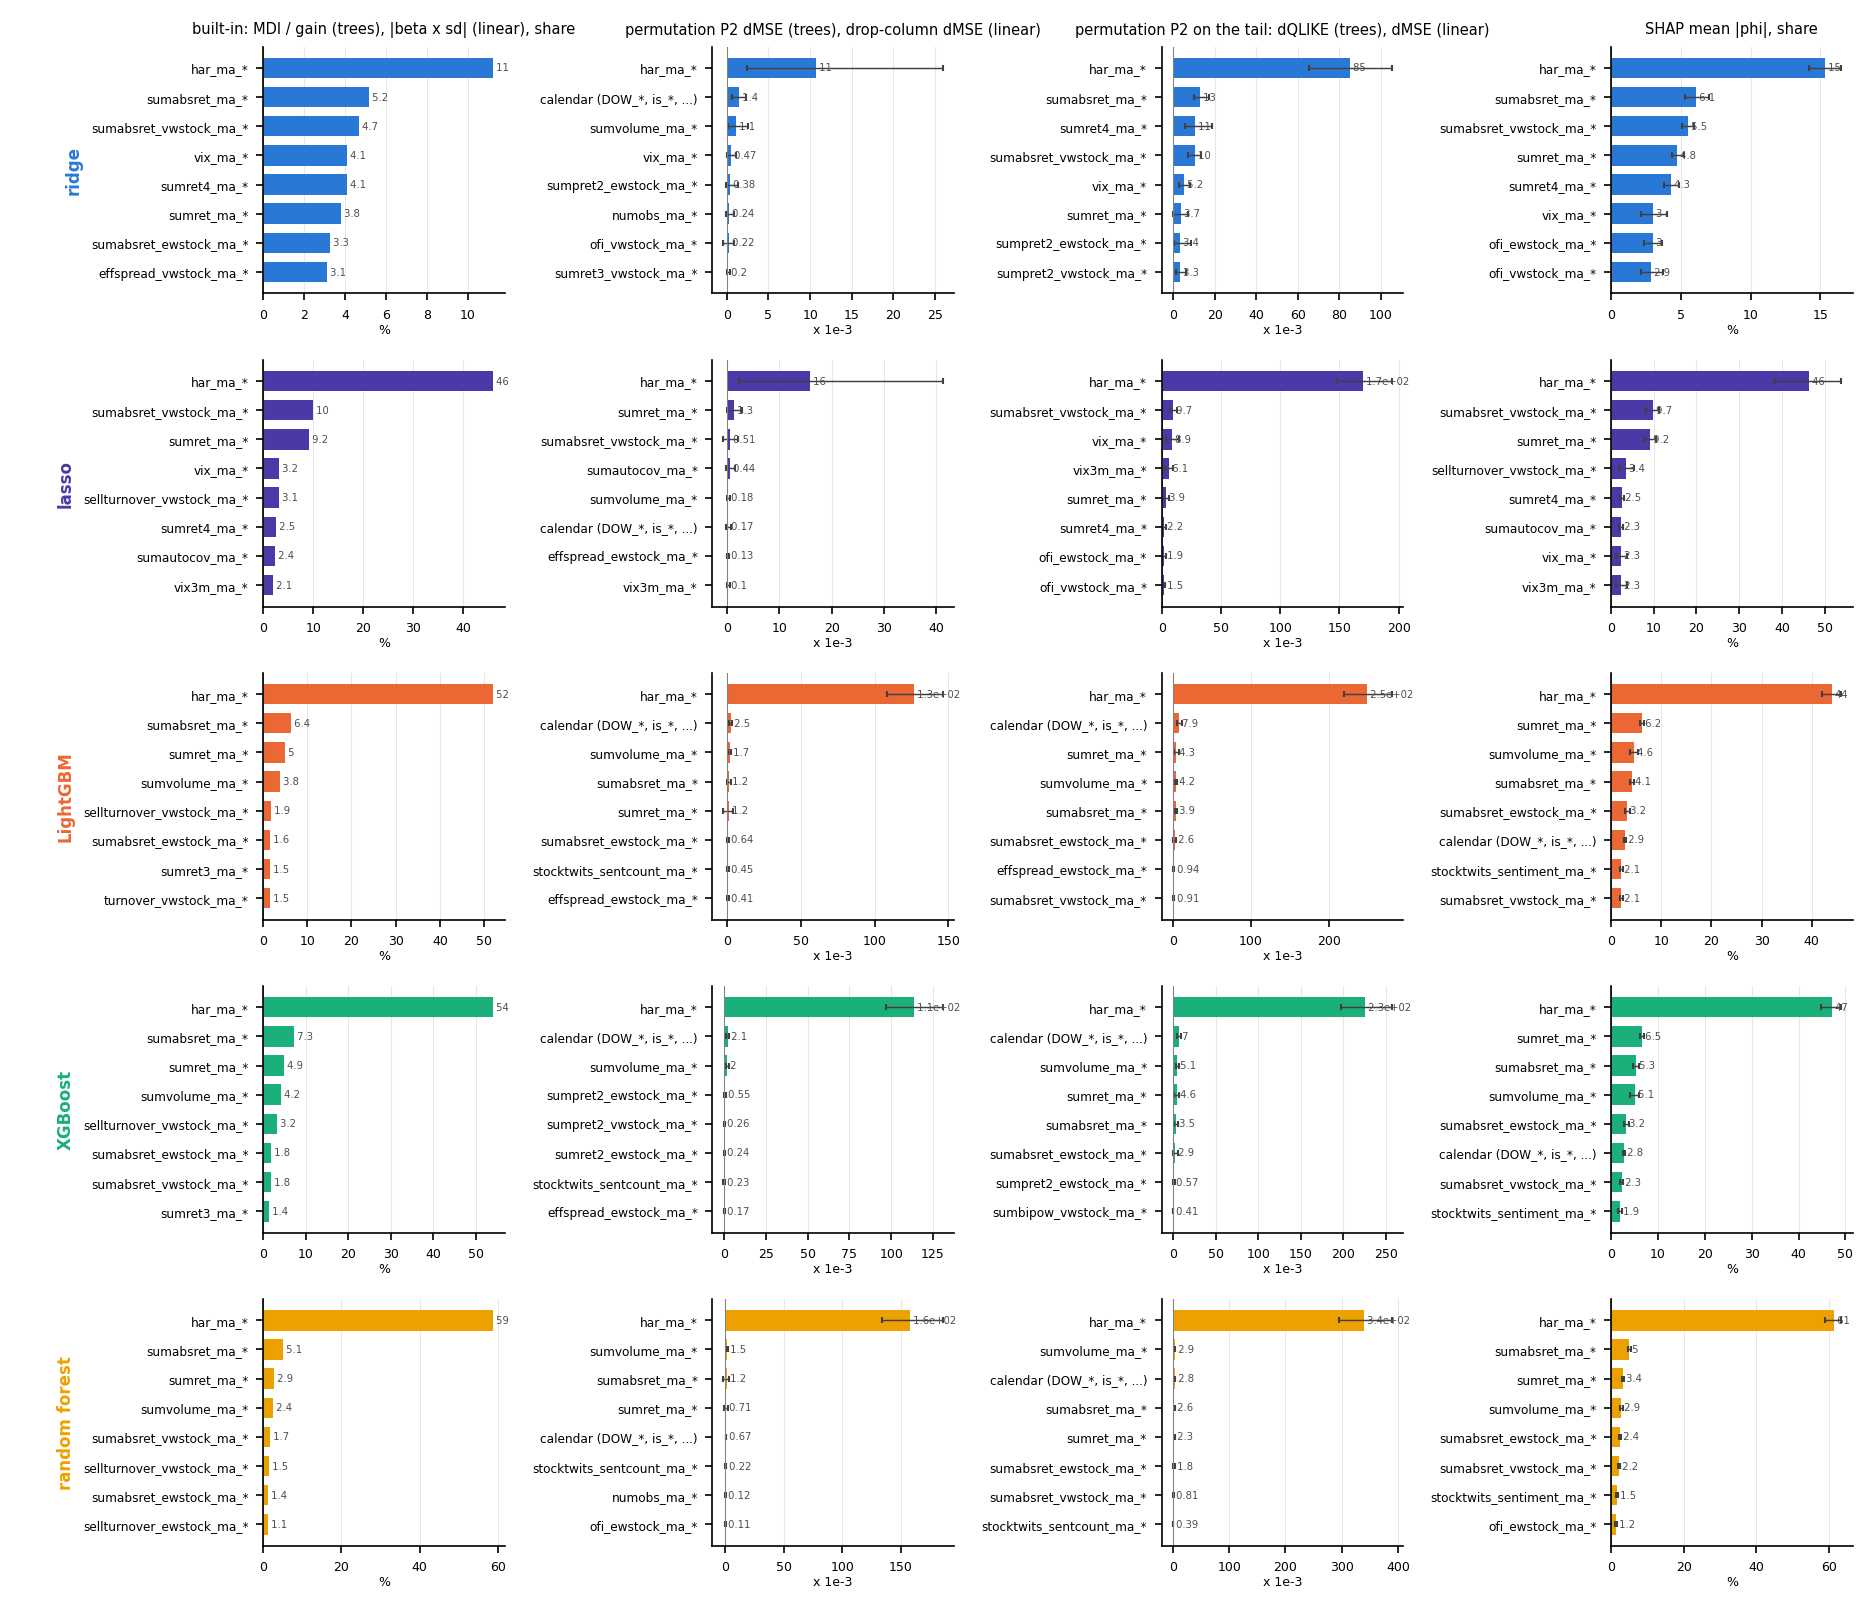
\includegraphics[width=\linewidth]{../results/feature_importance_1530_dedup/fig_ranked_all_features.png}
% % 2026-10-15 (notation pass): parked -- code jargon (refits, P2, fit space, held-out tail, |beta . sd|); standard measure names
% % \caption{Draft, measures under review. The leading series by each measure, per model (rows), all features
% % (\rhappNcolsAll{} columns in \rhappFiSeries{} series), averaged over the \rhappFiRefits{} refits. Columns: the
% % built-in measure (MDI\,/\,gain share for the trees, $|\beta\cdot\mathrm{sd}|$ share for the linear models);
% % permutation P2, $\Delta$MSE in the fit space (trees), or drop-column $\Delta$MSE (linear); permutation P2 on the
% % held-out tail, $\Delta$QLIKE (trees) or $\Delta$MSE (linear); SHAP mean $|\phi|$ share. Whiskers: 95\,\%
% % circular-block bootstrap intervals over refits (block \rhappFiBootBlock), which the paper's point-estimate convention
% % would drop.}
% \caption{Draft, measures under review. Leading predictor series by importance measure, for each closing-interval
% model (rows), on the full predictor set (\rhappNcolsAll{} columns in \rhappFiSeries{} series), averaged over the
% \rhappFiRefits{} re-estimations. Columns: the model's built-in measure (share of mean decrease in impurity, MDI, or of
% gain for the trees; share of $|\beta_j|\,\mathrm{sd}(x_j)$ for the linear models); permutation importance, the
% increase in squared-error loss on the scale of the target $y_t$ (trees), or the drop-column increase in squared-error
% loss (linear models); permutation importance on the out-of-sample block, the increase in QLIKE (trees) or in
% squared-error loss (linear models); and the share of the mean absolute SHAP value $|\phi|$. Permutation importance
% replaces a predictor's values with rows drawn from the estimation window. Whiskers: 95\% circular block-bootstrap
% confidence intervals across re-estimations (block length \rhappFiBootBlock); elsewhere the paper reports point
% estimates.}
% \label{fig:rh_app_fi_ranked}
% \end{figure}

% Source: results/feature_importance_1530_dedup/fig_rank_heatmap_all_features_series.png (raster)
% 2026-10-15 (user): parked -- non-standard figure; focus on legible tables
% \begin{figure}[htbp]
% \centering
% 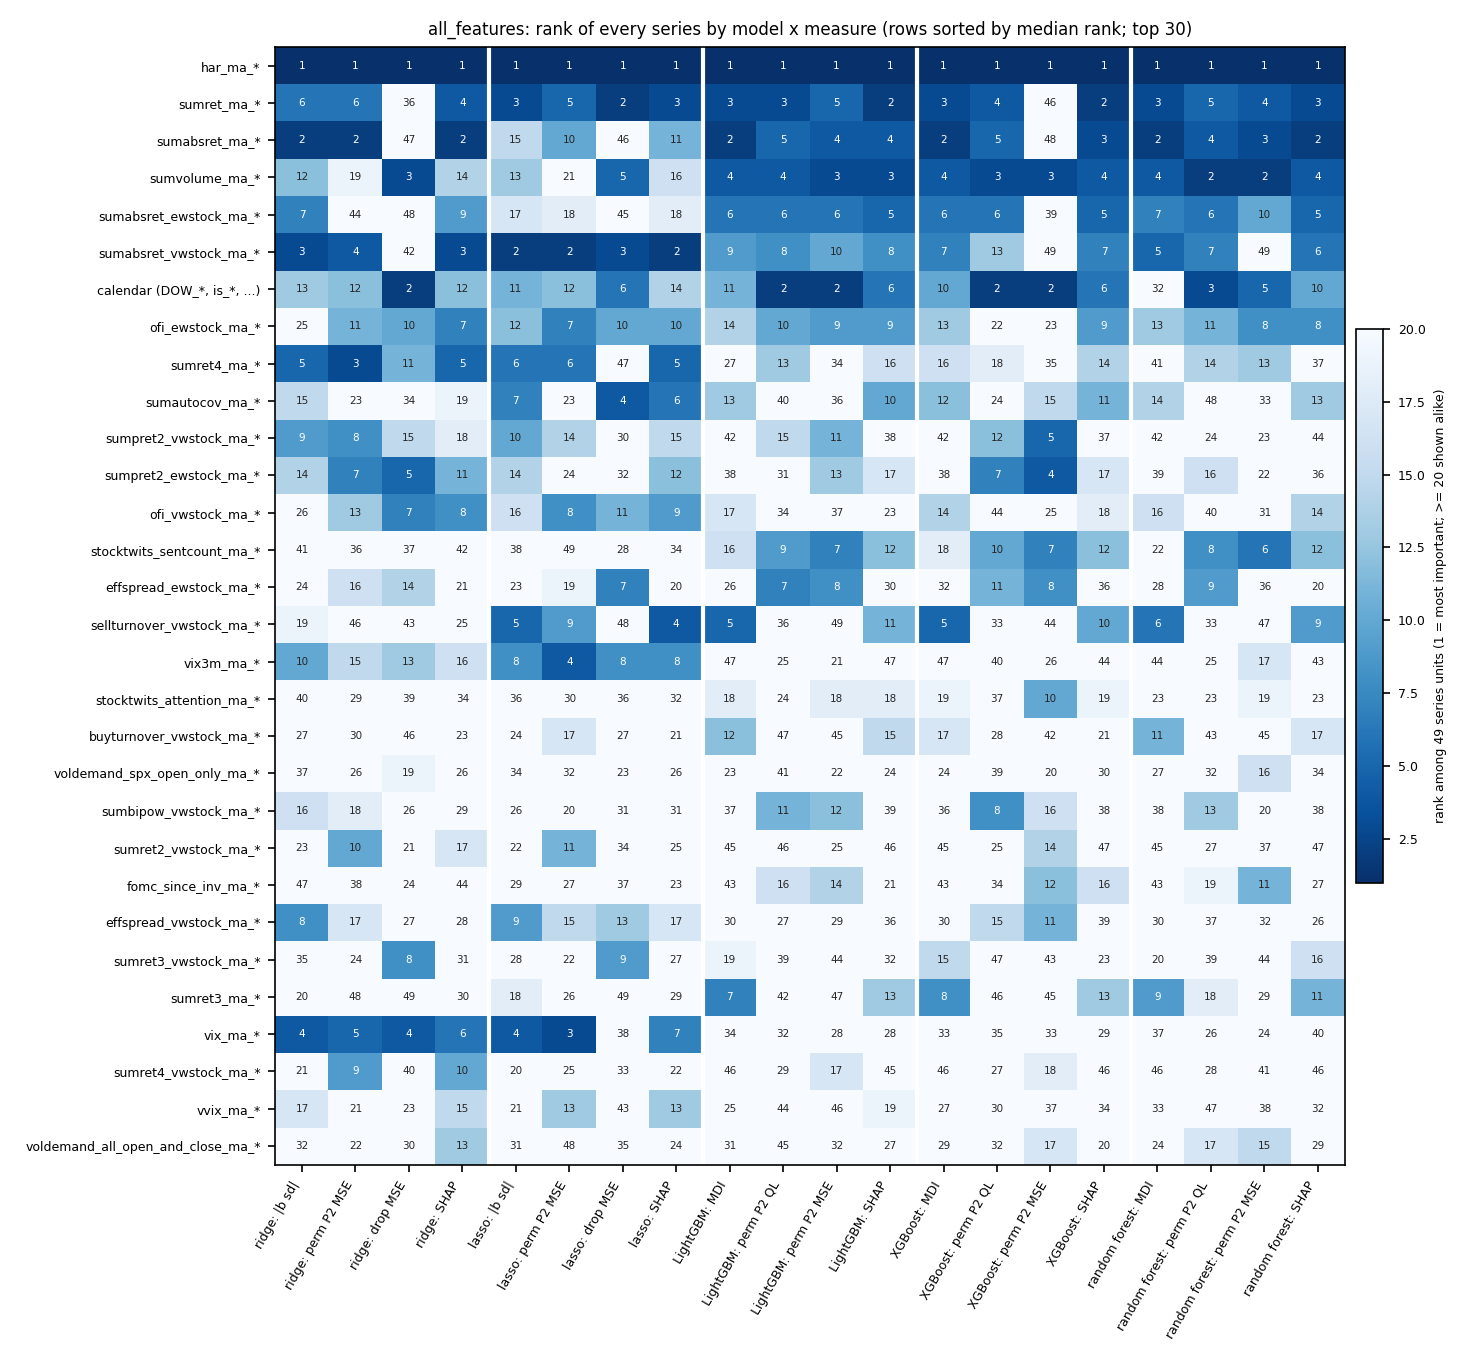
\includegraphics[width=\linewidth]{../results/feature_importance_1530_dedup/fig_rank_heatmap_all_features_series.png}
% % 2026-10-15 (notation pass): parked -- code jargon (all features, |beta . sd|, P2); American spelling
% % \caption{Draft, measures under review. The rank of each series among the \rhappFiSeries{} by model $\times$ measure,
% % all features (1 = most important; the colour scale saturates, so the low ranks share a shade); rows sorted by median rank,
% % the leading rows shown. Measures: $|\beta\cdot\mathrm{sd}|$ and drop-column $\Delta$MSE (linear), MDI\,/\,gain
% % (trees), permutation P2 on QLIKE (QL) or MSE, and SHAP.}
% \caption{Draft, measures under review. Rank of each predictor series among the \rhappFiSeries{}, by model and
% importance measure, closing-interval models on the full predictor set (1 = most important; the color scale saturates,
% so low ranks share a shade). Rows are sorted by median rank; the leading rows are shown. Measures:
% $|\beta_j|\,\mathrm{sd}(x_j)$ and the drop-column increase in squared-error loss (linear models), MDI or gain (trees),
% permutation importance on QLIKE (QL) or on squared-error loss (MSE), and SHAP.}
% \label{fig:rh_app_fi_heat_series}
% \end{figure}

% Source: results/feature_importance_1530_dedup/fig_rank_heatmap_all_features_cluster.png (raster)
% 2026-10-15 (user): parked -- non-standard figure; focus on legible tables
% \begin{figure}[htbp]
% \centering
% 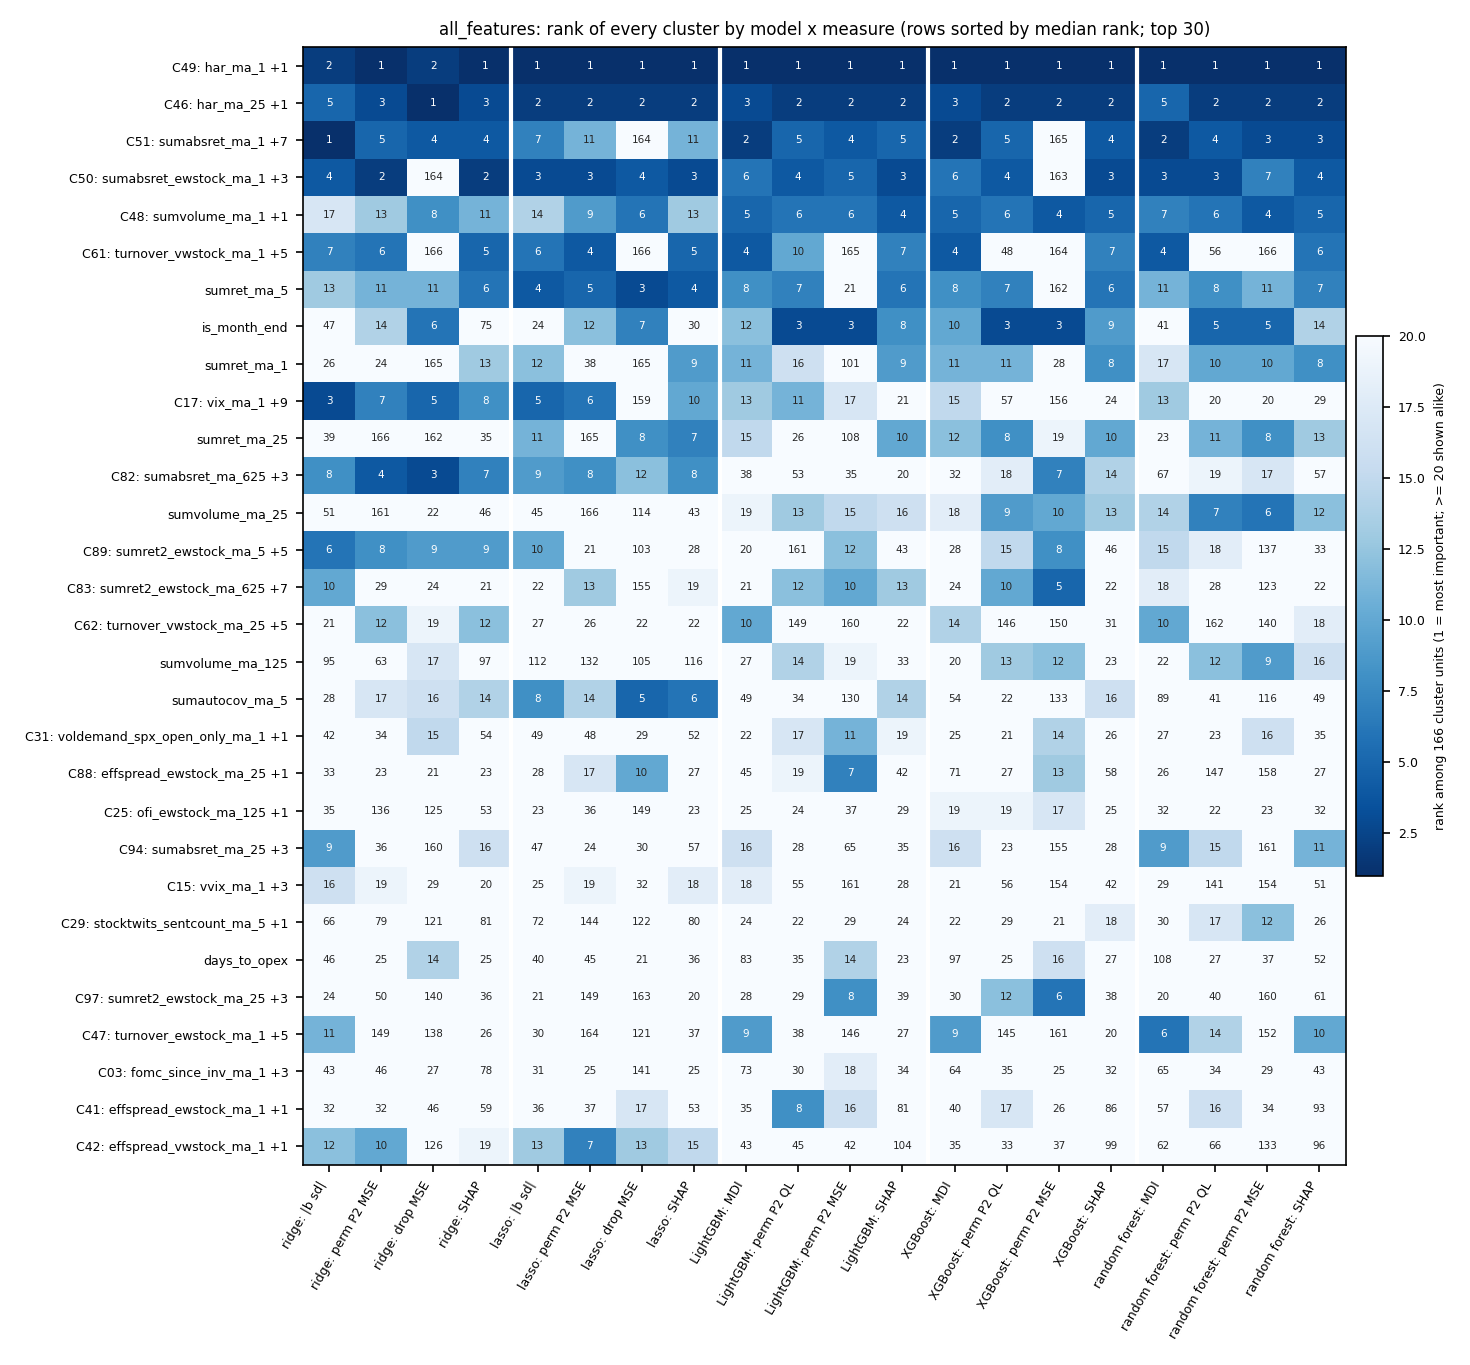
\includegraphics[width=\linewidth]{../results/feature_importance_1530_dedup/fig_rank_heatmap_all_features_cluster.png}
% % 2026-10-15 (notation pass): parked -- wording; explicit cross-reference
% % \caption{Draft, measures under review. The same at the cluster level: \rhappFiClusters{} clusters of columns, every
% % pair in a cluster correlated at $|\rho| \ge \rhappFiClusterCorr$ (complete linkage). A cluster is named by its first
% % member and the number of further members ($+k$); single columns keep their name.}
% \caption{Draft, measures under review. As Figure~\ref{fig:rh_app_fi_heat_series}, at the cluster level:
% \rhappFiClusters{} clusters of columns, formed by complete-linkage clustering so that every pair of columns within a
% cluster has absolute correlation $|\rho| \ge \rhappFiClusterCorr$. A cluster is labeled by its first member and the
% number of further members ($+k$); singleton columns keep their own label.}
% \label{fig:rh_app_fi_heat_cluster}
% \end{figure}

% Source: figures/feature_importance_1530_over_time.pdf (vector)
% 2026-10-15 (user): parked -- non-standard figure; focus on legible tables
% \begin{figure}[htbp]
% \centering
% 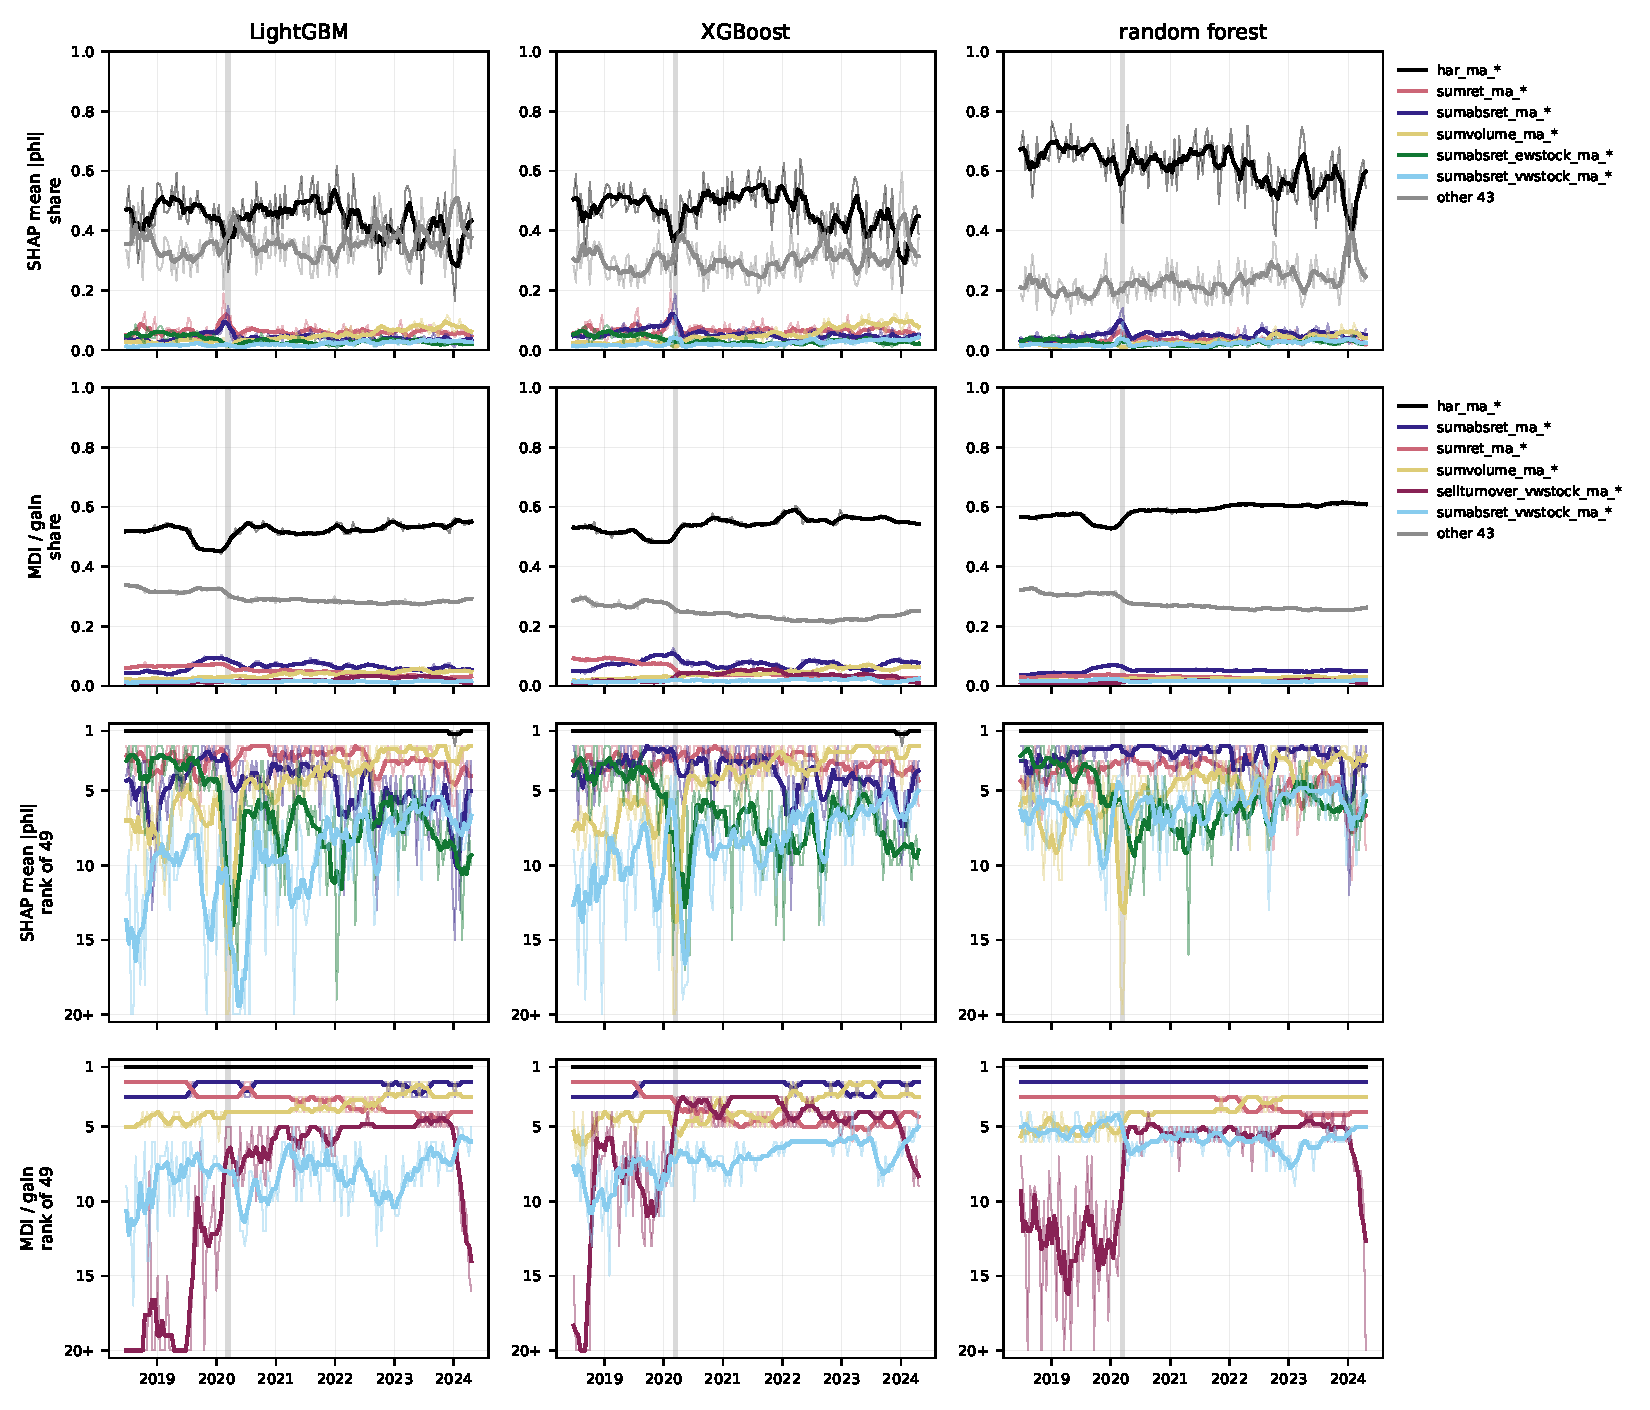
\includegraphics[width=\linewidth]{figures/feature_importance_1530_over_time.pdf}
% % 2026-10-15 (notation pass): parked -- code jargon (refit, held-out tail, har_ma_*, sessions); American spelling
% % \caption{Draft, measures under review. Importance over time, the three trees, all features, series level. Rows 1--2:
% % each series' share of the refit's total SHAP mean $|\phi|$ (on the held-out tail) and MDI\,/\,gain; rows 3--4: the
% % same series' rank among the \rhappFiSeries{} (ranks beyond \rhappFiTimeCap{} drawn at \rhappFiTimeCap). Lines:
% % \texttt{har\_ma\_*} and the next \rhappFiTimeTop{} series by overall share, the rest summed as `other'. Thin: one
% % point per refit (every \rhappFiRefitEvery{} sessions, \rhappFiRefits{} refits), at its tail's start date; thick: a
% % \rhappFiTimeSmooth-refit centred rolling mean. Grey band: the 2020 crash tails. Shares are split credit: correlated
% % inputs share it, and MDI and SHAP favour many-valued columns.}
% \caption{Draft, measures under review. Predictor importance over time for the three closing-interval tree models on
% the full predictor set, at the series level. Rows 1--2: each series' share of the re-estimation's total mean absolute
% SHAP value (on its out-of-sample block) and of its total MDI or gain; rows 3--4: the same series' rank among the
% \rhappFiSeries{} (ranks beyond \rhappFiTimeCap{} drawn at \rhappFiTimeCap). Lines: the HAR components
% $\bar y^{(k)}_t$ and the next \rhappFiTimeTop{} series by overall share, with the remainder summed as `other'. Thin
% lines: one point per re-estimation (every \rhappFiRefitEvery{} trading days, \rhappFiRefits{} re-estimations), dated
% at the start of its out-of-sample block, i.e., the trading days it forecasts before the next re-estimation; thick
% lines: a centered rolling mean over \rhappFiTimeSmooth{} re-estimations. Gray band: out-of-sample blocks in the 2020
% crash. Shares split credit: correlated predictors share it, and MDI and SHAP favor columns with many distinct
% values.}
% \label{fig:rh_app_fi_time_trees}
% \end{figure}

% Source: figures/feature_importance_1530_over_time_linear.pdf (vector)
% 2026-10-15 (user): parked -- non-standard figure; focus on legible tables
% \begin{figure}[htbp]
% \centering
% 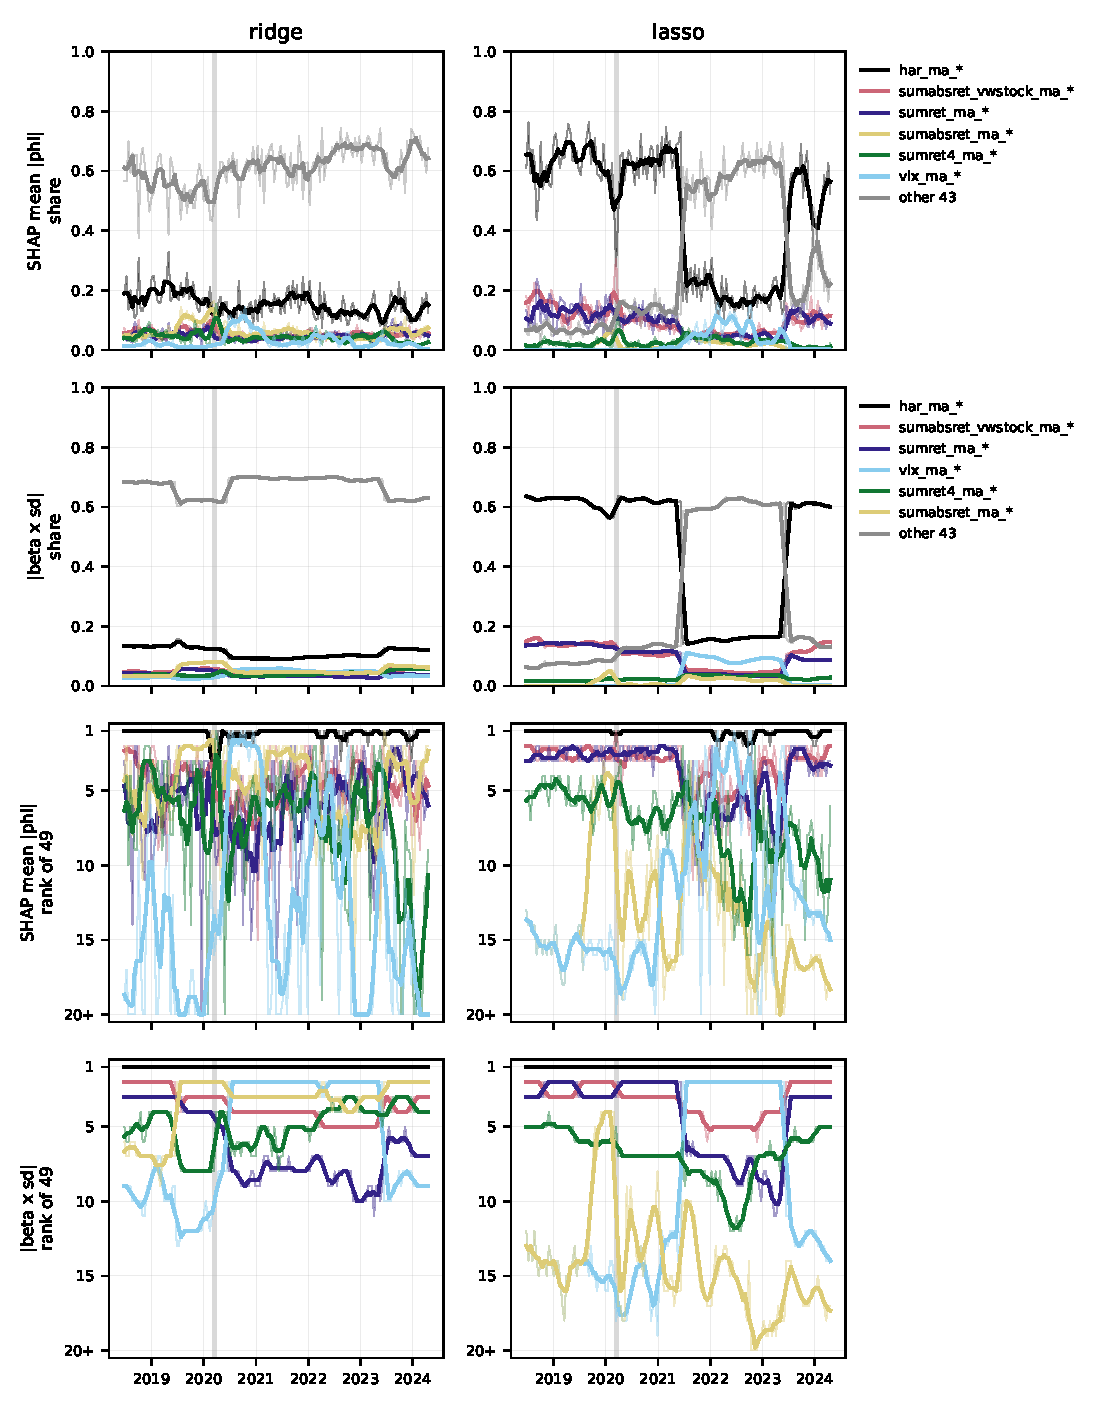
\includegraphics[width=\linewidth,height=0.78\textheight,keepaspectratio]{figures/feature_importance_1530_over_time_linear.pdf}
% % 2026-10-15 (notation pass): parked -- code jargon (per-bar, refit's window, |beta . sd|); explicit cross-reference
% % \caption{Draft, measures under review. The same for the per-bar ridge and lasso: SHAP mean $|\phi|$, with
% % $\phi_{t,j} = \beta_j(x_{t,j} - \bar x_j)$ and the window mean as background, and $|\beta\cdot\mathrm{sd}|$ (the
% % coefficient times the column's standard deviation in the refit's window, summed over a series' columns), as shares
% % and as ranks. A linear model spreads or concentrates credit across correlated columns differently from a tree, so
% % the shares compare over time within a model, not across the two figures.}
% \caption{Draft, measures under review. As Figure~\ref{fig:rh_app_fi_time_trees}, for the closing-interval ridge and
% lasso: the mean absolute SHAP value, with $\phi_{t,j} = \beta_j(x_{t,j} - \bar x_j)$ and the estimation-window mean
% $\bar x_j$ as background, and $|\beta_j|\,\mathrm{sd}(x_j)$, the absolute coefficient times the column's standard
% deviation in the estimation window, summed over a series' columns; both as shares and as ranks. A linear model
% spreads or concentrates credit across correlated columns differently from a tree, so the shares are comparable over
% time within a model, not across the two figures.}
% \label{fig:rh_app_fi_time_linear}
% \end{figure}

% Source: generated/appendix_campaign_16h_featimp.tex (re-laid out: generated/rehaul_app_featimp_harma.tex)
\begin{table}[htbp]
\centering
\small
\begin{threeparttable}
% 2026-10-15 (notation pass): parked -- code identifier har_ma_* and 'ladder' replaced by 'HAR components'
% \caption{Draft, measures under review. The \texttt{har\_ma\_*} ladder's importance in the trees, first pass to
% the current design (all features), old $\to$ new.}
% 2026-10-15 (table legibility): short caption, details in the notes; notes cut to about five sentences, method
% details referred to Methods. The pre-notation-pass caption and notes are parked in the comments here.
\caption{Importance of the HAR components in the tree models}
\label{tab:rh_app_fi_harma}
% AUTO-GENERATED by writeup/make_rehaul_appendix.py -- do not edit.
% Source: writeup/generated/appendix_campaign_16h_featimp.tex (numbers verbatim; its sources are listed there)
\begin{tabular}{@{}l*{5}{c}@{}}
\toprule
 & MDI & SHAP & Permutation & Close-interaction & MDI \\
Model & share (\%) & share (\%) & $\Delta$QLIKE (\%) & share (\%) & rank \\
\midrule
LightGBM & $57 \to 52$ & $47 \to 44$ & $237 \to 200$ & $22$ & $1 \to 1$ \\
XGBoost & $69 \to 54$ & $55 \to 47$ & $224 \to 181$ & $22$ & $1 \to 1$ \\
Random forest & $62 \to 59$ & $58 \to 61$ & $290 \to 271$ & $54$ & $1 \to 1$ \\
\bottomrule
\end{tabular}

\begin{tablenotes}[flushleft]
\footnotesize
% 2026-10-15 (notation pass): parked -- code jargon (ladder, unmasked, window-masked, P2, tail loss, _x_close)
% \item[] \emph{Notes:} first pass: the old design (with the \rhappNsessionEdge{} session-edge interactions), trees
% unmasked; new: those columns dropped and every tree fit window-masked. MDI and TreeSHAP: the ladder's share of the
% model's total. Perm.\ P2 $\Delta$QLIKE: the loss increase when the ladder's rows are replaced by rows drawn from the
% training window, in \% of the model's tail loss. \texttt{\_x\_close} share: the part of the old ladder's MDI that sat
% on its \rhappNsessionEdgeHalf{} \texttt{\_x\_close} copies. MDI rank among the series. XGBoost and the random forest
% also changed settings between the passes, so their before/after mixes that change with the design and the mask.
\item[] \textit{Notes:} Draft, measures under review. Closing-interval tree models on the full predictor set, first
pass (old) $\to$ current design (new); the first pass includes the \rhappNsessionEdge{} interactions of the HAR
components with the opening- and closing-session dummies and no column screening, the current design drops those
interactions and screens out constant and duplicate columns in every estimation window. MDI and TreeSHAP: the HAR
components' share of the model's total; permutation $\Delta$QLIKE: the increase in QLIKE when their values are
replaced by rows drawn from the estimation window, in percent of the model's out-of-sample loss. Close-interaction
share: the part of the old MDI carried by the \rhappNsessionEdgeHalf{} closing-session interactions, which at the
closing interval are copies of the HAR components; MDI rank: rank among the series. XGBoost and the random forest
also changed hyperparameters between the passes, so their changes mix design, screening and hyperparameters.
\end{tablenotes}
\end{threeparttable}
\end{table}

% % 08b_fi_measures_floats.tex -- the floats of the feature-importance measures in 08_feature_importance.tex (2026-10-15):
% lasso selection counts, ridge coefficient mass, the trees' per-refit SHAP rankings and their SHAP interactions.
% Generator: writeup/make_rehaul_fi.py, from results/rehaul_fi/ (experiments/rehaul_fi_compute.py). Labels:
% tab:rh_fi_summary, tab:rh_fi_linear, tab:rh_fi_trees, tab:rh_fi_inter, fig:rh_fi_linear, fig:rh_fi_ranks,
% fig:rh_fi_inter. Prose macros \rhfi...: generated/rehaul_fi_numbers.tex (loaded here too, for a standalone build).
\ifdefined\rhfiNRefits\else% AUTO-GENERATED by writeup/make_rehaul_fi.py -- do not edit; re-run the script.
% \rhfi... macros for writeup/rehaul/08_feature_importance.tex (results/rehaul_fi/).
\providecommand{\rhfiNRefits}{}\renewcommand{\rhfiNRefits}{147}  % refits, one every 10 sessions
\providecommand{\rhfiNOos}{}\renewcommand{\rhfiNOos}{1{,}469}  % scored held-out sessions
\providecommand{\rhfiP}{}\renewcommand{\rhfiP}{628}  % columns, all features
\providecommand{\rhfiNUnits}{}\renewcommand{\rhfiNUnits}{49}  % units: 47 exogenous series + HAR ladder + calendar
\providecommand{\rhfiNExog}{}\renewcommand{\rhfiNExog}{47}  % exogenous series
\providecommand{\rhfiFirst}{}\renewcommand{\rhfiFirst}{25~June~2018}  % first scored session
\providecommand{\rhfiLast}{}\renewcommand{\rhfiLast}{30~April~2024}  % last scored session
\providecommand{\rhfiWindow}{}\renewcommand{\rhfiWindow}{2{,}000}  % sessions in a training window
\providecommand{\rhfiRefitEvery}{}\renewcommand{\rhfiRefitEvery}{10}  % sessions between refits
\providecommand{\rhfiBackbonePf}{}\renewcommand{\rhfiBackbonePf}{0.01}  % backbone penalty factor
\providecommand{\rhfiNBuckets}{}\renewcommand{\rhfiNBuckets}{8}  % exogenous buckets
\providecommand{\rhfiOldBlock}{}\renewcommand{\rhfiOldBlock}{250}  % sessions between the old arm's penalty re-choices
\providecommand{\rhfiNPairs}{}\renewcommand{\rhfiNPairs}{1{,}176}  % series pairs
\providecommand{\rhfiNProbeCols}{}\renewcommand{\rhfiNProbeCols}{631}  % columns of a probe fit
\providecommand{\rhfiTopWPairs}{}\renewcommand{\rhfiTopWPairs}{50}  % pairs in the interaction W
\providecommand{\rhfiProbeLevels}{}\renewcommand{\rhfiProbeLevels}{20}  % values of the few-valued noise column
\providecommand{\rhfiRidgeAlpha}{}\renewcommand{\rhfiRidgeAlpha}{\ensuremath{10^{3}}}
\providecommand{\rhfiLassoAlpha}{}\renewcommand{\rhfiLassoAlpha}{\ensuremath{10^{-2}}}
\providecommand{\rhfiLassoNzMed}{}\renewcommand{\rhfiLassoNzMed}{30}  % median nonzero coefficients per refit
\providecommand{\rhfiLassoNzMin}{}\renewcommand{\rhfiLassoNzMin}{27}
\providecommand{\rhfiLassoNzMax}{}\renewcommand{\rhfiLassoNzMax}{35}
\providecommand{\rhfiLassoExogNzMed}{}\renewcommand{\rhfiLassoExogNzMed}{14}  % ... exogenous columns
\providecommand{\rhfiLassoColsEver}{}\renewcommand{\rhfiLassoColsEver}{60}  % columns nonzero in >= 1 refit
\providecommand{\rhfiLassoColsMajority}{}\renewcommand{\rhfiLassoColsMajority}{29}  % columns nonzero in >= half the refits
\providecommand{\rhfiLassoExogEver}{}\renewcommand{\rhfiLassoExogEver}{27}  % exogenous series with a nonzero column in >= 1 refit
\providecommand{\rhfiLassoExogMajority}{}\renewcommand{\rhfiLassoExogMajority}{11}  % ... in >= half the refits
\providecommand{\rhfiLassoExogAlways}{}\renewcommand{\rhfiLassoExogAlways}{3}  % ... in every refit
\providecommand{\rhfiLassoAlwaysList}{}\renewcommand{\rhfiLassoAlwaysList}{\texttt{sumret}, \texttt{sumabsret\_vwstock}, \texttt{sumautocov}}  % exogenous series selected in every refit
\providecommand{\rhfiLassoProbeSel}{}\renewcommand{\rhfiLassoProbeSel}{1}  % continuous probe selected, of the probe fits
\providecommand{\rhfiLassoProbeSelLevels}{}\renewcommand{\rhfiLassoProbeSelLevels}{0}
\providecommand{\rhfiLassoProbeSelBinary}{}\renewcommand{\rhfiLassoProbeSelBinary}{0}
\providecommand{\rhfiNProbe}{}\renewcommand{\rhfiNProbe}{49}  % probe refits (every third)
\providecommand{\rhfiLassoW}{}\renewcommand{\rhfiLassoW}{0.74}  % Kendall W of the per-refit series ranks by sum |beta|
\providecommand{\rhfiLassoBackboneShare}{}\renewcommand{\rhfiLassoBackboneShare}{88}  % median share of sum |beta| on the backbone, %
\providecommand{\rhfiOldLassoSpearman}{}\renewcommand{\rhfiOldLassoSpearman}{0.70}  % Spearman, selection share: pre-tuned vs re-tuned one-penalty lasso
\providecommand{\rhfiOldLassoNzMed}{}\renewcommand{\rhfiOldLassoNzMed}{23}  % re-tuned lasso: median nonzero per refit
\providecommand{\rhfiOldLassoExogMajority}{}\renewcommand{\rhfiOldLassoExogMajority}{18}
\providecommand{\rhfiRidgeTopOne}{}\renewcommand{\rhfiRidgeTopOne}{Calendar}
\providecommand{\rhfiRidgeTopOneShare}{}\renewcommand{\rhfiRidgeTopOneShare}{31.0}  % % of sum |beta|
\providecommand{\rhfiRidgeTopTwo}{}\renewcommand{\rhfiRidgeTopTwo}{HAR ladder}
\providecommand{\rhfiRidgeTopTwoShare}{}\renewcommand{\rhfiRidgeTopTwoShare}{22.8}  % % of sum |beta|
\providecommand{\rhfiRidgeTopThree}{}\renewcommand{\rhfiRidgeTopThree}{\texttt{sumret}}
\providecommand{\rhfiRidgeTopThreeShare}{}\renewcommand{\rhfiRidgeTopThreeShare}{3.6}  % % of sum |beta|
\providecommand{\rhfiRidgeTopFour}{}\renewcommand{\rhfiRidgeTopFour}{\texttt{sumabsret\_vwstock}}
\providecommand{\rhfiRidgeTopFourShare}{}\renewcommand{\rhfiRidgeTopFourShare}{2.2}  % % of sum |beta|
\providecommand{\rhfiRidgeSdTopOne}{}\renewcommand{\rhfiRidgeSdTopOne}{HAR ladder}
\providecommand{\rhfiRidgeSdTopOneShare}{}\renewcommand{\rhfiRidgeSdTopOneShare}{30.6}  % % of sum |beta| sd
\providecommand{\rhfiRidgeSdTopTwo}{}\renewcommand{\rhfiRidgeSdTopTwo}{Calendar}
\providecommand{\rhfiRidgeSdTopTwoShare}{}\renewcommand{\rhfiRidgeSdTopTwoShare}{9.3}  % % of sum |beta| sd
\providecommand{\rhfiRidgeSdTopThree}{}\renewcommand{\rhfiRidgeSdTopThree}{\texttt{sumret}}
\providecommand{\rhfiRidgeSdTopThreeShare}{}\renewcommand{\rhfiRidgeSdTopThreeShare}{4.5}  % % of sum |beta| sd
\providecommand{\rhfiRidgeTopExog}{}\renewcommand{\rhfiRidgeTopExog}{\texttt{sumret}}
\providecommand{\rhfiRidgeTopExogShare}{}\renewcommand{\rhfiRidgeTopExogShare}{3.6}
\providecommand{\rhfiRidgeBackboneShare}{}\renewcommand{\rhfiRidgeBackboneShare}{54}  % median share of sum |beta| on the backbone, %
\providecommand{\rhfiRidgeW}{}\renewcommand{\rhfiRidgeW}{0.85}
\providecommand{\rhfiRidgeAllSelected}{}\renewcommand{\rhfiRidgeAllSelected}{49}  % units with N_A = K under the ridge
\providecommand{\rhfiLassoProbeRate}{}\renewcommand{\rhfiLassoProbeRate}{2.0}  % continuous probe's selection rate, %
\providecommand{\rhfiLassoColsAboveProbe}{}\renewcommand{\rhfiLassoColsAboveProbe}{54}  % columns selected more often than the continuous probe
\providecommand{\rhfiLassoSeriesAboveProbe}{}\renewcommand{\rhfiLassoSeriesAboveProbe}{23}  % exogenous series with such a column
\providecommand{\rhfiLassoTopCol}{}\renewcommand{\rhfiLassoTopCol}{\texttt{is\_month\_end}}
\providecommand{\rhfiRidgeSpearmanSd}{}\renewcommand{\rhfiRidgeSpearmanSd}{0.85}  % Spearman, series sum|beta| vs sum|beta| sd
\providecommand{\rhfiRidgeProbeBeat}{}\renewcommand{\rhfiRidgeProbeBeat}{107}  % columns with |beta| above the continuous probe's in most probe fits
\providecommand{\rhfiRidgeProbeBeatSeries}{}\renewcommand{\rhfiRidgeProbeBeatSeries}{38}
\providecommand{\rhfiScaleValueN}{}\renewcommand{\rhfiScaleValueN}{282}
\providecommand{\rhfiScaleValueSd}{}\renewcommand{\rhfiScaleValueSd}{0.84}  % median window sd, value ladders
\providecommand{\rhfiScaleValueSdLo}{}\renewcommand{\rhfiScaleValueSdLo}{0.03}
\providecommand{\rhfiScaleValueSdHi}{}\renewcommand{\rhfiScaleValueSdHi}{1.76}
\providecommand{\rhfiScaleValueIqr}{}\renewcommand{\rhfiScaleValueIqr}{0.94}  % median window IQR, value ladders
\providecommand{\rhfiScaleFlagN}{}\renewcommand{\rhfiScaleFlagN}{324}
\providecommand{\rhfiScaleFlagSd}{}\renewcommand{\rhfiScaleFlagSd}{0.022}  % median window sd, availability / activity ladders
\providecommand{\rhfiScaleFlagSdHi}{}\renewcommand{\rhfiScaleFlagSdHi}{0.17}
\providecommand{\rhfiScaleCalSd}{}\renewcommand{\rhfiScaleCalSd}{0.39}  % median window sd, calendar
\providecommand{\rhfiScaleHarSd}{}\renewcommand{\rhfiScaleHarSd}{1.07}  % median window sd, HAR ladder
\providecommand{\rhfiLgbmW}{}\renewcommand{\rhfiLgbmW}{0.57}  % lgbm: Kendall W, per-refit series ranks
\providecommand{\rhfiLgbmWCols}{}\renewcommand{\rhfiLgbmWCols}{0.91}  % lgbm: Kendall W, column ranks
\providecommand{\rhfiLgbmTopOne}{}\renewcommand{\rhfiLgbmTopOne}{HAR ladder}
\providecommand{\rhfiLgbmTopOneRank}{}\renewcommand{\rhfiLgbmTopOneRank}{1.0}  % mean rank
\providecommand{\rhfiLgbmTopTwo}{}\renewcommand{\rhfiLgbmTopTwo}{\texttt{sumret}}
\providecommand{\rhfiLgbmTopTwoRank}{}\renewcommand{\rhfiLgbmTopTwoRank}{2.9}  % mean rank
\providecommand{\rhfiLgbmTopThree}{}\renewcommand{\rhfiLgbmTopThree}{\texttt{sumabsret}}
\providecommand{\rhfiLgbmTopThreeRank}{}\renewcommand{\rhfiLgbmTopThreeRank}{4.8}  % mean rank
\providecommand{\rhfiLgbmSpBorda}{}\renewcommand{\rhfiLgbmSpBorda}{0.90}  % Spearman, mean rank vs top-10 Borda
\providecommand{\rhfiLgbmSpGlobal}{}\renewcommand{\rhfiLgbmSpGlobal}{0.96}  % Spearman, mean rank vs global mean |phi|
\providecommand{\rhfiLgbmSpLocal}{}\renewcommand{\rhfiLgbmSpLocal}{1.000}  % Spearman, mean ranks local refit vs stored
\providecommand{\rhfiLgbmProbeRank}{}\renewcommand{\rhfiLgbmProbeRank}{83}  % median rank of the continuous probe, 631 columns
\providecommand{\rhfiLgbmProbeCols}{}\renewcommand{\rhfiLgbmProbeCols}{60}  % columns above the continuous probe in most probe fits
\providecommand{\rhfiLgbmProbeSeries}{}\renewcommand{\rhfiLgbmProbeSeries}{27}  % exogenous series with such a column
\providecommand{\rhfiLgbmTopCol}{}\renewcommand{\rhfiLgbmTopCol}{\texttt{har\_ma\_1}}  % column with the lowest mean rank
\providecommand{\rhfiLgbmTopColRank}{}\renewcommand{\rhfiLgbmTopColRank}{1.3}
\providecommand{\rhfiLgbmTopColTwo}{}\renewcommand{\rhfiLgbmTopColTwo}{\texttt{har\_ma\_5}}
\providecommand{\rhfiLgbmTopColTwoRank}{}\renewcommand{\rhfiLgbmTopColTwoRank}{1.8}
\providecommand{\rhfiLgbmPredGap}{}\renewcommand{\rhfiLgbmPredGap}{0}  % max |local refit - stored refit| forecast
\providecommand{\rhfiLgbmInterW}{}\renewcommand{\rhfiLgbmInterW}{0.45}  % Kendall W of per-refit pair ranks, top-50 pairs
\providecommand{\rhfiLgbmInterRatio}{}\renewcommand{\rhfiLgbmInterRatio}{90}  % sum of series-pair interactions / sum main, %
\providecommand{\rhfiLgbmInterSpGlobal}{}\renewcommand{\rhfiLgbmInterSpGlobal}{0.99}
\providecommand{\rhfiLgbmInterFloor}{}\renewcommand{\rhfiLgbmInterFloor}{0.49}  % probe floor x 1e3
\providecommand{\rhfiLgbmInterAboveFloor}{}\renewcommand{\rhfiLgbmInterAboveFloor}{116}  % series pairs above the probe floor
\providecommand{\rhfiLgbmInterTopA}{}\renewcommand{\rhfiLgbmInterTopA}{HAR ladder}
\providecommand{\rhfiLgbmInterTopB}{}\renewcommand{\rhfiLgbmInterTopB}{\texttt{sumabsret}}
\providecommand{\rhfiLgbmInterTopVal}{}\renewcommand{\rhfiLgbmInterTopVal}{12.6}  % x 1e3
\providecommand{\rhfiLgbmHTop}{}\renewcommand{\rhfiLgbmHTop}{0.33}  % H^2 of the top series pair (pooled), %
\providecommand{\rhfiLgbmHMin}{}\renewcommand{\rhfiLgbmHMin}{0.02}  % min H^2 over the top-10 series pairs, %
\providecommand{\rhfiLgbmHMax}{}\renewcommand{\rhfiLgbmHMax}{0.33}  % max H^2 over the top-10 series pairs, %
\providecommand{\rhfiLgbmHMinTop}{}\renewcommand{\rhfiLgbmHMinTop}{0.19}  % top pair: interaction PD var / smaller main PD var
\providecommand{\rhfiLgbmHMinLo}{}\renewcommand{\rhfiLgbmHMinLo}{0.05}  % ... min over the top-10 series pairs
\providecommand{\rhfiLgbmHMinHi}{}\renewcommand{\rhfiLgbmHMinHi}{0.54}  % ... max
\providecommand{\rhfiLgbmHColTop}{}\renewcommand{\rhfiLgbmHColTop}{0.36}  % H^2 of the top column pair, %
\providecommand{\rhfiLgbmHMinColTop}{}\renewcommand{\rhfiLgbmHMinColTop}{0.02}  % ... min-normalised
\providecommand{\rhfiLgbmMainTopVal}{}\renewcommand{\rhfiLgbmMainTopVal}{195}  % largest global mean |phi_A| x 1e3
\providecommand{\rhfiLgbmWithinTop}{}\renewcommand{\rhfiLgbmWithinTop}{HAR ladder}
\providecommand{\rhfiLgbmWithinTopVal}{}\renewcommand{\rhfiLgbmWithinTopVal}{18.7}
\providecommand{\rhfiXgbW}{}\renewcommand{\rhfiXgbW}{0.60}  % xgb: Kendall W, per-refit series ranks
\providecommand{\rhfiXgbWCols}{}\renewcommand{\rhfiXgbWCols}{0.90}  % xgb: Kendall W, column ranks
\providecommand{\rhfiXgbTopOne}{}\renewcommand{\rhfiXgbTopOne}{HAR ladder}
\providecommand{\rhfiXgbTopOneRank}{}\renewcommand{\rhfiXgbTopOneRank}{1.0}  % mean rank
\providecommand{\rhfiXgbTopTwo}{}\renewcommand{\rhfiXgbTopTwo}{\texttt{sumret}}
\providecommand{\rhfiXgbTopTwoRank}{}\renewcommand{\rhfiXgbTopTwoRank}{3.0}  % mean rank
\providecommand{\rhfiXgbTopThree}{}\renewcommand{\rhfiXgbTopThree}{\texttt{sumabsret}}
\providecommand{\rhfiXgbTopThreeRank}{}\renewcommand{\rhfiXgbTopThreeRank}{3.9}  % mean rank
\providecommand{\rhfiXgbSpBorda}{}\renewcommand{\rhfiXgbSpBorda}{0.87}  % Spearman, mean rank vs top-10 Borda
\providecommand{\rhfiXgbSpGlobal}{}\renewcommand{\rhfiXgbSpGlobal}{0.97}  % Spearman, mean rank vs global mean |phi|
\providecommand{\rhfiXgbSpLocal}{}\renewcommand{\rhfiXgbSpLocal}{0.993}  % Spearman, mean ranks local refit vs stored
\providecommand{\rhfiXgbProbeRank}{}\renewcommand{\rhfiXgbProbeRank}{110}  % median rank of the continuous probe, 631 columns
\providecommand{\rhfiXgbProbeCols}{}\renewcommand{\rhfiXgbProbeCols}{78}  % columns above the continuous probe in most probe fits
\providecommand{\rhfiXgbProbeSeries}{}\renewcommand{\rhfiXgbProbeSeries}{35}  % exogenous series with such a column
\providecommand{\rhfiXgbTopCol}{}\renewcommand{\rhfiXgbTopCol}{\texttt{har\_ma\_1}}  % column with the lowest mean rank
\providecommand{\rhfiXgbTopColRank}{}\renewcommand{\rhfiXgbTopColRank}{1.3}
\providecommand{\rhfiXgbTopColTwo}{}\renewcommand{\rhfiXgbTopColTwo}{\texttt{har\_ma\_5}}
\providecommand{\rhfiXgbTopColTwoRank}{}\renewcommand{\rhfiXgbTopColTwoRank}{1.8}
\providecommand{\rhfiXgbPredGap}{}\renewcommand{\rhfiXgbPredGap}{0.17}  % max |local refit - stored refit| forecast
\providecommand{\rhfiXgbInterW}{}\renewcommand{\rhfiXgbInterW}{0.47}  % Kendall W of per-refit pair ranks, top-50 pairs
\providecommand{\rhfiXgbInterRatio}{}\renewcommand{\rhfiXgbInterRatio}{74}  % sum of series-pair interactions / sum main, %
\providecommand{\rhfiXgbInterSpGlobal}{}\renewcommand{\rhfiXgbInterSpGlobal}{0.99}
\providecommand{\rhfiXgbInterFloor}{}\renewcommand{\rhfiXgbInterFloor}{0.41}  % probe floor x 1e3
\providecommand{\rhfiXgbInterAboveFloor}{}\renewcommand{\rhfiXgbInterAboveFloor}{115}  % series pairs above the probe floor
\providecommand{\rhfiXgbInterTopA}{}\renewcommand{\rhfiXgbInterTopA}{HAR ladder}
\providecommand{\rhfiXgbInterTopB}{}\renewcommand{\rhfiXgbInterTopB}{\texttt{sumabsret}}
\providecommand{\rhfiXgbInterTopVal}{}\renewcommand{\rhfiXgbInterTopVal}{15.2}  % x 1e3
\providecommand{\rhfiXgbHTop}{}\renewcommand{\rhfiXgbHTop}{0.37}  % H^2 of the top series pair (pooled), %
\providecommand{\rhfiXgbHMin}{}\renewcommand{\rhfiXgbHMin}{0.02}  % min H^2 over the top-10 series pairs, %
\providecommand{\rhfiXgbHMax}{}\renewcommand{\rhfiXgbHMax}{0.68}  % max H^2 over the top-10 series pairs, %
\providecommand{\rhfiXgbHMinTop}{}\renewcommand{\rhfiXgbHMinTop}{0.39}  % top pair: interaction PD var / smaller main PD var
\providecommand{\rhfiXgbHMinLo}{}\renewcommand{\rhfiXgbHMinLo}{0.08}  % ... min over the top-10 series pairs
\providecommand{\rhfiXgbHMinHi}{}\renewcommand{\rhfiXgbHMinHi}{0.80}  % ... max
\providecommand{\rhfiXgbHColTop}{}\renewcommand{\rhfiXgbHColTop}{0.39}  % H^2 of the top column pair, %
\providecommand{\rhfiXgbHMinColTop}{}\renewcommand{\rhfiXgbHMinColTop}{0.02}  % ... min-normalised
\providecommand{\rhfiXgbMainTopVal}{}\renewcommand{\rhfiXgbMainTopVal}{192}  % largest global mean |phi_A| x 1e3
\providecommand{\rhfiXgbWithinTop}{}\renewcommand{\rhfiXgbWithinTop}{HAR ladder}
\providecommand{\rhfiXgbWithinTopVal}{}\renewcommand{\rhfiXgbWithinTopVal}{19.1}
\providecommand{\rhfiRfW}{}\renewcommand{\rhfiRfW}{0.62}  % rf: Kendall W, per-refit series ranks
\providecommand{\rhfiRfWCols}{}\renewcommand{\rhfiRfWCols}{0.93}  % rf: Kendall W, column ranks
\providecommand{\rhfiRfTopOne}{}\renewcommand{\rhfiRfTopOne}{HAR ladder}
\providecommand{\rhfiRfTopOneRank}{}\renewcommand{\rhfiRfTopOneRank}{1.0}  % mean rank
\providecommand{\rhfiRfTopTwo}{}\renewcommand{\rhfiRfTopTwo}{\texttt{sumabsret}}
\providecommand{\rhfiRfTopTwoRank}{}\renewcommand{\rhfiRfTopTwoRank}{2.6}  % mean rank
\providecommand{\rhfiRfTopThree}{}\renewcommand{\rhfiRfTopThree}{\texttt{sumret}}
\providecommand{\rhfiRfTopThreeRank}{}\renewcommand{\rhfiRfTopThreeRank}{4.0}  % mean rank
\providecommand{\rhfiRfSpBorda}{}\renewcommand{\rhfiRfSpBorda}{0.92}  % Spearman, mean rank vs top-10 Borda
\providecommand{\rhfiRfSpGlobal}{}\renewcommand{\rhfiRfSpGlobal}{0.98}  % Spearman, mean rank vs global mean |phi|
\providecommand{\rhfiRfSpLocal}{}\renewcommand{\rhfiRfSpLocal}{0.996}  % Spearman, mean ranks local refit vs stored
\providecommand{\rhfiRfProbeRank}{}\renewcommand{\rhfiRfProbeRank}{97}  % median rank of the continuous probe, 631 columns
\providecommand{\rhfiRfProbeCols}{}\renewcommand{\rhfiRfProbeCols}{71}  % columns above the continuous probe in most probe fits
\providecommand{\rhfiRfProbeSeries}{}\renewcommand{\rhfiRfProbeSeries}{29}  % exogenous series with such a column
\providecommand{\rhfiRfTopCol}{}\renewcommand{\rhfiRfTopCol}{\texttt{har\_ma\_1}}  % column with the lowest mean rank
\providecommand{\rhfiRfTopColRank}{}\renewcommand{\rhfiRfTopColRank}{1.3}
\providecommand{\rhfiRfTopColTwo}{}\renewcommand{\rhfiRfTopColTwo}{\texttt{har\_ma\_5}}
\providecommand{\rhfiRfTopColTwoRank}{}\renewcommand{\rhfiRfTopColTwoRank}{1.7}
\providecommand{\rhfiRfPredGap}{}\renewcommand{\rhfiRfPredGap}{0.11}  % max |local refit - stored refit| forecast
\providecommand{\rhfiRfInterW}{}\renewcommand{\rhfiRfInterW}{0.57}  % Kendall W of per-refit pair ranks, top-50 pairs
\providecommand{\rhfiRfInterRatio}{}\renewcommand{\rhfiRfInterRatio}{72}  % sum of series-pair interactions / sum main, %
\providecommand{\rhfiRfInterSpGlobal}{}\renewcommand{\rhfiRfInterSpGlobal}{1.00}
\providecommand{\rhfiRfInterFloor}{}\renewcommand{\rhfiRfInterFloor}{0.50}  % probe floor x 1e3
\providecommand{\rhfiRfInterAboveFloor}{}\renewcommand{\rhfiRfInterAboveFloor}{52}  % series pairs above the probe floor
\providecommand{\rhfiRfInterTopA}{}\renewcommand{\rhfiRfInterTopA}{HAR ladder}
\providecommand{\rhfiRfInterTopB}{}\renewcommand{\rhfiRfInterTopB}{\texttt{sumabsret}}
\providecommand{\rhfiRfInterTopVal}{}\renewcommand{\rhfiRfInterTopVal}{23.8}  % x 1e3
\providecommand{\rhfiRfHTop}{}\renewcommand{\rhfiRfHTop}{0.85}  % H^2 of the top series pair (pooled), %
\providecommand{\rhfiRfHMin}{}\renewcommand{\rhfiRfHMin}{0.02}  % min H^2 over the top-10 series pairs, %
\providecommand{\rhfiRfHMax}{}\renewcommand{\rhfiRfHMax}{0.85}  % max H^2 over the top-10 series pairs, %
\providecommand{\rhfiRfHMinTop}{}\renewcommand{\rhfiRfHMinTop}{1.50}  % top pair: interaction PD var / smaller main PD var
\providecommand{\rhfiRfHMinLo}{}\renewcommand{\rhfiRfHMinLo}{0.17}  % ... min over the top-10 series pairs
\providecommand{\rhfiRfHMinHi}{}\renewcommand{\rhfiRfHMinHi}{5.46}  % ... max
\providecommand{\rhfiRfHColTop}{}\renewcommand{\rhfiRfHColTop}{1.16}  % H^2 of the top column pair, %
\providecommand{\rhfiRfHMinColTop}{}\renewcommand{\rhfiRfHMinColTop}{0.06}  % ... min-normalised
\providecommand{\rhfiRfMainTopVal}{}\renewcommand{\rhfiRfMainTopVal}{224}  % largest global mean |phi_A| x 1e3
\providecommand{\rhfiRfWithinTop}{}\renewcommand{\rhfiRfWithinTop}{HAR ladder}
\providecommand{\rhfiRfWithinTopVal}{}\renewcommand{\rhfiRfWithinTopVal}{34.3}
\providecommand{\rhfiSpTreesMin}{}\renewcommand{\rhfiSpTreesMin}{0.83}  % Spearman of mean ranks, trees
\providecommand{\rhfiSpTreesMax}{}\renewcommand{\rhfiSpTreesMax}{0.96}
\providecommand{\rhfiSpTreeLinMin}{}\renewcommand{\rhfiSpTreeLinMin}{0.17}  % Spearman of mean ranks, tree vs linear
\providecommand{\rhfiSpTreeLinMax}{}\renewcommand{\rhfiSpTreeLinMax}{0.55}
\providecommand{\rhfiSpLassoRidge}{}\renewcommand{\rhfiSpLassoRidge}{0.47}
\providecommand{\rhfiHRefits}{}\renewcommand{\rhfiHRefits}{15}  % refits for H
\providecommand{\rhfiHRows}{}\renewcommand{\rhfiHRows}{100}  % evaluation points per refit
\providecommand{\rhfiHTopSeries}{}\renewcommand{\rhfiHTopSeries}{10}
\providecommand{\rhfiFitSecRf}{}\renewcommand{\rhfiFitSecRf}{212}  % mean seconds per forest refit (11 processes sharing the CPU)
\providecommand{\rhfiShapSecRf}{}\renewcommand{\rhfiShapSecRf}{182}  % mean seconds per forest refit, SHAP + interactions
\providecommand{\rhfiShapSecLgbm}{}\renewcommand{\rhfiShapSecLgbm}{0.9}  % ... LightGBM
\providecommand{\rhfiShapSecXgb}{}\renewcommand{\rhfiShapSecXgb}{0.4}  % ... XGBoost
\providecommand{\rhfiWallTreesMin}{}\renewcommand{\rhfiWallTreesMin}{133}  % wall minutes, tree stage on 11 processes
\providecommand{\rhfiWallHMin}{}\renewcommand{\rhfiWallHMin}{7}  % wall minutes, H stage
\providecommand{\rhfiWallLinMin}{}\renewcommand{\rhfiWallLinMin}{7}  % wall minutes, linear stage
\providecommand{\rhfiWorkers}{}\renewcommand{\rhfiWorkers}{11}
\fi

% One row per model: aggregate measure, leading units, Kendall's W, units above the noise bar
% AUTO-GENERATED by writeup/make_rehaul_fi.py -- do not edit; re-run the script.

\begin{table}[tbp]
\centering
\small
\setlength{\tabcolsep}{4pt}
\begin{threeparttable}
\caption{Feature importance by the coefficient and SHAP measures: the leading units per model, all features.}
\label{tab:rh_fi_summary}
\begin{tabular}{@{}llp{8.4cm}rr@{}}
\toprule
Model & Measure & Leading units & $W$ & Above noise \\
\midrule
Lasso & $N_A$ & Calendar 147; HAR ladder 147; \texttt{sumret} 147 & 0.74 & 23 \\
Ridge & $S_A$ (\%) & Calendar 31.0; HAR ladder 22.8; \texttt{sumret} 3.6 & 0.85 & 38 \\
LightGBM & $\bar r_A$ & HAR ladder 1.0; \texttt{sumret} 2.9; \texttt{sumabsret} 4.8 & 0.57 & 27 \\
XGBoost & $\bar r_A$ & HAR ladder 1.0; \texttt{sumret} 3.0; \texttt{sumabsret} 3.9 & 0.60 & 35 \\
Random forest & $\bar r_A$ & HAR ladder 1.0; \texttt{sumabsret} 2.6; \texttt{sumret} 4.0 & 0.62 & 29 \\
\bottomrule
\end{tabular}
\begin{tablenotes}[flushleft]
\footnotesize
\item \textit{Notes:} Per-bar 16:00 models of record, all features ($p = 628$ columns in 49 units: 47 exogenous series, the HAR ladder and the calendar block), 147 refits, one every 10 sessions. Lasso and ridge: pre-tuned penalties $\alpha = {10^{-2}}$ and ${10^{3}}$, backbone penalised at 1/100. $N_A$: refits in which a column of unit $A$ has $\beta_j \ne 0$; $S_A$: share of $\sum_k \sum_{j} |\beta^{(k)}_j|$ on $A$; $\bar r_A$: mean over refits of $A$'s rank by mean $|\phi_{t,A}|$ on the refit's held-out rows (1 = largest). $W$: Kendall's coefficient of concordance of the per-refit rankings (by $\sum_{j \in A} |\beta_j|$ for the linear models). Noise bar, exogenous series clearing it: lasso, a column selected in a larger share of the refits than the continuous probe in its 49 probe fits (1); ridge, a column with $|\beta_j|$ above the continuous probe's in at least half of the probe fits; trees, a column with mean $|\phi_j|$ above the continuous probe's in at least half of the probe fits.
\end{tablenotes}
\end{threeparttable}
\end{table}


% Lasso N_A and ridge S_A per unit
% AUTO-GENERATED by writeup/make_rehaul_fi.py -- do not edit; re-run the script.

\begin{table}[tbp]
\centering
\small
\setlength{\tabcolsep}{4pt}
\begin{threeparttable}
\caption{Lasso and ridge: how often each unit is selected and its share of the coefficient mass, 147 refits.}
\label{tab:rh_fi_linear}
\begin{tabular}{@{}llrrrrrrr@{}}
\toprule
 & & & \multicolumn{3}{c}{Lasso} & \multicolumn{3}{c}{Ridge} \\
\cmidrule(lr){4-6}\cmidrule(l){7-9}
Unit & Bucket & Cols & $N_A$ & Active & $\sum|\beta|$ (\%) & $\sum|\beta|$ (\%) & $\sum|\beta|\,\mathrm{sd}$ (\%) & Mean rank \\
\midrule
Calendar & BB & 16 & 147 & 10.0 & 53.2 & 31.0 & 9.3 & 1.0 \\
HAR ladder & BB & 6 & 147 & 5.9 & 34.6 & 22.8 & 30.6 & 2.0 \\
\texttt{sumret} & Mom & 12 & 147 & 3.0 & 5.4 & 3.6 & 4.5 & 3.0 \\
\texttt{sumabsret\_vwstock} & VW & 12 & 147 & 1.0 & 2.6 & 2.2 & 3.7 & 4.6 \\
\texttt{sumautocov} & Mom & 12 & 147 & 1.3 & 1.2 & 2.1 & 2.2 & 5.0 \\
\texttt{sumpret2\_ewstock} & EW & 12 & 126 & 1.2 & 0.6 & 1.1 & 1.9 & 17.8 \\
\texttt{effspread\_vwstock} & Liq & 12 & 119 & 0.8 & 0.2 & 1.3 & 2.5 & 13.1 \\
\texttt{sellturnover\_vwstock} & Liq & 12 & 109 & 0.7 & 1.0 & 1.2 & 1.4 & 16.5 \\
\texttt{sumret4} & Mom & 12 & 107 & 0.8 & 0.2 & 1.2 & 2.2 & 15.8 \\
\texttt{sumret4\_vwstock} & VW & 12 & 106 & 0.7 & 0.1 & 0.7 & 1.2 & 34.2 \\
\texttt{sumpret2\_vwstock} & VW & 12 & 105 & 0.8 & 0.2 & 1.0 & 1.7 & 21.2 \\
\texttt{ofi\_ewstock} & Liq & 12 & 83 & 0.8 & 0.1 & 1.5 & 1.5 & 10.4 \\
\texttt{vix} & IV & 12 & 83 & 0.6 & 0.1 & 1.7 & 2.2 & 8.1 \\
\texttt{sumret4\_ewstock} & EW & 12 & 65 & 0.5 & 0.1 & 0.7 & 1.1 & 33.6 \\
\texttt{effspread\_ewstock} & Liq & 12 & 56 & 0.5 & 0.0 & 1.0 & 1.6 & 23.6 \\
\texttt{numobs} & Liq & 18 & 45 & 0.3 & 0.0 & 0.4 & 0.4 & 44.7 \\
\texttt{fomc\_day} & FOMC & 18 & 42 & 0.3 & 0.0 & 0.4 & 0.6 & 44.4 \\
\texttt{spread\_vwstock} & Liq & 12 & 35 & 0.2 & 0.1 & 0.8 & 0.7 & 29.7 \\
\texttt{sumbipow\_ewstock} & EW & 12 & 26 & 0.2 & 0.1 & 0.6 & 1.1 & 37.2 \\
\texttt{sumbipow} & Mom & 12 & 25 & 0.2 & 0.0 & 0.5 & 1.0 & 41.2 \\
\bottomrule
\end{tabular}
\begin{tablenotes}[flushleft]
\footnotesize
\item \textit{Notes:} Units ordered by the lasso's $N_A$ (ties by its $\sum|\beta|$); the first 20 of 49 shown, 20 units are never selected. Cols: columns of the unit. Lasso: $N_A$ = refits (of 147) with a nonzero coefficient on the unit; active = mean number of its nonzero columns; $\sum|\beta|$ = its share of $\sum_k\sum_j|\beta^{(k)}_j|$. Ridge: the same share; $\sum|\beta|\,\mathrm{sd}$ = the share with each $|\beta_j|$ scaled by the column's standard deviation on the refit's 2,000-session window; mean rank = mean over refits of the unit's rank by $\sum_{j\in A}|\beta^{(k)}_j|$. Value ladders are robust-scaled (median window standard deviation 0.84), but the 324 availability and activity ladders are not (0.022), nor the calendar dummies (0.39). Backbone (BB) columns carry 1/100 of the penalty. Buckets: Mom return moments, Liq liquidity, EW / VW equal- / value-weighted market, Sent sentiment, IV implied volatility, VD volatility demand.
\end{tablenotes}
\end{threeparttable}
\end{table}


% The linear coefficients over time (lasso on/off and magnitude; ridge shares)
% 2026-10-15 (user): parked -- non-standard figure; focus on legible tables
% % AUTO-GENERATED by writeup/make_rehaul_fi.py -- do not edit; re-run the script.
\begin{figure}[tbp]
\centering
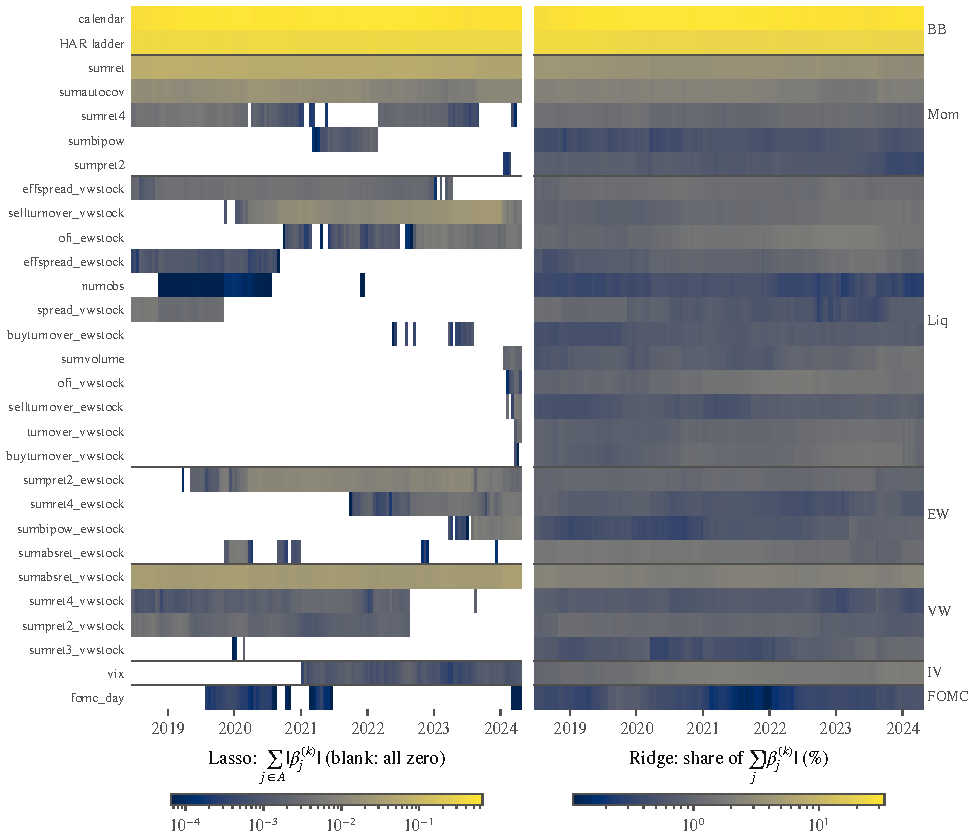
\includegraphics[width=\linewidth]{figures/rehaul_fi_linear_time.pdf}
\caption{The linear coefficients over time, by unit, at the 147 refits (every 10 sessions, 25 June 2018 to 30 April 2024). Left: the pre-tuned lasso's $\sum_{j\in A}|\beta^{(k)}_j|$, log colour scale, blank where every coefficient of the unit is zero (the on/off pattern). Right: the pre-tuned ridge's share of the refit's $\sum_j|\beta^{(k)}_j|$ on the unit, \%. Rows: the 29 units the lasso selects at least once, grouped by bucket (backbone first) and ordered by $N_A$; the other 20 are never selected. Coefficients are per unit of the robust-scaled input (see Table~\ref{tab:rh_fi_linear}).}
\label{fig:rh_fi_linear}
\end{figure}


% Trees: per-refit SHAP ranks aggregated (mean rank, top-5 share, truncated Borda, Kendall's W)
% AUTO-GENERATED by writeup/make_rehaul_fi.py -- do not edit; re-run the script.

\begin{table}[tbp]
\centering
\small
\setlength{\tabcolsep}{3.5pt}
\begin{threeparttable}
\caption{Trees: the per-refit SHAP rankings of the units, aggregated over 147 refits.}
\label{tab:rh_fi_trees}
\begin{tabular}{@{}llrrrrrrrrr@{}}
\toprule
 & & \multicolumn{3}{c}{LightGBM} & \multicolumn{3}{c}{XGBoost} & \multicolumn{3}{c}{Random forest} \\
\cmidrule(lr){3-5}\cmidrule(lr){6-8}\cmidrule(l){9-11}
Unit & Bucket & $\bar r$ & Top 5 & Borda & $\bar r$ & Top 5 & Borda & $\bar r$ & Top 5 & Borda \\
\midrule
HAR ladder & BB & 1.0 & 100 & 1 & 1.0 & 100 & 1 & 1.0 & 100 & 1 \\
\texttt{sumret} & Mom & 2.9 & 97 & 2 & 3.0 & 97 & 2 & 4.0 & 82 & 3 \\
\texttt{sumabsret} & Mom & 4.8 & 71 & 4 & 3.9 & 87 & 3 & 2.6 & 97 & 2 \\
\texttt{sumvolume} & Liq & 4.9 & 71 & 3 & 4.6 & 75 & 4 & 5.1 & 69 & 4 \\
\texttt{sumabsret\_ewstock} & EW & 6.7 & 39 & 5 & 6.7 & 38 & 5 & 5.7 & 46 & 5 \\
\texttt{sumabsret\_vwstock} & VW & 10.0 & 15 & 7 & 8.6 & 13 & 7 & 6.1 & 46 & 6 \\
Calendar & BB & 7.9 & 37 & 6 & 8.1 & 31 & 6 & 15.1 & 7 & 9 \\
\texttt{stocktwits\_sentiment} & Sent & 11.9 & 16 & 8 & 11.6 & 17 & 8 & 11.3 & 19 & 7 \\
\texttt{sumautocov} & Mom & 11.9 & 3 & 10 & 11.6 & 5 & 11 & 16.1 & 2 & 13 \\
\texttt{ofi\_ewstock} & Liq & 14.6 & 14 & 9 & 14.8 & 11 & 9 & 12.9 & 9 & 8 \\
\texttt{sumret3} & Mom & 17.9 & 3 & 13 & 16.5 & 1 & 13 & 15.4 & 2 & 12 \\
\texttt{stocktwits\_sentcount} & Sent & 17.1 & 7 & 11 & 16.2 & 4 & 12 & 17.6 & 3 & 11 \\
\texttt{sellturnover\_vwstock} & Liq & 20.0 & 7 & 12 & 16.4 & 8 & 10 & 18.3 & 7 & 10 \\
\texttt{ofi\_vwstock} & Liq & 25.8 & 1 & 24 & 26.0 & 2 & 19 & 18.4 & 1 & 15 \\
\texttt{stocktwits\_attention} & Sent & 22.7 & 1 & 20 & 24.4 & 1 & 18 & 23.7 & 0 & 19 \\
\addlinespace[3pt]
Kendall's $W$ & & \multicolumn{3}{c}{0.57} & \multicolumn{3}{c}{0.60} & \multicolumn{3}{c}{0.62} \\
Exog.\ series above the probe & & \multicolumn{3}{c}{27} & \multicolumn{3}{c}{35} & \multicolumn{3}{c}{29} \\
\bottomrule
\end{tabular}
\begin{tablenotes}[flushleft]
\footnotesize
\item \textit{Notes:} Per refit $k$, unit $A$'s importance is $I_{k,A} = |T_k|^{-1}\sum_{t\in T_k}|\phi_{t,A}|$, $\phi_{t,A} = \sum_{j\in A}\phi_{t,j}$ (path-dependent TreeSHAP of the refit's model on its held-out rows); $r_{k,A}$ is its rank among the 49 units (1 = largest, ties averaged). $\bar r$: mean of $r_{k,A}$ over the 147 refits; top 5: share of refits with $r_{k,A} \le 5$, \%; Borda: rank of $\sum_k \max(0, 11 - r_{k,A})$ (a full Borda count is affine in $\bar r$). Units: the 15 with the lowest $\bar r$ averaged over the three models. Kendall's $W$ of the per-refit rankings ($W = 1$: identical rankings at every refit). Probe: an exogenous series counts if one of its columns has mean $|\phi_j|$ above the continuous noise column's in at least half of the 49 probe fits (every third refit). SHAP values are the de-dup study's stored values of the cluster refits (LightGBM lgbm\_opt\_00, XGBoost xgb\_opt\_00, random forest trial 255, window-masked).
\end{tablenotes}
\end{threeparttable}
\end{table}


% Trees: rank over time, top six units
% AUTO-GENERATED by writeup/make_rehaul_fi.py -- do not edit; re-run the script.
\begin{figure}[tbp]
\centering
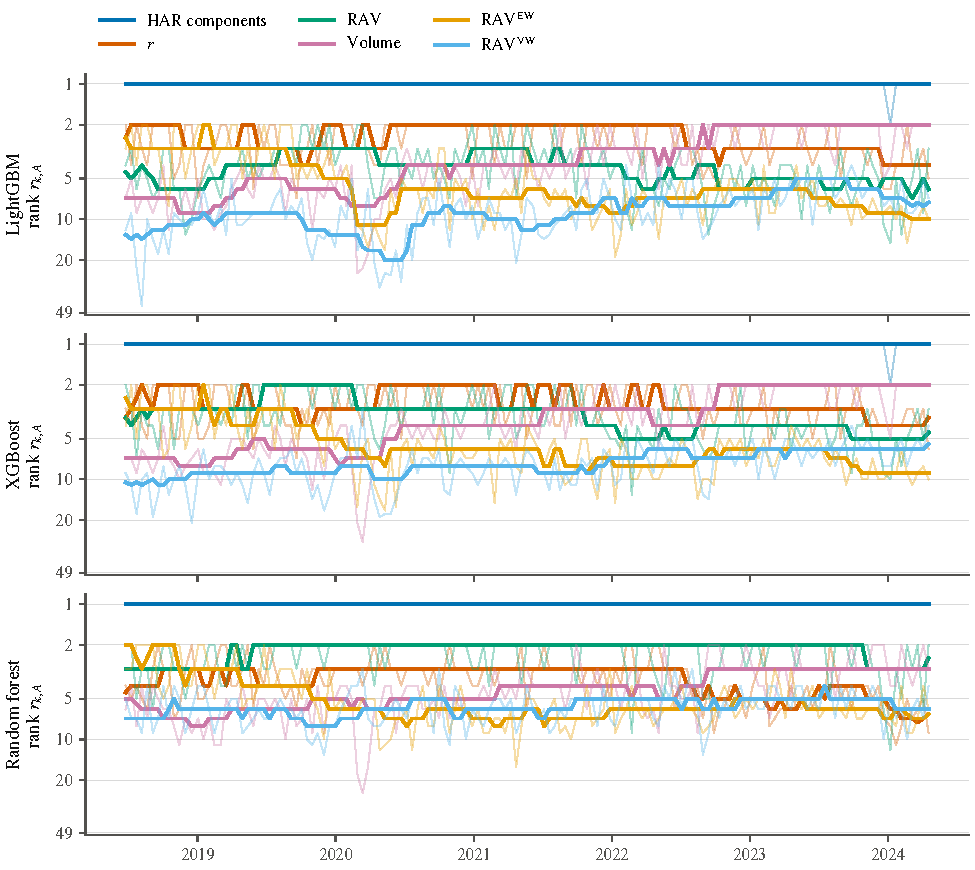
\includegraphics[width=\linewidth]{figures/rehaul_fi_tree_ranks.pdf}
\caption{The trees' per-refit SHAP ranks over time, the six units with the lowest mean rank averaged over the three models. Rank $r_{k,A}$ of unit $A$ among the 49 by mean $|\phi_{t,A}|$ on refit $k$'s held-out rows (1 = largest; log scale), at the start of each refit's tail. Thin: one point per refit; thick: centred rolling median over 11 refits (about 110 sessions). Kendall's $W$ over the 147 refits: LightGBM 0.57, XGBoost 0.60, random forest 0.62.}
\label{fig:rh_fi_ranks}
\end{figure}


% Trees: SHAP interactions (global, per refit) and the H-statistic cross-check
% AUTO-GENERATED by writeup/make_rehaul_fi.py -- do not edit; re-run the script.

\begin{table}[tbp]
\centering
\small
\setlength{\tabcolsep}{4pt}
\begin{threeparttable}
\caption{Trees: the strongest SHAP interactions, global and per refit, with the $H$-statistic cross-check.}
\label{tab:rh_fi_inter}
\begin{tabular}{@{}lrrrrr@{}}
\toprule
Pair & $\bar I$ ($\times 10^{3}$) & $\bar r$ & Top 10 (\%) & $H^2$ (\%) & $H^2_{\min}$ \\
\midrule
\multicolumn{6}{@{}l}{\textit{LightGBM}: series pairs} \\
HAR ladder $\times$ \texttt{sumabsret} & 12.64 & 1.7 & 100 & 0.33 & 0.19 \\
HAR ladder $\times$ \texttt{sumret} & 10.95 & 2.4 & 99 & 0.29 & 0.09 \\
HAR ladder $\times$ \texttt{sumvolume} & 6.62 & 6.3 & 88 & 0.05 & 0.05 \\
HAR ladder $\times$ \texttt{sumabsret\_ewstock} & 5.46 & 6.3 & 88 & 0.05 & 0.12 \\
HAR ladder $\times$ \texttt{stocktwits\_sentiment} & 4.70 & 14.4 & 67 & 0.06 & 0.17 \\
\multicolumn{6}{@{}l}{\textit{LightGBM}: column pairs} \\
\texttt{har\_ma\_1} $\times$ \texttt{har\_ma\_5} & 10.25 & -- & -- & 0.36 & 0.02 \\
\texttt{har\_ma\_1} $\times$ \texttt{har\_ma\_25} & 4.63 & -- & -- & 0.10 & 0.02 \\
\texttt{har\_ma\_5} $\times$ \texttt{adj\_sumabsret\_ma\_1} & 4.53 & -- & -- & 0.67 & 0.42 \\
\quad Probe floor & 0.49 & \multicolumn{2}{c}{$W = 0.45$} & & \\
\addlinespace[3pt]
\multicolumn{6}{@{}l}{\textit{XGBoost}: series pairs} \\
HAR ladder $\times$ \texttt{sumabsret} & 15.23 & 1.6 & 100 & 0.37 & 0.39 \\
HAR ladder $\times$ \texttt{sumret} & 11.03 & 2.5 & 100 & 0.68 & 0.21 \\
HAR ladder $\times$ \texttt{sumvolume} & 7.40 & 6.0 & 90 & 0.08 & 0.08 \\
HAR ladder $\times$ \texttt{sumabsret\_ewstock} & 5.92 & 5.3 & 93 & 0.06 & 0.17 \\
HAR ladder $\times$ \texttt{stocktwits\_sentiment} & 4.87 & 11.8 & 69 & 0.09 & 0.25 \\
\multicolumn{6}{@{}l}{\textit{XGBoost}: column pairs} \\
\texttt{har\_ma\_1} $\times$ \texttt{har\_ma\_5} & 9.95 & -- & -- & 0.39 & 0.02 \\
\texttt{har\_ma\_1} $\times$ \texttt{har\_ma\_25} & 4.99 & -- & -- & 0.14 & 0.02 \\
\texttt{har\_ma\_1} $\times$ \texttt{adj\_sumabsret\_ma\_5} & 4.94 & -- & -- & 0.28 & 0.43 \\
\quad Probe floor & 0.41 & \multicolumn{2}{c}{$W = 0.47$} & & \\
\addlinespace[3pt]
\multicolumn{6}{@{}l}{\textit{Random forest}: series pairs} \\
HAR ladder $\times$ \texttt{sumabsret} & 23.85 & 1.1 & 100 & 0.85 & 1.50 \\
HAR ladder $\times$ \texttt{sumret} & 9.13 & 3.5 & 99 & 0.20 & 0.48 \\
HAR ladder $\times$ \texttt{sumvolume} & 8.52 & 3.6 & 99 & 0.05 & 0.17 \\
HAR ladder $\times$ \texttt{sumabsret\_ewstock} & 6.87 & 4.6 & 99 & 0.06 & 0.33 \\
HAR ladder $\times$ \texttt{sumabsret\_vwstock} & 6.59 & 4.7 & 98 & 0.05 & 0.26 \\
\multicolumn{6}{@{}l}{\textit{Random forest}: column pairs} \\
\texttt{har\_ma\_1} $\times$ \texttt{har\_ma\_5} & 25.31 & -- & -- & 1.16 & 0.06 \\
\texttt{har\_ma\_1} $\times$ \texttt{adj\_sumabsret\_ma\_1} & 8.67 & -- & -- & 0.89 & 1.48 \\
\texttt{har\_ma\_1} $\times$ \texttt{adj\_sumabsret\_ma\_5} & 6.74 & -- & -- & 0.32 & 1.04 \\
\quad Probe floor & 0.50 & \multicolumn{2}{c}{$W = 0.57$} & & \\
\bottomrule
\end{tabular}
\begin{tablenotes}[flushleft]
\footnotesize
\item \textit{Notes:} SHAP interaction values $\phi_{t,jl}$ (path-dependent TreeSHAP, Lundberg et al.\ 2020; $\sum_l \phi_{t,jl} = \phi_{t,j}$) of the local refits on each refit's held-out rows, all 1{,}469 scored sessions. Series pair $(A, B)$: $\Phi_{t,AB} = \sum_{j\in A}\sum_{l\in B}(\phi_{t,jl} + \phi_{t,lj})$; $\bar I_{AB}$ = mean of $|\Phi_{t,AB}|$ over the scored sessions, $\times 10^{3}$, in the fit space of $\hat y$. Column pairs: $|\phi_{t,jl} + \phi_{t,lj}|$. $\bar r$ and top 10: the pair's mean rank and share of refits in the top 10 when the 1176 series pairs are ranked per refit by their mean $|\Phi_{t,AB}|$ on the refit's rows. $H^2$ (Friedman--Popescu): the variance of $\mathrm{PD}_{AB} - \mathrm{PD}_A - \mathrm{PD}_B$ as a share of the variance of $\mathrm{PD}_{AB}$, \%; $H^2_{\min}$: the same numerator over $\min(\mathrm{var}\,\mathrm{PD}_A, \mathrm{var}\,\mathrm{PD}_B)$, a ratio. Both pooled over 15 refits (every 10th), each on the 100 held-out sessions from its anchor as evaluation and background points; computed for each model's top 10 series and top 5 column pairs. Probe floor: median over the 49 probe fits of the largest $\bar I$ between the continuous noise column and a unit. $W$: Kendall's $W$ of the per-refit rankings of each model's top 50 pairs. XGBoost and the forest are refitted locally with other library versions than the stored refits (forecast gaps up to 0.17).
\end{tablenotes}
\end{threeparttable}
\end{table}


% Trees: series-level interaction heatmap
% 2026-10-15 (user): parked -- non-standard figure; focus on legible tables
% % AUTO-GENERATED by writeup/make_rehaul_fi.py -- do not edit; re-run the script.
\begin{figure}[tbp]
\centering
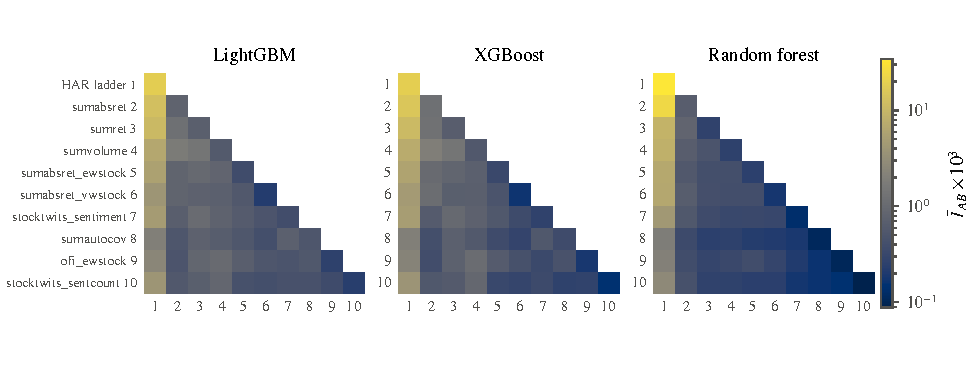
\includegraphics[width=\linewidth]{figures/rehaul_fi_inter_heatmap.pdf}
\caption{The trees' series-level SHAP interactions: $\bar I_{AB}$, the mean over the 1{,}469 scored sessions of $|\phi_{t,AB}|$, $\phi_{t,AB} = \sum_{j\in A}\sum_{l\in B}(\phi_{t,jl} + \phi_{t,lj})$, $\times 10^{3}$, log colour scale shared by the panels; lower triangle, the diagonal is the interaction among a unit's own columns, $\sum_{j \ne l \in A}\phi_{t,jl}$. Units: the 10 with the largest share of their model's off-diagonal interaction mass, summed over the three models; numbered as in the left panel. Local refits on the held-out rows of each of the 147 refits.}
\label{fig:rh_fi_inter}
\end{figure}


% 2026-10-16 (user): conclusion restored.
\clearpage
% 09_conclusion.tex -- the rehauled paper's section, as bullets to expand into prose (2026-10-15).
% Sources and pointers behind every number: writeup/PAPER_REHAUL_OUTLINE_2026-10-15.md, section 9.
% House rules: every number in the final prose comes from a generated macro (writeup/generated/*.tex), never
% typed; park (comment out with a dated note) rather than delete.
% Macros to use here: reuse the introduction's macros; no new numbers
% 2026-10-15 (notation pass, writeup/NOTATION_GUIDE_2026-10-15.md): symbols and wording; the typed 866 -> \cmNdays.
% Old -> new: RV_t -> \RV_t; B_t -> s^2_{t,c}; IV^{30}_t -> \mathrm{IV}_t; HAR + calendar -> HAR benchmark;
% exogenous inputs -> exogenous predictors; per bar / pooled -> closing-interval / pooled intraday model;
% Sharpe -> \SR; trade -> straddle strategy; always-short -> short-straddle benchmark; crossing the spread -> at
% quoted bid/ask prices. The guarded \input is a no-op after the introduction's.
% 2026-10-15 (consolidation): window row s -> t' (s is the periodicity factor); the training loss written with the
% realization floor and log-ratio clamp of Methods (FLAG (3) there).
% 2026-10-15 (consolidation): parked -- the number files are loaded once in the preamble of paper_rehaul.tex.
% \ifdefined\cmNdays\else% AUTO-GENERATED by writeup/make_table_close_main.py -- do not edit.
% Numbers quoted in the prose of writeup/sections/results_close_option.tex; each is read
% from results/close_master_table/master_table.csv and the sources in the script.
% 2026-10-06: recalibration removed / intervals removed, user decision -- the plain forecast
% f^2 B, point estimates; ...T = HAC t of the daily mid-return difference, ...DM = Diebold-
% Mariano statistic; a ...Above / ...Below count counts point estimates, its ...Sig twin those
% significant at 5 % (DM for QLIKE, HAC t for Sharpe).
\newcommand{\cmNdays}{866}
\newcommand{\cmNrows}{22}
\newcommand{\cmShortMean}{0.014}
\newcommand{\cmShortShMid}{0.20}
\newcommand{\cmShortShX}{\ensuremath{-}0.27}
\newcommand{\cmShortT}{\ensuremath{-}1.71}
\newcommand{\cmPaperShMin}{0.43}
\newcommand{\cmPaperShMax}{1.50}
\newcommand{\cmPaperXMin}{\ensuremath{-}0.05}
\newcommand{\cmPaperXMax}{1.01}
\newcommand{\cmPaperVsShortMin}{+0.22}
\newcommand{\cmPaperVsShortMax}{+1.30}
\newcommand{\cmPaperVsShortAboveN}{8}
\newcommand{\cmPaperVsShortAboveSigN}{three}
\newcommand{\cmPaperVsShortAboveSigWho}{LightGBM, XGBoost, lasso (causally tuned)}
\newcommand{\cmPaperSameMin}{82}
\newcommand{\cmSellPaperMin}{72}
\newcommand{\cmSellPaperMax}{83}
\newcommand{\cmPaperSameMax}{96}
\newcommand{\cmRefQ}{0.1092}
\newcommand{\cmRefShMid}{1.28}
\newcommand{\cmRefShX}{0.80}
\newcommand{\cmRefBuy}{27}
\newcommand{\cmRefVsShort}{+1.08}
\newcommand{\cmRefVsShortT}{+1.71}
\newcommand{\cmFomcSh}{1.36}
\newcommand{\cmFomcD}{+0.08}
\newcommand{\cmFomcDT}{+0.44}
\newcommand{\cmLassoFShMid}{1.06}
\newcommand{\cmLassoFVsRef}{\ensuremath{-}0.22}
\newcommand{\cmLassoFVsRefT}{\ensuremath{-}0.75}
\newcommand{\cmLassoFSame}{96}
\newcommand{\cmPaperFarLabel}{baseline (HAR + calendar OLS)}
\newcommand{\cmPaperFarVsRef}{\ensuremath{-}0.85}
\newcommand{\cmPaperFarVsRefT}{\ensuremath{-}1.49}
\newcommand{\cmPaperBestLabel}{lasso (causally tuned)}
\newcommand{\cmPaperBestSh}{1.50}
\newcommand{\cmNlFamN}{five}
\newcommand{\cmNlMasterN}{90}
\newcommand{\cmPoolShMin}{0.91}
\newcommand{\cmPoolShMax}{1.44}
\newcommand{\cmSubShMin}{1.37}
\newcommand{\cmSubShMax}{1.92}
\newcommand{\cmNlShMin}{1.23}
\newcommand{\cmNlShMax}{1.81}
\newcommand{\cmTabVsRefN}{21}
\newcommand{\cmTabVsRefAbove}{15}
\newcommand{\cmTabVsRefBelow}{6}
\newcommand{\cmTabVsRefAboveSig}{0}
\newcommand{\cmTabVsRefBelowSig}{0}
\newcommand{\cmMasterN}{112}
\newcommand{\cmMasterNPaper}{9}
\newcommand{\cmMasterNBase}{52}
\newcommand{\cmMasterMedQBase}{0.1033}
\newcommand{\cmMasterMedShBase}{0.73}
\newcommand{\cmMasterMedShXBase}{0.25}
\newcommand{\cmMasterNAll}{51}
\newcommand{\cmMasterMedQAll}{0.1014}
\newcommand{\cmMasterMedShAll}{1.27}
\newcommand{\cmMasterMedShXAll}{0.79}
\newcommand{\cmMasterSetsN}{two}
\newcommand{\cmMasterVsRefN}{111}
\newcommand{\cmMasterVsRefAbove}{32}
\newcommand{\cmMasterVsRefBelow}{79}
\newcommand{\cmMasterVsRefAboveSig}{0}
\newcommand{\cmMasterVsRefBelowSig}{0}
\newcommand{\cmMasterVsShortAbove}{112}
\newcommand{\cmMasterVsShortBelow}{0}
\newcommand{\cmMasterVsShortAboveSig}{20}
\newcommand{\cmMasterVsShortBelowSig}{0}
\newcommand{\cmMasterVsShortN}{112}
\newcommand{\cmMasterQVsRefBelow}{99}
\newcommand{\cmMasterQVsRefAbove}{12}
\newcommand{\cmMasterQVsRefBelowSig}{23}
\newcommand{\cmMasterQVsRefAboveSig}{1}
\newcommand{\cmMasterMedQ}{0.1028}
\newcommand{\cmMasterMedSh}{1.08}
\newcommand{\cmMasterMedShX}{0.59}
\newcommand{\cmMasterShMin}{0.29}
\newcommand{\cmMasterShMax}{1.92}
\newcommand{\cmMasterXMin}{\ensuremath{-}0.19}
\newcommand{\cmMasterXMax}{1.43}
\newcommand{\cmMasterVsShortMed}{+0.87}
\newcommand{\cmMasterRankCorr}{\ensuremath{-}0.20}
\newcommand{\cmMasterRankCorrX}{\ensuremath{-}0.20}
\newcommand{\cmSellMasterMin}{66}
\newcommand{\cmSellMasterMax}{83}
\newcommand{\cmSellMasterMed}{70}
\newcommand{\cmTopShLabel}{per-bar elastic net}
\newcommand{\cmTopShInputs}{\texttt{all\_features}}
\newcommand{\cmTopShMid}{1.92}
\newcommand{\cmXLossMin}{0.48}
\newcommand{\cmXLossMax}{0.50}
\newcommand{\cmLdSpec}{+0.16}
\newcommand{\cmLdSpecQ}{\ensuremath{-}4.3}
\newcommand{\cmLdSpecT}{+0.34}
\newcommand{\cmLdSpecDM}{\ensuremath{-}1.73}
\newcommand{\cmLdPerBarBase}{+0.46}
\newcommand{\cmLdPerBarBaseQ}{\ensuremath{-}12.0}
\newcommand{\cmLdPerBarBaseT}{+1.05}
\newcommand{\cmLdPerBarBaseDM}{\ensuremath{-}3.37}
\newcommand{\cmLdPerBarAll}{\ensuremath{-}0.03}
\newcommand{\cmLdPerBarAllQ}{\ensuremath{-}6.7}
\newcommand{\cmLdPerBarAllT}{\ensuremath{-}0.07}
\newcommand{\cmLdPerBarAllDM}{\ensuremath{-}1.61}
\newcommand{\cmLdIn}{+0.05}
\newcommand{\cmLdInQ}{+0.8}
\newcommand{\cmLdInT}{+0.09}
\newcommand{\cmLdInDM}{+0.18}
\newcommand{\cmLdEstMin}{\ensuremath{-}0.15}
\newcommand{\cmLdEstMax}{+0.50}
\newcommand{\cmLdEstMinLabel}{\texttt{subtree\_rf\_all\_features}}
\newcommand{\cmLdEstMaxLabel}{\texttt{subpt\_enet\_all\_features}}
\newcommand{\cmLdEstMinWho}{random forest}
\newcommand{\cmLdEstMaxWho}{elastic net}
\newcommand{\cmLdN}{21}
\newcommand{\cmLdNPath}{12}
\newcommand{\cmLdNCampaign}{9}
\newcommand{\cmLdResolved}{none}
\newcommand{\cmLdQResolved}{three}
\newcommand{\cmLdCDedup}{+0.00}
\newcommand{\cmLdCDedupQ}{+0.0}
\newcommand{\cmLdCMaskTten}{\ensuremath{-}0.21}
\newcommand{\cmLdCMaskTtenQ}{\ensuremath{-}1.0}
\newcommand{\cmLdCMaskTtenT}{\ensuremath{-}0.69}
\newcommand{\cmLdCMaskTtenDM}{\ensuremath{-}1.04}
\newcommand{\cmLdCMaskTone}{\ensuremath{-}0.23}
\newcommand{\cmLdCMaskToneQ}{+1.4}
\newcommand{\cmLdCMaskToneT}{\ensuremath{-}0.55}
\newcommand{\cmLdCMaskToneDM}{+1.36}
\newcommand{\cmLdCMaskRsten}{\ensuremath{-}0.08}
\newcommand{\cmLdCMaskRstenQ}{+2.8}
\newcommand{\cmLdCMaskRstenT}{\ensuremath{-}0.32}
\newcommand{\cmLdCMaskRstenDM}{+1.42}
\newcommand{\cmLdCMaskRsone}{\ensuremath{-}0.05}
\newcommand{\cmLdCMaskRsoneQ}{+0.2}
\newcommand{\cmLdCMaskRsoneT}{\ensuremath{-}0.17}
\newcommand{\cmLdCMaskRsoneDM}{+0.12}
\newcommand{\cmLdCCadLgbm}{\ensuremath{-}0.04}
\newcommand{\cmLdCCadLgbmQ}{\ensuremath{-}2.2}
\newcommand{\cmLdCCadLgbmT}{\ensuremath{-}0.08}
\newcommand{\cmLdCCadLgbmDM}{\ensuremath{-}1.12}
\newcommand{\cmLdCTuneRs}{+0.28}
\newcommand{\cmLdCTuneRsQ}{+3.0}
\newcommand{\cmLdCTuneRsT}{+0.58}
\newcommand{\cmLdCTuneRsDM}{+1.12}
\newcommand{\cmLdCTuneOp}{\ensuremath{-}0.10}
\newcommand{\cmLdCTuneOpQ}{+7.3}
\newcommand{\cmLdCTuneOpT}{\ensuremath{-}0.31}
\newcommand{\cmLdCTuneOpDM}{+2.83}
\newcommand{\cmLdCTuneOpPer}{\ensuremath{-}0.32}
\newcommand{\cmLdCTuneOpPerQ}{+2.5}
\newcommand{\cmLdCTuneOpPerT}{\ensuremath{-}0.65}
\newcommand{\cmLdCTuneOpPerDM}{+0.75}
\newcommand{\cmPNewBase}{22}
\newcommand{\cmPOldBase}{34}
\newcommand{\cmPNewAll}{628}
\newcommand{\cmPOldAll}{640}
\newcommand{\cmNDup}{12}
\newcommand{\cmDedupN}{37}
\newcommand{\cmDedupQMax}{0.05}
\newcommand{\cmDedupPosMax}{one}
\newcommand{\cmKeptBase}{17}
\newcommand{\cmKeptBaseMin}{17}
\newcommand{\cmKeptBaseMax}{17}
\newcommand{\cmKeptAll}{369}
\newcommand{\cmKeptAllMin}{360}
\newcommand{\cmKeptAllMax}{378}
\newcommand{\cmMaskN}{16}
\newcommand{\cmMaskQMed}{0.4}
\newcommand{\cmMaskQAbove}{10}
\newcommand{\cmMaskShBelow}{14}
\newcommand{\cmMaskQAboveSig}{none}
\newcommand{\cmMaskShBelowSig}{one}
\newcommand{\cmTrVsRidgeN}{48}
\newcommand{\cmTrSetsN}{two}
\newcommand{\cmMaskSetsN}{two}
\newcommand{\cmTrVsRidgeQAbove}{46}
\newcommand{\cmTrVsRidgeShBelow}{41}
\newcommand{\cmTrVsRidgeQAboveSig}{21}
\newcommand{\cmTrVsRidgeShBelowSig}{one}
\newcommand{\cmCadN}{six}
\newcommand{\cmCadQBelow}{five}
\newcommand{\cmCadQBelowSig}{none}
\newcommand{\cmCadShUp}{\ensuremath{-}0.43}
\newcommand{\cmCadShUpT}{\ensuremath{-}1.03}
\newcommand{\cmRsQAbove}{6}
\newcommand{\cmRsQAboveSig}{two}
\newcommand{\cmRsN}{6}
\newcommand{\cmOpN}{24}
\newcommand{\cmOpQAbove}{24}
\newcommand{\cmOpQAboveSig}{13}
\newcommand{\cmTpN}{18}
\newcommand{\cmTpQBelow}{12}
\newcommand{\cmTpQBelowSig}{one}
\newcommand{\cmBudN}{24}
\newcommand{\cmBudQAbove}{17}
\newcommand{\cmBudQAboveSig}{two}
\newcommand{\cmBudQBelow}{7}
\newcommand{\cmBudLastMin}{27}
\newcommand{\cmBudLastMax}{37}
\newcommand{\cmBudLastExch}{20}
\newcommand{\cmNlBestSh}{1.81}
\newcommand{\cmNlBestLabel}{tuned per-bar LightGBM}
\newcommand{\cmNlBestInputs}{\texttt{all\_features}}
\newcommand{\cmNlBestVsRef}{+0.53}
\newcommand{\cmNlBestVsRefT}{+1.04}
\newcommand{\cmNlVsRefAbove}{19}
\newcommand{\cmNlVsRefBelow}{71}
\newcommand{\cmNlVsRefAboveSig}{0}
\newcommand{\cmNlVsRefBelowSig}{0}
\newcommand{\cmClassChunks}{505}
\newcommand{\cmClassPts}{20}
\newcommand{\cmClassLgbmPick}{18}
\newcommand{\cmClassMaxRelMin}{4.5}
\newcommand{\cmClassMaxRelMax}{5.5}
\newcommand{\cmSvN}{31}
\newcommand{\cmSvSetN}{112}
\newcommand{\cmSvSetPairsN}{3472}
\newcommand{\cmSvSetAboveMid}{755}
\newcommand{\cmSvSetAboveMidSig}{29}
\newcommand{\cmSvSetStraddleFirstMid}{4}
\newcommand{\cmSvSetWingN}{672}
\newcommand{\cmSvSetWingMidBelow}{668}
\newcommand{\cmSvSetAboveX}{410}
\newcommand{\cmSvSetAboveXSig}{0}
\newcommand{\cmSvSetStraddleFirstX}{3}
\newcommand{\cmSvSetWingXBelow}{672}
\newcommand{\cmSvSetBestMidLabel}{call vertical, w50}
\newcommand{\cmSvSetBestMidMed}{+0.37}
\newcommand{\cmSvSetBestMidAboveN}{94}
\newcommand{\cmSvSetBestMidAboveSig}{0}
\newcommand{\cmSvCostStraddle}{2.9}
\newcommand{\cmSvCostIbfMin}{4.0}
\newcommand{\cmSvCostIbfMax}{6.1}
\newcommand{\cmMasterPosTotalN}{112}
\newcommand{\cmMasterTopTwentyShareMed}{99}
\newcommand{\cmMasterTopTwentyShareMin}{59}
\newcommand{\cmMasterTopTwentyShareMax}{338}
\newcommand{\cmMasterTopTwentyBuysN}{112}
\newcommand{\cmMasterBottomTwentySellsN}{112}
\newcommand{\cmMasterDiffMed}{+53.5}
\newcommand{\cmMasterDiffPosN}{112}
\newcommand{\cmMasterDiffExTenMed}{\ensuremath{-}30.0}
\newcommand{\cmMasterDiffExTenHalfN}{112}
\newcommand{\cmMasterDiffExTenNegN}{102}
\newcommand{\cmBContamMaxDSh}{0.38}
\newcommand{\cmBContamMaxDShX}{0.38}
\newcommand{\cmBContamMedDSh}{0.08}
\newcommand{\cmBContamPaperMaxDSh}{0.21}
\newcommand{\cmBContamPaperMaxDShX}{0.22}
\newcommand{\cmBContamPaperMedDSh}{0.08}
\newcommand{\cmBContamDays}{94}
\newcommand{\cmCensIvMaxDSh}{0.06}
\newcommand{\cmCensIvMaxDShX}{0.08}
\newcommand{\cmCensIvMedDSh}{0.04}
\newcommand{\cmCensIvPaperMaxDSh}{0.05}
\newcommand{\cmCensIvPaperMaxDShX}{0.07}
\newcommand{\cmCensIvPaperMedDSh}{0.04}
\newcommand{\cmCensIvDays}{5}
\newcommand{\cmBContamMaxFlips}{16}
\newcommand{\cmBContamMedFlips}{8}
\newcommand{\cmBContamPaperMaxFlips}{10}
\newcommand{\cmBContamMaxRel}{21}
\newcommand{\cmPtPreSessions}{3947}
\newcommand{\cmPtPreStart}{13~April~2004}
\newcommand{\cmPtValFirst}{6~January~2016}
\newcommand{\cmPtValLast}{2~January~2020}
\newcommand{\cmPtFolds}{four}
\newcommand{\cmPtFoldLen}{250}
\newcommand{\cmPtFitWin}{2{,}000}
\newcommand{\cmPtEmbargo}{25}
\newcommand{\cmPtRatio}{1/100}
\newcommand{\cmPtBlock}{250}
\newcommand{\cmPtRetuneN}{four}
\newcommand{\cmPtRetuneFirst}{23~June~2020}
\newcommand{\cmPtRetuneLast}{16~June~2023}
\newcommand{\cmPtFiredRidgeBase}{one}
\newcommand{\cmPtPenRidgeBase}{\ensuremath{10^{-2}}}
\newcommand{\cmPtFiredRidgeAll}{none}
\newcommand{\cmPtPenRidgeAll}{\ensuremath{10^{3}}}
\newcommand{\cmPtFiredLassoBase}{one}
\newcommand{\cmPtPenLassoBase}{\ensuremath{10^{-6}}}
\newcommand{\cmPtFiredLassoAll}{none}
\newcommand{\cmPtPenLassoAll}{\ensuremath{10^{-2}}}
\newcommand{\cmPtFiredEnetBase}{two}
\newcommand{\cmPtPenEnetBase}{\ensuremath{10^{-6}}}
\newcommand{\cmPtFiredEnetAll}{none}
\newcommand{\cmPtPenEnetAll}{\ensuremath{10^{-2}}}
\newcommand{\cmPtFiredTotal}{4}
\newcommand{\cmPtFiredOf}{24}
\newcommand{\cmPtCausalSwitches}{75}
\newcommand{\cmPtCausalChoices}{165}
\newcommand{\cmPtCausalMarginPass}{3}
\newcommand{\cmPtCausalEdgePicks}{132}
\newcommand{\cmPtCausalPicks}{198}
\newcommand{\cmPtSwitchFlipPct}{8}
\newcommand{\cmPtCausalSwitchesPaper}{24}
\newcommand{\cmPtCausalChoicesPaper}{45}
\newcommand{\cmPtCausalMarginPassPaper}{3}
\newcommand{\cmPtCausalEdgePicksPaper}{34}
\newcommand{\cmPtCausalPicksPaper}{54}
\newcommand{\cmPtSwitchFlipPctPaper}{9}
\newcommand{\cmPoolPtN}{6}
\newcommand{\cmPoolPtQPctMean}{+0.9}
\newcommand{\cmPoolPtQWorse}{5}
\newcommand{\cmPoolPtDMMax}{1.22}
\newcommand{\cmPoolPtTMax}{1.29}
\newcommand{\cmPoolPtSigN}{0}
\newcommand{\cmPoolPtShAllMin}{+0.17}
\newcommand{\cmPoolPtShAllMax}{+0.35}
\newcommand{\cmPoolPtShOtherMin}{\ensuremath{-}0.06}
\newcommand{\cmPoolPtShOtherMax}{\ensuremath{-}0.19}
\newcommand{\cmPoolPtBlocks}{218}
\newcommand{\cmPoolPtCausalSwMin}{137}
\newcommand{\cmPoolPtCausalSwMax}{170}
\newcommand{\cmPoolPtCausalMarginMin}{3}
\newcommand{\cmPoolPtCausalMarginMax}{22}
\newcommand{\cmPoolPtRetunes}{217}
\newcommand{\cmPoolPtRetuneSwMin}{11}
\newcommand{\cmPoolPtRetuneSwMax}{40}
\newcommand{\cmTreeProvRfName}{\texttt{rf\_opt\_00}}
\newcommand{\cmTreeProvRfTrials}{400}
\newcommand{\cmTreeProvRfBudget}{400}
\newcommand{\cmTreeProvRfDevMse}{0.108456}
\newcommand{\cmTreeProvLgbmDevMse}{0.107449}
\newcommand{\cmTreeProvXgbDevMse}{0.108076}
\newcommand{\cmTreeProvXgbTopDevMse}{0.107894}
\newcommand{\cmTreeProvRfTrees}{485}
\newcommand{\cmTreeProvRfDepth}{20}
\newcommand{\cmTreeProvRfFeatures}{0.90}
\newcommand{\cmTreeProvRfSamples}{0.41}
\newcommand{\cmTreeProvRfLeafDev}{12}
\newcommand{\cmTreeProvRfLeaf}{1}
\newcommand{\cmTreeProvLgbmLeafDev}{98}
\newcommand{\cmTreeProvLgbmLeaf}{8}
\newcommand{\cmTreeProvXgbTopName}{\texttt{xgb\_opt\_00}}
\newcommand{\cmTreeProvXgbName}{\texttt{xgb\_opt\_06}}
\newcommand{\cmTreeProvXgbDevRank}{7}
\newcommand{\cmTreeProvXgbArms}{8}
\newcommand{\cmTreeProvXgbPostRank}{8}
\newcommand{\cmTreeProvXgbRecentRank}{8}
\newcommand{\cmTreeProvXgbQRank}{8}
\newcommand{\cmTreeProvXgbPickDate}{14~August~2026}
\newcommand{\cmMasterNLean}{51}
\newcommand{\cmMasterMedQLean}{0.0991}
\newcommand{\cmMasterMedShLean}{1.37}
\newcommand{\cmMasterMedShXLean}{0.88}
\newcommand{\cmLdPerBarLean}{+0.65}
\newcommand{\cmLdPerBarLeanQ}{\ensuremath{-}12.3}
\newcommand{\cmLdPerBarLeanT}{+1.49}
\newcommand{\cmLdPerBarLeanDM}{\ensuremath{-}3.39}
\newcommand{\cmLdInBaseLean}{+0.51}
\newcommand{\cmLdInBaseLeanQ}{\ensuremath{-}3.3}
\newcommand{\cmLdInBaseLeanT}{+1.66}
\newcommand{\cmLdInBaseLeanDM}{\ensuremath{-}1.17}
\newcommand{\cmLdInLeanAll}{\ensuremath{-}0.46}
\newcommand{\cmLdInLeanAllQ}{+4.3}
\newcommand{\cmLdInLeanAllT}{\ensuremath{-}1.15}
\newcommand{\cmLdInLeanAllDM}{+1.50}
%
% 2026-10-06 parked (recalibration removed / intervals removed, user decision):
%   \cmShortShCiMid: interval of always short's Sharpe
%   \cmShortShCiX: interval of always short's Sharpe
%   \cmPaperVsShortAboveWho: the paper's forecasts whose interval vs always short lay above zero
%   \cmPaperVsShortAboveCi: that forecast's interval
%   \cmSellHead: the former headline's sell share (no headline model)
%   \cmHQ: the former headline (no headline model)
%   \cmHQPct: the former headline (no headline model)
%   \cmHQCi: the former headline (no headline model)
%   \cmHDM: the former headline (no headline model)
%   \cmHDMp: the former headline (no headline model)
%   \cmHShMid: the former headline (no headline model)
%   \cmHShX: the former headline (no headline model)
%   \cmHMean: the former headline (no headline model)
%   \cmHHit: the former headline (no headline model)
%   \cmHBuy: the former headline (no headline model)
%   \cmHVsRefMid: the former headline (no headline model)
%   \cmHVsRefX: the former headline (no headline model)
%   \cmHVsShortMid: the former headline (no headline model)
%   \cmHVsShortX: the former headline (no headline model)
%   \cmHVsRefT: the former headline (no headline model)
%   \cmHVsRefP: the former headline (no headline model)
%   \cmHVsShortT: the former headline (no headline model)
%   \cmHVsShortP: the former headline (no headline model)
%   \cmHRankSh: the former headline (no headline model)
%   \cmHRankQ: the former headline (no headline model)
%   \cmVsHN: the former headline (no headline model)
%   \cmVsHAbove: the former headline (no headline model)
%   \cmVsHBelow: the former headline (no headline model)
%   \cmVsHAboveSig: the former headline (no headline model)
%   \cmVsHBelowSig: the former headline (no headline model)
%   \cmVsHLassoSh: the former headline (no headline model)
%   \cmVsHLasso: paired against the former headline (no headline model)
%   \cmVsHLassoT: paired against the former headline (no headline model)
%   \cmVsHLassoSame: paired against the former headline (no headline model)
%   \cmVsHLassoQPct: paired against the former headline (no headline model)
%   \cmVsHLassoDM: paired against the former headline (no headline model)
%   \cmVsHEnet: paired against the former headline (no headline model)
%   \cmVsHEnetT: paired against the former headline (no headline model)
%   \cmVsHEnetSame: paired against the former headline (no headline model)
%   \cmVsHEnetQPct: paired against the former headline (no headline model)
%   \cmVsHEnetDM: paired against the former headline (no headline model)
%   \cmVsHRidgeAll: paired against the former headline (no headline model)
%   \cmVsHRidgeAllT: paired against the former headline (no headline model)
%   \cmVsHRidgeAllSame: paired against the former headline (no headline model)
%   \cmVsHRidgeAllQPct: paired against the former headline (no headline model)
%   \cmVsHRidgeAllDM: paired against the former headline (no headline model)
%   \cmVsHTop: paired against the former headline (no headline model)
%   \cmVsHTopT: paired against the former headline (no headline model)
%   \cmVsHTopSame: paired against the former headline (no headline model)
%   \cmVsHTopQPct: paired against the former headline (no headline model)
%   \cmVsHTopDM: paired against the former headline (no headline model)
%   \cmLdPerBarLive: a step to the former headline (no headline, no live-feasible)
%   \cmLdPerBarLiveQ: a step to the former headline (no headline, no live-feasible)
%   \cmLdPerBarLiveT: a step to the former headline (no headline, no live-feasible)
%   \cmLdPerBarLiveDM: a step to the former headline (no headline, no live-feasible)
%   \cmLdInAll: a step to the former headline (no headline, no live-feasible)
%   \cmLdInAllQ: a step to the former headline (no headline, no live-feasible)
%   \cmLdInAllT: a step to the former headline (no headline, no live-feasible)
%   \cmLdInAllDM: a step to the former headline (no headline, no live-feasible)
%   \cmLdInBase: a step to the former headline (no headline, no live-feasible)
%   \cmLdInBaseQ: a step to the former headline (no headline, no live-feasible)
%   \cmLdInBaseT: a step to the former headline (no headline, no live-feasible)
%   \cmLdInBaseDM: a step to the former headline (no headline, no live-feasible)
%   \cmLdCMaskLstm: an LSTM step of the campaign (LSTMs parked)
%   \cmLdCMaskLstmQ: an LSTM step of the campaign (LSTMs parked)
%   \cmLdCMaskLstmT: an LSTM step of the campaign (LSTMs parked)
%   \cmLdCMaskLstmDM: an LSTM step of the campaign (LSTMs parked)
%   \cmLdCCadLstm: an LSTM step of the campaign (LSTMs parked)
%   \cmLdCCadLstmQ: an LSTM step of the campaign (LSTMs parked)
%   \cmLdCCadLstmT: an LSTM step of the campaign (LSTMs parked)
%   \cmLdCCadLstmDM: an LSTM step of the campaign (LSTMs parked)
%   \cmLdCSeq: an LSTM step of the campaign (LSTMs parked)
%   \cmLdCSeqQ: an LSTM step of the campaign (LSTMs parked)
%   \cmLdCSeqT: an LSTM step of the campaign (LSTMs parked)
%   \cmLdCSeqDM: an LSTM step of the campaign (LSTMs parked)
%   \cmPNewLive: live_feasible input set (live-feasible removed from the paper)
%   \cmPOldLive: live_feasible input set (live-feasible removed from the paper)
%   \cmKeptLive: live_feasible input set (live-feasible removed from the paper)
%   \cmKeptLiveMin: live_feasible input set (live-feasible removed from the paper)
%   \cmKeptLiveMax: live_feasible input set (live-feasible removed from the paper)
%   \cmLstmCadLive: live_feasible input set (live-feasible removed from the paper)
%   \cmLstmCadBase: LSTM (LSTMs parked)
%   \cmLstmCadAll: LSTM (LSTMs parked)
%   \cmLstmCadBelow: LSTM (LSTMs parked)
%   \cmLstmCadBelowSig: LSTM (LSTMs parked)
%   \cmLstmVsRidgeMin: LSTM (LSTMs parked)
%   \cmLstmVsRidgeMax: LSTM (LSTMs parked)
%   \cmIntraVsRidgeMin: LSTM (LSTMs parked)
%   \cmIntraVsRidgeMax: LSTM (LSTMs parked)
%   \cmIntraAllQ: LSTM (LSTMs parked)
%   \cmIntraAllDM: LSTM (LSTMs parked)
%   \cmNlBestVsH: against the former headline (no headline model)
%   \cmNlBestVsHT: against the former headline (no headline model)
%   \cmNlVsHAbove: against the former headline (no headline model)
%   \cmNlVsHAboveSig: against the former headline (no headline model)
%   \cmPnlTotal: D.14, the former headline's P&L decomposition (parked, user decision)
%   \cmPnlTotalX: D.14, the former headline's P&L decomposition (parked, user decision)
%   \cmPnlTopTenShare: D.14, the former headline's P&L decomposition (parked, user decision)
%   \cmPnlTopTwentyShare: D.14, the former headline's P&L decomposition (parked, user decision)
%   \cmPnlTopTwentyShareX: D.14, the former headline's P&L decomposition (parked, user decision)
%   \cmPnlExTwenty: D.14, the former headline's P&L decomposition (parked, user decision)
%   \cmPnlExTwentySh: D.14, the former headline's P&L decomposition (parked, user decision)
%   \cmPnlMktTwenty: D.14, the former headline's P&L decomposition (parked, user decision)
%   \cmPnlMktTwentyExp: D.14, the former headline's P&L decomposition (parked, user decision)
%   \cmPnlMktTwentyP: D.14, the former headline's P&L decomposition (parked, user decision)
%   \cmPnlDaysAll: D.14, the former headline's P&L decomposition (parked, user decision)
%   \cmPnlDaysAllPct: D.14, the former headline's P&L decomposition (parked, user decision)
%   \cmPnlMEn: D.14, the former headline's P&L decomposition (parked, user decision)
%   \cmPnlMEbuys: D.14, the former headline's P&L decomposition (parked, user decision)
%   \cmPnlME: D.14, the former headline's P&L decomposition (parked, user decision)
%   \cmPnlMEShort: D.14, the former headline's P&L decomposition (parked, user decision)
%   \cmPnlNotMEn: D.14, the former headline's P&L decomposition (parked, user decision)
%   \cmPnlNotME: D.14, the former headline's P&L decomposition (parked, user decision)
%   \cmPnlDiffBuyShare: D.14, the former headline's P&L decomposition (parked, user decision)
%   \cmPnlDiff: D.14, the former headline's P&L decomposition (parked, user decision)
%   \cmPnlDiffX: D.14, the former headline's P&L decomposition (parked, user decision)
%   \cmPnlDiffExTen: D.14, the former headline's P&L decomposition (parked, user decision)
%   \cmPnlDiffHighVix: D.14, the former headline's P&L decomposition (parked, user decision)
%   \cmPnlHighVixN: D.14, the former headline's P&L decomposition (parked, user decision)
%   \cmSvAbove: strategy variations under the former headline (no headline model)
%   \cmSvAboveSig: strategy variations under the former headline (no headline model)
%   \cmSvBestMid: strategy variations under the former headline (no headline model)
%   \cmSvBestMidSh: strategy variations under the former headline (no headline model)
%   \cmSvBestMidT: strategy variations under the former headline (no headline model)
%   \cmSvWingN: strategy variations under the former headline (no headline model)
%   \cmSvWingMid: strategy variations under the former headline (no headline model)
%   \cmSvWingX: strategy variations under the former headline (no headline model)
%   \cmSvWingMidSig: strategy variations under the former headline (no headline model)
%   \cmSvWingXSig: strategy variations under the former headline (no headline model)
%   \cmPtFiredRidgeLean: 2026-10-08 parked (lean set; replaced by an MCS)
%   \cmPtPenRidgeLean: 2026-10-08 parked (lean set; replaced by an MCS)
%   \cmPtFiredLassoLean: 2026-10-08 parked (lean set; replaced by an MCS)
%   \cmPtPenLassoLean: 2026-10-08 parked (lean set; replaced by an MCS)
%   \cmPtFiredEnetLean: 2026-10-08 parked (lean set; replaced by an MCS)
%   \cmPtPenEnetLean: 2026-10-08 parked (lean set; replaced by an MCS)
%
% statements of the text checked on these numbers (2026-10-06; not asserted):
%   holds   5.4: sign(s) lifts every one of the paper's eight forecasts above always short (mid)
%   holds   5.4: R trades above always short (cmRefVsShort > 0)
%   holds   5.4: the FOMC columns' Sharpe gap is not significant (HAC t)
%   holds   4.5: every forecast of the model set leans short (sells on > half the days)
%   holds   5.4: the model set's top Sharpe (subpt_enet_all_features) is not significantly above R (HAC t)
%   holds   5.4: no step of Table 8 moves the Sharpe ratio significantly (HAC t; 0 do)
%   holds   5.4: daily refits make LightGBM more accurate (cmLdCCadLgbmQ < 0)
%   holds   5.4: ... without moving its trade significantly (HAC t)
%   holds   5.4: tuning does not help (TuneRs: QLIKE % > 0)
%   holds   5.4: tuning does not help (TuneOp: QLIKE % > 0)
%   holds   5.4: the de-dup moves the per-bar ridge's QLIKE only at rounding
%   holds   5.4: the de-dup leaves the trade
%   holds   5.4: no position of the per-bar ridge changed
%   FLIPPED 5.4: the specification step moves little on the trade (cmLdSpec)
%   holds   5.4: per-bar beats pooled on QLIKE on HAR + calendar (cmLdPerBarBaseQ < 0)
%   holds   5.4: ... significantly (DM)
%   holds   5.4: ... but not on the trade (HAC t not significant)
%   holds   5.4: no linear forecast's trade moved significantly with the de-dup (HAC t)
%   holds   5.4: the mask made no tree significantly better (DM / HAC t)
%   FLIPPED 5.4: no tree more accurate than the ridge (2 QLIKE differences below 0)
%   FLIPPED 5.4: no tree trades above the ridge (7 Sharpe differences above 0)
%   FLIPPED 5.4: daily refits lower every tree's QLIKE
%   holds   5.4: daily refits move XGBoost on all_features' trade the most
%   FLIPPED 5.4 (was): that move is resolved (HAC t significant)
%   holds   5.4: random search is never more accurate than the shipped settings (0 below)
%   holds   5.4: Optuna is never more accurate than the shipped settings (0 below)
%   holds   5.4: no tuned tree's trade differs significantly from the shipped one (0)
%   FLIPPED 5.4: tuning more often is never less accurate (6 above)
%   holds   5.4: ... and never significantly different on the trade (HAC t)
%   FLIPPED 5.4: the best of 50 trials is never more accurate than of 10 / 25 (7 below)
%   FLIPPED 5.4: at crossed fills the straddle ranks first for every forecast of the model set
%   holds   5.4: wings cost at every width at crossed fills, for every forecast
%   holds   5.4: for every forecast the 20 best days are buys (the tail-trade reading)
%   FLIPPED 4.2: the B contamination moves no Sharpe ratio by 0.1 (model set)
%   FLIPPED 4.5: dropping the censored days moves no Sharpe ratio by more than 0.06
%   holds   4.x: the margin rule lets few retunes fire
%   FLIPPED methods: pre-tuning improves the pooled models' QLIKE (mean change < 0)
\fi

\section{Conclusion}
\label{sec:rh_conclusion}
\begin{itemize}
\item \textbf{Exogenous features lower the QLIKE of the intraday forecast.} Against the HAR benchmark, the
  full predictor set lowers average QLIKE in all \rhrAfPoolPairs{} intraday classes,
  \rhrAfPoolLowerSig{} of the reductions significant at the 5\% level
  (Section~\ref{sec:rh_results}). The tree ensembles have the largest reductions. Among the linear
  models, the elastic net's reduction is significant.
\item \textbf{Squared error does not confirm the QLIKE reductions.} The full set raises the MSE in
  \rhrAfPoolMseHigher{} of the \rhrAfPoolPairs{} classes. No squared-error difference is significant.
\item \textbf{The intraday forecasts remain less accurate than the daily HAR benchmark.} Every intraday
  forecast has a higher average QLIKE than the benchmark forecast, the daily OLS on the HAR benchmark.
  The full predictor set narrows that gap in every class. The linear models' gap is not significant at
  the 5\% level; the trees' gap is (Section~\ref{sec:rh_results_classes}).
\item \textbf{Training on the closing interval is a refinement.} Estimating each model on the last 30
  minutes lowers average QLIKE further, and the full predictor set still lowers QLIKE in every class
  (Section~\ref{sec:rh_econ_last30}).
\item \textbf{The straddle reads the same forecast.} On the option-data subsample, the full predictor set
  raises the sign strategy's Sharpe ratio in every intraday class. Average QLIKE and that Sharpe ratio
  are weakly related (Section~\ref{sec:rh_econ_results}).
\item \textbf{Limits.}
  \begin{itemize}
  \item The accuracy comparison uses $T_{\mathrm{oos}} = \rhoosDays$ trading days, \rhoosSpanStart{} to
    \rhoosSpanEnd.
  \item One index, and one scored interval, the closing half hour.
  \item The straddle is held to expiration with no delta hedge, and trading at the quoted bid and ask
    lowers the Sharpe ratio (Section~\ref{sec:rh_econ}).
  \end{itemize}
\item \textbf{Left open.} Expirations after the evaluation span, a second market, and forecast origins
  earlier in the day.
\end{itemize}
% 2026-10-16 (user): the conclusion now follows the intraday exogenous-feature results.
% The MinGRU bullet and the closing-interval-versus-intraday headline are parked with the old list.
% \begin{itemize}
% \item \textbf{Exogenous predictors add to the HAR benchmark, consistently but modestly.}
%   \begin{itemize}
%   \item $\overline{\QLIKE}$ falls in most pairs and $\SR$ rises in nearly all.
%   \item Few gains are individually statistically significant over $T_{\mathrm{oos}} = \cmNdays$ trading days.
%   \end{itemize}
% \item \textbf{The closing-interval model is more accurate than the intraday model,} significantly so on the
%   HAR benchmark.
%   \begin{itemize}
%   \item The difference in the straddle strategy's $\SR$ is not statistically significant.
%   \end{itemize}
% \item \textbf{A lower QLIKE does not imply a higher Sharpe ratio.} The strategy uses $\hat\sigma^2_t$ only through
%   the side of implied variance on which it falls:
%   \[
%     q_t = \sign\bigl(\hat\sigma^2_t - \mathrm{IV}_t^2\bigr).
%   \]
% \item \textbf{The straddle strategy measures economic value; it is not a claim of implementable profits.}
%   \begin{itemize}
%   \item Every forecast earns a higher $\SR$ than the unconditional short-straddle benchmark ($q_t \equiv -1$).
%   \item Its profits are concentrated in a small number of large-move days.
%   \item At quoted bid/ask prices, rather than mid-quotes, the $\SR$ is materially lower.
%   \end{itemize}
% \item \textbf{A recurrent network (MinGRU) matches the linear models} once regularized like them:
%   \begin{itemize}
%   \item initialized at the ridge solution;
%   \item exogenous predictors shrunk more heavily than the HAR benchmark block, through weight decay in proportion to
%     the linear penalty weights $\omega_j$;
%   % 2026-10-15 (consolidation): parked -- row index s (the periodicity factor's letter) and the estimation sample
%   % W^est_t (the forecast is estimated on the full window W_t; Methods, FLAG (1)). Was:
%   % $\min_{\bm\theta} \sum_{s \in \mathcal W^{\mathrm{est}}_t} \QLIKE(\tilde y_s^{\,2}, \hat y_s^{\,2}(\bm\theta))$, with
%   % $\tilde y_s$ the winsorized target and $s$ the trading days of the estimation sample.
%   \item trained and selected on QLIKE, the evaluation loss,
%     $\min_{\bm\theta} \sum_{t' \in \mathcal W_t} \QLIKE\bigl(\tilde y_{t'}^{\,2},\, \hat y_{t'}^{\,2}(\bm\theta)\bigr)$
%     (up to the floor and clamp of Section~\ref{sec:rh_methods_models}), with $\tilde y_{t'}$ the winsorized target
%     and $t'$ the trading days of the estimation window; QLIKE is scale-free, so this is the same loss on the variance
%     scale.
%   \end{itemize}
%   % 2026-10-15 (notation pass): parked -- the network trains on the winsorized target (fit only, guide section 2),
%   % while the paper now scores against the actual RV; the formula above states the training loss as fitted.
%   % \item trained on the scored loss, $\min \sum_t \QLIKE(RV_t, \hat y_t^2 B_t)$.
% \item \textbf{Limitations:}
%   \begin{itemize}
%   \item $T_{\mathrm{oos}} = \cmNdays$ trading days;
%   \item one index and one intraday interval;
%   \item no delta hedging and no price-impact model;
%   \item tree-ensemble forecasts depend on the CPU instruction set and are not bit-for-bit reproducible across
%     machines.
%   \end{itemize}
% \item \textbf{Future work:}
%   \begin{itemize}
%   \item evaluate the expirations after April 2024 out of sample;
%   \item density forecasts of closing-interval variance;
%   \item a second market;
%   \item forecast origins, and so straddle entries, earlier in the trading day;
%   \item transaction costs calibrated to executed prices.
%   \end{itemize}
% \end{itemize}


\bibliographystyle{plainnat}
\bibliography{references}

\appendix
% 10_appendix.tex -- the rehauled paper's section, as bullets to expand into prose (2026-10-15).
% Sources and pointers behind every number: writeup/PAPER_REHAUL_OUTLINE_2026-10-15.md, section 11.
% House rules: every number in the final prose comes from a generated macro (writeup/generated/*.tex), never
% typed; park (comment out with a dated note) rather than delete.
% Macros to use here: each appendix section names its generator script
% 2026-10-15 (notation pass, writeup/NOTATION_GUIDE_2026-10-15.md): wording and symbols as in Methods. The two typed
% counts (47 series, 628 columns) are now \rhfiNExog and \rhfiP (generated/rehaul_fi_numbers.tex, loaded below when
% section 8 has not loaded it); a data-section macro (\bkNSeries, \campPNewAll) can replace them once loaded here.
% 2026-10-15 (consolidation): NW lag q -> q_NW (q_t is the position).
% 2026-10-15 (consolidation): parked -- the number files are loaded once in the preamble of paper_rehaul.tex.
% \ifdefined\rhfiNRefits\else% AUTO-GENERATED by writeup/make_rehaul_fi.py -- do not edit; re-run the script.
% \rhfi... macros for writeup/rehaul/08_feature_importance.tex (results/rehaul_fi/).
\providecommand{\rhfiNRefits}{}\renewcommand{\rhfiNRefits}{147}  % refits, one every 10 sessions
\providecommand{\rhfiNOos}{}\renewcommand{\rhfiNOos}{1{,}469}  % scored held-out sessions
\providecommand{\rhfiP}{}\renewcommand{\rhfiP}{628}  % columns, all features
\providecommand{\rhfiNUnits}{}\renewcommand{\rhfiNUnits}{49}  % units: 47 exogenous series + HAR ladder + calendar
\providecommand{\rhfiNExog}{}\renewcommand{\rhfiNExog}{47}  % exogenous series
\providecommand{\rhfiFirst}{}\renewcommand{\rhfiFirst}{25~June~2018}  % first scored session
\providecommand{\rhfiLast}{}\renewcommand{\rhfiLast}{30~April~2024}  % last scored session
\providecommand{\rhfiWindow}{}\renewcommand{\rhfiWindow}{2{,}000}  % sessions in a training window
\providecommand{\rhfiRefitEvery}{}\renewcommand{\rhfiRefitEvery}{10}  % sessions between refits
\providecommand{\rhfiBackbonePf}{}\renewcommand{\rhfiBackbonePf}{0.01}  % backbone penalty factor
\providecommand{\rhfiNBuckets}{}\renewcommand{\rhfiNBuckets}{8}  % exogenous buckets
\providecommand{\rhfiOldBlock}{}\renewcommand{\rhfiOldBlock}{250}  % sessions between the old arm's penalty re-choices
\providecommand{\rhfiNPairs}{}\renewcommand{\rhfiNPairs}{1{,}176}  % series pairs
\providecommand{\rhfiNProbeCols}{}\renewcommand{\rhfiNProbeCols}{631}  % columns of a probe fit
\providecommand{\rhfiTopWPairs}{}\renewcommand{\rhfiTopWPairs}{50}  % pairs in the interaction W
\providecommand{\rhfiProbeLevels}{}\renewcommand{\rhfiProbeLevels}{20}  % values of the few-valued noise column
\providecommand{\rhfiRidgeAlpha}{}\renewcommand{\rhfiRidgeAlpha}{\ensuremath{10^{3}}}
\providecommand{\rhfiLassoAlpha}{}\renewcommand{\rhfiLassoAlpha}{\ensuremath{10^{-2}}}
\providecommand{\rhfiLassoNzMed}{}\renewcommand{\rhfiLassoNzMed}{30}  % median nonzero coefficients per refit
\providecommand{\rhfiLassoNzMin}{}\renewcommand{\rhfiLassoNzMin}{27}
\providecommand{\rhfiLassoNzMax}{}\renewcommand{\rhfiLassoNzMax}{35}
\providecommand{\rhfiLassoExogNzMed}{}\renewcommand{\rhfiLassoExogNzMed}{14}  % ... exogenous columns
\providecommand{\rhfiLassoColsEver}{}\renewcommand{\rhfiLassoColsEver}{60}  % columns nonzero in >= 1 refit
\providecommand{\rhfiLassoColsMajority}{}\renewcommand{\rhfiLassoColsMajority}{29}  % columns nonzero in >= half the refits
\providecommand{\rhfiLassoExogEver}{}\renewcommand{\rhfiLassoExogEver}{27}  % exogenous series with a nonzero column in >= 1 refit
\providecommand{\rhfiLassoExogMajority}{}\renewcommand{\rhfiLassoExogMajority}{11}  % ... in >= half the refits
\providecommand{\rhfiLassoExogAlways}{}\renewcommand{\rhfiLassoExogAlways}{3}  % ... in every refit
\providecommand{\rhfiLassoAlwaysList}{}\renewcommand{\rhfiLassoAlwaysList}{\texttt{sumret}, \texttt{sumabsret\_vwstock}, \texttt{sumautocov}}  % exogenous series selected in every refit
\providecommand{\rhfiLassoProbeSel}{}\renewcommand{\rhfiLassoProbeSel}{1}  % continuous probe selected, of the probe fits
\providecommand{\rhfiLassoProbeSelLevels}{}\renewcommand{\rhfiLassoProbeSelLevels}{0}
\providecommand{\rhfiLassoProbeSelBinary}{}\renewcommand{\rhfiLassoProbeSelBinary}{0}
\providecommand{\rhfiNProbe}{}\renewcommand{\rhfiNProbe}{49}  % probe refits (every third)
\providecommand{\rhfiLassoW}{}\renewcommand{\rhfiLassoW}{0.74}  % Kendall W of the per-refit series ranks by sum |beta|
\providecommand{\rhfiLassoBackboneShare}{}\renewcommand{\rhfiLassoBackboneShare}{88}  % median share of sum |beta| on the backbone, %
\providecommand{\rhfiOldLassoSpearman}{}\renewcommand{\rhfiOldLassoSpearman}{0.70}  % Spearman, selection share: pre-tuned vs re-tuned one-penalty lasso
\providecommand{\rhfiOldLassoNzMed}{}\renewcommand{\rhfiOldLassoNzMed}{23}  % re-tuned lasso: median nonzero per refit
\providecommand{\rhfiOldLassoExogMajority}{}\renewcommand{\rhfiOldLassoExogMajority}{18}
\providecommand{\rhfiRidgeTopOne}{}\renewcommand{\rhfiRidgeTopOne}{Calendar}
\providecommand{\rhfiRidgeTopOneShare}{}\renewcommand{\rhfiRidgeTopOneShare}{31.0}  % % of sum |beta|
\providecommand{\rhfiRidgeTopTwo}{}\renewcommand{\rhfiRidgeTopTwo}{HAR ladder}
\providecommand{\rhfiRidgeTopTwoShare}{}\renewcommand{\rhfiRidgeTopTwoShare}{22.8}  % % of sum |beta|
\providecommand{\rhfiRidgeTopThree}{}\renewcommand{\rhfiRidgeTopThree}{\texttt{sumret}}
\providecommand{\rhfiRidgeTopThreeShare}{}\renewcommand{\rhfiRidgeTopThreeShare}{3.6}  % % of sum |beta|
\providecommand{\rhfiRidgeTopFour}{}\renewcommand{\rhfiRidgeTopFour}{\texttt{sumabsret\_vwstock}}
\providecommand{\rhfiRidgeTopFourShare}{}\renewcommand{\rhfiRidgeTopFourShare}{2.2}  % % of sum |beta|
\providecommand{\rhfiRidgeSdTopOne}{}\renewcommand{\rhfiRidgeSdTopOne}{HAR ladder}
\providecommand{\rhfiRidgeSdTopOneShare}{}\renewcommand{\rhfiRidgeSdTopOneShare}{30.6}  % % of sum |beta| sd
\providecommand{\rhfiRidgeSdTopTwo}{}\renewcommand{\rhfiRidgeSdTopTwo}{Calendar}
\providecommand{\rhfiRidgeSdTopTwoShare}{}\renewcommand{\rhfiRidgeSdTopTwoShare}{9.3}  % % of sum |beta| sd
\providecommand{\rhfiRidgeSdTopThree}{}\renewcommand{\rhfiRidgeSdTopThree}{\texttt{sumret}}
\providecommand{\rhfiRidgeSdTopThreeShare}{}\renewcommand{\rhfiRidgeSdTopThreeShare}{4.5}  % % of sum |beta| sd
\providecommand{\rhfiRidgeTopExog}{}\renewcommand{\rhfiRidgeTopExog}{\texttt{sumret}}
\providecommand{\rhfiRidgeTopExogShare}{}\renewcommand{\rhfiRidgeTopExogShare}{3.6}
\providecommand{\rhfiRidgeBackboneShare}{}\renewcommand{\rhfiRidgeBackboneShare}{54}  % median share of sum |beta| on the backbone, %
\providecommand{\rhfiRidgeW}{}\renewcommand{\rhfiRidgeW}{0.85}
\providecommand{\rhfiRidgeAllSelected}{}\renewcommand{\rhfiRidgeAllSelected}{49}  % units with N_A = K under the ridge
\providecommand{\rhfiLassoProbeRate}{}\renewcommand{\rhfiLassoProbeRate}{2.0}  % continuous probe's selection rate, %
\providecommand{\rhfiLassoColsAboveProbe}{}\renewcommand{\rhfiLassoColsAboveProbe}{54}  % columns selected more often than the continuous probe
\providecommand{\rhfiLassoSeriesAboveProbe}{}\renewcommand{\rhfiLassoSeriesAboveProbe}{23}  % exogenous series with such a column
\providecommand{\rhfiLassoTopCol}{}\renewcommand{\rhfiLassoTopCol}{\texttt{is\_month\_end}}
\providecommand{\rhfiRidgeSpearmanSd}{}\renewcommand{\rhfiRidgeSpearmanSd}{0.85}  % Spearman, series sum|beta| vs sum|beta| sd
\providecommand{\rhfiRidgeProbeBeat}{}\renewcommand{\rhfiRidgeProbeBeat}{107}  % columns with |beta| above the continuous probe's in most probe fits
\providecommand{\rhfiRidgeProbeBeatSeries}{}\renewcommand{\rhfiRidgeProbeBeatSeries}{38}
\providecommand{\rhfiScaleValueN}{}\renewcommand{\rhfiScaleValueN}{282}
\providecommand{\rhfiScaleValueSd}{}\renewcommand{\rhfiScaleValueSd}{0.84}  % median window sd, value ladders
\providecommand{\rhfiScaleValueSdLo}{}\renewcommand{\rhfiScaleValueSdLo}{0.03}
\providecommand{\rhfiScaleValueSdHi}{}\renewcommand{\rhfiScaleValueSdHi}{1.76}
\providecommand{\rhfiScaleValueIqr}{}\renewcommand{\rhfiScaleValueIqr}{0.94}  % median window IQR, value ladders
\providecommand{\rhfiScaleFlagN}{}\renewcommand{\rhfiScaleFlagN}{324}
\providecommand{\rhfiScaleFlagSd}{}\renewcommand{\rhfiScaleFlagSd}{0.022}  % median window sd, availability / activity ladders
\providecommand{\rhfiScaleFlagSdHi}{}\renewcommand{\rhfiScaleFlagSdHi}{0.17}
\providecommand{\rhfiScaleCalSd}{}\renewcommand{\rhfiScaleCalSd}{0.39}  % median window sd, calendar
\providecommand{\rhfiScaleHarSd}{}\renewcommand{\rhfiScaleHarSd}{1.07}  % median window sd, HAR ladder
\providecommand{\rhfiLgbmW}{}\renewcommand{\rhfiLgbmW}{0.57}  % lgbm: Kendall W, per-refit series ranks
\providecommand{\rhfiLgbmWCols}{}\renewcommand{\rhfiLgbmWCols}{0.91}  % lgbm: Kendall W, column ranks
\providecommand{\rhfiLgbmTopOne}{}\renewcommand{\rhfiLgbmTopOne}{HAR ladder}
\providecommand{\rhfiLgbmTopOneRank}{}\renewcommand{\rhfiLgbmTopOneRank}{1.0}  % mean rank
\providecommand{\rhfiLgbmTopTwo}{}\renewcommand{\rhfiLgbmTopTwo}{\texttt{sumret}}
\providecommand{\rhfiLgbmTopTwoRank}{}\renewcommand{\rhfiLgbmTopTwoRank}{2.9}  % mean rank
\providecommand{\rhfiLgbmTopThree}{}\renewcommand{\rhfiLgbmTopThree}{\texttt{sumabsret}}
\providecommand{\rhfiLgbmTopThreeRank}{}\renewcommand{\rhfiLgbmTopThreeRank}{4.8}  % mean rank
\providecommand{\rhfiLgbmSpBorda}{}\renewcommand{\rhfiLgbmSpBorda}{0.90}  % Spearman, mean rank vs top-10 Borda
\providecommand{\rhfiLgbmSpGlobal}{}\renewcommand{\rhfiLgbmSpGlobal}{0.96}  % Spearman, mean rank vs global mean |phi|
\providecommand{\rhfiLgbmSpLocal}{}\renewcommand{\rhfiLgbmSpLocal}{1.000}  % Spearman, mean ranks local refit vs stored
\providecommand{\rhfiLgbmProbeRank}{}\renewcommand{\rhfiLgbmProbeRank}{83}  % median rank of the continuous probe, 631 columns
\providecommand{\rhfiLgbmProbeCols}{}\renewcommand{\rhfiLgbmProbeCols}{60}  % columns above the continuous probe in most probe fits
\providecommand{\rhfiLgbmProbeSeries}{}\renewcommand{\rhfiLgbmProbeSeries}{27}  % exogenous series with such a column
\providecommand{\rhfiLgbmTopCol}{}\renewcommand{\rhfiLgbmTopCol}{\texttt{har\_ma\_1}}  % column with the lowest mean rank
\providecommand{\rhfiLgbmTopColRank}{}\renewcommand{\rhfiLgbmTopColRank}{1.3}
\providecommand{\rhfiLgbmTopColTwo}{}\renewcommand{\rhfiLgbmTopColTwo}{\texttt{har\_ma\_5}}
\providecommand{\rhfiLgbmTopColTwoRank}{}\renewcommand{\rhfiLgbmTopColTwoRank}{1.8}
\providecommand{\rhfiLgbmPredGap}{}\renewcommand{\rhfiLgbmPredGap}{0}  % max |local refit - stored refit| forecast
\providecommand{\rhfiLgbmInterW}{}\renewcommand{\rhfiLgbmInterW}{0.45}  % Kendall W of per-refit pair ranks, top-50 pairs
\providecommand{\rhfiLgbmInterRatio}{}\renewcommand{\rhfiLgbmInterRatio}{90}  % sum of series-pair interactions / sum main, %
\providecommand{\rhfiLgbmInterSpGlobal}{}\renewcommand{\rhfiLgbmInterSpGlobal}{0.99}
\providecommand{\rhfiLgbmInterFloor}{}\renewcommand{\rhfiLgbmInterFloor}{0.49}  % probe floor x 1e3
\providecommand{\rhfiLgbmInterAboveFloor}{}\renewcommand{\rhfiLgbmInterAboveFloor}{116}  % series pairs above the probe floor
\providecommand{\rhfiLgbmInterTopA}{}\renewcommand{\rhfiLgbmInterTopA}{HAR ladder}
\providecommand{\rhfiLgbmInterTopB}{}\renewcommand{\rhfiLgbmInterTopB}{\texttt{sumabsret}}
\providecommand{\rhfiLgbmInterTopVal}{}\renewcommand{\rhfiLgbmInterTopVal}{12.6}  % x 1e3
\providecommand{\rhfiLgbmHTop}{}\renewcommand{\rhfiLgbmHTop}{0.33}  % H^2 of the top series pair (pooled), %
\providecommand{\rhfiLgbmHMin}{}\renewcommand{\rhfiLgbmHMin}{0.02}  % min H^2 over the top-10 series pairs, %
\providecommand{\rhfiLgbmHMax}{}\renewcommand{\rhfiLgbmHMax}{0.33}  % max H^2 over the top-10 series pairs, %
\providecommand{\rhfiLgbmHMinTop}{}\renewcommand{\rhfiLgbmHMinTop}{0.19}  % top pair: interaction PD var / smaller main PD var
\providecommand{\rhfiLgbmHMinLo}{}\renewcommand{\rhfiLgbmHMinLo}{0.05}  % ... min over the top-10 series pairs
\providecommand{\rhfiLgbmHMinHi}{}\renewcommand{\rhfiLgbmHMinHi}{0.54}  % ... max
\providecommand{\rhfiLgbmHColTop}{}\renewcommand{\rhfiLgbmHColTop}{0.36}  % H^2 of the top column pair, %
\providecommand{\rhfiLgbmHMinColTop}{}\renewcommand{\rhfiLgbmHMinColTop}{0.02}  % ... min-normalised
\providecommand{\rhfiLgbmMainTopVal}{}\renewcommand{\rhfiLgbmMainTopVal}{195}  % largest global mean |phi_A| x 1e3
\providecommand{\rhfiLgbmWithinTop}{}\renewcommand{\rhfiLgbmWithinTop}{HAR ladder}
\providecommand{\rhfiLgbmWithinTopVal}{}\renewcommand{\rhfiLgbmWithinTopVal}{18.7}
\providecommand{\rhfiXgbW}{}\renewcommand{\rhfiXgbW}{0.60}  % xgb: Kendall W, per-refit series ranks
\providecommand{\rhfiXgbWCols}{}\renewcommand{\rhfiXgbWCols}{0.90}  % xgb: Kendall W, column ranks
\providecommand{\rhfiXgbTopOne}{}\renewcommand{\rhfiXgbTopOne}{HAR ladder}
\providecommand{\rhfiXgbTopOneRank}{}\renewcommand{\rhfiXgbTopOneRank}{1.0}  % mean rank
\providecommand{\rhfiXgbTopTwo}{}\renewcommand{\rhfiXgbTopTwo}{\texttt{sumret}}
\providecommand{\rhfiXgbTopTwoRank}{}\renewcommand{\rhfiXgbTopTwoRank}{3.0}  % mean rank
\providecommand{\rhfiXgbTopThree}{}\renewcommand{\rhfiXgbTopThree}{\texttt{sumabsret}}
\providecommand{\rhfiXgbTopThreeRank}{}\renewcommand{\rhfiXgbTopThreeRank}{3.9}  % mean rank
\providecommand{\rhfiXgbSpBorda}{}\renewcommand{\rhfiXgbSpBorda}{0.87}  % Spearman, mean rank vs top-10 Borda
\providecommand{\rhfiXgbSpGlobal}{}\renewcommand{\rhfiXgbSpGlobal}{0.97}  % Spearman, mean rank vs global mean |phi|
\providecommand{\rhfiXgbSpLocal}{}\renewcommand{\rhfiXgbSpLocal}{0.993}  % Spearman, mean ranks local refit vs stored
\providecommand{\rhfiXgbProbeRank}{}\renewcommand{\rhfiXgbProbeRank}{110}  % median rank of the continuous probe, 631 columns
\providecommand{\rhfiXgbProbeCols}{}\renewcommand{\rhfiXgbProbeCols}{78}  % columns above the continuous probe in most probe fits
\providecommand{\rhfiXgbProbeSeries}{}\renewcommand{\rhfiXgbProbeSeries}{35}  % exogenous series with such a column
\providecommand{\rhfiXgbTopCol}{}\renewcommand{\rhfiXgbTopCol}{\texttt{har\_ma\_1}}  % column with the lowest mean rank
\providecommand{\rhfiXgbTopColRank}{}\renewcommand{\rhfiXgbTopColRank}{1.3}
\providecommand{\rhfiXgbTopColTwo}{}\renewcommand{\rhfiXgbTopColTwo}{\texttt{har\_ma\_5}}
\providecommand{\rhfiXgbTopColTwoRank}{}\renewcommand{\rhfiXgbTopColTwoRank}{1.8}
\providecommand{\rhfiXgbPredGap}{}\renewcommand{\rhfiXgbPredGap}{0.17}  % max |local refit - stored refit| forecast
\providecommand{\rhfiXgbInterW}{}\renewcommand{\rhfiXgbInterW}{0.47}  % Kendall W of per-refit pair ranks, top-50 pairs
\providecommand{\rhfiXgbInterRatio}{}\renewcommand{\rhfiXgbInterRatio}{74}  % sum of series-pair interactions / sum main, %
\providecommand{\rhfiXgbInterSpGlobal}{}\renewcommand{\rhfiXgbInterSpGlobal}{0.99}
\providecommand{\rhfiXgbInterFloor}{}\renewcommand{\rhfiXgbInterFloor}{0.41}  % probe floor x 1e3
\providecommand{\rhfiXgbInterAboveFloor}{}\renewcommand{\rhfiXgbInterAboveFloor}{115}  % series pairs above the probe floor
\providecommand{\rhfiXgbInterTopA}{}\renewcommand{\rhfiXgbInterTopA}{HAR ladder}
\providecommand{\rhfiXgbInterTopB}{}\renewcommand{\rhfiXgbInterTopB}{\texttt{sumabsret}}
\providecommand{\rhfiXgbInterTopVal}{}\renewcommand{\rhfiXgbInterTopVal}{15.2}  % x 1e3
\providecommand{\rhfiXgbHTop}{}\renewcommand{\rhfiXgbHTop}{0.37}  % H^2 of the top series pair (pooled), %
\providecommand{\rhfiXgbHMin}{}\renewcommand{\rhfiXgbHMin}{0.02}  % min H^2 over the top-10 series pairs, %
\providecommand{\rhfiXgbHMax}{}\renewcommand{\rhfiXgbHMax}{0.68}  % max H^2 over the top-10 series pairs, %
\providecommand{\rhfiXgbHMinTop}{}\renewcommand{\rhfiXgbHMinTop}{0.39}  % top pair: interaction PD var / smaller main PD var
\providecommand{\rhfiXgbHMinLo}{}\renewcommand{\rhfiXgbHMinLo}{0.08}  % ... min over the top-10 series pairs
\providecommand{\rhfiXgbHMinHi}{}\renewcommand{\rhfiXgbHMinHi}{0.80}  % ... max
\providecommand{\rhfiXgbHColTop}{}\renewcommand{\rhfiXgbHColTop}{0.39}  % H^2 of the top column pair, %
\providecommand{\rhfiXgbHMinColTop}{}\renewcommand{\rhfiXgbHMinColTop}{0.02}  % ... min-normalised
\providecommand{\rhfiXgbMainTopVal}{}\renewcommand{\rhfiXgbMainTopVal}{192}  % largest global mean |phi_A| x 1e3
\providecommand{\rhfiXgbWithinTop}{}\renewcommand{\rhfiXgbWithinTop}{HAR ladder}
\providecommand{\rhfiXgbWithinTopVal}{}\renewcommand{\rhfiXgbWithinTopVal}{19.1}
\providecommand{\rhfiRfW}{}\renewcommand{\rhfiRfW}{0.62}  % rf: Kendall W, per-refit series ranks
\providecommand{\rhfiRfWCols}{}\renewcommand{\rhfiRfWCols}{0.93}  % rf: Kendall W, column ranks
\providecommand{\rhfiRfTopOne}{}\renewcommand{\rhfiRfTopOne}{HAR ladder}
\providecommand{\rhfiRfTopOneRank}{}\renewcommand{\rhfiRfTopOneRank}{1.0}  % mean rank
\providecommand{\rhfiRfTopTwo}{}\renewcommand{\rhfiRfTopTwo}{\texttt{sumabsret}}
\providecommand{\rhfiRfTopTwoRank}{}\renewcommand{\rhfiRfTopTwoRank}{2.6}  % mean rank
\providecommand{\rhfiRfTopThree}{}\renewcommand{\rhfiRfTopThree}{\texttt{sumret}}
\providecommand{\rhfiRfTopThreeRank}{}\renewcommand{\rhfiRfTopThreeRank}{4.0}  % mean rank
\providecommand{\rhfiRfSpBorda}{}\renewcommand{\rhfiRfSpBorda}{0.92}  % Spearman, mean rank vs top-10 Borda
\providecommand{\rhfiRfSpGlobal}{}\renewcommand{\rhfiRfSpGlobal}{0.98}  % Spearman, mean rank vs global mean |phi|
\providecommand{\rhfiRfSpLocal}{}\renewcommand{\rhfiRfSpLocal}{0.996}  % Spearman, mean ranks local refit vs stored
\providecommand{\rhfiRfProbeRank}{}\renewcommand{\rhfiRfProbeRank}{97}  % median rank of the continuous probe, 631 columns
\providecommand{\rhfiRfProbeCols}{}\renewcommand{\rhfiRfProbeCols}{71}  % columns above the continuous probe in most probe fits
\providecommand{\rhfiRfProbeSeries}{}\renewcommand{\rhfiRfProbeSeries}{29}  % exogenous series with such a column
\providecommand{\rhfiRfTopCol}{}\renewcommand{\rhfiRfTopCol}{\texttt{har\_ma\_1}}  % column with the lowest mean rank
\providecommand{\rhfiRfTopColRank}{}\renewcommand{\rhfiRfTopColRank}{1.3}
\providecommand{\rhfiRfTopColTwo}{}\renewcommand{\rhfiRfTopColTwo}{\texttt{har\_ma\_5}}
\providecommand{\rhfiRfTopColTwoRank}{}\renewcommand{\rhfiRfTopColTwoRank}{1.7}
\providecommand{\rhfiRfPredGap}{}\renewcommand{\rhfiRfPredGap}{0.11}  % max |local refit - stored refit| forecast
\providecommand{\rhfiRfInterW}{}\renewcommand{\rhfiRfInterW}{0.57}  % Kendall W of per-refit pair ranks, top-50 pairs
\providecommand{\rhfiRfInterRatio}{}\renewcommand{\rhfiRfInterRatio}{72}  % sum of series-pair interactions / sum main, %
\providecommand{\rhfiRfInterSpGlobal}{}\renewcommand{\rhfiRfInterSpGlobal}{1.00}
\providecommand{\rhfiRfInterFloor}{}\renewcommand{\rhfiRfInterFloor}{0.50}  % probe floor x 1e3
\providecommand{\rhfiRfInterAboveFloor}{}\renewcommand{\rhfiRfInterAboveFloor}{52}  % series pairs above the probe floor
\providecommand{\rhfiRfInterTopA}{}\renewcommand{\rhfiRfInterTopA}{HAR ladder}
\providecommand{\rhfiRfInterTopB}{}\renewcommand{\rhfiRfInterTopB}{\texttt{sumabsret}}
\providecommand{\rhfiRfInterTopVal}{}\renewcommand{\rhfiRfInterTopVal}{23.8}  % x 1e3
\providecommand{\rhfiRfHTop}{}\renewcommand{\rhfiRfHTop}{0.85}  % H^2 of the top series pair (pooled), %
\providecommand{\rhfiRfHMin}{}\renewcommand{\rhfiRfHMin}{0.02}  % min H^2 over the top-10 series pairs, %
\providecommand{\rhfiRfHMax}{}\renewcommand{\rhfiRfHMax}{0.85}  % max H^2 over the top-10 series pairs, %
\providecommand{\rhfiRfHMinTop}{}\renewcommand{\rhfiRfHMinTop}{1.50}  % top pair: interaction PD var / smaller main PD var
\providecommand{\rhfiRfHMinLo}{}\renewcommand{\rhfiRfHMinLo}{0.17}  % ... min over the top-10 series pairs
\providecommand{\rhfiRfHMinHi}{}\renewcommand{\rhfiRfHMinHi}{5.46}  % ... max
\providecommand{\rhfiRfHColTop}{}\renewcommand{\rhfiRfHColTop}{1.16}  % H^2 of the top column pair, %
\providecommand{\rhfiRfHMinColTop}{}\renewcommand{\rhfiRfHMinColTop}{0.06}  % ... min-normalised
\providecommand{\rhfiRfMainTopVal}{}\renewcommand{\rhfiRfMainTopVal}{224}  % largest global mean |phi_A| x 1e3
\providecommand{\rhfiRfWithinTop}{}\renewcommand{\rhfiRfWithinTop}{HAR ladder}
\providecommand{\rhfiRfWithinTopVal}{}\renewcommand{\rhfiRfWithinTopVal}{34.3}
\providecommand{\rhfiSpTreesMin}{}\renewcommand{\rhfiSpTreesMin}{0.83}  % Spearman of mean ranks, trees
\providecommand{\rhfiSpTreesMax}{}\renewcommand{\rhfiSpTreesMax}{0.96}
\providecommand{\rhfiSpTreeLinMin}{}\renewcommand{\rhfiSpTreeLinMin}{0.17}  % Spearman of mean ranks, tree vs linear
\providecommand{\rhfiSpTreeLinMax}{}\renewcommand{\rhfiSpTreeLinMax}{0.55}
\providecommand{\rhfiSpLassoRidge}{}\renewcommand{\rhfiSpLassoRidge}{0.47}
\providecommand{\rhfiHRefits}{}\renewcommand{\rhfiHRefits}{15}  % refits for H
\providecommand{\rhfiHRows}{}\renewcommand{\rhfiHRows}{100}  % evaluation points per refit
\providecommand{\rhfiHTopSeries}{}\renewcommand{\rhfiHTopSeries}{10}
\providecommand{\rhfiFitSecRf}{}\renewcommand{\rhfiFitSecRf}{212}  % mean seconds per forest refit (11 processes sharing the CPU)
\providecommand{\rhfiShapSecRf}{}\renewcommand{\rhfiShapSecRf}{182}  % mean seconds per forest refit, SHAP + interactions
\providecommand{\rhfiShapSecLgbm}{}\renewcommand{\rhfiShapSecLgbm}{0.9}  % ... LightGBM
\providecommand{\rhfiShapSecXgb}{}\renewcommand{\rhfiShapSecXgb}{0.4}  % ... XGBoost
\providecommand{\rhfiWallTreesMin}{}\renewcommand{\rhfiWallTreesMin}{133}  % wall minutes, tree stage on 11 processes
\providecommand{\rhfiWallHMin}{}\renewcommand{\rhfiWallHMin}{7}  % wall minutes, H stage
\providecommand{\rhfiWallLinMin}{}\renewcommand{\rhfiWallLinMin}{7}  % wall minutes, linear stage
\providecommand{\rhfiWorkers}{}\renewcommand{\rhfiWorkers}{11}
\fi

\section{Appendix structure}
\label{sec:rh_appendix}
\begin{itemize}
\item \textbf{A. Data and predictors:}
  \begin{itemize}
  \item sources and spans;
  \item predictor dictionary: \rhfiNExog{} exogenous series $\to$ \rhfiP{} predictors in the full predictor set;
  \item missing and stale data;
  \item removal of duplicate predictors; the window filter (constant and duplicate predictors dropped in each
    estimation window $\mathcal W_t$);
  \item SPXW option chain; implied-volatility inversion;
  \item FOMC calendar.
  \end{itemize}
\item \textbf{B. Hyperparameter selection by model:}
  \begin{itemize}
  \item linear models: penalty strength $\lambda$, elastic-net mixing $\alpha$; block-penalized ridge, penalty weights
    $\omega_j$;
  \item tree ensembles: fixed hyperparameters, Optuna budgets, selected trials; boosting rounds $b = 1, \dots, B$,
    learning rate $\eta$;
  \item re-selection frequency, on the estimation sample $\mathcal W^{\mathrm{est}}_t$, gap $\mathcal W^{\mathrm{gap}}_t$
    and validation sample $\mathcal W^{\mathrm{val}}_t$; re-estimation frequency;
  \item network: the hyperparameter grid $\Theta$ (look-back length $\ell$, hidden width, learning rate, weight decay
    $\nu$, $\nu_{\mathrm{enc}}$, $\nu_{\mathrm{lin}}$) and the selection on $\mathcal W^{\mathrm{val}}_t$.
  \end{itemize}
\item \textbf{C. Robustness, statistical:}
  \begin{itemize}
  \item full model table, tree ensembles included;
  \item Diebold--Mariano and HAC conventions ($\DM$ with the Harvey--Leybourne--Newbold correction; Newey--West lag
    truncation $q_{\mathrm{NW}}$);
  \item model confidence set, superior predictive ability, StepM;
  \item regime and break tests;
  \item closing-interval vs pooled intraday models;
  \item remaining variance through the trading day.
  \end{itemize}
\item \textbf{D. Robustness, trading:}
  \begin{itemize}
  \item date-shift test;
  \item Murphy diagrams (elementary scores); subsample splits;
  \item P\&L decomposition;
  \item compounding;
  \item position sizing;
  \item strategy variations; other forecast origins; month-ends.
  \end{itemize}
\item \textbf{E. Reproducibility:}
  \begin{itemize}
  \item software lock files;
  \item hashes of the design matrices;
  \item computing environment;
  \item CPU classes;
  \item compute time;
  \item the generator script behind every reported number.
  \end{itemize}
\item \textbf{F. Network implementation:}
  \begin{itemize}
  \item native PufferLib 5.0 MinGRU trainer: logistic function $\Lambda(a) = 1/(1 + e^{-a})$ in the update gate
    $\bm z_\tau$ and the highway gate $\bm\psi_\tau$; look-back $\ell$; weight decay $\nu$;
  \item float64 reference checks; byte-identity replication checks;
  \item scripts for the rolling-window out-of-sample exercise.
  \end{itemize}
\end{itemize}

% 10_appendix_floats.tex -- tables and figures for this section (2026-10-15), each \input from a generated/ file or an
% \includegraphics of a generated figure; generators: writeup/make_rehaul_*.py. Placed after the section in paper_rehaul.tex
% so section text and floats can be edited in parallel; move them inline when the prose settles.
%
% Generator: writeup/make_rehaul_appendix.py -> generated/rehaul_app_*.tex (tables) and generated/rehaul_app_numbers.tex
% (\rhapp... macros: every number in the captions and notes below). Re-run it after any source changes:
%   python writeup/make_rehaul_appendix.py
% Order: A1 tree tuning rungs; A2 MinGRU development; A3 robustness figures; A4 the all-features MinGRU diagnosis.
% Each group ends with \clearpage so the float queue never overflows.
\ifdefined\rhappNdays\else% AUTO-GENERATED by writeup/make_rehaul_appendix.py -- do not edit.
% Source: every number quoted in rehaul/10_appendix_floats.tex and rehaul/08_feature_importance_floats.tex captions
\newcommand{\rhappNdays}{866}
\newcommand{\rhappNblocks}{5}
\newcommand{\rhappAllbarsRinitAll}{0.2298}
\newcommand{\rhappAllbarsRinitBase}{0.2358}
\newcommand{\rhappAllbarsWdBAll}{0.2630}
\newcommand{\rhappAllbarsWdBBase}{0.2480}
\newcommand{\rhappNvariants}{35}
\newcommand{\rhappNmonthEnd}{43}
\newcommand{\rhappNextreme}{60}
\newcommand{\rhappNother}{763}
\newcommand{\rhappNmonthEndExtreme}{5}
\newcommand{\rhappExtremeCols}{10}
\newcommand{\rhappGapShareExtreme}{71}
\newcommand{\rhappGapShareMonthEnd}{60}
\newcommand{\rhappGapShareOther}{\ensuremath{-}31}
\newcommand{\rhappNcolsBase}{22}
\newcommand{\rhappNcolsAll}{628}
\newcommand{\rhappNsessionEdge}{12}
\newcommand{\rhappNsessionEdgeHalf}{6}
\newcommand{\rhappOptExch}{20}
\newcommand{\rhappOptTrials}{50}
\newcommand{\rhappOptPoints}{1{,}469}
\newcommand{\rhappShiftNfc}{9}
\newcommand{\rhappShiftNdays}{865}
\newcommand{\rhappShiftKmin}{\ensuremath{-}12}
\newcommand{\rhappShiftKmax}{6}
\newcommand{\rhappShiftNnot}{85}
\newcommand{\rhappMurphyNc}{33}
\newcommand{\rhappModelSetN}{94}
\newcommand{\rhappModelSetPaper}{9}
\newcommand{\rhappModelSetPooledLin}{6}
\newcommand{\rhappModelSetPerBarLin}{7}
\newcommand{\rhappModelSetPerBarTrees}{72}
\newcommand{\rhappCompF}{3}
\newcommand{\rhappCompDays}{614}
\newcommand{\rhappFiRefits}{147}
\newcommand{\rhappFiSeries}{49}
\newcommand{\rhappFiClusters}{166}
\newcommand{\rhappFiColsEligible}{564}
\newcommand{\rhappFiBootBlock}{6}
\newcommand{\rhappFiDraws}{10}
\newcommand{\rhappFiClusterCorr}{0.8}
\newcommand{\rhappFiRefitEvery}{10}
\newcommand{\rhappFiTimeTop}{5}
\newcommand{\rhappFiTimeSmooth}{5}
\newcommand{\rhappFiTimeCap}{20}
\newcommand{\rhappFiConstCols}{137}
\fi
% 2026-10-15 (notation pass): \fqsDMLag / \fqsHACLag (Newey-West lags) are used in the notes below.
\ifdefined\fqsPairs\else% AUTO-GENERATED by writeup/make_fig_qlike_sharpe.py -- do not edit.
% Figure writeup/figures/fig_qlike_sharpe.pdf: QLIKE against Sharpe (mid), HAR + calendar vs all
% features, every model of results/close_master_table/paper_model_set.csv on both input sets
% (per-bar linear = the pre-tuned subpt_* rows; LSTMs excluded); numbers from master_table.csv
% and master_table_daily.parquet.  Changes are all features minus HAR + calendar, on the same days.
% DM: dm_test on the daily QLIKE difference; t: hac_inference.llsw_test on the daily mid-return
% difference (614 post-warmup days, bandwidth 33, fixed-b p); Sharpe changes: Ledoit-Wolf p;
% ES(c = 1): close_murphy_splits_headline.elementary on f / iv, y / iv.  Point estimates.
% pooled pairs: family pooled twin
\newcommand{\fqsPairs}{42}  % models on both input sets (pairs drawn)
\newcommand{\fqsPairsPerBarLinear}{3}  % of which per-bar linear (pre-tuned)
\newcommand{\fqsPairsPooled}{3}  % of which pooled 48-bar linear
\newcommand{\fqsPairsTree}{36}  % of which per-bar trees
\newcommand{\fqsPoints}{85}  % points drawn: both ends of every pair + the HAR + cal. OLS
\newcommand{\fqsDays}{866}  % trade days
\newcommand{\fqsQLower}{31}  % QLIKE lower with all features
\newcommand{\fqsQLowerSig}{3}  % ... and DM significant at 5 %
\newcommand{\fqsQHigher}{11}  % QLIKE higher with all features
\newcommand{\fqsQHigherSig}{0}  % ... and DM significant at 5 %
\newcommand{\fqsQLowerSigLagFourteen}{2}  % sensitivity: QLIKE lower, DM at lag 14 significant
\newcommand{\fqsQHigherSigLagFourteen}{0}  % sensitivity: QLIKE higher, DM at lag 14 significant
\newcommand{\fqsShHigher}{41}  % Sharpe (mid) higher with all features
\newcommand{\fqsShHigherSig}{6}  % ... and Ledoit-Wolf p < 0.05 (614 post-warmup days)
\newcommand{\fqsShLower}{1}  % Sharpe (mid) lower with all features
\newcommand{\fqsShLowerSig}{0}  % ... and Ledoit-Wolf p < 0.05 (614 post-warmup days)
\newcommand{\fqsQLowerShHigher}{30}  % both: QLIKE lower and Sharpe higher
\newcommand{\fqsMedDQ}{\ensuremath{-}0.0016}  % median QLIKE change (all features minus HAR + cal.)
\newcommand{\fqsMedDQPct}{\ensuremath{-}1.6}  % median QLIKE change, % of the HAR + cal. QLIKE
\newcommand{\fqsMedDSh}{\ensuremath{+}0.53}  % median Sharpe (mid) change
\newcommand{\fqsESLower}{29}  % elementary score at the threshold (c = 1) lower with all features
\newcommand{\fqsCorrES}{0.07}  % Pearson corr. across pairs: ES(c = 1) change vs HAC t of the P&L change
\newcommand{\fqsCorrQ}{0.12}  % Pearson corr. across pairs: QLIKE change vs HAC t of the P&L change
\newcommand{\fqsInShade}{4}  % all-features points in the shaded quadrant
\newcommand{\fqsInShadeBase}{3}  % HAR + cal. points in the shaded quadrant
\newcommand{\fqsOlsQ}{0.0967}  % QLIKE of the HAR + cal. OLS
\newcommand{\fqsOlsSh}{1.06}  % Sharpe (mid) of the HAR + cal. OLS
\newcommand{\fqsDMLag}{6}  % Newey-West lag of the DM statistic (the master table's)
\newcommand{\fqsHACS}{33}  % bandwidth S of the t of the mean P&L change (LLSW 2018, 614 post-warmup days)
\newcommand{\fqsSigPct}{5}  % two-sided level of the counts, %
\newcommand{\fqsQuadBetterBoth}{30}  % change figure: lower QLIKE, higher Sharpe
\newcommand{\fqsQuadShOnly}{11}  % change figure: higher QLIKE, higher Sharpe
\newcommand{\fqsQuadQOnly}{1}  % change figure: lower QLIKE, lower Sharpe
\newcommand{\fqsQuadWorseBoth}{0}  % change figure: higher QLIKE, lower Sharpe
\fi

% =====================================================================================================================
% A1. Tree tuning rungs. The tables re-lay out the campaign's generated tables (numbers copied verbatim by the
% generator, which parses them): generated/table_close_ladder.tex (make_table_close_main.py) and
% generated/appendix_campaign_16h_{cadence,mask,tuneper,budget,budget_oos,optuna_vs,picks}.tex
% (make_appendix_campaign_16h_tex.py). The originals overflow the text width at \small (by 5--190 pt), hence the re-layout.
% =====================================================================================================================

% Source: generated/table_close_ladder.tex
\begin{table}[htbp]
\centering
\small
\setlength{\tabcolsep}{3.5pt}
\begin{threeparttable}
% 2026-10-15 (notation pass): parked -- code jargon (16:00 ladder, per-bar, rungs)
% \caption{The 16:00 ladder: one change at a time, from the paper's forecast to the per-bar specification and through
% the tree rungs.}
% 2026-10-15 (table legibility): short caption, details in the notes; notes cut to about five sentences, method
% details referred to Methods. The pre-notation-pass caption and notes are parked in the comments here.
\caption{Decomposition of the closing-interval results}
\label{tab:rh_app_tune_ladder}
% AUTO-GENERATED by writeup/make_rehaul_appendix.py -- do not edit.
% Source: writeup/generated/table_close_ladder.tex (numbers verbatim; its sources are listed there)
\begin{tabular}{@{}l*{6}{r}@{}}
\toprule
 & \multicolumn{2}{c}{QLIKE} & \multicolumn{3}{c}{Sharpe ratio} & Same \\
\cmidrule(lr){2-3}\cmidrule(lr){4-6}
Step (to minus from) & $\Delta$\% & DM & $\Delta$, mid & HAC $t$ & $\Delta$, crossed & side (\%) \\
\midrule
\multicolumn{7}{@{}l}{\emph{From the paper's forecast to the per-bar specification}} \\
\quad block-diag.\ ridge $\to$ pooled ridge, all features & \ensuremath{-}4.3 & \ensuremath{-}1.75 & +0.16 & +0.34 & +0.16 & 88 \\
\addlinespace
\multicolumn{7}{@{}l}{\emph{Fit the 16:00 bar alone: pooled twin $\to$ per-bar ridge}} \\
\quad HAR + calendar & \ensuremath{-}11.3 & \ensuremath{-}3.42 & +0.46 & +1.05 & +0.46 & 88 \\
\quad all features & \ensuremath{-}6.2 & \ensuremath{-}1.56 & \ensuremath{-}0.03 & \ensuremath{-}0.07 & \ensuremath{-}0.02 & 86 \\
\addlinespace
\multicolumn{7}{@{}l}{\emph{Inputs of the per-bar ridge}} \\
\quad HAR + calendar $\to$ all features & +1.2 & +0.26 & +0.05 & +0.09 & +0.04 & 86 \\
\addlinespace
\multicolumn{7}{@{}l}{\emph{Estimator on all features: per-bar ridge $\to$ alternative}} \\
\quad lasso & \ensuremath{-}4.5 & \ensuremath{-}1.60 & +0.46 & +1.28 & +0.47 & 92 \\
\quad elastic net & \ensuremath{-}1.6 & \ensuremath{-}1.04 & +0.50 & +1.59 & +0.50 & 93 \\
\quad LightGBM, shipped, refit every 10 & +0.5 & +0.14 & \ensuremath{-}0.05 & \ensuremath{-}0.13 & \ensuremath{-}0.05 & 85 \\
\quad XGBoost, shipped, refit every 10 & +1.3 & +0.37 & +0.13 & +0.35 & +0.13 & 85 \\
\quad random forest, shipped, refit every 10 & +2.5 & +0.56 & \ensuremath{-}0.15 & \ensuremath{-}0.34 & \ensuremath{-}0.13 & 85 \\
\quad LightGBM, random search, refit every 10 & +2.5 & +0.56 & +0.39 & +0.93 & +0.40 & 85 \\
\quad XGBoost, random search, refit every 10 & +5.1 & +1.14 & +0.26 & +0.46 & +0.26 & 84 \\
\quad random forest, random search, refit every 10 & +10.6 & +1.85 & \ensuremath{-}0.30 & \ensuremath{-}0.81 & \ensuremath{-}0.29 & 86 \\
\addlinespace
\multicolumn{7}{@{}l}{\emph{Campaign, design: the 12 session-edge duplicates dropped}} \\
\quad per-bar ridge, one penalty (campaign's) & +0.0 & --- & +0.00 & --- & +0.00 & 100 \\
\addlinespace
\multicolumn{7}{@{}l}{\emph{Campaign, per-window mask: masked minus unmasked}} \\
\quad LightGBM, shipped, refit every 10 & \ensuremath{-}1.0 & \ensuremath{-}1.01 & \ensuremath{-}0.21 & \ensuremath{-}0.69 & \ensuremath{-}0.21 & 96 \\
\quad LightGBM, shipped, refit daily & +1.4 & +1.39 & \ensuremath{-}0.23 & \ensuremath{-}0.55 & \ensuremath{-}0.23 & 94 \\
\quad LightGBM, random search, refit every 10 & +2.6 & +1.34 & \ensuremath{-}0.08 & \ensuremath{-}0.32 & \ensuremath{-}0.08 & 94 \\
\quad LightGBM, random search, refit daily & +0.1 & +0.03 & \ensuremath{-}0.05 & \ensuremath{-}0.17 & \ensuremath{-}0.05 & 94 \\
\addlinespace
\multicolumn{7}{@{}l}{\emph{Campaign, refit cadence: every 10 sessions $\to$ every session}} \\
\quad LightGBM, shipped settings & \ensuremath{-}2.4 & \ensuremath{-}1.23 & \ensuremath{-}0.04 & \ensuremath{-}0.08 & \ensuremath{-}0.04 & 93 \\
\addlinespace
\multicolumn{7}{@{}l}{\emph{Campaign, tuning (LightGBM, refit daily)}} \\
\quad shipped settings $\to$ random search & +2.9 & +1.05 & +0.28 & +0.58 & +0.28 & 91 \\
\quad shipped settings $\to$ Optuna, tuned daily & +7.5 & +2.87 & \ensuremath{-}0.10 & \ensuremath{-}0.31 & \ensuremath{-}0.10 & 91 \\
\quad Optuna: tuned every 250 sessions $\to$ daily & +2.8 & +0.81 & \ensuremath{-}0.32 & \ensuremath{-}0.65 & \ensuremath{-}0.33 & 90 \\
\bottomrule
\end{tabular}

\begin{tablenotes}[flushleft]
\footnotesize
% 2026-10-15 (notation pass): parked -- code jargon (paired step, trade days, sign(s), crossed fill, shipped settings, config ids); test wording
% \item[] \emph{Notes:} each row is a paired step, to minus from, over \rhappNdays{} trade days; point estimates.
% QLIKE $\Delta$\%: $100\,(\mathrm{QLIKE}_{\text{to}}/\mathrm{QLIKE}_{\text{from}} - 1)$. DM: Diebold--Mariano statistic
% of the daily QLIKE difference (---: not stored for that pair). Sharpe $\Delta$: change in the annualised $\sign(s)$
% Sharpe ratio at the mid and crossed fills. HAC $t$: Newey--West $t$ of the daily mid-return difference. Same side:
% share of days on which the two forecasts take the same position. Shipped settings: LightGBM \texttt{lgbm\_opt\_00},
% XGBoost \texttt{xgb\_opt\_00}, random forest trial 255, the top entries of the 1998--2002 development searches.
\item[] \textit{Notes:} Each row compares two forecasts (``to'' minus ``from''), one change at a time, from the earlier
draft's pooled intraday forecast to the closing-interval specification and through the tuning specifications of the
tree models, over the \rhappNdays{} trading days of the out-of-sample period; point estimates. QLIKE $\Delta$\%:
$100\,(\overline{\QLIKE}_{\text{to}}/\overline{\QLIKE}_{\text{from}} - 1)$; $\DM$: Diebold--Mariano statistic of the
daily QLIKE loss differential, with the Harvey--Leybourne--Newbold correction and Newey--West lag $q = \fqsDMLag$
(---: not stored). Sharpe ratio $\Delta$: change in the annualized Sharpe ratio of the sign strategy at mid-quotes and
at quoted bid--ask prices; HAC $t$: HAC $t$-statistic on the daily return differential at mid-quotes (Newey--West,
$q = \fqsHACLag$). Same side: share of trading days on which the two forecasts take the same position. Fixed
hyperparameters and tuning procedures: see Methods (\emph{Tuning procedures}).
% Fixed hyperparameters = LightGBM lgbm_opt_00, XGBoost xgb_opt_00, random forest trial 255.
\end{tablenotes}
\end{threeparttable}
\end{table}

% Source: generated/appendix_campaign_16h_cadence.tex
\begin{table}[htbp]
\centering
\small
\begin{threeparttable}
% 2026-10-15 (notation pass): parked -- code jargon (refit cadence, input set)
% \caption{Refit cadence and random search, by tree and input set.}
% 2026-10-15 (table legibility): short caption, details in the notes; notes cut to about five sentences, method
% details referred to Methods. The pre-notation-pass caption and notes are parked in the comments here.
\caption{Re-estimation frequency and random search}
\label{tab:rh_app_tune_cadence}
% AUTO-GENERATED by writeup/make_rehaul_appendix.py -- do not edit.
% Source: writeup/generated/appendix_campaign_16h_cadence.tex (numbers verbatim; its sources are listed there)
\begin{tabular}{@{}l*{6}{r}@{}}
\toprule
 & \multicolumn{2}{c}{T1 $-$ T10} & \multicolumn{2}{c}{RS1 $-$ RS10} & \multicolumn{2}{c}{RS1 $-$ T1} \\
\cmidrule(lr){2-3}\cmidrule(lr){4-5}\cmidrule(lr){6-7}
Model & QLIKE & $\Delta$SR & QLIKE & $\Delta$SR & QLIKE & $\Delta$SR \\
\midrule
\multicolumn{7}{@{}l}{\emph{HAR + calendar}} \\
\quad LightGBM & \ensuremath{-}0.8 & \ensuremath{+}0.06 & \ensuremath{+}0.2 & \ensuremath{-}0.31 & \ensuremath{+}5.9 & \ensuremath{-}0.15 \\
\quad XGBoost & \ensuremath{+}0.1 & \ensuremath{-}0.25 & \ensuremath{-}0.2 & \ensuremath{-}0.42 & \ensuremath{+}9.3 & \ensuremath{-}0.38 \\
\quad Random forest & \ensuremath{-}1.5 & \ensuremath{-}0.31 & \ensuremath{+}0.1 & \ensuremath{+}0.03 & \ensuremath{+}9.4 & \ensuremath{+}0.01 \\
\addlinespace
\multicolumn{7}{@{}l}{\emph{All features}} \\
\quad LightGBM & \ensuremath{-}2.4 & \ensuremath{-}0.04 & \ensuremath{-}1.6 & \ensuremath{-}0.20 & \ensuremath{+}2.9 & \ensuremath{+}0.28 \\
\quad XGBoost & \ensuremath{-}3.6 & \ensuremath{-}0.43 & \ensuremath{-}2.2 & \ensuremath{+}0.09 & \ensuremath{+}5.3 & \ensuremath{+}0.65 \\
\quad Random forest & \ensuremath{-}1.6 & \ensuremath{-}0.43 & \ensuremath{-}3.7 & \ensuremath{+}0.06 & \ensuremath{+}5.6 & \ensuremath{+}0.33 \\
\bottomrule
\end{tabular}

\begin{tablenotes}[flushleft]
\footnotesize
% 2026-10-15 (notation pass): parked -- code jargon (shipped settings, session, sign(s), mid fill, window-masked, HAR + calendar, all features)
% \item[] \emph{Notes:} T1 $-$ T10: the shipped settings refit every session minus every 10th session; RS1 $-$ RS10:
% the random search (a fixed candidate set, re-chosen every 250 sessions on validation MSE), likewise; RS1 $-$ T1: the
% random search minus the shipped settings, both refit every session. QLIKE: the difference in \% of the second
% forecast's QLIKE. $\Delta$SR: the difference in the annualised $\sign(s)$ Sharpe ratio at the mid fill. Point
% estimates over \rhappNdays{} trade days; every fit window-masked. HAR + calendar: \rhappNcolsBase{} columns; all
% features: \rhappNcolsAll{}.
\item[] \textit{Notes:} T1 $-$ T10: fixed hyperparameters, re-estimated every trading day minus every 10th trading day;
RS1 $-$ RS10: the random search, likewise; RS1 $-$ T1: the random search minus the fixed hyperparameters, both
re-estimated daily. QLIKE: the difference in mean QLIKE, in percent of the second forecast's; $\Delta\SR$: the
difference in the annualized Sharpe ratio of the sign strategy at mid-quotes. Point estimates over the \rhappNdays{}
trading days of the out-of-sample period; HAR benchmark \rhappNcolsBase{} columns, full predictor set
\rhappNcolsAll{}. The random search and the within-window column screening are described in Methods
(\emph{Tuning procedures}).
\end{tablenotes}
\end{threeparttable}
\end{table}

% Source: generated/appendix_campaign_16h_mask.tex
\begin{table}[htbp]
\centering
\small
\setlength{\tabcolsep}{5pt}
\begin{threeparttable}
% 2026-10-15 (notation pass): parked -- code jargon (mask, rung)
% \caption{The per-window mask, masked minus unmasked, per rung.}
% 2026-10-15 (table legibility): short caption, details in the notes; notes cut to about five sentences, method
% details referred to Methods. The pre-notation-pass caption and notes are parked in the comments here.
\caption{Within-window column screening}
\label{tab:rh_app_tune_mask}
% AUTO-GENERATED by writeup/make_rehaul_appendix.py -- do not edit.
% Source: writeup/generated/appendix_campaign_16h_mask.tex (numbers verbatim; its sources are listed there)
\begin{tabular}{@{}l*{8}{r}@{}}
\toprule
 & \multicolumn{2}{c}{T10} & \multicolumn{2}{c}{T1} & \multicolumn{2}{c}{RS10} & \multicolumn{2}{c}{RS1} \\
\cmidrule(lr){2-3}\cmidrule(lr){4-5}\cmidrule(lr){6-7}\cmidrule(lr){8-9}
Model & QLIKE & $\Delta$SR & QLIKE & $\Delta$SR & QLIKE & $\Delta$SR & QLIKE & $\Delta$SR \\
\midrule
\multicolumn{9}{@{}l}{\emph{HAR + calendar}} \\
\quad LightGBM & \ensuremath{+}0.4 & \ensuremath{-}0.17 & \ensuremath{-}0.1 & \ensuremath{-}0.12 & 0.0 & \ensuremath{-}0.13 & \ensuremath{-}0.1 & \ensuremath{+}0.06 \\
\quad XGBoost & \ensuremath{-}0.6 & \ensuremath{-}0.04 & \ensuremath{+}0.7 & \ensuremath{-}0.08 & \multicolumn{2}{c}{---} & \multicolumn{2}{c}{---} \\
\quad Random forest & \ensuremath{+}0.3 & \ensuremath{+}0.05 & 0.0 & \ensuremath{-}0.10 & \multicolumn{2}{c}{---} & \multicolumn{2}{c}{---} \\
\addlinespace
\multicolumn{9}{@{}l}{\emph{All features}} \\
\quad LightGBM & \ensuremath{-}1.0 & \ensuremath{-}0.21 & \ensuremath{+}1.4 & \ensuremath{-}0.23 & \ensuremath{+}2.6 & \ensuremath{-}0.08 & \ensuremath{+}0.1 & \ensuremath{-}0.05 \\
\quad XGBoost & \ensuremath{+}1.0 & \ensuremath{-}0.22 & \ensuremath{+}0.8 & \ensuremath{-}0.30 & \multicolumn{2}{c}{---} & \multicolumn{2}{c}{---} \\
\quad Random forest & \ensuremath{+}0.1 & \ensuremath{-}0.18 & \ensuremath{-}0.4 & \ensuremath{-}0.34 & \multicolumn{2}{c}{---} & \multicolumn{2}{c}{---} \\
\bottomrule
\end{tabular}

\begin{tablenotes}[flushleft]
\footnotesize
% 2026-10-15 (notation pass): parked -- code jargon (mask, fit, training window, rungs, campaign)
% \item[] \emph{Notes:} the mask drops, at every fit, the columns that are constant on the training window and exact
% copies of an earlier column. Rungs as in Table~\ref{tab:rh_app_tune_cadence}; cells as there, the unmasked forecast
% being the comparator. ---: no unmasked run of XGBoost or the random forest on their current settings. The campaign's
% unmasked rungs were not pinned to a CPU class.
\item[] \textit{Notes:} Screened minus unscreened forecasts, by tuning specification. At every estimation, the screen
drops the columns that are constant on the estimation window or exact copies of an earlier column. Specifications
and cells as in Table~\ref{tab:rh_app_tune_cadence}. ---: no unscreened run of XGBoost or the random forest at their
current hyperparameters; the unscreened runs were not restricted to a single CPU class.
\end{tablenotes}
\end{threeparttable}
\end{table}

% Source: generated/appendix_campaign_16h_tuneper.tex
\begin{table}[htbp]
\centering
\small
\begin{threeparttable}
% 2026-10-15 (notation pass): parked -- sessions -> trading days; finance-journal first sentence
% \caption{How often to tune: Optuna re-tuned every 1, 5 or 25 sessions minus every 250 sessions.}
% 2026-10-15 (table legibility): short caption, details in the notes; notes cut to about five sentences, method
% details referred to Methods. The pre-notation-pass caption and notes are parked in the comments here.
\caption{Hyperparameter re-tuning frequency}
\label{tab:rh_app_tune_tuneper}
% AUTO-GENERATED by writeup/make_rehaul_appendix.py -- do not edit.
% Source: writeup/generated/appendix_campaign_16h_tuneper.tex (numbers verbatim; its sources are listed there)
\begin{tabular}{@{}l*{7}{r}@{}}
\toprule
 & & \multicolumn{6}{c}{Re-tuned more often minus every 250 trading days} \\
\cmidrule(lr){3-8}
 & \multicolumn{1}{c}{QLIKE,} & \multicolumn{2}{c}{Daily} & \multicolumn{2}{c}{Every 5 days} & \multicolumn{2}{c}{Every 25 days} \\
\cmidrule(lr){3-4}\cmidrule(lr){5-6}\cmidrule(lr){7-8}
Model & \multicolumn{1}{c}{250 days} & $\Delta$QLIKE (\%) & $\Delta\SR$ & $\Delta$QLIKE (\%) & $\Delta\SR$ & $\Delta$QLIKE (\%) & $\Delta\SR$ \\
\midrule
\multicolumn{8}{@{}l}{\textit{Panel A: HAR benchmark}} \\
LightGBM & $0.1100$ & $-4.1$ & $-0.13$ & $-5.0$ & $-0.62$ & $-4.3$ & $-0.26$ \\
XGBoost & $0.1092$ & $-5.1$ & $-0.42$ & $-6.3$ & $-0.42$ & $-5.5$ & $-0.55$ \\
Random forest & $0.1060$ & $-4.3$ & $0.00$ & $-4.3$ & $-0.24$ & $-4.1$ & $-0.20$ \\
\addlinespace
\multicolumn{8}{@{}l}{\textit{Panel B: Full predictor set}} \\
LightGBM & $0.1006$ & $2.5$ & $-0.32$ & $0.8$ & $-0.59$ & $5.8$ & $0.23$ \\
XGBoost & $0.1013$ & $0.5$ & $-0.03$ & $-0.7$ & $-0.08$ & $2.4$ & $-0.01$ \\
Random forest & $0.1027$ & $-1.5$ & $-0.35$ & $-1.5$ & $-0.08$ & $1.0$ & $0.08$ \\
\bottomrule
\end{tabular}

\begin{tablenotes}[flushleft]
\footnotesize
% 2026-10-15 (notation pass): parked -- code jargon (shipped settings, path, session)
% \item[] \emph{Notes:} at each tuning point a fresh TPE study runs \rhappOptTrials{} sequential trials, trial 0 being
% the shipped settings, and keeps the best on validation MSE; every path is refit every session. QLIKE, 250: the QLIKE
% of the path tuned every 250 sessions. Other cells as in Table~\ref{tab:rh_app_tune_cadence}, the 250-session path
% being the comparator.
\item[] \textit{Notes:} Optuna re-tuned every 1, 5 or 25 trading days minus Optuna re-tuned every 250 trading days;
every specification is re-estimated daily. At each tuning date, a new tree-structured Parzen estimator study runs
\rhappOptTrials{} trials, starting from the fixed hyperparameters, and keeps the configuration with the lowest
validation MSE (see Methods, \emph{Tuning procedures}). QLIKE, 250: the mean QLIKE of the specification re-tuned
every 250 trading days. Other cells as in Table~\ref{tab:rh_app_tune_cadence}.
\end{tablenotes}
\end{threeparttable}
\end{table}

% Source: generated/appendix_campaign_16h_budget.tex
\begin{table}[htbp]
\centering
\small
\setlength{\tabcolsep}{4pt}
\begin{threeparttable}
% 2026-10-15 (notation pass): parked -- finance-journal first sentence (a statement, not a question)
% \caption{Is the Optuna budget enough? Where the best of \rhappOptTrials{} trials falls, and what the last trials add,
% within the tuning points.}
% 2026-10-15 (table legibility): short caption, details in the notes; notes cut to about five sentences, method
% details referred to Methods. The pre-notation-pass caption and notes are parked in the comments here.
\caption{Adequacy of the Optuna trial budget}
\label{tab:rh_app_tune_budget}
% AUTO-GENERATED by writeup/make_rehaul_appendix.py -- do not edit.
% Source: writeup/generated/appendix_campaign_16h_budget.tex (numbers verbatim; its sources are listed there)
\begin{tabular}{@{}l*{7}{r}@{}}
\toprule
 & \multicolumn{3}{c}{Best of \rhappOptTrials{} trials} & \multicolumn{3}{c}{Validation MSE reduction (\%)} & \multicolumn{1}{c}{Changed} \\
\cmidrule(lr){2-4}\cmidrule(lr){5-7}
 & \multicolumn{1}{c}{Median} & \multicolumn{1}{c}{Fixed} & \multicolumn{1}{c}{Last ten} & \multicolumn{1}{c}{From 10} & \multicolumn{1}{c}{From 25} & \multicolumn{1}{c}{From 40} & \multicolumn{1}{c}{selection} \\
Model & \multicolumn{1}{c}{trial} & \multicolumn{1}{c}{(\%)} & \multicolumn{1}{c}{(\%)} & \multicolumn{3}{c}{mean\,/\,median} & \multicolumn{1}{c}{(\%)} \\
\midrule
\multicolumn{8}{@{}l}{\textit{Panel A: HAR benchmark}} \\
LightGBM & $35$ & $0.1$ & $36.8$ & $5.22\,/\,4.42$ & $1.66\,/\,0.99$ & $0.50\,/\,0.00$ & $72$ \\
XGBoost & $34$ & $0.3$ & $36.5$ & $5.22\,/\,4.36$ & $1.95\,/\,1.04$ & $0.66\,/\,0.00$ & $70$ \\
Random forest & $32$ & $1.0$ & $26.8$ & $2.69\,/\,1.95$ & $0.62\,/\,0.28$ & $0.16\,/\,0.00$ & $63$ \\
\addlinespace
\multicolumn{8}{@{}l}{\textit{Panel B: Full predictor set}} \\
LightGBM & $33$ & $0.7$ & $31.9$ & $5.96\,/\,4.86$ & $2.15\,/\,1.13$ & $0.69\,/\,0.00$ & $66$ \\
XGBoost & $33$ & $0.2$ & $33.6$ & $5.91\,/\,4.90$ & $2.15\,/\,1.18$ & $0.71\,/\,0.00$ & $68$ \\
Random forest & $33$ & $1.0$ & $31.2$ & $3.22\,/\,2.32$ & $0.81\,/\,0.44$ & $0.23\,/\,0.00$ & $68$ \\
\bottomrule
\end{tabular}

\begin{tablenotes}[flushleft]
\footnotesize
% 2026-10-15 (notation pass): parked -- code jargon (arm, tuning points, shipped settings)
% \item[] \emph{Notes:} over all \rhappOptPoints{} tuning points of each arm. Median trial: the median index of the
% trial that holds the best of \rhappOptTrials{}. Shipped: the share of points where that trial is the shipped settings
% (trial 0). In 41--50: the share where it falls in the last ten trials (\rhappOptExch\,\% if its position were
% exchangeable). Val.\ MSE gain: the relative gain in the best validation MSE from the first 10, 25 or 40 trials to all
% \rhappOptTrials{}, mean\,/\,median over points. Pick changes: the share of points whose best of 25 differs from the
% best of \rhappOptTrials{}.
\item[] \textit{Notes:} Position of the best of \rhappOptTrials{} trials, and the gain from the last trials, over all
\rhappOptPoints{} tuning dates of each specification. Median trial: the median index of the trial that attains the
best of \rhappOptTrials{}; shipped: the share of tuning dates at which that trial is the fixed-hyperparameter
configuration (trial 0); in 41--50: the share at which it falls in the last ten trials (\rhappOptExch\% if its
position were exchangeable). Val.\ MSE gain: the relative reduction in the best validation MSE from the first 10, 25
or 40 trials to all \rhappOptTrials{}, mean\,/\,median across tuning dates. Pick changes: the share of tuning dates at
which the best of the first 25 trials differs from the best of \rhappOptTrials{}.
\end{tablenotes}
\end{threeparttable}
\end{table}

% Source: generated/appendix_campaign_16h_budget_oos.tex
\begin{table}[htbp]
\centering
\small
\setlength{\tabcolsep}{5pt}
\begin{threeparttable}
% 2026-10-15 (notation pass): parked -- wording
% \caption{The Optuna budget out of sample: best of \rhappOptTrials{} trials minus best of the first 10 or 25.}
% 2026-10-15 (table legibility): short caption, details in the notes; notes cut to about five sentences, method
% details referred to Methods. The pre-notation-pass caption and notes are parked in the comments here.
\caption{Optuna trial budget, out of sample}
\label{tab:rh_app_tune_budget_oos}
% AUTO-GENERATED by writeup/make_rehaul_appendix.py -- do not edit.
% Source: writeup/generated/appendix_campaign_16h_budget_oos.tex (numbers verbatim; its sources are listed there)
\begin{tabular}{@{}l*{4}{r}@{}}
\toprule
 & \multicolumn{4}{c}{Best of \rhappOptTrials{} trials minus best of the first} \\
\cmidrule(lr){2-5}
 & \multicolumn{2}{c}{10 trials} & \multicolumn{2}{c}{25 trials} \\
\cmidrule(lr){2-3}\cmidrule(lr){4-5}
Model, re-tuning frequency & $\Delta$QLIKE (\%) & $\Delta\SR$ & $\Delta$QLIKE (\%) & $\Delta\SR$ \\
\midrule
\multicolumn{5}{@{}l}{\textit{Panel A: HAR benchmark}} \\
LightGBM, re-tuned daily & $0.4$ & $0.21$ & $-0.3$ & $0.49$ \\
XGBoost, re-tuned daily & $1.2$ & $0.21$ & $-0.1$ & $-0.06$ \\
Random forest, re-tuned daily & $0.1$ & $-0.15$ & $0.2$ & $0.10$ \\
LightGBM, re-tuned every 25 days & $-0.5$ & $0.12$ & $1.1$ & $0.30$ \\
XGBoost, re-tuned every 25 days & $0.2$ & $0.19$ & $-0.3$ & $-0.05$ \\
Random forest, re-tuned every 25 days & $-0.3$ & $0.16$ & $0.2$ & $0.12$ \\
\addlinespace
\multicolumn{5}{@{}l}{\textit{Panel B: Full predictor set}} \\
LightGBM, re-tuned daily & $0.1$ & $-0.06$ & $0.4$ & $-0.02$ \\
XGBoost, re-tuned daily & $-1.3$ & $-0.30$ & $1.7$ & $0.07$ \\
Random forest, re-tuned daily & $0.5$ & $-0.80$ & $0.7$ & $0.02$ \\
LightGBM, re-tuned every 25 days & $0.9$ & $0.28$ & $3.8$ & $0.70$ \\
XGBoost, re-tuned every 25 days & $-3.7$ & $-0.25$ & $0.6$ & $0.00$ \\
Random forest, re-tuned every 25 days & $3.2$ & $-0.56$ & $1.5$ & $0.22$ \\
\bottomrule
\end{tabular}

\begin{tablenotes}[flushleft]
\footnotesize
% 2026-10-15 (notation pass): parked -- code jargon (session, path, refit)
% \item[] \emph{Notes:} Optuna re-tuned every session (left) or every 25 sessions (right), every path refit every
% session. Cells as in Table~\ref{tab:rh_app_tune_cadence}, the smaller budget being the comparator.
\item[] \textit{Notes:} Best of \rhappOptTrials{} trials minus best of the first 10 or 25 trials, with Optuna re-tuned
every trading day (left) or every 25 trading days (right); every specification is re-estimated daily. Cells as in
Table~\ref{tab:rh_app_tune_cadence}.
\end{tablenotes}
\end{threeparttable}
\end{table}

% Source: generated/appendix_campaign_16h_optuna_vs.tex
\begin{table}[htbp]
\centering
\small
\begin{threeparttable}
% 2026-10-15 (notation pass): parked -- code jargon (rungs, per-bar, arms)
% \caption{Optuna against the simpler rungs and the per-bar ridge: arms below and above zero.}
% 2026-10-15 (table legibility): short caption, details in the notes; notes cut to about five sentences, method
% details referred to Methods. The pre-notation-pass caption and notes are parked in the comments here.
\caption{Optuna against simpler tuning and the closing-interval ridge}
\label{tab:rh_app_tune_optuna_vs}
% AUTO-GENERATED by writeup/make_rehaul_appendix.py -- do not edit.
% Source: writeup/generated/appendix_campaign_16h_optuna_vs.tex (numbers verbatim; its sources are listed there)
\begin{tabular}{@{}lrcccc@{}}
\toprule
 & & \multicolumn{2}{c}{QLIKE} & \multicolumn{2}{c}{Sharpe, mid} \\
\cmidrule(lr){3-4}\cmidrule(lr){5-6}
TUNE\_PER & Arms & below 0 & above 0 & below 0 & above 0 \\
\midrule
\multicolumn{6}{@{}l}{\emph{Optuna minus the shipped settings, refit every session (T1)}} \\
\quad 1 & 6 & 0 (0) & 6 (3) & 4 (0) & 2 (0) \\
\quad 5 & 6 & 0 (0) & 6 (2) & 4 (0) & 2 (0) \\
\quad 25 & 6 & 0 (0) & 6 (4) & 2 (0) & 4 (0) \\
\quad 250 & 6 & 0 (0) & 6 (3) & 1 (0) & 5 (0) \\
\quad \emph{all} & 24 & 0 (0) & 24 (12) & 11 (0) & 13 (0) \\
\addlinespace
\multicolumn{6}{@{}l}{\emph{Optuna minus the random search, refit every session (RS1)}} \\
\quad 1 & 6 & 4 (0) & 2 (0) & 4 (0) & 2 (0) \\
\quad 5 & 6 & 5 (0) & 1 (0) & 5 (0) & 1 (0) \\
\quad 25 & 6 & 4 (0) & 2 (1) & 3 (0) & 3 (0) \\
\quad 250 & 6 & 3 (0) & 3 (0) & 4 (0) & 2 (1) \\
\quad \emph{all} & 24 & 16 (0) & 8 (1) & 16 (0) & 8 (1) \\
\addlinespace
\multicolumn{6}{@{}l}{\emph{Optuna minus the per-bar ridge}} \\
\quad 1 & 6 & 0 (0) & 6 (2) & 6 (1) & 0 (0) \\
\quad 5 & 6 & 0 (0) & 6 (3) & 6 (0) & 0 (0) \\
\quad 25 & 6 & 0 (0) & 6 (3) & 5 (0) & 1 (0) \\
\quad 250 & 6 & 0 (0) & 6 (3) & 5 (0) & 1 (0) \\
\quad \emph{all} & 24 & 0 (0) & 24 (11) & 22 (1) & 2 (0) \\
\bottomrule
\end{tabular}

\begin{tablenotes}[flushleft]
\footnotesize
% 2026-10-15 (notation pass): parked -- code identifier TUNE_PER, arms, input set; test wording
% \item[] \emph{Notes:} Optuna, best of \rhappOptTrials{} trials, re-tuned every TUNE\_PER sessions, minus the
% comparator. Arms: tree $\times$ input set. Each cell counts the arms whose difference, a point estimate, lies below or
% above zero; in parentheses, how many of them are significant at 5\,\%: Diebold--Mariano for QLIKE, and for the Sharpe
% ratio the Newey--West $t$ of the daily mid-return difference. The \emph{all} rows pool the four frequencies.
\item[] \textit{Notes:} Optuna (best of \rhappOptTrials{} trials, re-tuned every 1, 5, 25 or 250 trading days) minus
the comparator; specifications: tree model $\times$ predictor set. Each cell counts the specifications whose
difference lies below or above zero; in parentheses, the number significant at the 5\% level. QLIKE: Diebold--Mariano
test with the Harvey--Leybourne--Newbold correction (Newey--West lag $q = \fqsDMLag$); Sharpe ratio at mid-quotes: HAC
$t$-statistic on the daily return differential (Newey--West, $q = \fqsHACLag$). The \emph{all} rows pool the four
re-tuning frequencies.
\end{tablenotes}
\end{threeparttable}
\end{table}

% Source: generated/appendix_campaign_16h_picks.tex
\begin{table}[htbp]
\centering
\small
\setlength{\tabcolsep}{4pt}
\begin{threeparttable}
% 2026-10-15 (notation pass): parked -- finance-journal first sentence
% \caption{Where the Optuna picks sit in each tree's search space.}
% 2026-10-15 (table legibility): short caption, details in the notes; notes cut to about five sentences, method
% details referred to Methods. The pre-notation-pass caption and notes are parked in the comments here.
\caption{Optuna-selected hyperparameters within the search space}
\label{tab:rh_app_tune_picks}
% AUTO-GENERATED by writeup/make_rehaul_appendix.py -- do not edit.
% Source: writeup/generated/appendix_campaign_16h_picks.tex (numbers verbatim; its sources are listed there)
\begin{tabular}{@{}ll*{8}{r}@{}}
\toprule
 & & \multicolumn{3}{c}{At the low end (\%)} & \multicolumn{3}{c}{At the high end (\%)} & \multicolumn{2}{c}{Median pick} \\
\cmidrule(lr){3-5}\cmidrule(lr){6-8}\cmidrule(lr){9-10}
Axis & Search range & H & A & prior & H & A & prior & H & A \\
\midrule
\multicolumn{10}{@{}l}{\emph{LightGBM}} \\
\quad \texttt{num\_leaves} & [2, 128], log, int & 20.6 & 5.7 & 11.1 & 2.0 & 3.3 & 4.8 & 6 & 15 \\
\quad \texttt{min\_child\_samples} & [1, 256], log, int & 19.1 & 14.2 & 18.3 & 0.7 & 0.8 & 4.2 & 5 & 12 \\
\quad \texttt{feature\_fraction} & [0.05, 1] & 1.4 & 5.0 & 5.2 & 7.9 & 5.3 & 5.3 & 0.646 & 0.553 \\
\quad \texttt{bagging\_fraction} & [0.3, 1] & 5.2 & 4.1 & 4.7 & 5.0 & 4.6 & 4.9 & 0.638 & 0.666 \\
\quad \texttt{lambda\_l2} & [$10^{-3}$, $10^{4}$], log & 5.4 & 5.6 & 5.5 & 0.0 & 0.0 & 5.1 & 0.633 & 0.637 \\
\quad \texttt{learning\_rate} & [0.005, 0.1], log & 3.1 & 3.7 & 4.9 & 6.3 & 4.7 & 5.2 & 0.0256 & 0.0203 \\
\quad \texttt{rounds\_cap}$^{\dagger}$ & rounds $\le$ cap(lr) & --- & --- & --- & 1.1 & 0.6 & 16.9--17.5 & 272 & 294 \\
\addlinespace
\multicolumn{10}{@{}l}{\emph{XGBoost}} \\
\quad \texttt{max\_depth} & [1, 8], int & 18.4 & 6.1 & 12.2 & 5.3 & 10.6 & 12.5 & 3 & 5 \\
\quad \texttt{min\_child\_weight} & [0.1, 256], log & 6.3 & 4.4 & 5.3 & 0.7 & 0.8 & 4.8 & 2.24 & 5.88 \\
\quad \texttt{subsample} & [0.15, 1] & 7.5 & 3.6 & 5.2 & 3.8 & 5.1 & 5.3 & 0.516 & 0.598 \\
\quad \texttt{colsample\_bytree} & [0.05, 1] & 0.8 & 4.3 & 4.7 & 8.3 & 5.6 & 4.9 & 0.691 & 0.569 \\
\quad \texttt{reg\_lambda} & [$10^{-5}$, $10^{4}$], log & 4.6 & 4.2 & 5.5 & 0.0 & 0.0 & 5.1 & 0.122 & 0.0899 \\
\quad \texttt{learning\_rate} & [0.005, 0.1], log & 3.9 & 5.6 & 4.9 & 4.2 & 3.9 & 5.2 & 0.024 & 0.0189 \\
\quad \texttt{rounds\_cap}$^{\dagger}$ & rounds $\le$ cap(lr) & --- & --- & --- & 1.6 & 1.1 & 14.5--15.6 & 298 & 316 \\
\addlinespace
\multicolumn{10}{@{}l}{\emph{Random forest}} \\
\quad \texttt{max\_features} & [0.02, 1] & 0.1 & 1.2 & 5.1 & 6.4 & 10.3 & 4.8 & 0.612 & 0.452 \\
\quad \texttt{min\_samples\_leaf} & [1, 256], log, int & 31.7 & 19.1 & 17.7 & 0.0 & 0.0 & 4.4 & 2 & 4 \\
\quad \texttt{max\_depth} & \{3,5,10,20,40,none\} & 4.2 & 3.9 & 17.0 & 19.5 & 22.6 & 16.5 & 20 & 20 \\
\bottomrule
\end{tabular}

\begin{tablenotes}[flushleft]
\footnotesize
% 2026-10-15 (notation pass): parked -- input set, HAR + calendar, all features; boosting-round and learning-rate symbols from the guide
% \item[] \emph{Notes:} the share of best-of-\rhappOptTrials{} picks in the outermost twentieth of each axis, at its
% low and high end, per input set (H: HAR + calendar; A: all features), beside the share of the random
% start-up draws there (prior), and the median pick. Each tree's axes are its own run's search space. $^{\dagger}$A
% pseudo-axis: the early-stopped number of boosting rounds, capped by a function of the learning rate.
\item[] \textit{Notes:} The share of best-of-\rhappOptTrials{} selections in the outermost twentieth of each axis, at
its lower and upper end, by predictor set (H: HAR benchmark; A: full predictor set), alongside the share of the random
start-up draws in the same region (prior), and the median selection. Each tree model's axes are its own search space
(see Methods, \emph{Tuned hyperparameters}). $^{\dagger}$A pseudo-axis: the early-stopped number of boosting rounds
$B$, capped by a function of the learning rate $\eta$.
\end{tablenotes}
\end{threeparttable}
\end{table}

\clearpage

% =====================================================================================================================
% A2. MinGRU development, every variant reported. Sources: results/puffer_forecast_2026-10-12/{walk_softplus_p100,
% walk_identity_p100, wd_study, wd_enc_study, lin_study, ridge_init_study, qlike_study, pooled_wd_study,
% pooled_rinit_study}/ (scores.csv, contrasts.csv, at1600_*, allbars_scores.csv). The generator asserts the chain against
% the coordinator's values (all features / HAR + calendar): 0.1082/0.1002, 0.1054/0.0990, 0.1174/0.0972, 0.1021/0.0987,
% 0.0980/0.0966, 0.0948/0.0985; (8) 0.1121/0.1151, Sharpe mid 0.34/0.78; all-bars fit QLIKE 0.1764/0.1842.
% =====================================================================================================================

\begin{table}[htbp]
\centering
\small
\setlength{\tabcolsep}{3pt}
\begin{threeparttable}
% 2026-10-15 (notation pass): parked -- code jargon (16:00, walk of record, per-bar)
% \caption{MinGRU development at 16:00: each walk of record in order, beside the per-bar linear references.}
% 2026-10-15 (table legibility): short caption, details in the notes; notes cut to about five sentences, method
% details referred to Methods. The pre-notation-pass caption and notes are parked in the comments here.
\caption{Development of the closing-interval MinGRU network}
\label{tab:rh_app_mingru_dev}
% AUTO-GENERATED by writeup/make_rehaul_appendix.py -- do not edit.
% Source: results/puffer_forecast_2026-10-12/{walk_softplus_p100, wd_enc_study, lin_study, ridge_init_study, qlike_study}/scores.csv + contrasts.csv; pooled_{wd,rinit}_study/at1600_scores.csv + at1600_contrasts.csv
\begin{tabular}{@{}l*{8}{r}@{}}
\toprule
 & \multicolumn{4}{c}{HAR + calendar} & \multicolumn{4}{c}{All features} \\
\cmidrule(lr){2-5}\cmidrule(lr){6-9}
Walk & QLIKE & $\Delta$\% & $p$ & Sharpe & QLIKE & $\Delta$\% & $p$ & Sharpe \\
\midrule
\multicolumn{9}{@{}l}{\emph{Per-bar walk (the 16:00 bar)}} \\
\quad (1) Walk of record (softplus output) & 0.1002 & \ensuremath{+}5.9 & 0.004 & 1.29 & 0.1082 & \ensuremath{+}14.8 & 0.005 & 1.20 \\
\quad (2) Exogenous decay (fix 1, B) & 0.0990 & \ensuremath{+}4.7 & 0.034 & 1.49 & 0.1054 & \ensuremath{+}11.9 & 0.014 & 1.47 \\
\quad (3) Linear shortcut (g8, B) & 0.0972 & \ensuremath{+}2.7 & 0.236 & 1.34 & 0.1174 & \ensuremath{+}24.6 & 0.017 & 1.30 \\
\quad (4) Ridge-initialised shortcut (b), MSE & 0.0987 & \ensuremath{+}4.4 & 0.053 & 1.47 & 0.1021 & \ensuremath{+}8.4 & 0.017 & 0.78 \\
\quad (5) (4), QLIKE selection & 0.0966 & \ensuremath{+}2.1 & 0.235 & 1.68 & 0.0980 & \ensuremath{+}4.0 & 0.292 & 1.67 \\
\quad (6) (4), QLIKE training and selection & 0.0985 & \ensuremath{+}4.2 & 0.059 & 1.04 & 0.0948 & \ensuremath{+}0.6 & 0.853 & 1.53 \\
\addlinespace
\multicolumn{9}{@{}l}{\emph{Pooled walk (every bar), read at 16:00}} \\
\quad (7) Weight decay (B) & 0.1134 & \ensuremath{+}19.9 & $<$0.001 & 1.04 & 0.1174 & \ensuremath{+}24.6 & 0.004 & 1.83 \\
\quad (8) Ridge-initialised shortcut, QLIKE & 0.1151 & \ensuremath{+}21.7 & $<$0.001 & 0.78 & 0.1121 & \ensuremath{+}19.0 & $<$0.001 & 0.34 \\
\addlinespace
\multicolumn{9}{@{}l}{\emph{Per-bar linear references}} \\
\quad Elastic net (the comparator) & 0.0946 & --- & --- & 1.37 & 0.0942 & --- & --- & 1.92 \\
\quad Ridge & 0.0946 & \ensuremath{+}0.0 & --- & 1.37 & 0.0958 & \ensuremath{+}1.7 & --- & 1.42 \\
\bottomrule
\end{tabular}

\begin{tablenotes}[flushleft]
\footnotesize
% 2026-10-15 (notation pass): parked -- code jargon (walk, trade days, plain f^2 B, per-bar, penalty factors, fit space, bar); guide symbols
% \item[] \emph{Notes:} every row is a full walk-forward over \rhappNdays{} trade days, scored on the plain forecast
% $\hat f^{2}B$. $\Delta$\%: $100\,(\mathrm{QLIKE}/\mathrm{QLIKE}_{\text{enet}} - 1)$ against the per-bar elastic net on
% the same input set; $p$: Diebold--Mariano $p$-value of the daily QLIKE difference. Sharpe: annualised $\sign(s)$
% Sharpe ratio at the mid fill. (1) softplus output, trained, early-stopped and selected on MSE; (2) adds weight decay
% on the encoder's input columns in proportion to the linear stack's penalty factors; (3) adds a linear shortcut
% beside the recurrent branch, started at zero; (4) starts the shortcut at each window's closed-form ridge; (5) selects
% the configuration on validation QLIKE; (6) also trains and early-stops on QLIKE. B: the new penalty is chosen at each
% of the \rhappNblocks{} block starts, jointly with the base grid. (7) the pooled network, fit on every half-hour bar of
% the trailing window, its weight decay chosen per block, read at the 16:00 bar. (8) the pooled analogue of (6). Over
% every bar of the pooled walks, the fit-space QLIKE is \rhappAllbarsRinitAll{} (all features) and
% \rhappAllbarsRinitBase{} (HAR + calendar) for (8), against \rhappAllbarsWdBAll{} and \rhappAllbarsWdBBase{} for (7).
% Ridge: $p$ not computed. Every variant on disk is in Table~\ref{tab:rh_app_mingru_all}.
\item[] \textit{Notes:} Each row is a rolling-window out-of-sample exercise over the \rhappNdays{} trading days of the
out-of-sample period. $\Delta$\%: $100\,(\overline{\QLIKE}/\overline{\QLIKE}_{\text{enet}} - 1)$ relative to the
closing-interval elastic net on the same predictor set; $p$: $p$-value of the Diebold--Mariano test
(Harvey--Leybourne--Newbold correction, Newey--West lag $q = \fqsDMLag$; not computed for the ridge); Sharpe:
annualized Sharpe ratio of the sign strategy at mid-quotes. Specifications: (1) softplus output, trained and selected
on MSE; (2) adds weight decay $\nu_{\mathrm{enc}}$ on the encoder's input columns; (3) adds a linear shortcut,
initialized at zero; (4) initializes it at the window's ridge estimate; (5) selects on validation QLIKE; (6) also
trains on QLIKE; (7) the pooled intraday network with weight decay $\nu$, evaluated at the closing interval; (8) the
pooled intraday analogue of (6); B: the new penalty is selected at each of the \rhappNblocks{} block starts (see
Methods, \emph{Models}). Over all intraday intervals, the mean QLIKE on the scale of $y_{t,i}$ is
\rhappAllbarsRinitAll{} (full predictor set) and \rhappAllbarsRinitBase{} (HAR benchmark) for (8), against
\rhappAllbarsWdBAll{} and \rhappAllbarsWdBBase{} for (7).
\end{tablenotes}
\end{threeparttable}
\end{table}

\begin{table}[p]
\centering
\small
\setlength{\tabcolsep}{3pt}
\begin{threeparttable}
% 2026-10-15 (notation pass): parked -- code jargon (walk on disk)
% \caption{Every MinGRU walk on disk (\rhappNvariants{} variants), grouped by the change it tests.}
% 2026-10-15 (table legibility): short caption, details in the notes; notes cut to about five sentences, method
% details referred to Methods. The pre-notation-pass caption and notes are parked in the comments here.
\caption{All estimated MinGRU specifications}
\label{tab:rh_app_mingru_all}
% AUTO-GENERATED by writeup/make_rehaul_appendix.py -- do not edit.
% Source: results/puffer_forecast_2026-10-12/{walk_identity_p100, walk_softplus_p100, wd_study, wd_enc_study, lin_study, ridge_init_study, qlike_study, pooled_wd_study, pooled_rinit_study}/ scores and contrasts (vs the per-bar elastic net)
\begin{tabular}{@{}l*{6}{r}@{}}
\toprule
 & \multicolumn{3}{c}{HAR benchmark} & \multicolumn{3}{c}{Full predictor set} \\
\cmidrule(lr){2-4}\cmidrule(lr){5-7}
Specification & \multicolumn{1}{c}{QLIKE} & \multicolumn{1}{c}{$\Delta$ (\%)} & \multicolumn{1}{c}{$\SR$} & \multicolumn{1}{c}{QLIKE} & \multicolumn{1}{c}{$\Delta$ (\%)} & \multicolumn{1}{c}{$\SR$} \\
\midrule
\multicolumn{7}{@{}l}{\textit{Panel A: Output link}} \\
Identity & $0.1038$ & $7.3^{***}$ & $0.89$ & $0.1293$ & $35.0^{*\phantom{**}}$ & $0.84$ \\
Softplus [row (1)] & $0.1027$ & $6.2^{***}$ & $1.29$ & $0.1108$ & $15.6^{***}$ & $1.20$ \\
\addlinespace[2pt]
\multicolumn{7}{@{}l}{\textit{Panel B: Weight decay $\nu$ on all weights}} \\
$\nu = 0.01$ & $0.1034$ & $7.0^{***}$ & $1.33$ & $0.1243$ & $29.7^{**\phantom{*}}$ & $0.85$ \\
$\nu = 0.03$ & $0.1013$ & $4.8^{**\phantom{*}}$ & $1.29$ & $0.1124$ & $17.3^{***}$ & $1.43$ \\
$\nu = 0.1$ & $0.1044$ & $8.0^{***}$ & $1.54$ & $0.1086$ & $13.3^{***}$ & $1.20$ \\
$\nu = 0.3$ & $0.1015$ & $5.0^{**\phantom{*}}$ & $1.12$ & $0.1132$ & $18.1^{***}$ & $0.99$ \\
$\nu = 1$ & $0.1005$ & $4.0^{*\phantom{**}}$ & $1.48$ & $0.1099$ & $14.7^{***}$ & $1.33$ \\
$\nu$ selected per block & $0.1027$ & $6.2^{***}$ & $1.29$ & $0.1247$ & $30.2^{**\phantom{*}}$ & $0.76$ \\
\addlinespace[2pt]
\multicolumn{7}{@{}l}{\textit{Panel C: Encoder weight decay $\nu_{\mathrm{enc}}$}} \\
$\nu_{\mathrm{enc}} = 0.03$ & -- & --$^{\phantom{***}}$ & -- & $0.1139$ & $18.9^{***}$ & $1.47$ \\
$\nu_{\mathrm{enc}} = 0.3$ & -- & --$^{\phantom{***}}$ & -- & $0.1089$ & $13.6^{***}$ & $0.80$ \\
$\nu_{\mathrm{enc}} = 1$ & -- & --$^{\phantom{***}}$ & -- & $0.1121$ & $17.0^{**\phantom{*}}$ & $0.90$ \\
$\nu_{\mathrm{enc}} = 3$ & -- & --$^{\phantom{***}}$ & -- & $0.1089$ & $13.7^{**\phantom{*}}$ & $1.05$ \\
$\nu_{\mathrm{enc}} = 6$ & -- & --$^{\phantom{***}}$ & -- & $0.1074$ & $12.1^{***}$ & $1.28$ \\
$\nu_{\mathrm{enc}} = 15$ & -- & --$^{\phantom{***}}$ & -- & $0.1037$ & $8.2^{**\phantom{*}}$ & $0.60$ \\
$\nu_{\mathrm{enc}}$ selected per block [row (2)] & $0.1015$ & $5.0^{**\phantom{*}}$ & $1.49$ & $0.1078$ & $12.5^{**\phantom{*}}$ & $1.47$ \\
\addlinespace[2pt]
\multicolumn{7}{@{}l}{\textit{Panel D: Linear shortcut, zero-initialized}} \\
Shortcut only ($f^{\mathrm{NN}} \equiv 0$) & -- & --$^{\phantom{***}}$ & -- & $0.1058$ & $10.4^{***}$ & $1.53$ \\
$\nu_{\mathrm{enc}} = 0$ & -- & --$^{\phantom{***}}$ & -- & $0.1342$ & $40.1^{***}$ & $0.82$ \\
$\nu_{\mathrm{enc}} = 15$ & -- & --$^{\phantom{***}}$ & -- & $0.1173$ & $22.4^{**\phantom{*}}$ & $1.51$ \\
Penalty selected per block [row (3)] & $0.0998$ & $3.2^{\phantom{***}}$ & $1.34$ & $0.1193$ & $24.5^{**\phantom{*}}$ & $1.30$ \\
\addlinespace[2pt]
\multicolumn{7}{@{}l}{\textit{Panel E: Linear shortcut, ridge-initialized}} \\
Check: ridge shortcut only, identity output & -- & --$^{\phantom{***}}$ & -- & $0.0975$ & $1.7^{\phantom{***}}$ & $1.42$ \\
Check: ridge shortcut only, softplus output & -- & --$^{\phantom{***}}$ & -- & $0.0982$ & $2.5^{\phantom{***}}$ & $1.78$ \\
$\nu_{\mathrm{enc}} = 15$ & -- & --$^{\phantom{***}}$ & -- & $0.1097$ & $14.5^{*\phantom{**}}$ & $1.45$ \\
Penalty selected per block [row (4)] & $0.1009$ & $4.4^{*\phantom{**}}$ & $1.47$ & $0.1046$ & $9.2^{**\phantom{*}}$ & $0.78$ \\
\addlinespace[2pt]
\multicolumn{7}{@{}l}{\textit{Panel F: QLIKE in selection and training}} \\
(1), selected on QLIKE & $0.1022$ & $5.7^{***}$ & $1.34$ & $0.1108$ & $15.6^{***}$ & $1.20$ \\
(2), selected on QLIKE & $0.1017$ & $5.2^{**\phantom{*}}$ & $1.27$ & $0.1049$ & $9.5^{**\phantom{*}}$ & $1.28$ \\
(4), selected on QLIKE [row (5)] & $0.0987$ & $2.1^{\phantom{***}}$ & $1.68$ & $0.1000$ & $4.3^{\phantom{***}}$ & $1.67$ \\
(4), trained and selected on QLIKE [row (6)] & $0.1006$ & $4.1^{*\phantom{**}}$ & $1.04$ & $0.0966$ & $0.8^{\phantom{***}}$ & $1.53$ \\
\addlinespace[2pt]
\multicolumn{7}{@{}l}{\textit{Panel G: Intraday models, evaluated at the closing interval}} \\
$\nu = 0$ & $0.1193$ & $23.4^{***}$ & $0.98$ & $0.1273$ & $32.8^{***}$ & $1.90$ \\
$\nu = 0.01$ & $0.1197$ & $23.8^{***}$ & $1.01$ & $0.1218$ & $27.1^{**\phantom{*}}$ & $2.23$ \\
$\nu = 0.03$ & $0.1168$ & $20.8^{***}$ & $0.92$ & $0.1204$ & $25.6^{**\phantom{*}}$ & $1.84$ \\
$\nu = 0.1$ & $0.1168$ & $20.9^{***}$ & $1.33$ & $0.1200$ & $25.3^{**\phantom{*}}$ & $2.30$ \\
$\nu = 0.3$ & $0.1166$ & $20.6^{***}$ & $0.88$ & $0.1175$ & $22.6^{***}$ & $1.73$ \\
$\nu = 1$ & $0.1177$ & $21.7^{***}$ & $1.15$ & $0.1125$ & $17.4^{***}$ & $1.58$ \\
$\nu$ selected per block [row (7)] & $0.1164$ & $20.4^{***}$ & $1.04$ & $0.1201$ & $25.3^{***}$ & $1.83$ \\
Ridge-initialized shortcut, QLIKE [row (8)] & $0.1177$ & $21.7^{***}$ & $0.78$ & $0.1141$ & $19.1^{***}$ & $0.34$ \\
\bottomrule
\end{tabular}

\begin{tablenotes}[flushleft]
\footnotesize
% 2026-10-15 (notation pass): parked -- weight decay w -> nu (guide); linear stack, all features, all-bars
% \item[] \emph{Notes:} columns and the elastic-net comparator as in Table~\ref{tab:rh_app_mingru_dev}; (1)--(8) are
% its rows. $w$: uniform weight
% decay on every weight; $w_{\mathrm{enc}}$: decay on the encoder's input columns only. A fixed value is held in every
% block; B chooses it per block. Branch frozen: the recurrent branch is held at zero, so the forecast is the shortcut
% alone. Checks: the shortcut held at the linear stack's own ridge and the branch frozen, under the identity and the
% softplus output link. QLIKE training: trained, early-stopped and selected on QLIKE. Not run: the variant was tried on
% all features only. All-bars QLIKE of (7), (8): notes to Table~\ref{tab:rh_app_mingru_dev}.
\item[] \textit{Notes:} \rhappNvariants{} variants, grouped by the modification each tests; columns and comparator as
in Table~\ref{tab:rh_app_mingru_dev}, whose rows are (1)--(8). $\nu$: uniform weight decay on every weight;
$\nu_{\mathrm{enc}}$: weight decay on the encoder's input columns only; a fixed value is held in every block, and B
selects it per block. Branch frozen: the recurrent branch is held at zero, so the forecast is the linear shortcut
alone; checks: the shortcut held at the linear models' ridge estimate with the branch frozen, under the identity and
the softplus output link. Not run: estimated on the full predictor set only.
\end{tablenotes}
\end{threeparttable}
\end{table}

\clearpage

% =====================================================================================================================
% A3. Robustness of the trade: the existing figures. RASTER: regenerate as PDF. Each is a PNG written by its script's
% main(); a vector copy is a one-line change there (a second fig.savefig(OUT / "<name>.pdf") beside the PNG save:
% close_shift_test_headline.py:1032, close_murphy_splits_headline.py:1639, close_compounding_headline.py:891), but the
% re-run rewrites results/ and generated/, so it is left to the owner of those scripts.
% =====================================================================================================================

% 2026-10-15 (user): parked -- non-standard figure; focus on legible tables
% \begin{figure}[htbp]
% \centering
% \includegraphics[width=\linewidth]{../results/close_shift_test/shift_test_modelset.png}
% % 2026-10-15 (notation pass): parked -- code jargon (sign(s), half-hour bars, 16:00 row, session, mid/crossed fill)
% % \caption{Date-shift test. The annualised $\sign(s)$ Sharpe ratio when each forecast is read $k$ half-hour bars away
% % from the traded 16:00 row ($k<0$: earlier in the same session, stale; $k>0$: the next session), mid fill (left) and
% % crossed fill (right), $k$ from \rhappShiftKmin{} to \rhappShiftKmax{}. Thin lines: the \rhappShiftNfc{} forecasts
% % whose tables carry every session row (the paper's own forecasts; the other \rhappShiftNnot{} forecasts of the
% % model set hold only the 16:00 row); thick: their median; star: the bar's realized variance used as the forecast;
% % dashed: always short. \rhappShiftNdays{} days on which every shifted row exists.}
% \caption{Date-shift test. Annualized Sharpe ratio of the sign strategy, $q_t = \sign(s_t)$, when each forecast is
% taken from the row $k$ intraday intervals away from the traded closing interval ($k<0$: earlier on the same trading
% day, i.e., stale; $k>0$: the next trading day), at mid-quotes (left) and at quoted bid--ask prices (right), for $k$
% from \rhappShiftKmin{} to \rhappShiftKmax{}. Thin lines: the \rhappShiftNfc{} forecasts whose output contains every
% intraday interval (the earlier draft's forecasts; the other \rhappShiftNnot{} forecasts of the model set contain only
% the closing interval); thick line: their median; star: the closing interval's realized variance used as the
% forecast; dashed: always short. Sample: the \rhappShiftNdays{} trading days on which every shifted row exists.}
% \label{fig:rh_app_shift}
% \end{figure}

\begin{figure}[htbp]
\centering
\includegraphics[width=\linewidth]{../results/close_murphy_splits/murphy_modelset.png}
% 2026-10-15 (notation pass): parked -- threshold c -> theta (c is the closing interval; Ehm et al. 2016 use theta); per-bar, paper, sign(s) rule
% \caption{Murphy diagram of the model set (\rhappModelSetN{} forecasts: paper \rhappModelSetPaper, pooled linear
% \rhappModelSetPooledLin, per-bar linear \rhappModelSetPerBarLin, per-bar trees \rhappModelSetPerBarTrees),
% \rhappNdays{} days. (a) The mean elementary score $\mathrm{ES}_c$ at each of \rhappMurphyNc{} thresholds $c$, in
% units of the 15:30 implied variance, log scale (lower is better); $c = 1$ is the threshold the $\sign(s)$ rule
% uses, and QLIKE is the area under each line weighted by $c^{-2}$. (b) Each line minus the mean of the set at $c$.}
\caption{Murphy diagram (elementary scores) for the model set (\rhappModelSetN{} forecasts: earlier draft
\rhappModelSetPaper, pooled intraday linear \rhappModelSetPooledLin, closing-interval linear \rhappModelSetPerBarLin,
closing-interval trees \rhappModelSetPerBarTrees), over the \rhappNdays{} trading days of the out-of-sample period.
Panel (a): mean elementary score $\mathrm{ES}_\theta$ at each of \rhappMurphyNc{} thresholds $\theta$, in units of the
15:30 implied variance, log scale (lower is better); $\theta = 1$ is the threshold used by the sign strategy,
$q_t = \sign(s_t)$, and QLIKE equals the integral of the elementary scores weighted by $\theta^{-2}$. Panel (b): each
forecast's mean elementary score minus the model-set mean at the same $\theta$.}
\label{fig:rh_app_murphy}
\end{figure}

% 2026-10-15 (user): parked -- non-standard figure; focus on legible tables
% \begin{figure}[htbp]
% \centering
% 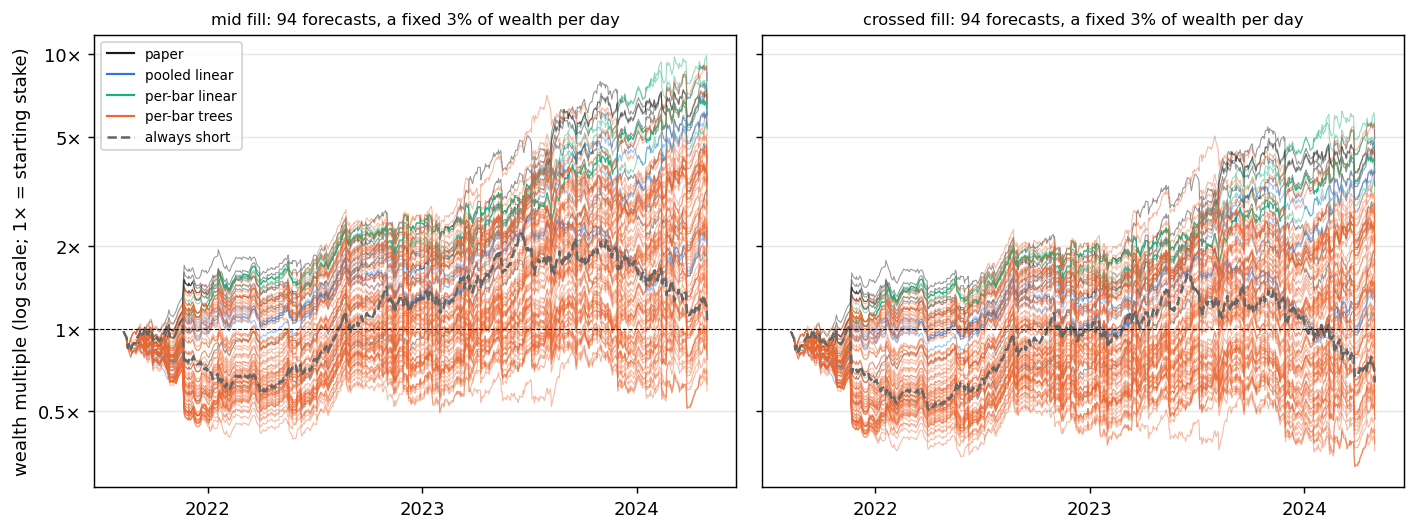
\includegraphics[width=\linewidth]{../results/close_compounding/wealth_modelset.png}
% % 2026-10-15 (notation pass): parked -- dummy day index s -> u (s_t is the signal); mid/crossed fill
% % \caption{Compounding at a fixed fraction: wealth $W_t = \prod_{s\le t}(1 + f q_s R_s)$ with $f =
% % \rhappCompF\,\%$ of wealth staked as straddle premium every day, $q_s = \pm 1$ the forecast's $\sign(s)$ position and
% % $R_s$ the straddle's return, for each of the \rhappModelSetN{} forecasts of the model set, mid fill (left) and crossed
% % fill (right), log scale; dashed: always short.}
% \caption{Compounded wealth at a fixed fraction. The figure plots $W_t = \prod_{u \le t}(1 + f\,q_u R_u)$, with
% $f = \rhappCompF\%$ of wealth committed as straddle premium each trading day, $q_u = \sign(s_u) = \pm 1$ the
% position of the sign strategy and $R_u$ the return on the straddle premium, for each of the \rhappModelSetN{}
% forecasts of the model set, at mid-quotes (left) and at quoted bid--ask prices (right), log scale; dashed: always
% short.}
% \label{fig:rh_app_wealth}
% \end{figure}

\clearpage

% =====================================================================================================================
% A4. The per-bar MinGRU's all-features diagnosis by day class. Sources: the walks' scores.csv (ql_month_end,
% ql_extreme_inputs, ql_other), the classes in wd_enc_study/day_class.csv; the walk of record's gap is asserted against
% results/puffer_forecast_2026-10-12/af_diagnosis/gap_by_dayclass.csv.
% =====================================================================================================================

\begin{table}[htbp]
\centering
\small
\begin{threeparttable}
% 2026-10-15 (notation pass): parked -- code jargon (all-features, walk); finance-journal first sentence
% \caption{Where the all-features MinGRU loses: QLIKE by day class, per walk.}
% 2026-10-15 (table legibility): short caption, details in the notes; notes cut to about five sentences, method
% details referred to Methods. The pre-notation-pass caption and notes are parked in the comments here.
\caption{MinGRU accuracy by type of trading day}
\label{tab:rh_app_mingru_dayclass}
% AUTO-GENERATED by writeup/make_rehaul_appendix.py -- do not edit.
% Source: results/puffer_forecast_2026-10-12/{wd_enc_study, lin_study, ridge_init_study, qlike_study}/scores.csv (ql_month_end, ql_extreme_inputs, ql_other); day classes wd_enc_study/day_class.csv; the walk of record's gap asserted against af_diagnosis/gap_by_dayclass.csv
\begin{tabular}{@{}l*{4}{r}@{}}
\toprule
 & Month-ends & Extreme inputs & Other days & All days \\
Walk & ($n = 43$) & ($n = 60$) & ($n = 763$) & ($n = 866$) \\
\midrule
\multicolumn{5}{@{}l}{\emph{QLIKE, HAR + calendar}} \\
\quad (1) Walk of record & 0.1478 & 0.1328 & 0.0949 & 0.1002 \\
\quad (2) Exogenous decay (B) & 0.1534 & 0.1091 & 0.0952 & 0.0990 \\
\quad (3) Linear shortcut (B) & 0.1444 & 0.0902 & 0.0951 & 0.0972 \\
\quad (4) Ridge start (b), MSE & 0.1420 & 0.1136 & 0.0951 & 0.0987 \\
\quad (5) (4), QLIKE selection & 0.1350 & 0.1062 & 0.0936 & 0.0966 \\
\quad (6) (4), QLIKE training & 0.1271 & 0.1190 & 0.0953 & 0.0985 \\
\quad Elastic net & 0.1542 & 0.1163 & 0.0895 & 0.0946 \\
\quad Ridge & 0.1542 & 0.1163 & 0.0896 & 0.0946 \\
\addlinespace
\multicolumn{5}{@{}l}{\emph{QLIKE, all features}} \\
\quad (1) Walk of record & 0.2323 & 0.2165 & 0.0927 & 0.1082 \\
\quad (2) Exogenous decay (B) & 0.1948 & 0.1735 & 0.0950 & 0.1054 \\
\quad (3) Linear shortcut (B) & 0.1399 & 0.3316 & 0.0992 & 0.1174 \\
\quad (4) Ridge start (b), MSE & 0.1586 & 0.1818 & 0.0927 & 0.1021 \\
\quad (5) (4), QLIKE selection & 0.1274 & 0.1362 & 0.0934 & 0.0980 \\
\quad (6) (4), QLIKE training & 0.1198 & 0.1527 & 0.0888 & 0.0948 \\
\quad Elastic net & 0.1376 & 0.1764 & 0.0853 & 0.0942 \\
\quad Ridge & 0.1361 & 0.1852 & 0.0865 & 0.0958 \\
\addlinespace
\multicolumn{5}{@{}l}{\emph{All features minus HAR + calendar}} \\
\quad (1) Walk of record & 0.0845 & 0.0837 & \ensuremath{-}0.0023 & 0.0080 \\
\quad (2) Exogenous decay (B) & 0.0413 & 0.0644 & \ensuremath{-}0.0002 & 0.0063 \\
\quad (3) Linear shortcut (B) & \ensuremath{-}0.0045 & 0.2414 & 0.0042 & 0.0202 \\
\quad (4) Ridge start (b), MSE & 0.0166 & 0.0682 & \ensuremath{-}0.0024 & 0.0034 \\
\quad (5) (4), QLIKE selection & \ensuremath{-}0.0076 & 0.0299 & \ensuremath{-}0.0003 & 0.0015 \\
\quad (6) (4), QLIKE training & \ensuremath{-}0.0074 & 0.0337 & \ensuremath{-}0.0065 & \ensuremath{-}0.0037 \\
\quad Elastic net & \ensuremath{-}0.0166 & 0.0601 & \ensuremath{-}0.0042 & \ensuremath{-}0.0004 \\
\quad Ridge & \ensuremath{-}0.0181 & 0.0689 & \ensuremath{-}0.0031 & 0.0011 \\
\bottomrule
\end{tabular}

\begin{tablenotes}[flushleft]
\footnotesize
% 2026-10-15 (notation pass): parked -- code jargon (walks, sessions, is_month_end, inputs, walk of record, gap)
% \item[] \emph{Notes:} walks (1)--(6) of Table~\ref{tab:rh_app_mingru_dev}. Month-ends: the sessions flagged \texttt{is\_month\_end}
% (\rhappNmonthEndExtreme{} of them also have extreme inputs). Extreme inputs: at least \rhappExtremeCols{} kept
% columns beyond their training-window maximum, month-ends excluded. The classes partition the \rhappNdays{} days, so
% the day-weighted mean of the three class columns is the overall QLIKE. Of the walk of record's summed daily gap
% between its all-features and HAR + calendar forecasts, extreme-input days carry \rhappGapShareExtreme\,\%, month-ends
% \rhappGapShareMonthEnd\,\% and the other days \rhappGapShareOther\,\%.
\item[] \textit{Notes:} Mean QLIKE of specifications (1)--(6) of Table~\ref{tab:rh_app_mingru_dev} by day type.
Month-ends: the last trading day of each calendar month (\rhappNmonthEndExtreme{} of them also have extreme predictor
values); extreme predictor values: at least \rhappExtremeCols{} retained columns above their estimation-window
maximum, month-ends excluded. The three day types partition the \rhappNdays{} trading days of the out-of-sample
period, so their day-weighted mean equals the overall mean QLIKE. Of the summed daily QLIKE loss differential of
specification (1) between the full predictor set and the HAR benchmark, days with extreme predictor values account
for \rhappGapShareExtreme\%, month-ends for \rhappGapShareMonthEnd\% and the other days for \rhappGapShareOther\%.
\end{tablenotes}
\end{threeparttable}
\end{table}

\clearpage

% 2026-10-15: the feature dictionary (47 series), moved here from 04_features_floats.tex (Appendix A).
% generated by writeup/make_rehaul_data_methods.py -- do not edit by hand; change the generator and re-run.
\providecommand{\rdmL}{\raggedright\let\\\tabularnewline}
\providecommand{\rdmR}{\raggedleft\let\\\tabularnewline}

\begingroup
\footnotesize
\setlength{\tabcolsep}{4pt}
\setlength{\LTcapwidth}{\textwidth}
\begin{longtable}{@{}p{\dimexpr(\textwidth-10\tabcolsep)*220/1000\relax}p{\dimexpr(\textwidth-10\tabcolsep)*300/1000\relax}p{\dimexpr(\textwidth-10\tabcolsep)*190/1000\relax}p{\dimexpr(\textwidth-10\tabcolsep)*130/1000\relax}p{\dimexpr(\textwidth-10\tabcolsep)*80/1000\relax}p{\dimexpr(\textwidth-10\tabcolsep)*80/1000\relax}@{}}
\caption{Feature dictionary: the 47 exogenous series.}\label{tab:rh_dm_dictionary}\\
\toprule
\rdmL Series & \rdmL Raw statistic & \rdmL Source file & \rdmL Transform & \rdmL Diurnal & \rdmL Active \\
\midrule
\endfirsthead
\multicolumn{6}{@{}l}{\textit{Table \ref{tab:rh_dm_dictionary} (continued)}}\\
\toprule
\rdmL Series & \rdmL Raw statistic & \rdmL Source file & \rdmL Transform & \rdmL Diurnal & \rdmL Active \\
\midrule
\endhead
\midrule
\multicolumn{6}{r@{}}{\textit{continued on the next page}}\\
\endfoot
\bottomrule
\multicolumn{6}{@{}p{\textwidth}@{}}{\rdmL\rule{0pt}{2.5ex}\textit{Notes:} One row per exogenous series, by bucket. Derived programmatically: the bucket from \texttt{src/data/loading.py}; the transform from the branch \texttt{apply\_semantic\_transform} takes for the column name and sign (\texttt{src/features/transforms/target.py}); the diurnal adjustment and the asinh routing from \texttt{robust\_transform} run on the forward-filled panel; the activity flag from the executor's mode-inflation rule (modal value on at least 20\,\% of rows), checked against the design's \texttt{\_active} columns. Diurnal: mean, divided by the trailing same-slot mean (20 observations, at least 5, lagged one bar); s.d., divided by the trailing same-slot standard deviation (floored); both banded to $[0.5, 2]$ times the slot's trailing 250-observation median; none: the VIX family, sentiment and the FOMC flags. asinh: a signed series whose s.d.\ divisor sits on its floor on at least 50\,\% of rows skips the division and takes $\operatorname{asinh}(x/s_t)$, $s_t$ a causal EWMA of $|x|$. $x$: no transform (signed series and \texttt{sumabsret}); a series counts as signed if it has any negative value (\texttt{spread\_vwstock} is signed by 1 negative print, 2018-11-12 11:00, and so takes $x$ and s.d.\ where its EW twin takes $\log x$ and mean). After the transform every series is winsorised at rolling 240-bar 1\,/\,99\,\% bounds, set to its median where unobserved, laddered and scaled. Modes of the active series (share of rows): \texttt{numobs} 30 (72\%); \texttt{voldemand\_\allowbreak{}spx\_\allowbreak{}open\_\allowbreak{}and\_\allowbreak{}close} 0 (59\%); \texttt{voldemand\_\allowbreak{}spx\_\allowbreak{}open\_\allowbreak{}only} 0 (60\%); \texttt{voldemand\_\allowbreak{}all\_\allowbreak{}open\_\allowbreak{}and\_\allowbreak{}close} 0 (59\%); \texttt{voldemand\_\allowbreak{}all\_\allowbreak{}open\_\allowbreak{}only} 0 (60\%); \texttt{fomc\_\allowbreak{}release} 0 (98\%); \texttt{fomc\_\allowbreak{}day} 0 (95\%).}\\
\endlastfoot
\multicolumn{6}{@{}l}{\textit{ES return moments (7)}} \\
\rdmL \texttt{sumret} & \rdmL bar return $\sum r$ & \rdmL \texttt{core\_\allowbreak{}stats} & \rdmL $x$ & \rdmL s.d. & \rdmL no \\
\rdmL \texttt{sumabsret} & \rdmL $\sum |r|$ & \rdmL \texttt{core\_\allowbreak{}stats} & \rdmL $x$ & \rdmL mean & \rdmL no \\
\rdmL \texttt{sumret3} & \rdmL $\sum r^3$ & \rdmL \texttt{core\_\allowbreak{}stats} & \rdmL $x^{1/3}$ & \rdmL s.d. & \rdmL no \\
\rdmL \texttt{sumret4} & \rdmL $\sum r^4$ & \rdmL \texttt{core\_\allowbreak{}stats} & \rdmL $\pm|x|^{1/4}$ & \rdmL mean & \rdmL no \\
\rdmL \texttt{sumpret2} & \rdmL upside semivariance $\sum r^2 \mathbf{1}\{r>0\}$ & \rdmL \texttt{core\_\allowbreak{}stats} & \rdmL $\sqrt{x}$ & \rdmL mean & \rdmL no \\
\rdmL \texttt{sumbipow} & \rdmL bipower variation & \rdmL \texttt{core\_\allowbreak{}stats} & \rdmL $\sqrt{x}$ & \rdmL mean & \rdmL no \\
\rdmL \texttt{sumautocov} & \rdmL first-order autocovariance $\sum r_i r_{i-1}$ & \rdmL \texttt{core\_\allowbreak{}stats} & \rdmL $\pm\sqrt{|x|}$ & \rdmL s.d. & \rdmL no \\
\addlinespace
\multicolumn{6}{@{}l}{\textit{Liquidity (14)}} \\
\rdmL \texttt{sumvolume} & \rdmL contract volume & \rdmL \texttt{core\_\allowbreak{}stats} & \rdmL $\log x$ & \rdmL mean & \rdmL no \\
\rdmL \texttt{numobs} & \rdmL 1-min returns in the bar ($\le 30$) & \rdmL \texttt{core\_\allowbreak{}stats} & \rdmL $\log x$ & \rdmL mean & \rdmL yes \\
\rdmL \texttt{turnover\_\allowbreak{}ewstock} & \rdmL turnover & \rdmL \texttt{ewstock\_\allowbreak{}stats} & \rdmL $\sqrt{x}$ & \rdmL mean & \rdmL no \\
\rdmL \texttt{buyturnover\_\allowbreak{}ewstock} & \rdmL buyer-initiated turnover & \rdmL \texttt{ewstock\_\allowbreak{}stats} & \rdmL $\sqrt{x}$ & \rdmL mean & \rdmL no \\
\rdmL \texttt{sellturnover\_\allowbreak{}ewstock} & \rdmL seller-initiated turnover & \rdmL \texttt{ewstock\_\allowbreak{}stats} & \rdmL $\sqrt{x}$ & \rdmL mean & \rdmL no \\
\rdmL \texttt{effspread\_\allowbreak{}ewstock} & \rdmL effective spread & \rdmL \texttt{ewstock\_\allowbreak{}stats} & \rdmL $\sqrt{x}$ & \rdmL mean & \rdmL no \\
\rdmL \texttt{spread\_\allowbreak{}ewstock} & \rdmL quoted spread & \rdmL \texttt{ewstock\_\allowbreak{}stats} & \rdmL $\log x$ & \rdmL mean & \rdmL no \\
\rdmL \texttt{turnover\_\allowbreak{}vwstock} & \rdmL turnover & \rdmL \texttt{vwstock\_\allowbreak{}stats} & \rdmL $\sqrt{x}$ & \rdmL mean & \rdmL no \\
\rdmL \texttt{buyturnover\_\allowbreak{}vwstock} & \rdmL buyer-initiated turnover & \rdmL \texttt{vwstock\_\allowbreak{}stats} & \rdmL $\sqrt{x}$ & \rdmL mean & \rdmL no \\
\rdmL \texttt{sellturnover\_\allowbreak{}vwstock} & \rdmL seller-initiated turnover & \rdmL \texttt{vwstock\_\allowbreak{}stats} & \rdmL $\sqrt{x}$ & \rdmL mean & \rdmL no \\
\rdmL \texttt{effspread\_\allowbreak{}vwstock} & \rdmL effective spread & \rdmL \texttt{vwstock\_\allowbreak{}stats} & \rdmL $\sqrt{x}$ & \rdmL mean & \rdmL no \\
\rdmL \texttt{spread\_\allowbreak{}vwstock} & \rdmL quoted spread & \rdmL \texttt{vwstock\_\allowbreak{}stats} & \rdmL $x$ & \rdmL s.d. & \rdmL no \\
\rdmL \texttt{ofi\_\allowbreak{}ewstock} & \rdmL order-flow imbalance $(b-s)/(b+s)$ of turnover & \rdmL \texttt{ewstock\_\allowbreak{}stats} (derived) & \rdmL $x$ & \rdmL s.d. & \rdmL no \\
\rdmL \texttt{ofi\_\allowbreak{}vwstock} & \rdmL order-flow imbalance $(b-s)/(b+s)$ of turnover & \rdmL \texttt{vwstock\_\allowbreak{}stats} (derived) & \rdmL $x$ & \rdmL s.d. & \rdmL no \\
\addlinespace
\multicolumn{6}{@{}l}{\textit{Market, equal-weighted (6)}} \\
\rdmL \texttt{sumret2\_\allowbreak{}ewstock} & \rdmL realized variance $\sum r^2$ & \rdmL \texttt{ewstock\_\allowbreak{}stats} & \rdmL $\sqrt{x}$ & \rdmL mean & \rdmL no \\
\rdmL \texttt{sumret3\_\allowbreak{}ewstock} & \rdmL $\sum r^3$ & \rdmL \texttt{ewstock\_\allowbreak{}stats} & \rdmL $x^{1/3}$ & \rdmL s.d. & \rdmL no \\
\rdmL \texttt{sumret4\_\allowbreak{}ewstock} & \rdmL $\sum r^4$ & \rdmL \texttt{ewstock\_\allowbreak{}stats} & \rdmL $\pm|x|^{1/4}$ & \rdmL mean & \rdmL no \\
\rdmL \texttt{sumabsret\_\allowbreak{}ewstock} & \rdmL $\sum |r|$ & \rdmL \texttt{ewstock\_\allowbreak{}stats} & \rdmL $x$ & \rdmL mean & \rdmL no \\
\rdmL \texttt{sumbipow\_\allowbreak{}ewstock} & \rdmL bipower variation & \rdmL \texttt{ewstock\_\allowbreak{}stats} & \rdmL $\sqrt{x}$ & \rdmL mean & \rdmL no \\
\rdmL \texttt{sumpret2\_\allowbreak{}ewstock} & \rdmL upside semivariance $\sum r^2 \mathbf{1}\{r>0\}$ & \rdmL \texttt{ewstock\_\allowbreak{}stats} & \rdmL $\sqrt{x}$ & \rdmL mean & \rdmL no \\
\addlinespace
\multicolumn{6}{@{}l}{\textit{Market, value-weighted (6)}} \\
\rdmL \texttt{sumret2\_\allowbreak{}vwstock} & \rdmL realized variance $\sum r^2$ & \rdmL \texttt{vwstock\_\allowbreak{}stats} & \rdmL $\sqrt{x}$ & \rdmL mean & \rdmL no \\
\rdmL \texttt{sumret3\_\allowbreak{}vwstock} & \rdmL $\sum r^3$ & \rdmL \texttt{vwstock\_\allowbreak{}stats} & \rdmL $x^{1/3}$ & \rdmL s.d. & \rdmL no \\
\rdmL \texttt{sumret4\_\allowbreak{}vwstock} & \rdmL $\sum r^4$ & \rdmL \texttt{vwstock\_\allowbreak{}stats} & \rdmL $\pm|x|^{1/4}$ & \rdmL mean & \rdmL no \\
\rdmL \texttt{sumabsret\_\allowbreak{}vwstock} & \rdmL $\sum |r|$ & \rdmL \texttt{vwstock\_\allowbreak{}stats} & \rdmL $x$ & \rdmL mean & \rdmL no \\
\rdmL \texttt{sumbipow\_\allowbreak{}vwstock} & \rdmL bipower variation & \rdmL \texttt{vwstock\_\allowbreak{}stats} & \rdmL $\sqrt{x}$ & \rdmL mean & \rdmL no \\
\rdmL \texttt{sumpret2\_\allowbreak{}vwstock} & \rdmL upside semivariance $\sum r^2 \mathbf{1}\{r>0\}$ & \rdmL \texttt{vwstock\_\allowbreak{}stats} & \rdmL $\sqrt{x}$ & \rdmL mean & \rdmL no \\
\addlinespace
\multicolumn{6}{@{}l}{\textit{Sentiment (3)}} \\
\rdmL \texttt{stocktwits\_\allowbreak{}attention} & \rdmL message volume (attention) & \rdmL \texttt{spy\_\allowbreak{}and\_\allowbreak{}sentiment} & \rdmL $\log x$ & \rdmL mean & \rdmL no \\
\rdmL \texttt{stocktwits\_\allowbreak{}sentiment} & \rdmL net sentiment score & \rdmL \texttt{spy\_\allowbreak{}and\_\allowbreak{}sentiment} & \rdmL $x$ & \rdmL none & \rdmL no \\
\rdmL \texttt{stocktwits\_\allowbreak{}sentcount} & \rdmL messages with a sentiment tag & \rdmL \texttt{spy\_\allowbreak{}and\_\allowbreak{}sentiment} & \rdmL $\log x$ & \rdmL mean & \rdmL no \\
\addlinespace
\multicolumn{6}{@{}l}{\textit{Implied volatility (3)}} \\
\rdmL \texttt{vix} & \rdmL VIX level & \rdmL \texttt{vix\_\allowbreak{}and\_\allowbreak{}voldemand} & \rdmL $\log x$ & \rdmL none & \rdmL no \\
\rdmL \texttt{vvix} & \rdmL VVIX level & \rdmL \texttt{vix\_\allowbreak{}and\_\allowbreak{}voldemand} & \rdmL $\log x$ & \rdmL none & \rdmL no \\
\rdmL \texttt{vix3m} & \rdmL VIX3M level & \rdmL \texttt{vix\_\allowbreak{}and\_\allowbreak{}voldemand} & \rdmL $\log x$ & \rdmL none & \rdmL no \\
\addlinespace
\multicolumn{6}{@{}l}{\textit{Volatility demand (4)}} \\
\rdmL \texttt{voldemand\_\allowbreak{}spx\_\allowbreak{}open\_\allowbreak{}and\_\allowbreak{}close} & \rdmL SPX options, opening and closing & \rdmL \texttt{vix\_\allowbreak{}and\_\allowbreak{}voldemand} & \rdmL $\operatorname{asinh}(x/s_t)$ & \rdmL none & \rdmL yes \\
\rdmL \texttt{voldemand\_\allowbreak{}spx\_\allowbreak{}open\_\allowbreak{}only} & \rdmL SPX options, opening only & \rdmL \texttt{vix\_\allowbreak{}and\_\allowbreak{}voldemand} & \rdmL $\operatorname{asinh}(x/s_t)$ & \rdmL none & \rdmL yes \\
\rdmL \texttt{voldemand\_\allowbreak{}all\_\allowbreak{}open\_\allowbreak{}and\_\allowbreak{}close} & \rdmL all options, opening and closing & \rdmL \texttt{vix\_\allowbreak{}and\_\allowbreak{}voldemand} & \rdmL $\operatorname{asinh}(x/s_t)$ & \rdmL none & \rdmL yes \\
\rdmL \texttt{voldemand\_\allowbreak{}all\_\allowbreak{}open\_\allowbreak{}only} & \rdmL all options, opening only & \rdmL \texttt{vix\_\allowbreak{}and\_\allowbreak{}voldemand} & \rdmL $\operatorname{asinh}(x/s_t)$ & \rdmL none & \rdmL yes \\
\addlinespace
\multicolumn{6}{@{}l}{\textit{FOMC calendar (4)}} \\
\rdmL \texttt{fomc\_\allowbreak{}release} & \rdmL 1 on the 14:30 statement bar & \rdmL \texttt{releases} (derived) & \rdmL $\log x$ & \rdmL none & \rdmL yes \\
\rdmL \texttt{fomc\_\allowbreak{}day} & \rdmL 1 on statement days & \rdmL \texttt{releases} (derived) & \rdmL $\log x$ & \rdmL none & \rdmL yes \\
\rdmL \texttt{fomc\_\allowbreak{}until\_\allowbreak{}inv} & \rdmL $1/(1+{}$bars to next statement$)$ & \rdmL \texttt{releases} (derived) & \rdmL $\log x$ & \rdmL none & \rdmL no \\
\rdmL \texttt{fomc\_\allowbreak{}since\_\allowbreak{}inv} & \rdmL $1/(1+{}$bars since last$)$ & \rdmL \texttt{releases} (derived) & \rdmL $\log x$ & \rdmL none & \rdmL no \\
\end{longtable}
\endgroup


% 2026-10-16 (user): Statistical tests moved out of Methods. After the implementation floats so those
% tables stay with Implementation details.
% 2026-10-16 (user): moved from Methods (05_methods.tex). Label sec:rh_methods_tests kept.
% The results section footnotes this analysis.

\section{Statistical tests}
\label{sec:rh_methods_tests}
\begin{itemize}
\item \textbf{Diebold--Mariano test.} To compare the predictive accuracy of two competing forecasts $A$ and $B$, we apply the \citet{DieboldMariano1995} test to the daily QLIKE loss differentials, incorporating the small-sample adjustment of \citet{HarveyLeybourneNewbold1997} for one-step-ahead forecasts:
  \[
    d_t = L_t^{A} - L_t^{B}, \qquad
    \DM = \sqrt{\frac{|\mathcal O| - 1}{|\mathcal O|}}\;
      \frac{\bar d}{\sqrt{\hat\Omega / |\mathcal O|}} .
  \]
  % 2026-10-15 (finish): parked -- the horizon symbol h (also the boosting Hessian h_{t'}) dropped; every forecast
  % is one step ahead, so h = 1 is substituted: (|O| + 1 - 2h + h(h-1)/|O|)/|O| = (|O| - 1)/|O|. Was:
  % \DM = \sqrt{\frac{|\mathcal O| + 1 - 2h + h(h-1)/|\mathcal O|}{|\mathcal O|}}\;
  %   \frac{\bar d}{\sqrt{\hat\Omega / |\mathcal O|}}, \qquad h = 1 .
  % 2026-10-15 (notation pass): parked -- the uncorrected and corrected statistics merged into one symbol, \DM
  % (the HLN-corrected one, as the code reports); n scored days -> |O|. Old display:
  % \mathrm{DM} = \frac{\bar d}{\sqrt{\hat\Omega / n}}, \qquad
  % \mathrm{DM}^{\ast} = \mathrm{DM} \sqrt{\frac{n + 1 - 2h + h(h-1)/n}{n}}, \qquad h = 1 .
  \begin{itemize}
  \item Here $A$ and $B$ denote competing forecast series $f_{m,\mathcal X,\mathcal I}$, indexed by the model class $m$, the predictor set $\mathcal X \in \{\mathrm{HAR}, \mathrm{Full}\}$, and the estimation interval set $\mathcal I \in \{\{c\}, \{1, \dots, M\}\}$.
  % 2026-10-15 (user): parked -- "out-of-sample days"; the evaluation set and the option-data subsample. Was:
  % "\item $\mathcal O$: the out-of-sample days of the exercise, numbered $t = 1, \dots, |\mathcal O|$ in time order;
  %   $\mathcal O = \mathcal T_{\mathrm{oos}}$, $|\mathcal T_{\mathrm{oos}}| = T_{\mathrm{oos}}$, in the headline
  %   comparison."
  \item The evaluation set $\mathcal O$, indexed chronologically by $t = 1, \dots, |\mathcal O|$, equals the full evaluation span $\mathcal O = \mathcal T_{\mathrm{oos}}$ ($|\mathcal T_{\mathrm{oos}}| = T_{\mathrm{oos}}$) for statistical accuracy comparisons and the option-data subsample $\mathcal T_{\mathrm{opt}} \subset \mathcal T_{\mathrm{oos}}$ for straddle return comparisons (Section~\ref{sec:rh_data}).
  \item We denote by $\bar d$ the sample mean of $d_t$ over $\mathcal O$ and compute two-sided $p$-values under the standard normal distribution as $p = 2\bigl\{1 - \Phi(|\DM|)\bigr\}$.
  \item Under this sign convention, $\DM < 0$ indicates that forecast $A$ achieves a lower average loss than forecast $B$. Throughout the paper, ``statistically significant'' refers to significance at the 5\% level ($p < 0.05$).
  % 2026-10-15 (user): merged from Forecast evaluation (moved from 06_results.tex): the p-value formula, the sign
  % convention and the meaning of "significant". Was: "\item $\bar d$: mean loss differential over $\mathcal O$;
  % two-sided $p$-value from the standard normal."
  % 2026-10-15 (finish): parked -- h dropped (one-step-ahead forecasts). Was:
  % \item $\bar d$: mean loss differential over $\mathcal O$; $h$: forecast horizon; two-sided $p$-value from the
  %   standard normal.
  \end{itemize}
% 2026-10-15 (consolidation): parked -- lag truncation q -> q_NW (q_t is the position), autocovariance lag k -> j (k
% is the HAR horizon), typed q = 6 / q = 14 -> \fqsDMLag / \fqsHACLag, plain-text citations -> \citep. The 1/|O|
% divisor of hat gamma_j is unchanged (FLAG (4) below awaits the user). Old bullets:
% 2026-10-18 (user, E13): FLAG (4) resolved -- dm_test now divides gamma_j by |O| (src/evaluation/diebold_mariano.py:67-68), matching this display.
% \item \textbf{Newey--West variance} (Newey and West 1987), Bartlett weights, lag truncation $q$:
%   \hat\Omega = \hat\gamma_0 + 2 \sum_{k=1}^{q} (1 - k/(q + 1)) \hat\gamma_k, \qquad
%   \hat\gamma_k = \frac{1}{|\mathcal O|} \sum_{t=k+1}^{|\mathcal O|} (d_t - \bar d)(d_{t-k} - \bar d).
%   DM: $q = \max(h - 1, \lfloor 4 (|\mathcal O|/100)^{2/9} \rfloor)$, which gives $q = 6$ on $\mathcal T_{\mathrm{oos}}$.
% \item \textbf{HAC $t$-statistic on the daily return differential} (Newey--West): $t = \bar d / \sqrt{\hat\Omega /
%   |\mathcal O|}$, with $d_t$ now the difference between two trading strategies' daily returns, no HLN correction;
%   $q = \lfloor 1.5\, |\mathcal O|^{1/3} \rfloor$, which gives $q = 14$ on $\mathcal T_{\mathrm{oos}}$.
% \item \textbf{Model confidence set} \citep{HansenLundeNason2011}, \textbf{superior predictive ability} (Hansen 2005)
%   and \textbf{StepM} (Romano and Wolf 2005) for the comparison of predictor sets.
\item \textbf{Newey--West long-run variance.} Following \citet{NeweyWest1987}, we estimate the long-run variance $\hat\Omega$ using Bartlett kernel weights with lag truncation parameter $q_{\mathrm{NW}}$:
  \[
    \hat\Omega = \hat\gamma_0 + 2 \sum_{j=1}^{q_{\mathrm{NW}}} \Bigl(1 - \frac{j}{q_{\mathrm{NW}} + 1}\Bigr) \hat\gamma_j,
    \qquad
    \hat\gamma_j = \frac{1}{|\mathcal O|} \sum_{t=j+1}^{|\mathcal O|} (d_t - \bar d)(d_{t-j} - \bar d).
  \]
% 2026-10-18 (user, E13): parked -- resolved; dm_test now divides gamma_j by |O|, matching the display; DM statistics regenerated on 2026-10-18 for the accuracy tables and macros (make_rehaul_results.py, make_rehaul_economics.py); the appendix study tables still need regenerating (note below). Was:
% \editc{orange}{E13}{Decision: change this display, or recompute the printed $\DM$.\\Problem: this display divides $\hat\gamma_j$ by $|\mathcal O|$, and every printed $\DM$ was computed by \texttt{dm\_test}, which divides by $|\mathcal O|-j$.\\
% The autocovariance $\hat\gamma_j$ in the display is the average of the products $(d_t-\bar d)(d_{t-j}-\bar d)$, and the divisor written in front of the sum is $|\mathcal O|$, the number of days in the comparison. There are only $|\mathcal O|-j$ such products, because the first $j$ days have no lag-$j$ partner. The function that produced the printed Diebold--Mariano statistics is \texttt{dm\_test}, and it takes those products with \texttt{np.mean}, which divides by the length of the array it is given, $|\mathcal O|-j$. The HAC $t$ on returns comes from \texttt{newey\_west\_t}, and that function divides by $|\mathcal O|$, so it matches this display. The accuracy-section $\DM$ numbers match \texttt{dm\_test}. On $\mathcal T_{\mathrm{oos}}$ the lag runs from 1 through $\rhoosDMLag$, and at each of those lags the two divisors differ.}
\editc{orange}{E13}{Decision: regenerate the remaining $\DM$ statistics.\\Problem: \texttt{dm\_test} now divides $\hat\gamma_j$ by $|\mathcal O|$, as displayed. The accuracy tables and macros were regenerated on 2026-10-18, but the $\DM$ statistics and significance stars in the appendix tuning and study tables are read from stored study outputs computed with the old divisor $|\mathcal O|-j$, so they predate the change and must be regenerated.}
  \begin{itemize}
  \item For the Diebold--Mariano test, we set the bandwidth according to the plug-in rule $q_{\mathrm{NW}} = \lfloor 4 (|\mathcal O|/100)^{2/9} \rfloor$ (its numerical value on $\mathcal T_{\mathrm{oos}}$ is reported in Section~\ref{sec:rh_exp_setup}).
  % 2026-10-15 (user): parked -- moved to Methods with Forecast evaluation, numbers removed (the lag value now lives in
  % Experimental setup, 06_results.tex). Was: "\item DM: $q_{\mathrm{NW}} = \lfloor 4 (|\mathcal O|/100)^{2/9}
  % \rfloor$, which gives $q_{\mathrm{NW}} = \fqsDMLag$ on $\mathcal T_{\mathrm{oos}}$."
  % 2026-10-15 (finish): parked -- h = 1 substituted (max(h - 1, .) = max(0, .) is the floor term). Was:
  % \item DM: $q_{\mathrm{NW}} = \max\bigl(h - 1, \lfloor 4 (|\mathcal O|/100)^{2/9} \rfloor\bigr)$, which gives
  %   $q_{\mathrm{NW}} = \fqsDMLag$ on $\mathcal T_{\mathrm{oos}}$.
  \end{itemize}
  % src/evaluation/diebold_mariano.py:33-93.
  % 2026-10-15 (notation pass): FLAG, math not changed -- dm_test computes gamma_k as np.mean(dc[k:] * dc[:-k]),
  % i.e. divides by |O| - k, not |O|; newey_west_t (the return test below) divides by |O|, as displayed.
  % 2026-10-15 (consolidation): FLAG (4) still open (user decision); the lag index is now j, the divisor unchanged.
  % 06_results.tex displays the code's |O| - j divisor for the DM statistic; the two agree once the user decides.
  % 2026-10-15 (user): the 06_results.tex display (Forecast evaluation, "Long-run variance", T_oos - j divisor and
  % explicit Bartlett weights w_j) moved to Methods and was merged into this bullet; it is parked in 06_results.tex.
  % This display (1/|O|) is now the paper's only one; FLAG (4) still decides the divisor.
  % 2026-10-18 (user, E13): FLAG (4) resolved -- dm_test now divides gamma_j by |O| (src/evaluation/diebold_mariano.py:67-68), matching this display.
% 2026-10-15 (consolidation): FLAG (7) resolved -- newey_west_t is also applied to a single strategy's mean return
% (Economic value, Table rh_econ_control), so the bullet is worded for any daily return series.
% 2026-10-21 (user, decision #2): parked -- the Newey--West t of a mean return at lag floor(1.5 |O|^(1/3)), with
% normal critical values; no published source uses the constant 1.5, so the paper no longer presents it as a rule.
% Replaced by the LLSW (2018) test with fixed-b critical values (means) and the Ledoit--Wolf (2008) test (Sharpe
% ratios), writeup/hac_inference.py. Was:
% \item \textbf{HAC $t$-statistic for mean daily returns.} For any daily return series $r_t$---either the return of an individual trading strategy or the return differential $\Delta_t$ between two strategies---we compute the unadjusted Newey--West $t$-statistic
%   \[
%     t = \frac{\bar r}{\sqrt{\hat\Omega_r / |\mathcal O|}},
%   \]
%   where $\hat\Omega_r$ is the Newey--West variance estimator above evaluated on $r_t$ in place of $d_t$, using lag truncation
  % $q_{\mathrm{NW}} = \lfloor 1.5\, |\mathcal O|^{1/3} \rfloor$ (its value on $\mathcal T_{\mathrm{oos}}$:  % 2026-10-15:
  % Experimental setup, Section~\ref{sec:rh_exp_setup}).  % parked -- the returns are on the option-data subsample
%   $q_{\mathrm{NW}} = \lfloor 1.5\, |\mathcal O|^{1/3} \rfloor$ (its numerical value on $\mathcal T_{\mathrm{opt}}$ is given in Section~\ref{sec:rh_econ_measures}).
  % 2026-10-15 (user): parked -- lag value removed from Methods, as for the DM lag (Forecast evaluation moved here,
  % numbers removed); it now lives in Experimental setup. Was: "... $q_{\mathrm{NW}} = \lfloor 1.5\, |\mathcal O|^{1/3}
  % \rfloor$, which gives $q_{\mathrm{NW}} = \fqsHACLag$ on $\mathcal T_{\mathrm{oos}}$."
  % 2026-10-15 (finish): parked -- same content; the formula moved to a display (the inline version left an underfull
  % line). Was:
  % \item \textbf{HAC $t$-statistic of a mean daily return} (Newey--West, no HLN correction):
  %   $t = \bar r / \sqrt{\hat\Omega_r / |\mathcal O|}$, with $\hat\Omega_r$ the Newey--West variance above computed on a
  %   daily return series $r_t$ in place of $d_t$: a single strategy's return (a test of its mean return) or the difference
  %   between two strategies' returns (a test of the mean return differential);
  %   $q_{\mathrm{NW}} = \lfloor 1.5\, |\mathcal O|^{1/3} \rfloor$, which gives $q_{\mathrm{NW}} = \fqsHACLag$ on
  %   $\mathcal T_{\mathrm{oos}}$.
  % notebooks/atm_straddle_lib.py:1240-1261 (newey_west_t).
\item \textbf{Test of a mean daily return.} For any daily return series $r_t$---either the return of an individual trading strategy or the return differential $\Delta_t$ between two strategies---observed on the $T = \rheSzDays$ post-warmup days $\mathcal T_{\mathrm{opt}}^{+}$ (Section~\ref{sec:rh_econ_measures}), we test whether its mean is zero with the procedure that \citet{LazarusLewisStockWatson2018} recommend for the Newey--West estimator:
  \[
    t = \frac{\bar r}{\sqrt{\hat\Omega_r / T}},
    \qquad
    \hat\Omega_r = \sum_{|j| < S} \Bigl(1 - \frac{|j|}{S}\Bigr) \hat\gamma_j,
    \qquad
    \hat\gamma_j = \frac{1}{T} \sum_{t=|j|+1}^{T} (r_t - \bar r)(r_{t-|j|} - \bar r),
  \]
  with the Bartlett kernel, bandwidth $S = \lceil 1.3\, T^{1/2} \rceil = \rheHACS$, and fixed-$b$ critical values for $b = S/T$ \citep{KieferVogelsang2005}.
  \begin{itemize}
  \item The autocovariances divide by $T$, with no small-sample factor; at lag truncation $S - 1$ the estimator equals the Newey--West variance of the previous item.
  \item This bandwidth is larger than that of conventional rules such as $0.75\, T^{1/3}$, which \citet{LazarusLewisStockWatson2018} obtain from the formula of \citet{Andrews1991} for a first-order autoregression with coefficient $0.25$. Combined with fixed-$b$ critical values, it reduces the size distortion of the test when the returns are serially correlated \citep{LazarusLewisStockWatson2018}.
  \item Under the null hypothesis and fixed $b$, the limiting distribution of $t$ is a functional of Brownian motion that depends only on the kernel and on $b$ \citep{KieferVogelsang2005}. We obtain its quantiles by simulation, computing the same statistic on 1{,}000{,}000 independent series of 1{,}000 i.i.d.\ standard normal draws with bandwidth $1{,}000\,b$. This gives the two-sided 5\% critical value \rheHACCV{} and the $p$-values reported in the text, in place of the standard normal value 1.96.
  \end{itemize}
\item \textbf{Test of equal Sharpe ratios.} A test of $\bar\Delta = 0$ concerns the mean return differential, not the difference between two Sharpe ratios, which divides each strategy's mean return by its own standard deviation. For every statement about a Sharpe ratio difference we therefore use the studentized circular block bootstrap test of \citet{LedoitWolf2008}.
  \begin{itemize}
  \item With $u = \bigl(\mu_A, \mu_B, \mathrm E[(r^A_t)^2], \mathrm E[(r^B_t)^2]\bigr)$, the difference of the Sharpe ratios of the daily returns, $\mu_A/\sigma_A - \mu_B/\sigma_B$, is a smooth function $f(u)$; its standard error follows from the delta method and the long-run covariance matrix $\Psi$ of $\bigl(r^A_t, r^B_t, (r^A_t)^2, (r^B_t)^2\bigr)$.
  \item The test statistic is $d = |f(\hat u)| / \mathrm{se}(\hat u)$. Each of \rheLWBoot{} bootstrap samples joins blocks of \rheLWBlock{} consecutive days, drawn with replacement from the $T$ post-warmup days arranged on a circle, and gives $d^{*} = |f(\hat u^{*}) - f(\hat u)| / \mathrm{se}(\hat u^{*})$, with $\Psi$ estimated in that sample by the block-based estimator of \citet{LedoitWolf2008}. The $p$-value is $\bigl(\#\{d^{*} \ge d\} + 1\bigr)/(\rheLWBoot + 1)$.
  \item In the original sample, $\Psi$ is estimated with the Bartlett kernel at bandwidth equal to the block length, whose expectation is approximately that of the block-based estimator; \citet{LedoitWolf2008} use a prewhitened quadratic-spectral kernel at this step. The block length is fixed at \rheLWBlock{} days rather than calibrated; the next item reports the number of rejections at block lengths \rheLWBlockLo{} and \rheLWBlockHi{}. The random seed is fixed.
  \item The test concerns the Sharpe ratios of daily returns over the $T$ post-warmup days, without the year-by-year annualization of Section~\ref{sec:rh_econ_measures}.
  \end{itemize}
\item \textbf{Robustness to the long-run variance estimator.} Table~\ref{tab:rh_app_hac_robust} lists every comparison of strategy returns whose statistical significance Section~\ref{sec:rh_econ} or Appendix~\ref{sec:rh_econ_last30} states. For each comparison it reports the $t$-statistic of the mean return differential with the Newey--West variance at lag truncation $q_{\mathrm{NW}} = \lfloor 4 (T/100)^{2/9} \rfloor = \rhrRobLagNW$ \citep{NeweyWest1994} and at $q_{\mathrm{NW}} = \lfloor 1.5\, T^{1/3} \rfloor = \rhrRobLagOld$, the lag truncation of an earlier version of this paper, both with standard normal $p$-values; the fixed-$b$ test above; and the $p$-value of the \citet{LedoitWolf2008} test. Statements in the text about mean returns use the fixed-$b$ test, and statements about Sharpe ratios use the \citet{LedoitWolf2008} test.
  \begin{itemize}
  \item Of the \rhrRobN{} tests of a mean, \rhrRobFbSig{} are statistically significant at the 5\% level under the fixed-$b$ test, \rhrRobNWFiveSig{} at lag truncation \rhrRobLagNW{} and \rhrRobNWTwelveSig{} at lag truncation \rhrRobLagOld{} with standard normal critical values.
  \item Of the \rhrRobNPairs{} tests of equal Sharpe ratios, \rhrRobLWSig{} reject at the 5\% level with block length \rheLWBlock{}, \rhrRobLWSigLo{} with block length \rheLWBlockLo{} and \rhrRobLWSigHi{} with block length \rheLWBlockHi{}.
  \end{itemize}
% generated by writeup/make_rehaul_results.py (2026-10-21, decision #2): the tests of strategy returns behind
% the significance statements of Section 7 and Appendix F, on the 614 post-warmup days, under four procedures.
% 2026-10-26 (D19): Sharpe-ratio differences by Ledoit-Wolf (the paper's test); the bootstrap column is parked.
% Do not edit by hand.
\begin{table}[tbp]
\centering
\scriptsize
\setlength{\tabcolsep}{3.5pt}
\begin{threeparttable}
\caption{Tests of strategy returns under alternative long-run variance estimators}
\label{tab:rh_app_hac_robust}
\begin{tabular}{@{}lrrrrrrrrr@{}}
\toprule
 & & & \multicolumn{2}{c}{NW, $q_{\mathrm{NW}} = \rhrRobLagNW$} & \multicolumn{2}{c}{NW, $q_{\mathrm{NW}} = \rhrRobLagOld$} & \multicolumn{2}{c}{NW, $S = \rheHACS$, fixed-$b$} & LW \\
\cmidrule(lr){4-5}\cmidrule(lr){6-7}\cmidrule(lr){8-9}\cmidrule(l){10-10}
 & $\bar\Delta$ (\%) & $\Delta\SR$ & $t$ & $p$ & $t$ & $p$ & $t$ & $p$ & $p$ \\
\midrule
\multicolumn{10}{@{}l}{\textit{Panel A: Pooled intraday model minus short-straddle benchmark}} \\
\addlinespace[2pt]
Ridge, HAR & $4.76$ & $0.63$ & $0.93$ & $0.350$ & $0.95$ & $0.344$ & $0.90$ & $0.388$ & $0.350$ \\
Ridge, full & $9.89$ & $1.32$ & $1.88$ & $0.060$ & $1.82$ & $0.069$ & $1.70$ & $0.110$ & $0.059$ \\
Lasso, HAR & $4.76$ & $0.63$ & $0.93$ & $0.350$ & $0.95$ & $0.344$ & $0.90$ & $0.388$ & $0.350$ \\
Lasso, full & $10.52$ & $1.40$ & $2.03$ & $0.042$ & $2.01$ & $0.045$ & $1.93$ & $0.071$ & $0.039$ \\
Elastic net, HAR & $4.76$ & $0.63$ & $0.93$ & $0.350$ & $0.95$ & $0.344$ & $0.90$ & $0.388$ & $0.350$ \\
Elastic net, full & $11.46$ & $1.53$ & $2.22$ & $0.026$ & $2.13$ & $0.033$ & $1.95$ & $0.068$ & $0.026$ \\
LightGBM, HAR & $2.50$ & $0.33$ & $0.48$ & $0.634$ & $0.52$ & $0.606$ & $0.53$ & $0.610$ & $0.614$ \\
LightGBM, full & $9.11$ & $1.21$ & $1.76$ & $0.078$ & $1.76$ & $0.078$ & $1.68$ & $0.113$ & $0.070$ \\
XGBoost, HAR & $4.96$ & $0.66$ & $0.92$ & $0.356$ & $1.02$ & $0.308$ & $1.08$ & $0.304$ & $0.315$ \\
XGBoost, full & $9.17$ & $1.22$ & $1.77$ & $0.076$ & $1.76$ & $0.078$ & $1.61$ & $0.127$ & $0.064$ \\
Random forest, HAR & $-0.03$ & $0.00$ & $-0.01$ & $0.994$ & $-0.01$ & $0.993$ & $-0.01$ & $0.993$ & $0.992$ \\
Random forest, full & $11.64$ & $1.56$ & $2.28$ & $0.023$ & $2.33$ & $0.020$ & $2.14$ & $0.046$ & $0.018$ \\
\addlinespace[4pt]
\multicolumn{10}{@{}l}{\textit{Panel B: Pooled intraday model, full predictor set minus HAR benchmark}} \\
\addlinespace[2pt]
Ridge & $5.13$ & $0.69$ & $1.43$ & $0.153$ & $1.37$ & $0.171$ & $1.32$ & $0.209$ & $0.171$ \\
Lasso & $5.77$ & $0.77$ & $1.60$ & $0.110$ & $1.54$ & $0.122$ & $1.59$ & $0.132$ & $0.120$ \\
Elastic net & $6.70$ & $0.90$ & $1.91$ & $0.056$ & $1.79$ & $0.074$ & $1.67$ & $0.115$ & $0.074$ \\
LightGBM & $6.61$ & $0.88$ & $1.99$ & $0.047$ & $1.94$ & $0.053$ & $1.89$ & $0.076$ & $0.050$ \\
XGBoost & $4.21$ & $0.56$ & $1.27$ & $0.203$ & $1.27$ & $0.204$ & $1.16$ & $0.268$ & $0.204$ \\
Random forest & $11.68$ & $1.56$ & $2.51$ & $0.012$ & $2.56$ & $0.010$ & $2.42$ & $0.026$ & $0.020$ \\
\addlinespace[4pt]
\multicolumn{10}{@{}l}{\textit{Panel C: Pooled intraday minus closing-interval model}} \\
\addlinespace[2pt]
Ridge, HAR & $-4.43$ & $-0.59$ & $-1.52$ & $0.128$ & $-1.55$ & $0.121$ & $-1.36$ & $0.197$ & $0.134$ \\
Ridge, full & $1.62$ & $0.22$ & $0.54$ & $0.592$ & $0.57$ & $0.569$ & $0.58$ & $0.579$ & $0.584$ \\
Lasso, HAR & $-4.43$ & $-0.59$ & $-1.52$ & $0.128$ & $-1.55$ & $0.121$ & $-1.36$ & $0.197$ & $0.134$ \\
Lasso, full & $0.44$ & $0.06$ & $0.12$ & $0.901$ & $0.13$ & $0.898$ & $0.13$ & $0.900$ & $0.891$ \\
Elastic net, HAR & $-4.43$ & $-0.59$ & $-1.52$ & $0.128$ & $-1.55$ & $0.121$ & $-1.36$ & $0.197$ & $0.134$ \\
Elastic net, full & $0.22$ & $0.03$ & $0.07$ & $0.944$ & $0.07$ & $0.943$ & $0.07$ & $0.948$ & $0.947$ \\
LightGBM, HAR & $1.10$ & $0.15$ & $0.26$ & $0.792$ & $0.27$ & $0.790$ & $0.26$ & $0.804$ & $0.813$ \\
LightGBM, full & $2.17$ & $0.29$ & $0.51$ & $0.607$ & $0.52$ & $0.602$ & $0.56$ & $0.592$ & $0.639$ \\
XGBoost, HAR & $1.59$ & $0.21$ & $0.64$ & $0.522$ & $0.67$ & $0.502$ & $0.67$ & $0.519$ & $0.519$ \\
XGBoost, full & $3.32$ & $0.44$ & $0.79$ & $0.432$ & $0.82$ & $0.412$ & $0.79$ & $0.447$ & $0.445$ \\
Random forest, HAR & $-1.01$ & $-0.13$ & $-0.40$ & $0.690$ & $-0.41$ & $0.680$ & $-0.46$ & $0.659$ & $0.678$ \\
Random forest, full & $8.08$ & $1.08$ & $2.68$ & $0.007$ & $2.91$ & $0.004$ & $2.70$ & $0.013$ & $0.007$ \\
\addlinespace[4pt]
\multicolumn{10}{@{}l}{\textit{Panel D: Closing-interval model, full predictor set minus HAR benchmark}} \\
\addlinespace[2pt]
Elastic net & $2.05$ & $0.28$ & $0.78$ & $0.436$ & $0.78$ & $0.437$ & $0.74$ & $0.476$ & $0.450$ \\
Lasso & $0.89$ & $0.12$ & $0.35$ & $0.727$ & $0.34$ & $0.733$ & $0.35$ & $0.739$ & $0.737$ \\
\addlinespace[4pt]
\multicolumn{10}{@{}l}{\textit{Panel E: Closing-interval model minus short-straddle benchmark}} \\
\addlinespace[2pt]
Elastic net, full & $11.24$ & $1.50$ & $1.95$ & $0.051$ & $2.00$ & $0.046$ & $1.92$ & $0.072$ & $0.035$ \\
\addlinespace[4pt]
\multicolumn{10}{@{}l}{\textit{Panel F: Short-straddle benchmark, mean return}} \\
\addlinespace[2pt]
Short straddle & $2.43$ & -- & $0.58$ & $0.559$ & $0.62$ & $0.536$ & $0.67$ & $0.522$ & -- \\
\bottomrule
\end{tabular}
\begin{tablenotes}[flushleft]
\footnotesize
\item \textit{Notes:} Each row is a comparison whose statistical significance the text states, on the \rheSzDays{} post-warmup days of $\mathcal T_{\mathrm{opt}}$. $\bar\Delta$ is the mean daily return differential at mid-quotes in percent of the straddle premium (the mean return itself in the last panel), and $\Delta\SR$ the difference of the annualized Sharpe ratios of Section~\ref{sec:rh_econ_measures}. The $t$-statistics test $\bar\Delta = 0$ with the Newey--West long-run variance: at lag truncation $q_{\mathrm{NW}} = \lfloor 4(T/100)^{2/9}\rfloor = \rhrRobLagNW$ \citep{NeweyWest1994} and at $q_{\mathrm{NW}} = \lfloor 1.5\,T^{1/3}\rfloor = \rhrRobLagOld$, both with standard normal $p$-values, and at bandwidth $S = \lceil 1.3\,T^{1/2}\rceil = \rheHACS$ with fixed-$b$ $p$-values \citep{LazarusLewisStockWatson2018,KieferVogelsang2005}, $T = \rheSzDays$. LW is the $p$-value of the \citet{LedoitWolf2008} test of equal Sharpe ratios $\SR$ (circular block bootstrap, block length \rheLWBlock{}, \rheLWBoot{} resamples). The text uses the fixed-$b$ test for statements about mean returns and the LW test for statements about Sharpe ratios. All $p$-values are two-sided.
\end{tablenotes}
\end{threeparttable}
\end{table}

\item \textbf{Multiple-comparison procedures.} For joint comparisons across predictor sets and model families, one may also consider the model confidence set of \citet{HansenLundeNason2011}, the superior predictive ability test of \citet{Hansen2005}, and the StepM procedure of \citet{RomanoWolf2005}.
\editc{blue}{E14}{Decision: drop the sentence, or report the set.\\Problem: the model confidence set, the superior predictive ability test, and StepM are named, and the paper reports none of their outputs.\\
This bullet names three procedures and says they are for the comparison of predictor sets: the model confidence set, which returns the set of models not beaten at a stated confidence level; the superior predictive ability test, which returns a $p$-value against a benchmark; and StepM, which steps through the models and rejects some of them. No table in the paper states an MCS membership, an SPA $p$-value, or a StepM rejection. The next bullet says the main tables are point estimates and contain no bootstrap intervals, which is the kind of output those three procedures produce. The comparisons that are printed are Diebold--Mariano statistics on QLIKE and on squared error.}
% 2026-10-21 (user, decision #2): parked -- "Diebold--Mariano or HAC $t$-statistics". Was: "\item \textbf{Reporting convention.} All main tables report point estimates accompanied by pairwise Diebold--Mariano or HAC $t$-statistics, without bootstrap confidence intervals."
\item \textbf{Reporting convention.} All main tables report point estimates accompanied by pairwise Diebold--Mariano statistics, $t$-statistics of mean returns with fixed-$b$ critical values, or \citet{LedoitWolf2008} bootstrap $p$-values for Sharpe ratio differences, without bootstrap confidence intervals.
\end{itemize}


% 99_author_notes.tex -- the rehauled paper's section, as bullets to expand into prose (2026-10-15).
% Sources and pointers behind every number: writeup/PAPER_REHAUL_OUTLINE_2026-10-15.md, section flags.
% House rules: every number in the final prose comes from a generated macro (writeup/generated/*.tex), never
% typed; park (comment out with a dated note) rather than delete.
% Macros to use here: editorial only; drop before circulating

\section{Notes to the authors (not part of the paper)}
\begin{itemize}
\item \textbf{The current title, abstract, introduction and conclusion describe the old 24-hour panel} and need
  replacing.
\item \textbf{The results text anchors on the pooled block ridge;} re-base it on the per-bar OLS. Against that OLS, 7
  of 111 forecasts have lower QLIKE, none significantly.
\item \textbf{Data issue to fix before final numbers:}
  \begin{itemize}
  \item the activity flags are computed after the forward fill, so the FOMC flags read 1 on all 122 trade days after
    November 2023;
  \item VIX, volume-demand and FOMC feeds end early and are carried forward without limit into 2024.
  \end{itemize}
\item \textbf{Missing outputs:} paired-comparison tables (axis 1, axis 2), DM against the OLS in the master table,
  and the model confidence set over models.
\item \textbf{Pending:} the pooled random forest (full table) and the pooled ridge-init network.
\item \textbf{The full outline,} with source and macro pointers, is \url{writeup/PAPER_REHAUL_OUTLINE_2026-10-15.md}.
\end{itemize}


\end{document}
